\documentclass[twoside]{book}

% Packages required by doxygen
\usepackage{calc}
\usepackage{doxygen}
\usepackage{graphicx}
\usepackage[utf8]{inputenc}
\usepackage{makeidx}
\usepackage{multicol}
\usepackage{multirow}
\usepackage{textcomp}
\usepackage[table]{xcolor}

% Font selection
\usepackage[T1]{fontenc}
\usepackage{mathptmx}
\usepackage[scaled=.90]{helvet}
\usepackage{courier}
\usepackage{amssymb}
\usepackage{sectsty}
\renewcommand{\familydefault}{\sfdefault}
\allsectionsfont{%
  \fontseries{bc}\selectfont%
  \color{darkgray}%
}
\renewcommand{\DoxyLabelFont}{%
  \fontseries{bc}\selectfont%
  \color{darkgray}%
}

% Page & text layout
\usepackage{geometry}
\geometry{%
  a4paper,%
  top=2.5cm,%
  bottom=2.5cm,%
  left=2.5cm,%
  right=2.5cm%
}
\tolerance=750
\hfuzz=15pt
\hbadness=750
\setlength{\emergencystretch}{15pt}
\setlength{\parindent}{0cm}
\setlength{\parskip}{0.2cm}
\makeatletter
\renewcommand{\paragraph}{%
  \@startsection{paragraph}{4}{0ex}{-1.0ex}{1.0ex}{%
    \normalfont\normalsize\bfseries\SS@parafont%
  }%
}
\renewcommand{\subparagraph}{%
  \@startsection{subparagraph}{5}{0ex}{-1.0ex}{1.0ex}{%
    \normalfont\normalsize\bfseries\SS@subparafont%
  }%
}
\makeatother

% Headers & footers
\usepackage{fancyhdr}
\pagestyle{fancyplain}
\fancyhead[LE]{\fancyplain{}{\bfseries\thepage}}
\fancyhead[CE]{\fancyplain{}{}}
\fancyhead[RE]{\fancyplain{}{\bfseries\leftmark}}
\fancyhead[LO]{\fancyplain{}{\bfseries\rightmark}}
\fancyhead[CO]{\fancyplain{}{}}
\fancyhead[RO]{\fancyplain{}{\bfseries\thepage}}
\fancyfoot[LE]{\fancyplain{}{}}
\fancyfoot[CE]{\fancyplain{}{}}
\fancyfoot[RE]{\fancyplain{}{\bfseries\scriptsize Generated on Mon Aug 8 2016 11\-:48\-:42 for Sogo by Doxygen }}
\fancyfoot[LO]{\fancyplain{}{\bfseries\scriptsize Generated on Mon Aug 8 2016 11\-:48\-:42 for Sogo by Doxygen }}
\fancyfoot[CO]{\fancyplain{}{}}
\fancyfoot[RO]{\fancyplain{}{}}
\renewcommand{\footrulewidth}{0.4pt}
\renewcommand{\chaptermark}[1]{%
  \markboth{#1}{}%
}
\renewcommand{\sectionmark}[1]{%
  \markright{\thesection\ #1}%
}

% Indices & bibliography
\usepackage{natbib}
\usepackage[titles]{tocloft}
\setcounter{tocdepth}{3}
\setcounter{secnumdepth}{5}
\makeindex

% Hyperlinks (required, but should be loaded last)
\usepackage{ifpdf}
\ifpdf
  \usepackage[pdftex,pagebackref=true]{hyperref}
\else
  \usepackage[ps2pdf,pagebackref=true]{hyperref}
\fi
\hypersetup{%
  colorlinks=true,%
  linkcolor=blue,%
  citecolor=blue,%
  unicode%
}

% Custom commands
\newcommand{\clearemptydoublepage}{%
  \newpage{\pagestyle{empty}\cleardoublepage}%
}


%===== C O N T E N T S =====

\begin{document}

% Titlepage & ToC
\hypersetup{pageanchor=false}
\pagenumbering{roman}
\begin{titlepage}
\vspace*{7cm}
\begin{center}%
{\Large Sogo \\[1ex]\large 1.\-0 }\\
\vspace*{1cm}
{\large Generated by Doxygen 1.8.6}\\
\vspace*{0.5cm}
{\small Mon Aug 8 2016 11:48:42}\\
\end{center}
\end{titlepage}
\clearemptydoublepage
\tableofcontents
\clearemptydoublepage
\pagenumbering{arabic}
\hypersetup{pageanchor=true}

%--- Begin generated contents ---
\chapter{Todo List}
\label{todo}
\hypertarget{todo}{}

\begin{DoxyRefList}
\item[\label{todo__todo000001}%
\hypertarget{todo__todo000001}{}%
page \hyperlink{index}{Sogo Documentation} ]\mbox{[}optionally include text about more work to be done\mbox{]} 

Give each todo item its own line
\end{DoxyRefList}
\chapter{Module Index}
\section{Modules}
Here is a list of all modules\-:\begin{DoxyCompactList}
\item \contentsline{section}{G\-T\-C Extensions (Stable)}{\pageref{group__gtc}}{}
\begin{DoxyCompactList}
\item \contentsline{section}{G\-L\-M\-\_\-\-G\-T\-C\-\_\-constants}{\pageref{group__gtc__constants}}{}
\item \contentsline{section}{G\-L\-M\-\_\-\-G\-T\-C\-\_\-epsilon}{\pageref{group__gtc__epsilon}}{}
\item \contentsline{section}{G\-L\-M\-\_\-\-G\-T\-C\-\_\-half\-\_\-float}{\pageref{group__gtc__half__float}}{}
\item \contentsline{section}{G\-L\-M\-\_\-\-G\-T\-C\-\_\-matrix\-\_\-access}{\pageref{group__gtc__matrix__access}}{}
\item \contentsline{section}{G\-L\-M\-\_\-\-G\-T\-C\-\_\-matrix\-\_\-integer}{\pageref{group__gtc__matrix__integer}}{}
\item \contentsline{section}{G\-L\-M\-\_\-\-G\-T\-C\-\_\-matrix\-\_\-inverse}{\pageref{group__gtc__matrix__inverse}}{}
\item \contentsline{section}{G\-L\-M\-\_\-\-G\-T\-C\-\_\-matrix\-\_\-transform}{\pageref{group__gtc__matrix__transform}}{}
\item \contentsline{section}{G\-L\-M\-\_\-\-G\-T\-C\-\_\-noise}{\pageref{group__gtc__noise}}{}
\item \contentsline{section}{G\-L\-M\-\_\-\-G\-T\-C\-\_\-quaternion}{\pageref{group__gtc__quaternion}}{}
\item \contentsline{section}{G\-L\-M\-\_\-\-G\-T\-C\-\_\-random}{\pageref{group__gtc__random}}{}
\item \contentsline{section}{G\-L\-M\-\_\-\-G\-T\-C\-\_\-reciprocal}{\pageref{group__gtc__reciprocal}}{}
\item \contentsline{section}{G\-L\-M\-\_\-\-G\-T\-C\-\_\-swizzle}{\pageref{group__gtc__swizzle}}{}
\item \contentsline{section}{G\-L\-M\-\_\-\-G\-T\-C\-\_\-type\-\_\-precision}{\pageref{group__gtc__type__precision}}{}
\item \contentsline{section}{G\-L\-M\-\_\-\-G\-T\-C\-\_\-type\-\_\-ptr}{\pageref{group__gtc__type__ptr}}{}
\item \contentsline{section}{G\-L\-M\-\_\-\-G\-T\-C\-\_\-ulp}{\pageref{group__gtc__ulp}}{}
\end{DoxyCompactList}
\item \contentsline{section}{G\-T\-X Extensions (Experimental)}{\pageref{group__gtx}}{}
\item \contentsline{section}{V\-I\-R\-T\-R\-E\-V Extensions}{\pageref{group__virtrev}}{}
\item \contentsline{section}{G\-L\-M Core}{\pageref{group__core}}{}
\begin{DoxyCompactList}
\item \contentsline{section}{Common functions}{\pageref{group__core__func__common}}{}
\item \contentsline{section}{Exponential functions}{\pageref{group__core__func__exponential}}{}
\item \contentsline{section}{Geometric functions}{\pageref{group__core__func__geometric}}{}
\item \contentsline{section}{Integer functions}{\pageref{group__core__func__integer}}{}
\item \contentsline{section}{Matrix functions}{\pageref{group__core__func__matrix}}{}
\item \contentsline{section}{Noise functions}{\pageref{group__core__func__noise}}{}
\item \contentsline{section}{Floating-\/\-Point Pack and Unpack Functions}{\pageref{group__core__func__packing}}{}
\item \contentsline{section}{Angle and Trigonometry Functions}{\pageref{group__core__func__trigonometric}}{}
\item \contentsline{section}{Vector Relational Functions}{\pageref{group__core__func__vector__relational}}{}
\item \contentsline{section}{Types}{\pageref{group__core__types}}{}
\item \contentsline{section}{Precision types}{\pageref{group__core__precision}}{}
\item \contentsline{section}{Template types}{\pageref{group__core__template}}{}
\end{DoxyCompactList}
\end{DoxyCompactList}

\chapter{Hierarchical Index}
\section{Class Hierarchy}
This inheritance list is sorted roughly, but not completely, alphabetically\-:\begin{DoxyCompactList}
\item \contentsline{section}{A\-I}{\pageref{classAI}}{}
\item \contentsline{section}{Game\-Manager\-:\-:A\-I\-Player}{\pageref{structGameManager_1_1AIPlayer}}{}
\item \contentsline{section}{Game\-Data}{\pageref{classGameData}}{}
\item \contentsline{section}{History\-Save}{\pageref{classHistorySave}}{}
\item \contentsline{section}{I\-Observer}{\pageref{classIObserver}}{}
\item \contentsline{section}{Logger}{\pageref{classLogger}}{}
\item \contentsline{section}{Player}{\pageref{classPlayer}}{}
\item \contentsline{section}{Playing\-Field}{\pageref{classPlayingField}}{}
\item Q\-Graphics\-Object\begin{DoxyCompactList}
\item \contentsline{section}{Graphics\-Slot2\-D}{\pageref{classGraphicsSlot2D}}{}
\end{DoxyCompactList}
\item Q\-Main\-Window\begin{DoxyCompactList}
\item \contentsline{section}{Main\-Window}{\pageref{classMainWindow}}{}
\end{DoxyCompactList}
\item Q\-Open\-G\-L\-Widget\begin{DoxyCompactList}
\item \contentsline{section}{Game\-View3\-D}{\pageref{classGameView3D}}{}
\end{DoxyCompactList}
\item Q\-Tab\-Widget\begin{DoxyCompactList}
\item \contentsline{section}{Game\-Visualizer}{\pageref{classGameVisualizer}}{}
\end{DoxyCompactList}
\item Q\-Thread\begin{DoxyCompactList}
\item \contentsline{section}{Game\-Manager}{\pageref{classGameManager}}{}
\end{DoxyCompactList}
\item Q\-Widget\begin{DoxyCompactList}
\item \contentsline{section}{Game\-View}{\pageref{classGameView}}{}
\item \contentsline{section}{Game\-View2\-D}{\pageref{classGameView2D}}{}
\item \contentsline{section}{Highscore\-Menu}{\pageref{classHighscoreMenu}}{}
\item \contentsline{section}{History\-Display}{\pageref{classHistoryDisplay}}{}
\item \contentsline{section}{New\-Session\-Menu}{\pageref{classNewSessionMenu}}{}
\item \contentsline{section}{Pause\-Menu}{\pageref{classPauseMenu}}{}
\item \contentsline{section}{Player\-Input}{\pageref{classPlayerInput}}{}
\item \contentsline{section}{Start\-Menu}{\pageref{classStartMenu}}{}
\end{DoxyCompactList}
\item \contentsline{section}{Playing\-Field\-:\-:Slot}{\pageref{structPlayingField_1_1Slot}}{}
\item \contentsline{section}{Subject}{\pageref{classSubject}}{}
\item \contentsline{section}{Vector2}{\pageref{structVector2}}{}
\item \contentsline{section}{Vector3}{\pageref{structVector3}}{}
\end{DoxyCompactList}

\chapter{Class Index}
\section{Class List}
Here are the classes, structs, unions and interfaces with brief descriptions\-:\begin{DoxyCompactList}
\item\contentsline{section}{\hyperlink{classAI}{A\-I} \\*The \hyperlink{classAI}{A\-I} class }{\pageref{classAI}}{}
\item\contentsline{section}{\hyperlink{structGameManager_1_1AIPlayer}{Game\-Manager\-::\-A\-I\-Player} \\*The \hyperlink{classAI}{A\-I} struct Contains a reference to a player which is of type ai and if the ai player has calculated its next move }{\pageref{structGameManager_1_1AIPlayer}}{}
\item\contentsline{section}{\hyperlink{classGameData}{Game\-Data} \\*The \hyperlink{classGameData}{Game\-Data} class Holds a reference to the \hyperlink{classPlayingField}{Playing\-Field} to both players and which one is the currentplayer }{\pageref{classGameData}}{}
\item\contentsline{section}{\hyperlink{classGameManager}{Game\-Manager} \\*The \hyperlink{classGameManager}{Game\-Manager} class Handles the game loop logic in a thread }{\pageref{classGameManager}}{}
\item\contentsline{section}{\hyperlink{classGameView}{Game\-View} \\*The \hyperlink{classGameView}{Game\-View} class }{\pageref{classGameView}}{}
\item\contentsline{section}{\hyperlink{classGameView2D}{Game\-View2\-D} \\*The \hyperlink{classGameView2D}{Game\-View2\-D} class }{\pageref{classGameView2D}}{}
\item\contentsline{section}{\hyperlink{classGameView3D}{Game\-View3\-D} \\*The \hyperlink{classGameView3D}{Game\-View3\-D} class }{\pageref{classGameView3D}}{}
\item\contentsline{section}{\hyperlink{classGameVisualizer}{Game\-Visualizer} \\*The \hyperlink{classGameVisualizer}{Game\-Visualizer} class }{\pageref{classGameVisualizer}}{}
\item\contentsline{section}{\hyperlink{classGraphicsSlot2D}{Graphics\-Slot2\-D} \\*The \hyperlink{classGraphicsSlot2D}{Graphics\-Slot2\-D} class }{\pageref{classGraphicsSlot2D}}{}
\item\contentsline{section}{\hyperlink{classHighscoreMenu}{Highscore\-Menu} \\*The \hyperlink{classHighscoreMenu}{Highscore\-Menu} class }{\pageref{classHighscoreMenu}}{}
\item\contentsline{section}{\hyperlink{classHistoryDisplay}{History\-Display} \\*The \hyperlink{classHistoryDisplay}{History\-Display} class }{\pageref{classHistoryDisplay}}{}
\item\contentsline{section}{\hyperlink{classHistorySave}{History\-Save} \\*The \hyperlink{classHistorySave}{History\-Save} class }{\pageref{classHistorySave}}{}
\item\contentsline{section}{\hyperlink{classIObserver}{I\-Observer} \\*The \hyperlink{classIObserver}{I\-Observer} interface Defines a interface of a Observer which can be Notified Is closely related to the abstract \hyperlink{classSubject}{Subject} class }{\pageref{classIObserver}}{}
\item\contentsline{section}{\hyperlink{classLogger}{Logger} \\*The \hyperlink{classLogger}{Logger} class }{\pageref{classLogger}}{}
\item\contentsline{section}{\hyperlink{classMainWindow}{Main\-Window} \\*The \hyperlink{classMainWindow}{Main\-Window} class }{\pageref{classMainWindow}}{}
\item\contentsline{section}{\hyperlink{classNewSessionMenu}{New\-Session\-Menu} \\*The \hyperlink{classNewSessionMenu}{New\-Session\-Menu} class }{\pageref{classNewSessionMenu}}{}
\item\contentsline{section}{\hyperlink{classPauseMenu}{Pause\-Menu} \\*The \hyperlink{classPauseMenu}{Pause\-Menu} class }{\pageref{classPauseMenu}}{}
\item\contentsline{section}{\hyperlink{classPlayer}{Player} \\*The \hyperlink{classPlayer}{Player} class }{\pageref{classPlayer}}{}
\item\contentsline{section}{\hyperlink{classPlayerInput}{Player\-Input} \\*The \hyperlink{classPlayerInput}{Player\-Input} class }{\pageref{classPlayerInput}}{}
\item\contentsline{section}{\hyperlink{classPlayingField}{Playing\-Field} \\*Defines the Properties of a Playingfield }{\pageref{classPlayingField}}{}
\item\contentsline{section}{\hyperlink{structPlayingField_1_1Slot}{Playing\-Field\-::\-Slot} \\*Defines a Gridspace in a Sogo Playingfield It contains the occupationstate of this position in the grid }{\pageref{structPlayingField_1_1Slot}}{}
\item\contentsline{section}{\hyperlink{classStartMenu}{Start\-Menu} \\*The \hyperlink{classStartMenu}{Start\-Menu} class }{\pageref{classStartMenu}}{}
\item\contentsline{section}{\hyperlink{classSubject}{Subject} \\*The \hyperlink{classSubject}{Subject} class }{\pageref{classSubject}}{}
\item\contentsline{section}{\hyperlink{structVector2}{Vector2} \\*Defines a structures that encapsulates a position in 2\-D space }{\pageref{structVector2}}{}
\item\contentsline{section}{\hyperlink{structVector3}{Vector3} \\*Defines a structures that encapsulates a position in 3\-D space }{\pageref{structVector3}}{}
\end{DoxyCompactList}

\chapter{File Index}
\section{File List}
Here is a list of all documented files with brief descriptions\-:\begin{DoxyCompactList}
\item\contentsline{section}{/home/alex/source\-Code/git\-Project/beleg\-Arbeit\-E\-M\-M\-S/project\-Sogo/external/{\bfseries objects.\-hpp} }{\pageref{objects_8hpp}}{}
\item\contentsline{section}{/home/alex/source\-Code/git\-Project/beleg\-Arbeit\-E\-M\-M\-S/project\-Sogo/external/{\bfseries objloader.\-hpp} }{\pageref{objloader_8hpp}}{}
\item\contentsline{section}{/home/alex/source\-Code/git\-Project/beleg\-Arbeit\-E\-M\-M\-S/project\-Sogo/external/{\bfseries shader.\-hpp} }{\pageref{shader_8hpp}}{}
\item\contentsline{section}{/home/alex/source\-Code/git\-Project/beleg\-Arbeit\-E\-M\-M\-S/project\-Sogo/external/{\bfseries texture.\-hpp} }{\pageref{texture_8hpp}}{}
\item\contentsline{section}{/home/alex/source\-Code/git\-Project/beleg\-Arbeit\-E\-M\-M\-S/project\-Sogo/external/glm-\/0.\-9.\-4.\-0/glm/{\bfseries ext.\-hpp} }{\pageref{ext_8hpp}}{}
\item\contentsline{section}{/home/alex/source\-Code/git\-Project/beleg\-Arbeit\-E\-M\-M\-S/project\-Sogo/external/glm-\/0.\-9.\-4.\-0/glm/\hyperlink{glm_8hpp}{glm.\-hpp} \\*Open\-G\-L Mathematics (glm.\-g-\/truc.\-net) }{\pageref{glm_8hpp}}{}
\item\contentsline{section}{/home/alex/source\-Code/git\-Project/beleg\-Arbeit\-E\-M\-M\-S/project\-Sogo/external/glm-\/0.\-9.\-4.\-0/glm/core/\hyperlink{__detail_8hpp}{\-\_\-detail.\-hpp} \\*Open\-G\-L Mathematics (glm.\-g-\/truc.\-net) }{\pageref{__detail_8hpp}}{}
\item\contentsline{section}{/home/alex/source\-Code/git\-Project/beleg\-Arbeit\-E\-M\-M\-S/project\-Sogo/external/glm-\/0.\-9.\-4.\-0/glm/core/\hyperlink{__fixes_8hpp}{\-\_\-fixes.\-hpp} \\*Open\-G\-L Mathematics (glm.\-g-\/truc.\-net) }{\pageref{__fixes_8hpp}}{}
\item\contentsline{section}{/home/alex/source\-Code/git\-Project/beleg\-Arbeit\-E\-M\-M\-S/project\-Sogo/external/glm-\/0.\-9.\-4.\-0/glm/core/\hyperlink{__swizzle_8hpp}{\-\_\-swizzle.\-hpp} \\*Open\-G\-L Mathematics (glm.\-g-\/truc.\-net) }{\pageref{__swizzle_8hpp}}{}
\item\contentsline{section}{/home/alex/source\-Code/git\-Project/beleg\-Arbeit\-E\-M\-M\-S/project\-Sogo/external/glm-\/0.\-9.\-4.\-0/glm/core/\hyperlink{__swizzle__func_8hpp}{\-\_\-swizzle\-\_\-func.\-hpp} \\*Open\-G\-L Mathematics (glm.\-g-\/truc.\-net) }{\pageref{__swizzle__func_8hpp}}{}
\item\contentsline{section}{/home/alex/source\-Code/git\-Project/beleg\-Arbeit\-E\-M\-M\-S/project\-Sogo/external/glm-\/0.\-9.\-4.\-0/glm/core/\hyperlink{__vectorize_8hpp}{\-\_\-vectorize.\-hpp} \\*Open\-G\-L Mathematics (glm.\-g-\/truc.\-net) }{\pageref{__vectorize_8hpp}}{}
\item\contentsline{section}{/home/alex/source\-Code/git\-Project/beleg\-Arbeit\-E\-M\-M\-S/project\-Sogo/external/glm-\/0.\-9.\-4.\-0/glm/core/\hyperlink{dummy_8cpp}{dummy.\-cpp} \\*Open\-G\-L Mathematics (glm.\-g-\/truc.\-net) }{\pageref{dummy_8cpp}}{}
\item\contentsline{section}{/home/alex/source\-Code/git\-Project/beleg\-Arbeit\-E\-M\-M\-S/project\-Sogo/external/glm-\/0.\-9.\-4.\-0/glm/core/\hyperlink{func__common_8hpp}{func\-\_\-common.\-hpp} \\*Open\-G\-L Mathematics (glm.\-g-\/truc.\-net) }{\pageref{func__common_8hpp}}{}
\item\contentsline{section}{/home/alex/source\-Code/git\-Project/beleg\-Arbeit\-E\-M\-M\-S/project\-Sogo/external/glm-\/0.\-9.\-4.\-0/glm/core/\hyperlink{func__common_8inl}{func\-\_\-common.\-inl} \\*Open\-G\-L Mathematics (glm.\-g-\/truc.\-net) }{\pageref{func__common_8inl}}{}
\item\contentsline{section}{/home/alex/source\-Code/git\-Project/beleg\-Arbeit\-E\-M\-M\-S/project\-Sogo/external/glm-\/0.\-9.\-4.\-0/glm/core/\hyperlink{func__exponential_8hpp}{func\-\_\-exponential.\-hpp} \\*Open\-G\-L Mathematics (glm.\-g-\/truc.\-net) }{\pageref{func__exponential_8hpp}}{}
\item\contentsline{section}{/home/alex/source\-Code/git\-Project/beleg\-Arbeit\-E\-M\-M\-S/project\-Sogo/external/glm-\/0.\-9.\-4.\-0/glm/core/\hyperlink{func__exponential_8inl}{func\-\_\-exponential.\-inl} \\*Open\-G\-L Mathematics (glm.\-g-\/truc.\-net) }{\pageref{func__exponential_8inl}}{}
\item\contentsline{section}{/home/alex/source\-Code/git\-Project/beleg\-Arbeit\-E\-M\-M\-S/project\-Sogo/external/glm-\/0.\-9.\-4.\-0/glm/core/\hyperlink{func__geometric_8hpp}{func\-\_\-geometric.\-hpp} \\*Open\-G\-L Mathematics (glm.\-g-\/truc.\-net) }{\pageref{func__geometric_8hpp}}{}
\item\contentsline{section}{/home/alex/source\-Code/git\-Project/beleg\-Arbeit\-E\-M\-M\-S/project\-Sogo/external/glm-\/0.\-9.\-4.\-0/glm/core/\hyperlink{func__geometric_8inl}{func\-\_\-geometric.\-inl} \\*Open\-G\-L Mathematics (glm.\-g-\/truc.\-net) }{\pageref{func__geometric_8inl}}{}
\item\contentsline{section}{/home/alex/source\-Code/git\-Project/beleg\-Arbeit\-E\-M\-M\-S/project\-Sogo/external/glm-\/0.\-9.\-4.\-0/glm/core/\hyperlink{func__integer_8hpp}{func\-\_\-integer.\-hpp} \\*Open\-G\-L Mathematics (glm.\-g-\/truc.\-net) }{\pageref{func__integer_8hpp}}{}
\item\contentsline{section}{/home/alex/source\-Code/git\-Project/beleg\-Arbeit\-E\-M\-M\-S/project\-Sogo/external/glm-\/0.\-9.\-4.\-0/glm/core/\hyperlink{func__integer_8inl}{func\-\_\-integer.\-inl} \\*Open\-G\-L Mathematics (glm.\-g-\/truc.\-net) }{\pageref{func__integer_8inl}}{}
\item\contentsline{section}{/home/alex/source\-Code/git\-Project/beleg\-Arbeit\-E\-M\-M\-S/project\-Sogo/external/glm-\/0.\-9.\-4.\-0/glm/core/\hyperlink{func__matrix_8hpp}{func\-\_\-matrix.\-hpp} \\*Open\-G\-L Mathematics (glm.\-g-\/truc.\-net) }{\pageref{func__matrix_8hpp}}{}
\item\contentsline{section}{/home/alex/source\-Code/git\-Project/beleg\-Arbeit\-E\-M\-M\-S/project\-Sogo/external/glm-\/0.\-9.\-4.\-0/glm/core/\hyperlink{func__matrix_8inl}{func\-\_\-matrix.\-inl} \\*Open\-G\-L Mathematics (glm.\-g-\/truc.\-net) }{\pageref{func__matrix_8inl}}{}
\item\contentsline{section}{/home/alex/source\-Code/git\-Project/beleg\-Arbeit\-E\-M\-M\-S/project\-Sogo/external/glm-\/0.\-9.\-4.\-0/glm/core/\hyperlink{func__noise_8hpp}{func\-\_\-noise.\-hpp} \\*Open\-G\-L Mathematics (glm.\-g-\/truc.\-net) }{\pageref{func__noise_8hpp}}{}
\item\contentsline{section}{/home/alex/source\-Code/git\-Project/beleg\-Arbeit\-E\-M\-M\-S/project\-Sogo/external/glm-\/0.\-9.\-4.\-0/glm/core/\hyperlink{func__noise_8inl}{func\-\_\-noise.\-inl} \\*Open\-G\-L Mathematics (glm.\-g-\/truc.\-net) }{\pageref{func__noise_8inl}}{}
\item\contentsline{section}{/home/alex/source\-Code/git\-Project/beleg\-Arbeit\-E\-M\-M\-S/project\-Sogo/external/glm-\/0.\-9.\-4.\-0/glm/core/\hyperlink{func__packing_8hpp}{func\-\_\-packing.\-hpp} \\*Open\-G\-L Mathematics (glm.\-g-\/truc.\-net) }{\pageref{func__packing_8hpp}}{}
\item\contentsline{section}{/home/alex/source\-Code/git\-Project/beleg\-Arbeit\-E\-M\-M\-S/project\-Sogo/external/glm-\/0.\-9.\-4.\-0/glm/core/\hyperlink{func__packing_8inl}{func\-\_\-packing.\-inl} \\*Open\-G\-L Mathematics (glm.\-g-\/truc.\-net) }{\pageref{func__packing_8inl}}{}
\item\contentsline{section}{/home/alex/source\-Code/git\-Project/beleg\-Arbeit\-E\-M\-M\-S/project\-Sogo/external/glm-\/0.\-9.\-4.\-0/glm/core/\hyperlink{func__trigonometric_8hpp}{func\-\_\-trigonometric.\-hpp} \\*Open\-G\-L Mathematics (glm.\-g-\/truc.\-net) }{\pageref{func__trigonometric_8hpp}}{}
\item\contentsline{section}{/home/alex/source\-Code/git\-Project/beleg\-Arbeit\-E\-M\-M\-S/project\-Sogo/external/glm-\/0.\-9.\-4.\-0/glm/core/\hyperlink{func__trigonometric_8inl}{func\-\_\-trigonometric.\-inl} \\*Open\-G\-L Mathematics (glm.\-g-\/truc.\-net) }{\pageref{func__trigonometric_8inl}}{}
\item\contentsline{section}{/home/alex/source\-Code/git\-Project/beleg\-Arbeit\-E\-M\-M\-S/project\-Sogo/external/glm-\/0.\-9.\-4.\-0/glm/core/\hyperlink{func__vector__relational_8hpp}{func\-\_\-vector\-\_\-relational.\-hpp} \\*Open\-G\-L Mathematics (glm.\-g-\/truc.\-net) }{\pageref{func__vector__relational_8hpp}}{}
\item\contentsline{section}{/home/alex/source\-Code/git\-Project/beleg\-Arbeit\-E\-M\-M\-S/project\-Sogo/external/glm-\/0.\-9.\-4.\-0/glm/core/\hyperlink{func__vector__relational_8inl}{func\-\_\-vector\-\_\-relational.\-inl} \\*Open\-G\-L Mathematics (glm.\-g-\/truc.\-net) }{\pageref{func__vector__relational_8inl}}{}
\item\contentsline{section}{/home/alex/source\-Code/git\-Project/beleg\-Arbeit\-E\-M\-M\-S/project\-Sogo/external/glm-\/0.\-9.\-4.\-0/glm/core/\hyperlink{hint_8hpp}{hint.\-hpp} \\*Open\-G\-L Mathematics (glm.\-g-\/truc.\-net) }{\pageref{hint_8hpp}}{}
\item\contentsline{section}{/home/alex/source\-Code/git\-Project/beleg\-Arbeit\-E\-M\-M\-S/project\-Sogo/external/glm-\/0.\-9.\-4.\-0/glm/core/\hyperlink{intrinsic__common_8hpp}{intrinsic\-\_\-common.\-hpp} \\*Open\-G\-L Mathematics (glm.\-g-\/truc.\-net) }{\pageref{intrinsic__common_8hpp}}{}
\item\contentsline{section}{/home/alex/source\-Code/git\-Project/beleg\-Arbeit\-E\-M\-M\-S/project\-Sogo/external/glm-\/0.\-9.\-4.\-0/glm/core/\hyperlink{intrinsic__common_8inl}{intrinsic\-\_\-common.\-inl} \\*Open\-G\-L Mathematics (glm.\-g-\/truc.\-net) }{\pageref{intrinsic__common_8inl}}{}
\item\contentsline{section}{/home/alex/source\-Code/git\-Project/beleg\-Arbeit\-E\-M\-M\-S/project\-Sogo/external/glm-\/0.\-9.\-4.\-0/glm/core/\hyperlink{intrinsic__exponential_8hpp}{intrinsic\-\_\-exponential.\-hpp} \\*Open\-G\-L Mathematics (glm.\-g-\/truc.\-net) }{\pageref{intrinsic__exponential_8hpp}}{}
\item\contentsline{section}{/home/alex/source\-Code/git\-Project/beleg\-Arbeit\-E\-M\-M\-S/project\-Sogo/external/glm-\/0.\-9.\-4.\-0/glm/core/\hyperlink{intrinsic__exponential_8inl}{intrinsic\-\_\-exponential.\-inl} \\*Open\-G\-L Mathematics (glm.\-g-\/truc.\-net) }{\pageref{intrinsic__exponential_8inl}}{}
\item\contentsline{section}{/home/alex/source\-Code/git\-Project/beleg\-Arbeit\-E\-M\-M\-S/project\-Sogo/external/glm-\/0.\-9.\-4.\-0/glm/core/\hyperlink{intrinsic__geometric_8hpp}{intrinsic\-\_\-geometric.\-hpp} \\*Open\-G\-L Mathematics (glm.\-g-\/truc.\-net) }{\pageref{intrinsic__geometric_8hpp}}{}
\item\contentsline{section}{/home/alex/source\-Code/git\-Project/beleg\-Arbeit\-E\-M\-M\-S/project\-Sogo/external/glm-\/0.\-9.\-4.\-0/glm/core/\hyperlink{intrinsic__geometric_8inl}{intrinsic\-\_\-geometric.\-inl} \\*Open\-G\-L Mathematics (glm.\-g-\/truc.\-net) }{\pageref{intrinsic__geometric_8inl}}{}
\item\contentsline{section}{/home/alex/source\-Code/git\-Project/beleg\-Arbeit\-E\-M\-M\-S/project\-Sogo/external/glm-\/0.\-9.\-4.\-0/glm/core/{\bfseries intrinsic\-\_\-matrix.\-hpp} }{\pageref{intrinsic__matrix_8hpp}}{}
\item\contentsline{section}{/home/alex/source\-Code/git\-Project/beleg\-Arbeit\-E\-M\-M\-S/project\-Sogo/external/glm-\/0.\-9.\-4.\-0/glm/core/\hyperlink{intrinsic__trigonometric_8hpp}{intrinsic\-\_\-trigonometric.\-hpp} \\*Open\-G\-L Mathematics (glm.\-g-\/truc.\-net) }{\pageref{intrinsic__trigonometric_8hpp}}{}
\item\contentsline{section}{/home/alex/source\-Code/git\-Project/beleg\-Arbeit\-E\-M\-M\-S/project\-Sogo/external/glm-\/0.\-9.\-4.\-0/glm/core/\hyperlink{intrinsic__trigonometric_8inl}{intrinsic\-\_\-trigonometric.\-inl} \\*Open\-G\-L Mathematics (glm.\-g-\/truc.\-net) }{\pageref{intrinsic__trigonometric_8inl}}{}
\item\contentsline{section}{/home/alex/source\-Code/git\-Project/beleg\-Arbeit\-E\-M\-M\-S/project\-Sogo/external/glm-\/0.\-9.\-4.\-0/glm/core/\hyperlink{intrinsic__vector__relational_8hpp}{intrinsic\-\_\-vector\-\_\-relational.\-hpp} \\*Open\-G\-L Mathematics (glm.\-g-\/truc.\-net) }{\pageref{intrinsic__vector__relational_8hpp}}{}
\item\contentsline{section}{/home/alex/source\-Code/git\-Project/beleg\-Arbeit\-E\-M\-M\-S/project\-Sogo/external/glm-\/0.\-9.\-4.\-0/glm/core/\hyperlink{intrinsic__vector__relational_8inl}{intrinsic\-\_\-vector\-\_\-relational.\-inl} \\*Open\-G\-L Mathematics (glm.\-g-\/truc.\-net) }{\pageref{intrinsic__vector__relational_8inl}}{}
\item\contentsline{section}{/home/alex/source\-Code/git\-Project/beleg\-Arbeit\-E\-M\-M\-S/project\-Sogo/external/glm-\/0.\-9.\-4.\-0/glm/core/\hyperlink{setup_8hpp}{setup.\-hpp} \\*Open\-G\-L Mathematics (glm.\-g-\/truc.\-net) }{\pageref{setup_8hpp}}{}
\item\contentsline{section}{/home/alex/source\-Code/git\-Project/beleg\-Arbeit\-E\-M\-M\-S/project\-Sogo/external/glm-\/0.\-9.\-4.\-0/glm/core/\hyperlink{type_8hpp}{type.\-hpp} \\*Open\-G\-L Mathematics (glm.\-g-\/truc.\-net) }{\pageref{type_8hpp}}{}
\item\contentsline{section}{/home/alex/source\-Code/git\-Project/beleg\-Arbeit\-E\-M\-M\-S/project\-Sogo/external/glm-\/0.\-9.\-4.\-0/glm/core/\hyperlink{type__float_8hpp}{type\-\_\-float.\-hpp} \\*Open\-G\-L Mathematics (glm.\-g-\/truc.\-net) }{\pageref{type__float_8hpp}}{}
\item\contentsline{section}{/home/alex/source\-Code/git\-Project/beleg\-Arbeit\-E\-M\-M\-S/project\-Sogo/external/glm-\/0.\-9.\-4.\-0/glm/core/\hyperlink{type__gentype_8hpp}{type\-\_\-gentype.\-hpp} \\*Open\-G\-L Mathematics (glm.\-g-\/truc.\-net) }{\pageref{type__gentype_8hpp}}{}
\item\contentsline{section}{/home/alex/source\-Code/git\-Project/beleg\-Arbeit\-E\-M\-M\-S/project\-Sogo/external/glm-\/0.\-9.\-4.\-0/glm/core/\hyperlink{type__gentype_8inl}{type\-\_\-gentype.\-inl} \\*Open\-G\-L Mathematics (glm.\-g-\/truc.\-net) }{\pageref{type__gentype_8inl}}{}
\item\contentsline{section}{/home/alex/source\-Code/git\-Project/beleg\-Arbeit\-E\-M\-M\-S/project\-Sogo/external/glm-\/0.\-9.\-4.\-0/glm/core/\hyperlink{type__half_8hpp}{type\-\_\-half.\-hpp} \\*Open\-G\-L Mathematics (glm.\-g-\/truc.\-net) }{\pageref{type__half_8hpp}}{}
\item\contentsline{section}{/home/alex/source\-Code/git\-Project/beleg\-Arbeit\-E\-M\-M\-S/project\-Sogo/external/glm-\/0.\-9.\-4.\-0/glm/core/\hyperlink{type__half_8inl}{type\-\_\-half.\-inl} \\*Open\-G\-L Mathematics (glm.\-g-\/truc.\-net) }{\pageref{type__half_8inl}}{}
\item\contentsline{section}{/home/alex/source\-Code/git\-Project/beleg\-Arbeit\-E\-M\-M\-S/project\-Sogo/external/glm-\/0.\-9.\-4.\-0/glm/core/\hyperlink{type__int_8hpp}{type\-\_\-int.\-hpp} \\*Open\-G\-L Mathematics (glm.\-g-\/truc.\-net) }{\pageref{type__int_8hpp}}{}
\item\contentsline{section}{/home/alex/source\-Code/git\-Project/beleg\-Arbeit\-E\-M\-M\-S/project\-Sogo/external/glm-\/0.\-9.\-4.\-0/glm/core/\hyperlink{type__mat_8hpp}{type\-\_\-mat.\-hpp} \\*Open\-G\-L Mathematics (glm.\-g-\/truc.\-net) }{\pageref{type__mat_8hpp}}{}
\item\contentsline{section}{/home/alex/source\-Code/git\-Project/beleg\-Arbeit\-E\-M\-M\-S/project\-Sogo/external/glm-\/0.\-9.\-4.\-0/glm/core/\hyperlink{type__mat_8inl}{type\-\_\-mat.\-inl} \\*Open\-G\-L Mathematics (glm.\-g-\/truc.\-net) }{\pageref{type__mat_8inl}}{}
\item\contentsline{section}{/home/alex/source\-Code/git\-Project/beleg\-Arbeit\-E\-M\-M\-S/project\-Sogo/external/glm-\/0.\-9.\-4.\-0/glm/core/\hyperlink{type__mat2x2_8hpp}{type\-\_\-mat2x2.\-hpp} \\*Open\-G\-L Mathematics (glm.\-g-\/truc.\-net) }{\pageref{type__mat2x2_8hpp}}{}
\item\contentsline{section}{/home/alex/source\-Code/git\-Project/beleg\-Arbeit\-E\-M\-M\-S/project\-Sogo/external/glm-\/0.\-9.\-4.\-0/glm/core/\hyperlink{type__mat2x2_8inl}{type\-\_\-mat2x2.\-inl} \\*Open\-G\-L Mathematics (glm.\-g-\/truc.\-net) }{\pageref{type__mat2x2_8inl}}{}
\item\contentsline{section}{/home/alex/source\-Code/git\-Project/beleg\-Arbeit\-E\-M\-M\-S/project\-Sogo/external/glm-\/0.\-9.\-4.\-0/glm/core/\hyperlink{type__mat2x3_8hpp}{type\-\_\-mat2x3.\-hpp} \\*Open\-G\-L Mathematics (glm.\-g-\/truc.\-net) }{\pageref{type__mat2x3_8hpp}}{}
\item\contentsline{section}{/home/alex/source\-Code/git\-Project/beleg\-Arbeit\-E\-M\-M\-S/project\-Sogo/external/glm-\/0.\-9.\-4.\-0/glm/core/\hyperlink{type__mat2x3_8inl}{type\-\_\-mat2x3.\-inl} \\*Open\-G\-L Mathematics (glm.\-g-\/truc.\-net) }{\pageref{type__mat2x3_8inl}}{}
\item\contentsline{section}{/home/alex/source\-Code/git\-Project/beleg\-Arbeit\-E\-M\-M\-S/project\-Sogo/external/glm-\/0.\-9.\-4.\-0/glm/core/\hyperlink{type__mat2x4_8hpp}{type\-\_\-mat2x4.\-hpp} \\*Open\-G\-L Mathematics (glm.\-g-\/truc.\-net) }{\pageref{type__mat2x4_8hpp}}{}
\item\contentsline{section}{/home/alex/source\-Code/git\-Project/beleg\-Arbeit\-E\-M\-M\-S/project\-Sogo/external/glm-\/0.\-9.\-4.\-0/glm/core/\hyperlink{type__mat2x4_8inl}{type\-\_\-mat2x4.\-inl} \\*Open\-G\-L Mathematics (glm.\-g-\/truc.\-net) }{\pageref{type__mat2x4_8inl}}{}
\item\contentsline{section}{/home/alex/source\-Code/git\-Project/beleg\-Arbeit\-E\-M\-M\-S/project\-Sogo/external/glm-\/0.\-9.\-4.\-0/glm/core/\hyperlink{type__mat3x2_8hpp}{type\-\_\-mat3x2.\-hpp} \\*Open\-G\-L Mathematics (glm.\-g-\/truc.\-net) }{\pageref{type__mat3x2_8hpp}}{}
\item\contentsline{section}{/home/alex/source\-Code/git\-Project/beleg\-Arbeit\-E\-M\-M\-S/project\-Sogo/external/glm-\/0.\-9.\-4.\-0/glm/core/\hyperlink{type__mat3x2_8inl}{type\-\_\-mat3x2.\-inl} \\*Open\-G\-L Mathematics (glm.\-g-\/truc.\-net) }{\pageref{type__mat3x2_8inl}}{}
\item\contentsline{section}{/home/alex/source\-Code/git\-Project/beleg\-Arbeit\-E\-M\-M\-S/project\-Sogo/external/glm-\/0.\-9.\-4.\-0/glm/core/\hyperlink{type__mat3x3_8hpp}{type\-\_\-mat3x3.\-hpp} \\*Open\-G\-L Mathematics (glm.\-g-\/truc.\-net) }{\pageref{type__mat3x3_8hpp}}{}
\item\contentsline{section}{/home/alex/source\-Code/git\-Project/beleg\-Arbeit\-E\-M\-M\-S/project\-Sogo/external/glm-\/0.\-9.\-4.\-0/glm/core/\hyperlink{type__mat3x3_8inl}{type\-\_\-mat3x3.\-inl} \\*Open\-G\-L Mathematics (glm.\-g-\/truc.\-net) }{\pageref{type__mat3x3_8inl}}{}
\item\contentsline{section}{/home/alex/source\-Code/git\-Project/beleg\-Arbeit\-E\-M\-M\-S/project\-Sogo/external/glm-\/0.\-9.\-4.\-0/glm/core/\hyperlink{type__mat3x4_8hpp}{type\-\_\-mat3x4.\-hpp} \\*Open\-G\-L Mathematics (glm.\-g-\/truc.\-net) }{\pageref{type__mat3x4_8hpp}}{}
\item\contentsline{section}{/home/alex/source\-Code/git\-Project/beleg\-Arbeit\-E\-M\-M\-S/project\-Sogo/external/glm-\/0.\-9.\-4.\-0/glm/core/\hyperlink{type__mat3x4_8inl}{type\-\_\-mat3x4.\-inl} \\*Open\-G\-L Mathematics (glm.\-g-\/truc.\-net) }{\pageref{type__mat3x4_8inl}}{}
\item\contentsline{section}{/home/alex/source\-Code/git\-Project/beleg\-Arbeit\-E\-M\-M\-S/project\-Sogo/external/glm-\/0.\-9.\-4.\-0/glm/core/\hyperlink{type__mat4x2_8hpp}{type\-\_\-mat4x2.\-hpp} \\*Open\-G\-L Mathematics (glm.\-g-\/truc.\-net) }{\pageref{type__mat4x2_8hpp}}{}
\item\contentsline{section}{/home/alex/source\-Code/git\-Project/beleg\-Arbeit\-E\-M\-M\-S/project\-Sogo/external/glm-\/0.\-9.\-4.\-0/glm/core/\hyperlink{type__mat4x2_8inl}{type\-\_\-mat4x2.\-inl} \\*Open\-G\-L Mathematics (glm.\-g-\/truc.\-net) }{\pageref{type__mat4x2_8inl}}{}
\item\contentsline{section}{/home/alex/source\-Code/git\-Project/beleg\-Arbeit\-E\-M\-M\-S/project\-Sogo/external/glm-\/0.\-9.\-4.\-0/glm/core/\hyperlink{type__mat4x3_8hpp}{type\-\_\-mat4x3.\-hpp} \\*Open\-G\-L Mathematics (glm.\-g-\/truc.\-net) }{\pageref{type__mat4x3_8hpp}}{}
\item\contentsline{section}{/home/alex/source\-Code/git\-Project/beleg\-Arbeit\-E\-M\-M\-S/project\-Sogo/external/glm-\/0.\-9.\-4.\-0/glm/core/\hyperlink{type__mat4x3_8inl}{type\-\_\-mat4x3.\-inl} \\*Open\-G\-L Mathematics (glm.\-g-\/truc.\-net) }{\pageref{type__mat4x3_8inl}}{}
\item\contentsline{section}{/home/alex/source\-Code/git\-Project/beleg\-Arbeit\-E\-M\-M\-S/project\-Sogo/external/glm-\/0.\-9.\-4.\-0/glm/core/\hyperlink{type__mat4x4_8hpp}{type\-\_\-mat4x4.\-hpp} \\*Open\-G\-L Mathematics (glm.\-g-\/truc.\-net) }{\pageref{type__mat4x4_8hpp}}{}
\item\contentsline{section}{/home/alex/source\-Code/git\-Project/beleg\-Arbeit\-E\-M\-M\-S/project\-Sogo/external/glm-\/0.\-9.\-4.\-0/glm/core/\hyperlink{type__mat4x4_8inl}{type\-\_\-mat4x4.\-inl} \\*Open\-G\-L Mathematics (glm.\-g-\/truc.\-net) }{\pageref{type__mat4x4_8inl}}{}
\item\contentsline{section}{/home/alex/source\-Code/git\-Project/beleg\-Arbeit\-E\-M\-M\-S/project\-Sogo/external/glm-\/0.\-9.\-4.\-0/glm/core/\hyperlink{type__size_8hpp}{type\-\_\-size.\-hpp} \\*Open\-G\-L Mathematics (glm.\-g-\/truc.\-net) }{\pageref{type__size_8hpp}}{}
\item\contentsline{section}{/home/alex/source\-Code/git\-Project/beleg\-Arbeit\-E\-M\-M\-S/project\-Sogo/external/glm-\/0.\-9.\-4.\-0/glm/core/\hyperlink{type__vec_8hpp}{type\-\_\-vec.\-hpp} \\*Open\-G\-L Mathematics (glm.\-g-\/truc.\-net) }{\pageref{type__vec_8hpp}}{}
\item\contentsline{section}{/home/alex/source\-Code/git\-Project/beleg\-Arbeit\-E\-M\-M\-S/project\-Sogo/external/glm-\/0.\-9.\-4.\-0/glm/core/\hyperlink{type__vec_8inl}{type\-\_\-vec.\-inl} \\*Open\-G\-L Mathematics (glm.\-g-\/truc.\-net) }{\pageref{type__vec_8inl}}{}
\item\contentsline{section}{/home/alex/source\-Code/git\-Project/beleg\-Arbeit\-E\-M\-M\-S/project\-Sogo/external/glm-\/0.\-9.\-4.\-0/glm/core/\hyperlink{type__vec1_8hpp}{type\-\_\-vec1.\-hpp} \\*Open\-G\-L Mathematics (glm.\-g-\/truc.\-net) }{\pageref{type__vec1_8hpp}}{}
\item\contentsline{section}{/home/alex/source\-Code/git\-Project/beleg\-Arbeit\-E\-M\-M\-S/project\-Sogo/external/glm-\/0.\-9.\-4.\-0/glm/core/\hyperlink{type__vec1_8inl}{type\-\_\-vec1.\-inl} \\*Open\-G\-L Mathematics (glm.\-g-\/truc.\-net) }{\pageref{type__vec1_8inl}}{}
\item\contentsline{section}{/home/alex/source\-Code/git\-Project/beleg\-Arbeit\-E\-M\-M\-S/project\-Sogo/external/glm-\/0.\-9.\-4.\-0/glm/core/\hyperlink{type__vec2_8hpp}{type\-\_\-vec2.\-hpp} \\*Open\-G\-L Mathematics (glm.\-g-\/truc.\-net) }{\pageref{type__vec2_8hpp}}{}
\item\contentsline{section}{/home/alex/source\-Code/git\-Project/beleg\-Arbeit\-E\-M\-M\-S/project\-Sogo/external/glm-\/0.\-9.\-4.\-0/glm/core/\hyperlink{type__vec3_8hpp}{type\-\_\-vec3.\-hpp} \\*Open\-G\-L Mathematics (glm.\-g-\/truc.\-net) }{\pageref{type__vec3_8hpp}}{}
\item\contentsline{section}{/home/alex/source\-Code/git\-Project/beleg\-Arbeit\-E\-M\-M\-S/project\-Sogo/external/glm-\/0.\-9.\-4.\-0/glm/core/\hyperlink{type__vec4_8hpp}{type\-\_\-vec4.\-hpp} \\*Open\-G\-L Mathematics (glm.\-g-\/truc.\-net) }{\pageref{type__vec4_8hpp}}{}
\item\contentsline{section}{/home/alex/source\-Code/git\-Project/beleg\-Arbeit\-E\-M\-M\-S/project\-Sogo/external/glm-\/0.\-9.\-4.\-0/glm/gtc/\hyperlink{constants_8hpp}{constants.\-hpp} \\*Open\-G\-L Mathematics (glm.\-g-\/truc.\-net) }{\pageref{constants_8hpp}}{}
\item\contentsline{section}{/home/alex/source\-Code/git\-Project/beleg\-Arbeit\-E\-M\-M\-S/project\-Sogo/external/glm-\/0.\-9.\-4.\-0/glm/gtc/\hyperlink{epsilon_8hpp}{epsilon.\-hpp} \\*Open\-G\-L Mathematics (glm.\-g-\/truc.\-net) }{\pageref{epsilon_8hpp}}{}
\item\contentsline{section}{/home/alex/source\-Code/git\-Project/beleg\-Arbeit\-E\-M\-M\-S/project\-Sogo/external/glm-\/0.\-9.\-4.\-0/glm/gtc/\hyperlink{epsilon_8inl}{epsilon.\-inl} \\*Open\-G\-L Mathematics (glm.\-g-\/truc.\-net) }{\pageref{epsilon_8inl}}{}
\item\contentsline{section}{/home/alex/source\-Code/git\-Project/beleg\-Arbeit\-E\-M\-M\-S/project\-Sogo/external/glm-\/0.\-9.\-4.\-0/glm/gtc/\hyperlink{half__float_8hpp}{half\-\_\-float.\-hpp} \\*Open\-G\-L Mathematics (glm.\-g-\/truc.\-net) }{\pageref{half__float_8hpp}}{}
\item\contentsline{section}{/home/alex/source\-Code/git\-Project/beleg\-Arbeit\-E\-M\-M\-S/project\-Sogo/external/glm-\/0.\-9.\-4.\-0/glm/gtc/\hyperlink{half__float_8inl}{half\-\_\-float.\-inl} \\*Open\-G\-L Mathematics (glm.\-g-\/truc.\-net) }{\pageref{half__float_8inl}}{}
\item\contentsline{section}{/home/alex/source\-Code/git\-Project/beleg\-Arbeit\-E\-M\-M\-S/project\-Sogo/external/glm-\/0.\-9.\-4.\-0/glm/gtc/\hyperlink{matrix__access_8hpp}{matrix\-\_\-access.\-hpp} \\*Open\-G\-L Mathematics (glm.\-g-\/truc.\-net) }{\pageref{matrix__access_8hpp}}{}
\item\contentsline{section}{/home/alex/source\-Code/git\-Project/beleg\-Arbeit\-E\-M\-M\-S/project\-Sogo/external/glm-\/0.\-9.\-4.\-0/glm/gtc/\hyperlink{matrix__access_8inl}{matrix\-\_\-access.\-inl} \\*Open\-G\-L Mathematics (glm.\-g-\/truc.\-net) }{\pageref{matrix__access_8inl}}{}
\item\contentsline{section}{/home/alex/source\-Code/git\-Project/beleg\-Arbeit\-E\-M\-M\-S/project\-Sogo/external/glm-\/0.\-9.\-4.\-0/glm/gtc/\hyperlink{matrix__integer_8hpp}{matrix\-\_\-integer.\-hpp} \\*Open\-G\-L Mathematics (glm.\-g-\/truc.\-net) }{\pageref{matrix__integer_8hpp}}{}
\item\contentsline{section}{/home/alex/source\-Code/git\-Project/beleg\-Arbeit\-E\-M\-M\-S/project\-Sogo/external/glm-\/0.\-9.\-4.\-0/glm/gtc/\hyperlink{matrix__inverse_8hpp}{matrix\-\_\-inverse.\-hpp} \\*Open\-G\-L Mathematics (glm.\-g-\/truc.\-net) }{\pageref{matrix__inverse_8hpp}}{}
\item\contentsline{section}{/home/alex/source\-Code/git\-Project/beleg\-Arbeit\-E\-M\-M\-S/project\-Sogo/external/glm-\/0.\-9.\-4.\-0/glm/gtc/\hyperlink{matrix__inverse_8inl}{matrix\-\_\-inverse.\-inl} \\*Open\-G\-L Mathematics (glm.\-g-\/truc.\-net) }{\pageref{matrix__inverse_8inl}}{}
\item\contentsline{section}{/home/alex/source\-Code/git\-Project/beleg\-Arbeit\-E\-M\-M\-S/project\-Sogo/external/glm-\/0.\-9.\-4.\-0/glm/gtc/\hyperlink{matrix__transform_8hpp}{matrix\-\_\-transform.\-hpp} \\*Open\-G\-L Mathematics (glm.\-g-\/truc.\-net) }{\pageref{matrix__transform_8hpp}}{}
\item\contentsline{section}{/home/alex/source\-Code/git\-Project/beleg\-Arbeit\-E\-M\-M\-S/project\-Sogo/external/glm-\/0.\-9.\-4.\-0/glm/gtc/\hyperlink{matrix__transform_8inl}{matrix\-\_\-transform.\-inl} \\*Open\-G\-L Mathematics (glm.\-g-\/truc.\-net) }{\pageref{matrix__transform_8inl}}{}
\item\contentsline{section}{/home/alex/source\-Code/git\-Project/beleg\-Arbeit\-E\-M\-M\-S/project\-Sogo/external/glm-\/0.\-9.\-4.\-0/glm/gtc/\hyperlink{noise_8hpp}{noise.\-hpp} \\*Open\-G\-L Mathematics (glm.\-g-\/truc.\-net) }{\pageref{noise_8hpp}}{}
\item\contentsline{section}{/home/alex/source\-Code/git\-Project/beleg\-Arbeit\-E\-M\-M\-S/project\-Sogo/external/glm-\/0.\-9.\-4.\-0/glm/gtc/\hyperlink{noise_8inl}{noise.\-inl} \\*Open\-G\-L Mathematics (glm.\-g-\/truc.\-net) }{\pageref{noise_8inl}}{}
\item\contentsline{section}{/home/alex/source\-Code/git\-Project/beleg\-Arbeit\-E\-M\-M\-S/project\-Sogo/external/glm-\/0.\-9.\-4.\-0/glm/gtc/\hyperlink{quaternion_8hpp}{quaternion.\-hpp} \\*Open\-G\-L Mathematics (glm.\-g-\/truc.\-net) }{\pageref{quaternion_8hpp}}{}
\item\contentsline{section}{/home/alex/source\-Code/git\-Project/beleg\-Arbeit\-E\-M\-M\-S/project\-Sogo/external/glm-\/0.\-9.\-4.\-0/glm/gtc/\hyperlink{quaternion_8inl}{quaternion.\-inl} \\*Open\-G\-L Mathematics (glm.\-g-\/truc.\-net) }{\pageref{quaternion_8inl}}{}
\item\contentsline{section}{/home/alex/source\-Code/git\-Project/beleg\-Arbeit\-E\-M\-M\-S/project\-Sogo/external/glm-\/0.\-9.\-4.\-0/glm/gtc/\hyperlink{random_8hpp}{random.\-hpp} \\*Open\-G\-L Mathematics (glm.\-g-\/truc.\-net) }{\pageref{random_8hpp}}{}
\item\contentsline{section}{/home/alex/source\-Code/git\-Project/beleg\-Arbeit\-E\-M\-M\-S/project\-Sogo/external/glm-\/0.\-9.\-4.\-0/glm/gtc/\hyperlink{random_8inl}{random.\-inl} \\*Open\-G\-L Mathematics (glm.\-g-\/truc.\-net) }{\pageref{random_8inl}}{}
\item\contentsline{section}{/home/alex/source\-Code/git\-Project/beleg\-Arbeit\-E\-M\-M\-S/project\-Sogo/external/glm-\/0.\-9.\-4.\-0/glm/gtc/\hyperlink{reciprocal_8hpp}{reciprocal.\-hpp} \\*Open\-G\-L Mathematics (glm.\-g-\/truc.\-net) }{\pageref{reciprocal_8hpp}}{}
\item\contentsline{section}{/home/alex/source\-Code/git\-Project/beleg\-Arbeit\-E\-M\-M\-S/project\-Sogo/external/glm-\/0.\-9.\-4.\-0/glm/gtc/\hyperlink{reciprocal_8inl}{reciprocal.\-inl} \\*Open\-G\-L Mathematics (glm.\-g-\/truc.\-net) }{\pageref{reciprocal_8inl}}{}
\item\contentsline{section}{/home/alex/source\-Code/git\-Project/beleg\-Arbeit\-E\-M\-M\-S/project\-Sogo/external/glm-\/0.\-9.\-4.\-0/glm/gtc/\hyperlink{swizzle_8hpp}{swizzle.\-hpp} \\*Open\-G\-L Mathematics (glm.\-g-\/truc.\-net) }{\pageref{swizzle_8hpp}}{}
\item\contentsline{section}{/home/alex/source\-Code/git\-Project/beleg\-Arbeit\-E\-M\-M\-S/project\-Sogo/external/glm-\/0.\-9.\-4.\-0/glm/gtc/\hyperlink{swizzle_8inl}{swizzle.\-inl} \\*Open\-G\-L Mathematics (glm.\-g-\/truc.\-net) }{\pageref{swizzle_8inl}}{}
\item\contentsline{section}{/home/alex/source\-Code/git\-Project/beleg\-Arbeit\-E\-M\-M\-S/project\-Sogo/external/glm-\/0.\-9.\-4.\-0/glm/gtc/\hyperlink{type__precision_8hpp}{type\-\_\-precision.\-hpp} \\*Open\-G\-L Mathematics (glm.\-g-\/truc.\-net) }{\pageref{type__precision_8hpp}}{}
\item\contentsline{section}{/home/alex/source\-Code/git\-Project/beleg\-Arbeit\-E\-M\-M\-S/project\-Sogo/external/glm-\/0.\-9.\-4.\-0/glm/gtc/\hyperlink{type__ptr_8hpp}{type\-\_\-ptr.\-hpp} \\*Open\-G\-L Mathematics (glm.\-g-\/truc.\-net) }{\pageref{type__ptr_8hpp}}{}
\item\contentsline{section}{/home/alex/source\-Code/git\-Project/beleg\-Arbeit\-E\-M\-M\-S/project\-Sogo/external/glm-\/0.\-9.\-4.\-0/glm/gtc/\hyperlink{type__ptr_8inl}{type\-\_\-ptr.\-inl} \\*Open\-G\-L Mathematics (glm.\-g-\/truc.\-net) }{\pageref{type__ptr_8inl}}{}
\item\contentsline{section}{/home/alex/source\-Code/git\-Project/beleg\-Arbeit\-E\-M\-M\-S/project\-Sogo/external/glm-\/0.\-9.\-4.\-0/glm/gtc/\hyperlink{ulp_8hpp}{ulp.\-hpp} \\*Open\-G\-L Mathematics (glm.\-g-\/truc.\-net) }{\pageref{ulp_8hpp}}{}
\item\contentsline{section}{/home/alex/source\-Code/git\-Project/beleg\-Arbeit\-E\-M\-M\-S/project\-Sogo/external/glm-\/0.\-9.\-4.\-0/glm/gtc/\hyperlink{ulp_8inl}{ulp.\-inl} \\*Open\-G\-L Mathematics (glm.\-g-\/truc.\-net) }{\pageref{ulp_8inl}}{}
\item\contentsline{section}{/home/alex/source\-Code/git\-Project/beleg\-Arbeit\-E\-M\-M\-S/project\-Sogo/include/{\bfseries I\-Observer.\-h} }{\pageref{IObserver_8h}}{}
\item\contentsline{section}{/home/alex/source\-Code/git\-Project/beleg\-Arbeit\-E\-M\-M\-S/project\-Sogo/include/{\bfseries Subject.\-h} }{\pageref{Subject_8h}}{}
\item\contentsline{section}{/home/alex/source\-Code/git\-Project/beleg\-Arbeit\-E\-M\-M\-S/project\-Sogo/include/core/{\bfseries A\-I.\-h} }{\pageref{AI_8h}}{}
\item\contentsline{section}{/home/alex/source\-Code/git\-Project/beleg\-Arbeit\-E\-M\-M\-S/project\-Sogo/include/core/{\bfseries Game\-Data.\-h} }{\pageref{GameData_8h}}{}
\item\contentsline{section}{/home/alex/source\-Code/git\-Project/beleg\-Arbeit\-E\-M\-M\-S/project\-Sogo/include/core/{\bfseries Game\-Manager\-Thread.\-h} }{\pageref{GameManagerThread_8h}}{}
\item\contentsline{section}{/home/alex/source\-Code/git\-Project/beleg\-Arbeit\-E\-M\-M\-S/project\-Sogo/include/core/{\bfseries History\-Save.\-h} }{\pageref{HistorySave_8h}}{}
\item\contentsline{section}{/home/alex/source\-Code/git\-Project/beleg\-Arbeit\-E\-M\-M\-S/project\-Sogo/include/core/{\bfseries Player.\-h} }{\pageref{Player_8h}}{}
\item\contentsline{section}{/home/alex/source\-Code/git\-Project/beleg\-Arbeit\-E\-M\-M\-S/project\-Sogo/include/core/{\bfseries Playing\-Field.\-h} }{\pageref{PlayingField_8h}}{}
\item\contentsline{section}{/home/alex/source\-Code/git\-Project/beleg\-Arbeit\-E\-M\-M\-S/project\-Sogo/include/core/{\bfseries Vector2.\-h} }{\pageref{Vector2_8h}}{}
\item\contentsline{section}{/home/alex/source\-Code/git\-Project/beleg\-Arbeit\-E\-M\-M\-S/project\-Sogo/include/core/{\bfseries Vector3.\-h} }{\pageref{Vector3_8h}}{}
\item\contentsline{section}{/home/alex/source\-Code/git\-Project/beleg\-Arbeit\-E\-M\-M\-S/project\-Sogo/include/gui/{\bfseries Game\-Input\-Area.\-h} }{\pageref{GameInputArea_8h}}{}
\item\contentsline{section}{/home/alex/source\-Code/git\-Project/beleg\-Arbeit\-E\-M\-M\-S/project\-Sogo/include/gui/{\bfseries Game\-View.\-h} }{\pageref{GameView_8h}}{}
\item\contentsline{section}{/home/alex/source\-Code/git\-Project/beleg\-Arbeit\-E\-M\-M\-S/project\-Sogo/include/gui/{\bfseries Game\-View2\-D.\-h} }{\pageref{GameView2D_8h}}{}
\item\contentsline{section}{/home/alex/source\-Code/git\-Project/beleg\-Arbeit\-E\-M\-M\-S/project\-Sogo/include/gui/{\bfseries Game\-View3\-D.\-h} }{\pageref{GameView3D_8h}}{}
\item\contentsline{section}{/home/alex/source\-Code/git\-Project/beleg\-Arbeit\-E\-M\-M\-S/project\-Sogo/include/gui/{\bfseries Game\-Visualizer.\-h} }{\pageref{GameVisualizer_8h}}{}
\item\contentsline{section}{/home/alex/source\-Code/git\-Project/beleg\-Arbeit\-E\-M\-M\-S/project\-Sogo/include/gui/{\bfseries Graphics\-Slot2d.\-h} }{\pageref{GraphicsSlot2d_8h}}{}
\item\contentsline{section}{/home/alex/source\-Code/git\-Project/beleg\-Arbeit\-E\-M\-M\-S/project\-Sogo/include/gui/{\bfseries Highscore\-Menu.\-h} }{\pageref{HighscoreMenu_8h}}{}
\item\contentsline{section}{/home/alex/source\-Code/git\-Project/beleg\-Arbeit\-E\-M\-M\-S/project\-Sogo/include/gui/{\bfseries History\-Display.\-h} }{\pageref{HistoryDisplay_8h}}{}
\item\contentsline{section}{/home/alex/source\-Code/git\-Project/beleg\-Arbeit\-E\-M\-M\-S/project\-Sogo/include/gui/{\bfseries mainwindow.\-h} }{\pageref{mainwindow_8h}}{}
\item\contentsline{section}{/home/alex/source\-Code/git\-Project/beleg\-Arbeit\-E\-M\-M\-S/project\-Sogo/include/gui/{\bfseries Menu.\-h} }{\pageref{Menu_8h}}{}
\item\contentsline{section}{/home/alex/source\-Code/git\-Project/beleg\-Arbeit\-E\-M\-M\-S/project\-Sogo/include/gui/{\bfseries New\-Session\-Menu.\-h} }{\pageref{NewSessionMenu_8h}}{}
\item\contentsline{section}{/home/alex/source\-Code/git\-Project/beleg\-Arbeit\-E\-M\-M\-S/project\-Sogo/include/gui/{\bfseries Pause\-Menu.\-h} }{\pageref{PauseMenu_8h}}{}
\item\contentsline{section}{/home/alex/source\-Code/git\-Project/beleg\-Arbeit\-E\-M\-M\-S/project\-Sogo/include/gui/{\bfseries Player\-Input.\-h} }{\pageref{PlayerInput_8h}}{}
\item\contentsline{section}{/home/alex/source\-Code/git\-Project/beleg\-Arbeit\-E\-M\-M\-S/project\-Sogo/include/gui/{\bfseries Start\-Menu.\-h} }{\pageref{StartMenu_8h}}{}
\item\contentsline{section}{/home/alex/source\-Code/git\-Project/beleg\-Arbeit\-E\-M\-M\-S/project\-Sogo/include/utility/{\bfseries Logger.\-h} }{\pageref{Logger_8h}}{}
\item\contentsline{section}{/home/alex/source\-Code/git\-Project/beleg\-Arbeit\-E\-M\-M\-S/project\-Sogo/src/gui/\hyperlink{Menu_8cpp}{Menu.\-cpp} \\*Die Menu-\/\-Klasse }{\pageref{Menu_8cpp}}{}
\end{DoxyCompactList}

\chapter{Module Documentation}
\hypertarget{group__core__func__common}{\section{Common functions}
\label{group__core__func__common}\index{Common functions@{Common functions}}
}


These all operate component-\/wise.  


\subsection*{Functions}
\begin{DoxyCompactItemize}
\item 
{\footnotesize template$<$typename gen\-Type $>$ }\\gen\-Type \hyperlink{group__core__func__common_gaeca8e195d482248f677e3905d00f11ae}{glm\-::abs} (gen\-Type const \&x)
\begin{DoxyCompactList}\small\item\em Returns x if x $>$= 0; otherwise, it returns -\/x. \end{DoxyCompactList}\item 
{\footnotesize template$<$typename gen\-Type $>$ }\\gen\-Type \hyperlink{group__core__func__common_ga79f412e6d33cb4be13497056c2298d14}{glm\-::sign} (gen\-Type const \&x)
\begin{DoxyCompactList}\small\item\em Returns 1.\-0 if x $>$ 0, 0.\-0 if x == 0, or -\/1.\-0 if x $<$ 0. \end{DoxyCompactList}\item 
{\footnotesize template$<$typename gen\-Type $>$ }\\gen\-Type \hyperlink{group__core__func__common_gac3458e950a8a716468866f841a833c77}{glm\-::floor} (gen\-Type const \&x)
\begin{DoxyCompactList}\small\item\em Returns a value equal to the nearest integer that is less then or equal to x. \end{DoxyCompactList}\item 
{\footnotesize template$<$typename gen\-Type $>$ }\\gen\-Type \hyperlink{group__core__func__common_gae1268fe85d913d9e4054de0e046abaef}{glm\-::trunc} (gen\-Type const \&x)
\begin{DoxyCompactList}\small\item\em Returns a value equal to the nearest integer to x whose absolute value is not larger than the absolute value of x. \end{DoxyCompactList}\item 
{\footnotesize template$<$typename gen\-Type $>$ }\\gen\-Type \hyperlink{group__core__func__common_ga32125c5451799e80b886ef665b947d0c}{glm\-::round} (gen\-Type const \&x)
\begin{DoxyCompactList}\small\item\em Returns a value equal to the nearest integer to x. \end{DoxyCompactList}\item 
{\footnotesize template$<$typename gen\-Type $>$ }\\gen\-Type \hyperlink{group__core__func__common_gab46fe1ce5fdd08f904be811a53364968}{glm\-::round\-Even} (gen\-Type const \&x)
\begin{DoxyCompactList}\small\item\em Returns a value equal to the nearest integer to x. \end{DoxyCompactList}\item 
{\footnotesize template$<$typename gen\-Type $>$ }\\gen\-Type \hyperlink{group__core__func__common_ga1ce130f2934cf1d7aca83a7027422f3c}{glm\-::ceil} (gen\-Type const \&x)
\begin{DoxyCompactList}\small\item\em Returns a value equal to the nearest integer that is greater than or equal to x. \end{DoxyCompactList}\item 
{\footnotesize template$<$typename gen\-Type $>$ }\\gen\-Type \hyperlink{group__core__func__common_gad5e3814491ff6baa4f0d16aebcabff9b}{glm\-::fract} (gen\-Type const \&x)
\begin{DoxyCompactList}\small\item\em Return x -\/ floor(x). \end{DoxyCompactList}\item 
{\footnotesize template$<$typename gen\-Type $>$ }\\gen\-Type \hyperlink{group__core__func__common_ga3bdf136bc96f670965cd2f48d14356b4}{glm\-::mod} (gen\-Type const \&x, gen\-Type const \&y)
\begin{DoxyCompactList}\small\item\em Modulus. \end{DoxyCompactList}\item 
{\footnotesize template$<$typename gen\-Type $>$ }\\gen\-Type \hyperlink{group__core__func__common_gaafffb265a1455c56d85594032ded2dc3}{glm\-::mod} (gen\-Type const \&x, typename gen\-Type\-::value\-\_\-type const \&y)
\begin{DoxyCompactList}\small\item\em Modulus. \end{DoxyCompactList}\item 
{\footnotesize template$<$typename gen\-Type $>$ }\\gen\-Type \hyperlink{group__core__func__common_ga34ff69d5efb2fafa3156ad2b87bd49ec}{glm\-::modf} (gen\-Type const \&x, gen\-Type \&i)
\begin{DoxyCompactList}\small\item\em Returns the fractional part of x and sets i to the integer part (as a whole number floating point value). \end{DoxyCompactList}\item 
{\footnotesize template$<$typename gen\-Type $>$ }\\gen\-Type \hyperlink{group__core__func__common_ga0d2bb6c2caad4acf992e6dcd41a626fe}{glm\-::min} (gen\-Type const \&x, gen\-Type const \&y)
\begin{DoxyCompactList}\small\item\em Returns y if y $<$ x; otherwise, it returns x. \end{DoxyCompactList}\item 
\hypertarget{group__core__func__common_gabf95170186e1211d954356eebc929172}{{\footnotesize template$<$typename gen\-Type $>$ }\\gen\-Type {\bfseries glm\-::min} (gen\-Type const \&x, typename gen\-Type\-::value\-\_\-type const \&y)}\label{group__core__func__common_gabf95170186e1211d954356eebc929172}

\item 
{\footnotesize template$<$typename gen\-Type $>$ }\\gen\-Type \hyperlink{group__core__func__common_ga3f6af26fbb056e0fc8a04ddc8871add2}{glm\-::max} (gen\-Type const \&x, gen\-Type const \&y)
\begin{DoxyCompactList}\small\item\em Returns y if x $<$ y; otherwise, it returns x. \end{DoxyCompactList}\item 
\hypertarget{group__core__func__common_gaa1caf0544cc0756a6ce1289b7cc537a5}{{\footnotesize template$<$typename gen\-Type $>$ }\\gen\-Type {\bfseries glm\-::max} (gen\-Type const \&x, typename gen\-Type\-::value\-\_\-type const \&y)}\label{group__core__func__common_gaa1caf0544cc0756a6ce1289b7cc537a5}

\item 
{\footnotesize template$<$typename gen\-Type $>$ }\\gen\-Type \hyperlink{group__core__func__common_ga99b1ce602a02833646e5077345858da4}{glm\-::clamp} (gen\-Type const \&x, gen\-Type const \&min\-Val, gen\-Type const \&max\-Val)
\begin{DoxyCompactList}\small\item\em Returns min(max(x, min\-Val), max\-Val) for each component in x using the floating-\/point values min\-Val and max\-Val. \end{DoxyCompactList}\item 
\hypertarget{group__core__func__common_ga316c764f29216750e0f064b1d4f9dad1}{{\footnotesize template$<$typename gen\-Type $>$ }\\gen\-Type {\bfseries glm\-::clamp} (gen\-Type const \&x, typename gen\-Type\-::value\-\_\-type const \&min\-Val, typename gen\-Type\-::value\-\_\-type const \&max\-Val)}\label{group__core__func__common_ga316c764f29216750e0f064b1d4f9dad1}

\item 
{\footnotesize template$<$typename gen\-Type\-T , typename gen\-Type\-U $>$ }\\gen\-Type\-T \hyperlink{group__core__func__common_ga3f64b3986efe205cf30300700667e761}{glm\-::mix} (gen\-Type\-T const \&x, gen\-Type\-T const \&y, gen\-Type\-U const \&a)
\item 
{\footnotesize template$<$typename gen\-Type $>$ }\\gen\-Type \hyperlink{group__core__func__common_ga3d3199dcbbb0ac8e0d9664d538702a40}{glm\-::step} (gen\-Type const \&edge, gen\-Type const \&x)
\begin{DoxyCompactList}\small\item\em Returns 0.\-0 if x $<$ edge, otherwise it returns 1.\-0. \end{DoxyCompactList}\item 
\hypertarget{group__core__func__common_ga4e72355ecc7fe6cf49084ff3f364953a}{{\footnotesize template$<$typename gen\-Type $>$ }\\gen\-Type {\bfseries glm\-::step} (typename gen\-Type\-::value\-\_\-type const \&edge, gen\-Type const \&x)}\label{group__core__func__common_ga4e72355ecc7fe6cf49084ff3f364953a}

\item 
{\footnotesize template$<$typename gen\-Type $>$ }\\gen\-Type \hyperlink{group__core__func__common_gabdfe71a62ef69b5ec834601e87588667}{glm\-::smoothstep} (gen\-Type const \&edge0, gen\-Type const \&edge1, gen\-Type const \&x)
\begin{DoxyCompactList}\small\item\em Returns 0.\-0 if x $<$= edge0 and 1.\-0 if x $>$= edge1 and performs smooth Hermite interpolation between 0 and 1 when edge0 $<$ x $<$ edge1. \end{DoxyCompactList}\item 
\hypertarget{group__core__func__common_ga55cbc12e4124b5410bfc6ee97d251b31}{{\footnotesize template$<$typename gen\-Type $>$ }\\gen\-Type {\bfseries glm\-::smoothstep} (typename gen\-Type\-::value\-\_\-type const \&edge0, typename gen\-Type\-::value\-\_\-type const \&edge1, gen\-Type const \&x)}\label{group__core__func__common_ga55cbc12e4124b5410bfc6ee97d251b31}

\item 
{\footnotesize template$<$typename gen\-Type $>$ }\\gen\-Type\-::bool\-\_\-type \hyperlink{group__core__func__common_ga5efda4205aed487be515b5f2921303f8}{glm\-::isnan} (gen\-Type const \&x)
\begin{DoxyCompactList}\small\item\em Returns true if x holds a Na\-N (not a number) representation in the underlying implementation's set of floating point representations. \end{DoxyCompactList}\item 
{\footnotesize template$<$typename gen\-Type $>$ }\\gen\-Type\-::bool\-\_\-type \hyperlink{group__core__func__common_ga69fcbd40e0ce359f832329c0c93d5912}{glm\-::isinf} (gen\-Type const \&x)
\begin{DoxyCompactList}\small\item\em Returns true if x holds a positive infinity or negative infinity representation in the underlying implementation's set of floating point representations. \end{DoxyCompactList}\item 
{\footnotesize template$<$typename gen\-Type , typename gen\-I\-Type $>$ }\\gen\-I\-Type \hyperlink{group__core__func__common_ga0ac6c59156dcdc12fa8fd861925ddb4c}{glm\-::float\-Bits\-To\-Int} (gen\-Type const \&value)
\begin{DoxyCompactList}\small\item\em Returns a signed integer value representing the encoding of a floating-\/point value. \end{DoxyCompactList}\item 
{\footnotesize template$<$typename gen\-Type , typename gen\-U\-Type $>$ }\\gen\-U\-Type \hyperlink{group__core__func__common_gaccd4fbc2c30848eb85370e2e5b4e4eec}{glm\-::float\-Bits\-To\-Uint} (gen\-Type const \&value)
\begin{DoxyCompactList}\small\item\em Returns a unsigned integer value representing the encoding of a floating-\/point value. \end{DoxyCompactList}\item 
{\footnotesize template$<$typename gen\-Type , typename gen\-I\-Type $>$ }\\gen\-Type \hyperlink{group__core__func__common_ga15f7f0f93ebb026338cb3d7d5876e1b7}{glm\-::int\-Bits\-To\-Float} (gen\-I\-Type const \&value)
\begin{DoxyCompactList}\small\item\em Returns a floating-\/point value corresponding to a signed integer encoding of a floating-\/point value. \end{DoxyCompactList}\item 
{\footnotesize template$<$typename gen\-Type , typename gen\-U\-Type $>$ }\\gen\-Type \hyperlink{group__core__func__common_ga3e4a94c90cffac713c287d1fb7b51c08}{glm\-::uint\-Bits\-To\-Float} (gen\-U\-Type const \&value)
\begin{DoxyCompactList}\small\item\em Returns a floating-\/point value corresponding to a unsigned integer encoding of a floating-\/point value. \end{DoxyCompactList}\item 
{\footnotesize template$<$typename gen\-Type $>$ }\\gen\-Type \hyperlink{group__core__func__common_gae88b926eebc4d610ecdd148bf8c7bdac}{glm\-::fma} (gen\-Type const \&a, gen\-Type const \&b, gen\-Type const \&c)
\begin{DoxyCompactList}\small\item\em Computes and returns a $\ast$ b + c. \end{DoxyCompactList}\item 
{\footnotesize template$<$typename gen\-Type , typename gen\-I\-Type $>$ }\\gen\-Type \hyperlink{group__core__func__common_ga459a98ee7601031e99bf0e99978ff13f}{glm\-::frexp} (gen\-Type const \&x, gen\-I\-Type \&exp)
\begin{DoxyCompactList}\small\item\em Splits x into a floating-\/point significand in the range \mbox{[}0.\-5, 1.\-0) and an integral exponent of two, such that\-: x = significand $\ast$ exp(2, exponent) \end{DoxyCompactList}\item 
{\footnotesize template$<$typename gen\-Type , typename gen\-I\-Type $>$ }\\gen\-Type \hyperlink{group__core__func__common_gaf210cb4f21bbfde6ace0849e960a4b3a}{glm\-::ldexp} (gen\-Type const \&x, gen\-I\-Type const \&exp)
\begin{DoxyCompactList}\small\item\em Builds a floating-\/point number from x and the corresponding integral exponent of two in exp, returning\-: significand $\ast$ exp(2, exponent) \end{DoxyCompactList}\end{DoxyCompactItemize}


\subsection{Detailed Description}
These all operate component-\/wise. The description is per component. 

\subsection{Function Documentation}
\hypertarget{group__core__func__common_gaeca8e195d482248f677e3905d00f11ae}{\index{Common functions@{Common functions}!abs@{abs}}
\index{abs@{abs}!Common functions@{Common functions}}
\subsubsection[{abs}]{\setlength{\rightskip}{0pt plus 5cm}template$<$typename gen\-Type $>$ gen\-Type glm\-::abs (
\begin{DoxyParamCaption}
\item[{gen\-Type const \&}]{x}
\end{DoxyParamCaption}
)}}\label{group__core__func__common_gaeca8e195d482248f677e3905d00f11ae}


Returns x if x $>$= 0; otherwise, it returns -\/x. 


\begin{DoxyTemplParams}{Template Parameters}
{\em gen\-Type} & floating-\/point or signed integer; scalar or vector types.\\
\hline
\end{DoxyTemplParams}
\begin{DoxySeeAlso}{See Also}
\href{http://www.opengl.org/sdk/docs/manglsl/xhtml/abs.xml}{\tt G\-L\-S\-L abs man page} 

\href{http://www.opengl.org/registry/doc/GLSLangSpec.4.20.8.pdf}{\tt G\-L\-S\-L 4.\-20.\-8 specification, section 8.\-3 Common Functions} 
\end{DoxySeeAlso}
\hypertarget{group__core__func__common_ga1ce130f2934cf1d7aca83a7027422f3c}{\index{Common functions@{Common functions}!ceil@{ceil}}
\index{ceil@{ceil}!Common functions@{Common functions}}
\subsubsection[{ceil}]{\setlength{\rightskip}{0pt plus 5cm}template$<$typename gen\-Type $>$ gen\-Type glm\-::ceil (
\begin{DoxyParamCaption}
\item[{gen\-Type const \&}]{x}
\end{DoxyParamCaption}
)}}\label{group__core__func__common_ga1ce130f2934cf1d7aca83a7027422f3c}


Returns a value equal to the nearest integer that is greater than or equal to x. 


\begin{DoxyTemplParams}{Template Parameters}
{\em gen\-Type} & Floating-\/point scalar or vector types.\\
\hline
\end{DoxyTemplParams}
\begin{DoxySeeAlso}{See Also}
\href{http://www.opengl.org/sdk/docs/manglsl/xhtml/ceil.xml}{\tt G\-L\-S\-L ceil man page} 

\href{http://www.opengl.org/registry/doc/GLSLangSpec.4.20.8.pdf}{\tt G\-L\-S\-L 4.\-20.\-8 specification, section 8.\-3 Common Functions} 
\end{DoxySeeAlso}
\hypertarget{group__core__func__common_ga99b1ce602a02833646e5077345858da4}{\index{Common functions@{Common functions}!clamp@{clamp}}
\index{clamp@{clamp}!Common functions@{Common functions}}
\subsubsection[{clamp}]{\setlength{\rightskip}{0pt plus 5cm}template$<$typename gen\-Type $>$ gen\-Type glm\-::clamp (
\begin{DoxyParamCaption}
\item[{gen\-Type const \&}]{x, }
\item[{gen\-Type const \&}]{min\-Val, }
\item[{gen\-Type const \&}]{max\-Val}
\end{DoxyParamCaption}
)}}\label{group__core__func__common_ga99b1ce602a02833646e5077345858da4}


Returns min(max(x, min\-Val), max\-Val) for each component in x using the floating-\/point values min\-Val and max\-Val. 


\begin{DoxyTemplParams}{Template Parameters}
{\em gen\-Type} & Floating-\/point or integer; scalar or vector types.\\
\hline
\end{DoxyTemplParams}
\begin{DoxySeeAlso}{See Also}
\href{http://www.opengl.org/sdk/docs/manglsl/xhtml/clamp.xml}{\tt G\-L\-S\-L clamp man page} 

\href{http://www.opengl.org/registry/doc/GLSLangSpec.4.20.8.pdf}{\tt G\-L\-S\-L 4.\-20.\-8 specification, section 8.\-3 Common Functions} 
\end{DoxySeeAlso}
\hypertarget{group__core__func__common_ga0ac6c59156dcdc12fa8fd861925ddb4c}{\index{Common functions@{Common functions}!float\-Bits\-To\-Int@{float\-Bits\-To\-Int}}
\index{float\-Bits\-To\-Int@{float\-Bits\-To\-Int}!Common functions@{Common functions}}
\subsubsection[{float\-Bits\-To\-Int}]{\setlength{\rightskip}{0pt plus 5cm}template$<$typename gen\-Type , typename gen\-I\-Type $>$ gen\-I\-Type glm\-::float\-Bits\-To\-Int (
\begin{DoxyParamCaption}
\item[{gen\-Type const \&}]{value}
\end{DoxyParamCaption}
)}}\label{group__core__func__common_ga0ac6c59156dcdc12fa8fd861925ddb4c}


Returns a signed integer value representing the encoding of a floating-\/point value. 

The floatingpoint value's bit-\/level representation is preserved.


\begin{DoxyTemplParams}{Template Parameters}
{\em gen\-Type} & Single-\/precision floating-\/point scalar or vector types. \\
\hline
{\em gen\-I\-Type} & Signed integer scalar or vector types.\\
\hline
\end{DoxyTemplParams}
\begin{DoxySeeAlso}{See Also}
\href{http://www.opengl.org/sdk/docs/manglsl/xhtml/floatBitsToInt.xml}{\tt G\-L\-S\-L float\-Bits\-To\-Int man page} 

\href{http://www.opengl.org/registry/doc/GLSLangSpec.4.20.8.pdf}{\tt G\-L\-S\-L 4.\-20.\-8 specification, section 8.\-3 Common Functions} 
\end{DoxySeeAlso}
\hypertarget{group__core__func__common_gaccd4fbc2c30848eb85370e2e5b4e4eec}{\index{Common functions@{Common functions}!float\-Bits\-To\-Uint@{float\-Bits\-To\-Uint}}
\index{float\-Bits\-To\-Uint@{float\-Bits\-To\-Uint}!Common functions@{Common functions}}
\subsubsection[{float\-Bits\-To\-Uint}]{\setlength{\rightskip}{0pt plus 5cm}template$<$typename gen\-Type , typename gen\-U\-Type $>$ gen\-U\-Type glm\-::float\-Bits\-To\-Uint (
\begin{DoxyParamCaption}
\item[{gen\-Type const \&}]{value}
\end{DoxyParamCaption}
)}}\label{group__core__func__common_gaccd4fbc2c30848eb85370e2e5b4e4eec}


Returns a unsigned integer value representing the encoding of a floating-\/point value. 

The floatingpoint value's bit-\/level representation is preserved.


\begin{DoxyTemplParams}{Template Parameters}
{\em gen\-Type} & Single-\/precision floating-\/point scalar or vector types. \\
\hline
{\em gen\-U\-Type} & Unsigned integer scalar or vector types.\\
\hline
\end{DoxyTemplParams}
\begin{DoxySeeAlso}{See Also}
\href{http://www.opengl.org/sdk/docs/manglsl/xhtml/floatBitsToUint.xml}{\tt G\-L\-S\-L float\-Bits\-To\-Uint man page} 

\href{http://www.opengl.org/registry/doc/GLSLangSpec.4.20.8.pdf}{\tt G\-L\-S\-L 4.\-20.\-8 specification, section 8.\-3 Common Functions} 
\end{DoxySeeAlso}
\hypertarget{group__core__func__common_gac3458e950a8a716468866f841a833c77}{\index{Common functions@{Common functions}!floor@{floor}}
\index{floor@{floor}!Common functions@{Common functions}}
\subsubsection[{floor}]{\setlength{\rightskip}{0pt plus 5cm}template$<$typename gen\-Type $>$ gen\-Type glm\-::floor (
\begin{DoxyParamCaption}
\item[{gen\-Type const \&}]{x}
\end{DoxyParamCaption}
)}}\label{group__core__func__common_gac3458e950a8a716468866f841a833c77}


Returns a value equal to the nearest integer that is less then or equal to x. 


\begin{DoxyTemplParams}{Template Parameters}
{\em gen\-Type} & Floating-\/point scalar or vector types.\\
\hline
\end{DoxyTemplParams}
\begin{DoxySeeAlso}{See Also}
\href{http://www.opengl.org/sdk/docs/manglsl/xhtml/floor.xml}{\tt G\-L\-S\-L floor man page} 

\href{http://www.opengl.org/registry/doc/GLSLangSpec.4.20.8.pdf}{\tt G\-L\-S\-L 4.\-20.\-8 specification, section 8.\-3 Common Functions} 
\end{DoxySeeAlso}
\hypertarget{group__core__func__common_gae88b926eebc4d610ecdd148bf8c7bdac}{\index{Common functions@{Common functions}!fma@{fma}}
\index{fma@{fma}!Common functions@{Common functions}}
\subsubsection[{fma}]{\setlength{\rightskip}{0pt plus 5cm}template$<$typename gen\-Type $>$ gen\-Type glm\-::fma (
\begin{DoxyParamCaption}
\item[{gen\-Type const \&}]{a, }
\item[{gen\-Type const \&}]{b, }
\item[{gen\-Type const \&}]{c}
\end{DoxyParamCaption}
)}}\label{group__core__func__common_gae88b926eebc4d610ecdd148bf8c7bdac}


Computes and returns a $\ast$ b + c. 


\begin{DoxyTemplParams}{Template Parameters}
{\em gen\-Type} & Floating-\/point scalar or vector types.\\
\hline
\end{DoxyTemplParams}
\begin{DoxySeeAlso}{See Also}
\href{http://www.opengl.org/sdk/docs/manglsl/xhtml/fma.xml}{\tt G\-L\-S\-L fma man page} 

\href{http://www.opengl.org/registry/doc/GLSLangSpec.4.20.8.pdf}{\tt G\-L\-S\-L 4.\-20.\-8 specification, section 8.\-3 Common Functions} 
\end{DoxySeeAlso}
\hypertarget{group__core__func__common_gad5e3814491ff6baa4f0d16aebcabff9b}{\index{Common functions@{Common functions}!fract@{fract}}
\index{fract@{fract}!Common functions@{Common functions}}
\subsubsection[{fract}]{\setlength{\rightskip}{0pt plus 5cm}template$<$typename gen\-Type $>$ gen\-Type glm\-::fract (
\begin{DoxyParamCaption}
\item[{gen\-Type const \&}]{x}
\end{DoxyParamCaption}
)}}\label{group__core__func__common_gad5e3814491ff6baa4f0d16aebcabff9b}


Return x -\/ floor(x). 


\begin{DoxyTemplParams}{Template Parameters}
{\em gen\-Type} & Floating-\/point scalar or vector types.\\
\hline
\end{DoxyTemplParams}
\begin{DoxySeeAlso}{See Also}
\href{http://www.opengl.org/sdk/docs/manglsl/xhtml/fract.xml}{\tt G\-L\-S\-L fract man page} 

\href{http://www.opengl.org/registry/doc/GLSLangSpec.4.20.8.pdf}{\tt G\-L\-S\-L 4.\-20.\-8 specification, section 8.\-3 Common Functions} 
\end{DoxySeeAlso}
\hypertarget{group__core__func__common_ga459a98ee7601031e99bf0e99978ff13f}{\index{Common functions@{Common functions}!frexp@{frexp}}
\index{frexp@{frexp}!Common functions@{Common functions}}
\subsubsection[{frexp}]{\setlength{\rightskip}{0pt plus 5cm}template$<$typename gen\-Type , typename gen\-I\-Type $>$ gen\-Type glm\-::frexp (
\begin{DoxyParamCaption}
\item[{gen\-Type const \&}]{x, }
\item[{gen\-I\-Type \&}]{exp}
\end{DoxyParamCaption}
)}}\label{group__core__func__common_ga459a98ee7601031e99bf0e99978ff13f}


Splits x into a floating-\/point significand in the range \mbox{[}0.\-5, 1.\-0) and an integral exponent of two, such that\-: x = significand $\ast$ exp(2, exponent) 

The significand is returned by the function and the exponent is returned in the parameter exp. For a floating-\/point value of zero, the significant and exponent are both zero. For a floating-\/point value that is an infinity or is not a number, the results are undefined.


\begin{DoxyTemplParams}{Template Parameters}
{\em gen\-Type} & Floating-\/point scalar or vector types.\\
\hline
\end{DoxyTemplParams}
\begin{DoxySeeAlso}{See Also}
\href{http://www.opengl.org/sdk/docs/manglsl/xhtml/frexp.xml}{\tt G\-L\-S\-L frexp man page} 

\href{http://www.opengl.org/registry/doc/GLSLangSpec.4.20.8.pdf}{\tt G\-L\-S\-L 4.\-20.\-8 specification, section 8.\-3 Common Functions} 
\end{DoxySeeAlso}
\hypertarget{group__core__func__common_ga15f7f0f93ebb026338cb3d7d5876e1b7}{\index{Common functions@{Common functions}!int\-Bits\-To\-Float@{int\-Bits\-To\-Float}}
\index{int\-Bits\-To\-Float@{int\-Bits\-To\-Float}!Common functions@{Common functions}}
\subsubsection[{int\-Bits\-To\-Float}]{\setlength{\rightskip}{0pt plus 5cm}template$<$typename gen\-Type , typename gen\-I\-Type $>$ gen\-Type glm\-::int\-Bits\-To\-Float (
\begin{DoxyParamCaption}
\item[{gen\-I\-Type const \&}]{value}
\end{DoxyParamCaption}
)}}\label{group__core__func__common_ga15f7f0f93ebb026338cb3d7d5876e1b7}


Returns a floating-\/point value corresponding to a signed integer encoding of a floating-\/point value. 

If an inf or Na\-N is passed in, it will not signal, and the resulting floating point value is unspecified. Otherwise, the bit-\/level representation is preserved.


\begin{DoxyTemplParams}{Template Parameters}
{\em gen\-Type} & Single-\/precision floating-\/point scalar or vector types. \\
\hline
{\em gen\-I\-Type} & Signed integer scalar or vector types.\\
\hline
\end{DoxyTemplParams}
\begin{DoxySeeAlso}{See Also}
\href{http://www.opengl.org/sdk/docs/manglsl/xhtml/intBitsToFloat.xml}{\tt G\-L\-S\-L int\-Bits\-To\-Float man page} 

\href{http://www.opengl.org/registry/doc/GLSLangSpec.4.20.8.pdf}{\tt G\-L\-S\-L 4.\-20.\-8 specification, section 8.\-3 Common Functions}
\end{DoxySeeAlso}
\begin{DoxyRefDesc}{Todo}
\item[\hyperlink{todo__todo000001}{Todo}]Clarify this declaration, we don't need to actually specify the return type \end{DoxyRefDesc}
\hypertarget{group__core__func__common_ga69fcbd40e0ce359f832329c0c93d5912}{\index{Common functions@{Common functions}!isinf@{isinf}}
\index{isinf@{isinf}!Common functions@{Common functions}}
\subsubsection[{isinf}]{\setlength{\rightskip}{0pt plus 5cm}template$<$typename gen\-Type $>$ gen\-Type\-::bool\-\_\-type glm\-::isinf (
\begin{DoxyParamCaption}
\item[{gen\-Type const \&}]{x}
\end{DoxyParamCaption}
)}}\label{group__core__func__common_ga69fcbd40e0ce359f832329c0c93d5912}


Returns true if x holds a positive infinity or negative infinity representation in the underlying implementation's set of floating point representations. 

Returns false otherwise, including for implementations with no infinity representations.


\begin{DoxyTemplParams}{Template Parameters}
{\em gen\-Type} & Floating-\/point scalar or vector types.\\
\hline
\end{DoxyTemplParams}
\begin{DoxySeeAlso}{See Also}
\href{http://www.opengl.org/sdk/docs/manglsl/xhtml/isinf.xml}{\tt G\-L\-S\-L isinf man page} 

\href{http://www.opengl.org/registry/doc/GLSLangSpec.4.20.8.pdf}{\tt G\-L\-S\-L 4.\-20.\-8 specification, section 8.\-3 Common Functions} 
\end{DoxySeeAlso}
\hypertarget{group__core__func__common_ga5efda4205aed487be515b5f2921303f8}{\index{Common functions@{Common functions}!isnan@{isnan}}
\index{isnan@{isnan}!Common functions@{Common functions}}
\subsubsection[{isnan}]{\setlength{\rightskip}{0pt plus 5cm}template$<$typename gen\-Type $>$ gen\-Type\-::bool\-\_\-type glm\-::isnan (
\begin{DoxyParamCaption}
\item[{gen\-Type const \&}]{x}
\end{DoxyParamCaption}
)}}\label{group__core__func__common_ga5efda4205aed487be515b5f2921303f8}


Returns true if x holds a Na\-N (not a number) representation in the underlying implementation's set of floating point representations. 

Returns false otherwise, including for implementations with no Na\-N representations.

/!\textbackslash{} When using compiler fast math, this function may fail.


\begin{DoxyTemplParams}{Template Parameters}
{\em gen\-Type} & Floating-\/point scalar or vector types.\\
\hline
\end{DoxyTemplParams}
\begin{DoxySeeAlso}{See Also}
\href{http://www.opengl.org/sdk/docs/manglsl/xhtml/isnan.xml}{\tt G\-L\-S\-L isnan man page} 

\href{http://www.opengl.org/registry/doc/GLSLangSpec.4.20.8.pdf}{\tt G\-L\-S\-L 4.\-20.\-8 specification, section 8.\-3 Common Functions} 
\end{DoxySeeAlso}
\hypertarget{group__core__func__common_gaf210cb4f21bbfde6ace0849e960a4b3a}{\index{Common functions@{Common functions}!ldexp@{ldexp}}
\index{ldexp@{ldexp}!Common functions@{Common functions}}
\subsubsection[{ldexp}]{\setlength{\rightskip}{0pt plus 5cm}template$<$typename gen\-Type , typename gen\-I\-Type $>$ gen\-Type glm\-::ldexp (
\begin{DoxyParamCaption}
\item[{gen\-Type const \&}]{x, }
\item[{gen\-I\-Type const \&}]{exp}
\end{DoxyParamCaption}
)}}\label{group__core__func__common_gaf210cb4f21bbfde6ace0849e960a4b3a}


Builds a floating-\/point number from x and the corresponding integral exponent of two in exp, returning\-: significand $\ast$ exp(2, exponent) 

If this product is too large to be represented in the floating-\/point type, the result is undefined.


\begin{DoxyTemplParams}{Template Parameters}
{\em gen\-Type} & Floating-\/point scalar or vector types.\\
\hline
\end{DoxyTemplParams}
\begin{DoxySeeAlso}{See Also}
\href{http://www.opengl.org/sdk/docs/manglsl/xhtml/ldexp.xml}{\tt G\-L\-S\-L ldexp man page}; 

\href{http://www.opengl.org/registry/doc/GLSLangSpec.4.20.8.pdf}{\tt G\-L\-S\-L 4.\-20.\-8 specification, section 8.\-3 Common Functions} 
\end{DoxySeeAlso}
\hypertarget{group__core__func__common_ga3f6af26fbb056e0fc8a04ddc8871add2}{\index{Common functions@{Common functions}!max@{max}}
\index{max@{max}!Common functions@{Common functions}}
\subsubsection[{max}]{\setlength{\rightskip}{0pt plus 5cm}template$<$typename gen\-Type $>$ gen\-Type glm\-::max (
\begin{DoxyParamCaption}
\item[{gen\-Type const \&}]{x, }
\item[{gen\-Type const \&}]{y}
\end{DoxyParamCaption}
)}}\label{group__core__func__common_ga3f6af26fbb056e0fc8a04ddc8871add2}


Returns y if x $<$ y; otherwise, it returns x. 


\begin{DoxyTemplParams}{Template Parameters}
{\em gen\-Type} & Floating-\/point or integer; scalar or vector types.\\
\hline
\end{DoxyTemplParams}
\begin{DoxySeeAlso}{See Also}
\href{http://www.opengl.org/sdk/docs/manglsl/xhtml/max.xml}{\tt G\-L\-S\-L max man page} 

\href{http://www.opengl.org/registry/doc/GLSLangSpec.4.20.8.pdf}{\tt G\-L\-S\-L 4.\-20.\-8 specification, section 8.\-3 Common Functions} 
\end{DoxySeeAlso}
\hypertarget{group__core__func__common_ga0d2bb6c2caad4acf992e6dcd41a626fe}{\index{Common functions@{Common functions}!min@{min}}
\index{min@{min}!Common functions@{Common functions}}
\subsubsection[{min}]{\setlength{\rightskip}{0pt plus 5cm}template$<$typename gen\-Type $>$ gen\-Type glm\-::min (
\begin{DoxyParamCaption}
\item[{gen\-Type const \&}]{x, }
\item[{gen\-Type const \&}]{y}
\end{DoxyParamCaption}
)}}\label{group__core__func__common_ga0d2bb6c2caad4acf992e6dcd41a626fe}


Returns y if y $<$ x; otherwise, it returns x. 


\begin{DoxyTemplParams}{Template Parameters}
{\em gen\-Type} & Floating-\/point or integer; scalar or vector types.\\
\hline
\end{DoxyTemplParams}
\begin{DoxySeeAlso}{See Also}
\href{http://www.opengl.org/sdk/docs/manglsl/xhtml/min.xml}{\tt G\-L\-S\-L min man page} 

\href{http://www.opengl.org/registry/doc/GLSLangSpec.4.20.8.pdf}{\tt G\-L\-S\-L 4.\-20.\-8 specification, section 8.\-3 Common Functions} 
\end{DoxySeeAlso}
\hypertarget{group__core__func__common_ga3f64b3986efe205cf30300700667e761}{\index{Common functions@{Common functions}!mix@{mix}}
\index{mix@{mix}!Common functions@{Common functions}}
\subsubsection[{mix}]{\setlength{\rightskip}{0pt plus 5cm}template$<$typename gen\-Type\-T , typename gen\-Type\-U $>$ gen\-Type\-T glm\-::mix (
\begin{DoxyParamCaption}
\item[{gen\-Type\-T const \&}]{x, }
\item[{gen\-Type\-T const \&}]{y, }
\item[{gen\-Type\-U const \&}]{a}
\end{DoxyParamCaption}
)}}\label{group__core__func__common_ga3f64b3986efe205cf30300700667e761}
\begin{DoxyReturn}{Returns}
If gen\-Type\-U is a floating scalar or vector\-: Returns x $\ast$ (1.\-0 -\/ a) + y $\ast$ a, i.\-e., the linear blend of x and y using the floating-\/point value a. The value for a is not restricted to the range \mbox{[}0, 1\mbox{]}.

If gen\-Type\-U is a boolean scalar or vector\-: Selects which vector each returned component comes from. For a component of a that is false, the corresponding component of x is returned. For a component of a that is true, the corresponding component of y is returned. Components of x and y that are not selected are allowed to be invalid floating point values and will have no effect on the results. Thus, this provides different functionality than gen\-Type mix(gen\-Type x, gen\-Type y, gen\-Type(a)) where a is a Boolean vector.
\end{DoxyReturn}
\begin{DoxySeeAlso}{See Also}
\href{http://www.opengl.org/sdk/docs/manglsl/xhtml/mix.xml}{\tt G\-L\-S\-L mix man page} 

\href{http://www.opengl.org/registry/doc/GLSLangSpec.4.20.8.pdf}{\tt G\-L\-S\-L 4.\-20.\-8 specification, section 8.\-3 Common Functions}
\end{DoxySeeAlso}

\begin{DoxyParams}[1]{Parameters}
\mbox{\tt in}  & {\em x} & Value to interpolate. \\
\hline
\mbox{\tt in}  & {\em y} & Value to interpolate. \\
\hline
\mbox{\tt in}  & {\em a} & Interpolant.\\
\hline
\end{DoxyParams}

\begin{DoxyTemplParams}{Template Parameters}
{\em gen\-Type\-T} & Floating point scalar or vector. \\
\hline
{\em gen\-Type\-U} & Floating point or boolean scalar or vector. It can't be a vector if it is the length of gen\-Type\-T.\\
\hline
\end{DoxyTemplParams}

\begin{DoxyCode}
\textcolor{preprocessor}{#include <\hyperlink{glm_8hpp}{glm/glm.hpp}>}
...
float a;
\textcolor{keywordtype}{bool} b;
\hyperlink{structglm_1_1detail_1_1tvec3}{glm::dvec3} \hyperlink{group__gtc__constants_ga1cebaa574cc7c9018ccefbde3f174db5}{e};
\hyperlink{structglm_1_1detail_1_1tvec3}{glm::dvec3} f;
\hyperlink{structglm_1_1detail_1_1tvec4}{glm::vec4} g;
\hyperlink{structglm_1_1detail_1_1tvec4}{glm::vec4} h;
...
glm::vec4 r = \hyperlink{group__core__func__common_ga3f64b3986efe205cf30300700667e761}{glm::mix}(g, h, a); \textcolor{comment}{// Interpolate with a floating-point scalar two vectors. }
\hyperlink{structglm_1_1detail_1_1tvec4}{glm::vec4} s = \hyperlink{group__core__func__common_ga3f64b3986efe205cf30300700667e761}{glm::mix}(g, h, b); \textcolor{comment}{// Teturns g or h;}
\hyperlink{structglm_1_1detail_1_1tvec3}{glm::dvec3} t = \hyperlink{group__core__func__common_ga3f64b3986efe205cf30300700667e761}{glm::mix}(e, f, a); \textcolor{comment}{// Types of the third parameter is not required to
       match with the first and the second.}
\hyperlink{structglm_1_1detail_1_1tvec4}{glm::vec4} u = \hyperlink{group__core__func__common_ga3f64b3986efe205cf30300700667e761}{glm::mix}(g, h, r); \textcolor{comment}{// Interpolations can be perform per component with a
       vector for the last parameter.}
\end{DoxyCode}
 \hypertarget{group__core__func__common_ga3bdf136bc96f670965cd2f48d14356b4}{\index{Common functions@{Common functions}!mod@{mod}}
\index{mod@{mod}!Common functions@{Common functions}}
\subsubsection[{mod}]{\setlength{\rightskip}{0pt plus 5cm}template$<$typename gen\-Type $>$ gen\-Type glm\-::mod (
\begin{DoxyParamCaption}
\item[{gen\-Type const \&}]{x, }
\item[{gen\-Type const \&}]{y}
\end{DoxyParamCaption}
)}}\label{group__core__func__common_ga3bdf136bc96f670965cd2f48d14356b4}


Modulus. 

Returns x -\/ y $\ast$ floor(x / y) for each component in x using the floating point value y.


\begin{DoxyTemplParams}{Template Parameters}
{\em gen\-Type} & Floating-\/point scalar or vector types.\\
\hline
\end{DoxyTemplParams}
\begin{DoxySeeAlso}{See Also}
\href{http://www.opengl.org/sdk/docs/manglsl/xhtml/mod.xml}{\tt G\-L\-S\-L mod man page} 

\href{http://www.opengl.org/registry/doc/GLSLangSpec.4.20.8.pdf}{\tt G\-L\-S\-L 4.\-20.\-8 specification, section 8.\-3 Common Functions} 
\end{DoxySeeAlso}
\hypertarget{group__core__func__common_gaafffb265a1455c56d85594032ded2dc3}{\index{Common functions@{Common functions}!mod@{mod}}
\index{mod@{mod}!Common functions@{Common functions}}
\subsubsection[{mod}]{\setlength{\rightskip}{0pt plus 5cm}template$<$typename gen\-Type $>$ gen\-Type glm\-::mod (
\begin{DoxyParamCaption}
\item[{gen\-Type const \&}]{x, }
\item[{typename gen\-Type\-::value\-\_\-type const \&}]{y}
\end{DoxyParamCaption}
)}}\label{group__core__func__common_gaafffb265a1455c56d85594032ded2dc3}


Modulus. 

Returns x -\/ y $\ast$ floor(x / y) for each component in x using the floating point value y.


\begin{DoxyTemplParams}{Template Parameters}
{\em gen\-Type} & Floating-\/point scalar or vector types.\\
\hline
\end{DoxyTemplParams}
\begin{DoxySeeAlso}{See Also}
\href{http://www.opengl.org/sdk/docs/manglsl/xhtml/mod.xml}{\tt G\-L\-S\-L mod man page} 

\href{http://www.opengl.org/registry/doc/GLSLangSpec.4.20.8.pdf}{\tt G\-L\-S\-L 4.\-20.\-8 specification, section 8.\-3 Common Functions} 
\end{DoxySeeAlso}
\hypertarget{group__core__func__common_ga34ff69d5efb2fafa3156ad2b87bd49ec}{\index{Common functions@{Common functions}!modf@{modf}}
\index{modf@{modf}!Common functions@{Common functions}}
\subsubsection[{modf}]{\setlength{\rightskip}{0pt plus 5cm}template$<$typename gen\-Type $>$ gen\-Type glm\-::modf (
\begin{DoxyParamCaption}
\item[{gen\-Type const \&}]{x, }
\item[{gen\-Type \&}]{i}
\end{DoxyParamCaption}
)}}\label{group__core__func__common_ga34ff69d5efb2fafa3156ad2b87bd49ec}


Returns the fractional part of x and sets i to the integer part (as a whole number floating point value). 

Both the return value and the output parameter will have the same sign as x.


\begin{DoxyTemplParams}{Template Parameters}
{\em gen\-Type} & Floating-\/point scalar or vector types.\\
\hline
\end{DoxyTemplParams}
\begin{DoxySeeAlso}{See Also}
\href{http://www.opengl.org/sdk/docs/manglsl/xhtml/modf.xml}{\tt G\-L\-S\-L modf man page} 

\href{http://www.opengl.org/registry/doc/GLSLangSpec.4.20.8.pdf}{\tt G\-L\-S\-L 4.\-20.\-8 specification, section 8.\-3 Common Functions} 
\end{DoxySeeAlso}
\hypertarget{group__core__func__common_ga32125c5451799e80b886ef665b947d0c}{\index{Common functions@{Common functions}!round@{round}}
\index{round@{round}!Common functions@{Common functions}}
\subsubsection[{round}]{\setlength{\rightskip}{0pt plus 5cm}template$<$typename gen\-Type $>$ gen\-Type glm\-::round (
\begin{DoxyParamCaption}
\item[{gen\-Type const \&}]{x}
\end{DoxyParamCaption}
)}}\label{group__core__func__common_ga32125c5451799e80b886ef665b947d0c}


Returns a value equal to the nearest integer to x. 

The fraction 0.\-5 will round in a direction chosen by the implementation, presumably the direction that is fastest. This includes the possibility that round(x) returns the same value as round\-Even(x) for all values of x.


\begin{DoxyTemplParams}{Template Parameters}
{\em gen\-Type} & Floating-\/point scalar or vector types.\\
\hline
\end{DoxyTemplParams}
\begin{DoxySeeAlso}{See Also}
\href{http://www.opengl.org/sdk/docs/manglsl/xhtml/round.xml}{\tt G\-L\-S\-L round man page} 

\href{http://www.opengl.org/registry/doc/GLSLangSpec.4.20.8.pdf}{\tt G\-L\-S\-L 4.\-20.\-8 specification, section 8.\-3 Common Functions} 
\end{DoxySeeAlso}
\hypertarget{group__core__func__common_gab46fe1ce5fdd08f904be811a53364968}{\index{Common functions@{Common functions}!round\-Even@{round\-Even}}
\index{round\-Even@{round\-Even}!Common functions@{Common functions}}
\subsubsection[{round\-Even}]{\setlength{\rightskip}{0pt plus 5cm}template$<$typename gen\-Type $>$ gen\-Type glm\-::round\-Even (
\begin{DoxyParamCaption}
\item[{gen\-Type const \&}]{x}
\end{DoxyParamCaption}
)}}\label{group__core__func__common_gab46fe1ce5fdd08f904be811a53364968}


Returns a value equal to the nearest integer to x. 

A fractional part of 0.\-5 will round toward the nearest even integer. (Both 3.\-5 and 4.\-5 for x will return 4.\-0.)


\begin{DoxyTemplParams}{Template Parameters}
{\em gen\-Type} & Floating-\/point scalar or vector types.\\
\hline
\end{DoxyTemplParams}
\begin{DoxySeeAlso}{See Also}
\href{http://www.opengl.org/sdk/docs/manglsl/xhtml/roundEven.xml}{\tt G\-L\-S\-L round\-Even man page} 

\href{http://www.opengl.org/registry/doc/GLSLangSpec.4.20.8.pdf}{\tt G\-L\-S\-L 4.\-20.\-8 specification, section 8.\-3 Common Functions} 

\href{http://developer.amd.com/documentation/articles/pages/New-Round-to-Even-Technique.aspx}{\tt New round to even technique} 
\end{DoxySeeAlso}
\hypertarget{group__core__func__common_ga79f412e6d33cb4be13497056c2298d14}{\index{Common functions@{Common functions}!sign@{sign}}
\index{sign@{sign}!Common functions@{Common functions}}
\subsubsection[{sign}]{\setlength{\rightskip}{0pt plus 5cm}template$<$typename gen\-Type $>$ gen\-Type glm\-::sign (
\begin{DoxyParamCaption}
\item[{gen\-Type const \&}]{x}
\end{DoxyParamCaption}
)}}\label{group__core__func__common_ga79f412e6d33cb4be13497056c2298d14}


Returns 1.\-0 if x $>$ 0, 0.\-0 if x == 0, or -\/1.\-0 if x $<$ 0. 


\begin{DoxyTemplParams}{Template Parameters}
{\em gen\-Type} & Floating-\/point or signed integer; scalar or vector types.\\
\hline
\end{DoxyTemplParams}
\begin{DoxySeeAlso}{See Also}
\href{http://www.opengl.org/sdk/docs/manglsl/xhtml/sign.xml}{\tt G\-L\-S\-L sign man page} 

\href{http://www.opengl.org/registry/doc/GLSLangSpec.4.20.8.pdf}{\tt G\-L\-S\-L 4.\-20.\-8 specification, section 8.\-3 Common Functions} 
\end{DoxySeeAlso}
\hypertarget{group__core__func__common_gabdfe71a62ef69b5ec834601e87588667}{\index{Common functions@{Common functions}!smoothstep@{smoothstep}}
\index{smoothstep@{smoothstep}!Common functions@{Common functions}}
\subsubsection[{smoothstep}]{\setlength{\rightskip}{0pt plus 5cm}template$<$typename gen\-Type $>$ gen\-Type glm\-::smoothstep (
\begin{DoxyParamCaption}
\item[{gen\-Type const \&}]{edge0, }
\item[{gen\-Type const \&}]{edge1, }
\item[{gen\-Type const \&}]{x}
\end{DoxyParamCaption}
)}}\label{group__core__func__common_gabdfe71a62ef69b5ec834601e87588667}


Returns 0.\-0 if x $<$= edge0 and 1.\-0 if x $>$= edge1 and performs smooth Hermite interpolation between 0 and 1 when edge0 $<$ x $<$ edge1. 

This is useful in cases where you would want a threshold function with a smooth transition. This is equivalent to\-: gen\-Type t; t = clamp ((x � edge0) / (edge1 � edge0), 0, 1); return t $\ast$ t $\ast$ (3 � 2 $\ast$ t); Results are undefined if edge0 $>$= edge1.


\begin{DoxyTemplParams}{Template Parameters}
{\em gen\-Type} & Floating-\/point scalar or vector types.\\
\hline
\end{DoxyTemplParams}
\begin{DoxySeeAlso}{See Also}
\href{http://www.opengl.org/sdk/docs/manglsl/xhtml/smoothstep.xml}{\tt G\-L\-S\-L smoothstep man page} 

\href{http://www.opengl.org/registry/doc/GLSLangSpec.4.20.8.pdf}{\tt G\-L\-S\-L 4.\-20.\-8 specification, section 8.\-3 Common Functions} 
\end{DoxySeeAlso}
\hypertarget{group__core__func__common_ga3d3199dcbbb0ac8e0d9664d538702a40}{\index{Common functions@{Common functions}!step@{step}}
\index{step@{step}!Common functions@{Common functions}}
\subsubsection[{step}]{\setlength{\rightskip}{0pt plus 5cm}template$<$typename gen\-Type $>$ gen\-Type glm\-::step (
\begin{DoxyParamCaption}
\item[{gen\-Type const \&}]{edge, }
\item[{gen\-Type const \&}]{x}
\end{DoxyParamCaption}
)}}\label{group__core__func__common_ga3d3199dcbbb0ac8e0d9664d538702a40}


Returns 0.\-0 if x $<$ edge, otherwise it returns 1.\-0. 

\begin{DoxySeeAlso}{See Also}
\href{http://www.opengl.org/sdk/docs/manglsl/xhtml/step.xml}{\tt G\-L\-S\-L step man page} 

\href{http://www.opengl.org/registry/doc/GLSLangSpec.4.20.8.pdf}{\tt G\-L\-S\-L 4.\-20.\-8 specification, section 8.\-3 Common Functions} 
\end{DoxySeeAlso}
\hypertarget{group__core__func__common_gae1268fe85d913d9e4054de0e046abaef}{\index{Common functions@{Common functions}!trunc@{trunc}}
\index{trunc@{trunc}!Common functions@{Common functions}}
\subsubsection[{trunc}]{\setlength{\rightskip}{0pt plus 5cm}template$<$typename gen\-Type $>$ gen\-Type glm\-::trunc (
\begin{DoxyParamCaption}
\item[{gen\-Type const \&}]{x}
\end{DoxyParamCaption}
)}}\label{group__core__func__common_gae1268fe85d913d9e4054de0e046abaef}


Returns a value equal to the nearest integer to x whose absolute value is not larger than the absolute value of x. 


\begin{DoxyTemplParams}{Template Parameters}
{\em gen\-Type} & Floating-\/point scalar or vector types.\\
\hline
\end{DoxyTemplParams}
\begin{DoxySeeAlso}{See Also}
\href{http://www.opengl.org/sdk/docs/manglsl/xhtml/trunc.xml}{\tt G\-L\-S\-L trunc man page} 

\href{http://www.opengl.org/registry/doc/GLSLangSpec.4.20.8.pdf}{\tt G\-L\-S\-L 4.\-20.\-8 specification, section 8.\-3 Common Functions} 
\end{DoxySeeAlso}
\hypertarget{group__core__func__common_ga3e4a94c90cffac713c287d1fb7b51c08}{\index{Common functions@{Common functions}!uint\-Bits\-To\-Float@{uint\-Bits\-To\-Float}}
\index{uint\-Bits\-To\-Float@{uint\-Bits\-To\-Float}!Common functions@{Common functions}}
\subsubsection[{uint\-Bits\-To\-Float}]{\setlength{\rightskip}{0pt plus 5cm}template$<$typename gen\-Type , typename gen\-U\-Type $>$ gen\-Type glm\-::uint\-Bits\-To\-Float (
\begin{DoxyParamCaption}
\item[{gen\-U\-Type const \&}]{value}
\end{DoxyParamCaption}
)}}\label{group__core__func__common_ga3e4a94c90cffac713c287d1fb7b51c08}


Returns a floating-\/point value corresponding to a unsigned integer encoding of a floating-\/point value. 

If an inf or Na\-N is passed in, it will not signal, and the resulting floating point value is unspecified. Otherwise, the bit-\/level representation is preserved.


\begin{DoxyTemplParams}{Template Parameters}
{\em gen\-Type} & Single-\/precision floating-\/point scalar or vector types. \\
\hline
{\em gen\-U\-Type} & Unsigned integer scalar or vector types.\\
\hline
\end{DoxyTemplParams}
\begin{DoxySeeAlso}{See Also}
\href{http://www.opengl.org/sdk/docs/manglsl/xhtml/uintBitsToFloat.xml}{\tt G\-L\-S\-L uint\-Bits\-To\-Float man page} 

\href{http://www.opengl.org/registry/doc/GLSLangSpec.4.20.8.pdf}{\tt G\-L\-S\-L 4.\-20.\-8 specification, section 8.\-3 Common Functions}
\end{DoxySeeAlso}
\begin{DoxyRefDesc}{Todo}
\item[\hyperlink{todo__todo000002}{Todo}]Clarify this declaration, we don't need to actually specify the return type \end{DoxyRefDesc}

\hypertarget{group__core__func__exponential}{\section{Exponential functions}
\label{group__core__func__exponential}\index{Exponential functions@{Exponential functions}}
}


These all operate component-\/wise.  


\subsection*{Functions}
\begin{DoxyCompactItemize}
\item 
{\footnotesize template$<$typename gen\-Type $>$ }\\gen\-Type \hyperlink{group__core__func__exponential_gac93ea301c287d87a63fa14a4c44b719b}{glm\-::pow} (gen\-Type const \&x, gen\-Type const \&y)
\begin{DoxyCompactList}\small\item\em Returns x raised to the y power. \end{DoxyCompactList}\item 
{\footnotesize template$<$typename gen\-Type $>$ }\\gen\-Type \hyperlink{group__core__func__exponential_ga03903bb9395a13d554a5fbecdf67792b}{glm\-::exp} (gen\-Type const \&x)
\begin{DoxyCompactList}\small\item\em Returns the natural exponentiation of x, i.\-e., e$^\wedge$x. \end{DoxyCompactList}\item 
{\footnotesize template$<$typename gen\-Type $>$ }\\gen\-Type \hyperlink{group__core__func__exponential_ga46a307f466090551e328eec42abf61bc}{glm\-::log} (gen\-Type const \&x)
\begin{DoxyCompactList}\small\item\em Returns the natural logarithm of x, i.\-e., returns the value y which satisfies the equation x = e$^\wedge$y. \end{DoxyCompactList}\item 
{\footnotesize template$<$typename gen\-Type $>$ }\\gen\-Type \hyperlink{group__core__func__exponential_ga18385688b951da01cdc3a22c232e4e28}{glm\-::exp2} (gen\-Type const \&x)
\begin{DoxyCompactList}\small\item\em Returns 2 raised to the x power. \end{DoxyCompactList}\item 
{\footnotesize template$<$typename gen\-Type $>$ }\\gen\-Type \hyperlink{group__core__func__exponential_gae19ff18661b33a0fe1b8edee61382f40}{glm\-::log2} (gen\-Type const \&x)
\begin{DoxyCompactList}\small\item\em Returns the base 2 log of x, i.\-e., returns the value y, which satisfies the equation x = 2 $^\wedge$ y. \end{DoxyCompactList}\item 
{\footnotesize template$<$typename gen\-Type $>$ }\\gen\-Type \hyperlink{group__core__func__exponential_ga9b2fd4f39c29e3d55c4b4087ab873f9f}{glm\-::sqrt} (gen\-Type const \&x)
\begin{DoxyCompactList}\small\item\em Returns the positive square root of x. \end{DoxyCompactList}\item 
{\footnotesize template$<$typename gen\-Type $>$ }\\gen\-Type \hyperlink{group__core__func__exponential_ga3fd19e045e3943b96e0cdad22fbda111}{glm\-::inversesqrt} (gen\-Type const \&x)
\begin{DoxyCompactList}\small\item\em Returns the reciprocal of the positive square root of x. \end{DoxyCompactList}\end{DoxyCompactItemize}


\subsection{Detailed Description}
These all operate component-\/wise. The description is per component. 

\subsection{Function Documentation}
\hypertarget{group__core__func__exponential_ga03903bb9395a13d554a5fbecdf67792b}{\index{Exponential functions@{Exponential functions}!exp@{exp}}
\index{exp@{exp}!Exponential functions@{Exponential functions}}
\subsubsection[{exp}]{\setlength{\rightskip}{0pt plus 5cm}template$<$typename gen\-Type $>$ gen\-Type glm\-::exp (
\begin{DoxyParamCaption}
\item[{gen\-Type const \&}]{x}
\end{DoxyParamCaption}
)}}\label{group__core__func__exponential_ga03903bb9395a13d554a5fbecdf67792b}


Returns the natural exponentiation of x, i.\-e., e$^\wedge$x. 


\begin{DoxyParams}{Parameters}
{\em x} & exp function is defined for input values of x defined in the range (inf-\/, inf+) in the limit of the type precision. \\
\hline
\end{DoxyParams}

\begin{DoxyTemplParams}{Template Parameters}
{\em gen\-Type} & Floating-\/point scalar or vector types.\\
\hline
\end{DoxyTemplParams}
\begin{DoxySeeAlso}{See Also}
\href{http://www.opengl.org/sdk/docs/manglsl/xhtml/exp.xml}{\tt G\-L\-S\-L exp man page} 

\href{http://www.opengl.org/registry/doc/GLSLangSpec.4.20.8.pdf}{\tt G\-L\-S\-L 4.\-20.\-8 specification, section 8.\-2 Exponential Functions} 
\end{DoxySeeAlso}
\hypertarget{group__core__func__exponential_ga18385688b951da01cdc3a22c232e4e28}{\index{Exponential functions@{Exponential functions}!exp2@{exp2}}
\index{exp2@{exp2}!Exponential functions@{Exponential functions}}
\subsubsection[{exp2}]{\setlength{\rightskip}{0pt plus 5cm}template$<$typename gen\-Type $>$ gen\-Type glm\-::exp2 (
\begin{DoxyParamCaption}
\item[{gen\-Type const \&}]{x}
\end{DoxyParamCaption}
)}}\label{group__core__func__exponential_ga18385688b951da01cdc3a22c232e4e28}


Returns 2 raised to the x power. 


\begin{DoxyParams}{Parameters}
{\em x} & exp2 function is defined for input values of x defined in the range (inf-\/, inf+) in the limit of the type precision. \\
\hline
\end{DoxyParams}

\begin{DoxyTemplParams}{Template Parameters}
{\em gen\-Type} & Floating-\/point scalar or vector types.\\
\hline
\end{DoxyTemplParams}
\begin{DoxySeeAlso}{See Also}
\href{http://www.opengl.org/sdk/docs/manglsl/xhtml/exp2.xml}{\tt G\-L\-S\-L exp2 man page} 

\href{http://www.opengl.org/registry/doc/GLSLangSpec.4.20.8.pdf}{\tt G\-L\-S\-L 4.\-20.\-8 specification, section 8.\-2 Exponential Functions} 
\end{DoxySeeAlso}
\hypertarget{group__core__func__exponential_ga3fd19e045e3943b96e0cdad22fbda111}{\index{Exponential functions@{Exponential functions}!inversesqrt@{inversesqrt}}
\index{inversesqrt@{inversesqrt}!Exponential functions@{Exponential functions}}
\subsubsection[{inversesqrt}]{\setlength{\rightskip}{0pt plus 5cm}template$<$typename gen\-Type $>$ gen\-Type glm\-::inversesqrt (
\begin{DoxyParamCaption}
\item[{gen\-Type const \&}]{x}
\end{DoxyParamCaption}
)}}\label{group__core__func__exponential_ga3fd19e045e3943b96e0cdad22fbda111}


Returns the reciprocal of the positive square root of x. 


\begin{DoxyParams}{Parameters}
{\em x} & inversesqrt function is defined for input values of x defined in the range \mbox{[}0, inf+) in the limit of the type precision. \\
\hline
\end{DoxyParams}

\begin{DoxyTemplParams}{Template Parameters}
{\em gen\-Type} & Floating-\/point scalar or vector types.\\
\hline
\end{DoxyTemplParams}
\begin{DoxySeeAlso}{See Also}
\href{http://www.opengl.org/sdk/docs/manglsl/xhtml/inversesqrt.xml}{\tt G\-L\-S\-L inversesqrt man page} 

\href{http://www.opengl.org/registry/doc/GLSLangSpec.4.20.8.pdf}{\tt G\-L\-S\-L 4.\-20.\-8 specification, section 8.\-2 Exponential Functions} 
\end{DoxySeeAlso}
\hypertarget{group__core__func__exponential_ga46a307f466090551e328eec42abf61bc}{\index{Exponential functions@{Exponential functions}!log@{log}}
\index{log@{log}!Exponential functions@{Exponential functions}}
\subsubsection[{log}]{\setlength{\rightskip}{0pt plus 5cm}template$<$typename gen\-Type $>$ gen\-Type glm\-::log (
\begin{DoxyParamCaption}
\item[{gen\-Type const \&}]{x}
\end{DoxyParamCaption}
)}}\label{group__core__func__exponential_ga46a307f466090551e328eec42abf61bc}


Returns the natural logarithm of x, i.\-e., returns the value y which satisfies the equation x = e$^\wedge$y. 

Results are undefined if x $<$= 0.


\begin{DoxyParams}{Parameters}
{\em x} & log function is defined for input values of x defined in the range (0, inf+) in the limit of the type precision. \\
\hline
\end{DoxyParams}

\begin{DoxyTemplParams}{Template Parameters}
{\em gen\-Type} & Floating-\/point scalar or vector types.\\
\hline
\end{DoxyTemplParams}
\begin{DoxySeeAlso}{See Also}
\href{http://www.opengl.org/sdk/docs/manglsl/xhtml/log.xml}{\tt G\-L\-S\-L log man page} 

\href{http://www.opengl.org/registry/doc/GLSLangSpec.4.20.8.pdf}{\tt G\-L\-S\-L 4.\-20.\-8 specification, section 8.\-2 Exponential Functions} 
\end{DoxySeeAlso}
\hypertarget{group__core__func__exponential_gae19ff18661b33a0fe1b8edee61382f40}{\index{Exponential functions@{Exponential functions}!log2@{log2}}
\index{log2@{log2}!Exponential functions@{Exponential functions}}
\subsubsection[{log2}]{\setlength{\rightskip}{0pt plus 5cm}template$<$typename gen\-Type $>$ gen\-Type glm\-::log2 (
\begin{DoxyParamCaption}
\item[{gen\-Type const \&}]{x}
\end{DoxyParamCaption}
)}}\label{group__core__func__exponential_gae19ff18661b33a0fe1b8edee61382f40}


Returns the base 2 log of x, i.\-e., returns the value y, which satisfies the equation x = 2 $^\wedge$ y. 


\begin{DoxyParams}{Parameters}
{\em x} & log2 function is defined for input values of x defined in the range (0, inf+) in the limit of the type precision. \\
\hline
\end{DoxyParams}

\begin{DoxyTemplParams}{Template Parameters}
{\em gen\-Type} & Floating-\/point scalar or vector types.\\
\hline
\end{DoxyTemplParams}
\begin{DoxySeeAlso}{See Also}
\href{http://www.opengl.org/sdk/docs/manglsl/xhtml/log2.xml}{\tt G\-L\-S\-L log2 man page} 

\href{http://www.opengl.org/registry/doc/GLSLangSpec.4.20.8.pdf}{\tt G\-L\-S\-L 4.\-20.\-8 specification, section 8.\-2 Exponential Functions} 
\end{DoxySeeAlso}
\hypertarget{group__core__func__exponential_gac93ea301c287d87a63fa14a4c44b719b}{\index{Exponential functions@{Exponential functions}!pow@{pow}}
\index{pow@{pow}!Exponential functions@{Exponential functions}}
\subsubsection[{pow}]{\setlength{\rightskip}{0pt plus 5cm}template$<$typename gen\-Type $>$ gen\-Type glm\-::pow (
\begin{DoxyParamCaption}
\item[{gen\-Type const \&}]{x, }
\item[{gen\-Type const \&}]{y}
\end{DoxyParamCaption}
)}}\label{group__core__func__exponential_gac93ea301c287d87a63fa14a4c44b719b}


Returns x raised to the y power. 


\begin{DoxyParams}{Parameters}
{\em x} & pow function is defined for input values of x defined in the range (inf-\/, inf+) in the limit of the type precision. \\
\hline
{\em y} & \\
\hline
\end{DoxyParams}

\begin{DoxyTemplParams}{Template Parameters}
{\em gen\-Type} & Floating-\/point scalar or vector types.\\
\hline
\end{DoxyTemplParams}
\begin{DoxySeeAlso}{See Also}
\href{http://www.opengl.org/sdk/docs/manglsl/xhtml/pow.xml}{\tt G\-L\-S\-L pow man page} 

\href{http://www.opengl.org/registry/doc/GLSLangSpec.4.20.8.pdf}{\tt G\-L\-S\-L 4.\-20.\-8 specification, section 8.\-2 Exponential Functions} 
\end{DoxySeeAlso}
\hypertarget{group__core__func__exponential_ga9b2fd4f39c29e3d55c4b4087ab873f9f}{\index{Exponential functions@{Exponential functions}!sqrt@{sqrt}}
\index{sqrt@{sqrt}!Exponential functions@{Exponential functions}}
\subsubsection[{sqrt}]{\setlength{\rightskip}{0pt plus 5cm}template$<$typename gen\-Type $>$ gen\-Type glm\-::sqrt (
\begin{DoxyParamCaption}
\item[{gen\-Type const \&}]{x}
\end{DoxyParamCaption}
)}}\label{group__core__func__exponential_ga9b2fd4f39c29e3d55c4b4087ab873f9f}


Returns the positive square root of x. 


\begin{DoxyParams}{Parameters}
{\em x} & sqrt function is defined for input values of x defined in the range \mbox{[}0, inf+) in the limit of the type precision. \\
\hline
\end{DoxyParams}

\begin{DoxyTemplParams}{Template Parameters}
{\em gen\-Type} & Floating-\/point scalar or vector types.\\
\hline
\end{DoxyTemplParams}
\begin{DoxySeeAlso}{See Also}
\href{http://www.opengl.org/sdk/docs/manglsl/xhtml/sqrt.xml}{\tt G\-L\-S\-L sqrt man page} 

\href{http://www.opengl.org/registry/doc/GLSLangSpec.4.20.8.pdf}{\tt G\-L\-S\-L 4.\-20.\-8 specification, section 8.\-2 Exponential Functions} 
\end{DoxySeeAlso}

\hypertarget{group__core__func__geometric}{\section{Geometric functions}
\label{group__core__func__geometric}\index{Geometric functions@{Geometric functions}}
}


These operate on vectors as vectors, not component-\/wise.  


\subsection*{Functions}
\begin{DoxyCompactItemize}
\item 
{\footnotesize template$<$typename gen\-Type $>$ }\\gen\-Type\-::value\-\_\-type \hyperlink{group__core__func__geometric_ga282360c8bb80b80d3c7f5bc00766d873}{glm\-::length} (gen\-Type const \&x)
\begin{DoxyCompactList}\small\item\em Returns the length of x, i.\-e., sqrt(x $\ast$ x). \end{DoxyCompactList}\item 
{\footnotesize template$<$typename gen\-Type $>$ }\\gen\-Type\-::value\-\_\-type \hyperlink{group__core__func__geometric_ga3fac0e61144f60184d961dd156709dd3}{glm\-::distance} (gen\-Type const \&p0, gen\-Type const \&p1)
\begin{DoxyCompactList}\small\item\em Returns the distance betwwen p0 and p1, i.\-e., length(p0 -\/ p1). \end{DoxyCompactList}\item 
{\footnotesize template$<$typename gen\-Type $>$ }\\gen\-Type\-::value\-\_\-type \hyperlink{group__core__func__geometric_ga7a31d2864eccfe665409e3b44f5e6e8d}{glm\-::dot} (gen\-Type const \&x, gen\-Type const \&y)
\begin{DoxyCompactList}\small\item\em Returns the dot product of x and y, i.\-e., result = x $\ast$ y. \end{DoxyCompactList}\item 
{\footnotesize template$<$typename val\-Type $>$ }\\detail\-::tvec3$<$ val\-Type $>$ \hyperlink{group__core__func__geometric_gaa127ddc9d38f715125f91742d399eb6f}{glm\-::cross} (detail\-::tvec3$<$ val\-Type $>$ const \&x, detail\-::tvec3$<$ val\-Type $>$ const \&y)
\begin{DoxyCompactList}\small\item\em Returns the cross product of x and y. \end{DoxyCompactList}\item 
{\footnotesize template$<$typename gen\-Type $>$ }\\gen\-Type \hyperlink{group__core__func__geometric_ga68b931c228750eeba844c273c54ca43d}{glm\-::normalize} (gen\-Type const \&x)
\begin{DoxyCompactList}\small\item\em Returns a vector in the same direction as x but with length of 1. \end{DoxyCompactList}\item 
{\footnotesize template$<$typename gen\-Type $>$ }\\gen\-Type \hyperlink{group__core__func__geometric_ga855fc5fd7779df1683482564956c6764}{glm\-::faceforward} (gen\-Type const \&N, gen\-Type const \&I, gen\-Type const \&Nref)
\begin{DoxyCompactList}\small\item\em If dot(\-Nref, I) $<$ 0.\-0, return N, otherwise, return -\/\-N. \end{DoxyCompactList}\item 
{\footnotesize template$<$typename gen\-Type $>$ }\\gen\-Type \hyperlink{group__core__func__geometric_gabe1fa0bef5f854242eb70ce56e5a7d03}{glm\-::reflect} (gen\-Type const \&I, gen\-Type const \&N)
\begin{DoxyCompactList}\small\item\em For the incident vector I and surface orientation N, returns the reflection direction \-: result = I -\/ 2.\-0 $\ast$ dot(\-N, I) $\ast$ N. \end{DoxyCompactList}\item 
{\footnotesize template$<$typename gen\-Type $>$ }\\gen\-Type \hyperlink{group__core__func__geometric_gabbb4909d3e99a7a2411cc63252afbbd8}{glm\-::refract} (gen\-Type const \&I, gen\-Type const \&N, typename gen\-Type\-::value\-\_\-type const \&eta)
\begin{DoxyCompactList}\small\item\em For the incident vector I and surface normal N, and the ratio of indices of refraction eta, return the refraction vector. \end{DoxyCompactList}\end{DoxyCompactItemize}


\subsection{Detailed Description}
These operate on vectors as vectors, not component-\/wise. 

\subsection{Function Documentation}
\hypertarget{group__core__func__geometric_gaa127ddc9d38f715125f91742d399eb6f}{\index{Geometric functions@{Geometric functions}!cross@{cross}}
\index{cross@{cross}!Geometric functions@{Geometric functions}}
\subsubsection[{cross}]{\setlength{\rightskip}{0pt plus 5cm}template$<$typename val\-Type $>$ detail\-::tvec3$<$val\-Type$>$ glm\-::cross (
\begin{DoxyParamCaption}
\item[{detail\-::tvec3$<$ val\-Type $>$ const \&}]{x, }
\item[{detail\-::tvec3$<$ val\-Type $>$ const \&}]{y}
\end{DoxyParamCaption}
)}}\label{group__core__func__geometric_gaa127ddc9d38f715125f91742d399eb6f}


Returns the cross product of x and y. 


\begin{DoxyTemplParams}{Template Parameters}
{\em val\-Type} & Floating-\/point scalar types.\\
\hline
\end{DoxyTemplParams}
\begin{DoxySeeAlso}{See Also}
\href{http://www.opengl.org/sdk/docs/manglsl/xhtml/cross.xml}{\tt G\-L\-S\-L cross man page} 

\href{http://www.opengl.org/registry/doc/GLSLangSpec.4.20.8.pdf}{\tt G\-L\-S\-L 4.\-20.\-8 specification, section 8.\-5 Geometric Functions} 
\end{DoxySeeAlso}
\hypertarget{group__core__func__geometric_ga3fac0e61144f60184d961dd156709dd3}{\index{Geometric functions@{Geometric functions}!distance@{distance}}
\index{distance@{distance}!Geometric functions@{Geometric functions}}
\subsubsection[{distance}]{\setlength{\rightskip}{0pt plus 5cm}template$<$typename gen\-Type $>$ gen\-Type\-::value\-\_\-type glm\-::distance (
\begin{DoxyParamCaption}
\item[{gen\-Type const \&}]{p0, }
\item[{gen\-Type const \&}]{p1}
\end{DoxyParamCaption}
)}}\label{group__core__func__geometric_ga3fac0e61144f60184d961dd156709dd3}


Returns the distance betwwen p0 and p1, i.\-e., length(p0 -\/ p1). 


\begin{DoxyTemplParams}{Template Parameters}
{\em gen\-Type} & Floating-\/point vector types.\\
\hline
\end{DoxyTemplParams}
\begin{DoxySeeAlso}{See Also}
\href{http://www.opengl.org/sdk/docs/manglsl/xhtml/distance.xml}{\tt G\-L\-S\-L distance man page} 

\href{http://www.opengl.org/registry/doc/GLSLangSpec.4.20.8.pdf}{\tt G\-L\-S\-L 4.\-20.\-8 specification, section 8.\-5 Geometric Functions} 
\end{DoxySeeAlso}
\hypertarget{group__core__func__geometric_ga7a31d2864eccfe665409e3b44f5e6e8d}{\index{Geometric functions@{Geometric functions}!dot@{dot}}
\index{dot@{dot}!Geometric functions@{Geometric functions}}
\subsubsection[{dot}]{\setlength{\rightskip}{0pt plus 5cm}template$<$typename gen\-Type $>$ gen\-Type\-::value\-\_\-type glm\-::dot (
\begin{DoxyParamCaption}
\item[{gen\-Type const \&}]{x, }
\item[{gen\-Type const \&}]{y}
\end{DoxyParamCaption}
)}}\label{group__core__func__geometric_ga7a31d2864eccfe665409e3b44f5e6e8d}


Returns the dot product of x and y, i.\-e., result = x $\ast$ y. 


\begin{DoxyTemplParams}{Template Parameters}
{\em gen\-Type} & Floating-\/point vector types.\\
\hline
\end{DoxyTemplParams}
\begin{DoxySeeAlso}{See Also}
\href{http://www.opengl.org/sdk/docs/manglsl/xhtml/dot.xml}{\tt G\-L\-S\-L dot man page} 

\href{http://www.opengl.org/registry/doc/GLSLangSpec.4.20.8.pdf}{\tt G\-L\-S\-L 4.\-20.\-8 specification, section 8.\-5 Geometric Functions} 
\end{DoxySeeAlso}
\hypertarget{group__core__func__geometric_ga855fc5fd7779df1683482564956c6764}{\index{Geometric functions@{Geometric functions}!faceforward@{faceforward}}
\index{faceforward@{faceforward}!Geometric functions@{Geometric functions}}
\subsubsection[{faceforward}]{\setlength{\rightskip}{0pt plus 5cm}template$<$typename gen\-Type $>$ gen\-Type glm\-::faceforward (
\begin{DoxyParamCaption}
\item[{gen\-Type const \&}]{N, }
\item[{gen\-Type const \&}]{I, }
\item[{gen\-Type const \&}]{Nref}
\end{DoxyParamCaption}
)}}\label{group__core__func__geometric_ga855fc5fd7779df1683482564956c6764}


If dot(\-Nref, I) $<$ 0.\-0, return N, otherwise, return -\/\-N. 


\begin{DoxyTemplParams}{Template Parameters}
{\em gen\-Type} & Floating-\/point vector types.\\
\hline
\end{DoxyTemplParams}
\begin{DoxySeeAlso}{See Also}
\href{http://www.opengl.org/sdk/docs/manglsl/xhtml/faceforward.xml}{\tt G\-L\-S\-L faceforward man page} 

\href{http://www.opengl.org/registry/doc/GLSLangSpec.4.20.8.pdf}{\tt G\-L\-S\-L 4.\-20.\-8 specification, section 8.\-5 Geometric Functions} 
\end{DoxySeeAlso}
\hypertarget{group__core__func__geometric_ga282360c8bb80b80d3c7f5bc00766d873}{\index{Geometric functions@{Geometric functions}!length@{length}}
\index{length@{length}!Geometric functions@{Geometric functions}}
\subsubsection[{length}]{\setlength{\rightskip}{0pt plus 5cm}template$<$typename gen\-Type $>$ gen\-Type\-::value\-\_\-type glm\-::length (
\begin{DoxyParamCaption}
\item[{gen\-Type const \&}]{x}
\end{DoxyParamCaption}
)}}\label{group__core__func__geometric_ga282360c8bb80b80d3c7f5bc00766d873}


Returns the length of x, i.\-e., sqrt(x $\ast$ x). 


\begin{DoxyTemplParams}{Template Parameters}
{\em gen\-Type} & Floating-\/point vector types.\\
\hline
\end{DoxyTemplParams}
\begin{DoxySeeAlso}{See Also}
\href{http://www.opengl.org/sdk/docs/manglsl/xhtml/length.xml}{\tt G\-L\-S\-L length man page} 

\href{http://www.opengl.org/registry/doc/GLSLangSpec.4.20.8.pdf}{\tt G\-L\-S\-L 4.\-20.\-8 specification, section 8.\-5 Geometric Functions} 
\end{DoxySeeAlso}
\hypertarget{group__core__func__geometric_ga68b931c228750eeba844c273c54ca43d}{\index{Geometric functions@{Geometric functions}!normalize@{normalize}}
\index{normalize@{normalize}!Geometric functions@{Geometric functions}}
\subsubsection[{normalize}]{\setlength{\rightskip}{0pt plus 5cm}template$<$typename gen\-Type $>$ gen\-Type glm\-::normalize (
\begin{DoxyParamCaption}
\item[{gen\-Type const \&}]{x}
\end{DoxyParamCaption}
)}}\label{group__core__func__geometric_ga68b931c228750eeba844c273c54ca43d}


Returns a vector in the same direction as x but with length of 1. 

\begin{DoxySeeAlso}{See Also}
\href{http://www.opengl.org/sdk/docs/manglsl/xhtml/normalize.xml}{\tt G\-L\-S\-L normalize man page} 

\href{http://www.opengl.org/registry/doc/GLSLangSpec.4.20.8.pdf}{\tt G\-L\-S\-L 4.\-20.\-8 specification, section 8.\-5 Geometric Functions} 
\end{DoxySeeAlso}
\hypertarget{group__core__func__geometric_gabe1fa0bef5f854242eb70ce56e5a7d03}{\index{Geometric functions@{Geometric functions}!reflect@{reflect}}
\index{reflect@{reflect}!Geometric functions@{Geometric functions}}
\subsubsection[{reflect}]{\setlength{\rightskip}{0pt plus 5cm}template$<$typename gen\-Type $>$ gen\-Type glm\-::reflect (
\begin{DoxyParamCaption}
\item[{gen\-Type const \&}]{I, }
\item[{gen\-Type const \&}]{N}
\end{DoxyParamCaption}
)}}\label{group__core__func__geometric_gabe1fa0bef5f854242eb70ce56e5a7d03}


For the incident vector I and surface orientation N, returns the reflection direction \-: result = I -\/ 2.\-0 $\ast$ dot(\-N, I) $\ast$ N. 


\begin{DoxyTemplParams}{Template Parameters}
{\em gen\-Type} & Floating-\/point vector types.\\
\hline
\end{DoxyTemplParams}
\begin{DoxySeeAlso}{See Also}
\href{http://www.opengl.org/sdk/docs/manglsl/xhtml/reflect.xml}{\tt G\-L\-S\-L reflect man page} 

\href{http://www.opengl.org/registry/doc/GLSLangSpec.4.20.8.pdf}{\tt G\-L\-S\-L 4.\-20.\-8 specification, section 8.\-5 Geometric Functions} 
\end{DoxySeeAlso}
\hypertarget{group__core__func__geometric_gabbb4909d3e99a7a2411cc63252afbbd8}{\index{Geometric functions@{Geometric functions}!refract@{refract}}
\index{refract@{refract}!Geometric functions@{Geometric functions}}
\subsubsection[{refract}]{\setlength{\rightskip}{0pt plus 5cm}template$<$typename gen\-Type $>$ gen\-Type glm\-::refract (
\begin{DoxyParamCaption}
\item[{gen\-Type const \&}]{I, }
\item[{gen\-Type const \&}]{N, }
\item[{typename gen\-Type\-::value\-\_\-type const \&}]{eta}
\end{DoxyParamCaption}
)}}\label{group__core__func__geometric_gabbb4909d3e99a7a2411cc63252afbbd8}


For the incident vector I and surface normal N, and the ratio of indices of refraction eta, return the refraction vector. 


\begin{DoxyTemplParams}{Template Parameters}
{\em gen\-Type} & Floating-\/point vector types.\\
\hline
\end{DoxyTemplParams}
\begin{DoxySeeAlso}{See Also}
\href{http://www.opengl.org/sdk/docs/manglsl/xhtml/refract.xml}{\tt G\-L\-S\-L refract man page} 

\href{http://www.opengl.org/registry/doc/GLSLangSpec.4.20.8.pdf}{\tt G\-L\-S\-L 4.\-20.\-8 specification, section 8.\-5 Geometric Functions} 
\end{DoxySeeAlso}

\hypertarget{group__core__func__integer}{\section{Integer functions}
\label{group__core__func__integer}\index{Integer functions@{Integer functions}}
}


These all operate component-\/wise.  


\subsection*{Functions}
\begin{DoxyCompactItemize}
\item 
{\footnotesize template$<$typename gen\-U\-Type $>$ }\\gen\-U\-Type \hyperlink{group__core__func__integer_ga7d96efb73301e722a527b912f05f6ac0}{glm\-::uadd\-Carry} (gen\-U\-Type const \&x, gen\-U\-Type const \&y, gen\-U\-Type \&carry)
\begin{DoxyCompactList}\small\item\em Adds 32-\/bit unsigned integer x and y, returning the sum modulo pow(2, 32). \end{DoxyCompactList}\item 
{\footnotesize template$<$typename gen\-U\-Type $>$ }\\gen\-U\-Type \hyperlink{group__core__func__integer_gacd727c8bb8bda7a509773f9f204ab5a1}{glm\-::usub\-Borrow} (gen\-U\-Type const \&x, gen\-U\-Type const \&y, gen\-U\-Type \&borrow)
\begin{DoxyCompactList}\small\item\em Subtracts the 32-\/bit unsigned integer y from x, returning the difference if non-\/negative, or pow(2, 32) plus the difference otherwise. \end{DoxyCompactList}\item 
{\footnotesize template$<$typename gen\-U\-Type $>$ }\\void \hyperlink{group__core__func__integer_ga8e89fcd6b0e2cd96cd2e1b69fdb7afd9}{glm\-::umul\-Extended} (gen\-U\-Type const \&x, gen\-U\-Type const \&y, gen\-U\-Type \&msb, gen\-U\-Type \&lsb)
\begin{DoxyCompactList}\small\item\em Multiplies 32-\/bit integers x and y, producing a 64-\/bit result. \end{DoxyCompactList}\item 
{\footnotesize template$<$typename gen\-I\-Type $>$ }\\void \hyperlink{group__core__func__integer_gab0eaec4d0964925429322eebf8dca6d0}{glm\-::imul\-Extended} (gen\-I\-Type const \&x, gen\-I\-Type const \&y, gen\-I\-Type \&msb, gen\-I\-Type \&lsb)
\begin{DoxyCompactList}\small\item\em Multiplies 32-\/bit integers x and y, producing a 64-\/bit result. \end{DoxyCompactList}\item 
{\footnotesize template$<$typename gen\-I\-U\-Type $>$ }\\gen\-I\-U\-Type \hyperlink{group__core__func__integer_gaeae27fd61779ae93b8d0fa9cef142c3d}{glm\-::bitfield\-Extract} (gen\-I\-U\-Type const \&Value, int const \&Offset, int const \&Bits)
\begin{DoxyCompactList}\small\item\em Extracts bits \mbox{[}offset, offset + bits -\/ 1\mbox{]} from value, returning them in the least significant bits of the result. \end{DoxyCompactList}\item 
{\footnotesize template$<$typename gen\-I\-U\-Type $>$ }\\gen\-I\-U\-Type \hyperlink{group__core__func__integer_ga490b328e7b5d06b477ede4a59edfb798}{glm\-::bitfield\-Insert} (gen\-I\-U\-Type const \&Base, gen\-I\-U\-Type const \&Insert, int const \&Offset, int const \&Bits)
\begin{DoxyCompactList}\small\item\em Returns the insertion the bits least-\/significant bits of insert into base. \end{DoxyCompactList}\item 
{\footnotesize template$<$typename gen\-I\-U\-Type $>$ }\\gen\-I\-U\-Type \hyperlink{group__core__func__integer_ga4cc9293f91c17a2d4c7215573f7a75c2}{glm\-::bitfield\-Reverse} (gen\-I\-U\-Type const \&Value)
\begin{DoxyCompactList}\small\item\em Returns the reversal of the bits of value. \end{DoxyCompactList}\item 
{\footnotesize template$<$typename T , template$<$ typename $>$ class gen\-I\-U\-Type$>$ }\\gen\-I\-U\-Type$<$ T $>$\-::signed\-\_\-type \hyperlink{group__core__func__integer_ga5c4d37c42926b09be4384a9656f73ee4}{glm\-::bit\-Count} (gen\-I\-U\-Type$<$ T $>$ const \&Value)
\begin{DoxyCompactList}\small\item\em Returns the number of bits set to 1 in the binary representation of value. \end{DoxyCompactList}\item 
{\footnotesize template$<$typename T , template$<$ typename $>$ class gen\-I\-U\-Type$>$ }\\gen\-I\-U\-Type$<$ T $>$\-::signed\-\_\-type \hyperlink{group__core__func__integer_gaf921488d20990ec15f3fde3d1db919f0}{glm\-::find\-L\-S\-B} (gen\-I\-U\-Type$<$ T $>$ const \&Value)
\begin{DoxyCompactList}\small\item\em Returns the bit number of the least significant bit set to 1 in the binary representation of value. \end{DoxyCompactList}\item 
{\footnotesize template$<$typename T , template$<$ typename $>$ class gen\-I\-U\-Type$>$ }\\gen\-I\-U\-Type$<$ T $>$\-::signed\-\_\-type \hyperlink{group__core__func__integer_gaa17f942299cb7a51c60155f9e78228f3}{glm\-::find\-M\-S\-B} (gen\-I\-U\-Type$<$ T $>$ const \&Value)
\begin{DoxyCompactList}\small\item\em Returns the bit number of the most significant bit in the binary representation of value. \end{DoxyCompactList}\end{DoxyCompactItemize}


\subsection{Detailed Description}
These all operate component-\/wise. The description is per component. The notation \mbox{[}a, b\mbox{]} means the set of bits from bit-\/number a through bit-\/number b, inclusive. The lowest-\/order bit is bit 0. 

\subsection{Function Documentation}
\hypertarget{group__core__func__integer_ga5c4d37c42926b09be4384a9656f73ee4}{\index{Integer functions@{Integer functions}!bit\-Count@{bit\-Count}}
\index{bit\-Count@{bit\-Count}!Integer functions@{Integer functions}}
\subsubsection[{bit\-Count}]{\setlength{\rightskip}{0pt plus 5cm}template$<$typename T , template$<$ typename $>$ class gen\-I\-U\-Type$>$ gen\-I\-U\-Type$<$T$>$\-::signed\-\_\-type glm\-::bit\-Count (
\begin{DoxyParamCaption}
\item[{gen\-I\-U\-Type$<$ T $>$ const \&}]{Value}
\end{DoxyParamCaption}
)}}\label{group__core__func__integer_ga5c4d37c42926b09be4384a9656f73ee4}


Returns the number of bits set to 1 in the binary representation of value. 


\begin{DoxyTemplParams}{Template Parameters}
{\em gen\-I\-U\-Type} & Signed or unsigned integer scalar or vector types.\\
\hline
\end{DoxyTemplParams}
\begin{DoxySeeAlso}{See Also}
\href{http://www.opengl.org/sdk/docs/manglsl/xhtml/bitCount.xml}{\tt G\-L\-S\-L bit\-Count man page} 

\href{http://www.opengl.org/registry/doc/GLSLangSpec.4.20.8.pdf}{\tt G\-L\-S\-L 4.\-20.\-8 specification, section 8.\-8 Integer Functions}
\end{DoxySeeAlso}
\begin{DoxyRefDesc}{Todo}
\item[\hyperlink{todo__todo000003}{Todo}]Clarify the declaration to specify that scalars are suported. \end{DoxyRefDesc}
\hypertarget{group__core__func__integer_gaeae27fd61779ae93b8d0fa9cef142c3d}{\index{Integer functions@{Integer functions}!bitfield\-Extract@{bitfield\-Extract}}
\index{bitfield\-Extract@{bitfield\-Extract}!Integer functions@{Integer functions}}
\subsubsection[{bitfield\-Extract}]{\setlength{\rightskip}{0pt plus 5cm}template$<$typename gen\-I\-U\-Type $>$ gen\-I\-U\-Type glm\-::bitfield\-Extract (
\begin{DoxyParamCaption}
\item[{gen\-I\-U\-Type const \&}]{Value, }
\item[{int const \&}]{Offset, }
\item[{int const \&}]{Bits}
\end{DoxyParamCaption}
)}}\label{group__core__func__integer_gaeae27fd61779ae93b8d0fa9cef142c3d}


Extracts bits \mbox{[}offset, offset + bits -\/ 1\mbox{]} from value, returning them in the least significant bits of the result. 

For unsigned data types, the most significant bits of the result will be set to zero. For signed data types, the most significant bits will be set to the value of bit offset + base � 1.

If bits is zero, the result will be zero. The result will be undefined if offset or bits is negative, or if the sum of offset and bits is greater than the number of bits used to store the operand.


\begin{DoxyTemplParams}{Template Parameters}
{\em gen\-I\-U\-Type} & Signed or unsigned integer scalar or vector types.\\
\hline
\end{DoxyTemplParams}
\begin{DoxySeeAlso}{See Also}
\href{http://www.opengl.org/sdk/docs/manglsl/xhtml/bitfieldExtract.xml}{\tt G\-L\-S\-L bitfield\-Extract man page} 

\href{http://www.opengl.org/registry/doc/GLSLangSpec.4.20.8.pdf}{\tt G\-L\-S\-L 4.\-20.\-8 specification, section 8.\-8 Integer Functions} 
\end{DoxySeeAlso}
\hypertarget{group__core__func__integer_ga490b328e7b5d06b477ede4a59edfb798}{\index{Integer functions@{Integer functions}!bitfield\-Insert@{bitfield\-Insert}}
\index{bitfield\-Insert@{bitfield\-Insert}!Integer functions@{Integer functions}}
\subsubsection[{bitfield\-Insert}]{\setlength{\rightskip}{0pt plus 5cm}template$<$typename gen\-I\-U\-Type $>$ gen\-I\-U\-Type glm\-::bitfield\-Insert (
\begin{DoxyParamCaption}
\item[{gen\-I\-U\-Type const \&}]{Base, }
\item[{gen\-I\-U\-Type const \&}]{Insert, }
\item[{int const \&}]{Offset, }
\item[{int const \&}]{Bits}
\end{DoxyParamCaption}
)}}\label{group__core__func__integer_ga490b328e7b5d06b477ede4a59edfb798}


Returns the insertion the bits least-\/significant bits of insert into base. 

The result will have bits \mbox{[}offset, offset + bits -\/ 1\mbox{]} taken from bits \mbox{[}0, bits � 1\mbox{]} of insert, and all other bits taken directly from the corresponding bits of base. If bits is zero, the result will simply be base. The result will be undefined if offset or bits is negative, or if the sum of offset and bits is greater than the number of bits used to store the operand.


\begin{DoxyTemplParams}{Template Parameters}
{\em gen\-I\-U\-Type} & Signed or unsigned integer scalar or vector types.\\
\hline
\end{DoxyTemplParams}
\begin{DoxySeeAlso}{See Also}
\href{http://www.opengl.org/sdk/docs/manglsl/xhtml/bitfieldInsert.xml}{\tt G\-L\-S\-L bitfield\-Insert man page} 

\href{http://www.opengl.org/registry/doc/GLSLangSpec.4.20.8.pdf}{\tt G\-L\-S\-L 4.\-20.\-8 specification, section 8.\-8 Integer Functions} 
\end{DoxySeeAlso}
\hypertarget{group__core__func__integer_ga4cc9293f91c17a2d4c7215573f7a75c2}{\index{Integer functions@{Integer functions}!bitfield\-Reverse@{bitfield\-Reverse}}
\index{bitfield\-Reverse@{bitfield\-Reverse}!Integer functions@{Integer functions}}
\subsubsection[{bitfield\-Reverse}]{\setlength{\rightskip}{0pt plus 5cm}template$<$typename gen\-I\-U\-Type $>$ gen\-I\-U\-Type glm\-::bitfield\-Reverse (
\begin{DoxyParamCaption}
\item[{gen\-I\-U\-Type const \&}]{Value}
\end{DoxyParamCaption}
)}}\label{group__core__func__integer_ga4cc9293f91c17a2d4c7215573f7a75c2}


Returns the reversal of the bits of value. 

The bit numbered n of the result will be taken from bit (bits -\/ 1) -\/ n of value, where bits is the total number of bits used to represent value.


\begin{DoxyTemplParams}{Template Parameters}
{\em gen\-I\-U\-Type} & Signed or unsigned integer scalar or vector types.\\
\hline
\end{DoxyTemplParams}
\begin{DoxySeeAlso}{See Also}
\href{http://www.opengl.org/sdk/docs/manglsl/xhtml/bitfieldReverse.xml}{\tt G\-L\-S\-L bitfield\-Reverse man page} 

\href{http://www.opengl.org/registry/doc/GLSLangSpec.4.20.8.pdf}{\tt G\-L\-S\-L 4.\-20.\-8 specification, section 8.\-8 Integer Functions} 
\end{DoxySeeAlso}
\hypertarget{group__core__func__integer_gaf921488d20990ec15f3fde3d1db919f0}{\index{Integer functions@{Integer functions}!find\-L\-S\-B@{find\-L\-S\-B}}
\index{find\-L\-S\-B@{find\-L\-S\-B}!Integer functions@{Integer functions}}
\subsubsection[{find\-L\-S\-B}]{\setlength{\rightskip}{0pt plus 5cm}template$<$typename T , template$<$ typename $>$ class gen\-I\-U\-Type$>$ gen\-I\-U\-Type$<$T$>$\-::signed\-\_\-type glm\-::find\-L\-S\-B (
\begin{DoxyParamCaption}
\item[{gen\-I\-U\-Type$<$ T $>$ const \&}]{Value}
\end{DoxyParamCaption}
)}}\label{group__core__func__integer_gaf921488d20990ec15f3fde3d1db919f0}


Returns the bit number of the least significant bit set to 1 in the binary representation of value. 

If value is zero, -\/1 will be returned.


\begin{DoxyTemplParams}{Template Parameters}
{\em gen\-I\-U\-Type} & Signed or unsigned integer scalar or vector types.\\
\hline
\end{DoxyTemplParams}
\begin{DoxySeeAlso}{See Also}
\href{http://www.opengl.org/sdk/docs/manglsl/xhtml/findLSB.xml}{\tt G\-L\-S\-L find\-L\-S\-B man page} 

\href{http://www.opengl.org/registry/doc/GLSLangSpec.4.20.8.pdf}{\tt G\-L\-S\-L 4.\-20.\-8 specification, section 8.\-8 Integer Functions}
\end{DoxySeeAlso}
\begin{DoxyRefDesc}{Todo}
\item[\hyperlink{todo__todo000004}{Todo}]Clarify the declaration to specify that scalars are suported. \end{DoxyRefDesc}
\hypertarget{group__core__func__integer_gaa17f942299cb7a51c60155f9e78228f3}{\index{Integer functions@{Integer functions}!find\-M\-S\-B@{find\-M\-S\-B}}
\index{find\-M\-S\-B@{find\-M\-S\-B}!Integer functions@{Integer functions}}
\subsubsection[{find\-M\-S\-B}]{\setlength{\rightskip}{0pt plus 5cm}template$<$typename T , template$<$ typename $>$ class gen\-I\-U\-Type$>$ gen\-I\-U\-Type$<$T$>$\-::signed\-\_\-type glm\-::find\-M\-S\-B (
\begin{DoxyParamCaption}
\item[{gen\-I\-U\-Type$<$ T $>$ const \&}]{Value}
\end{DoxyParamCaption}
)}}\label{group__core__func__integer_gaa17f942299cb7a51c60155f9e78228f3}


Returns the bit number of the most significant bit in the binary representation of value. 

For positive integers, the result will be the bit number of the most significant bit set to 1. For negative integers, the result will be the bit number of the most significant bit set to 0. For a value of zero or negative one, -\/1 will be returned.


\begin{DoxyTemplParams}{Template Parameters}
{\em gen\-I\-U\-Type} & Signed or unsigned integer scalar or vector types.\\
\hline
\end{DoxyTemplParams}
\begin{DoxySeeAlso}{See Also}
\href{http://www.opengl.org/sdk/docs/manglsl/xhtml/findMSB.xml}{\tt G\-L\-S\-L find\-M\-S\-B man page} 

\href{http://www.opengl.org/registry/doc/GLSLangSpec.4.20.8.pdf}{\tt G\-L\-S\-L 4.\-20.\-8 specification, section 8.\-8 Integer Functions}
\end{DoxySeeAlso}
\begin{DoxyRefDesc}{Todo}
\item[\hyperlink{todo__todo000005}{Todo}]Clarify the declaration to specify that scalars are suported. \end{DoxyRefDesc}
\hypertarget{group__core__func__integer_gab0eaec4d0964925429322eebf8dca6d0}{\index{Integer functions@{Integer functions}!imul\-Extended@{imul\-Extended}}
\index{imul\-Extended@{imul\-Extended}!Integer functions@{Integer functions}}
\subsubsection[{imul\-Extended}]{\setlength{\rightskip}{0pt plus 5cm}template$<$typename gen\-I\-Type $>$ void glm\-::imul\-Extended (
\begin{DoxyParamCaption}
\item[{gen\-I\-Type const \&}]{x, }
\item[{gen\-I\-Type const \&}]{y, }
\item[{gen\-I\-Type \&}]{msb, }
\item[{gen\-I\-Type \&}]{lsb}
\end{DoxyParamCaption}
)}}\label{group__core__func__integer_gab0eaec4d0964925429322eebf8dca6d0}


Multiplies 32-\/bit integers x and y, producing a 64-\/bit result. 

The 32 least-\/significant bits are returned in lsb. The 32 most-\/significant bits are returned in msb.


\begin{DoxyTemplParams}{Template Parameters}
{\em gen\-I\-Type} & Signed integer scalar or vector types.\\
\hline
\end{DoxyTemplParams}
\begin{DoxySeeAlso}{See Also}
\href{http://www.opengl.org/sdk/docs/manglsl/xhtml/imulExtended.xml}{\tt G\-L\-S\-L imul\-Extended man page} 

\href{http://www.opengl.org/registry/doc/GLSLangSpec.4.20.8.pdf}{\tt G\-L\-S\-L 4.\-20.\-8 specification, section 8.\-8 Integer Functions} 
\end{DoxySeeAlso}
\hypertarget{group__core__func__integer_ga7d96efb73301e722a527b912f05f6ac0}{\index{Integer functions@{Integer functions}!uadd\-Carry@{uadd\-Carry}}
\index{uadd\-Carry@{uadd\-Carry}!Integer functions@{Integer functions}}
\subsubsection[{uadd\-Carry}]{\setlength{\rightskip}{0pt plus 5cm}template$<$typename gen\-U\-Type $>$ gen\-U\-Type glm\-::uadd\-Carry (
\begin{DoxyParamCaption}
\item[{gen\-U\-Type const \&}]{x, }
\item[{gen\-U\-Type const \&}]{y, }
\item[{gen\-U\-Type \&}]{carry}
\end{DoxyParamCaption}
)}}\label{group__core__func__integer_ga7d96efb73301e722a527b912f05f6ac0}


Adds 32-\/bit unsigned integer x and y, returning the sum modulo pow(2, 32). 

The value carry is set to 0 if the sum was less than pow(2, 32), or to 1 otherwise.


\begin{DoxyTemplParams}{Template Parameters}
{\em gen\-U\-Type} & Unsigned integer scalar or vector types.\\
\hline
\end{DoxyTemplParams}
\begin{DoxySeeAlso}{See Also}
\href{http://www.opengl.org/sdk/docs/manglsl/xhtml/uaddCarry.xml}{\tt G\-L\-S\-L uadd\-Carry man page} 

\href{http://www.opengl.org/registry/doc/GLSLangSpec.4.20.8.pdf}{\tt G\-L\-S\-L 4.\-20.\-8 specification, section 8.\-8 Integer Functions} 
\end{DoxySeeAlso}
\hypertarget{group__core__func__integer_ga8e89fcd6b0e2cd96cd2e1b69fdb7afd9}{\index{Integer functions@{Integer functions}!umul\-Extended@{umul\-Extended}}
\index{umul\-Extended@{umul\-Extended}!Integer functions@{Integer functions}}
\subsubsection[{umul\-Extended}]{\setlength{\rightskip}{0pt plus 5cm}template$<$typename gen\-U\-Type $>$ void glm\-::umul\-Extended (
\begin{DoxyParamCaption}
\item[{gen\-U\-Type const \&}]{x, }
\item[{gen\-U\-Type const \&}]{y, }
\item[{gen\-U\-Type \&}]{msb, }
\item[{gen\-U\-Type \&}]{lsb}
\end{DoxyParamCaption}
)}}\label{group__core__func__integer_ga8e89fcd6b0e2cd96cd2e1b69fdb7afd9}


Multiplies 32-\/bit integers x and y, producing a 64-\/bit result. 

The 32 least-\/significant bits are returned in lsb. The 32 most-\/significant bits are returned in msb.


\begin{DoxyTemplParams}{Template Parameters}
{\em gen\-U\-Type} & Unsigned integer scalar or vector types.\\
\hline
\end{DoxyTemplParams}
\begin{DoxySeeAlso}{See Also}
\href{http://www.opengl.org/sdk/docs/manglsl/xhtml/umulExtended.xml}{\tt G\-L\-S\-L umul\-Extended man page} 

\href{http://www.opengl.org/registry/doc/GLSLangSpec.4.20.8.pdf}{\tt G\-L\-S\-L 4.\-20.\-8 specification, section 8.\-8 Integer Functions} 
\end{DoxySeeAlso}
\hypertarget{group__core__func__integer_gacd727c8bb8bda7a509773f9f204ab5a1}{\index{Integer functions@{Integer functions}!usub\-Borrow@{usub\-Borrow}}
\index{usub\-Borrow@{usub\-Borrow}!Integer functions@{Integer functions}}
\subsubsection[{usub\-Borrow}]{\setlength{\rightskip}{0pt plus 5cm}template$<$typename gen\-U\-Type $>$ gen\-U\-Type glm\-::usub\-Borrow (
\begin{DoxyParamCaption}
\item[{gen\-U\-Type const \&}]{x, }
\item[{gen\-U\-Type const \&}]{y, }
\item[{gen\-U\-Type \&}]{borrow}
\end{DoxyParamCaption}
)}}\label{group__core__func__integer_gacd727c8bb8bda7a509773f9f204ab5a1}


Subtracts the 32-\/bit unsigned integer y from x, returning the difference if non-\/negative, or pow(2, 32) plus the difference otherwise. 

The value borrow is set to 0 if x $>$= y, or to 1 otherwise.


\begin{DoxyTemplParams}{Template Parameters}
{\em gen\-U\-Type} & Unsigned integer scalar or vector types.\\
\hline
\end{DoxyTemplParams}
\begin{DoxySeeAlso}{See Also}
\href{http://www.opengl.org/sdk/docs/manglsl/xhtml/usubBorrow.xml}{\tt G\-L\-S\-L usub\-Borrow man page} 

\href{http://www.opengl.org/registry/doc/GLSLangSpec.4.20.8.pdf}{\tt G\-L\-S\-L 4.\-20.\-8 specification, section 8.\-8 Integer Functions} 
\end{DoxySeeAlso}

\hypertarget{group__core__func__matrix}{\section{Matrix functions}
\label{group__core__func__matrix}\index{Matrix functions@{Matrix functions}}
}


For each of the following built-\/in matrix functions, there is both a single-\/precision floating point version, where all arguments and return values are single precision, and a double-\/precision floating version, where all arguments and return values are double precision.  


\subsection*{Functions}
\begin{DoxyCompactItemize}
\item 
{\footnotesize template$<$typename mat\-Type $>$ }\\mat\-Type \hyperlink{group__core__func__matrix_ga0e48491a51b3f366d671c01894705605}{glm\-::matrix\-Comp\-Mult} (mat\-Type const \&x, mat\-Type const \&y)
\begin{DoxyCompactList}\small\item\em Multiply matrix x by matrix y component-\/wise, i.\-e., result\mbox{[}i\mbox{]}\mbox{[}j\mbox{]} is the scalar product of x\mbox{[}i\mbox{]}\mbox{[}j\mbox{]} and y\mbox{[}i\mbox{]}\mbox{[}j\mbox{]}. \end{DoxyCompactList}\item 
{\footnotesize template$<$typename vec\-Type , typename mat\-Type $>$ }\\mat\-Type \hyperlink{group__core__func__matrix_ga5d896e8651512fc098a677dbe403eeac}{glm\-::outer\-Product} (vec\-Type const \&c, vec\-Type const \&r)
\begin{DoxyCompactList}\small\item\em Treats the first parameter c as a column vector and the second parameter r as a row vector and does a linear algebraic matrix multiply c $\ast$ r. \end{DoxyCompactList}\item 
{\footnotesize template$<$typename mat\-Type $>$ }\\mat\-Type\-::transpose\-\_\-type \hyperlink{group__core__func__matrix_gac58a4106a57fb7da41b3aeae3832998b}{glm\-::transpose} (mat\-Type const \&x)
\begin{DoxyCompactList}\small\item\em Returns the transposed matrix of x. \end{DoxyCompactList}\item 
{\footnotesize template$<$typename val\-Type $>$ }\\detail\-::tmat2x2$<$ val\-Type $>$\\*
\-::value\-\_\-type \hyperlink{group__core__func__matrix_gad3bfb2098e1572d2131a261c1fb76dd4}{glm\-::determinant} (detail\-::tmat2x2$<$ val\-Type $>$ const \&m)
\begin{DoxyCompactList}\small\item\em Return the determinant of a mat2 matrix. \end{DoxyCompactList}\item 
{\footnotesize template$<$typename val\-Type $>$ }\\detail\-::tmat3x3$<$ val\-Type $>$\\*
\-::value\-\_\-type \hyperlink{group__core__func__matrix_ga2f26bb474e077cf03b9db23f813e8450}{glm\-::determinant} (detail\-::tmat3x3$<$ val\-Type $>$ const \&m)
\begin{DoxyCompactList}\small\item\em Return the determinant of a mat3 matrix. \end{DoxyCompactList}\item 
{\footnotesize template$<$typename val\-Type $>$ }\\detail\-::tmat4x4$<$ val\-Type $>$\\*
\-::value\-\_\-type \hyperlink{group__core__func__matrix_ga1daa306eecf6e8b379626d761b8c222f}{glm\-::determinant} (detail\-::tmat4x4$<$ val\-Type $>$ const \&m)
\begin{DoxyCompactList}\small\item\em Return the determinant of a mat4 matrix. \end{DoxyCompactList}\item 
{\footnotesize template$<$typename val\-Type $>$ }\\detail\-::tmat2x2$<$ val\-Type $>$ \hyperlink{group__core__func__matrix_gada3384a86cf38a1fd96275194b8ba8c0}{glm\-::inverse} (detail\-::tmat2x2$<$ val\-Type $>$ const \&m)
\begin{DoxyCompactList}\small\item\em Return the inverse of a mat2 matrix. \end{DoxyCompactList}\item 
{\footnotesize template$<$typename val\-Type $>$ }\\detail\-::tmat3x3$<$ val\-Type $>$ \hyperlink{group__core__func__matrix_ga1a455651f7ba323ade0cd9191542b179}{glm\-::inverse} (detail\-::tmat3x3$<$ val\-Type $>$ const \&m)
\begin{DoxyCompactList}\small\item\em Return the inverse of a mat3 matrix. \end{DoxyCompactList}\item 
{\footnotesize template$<$typename val\-Type $>$ }\\detail\-::tmat4x4$<$ val\-Type $>$ \hyperlink{group__core__func__matrix_gabc94b29dea14e111e48bc963c47559b2}{glm\-::inverse} (detail\-::tmat4x4$<$ val\-Type $>$ const \&m)
\begin{DoxyCompactList}\small\item\em Return the inverse of a mat4 matrix. \end{DoxyCompactList}\end{DoxyCompactItemize}


\subsection{Detailed Description}
For each of the following built-\/in matrix functions, there is both a single-\/precision floating point version, where all arguments and return values are single precision, and a double-\/precision floating version, where all arguments and return values are double precision. Only the single-\/precision floating point version is shown. 

\subsection{Function Documentation}
\hypertarget{group__core__func__matrix_gad3bfb2098e1572d2131a261c1fb76dd4}{\index{Matrix functions@{Matrix functions}!determinant@{determinant}}
\index{determinant@{determinant}!Matrix functions@{Matrix functions}}
\subsubsection[{determinant}]{\setlength{\rightskip}{0pt plus 5cm}template$<$typename val\-Type $>$ detail\-::tmat2x2$<$val\-Type$>$\-::value\-\_\-type glm\-::determinant (
\begin{DoxyParamCaption}
\item[{detail\-::tmat2x2$<$ val\-Type $>$ const \&}]{m}
\end{DoxyParamCaption}
)}}\label{group__core__func__matrix_gad3bfb2098e1572d2131a261c1fb76dd4}


Return the determinant of a mat2 matrix. 


\begin{DoxyTemplParams}{Template Parameters}
{\em val\-Type} & Floating-\/point scalar types.\\
\hline
\end{DoxyTemplParams}
\begin{DoxySeeAlso}{See Also}
\href{http://www.opengl.org/sdk/docs/manglsl/xhtml/determinant.xml}{\tt G\-L\-S\-L determinant man page} 

\href{http://www.opengl.org/registry/doc/GLSLangSpec.4.20.8.pdf}{\tt G\-L\-S\-L 4.\-20.\-8 specification, section 8.\-6 Matrix Functions} 
\end{DoxySeeAlso}
\hypertarget{group__core__func__matrix_ga2f26bb474e077cf03b9db23f813e8450}{\index{Matrix functions@{Matrix functions}!determinant@{determinant}}
\index{determinant@{determinant}!Matrix functions@{Matrix functions}}
\subsubsection[{determinant}]{\setlength{\rightskip}{0pt plus 5cm}template$<$typename val\-Type $>$ detail\-::tmat3x3$<$val\-Type$>$\-::value\-\_\-type glm\-::determinant (
\begin{DoxyParamCaption}
\item[{detail\-::tmat3x3$<$ val\-Type $>$ const \&}]{m}
\end{DoxyParamCaption}
)}}\label{group__core__func__matrix_ga2f26bb474e077cf03b9db23f813e8450}


Return the determinant of a mat3 matrix. 


\begin{DoxyTemplParams}{Template Parameters}
{\em val\-Type} & Floating-\/point scalar types.\\
\hline
\end{DoxyTemplParams}
\begin{DoxySeeAlso}{See Also}
\href{http://www.opengl.org/sdk/docs/manglsl/xhtml/determinant.xml}{\tt G\-L\-S\-L determinant man page} 

\href{http://www.opengl.org/registry/doc/GLSLangSpec.4.20.8.pdf}{\tt G\-L\-S\-L 4.\-20.\-8 specification, section 8.\-6 Matrix Functions} 
\end{DoxySeeAlso}
\hypertarget{group__core__func__matrix_ga1daa306eecf6e8b379626d761b8c222f}{\index{Matrix functions@{Matrix functions}!determinant@{determinant}}
\index{determinant@{determinant}!Matrix functions@{Matrix functions}}
\subsubsection[{determinant}]{\setlength{\rightskip}{0pt plus 5cm}template$<$typename val\-Type $>$ detail\-::tmat4x4$<$val\-Type$>$\-::value\-\_\-type glm\-::determinant (
\begin{DoxyParamCaption}
\item[{detail\-::tmat4x4$<$ val\-Type $>$ const \&}]{m}
\end{DoxyParamCaption}
)}}\label{group__core__func__matrix_ga1daa306eecf6e8b379626d761b8c222f}


Return the determinant of a mat4 matrix. 


\begin{DoxyTemplParams}{Template Parameters}
{\em val\-Type} & Floating-\/point scalar types.\\
\hline
\end{DoxyTemplParams}
\begin{DoxySeeAlso}{See Also}
\href{http://www.opengl.org/sdk/docs/manglsl/xhtml/determinant.xml}{\tt G\-L\-S\-L determinant man page} 

\href{http://www.opengl.org/registry/doc/GLSLangSpec.4.20.8.pdf}{\tt G\-L\-S\-L 4.\-20.\-8 specification, section 8.\-6 Matrix Functions} 
\end{DoxySeeAlso}
\hypertarget{group__core__func__matrix_gada3384a86cf38a1fd96275194b8ba8c0}{\index{Matrix functions@{Matrix functions}!inverse@{inverse}}
\index{inverse@{inverse}!Matrix functions@{Matrix functions}}
\subsubsection[{inverse}]{\setlength{\rightskip}{0pt plus 5cm}template$<$typename val\-Type $>$ detail\-::tmat2x2$<$val\-Type$>$ glm\-::inverse (
\begin{DoxyParamCaption}
\item[{detail\-::tmat2x2$<$ val\-Type $>$ const \&}]{m}
\end{DoxyParamCaption}
)}}\label{group__core__func__matrix_gada3384a86cf38a1fd96275194b8ba8c0}


Return the inverse of a mat2 matrix. 


\begin{DoxyTemplParams}{Template Parameters}
{\em val\-Type} & Floating-\/point scalar types.\\
\hline
\end{DoxyTemplParams}
\begin{DoxySeeAlso}{See Also}
\href{http://www.opengl.org/sdk/docs/manglsl/xhtml/inverse.xml}{\tt G\-L\-S\-L inverse man page} 

\href{http://www.opengl.org/registry/doc/GLSLangSpec.4.20.8.pdf}{\tt G\-L\-S\-L 4.\-20.\-8 specification, section 8.\-6 Matrix Functions} 
\end{DoxySeeAlso}
\hypertarget{group__core__func__matrix_ga1a455651f7ba323ade0cd9191542b179}{\index{Matrix functions@{Matrix functions}!inverse@{inverse}}
\index{inverse@{inverse}!Matrix functions@{Matrix functions}}
\subsubsection[{inverse}]{\setlength{\rightskip}{0pt plus 5cm}template$<$typename val\-Type $>$ detail\-::tmat3x3$<$val\-Type$>$ glm\-::inverse (
\begin{DoxyParamCaption}
\item[{detail\-::tmat3x3$<$ val\-Type $>$ const \&}]{m}
\end{DoxyParamCaption}
)}}\label{group__core__func__matrix_ga1a455651f7ba323ade0cd9191542b179}


Return the inverse of a mat3 matrix. 


\begin{DoxyTemplParams}{Template Parameters}
{\em val\-Type} & Floating-\/point scalar types.\\
\hline
\end{DoxyTemplParams}
\begin{DoxySeeAlso}{See Also}
\href{http://www.opengl.org/sdk/docs/manglsl/xhtml/inverse.xml}{\tt G\-L\-S\-L inverse man page} 

\href{http://www.opengl.org/registry/doc/GLSLangSpec.4.20.8.pdf}{\tt G\-L\-S\-L 4.\-20.\-8 specification, section 8.\-6 Matrix Functions} 
\end{DoxySeeAlso}
\hypertarget{group__core__func__matrix_gabc94b29dea14e111e48bc963c47559b2}{\index{Matrix functions@{Matrix functions}!inverse@{inverse}}
\index{inverse@{inverse}!Matrix functions@{Matrix functions}}
\subsubsection[{inverse}]{\setlength{\rightskip}{0pt plus 5cm}template$<$typename val\-Type $>$ detail\-::tmat4x4$<$val\-Type$>$ glm\-::inverse (
\begin{DoxyParamCaption}
\item[{detail\-::tmat4x4$<$ val\-Type $>$ const \&}]{m}
\end{DoxyParamCaption}
)}}\label{group__core__func__matrix_gabc94b29dea14e111e48bc963c47559b2}


Return the inverse of a mat4 matrix. 


\begin{DoxyTemplParams}{Template Parameters}
{\em val\-Type} & Floating-\/point scalar types.\\
\hline
\end{DoxyTemplParams}
\begin{DoxySeeAlso}{See Also}
\href{http://www.opengl.org/sdk/docs/manglsl/xhtml/inverse.xml}{\tt G\-L\-S\-L inverse man page} 

\href{http://www.opengl.org/registry/doc/GLSLangSpec.4.20.8.pdf}{\tt G\-L\-S\-L 4.\-20.\-8 specification, section 8.\-6 Matrix Functions} 
\end{DoxySeeAlso}
\hypertarget{group__core__func__matrix_ga0e48491a51b3f366d671c01894705605}{\index{Matrix functions@{Matrix functions}!matrix\-Comp\-Mult@{matrix\-Comp\-Mult}}
\index{matrix\-Comp\-Mult@{matrix\-Comp\-Mult}!Matrix functions@{Matrix functions}}
\subsubsection[{matrix\-Comp\-Mult}]{\setlength{\rightskip}{0pt plus 5cm}template$<$typename mat\-Type $>$ mat\-Type glm\-::matrix\-Comp\-Mult (
\begin{DoxyParamCaption}
\item[{mat\-Type const \&}]{x, }
\item[{mat\-Type const \&}]{y}
\end{DoxyParamCaption}
)}}\label{group__core__func__matrix_ga0e48491a51b3f366d671c01894705605}


Multiply matrix x by matrix y component-\/wise, i.\-e., result\mbox{[}i\mbox{]}\mbox{[}j\mbox{]} is the scalar product of x\mbox{[}i\mbox{]}\mbox{[}j\mbox{]} and y\mbox{[}i\mbox{]}\mbox{[}j\mbox{]}. 


\begin{DoxyTemplParams}{Template Parameters}
{\em mat\-Type} & Floating-\/point matrix types.\\
\hline
\end{DoxyTemplParams}
\begin{DoxySeeAlso}{See Also}
\href{http://www.opengl.org/sdk/docs/manglsl/xhtml/matrixCompMult.xml}{\tt G\-L\-S\-L matrix\-Comp\-Mult man page} 

\href{http://www.opengl.org/registry/doc/GLSLangSpec.4.20.8.pdf}{\tt G\-L\-S\-L 4.\-20.\-8 specification, section 8.\-6 Matrix Functions} 
\end{DoxySeeAlso}
\hypertarget{group__core__func__matrix_ga5d896e8651512fc098a677dbe403eeac}{\index{Matrix functions@{Matrix functions}!outer\-Product@{outer\-Product}}
\index{outer\-Product@{outer\-Product}!Matrix functions@{Matrix functions}}
\subsubsection[{outer\-Product}]{\setlength{\rightskip}{0pt plus 5cm}template$<$typename vec\-Type , typename mat\-Type $>$ mat\-Type glm\-::outer\-Product (
\begin{DoxyParamCaption}
\item[{vec\-Type const \&}]{c, }
\item[{vec\-Type const \&}]{r}
\end{DoxyParamCaption}
)}}\label{group__core__func__matrix_ga5d896e8651512fc098a677dbe403eeac}


Treats the first parameter c as a column vector and the second parameter r as a row vector and does a linear algebraic matrix multiply c $\ast$ r. 


\begin{DoxyTemplParams}{Template Parameters}
{\em mat\-Type} & Floating-\/point matrix types.\\
\hline
\end{DoxyTemplParams}
\begin{DoxySeeAlso}{See Also}
\href{http://www.opengl.org/sdk/docs/manglsl/xhtml/outerProduct.xml}{\tt G\-L\-S\-L outer\-Product man page} 

\href{http://www.opengl.org/registry/doc/GLSLangSpec.4.20.8.pdf}{\tt G\-L\-S\-L 4.\-20.\-8 specification, section 8.\-6 Matrix Functions}
\end{DoxySeeAlso}
\begin{DoxyRefDesc}{Todo}
\item[\hyperlink{todo__todo000006}{Todo}]Clarify the declaration to specify that mat\-Type doesn't have to be provided when used. \end{DoxyRefDesc}
\hypertarget{group__core__func__matrix_gac58a4106a57fb7da41b3aeae3832998b}{\index{Matrix functions@{Matrix functions}!transpose@{transpose}}
\index{transpose@{transpose}!Matrix functions@{Matrix functions}}
\subsubsection[{transpose}]{\setlength{\rightskip}{0pt plus 5cm}template$<$typename mat\-Type $>$ mat\-Type\-::transpose\-\_\-type glm\-::transpose (
\begin{DoxyParamCaption}
\item[{mat\-Type const \&}]{x}
\end{DoxyParamCaption}
)}}\label{group__core__func__matrix_gac58a4106a57fb7da41b3aeae3832998b}


Returns the transposed matrix of x. 


\begin{DoxyTemplParams}{Template Parameters}
{\em mat\-Type} & Floating-\/point matrix types.\\
\hline
\end{DoxyTemplParams}
\begin{DoxySeeAlso}{See Also}
\href{http://www.opengl.org/sdk/docs/manglsl/xhtml/transpose.xml}{\tt G\-L\-S\-L transpose man page} 

\href{http://www.opengl.org/registry/doc/GLSLangSpec.4.20.8.pdf}{\tt G\-L\-S\-L 4.\-20.\-8 specification, section 8.\-6 Matrix Functions} 
\end{DoxySeeAlso}

\hypertarget{group__core__func__noise}{\section{Noise functions}
\label{group__core__func__noise}\index{Noise functions@{Noise functions}}
}


Noise functions are stochastic functions that can be used to increase visual complexity.  


\subsection*{Functions}
\begin{DoxyCompactItemize}
\item 
{\footnotesize template$<$typename gen\-Type $>$ }\\gen\-Type\-::value\-\_\-type \hyperlink{group__core__func__noise_ga687ac48ae4591c0da916052e469aad74}{glm\-::noise1} (gen\-Type const \&x)
\begin{DoxyCompactList}\small\item\em Returns a 1\-D noise value based on the input value x. \end{DoxyCompactList}\item 
{\footnotesize template$<$typename gen\-Type $>$ }\\detail\-::tvec2$<$ typename \\*
gen\-Type\-::value\-\_\-type $>$ \hyperlink{group__core__func__noise_ga528fc75920119a7ab65ef6dccef28752}{glm\-::noise2} (gen\-Type const \&x)
\begin{DoxyCompactList}\small\item\em Returns a 2\-D noise value based on the input value x. \end{DoxyCompactList}\item 
{\footnotesize template$<$typename gen\-Type $>$ }\\detail\-::tvec3$<$ typename \\*
gen\-Type\-::value\-\_\-type $>$ \hyperlink{group__core__func__noise_gaf1589bc1859b8dc53d737ece36b59b85}{glm\-::noise3} (gen\-Type const \&x)
\begin{DoxyCompactList}\small\item\em Returns a 3\-D noise value based on the input value x. \end{DoxyCompactList}\item 
{\footnotesize template$<$typename gen\-Type $>$ }\\detail\-::tvec4$<$ typename \\*
gen\-Type\-::value\-\_\-type $>$ \hyperlink{group__core__func__noise_ga7b3cd0ab6f03142dd9ff3054e7fe5299}{glm\-::noise4} (gen\-Type const \&x)
\begin{DoxyCompactList}\small\item\em Returns a 4\-D noise value based on the input value x. \end{DoxyCompactList}\end{DoxyCompactItemize}


\subsection{Detailed Description}
Noise functions are stochastic functions that can be used to increase visual complexity. Values returned by the following noise functions give the appearance of randomness, but are not truly random. 

\subsection{Function Documentation}
\hypertarget{group__core__func__noise_ga687ac48ae4591c0da916052e469aad74}{\index{Noise functions@{Noise functions}!noise1@{noise1}}
\index{noise1@{noise1}!Noise functions@{Noise functions}}
\subsubsection[{noise1}]{\setlength{\rightskip}{0pt plus 5cm}template$<$typename gen\-Type $>$ gen\-Type\-::value\-\_\-type glm\-::noise1 (
\begin{DoxyParamCaption}
\item[{gen\-Type const \&}]{x}
\end{DoxyParamCaption}
)}}\label{group__core__func__noise_ga687ac48ae4591c0da916052e469aad74}


Returns a 1\-D noise value based on the input value x. 


\begin{DoxyTemplParams}{Template Parameters}
{\em gen\-Type} & Floating-\/point scalar or vector types.\\
\hline
\end{DoxyTemplParams}
\begin{DoxySeeAlso}{See Also}
\href{http://www.opengl.org/sdk/docs/manglsl/xhtml/noise1.xml}{\tt G\-L\-S\-L noise1 man page} 

\href{http://www.opengl.org/registry/doc/GLSLangSpec.4.20.8.pdf}{\tt G\-L\-S\-L 4.\-20.\-8 specification, section 8.\-13 Noise Functions} 
\end{DoxySeeAlso}
\hypertarget{group__core__func__noise_ga528fc75920119a7ab65ef6dccef28752}{\index{Noise functions@{Noise functions}!noise2@{noise2}}
\index{noise2@{noise2}!Noise functions@{Noise functions}}
\subsubsection[{noise2}]{\setlength{\rightskip}{0pt plus 5cm}template$<$typename gen\-Type $>$ detail\-::tvec2$<$typename gen\-Type\-::value\-\_\-type$>$ glm\-::noise2 (
\begin{DoxyParamCaption}
\item[{gen\-Type const \&}]{x}
\end{DoxyParamCaption}
)}}\label{group__core__func__noise_ga528fc75920119a7ab65ef6dccef28752}


Returns a 2\-D noise value based on the input value x. 


\begin{DoxyTemplParams}{Template Parameters}
{\em gen\-Type} & Floating-\/point scalar or vector types.\\
\hline
\end{DoxyTemplParams}
\begin{DoxySeeAlso}{See Also}
\href{http://www.opengl.org/sdk/docs/manglsl/xhtml/noise2.xml}{\tt G\-L\-S\-L noise2 man page} 

\href{http://www.opengl.org/registry/doc/GLSLangSpec.4.20.8.pdf}{\tt G\-L\-S\-L 4.\-20.\-8 specification, section 8.\-13 Noise Functions} 
\end{DoxySeeAlso}
\hypertarget{group__core__func__noise_gaf1589bc1859b8dc53d737ece36b59b85}{\index{Noise functions@{Noise functions}!noise3@{noise3}}
\index{noise3@{noise3}!Noise functions@{Noise functions}}
\subsubsection[{noise3}]{\setlength{\rightskip}{0pt plus 5cm}template$<$typename gen\-Type $>$ detail\-::tvec3$<$typename gen\-Type\-::value\-\_\-type$>$ glm\-::noise3 (
\begin{DoxyParamCaption}
\item[{gen\-Type const \&}]{x}
\end{DoxyParamCaption}
)}}\label{group__core__func__noise_gaf1589bc1859b8dc53d737ece36b59b85}


Returns a 3\-D noise value based on the input value x. 


\begin{DoxyTemplParams}{Template Parameters}
{\em gen\-Type} & Floating-\/point scalar or vector types.\\
\hline
\end{DoxyTemplParams}
\begin{DoxySeeAlso}{See Also}
\href{http://www.opengl.org/sdk/docs/manglsl/xhtml/noise3.xml}{\tt G\-L\-S\-L noise3 man page} 

\href{http://www.opengl.org/registry/doc/GLSLangSpec.4.20.8.pdf}{\tt G\-L\-S\-L 4.\-20.\-8 specification, section 8.\-13 Noise Functions} 
\end{DoxySeeAlso}
\hypertarget{group__core__func__noise_ga7b3cd0ab6f03142dd9ff3054e7fe5299}{\index{Noise functions@{Noise functions}!noise4@{noise4}}
\index{noise4@{noise4}!Noise functions@{Noise functions}}
\subsubsection[{noise4}]{\setlength{\rightskip}{0pt plus 5cm}template$<$typename gen\-Type $>$ detail\-::tvec4$<$typename gen\-Type\-::value\-\_\-type$>$ glm\-::noise4 (
\begin{DoxyParamCaption}
\item[{gen\-Type const \&}]{x}
\end{DoxyParamCaption}
)}}\label{group__core__func__noise_ga7b3cd0ab6f03142dd9ff3054e7fe5299}


Returns a 4\-D noise value based on the input value x. 


\begin{DoxyTemplParams}{Template Parameters}
{\em gen\-Type} & Floating-\/point scalar or vector types.\\
\hline
\end{DoxyTemplParams}
\begin{DoxySeeAlso}{See Also}
\href{http://www.opengl.org/sdk/docs/manglsl/xhtml/noise4.xml}{\tt G\-L\-S\-L noise4 man page} 

\href{http://www.opengl.org/registry/doc/GLSLangSpec.4.20.8.pdf}{\tt G\-L\-S\-L 4.\-20.\-8 specification, section 8.\-13 Noise Functions} 
\end{DoxySeeAlso}

\hypertarget{group__core__func__packing}{\section{Floating-\/\-Point Pack and Unpack Functions}
\label{group__core__func__packing}\index{Floating-\/\-Point Pack and Unpack Functions@{Floating-\/\-Point Pack and Unpack Functions}}
}


These functions do not operate component-\/wise, rather as described in each case.  


\subsection*{Functions}
\begin{DoxyCompactItemize}
\item 
detail\-::uint32 \hyperlink{group__core__func__packing_ga38cc970d20075fda38a1725f668ec1e3}{glm\-::pack\-Unorm2x16} (detail\-::tvec2$<$ detail\-::float32 $>$ const \&v)
\begin{DoxyCompactList}\small\item\em First, converts each component of the normalized floating-\/point value v into 8-\/ or 16-\/bit integer values. \end{DoxyCompactList}\item 
detail\-::uint32 \hyperlink{group__core__func__packing_ga25db573698cb49ea4c4ef96bfcebecf3}{glm\-::pack\-Snorm2x16} (detail\-::tvec2$<$ detail\-::float32 $>$ const \&v)
\begin{DoxyCompactList}\small\item\em First, converts each component of the normalized floating-\/point value v into 8-\/ or 16-\/bit integer values. \end{DoxyCompactList}\item 
detail\-::uint32 \hyperlink{group__core__func__packing_ga4b10d27c4f1f5be5936b49ccc0d661ec}{glm\-::pack\-Unorm4x8} (detail\-::tvec4$<$ detail\-::float32 $>$ const \&v)
\begin{DoxyCompactList}\small\item\em First, converts each component of the normalized floating-\/point value v into 8-\/ or 16-\/bit integer values. \end{DoxyCompactList}\item 
detail\-::uint32 \hyperlink{group__core__func__packing_ga642b59fa9588eee81bea2f35e1556aae}{glm\-::pack\-Snorm4x8} (detail\-::tvec4$<$ detail\-::float32 $>$ const \&v)
\begin{DoxyCompactList}\small\item\em First, converts each component of the normalized floating-\/point value v into 8-\/ or 16-\/bit integer values. \end{DoxyCompactList}\item 
detail\-::tvec2$<$ detail\-::float32 $>$ \hyperlink{group__core__func__packing_gaa0b6b63ebe8cd5899b277bce84237ad1}{glm\-::unpack\-Unorm2x16} (detail\-::uint32 const \&p)
\begin{DoxyCompactList}\small\item\em First, unpacks a single 32-\/bit unsigned integer p into a pair of 16-\/bit unsigned integers, four 8-\/bit unsigned integers, or four 8-\/bit signed integers. \end{DoxyCompactList}\item 
detail\-::tvec2$<$ detail\-::float32 $>$ \hyperlink{group__core__func__packing_gafeb2843ce77c028f30ef5acb02e7aa2c}{glm\-::unpack\-Snorm2x16} (detail\-::uint32 const \&p)
\begin{DoxyCompactList}\small\item\em First, unpacks a single 32-\/bit unsigned integer p into a pair of 16-\/bit unsigned integers, four 8-\/bit unsigned integers, or four 8-\/bit signed integers. \end{DoxyCompactList}\item 
detail\-::tvec4$<$ detail\-::float32 $>$ \hyperlink{group__core__func__packing_ga88febf67bc78f5ad96735b0ca9cbb073}{glm\-::unpack\-Unorm4x8} (detail\-::uint32 const \&p)
\begin{DoxyCompactList}\small\item\em First, unpacks a single 32-\/bit unsigned integer p into a pair of 16-\/bit unsigned integers, four 8-\/bit unsigned integers, or four 8-\/bit signed integers. \end{DoxyCompactList}\item 
detail\-::tvec4$<$ detail\-::float32 $>$ \hyperlink{group__core__func__packing_ga9a43a9dd70403585d73627ddec6a85ff}{glm\-::unpack\-Snorm4x8} (detail\-::uint32 const \&p)
\begin{DoxyCompactList}\small\item\em First, unpacks a single 32-\/bit unsigned integer p into a pair of 16-\/bit unsigned integers, four 8-\/bit unsigned integers, or four 8-\/bit signed integers. \end{DoxyCompactList}\item 
double \hyperlink{group__core__func__packing_ga3b29a2a13aeb1e9118d4a7f03597228e}{glm\-::pack\-Double2x32} (detail\-::tvec2$<$ detail\-::uint32 $>$ const \&v)
\begin{DoxyCompactList}\small\item\em Returns a double-\/precision value obtained by packing the components of v into a 64-\/bit value. \end{DoxyCompactList}\item 
detail\-::tvec2$<$ detail\-::uint32 $>$ \hyperlink{group__core__func__packing_gaf1e3ad4a924977b175913ed935958b71}{glm\-::unpack\-Double2x32} (double const \&v)
\begin{DoxyCompactList}\small\item\em Returns a two-\/component unsigned integer vector representation of v. \end{DoxyCompactList}\item 
uint \hyperlink{group__core__func__packing_ga5f63a9353416d3d240962520d5e77dbc}{glm\-::pack\-Half2x16} (vec2 const \&v)
\begin{DoxyCompactList}\small\item\em Returns an unsigned integer obtained by converting the components of a two-\/component floating-\/point vector to the 16-\/bit floating-\/point representation found in the Open\-G\-L Specification, and then packing these two 16-\/ bit integers into a 32-\/bit unsigned integer. \end{DoxyCompactList}\item 
vec2 \hyperlink{group__core__func__packing_ga4051804cc2c930ba4ca73382b79edf1d}{glm\-::unpack\-Half2x16} (uint const \&v)
\begin{DoxyCompactList}\small\item\em Returns a two-\/component floating-\/point vector with components obtained by unpacking a 32-\/bit unsigned integer into a pair of 16-\/bit values, interpreting those values as 16-\/bit floating-\/point numbers according to the Open\-G\-L Specification, and converting them to 32-\/bit floating-\/point values. \end{DoxyCompactList}\end{DoxyCompactItemize}


\subsection{Detailed Description}
These functions do not operate component-\/wise, rather as described in each case. 

\subsection{Function Documentation}
\hypertarget{group__core__func__packing_ga3b29a2a13aeb1e9118d4a7f03597228e}{\index{Floating-\/\-Point Pack and Unpack Functions@{Floating-\/\-Point Pack and Unpack Functions}!pack\-Double2x32@{pack\-Double2x32}}
\index{pack\-Double2x32@{pack\-Double2x32}!Floating-Point Pack and Unpack Functions@{Floating-\/\-Point Pack and Unpack Functions}}
\subsubsection[{pack\-Double2x32}]{\setlength{\rightskip}{0pt plus 5cm}G\-L\-M\-\_\-\-F\-U\-N\-C\-\_\-\-Q\-U\-A\-L\-I\-F\-I\-E\-R double glm\-::pack\-Double2x32 (
\begin{DoxyParamCaption}
\item[{detail\-::tvec2$<$ detail\-::uint32 $>$ const \&}]{v}
\end{DoxyParamCaption}
)}}\label{group__core__func__packing_ga3b29a2a13aeb1e9118d4a7f03597228e}


Returns a double-\/precision value obtained by packing the components of v into a 64-\/bit value. 

If an I\-E\-E\-E 754 Inf or Na\-N is created, it will not signal, and the resulting floating point value is unspecified. Otherwise, the bit-\/ level representation of v is preserved. The first vector component specifies the 32 least significant bits; the second component specifies the 32 most significant bits.

\begin{DoxySeeAlso}{See Also}
\href{http://www.opengl.org/sdk/docs/manglsl/xhtml/packDouble2x32.xml}{\tt G\-L\-S\-L pack\-Double2x32 man page} 

\href{http://www.opengl.org/registry/doc/GLSLangSpec.4.20.8.pdf}{\tt G\-L\-S\-L 4.\-20.\-8 specification, section 8.\-4 Floating-\/\-Point Pack and Unpack Functions} 
\end{DoxySeeAlso}
\hypertarget{group__core__func__packing_ga5f63a9353416d3d240962520d5e77dbc}{\index{Floating-\/\-Point Pack and Unpack Functions@{Floating-\/\-Point Pack and Unpack Functions}!pack\-Half2x16@{pack\-Half2x16}}
\index{pack\-Half2x16@{pack\-Half2x16}!Floating-Point Pack and Unpack Functions@{Floating-\/\-Point Pack and Unpack Functions}}
\subsubsection[{pack\-Half2x16}]{\setlength{\rightskip}{0pt plus 5cm}uint glm\-::pack\-Half2x16 (
\begin{DoxyParamCaption}
\item[{vec2 const \&}]{v}
\end{DoxyParamCaption}
)}}\label{group__core__func__packing_ga5f63a9353416d3d240962520d5e77dbc}


Returns an unsigned integer obtained by converting the components of a two-\/component floating-\/point vector to the 16-\/bit floating-\/point representation found in the Open\-G\-L Specification, and then packing these two 16-\/ bit integers into a 32-\/bit unsigned integer. 

The first vector component specifies the 16 least-\/significant bits of the result; the second component specifies the 16 most-\/significant bits.

\begin{DoxySeeAlso}{See Also}
\href{http://www.opengl.org/sdk/docs/manglsl/xhtml/packHalf2x16.xml}{\tt G\-L\-S\-L pack\-Half2x16 man page} 

\href{http://www.opengl.org/registry/doc/GLSLangSpec.4.20.8.pdf}{\tt G\-L\-S\-L 4.\-20.\-8 specification, section 8.\-4 Floating-\/\-Point Pack and Unpack Functions} 
\end{DoxySeeAlso}
\hypertarget{group__core__func__packing_ga25db573698cb49ea4c4ef96bfcebecf3}{\index{Floating-\/\-Point Pack and Unpack Functions@{Floating-\/\-Point Pack and Unpack Functions}!pack\-Snorm2x16@{pack\-Snorm2x16}}
\index{pack\-Snorm2x16@{pack\-Snorm2x16}!Floating-Point Pack and Unpack Functions@{Floating-\/\-Point Pack and Unpack Functions}}
\subsubsection[{pack\-Snorm2x16}]{\setlength{\rightskip}{0pt plus 5cm}G\-L\-M\-\_\-\-F\-U\-N\-C\-\_\-\-Q\-U\-A\-L\-I\-F\-I\-E\-R detail\-::uint32 glm\-::pack\-Snorm2x16 (
\begin{DoxyParamCaption}
\item[{detail\-::tvec2$<$ detail\-::float32 $>$ const \&}]{v}
\end{DoxyParamCaption}
)}}\label{group__core__func__packing_ga25db573698cb49ea4c4ef96bfcebecf3}


First, converts each component of the normalized floating-\/point value v into 8-\/ or 16-\/bit integer values. 

Then, the results are packed into the returned 32-\/bit unsigned integer.

The conversion for component c of v to fixed point is done as follows\-: pack\-Snorm2x16\-: round(clamp(v, -\/1, +1) $\ast$ 32767.\-0)

The first component of the vector will be written to the least significant bits of the output; the last component will be written to the most significant bits.

\begin{DoxySeeAlso}{See Also}
\href{http://www.opengl.org/sdk/docs/manglsl/xhtml/packSnorm2x16.xml}{\tt G\-L\-S\-L pack\-Snorm2x16 man page} 

\href{http://www.opengl.org/registry/doc/GLSLangSpec.4.20.8.pdf}{\tt G\-L\-S\-L 4.\-20.\-8 specification, section 8.\-4 Floating-\/\-Point Pack and Unpack Functions} 
\end{DoxySeeAlso}
\hypertarget{group__core__func__packing_ga642b59fa9588eee81bea2f35e1556aae}{\index{Floating-\/\-Point Pack and Unpack Functions@{Floating-\/\-Point Pack and Unpack Functions}!pack\-Snorm4x8@{pack\-Snorm4x8}}
\index{pack\-Snorm4x8@{pack\-Snorm4x8}!Floating-Point Pack and Unpack Functions@{Floating-\/\-Point Pack and Unpack Functions}}
\subsubsection[{pack\-Snorm4x8}]{\setlength{\rightskip}{0pt plus 5cm}G\-L\-M\-\_\-\-F\-U\-N\-C\-\_\-\-Q\-U\-A\-L\-I\-F\-I\-E\-R detail\-::uint32 glm\-::pack\-Snorm4x8 (
\begin{DoxyParamCaption}
\item[{detail\-::tvec4$<$ detail\-::float32 $>$ const \&}]{v}
\end{DoxyParamCaption}
)}}\label{group__core__func__packing_ga642b59fa9588eee81bea2f35e1556aae}


First, converts each component of the normalized floating-\/point value v into 8-\/ or 16-\/bit integer values. 

Then, the results are packed into the returned 32-\/bit unsigned integer.

The conversion for component c of v to fixed point is done as follows\-: pack\-Snorm4x8\-: round(clamp(c, -\/1, +1) $\ast$ 127.\-0)

The first component of the vector will be written to the least significant bits of the output; the last component will be written to the most significant bits.

\begin{DoxySeeAlso}{See Also}
\href{http://www.opengl.org/sdk/docs/manglsl/xhtml/packSnorm4x8.xml}{\tt G\-L\-S\-L pack\-Snorm4x8 man page} 

\href{http://www.opengl.org/registry/doc/GLSLangSpec.4.20.8.pdf}{\tt G\-L\-S\-L 4.\-20.\-8 specification, section 8.\-4 Floating-\/\-Point Pack and Unpack Functions} 
\end{DoxySeeAlso}
\hypertarget{group__core__func__packing_ga38cc970d20075fda38a1725f668ec1e3}{\index{Floating-\/\-Point Pack and Unpack Functions@{Floating-\/\-Point Pack and Unpack Functions}!pack\-Unorm2x16@{pack\-Unorm2x16}}
\index{pack\-Unorm2x16@{pack\-Unorm2x16}!Floating-Point Pack and Unpack Functions@{Floating-\/\-Point Pack and Unpack Functions}}
\subsubsection[{pack\-Unorm2x16}]{\setlength{\rightskip}{0pt plus 5cm}G\-L\-M\-\_\-\-F\-U\-N\-C\-\_\-\-Q\-U\-A\-L\-I\-F\-I\-E\-R detail\-::uint32 glm\-::pack\-Unorm2x16 (
\begin{DoxyParamCaption}
\item[{detail\-::tvec2$<$ detail\-::float32 $>$ const \&}]{v}
\end{DoxyParamCaption}
)}}\label{group__core__func__packing_ga38cc970d20075fda38a1725f668ec1e3}


First, converts each component of the normalized floating-\/point value v into 8-\/ or 16-\/bit integer values. 

Then, the results are packed into the returned 32-\/bit unsigned integer.

The conversion for component c of v to fixed point is done as follows\-: pack\-Unorm2x16\-: round(clamp(c, 0, +1) $\ast$ 65535.\-0)

The first component of the vector will be written to the least significant bits of the output; the last component will be written to the most significant bits.

\begin{DoxySeeAlso}{See Also}
\href{http://www.opengl.org/sdk/docs/manglsl/xhtml/packUnorm2x16.xml}{\tt G\-L\-S\-L pack\-Unorm2x16 man page} 

\href{http://www.opengl.org/registry/doc/GLSLangSpec.4.20.8.pdf}{\tt G\-L\-S\-L 4.\-20.\-8 specification, section 8.\-4 Floating-\/\-Point Pack and Unpack Functions} 
\end{DoxySeeAlso}
\hypertarget{group__core__func__packing_ga4b10d27c4f1f5be5936b49ccc0d661ec}{\index{Floating-\/\-Point Pack and Unpack Functions@{Floating-\/\-Point Pack and Unpack Functions}!pack\-Unorm4x8@{pack\-Unorm4x8}}
\index{pack\-Unorm4x8@{pack\-Unorm4x8}!Floating-Point Pack and Unpack Functions@{Floating-\/\-Point Pack and Unpack Functions}}
\subsubsection[{pack\-Unorm4x8}]{\setlength{\rightskip}{0pt plus 5cm}G\-L\-M\-\_\-\-F\-U\-N\-C\-\_\-\-Q\-U\-A\-L\-I\-F\-I\-E\-R detail\-::uint32 glm\-::pack\-Unorm4x8 (
\begin{DoxyParamCaption}
\item[{detail\-::tvec4$<$ detail\-::float32 $>$ const \&}]{v}
\end{DoxyParamCaption}
)}}\label{group__core__func__packing_ga4b10d27c4f1f5be5936b49ccc0d661ec}


First, converts each component of the normalized floating-\/point value v into 8-\/ or 16-\/bit integer values. 

Then, the results are packed into the returned 32-\/bit unsigned integer.

The conversion for component c of v to fixed point is done as follows\-: pack\-Unorm4x8\-: round(clamp(c, 0, +1) $\ast$ 255.\-0)

The first component of the vector will be written to the least significant bits of the output; the last component will be written to the most significant bits.

\begin{DoxySeeAlso}{See Also}
\href{http://www.opengl.org/sdk/docs/manglsl/xhtml/packUnorm4x8.xml}{\tt G\-L\-S\-L pack\-Unorm4x8 man page} 

\href{http://www.opengl.org/registry/doc/GLSLangSpec.4.20.8.pdf}{\tt G\-L\-S\-L 4.\-20.\-8 specification, section 8.\-4 Floating-\/\-Point Pack and Unpack Functions} 
\end{DoxySeeAlso}
\hypertarget{group__core__func__packing_gaf1e3ad4a924977b175913ed935958b71}{\index{Floating-\/\-Point Pack and Unpack Functions@{Floating-\/\-Point Pack and Unpack Functions}!unpack\-Double2x32@{unpack\-Double2x32}}
\index{unpack\-Double2x32@{unpack\-Double2x32}!Floating-Point Pack and Unpack Functions@{Floating-\/\-Point Pack and Unpack Functions}}
\subsubsection[{unpack\-Double2x32}]{\setlength{\rightskip}{0pt plus 5cm}G\-L\-M\-\_\-\-F\-U\-N\-C\-\_\-\-Q\-U\-A\-L\-I\-F\-I\-E\-R detail\-::tvec2$<$ uint $>$ glm\-::unpack\-Double2x32 (
\begin{DoxyParamCaption}
\item[{double const \&}]{v}
\end{DoxyParamCaption}
)}}\label{group__core__func__packing_gaf1e3ad4a924977b175913ed935958b71}


Returns a two-\/component unsigned integer vector representation of v. 

The bit-\/level representation of v is preserved. The first component of the vector contains the 32 least significant bits of the double; the second component consists the 32 most significant bits.

\begin{DoxySeeAlso}{See Also}
\href{http://www.opengl.org/sdk/docs/manglsl/xhtml/unpackDouble2x32.xml}{\tt G\-L\-S\-L unpack\-Double2x32 man page} 

\href{http://www.opengl.org/registry/doc/GLSLangSpec.4.20.8.pdf}{\tt G\-L\-S\-L 4.\-20.\-8 specification, section 8.\-4 Floating-\/\-Point Pack and Unpack Functions} 
\end{DoxySeeAlso}
\hypertarget{group__core__func__packing_ga4051804cc2c930ba4ca73382b79edf1d}{\index{Floating-\/\-Point Pack and Unpack Functions@{Floating-\/\-Point Pack and Unpack Functions}!unpack\-Half2x16@{unpack\-Half2x16}}
\index{unpack\-Half2x16@{unpack\-Half2x16}!Floating-Point Pack and Unpack Functions@{Floating-\/\-Point Pack and Unpack Functions}}
\subsubsection[{unpack\-Half2x16}]{\setlength{\rightskip}{0pt plus 5cm}G\-L\-M\-\_\-\-F\-U\-N\-C\-\_\-\-Q\-U\-A\-L\-I\-F\-I\-E\-R vec2 glm\-::unpack\-Half2x16 (
\begin{DoxyParamCaption}
\item[{uint const \&}]{v}
\end{DoxyParamCaption}
)}}\label{group__core__func__packing_ga4051804cc2c930ba4ca73382b79edf1d}


Returns a two-\/component floating-\/point vector with components obtained by unpacking a 32-\/bit unsigned integer into a pair of 16-\/bit values, interpreting those values as 16-\/bit floating-\/point numbers according to the Open\-G\-L Specification, and converting them to 32-\/bit floating-\/point values. 

The first component of the vector is obtained from the 16 least-\/significant bits of v; the second component is obtained from the 16 most-\/significant bits of v.

\begin{DoxySeeAlso}{See Also}
\href{http://www.opengl.org/sdk/docs/manglsl/xhtml/unpackHalf2x16.xml}{\tt G\-L\-S\-L unpack\-Half2x16 man page} 

\href{http://www.opengl.org/registry/doc/GLSLangSpec.4.20.8.pdf}{\tt G\-L\-S\-L 4.\-20.\-8 specification, section 8.\-4 Floating-\/\-Point Pack and Unpack Functions} 
\end{DoxySeeAlso}
\hypertarget{group__core__func__packing_gafeb2843ce77c028f30ef5acb02e7aa2c}{\index{Floating-\/\-Point Pack and Unpack Functions@{Floating-\/\-Point Pack and Unpack Functions}!unpack\-Snorm2x16@{unpack\-Snorm2x16}}
\index{unpack\-Snorm2x16@{unpack\-Snorm2x16}!Floating-Point Pack and Unpack Functions@{Floating-\/\-Point Pack and Unpack Functions}}
\subsubsection[{unpack\-Snorm2x16}]{\setlength{\rightskip}{0pt plus 5cm}G\-L\-M\-\_\-\-F\-U\-N\-C\-\_\-\-Q\-U\-A\-L\-I\-F\-I\-E\-R detail\-::tvec2$<$ detail\-::float32 $>$ glm\-::unpack\-Snorm2x16 (
\begin{DoxyParamCaption}
\item[{detail\-::uint32 const \&}]{p}
\end{DoxyParamCaption}
)}}\label{group__core__func__packing_gafeb2843ce77c028f30ef5acb02e7aa2c}


First, unpacks a single 32-\/bit unsigned integer p into a pair of 16-\/bit unsigned integers, four 8-\/bit unsigned integers, or four 8-\/bit signed integers. 

Then, each component is converted to a normalized floating-\/point value to generate the returned two-\/ or four-\/component vector.

The conversion for unpacked fixed-\/point value f to floating point is done as follows\-: unpack\-Snorm2x16\-: clamp(f / 32767.\-0, -\/1, +1)

The first component of the returned vector will be extracted from the least significant bits of the input; the last component will be extracted from the most significant bits.

\begin{DoxySeeAlso}{See Also}
\href{http://www.opengl.org/sdk/docs/manglsl/xhtml/unpackSnorm2x16.xml}{\tt G\-L\-S\-L unpack\-Snorm2x16 man page} 

\href{http://www.opengl.org/registry/doc/GLSLangSpec.4.20.8.pdf}{\tt G\-L\-S\-L 4.\-20.\-8 specification, section 8.\-4 Floating-\/\-Point Pack and Unpack Functions} 
\end{DoxySeeAlso}
\hypertarget{group__core__func__packing_ga9a43a9dd70403585d73627ddec6a85ff}{\index{Floating-\/\-Point Pack and Unpack Functions@{Floating-\/\-Point Pack and Unpack Functions}!unpack\-Snorm4x8@{unpack\-Snorm4x8}}
\index{unpack\-Snorm4x8@{unpack\-Snorm4x8}!Floating-Point Pack and Unpack Functions@{Floating-\/\-Point Pack and Unpack Functions}}
\subsubsection[{unpack\-Snorm4x8}]{\setlength{\rightskip}{0pt plus 5cm}G\-L\-M\-\_\-\-F\-U\-N\-C\-\_\-\-Q\-U\-A\-L\-I\-F\-I\-E\-R detail\-::tvec4$<$ detail\-::float32 $>$ glm\-::unpack\-Snorm4x8 (
\begin{DoxyParamCaption}
\item[{detail\-::uint32 const \&}]{p}
\end{DoxyParamCaption}
)}}\label{group__core__func__packing_ga9a43a9dd70403585d73627ddec6a85ff}


First, unpacks a single 32-\/bit unsigned integer p into a pair of 16-\/bit unsigned integers, four 8-\/bit unsigned integers, or four 8-\/bit signed integers. 

Then, each component is converted to a normalized floating-\/point value to generate the returned two-\/ or four-\/component vector.

The conversion for unpacked fixed-\/point value f to floating point is done as follows\-: unpack\-Snorm4x8\-: clamp(f / 127.\-0, -\/1, +1)

The first component of the returned vector will be extracted from the least significant bits of the input; the last component will be extracted from the most significant bits.

\begin{DoxySeeAlso}{See Also}
\href{http://www.opengl.org/sdk/docs/manglsl/xhtml/unpackSnorm4x8.xml}{\tt G\-L\-S\-L unpack\-Snorm4x8 man page} 

\href{http://www.opengl.org/registry/doc/GLSLangSpec.4.20.8.pdf}{\tt G\-L\-S\-L 4.\-20.\-8 specification, section 8.\-4 Floating-\/\-Point Pack and Unpack Functions} 
\end{DoxySeeAlso}
\hypertarget{group__core__func__packing_gaa0b6b63ebe8cd5899b277bce84237ad1}{\index{Floating-\/\-Point Pack and Unpack Functions@{Floating-\/\-Point Pack and Unpack Functions}!unpack\-Unorm2x16@{unpack\-Unorm2x16}}
\index{unpack\-Unorm2x16@{unpack\-Unorm2x16}!Floating-Point Pack and Unpack Functions@{Floating-\/\-Point Pack and Unpack Functions}}
\subsubsection[{unpack\-Unorm2x16}]{\setlength{\rightskip}{0pt plus 5cm}G\-L\-M\-\_\-\-F\-U\-N\-C\-\_\-\-Q\-U\-A\-L\-I\-F\-I\-E\-R detail\-::tvec2$<$ detail\-::float32 $>$ glm\-::unpack\-Unorm2x16 (
\begin{DoxyParamCaption}
\item[{detail\-::uint32 const \&}]{p}
\end{DoxyParamCaption}
)}}\label{group__core__func__packing_gaa0b6b63ebe8cd5899b277bce84237ad1}


First, unpacks a single 32-\/bit unsigned integer p into a pair of 16-\/bit unsigned integers, four 8-\/bit unsigned integers, or four 8-\/bit signed integers. 

Then, each component is converted to a normalized floating-\/point value to generate the returned two-\/ or four-\/component vector.

The conversion for unpacked fixed-\/point value f to floating point is done as follows\-: unpack\-Unorm2x16\-: f / 65535.\-0

The first component of the returned vector will be extracted from the least significant bits of the input; the last component will be extracted from the most significant bits.

\begin{DoxySeeAlso}{See Also}
\href{http://www.opengl.org/sdk/docs/manglsl/xhtml/unpackUnorm2x16.xml}{\tt G\-L\-S\-L unpack\-Unorm2x16 man page} 

\href{http://www.opengl.org/registry/doc/GLSLangSpec.4.20.8.pdf}{\tt G\-L\-S\-L 4.\-20.\-8 specification, section 8.\-4 Floating-\/\-Point Pack and Unpack Functions} 
\end{DoxySeeAlso}
\hypertarget{group__core__func__packing_ga88febf67bc78f5ad96735b0ca9cbb073}{\index{Floating-\/\-Point Pack and Unpack Functions@{Floating-\/\-Point Pack and Unpack Functions}!unpack\-Unorm4x8@{unpack\-Unorm4x8}}
\index{unpack\-Unorm4x8@{unpack\-Unorm4x8}!Floating-Point Pack and Unpack Functions@{Floating-\/\-Point Pack and Unpack Functions}}
\subsubsection[{unpack\-Unorm4x8}]{\setlength{\rightskip}{0pt plus 5cm}G\-L\-M\-\_\-\-F\-U\-N\-C\-\_\-\-Q\-U\-A\-L\-I\-F\-I\-E\-R detail\-::tvec4$<$ detail\-::float32 $>$ glm\-::unpack\-Unorm4x8 (
\begin{DoxyParamCaption}
\item[{detail\-::uint32 const \&}]{p}
\end{DoxyParamCaption}
)}}\label{group__core__func__packing_ga88febf67bc78f5ad96735b0ca9cbb073}


First, unpacks a single 32-\/bit unsigned integer p into a pair of 16-\/bit unsigned integers, four 8-\/bit unsigned integers, or four 8-\/bit signed integers. 

Then, each component is converted to a normalized floating-\/point value to generate the returned two-\/ or four-\/component vector.

The conversion for unpacked fixed-\/point value f to floating point is done as follows\-: unpack\-Unorm4x8\-: f / 255.\-0

The first component of the returned vector will be extracted from the least significant bits of the input; the last component will be extracted from the most significant bits.

\begin{DoxySeeAlso}{See Also}
\href{http://www.opengl.org/sdk/docs/manglsl/xhtml/unpackUnorm4x8.xml}{\tt G\-L\-S\-L unpack\-Unorm4x8 man page} 

\href{http://www.opengl.org/registry/doc/GLSLangSpec.4.20.8.pdf}{\tt G\-L\-S\-L 4.\-20.\-8 specification, section 8.\-4 Floating-\/\-Point Pack and Unpack Functions} 
\end{DoxySeeAlso}

\hypertarget{group__core__func__trigonometric}{\section{Angle and Trigonometry Functions}
\label{group__core__func__trigonometric}\index{Angle and Trigonometry Functions@{Angle and Trigonometry Functions}}
}


Function parameters specified as angle are assumed to be in units of radians.  


\subsection*{Functions}
\begin{DoxyCompactItemize}
\item 
{\footnotesize template$<$typename gen\-Type $>$ }\\gen\-Type \hyperlink{group__core__func__trigonometric_ga4fb76e28851c9ff6653532566084e091}{glm\-::radians} (gen\-Type const \&degrees)
\begin{DoxyCompactList}\small\item\em Converts degrees to radians and returns the result. \end{DoxyCompactList}\item 
{\footnotesize template$<$typename gen\-Type $>$ }\\gen\-Type \hyperlink{group__core__func__trigonometric_ga034bdb53d458242c506e4d830c7df3aa}{glm\-::degrees} (gen\-Type const \&radians)
\begin{DoxyCompactList}\small\item\em Converts radians to degrees and returns the result. \end{DoxyCompactList}\item 
{\footnotesize template$<$typename gen\-Type $>$ }\\gen\-Type \hyperlink{group__core__func__trigonometric_ga4fcd05daafb008f20e121e727c0196c7}{glm\-::sin} (gen\-Type const \&angle)
\begin{DoxyCompactList}\small\item\em The standard trigonometric sine function. \end{DoxyCompactList}\item 
{\footnotesize template$<$typename gen\-Type $>$ }\\gen\-Type \hyperlink{group__core__func__trigonometric_gace62d5d164def52455aeff19e1bccd88}{glm\-::cos} (gen\-Type const \&angle)
\begin{DoxyCompactList}\small\item\em The standard trigonometric cosine function. \end{DoxyCompactList}\item 
{\footnotesize template$<$typename gen\-Type $>$ }\\gen\-Type \hyperlink{group__core__func__trigonometric_ga43860bed05c85587e2d931b26d765640}{glm\-::tan} (gen\-Type const \&angle)
\begin{DoxyCompactList}\small\item\em The standard trigonometric tangent function. \end{DoxyCompactList}\item 
{\footnotesize template$<$typename gen\-Type $>$ }\\gen\-Type \hyperlink{group__core__func__trigonometric_ga76b6422e62c99fa0849abdf21fcef5cf}{glm\-::asin} (gen\-Type const \&x)
\begin{DoxyCompactList}\small\item\em Arc sine. \end{DoxyCompactList}\item 
{\footnotesize template$<$typename gen\-Type $>$ }\\gen\-Type \hyperlink{group__core__func__trigonometric_gafef7954b5fa3228f4aaabde8dfa862a1}{glm\-::acos} (gen\-Type const \&x)
\begin{DoxyCompactList}\small\item\em Arc cosine. \end{DoxyCompactList}\item 
{\footnotesize template$<$typename gen\-Type $>$ }\\gen\-Type \hyperlink{group__core__func__trigonometric_ga2394d11075a74869cd88473c76722bc8}{glm\-::atan} (gen\-Type const \&y, gen\-Type const \&x)
\begin{DoxyCompactList}\small\item\em Arc tangent. \end{DoxyCompactList}\item 
{\footnotesize template$<$typename gen\-Type $>$ }\\gen\-Type \hyperlink{group__core__func__trigonometric_ga5db83034488156692939acb4f4e46fa6}{glm\-::atan} (gen\-Type const \&y\-\_\-over\-\_\-x)
\begin{DoxyCompactList}\small\item\em Arc tangent. \end{DoxyCompactList}\item 
{\footnotesize template$<$typename gen\-Type $>$ }\\gen\-Type \hyperlink{group__core__func__trigonometric_ga6f38bb1a343b5d73ac71ddd53baa3375}{glm\-::sinh} (gen\-Type const \&angle)
\begin{DoxyCompactList}\small\item\em Returns the hyperbolic sine function, (exp(x) -\/ exp(-\/x)) / 2. \end{DoxyCompactList}\item 
{\footnotesize template$<$typename gen\-Type $>$ }\\gen\-Type \hyperlink{group__core__func__trigonometric_gaf1b20113fe439fa48524e8c35ea2c1d0}{glm\-::cosh} (gen\-Type const \&angle)
\begin{DoxyCompactList}\small\item\em Returns the hyperbolic cosine function, (exp(x) + exp(-\/x)) / 2. \end{DoxyCompactList}\item 
{\footnotesize template$<$typename gen\-Type $>$ }\\gen\-Type \hyperlink{group__core__func__trigonometric_ga5315f571fd52f30d368abc056c4aea13}{glm\-::tanh} (gen\-Type const \&angle)
\begin{DoxyCompactList}\small\item\em Returns the hyperbolic tangent function, sinh(angle) / cosh(angle) \end{DoxyCompactList}\item 
{\footnotesize template$<$typename gen\-Type $>$ }\\gen\-Type \hyperlink{group__core__func__trigonometric_ga615d386dcfb41cdbbca2609c53113aac}{glm\-::asinh} (gen\-Type const \&x)
\begin{DoxyCompactList}\small\item\em Arc hyperbolic sine; returns the inverse of sinh. \end{DoxyCompactList}\item 
{\footnotesize template$<$typename gen\-Type $>$ }\\gen\-Type \hyperlink{group__core__func__trigonometric_ga0f37ff6b6878a0169cd41249e5377e09}{glm\-::acosh} (gen\-Type const \&x)
\begin{DoxyCompactList}\small\item\em Arc hyperbolic cosine; returns the non-\/negative inverse of cosh. \end{DoxyCompactList}\item 
{\footnotesize template$<$typename gen\-Type $>$ }\\gen\-Type \hyperlink{group__core__func__trigonometric_gadeda850d5dff43d4d069854b1b6a623c}{glm\-::atanh} (gen\-Type const \&x)
\begin{DoxyCompactList}\small\item\em Arc hyperbolic tangent; returns the inverse of tanh. \end{DoxyCompactList}\end{DoxyCompactItemize}


\subsection{Detailed Description}
Function parameters specified as angle are assumed to be in units of radians. In no case will any of these functions result in a divide by zero error. If the divisor of a ratio is 0, then results will be undefined.

These all operate component-\/wise. The description is per component. 

\subsection{Function Documentation}
\hypertarget{group__core__func__trigonometric_gafef7954b5fa3228f4aaabde8dfa862a1}{\index{Angle and Trigonometry Functions@{Angle and Trigonometry Functions}!acos@{acos}}
\index{acos@{acos}!Angle and Trigonometry Functions@{Angle and Trigonometry Functions}}
\subsubsection[{acos}]{\setlength{\rightskip}{0pt plus 5cm}template$<$typename gen\-Type $>$ gen\-Type glm\-::acos (
\begin{DoxyParamCaption}
\item[{gen\-Type const \&}]{x}
\end{DoxyParamCaption}
)}}\label{group__core__func__trigonometric_gafef7954b5fa3228f4aaabde8dfa862a1}


Arc cosine. 

Returns an angle whose sine is x. The range of values returned by this function is \mbox{[}0, P\-I\mbox{]}. Results are undefined if $\vert$x$\vert$ $>$ 1.


\begin{DoxyTemplParams}{Template Parameters}
{\em gen\-Type} & Floating-\/point scalar or vector types.\\
\hline
\end{DoxyTemplParams}
\begin{DoxySeeAlso}{See Also}
\href{http://www.opengl.org/sdk/docs/manglsl/xhtml/acos.xml}{\tt G\-L\-S\-L acos man page} 

\href{http://www.opengl.org/registry/doc/GLSLangSpec.4.20.8.pdf}{\tt G\-L\-S\-L 4.\-20.\-8 specification, section 8.\-1 Angle and Trigonometry Functions} 
\end{DoxySeeAlso}
\hypertarget{group__core__func__trigonometric_ga0f37ff6b6878a0169cd41249e5377e09}{\index{Angle and Trigonometry Functions@{Angle and Trigonometry Functions}!acosh@{acosh}}
\index{acosh@{acosh}!Angle and Trigonometry Functions@{Angle and Trigonometry Functions}}
\subsubsection[{acosh}]{\setlength{\rightskip}{0pt plus 5cm}template$<$typename gen\-Type $>$ gen\-Type glm\-::acosh (
\begin{DoxyParamCaption}
\item[{gen\-Type const \&}]{x}
\end{DoxyParamCaption}
)}}\label{group__core__func__trigonometric_ga0f37ff6b6878a0169cd41249e5377e09}


Arc hyperbolic cosine; returns the non-\/negative inverse of cosh. 

Results are undefined if x $<$ 1.


\begin{DoxyTemplParams}{Template Parameters}
{\em gen\-Type} & Floating-\/point scalar or vector types.\\
\hline
\end{DoxyTemplParams}
\begin{DoxySeeAlso}{See Also}
\href{http://www.opengl.org/sdk/docs/manglsl/xhtml/acosh.xml}{\tt G\-L\-S\-L acosh man page} 

\href{http://www.opengl.org/registry/doc/GLSLangSpec.4.20.8.pdf}{\tt G\-L\-S\-L 4.\-20.\-8 specification, section 8.\-1 Angle and Trigonometry Functions} 
\end{DoxySeeAlso}
\hypertarget{group__core__func__trigonometric_ga76b6422e62c99fa0849abdf21fcef5cf}{\index{Angle and Trigonometry Functions@{Angle and Trigonometry Functions}!asin@{asin}}
\index{asin@{asin}!Angle and Trigonometry Functions@{Angle and Trigonometry Functions}}
\subsubsection[{asin}]{\setlength{\rightskip}{0pt plus 5cm}template$<$typename gen\-Type $>$ gen\-Type glm\-::asin (
\begin{DoxyParamCaption}
\item[{gen\-Type const \&}]{x}
\end{DoxyParamCaption}
)}}\label{group__core__func__trigonometric_ga76b6422e62c99fa0849abdf21fcef5cf}


Arc sine. 

Returns an angle whose sine is x. The range of values returned by this function is \mbox{[}-\/\-P\-I/2, P\-I/2\mbox{]}. Results are undefined if $\vert$x$\vert$ $>$ 1.


\begin{DoxyTemplParams}{Template Parameters}
{\em gen\-Type} & Floating-\/point scalar or vector types.\\
\hline
\end{DoxyTemplParams}
\begin{DoxySeeAlso}{See Also}
\href{http://www.opengl.org/sdk/docs/manglsl/xhtml/asin.xml}{\tt G\-L\-S\-L asin man page} 

\href{http://www.opengl.org/registry/doc/GLSLangSpec.4.20.8.pdf}{\tt G\-L\-S\-L 4.\-20.\-8 specification, section 8.\-1 Angle and Trigonometry Functions} 
\end{DoxySeeAlso}
\hypertarget{group__core__func__trigonometric_ga615d386dcfb41cdbbca2609c53113aac}{\index{Angle and Trigonometry Functions@{Angle and Trigonometry Functions}!asinh@{asinh}}
\index{asinh@{asinh}!Angle and Trigonometry Functions@{Angle and Trigonometry Functions}}
\subsubsection[{asinh}]{\setlength{\rightskip}{0pt plus 5cm}template$<$typename gen\-Type $>$ gen\-Type glm\-::asinh (
\begin{DoxyParamCaption}
\item[{gen\-Type const \&}]{x}
\end{DoxyParamCaption}
)}}\label{group__core__func__trigonometric_ga615d386dcfb41cdbbca2609c53113aac}


Arc hyperbolic sine; returns the inverse of sinh. 


\begin{DoxyTemplParams}{Template Parameters}
{\em gen\-Type} & Floating-\/point scalar or vector types.\\
\hline
\end{DoxyTemplParams}
\begin{DoxySeeAlso}{See Also}
\href{http://www.opengl.org/sdk/docs/manglsl/xhtml/asinh.xml}{\tt G\-L\-S\-L asinh man page} 

\href{http://www.opengl.org/registry/doc/GLSLangSpec.4.20.8.pdf}{\tt G\-L\-S\-L 4.\-20.\-8 specification, section 8.\-1 Angle and Trigonometry Functions} 
\end{DoxySeeAlso}
\hypertarget{group__core__func__trigonometric_ga2394d11075a74869cd88473c76722bc8}{\index{Angle and Trigonometry Functions@{Angle and Trigonometry Functions}!atan@{atan}}
\index{atan@{atan}!Angle and Trigonometry Functions@{Angle and Trigonometry Functions}}
\subsubsection[{atan}]{\setlength{\rightskip}{0pt plus 5cm}template$<$typename gen\-Type $>$ gen\-Type glm\-::atan (
\begin{DoxyParamCaption}
\item[{gen\-Type const \&}]{y, }
\item[{gen\-Type const \&}]{x}
\end{DoxyParamCaption}
)}}\label{group__core__func__trigonometric_ga2394d11075a74869cd88473c76722bc8}


Arc tangent. 

Returns an angle whose tangent is y/x. The signs of x and y are used to determine what quadrant the angle is in. The range of values returned by this function is \mbox{[}-\/\-P\-I, P\-I\mbox{]}. Results are undefined if x and y are both 0.


\begin{DoxyTemplParams}{Template Parameters}
{\em gen\-Type} & Floating-\/point scalar or vector types.\\
\hline
\end{DoxyTemplParams}
\begin{DoxySeeAlso}{See Also}
\href{http://www.opengl.org/sdk/docs/manglsl/xhtml/atan.xml}{\tt G\-L\-S\-L atan man page} 

\href{http://www.opengl.org/registry/doc/GLSLangSpec.4.20.8.pdf}{\tt G\-L\-S\-L 4.\-20.\-8 specification, section 8.\-1 Angle and Trigonometry Functions} 
\end{DoxySeeAlso}
\hypertarget{group__core__func__trigonometric_ga5db83034488156692939acb4f4e46fa6}{\index{Angle and Trigonometry Functions@{Angle and Trigonometry Functions}!atan@{atan}}
\index{atan@{atan}!Angle and Trigonometry Functions@{Angle and Trigonometry Functions}}
\subsubsection[{atan}]{\setlength{\rightskip}{0pt plus 5cm}template$<$typename gen\-Type $>$ gen\-Type glm\-::atan (
\begin{DoxyParamCaption}
\item[{gen\-Type const \&}]{y\-\_\-over\-\_\-x}
\end{DoxyParamCaption}
)}}\label{group__core__func__trigonometric_ga5db83034488156692939acb4f4e46fa6}


Arc tangent. 

Returns an angle whose tangent is y\-\_\-over\-\_\-x. The range of values returned by this function is \mbox{[}-\/\-P\-I/2, P\-I/2\mbox{]}.


\begin{DoxyTemplParams}{Template Parameters}
{\em gen\-Type} & Floating-\/point scalar or vector types.\\
\hline
\end{DoxyTemplParams}
\begin{DoxySeeAlso}{See Also}
\href{http://www.opengl.org/sdk/docs/manglsl/xhtml/atan.xml}{\tt G\-L\-S\-L atan man page} 

\href{http://www.opengl.org/registry/doc/GLSLangSpec.4.20.8.pdf}{\tt G\-L\-S\-L 4.\-20.\-8 specification, section 8.\-1 Angle and Trigonometry Functions} 
\end{DoxySeeAlso}
\hypertarget{group__core__func__trigonometric_gadeda850d5dff43d4d069854b1b6a623c}{\index{Angle and Trigonometry Functions@{Angle and Trigonometry Functions}!atanh@{atanh}}
\index{atanh@{atanh}!Angle and Trigonometry Functions@{Angle and Trigonometry Functions}}
\subsubsection[{atanh}]{\setlength{\rightskip}{0pt plus 5cm}template$<$typename gen\-Type $>$ gen\-Type glm\-::atanh (
\begin{DoxyParamCaption}
\item[{gen\-Type const \&}]{x}
\end{DoxyParamCaption}
)}}\label{group__core__func__trigonometric_gadeda850d5dff43d4d069854b1b6a623c}


Arc hyperbolic tangent; returns the inverse of tanh. 

Results are undefined if abs(x) $>$= 1.


\begin{DoxyTemplParams}{Template Parameters}
{\em gen\-Type} & Floating-\/point scalar or vector types.\\
\hline
\end{DoxyTemplParams}
\begin{DoxySeeAlso}{See Also}
\href{http://www.opengl.org/sdk/docs/manglsl/xhtml/atanh.xml}{\tt G\-L\-S\-L atanh man page} 

\href{http://www.opengl.org/registry/doc/GLSLangSpec.4.20.8.pdf}{\tt G\-L\-S\-L 4.\-20.\-8 specification, section 8.\-1 Angle and Trigonometry Functions} 
\end{DoxySeeAlso}
\hypertarget{group__core__func__trigonometric_gace62d5d164def52455aeff19e1bccd88}{\index{Angle and Trigonometry Functions@{Angle and Trigonometry Functions}!cos@{cos}}
\index{cos@{cos}!Angle and Trigonometry Functions@{Angle and Trigonometry Functions}}
\subsubsection[{cos}]{\setlength{\rightskip}{0pt plus 5cm}template$<$typename gen\-Type $>$ gen\-Type glm\-::cos (
\begin{DoxyParamCaption}
\item[{gen\-Type const \&}]{angle}
\end{DoxyParamCaption}
)}}\label{group__core__func__trigonometric_gace62d5d164def52455aeff19e1bccd88}


The standard trigonometric cosine function. 

The values returned by this function will range from \mbox{[}-\/1, 1\mbox{]}.


\begin{DoxyTemplParams}{Template Parameters}
{\em gen\-Type} & Floating-\/point scalar or vector types.\\
\hline
\end{DoxyTemplParams}
\begin{DoxySeeAlso}{See Also}
\href{http://www.opengl.org/sdk/docs/manglsl/xhtml/cos.xml}{\tt G\-L\-S\-L cos man page} 

\href{http://www.opengl.org/registry/doc/GLSLangSpec.4.20.8.pdf}{\tt G\-L\-S\-L 4.\-20.\-8 specification, section 8.\-1 Angle and Trigonometry Functions} 
\end{DoxySeeAlso}
\hypertarget{group__core__func__trigonometric_gaf1b20113fe439fa48524e8c35ea2c1d0}{\index{Angle and Trigonometry Functions@{Angle and Trigonometry Functions}!cosh@{cosh}}
\index{cosh@{cosh}!Angle and Trigonometry Functions@{Angle and Trigonometry Functions}}
\subsubsection[{cosh}]{\setlength{\rightskip}{0pt plus 5cm}template$<$typename gen\-Type $>$ gen\-Type glm\-::cosh (
\begin{DoxyParamCaption}
\item[{gen\-Type const \&}]{angle}
\end{DoxyParamCaption}
)}}\label{group__core__func__trigonometric_gaf1b20113fe439fa48524e8c35ea2c1d0}


Returns the hyperbolic cosine function, (exp(x) + exp(-\/x)) / 2. 


\begin{DoxyTemplParams}{Template Parameters}
{\em gen\-Type} & Floating-\/point scalar or vector types.\\
\hline
\end{DoxyTemplParams}
\begin{DoxySeeAlso}{See Also}
\href{http://www.opengl.org/sdk/docs/manglsl/xhtml/cosh.xml}{\tt G\-L\-S\-L cosh man page} 

\href{http://www.opengl.org/registry/doc/GLSLangSpec.4.20.8.pdf}{\tt G\-L\-S\-L 4.\-20.\-8 specification, section 8.\-1 Angle and Trigonometry Functions} 
\end{DoxySeeAlso}
\hypertarget{group__core__func__trigonometric_ga034bdb53d458242c506e4d830c7df3aa}{\index{Angle and Trigonometry Functions@{Angle and Trigonometry Functions}!degrees@{degrees}}
\index{degrees@{degrees}!Angle and Trigonometry Functions@{Angle and Trigonometry Functions}}
\subsubsection[{degrees}]{\setlength{\rightskip}{0pt plus 5cm}template$<$typename gen\-Type $>$ gen\-Type glm\-::degrees (
\begin{DoxyParamCaption}
\item[{gen\-Type const \&}]{radians}
\end{DoxyParamCaption}
)}}\label{group__core__func__trigonometric_ga034bdb53d458242c506e4d830c7df3aa}


Converts radians to degrees and returns the result. 


\begin{DoxyTemplParams}{Template Parameters}
{\em gen\-Type} & Floating-\/point scalar or vector types.\\
\hline
\end{DoxyTemplParams}
\begin{DoxySeeAlso}{See Also}
\href{http://www.opengl.org/sdk/docs/manglsl/xhtml/degrees.xml}{\tt G\-L\-S\-L degrees man page} 

\href{http://www.opengl.org/registry/doc/GLSLangSpec.4.20.8.pdf}{\tt G\-L\-S\-L 4.\-20.\-8 specification, section 8.\-1 Angle and Trigonometry Functions} 
\end{DoxySeeAlso}
\hypertarget{group__core__func__trigonometric_ga4fb76e28851c9ff6653532566084e091}{\index{Angle and Trigonometry Functions@{Angle and Trigonometry Functions}!radians@{radians}}
\index{radians@{radians}!Angle and Trigonometry Functions@{Angle and Trigonometry Functions}}
\subsubsection[{radians}]{\setlength{\rightskip}{0pt plus 5cm}template$<$typename gen\-Type $>$ gen\-Type glm\-::radians (
\begin{DoxyParamCaption}
\item[{gen\-Type const \&}]{degrees}
\end{DoxyParamCaption}
)}}\label{group__core__func__trigonometric_ga4fb76e28851c9ff6653532566084e091}


Converts degrees to radians and returns the result. 


\begin{DoxyTemplParams}{Template Parameters}
{\em gen\-Type} & Floating-\/point scalar or vector types.\\
\hline
\end{DoxyTemplParams}
\begin{DoxySeeAlso}{See Also}
\href{http://www.opengl.org/sdk/docs/manglsl/xhtml/radians.xml}{\tt G\-L\-S\-L radians man page} 

\href{http://www.opengl.org/registry/doc/GLSLangSpec.4.20.8.pdf}{\tt G\-L\-S\-L 4.\-20.\-8 specification, section 8.\-1 Angle and Trigonometry Functions} 
\end{DoxySeeAlso}
\hypertarget{group__core__func__trigonometric_ga4fcd05daafb008f20e121e727c0196c7}{\index{Angle and Trigonometry Functions@{Angle and Trigonometry Functions}!sin@{sin}}
\index{sin@{sin}!Angle and Trigonometry Functions@{Angle and Trigonometry Functions}}
\subsubsection[{sin}]{\setlength{\rightskip}{0pt plus 5cm}template$<$typename gen\-Type $>$ gen\-Type glm\-::sin (
\begin{DoxyParamCaption}
\item[{gen\-Type const \&}]{angle}
\end{DoxyParamCaption}
)}}\label{group__core__func__trigonometric_ga4fcd05daafb008f20e121e727c0196c7}


The standard trigonometric sine function. 

The values returned by this function will range from \mbox{[}-\/1, 1\mbox{]}.


\begin{DoxyTemplParams}{Template Parameters}
{\em gen\-Type} & Floating-\/point scalar or vector types.\\
\hline
\end{DoxyTemplParams}
\begin{DoxySeeAlso}{See Also}
\href{http://www.opengl.org/sdk/docs/manglsl/xhtml/sin.xml}{\tt G\-L\-S\-L sin man page} 

\href{http://www.opengl.org/registry/doc/GLSLangSpec.4.20.8.pdf}{\tt G\-L\-S\-L 4.\-20.\-8 specification, section 8.\-1 Angle and Trigonometry Functions} 
\end{DoxySeeAlso}
\hypertarget{group__core__func__trigonometric_ga6f38bb1a343b5d73ac71ddd53baa3375}{\index{Angle and Trigonometry Functions@{Angle and Trigonometry Functions}!sinh@{sinh}}
\index{sinh@{sinh}!Angle and Trigonometry Functions@{Angle and Trigonometry Functions}}
\subsubsection[{sinh}]{\setlength{\rightskip}{0pt plus 5cm}template$<$typename gen\-Type $>$ gen\-Type glm\-::sinh (
\begin{DoxyParamCaption}
\item[{gen\-Type const \&}]{angle}
\end{DoxyParamCaption}
)}}\label{group__core__func__trigonometric_ga6f38bb1a343b5d73ac71ddd53baa3375}


Returns the hyperbolic sine function, (exp(x) -\/ exp(-\/x)) / 2. 


\begin{DoxyTemplParams}{Template Parameters}
{\em gen\-Type} & Floating-\/point scalar or vector types.\\
\hline
\end{DoxyTemplParams}
\begin{DoxySeeAlso}{See Also}
\href{http://www.opengl.org/sdk/docs/manglsl/xhtml/sinh.xml}{\tt G\-L\-S\-L sinh man page} 

\href{http://www.opengl.org/registry/doc/GLSLangSpec.4.20.8.pdf}{\tt G\-L\-S\-L 4.\-20.\-8 specification, section 8.\-1 Angle and Trigonometry Functions} 
\end{DoxySeeAlso}
\hypertarget{group__core__func__trigonometric_ga43860bed05c85587e2d931b26d765640}{\index{Angle and Trigonometry Functions@{Angle and Trigonometry Functions}!tan@{tan}}
\index{tan@{tan}!Angle and Trigonometry Functions@{Angle and Trigonometry Functions}}
\subsubsection[{tan}]{\setlength{\rightskip}{0pt plus 5cm}template$<$typename gen\-Type $>$ gen\-Type glm\-::tan (
\begin{DoxyParamCaption}
\item[{gen\-Type const \&}]{angle}
\end{DoxyParamCaption}
)}}\label{group__core__func__trigonometric_ga43860bed05c85587e2d931b26d765640}


The standard trigonometric tangent function. 


\begin{DoxyTemplParams}{Template Parameters}
{\em gen\-Type} & Floating-\/point scalar or vector types.\\
\hline
\end{DoxyTemplParams}
\begin{DoxySeeAlso}{See Also}
\href{http://www.opengl.org/sdk/docs/manglsl/xhtml/tan.xml}{\tt G\-L\-S\-L tan man page} 

\href{http://www.opengl.org/registry/doc/GLSLangSpec.4.20.8.pdf}{\tt G\-L\-S\-L 4.\-20.\-8 specification, section 8.\-1 Angle and Trigonometry Functions} 
\end{DoxySeeAlso}
\hypertarget{group__core__func__trigonometric_ga5315f571fd52f30d368abc056c4aea13}{\index{Angle and Trigonometry Functions@{Angle and Trigonometry Functions}!tanh@{tanh}}
\index{tanh@{tanh}!Angle and Trigonometry Functions@{Angle and Trigonometry Functions}}
\subsubsection[{tanh}]{\setlength{\rightskip}{0pt plus 5cm}template$<$typename gen\-Type $>$ gen\-Type glm\-::tanh (
\begin{DoxyParamCaption}
\item[{gen\-Type const \&}]{angle}
\end{DoxyParamCaption}
)}}\label{group__core__func__trigonometric_ga5315f571fd52f30d368abc056c4aea13}


Returns the hyperbolic tangent function, sinh(angle) / cosh(angle) 


\begin{DoxyTemplParams}{Template Parameters}
{\em gen\-Type} & Floating-\/point scalar or vector types.\\
\hline
\end{DoxyTemplParams}
\begin{DoxySeeAlso}{See Also}
\href{http://www.opengl.org/sdk/docs/manglsl/xhtml/tanh.xml}{\tt G\-L\-S\-L tanh man page} 

\href{http://www.opengl.org/registry/doc/GLSLangSpec.4.20.8.pdf}{\tt G\-L\-S\-L 4.\-20.\-8 specification, section 8.\-1 Angle and Trigonometry Functions} 
\end{DoxySeeAlso}

\hypertarget{group__core__func__vector__relational}{\section{Vector Relational Functions}
\label{group__core__func__vector__relational}\index{Vector Relational Functions@{Vector Relational Functions}}
}


Relational and equality operators ($<$, $<$=, $>$, $>$=, ==, !=) are defined to operate on scalars and produce scalar Boolean results.  


\subsection*{Functions}
\begin{DoxyCompactItemize}
\item 
{\footnotesize template$<$typename vec\-Type $>$ }\\vec\-Type\-::bool\-\_\-type \hyperlink{group__core__func__vector__relational_ga1227d6a9d2c15a57d8189c5d9f4d9c53}{glm\-::less\-Than} (vec\-Type const \&x, vec\-Type const \&y)
\begin{DoxyCompactList}\small\item\em Returns the component-\/wise comparison result of x $<$ y. \end{DoxyCompactList}\item 
{\footnotesize template$<$typename vec\-Type $>$ }\\vec\-Type\-::bool\-\_\-type \hyperlink{group__core__func__vector__relational_ga6199b9a55616b7b872b0bf0658b239ce}{glm\-::less\-Than\-Equal} (vec\-Type const \&x, vec\-Type const \&y)
\begin{DoxyCompactList}\small\item\em Returns the component-\/wise comparison of result x $<$= y. \end{DoxyCompactList}\item 
{\footnotesize template$<$typename vec\-Type $>$ }\\vec\-Type\-::bool\-\_\-type \hyperlink{group__core__func__vector__relational_gabd72ae0dc35908eaa143568fb42c3830}{glm\-::greater\-Than} (vec\-Type const \&x, vec\-Type const \&y)
\begin{DoxyCompactList}\small\item\em Returns the component-\/wise comparison of result x $>$ y. \end{DoxyCompactList}\item 
{\footnotesize template$<$typename vec\-Type $>$ }\\vec\-Type\-::bool\-\_\-type \hyperlink{group__core__func__vector__relational_gac9b3c898e70adc1e573300b1a8e66e9f}{glm\-::greater\-Than\-Equal} (vec\-Type const \&x, vec\-Type const \&y)
\begin{DoxyCompactList}\small\item\em Returns the component-\/wise comparison of result x $>$= y. \end{DoxyCompactList}\item 
{\footnotesize template$<$typename vec\-Type $>$ }\\vec\-Type\-::bool\-\_\-type \hyperlink{group__core__func__vector__relational_gaeded4966b21a46182176fc6e24e05fdd}{glm\-::equal} (vec\-Type const \&x, vec\-Type const \&y)
\begin{DoxyCompactList}\small\item\em Returns the component-\/wise comparison of result x == y. \end{DoxyCompactList}\item 
{\footnotesize template$<$typename vec\-Type $>$ }\\vec\-Type\-::bool\-\_\-type \hyperlink{group__core__func__vector__relational_ga20caef2fbce3eacb97e895f2ed315271}{glm\-::not\-Equal} (vec\-Type const \&x, vec\-Type const \&y)
\begin{DoxyCompactList}\small\item\em Returns the component-\/wise comparison of result x != y. \end{DoxyCompactList}\item 
{\footnotesize template$<$template$<$ typename $>$ class vec\-Type$>$ }\\bool \hyperlink{group__core__func__vector__relational_ga7141e1fafe91560d8c8789901d1c1271}{glm\-::any} (vec\-Type$<$ bool $>$ const \&v)
\begin{DoxyCompactList}\small\item\em Returns true if any component of x is true. \end{DoxyCompactList}\item 
{\footnotesize template$<$template$<$ typename $>$ class vec\-Type$>$ }\\bool \hyperlink{group__core__func__vector__relational_ga349edc1a383fff08c6d577428416a73b}{glm\-::all} (vec\-Type$<$ bool $>$ const \&v)
\begin{DoxyCompactList}\small\item\em Returns true if all components of x are true. \end{DoxyCompactList}\item 
{\footnotesize template$<$template$<$ typename $>$ class vec\-Type$>$ }\\vec\-Type$<$ bool $>$ \hyperlink{group__core__func__vector__relational_gac44e885cf2f0b0896124d7ce5df6ed4f}{glm\-::not\-\_\-} (vec\-Type$<$ bool $>$ const \&v)
\begin{DoxyCompactList}\small\item\em Returns the component-\/wise logical complement of x. \end{DoxyCompactList}\end{DoxyCompactItemize}


\subsection{Detailed Description}
Relational and equality operators ($<$, $<$=, $>$, $>$=, ==, !=) are defined to operate on scalars and produce scalar Boolean results. For vector results, use the following built-\/in functions.

In all cases, the sizes of all the input and return vectors for any particular call must match. 

\subsection{Function Documentation}
\hypertarget{group__core__func__vector__relational_ga349edc1a383fff08c6d577428416a73b}{\index{Vector Relational Functions@{Vector Relational Functions}!all@{all}}
\index{all@{all}!Vector Relational Functions@{Vector Relational Functions}}
\subsubsection[{all}]{\setlength{\rightskip}{0pt plus 5cm}template$<$template$<$ typename $>$ class vec\-Type$>$ bool glm\-::all (
\begin{DoxyParamCaption}
\item[{vec\-Type$<$ bool $>$ const \&}]{v}
\end{DoxyParamCaption}
)}}\label{group__core__func__vector__relational_ga349edc1a383fff08c6d577428416a73b}


Returns true if all components of x are true. 


\begin{DoxyTemplParams}{Template Parameters}
{\em vec\-Type} & Boolean vector types.\\
\hline
\end{DoxyTemplParams}
\begin{DoxySeeAlso}{See Also}
\href{http://www.opengl.org/sdk/docs/manglsl/xhtml/all.xml}{\tt G\-L\-S\-L all man page} 

\href{http://www.opengl.org/registry/doc/GLSLangSpec.4.20.8.pdf}{\tt G\-L\-S\-L 4.\-20.\-8 specification, section 8.\-7 Vector Relational Functions} 
\end{DoxySeeAlso}
\hypertarget{group__core__func__vector__relational_ga7141e1fafe91560d8c8789901d1c1271}{\index{Vector Relational Functions@{Vector Relational Functions}!any@{any}}
\index{any@{any}!Vector Relational Functions@{Vector Relational Functions}}
\subsubsection[{any}]{\setlength{\rightskip}{0pt plus 5cm}template$<$template$<$ typename $>$ class vec\-Type$>$ bool glm\-::any (
\begin{DoxyParamCaption}
\item[{vec\-Type$<$ bool $>$ const \&}]{v}
\end{DoxyParamCaption}
)}}\label{group__core__func__vector__relational_ga7141e1fafe91560d8c8789901d1c1271}


Returns true if any component of x is true. 


\begin{DoxyTemplParams}{Template Parameters}
{\em vec\-Type} & Boolean vector types.\\
\hline
\end{DoxyTemplParams}
\begin{DoxySeeAlso}{See Also}
\href{http://www.opengl.org/sdk/docs/manglsl/xhtml/any.xml}{\tt G\-L\-S\-L any man page} 

\href{http://www.opengl.org/registry/doc/GLSLangSpec.4.20.8.pdf}{\tt G\-L\-S\-L 4.\-20.\-8 specification, section 8.\-7 Vector Relational Functions} 
\end{DoxySeeAlso}
\hypertarget{group__core__func__vector__relational_gaeded4966b21a46182176fc6e24e05fdd}{\index{Vector Relational Functions@{Vector Relational Functions}!equal@{equal}}
\index{equal@{equal}!Vector Relational Functions@{Vector Relational Functions}}
\subsubsection[{equal}]{\setlength{\rightskip}{0pt plus 5cm}template$<$typename vec\-Type $>$ vec\-Type\-::bool\-\_\-type glm\-::equal (
\begin{DoxyParamCaption}
\item[{vec\-Type const \&}]{x, }
\item[{vec\-Type const \&}]{y}
\end{DoxyParamCaption}
)}}\label{group__core__func__vector__relational_gaeded4966b21a46182176fc6e24e05fdd}


Returns the component-\/wise comparison of result x == y. 


\begin{DoxyTemplParams}{Template Parameters}
{\em vec\-Type} & Floating-\/point, integer or boolean vector types.\\
\hline
\end{DoxyTemplParams}
\begin{DoxySeeAlso}{See Also}
\href{http://www.opengl.org/sdk/docs/manglsl/xhtml/equal.xml}{\tt G\-L\-S\-L equal man page} 

\href{http://www.opengl.org/registry/doc/GLSLangSpec.4.20.8.pdf}{\tt G\-L\-S\-L 4.\-20.\-8 specification, section 8.\-7 Vector Relational Functions} 
\end{DoxySeeAlso}
\hypertarget{group__core__func__vector__relational_gabd72ae0dc35908eaa143568fb42c3830}{\index{Vector Relational Functions@{Vector Relational Functions}!greater\-Than@{greater\-Than}}
\index{greater\-Than@{greater\-Than}!Vector Relational Functions@{Vector Relational Functions}}
\subsubsection[{greater\-Than}]{\setlength{\rightskip}{0pt plus 5cm}template$<$typename vec\-Type $>$ vec\-Type\-::bool\-\_\-type glm\-::greater\-Than (
\begin{DoxyParamCaption}
\item[{vec\-Type const \&}]{x, }
\item[{vec\-Type const \&}]{y}
\end{DoxyParamCaption}
)}}\label{group__core__func__vector__relational_gabd72ae0dc35908eaa143568fb42c3830}


Returns the component-\/wise comparison of result x $>$ y. 


\begin{DoxyTemplParams}{Template Parameters}
{\em vec\-Type} & Floating-\/point or integer vector types.\\
\hline
\end{DoxyTemplParams}
\begin{DoxySeeAlso}{See Also}
\href{http://www.opengl.org/sdk/docs/manglsl/xhtml/greaterThan.xml}{\tt G\-L\-S\-L greater\-Than man page} 

\href{http://www.opengl.org/registry/doc/GLSLangSpec.4.20.8.pdf}{\tt G\-L\-S\-L 4.\-20.\-8 specification, section 8.\-7 Vector Relational Functions} 
\end{DoxySeeAlso}
\hypertarget{group__core__func__vector__relational_gac9b3c898e70adc1e573300b1a8e66e9f}{\index{Vector Relational Functions@{Vector Relational Functions}!greater\-Than\-Equal@{greater\-Than\-Equal}}
\index{greater\-Than\-Equal@{greater\-Than\-Equal}!Vector Relational Functions@{Vector Relational Functions}}
\subsubsection[{greater\-Than\-Equal}]{\setlength{\rightskip}{0pt plus 5cm}template$<$typename vec\-Type $>$ vec\-Type\-::bool\-\_\-type glm\-::greater\-Than\-Equal (
\begin{DoxyParamCaption}
\item[{vec\-Type const \&}]{x, }
\item[{vec\-Type const \&}]{y}
\end{DoxyParamCaption}
)}}\label{group__core__func__vector__relational_gac9b3c898e70adc1e573300b1a8e66e9f}


Returns the component-\/wise comparison of result x $>$= y. 


\begin{DoxyTemplParams}{Template Parameters}
{\em vec\-Type} & Floating-\/point or integer vector types.\\
\hline
\end{DoxyTemplParams}
\begin{DoxySeeAlso}{See Also}
\href{http://www.opengl.org/sdk/docs/manglsl/xhtml/greaterThanEqual.xml}{\tt G\-L\-S\-L greater\-Than\-Equal man page} 

\href{http://www.opengl.org/registry/doc/GLSLangSpec.4.20.8.pdf}{\tt G\-L\-S\-L 4.\-20.\-8 specification, section 8.\-7 Vector Relational Functions} 
\end{DoxySeeAlso}
\hypertarget{group__core__func__vector__relational_ga1227d6a9d2c15a57d8189c5d9f4d9c53}{\index{Vector Relational Functions@{Vector Relational Functions}!less\-Than@{less\-Than}}
\index{less\-Than@{less\-Than}!Vector Relational Functions@{Vector Relational Functions}}
\subsubsection[{less\-Than}]{\setlength{\rightskip}{0pt plus 5cm}template$<$typename vec\-Type $>$ vec\-Type\-::bool\-\_\-type glm\-::less\-Than (
\begin{DoxyParamCaption}
\item[{vec\-Type const \&}]{x, }
\item[{vec\-Type const \&}]{y}
\end{DoxyParamCaption}
)}}\label{group__core__func__vector__relational_ga1227d6a9d2c15a57d8189c5d9f4d9c53}


Returns the component-\/wise comparison result of x $<$ y. 


\begin{DoxyTemplParams}{Template Parameters}
{\em vec\-Type} & Floating-\/point or integer vector types.\\
\hline
\end{DoxyTemplParams}
\begin{DoxySeeAlso}{See Also}
\href{http://www.opengl.org/sdk/docs/manglsl/xhtml/lessThan.xml}{\tt G\-L\-S\-L less\-Than man page} 

\href{http://www.opengl.org/registry/doc/GLSLangSpec.4.20.8.pdf}{\tt G\-L\-S\-L 4.\-20.\-8 specification, section 8.\-7 Vector Relational Functions} 
\end{DoxySeeAlso}
\hypertarget{group__core__func__vector__relational_ga6199b9a55616b7b872b0bf0658b239ce}{\index{Vector Relational Functions@{Vector Relational Functions}!less\-Than\-Equal@{less\-Than\-Equal}}
\index{less\-Than\-Equal@{less\-Than\-Equal}!Vector Relational Functions@{Vector Relational Functions}}
\subsubsection[{less\-Than\-Equal}]{\setlength{\rightskip}{0pt plus 5cm}template$<$typename vec\-Type $>$ vec\-Type\-::bool\-\_\-type glm\-::less\-Than\-Equal (
\begin{DoxyParamCaption}
\item[{vec\-Type const \&}]{x, }
\item[{vec\-Type const \&}]{y}
\end{DoxyParamCaption}
)}}\label{group__core__func__vector__relational_ga6199b9a55616b7b872b0bf0658b239ce}


Returns the component-\/wise comparison of result x $<$= y. 


\begin{DoxyTemplParams}{Template Parameters}
{\em vec\-Type} & Floating-\/point or integer vector types.\\
\hline
\end{DoxyTemplParams}
\begin{DoxySeeAlso}{See Also}
\href{http://www.opengl.org/sdk/docs/manglsl/xhtml/lessThanEqual.xml}{\tt G\-L\-S\-L less\-Than\-Equal man page} 

\href{http://www.opengl.org/registry/doc/GLSLangSpec.4.20.8.pdf}{\tt G\-L\-S\-L 4.\-20.\-8 specification, section 8.\-7 Vector Relational Functions} 
\end{DoxySeeAlso}
\hypertarget{group__core__func__vector__relational_gac44e885cf2f0b0896124d7ce5df6ed4f}{\index{Vector Relational Functions@{Vector Relational Functions}!not\-\_\-@{not\-\_\-}}
\index{not\-\_\-@{not\-\_\-}!Vector Relational Functions@{Vector Relational Functions}}
\subsubsection[{not\-\_\-}]{\setlength{\rightskip}{0pt plus 5cm}template$<$template$<$ typename $>$ class vec\-Type$>$ vec\-Type$<$bool$>$ glm\-::not\-\_\- (
\begin{DoxyParamCaption}
\item[{vec\-Type$<$ bool $>$ const \&}]{v}
\end{DoxyParamCaption}
)}}\label{group__core__func__vector__relational_gac44e885cf2f0b0896124d7ce5df6ed4f}


Returns the component-\/wise logical complement of x. 

/!\textbackslash{} Because of language incompatibilities between C++ and G\-L\-S\-L, G\-L\-M defines the function not but not\-\_\- instead.


\begin{DoxyTemplParams}{Template Parameters}
{\em vec\-Type} & Boolean vector types.\\
\hline
\end{DoxyTemplParams}
\begin{DoxySeeAlso}{See Also}
\href{http://www.opengl.org/sdk/docs/manglsl/xhtml/not.xml}{\tt G\-L\-S\-L not man page} 

\href{http://www.opengl.org/registry/doc/GLSLangSpec.4.20.8.pdf}{\tt G\-L\-S\-L 4.\-20.\-8 specification, section 8.\-7 Vector Relational Functions} 
\end{DoxySeeAlso}
\hypertarget{group__core__func__vector__relational_ga20caef2fbce3eacb97e895f2ed315271}{\index{Vector Relational Functions@{Vector Relational Functions}!not\-Equal@{not\-Equal}}
\index{not\-Equal@{not\-Equal}!Vector Relational Functions@{Vector Relational Functions}}
\subsubsection[{not\-Equal}]{\setlength{\rightskip}{0pt plus 5cm}template$<$typename vec\-Type $>$ vec\-Type\-::bool\-\_\-type glm\-::not\-Equal (
\begin{DoxyParamCaption}
\item[{vec\-Type const \&}]{x, }
\item[{vec\-Type const \&}]{y}
\end{DoxyParamCaption}
)}}\label{group__core__func__vector__relational_ga20caef2fbce3eacb97e895f2ed315271}


Returns the component-\/wise comparison of result x != y. 


\begin{DoxyTemplParams}{Template Parameters}
{\em vec\-Type} & Floating-\/point, integer or boolean vector types.\\
\hline
\end{DoxyTemplParams}
\begin{DoxySeeAlso}{See Also}
\href{http://www.opengl.org/sdk/docs/manglsl/xhtml/notEqual.xml}{\tt G\-L\-S\-L not\-Equal man page} 

\href{http://www.opengl.org/registry/doc/GLSLangSpec.4.20.8.pdf}{\tt G\-L\-S\-L 4.\-20.\-8 specification, section 8.\-7 Vector Relational Functions} 
\end{DoxySeeAlso}

\hypertarget{group__gtc}{\section{G\-T\-C Extensions (Stable)}
\label{group__gtc}\index{G\-T\-C Extensions (\-Stable)@{G\-T\-C Extensions (\-Stable)}}
}


Functions and types that the G\-L\-S\-L specification doesn't define, but useful to have for a C++ program.  


\subsection*{Modules}
\begin{DoxyCompactItemize}
\item 
\hyperlink{group__gtc__constants}{G\-L\-M\-\_\-\-G\-T\-C\-\_\-constants}
\begin{DoxyCompactList}\small\item\em Allow to perform bit operations on integer values. \end{DoxyCompactList}\item 
\hyperlink{group__gtc__epsilon}{G\-L\-M\-\_\-\-G\-T\-C\-\_\-epsilon}
\begin{DoxyCompactList}\small\item\em Comparison functions for a user defined epsilon values. \end{DoxyCompactList}\item 
\hyperlink{group__gtc__half__float}{G\-L\-M\-\_\-\-G\-T\-C\-\_\-half\-\_\-float}
\begin{DoxyCompactList}\small\item\em Defines the half-\/precision floating-\/point type, along with various typedefs for vectors and matrices. \end{DoxyCompactList}\item 
\hyperlink{group__gtc__matrix__access}{G\-L\-M\-\_\-\-G\-T\-C\-\_\-matrix\-\_\-access}
\begin{DoxyCompactList}\small\item\em Defines functions to access rows or columns of a matrix easily. \end{DoxyCompactList}\item 
\hyperlink{group__gtc__matrix__integer}{G\-L\-M\-\_\-\-G\-T\-C\-\_\-matrix\-\_\-integer}
\begin{DoxyCompactList}\small\item\em Defines a number of matrices with integer types. \end{DoxyCompactList}\item 
\hyperlink{group__gtc__matrix__inverse}{G\-L\-M\-\_\-\-G\-T\-C\-\_\-matrix\-\_\-inverse}
\begin{DoxyCompactList}\small\item\em Defines additional matrix inverting functions. \end{DoxyCompactList}\item 
\hyperlink{group__gtc__matrix__transform}{G\-L\-M\-\_\-\-G\-T\-C\-\_\-matrix\-\_\-transform}
\begin{DoxyCompactList}\small\item\em Defines functions that generate common transformation matrices. \end{DoxyCompactList}\item 
\hyperlink{group__gtc__noise}{G\-L\-M\-\_\-\-G\-T\-C\-\_\-noise}
\begin{DoxyCompactList}\small\item\em Defines 2\-D, 3\-D and 4\-D procedural noise functions Based on the work of Stefan Gustavson and Ashima Arts on \char`\"{}webgl-\/noise\char`\"{}\-: \href{https://github.com/ashima/webgl-noise}{\tt https\-://github.\-com/ashima/webgl-\/noise} Following Stefan Gustavson's paper \char`\"{}\-Simplex noise demystified\char`\"{}\-: \href{http://www.itn.liu.se/~stegu/simplexnoise/simplexnoise.pdf}{\tt http\-://www.\-itn.\-liu.\-se/$\sim$stegu/simplexnoise/simplexnoise.\-pdf} $<$\hyperlink{noise_8hpp}{glm/gtc/noise.\-hpp}$>$ need to be included to use these functionalities. \end{DoxyCompactList}\item 
\hyperlink{group__gtc__quaternion}{G\-L\-M\-\_\-\-G\-T\-C\-\_\-quaternion}
\begin{DoxyCompactList}\small\item\em Defines a templated quaternion type and several quaternion operations. \end{DoxyCompactList}\item 
\hyperlink{group__gtc__random}{G\-L\-M\-\_\-\-G\-T\-C\-\_\-random}
\begin{DoxyCompactList}\small\item\em Generate random number from various distribution methods. \end{DoxyCompactList}\item 
\hyperlink{group__gtc__reciprocal}{G\-L\-M\-\_\-\-G\-T\-C\-\_\-reciprocal}
\begin{DoxyCompactList}\small\item\em Define secant, cosecant and cotangent functions. \end{DoxyCompactList}\item 
\hyperlink{group__gtc__swizzle}{G\-L\-M\-\_\-\-G\-T\-C\-\_\-swizzle}
\begin{DoxyCompactList}\small\item\em Provide functions to emulate G\-L\-S\-L swizzle operator fonctionalities. \end{DoxyCompactList}\item 
\hyperlink{group__gtc__type__precision}{G\-L\-M\-\_\-\-G\-T\-C\-\_\-type\-\_\-precision}
\begin{DoxyCompactList}\small\item\em Defines specific C++-\/based precision types. \end{DoxyCompactList}\item 
\hyperlink{group__gtc__type__ptr}{G\-L\-M\-\_\-\-G\-T\-C\-\_\-type\-\_\-ptr}
\begin{DoxyCompactList}\small\item\em Handles the interaction between pointers and vector, matrix types. \end{DoxyCompactList}\item 
\hyperlink{group__gtc__ulp}{G\-L\-M\-\_\-\-G\-T\-C\-\_\-ulp}
\begin{DoxyCompactList}\small\item\em Allow the measurement of the accuracy of a function against a reference implementation. \end{DoxyCompactList}\end{DoxyCompactItemize}


\subsection{Detailed Description}
Functions and types that the G\-L\-S\-L specification doesn't define, but useful to have for a C++ program. G\-T\-C extensions aim to be stable.

Even if it's highly unrecommended, it's possible to include all the extensions at once by including $<$\hyperlink{ext_8hpp_source}{glm/ext.\-hpp}$>$. Otherwise, each extension needs to be included a specific file. 
\hypertarget{group__gtx}{\section{G\-T\-X Extensions (Experimental)}
\label{group__gtx}\index{G\-T\-X Extensions (\-Experimental)@{G\-T\-X Extensions (\-Experimental)}}
}


Functions and types that the G\-L\-S\-L specification doesn't define, but useful to have for a C++ program.  


Functions and types that the G\-L\-S\-L specification doesn't define, but useful to have for a C++ program. Experimental extensions are useful functions and types, but the development of their A\-P\-I and functionality is not necessarily stable. They can change substantially between versions. Backwards compatibility is not much of an issue for them.

Even if it's highly unrecommended, it's possible to include all the extensions at once by including $<$\hyperlink{ext_8hpp_source}{glm/ext.\-hpp}$>$. Otherwise, each extension needs to be included a specific file. 
\hypertarget{group__virtrev}{\section{V\-I\-R\-T\-R\-E\-V Extensions}
\label{group__virtrev}\index{V\-I\-R\-T\-R\-E\-V Extensions@{V\-I\-R\-T\-R\-E\-V Extensions}}
}


Extensions develop and maintain by Mathieu \mbox{[}matrem\mbox{]} Roumillac (\href{http://www.opengl.org/discussion_boards/ubbthreads.php?ubb=showprofile&User=22660}{\tt http\-://www.\-opengl.\-org/discussion\-\_\-boards/ubbthreads.\-php?ubb=showprofile\&\-User=22660}).  


Extensions develop and maintain by Mathieu \mbox{[}matrem\mbox{]} Roumillac (\href{http://www.opengl.org/discussion_boards/ubbthreads.php?ubb=showprofile&User=22660}{\tt http\-://www.\-opengl.\-org/discussion\-\_\-boards/ubbthreads.\-php?ubb=showprofile\&\-User=22660}). 
\hypertarget{group__core}{\section{G\-L\-M Core}
\label{group__core}\index{G\-L\-M Core@{G\-L\-M Core}}
}


The core of G\-L\-M, which implements exactly and only the G\-L\-S\-L specification to the degree possible.  


\subsection*{Modules}
\begin{DoxyCompactItemize}
\item 
\hyperlink{group__core__func__common}{Common functions}
\begin{DoxyCompactList}\small\item\em These all operate component-\/wise. \end{DoxyCompactList}\item 
\hyperlink{group__core__func__exponential}{Exponential functions}
\begin{DoxyCompactList}\small\item\em These all operate component-\/wise. \end{DoxyCompactList}\item 
\hyperlink{group__core__func__geometric}{Geometric functions}
\begin{DoxyCompactList}\small\item\em These operate on vectors as vectors, not component-\/wise. \end{DoxyCompactList}\item 
\hyperlink{group__core__func__integer}{Integer functions}
\begin{DoxyCompactList}\small\item\em These all operate component-\/wise. \end{DoxyCompactList}\item 
\hyperlink{group__core__func__matrix}{Matrix functions}
\begin{DoxyCompactList}\small\item\em For each of the following built-\/in matrix functions, there is both a single-\/precision floating point version, where all arguments and return values are single precision, and a double-\/precision floating version, where all arguments and return values are double precision. \end{DoxyCompactList}\item 
\hyperlink{group__core__func__noise}{Noise functions}
\begin{DoxyCompactList}\small\item\em Noise functions are stochastic functions that can be used to increase visual complexity. \end{DoxyCompactList}\item 
\hyperlink{group__core__func__packing}{Floating-\/\-Point Pack and Unpack Functions}
\begin{DoxyCompactList}\small\item\em These functions do not operate component-\/wise, rather as described in each case. \end{DoxyCompactList}\item 
\hyperlink{group__core__func__trigonometric}{Angle and Trigonometry Functions}
\begin{DoxyCompactList}\small\item\em Function parameters specified as angle are assumed to be in units of radians. \end{DoxyCompactList}\item 
\hyperlink{group__core__func__vector__relational}{Vector Relational Functions}
\begin{DoxyCompactList}\small\item\em Relational and equality operators ($<$, $<$=, $>$, $>$=, ==, !=) are defined to operate on scalars and produce scalar Boolean results. \end{DoxyCompactList}\item 
\hyperlink{group__core__types}{Types}
\begin{DoxyCompactList}\small\item\em The standard types defined by the specification. \end{DoxyCompactList}\item 
\hyperlink{group__core__precision}{Precision types}
\begin{DoxyCompactList}\small\item\em Non-\/\-G\-L\-S\-L types that are used to define precision-\/based types. \end{DoxyCompactList}\item 
\hyperlink{group__core__template}{Template types}
\begin{DoxyCompactList}\small\item\em The generic template types used as the basis for the core types. \end{DoxyCompactList}\end{DoxyCompactItemize}


\subsection{Detailed Description}
The core of G\-L\-M, which implements exactly and only the G\-L\-S\-L specification to the degree possible. The G\-L\-M core consists of \hyperlink{group__core__types}{C++ types that mirror G\-L\-S\-L types} and C++ functions that mirror the G\-L\-S\-L functions. It also includes \hyperlink{group__core__precision}{a set of precision-\/based types} that can be used in the appropriate functions. The C++ types are all based on a basic set of \hyperlink{group__core__template}{template types}.

The best documentation for G\-L\-M Core is the current G\-L\-S\-L specification, \href{http://www.opengl.org/registry/doc/GLSLangSpec.4.20.8.clean.pdf}{\tt version 4.\-2 (pdf file)}. There are a few differences between G\-L\-M core and G\-L\-S\-L.

G\-L\-M core functionnalities require $<$\hyperlink{glm_8hpp}{glm/glm.\-hpp}$>$ to be included to be used. 
\hypertarget{group__core__types}{\section{Types}
\label{group__core__types}\index{Types@{Types}}
}


The standard types defined by the specification.  


\subsection*{Typedefs}
\begin{DoxyCompactItemize}
\item 
typedef mediump\-\_\-vec2 \hyperlink{group__core__types_ga66d091b759687504ab01365fbd33a1dd}{glm\-::vec2}
\begin{DoxyCompactList}\small\item\em 2 components vector of floating-\/point numbers. \end{DoxyCompactList}\item 
typedef mediump\-\_\-vec3 \hyperlink{group__core__types_gad45787527c6ff2bd6680867204eb0354}{glm\-::vec3}
\begin{DoxyCompactList}\small\item\em 3 components vector of floating-\/point numbers. \end{DoxyCompactList}\item 
typedef mediump\-\_\-vec4 \hyperlink{group__core__types_gae9c89157f980f7247cdee8bf55787035}{glm\-::vec4}
\begin{DoxyCompactList}\small\item\em 4 components vector of floating-\/point numbers. \end{DoxyCompactList}\item 
typedef mediump\-\_\-mat2x2 \hyperlink{group__core__types_gac35d9aae8d7beaceba6d18f6e26261a4}{glm\-::mat2x2}
\begin{DoxyCompactList}\small\item\em 2 columns of 2 components matrix of floating-\/point numbers. \end{DoxyCompactList}\item 
typedef mediump\-\_\-mat2x3 \hyperlink{group__core__types_gad23070b803932f5f3c9d9c2fd4d64895}{glm\-::mat2x3}
\begin{DoxyCompactList}\small\item\em 2 columns of 3 components matrix of floating-\/point numbers. \end{DoxyCompactList}\item 
typedef mediump\-\_\-mat2x4 \hyperlink{group__core__types_gaa78542b8bfa06cd48c53dcd0d0a00707}{glm\-::mat2x4}
\begin{DoxyCompactList}\small\item\em 2 columns of 4 components matrix of floating-\/point numbers. \end{DoxyCompactList}\item 
typedef mediump\-\_\-mat3x2 \hyperlink{group__core__types_gae38fe62de819d214ac89f1f4df343844}{glm\-::mat3x2}
\begin{DoxyCompactList}\small\item\em 3 columns of 2 components matrix of floating-\/point numbers. \end{DoxyCompactList}\item 
typedef mediump\-\_\-mat3x3 \hyperlink{group__core__types_gae01cfe70eb34df727346f82c7c08acd7}{glm\-::mat3x3}
\begin{DoxyCompactList}\small\item\em 3 columns of 3 components matrix of floating-\/point numbers. \end{DoxyCompactList}\item 
typedef mediump\-\_\-mat3x4 \hyperlink{group__core__types_ga75499a515649f0db9593beb23ab084a5}{glm\-::mat3x4}
\begin{DoxyCompactList}\small\item\em 3 columns of 4 components matrix of floating-\/point numbers. \end{DoxyCompactList}\item 
typedef mediump\-\_\-mat4x2 \hyperlink{group__core__types_gaf8b375fbef797b3730fcddc7bd60b59f}{glm\-::mat4x2}
\begin{DoxyCompactList}\small\item\em 4 columns of 2 components matrix of floating-\/point numbers. \end{DoxyCompactList}\item 
typedef mediump\-\_\-mat4x3 \hyperlink{group__core__types_ga605b649496ad53379e8ac6d7a4534667}{glm\-::mat4x3}
\begin{DoxyCompactList}\small\item\em 4 columns of 3 components matrix of floating-\/point numbers. \end{DoxyCompactList}\item 
typedef mediump\-\_\-mat4x4 \hyperlink{group__core__types_gafe3341c717b9f9725019a10fd1dcf9c1}{glm\-::mat4x4}
\begin{DoxyCompactList}\small\item\em 4 columns of 4 components matrix of floating-\/point numbers. \end{DoxyCompactList}\item 
typedef mat2x2 \hyperlink{group__core__types_ga8357ec0aab6f8cf69313592492663c3f}{glm\-::mat2}
\begin{DoxyCompactList}\small\item\em 2 columns of 2 components matrix of floating-\/point numbers. \end{DoxyCompactList}\item 
typedef mat3x3 \hyperlink{group__core__types_gadfaff2a7dce5cbf4e77a47ecea42ac5b}{glm\-::mat3}
\begin{DoxyCompactList}\small\item\em 3 columns of 3 components matrix of floating-\/point numbers. \end{DoxyCompactList}\item 
typedef mat4x4 \hyperlink{group__core__types_ga7dcd2365c2e368e6af5b7adeb6a9c8df}{glm\-::mat4}
\begin{DoxyCompactList}\small\item\em 4 columns of 4 components matrix of floating-\/point numbers. \end{DoxyCompactList}\item 
typedef mediump\-\_\-ivec2 \hyperlink{group__core__types_ga606b9d298d8aaa55c449182c340b4622}{glm\-::ivec2}
\begin{DoxyCompactList}\small\item\em 2 components vector of signed integer numbers. \end{DoxyCompactList}\item 
typedef mediump\-\_\-ivec3 \hyperlink{group__core__types_ga620442eba2e3b49317b24fd6d141b0f8}{glm\-::ivec3}
\begin{DoxyCompactList}\small\item\em 3 components vector of signed integer numbers. \end{DoxyCompactList}\item 
typedef mediump\-\_\-ivec4 \hyperlink{group__core__types_ga997dbad029105eea19ccd8a1455a6fe3}{glm\-::ivec4}
\begin{DoxyCompactList}\small\item\em 4 components vector of signed integer numbers. \end{DoxyCompactList}\item 
typedef mediump\-\_\-uvec2 \hyperlink{group__core__types_gad0643cb47b927024ccf4979b0e9a903d}{glm\-::uvec2}
\begin{DoxyCompactList}\small\item\em 2 components vector of unsigned integer numbers. \end{DoxyCompactList}\item 
typedef mediump\-\_\-uvec3 \hyperlink{group__core__types_ga713379218af0a01d0a7b1e631066106c}{glm\-::uvec3}
\begin{DoxyCompactList}\small\item\em 3 components vector of unsigned integer numbers. \end{DoxyCompactList}\item 
typedef mediump\-\_\-uvec4 \hyperlink{group__core__types_gae85130f09c272fcd64da1353c09dddef}{glm\-::uvec4}
\begin{DoxyCompactList}\small\item\em 4 components vector of unsigned integer numbers. \end{DoxyCompactList}\item 
typedef detail\-::tvec2$<$ bool $>$ \hyperlink{group__core__types_ga0b5729ae4f7b2767a18bb96b7152c072}{glm\-::bvec2}
\begin{DoxyCompactList}\small\item\em 2 components vector of boolean. \end{DoxyCompactList}\item 
typedef detail\-::tvec3$<$ bool $>$ \hyperlink{group__core__types_gac192f5fbd7fcb78ca703d4684f323512}{glm\-::bvec3}
\begin{DoxyCompactList}\small\item\em 3 components vector of boolean. \end{DoxyCompactList}\item 
typedef detail\-::tvec4$<$ bool $>$ \hyperlink{group__core__types_ga8ec34c649bc4513202aff479486bbcea}{glm\-::bvec4}
\begin{DoxyCompactList}\small\item\em 4 components vector of boolean. \end{DoxyCompactList}\item 
typedef detail\-::tvec2$<$ double $>$ \hyperlink{group__core__types_gad9953f484cbb104e8675653ce61900cb}{glm\-::dvec2}
\begin{DoxyCompactList}\small\item\em Vector of 2 double-\/precision floating-\/point numbers. \end{DoxyCompactList}\item 
typedef detail\-::tvec3$<$ double $>$ \hyperlink{group__core__types_ga140a8656fbb8b19382f109c5d5869856}{glm\-::dvec3}
\begin{DoxyCompactList}\small\item\em Vector of 3 double-\/precision floating-\/point numbers. \end{DoxyCompactList}\item 
typedef detail\-::tvec4$<$ double $>$ \hyperlink{group__core__types_ga0127b78c4c51b270b2a2ef848c01b5d9}{glm\-::dvec4}
\begin{DoxyCompactList}\small\item\em Vector of 4 double-\/precision floating-\/point numbers. \end{DoxyCompactList}\item 
typedef detail\-::tmat2x2$<$ double $>$ \hyperlink{group__core__types_gaa53909085d199392937e3933af5410a1}{glm\-::dmat2}
\begin{DoxyCompactList}\small\item\em 2 $\ast$ 2 matrix of double-\/precision floating-\/point numbers. \end{DoxyCompactList}\item 
typedef detail\-::tmat3x3$<$ double $>$ \hyperlink{group__core__types_ga557f8357220829c6a6a3e28640e33507}{glm\-::dmat3}
\begin{DoxyCompactList}\small\item\em 3 $\ast$ 3 matrix of double-\/precision floating-\/point numbers. \end{DoxyCompactList}\item 
typedef detail\-::tmat4x4$<$ double $>$ \hyperlink{group__core__types_ga68b5efb5d529f9031481ef36f9babd96}{glm\-::dmat4}
\begin{DoxyCompactList}\small\item\em 4 $\ast$ 4 matrix of double-\/precision floating-\/point numbers. \end{DoxyCompactList}\item 
typedef detail\-::tmat2x2$<$ double $>$ \hyperlink{group__core__types_ga2c1de969d1d8cfcb297dbfa476b33dc8}{glm\-::dmat2x2}
\begin{DoxyCompactList}\small\item\em 2 $\ast$ 2 matrix of double-\/precision floating-\/point numbers. \end{DoxyCompactList}\item 
typedef detail\-::tmat2x3$<$ double $>$ \hyperlink{group__core__types_gadba2f0efb492f511466de9784b0e07cd}{glm\-::dmat2x3}
\begin{DoxyCompactList}\small\item\em 2 $\ast$ 3 matrix of double-\/precision floating-\/point numbers. \end{DoxyCompactList}\item 
typedef detail\-::tmat2x4$<$ double $>$ \hyperlink{group__core__types_gaa97c63383e2dc472510d77409a7d5001}{glm\-::dmat2x4}
\begin{DoxyCompactList}\small\item\em 2 $\ast$ 4 matrix of double-\/precision floating-\/point numbers. \end{DoxyCompactList}\item 
typedef detail\-::tmat3x2$<$ double $>$ \hyperlink{group__core__types_ga44d603bc9ed3688928f508fb161c71f0}{glm\-::dmat3x2}
\begin{DoxyCompactList}\small\item\em 3 $\ast$ 2 matrix of double-\/precision floating-\/point numbers. \end{DoxyCompactList}\item 
typedef detail\-::tmat3x3$<$ double $>$ \hyperlink{group__core__types_ga415251df22cffb39bc14078ff057a6c3}{glm\-::dmat3x3}
\begin{DoxyCompactList}\small\item\em 3 $\ast$ 3 matrix of double-\/precision floating-\/point numbers. \end{DoxyCompactList}\item 
typedef detail\-::tmat3x4$<$ double $>$ \hyperlink{group__core__types_ga9ec18b898499ad524dc93f2d4d78b877}{glm\-::dmat3x4}
\begin{DoxyCompactList}\small\item\em 3 $\ast$ 4 matrix of double-\/precision floating-\/point numbers. \end{DoxyCompactList}\item 
typedef detail\-::tmat4x2$<$ double $>$ \hyperlink{group__core__types_gaec598e6dda8b2119877d992f5e0c1bae}{glm\-::dmat4x2}
\begin{DoxyCompactList}\small\item\em 4 $\ast$ 2 matrix of double-\/precision floating-\/point numbers. \end{DoxyCompactList}\item 
typedef detail\-::tmat4x3$<$ double $>$ \hyperlink{group__core__types_ga47f7b642f84d1272a0dafa221c8fd720}{glm\-::dmat4x3}
\begin{DoxyCompactList}\small\item\em 4 $\ast$ 3 matrix of double-\/precision floating-\/point numbers. \end{DoxyCompactList}\item 
typedef detail\-::tmat4x4$<$ double $>$ \hyperlink{group__core__types_gaa505ead5e0b6d8bc504ccfeadbac83d5}{glm\-::dmat4x4}
\begin{DoxyCompactList}\small\item\em 4 $\ast$ 4 matrix of double-\/precision floating-\/point numbers. \end{DoxyCompactList}\end{DoxyCompactItemize}


\subsection{Detailed Description}
The standard types defined by the specification. These types are all typedefs of more generalized, template types. To see the definiton of these template types, go to \hyperlink{group__core__template}{Template types}. 

\subsection{Typedef Documentation}
\hypertarget{group__core__types_ga0b5729ae4f7b2767a18bb96b7152c072}{\index{Types@{Types}!bvec2@{bvec2}}
\index{bvec2@{bvec2}!Types@{Types}}
\subsubsection[{bvec2}]{\setlength{\rightskip}{0pt plus 5cm}typedef detail\-::tvec2$<$bool$>$ {\bf glm\-::bvec2}}}\label{group__core__types_ga0b5729ae4f7b2767a18bb96b7152c072}


2 components vector of boolean. 

\begin{DoxySeeAlso}{See Also}
\href{http://www.opengl.org/registry/doc/GLSLangSpec.4.20.8.pdf}{\tt G\-L\-S\-L 4.\-20.\-8 specification, section 4.\-1.\-5 Vectors} 
\end{DoxySeeAlso}
\hypertarget{group__core__types_gac192f5fbd7fcb78ca703d4684f323512}{\index{Types@{Types}!bvec3@{bvec3}}
\index{bvec3@{bvec3}!Types@{Types}}
\subsubsection[{bvec3}]{\setlength{\rightskip}{0pt plus 5cm}typedef detail\-::tvec3$<$bool$>$ {\bf glm\-::bvec3}}}\label{group__core__types_gac192f5fbd7fcb78ca703d4684f323512}


3 components vector of boolean. 

\begin{DoxySeeAlso}{See Also}
\href{http://www.opengl.org/registry/doc/GLSLangSpec.4.20.8.pdf}{\tt G\-L\-S\-L 4.\-20.\-8 specification, section 4.\-1.\-5 Vectors} 
\end{DoxySeeAlso}
\hypertarget{group__core__types_ga8ec34c649bc4513202aff479486bbcea}{\index{Types@{Types}!bvec4@{bvec4}}
\index{bvec4@{bvec4}!Types@{Types}}
\subsubsection[{bvec4}]{\setlength{\rightskip}{0pt plus 5cm}typedef detail\-::tvec4$<$bool$>$ {\bf glm\-::bvec4}}}\label{group__core__types_ga8ec34c649bc4513202aff479486bbcea}


4 components vector of boolean. 

\begin{DoxySeeAlso}{See Also}
\href{http://www.opengl.org/registry/doc/GLSLangSpec.4.20.8.pdf}{\tt G\-L\-S\-L 4.\-20.\-8 specification, section 4.\-1.\-5 Vectors} 
\end{DoxySeeAlso}
\hypertarget{group__core__types_gaa53909085d199392937e3933af5410a1}{\index{Types@{Types}!dmat2@{dmat2}}
\index{dmat2@{dmat2}!Types@{Types}}
\subsubsection[{dmat2}]{\setlength{\rightskip}{0pt plus 5cm}typedef detail\-::tmat2x2$<$double$>$ {\bf glm\-::dmat2}}}\label{group__core__types_gaa53909085d199392937e3933af5410a1}


2 $\ast$ 2 matrix of double-\/precision floating-\/point numbers. 

\begin{DoxySeeAlso}{See Also}
\href{http://www.opengl.org/registry/doc/GLSLangSpec.4.20.8.pdf}{\tt G\-L\-S\-L 4.\-20.\-8 specification, section 4.\-1.\-6 Matrices} 
\end{DoxySeeAlso}
\hypertarget{group__core__types_ga2c1de969d1d8cfcb297dbfa476b33dc8}{\index{Types@{Types}!dmat2x2@{dmat2x2}}
\index{dmat2x2@{dmat2x2}!Types@{Types}}
\subsubsection[{dmat2x2}]{\setlength{\rightskip}{0pt plus 5cm}typedef detail\-::tmat2x2$<$double$>$ {\bf glm\-::dmat2x2}}}\label{group__core__types_ga2c1de969d1d8cfcb297dbfa476b33dc8}


2 $\ast$ 2 matrix of double-\/precision floating-\/point numbers. 

\begin{DoxySeeAlso}{See Also}
\href{http://www.opengl.org/registry/doc/GLSLangSpec.4.20.8.pdf}{\tt G\-L\-S\-L 4.\-20.\-8 specification, section 4.\-1.\-6 Matrices} 
\end{DoxySeeAlso}
\hypertarget{group__core__types_gadba2f0efb492f511466de9784b0e07cd}{\index{Types@{Types}!dmat2x3@{dmat2x3}}
\index{dmat2x3@{dmat2x3}!Types@{Types}}
\subsubsection[{dmat2x3}]{\setlength{\rightskip}{0pt plus 5cm}typedef detail\-::tmat2x3$<$double$>$ {\bf glm\-::dmat2x3}}}\label{group__core__types_gadba2f0efb492f511466de9784b0e07cd}


2 $\ast$ 3 matrix of double-\/precision floating-\/point numbers. 

\begin{DoxySeeAlso}{See Also}
\href{http://www.opengl.org/registry/doc/GLSLangSpec.4.20.8.pdf}{\tt G\-L\-S\-L 4.\-20.\-8 specification, section 4.\-1.\-6 Matrices} 
\end{DoxySeeAlso}
\hypertarget{group__core__types_gaa97c63383e2dc472510d77409a7d5001}{\index{Types@{Types}!dmat2x4@{dmat2x4}}
\index{dmat2x4@{dmat2x4}!Types@{Types}}
\subsubsection[{dmat2x4}]{\setlength{\rightskip}{0pt plus 5cm}typedef detail\-::tmat2x4$<$double$>$ {\bf glm\-::dmat2x4}}}\label{group__core__types_gaa97c63383e2dc472510d77409a7d5001}


2 $\ast$ 4 matrix of double-\/precision floating-\/point numbers. 

\begin{DoxySeeAlso}{See Also}
\href{http://www.opengl.org/registry/doc/GLSLangSpec.4.20.8.pdf}{\tt G\-L\-S\-L 4.\-20.\-8 specification, section 4.\-1.\-6 Matrices} 
\end{DoxySeeAlso}
\hypertarget{group__core__types_ga557f8357220829c6a6a3e28640e33507}{\index{Types@{Types}!dmat3@{dmat3}}
\index{dmat3@{dmat3}!Types@{Types}}
\subsubsection[{dmat3}]{\setlength{\rightskip}{0pt plus 5cm}typedef detail\-::tmat3x3$<$double$>$ {\bf glm\-::dmat3}}}\label{group__core__types_ga557f8357220829c6a6a3e28640e33507}


3 $\ast$ 3 matrix of double-\/precision floating-\/point numbers. 

\begin{DoxySeeAlso}{See Also}
\href{http://www.opengl.org/registry/doc/GLSLangSpec.4.20.8.pdf}{\tt G\-L\-S\-L 4.\-20.\-8 specification, section 4.\-1.\-6 Matrices} 
\end{DoxySeeAlso}
\hypertarget{group__core__types_ga44d603bc9ed3688928f508fb161c71f0}{\index{Types@{Types}!dmat3x2@{dmat3x2}}
\index{dmat3x2@{dmat3x2}!Types@{Types}}
\subsubsection[{dmat3x2}]{\setlength{\rightskip}{0pt plus 5cm}typedef detail\-::tmat3x2$<$double$>$ {\bf glm\-::dmat3x2}}}\label{group__core__types_ga44d603bc9ed3688928f508fb161c71f0}


3 $\ast$ 2 matrix of double-\/precision floating-\/point numbers. 

\begin{DoxySeeAlso}{See Also}
\href{http://www.opengl.org/registry/doc/GLSLangSpec.4.20.8.pdf}{\tt G\-L\-S\-L 4.\-20.\-8 specification, section 4.\-1.\-6 Matrices} 
\end{DoxySeeAlso}
\hypertarget{group__core__types_ga415251df22cffb39bc14078ff057a6c3}{\index{Types@{Types}!dmat3x3@{dmat3x3}}
\index{dmat3x3@{dmat3x3}!Types@{Types}}
\subsubsection[{dmat3x3}]{\setlength{\rightskip}{0pt plus 5cm}typedef detail\-::tmat3x3$<$double$>$ {\bf glm\-::dmat3x3}}}\label{group__core__types_ga415251df22cffb39bc14078ff057a6c3}


3 $\ast$ 3 matrix of double-\/precision floating-\/point numbers. 

\begin{DoxySeeAlso}{See Also}
\href{http://www.opengl.org/registry/doc/GLSLangSpec.4.20.8.pdf}{\tt G\-L\-S\-L 4.\-20.\-8 specification, section 4.\-1.\-6 Matrices} 
\end{DoxySeeAlso}
\hypertarget{group__core__types_ga9ec18b898499ad524dc93f2d4d78b877}{\index{Types@{Types}!dmat3x4@{dmat3x4}}
\index{dmat3x4@{dmat3x4}!Types@{Types}}
\subsubsection[{dmat3x4}]{\setlength{\rightskip}{0pt plus 5cm}typedef detail\-::tmat3x4$<$double$>$ {\bf glm\-::dmat3x4}}}\label{group__core__types_ga9ec18b898499ad524dc93f2d4d78b877}


3 $\ast$ 4 matrix of double-\/precision floating-\/point numbers. 

\begin{DoxySeeAlso}{See Also}
\href{http://www.opengl.org/registry/doc/GLSLangSpec.4.20.8.pdf}{\tt G\-L\-S\-L 4.\-20.\-8 specification, section 4.\-1.\-6 Matrices} 
\end{DoxySeeAlso}
\hypertarget{group__core__types_ga68b5efb5d529f9031481ef36f9babd96}{\index{Types@{Types}!dmat4@{dmat4}}
\index{dmat4@{dmat4}!Types@{Types}}
\subsubsection[{dmat4}]{\setlength{\rightskip}{0pt plus 5cm}typedef detail\-::tmat4x4$<$double$>$ {\bf glm\-::dmat4}}}\label{group__core__types_ga68b5efb5d529f9031481ef36f9babd96}


4 $\ast$ 4 matrix of double-\/precision floating-\/point numbers. 

\begin{DoxySeeAlso}{See Also}
\href{http://www.opengl.org/registry/doc/GLSLangSpec.4.20.8.pdf}{\tt G\-L\-S\-L 4.\-20.\-8 specification, section 4.\-1.\-6 Matrices} 
\end{DoxySeeAlso}
\hypertarget{group__core__types_gaec598e6dda8b2119877d992f5e0c1bae}{\index{Types@{Types}!dmat4x2@{dmat4x2}}
\index{dmat4x2@{dmat4x2}!Types@{Types}}
\subsubsection[{dmat4x2}]{\setlength{\rightskip}{0pt plus 5cm}typedef detail\-::tmat4x2$<$double$>$ {\bf glm\-::dmat4x2}}}\label{group__core__types_gaec598e6dda8b2119877d992f5e0c1bae}


4 $\ast$ 2 matrix of double-\/precision floating-\/point numbers. 

\begin{DoxySeeAlso}{See Also}
\href{http://www.opengl.org/registry/doc/GLSLangSpec.4.20.8.pdf}{\tt G\-L\-S\-L 4.\-20.\-8 specification, section 4.\-1.\-6 Matrices} 
\end{DoxySeeAlso}
\hypertarget{group__core__types_ga47f7b642f84d1272a0dafa221c8fd720}{\index{Types@{Types}!dmat4x3@{dmat4x3}}
\index{dmat4x3@{dmat4x3}!Types@{Types}}
\subsubsection[{dmat4x3}]{\setlength{\rightskip}{0pt plus 5cm}typedef detail\-::tmat4x3$<$double$>$ {\bf glm\-::dmat4x3}}}\label{group__core__types_ga47f7b642f84d1272a0dafa221c8fd720}


4 $\ast$ 3 matrix of double-\/precision floating-\/point numbers. 

\begin{DoxySeeAlso}{See Also}
\href{http://www.opengl.org/registry/doc/GLSLangSpec.4.20.8.pdf}{\tt G\-L\-S\-L 4.\-20.\-8 specification, section 4.\-1.\-6 Matrices} 
\end{DoxySeeAlso}
\hypertarget{group__core__types_gaa505ead5e0b6d8bc504ccfeadbac83d5}{\index{Types@{Types}!dmat4x4@{dmat4x4}}
\index{dmat4x4@{dmat4x4}!Types@{Types}}
\subsubsection[{dmat4x4}]{\setlength{\rightskip}{0pt plus 5cm}typedef detail\-::tmat4x4$<$double$>$ {\bf glm\-::dmat4x4}}}\label{group__core__types_gaa505ead5e0b6d8bc504ccfeadbac83d5}


4 $\ast$ 4 matrix of double-\/precision floating-\/point numbers. 

\begin{DoxySeeAlso}{See Also}
\href{http://www.opengl.org/registry/doc/GLSLangSpec.4.20.8.pdf}{\tt G\-L\-S\-L 4.\-20.\-8 specification, section 4.\-1.\-6 Matrices} 
\end{DoxySeeAlso}
\hypertarget{group__core__types_gad9953f484cbb104e8675653ce61900cb}{\index{Types@{Types}!dvec2@{dvec2}}
\index{dvec2@{dvec2}!Types@{Types}}
\subsubsection[{dvec2}]{\setlength{\rightskip}{0pt plus 5cm}typedef detail\-::tvec2$<$double$>$ {\bf glm\-::dvec2}}}\label{group__core__types_gad9953f484cbb104e8675653ce61900cb}


Vector of 2 double-\/precision floating-\/point numbers. 

\begin{DoxySeeAlso}{See Also}
\href{http://www.opengl.org/registry/doc/GLSLangSpec.4.20.8.pdf}{\tt G\-L\-S\-L 4.\-20.\-8 specification, section 4.\-1.\-5 Vectors} 
\end{DoxySeeAlso}
\hypertarget{group__core__types_ga140a8656fbb8b19382f109c5d5869856}{\index{Types@{Types}!dvec3@{dvec3}}
\index{dvec3@{dvec3}!Types@{Types}}
\subsubsection[{dvec3}]{\setlength{\rightskip}{0pt plus 5cm}typedef detail\-::tvec3$<$double$>$ {\bf glm\-::dvec3}}}\label{group__core__types_ga140a8656fbb8b19382f109c5d5869856}


Vector of 3 double-\/precision floating-\/point numbers. 

\begin{DoxySeeAlso}{See Also}
\href{http://www.opengl.org/registry/doc/GLSLangSpec.4.20.8.pdf}{\tt G\-L\-S\-L 4.\-20.\-8 specification, section 4.\-1.\-5 Vectors} 
\end{DoxySeeAlso}
\hypertarget{group__core__types_ga0127b78c4c51b270b2a2ef848c01b5d9}{\index{Types@{Types}!dvec4@{dvec4}}
\index{dvec4@{dvec4}!Types@{Types}}
\subsubsection[{dvec4}]{\setlength{\rightskip}{0pt plus 5cm}typedef detail\-::tvec4$<$double$>$ {\bf glm\-::dvec4}}}\label{group__core__types_ga0127b78c4c51b270b2a2ef848c01b5d9}


Vector of 4 double-\/precision floating-\/point numbers. 

\begin{DoxySeeAlso}{See Also}
\href{http://www.opengl.org/registry/doc/GLSLangSpec.4.20.8.pdf}{\tt G\-L\-S\-L 4.\-20.\-8 specification, section 4.\-1.\-5 Vectors} 
\end{DoxySeeAlso}
\hypertarget{group__core__types_ga606b9d298d8aaa55c449182c340b4622}{\index{Types@{Types}!ivec2@{ivec2}}
\index{ivec2@{ivec2}!Types@{Types}}
\subsubsection[{ivec2}]{\setlength{\rightskip}{0pt plus 5cm}typedef mediump\-\_\-ivec2 {\bf glm\-::ivec2}}}\label{group__core__types_ga606b9d298d8aaa55c449182c340b4622}


2 components vector of signed integer numbers. 

\begin{DoxySeeAlso}{See Also}
\href{http://www.opengl.org/registry/doc/GLSLangSpec.4.20.8.pdf}{\tt G\-L\-S\-L 4.\-20.\-8 specification, section 4.\-1.\-5 Vectors} 
\end{DoxySeeAlso}
\hypertarget{group__core__types_ga620442eba2e3b49317b24fd6d141b0f8}{\index{Types@{Types}!ivec3@{ivec3}}
\index{ivec3@{ivec3}!Types@{Types}}
\subsubsection[{ivec3}]{\setlength{\rightskip}{0pt plus 5cm}typedef mediump\-\_\-ivec3 {\bf glm\-::ivec3}}}\label{group__core__types_ga620442eba2e3b49317b24fd6d141b0f8}


3 components vector of signed integer numbers. 

\begin{DoxySeeAlso}{See Also}
\href{http://www.opengl.org/registry/doc/GLSLangSpec.4.20.8.pdf}{\tt G\-L\-S\-L 4.\-20.\-8 specification, section 4.\-1.\-5 Vectors} 
\end{DoxySeeAlso}
\hypertarget{group__core__types_ga997dbad029105eea19ccd8a1455a6fe3}{\index{Types@{Types}!ivec4@{ivec4}}
\index{ivec4@{ivec4}!Types@{Types}}
\subsubsection[{ivec4}]{\setlength{\rightskip}{0pt plus 5cm}typedef mediump\-\_\-ivec4 {\bf glm\-::ivec4}}}\label{group__core__types_ga997dbad029105eea19ccd8a1455a6fe3}


4 components vector of signed integer numbers. 

\begin{DoxySeeAlso}{See Also}
\href{http://www.opengl.org/registry/doc/GLSLangSpec.4.20.8.pdf}{\tt G\-L\-S\-L 4.\-20.\-8 specification, section 4.\-1.\-5 Vectors} 
\end{DoxySeeAlso}
\hypertarget{group__core__types_ga8357ec0aab6f8cf69313592492663c3f}{\index{Types@{Types}!mat2@{mat2}}
\index{mat2@{mat2}!Types@{Types}}
\subsubsection[{mat2}]{\setlength{\rightskip}{0pt plus 5cm}typedef mat2x2 {\bf glm\-::mat2}}}\label{group__core__types_ga8357ec0aab6f8cf69313592492663c3f}


2 columns of 2 components matrix of floating-\/point numbers. 

\begin{DoxySeeAlso}{See Also}
\href{http://www.opengl.org/registry/doc/GLSLangSpec.4.20.8.pdf}{\tt G\-L\-S\-L 4.\-20.\-8 specification, section 4.\-1.\-6 Matrices} 
\end{DoxySeeAlso}
\hypertarget{group__core__types_gac35d9aae8d7beaceba6d18f6e26261a4}{\index{Types@{Types}!mat2x2@{mat2x2}}
\index{mat2x2@{mat2x2}!Types@{Types}}
\subsubsection[{mat2x2}]{\setlength{\rightskip}{0pt plus 5cm}typedef mediump\-\_\-mat2x2 {\bf glm\-::mat2x2}}}\label{group__core__types_gac35d9aae8d7beaceba6d18f6e26261a4}


2 columns of 2 components matrix of floating-\/point numbers. 

\begin{DoxySeeAlso}{See Also}
\href{http://www.opengl.org/registry/doc/GLSLangSpec.4.20.8.pdf}{\tt G\-L\-S\-L 4.\-20.\-8 specification, section 4.\-1.\-6 Matrices} 
\end{DoxySeeAlso}
\hypertarget{group__core__types_gad23070b803932f5f3c9d9c2fd4d64895}{\index{Types@{Types}!mat2x3@{mat2x3}}
\index{mat2x3@{mat2x3}!Types@{Types}}
\subsubsection[{mat2x3}]{\setlength{\rightskip}{0pt plus 5cm}typedef mediump\-\_\-mat2x3 {\bf glm\-::mat2x3}}}\label{group__core__types_gad23070b803932f5f3c9d9c2fd4d64895}


2 columns of 3 components matrix of floating-\/point numbers. 

\begin{DoxySeeAlso}{See Also}
\href{http://www.opengl.org/registry/doc/GLSLangSpec.4.20.8.pdf}{\tt G\-L\-S\-L 4.\-20.\-8 specification, section 4.\-1.\-6 Matrices} 
\end{DoxySeeAlso}
\hypertarget{group__core__types_gaa78542b8bfa06cd48c53dcd0d0a00707}{\index{Types@{Types}!mat2x4@{mat2x4}}
\index{mat2x4@{mat2x4}!Types@{Types}}
\subsubsection[{mat2x4}]{\setlength{\rightskip}{0pt plus 5cm}typedef mediump\-\_\-mat2x4 {\bf glm\-::mat2x4}}}\label{group__core__types_gaa78542b8bfa06cd48c53dcd0d0a00707}


2 columns of 4 components matrix of floating-\/point numbers. 

\begin{DoxySeeAlso}{See Also}
\href{http://www.opengl.org/registry/doc/GLSLangSpec.4.20.8.pdf}{\tt G\-L\-S\-L 4.\-20.\-8 specification, section 4.\-1.\-6 Matrices} 
\end{DoxySeeAlso}
\hypertarget{group__core__types_gadfaff2a7dce5cbf4e77a47ecea42ac5b}{\index{Types@{Types}!mat3@{mat3}}
\index{mat3@{mat3}!Types@{Types}}
\subsubsection[{mat3}]{\setlength{\rightskip}{0pt plus 5cm}typedef mat3x3 {\bf glm\-::mat3}}}\label{group__core__types_gadfaff2a7dce5cbf4e77a47ecea42ac5b}


3 columns of 3 components matrix of floating-\/point numbers. 

\begin{DoxySeeAlso}{See Also}
\href{http://www.opengl.org/registry/doc/GLSLangSpec.4.20.8.pdf}{\tt G\-L\-S\-L 4.\-20.\-8 specification, section 4.\-1.\-6 Matrices} 
\end{DoxySeeAlso}
\hypertarget{group__core__types_gae38fe62de819d214ac89f1f4df343844}{\index{Types@{Types}!mat3x2@{mat3x2}}
\index{mat3x2@{mat3x2}!Types@{Types}}
\subsubsection[{mat3x2}]{\setlength{\rightskip}{0pt plus 5cm}typedef mediump\-\_\-mat3x2 {\bf glm\-::mat3x2}}}\label{group__core__types_gae38fe62de819d214ac89f1f4df343844}


3 columns of 2 components matrix of floating-\/point numbers. 

\begin{DoxySeeAlso}{See Also}
\href{http://www.opengl.org/registry/doc/GLSLangSpec.4.20.8.pdf}{\tt G\-L\-S\-L 4.\-20.\-8 specification, section 4.\-1.\-6 Matrices} 
\end{DoxySeeAlso}
\hypertarget{group__core__types_gae01cfe70eb34df727346f82c7c08acd7}{\index{Types@{Types}!mat3x3@{mat3x3}}
\index{mat3x3@{mat3x3}!Types@{Types}}
\subsubsection[{mat3x3}]{\setlength{\rightskip}{0pt plus 5cm}typedef mediump\-\_\-mat3x3 {\bf glm\-::mat3x3}}}\label{group__core__types_gae01cfe70eb34df727346f82c7c08acd7}


3 columns of 3 components matrix of floating-\/point numbers. 

\begin{DoxySeeAlso}{See Also}
\href{http://www.opengl.org/registry/doc/GLSLangSpec.4.20.8.pdf}{\tt G\-L\-S\-L 4.\-20.\-8 specification, section 4.\-1.\-6 Matrices} 
\end{DoxySeeAlso}
\hypertarget{group__core__types_ga75499a515649f0db9593beb23ab084a5}{\index{Types@{Types}!mat3x4@{mat3x4}}
\index{mat3x4@{mat3x4}!Types@{Types}}
\subsubsection[{mat3x4}]{\setlength{\rightskip}{0pt plus 5cm}typedef mediump\-\_\-mat3x4 {\bf glm\-::mat3x4}}}\label{group__core__types_ga75499a515649f0db9593beb23ab084a5}


3 columns of 4 components matrix of floating-\/point numbers. 

\begin{DoxySeeAlso}{See Also}
\href{http://www.opengl.org/registry/doc/GLSLangSpec.4.20.8.pdf}{\tt G\-L\-S\-L 4.\-20.\-8 specification, section 4.\-1.\-6 Matrices} 
\end{DoxySeeAlso}
\hypertarget{group__core__types_ga7dcd2365c2e368e6af5b7adeb6a9c8df}{\index{Types@{Types}!mat4@{mat4}}
\index{mat4@{mat4}!Types@{Types}}
\subsubsection[{mat4}]{\setlength{\rightskip}{0pt plus 5cm}typedef mat4x4 {\bf glm\-::mat4}}}\label{group__core__types_ga7dcd2365c2e368e6af5b7adeb6a9c8df}


4 columns of 4 components matrix of floating-\/point numbers. 

\begin{DoxySeeAlso}{See Also}
\href{http://www.opengl.org/registry/doc/GLSLangSpec.4.20.8.pdf}{\tt G\-L\-S\-L 4.\-20.\-8 specification, section 4.\-1.\-6 Matrices} 
\end{DoxySeeAlso}
\hypertarget{group__core__types_gaf8b375fbef797b3730fcddc7bd60b59f}{\index{Types@{Types}!mat4x2@{mat4x2}}
\index{mat4x2@{mat4x2}!Types@{Types}}
\subsubsection[{mat4x2}]{\setlength{\rightskip}{0pt plus 5cm}typedef mediump\-\_\-mat4x2 {\bf glm\-::mat4x2}}}\label{group__core__types_gaf8b375fbef797b3730fcddc7bd60b59f}


4 columns of 2 components matrix of floating-\/point numbers. 

\begin{DoxySeeAlso}{See Also}
\href{http://www.opengl.org/registry/doc/GLSLangSpec.4.20.8.pdf}{\tt G\-L\-S\-L 4.\-20.\-8 specification, section 4.\-1.\-6 Matrices} 
\end{DoxySeeAlso}
\hypertarget{group__core__types_ga605b649496ad53379e8ac6d7a4534667}{\index{Types@{Types}!mat4x3@{mat4x3}}
\index{mat4x3@{mat4x3}!Types@{Types}}
\subsubsection[{mat4x3}]{\setlength{\rightskip}{0pt plus 5cm}typedef mediump\-\_\-mat4x3 {\bf glm\-::mat4x3}}}\label{group__core__types_ga605b649496ad53379e8ac6d7a4534667}


4 columns of 3 components matrix of floating-\/point numbers. 

\begin{DoxySeeAlso}{See Also}
\href{http://www.opengl.org/registry/doc/GLSLangSpec.4.20.8.pdf}{\tt G\-L\-S\-L 4.\-20.\-8 specification, section 4.\-1.\-6 Matrices} 
\end{DoxySeeAlso}
\hypertarget{group__core__types_gafe3341c717b9f9725019a10fd1dcf9c1}{\index{Types@{Types}!mat4x4@{mat4x4}}
\index{mat4x4@{mat4x4}!Types@{Types}}
\subsubsection[{mat4x4}]{\setlength{\rightskip}{0pt plus 5cm}typedef mediump\-\_\-mat4x4 {\bf glm\-::mat4x4}}}\label{group__core__types_gafe3341c717b9f9725019a10fd1dcf9c1}


4 columns of 4 components matrix of floating-\/point numbers. 

\begin{DoxySeeAlso}{See Also}
\href{http://www.opengl.org/registry/doc/GLSLangSpec.4.20.8.pdf}{\tt G\-L\-S\-L 4.\-20.\-8 specification, section 4.\-1.\-6 Matrices} 
\end{DoxySeeAlso}
\hypertarget{group__core__types_gad0643cb47b927024ccf4979b0e9a903d}{\index{Types@{Types}!uvec2@{uvec2}}
\index{uvec2@{uvec2}!Types@{Types}}
\subsubsection[{uvec2}]{\setlength{\rightskip}{0pt plus 5cm}typedef mediump\-\_\-uvec2 {\bf glm\-::uvec2}}}\label{group__core__types_gad0643cb47b927024ccf4979b0e9a903d}


2 components vector of unsigned integer numbers. 

\begin{DoxySeeAlso}{See Also}
\href{http://www.opengl.org/registry/doc/GLSLangSpec.4.20.8.pdf}{\tt G\-L\-S\-L 4.\-20.\-8 specification, section 4.\-1.\-5 Vectors} 
\end{DoxySeeAlso}
\hypertarget{group__core__types_ga713379218af0a01d0a7b1e631066106c}{\index{Types@{Types}!uvec3@{uvec3}}
\index{uvec3@{uvec3}!Types@{Types}}
\subsubsection[{uvec3}]{\setlength{\rightskip}{0pt plus 5cm}typedef mediump\-\_\-uvec3 {\bf glm\-::uvec3}}}\label{group__core__types_ga713379218af0a01d0a7b1e631066106c}


3 components vector of unsigned integer numbers. 

\begin{DoxySeeAlso}{See Also}
\href{http://www.opengl.org/registry/doc/GLSLangSpec.4.20.8.pdf}{\tt G\-L\-S\-L 4.\-20.\-8 specification, section 4.\-1.\-5 Vectors} 
\end{DoxySeeAlso}
\hypertarget{group__core__types_gae85130f09c272fcd64da1353c09dddef}{\index{Types@{Types}!uvec4@{uvec4}}
\index{uvec4@{uvec4}!Types@{Types}}
\subsubsection[{uvec4}]{\setlength{\rightskip}{0pt plus 5cm}typedef mediump\-\_\-uvec4 {\bf glm\-::uvec4}}}\label{group__core__types_gae85130f09c272fcd64da1353c09dddef}


4 components vector of unsigned integer numbers. 

\begin{DoxySeeAlso}{See Also}
\href{http://www.opengl.org/registry/doc/GLSLangSpec.4.20.8.pdf}{\tt G\-L\-S\-L 4.\-20.\-8 specification, section 4.\-1.\-5 Vectors} 
\end{DoxySeeAlso}
\hypertarget{group__core__types_ga66d091b759687504ab01365fbd33a1dd}{\index{Types@{Types}!vec2@{vec2}}
\index{vec2@{vec2}!Types@{Types}}
\subsubsection[{vec2}]{\setlength{\rightskip}{0pt plus 5cm}typedef mediump\-\_\-vec2 {\bf glm\-::vec2}}}\label{group__core__types_ga66d091b759687504ab01365fbd33a1dd}


2 components vector of floating-\/point numbers. 

\begin{DoxySeeAlso}{See Also}
\href{http://www.opengl.org/registry/doc/GLSLangSpec.4.20.8.pdf}{\tt G\-L\-S\-L 4.\-20.\-8 specification, section 4.\-1.\-5 Vectors} 
\end{DoxySeeAlso}
\hypertarget{group__core__types_gad45787527c6ff2bd6680867204eb0354}{\index{Types@{Types}!vec3@{vec3}}
\index{vec3@{vec3}!Types@{Types}}
\subsubsection[{vec3}]{\setlength{\rightskip}{0pt plus 5cm}typedef mediump\-\_\-vec3 {\bf glm\-::vec3}}}\label{group__core__types_gad45787527c6ff2bd6680867204eb0354}


3 components vector of floating-\/point numbers. 

\begin{DoxySeeAlso}{See Also}
\href{http://www.opengl.org/registry/doc/GLSLangSpec.4.20.8.pdf}{\tt G\-L\-S\-L 4.\-20.\-8 specification, section 4.\-1.\-5 Vectors} 
\end{DoxySeeAlso}
\hypertarget{group__core__types_gae9c89157f980f7247cdee8bf55787035}{\index{Types@{Types}!vec4@{vec4}}
\index{vec4@{vec4}!Types@{Types}}
\subsubsection[{vec4}]{\setlength{\rightskip}{0pt plus 5cm}typedef mediump\-\_\-vec4 {\bf glm\-::vec4}}}\label{group__core__types_gae9c89157f980f7247cdee8bf55787035}


4 components vector of floating-\/point numbers. 

\begin{DoxySeeAlso}{See Also}
\href{http://www.opengl.org/registry/doc/GLSLangSpec.4.20.8.pdf}{\tt G\-L\-S\-L 4.\-20.\-8 specification, section 4.\-1.\-5 Vectors} 
\end{DoxySeeAlso}

\hypertarget{group__core__precision}{\section{Precision types}
\label{group__core__precision}\index{Precision types@{Precision types}}
}


Non-\/\-G\-L\-S\-L types that are used to define precision-\/based types.  


\subsection*{Typedefs}
\begin{DoxyCompactItemize}
\item 
typedef lowp\-\_\-float\-\_\-t \hyperlink{group__core__precision_ga2887fbc729ac5c1c5caeb7cd57a7145c}{glm\-::lowp\-\_\-float}
\begin{DoxyCompactList}\small\item\em Low precision floating-\/point numbers. \end{DoxyCompactList}\item 
typedef mediump\-\_\-float\-\_\-t \hyperlink{group__core__precision_gac785826c039fe6c97c03b37c81c1a68e}{glm\-::mediump\-\_\-float}
\begin{DoxyCompactList}\small\item\em Medium precision floating-\/point numbers. \end{DoxyCompactList}\item 
typedef highp\-\_\-float\-\_\-t \hyperlink{group__core__precision_ga3d443a093adc053638ed7f81c5bfe300}{glm\-::highp\-\_\-float}
\begin{DoxyCompactList}\small\item\em High precision floating-\/point numbers. \end{DoxyCompactList}\item 
\hypertarget{group__core__precision_gae01b87f81bd15327230bf1b47c482b24}{typedef mediump\-\_\-float {\bfseries glm\-::float\-\_\-t}}\label{group__core__precision_gae01b87f81bd15327230bf1b47c482b24}

\item 
typedef detail\-::lowp\-\_\-int\-\_\-t \hyperlink{group__core__precision_ga4681244bf4a184734f03aa9df4e3d288}{glm\-::lowp\-\_\-int}
\begin{DoxyCompactList}\small\item\em Low precision signed integer. \end{DoxyCompactList}\item 
typedef detail\-::mediump\-\_\-int\-\_\-t \hyperlink{group__core__precision_ga2a3dcbcd7f4e17663d393a12061ac6ac}{glm\-::mediump\-\_\-int}
\begin{DoxyCompactList}\small\item\em Medium precision signed integer. \end{DoxyCompactList}\item 
typedef detail\-::highp\-\_\-int\-\_\-t \hyperlink{group__core__precision_gaafed5240eb0a43328cb75faf5fb0a8c2}{glm\-::highp\-\_\-int}
\begin{DoxyCompactList}\small\item\em High precision signed integer. \end{DoxyCompactList}\item 
typedef detail\-::lowp\-\_\-uint\-\_\-t \hyperlink{group__core__precision_ga8077c90f2c87e419ea6c273157dcc1fc}{glm\-::lowp\-\_\-uint}
\begin{DoxyCompactList}\small\item\em Low precision unsigned integer. \end{DoxyCompactList}\item 
typedef detail\-::mediump\-\_\-uint\-\_\-t \hyperlink{group__core__precision_ga08ae38ad78ade3539fdd1d25052b8c51}{glm\-::mediump\-\_\-uint}
\begin{DoxyCompactList}\small\item\em Medium precision unsigned integer. \end{DoxyCompactList}\item 
typedef detail\-::highp\-\_\-uint\-\_\-t \hyperlink{group__core__precision_gabfd1cf11193324a5f77d3831b6ac3205}{glm\-::highp\-\_\-uint}
\begin{DoxyCompactList}\small\item\em High precision unsigned integer. \end{DoxyCompactList}\item 
\hypertarget{group__core__precision_gacd01d170508f812968875b0f2e730e8c}{typedef mediump\-\_\-int {\bfseries glm\-::int\-\_\-t}}\label{group__core__precision_gacd01d170508f812968875b0f2e730e8c}

\item 
\hypertarget{group__core__precision_ga5f2ae871c284c9d39ae8fdbb1305b566}{typedef mediump\-\_\-uint {\bfseries glm\-::uint\-\_\-t}}\label{group__core__precision_ga5f2ae871c284c9d39ae8fdbb1305b566}

\item 
typedef uint\-\_\-t \hyperlink{group__core__precision_ga483f6011e60602f0b73bfd0acad0f04c}{glm\-::uint}
\begin{DoxyCompactList}\small\item\em Unsigned integer type. \end{DoxyCompactList}\item 
typedef detail\-::tmat2x2\\*
$<$ lowp\-\_\-float $>$ \hyperlink{group__core__precision_ga403348153f5cd7bd52598be409afdf47}{glm\-::lowp\-\_\-mat2}
\begin{DoxyCompactList}\small\item\em 2 columns of 2 components matrix of low precision floating-\/point numbers. \end{DoxyCompactList}\item 
typedef detail\-::tmat2x2\\*
$<$ mediump\-\_\-float $>$ \hyperlink{group__core__precision_gae67a4f24fb96b68e0f0346ef4212db61}{glm\-::mediump\-\_\-mat2}
\begin{DoxyCompactList}\small\item\em 2 columns of 2 components matrix of medium precision floating-\/point numbers. \end{DoxyCompactList}\item 
typedef detail\-::tmat2x2\\*
$<$ highp\-\_\-float $>$ \hyperlink{group__core__precision_ga6652bb577f74f322220305a985a8c200}{glm\-::highp\-\_\-mat2}
\begin{DoxyCompactList}\small\item\em 2 columns of 2 components matrix of high precision floating-\/point numbers. \end{DoxyCompactList}\item 
typedef detail\-::tmat2x2\\*
$<$ lowp\-\_\-float $>$ \hyperlink{group__core__precision_gae3f6c672d0fa47ece879f2b1cda7f22b}{glm\-::lowp\-\_\-mat2x2}
\begin{DoxyCompactList}\small\item\em 2 columns of 2 components matrix of low precision floating-\/point numbers. \end{DoxyCompactList}\item 
typedef detail\-::tmat2x2\\*
$<$ mediump\-\_\-float $>$ \hyperlink{group__core__precision_gaa78fd2384931c244700851141b8a47eb}{glm\-::mediump\-\_\-mat2x2}
\begin{DoxyCompactList}\small\item\em 2 columns of 2 components matrix of medium precision floating-\/point numbers. \end{DoxyCompactList}\item 
typedef detail\-::tmat2x2\\*
$<$ highp\-\_\-float $>$ \hyperlink{group__core__precision_gadc6208de252d8c5d4afd1a3518370db3}{glm\-::highp\-\_\-mat2x2}
\begin{DoxyCompactList}\small\item\em 2 columns of 2 components matrix of high precision floating-\/point numbers. \end{DoxyCompactList}\item 
typedef detail\-::tmat2x3\\*
$<$ lowp\-\_\-float $>$ \hyperlink{group__core__precision_ga094f5266f214da7ef32e49df6432f4fa}{glm\-::lowp\-\_\-mat2x3}
\begin{DoxyCompactList}\small\item\em 2 columns of 3 components matrix of low precision floating-\/point numbers. \end{DoxyCompactList}\item 
typedef detail\-::tmat2x3\\*
$<$ mediump\-\_\-float $>$ \hyperlink{group__core__precision_gac44c7deb23abed76330948e10d919bcc}{glm\-::mediump\-\_\-mat2x3}
\begin{DoxyCompactList}\small\item\em 2 columns of 3 components matrix of medium precision floating-\/point numbers. \end{DoxyCompactList}\item 
typedef detail\-::tmat2x3\\*
$<$ highp\-\_\-float $>$ \hyperlink{group__core__precision_ga89136b699656886b0941c95cf2778da3}{glm\-::highp\-\_\-mat2x3}
\begin{DoxyCompactList}\small\item\em 2 columns of 3 components matrix of high precision floating-\/point numbers. \end{DoxyCompactList}\item 
typedef detail\-::tmat2x4\\*
$<$ lowp\-\_\-float $>$ \hyperlink{group__core__precision_ga800238e68eee3279c7a38d4f3cd005e8}{glm\-::lowp\-\_\-mat2x4}
\begin{DoxyCompactList}\small\item\em 2 columns of 4 components matrix of low precision floating-\/point numbers. \end{DoxyCompactList}\item 
typedef detail\-::tmat2x4\\*
$<$ mediump\-\_\-float $>$ \hyperlink{group__core__precision_ga2e80caa3f70e504bd574664b1029e627}{glm\-::mediump\-\_\-mat2x4}
\begin{DoxyCompactList}\small\item\em 2 columns of 4 components matrix of medium precision floating-\/point numbers. \end{DoxyCompactList}\item 
typedef detail\-::tmat2x4\\*
$<$ highp\-\_\-float $>$ \hyperlink{group__core__precision_ga41deb7c45e9219ccccdc011aafd42f27}{glm\-::highp\-\_\-mat2x4}
\begin{DoxyCompactList}\small\item\em 2 columns of 4 components matrix of high precision floating-\/point numbers. \end{DoxyCompactList}\item 
typedef detail\-::tmat3x2\\*
$<$ lowp\-\_\-float $>$ \hyperlink{group__core__precision_ga590ba3600da3c6dc36a0eb7574cbd6f6}{glm\-::lowp\-\_\-mat3x2}
\begin{DoxyCompactList}\small\item\em 3 columns of 2 components matrix of low precision floating-\/point numbers. \end{DoxyCompactList}\item 
typedef detail\-::tmat3x2\\*
$<$ mediump\-\_\-float $>$ \hyperlink{group__core__precision_ga74c660239e7f6b76796f1b4990083ec6}{glm\-::mediump\-\_\-mat3x2}
\begin{DoxyCompactList}\small\item\em 3 columns of 2 components matrix of medium precision floating-\/point numbers. \end{DoxyCompactList}\item 
typedef detail\-::tmat3x2\\*
$<$ highp\-\_\-float $>$ \hyperlink{group__core__precision_gae46e3b35f72ae06bc7d38ff29a189cfb}{glm\-::highp\-\_\-mat3x2}
\begin{DoxyCompactList}\small\item\em 3 columns of 2 components matrix of high precision floating-\/point numbers. \end{DoxyCompactList}\item 
typedef detail\-::tmat3x3\\*
$<$ lowp\-\_\-float $>$ \hyperlink{group__core__precision_gaf32a06a88eff09262459a4448abea9ad}{glm\-::lowp\-\_\-mat3}
\begin{DoxyCompactList}\small\item\em 3 columns of 3 components matrix of low precision floating-\/point numbers. \end{DoxyCompactList}\item 
typedef detail\-::tmat3x3\\*
$<$ mediump\-\_\-float $>$ \hyperlink{group__core__precision_gab9f55249d1c065a72d525f3ffd3524be}{glm\-::mediump\-\_\-mat3}
\begin{DoxyCompactList}\small\item\em 3 columns of 3 components matrix of medium precision floating-\/point numbers. \end{DoxyCompactList}\item 
typedef detail\-::tmat3x3\\*
$<$ highp\-\_\-float $>$ \hyperlink{group__core__precision_ga28f20673ba4b1515f27a42a60900a75d}{glm\-::highp\-\_\-mat3}
\begin{DoxyCompactList}\small\item\em 3 columns of 3 components matrix of high precision floating-\/point numbers. \end{DoxyCompactList}\item 
typedef detail\-::tmat3x3\\*
$<$ lowp\-\_\-float $>$ \hyperlink{group__core__precision_gaf4dbe8a227cee5c02b5ab3faa0d948f5}{glm\-::lowp\-\_\-mat3x3}
\begin{DoxyCompactList}\small\item\em 3 columns of 3 components matrix of low precision floating-\/point numbers. \end{DoxyCompactList}\item 
typedef detail\-::tmat3x3\\*
$<$ mediump\-\_\-float $>$ \hyperlink{group__core__precision_ga21bb45bd57a97bf7b0b41e86328d72b2}{glm\-::mediump\-\_\-mat3x3}
\begin{DoxyCompactList}\small\item\em 3 columns of 3 components matrix of medium precision floating-\/point numbers. \end{DoxyCompactList}\item 
typedef detail\-::tmat3x3\\*
$<$ highp\-\_\-float $>$ \hyperlink{group__core__precision_ga072d1e03e15a20a108632540802c9a7d}{glm\-::highp\-\_\-mat3x3}
\begin{DoxyCompactList}\small\item\em 3 columns of 3 components matrix of high precision floating-\/point numbers. \end{DoxyCompactList}\item 
typedef detail\-::tmat3x4\\*
$<$ lowp\-\_\-float $>$ \hyperlink{group__core__precision_ga1b202ac2d7cea4f30ad802471f6081ac}{glm\-::lowp\-\_\-mat3x4}
\begin{DoxyCompactList}\small\item\em 3 columns of 4 components matrix of low precision floating-\/point numbers. \end{DoxyCompactList}\item 
typedef detail\-::tmat3x4\\*
$<$ mediump\-\_\-float $>$ \hyperlink{group__core__precision_gaa530d8f06a8f1187cd1e0c2ce46cac42}{glm\-::mediump\-\_\-mat3x4}
\begin{DoxyCompactList}\small\item\em 3 columns of 4 components matrix of medium precision floating-\/point numbers. \end{DoxyCompactList}\item 
typedef detail\-::tmat3x4\\*
$<$ highp\-\_\-float $>$ \hyperlink{group__core__precision_ga55fe92f6217fa20816f52f748fb399c7}{glm\-::highp\-\_\-mat3x4}
\begin{DoxyCompactList}\small\item\em 3 columns of 4 components matrix of high precision floating-\/point numbers. \end{DoxyCompactList}\item 
typedef detail\-::tmat4x2\\*
$<$ lowp\-\_\-float $>$ \hyperlink{group__core__precision_gaf8f0828066f6c6fbd2c815832743e401}{glm\-::lowp\-\_\-mat4x2}
\begin{DoxyCompactList}\small\item\em 4 columns of 2 components matrix of low precision floating-\/point numbers. \end{DoxyCompactList}\item 
typedef detail\-::tmat4x2\\*
$<$ mediump\-\_\-float $>$ \hyperlink{group__core__precision_gad8c4b5a61db5087e32506b2022442edd}{glm\-::mediump\-\_\-mat4x2}
\begin{DoxyCompactList}\small\item\em 4 columns of 2 components matrix of medium precision floating-\/point numbers. \end{DoxyCompactList}\item 
typedef detail\-::tmat4x2\\*
$<$ highp\-\_\-float $>$ \hyperlink{group__core__precision_gaea696a76cb6e8c9b85ee9f0fd2e38a05}{glm\-::highp\-\_\-mat4x2}
\begin{DoxyCompactList}\small\item\em 4 columns of 2 components matrix of high precision floating-\/point numbers. \end{DoxyCompactList}\item 
typedef detail\-::tmat4x3\\*
$<$ lowp\-\_\-float $>$ \hyperlink{group__core__precision_ga072d9727aa59df856b83cfc01cb131bf}{glm\-::lowp\-\_\-mat4x3}
\begin{DoxyCompactList}\small\item\em 4 columns of 3 components matrix of low precision floating-\/point numbers. \end{DoxyCompactList}\item 
typedef detail\-::tmat4x3\\*
$<$ mediump\-\_\-float $>$ \hyperlink{group__core__precision_ga2c1b39d629d83063a0d59cf14b4f52a3}{glm\-::mediump\-\_\-mat4x3}
\begin{DoxyCompactList}\small\item\em 4 columns of 3 components matrix of medium precision floating-\/point numbers. \end{DoxyCompactList}\item 
typedef detail\-::tmat4x3\\*
$<$ highp\-\_\-float $>$ \hyperlink{group__core__precision_ga940a4f42a51d8dee13869ca90aa24df6}{glm\-::highp\-\_\-mat4x3}
\begin{DoxyCompactList}\small\item\em 4 columns of 3 components matrix of high precision floating-\/point numbers. \end{DoxyCompactList}\item 
typedef detail\-::tmat4x4\\*
$<$ lowp\-\_\-float $>$ \hyperlink{group__core__precision_ga39e75439a03361f4407feab2e2eb5f93}{glm\-::lowp\-\_\-mat4}
\begin{DoxyCompactList}\small\item\em 4 columns of 4 components matrix of low precision floating-\/point numbers. \end{DoxyCompactList}\item 
typedef detail\-::tmat4x4\\*
$<$ mediump\-\_\-float $>$ \hyperlink{group__core__precision_gabd9b3a319a914cd49dab821d4dbc93d4}{glm\-::mediump\-\_\-mat4}
\begin{DoxyCompactList}\small\item\em 4 columns of 4 components matrix of medium precision floating-\/point numbers. \end{DoxyCompactList}\item 
typedef detail\-::tmat4x4\\*
$<$ highp\-\_\-float $>$ \hyperlink{group__core__precision_gacab0d5de2ce45d2d2e08e4563a15377f}{glm\-::highp\-\_\-mat4}
\begin{DoxyCompactList}\small\item\em 4 columns of 4 components matrix of high precision floating-\/point numbers. \end{DoxyCompactList}\item 
typedef detail\-::tmat4x4\\*
$<$ lowp\-\_\-float $>$ \hyperlink{group__core__precision_gad3ab398e7b5115c5dcdbd497dea08664}{glm\-::lowp\-\_\-mat4x4}
\begin{DoxyCompactList}\small\item\em 4 columns of 4 components matrix of low precision floating-\/point numbers. \end{DoxyCompactList}\item 
typedef detail\-::tmat4x4\\*
$<$ mediump\-\_\-float $>$ \hyperlink{group__core__precision_ga6023cdb8df00d662cb6c1bce2632381a}{glm\-::mediump\-\_\-mat4x4}
\begin{DoxyCompactList}\small\item\em 4 columns of 4 components matrix of medium precision floating-\/point numbers. \end{DoxyCompactList}\item 
typedef detail\-::tmat4x4\\*
$<$ highp\-\_\-float $>$ \hyperlink{group__core__precision_gaa277c02de6192621d520335f0d2e4930}{glm\-::highp\-\_\-mat4x4}
\begin{DoxyCompactList}\small\item\em 4 columns of 4 components matrix of high precision floating-\/point numbers. \end{DoxyCompactList}\item 
typedef detail\-::tvec2\\*
$<$ highp\-\_\-float $>$ \hyperlink{group__core__precision_ga0747567a49e0fa00ecd05011c1645d69}{glm\-::highp\-\_\-vec2}
\begin{DoxyCompactList}\small\item\em 2 components vector of high precision floating-\/point numbers. \end{DoxyCompactList}\item 
typedef detail\-::tvec2\\*
$<$ mediump\-\_\-float $>$ \hyperlink{group__core__precision_gaa19e624188c7908ba28b9ef829e076f2}{glm\-::mediump\-\_\-vec2}
\begin{DoxyCompactList}\small\item\em 2 components vector of medium precision floating-\/point numbers. \end{DoxyCompactList}\item 
typedef detail\-::tvec2$<$ lowp\-\_\-float $>$ \hyperlink{group__core__precision_ga158d9bb292b42c86b36e8eaff3b22394}{glm\-::lowp\-\_\-vec2}
\begin{DoxyCompactList}\small\item\em 2 components vector of low precision floating-\/point numbers. \end{DoxyCompactList}\item 
typedef detail\-::tvec2$<$ highp\-\_\-int $>$ \hyperlink{group__core__precision_ga83738eb062e2e6b5e52cd0461da9c742}{glm\-::highp\-\_\-ivec2}
\begin{DoxyCompactList}\small\item\em 2 components vector of high precision signed integer numbers. \end{DoxyCompactList}\item 
typedef detail\-::tvec2\\*
$<$ mediump\-\_\-int $>$ \hyperlink{group__core__precision_ga4803c44369a1aea2e7e51397c341ce6f}{glm\-::mediump\-\_\-ivec2}
\begin{DoxyCompactList}\small\item\em 2 components vector of medium precision signed integer numbers. \end{DoxyCompactList}\item 
typedef detail\-::tvec2$<$ lowp\-\_\-int $>$ \hyperlink{group__core__precision_ga5e59209b39a7d334f8b4bad8c01ea045}{glm\-::lowp\-\_\-ivec2}
\begin{DoxyCompactList}\small\item\em 2 components vector of low precision signed integer numbers. \end{DoxyCompactList}\item 
typedef detail\-::tvec2$<$ highp\-\_\-uint $>$ \hyperlink{group__core__precision_ga1c56d043a20a6db84fc3d18b227875fb}{glm\-::highp\-\_\-uvec2}
\begin{DoxyCompactList}\small\item\em 2 components vector of high precision unsigned integer numbers. \end{DoxyCompactList}\item 
typedef detail\-::tvec2\\*
$<$ mediump\-\_\-uint $>$ \hyperlink{group__core__precision_ga95f22fddbbb9561e648aaa2a461be59c}{glm\-::mediump\-\_\-uvec2}
\begin{DoxyCompactList}\small\item\em 2 components vector of medium precision unsigned integer numbers. \end{DoxyCompactList}\item 
typedef detail\-::tvec2$<$ lowp\-\_\-uint $>$ \hyperlink{group__core__precision_gacae56e02818d0da34e70ac934807388c}{glm\-::lowp\-\_\-uvec2}
\begin{DoxyCompactList}\small\item\em 2 components vector of low precision unsigned integer numbers. \end{DoxyCompactList}\item 
typedef detail\-::tvec3\\*
$<$ highp\-\_\-float $>$ \hyperlink{group__core__precision_gab660f8916a9c4a72bf71cd4279ae19fb}{glm\-::highp\-\_\-vec3}
\begin{DoxyCompactList}\small\item\em 3 components vector of high precision floating-\/point numbers. \end{DoxyCompactList}\item 
typedef detail\-::tvec3\\*
$<$ mediump\-\_\-float $>$ \hyperlink{group__core__precision_gafab50a7800793f88befe5d2a0120c65b}{glm\-::mediump\-\_\-vec3}
\begin{DoxyCompactList}\small\item\em 3 components vector of medium precision floating-\/point numbers. \end{DoxyCompactList}\item 
typedef detail\-::tvec3$<$ lowp\-\_\-float $>$ \hyperlink{group__core__precision_gaacc50c233ef2759c852eb90be78bc5fc}{glm\-::lowp\-\_\-vec3}
\begin{DoxyCompactList}\small\item\em 3 components vector of low precision floating-\/point numbers. \end{DoxyCompactList}\item 
typedef detail\-::tvec3$<$ highp\-\_\-int $>$ \hyperlink{group__core__precision_ga8d03a7d21f89a6541a278bf78bb6b1fa}{glm\-::highp\-\_\-ivec3}
\begin{DoxyCompactList}\small\item\em 3 components vector of high precision signed integer numbers. \end{DoxyCompactList}\item 
typedef detail\-::tvec3\\*
$<$ mediump\-\_\-int $>$ \hyperlink{group__core__precision_gab824e682bc463998efbcd4a512ebf209}{glm\-::mediump\-\_\-ivec3}
\begin{DoxyCompactList}\small\item\em 3 components vector of medium precision signed integer numbers. \end{DoxyCompactList}\item 
typedef detail\-::tvec3$<$ lowp\-\_\-int $>$ \hyperlink{group__core__precision_ga61fed1e59be72903080596ebbaf2fac5}{glm\-::lowp\-\_\-ivec3}
\begin{DoxyCompactList}\small\item\em 3 components vector of low precision signed integer numbers. \end{DoxyCompactList}\item 
typedef detail\-::tvec3$<$ highp\-\_\-uint $>$ \hyperlink{group__core__precision_gade4b43d968dd42ee3215a51de7b86425}{glm\-::highp\-\_\-uvec3}
\begin{DoxyCompactList}\small\item\em 3 components vector of high precision unsigned integer numbers. \end{DoxyCompactList}\item 
typedef detail\-::tvec3\\*
$<$ mediump\-\_\-uint $>$ \hyperlink{group__core__precision_gaa69cb8ff23d5c3daa3cf320136ac8e7d}{glm\-::mediump\-\_\-uvec3}
\begin{DoxyCompactList}\small\item\em 3 components vector of medium precision unsigned integer numbers. \end{DoxyCompactList}\item 
typedef detail\-::tvec3$<$ lowp\-\_\-uint $>$ \hyperlink{group__core__precision_ga45a3d9b09e9077ea280d8a1d599c7cae}{glm\-::lowp\-\_\-uvec3}
\begin{DoxyCompactList}\small\item\em 3 components vector of low precision unsigned integer numbers. \end{DoxyCompactList}\item 
typedef detail\-::tvec4\\*
$<$ highp\-\_\-float $>$ \hyperlink{group__core__precision_ga78dab0bca921cd9a1e1206ee3cf01207}{glm\-::highp\-\_\-vec4}
\begin{DoxyCompactList}\small\item\em 4 components vector of high precision floating-\/point numbers. \end{DoxyCompactList}\item 
typedef detail\-::tvec4\\*
$<$ mediump\-\_\-float $>$ \hyperlink{group__core__precision_ga592096fcf2ef1662f2c0dbbc7754e80c}{glm\-::mediump\-\_\-vec4}
\begin{DoxyCompactList}\small\item\em 4 components vector of medium precision floating-\/point numbers. \end{DoxyCompactList}\item 
typedef detail\-::tvec4$<$ lowp\-\_\-float $>$ \hyperlink{group__core__precision_gabc7a12b5fe2a8b5b4d11961c284637dc}{glm\-::lowp\-\_\-vec4}
\begin{DoxyCompactList}\small\item\em 4 components vector of low precision floating-\/point numbers. \end{DoxyCompactList}\item 
typedef detail\-::tvec4$<$ highp\-\_\-int $>$ \hyperlink{group__core__precision_ga69b5a957eb1f6a1201cd7eb9a6ac04c5}{glm\-::highp\-\_\-ivec4}
\begin{DoxyCompactList}\small\item\em 4 components vector of high precision signed integer numbers. \end{DoxyCompactList}\item 
typedef detail\-::tvec4\\*
$<$ mediump\-\_\-int $>$ \hyperlink{group__core__precision_gaabd2534479a6e7e493a7362b9f4c63cd}{glm\-::mediump\-\_\-ivec4}
\begin{DoxyCompactList}\small\item\em 4 components vector of medium precision signed integer numbers. \end{DoxyCompactList}\item 
typedef detail\-::tvec4$<$ lowp\-\_\-int $>$ \hyperlink{group__core__precision_gaf6a3d7f4b43a36e905511bc0753e3158}{glm\-::lowp\-\_\-ivec4}
\begin{DoxyCompactList}\small\item\em 4 components vector of low precision signed integer numbers. \end{DoxyCompactList}\item 
typedef detail\-::tvec4$<$ highp\-\_\-uint $>$ \hyperlink{group__core__precision_gadc25684638be5d1caeb63d3d5e55feec}{glm\-::highp\-\_\-uvec4}
\begin{DoxyCompactList}\small\item\em 4 components vector of high precision unsigned integer numbers. \end{DoxyCompactList}\item 
typedef detail\-::tvec4\\*
$<$ mediump\-\_\-uint $>$ \hyperlink{group__core__precision_ga50b1bc4e07de623f15ec5a319c85609f}{glm\-::mediump\-\_\-uvec4}
\begin{DoxyCompactList}\small\item\em 4 components vector of medium precision unsigned integer numbers. \end{DoxyCompactList}\item 
typedef detail\-::tvec4$<$ lowp\-\_\-uint $>$ \hyperlink{group__core__precision_gae312816bc8b9b803de46b9fb2da036eb}{glm\-::lowp\-\_\-uvec4}
\begin{DoxyCompactList}\small\item\em 4 components vector of low precision unsigned integer numbers. \end{DoxyCompactList}\end{DoxyCompactItemize}


\subsection{Detailed Description}
Non-\/\-G\-L\-S\-L types that are used to define precision-\/based types. The G\-L\-S\-L language allows the user to define the precision of a particular variable. In Open\-G\-L's G\-L\-S\-L, these precision qualifiers have no effect; they are there for compatibility with Open\-G\-L E\-S's precision qualifiers, where they {\itshape do} have an effect.

C++ has no language equivalent to precision qualifiers. So G\-L\-M provides the next-\/best thing\-: a number of typedefs of the \hyperlink{group__core__template}{Template types} that use a particular precision.

None of these types make any guarantees about the actual precision used. 

\subsection{Typedef Documentation}
\hypertarget{group__core__precision_ga3d443a093adc053638ed7f81c5bfe300}{\index{Precision types@{Precision types}!highp\-\_\-float@{highp\-\_\-float}}
\index{highp\-\_\-float@{highp\-\_\-float}!Precision types@{Precision types}}
\subsubsection[{highp\-\_\-float}]{\setlength{\rightskip}{0pt plus 5cm}typedef highp\-\_\-float\-\_\-t {\bf glm\-::highp\-\_\-float}}}\label{group__core__precision_ga3d443a093adc053638ed7f81c5bfe300}


High precision floating-\/point numbers. 

There is no guarantee on the actual precision.

\begin{DoxySeeAlso}{See Also}
\href{http://www.opengl.org/registry/doc/GLSLangSpec.4.20.8.pdf}{\tt G\-L\-S\-L 4.\-20.\-8 specification, section 4.\-1.\-4 Floats} 

\href{http://www.opengl.org/registry/doc/GLSLangSpec.4.20.8.pdf}{\tt G\-L\-S\-L 4.\-20.\-8 specification, section 4.\-7.\-2 Precision Qualifier} 
\end{DoxySeeAlso}
\hypertarget{group__core__precision_gaafed5240eb0a43328cb75faf5fb0a8c2}{\index{Precision types@{Precision types}!highp\-\_\-int@{highp\-\_\-int}}
\index{highp\-\_\-int@{highp\-\_\-int}!Precision types@{Precision types}}
\subsubsection[{highp\-\_\-int}]{\setlength{\rightskip}{0pt plus 5cm}typedef detail\-::highp\-\_\-int\-\_\-t {\bf glm\-::highp\-\_\-int}}}\label{group__core__precision_gaafed5240eb0a43328cb75faf5fb0a8c2}


High precision signed integer. 

There is no guarantee on the actual precision.

\begin{DoxySeeAlso}{See Also}
\href{http://www.opengl.org/registry/doc/GLSLangSpec.4.20.8.pdf}{\tt G\-L\-S\-L 4.\-20.\-8 specification, section 4.\-1.\-3 Integers} 

\href{http://www.opengl.org/registry/doc/GLSLangSpec.4.20.8.pdf}{\tt G\-L\-S\-L 4.\-20.\-8 specification, section 4.\-7.\-2 Precision Qualifier} 
\end{DoxySeeAlso}
\hypertarget{group__core__precision_ga83738eb062e2e6b5e52cd0461da9c742}{\index{Precision types@{Precision types}!highp\-\_\-ivec2@{highp\-\_\-ivec2}}
\index{highp\-\_\-ivec2@{highp\-\_\-ivec2}!Precision types@{Precision types}}
\subsubsection[{highp\-\_\-ivec2}]{\setlength{\rightskip}{0pt plus 5cm}typedef detail\-::tvec2$<$highp\-\_\-int$>$ {\bf glm\-::highp\-\_\-ivec2}}}\label{group__core__precision_ga83738eb062e2e6b5e52cd0461da9c742}


2 components vector of high precision signed integer numbers. 

There is no guarantee on the actual precision.

\begin{DoxySeeAlso}{See Also}
\href{http://www.opengl.org/registry/doc/GLSLangSpec.4.20.8.pdf}{\tt G\-L\-S\-L 4.\-20.\-8 specification, section 4.\-1.\-5 Vectors} 

\href{http://www.opengl.org/registry/doc/GLSLangSpec.4.20.8.pdf}{\tt G\-L\-S\-L 4.\-20.\-8 specification, section 4.\-7.\-2 Precision Qualifier} 
\end{DoxySeeAlso}
\hypertarget{group__core__precision_ga8d03a7d21f89a6541a278bf78bb6b1fa}{\index{Precision types@{Precision types}!highp\-\_\-ivec3@{highp\-\_\-ivec3}}
\index{highp\-\_\-ivec3@{highp\-\_\-ivec3}!Precision types@{Precision types}}
\subsubsection[{highp\-\_\-ivec3}]{\setlength{\rightskip}{0pt plus 5cm}typedef detail\-::tvec3$<$highp\-\_\-int$>$ {\bf glm\-::highp\-\_\-ivec3}}}\label{group__core__precision_ga8d03a7d21f89a6541a278bf78bb6b1fa}


3 components vector of high precision signed integer numbers. 

There is no guarantee on the actual precision.

\begin{DoxySeeAlso}{See Also}
\href{http://www.opengl.org/registry/doc/GLSLangSpec.4.20.8.pdf}{\tt G\-L\-S\-L 4.\-20.\-8 specification, section 4.\-1.\-5 Vectors} 

\href{http://www.opengl.org/registry/doc/GLSLangSpec.4.20.8.pdf}{\tt G\-L\-S\-L 4.\-20.\-8 specification, section 4.\-7.\-2 Precision Qualifier} 
\end{DoxySeeAlso}
\hypertarget{group__core__precision_ga69b5a957eb1f6a1201cd7eb9a6ac04c5}{\index{Precision types@{Precision types}!highp\-\_\-ivec4@{highp\-\_\-ivec4}}
\index{highp\-\_\-ivec4@{highp\-\_\-ivec4}!Precision types@{Precision types}}
\subsubsection[{highp\-\_\-ivec4}]{\setlength{\rightskip}{0pt plus 5cm}typedef detail\-::tvec4$<$highp\-\_\-int$>$ {\bf glm\-::highp\-\_\-ivec4}}}\label{group__core__precision_ga69b5a957eb1f6a1201cd7eb9a6ac04c5}


4 components vector of high precision signed integer numbers. 

There is no guarantee on the actual precision.

\begin{DoxySeeAlso}{See Also}
\href{http://www.opengl.org/registry/doc/GLSLangSpec.4.20.8.pdf}{\tt G\-L\-S\-L 4.\-20.\-8 specification, section 4.\-1.\-5 Vectors} 

\href{http://www.opengl.org/registry/doc/GLSLangSpec.4.20.8.pdf}{\tt G\-L\-S\-L 4.\-20.\-8 specification, section 4.\-7.\-2 Precision Qualifier} 
\end{DoxySeeAlso}
\hypertarget{group__core__precision_ga6652bb577f74f322220305a985a8c200}{\index{Precision types@{Precision types}!highp\-\_\-mat2@{highp\-\_\-mat2}}
\index{highp\-\_\-mat2@{highp\-\_\-mat2}!Precision types@{Precision types}}
\subsubsection[{highp\-\_\-mat2}]{\setlength{\rightskip}{0pt plus 5cm}typedef detail\-::tmat2x2$<$highp\-\_\-float$>$ {\bf glm\-::highp\-\_\-mat2}}}\label{group__core__precision_ga6652bb577f74f322220305a985a8c200}


2 columns of 2 components matrix of high precision floating-\/point numbers. 

There is no guarantee on the actual precision.

\begin{DoxySeeAlso}{See Also}
\href{http://www.opengl.org/registry/doc/GLSLangSpec.4.20.8.pdf}{\tt G\-L\-S\-L 4.\-20.\-8 specification, section 4.\-1.\-6 Matrices} 

\href{http://www.opengl.org/registry/doc/GLSLangSpec.4.20.8.pdf}{\tt G\-L\-S\-L 4.\-20.\-8 specification, section 4.\-7.\-2 Precision Qualifier} 
\end{DoxySeeAlso}
\hypertarget{group__core__precision_gadc6208de252d8c5d4afd1a3518370db3}{\index{Precision types@{Precision types}!highp\-\_\-mat2x2@{highp\-\_\-mat2x2}}
\index{highp\-\_\-mat2x2@{highp\-\_\-mat2x2}!Precision types@{Precision types}}
\subsubsection[{highp\-\_\-mat2x2}]{\setlength{\rightskip}{0pt plus 5cm}typedef detail\-::tmat2x2$<$highp\-\_\-float$>$ {\bf glm\-::highp\-\_\-mat2x2}}}\label{group__core__precision_gadc6208de252d8c5d4afd1a3518370db3}


2 columns of 2 components matrix of high precision floating-\/point numbers. 

There is no guarantee on the actual precision.

\begin{DoxySeeAlso}{See Also}
\href{http://www.opengl.org/registry/doc/GLSLangSpec.4.20.8.pdf}{\tt G\-L\-S\-L 4.\-20.\-8 specification, section 4.\-1.\-6 Matrices} 

\href{http://www.opengl.org/registry/doc/GLSLangSpec.4.20.8.pdf}{\tt G\-L\-S\-L 4.\-20.\-8 specification, section 4.\-7.\-2 Precision Qualifier} 
\end{DoxySeeAlso}
\hypertarget{group__core__precision_ga89136b699656886b0941c95cf2778da3}{\index{Precision types@{Precision types}!highp\-\_\-mat2x3@{highp\-\_\-mat2x3}}
\index{highp\-\_\-mat2x3@{highp\-\_\-mat2x3}!Precision types@{Precision types}}
\subsubsection[{highp\-\_\-mat2x3}]{\setlength{\rightskip}{0pt plus 5cm}typedef detail\-::tmat2x3$<$highp\-\_\-float$>$ {\bf glm\-::highp\-\_\-mat2x3}}}\label{group__core__precision_ga89136b699656886b0941c95cf2778da3}


2 columns of 3 components matrix of high precision floating-\/point numbers. 

There is no guarantee on the actual precision.

\begin{DoxySeeAlso}{See Also}
\href{http://www.opengl.org/registry/doc/GLSLangSpec.4.20.8.pdf}{\tt G\-L\-S\-L 4.\-20.\-8 specification, section 4.\-1.\-6 Matrices} 

\href{http://www.opengl.org/registry/doc/GLSLangSpec.4.20.8.pdf}{\tt G\-L\-S\-L 4.\-20.\-8 specification, section 4.\-7.\-2 Precision Qualifier} 
\end{DoxySeeAlso}
\hypertarget{group__core__precision_ga41deb7c45e9219ccccdc011aafd42f27}{\index{Precision types@{Precision types}!highp\-\_\-mat2x4@{highp\-\_\-mat2x4}}
\index{highp\-\_\-mat2x4@{highp\-\_\-mat2x4}!Precision types@{Precision types}}
\subsubsection[{highp\-\_\-mat2x4}]{\setlength{\rightskip}{0pt plus 5cm}typedef detail\-::tmat2x4$<$highp\-\_\-float$>$ {\bf glm\-::highp\-\_\-mat2x4}}}\label{group__core__precision_ga41deb7c45e9219ccccdc011aafd42f27}


2 columns of 4 components matrix of high precision floating-\/point numbers. 

There is no guarantee on the actual precision.

\begin{DoxySeeAlso}{See Also}
\href{http://www.opengl.org/registry/doc/GLSLangSpec.4.20.8.pdf}{\tt G\-L\-S\-L 4.\-20.\-8 specification, section 4.\-1.\-6 Matrices} 

\href{http://www.opengl.org/registry/doc/GLSLangSpec.4.20.8.pdf}{\tt G\-L\-S\-L 4.\-20.\-8 specification, section 4.\-7.\-2 Precision Qualifier} 
\end{DoxySeeAlso}
\hypertarget{group__core__precision_ga28f20673ba4b1515f27a42a60900a75d}{\index{Precision types@{Precision types}!highp\-\_\-mat3@{highp\-\_\-mat3}}
\index{highp\-\_\-mat3@{highp\-\_\-mat3}!Precision types@{Precision types}}
\subsubsection[{highp\-\_\-mat3}]{\setlength{\rightskip}{0pt plus 5cm}typedef detail\-::tmat3x3$<$highp\-\_\-float$>$ {\bf glm\-::highp\-\_\-mat3}}}\label{group__core__precision_ga28f20673ba4b1515f27a42a60900a75d}


3 columns of 3 components matrix of high precision floating-\/point numbers. 

There is no guarantee on the actual precision.

\begin{DoxySeeAlso}{See Also}
\href{http://www.opengl.org/registry/doc/GLSLangSpec.4.20.8.pdf}{\tt G\-L\-S\-L 4.\-20.\-8 specification, section 4.\-1.\-6 Matrices} 

\href{http://www.opengl.org/registry/doc/GLSLangSpec.4.20.8.pdf}{\tt G\-L\-S\-L 4.\-20.\-8 specification, section 4.\-7.\-2 Precision Qualifier} 
\end{DoxySeeAlso}
\hypertarget{group__core__precision_gae46e3b35f72ae06bc7d38ff29a189cfb}{\index{Precision types@{Precision types}!highp\-\_\-mat3x2@{highp\-\_\-mat3x2}}
\index{highp\-\_\-mat3x2@{highp\-\_\-mat3x2}!Precision types@{Precision types}}
\subsubsection[{highp\-\_\-mat3x2}]{\setlength{\rightskip}{0pt plus 5cm}typedef detail\-::tmat3x2$<$highp\-\_\-float$>$ {\bf glm\-::highp\-\_\-mat3x2}}}\label{group__core__precision_gae46e3b35f72ae06bc7d38ff29a189cfb}


3 columns of 2 components matrix of high precision floating-\/point numbers. 

There is no guarantee on the actual precision.

\begin{DoxySeeAlso}{See Also}
\href{http://www.opengl.org/registry/doc/GLSLangSpec.4.20.8.pdf}{\tt G\-L\-S\-L 4.\-20.\-8 specification, section 4.\-1.\-6 Matrices} 

\href{http://www.opengl.org/registry/doc/GLSLangSpec.4.20.8.pdf}{\tt G\-L\-S\-L 4.\-20.\-8 specification, section 4.\-7.\-2 Precision Qualifier} 
\end{DoxySeeAlso}
\hypertarget{group__core__precision_ga072d1e03e15a20a108632540802c9a7d}{\index{Precision types@{Precision types}!highp\-\_\-mat3x3@{highp\-\_\-mat3x3}}
\index{highp\-\_\-mat3x3@{highp\-\_\-mat3x3}!Precision types@{Precision types}}
\subsubsection[{highp\-\_\-mat3x3}]{\setlength{\rightskip}{0pt plus 5cm}typedef detail\-::tmat3x3$<$highp\-\_\-float$>$ {\bf glm\-::highp\-\_\-mat3x3}}}\label{group__core__precision_ga072d1e03e15a20a108632540802c9a7d}


3 columns of 3 components matrix of high precision floating-\/point numbers. 

There is no guarantee on the actual precision.

\begin{DoxySeeAlso}{See Also}
\href{http://www.opengl.org/registry/doc/GLSLangSpec.4.20.8.pdf}{\tt G\-L\-S\-L 4.\-20.\-8 specification, section 4.\-1.\-6 Matrices} 

\href{http://www.opengl.org/registry/doc/GLSLangSpec.4.20.8.pdf}{\tt G\-L\-S\-L 4.\-20.\-8 specification, section 4.\-7.\-2 Precision Qualifier} 
\end{DoxySeeAlso}
\hypertarget{group__core__precision_ga55fe92f6217fa20816f52f748fb399c7}{\index{Precision types@{Precision types}!highp\-\_\-mat3x4@{highp\-\_\-mat3x4}}
\index{highp\-\_\-mat3x4@{highp\-\_\-mat3x4}!Precision types@{Precision types}}
\subsubsection[{highp\-\_\-mat3x4}]{\setlength{\rightskip}{0pt plus 5cm}typedef detail\-::tmat3x4$<$highp\-\_\-float$>$ {\bf glm\-::highp\-\_\-mat3x4}}}\label{group__core__precision_ga55fe92f6217fa20816f52f748fb399c7}


3 columns of 4 components matrix of high precision floating-\/point numbers. 

There is no guarantee on the actual precision.

\begin{DoxySeeAlso}{See Also}
\href{http://www.opengl.org/registry/doc/GLSLangSpec.4.20.8.pdf}{\tt G\-L\-S\-L 4.\-20.\-8 specification, section 4.\-1.\-6 Matrices} 

\href{http://www.opengl.org/registry/doc/GLSLangSpec.4.20.8.pdf}{\tt G\-L\-S\-L 4.\-20.\-8 specification, section 4.\-7.\-2 Precision Qualifier} 
\end{DoxySeeAlso}
\hypertarget{group__core__precision_gacab0d5de2ce45d2d2e08e4563a15377f}{\index{Precision types@{Precision types}!highp\-\_\-mat4@{highp\-\_\-mat4}}
\index{highp\-\_\-mat4@{highp\-\_\-mat4}!Precision types@{Precision types}}
\subsubsection[{highp\-\_\-mat4}]{\setlength{\rightskip}{0pt plus 5cm}typedef detail\-::tmat4x4$<$highp\-\_\-float$>$ {\bf glm\-::highp\-\_\-mat4}}}\label{group__core__precision_gacab0d5de2ce45d2d2e08e4563a15377f}


4 columns of 4 components matrix of high precision floating-\/point numbers. 

There is no guarantee on the actual precision.

\begin{DoxySeeAlso}{See Also}
\href{http://www.opengl.org/registry/doc/GLSLangSpec.4.20.8.pdf}{\tt G\-L\-S\-L 4.\-20.\-8 specification, section 4.\-1.\-6 Matrices} 

\href{http://www.opengl.org/registry/doc/GLSLangSpec.4.20.8.pdf}{\tt G\-L\-S\-L 4.\-20.\-8 specification, section 4.\-7.\-2 Precision Qualifier} 
\end{DoxySeeAlso}
\hypertarget{group__core__precision_gaea696a76cb6e8c9b85ee9f0fd2e38a05}{\index{Precision types@{Precision types}!highp\-\_\-mat4x2@{highp\-\_\-mat4x2}}
\index{highp\-\_\-mat4x2@{highp\-\_\-mat4x2}!Precision types@{Precision types}}
\subsubsection[{highp\-\_\-mat4x2}]{\setlength{\rightskip}{0pt plus 5cm}typedef detail\-::tmat4x2$<$highp\-\_\-float$>$ {\bf glm\-::highp\-\_\-mat4x2}}}\label{group__core__precision_gaea696a76cb6e8c9b85ee9f0fd2e38a05}


4 columns of 2 components matrix of high precision floating-\/point numbers. 

There is no guarantee on the actual precision.

\begin{DoxySeeAlso}{See Also}
\href{http://www.opengl.org/registry/doc/GLSLangSpec.4.20.8.pdf}{\tt G\-L\-S\-L 4.\-20.\-8 specification, section 4.\-1.\-6 Matrices} 

\href{http://www.opengl.org/registry/doc/GLSLangSpec.4.20.8.pdf}{\tt G\-L\-S\-L 4.\-20.\-8 specification, section 4.\-7.\-2 Precision Qualifier} 
\end{DoxySeeAlso}
\hypertarget{group__core__precision_ga940a4f42a51d8dee13869ca90aa24df6}{\index{Precision types@{Precision types}!highp\-\_\-mat4x3@{highp\-\_\-mat4x3}}
\index{highp\-\_\-mat4x3@{highp\-\_\-mat4x3}!Precision types@{Precision types}}
\subsubsection[{highp\-\_\-mat4x3}]{\setlength{\rightskip}{0pt plus 5cm}typedef detail\-::tmat4x3$<$highp\-\_\-float$>$ {\bf glm\-::highp\-\_\-mat4x3}}}\label{group__core__precision_ga940a4f42a51d8dee13869ca90aa24df6}


4 columns of 3 components matrix of high precision floating-\/point numbers. 

There is no guarantee on the actual precision.

\begin{DoxySeeAlso}{See Also}
\href{http://www.opengl.org/registry/doc/GLSLangSpec.4.20.8.pdf}{\tt G\-L\-S\-L 4.\-20.\-8 specification, section 4.\-1.\-6 Matrices} 

\href{http://www.opengl.org/registry/doc/GLSLangSpec.4.20.8.pdf}{\tt G\-L\-S\-L 4.\-20.\-8 specification, section 4.\-7.\-2 Precision Qualifier} 
\end{DoxySeeAlso}
\hypertarget{group__core__precision_gaa277c02de6192621d520335f0d2e4930}{\index{Precision types@{Precision types}!highp\-\_\-mat4x4@{highp\-\_\-mat4x4}}
\index{highp\-\_\-mat4x4@{highp\-\_\-mat4x4}!Precision types@{Precision types}}
\subsubsection[{highp\-\_\-mat4x4}]{\setlength{\rightskip}{0pt plus 5cm}typedef detail\-::tmat4x4$<$highp\-\_\-float$>$ {\bf glm\-::highp\-\_\-mat4x4}}}\label{group__core__precision_gaa277c02de6192621d520335f0d2e4930}


4 columns of 4 components matrix of high precision floating-\/point numbers. 

There is no guarantee on the actual precision.

\begin{DoxySeeAlso}{See Also}
\href{http://www.opengl.org/registry/doc/GLSLangSpec.4.20.8.pdf}{\tt G\-L\-S\-L 4.\-20.\-8 specification, section 4.\-1.\-6 Matrices} 

\href{http://www.opengl.org/registry/doc/GLSLangSpec.4.20.8.pdf}{\tt G\-L\-S\-L 4.\-20.\-8 specification, section 4.\-7.\-2 Precision Qualifier} 
\end{DoxySeeAlso}
\hypertarget{group__core__precision_gabfd1cf11193324a5f77d3831b6ac3205}{\index{Precision types@{Precision types}!highp\-\_\-uint@{highp\-\_\-uint}}
\index{highp\-\_\-uint@{highp\-\_\-uint}!Precision types@{Precision types}}
\subsubsection[{highp\-\_\-uint}]{\setlength{\rightskip}{0pt plus 5cm}typedef detail\-::highp\-\_\-uint\-\_\-t {\bf glm\-::highp\-\_\-uint}}}\label{group__core__precision_gabfd1cf11193324a5f77d3831b6ac3205}


High precision unsigned integer. 

There is no guarantee on the actual precision.

\begin{DoxySeeAlso}{See Also}
\href{http://www.opengl.org/registry/doc/GLSLangSpec.4.20.8.pdf}{\tt G\-L\-S\-L 4.\-20.\-8 specification, section 4.\-1.\-3 Integers} 

\href{http://www.opengl.org/registry/doc/GLSLangSpec.4.20.8.pdf}{\tt G\-L\-S\-L 4.\-20.\-8 specification, section 4.\-7.\-2 Precision Qualifier} 
\end{DoxySeeAlso}
\hypertarget{group__core__precision_ga1c56d043a20a6db84fc3d18b227875fb}{\index{Precision types@{Precision types}!highp\-\_\-uvec2@{highp\-\_\-uvec2}}
\index{highp\-\_\-uvec2@{highp\-\_\-uvec2}!Precision types@{Precision types}}
\subsubsection[{highp\-\_\-uvec2}]{\setlength{\rightskip}{0pt plus 5cm}typedef detail\-::tvec2$<$highp\-\_\-uint$>$ {\bf glm\-::highp\-\_\-uvec2}}}\label{group__core__precision_ga1c56d043a20a6db84fc3d18b227875fb}


2 components vector of high precision unsigned integer numbers. 

There is no guarantee on the actual precision.

\begin{DoxySeeAlso}{See Also}
\href{http://www.opengl.org/registry/doc/GLSLangSpec.4.20.8.pdf}{\tt G\-L\-S\-L 4.\-20.\-8 specification, section 4.\-1.\-5 Vectors} 

\href{http://www.opengl.org/registry/doc/GLSLangSpec.4.20.8.pdf}{\tt G\-L\-S\-L 4.\-20.\-8 specification, section 4.\-7.\-2 Precision Qualifier} 
\end{DoxySeeAlso}
\hypertarget{group__core__precision_gade4b43d968dd42ee3215a51de7b86425}{\index{Precision types@{Precision types}!highp\-\_\-uvec3@{highp\-\_\-uvec3}}
\index{highp\-\_\-uvec3@{highp\-\_\-uvec3}!Precision types@{Precision types}}
\subsubsection[{highp\-\_\-uvec3}]{\setlength{\rightskip}{0pt plus 5cm}typedef detail\-::tvec3$<$highp\-\_\-uint$>$ {\bf glm\-::highp\-\_\-uvec3}}}\label{group__core__precision_gade4b43d968dd42ee3215a51de7b86425}


3 components vector of high precision unsigned integer numbers. 

There is no guarantee on the actual precision.

\begin{DoxySeeAlso}{See Also}
\href{http://www.opengl.org/registry/doc/GLSLangSpec.4.20.8.pdf}{\tt G\-L\-S\-L 4.\-20.\-8 specification, section 4.\-1.\-5 Vectors} 

\href{http://www.opengl.org/registry/doc/GLSLangSpec.4.20.8.pdf}{\tt G\-L\-S\-L 4.\-20.\-8 specification, section 4.\-7.\-2 Precision Qualifier} 
\end{DoxySeeAlso}
\hypertarget{group__core__precision_gadc25684638be5d1caeb63d3d5e55feec}{\index{Precision types@{Precision types}!highp\-\_\-uvec4@{highp\-\_\-uvec4}}
\index{highp\-\_\-uvec4@{highp\-\_\-uvec4}!Precision types@{Precision types}}
\subsubsection[{highp\-\_\-uvec4}]{\setlength{\rightskip}{0pt plus 5cm}typedef detail\-::tvec4$<$highp\-\_\-uint$>$ {\bf glm\-::highp\-\_\-uvec4}}}\label{group__core__precision_gadc25684638be5d1caeb63d3d5e55feec}


4 components vector of high precision unsigned integer numbers. 

There is no guarantee on the actual precision.

\begin{DoxySeeAlso}{See Also}
\href{http://www.opengl.org/registry/doc/GLSLangSpec.4.20.8.pdf}{\tt G\-L\-S\-L 4.\-20.\-8 specification, section 4.\-1.\-5 Vectors} 

\href{http://www.opengl.org/registry/doc/GLSLangSpec.4.20.8.pdf}{\tt G\-L\-S\-L 4.\-20.\-8 specification, section 4.\-7.\-2 Precision Qualifier} 
\end{DoxySeeAlso}
\hypertarget{group__core__precision_ga0747567a49e0fa00ecd05011c1645d69}{\index{Precision types@{Precision types}!highp\-\_\-vec2@{highp\-\_\-vec2}}
\index{highp\-\_\-vec2@{highp\-\_\-vec2}!Precision types@{Precision types}}
\subsubsection[{highp\-\_\-vec2}]{\setlength{\rightskip}{0pt plus 5cm}typedef detail\-::tvec2$<$highp\-\_\-float$>$ {\bf glm\-::highp\-\_\-vec2}}}\label{group__core__precision_ga0747567a49e0fa00ecd05011c1645d69}


2 components vector of high precision floating-\/point numbers. 

There is no guarantee on the actual precision.

\begin{DoxySeeAlso}{See Also}
\href{http://www.opengl.org/registry/doc/GLSLangSpec.4.20.8.pdf}{\tt G\-L\-S\-L 4.\-20.\-8 specification, section 4.\-1.\-5 Vectors} 

\href{http://www.opengl.org/registry/doc/GLSLangSpec.4.20.8.pdf}{\tt G\-L\-S\-L 4.\-20.\-8 specification, section 4.\-7.\-2 Precision Qualifier} 
\end{DoxySeeAlso}
\hypertarget{group__core__precision_gab660f8916a9c4a72bf71cd4279ae19fb}{\index{Precision types@{Precision types}!highp\-\_\-vec3@{highp\-\_\-vec3}}
\index{highp\-\_\-vec3@{highp\-\_\-vec3}!Precision types@{Precision types}}
\subsubsection[{highp\-\_\-vec3}]{\setlength{\rightskip}{0pt plus 5cm}typedef detail\-::tvec3$<$highp\-\_\-float$>$ {\bf glm\-::highp\-\_\-vec3}}}\label{group__core__precision_gab660f8916a9c4a72bf71cd4279ae19fb}


3 components vector of high precision floating-\/point numbers. 

There is no guarantee on the actual precision.

\begin{DoxySeeAlso}{See Also}
\href{http://www.opengl.org/registry/doc/GLSLangSpec.4.20.8.pdf}{\tt G\-L\-S\-L 4.\-20.\-8 specification, section 4.\-1.\-5 Vectors} 

\href{http://www.opengl.org/registry/doc/GLSLangSpec.4.20.8.pdf}{\tt G\-L\-S\-L 4.\-20.\-8 specification, section 4.\-7.\-2 Precision Qualifier} 
\end{DoxySeeAlso}
\hypertarget{group__core__precision_ga78dab0bca921cd9a1e1206ee3cf01207}{\index{Precision types@{Precision types}!highp\-\_\-vec4@{highp\-\_\-vec4}}
\index{highp\-\_\-vec4@{highp\-\_\-vec4}!Precision types@{Precision types}}
\subsubsection[{highp\-\_\-vec4}]{\setlength{\rightskip}{0pt plus 5cm}typedef detail\-::tvec4$<$highp\-\_\-float$>$ {\bf glm\-::highp\-\_\-vec4}}}\label{group__core__precision_ga78dab0bca921cd9a1e1206ee3cf01207}


4 components vector of high precision floating-\/point numbers. 

There is no guarantee on the actual precision.

\begin{DoxySeeAlso}{See Also}
\href{http://www.opengl.org/registry/doc/GLSLangSpec.4.20.8.pdf}{\tt G\-L\-S\-L 4.\-20.\-8 specification, section 4.\-1.\-5 Vectors} 

\href{http://www.opengl.org/registry/doc/GLSLangSpec.4.20.8.pdf}{\tt G\-L\-S\-L 4.\-20.\-8 specification, section 4.\-7.\-2 Precision Qualifier} 
\end{DoxySeeAlso}
\hypertarget{group__core__precision_ga2887fbc729ac5c1c5caeb7cd57a7145c}{\index{Precision types@{Precision types}!lowp\-\_\-float@{lowp\-\_\-float}}
\index{lowp\-\_\-float@{lowp\-\_\-float}!Precision types@{Precision types}}
\subsubsection[{lowp\-\_\-float}]{\setlength{\rightskip}{0pt plus 5cm}typedef lowp\-\_\-float\-\_\-t {\bf glm\-::lowp\-\_\-float}}}\label{group__core__precision_ga2887fbc729ac5c1c5caeb7cd57a7145c}


Low precision floating-\/point numbers. 

There is no guarantee on the actual precision.

\begin{DoxySeeAlso}{See Also}
\href{http://www.opengl.org/registry/doc/GLSLangSpec.4.20.8.pdf}{\tt G\-L\-S\-L 4.\-20.\-8 specification, section 4.\-1.\-4 Floats} 

\href{http://www.opengl.org/registry/doc/GLSLangSpec.4.20.8.pdf}{\tt G\-L\-S\-L 4.\-20.\-8 specification, section 4.\-7.\-2 Precision Qualifier} 
\end{DoxySeeAlso}
\hypertarget{group__core__precision_ga4681244bf4a184734f03aa9df4e3d288}{\index{Precision types@{Precision types}!lowp\-\_\-int@{lowp\-\_\-int}}
\index{lowp\-\_\-int@{lowp\-\_\-int}!Precision types@{Precision types}}
\subsubsection[{lowp\-\_\-int}]{\setlength{\rightskip}{0pt plus 5cm}typedef detail\-::lowp\-\_\-int\-\_\-t {\bf glm\-::lowp\-\_\-int}}}\label{group__core__precision_ga4681244bf4a184734f03aa9df4e3d288}


Low precision signed integer. 

There is no guarantee on the actual precision.

\begin{DoxySeeAlso}{See Also}
\href{http://www.opengl.org/registry/doc/GLSLangSpec.4.20.8.pdf}{\tt G\-L\-S\-L 4.\-20.\-8 specification, section 4.\-1.\-3 Integers} 

\href{http://www.opengl.org/registry/doc/GLSLangSpec.4.20.8.pdf}{\tt G\-L\-S\-L 4.\-20.\-8 specification, section 4.\-7.\-2 Precision Qualifier} 
\end{DoxySeeAlso}
\hypertarget{group__core__precision_ga5e59209b39a7d334f8b4bad8c01ea045}{\index{Precision types@{Precision types}!lowp\-\_\-ivec2@{lowp\-\_\-ivec2}}
\index{lowp\-\_\-ivec2@{lowp\-\_\-ivec2}!Precision types@{Precision types}}
\subsubsection[{lowp\-\_\-ivec2}]{\setlength{\rightskip}{0pt plus 5cm}typedef detail\-::tvec2$<$lowp\-\_\-int$>$ {\bf glm\-::lowp\-\_\-ivec2}}}\label{group__core__precision_ga5e59209b39a7d334f8b4bad8c01ea045}


2 components vector of low precision signed integer numbers. 

There is no guarantee on the actual precision.

\begin{DoxySeeAlso}{See Also}
\href{http://www.opengl.org/registry/doc/GLSLangSpec.4.20.8.pdf}{\tt G\-L\-S\-L 4.\-20.\-8 specification, section 4.\-1.\-5 Vectors} 

\href{http://www.opengl.org/registry/doc/GLSLangSpec.4.20.8.pdf}{\tt G\-L\-S\-L 4.\-20.\-8 specification, section 4.\-7.\-2 Precision Qualifier} 
\end{DoxySeeAlso}
\hypertarget{group__core__precision_ga61fed1e59be72903080596ebbaf2fac5}{\index{Precision types@{Precision types}!lowp\-\_\-ivec3@{lowp\-\_\-ivec3}}
\index{lowp\-\_\-ivec3@{lowp\-\_\-ivec3}!Precision types@{Precision types}}
\subsubsection[{lowp\-\_\-ivec3}]{\setlength{\rightskip}{0pt plus 5cm}typedef detail\-::tvec3$<$lowp\-\_\-int$>$ {\bf glm\-::lowp\-\_\-ivec3}}}\label{group__core__precision_ga61fed1e59be72903080596ebbaf2fac5}


3 components vector of low precision signed integer numbers. 

There is no guarantee on the actual precision.

\begin{DoxySeeAlso}{See Also}
\href{http://www.opengl.org/registry/doc/GLSLangSpec.4.20.8.pdf}{\tt G\-L\-S\-L 4.\-20.\-8 specification, section 4.\-1.\-5 Vectors} 

\href{http://www.opengl.org/registry/doc/GLSLangSpec.4.20.8.pdf}{\tt G\-L\-S\-L 4.\-20.\-8 specification, section 4.\-7.\-2 Precision Qualifier} 
\end{DoxySeeAlso}
\hypertarget{group__core__precision_gaf6a3d7f4b43a36e905511bc0753e3158}{\index{Precision types@{Precision types}!lowp\-\_\-ivec4@{lowp\-\_\-ivec4}}
\index{lowp\-\_\-ivec4@{lowp\-\_\-ivec4}!Precision types@{Precision types}}
\subsubsection[{lowp\-\_\-ivec4}]{\setlength{\rightskip}{0pt plus 5cm}typedef detail\-::tvec4$<$lowp\-\_\-int$>$ {\bf glm\-::lowp\-\_\-ivec4}}}\label{group__core__precision_gaf6a3d7f4b43a36e905511bc0753e3158}


4 components vector of low precision signed integer numbers. 

There is no guarantee on the actual precision.

\begin{DoxySeeAlso}{See Also}
\href{http://www.opengl.org/registry/doc/GLSLangSpec.4.20.8.pdf}{\tt G\-L\-S\-L 4.\-20.\-8 specification, section 4.\-1.\-5 Vectors} 

\href{http://www.opengl.org/registry/doc/GLSLangSpec.4.20.8.pdf}{\tt G\-L\-S\-L 4.\-20.\-8 specification, section 4.\-7.\-2 Precision Qualifier} 
\end{DoxySeeAlso}
\hypertarget{group__core__precision_ga403348153f5cd7bd52598be409afdf47}{\index{Precision types@{Precision types}!lowp\-\_\-mat2@{lowp\-\_\-mat2}}
\index{lowp\-\_\-mat2@{lowp\-\_\-mat2}!Precision types@{Precision types}}
\subsubsection[{lowp\-\_\-mat2}]{\setlength{\rightskip}{0pt plus 5cm}typedef detail\-::tmat2x2$<$lowp\-\_\-float$>$ {\bf glm\-::lowp\-\_\-mat2}}}\label{group__core__precision_ga403348153f5cd7bd52598be409afdf47}


2 columns of 2 components matrix of low precision floating-\/point numbers. 

There is no guarantee on the actual precision.

\begin{DoxySeeAlso}{See Also}
\href{http://www.opengl.org/registry/doc/GLSLangSpec.4.20.8.pdf}{\tt G\-L\-S\-L 4.\-20.\-8 specification, section 4.\-1.\-6 Matrices} 

\href{http://www.opengl.org/registry/doc/GLSLangSpec.4.20.8.pdf}{\tt G\-L\-S\-L 4.\-20.\-8 specification, section 4.\-7.\-2 Precision Qualifier} 
\end{DoxySeeAlso}
\hypertarget{group__core__precision_gae3f6c672d0fa47ece879f2b1cda7f22b}{\index{Precision types@{Precision types}!lowp\-\_\-mat2x2@{lowp\-\_\-mat2x2}}
\index{lowp\-\_\-mat2x2@{lowp\-\_\-mat2x2}!Precision types@{Precision types}}
\subsubsection[{lowp\-\_\-mat2x2}]{\setlength{\rightskip}{0pt plus 5cm}typedef detail\-::tmat2x2$<$lowp\-\_\-float$>$ {\bf glm\-::lowp\-\_\-mat2x2}}}\label{group__core__precision_gae3f6c672d0fa47ece879f2b1cda7f22b}


2 columns of 2 components matrix of low precision floating-\/point numbers. 

There is no guarantee on the actual precision.

\begin{DoxySeeAlso}{See Also}
\href{http://www.opengl.org/registry/doc/GLSLangSpec.4.20.8.pdf}{\tt G\-L\-S\-L 4.\-20.\-8 specification, section 4.\-1.\-6 Matrices} 

\href{http://www.opengl.org/registry/doc/GLSLangSpec.4.20.8.pdf}{\tt G\-L\-S\-L 4.\-20.\-8 specification, section 4.\-7.\-2 Precision Qualifier} 
\end{DoxySeeAlso}
\hypertarget{group__core__precision_ga094f5266f214da7ef32e49df6432f4fa}{\index{Precision types@{Precision types}!lowp\-\_\-mat2x3@{lowp\-\_\-mat2x3}}
\index{lowp\-\_\-mat2x3@{lowp\-\_\-mat2x3}!Precision types@{Precision types}}
\subsubsection[{lowp\-\_\-mat2x3}]{\setlength{\rightskip}{0pt plus 5cm}typedef detail\-::tmat2x3$<$lowp\-\_\-float$>$ {\bf glm\-::lowp\-\_\-mat2x3}}}\label{group__core__precision_ga094f5266f214da7ef32e49df6432f4fa}


2 columns of 3 components matrix of low precision floating-\/point numbers. 

There is no guarantee on the actual precision.

\begin{DoxySeeAlso}{See Also}
\href{http://www.opengl.org/registry/doc/GLSLangSpec.4.20.8.pdf}{\tt G\-L\-S\-L 4.\-20.\-8 specification, section 4.\-1.\-6 Matrices} 

\href{http://www.opengl.org/registry/doc/GLSLangSpec.4.20.8.pdf}{\tt G\-L\-S\-L 4.\-20.\-8 specification, section 4.\-7.\-2 Precision Qualifier} 
\end{DoxySeeAlso}
\hypertarget{group__core__precision_ga800238e68eee3279c7a38d4f3cd005e8}{\index{Precision types@{Precision types}!lowp\-\_\-mat2x4@{lowp\-\_\-mat2x4}}
\index{lowp\-\_\-mat2x4@{lowp\-\_\-mat2x4}!Precision types@{Precision types}}
\subsubsection[{lowp\-\_\-mat2x4}]{\setlength{\rightskip}{0pt plus 5cm}typedef detail\-::tmat2x4$<$lowp\-\_\-float$>$ {\bf glm\-::lowp\-\_\-mat2x4}}}\label{group__core__precision_ga800238e68eee3279c7a38d4f3cd005e8}


2 columns of 4 components matrix of low precision floating-\/point numbers. 

There is no guarantee on the actual precision.

\begin{DoxySeeAlso}{See Also}
\href{http://www.opengl.org/registry/doc/GLSLangSpec.4.20.8.pdf}{\tt G\-L\-S\-L 4.\-20.\-8 specification, section 4.\-1.\-6 Matrices} 

\href{http://www.opengl.org/registry/doc/GLSLangSpec.4.20.8.pdf}{\tt G\-L\-S\-L 4.\-20.\-8 specification, section 4.\-7.\-2 Precision Qualifier} 
\end{DoxySeeAlso}
\hypertarget{group__core__precision_gaf32a06a88eff09262459a4448abea9ad}{\index{Precision types@{Precision types}!lowp\-\_\-mat3@{lowp\-\_\-mat3}}
\index{lowp\-\_\-mat3@{lowp\-\_\-mat3}!Precision types@{Precision types}}
\subsubsection[{lowp\-\_\-mat3}]{\setlength{\rightskip}{0pt plus 5cm}typedef detail\-::tmat3x3$<$lowp\-\_\-float$>$ {\bf glm\-::lowp\-\_\-mat3}}}\label{group__core__precision_gaf32a06a88eff09262459a4448abea9ad}


3 columns of 3 components matrix of low precision floating-\/point numbers. 

There is no guarantee on the actual precision.

\begin{DoxySeeAlso}{See Also}
\href{http://www.opengl.org/registry/doc/GLSLangSpec.4.20.8.pdf}{\tt G\-L\-S\-L 4.\-20.\-8 specification, section 4.\-1.\-6 Matrices} 

\href{http://www.opengl.org/registry/doc/GLSLangSpec.4.20.8.pdf}{\tt G\-L\-S\-L 4.\-20.\-8 specification, section 4.\-7.\-2 Precision Qualifier} 
\end{DoxySeeAlso}
\hypertarget{group__core__precision_ga590ba3600da3c6dc36a0eb7574cbd6f6}{\index{Precision types@{Precision types}!lowp\-\_\-mat3x2@{lowp\-\_\-mat3x2}}
\index{lowp\-\_\-mat3x2@{lowp\-\_\-mat3x2}!Precision types@{Precision types}}
\subsubsection[{lowp\-\_\-mat3x2}]{\setlength{\rightskip}{0pt plus 5cm}typedef detail\-::tmat3x2$<$lowp\-\_\-float$>$ {\bf glm\-::lowp\-\_\-mat3x2}}}\label{group__core__precision_ga590ba3600da3c6dc36a0eb7574cbd6f6}


3 columns of 2 components matrix of low precision floating-\/point numbers. 

There is no guarantee on the actual precision.

\begin{DoxySeeAlso}{See Also}
\href{http://www.opengl.org/registry/doc/GLSLangSpec.4.20.8.pdf}{\tt G\-L\-S\-L 4.\-20.\-8 specification, section 4.\-1.\-6 Matrices} 

\href{http://www.opengl.org/registry/doc/GLSLangSpec.4.20.8.pdf}{\tt G\-L\-S\-L 4.\-20.\-8 specification, section 4.\-7.\-2 Precision Qualifier} 
\end{DoxySeeAlso}
\hypertarget{group__core__precision_gaf4dbe8a227cee5c02b5ab3faa0d948f5}{\index{Precision types@{Precision types}!lowp\-\_\-mat3x3@{lowp\-\_\-mat3x3}}
\index{lowp\-\_\-mat3x3@{lowp\-\_\-mat3x3}!Precision types@{Precision types}}
\subsubsection[{lowp\-\_\-mat3x3}]{\setlength{\rightskip}{0pt plus 5cm}typedef detail\-::tmat3x3$<$lowp\-\_\-float$>$ {\bf glm\-::lowp\-\_\-mat3x3}}}\label{group__core__precision_gaf4dbe8a227cee5c02b5ab3faa0d948f5}


3 columns of 3 components matrix of low precision floating-\/point numbers. 

There is no guarantee on the actual precision.

\begin{DoxySeeAlso}{See Also}
\href{http://www.opengl.org/registry/doc/GLSLangSpec.4.20.8.pdf}{\tt G\-L\-S\-L 4.\-20.\-8 specification, section 4.\-1.\-6 Matrices} 

\href{http://www.opengl.org/registry/doc/GLSLangSpec.4.20.8.pdf}{\tt G\-L\-S\-L 4.\-20.\-8 specification, section 4.\-7.\-2 Precision Qualifier} 
\end{DoxySeeAlso}
\hypertarget{group__core__precision_ga1b202ac2d7cea4f30ad802471f6081ac}{\index{Precision types@{Precision types}!lowp\-\_\-mat3x4@{lowp\-\_\-mat3x4}}
\index{lowp\-\_\-mat3x4@{lowp\-\_\-mat3x4}!Precision types@{Precision types}}
\subsubsection[{lowp\-\_\-mat3x4}]{\setlength{\rightskip}{0pt plus 5cm}typedef detail\-::tmat3x4$<$lowp\-\_\-float$>$ {\bf glm\-::lowp\-\_\-mat3x4}}}\label{group__core__precision_ga1b202ac2d7cea4f30ad802471f6081ac}


3 columns of 4 components matrix of low precision floating-\/point numbers. 

There is no guarantee on the actual precision.

\begin{DoxySeeAlso}{See Also}
\href{http://www.opengl.org/registry/doc/GLSLangSpec.4.20.8.pdf}{\tt G\-L\-S\-L 4.\-20.\-8 specification, section 4.\-1.\-6 Matrices} 

\href{http://www.opengl.org/registry/doc/GLSLangSpec.4.20.8.pdf}{\tt G\-L\-S\-L 4.\-20.\-8 specification, section 4.\-7.\-2 Precision Qualifier} 
\end{DoxySeeAlso}
\hypertarget{group__core__precision_ga39e75439a03361f4407feab2e2eb5f93}{\index{Precision types@{Precision types}!lowp\-\_\-mat4@{lowp\-\_\-mat4}}
\index{lowp\-\_\-mat4@{lowp\-\_\-mat4}!Precision types@{Precision types}}
\subsubsection[{lowp\-\_\-mat4}]{\setlength{\rightskip}{0pt plus 5cm}typedef detail\-::tmat4x4$<$lowp\-\_\-float$>$ {\bf glm\-::lowp\-\_\-mat4}}}\label{group__core__precision_ga39e75439a03361f4407feab2e2eb5f93}


4 columns of 4 components matrix of low precision floating-\/point numbers. 

There is no guarantee on the actual precision.

\begin{DoxySeeAlso}{See Also}
\href{http://www.opengl.org/registry/doc/GLSLangSpec.4.20.8.pdf}{\tt G\-L\-S\-L 4.\-20.\-8 specification, section 4.\-1.\-6 Matrices} 

\href{http://www.opengl.org/registry/doc/GLSLangSpec.4.20.8.pdf}{\tt G\-L\-S\-L 4.\-20.\-8 specification, section 4.\-7.\-2 Precision Qualifier} 
\end{DoxySeeAlso}
\hypertarget{group__core__precision_gaf8f0828066f6c6fbd2c815832743e401}{\index{Precision types@{Precision types}!lowp\-\_\-mat4x2@{lowp\-\_\-mat4x2}}
\index{lowp\-\_\-mat4x2@{lowp\-\_\-mat4x2}!Precision types@{Precision types}}
\subsubsection[{lowp\-\_\-mat4x2}]{\setlength{\rightskip}{0pt plus 5cm}typedef detail\-::tmat4x2$<$lowp\-\_\-float$>$ {\bf glm\-::lowp\-\_\-mat4x2}}}\label{group__core__precision_gaf8f0828066f6c6fbd2c815832743e401}


4 columns of 2 components matrix of low precision floating-\/point numbers. 

There is no guarantee on the actual precision.

\begin{DoxySeeAlso}{See Also}
\href{http://www.opengl.org/registry/doc/GLSLangSpec.4.20.8.pdf}{\tt G\-L\-S\-L 4.\-20.\-8 specification, section 4.\-1.\-6 Matrices} 

\href{http://www.opengl.org/registry/doc/GLSLangSpec.4.20.8.pdf}{\tt G\-L\-S\-L 4.\-20.\-8 specification, section 4.\-7.\-2 Precision Qualifier} 
\end{DoxySeeAlso}
\hypertarget{group__core__precision_ga072d9727aa59df856b83cfc01cb131bf}{\index{Precision types@{Precision types}!lowp\-\_\-mat4x3@{lowp\-\_\-mat4x3}}
\index{lowp\-\_\-mat4x3@{lowp\-\_\-mat4x3}!Precision types@{Precision types}}
\subsubsection[{lowp\-\_\-mat4x3}]{\setlength{\rightskip}{0pt plus 5cm}typedef detail\-::tmat4x3$<$lowp\-\_\-float$>$ {\bf glm\-::lowp\-\_\-mat4x3}}}\label{group__core__precision_ga072d9727aa59df856b83cfc01cb131bf}


4 columns of 3 components matrix of low precision floating-\/point numbers. 

There is no guarantee on the actual precision.

\begin{DoxySeeAlso}{See Also}
\href{http://www.opengl.org/registry/doc/GLSLangSpec.4.20.8.pdf}{\tt G\-L\-S\-L 4.\-20.\-8 specification, section 4.\-1.\-6 Matrices} 

\href{http://www.opengl.org/registry/doc/GLSLangSpec.4.20.8.pdf}{\tt G\-L\-S\-L 4.\-20.\-8 specification, section 4.\-7.\-2 Precision Qualifier} 
\end{DoxySeeAlso}
\hypertarget{group__core__precision_gad3ab398e7b5115c5dcdbd497dea08664}{\index{Precision types@{Precision types}!lowp\-\_\-mat4x4@{lowp\-\_\-mat4x4}}
\index{lowp\-\_\-mat4x4@{lowp\-\_\-mat4x4}!Precision types@{Precision types}}
\subsubsection[{lowp\-\_\-mat4x4}]{\setlength{\rightskip}{0pt plus 5cm}typedef detail\-::tmat4x4$<$lowp\-\_\-float$>$ {\bf glm\-::lowp\-\_\-mat4x4}}}\label{group__core__precision_gad3ab398e7b5115c5dcdbd497dea08664}


4 columns of 4 components matrix of low precision floating-\/point numbers. 

There is no guarantee on the actual precision.

\begin{DoxySeeAlso}{See Also}
\href{http://www.opengl.org/registry/doc/GLSLangSpec.4.20.8.pdf}{\tt G\-L\-S\-L 4.\-20.\-8 specification, section 4.\-1.\-6 Matrices} 

\href{http://www.opengl.org/registry/doc/GLSLangSpec.4.20.8.pdf}{\tt G\-L\-S\-L 4.\-20.\-8 specification, section 4.\-7.\-2 Precision Qualifier} 
\end{DoxySeeAlso}
\hypertarget{group__core__precision_ga8077c90f2c87e419ea6c273157dcc1fc}{\index{Precision types@{Precision types}!lowp\-\_\-uint@{lowp\-\_\-uint}}
\index{lowp\-\_\-uint@{lowp\-\_\-uint}!Precision types@{Precision types}}
\subsubsection[{lowp\-\_\-uint}]{\setlength{\rightskip}{0pt plus 5cm}typedef detail\-::lowp\-\_\-uint\-\_\-t {\bf glm\-::lowp\-\_\-uint}}}\label{group__core__precision_ga8077c90f2c87e419ea6c273157dcc1fc}


Low precision unsigned integer. 

There is no guarantee on the actual precision.

\begin{DoxySeeAlso}{See Also}
\href{http://www.opengl.org/registry/doc/GLSLangSpec.4.20.8.pdf}{\tt G\-L\-S\-L 4.\-20.\-8 specification, section 4.\-1.\-3 Integers} 

\href{http://www.opengl.org/registry/doc/GLSLangSpec.4.20.8.pdf}{\tt G\-L\-S\-L 4.\-20.\-8 specification, section 4.\-7.\-2 Precision Qualifier} 
\end{DoxySeeAlso}
\hypertarget{group__core__precision_gacae56e02818d0da34e70ac934807388c}{\index{Precision types@{Precision types}!lowp\-\_\-uvec2@{lowp\-\_\-uvec2}}
\index{lowp\-\_\-uvec2@{lowp\-\_\-uvec2}!Precision types@{Precision types}}
\subsubsection[{lowp\-\_\-uvec2}]{\setlength{\rightskip}{0pt plus 5cm}typedef detail\-::tvec2$<$lowp\-\_\-uint$>$ {\bf glm\-::lowp\-\_\-uvec2}}}\label{group__core__precision_gacae56e02818d0da34e70ac934807388c}


2 components vector of low precision unsigned integer numbers. 

There is no guarantee on the actual precision.

\begin{DoxySeeAlso}{See Also}
\href{http://www.opengl.org/registry/doc/GLSLangSpec.4.20.8.pdf}{\tt G\-L\-S\-L 4.\-20.\-8 specification, section 4.\-1.\-5 Vectors} 

\href{http://www.opengl.org/registry/doc/GLSLangSpec.4.20.8.pdf}{\tt G\-L\-S\-L 4.\-20.\-8 specification, section 4.\-7.\-2 Precision Qualifier} 
\end{DoxySeeAlso}
\hypertarget{group__core__precision_ga45a3d9b09e9077ea280d8a1d599c7cae}{\index{Precision types@{Precision types}!lowp\-\_\-uvec3@{lowp\-\_\-uvec3}}
\index{lowp\-\_\-uvec3@{lowp\-\_\-uvec3}!Precision types@{Precision types}}
\subsubsection[{lowp\-\_\-uvec3}]{\setlength{\rightskip}{0pt plus 5cm}typedef detail\-::tvec3$<$lowp\-\_\-uint$>$ {\bf glm\-::lowp\-\_\-uvec3}}}\label{group__core__precision_ga45a3d9b09e9077ea280d8a1d599c7cae}


3 components vector of low precision unsigned integer numbers. 

There is no guarantee on the actual precision.

\begin{DoxySeeAlso}{See Also}
\href{http://www.opengl.org/registry/doc/GLSLangSpec.4.20.8.pdf}{\tt G\-L\-S\-L 4.\-20.\-8 specification, section 4.\-1.\-5 Vectors} 

\href{http://www.opengl.org/registry/doc/GLSLangSpec.4.20.8.pdf}{\tt G\-L\-S\-L 4.\-20.\-8 specification, section 4.\-7.\-2 Precision Qualifier} 
\end{DoxySeeAlso}
\hypertarget{group__core__precision_gae312816bc8b9b803de46b9fb2da036eb}{\index{Precision types@{Precision types}!lowp\-\_\-uvec4@{lowp\-\_\-uvec4}}
\index{lowp\-\_\-uvec4@{lowp\-\_\-uvec4}!Precision types@{Precision types}}
\subsubsection[{lowp\-\_\-uvec4}]{\setlength{\rightskip}{0pt plus 5cm}typedef detail\-::tvec4$<$lowp\-\_\-uint$>$ {\bf glm\-::lowp\-\_\-uvec4}}}\label{group__core__precision_gae312816bc8b9b803de46b9fb2da036eb}


4 components vector of low precision unsigned integer numbers. 

There is no guarantee on the actual precision.

\begin{DoxySeeAlso}{See Also}
\href{http://www.opengl.org/registry/doc/GLSLangSpec.4.20.8.pdf}{\tt G\-L\-S\-L 4.\-20.\-8 specification, section 4.\-1.\-5 Vectors} 

\href{http://www.opengl.org/registry/doc/GLSLangSpec.4.20.8.pdf}{\tt G\-L\-S\-L 4.\-20.\-8 specification, section 4.\-7.\-2 Precision Qualifier} 
\end{DoxySeeAlso}
\hypertarget{group__core__precision_ga158d9bb292b42c86b36e8eaff3b22394}{\index{Precision types@{Precision types}!lowp\-\_\-vec2@{lowp\-\_\-vec2}}
\index{lowp\-\_\-vec2@{lowp\-\_\-vec2}!Precision types@{Precision types}}
\subsubsection[{lowp\-\_\-vec2}]{\setlength{\rightskip}{0pt plus 5cm}typedef detail\-::tvec2$<$lowp\-\_\-float$>$ {\bf glm\-::lowp\-\_\-vec2}}}\label{group__core__precision_ga158d9bb292b42c86b36e8eaff3b22394}


2 components vector of low precision floating-\/point numbers. 

There is no guarantee on the actual precision.

\begin{DoxySeeAlso}{See Also}
\href{http://www.opengl.org/registry/doc/GLSLangSpec.4.20.8.pdf}{\tt G\-L\-S\-L 4.\-20.\-8 specification, section 4.\-1.\-5 Vectors} 

\href{http://www.opengl.org/registry/doc/GLSLangSpec.4.20.8.pdf}{\tt G\-L\-S\-L 4.\-20.\-8 specification, section 4.\-7.\-2 Precision Qualifier} 
\end{DoxySeeAlso}
\hypertarget{group__core__precision_gaacc50c233ef2759c852eb90be78bc5fc}{\index{Precision types@{Precision types}!lowp\-\_\-vec3@{lowp\-\_\-vec3}}
\index{lowp\-\_\-vec3@{lowp\-\_\-vec3}!Precision types@{Precision types}}
\subsubsection[{lowp\-\_\-vec3}]{\setlength{\rightskip}{0pt plus 5cm}typedef detail\-::tvec3$<$lowp\-\_\-float$>$ {\bf glm\-::lowp\-\_\-vec3}}}\label{group__core__precision_gaacc50c233ef2759c852eb90be78bc5fc}


3 components vector of low precision floating-\/point numbers. 

There is no guarantee on the actual precision.

\begin{DoxySeeAlso}{See Also}
\href{http://www.opengl.org/registry/doc/GLSLangSpec.4.20.8.pdf}{\tt G\-L\-S\-L 4.\-20.\-8 specification, section 4.\-1.\-5 Vectors} 

\href{http://www.opengl.org/registry/doc/GLSLangSpec.4.20.8.pdf}{\tt G\-L\-S\-L 4.\-20.\-8 specification, section 4.\-7.\-2 Precision Qualifier} 
\end{DoxySeeAlso}
\hypertarget{group__core__precision_gabc7a12b5fe2a8b5b4d11961c284637dc}{\index{Precision types@{Precision types}!lowp\-\_\-vec4@{lowp\-\_\-vec4}}
\index{lowp\-\_\-vec4@{lowp\-\_\-vec4}!Precision types@{Precision types}}
\subsubsection[{lowp\-\_\-vec4}]{\setlength{\rightskip}{0pt plus 5cm}typedef detail\-::tvec4$<$lowp\-\_\-float$>$ {\bf glm\-::lowp\-\_\-vec4}}}\label{group__core__precision_gabc7a12b5fe2a8b5b4d11961c284637dc}


4 components vector of low precision floating-\/point numbers. 

There is no guarantee on the actual precision.

\begin{DoxySeeAlso}{See Also}
\href{http://www.opengl.org/registry/doc/GLSLangSpec.4.20.8.pdf}{\tt G\-L\-S\-L 4.\-20.\-8 specification, section 4.\-1.\-5 Vectors} 

\href{http://www.opengl.org/registry/doc/GLSLangSpec.4.20.8.pdf}{\tt G\-L\-S\-L 4.\-20.\-8 specification, section 4.\-7.\-2 Precision Qualifier} 
\end{DoxySeeAlso}
\hypertarget{group__core__precision_gac785826c039fe6c97c03b37c81c1a68e}{\index{Precision types@{Precision types}!mediump\-\_\-float@{mediump\-\_\-float}}
\index{mediump\-\_\-float@{mediump\-\_\-float}!Precision types@{Precision types}}
\subsubsection[{mediump\-\_\-float}]{\setlength{\rightskip}{0pt plus 5cm}typedef mediump\-\_\-float\-\_\-t {\bf glm\-::mediump\-\_\-float}}}\label{group__core__precision_gac785826c039fe6c97c03b37c81c1a68e}


Medium precision floating-\/point numbers. 

There is no guarantee on the actual precision.

\begin{DoxySeeAlso}{See Also}
\href{http://www.opengl.org/registry/doc/GLSLangSpec.4.20.8.pdf}{\tt G\-L\-S\-L 4.\-20.\-8 specification, section 4.\-1.\-4 Floats} 

\href{http://www.opengl.org/registry/doc/GLSLangSpec.4.20.8.pdf}{\tt G\-L\-S\-L 4.\-20.\-8 specification, section 4.\-7.\-2 Precision Qualifier} 
\end{DoxySeeAlso}
\hypertarget{group__core__precision_ga2a3dcbcd7f4e17663d393a12061ac6ac}{\index{Precision types@{Precision types}!mediump\-\_\-int@{mediump\-\_\-int}}
\index{mediump\-\_\-int@{mediump\-\_\-int}!Precision types@{Precision types}}
\subsubsection[{mediump\-\_\-int}]{\setlength{\rightskip}{0pt plus 5cm}typedef detail\-::mediump\-\_\-int\-\_\-t {\bf glm\-::mediump\-\_\-int}}}\label{group__core__precision_ga2a3dcbcd7f4e17663d393a12061ac6ac}


Medium precision signed integer. 

There is no guarantee on the actual precision.

\begin{DoxySeeAlso}{See Also}
\href{http://www.opengl.org/registry/doc/GLSLangSpec.4.20.8.pdf}{\tt G\-L\-S\-L 4.\-20.\-8 specification, section 4.\-1.\-3 Integers} 

\href{http://www.opengl.org/registry/doc/GLSLangSpec.4.20.8.pdf}{\tt G\-L\-S\-L 4.\-20.\-8 specification, section 4.\-7.\-2 Precision Qualifier} 
\end{DoxySeeAlso}
\hypertarget{group__core__precision_ga4803c44369a1aea2e7e51397c341ce6f}{\index{Precision types@{Precision types}!mediump\-\_\-ivec2@{mediump\-\_\-ivec2}}
\index{mediump\-\_\-ivec2@{mediump\-\_\-ivec2}!Precision types@{Precision types}}
\subsubsection[{mediump\-\_\-ivec2}]{\setlength{\rightskip}{0pt plus 5cm}typedef detail\-::tvec2$<$mediump\-\_\-int$>$ {\bf glm\-::mediump\-\_\-ivec2}}}\label{group__core__precision_ga4803c44369a1aea2e7e51397c341ce6f}


2 components vector of medium precision signed integer numbers. 

There is no guarantee on the actual precision.

\begin{DoxySeeAlso}{See Also}
\href{http://www.opengl.org/registry/doc/GLSLangSpec.4.20.8.pdf}{\tt G\-L\-S\-L 4.\-20.\-8 specification, section 4.\-1.\-5 Vectors} 

\href{http://www.opengl.org/registry/doc/GLSLangSpec.4.20.8.pdf}{\tt G\-L\-S\-L 4.\-20.\-8 specification, section 4.\-7.\-2 Precision Qualifier} 
\end{DoxySeeAlso}
\hypertarget{group__core__precision_gab824e682bc463998efbcd4a512ebf209}{\index{Precision types@{Precision types}!mediump\-\_\-ivec3@{mediump\-\_\-ivec3}}
\index{mediump\-\_\-ivec3@{mediump\-\_\-ivec3}!Precision types@{Precision types}}
\subsubsection[{mediump\-\_\-ivec3}]{\setlength{\rightskip}{0pt plus 5cm}typedef detail\-::tvec3$<$mediump\-\_\-int$>$ {\bf glm\-::mediump\-\_\-ivec3}}}\label{group__core__precision_gab824e682bc463998efbcd4a512ebf209}


3 components vector of medium precision signed integer numbers. 

There is no guarantee on the actual precision.

\begin{DoxySeeAlso}{See Also}
\href{http://www.opengl.org/registry/doc/GLSLangSpec.4.20.8.pdf}{\tt G\-L\-S\-L 4.\-20.\-8 specification, section 4.\-1.\-5 Vectors} 

\href{http://www.opengl.org/registry/doc/GLSLangSpec.4.20.8.pdf}{\tt G\-L\-S\-L 4.\-20.\-8 specification, section 4.\-7.\-2 Precision Qualifier} 
\end{DoxySeeAlso}
\hypertarget{group__core__precision_gaabd2534479a6e7e493a7362b9f4c63cd}{\index{Precision types@{Precision types}!mediump\-\_\-ivec4@{mediump\-\_\-ivec4}}
\index{mediump\-\_\-ivec4@{mediump\-\_\-ivec4}!Precision types@{Precision types}}
\subsubsection[{mediump\-\_\-ivec4}]{\setlength{\rightskip}{0pt plus 5cm}typedef detail\-::tvec4$<$mediump\-\_\-int$>$ {\bf glm\-::mediump\-\_\-ivec4}}}\label{group__core__precision_gaabd2534479a6e7e493a7362b9f4c63cd}


4 components vector of medium precision signed integer numbers. 

There is no guarantee on the actual precision.

\begin{DoxySeeAlso}{See Also}
\href{http://www.opengl.org/registry/doc/GLSLangSpec.4.20.8.pdf}{\tt G\-L\-S\-L 4.\-20.\-8 specification, section 4.\-1.\-5 Vectors} 

\href{http://www.opengl.org/registry/doc/GLSLangSpec.4.20.8.pdf}{\tt G\-L\-S\-L 4.\-20.\-8 specification, section 4.\-7.\-2 Precision Qualifier} 
\end{DoxySeeAlso}
\hypertarget{group__core__precision_gae67a4f24fb96b68e0f0346ef4212db61}{\index{Precision types@{Precision types}!mediump\-\_\-mat2@{mediump\-\_\-mat2}}
\index{mediump\-\_\-mat2@{mediump\-\_\-mat2}!Precision types@{Precision types}}
\subsubsection[{mediump\-\_\-mat2}]{\setlength{\rightskip}{0pt plus 5cm}typedef detail\-::tmat2x2$<$mediump\-\_\-float$>$ {\bf glm\-::mediump\-\_\-mat2}}}\label{group__core__precision_gae67a4f24fb96b68e0f0346ef4212db61}


2 columns of 2 components matrix of medium precision floating-\/point numbers. 

There is no guarantee on the actual precision.

\begin{DoxySeeAlso}{See Also}
\href{http://www.opengl.org/registry/doc/GLSLangSpec.4.20.8.pdf}{\tt G\-L\-S\-L 4.\-20.\-8 specification, section 4.\-1.\-6 Matrices} 

\href{http://www.opengl.org/registry/doc/GLSLangSpec.4.20.8.pdf}{\tt G\-L\-S\-L 4.\-20.\-8 specification, section 4.\-7.\-2 Precision Qualifier} 
\end{DoxySeeAlso}
\hypertarget{group__core__precision_gaa78fd2384931c244700851141b8a47eb}{\index{Precision types@{Precision types}!mediump\-\_\-mat2x2@{mediump\-\_\-mat2x2}}
\index{mediump\-\_\-mat2x2@{mediump\-\_\-mat2x2}!Precision types@{Precision types}}
\subsubsection[{mediump\-\_\-mat2x2}]{\setlength{\rightskip}{0pt plus 5cm}typedef detail\-::tmat2x2$<$mediump\-\_\-float$>$ {\bf glm\-::mediump\-\_\-mat2x2}}}\label{group__core__precision_gaa78fd2384931c244700851141b8a47eb}


2 columns of 2 components matrix of medium precision floating-\/point numbers. 

There is no guarantee on the actual precision.

\begin{DoxySeeAlso}{See Also}
\href{http://www.opengl.org/registry/doc/GLSLangSpec.4.20.8.pdf}{\tt G\-L\-S\-L 4.\-20.\-8 specification, section 4.\-1.\-6 Matrices} 

\href{http://www.opengl.org/registry/doc/GLSLangSpec.4.20.8.pdf}{\tt G\-L\-S\-L 4.\-20.\-8 specification, section 4.\-7.\-2 Precision Qualifier} 
\end{DoxySeeAlso}
\hypertarget{group__core__precision_gac44c7deb23abed76330948e10d919bcc}{\index{Precision types@{Precision types}!mediump\-\_\-mat2x3@{mediump\-\_\-mat2x3}}
\index{mediump\-\_\-mat2x3@{mediump\-\_\-mat2x3}!Precision types@{Precision types}}
\subsubsection[{mediump\-\_\-mat2x3}]{\setlength{\rightskip}{0pt plus 5cm}typedef detail\-::tmat2x3$<$mediump\-\_\-float$>$ {\bf glm\-::mediump\-\_\-mat2x3}}}\label{group__core__precision_gac44c7deb23abed76330948e10d919bcc}


2 columns of 3 components matrix of medium precision floating-\/point numbers. 

There is no guarantee on the actual precision.

\begin{DoxySeeAlso}{See Also}
\href{http://www.opengl.org/registry/doc/GLSLangSpec.4.20.8.pdf}{\tt G\-L\-S\-L 4.\-20.\-8 specification, section 4.\-1.\-6 Matrices} 

\href{http://www.opengl.org/registry/doc/GLSLangSpec.4.20.8.pdf}{\tt G\-L\-S\-L 4.\-20.\-8 specification, section 4.\-7.\-2 Precision Qualifier} 
\end{DoxySeeAlso}
\hypertarget{group__core__precision_ga2e80caa3f70e504bd574664b1029e627}{\index{Precision types@{Precision types}!mediump\-\_\-mat2x4@{mediump\-\_\-mat2x4}}
\index{mediump\-\_\-mat2x4@{mediump\-\_\-mat2x4}!Precision types@{Precision types}}
\subsubsection[{mediump\-\_\-mat2x4}]{\setlength{\rightskip}{0pt plus 5cm}typedef detail\-::tmat2x4$<$mediump\-\_\-float$>$ {\bf glm\-::mediump\-\_\-mat2x4}}}\label{group__core__precision_ga2e80caa3f70e504bd574664b1029e627}


2 columns of 4 components matrix of medium precision floating-\/point numbers. 

There is no guarantee on the actual precision.

\begin{DoxySeeAlso}{See Also}
\href{http://www.opengl.org/registry/doc/GLSLangSpec.4.20.8.pdf}{\tt G\-L\-S\-L 4.\-20.\-8 specification, section 4.\-1.\-6 Matrices} 

\href{http://www.opengl.org/registry/doc/GLSLangSpec.4.20.8.pdf}{\tt G\-L\-S\-L 4.\-20.\-8 specification, section 4.\-7.\-2 Precision Qualifier} 
\end{DoxySeeAlso}
\hypertarget{group__core__precision_gab9f55249d1c065a72d525f3ffd3524be}{\index{Precision types@{Precision types}!mediump\-\_\-mat3@{mediump\-\_\-mat3}}
\index{mediump\-\_\-mat3@{mediump\-\_\-mat3}!Precision types@{Precision types}}
\subsubsection[{mediump\-\_\-mat3}]{\setlength{\rightskip}{0pt plus 5cm}typedef detail\-::tmat3x3$<$mediump\-\_\-float$>$ {\bf glm\-::mediump\-\_\-mat3}}}\label{group__core__precision_gab9f55249d1c065a72d525f3ffd3524be}


3 columns of 3 components matrix of medium precision floating-\/point numbers. 

There is no guarantee on the actual precision.

\begin{DoxySeeAlso}{See Also}
\href{http://www.opengl.org/registry/doc/GLSLangSpec.4.20.8.pdf}{\tt G\-L\-S\-L 4.\-20.\-8 specification, section 4.\-1.\-6 Matrices} 

\href{http://www.opengl.org/registry/doc/GLSLangSpec.4.20.8.pdf}{\tt G\-L\-S\-L 4.\-20.\-8 specification, section 4.\-7.\-2 Precision Qualifier} 
\end{DoxySeeAlso}
\hypertarget{group__core__precision_ga74c660239e7f6b76796f1b4990083ec6}{\index{Precision types@{Precision types}!mediump\-\_\-mat3x2@{mediump\-\_\-mat3x2}}
\index{mediump\-\_\-mat3x2@{mediump\-\_\-mat3x2}!Precision types@{Precision types}}
\subsubsection[{mediump\-\_\-mat3x2}]{\setlength{\rightskip}{0pt plus 5cm}typedef detail\-::tmat3x2$<$mediump\-\_\-float$>$ {\bf glm\-::mediump\-\_\-mat3x2}}}\label{group__core__precision_ga74c660239e7f6b76796f1b4990083ec6}


3 columns of 2 components matrix of medium precision floating-\/point numbers. 

There is no guarantee on the actual precision.

\begin{DoxySeeAlso}{See Also}
\href{http://www.opengl.org/registry/doc/GLSLangSpec.4.20.8.pdf}{\tt G\-L\-S\-L 4.\-20.\-8 specification, section 4.\-1.\-6 Matrices} 

\href{http://www.opengl.org/registry/doc/GLSLangSpec.4.20.8.pdf}{\tt G\-L\-S\-L 4.\-20.\-8 specification, section 4.\-7.\-2 Precision Qualifier} 
\end{DoxySeeAlso}
\hypertarget{group__core__precision_ga21bb45bd57a97bf7b0b41e86328d72b2}{\index{Precision types@{Precision types}!mediump\-\_\-mat3x3@{mediump\-\_\-mat3x3}}
\index{mediump\-\_\-mat3x3@{mediump\-\_\-mat3x3}!Precision types@{Precision types}}
\subsubsection[{mediump\-\_\-mat3x3}]{\setlength{\rightskip}{0pt plus 5cm}typedef detail\-::tmat3x3$<$mediump\-\_\-float$>$ {\bf glm\-::mediump\-\_\-mat3x3}}}\label{group__core__precision_ga21bb45bd57a97bf7b0b41e86328d72b2}


3 columns of 3 components matrix of medium precision floating-\/point numbers. 

There is no guarantee on the actual precision.

\begin{DoxySeeAlso}{See Also}
\href{http://www.opengl.org/registry/doc/GLSLangSpec.4.20.8.pdf}{\tt G\-L\-S\-L 4.\-20.\-8 specification, section 4.\-1.\-6 Matrices} 

\href{http://www.opengl.org/registry/doc/GLSLangSpec.4.20.8.pdf}{\tt G\-L\-S\-L 4.\-20.\-8 specification, section 4.\-7.\-2 Precision Qualifier} 
\end{DoxySeeAlso}
\hypertarget{group__core__precision_gaa530d8f06a8f1187cd1e0c2ce46cac42}{\index{Precision types@{Precision types}!mediump\-\_\-mat3x4@{mediump\-\_\-mat3x4}}
\index{mediump\-\_\-mat3x4@{mediump\-\_\-mat3x4}!Precision types@{Precision types}}
\subsubsection[{mediump\-\_\-mat3x4}]{\setlength{\rightskip}{0pt plus 5cm}typedef detail\-::tmat3x4$<$mediump\-\_\-float$>$ {\bf glm\-::mediump\-\_\-mat3x4}}}\label{group__core__precision_gaa530d8f06a8f1187cd1e0c2ce46cac42}


3 columns of 4 components matrix of medium precision floating-\/point numbers. 

There is no guarantee on the actual precision.

\begin{DoxySeeAlso}{See Also}
\href{http://www.opengl.org/registry/doc/GLSLangSpec.4.20.8.pdf}{\tt G\-L\-S\-L 4.\-20.\-8 specification, section 4.\-1.\-6 Matrices} 

\href{http://www.opengl.org/registry/doc/GLSLangSpec.4.20.8.pdf}{\tt G\-L\-S\-L 4.\-20.\-8 specification, section 4.\-7.\-2 Precision Qualifier} 
\end{DoxySeeAlso}
\hypertarget{group__core__precision_gabd9b3a319a914cd49dab821d4dbc93d4}{\index{Precision types@{Precision types}!mediump\-\_\-mat4@{mediump\-\_\-mat4}}
\index{mediump\-\_\-mat4@{mediump\-\_\-mat4}!Precision types@{Precision types}}
\subsubsection[{mediump\-\_\-mat4}]{\setlength{\rightskip}{0pt plus 5cm}typedef detail\-::tmat4x4$<$mediump\-\_\-float$>$ {\bf glm\-::mediump\-\_\-mat4}}}\label{group__core__precision_gabd9b3a319a914cd49dab821d4dbc93d4}


4 columns of 4 components matrix of medium precision floating-\/point numbers. 

There is no guarantee on the actual precision.

\begin{DoxySeeAlso}{See Also}
\href{http://www.opengl.org/registry/doc/GLSLangSpec.4.20.8.pdf}{\tt G\-L\-S\-L 4.\-20.\-8 specification, section 4.\-1.\-6 Matrices} 

\href{http://www.opengl.org/registry/doc/GLSLangSpec.4.20.8.pdf}{\tt G\-L\-S\-L 4.\-20.\-8 specification, section 4.\-7.\-2 Precision Qualifier} 
\end{DoxySeeAlso}
\hypertarget{group__core__precision_gad8c4b5a61db5087e32506b2022442edd}{\index{Precision types@{Precision types}!mediump\-\_\-mat4x2@{mediump\-\_\-mat4x2}}
\index{mediump\-\_\-mat4x2@{mediump\-\_\-mat4x2}!Precision types@{Precision types}}
\subsubsection[{mediump\-\_\-mat4x2}]{\setlength{\rightskip}{0pt plus 5cm}typedef detail\-::tmat4x2$<$mediump\-\_\-float$>$ {\bf glm\-::mediump\-\_\-mat4x2}}}\label{group__core__precision_gad8c4b5a61db5087e32506b2022442edd}


4 columns of 2 components matrix of medium precision floating-\/point numbers. 

There is no guarantee on the actual precision.

\begin{DoxySeeAlso}{See Also}
\href{http://www.opengl.org/registry/doc/GLSLangSpec.4.20.8.pdf}{\tt G\-L\-S\-L 4.\-20.\-8 specification, section 4.\-1.\-6 Matrices} 

\href{http://www.opengl.org/registry/doc/GLSLangSpec.4.20.8.pdf}{\tt G\-L\-S\-L 4.\-20.\-8 specification, section 4.\-7.\-2 Precision Qualifier} 
\end{DoxySeeAlso}
\hypertarget{group__core__precision_ga2c1b39d629d83063a0d59cf14b4f52a3}{\index{Precision types@{Precision types}!mediump\-\_\-mat4x3@{mediump\-\_\-mat4x3}}
\index{mediump\-\_\-mat4x3@{mediump\-\_\-mat4x3}!Precision types@{Precision types}}
\subsubsection[{mediump\-\_\-mat4x3}]{\setlength{\rightskip}{0pt plus 5cm}typedef detail\-::tmat4x3$<$mediump\-\_\-float$>$ {\bf glm\-::mediump\-\_\-mat4x3}}}\label{group__core__precision_ga2c1b39d629d83063a0d59cf14b4f52a3}


4 columns of 3 components matrix of medium precision floating-\/point numbers. 

There is no guarantee on the actual precision.

\begin{DoxySeeAlso}{See Also}
\href{http://www.opengl.org/registry/doc/GLSLangSpec.4.20.8.pdf}{\tt G\-L\-S\-L 4.\-20.\-8 specification, section 4.\-1.\-6 Matrices} 

\href{http://www.opengl.org/registry/doc/GLSLangSpec.4.20.8.pdf}{\tt G\-L\-S\-L 4.\-20.\-8 specification, section 4.\-7.\-2 Precision Qualifier} 
\end{DoxySeeAlso}
\hypertarget{group__core__precision_ga6023cdb8df00d662cb6c1bce2632381a}{\index{Precision types@{Precision types}!mediump\-\_\-mat4x4@{mediump\-\_\-mat4x4}}
\index{mediump\-\_\-mat4x4@{mediump\-\_\-mat4x4}!Precision types@{Precision types}}
\subsubsection[{mediump\-\_\-mat4x4}]{\setlength{\rightskip}{0pt plus 5cm}typedef detail\-::tmat4x4$<$mediump\-\_\-float$>$ {\bf glm\-::mediump\-\_\-mat4x4}}}\label{group__core__precision_ga6023cdb8df00d662cb6c1bce2632381a}


4 columns of 4 components matrix of medium precision floating-\/point numbers. 

There is no guarantee on the actual precision.

\begin{DoxySeeAlso}{See Also}
\href{http://www.opengl.org/registry/doc/GLSLangSpec.4.20.8.pdf}{\tt G\-L\-S\-L 4.\-20.\-8 specification, section 4.\-1.\-6 Matrices} 

\href{http://www.opengl.org/registry/doc/GLSLangSpec.4.20.8.pdf}{\tt G\-L\-S\-L 4.\-20.\-8 specification, section 4.\-7.\-2 Precision Qualifier} 
\end{DoxySeeAlso}
\hypertarget{group__core__precision_ga08ae38ad78ade3539fdd1d25052b8c51}{\index{Precision types@{Precision types}!mediump\-\_\-uint@{mediump\-\_\-uint}}
\index{mediump\-\_\-uint@{mediump\-\_\-uint}!Precision types@{Precision types}}
\subsubsection[{mediump\-\_\-uint}]{\setlength{\rightskip}{0pt plus 5cm}typedef detail\-::mediump\-\_\-uint\-\_\-t {\bf glm\-::mediump\-\_\-uint}}}\label{group__core__precision_ga08ae38ad78ade3539fdd1d25052b8c51}


Medium precision unsigned integer. 

There is no guarantee on the actual precision.

\begin{DoxySeeAlso}{See Also}
\href{http://www.opengl.org/registry/doc/GLSLangSpec.4.20.8.pdf}{\tt G\-L\-S\-L 4.\-20.\-8 specification, section 4.\-1.\-3 Integers} 

\href{http://www.opengl.org/registry/doc/GLSLangSpec.4.20.8.pdf}{\tt G\-L\-S\-L 4.\-20.\-8 specification, section 4.\-7.\-2 Precision Qualifier} 
\end{DoxySeeAlso}
\hypertarget{group__core__precision_ga95f22fddbbb9561e648aaa2a461be59c}{\index{Precision types@{Precision types}!mediump\-\_\-uvec2@{mediump\-\_\-uvec2}}
\index{mediump\-\_\-uvec2@{mediump\-\_\-uvec2}!Precision types@{Precision types}}
\subsubsection[{mediump\-\_\-uvec2}]{\setlength{\rightskip}{0pt plus 5cm}typedef detail\-::tvec2$<$mediump\-\_\-uint$>$ {\bf glm\-::mediump\-\_\-uvec2}}}\label{group__core__precision_ga95f22fddbbb9561e648aaa2a461be59c}


2 components vector of medium precision unsigned integer numbers. 

There is no guarantee on the actual precision.

\begin{DoxySeeAlso}{See Also}
\href{http://www.opengl.org/registry/doc/GLSLangSpec.4.20.8.pdf}{\tt G\-L\-S\-L 4.\-20.\-8 specification, section 4.\-1.\-5 Vectors} 

\href{http://www.opengl.org/registry/doc/GLSLangSpec.4.20.8.pdf}{\tt G\-L\-S\-L 4.\-20.\-8 specification, section 4.\-7.\-2 Precision Qualifier} 
\end{DoxySeeAlso}
\hypertarget{group__core__precision_gaa69cb8ff23d5c3daa3cf320136ac8e7d}{\index{Precision types@{Precision types}!mediump\-\_\-uvec3@{mediump\-\_\-uvec3}}
\index{mediump\-\_\-uvec3@{mediump\-\_\-uvec3}!Precision types@{Precision types}}
\subsubsection[{mediump\-\_\-uvec3}]{\setlength{\rightskip}{0pt plus 5cm}typedef detail\-::tvec3$<$mediump\-\_\-uint$>$ {\bf glm\-::mediump\-\_\-uvec3}}}\label{group__core__precision_gaa69cb8ff23d5c3daa3cf320136ac8e7d}


3 components vector of medium precision unsigned integer numbers. 

There is no guarantee on the actual precision.

\begin{DoxySeeAlso}{See Also}
\href{http://www.opengl.org/registry/doc/GLSLangSpec.4.20.8.pdf}{\tt G\-L\-S\-L 4.\-20.\-8 specification, section 4.\-1.\-5 Vectors} 

\href{http://www.opengl.org/registry/doc/GLSLangSpec.4.20.8.pdf}{\tt G\-L\-S\-L 4.\-20.\-8 specification, section 4.\-7.\-2 Precision Qualifier} 
\end{DoxySeeAlso}
\hypertarget{group__core__precision_ga50b1bc4e07de623f15ec5a319c85609f}{\index{Precision types@{Precision types}!mediump\-\_\-uvec4@{mediump\-\_\-uvec4}}
\index{mediump\-\_\-uvec4@{mediump\-\_\-uvec4}!Precision types@{Precision types}}
\subsubsection[{mediump\-\_\-uvec4}]{\setlength{\rightskip}{0pt plus 5cm}typedef detail\-::tvec4$<$mediump\-\_\-uint$>$ {\bf glm\-::mediump\-\_\-uvec4}}}\label{group__core__precision_ga50b1bc4e07de623f15ec5a319c85609f}


4 components vector of medium precision unsigned integer numbers. 

There is no guarantee on the actual precision.

\begin{DoxySeeAlso}{See Also}
\href{http://www.opengl.org/registry/doc/GLSLangSpec.4.20.8.pdf}{\tt G\-L\-S\-L 4.\-20.\-8 specification, section 4.\-1.\-5 Vectors} 

\href{http://www.opengl.org/registry/doc/GLSLangSpec.4.20.8.pdf}{\tt G\-L\-S\-L 4.\-20.\-8 specification, section 4.\-7.\-2 Precision Qualifier} 
\end{DoxySeeAlso}
\hypertarget{group__core__precision_gaa19e624188c7908ba28b9ef829e076f2}{\index{Precision types@{Precision types}!mediump\-\_\-vec2@{mediump\-\_\-vec2}}
\index{mediump\-\_\-vec2@{mediump\-\_\-vec2}!Precision types@{Precision types}}
\subsubsection[{mediump\-\_\-vec2}]{\setlength{\rightskip}{0pt plus 5cm}typedef detail\-::tvec2$<$mediump\-\_\-float$>$ {\bf glm\-::mediump\-\_\-vec2}}}\label{group__core__precision_gaa19e624188c7908ba28b9ef829e076f2}


2 components vector of medium precision floating-\/point numbers. 

There is no guarantee on the actual precision.

\begin{DoxySeeAlso}{See Also}
\href{http://www.opengl.org/registry/doc/GLSLangSpec.4.20.8.pdf}{\tt G\-L\-S\-L 4.\-20.\-8 specification, section 4.\-1.\-5 Vectors} 

\href{http://www.opengl.org/registry/doc/GLSLangSpec.4.20.8.pdf}{\tt G\-L\-S\-L 4.\-20.\-8 specification, section 4.\-7.\-2 Precision Qualifier} 
\end{DoxySeeAlso}
\hypertarget{group__core__precision_gafab50a7800793f88befe5d2a0120c65b}{\index{Precision types@{Precision types}!mediump\-\_\-vec3@{mediump\-\_\-vec3}}
\index{mediump\-\_\-vec3@{mediump\-\_\-vec3}!Precision types@{Precision types}}
\subsubsection[{mediump\-\_\-vec3}]{\setlength{\rightskip}{0pt plus 5cm}typedef detail\-::tvec3$<$mediump\-\_\-float$>$ {\bf glm\-::mediump\-\_\-vec3}}}\label{group__core__precision_gafab50a7800793f88befe5d2a0120c65b}


3 components vector of medium precision floating-\/point numbers. 

There is no guarantee on the actual precision.

\begin{DoxySeeAlso}{See Also}
\href{http://www.opengl.org/registry/doc/GLSLangSpec.4.20.8.pdf}{\tt G\-L\-S\-L 4.\-20.\-8 specification, section 4.\-1.\-5 Vectors} 

\href{http://www.opengl.org/registry/doc/GLSLangSpec.4.20.8.pdf}{\tt G\-L\-S\-L 4.\-20.\-8 specification, section 4.\-7.\-2 Precision Qualifier} 
\end{DoxySeeAlso}
\hypertarget{group__core__precision_ga592096fcf2ef1662f2c0dbbc7754e80c}{\index{Precision types@{Precision types}!mediump\-\_\-vec4@{mediump\-\_\-vec4}}
\index{mediump\-\_\-vec4@{mediump\-\_\-vec4}!Precision types@{Precision types}}
\subsubsection[{mediump\-\_\-vec4}]{\setlength{\rightskip}{0pt plus 5cm}typedef detail\-::tvec4$<$mediump\-\_\-float$>$ {\bf glm\-::mediump\-\_\-vec4}}}\label{group__core__precision_ga592096fcf2ef1662f2c0dbbc7754e80c}


4 components vector of medium precision floating-\/point numbers. 

There is no guarantee on the actual precision.

\begin{DoxySeeAlso}{See Also}
\href{http://www.opengl.org/registry/doc/GLSLangSpec.4.20.8.pdf}{\tt G\-L\-S\-L 4.\-20.\-8 specification, section 4.\-1.\-5 Vectors} 

\href{http://www.opengl.org/registry/doc/GLSLangSpec.4.20.8.pdf}{\tt G\-L\-S\-L 4.\-20.\-8 specification, section 4.\-7.\-2 Precision Qualifier} 
\end{DoxySeeAlso}
\hypertarget{group__core__precision_ga483f6011e60602f0b73bfd0acad0f04c}{\index{Precision types@{Precision types}!uint@{uint}}
\index{uint@{uint}!Precision types@{Precision types}}
\subsubsection[{uint}]{\setlength{\rightskip}{0pt plus 5cm}typedef uint\-\_\-t {\bf glm\-::uint}}}\label{group__core__precision_ga483f6011e60602f0b73bfd0acad0f04c}


Unsigned integer type. 

\begin{DoxySeeAlso}{See Also}
\href{http://www.opengl.org/registry/doc/GLSLangSpec.4.20.8.pdf}{\tt G\-L\-S\-L 4.\-20.\-8 specification, section 4.\-1.\-3 Integers} 
\end{DoxySeeAlso}

\hypertarget{group__core__template}{\section{Template types}
\label{group__core__template}\index{Template types@{Template types}}
}


The generic template types used as the basis for the core types.  


The generic template types used as the basis for the core types. These types are all templates used to define the actual \hyperlink{group__core__types}{Types}. These templetes are implementation details of G\-L\-M types and should not be used explicitly. 
\hypertarget{group__gtc__constants}{\section{G\-L\-M\-\_\-\-G\-T\-C\-\_\-constants}
\label{group__gtc__constants}\index{G\-L\-M\-\_\-\-G\-T\-C\-\_\-constants@{G\-L\-M\-\_\-\-G\-T\-C\-\_\-constants}}
}


Allow to perform bit operations on integer values.  


\subsection*{Functions}
\begin{DoxyCompactItemize}
\item 
{\footnotesize template$<$typename T $>$ }\\G\-L\-M\-\_\-\-C\-O\-N\-S\-T\-E\-X\-P\-R T \hyperlink{group__gtc__constants_ga2b53267cfa3c8aa96c02cdba04c53ef5}{glm\-::epsilon} ()
\begin{DoxyCompactList}\small\item\em Return the epsilon constant for floating point types. \end{DoxyCompactList}\item 
{\footnotesize template$<$typename T $>$ }\\G\-L\-M\-\_\-\-C\-O\-N\-S\-T\-E\-X\-P\-R T \hyperlink{group__gtc__constants_ga1ece9de415050c52a6e2aa5d70a20972}{glm\-::zero} ()
\begin{DoxyCompactList}\small\item\em Return 0. \end{DoxyCompactList}\item 
{\footnotesize template$<$typename T $>$ }\\G\-L\-M\-\_\-\-C\-O\-N\-S\-T\-E\-X\-P\-R T \hyperlink{group__gtc__constants_ga4b7505757b062b9f689d618e5790ce0a}{glm\-::one} ()
\begin{DoxyCompactList}\small\item\em Return 1. \end{DoxyCompactList}\item 
{\footnotesize template$<$typename T $>$ }\\G\-L\-M\-\_\-\-C\-O\-N\-S\-T\-E\-X\-P\-R T \hyperlink{group__gtc__constants_ga12be4efe2470ebe86e7163aefe4a545e}{glm\-::pi} ()
\begin{DoxyCompactList}\small\item\em Return the pi constant. \end{DoxyCompactList}\item 
{\footnotesize template$<$typename T $>$ }\\G\-L\-M\-\_\-\-C\-O\-N\-S\-T\-E\-X\-P\-R T \hyperlink{group__gtc__constants_gab330534be451fd5267622fb3fd246c3d}{glm\-::root\-\_\-pi} ()
\begin{DoxyCompactList}\small\item\em Return square root of pi. \end{DoxyCompactList}\item 
{\footnotesize template$<$typename T $>$ }\\G\-L\-M\-\_\-\-C\-O\-N\-S\-T\-E\-X\-P\-R T \hyperlink{group__gtc__constants_ga8a72b0fbaa530016ccdfd28529cda87d}{glm\-::half\-\_\-pi} ()
\begin{DoxyCompactList}\small\item\em Return pi / 2. \end{DoxyCompactList}\item 
{\footnotesize template$<$typename T $>$ }\\G\-L\-M\-\_\-\-C\-O\-N\-S\-T\-E\-X\-P\-R T \hyperlink{group__gtc__constants_gacf1caeb147205714372a562a15b140f8}{glm\-::quarter\-\_\-pi} ()
\begin{DoxyCompactList}\small\item\em Return pi / 4. \end{DoxyCompactList}\item 
{\footnotesize template$<$typename T $>$ }\\G\-L\-M\-\_\-\-C\-O\-N\-S\-T\-E\-X\-P\-R T \hyperlink{group__gtc__constants_ga0d476bfe1e72071895ece4c4b9e78a47}{glm\-::one\-\_\-over\-\_\-pi} ()
\begin{DoxyCompactList}\small\item\em Return 1 / pi. \end{DoxyCompactList}\item 
{\footnotesize template$<$typename T $>$ }\\G\-L\-M\-\_\-\-C\-O\-N\-S\-T\-E\-X\-P\-R T \hyperlink{group__gtc__constants_ga579959e61ef879efbe7e8646b2d9c222}{glm\-::two\-\_\-over\-\_\-pi} ()
\begin{DoxyCompactList}\small\item\em Return 2 / pi. \end{DoxyCompactList}\item 
{\footnotesize template$<$typename T $>$ }\\G\-L\-M\-\_\-\-C\-O\-N\-S\-T\-E\-X\-P\-R T \hyperlink{group__gtc__constants_ga31940e5cdb5cb1d8852548db573d43f9}{glm\-::two\-\_\-over\-\_\-root\-\_\-pi} ()
\begin{DoxyCompactList}\small\item\em Return 2 / sqrt(pi). \end{DoxyCompactList}\item 
{\footnotesize template$<$typename T $>$ }\\G\-L\-M\-\_\-\-C\-O\-N\-S\-T\-E\-X\-P\-R T \hyperlink{group__gtc__constants_ga109c0c04ce9f7912254bb52800d22344}{glm\-::one\-\_\-over\-\_\-root\-\_\-two} ()
\begin{DoxyCompactList}\small\item\em Return 1 / sqrt(2). \end{DoxyCompactList}\item 
{\footnotesize template$<$typename T $>$ }\\G\-L\-M\-\_\-\-C\-O\-N\-S\-T\-E\-X\-P\-R T \hyperlink{group__gtc__constants_gad0cd42ca5c54d9896654b3048a4ef0d7}{glm\-::root\-\_\-half\-\_\-pi} ()
\begin{DoxyCompactList}\small\item\em Return sqrt(pi / 2). \end{DoxyCompactList}\item 
{\footnotesize template$<$typename T $>$ }\\G\-L\-M\-\_\-\-C\-O\-N\-S\-T\-E\-X\-P\-R T \hyperlink{group__gtc__constants_ga388e713e3a29840079d2dd1128f46166}{glm\-::root\-\_\-two\-\_\-pi} ()
\begin{DoxyCompactList}\small\item\em Return sqrt(2 $\ast$ pi). \end{DoxyCompactList}\item 
{\footnotesize template$<$typename T $>$ }\\G\-L\-M\-\_\-\-C\-O\-N\-S\-T\-E\-X\-P\-R T \hyperlink{group__gtc__constants_gacce3e8846a876b339812dd7279b3d929}{glm\-::root\-\_\-ln\-\_\-four} ()
\begin{DoxyCompactList}\small\item\em Return sqrt(ln(4)). \end{DoxyCompactList}\item 
{\footnotesize template$<$typename T $>$ }\\G\-L\-M\-\_\-\-C\-O\-N\-S\-T\-E\-X\-P\-R T \hyperlink{group__gtc__constants_ga1cebaa574cc7c9018ccefbde3f174db5}{glm\-::e} ()
\begin{DoxyCompactList}\small\item\em Return e constant. \end{DoxyCompactList}\item 
{\footnotesize template$<$typename T $>$ }\\G\-L\-M\-\_\-\-C\-O\-N\-S\-T\-E\-X\-P\-R T \hyperlink{group__gtc__constants_gaed1d93869801afa40958ffa062dde245}{glm\-::euler} ()
\begin{DoxyCompactList}\small\item\em Return Euler's constant. \end{DoxyCompactList}\item 
{\footnotesize template$<$typename T $>$ }\\G\-L\-M\-\_\-\-C\-O\-N\-S\-T\-E\-X\-P\-R T \hyperlink{group__gtc__constants_ga84cde9a5f5c5528a2846ab43a62f3fd0}{glm\-::root\-\_\-two} ()
\begin{DoxyCompactList}\small\item\em Return sqrt(2). \end{DoxyCompactList}\item 
{\footnotesize template$<$typename T $>$ }\\G\-L\-M\-\_\-\-C\-O\-N\-S\-T\-E\-X\-P\-R T \hyperlink{group__gtc__constants_gaf3f205c738a519ec082dd8a67968549c}{glm\-::root\-\_\-three} ()
\begin{DoxyCompactList}\small\item\em Return sqrt(3). \end{DoxyCompactList}\item 
{\footnotesize template$<$typename T $>$ }\\G\-L\-M\-\_\-\-C\-O\-N\-S\-T\-E\-X\-P\-R T \hyperlink{group__gtc__constants_gaafa225f0ab07202dd270d6537a5e1df8}{glm\-::root\-\_\-five} ()
\begin{DoxyCompactList}\small\item\em Return sqrt(5). \end{DoxyCompactList}\item 
{\footnotesize template$<$typename T $>$ }\\G\-L\-M\-\_\-\-C\-O\-N\-S\-T\-E\-X\-P\-R T \hyperlink{group__gtc__constants_gac2f30635c140a0e753d3eb26f63446dd}{glm\-::ln\-\_\-two} ()
\begin{DoxyCompactList}\small\item\em Return ln(2). \end{DoxyCompactList}\item 
{\footnotesize template$<$typename T $>$ }\\G\-L\-M\-\_\-\-C\-O\-N\-S\-T\-E\-X\-P\-R T \hyperlink{group__gtc__constants_ga43d82c8d42443486d20ccc17ec797770}{glm\-::ln\-\_\-ten} ()
\begin{DoxyCompactList}\small\item\em Return ln(10). \end{DoxyCompactList}\item 
{\footnotesize template$<$typename T $>$ }\\G\-L\-M\-\_\-\-C\-O\-N\-S\-T\-E\-X\-P\-R T \hyperlink{group__gtc__constants_ga554ba051aa168c8e19072f2b1ebf1ef8}{glm\-::ln\-\_\-ln\-\_\-two} ()
\begin{DoxyCompactList}\small\item\em Return ln(ln(2)). \end{DoxyCompactList}\item 
{\footnotesize template$<$typename T $>$ }\\G\-L\-M\-\_\-\-C\-O\-N\-S\-T\-E\-X\-P\-R T \hyperlink{group__gtc__constants_ga4a604b1a984d351232d966e9b8fed54e}{glm\-::third} ()
\begin{DoxyCompactList}\small\item\em Return 1 / 3. \end{DoxyCompactList}\item 
{\footnotesize template$<$typename T $>$ }\\G\-L\-M\-\_\-\-C\-O\-N\-S\-T\-E\-X\-P\-R T \hyperlink{group__gtc__constants_ga284e20e3e55ffbd5b19d16054bbe2098}{glm\-::two\-\_\-thirds} ()
\begin{DoxyCompactList}\small\item\em Return 2 / 3. \end{DoxyCompactList}\item 
{\footnotesize template$<$typename T $>$ }\\G\-L\-M\-\_\-\-C\-O\-N\-S\-T\-E\-X\-P\-R T \hyperlink{group__gtc__constants_ga14e6ecb0a19dbbfcf6cd48cb536cbd61}{glm\-::golden\-\_\-ratio} ()
\begin{DoxyCompactList}\small\item\em Return the golden ratio constant. \end{DoxyCompactList}\end{DoxyCompactItemize}


\subsection{Detailed Description}
Allow to perform bit operations on integer values. $<$\hyperlink{constants_8hpp}{glm/gtc/constants.\-hpp}$>$ need to be included to use these features. 

\subsection{Function Documentation}
\hypertarget{group__gtc__constants_ga1cebaa574cc7c9018ccefbde3f174db5}{\index{G\-L\-M\-\_\-\-G\-T\-C\-\_\-constants@{G\-L\-M\-\_\-\-G\-T\-C\-\_\-constants}!e@{e}}
\index{e@{e}!GLM_GTC_constants@{G\-L\-M\-\_\-\-G\-T\-C\-\_\-constants}}
\subsubsection[{e}]{\setlength{\rightskip}{0pt plus 5cm}template$<$typename T $>$ G\-L\-M\-\_\-\-C\-O\-N\-S\-T\-E\-X\-P\-R T glm\-::e (
\begin{DoxyParamCaption}
{}
\end{DoxyParamCaption}
)}}\label{group__gtc__constants_ga1cebaa574cc7c9018ccefbde3f174db5}


Return e constant. 

\begin{DoxySeeAlso}{See Also}
\hyperlink{group__gtc__constants}{G\-L\-M\-\_\-\-G\-T\-C\-\_\-constants} 
\end{DoxySeeAlso}
\hypertarget{group__gtc__constants_ga2b53267cfa3c8aa96c02cdba04c53ef5}{\index{G\-L\-M\-\_\-\-G\-T\-C\-\_\-constants@{G\-L\-M\-\_\-\-G\-T\-C\-\_\-constants}!epsilon@{epsilon}}
\index{epsilon@{epsilon}!GLM_GTC_constants@{G\-L\-M\-\_\-\-G\-T\-C\-\_\-constants}}
\subsubsection[{epsilon}]{\setlength{\rightskip}{0pt plus 5cm}template$<$typename T $>$ G\-L\-M\-\_\-\-C\-O\-N\-S\-T\-E\-X\-P\-R T glm\-::epsilon (
\begin{DoxyParamCaption}
{}
\end{DoxyParamCaption}
)}}\label{group__gtc__constants_ga2b53267cfa3c8aa96c02cdba04c53ef5}


Return the epsilon constant for floating point types. 

\begin{DoxyRefDesc}{Todo}
\item[\hyperlink{todo__todo000009}{Todo}]Implement epsilon for half-\/precision floating point type. \begin{DoxySeeAlso}{See Also}
\hyperlink{group__gtc__constants}{G\-L\-M\-\_\-\-G\-T\-C\-\_\-constants} 
\end{DoxySeeAlso}
\end{DoxyRefDesc}
\hypertarget{group__gtc__constants_gaed1d93869801afa40958ffa062dde245}{\index{G\-L\-M\-\_\-\-G\-T\-C\-\_\-constants@{G\-L\-M\-\_\-\-G\-T\-C\-\_\-constants}!euler@{euler}}
\index{euler@{euler}!GLM_GTC_constants@{G\-L\-M\-\_\-\-G\-T\-C\-\_\-constants}}
\subsubsection[{euler}]{\setlength{\rightskip}{0pt plus 5cm}template$<$typename T $>$ G\-L\-M\-\_\-\-C\-O\-N\-S\-T\-E\-X\-P\-R T glm\-::euler (
\begin{DoxyParamCaption}
{}
\end{DoxyParamCaption}
)}}\label{group__gtc__constants_gaed1d93869801afa40958ffa062dde245}


Return Euler's constant. 

\begin{DoxySeeAlso}{See Also}
\hyperlink{group__gtc__constants}{G\-L\-M\-\_\-\-G\-T\-C\-\_\-constants} 
\end{DoxySeeAlso}
\hypertarget{group__gtc__constants_ga14e6ecb0a19dbbfcf6cd48cb536cbd61}{\index{G\-L\-M\-\_\-\-G\-T\-C\-\_\-constants@{G\-L\-M\-\_\-\-G\-T\-C\-\_\-constants}!golden\-\_\-ratio@{golden\-\_\-ratio}}
\index{golden\-\_\-ratio@{golden\-\_\-ratio}!GLM_GTC_constants@{G\-L\-M\-\_\-\-G\-T\-C\-\_\-constants}}
\subsubsection[{golden\-\_\-ratio}]{\setlength{\rightskip}{0pt plus 5cm}template$<$typename T $>$ G\-L\-M\-\_\-\-C\-O\-N\-S\-T\-E\-X\-P\-R T glm\-::golden\-\_\-ratio (
\begin{DoxyParamCaption}
{}
\end{DoxyParamCaption}
)}}\label{group__gtc__constants_ga14e6ecb0a19dbbfcf6cd48cb536cbd61}


Return the golden ratio constant. 

\begin{DoxySeeAlso}{See Also}
\hyperlink{group__gtc__constants}{G\-L\-M\-\_\-\-G\-T\-C\-\_\-constants} 
\end{DoxySeeAlso}
\hypertarget{group__gtc__constants_ga8a72b0fbaa530016ccdfd28529cda87d}{\index{G\-L\-M\-\_\-\-G\-T\-C\-\_\-constants@{G\-L\-M\-\_\-\-G\-T\-C\-\_\-constants}!half\-\_\-pi@{half\-\_\-pi}}
\index{half\-\_\-pi@{half\-\_\-pi}!GLM_GTC_constants@{G\-L\-M\-\_\-\-G\-T\-C\-\_\-constants}}
\subsubsection[{half\-\_\-pi}]{\setlength{\rightskip}{0pt plus 5cm}template$<$typename T $>$ G\-L\-M\-\_\-\-C\-O\-N\-S\-T\-E\-X\-P\-R T glm\-::half\-\_\-pi (
\begin{DoxyParamCaption}
{}
\end{DoxyParamCaption}
)}}\label{group__gtc__constants_ga8a72b0fbaa530016ccdfd28529cda87d}


Return pi / 2. 

\begin{DoxySeeAlso}{See Also}
\hyperlink{group__gtc__constants}{G\-L\-M\-\_\-\-G\-T\-C\-\_\-constants} 
\end{DoxySeeAlso}
\hypertarget{group__gtc__constants_ga554ba051aa168c8e19072f2b1ebf1ef8}{\index{G\-L\-M\-\_\-\-G\-T\-C\-\_\-constants@{G\-L\-M\-\_\-\-G\-T\-C\-\_\-constants}!ln\-\_\-ln\-\_\-two@{ln\-\_\-ln\-\_\-two}}
\index{ln\-\_\-ln\-\_\-two@{ln\-\_\-ln\-\_\-two}!GLM_GTC_constants@{G\-L\-M\-\_\-\-G\-T\-C\-\_\-constants}}
\subsubsection[{ln\-\_\-ln\-\_\-two}]{\setlength{\rightskip}{0pt plus 5cm}template$<$typename T $>$ G\-L\-M\-\_\-\-C\-O\-N\-S\-T\-E\-X\-P\-R T glm\-::ln\-\_\-ln\-\_\-two (
\begin{DoxyParamCaption}
{}
\end{DoxyParamCaption}
)}}\label{group__gtc__constants_ga554ba051aa168c8e19072f2b1ebf1ef8}


Return ln(ln(2)). 

\begin{DoxySeeAlso}{See Also}
\hyperlink{group__gtc__constants}{G\-L\-M\-\_\-\-G\-T\-C\-\_\-constants} 
\end{DoxySeeAlso}
\hypertarget{group__gtc__constants_ga43d82c8d42443486d20ccc17ec797770}{\index{G\-L\-M\-\_\-\-G\-T\-C\-\_\-constants@{G\-L\-M\-\_\-\-G\-T\-C\-\_\-constants}!ln\-\_\-ten@{ln\-\_\-ten}}
\index{ln\-\_\-ten@{ln\-\_\-ten}!GLM_GTC_constants@{G\-L\-M\-\_\-\-G\-T\-C\-\_\-constants}}
\subsubsection[{ln\-\_\-ten}]{\setlength{\rightskip}{0pt plus 5cm}template$<$typename T $>$ G\-L\-M\-\_\-\-C\-O\-N\-S\-T\-E\-X\-P\-R T glm\-::ln\-\_\-ten (
\begin{DoxyParamCaption}
{}
\end{DoxyParamCaption}
)}}\label{group__gtc__constants_ga43d82c8d42443486d20ccc17ec797770}


Return ln(10). 

\begin{DoxySeeAlso}{See Also}
\hyperlink{group__gtc__constants}{G\-L\-M\-\_\-\-G\-T\-C\-\_\-constants} 
\end{DoxySeeAlso}
\hypertarget{group__gtc__constants_gac2f30635c140a0e753d3eb26f63446dd}{\index{G\-L\-M\-\_\-\-G\-T\-C\-\_\-constants@{G\-L\-M\-\_\-\-G\-T\-C\-\_\-constants}!ln\-\_\-two@{ln\-\_\-two}}
\index{ln\-\_\-two@{ln\-\_\-two}!GLM_GTC_constants@{G\-L\-M\-\_\-\-G\-T\-C\-\_\-constants}}
\subsubsection[{ln\-\_\-two}]{\setlength{\rightskip}{0pt plus 5cm}template$<$typename T $>$ G\-L\-M\-\_\-\-C\-O\-N\-S\-T\-E\-X\-P\-R T glm\-::ln\-\_\-two (
\begin{DoxyParamCaption}
{}
\end{DoxyParamCaption}
)}}\label{group__gtc__constants_gac2f30635c140a0e753d3eb26f63446dd}


Return ln(2). 

\begin{DoxySeeAlso}{See Also}
\hyperlink{group__gtc__constants}{G\-L\-M\-\_\-\-G\-T\-C\-\_\-constants} 
\end{DoxySeeAlso}
\hypertarget{group__gtc__constants_ga4b7505757b062b9f689d618e5790ce0a}{\index{G\-L\-M\-\_\-\-G\-T\-C\-\_\-constants@{G\-L\-M\-\_\-\-G\-T\-C\-\_\-constants}!one@{one}}
\index{one@{one}!GLM_GTC_constants@{G\-L\-M\-\_\-\-G\-T\-C\-\_\-constants}}
\subsubsection[{one}]{\setlength{\rightskip}{0pt plus 5cm}template$<$typename T $>$ G\-L\-M\-\_\-\-C\-O\-N\-S\-T\-E\-X\-P\-R T glm\-::one (
\begin{DoxyParamCaption}
{}
\end{DoxyParamCaption}
)}}\label{group__gtc__constants_ga4b7505757b062b9f689d618e5790ce0a}


Return 1. 

\begin{DoxySeeAlso}{See Also}
\hyperlink{group__gtc__constants}{G\-L\-M\-\_\-\-G\-T\-C\-\_\-constants} 
\end{DoxySeeAlso}
\hypertarget{group__gtc__constants_ga0d476bfe1e72071895ece4c4b9e78a47}{\index{G\-L\-M\-\_\-\-G\-T\-C\-\_\-constants@{G\-L\-M\-\_\-\-G\-T\-C\-\_\-constants}!one\-\_\-over\-\_\-pi@{one\-\_\-over\-\_\-pi}}
\index{one\-\_\-over\-\_\-pi@{one\-\_\-over\-\_\-pi}!GLM_GTC_constants@{G\-L\-M\-\_\-\-G\-T\-C\-\_\-constants}}
\subsubsection[{one\-\_\-over\-\_\-pi}]{\setlength{\rightskip}{0pt plus 5cm}template$<$typename T $>$ G\-L\-M\-\_\-\-C\-O\-N\-S\-T\-E\-X\-P\-R T glm\-::one\-\_\-over\-\_\-pi (
\begin{DoxyParamCaption}
{}
\end{DoxyParamCaption}
)}}\label{group__gtc__constants_ga0d476bfe1e72071895ece4c4b9e78a47}


Return 1 / pi. 

\begin{DoxySeeAlso}{See Also}
\hyperlink{group__gtc__constants}{G\-L\-M\-\_\-\-G\-T\-C\-\_\-constants} 
\end{DoxySeeAlso}
\hypertarget{group__gtc__constants_ga109c0c04ce9f7912254bb52800d22344}{\index{G\-L\-M\-\_\-\-G\-T\-C\-\_\-constants@{G\-L\-M\-\_\-\-G\-T\-C\-\_\-constants}!one\-\_\-over\-\_\-root\-\_\-two@{one\-\_\-over\-\_\-root\-\_\-two}}
\index{one\-\_\-over\-\_\-root\-\_\-two@{one\-\_\-over\-\_\-root\-\_\-two}!GLM_GTC_constants@{G\-L\-M\-\_\-\-G\-T\-C\-\_\-constants}}
\subsubsection[{one\-\_\-over\-\_\-root\-\_\-two}]{\setlength{\rightskip}{0pt plus 5cm}template$<$typename T $>$ G\-L\-M\-\_\-\-C\-O\-N\-S\-T\-E\-X\-P\-R T glm\-::one\-\_\-over\-\_\-root\-\_\-two (
\begin{DoxyParamCaption}
{}
\end{DoxyParamCaption}
)}}\label{group__gtc__constants_ga109c0c04ce9f7912254bb52800d22344}


Return 1 / sqrt(2). 

\begin{DoxySeeAlso}{See Also}
\hyperlink{group__gtc__constants}{G\-L\-M\-\_\-\-G\-T\-C\-\_\-constants} 
\end{DoxySeeAlso}
\hypertarget{group__gtc__constants_ga12be4efe2470ebe86e7163aefe4a545e}{\index{G\-L\-M\-\_\-\-G\-T\-C\-\_\-constants@{G\-L\-M\-\_\-\-G\-T\-C\-\_\-constants}!pi@{pi}}
\index{pi@{pi}!GLM_GTC_constants@{G\-L\-M\-\_\-\-G\-T\-C\-\_\-constants}}
\subsubsection[{pi}]{\setlength{\rightskip}{0pt plus 5cm}template$<$typename T $>$ G\-L\-M\-\_\-\-C\-O\-N\-S\-T\-E\-X\-P\-R T glm\-::pi (
\begin{DoxyParamCaption}
{}
\end{DoxyParamCaption}
)}}\label{group__gtc__constants_ga12be4efe2470ebe86e7163aefe4a545e}


Return the pi constant. 

\begin{DoxySeeAlso}{See Also}
\hyperlink{group__gtc__constants}{G\-L\-M\-\_\-\-G\-T\-C\-\_\-constants} 
\end{DoxySeeAlso}
\hypertarget{group__gtc__constants_gacf1caeb147205714372a562a15b140f8}{\index{G\-L\-M\-\_\-\-G\-T\-C\-\_\-constants@{G\-L\-M\-\_\-\-G\-T\-C\-\_\-constants}!quarter\-\_\-pi@{quarter\-\_\-pi}}
\index{quarter\-\_\-pi@{quarter\-\_\-pi}!GLM_GTC_constants@{G\-L\-M\-\_\-\-G\-T\-C\-\_\-constants}}
\subsubsection[{quarter\-\_\-pi}]{\setlength{\rightskip}{0pt plus 5cm}template$<$typename T $>$ G\-L\-M\-\_\-\-C\-O\-N\-S\-T\-E\-X\-P\-R T glm\-::quarter\-\_\-pi (
\begin{DoxyParamCaption}
{}
\end{DoxyParamCaption}
)}}\label{group__gtc__constants_gacf1caeb147205714372a562a15b140f8}


Return pi / 4. 

\begin{DoxySeeAlso}{See Also}
\hyperlink{group__gtc__constants}{G\-L\-M\-\_\-\-G\-T\-C\-\_\-constants} 
\end{DoxySeeAlso}
\hypertarget{group__gtc__constants_gaafa225f0ab07202dd270d6537a5e1df8}{\index{G\-L\-M\-\_\-\-G\-T\-C\-\_\-constants@{G\-L\-M\-\_\-\-G\-T\-C\-\_\-constants}!root\-\_\-five@{root\-\_\-five}}
\index{root\-\_\-five@{root\-\_\-five}!GLM_GTC_constants@{G\-L\-M\-\_\-\-G\-T\-C\-\_\-constants}}
\subsubsection[{root\-\_\-five}]{\setlength{\rightskip}{0pt plus 5cm}template$<$typename T $>$ G\-L\-M\-\_\-\-C\-O\-N\-S\-T\-E\-X\-P\-R T glm\-::root\-\_\-five (
\begin{DoxyParamCaption}
{}
\end{DoxyParamCaption}
)}}\label{group__gtc__constants_gaafa225f0ab07202dd270d6537a5e1df8}


Return sqrt(5). 

\begin{DoxySeeAlso}{See Also}
\hyperlink{group__gtc__constants}{G\-L\-M\-\_\-\-G\-T\-C\-\_\-constants} 
\end{DoxySeeAlso}
\hypertarget{group__gtc__constants_gad0cd42ca5c54d9896654b3048a4ef0d7}{\index{G\-L\-M\-\_\-\-G\-T\-C\-\_\-constants@{G\-L\-M\-\_\-\-G\-T\-C\-\_\-constants}!root\-\_\-half\-\_\-pi@{root\-\_\-half\-\_\-pi}}
\index{root\-\_\-half\-\_\-pi@{root\-\_\-half\-\_\-pi}!GLM_GTC_constants@{G\-L\-M\-\_\-\-G\-T\-C\-\_\-constants}}
\subsubsection[{root\-\_\-half\-\_\-pi}]{\setlength{\rightskip}{0pt plus 5cm}template$<$typename T $>$ G\-L\-M\-\_\-\-C\-O\-N\-S\-T\-E\-X\-P\-R T glm\-::root\-\_\-half\-\_\-pi (
\begin{DoxyParamCaption}
{}
\end{DoxyParamCaption}
)}}\label{group__gtc__constants_gad0cd42ca5c54d9896654b3048a4ef0d7}


Return sqrt(pi / 2). 

\begin{DoxySeeAlso}{See Also}
\hyperlink{group__gtc__constants}{G\-L\-M\-\_\-\-G\-T\-C\-\_\-constants} 
\end{DoxySeeAlso}
\hypertarget{group__gtc__constants_gacce3e8846a876b339812dd7279b3d929}{\index{G\-L\-M\-\_\-\-G\-T\-C\-\_\-constants@{G\-L\-M\-\_\-\-G\-T\-C\-\_\-constants}!root\-\_\-ln\-\_\-four@{root\-\_\-ln\-\_\-four}}
\index{root\-\_\-ln\-\_\-four@{root\-\_\-ln\-\_\-four}!GLM_GTC_constants@{G\-L\-M\-\_\-\-G\-T\-C\-\_\-constants}}
\subsubsection[{root\-\_\-ln\-\_\-four}]{\setlength{\rightskip}{0pt plus 5cm}template$<$typename T $>$ G\-L\-M\-\_\-\-C\-O\-N\-S\-T\-E\-X\-P\-R T glm\-::root\-\_\-ln\-\_\-four (
\begin{DoxyParamCaption}
{}
\end{DoxyParamCaption}
)}}\label{group__gtc__constants_gacce3e8846a876b339812dd7279b3d929}


Return sqrt(ln(4)). 

\begin{DoxySeeAlso}{See Also}
\hyperlink{group__gtc__constants}{G\-L\-M\-\_\-\-G\-T\-C\-\_\-constants} 
\end{DoxySeeAlso}
\hypertarget{group__gtc__constants_gab330534be451fd5267622fb3fd246c3d}{\index{G\-L\-M\-\_\-\-G\-T\-C\-\_\-constants@{G\-L\-M\-\_\-\-G\-T\-C\-\_\-constants}!root\-\_\-pi@{root\-\_\-pi}}
\index{root\-\_\-pi@{root\-\_\-pi}!GLM_GTC_constants@{G\-L\-M\-\_\-\-G\-T\-C\-\_\-constants}}
\subsubsection[{root\-\_\-pi}]{\setlength{\rightskip}{0pt plus 5cm}template$<$typename T $>$ G\-L\-M\-\_\-\-C\-O\-N\-S\-T\-E\-X\-P\-R T glm\-::root\-\_\-pi (
\begin{DoxyParamCaption}
{}
\end{DoxyParamCaption}
)}}\label{group__gtc__constants_gab330534be451fd5267622fb3fd246c3d}


Return square root of pi. 

\begin{DoxySeeAlso}{See Also}
\hyperlink{group__gtc__constants}{G\-L\-M\-\_\-\-G\-T\-C\-\_\-constants} 
\end{DoxySeeAlso}
\hypertarget{group__gtc__constants_gaf3f205c738a519ec082dd8a67968549c}{\index{G\-L\-M\-\_\-\-G\-T\-C\-\_\-constants@{G\-L\-M\-\_\-\-G\-T\-C\-\_\-constants}!root\-\_\-three@{root\-\_\-three}}
\index{root\-\_\-three@{root\-\_\-three}!GLM_GTC_constants@{G\-L\-M\-\_\-\-G\-T\-C\-\_\-constants}}
\subsubsection[{root\-\_\-three}]{\setlength{\rightskip}{0pt plus 5cm}template$<$typename T $>$ G\-L\-M\-\_\-\-C\-O\-N\-S\-T\-E\-X\-P\-R T glm\-::root\-\_\-three (
\begin{DoxyParamCaption}
{}
\end{DoxyParamCaption}
)}}\label{group__gtc__constants_gaf3f205c738a519ec082dd8a67968549c}


Return sqrt(3). 

\begin{DoxySeeAlso}{See Also}
\hyperlink{group__gtc__constants}{G\-L\-M\-\_\-\-G\-T\-C\-\_\-constants} 
\end{DoxySeeAlso}
\hypertarget{group__gtc__constants_ga84cde9a5f5c5528a2846ab43a62f3fd0}{\index{G\-L\-M\-\_\-\-G\-T\-C\-\_\-constants@{G\-L\-M\-\_\-\-G\-T\-C\-\_\-constants}!root\-\_\-two@{root\-\_\-two}}
\index{root\-\_\-two@{root\-\_\-two}!GLM_GTC_constants@{G\-L\-M\-\_\-\-G\-T\-C\-\_\-constants}}
\subsubsection[{root\-\_\-two}]{\setlength{\rightskip}{0pt plus 5cm}template$<$typename T $>$ G\-L\-M\-\_\-\-C\-O\-N\-S\-T\-E\-X\-P\-R T glm\-::root\-\_\-two (
\begin{DoxyParamCaption}
{}
\end{DoxyParamCaption}
)}}\label{group__gtc__constants_ga84cde9a5f5c5528a2846ab43a62f3fd0}


Return sqrt(2). 

\begin{DoxySeeAlso}{See Also}
\hyperlink{group__gtc__constants}{G\-L\-M\-\_\-\-G\-T\-C\-\_\-constants} 
\end{DoxySeeAlso}
\hypertarget{group__gtc__constants_ga388e713e3a29840079d2dd1128f46166}{\index{G\-L\-M\-\_\-\-G\-T\-C\-\_\-constants@{G\-L\-M\-\_\-\-G\-T\-C\-\_\-constants}!root\-\_\-two\-\_\-pi@{root\-\_\-two\-\_\-pi}}
\index{root\-\_\-two\-\_\-pi@{root\-\_\-two\-\_\-pi}!GLM_GTC_constants@{G\-L\-M\-\_\-\-G\-T\-C\-\_\-constants}}
\subsubsection[{root\-\_\-two\-\_\-pi}]{\setlength{\rightskip}{0pt plus 5cm}template$<$typename T $>$ G\-L\-M\-\_\-\-C\-O\-N\-S\-T\-E\-X\-P\-R T glm\-::root\-\_\-two\-\_\-pi (
\begin{DoxyParamCaption}
{}
\end{DoxyParamCaption}
)}}\label{group__gtc__constants_ga388e713e3a29840079d2dd1128f46166}


Return sqrt(2 $\ast$ pi). 

\begin{DoxySeeAlso}{See Also}
\hyperlink{group__gtc__constants}{G\-L\-M\-\_\-\-G\-T\-C\-\_\-constants} 
\end{DoxySeeAlso}
\hypertarget{group__gtc__constants_ga4a604b1a984d351232d966e9b8fed54e}{\index{G\-L\-M\-\_\-\-G\-T\-C\-\_\-constants@{G\-L\-M\-\_\-\-G\-T\-C\-\_\-constants}!third@{third}}
\index{third@{third}!GLM_GTC_constants@{G\-L\-M\-\_\-\-G\-T\-C\-\_\-constants}}
\subsubsection[{third}]{\setlength{\rightskip}{0pt plus 5cm}template$<$typename T $>$ G\-L\-M\-\_\-\-C\-O\-N\-S\-T\-E\-X\-P\-R T glm\-::third (
\begin{DoxyParamCaption}
{}
\end{DoxyParamCaption}
)}}\label{group__gtc__constants_ga4a604b1a984d351232d966e9b8fed54e}


Return 1 / 3. 

\begin{DoxySeeAlso}{See Also}
\hyperlink{group__gtc__constants}{G\-L\-M\-\_\-\-G\-T\-C\-\_\-constants} 
\end{DoxySeeAlso}
\hypertarget{group__gtc__constants_ga579959e61ef879efbe7e8646b2d9c222}{\index{G\-L\-M\-\_\-\-G\-T\-C\-\_\-constants@{G\-L\-M\-\_\-\-G\-T\-C\-\_\-constants}!two\-\_\-over\-\_\-pi@{two\-\_\-over\-\_\-pi}}
\index{two\-\_\-over\-\_\-pi@{two\-\_\-over\-\_\-pi}!GLM_GTC_constants@{G\-L\-M\-\_\-\-G\-T\-C\-\_\-constants}}
\subsubsection[{two\-\_\-over\-\_\-pi}]{\setlength{\rightskip}{0pt plus 5cm}template$<$typename T $>$ G\-L\-M\-\_\-\-C\-O\-N\-S\-T\-E\-X\-P\-R T glm\-::two\-\_\-over\-\_\-pi (
\begin{DoxyParamCaption}
{}
\end{DoxyParamCaption}
)}}\label{group__gtc__constants_ga579959e61ef879efbe7e8646b2d9c222}


Return 2 / pi. 

\begin{DoxySeeAlso}{See Also}
\hyperlink{group__gtc__constants}{G\-L\-M\-\_\-\-G\-T\-C\-\_\-constants} 
\end{DoxySeeAlso}
\hypertarget{group__gtc__constants_ga31940e5cdb5cb1d8852548db573d43f9}{\index{G\-L\-M\-\_\-\-G\-T\-C\-\_\-constants@{G\-L\-M\-\_\-\-G\-T\-C\-\_\-constants}!two\-\_\-over\-\_\-root\-\_\-pi@{two\-\_\-over\-\_\-root\-\_\-pi}}
\index{two\-\_\-over\-\_\-root\-\_\-pi@{two\-\_\-over\-\_\-root\-\_\-pi}!GLM_GTC_constants@{G\-L\-M\-\_\-\-G\-T\-C\-\_\-constants}}
\subsubsection[{two\-\_\-over\-\_\-root\-\_\-pi}]{\setlength{\rightskip}{0pt plus 5cm}template$<$typename T $>$ G\-L\-M\-\_\-\-C\-O\-N\-S\-T\-E\-X\-P\-R T glm\-::two\-\_\-over\-\_\-root\-\_\-pi (
\begin{DoxyParamCaption}
{}
\end{DoxyParamCaption}
)}}\label{group__gtc__constants_ga31940e5cdb5cb1d8852548db573d43f9}


Return 2 / sqrt(pi). 

\begin{DoxySeeAlso}{See Also}
\hyperlink{group__gtc__constants}{G\-L\-M\-\_\-\-G\-T\-C\-\_\-constants} 
\end{DoxySeeAlso}
\hypertarget{group__gtc__constants_ga284e20e3e55ffbd5b19d16054bbe2098}{\index{G\-L\-M\-\_\-\-G\-T\-C\-\_\-constants@{G\-L\-M\-\_\-\-G\-T\-C\-\_\-constants}!two\-\_\-thirds@{two\-\_\-thirds}}
\index{two\-\_\-thirds@{two\-\_\-thirds}!GLM_GTC_constants@{G\-L\-M\-\_\-\-G\-T\-C\-\_\-constants}}
\subsubsection[{two\-\_\-thirds}]{\setlength{\rightskip}{0pt plus 5cm}template$<$typename T $>$ G\-L\-M\-\_\-\-C\-O\-N\-S\-T\-E\-X\-P\-R T glm\-::two\-\_\-thirds (
\begin{DoxyParamCaption}
{}
\end{DoxyParamCaption}
)}}\label{group__gtc__constants_ga284e20e3e55ffbd5b19d16054bbe2098}


Return 2 / 3. 

\begin{DoxySeeAlso}{See Also}
\hyperlink{group__gtc__constants}{G\-L\-M\-\_\-\-G\-T\-C\-\_\-constants} 
\end{DoxySeeAlso}
\hypertarget{group__gtc__constants_ga1ece9de415050c52a6e2aa5d70a20972}{\index{G\-L\-M\-\_\-\-G\-T\-C\-\_\-constants@{G\-L\-M\-\_\-\-G\-T\-C\-\_\-constants}!zero@{zero}}
\index{zero@{zero}!GLM_GTC_constants@{G\-L\-M\-\_\-\-G\-T\-C\-\_\-constants}}
\subsubsection[{zero}]{\setlength{\rightskip}{0pt plus 5cm}template$<$typename T $>$ G\-L\-M\-\_\-\-C\-O\-N\-S\-T\-E\-X\-P\-R T glm\-::zero (
\begin{DoxyParamCaption}
{}
\end{DoxyParamCaption}
)}}\label{group__gtc__constants_ga1ece9de415050c52a6e2aa5d70a20972}


Return 0. 

\begin{DoxySeeAlso}{See Also}
\hyperlink{group__gtc__constants}{G\-L\-M\-\_\-\-G\-T\-C\-\_\-constants} 
\end{DoxySeeAlso}

\hypertarget{group__gtc__epsilon}{\section{G\-L\-M\-\_\-\-G\-T\-C\-\_\-epsilon}
\label{group__gtc__epsilon}\index{G\-L\-M\-\_\-\-G\-T\-C\-\_\-epsilon@{G\-L\-M\-\_\-\-G\-T\-C\-\_\-epsilon}}
}


Comparison functions for a user defined epsilon values.  


\subsection*{Functions}
\begin{DoxyCompactItemize}
\item 
{\footnotesize template$<$typename gen\-Type $>$ }\\gen\-Type\-::bool\-Type \hyperlink{group__gtc__epsilon_gaad4e444823c0751ab1a90993d37be4c2}{glm\-::epsilon\-Equal} (gen\-Type const \&x, gen\-Type const \&y, typename gen\-Type\-::value\-\_\-type const \&epsilon)
\begin{DoxyCompactList}\small\item\em Returns the component-\/wise compare of $\vert$x -\/ y$\vert$ $<$ epsilon. \end{DoxyCompactList}\item 
{\footnotesize template$<$typename gen\-Type $>$ }\\gen\-Type\-::bool\-Type \hyperlink{group__gtc__epsilon_gaec6b443164caf0c13f8539d135619b6d}{glm\-::epsilon\-Equal} (gen\-Type const \&x, gen\-Type const \&y, gen\-Type const \&epsilon)
\begin{DoxyCompactList}\small\item\em Returns the component-\/wise compare of $\vert$x -\/ y$\vert$ $<$ epsilon. \end{DoxyCompactList}\item 
{\footnotesize template$<$typename gen\-Type $>$ }\\gen\-Type\-::bool\-Type \hyperlink{group__gtc__epsilon_ga71753a95d99c01418eb74ef87638aa2f}{glm\-::epsilon\-Not\-Equal} (gen\-Type const \&x, gen\-Type const \&y, typename gen\-Type\-::value\-\_\-type const \&epsilon)
\begin{DoxyCompactList}\small\item\em Returns the component-\/wise compare of $\vert$x -\/ y$\vert$ $<$ epsilon. \end{DoxyCompactList}\item 
{\footnotesize template$<$typename gen\-Type $>$ }\\gen\-Type\-::bool\-Type \hyperlink{group__gtc__epsilon_gab5f646ca785d3d521d68115468be754b}{glm\-::epsilon\-Not\-Equal} (gen\-Type const \&x, gen\-Type const \&y, gen\-Type const \&epsilon)
\begin{DoxyCompactList}\small\item\em Returns the component-\/wise compare of $\vert$x -\/ y$\vert$ $>$= epsilon. \end{DoxyCompactList}\end{DoxyCompactItemize}


\subsection{Detailed Description}
Comparison functions for a user defined epsilon values. $<$\hyperlink{epsilon_8hpp}{glm/gtc/epsilon.\-hpp}$>$ need to be included to use these functionalities. 

\subsection{Function Documentation}
\hypertarget{group__gtc__epsilon_gaad4e444823c0751ab1a90993d37be4c2}{\index{G\-L\-M\-\_\-\-G\-T\-C\-\_\-epsilon@{G\-L\-M\-\_\-\-G\-T\-C\-\_\-epsilon}!epsilon\-Equal@{epsilon\-Equal}}
\index{epsilon\-Equal@{epsilon\-Equal}!GLM_GTC_epsilon@{G\-L\-M\-\_\-\-G\-T\-C\-\_\-epsilon}}
\subsubsection[{epsilon\-Equal}]{\setlength{\rightskip}{0pt plus 5cm}template$<$typename gen\-Type $>$ gen\-Type\-::bool\-Type glm\-::epsilon\-Equal (
\begin{DoxyParamCaption}
\item[{gen\-Type const \&}]{x, }
\item[{gen\-Type const \&}]{y, }
\item[{typename gen\-Type\-::value\-\_\-type const \&}]{epsilon}
\end{DoxyParamCaption}
)}}\label{group__gtc__epsilon_gaad4e444823c0751ab1a90993d37be4c2}


Returns the component-\/wise compare of $\vert$x -\/ y$\vert$ $<$ epsilon. 

\begin{DoxySeeAlso}{See Also}
\hyperlink{group__gtc__epsilon}{G\-L\-M\-\_\-\-G\-T\-C\-\_\-epsilon} 
\end{DoxySeeAlso}
\hypertarget{group__gtc__epsilon_gaec6b443164caf0c13f8539d135619b6d}{\index{G\-L\-M\-\_\-\-G\-T\-C\-\_\-epsilon@{G\-L\-M\-\_\-\-G\-T\-C\-\_\-epsilon}!epsilon\-Equal@{epsilon\-Equal}}
\index{epsilon\-Equal@{epsilon\-Equal}!GLM_GTC_epsilon@{G\-L\-M\-\_\-\-G\-T\-C\-\_\-epsilon}}
\subsubsection[{epsilon\-Equal}]{\setlength{\rightskip}{0pt plus 5cm}template$<$typename gen\-Type $>$ gen\-Type\-::bool\-Type glm\-::epsilon\-Equal (
\begin{DoxyParamCaption}
\item[{gen\-Type const \&}]{x, }
\item[{gen\-Type const \&}]{y, }
\item[{gen\-Type const \&}]{epsilon}
\end{DoxyParamCaption}
)}}\label{group__gtc__epsilon_gaec6b443164caf0c13f8539d135619b6d}


Returns the component-\/wise compare of $\vert$x -\/ y$\vert$ $<$ epsilon. 

\begin{DoxySeeAlso}{See Also}
\hyperlink{group__gtc__epsilon}{G\-L\-M\-\_\-\-G\-T\-C\-\_\-epsilon} 
\end{DoxySeeAlso}
\hypertarget{group__gtc__epsilon_ga71753a95d99c01418eb74ef87638aa2f}{\index{G\-L\-M\-\_\-\-G\-T\-C\-\_\-epsilon@{G\-L\-M\-\_\-\-G\-T\-C\-\_\-epsilon}!epsilon\-Not\-Equal@{epsilon\-Not\-Equal}}
\index{epsilon\-Not\-Equal@{epsilon\-Not\-Equal}!GLM_GTC_epsilon@{G\-L\-M\-\_\-\-G\-T\-C\-\_\-epsilon}}
\subsubsection[{epsilon\-Not\-Equal}]{\setlength{\rightskip}{0pt plus 5cm}template$<$typename gen\-Type $>$ gen\-Type\-::bool\-Type glm\-::epsilon\-Not\-Equal (
\begin{DoxyParamCaption}
\item[{gen\-Type const \&}]{x, }
\item[{gen\-Type const \&}]{y, }
\item[{typename gen\-Type\-::value\-\_\-type const \&}]{epsilon}
\end{DoxyParamCaption}
)}}\label{group__gtc__epsilon_ga71753a95d99c01418eb74ef87638aa2f}


Returns the component-\/wise compare of $\vert$x -\/ y$\vert$ $<$ epsilon. 

\begin{DoxySeeAlso}{See Also}
\hyperlink{group__gtc__epsilon}{G\-L\-M\-\_\-\-G\-T\-C\-\_\-epsilon} 
\end{DoxySeeAlso}
\hypertarget{group__gtc__epsilon_gab5f646ca785d3d521d68115468be754b}{\index{G\-L\-M\-\_\-\-G\-T\-C\-\_\-epsilon@{G\-L\-M\-\_\-\-G\-T\-C\-\_\-epsilon}!epsilon\-Not\-Equal@{epsilon\-Not\-Equal}}
\index{epsilon\-Not\-Equal@{epsilon\-Not\-Equal}!GLM_GTC_epsilon@{G\-L\-M\-\_\-\-G\-T\-C\-\_\-epsilon}}
\subsubsection[{epsilon\-Not\-Equal}]{\setlength{\rightskip}{0pt plus 5cm}template$<$typename gen\-Type $>$ gen\-Type\-::bool\-Type glm\-::epsilon\-Not\-Equal (
\begin{DoxyParamCaption}
\item[{gen\-Type const \&}]{x, }
\item[{gen\-Type const \&}]{y, }
\item[{gen\-Type const \&}]{epsilon}
\end{DoxyParamCaption}
)}}\label{group__gtc__epsilon_gab5f646ca785d3d521d68115468be754b}


Returns the component-\/wise compare of $\vert$x -\/ y$\vert$ $>$= epsilon. 

\begin{DoxySeeAlso}{See Also}
\hyperlink{group__gtc__epsilon}{G\-L\-M\-\_\-\-G\-T\-C\-\_\-epsilon} 
\end{DoxySeeAlso}

\hypertarget{group__gtc__half__float}{\section{G\-L\-M\-\_\-\-G\-T\-C\-\_\-half\-\_\-float}
\label{group__gtc__half__float}\index{G\-L\-M\-\_\-\-G\-T\-C\-\_\-half\-\_\-float@{G\-L\-M\-\_\-\-G\-T\-C\-\_\-half\-\_\-float}}
}


Defines the half-\/precision floating-\/point type, along with various typedefs for vectors and matrices.  


\subsection*{Typedefs}
\begin{DoxyCompactItemize}
\item 
typedef detail\-::half \hyperlink{group__gtc__half__float_gadae4de950aa2230455634615b782c151}{glm\-::half}
\begin{DoxyCompactList}\small\item\em Type for half-\/precision floating-\/point numbers. \end{DoxyCompactList}\item 
typedef detail\-::tvec2\\*
$<$ detail\-::half $>$ \hyperlink{group__gtc__half__float_gafad70a9362e123cafc2807e93c292173}{glm\-::hvec2}
\begin{DoxyCompactList}\small\item\em Vector of 2 half-\/precision floating-\/point numbers. \end{DoxyCompactList}\item 
typedef detail\-::tvec3\\*
$<$ detail\-::half $>$ \hyperlink{group__gtc__half__float_ga7f3d584efe4e61946fb06ce920b6919f}{glm\-::hvec3}
\begin{DoxyCompactList}\small\item\em Vector of 3 half-\/precision floating-\/point numbers. \end{DoxyCompactList}\item 
typedef detail\-::tvec4\\*
$<$ detail\-::half $>$ \hyperlink{group__gtc__half__float_ga377f6d7c1e25bda8eb1393f5cc74acd4}{glm\-::hvec4}
\begin{DoxyCompactList}\small\item\em Vector of 4 half-\/precision floating-\/point numbers. \end{DoxyCompactList}\item 
typedef detail\-::tmat2x2\\*
$<$ detail\-::half $>$ \hyperlink{group__gtc__half__float_gaf5adf0fe534e1e97f0f162805c1a4dba}{glm\-::hmat2}
\begin{DoxyCompactList}\small\item\em 2 $\ast$ 2 matrix of half-\/precision floating-\/point numbers. \end{DoxyCompactList}\item 
typedef detail\-::tmat3x3\\*
$<$ detail\-::half $>$ \hyperlink{group__gtc__half__float_gacbd67f9ac28573409d5d1eede2ec0fcd}{glm\-::hmat3}
\begin{DoxyCompactList}\small\item\em 3 $\ast$ 3 matrix of half-\/precision floating-\/point numbers. \end{DoxyCompactList}\item 
typedef detail\-::tmat4x4\\*
$<$ detail\-::half $>$ \hyperlink{group__gtc__half__float_gaf5091515fa8c775f1e511d1e6790e968}{glm\-::hmat4}
\begin{DoxyCompactList}\small\item\em 4 $\ast$ 4 matrix of half-\/precision floating-\/point numbers. \end{DoxyCompactList}\item 
typedef detail\-::tmat2x2\\*
$<$ detail\-::half $>$ \hyperlink{group__gtc__half__float_ga8de844783e98b26f2d0f1be5dced0d43}{glm\-::hmat2x2}
\begin{DoxyCompactList}\small\item\em 2 $\ast$ 2 matrix of half-\/precision floating-\/point numbers. \end{DoxyCompactList}\item 
typedef detail\-::tmat2x3\\*
$<$ detail\-::half $>$ \hyperlink{group__gtc__half__float_ga620d92d90c323bb52a5a3c4df9b44bda}{glm\-::hmat2x3}
\begin{DoxyCompactList}\small\item\em 2 $\ast$ 3 matrix of half-\/precision floating-\/point numbers. \end{DoxyCompactList}\item 
typedef detail\-::tmat2x4\\*
$<$ detail\-::half $>$ \hyperlink{group__gtc__half__float_gae4525d297f7612882ac1e58ad938ac10}{glm\-::hmat2x4}
\begin{DoxyCompactList}\small\item\em 2 $\ast$ 4 matrix of half-\/precision floating-\/point numbers. \end{DoxyCompactList}\item 
typedef detail\-::tmat3x2\\*
$<$ detail\-::half $>$ \hyperlink{group__gtc__half__float_ga70ae0376caa86bce1c8df390c7211321}{glm\-::hmat3x2}
\begin{DoxyCompactList}\small\item\em 3 $\ast$ 2 matrix of half-\/precision floating-\/point numbers. \end{DoxyCompactList}\item 
typedef detail\-::tmat3x3\\*
$<$ detail\-::half $>$ \hyperlink{group__gtc__half__float_ga074b3f26b6be3af8ac817a2c4eba8434}{glm\-::hmat3x3}
\begin{DoxyCompactList}\small\item\em 3 $\ast$ 3 matrix of half-\/precision floating-\/point numbers. \end{DoxyCompactList}\item 
typedef detail\-::tmat3x4\\*
$<$ detail\-::half $>$ \hyperlink{group__gtc__half__float_gabde8c0dd3585490525f0d2b2da25e24a}{glm\-::hmat3x4}
\begin{DoxyCompactList}\small\item\em 3 $\ast$ 4 matrix of half-\/precision floating-\/point numbers. \end{DoxyCompactList}\item 
typedef detail\-::tmat4x2\\*
$<$ detail\-::half $>$ \hyperlink{group__gtc__half__float_gadaf0a1837917e1b87a5269b379f90e33}{glm\-::hmat4x2}
\begin{DoxyCompactList}\small\item\em 4 $\ast$ 2 matrix of half-\/precision floating-\/point numbers. \end{DoxyCompactList}\item 
typedef detail\-::tmat4x3\\*
$<$ detail\-::half $>$ \hyperlink{group__gtc__half__float_ga44cb3a8fb375a76fc6ccb2f0add2bcf2}{glm\-::hmat4x3}
\begin{DoxyCompactList}\small\item\em 4 $\ast$ 3 matrix of half-\/precision floating-\/point numbers. \end{DoxyCompactList}\item 
typedef detail\-::tmat4x4\\*
$<$ detail\-::half $>$ \hyperlink{group__gtc__half__float_gabf1d2a56f968368a22222ab03fedf67f}{glm\-::hmat4x4}
\begin{DoxyCompactList}\small\item\em 4 $\ast$ 4 matrix of half-\/precision floating-\/point numbers. \end{DoxyCompactList}\end{DoxyCompactItemize}
\subsection*{Functions}
\begin{DoxyCompactItemize}
\item 
half \hyperlink{group__gtc__half__float_ga7baeb4a0d33ef51c77ef5b69fe5a18d3}{glm\-::abs} (half const \&x)
\begin{DoxyCompactList}\small\item\em Returns the absolute value of a half-\/precision floating-\/point value. \end{DoxyCompactList}\item 
hvec2 \hyperlink{group__gtc__half__float_ga45cfe493b84a3defa8ee522dba1db7ad}{glm\-::abs} (hvec2 const \&x)
\begin{DoxyCompactList}\small\item\em Returns the absolute value of a half-\/precision floating-\/point two dimensional vector. \end{DoxyCompactList}\item 
hvec3 \hyperlink{group__gtc__half__float_ga239a9e24147a79fb9e7ae39454258966}{glm\-::abs} (hvec3 const \&x)
\begin{DoxyCompactList}\small\item\em Returns the absolute value of a half-\/precision floating-\/point three dimensional vector. \end{DoxyCompactList}\item 
hvec4 \hyperlink{group__gtc__half__float_ga8b3b9d614c70a6b70eabb7c908f90cd6}{glm\-::abs} (hvec4 const \&x)
\begin{DoxyCompactList}\small\item\em Returns the absolute value of a half-\/precision floating-\/point four dimensional vector. \end{DoxyCompactList}\end{DoxyCompactItemize}


\subsection{Detailed Description}
Defines the half-\/precision floating-\/point type, along with various typedefs for vectors and matrices. $<$\hyperlink{half__float_8hpp}{glm/gtc/half\-\_\-float.\-hpp}$>$ need to be included to use these functionalities. 

\subsection{Typedef Documentation}
\hypertarget{group__gtc__half__float_gadae4de950aa2230455634615b782c151}{\index{G\-L\-M\-\_\-\-G\-T\-C\-\_\-half\-\_\-float@{G\-L\-M\-\_\-\-G\-T\-C\-\_\-half\-\_\-float}!half@{half}}
\index{half@{half}!GLM_GTC_half_float@{G\-L\-M\-\_\-\-G\-T\-C\-\_\-half\-\_\-float}}
\subsubsection[{half}]{\setlength{\rightskip}{0pt plus 5cm}typedef detail\-::half {\bf glm\-::half}}}\label{group__gtc__half__float_gadae4de950aa2230455634615b782c151}


Type for half-\/precision floating-\/point numbers. 

\begin{DoxySeeAlso}{See Also}
\hyperlink{group__gtc__half__float}{G\-L\-M\-\_\-\-G\-T\-C\-\_\-half\-\_\-float} 
\end{DoxySeeAlso}
\hypertarget{group__gtc__half__float_gaf5adf0fe534e1e97f0f162805c1a4dba}{\index{G\-L\-M\-\_\-\-G\-T\-C\-\_\-half\-\_\-float@{G\-L\-M\-\_\-\-G\-T\-C\-\_\-half\-\_\-float}!hmat2@{hmat2}}
\index{hmat2@{hmat2}!GLM_GTC_half_float@{G\-L\-M\-\_\-\-G\-T\-C\-\_\-half\-\_\-float}}
\subsubsection[{hmat2}]{\setlength{\rightskip}{0pt plus 5cm}typedef detail\-::tmat2x2$<$detail\-::half$>$ {\bf glm\-::hmat2}}}\label{group__gtc__half__float_gaf5adf0fe534e1e97f0f162805c1a4dba}


2 $\ast$ 2 matrix of half-\/precision floating-\/point numbers. 

\begin{DoxySeeAlso}{See Also}
\hyperlink{group__gtc__half__float}{G\-L\-M\-\_\-\-G\-T\-C\-\_\-half\-\_\-float} 
\end{DoxySeeAlso}
\hypertarget{group__gtc__half__float_ga8de844783e98b26f2d0f1be5dced0d43}{\index{G\-L\-M\-\_\-\-G\-T\-C\-\_\-half\-\_\-float@{G\-L\-M\-\_\-\-G\-T\-C\-\_\-half\-\_\-float}!hmat2x2@{hmat2x2}}
\index{hmat2x2@{hmat2x2}!GLM_GTC_half_float@{G\-L\-M\-\_\-\-G\-T\-C\-\_\-half\-\_\-float}}
\subsubsection[{hmat2x2}]{\setlength{\rightskip}{0pt plus 5cm}typedef detail\-::tmat2x2$<$detail\-::half$>$ {\bf glm\-::hmat2x2}}}\label{group__gtc__half__float_ga8de844783e98b26f2d0f1be5dced0d43}


2 $\ast$ 2 matrix of half-\/precision floating-\/point numbers. 

\begin{DoxySeeAlso}{See Also}
\hyperlink{group__gtc__half__float}{G\-L\-M\-\_\-\-G\-T\-C\-\_\-half\-\_\-float} 
\end{DoxySeeAlso}
\hypertarget{group__gtc__half__float_ga620d92d90c323bb52a5a3c4df9b44bda}{\index{G\-L\-M\-\_\-\-G\-T\-C\-\_\-half\-\_\-float@{G\-L\-M\-\_\-\-G\-T\-C\-\_\-half\-\_\-float}!hmat2x3@{hmat2x3}}
\index{hmat2x3@{hmat2x3}!GLM_GTC_half_float@{G\-L\-M\-\_\-\-G\-T\-C\-\_\-half\-\_\-float}}
\subsubsection[{hmat2x3}]{\setlength{\rightskip}{0pt plus 5cm}typedef detail\-::tmat2x3$<$detail\-::half$>$ {\bf glm\-::hmat2x3}}}\label{group__gtc__half__float_ga620d92d90c323bb52a5a3c4df9b44bda}


2 $\ast$ 3 matrix of half-\/precision floating-\/point numbers. 

\begin{DoxySeeAlso}{See Also}
\hyperlink{group__gtc__half__float}{G\-L\-M\-\_\-\-G\-T\-C\-\_\-half\-\_\-float} 
\end{DoxySeeAlso}
\hypertarget{group__gtc__half__float_gae4525d297f7612882ac1e58ad938ac10}{\index{G\-L\-M\-\_\-\-G\-T\-C\-\_\-half\-\_\-float@{G\-L\-M\-\_\-\-G\-T\-C\-\_\-half\-\_\-float}!hmat2x4@{hmat2x4}}
\index{hmat2x4@{hmat2x4}!GLM_GTC_half_float@{G\-L\-M\-\_\-\-G\-T\-C\-\_\-half\-\_\-float}}
\subsubsection[{hmat2x4}]{\setlength{\rightskip}{0pt plus 5cm}typedef detail\-::tmat2x4$<$detail\-::half$>$ {\bf glm\-::hmat2x4}}}\label{group__gtc__half__float_gae4525d297f7612882ac1e58ad938ac10}


2 $\ast$ 4 matrix of half-\/precision floating-\/point numbers. 

\begin{DoxySeeAlso}{See Also}
\hyperlink{group__gtc__half__float}{G\-L\-M\-\_\-\-G\-T\-C\-\_\-half\-\_\-float} 
\end{DoxySeeAlso}
\hypertarget{group__gtc__half__float_gacbd67f9ac28573409d5d1eede2ec0fcd}{\index{G\-L\-M\-\_\-\-G\-T\-C\-\_\-half\-\_\-float@{G\-L\-M\-\_\-\-G\-T\-C\-\_\-half\-\_\-float}!hmat3@{hmat3}}
\index{hmat3@{hmat3}!GLM_GTC_half_float@{G\-L\-M\-\_\-\-G\-T\-C\-\_\-half\-\_\-float}}
\subsubsection[{hmat3}]{\setlength{\rightskip}{0pt plus 5cm}typedef detail\-::tmat3x3$<$detail\-::half$>$ {\bf glm\-::hmat3}}}\label{group__gtc__half__float_gacbd67f9ac28573409d5d1eede2ec0fcd}


3 $\ast$ 3 matrix of half-\/precision floating-\/point numbers. 

\begin{DoxySeeAlso}{See Also}
\hyperlink{group__gtc__half__float}{G\-L\-M\-\_\-\-G\-T\-C\-\_\-half\-\_\-float} 
\end{DoxySeeAlso}
\hypertarget{group__gtc__half__float_ga70ae0376caa86bce1c8df390c7211321}{\index{G\-L\-M\-\_\-\-G\-T\-C\-\_\-half\-\_\-float@{G\-L\-M\-\_\-\-G\-T\-C\-\_\-half\-\_\-float}!hmat3x2@{hmat3x2}}
\index{hmat3x2@{hmat3x2}!GLM_GTC_half_float@{G\-L\-M\-\_\-\-G\-T\-C\-\_\-half\-\_\-float}}
\subsubsection[{hmat3x2}]{\setlength{\rightskip}{0pt plus 5cm}typedef detail\-::tmat3x2$<$detail\-::half$>$ {\bf glm\-::hmat3x2}}}\label{group__gtc__half__float_ga70ae0376caa86bce1c8df390c7211321}


3 $\ast$ 2 matrix of half-\/precision floating-\/point numbers. 

\begin{DoxySeeAlso}{See Also}
\hyperlink{group__gtc__half__float}{G\-L\-M\-\_\-\-G\-T\-C\-\_\-half\-\_\-float} 
\end{DoxySeeAlso}
\hypertarget{group__gtc__half__float_ga074b3f26b6be3af8ac817a2c4eba8434}{\index{G\-L\-M\-\_\-\-G\-T\-C\-\_\-half\-\_\-float@{G\-L\-M\-\_\-\-G\-T\-C\-\_\-half\-\_\-float}!hmat3x3@{hmat3x3}}
\index{hmat3x3@{hmat3x3}!GLM_GTC_half_float@{G\-L\-M\-\_\-\-G\-T\-C\-\_\-half\-\_\-float}}
\subsubsection[{hmat3x3}]{\setlength{\rightskip}{0pt plus 5cm}typedef detail\-::tmat3x3$<$detail\-::half$>$ {\bf glm\-::hmat3x3}}}\label{group__gtc__half__float_ga074b3f26b6be3af8ac817a2c4eba8434}


3 $\ast$ 3 matrix of half-\/precision floating-\/point numbers. 

\begin{DoxySeeAlso}{See Also}
\hyperlink{group__gtc__half__float}{G\-L\-M\-\_\-\-G\-T\-C\-\_\-half\-\_\-float} 
\end{DoxySeeAlso}
\hypertarget{group__gtc__half__float_gabde8c0dd3585490525f0d2b2da25e24a}{\index{G\-L\-M\-\_\-\-G\-T\-C\-\_\-half\-\_\-float@{G\-L\-M\-\_\-\-G\-T\-C\-\_\-half\-\_\-float}!hmat3x4@{hmat3x4}}
\index{hmat3x4@{hmat3x4}!GLM_GTC_half_float@{G\-L\-M\-\_\-\-G\-T\-C\-\_\-half\-\_\-float}}
\subsubsection[{hmat3x4}]{\setlength{\rightskip}{0pt plus 5cm}typedef detail\-::tmat3x4$<$detail\-::half$>$ {\bf glm\-::hmat3x4}}}\label{group__gtc__half__float_gabde8c0dd3585490525f0d2b2da25e24a}


3 $\ast$ 4 matrix of half-\/precision floating-\/point numbers. 

\begin{DoxySeeAlso}{See Also}
\hyperlink{group__gtc__half__float}{G\-L\-M\-\_\-\-G\-T\-C\-\_\-half\-\_\-float} 
\end{DoxySeeAlso}
\hypertarget{group__gtc__half__float_gaf5091515fa8c775f1e511d1e6790e968}{\index{G\-L\-M\-\_\-\-G\-T\-C\-\_\-half\-\_\-float@{G\-L\-M\-\_\-\-G\-T\-C\-\_\-half\-\_\-float}!hmat4@{hmat4}}
\index{hmat4@{hmat4}!GLM_GTC_half_float@{G\-L\-M\-\_\-\-G\-T\-C\-\_\-half\-\_\-float}}
\subsubsection[{hmat4}]{\setlength{\rightskip}{0pt plus 5cm}typedef detail\-::tmat4x4$<$detail\-::half$>$ {\bf glm\-::hmat4}}}\label{group__gtc__half__float_gaf5091515fa8c775f1e511d1e6790e968}


4 $\ast$ 4 matrix of half-\/precision floating-\/point numbers. 

\begin{DoxySeeAlso}{See Also}
\hyperlink{group__gtc__half__float}{G\-L\-M\-\_\-\-G\-T\-C\-\_\-half\-\_\-float} 
\end{DoxySeeAlso}
\hypertarget{group__gtc__half__float_gadaf0a1837917e1b87a5269b379f90e33}{\index{G\-L\-M\-\_\-\-G\-T\-C\-\_\-half\-\_\-float@{G\-L\-M\-\_\-\-G\-T\-C\-\_\-half\-\_\-float}!hmat4x2@{hmat4x2}}
\index{hmat4x2@{hmat4x2}!GLM_GTC_half_float@{G\-L\-M\-\_\-\-G\-T\-C\-\_\-half\-\_\-float}}
\subsubsection[{hmat4x2}]{\setlength{\rightskip}{0pt plus 5cm}typedef detail\-::tmat4x2$<$detail\-::half$>$ {\bf glm\-::hmat4x2}}}\label{group__gtc__half__float_gadaf0a1837917e1b87a5269b379f90e33}


4 $\ast$ 2 matrix of half-\/precision floating-\/point numbers. 

\begin{DoxySeeAlso}{See Also}
\hyperlink{group__gtc__half__float}{G\-L\-M\-\_\-\-G\-T\-C\-\_\-half\-\_\-float} 
\end{DoxySeeAlso}
\hypertarget{group__gtc__half__float_ga44cb3a8fb375a76fc6ccb2f0add2bcf2}{\index{G\-L\-M\-\_\-\-G\-T\-C\-\_\-half\-\_\-float@{G\-L\-M\-\_\-\-G\-T\-C\-\_\-half\-\_\-float}!hmat4x3@{hmat4x3}}
\index{hmat4x3@{hmat4x3}!GLM_GTC_half_float@{G\-L\-M\-\_\-\-G\-T\-C\-\_\-half\-\_\-float}}
\subsubsection[{hmat4x3}]{\setlength{\rightskip}{0pt plus 5cm}typedef detail\-::tmat4x3$<$detail\-::half$>$ {\bf glm\-::hmat4x3}}}\label{group__gtc__half__float_ga44cb3a8fb375a76fc6ccb2f0add2bcf2}


4 $\ast$ 3 matrix of half-\/precision floating-\/point numbers. 

\begin{DoxySeeAlso}{See Also}
\hyperlink{group__gtc__half__float}{G\-L\-M\-\_\-\-G\-T\-C\-\_\-half\-\_\-float} 
\end{DoxySeeAlso}
\hypertarget{group__gtc__half__float_gabf1d2a56f968368a22222ab03fedf67f}{\index{G\-L\-M\-\_\-\-G\-T\-C\-\_\-half\-\_\-float@{G\-L\-M\-\_\-\-G\-T\-C\-\_\-half\-\_\-float}!hmat4x4@{hmat4x4}}
\index{hmat4x4@{hmat4x4}!GLM_GTC_half_float@{G\-L\-M\-\_\-\-G\-T\-C\-\_\-half\-\_\-float}}
\subsubsection[{hmat4x4}]{\setlength{\rightskip}{0pt plus 5cm}typedef detail\-::tmat4x4$<$detail\-::half$>$ {\bf glm\-::hmat4x4}}}\label{group__gtc__half__float_gabf1d2a56f968368a22222ab03fedf67f}


4 $\ast$ 4 matrix of half-\/precision floating-\/point numbers. 

\begin{DoxySeeAlso}{See Also}
\hyperlink{group__gtc__half__float}{G\-L\-M\-\_\-\-G\-T\-C\-\_\-half\-\_\-float} 
\end{DoxySeeAlso}
\hypertarget{group__gtc__half__float_gafad70a9362e123cafc2807e93c292173}{\index{G\-L\-M\-\_\-\-G\-T\-C\-\_\-half\-\_\-float@{G\-L\-M\-\_\-\-G\-T\-C\-\_\-half\-\_\-float}!hvec2@{hvec2}}
\index{hvec2@{hvec2}!GLM_GTC_half_float@{G\-L\-M\-\_\-\-G\-T\-C\-\_\-half\-\_\-float}}
\subsubsection[{hvec2}]{\setlength{\rightskip}{0pt plus 5cm}typedef detail\-::tvec2$<$detail\-::half$>$ {\bf glm\-::hvec2}}}\label{group__gtc__half__float_gafad70a9362e123cafc2807e93c292173}


Vector of 2 half-\/precision floating-\/point numbers. 

\begin{DoxySeeAlso}{See Also}
\hyperlink{group__gtc__half__float}{G\-L\-M\-\_\-\-G\-T\-C\-\_\-half\-\_\-float} 
\end{DoxySeeAlso}
\hypertarget{group__gtc__half__float_ga7f3d584efe4e61946fb06ce920b6919f}{\index{G\-L\-M\-\_\-\-G\-T\-C\-\_\-half\-\_\-float@{G\-L\-M\-\_\-\-G\-T\-C\-\_\-half\-\_\-float}!hvec3@{hvec3}}
\index{hvec3@{hvec3}!GLM_GTC_half_float@{G\-L\-M\-\_\-\-G\-T\-C\-\_\-half\-\_\-float}}
\subsubsection[{hvec3}]{\setlength{\rightskip}{0pt plus 5cm}typedef detail\-::tvec3$<$detail\-::half$>$ {\bf glm\-::hvec3}}}\label{group__gtc__half__float_ga7f3d584efe4e61946fb06ce920b6919f}


Vector of 3 half-\/precision floating-\/point numbers. 

\begin{DoxySeeAlso}{See Also}
\hyperlink{group__gtc__half__float}{G\-L\-M\-\_\-\-G\-T\-C\-\_\-half\-\_\-float} 
\end{DoxySeeAlso}
\hypertarget{group__gtc__half__float_ga377f6d7c1e25bda8eb1393f5cc74acd4}{\index{G\-L\-M\-\_\-\-G\-T\-C\-\_\-half\-\_\-float@{G\-L\-M\-\_\-\-G\-T\-C\-\_\-half\-\_\-float}!hvec4@{hvec4}}
\index{hvec4@{hvec4}!GLM_GTC_half_float@{G\-L\-M\-\_\-\-G\-T\-C\-\_\-half\-\_\-float}}
\subsubsection[{hvec4}]{\setlength{\rightskip}{0pt plus 5cm}typedef detail\-::tvec4$<$detail\-::half$>$ {\bf glm\-::hvec4}}}\label{group__gtc__half__float_ga377f6d7c1e25bda8eb1393f5cc74acd4}


Vector of 4 half-\/precision floating-\/point numbers. 

\begin{DoxySeeAlso}{See Also}
\hyperlink{group__gtc__half__float}{G\-L\-M\-\_\-\-G\-T\-C\-\_\-half\-\_\-float} 
\end{DoxySeeAlso}


\subsection{Function Documentation}
\hypertarget{group__gtc__half__float_ga7baeb4a0d33ef51c77ef5b69fe5a18d3}{\index{G\-L\-M\-\_\-\-G\-T\-C\-\_\-half\-\_\-float@{G\-L\-M\-\_\-\-G\-T\-C\-\_\-half\-\_\-float}!abs@{abs}}
\index{abs@{abs}!GLM_GTC_half_float@{G\-L\-M\-\_\-\-G\-T\-C\-\_\-half\-\_\-float}}
\subsubsection[{abs}]{\setlength{\rightskip}{0pt plus 5cm}G\-L\-M\-\_\-\-F\-U\-N\-C\-\_\-\-Q\-U\-A\-L\-I\-F\-I\-E\-R half glm\-::abs (
\begin{DoxyParamCaption}
\item[{half const \&}]{x}
\end{DoxyParamCaption}
)}}\label{group__gtc__half__float_ga7baeb4a0d33ef51c77ef5b69fe5a18d3}


Returns the absolute value of a half-\/precision floating-\/point value. 

\begin{DoxySeeAlso}{See Also}
\hyperlink{group__gtc__half__float}{G\-L\-M\-\_\-\-G\-T\-C\-\_\-half\-\_\-float} 
\end{DoxySeeAlso}
\hypertarget{group__gtc__half__float_ga45cfe493b84a3defa8ee522dba1db7ad}{\index{G\-L\-M\-\_\-\-G\-T\-C\-\_\-half\-\_\-float@{G\-L\-M\-\_\-\-G\-T\-C\-\_\-half\-\_\-float}!abs@{abs}}
\index{abs@{abs}!GLM_GTC_half_float@{G\-L\-M\-\_\-\-G\-T\-C\-\_\-half\-\_\-float}}
\subsubsection[{abs}]{\setlength{\rightskip}{0pt plus 5cm}G\-L\-M\-\_\-\-F\-U\-N\-C\-\_\-\-Q\-U\-A\-L\-I\-F\-I\-E\-R hvec2 glm\-::abs (
\begin{DoxyParamCaption}
\item[{hvec2 const \&}]{x}
\end{DoxyParamCaption}
)}}\label{group__gtc__half__float_ga45cfe493b84a3defa8ee522dba1db7ad}


Returns the absolute value of a half-\/precision floating-\/point two dimensional vector. 

\begin{DoxySeeAlso}{See Also}
\hyperlink{group__gtc__half__float}{G\-L\-M\-\_\-\-G\-T\-C\-\_\-half\-\_\-float} 
\end{DoxySeeAlso}
\hypertarget{group__gtc__half__float_ga239a9e24147a79fb9e7ae39454258966}{\index{G\-L\-M\-\_\-\-G\-T\-C\-\_\-half\-\_\-float@{G\-L\-M\-\_\-\-G\-T\-C\-\_\-half\-\_\-float}!abs@{abs}}
\index{abs@{abs}!GLM_GTC_half_float@{G\-L\-M\-\_\-\-G\-T\-C\-\_\-half\-\_\-float}}
\subsubsection[{abs}]{\setlength{\rightskip}{0pt plus 5cm}G\-L\-M\-\_\-\-F\-U\-N\-C\-\_\-\-Q\-U\-A\-L\-I\-F\-I\-E\-R hvec3 glm\-::abs (
\begin{DoxyParamCaption}
\item[{hvec3 const \&}]{x}
\end{DoxyParamCaption}
)}}\label{group__gtc__half__float_ga239a9e24147a79fb9e7ae39454258966}


Returns the absolute value of a half-\/precision floating-\/point three dimensional vector. 

\begin{DoxySeeAlso}{See Also}
\hyperlink{group__gtc__half__float}{G\-L\-M\-\_\-\-G\-T\-C\-\_\-half\-\_\-float} 
\end{DoxySeeAlso}
\hypertarget{group__gtc__half__float_ga8b3b9d614c70a6b70eabb7c908f90cd6}{\index{G\-L\-M\-\_\-\-G\-T\-C\-\_\-half\-\_\-float@{G\-L\-M\-\_\-\-G\-T\-C\-\_\-half\-\_\-float}!abs@{abs}}
\index{abs@{abs}!GLM_GTC_half_float@{G\-L\-M\-\_\-\-G\-T\-C\-\_\-half\-\_\-float}}
\subsubsection[{abs}]{\setlength{\rightskip}{0pt plus 5cm}G\-L\-M\-\_\-\-F\-U\-N\-C\-\_\-\-Q\-U\-A\-L\-I\-F\-I\-E\-R hvec4 glm\-::abs (
\begin{DoxyParamCaption}
\item[{hvec4 const \&}]{x}
\end{DoxyParamCaption}
)}}\label{group__gtc__half__float_ga8b3b9d614c70a6b70eabb7c908f90cd6}


Returns the absolute value of a half-\/precision floating-\/point four dimensional vector. 

\begin{DoxySeeAlso}{See Also}
\hyperlink{group__gtc__half__float}{G\-L\-M\-\_\-\-G\-T\-C\-\_\-half\-\_\-float} 
\end{DoxySeeAlso}

\hypertarget{group__gtc__matrix__access}{\section{G\-L\-M\-\_\-\-G\-T\-C\-\_\-matrix\-\_\-access}
\label{group__gtc__matrix__access}\index{G\-L\-M\-\_\-\-G\-T\-C\-\_\-matrix\-\_\-access@{G\-L\-M\-\_\-\-G\-T\-C\-\_\-matrix\-\_\-access}}
}


Defines functions to access rows or columns of a matrix easily.  


\subsection*{Functions}
\begin{DoxyCompactItemize}
\item 
{\footnotesize template$<$typename gen\-Type $>$ }\\gen\-Type\-::row\-\_\-type \hyperlink{group__gtc__matrix__access_ga7e90918d2599dfcce7cffdde61e0ecb4}{glm\-::row} (gen\-Type const \&m, int index)
\begin{DoxyCompactList}\small\item\em Get a specific row of a matrix. \end{DoxyCompactList}\item 
{\footnotesize template$<$typename gen\-Type $>$ }\\gen\-Type \hyperlink{group__gtc__matrix__access_ga6f90181a0a87ea6fb1beb5b90ca31ce9}{glm\-::row} (gen\-Type const \&m, int index, typename gen\-Type\-::row\-\_\-type const \&x)
\begin{DoxyCompactList}\small\item\em Set a specific row to a matrix. \end{DoxyCompactList}\item 
{\footnotesize template$<$typename gen\-Type $>$ }\\gen\-Type\-::col\-\_\-type \hyperlink{group__gtc__matrix__access_ga263133e2acfc1421ab17b41d2954aa8f}{glm\-::column} (gen\-Type const \&m, int index)
\begin{DoxyCompactList}\small\item\em Get a specific column of a matrix. \end{DoxyCompactList}\item 
{\footnotesize template$<$typename gen\-Type $>$ }\\gen\-Type \hyperlink{group__gtc__matrix__access_gae0e0157f3f2d58b640937e74d81f5ea6}{glm\-::column} (gen\-Type const \&m, int index, typename gen\-Type\-::col\-\_\-type const \&x)
\begin{DoxyCompactList}\small\item\em Set a specific column to a matrix. \end{DoxyCompactList}\end{DoxyCompactItemize}


\subsection{Detailed Description}
Defines functions to access rows or columns of a matrix easily. $<$\hyperlink{matrix__access_8hpp}{glm/gtc/matrix\-\_\-access.\-hpp}$>$ need to be included to use these functionalities. 

\subsection{Function Documentation}
\hypertarget{group__gtc__matrix__access_ga263133e2acfc1421ab17b41d2954aa8f}{\index{G\-L\-M\-\_\-\-G\-T\-C\-\_\-matrix\-\_\-access@{G\-L\-M\-\_\-\-G\-T\-C\-\_\-matrix\-\_\-access}!column@{column}}
\index{column@{column}!GLM_GTC_matrix_access@{G\-L\-M\-\_\-\-G\-T\-C\-\_\-matrix\-\_\-access}}
\subsubsection[{column}]{\setlength{\rightskip}{0pt plus 5cm}template$<$typename gen\-Type $>$ gen\-Type\-::col\-\_\-type glm\-::column (
\begin{DoxyParamCaption}
\item[{gen\-Type const \&}]{m, }
\item[{int}]{index}
\end{DoxyParamCaption}
)}}\label{group__gtc__matrix__access_ga263133e2acfc1421ab17b41d2954aa8f}


Get a specific column of a matrix. 

\begin{DoxySeeAlso}{See Also}
\hyperlink{group__gtc__matrix__access}{G\-L\-M\-\_\-\-G\-T\-C\-\_\-matrix\-\_\-access} 
\end{DoxySeeAlso}
\hypertarget{group__gtc__matrix__access_gae0e0157f3f2d58b640937e74d81f5ea6}{\index{G\-L\-M\-\_\-\-G\-T\-C\-\_\-matrix\-\_\-access@{G\-L\-M\-\_\-\-G\-T\-C\-\_\-matrix\-\_\-access}!column@{column}}
\index{column@{column}!GLM_GTC_matrix_access@{G\-L\-M\-\_\-\-G\-T\-C\-\_\-matrix\-\_\-access}}
\subsubsection[{column}]{\setlength{\rightskip}{0pt plus 5cm}template$<$typename gen\-Type $>$ gen\-Type glm\-::column (
\begin{DoxyParamCaption}
\item[{gen\-Type const \&}]{m, }
\item[{int}]{index, }
\item[{typename gen\-Type\-::col\-\_\-type const \&}]{x}
\end{DoxyParamCaption}
)}}\label{group__gtc__matrix__access_gae0e0157f3f2d58b640937e74d81f5ea6}


Set a specific column to a matrix. 

\begin{DoxySeeAlso}{See Also}
\hyperlink{group__gtc__matrix__access}{G\-L\-M\-\_\-\-G\-T\-C\-\_\-matrix\-\_\-access} 
\end{DoxySeeAlso}
\hypertarget{group__gtc__matrix__access_ga7e90918d2599dfcce7cffdde61e0ecb4}{\index{G\-L\-M\-\_\-\-G\-T\-C\-\_\-matrix\-\_\-access@{G\-L\-M\-\_\-\-G\-T\-C\-\_\-matrix\-\_\-access}!row@{row}}
\index{row@{row}!GLM_GTC_matrix_access@{G\-L\-M\-\_\-\-G\-T\-C\-\_\-matrix\-\_\-access}}
\subsubsection[{row}]{\setlength{\rightskip}{0pt plus 5cm}template$<$typename gen\-Type $>$ gen\-Type\-::row\-\_\-type glm\-::row (
\begin{DoxyParamCaption}
\item[{gen\-Type const \&}]{m, }
\item[{int}]{index}
\end{DoxyParamCaption}
)}}\label{group__gtc__matrix__access_ga7e90918d2599dfcce7cffdde61e0ecb4}


Get a specific row of a matrix. 

\begin{DoxySeeAlso}{See Also}
\hyperlink{group__gtc__matrix__access}{G\-L\-M\-\_\-\-G\-T\-C\-\_\-matrix\-\_\-access} 
\end{DoxySeeAlso}
\hypertarget{group__gtc__matrix__access_ga6f90181a0a87ea6fb1beb5b90ca31ce9}{\index{G\-L\-M\-\_\-\-G\-T\-C\-\_\-matrix\-\_\-access@{G\-L\-M\-\_\-\-G\-T\-C\-\_\-matrix\-\_\-access}!row@{row}}
\index{row@{row}!GLM_GTC_matrix_access@{G\-L\-M\-\_\-\-G\-T\-C\-\_\-matrix\-\_\-access}}
\subsubsection[{row}]{\setlength{\rightskip}{0pt plus 5cm}template$<$typename gen\-Type $>$ gen\-Type glm\-::row (
\begin{DoxyParamCaption}
\item[{gen\-Type const \&}]{m, }
\item[{int}]{index, }
\item[{typename gen\-Type\-::row\-\_\-type const \&}]{x}
\end{DoxyParamCaption}
)}}\label{group__gtc__matrix__access_ga6f90181a0a87ea6fb1beb5b90ca31ce9}


Set a specific row to a matrix. 

\begin{DoxySeeAlso}{See Also}
\hyperlink{group__gtc__matrix__access}{G\-L\-M\-\_\-\-G\-T\-C\-\_\-matrix\-\_\-access} 
\end{DoxySeeAlso}

\hypertarget{group__gtc__matrix__integer}{\section{G\-L\-M\-\_\-\-G\-T\-C\-\_\-matrix\-\_\-integer}
\label{group__gtc__matrix__integer}\index{G\-L\-M\-\_\-\-G\-T\-C\-\_\-matrix\-\_\-integer@{G\-L\-M\-\_\-\-G\-T\-C\-\_\-matrix\-\_\-integer}}
}


Defines a number of matrices with integer types.  


\subsection*{Typedefs}
\begin{DoxyCompactItemize}
\item 
typedef detail\-::tmat2x2\\*
$<$ highp\-\_\-int $>$ \hyperlink{group__gtc__matrix__integer_ga83bfb0be8d0a12b7c5e7c4af0eb9f828}{glm\-::highp\-\_\-imat2}
\begin{DoxyCompactList}\small\item\em High-\/precision signed integer 2x2 matrix. \end{DoxyCompactList}\item 
typedef detail\-::tmat3x3\\*
$<$ highp\-\_\-int $>$ \hyperlink{group__gtc__matrix__integer_gab7c4db50bdedef67e45ce7d4ae68e567}{glm\-::highp\-\_\-imat3}
\begin{DoxyCompactList}\small\item\em High-\/precision signed integer 3x3 matrix. \end{DoxyCompactList}\item 
typedef detail\-::tmat4x4\\*
$<$ highp\-\_\-int $>$ \hyperlink{group__gtc__matrix__integer_ga59980867b7f2a7ec595fbb283a555d4c}{glm\-::highp\-\_\-imat4}
\begin{DoxyCompactList}\small\item\em High-\/precision signed integer 4x4 matrix. \end{DoxyCompactList}\item 
typedef detail\-::tmat2x2\\*
$<$ highp\-\_\-int $>$ \hyperlink{group__gtc__matrix__integer_ga5cd1cd0f7e30ec150285e6cf28d75975}{glm\-::highp\-\_\-imat2x2}
\begin{DoxyCompactList}\small\item\em High-\/precision signed integer 2x2 matrix. \end{DoxyCompactList}\item 
typedef detail\-::tmat2x3\\*
$<$ highp\-\_\-int $>$ \hyperlink{group__gtc__matrix__integer_ga06f89e9faac42bc0ac6628e83244a488}{glm\-::highp\-\_\-imat2x3}
\begin{DoxyCompactList}\small\item\em High-\/precision signed integer 2x3 matrix. \end{DoxyCompactList}\item 
typedef detail\-::tmat2x4\\*
$<$ highp\-\_\-int $>$ \hyperlink{group__gtc__matrix__integer_gaf9ce65229f4b8fe1e956b83ca82cdfa7}{glm\-::highp\-\_\-imat2x4}
\begin{DoxyCompactList}\small\item\em High-\/precision signed integer 2x4 matrix. \end{DoxyCompactList}\item 
typedef detail\-::tmat3x2\\*
$<$ highp\-\_\-int $>$ \hyperlink{group__gtc__matrix__integer_gab33e4ccf70f2e1f2eae7c6ddfb594e3c}{glm\-::highp\-\_\-imat3x2}
\begin{DoxyCompactList}\small\item\em High-\/precision signed integer 3x2 matrix. \end{DoxyCompactList}\item 
typedef detail\-::tmat3x3\\*
$<$ highp\-\_\-int $>$ \hyperlink{group__gtc__matrix__integer_gaf44e40dda4b36c90b4a9210e7b936c93}{glm\-::highp\-\_\-imat3x3}
\begin{DoxyCompactList}\small\item\em High-\/precision signed integer 3x3 matrix. \end{DoxyCompactList}\item 
typedef detail\-::tmat3x4\\*
$<$ highp\-\_\-int $>$ \hyperlink{group__gtc__matrix__integer_gab0609d65fae60184ade419c6e4edc812}{glm\-::highp\-\_\-imat3x4}
\begin{DoxyCompactList}\small\item\em High-\/precision signed integer 3x4 matrix. \end{DoxyCompactList}\item 
typedef detail\-::tmat4x2\\*
$<$ highp\-\_\-int $>$ \hyperlink{group__gtc__matrix__integer_gaf7ffcc749993239f1871f1acd8b06cca}{glm\-::highp\-\_\-imat4x2}
\begin{DoxyCompactList}\small\item\em High-\/precision signed integer 4x2 matrix. \end{DoxyCompactList}\item 
typedef detail\-::tmat4x3\\*
$<$ highp\-\_\-int $>$ \hyperlink{group__gtc__matrix__integer_gaf644a447ba64f23d2245f0a3cac9cc74}{glm\-::highp\-\_\-imat4x3}
\begin{DoxyCompactList}\small\item\em High-\/precision signed integer 4x3 matrix. \end{DoxyCompactList}\item 
typedef detail\-::tmat4x4\\*
$<$ highp\-\_\-int $>$ \hyperlink{group__gtc__matrix__integer_gaff23c95b5feea2b2352b377810783823}{glm\-::highp\-\_\-imat4x4}
\begin{DoxyCompactList}\small\item\em High-\/precision signed integer 4x4 matrix. \end{DoxyCompactList}\item 
typedef detail\-::tmat2x2\\*
$<$ mediump\-\_\-int $>$ \hyperlink{group__gtc__matrix__integer_ga44c16e631d0b5ab68098131183c7e096}{glm\-::mediump\-\_\-imat2}
\begin{DoxyCompactList}\small\item\em Medium-\/precision signed integer 2x2 matrix. \end{DoxyCompactList}\item 
typedef detail\-::tmat3x3\\*
$<$ mediump\-\_\-int $>$ \hyperlink{group__gtc__matrix__integer_gacb4d126bfdbc9d292e7cdfe6f3e481e6}{glm\-::mediump\-\_\-imat3}
\begin{DoxyCompactList}\small\item\em Medium-\/precision signed integer 3x3 matrix. \end{DoxyCompactList}\item 
typedef detail\-::tmat4x4\\*
$<$ mediump\-\_\-int $>$ \hyperlink{group__gtc__matrix__integer_ga49908c8634fad44d78f09c3876c944db}{glm\-::mediump\-\_\-imat4}
\begin{DoxyCompactList}\small\item\em Medium-\/precision signed integer 4x4 matrix. \end{DoxyCompactList}\item 
typedef detail\-::tmat2x2\\*
$<$ mediump\-\_\-int $>$ \hyperlink{group__gtc__matrix__integer_gaf330f41983ed0d499d18277a44a54720}{glm\-::mediump\-\_\-imat2x2}
\begin{DoxyCompactList}\small\item\em Medium-\/precision signed integer 2x2 matrix. \end{DoxyCompactList}\item 
typedef detail\-::tmat2x3\\*
$<$ mediump\-\_\-int $>$ \hyperlink{group__gtc__matrix__integer_gaafb4b3293de5875ece1181709eddaa13}{glm\-::mediump\-\_\-imat2x3}
\begin{DoxyCompactList}\small\item\em Medium-\/precision signed integer 2x3 matrix. \end{DoxyCompactList}\item 
typedef detail\-::tmat2x4\\*
$<$ mediump\-\_\-int $>$ \hyperlink{group__gtc__matrix__integer_gaebbf06f493d6299238987c9715dc9064}{glm\-::mediump\-\_\-imat2x4}
\begin{DoxyCompactList}\small\item\em Medium-\/precision signed integer 2x4 matrix. \end{DoxyCompactList}\item 
typedef detail\-::tmat3x2\\*
$<$ mediump\-\_\-int $>$ \hyperlink{group__gtc__matrix__integer_ga91a2f7b0b7ab178581d8e10c56904f5d}{glm\-::mediump\-\_\-imat3x2}
\begin{DoxyCompactList}\small\item\em Medium-\/precision signed integer 3x2 matrix. \end{DoxyCompactList}\item 
typedef detail\-::tmat3x3\\*
$<$ mediump\-\_\-int $>$ \hyperlink{group__gtc__matrix__integer_ga648511f44df045d81db55770887b4354}{glm\-::mediump\-\_\-imat3x3}
\begin{DoxyCompactList}\small\item\em Medium-\/precision signed integer 3x3 matrix. \end{DoxyCompactList}\item 
typedef detail\-::tmat3x4\\*
$<$ mediump\-\_\-int $>$ \hyperlink{group__gtc__matrix__integer_ga2d58e291dd09052a80355106a5a36ea9}{glm\-::mediump\-\_\-imat3x4}
\begin{DoxyCompactList}\small\item\em Medium-\/precision signed integer 3x4 matrix. \end{DoxyCompactList}\item 
typedef detail\-::tmat4x2\\*
$<$ mediump\-\_\-int $>$ \hyperlink{group__gtc__matrix__integer_ga258c149bc7dc443db025b6a7c8a8492b}{glm\-::mediump\-\_\-imat4x2}
\begin{DoxyCompactList}\small\item\em Medium-\/precision signed integer 4x2 matrix. \end{DoxyCompactList}\item 
typedef detail\-::tmat4x3\\*
$<$ mediump\-\_\-int $>$ \hyperlink{group__gtc__matrix__integer_ga689c74a65fc4118f1fe57b6cf953748b}{glm\-::mediump\-\_\-imat4x3}
\begin{DoxyCompactList}\small\item\em Medium-\/precision signed integer 4x3 matrix. \end{DoxyCompactList}\item 
typedef detail\-::tmat4x4\\*
$<$ mediump\-\_\-int $>$ \hyperlink{group__gtc__matrix__integer_gaced73f9aecd6626cdfef5bfb3648b750}{glm\-::mediump\-\_\-imat4x4}
\begin{DoxyCompactList}\small\item\em Medium-\/precision signed integer 4x4 matrix. \end{DoxyCompactList}\item 
typedef detail\-::tmat2x2$<$ lowp\-\_\-int $>$ \hyperlink{group__gtc__matrix__integer_ga70fa8b07f1a12d400d669e4978a6795c}{glm\-::lowp\-\_\-imat2}
\begin{DoxyCompactList}\small\item\em Low-\/precision signed integer 2x2 matrix. \end{DoxyCompactList}\item 
typedef detail\-::tmat3x3$<$ lowp\-\_\-int $>$ \hyperlink{group__gtc__matrix__integer_ga5ce884d9735040424846bc45671b446a}{glm\-::lowp\-\_\-imat3}
\begin{DoxyCompactList}\small\item\em Low-\/precision signed integer 3x3 matrix. \end{DoxyCompactList}\item 
typedef detail\-::tmat4x4$<$ lowp\-\_\-int $>$ \hyperlink{group__gtc__matrix__integer_ga644e005864dce94a642fcfe939538deb}{glm\-::lowp\-\_\-imat4}
\begin{DoxyCompactList}\small\item\em Low-\/precision signed integer 4x4 matrix. \end{DoxyCompactList}\item 
typedef detail\-::tmat2x2$<$ lowp\-\_\-int $>$ \hyperlink{group__gtc__matrix__integer_gaaf7a95922fb146929cb174eea1cac2a8}{glm\-::lowp\-\_\-imat2x2}
\begin{DoxyCompactList}\small\item\em Low-\/precision signed integer 2x2 matrix. \end{DoxyCompactList}\item 
typedef detail\-::tmat2x3$<$ lowp\-\_\-int $>$ \hyperlink{group__gtc__matrix__integer_ga09e5448647001fa527ea02951cbca6ec}{glm\-::lowp\-\_\-imat2x3}
\begin{DoxyCompactList}\small\item\em Low-\/precision signed integer 2x3 matrix. \end{DoxyCompactList}\item 
typedef detail\-::tmat2x4$<$ lowp\-\_\-int $>$ \hyperlink{group__gtc__matrix__integer_ga413aeb4042293dc84969db1e8f3d0619}{glm\-::lowp\-\_\-imat2x4}
\begin{DoxyCompactList}\small\item\em Low-\/precision signed integer 2x4 matrix. \end{DoxyCompactList}\item 
typedef detail\-::tmat3x2$<$ lowp\-\_\-int $>$ \hyperlink{group__gtc__matrix__integer_gac67f73a4e34205b8d96af7e85cc7a194}{glm\-::lowp\-\_\-imat3x2}
\begin{DoxyCompactList}\small\item\em Low-\/precision signed integer 3x2 matrix. \end{DoxyCompactList}\item 
typedef detail\-::tmat3x3$<$ lowp\-\_\-int $>$ \hyperlink{group__gtc__matrix__integer_ga3e100ab14fdaeae0d30d66d93c6904a7}{glm\-::lowp\-\_\-imat3x3}
\begin{DoxyCompactList}\small\item\em Low-\/precision signed integer 3x3 matrix. \end{DoxyCompactList}\item 
typedef detail\-::tmat3x4$<$ lowp\-\_\-int $>$ \hyperlink{group__gtc__matrix__integer_gaefcf7682fee103d6f8c9315420a6bcd5}{glm\-::lowp\-\_\-imat3x4}
\begin{DoxyCompactList}\small\item\em Low-\/precision signed integer 3x4 matrix. \end{DoxyCompactList}\item 
typedef detail\-::tmat4x2$<$ lowp\-\_\-int $>$ \hyperlink{group__gtc__matrix__integer_ga6b4261f0c13ebc56e2bc76bf7170830c}{glm\-::lowp\-\_\-imat4x2}
\begin{DoxyCompactList}\small\item\em Low-\/precision signed integer 4x2 matrix. \end{DoxyCompactList}\item 
typedef detail\-::tmat4x3$<$ lowp\-\_\-int $>$ \hyperlink{group__gtc__matrix__integer_gaae7774306f7549793307afb385738163}{glm\-::lowp\-\_\-imat4x3}
\begin{DoxyCompactList}\small\item\em Low-\/precision signed integer 4x3 matrix. \end{DoxyCompactList}\item 
typedef detail\-::tmat4x4$<$ lowp\-\_\-int $>$ \hyperlink{group__gtc__matrix__integer_gaac17bd47c20d89a75d933f21e79e3411}{glm\-::lowp\-\_\-imat4x4}
\begin{DoxyCompactList}\small\item\em Low-\/precision signed integer 4x4 matrix. \end{DoxyCompactList}\item 
typedef detail\-::tmat2x2\\*
$<$ highp\-\_\-uint $>$ \hyperlink{group__gtc__matrix__integer_ga65158bd3fa138afe2c389a8e50e22c27}{glm\-::highp\-\_\-umat2}
\begin{DoxyCompactList}\small\item\em High-\/precision unsigned integer 2x2 matrix. \end{DoxyCompactList}\item 
typedef detail\-::tmat3x3\\*
$<$ highp\-\_\-uint $>$ \hyperlink{group__gtc__matrix__integer_ga0d2f0c76700809151e4582977bdc4c1d}{glm\-::highp\-\_\-umat3}
\begin{DoxyCompactList}\small\item\em High-\/precision unsigned integer 3x3 matrix. \end{DoxyCompactList}\item 
typedef detail\-::tmat4x4\\*
$<$ highp\-\_\-uint $>$ \hyperlink{group__gtc__matrix__integer_gabf91e4747e9aad3d2b58c79da5d9b0d3}{glm\-::highp\-\_\-umat4}
\begin{DoxyCompactList}\small\item\em High-\/precision unsigned integer 4x4 matrix. \end{DoxyCompactList}\item 
typedef detail\-::tmat2x2\\*
$<$ highp\-\_\-uint $>$ \hyperlink{group__gtc__matrix__integer_ga3d03c649a79dcf3c8b3f766e1c5e7870}{glm\-::highp\-\_\-umat2x2}
\begin{DoxyCompactList}\small\item\em High-\/precision unsigned integer 2x2 matrix. \end{DoxyCompactList}\item 
typedef detail\-::tmat2x3\\*
$<$ highp\-\_\-uint $>$ \hyperlink{group__gtc__matrix__integer_ga423c173624bfed5e27073987eecf06c2}{glm\-::highp\-\_\-umat2x3}
\begin{DoxyCompactList}\small\item\em High-\/precision unsigned integer 2x3 matrix. \end{DoxyCompactList}\item 
typedef detail\-::tmat2x4\\*
$<$ highp\-\_\-uint $>$ \hyperlink{group__gtc__matrix__integer_ga6989ecc7d0dda60f3c9c9465e9243a78}{glm\-::highp\-\_\-umat2x4}
\begin{DoxyCompactList}\small\item\em High-\/precision unsigned integer 2x4 matrix. \end{DoxyCompactList}\item 
typedef detail\-::tmat3x2\\*
$<$ highp\-\_\-uint $>$ \hyperlink{group__gtc__matrix__integer_gae054a2e2dcecb6d435acc15a25d53ba5}{glm\-::highp\-\_\-umat3x2}
\begin{DoxyCompactList}\small\item\em High-\/precision unsigned integer 3x2 matrix. \end{DoxyCompactList}\item 
typedef detail\-::tmat3x3\\*
$<$ highp\-\_\-uint $>$ \hyperlink{group__gtc__matrix__integer_ga0860bb2a1d49e039eac312c6ad4a1c65}{glm\-::highp\-\_\-umat3x3}
\begin{DoxyCompactList}\small\item\em High-\/precision unsigned integer 3x3 matrix. \end{DoxyCompactList}\item 
typedef detail\-::tmat3x4\\*
$<$ highp\-\_\-uint $>$ \hyperlink{group__gtc__matrix__integer_ga6fd3ea8bf5ccfc7548bbf3e687a05022}{glm\-::highp\-\_\-umat3x4}
\begin{DoxyCompactList}\small\item\em High-\/precision unsigned integer 3x4 matrix. \end{DoxyCompactList}\item 
typedef detail\-::tmat4x2\\*
$<$ highp\-\_\-uint $>$ \hyperlink{group__gtc__matrix__integer_gaa9500361295c8c2fd8bee2b77491a405}{glm\-::highp\-\_\-umat4x2}
\begin{DoxyCompactList}\small\item\em High-\/precision unsigned integer 4x2 matrix. \end{DoxyCompactList}\item 
typedef detail\-::tmat4x3\\*
$<$ highp\-\_\-uint $>$ \hyperlink{group__gtc__matrix__integer_ga6de5237bcae8a908a095d97d3ca74bdd}{glm\-::highp\-\_\-umat4x3}
\begin{DoxyCompactList}\small\item\em High-\/precision unsigned integer 4x3 matrix. \end{DoxyCompactList}\item 
typedef detail\-::tmat4x4\\*
$<$ highp\-\_\-uint $>$ \hyperlink{group__gtc__matrix__integer_ga8600f9e6e566b3dee70de37dafd2bd8c}{glm\-::highp\-\_\-umat4x4}
\begin{DoxyCompactList}\small\item\em High-\/precision unsigned integer 4x4 matrix. \end{DoxyCompactList}\item 
typedef detail\-::tmat2x2\\*
$<$ mediump\-\_\-uint $>$ \hyperlink{group__gtc__matrix__integer_gaba421c81f872757146b0adb7a954e349}{glm\-::mediump\-\_\-umat2}
\begin{DoxyCompactList}\small\item\em Medium-\/precision unsigned integer 2x2 matrix. \end{DoxyCompactList}\item 
typedef detail\-::tmat3x3\\*
$<$ mediump\-\_\-uint $>$ \hyperlink{group__gtc__matrix__integer_ga126ed770ed9106de1441a5a788e6485d}{glm\-::mediump\-\_\-umat3}
\begin{DoxyCompactList}\small\item\em Medium-\/precision unsigned integer 3x3 matrix. \end{DoxyCompactList}\item 
typedef detail\-::tmat4x4\\*
$<$ mediump\-\_\-uint $>$ \hyperlink{group__gtc__matrix__integer_ga41f8522ec6855007e5221193b58b156b}{glm\-::mediump\-\_\-umat4}
\begin{DoxyCompactList}\small\item\em Medium-\/precision unsigned integer 4x4 matrix. \end{DoxyCompactList}\item 
typedef detail\-::tmat2x2\\*
$<$ mediump\-\_\-uint $>$ \hyperlink{group__gtc__matrix__integer_gad7b4dd36037f24c8c2d7cac7e8ecb729}{glm\-::mediump\-\_\-umat2x2}
\begin{DoxyCompactList}\small\item\em Medium-\/precision unsigned integer 2x2 matrix. \end{DoxyCompactList}\item 
typedef detail\-::tmat2x3\\*
$<$ mediump\-\_\-uint $>$ \hyperlink{group__gtc__matrix__integer_gaa377342a4abe7f415218710e531b2731}{glm\-::mediump\-\_\-umat2x3}
\begin{DoxyCompactList}\small\item\em Medium-\/precision unsigned integer 2x3 matrix. \end{DoxyCompactList}\item 
typedef detail\-::tmat2x4\\*
$<$ mediump\-\_\-uint $>$ \hyperlink{group__gtc__matrix__integer_ga62b45add166ab5be4e325a2cadec240d}{glm\-::mediump\-\_\-umat2x4}
\begin{DoxyCompactList}\small\item\em Medium-\/precision unsigned integer 2x4 matrix. \end{DoxyCompactList}\item 
typedef detail\-::tmat3x2\\*
$<$ mediump\-\_\-uint $>$ \hyperlink{group__gtc__matrix__integer_gaa8022553d8ad1a133f9ebe75a50dbee1}{glm\-::mediump\-\_\-umat3x2}
\begin{DoxyCompactList}\small\item\em Medium-\/precision unsigned integer 3x2 matrix. \end{DoxyCompactList}\item 
typedef detail\-::tmat3x3\\*
$<$ mediump\-\_\-uint $>$ \hyperlink{group__gtc__matrix__integer_ga51665c5e422b057ca25a67a939c78ceb}{glm\-::mediump\-\_\-umat3x3}
\begin{DoxyCompactList}\small\item\em Medium-\/precision unsigned integer 3x3 matrix. \end{DoxyCompactList}\item 
typedef detail\-::tmat3x4\\*
$<$ mediump\-\_\-uint $>$ \hyperlink{group__gtc__matrix__integer_gac432c4520a4843bd269d4393a19031a4}{glm\-::mediump\-\_\-umat3x4}
\begin{DoxyCompactList}\small\item\em Medium-\/precision unsigned integer 3x4 matrix. \end{DoxyCompactList}\item 
typedef detail\-::tmat4x2\\*
$<$ mediump\-\_\-uint $>$ \hyperlink{group__gtc__matrix__integer_gaa1c11ec784503a43fbf8f52f5ed47ef1}{glm\-::mediump\-\_\-umat4x2}
\begin{DoxyCompactList}\small\item\em Medium-\/precision unsigned integer 4x2 matrix. \end{DoxyCompactList}\item 
typedef detail\-::tmat4x3\\*
$<$ mediump\-\_\-uint $>$ \hyperlink{group__gtc__matrix__integer_gadf09c66253321ec625819792cacd5fc6}{glm\-::mediump\-\_\-umat4x3}
\begin{DoxyCompactList}\small\item\em Medium-\/precision unsigned integer 4x3 matrix. \end{DoxyCompactList}\item 
typedef detail\-::tmat4x4\\*
$<$ mediump\-\_\-uint $>$ \hyperlink{group__gtc__matrix__integer_ga27a135717a6c01fc900a8f10862718ac}{glm\-::mediump\-\_\-umat4x4}
\begin{DoxyCompactList}\small\item\em Medium-\/precision unsigned integer 4x4 matrix. \end{DoxyCompactList}\item 
typedef detail\-::tmat2x2\\*
$<$ lowp\-\_\-uint $>$ \hyperlink{group__gtc__matrix__integer_ga8af5e120231c533b017123546642ef18}{glm\-::lowp\-\_\-umat2}
\begin{DoxyCompactList}\small\item\em Low-\/precision unsigned integer 2x2 matrix. \end{DoxyCompactList}\item 
typedef detail\-::tmat3x3\\*
$<$ lowp\-\_\-uint $>$ \hyperlink{group__gtc__matrix__integer_ga9a4fea23f614c09bd4f69300849e53b8}{glm\-::lowp\-\_\-umat3}
\begin{DoxyCompactList}\small\item\em Low-\/precision unsigned integer 3x3 matrix. \end{DoxyCompactList}\item 
typedef detail\-::tmat4x4\\*
$<$ lowp\-\_\-uint $>$ \hyperlink{group__gtc__matrix__integer_ga8c3fe5b40073668893a32bd07b7a64a1}{glm\-::lowp\-\_\-umat4}
\begin{DoxyCompactList}\small\item\em Low-\/precision unsigned integer 4x4 matrix. \end{DoxyCompactList}\item 
typedef detail\-::tmat2x2\\*
$<$ lowp\-\_\-uint $>$ \hyperlink{group__gtc__matrix__integer_ga2159eb0e37b35ff0ea9a2c909bafaa72}{glm\-::lowp\-\_\-umat2x2}
\begin{DoxyCompactList}\small\item\em Low-\/precision unsigned integer 2x2 matrix. \end{DoxyCompactList}\item 
typedef detail\-::tmat2x3\\*
$<$ lowp\-\_\-uint $>$ \hyperlink{group__gtc__matrix__integer_gacce75aac1f0f0ae3cc18f4cde5db8def}{glm\-::lowp\-\_\-umat2x3}
\begin{DoxyCompactList}\small\item\em Low-\/precision unsigned integer 2x3 matrix. \end{DoxyCompactList}\item 
typedef detail\-::tmat2x4\\*
$<$ lowp\-\_\-uint $>$ \hyperlink{group__gtc__matrix__integer_gaf468ff72b7f833789887c61b8db33869}{glm\-::lowp\-\_\-umat2x4}
\begin{DoxyCompactList}\small\item\em Low-\/precision unsigned integer 2x4 matrix. \end{DoxyCompactList}\item 
typedef detail\-::tmat3x2\\*
$<$ lowp\-\_\-uint $>$ \hyperlink{group__gtc__matrix__integer_gab06e14a13476419d7e8c2421fc7f60a1}{glm\-::lowp\-\_\-umat3x2}
\begin{DoxyCompactList}\small\item\em Low-\/precision unsigned integer 3x2 matrix. \end{DoxyCompactList}\item 
typedef detail\-::tmat3x3\\*
$<$ lowp\-\_\-uint $>$ \hyperlink{group__gtc__matrix__integer_ga228d53c61d9ebac283e8f76754c6cff1}{glm\-::lowp\-\_\-umat3x3}
\begin{DoxyCompactList}\small\item\em Low-\/precision unsigned integer 3x3 matrix. \end{DoxyCompactList}\item 
typedef detail\-::tmat3x4\\*
$<$ lowp\-\_\-uint $>$ \hyperlink{group__gtc__matrix__integer_gace8e281261bb90e62c67444ec0c9e7e7}{glm\-::lowp\-\_\-umat3x4}
\begin{DoxyCompactList}\small\item\em Low-\/precision unsigned integer 3x4 matrix. \end{DoxyCompactList}\item 
typedef detail\-::tmat4x2\\*
$<$ lowp\-\_\-uint $>$ \hyperlink{group__gtc__matrix__integer_gacc7fd3996cf8cb661099c95a0363d051}{glm\-::lowp\-\_\-umat4x2}
\begin{DoxyCompactList}\small\item\em Low-\/precision unsigned integer 4x2 matrix. \end{DoxyCompactList}\item 
typedef detail\-::tmat4x3\\*
$<$ lowp\-\_\-uint $>$ \hyperlink{group__gtc__matrix__integer_ga37c5f105dd98823c07c39710f57260fe}{glm\-::lowp\-\_\-umat4x3}
\begin{DoxyCompactList}\small\item\em Low-\/precision unsigned integer 4x3 matrix. \end{DoxyCompactList}\item 
typedef detail\-::tmat4x4\\*
$<$ lowp\-\_\-uint $>$ \hyperlink{group__gtc__matrix__integer_ga38b31bccefd74f6a9e9272cac084df34}{glm\-::lowp\-\_\-umat4x4}
\begin{DoxyCompactList}\small\item\em Low-\/precision unsigned integer 4x4 matrix. \end{DoxyCompactList}\item 
typedef mediump\-\_\-imat2 \hyperlink{group__gtc__matrix__integer_ga77a581b3366fb63fc72f8f20830003e0}{glm\-::imat2}
\begin{DoxyCompactList}\small\item\em Signed integer 2x2 matrix. \end{DoxyCompactList}\item 
typedef mediump\-\_\-imat3 \hyperlink{group__gtc__matrix__integer_ga45481922dd07a3a8e23758286311ee97}{glm\-::imat3}
\begin{DoxyCompactList}\small\item\em Signed integer 3x3 matrix. \end{DoxyCompactList}\item 
typedef mediump\-\_\-imat4 \hyperlink{group__gtc__matrix__integer_ga40fc5c5e0b07543497aa1c314891544a}{glm\-::imat4}
\begin{DoxyCompactList}\small\item\em Signed integer 4x4 matrix. \end{DoxyCompactList}\item 
typedef mediump\-\_\-imat2x2 \hyperlink{group__gtc__matrix__integer_gaf7f44f44d966377666d41ed059524732}{glm\-::imat2x2}
\begin{DoxyCompactList}\small\item\em Signed integer 2x2 matrix. \end{DoxyCompactList}\item 
typedef mediump\-\_\-imat2x3 \hyperlink{group__gtc__matrix__integer_ga143bc5177bac9991d84b70da03952516}{glm\-::imat2x3}
\begin{DoxyCompactList}\small\item\em Signed integer 2x3 matrix. \end{DoxyCompactList}\item 
typedef mediump\-\_\-imat2x4 \hyperlink{group__gtc__matrix__integer_gafe2d058e164fd1badace451ffcf4ae46}{glm\-::imat2x4}
\begin{DoxyCompactList}\small\item\em Signed integer 2x4 matrix. \end{DoxyCompactList}\item 
typedef mediump\-\_\-imat3x2 \hyperlink{group__gtc__matrix__integer_ga04deef94cdfdd3b3b2706e10a32ef7f3}{glm\-::imat3x2}
\begin{DoxyCompactList}\small\item\em Signed integer 3x2 matrix. \end{DoxyCompactList}\item 
typedef mediump\-\_\-imat3x3 \hyperlink{group__gtc__matrix__integer_gaeff9ef8f56cccc828d6b897923e75402}{glm\-::imat3x3}
\begin{DoxyCompactList}\small\item\em Signed integer 3x3 matrix. \end{DoxyCompactList}\item 
typedef mediump\-\_\-imat3x4 \hyperlink{group__gtc__matrix__integer_gaee5507e6cbbdd05841a0c174e60dd036}{glm\-::imat3x4}
\begin{DoxyCompactList}\small\item\em Signed integer 3x4 matrix. \end{DoxyCompactList}\item 
typedef mediump\-\_\-imat4x2 \hyperlink{group__gtc__matrix__integer_ga7e733984837e0e7aa9f4aac18f632f63}{glm\-::imat4x2}
\begin{DoxyCompactList}\small\item\em Signed integer 4x2 matrix. \end{DoxyCompactList}\item 
typedef mediump\-\_\-imat4x3 \hyperlink{group__gtc__matrix__integer_gaa4cca8e80c0603239eda452860063844}{glm\-::imat4x3}
\begin{DoxyCompactList}\small\item\em Signed integer 4x3 matrix. \end{DoxyCompactList}\item 
typedef mediump\-\_\-imat4x4 \hyperlink{group__gtc__matrix__integer_ga367d8d5281ff82f1215a227dd2ea5ba9}{glm\-::imat4x4}
\begin{DoxyCompactList}\small\item\em Signed integer 4x4 matrix. \end{DoxyCompactList}\item 
typedef mediump\-\_\-umat2 \hyperlink{group__gtc__matrix__integer_gae2d45c058cfa0b60ab4df0cdda2d8516}{glm\-::umat2}
\begin{DoxyCompactList}\small\item\em Unsigned integer 2x2 matrix. \end{DoxyCompactList}\item 
typedef mediump\-\_\-umat3 \hyperlink{group__gtc__matrix__integer_ga8b8fbc858e28abf8fc344744f8d6d368}{glm\-::umat3}
\begin{DoxyCompactList}\small\item\em Unsigned integer 3x3 matrix. \end{DoxyCompactList}\item 
typedef mediump\-\_\-umat4 \hyperlink{group__gtc__matrix__integer_ga7ae562000d8a8d193e9f93cf51e2e113}{glm\-::umat4}
\begin{DoxyCompactList}\small\item\em Unsigned integer 4x4 matrix. \end{DoxyCompactList}\item 
typedef mediump\-\_\-umat2x2 \hyperlink{group__gtc__matrix__integer_gad3c997b31dd69bdb4787867e758ed48d}{glm\-::umat2x2}
\begin{DoxyCompactList}\small\item\em Unsigned integer 2x2 matrix. \end{DoxyCompactList}\item 
typedef mediump\-\_\-umat2x3 \hyperlink{group__gtc__matrix__integer_ga890ae28f9230794138b2c89f44ce3376}{glm\-::umat2x3}
\begin{DoxyCompactList}\small\item\em Unsigned integer 2x3 matrix. \end{DoxyCompactList}\item 
typedef mediump\-\_\-umat2x4 \hyperlink{group__gtc__matrix__integer_ga3b23b164240cf4dfb429776da7be9d88}{glm\-::umat2x4}
\begin{DoxyCompactList}\small\item\em Unsigned integer 2x4 matrix. \end{DoxyCompactList}\item 
typedef mediump\-\_\-umat3x2 \hyperlink{group__gtc__matrix__integer_ga257300f2710612877ef45438a366e308}{glm\-::umat3x2}
\begin{DoxyCompactList}\small\item\em Unsigned integer 3x2 matrix. \end{DoxyCompactList}\item 
typedef mediump\-\_\-umat3x3 \hyperlink{group__gtc__matrix__integer_gab80b6501ba1b2c40119a0f2d256f4c97}{glm\-::umat3x3}
\begin{DoxyCompactList}\small\item\em Unsigned integer 3x3 matrix. \end{DoxyCompactList}\item 
typedef mediump\-\_\-umat3x4 \hyperlink{group__gtc__matrix__integer_ga5410857d098a989a30b4017100bc2ff7}{glm\-::umat3x4}
\begin{DoxyCompactList}\small\item\em Unsigned integer 3x4 matrix. \end{DoxyCompactList}\item 
typedef mediump\-\_\-umat4x2 \hyperlink{group__gtc__matrix__integer_ga13e8392218e9b6e1b7f194a21b5c88bf}{glm\-::umat4x2}
\begin{DoxyCompactList}\small\item\em Unsigned integer 4x2 matrix. \end{DoxyCompactList}\item 
typedef mediump\-\_\-umat4x3 \hyperlink{group__gtc__matrix__integer_ga08373f5588a54da1a48e5e55c7d51004}{glm\-::umat4x3}
\begin{DoxyCompactList}\small\item\em Unsigned integer 4x3 matrix. \end{DoxyCompactList}\item 
typedef mediump\-\_\-umat4x4 \hyperlink{group__gtc__matrix__integer_gae0931b79e808fb0983848778a60eb548}{glm\-::umat4x4}
\begin{DoxyCompactList}\small\item\em Unsigned integer 4x4 matrix. \end{DoxyCompactList}\end{DoxyCompactItemize}


\subsection{Detailed Description}
Defines a number of matrices with integer types. $<$\hyperlink{matrix__integer_8hpp}{glm/gtc/matrix\-\_\-integer.\-hpp}$>$ need to be included to use these functionalities. 

\subsection{Typedef Documentation}
\hypertarget{group__gtc__matrix__integer_ga83bfb0be8d0a12b7c5e7c4af0eb9f828}{\index{G\-L\-M\-\_\-\-G\-T\-C\-\_\-matrix\-\_\-integer@{G\-L\-M\-\_\-\-G\-T\-C\-\_\-matrix\-\_\-integer}!highp\-\_\-imat2@{highp\-\_\-imat2}}
\index{highp\-\_\-imat2@{highp\-\_\-imat2}!GLM_GTC_matrix_integer@{G\-L\-M\-\_\-\-G\-T\-C\-\_\-matrix\-\_\-integer}}
\subsubsection[{highp\-\_\-imat2}]{\setlength{\rightskip}{0pt plus 5cm}typedef detail\-::tmat2x2$<$highp\-\_\-int$>$ {\bf glm\-::highp\-\_\-imat2}}}\label{group__gtc__matrix__integer_ga83bfb0be8d0a12b7c5e7c4af0eb9f828}


High-\/precision signed integer 2x2 matrix. 

\begin{DoxySeeAlso}{See Also}
\hyperlink{group__gtc__matrix__integer}{G\-L\-M\-\_\-\-G\-T\-C\-\_\-matrix\-\_\-integer} 
\end{DoxySeeAlso}
\hypertarget{group__gtc__matrix__integer_ga5cd1cd0f7e30ec150285e6cf28d75975}{\index{G\-L\-M\-\_\-\-G\-T\-C\-\_\-matrix\-\_\-integer@{G\-L\-M\-\_\-\-G\-T\-C\-\_\-matrix\-\_\-integer}!highp\-\_\-imat2x2@{highp\-\_\-imat2x2}}
\index{highp\-\_\-imat2x2@{highp\-\_\-imat2x2}!GLM_GTC_matrix_integer@{G\-L\-M\-\_\-\-G\-T\-C\-\_\-matrix\-\_\-integer}}
\subsubsection[{highp\-\_\-imat2x2}]{\setlength{\rightskip}{0pt plus 5cm}typedef detail\-::tmat2x2$<$highp\-\_\-int$>$ {\bf glm\-::highp\-\_\-imat2x2}}}\label{group__gtc__matrix__integer_ga5cd1cd0f7e30ec150285e6cf28d75975}


High-\/precision signed integer 2x2 matrix. 

\begin{DoxySeeAlso}{See Also}
\hyperlink{group__gtc__matrix__integer}{G\-L\-M\-\_\-\-G\-T\-C\-\_\-matrix\-\_\-integer} 
\end{DoxySeeAlso}
\hypertarget{group__gtc__matrix__integer_ga06f89e9faac42bc0ac6628e83244a488}{\index{G\-L\-M\-\_\-\-G\-T\-C\-\_\-matrix\-\_\-integer@{G\-L\-M\-\_\-\-G\-T\-C\-\_\-matrix\-\_\-integer}!highp\-\_\-imat2x3@{highp\-\_\-imat2x3}}
\index{highp\-\_\-imat2x3@{highp\-\_\-imat2x3}!GLM_GTC_matrix_integer@{G\-L\-M\-\_\-\-G\-T\-C\-\_\-matrix\-\_\-integer}}
\subsubsection[{highp\-\_\-imat2x3}]{\setlength{\rightskip}{0pt plus 5cm}typedef detail\-::tmat2x3$<$highp\-\_\-int$>$ {\bf glm\-::highp\-\_\-imat2x3}}}\label{group__gtc__matrix__integer_ga06f89e9faac42bc0ac6628e83244a488}


High-\/precision signed integer 2x3 matrix. 

\begin{DoxySeeAlso}{See Also}
\hyperlink{group__gtc__matrix__integer}{G\-L\-M\-\_\-\-G\-T\-C\-\_\-matrix\-\_\-integer} 
\end{DoxySeeAlso}
\hypertarget{group__gtc__matrix__integer_gaf9ce65229f4b8fe1e956b83ca82cdfa7}{\index{G\-L\-M\-\_\-\-G\-T\-C\-\_\-matrix\-\_\-integer@{G\-L\-M\-\_\-\-G\-T\-C\-\_\-matrix\-\_\-integer}!highp\-\_\-imat2x4@{highp\-\_\-imat2x4}}
\index{highp\-\_\-imat2x4@{highp\-\_\-imat2x4}!GLM_GTC_matrix_integer@{G\-L\-M\-\_\-\-G\-T\-C\-\_\-matrix\-\_\-integer}}
\subsubsection[{highp\-\_\-imat2x4}]{\setlength{\rightskip}{0pt plus 5cm}typedef detail\-::tmat2x4$<$highp\-\_\-int$>$ {\bf glm\-::highp\-\_\-imat2x4}}}\label{group__gtc__matrix__integer_gaf9ce65229f4b8fe1e956b83ca82cdfa7}


High-\/precision signed integer 2x4 matrix. 

\begin{DoxySeeAlso}{See Also}
\hyperlink{group__gtc__matrix__integer}{G\-L\-M\-\_\-\-G\-T\-C\-\_\-matrix\-\_\-integer} 
\end{DoxySeeAlso}
\hypertarget{group__gtc__matrix__integer_gab7c4db50bdedef67e45ce7d4ae68e567}{\index{G\-L\-M\-\_\-\-G\-T\-C\-\_\-matrix\-\_\-integer@{G\-L\-M\-\_\-\-G\-T\-C\-\_\-matrix\-\_\-integer}!highp\-\_\-imat3@{highp\-\_\-imat3}}
\index{highp\-\_\-imat3@{highp\-\_\-imat3}!GLM_GTC_matrix_integer@{G\-L\-M\-\_\-\-G\-T\-C\-\_\-matrix\-\_\-integer}}
\subsubsection[{highp\-\_\-imat3}]{\setlength{\rightskip}{0pt plus 5cm}typedef detail\-::tmat3x3$<$highp\-\_\-int$>$ {\bf glm\-::highp\-\_\-imat3}}}\label{group__gtc__matrix__integer_gab7c4db50bdedef67e45ce7d4ae68e567}


High-\/precision signed integer 3x3 matrix. 

\begin{DoxySeeAlso}{See Also}
\hyperlink{group__gtc__matrix__integer}{G\-L\-M\-\_\-\-G\-T\-C\-\_\-matrix\-\_\-integer} 
\end{DoxySeeAlso}
\hypertarget{group__gtc__matrix__integer_gab33e4ccf70f2e1f2eae7c6ddfb594e3c}{\index{G\-L\-M\-\_\-\-G\-T\-C\-\_\-matrix\-\_\-integer@{G\-L\-M\-\_\-\-G\-T\-C\-\_\-matrix\-\_\-integer}!highp\-\_\-imat3x2@{highp\-\_\-imat3x2}}
\index{highp\-\_\-imat3x2@{highp\-\_\-imat3x2}!GLM_GTC_matrix_integer@{G\-L\-M\-\_\-\-G\-T\-C\-\_\-matrix\-\_\-integer}}
\subsubsection[{highp\-\_\-imat3x2}]{\setlength{\rightskip}{0pt plus 5cm}typedef detail\-::tmat3x2$<$highp\-\_\-int$>$ {\bf glm\-::highp\-\_\-imat3x2}}}\label{group__gtc__matrix__integer_gab33e4ccf70f2e1f2eae7c6ddfb594e3c}


High-\/precision signed integer 3x2 matrix. 

\begin{DoxySeeAlso}{See Also}
\hyperlink{group__gtc__matrix__integer}{G\-L\-M\-\_\-\-G\-T\-C\-\_\-matrix\-\_\-integer} 
\end{DoxySeeAlso}
\hypertarget{group__gtc__matrix__integer_gaf44e40dda4b36c90b4a9210e7b936c93}{\index{G\-L\-M\-\_\-\-G\-T\-C\-\_\-matrix\-\_\-integer@{G\-L\-M\-\_\-\-G\-T\-C\-\_\-matrix\-\_\-integer}!highp\-\_\-imat3x3@{highp\-\_\-imat3x3}}
\index{highp\-\_\-imat3x3@{highp\-\_\-imat3x3}!GLM_GTC_matrix_integer@{G\-L\-M\-\_\-\-G\-T\-C\-\_\-matrix\-\_\-integer}}
\subsubsection[{highp\-\_\-imat3x3}]{\setlength{\rightskip}{0pt plus 5cm}typedef detail\-::tmat3x3$<$highp\-\_\-int$>$ {\bf glm\-::highp\-\_\-imat3x3}}}\label{group__gtc__matrix__integer_gaf44e40dda4b36c90b4a9210e7b936c93}


High-\/precision signed integer 3x3 matrix. 

\begin{DoxySeeAlso}{See Also}
\hyperlink{group__gtc__matrix__integer}{G\-L\-M\-\_\-\-G\-T\-C\-\_\-matrix\-\_\-integer} 
\end{DoxySeeAlso}
\hypertarget{group__gtc__matrix__integer_gab0609d65fae60184ade419c6e4edc812}{\index{G\-L\-M\-\_\-\-G\-T\-C\-\_\-matrix\-\_\-integer@{G\-L\-M\-\_\-\-G\-T\-C\-\_\-matrix\-\_\-integer}!highp\-\_\-imat3x4@{highp\-\_\-imat3x4}}
\index{highp\-\_\-imat3x4@{highp\-\_\-imat3x4}!GLM_GTC_matrix_integer@{G\-L\-M\-\_\-\-G\-T\-C\-\_\-matrix\-\_\-integer}}
\subsubsection[{highp\-\_\-imat3x4}]{\setlength{\rightskip}{0pt plus 5cm}typedef detail\-::tmat3x4$<$highp\-\_\-int$>$ {\bf glm\-::highp\-\_\-imat3x4}}}\label{group__gtc__matrix__integer_gab0609d65fae60184ade419c6e4edc812}


High-\/precision signed integer 3x4 matrix. 

\begin{DoxySeeAlso}{See Also}
\hyperlink{group__gtc__matrix__integer}{G\-L\-M\-\_\-\-G\-T\-C\-\_\-matrix\-\_\-integer} 
\end{DoxySeeAlso}
\hypertarget{group__gtc__matrix__integer_ga59980867b7f2a7ec595fbb283a555d4c}{\index{G\-L\-M\-\_\-\-G\-T\-C\-\_\-matrix\-\_\-integer@{G\-L\-M\-\_\-\-G\-T\-C\-\_\-matrix\-\_\-integer}!highp\-\_\-imat4@{highp\-\_\-imat4}}
\index{highp\-\_\-imat4@{highp\-\_\-imat4}!GLM_GTC_matrix_integer@{G\-L\-M\-\_\-\-G\-T\-C\-\_\-matrix\-\_\-integer}}
\subsubsection[{highp\-\_\-imat4}]{\setlength{\rightskip}{0pt plus 5cm}typedef detail\-::tmat4x4$<$highp\-\_\-int$>$ {\bf glm\-::highp\-\_\-imat4}}}\label{group__gtc__matrix__integer_ga59980867b7f2a7ec595fbb283a555d4c}


High-\/precision signed integer 4x4 matrix. 

\begin{DoxySeeAlso}{See Also}
\hyperlink{group__gtc__matrix__integer}{G\-L\-M\-\_\-\-G\-T\-C\-\_\-matrix\-\_\-integer} 
\end{DoxySeeAlso}
\hypertarget{group__gtc__matrix__integer_gaf7ffcc749993239f1871f1acd8b06cca}{\index{G\-L\-M\-\_\-\-G\-T\-C\-\_\-matrix\-\_\-integer@{G\-L\-M\-\_\-\-G\-T\-C\-\_\-matrix\-\_\-integer}!highp\-\_\-imat4x2@{highp\-\_\-imat4x2}}
\index{highp\-\_\-imat4x2@{highp\-\_\-imat4x2}!GLM_GTC_matrix_integer@{G\-L\-M\-\_\-\-G\-T\-C\-\_\-matrix\-\_\-integer}}
\subsubsection[{highp\-\_\-imat4x2}]{\setlength{\rightskip}{0pt plus 5cm}typedef detail\-::tmat4x2$<$highp\-\_\-int$>$ {\bf glm\-::highp\-\_\-imat4x2}}}\label{group__gtc__matrix__integer_gaf7ffcc749993239f1871f1acd8b06cca}


High-\/precision signed integer 4x2 matrix. 

\begin{DoxySeeAlso}{See Also}
\hyperlink{group__gtc__matrix__integer}{G\-L\-M\-\_\-\-G\-T\-C\-\_\-matrix\-\_\-integer} 
\end{DoxySeeAlso}
\hypertarget{group__gtc__matrix__integer_gaf644a447ba64f23d2245f0a3cac9cc74}{\index{G\-L\-M\-\_\-\-G\-T\-C\-\_\-matrix\-\_\-integer@{G\-L\-M\-\_\-\-G\-T\-C\-\_\-matrix\-\_\-integer}!highp\-\_\-imat4x3@{highp\-\_\-imat4x3}}
\index{highp\-\_\-imat4x3@{highp\-\_\-imat4x3}!GLM_GTC_matrix_integer@{G\-L\-M\-\_\-\-G\-T\-C\-\_\-matrix\-\_\-integer}}
\subsubsection[{highp\-\_\-imat4x3}]{\setlength{\rightskip}{0pt plus 5cm}typedef detail\-::tmat4x3$<$highp\-\_\-int$>$ {\bf glm\-::highp\-\_\-imat4x3}}}\label{group__gtc__matrix__integer_gaf644a447ba64f23d2245f0a3cac9cc74}


High-\/precision signed integer 4x3 matrix. 

\begin{DoxySeeAlso}{See Also}
\hyperlink{group__gtc__matrix__integer}{G\-L\-M\-\_\-\-G\-T\-C\-\_\-matrix\-\_\-integer} 
\end{DoxySeeAlso}
\hypertarget{group__gtc__matrix__integer_gaff23c95b5feea2b2352b377810783823}{\index{G\-L\-M\-\_\-\-G\-T\-C\-\_\-matrix\-\_\-integer@{G\-L\-M\-\_\-\-G\-T\-C\-\_\-matrix\-\_\-integer}!highp\-\_\-imat4x4@{highp\-\_\-imat4x4}}
\index{highp\-\_\-imat4x4@{highp\-\_\-imat4x4}!GLM_GTC_matrix_integer@{G\-L\-M\-\_\-\-G\-T\-C\-\_\-matrix\-\_\-integer}}
\subsubsection[{highp\-\_\-imat4x4}]{\setlength{\rightskip}{0pt plus 5cm}typedef detail\-::tmat4x4$<$highp\-\_\-int$>$ {\bf glm\-::highp\-\_\-imat4x4}}}\label{group__gtc__matrix__integer_gaff23c95b5feea2b2352b377810783823}


High-\/precision signed integer 4x4 matrix. 

\begin{DoxySeeAlso}{See Also}
\hyperlink{group__gtc__matrix__integer}{G\-L\-M\-\_\-\-G\-T\-C\-\_\-matrix\-\_\-integer} 
\end{DoxySeeAlso}
\hypertarget{group__gtc__matrix__integer_ga65158bd3fa138afe2c389a8e50e22c27}{\index{G\-L\-M\-\_\-\-G\-T\-C\-\_\-matrix\-\_\-integer@{G\-L\-M\-\_\-\-G\-T\-C\-\_\-matrix\-\_\-integer}!highp\-\_\-umat2@{highp\-\_\-umat2}}
\index{highp\-\_\-umat2@{highp\-\_\-umat2}!GLM_GTC_matrix_integer@{G\-L\-M\-\_\-\-G\-T\-C\-\_\-matrix\-\_\-integer}}
\subsubsection[{highp\-\_\-umat2}]{\setlength{\rightskip}{0pt plus 5cm}typedef detail\-::tmat2x2$<$highp\-\_\-uint$>$ {\bf glm\-::highp\-\_\-umat2}}}\label{group__gtc__matrix__integer_ga65158bd3fa138afe2c389a8e50e22c27}


High-\/precision unsigned integer 2x2 matrix. 

\begin{DoxySeeAlso}{See Also}
\hyperlink{group__gtc__matrix__integer}{G\-L\-M\-\_\-\-G\-T\-C\-\_\-matrix\-\_\-integer} 
\end{DoxySeeAlso}
\hypertarget{group__gtc__matrix__integer_ga3d03c649a79dcf3c8b3f766e1c5e7870}{\index{G\-L\-M\-\_\-\-G\-T\-C\-\_\-matrix\-\_\-integer@{G\-L\-M\-\_\-\-G\-T\-C\-\_\-matrix\-\_\-integer}!highp\-\_\-umat2x2@{highp\-\_\-umat2x2}}
\index{highp\-\_\-umat2x2@{highp\-\_\-umat2x2}!GLM_GTC_matrix_integer@{G\-L\-M\-\_\-\-G\-T\-C\-\_\-matrix\-\_\-integer}}
\subsubsection[{highp\-\_\-umat2x2}]{\setlength{\rightskip}{0pt plus 5cm}typedef detail\-::tmat2x2$<$highp\-\_\-uint$>$ {\bf glm\-::highp\-\_\-umat2x2}}}\label{group__gtc__matrix__integer_ga3d03c649a79dcf3c8b3f766e1c5e7870}


High-\/precision unsigned integer 2x2 matrix. 

\begin{DoxySeeAlso}{See Also}
\hyperlink{group__gtc__matrix__integer}{G\-L\-M\-\_\-\-G\-T\-C\-\_\-matrix\-\_\-integer} 
\end{DoxySeeAlso}
\hypertarget{group__gtc__matrix__integer_ga423c173624bfed5e27073987eecf06c2}{\index{G\-L\-M\-\_\-\-G\-T\-C\-\_\-matrix\-\_\-integer@{G\-L\-M\-\_\-\-G\-T\-C\-\_\-matrix\-\_\-integer}!highp\-\_\-umat2x3@{highp\-\_\-umat2x3}}
\index{highp\-\_\-umat2x3@{highp\-\_\-umat2x3}!GLM_GTC_matrix_integer@{G\-L\-M\-\_\-\-G\-T\-C\-\_\-matrix\-\_\-integer}}
\subsubsection[{highp\-\_\-umat2x3}]{\setlength{\rightskip}{0pt plus 5cm}typedef detail\-::tmat2x3$<$highp\-\_\-uint$>$ {\bf glm\-::highp\-\_\-umat2x3}}}\label{group__gtc__matrix__integer_ga423c173624bfed5e27073987eecf06c2}


High-\/precision unsigned integer 2x3 matrix. 

\begin{DoxySeeAlso}{See Also}
\hyperlink{group__gtc__matrix__integer}{G\-L\-M\-\_\-\-G\-T\-C\-\_\-matrix\-\_\-integer} 
\end{DoxySeeAlso}
\hypertarget{group__gtc__matrix__integer_ga6989ecc7d0dda60f3c9c9465e9243a78}{\index{G\-L\-M\-\_\-\-G\-T\-C\-\_\-matrix\-\_\-integer@{G\-L\-M\-\_\-\-G\-T\-C\-\_\-matrix\-\_\-integer}!highp\-\_\-umat2x4@{highp\-\_\-umat2x4}}
\index{highp\-\_\-umat2x4@{highp\-\_\-umat2x4}!GLM_GTC_matrix_integer@{G\-L\-M\-\_\-\-G\-T\-C\-\_\-matrix\-\_\-integer}}
\subsubsection[{highp\-\_\-umat2x4}]{\setlength{\rightskip}{0pt plus 5cm}typedef detail\-::tmat2x4$<$highp\-\_\-uint$>$ {\bf glm\-::highp\-\_\-umat2x4}}}\label{group__gtc__matrix__integer_ga6989ecc7d0dda60f3c9c9465e9243a78}


High-\/precision unsigned integer 2x4 matrix. 

\begin{DoxySeeAlso}{See Also}
\hyperlink{group__gtc__matrix__integer}{G\-L\-M\-\_\-\-G\-T\-C\-\_\-matrix\-\_\-integer} 
\end{DoxySeeAlso}
\hypertarget{group__gtc__matrix__integer_ga0d2f0c76700809151e4582977bdc4c1d}{\index{G\-L\-M\-\_\-\-G\-T\-C\-\_\-matrix\-\_\-integer@{G\-L\-M\-\_\-\-G\-T\-C\-\_\-matrix\-\_\-integer}!highp\-\_\-umat3@{highp\-\_\-umat3}}
\index{highp\-\_\-umat3@{highp\-\_\-umat3}!GLM_GTC_matrix_integer@{G\-L\-M\-\_\-\-G\-T\-C\-\_\-matrix\-\_\-integer}}
\subsubsection[{highp\-\_\-umat3}]{\setlength{\rightskip}{0pt plus 5cm}typedef detail\-::tmat3x3$<$highp\-\_\-uint$>$ {\bf glm\-::highp\-\_\-umat3}}}\label{group__gtc__matrix__integer_ga0d2f0c76700809151e4582977bdc4c1d}


High-\/precision unsigned integer 3x3 matrix. 

\begin{DoxySeeAlso}{See Also}
\hyperlink{group__gtc__matrix__integer}{G\-L\-M\-\_\-\-G\-T\-C\-\_\-matrix\-\_\-integer} 
\end{DoxySeeAlso}
\hypertarget{group__gtc__matrix__integer_gae054a2e2dcecb6d435acc15a25d53ba5}{\index{G\-L\-M\-\_\-\-G\-T\-C\-\_\-matrix\-\_\-integer@{G\-L\-M\-\_\-\-G\-T\-C\-\_\-matrix\-\_\-integer}!highp\-\_\-umat3x2@{highp\-\_\-umat3x2}}
\index{highp\-\_\-umat3x2@{highp\-\_\-umat3x2}!GLM_GTC_matrix_integer@{G\-L\-M\-\_\-\-G\-T\-C\-\_\-matrix\-\_\-integer}}
\subsubsection[{highp\-\_\-umat3x2}]{\setlength{\rightskip}{0pt plus 5cm}typedef detail\-::tmat3x2$<$highp\-\_\-uint$>$ {\bf glm\-::highp\-\_\-umat3x2}}}\label{group__gtc__matrix__integer_gae054a2e2dcecb6d435acc15a25d53ba5}


High-\/precision unsigned integer 3x2 matrix. 

\begin{DoxySeeAlso}{See Also}
\hyperlink{group__gtc__matrix__integer}{G\-L\-M\-\_\-\-G\-T\-C\-\_\-matrix\-\_\-integer} 
\end{DoxySeeAlso}
\hypertarget{group__gtc__matrix__integer_ga0860bb2a1d49e039eac312c6ad4a1c65}{\index{G\-L\-M\-\_\-\-G\-T\-C\-\_\-matrix\-\_\-integer@{G\-L\-M\-\_\-\-G\-T\-C\-\_\-matrix\-\_\-integer}!highp\-\_\-umat3x3@{highp\-\_\-umat3x3}}
\index{highp\-\_\-umat3x3@{highp\-\_\-umat3x3}!GLM_GTC_matrix_integer@{G\-L\-M\-\_\-\-G\-T\-C\-\_\-matrix\-\_\-integer}}
\subsubsection[{highp\-\_\-umat3x3}]{\setlength{\rightskip}{0pt plus 5cm}typedef detail\-::tmat3x3$<$highp\-\_\-uint$>$ {\bf glm\-::highp\-\_\-umat3x3}}}\label{group__gtc__matrix__integer_ga0860bb2a1d49e039eac312c6ad4a1c65}


High-\/precision unsigned integer 3x3 matrix. 

\begin{DoxySeeAlso}{See Also}
\hyperlink{group__gtc__matrix__integer}{G\-L\-M\-\_\-\-G\-T\-C\-\_\-matrix\-\_\-integer} 
\end{DoxySeeAlso}
\hypertarget{group__gtc__matrix__integer_ga6fd3ea8bf5ccfc7548bbf3e687a05022}{\index{G\-L\-M\-\_\-\-G\-T\-C\-\_\-matrix\-\_\-integer@{G\-L\-M\-\_\-\-G\-T\-C\-\_\-matrix\-\_\-integer}!highp\-\_\-umat3x4@{highp\-\_\-umat3x4}}
\index{highp\-\_\-umat3x4@{highp\-\_\-umat3x4}!GLM_GTC_matrix_integer@{G\-L\-M\-\_\-\-G\-T\-C\-\_\-matrix\-\_\-integer}}
\subsubsection[{highp\-\_\-umat3x4}]{\setlength{\rightskip}{0pt plus 5cm}typedef detail\-::tmat3x4$<$highp\-\_\-uint$>$ {\bf glm\-::highp\-\_\-umat3x4}}}\label{group__gtc__matrix__integer_ga6fd3ea8bf5ccfc7548bbf3e687a05022}


High-\/precision unsigned integer 3x4 matrix. 

\begin{DoxySeeAlso}{See Also}
\hyperlink{group__gtc__matrix__integer}{G\-L\-M\-\_\-\-G\-T\-C\-\_\-matrix\-\_\-integer} 
\end{DoxySeeAlso}
\hypertarget{group__gtc__matrix__integer_gabf91e4747e9aad3d2b58c79da5d9b0d3}{\index{G\-L\-M\-\_\-\-G\-T\-C\-\_\-matrix\-\_\-integer@{G\-L\-M\-\_\-\-G\-T\-C\-\_\-matrix\-\_\-integer}!highp\-\_\-umat4@{highp\-\_\-umat4}}
\index{highp\-\_\-umat4@{highp\-\_\-umat4}!GLM_GTC_matrix_integer@{G\-L\-M\-\_\-\-G\-T\-C\-\_\-matrix\-\_\-integer}}
\subsubsection[{highp\-\_\-umat4}]{\setlength{\rightskip}{0pt plus 5cm}typedef detail\-::tmat4x4$<$highp\-\_\-uint$>$ {\bf glm\-::highp\-\_\-umat4}}}\label{group__gtc__matrix__integer_gabf91e4747e9aad3d2b58c79da5d9b0d3}


High-\/precision unsigned integer 4x4 matrix. 

\begin{DoxySeeAlso}{See Also}
\hyperlink{group__gtc__matrix__integer}{G\-L\-M\-\_\-\-G\-T\-C\-\_\-matrix\-\_\-integer} 
\end{DoxySeeAlso}
\hypertarget{group__gtc__matrix__integer_gaa9500361295c8c2fd8bee2b77491a405}{\index{G\-L\-M\-\_\-\-G\-T\-C\-\_\-matrix\-\_\-integer@{G\-L\-M\-\_\-\-G\-T\-C\-\_\-matrix\-\_\-integer}!highp\-\_\-umat4x2@{highp\-\_\-umat4x2}}
\index{highp\-\_\-umat4x2@{highp\-\_\-umat4x2}!GLM_GTC_matrix_integer@{G\-L\-M\-\_\-\-G\-T\-C\-\_\-matrix\-\_\-integer}}
\subsubsection[{highp\-\_\-umat4x2}]{\setlength{\rightskip}{0pt plus 5cm}typedef detail\-::tmat4x2$<$highp\-\_\-uint$>$ {\bf glm\-::highp\-\_\-umat4x2}}}\label{group__gtc__matrix__integer_gaa9500361295c8c2fd8bee2b77491a405}


High-\/precision unsigned integer 4x2 matrix. 

\begin{DoxySeeAlso}{See Also}
\hyperlink{group__gtc__matrix__integer}{G\-L\-M\-\_\-\-G\-T\-C\-\_\-matrix\-\_\-integer} 
\end{DoxySeeAlso}
\hypertarget{group__gtc__matrix__integer_ga6de5237bcae8a908a095d97d3ca74bdd}{\index{G\-L\-M\-\_\-\-G\-T\-C\-\_\-matrix\-\_\-integer@{G\-L\-M\-\_\-\-G\-T\-C\-\_\-matrix\-\_\-integer}!highp\-\_\-umat4x3@{highp\-\_\-umat4x3}}
\index{highp\-\_\-umat4x3@{highp\-\_\-umat4x3}!GLM_GTC_matrix_integer@{G\-L\-M\-\_\-\-G\-T\-C\-\_\-matrix\-\_\-integer}}
\subsubsection[{highp\-\_\-umat4x3}]{\setlength{\rightskip}{0pt plus 5cm}typedef detail\-::tmat4x3$<$highp\-\_\-uint$>$ {\bf glm\-::highp\-\_\-umat4x3}}}\label{group__gtc__matrix__integer_ga6de5237bcae8a908a095d97d3ca74bdd}


High-\/precision unsigned integer 4x3 matrix. 

\begin{DoxySeeAlso}{See Also}
\hyperlink{group__gtc__matrix__integer}{G\-L\-M\-\_\-\-G\-T\-C\-\_\-matrix\-\_\-integer} 
\end{DoxySeeAlso}
\hypertarget{group__gtc__matrix__integer_ga8600f9e6e566b3dee70de37dafd2bd8c}{\index{G\-L\-M\-\_\-\-G\-T\-C\-\_\-matrix\-\_\-integer@{G\-L\-M\-\_\-\-G\-T\-C\-\_\-matrix\-\_\-integer}!highp\-\_\-umat4x4@{highp\-\_\-umat4x4}}
\index{highp\-\_\-umat4x4@{highp\-\_\-umat4x4}!GLM_GTC_matrix_integer@{G\-L\-M\-\_\-\-G\-T\-C\-\_\-matrix\-\_\-integer}}
\subsubsection[{highp\-\_\-umat4x4}]{\setlength{\rightskip}{0pt plus 5cm}typedef detail\-::tmat4x4$<$highp\-\_\-uint$>$ {\bf glm\-::highp\-\_\-umat4x4}}}\label{group__gtc__matrix__integer_ga8600f9e6e566b3dee70de37dafd2bd8c}


High-\/precision unsigned integer 4x4 matrix. 

\begin{DoxySeeAlso}{See Also}
\hyperlink{group__gtc__matrix__integer}{G\-L\-M\-\_\-\-G\-T\-C\-\_\-matrix\-\_\-integer} 
\end{DoxySeeAlso}
\hypertarget{group__gtc__matrix__integer_ga77a581b3366fb63fc72f8f20830003e0}{\index{G\-L\-M\-\_\-\-G\-T\-C\-\_\-matrix\-\_\-integer@{G\-L\-M\-\_\-\-G\-T\-C\-\_\-matrix\-\_\-integer}!imat2@{imat2}}
\index{imat2@{imat2}!GLM_GTC_matrix_integer@{G\-L\-M\-\_\-\-G\-T\-C\-\_\-matrix\-\_\-integer}}
\subsubsection[{imat2}]{\setlength{\rightskip}{0pt plus 5cm}typedef mediump\-\_\-imat2 {\bf glm\-::imat2}}}\label{group__gtc__matrix__integer_ga77a581b3366fb63fc72f8f20830003e0}


Signed integer 2x2 matrix. 

\begin{DoxySeeAlso}{See Also}
\hyperlink{group__gtc__matrix__integer}{G\-L\-M\-\_\-\-G\-T\-C\-\_\-matrix\-\_\-integer} 
\end{DoxySeeAlso}
\hypertarget{group__gtc__matrix__integer_gaf7f44f44d966377666d41ed059524732}{\index{G\-L\-M\-\_\-\-G\-T\-C\-\_\-matrix\-\_\-integer@{G\-L\-M\-\_\-\-G\-T\-C\-\_\-matrix\-\_\-integer}!imat2x2@{imat2x2}}
\index{imat2x2@{imat2x2}!GLM_GTC_matrix_integer@{G\-L\-M\-\_\-\-G\-T\-C\-\_\-matrix\-\_\-integer}}
\subsubsection[{imat2x2}]{\setlength{\rightskip}{0pt plus 5cm}typedef mediump\-\_\-imat2x2 {\bf glm\-::imat2x2}}}\label{group__gtc__matrix__integer_gaf7f44f44d966377666d41ed059524732}


Signed integer 2x2 matrix. 

\begin{DoxySeeAlso}{See Also}
\hyperlink{group__gtc__matrix__integer}{G\-L\-M\-\_\-\-G\-T\-C\-\_\-matrix\-\_\-integer} 
\end{DoxySeeAlso}
\hypertarget{group__gtc__matrix__integer_ga143bc5177bac9991d84b70da03952516}{\index{G\-L\-M\-\_\-\-G\-T\-C\-\_\-matrix\-\_\-integer@{G\-L\-M\-\_\-\-G\-T\-C\-\_\-matrix\-\_\-integer}!imat2x3@{imat2x3}}
\index{imat2x3@{imat2x3}!GLM_GTC_matrix_integer@{G\-L\-M\-\_\-\-G\-T\-C\-\_\-matrix\-\_\-integer}}
\subsubsection[{imat2x3}]{\setlength{\rightskip}{0pt plus 5cm}typedef mediump\-\_\-imat2x3 {\bf glm\-::imat2x3}}}\label{group__gtc__matrix__integer_ga143bc5177bac9991d84b70da03952516}


Signed integer 2x3 matrix. 

\begin{DoxySeeAlso}{See Also}
\hyperlink{group__gtc__matrix__integer}{G\-L\-M\-\_\-\-G\-T\-C\-\_\-matrix\-\_\-integer} 
\end{DoxySeeAlso}
\hypertarget{group__gtc__matrix__integer_gafe2d058e164fd1badace451ffcf4ae46}{\index{G\-L\-M\-\_\-\-G\-T\-C\-\_\-matrix\-\_\-integer@{G\-L\-M\-\_\-\-G\-T\-C\-\_\-matrix\-\_\-integer}!imat2x4@{imat2x4}}
\index{imat2x4@{imat2x4}!GLM_GTC_matrix_integer@{G\-L\-M\-\_\-\-G\-T\-C\-\_\-matrix\-\_\-integer}}
\subsubsection[{imat2x4}]{\setlength{\rightskip}{0pt plus 5cm}typedef mediump\-\_\-imat2x4 {\bf glm\-::imat2x4}}}\label{group__gtc__matrix__integer_gafe2d058e164fd1badace451ffcf4ae46}


Signed integer 2x4 matrix. 

\begin{DoxySeeAlso}{See Also}
\hyperlink{group__gtc__matrix__integer}{G\-L\-M\-\_\-\-G\-T\-C\-\_\-matrix\-\_\-integer} 
\end{DoxySeeAlso}
\hypertarget{group__gtc__matrix__integer_ga45481922dd07a3a8e23758286311ee97}{\index{G\-L\-M\-\_\-\-G\-T\-C\-\_\-matrix\-\_\-integer@{G\-L\-M\-\_\-\-G\-T\-C\-\_\-matrix\-\_\-integer}!imat3@{imat3}}
\index{imat3@{imat3}!GLM_GTC_matrix_integer@{G\-L\-M\-\_\-\-G\-T\-C\-\_\-matrix\-\_\-integer}}
\subsubsection[{imat3}]{\setlength{\rightskip}{0pt plus 5cm}typedef mediump\-\_\-imat3 {\bf glm\-::imat3}}}\label{group__gtc__matrix__integer_ga45481922dd07a3a8e23758286311ee97}


Signed integer 3x3 matrix. 

\begin{DoxySeeAlso}{See Also}
\hyperlink{group__gtc__matrix__integer}{G\-L\-M\-\_\-\-G\-T\-C\-\_\-matrix\-\_\-integer} 
\end{DoxySeeAlso}
\hypertarget{group__gtc__matrix__integer_ga04deef94cdfdd3b3b2706e10a32ef7f3}{\index{G\-L\-M\-\_\-\-G\-T\-C\-\_\-matrix\-\_\-integer@{G\-L\-M\-\_\-\-G\-T\-C\-\_\-matrix\-\_\-integer}!imat3x2@{imat3x2}}
\index{imat3x2@{imat3x2}!GLM_GTC_matrix_integer@{G\-L\-M\-\_\-\-G\-T\-C\-\_\-matrix\-\_\-integer}}
\subsubsection[{imat3x2}]{\setlength{\rightskip}{0pt plus 5cm}typedef mediump\-\_\-imat3x2 {\bf glm\-::imat3x2}}}\label{group__gtc__matrix__integer_ga04deef94cdfdd3b3b2706e10a32ef7f3}


Signed integer 3x2 matrix. 

\begin{DoxySeeAlso}{See Also}
\hyperlink{group__gtc__matrix__integer}{G\-L\-M\-\_\-\-G\-T\-C\-\_\-matrix\-\_\-integer} 
\end{DoxySeeAlso}
\hypertarget{group__gtc__matrix__integer_gaeff9ef8f56cccc828d6b897923e75402}{\index{G\-L\-M\-\_\-\-G\-T\-C\-\_\-matrix\-\_\-integer@{G\-L\-M\-\_\-\-G\-T\-C\-\_\-matrix\-\_\-integer}!imat3x3@{imat3x3}}
\index{imat3x3@{imat3x3}!GLM_GTC_matrix_integer@{G\-L\-M\-\_\-\-G\-T\-C\-\_\-matrix\-\_\-integer}}
\subsubsection[{imat3x3}]{\setlength{\rightskip}{0pt plus 5cm}typedef mediump\-\_\-imat3x3 {\bf glm\-::imat3x3}}}\label{group__gtc__matrix__integer_gaeff9ef8f56cccc828d6b897923e75402}


Signed integer 3x3 matrix. 

\begin{DoxySeeAlso}{See Also}
\hyperlink{group__gtc__matrix__integer}{G\-L\-M\-\_\-\-G\-T\-C\-\_\-matrix\-\_\-integer} 
\end{DoxySeeAlso}
\hypertarget{group__gtc__matrix__integer_gaee5507e6cbbdd05841a0c174e60dd036}{\index{G\-L\-M\-\_\-\-G\-T\-C\-\_\-matrix\-\_\-integer@{G\-L\-M\-\_\-\-G\-T\-C\-\_\-matrix\-\_\-integer}!imat3x4@{imat3x4}}
\index{imat3x4@{imat3x4}!GLM_GTC_matrix_integer@{G\-L\-M\-\_\-\-G\-T\-C\-\_\-matrix\-\_\-integer}}
\subsubsection[{imat3x4}]{\setlength{\rightskip}{0pt plus 5cm}typedef mediump\-\_\-imat3x4 {\bf glm\-::imat3x4}}}\label{group__gtc__matrix__integer_gaee5507e6cbbdd05841a0c174e60dd036}


Signed integer 3x4 matrix. 

\begin{DoxySeeAlso}{See Also}
\hyperlink{group__gtc__matrix__integer}{G\-L\-M\-\_\-\-G\-T\-C\-\_\-matrix\-\_\-integer} 
\end{DoxySeeAlso}
\hypertarget{group__gtc__matrix__integer_ga40fc5c5e0b07543497aa1c314891544a}{\index{G\-L\-M\-\_\-\-G\-T\-C\-\_\-matrix\-\_\-integer@{G\-L\-M\-\_\-\-G\-T\-C\-\_\-matrix\-\_\-integer}!imat4@{imat4}}
\index{imat4@{imat4}!GLM_GTC_matrix_integer@{G\-L\-M\-\_\-\-G\-T\-C\-\_\-matrix\-\_\-integer}}
\subsubsection[{imat4}]{\setlength{\rightskip}{0pt plus 5cm}typedef mediump\-\_\-imat4 {\bf glm\-::imat4}}}\label{group__gtc__matrix__integer_ga40fc5c5e0b07543497aa1c314891544a}


Signed integer 4x4 matrix. 

\begin{DoxySeeAlso}{See Also}
\hyperlink{group__gtc__matrix__integer}{G\-L\-M\-\_\-\-G\-T\-C\-\_\-matrix\-\_\-integer} 
\end{DoxySeeAlso}
\hypertarget{group__gtc__matrix__integer_ga7e733984837e0e7aa9f4aac18f632f63}{\index{G\-L\-M\-\_\-\-G\-T\-C\-\_\-matrix\-\_\-integer@{G\-L\-M\-\_\-\-G\-T\-C\-\_\-matrix\-\_\-integer}!imat4x2@{imat4x2}}
\index{imat4x2@{imat4x2}!GLM_GTC_matrix_integer@{G\-L\-M\-\_\-\-G\-T\-C\-\_\-matrix\-\_\-integer}}
\subsubsection[{imat4x2}]{\setlength{\rightskip}{0pt plus 5cm}typedef mediump\-\_\-imat4x2 {\bf glm\-::imat4x2}}}\label{group__gtc__matrix__integer_ga7e733984837e0e7aa9f4aac18f632f63}


Signed integer 4x2 matrix. 

\begin{DoxySeeAlso}{See Also}
\hyperlink{group__gtc__matrix__integer}{G\-L\-M\-\_\-\-G\-T\-C\-\_\-matrix\-\_\-integer} 
\end{DoxySeeAlso}
\hypertarget{group__gtc__matrix__integer_gaa4cca8e80c0603239eda452860063844}{\index{G\-L\-M\-\_\-\-G\-T\-C\-\_\-matrix\-\_\-integer@{G\-L\-M\-\_\-\-G\-T\-C\-\_\-matrix\-\_\-integer}!imat4x3@{imat4x3}}
\index{imat4x3@{imat4x3}!GLM_GTC_matrix_integer@{G\-L\-M\-\_\-\-G\-T\-C\-\_\-matrix\-\_\-integer}}
\subsubsection[{imat4x3}]{\setlength{\rightskip}{0pt plus 5cm}typedef mediump\-\_\-imat4x3 {\bf glm\-::imat4x3}}}\label{group__gtc__matrix__integer_gaa4cca8e80c0603239eda452860063844}


Signed integer 4x3 matrix. 

\begin{DoxySeeAlso}{See Also}
\hyperlink{group__gtc__matrix__integer}{G\-L\-M\-\_\-\-G\-T\-C\-\_\-matrix\-\_\-integer} 
\end{DoxySeeAlso}
\hypertarget{group__gtc__matrix__integer_ga367d8d5281ff82f1215a227dd2ea5ba9}{\index{G\-L\-M\-\_\-\-G\-T\-C\-\_\-matrix\-\_\-integer@{G\-L\-M\-\_\-\-G\-T\-C\-\_\-matrix\-\_\-integer}!imat4x4@{imat4x4}}
\index{imat4x4@{imat4x4}!GLM_GTC_matrix_integer@{G\-L\-M\-\_\-\-G\-T\-C\-\_\-matrix\-\_\-integer}}
\subsubsection[{imat4x4}]{\setlength{\rightskip}{0pt plus 5cm}typedef mediump\-\_\-imat4x4 {\bf glm\-::imat4x4}}}\label{group__gtc__matrix__integer_ga367d8d5281ff82f1215a227dd2ea5ba9}


Signed integer 4x4 matrix. 

\begin{DoxySeeAlso}{See Also}
\hyperlink{group__gtc__matrix__integer}{G\-L\-M\-\_\-\-G\-T\-C\-\_\-matrix\-\_\-integer} 
\end{DoxySeeAlso}
\hypertarget{group__gtc__matrix__integer_ga70fa8b07f1a12d400d669e4978a6795c}{\index{G\-L\-M\-\_\-\-G\-T\-C\-\_\-matrix\-\_\-integer@{G\-L\-M\-\_\-\-G\-T\-C\-\_\-matrix\-\_\-integer}!lowp\-\_\-imat2@{lowp\-\_\-imat2}}
\index{lowp\-\_\-imat2@{lowp\-\_\-imat2}!GLM_GTC_matrix_integer@{G\-L\-M\-\_\-\-G\-T\-C\-\_\-matrix\-\_\-integer}}
\subsubsection[{lowp\-\_\-imat2}]{\setlength{\rightskip}{0pt plus 5cm}typedef detail\-::tmat2x2$<$lowp\-\_\-int$>$ {\bf glm\-::lowp\-\_\-imat2}}}\label{group__gtc__matrix__integer_ga70fa8b07f1a12d400d669e4978a6795c}


Low-\/precision signed integer 2x2 matrix. 

\begin{DoxySeeAlso}{See Also}
\hyperlink{group__gtc__matrix__integer}{G\-L\-M\-\_\-\-G\-T\-C\-\_\-matrix\-\_\-integer} 
\end{DoxySeeAlso}
\hypertarget{group__gtc__matrix__integer_gaaf7a95922fb146929cb174eea1cac2a8}{\index{G\-L\-M\-\_\-\-G\-T\-C\-\_\-matrix\-\_\-integer@{G\-L\-M\-\_\-\-G\-T\-C\-\_\-matrix\-\_\-integer}!lowp\-\_\-imat2x2@{lowp\-\_\-imat2x2}}
\index{lowp\-\_\-imat2x2@{lowp\-\_\-imat2x2}!GLM_GTC_matrix_integer@{G\-L\-M\-\_\-\-G\-T\-C\-\_\-matrix\-\_\-integer}}
\subsubsection[{lowp\-\_\-imat2x2}]{\setlength{\rightskip}{0pt plus 5cm}typedef detail\-::tmat2x2$<$lowp\-\_\-int$>$ {\bf glm\-::lowp\-\_\-imat2x2}}}\label{group__gtc__matrix__integer_gaaf7a95922fb146929cb174eea1cac2a8}


Low-\/precision signed integer 2x2 matrix. 

\begin{DoxySeeAlso}{See Also}
\hyperlink{group__gtc__matrix__integer}{G\-L\-M\-\_\-\-G\-T\-C\-\_\-matrix\-\_\-integer} 
\end{DoxySeeAlso}
\hypertarget{group__gtc__matrix__integer_ga09e5448647001fa527ea02951cbca6ec}{\index{G\-L\-M\-\_\-\-G\-T\-C\-\_\-matrix\-\_\-integer@{G\-L\-M\-\_\-\-G\-T\-C\-\_\-matrix\-\_\-integer}!lowp\-\_\-imat2x3@{lowp\-\_\-imat2x3}}
\index{lowp\-\_\-imat2x3@{lowp\-\_\-imat2x3}!GLM_GTC_matrix_integer@{G\-L\-M\-\_\-\-G\-T\-C\-\_\-matrix\-\_\-integer}}
\subsubsection[{lowp\-\_\-imat2x3}]{\setlength{\rightskip}{0pt plus 5cm}typedef detail\-::tmat2x3$<$lowp\-\_\-int$>$ {\bf glm\-::lowp\-\_\-imat2x3}}}\label{group__gtc__matrix__integer_ga09e5448647001fa527ea02951cbca6ec}


Low-\/precision signed integer 2x3 matrix. 

\begin{DoxySeeAlso}{See Also}
\hyperlink{group__gtc__matrix__integer}{G\-L\-M\-\_\-\-G\-T\-C\-\_\-matrix\-\_\-integer} 
\end{DoxySeeAlso}
\hypertarget{group__gtc__matrix__integer_ga413aeb4042293dc84969db1e8f3d0619}{\index{G\-L\-M\-\_\-\-G\-T\-C\-\_\-matrix\-\_\-integer@{G\-L\-M\-\_\-\-G\-T\-C\-\_\-matrix\-\_\-integer}!lowp\-\_\-imat2x4@{lowp\-\_\-imat2x4}}
\index{lowp\-\_\-imat2x4@{lowp\-\_\-imat2x4}!GLM_GTC_matrix_integer@{G\-L\-M\-\_\-\-G\-T\-C\-\_\-matrix\-\_\-integer}}
\subsubsection[{lowp\-\_\-imat2x4}]{\setlength{\rightskip}{0pt plus 5cm}typedef detail\-::tmat2x4$<$lowp\-\_\-int$>$ {\bf glm\-::lowp\-\_\-imat2x4}}}\label{group__gtc__matrix__integer_ga413aeb4042293dc84969db1e8f3d0619}


Low-\/precision signed integer 2x4 matrix. 

\begin{DoxySeeAlso}{See Also}
\hyperlink{group__gtc__matrix__integer}{G\-L\-M\-\_\-\-G\-T\-C\-\_\-matrix\-\_\-integer} 
\end{DoxySeeAlso}
\hypertarget{group__gtc__matrix__integer_ga5ce884d9735040424846bc45671b446a}{\index{G\-L\-M\-\_\-\-G\-T\-C\-\_\-matrix\-\_\-integer@{G\-L\-M\-\_\-\-G\-T\-C\-\_\-matrix\-\_\-integer}!lowp\-\_\-imat3@{lowp\-\_\-imat3}}
\index{lowp\-\_\-imat3@{lowp\-\_\-imat3}!GLM_GTC_matrix_integer@{G\-L\-M\-\_\-\-G\-T\-C\-\_\-matrix\-\_\-integer}}
\subsubsection[{lowp\-\_\-imat3}]{\setlength{\rightskip}{0pt plus 5cm}typedef detail\-::tmat3x3$<$lowp\-\_\-int$>$ {\bf glm\-::lowp\-\_\-imat3}}}\label{group__gtc__matrix__integer_ga5ce884d9735040424846bc45671b446a}


Low-\/precision signed integer 3x3 matrix. 

\begin{DoxySeeAlso}{See Also}
\hyperlink{group__gtc__matrix__integer}{G\-L\-M\-\_\-\-G\-T\-C\-\_\-matrix\-\_\-integer} 
\end{DoxySeeAlso}
\hypertarget{group__gtc__matrix__integer_gac67f73a4e34205b8d96af7e85cc7a194}{\index{G\-L\-M\-\_\-\-G\-T\-C\-\_\-matrix\-\_\-integer@{G\-L\-M\-\_\-\-G\-T\-C\-\_\-matrix\-\_\-integer}!lowp\-\_\-imat3x2@{lowp\-\_\-imat3x2}}
\index{lowp\-\_\-imat3x2@{lowp\-\_\-imat3x2}!GLM_GTC_matrix_integer@{G\-L\-M\-\_\-\-G\-T\-C\-\_\-matrix\-\_\-integer}}
\subsubsection[{lowp\-\_\-imat3x2}]{\setlength{\rightskip}{0pt plus 5cm}typedef detail\-::tmat3x2$<$lowp\-\_\-int$>$ {\bf glm\-::lowp\-\_\-imat3x2}}}\label{group__gtc__matrix__integer_gac67f73a4e34205b8d96af7e85cc7a194}


Low-\/precision signed integer 3x2 matrix. 

\begin{DoxySeeAlso}{See Also}
\hyperlink{group__gtc__matrix__integer}{G\-L\-M\-\_\-\-G\-T\-C\-\_\-matrix\-\_\-integer} 
\end{DoxySeeAlso}
\hypertarget{group__gtc__matrix__integer_ga3e100ab14fdaeae0d30d66d93c6904a7}{\index{G\-L\-M\-\_\-\-G\-T\-C\-\_\-matrix\-\_\-integer@{G\-L\-M\-\_\-\-G\-T\-C\-\_\-matrix\-\_\-integer}!lowp\-\_\-imat3x3@{lowp\-\_\-imat3x3}}
\index{lowp\-\_\-imat3x3@{lowp\-\_\-imat3x3}!GLM_GTC_matrix_integer@{G\-L\-M\-\_\-\-G\-T\-C\-\_\-matrix\-\_\-integer}}
\subsubsection[{lowp\-\_\-imat3x3}]{\setlength{\rightskip}{0pt plus 5cm}typedef detail\-::tmat3x3$<$lowp\-\_\-int$>$ {\bf glm\-::lowp\-\_\-imat3x3}}}\label{group__gtc__matrix__integer_ga3e100ab14fdaeae0d30d66d93c6904a7}


Low-\/precision signed integer 3x3 matrix. 

\begin{DoxySeeAlso}{See Also}
\hyperlink{group__gtc__matrix__integer}{G\-L\-M\-\_\-\-G\-T\-C\-\_\-matrix\-\_\-integer} 
\end{DoxySeeAlso}
\hypertarget{group__gtc__matrix__integer_gaefcf7682fee103d6f8c9315420a6bcd5}{\index{G\-L\-M\-\_\-\-G\-T\-C\-\_\-matrix\-\_\-integer@{G\-L\-M\-\_\-\-G\-T\-C\-\_\-matrix\-\_\-integer}!lowp\-\_\-imat3x4@{lowp\-\_\-imat3x4}}
\index{lowp\-\_\-imat3x4@{lowp\-\_\-imat3x4}!GLM_GTC_matrix_integer@{G\-L\-M\-\_\-\-G\-T\-C\-\_\-matrix\-\_\-integer}}
\subsubsection[{lowp\-\_\-imat3x4}]{\setlength{\rightskip}{0pt plus 5cm}typedef detail\-::tmat3x4$<$lowp\-\_\-int$>$ {\bf glm\-::lowp\-\_\-imat3x4}}}\label{group__gtc__matrix__integer_gaefcf7682fee103d6f8c9315420a6bcd5}


Low-\/precision signed integer 3x4 matrix. 

\begin{DoxySeeAlso}{See Also}
\hyperlink{group__gtc__matrix__integer}{G\-L\-M\-\_\-\-G\-T\-C\-\_\-matrix\-\_\-integer} 
\end{DoxySeeAlso}
\hypertarget{group__gtc__matrix__integer_ga644e005864dce94a642fcfe939538deb}{\index{G\-L\-M\-\_\-\-G\-T\-C\-\_\-matrix\-\_\-integer@{G\-L\-M\-\_\-\-G\-T\-C\-\_\-matrix\-\_\-integer}!lowp\-\_\-imat4@{lowp\-\_\-imat4}}
\index{lowp\-\_\-imat4@{lowp\-\_\-imat4}!GLM_GTC_matrix_integer@{G\-L\-M\-\_\-\-G\-T\-C\-\_\-matrix\-\_\-integer}}
\subsubsection[{lowp\-\_\-imat4}]{\setlength{\rightskip}{0pt plus 5cm}typedef detail\-::tmat4x4$<$lowp\-\_\-int$>$ {\bf glm\-::lowp\-\_\-imat4}}}\label{group__gtc__matrix__integer_ga644e005864dce94a642fcfe939538deb}


Low-\/precision signed integer 4x4 matrix. 

\begin{DoxySeeAlso}{See Also}
\hyperlink{group__gtc__matrix__integer}{G\-L\-M\-\_\-\-G\-T\-C\-\_\-matrix\-\_\-integer} 
\end{DoxySeeAlso}
\hypertarget{group__gtc__matrix__integer_ga6b4261f0c13ebc56e2bc76bf7170830c}{\index{G\-L\-M\-\_\-\-G\-T\-C\-\_\-matrix\-\_\-integer@{G\-L\-M\-\_\-\-G\-T\-C\-\_\-matrix\-\_\-integer}!lowp\-\_\-imat4x2@{lowp\-\_\-imat4x2}}
\index{lowp\-\_\-imat4x2@{lowp\-\_\-imat4x2}!GLM_GTC_matrix_integer@{G\-L\-M\-\_\-\-G\-T\-C\-\_\-matrix\-\_\-integer}}
\subsubsection[{lowp\-\_\-imat4x2}]{\setlength{\rightskip}{0pt plus 5cm}typedef detail\-::tmat4x2$<$lowp\-\_\-int$>$ {\bf glm\-::lowp\-\_\-imat4x2}}}\label{group__gtc__matrix__integer_ga6b4261f0c13ebc56e2bc76bf7170830c}


Low-\/precision signed integer 4x2 matrix. 

\begin{DoxySeeAlso}{See Also}
\hyperlink{group__gtc__matrix__integer}{G\-L\-M\-\_\-\-G\-T\-C\-\_\-matrix\-\_\-integer} 
\end{DoxySeeAlso}
\hypertarget{group__gtc__matrix__integer_gaae7774306f7549793307afb385738163}{\index{G\-L\-M\-\_\-\-G\-T\-C\-\_\-matrix\-\_\-integer@{G\-L\-M\-\_\-\-G\-T\-C\-\_\-matrix\-\_\-integer}!lowp\-\_\-imat4x3@{lowp\-\_\-imat4x3}}
\index{lowp\-\_\-imat4x3@{lowp\-\_\-imat4x3}!GLM_GTC_matrix_integer@{G\-L\-M\-\_\-\-G\-T\-C\-\_\-matrix\-\_\-integer}}
\subsubsection[{lowp\-\_\-imat4x3}]{\setlength{\rightskip}{0pt plus 5cm}typedef detail\-::tmat4x3$<$lowp\-\_\-int$>$ {\bf glm\-::lowp\-\_\-imat4x3}}}\label{group__gtc__matrix__integer_gaae7774306f7549793307afb385738163}


Low-\/precision signed integer 4x3 matrix. 

\begin{DoxySeeAlso}{See Also}
\hyperlink{group__gtc__matrix__integer}{G\-L\-M\-\_\-\-G\-T\-C\-\_\-matrix\-\_\-integer} 
\end{DoxySeeAlso}
\hypertarget{group__gtc__matrix__integer_gaac17bd47c20d89a75d933f21e79e3411}{\index{G\-L\-M\-\_\-\-G\-T\-C\-\_\-matrix\-\_\-integer@{G\-L\-M\-\_\-\-G\-T\-C\-\_\-matrix\-\_\-integer}!lowp\-\_\-imat4x4@{lowp\-\_\-imat4x4}}
\index{lowp\-\_\-imat4x4@{lowp\-\_\-imat4x4}!GLM_GTC_matrix_integer@{G\-L\-M\-\_\-\-G\-T\-C\-\_\-matrix\-\_\-integer}}
\subsubsection[{lowp\-\_\-imat4x4}]{\setlength{\rightskip}{0pt plus 5cm}typedef detail\-::tmat4x4$<$lowp\-\_\-int$>$ {\bf glm\-::lowp\-\_\-imat4x4}}}\label{group__gtc__matrix__integer_gaac17bd47c20d89a75d933f21e79e3411}


Low-\/precision signed integer 4x4 matrix. 

\begin{DoxySeeAlso}{See Also}
\hyperlink{group__gtc__matrix__integer}{G\-L\-M\-\_\-\-G\-T\-C\-\_\-matrix\-\_\-integer} 
\end{DoxySeeAlso}
\hypertarget{group__gtc__matrix__integer_ga8af5e120231c533b017123546642ef18}{\index{G\-L\-M\-\_\-\-G\-T\-C\-\_\-matrix\-\_\-integer@{G\-L\-M\-\_\-\-G\-T\-C\-\_\-matrix\-\_\-integer}!lowp\-\_\-umat2@{lowp\-\_\-umat2}}
\index{lowp\-\_\-umat2@{lowp\-\_\-umat2}!GLM_GTC_matrix_integer@{G\-L\-M\-\_\-\-G\-T\-C\-\_\-matrix\-\_\-integer}}
\subsubsection[{lowp\-\_\-umat2}]{\setlength{\rightskip}{0pt plus 5cm}typedef detail\-::tmat2x2$<$lowp\-\_\-uint$>$ {\bf glm\-::lowp\-\_\-umat2}}}\label{group__gtc__matrix__integer_ga8af5e120231c533b017123546642ef18}


Low-\/precision unsigned integer 2x2 matrix. 

\begin{DoxySeeAlso}{See Also}
\hyperlink{group__gtc__matrix__integer}{G\-L\-M\-\_\-\-G\-T\-C\-\_\-matrix\-\_\-integer} 
\end{DoxySeeAlso}
\hypertarget{group__gtc__matrix__integer_ga2159eb0e37b35ff0ea9a2c909bafaa72}{\index{G\-L\-M\-\_\-\-G\-T\-C\-\_\-matrix\-\_\-integer@{G\-L\-M\-\_\-\-G\-T\-C\-\_\-matrix\-\_\-integer}!lowp\-\_\-umat2x2@{lowp\-\_\-umat2x2}}
\index{lowp\-\_\-umat2x2@{lowp\-\_\-umat2x2}!GLM_GTC_matrix_integer@{G\-L\-M\-\_\-\-G\-T\-C\-\_\-matrix\-\_\-integer}}
\subsubsection[{lowp\-\_\-umat2x2}]{\setlength{\rightskip}{0pt plus 5cm}typedef detail\-::tmat2x2$<$lowp\-\_\-uint$>$ {\bf glm\-::lowp\-\_\-umat2x2}}}\label{group__gtc__matrix__integer_ga2159eb0e37b35ff0ea9a2c909bafaa72}


Low-\/precision unsigned integer 2x2 matrix. 

\begin{DoxySeeAlso}{See Also}
\hyperlink{group__gtc__matrix__integer}{G\-L\-M\-\_\-\-G\-T\-C\-\_\-matrix\-\_\-integer} 
\end{DoxySeeAlso}
\hypertarget{group__gtc__matrix__integer_gacce75aac1f0f0ae3cc18f4cde5db8def}{\index{G\-L\-M\-\_\-\-G\-T\-C\-\_\-matrix\-\_\-integer@{G\-L\-M\-\_\-\-G\-T\-C\-\_\-matrix\-\_\-integer}!lowp\-\_\-umat2x3@{lowp\-\_\-umat2x3}}
\index{lowp\-\_\-umat2x3@{lowp\-\_\-umat2x3}!GLM_GTC_matrix_integer@{G\-L\-M\-\_\-\-G\-T\-C\-\_\-matrix\-\_\-integer}}
\subsubsection[{lowp\-\_\-umat2x3}]{\setlength{\rightskip}{0pt plus 5cm}typedef detail\-::tmat2x3$<$lowp\-\_\-uint$>$ {\bf glm\-::lowp\-\_\-umat2x3}}}\label{group__gtc__matrix__integer_gacce75aac1f0f0ae3cc18f4cde5db8def}


Low-\/precision unsigned integer 2x3 matrix. 

\begin{DoxySeeAlso}{See Also}
\hyperlink{group__gtc__matrix__integer}{G\-L\-M\-\_\-\-G\-T\-C\-\_\-matrix\-\_\-integer} 
\end{DoxySeeAlso}
\hypertarget{group__gtc__matrix__integer_gaf468ff72b7f833789887c61b8db33869}{\index{G\-L\-M\-\_\-\-G\-T\-C\-\_\-matrix\-\_\-integer@{G\-L\-M\-\_\-\-G\-T\-C\-\_\-matrix\-\_\-integer}!lowp\-\_\-umat2x4@{lowp\-\_\-umat2x4}}
\index{lowp\-\_\-umat2x4@{lowp\-\_\-umat2x4}!GLM_GTC_matrix_integer@{G\-L\-M\-\_\-\-G\-T\-C\-\_\-matrix\-\_\-integer}}
\subsubsection[{lowp\-\_\-umat2x4}]{\setlength{\rightskip}{0pt plus 5cm}typedef detail\-::tmat2x4$<$lowp\-\_\-uint$>$ {\bf glm\-::lowp\-\_\-umat2x4}}}\label{group__gtc__matrix__integer_gaf468ff72b7f833789887c61b8db33869}


Low-\/precision unsigned integer 2x4 matrix. 

\begin{DoxySeeAlso}{See Also}
\hyperlink{group__gtc__matrix__integer}{G\-L\-M\-\_\-\-G\-T\-C\-\_\-matrix\-\_\-integer} 
\end{DoxySeeAlso}
\hypertarget{group__gtc__matrix__integer_ga9a4fea23f614c09bd4f69300849e53b8}{\index{G\-L\-M\-\_\-\-G\-T\-C\-\_\-matrix\-\_\-integer@{G\-L\-M\-\_\-\-G\-T\-C\-\_\-matrix\-\_\-integer}!lowp\-\_\-umat3@{lowp\-\_\-umat3}}
\index{lowp\-\_\-umat3@{lowp\-\_\-umat3}!GLM_GTC_matrix_integer@{G\-L\-M\-\_\-\-G\-T\-C\-\_\-matrix\-\_\-integer}}
\subsubsection[{lowp\-\_\-umat3}]{\setlength{\rightskip}{0pt plus 5cm}typedef detail\-::tmat3x3$<$lowp\-\_\-uint$>$ {\bf glm\-::lowp\-\_\-umat3}}}\label{group__gtc__matrix__integer_ga9a4fea23f614c09bd4f69300849e53b8}


Low-\/precision unsigned integer 3x3 matrix. 

\begin{DoxySeeAlso}{See Also}
\hyperlink{group__gtc__matrix__integer}{G\-L\-M\-\_\-\-G\-T\-C\-\_\-matrix\-\_\-integer} 
\end{DoxySeeAlso}
\hypertarget{group__gtc__matrix__integer_gab06e14a13476419d7e8c2421fc7f60a1}{\index{G\-L\-M\-\_\-\-G\-T\-C\-\_\-matrix\-\_\-integer@{G\-L\-M\-\_\-\-G\-T\-C\-\_\-matrix\-\_\-integer}!lowp\-\_\-umat3x2@{lowp\-\_\-umat3x2}}
\index{lowp\-\_\-umat3x2@{lowp\-\_\-umat3x2}!GLM_GTC_matrix_integer@{G\-L\-M\-\_\-\-G\-T\-C\-\_\-matrix\-\_\-integer}}
\subsubsection[{lowp\-\_\-umat3x2}]{\setlength{\rightskip}{0pt plus 5cm}typedef detail\-::tmat3x2$<$lowp\-\_\-uint$>$ {\bf glm\-::lowp\-\_\-umat3x2}}}\label{group__gtc__matrix__integer_gab06e14a13476419d7e8c2421fc7f60a1}


Low-\/precision unsigned integer 3x2 matrix. 

\begin{DoxySeeAlso}{See Also}
\hyperlink{group__gtc__matrix__integer}{G\-L\-M\-\_\-\-G\-T\-C\-\_\-matrix\-\_\-integer} 
\end{DoxySeeAlso}
\hypertarget{group__gtc__matrix__integer_ga228d53c61d9ebac283e8f76754c6cff1}{\index{G\-L\-M\-\_\-\-G\-T\-C\-\_\-matrix\-\_\-integer@{G\-L\-M\-\_\-\-G\-T\-C\-\_\-matrix\-\_\-integer}!lowp\-\_\-umat3x3@{lowp\-\_\-umat3x3}}
\index{lowp\-\_\-umat3x3@{lowp\-\_\-umat3x3}!GLM_GTC_matrix_integer@{G\-L\-M\-\_\-\-G\-T\-C\-\_\-matrix\-\_\-integer}}
\subsubsection[{lowp\-\_\-umat3x3}]{\setlength{\rightskip}{0pt plus 5cm}typedef detail\-::tmat3x3$<$lowp\-\_\-uint$>$ {\bf glm\-::lowp\-\_\-umat3x3}}}\label{group__gtc__matrix__integer_ga228d53c61d9ebac283e8f76754c6cff1}


Low-\/precision unsigned integer 3x3 matrix. 

\begin{DoxySeeAlso}{See Also}
\hyperlink{group__gtc__matrix__integer}{G\-L\-M\-\_\-\-G\-T\-C\-\_\-matrix\-\_\-integer} 
\end{DoxySeeAlso}
\hypertarget{group__gtc__matrix__integer_gace8e281261bb90e62c67444ec0c9e7e7}{\index{G\-L\-M\-\_\-\-G\-T\-C\-\_\-matrix\-\_\-integer@{G\-L\-M\-\_\-\-G\-T\-C\-\_\-matrix\-\_\-integer}!lowp\-\_\-umat3x4@{lowp\-\_\-umat3x4}}
\index{lowp\-\_\-umat3x4@{lowp\-\_\-umat3x4}!GLM_GTC_matrix_integer@{G\-L\-M\-\_\-\-G\-T\-C\-\_\-matrix\-\_\-integer}}
\subsubsection[{lowp\-\_\-umat3x4}]{\setlength{\rightskip}{0pt plus 5cm}typedef detail\-::tmat3x4$<$lowp\-\_\-uint$>$ {\bf glm\-::lowp\-\_\-umat3x4}}}\label{group__gtc__matrix__integer_gace8e281261bb90e62c67444ec0c9e7e7}


Low-\/precision unsigned integer 3x4 matrix. 

\begin{DoxySeeAlso}{See Also}
\hyperlink{group__gtc__matrix__integer}{G\-L\-M\-\_\-\-G\-T\-C\-\_\-matrix\-\_\-integer} 
\end{DoxySeeAlso}
\hypertarget{group__gtc__matrix__integer_ga8c3fe5b40073668893a32bd07b7a64a1}{\index{G\-L\-M\-\_\-\-G\-T\-C\-\_\-matrix\-\_\-integer@{G\-L\-M\-\_\-\-G\-T\-C\-\_\-matrix\-\_\-integer}!lowp\-\_\-umat4@{lowp\-\_\-umat4}}
\index{lowp\-\_\-umat4@{lowp\-\_\-umat4}!GLM_GTC_matrix_integer@{G\-L\-M\-\_\-\-G\-T\-C\-\_\-matrix\-\_\-integer}}
\subsubsection[{lowp\-\_\-umat4}]{\setlength{\rightskip}{0pt plus 5cm}typedef detail\-::tmat4x4$<$lowp\-\_\-uint$>$ {\bf glm\-::lowp\-\_\-umat4}}}\label{group__gtc__matrix__integer_ga8c3fe5b40073668893a32bd07b7a64a1}


Low-\/precision unsigned integer 4x4 matrix. 

\begin{DoxySeeAlso}{See Also}
\hyperlink{group__gtc__matrix__integer}{G\-L\-M\-\_\-\-G\-T\-C\-\_\-matrix\-\_\-integer} 
\end{DoxySeeAlso}
\hypertarget{group__gtc__matrix__integer_gacc7fd3996cf8cb661099c95a0363d051}{\index{G\-L\-M\-\_\-\-G\-T\-C\-\_\-matrix\-\_\-integer@{G\-L\-M\-\_\-\-G\-T\-C\-\_\-matrix\-\_\-integer}!lowp\-\_\-umat4x2@{lowp\-\_\-umat4x2}}
\index{lowp\-\_\-umat4x2@{lowp\-\_\-umat4x2}!GLM_GTC_matrix_integer@{G\-L\-M\-\_\-\-G\-T\-C\-\_\-matrix\-\_\-integer}}
\subsubsection[{lowp\-\_\-umat4x2}]{\setlength{\rightskip}{0pt plus 5cm}typedef detail\-::tmat4x2$<$lowp\-\_\-uint$>$ {\bf glm\-::lowp\-\_\-umat4x2}}}\label{group__gtc__matrix__integer_gacc7fd3996cf8cb661099c95a0363d051}


Low-\/precision unsigned integer 4x2 matrix. 

\begin{DoxySeeAlso}{See Also}
\hyperlink{group__gtc__matrix__integer}{G\-L\-M\-\_\-\-G\-T\-C\-\_\-matrix\-\_\-integer} 
\end{DoxySeeAlso}
\hypertarget{group__gtc__matrix__integer_ga37c5f105dd98823c07c39710f57260fe}{\index{G\-L\-M\-\_\-\-G\-T\-C\-\_\-matrix\-\_\-integer@{G\-L\-M\-\_\-\-G\-T\-C\-\_\-matrix\-\_\-integer}!lowp\-\_\-umat4x3@{lowp\-\_\-umat4x3}}
\index{lowp\-\_\-umat4x3@{lowp\-\_\-umat4x3}!GLM_GTC_matrix_integer@{G\-L\-M\-\_\-\-G\-T\-C\-\_\-matrix\-\_\-integer}}
\subsubsection[{lowp\-\_\-umat4x3}]{\setlength{\rightskip}{0pt plus 5cm}typedef detail\-::tmat4x3$<$lowp\-\_\-uint$>$ {\bf glm\-::lowp\-\_\-umat4x3}}}\label{group__gtc__matrix__integer_ga37c5f105dd98823c07c39710f57260fe}


Low-\/precision unsigned integer 4x3 matrix. 

\begin{DoxySeeAlso}{See Also}
\hyperlink{group__gtc__matrix__integer}{G\-L\-M\-\_\-\-G\-T\-C\-\_\-matrix\-\_\-integer} 
\end{DoxySeeAlso}
\hypertarget{group__gtc__matrix__integer_ga38b31bccefd74f6a9e9272cac084df34}{\index{G\-L\-M\-\_\-\-G\-T\-C\-\_\-matrix\-\_\-integer@{G\-L\-M\-\_\-\-G\-T\-C\-\_\-matrix\-\_\-integer}!lowp\-\_\-umat4x4@{lowp\-\_\-umat4x4}}
\index{lowp\-\_\-umat4x4@{lowp\-\_\-umat4x4}!GLM_GTC_matrix_integer@{G\-L\-M\-\_\-\-G\-T\-C\-\_\-matrix\-\_\-integer}}
\subsubsection[{lowp\-\_\-umat4x4}]{\setlength{\rightskip}{0pt plus 5cm}typedef detail\-::tmat4x4$<$lowp\-\_\-uint$>$ {\bf glm\-::lowp\-\_\-umat4x4}}}\label{group__gtc__matrix__integer_ga38b31bccefd74f6a9e9272cac084df34}


Low-\/precision unsigned integer 4x4 matrix. 

\begin{DoxySeeAlso}{See Also}
\hyperlink{group__gtc__matrix__integer}{G\-L\-M\-\_\-\-G\-T\-C\-\_\-matrix\-\_\-integer} 
\end{DoxySeeAlso}
\hypertarget{group__gtc__matrix__integer_ga44c16e631d0b5ab68098131183c7e096}{\index{G\-L\-M\-\_\-\-G\-T\-C\-\_\-matrix\-\_\-integer@{G\-L\-M\-\_\-\-G\-T\-C\-\_\-matrix\-\_\-integer}!mediump\-\_\-imat2@{mediump\-\_\-imat2}}
\index{mediump\-\_\-imat2@{mediump\-\_\-imat2}!GLM_GTC_matrix_integer@{G\-L\-M\-\_\-\-G\-T\-C\-\_\-matrix\-\_\-integer}}
\subsubsection[{mediump\-\_\-imat2}]{\setlength{\rightskip}{0pt plus 5cm}typedef detail\-::tmat2x2$<$mediump\-\_\-int$>$ {\bf glm\-::mediump\-\_\-imat2}}}\label{group__gtc__matrix__integer_ga44c16e631d0b5ab68098131183c7e096}


Medium-\/precision signed integer 2x2 matrix. 

\begin{DoxySeeAlso}{See Also}
\hyperlink{group__gtc__matrix__integer}{G\-L\-M\-\_\-\-G\-T\-C\-\_\-matrix\-\_\-integer} 
\end{DoxySeeAlso}
\hypertarget{group__gtc__matrix__integer_gaf330f41983ed0d499d18277a44a54720}{\index{G\-L\-M\-\_\-\-G\-T\-C\-\_\-matrix\-\_\-integer@{G\-L\-M\-\_\-\-G\-T\-C\-\_\-matrix\-\_\-integer}!mediump\-\_\-imat2x2@{mediump\-\_\-imat2x2}}
\index{mediump\-\_\-imat2x2@{mediump\-\_\-imat2x2}!GLM_GTC_matrix_integer@{G\-L\-M\-\_\-\-G\-T\-C\-\_\-matrix\-\_\-integer}}
\subsubsection[{mediump\-\_\-imat2x2}]{\setlength{\rightskip}{0pt plus 5cm}typedef detail\-::tmat2x2$<$mediump\-\_\-int$>$ {\bf glm\-::mediump\-\_\-imat2x2}}}\label{group__gtc__matrix__integer_gaf330f41983ed0d499d18277a44a54720}


Medium-\/precision signed integer 2x2 matrix. 

\begin{DoxySeeAlso}{See Also}
\hyperlink{group__gtc__matrix__integer}{G\-L\-M\-\_\-\-G\-T\-C\-\_\-matrix\-\_\-integer} 
\end{DoxySeeAlso}
\hypertarget{group__gtc__matrix__integer_gaafb4b3293de5875ece1181709eddaa13}{\index{G\-L\-M\-\_\-\-G\-T\-C\-\_\-matrix\-\_\-integer@{G\-L\-M\-\_\-\-G\-T\-C\-\_\-matrix\-\_\-integer}!mediump\-\_\-imat2x3@{mediump\-\_\-imat2x3}}
\index{mediump\-\_\-imat2x3@{mediump\-\_\-imat2x3}!GLM_GTC_matrix_integer@{G\-L\-M\-\_\-\-G\-T\-C\-\_\-matrix\-\_\-integer}}
\subsubsection[{mediump\-\_\-imat2x3}]{\setlength{\rightskip}{0pt plus 5cm}typedef detail\-::tmat2x3$<$mediump\-\_\-int$>$ {\bf glm\-::mediump\-\_\-imat2x3}}}\label{group__gtc__matrix__integer_gaafb4b3293de5875ece1181709eddaa13}


Medium-\/precision signed integer 2x3 matrix. 

\begin{DoxySeeAlso}{See Also}
\hyperlink{group__gtc__matrix__integer}{G\-L\-M\-\_\-\-G\-T\-C\-\_\-matrix\-\_\-integer} 
\end{DoxySeeAlso}
\hypertarget{group__gtc__matrix__integer_gaebbf06f493d6299238987c9715dc9064}{\index{G\-L\-M\-\_\-\-G\-T\-C\-\_\-matrix\-\_\-integer@{G\-L\-M\-\_\-\-G\-T\-C\-\_\-matrix\-\_\-integer}!mediump\-\_\-imat2x4@{mediump\-\_\-imat2x4}}
\index{mediump\-\_\-imat2x4@{mediump\-\_\-imat2x4}!GLM_GTC_matrix_integer@{G\-L\-M\-\_\-\-G\-T\-C\-\_\-matrix\-\_\-integer}}
\subsubsection[{mediump\-\_\-imat2x4}]{\setlength{\rightskip}{0pt plus 5cm}typedef detail\-::tmat2x4$<$mediump\-\_\-int$>$ {\bf glm\-::mediump\-\_\-imat2x4}}}\label{group__gtc__matrix__integer_gaebbf06f493d6299238987c9715dc9064}


Medium-\/precision signed integer 2x4 matrix. 

\begin{DoxySeeAlso}{See Also}
\hyperlink{group__gtc__matrix__integer}{G\-L\-M\-\_\-\-G\-T\-C\-\_\-matrix\-\_\-integer} 
\end{DoxySeeAlso}
\hypertarget{group__gtc__matrix__integer_gacb4d126bfdbc9d292e7cdfe6f3e481e6}{\index{G\-L\-M\-\_\-\-G\-T\-C\-\_\-matrix\-\_\-integer@{G\-L\-M\-\_\-\-G\-T\-C\-\_\-matrix\-\_\-integer}!mediump\-\_\-imat3@{mediump\-\_\-imat3}}
\index{mediump\-\_\-imat3@{mediump\-\_\-imat3}!GLM_GTC_matrix_integer@{G\-L\-M\-\_\-\-G\-T\-C\-\_\-matrix\-\_\-integer}}
\subsubsection[{mediump\-\_\-imat3}]{\setlength{\rightskip}{0pt plus 5cm}typedef detail\-::tmat3x3$<$mediump\-\_\-int$>$ {\bf glm\-::mediump\-\_\-imat3}}}\label{group__gtc__matrix__integer_gacb4d126bfdbc9d292e7cdfe6f3e481e6}


Medium-\/precision signed integer 3x3 matrix. 

\begin{DoxySeeAlso}{See Also}
\hyperlink{group__gtc__matrix__integer}{G\-L\-M\-\_\-\-G\-T\-C\-\_\-matrix\-\_\-integer} 
\end{DoxySeeAlso}
\hypertarget{group__gtc__matrix__integer_ga91a2f7b0b7ab178581d8e10c56904f5d}{\index{G\-L\-M\-\_\-\-G\-T\-C\-\_\-matrix\-\_\-integer@{G\-L\-M\-\_\-\-G\-T\-C\-\_\-matrix\-\_\-integer}!mediump\-\_\-imat3x2@{mediump\-\_\-imat3x2}}
\index{mediump\-\_\-imat3x2@{mediump\-\_\-imat3x2}!GLM_GTC_matrix_integer@{G\-L\-M\-\_\-\-G\-T\-C\-\_\-matrix\-\_\-integer}}
\subsubsection[{mediump\-\_\-imat3x2}]{\setlength{\rightskip}{0pt plus 5cm}typedef detail\-::tmat3x2$<$mediump\-\_\-int$>$ {\bf glm\-::mediump\-\_\-imat3x2}}}\label{group__gtc__matrix__integer_ga91a2f7b0b7ab178581d8e10c56904f5d}


Medium-\/precision signed integer 3x2 matrix. 

\begin{DoxySeeAlso}{See Also}
\hyperlink{group__gtc__matrix__integer}{G\-L\-M\-\_\-\-G\-T\-C\-\_\-matrix\-\_\-integer} 
\end{DoxySeeAlso}
\hypertarget{group__gtc__matrix__integer_ga648511f44df045d81db55770887b4354}{\index{G\-L\-M\-\_\-\-G\-T\-C\-\_\-matrix\-\_\-integer@{G\-L\-M\-\_\-\-G\-T\-C\-\_\-matrix\-\_\-integer}!mediump\-\_\-imat3x3@{mediump\-\_\-imat3x3}}
\index{mediump\-\_\-imat3x3@{mediump\-\_\-imat3x3}!GLM_GTC_matrix_integer@{G\-L\-M\-\_\-\-G\-T\-C\-\_\-matrix\-\_\-integer}}
\subsubsection[{mediump\-\_\-imat3x3}]{\setlength{\rightskip}{0pt plus 5cm}typedef detail\-::tmat3x3$<$mediump\-\_\-int$>$ {\bf glm\-::mediump\-\_\-imat3x3}}}\label{group__gtc__matrix__integer_ga648511f44df045d81db55770887b4354}


Medium-\/precision signed integer 3x3 matrix. 

\begin{DoxySeeAlso}{See Also}
\hyperlink{group__gtc__matrix__integer}{G\-L\-M\-\_\-\-G\-T\-C\-\_\-matrix\-\_\-integer} 
\end{DoxySeeAlso}
\hypertarget{group__gtc__matrix__integer_ga2d58e291dd09052a80355106a5a36ea9}{\index{G\-L\-M\-\_\-\-G\-T\-C\-\_\-matrix\-\_\-integer@{G\-L\-M\-\_\-\-G\-T\-C\-\_\-matrix\-\_\-integer}!mediump\-\_\-imat3x4@{mediump\-\_\-imat3x4}}
\index{mediump\-\_\-imat3x4@{mediump\-\_\-imat3x4}!GLM_GTC_matrix_integer@{G\-L\-M\-\_\-\-G\-T\-C\-\_\-matrix\-\_\-integer}}
\subsubsection[{mediump\-\_\-imat3x4}]{\setlength{\rightskip}{0pt plus 5cm}typedef detail\-::tmat3x4$<$mediump\-\_\-int$>$ {\bf glm\-::mediump\-\_\-imat3x4}}}\label{group__gtc__matrix__integer_ga2d58e291dd09052a80355106a5a36ea9}


Medium-\/precision signed integer 3x4 matrix. 

\begin{DoxySeeAlso}{See Also}
\hyperlink{group__gtc__matrix__integer}{G\-L\-M\-\_\-\-G\-T\-C\-\_\-matrix\-\_\-integer} 
\end{DoxySeeAlso}
\hypertarget{group__gtc__matrix__integer_ga49908c8634fad44d78f09c3876c944db}{\index{G\-L\-M\-\_\-\-G\-T\-C\-\_\-matrix\-\_\-integer@{G\-L\-M\-\_\-\-G\-T\-C\-\_\-matrix\-\_\-integer}!mediump\-\_\-imat4@{mediump\-\_\-imat4}}
\index{mediump\-\_\-imat4@{mediump\-\_\-imat4}!GLM_GTC_matrix_integer@{G\-L\-M\-\_\-\-G\-T\-C\-\_\-matrix\-\_\-integer}}
\subsubsection[{mediump\-\_\-imat4}]{\setlength{\rightskip}{0pt plus 5cm}typedef detail\-::tmat4x4$<$mediump\-\_\-int$>$ {\bf glm\-::mediump\-\_\-imat4}}}\label{group__gtc__matrix__integer_ga49908c8634fad44d78f09c3876c944db}


Medium-\/precision signed integer 4x4 matrix. 

\begin{DoxySeeAlso}{See Also}
\hyperlink{group__gtc__matrix__integer}{G\-L\-M\-\_\-\-G\-T\-C\-\_\-matrix\-\_\-integer} 
\end{DoxySeeAlso}
\hypertarget{group__gtc__matrix__integer_ga258c149bc7dc443db025b6a7c8a8492b}{\index{G\-L\-M\-\_\-\-G\-T\-C\-\_\-matrix\-\_\-integer@{G\-L\-M\-\_\-\-G\-T\-C\-\_\-matrix\-\_\-integer}!mediump\-\_\-imat4x2@{mediump\-\_\-imat4x2}}
\index{mediump\-\_\-imat4x2@{mediump\-\_\-imat4x2}!GLM_GTC_matrix_integer@{G\-L\-M\-\_\-\-G\-T\-C\-\_\-matrix\-\_\-integer}}
\subsubsection[{mediump\-\_\-imat4x2}]{\setlength{\rightskip}{0pt plus 5cm}typedef detail\-::tmat4x2$<$mediump\-\_\-int$>$ {\bf glm\-::mediump\-\_\-imat4x2}}}\label{group__gtc__matrix__integer_ga258c149bc7dc443db025b6a7c8a8492b}


Medium-\/precision signed integer 4x2 matrix. 

\begin{DoxySeeAlso}{See Also}
\hyperlink{group__gtc__matrix__integer}{G\-L\-M\-\_\-\-G\-T\-C\-\_\-matrix\-\_\-integer} 
\end{DoxySeeAlso}
\hypertarget{group__gtc__matrix__integer_ga689c74a65fc4118f1fe57b6cf953748b}{\index{G\-L\-M\-\_\-\-G\-T\-C\-\_\-matrix\-\_\-integer@{G\-L\-M\-\_\-\-G\-T\-C\-\_\-matrix\-\_\-integer}!mediump\-\_\-imat4x3@{mediump\-\_\-imat4x3}}
\index{mediump\-\_\-imat4x3@{mediump\-\_\-imat4x3}!GLM_GTC_matrix_integer@{G\-L\-M\-\_\-\-G\-T\-C\-\_\-matrix\-\_\-integer}}
\subsubsection[{mediump\-\_\-imat4x3}]{\setlength{\rightskip}{0pt plus 5cm}typedef detail\-::tmat4x3$<$mediump\-\_\-int$>$ {\bf glm\-::mediump\-\_\-imat4x3}}}\label{group__gtc__matrix__integer_ga689c74a65fc4118f1fe57b6cf953748b}


Medium-\/precision signed integer 4x3 matrix. 

\begin{DoxySeeAlso}{See Also}
\hyperlink{group__gtc__matrix__integer}{G\-L\-M\-\_\-\-G\-T\-C\-\_\-matrix\-\_\-integer} 
\end{DoxySeeAlso}
\hypertarget{group__gtc__matrix__integer_gaced73f9aecd6626cdfef5bfb3648b750}{\index{G\-L\-M\-\_\-\-G\-T\-C\-\_\-matrix\-\_\-integer@{G\-L\-M\-\_\-\-G\-T\-C\-\_\-matrix\-\_\-integer}!mediump\-\_\-imat4x4@{mediump\-\_\-imat4x4}}
\index{mediump\-\_\-imat4x4@{mediump\-\_\-imat4x4}!GLM_GTC_matrix_integer@{G\-L\-M\-\_\-\-G\-T\-C\-\_\-matrix\-\_\-integer}}
\subsubsection[{mediump\-\_\-imat4x4}]{\setlength{\rightskip}{0pt plus 5cm}typedef detail\-::tmat4x4$<$mediump\-\_\-int$>$ {\bf glm\-::mediump\-\_\-imat4x4}}}\label{group__gtc__matrix__integer_gaced73f9aecd6626cdfef5bfb3648b750}


Medium-\/precision signed integer 4x4 matrix. 

\begin{DoxySeeAlso}{See Also}
\hyperlink{group__gtc__matrix__integer}{G\-L\-M\-\_\-\-G\-T\-C\-\_\-matrix\-\_\-integer} 
\end{DoxySeeAlso}
\hypertarget{group__gtc__matrix__integer_gaba421c81f872757146b0adb7a954e349}{\index{G\-L\-M\-\_\-\-G\-T\-C\-\_\-matrix\-\_\-integer@{G\-L\-M\-\_\-\-G\-T\-C\-\_\-matrix\-\_\-integer}!mediump\-\_\-umat2@{mediump\-\_\-umat2}}
\index{mediump\-\_\-umat2@{mediump\-\_\-umat2}!GLM_GTC_matrix_integer@{G\-L\-M\-\_\-\-G\-T\-C\-\_\-matrix\-\_\-integer}}
\subsubsection[{mediump\-\_\-umat2}]{\setlength{\rightskip}{0pt plus 5cm}typedef detail\-::tmat2x2$<$mediump\-\_\-uint$>$ {\bf glm\-::mediump\-\_\-umat2}}}\label{group__gtc__matrix__integer_gaba421c81f872757146b0adb7a954e349}


Medium-\/precision unsigned integer 2x2 matrix. 

\begin{DoxySeeAlso}{See Also}
\hyperlink{group__gtc__matrix__integer}{G\-L\-M\-\_\-\-G\-T\-C\-\_\-matrix\-\_\-integer} 
\end{DoxySeeAlso}
\hypertarget{group__gtc__matrix__integer_gad7b4dd36037f24c8c2d7cac7e8ecb729}{\index{G\-L\-M\-\_\-\-G\-T\-C\-\_\-matrix\-\_\-integer@{G\-L\-M\-\_\-\-G\-T\-C\-\_\-matrix\-\_\-integer}!mediump\-\_\-umat2x2@{mediump\-\_\-umat2x2}}
\index{mediump\-\_\-umat2x2@{mediump\-\_\-umat2x2}!GLM_GTC_matrix_integer@{G\-L\-M\-\_\-\-G\-T\-C\-\_\-matrix\-\_\-integer}}
\subsubsection[{mediump\-\_\-umat2x2}]{\setlength{\rightskip}{0pt plus 5cm}typedef detail\-::tmat2x2$<$mediump\-\_\-uint$>$ {\bf glm\-::mediump\-\_\-umat2x2}}}\label{group__gtc__matrix__integer_gad7b4dd36037f24c8c2d7cac7e8ecb729}


Medium-\/precision unsigned integer 2x2 matrix. 

\begin{DoxySeeAlso}{See Also}
\hyperlink{group__gtc__matrix__integer}{G\-L\-M\-\_\-\-G\-T\-C\-\_\-matrix\-\_\-integer} 
\end{DoxySeeAlso}
\hypertarget{group__gtc__matrix__integer_gaa377342a4abe7f415218710e531b2731}{\index{G\-L\-M\-\_\-\-G\-T\-C\-\_\-matrix\-\_\-integer@{G\-L\-M\-\_\-\-G\-T\-C\-\_\-matrix\-\_\-integer}!mediump\-\_\-umat2x3@{mediump\-\_\-umat2x3}}
\index{mediump\-\_\-umat2x3@{mediump\-\_\-umat2x3}!GLM_GTC_matrix_integer@{G\-L\-M\-\_\-\-G\-T\-C\-\_\-matrix\-\_\-integer}}
\subsubsection[{mediump\-\_\-umat2x3}]{\setlength{\rightskip}{0pt plus 5cm}typedef detail\-::tmat2x3$<$mediump\-\_\-uint$>$ {\bf glm\-::mediump\-\_\-umat2x3}}}\label{group__gtc__matrix__integer_gaa377342a4abe7f415218710e531b2731}


Medium-\/precision unsigned integer 2x3 matrix. 

\begin{DoxySeeAlso}{See Also}
\hyperlink{group__gtc__matrix__integer}{G\-L\-M\-\_\-\-G\-T\-C\-\_\-matrix\-\_\-integer} 
\end{DoxySeeAlso}
\hypertarget{group__gtc__matrix__integer_ga62b45add166ab5be4e325a2cadec240d}{\index{G\-L\-M\-\_\-\-G\-T\-C\-\_\-matrix\-\_\-integer@{G\-L\-M\-\_\-\-G\-T\-C\-\_\-matrix\-\_\-integer}!mediump\-\_\-umat2x4@{mediump\-\_\-umat2x4}}
\index{mediump\-\_\-umat2x4@{mediump\-\_\-umat2x4}!GLM_GTC_matrix_integer@{G\-L\-M\-\_\-\-G\-T\-C\-\_\-matrix\-\_\-integer}}
\subsubsection[{mediump\-\_\-umat2x4}]{\setlength{\rightskip}{0pt plus 5cm}typedef detail\-::tmat2x4$<$mediump\-\_\-uint$>$ {\bf glm\-::mediump\-\_\-umat2x4}}}\label{group__gtc__matrix__integer_ga62b45add166ab5be4e325a2cadec240d}


Medium-\/precision unsigned integer 2x4 matrix. 

\begin{DoxySeeAlso}{See Also}
\hyperlink{group__gtc__matrix__integer}{G\-L\-M\-\_\-\-G\-T\-C\-\_\-matrix\-\_\-integer} 
\end{DoxySeeAlso}
\hypertarget{group__gtc__matrix__integer_ga126ed770ed9106de1441a5a788e6485d}{\index{G\-L\-M\-\_\-\-G\-T\-C\-\_\-matrix\-\_\-integer@{G\-L\-M\-\_\-\-G\-T\-C\-\_\-matrix\-\_\-integer}!mediump\-\_\-umat3@{mediump\-\_\-umat3}}
\index{mediump\-\_\-umat3@{mediump\-\_\-umat3}!GLM_GTC_matrix_integer@{G\-L\-M\-\_\-\-G\-T\-C\-\_\-matrix\-\_\-integer}}
\subsubsection[{mediump\-\_\-umat3}]{\setlength{\rightskip}{0pt plus 5cm}typedef detail\-::tmat3x3$<$mediump\-\_\-uint$>$ {\bf glm\-::mediump\-\_\-umat3}}}\label{group__gtc__matrix__integer_ga126ed770ed9106de1441a5a788e6485d}


Medium-\/precision unsigned integer 3x3 matrix. 

\begin{DoxySeeAlso}{See Also}
\hyperlink{group__gtc__matrix__integer}{G\-L\-M\-\_\-\-G\-T\-C\-\_\-matrix\-\_\-integer} 
\end{DoxySeeAlso}
\hypertarget{group__gtc__matrix__integer_gaa8022553d8ad1a133f9ebe75a50dbee1}{\index{G\-L\-M\-\_\-\-G\-T\-C\-\_\-matrix\-\_\-integer@{G\-L\-M\-\_\-\-G\-T\-C\-\_\-matrix\-\_\-integer}!mediump\-\_\-umat3x2@{mediump\-\_\-umat3x2}}
\index{mediump\-\_\-umat3x2@{mediump\-\_\-umat3x2}!GLM_GTC_matrix_integer@{G\-L\-M\-\_\-\-G\-T\-C\-\_\-matrix\-\_\-integer}}
\subsubsection[{mediump\-\_\-umat3x2}]{\setlength{\rightskip}{0pt plus 5cm}typedef detail\-::tmat3x2$<$mediump\-\_\-uint$>$ {\bf glm\-::mediump\-\_\-umat3x2}}}\label{group__gtc__matrix__integer_gaa8022553d8ad1a133f9ebe75a50dbee1}


Medium-\/precision unsigned integer 3x2 matrix. 

\begin{DoxySeeAlso}{See Also}
\hyperlink{group__gtc__matrix__integer}{G\-L\-M\-\_\-\-G\-T\-C\-\_\-matrix\-\_\-integer} 
\end{DoxySeeAlso}
\hypertarget{group__gtc__matrix__integer_ga51665c5e422b057ca25a67a939c78ceb}{\index{G\-L\-M\-\_\-\-G\-T\-C\-\_\-matrix\-\_\-integer@{G\-L\-M\-\_\-\-G\-T\-C\-\_\-matrix\-\_\-integer}!mediump\-\_\-umat3x3@{mediump\-\_\-umat3x3}}
\index{mediump\-\_\-umat3x3@{mediump\-\_\-umat3x3}!GLM_GTC_matrix_integer@{G\-L\-M\-\_\-\-G\-T\-C\-\_\-matrix\-\_\-integer}}
\subsubsection[{mediump\-\_\-umat3x3}]{\setlength{\rightskip}{0pt plus 5cm}typedef detail\-::tmat3x3$<$mediump\-\_\-uint$>$ {\bf glm\-::mediump\-\_\-umat3x3}}}\label{group__gtc__matrix__integer_ga51665c5e422b057ca25a67a939c78ceb}


Medium-\/precision unsigned integer 3x3 matrix. 

\begin{DoxySeeAlso}{See Also}
\hyperlink{group__gtc__matrix__integer}{G\-L\-M\-\_\-\-G\-T\-C\-\_\-matrix\-\_\-integer} 
\end{DoxySeeAlso}
\hypertarget{group__gtc__matrix__integer_gac432c4520a4843bd269d4393a19031a4}{\index{G\-L\-M\-\_\-\-G\-T\-C\-\_\-matrix\-\_\-integer@{G\-L\-M\-\_\-\-G\-T\-C\-\_\-matrix\-\_\-integer}!mediump\-\_\-umat3x4@{mediump\-\_\-umat3x4}}
\index{mediump\-\_\-umat3x4@{mediump\-\_\-umat3x4}!GLM_GTC_matrix_integer@{G\-L\-M\-\_\-\-G\-T\-C\-\_\-matrix\-\_\-integer}}
\subsubsection[{mediump\-\_\-umat3x4}]{\setlength{\rightskip}{0pt plus 5cm}typedef detail\-::tmat3x4$<$mediump\-\_\-uint$>$ {\bf glm\-::mediump\-\_\-umat3x4}}}\label{group__gtc__matrix__integer_gac432c4520a4843bd269d4393a19031a4}


Medium-\/precision unsigned integer 3x4 matrix. 

\begin{DoxySeeAlso}{See Also}
\hyperlink{group__gtc__matrix__integer}{G\-L\-M\-\_\-\-G\-T\-C\-\_\-matrix\-\_\-integer} 
\end{DoxySeeAlso}
\hypertarget{group__gtc__matrix__integer_ga41f8522ec6855007e5221193b58b156b}{\index{G\-L\-M\-\_\-\-G\-T\-C\-\_\-matrix\-\_\-integer@{G\-L\-M\-\_\-\-G\-T\-C\-\_\-matrix\-\_\-integer}!mediump\-\_\-umat4@{mediump\-\_\-umat4}}
\index{mediump\-\_\-umat4@{mediump\-\_\-umat4}!GLM_GTC_matrix_integer@{G\-L\-M\-\_\-\-G\-T\-C\-\_\-matrix\-\_\-integer}}
\subsubsection[{mediump\-\_\-umat4}]{\setlength{\rightskip}{0pt plus 5cm}typedef detail\-::tmat4x4$<$mediump\-\_\-uint$>$ {\bf glm\-::mediump\-\_\-umat4}}}\label{group__gtc__matrix__integer_ga41f8522ec6855007e5221193b58b156b}


Medium-\/precision unsigned integer 4x4 matrix. 

\begin{DoxySeeAlso}{See Also}
\hyperlink{group__gtc__matrix__integer}{G\-L\-M\-\_\-\-G\-T\-C\-\_\-matrix\-\_\-integer} 
\end{DoxySeeAlso}
\hypertarget{group__gtc__matrix__integer_gaa1c11ec784503a43fbf8f52f5ed47ef1}{\index{G\-L\-M\-\_\-\-G\-T\-C\-\_\-matrix\-\_\-integer@{G\-L\-M\-\_\-\-G\-T\-C\-\_\-matrix\-\_\-integer}!mediump\-\_\-umat4x2@{mediump\-\_\-umat4x2}}
\index{mediump\-\_\-umat4x2@{mediump\-\_\-umat4x2}!GLM_GTC_matrix_integer@{G\-L\-M\-\_\-\-G\-T\-C\-\_\-matrix\-\_\-integer}}
\subsubsection[{mediump\-\_\-umat4x2}]{\setlength{\rightskip}{0pt plus 5cm}typedef detail\-::tmat4x2$<$mediump\-\_\-uint$>$ {\bf glm\-::mediump\-\_\-umat4x2}}}\label{group__gtc__matrix__integer_gaa1c11ec784503a43fbf8f52f5ed47ef1}


Medium-\/precision unsigned integer 4x2 matrix. 

\begin{DoxySeeAlso}{See Also}
\hyperlink{group__gtc__matrix__integer}{G\-L\-M\-\_\-\-G\-T\-C\-\_\-matrix\-\_\-integer} 
\end{DoxySeeAlso}
\hypertarget{group__gtc__matrix__integer_gadf09c66253321ec625819792cacd5fc6}{\index{G\-L\-M\-\_\-\-G\-T\-C\-\_\-matrix\-\_\-integer@{G\-L\-M\-\_\-\-G\-T\-C\-\_\-matrix\-\_\-integer}!mediump\-\_\-umat4x3@{mediump\-\_\-umat4x3}}
\index{mediump\-\_\-umat4x3@{mediump\-\_\-umat4x3}!GLM_GTC_matrix_integer@{G\-L\-M\-\_\-\-G\-T\-C\-\_\-matrix\-\_\-integer}}
\subsubsection[{mediump\-\_\-umat4x3}]{\setlength{\rightskip}{0pt plus 5cm}typedef detail\-::tmat4x3$<$mediump\-\_\-uint$>$ {\bf glm\-::mediump\-\_\-umat4x3}}}\label{group__gtc__matrix__integer_gadf09c66253321ec625819792cacd5fc6}


Medium-\/precision unsigned integer 4x3 matrix. 

\begin{DoxySeeAlso}{See Also}
\hyperlink{group__gtc__matrix__integer}{G\-L\-M\-\_\-\-G\-T\-C\-\_\-matrix\-\_\-integer} 
\end{DoxySeeAlso}
\hypertarget{group__gtc__matrix__integer_ga27a135717a6c01fc900a8f10862718ac}{\index{G\-L\-M\-\_\-\-G\-T\-C\-\_\-matrix\-\_\-integer@{G\-L\-M\-\_\-\-G\-T\-C\-\_\-matrix\-\_\-integer}!mediump\-\_\-umat4x4@{mediump\-\_\-umat4x4}}
\index{mediump\-\_\-umat4x4@{mediump\-\_\-umat4x4}!GLM_GTC_matrix_integer@{G\-L\-M\-\_\-\-G\-T\-C\-\_\-matrix\-\_\-integer}}
\subsubsection[{mediump\-\_\-umat4x4}]{\setlength{\rightskip}{0pt plus 5cm}typedef detail\-::tmat4x4$<$mediump\-\_\-uint$>$ {\bf glm\-::mediump\-\_\-umat4x4}}}\label{group__gtc__matrix__integer_ga27a135717a6c01fc900a8f10862718ac}


Medium-\/precision unsigned integer 4x4 matrix. 

\begin{DoxySeeAlso}{See Also}
\hyperlink{group__gtc__matrix__integer}{G\-L\-M\-\_\-\-G\-T\-C\-\_\-matrix\-\_\-integer} 
\end{DoxySeeAlso}
\hypertarget{group__gtc__matrix__integer_gae2d45c058cfa0b60ab4df0cdda2d8516}{\index{G\-L\-M\-\_\-\-G\-T\-C\-\_\-matrix\-\_\-integer@{G\-L\-M\-\_\-\-G\-T\-C\-\_\-matrix\-\_\-integer}!umat2@{umat2}}
\index{umat2@{umat2}!GLM_GTC_matrix_integer@{G\-L\-M\-\_\-\-G\-T\-C\-\_\-matrix\-\_\-integer}}
\subsubsection[{umat2}]{\setlength{\rightskip}{0pt plus 5cm}typedef mediump\-\_\-umat2 {\bf glm\-::umat2}}}\label{group__gtc__matrix__integer_gae2d45c058cfa0b60ab4df0cdda2d8516}


Unsigned integer 2x2 matrix. 

\begin{DoxySeeAlso}{See Also}
\hyperlink{group__gtc__matrix__integer}{G\-L\-M\-\_\-\-G\-T\-C\-\_\-matrix\-\_\-integer} 
\end{DoxySeeAlso}
\hypertarget{group__gtc__matrix__integer_gad3c997b31dd69bdb4787867e758ed48d}{\index{G\-L\-M\-\_\-\-G\-T\-C\-\_\-matrix\-\_\-integer@{G\-L\-M\-\_\-\-G\-T\-C\-\_\-matrix\-\_\-integer}!umat2x2@{umat2x2}}
\index{umat2x2@{umat2x2}!GLM_GTC_matrix_integer@{G\-L\-M\-\_\-\-G\-T\-C\-\_\-matrix\-\_\-integer}}
\subsubsection[{umat2x2}]{\setlength{\rightskip}{0pt plus 5cm}typedef mediump\-\_\-umat2x2 {\bf glm\-::umat2x2}}}\label{group__gtc__matrix__integer_gad3c997b31dd69bdb4787867e758ed48d}


Unsigned integer 2x2 matrix. 

\begin{DoxySeeAlso}{See Also}
\hyperlink{group__gtc__matrix__integer}{G\-L\-M\-\_\-\-G\-T\-C\-\_\-matrix\-\_\-integer} 
\end{DoxySeeAlso}
\hypertarget{group__gtc__matrix__integer_ga890ae28f9230794138b2c89f44ce3376}{\index{G\-L\-M\-\_\-\-G\-T\-C\-\_\-matrix\-\_\-integer@{G\-L\-M\-\_\-\-G\-T\-C\-\_\-matrix\-\_\-integer}!umat2x3@{umat2x3}}
\index{umat2x3@{umat2x3}!GLM_GTC_matrix_integer@{G\-L\-M\-\_\-\-G\-T\-C\-\_\-matrix\-\_\-integer}}
\subsubsection[{umat2x3}]{\setlength{\rightskip}{0pt plus 5cm}typedef mediump\-\_\-umat2x3 {\bf glm\-::umat2x3}}}\label{group__gtc__matrix__integer_ga890ae28f9230794138b2c89f44ce3376}


Unsigned integer 2x3 matrix. 

\begin{DoxySeeAlso}{See Also}
\hyperlink{group__gtc__matrix__integer}{G\-L\-M\-\_\-\-G\-T\-C\-\_\-matrix\-\_\-integer} 
\end{DoxySeeAlso}
\hypertarget{group__gtc__matrix__integer_ga3b23b164240cf4dfb429776da7be9d88}{\index{G\-L\-M\-\_\-\-G\-T\-C\-\_\-matrix\-\_\-integer@{G\-L\-M\-\_\-\-G\-T\-C\-\_\-matrix\-\_\-integer}!umat2x4@{umat2x4}}
\index{umat2x4@{umat2x4}!GLM_GTC_matrix_integer@{G\-L\-M\-\_\-\-G\-T\-C\-\_\-matrix\-\_\-integer}}
\subsubsection[{umat2x4}]{\setlength{\rightskip}{0pt plus 5cm}typedef mediump\-\_\-umat2x4 {\bf glm\-::umat2x4}}}\label{group__gtc__matrix__integer_ga3b23b164240cf4dfb429776da7be9d88}


Unsigned integer 2x4 matrix. 

\begin{DoxySeeAlso}{See Also}
\hyperlink{group__gtc__matrix__integer}{G\-L\-M\-\_\-\-G\-T\-C\-\_\-matrix\-\_\-integer} 
\end{DoxySeeAlso}
\hypertarget{group__gtc__matrix__integer_ga8b8fbc858e28abf8fc344744f8d6d368}{\index{G\-L\-M\-\_\-\-G\-T\-C\-\_\-matrix\-\_\-integer@{G\-L\-M\-\_\-\-G\-T\-C\-\_\-matrix\-\_\-integer}!umat3@{umat3}}
\index{umat3@{umat3}!GLM_GTC_matrix_integer@{G\-L\-M\-\_\-\-G\-T\-C\-\_\-matrix\-\_\-integer}}
\subsubsection[{umat3}]{\setlength{\rightskip}{0pt plus 5cm}typedef mediump\-\_\-umat3 {\bf glm\-::umat3}}}\label{group__gtc__matrix__integer_ga8b8fbc858e28abf8fc344744f8d6d368}


Unsigned integer 3x3 matrix. 

\begin{DoxySeeAlso}{See Also}
\hyperlink{group__gtc__matrix__integer}{G\-L\-M\-\_\-\-G\-T\-C\-\_\-matrix\-\_\-integer} 
\end{DoxySeeAlso}
\hypertarget{group__gtc__matrix__integer_ga257300f2710612877ef45438a366e308}{\index{G\-L\-M\-\_\-\-G\-T\-C\-\_\-matrix\-\_\-integer@{G\-L\-M\-\_\-\-G\-T\-C\-\_\-matrix\-\_\-integer}!umat3x2@{umat3x2}}
\index{umat3x2@{umat3x2}!GLM_GTC_matrix_integer@{G\-L\-M\-\_\-\-G\-T\-C\-\_\-matrix\-\_\-integer}}
\subsubsection[{umat3x2}]{\setlength{\rightskip}{0pt plus 5cm}typedef mediump\-\_\-umat3x2 {\bf glm\-::umat3x2}}}\label{group__gtc__matrix__integer_ga257300f2710612877ef45438a366e308}


Unsigned integer 3x2 matrix. 

\begin{DoxySeeAlso}{See Also}
\hyperlink{group__gtc__matrix__integer}{G\-L\-M\-\_\-\-G\-T\-C\-\_\-matrix\-\_\-integer} 
\end{DoxySeeAlso}
\hypertarget{group__gtc__matrix__integer_gab80b6501ba1b2c40119a0f2d256f4c97}{\index{G\-L\-M\-\_\-\-G\-T\-C\-\_\-matrix\-\_\-integer@{G\-L\-M\-\_\-\-G\-T\-C\-\_\-matrix\-\_\-integer}!umat3x3@{umat3x3}}
\index{umat3x3@{umat3x3}!GLM_GTC_matrix_integer@{G\-L\-M\-\_\-\-G\-T\-C\-\_\-matrix\-\_\-integer}}
\subsubsection[{umat3x3}]{\setlength{\rightskip}{0pt plus 5cm}typedef mediump\-\_\-umat3x3 {\bf glm\-::umat3x3}}}\label{group__gtc__matrix__integer_gab80b6501ba1b2c40119a0f2d256f4c97}


Unsigned integer 3x3 matrix. 

\begin{DoxySeeAlso}{See Also}
\hyperlink{group__gtc__matrix__integer}{G\-L\-M\-\_\-\-G\-T\-C\-\_\-matrix\-\_\-integer} 
\end{DoxySeeAlso}
\hypertarget{group__gtc__matrix__integer_ga5410857d098a989a30b4017100bc2ff7}{\index{G\-L\-M\-\_\-\-G\-T\-C\-\_\-matrix\-\_\-integer@{G\-L\-M\-\_\-\-G\-T\-C\-\_\-matrix\-\_\-integer}!umat3x4@{umat3x4}}
\index{umat3x4@{umat3x4}!GLM_GTC_matrix_integer@{G\-L\-M\-\_\-\-G\-T\-C\-\_\-matrix\-\_\-integer}}
\subsubsection[{umat3x4}]{\setlength{\rightskip}{0pt plus 5cm}typedef mediump\-\_\-umat3x4 {\bf glm\-::umat3x4}}}\label{group__gtc__matrix__integer_ga5410857d098a989a30b4017100bc2ff7}


Unsigned integer 3x4 matrix. 

\begin{DoxySeeAlso}{See Also}
\hyperlink{group__gtc__matrix__integer}{G\-L\-M\-\_\-\-G\-T\-C\-\_\-matrix\-\_\-integer} 
\end{DoxySeeAlso}
\hypertarget{group__gtc__matrix__integer_ga7ae562000d8a8d193e9f93cf51e2e113}{\index{G\-L\-M\-\_\-\-G\-T\-C\-\_\-matrix\-\_\-integer@{G\-L\-M\-\_\-\-G\-T\-C\-\_\-matrix\-\_\-integer}!umat4@{umat4}}
\index{umat4@{umat4}!GLM_GTC_matrix_integer@{G\-L\-M\-\_\-\-G\-T\-C\-\_\-matrix\-\_\-integer}}
\subsubsection[{umat4}]{\setlength{\rightskip}{0pt plus 5cm}typedef mediump\-\_\-umat4 {\bf glm\-::umat4}}}\label{group__gtc__matrix__integer_ga7ae562000d8a8d193e9f93cf51e2e113}


Unsigned integer 4x4 matrix. 

\begin{DoxySeeAlso}{See Also}
\hyperlink{group__gtc__matrix__integer}{G\-L\-M\-\_\-\-G\-T\-C\-\_\-matrix\-\_\-integer} 
\end{DoxySeeAlso}
\hypertarget{group__gtc__matrix__integer_ga13e8392218e9b6e1b7f194a21b5c88bf}{\index{G\-L\-M\-\_\-\-G\-T\-C\-\_\-matrix\-\_\-integer@{G\-L\-M\-\_\-\-G\-T\-C\-\_\-matrix\-\_\-integer}!umat4x2@{umat4x2}}
\index{umat4x2@{umat4x2}!GLM_GTC_matrix_integer@{G\-L\-M\-\_\-\-G\-T\-C\-\_\-matrix\-\_\-integer}}
\subsubsection[{umat4x2}]{\setlength{\rightskip}{0pt plus 5cm}typedef mediump\-\_\-umat4x2 {\bf glm\-::umat4x2}}}\label{group__gtc__matrix__integer_ga13e8392218e9b6e1b7f194a21b5c88bf}


Unsigned integer 4x2 matrix. 

\begin{DoxySeeAlso}{See Also}
\hyperlink{group__gtc__matrix__integer}{G\-L\-M\-\_\-\-G\-T\-C\-\_\-matrix\-\_\-integer} 
\end{DoxySeeAlso}
\hypertarget{group__gtc__matrix__integer_ga08373f5588a54da1a48e5e55c7d51004}{\index{G\-L\-M\-\_\-\-G\-T\-C\-\_\-matrix\-\_\-integer@{G\-L\-M\-\_\-\-G\-T\-C\-\_\-matrix\-\_\-integer}!umat4x3@{umat4x3}}
\index{umat4x3@{umat4x3}!GLM_GTC_matrix_integer@{G\-L\-M\-\_\-\-G\-T\-C\-\_\-matrix\-\_\-integer}}
\subsubsection[{umat4x3}]{\setlength{\rightskip}{0pt plus 5cm}typedef mediump\-\_\-umat4x3 {\bf glm\-::umat4x3}}}\label{group__gtc__matrix__integer_ga08373f5588a54da1a48e5e55c7d51004}


Unsigned integer 4x3 matrix. 

\begin{DoxySeeAlso}{See Also}
\hyperlink{group__gtc__matrix__integer}{G\-L\-M\-\_\-\-G\-T\-C\-\_\-matrix\-\_\-integer} 
\end{DoxySeeAlso}
\hypertarget{group__gtc__matrix__integer_gae0931b79e808fb0983848778a60eb548}{\index{G\-L\-M\-\_\-\-G\-T\-C\-\_\-matrix\-\_\-integer@{G\-L\-M\-\_\-\-G\-T\-C\-\_\-matrix\-\_\-integer}!umat4x4@{umat4x4}}
\index{umat4x4@{umat4x4}!GLM_GTC_matrix_integer@{G\-L\-M\-\_\-\-G\-T\-C\-\_\-matrix\-\_\-integer}}
\subsubsection[{umat4x4}]{\setlength{\rightskip}{0pt plus 5cm}typedef mediump\-\_\-umat4x4 {\bf glm\-::umat4x4}}}\label{group__gtc__matrix__integer_gae0931b79e808fb0983848778a60eb548}


Unsigned integer 4x4 matrix. 

\begin{DoxySeeAlso}{See Also}
\hyperlink{group__gtc__matrix__integer}{G\-L\-M\-\_\-\-G\-T\-C\-\_\-matrix\-\_\-integer} 
\end{DoxySeeAlso}

\hypertarget{group__gtc__matrix__inverse}{\section{G\-L\-M\-\_\-\-G\-T\-C\-\_\-matrix\-\_\-inverse}
\label{group__gtc__matrix__inverse}\index{G\-L\-M\-\_\-\-G\-T\-C\-\_\-matrix\-\_\-inverse@{G\-L\-M\-\_\-\-G\-T\-C\-\_\-matrix\-\_\-inverse}}
}


Defines additional matrix inverting functions.  


\subsection*{Functions}
\begin{DoxyCompactItemize}
\item 
{\footnotesize template$<$typename gen\-Type $>$ }\\gen\-Type \hyperlink{group__gtc__matrix__inverse_ga644904b05dab519821fdaaa643ac9c0c}{glm\-::affine\-Inverse} (gen\-Type const \&m)
\begin{DoxyCompactList}\small\item\em Fast matrix inverse for affine matrix. \end{DoxyCompactList}\item 
{\footnotesize template$<$typename gen\-Type $>$ }\\G\-L\-M\-\_\-\-F\-U\-N\-C\-\_\-\-Q\-U\-A\-L\-I\-F\-I\-E\-R \\*
gen\-Type\-::value\-\_\-type \hyperlink{group__gtc__matrix__inverse_ga5fd97e07f032af2b5a4698b6bf0b9ecc}{glm\-::inverse\-Transpose} (gen\-Type const \&m)
\begin{DoxyCompactList}\small\item\em Compute the inverse transpose of a matrix. \end{DoxyCompactList}\end{DoxyCompactItemize}


\subsection{Detailed Description}
Defines additional matrix inverting functions. $<$\hyperlink{matrix__inverse_8hpp}{glm/gtc/matrix\-\_\-inverse.\-hpp}$>$ need to be included to use these functionalities. 

\subsection{Function Documentation}
\hypertarget{group__gtc__matrix__inverse_ga644904b05dab519821fdaaa643ac9c0c}{\index{G\-L\-M\-\_\-\-G\-T\-C\-\_\-matrix\-\_\-inverse@{G\-L\-M\-\_\-\-G\-T\-C\-\_\-matrix\-\_\-inverse}!affine\-Inverse@{affine\-Inverse}}
\index{affine\-Inverse@{affine\-Inverse}!GLM_GTC_matrix_inverse@{G\-L\-M\-\_\-\-G\-T\-C\-\_\-matrix\-\_\-inverse}}
\subsubsection[{affine\-Inverse}]{\setlength{\rightskip}{0pt plus 5cm}template$<$typename gen\-Type $>$ gen\-Type glm\-::affine\-Inverse (
\begin{DoxyParamCaption}
\item[{gen\-Type const \&}]{m}
\end{DoxyParamCaption}
)}}\label{group__gtc__matrix__inverse_ga644904b05dab519821fdaaa643ac9c0c}


Fast matrix inverse for affine matrix. 


\begin{DoxyParams}{Parameters}
{\em m} & Input matrix to invert. \\
\hline
\end{DoxyParams}

\begin{DoxyTemplParams}{Template Parameters}
{\em gen\-Type} & Squared floating-\/point matrix\-: half, float or double. Inverse of matrix based of half-\/precision floating point value is highly innacurate. \\
\hline
\end{DoxyTemplParams}
\begin{DoxySeeAlso}{See Also}
\hyperlink{group__gtc__matrix__inverse}{G\-L\-M\-\_\-\-G\-T\-C\-\_\-matrix\-\_\-inverse} 
\end{DoxySeeAlso}
\hypertarget{group__gtc__matrix__inverse_ga5fd97e07f032af2b5a4698b6bf0b9ecc}{\index{G\-L\-M\-\_\-\-G\-T\-C\-\_\-matrix\-\_\-inverse@{G\-L\-M\-\_\-\-G\-T\-C\-\_\-matrix\-\_\-inverse}!inverse\-Transpose@{inverse\-Transpose}}
\index{inverse\-Transpose@{inverse\-Transpose}!GLM_GTC_matrix_inverse@{G\-L\-M\-\_\-\-G\-T\-C\-\_\-matrix\-\_\-inverse}}
\subsubsection[{inverse\-Transpose}]{\setlength{\rightskip}{0pt plus 5cm}template$<$typename gen\-Type $>$ G\-L\-M\-\_\-\-F\-U\-N\-C\-\_\-\-Q\-U\-A\-L\-I\-F\-I\-E\-R gen\-Type\-::value\-\_\-type glm\-::inverse\-Transpose (
\begin{DoxyParamCaption}
\item[{gen\-Type const \&}]{m}
\end{DoxyParamCaption}
)}}\label{group__gtc__matrix__inverse_ga5fd97e07f032af2b5a4698b6bf0b9ecc}


Compute the inverse transpose of a matrix. 


\begin{DoxyParams}{Parameters}
{\em m} & Input matrix to invert transpose. \\
\hline
\end{DoxyParams}

\begin{DoxyTemplParams}{Template Parameters}
{\em gen\-Type} & Squared floating-\/point matrix\-: half, float or double. Inverse of matrix based of half-\/precision floating point value is highly innacurate. \\
\hline
\end{DoxyTemplParams}
\begin{DoxySeeAlso}{See Also}
\hyperlink{group__gtc__matrix__inverse}{G\-L\-M\-\_\-\-G\-T\-C\-\_\-matrix\-\_\-inverse} 
\end{DoxySeeAlso}

\hypertarget{group__gtc__matrix__transform}{\section{G\-L\-M\-\_\-\-G\-T\-C\-\_\-matrix\-\_\-transform}
\label{group__gtc__matrix__transform}\index{G\-L\-M\-\_\-\-G\-T\-C\-\_\-matrix\-\_\-transform@{G\-L\-M\-\_\-\-G\-T\-C\-\_\-matrix\-\_\-transform}}
}


Defines functions that generate common transformation matrices.  


\subsection*{Functions}
\begin{DoxyCompactItemize}
\item 
{\footnotesize template$<$typename T $>$ }\\detail\-::tmat4x4$<$ T $>$ \hyperlink{group__gtc__matrix__transform_ga8925161ecc1767957900c5ca8b922dc4}{glm\-::translate} (detail\-::tmat4x4$<$ T $>$ const \&m, detail\-::tvec3$<$ T $>$ const \&v)
\begin{DoxyCompactList}\small\item\em Builds a translation 4 $\ast$ 4 matrix created from a vector of 3 components. \end{DoxyCompactList}\item 
{\footnotesize template$<$typename T $>$ }\\detail\-::tmat4x4$<$ T $>$ \hyperlink{group__gtc__matrix__transform_gaacb9cbe8f93a8fef9dc3e25559df19c0}{glm\-::rotate} (detail\-::tmat4x4$<$ T $>$ const \&m, T const \&angle, detail\-::tvec3$<$ T $>$ const \&axis)
\begin{DoxyCompactList}\small\item\em Builds a rotation 4 $\ast$ 4 matrix created from an axis vector and an angle. \end{DoxyCompactList}\item 
{\footnotesize template$<$typename T $>$ }\\detail\-::tmat4x4$<$ T $>$ \hyperlink{group__gtc__matrix__transform_ga223e08009f1cab54651200b81e91981c}{glm\-::scale} (detail\-::tmat4x4$<$ T $>$ const \&m, detail\-::tvec3$<$ T $>$ const \&v)
\begin{DoxyCompactList}\small\item\em Builds a scale 4 $\ast$ 4 matrix created from 3 scalars. \end{DoxyCompactList}\item 
{\footnotesize template$<$typename T $>$ }\\detail\-::tmat4x4$<$ T $>$ \hyperlink{group__gtc__matrix__transform_gaf039a9f8d24e4bf39d30b7d692c1b8c3}{glm\-::ortho} (T const \&left, T const \&right, T const \&bottom, T const \&top, T const \&z\-Near, T const \&z\-Far)
\begin{DoxyCompactList}\small\item\em Creates a matrix for an orthographic parallel viewing volume. \end{DoxyCompactList}\item 
{\footnotesize template$<$typename T $>$ }\\detail\-::tmat4x4$<$ T $>$ \hyperlink{group__gtc__matrix__transform_gac7cbb65a7853eb6db00d46125595b732}{glm\-::ortho} (T const \&left, T const \&right, T const \&bottom, T const \&top)
\begin{DoxyCompactList}\small\item\em Creates a matrix for projecting two-\/dimensional coordinates onto the screen. \end{DoxyCompactList}\item 
{\footnotesize template$<$typename T $>$ }\\detail\-::tmat4x4$<$ T $>$ \hyperlink{group__gtc__matrix__transform_ga2a5b0a83f78884d9cf3cc1ba99131299}{glm\-::frustum} (T const \&left, T const \&right, T const \&bottom, T const \&top, T const \&near, T const \&far)
\begin{DoxyCompactList}\small\item\em Creates a frustum matrix. \end{DoxyCompactList}\item 
{\footnotesize template$<$typename T $>$ }\\detail\-::tmat4x4$<$ T $>$ \hyperlink{group__gtc__matrix__transform_ga283629a5ac7fb9037795435daf22560f}{glm\-::perspective} (T const \&fovy, T const \&aspect, T const \&near, T const \&far)
\begin{DoxyCompactList}\small\item\em Creates a matrix for a symetric perspective-\/view frustum. \end{DoxyCompactList}\item 
{\footnotesize template$<$typename val\-Type $>$ }\\detail\-::tmat4x4$<$ val\-Type $>$ \hyperlink{group__gtc__matrix__transform_gac2bbb4ae38c7cc549feefae5406517d7}{glm\-::perspective\-Fov} (val\-Type const \&fov, val\-Type const \&width, val\-Type const \&height, val\-Type const \&near, val\-Type const \&far)
\begin{DoxyCompactList}\small\item\em Builds a perspective projection matrix based on a field of view. \end{DoxyCompactList}\item 
{\footnotesize template$<$typename T $>$ }\\detail\-::tmat4x4$<$ T $>$ \hyperlink{group__gtc__matrix__transform_ga414f3cfe1af5619acebd5c28cf6bd45c}{glm\-::infinite\-Perspective} (T fovy, T aspect, T near)
\begin{DoxyCompactList}\small\item\em Creates a matrix for a symmetric perspective-\/view frustum with far plane at infinite. \end{DoxyCompactList}\item 
{\footnotesize template$<$typename T $>$ }\\detail\-::tmat4x4$<$ T $>$ \hyperlink{group__gtc__matrix__transform_ga42299b3ef778f1d6120032da73b0ef87}{glm\-::tweaked\-Infinite\-Perspective} (T fovy, T aspect, T near)
\begin{DoxyCompactList}\small\item\em Creates a matrix for a symmetric perspective-\/view frustum with far plane at infinite for graphics hardware that doesn't support depth clamping. \end{DoxyCompactList}\item 
{\footnotesize template$<$typename T , typename U $>$ }\\detail\-::tvec3$<$ T $>$ \hyperlink{group__gtc__matrix__transform_ga6f081067aeffc662410dfbabb25f9fdc}{glm\-::project} (detail\-::tvec3$<$ T $>$ const \&obj, detail\-::tmat4x4$<$ T $>$ const \&model, detail\-::tmat4x4$<$ T $>$ const \&proj, detail\-::tvec4$<$ U $>$ const \&viewport)
\begin{DoxyCompactList}\small\item\em Map the specified object coordinates (obj.\-x, obj.\-y, obj.\-z) into window coordinates. \end{DoxyCompactList}\item 
{\footnotesize template$<$typename T , typename U $>$ }\\detail\-::tvec3$<$ T $>$ \hyperlink{group__gtc__matrix__transform_ga540d5f6bb3f41e5dfa38d6ebd8771765}{glm\-::un\-Project} (detail\-::tvec3$<$ T $>$ const \&win, detail\-::tmat4x4$<$ T $>$ const \&model, detail\-::tmat4x4$<$ T $>$ const \&proj, detail\-::tvec4$<$ U $>$ const \&viewport)
\begin{DoxyCompactList}\small\item\em Map the specified window coordinates (win.\-x, win.\-y, win.\-z) into object coordinates. \end{DoxyCompactList}\item 
{\footnotesize template$<$typename T , typename U $>$ }\\detail\-::tmat4x4$<$ T $>$ \hyperlink{group__gtc__matrix__transform_gaf711e3351e368706876106bc64673a91}{glm\-::pick\-Matrix} (detail\-::tvec2$<$ T $>$ const \&center, detail\-::tvec2$<$ T $>$ const \&delta, detail\-::tvec4$<$ U $>$ const \&viewport)
\begin{DoxyCompactList}\small\item\em Define a picking region. \end{DoxyCompactList}\item 
{\footnotesize template$<$typename T $>$ }\\detail\-::tmat4x4$<$ T $>$ \hyperlink{group__gtc__matrix__transform_gae2dca3785b6d5796e876114af58a60a1}{glm\-::look\-At} (detail\-::tvec3$<$ T $>$ const \&eye, detail\-::tvec3$<$ T $>$ const \&center, detail\-::tvec3$<$ T $>$ const \&up)
\begin{DoxyCompactList}\small\item\em Build a look at view matrix. \end{DoxyCompactList}\end{DoxyCompactItemize}


\subsection{Detailed Description}
Defines functions that generate common transformation matrices. The matrices generated by this extension use standard Open\-G\-L fixed-\/function conventions. For example, the look\-At function generates a transform from world space into the specific eye space that the projective matrix functions (perspective, ortho, etc) are designed to expect. The Open\-G\-L compatibility specifications defines the particular layout of this eye space.

$<$\hyperlink{matrix__transform_8hpp}{glm/gtc/matrix\-\_\-transform.\-hpp}$>$ need to be included to use these functionalities. 

\subsection{Function Documentation}
\hypertarget{group__gtc__matrix__transform_ga2a5b0a83f78884d9cf3cc1ba99131299}{\index{G\-L\-M\-\_\-\-G\-T\-C\-\_\-matrix\-\_\-transform@{G\-L\-M\-\_\-\-G\-T\-C\-\_\-matrix\-\_\-transform}!frustum@{frustum}}
\index{frustum@{frustum}!GLM_GTC_matrix_transform@{G\-L\-M\-\_\-\-G\-T\-C\-\_\-matrix\-\_\-transform}}
\subsubsection[{frustum}]{\setlength{\rightskip}{0pt plus 5cm}template$<$typename T $>$ detail\-::tmat4x4$<$T$>$ glm\-::frustum (
\begin{DoxyParamCaption}
\item[{T const \&}]{left, }
\item[{T const \&}]{right, }
\item[{T const \&}]{bottom, }
\item[{T const \&}]{top, }
\item[{T const \&}]{near, }
\item[{T const \&}]{far}
\end{DoxyParamCaption}
)}}\label{group__gtc__matrix__transform_ga2a5b0a83f78884d9cf3cc1ba99131299}


Creates a frustum matrix. 


\begin{DoxyParams}{Parameters}
{\em left} & \\
\hline
{\em right} & \\
\hline
{\em bottom} & \\
\hline
{\em top} & \\
\hline
{\em near} & \\
\hline
{\em far} & \\
\hline
\end{DoxyParams}

\begin{DoxyTemplParams}{Template Parameters}
{\em T} & Value type used to build the matrix. Currently supported\-: half (not recommanded), float or double. \\
\hline
\end{DoxyTemplParams}
\begin{DoxySeeAlso}{See Also}
\hyperlink{group__gtc__matrix__transform}{G\-L\-M\-\_\-\-G\-T\-C\-\_\-matrix\-\_\-transform} 
\end{DoxySeeAlso}
\hypertarget{group__gtc__matrix__transform_ga414f3cfe1af5619acebd5c28cf6bd45c}{\index{G\-L\-M\-\_\-\-G\-T\-C\-\_\-matrix\-\_\-transform@{G\-L\-M\-\_\-\-G\-T\-C\-\_\-matrix\-\_\-transform}!infinite\-Perspective@{infinite\-Perspective}}
\index{infinite\-Perspective@{infinite\-Perspective}!GLM_GTC_matrix_transform@{G\-L\-M\-\_\-\-G\-T\-C\-\_\-matrix\-\_\-transform}}
\subsubsection[{infinite\-Perspective}]{\setlength{\rightskip}{0pt plus 5cm}template$<$typename T $>$ detail\-::tmat4x4$<$T$>$ glm\-::infinite\-Perspective (
\begin{DoxyParamCaption}
\item[{T}]{fovy, }
\item[{T}]{aspect, }
\item[{T}]{near}
\end{DoxyParamCaption}
)}}\label{group__gtc__matrix__transform_ga414f3cfe1af5619acebd5c28cf6bd45c}


Creates a matrix for a symmetric perspective-\/view frustum with far plane at infinite. 


\begin{DoxyParams}{Parameters}
{\em fovy} & Expressed in radians if G\-L\-M\-\_\-\-F\-O\-R\-C\-E\-\_\-\-R\-A\-D\-I\-A\-N\-S is define or degrees otherwise. \\
\hline
{\em aspect} & \\
\hline
{\em near} & \\
\hline
\end{DoxyParams}

\begin{DoxyTemplParams}{Template Parameters}
{\em T} & Value type used to build the matrix. Currently supported\-: half (not recommanded), float or double. \\
\hline
\end{DoxyTemplParams}
\begin{DoxySeeAlso}{See Also}
\hyperlink{group__gtc__matrix__transform}{G\-L\-M\-\_\-\-G\-T\-C\-\_\-matrix\-\_\-transform} 
\end{DoxySeeAlso}
\hypertarget{group__gtc__matrix__transform_gae2dca3785b6d5796e876114af58a60a1}{\index{G\-L\-M\-\_\-\-G\-T\-C\-\_\-matrix\-\_\-transform@{G\-L\-M\-\_\-\-G\-T\-C\-\_\-matrix\-\_\-transform}!look\-At@{look\-At}}
\index{look\-At@{look\-At}!GLM_GTC_matrix_transform@{G\-L\-M\-\_\-\-G\-T\-C\-\_\-matrix\-\_\-transform}}
\subsubsection[{look\-At}]{\setlength{\rightskip}{0pt plus 5cm}template$<$typename T $>$ detail\-::tmat4x4$<$T$>$ glm\-::look\-At (
\begin{DoxyParamCaption}
\item[{detail\-::tvec3$<$ T $>$ const \&}]{eye, }
\item[{detail\-::tvec3$<$ T $>$ const \&}]{center, }
\item[{detail\-::tvec3$<$ T $>$ const \&}]{up}
\end{DoxyParamCaption}
)}}\label{group__gtc__matrix__transform_gae2dca3785b6d5796e876114af58a60a1}


Build a look at view matrix. 


\begin{DoxyParams}{Parameters}
{\em eye} & Position of the camera \\
\hline
{\em center} & Position where the camera is looking at \\
\hline
{\em up} & Normalized up vector, how the camera is oriented. Typically (0, 0, 1) \\
\hline
\end{DoxyParams}
\begin{DoxySeeAlso}{See Also}
\hyperlink{group__gtc__matrix__transform}{G\-L\-M\-\_\-\-G\-T\-C\-\_\-matrix\-\_\-transform} 

-\/ frustum(\-T const \& left, T const \& right, T const \& bottom, T const \& top, T const \& near\-Val, T const \& far\-Val) frustum(\-T const \& left, T const \& right, T const \& bottom, T const \& top, T const \& near\-Val, T const \& far\-Val) 
\end{DoxySeeAlso}
\hypertarget{group__gtc__matrix__transform_gaf039a9f8d24e4bf39d30b7d692c1b8c3}{\index{G\-L\-M\-\_\-\-G\-T\-C\-\_\-matrix\-\_\-transform@{G\-L\-M\-\_\-\-G\-T\-C\-\_\-matrix\-\_\-transform}!ortho@{ortho}}
\index{ortho@{ortho}!GLM_GTC_matrix_transform@{G\-L\-M\-\_\-\-G\-T\-C\-\_\-matrix\-\_\-transform}}
\subsubsection[{ortho}]{\setlength{\rightskip}{0pt plus 5cm}template$<$typename T $>$ detail\-::tmat4x4$<$T$>$ glm\-::ortho (
\begin{DoxyParamCaption}
\item[{T const \&}]{left, }
\item[{T const \&}]{right, }
\item[{T const \&}]{bottom, }
\item[{T const \&}]{top, }
\item[{T const \&}]{z\-Near, }
\item[{T const \&}]{z\-Far}
\end{DoxyParamCaption}
)}}\label{group__gtc__matrix__transform_gaf039a9f8d24e4bf39d30b7d692c1b8c3}


Creates a matrix for an orthographic parallel viewing volume. 


\begin{DoxyParams}{Parameters}
{\em left} & \\
\hline
{\em right} & \\
\hline
{\em bottom} & \\
\hline
{\em top} & \\
\hline
{\em z\-Near} & \\
\hline
{\em z\-Far} & \\
\hline
\end{DoxyParams}

\begin{DoxyTemplParams}{Template Parameters}
{\em T} & Value type used to build the matrix. Currently supported\-: half (not recommanded), float or double. \\
\hline
\end{DoxyTemplParams}
\begin{DoxySeeAlso}{See Also}
\hyperlink{group__gtc__matrix__transform}{G\-L\-M\-\_\-\-G\-T\-C\-\_\-matrix\-\_\-transform} 

-\/ glm\-::ortho(\-T const \& left, T const \& right, T const \& bottom, T const \& top) 
\end{DoxySeeAlso}
\hypertarget{group__gtc__matrix__transform_gac7cbb65a7853eb6db00d46125595b732}{\index{G\-L\-M\-\_\-\-G\-T\-C\-\_\-matrix\-\_\-transform@{G\-L\-M\-\_\-\-G\-T\-C\-\_\-matrix\-\_\-transform}!ortho@{ortho}}
\index{ortho@{ortho}!GLM_GTC_matrix_transform@{G\-L\-M\-\_\-\-G\-T\-C\-\_\-matrix\-\_\-transform}}
\subsubsection[{ortho}]{\setlength{\rightskip}{0pt plus 5cm}template$<$typename T $>$ detail\-::tmat4x4$<$T$>$ glm\-::ortho (
\begin{DoxyParamCaption}
\item[{T const \&}]{left, }
\item[{T const \&}]{right, }
\item[{T const \&}]{bottom, }
\item[{T const \&}]{top}
\end{DoxyParamCaption}
)}}\label{group__gtc__matrix__transform_gac7cbb65a7853eb6db00d46125595b732}


Creates a matrix for projecting two-\/dimensional coordinates onto the screen. 


\begin{DoxyParams}{Parameters}
{\em left} & \\
\hline
{\em right} & \\
\hline
{\em bottom} & \\
\hline
{\em top} & \\
\hline
\end{DoxyParams}

\begin{DoxyTemplParams}{Template Parameters}
{\em T} & Value type used to build the matrix. Currently supported\-: half (not recommanded), float or double. \\
\hline
\end{DoxyTemplParams}
\begin{DoxySeeAlso}{See Also}
\hyperlink{group__gtc__matrix__transform}{G\-L\-M\-\_\-\-G\-T\-C\-\_\-matrix\-\_\-transform} 

-\/ glm\-::ortho(\-T const \& left, T const \& right, T const \& bottom, T const \& top, T const \& z\-Near, T const \& z\-Far) 
\end{DoxySeeAlso}
\hypertarget{group__gtc__matrix__transform_ga283629a5ac7fb9037795435daf22560f}{\index{G\-L\-M\-\_\-\-G\-T\-C\-\_\-matrix\-\_\-transform@{G\-L\-M\-\_\-\-G\-T\-C\-\_\-matrix\-\_\-transform}!perspective@{perspective}}
\index{perspective@{perspective}!GLM_GTC_matrix_transform@{G\-L\-M\-\_\-\-G\-T\-C\-\_\-matrix\-\_\-transform}}
\subsubsection[{perspective}]{\setlength{\rightskip}{0pt plus 5cm}template$<$typename T $>$ detail\-::tmat4x4$<$T$>$ glm\-::perspective (
\begin{DoxyParamCaption}
\item[{T const \&}]{fovy, }
\item[{T const \&}]{aspect, }
\item[{T const \&}]{near, }
\item[{T const \&}]{far}
\end{DoxyParamCaption}
)}}\label{group__gtc__matrix__transform_ga283629a5ac7fb9037795435daf22560f}


Creates a matrix for a symetric perspective-\/view frustum. 


\begin{DoxyParams}{Parameters}
{\em fovy} & Expressed in radians if G\-L\-M\-\_\-\-F\-O\-R\-C\-E\-\_\-\-R\-A\-D\-I\-A\-N\-S is define or degrees otherwise. \\
\hline
{\em aspect} & \\
\hline
{\em near} & \\
\hline
{\em far} & \\
\hline
\end{DoxyParams}

\begin{DoxyTemplParams}{Template Parameters}
{\em T} & Value type used to build the matrix. Currently supported\-: half (not recommanded), float or double. \\
\hline
\end{DoxyTemplParams}
\begin{DoxySeeAlso}{See Also}
\hyperlink{group__gtc__matrix__transform}{G\-L\-M\-\_\-\-G\-T\-C\-\_\-matrix\-\_\-transform} 
\end{DoxySeeAlso}
\hypertarget{group__gtc__matrix__transform_gac2bbb4ae38c7cc549feefae5406517d7}{\index{G\-L\-M\-\_\-\-G\-T\-C\-\_\-matrix\-\_\-transform@{G\-L\-M\-\_\-\-G\-T\-C\-\_\-matrix\-\_\-transform}!perspective\-Fov@{perspective\-Fov}}
\index{perspective\-Fov@{perspective\-Fov}!GLM_GTC_matrix_transform@{G\-L\-M\-\_\-\-G\-T\-C\-\_\-matrix\-\_\-transform}}
\subsubsection[{perspective\-Fov}]{\setlength{\rightskip}{0pt plus 5cm}template$<$typename val\-Type $>$ detail\-::tmat4x4$<$val\-Type$>$ glm\-::perspective\-Fov (
\begin{DoxyParamCaption}
\item[{val\-Type const \&}]{fov, }
\item[{val\-Type const \&}]{width, }
\item[{val\-Type const \&}]{height, }
\item[{val\-Type const \&}]{near, }
\item[{val\-Type const \&}]{far}
\end{DoxyParamCaption}
)}}\label{group__gtc__matrix__transform_gac2bbb4ae38c7cc549feefae5406517d7}


Builds a perspective projection matrix based on a field of view. 


\begin{DoxyParams}{Parameters}
{\em fov} & Expressed in radians if G\-L\-M\-\_\-\-F\-O\-R\-C\-E\-\_\-\-R\-A\-D\-I\-A\-N\-S is define or degrees otherwise. \\
\hline
{\em width} & \\
\hline
{\em height} & \\
\hline
{\em near} & \\
\hline
{\em far} & \\
\hline
\end{DoxyParams}

\begin{DoxyTemplParams}{Template Parameters}
{\em T} & Value type used to build the matrix. Currently supported\-: half (not recommanded), float or double. \\
\hline
\end{DoxyTemplParams}
\begin{DoxySeeAlso}{See Also}
\hyperlink{group__gtc__matrix__transform}{G\-L\-M\-\_\-\-G\-T\-C\-\_\-matrix\-\_\-transform} 
\end{DoxySeeAlso}
todo max(width , Height) / min(width , Height)? \hypertarget{group__gtc__matrix__transform_gaf711e3351e368706876106bc64673a91}{\index{G\-L\-M\-\_\-\-G\-T\-C\-\_\-matrix\-\_\-transform@{G\-L\-M\-\_\-\-G\-T\-C\-\_\-matrix\-\_\-transform}!pick\-Matrix@{pick\-Matrix}}
\index{pick\-Matrix@{pick\-Matrix}!GLM_GTC_matrix_transform@{G\-L\-M\-\_\-\-G\-T\-C\-\_\-matrix\-\_\-transform}}
\subsubsection[{pick\-Matrix}]{\setlength{\rightskip}{0pt plus 5cm}template$<$typename T , typename U $>$ detail\-::tmat4x4$<$ T $>$ glm\-::pick\-Matrix (
\begin{DoxyParamCaption}
\item[{detail\-::tvec2$<$ T $>$ const \&}]{center, }
\item[{detail\-::tvec2$<$ T $>$ const \&}]{delta, }
\item[{detail\-::tvec4$<$ U $>$ const \&}]{viewport}
\end{DoxyParamCaption}
)}}\label{group__gtc__matrix__transform_gaf711e3351e368706876106bc64673a91}


Define a picking region. 


\begin{DoxyParams}{Parameters}
{\em center} & \\
\hline
{\em delta} & \\
\hline
{\em viewport} & \\
\hline
\end{DoxyParams}

\begin{DoxyTemplParams}{Template Parameters}
{\em T} & Native type used for the computation. Currently supported\-: half (not recommanded), float or double. \\
\hline
{\em U} & Currently supported\-: Floating-\/point types and integer types. \\
\hline
\end{DoxyTemplParams}
\begin{DoxySeeAlso}{See Also}
\hyperlink{group__gtc__matrix__transform}{G\-L\-M\-\_\-\-G\-T\-C\-\_\-matrix\-\_\-transform} 
\end{DoxySeeAlso}
\hypertarget{group__gtc__matrix__transform_ga6f081067aeffc662410dfbabb25f9fdc}{\index{G\-L\-M\-\_\-\-G\-T\-C\-\_\-matrix\-\_\-transform@{G\-L\-M\-\_\-\-G\-T\-C\-\_\-matrix\-\_\-transform}!project@{project}}
\index{project@{project}!GLM_GTC_matrix_transform@{G\-L\-M\-\_\-\-G\-T\-C\-\_\-matrix\-\_\-transform}}
\subsubsection[{project}]{\setlength{\rightskip}{0pt plus 5cm}template$<$typename T , typename U $>$ detail\-::tvec3$<$T$>$ glm\-::project (
\begin{DoxyParamCaption}
\item[{detail\-::tvec3$<$ T $>$ const \&}]{obj, }
\item[{detail\-::tmat4x4$<$ T $>$ const \&}]{model, }
\item[{detail\-::tmat4x4$<$ T $>$ const \&}]{proj, }
\item[{detail\-::tvec4$<$ U $>$ const \&}]{viewport}
\end{DoxyParamCaption}
)}}\label{group__gtc__matrix__transform_ga6f081067aeffc662410dfbabb25f9fdc}


Map the specified object coordinates (obj.\-x, obj.\-y, obj.\-z) into window coordinates. 


\begin{DoxyParams}{Parameters}
{\em obj} & \\
\hline
{\em model} & \\
\hline
{\em proj} & \\
\hline
{\em viewport} & \\
\hline
\end{DoxyParams}

\begin{DoxyTemplParams}{Template Parameters}
{\em T} & Native type used for the computation. Currently supported\-: half (not recommanded), float or double. \\
\hline
{\em U} & Currently supported\-: Floating-\/point types and integer types. \\
\hline
\end{DoxyTemplParams}
\begin{DoxySeeAlso}{See Also}
\hyperlink{group__gtc__matrix__transform}{G\-L\-M\-\_\-\-G\-T\-C\-\_\-matrix\-\_\-transform} 
\end{DoxySeeAlso}
\hypertarget{group__gtc__matrix__transform_gaacb9cbe8f93a8fef9dc3e25559df19c0}{\index{G\-L\-M\-\_\-\-G\-T\-C\-\_\-matrix\-\_\-transform@{G\-L\-M\-\_\-\-G\-T\-C\-\_\-matrix\-\_\-transform}!rotate@{rotate}}
\index{rotate@{rotate}!GLM_GTC_matrix_transform@{G\-L\-M\-\_\-\-G\-T\-C\-\_\-matrix\-\_\-transform}}
\subsubsection[{rotate}]{\setlength{\rightskip}{0pt plus 5cm}template$<$typename T $>$ detail\-::tmat4x4$<$T$>$ glm\-::rotate (
\begin{DoxyParamCaption}
\item[{detail\-::tmat4x4$<$ T $>$ const \&}]{m, }
\item[{T const \&}]{angle, }
\item[{detail\-::tvec3$<$ T $>$ const \&}]{axis}
\end{DoxyParamCaption}
)}}\label{group__gtc__matrix__transform_gaacb9cbe8f93a8fef9dc3e25559df19c0}


Builds a rotation 4 $\ast$ 4 matrix created from an axis vector and an angle. 


\begin{DoxyParams}{Parameters}
{\em m} & Input matrix multiplied by this rotation matrix. \\
\hline
{\em angle} & Rotation angle expressed in radians if G\-L\-M\-\_\-\-F\-O\-R\-C\-E\-\_\-\-R\-A\-D\-I\-A\-N\-S is define or degrees otherwise. \\
\hline
{\em axis} & Rotation axis, recommanded to be normalized. \\
\hline
\end{DoxyParams}

\begin{DoxyTemplParams}{Template Parameters}
{\em T} & Value type used to build the matrix. Currently supported\-: half (not recommanded), float or double. \\
\hline
\end{DoxyTemplParams}
\begin{DoxySeeAlso}{See Also}
\hyperlink{group__gtc__matrix__transform}{G\-L\-M\-\_\-\-G\-T\-C\-\_\-matrix\-\_\-transform} 

gtx\-\_\-transform 

-\/ rotate(\-T angle, T x, T y, T z) 

-\/ rotate(detail\-::tmat4x4$<$\-T$>$ const \& m, T angle, T x, T y, T z) 

-\/ rotate(\-T angle, detail\-::tvec3$<$\-T$>$ const \& v) 
\end{DoxySeeAlso}
\hypertarget{group__gtc__matrix__transform_ga223e08009f1cab54651200b81e91981c}{\index{G\-L\-M\-\_\-\-G\-T\-C\-\_\-matrix\-\_\-transform@{G\-L\-M\-\_\-\-G\-T\-C\-\_\-matrix\-\_\-transform}!scale@{scale}}
\index{scale@{scale}!GLM_GTC_matrix_transform@{G\-L\-M\-\_\-\-G\-T\-C\-\_\-matrix\-\_\-transform}}
\subsubsection[{scale}]{\setlength{\rightskip}{0pt plus 5cm}template$<$typename T $>$ detail\-::tmat4x4$<$T$>$ glm\-::scale (
\begin{DoxyParamCaption}
\item[{detail\-::tmat4x4$<$ T $>$ const \&}]{m, }
\item[{detail\-::tvec3$<$ T $>$ const \&}]{v}
\end{DoxyParamCaption}
)}}\label{group__gtc__matrix__transform_ga223e08009f1cab54651200b81e91981c}


Builds a scale 4 $\ast$ 4 matrix created from 3 scalars. 


\begin{DoxyParams}{Parameters}
{\em m} & Input matrix multiplied by this scale matrix. \\
\hline
{\em v} & Ratio of scaling for each axis. \\
\hline
\end{DoxyParams}

\begin{DoxyTemplParams}{Template Parameters}
{\em T} & Value type used to build the matrix. Currently supported\-: half (not recommanded), float or double. \\
\hline
\end{DoxyTemplParams}
\begin{DoxySeeAlso}{See Also}
\hyperlink{group__gtc__matrix__transform}{G\-L\-M\-\_\-\-G\-T\-C\-\_\-matrix\-\_\-transform} 

gtx\-\_\-transform 

-\/ scale(\-T x, T y, T z) scale(\-T const \& x, T const \& y, T const \& z) 

-\/ scale(detail\-::tmat4x4$<$\-T$>$ const \& m, T x, T y, T z) 

-\/ scale(detail\-::tvec3$<$\-T$>$ const \& v) 
\end{DoxySeeAlso}
\hypertarget{group__gtc__matrix__transform_ga8925161ecc1767957900c5ca8b922dc4}{\index{G\-L\-M\-\_\-\-G\-T\-C\-\_\-matrix\-\_\-transform@{G\-L\-M\-\_\-\-G\-T\-C\-\_\-matrix\-\_\-transform}!translate@{translate}}
\index{translate@{translate}!GLM_GTC_matrix_transform@{G\-L\-M\-\_\-\-G\-T\-C\-\_\-matrix\-\_\-transform}}
\subsubsection[{translate}]{\setlength{\rightskip}{0pt plus 5cm}template$<$typename T $>$ detail\-::tmat4x4$<$T$>$ glm\-::translate (
\begin{DoxyParamCaption}
\item[{detail\-::tmat4x4$<$ T $>$ const \&}]{m, }
\item[{detail\-::tvec3$<$ T $>$ const \&}]{v}
\end{DoxyParamCaption}
)}}\label{group__gtc__matrix__transform_ga8925161ecc1767957900c5ca8b922dc4}


Builds a translation 4 $\ast$ 4 matrix created from a vector of 3 components. 


\begin{DoxyParams}{Parameters}
{\em m} & Input matrix multiplied by this translation matrix. \\
\hline
{\em v} & Coordinates of a translation vector. \\
\hline
\end{DoxyParams}

\begin{DoxyTemplParams}{Template Parameters}
{\em T} & Value type used to build the matrix. Currently supported\-: half (not recommanded), float or double. 
\begin{DoxyCode}
\textcolor{preprocessor}{#include <\hyperlink{glm_8hpp}{glm/glm.hpp}>}
\textcolor{preprocessor}{#include <\hyperlink{matrix__transform_8hpp}{glm/gtc/matrix\_transform.hpp}>}
...
glm::mat4 m = \hyperlink{group__gtc__matrix__transform_ga8925161ecc1767957900c5ca8b922dc4}{glm::translate}(\hyperlink{structglm_1_1detail_1_1tmat4x4}{glm::mat4}(1.0f), \hyperlink{structglm_1_1detail_1_1tvec3}{glm::vec3}(1.0f));
\textcolor{comment}{// m[0][0] == 1.0f, m[0][1] == 0.0f, m[0][2] == 0.0f, m[0][3] == 0.0f}
\textcolor{comment}{// m[1][0] == 0.0f, m[1][1] == 1.0f, m[1][2] == 0.0f, m[1][3] == 0.0f}
\textcolor{comment}{// m[2][0] == 0.0f, m[2][1] == 0.0f, m[2][2] == 1.0f, m[2][3] == 0.0f}
\textcolor{comment}{// m[3][0] == 1.0f, m[3][1] == 1.0f, m[3][2] == 1.0f, m[3][3] == 1.0f}
\end{DoxyCode}
 \\
\hline
\end{DoxyTemplParams}
\begin{DoxySeeAlso}{See Also}
\hyperlink{group__gtc__matrix__transform}{G\-L\-M\-\_\-\-G\-T\-C\-\_\-matrix\-\_\-transform} 

gtx\-\_\-transform 

-\/ translate(\-T x, T y, T z) 

-\/ translate(detail\-::tmat4x4$<$\-T$>$ const \& m, T x, T y, T z) 

-\/ translate(detail\-::tvec3$<$\-T$>$ const \& v) 
\end{DoxySeeAlso}
\hypertarget{group__gtc__matrix__transform_ga42299b3ef778f1d6120032da73b0ef87}{\index{G\-L\-M\-\_\-\-G\-T\-C\-\_\-matrix\-\_\-transform@{G\-L\-M\-\_\-\-G\-T\-C\-\_\-matrix\-\_\-transform}!tweaked\-Infinite\-Perspective@{tweaked\-Infinite\-Perspective}}
\index{tweaked\-Infinite\-Perspective@{tweaked\-Infinite\-Perspective}!GLM_GTC_matrix_transform@{G\-L\-M\-\_\-\-G\-T\-C\-\_\-matrix\-\_\-transform}}
\subsubsection[{tweaked\-Infinite\-Perspective}]{\setlength{\rightskip}{0pt plus 5cm}template$<$typename T $>$ detail\-::tmat4x4$<$T$>$ glm\-::tweaked\-Infinite\-Perspective (
\begin{DoxyParamCaption}
\item[{T}]{fovy, }
\item[{T}]{aspect, }
\item[{T}]{near}
\end{DoxyParamCaption}
)}}\label{group__gtc__matrix__transform_ga42299b3ef778f1d6120032da73b0ef87}


Creates a matrix for a symmetric perspective-\/view frustum with far plane at infinite for graphics hardware that doesn't support depth clamping. 


\begin{DoxyParams}{Parameters}
{\em fovy} & Expressed in radians if G\-L\-M\-\_\-\-F\-O\-R\-C\-E\-\_\-\-R\-A\-D\-I\-A\-N\-S is define or degrees otherwise. \\
\hline
{\em aspect} & \\
\hline
{\em near} & \\
\hline
\end{DoxyParams}

\begin{DoxyTemplParams}{Template Parameters}
{\em T} & Value type used to build the matrix. Currently supported\-: half (not recommanded), float or double. \\
\hline
\end{DoxyTemplParams}
\begin{DoxySeeAlso}{See Also}
\hyperlink{group__gtc__matrix__transform}{G\-L\-M\-\_\-\-G\-T\-C\-\_\-matrix\-\_\-transform} 
\end{DoxySeeAlso}
\hypertarget{group__gtc__matrix__transform_ga540d5f6bb3f41e5dfa38d6ebd8771765}{\index{G\-L\-M\-\_\-\-G\-T\-C\-\_\-matrix\-\_\-transform@{G\-L\-M\-\_\-\-G\-T\-C\-\_\-matrix\-\_\-transform}!un\-Project@{un\-Project}}
\index{un\-Project@{un\-Project}!GLM_GTC_matrix_transform@{G\-L\-M\-\_\-\-G\-T\-C\-\_\-matrix\-\_\-transform}}
\subsubsection[{un\-Project}]{\setlength{\rightskip}{0pt plus 5cm}template$<$typename T , typename U $>$ detail\-::tvec3$<$T$>$ glm\-::un\-Project (
\begin{DoxyParamCaption}
\item[{detail\-::tvec3$<$ T $>$ const \&}]{win, }
\item[{detail\-::tmat4x4$<$ T $>$ const \&}]{model, }
\item[{detail\-::tmat4x4$<$ T $>$ const \&}]{proj, }
\item[{detail\-::tvec4$<$ U $>$ const \&}]{viewport}
\end{DoxyParamCaption}
)}}\label{group__gtc__matrix__transform_ga540d5f6bb3f41e5dfa38d6ebd8771765}


Map the specified window coordinates (win.\-x, win.\-y, win.\-z) into object coordinates. 


\begin{DoxyParams}{Parameters}
{\em win} & \\
\hline
{\em model} & \\
\hline
{\em proj} & \\
\hline
{\em viewport} & \\
\hline
\end{DoxyParams}

\begin{DoxyTemplParams}{Template Parameters}
{\em T} & Native type used for the computation. Currently supported\-: half (not recommanded), float or double. \\
\hline
{\em U} & Currently supported\-: Floating-\/point types and integer types. \\
\hline
\end{DoxyTemplParams}
\begin{DoxySeeAlso}{See Also}
\hyperlink{group__gtc__matrix__transform}{G\-L\-M\-\_\-\-G\-T\-C\-\_\-matrix\-\_\-transform} 
\end{DoxySeeAlso}

\hypertarget{group__gtc__noise}{\section{G\-L\-M\-\_\-\-G\-T\-C\-\_\-noise}
\label{group__gtc__noise}\index{G\-L\-M\-\_\-\-G\-T\-C\-\_\-noise@{G\-L\-M\-\_\-\-G\-T\-C\-\_\-noise}}
}


Defines 2\-D, 3\-D and 4\-D procedural noise functions Based on the work of Stefan Gustavson and Ashima Arts on \char`\"{}webgl-\/noise\char`\"{}\-: \href{https://github.com/ashima/webgl-noise}{\tt https\-://github.\-com/ashima/webgl-\/noise} Following Stefan Gustavson's paper \char`\"{}\-Simplex noise demystified\char`\"{}\-: \href{http://www.itn.liu.se/~stegu/simplexnoise/simplexnoise.pdf}{\tt http\-://www.\-itn.\-liu.\-se/$\sim$stegu/simplexnoise/simplexnoise.\-pdf} $<$\hyperlink{noise_8hpp}{glm/gtc/noise.\-hpp}$>$ need to be included to use these functionalities.  


\subsection*{Functions}
\begin{DoxyCompactItemize}
\item 
{\footnotesize template$<$typename T , template$<$ typename $>$ class vec\-Type$>$ }\\T \hyperlink{group__gtc__noise_gaa9f3e905afe771551512322edcec001b}{glm\-::perlin} (vec\-Type$<$ T $>$ const \&p)
\begin{DoxyCompactList}\small\item\em Classic perlin noise. \end{DoxyCompactList}\item 
{\footnotesize template$<$typename T , template$<$ typename $>$ class vec\-Type$>$ }\\T \hyperlink{group__gtc__noise_ga52495e641513a2f965178d2a5d803077}{glm\-::perlin} (vec\-Type$<$ T $>$ const \&p, vec\-Type$<$ T $>$ const \&rep)
\begin{DoxyCompactList}\small\item\em Periodic perlin noise. \end{DoxyCompactList}\item 
{\footnotesize template$<$typename T , template$<$ typename $>$ class vec\-Type$>$ }\\T \hyperlink{group__gtc__noise_ga5fa44c45d9b0cf67559b705c95b5dcd7}{glm\-::simplex} (vec\-Type$<$ T $>$ const \&p)
\begin{DoxyCompactList}\small\item\em Simplex noise. \end{DoxyCompactList}\end{DoxyCompactItemize}


\subsection{Detailed Description}
Defines 2\-D, 3\-D and 4\-D procedural noise functions Based on the work of Stefan Gustavson and Ashima Arts on \char`\"{}webgl-\/noise\char`\"{}\-: \href{https://github.com/ashima/webgl-noise}{\tt https\-://github.\-com/ashima/webgl-\/noise} Following Stefan Gustavson's paper \char`\"{}\-Simplex noise demystified\char`\"{}\-: \href{http://www.itn.liu.se/~stegu/simplexnoise/simplexnoise.pdf}{\tt http\-://www.\-itn.\-liu.\-se/$\sim$stegu/simplexnoise/simplexnoise.\-pdf} $<$\hyperlink{noise_8hpp}{glm/gtc/noise.\-hpp}$>$ need to be included to use these functionalities. 

\subsection{Function Documentation}
\hypertarget{group__gtc__noise_gaa9f3e905afe771551512322edcec001b}{\index{G\-L\-M\-\_\-\-G\-T\-C\-\_\-noise@{G\-L\-M\-\_\-\-G\-T\-C\-\_\-noise}!perlin@{perlin}}
\index{perlin@{perlin}!GLM_GTC_noise@{G\-L\-M\-\_\-\-G\-T\-C\-\_\-noise}}
\subsubsection[{perlin}]{\setlength{\rightskip}{0pt plus 5cm}template$<$typename T , template$<$ typename $>$ class vec\-Type$>$ T glm\-::perlin (
\begin{DoxyParamCaption}
\item[{vec\-Type$<$ T $>$ const \&}]{p}
\end{DoxyParamCaption}
)}}\label{group__gtc__noise_gaa9f3e905afe771551512322edcec001b}


Classic perlin noise. 

\begin{DoxySeeAlso}{See Also}
\hyperlink{group__gtc__noise}{G\-L\-M\-\_\-\-G\-T\-C\-\_\-noise} 
\end{DoxySeeAlso}
\hypertarget{group__gtc__noise_ga52495e641513a2f965178d2a5d803077}{\index{G\-L\-M\-\_\-\-G\-T\-C\-\_\-noise@{G\-L\-M\-\_\-\-G\-T\-C\-\_\-noise}!perlin@{perlin}}
\index{perlin@{perlin}!GLM_GTC_noise@{G\-L\-M\-\_\-\-G\-T\-C\-\_\-noise}}
\subsubsection[{perlin}]{\setlength{\rightskip}{0pt plus 5cm}template$<$typename T , template$<$ typename $>$ class vec\-Type$>$ T glm\-::perlin (
\begin{DoxyParamCaption}
\item[{vec\-Type$<$ T $>$ const \&}]{p, }
\item[{vec\-Type$<$ T $>$ const \&}]{rep}
\end{DoxyParamCaption}
)}}\label{group__gtc__noise_ga52495e641513a2f965178d2a5d803077}


Periodic perlin noise. 

\begin{DoxySeeAlso}{See Also}
\hyperlink{group__gtc__noise}{G\-L\-M\-\_\-\-G\-T\-C\-\_\-noise} 
\end{DoxySeeAlso}
\hypertarget{group__gtc__noise_ga5fa44c45d9b0cf67559b705c95b5dcd7}{\index{G\-L\-M\-\_\-\-G\-T\-C\-\_\-noise@{G\-L\-M\-\_\-\-G\-T\-C\-\_\-noise}!simplex@{simplex}}
\index{simplex@{simplex}!GLM_GTC_noise@{G\-L\-M\-\_\-\-G\-T\-C\-\_\-noise}}
\subsubsection[{simplex}]{\setlength{\rightskip}{0pt plus 5cm}template$<$typename T , template$<$ typename $>$ class vec\-Type$>$ T glm\-::simplex (
\begin{DoxyParamCaption}
\item[{vec\-Type$<$ T $>$ const \&}]{p}
\end{DoxyParamCaption}
)}}\label{group__gtc__noise_ga5fa44c45d9b0cf67559b705c95b5dcd7}


Simplex noise. 

\begin{DoxySeeAlso}{See Also}
\hyperlink{group__gtc__noise}{G\-L\-M\-\_\-\-G\-T\-C\-\_\-noise} 
\end{DoxySeeAlso}

\hypertarget{group__gtc__quaternion}{\section{G\-L\-M\-\_\-\-G\-T\-C\-\_\-quaternion}
\label{group__gtc__quaternion}\index{G\-L\-M\-\_\-\-G\-T\-C\-\_\-quaternion@{G\-L\-M\-\_\-\-G\-T\-C\-\_\-quaternion}}
}


Defines a templated quaternion type and several quaternion operations.  


\subsection*{Typedefs}
\begin{DoxyCompactItemize}
\item 
typedef detail\-::tquat$<$ float $>$ \hyperlink{group__gtc__quaternion_gae334c5746195639da0ed726b747aeee3}{glm\-::quat}
\begin{DoxyCompactList}\small\item\em Quaternion of floating-\/point numbers. \end{DoxyCompactList}\item 
typedef detail\-::tquat\\*
$<$ detail\-::half $>$ \hyperlink{group__gtc__quaternion_ga9601a7ab2375426d8f302f0be9507586}{glm\-::hquat}
\begin{DoxyCompactList}\small\item\em Quaternion of half-\/precision floating-\/point numbers. \end{DoxyCompactList}\item 
typedef detail\-::tquat$<$ float $>$ \hyperlink{group__gtc__quaternion_ga026fc67b7357f270b8226f9bcd1ac2c1}{glm\-::fquat}
\begin{DoxyCompactList}\small\item\em Quaternion of single-\/precision floating-\/point numbers. \end{DoxyCompactList}\item 
typedef detail\-::tquat$<$ double $>$ \hyperlink{group__gtc__quaternion_ga80d5f590dba4e894218e1263233b02bb}{glm\-::dquat}
\begin{DoxyCompactList}\small\item\em Quaternion of double-\/precision floating-\/point numbers. \end{DoxyCompactList}\item 
typedef detail\-::tquat$<$ lowp\-\_\-float $>$ \hyperlink{group__gtc__quaternion_ga0754d8cacc7c48dd300ea7cd2846d1d8}{glm\-::lowp\-\_\-quat}
\begin{DoxyCompactList}\small\item\em Quaternion of low precision floating-\/point numbers. \end{DoxyCompactList}\item 
typedef detail\-::tquat\\*
$<$ mediump\-\_\-float $>$ \hyperlink{group__gtc__quaternion_gaf4523725b36d8d422f44ea28fd37d407}{glm\-::mediump\-\_\-quat}
\begin{DoxyCompactList}\small\item\em Quaternion of medium precision floating-\/point numbers. \end{DoxyCompactList}\item 
typedef detail\-::tquat\\*
$<$ highp\-\_\-float $>$ \hyperlink{group__gtc__quaternion_ga86a81668075e0896b7d6cd395d1d01ec}{glm\-::highp\-\_\-quat}
\begin{DoxyCompactList}\small\item\em Quaternion of high precision floating-\/point numbers. \end{DoxyCompactList}\end{DoxyCompactItemize}
\subsection*{Functions}
\begin{DoxyCompactItemize}
\item 
{\footnotesize template$<$typename T $>$ }\\T \hyperlink{group__gtc__quaternion_ga60d5647f87c2c423497d0f3bf8c407b8}{glm\-::length} (detail\-::tquat$<$ T $>$ const \&q)
\begin{DoxyCompactList}\small\item\em Returns the length of the quaternion. \end{DoxyCompactList}\item 
{\footnotesize template$<$typename T $>$ }\\detail\-::tquat$<$ T $>$ \hyperlink{group__gtc__quaternion_gabd269bb967469a6f1df5963455fee6be}{glm\-::normalize} (detail\-::tquat$<$ T $>$ const \&q)
\begin{DoxyCompactList}\small\item\em Returns the normalized quaternion. \end{DoxyCompactList}\item 
{\footnotesize template$<$typename T $>$ }\\T \hyperlink{group__gtc__quaternion_gab9101d7f5b27ca682fc84e32b8fd70ad}{glm\-::dot} (detail\-::tquat$<$ T $>$ const \&q1, detail\-::tquat$<$ T $>$ const \&q2)
\begin{DoxyCompactList}\small\item\em Returns dot product of q1 and q2, i.\-e., q1\mbox{[}0\mbox{]} $\ast$ q2\mbox{[}0\mbox{]} + q1\mbox{[}1\mbox{]} $\ast$ q2\mbox{[}1\mbox{]} + ... \end{DoxyCompactList}\item 
{\footnotesize template$<$typename T $>$ }\\detail\-::tquat$<$ T $>$ \hyperlink{group__gtc__quaternion_gaaea9592fd53952b636d680321edcdb31}{glm\-::mix} (detail\-::tquat$<$ T $>$ const \&x, detail\-::tquat$<$ T $>$ const \&y, T const \&a)
\begin{DoxyCompactList}\small\item\em Returns a S\-L\-E\-R\-P interpolated quaternion of x and y according a. \end{DoxyCompactList}\item 
{\footnotesize template$<$typename T $>$ }\\detail\-::tquat$<$ T $>$ \hyperlink{group__gtc__quaternion_ga8b6594dffb8bf455d848ffa2169ba41d}{glm\-::conjugate} (detail\-::tquat$<$ T $>$ const \&q)
\begin{DoxyCompactList}\small\item\em Returns the q conjugate. \end{DoxyCompactList}\item 
{\footnotesize template$<$typename T $>$ }\\detail\-::tquat$<$ T $>$ \hyperlink{group__gtc__quaternion_ga78b87a5e7152108e0dff0855d81b3bc1}{glm\-::inverse} (detail\-::tquat$<$ T $>$ const \&q)
\begin{DoxyCompactList}\small\item\em Returns the q inverse. \end{DoxyCompactList}\item 
{\footnotesize template$<$typename T $>$ }\\detail\-::tquat$<$ T $>$ \hyperlink{group__gtc__quaternion_ga297d6a9635153c76d7c011efa716b5da}{glm\-::rotate} (detail\-::tquat$<$ T $>$ const \&q, typename detail\-::tquat$<$ T $>$\-::value\-\_\-type const \&angle, detail\-::tvec3$<$ T $>$ const \&axis)
\begin{DoxyCompactList}\small\item\em Rotates a quaternion from an vector of 3 components axis and an angle. \end{DoxyCompactList}\item 
{\footnotesize template$<$typename T $>$ }\\detail\-::tvec3$<$ T $>$ \hyperlink{group__gtc__quaternion_gaa53e0e8933e176c6207720433fb8dd2b}{glm\-::euler\-Angles} (detail\-::tquat$<$ T $>$ const \&x)
\begin{DoxyCompactList}\small\item\em Returns euler angles, yitch as x, yaw as y, roll as z. \end{DoxyCompactList}\item 
{\footnotesize template$<$typename T $>$ }\\detail\-::tmat3x3$<$ T $>$ \hyperlink{group__gtc__quaternion_gae04ce320008c9bec0037b4ba21853cb5}{glm\-::mat3\-\_\-cast} (detail\-::tquat$<$ T $>$ const \&x)
\begin{DoxyCompactList}\small\item\em Converts a quaternion to a 3 $\ast$ 3 matrix. \end{DoxyCompactList}\item 
{\footnotesize template$<$typename T $>$ }\\detail\-::tmat4x4$<$ T $>$ \hyperlink{group__gtc__quaternion_ga8c376eb15971eb52d85df5ee26825627}{glm\-::mat4\-\_\-cast} (detail\-::tquat$<$ T $>$ const \&x)
\begin{DoxyCompactList}\small\item\em Converts a quaternion to a 4 $\ast$ 4 matrix. \end{DoxyCompactList}\item 
{\footnotesize template$<$typename T $>$ }\\detail\-::tquat$<$ T $>$ \hyperlink{group__gtc__quaternion_ga4d37447d81ceade1d10d68c995a4d881}{glm\-::quat\-\_\-cast} (detail\-::tmat3x3$<$ T $>$ const \&x)
\begin{DoxyCompactList}\small\item\em Converts a 3 $\ast$ 3 matrix to a quaternion. \end{DoxyCompactList}\item 
{\footnotesize template$<$typename T $>$ }\\detail\-::tquat$<$ T $>$ \hyperlink{group__gtc__quaternion_ga24adafe33b0bcad906c8724a762e5299}{glm\-::quat\-\_\-cast} (detail\-::tmat4x4$<$ T $>$ const \&x)
\begin{DoxyCompactList}\small\item\em Converts a 4 $\ast$ 4 matrix to a quaternion. \end{DoxyCompactList}\item 
{\footnotesize template$<$typename val\-Type $>$ }\\val\-Type \hyperlink{group__gtc__quaternion_ga69041d18bd8539fe82d6170932d28362}{glm\-::angle} (detail\-::tquat$<$ val\-Type $>$ const \&x)
\begin{DoxyCompactList}\small\item\em Returns the quaternion rotation angle. \end{DoxyCompactList}\item 
{\footnotesize template$<$typename val\-Type $>$ }\\detail\-::tvec3$<$ val\-Type $>$ \hyperlink{group__gtc__quaternion_ga72457604550d0414e522dbec0d98f276}{glm\-::axis} (detail\-::tquat$<$ val\-Type $>$ const \&x)
\begin{DoxyCompactList}\small\item\em Returns the q rotation axis. \end{DoxyCompactList}\item 
{\footnotesize template$<$typename val\-Type $>$ }\\detail\-::tquat$<$ val\-Type $>$ \hyperlink{group__gtc__quaternion_gaafc03953867e42a39dc08575ad4532ad}{glm\-::angle\-Axis} (val\-Type const \&angle, val\-Type const \&x, val\-Type const \&y, val\-Type const \&z)
\begin{DoxyCompactList}\small\item\em Build a quaternion from an angle and a normalized axis. \end{DoxyCompactList}\item 
{\footnotesize template$<$typename val\-Type $>$ }\\detail\-::tquat$<$ val\-Type $>$ \hyperlink{group__gtc__quaternion_ga30071b5b9773087b7212a5ce67d0d90a}{glm\-::angle\-Axis} (val\-Type const \&angle, detail\-::tvec3$<$ val\-Type $>$ const \&axis)
\begin{DoxyCompactList}\small\item\em Build a quaternion from an angle and a normalized axis. \end{DoxyCompactList}\end{DoxyCompactItemize}


\subsection{Detailed Description}
Defines a templated quaternion type and several quaternion operations. $<$\hyperlink{quaternion_8hpp}{glm/gtc/quaternion.\-hpp}$>$ need to be included to use these functionalities. 

\subsection{Typedef Documentation}
\hypertarget{group__gtc__quaternion_ga80d5f590dba4e894218e1263233b02bb}{\index{G\-L\-M\-\_\-\-G\-T\-C\-\_\-quaternion@{G\-L\-M\-\_\-\-G\-T\-C\-\_\-quaternion}!dquat@{dquat}}
\index{dquat@{dquat}!GLM_GTC_quaternion@{G\-L\-M\-\_\-\-G\-T\-C\-\_\-quaternion}}
\subsubsection[{dquat}]{\setlength{\rightskip}{0pt plus 5cm}typedef detail\-::tquat$<$double$>$ {\bf glm\-::dquat}}}\label{group__gtc__quaternion_ga80d5f590dba4e894218e1263233b02bb}


Quaternion of double-\/precision floating-\/point numbers. 

\begin{DoxySeeAlso}{See Also}
\hyperlink{group__gtc__quaternion}{G\-L\-M\-\_\-\-G\-T\-C\-\_\-quaternion} 
\end{DoxySeeAlso}
\hypertarget{group__gtc__quaternion_ga026fc67b7357f270b8226f9bcd1ac2c1}{\index{G\-L\-M\-\_\-\-G\-T\-C\-\_\-quaternion@{G\-L\-M\-\_\-\-G\-T\-C\-\_\-quaternion}!fquat@{fquat}}
\index{fquat@{fquat}!GLM_GTC_quaternion@{G\-L\-M\-\_\-\-G\-T\-C\-\_\-quaternion}}
\subsubsection[{fquat}]{\setlength{\rightskip}{0pt plus 5cm}typedef detail\-::tquat$<$float$>$ {\bf glm\-::fquat}}}\label{group__gtc__quaternion_ga026fc67b7357f270b8226f9bcd1ac2c1}


Quaternion of single-\/precision floating-\/point numbers. 

\begin{DoxySeeAlso}{See Also}
\hyperlink{group__gtc__quaternion}{G\-L\-M\-\_\-\-G\-T\-C\-\_\-quaternion} 
\end{DoxySeeAlso}
\hypertarget{group__gtc__quaternion_ga86a81668075e0896b7d6cd395d1d01ec}{\index{G\-L\-M\-\_\-\-G\-T\-C\-\_\-quaternion@{G\-L\-M\-\_\-\-G\-T\-C\-\_\-quaternion}!highp\-\_\-quat@{highp\-\_\-quat}}
\index{highp\-\_\-quat@{highp\-\_\-quat}!GLM_GTC_quaternion@{G\-L\-M\-\_\-\-G\-T\-C\-\_\-quaternion}}
\subsubsection[{highp\-\_\-quat}]{\setlength{\rightskip}{0pt plus 5cm}typedef detail\-::tquat$<$highp\-\_\-float$>$ {\bf glm\-::highp\-\_\-quat}}}\label{group__gtc__quaternion_ga86a81668075e0896b7d6cd395d1d01ec}


Quaternion of high precision floating-\/point numbers. 

\begin{DoxySeeAlso}{See Also}
\hyperlink{group__gtc__quaternion}{G\-L\-M\-\_\-\-G\-T\-C\-\_\-quaternion} 
\end{DoxySeeAlso}
\hypertarget{group__gtc__quaternion_ga9601a7ab2375426d8f302f0be9507586}{\index{G\-L\-M\-\_\-\-G\-T\-C\-\_\-quaternion@{G\-L\-M\-\_\-\-G\-T\-C\-\_\-quaternion}!hquat@{hquat}}
\index{hquat@{hquat}!GLM_GTC_quaternion@{G\-L\-M\-\_\-\-G\-T\-C\-\_\-quaternion}}
\subsubsection[{hquat}]{\setlength{\rightskip}{0pt plus 5cm}typedef detail\-::tquat$<$detail\-::half$>$ {\bf glm\-::hquat}}}\label{group__gtc__quaternion_ga9601a7ab2375426d8f302f0be9507586}


Quaternion of half-\/precision floating-\/point numbers. 

\begin{DoxySeeAlso}{See Also}
\hyperlink{group__gtc__quaternion}{G\-L\-M\-\_\-\-G\-T\-C\-\_\-quaternion} 
\end{DoxySeeAlso}
\hypertarget{group__gtc__quaternion_ga0754d8cacc7c48dd300ea7cd2846d1d8}{\index{G\-L\-M\-\_\-\-G\-T\-C\-\_\-quaternion@{G\-L\-M\-\_\-\-G\-T\-C\-\_\-quaternion}!lowp\-\_\-quat@{lowp\-\_\-quat}}
\index{lowp\-\_\-quat@{lowp\-\_\-quat}!GLM_GTC_quaternion@{G\-L\-M\-\_\-\-G\-T\-C\-\_\-quaternion}}
\subsubsection[{lowp\-\_\-quat}]{\setlength{\rightskip}{0pt plus 5cm}typedef detail\-::tquat$<$lowp\-\_\-float$>$ {\bf glm\-::lowp\-\_\-quat}}}\label{group__gtc__quaternion_ga0754d8cacc7c48dd300ea7cd2846d1d8}


Quaternion of low precision floating-\/point numbers. 

\begin{DoxySeeAlso}{See Also}
\hyperlink{group__gtc__quaternion}{G\-L\-M\-\_\-\-G\-T\-C\-\_\-quaternion} 
\end{DoxySeeAlso}
\hypertarget{group__gtc__quaternion_gaf4523725b36d8d422f44ea28fd37d407}{\index{G\-L\-M\-\_\-\-G\-T\-C\-\_\-quaternion@{G\-L\-M\-\_\-\-G\-T\-C\-\_\-quaternion}!mediump\-\_\-quat@{mediump\-\_\-quat}}
\index{mediump\-\_\-quat@{mediump\-\_\-quat}!GLM_GTC_quaternion@{G\-L\-M\-\_\-\-G\-T\-C\-\_\-quaternion}}
\subsubsection[{mediump\-\_\-quat}]{\setlength{\rightskip}{0pt plus 5cm}typedef detail\-::tquat$<$mediump\-\_\-float$>$ {\bf glm\-::mediump\-\_\-quat}}}\label{group__gtc__quaternion_gaf4523725b36d8d422f44ea28fd37d407}


Quaternion of medium precision floating-\/point numbers. 

\begin{DoxySeeAlso}{See Also}
\hyperlink{group__gtc__quaternion}{G\-L\-M\-\_\-\-G\-T\-C\-\_\-quaternion} 
\end{DoxySeeAlso}
\hypertarget{group__gtc__quaternion_gae334c5746195639da0ed726b747aeee3}{\index{G\-L\-M\-\_\-\-G\-T\-C\-\_\-quaternion@{G\-L\-M\-\_\-\-G\-T\-C\-\_\-quaternion}!quat@{quat}}
\index{quat@{quat}!GLM_GTC_quaternion@{G\-L\-M\-\_\-\-G\-T\-C\-\_\-quaternion}}
\subsubsection[{quat}]{\setlength{\rightskip}{0pt plus 5cm}typedef detail\-::tquat$<$float$>$ {\bf glm\-::quat}}}\label{group__gtc__quaternion_gae334c5746195639da0ed726b747aeee3}


Quaternion of floating-\/point numbers. 

\begin{DoxySeeAlso}{See Also}
\hyperlink{group__gtc__quaternion}{G\-L\-M\-\_\-\-G\-T\-C\-\_\-quaternion} 
\end{DoxySeeAlso}


\subsection{Function Documentation}
\hypertarget{group__gtc__quaternion_ga69041d18bd8539fe82d6170932d28362}{\index{G\-L\-M\-\_\-\-G\-T\-C\-\_\-quaternion@{G\-L\-M\-\_\-\-G\-T\-C\-\_\-quaternion}!angle@{angle}}
\index{angle@{angle}!GLM_GTC_quaternion@{G\-L\-M\-\_\-\-G\-T\-C\-\_\-quaternion}}
\subsubsection[{angle}]{\setlength{\rightskip}{0pt plus 5cm}template$<$typename val\-Type $>$ val\-Type glm\-::angle (
\begin{DoxyParamCaption}
\item[{detail\-::tquat$<$ val\-Type $>$ const \&}]{x}
\end{DoxyParamCaption}
)}}\label{group__gtc__quaternion_ga69041d18bd8539fe82d6170932d28362}


Returns the quaternion rotation angle. 

\begin{DoxySeeAlso}{See Also}
\hyperlink{group__gtc__quaternion}{G\-L\-M\-\_\-\-G\-T\-C\-\_\-quaternion} 
\end{DoxySeeAlso}
\hypertarget{group__gtc__quaternion_gaafc03953867e42a39dc08575ad4532ad}{\index{G\-L\-M\-\_\-\-G\-T\-C\-\_\-quaternion@{G\-L\-M\-\_\-\-G\-T\-C\-\_\-quaternion}!angle\-Axis@{angle\-Axis}}
\index{angle\-Axis@{angle\-Axis}!GLM_GTC_quaternion@{G\-L\-M\-\_\-\-G\-T\-C\-\_\-quaternion}}
\subsubsection[{angle\-Axis}]{\setlength{\rightskip}{0pt plus 5cm}template$<$typename val\-Type $>$ detail\-::tquat$<$val\-Type$>$ glm\-::angle\-Axis (
\begin{DoxyParamCaption}
\item[{val\-Type const \&}]{angle, }
\item[{val\-Type const \&}]{x, }
\item[{val\-Type const \&}]{y, }
\item[{val\-Type const \&}]{z}
\end{DoxyParamCaption}
)}}\label{group__gtc__quaternion_gaafc03953867e42a39dc08575ad4532ad}


Build a quaternion from an angle and a normalized axis. 


\begin{DoxyParams}{Parameters}
{\em angle} & Angle expressed in radians if G\-L\-M\-\_\-\-F\-O\-R\-C\-E\-\_\-\-R\-A\-D\-I\-A\-N\-S is define or degrees otherwise. \\
\hline
{\em x} & x component of the x-\/axis, x, y, z must be a normalized axis \\
\hline
{\em y} & y component of the y-\/axis, x, y, z must be a normalized axis \\
\hline
{\em z} & z component of the z-\/axis, x, y, z must be a normalized axis\\
\hline
\end{DoxyParams}
\begin{DoxySeeAlso}{See Also}
\hyperlink{group__gtc__quaternion}{G\-L\-M\-\_\-\-G\-T\-C\-\_\-quaternion} 
\end{DoxySeeAlso}
\hypertarget{group__gtc__quaternion_ga30071b5b9773087b7212a5ce67d0d90a}{\index{G\-L\-M\-\_\-\-G\-T\-C\-\_\-quaternion@{G\-L\-M\-\_\-\-G\-T\-C\-\_\-quaternion}!angle\-Axis@{angle\-Axis}}
\index{angle\-Axis@{angle\-Axis}!GLM_GTC_quaternion@{G\-L\-M\-\_\-\-G\-T\-C\-\_\-quaternion}}
\subsubsection[{angle\-Axis}]{\setlength{\rightskip}{0pt plus 5cm}template$<$typename val\-Type $>$ detail\-::tquat$<$val\-Type$>$ glm\-::angle\-Axis (
\begin{DoxyParamCaption}
\item[{val\-Type const \&}]{angle, }
\item[{detail\-::tvec3$<$ val\-Type $>$ const \&}]{axis}
\end{DoxyParamCaption}
)}}\label{group__gtc__quaternion_ga30071b5b9773087b7212a5ce67d0d90a}


Build a quaternion from an angle and a normalized axis. 


\begin{DoxyParams}{Parameters}
{\em angle} & Angle expressed in radians if G\-L\-M\-\_\-\-F\-O\-R\-C\-E\-\_\-\-R\-A\-D\-I\-A\-N\-S is define or degrees otherwise. \\
\hline
{\em axis} & Axis of the quaternion, must be normalized.\\
\hline
\end{DoxyParams}
\begin{DoxySeeAlso}{See Also}
\hyperlink{group__gtc__quaternion}{G\-L\-M\-\_\-\-G\-T\-C\-\_\-quaternion} 
\end{DoxySeeAlso}
\hypertarget{group__gtc__quaternion_ga72457604550d0414e522dbec0d98f276}{\index{G\-L\-M\-\_\-\-G\-T\-C\-\_\-quaternion@{G\-L\-M\-\_\-\-G\-T\-C\-\_\-quaternion}!axis@{axis}}
\index{axis@{axis}!GLM_GTC_quaternion@{G\-L\-M\-\_\-\-G\-T\-C\-\_\-quaternion}}
\subsubsection[{axis}]{\setlength{\rightskip}{0pt plus 5cm}template$<$typename val\-Type $>$ detail\-::tvec3$<$val\-Type$>$ glm\-::axis (
\begin{DoxyParamCaption}
\item[{detail\-::tquat$<$ val\-Type $>$ const \&}]{x}
\end{DoxyParamCaption}
)}}\label{group__gtc__quaternion_ga72457604550d0414e522dbec0d98f276}


Returns the q rotation axis. 

\begin{DoxySeeAlso}{See Also}
\hyperlink{group__gtc__quaternion}{G\-L\-M\-\_\-\-G\-T\-C\-\_\-quaternion} 
\end{DoxySeeAlso}
\hypertarget{group__gtc__quaternion_ga8b6594dffb8bf455d848ffa2169ba41d}{\index{G\-L\-M\-\_\-\-G\-T\-C\-\_\-quaternion@{G\-L\-M\-\_\-\-G\-T\-C\-\_\-quaternion}!conjugate@{conjugate}}
\index{conjugate@{conjugate}!GLM_GTC_quaternion@{G\-L\-M\-\_\-\-G\-T\-C\-\_\-quaternion}}
\subsubsection[{conjugate}]{\setlength{\rightskip}{0pt plus 5cm}template$<$typename T $>$ detail\-::tquat$<$T$>$ glm\-::conjugate (
\begin{DoxyParamCaption}
\item[{detail\-::tquat$<$ T $>$ const \&}]{q}
\end{DoxyParamCaption}
)}}\label{group__gtc__quaternion_ga8b6594dffb8bf455d848ffa2169ba41d}


Returns the q conjugate. 

\begin{DoxySeeAlso}{See Also}
\hyperlink{group__gtc__quaternion}{G\-L\-M\-\_\-\-G\-T\-C\-\_\-quaternion} 
\end{DoxySeeAlso}
\hypertarget{group__gtc__quaternion_gab9101d7f5b27ca682fc84e32b8fd70ad}{\index{G\-L\-M\-\_\-\-G\-T\-C\-\_\-quaternion@{G\-L\-M\-\_\-\-G\-T\-C\-\_\-quaternion}!dot@{dot}}
\index{dot@{dot}!GLM_GTC_quaternion@{G\-L\-M\-\_\-\-G\-T\-C\-\_\-quaternion}}
\subsubsection[{dot}]{\setlength{\rightskip}{0pt plus 5cm}template$<$typename T $>$ T glm\-::dot (
\begin{DoxyParamCaption}
\item[{detail\-::tquat$<$ T $>$ const \&}]{q1, }
\item[{detail\-::tquat$<$ T $>$ const \&}]{q2}
\end{DoxyParamCaption}
)}}\label{group__gtc__quaternion_gab9101d7f5b27ca682fc84e32b8fd70ad}


Returns dot product of q1 and q2, i.\-e., q1\mbox{[}0\mbox{]} $\ast$ q2\mbox{[}0\mbox{]} + q1\mbox{[}1\mbox{]} $\ast$ q2\mbox{[}1\mbox{]} + ... 

\begin{DoxySeeAlso}{See Also}
\hyperlink{group__gtc__quaternion}{G\-L\-M\-\_\-\-G\-T\-C\-\_\-quaternion} 
\end{DoxySeeAlso}
\hypertarget{group__gtc__quaternion_gaa53e0e8933e176c6207720433fb8dd2b}{\index{G\-L\-M\-\_\-\-G\-T\-C\-\_\-quaternion@{G\-L\-M\-\_\-\-G\-T\-C\-\_\-quaternion}!euler\-Angles@{euler\-Angles}}
\index{euler\-Angles@{euler\-Angles}!GLM_GTC_quaternion@{G\-L\-M\-\_\-\-G\-T\-C\-\_\-quaternion}}
\subsubsection[{euler\-Angles}]{\setlength{\rightskip}{0pt plus 5cm}template$<$typename T $>$ detail\-::tvec3$<$T$>$ glm\-::euler\-Angles (
\begin{DoxyParamCaption}
\item[{detail\-::tquat$<$ T $>$ const \&}]{x}
\end{DoxyParamCaption}
)}}\label{group__gtc__quaternion_gaa53e0e8933e176c6207720433fb8dd2b}


Returns euler angles, yitch as x, yaw as y, roll as z. 

\begin{DoxySeeAlso}{See Also}
\hyperlink{group__gtc__quaternion}{G\-L\-M\-\_\-\-G\-T\-C\-\_\-quaternion} 
\end{DoxySeeAlso}
\hypertarget{group__gtc__quaternion_ga78b87a5e7152108e0dff0855d81b3bc1}{\index{G\-L\-M\-\_\-\-G\-T\-C\-\_\-quaternion@{G\-L\-M\-\_\-\-G\-T\-C\-\_\-quaternion}!inverse@{inverse}}
\index{inverse@{inverse}!GLM_GTC_quaternion@{G\-L\-M\-\_\-\-G\-T\-C\-\_\-quaternion}}
\subsubsection[{inverse}]{\setlength{\rightskip}{0pt plus 5cm}template$<$typename T $>$ detail\-::tquat$<$T$>$ glm\-::inverse (
\begin{DoxyParamCaption}
\item[{detail\-::tquat$<$ T $>$ const \&}]{q}
\end{DoxyParamCaption}
)}}\label{group__gtc__quaternion_ga78b87a5e7152108e0dff0855d81b3bc1}


Returns the q inverse. 

\begin{DoxySeeAlso}{See Also}
\hyperlink{group__gtc__quaternion}{G\-L\-M\-\_\-\-G\-T\-C\-\_\-quaternion} 
\end{DoxySeeAlso}
\hypertarget{group__gtc__quaternion_ga60d5647f87c2c423497d0f3bf8c407b8}{\index{G\-L\-M\-\_\-\-G\-T\-C\-\_\-quaternion@{G\-L\-M\-\_\-\-G\-T\-C\-\_\-quaternion}!length@{length}}
\index{length@{length}!GLM_GTC_quaternion@{G\-L\-M\-\_\-\-G\-T\-C\-\_\-quaternion}}
\subsubsection[{length}]{\setlength{\rightskip}{0pt plus 5cm}template$<$typename T $>$ T glm\-::length (
\begin{DoxyParamCaption}
\item[{detail\-::tquat$<$ T $>$ const \&}]{q}
\end{DoxyParamCaption}
)}}\label{group__gtc__quaternion_ga60d5647f87c2c423497d0f3bf8c407b8}


Returns the length of the quaternion. 

\begin{DoxySeeAlso}{See Also}
\hyperlink{group__gtc__quaternion}{G\-L\-M\-\_\-\-G\-T\-C\-\_\-quaternion} 
\end{DoxySeeAlso}
\hypertarget{group__gtc__quaternion_gae04ce320008c9bec0037b4ba21853cb5}{\index{G\-L\-M\-\_\-\-G\-T\-C\-\_\-quaternion@{G\-L\-M\-\_\-\-G\-T\-C\-\_\-quaternion}!mat3\-\_\-cast@{mat3\-\_\-cast}}
\index{mat3\-\_\-cast@{mat3\-\_\-cast}!GLM_GTC_quaternion@{G\-L\-M\-\_\-\-G\-T\-C\-\_\-quaternion}}
\subsubsection[{mat3\-\_\-cast}]{\setlength{\rightskip}{0pt plus 5cm}template$<$typename T $>$ detail\-::tmat3x3$<$T$>$ glm\-::mat3\-\_\-cast (
\begin{DoxyParamCaption}
\item[{detail\-::tquat$<$ T $>$ const \&}]{x}
\end{DoxyParamCaption}
)}}\label{group__gtc__quaternion_gae04ce320008c9bec0037b4ba21853cb5}


Converts a quaternion to a 3 $\ast$ 3 matrix. 

\begin{DoxySeeAlso}{See Also}
\hyperlink{group__gtc__quaternion}{G\-L\-M\-\_\-\-G\-T\-C\-\_\-quaternion} 
\end{DoxySeeAlso}
\hypertarget{group__gtc__quaternion_ga8c376eb15971eb52d85df5ee26825627}{\index{G\-L\-M\-\_\-\-G\-T\-C\-\_\-quaternion@{G\-L\-M\-\_\-\-G\-T\-C\-\_\-quaternion}!mat4\-\_\-cast@{mat4\-\_\-cast}}
\index{mat4\-\_\-cast@{mat4\-\_\-cast}!GLM_GTC_quaternion@{G\-L\-M\-\_\-\-G\-T\-C\-\_\-quaternion}}
\subsubsection[{mat4\-\_\-cast}]{\setlength{\rightskip}{0pt plus 5cm}template$<$typename T $>$ detail\-::tmat4x4$<$T$>$ glm\-::mat4\-\_\-cast (
\begin{DoxyParamCaption}
\item[{detail\-::tquat$<$ T $>$ const \&}]{x}
\end{DoxyParamCaption}
)}}\label{group__gtc__quaternion_ga8c376eb15971eb52d85df5ee26825627}


Converts a quaternion to a 4 $\ast$ 4 matrix. 

\begin{DoxySeeAlso}{See Also}
\hyperlink{group__gtc__quaternion}{G\-L\-M\-\_\-\-G\-T\-C\-\_\-quaternion} 
\end{DoxySeeAlso}
\hypertarget{group__gtc__quaternion_gaaea9592fd53952b636d680321edcdb31}{\index{G\-L\-M\-\_\-\-G\-T\-C\-\_\-quaternion@{G\-L\-M\-\_\-\-G\-T\-C\-\_\-quaternion}!mix@{mix}}
\index{mix@{mix}!GLM_GTC_quaternion@{G\-L\-M\-\_\-\-G\-T\-C\-\_\-quaternion}}
\subsubsection[{mix}]{\setlength{\rightskip}{0pt plus 5cm}template$<$typename T $>$ detail\-::tquat$<$T$>$ glm\-::mix (
\begin{DoxyParamCaption}
\item[{detail\-::tquat$<$ T $>$ const \&}]{x, }
\item[{detail\-::tquat$<$ T $>$ const \&}]{y, }
\item[{T const \&}]{a}
\end{DoxyParamCaption}
)}}\label{group__gtc__quaternion_gaaea9592fd53952b636d680321edcdb31}


Returns a S\-L\-E\-R\-P interpolated quaternion of x and y according a. 

\begin{DoxySeeAlso}{See Also}
\hyperlink{group__gtc__quaternion}{G\-L\-M\-\_\-\-G\-T\-C\-\_\-quaternion} 
\end{DoxySeeAlso}
\hypertarget{group__gtc__quaternion_gabd269bb967469a6f1df5963455fee6be}{\index{G\-L\-M\-\_\-\-G\-T\-C\-\_\-quaternion@{G\-L\-M\-\_\-\-G\-T\-C\-\_\-quaternion}!normalize@{normalize}}
\index{normalize@{normalize}!GLM_GTC_quaternion@{G\-L\-M\-\_\-\-G\-T\-C\-\_\-quaternion}}
\subsubsection[{normalize}]{\setlength{\rightskip}{0pt plus 5cm}template$<$typename T $>$ detail\-::tquat$<$T$>$ glm\-::normalize (
\begin{DoxyParamCaption}
\item[{detail\-::tquat$<$ T $>$ const \&}]{q}
\end{DoxyParamCaption}
)}}\label{group__gtc__quaternion_gabd269bb967469a6f1df5963455fee6be}


Returns the normalized quaternion. 

\begin{DoxySeeAlso}{See Also}
\hyperlink{group__gtc__quaternion}{G\-L\-M\-\_\-\-G\-T\-C\-\_\-quaternion} 
\end{DoxySeeAlso}
\hypertarget{group__gtc__quaternion_ga4d37447d81ceade1d10d68c995a4d881}{\index{G\-L\-M\-\_\-\-G\-T\-C\-\_\-quaternion@{G\-L\-M\-\_\-\-G\-T\-C\-\_\-quaternion}!quat\-\_\-cast@{quat\-\_\-cast}}
\index{quat\-\_\-cast@{quat\-\_\-cast}!GLM_GTC_quaternion@{G\-L\-M\-\_\-\-G\-T\-C\-\_\-quaternion}}
\subsubsection[{quat\-\_\-cast}]{\setlength{\rightskip}{0pt plus 5cm}template$<$typename T $>$ detail\-::tquat$<$T$>$ glm\-::quat\-\_\-cast (
\begin{DoxyParamCaption}
\item[{detail\-::tmat3x3$<$ T $>$ const \&}]{x}
\end{DoxyParamCaption}
)}}\label{group__gtc__quaternion_ga4d37447d81ceade1d10d68c995a4d881}


Converts a 3 $\ast$ 3 matrix to a quaternion. 

\begin{DoxySeeAlso}{See Also}
\hyperlink{group__gtc__quaternion}{G\-L\-M\-\_\-\-G\-T\-C\-\_\-quaternion} 
\end{DoxySeeAlso}
\hypertarget{group__gtc__quaternion_ga24adafe33b0bcad906c8724a762e5299}{\index{G\-L\-M\-\_\-\-G\-T\-C\-\_\-quaternion@{G\-L\-M\-\_\-\-G\-T\-C\-\_\-quaternion}!quat\-\_\-cast@{quat\-\_\-cast}}
\index{quat\-\_\-cast@{quat\-\_\-cast}!GLM_GTC_quaternion@{G\-L\-M\-\_\-\-G\-T\-C\-\_\-quaternion}}
\subsubsection[{quat\-\_\-cast}]{\setlength{\rightskip}{0pt plus 5cm}template$<$typename T $>$ detail\-::tquat$<$T$>$ glm\-::quat\-\_\-cast (
\begin{DoxyParamCaption}
\item[{detail\-::tmat4x4$<$ T $>$ const \&}]{x}
\end{DoxyParamCaption}
)}}\label{group__gtc__quaternion_ga24adafe33b0bcad906c8724a762e5299}


Converts a 4 $\ast$ 4 matrix to a quaternion. 

\begin{DoxySeeAlso}{See Also}
\hyperlink{group__gtc__quaternion}{G\-L\-M\-\_\-\-G\-T\-C\-\_\-quaternion} 
\end{DoxySeeAlso}
\hypertarget{group__gtc__quaternion_ga297d6a9635153c76d7c011efa716b5da}{\index{G\-L\-M\-\_\-\-G\-T\-C\-\_\-quaternion@{G\-L\-M\-\_\-\-G\-T\-C\-\_\-quaternion}!rotate@{rotate}}
\index{rotate@{rotate}!GLM_GTC_quaternion@{G\-L\-M\-\_\-\-G\-T\-C\-\_\-quaternion}}
\subsubsection[{rotate}]{\setlength{\rightskip}{0pt plus 5cm}template$<$typename T $>$ detail\-::tquat$<$T$>$ glm\-::rotate (
\begin{DoxyParamCaption}
\item[{detail\-::tquat$<$ T $>$ const \&}]{q, }
\item[{typename detail\-::tquat$<$ T $>$\-::value\-\_\-type const \&}]{angle, }
\item[{detail\-::tvec3$<$ T $>$ const \&}]{axis}
\end{DoxyParamCaption}
)}}\label{group__gtc__quaternion_ga297d6a9635153c76d7c011efa716b5da}


Rotates a quaternion from an vector of 3 components axis and an angle. 


\begin{DoxyParams}{Parameters}
{\em q} & Source orientation \\
\hline
{\em angle} & Angle expressed in radians if G\-L\-M\-\_\-\-F\-O\-R\-C\-E\-\_\-\-R\-A\-D\-I\-A\-N\-S is define or degrees otherwise. \\
\hline
{\em axis} & Axis of the rotation, must be normalized.\\
\hline
\end{DoxyParams}
\begin{DoxySeeAlso}{See Also}
\hyperlink{group__gtc__quaternion}{G\-L\-M\-\_\-\-G\-T\-C\-\_\-quaternion} 
\end{DoxySeeAlso}

\hypertarget{group__gtc__random}{\section{G\-L\-M\-\_\-\-G\-T\-C\-\_\-random}
\label{group__gtc__random}\index{G\-L\-M\-\_\-\-G\-T\-C\-\_\-random@{G\-L\-M\-\_\-\-G\-T\-C\-\_\-random}}
}


Generate random number from various distribution methods.  


\subsection*{Functions}
\begin{DoxyCompactItemize}
\item 
{\footnotesize template$<$typename gen\-Type $>$ }\\gen\-Type \hyperlink{group__gtc__random_ga4fbce21c9727ffcd7f19813d6d7d8024}{glm\-::linear\-Rand} (gen\-Type const \&Min, gen\-Type const \&Max)
\begin{DoxyCompactList}\small\item\em Generate random numbers in the interval \mbox{[}Min, Max\mbox{]}, according a linear distribution. \end{DoxyCompactList}\item 
{\footnotesize template$<$typename gen\-Type $>$ }\\gen\-Type \hyperlink{group__gtc__random_ga8cf40a2f2268b91103f763b6ea2c44d8}{glm\-::gauss\-Rand} (gen\-Type const \&Mean, gen\-Type const \&Deviation)
\begin{DoxyCompactList}\small\item\em Generate random numbers in the interval \mbox{[}Min, Max\mbox{]}, according a gaussian distribution. \end{DoxyCompactList}\item 
{\footnotesize template$<$typename T $>$ }\\detail\-::tvec2$<$ T $>$ \hyperlink{group__gtc__random_ga6e74477d1997a1bc2cf62bcc36167674}{glm\-::circular\-Rand} (T const \&Radius)
\begin{DoxyCompactList}\small\item\em Generate a random 2\-D vector which coordinates are regulary distributed on a circle of a given radius. \end{DoxyCompactList}\item 
{\footnotesize template$<$typename T $>$ }\\detail\-::tvec3$<$ T $>$ \hyperlink{group__gtc__random_ga291f75129653fa6371d2d57d78f8aca6}{glm\-::spherical\-Rand} (T const \&Radius)
\begin{DoxyCompactList}\small\item\em Generate a random 3\-D vector which coordinates are regulary distributed on a sphere of a given radius. \end{DoxyCompactList}\item 
{\footnotesize template$<$typename T $>$ }\\detail\-::tvec2$<$ T $>$ \hyperlink{group__gtc__random_gaacf5ed0c8f984b4ca3004019c573dc51}{glm\-::disk\-Rand} (T const \&Radius)
\begin{DoxyCompactList}\small\item\em Generate a random 2\-D vector which coordinates are regulary distributed within the area of a disk of a given radius. \end{DoxyCompactList}\item 
{\footnotesize template$<$typename T $>$ }\\G\-L\-M\-\_\-\-F\-U\-N\-C\-\_\-\-Q\-U\-A\-L\-I\-F\-I\-E\-R \\*
detail\-::tvec3$<$ T $>$ \hyperlink{group__gtc__random_gae568d57f4e563044292385f6a5659d82}{glm\-::ball\-Rand} (T const \&Radius)
\begin{DoxyCompactList}\small\item\em Generate a random 3\-D vector which coordinates are regulary distributed within the volume of a ball of a given radius. \end{DoxyCompactList}\end{DoxyCompactItemize}


\subsection{Detailed Description}
Generate random number from various distribution methods. $<$\hyperlink{random_8hpp}{glm/gtc/random.\-hpp}$>$ need to be included to use these functionalities. 

\subsection{Function Documentation}
\hypertarget{group__gtc__random_gae568d57f4e563044292385f6a5659d82}{\index{G\-L\-M\-\_\-\-G\-T\-C\-\_\-random@{G\-L\-M\-\_\-\-G\-T\-C\-\_\-random}!ball\-Rand@{ball\-Rand}}
\index{ball\-Rand@{ball\-Rand}!GLM_GTC_random@{G\-L\-M\-\_\-\-G\-T\-C\-\_\-random}}
\subsubsection[{ball\-Rand}]{\setlength{\rightskip}{0pt plus 5cm}template$<$typename T $>$ G\-L\-M\-\_\-\-F\-U\-N\-C\-\_\-\-Q\-U\-A\-L\-I\-F\-I\-E\-R detail\-::tvec3$<$ T $>$ glm\-::ball\-Rand (
\begin{DoxyParamCaption}
\item[{T const \&}]{Radius}
\end{DoxyParamCaption}
)}}\label{group__gtc__random_gae568d57f4e563044292385f6a5659d82}


Generate a random 3\-D vector which coordinates are regulary distributed within the volume of a ball of a given radius. 


\begin{DoxyParams}{Parameters}
{\em Radius} & \\
\hline
\end{DoxyParams}
\begin{DoxySeeAlso}{See Also}
\hyperlink{group__gtc__random}{G\-L\-M\-\_\-\-G\-T\-C\-\_\-random} 
\end{DoxySeeAlso}
\hypertarget{group__gtc__random_ga6e74477d1997a1bc2cf62bcc36167674}{\index{G\-L\-M\-\_\-\-G\-T\-C\-\_\-random@{G\-L\-M\-\_\-\-G\-T\-C\-\_\-random}!circular\-Rand@{circular\-Rand}}
\index{circular\-Rand@{circular\-Rand}!GLM_GTC_random@{G\-L\-M\-\_\-\-G\-T\-C\-\_\-random}}
\subsubsection[{circular\-Rand}]{\setlength{\rightskip}{0pt plus 5cm}template$<$typename T $>$ detail\-::tvec2$<$T$>$ glm\-::circular\-Rand (
\begin{DoxyParamCaption}
\item[{T const \&}]{Radius}
\end{DoxyParamCaption}
)}}\label{group__gtc__random_ga6e74477d1997a1bc2cf62bcc36167674}


Generate a random 2\-D vector which coordinates are regulary distributed on a circle of a given radius. 


\begin{DoxyParams}{Parameters}
{\em Radius} & \\
\hline
\end{DoxyParams}
\begin{DoxySeeAlso}{See Also}
\hyperlink{group__gtc__random}{G\-L\-M\-\_\-\-G\-T\-C\-\_\-random} 
\end{DoxySeeAlso}
\hypertarget{group__gtc__random_gaacf5ed0c8f984b4ca3004019c573dc51}{\index{G\-L\-M\-\_\-\-G\-T\-C\-\_\-random@{G\-L\-M\-\_\-\-G\-T\-C\-\_\-random}!disk\-Rand@{disk\-Rand}}
\index{disk\-Rand@{disk\-Rand}!GLM_GTC_random@{G\-L\-M\-\_\-\-G\-T\-C\-\_\-random}}
\subsubsection[{disk\-Rand}]{\setlength{\rightskip}{0pt plus 5cm}template$<$typename T $>$ detail\-::tvec2$<$T$>$ glm\-::disk\-Rand (
\begin{DoxyParamCaption}
\item[{T const \&}]{Radius}
\end{DoxyParamCaption}
)}}\label{group__gtc__random_gaacf5ed0c8f984b4ca3004019c573dc51}


Generate a random 2\-D vector which coordinates are regulary distributed within the area of a disk of a given radius. 


\begin{DoxyParams}{Parameters}
{\em Radius} & \\
\hline
\end{DoxyParams}
\begin{DoxySeeAlso}{See Also}
\hyperlink{group__gtc__random}{G\-L\-M\-\_\-\-G\-T\-C\-\_\-random} 
\end{DoxySeeAlso}
\hypertarget{group__gtc__random_ga8cf40a2f2268b91103f763b6ea2c44d8}{\index{G\-L\-M\-\_\-\-G\-T\-C\-\_\-random@{G\-L\-M\-\_\-\-G\-T\-C\-\_\-random}!gauss\-Rand@{gauss\-Rand}}
\index{gauss\-Rand@{gauss\-Rand}!GLM_GTC_random@{G\-L\-M\-\_\-\-G\-T\-C\-\_\-random}}
\subsubsection[{gauss\-Rand}]{\setlength{\rightskip}{0pt plus 5cm}template$<$typename gen\-Type $>$ gen\-Type glm\-::gauss\-Rand (
\begin{DoxyParamCaption}
\item[{gen\-Type const \&}]{Mean, }
\item[{gen\-Type const \&}]{Deviation}
\end{DoxyParamCaption}
)}}\label{group__gtc__random_ga8cf40a2f2268b91103f763b6ea2c44d8}


Generate random numbers in the interval \mbox{[}Min, Max\mbox{]}, according a gaussian distribution. 


\begin{DoxyParams}{Parameters}
{\em Mean} & \\
\hline
{\em Deviation} & \\
\hline
\end{DoxyParams}
\begin{DoxySeeAlso}{See Also}
\hyperlink{group__gtc__random}{G\-L\-M\-\_\-\-G\-T\-C\-\_\-random} 
\end{DoxySeeAlso}
\hypertarget{group__gtc__random_ga4fbce21c9727ffcd7f19813d6d7d8024}{\index{G\-L\-M\-\_\-\-G\-T\-C\-\_\-random@{G\-L\-M\-\_\-\-G\-T\-C\-\_\-random}!linear\-Rand@{linear\-Rand}}
\index{linear\-Rand@{linear\-Rand}!GLM_GTC_random@{G\-L\-M\-\_\-\-G\-T\-C\-\_\-random}}
\subsubsection[{linear\-Rand}]{\setlength{\rightskip}{0pt plus 5cm}template$<$typename gen\-Type $>$ gen\-Type glm\-::linear\-Rand (
\begin{DoxyParamCaption}
\item[{gen\-Type const \&}]{Min, }
\item[{gen\-Type const \&}]{Max}
\end{DoxyParamCaption}
)}}\label{group__gtc__random_ga4fbce21c9727ffcd7f19813d6d7d8024}


Generate random numbers in the interval \mbox{[}Min, Max\mbox{]}, according a linear distribution. 


\begin{DoxyParams}{Parameters}
{\em Min} & \\
\hline
{\em Max} & \\
\hline
\end{DoxyParams}

\begin{DoxyTemplParams}{Template Parameters}
{\em gen\-Type} & Value type. Currently supported\-: half (not recommanded), float or double scalars and vectors. \\
\hline
\end{DoxyTemplParams}
\begin{DoxySeeAlso}{See Also}
\hyperlink{group__gtc__random}{G\-L\-M\-\_\-\-G\-T\-C\-\_\-random} 
\end{DoxySeeAlso}
\hypertarget{group__gtc__random_ga291f75129653fa6371d2d57d78f8aca6}{\index{G\-L\-M\-\_\-\-G\-T\-C\-\_\-random@{G\-L\-M\-\_\-\-G\-T\-C\-\_\-random}!spherical\-Rand@{spherical\-Rand}}
\index{spherical\-Rand@{spherical\-Rand}!GLM_GTC_random@{G\-L\-M\-\_\-\-G\-T\-C\-\_\-random}}
\subsubsection[{spherical\-Rand}]{\setlength{\rightskip}{0pt plus 5cm}template$<$typename T $>$ detail\-::tvec3$<$T$>$ glm\-::spherical\-Rand (
\begin{DoxyParamCaption}
\item[{T const \&}]{Radius}
\end{DoxyParamCaption}
)}}\label{group__gtc__random_ga291f75129653fa6371d2d57d78f8aca6}


Generate a random 3\-D vector which coordinates are regulary distributed on a sphere of a given radius. 


\begin{DoxyParams}{Parameters}
{\em Radius} & \\
\hline
\end{DoxyParams}
\begin{DoxySeeAlso}{See Also}
\hyperlink{group__gtc__random}{G\-L\-M\-\_\-\-G\-T\-C\-\_\-random} 
\end{DoxySeeAlso}

\hypertarget{group__gtc__reciprocal}{\section{G\-L\-M\-\_\-\-G\-T\-C\-\_\-reciprocal}
\label{group__gtc__reciprocal}\index{G\-L\-M\-\_\-\-G\-T\-C\-\_\-reciprocal@{G\-L\-M\-\_\-\-G\-T\-C\-\_\-reciprocal}}
}


Define secant, cosecant and cotangent functions.  


\subsection*{Functions}
\begin{DoxyCompactItemize}
\item 
{\footnotesize template$<$typename gen\-Type $>$ }\\gen\-Type \hyperlink{group__gtc__reciprocal_gab95b8f3c8aff3fbf2a50881a5977dd0d}{glm\-::sec} (gen\-Type const \&angle)
\begin{DoxyCompactList}\small\item\em Secant function. \end{DoxyCompactList}\item 
{\footnotesize template$<$typename gen\-Type $>$ }\\gen\-Type \hyperlink{group__gtc__reciprocal_ga3fc2ddd96679f1c3457561f1febd6051}{glm\-::csc} (gen\-Type const \&angle)
\begin{DoxyCompactList}\small\item\em Cosecant function. \end{DoxyCompactList}\item 
{\footnotesize template$<$typename gen\-Type $>$ }\\gen\-Type \hyperlink{group__gtc__reciprocal_gac336f426a9db332c8d8d697d2b401a3c}{glm\-::cot} (gen\-Type const \&angle)
\begin{DoxyCompactList}\small\item\em Cotangent function. \end{DoxyCompactList}\item 
{\footnotesize template$<$typename gen\-Type $>$ }\\gen\-Type \hyperlink{group__gtc__reciprocal_ga8bc6073587eccc1e5951250f25d78ef6}{glm\-::asec} (gen\-Type const \&x)
\begin{DoxyCompactList}\small\item\em Inverse secant function. \end{DoxyCompactList}\item 
{\footnotesize template$<$typename gen\-Type $>$ }\\gen\-Type \hyperlink{group__gtc__reciprocal_ga8c4a4156fcd45b6fca189ac77c963ffd}{glm\-::acsc} (gen\-Type const \&x)
\begin{DoxyCompactList}\small\item\em Inverse cosecant function. \end{DoxyCompactList}\item 
{\footnotesize template$<$typename gen\-Type $>$ }\\gen\-Type \hyperlink{group__gtc__reciprocal_ga134eae20165da173c3765b141eb2100a}{glm\-::acot} (gen\-Type const \&x)
\begin{DoxyCompactList}\small\item\em Inverse cotangent function. \end{DoxyCompactList}\item 
{\footnotesize template$<$typename gen\-Type $>$ }\\gen\-Type \hyperlink{group__gtc__reciprocal_ga9c16b922edc8b0a2fdffa2a70b1ebe3f}{glm\-::sech} (gen\-Type const \&angle)
\begin{DoxyCompactList}\small\item\em Secant hyperbolic function. \end{DoxyCompactList}\item 
{\footnotesize template$<$typename gen\-Type $>$ }\\gen\-Type \hyperlink{group__gtc__reciprocal_gac03c75d9cb8d1fa2ef963fd73ef51448}{glm\-::csch} (gen\-Type const \&angle)
\begin{DoxyCompactList}\small\item\em Cosecant hyperbolic function. \end{DoxyCompactList}\item 
{\footnotesize template$<$typename gen\-Type $>$ }\\gen\-Type \hyperlink{group__gtc__reciprocal_ga603ef43fd67fad0ab95e9b0977877804}{glm\-::coth} (gen\-Type const \&angle)
\begin{DoxyCompactList}\small\item\em Cotangent hyperbolic function. \end{DoxyCompactList}\item 
{\footnotesize template$<$typename gen\-Type $>$ }\\gen\-Type \hyperlink{group__gtc__reciprocal_ga4b692b0db1cb789a0160eda1c1a603d6}{glm\-::asech} (gen\-Type const \&x)
\begin{DoxyCompactList}\small\item\em Inverse secant hyperbolic function. \end{DoxyCompactList}\item 
{\footnotesize template$<$typename gen\-Type $>$ }\\gen\-Type \hyperlink{group__gtc__reciprocal_gace514c3c150b46984de1dab9ca52ea1d}{glm\-::acsch} (gen\-Type const \&x)
\begin{DoxyCompactList}\small\item\em Inverse cosecant hyperbolic function. \end{DoxyCompactList}\item 
{\footnotesize template$<$typename gen\-Type $>$ }\\gen\-Type \hyperlink{group__gtc__reciprocal_gaa2683a8040aafcbc4126810a98922db1}{glm\-::acoth} (gen\-Type const \&x)
\begin{DoxyCompactList}\small\item\em Inverse cotangent hyperbolic function. \end{DoxyCompactList}\end{DoxyCompactItemize}


\subsection{Detailed Description}
Define secant, cosecant and cotangent functions. $<$\hyperlink{reciprocal_8hpp}{glm/gtc/reciprocal.\-hpp}$>$ need to be included to use these features. 

\subsection{Function Documentation}
\hypertarget{group__gtc__reciprocal_ga134eae20165da173c3765b141eb2100a}{\index{G\-L\-M\-\_\-\-G\-T\-C\-\_\-reciprocal@{G\-L\-M\-\_\-\-G\-T\-C\-\_\-reciprocal}!acot@{acot}}
\index{acot@{acot}!GLM_GTC_reciprocal@{G\-L\-M\-\_\-\-G\-T\-C\-\_\-reciprocal}}
\subsubsection[{acot}]{\setlength{\rightskip}{0pt plus 5cm}template$<$typename gen\-Type $>$ gen\-Type glm\-::acot (
\begin{DoxyParamCaption}
\item[{gen\-Type const \&}]{x}
\end{DoxyParamCaption}
)}}\label{group__gtc__reciprocal_ga134eae20165da173c3765b141eb2100a}


Inverse cotangent function. 

\begin{DoxySeeAlso}{See Also}
\hyperlink{group__gtc__reciprocal}{G\-L\-M\-\_\-\-G\-T\-C\-\_\-reciprocal} 
\end{DoxySeeAlso}
\hypertarget{group__gtc__reciprocal_gaa2683a8040aafcbc4126810a98922db1}{\index{G\-L\-M\-\_\-\-G\-T\-C\-\_\-reciprocal@{G\-L\-M\-\_\-\-G\-T\-C\-\_\-reciprocal}!acoth@{acoth}}
\index{acoth@{acoth}!GLM_GTC_reciprocal@{G\-L\-M\-\_\-\-G\-T\-C\-\_\-reciprocal}}
\subsubsection[{acoth}]{\setlength{\rightskip}{0pt plus 5cm}template$<$typename gen\-Type $>$ gen\-Type glm\-::acoth (
\begin{DoxyParamCaption}
\item[{gen\-Type const \&}]{x}
\end{DoxyParamCaption}
)}}\label{group__gtc__reciprocal_gaa2683a8040aafcbc4126810a98922db1}


Inverse cotangent hyperbolic function. 

\begin{DoxySeeAlso}{See Also}
\hyperlink{group__gtc__reciprocal}{G\-L\-M\-\_\-\-G\-T\-C\-\_\-reciprocal} 
\end{DoxySeeAlso}
\hypertarget{group__gtc__reciprocal_ga8c4a4156fcd45b6fca189ac77c963ffd}{\index{G\-L\-M\-\_\-\-G\-T\-C\-\_\-reciprocal@{G\-L\-M\-\_\-\-G\-T\-C\-\_\-reciprocal}!acsc@{acsc}}
\index{acsc@{acsc}!GLM_GTC_reciprocal@{G\-L\-M\-\_\-\-G\-T\-C\-\_\-reciprocal}}
\subsubsection[{acsc}]{\setlength{\rightskip}{0pt plus 5cm}template$<$typename gen\-Type $>$ gen\-Type glm\-::acsc (
\begin{DoxyParamCaption}
\item[{gen\-Type const \&}]{x}
\end{DoxyParamCaption}
)}}\label{group__gtc__reciprocal_ga8c4a4156fcd45b6fca189ac77c963ffd}


Inverse cosecant function. 

\begin{DoxySeeAlso}{See Also}
\hyperlink{group__gtc__reciprocal}{G\-L\-M\-\_\-\-G\-T\-C\-\_\-reciprocal} 
\end{DoxySeeAlso}
\hypertarget{group__gtc__reciprocal_gace514c3c150b46984de1dab9ca52ea1d}{\index{G\-L\-M\-\_\-\-G\-T\-C\-\_\-reciprocal@{G\-L\-M\-\_\-\-G\-T\-C\-\_\-reciprocal}!acsch@{acsch}}
\index{acsch@{acsch}!GLM_GTC_reciprocal@{G\-L\-M\-\_\-\-G\-T\-C\-\_\-reciprocal}}
\subsubsection[{acsch}]{\setlength{\rightskip}{0pt plus 5cm}template$<$typename gen\-Type $>$ gen\-Type glm\-::acsch (
\begin{DoxyParamCaption}
\item[{gen\-Type const \&}]{x}
\end{DoxyParamCaption}
)}}\label{group__gtc__reciprocal_gace514c3c150b46984de1dab9ca52ea1d}


Inverse cosecant hyperbolic function. 

\begin{DoxySeeAlso}{See Also}
\hyperlink{group__gtc__reciprocal}{G\-L\-M\-\_\-\-G\-T\-C\-\_\-reciprocal} 
\end{DoxySeeAlso}
\hypertarget{group__gtc__reciprocal_ga8bc6073587eccc1e5951250f25d78ef6}{\index{G\-L\-M\-\_\-\-G\-T\-C\-\_\-reciprocal@{G\-L\-M\-\_\-\-G\-T\-C\-\_\-reciprocal}!asec@{asec}}
\index{asec@{asec}!GLM_GTC_reciprocal@{G\-L\-M\-\_\-\-G\-T\-C\-\_\-reciprocal}}
\subsubsection[{asec}]{\setlength{\rightskip}{0pt plus 5cm}template$<$typename gen\-Type $>$ gen\-Type glm\-::asec (
\begin{DoxyParamCaption}
\item[{gen\-Type const \&}]{x}
\end{DoxyParamCaption}
)}}\label{group__gtc__reciprocal_ga8bc6073587eccc1e5951250f25d78ef6}


Inverse secant function. 

\begin{DoxySeeAlso}{See Also}
\hyperlink{group__gtc__reciprocal}{G\-L\-M\-\_\-\-G\-T\-C\-\_\-reciprocal} 
\end{DoxySeeAlso}
\hypertarget{group__gtc__reciprocal_ga4b692b0db1cb789a0160eda1c1a603d6}{\index{G\-L\-M\-\_\-\-G\-T\-C\-\_\-reciprocal@{G\-L\-M\-\_\-\-G\-T\-C\-\_\-reciprocal}!asech@{asech}}
\index{asech@{asech}!GLM_GTC_reciprocal@{G\-L\-M\-\_\-\-G\-T\-C\-\_\-reciprocal}}
\subsubsection[{asech}]{\setlength{\rightskip}{0pt plus 5cm}template$<$typename gen\-Type $>$ gen\-Type glm\-::asech (
\begin{DoxyParamCaption}
\item[{gen\-Type const \&}]{x}
\end{DoxyParamCaption}
)}}\label{group__gtc__reciprocal_ga4b692b0db1cb789a0160eda1c1a603d6}


Inverse secant hyperbolic function. 

\begin{DoxySeeAlso}{See Also}
\hyperlink{group__gtc__reciprocal}{G\-L\-M\-\_\-\-G\-T\-C\-\_\-reciprocal} 
\end{DoxySeeAlso}
\hypertarget{group__gtc__reciprocal_gac336f426a9db332c8d8d697d2b401a3c}{\index{G\-L\-M\-\_\-\-G\-T\-C\-\_\-reciprocal@{G\-L\-M\-\_\-\-G\-T\-C\-\_\-reciprocal}!cot@{cot}}
\index{cot@{cot}!GLM_GTC_reciprocal@{G\-L\-M\-\_\-\-G\-T\-C\-\_\-reciprocal}}
\subsubsection[{cot}]{\setlength{\rightskip}{0pt plus 5cm}template$<$typename gen\-Type $>$ gen\-Type glm\-::cot (
\begin{DoxyParamCaption}
\item[{gen\-Type const \&}]{angle}
\end{DoxyParamCaption}
)}}\label{group__gtc__reciprocal_gac336f426a9db332c8d8d697d2b401a3c}


Cotangent function. 

adjacent / opposite or 1 / tan(x)

\begin{DoxySeeAlso}{See Also}
\hyperlink{group__gtc__reciprocal}{G\-L\-M\-\_\-\-G\-T\-C\-\_\-reciprocal} 
\end{DoxySeeAlso}
\hypertarget{group__gtc__reciprocal_ga603ef43fd67fad0ab95e9b0977877804}{\index{G\-L\-M\-\_\-\-G\-T\-C\-\_\-reciprocal@{G\-L\-M\-\_\-\-G\-T\-C\-\_\-reciprocal}!coth@{coth}}
\index{coth@{coth}!GLM_GTC_reciprocal@{G\-L\-M\-\_\-\-G\-T\-C\-\_\-reciprocal}}
\subsubsection[{coth}]{\setlength{\rightskip}{0pt plus 5cm}template$<$typename gen\-Type $>$ gen\-Type glm\-::coth (
\begin{DoxyParamCaption}
\item[{gen\-Type const \&}]{angle}
\end{DoxyParamCaption}
)}}\label{group__gtc__reciprocal_ga603ef43fd67fad0ab95e9b0977877804}


Cotangent hyperbolic function. 

\begin{DoxySeeAlso}{See Also}
\hyperlink{group__gtc__reciprocal}{G\-L\-M\-\_\-\-G\-T\-C\-\_\-reciprocal} 
\end{DoxySeeAlso}
\hypertarget{group__gtc__reciprocal_ga3fc2ddd96679f1c3457561f1febd6051}{\index{G\-L\-M\-\_\-\-G\-T\-C\-\_\-reciprocal@{G\-L\-M\-\_\-\-G\-T\-C\-\_\-reciprocal}!csc@{csc}}
\index{csc@{csc}!GLM_GTC_reciprocal@{G\-L\-M\-\_\-\-G\-T\-C\-\_\-reciprocal}}
\subsubsection[{csc}]{\setlength{\rightskip}{0pt plus 5cm}template$<$typename gen\-Type $>$ gen\-Type glm\-::csc (
\begin{DoxyParamCaption}
\item[{gen\-Type const \&}]{angle}
\end{DoxyParamCaption}
)}}\label{group__gtc__reciprocal_ga3fc2ddd96679f1c3457561f1febd6051}


Cosecant function. 

hypotenuse / opposite or 1 / sin(x)

\begin{DoxySeeAlso}{See Also}
\hyperlink{group__gtc__reciprocal}{G\-L\-M\-\_\-\-G\-T\-C\-\_\-reciprocal} 
\end{DoxySeeAlso}
\hypertarget{group__gtc__reciprocal_gac03c75d9cb8d1fa2ef963fd73ef51448}{\index{G\-L\-M\-\_\-\-G\-T\-C\-\_\-reciprocal@{G\-L\-M\-\_\-\-G\-T\-C\-\_\-reciprocal}!csch@{csch}}
\index{csch@{csch}!GLM_GTC_reciprocal@{G\-L\-M\-\_\-\-G\-T\-C\-\_\-reciprocal}}
\subsubsection[{csch}]{\setlength{\rightskip}{0pt plus 5cm}template$<$typename gen\-Type $>$ gen\-Type glm\-::csch (
\begin{DoxyParamCaption}
\item[{gen\-Type const \&}]{angle}
\end{DoxyParamCaption}
)}}\label{group__gtc__reciprocal_gac03c75d9cb8d1fa2ef963fd73ef51448}


Cosecant hyperbolic function. 

\begin{DoxySeeAlso}{See Also}
\hyperlink{group__gtc__reciprocal}{G\-L\-M\-\_\-\-G\-T\-C\-\_\-reciprocal} 
\end{DoxySeeAlso}
\hypertarget{group__gtc__reciprocal_gab95b8f3c8aff3fbf2a50881a5977dd0d}{\index{G\-L\-M\-\_\-\-G\-T\-C\-\_\-reciprocal@{G\-L\-M\-\_\-\-G\-T\-C\-\_\-reciprocal}!sec@{sec}}
\index{sec@{sec}!GLM_GTC_reciprocal@{G\-L\-M\-\_\-\-G\-T\-C\-\_\-reciprocal}}
\subsubsection[{sec}]{\setlength{\rightskip}{0pt plus 5cm}template$<$typename gen\-Type $>$ gen\-Type glm\-::sec (
\begin{DoxyParamCaption}
\item[{gen\-Type const \&}]{angle}
\end{DoxyParamCaption}
)}}\label{group__gtc__reciprocal_gab95b8f3c8aff3fbf2a50881a5977dd0d}


Secant function. 

hypotenuse / adjacent or 1 / cos(x)

\begin{DoxySeeAlso}{See Also}
\hyperlink{group__gtc__reciprocal}{G\-L\-M\-\_\-\-G\-T\-C\-\_\-reciprocal} 
\end{DoxySeeAlso}
\hypertarget{group__gtc__reciprocal_ga9c16b922edc8b0a2fdffa2a70b1ebe3f}{\index{G\-L\-M\-\_\-\-G\-T\-C\-\_\-reciprocal@{G\-L\-M\-\_\-\-G\-T\-C\-\_\-reciprocal}!sech@{sech}}
\index{sech@{sech}!GLM_GTC_reciprocal@{G\-L\-M\-\_\-\-G\-T\-C\-\_\-reciprocal}}
\subsubsection[{sech}]{\setlength{\rightskip}{0pt plus 5cm}template$<$typename gen\-Type $>$ gen\-Type glm\-::sech (
\begin{DoxyParamCaption}
\item[{gen\-Type const \&}]{angle}
\end{DoxyParamCaption}
)}}\label{group__gtc__reciprocal_ga9c16b922edc8b0a2fdffa2a70b1ebe3f}


Secant hyperbolic function. 

\begin{DoxySeeAlso}{See Also}
\hyperlink{group__gtc__reciprocal}{G\-L\-M\-\_\-\-G\-T\-C\-\_\-reciprocal} 
\end{DoxySeeAlso}

\hypertarget{group__gtc__swizzle}{\section{G\-L\-M\-\_\-\-G\-T\-C\-\_\-swizzle}
\label{group__gtc__swizzle}\index{G\-L\-M\-\_\-\-G\-T\-C\-\_\-swizzle@{G\-L\-M\-\_\-\-G\-T\-C\-\_\-swizzle}}
}


Provide functions to emulate G\-L\-S\-L swizzle operator fonctionalities.  


\subsection*{Macros}
\begin{DoxyCompactItemize}
\item 
\#define {\bfseries static\-\_\-swizzle1\-\_\-const}(T\-Y\-P\-E, S\-I\-Z\-E)
\item 
\#define {\bfseries static\-\_\-swizzle1\-\_\-ref}(T\-Y\-P\-E, S\-I\-Z\-E)
\end{DoxyCompactItemize}
\subsection*{Functions}
\begin{DoxyCompactItemize}
\item 
\hypertarget{group__gtc__swizzle_ga09b6f795bc75d7fa47085a715eb636c9}{{\footnotesize template$<$typename T , template$<$ typename $>$ class vec\-Type$>$ }\\T const \& {\bfseries glm\-::swizzle} (vec\-Type$<$ T $>$ const \&v, comp x)}\label{group__gtc__swizzle_ga09b6f795bc75d7fa47085a715eb636c9}

\item 
\hypertarget{group__gtc__swizzle_ga9eba89cade1f01221e5f4dc019b00245}{{\footnotesize template$<$typename T , template$<$ typename $>$ class vec\-Type$>$ }\\detail\-::tvec2$<$ T $>$ const \& {\bfseries glm\-::swizzle} (vec\-Type$<$ T $>$ const \&v, comp x, comp y)}\label{group__gtc__swizzle_ga9eba89cade1f01221e5f4dc019b00245}

\item 
\hypertarget{group__gtc__swizzle_gabf0ce6dc9ee0b7d6327e211760bb9d20}{{\footnotesize template$<$typename T , template$<$ typename $>$ class vec\-Type$>$ }\\detail\-::tvec3$<$ T $>$ const \& {\bfseries glm\-::swizzle} (vec\-Type$<$ T $>$ const \&v, comp x, comp y, comp z)}\label{group__gtc__swizzle_gabf0ce6dc9ee0b7d6327e211760bb9d20}

\item 
\hypertarget{group__gtc__swizzle_ga54740b832c0d65da8ca7c682d50f4ae5}{{\footnotesize template$<$typename T , template$<$ typename $>$ class vec\-Type$>$ }\\detail\-::tvec4$<$ T $>$ const \& {\bfseries glm\-::swizzle} (vec\-Type$<$ T $>$ const \&v, comp x, comp y, comp z, comp w)}\label{group__gtc__swizzle_ga54740b832c0d65da8ca7c682d50f4ae5}

\item 
\hypertarget{group__gtc__swizzle_gac4d0759e0f966baa98e69133c781bc9d}{{\footnotesize template$<$typename T , template$<$ typename $>$ class vec\-Type$>$ }\\T \& {\bfseries glm\-::swizzle} (vec\-Type$<$ T $>$ \&v, comp x)}\label{group__gtc__swizzle_gac4d0759e0f966baa98e69133c781bc9d}

\item 
\hypertarget{group__gtc__swizzle_gaff724836e02c36bf40441f5fae116b53}{{\footnotesize template$<$typename T , template$<$ typename $>$ class vec\-Type$>$ }\\detail\-::tref2$<$ T $>$ {\bfseries glm\-::swizzle} (vec\-Type$<$ T $>$ \&v, comp x, comp y)}\label{group__gtc__swizzle_gaff724836e02c36bf40441f5fae116b53}

\item 
\hypertarget{group__gtc__swizzle_ga93106a77480696f43f6f16653cdab940}{{\footnotesize template$<$typename T , template$<$ typename $>$ class vec\-Type$>$ }\\detail\-::tref3$<$ T $>$ {\bfseries glm\-::swizzle} (vec\-Type$<$ T $>$ \&v, comp x, comp y, comp z)}\label{group__gtc__swizzle_ga93106a77480696f43f6f16653cdab940}

\item 
\hypertarget{group__gtc__swizzle_gab79abf7b57f5482982bc87bfa924920a}{{\footnotesize template$<$typename T , template$<$ typename $>$ class vec\-Type$>$ }\\detail\-::tref4$<$ T $>$ {\bfseries glm\-::swizzle} (vec\-Type$<$ T $>$ \&v, comp x, comp y, comp z, comp w)}\label{group__gtc__swizzle_gab79abf7b57f5482982bc87bfa924920a}

\end{DoxyCompactItemize}


\subsection{Detailed Description}
Provide functions to emulate G\-L\-S\-L swizzle operator fonctionalities. $<$\hyperlink{swizzle_8hpp}{glm/gtc/swizzle.\-hpp}$>$ need to be included to use these functionalities. 

\subsection{Macro Definition Documentation}
\hypertarget{group__gtc__swizzle_ga63a97949cf1ea4462eaa08b554ed1012}{\index{G\-L\-M\-\_\-\-G\-T\-C\-\_\-swizzle@{G\-L\-M\-\_\-\-G\-T\-C\-\_\-swizzle}!static\-\_\-swizzle1\-\_\-const@{static\-\_\-swizzle1\-\_\-const}}
\index{static\-\_\-swizzle1\-\_\-const@{static\-\_\-swizzle1\-\_\-const}!GLM_GTC_swizzle@{G\-L\-M\-\_\-\-G\-T\-C\-\_\-swizzle}}
\subsubsection[{static\-\_\-swizzle1\-\_\-const}]{\setlength{\rightskip}{0pt plus 5cm}\#define static\-\_\-swizzle1\-\_\-const(
\begin{DoxyParamCaption}
\item[{}]{T\-Y\-P\-E, }
\item[{}]{S\-I\-Z\-E}
\end{DoxyParamCaption}
)}}\label{group__gtc__swizzle_ga63a97949cf1ea4462eaa08b554ed1012}
{\bfseries Value\-:}
\begin{DoxyCode}
\textcolor{keyword}{template} <comp x>                                       \(\backslash\)
        GLM\_FUNC\_QUALIFIER TYPE swizzle(detail::tvec##SIZE<TYPE> \textcolor{keyword}{const} & v) \(\backslash\)
        \{\textcolor{keywordflow}{return} v[x];\}
\end{DoxyCode}
\hypertarget{group__gtc__swizzle_gaf7ea277f79f159c6d669718226da8765}{\index{G\-L\-M\-\_\-\-G\-T\-C\-\_\-swizzle@{G\-L\-M\-\_\-\-G\-T\-C\-\_\-swizzle}!static\-\_\-swizzle1\-\_\-ref@{static\-\_\-swizzle1\-\_\-ref}}
\index{static\-\_\-swizzle1\-\_\-ref@{static\-\_\-swizzle1\-\_\-ref}!GLM_GTC_swizzle@{G\-L\-M\-\_\-\-G\-T\-C\-\_\-swizzle}}
\subsubsection[{static\-\_\-swizzle1\-\_\-ref}]{\setlength{\rightskip}{0pt plus 5cm}\#define static\-\_\-swizzle1\-\_\-ref(
\begin{DoxyParamCaption}
\item[{}]{T\-Y\-P\-E, }
\item[{}]{S\-I\-Z\-E}
\end{DoxyParamCaption}
)}}\label{group__gtc__swizzle_gaf7ea277f79f159c6d669718226da8765}
{\bfseries Value\-:}
\begin{DoxyCode}
\textcolor{keyword}{template} <comp x>                                                   \(\backslash\)
        GLM\_FUNC\_QUALIFIER TYPE& swizzle(detail::tvec##SIZE<TYPE> & v)      \(\backslash\)
        \{\textcolor{keywordflow}{return} v[x];\}
\end{DoxyCode}

\hypertarget{group__gtc__type__precision}{\section{G\-L\-M\-\_\-\-G\-T\-C\-\_\-type\-\_\-precision}
\label{group__gtc__type__precision}\index{G\-L\-M\-\_\-\-G\-T\-C\-\_\-type\-\_\-precision@{G\-L\-M\-\_\-\-G\-T\-C\-\_\-type\-\_\-precision}}
}


Defines specific C++-\/based precision types.  


\subsection*{Typedefs}
\begin{DoxyCompactItemize}
\item 
typedef detail\-::int8 \hyperlink{group__gtc__type__precision_ga96254f9c1c4506fc8eb5cf3301ce8565}{glm\-::int8}
\begin{DoxyCompactList}\small\item\em 8 bit signed integer type. \end{DoxyCompactList}\item 
typedef detail\-::int16 \hyperlink{group__gtc__type__precision_ga2945a61d12771f8954994fcddf02b021}{glm\-::int16}
\begin{DoxyCompactList}\small\item\em 16 bit signed integer type. \end{DoxyCompactList}\item 
typedef detail\-::int32 \hyperlink{group__gtc__type__precision_ga632d8b25f6b61659f39ea4321fab92a4}{glm\-::int32}
\begin{DoxyCompactList}\small\item\em 32 bit signed integer type. \end{DoxyCompactList}\item 
typedef detail\-::int64 \hyperlink{group__gtc__type__precision_ga435d75819cce297cc5fa21bd84ef89a5}{glm\-::int64}
\begin{DoxyCompactList}\small\item\em 64 bit signed integer type. \end{DoxyCompactList}\item 
typedef detail\-::int8 \hyperlink{group__gtc__type__precision_ga673898d450b2a91186f3c4f40c5f8633}{glm\-::int8\-\_\-t}
\begin{DoxyCompactList}\small\item\em 8 bit signed integer type. \end{DoxyCompactList}\item 
typedef detail\-::int16 \hyperlink{group__gtc__type__precision_gaf89ee61e0d34aa4a462104b7ae7f2da6}{glm\-::int16\-\_\-t}
\begin{DoxyCompactList}\small\item\em 16 bit signed integer type. \end{DoxyCompactList}\item 
typedef detail\-::int32 \hyperlink{group__gtc__type__precision_gab870c0eb6f525b0c8c4716762e0fc3a8}{glm\-::int32\-\_\-t}
\begin{DoxyCompactList}\small\item\em 32 bit signed integer type. \end{DoxyCompactList}\item 
typedef detail\-::int64 \hyperlink{group__gtc__type__precision_ga6abb23fbf4e39c50ec5341160b5da5ab}{glm\-::int64\-\_\-t}
\begin{DoxyCompactList}\small\item\em 64 bit signed integer type. \end{DoxyCompactList}\item 
typedef detail\-::int8 \hyperlink{group__gtc__type__precision_gaae064be68b7d36cd7910c16e8ad18bba}{glm\-::i8}
\begin{DoxyCompactList}\small\item\em 8 bit signed integer type. \end{DoxyCompactList}\item 
typedef detail\-::int16 \hyperlink{group__gtc__type__precision_ga35e5542ca05b29cc256fdafb8503d1fd}{glm\-::i16}
\begin{DoxyCompactList}\small\item\em 16 bit signed integer type. \end{DoxyCompactList}\item 
typedef detail\-::int32 \hyperlink{group__gtc__type__precision_ga1d8ed5c43e91ea7d4528389da4fa9524}{glm\-::i32}
\begin{DoxyCompactList}\small\item\em 32 bit signed integer type. \end{DoxyCompactList}\item 
typedef detail\-::int64 \hyperlink{group__gtc__type__precision_gac7a7eaad46064fc952b06df33689da23}{glm\-::i64}
\begin{DoxyCompactList}\small\item\em 64 bit signed integer type. \end{DoxyCompactList}\item 
typedef detail\-::tvec1$<$ i8 $>$ \hyperlink{group__gtc__type__precision_ga7d8b7cc439e81d9deef1477dcbe4bd0b}{glm\-::i8vec1}
\begin{DoxyCompactList}\small\item\em 8 bit signed integer scalar type. \end{DoxyCompactList}\item 
typedef detail\-::tvec2$<$ i8 $>$ \hyperlink{group__gtc__type__precision_ga4d5ac02b48c4c6e1642ae89f9d3f3c7e}{glm\-::i8vec2}
\begin{DoxyCompactList}\small\item\em 8 bit signed integer vector of 2 components type. \end{DoxyCompactList}\item 
typedef detail\-::tvec3$<$ i8 $>$ \hyperlink{group__gtc__type__precision_gafd1d80c392c472fc14864ebd8c9316e9}{glm\-::i8vec3}
\begin{DoxyCompactList}\small\item\em 8 bit signed integer vector of 3 components type. \end{DoxyCompactList}\item 
typedef detail\-::tvec4$<$ i8 $>$ \hyperlink{group__gtc__type__precision_gad65f6cda14cdf79b2e8afe6ec8ab3725}{glm\-::i8vec4}
\begin{DoxyCompactList}\small\item\em 8 bit signed integer vector of 4 components type. \end{DoxyCompactList}\item 
typedef detail\-::tvec1$<$ i16 $>$ \hyperlink{group__gtc__type__precision_ga95c6d9b5d9d140fad7405496484ec622}{glm\-::i16vec1}
\begin{DoxyCompactList}\small\item\em 16 bit signed integer scalar type. \end{DoxyCompactList}\item 
typedef detail\-::tvec2$<$ i16 $>$ \hyperlink{group__gtc__type__precision_gae6b6e6aecc629c6ba90ab75d2a555cdd}{glm\-::i16vec2}
\begin{DoxyCompactList}\small\item\em 16 bit signed integer vector of 2 components type. \end{DoxyCompactList}\item 
typedef detail\-::tvec3$<$ i16 $>$ \hyperlink{group__gtc__type__precision_ga431a95adcef90192c0c0f1a6fc05ab4e}{glm\-::i16vec3}
\begin{DoxyCompactList}\small\item\em 16 bit signed integer vector of 3 components type. \end{DoxyCompactList}\item 
typedef detail\-::tvec4$<$ i16 $>$ \hyperlink{group__gtc__type__precision_gaa5ac58e1f15cc47ae8f11cf9849cd9be}{glm\-::i16vec4}
\begin{DoxyCompactList}\small\item\em 16 bit signed integer vector of 4 components type. \end{DoxyCompactList}\item 
typedef detail\-::tvec1$<$ i32 $>$ \hyperlink{group__gtc__type__precision_gaffde115d86f11a3aa35c294de22eb028}{glm\-::i32vec1}
\begin{DoxyCompactList}\small\item\em 32 bit signed integer scalar type. \end{DoxyCompactList}\item 
typedef detail\-::tvec2$<$ i32 $>$ \hyperlink{group__gtc__type__precision_gaa63418303dbcfc01d53f82f659eab5c1}{glm\-::i32vec2}
\begin{DoxyCompactList}\small\item\em 32 bit signed integer vector of 2 components type. \end{DoxyCompactList}\item 
typedef detail\-::tvec3$<$ i32 $>$ \hyperlink{group__gtc__type__precision_ga26740d2ca3314c87950293788455c41a}{glm\-::i32vec3}
\begin{DoxyCompactList}\small\item\em 32 bit signed integer vector of 3 components type. \end{DoxyCompactList}\item 
typedef detail\-::tvec4$<$ i32 $>$ \hyperlink{group__gtc__type__precision_gaa8d1842279485fdc4688969980e9d731}{glm\-::i32vec4}
\begin{DoxyCompactList}\small\item\em 32 bit signed integer vector of 4 components type. \end{DoxyCompactList}\item 
typedef detail\-::tvec1$<$ i64 $>$ \hyperlink{group__gtc__type__precision_ga1a81383845eb8991d3652848249edeb8}{glm\-::i64vec1}
\begin{DoxyCompactList}\small\item\em 64 bit signed integer scalar type. \end{DoxyCompactList}\item 
typedef detail\-::tvec2$<$ i64 $>$ \hyperlink{group__gtc__type__precision_ga8887703a36c5ef093b74abd9e4640c79}{glm\-::i64vec2}
\begin{DoxyCompactList}\small\item\em 64 bit signed integer vector of 2 components type. \end{DoxyCompactList}\item 
typedef detail\-::tvec3$<$ i64 $>$ \hyperlink{group__gtc__type__precision_gaefca6f789bc2d5150fe594a9aa687840}{glm\-::i64vec3}
\begin{DoxyCompactList}\small\item\em 64 bit signed integer vector of 3 components type. \end{DoxyCompactList}\item 
typedef detail\-::tvec4$<$ i64 $>$ \hyperlink{group__gtc__type__precision_ga3f5fbc11fb153fa47a858e25ccf1ad27}{glm\-::i64vec4}
\begin{DoxyCompactList}\small\item\em 64 bit signed integer vector of 4 components type. \end{DoxyCompactList}\item 
typedef detail\-::uint8 \hyperlink{group__gtc__type__precision_ga1a7dcd8aac97cc8020817c94049deff2}{glm\-::uint8}
\begin{DoxyCompactList}\small\item\em 8 bit unsigned integer type. \end{DoxyCompactList}\item 
typedef detail\-::uint16 \hyperlink{group__gtc__type__precision_gad8c2939e1fdd8e5828b31d95c52255d5}{glm\-::uint16}
\begin{DoxyCompactList}\small\item\em 16 bit unsigned integer type. \end{DoxyCompactList}\item 
typedef detail\-::uint32 \hyperlink{group__gtc__type__precision_ga202b6a53c105fcb7e531f9b443518451}{glm\-::uint32}
\begin{DoxyCompactList}\small\item\em 32 bit unsigned integer type. \end{DoxyCompactList}\item 
typedef detail\-::uint64 \hyperlink{group__gtc__type__precision_gae3632bf9b37da66233d78930dd06378a}{glm\-::uint64}
\begin{DoxyCompactList}\small\item\em 64 bit unsigned integer type. \end{DoxyCompactList}\item 
typedef detail\-::uint8 \hyperlink{group__gtc__type__precision_ga93adf6dd9803408f3e3aaf9dedda352b}{glm\-::uint8\-\_\-t}
\begin{DoxyCompactList}\small\item\em 8 bit unsigned integer type. \end{DoxyCompactList}\item 
typedef detail\-::uint16 \hyperlink{group__gtc__type__precision_gac4eb4f43cae8129b00086dc234d3b8fc}{glm\-::uint16\-\_\-t}
\begin{DoxyCompactList}\small\item\em 16 bit unsigned integer type. \end{DoxyCompactList}\item 
typedef detail\-::uint32 \hyperlink{group__gtc__type__precision_ga822ca53a9ad412504532838906276a99}{glm\-::uint32\-\_\-t}
\begin{DoxyCompactList}\small\item\em 32 bit unsigned integer type. \end{DoxyCompactList}\item 
typedef detail\-::uint64 \hyperlink{group__gtc__type__precision_ga058f57c19e1befdcf12498944bd73e69}{glm\-::uint64\-\_\-t}
\begin{DoxyCompactList}\small\item\em 64 bit unsigned integer type. \end{DoxyCompactList}\item 
typedef detail\-::uint8 \hyperlink{group__gtc__type__precision_ga5e3dc67373d5068997d2d9f41c9024d2}{glm\-::u8}
\begin{DoxyCompactList}\small\item\em 8 bit unsigned integer type. \end{DoxyCompactList}\item 
typedef detail\-::uint16 \hyperlink{group__gtc__type__precision_gae7a1571503f83d2264ddfa705a6b082a}{glm\-::u16}
\begin{DoxyCompactList}\small\item\em 16 bit unsigned integer type. \end{DoxyCompactList}\item 
typedef detail\-::uint32 \hyperlink{group__gtc__type__precision_ga54e837745059fd29017bed71cfa0a8db}{glm\-::u32}
\begin{DoxyCompactList}\small\item\em 32 bit unsigned integer type. \end{DoxyCompactList}\item 
typedef detail\-::uint64 \hyperlink{group__gtc__type__precision_ga71cedd4972f9cb1a5e14dfe5ab83ecd7}{glm\-::u64}
\begin{DoxyCompactList}\small\item\em 64 bit unsigned integer type. \end{DoxyCompactList}\item 
typedef detail\-::tvec1$<$ u8 $>$ \hyperlink{group__gtc__type__precision_gac2309b4040a1432a8e1966b3a163b642}{glm\-::u8vec1}
\begin{DoxyCompactList}\small\item\em 8 bit unsigned integer scalar type. \end{DoxyCompactList}\item 
typedef detail\-::tvec2$<$ u8 $>$ \hyperlink{group__gtc__type__precision_gaa8ef8673b38c3442eb22bff54c5f0e00}{glm\-::u8vec2}
\begin{DoxyCompactList}\small\item\em 8 bit unsigned integer vector of 2 components type. \end{DoxyCompactList}\item 
typedef detail\-::tvec3$<$ u8 $>$ \hyperlink{group__gtc__type__precision_ga4dcca30d49842b1f4c919a0303944099}{glm\-::u8vec3}
\begin{DoxyCompactList}\small\item\em 8 bit unsigned integer vector of 3 components type. \end{DoxyCompactList}\item 
typedef detail\-::tvec4$<$ u8 $>$ \hyperlink{group__gtc__type__precision_ga165acf96e342bac32fe1dbf5bfd8a4e1}{glm\-::u8vec4}
\begin{DoxyCompactList}\small\item\em 8 bit unsigned integer vector of 4 components type. \end{DoxyCompactList}\item 
typedef detail\-::tvec1$<$ u16 $>$ \hyperlink{group__gtc__type__precision_gadfda7307e98ab4ab001bf16e8af84b64}{glm\-::u16vec1}
\begin{DoxyCompactList}\small\item\em 16 bit unsigned integer scalar type. \end{DoxyCompactList}\item 
typedef detail\-::tvec2$<$ u16 $>$ \hyperlink{group__gtc__type__precision_gac4edd601deebcb0c6406814aeb28edc5}{glm\-::u16vec2}
\begin{DoxyCompactList}\small\item\em 16 bit unsigned integer vector of 2 components type. \end{DoxyCompactList}\item 
typedef detail\-::tvec3$<$ u16 $>$ \hyperlink{group__gtc__type__precision_gadce584ceb1de400c392cb2df1b343df9}{glm\-::u16vec3}
\begin{DoxyCompactList}\small\item\em 16 bit unsigned integer vector of 3 components type. \end{DoxyCompactList}\item 
typedef detail\-::tvec4$<$ u16 $>$ \hyperlink{group__gtc__type__precision_ga0144c89f52e4b5ca057f5349cdd80bf2}{glm\-::u16vec4}
\begin{DoxyCompactList}\small\item\em 16 bit unsigned integer vector of 4 components type. \end{DoxyCompactList}\item 
typedef detail\-::tvec1$<$ u32 $>$ \hyperlink{group__gtc__type__precision_ga690033f989275bb90f793a785dc45521}{glm\-::u32vec1}
\begin{DoxyCompactList}\small\item\em 32 bit unsigned integer scalar type. \end{DoxyCompactList}\item 
typedef detail\-::tvec2$<$ u32 $>$ \hyperlink{group__gtc__type__precision_ga6cad9c800c714098d4adc0ee7746b48c}{glm\-::u32vec2}
\begin{DoxyCompactList}\small\item\em 32 bit unsigned integer vector of 2 components type. \end{DoxyCompactList}\item 
typedef detail\-::tvec3$<$ u32 $>$ \hyperlink{group__gtc__type__precision_gac56c189cd9527b002389e43076f30805}{glm\-::u32vec3}
\begin{DoxyCompactList}\small\item\em 32 bit unsigned integer vector of 3 components type. \end{DoxyCompactList}\item 
typedef detail\-::tvec4$<$ u32 $>$ \hyperlink{group__gtc__type__precision_ga5cd7923918307032d87d7d5ce0257c15}{glm\-::u32vec4}
\begin{DoxyCompactList}\small\item\em 32 bit unsigned integer vector of 4 components type. \end{DoxyCompactList}\item 
typedef detail\-::tvec1$<$ u64 $>$ \hyperlink{group__gtc__type__precision_ga8a4606421d8f5a874a21bc31346103cb}{glm\-::u64vec1}
\begin{DoxyCompactList}\small\item\em 64 bit unsigned integer scalar type. \end{DoxyCompactList}\item 
typedef detail\-::tvec2$<$ u64 $>$ \hyperlink{group__gtc__type__precision_gad17df8c10793777ec3081fc40b801935}{glm\-::u64vec2}
\begin{DoxyCompactList}\small\item\em 64 bit unsigned integer vector of 2 components type. \end{DoxyCompactList}\item 
typedef detail\-::tvec3$<$ u64 $>$ \hyperlink{group__gtc__type__precision_gaf3e98e85d5dd32134bf6235db89c9629}{glm\-::u64vec3}
\begin{DoxyCompactList}\small\item\em 64 bit unsigned integer vector of 3 components type. \end{DoxyCompactList}\item 
typedef detail\-::tvec4$<$ u64 $>$ \hyperlink{group__gtc__type__precision_ga550e091ec7bcd4aff560a8f5c5ff539f}{glm\-::u64vec4}
\begin{DoxyCompactList}\small\item\em 64 bit unsigned integer vector of 4 components type. \end{DoxyCompactList}\item 
typedef detail\-::float16 \hyperlink{group__gtc__type__precision_ga50c577688ec4cbdb3dfafb8e8155c82f}{glm\-::float16}
\begin{DoxyCompactList}\small\item\em 16 bit half-\/precision floating-\/point scalar. \end{DoxyCompactList}\item 
typedef detail\-::float32 \hyperlink{group__gtc__type__precision_ga814f2f65354b6588b067cc5c67a6b340}{glm\-::float32}
\begin{DoxyCompactList}\small\item\em 32 bit single-\/precision floating-\/point scalar. \end{DoxyCompactList}\item 
typedef detail\-::float64 \hyperlink{group__gtc__type__precision_gab721f828b41f46b20cf4883b50733d3b}{glm\-::float64}
\begin{DoxyCompactList}\small\item\em 64 bit double-\/precision floating-\/point scalar. \end{DoxyCompactList}\item 
typedef detail\-::float16 \hyperlink{group__gtc__type__precision_ga7dd9d64b24117690e47631d07f08a207}{glm\-::float16\-\_\-t}
\begin{DoxyCompactList}\small\item\em 16 bit half-\/precision floating-\/point scalar. \end{DoxyCompactList}\item 
typedef detail\-::float32 \hyperlink{group__gtc__type__precision_ga642737ae3e7c434b366f2191e6944bf2}{glm\-::float32\-\_\-t}
\begin{DoxyCompactList}\small\item\em 32 bit single-\/precision floating-\/point scalar. \end{DoxyCompactList}\item 
typedef detail\-::float64 \hyperlink{group__gtc__type__precision_gade966a3eb25ebeb16dd53c40d3fdeb46}{glm\-::float64\-\_\-t}
\begin{DoxyCompactList}\small\item\em 64 bit double-\/precision floating-\/point scalar. \end{DoxyCompactList}\item 
typedef float16 \hyperlink{group__gtc__type__precision_ga55dd9f02a8b986348956057fd5f45c0d}{glm\-::f16}
\begin{DoxyCompactList}\small\item\em 16 bit half-\/precision floating-\/point scalar. \end{DoxyCompactList}\item 
typedef float32 \hyperlink{group__gtc__type__precision_ga0ec999b57f5330d9021256e96038df04}{glm\-::f32}
\begin{DoxyCompactList}\small\item\em 32 bit single-\/precision floating-\/point scalar. \end{DoxyCompactList}\item 
typedef float64 \hyperlink{group__gtc__type__precision_ga2bba392e555124b36cde6abba349bab3}{glm\-::f64}
\begin{DoxyCompactList}\small\item\em 64 bit double-\/precision floating-\/point scalar. \end{DoxyCompactList}\item 
typedef detail\-::tvec1$<$ float $>$ \hyperlink{group__gtc__type__precision_ga432dcb1d24c21c1b9fead0739a4af218}{glm\-::fvec1}
\begin{DoxyCompactList}\small\item\em Single-\/precision floating-\/point vector of 1 component. \end{DoxyCompactList}\item 
typedef detail\-::tvec2$<$ float $>$ \hyperlink{group__gtc__type__precision_ga68722f27c558737659b1bd1eac4d1686}{glm\-::fvec2}
\begin{DoxyCompactList}\small\item\em Single-\/precision floating-\/point vector of 2 components. \end{DoxyCompactList}\item 
typedef detail\-::tvec3$<$ float $>$ \hyperlink{group__gtc__type__precision_gaa3a8ce13ad981d1e1791070f52a885c7}{glm\-::fvec3}
\begin{DoxyCompactList}\small\item\em Single-\/precision floating-\/point vector of 3 components. \end{DoxyCompactList}\item 
typedef detail\-::tvec4$<$ float $>$ \hyperlink{group__gtc__type__precision_ga5130b151317f24b13f1d0aa999f5fa36}{glm\-::fvec4}
\begin{DoxyCompactList}\small\item\em Single-\/precision floating-\/point vector of 4 components. \end{DoxyCompactList}\item 
typedef detail\-::tvec1$<$ f16 $>$ \hyperlink{group__gtc__type__precision_ga56f4754172a1f0fb186d95e865106f5a}{glm\-::f16vec1}
\begin{DoxyCompactList}\small\item\em Half-\/precision floating-\/point vector of 1 component. \end{DoxyCompactList}\item 
typedef detail\-::tvec2$<$ f16 $>$ \hyperlink{group__gtc__type__precision_gaba661ca6411ee721e3db5b42ff2755a3}{glm\-::f16vec2}
\begin{DoxyCompactList}\small\item\em Half-\/precision floating-\/point vector of 2 components. \end{DoxyCompactList}\item 
typedef detail\-::tvec3$<$ f16 $>$ \hyperlink{group__gtc__type__precision_gaf59829bded825811f821a3e2aaf6db04}{glm\-::f16vec3}
\begin{DoxyCompactList}\small\item\em Half-\/precision floating-\/point vector of 3 components. \end{DoxyCompactList}\item 
typedef detail\-::tvec4$<$ f16 $>$ \hyperlink{group__gtc__type__precision_gabf914b5cb8fad08b5897f53e7560a2de}{glm\-::f16vec4}
\begin{DoxyCompactList}\small\item\em Half-\/precision floating-\/point vector of 4 components. \end{DoxyCompactList}\item 
typedef detail\-::tvec1$<$ f32 $>$ \hyperlink{group__gtc__type__precision_ga7cc1cb4f45d7274383e6f4ee7fd46f33}{glm\-::f32vec1}
\begin{DoxyCompactList}\small\item\em Single-\/precision floating-\/point vector of 1 component. \end{DoxyCompactList}\item 
typedef detail\-::tvec2$<$ f32 $>$ \hyperlink{group__gtc__type__precision_ga6262c3e58cb4a96545b9ec56f141fa1a}{glm\-::f32vec2}
\begin{DoxyCompactList}\small\item\em Single-\/precision floating-\/point vector of 2 components. \end{DoxyCompactList}\item 
typedef detail\-::tvec3$<$ f32 $>$ \hyperlink{group__gtc__type__precision_ga6bb80987350b58f1869fd877bf70d316}{glm\-::f32vec3}
\begin{DoxyCompactList}\small\item\em Single-\/precision floating-\/point vector of 3 components. \end{DoxyCompactList}\item 
typedef detail\-::tvec4$<$ f32 $>$ \hyperlink{group__gtc__type__precision_ga87b80bb1fb0fba6433912ab9aec05f2c}{glm\-::f32vec4}
\begin{DoxyCompactList}\small\item\em Single-\/precision floating-\/point vector of 4 components. \end{DoxyCompactList}\item 
typedef detail\-::tvec1$<$ f64 $>$ \hyperlink{group__gtc__type__precision_ga9dabdd8a91258b035759121fa7880cb6}{glm\-::f64vec1}
\begin{DoxyCompactList}\small\item\em Double-\/precision floating-\/point vector of 1 component. \end{DoxyCompactList}\item 
typedef detail\-::tvec2$<$ f64 $>$ \hyperlink{group__gtc__type__precision_gabffd600c237af59b1686fce1ef461a84}{glm\-::f64vec2}
\begin{DoxyCompactList}\small\item\em Double-\/precision floating-\/point vector of 2 components. \end{DoxyCompactList}\item 
typedef detail\-::tvec3$<$ f64 $>$ \hyperlink{group__gtc__type__precision_ga31fd7a60d11d5ce44f3fad7418c93ec5}{glm\-::f64vec3}
\begin{DoxyCompactList}\small\item\em Double-\/precision floating-\/point vector of 3 components. \end{DoxyCompactList}\item 
typedef detail\-::tvec4$<$ f64 $>$ \hyperlink{group__gtc__type__precision_ga5032a5abd2c2a1f18927c9eeef088c7b}{glm\-::f64vec4}
\begin{DoxyCompactList}\small\item\em Double-\/precision floating-\/point vector of 4 components. \end{DoxyCompactList}\item 
typedef detail\-::tmat2x2$<$ f32 $>$ \hyperlink{group__gtc__type__precision_ga3b3dcea3b5987db4744388ad0acf22a5}{glm\-::fmat2}
\begin{DoxyCompactList}\small\item\em Single-\/precision floating-\/point 1x1 matrix. \end{DoxyCompactList}\item 
typedef detail\-::tmat3x3$<$ f32 $>$ \hyperlink{group__gtc__type__precision_ga97f5385bc271a35cbbff8ac6a420c849}{glm\-::fmat3}
\begin{DoxyCompactList}\small\item\em Single-\/precision floating-\/point 3x3 matrix. \end{DoxyCompactList}\item 
typedef detail\-::tmat4x4$<$ f32 $>$ \hyperlink{group__gtc__type__precision_ga055416da4fe01f31008a03b52a80d174}{glm\-::fmat4}
\begin{DoxyCompactList}\small\item\em Single-\/precision floating-\/point 4x4 matrix. \end{DoxyCompactList}\item 
typedef detail\-::tmat2x2$<$ f32 $>$ \hyperlink{group__gtc__type__precision_ga36ec90579d358024a0609ae54c85c345}{glm\-::fmat2x2}
\begin{DoxyCompactList}\small\item\em Single-\/precision floating-\/point 1x1 matrix. \end{DoxyCompactList}\item 
typedef detail\-::tmat2x3$<$ f32 $>$ \hyperlink{group__gtc__type__precision_ga962841878f2520a9ac2859bc2bd467fb}{glm\-::fmat2x3}
\begin{DoxyCompactList}\small\item\em Single-\/precision floating-\/point 2x3 matrix. \end{DoxyCompactList}\item 
typedef detail\-::tmat2x4$<$ f32 $>$ \hyperlink{group__gtc__type__precision_gaf838bceea05a5b2fe2ea7bbb7d582b1a}{glm\-::fmat2x4}
\begin{DoxyCompactList}\small\item\em Single-\/precision floating-\/point 2x4 matrix. \end{DoxyCompactList}\item 
typedef detail\-::tmat3x2$<$ f32 $>$ \hyperlink{group__gtc__type__precision_ga8df314d9c425c283d4cec4047b8cf1f6}{glm\-::fmat3x2}
\begin{DoxyCompactList}\small\item\em Single-\/precision floating-\/point 3x2 matrix. \end{DoxyCompactList}\item 
typedef detail\-::tmat3x3$<$ f32 $>$ \hyperlink{group__gtc__type__precision_gab6848d63c51579e333fa69d335d2664a}{glm\-::fmat3x3}
\begin{DoxyCompactList}\small\item\em Single-\/precision floating-\/point 3x3 matrix. \end{DoxyCompactList}\item 
typedef detail\-::tmat3x4$<$ f32 $>$ \hyperlink{group__gtc__type__precision_ga25970f79d7650ec2d422119fe1e56c3f}{glm\-::fmat3x4}
\begin{DoxyCompactList}\small\item\em Single-\/precision floating-\/point 3x4 matrix. \end{DoxyCompactList}\item 
typedef detail\-::tmat4x2$<$ f32 $>$ \hyperlink{group__gtc__type__precision_ga532054b5f4c6f8cadec059d83e188104}{glm\-::fmat4x2}
\begin{DoxyCompactList}\small\item\em Single-\/precision floating-\/point 4x2 matrix. \end{DoxyCompactList}\item 
typedef detail\-::tmat4x3$<$ f32 $>$ \hyperlink{group__gtc__type__precision_ga55d2df2d8b1b94d495125530fac1da69}{glm\-::fmat4x3}
\begin{DoxyCompactList}\small\item\em Single-\/precision floating-\/point 4x3 matrix. \end{DoxyCompactList}\item 
typedef detail\-::tmat4x4$<$ f32 $>$ \hyperlink{group__gtc__type__precision_gad011717dba7e15802233b335618d8969}{glm\-::fmat4x4}
\begin{DoxyCompactList}\small\item\em Single-\/precision floating-\/point 4x4 matrix. \end{DoxyCompactList}\item 
typedef detail\-::tmat2x2$<$ f16 $>$ \hyperlink{group__gtc__type__precision_gaa0e6cf15c6bf4136f596ed129a55ae6b}{glm\-::f16mat2}
\begin{DoxyCompactList}\small\item\em Half-\/precision floating-\/point 1x1 matrix. \end{DoxyCompactList}\item 
typedef detail\-::tmat3x3$<$ f16 $>$ \hyperlink{group__gtc__type__precision_ga565f29588755e09a686049d0f0c91af5}{glm\-::f16mat3}
\begin{DoxyCompactList}\small\item\em Half-\/precision floating-\/point 3x3 matrix. \end{DoxyCompactList}\item 
typedef detail\-::tmat4x4$<$ f16 $>$ \hyperlink{group__gtc__type__precision_gab8417233c8f428e6e46bf77c7fc11200}{glm\-::f16mat4}
\begin{DoxyCompactList}\small\item\em Half-\/precision floating-\/point 4x4 matrix. \end{DoxyCompactList}\item 
typedef detail\-::tmat2x2$<$ f16 $>$ \hyperlink{group__gtc__type__precision_ga1f4b12c53051603b62e6fa69e3b7a98b}{glm\-::f16mat2x2}
\begin{DoxyCompactList}\small\item\em Half-\/precision floating-\/point 1x1 matrix. \end{DoxyCompactList}\item 
typedef detail\-::tmat2x3$<$ f16 $>$ \hyperlink{group__gtc__type__precision_ga8705b9a5a043c443df698f3274c7fc0e}{glm\-::f16mat2x3}
\begin{DoxyCompactList}\small\item\em Half-\/precision floating-\/point 2x3 matrix. \end{DoxyCompactList}\item 
typedef detail\-::tmat2x4$<$ f16 $>$ \hyperlink{group__gtc__type__precision_ga0764ac8adf2ac8909c100f9ce21eecba}{glm\-::f16mat2x4}
\begin{DoxyCompactList}\small\item\em Half-\/precision floating-\/point 2x4 matrix. \end{DoxyCompactList}\item 
typedef detail\-::tmat3x2$<$ f16 $>$ \hyperlink{group__gtc__type__precision_ga52ebf7495711e769a9191a10f668a28b}{glm\-::f16mat3x2}
\begin{DoxyCompactList}\small\item\em Half-\/precision floating-\/point 3x2 matrix. \end{DoxyCompactList}\item 
typedef detail\-::tmat3x3$<$ f16 $>$ \hyperlink{group__gtc__type__precision_gab97d7f311dd03dcbce714197878685fa}{glm\-::f16mat3x3}
\begin{DoxyCompactList}\small\item\em Half-\/precision floating-\/point 3x3 matrix. \end{DoxyCompactList}\item 
typedef detail\-::tmat3x4$<$ f16 $>$ \hyperlink{group__gtc__type__precision_gaebfd661385fe915a713b91654169a455}{glm\-::f16mat3x4}
\begin{DoxyCompactList}\small\item\em Half-\/precision floating-\/point 3x4 matrix. \end{DoxyCompactList}\item 
typedef detail\-::tmat4x2$<$ f16 $>$ \hyperlink{group__gtc__type__precision_ga1f933a7c0b489807dc22537b80f2e5f2}{glm\-::f16mat4x2}
\begin{DoxyCompactList}\small\item\em Half-\/precision floating-\/point 4x2 matrix. \end{DoxyCompactList}\item 
typedef detail\-::tmat4x3$<$ f16 $>$ \hyperlink{group__gtc__type__precision_gaa0c9c69c19bf90bb73e455a1e61f7114}{glm\-::f16mat4x3}
\begin{DoxyCompactList}\small\item\em Half-\/precision floating-\/point 4x3 matrix. \end{DoxyCompactList}\item 
typedef detail\-::tmat4x4$<$ f16 $>$ \hyperlink{group__gtc__type__precision_gaf9b9286a90e95701746631e00c08697a}{glm\-::f16mat4x4}
\begin{DoxyCompactList}\small\item\em Half-\/precision floating-\/point 4x4 matrix. \end{DoxyCompactList}\item 
typedef detail\-::tmat2x2$<$ f32 $>$ \hyperlink{group__gtc__type__precision_ga82ecea513745584fb481d18fc9fa5e0a}{glm\-::f32mat2}
\begin{DoxyCompactList}\small\item\em Single-\/precision floating-\/point 1x1 matrix. \end{DoxyCompactList}\item 
typedef detail\-::tmat3x3$<$ f32 $>$ \hyperlink{group__gtc__type__precision_gadc036a0da6d6b14996ece8884896a0e6}{glm\-::f32mat3}
\begin{DoxyCompactList}\small\item\em Single-\/precision floating-\/point 3x3 matrix. \end{DoxyCompactList}\item 
typedef detail\-::tmat4x4$<$ f32 $>$ \hyperlink{group__gtc__type__precision_gaf7b538eba9a2dd812c39ac7145e7cd93}{glm\-::f32mat4}
\begin{DoxyCompactList}\small\item\em Single-\/precision floating-\/point 4x4 matrix. \end{DoxyCompactList}\item 
typedef detail\-::tmat2x2$<$ f32 $>$ \hyperlink{group__gtc__type__precision_ga0cd7f055e4070140afba92b7fbff1e04}{glm\-::f32mat2x2}
\begin{DoxyCompactList}\small\item\em Single-\/precision floating-\/point 1x1 matrix. \end{DoxyCompactList}\item 
typedef detail\-::tmat2x3$<$ f32 $>$ \hyperlink{group__gtc__type__precision_gae5592c8cdb8c7d7985d06af7d774e261}{glm\-::f32mat2x3}
\begin{DoxyCompactList}\small\item\em Single-\/precision floating-\/point 2x3 matrix. \end{DoxyCompactList}\item 
typedef detail\-::tmat2x4$<$ f32 $>$ \hyperlink{group__gtc__type__precision_gaf86a2c845d7ced1b3c0c22a0b5b7e3e8}{glm\-::f32mat2x4}
\begin{DoxyCompactList}\small\item\em Single-\/precision floating-\/point 2x4 matrix. \end{DoxyCompactList}\item 
typedef detail\-::tmat3x2$<$ f32 $>$ \hyperlink{group__gtc__type__precision_gadf01336f427b8b6918bcad610cfc2fd6}{glm\-::f32mat3x2}
\begin{DoxyCompactList}\small\item\em Single-\/precision floating-\/point 3x2 matrix. \end{DoxyCompactList}\item 
typedef detail\-::tmat3x3$<$ f32 $>$ \hyperlink{group__gtc__type__precision_ga5784742e2a453a8df85e7453a1386189}{glm\-::f32mat3x3}
\begin{DoxyCompactList}\small\item\em Single-\/precision floating-\/point 3x3 matrix. \end{DoxyCompactList}\item 
typedef detail\-::tmat3x4$<$ f32 $>$ \hyperlink{group__gtc__type__precision_ga6ca7c9195aeb5fdc8a6b8dcba6ce4ab3}{glm\-::f32mat3x4}
\begin{DoxyCompactList}\small\item\em Single-\/precision floating-\/point 3x4 matrix. \end{DoxyCompactList}\item 
typedef detail\-::tmat4x2$<$ f32 $>$ \hyperlink{group__gtc__type__precision_ga0049d706c1dc65ea5212a7b0ce64b0f0}{glm\-::f32mat4x2}
\begin{DoxyCompactList}\small\item\em Single-\/precision floating-\/point 4x2 matrix. \end{DoxyCompactList}\item 
typedef detail\-::tmat4x3$<$ f32 $>$ \hyperlink{group__gtc__type__precision_ga0b80103fc9c41a559c616e3f84dc570f}{glm\-::f32mat4x3}
\begin{DoxyCompactList}\small\item\em Single-\/precision floating-\/point 4x3 matrix. \end{DoxyCompactList}\item 
typedef detail\-::tmat4x4$<$ f32 $>$ \hyperlink{group__gtc__type__precision_gaffefd599ebe609080b8e999aa8df7f83}{glm\-::f32mat4x4}
\begin{DoxyCompactList}\small\item\em Single-\/precision floating-\/point 4x4 matrix. \end{DoxyCompactList}\item 
typedef detail\-::tmat2x2$<$ f64 $>$ \hyperlink{group__gtc__type__precision_ga9df0911951345cd94f86e7d3895e6941}{glm\-::f64mat2}
\begin{DoxyCompactList}\small\item\em Double-\/precision floating-\/point 1x1 matrix. \end{DoxyCompactList}\item 
typedef detail\-::tmat3x3$<$ f64 $>$ \hyperlink{group__gtc__type__precision_ga1a05ac0a6e87b279e77d877968f391bc}{glm\-::f64mat3}
\begin{DoxyCompactList}\small\item\em Double-\/precision floating-\/point 3x3 matrix. \end{DoxyCompactList}\item 
typedef detail\-::tmat4x4$<$ f64 $>$ \hyperlink{group__gtc__type__precision_ga20a9c8bd28f6eb7ad10574e5f9068145}{glm\-::f64mat4}
\begin{DoxyCompactList}\small\item\em Double-\/precision floating-\/point 4x4 matrix. \end{DoxyCompactList}\item 
typedef detail\-::tmat2x2$<$ f64 $>$ \hyperlink{group__gtc__type__precision_ga5d1ccf7df0dedda7f0c0dd791abf3fd0}{glm\-::f64mat2x2}
\begin{DoxyCompactList}\small\item\em Double-\/precision floating-\/point 1x1 matrix. \end{DoxyCompactList}\item 
typedef detail\-::tmat2x3$<$ f64 $>$ \hyperlink{group__gtc__type__precision_gac2bd82a88b290054fc10cfdba4a62863}{glm\-::f64mat2x3}
\begin{DoxyCompactList}\small\item\em Double-\/precision floating-\/point 2x3 matrix. \end{DoxyCompactList}\item 
typedef detail\-::tmat2x4$<$ f64 $>$ \hyperlink{group__gtc__type__precision_ga33d98da07dc45f5bdd5f1cbb93ad4934}{glm\-::f64mat2x4}
\begin{DoxyCompactList}\small\item\em Double-\/precision floating-\/point 2x4 matrix. \end{DoxyCompactList}\item 
typedef detail\-::tmat3x2$<$ f64 $>$ \hyperlink{group__gtc__type__precision_gaa3edc3353425c0b14b91ebde718d5bd5}{glm\-::f64mat3x2}
\begin{DoxyCompactList}\small\item\em Double-\/precision floating-\/point 3x2 matrix. \end{DoxyCompactList}\item 
typedef detail\-::tmat3x3$<$ f64 $>$ \hyperlink{group__gtc__type__precision_gac0fe6a1fb044122b28859feede132b75}{glm\-::f64mat3x3}
\begin{DoxyCompactList}\small\item\em Double-\/precision floating-\/point 3x3 matrix. \end{DoxyCompactList}\item 
typedef detail\-::tmat3x4$<$ f64 $>$ \hyperlink{group__gtc__type__precision_ga41bb7ff3c269ffae270d33acb3fcfae3}{glm\-::f64mat3x4}
\begin{DoxyCompactList}\small\item\em Double-\/precision floating-\/point 3x4 matrix. \end{DoxyCompactList}\item 
typedef detail\-::tmat4x2$<$ f64 $>$ \hyperlink{group__gtc__type__precision_ga1097a920f29777c4220939e323377012}{glm\-::f64mat4x2}
\begin{DoxyCompactList}\small\item\em Double-\/precision floating-\/point 4x2 matrix. \end{DoxyCompactList}\item 
typedef detail\-::tmat4x3$<$ f64 $>$ \hyperlink{group__gtc__type__precision_gaa24e152ef6e17be752c350e495c879de}{glm\-::f64mat4x3}
\begin{DoxyCompactList}\small\item\em Double-\/precision floating-\/point 4x3 matrix. \end{DoxyCompactList}\item 
typedef detail\-::tmat4x4$<$ f64 $>$ \hyperlink{group__gtc__type__precision_ga8f54fb7f48ddf13b3dea075ae89baa78}{glm\-::f64mat4x4}
\begin{DoxyCompactList}\small\item\em Double-\/precision floating-\/point 4x4 matrix. \end{DoxyCompactList}\item 
typedef detail\-::tquat$<$ f16 $>$ \hyperlink{group__gtc__type__precision_gaf88b8ffe0545265127f072a73725337f}{glm\-::f16quat}
\begin{DoxyCompactList}\small\item\em Half-\/precision floating-\/point quaternion. \end{DoxyCompactList}\item 
typedef detail\-::tquat$<$ f32 $>$ \hyperlink{group__gtc__type__precision_ga7edc623b0da433e074936e732600766f}{glm\-::f32quat}
\begin{DoxyCompactList}\small\item\em Single-\/precision floating-\/point quaternion. \end{DoxyCompactList}\item 
typedef detail\-::tquat$<$ f64 $>$ \hyperlink{group__gtc__type__precision_ga61f850d473c8569fcc124bdeed386f57}{glm\-::f64quat}
\begin{DoxyCompactList}\small\item\em Double-\/precision floating-\/point quaternion. \end{DoxyCompactList}\end{DoxyCompactItemize}


\subsection{Detailed Description}
Defines specific C++-\/based precision types. \hyperlink{group__core__precision}{Precision types} defines types based on G\-L\-S\-L's precision qualifiers. This extension defines types based on explicitly-\/sized C++ data types.

$<$\hyperlink{type__precision_8hpp}{glm/gtc/type\-\_\-precision.\-hpp}$>$ need to be included to use these functionalities. 

\subsection{Typedef Documentation}
\hypertarget{group__gtc__type__precision_ga55dd9f02a8b986348956057fd5f45c0d}{\index{G\-L\-M\-\_\-\-G\-T\-C\-\_\-type\-\_\-precision@{G\-L\-M\-\_\-\-G\-T\-C\-\_\-type\-\_\-precision}!f16@{f16}}
\index{f16@{f16}!GLM_GTC_type_precision@{G\-L\-M\-\_\-\-G\-T\-C\-\_\-type\-\_\-precision}}
\subsubsection[{f16}]{\setlength{\rightskip}{0pt plus 5cm}typedef float16 {\bf glm\-::f16}}}\label{group__gtc__type__precision_ga55dd9f02a8b986348956057fd5f45c0d}


16 bit half-\/precision floating-\/point scalar. 

\begin{DoxySeeAlso}{See Also}
\hyperlink{group__gtc__type__precision}{G\-L\-M\-\_\-\-G\-T\-C\-\_\-type\-\_\-precision} 
\end{DoxySeeAlso}
\hypertarget{group__gtc__type__precision_gaa0e6cf15c6bf4136f596ed129a55ae6b}{\index{G\-L\-M\-\_\-\-G\-T\-C\-\_\-type\-\_\-precision@{G\-L\-M\-\_\-\-G\-T\-C\-\_\-type\-\_\-precision}!f16mat2@{f16mat2}}
\index{f16mat2@{f16mat2}!GLM_GTC_type_precision@{G\-L\-M\-\_\-\-G\-T\-C\-\_\-type\-\_\-precision}}
\subsubsection[{f16mat2}]{\setlength{\rightskip}{0pt plus 5cm}typedef detail\-::tmat2x2$<$f16$>$ {\bf glm\-::f16mat2}}}\label{group__gtc__type__precision_gaa0e6cf15c6bf4136f596ed129a55ae6b}


Half-\/precision floating-\/point 1x1 matrix. 

\begin{DoxySeeAlso}{See Also}
\hyperlink{group__gtc__type__precision}{G\-L\-M\-\_\-\-G\-T\-C\-\_\-type\-\_\-precision} Half-\/precision floating-\/point 2x2 matrix. 

\hyperlink{group__gtc__type__precision}{G\-L\-M\-\_\-\-G\-T\-C\-\_\-type\-\_\-precision} 
\end{DoxySeeAlso}
\hypertarget{group__gtc__type__precision_ga1f4b12c53051603b62e6fa69e3b7a98b}{\index{G\-L\-M\-\_\-\-G\-T\-C\-\_\-type\-\_\-precision@{G\-L\-M\-\_\-\-G\-T\-C\-\_\-type\-\_\-precision}!f16mat2x2@{f16mat2x2}}
\index{f16mat2x2@{f16mat2x2}!GLM_GTC_type_precision@{G\-L\-M\-\_\-\-G\-T\-C\-\_\-type\-\_\-precision}}
\subsubsection[{f16mat2x2}]{\setlength{\rightskip}{0pt plus 5cm}typedef detail\-::tmat2x2$<$f16$>$ {\bf glm\-::f16mat2x2}}}\label{group__gtc__type__precision_ga1f4b12c53051603b62e6fa69e3b7a98b}


Half-\/precision floating-\/point 1x1 matrix. 

\begin{DoxySeeAlso}{See Also}
\hyperlink{group__gtc__type__precision}{G\-L\-M\-\_\-\-G\-T\-C\-\_\-type\-\_\-precision} Half-\/precision floating-\/point 2x2 matrix. 

\hyperlink{group__gtc__type__precision}{G\-L\-M\-\_\-\-G\-T\-C\-\_\-type\-\_\-precision} 
\end{DoxySeeAlso}
\hypertarget{group__gtc__type__precision_ga8705b9a5a043c443df698f3274c7fc0e}{\index{G\-L\-M\-\_\-\-G\-T\-C\-\_\-type\-\_\-precision@{G\-L\-M\-\_\-\-G\-T\-C\-\_\-type\-\_\-precision}!f16mat2x3@{f16mat2x3}}
\index{f16mat2x3@{f16mat2x3}!GLM_GTC_type_precision@{G\-L\-M\-\_\-\-G\-T\-C\-\_\-type\-\_\-precision}}
\subsubsection[{f16mat2x3}]{\setlength{\rightskip}{0pt plus 5cm}typedef detail\-::tmat2x3$<$f16$>$ {\bf glm\-::f16mat2x3}}}\label{group__gtc__type__precision_ga8705b9a5a043c443df698f3274c7fc0e}


Half-\/precision floating-\/point 2x3 matrix. 

\begin{DoxySeeAlso}{See Also}
\hyperlink{group__gtc__type__precision}{G\-L\-M\-\_\-\-G\-T\-C\-\_\-type\-\_\-precision} 
\end{DoxySeeAlso}
\hypertarget{group__gtc__type__precision_ga0764ac8adf2ac8909c100f9ce21eecba}{\index{G\-L\-M\-\_\-\-G\-T\-C\-\_\-type\-\_\-precision@{G\-L\-M\-\_\-\-G\-T\-C\-\_\-type\-\_\-precision}!f16mat2x4@{f16mat2x4}}
\index{f16mat2x4@{f16mat2x4}!GLM_GTC_type_precision@{G\-L\-M\-\_\-\-G\-T\-C\-\_\-type\-\_\-precision}}
\subsubsection[{f16mat2x4}]{\setlength{\rightskip}{0pt plus 5cm}typedef detail\-::tmat2x4$<$f16$>$ {\bf glm\-::f16mat2x4}}}\label{group__gtc__type__precision_ga0764ac8adf2ac8909c100f9ce21eecba}


Half-\/precision floating-\/point 2x4 matrix. 

\begin{DoxySeeAlso}{See Also}
\hyperlink{group__gtc__type__precision}{G\-L\-M\-\_\-\-G\-T\-C\-\_\-type\-\_\-precision} 
\end{DoxySeeAlso}
\hypertarget{group__gtc__type__precision_ga565f29588755e09a686049d0f0c91af5}{\index{G\-L\-M\-\_\-\-G\-T\-C\-\_\-type\-\_\-precision@{G\-L\-M\-\_\-\-G\-T\-C\-\_\-type\-\_\-precision}!f16mat3@{f16mat3}}
\index{f16mat3@{f16mat3}!GLM_GTC_type_precision@{G\-L\-M\-\_\-\-G\-T\-C\-\_\-type\-\_\-precision}}
\subsubsection[{f16mat3}]{\setlength{\rightskip}{0pt plus 5cm}typedef detail\-::tmat3x3$<$f16$>$ {\bf glm\-::f16mat3}}}\label{group__gtc__type__precision_ga565f29588755e09a686049d0f0c91af5}


Half-\/precision floating-\/point 3x3 matrix. 

\begin{DoxySeeAlso}{See Also}
\hyperlink{group__gtc__type__precision}{G\-L\-M\-\_\-\-G\-T\-C\-\_\-type\-\_\-precision} 
\end{DoxySeeAlso}
\hypertarget{group__gtc__type__precision_ga52ebf7495711e769a9191a10f668a28b}{\index{G\-L\-M\-\_\-\-G\-T\-C\-\_\-type\-\_\-precision@{G\-L\-M\-\_\-\-G\-T\-C\-\_\-type\-\_\-precision}!f16mat3x2@{f16mat3x2}}
\index{f16mat3x2@{f16mat3x2}!GLM_GTC_type_precision@{G\-L\-M\-\_\-\-G\-T\-C\-\_\-type\-\_\-precision}}
\subsubsection[{f16mat3x2}]{\setlength{\rightskip}{0pt plus 5cm}typedef detail\-::tmat3x2$<$f16$>$ {\bf glm\-::f16mat3x2}}}\label{group__gtc__type__precision_ga52ebf7495711e769a9191a10f668a28b}


Half-\/precision floating-\/point 3x2 matrix. 

\begin{DoxySeeAlso}{See Also}
\hyperlink{group__gtc__type__precision}{G\-L\-M\-\_\-\-G\-T\-C\-\_\-type\-\_\-precision} 
\end{DoxySeeAlso}
\hypertarget{group__gtc__type__precision_gab97d7f311dd03dcbce714197878685fa}{\index{G\-L\-M\-\_\-\-G\-T\-C\-\_\-type\-\_\-precision@{G\-L\-M\-\_\-\-G\-T\-C\-\_\-type\-\_\-precision}!f16mat3x3@{f16mat3x3}}
\index{f16mat3x3@{f16mat3x3}!GLM_GTC_type_precision@{G\-L\-M\-\_\-\-G\-T\-C\-\_\-type\-\_\-precision}}
\subsubsection[{f16mat3x3}]{\setlength{\rightskip}{0pt plus 5cm}typedef detail\-::tmat3x3$<$f16$>$ {\bf glm\-::f16mat3x3}}}\label{group__gtc__type__precision_gab97d7f311dd03dcbce714197878685fa}


Half-\/precision floating-\/point 3x3 matrix. 

\begin{DoxySeeAlso}{See Also}
\hyperlink{group__gtc__type__precision}{G\-L\-M\-\_\-\-G\-T\-C\-\_\-type\-\_\-precision} 
\end{DoxySeeAlso}
\hypertarget{group__gtc__type__precision_gaebfd661385fe915a713b91654169a455}{\index{G\-L\-M\-\_\-\-G\-T\-C\-\_\-type\-\_\-precision@{G\-L\-M\-\_\-\-G\-T\-C\-\_\-type\-\_\-precision}!f16mat3x4@{f16mat3x4}}
\index{f16mat3x4@{f16mat3x4}!GLM_GTC_type_precision@{G\-L\-M\-\_\-\-G\-T\-C\-\_\-type\-\_\-precision}}
\subsubsection[{f16mat3x4}]{\setlength{\rightskip}{0pt plus 5cm}typedef detail\-::tmat3x4$<$f16$>$ {\bf glm\-::f16mat3x4}}}\label{group__gtc__type__precision_gaebfd661385fe915a713b91654169a455}


Half-\/precision floating-\/point 3x4 matrix. 

\begin{DoxySeeAlso}{See Also}
\hyperlink{group__gtc__type__precision}{G\-L\-M\-\_\-\-G\-T\-C\-\_\-type\-\_\-precision} 
\end{DoxySeeAlso}
\hypertarget{group__gtc__type__precision_gab8417233c8f428e6e46bf77c7fc11200}{\index{G\-L\-M\-\_\-\-G\-T\-C\-\_\-type\-\_\-precision@{G\-L\-M\-\_\-\-G\-T\-C\-\_\-type\-\_\-precision}!f16mat4@{f16mat4}}
\index{f16mat4@{f16mat4}!GLM_GTC_type_precision@{G\-L\-M\-\_\-\-G\-T\-C\-\_\-type\-\_\-precision}}
\subsubsection[{f16mat4}]{\setlength{\rightskip}{0pt plus 5cm}typedef detail\-::tmat4x4$<$f16$>$ {\bf glm\-::f16mat4}}}\label{group__gtc__type__precision_gab8417233c8f428e6e46bf77c7fc11200}


Half-\/precision floating-\/point 4x4 matrix. 

\begin{DoxySeeAlso}{See Also}
\hyperlink{group__gtc__type__precision}{G\-L\-M\-\_\-\-G\-T\-C\-\_\-type\-\_\-precision} 
\end{DoxySeeAlso}
\hypertarget{group__gtc__type__precision_ga1f933a7c0b489807dc22537b80f2e5f2}{\index{G\-L\-M\-\_\-\-G\-T\-C\-\_\-type\-\_\-precision@{G\-L\-M\-\_\-\-G\-T\-C\-\_\-type\-\_\-precision}!f16mat4x2@{f16mat4x2}}
\index{f16mat4x2@{f16mat4x2}!GLM_GTC_type_precision@{G\-L\-M\-\_\-\-G\-T\-C\-\_\-type\-\_\-precision}}
\subsubsection[{f16mat4x2}]{\setlength{\rightskip}{0pt plus 5cm}typedef detail\-::tmat4x2$<$f16$>$ {\bf glm\-::f16mat4x2}}}\label{group__gtc__type__precision_ga1f933a7c0b489807dc22537b80f2e5f2}


Half-\/precision floating-\/point 4x2 matrix. 

\begin{DoxySeeAlso}{See Also}
\hyperlink{group__gtc__type__precision}{G\-L\-M\-\_\-\-G\-T\-C\-\_\-type\-\_\-precision} 
\end{DoxySeeAlso}
\hypertarget{group__gtc__type__precision_gaa0c9c69c19bf90bb73e455a1e61f7114}{\index{G\-L\-M\-\_\-\-G\-T\-C\-\_\-type\-\_\-precision@{G\-L\-M\-\_\-\-G\-T\-C\-\_\-type\-\_\-precision}!f16mat4x3@{f16mat4x3}}
\index{f16mat4x3@{f16mat4x3}!GLM_GTC_type_precision@{G\-L\-M\-\_\-\-G\-T\-C\-\_\-type\-\_\-precision}}
\subsubsection[{f16mat4x3}]{\setlength{\rightskip}{0pt plus 5cm}typedef detail\-::tmat4x3$<$f16$>$ {\bf glm\-::f16mat4x3}}}\label{group__gtc__type__precision_gaa0c9c69c19bf90bb73e455a1e61f7114}


Half-\/precision floating-\/point 4x3 matrix. 

\begin{DoxySeeAlso}{See Also}
\hyperlink{group__gtc__type__precision}{G\-L\-M\-\_\-\-G\-T\-C\-\_\-type\-\_\-precision} 
\end{DoxySeeAlso}
\hypertarget{group__gtc__type__precision_gaf9b9286a90e95701746631e00c08697a}{\index{G\-L\-M\-\_\-\-G\-T\-C\-\_\-type\-\_\-precision@{G\-L\-M\-\_\-\-G\-T\-C\-\_\-type\-\_\-precision}!f16mat4x4@{f16mat4x4}}
\index{f16mat4x4@{f16mat4x4}!GLM_GTC_type_precision@{G\-L\-M\-\_\-\-G\-T\-C\-\_\-type\-\_\-precision}}
\subsubsection[{f16mat4x4}]{\setlength{\rightskip}{0pt plus 5cm}typedef detail\-::tmat4x4$<$f16$>$ {\bf glm\-::f16mat4x4}}}\label{group__gtc__type__precision_gaf9b9286a90e95701746631e00c08697a}


Half-\/precision floating-\/point 4x4 matrix. 

\begin{DoxySeeAlso}{See Also}
\hyperlink{group__gtc__type__precision}{G\-L\-M\-\_\-\-G\-T\-C\-\_\-type\-\_\-precision} 
\end{DoxySeeAlso}
\hypertarget{group__gtc__type__precision_gaf88b8ffe0545265127f072a73725337f}{\index{G\-L\-M\-\_\-\-G\-T\-C\-\_\-type\-\_\-precision@{G\-L\-M\-\_\-\-G\-T\-C\-\_\-type\-\_\-precision}!f16quat@{f16quat}}
\index{f16quat@{f16quat}!GLM_GTC_type_precision@{G\-L\-M\-\_\-\-G\-T\-C\-\_\-type\-\_\-precision}}
\subsubsection[{f16quat}]{\setlength{\rightskip}{0pt plus 5cm}typedef detail\-::tquat$<$f16$>$ {\bf glm\-::f16quat}}}\label{group__gtc__type__precision_gaf88b8ffe0545265127f072a73725337f}


Half-\/precision floating-\/point quaternion. 

\begin{DoxySeeAlso}{See Also}
\hyperlink{group__gtc__type__precision}{G\-L\-M\-\_\-\-G\-T\-C\-\_\-type\-\_\-precision} 
\end{DoxySeeAlso}
\hypertarget{group__gtc__type__precision_ga56f4754172a1f0fb186d95e865106f5a}{\index{G\-L\-M\-\_\-\-G\-T\-C\-\_\-type\-\_\-precision@{G\-L\-M\-\_\-\-G\-T\-C\-\_\-type\-\_\-precision}!f16vec1@{f16vec1}}
\index{f16vec1@{f16vec1}!GLM_GTC_type_precision@{G\-L\-M\-\_\-\-G\-T\-C\-\_\-type\-\_\-precision}}
\subsubsection[{f16vec1}]{\setlength{\rightskip}{0pt plus 5cm}typedef detail\-::tvec1$<$f16$>$ {\bf glm\-::f16vec1}}}\label{group__gtc__type__precision_ga56f4754172a1f0fb186d95e865106f5a}


Half-\/precision floating-\/point vector of 1 component. 

\begin{DoxySeeAlso}{See Also}
\hyperlink{group__gtc__type__precision}{G\-L\-M\-\_\-\-G\-T\-C\-\_\-type\-\_\-precision} 
\end{DoxySeeAlso}
\hypertarget{group__gtc__type__precision_gaba661ca6411ee721e3db5b42ff2755a3}{\index{G\-L\-M\-\_\-\-G\-T\-C\-\_\-type\-\_\-precision@{G\-L\-M\-\_\-\-G\-T\-C\-\_\-type\-\_\-precision}!f16vec2@{f16vec2}}
\index{f16vec2@{f16vec2}!GLM_GTC_type_precision@{G\-L\-M\-\_\-\-G\-T\-C\-\_\-type\-\_\-precision}}
\subsubsection[{f16vec2}]{\setlength{\rightskip}{0pt plus 5cm}typedef detail\-::tvec2$<$f16$>$ {\bf glm\-::f16vec2}}}\label{group__gtc__type__precision_gaba661ca6411ee721e3db5b42ff2755a3}


Half-\/precision floating-\/point vector of 2 components. 

\begin{DoxySeeAlso}{See Also}
\hyperlink{group__gtc__type__precision}{G\-L\-M\-\_\-\-G\-T\-C\-\_\-type\-\_\-precision} 
\end{DoxySeeAlso}
\hypertarget{group__gtc__type__precision_gaf59829bded825811f821a3e2aaf6db04}{\index{G\-L\-M\-\_\-\-G\-T\-C\-\_\-type\-\_\-precision@{G\-L\-M\-\_\-\-G\-T\-C\-\_\-type\-\_\-precision}!f16vec3@{f16vec3}}
\index{f16vec3@{f16vec3}!GLM_GTC_type_precision@{G\-L\-M\-\_\-\-G\-T\-C\-\_\-type\-\_\-precision}}
\subsubsection[{f16vec3}]{\setlength{\rightskip}{0pt plus 5cm}typedef detail\-::tvec3$<$f16$>$ {\bf glm\-::f16vec3}}}\label{group__gtc__type__precision_gaf59829bded825811f821a3e2aaf6db04}


Half-\/precision floating-\/point vector of 3 components. 

\begin{DoxySeeAlso}{See Also}
\hyperlink{group__gtc__type__precision}{G\-L\-M\-\_\-\-G\-T\-C\-\_\-type\-\_\-precision} 
\end{DoxySeeAlso}
\hypertarget{group__gtc__type__precision_gabf914b5cb8fad08b5897f53e7560a2de}{\index{G\-L\-M\-\_\-\-G\-T\-C\-\_\-type\-\_\-precision@{G\-L\-M\-\_\-\-G\-T\-C\-\_\-type\-\_\-precision}!f16vec4@{f16vec4}}
\index{f16vec4@{f16vec4}!GLM_GTC_type_precision@{G\-L\-M\-\_\-\-G\-T\-C\-\_\-type\-\_\-precision}}
\subsubsection[{f16vec4}]{\setlength{\rightskip}{0pt plus 5cm}typedef detail\-::tvec4$<$f16$>$ {\bf glm\-::f16vec4}}}\label{group__gtc__type__precision_gabf914b5cb8fad08b5897f53e7560a2de}


Half-\/precision floating-\/point vector of 4 components. 

\begin{DoxySeeAlso}{See Also}
\hyperlink{group__gtc__type__precision}{G\-L\-M\-\_\-\-G\-T\-C\-\_\-type\-\_\-precision} 
\end{DoxySeeAlso}
\hypertarget{group__gtc__type__precision_ga0ec999b57f5330d9021256e96038df04}{\index{G\-L\-M\-\_\-\-G\-T\-C\-\_\-type\-\_\-precision@{G\-L\-M\-\_\-\-G\-T\-C\-\_\-type\-\_\-precision}!f32@{f32}}
\index{f32@{f32}!GLM_GTC_type_precision@{G\-L\-M\-\_\-\-G\-T\-C\-\_\-type\-\_\-precision}}
\subsubsection[{f32}]{\setlength{\rightskip}{0pt plus 5cm}typedef float32 {\bf glm\-::f32}}}\label{group__gtc__type__precision_ga0ec999b57f5330d9021256e96038df04}


32 bit single-\/precision floating-\/point scalar. 

\begin{DoxySeeAlso}{See Also}
\hyperlink{group__gtc__type__precision}{G\-L\-M\-\_\-\-G\-T\-C\-\_\-type\-\_\-precision} 
\end{DoxySeeAlso}
\hypertarget{group__gtc__type__precision_ga82ecea513745584fb481d18fc9fa5e0a}{\index{G\-L\-M\-\_\-\-G\-T\-C\-\_\-type\-\_\-precision@{G\-L\-M\-\_\-\-G\-T\-C\-\_\-type\-\_\-precision}!f32mat2@{f32mat2}}
\index{f32mat2@{f32mat2}!GLM_GTC_type_precision@{G\-L\-M\-\_\-\-G\-T\-C\-\_\-type\-\_\-precision}}
\subsubsection[{f32mat2}]{\setlength{\rightskip}{0pt plus 5cm}typedef detail\-::tmat2x2$<$f32$>$ {\bf glm\-::f32mat2}}}\label{group__gtc__type__precision_ga82ecea513745584fb481d18fc9fa5e0a}


Single-\/precision floating-\/point 1x1 matrix. 

\begin{DoxySeeAlso}{See Also}
\hyperlink{group__gtc__type__precision}{G\-L\-M\-\_\-\-G\-T\-C\-\_\-type\-\_\-precision} Single-\/precision floating-\/point 2x2 matrix. 

\hyperlink{group__gtc__type__precision}{G\-L\-M\-\_\-\-G\-T\-C\-\_\-type\-\_\-precision} 
\end{DoxySeeAlso}
\hypertarget{group__gtc__type__precision_ga0cd7f055e4070140afba92b7fbff1e04}{\index{G\-L\-M\-\_\-\-G\-T\-C\-\_\-type\-\_\-precision@{G\-L\-M\-\_\-\-G\-T\-C\-\_\-type\-\_\-precision}!f32mat2x2@{f32mat2x2}}
\index{f32mat2x2@{f32mat2x2}!GLM_GTC_type_precision@{G\-L\-M\-\_\-\-G\-T\-C\-\_\-type\-\_\-precision}}
\subsubsection[{f32mat2x2}]{\setlength{\rightskip}{0pt plus 5cm}typedef detail\-::tmat2x2$<$f32$>$ {\bf glm\-::f32mat2x2}}}\label{group__gtc__type__precision_ga0cd7f055e4070140afba92b7fbff1e04}


Single-\/precision floating-\/point 1x1 matrix. 

\begin{DoxySeeAlso}{See Also}
\hyperlink{group__gtc__type__precision}{G\-L\-M\-\_\-\-G\-T\-C\-\_\-type\-\_\-precision} Single-\/precision floating-\/point 2x2 matrix. 

\hyperlink{group__gtc__type__precision}{G\-L\-M\-\_\-\-G\-T\-C\-\_\-type\-\_\-precision} 
\end{DoxySeeAlso}
\hypertarget{group__gtc__type__precision_gae5592c8cdb8c7d7985d06af7d774e261}{\index{G\-L\-M\-\_\-\-G\-T\-C\-\_\-type\-\_\-precision@{G\-L\-M\-\_\-\-G\-T\-C\-\_\-type\-\_\-precision}!f32mat2x3@{f32mat2x3}}
\index{f32mat2x3@{f32mat2x3}!GLM_GTC_type_precision@{G\-L\-M\-\_\-\-G\-T\-C\-\_\-type\-\_\-precision}}
\subsubsection[{f32mat2x3}]{\setlength{\rightskip}{0pt plus 5cm}typedef detail\-::tmat2x3$<$f32$>$ {\bf glm\-::f32mat2x3}}}\label{group__gtc__type__precision_gae5592c8cdb8c7d7985d06af7d774e261}


Single-\/precision floating-\/point 2x3 matrix. 

\begin{DoxySeeAlso}{See Also}
\hyperlink{group__gtc__type__precision}{G\-L\-M\-\_\-\-G\-T\-C\-\_\-type\-\_\-precision} 
\end{DoxySeeAlso}
\hypertarget{group__gtc__type__precision_gaf86a2c845d7ced1b3c0c22a0b5b7e3e8}{\index{G\-L\-M\-\_\-\-G\-T\-C\-\_\-type\-\_\-precision@{G\-L\-M\-\_\-\-G\-T\-C\-\_\-type\-\_\-precision}!f32mat2x4@{f32mat2x4}}
\index{f32mat2x4@{f32mat2x4}!GLM_GTC_type_precision@{G\-L\-M\-\_\-\-G\-T\-C\-\_\-type\-\_\-precision}}
\subsubsection[{f32mat2x4}]{\setlength{\rightskip}{0pt plus 5cm}typedef detail\-::tmat2x4$<$f32$>$ {\bf glm\-::f32mat2x4}}}\label{group__gtc__type__precision_gaf86a2c845d7ced1b3c0c22a0b5b7e3e8}


Single-\/precision floating-\/point 2x4 matrix. 

\begin{DoxySeeAlso}{See Also}
\hyperlink{group__gtc__type__precision}{G\-L\-M\-\_\-\-G\-T\-C\-\_\-type\-\_\-precision} 
\end{DoxySeeAlso}
\hypertarget{group__gtc__type__precision_gadc036a0da6d6b14996ece8884896a0e6}{\index{G\-L\-M\-\_\-\-G\-T\-C\-\_\-type\-\_\-precision@{G\-L\-M\-\_\-\-G\-T\-C\-\_\-type\-\_\-precision}!f32mat3@{f32mat3}}
\index{f32mat3@{f32mat3}!GLM_GTC_type_precision@{G\-L\-M\-\_\-\-G\-T\-C\-\_\-type\-\_\-precision}}
\subsubsection[{f32mat3}]{\setlength{\rightskip}{0pt plus 5cm}typedef detail\-::tmat3x3$<$f32$>$ {\bf glm\-::f32mat3}}}\label{group__gtc__type__precision_gadc036a0da6d6b14996ece8884896a0e6}


Single-\/precision floating-\/point 3x3 matrix. 

\begin{DoxySeeAlso}{See Also}
\hyperlink{group__gtc__type__precision}{G\-L\-M\-\_\-\-G\-T\-C\-\_\-type\-\_\-precision} 
\end{DoxySeeAlso}
\hypertarget{group__gtc__type__precision_gadf01336f427b8b6918bcad610cfc2fd6}{\index{G\-L\-M\-\_\-\-G\-T\-C\-\_\-type\-\_\-precision@{G\-L\-M\-\_\-\-G\-T\-C\-\_\-type\-\_\-precision}!f32mat3x2@{f32mat3x2}}
\index{f32mat3x2@{f32mat3x2}!GLM_GTC_type_precision@{G\-L\-M\-\_\-\-G\-T\-C\-\_\-type\-\_\-precision}}
\subsubsection[{f32mat3x2}]{\setlength{\rightskip}{0pt plus 5cm}typedef detail\-::tmat3x2$<$f32$>$ {\bf glm\-::f32mat3x2}}}\label{group__gtc__type__precision_gadf01336f427b8b6918bcad610cfc2fd6}


Single-\/precision floating-\/point 3x2 matrix. 

\begin{DoxySeeAlso}{See Also}
\hyperlink{group__gtc__type__precision}{G\-L\-M\-\_\-\-G\-T\-C\-\_\-type\-\_\-precision} 
\end{DoxySeeAlso}
\hypertarget{group__gtc__type__precision_ga5784742e2a453a8df85e7453a1386189}{\index{G\-L\-M\-\_\-\-G\-T\-C\-\_\-type\-\_\-precision@{G\-L\-M\-\_\-\-G\-T\-C\-\_\-type\-\_\-precision}!f32mat3x3@{f32mat3x3}}
\index{f32mat3x3@{f32mat3x3}!GLM_GTC_type_precision@{G\-L\-M\-\_\-\-G\-T\-C\-\_\-type\-\_\-precision}}
\subsubsection[{f32mat3x3}]{\setlength{\rightskip}{0pt plus 5cm}typedef detail\-::tmat3x3$<$f32$>$ {\bf glm\-::f32mat3x3}}}\label{group__gtc__type__precision_ga5784742e2a453a8df85e7453a1386189}


Single-\/precision floating-\/point 3x3 matrix. 

\begin{DoxySeeAlso}{See Also}
\hyperlink{group__gtc__type__precision}{G\-L\-M\-\_\-\-G\-T\-C\-\_\-type\-\_\-precision} 
\end{DoxySeeAlso}
\hypertarget{group__gtc__type__precision_ga6ca7c9195aeb5fdc8a6b8dcba6ce4ab3}{\index{G\-L\-M\-\_\-\-G\-T\-C\-\_\-type\-\_\-precision@{G\-L\-M\-\_\-\-G\-T\-C\-\_\-type\-\_\-precision}!f32mat3x4@{f32mat3x4}}
\index{f32mat3x4@{f32mat3x4}!GLM_GTC_type_precision@{G\-L\-M\-\_\-\-G\-T\-C\-\_\-type\-\_\-precision}}
\subsubsection[{f32mat3x4}]{\setlength{\rightskip}{0pt plus 5cm}typedef detail\-::tmat3x4$<$f32$>$ {\bf glm\-::f32mat3x4}}}\label{group__gtc__type__precision_ga6ca7c9195aeb5fdc8a6b8dcba6ce4ab3}


Single-\/precision floating-\/point 3x4 matrix. 

\begin{DoxySeeAlso}{See Also}
\hyperlink{group__gtc__type__precision}{G\-L\-M\-\_\-\-G\-T\-C\-\_\-type\-\_\-precision} 
\end{DoxySeeAlso}
\hypertarget{group__gtc__type__precision_gaf7b538eba9a2dd812c39ac7145e7cd93}{\index{G\-L\-M\-\_\-\-G\-T\-C\-\_\-type\-\_\-precision@{G\-L\-M\-\_\-\-G\-T\-C\-\_\-type\-\_\-precision}!f32mat4@{f32mat4}}
\index{f32mat4@{f32mat4}!GLM_GTC_type_precision@{G\-L\-M\-\_\-\-G\-T\-C\-\_\-type\-\_\-precision}}
\subsubsection[{f32mat4}]{\setlength{\rightskip}{0pt plus 5cm}typedef detail\-::tmat4x4$<$f32$>$ {\bf glm\-::f32mat4}}}\label{group__gtc__type__precision_gaf7b538eba9a2dd812c39ac7145e7cd93}


Single-\/precision floating-\/point 4x4 matrix. 

\begin{DoxySeeAlso}{See Also}
\hyperlink{group__gtc__type__precision}{G\-L\-M\-\_\-\-G\-T\-C\-\_\-type\-\_\-precision} 
\end{DoxySeeAlso}
\hypertarget{group__gtc__type__precision_ga0049d706c1dc65ea5212a7b0ce64b0f0}{\index{G\-L\-M\-\_\-\-G\-T\-C\-\_\-type\-\_\-precision@{G\-L\-M\-\_\-\-G\-T\-C\-\_\-type\-\_\-precision}!f32mat4x2@{f32mat4x2}}
\index{f32mat4x2@{f32mat4x2}!GLM_GTC_type_precision@{G\-L\-M\-\_\-\-G\-T\-C\-\_\-type\-\_\-precision}}
\subsubsection[{f32mat4x2}]{\setlength{\rightskip}{0pt plus 5cm}typedef detail\-::tmat4x2$<$f32$>$ {\bf glm\-::f32mat4x2}}}\label{group__gtc__type__precision_ga0049d706c1dc65ea5212a7b0ce64b0f0}


Single-\/precision floating-\/point 4x2 matrix. 

\begin{DoxySeeAlso}{See Also}
\hyperlink{group__gtc__type__precision}{G\-L\-M\-\_\-\-G\-T\-C\-\_\-type\-\_\-precision} 
\end{DoxySeeAlso}
\hypertarget{group__gtc__type__precision_ga0b80103fc9c41a559c616e3f84dc570f}{\index{G\-L\-M\-\_\-\-G\-T\-C\-\_\-type\-\_\-precision@{G\-L\-M\-\_\-\-G\-T\-C\-\_\-type\-\_\-precision}!f32mat4x3@{f32mat4x3}}
\index{f32mat4x3@{f32mat4x3}!GLM_GTC_type_precision@{G\-L\-M\-\_\-\-G\-T\-C\-\_\-type\-\_\-precision}}
\subsubsection[{f32mat4x3}]{\setlength{\rightskip}{0pt plus 5cm}typedef detail\-::tmat4x3$<$f32$>$ {\bf glm\-::f32mat4x3}}}\label{group__gtc__type__precision_ga0b80103fc9c41a559c616e3f84dc570f}


Single-\/precision floating-\/point 4x3 matrix. 

\begin{DoxySeeAlso}{See Also}
\hyperlink{group__gtc__type__precision}{G\-L\-M\-\_\-\-G\-T\-C\-\_\-type\-\_\-precision} 
\end{DoxySeeAlso}
\hypertarget{group__gtc__type__precision_gaffefd599ebe609080b8e999aa8df7f83}{\index{G\-L\-M\-\_\-\-G\-T\-C\-\_\-type\-\_\-precision@{G\-L\-M\-\_\-\-G\-T\-C\-\_\-type\-\_\-precision}!f32mat4x4@{f32mat4x4}}
\index{f32mat4x4@{f32mat4x4}!GLM_GTC_type_precision@{G\-L\-M\-\_\-\-G\-T\-C\-\_\-type\-\_\-precision}}
\subsubsection[{f32mat4x4}]{\setlength{\rightskip}{0pt plus 5cm}typedef detail\-::tmat4x4$<$f32$>$ {\bf glm\-::f32mat4x4}}}\label{group__gtc__type__precision_gaffefd599ebe609080b8e999aa8df7f83}


Single-\/precision floating-\/point 4x4 matrix. 

\begin{DoxySeeAlso}{See Also}
\hyperlink{group__gtc__type__precision}{G\-L\-M\-\_\-\-G\-T\-C\-\_\-type\-\_\-precision} 
\end{DoxySeeAlso}
\hypertarget{group__gtc__type__precision_ga7edc623b0da433e074936e732600766f}{\index{G\-L\-M\-\_\-\-G\-T\-C\-\_\-type\-\_\-precision@{G\-L\-M\-\_\-\-G\-T\-C\-\_\-type\-\_\-precision}!f32quat@{f32quat}}
\index{f32quat@{f32quat}!GLM_GTC_type_precision@{G\-L\-M\-\_\-\-G\-T\-C\-\_\-type\-\_\-precision}}
\subsubsection[{f32quat}]{\setlength{\rightskip}{0pt plus 5cm}typedef detail\-::tquat$<$f32$>$ {\bf glm\-::f32quat}}}\label{group__gtc__type__precision_ga7edc623b0da433e074936e732600766f}


Single-\/precision floating-\/point quaternion. 

\begin{DoxySeeAlso}{See Also}
\hyperlink{group__gtc__type__precision}{G\-L\-M\-\_\-\-G\-T\-C\-\_\-type\-\_\-precision} 
\end{DoxySeeAlso}
\hypertarget{group__gtc__type__precision_ga7cc1cb4f45d7274383e6f4ee7fd46f33}{\index{G\-L\-M\-\_\-\-G\-T\-C\-\_\-type\-\_\-precision@{G\-L\-M\-\_\-\-G\-T\-C\-\_\-type\-\_\-precision}!f32vec1@{f32vec1}}
\index{f32vec1@{f32vec1}!GLM_GTC_type_precision@{G\-L\-M\-\_\-\-G\-T\-C\-\_\-type\-\_\-precision}}
\subsubsection[{f32vec1}]{\setlength{\rightskip}{0pt plus 5cm}typedef detail\-::tvec1$<$f32$>$ {\bf glm\-::f32vec1}}}\label{group__gtc__type__precision_ga7cc1cb4f45d7274383e6f4ee7fd46f33}


Single-\/precision floating-\/point vector of 1 component. 

\begin{DoxySeeAlso}{See Also}
\hyperlink{group__gtc__type__precision}{G\-L\-M\-\_\-\-G\-T\-C\-\_\-type\-\_\-precision} 
\end{DoxySeeAlso}
\hypertarget{group__gtc__type__precision_ga6262c3e58cb4a96545b9ec56f141fa1a}{\index{G\-L\-M\-\_\-\-G\-T\-C\-\_\-type\-\_\-precision@{G\-L\-M\-\_\-\-G\-T\-C\-\_\-type\-\_\-precision}!f32vec2@{f32vec2}}
\index{f32vec2@{f32vec2}!GLM_GTC_type_precision@{G\-L\-M\-\_\-\-G\-T\-C\-\_\-type\-\_\-precision}}
\subsubsection[{f32vec2}]{\setlength{\rightskip}{0pt plus 5cm}typedef detail\-::tvec2$<$f32$>$ {\bf glm\-::f32vec2}}}\label{group__gtc__type__precision_ga6262c3e58cb4a96545b9ec56f141fa1a}


Single-\/precision floating-\/point vector of 2 components. 

\begin{DoxySeeAlso}{See Also}
\hyperlink{group__gtc__type__precision}{G\-L\-M\-\_\-\-G\-T\-C\-\_\-type\-\_\-precision} 
\end{DoxySeeAlso}
\hypertarget{group__gtc__type__precision_ga6bb80987350b58f1869fd877bf70d316}{\index{G\-L\-M\-\_\-\-G\-T\-C\-\_\-type\-\_\-precision@{G\-L\-M\-\_\-\-G\-T\-C\-\_\-type\-\_\-precision}!f32vec3@{f32vec3}}
\index{f32vec3@{f32vec3}!GLM_GTC_type_precision@{G\-L\-M\-\_\-\-G\-T\-C\-\_\-type\-\_\-precision}}
\subsubsection[{f32vec3}]{\setlength{\rightskip}{0pt plus 5cm}typedef detail\-::tvec3$<$f32$>$ {\bf glm\-::f32vec3}}}\label{group__gtc__type__precision_ga6bb80987350b58f1869fd877bf70d316}


Single-\/precision floating-\/point vector of 3 components. 

\begin{DoxySeeAlso}{See Also}
\hyperlink{group__gtc__type__precision}{G\-L\-M\-\_\-\-G\-T\-C\-\_\-type\-\_\-precision} 
\end{DoxySeeAlso}
\hypertarget{group__gtc__type__precision_ga87b80bb1fb0fba6433912ab9aec05f2c}{\index{G\-L\-M\-\_\-\-G\-T\-C\-\_\-type\-\_\-precision@{G\-L\-M\-\_\-\-G\-T\-C\-\_\-type\-\_\-precision}!f32vec4@{f32vec4}}
\index{f32vec4@{f32vec4}!GLM_GTC_type_precision@{G\-L\-M\-\_\-\-G\-T\-C\-\_\-type\-\_\-precision}}
\subsubsection[{f32vec4}]{\setlength{\rightskip}{0pt plus 5cm}typedef detail\-::tvec4$<$f32$>$ {\bf glm\-::f32vec4}}}\label{group__gtc__type__precision_ga87b80bb1fb0fba6433912ab9aec05f2c}


Single-\/precision floating-\/point vector of 4 components. 

\begin{DoxySeeAlso}{See Also}
\hyperlink{group__gtc__type__precision}{G\-L\-M\-\_\-\-G\-T\-C\-\_\-type\-\_\-precision} 
\end{DoxySeeAlso}
\hypertarget{group__gtc__type__precision_ga2bba392e555124b36cde6abba349bab3}{\index{G\-L\-M\-\_\-\-G\-T\-C\-\_\-type\-\_\-precision@{G\-L\-M\-\_\-\-G\-T\-C\-\_\-type\-\_\-precision}!f64@{f64}}
\index{f64@{f64}!GLM_GTC_type_precision@{G\-L\-M\-\_\-\-G\-T\-C\-\_\-type\-\_\-precision}}
\subsubsection[{f64}]{\setlength{\rightskip}{0pt plus 5cm}typedef float64 {\bf glm\-::f64}}}\label{group__gtc__type__precision_ga2bba392e555124b36cde6abba349bab3}


64 bit double-\/precision floating-\/point scalar. 

\begin{DoxySeeAlso}{See Also}
\hyperlink{group__gtc__type__precision}{G\-L\-M\-\_\-\-G\-T\-C\-\_\-type\-\_\-precision} 
\end{DoxySeeAlso}
\hypertarget{group__gtc__type__precision_ga9df0911951345cd94f86e7d3895e6941}{\index{G\-L\-M\-\_\-\-G\-T\-C\-\_\-type\-\_\-precision@{G\-L\-M\-\_\-\-G\-T\-C\-\_\-type\-\_\-precision}!f64mat2@{f64mat2}}
\index{f64mat2@{f64mat2}!GLM_GTC_type_precision@{G\-L\-M\-\_\-\-G\-T\-C\-\_\-type\-\_\-precision}}
\subsubsection[{f64mat2}]{\setlength{\rightskip}{0pt plus 5cm}typedef detail\-::tmat2x2$<$f64$>$ {\bf glm\-::f64mat2}}}\label{group__gtc__type__precision_ga9df0911951345cd94f86e7d3895e6941}


Double-\/precision floating-\/point 1x1 matrix. 

\begin{DoxySeeAlso}{See Also}
\hyperlink{group__gtc__type__precision}{G\-L\-M\-\_\-\-G\-T\-C\-\_\-type\-\_\-precision} Double-\/precision floating-\/point 2x2 matrix. 

\hyperlink{group__gtc__type__precision}{G\-L\-M\-\_\-\-G\-T\-C\-\_\-type\-\_\-precision} 
\end{DoxySeeAlso}
\hypertarget{group__gtc__type__precision_ga5d1ccf7df0dedda7f0c0dd791abf3fd0}{\index{G\-L\-M\-\_\-\-G\-T\-C\-\_\-type\-\_\-precision@{G\-L\-M\-\_\-\-G\-T\-C\-\_\-type\-\_\-precision}!f64mat2x2@{f64mat2x2}}
\index{f64mat2x2@{f64mat2x2}!GLM_GTC_type_precision@{G\-L\-M\-\_\-\-G\-T\-C\-\_\-type\-\_\-precision}}
\subsubsection[{f64mat2x2}]{\setlength{\rightskip}{0pt plus 5cm}typedef detail\-::tmat2x2$<$f64$>$ {\bf glm\-::f64mat2x2}}}\label{group__gtc__type__precision_ga5d1ccf7df0dedda7f0c0dd791abf3fd0}


Double-\/precision floating-\/point 1x1 matrix. 

\begin{DoxySeeAlso}{See Also}
\hyperlink{group__gtc__type__precision}{G\-L\-M\-\_\-\-G\-T\-C\-\_\-type\-\_\-precision} Double-\/precision floating-\/point 2x2 matrix. 

\hyperlink{group__gtc__type__precision}{G\-L\-M\-\_\-\-G\-T\-C\-\_\-type\-\_\-precision} 
\end{DoxySeeAlso}
\hypertarget{group__gtc__type__precision_gac2bd82a88b290054fc10cfdba4a62863}{\index{G\-L\-M\-\_\-\-G\-T\-C\-\_\-type\-\_\-precision@{G\-L\-M\-\_\-\-G\-T\-C\-\_\-type\-\_\-precision}!f64mat2x3@{f64mat2x3}}
\index{f64mat2x3@{f64mat2x3}!GLM_GTC_type_precision@{G\-L\-M\-\_\-\-G\-T\-C\-\_\-type\-\_\-precision}}
\subsubsection[{f64mat2x3}]{\setlength{\rightskip}{0pt plus 5cm}typedef detail\-::tmat2x3$<$f64$>$ {\bf glm\-::f64mat2x3}}}\label{group__gtc__type__precision_gac2bd82a88b290054fc10cfdba4a62863}


Double-\/precision floating-\/point 2x3 matrix. 

\begin{DoxySeeAlso}{See Also}
\hyperlink{group__gtc__type__precision}{G\-L\-M\-\_\-\-G\-T\-C\-\_\-type\-\_\-precision} 
\end{DoxySeeAlso}
\hypertarget{group__gtc__type__precision_ga33d98da07dc45f5bdd5f1cbb93ad4934}{\index{G\-L\-M\-\_\-\-G\-T\-C\-\_\-type\-\_\-precision@{G\-L\-M\-\_\-\-G\-T\-C\-\_\-type\-\_\-precision}!f64mat2x4@{f64mat2x4}}
\index{f64mat2x4@{f64mat2x4}!GLM_GTC_type_precision@{G\-L\-M\-\_\-\-G\-T\-C\-\_\-type\-\_\-precision}}
\subsubsection[{f64mat2x4}]{\setlength{\rightskip}{0pt plus 5cm}typedef detail\-::tmat2x4$<$f64$>$ {\bf glm\-::f64mat2x4}}}\label{group__gtc__type__precision_ga33d98da07dc45f5bdd5f1cbb93ad4934}


Double-\/precision floating-\/point 2x4 matrix. 

\begin{DoxySeeAlso}{See Also}
\hyperlink{group__gtc__type__precision}{G\-L\-M\-\_\-\-G\-T\-C\-\_\-type\-\_\-precision} 
\end{DoxySeeAlso}
\hypertarget{group__gtc__type__precision_ga1a05ac0a6e87b279e77d877968f391bc}{\index{G\-L\-M\-\_\-\-G\-T\-C\-\_\-type\-\_\-precision@{G\-L\-M\-\_\-\-G\-T\-C\-\_\-type\-\_\-precision}!f64mat3@{f64mat3}}
\index{f64mat3@{f64mat3}!GLM_GTC_type_precision@{G\-L\-M\-\_\-\-G\-T\-C\-\_\-type\-\_\-precision}}
\subsubsection[{f64mat3}]{\setlength{\rightskip}{0pt plus 5cm}typedef detail\-::tmat3x3$<$f64$>$ {\bf glm\-::f64mat3}}}\label{group__gtc__type__precision_ga1a05ac0a6e87b279e77d877968f391bc}


Double-\/precision floating-\/point 3x3 matrix. 

\begin{DoxySeeAlso}{See Also}
\hyperlink{group__gtc__type__precision}{G\-L\-M\-\_\-\-G\-T\-C\-\_\-type\-\_\-precision} 
\end{DoxySeeAlso}
\hypertarget{group__gtc__type__precision_gaa3edc3353425c0b14b91ebde718d5bd5}{\index{G\-L\-M\-\_\-\-G\-T\-C\-\_\-type\-\_\-precision@{G\-L\-M\-\_\-\-G\-T\-C\-\_\-type\-\_\-precision}!f64mat3x2@{f64mat3x2}}
\index{f64mat3x2@{f64mat3x2}!GLM_GTC_type_precision@{G\-L\-M\-\_\-\-G\-T\-C\-\_\-type\-\_\-precision}}
\subsubsection[{f64mat3x2}]{\setlength{\rightskip}{0pt plus 5cm}typedef detail\-::tmat3x2$<$f64$>$ {\bf glm\-::f64mat3x2}}}\label{group__gtc__type__precision_gaa3edc3353425c0b14b91ebde718d5bd5}


Double-\/precision floating-\/point 3x2 matrix. 

\begin{DoxySeeAlso}{See Also}
\hyperlink{group__gtc__type__precision}{G\-L\-M\-\_\-\-G\-T\-C\-\_\-type\-\_\-precision} 
\end{DoxySeeAlso}
\hypertarget{group__gtc__type__precision_gac0fe6a1fb044122b28859feede132b75}{\index{G\-L\-M\-\_\-\-G\-T\-C\-\_\-type\-\_\-precision@{G\-L\-M\-\_\-\-G\-T\-C\-\_\-type\-\_\-precision}!f64mat3x3@{f64mat3x3}}
\index{f64mat3x3@{f64mat3x3}!GLM_GTC_type_precision@{G\-L\-M\-\_\-\-G\-T\-C\-\_\-type\-\_\-precision}}
\subsubsection[{f64mat3x3}]{\setlength{\rightskip}{0pt plus 5cm}typedef detail\-::tmat3x3$<$f64$>$ {\bf glm\-::f64mat3x3}}}\label{group__gtc__type__precision_gac0fe6a1fb044122b28859feede132b75}


Double-\/precision floating-\/point 3x3 matrix. 

\begin{DoxySeeAlso}{See Also}
\hyperlink{group__gtc__type__precision}{G\-L\-M\-\_\-\-G\-T\-C\-\_\-type\-\_\-precision} 
\end{DoxySeeAlso}
\hypertarget{group__gtc__type__precision_ga41bb7ff3c269ffae270d33acb3fcfae3}{\index{G\-L\-M\-\_\-\-G\-T\-C\-\_\-type\-\_\-precision@{G\-L\-M\-\_\-\-G\-T\-C\-\_\-type\-\_\-precision}!f64mat3x4@{f64mat3x4}}
\index{f64mat3x4@{f64mat3x4}!GLM_GTC_type_precision@{G\-L\-M\-\_\-\-G\-T\-C\-\_\-type\-\_\-precision}}
\subsubsection[{f64mat3x4}]{\setlength{\rightskip}{0pt plus 5cm}typedef detail\-::tmat3x4$<$f64$>$ {\bf glm\-::f64mat3x4}}}\label{group__gtc__type__precision_ga41bb7ff3c269ffae270d33acb3fcfae3}


Double-\/precision floating-\/point 3x4 matrix. 

\begin{DoxySeeAlso}{See Also}
\hyperlink{group__gtc__type__precision}{G\-L\-M\-\_\-\-G\-T\-C\-\_\-type\-\_\-precision} 
\end{DoxySeeAlso}
\hypertarget{group__gtc__type__precision_ga20a9c8bd28f6eb7ad10574e5f9068145}{\index{G\-L\-M\-\_\-\-G\-T\-C\-\_\-type\-\_\-precision@{G\-L\-M\-\_\-\-G\-T\-C\-\_\-type\-\_\-precision}!f64mat4@{f64mat4}}
\index{f64mat4@{f64mat4}!GLM_GTC_type_precision@{G\-L\-M\-\_\-\-G\-T\-C\-\_\-type\-\_\-precision}}
\subsubsection[{f64mat4}]{\setlength{\rightskip}{0pt plus 5cm}typedef detail\-::tmat4x4$<$f64$>$ {\bf glm\-::f64mat4}}}\label{group__gtc__type__precision_ga20a9c8bd28f6eb7ad10574e5f9068145}


Double-\/precision floating-\/point 4x4 matrix. 

\begin{DoxySeeAlso}{See Also}
\hyperlink{group__gtc__type__precision}{G\-L\-M\-\_\-\-G\-T\-C\-\_\-type\-\_\-precision} 
\end{DoxySeeAlso}
\hypertarget{group__gtc__type__precision_ga1097a920f29777c4220939e323377012}{\index{G\-L\-M\-\_\-\-G\-T\-C\-\_\-type\-\_\-precision@{G\-L\-M\-\_\-\-G\-T\-C\-\_\-type\-\_\-precision}!f64mat4x2@{f64mat4x2}}
\index{f64mat4x2@{f64mat4x2}!GLM_GTC_type_precision@{G\-L\-M\-\_\-\-G\-T\-C\-\_\-type\-\_\-precision}}
\subsubsection[{f64mat4x2}]{\setlength{\rightskip}{0pt plus 5cm}typedef detail\-::tmat4x2$<$f64$>$ {\bf glm\-::f64mat4x2}}}\label{group__gtc__type__precision_ga1097a920f29777c4220939e323377012}


Double-\/precision floating-\/point 4x2 matrix. 

\begin{DoxySeeAlso}{See Also}
\hyperlink{group__gtc__type__precision}{G\-L\-M\-\_\-\-G\-T\-C\-\_\-type\-\_\-precision} 
\end{DoxySeeAlso}
\hypertarget{group__gtc__type__precision_gaa24e152ef6e17be752c350e495c879de}{\index{G\-L\-M\-\_\-\-G\-T\-C\-\_\-type\-\_\-precision@{G\-L\-M\-\_\-\-G\-T\-C\-\_\-type\-\_\-precision}!f64mat4x3@{f64mat4x3}}
\index{f64mat4x3@{f64mat4x3}!GLM_GTC_type_precision@{G\-L\-M\-\_\-\-G\-T\-C\-\_\-type\-\_\-precision}}
\subsubsection[{f64mat4x3}]{\setlength{\rightskip}{0pt plus 5cm}typedef detail\-::tmat4x3$<$f64$>$ {\bf glm\-::f64mat4x3}}}\label{group__gtc__type__precision_gaa24e152ef6e17be752c350e495c879de}


Double-\/precision floating-\/point 4x3 matrix. 

\begin{DoxySeeAlso}{See Also}
\hyperlink{group__gtc__type__precision}{G\-L\-M\-\_\-\-G\-T\-C\-\_\-type\-\_\-precision} 
\end{DoxySeeAlso}
\hypertarget{group__gtc__type__precision_ga8f54fb7f48ddf13b3dea075ae89baa78}{\index{G\-L\-M\-\_\-\-G\-T\-C\-\_\-type\-\_\-precision@{G\-L\-M\-\_\-\-G\-T\-C\-\_\-type\-\_\-precision}!f64mat4x4@{f64mat4x4}}
\index{f64mat4x4@{f64mat4x4}!GLM_GTC_type_precision@{G\-L\-M\-\_\-\-G\-T\-C\-\_\-type\-\_\-precision}}
\subsubsection[{f64mat4x4}]{\setlength{\rightskip}{0pt plus 5cm}typedef detail\-::tmat4x4$<$f64$>$ {\bf glm\-::f64mat4x4}}}\label{group__gtc__type__precision_ga8f54fb7f48ddf13b3dea075ae89baa78}


Double-\/precision floating-\/point 4x4 matrix. 

\begin{DoxySeeAlso}{See Also}
\hyperlink{group__gtc__type__precision}{G\-L\-M\-\_\-\-G\-T\-C\-\_\-type\-\_\-precision} 
\end{DoxySeeAlso}
\hypertarget{group__gtc__type__precision_ga61f850d473c8569fcc124bdeed386f57}{\index{G\-L\-M\-\_\-\-G\-T\-C\-\_\-type\-\_\-precision@{G\-L\-M\-\_\-\-G\-T\-C\-\_\-type\-\_\-precision}!f64quat@{f64quat}}
\index{f64quat@{f64quat}!GLM_GTC_type_precision@{G\-L\-M\-\_\-\-G\-T\-C\-\_\-type\-\_\-precision}}
\subsubsection[{f64quat}]{\setlength{\rightskip}{0pt plus 5cm}typedef detail\-::tquat$<$f64$>$ {\bf glm\-::f64quat}}}\label{group__gtc__type__precision_ga61f850d473c8569fcc124bdeed386f57}


Double-\/precision floating-\/point quaternion. 

\begin{DoxySeeAlso}{See Also}
\hyperlink{group__gtc__type__precision}{G\-L\-M\-\_\-\-G\-T\-C\-\_\-type\-\_\-precision} 
\end{DoxySeeAlso}
\hypertarget{group__gtc__type__precision_ga9dabdd8a91258b035759121fa7880cb6}{\index{G\-L\-M\-\_\-\-G\-T\-C\-\_\-type\-\_\-precision@{G\-L\-M\-\_\-\-G\-T\-C\-\_\-type\-\_\-precision}!f64vec1@{f64vec1}}
\index{f64vec1@{f64vec1}!GLM_GTC_type_precision@{G\-L\-M\-\_\-\-G\-T\-C\-\_\-type\-\_\-precision}}
\subsubsection[{f64vec1}]{\setlength{\rightskip}{0pt plus 5cm}typedef detail\-::tvec1$<$f64$>$ {\bf glm\-::f64vec1}}}\label{group__gtc__type__precision_ga9dabdd8a91258b035759121fa7880cb6}


Double-\/precision floating-\/point vector of 1 component. 

\begin{DoxySeeAlso}{See Also}
\hyperlink{group__gtc__type__precision}{G\-L\-M\-\_\-\-G\-T\-C\-\_\-type\-\_\-precision} 
\end{DoxySeeAlso}
\hypertarget{group__gtc__type__precision_gabffd600c237af59b1686fce1ef461a84}{\index{G\-L\-M\-\_\-\-G\-T\-C\-\_\-type\-\_\-precision@{G\-L\-M\-\_\-\-G\-T\-C\-\_\-type\-\_\-precision}!f64vec2@{f64vec2}}
\index{f64vec2@{f64vec2}!GLM_GTC_type_precision@{G\-L\-M\-\_\-\-G\-T\-C\-\_\-type\-\_\-precision}}
\subsubsection[{f64vec2}]{\setlength{\rightskip}{0pt plus 5cm}typedef detail\-::tvec2$<$f64$>$ {\bf glm\-::f64vec2}}}\label{group__gtc__type__precision_gabffd600c237af59b1686fce1ef461a84}


Double-\/precision floating-\/point vector of 2 components. 

\begin{DoxySeeAlso}{See Also}
\hyperlink{group__gtc__type__precision}{G\-L\-M\-\_\-\-G\-T\-C\-\_\-type\-\_\-precision} 
\end{DoxySeeAlso}
\hypertarget{group__gtc__type__precision_ga31fd7a60d11d5ce44f3fad7418c93ec5}{\index{G\-L\-M\-\_\-\-G\-T\-C\-\_\-type\-\_\-precision@{G\-L\-M\-\_\-\-G\-T\-C\-\_\-type\-\_\-precision}!f64vec3@{f64vec3}}
\index{f64vec3@{f64vec3}!GLM_GTC_type_precision@{G\-L\-M\-\_\-\-G\-T\-C\-\_\-type\-\_\-precision}}
\subsubsection[{f64vec3}]{\setlength{\rightskip}{0pt plus 5cm}typedef detail\-::tvec3$<$f64$>$ {\bf glm\-::f64vec3}}}\label{group__gtc__type__precision_ga31fd7a60d11d5ce44f3fad7418c93ec5}


Double-\/precision floating-\/point vector of 3 components. 

\begin{DoxySeeAlso}{See Also}
\hyperlink{group__gtc__type__precision}{G\-L\-M\-\_\-\-G\-T\-C\-\_\-type\-\_\-precision} 
\end{DoxySeeAlso}
\hypertarget{group__gtc__type__precision_ga5032a5abd2c2a1f18927c9eeef088c7b}{\index{G\-L\-M\-\_\-\-G\-T\-C\-\_\-type\-\_\-precision@{G\-L\-M\-\_\-\-G\-T\-C\-\_\-type\-\_\-precision}!f64vec4@{f64vec4}}
\index{f64vec4@{f64vec4}!GLM_GTC_type_precision@{G\-L\-M\-\_\-\-G\-T\-C\-\_\-type\-\_\-precision}}
\subsubsection[{f64vec4}]{\setlength{\rightskip}{0pt plus 5cm}typedef detail\-::tvec4$<$f64$>$ {\bf glm\-::f64vec4}}}\label{group__gtc__type__precision_ga5032a5abd2c2a1f18927c9eeef088c7b}


Double-\/precision floating-\/point vector of 4 components. 

\begin{DoxySeeAlso}{See Also}
\hyperlink{group__gtc__type__precision}{G\-L\-M\-\_\-\-G\-T\-C\-\_\-type\-\_\-precision} 
\end{DoxySeeAlso}
\hypertarget{group__gtc__type__precision_ga50c577688ec4cbdb3dfafb8e8155c82f}{\index{G\-L\-M\-\_\-\-G\-T\-C\-\_\-type\-\_\-precision@{G\-L\-M\-\_\-\-G\-T\-C\-\_\-type\-\_\-precision}!float16@{float16}}
\index{float16@{float16}!GLM_GTC_type_precision@{G\-L\-M\-\_\-\-G\-T\-C\-\_\-type\-\_\-precision}}
\subsubsection[{float16}]{\setlength{\rightskip}{0pt plus 5cm}typedef detail\-::float16 {\bf glm\-::float16}}}\label{group__gtc__type__precision_ga50c577688ec4cbdb3dfafb8e8155c82f}


16 bit half-\/precision floating-\/point scalar. 

\begin{DoxySeeAlso}{See Also}
\hyperlink{group__gtc__type__precision}{G\-L\-M\-\_\-\-G\-T\-C\-\_\-type\-\_\-precision} 
\end{DoxySeeAlso}
\hypertarget{group__gtc__type__precision_ga7dd9d64b24117690e47631d07f08a207}{\index{G\-L\-M\-\_\-\-G\-T\-C\-\_\-type\-\_\-precision@{G\-L\-M\-\_\-\-G\-T\-C\-\_\-type\-\_\-precision}!float16\-\_\-t@{float16\-\_\-t}}
\index{float16\-\_\-t@{float16\-\_\-t}!GLM_GTC_type_precision@{G\-L\-M\-\_\-\-G\-T\-C\-\_\-type\-\_\-precision}}
\subsubsection[{float16\-\_\-t}]{\setlength{\rightskip}{0pt plus 5cm}typedef detail\-::float16 {\bf glm\-::float16\-\_\-t}}}\label{group__gtc__type__precision_ga7dd9d64b24117690e47631d07f08a207}


16 bit half-\/precision floating-\/point scalar. 

\begin{DoxySeeAlso}{See Also}
\hyperlink{group__gtc__type__precision}{G\-L\-M\-\_\-\-G\-T\-C\-\_\-type\-\_\-precision} 
\end{DoxySeeAlso}
\hypertarget{group__gtc__type__precision_ga814f2f65354b6588b067cc5c67a6b340}{\index{G\-L\-M\-\_\-\-G\-T\-C\-\_\-type\-\_\-precision@{G\-L\-M\-\_\-\-G\-T\-C\-\_\-type\-\_\-precision}!float32@{float32}}
\index{float32@{float32}!GLM_GTC_type_precision@{G\-L\-M\-\_\-\-G\-T\-C\-\_\-type\-\_\-precision}}
\subsubsection[{float32}]{\setlength{\rightskip}{0pt plus 5cm}typedef detail\-::float32 {\bf glm\-::float32}}}\label{group__gtc__type__precision_ga814f2f65354b6588b067cc5c67a6b340}


32 bit single-\/precision floating-\/point scalar. 

\begin{DoxySeeAlso}{See Also}
\hyperlink{group__gtc__type__precision}{G\-L\-M\-\_\-\-G\-T\-C\-\_\-type\-\_\-precision} 
\end{DoxySeeAlso}
\hypertarget{group__gtc__type__precision_ga642737ae3e7c434b366f2191e6944bf2}{\index{G\-L\-M\-\_\-\-G\-T\-C\-\_\-type\-\_\-precision@{G\-L\-M\-\_\-\-G\-T\-C\-\_\-type\-\_\-precision}!float32\-\_\-t@{float32\-\_\-t}}
\index{float32\-\_\-t@{float32\-\_\-t}!GLM_GTC_type_precision@{G\-L\-M\-\_\-\-G\-T\-C\-\_\-type\-\_\-precision}}
\subsubsection[{float32\-\_\-t}]{\setlength{\rightskip}{0pt plus 5cm}typedef detail\-::float32 {\bf glm\-::float32\-\_\-t}}}\label{group__gtc__type__precision_ga642737ae3e7c434b366f2191e6944bf2}


32 bit single-\/precision floating-\/point scalar. 

\begin{DoxySeeAlso}{See Also}
\hyperlink{group__gtc__type__precision}{G\-L\-M\-\_\-\-G\-T\-C\-\_\-type\-\_\-precision} 
\end{DoxySeeAlso}
\hypertarget{group__gtc__type__precision_gab721f828b41f46b20cf4883b50733d3b}{\index{G\-L\-M\-\_\-\-G\-T\-C\-\_\-type\-\_\-precision@{G\-L\-M\-\_\-\-G\-T\-C\-\_\-type\-\_\-precision}!float64@{float64}}
\index{float64@{float64}!GLM_GTC_type_precision@{G\-L\-M\-\_\-\-G\-T\-C\-\_\-type\-\_\-precision}}
\subsubsection[{float64}]{\setlength{\rightskip}{0pt plus 5cm}typedef detail\-::float64 {\bf glm\-::float64}}}\label{group__gtc__type__precision_gab721f828b41f46b20cf4883b50733d3b}


64 bit double-\/precision floating-\/point scalar. 

\begin{DoxySeeAlso}{See Also}
\hyperlink{group__gtc__type__precision}{G\-L\-M\-\_\-\-G\-T\-C\-\_\-type\-\_\-precision} 
\end{DoxySeeAlso}
\hypertarget{group__gtc__type__precision_gade966a3eb25ebeb16dd53c40d3fdeb46}{\index{G\-L\-M\-\_\-\-G\-T\-C\-\_\-type\-\_\-precision@{G\-L\-M\-\_\-\-G\-T\-C\-\_\-type\-\_\-precision}!float64\-\_\-t@{float64\-\_\-t}}
\index{float64\-\_\-t@{float64\-\_\-t}!GLM_GTC_type_precision@{G\-L\-M\-\_\-\-G\-T\-C\-\_\-type\-\_\-precision}}
\subsubsection[{float64\-\_\-t}]{\setlength{\rightskip}{0pt plus 5cm}typedef detail\-::float64 {\bf glm\-::float64\-\_\-t}}}\label{group__gtc__type__precision_gade966a3eb25ebeb16dd53c40d3fdeb46}


64 bit double-\/precision floating-\/point scalar. 

\begin{DoxySeeAlso}{See Also}
\hyperlink{group__gtc__type__precision}{G\-L\-M\-\_\-\-G\-T\-C\-\_\-type\-\_\-precision} 
\end{DoxySeeAlso}
\hypertarget{group__gtc__type__precision_ga3b3dcea3b5987db4744388ad0acf22a5}{\index{G\-L\-M\-\_\-\-G\-T\-C\-\_\-type\-\_\-precision@{G\-L\-M\-\_\-\-G\-T\-C\-\_\-type\-\_\-precision}!fmat2@{fmat2}}
\index{fmat2@{fmat2}!GLM_GTC_type_precision@{G\-L\-M\-\_\-\-G\-T\-C\-\_\-type\-\_\-precision}}
\subsubsection[{fmat2}]{\setlength{\rightskip}{0pt plus 5cm}typedef detail\-::tmat2x2$<$f32$>$ {\bf glm\-::fmat2}}}\label{group__gtc__type__precision_ga3b3dcea3b5987db4744388ad0acf22a5}


Single-\/precision floating-\/point 1x1 matrix. 

\begin{DoxySeeAlso}{See Also}
\hyperlink{group__gtc__type__precision}{G\-L\-M\-\_\-\-G\-T\-C\-\_\-type\-\_\-precision} Single-\/precision floating-\/point 2x2 matrix. 

\hyperlink{group__gtc__type__precision}{G\-L\-M\-\_\-\-G\-T\-C\-\_\-type\-\_\-precision} 
\end{DoxySeeAlso}
\hypertarget{group__gtc__type__precision_ga36ec90579d358024a0609ae54c85c345}{\index{G\-L\-M\-\_\-\-G\-T\-C\-\_\-type\-\_\-precision@{G\-L\-M\-\_\-\-G\-T\-C\-\_\-type\-\_\-precision}!fmat2x2@{fmat2x2}}
\index{fmat2x2@{fmat2x2}!GLM_GTC_type_precision@{G\-L\-M\-\_\-\-G\-T\-C\-\_\-type\-\_\-precision}}
\subsubsection[{fmat2x2}]{\setlength{\rightskip}{0pt plus 5cm}typedef detail\-::tmat2x2$<$f32$>$ {\bf glm\-::fmat2x2}}}\label{group__gtc__type__precision_ga36ec90579d358024a0609ae54c85c345}


Single-\/precision floating-\/point 1x1 matrix. 

\begin{DoxySeeAlso}{See Also}
\hyperlink{group__gtc__type__precision}{G\-L\-M\-\_\-\-G\-T\-C\-\_\-type\-\_\-precision} Single-\/precision floating-\/point 2x2 matrix. 

\hyperlink{group__gtc__type__precision}{G\-L\-M\-\_\-\-G\-T\-C\-\_\-type\-\_\-precision} 
\end{DoxySeeAlso}
\hypertarget{group__gtc__type__precision_ga962841878f2520a9ac2859bc2bd467fb}{\index{G\-L\-M\-\_\-\-G\-T\-C\-\_\-type\-\_\-precision@{G\-L\-M\-\_\-\-G\-T\-C\-\_\-type\-\_\-precision}!fmat2x3@{fmat2x3}}
\index{fmat2x3@{fmat2x3}!GLM_GTC_type_precision@{G\-L\-M\-\_\-\-G\-T\-C\-\_\-type\-\_\-precision}}
\subsubsection[{fmat2x3}]{\setlength{\rightskip}{0pt plus 5cm}typedef detail\-::tmat2x3$<$f32$>$ {\bf glm\-::fmat2x3}}}\label{group__gtc__type__precision_ga962841878f2520a9ac2859bc2bd467fb}


Single-\/precision floating-\/point 2x3 matrix. 

\begin{DoxySeeAlso}{See Also}
\hyperlink{group__gtc__type__precision}{G\-L\-M\-\_\-\-G\-T\-C\-\_\-type\-\_\-precision} 
\end{DoxySeeAlso}
\hypertarget{group__gtc__type__precision_gaf838bceea05a5b2fe2ea7bbb7d582b1a}{\index{G\-L\-M\-\_\-\-G\-T\-C\-\_\-type\-\_\-precision@{G\-L\-M\-\_\-\-G\-T\-C\-\_\-type\-\_\-precision}!fmat2x4@{fmat2x4}}
\index{fmat2x4@{fmat2x4}!GLM_GTC_type_precision@{G\-L\-M\-\_\-\-G\-T\-C\-\_\-type\-\_\-precision}}
\subsubsection[{fmat2x4}]{\setlength{\rightskip}{0pt plus 5cm}typedef detail\-::tmat2x4$<$f32$>$ {\bf glm\-::fmat2x4}}}\label{group__gtc__type__precision_gaf838bceea05a5b2fe2ea7bbb7d582b1a}


Single-\/precision floating-\/point 2x4 matrix. 

\begin{DoxySeeAlso}{See Also}
\hyperlink{group__gtc__type__precision}{G\-L\-M\-\_\-\-G\-T\-C\-\_\-type\-\_\-precision} 
\end{DoxySeeAlso}
\hypertarget{group__gtc__type__precision_ga97f5385bc271a35cbbff8ac6a420c849}{\index{G\-L\-M\-\_\-\-G\-T\-C\-\_\-type\-\_\-precision@{G\-L\-M\-\_\-\-G\-T\-C\-\_\-type\-\_\-precision}!fmat3@{fmat3}}
\index{fmat3@{fmat3}!GLM_GTC_type_precision@{G\-L\-M\-\_\-\-G\-T\-C\-\_\-type\-\_\-precision}}
\subsubsection[{fmat3}]{\setlength{\rightskip}{0pt plus 5cm}typedef detail\-::tmat3x3$<$f32$>$ {\bf glm\-::fmat3}}}\label{group__gtc__type__precision_ga97f5385bc271a35cbbff8ac6a420c849}


Single-\/precision floating-\/point 3x3 matrix. 

\begin{DoxySeeAlso}{See Also}
\hyperlink{group__gtc__type__precision}{G\-L\-M\-\_\-\-G\-T\-C\-\_\-type\-\_\-precision} 
\end{DoxySeeAlso}
\hypertarget{group__gtc__type__precision_ga8df314d9c425c283d4cec4047b8cf1f6}{\index{G\-L\-M\-\_\-\-G\-T\-C\-\_\-type\-\_\-precision@{G\-L\-M\-\_\-\-G\-T\-C\-\_\-type\-\_\-precision}!fmat3x2@{fmat3x2}}
\index{fmat3x2@{fmat3x2}!GLM_GTC_type_precision@{G\-L\-M\-\_\-\-G\-T\-C\-\_\-type\-\_\-precision}}
\subsubsection[{fmat3x2}]{\setlength{\rightskip}{0pt plus 5cm}typedef detail\-::tmat3x2$<$f32$>$ {\bf glm\-::fmat3x2}}}\label{group__gtc__type__precision_ga8df314d9c425c283d4cec4047b8cf1f6}


Single-\/precision floating-\/point 3x2 matrix. 

\begin{DoxySeeAlso}{See Also}
\hyperlink{group__gtc__type__precision}{G\-L\-M\-\_\-\-G\-T\-C\-\_\-type\-\_\-precision} 
\end{DoxySeeAlso}
\hypertarget{group__gtc__type__precision_gab6848d63c51579e333fa69d335d2664a}{\index{G\-L\-M\-\_\-\-G\-T\-C\-\_\-type\-\_\-precision@{G\-L\-M\-\_\-\-G\-T\-C\-\_\-type\-\_\-precision}!fmat3x3@{fmat3x3}}
\index{fmat3x3@{fmat3x3}!GLM_GTC_type_precision@{G\-L\-M\-\_\-\-G\-T\-C\-\_\-type\-\_\-precision}}
\subsubsection[{fmat3x3}]{\setlength{\rightskip}{0pt plus 5cm}typedef detail\-::tmat3x3$<$f32$>$ {\bf glm\-::fmat3x3}}}\label{group__gtc__type__precision_gab6848d63c51579e333fa69d335d2664a}


Single-\/precision floating-\/point 3x3 matrix. 

\begin{DoxySeeAlso}{See Also}
\hyperlink{group__gtc__type__precision}{G\-L\-M\-\_\-\-G\-T\-C\-\_\-type\-\_\-precision} 
\end{DoxySeeAlso}
\hypertarget{group__gtc__type__precision_ga25970f79d7650ec2d422119fe1e56c3f}{\index{G\-L\-M\-\_\-\-G\-T\-C\-\_\-type\-\_\-precision@{G\-L\-M\-\_\-\-G\-T\-C\-\_\-type\-\_\-precision}!fmat3x4@{fmat3x4}}
\index{fmat3x4@{fmat3x4}!GLM_GTC_type_precision@{G\-L\-M\-\_\-\-G\-T\-C\-\_\-type\-\_\-precision}}
\subsubsection[{fmat3x4}]{\setlength{\rightskip}{0pt plus 5cm}typedef detail\-::tmat3x4$<$f32$>$ {\bf glm\-::fmat3x4}}}\label{group__gtc__type__precision_ga25970f79d7650ec2d422119fe1e56c3f}


Single-\/precision floating-\/point 3x4 matrix. 

\begin{DoxySeeAlso}{See Also}
\hyperlink{group__gtc__type__precision}{G\-L\-M\-\_\-\-G\-T\-C\-\_\-type\-\_\-precision} 
\end{DoxySeeAlso}
\hypertarget{group__gtc__type__precision_ga055416da4fe01f31008a03b52a80d174}{\index{G\-L\-M\-\_\-\-G\-T\-C\-\_\-type\-\_\-precision@{G\-L\-M\-\_\-\-G\-T\-C\-\_\-type\-\_\-precision}!fmat4@{fmat4}}
\index{fmat4@{fmat4}!GLM_GTC_type_precision@{G\-L\-M\-\_\-\-G\-T\-C\-\_\-type\-\_\-precision}}
\subsubsection[{fmat4}]{\setlength{\rightskip}{0pt plus 5cm}typedef detail\-::tmat4x4$<$f32$>$ {\bf glm\-::fmat4}}}\label{group__gtc__type__precision_ga055416da4fe01f31008a03b52a80d174}


Single-\/precision floating-\/point 4x4 matrix. 

\begin{DoxySeeAlso}{See Also}
\hyperlink{group__gtc__type__precision}{G\-L\-M\-\_\-\-G\-T\-C\-\_\-type\-\_\-precision} 
\end{DoxySeeAlso}
\hypertarget{group__gtc__type__precision_ga532054b5f4c6f8cadec059d83e188104}{\index{G\-L\-M\-\_\-\-G\-T\-C\-\_\-type\-\_\-precision@{G\-L\-M\-\_\-\-G\-T\-C\-\_\-type\-\_\-precision}!fmat4x2@{fmat4x2}}
\index{fmat4x2@{fmat4x2}!GLM_GTC_type_precision@{G\-L\-M\-\_\-\-G\-T\-C\-\_\-type\-\_\-precision}}
\subsubsection[{fmat4x2}]{\setlength{\rightskip}{0pt plus 5cm}typedef detail\-::tmat4x2$<$f32$>$ {\bf glm\-::fmat4x2}}}\label{group__gtc__type__precision_ga532054b5f4c6f8cadec059d83e188104}


Single-\/precision floating-\/point 4x2 matrix. 

\begin{DoxySeeAlso}{See Also}
\hyperlink{group__gtc__type__precision}{G\-L\-M\-\_\-\-G\-T\-C\-\_\-type\-\_\-precision} 
\end{DoxySeeAlso}
\hypertarget{group__gtc__type__precision_ga55d2df2d8b1b94d495125530fac1da69}{\index{G\-L\-M\-\_\-\-G\-T\-C\-\_\-type\-\_\-precision@{G\-L\-M\-\_\-\-G\-T\-C\-\_\-type\-\_\-precision}!fmat4x3@{fmat4x3}}
\index{fmat4x3@{fmat4x3}!GLM_GTC_type_precision@{G\-L\-M\-\_\-\-G\-T\-C\-\_\-type\-\_\-precision}}
\subsubsection[{fmat4x3}]{\setlength{\rightskip}{0pt plus 5cm}typedef detail\-::tmat4x3$<$f32$>$ {\bf glm\-::fmat4x3}}}\label{group__gtc__type__precision_ga55d2df2d8b1b94d495125530fac1da69}


Single-\/precision floating-\/point 4x3 matrix. 

\begin{DoxySeeAlso}{See Also}
\hyperlink{group__gtc__type__precision}{G\-L\-M\-\_\-\-G\-T\-C\-\_\-type\-\_\-precision} 
\end{DoxySeeAlso}
\hypertarget{group__gtc__type__precision_gad011717dba7e15802233b335618d8969}{\index{G\-L\-M\-\_\-\-G\-T\-C\-\_\-type\-\_\-precision@{G\-L\-M\-\_\-\-G\-T\-C\-\_\-type\-\_\-precision}!fmat4x4@{fmat4x4}}
\index{fmat4x4@{fmat4x4}!GLM_GTC_type_precision@{G\-L\-M\-\_\-\-G\-T\-C\-\_\-type\-\_\-precision}}
\subsubsection[{fmat4x4}]{\setlength{\rightskip}{0pt plus 5cm}typedef detail\-::tmat4x4$<$f32$>$ {\bf glm\-::fmat4x4}}}\label{group__gtc__type__precision_gad011717dba7e15802233b335618d8969}


Single-\/precision floating-\/point 4x4 matrix. 

\begin{DoxySeeAlso}{See Also}
\hyperlink{group__gtc__type__precision}{G\-L\-M\-\_\-\-G\-T\-C\-\_\-type\-\_\-precision} 
\end{DoxySeeAlso}
\hypertarget{group__gtc__type__precision_ga432dcb1d24c21c1b9fead0739a4af218}{\index{G\-L\-M\-\_\-\-G\-T\-C\-\_\-type\-\_\-precision@{G\-L\-M\-\_\-\-G\-T\-C\-\_\-type\-\_\-precision}!fvec1@{fvec1}}
\index{fvec1@{fvec1}!GLM_GTC_type_precision@{G\-L\-M\-\_\-\-G\-T\-C\-\_\-type\-\_\-precision}}
\subsubsection[{fvec1}]{\setlength{\rightskip}{0pt plus 5cm}typedef detail\-::tvec1$<$float$>$ {\bf glm\-::fvec1}}}\label{group__gtc__type__precision_ga432dcb1d24c21c1b9fead0739a4af218}


Single-\/precision floating-\/point vector of 1 component. 

\begin{DoxySeeAlso}{See Also}
\hyperlink{group__gtc__type__precision}{G\-L\-M\-\_\-\-G\-T\-C\-\_\-type\-\_\-precision} 
\end{DoxySeeAlso}
\hypertarget{group__gtc__type__precision_ga68722f27c558737659b1bd1eac4d1686}{\index{G\-L\-M\-\_\-\-G\-T\-C\-\_\-type\-\_\-precision@{G\-L\-M\-\_\-\-G\-T\-C\-\_\-type\-\_\-precision}!fvec2@{fvec2}}
\index{fvec2@{fvec2}!GLM_GTC_type_precision@{G\-L\-M\-\_\-\-G\-T\-C\-\_\-type\-\_\-precision}}
\subsubsection[{fvec2}]{\setlength{\rightskip}{0pt plus 5cm}typedef detail\-::tvec2$<$float$>$ {\bf glm\-::fvec2}}}\label{group__gtc__type__precision_ga68722f27c558737659b1bd1eac4d1686}


Single-\/precision floating-\/point vector of 2 components. 

\begin{DoxySeeAlso}{See Also}
\hyperlink{group__gtc__type__precision}{G\-L\-M\-\_\-\-G\-T\-C\-\_\-type\-\_\-precision} 
\end{DoxySeeAlso}
\hypertarget{group__gtc__type__precision_gaa3a8ce13ad981d1e1791070f52a885c7}{\index{G\-L\-M\-\_\-\-G\-T\-C\-\_\-type\-\_\-precision@{G\-L\-M\-\_\-\-G\-T\-C\-\_\-type\-\_\-precision}!fvec3@{fvec3}}
\index{fvec3@{fvec3}!GLM_GTC_type_precision@{G\-L\-M\-\_\-\-G\-T\-C\-\_\-type\-\_\-precision}}
\subsubsection[{fvec3}]{\setlength{\rightskip}{0pt plus 5cm}typedef detail\-::tvec3$<$float$>$ {\bf glm\-::fvec3}}}\label{group__gtc__type__precision_gaa3a8ce13ad981d1e1791070f52a885c7}


Single-\/precision floating-\/point vector of 3 components. 

\begin{DoxySeeAlso}{See Also}
\hyperlink{group__gtc__type__precision}{G\-L\-M\-\_\-\-G\-T\-C\-\_\-type\-\_\-precision} 
\end{DoxySeeAlso}
\hypertarget{group__gtc__type__precision_ga5130b151317f24b13f1d0aa999f5fa36}{\index{G\-L\-M\-\_\-\-G\-T\-C\-\_\-type\-\_\-precision@{G\-L\-M\-\_\-\-G\-T\-C\-\_\-type\-\_\-precision}!fvec4@{fvec4}}
\index{fvec4@{fvec4}!GLM_GTC_type_precision@{G\-L\-M\-\_\-\-G\-T\-C\-\_\-type\-\_\-precision}}
\subsubsection[{fvec4}]{\setlength{\rightskip}{0pt plus 5cm}typedef detail\-::tvec4$<$float$>$ {\bf glm\-::fvec4}}}\label{group__gtc__type__precision_ga5130b151317f24b13f1d0aa999f5fa36}


Single-\/precision floating-\/point vector of 4 components. 

\begin{DoxySeeAlso}{See Also}
\hyperlink{group__gtc__type__precision}{G\-L\-M\-\_\-\-G\-T\-C\-\_\-type\-\_\-precision} 
\end{DoxySeeAlso}
\hypertarget{group__gtc__type__precision_ga35e5542ca05b29cc256fdafb8503d1fd}{\index{G\-L\-M\-\_\-\-G\-T\-C\-\_\-type\-\_\-precision@{G\-L\-M\-\_\-\-G\-T\-C\-\_\-type\-\_\-precision}!i16@{i16}}
\index{i16@{i16}!GLM_GTC_type_precision@{G\-L\-M\-\_\-\-G\-T\-C\-\_\-type\-\_\-precision}}
\subsubsection[{i16}]{\setlength{\rightskip}{0pt plus 5cm}typedef detail\-::int16 {\bf glm\-::i16}}}\label{group__gtc__type__precision_ga35e5542ca05b29cc256fdafb8503d1fd}


16 bit signed integer type. 

\begin{DoxySeeAlso}{See Also}
\hyperlink{group__gtc__type__precision}{G\-L\-M\-\_\-\-G\-T\-C\-\_\-type\-\_\-precision} 
\end{DoxySeeAlso}
\hypertarget{group__gtc__type__precision_ga95c6d9b5d9d140fad7405496484ec622}{\index{G\-L\-M\-\_\-\-G\-T\-C\-\_\-type\-\_\-precision@{G\-L\-M\-\_\-\-G\-T\-C\-\_\-type\-\_\-precision}!i16vec1@{i16vec1}}
\index{i16vec1@{i16vec1}!GLM_GTC_type_precision@{G\-L\-M\-\_\-\-G\-T\-C\-\_\-type\-\_\-precision}}
\subsubsection[{i16vec1}]{\setlength{\rightskip}{0pt plus 5cm}typedef detail\-::tvec1$<$i16$>$ {\bf glm\-::i16vec1}}}\label{group__gtc__type__precision_ga95c6d9b5d9d140fad7405496484ec622}


16 bit signed integer scalar type. 

\begin{DoxySeeAlso}{See Also}
\hyperlink{group__gtc__type__precision}{G\-L\-M\-\_\-\-G\-T\-C\-\_\-type\-\_\-precision} 
\end{DoxySeeAlso}
\hypertarget{group__gtc__type__precision_gae6b6e6aecc629c6ba90ab75d2a555cdd}{\index{G\-L\-M\-\_\-\-G\-T\-C\-\_\-type\-\_\-precision@{G\-L\-M\-\_\-\-G\-T\-C\-\_\-type\-\_\-precision}!i16vec2@{i16vec2}}
\index{i16vec2@{i16vec2}!GLM_GTC_type_precision@{G\-L\-M\-\_\-\-G\-T\-C\-\_\-type\-\_\-precision}}
\subsubsection[{i16vec2}]{\setlength{\rightskip}{0pt plus 5cm}typedef detail\-::tvec2$<$i16$>$ {\bf glm\-::i16vec2}}}\label{group__gtc__type__precision_gae6b6e6aecc629c6ba90ab75d2a555cdd}


16 bit signed integer vector of 2 components type. 

\begin{DoxySeeAlso}{See Also}
\hyperlink{group__gtc__type__precision}{G\-L\-M\-\_\-\-G\-T\-C\-\_\-type\-\_\-precision} 
\end{DoxySeeAlso}
\hypertarget{group__gtc__type__precision_ga431a95adcef90192c0c0f1a6fc05ab4e}{\index{G\-L\-M\-\_\-\-G\-T\-C\-\_\-type\-\_\-precision@{G\-L\-M\-\_\-\-G\-T\-C\-\_\-type\-\_\-precision}!i16vec3@{i16vec3}}
\index{i16vec3@{i16vec3}!GLM_GTC_type_precision@{G\-L\-M\-\_\-\-G\-T\-C\-\_\-type\-\_\-precision}}
\subsubsection[{i16vec3}]{\setlength{\rightskip}{0pt plus 5cm}typedef detail\-::tvec3$<$i16$>$ {\bf glm\-::i16vec3}}}\label{group__gtc__type__precision_ga431a95adcef90192c0c0f1a6fc05ab4e}


16 bit signed integer vector of 3 components type. 

\begin{DoxySeeAlso}{See Also}
\hyperlink{group__gtc__type__precision}{G\-L\-M\-\_\-\-G\-T\-C\-\_\-type\-\_\-precision} 
\end{DoxySeeAlso}
\hypertarget{group__gtc__type__precision_gaa5ac58e1f15cc47ae8f11cf9849cd9be}{\index{G\-L\-M\-\_\-\-G\-T\-C\-\_\-type\-\_\-precision@{G\-L\-M\-\_\-\-G\-T\-C\-\_\-type\-\_\-precision}!i16vec4@{i16vec4}}
\index{i16vec4@{i16vec4}!GLM_GTC_type_precision@{G\-L\-M\-\_\-\-G\-T\-C\-\_\-type\-\_\-precision}}
\subsubsection[{i16vec4}]{\setlength{\rightskip}{0pt plus 5cm}typedef detail\-::tvec4$<$i16$>$ {\bf glm\-::i16vec4}}}\label{group__gtc__type__precision_gaa5ac58e1f15cc47ae8f11cf9849cd9be}


16 bit signed integer vector of 4 components type. 

\begin{DoxySeeAlso}{See Also}
\hyperlink{group__gtc__type__precision}{G\-L\-M\-\_\-\-G\-T\-C\-\_\-type\-\_\-precision} 
\end{DoxySeeAlso}
\hypertarget{group__gtc__type__precision_ga1d8ed5c43e91ea7d4528389da4fa9524}{\index{G\-L\-M\-\_\-\-G\-T\-C\-\_\-type\-\_\-precision@{G\-L\-M\-\_\-\-G\-T\-C\-\_\-type\-\_\-precision}!i32@{i32}}
\index{i32@{i32}!GLM_GTC_type_precision@{G\-L\-M\-\_\-\-G\-T\-C\-\_\-type\-\_\-precision}}
\subsubsection[{i32}]{\setlength{\rightskip}{0pt plus 5cm}typedef detail\-::int32 {\bf glm\-::i32}}}\label{group__gtc__type__precision_ga1d8ed5c43e91ea7d4528389da4fa9524}


32 bit signed integer type. 

\begin{DoxySeeAlso}{See Also}
\hyperlink{group__gtc__type__precision}{G\-L\-M\-\_\-\-G\-T\-C\-\_\-type\-\_\-precision} 
\end{DoxySeeAlso}
\hypertarget{group__gtc__type__precision_gaffde115d86f11a3aa35c294de22eb028}{\index{G\-L\-M\-\_\-\-G\-T\-C\-\_\-type\-\_\-precision@{G\-L\-M\-\_\-\-G\-T\-C\-\_\-type\-\_\-precision}!i32vec1@{i32vec1}}
\index{i32vec1@{i32vec1}!GLM_GTC_type_precision@{G\-L\-M\-\_\-\-G\-T\-C\-\_\-type\-\_\-precision}}
\subsubsection[{i32vec1}]{\setlength{\rightskip}{0pt plus 5cm}typedef detail\-::tvec1$<$i32$>$ {\bf glm\-::i32vec1}}}\label{group__gtc__type__precision_gaffde115d86f11a3aa35c294de22eb028}


32 bit signed integer scalar type. 

\begin{DoxySeeAlso}{See Also}
\hyperlink{group__gtc__type__precision}{G\-L\-M\-\_\-\-G\-T\-C\-\_\-type\-\_\-precision} 
\end{DoxySeeAlso}
\hypertarget{group__gtc__type__precision_gaa63418303dbcfc01d53f82f659eab5c1}{\index{G\-L\-M\-\_\-\-G\-T\-C\-\_\-type\-\_\-precision@{G\-L\-M\-\_\-\-G\-T\-C\-\_\-type\-\_\-precision}!i32vec2@{i32vec2}}
\index{i32vec2@{i32vec2}!GLM_GTC_type_precision@{G\-L\-M\-\_\-\-G\-T\-C\-\_\-type\-\_\-precision}}
\subsubsection[{i32vec2}]{\setlength{\rightskip}{0pt plus 5cm}typedef detail\-::tvec2$<$i32$>$ {\bf glm\-::i32vec2}}}\label{group__gtc__type__precision_gaa63418303dbcfc01d53f82f659eab5c1}


32 bit signed integer vector of 2 components type. 

\begin{DoxySeeAlso}{See Also}
\hyperlink{group__gtc__type__precision}{G\-L\-M\-\_\-\-G\-T\-C\-\_\-type\-\_\-precision} 
\end{DoxySeeAlso}
\hypertarget{group__gtc__type__precision_ga26740d2ca3314c87950293788455c41a}{\index{G\-L\-M\-\_\-\-G\-T\-C\-\_\-type\-\_\-precision@{G\-L\-M\-\_\-\-G\-T\-C\-\_\-type\-\_\-precision}!i32vec3@{i32vec3}}
\index{i32vec3@{i32vec3}!GLM_GTC_type_precision@{G\-L\-M\-\_\-\-G\-T\-C\-\_\-type\-\_\-precision}}
\subsubsection[{i32vec3}]{\setlength{\rightskip}{0pt plus 5cm}typedef detail\-::tvec3$<$i32$>$ {\bf glm\-::i32vec3}}}\label{group__gtc__type__precision_ga26740d2ca3314c87950293788455c41a}


32 bit signed integer vector of 3 components type. 

\begin{DoxySeeAlso}{See Also}
\hyperlink{group__gtc__type__precision}{G\-L\-M\-\_\-\-G\-T\-C\-\_\-type\-\_\-precision} 
\end{DoxySeeAlso}
\hypertarget{group__gtc__type__precision_gaa8d1842279485fdc4688969980e9d731}{\index{G\-L\-M\-\_\-\-G\-T\-C\-\_\-type\-\_\-precision@{G\-L\-M\-\_\-\-G\-T\-C\-\_\-type\-\_\-precision}!i32vec4@{i32vec4}}
\index{i32vec4@{i32vec4}!GLM_GTC_type_precision@{G\-L\-M\-\_\-\-G\-T\-C\-\_\-type\-\_\-precision}}
\subsubsection[{i32vec4}]{\setlength{\rightskip}{0pt plus 5cm}typedef detail\-::tvec4$<$i32$>$ {\bf glm\-::i32vec4}}}\label{group__gtc__type__precision_gaa8d1842279485fdc4688969980e9d731}


32 bit signed integer vector of 4 components type. 

\begin{DoxySeeAlso}{See Also}
\hyperlink{group__gtc__type__precision}{G\-L\-M\-\_\-\-G\-T\-C\-\_\-type\-\_\-precision} 
\end{DoxySeeAlso}
\hypertarget{group__gtc__type__precision_gac7a7eaad46064fc952b06df33689da23}{\index{G\-L\-M\-\_\-\-G\-T\-C\-\_\-type\-\_\-precision@{G\-L\-M\-\_\-\-G\-T\-C\-\_\-type\-\_\-precision}!i64@{i64}}
\index{i64@{i64}!GLM_GTC_type_precision@{G\-L\-M\-\_\-\-G\-T\-C\-\_\-type\-\_\-precision}}
\subsubsection[{i64}]{\setlength{\rightskip}{0pt plus 5cm}typedef detail\-::int64 {\bf glm\-::i64}}}\label{group__gtc__type__precision_gac7a7eaad46064fc952b06df33689da23}


64 bit signed integer type. 

\begin{DoxySeeAlso}{See Also}
\hyperlink{group__gtc__type__precision}{G\-L\-M\-\_\-\-G\-T\-C\-\_\-type\-\_\-precision} 
\end{DoxySeeAlso}
\hypertarget{group__gtc__type__precision_ga1a81383845eb8991d3652848249edeb8}{\index{G\-L\-M\-\_\-\-G\-T\-C\-\_\-type\-\_\-precision@{G\-L\-M\-\_\-\-G\-T\-C\-\_\-type\-\_\-precision}!i64vec1@{i64vec1}}
\index{i64vec1@{i64vec1}!GLM_GTC_type_precision@{G\-L\-M\-\_\-\-G\-T\-C\-\_\-type\-\_\-precision}}
\subsubsection[{i64vec1}]{\setlength{\rightskip}{0pt plus 5cm}typedef detail\-::tvec1$<$i64$>$ {\bf glm\-::i64vec1}}}\label{group__gtc__type__precision_ga1a81383845eb8991d3652848249edeb8}


64 bit signed integer scalar type. 

\begin{DoxySeeAlso}{See Also}
\hyperlink{group__gtc__type__precision}{G\-L\-M\-\_\-\-G\-T\-C\-\_\-type\-\_\-precision} 
\end{DoxySeeAlso}
\hypertarget{group__gtc__type__precision_ga8887703a36c5ef093b74abd9e4640c79}{\index{G\-L\-M\-\_\-\-G\-T\-C\-\_\-type\-\_\-precision@{G\-L\-M\-\_\-\-G\-T\-C\-\_\-type\-\_\-precision}!i64vec2@{i64vec2}}
\index{i64vec2@{i64vec2}!GLM_GTC_type_precision@{G\-L\-M\-\_\-\-G\-T\-C\-\_\-type\-\_\-precision}}
\subsubsection[{i64vec2}]{\setlength{\rightskip}{0pt plus 5cm}typedef detail\-::tvec2$<$i64$>$ {\bf glm\-::i64vec2}}}\label{group__gtc__type__precision_ga8887703a36c5ef093b74abd9e4640c79}


64 bit signed integer vector of 2 components type. 

\begin{DoxySeeAlso}{See Also}
\hyperlink{group__gtc__type__precision}{G\-L\-M\-\_\-\-G\-T\-C\-\_\-type\-\_\-precision} 
\end{DoxySeeAlso}
\hypertarget{group__gtc__type__precision_gaefca6f789bc2d5150fe594a9aa687840}{\index{G\-L\-M\-\_\-\-G\-T\-C\-\_\-type\-\_\-precision@{G\-L\-M\-\_\-\-G\-T\-C\-\_\-type\-\_\-precision}!i64vec3@{i64vec3}}
\index{i64vec3@{i64vec3}!GLM_GTC_type_precision@{G\-L\-M\-\_\-\-G\-T\-C\-\_\-type\-\_\-precision}}
\subsubsection[{i64vec3}]{\setlength{\rightskip}{0pt plus 5cm}typedef detail\-::tvec3$<$i64$>$ {\bf glm\-::i64vec3}}}\label{group__gtc__type__precision_gaefca6f789bc2d5150fe594a9aa687840}


64 bit signed integer vector of 3 components type. 

\begin{DoxySeeAlso}{See Also}
\hyperlink{group__gtc__type__precision}{G\-L\-M\-\_\-\-G\-T\-C\-\_\-type\-\_\-precision} 
\end{DoxySeeAlso}
\hypertarget{group__gtc__type__precision_ga3f5fbc11fb153fa47a858e25ccf1ad27}{\index{G\-L\-M\-\_\-\-G\-T\-C\-\_\-type\-\_\-precision@{G\-L\-M\-\_\-\-G\-T\-C\-\_\-type\-\_\-precision}!i64vec4@{i64vec4}}
\index{i64vec4@{i64vec4}!GLM_GTC_type_precision@{G\-L\-M\-\_\-\-G\-T\-C\-\_\-type\-\_\-precision}}
\subsubsection[{i64vec4}]{\setlength{\rightskip}{0pt plus 5cm}typedef detail\-::tvec4$<$i64$>$ {\bf glm\-::i64vec4}}}\label{group__gtc__type__precision_ga3f5fbc11fb153fa47a858e25ccf1ad27}


64 bit signed integer vector of 4 components type. 

\begin{DoxySeeAlso}{See Also}
\hyperlink{group__gtc__type__precision}{G\-L\-M\-\_\-\-G\-T\-C\-\_\-type\-\_\-precision} 
\end{DoxySeeAlso}
\hypertarget{group__gtc__type__precision_gaae064be68b7d36cd7910c16e8ad18bba}{\index{G\-L\-M\-\_\-\-G\-T\-C\-\_\-type\-\_\-precision@{G\-L\-M\-\_\-\-G\-T\-C\-\_\-type\-\_\-precision}!i8@{i8}}
\index{i8@{i8}!GLM_GTC_type_precision@{G\-L\-M\-\_\-\-G\-T\-C\-\_\-type\-\_\-precision}}
\subsubsection[{i8}]{\setlength{\rightskip}{0pt plus 5cm}typedef detail\-::int8 {\bf glm\-::i8}}}\label{group__gtc__type__precision_gaae064be68b7d36cd7910c16e8ad18bba}


8 bit signed integer type. 

\begin{DoxySeeAlso}{See Also}
\hyperlink{group__gtc__type__precision}{G\-L\-M\-\_\-\-G\-T\-C\-\_\-type\-\_\-precision} 
\end{DoxySeeAlso}
\hypertarget{group__gtc__type__precision_ga7d8b7cc439e81d9deef1477dcbe4bd0b}{\index{G\-L\-M\-\_\-\-G\-T\-C\-\_\-type\-\_\-precision@{G\-L\-M\-\_\-\-G\-T\-C\-\_\-type\-\_\-precision}!i8vec1@{i8vec1}}
\index{i8vec1@{i8vec1}!GLM_GTC_type_precision@{G\-L\-M\-\_\-\-G\-T\-C\-\_\-type\-\_\-precision}}
\subsubsection[{i8vec1}]{\setlength{\rightskip}{0pt plus 5cm}typedef detail\-::tvec1$<$i8$>$ {\bf glm\-::i8vec1}}}\label{group__gtc__type__precision_ga7d8b7cc439e81d9deef1477dcbe4bd0b}


8 bit signed integer scalar type. 

\begin{DoxySeeAlso}{See Also}
\hyperlink{group__gtc__type__precision}{G\-L\-M\-\_\-\-G\-T\-C\-\_\-type\-\_\-precision} 
\end{DoxySeeAlso}
\hypertarget{group__gtc__type__precision_ga4d5ac02b48c4c6e1642ae89f9d3f3c7e}{\index{G\-L\-M\-\_\-\-G\-T\-C\-\_\-type\-\_\-precision@{G\-L\-M\-\_\-\-G\-T\-C\-\_\-type\-\_\-precision}!i8vec2@{i8vec2}}
\index{i8vec2@{i8vec2}!GLM_GTC_type_precision@{G\-L\-M\-\_\-\-G\-T\-C\-\_\-type\-\_\-precision}}
\subsubsection[{i8vec2}]{\setlength{\rightskip}{0pt plus 5cm}typedef detail\-::tvec2$<$i8$>$ {\bf glm\-::i8vec2}}}\label{group__gtc__type__precision_ga4d5ac02b48c4c6e1642ae89f9d3f3c7e}


8 bit signed integer vector of 2 components type. 

\begin{DoxySeeAlso}{See Also}
\hyperlink{group__gtc__type__precision}{G\-L\-M\-\_\-\-G\-T\-C\-\_\-type\-\_\-precision} 
\end{DoxySeeAlso}
\hypertarget{group__gtc__type__precision_gafd1d80c392c472fc14864ebd8c9316e9}{\index{G\-L\-M\-\_\-\-G\-T\-C\-\_\-type\-\_\-precision@{G\-L\-M\-\_\-\-G\-T\-C\-\_\-type\-\_\-precision}!i8vec3@{i8vec3}}
\index{i8vec3@{i8vec3}!GLM_GTC_type_precision@{G\-L\-M\-\_\-\-G\-T\-C\-\_\-type\-\_\-precision}}
\subsubsection[{i8vec3}]{\setlength{\rightskip}{0pt plus 5cm}typedef detail\-::tvec3$<$i8$>$ {\bf glm\-::i8vec3}}}\label{group__gtc__type__precision_gafd1d80c392c472fc14864ebd8c9316e9}


8 bit signed integer vector of 3 components type. 

\begin{DoxySeeAlso}{See Also}
\hyperlink{group__gtc__type__precision}{G\-L\-M\-\_\-\-G\-T\-C\-\_\-type\-\_\-precision} 
\end{DoxySeeAlso}
\hypertarget{group__gtc__type__precision_gad65f6cda14cdf79b2e8afe6ec8ab3725}{\index{G\-L\-M\-\_\-\-G\-T\-C\-\_\-type\-\_\-precision@{G\-L\-M\-\_\-\-G\-T\-C\-\_\-type\-\_\-precision}!i8vec4@{i8vec4}}
\index{i8vec4@{i8vec4}!GLM_GTC_type_precision@{G\-L\-M\-\_\-\-G\-T\-C\-\_\-type\-\_\-precision}}
\subsubsection[{i8vec4}]{\setlength{\rightskip}{0pt plus 5cm}typedef detail\-::tvec4$<$i8$>$ {\bf glm\-::i8vec4}}}\label{group__gtc__type__precision_gad65f6cda14cdf79b2e8afe6ec8ab3725}


8 bit signed integer vector of 4 components type. 

\begin{DoxySeeAlso}{See Also}
\hyperlink{group__gtc__type__precision}{G\-L\-M\-\_\-\-G\-T\-C\-\_\-type\-\_\-precision} 
\end{DoxySeeAlso}
\hypertarget{group__gtc__type__precision_ga2945a61d12771f8954994fcddf02b021}{\index{G\-L\-M\-\_\-\-G\-T\-C\-\_\-type\-\_\-precision@{G\-L\-M\-\_\-\-G\-T\-C\-\_\-type\-\_\-precision}!int16@{int16}}
\index{int16@{int16}!GLM_GTC_type_precision@{G\-L\-M\-\_\-\-G\-T\-C\-\_\-type\-\_\-precision}}
\subsubsection[{int16}]{\setlength{\rightskip}{0pt plus 5cm}typedef detail\-::int16 {\bf glm\-::int16}}}\label{group__gtc__type__precision_ga2945a61d12771f8954994fcddf02b021}


16 bit signed integer type. 

\begin{DoxySeeAlso}{See Also}
\hyperlink{group__gtc__type__precision}{G\-L\-M\-\_\-\-G\-T\-C\-\_\-type\-\_\-precision} 
\end{DoxySeeAlso}
\hypertarget{group__gtc__type__precision_gaf89ee61e0d34aa4a462104b7ae7f2da6}{\index{G\-L\-M\-\_\-\-G\-T\-C\-\_\-type\-\_\-precision@{G\-L\-M\-\_\-\-G\-T\-C\-\_\-type\-\_\-precision}!int16\-\_\-t@{int16\-\_\-t}}
\index{int16\-\_\-t@{int16\-\_\-t}!GLM_GTC_type_precision@{G\-L\-M\-\_\-\-G\-T\-C\-\_\-type\-\_\-precision}}
\subsubsection[{int16\-\_\-t}]{\setlength{\rightskip}{0pt plus 5cm}typedef detail\-::int16 {\bf glm\-::int16\-\_\-t}}}\label{group__gtc__type__precision_gaf89ee61e0d34aa4a462104b7ae7f2da6}


16 bit signed integer type. 

\begin{DoxySeeAlso}{See Also}
\hyperlink{group__gtc__type__precision}{G\-L\-M\-\_\-\-G\-T\-C\-\_\-type\-\_\-precision} 
\end{DoxySeeAlso}
\hypertarget{group__gtc__type__precision_ga632d8b25f6b61659f39ea4321fab92a4}{\index{G\-L\-M\-\_\-\-G\-T\-C\-\_\-type\-\_\-precision@{G\-L\-M\-\_\-\-G\-T\-C\-\_\-type\-\_\-precision}!int32@{int32}}
\index{int32@{int32}!GLM_GTC_type_precision@{G\-L\-M\-\_\-\-G\-T\-C\-\_\-type\-\_\-precision}}
\subsubsection[{int32}]{\setlength{\rightskip}{0pt plus 5cm}typedef detail\-::int32 {\bf glm\-::int32}}}\label{group__gtc__type__precision_ga632d8b25f6b61659f39ea4321fab92a4}


32 bit signed integer type. 

\begin{DoxySeeAlso}{See Also}
\hyperlink{group__gtc__type__precision}{G\-L\-M\-\_\-\-G\-T\-C\-\_\-type\-\_\-precision} 
\end{DoxySeeAlso}
\hypertarget{group__gtc__type__precision_gab870c0eb6f525b0c8c4716762e0fc3a8}{\index{G\-L\-M\-\_\-\-G\-T\-C\-\_\-type\-\_\-precision@{G\-L\-M\-\_\-\-G\-T\-C\-\_\-type\-\_\-precision}!int32\-\_\-t@{int32\-\_\-t}}
\index{int32\-\_\-t@{int32\-\_\-t}!GLM_GTC_type_precision@{G\-L\-M\-\_\-\-G\-T\-C\-\_\-type\-\_\-precision}}
\subsubsection[{int32\-\_\-t}]{\setlength{\rightskip}{0pt plus 5cm}typedef detail\-::int32 {\bf glm\-::int32\-\_\-t}}}\label{group__gtc__type__precision_gab870c0eb6f525b0c8c4716762e0fc3a8}


32 bit signed integer type. 

\begin{DoxySeeAlso}{See Also}
\hyperlink{group__gtc__type__precision}{G\-L\-M\-\_\-\-G\-T\-C\-\_\-type\-\_\-precision} 
\end{DoxySeeAlso}
\hypertarget{group__gtc__type__precision_ga435d75819cce297cc5fa21bd84ef89a5}{\index{G\-L\-M\-\_\-\-G\-T\-C\-\_\-type\-\_\-precision@{G\-L\-M\-\_\-\-G\-T\-C\-\_\-type\-\_\-precision}!int64@{int64}}
\index{int64@{int64}!GLM_GTC_type_precision@{G\-L\-M\-\_\-\-G\-T\-C\-\_\-type\-\_\-precision}}
\subsubsection[{int64}]{\setlength{\rightskip}{0pt plus 5cm}typedef detail\-::int64 {\bf glm\-::int64}}}\label{group__gtc__type__precision_ga435d75819cce297cc5fa21bd84ef89a5}


64 bit signed integer type. 

\begin{DoxySeeAlso}{See Also}
\hyperlink{group__gtc__type__precision}{G\-L\-M\-\_\-\-G\-T\-C\-\_\-type\-\_\-precision} 
\end{DoxySeeAlso}
\hypertarget{group__gtc__type__precision_ga6abb23fbf4e39c50ec5341160b5da5ab}{\index{G\-L\-M\-\_\-\-G\-T\-C\-\_\-type\-\_\-precision@{G\-L\-M\-\_\-\-G\-T\-C\-\_\-type\-\_\-precision}!int64\-\_\-t@{int64\-\_\-t}}
\index{int64\-\_\-t@{int64\-\_\-t}!GLM_GTC_type_precision@{G\-L\-M\-\_\-\-G\-T\-C\-\_\-type\-\_\-precision}}
\subsubsection[{int64\-\_\-t}]{\setlength{\rightskip}{0pt plus 5cm}typedef detail\-::int64 {\bf glm\-::int64\-\_\-t}}}\label{group__gtc__type__precision_ga6abb23fbf4e39c50ec5341160b5da5ab}


64 bit signed integer type. 

\begin{DoxySeeAlso}{See Also}
\hyperlink{group__gtc__type__precision}{G\-L\-M\-\_\-\-G\-T\-C\-\_\-type\-\_\-precision} 
\end{DoxySeeAlso}
\hypertarget{group__gtc__type__precision_ga96254f9c1c4506fc8eb5cf3301ce8565}{\index{G\-L\-M\-\_\-\-G\-T\-C\-\_\-type\-\_\-precision@{G\-L\-M\-\_\-\-G\-T\-C\-\_\-type\-\_\-precision}!int8@{int8}}
\index{int8@{int8}!GLM_GTC_type_precision@{G\-L\-M\-\_\-\-G\-T\-C\-\_\-type\-\_\-precision}}
\subsubsection[{int8}]{\setlength{\rightskip}{0pt plus 5cm}typedef detail\-::int8 {\bf glm\-::int8}}}\label{group__gtc__type__precision_ga96254f9c1c4506fc8eb5cf3301ce8565}


8 bit signed integer type. 

\begin{DoxySeeAlso}{See Also}
\hyperlink{group__gtc__type__precision}{G\-L\-M\-\_\-\-G\-T\-C\-\_\-type\-\_\-precision} 
\end{DoxySeeAlso}
\hypertarget{group__gtc__type__precision_ga673898d450b2a91186f3c4f40c5f8633}{\index{G\-L\-M\-\_\-\-G\-T\-C\-\_\-type\-\_\-precision@{G\-L\-M\-\_\-\-G\-T\-C\-\_\-type\-\_\-precision}!int8\-\_\-t@{int8\-\_\-t}}
\index{int8\-\_\-t@{int8\-\_\-t}!GLM_GTC_type_precision@{G\-L\-M\-\_\-\-G\-T\-C\-\_\-type\-\_\-precision}}
\subsubsection[{int8\-\_\-t}]{\setlength{\rightskip}{0pt plus 5cm}typedef detail\-::int8 {\bf glm\-::int8\-\_\-t}}}\label{group__gtc__type__precision_ga673898d450b2a91186f3c4f40c5f8633}


8 bit signed integer type. 

\begin{DoxySeeAlso}{See Also}
\hyperlink{group__gtc__type__precision}{G\-L\-M\-\_\-\-G\-T\-C\-\_\-type\-\_\-precision} 
\end{DoxySeeAlso}
\hypertarget{group__gtc__type__precision_gae7a1571503f83d2264ddfa705a6b082a}{\index{G\-L\-M\-\_\-\-G\-T\-C\-\_\-type\-\_\-precision@{G\-L\-M\-\_\-\-G\-T\-C\-\_\-type\-\_\-precision}!u16@{u16}}
\index{u16@{u16}!GLM_GTC_type_precision@{G\-L\-M\-\_\-\-G\-T\-C\-\_\-type\-\_\-precision}}
\subsubsection[{u16}]{\setlength{\rightskip}{0pt plus 5cm}typedef detail\-::uint16 {\bf glm\-::u16}}}\label{group__gtc__type__precision_gae7a1571503f83d2264ddfa705a6b082a}


16 bit unsigned integer type. 

\begin{DoxySeeAlso}{See Also}
\hyperlink{group__gtc__type__precision}{G\-L\-M\-\_\-\-G\-T\-C\-\_\-type\-\_\-precision} 
\end{DoxySeeAlso}
\hypertarget{group__gtc__type__precision_gadfda7307e98ab4ab001bf16e8af84b64}{\index{G\-L\-M\-\_\-\-G\-T\-C\-\_\-type\-\_\-precision@{G\-L\-M\-\_\-\-G\-T\-C\-\_\-type\-\_\-precision}!u16vec1@{u16vec1}}
\index{u16vec1@{u16vec1}!GLM_GTC_type_precision@{G\-L\-M\-\_\-\-G\-T\-C\-\_\-type\-\_\-precision}}
\subsubsection[{u16vec1}]{\setlength{\rightskip}{0pt plus 5cm}typedef detail\-::tvec1$<$u16$>$ {\bf glm\-::u16vec1}}}\label{group__gtc__type__precision_gadfda7307e98ab4ab001bf16e8af84b64}


16 bit unsigned integer scalar type. 

\begin{DoxySeeAlso}{See Also}
\hyperlink{group__gtc__type__precision}{G\-L\-M\-\_\-\-G\-T\-C\-\_\-type\-\_\-precision} 
\end{DoxySeeAlso}
\hypertarget{group__gtc__type__precision_gac4edd601deebcb0c6406814aeb28edc5}{\index{G\-L\-M\-\_\-\-G\-T\-C\-\_\-type\-\_\-precision@{G\-L\-M\-\_\-\-G\-T\-C\-\_\-type\-\_\-precision}!u16vec2@{u16vec2}}
\index{u16vec2@{u16vec2}!GLM_GTC_type_precision@{G\-L\-M\-\_\-\-G\-T\-C\-\_\-type\-\_\-precision}}
\subsubsection[{u16vec2}]{\setlength{\rightskip}{0pt plus 5cm}typedef detail\-::tvec2$<$u16$>$ {\bf glm\-::u16vec2}}}\label{group__gtc__type__precision_gac4edd601deebcb0c6406814aeb28edc5}


16 bit unsigned integer vector of 2 components type. 

\begin{DoxySeeAlso}{See Also}
\hyperlink{group__gtc__type__precision}{G\-L\-M\-\_\-\-G\-T\-C\-\_\-type\-\_\-precision} 
\end{DoxySeeAlso}
\hypertarget{group__gtc__type__precision_gadce584ceb1de400c392cb2df1b343df9}{\index{G\-L\-M\-\_\-\-G\-T\-C\-\_\-type\-\_\-precision@{G\-L\-M\-\_\-\-G\-T\-C\-\_\-type\-\_\-precision}!u16vec3@{u16vec3}}
\index{u16vec3@{u16vec3}!GLM_GTC_type_precision@{G\-L\-M\-\_\-\-G\-T\-C\-\_\-type\-\_\-precision}}
\subsubsection[{u16vec3}]{\setlength{\rightskip}{0pt plus 5cm}typedef detail\-::tvec3$<$u16$>$ {\bf glm\-::u16vec3}}}\label{group__gtc__type__precision_gadce584ceb1de400c392cb2df1b343df9}


16 bit unsigned integer vector of 3 components type. 

\begin{DoxySeeAlso}{See Also}
\hyperlink{group__gtc__type__precision}{G\-L\-M\-\_\-\-G\-T\-C\-\_\-type\-\_\-precision} 
\end{DoxySeeAlso}
\hypertarget{group__gtc__type__precision_ga0144c89f52e4b5ca057f5349cdd80bf2}{\index{G\-L\-M\-\_\-\-G\-T\-C\-\_\-type\-\_\-precision@{G\-L\-M\-\_\-\-G\-T\-C\-\_\-type\-\_\-precision}!u16vec4@{u16vec4}}
\index{u16vec4@{u16vec4}!GLM_GTC_type_precision@{G\-L\-M\-\_\-\-G\-T\-C\-\_\-type\-\_\-precision}}
\subsubsection[{u16vec4}]{\setlength{\rightskip}{0pt plus 5cm}typedef detail\-::tvec4$<$u16$>$ {\bf glm\-::u16vec4}}}\label{group__gtc__type__precision_ga0144c89f52e4b5ca057f5349cdd80bf2}


16 bit unsigned integer vector of 4 components type. 

\begin{DoxySeeAlso}{See Also}
\hyperlink{group__gtc__type__precision}{G\-L\-M\-\_\-\-G\-T\-C\-\_\-type\-\_\-precision} 
\end{DoxySeeAlso}
\hypertarget{group__gtc__type__precision_ga54e837745059fd29017bed71cfa0a8db}{\index{G\-L\-M\-\_\-\-G\-T\-C\-\_\-type\-\_\-precision@{G\-L\-M\-\_\-\-G\-T\-C\-\_\-type\-\_\-precision}!u32@{u32}}
\index{u32@{u32}!GLM_GTC_type_precision@{G\-L\-M\-\_\-\-G\-T\-C\-\_\-type\-\_\-precision}}
\subsubsection[{u32}]{\setlength{\rightskip}{0pt plus 5cm}typedef detail\-::uint32 {\bf glm\-::u32}}}\label{group__gtc__type__precision_ga54e837745059fd29017bed71cfa0a8db}


32 bit unsigned integer type. 

\begin{DoxySeeAlso}{See Also}
\hyperlink{group__gtc__type__precision}{G\-L\-M\-\_\-\-G\-T\-C\-\_\-type\-\_\-precision} 
\end{DoxySeeAlso}
\hypertarget{group__gtc__type__precision_ga690033f989275bb90f793a785dc45521}{\index{G\-L\-M\-\_\-\-G\-T\-C\-\_\-type\-\_\-precision@{G\-L\-M\-\_\-\-G\-T\-C\-\_\-type\-\_\-precision}!u32vec1@{u32vec1}}
\index{u32vec1@{u32vec1}!GLM_GTC_type_precision@{G\-L\-M\-\_\-\-G\-T\-C\-\_\-type\-\_\-precision}}
\subsubsection[{u32vec1}]{\setlength{\rightskip}{0pt plus 5cm}typedef detail\-::tvec1$<$u32$>$ {\bf glm\-::u32vec1}}}\label{group__gtc__type__precision_ga690033f989275bb90f793a785dc45521}


32 bit unsigned integer scalar type. 

\begin{DoxySeeAlso}{See Also}
\hyperlink{group__gtc__type__precision}{G\-L\-M\-\_\-\-G\-T\-C\-\_\-type\-\_\-precision} 
\end{DoxySeeAlso}
\hypertarget{group__gtc__type__precision_ga6cad9c800c714098d4adc0ee7746b48c}{\index{G\-L\-M\-\_\-\-G\-T\-C\-\_\-type\-\_\-precision@{G\-L\-M\-\_\-\-G\-T\-C\-\_\-type\-\_\-precision}!u32vec2@{u32vec2}}
\index{u32vec2@{u32vec2}!GLM_GTC_type_precision@{G\-L\-M\-\_\-\-G\-T\-C\-\_\-type\-\_\-precision}}
\subsubsection[{u32vec2}]{\setlength{\rightskip}{0pt plus 5cm}typedef detail\-::tvec2$<$u32$>$ {\bf glm\-::u32vec2}}}\label{group__gtc__type__precision_ga6cad9c800c714098d4adc0ee7746b48c}


32 bit unsigned integer vector of 2 components type. 

\begin{DoxySeeAlso}{See Also}
\hyperlink{group__gtc__type__precision}{G\-L\-M\-\_\-\-G\-T\-C\-\_\-type\-\_\-precision} 
\end{DoxySeeAlso}
\hypertarget{group__gtc__type__precision_gac56c189cd9527b002389e43076f30805}{\index{G\-L\-M\-\_\-\-G\-T\-C\-\_\-type\-\_\-precision@{G\-L\-M\-\_\-\-G\-T\-C\-\_\-type\-\_\-precision}!u32vec3@{u32vec3}}
\index{u32vec3@{u32vec3}!GLM_GTC_type_precision@{G\-L\-M\-\_\-\-G\-T\-C\-\_\-type\-\_\-precision}}
\subsubsection[{u32vec3}]{\setlength{\rightskip}{0pt plus 5cm}typedef detail\-::tvec3$<$u32$>$ {\bf glm\-::u32vec3}}}\label{group__gtc__type__precision_gac56c189cd9527b002389e43076f30805}


32 bit unsigned integer vector of 3 components type. 

\begin{DoxySeeAlso}{See Also}
\hyperlink{group__gtc__type__precision}{G\-L\-M\-\_\-\-G\-T\-C\-\_\-type\-\_\-precision} 
\end{DoxySeeAlso}
\hypertarget{group__gtc__type__precision_ga5cd7923918307032d87d7d5ce0257c15}{\index{G\-L\-M\-\_\-\-G\-T\-C\-\_\-type\-\_\-precision@{G\-L\-M\-\_\-\-G\-T\-C\-\_\-type\-\_\-precision}!u32vec4@{u32vec4}}
\index{u32vec4@{u32vec4}!GLM_GTC_type_precision@{G\-L\-M\-\_\-\-G\-T\-C\-\_\-type\-\_\-precision}}
\subsubsection[{u32vec4}]{\setlength{\rightskip}{0pt plus 5cm}typedef detail\-::tvec4$<$u32$>$ {\bf glm\-::u32vec4}}}\label{group__gtc__type__precision_ga5cd7923918307032d87d7d5ce0257c15}


32 bit unsigned integer vector of 4 components type. 

\begin{DoxySeeAlso}{See Also}
\hyperlink{group__gtc__type__precision}{G\-L\-M\-\_\-\-G\-T\-C\-\_\-type\-\_\-precision} 
\end{DoxySeeAlso}
\hypertarget{group__gtc__type__precision_ga71cedd4972f9cb1a5e14dfe5ab83ecd7}{\index{G\-L\-M\-\_\-\-G\-T\-C\-\_\-type\-\_\-precision@{G\-L\-M\-\_\-\-G\-T\-C\-\_\-type\-\_\-precision}!u64@{u64}}
\index{u64@{u64}!GLM_GTC_type_precision@{G\-L\-M\-\_\-\-G\-T\-C\-\_\-type\-\_\-precision}}
\subsubsection[{u64}]{\setlength{\rightskip}{0pt plus 5cm}typedef detail\-::uint64 {\bf glm\-::u64}}}\label{group__gtc__type__precision_ga71cedd4972f9cb1a5e14dfe5ab83ecd7}


64 bit unsigned integer type. 

\begin{DoxySeeAlso}{See Also}
\hyperlink{group__gtc__type__precision}{G\-L\-M\-\_\-\-G\-T\-C\-\_\-type\-\_\-precision} 
\end{DoxySeeAlso}
\hypertarget{group__gtc__type__precision_ga8a4606421d8f5a874a21bc31346103cb}{\index{G\-L\-M\-\_\-\-G\-T\-C\-\_\-type\-\_\-precision@{G\-L\-M\-\_\-\-G\-T\-C\-\_\-type\-\_\-precision}!u64vec1@{u64vec1}}
\index{u64vec1@{u64vec1}!GLM_GTC_type_precision@{G\-L\-M\-\_\-\-G\-T\-C\-\_\-type\-\_\-precision}}
\subsubsection[{u64vec1}]{\setlength{\rightskip}{0pt plus 5cm}typedef detail\-::tvec1$<$u64$>$ {\bf glm\-::u64vec1}}}\label{group__gtc__type__precision_ga8a4606421d8f5a874a21bc31346103cb}


64 bit unsigned integer scalar type. 

\begin{DoxySeeAlso}{See Also}
\hyperlink{group__gtc__type__precision}{G\-L\-M\-\_\-\-G\-T\-C\-\_\-type\-\_\-precision} 
\end{DoxySeeAlso}
\hypertarget{group__gtc__type__precision_gad17df8c10793777ec3081fc40b801935}{\index{G\-L\-M\-\_\-\-G\-T\-C\-\_\-type\-\_\-precision@{G\-L\-M\-\_\-\-G\-T\-C\-\_\-type\-\_\-precision}!u64vec2@{u64vec2}}
\index{u64vec2@{u64vec2}!GLM_GTC_type_precision@{G\-L\-M\-\_\-\-G\-T\-C\-\_\-type\-\_\-precision}}
\subsubsection[{u64vec2}]{\setlength{\rightskip}{0pt plus 5cm}typedef detail\-::tvec2$<$u64$>$ {\bf glm\-::u64vec2}}}\label{group__gtc__type__precision_gad17df8c10793777ec3081fc40b801935}


64 bit unsigned integer vector of 2 components type. 

\begin{DoxySeeAlso}{See Also}
\hyperlink{group__gtc__type__precision}{G\-L\-M\-\_\-\-G\-T\-C\-\_\-type\-\_\-precision} 
\end{DoxySeeAlso}
\hypertarget{group__gtc__type__precision_gaf3e98e85d5dd32134bf6235db89c9629}{\index{G\-L\-M\-\_\-\-G\-T\-C\-\_\-type\-\_\-precision@{G\-L\-M\-\_\-\-G\-T\-C\-\_\-type\-\_\-precision}!u64vec3@{u64vec3}}
\index{u64vec3@{u64vec3}!GLM_GTC_type_precision@{G\-L\-M\-\_\-\-G\-T\-C\-\_\-type\-\_\-precision}}
\subsubsection[{u64vec3}]{\setlength{\rightskip}{0pt plus 5cm}typedef detail\-::tvec3$<$u64$>$ {\bf glm\-::u64vec3}}}\label{group__gtc__type__precision_gaf3e98e85d5dd32134bf6235db89c9629}


64 bit unsigned integer vector of 3 components type. 

\begin{DoxySeeAlso}{See Also}
\hyperlink{group__gtc__type__precision}{G\-L\-M\-\_\-\-G\-T\-C\-\_\-type\-\_\-precision} 
\end{DoxySeeAlso}
\hypertarget{group__gtc__type__precision_ga550e091ec7bcd4aff560a8f5c5ff539f}{\index{G\-L\-M\-\_\-\-G\-T\-C\-\_\-type\-\_\-precision@{G\-L\-M\-\_\-\-G\-T\-C\-\_\-type\-\_\-precision}!u64vec4@{u64vec4}}
\index{u64vec4@{u64vec4}!GLM_GTC_type_precision@{G\-L\-M\-\_\-\-G\-T\-C\-\_\-type\-\_\-precision}}
\subsubsection[{u64vec4}]{\setlength{\rightskip}{0pt plus 5cm}typedef detail\-::tvec4$<$u64$>$ {\bf glm\-::u64vec4}}}\label{group__gtc__type__precision_ga550e091ec7bcd4aff560a8f5c5ff539f}


64 bit unsigned integer vector of 4 components type. 

\begin{DoxySeeAlso}{See Also}
\hyperlink{group__gtc__type__precision}{G\-L\-M\-\_\-\-G\-T\-C\-\_\-type\-\_\-precision} 
\end{DoxySeeAlso}
\hypertarget{group__gtc__type__precision_ga5e3dc67373d5068997d2d9f41c9024d2}{\index{G\-L\-M\-\_\-\-G\-T\-C\-\_\-type\-\_\-precision@{G\-L\-M\-\_\-\-G\-T\-C\-\_\-type\-\_\-precision}!u8@{u8}}
\index{u8@{u8}!GLM_GTC_type_precision@{G\-L\-M\-\_\-\-G\-T\-C\-\_\-type\-\_\-precision}}
\subsubsection[{u8}]{\setlength{\rightskip}{0pt plus 5cm}typedef detail\-::uint8 {\bf glm\-::u8}}}\label{group__gtc__type__precision_ga5e3dc67373d5068997d2d9f41c9024d2}


8 bit unsigned integer type. 

\begin{DoxySeeAlso}{See Also}
\hyperlink{group__gtc__type__precision}{G\-L\-M\-\_\-\-G\-T\-C\-\_\-type\-\_\-precision} 
\end{DoxySeeAlso}
\hypertarget{group__gtc__type__precision_gac2309b4040a1432a8e1966b3a163b642}{\index{G\-L\-M\-\_\-\-G\-T\-C\-\_\-type\-\_\-precision@{G\-L\-M\-\_\-\-G\-T\-C\-\_\-type\-\_\-precision}!u8vec1@{u8vec1}}
\index{u8vec1@{u8vec1}!GLM_GTC_type_precision@{G\-L\-M\-\_\-\-G\-T\-C\-\_\-type\-\_\-precision}}
\subsubsection[{u8vec1}]{\setlength{\rightskip}{0pt plus 5cm}typedef detail\-::tvec1$<$u8$>$ {\bf glm\-::u8vec1}}}\label{group__gtc__type__precision_gac2309b4040a1432a8e1966b3a163b642}


8 bit unsigned integer scalar type. 

\begin{DoxySeeAlso}{See Also}
\hyperlink{group__gtc__type__precision}{G\-L\-M\-\_\-\-G\-T\-C\-\_\-type\-\_\-precision} 
\end{DoxySeeAlso}
\hypertarget{group__gtc__type__precision_gaa8ef8673b38c3442eb22bff54c5f0e00}{\index{G\-L\-M\-\_\-\-G\-T\-C\-\_\-type\-\_\-precision@{G\-L\-M\-\_\-\-G\-T\-C\-\_\-type\-\_\-precision}!u8vec2@{u8vec2}}
\index{u8vec2@{u8vec2}!GLM_GTC_type_precision@{G\-L\-M\-\_\-\-G\-T\-C\-\_\-type\-\_\-precision}}
\subsubsection[{u8vec2}]{\setlength{\rightskip}{0pt plus 5cm}typedef detail\-::tvec2$<$u8$>$ {\bf glm\-::u8vec2}}}\label{group__gtc__type__precision_gaa8ef8673b38c3442eb22bff54c5f0e00}


8 bit unsigned integer vector of 2 components type. 

\begin{DoxySeeAlso}{See Also}
\hyperlink{group__gtc__type__precision}{G\-L\-M\-\_\-\-G\-T\-C\-\_\-type\-\_\-precision} 
\end{DoxySeeAlso}
\hypertarget{group__gtc__type__precision_ga4dcca30d49842b1f4c919a0303944099}{\index{G\-L\-M\-\_\-\-G\-T\-C\-\_\-type\-\_\-precision@{G\-L\-M\-\_\-\-G\-T\-C\-\_\-type\-\_\-precision}!u8vec3@{u8vec3}}
\index{u8vec3@{u8vec3}!GLM_GTC_type_precision@{G\-L\-M\-\_\-\-G\-T\-C\-\_\-type\-\_\-precision}}
\subsubsection[{u8vec3}]{\setlength{\rightskip}{0pt plus 5cm}typedef detail\-::tvec3$<$u8$>$ {\bf glm\-::u8vec3}}}\label{group__gtc__type__precision_ga4dcca30d49842b1f4c919a0303944099}


8 bit unsigned integer vector of 3 components type. 

\begin{DoxySeeAlso}{See Also}
\hyperlink{group__gtc__type__precision}{G\-L\-M\-\_\-\-G\-T\-C\-\_\-type\-\_\-precision} 
\end{DoxySeeAlso}
\hypertarget{group__gtc__type__precision_ga165acf96e342bac32fe1dbf5bfd8a4e1}{\index{G\-L\-M\-\_\-\-G\-T\-C\-\_\-type\-\_\-precision@{G\-L\-M\-\_\-\-G\-T\-C\-\_\-type\-\_\-precision}!u8vec4@{u8vec4}}
\index{u8vec4@{u8vec4}!GLM_GTC_type_precision@{G\-L\-M\-\_\-\-G\-T\-C\-\_\-type\-\_\-precision}}
\subsubsection[{u8vec4}]{\setlength{\rightskip}{0pt plus 5cm}typedef detail\-::tvec4$<$u8$>$ {\bf glm\-::u8vec4}}}\label{group__gtc__type__precision_ga165acf96e342bac32fe1dbf5bfd8a4e1}


8 bit unsigned integer vector of 4 components type. 

\begin{DoxySeeAlso}{See Also}
\hyperlink{group__gtc__type__precision}{G\-L\-M\-\_\-\-G\-T\-C\-\_\-type\-\_\-precision} 
\end{DoxySeeAlso}
\hypertarget{group__gtc__type__precision_gad8c2939e1fdd8e5828b31d95c52255d5}{\index{G\-L\-M\-\_\-\-G\-T\-C\-\_\-type\-\_\-precision@{G\-L\-M\-\_\-\-G\-T\-C\-\_\-type\-\_\-precision}!uint16@{uint16}}
\index{uint16@{uint16}!GLM_GTC_type_precision@{G\-L\-M\-\_\-\-G\-T\-C\-\_\-type\-\_\-precision}}
\subsubsection[{uint16}]{\setlength{\rightskip}{0pt plus 5cm}typedef detail\-::uint16 {\bf glm\-::uint16}}}\label{group__gtc__type__precision_gad8c2939e1fdd8e5828b31d95c52255d5}


16 bit unsigned integer type. 

\begin{DoxySeeAlso}{See Also}
\hyperlink{group__gtc__type__precision}{G\-L\-M\-\_\-\-G\-T\-C\-\_\-type\-\_\-precision} 
\end{DoxySeeAlso}
\hypertarget{group__gtc__type__precision_gac4eb4f43cae8129b00086dc234d3b8fc}{\index{G\-L\-M\-\_\-\-G\-T\-C\-\_\-type\-\_\-precision@{G\-L\-M\-\_\-\-G\-T\-C\-\_\-type\-\_\-precision}!uint16\-\_\-t@{uint16\-\_\-t}}
\index{uint16\-\_\-t@{uint16\-\_\-t}!GLM_GTC_type_precision@{G\-L\-M\-\_\-\-G\-T\-C\-\_\-type\-\_\-precision}}
\subsubsection[{uint16\-\_\-t}]{\setlength{\rightskip}{0pt plus 5cm}typedef detail\-::uint16 {\bf glm\-::uint16\-\_\-t}}}\label{group__gtc__type__precision_gac4eb4f43cae8129b00086dc234d3b8fc}


16 bit unsigned integer type. 

\begin{DoxySeeAlso}{See Also}
\hyperlink{group__gtc__type__precision}{G\-L\-M\-\_\-\-G\-T\-C\-\_\-type\-\_\-precision} 
\end{DoxySeeAlso}
\hypertarget{group__gtc__type__precision_ga202b6a53c105fcb7e531f9b443518451}{\index{G\-L\-M\-\_\-\-G\-T\-C\-\_\-type\-\_\-precision@{G\-L\-M\-\_\-\-G\-T\-C\-\_\-type\-\_\-precision}!uint32@{uint32}}
\index{uint32@{uint32}!GLM_GTC_type_precision@{G\-L\-M\-\_\-\-G\-T\-C\-\_\-type\-\_\-precision}}
\subsubsection[{uint32}]{\setlength{\rightskip}{0pt plus 5cm}typedef detail\-::uint32 {\bf glm\-::uint32}}}\label{group__gtc__type__precision_ga202b6a53c105fcb7e531f9b443518451}


32 bit unsigned integer type. 

\begin{DoxySeeAlso}{See Also}
\hyperlink{group__gtc__type__precision}{G\-L\-M\-\_\-\-G\-T\-C\-\_\-type\-\_\-precision} 
\end{DoxySeeAlso}
\hypertarget{group__gtc__type__precision_ga822ca53a9ad412504532838906276a99}{\index{G\-L\-M\-\_\-\-G\-T\-C\-\_\-type\-\_\-precision@{G\-L\-M\-\_\-\-G\-T\-C\-\_\-type\-\_\-precision}!uint32\-\_\-t@{uint32\-\_\-t}}
\index{uint32\-\_\-t@{uint32\-\_\-t}!GLM_GTC_type_precision@{G\-L\-M\-\_\-\-G\-T\-C\-\_\-type\-\_\-precision}}
\subsubsection[{uint32\-\_\-t}]{\setlength{\rightskip}{0pt plus 5cm}typedef detail\-::uint32 {\bf glm\-::uint32\-\_\-t}}}\label{group__gtc__type__precision_ga822ca53a9ad412504532838906276a99}


32 bit unsigned integer type. 

\begin{DoxySeeAlso}{See Also}
\hyperlink{group__gtc__type__precision}{G\-L\-M\-\_\-\-G\-T\-C\-\_\-type\-\_\-precision} 
\end{DoxySeeAlso}
\hypertarget{group__gtc__type__precision_gae3632bf9b37da66233d78930dd06378a}{\index{G\-L\-M\-\_\-\-G\-T\-C\-\_\-type\-\_\-precision@{G\-L\-M\-\_\-\-G\-T\-C\-\_\-type\-\_\-precision}!uint64@{uint64}}
\index{uint64@{uint64}!GLM_GTC_type_precision@{G\-L\-M\-\_\-\-G\-T\-C\-\_\-type\-\_\-precision}}
\subsubsection[{uint64}]{\setlength{\rightskip}{0pt plus 5cm}typedef detail\-::uint64 {\bf glm\-::uint64}}}\label{group__gtc__type__precision_gae3632bf9b37da66233d78930dd06378a}


64 bit unsigned integer type. 

\begin{DoxySeeAlso}{See Also}
\hyperlink{group__gtc__type__precision}{G\-L\-M\-\_\-\-G\-T\-C\-\_\-type\-\_\-precision} 
\end{DoxySeeAlso}
\hypertarget{group__gtc__type__precision_ga058f57c19e1befdcf12498944bd73e69}{\index{G\-L\-M\-\_\-\-G\-T\-C\-\_\-type\-\_\-precision@{G\-L\-M\-\_\-\-G\-T\-C\-\_\-type\-\_\-precision}!uint64\-\_\-t@{uint64\-\_\-t}}
\index{uint64\-\_\-t@{uint64\-\_\-t}!GLM_GTC_type_precision@{G\-L\-M\-\_\-\-G\-T\-C\-\_\-type\-\_\-precision}}
\subsubsection[{uint64\-\_\-t}]{\setlength{\rightskip}{0pt plus 5cm}typedef detail\-::uint64 {\bf glm\-::uint64\-\_\-t}}}\label{group__gtc__type__precision_ga058f57c19e1befdcf12498944bd73e69}


64 bit unsigned integer type. 

\begin{DoxySeeAlso}{See Also}
\hyperlink{group__gtc__type__precision}{G\-L\-M\-\_\-\-G\-T\-C\-\_\-type\-\_\-precision} 
\end{DoxySeeAlso}
\hypertarget{group__gtc__type__precision_ga1a7dcd8aac97cc8020817c94049deff2}{\index{G\-L\-M\-\_\-\-G\-T\-C\-\_\-type\-\_\-precision@{G\-L\-M\-\_\-\-G\-T\-C\-\_\-type\-\_\-precision}!uint8@{uint8}}
\index{uint8@{uint8}!GLM_GTC_type_precision@{G\-L\-M\-\_\-\-G\-T\-C\-\_\-type\-\_\-precision}}
\subsubsection[{uint8}]{\setlength{\rightskip}{0pt plus 5cm}typedef detail\-::uint8 {\bf glm\-::uint8}}}\label{group__gtc__type__precision_ga1a7dcd8aac97cc8020817c94049deff2}


8 bit unsigned integer type. 

\begin{DoxySeeAlso}{See Also}
\hyperlink{group__gtc__type__precision}{G\-L\-M\-\_\-\-G\-T\-C\-\_\-type\-\_\-precision} 
\end{DoxySeeAlso}
\hypertarget{group__gtc__type__precision_ga93adf6dd9803408f3e3aaf9dedda352b}{\index{G\-L\-M\-\_\-\-G\-T\-C\-\_\-type\-\_\-precision@{G\-L\-M\-\_\-\-G\-T\-C\-\_\-type\-\_\-precision}!uint8\-\_\-t@{uint8\-\_\-t}}
\index{uint8\-\_\-t@{uint8\-\_\-t}!GLM_GTC_type_precision@{G\-L\-M\-\_\-\-G\-T\-C\-\_\-type\-\_\-precision}}
\subsubsection[{uint8\-\_\-t}]{\setlength{\rightskip}{0pt plus 5cm}typedef detail\-::uint8 {\bf glm\-::uint8\-\_\-t}}}\label{group__gtc__type__precision_ga93adf6dd9803408f3e3aaf9dedda352b}


8 bit unsigned integer type. 

\begin{DoxySeeAlso}{See Also}
\hyperlink{group__gtc__type__precision}{G\-L\-M\-\_\-\-G\-T\-C\-\_\-type\-\_\-precision} 
\end{DoxySeeAlso}

\hypertarget{group__gtc__type__ptr}{\section{G\-L\-M\-\_\-\-G\-T\-C\-\_\-type\-\_\-ptr}
\label{group__gtc__type__ptr}\index{G\-L\-M\-\_\-\-G\-T\-C\-\_\-type\-\_\-ptr@{G\-L\-M\-\_\-\-G\-T\-C\-\_\-type\-\_\-ptr}}
}


Handles the interaction between pointers and vector, matrix types.  


\subsection*{Functions}
\begin{DoxyCompactItemize}
\item 
{\footnotesize template$<$typename gen\-Type $>$ }\\gen\-Type\-::value\-\_\-type const $\ast$ \hyperlink{group__gtc__type__ptr_ga140f5c39d519780c61e02e47daa7d18a}{glm\-::value\-\_\-ptr} (gen\-Type const \&vec)
\begin{DoxyCompactList}\small\item\em Return the constant address to the data of the input parameter. \end{DoxyCompactList}\item 
{\footnotesize template$<$typename T $>$ }\\detail\-::tvec2$<$ T $>$ \hyperlink{group__gtc__type__ptr_ga60e64ef452541f76f7b5b4e04b18062a}{glm\-::make\-\_\-vec2} (T const $\ast$const ptr)
\begin{DoxyCompactList}\small\item\em Build a vector from a pointer. \end{DoxyCompactList}\item 
{\footnotesize template$<$typename T $>$ }\\detail\-::tvec3$<$ T $>$ \hyperlink{group__gtc__type__ptr_ga0e2e7d24d80edb5a95a86c6a76ae5a41}{glm\-::make\-\_\-vec3} (T const $\ast$const ptr)
\begin{DoxyCompactList}\small\item\em Build a vector from a pointer. \end{DoxyCompactList}\item 
{\footnotesize template$<$typename T $>$ }\\detail\-::tvec4$<$ T $>$ \hyperlink{group__gtc__type__ptr_ga5d91c17941c35effc46b335ad6fb6252}{glm\-::make\-\_\-vec4} (T const $\ast$const ptr)
\begin{DoxyCompactList}\small\item\em Build a vector from a pointer. \end{DoxyCompactList}\item 
{\footnotesize template$<$typename T $>$ }\\detail\-::tmat2x2$<$ T $>$ \hyperlink{group__gtc__type__ptr_ga1d0007368a23e89e4a0efcda06c1fa27}{glm\-::make\-\_\-mat2x2} (T const $\ast$const ptr)
\begin{DoxyCompactList}\small\item\em Build a matrix from a pointer. \end{DoxyCompactList}\item 
{\footnotesize template$<$typename T $>$ }\\detail\-::tmat2x3$<$ T $>$ \hyperlink{group__gtc__type__ptr_ga87d29f47fbd3990a344be2eac404aee3}{glm\-::make\-\_\-mat2x3} (T const $\ast$const ptr)
\begin{DoxyCompactList}\small\item\em Build a matrix from a pointer. \end{DoxyCompactList}\item 
{\footnotesize template$<$typename T $>$ }\\detail\-::tmat2x4$<$ T $>$ \hyperlink{group__gtc__type__ptr_gaab3df4b27b38505f1413f507ebc43d18}{glm\-::make\-\_\-mat2x4} (T const $\ast$const ptr)
\begin{DoxyCompactList}\small\item\em Build a matrix from a pointer. \end{DoxyCompactList}\item 
{\footnotesize template$<$typename T $>$ }\\detail\-::tmat3x2$<$ T $>$ \hyperlink{group__gtc__type__ptr_ga8764d696bd4dfb91d689ca196414b36b}{glm\-::make\-\_\-mat3x2} (T const $\ast$const ptr)
\begin{DoxyCompactList}\small\item\em Build a matrix from a pointer. \end{DoxyCompactList}\item 
{\footnotesize template$<$typename T $>$ }\\detail\-::tmat3x3$<$ T $>$ \hyperlink{group__gtc__type__ptr_ga56ddd61c1c64dba464e392b2c2011226}{glm\-::make\-\_\-mat3x3} (T const $\ast$const ptr)
\begin{DoxyCompactList}\small\item\em Build a matrix from a pointer. \end{DoxyCompactList}\item 
{\footnotesize template$<$typename T $>$ }\\detail\-::tmat3x4$<$ T $>$ \hyperlink{group__gtc__type__ptr_gaae2b48f5109461f13f63ccf5b4cde672}{glm\-::make\-\_\-mat3x4} (T const $\ast$const ptr)
\begin{DoxyCompactList}\small\item\em Build a matrix from a pointer. \end{DoxyCompactList}\item 
{\footnotesize template$<$typename T $>$ }\\detail\-::tmat4x2$<$ T $>$ \hyperlink{group__gtc__type__ptr_ga3717ecbb38c8a24043ee17bdff94bca5}{glm\-::make\-\_\-mat4x2} (T const $\ast$const ptr)
\begin{DoxyCompactList}\small\item\em Build a matrix from a pointer. \end{DoxyCompactList}\item 
{\footnotesize template$<$typename T $>$ }\\detail\-::tmat4x3$<$ T $>$ \hyperlink{group__gtc__type__ptr_gae91cc925c4154c5fe4ef1fc7da96a9a8}{glm\-::make\-\_\-mat4x3} (T const $\ast$const ptr)
\begin{DoxyCompactList}\small\item\em Build a matrix from a pointer. \end{DoxyCompactList}\item 
{\footnotesize template$<$typename T $>$ }\\detail\-::tmat4x4$<$ T $>$ \hyperlink{group__gtc__type__ptr_gaa287485a3978d319e60a1cadd8a1c139}{glm\-::make\-\_\-mat4x4} (T const $\ast$const ptr)
\begin{DoxyCompactList}\small\item\em Build a matrix from a pointer. \end{DoxyCompactList}\item 
{\footnotesize template$<$typename T $>$ }\\detail\-::tmat2x2$<$ T $>$ \hyperlink{group__gtc__type__ptr_gafd896ef261762a6ab412b61181d5ecae}{glm\-::make\-\_\-mat2} (T const $\ast$const ptr)
\begin{DoxyCompactList}\small\item\em Build a matrix from a pointer. \end{DoxyCompactList}\item 
{\footnotesize template$<$typename T $>$ }\\detail\-::tmat3x3$<$ T $>$ \hyperlink{group__gtc__type__ptr_gacd8f067b4fb7bd3d48663102b5178ef2}{glm\-::make\-\_\-mat3} (T const $\ast$const ptr)
\begin{DoxyCompactList}\small\item\em Build a matrix from a pointer. \end{DoxyCompactList}\item 
{\footnotesize template$<$typename T $>$ }\\detail\-::tmat4x4$<$ T $>$ \hyperlink{group__gtc__type__ptr_ga723dd6241d4edf2ad48b25e5007054a7}{glm\-::make\-\_\-mat4} (T const $\ast$const ptr)
\begin{DoxyCompactList}\small\item\em Build a matrix from a pointer. \end{DoxyCompactList}\item 
{\footnotesize template$<$typename T $>$ }\\detail\-::tquat$<$ T $>$ \hyperlink{group__gtc__type__ptr_ga341b6592d08bc2e3871ceec05e0c060d}{glm\-::make\-\_\-quat} (T const $\ast$const ptr)
\begin{DoxyCompactList}\small\item\em Build a quaternion from a pointer. \end{DoxyCompactList}\item 
{\footnotesize template$<$typename T $>$ }\\G\-L\-M\-\_\-\-F\-U\-N\-C\-\_\-\-Q\-U\-A\-L\-I\-F\-I\-E\-R T const $\ast$ \hyperlink{group__gtc__type__ptr_ga57d829c43ef1f8bbe196343744392069}{glm\-::value\-\_\-ptr} (detail\-::tvec2$<$ T $>$ const \&vec)
\begin{DoxyCompactList}\small\item\em Return the constant address to the data of the input parameter. \end{DoxyCompactList}\item 
{\footnotesize template$<$typename T $>$ }\\G\-L\-M\-\_\-\-F\-U\-N\-C\-\_\-\-Q\-U\-A\-L\-I\-F\-I\-E\-R T $\ast$ \hyperlink{group__gtc__type__ptr_ga70900f03d3f6eead08cbeb8eebe2a596}{glm\-::value\-\_\-ptr} (detail\-::tvec2$<$ T $>$ \&vec)
\begin{DoxyCompactList}\small\item\em Return the constant address to the data of the input parameter. \end{DoxyCompactList}\item 
{\footnotesize template$<$typename T $>$ }\\G\-L\-M\-\_\-\-F\-U\-N\-C\-\_\-\-Q\-U\-A\-L\-I\-F\-I\-E\-R T const $\ast$ \hyperlink{group__gtc__type__ptr_ga10a568d24db822588013d8087b67eaad}{glm\-::value\-\_\-ptr} (detail\-::tvec3$<$ T $>$ const \&vec)
\begin{DoxyCompactList}\small\item\em Return the constant address to the data of the input parameter. \end{DoxyCompactList}\item 
{\footnotesize template$<$typename T $>$ }\\G\-L\-M\-\_\-\-F\-U\-N\-C\-\_\-\-Q\-U\-A\-L\-I\-F\-I\-E\-R T $\ast$ \hyperlink{group__gtc__type__ptr_ga3dfe9e6a5ebc3beeaa3a8b35cf2ffe1d}{glm\-::value\-\_\-ptr} (detail\-::tvec3$<$ T $>$ \&vec)
\begin{DoxyCompactList}\small\item\em Return the constant address to the data of the input parameter. \end{DoxyCompactList}\item 
{\footnotesize template$<$typename T $>$ }\\G\-L\-M\-\_\-\-F\-U\-N\-C\-\_\-\-Q\-U\-A\-L\-I\-F\-I\-E\-R T const $\ast$ \hyperlink{group__gtc__type__ptr_ga75dd1f5ad6d007990c1f2cf55fe63789}{glm\-::value\-\_\-ptr} (detail\-::tvec4$<$ T $>$ const \&vec)
\begin{DoxyCompactList}\small\item\em Return the constant address to the data of the input parameter. \end{DoxyCompactList}\item 
{\footnotesize template$<$typename T $>$ }\\G\-L\-M\-\_\-\-F\-U\-N\-C\-\_\-\-Q\-U\-A\-L\-I\-F\-I\-E\-R T $\ast$ \hyperlink{group__gtc__type__ptr_ga63ee2093cab935f4471fdc55484aeb63}{glm\-::value\-\_\-ptr} (detail\-::tvec4$<$ T $>$ \&vec)
\begin{DoxyCompactList}\small\item\em Return the constant address to the data of the input parameter. \end{DoxyCompactList}\item 
{\footnotesize template$<$typename T $>$ }\\G\-L\-M\-\_\-\-F\-U\-N\-C\-\_\-\-Q\-U\-A\-L\-I\-F\-I\-E\-R T const $\ast$ \hyperlink{group__gtc__type__ptr_gabc0ecc372916bebbd130341cb0799376}{glm\-::value\-\_\-ptr} (detail\-::tmat2x2$<$ T $>$ const \&mat)
\begin{DoxyCompactList}\small\item\em Return the constant address to the data of the input parameter. \end{DoxyCompactList}\item 
{\footnotesize template$<$typename T $>$ }\\G\-L\-M\-\_\-\-F\-U\-N\-C\-\_\-\-Q\-U\-A\-L\-I\-F\-I\-E\-R T $\ast$ \hyperlink{group__gtc__type__ptr_ga09141ef8c41ab15f7989b620e748ae3c}{glm\-::value\-\_\-ptr} (detail\-::tmat2x2$<$ T $>$ \&mat)
\begin{DoxyCompactList}\small\item\em Return the constant address to the data of the input parameter. \end{DoxyCompactList}\item 
{\footnotesize template$<$typename T $>$ }\\G\-L\-M\-\_\-\-F\-U\-N\-C\-\_\-\-Q\-U\-A\-L\-I\-F\-I\-E\-R T const $\ast$ \hyperlink{group__gtc__type__ptr_ga23b2a53a00923f747637fc271f78e9db}{glm\-::value\-\_\-ptr} (detail\-::tmat3x3$<$ T $>$ const \&mat)
\begin{DoxyCompactList}\small\item\em Return the constant address to the data of the input parameter. \end{DoxyCompactList}\item 
{\footnotesize template$<$typename T $>$ }\\G\-L\-M\-\_\-\-F\-U\-N\-C\-\_\-\-Q\-U\-A\-L\-I\-F\-I\-E\-R T $\ast$ \hyperlink{group__gtc__type__ptr_ga2cadd2b9a774d77c66e8f723b729c4e7}{glm\-::value\-\_\-ptr} (detail\-::tmat3x3$<$ T $>$ \&mat)
\begin{DoxyCompactList}\small\item\em Return the constant address to the data of the input parameter. \end{DoxyCompactList}\item 
{\footnotesize template$<$typename T $>$ }\\G\-L\-M\-\_\-\-F\-U\-N\-C\-\_\-\-Q\-U\-A\-L\-I\-F\-I\-E\-R T const $\ast$ \hyperlink{group__gtc__type__ptr_ga1e7076c8387f3e7436a00453a1f5fe5e}{glm\-::value\-\_\-ptr} (detail\-::tmat4x4$<$ T $>$ const \&mat)
\begin{DoxyCompactList}\small\item\em Return the constant address to the data of the input parameter. \end{DoxyCompactList}\item 
{\footnotesize template$<$typename T $>$ }\\G\-L\-M\-\_\-\-F\-U\-N\-C\-\_\-\-Q\-U\-A\-L\-I\-F\-I\-E\-R T $\ast$ \hyperlink{group__gtc__type__ptr_gadc0d39ee1a6b84a4337840746649cca3}{glm\-::value\-\_\-ptr} (detail\-::tmat4x4$<$ T $>$ \&mat)
\begin{DoxyCompactList}\small\item\em Return the constant address to the data of the input parameter. \end{DoxyCompactList}\item 
{\footnotesize template$<$typename T $>$ }\\G\-L\-M\-\_\-\-F\-U\-N\-C\-\_\-\-Q\-U\-A\-L\-I\-F\-I\-E\-R T const $\ast$ \hyperlink{group__gtc__type__ptr_ga7a07a13118bdceeaef82e330f8f47fcf}{glm\-::value\-\_\-ptr} (detail\-::tmat2x3$<$ T $>$ const \&mat)
\begin{DoxyCompactList}\small\item\em Return the constant address to the data of the input parameter. \end{DoxyCompactList}\item 
{\footnotesize template$<$typename T $>$ }\\G\-L\-M\-\_\-\-F\-U\-N\-C\-\_\-\-Q\-U\-A\-L\-I\-F\-I\-E\-R T $\ast$ \hyperlink{group__gtc__type__ptr_gac99ce6d08fb5b645d543ea875567ea3b}{glm\-::value\-\_\-ptr} (detail\-::tmat2x3$<$ T $>$ \&mat)
\begin{DoxyCompactList}\small\item\em Return the constant address to the data of the input parameter. \end{DoxyCompactList}\item 
{\footnotesize template$<$typename T $>$ }\\G\-L\-M\-\_\-\-F\-U\-N\-C\-\_\-\-Q\-U\-A\-L\-I\-F\-I\-E\-R T const $\ast$ \hyperlink{group__gtc__type__ptr_gad58ae53d7a86bf7caadd7f1be2db3f1a}{glm\-::value\-\_\-ptr} (detail\-::tmat3x2$<$ T $>$ const \&mat)
\begin{DoxyCompactList}\small\item\em Return the constant address to the data of the input parameter. \end{DoxyCompactList}\item 
{\footnotesize template$<$typename T $>$ }\\G\-L\-M\-\_\-\-F\-U\-N\-C\-\_\-\-Q\-U\-A\-L\-I\-F\-I\-E\-R T $\ast$ \hyperlink{group__gtc__type__ptr_ga241b3c1e7e747ab934e2c38679fe90a5}{glm\-::value\-\_\-ptr} (detail\-::tmat3x2$<$ T $>$ \&mat)
\begin{DoxyCompactList}\small\item\em Return the constant address to the data of the input parameter. \end{DoxyCompactList}\item 
{\footnotesize template$<$typename T $>$ }\\G\-L\-M\-\_\-\-F\-U\-N\-C\-\_\-\-Q\-U\-A\-L\-I\-F\-I\-E\-R T const $\ast$ \hyperlink{group__gtc__type__ptr_ga6b5545ede3accc40f90aa05014406bcf}{glm\-::value\-\_\-ptr} (detail\-::tmat2x4$<$ T $>$ const \&mat)
\begin{DoxyCompactList}\small\item\em Return the constant address to the data of the input parameter. \end{DoxyCompactList}\item 
{\footnotesize template$<$typename T $>$ }\\G\-L\-M\-\_\-\-F\-U\-N\-C\-\_\-\-Q\-U\-A\-L\-I\-F\-I\-E\-R T $\ast$ \hyperlink{group__gtc__type__ptr_gad3ffa3b03348e1c71b509023d0e48436}{glm\-::value\-\_\-ptr} (detail\-::tmat2x4$<$ T $>$ \&mat)
\begin{DoxyCompactList}\small\item\em Return the constant address to the data of the input parameter. \end{DoxyCompactList}\item 
{\footnotesize template$<$typename T $>$ }\\G\-L\-M\-\_\-\-F\-U\-N\-C\-\_\-\-Q\-U\-A\-L\-I\-F\-I\-E\-R T const $\ast$ \hyperlink{group__gtc__type__ptr_ga8278dac512c3e2c638b6713d63c728bb}{glm\-::value\-\_\-ptr} (detail\-::tmat4x2$<$ T $>$ const \&mat)
\begin{DoxyCompactList}\small\item\em Return the constant address to the data of the input parameter. \end{DoxyCompactList}\item 
{\footnotesize template$<$typename T $>$ }\\G\-L\-M\-\_\-\-F\-U\-N\-C\-\_\-\-Q\-U\-A\-L\-I\-F\-I\-E\-R T $\ast$ \hyperlink{group__gtc__type__ptr_gab70c3bd4e9be92b0c9b9668744f0b5c8}{glm\-::value\-\_\-ptr} (detail\-::tmat4x2$<$ T $>$ \&mat)
\begin{DoxyCompactList}\small\item\em Return the constant address to the data of the input parameter. \end{DoxyCompactList}\item 
{\footnotesize template$<$typename T $>$ }\\G\-L\-M\-\_\-\-F\-U\-N\-C\-\_\-\-Q\-U\-A\-L\-I\-F\-I\-E\-R T const $\ast$ \hyperlink{group__gtc__type__ptr_gaa38c5a2be6c64a69e7e5d64b70137e1c}{glm\-::value\-\_\-ptr} (detail\-::tmat3x4$<$ T $>$ const \&mat)
\begin{DoxyCompactList}\small\item\em Return the constant address to the data of the input parameter. \end{DoxyCompactList}\item 
{\footnotesize template$<$typename T $>$ }\\G\-L\-M\-\_\-\-F\-U\-N\-C\-\_\-\-Q\-U\-A\-L\-I\-F\-I\-E\-R T $\ast$ \hyperlink{group__gtc__type__ptr_ga7a9cf1d2fb02f56ba01e27ad528aac7d}{glm\-::value\-\_\-ptr} (detail\-::tmat3x4$<$ T $>$ \&mat)
\begin{DoxyCompactList}\small\item\em Return the constant address to the data of the input parameter. \end{DoxyCompactList}\item 
{\footnotesize template$<$typename T $>$ }\\G\-L\-M\-\_\-\-F\-U\-N\-C\-\_\-\-Q\-U\-A\-L\-I\-F\-I\-E\-R T const $\ast$ \hyperlink{group__gtc__type__ptr_gacca7d201301551a24dbf7eef343a14c1}{glm\-::value\-\_\-ptr} (detail\-::tmat4x3$<$ T $>$ const \&mat)
\begin{DoxyCompactList}\small\item\em Return the constant address to the data of the input parameter. \end{DoxyCompactList}\item 
{\footnotesize template$<$typename T $>$ }\\G\-L\-M\-\_\-\-F\-U\-N\-C\-\_\-\-Q\-U\-A\-L\-I\-F\-I\-E\-R T const $\ast$ \hyperlink{group__gtc__type__ptr_ga348519eaf9bb56244727eabb314f6892}{glm\-::value\-\_\-ptr} (detail\-::tquat$<$ T $>$ const \&q)
\begin{DoxyCompactList}\small\item\em Return the constant address to the data of the input parameter. \end{DoxyCompactList}\item 
{\footnotesize template$<$typename T $>$ }\\G\-L\-M\-\_\-\-F\-U\-N\-C\-\_\-\-Q\-U\-A\-L\-I\-F\-I\-E\-R T $\ast$ \hyperlink{group__gtc__type__ptr_gae821d2d76715dfe8eb4a9c7eac845dc4}{glm\-::value\-\_\-ptr} (detail\-::tmat4x3$<$ T $>$ \&mat)
\begin{DoxyCompactList}\small\item\em Get the address of the matrix content. \end{DoxyCompactList}\end{DoxyCompactItemize}


\subsection{Detailed Description}
Handles the interaction between pointers and vector, matrix types. This extension defines an overloaded function, glm\-::value\-\_\-ptr, which takes any of the \hyperlink{group__core__template}{core template types}. It returns a pointer to the memory layout of the object. Matrix types store their values in column-\/major order.

This is useful for uploading data to matrices or copying data to buffer objects.

Example\-: 
\begin{DoxyCode}
\textcolor{preprocessor}{#include <\hyperlink{glm_8hpp}{glm/glm.hpp}>}
\textcolor{preprocessor}{#include <\hyperlink{type__ptr_8hpp}{glm/gtc/type\_ptr.hpp}>}

\hyperlink{structglm_1_1detail_1_1tvec3}{glm::vec3} aVector(3);
\hyperlink{structglm_1_1detail_1_1tmat4x4}{glm::mat4} someMatrix(1.0);

glUniform3fv(uniformLoc, 1, \hyperlink{group__gtc__type__ptr_ga140f5c39d519780c61e02e47daa7d18a}{glm::value\_ptr}(aVector));
glUniformMatrix4fv(uniformMatrixLoc, 1, GL\_FALSE, \hyperlink{group__gtc__type__ptr_ga140f5c39d519780c61e02e47daa7d18a}{glm::value\_ptr}(someMatrix));
\end{DoxyCode}


$<$\hyperlink{type__ptr_8hpp}{glm/gtc/type\-\_\-ptr.\-hpp}$>$ need to be included to use these functionalities. 

\subsection{Function Documentation}
\hypertarget{group__gtc__type__ptr_gafd896ef261762a6ab412b61181d5ecae}{\index{G\-L\-M\-\_\-\-G\-T\-C\-\_\-type\-\_\-ptr@{G\-L\-M\-\_\-\-G\-T\-C\-\_\-type\-\_\-ptr}!make\-\_\-mat2@{make\-\_\-mat2}}
\index{make\-\_\-mat2@{make\-\_\-mat2}!GLM_GTC_type_ptr@{G\-L\-M\-\_\-\-G\-T\-C\-\_\-type\-\_\-ptr}}
\subsubsection[{make\-\_\-mat2}]{\setlength{\rightskip}{0pt plus 5cm}template$<$typename T $>$ detail\-::tmat2x2$<$T$>$ glm\-::make\-\_\-mat2 (
\begin{DoxyParamCaption}
\item[{T const $\ast$const}]{ptr}
\end{DoxyParamCaption}
)}}\label{group__gtc__type__ptr_gafd896ef261762a6ab412b61181d5ecae}


Build a matrix from a pointer. 

\begin{DoxySeeAlso}{See Also}
\hyperlink{group__gtc__type__ptr}{G\-L\-M\-\_\-\-G\-T\-C\-\_\-type\-\_\-ptr} 
\end{DoxySeeAlso}
\hypertarget{group__gtc__type__ptr_ga1d0007368a23e89e4a0efcda06c1fa27}{\index{G\-L\-M\-\_\-\-G\-T\-C\-\_\-type\-\_\-ptr@{G\-L\-M\-\_\-\-G\-T\-C\-\_\-type\-\_\-ptr}!make\-\_\-mat2x2@{make\-\_\-mat2x2}}
\index{make\-\_\-mat2x2@{make\-\_\-mat2x2}!GLM_GTC_type_ptr@{G\-L\-M\-\_\-\-G\-T\-C\-\_\-type\-\_\-ptr}}
\subsubsection[{make\-\_\-mat2x2}]{\setlength{\rightskip}{0pt plus 5cm}template$<$typename T $>$ detail\-::tmat2x2$<$T$>$ glm\-::make\-\_\-mat2x2 (
\begin{DoxyParamCaption}
\item[{T const $\ast$const}]{ptr}
\end{DoxyParamCaption}
)}}\label{group__gtc__type__ptr_ga1d0007368a23e89e4a0efcda06c1fa27}


Build a matrix from a pointer. 

\begin{DoxySeeAlso}{See Also}
\hyperlink{group__gtc__type__ptr}{G\-L\-M\-\_\-\-G\-T\-C\-\_\-type\-\_\-ptr} 
\end{DoxySeeAlso}
\hypertarget{group__gtc__type__ptr_ga87d29f47fbd3990a344be2eac404aee3}{\index{G\-L\-M\-\_\-\-G\-T\-C\-\_\-type\-\_\-ptr@{G\-L\-M\-\_\-\-G\-T\-C\-\_\-type\-\_\-ptr}!make\-\_\-mat2x3@{make\-\_\-mat2x3}}
\index{make\-\_\-mat2x3@{make\-\_\-mat2x3}!GLM_GTC_type_ptr@{G\-L\-M\-\_\-\-G\-T\-C\-\_\-type\-\_\-ptr}}
\subsubsection[{make\-\_\-mat2x3}]{\setlength{\rightskip}{0pt plus 5cm}template$<$typename T $>$ detail\-::tmat2x3$<$T$>$ glm\-::make\-\_\-mat2x3 (
\begin{DoxyParamCaption}
\item[{T const $\ast$const}]{ptr}
\end{DoxyParamCaption}
)}}\label{group__gtc__type__ptr_ga87d29f47fbd3990a344be2eac404aee3}


Build a matrix from a pointer. 

\begin{DoxySeeAlso}{See Also}
\hyperlink{group__gtc__type__ptr}{G\-L\-M\-\_\-\-G\-T\-C\-\_\-type\-\_\-ptr} 
\end{DoxySeeAlso}
\hypertarget{group__gtc__type__ptr_gaab3df4b27b38505f1413f507ebc43d18}{\index{G\-L\-M\-\_\-\-G\-T\-C\-\_\-type\-\_\-ptr@{G\-L\-M\-\_\-\-G\-T\-C\-\_\-type\-\_\-ptr}!make\-\_\-mat2x4@{make\-\_\-mat2x4}}
\index{make\-\_\-mat2x4@{make\-\_\-mat2x4}!GLM_GTC_type_ptr@{G\-L\-M\-\_\-\-G\-T\-C\-\_\-type\-\_\-ptr}}
\subsubsection[{make\-\_\-mat2x4}]{\setlength{\rightskip}{0pt plus 5cm}template$<$typename T $>$ detail\-::tmat2x4$<$T$>$ glm\-::make\-\_\-mat2x4 (
\begin{DoxyParamCaption}
\item[{T const $\ast$const}]{ptr}
\end{DoxyParamCaption}
)}}\label{group__gtc__type__ptr_gaab3df4b27b38505f1413f507ebc43d18}


Build a matrix from a pointer. 

\begin{DoxySeeAlso}{See Also}
\hyperlink{group__gtc__type__ptr}{G\-L\-M\-\_\-\-G\-T\-C\-\_\-type\-\_\-ptr} 
\end{DoxySeeAlso}
\hypertarget{group__gtc__type__ptr_gacd8f067b4fb7bd3d48663102b5178ef2}{\index{G\-L\-M\-\_\-\-G\-T\-C\-\_\-type\-\_\-ptr@{G\-L\-M\-\_\-\-G\-T\-C\-\_\-type\-\_\-ptr}!make\-\_\-mat3@{make\-\_\-mat3}}
\index{make\-\_\-mat3@{make\-\_\-mat3}!GLM_GTC_type_ptr@{G\-L\-M\-\_\-\-G\-T\-C\-\_\-type\-\_\-ptr}}
\subsubsection[{make\-\_\-mat3}]{\setlength{\rightskip}{0pt plus 5cm}template$<$typename T $>$ detail\-::tmat3x3$<$T$>$ glm\-::make\-\_\-mat3 (
\begin{DoxyParamCaption}
\item[{T const $\ast$const}]{ptr}
\end{DoxyParamCaption}
)}}\label{group__gtc__type__ptr_gacd8f067b4fb7bd3d48663102b5178ef2}


Build a matrix from a pointer. 

\begin{DoxySeeAlso}{See Also}
\hyperlink{group__gtc__type__ptr}{G\-L\-M\-\_\-\-G\-T\-C\-\_\-type\-\_\-ptr} 
\end{DoxySeeAlso}
\hypertarget{group__gtc__type__ptr_ga8764d696bd4dfb91d689ca196414b36b}{\index{G\-L\-M\-\_\-\-G\-T\-C\-\_\-type\-\_\-ptr@{G\-L\-M\-\_\-\-G\-T\-C\-\_\-type\-\_\-ptr}!make\-\_\-mat3x2@{make\-\_\-mat3x2}}
\index{make\-\_\-mat3x2@{make\-\_\-mat3x2}!GLM_GTC_type_ptr@{G\-L\-M\-\_\-\-G\-T\-C\-\_\-type\-\_\-ptr}}
\subsubsection[{make\-\_\-mat3x2}]{\setlength{\rightskip}{0pt plus 5cm}template$<$typename T $>$ detail\-::tmat3x2$<$T$>$ glm\-::make\-\_\-mat3x2 (
\begin{DoxyParamCaption}
\item[{T const $\ast$const}]{ptr}
\end{DoxyParamCaption}
)}}\label{group__gtc__type__ptr_ga8764d696bd4dfb91d689ca196414b36b}


Build a matrix from a pointer. 

\begin{DoxySeeAlso}{See Also}
\hyperlink{group__gtc__type__ptr}{G\-L\-M\-\_\-\-G\-T\-C\-\_\-type\-\_\-ptr} 
\end{DoxySeeAlso}
\hypertarget{group__gtc__type__ptr_ga56ddd61c1c64dba464e392b2c2011226}{\index{G\-L\-M\-\_\-\-G\-T\-C\-\_\-type\-\_\-ptr@{G\-L\-M\-\_\-\-G\-T\-C\-\_\-type\-\_\-ptr}!make\-\_\-mat3x3@{make\-\_\-mat3x3}}
\index{make\-\_\-mat3x3@{make\-\_\-mat3x3}!GLM_GTC_type_ptr@{G\-L\-M\-\_\-\-G\-T\-C\-\_\-type\-\_\-ptr}}
\subsubsection[{make\-\_\-mat3x3}]{\setlength{\rightskip}{0pt plus 5cm}template$<$typename T $>$ detail\-::tmat3x3$<$T$>$ glm\-::make\-\_\-mat3x3 (
\begin{DoxyParamCaption}
\item[{T const $\ast$const}]{ptr}
\end{DoxyParamCaption}
)}}\label{group__gtc__type__ptr_ga56ddd61c1c64dba464e392b2c2011226}


Build a matrix from a pointer. 

\begin{DoxySeeAlso}{See Also}
\hyperlink{group__gtc__type__ptr}{G\-L\-M\-\_\-\-G\-T\-C\-\_\-type\-\_\-ptr} 
\end{DoxySeeAlso}
\hypertarget{group__gtc__type__ptr_gaae2b48f5109461f13f63ccf5b4cde672}{\index{G\-L\-M\-\_\-\-G\-T\-C\-\_\-type\-\_\-ptr@{G\-L\-M\-\_\-\-G\-T\-C\-\_\-type\-\_\-ptr}!make\-\_\-mat3x4@{make\-\_\-mat3x4}}
\index{make\-\_\-mat3x4@{make\-\_\-mat3x4}!GLM_GTC_type_ptr@{G\-L\-M\-\_\-\-G\-T\-C\-\_\-type\-\_\-ptr}}
\subsubsection[{make\-\_\-mat3x4}]{\setlength{\rightskip}{0pt plus 5cm}template$<$typename T $>$ detail\-::tmat3x4$<$T$>$ glm\-::make\-\_\-mat3x4 (
\begin{DoxyParamCaption}
\item[{T const $\ast$const}]{ptr}
\end{DoxyParamCaption}
)}}\label{group__gtc__type__ptr_gaae2b48f5109461f13f63ccf5b4cde672}


Build a matrix from a pointer. 

\begin{DoxySeeAlso}{See Also}
\hyperlink{group__gtc__type__ptr}{G\-L\-M\-\_\-\-G\-T\-C\-\_\-type\-\_\-ptr} 
\end{DoxySeeAlso}
\hypertarget{group__gtc__type__ptr_ga723dd6241d4edf2ad48b25e5007054a7}{\index{G\-L\-M\-\_\-\-G\-T\-C\-\_\-type\-\_\-ptr@{G\-L\-M\-\_\-\-G\-T\-C\-\_\-type\-\_\-ptr}!make\-\_\-mat4@{make\-\_\-mat4}}
\index{make\-\_\-mat4@{make\-\_\-mat4}!GLM_GTC_type_ptr@{G\-L\-M\-\_\-\-G\-T\-C\-\_\-type\-\_\-ptr}}
\subsubsection[{make\-\_\-mat4}]{\setlength{\rightskip}{0pt plus 5cm}template$<$typename T $>$ detail\-::tmat4x4$<$T$>$ glm\-::make\-\_\-mat4 (
\begin{DoxyParamCaption}
\item[{T const $\ast$const}]{ptr}
\end{DoxyParamCaption}
)}}\label{group__gtc__type__ptr_ga723dd6241d4edf2ad48b25e5007054a7}


Build a matrix from a pointer. 

\begin{DoxySeeAlso}{See Also}
\hyperlink{group__gtc__type__ptr}{G\-L\-M\-\_\-\-G\-T\-C\-\_\-type\-\_\-ptr} 
\end{DoxySeeAlso}
\hypertarget{group__gtc__type__ptr_ga3717ecbb38c8a24043ee17bdff94bca5}{\index{G\-L\-M\-\_\-\-G\-T\-C\-\_\-type\-\_\-ptr@{G\-L\-M\-\_\-\-G\-T\-C\-\_\-type\-\_\-ptr}!make\-\_\-mat4x2@{make\-\_\-mat4x2}}
\index{make\-\_\-mat4x2@{make\-\_\-mat4x2}!GLM_GTC_type_ptr@{G\-L\-M\-\_\-\-G\-T\-C\-\_\-type\-\_\-ptr}}
\subsubsection[{make\-\_\-mat4x2}]{\setlength{\rightskip}{0pt plus 5cm}template$<$typename T $>$ detail\-::tmat4x2$<$T$>$ glm\-::make\-\_\-mat4x2 (
\begin{DoxyParamCaption}
\item[{T const $\ast$const}]{ptr}
\end{DoxyParamCaption}
)}}\label{group__gtc__type__ptr_ga3717ecbb38c8a24043ee17bdff94bca5}


Build a matrix from a pointer. 

\begin{DoxySeeAlso}{See Also}
\hyperlink{group__gtc__type__ptr}{G\-L\-M\-\_\-\-G\-T\-C\-\_\-type\-\_\-ptr} 
\end{DoxySeeAlso}
\hypertarget{group__gtc__type__ptr_gae91cc925c4154c5fe4ef1fc7da96a9a8}{\index{G\-L\-M\-\_\-\-G\-T\-C\-\_\-type\-\_\-ptr@{G\-L\-M\-\_\-\-G\-T\-C\-\_\-type\-\_\-ptr}!make\-\_\-mat4x3@{make\-\_\-mat4x3}}
\index{make\-\_\-mat4x3@{make\-\_\-mat4x3}!GLM_GTC_type_ptr@{G\-L\-M\-\_\-\-G\-T\-C\-\_\-type\-\_\-ptr}}
\subsubsection[{make\-\_\-mat4x3}]{\setlength{\rightskip}{0pt plus 5cm}template$<$typename T $>$ detail\-::tmat4x3$<$T$>$ glm\-::make\-\_\-mat4x3 (
\begin{DoxyParamCaption}
\item[{T const $\ast$const}]{ptr}
\end{DoxyParamCaption}
)}}\label{group__gtc__type__ptr_gae91cc925c4154c5fe4ef1fc7da96a9a8}


Build a matrix from a pointer. 

\begin{DoxySeeAlso}{See Also}
\hyperlink{group__gtc__type__ptr}{G\-L\-M\-\_\-\-G\-T\-C\-\_\-type\-\_\-ptr} 
\end{DoxySeeAlso}
\hypertarget{group__gtc__type__ptr_gaa287485a3978d319e60a1cadd8a1c139}{\index{G\-L\-M\-\_\-\-G\-T\-C\-\_\-type\-\_\-ptr@{G\-L\-M\-\_\-\-G\-T\-C\-\_\-type\-\_\-ptr}!make\-\_\-mat4x4@{make\-\_\-mat4x4}}
\index{make\-\_\-mat4x4@{make\-\_\-mat4x4}!GLM_GTC_type_ptr@{G\-L\-M\-\_\-\-G\-T\-C\-\_\-type\-\_\-ptr}}
\subsubsection[{make\-\_\-mat4x4}]{\setlength{\rightskip}{0pt plus 5cm}template$<$typename T $>$ detail\-::tmat4x4$<$T$>$ glm\-::make\-\_\-mat4x4 (
\begin{DoxyParamCaption}
\item[{T const $\ast$const}]{ptr}
\end{DoxyParamCaption}
)}}\label{group__gtc__type__ptr_gaa287485a3978d319e60a1cadd8a1c139}


Build a matrix from a pointer. 

\begin{DoxySeeAlso}{See Also}
\hyperlink{group__gtc__type__ptr}{G\-L\-M\-\_\-\-G\-T\-C\-\_\-type\-\_\-ptr} 
\end{DoxySeeAlso}
\hypertarget{group__gtc__type__ptr_ga341b6592d08bc2e3871ceec05e0c060d}{\index{G\-L\-M\-\_\-\-G\-T\-C\-\_\-type\-\_\-ptr@{G\-L\-M\-\_\-\-G\-T\-C\-\_\-type\-\_\-ptr}!make\-\_\-quat@{make\-\_\-quat}}
\index{make\-\_\-quat@{make\-\_\-quat}!GLM_GTC_type_ptr@{G\-L\-M\-\_\-\-G\-T\-C\-\_\-type\-\_\-ptr}}
\subsubsection[{make\-\_\-quat}]{\setlength{\rightskip}{0pt plus 5cm}template$<$typename T $>$ detail\-::tquat$<$T$>$ glm\-::make\-\_\-quat (
\begin{DoxyParamCaption}
\item[{T const $\ast$const}]{ptr}
\end{DoxyParamCaption}
)}}\label{group__gtc__type__ptr_ga341b6592d08bc2e3871ceec05e0c060d}


Build a quaternion from a pointer. 

\begin{DoxySeeAlso}{See Also}
\hyperlink{group__gtc__type__ptr}{G\-L\-M\-\_\-\-G\-T\-C\-\_\-type\-\_\-ptr} 
\end{DoxySeeAlso}
\hypertarget{group__gtc__type__ptr_ga60e64ef452541f76f7b5b4e04b18062a}{\index{G\-L\-M\-\_\-\-G\-T\-C\-\_\-type\-\_\-ptr@{G\-L\-M\-\_\-\-G\-T\-C\-\_\-type\-\_\-ptr}!make\-\_\-vec2@{make\-\_\-vec2}}
\index{make\-\_\-vec2@{make\-\_\-vec2}!GLM_GTC_type_ptr@{G\-L\-M\-\_\-\-G\-T\-C\-\_\-type\-\_\-ptr}}
\subsubsection[{make\-\_\-vec2}]{\setlength{\rightskip}{0pt plus 5cm}template$<$typename T $>$ detail\-::tvec2$<$T$>$ glm\-::make\-\_\-vec2 (
\begin{DoxyParamCaption}
\item[{T const $\ast$const}]{ptr}
\end{DoxyParamCaption}
)}}\label{group__gtc__type__ptr_ga60e64ef452541f76f7b5b4e04b18062a}


Build a vector from a pointer. 

\begin{DoxySeeAlso}{See Also}
\hyperlink{group__gtc__type__ptr}{G\-L\-M\-\_\-\-G\-T\-C\-\_\-type\-\_\-ptr} 
\end{DoxySeeAlso}
\hypertarget{group__gtc__type__ptr_ga0e2e7d24d80edb5a95a86c6a76ae5a41}{\index{G\-L\-M\-\_\-\-G\-T\-C\-\_\-type\-\_\-ptr@{G\-L\-M\-\_\-\-G\-T\-C\-\_\-type\-\_\-ptr}!make\-\_\-vec3@{make\-\_\-vec3}}
\index{make\-\_\-vec3@{make\-\_\-vec3}!GLM_GTC_type_ptr@{G\-L\-M\-\_\-\-G\-T\-C\-\_\-type\-\_\-ptr}}
\subsubsection[{make\-\_\-vec3}]{\setlength{\rightskip}{0pt plus 5cm}template$<$typename T $>$ detail\-::tvec3$<$T$>$ glm\-::make\-\_\-vec3 (
\begin{DoxyParamCaption}
\item[{T const $\ast$const}]{ptr}
\end{DoxyParamCaption}
)}}\label{group__gtc__type__ptr_ga0e2e7d24d80edb5a95a86c6a76ae5a41}


Build a vector from a pointer. 

\begin{DoxySeeAlso}{See Also}
\hyperlink{group__gtc__type__ptr}{G\-L\-M\-\_\-\-G\-T\-C\-\_\-type\-\_\-ptr} 
\end{DoxySeeAlso}
\hypertarget{group__gtc__type__ptr_ga5d91c17941c35effc46b335ad6fb6252}{\index{G\-L\-M\-\_\-\-G\-T\-C\-\_\-type\-\_\-ptr@{G\-L\-M\-\_\-\-G\-T\-C\-\_\-type\-\_\-ptr}!make\-\_\-vec4@{make\-\_\-vec4}}
\index{make\-\_\-vec4@{make\-\_\-vec4}!GLM_GTC_type_ptr@{G\-L\-M\-\_\-\-G\-T\-C\-\_\-type\-\_\-ptr}}
\subsubsection[{make\-\_\-vec4}]{\setlength{\rightskip}{0pt plus 5cm}template$<$typename T $>$ detail\-::tvec4$<$T$>$ glm\-::make\-\_\-vec4 (
\begin{DoxyParamCaption}
\item[{T const $\ast$const}]{ptr}
\end{DoxyParamCaption}
)}}\label{group__gtc__type__ptr_ga5d91c17941c35effc46b335ad6fb6252}


Build a vector from a pointer. 

\begin{DoxySeeAlso}{See Also}
\hyperlink{group__gtc__type__ptr}{G\-L\-M\-\_\-\-G\-T\-C\-\_\-type\-\_\-ptr} 
\end{DoxySeeAlso}
\hypertarget{group__gtc__type__ptr_ga57d829c43ef1f8bbe196343744392069}{\index{G\-L\-M\-\_\-\-G\-T\-C\-\_\-type\-\_\-ptr@{G\-L\-M\-\_\-\-G\-T\-C\-\_\-type\-\_\-ptr}!value\-\_\-ptr@{value\-\_\-ptr}}
\index{value\-\_\-ptr@{value\-\_\-ptr}!GLM_GTC_type_ptr@{G\-L\-M\-\_\-\-G\-T\-C\-\_\-type\-\_\-ptr}}
\subsubsection[{value\-\_\-ptr}]{\setlength{\rightskip}{0pt plus 5cm}template$<$typename T $>$ G\-L\-M\-\_\-\-F\-U\-N\-C\-\_\-\-Q\-U\-A\-L\-I\-F\-I\-E\-R T const$\ast$ glm\-::value\-\_\-ptr (
\begin{DoxyParamCaption}
\item[{detail\-::tvec2$<$ T $>$ const \&}]{vec}
\end{DoxyParamCaption}
)}}\label{group__gtc__type__ptr_ga57d829c43ef1f8bbe196343744392069}


Return the constant address to the data of the input parameter. 

\begin{DoxySeeAlso}{See Also}
\hyperlink{group__gtc__type__ptr}{G\-L\-M\-\_\-\-G\-T\-C\-\_\-type\-\_\-ptr} 
\end{DoxySeeAlso}
\hypertarget{group__gtc__type__ptr_ga70900f03d3f6eead08cbeb8eebe2a596}{\index{G\-L\-M\-\_\-\-G\-T\-C\-\_\-type\-\_\-ptr@{G\-L\-M\-\_\-\-G\-T\-C\-\_\-type\-\_\-ptr}!value\-\_\-ptr@{value\-\_\-ptr}}
\index{value\-\_\-ptr@{value\-\_\-ptr}!GLM_GTC_type_ptr@{G\-L\-M\-\_\-\-G\-T\-C\-\_\-type\-\_\-ptr}}
\subsubsection[{value\-\_\-ptr}]{\setlength{\rightskip}{0pt plus 5cm}template$<$typename T $>$ G\-L\-M\-\_\-\-F\-U\-N\-C\-\_\-\-Q\-U\-A\-L\-I\-F\-I\-E\-R T$\ast$ glm\-::value\-\_\-ptr (
\begin{DoxyParamCaption}
\item[{detail\-::tvec2$<$ T $>$ \&}]{vec}
\end{DoxyParamCaption}
)}}\label{group__gtc__type__ptr_ga70900f03d3f6eead08cbeb8eebe2a596}


Return the constant address to the data of the input parameter. 

\begin{DoxySeeAlso}{See Also}
\hyperlink{group__gtc__type__ptr}{G\-L\-M\-\_\-\-G\-T\-C\-\_\-type\-\_\-ptr} 
\end{DoxySeeAlso}
\hypertarget{group__gtc__type__ptr_ga10a568d24db822588013d8087b67eaad}{\index{G\-L\-M\-\_\-\-G\-T\-C\-\_\-type\-\_\-ptr@{G\-L\-M\-\_\-\-G\-T\-C\-\_\-type\-\_\-ptr}!value\-\_\-ptr@{value\-\_\-ptr}}
\index{value\-\_\-ptr@{value\-\_\-ptr}!GLM_GTC_type_ptr@{G\-L\-M\-\_\-\-G\-T\-C\-\_\-type\-\_\-ptr}}
\subsubsection[{value\-\_\-ptr}]{\setlength{\rightskip}{0pt plus 5cm}template$<$typename T $>$ G\-L\-M\-\_\-\-F\-U\-N\-C\-\_\-\-Q\-U\-A\-L\-I\-F\-I\-E\-R T const$\ast$ glm\-::value\-\_\-ptr (
\begin{DoxyParamCaption}
\item[{detail\-::tvec3$<$ T $>$ const \&}]{vec}
\end{DoxyParamCaption}
)}}\label{group__gtc__type__ptr_ga10a568d24db822588013d8087b67eaad}


Return the constant address to the data of the input parameter. 

\begin{DoxySeeAlso}{See Also}
\hyperlink{group__gtc__type__ptr}{G\-L\-M\-\_\-\-G\-T\-C\-\_\-type\-\_\-ptr} 
\end{DoxySeeAlso}
\hypertarget{group__gtc__type__ptr_ga3dfe9e6a5ebc3beeaa3a8b35cf2ffe1d}{\index{G\-L\-M\-\_\-\-G\-T\-C\-\_\-type\-\_\-ptr@{G\-L\-M\-\_\-\-G\-T\-C\-\_\-type\-\_\-ptr}!value\-\_\-ptr@{value\-\_\-ptr}}
\index{value\-\_\-ptr@{value\-\_\-ptr}!GLM_GTC_type_ptr@{G\-L\-M\-\_\-\-G\-T\-C\-\_\-type\-\_\-ptr}}
\subsubsection[{value\-\_\-ptr}]{\setlength{\rightskip}{0pt plus 5cm}template$<$typename T $>$ G\-L\-M\-\_\-\-F\-U\-N\-C\-\_\-\-Q\-U\-A\-L\-I\-F\-I\-E\-R T$\ast$ glm\-::value\-\_\-ptr (
\begin{DoxyParamCaption}
\item[{detail\-::tvec3$<$ T $>$ \&}]{vec}
\end{DoxyParamCaption}
)}}\label{group__gtc__type__ptr_ga3dfe9e6a5ebc3beeaa3a8b35cf2ffe1d}


Return the constant address to the data of the input parameter. 

\begin{DoxySeeAlso}{See Also}
\hyperlink{group__gtc__type__ptr}{G\-L\-M\-\_\-\-G\-T\-C\-\_\-type\-\_\-ptr} 
\end{DoxySeeAlso}
\hypertarget{group__gtc__type__ptr_ga140f5c39d519780c61e02e47daa7d18a}{\index{G\-L\-M\-\_\-\-G\-T\-C\-\_\-type\-\_\-ptr@{G\-L\-M\-\_\-\-G\-T\-C\-\_\-type\-\_\-ptr}!value\-\_\-ptr@{value\-\_\-ptr}}
\index{value\-\_\-ptr@{value\-\_\-ptr}!GLM_GTC_type_ptr@{G\-L\-M\-\_\-\-G\-T\-C\-\_\-type\-\_\-ptr}}
\subsubsection[{value\-\_\-ptr}]{\setlength{\rightskip}{0pt plus 5cm}template$<$typename gen\-Type $>$ gen\-Type\-::value\-\_\-type const$\ast$ glm\-::value\-\_\-ptr (
\begin{DoxyParamCaption}
\item[{gen\-Type const \&}]{vec}
\end{DoxyParamCaption}
)}}\label{group__gtc__type__ptr_ga140f5c39d519780c61e02e47daa7d18a}


Return the constant address to the data of the input parameter. 

\begin{DoxySeeAlso}{See Also}
\hyperlink{group__gtc__type__ptr}{G\-L\-M\-\_\-\-G\-T\-C\-\_\-type\-\_\-ptr} 
\end{DoxySeeAlso}
\hypertarget{group__gtc__type__ptr_ga75dd1f5ad6d007990c1f2cf55fe63789}{\index{G\-L\-M\-\_\-\-G\-T\-C\-\_\-type\-\_\-ptr@{G\-L\-M\-\_\-\-G\-T\-C\-\_\-type\-\_\-ptr}!value\-\_\-ptr@{value\-\_\-ptr}}
\index{value\-\_\-ptr@{value\-\_\-ptr}!GLM_GTC_type_ptr@{G\-L\-M\-\_\-\-G\-T\-C\-\_\-type\-\_\-ptr}}
\subsubsection[{value\-\_\-ptr}]{\setlength{\rightskip}{0pt plus 5cm}template$<$typename T $>$ G\-L\-M\-\_\-\-F\-U\-N\-C\-\_\-\-Q\-U\-A\-L\-I\-F\-I\-E\-R T const$\ast$ glm\-::value\-\_\-ptr (
\begin{DoxyParamCaption}
\item[{detail\-::tvec4$<$ T $>$ const \&}]{vec}
\end{DoxyParamCaption}
)}}\label{group__gtc__type__ptr_ga75dd1f5ad6d007990c1f2cf55fe63789}


Return the constant address to the data of the input parameter. 

\begin{DoxySeeAlso}{See Also}
\hyperlink{group__gtc__type__ptr}{G\-L\-M\-\_\-\-G\-T\-C\-\_\-type\-\_\-ptr} 
\end{DoxySeeAlso}
\hypertarget{group__gtc__type__ptr_ga63ee2093cab935f4471fdc55484aeb63}{\index{G\-L\-M\-\_\-\-G\-T\-C\-\_\-type\-\_\-ptr@{G\-L\-M\-\_\-\-G\-T\-C\-\_\-type\-\_\-ptr}!value\-\_\-ptr@{value\-\_\-ptr}}
\index{value\-\_\-ptr@{value\-\_\-ptr}!GLM_GTC_type_ptr@{G\-L\-M\-\_\-\-G\-T\-C\-\_\-type\-\_\-ptr}}
\subsubsection[{value\-\_\-ptr}]{\setlength{\rightskip}{0pt plus 5cm}template$<$typename T $>$ G\-L\-M\-\_\-\-F\-U\-N\-C\-\_\-\-Q\-U\-A\-L\-I\-F\-I\-E\-R T$\ast$ glm\-::value\-\_\-ptr (
\begin{DoxyParamCaption}
\item[{detail\-::tvec4$<$ T $>$ \&}]{vec}
\end{DoxyParamCaption}
)}}\label{group__gtc__type__ptr_ga63ee2093cab935f4471fdc55484aeb63}


Return the constant address to the data of the input parameter. 

From G\-L\-M\-\_\-\-G\-T\-C\-\_\-type\-\_\-ptr extension. \hypertarget{group__gtc__type__ptr_gabc0ecc372916bebbd130341cb0799376}{\index{G\-L\-M\-\_\-\-G\-T\-C\-\_\-type\-\_\-ptr@{G\-L\-M\-\_\-\-G\-T\-C\-\_\-type\-\_\-ptr}!value\-\_\-ptr@{value\-\_\-ptr}}
\index{value\-\_\-ptr@{value\-\_\-ptr}!GLM_GTC_type_ptr@{G\-L\-M\-\_\-\-G\-T\-C\-\_\-type\-\_\-ptr}}
\subsubsection[{value\-\_\-ptr}]{\setlength{\rightskip}{0pt plus 5cm}template$<$typename T $>$ G\-L\-M\-\_\-\-F\-U\-N\-C\-\_\-\-Q\-U\-A\-L\-I\-F\-I\-E\-R T const$\ast$ glm\-::value\-\_\-ptr (
\begin{DoxyParamCaption}
\item[{detail\-::tmat2x2$<$ T $>$ const \&}]{mat}
\end{DoxyParamCaption}
)}}\label{group__gtc__type__ptr_gabc0ecc372916bebbd130341cb0799376}


Return the constant address to the data of the input parameter. 

\begin{DoxySeeAlso}{See Also}
\hyperlink{group__gtc__type__ptr}{G\-L\-M\-\_\-\-G\-T\-C\-\_\-type\-\_\-ptr} 
\end{DoxySeeAlso}
\hypertarget{group__gtc__type__ptr_ga09141ef8c41ab15f7989b620e748ae3c}{\index{G\-L\-M\-\_\-\-G\-T\-C\-\_\-type\-\_\-ptr@{G\-L\-M\-\_\-\-G\-T\-C\-\_\-type\-\_\-ptr}!value\-\_\-ptr@{value\-\_\-ptr}}
\index{value\-\_\-ptr@{value\-\_\-ptr}!GLM_GTC_type_ptr@{G\-L\-M\-\_\-\-G\-T\-C\-\_\-type\-\_\-ptr}}
\subsubsection[{value\-\_\-ptr}]{\setlength{\rightskip}{0pt plus 5cm}template$<$typename T $>$ G\-L\-M\-\_\-\-F\-U\-N\-C\-\_\-\-Q\-U\-A\-L\-I\-F\-I\-E\-R T$\ast$ glm\-::value\-\_\-ptr (
\begin{DoxyParamCaption}
\item[{detail\-::tmat2x2$<$ T $>$ \&}]{mat}
\end{DoxyParamCaption}
)}}\label{group__gtc__type__ptr_ga09141ef8c41ab15f7989b620e748ae3c}


Return the constant address to the data of the input parameter. 

\begin{DoxySeeAlso}{See Also}
\hyperlink{group__gtc__type__ptr}{G\-L\-M\-\_\-\-G\-T\-C\-\_\-type\-\_\-ptr} 
\end{DoxySeeAlso}
\hypertarget{group__gtc__type__ptr_ga23b2a53a00923f747637fc271f78e9db}{\index{G\-L\-M\-\_\-\-G\-T\-C\-\_\-type\-\_\-ptr@{G\-L\-M\-\_\-\-G\-T\-C\-\_\-type\-\_\-ptr}!value\-\_\-ptr@{value\-\_\-ptr}}
\index{value\-\_\-ptr@{value\-\_\-ptr}!GLM_GTC_type_ptr@{G\-L\-M\-\_\-\-G\-T\-C\-\_\-type\-\_\-ptr}}
\subsubsection[{value\-\_\-ptr}]{\setlength{\rightskip}{0pt plus 5cm}template$<$typename T $>$ G\-L\-M\-\_\-\-F\-U\-N\-C\-\_\-\-Q\-U\-A\-L\-I\-F\-I\-E\-R T const$\ast$ glm\-::value\-\_\-ptr (
\begin{DoxyParamCaption}
\item[{detail\-::tmat3x3$<$ T $>$ const \&}]{mat}
\end{DoxyParamCaption}
)}}\label{group__gtc__type__ptr_ga23b2a53a00923f747637fc271f78e9db}


Return the constant address to the data of the input parameter. 

\begin{DoxySeeAlso}{See Also}
\hyperlink{group__gtc__type__ptr}{G\-L\-M\-\_\-\-G\-T\-C\-\_\-type\-\_\-ptr} 
\end{DoxySeeAlso}
\hypertarget{group__gtc__type__ptr_ga2cadd2b9a774d77c66e8f723b729c4e7}{\index{G\-L\-M\-\_\-\-G\-T\-C\-\_\-type\-\_\-ptr@{G\-L\-M\-\_\-\-G\-T\-C\-\_\-type\-\_\-ptr}!value\-\_\-ptr@{value\-\_\-ptr}}
\index{value\-\_\-ptr@{value\-\_\-ptr}!GLM_GTC_type_ptr@{G\-L\-M\-\_\-\-G\-T\-C\-\_\-type\-\_\-ptr}}
\subsubsection[{value\-\_\-ptr}]{\setlength{\rightskip}{0pt plus 5cm}template$<$typename T $>$ G\-L\-M\-\_\-\-F\-U\-N\-C\-\_\-\-Q\-U\-A\-L\-I\-F\-I\-E\-R T$\ast$ glm\-::value\-\_\-ptr (
\begin{DoxyParamCaption}
\item[{detail\-::tmat3x3$<$ T $>$ \&}]{mat}
\end{DoxyParamCaption}
)}}\label{group__gtc__type__ptr_ga2cadd2b9a774d77c66e8f723b729c4e7}


Return the constant address to the data of the input parameter. 

\begin{DoxySeeAlso}{See Also}
\hyperlink{group__gtc__type__ptr}{G\-L\-M\-\_\-\-G\-T\-C\-\_\-type\-\_\-ptr} 
\end{DoxySeeAlso}
\hypertarget{group__gtc__type__ptr_ga1e7076c8387f3e7436a00453a1f5fe5e}{\index{G\-L\-M\-\_\-\-G\-T\-C\-\_\-type\-\_\-ptr@{G\-L\-M\-\_\-\-G\-T\-C\-\_\-type\-\_\-ptr}!value\-\_\-ptr@{value\-\_\-ptr}}
\index{value\-\_\-ptr@{value\-\_\-ptr}!GLM_GTC_type_ptr@{G\-L\-M\-\_\-\-G\-T\-C\-\_\-type\-\_\-ptr}}
\subsubsection[{value\-\_\-ptr}]{\setlength{\rightskip}{0pt plus 5cm}template$<$typename T $>$ G\-L\-M\-\_\-\-F\-U\-N\-C\-\_\-\-Q\-U\-A\-L\-I\-F\-I\-E\-R T const$\ast$ glm\-::value\-\_\-ptr (
\begin{DoxyParamCaption}
\item[{detail\-::tmat4x4$<$ T $>$ const \&}]{mat}
\end{DoxyParamCaption}
)}}\label{group__gtc__type__ptr_ga1e7076c8387f3e7436a00453a1f5fe5e}


Return the constant address to the data of the input parameter. 

\begin{DoxySeeAlso}{See Also}
\hyperlink{group__gtc__type__ptr}{G\-L\-M\-\_\-\-G\-T\-C\-\_\-type\-\_\-ptr} 
\end{DoxySeeAlso}
\hypertarget{group__gtc__type__ptr_gadc0d39ee1a6b84a4337840746649cca3}{\index{G\-L\-M\-\_\-\-G\-T\-C\-\_\-type\-\_\-ptr@{G\-L\-M\-\_\-\-G\-T\-C\-\_\-type\-\_\-ptr}!value\-\_\-ptr@{value\-\_\-ptr}}
\index{value\-\_\-ptr@{value\-\_\-ptr}!GLM_GTC_type_ptr@{G\-L\-M\-\_\-\-G\-T\-C\-\_\-type\-\_\-ptr}}
\subsubsection[{value\-\_\-ptr}]{\setlength{\rightskip}{0pt plus 5cm}template$<$typename T $>$ G\-L\-M\-\_\-\-F\-U\-N\-C\-\_\-\-Q\-U\-A\-L\-I\-F\-I\-E\-R T$\ast$ glm\-::value\-\_\-ptr (
\begin{DoxyParamCaption}
\item[{detail\-::tmat4x4$<$ T $>$ \&}]{mat}
\end{DoxyParamCaption}
)}}\label{group__gtc__type__ptr_gadc0d39ee1a6b84a4337840746649cca3}


Return the constant address to the data of the input parameter. 

From G\-L\-M\-\_\-\-G\-T\-C\-\_\-type\-\_\-ptr extension. \hypertarget{group__gtc__type__ptr_ga7a07a13118bdceeaef82e330f8f47fcf}{\index{G\-L\-M\-\_\-\-G\-T\-C\-\_\-type\-\_\-ptr@{G\-L\-M\-\_\-\-G\-T\-C\-\_\-type\-\_\-ptr}!value\-\_\-ptr@{value\-\_\-ptr}}
\index{value\-\_\-ptr@{value\-\_\-ptr}!GLM_GTC_type_ptr@{G\-L\-M\-\_\-\-G\-T\-C\-\_\-type\-\_\-ptr}}
\subsubsection[{value\-\_\-ptr}]{\setlength{\rightskip}{0pt plus 5cm}template$<$typename T $>$ G\-L\-M\-\_\-\-F\-U\-N\-C\-\_\-\-Q\-U\-A\-L\-I\-F\-I\-E\-R T const$\ast$ glm\-::value\-\_\-ptr (
\begin{DoxyParamCaption}
\item[{detail\-::tmat2x3$<$ T $>$ const \&}]{mat}
\end{DoxyParamCaption}
)}}\label{group__gtc__type__ptr_ga7a07a13118bdceeaef82e330f8f47fcf}


Return the constant address to the data of the input parameter. 

\begin{DoxySeeAlso}{See Also}
\hyperlink{group__gtc__type__ptr}{G\-L\-M\-\_\-\-G\-T\-C\-\_\-type\-\_\-ptr} 
\end{DoxySeeAlso}
\hypertarget{group__gtc__type__ptr_gac99ce6d08fb5b645d543ea875567ea3b}{\index{G\-L\-M\-\_\-\-G\-T\-C\-\_\-type\-\_\-ptr@{G\-L\-M\-\_\-\-G\-T\-C\-\_\-type\-\_\-ptr}!value\-\_\-ptr@{value\-\_\-ptr}}
\index{value\-\_\-ptr@{value\-\_\-ptr}!GLM_GTC_type_ptr@{G\-L\-M\-\_\-\-G\-T\-C\-\_\-type\-\_\-ptr}}
\subsubsection[{value\-\_\-ptr}]{\setlength{\rightskip}{0pt plus 5cm}template$<$typename T $>$ G\-L\-M\-\_\-\-F\-U\-N\-C\-\_\-\-Q\-U\-A\-L\-I\-F\-I\-E\-R T$\ast$ glm\-::value\-\_\-ptr (
\begin{DoxyParamCaption}
\item[{detail\-::tmat2x3$<$ T $>$ \&}]{mat}
\end{DoxyParamCaption}
)}}\label{group__gtc__type__ptr_gac99ce6d08fb5b645d543ea875567ea3b}


Return the constant address to the data of the input parameter. 

\begin{DoxySeeAlso}{See Also}
\hyperlink{group__gtc__type__ptr}{G\-L\-M\-\_\-\-G\-T\-C\-\_\-type\-\_\-ptr} 
\end{DoxySeeAlso}
\hypertarget{group__gtc__type__ptr_gad58ae53d7a86bf7caadd7f1be2db3f1a}{\index{G\-L\-M\-\_\-\-G\-T\-C\-\_\-type\-\_\-ptr@{G\-L\-M\-\_\-\-G\-T\-C\-\_\-type\-\_\-ptr}!value\-\_\-ptr@{value\-\_\-ptr}}
\index{value\-\_\-ptr@{value\-\_\-ptr}!GLM_GTC_type_ptr@{G\-L\-M\-\_\-\-G\-T\-C\-\_\-type\-\_\-ptr}}
\subsubsection[{value\-\_\-ptr}]{\setlength{\rightskip}{0pt plus 5cm}template$<$typename T $>$ G\-L\-M\-\_\-\-F\-U\-N\-C\-\_\-\-Q\-U\-A\-L\-I\-F\-I\-E\-R T const$\ast$ glm\-::value\-\_\-ptr (
\begin{DoxyParamCaption}
\item[{detail\-::tmat3x2$<$ T $>$ const \&}]{mat}
\end{DoxyParamCaption}
)}}\label{group__gtc__type__ptr_gad58ae53d7a86bf7caadd7f1be2db3f1a}


Return the constant address to the data of the input parameter. 

\begin{DoxySeeAlso}{See Also}
\hyperlink{group__gtc__type__ptr}{G\-L\-M\-\_\-\-G\-T\-C\-\_\-type\-\_\-ptr} 
\end{DoxySeeAlso}
\hypertarget{group__gtc__type__ptr_ga241b3c1e7e747ab934e2c38679fe90a5}{\index{G\-L\-M\-\_\-\-G\-T\-C\-\_\-type\-\_\-ptr@{G\-L\-M\-\_\-\-G\-T\-C\-\_\-type\-\_\-ptr}!value\-\_\-ptr@{value\-\_\-ptr}}
\index{value\-\_\-ptr@{value\-\_\-ptr}!GLM_GTC_type_ptr@{G\-L\-M\-\_\-\-G\-T\-C\-\_\-type\-\_\-ptr}}
\subsubsection[{value\-\_\-ptr}]{\setlength{\rightskip}{0pt plus 5cm}template$<$typename T $>$ G\-L\-M\-\_\-\-F\-U\-N\-C\-\_\-\-Q\-U\-A\-L\-I\-F\-I\-E\-R T$\ast$ glm\-::value\-\_\-ptr (
\begin{DoxyParamCaption}
\item[{detail\-::tmat3x2$<$ T $>$ \&}]{mat}
\end{DoxyParamCaption}
)}}\label{group__gtc__type__ptr_ga241b3c1e7e747ab934e2c38679fe90a5}


Return the constant address to the data of the input parameter. 

\begin{DoxySeeAlso}{See Also}
\hyperlink{group__gtc__type__ptr}{G\-L\-M\-\_\-\-G\-T\-C\-\_\-type\-\_\-ptr} 
\end{DoxySeeAlso}
\hypertarget{group__gtc__type__ptr_ga6b5545ede3accc40f90aa05014406bcf}{\index{G\-L\-M\-\_\-\-G\-T\-C\-\_\-type\-\_\-ptr@{G\-L\-M\-\_\-\-G\-T\-C\-\_\-type\-\_\-ptr}!value\-\_\-ptr@{value\-\_\-ptr}}
\index{value\-\_\-ptr@{value\-\_\-ptr}!GLM_GTC_type_ptr@{G\-L\-M\-\_\-\-G\-T\-C\-\_\-type\-\_\-ptr}}
\subsubsection[{value\-\_\-ptr}]{\setlength{\rightskip}{0pt plus 5cm}template$<$typename T $>$ G\-L\-M\-\_\-\-F\-U\-N\-C\-\_\-\-Q\-U\-A\-L\-I\-F\-I\-E\-R T const$\ast$ glm\-::value\-\_\-ptr (
\begin{DoxyParamCaption}
\item[{detail\-::tmat2x4$<$ T $>$ const \&}]{mat}
\end{DoxyParamCaption}
)}}\label{group__gtc__type__ptr_ga6b5545ede3accc40f90aa05014406bcf}


Return the constant address to the data of the input parameter. 

\begin{DoxySeeAlso}{See Also}
\hyperlink{group__gtc__type__ptr}{G\-L\-M\-\_\-\-G\-T\-C\-\_\-type\-\_\-ptr} 
\end{DoxySeeAlso}
\hypertarget{group__gtc__type__ptr_gad3ffa3b03348e1c71b509023d0e48436}{\index{G\-L\-M\-\_\-\-G\-T\-C\-\_\-type\-\_\-ptr@{G\-L\-M\-\_\-\-G\-T\-C\-\_\-type\-\_\-ptr}!value\-\_\-ptr@{value\-\_\-ptr}}
\index{value\-\_\-ptr@{value\-\_\-ptr}!GLM_GTC_type_ptr@{G\-L\-M\-\_\-\-G\-T\-C\-\_\-type\-\_\-ptr}}
\subsubsection[{value\-\_\-ptr}]{\setlength{\rightskip}{0pt plus 5cm}template$<$typename T $>$ G\-L\-M\-\_\-\-F\-U\-N\-C\-\_\-\-Q\-U\-A\-L\-I\-F\-I\-E\-R T$\ast$ glm\-::value\-\_\-ptr (
\begin{DoxyParamCaption}
\item[{detail\-::tmat2x4$<$ T $>$ \&}]{mat}
\end{DoxyParamCaption}
)}}\label{group__gtc__type__ptr_gad3ffa3b03348e1c71b509023d0e48436}


Return the constant address to the data of the input parameter. 

\begin{DoxySeeAlso}{See Also}
\hyperlink{group__gtc__type__ptr}{G\-L\-M\-\_\-\-G\-T\-C\-\_\-type\-\_\-ptr} 
\end{DoxySeeAlso}
\hypertarget{group__gtc__type__ptr_ga8278dac512c3e2c638b6713d63c728bb}{\index{G\-L\-M\-\_\-\-G\-T\-C\-\_\-type\-\_\-ptr@{G\-L\-M\-\_\-\-G\-T\-C\-\_\-type\-\_\-ptr}!value\-\_\-ptr@{value\-\_\-ptr}}
\index{value\-\_\-ptr@{value\-\_\-ptr}!GLM_GTC_type_ptr@{G\-L\-M\-\_\-\-G\-T\-C\-\_\-type\-\_\-ptr}}
\subsubsection[{value\-\_\-ptr}]{\setlength{\rightskip}{0pt plus 5cm}template$<$typename T $>$ G\-L\-M\-\_\-\-F\-U\-N\-C\-\_\-\-Q\-U\-A\-L\-I\-F\-I\-E\-R T const$\ast$ glm\-::value\-\_\-ptr (
\begin{DoxyParamCaption}
\item[{detail\-::tmat4x2$<$ T $>$ const \&}]{mat}
\end{DoxyParamCaption}
)}}\label{group__gtc__type__ptr_ga8278dac512c3e2c638b6713d63c728bb}


Return the constant address to the data of the input parameter. 

\begin{DoxySeeAlso}{See Also}
\hyperlink{group__gtc__type__ptr}{G\-L\-M\-\_\-\-G\-T\-C\-\_\-type\-\_\-ptr} 
\end{DoxySeeAlso}
\hypertarget{group__gtc__type__ptr_gab70c3bd4e9be92b0c9b9668744f0b5c8}{\index{G\-L\-M\-\_\-\-G\-T\-C\-\_\-type\-\_\-ptr@{G\-L\-M\-\_\-\-G\-T\-C\-\_\-type\-\_\-ptr}!value\-\_\-ptr@{value\-\_\-ptr}}
\index{value\-\_\-ptr@{value\-\_\-ptr}!GLM_GTC_type_ptr@{G\-L\-M\-\_\-\-G\-T\-C\-\_\-type\-\_\-ptr}}
\subsubsection[{value\-\_\-ptr}]{\setlength{\rightskip}{0pt plus 5cm}template$<$typename T $>$ G\-L\-M\-\_\-\-F\-U\-N\-C\-\_\-\-Q\-U\-A\-L\-I\-F\-I\-E\-R T$\ast$ glm\-::value\-\_\-ptr (
\begin{DoxyParamCaption}
\item[{detail\-::tmat4x2$<$ T $>$ \&}]{mat}
\end{DoxyParamCaption}
)}}\label{group__gtc__type__ptr_gab70c3bd4e9be92b0c9b9668744f0b5c8}


Return the constant address to the data of the input parameter. 

\begin{DoxySeeAlso}{See Also}
\hyperlink{group__gtc__type__ptr}{G\-L\-M\-\_\-\-G\-T\-C\-\_\-type\-\_\-ptr} 
\end{DoxySeeAlso}
\hypertarget{group__gtc__type__ptr_gaa38c5a2be6c64a69e7e5d64b70137e1c}{\index{G\-L\-M\-\_\-\-G\-T\-C\-\_\-type\-\_\-ptr@{G\-L\-M\-\_\-\-G\-T\-C\-\_\-type\-\_\-ptr}!value\-\_\-ptr@{value\-\_\-ptr}}
\index{value\-\_\-ptr@{value\-\_\-ptr}!GLM_GTC_type_ptr@{G\-L\-M\-\_\-\-G\-T\-C\-\_\-type\-\_\-ptr}}
\subsubsection[{value\-\_\-ptr}]{\setlength{\rightskip}{0pt plus 5cm}template$<$typename T $>$ G\-L\-M\-\_\-\-F\-U\-N\-C\-\_\-\-Q\-U\-A\-L\-I\-F\-I\-E\-R T const$\ast$ glm\-::value\-\_\-ptr (
\begin{DoxyParamCaption}
\item[{detail\-::tmat3x4$<$ T $>$ const \&}]{mat}
\end{DoxyParamCaption}
)}}\label{group__gtc__type__ptr_gaa38c5a2be6c64a69e7e5d64b70137e1c}


Return the constant address to the data of the input parameter. 

\begin{DoxySeeAlso}{See Also}
\hyperlink{group__gtc__type__ptr}{G\-L\-M\-\_\-\-G\-T\-C\-\_\-type\-\_\-ptr} 
\end{DoxySeeAlso}
\hypertarget{group__gtc__type__ptr_ga7a9cf1d2fb02f56ba01e27ad528aac7d}{\index{G\-L\-M\-\_\-\-G\-T\-C\-\_\-type\-\_\-ptr@{G\-L\-M\-\_\-\-G\-T\-C\-\_\-type\-\_\-ptr}!value\-\_\-ptr@{value\-\_\-ptr}}
\index{value\-\_\-ptr@{value\-\_\-ptr}!GLM_GTC_type_ptr@{G\-L\-M\-\_\-\-G\-T\-C\-\_\-type\-\_\-ptr}}
\subsubsection[{value\-\_\-ptr}]{\setlength{\rightskip}{0pt plus 5cm}template$<$typename T $>$ G\-L\-M\-\_\-\-F\-U\-N\-C\-\_\-\-Q\-U\-A\-L\-I\-F\-I\-E\-R T$\ast$ glm\-::value\-\_\-ptr (
\begin{DoxyParamCaption}
\item[{detail\-::tmat3x4$<$ T $>$ \&}]{mat}
\end{DoxyParamCaption}
)}}\label{group__gtc__type__ptr_ga7a9cf1d2fb02f56ba01e27ad528aac7d}


Return the constant address to the data of the input parameter. 

\begin{DoxySeeAlso}{See Also}
\hyperlink{group__gtc__type__ptr}{G\-L\-M\-\_\-\-G\-T\-C\-\_\-type\-\_\-ptr} 
\end{DoxySeeAlso}
\hypertarget{group__gtc__type__ptr_gacca7d201301551a24dbf7eef343a14c1}{\index{G\-L\-M\-\_\-\-G\-T\-C\-\_\-type\-\_\-ptr@{G\-L\-M\-\_\-\-G\-T\-C\-\_\-type\-\_\-ptr}!value\-\_\-ptr@{value\-\_\-ptr}}
\index{value\-\_\-ptr@{value\-\_\-ptr}!GLM_GTC_type_ptr@{G\-L\-M\-\_\-\-G\-T\-C\-\_\-type\-\_\-ptr}}
\subsubsection[{value\-\_\-ptr}]{\setlength{\rightskip}{0pt plus 5cm}template$<$typename T $>$ G\-L\-M\-\_\-\-F\-U\-N\-C\-\_\-\-Q\-U\-A\-L\-I\-F\-I\-E\-R T const$\ast$ glm\-::value\-\_\-ptr (
\begin{DoxyParamCaption}
\item[{detail\-::tmat4x3$<$ T $>$ const \&}]{mat}
\end{DoxyParamCaption}
)}}\label{group__gtc__type__ptr_gacca7d201301551a24dbf7eef343a14c1}


Return the constant address to the data of the input parameter. 

\begin{DoxySeeAlso}{See Also}
\hyperlink{group__gtc__type__ptr}{G\-L\-M\-\_\-\-G\-T\-C\-\_\-type\-\_\-ptr} 
\end{DoxySeeAlso}
\hypertarget{group__gtc__type__ptr_ga348519eaf9bb56244727eabb314f6892}{\index{G\-L\-M\-\_\-\-G\-T\-C\-\_\-type\-\_\-ptr@{G\-L\-M\-\_\-\-G\-T\-C\-\_\-type\-\_\-ptr}!value\-\_\-ptr@{value\-\_\-ptr}}
\index{value\-\_\-ptr@{value\-\_\-ptr}!GLM_GTC_type_ptr@{G\-L\-M\-\_\-\-G\-T\-C\-\_\-type\-\_\-ptr}}
\subsubsection[{value\-\_\-ptr}]{\setlength{\rightskip}{0pt plus 5cm}template$<$typename T $>$ G\-L\-M\-\_\-\-F\-U\-N\-C\-\_\-\-Q\-U\-A\-L\-I\-F\-I\-E\-R T const$\ast$ glm\-::value\-\_\-ptr (
\begin{DoxyParamCaption}
\item[{detail\-::tquat$<$ T $>$ const \&}]{q}
\end{DoxyParamCaption}
)}}\label{group__gtc__type__ptr_ga348519eaf9bb56244727eabb314f6892}


Return the constant address to the data of the input parameter. 

\begin{DoxySeeAlso}{See Also}
\hyperlink{group__gtc__type__ptr}{G\-L\-M\-\_\-\-G\-T\-C\-\_\-type\-\_\-ptr} 
\end{DoxySeeAlso}
\hypertarget{group__gtc__type__ptr_gae821d2d76715dfe8eb4a9c7eac845dc4}{\index{G\-L\-M\-\_\-\-G\-T\-C\-\_\-type\-\_\-ptr@{G\-L\-M\-\_\-\-G\-T\-C\-\_\-type\-\_\-ptr}!value\-\_\-ptr@{value\-\_\-ptr}}
\index{value\-\_\-ptr@{value\-\_\-ptr}!GLM_GTC_type_ptr@{G\-L\-M\-\_\-\-G\-T\-C\-\_\-type\-\_\-ptr}}
\subsubsection[{value\-\_\-ptr}]{\setlength{\rightskip}{0pt plus 5cm}template$<$typename T $>$ G\-L\-M\-\_\-\-F\-U\-N\-C\-\_\-\-Q\-U\-A\-L\-I\-F\-I\-E\-R T$\ast$ glm\-::value\-\_\-ptr (
\begin{DoxyParamCaption}
\item[{detail\-::tmat4x3$<$ T $>$ \&}]{mat}
\end{DoxyParamCaption}
)}}\label{group__gtc__type__ptr_gae821d2d76715dfe8eb4a9c7eac845dc4}


Get the address of the matrix content. 

\begin{DoxySeeAlso}{See Also}
\hyperlink{group__gtc__type__ptr}{G\-L\-M\-\_\-\-G\-T\-C\-\_\-type\-\_\-ptr} 
\end{DoxySeeAlso}

\hypertarget{group__gtc__ulp}{\section{G\-L\-M\-\_\-\-G\-T\-C\-\_\-ulp}
\label{group__gtc__ulp}\index{G\-L\-M\-\_\-\-G\-T\-C\-\_\-ulp@{G\-L\-M\-\_\-\-G\-T\-C\-\_\-ulp}}
}


Allow the measurement of the accuracy of a function against a reference implementation.  


\subsection*{Functions}
\begin{DoxyCompactItemize}
\item 
{\footnotesize template$<$typename gen\-Type $>$ }\\gen\-Type \hyperlink{group__gtc__ulp_ga3be6de2d954fb457ff88085128e4b521}{glm\-::next\-\_\-float} (gen\-Type const \&x)
\begin{DoxyCompactList}\small\item\em Return the next U\-L\-P value(s) after the input value(s). \end{DoxyCompactList}\item 
{\footnotesize template$<$typename gen\-Type $>$ }\\gen\-Type \hyperlink{group__gtc__ulp_ga2a0122b31c643ca1546635fe8e4f9f74}{glm\-::prev\-\_\-float} (gen\-Type const \&x)
\begin{DoxyCompactList}\small\item\em Return the previous U\-L\-P value(s) before the input value(s). \end{DoxyCompactList}\item 
{\footnotesize template$<$typename gen\-Type $>$ }\\gen\-Type \hyperlink{group__gtc__ulp_ga27752f3f7a9a79a50e95a9ed42800ca7}{glm\-::next\-\_\-float} (gen\-Type const \&x, uint const \&Distance)
\begin{DoxyCompactList}\small\item\em Return the value(s) U\-L\-P distance after the input value(s). \end{DoxyCompactList}\item 
{\footnotesize template$<$typename gen\-Type $>$ }\\gen\-Type \hyperlink{group__gtc__ulp_gae506d2fb08aff01e00763d7ed76fe117}{glm\-::prev\-\_\-float} (gen\-Type const \&x, uint const \&Distance)
\begin{DoxyCompactList}\small\item\em Return the value(s) U\-L\-P distance before the input value(s). \end{DoxyCompactList}\item 
{\footnotesize template$<$typename T $>$ }\\uint \hyperlink{group__gtc__ulp_ga0c49c371f6b2adf02d03661e0f2499c9}{glm\-::float\-\_\-distance} (T const \&x, T const \&y)
\begin{DoxyCompactList}\small\item\em Return the distance in the number of U\-L\-P between 2 scalars. \end{DoxyCompactList}\item 
{\footnotesize template$<$typename T , template$<$ typename $>$ class vec\-Type$>$ }\\vec\-Type$<$ uint $>$ \hyperlink{group__gtc__ulp_ga9b2de9eb54e59f20b20f7eccd40d435e}{glm\-::float\-\_\-distance} (vec\-Type$<$ T $>$ const \&x, vec\-Type$<$ T $>$ const \&y)
\begin{DoxyCompactList}\small\item\em Return the distance in the number of U\-L\-P between 2 vectors. \end{DoxyCompactList}\end{DoxyCompactItemize}


\subsection{Detailed Description}
Allow the measurement of the accuracy of a function against a reference implementation. This extension works on floating-\/point data and provide results in U\-L\-P. $<$\hyperlink{ulp_8hpp}{glm/gtc/ulp.\-hpp}$>$ need to be included to use these features. 

\subsection{Function Documentation}
\hypertarget{group__gtc__ulp_ga0c49c371f6b2adf02d03661e0f2499c9}{\index{G\-L\-M\-\_\-\-G\-T\-C\-\_\-ulp@{G\-L\-M\-\_\-\-G\-T\-C\-\_\-ulp}!float\-\_\-distance@{float\-\_\-distance}}
\index{float\-\_\-distance@{float\-\_\-distance}!GLM_GTC_ulp@{G\-L\-M\-\_\-\-G\-T\-C\-\_\-ulp}}
\subsubsection[{float\-\_\-distance}]{\setlength{\rightskip}{0pt plus 5cm}template$<$typename T $>$ uint glm\-::float\-\_\-distance (
\begin{DoxyParamCaption}
\item[{T const \&}]{x, }
\item[{T const \&}]{y}
\end{DoxyParamCaption}
)}}\label{group__gtc__ulp_ga0c49c371f6b2adf02d03661e0f2499c9}


Return the distance in the number of U\-L\-P between 2 scalars. 

\begin{DoxySeeAlso}{See Also}
\hyperlink{group__gtc__ulp}{G\-L\-M\-\_\-\-G\-T\-C\-\_\-ulp} 
\end{DoxySeeAlso}
\hypertarget{group__gtc__ulp_ga9b2de9eb54e59f20b20f7eccd40d435e}{\index{G\-L\-M\-\_\-\-G\-T\-C\-\_\-ulp@{G\-L\-M\-\_\-\-G\-T\-C\-\_\-ulp}!float\-\_\-distance@{float\-\_\-distance}}
\index{float\-\_\-distance@{float\-\_\-distance}!GLM_GTC_ulp@{G\-L\-M\-\_\-\-G\-T\-C\-\_\-ulp}}
\subsubsection[{float\-\_\-distance}]{\setlength{\rightskip}{0pt plus 5cm}template$<$typename T , template$<$ typename $>$ class vec\-Type$>$ vec\-Type$<$uint$>$ glm\-::float\-\_\-distance (
\begin{DoxyParamCaption}
\item[{vec\-Type$<$ T $>$ const \&}]{x, }
\item[{vec\-Type$<$ T $>$ const \&}]{y}
\end{DoxyParamCaption}
)}}\label{group__gtc__ulp_ga9b2de9eb54e59f20b20f7eccd40d435e}


Return the distance in the number of U\-L\-P between 2 vectors. 

\begin{DoxySeeAlso}{See Also}
\hyperlink{group__gtc__ulp}{G\-L\-M\-\_\-\-G\-T\-C\-\_\-ulp} 
\end{DoxySeeAlso}
\hypertarget{group__gtc__ulp_ga3be6de2d954fb457ff88085128e4b521}{\index{G\-L\-M\-\_\-\-G\-T\-C\-\_\-ulp@{G\-L\-M\-\_\-\-G\-T\-C\-\_\-ulp}!next\-\_\-float@{next\-\_\-float}}
\index{next\-\_\-float@{next\-\_\-float}!GLM_GTC_ulp@{G\-L\-M\-\_\-\-G\-T\-C\-\_\-ulp}}
\subsubsection[{next\-\_\-float}]{\setlength{\rightskip}{0pt plus 5cm}template$<$typename gen\-Type $>$ gen\-Type glm\-::next\-\_\-float (
\begin{DoxyParamCaption}
\item[{gen\-Type const \&}]{x}
\end{DoxyParamCaption}
)}}\label{group__gtc__ulp_ga3be6de2d954fb457ff88085128e4b521}


Return the next U\-L\-P value(s) after the input value(s). 

\begin{DoxySeeAlso}{See Also}
\hyperlink{group__gtc__ulp}{G\-L\-M\-\_\-\-G\-T\-C\-\_\-ulp} 
\end{DoxySeeAlso}
\hypertarget{group__gtc__ulp_ga27752f3f7a9a79a50e95a9ed42800ca7}{\index{G\-L\-M\-\_\-\-G\-T\-C\-\_\-ulp@{G\-L\-M\-\_\-\-G\-T\-C\-\_\-ulp}!next\-\_\-float@{next\-\_\-float}}
\index{next\-\_\-float@{next\-\_\-float}!GLM_GTC_ulp@{G\-L\-M\-\_\-\-G\-T\-C\-\_\-ulp}}
\subsubsection[{next\-\_\-float}]{\setlength{\rightskip}{0pt plus 5cm}template$<$typename gen\-Type $>$ gen\-Type glm\-::next\-\_\-float (
\begin{DoxyParamCaption}
\item[{gen\-Type const \&}]{x, }
\item[{uint const \&}]{Distance}
\end{DoxyParamCaption}
)}}\label{group__gtc__ulp_ga27752f3f7a9a79a50e95a9ed42800ca7}


Return the value(s) U\-L\-P distance after the input value(s). 

\begin{DoxySeeAlso}{See Also}
\hyperlink{group__gtc__ulp}{G\-L\-M\-\_\-\-G\-T\-C\-\_\-ulp} 
\end{DoxySeeAlso}
\hypertarget{group__gtc__ulp_ga2a0122b31c643ca1546635fe8e4f9f74}{\index{G\-L\-M\-\_\-\-G\-T\-C\-\_\-ulp@{G\-L\-M\-\_\-\-G\-T\-C\-\_\-ulp}!prev\-\_\-float@{prev\-\_\-float}}
\index{prev\-\_\-float@{prev\-\_\-float}!GLM_GTC_ulp@{G\-L\-M\-\_\-\-G\-T\-C\-\_\-ulp}}
\subsubsection[{prev\-\_\-float}]{\setlength{\rightskip}{0pt plus 5cm}template$<$typename gen\-Type $>$ gen\-Type glm\-::prev\-\_\-float (
\begin{DoxyParamCaption}
\item[{gen\-Type const \&}]{x}
\end{DoxyParamCaption}
)}}\label{group__gtc__ulp_ga2a0122b31c643ca1546635fe8e4f9f74}


Return the previous U\-L\-P value(s) before the input value(s). 

\begin{DoxySeeAlso}{See Also}
\hyperlink{group__gtc__ulp}{G\-L\-M\-\_\-\-G\-T\-C\-\_\-ulp} 
\end{DoxySeeAlso}
\hypertarget{group__gtc__ulp_gae506d2fb08aff01e00763d7ed76fe117}{\index{G\-L\-M\-\_\-\-G\-T\-C\-\_\-ulp@{G\-L\-M\-\_\-\-G\-T\-C\-\_\-ulp}!prev\-\_\-float@{prev\-\_\-float}}
\index{prev\-\_\-float@{prev\-\_\-float}!GLM_GTC_ulp@{G\-L\-M\-\_\-\-G\-T\-C\-\_\-ulp}}
\subsubsection[{prev\-\_\-float}]{\setlength{\rightskip}{0pt plus 5cm}template$<$typename gen\-Type $>$ gen\-Type glm\-::prev\-\_\-float (
\begin{DoxyParamCaption}
\item[{gen\-Type const \&}]{x, }
\item[{uint const \&}]{Distance}
\end{DoxyParamCaption}
)}}\label{group__gtc__ulp_gae506d2fb08aff01e00763d7ed76fe117}


Return the value(s) U\-L\-P distance before the input value(s). 

\begin{DoxySeeAlso}{See Also}
\hyperlink{group__gtc__ulp}{G\-L\-M\-\_\-\-G\-T\-C\-\_\-ulp} 
\end{DoxySeeAlso}

\chapter{Class Documentation}
\hypertarget{structglm_1_1__detail_1_1__compute__log2}{\section{glm\-:\-:\-\_\-detail\-:\-:\-\_\-compute\-\_\-log2$<$ \-\_\-\-P\-A\-T\-H $>$ Struct Template Reference}
\label{structglm_1_1__detail_1_1__compute__log2}\index{glm\-::\-\_\-detail\-::\-\_\-compute\-\_\-log2$<$ \-\_\-\-P\-A\-T\-H $>$@{glm\-::\-\_\-detail\-::\-\_\-compute\-\_\-log2$<$ \-\_\-\-P\-A\-T\-H $>$}}
}
\subsection*{Public Member Functions}
\begin{DoxyCompactItemize}
\item 
\hypertarget{structglm_1_1__detail_1_1__compute__log2_aca7f23dcf7f951497006e6b6de4a77a4}{{\footnotesize template$<$typename T $>$ }\\T {\bfseries operator()} (T const \&Value) const }\label{structglm_1_1__detail_1_1__compute__log2_aca7f23dcf7f951497006e6b6de4a77a4}

\end{DoxyCompactItemize}


The documentation for this struct was generated from the following file\-:\begin{DoxyCompactItemize}
\item 
/home/alex/source\-Code/git\-Project/beleg\-Arbeit\-E\-M\-M\-S/project\-Sogo/external/glm-\/0.\-9.\-4.\-0/glm/core/\hyperlink{func__exponential_8inl}{func\-\_\-exponential.\-inl}\end{DoxyCompactItemize}

\hypertarget{structglm_1_1__detail_1_1__compute__log2_3_01detail_1_1float__or__int__value_1_1GLM__FLOAT_01_4}{\section{glm\-:\-:\-\_\-detail\-:\-:\-\_\-compute\-\_\-log2$<$ detail\-:\-:float\-\_\-or\-\_\-int\-\_\-value\-:\-:G\-L\-M\-\_\-\-F\-L\-O\-A\-T $>$ Struct Template Reference}
\label{structglm_1_1__detail_1_1__compute__log2_3_01detail_1_1float__or__int__value_1_1GLM__FLOAT_01_4}\index{glm\-::\-\_\-detail\-::\-\_\-compute\-\_\-log2$<$ detail\-::float\-\_\-or\-\_\-int\-\_\-value\-::\-G\-L\-M\-\_\-\-F\-L\-O\-A\-T $>$@{glm\-::\-\_\-detail\-::\-\_\-compute\-\_\-log2$<$ detail\-::float\-\_\-or\-\_\-int\-\_\-value\-::\-G\-L\-M\-\_\-\-F\-L\-O\-A\-T $>$}}
}
\subsection*{Public Member Functions}
\begin{DoxyCompactItemize}
\item 
\hypertarget{structglm_1_1__detail_1_1__compute__log2_3_01detail_1_1float__or__int__value_1_1GLM__FLOAT_01_4_a8814666ed10353997362f6fa0830ff88}{{\footnotesize template$<$typename T $>$ }\\T {\bfseries operator()} (T const \&Value) const }\label{structglm_1_1__detail_1_1__compute__log2_3_01detail_1_1float__or__int__value_1_1GLM__FLOAT_01_4_a8814666ed10353997362f6fa0830ff88}

\end{DoxyCompactItemize}


The documentation for this struct was generated from the following file\-:\begin{DoxyCompactItemize}
\item 
/home/alex/source\-Code/git\-Project/beleg\-Arbeit\-E\-M\-M\-S/project\-Sogo/external/glm-\/0.\-9.\-4.\-0/glm/core/\hyperlink{func__exponential_8inl}{func\-\_\-exponential.\-inl}\end{DoxyCompactItemize}

\hypertarget{structglm_1_1detail_1_1__swizzle__base0}{\section{glm\-:\-:detail\-:\-:\-\_\-swizzle\-\_\-base0$<$ T, N $>$ Struct Template Reference}
\label{structglm_1_1detail_1_1__swizzle__base0}\index{glm\-::detail\-::\-\_\-swizzle\-\_\-base0$<$ T, N $>$@{glm\-::detail\-::\-\_\-swizzle\-\_\-base0$<$ T, N $>$}}
}
Inheritance diagram for glm\-:\-:detail\-:\-:\-\_\-swizzle\-\_\-base0$<$ T, N $>$\-:\begin{figure}[H]
\begin{center}
\leavevmode
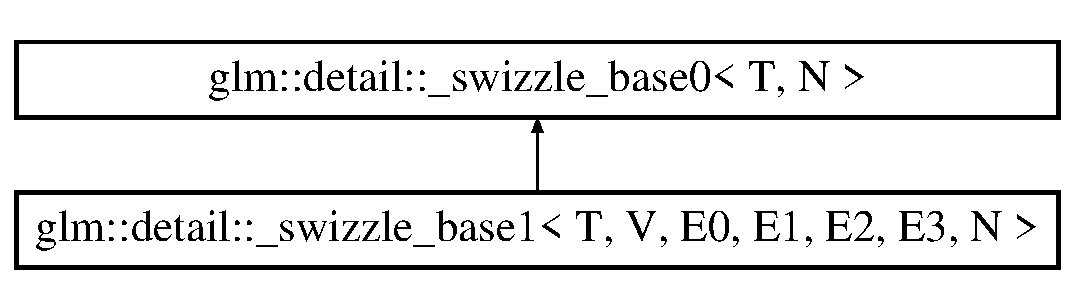
\includegraphics[height=2.000000cm]{structglm_1_1detail_1_1__swizzle__base0}
\end{center}
\end{figure}
\subsection*{Public Types}
\begin{DoxyCompactItemize}
\item 
\hypertarget{structglm_1_1detail_1_1__swizzle__base0_ad38a739e1fe6d2db2674f34c98159c8f}{typedef T {\bfseries value\-\_\-type}}\label{structglm_1_1detail_1_1__swizzle__base0_ad38a739e1fe6d2db2674f34c98159c8f}

\end{DoxyCompactItemize}
\subsection*{Protected Member Functions}
\begin{DoxyCompactItemize}
\item 
\hypertarget{structglm_1_1detail_1_1__swizzle__base0_a88f08b952f849e69011cb9242d809738}{value\-\_\-type \& {\bfseries elem} (size\-\_\-t i)}\label{structglm_1_1detail_1_1__swizzle__base0_a88f08b952f849e69011cb9242d809738}

\item 
\hypertarget{structglm_1_1detail_1_1__swizzle__base0_aa091a75b3fbc0dd70f49f65225002e2a}{const value\-\_\-type \& {\bfseries elem} (size\-\_\-t i) const }\label{structglm_1_1detail_1_1__swizzle__base0_aa091a75b3fbc0dd70f49f65225002e2a}

\end{DoxyCompactItemize}
\subsection*{Protected Attributes}
\begin{DoxyCompactItemize}
\item 
\hypertarget{structglm_1_1detail_1_1__swizzle__base0_afd4b7f15c9acff4cdef808f559ffec2d}{char {\bfseries \-\_\-buffer} \mbox{[}1\mbox{]}}\label{structglm_1_1detail_1_1__swizzle__base0_afd4b7f15c9acff4cdef808f559ffec2d}

\end{DoxyCompactItemize}


The documentation for this struct was generated from the following file\-:\begin{DoxyCompactItemize}
\item 
/home/alex/source\-Code/git\-Project/beleg\-Arbeit\-E\-M\-M\-S/project\-Sogo/external/glm-\/0.\-9.\-4.\-0/glm/core/\hyperlink{__swizzle_8hpp}{\-\_\-swizzle.\-hpp}\end{DoxyCompactItemize}

\hypertarget{structglm_1_1detail_1_1__swizzle__base1}{\section{glm\-:\-:detail\-:\-:\-\_\-swizzle\-\_\-base1$<$ T, V, E0, E1, E2, E3, N $>$ Struct Template Reference}
\label{structglm_1_1detail_1_1__swizzle__base1}\index{glm\-::detail\-::\-\_\-swizzle\-\_\-base1$<$ T, V, E0, E1, E2, E3, N $>$@{glm\-::detail\-::\-\_\-swizzle\-\_\-base1$<$ T, V, E0, E1, E2, E3, N $>$}}
}
Inheritance diagram for glm\-:\-:detail\-:\-:\-\_\-swizzle\-\_\-base1$<$ T, V, E0, E1, E2, E3, N $>$\-:\begin{figure}[H]
\begin{center}
\leavevmode
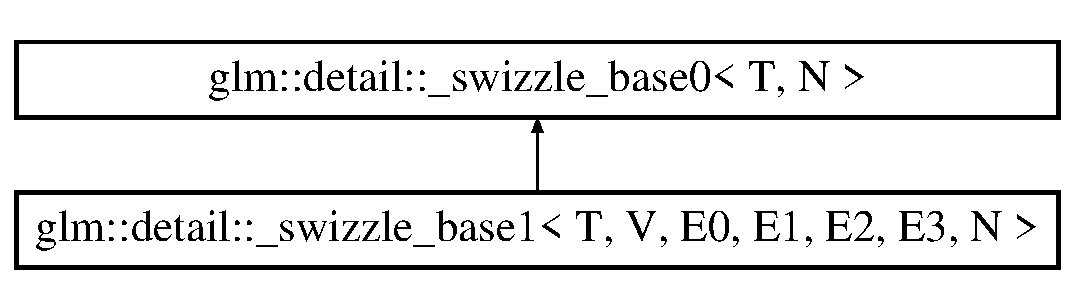
\includegraphics[height=2.000000cm]{structglm_1_1detail_1_1__swizzle__base1}
\end{center}
\end{figure}
\subsection*{Additional Inherited Members}


The documentation for this struct was generated from the following file\-:\begin{DoxyCompactItemize}
\item 
/home/alex/source\-Code/git\-Project/beleg\-Arbeit\-E\-M\-M\-S/project\-Sogo/external/glm-\/0.\-9.\-4.\-0/glm/core/\hyperlink{__swizzle_8hpp}{\-\_\-swizzle.\-hpp}\end{DoxyCompactItemize}

\hypertarget{structglm_1_1detail_1_1__swizzle__base1_3_01T_00_01V_00_01E0_00_01E1_00_01E2_00_01E3_00_014_01_4}{\section{glm\-:\-:detail\-:\-:\-\_\-swizzle\-\_\-base1$<$ T, V, E0, E1, E2, E3, 4 $>$ Struct Template Reference}
\label{structglm_1_1detail_1_1__swizzle__base1_3_01T_00_01V_00_01E0_00_01E1_00_01E2_00_01E3_00_014_01_4}\index{glm\-::detail\-::\-\_\-swizzle\-\_\-base1$<$ T, V, E0, E1, E2, E3, 4 $>$@{glm\-::detail\-::\-\_\-swizzle\-\_\-base1$<$ T, V, E0, E1, E2, E3, 4 $>$}}
}
Inheritance diagram for glm\-:\-:detail\-:\-:\-\_\-swizzle\-\_\-base1$<$ T, V, E0, E1, E2, E3, 4 $>$\-:\begin{figure}[H]
\begin{center}
\leavevmode
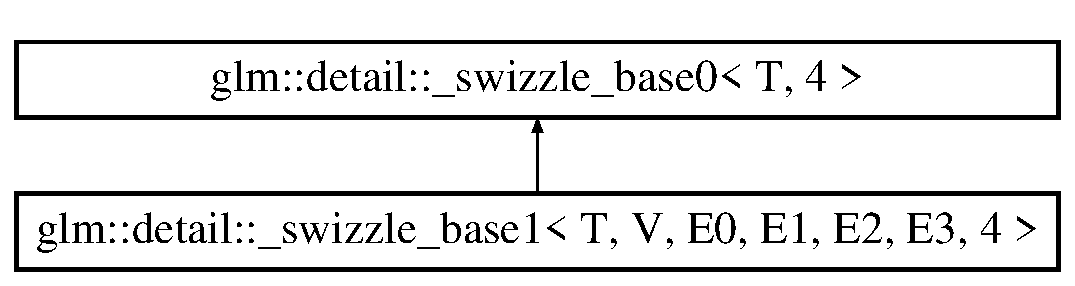
\includegraphics[height=2.000000cm]{structglm_1_1detail_1_1__swizzle__base1_3_01T_00_01V_00_01E0_00_01E1_00_01E2_00_01E3_00_014_01_4}
\end{center}
\end{figure}
\subsection*{Public Member Functions}
\begin{DoxyCompactItemize}
\item 
\hypertarget{structglm_1_1detail_1_1__swizzle__base1_3_01T_00_01V_00_01E0_00_01E1_00_01E2_00_01E3_00_014_01_4_acca1ce42f230b5adba6b01b77af5f61a}{V {\bfseries operator()} () const }\label{structglm_1_1detail_1_1__swizzle__base1_3_01T_00_01V_00_01E0_00_01E1_00_01E2_00_01E3_00_014_01_4_acca1ce42f230b5adba6b01b77af5f61a}

\end{DoxyCompactItemize}
\subsection*{Additional Inherited Members}


The documentation for this struct was generated from the following file\-:\begin{DoxyCompactItemize}
\item 
/home/alex/source\-Code/git\-Project/beleg\-Arbeit\-E\-M\-M\-S/project\-Sogo/external/glm-\/0.\-9.\-4.\-0/glm/core/\hyperlink{__swizzle_8hpp}{\-\_\-swizzle.\-hpp}\end{DoxyCompactItemize}

\hypertarget{structglm_1_1detail_1_1__swizzle__base1_3_01T_00_01V_00_01E0_00_01E1_00_01E2_00-1_00_013_01_4}{\section{glm\-:\-:detail\-:\-:\-\_\-swizzle\-\_\-base1$<$ T, V, E0, E1, E2,-\/1, 3 $>$ Struct Template Reference}
\label{structglm_1_1detail_1_1__swizzle__base1_3_01T_00_01V_00_01E0_00_01E1_00_01E2_00-1_00_013_01_4}\index{glm\-::detail\-::\-\_\-swizzle\-\_\-base1$<$ T, V, E0, E1, E2,-\/1, 3 $>$@{glm\-::detail\-::\-\_\-swizzle\-\_\-base1$<$ T, V, E0, E1, E2,-\/1, 3 $>$}}
}
Inheritance diagram for glm\-:\-:detail\-:\-:\-\_\-swizzle\-\_\-base1$<$ T, V, E0, E1, E2,-\/1, 3 $>$\-:\begin{figure}[H]
\begin{center}
\leavevmode
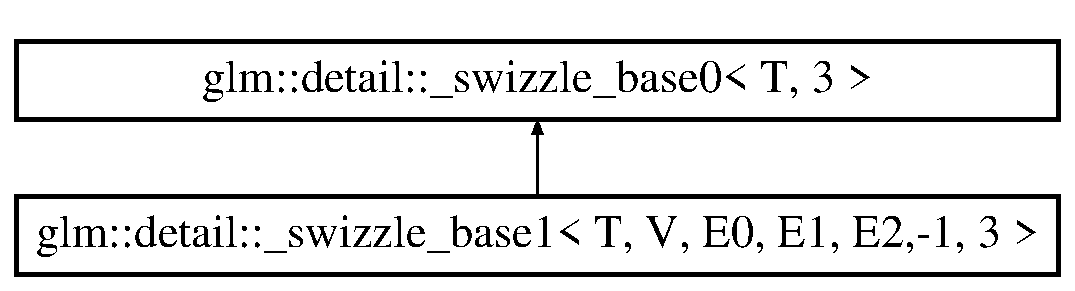
\includegraphics[height=2.000000cm]{structglm_1_1detail_1_1__swizzle__base1_3_01T_00_01V_00_01E0_00_01E1_00_01E2_00-1_00_013_01_4}
\end{center}
\end{figure}
\subsection*{Public Member Functions}
\begin{DoxyCompactItemize}
\item 
\hypertarget{structglm_1_1detail_1_1__swizzle__base1_3_01T_00_01V_00_01E0_00_01E1_00_01E2_00-1_00_013_01_4_a76abd8070d51fabf296fa625bfaa2302}{V {\bfseries operator()} () const }\label{structglm_1_1detail_1_1__swizzle__base1_3_01T_00_01V_00_01E0_00_01E1_00_01E2_00-1_00_013_01_4_a76abd8070d51fabf296fa625bfaa2302}

\end{DoxyCompactItemize}
\subsection*{Additional Inherited Members}


The documentation for this struct was generated from the following file\-:\begin{DoxyCompactItemize}
\item 
/home/alex/source\-Code/git\-Project/beleg\-Arbeit\-E\-M\-M\-S/project\-Sogo/external/glm-\/0.\-9.\-4.\-0/glm/core/\hyperlink{__swizzle_8hpp}{\-\_\-swizzle.\-hpp}\end{DoxyCompactItemize}

\hypertarget{structglm_1_1detail_1_1__swizzle__base1_3_01T_00_01V_00_01E0_00_01E1_00-1_00-2_00_012_01_4}{\section{glm\-:\-:detail\-:\-:\-\_\-swizzle\-\_\-base1$<$ T, V, E0, E1,-\/1,-\/2, 2 $>$ Struct Template Reference}
\label{structglm_1_1detail_1_1__swizzle__base1_3_01T_00_01V_00_01E0_00_01E1_00-1_00-2_00_012_01_4}\index{glm\-::detail\-::\-\_\-swizzle\-\_\-base1$<$ T, V, E0, E1,-\/1,-\/2, 2 $>$@{glm\-::detail\-::\-\_\-swizzle\-\_\-base1$<$ T, V, E0, E1,-\/1,-\/2, 2 $>$}}
}
Inheritance diagram for glm\-:\-:detail\-:\-:\-\_\-swizzle\-\_\-base1$<$ T, V, E0, E1,-\/1,-\/2, 2 $>$\-:\begin{figure}[H]
\begin{center}
\leavevmode
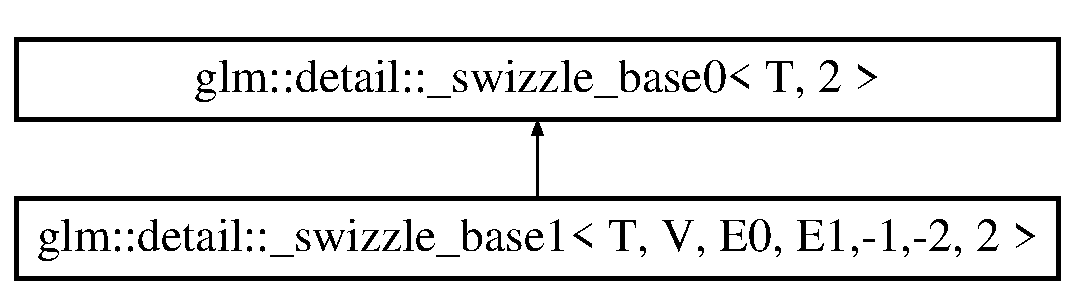
\includegraphics[height=2.000000cm]{structglm_1_1detail_1_1__swizzle__base1_3_01T_00_01V_00_01E0_00_01E1_00-1_00-2_00_012_01_4}
\end{center}
\end{figure}
\subsection*{Public Member Functions}
\begin{DoxyCompactItemize}
\item 
\hypertarget{structglm_1_1detail_1_1__swizzle__base1_3_01T_00_01V_00_01E0_00_01E1_00-1_00-2_00_012_01_4_ae62c208420fe971c7203cbea2a7b7481}{V {\bfseries operator()} () const }\label{structglm_1_1detail_1_1__swizzle__base1_3_01T_00_01V_00_01E0_00_01E1_00-1_00-2_00_012_01_4_ae62c208420fe971c7203cbea2a7b7481}

\end{DoxyCompactItemize}
\subsection*{Additional Inherited Members}


The documentation for this struct was generated from the following file\-:\begin{DoxyCompactItemize}
\item 
/home/alex/source\-Code/git\-Project/beleg\-Arbeit\-E\-M\-M\-S/project\-Sogo/external/glm-\/0.\-9.\-4.\-0/glm/core/\hyperlink{__swizzle_8hpp}{\-\_\-swizzle.\-hpp}\end{DoxyCompactItemize}

\hypertarget{structglm_1_1detail_1_1__swizzle__base2}{\section{glm\-:\-:detail\-:\-:\-\_\-swizzle\-\_\-base2$<$ Value\-Type, Vec\-Type, N, E0, E1, E2, E3, D\-U\-P\-L\-I\-C\-A\-T\-E\-\_\-\-E\-L\-E\-M\-E\-N\-T\-S $>$ Struct Template Reference}
\label{structglm_1_1detail_1_1__swizzle__base2}\index{glm\-::detail\-::\-\_\-swizzle\-\_\-base2$<$ Value\-Type, Vec\-Type, N, E0, E1, E2, E3, D\-U\-P\-L\-I\-C\-A\-T\-E\-\_\-\-E\-L\-E\-M\-E\-N\-T\-S $>$@{glm\-::detail\-::\-\_\-swizzle\-\_\-base2$<$ Value\-Type, Vec\-Type, N, E0, E1, E2, E3, D\-U\-P\-L\-I\-C\-A\-T\-E\-\_\-\-E\-L\-E\-M\-E\-N\-T\-S $>$}}
}
Inheritance diagram for glm\-:\-:detail\-:\-:\-\_\-swizzle\-\_\-base2$<$ Value\-Type, Vec\-Type, N, E0, E1, E2, E3, D\-U\-P\-L\-I\-C\-A\-T\-E\-\_\-\-E\-L\-E\-M\-E\-N\-T\-S $>$\-:\begin{figure}[H]
\begin{center}
\leavevmode
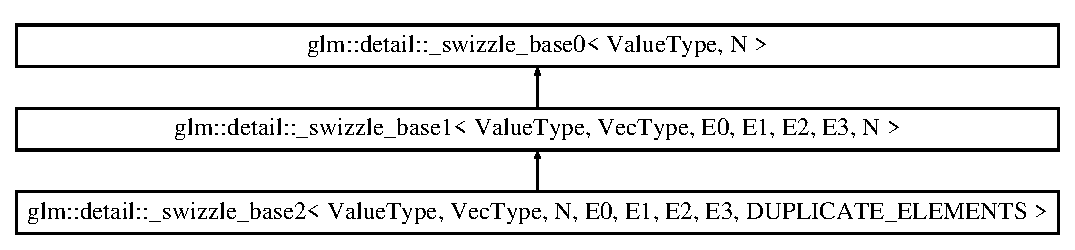
\includegraphics[height=2.906574cm]{structglm_1_1detail_1_1__swizzle__base2}
\end{center}
\end{figure}
\subsection*{Public Types}
\begin{DoxyCompactItemize}
\item 
\hypertarget{structglm_1_1detail_1_1__swizzle__base2_afad8673697b2a4bcbd1de30e49cc2a54}{typedef Vec\-Type {\bfseries vec\-\_\-type}}\label{structglm_1_1detail_1_1__swizzle__base2_afad8673697b2a4bcbd1de30e49cc2a54}

\item 
\hypertarget{structglm_1_1detail_1_1__swizzle__base2_a2b683ea47a63ff7d00943cd55b7c0b02}{typedef Value\-Type {\bfseries value\-\_\-type}}\label{structglm_1_1detail_1_1__swizzle__base2_a2b683ea47a63ff7d00943cd55b7c0b02}

\end{DoxyCompactItemize}
\subsection*{Public Member Functions}
\begin{DoxyCompactItemize}
\item 
\hypertarget{structglm_1_1detail_1_1__swizzle__base2_a297df83a1e1962477b6834f97b9c6a6a}{\hyperlink{structglm_1_1detail_1_1__swizzle__base2}{\-\_\-swizzle\-\_\-base2} \& {\bfseries operator=} (const Value\-Type \&t)}\label{structglm_1_1detail_1_1__swizzle__base2_a297df83a1e1962477b6834f97b9c6a6a}

\item 
\hypertarget{structglm_1_1detail_1_1__swizzle__base2_a231527e1349e677ba7ab2d53742ef242}{\hyperlink{structglm_1_1detail_1_1__swizzle__base2}{\-\_\-swizzle\-\_\-base2} \& {\bfseries operator=} (const Vec\-Type \&that)}\label{structglm_1_1detail_1_1__swizzle__base2_a231527e1349e677ba7ab2d53742ef242}

\item 
\hypertarget{structglm_1_1detail_1_1__swizzle__base2_a26e653b4bf831c1171a8999c08f06537}{void {\bfseries operator-\/=} (const Vec\-Type \&that)}\label{structglm_1_1detail_1_1__swizzle__base2_a26e653b4bf831c1171a8999c08f06537}

\item 
\hypertarget{structglm_1_1detail_1_1__swizzle__base2_a83c0024bcb9ed27bc290560f3b1968e2}{void {\bfseries operator+=} (const Vec\-Type \&that)}\label{structglm_1_1detail_1_1__swizzle__base2_a83c0024bcb9ed27bc290560f3b1968e2}

\item 
\hypertarget{structglm_1_1detail_1_1__swizzle__base2_a8da77c15d444f7bb057285a2c92be01c}{void {\bfseries operator$\ast$=} (const Vec\-Type \&that)}\label{structglm_1_1detail_1_1__swizzle__base2_a8da77c15d444f7bb057285a2c92be01c}

\item 
\hypertarget{structglm_1_1detail_1_1__swizzle__base2_acda3b1e53bff334a247408db2896aa89}{void {\bfseries operator/=} (const Vec\-Type \&that)}\label{structglm_1_1detail_1_1__swizzle__base2_acda3b1e53bff334a247408db2896aa89}

\item 
\hypertarget{structglm_1_1detail_1_1__swizzle__base2_abd391e719ecd24ee966d974d83965e37}{value\-\_\-type \& {\bfseries operator\mbox{[}$\,$\mbox{]}} (size\-\_\-t i)}\label{structglm_1_1detail_1_1__swizzle__base2_abd391e719ecd24ee966d974d83965e37}

\item 
\hypertarget{structglm_1_1detail_1_1__swizzle__base2_a532fa5f2d8449f72378e7d9f3b5c8de3}{value\-\_\-type {\bfseries operator\mbox{[}$\,$\mbox{]}} (size\-\_\-t i) const }\label{structglm_1_1detail_1_1__swizzle__base2_a532fa5f2d8449f72378e7d9f3b5c8de3}

\end{DoxyCompactItemize}
\subsection*{Protected Member Functions}
\begin{DoxyCompactItemize}
\item 
\hypertarget{structglm_1_1detail_1_1__swizzle__base2_adc355968d70e1f0b34759a8cb78ea6ae}{{\footnotesize template$<$typename T $>$ }\\void {\bfseries \-\_\-apply\-\_\-op} (const Vec\-Type \&that, T op)}\label{structglm_1_1detail_1_1__swizzle__base2_adc355968d70e1f0b34759a8cb78ea6ae}

\end{DoxyCompactItemize}
\subsection*{Additional Inherited Members}


The documentation for this struct was generated from the following file\-:\begin{DoxyCompactItemize}
\item 
/home/alex/source\-Code/git\-Project/beleg\-Arbeit\-E\-M\-M\-S/project\-Sogo/external/glm-\/0.\-9.\-4.\-0/glm/core/\hyperlink{__swizzle_8hpp}{\-\_\-swizzle.\-hpp}\end{DoxyCompactItemize}

\hypertarget{structglm_1_1detail_1_1__swizzle__base2_3_01ValueType_00_01VecType_00_01N_00_01E0_00_01E1_00_01E2_00_01E3_00_011_01_4}{\section{glm\-:\-:detail\-:\-:\-\_\-swizzle\-\_\-base2$<$ Value\-Type, Vec\-Type, N, E0, E1, E2, E3, 1 $>$ Struct Template Reference}
\label{structglm_1_1detail_1_1__swizzle__base2_3_01ValueType_00_01VecType_00_01N_00_01E0_00_01E1_00_01E2_00_01E3_00_011_01_4}\index{glm\-::detail\-::\-\_\-swizzle\-\_\-base2$<$ Value\-Type, Vec\-Type, N, E0, E1, E2, E3, 1 $>$@{glm\-::detail\-::\-\_\-swizzle\-\_\-base2$<$ Value\-Type, Vec\-Type, N, E0, E1, E2, E3, 1 $>$}}
}
Inheritance diagram for glm\-:\-:detail\-:\-:\-\_\-swizzle\-\_\-base2$<$ Value\-Type, Vec\-Type, N, E0, E1, E2, E3, 1 $>$\-:\begin{figure}[H]
\begin{center}
\leavevmode
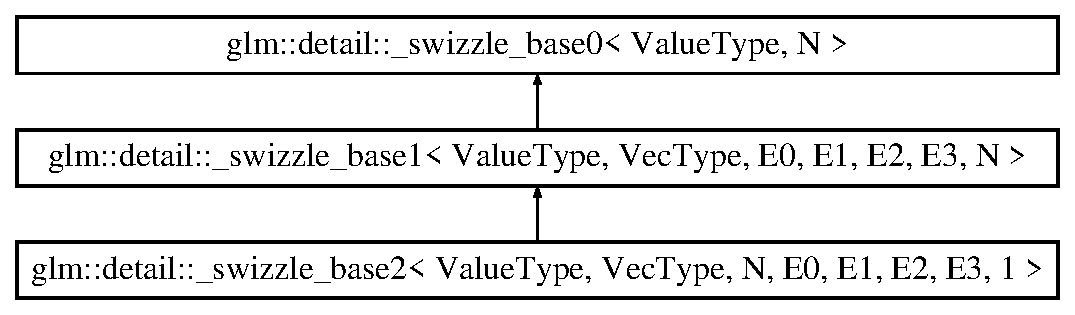
\includegraphics[height=3.000000cm]{structglm_1_1detail_1_1__swizzle__base2_3_01ValueType_00_01VecType_00_01N_00_01E0_00_01E1_00_01E2_00_01E3_00_011_01_4}
\end{center}
\end{figure}
\subsection*{Classes}
\begin{DoxyCompactItemize}
\item 
struct \hyperlink{structglm_1_1detail_1_1__swizzle__base2_3_01ValueType_00_01VecType_00_01N_00_01E0_00_01E1_00_01E2_00_01E3_00_011_01_4_1_1Stub}{Stub}
\end{DoxyCompactItemize}
\subsection*{Public Types}
\begin{DoxyCompactItemize}
\item 
\hypertarget{structglm_1_1detail_1_1__swizzle__base2_3_01ValueType_00_01VecType_00_01N_00_01E0_00_01E1_00_01E2_00_01E3_00_011_01_4_ad2442863b7e1573d71bf4af4e717a819}{typedef Vec\-Type {\bfseries vec\-\_\-type}}\label{structglm_1_1detail_1_1__swizzle__base2_3_01ValueType_00_01VecType_00_01N_00_01E0_00_01E1_00_01E2_00_01E3_00_011_01_4_ad2442863b7e1573d71bf4af4e717a819}

\item 
\hypertarget{structglm_1_1detail_1_1__swizzle__base2_3_01ValueType_00_01VecType_00_01N_00_01E0_00_01E1_00_01E2_00_01E3_00_011_01_4_a6af089fbf34a725330bea0092ee34768}{typedef Value\-Type {\bfseries value\-\_\-type}}\label{structglm_1_1detail_1_1__swizzle__base2_3_01ValueType_00_01VecType_00_01N_00_01E0_00_01E1_00_01E2_00_01E3_00_011_01_4_a6af089fbf34a725330bea0092ee34768}

\end{DoxyCompactItemize}
\subsection*{Public Member Functions}
\begin{DoxyCompactItemize}
\item 
\hypertarget{structglm_1_1detail_1_1__swizzle__base2_3_01ValueType_00_01VecType_00_01N_00_01E0_00_01E1_00_01E2_00_01E3_00_011_01_4_a70764f1278bf81e27f79fe3f4a81de2d}{\hyperlink{structglm_1_1detail_1_1__swizzle__base2}{\-\_\-swizzle\-\_\-base2} \& {\bfseries operator=} (Stub const \&)}\label{structglm_1_1detail_1_1__swizzle__base2_3_01ValueType_00_01VecType_00_01N_00_01E0_00_01E1_00_01E2_00_01E3_00_011_01_4_a70764f1278bf81e27f79fe3f4a81de2d}

\item 
\hypertarget{structglm_1_1detail_1_1__swizzle__base2_3_01ValueType_00_01VecType_00_01N_00_01E0_00_01E1_00_01E2_00_01E3_00_011_01_4_af6e79bb269160e9d1c7e3959bbd7acc2}{value\-\_\-type {\bfseries operator\mbox{[}$\,$\mbox{]}} (size\-\_\-t i) const }\label{structglm_1_1detail_1_1__swizzle__base2_3_01ValueType_00_01VecType_00_01N_00_01E0_00_01E1_00_01E2_00_01E3_00_011_01_4_af6e79bb269160e9d1c7e3959bbd7acc2}

\end{DoxyCompactItemize}
\subsection*{Additional Inherited Members}


The documentation for this struct was generated from the following file\-:\begin{DoxyCompactItemize}
\item 
/home/alex/source\-Code/git\-Project/beleg\-Arbeit\-E\-M\-M\-S/project\-Sogo/external/glm-\/0.\-9.\-4.\-0/glm/core/\hyperlink{__swizzle_8hpp}{\-\_\-swizzle.\-hpp}\end{DoxyCompactItemize}

\hypertarget{structglm_1_1detail_1_1Abs__}{\section{glm\-:\-:detail\-:\-:Abs\-\_\-$<$ gen\-F\-I\-Type, bool $>$ Struct Template Reference}
\label{structglm_1_1detail_1_1Abs__}\index{glm\-::detail\-::\-Abs\-\_\-$<$ gen\-F\-I\-Type, bool $>$@{glm\-::detail\-::\-Abs\-\_\-$<$ gen\-F\-I\-Type, bool $>$}}
}


The documentation for this struct was generated from the following file\-:\begin{DoxyCompactItemize}
\item 
/home/alex/source\-Code/git\-Project/beleg\-Arbeit\-E\-M\-M\-S/project\-Sogo/external/glm-\/0.\-9.\-4.\-0/glm/core/\hyperlink{func__common_8inl}{func\-\_\-common.\-inl}\end{DoxyCompactItemize}

\hypertarget{structglm_1_1detail_1_1Abs___3_01genFIType_00_01false_01_4}{\section{glm\-:\-:detail\-:\-:Abs\-\_\-$<$ gen\-F\-I\-Type, false $>$ Struct Template Reference}
\label{structglm_1_1detail_1_1Abs___3_01genFIType_00_01false_01_4}\index{glm\-::detail\-::\-Abs\-\_\-$<$ gen\-F\-I\-Type, false $>$@{glm\-::detail\-::\-Abs\-\_\-$<$ gen\-F\-I\-Type, false $>$}}
}
\subsection*{Static Public Member Functions}
\begin{DoxyCompactItemize}
\item 
\hypertarget{structglm_1_1detail_1_1Abs___3_01genFIType_00_01false_01_4_a14974cbcc524a914d5a4d5a7cdd4557b}{static gen\-F\-I\-Type {\bfseries get} (gen\-F\-I\-Type const \&x)}\label{structglm_1_1detail_1_1Abs___3_01genFIType_00_01false_01_4_a14974cbcc524a914d5a4d5a7cdd4557b}

\end{DoxyCompactItemize}


The documentation for this struct was generated from the following file\-:\begin{DoxyCompactItemize}
\item 
/home/alex/source\-Code/git\-Project/beleg\-Arbeit\-E\-M\-M\-S/project\-Sogo/external/glm-\/0.\-9.\-4.\-0/glm/core/\hyperlink{func__common_8inl}{func\-\_\-common.\-inl}\end{DoxyCompactItemize}

\hypertarget{structglm_1_1detail_1_1Abs___3_01genFIType_00_01true_01_4}{\section{glm\-:\-:detail\-:\-:Abs\-\_\-$<$ gen\-F\-I\-Type, true $>$ Struct Template Reference}
\label{structglm_1_1detail_1_1Abs___3_01genFIType_00_01true_01_4}\index{glm\-::detail\-::\-Abs\-\_\-$<$ gen\-F\-I\-Type, true $>$@{glm\-::detail\-::\-Abs\-\_\-$<$ gen\-F\-I\-Type, true $>$}}
}
\subsection*{Static Public Member Functions}
\begin{DoxyCompactItemize}
\item 
\hypertarget{structglm_1_1detail_1_1Abs___3_01genFIType_00_01true_01_4_a070ff71ec02bcd5b7ecab9ee75b6eb99}{static gen\-F\-I\-Type {\bfseries get} (gen\-F\-I\-Type const \&x)}\label{structglm_1_1detail_1_1Abs___3_01genFIType_00_01true_01_4_a070ff71ec02bcd5b7ecab9ee75b6eb99}

\end{DoxyCompactItemize}


The documentation for this struct was generated from the following file\-:\begin{DoxyCompactItemize}
\item 
/home/alex/source\-Code/git\-Project/beleg\-Arbeit\-E\-M\-M\-S/project\-Sogo/external/glm-\/0.\-9.\-4.\-0/glm/core/\hyperlink{func__common_8inl}{func\-\_\-common.\-inl}\end{DoxyCompactItemize}

\hypertarget{classAI}{\section{A\-I Class Reference}
\label{classAI}\index{A\-I@{A\-I}}
}


The \hyperlink{classAI}{A\-I} class.  




{\ttfamily \#include $<$A\-I.\-h$>$}



\subsection{Detailed Description}
The \hyperlink{classAI}{A\-I} class. 

Defines an A\-I-\/\-Player Future content strenght etc.

\begin{DoxyAuthor}{Author}
Nils Brandt 

Alexander Luedke
\end{DoxyAuthor}
\begin{DoxyDate}{Date}
08. August 2016
\end{DoxyDate}
\begin{DoxyVersion}{Version}
1.\-0 Add Documentation 
\end{DoxyVersion}

\hypertarget{structGameManager_1_1AIPlayer}{\section{Game\-Manager\-:\-:A\-I\-Player Struct Reference}
\label{structGameManager_1_1AIPlayer}\index{Game\-Manager\-::\-A\-I\-Player@{Game\-Manager\-::\-A\-I\-Player}}
}


The \hyperlink{classAI}{A\-I} struct Contains a reference to a player which is of type ai and if the ai player has calculated its next move.  




{\ttfamily \#include $<$Game\-Manager\-Thread.\-h$>$}

\subsection*{Public Member Functions}
\begin{DoxyCompactItemize}
\item 
\hyperlink{structGameManager_1_1AIPlayer_a9c991a2b7151183f89feefe97e6cfbec}{A\-I\-Player} (const \hyperlink{classPlayer}{Player} $\ast$\hyperlink{structGameManager_1_1AIPlayer_a96450dd315805b21d243f80787a53d6e}{player}, bool \hyperlink{structGameManager_1_1AIPlayer_a0930362037e6d84ec3888eacc8c3c10a}{has\-Move}=false)
\begin{DoxyCompactList}\small\item\em \hyperlink{classAI}{A\-I}. \end{DoxyCompactList}\end{DoxyCompactItemize}
\subsection*{Public Attributes}
\begin{DoxyCompactItemize}
\item 
\hypertarget{structGameManager_1_1AIPlayer_a96450dd315805b21d243f80787a53d6e}{const \hyperlink{classPlayer}{Player} $\ast$ \hyperlink{structGameManager_1_1AIPlayer_a96450dd315805b21d243f80787a53d6e}{player}}\label{structGameManager_1_1AIPlayer_a96450dd315805b21d243f80787a53d6e}

\begin{DoxyCompactList}\small\item\em player \end{DoxyCompactList}\item 
\hypertarget{structGameManager_1_1AIPlayer_a0930362037e6d84ec3888eacc8c3c10a}{bool \hyperlink{structGameManager_1_1AIPlayer_a0930362037e6d84ec3888eacc8c3c10a}{has\-Move}}\label{structGameManager_1_1AIPlayer_a0930362037e6d84ec3888eacc8c3c10a}

\begin{DoxyCompactList}\small\item\em has\-Move \end{DoxyCompactList}\end{DoxyCompactItemize}


\subsection{Detailed Description}
The \hyperlink{classAI}{A\-I} struct Contains a reference to a player which is of type ai and if the ai player has calculated its next move. 

\subsection{Constructor \& Destructor Documentation}
\hypertarget{structGameManager_1_1AIPlayer_a9c991a2b7151183f89feefe97e6cfbec}{\index{Game\-Manager\-::\-A\-I\-Player@{Game\-Manager\-::\-A\-I\-Player}!A\-I\-Player@{A\-I\-Player}}
\index{A\-I\-Player@{A\-I\-Player}!GameManager::AIPlayer@{Game\-Manager\-::\-A\-I\-Player}}
\subsubsection[{A\-I\-Player}]{\setlength{\rightskip}{0pt plus 5cm}Game\-Manager\-::\-A\-I\-Player\-::\-A\-I\-Player (
\begin{DoxyParamCaption}
\item[{const {\bf Player} $\ast$}]{player, }
\item[{bool}]{has\-Move = {\ttfamily false}}
\end{DoxyParamCaption}
)\hspace{0.3cm}{\ttfamily [inline]}}}\label{structGameManager_1_1AIPlayer_a9c991a2b7151183f89feefe97e6cfbec}


\hyperlink{classAI}{A\-I}. 


\begin{DoxyParams}{Parameters}
{\em player} & \\
\hline
{\em has\-Move} & \\
\hline
\end{DoxyParams}

\hypertarget{structglm_1_1detail_1_1compute__linearRand}{\section{glm\-:\-:detail\-:\-:compute\-\_\-linear\-Rand Struct Reference}
\label{structglm_1_1detail_1_1compute__linearRand}\index{glm\-::detail\-::compute\-\_\-linear\-Rand@{glm\-::detail\-::compute\-\_\-linear\-Rand}}
}
\subsection*{Public Member Functions}
\begin{DoxyCompactItemize}
\item 
\hypertarget{structglm_1_1detail_1_1compute__linearRand_ac852e16d66ba80ff5309238b3f494b99}{{\footnotesize template$<$typename T $>$ }\\G\-L\-M\-\_\-\-F\-U\-N\-C\-\_\-\-Q\-U\-A\-L\-I\-F\-I\-E\-R T {\bfseries operator()} (T const \&Min, T const \&Max) const }\label{structglm_1_1detail_1_1compute__linearRand_ac852e16d66ba80ff5309238b3f494b99}

\item 
\hypertarget{structglm_1_1detail_1_1compute__linearRand_a544b94bdfbdcf46c2689208e75f85612}{{\footnotesize template$<$$>$ }\\G\-L\-M\-\_\-\-F\-U\-N\-C\-\_\-\-Q\-U\-A\-L\-I\-F\-I\-E\-R \hyperlink{classglm_1_1detail_1_1half}{half} {\bfseries operator()} (\hyperlink{classglm_1_1detail_1_1half}{half} const \&Min, \hyperlink{classglm_1_1detail_1_1half}{half} const \&Max) const }\label{structglm_1_1detail_1_1compute__linearRand_a544b94bdfbdcf46c2689208e75f85612}

\item 
\hypertarget{structglm_1_1detail_1_1compute__linearRand_aeb6d4f603a9afa05544d65233064f2e9}{{\footnotesize template$<$$>$ }\\G\-L\-M\-\_\-\-F\-U\-N\-C\-\_\-\-Q\-U\-A\-L\-I\-F\-I\-E\-R float {\bfseries operator()} (float const \&Min, float const \&Max) const }\label{structglm_1_1detail_1_1compute__linearRand_aeb6d4f603a9afa05544d65233064f2e9}

\item 
\hypertarget{structglm_1_1detail_1_1compute__linearRand_a60dd37b36082f1a8dbfb8d34f0d5575c}{{\footnotesize template$<$$>$ }\\G\-L\-M\-\_\-\-F\-U\-N\-C\-\_\-\-Q\-U\-A\-L\-I\-F\-I\-E\-R double {\bfseries operator()} (double const \&Min, double const \&Max) const }\label{structglm_1_1detail_1_1compute__linearRand_a60dd37b36082f1a8dbfb8d34f0d5575c}

\item 
\hypertarget{structglm_1_1detail_1_1compute__linearRand_ab5433863c50ed60a1ce5ac941759428f}{{\footnotesize template$<$$>$ }\\G\-L\-M\-\_\-\-F\-U\-N\-C\-\_\-\-Q\-U\-A\-L\-I\-F\-I\-E\-R long double {\bfseries operator()} (long double const \&Min, long double const \&Max) const }\label{structglm_1_1detail_1_1compute__linearRand_ab5433863c50ed60a1ce5ac941759428f}

\end{DoxyCompactItemize}


The documentation for this struct was generated from the following file\-:\begin{DoxyCompactItemize}
\item 
/home/alex/source\-Code/git\-Project/beleg\-Arbeit\-E\-M\-M\-S/project\-Sogo/external/glm-\/0.\-9.\-4.\-0/glm/gtc/\hyperlink{random_8inl}{random.\-inl}\end{DoxyCompactItemize}

\hypertarget{classglm_1_1dont__care}{\section{glm\-:\-:dont\-\_\-care Class Reference}
\label{classglm_1_1dont__care}\index{glm\-::dont\-\_\-care@{glm\-::dont\-\_\-care}}
}


The documentation for this class was generated from the following file\-:\begin{DoxyCompactItemize}
\item 
/home/alex/source\-Code/git\-Project/beleg\-Arbeit\-E\-M\-M\-S/project\-Sogo/external/glm-\/0.\-9.\-4.\-0/glm/core/\hyperlink{hint_8hpp}{hint.\-hpp}\end{DoxyCompactItemize}

\hypertarget{classglm_1_1fastest}{\section{glm\-:\-:fastest Class Reference}
\label{classglm_1_1fastest}\index{glm\-::fastest@{glm\-::fastest}}
}


The documentation for this class was generated from the following file\-:\begin{DoxyCompactItemize}
\item 
/home/alex/source\-Code/git\-Project/beleg\-Arbeit\-E\-M\-M\-S/project\-Sogo/external/glm-\/0.\-9.\-4.\-0/glm/core/\hyperlink{hint_8hpp}{hint.\-hpp}\end{DoxyCompactItemize}

\hypertarget{structglm_1_1detail_1_1float__or__int__trait}{\section{glm\-:\-:detail\-:\-:float\-\_\-or\-\_\-int\-\_\-trait$<$ T $>$ Struct Template Reference}
\label{structglm_1_1detail_1_1float__or__int__trait}\index{glm\-::detail\-::float\-\_\-or\-\_\-int\-\_\-trait$<$ T $>$@{glm\-::detail\-::float\-\_\-or\-\_\-int\-\_\-trait$<$ T $>$}}
}
\subsection*{Public Types}
\begin{DoxyCompactItemize}
\item 
enum \{ {\bfseries I\-D} = float\-\_\-or\-\_\-int\-\_\-value\-:\-:G\-L\-M\-\_\-\-E\-R\-R\-O\-R
 \}
\end{DoxyCompactItemize}


The documentation for this struct was generated from the following file\-:\begin{DoxyCompactItemize}
\item 
/home/alex/source\-Code/git\-Project/beleg\-Arbeit\-E\-M\-M\-S/project\-Sogo/external/glm-\/0.\-9.\-4.\-0/glm/core/\hyperlink{__detail_8hpp}{\-\_\-detail.\-hpp}\end{DoxyCompactItemize}

\hypertarget{structglm_1_1detail_1_1float__or__int__trait_3_01float16_01_4}{\section{glm\-:\-:detail\-:\-:float\-\_\-or\-\_\-int\-\_\-trait$<$ float16 $>$ Struct Template Reference}
\label{structglm_1_1detail_1_1float__or__int__trait_3_01float16_01_4}\index{glm\-::detail\-::float\-\_\-or\-\_\-int\-\_\-trait$<$ float16 $>$@{glm\-::detail\-::float\-\_\-or\-\_\-int\-\_\-trait$<$ float16 $>$}}
}
\subsection*{Public Types}
\begin{DoxyCompactItemize}
\item 
enum \{ {\bfseries I\-D} = float\-\_\-or\-\_\-int\-\_\-value\-:\-:G\-L\-M\-\_\-\-F\-L\-O\-A\-T
 \}
\end{DoxyCompactItemize}


The documentation for this struct was generated from the following file\-:\begin{DoxyCompactItemize}
\item 
/home/alex/source\-Code/git\-Project/beleg\-Arbeit\-E\-M\-M\-S/project\-Sogo/external/glm-\/0.\-9.\-4.\-0/glm/core/\hyperlink{__detail_8hpp}{\-\_\-detail.\-hpp}\end{DoxyCompactItemize}

\hypertarget{structglm_1_1detail_1_1float__or__int__trait_3_01float32_01_4}{\section{glm\-:\-:detail\-:\-:float\-\_\-or\-\_\-int\-\_\-trait$<$ float32 $>$ Struct Template Reference}
\label{structglm_1_1detail_1_1float__or__int__trait_3_01float32_01_4}\index{glm\-::detail\-::float\-\_\-or\-\_\-int\-\_\-trait$<$ float32 $>$@{glm\-::detail\-::float\-\_\-or\-\_\-int\-\_\-trait$<$ float32 $>$}}
}
\subsection*{Public Types}
\begin{DoxyCompactItemize}
\item 
enum \{ {\bfseries I\-D} = float\-\_\-or\-\_\-int\-\_\-value\-:\-:G\-L\-M\-\_\-\-F\-L\-O\-A\-T
 \}
\end{DoxyCompactItemize}


The documentation for this struct was generated from the following file\-:\begin{DoxyCompactItemize}
\item 
/home/alex/source\-Code/git\-Project/beleg\-Arbeit\-E\-M\-M\-S/project\-Sogo/external/glm-\/0.\-9.\-4.\-0/glm/core/\hyperlink{__detail_8hpp}{\-\_\-detail.\-hpp}\end{DoxyCompactItemize}

\hypertarget{structglm_1_1detail_1_1float__or__int__trait_3_01float64_01_4}{\section{glm\-:\-:detail\-:\-:float\-\_\-or\-\_\-int\-\_\-trait$<$ float64 $>$ Struct Template Reference}
\label{structglm_1_1detail_1_1float__or__int__trait_3_01float64_01_4}\index{glm\-::detail\-::float\-\_\-or\-\_\-int\-\_\-trait$<$ float64 $>$@{glm\-::detail\-::float\-\_\-or\-\_\-int\-\_\-trait$<$ float64 $>$}}
}
\subsection*{Public Types}
\begin{DoxyCompactItemize}
\item 
enum \{ {\bfseries I\-D} = float\-\_\-or\-\_\-int\-\_\-value\-:\-:G\-L\-M\-\_\-\-F\-L\-O\-A\-T
 \}
\end{DoxyCompactItemize}


The documentation for this struct was generated from the following file\-:\begin{DoxyCompactItemize}
\item 
/home/alex/source\-Code/git\-Project/beleg\-Arbeit\-E\-M\-M\-S/project\-Sogo/external/glm-\/0.\-9.\-4.\-0/glm/core/\hyperlink{__detail_8hpp}{\-\_\-detail.\-hpp}\end{DoxyCompactItemize}

\hypertarget{structglm_1_1detail_1_1float__or__int__trait_3_01int16_01_4}{\section{glm\-:\-:detail\-:\-:float\-\_\-or\-\_\-int\-\_\-trait$<$ int16 $>$ Struct Template Reference}
\label{structglm_1_1detail_1_1float__or__int__trait_3_01int16_01_4}\index{glm\-::detail\-::float\-\_\-or\-\_\-int\-\_\-trait$<$ int16 $>$@{glm\-::detail\-::float\-\_\-or\-\_\-int\-\_\-trait$<$ int16 $>$}}
}
\subsection*{Public Types}
\begin{DoxyCompactItemize}
\item 
enum \{ {\bfseries I\-D} = float\-\_\-or\-\_\-int\-\_\-value\-:\-:G\-L\-M\-\_\-\-I\-N\-T
 \}
\end{DoxyCompactItemize}


The documentation for this struct was generated from the following file\-:\begin{DoxyCompactItemize}
\item 
/home/alex/source\-Code/git\-Project/beleg\-Arbeit\-E\-M\-M\-S/project\-Sogo/external/glm-\/0.\-9.\-4.\-0/glm/core/\hyperlink{__detail_8hpp}{\-\_\-detail.\-hpp}\end{DoxyCompactItemize}

\hypertarget{structglm_1_1detail_1_1float__or__int__trait_3_01int32_01_4}{\section{glm\-:\-:detail\-:\-:float\-\_\-or\-\_\-int\-\_\-trait$<$ int32 $>$ Struct Template Reference}
\label{structglm_1_1detail_1_1float__or__int__trait_3_01int32_01_4}\index{glm\-::detail\-::float\-\_\-or\-\_\-int\-\_\-trait$<$ int32 $>$@{glm\-::detail\-::float\-\_\-or\-\_\-int\-\_\-trait$<$ int32 $>$}}
}
\subsection*{Public Types}
\begin{DoxyCompactItemize}
\item 
enum \{ {\bfseries I\-D} = float\-\_\-or\-\_\-int\-\_\-value\-:\-:G\-L\-M\-\_\-\-I\-N\-T
 \}
\end{DoxyCompactItemize}


The documentation for this struct was generated from the following file\-:\begin{DoxyCompactItemize}
\item 
/home/alex/source\-Code/git\-Project/beleg\-Arbeit\-E\-M\-M\-S/project\-Sogo/external/glm-\/0.\-9.\-4.\-0/glm/core/\hyperlink{__detail_8hpp}{\-\_\-detail.\-hpp}\end{DoxyCompactItemize}

\hypertarget{structglm_1_1detail_1_1float__or__int__trait_3_01int64_01_4}{\section{glm\-:\-:detail\-:\-:float\-\_\-or\-\_\-int\-\_\-trait$<$ int64 $>$ Struct Template Reference}
\label{structglm_1_1detail_1_1float__or__int__trait_3_01int64_01_4}\index{glm\-::detail\-::float\-\_\-or\-\_\-int\-\_\-trait$<$ int64 $>$@{glm\-::detail\-::float\-\_\-or\-\_\-int\-\_\-trait$<$ int64 $>$}}
}
\subsection*{Public Types}
\begin{DoxyCompactItemize}
\item 
enum \{ {\bfseries I\-D} = float\-\_\-or\-\_\-int\-\_\-value\-:\-:G\-L\-M\-\_\-\-I\-N\-T
 \}
\end{DoxyCompactItemize}


The documentation for this struct was generated from the following file\-:\begin{DoxyCompactItemize}
\item 
/home/alex/source\-Code/git\-Project/beleg\-Arbeit\-E\-M\-M\-S/project\-Sogo/external/glm-\/0.\-9.\-4.\-0/glm/core/\hyperlink{__detail_8hpp}{\-\_\-detail.\-hpp}\end{DoxyCompactItemize}

\hypertarget{structglm_1_1detail_1_1float__or__int__trait_3_01int8_01_4}{\section{glm\-:\-:detail\-:\-:float\-\_\-or\-\_\-int\-\_\-trait$<$ int8 $>$ Struct Template Reference}
\label{structglm_1_1detail_1_1float__or__int__trait_3_01int8_01_4}\index{glm\-::detail\-::float\-\_\-or\-\_\-int\-\_\-trait$<$ int8 $>$@{glm\-::detail\-::float\-\_\-or\-\_\-int\-\_\-trait$<$ int8 $>$}}
}
\subsection*{Public Types}
\begin{DoxyCompactItemize}
\item 
enum \{ {\bfseries I\-D} = float\-\_\-or\-\_\-int\-\_\-value\-:\-:G\-L\-M\-\_\-\-I\-N\-T
 \}
\end{DoxyCompactItemize}


The documentation for this struct was generated from the following file\-:\begin{DoxyCompactItemize}
\item 
/home/alex/source\-Code/git\-Project/beleg\-Arbeit\-E\-M\-M\-S/project\-Sogo/external/glm-\/0.\-9.\-4.\-0/glm/core/\hyperlink{__detail_8hpp}{\-\_\-detail.\-hpp}\end{DoxyCompactItemize}

\hypertarget{structglm_1_1detail_1_1float__or__int__trait_3_01uint16_01_4}{\section{glm\-:\-:detail\-:\-:float\-\_\-or\-\_\-int\-\_\-trait$<$ uint16 $>$ Struct Template Reference}
\label{structglm_1_1detail_1_1float__or__int__trait_3_01uint16_01_4}\index{glm\-::detail\-::float\-\_\-or\-\_\-int\-\_\-trait$<$ uint16 $>$@{glm\-::detail\-::float\-\_\-or\-\_\-int\-\_\-trait$<$ uint16 $>$}}
}
\subsection*{Public Types}
\begin{DoxyCompactItemize}
\item 
enum \{ {\bfseries I\-D} = float\-\_\-or\-\_\-int\-\_\-value\-:\-:G\-L\-M\-\_\-\-I\-N\-T
 \}
\end{DoxyCompactItemize}


The documentation for this struct was generated from the following file\-:\begin{DoxyCompactItemize}
\item 
/home/alex/source\-Code/git\-Project/beleg\-Arbeit\-E\-M\-M\-S/project\-Sogo/external/glm-\/0.\-9.\-4.\-0/glm/core/\hyperlink{__detail_8hpp}{\-\_\-detail.\-hpp}\end{DoxyCompactItemize}

\hypertarget{structglm_1_1detail_1_1float__or__int__trait_3_01uint32_01_4}{\section{glm\-:\-:detail\-:\-:float\-\_\-or\-\_\-int\-\_\-trait$<$ uint32 $>$ Struct Template Reference}
\label{structglm_1_1detail_1_1float__or__int__trait_3_01uint32_01_4}\index{glm\-::detail\-::float\-\_\-or\-\_\-int\-\_\-trait$<$ uint32 $>$@{glm\-::detail\-::float\-\_\-or\-\_\-int\-\_\-trait$<$ uint32 $>$}}
}
\subsection*{Public Types}
\begin{DoxyCompactItemize}
\item 
enum \{ {\bfseries I\-D} = float\-\_\-or\-\_\-int\-\_\-value\-:\-:G\-L\-M\-\_\-\-I\-N\-T
 \}
\end{DoxyCompactItemize}


The documentation for this struct was generated from the following file\-:\begin{DoxyCompactItemize}
\item 
/home/alex/source\-Code/git\-Project/beleg\-Arbeit\-E\-M\-M\-S/project\-Sogo/external/glm-\/0.\-9.\-4.\-0/glm/core/\hyperlink{__detail_8hpp}{\-\_\-detail.\-hpp}\end{DoxyCompactItemize}

\hypertarget{structglm_1_1detail_1_1float__or__int__trait_3_01uint64_01_4}{\section{glm\-:\-:detail\-:\-:float\-\_\-or\-\_\-int\-\_\-trait$<$ uint64 $>$ Struct Template Reference}
\label{structglm_1_1detail_1_1float__or__int__trait_3_01uint64_01_4}\index{glm\-::detail\-::float\-\_\-or\-\_\-int\-\_\-trait$<$ uint64 $>$@{glm\-::detail\-::float\-\_\-or\-\_\-int\-\_\-trait$<$ uint64 $>$}}
}
\subsection*{Public Types}
\begin{DoxyCompactItemize}
\item 
enum \{ {\bfseries I\-D} = float\-\_\-or\-\_\-int\-\_\-value\-:\-:G\-L\-M\-\_\-\-I\-N\-T
 \}
\end{DoxyCompactItemize}


The documentation for this struct was generated from the following file\-:\begin{DoxyCompactItemize}
\item 
/home/alex/source\-Code/git\-Project/beleg\-Arbeit\-E\-M\-M\-S/project\-Sogo/external/glm-\/0.\-9.\-4.\-0/glm/core/\hyperlink{__detail_8hpp}{\-\_\-detail.\-hpp}\end{DoxyCompactItemize}

\hypertarget{structglm_1_1detail_1_1float__or__int__trait_3_01uint8_01_4}{\section{glm\-:\-:detail\-:\-:float\-\_\-or\-\_\-int\-\_\-trait$<$ uint8 $>$ Struct Template Reference}
\label{structglm_1_1detail_1_1float__or__int__trait_3_01uint8_01_4}\index{glm\-::detail\-::float\-\_\-or\-\_\-int\-\_\-trait$<$ uint8 $>$@{glm\-::detail\-::float\-\_\-or\-\_\-int\-\_\-trait$<$ uint8 $>$}}
}
\subsection*{Public Types}
\begin{DoxyCompactItemize}
\item 
enum \{ {\bfseries I\-D} = float\-\_\-or\-\_\-int\-\_\-value\-:\-:G\-L\-M\-\_\-\-I\-N\-T
 \}
\end{DoxyCompactItemize}


The documentation for this struct was generated from the following file\-:\begin{DoxyCompactItemize}
\item 
/home/alex/source\-Code/git\-Project/beleg\-Arbeit\-E\-M\-M\-S/project\-Sogo/external/glm-\/0.\-9.\-4.\-0/glm/core/\hyperlink{__detail_8hpp}{\-\_\-detail.\-hpp}\end{DoxyCompactItemize}

\hypertarget{structglm_1_1detail_1_1float__or__int__value}{\section{glm\-:\-:detail\-:\-:float\-\_\-or\-\_\-int\-\_\-value Struct Reference}
\label{structglm_1_1detail_1_1float__or__int__value}\index{glm\-::detail\-::float\-\_\-or\-\_\-int\-\_\-value@{glm\-::detail\-::float\-\_\-or\-\_\-int\-\_\-value}}
}
\subsection*{Public Types}
\begin{DoxyCompactItemize}
\item 
enum \{ {\bfseries G\-L\-M\-\_\-\-E\-R\-R\-O\-R}, 
{\bfseries G\-L\-M\-\_\-\-F\-L\-O\-A\-T}, 
{\bfseries G\-L\-M\-\_\-\-I\-N\-T}
 \}
\end{DoxyCompactItemize}


The documentation for this struct was generated from the following file\-:\begin{DoxyCompactItemize}
\item 
/home/alex/source\-Code/git\-Project/beleg\-Arbeit\-E\-M\-M\-S/project\-Sogo/external/glm-\/0.\-9.\-4.\-0/glm/core/\hyperlink{__detail_8hpp}{\-\_\-detail.\-hpp}\end{DoxyCompactItemize}

\hypertarget{classGameData}{\section{Game\-Data Class Reference}
\label{classGameData}\index{Game\-Data@{Game\-Data}}
}


The \hyperlink{classGameData}{Game\-Data} class Holds a reference to the \hyperlink{classPlayingField}{Playing\-Field} to both players and which one is the currentplayer.  




{\ttfamily \#include $<$Game\-Data.\-h$>$}

\subsection*{Public Types}
\begin{DoxyCompactItemize}
\item 
enum \hyperlink{classGameData_a2cbc881e9ac218f14694fed595c3c128}{Game\-Data\-Exception} \{ {\bfseries Player\-Not\-In\-The\-Game}
 \}
\begin{DoxyCompactList}\small\item\em The Game\-Data\-Exception enum thrown Player\-Not\-In\-The\-Game when the player is not a player of the game. \end{DoxyCompactList}\end{DoxyCompactItemize}
\subsection*{Public Member Functions}
\begin{DoxyCompactItemize}
\item 
\hypertarget{classGameData_a67ab18c5a35df618e99983275c7552ab}{\hyperlink{classGameData_a67ab18c5a35df618e99983275c7552ab}{Game\-Data} ()}\label{classGameData_a67ab18c5a35df618e99983275c7552ab}

\begin{DoxyCompactList}\small\item\em \hyperlink{classGameData}{Game\-Data} Default Constructor. \end{DoxyCompactList}\item 
\hyperlink{classGameData_aea94874f6fb34c81daf86ab294a3e094}{Game\-Data} (\hyperlink{classPlayingField}{Playing\-Field} $\ast$field, \hyperlink{classPlayer}{Player} $\ast$p1, \hyperlink{classPlayer}{Player} $\ast$p2, \hyperlink{classPlayer}{Player} $\ast$starting\-Player)
\begin{DoxyCompactList}\small\item\em \hyperlink{classGameData}{Game\-Data} Initializes a Gamedata object with a given \hyperlink{classPlayingField}{Playing\-Field} both players and the designated starting player. \end{DoxyCompactList}\item 
\hyperlink{classGameData_ae0f631bbb4bf25dd4e3888a5ef9a4eb6}{Game\-Data} (const \hyperlink{classGameData}{Game\-Data} \&src)
\begin{DoxyCompactList}\small\item\em \hyperlink{classGameData}{Game\-Data} Copy Constructor. \end{DoxyCompactList}\item 
\hypertarget{classGameData_abd51e710bc262e278a8895f2e0b35a9f}{virtual \hyperlink{classGameData_abd51e710bc262e278a8895f2e0b35a9f}{$\sim$\-Game\-Data} ()}\label{classGameData_abd51e710bc262e278a8895f2e0b35a9f}

\begin{DoxyCompactList}\small\item\em $\sim$\-Game\-Data \end{DoxyCompactList}\item 
const \hyperlink{classPlayingField}{Playing\-Field} $\ast$ \hyperlink{classGameData_af932f66030087c333f2d5746f9fd555c}{Get\-Field} () const 
\begin{DoxyCompactList}\small\item\em Get\-Field. \end{DoxyCompactList}\item 
std\-::vector$<$ const \hyperlink{classPlayer}{Player} $\ast$ $>$ $\ast$ \hyperlink{classGameData_a423674f3ce9e6283b7262a9187ee0449}{Get\-Players} () const 
\begin{DoxyCompactList}\small\item\em Get\-Players. \end{DoxyCompactList}\item 
\hyperlink{classPlayer}{Player} $\ast$ \hyperlink{classGameData_a1642c300ee35687a67b807cedee9e55d}{Get\-Player1} () const 
\begin{DoxyCompactList}\small\item\em Get\-Player1. \end{DoxyCompactList}\item 
\hyperlink{classPlayer}{Player} $\ast$ \hyperlink{classGameData_aa9012da90297a55f563a20f0b927b051}{Get\-Player2} () const 
\begin{DoxyCompactList}\small\item\em Get\-Player2. \end{DoxyCompactList}\item 
\hyperlink{classPlayer}{Player} $\ast$ \hyperlink{classGameData_a5e07bca98788c169c82e0e0f393755a7}{Get\-Current\-Player} () const 
\begin{DoxyCompactList}\small\item\em Get\-Current\-Player. \end{DoxyCompactList}\item 
\hyperlink{structVector3}{Vector3} \hyperlink{classGameData_a5c754d78e1521b2b32b53a083d5cf7f5}{Get\-Last\-Move} () const 
\begin{DoxyCompactList}\small\item\em Get\-Last\-Move. \end{DoxyCompactList}\item 
const \hyperlink{classPlayer}{Player} $\ast$ \hyperlink{classGameData_a7cf443182a19f49bac785f7224d57d81}{Get\-Opponent} (const \hyperlink{classPlayer}{Player} $\ast$p) const   throw (\-Game\-Data\-Exception)
\begin{DoxyCompactList}\small\item\em Get\-Opponent. \end{DoxyCompactList}\item 
const \hyperlink{classHistorySave}{History\-Save} $\ast$ \hyperlink{classGameData_ad0e34ba7f1106ff9b5fdd8e99f327ec1}{Get\-History} () const 
\begin{DoxyCompactList}\small\item\em Get\-History. \end{DoxyCompactList}\item 
void \hyperlink{classGameData_a5e1d9b00d89fea74a17e653057b47541}{Occupy\-Slot} (int x, int y, int z, \hyperlink{classPlayingField_ac6df152a3f820aa04a00ab4df4a9d265}{Playing\-Field\-::\-Occupation\-State} player\-Color)  throw (out\-\_\-of\-\_\-range, Playing\-Field\-::\-Field\-Exeptions)
\begin{DoxyCompactList}\small\item\em Occupy\-Slot occupies slotint playingfield and adds the move to the move history. \end{DoxyCompactList}\item 
\hypertarget{classGameData_a18924e62415d38e1651ef1ab7d488996}{void \hyperlink{classGameData_a18924e62415d38e1651ef1ab7d488996}{Switch\-Player} ()}\label{classGameData_a18924e62415d38e1651ef1ab7d488996}

\begin{DoxyCompactList}\small\item\em Switch\-Player switch currentplayer to other player. \end{DoxyCompactList}\end{DoxyCompactItemize}
\subsection*{Static Public Member Functions}
\begin{DoxyCompactItemize}
\item 
\hypertarget{classGameData_a5f923199f27169c1c3aa0e4276153fc5}{static string {\bfseries Serialize} (const \hyperlink{classGameData}{Game\-Data} \&data)}\label{classGameData_a5f923199f27169c1c3aa0e4276153fc5}

\item 
\hypertarget{classGameData_a11cecb1c8a834e0928ec5f554d7e9d89}{static \hyperlink{classGameData}{Game\-Data} $\ast$ {\bfseries Deserialize} (std\-::string str)  throw (\-Deserialization\-Exception)}\label{classGameData_a11cecb1c8a834e0928ec5f554d7e9d89}

\end{DoxyCompactItemize}


\subsection{Detailed Description}
The \hyperlink{classGameData}{Game\-Data} class Holds a reference to the \hyperlink{classPlayingField}{Playing\-Field} to both players and which one is the currentplayer. 

\begin{DoxyAuthor}{Author}
Nils Brandt 

Alexander Luedke
\end{DoxyAuthor}
\begin{DoxyDate}{Date}
08. August 2016
\end{DoxyDate}
\begin{DoxyVersion}{Version}
1.\-0 Add Documentation 
\end{DoxyVersion}


\subsection{Constructor \& Destructor Documentation}
\hypertarget{classGameData_aea94874f6fb34c81daf86ab294a3e094}{\index{Game\-Data@{Game\-Data}!Game\-Data@{Game\-Data}}
\index{Game\-Data@{Game\-Data}!GameData@{Game\-Data}}
\subsubsection[{Game\-Data}]{\setlength{\rightskip}{0pt plus 5cm}Game\-Data\-::\-Game\-Data (
\begin{DoxyParamCaption}
\item[{{\bf Playing\-Field} $\ast$}]{field, }
\item[{{\bf Player} $\ast$}]{p1, }
\item[{{\bf Player} $\ast$}]{p2, }
\item[{{\bf Player} $\ast$}]{starting\-Player}
\end{DoxyParamCaption}
)}}\label{classGameData_aea94874f6fb34c81daf86ab294a3e094}


\hyperlink{classGameData}{Game\-Data} Initializes a Gamedata object with a given \hyperlink{classPlayingField}{Playing\-Field} both players and the designated starting player. 


\begin{DoxyParams}{Parameters}
{\em field} & given \hyperlink{classPlayingField}{Playing\-Field} \\
\hline
{\em p1} & player1 \\
\hline
{\em p2} & player2 \\
\hline
{\em starting\-Player} & the beginning player \\
\hline
\end{DoxyParams}
\hypertarget{classGameData_ae0f631bbb4bf25dd4e3888a5ef9a4eb6}{\index{Game\-Data@{Game\-Data}!Game\-Data@{Game\-Data}}
\index{Game\-Data@{Game\-Data}!GameData@{Game\-Data}}
\subsubsection[{Game\-Data}]{\setlength{\rightskip}{0pt plus 5cm}Game\-Data\-::\-Game\-Data (
\begin{DoxyParamCaption}
\item[{const {\bf Game\-Data} \&}]{src}
\end{DoxyParamCaption}
)}}\label{classGameData_ae0f631bbb4bf25dd4e3888a5ef9a4eb6}


\hyperlink{classGameData}{Game\-Data} Copy Constructor. 


\begin{DoxyParams}{Parameters}
{\em src} & Gamedata to copy from \\
\hline
\end{DoxyParams}


\subsection{Member Function Documentation}
\hypertarget{classGameData_a5e07bca98788c169c82e0e0f393755a7}{\index{Game\-Data@{Game\-Data}!Get\-Current\-Player@{Get\-Current\-Player}}
\index{Get\-Current\-Player@{Get\-Current\-Player}!GameData@{Game\-Data}}
\subsubsection[{Get\-Current\-Player}]{\setlength{\rightskip}{0pt plus 5cm}{\bf Player} $\ast$ Game\-Data\-::\-Get\-Current\-Player (
\begin{DoxyParamCaption}
{}
\end{DoxyParamCaption}
) const}}\label{classGameData_a5e07bca98788c169c82e0e0f393755a7}


Get\-Current\-Player. 

\begin{DoxyReturn}{Returns}

\end{DoxyReturn}
\hypertarget{classGameData_af932f66030087c333f2d5746f9fd555c}{\index{Game\-Data@{Game\-Data}!Get\-Field@{Get\-Field}}
\index{Get\-Field@{Get\-Field}!GameData@{Game\-Data}}
\subsubsection[{Get\-Field}]{\setlength{\rightskip}{0pt plus 5cm}const {\bf Playing\-Field} $\ast$ Game\-Data\-::\-Get\-Field (
\begin{DoxyParamCaption}
{}
\end{DoxyParamCaption}
) const}}\label{classGameData_af932f66030087c333f2d5746f9fd555c}


Get\-Field. 

\begin{DoxyReturn}{Returns}

\end{DoxyReturn}
\hypertarget{classGameData_ad0e34ba7f1106ff9b5fdd8e99f327ec1}{\index{Game\-Data@{Game\-Data}!Get\-History@{Get\-History}}
\index{Get\-History@{Get\-History}!GameData@{Game\-Data}}
\subsubsection[{Get\-History}]{\setlength{\rightskip}{0pt plus 5cm}const {\bf History\-Save} $\ast$ Game\-Data\-::\-Get\-History (
\begin{DoxyParamCaption}
{}
\end{DoxyParamCaption}
) const}}\label{classGameData_ad0e34ba7f1106ff9b5fdd8e99f327ec1}


Get\-History. 

\begin{DoxyReturn}{Returns}

\end{DoxyReturn}
\hypertarget{classGameData_a5c754d78e1521b2b32b53a083d5cf7f5}{\index{Game\-Data@{Game\-Data}!Get\-Last\-Move@{Get\-Last\-Move}}
\index{Get\-Last\-Move@{Get\-Last\-Move}!GameData@{Game\-Data}}
\subsubsection[{Get\-Last\-Move}]{\setlength{\rightskip}{0pt plus 5cm}{\bf Vector3} Game\-Data\-::\-Get\-Last\-Move (
\begin{DoxyParamCaption}
{}
\end{DoxyParamCaption}
) const}}\label{classGameData_a5c754d78e1521b2b32b53a083d5cf7f5}


Get\-Last\-Move. 

\begin{DoxyReturn}{Returns}

\end{DoxyReturn}
\hypertarget{classGameData_a7cf443182a19f49bac785f7224d57d81}{\index{Game\-Data@{Game\-Data}!Get\-Opponent@{Get\-Opponent}}
\index{Get\-Opponent@{Get\-Opponent}!GameData@{Game\-Data}}
\subsubsection[{Get\-Opponent}]{\setlength{\rightskip}{0pt plus 5cm}const {\bf Player} $\ast$ Game\-Data\-::\-Get\-Opponent (
\begin{DoxyParamCaption}
\item[{const {\bf Player} $\ast$}]{p}
\end{DoxyParamCaption}
) const throw  {\bf Game\-Data\-Exception}) }}\label{classGameData_a7cf443182a19f49bac785f7224d57d81}


Get\-Opponent. 


\begin{DoxyParams}{Parameters}
{\em p} & \\
\hline
\end{DoxyParams}
\begin{DoxyReturn}{Returns}
throws Gamedata\-Exception if the given player p is not part of the game 
\end{DoxyReturn}
\hypertarget{classGameData_a1642c300ee35687a67b807cedee9e55d}{\index{Game\-Data@{Game\-Data}!Get\-Player1@{Get\-Player1}}
\index{Get\-Player1@{Get\-Player1}!GameData@{Game\-Data}}
\subsubsection[{Get\-Player1}]{\setlength{\rightskip}{0pt plus 5cm}{\bf Player} $\ast$ Game\-Data\-::\-Get\-Player1 (
\begin{DoxyParamCaption}
{}
\end{DoxyParamCaption}
) const}}\label{classGameData_a1642c300ee35687a67b807cedee9e55d}


Get\-Player1. 

\begin{DoxyReturn}{Returns}

\end{DoxyReturn}
\hypertarget{classGameData_aa9012da90297a55f563a20f0b927b051}{\index{Game\-Data@{Game\-Data}!Get\-Player2@{Get\-Player2}}
\index{Get\-Player2@{Get\-Player2}!GameData@{Game\-Data}}
\subsubsection[{Get\-Player2}]{\setlength{\rightskip}{0pt plus 5cm}{\bf Player} $\ast$ Game\-Data\-::\-Get\-Player2 (
\begin{DoxyParamCaption}
{}
\end{DoxyParamCaption}
) const}}\label{classGameData_aa9012da90297a55f563a20f0b927b051}


Get\-Player2. 

\begin{DoxyReturn}{Returns}

\end{DoxyReturn}
\hypertarget{classGameData_a423674f3ce9e6283b7262a9187ee0449}{\index{Game\-Data@{Game\-Data}!Get\-Players@{Get\-Players}}
\index{Get\-Players@{Get\-Players}!GameData@{Game\-Data}}
\subsubsection[{Get\-Players}]{\setlength{\rightskip}{0pt plus 5cm}std\-::vector$<$ const {\bf Player} $\ast$ $>$ $\ast$ Game\-Data\-::\-Get\-Players (
\begin{DoxyParamCaption}
{}
\end{DoxyParamCaption}
) const}}\label{classGameData_a423674f3ce9e6283b7262a9187ee0449}


Get\-Players. 

\begin{DoxyReturn}{Returns}

\end{DoxyReturn}
\hypertarget{classGameData_a5e1d9b00d89fea74a17e653057b47541}{\index{Game\-Data@{Game\-Data}!Occupy\-Slot@{Occupy\-Slot}}
\index{Occupy\-Slot@{Occupy\-Slot}!GameData@{Game\-Data}}
\subsubsection[{Occupy\-Slot}]{\setlength{\rightskip}{0pt plus 5cm}void Game\-Data\-::\-Occupy\-Slot (
\begin{DoxyParamCaption}
\item[{int}]{x, }
\item[{int}]{y, }
\item[{int}]{z, }
\item[{{\bf Playing\-Field\-::\-Occupation\-State}}]{player\-Color}
\end{DoxyParamCaption}
) throw  out\-\_\-of\-\_\-range, {\bf Playing\-Field\-::\-Field\-Exeptions}) }}\label{classGameData_a5e1d9b00d89fea74a17e653057b47541}


Occupy\-Slot occupies slotint playingfield and adds the move to the move history. 


\begin{DoxyParams}{Parameters}
{\em x} & horizontal coordinate \\
\hline
{\em y} & vertical coordinate \\
\hline
{\em z} & depth coordinate \\
\hline
{\em player\-Color} & throws out\-\_\-of\-\_\-range if the x,y or z is out of the range of the playingfield throws Field\-Exception if occupying the slot in Playingfield failed \\
\hline
\end{DoxyParams}

\hypertarget{classGameInputArea}{\section{Game\-Input\-Area Class Reference}
\label{classGameInputArea}\index{Game\-Input\-Area@{Game\-Input\-Area}}
}


The \hyperlink{classGameInputArea}{Game\-Input\-Area} class.  




{\ttfamily \#include $<$Game\-Input\-Area.\-h$>$}

Inheritance diagram for Game\-Input\-Area\-:\begin{figure}[H]
\begin{center}
\leavevmode
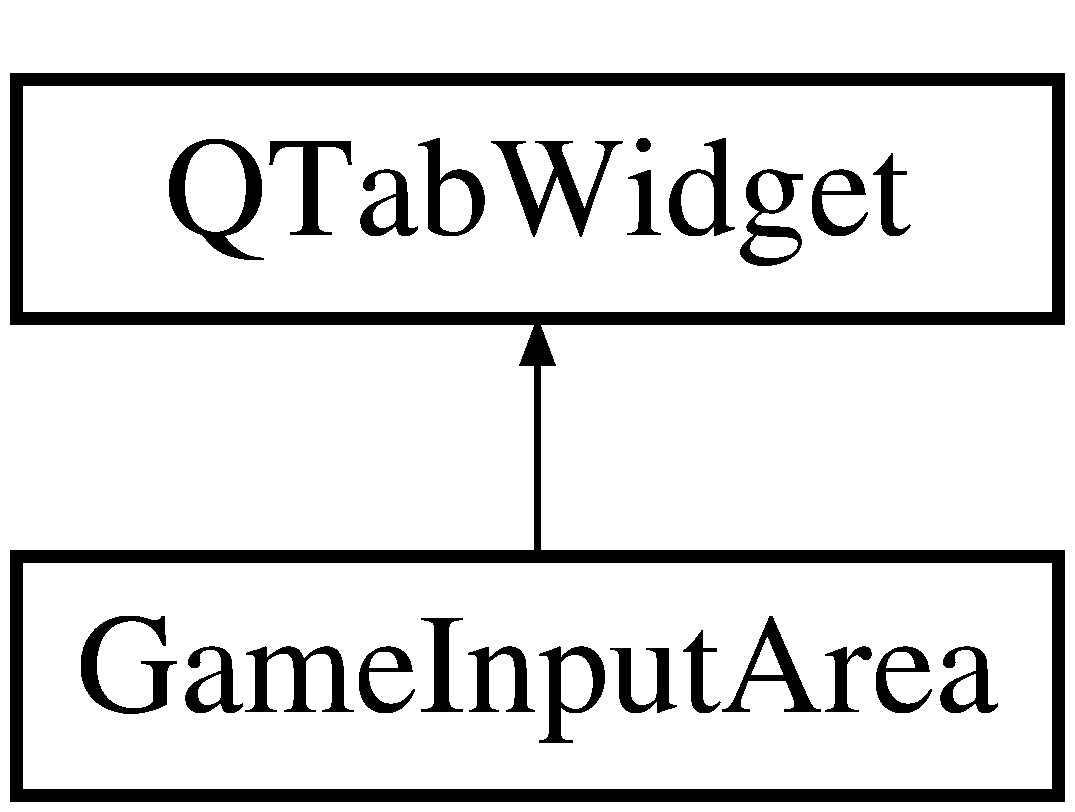
\includegraphics[height=2.000000cm]{classGameInputArea}
\end{center}
\end{figure}
\subsection*{Public Member Functions}
\begin{DoxyCompactItemize}
\item 
\hypertarget{classGameInputArea_a37bb000732d3b5e4f98923d4a753991e}{{\bfseries Game\-Input\-Area} (\hyperlink{classGameManager}{Game\-Manager} $\ast$game\-Manager, Q\-Widget $\ast$parent=0)}\label{classGameInputArea_a37bb000732d3b5e4f98923d4a753991e}

\item 
void \hyperlink{classGameInputArea_aeda3377d2dd4b04fe530ef96b52162ea}{change\-Event} (Q\-Event $\ast$event)
\begin{DoxyCompactList}\small\item\em Change the language. \end{DoxyCompactList}\item 
\hypertarget{classGameInputArea_a490df7daa012d358294f715bdb6addf6}{\hyperlink{classHistoryDisplay}{History\-Display} $\ast$ {\bfseries Get\-History\-Display} () const }\label{classGameInputArea_a490df7daa012d358294f715bdb6addf6}

\item 
\hypertarget{classGameInputArea_ad68c49dd0996e9661d84cd778ebcb4ef}{\hyperlink{classPlayerInput}{Player\-Input} $\ast$ {\bfseries Get\-Player\-Input\-Controls} () const }\label{classGameInputArea_ad68c49dd0996e9661d84cd778ebcb4ef}

\end{DoxyCompactItemize}


\subsection{Detailed Description}
The \hyperlink{classGameInputArea}{Game\-Input\-Area} class. 

\begin{DoxyAuthor}{Author}
Nils Brandt 

Alexander Luedke
\end{DoxyAuthor}
\begin{DoxyDate}{Date}
08. August 2016
\end{DoxyDate}
\begin{DoxyVersion}{Version}
1.\-0 Add Documentation 
\end{DoxyVersion}


\subsection{Member Function Documentation}
\hypertarget{classGameInputArea_aeda3377d2dd4b04fe530ef96b52162ea}{\index{Game\-Input\-Area@{Game\-Input\-Area}!change\-Event@{change\-Event}}
\index{change\-Event@{change\-Event}!GameInputArea@{Game\-Input\-Area}}
\subsubsection[{change\-Event}]{\setlength{\rightskip}{0pt plus 5cm}void Game\-Input\-Area\-::change\-Event (
\begin{DoxyParamCaption}
\item[{Q\-Event $\ast$}]{event}
\end{DoxyParamCaption}
)\hspace{0.3cm}{\ttfamily [inline]}}}\label{classGameInputArea_aeda3377d2dd4b04fe530ef96b52162ea}


Change the language. 


\begin{DoxyParams}{Parameters}
{\em event} & which change \\
\hline
\end{DoxyParams}

\hypertarget{classGameManager}{\section{Game\-Manager Class Reference}
\label{classGameManager}\index{Game\-Manager@{Game\-Manager}}
}


The \hyperlink{classGameManager}{Game\-Manager} class Handles the game loop logic in a thread.  




{\ttfamily \#include $<$Game\-Manager\-Thread.\-h$>$}

Inheritance diagram for Game\-Manager\-:\begin{figure}[H]
\begin{center}
\leavevmode
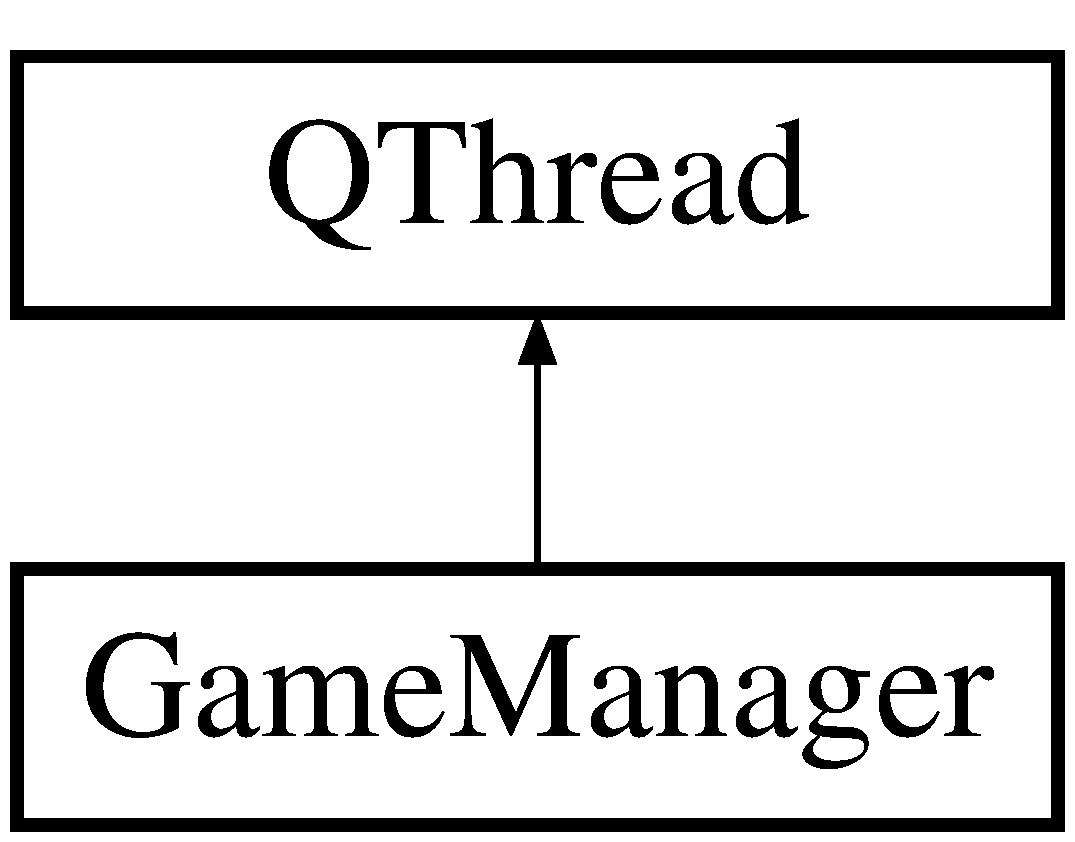
\includegraphics[height=2.000000cm]{classGameManager}
\end{center}
\end{figure}
\subsection*{Classes}
\begin{DoxyCompactItemize}
\item 
struct \hyperlink{structGameManager_1_1AIPlayer}{A\-I\-Player}
\begin{DoxyCompactList}\small\item\em The \hyperlink{classAI}{A\-I} struct Contains a reference to a player which is of type ai and if the ai player has calculated its next move. \end{DoxyCompactList}\end{DoxyCompactItemize}
\subsection*{Signals}
\begin{DoxyCompactItemize}
\item 
\hypertarget{classGameManager_a441d3c2600884f3c315a9c5d3db9066d}{void {\bfseries Play\-Input\-Error\-Sound} ()}\label{classGameManager_a441d3c2600884f3c315a9c5d3db9066d}

\item 
\hypertarget{classGameManager_aa6b2e8ebbbeee51512e865d73342cdce}{void {\bfseries Play\-Input\-Accept\-Sound} ()}\label{classGameManager_aa6b2e8ebbbeee51512e865d73342cdce}

\item 
\hypertarget{classGameManager_aba92c2301c45b00826365149ae8c4844}{void \hyperlink{classGameManager_aba92c2301c45b00826365149ae8c4844}{Turn\-Finished} ()}\label{classGameManager_aba92c2301c45b00826365149ae8c4844}

\begin{DoxyCompactList}\small\item\em Turn\-Finished emitted when players turn finishes. \end{DoxyCompactList}\item 
\hypertarget{classGameManager_a46ecd98b835abec58ea2b716b600c453}{void \hyperlink{classGameManager_a46ecd98b835abec58ea2b716b600c453}{Player\-Won} ()}\label{classGameManager_a46ecd98b835abec58ea2b716b600c453}

\begin{DoxyCompactList}\small\item\em Player\-Won emitted when a player won. \end{DoxyCompactList}\end{DoxyCompactItemize}
\subsection*{Public Member Functions}
\begin{DoxyCompactItemize}
\item 
\hypertarget{classGameManager_aa0e2424dc1a39d380e5b6605b179bf05}{\hyperlink{classGameManager_aa0e2424dc1a39d380e5b6605b179bf05}{Game\-Manager} ()}\label{classGameManager_aa0e2424dc1a39d380e5b6605b179bf05}

\begin{DoxyCompactList}\small\item\em \hyperlink{classGameManager}{Game\-Manager}. \end{DoxyCompactList}\item 
\hyperlink{classGameManager_a80046eb2f443289f0ba1b3fa1272470a}{Game\-Manager} (\hyperlink{classGameData}{Game\-Data} $\ast$data)
\begin{DoxyCompactList}\small\item\em \hyperlink{classGameManager}{Game\-Manager}. \end{DoxyCompactList}\item 
\hypertarget{classGameManager_aaae63e38e358379c1fe507c5197a8435}{virtual \hyperlink{classGameManager_aaae63e38e358379c1fe507c5197a8435}{$\sim$\-Game\-Manager} ()}\label{classGameManager_aaae63e38e358379c1fe507c5197a8435}

\begin{DoxyCompactList}\small\item\em $\sim$\-Game\-Manager \end{DoxyCompactList}\item 
\hypertarget{classGameManager_abbde8090c24ca199815ba1e85059c96f}{virtual void \hyperlink{classGameManager_abbde8090c24ca199815ba1e85059c96f}{run} ()}\label{classGameManager_abbde8090c24ca199815ba1e85059c96f}

\begin{DoxyCompactList}\small\item\em run override of the Q\-Thread run \end{DoxyCompactList}\item 
const \hyperlink{classGameData}{Game\-Data} $\ast$ \hyperlink{classGameManager_ae6075cdc12a4b98aeddc4cda20854393}{Get\-Game\-Data} () const 
\begin{DoxyCompactList}\small\item\em Get\-Game\-Data. \end{DoxyCompactList}\item 
\hypertarget{classGameManager_a3af49a72977052275a1217c5018c737f}{void {\bfseries Start\-Game} ()}\label{classGameManager_a3af49a72977052275a1217c5018c737f}

\item 
\hypertarget{classGameManager_a6f108cd9cdd0cf101d19a151e5e76a26}{void {\bfseries Pause\-Game} ()}\label{classGameManager_a6f108cd9cdd0cf101d19a151e5e76a26}

\item 
\hypertarget{classGameManager_ac756f69d83f34849ed763c7de6b2d47f}{void {\bfseries Suspend\-Processing\-Loop} ()}\label{classGameManager_ac756f69d83f34849ed763c7de6b2d47f}

\item 
\hypertarget{classGameManager_a4e3d2ab486b782641640fb82b77963f2}{void \hyperlink{classGameManager_a4e3d2ab486b782641640fb82b77963f2}{Stop\-Game\-Manager\-Thread} ()}\label{classGameManager_a4e3d2ab486b782641640fb82b77963f2}

\begin{DoxyCompactList}\small\item\em Stop sets the boolean to end the Main processing thread when the user quits the game. \end{DoxyCompactList}\item 
void \hyperlink{classGameManager_ade855b10bc61465dfdfb458cf624cf97}{Input\-Confirmation\-Detected} (\hyperlink{structVector2}{Vector2} pos)
\begin{DoxyCompactList}\small\item\em Input\-Confirmation\-Detected. \end{DoxyCompactList}\item 
bool \hyperlink{classGameManager_ab5e866fc01d4d612cd1f84de0df4653f}{Make\-Move} (\hyperlink{structVector3}{Vector3} pos)  throw (\-Playing\-Field\-::\-Field\-Exeptions, std\-::out\-\_\-of\-\_\-range)
\begin{DoxyCompactList}\small\item\em Tries to Occupy the given position , adds the move to the history, checks if the player won ( return true if won), switches currentplayer, and sends out event that a move is done. \end{DoxyCompactList}\end{DoxyCompactItemize}


\subsection{Detailed Description}
The \hyperlink{classGameManager}{Game\-Manager} class Handles the game loop logic in a thread. 

\begin{DoxyAuthor}{Author}
Nils Brandt 

Alexander Luedke
\end{DoxyAuthor}
\begin{DoxyDate}{Date}
08. August 2016
\end{DoxyDate}
\begin{DoxyVersion}{Version}
1.\-0 Add Documentation 
\end{DoxyVersion}


\subsection{Constructor \& Destructor Documentation}
\hypertarget{classGameManager_a80046eb2f443289f0ba1b3fa1272470a}{\index{Game\-Manager@{Game\-Manager}!Game\-Manager@{Game\-Manager}}
\index{Game\-Manager@{Game\-Manager}!GameManager@{Game\-Manager}}
\subsubsection[{Game\-Manager}]{\setlength{\rightskip}{0pt plus 5cm}Game\-Manager\-::\-Game\-Manager (
\begin{DoxyParamCaption}
\item[{{\bf Game\-Data} $\ast$}]{data}
\end{DoxyParamCaption}
)}}\label{classGameManager_a80046eb2f443289f0ba1b3fa1272470a}


\hyperlink{classGameManager}{Game\-Manager}. 


\begin{DoxyParams}{Parameters}
{\em data} & \\
\hline
\end{DoxyParams}


\subsection{Member Function Documentation}
\hypertarget{classGameManager_ae6075cdc12a4b98aeddc4cda20854393}{\index{Game\-Manager@{Game\-Manager}!Get\-Game\-Data@{Get\-Game\-Data}}
\index{Get\-Game\-Data@{Get\-Game\-Data}!GameManager@{Game\-Manager}}
\subsubsection[{Get\-Game\-Data}]{\setlength{\rightskip}{0pt plus 5cm}const {\bf Game\-Data} $\ast$ Game\-Manager\-::\-Get\-Game\-Data (
\begin{DoxyParamCaption}
{}
\end{DoxyParamCaption}
) const}}\label{classGameManager_ae6075cdc12a4b98aeddc4cda20854393}


Get\-Game\-Data. 

\begin{DoxyReturn}{Returns}

\end{DoxyReturn}
\hypertarget{classGameManager_ade855b10bc61465dfdfb458cf624cf97}{\index{Game\-Manager@{Game\-Manager}!Input\-Confirmation\-Detected@{Input\-Confirmation\-Detected}}
\index{Input\-Confirmation\-Detected@{Input\-Confirmation\-Detected}!GameManager@{Game\-Manager}}
\subsubsection[{Input\-Confirmation\-Detected}]{\setlength{\rightskip}{0pt plus 5cm}void Game\-Manager\-::\-Input\-Confirmation\-Detected (
\begin{DoxyParamCaption}
\item[{{\bf Vector2}}]{pos}
\end{DoxyParamCaption}
)}}\label{classGameManager_ade855b10bc61465dfdfb458cf624cf97}


Input\-Confirmation\-Detected. 


\begin{DoxyParams}{Parameters}
{\em pos} & \\
\hline
\end{DoxyParams}
\hypertarget{classGameManager_ab5e866fc01d4d612cd1f84de0df4653f}{\index{Game\-Manager@{Game\-Manager}!Make\-Move@{Make\-Move}}
\index{Make\-Move@{Make\-Move}!GameManager@{Game\-Manager}}
\subsubsection[{Make\-Move}]{\setlength{\rightskip}{0pt plus 5cm}bool Game\-Manager\-::\-Make\-Move (
\begin{DoxyParamCaption}
\item[{{\bf Vector3}}]{pos}
\end{DoxyParamCaption}
) throw  {\bf Playing\-Field\-::\-Field\-Exeptions}, std\-::out\-\_\-of\-\_\-range) }}\label{classGameManager_ab5e866fc01d4d612cd1f84de0df4653f}


Tries to Occupy the given position , adds the move to the history, checks if the player won ( return true if won), switches currentplayer, and sends out event that a move is done. 


\begin{DoxyParams}{Parameters}
{\em pos} & \\
\hline
\end{DoxyParams}
\begin{DoxyReturn}{Returns}
true if the player just won the game 
\end{DoxyReturn}

\hypertarget{classGameView}{\section{Game\-View Class Reference}
\label{classGameView}\index{Game\-View@{Game\-View}}
}


The \hyperlink{classGameView}{Game\-View} class.  




{\ttfamily \#include $<$Game\-View.\-h$>$}

Inheritance diagram for Game\-View\-:\begin{figure}[H]
\begin{center}
\leavevmode
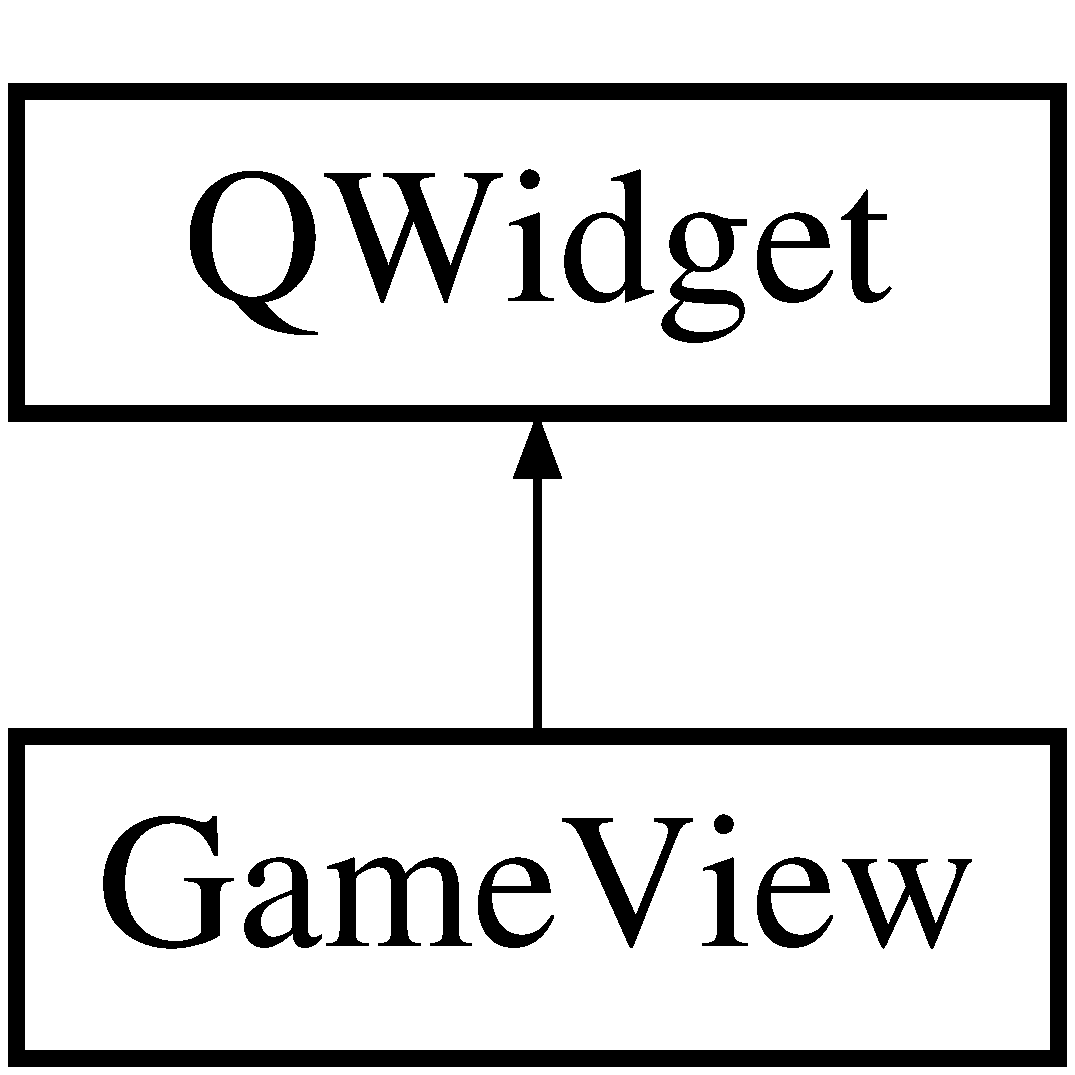
\includegraphics[height=2.000000cm]{classGameView}
\end{center}
\end{figure}
\subsection*{Signals}
\begin{DoxyCompactItemize}
\item 
void \hyperlink{classGameView_a5901d54c9767a75549860cc5b511fcd5}{Game\-Ended} (\hyperlink{classGameData}{Game\-Data} $\ast$data)
\begin{DoxyCompactList}\small\item\em Game\-Ended Called when leave button pressed to go back to menu screen. \end{DoxyCompactList}\item 
\hypertarget{classGameView_a2d1aa868abc05055e5be27040660f7f0}{void \hyperlink{classGameView_a2d1aa868abc05055e5be27040660f7f0}{Pause\-Menu} ()}\label{classGameView_a2d1aa868abc05055e5be27040660f7f0}

\begin{DoxyCompactList}\small\item\em \hyperlink{classPauseMenu}{Pause\-Menu}. \end{DoxyCompactList}\end{DoxyCompactItemize}
\subsection*{Public Member Functions}
\begin{DoxyCompactItemize}
\item 
\hypertarget{classGameView_a6f41d09f51d2abd6abb3b99e5da8ef6f}{{\bfseries Game\-View} (Q\-Widget $\ast$parent=0)}\label{classGameView_a6f41d09f51d2abd6abb3b99e5da8ef6f}

\item 
\hypertarget{classGameView_ae2f4618068a746a97c33859a7550640e}{{\bfseries Game\-View} (\hyperlink{classGameData}{Game\-Data} $\ast$data, Q\-Widget $\ast$parent=0)}\label{classGameView_ae2f4618068a746a97c33859a7550640e}

\item 
\hypertarget{classGameView_aef16847b30bf78a6ecc0888ab1157c8b}{\hyperlink{classGameVisualizer}{Game\-Visualizer} $\ast$ {\bfseries Get\-Visualizer} () const }\label{classGameView_aef16847b30bf78a6ecc0888ab1157c8b}

\item 
\hypertarget{classGameView_a7372d6130ea98db65d8dffc0c4c6989e}{\hyperlink{classGameData}{Game\-Data} $\ast$ {\bfseries Get\-Game\-Data} () const }\label{classGameView_a7372d6130ea98db65d8dffc0c4c6989e}

\item 
\hypertarget{classGameView_a6ecf68723625fae0f3f6301040b166fe}{void {\bfseries Init\-Game} (\hyperlink{classGameData}{Game\-Data} $\ast$data)}\label{classGameView_a6ecf68723625fae0f3f6301040b166fe}

\item 
\hypertarget{classGameView_abd2ab0306c7ce339f7d2d994f21f9f7d}{void {\bfseries Start\-Game} ()}\label{classGameView_abd2ab0306c7ce339f7d2d994f21f9f7d}

\item 
\hypertarget{classGameView_a2b977bd2bd50b851438230f7c4a4ac93}{void {\bfseries Pause\-Game} ()}\label{classGameView_a2b977bd2bd50b851438230f7c4a4ac93}

\item 
\hypertarget{classGameView_a2a1634628f3c981462f54c6c1f18ec6d}{void {\bfseries Play\-Accept\-Sound} ()}\label{classGameView_a2a1634628f3c981462f54c6c1f18ec6d}

\item 
\hypertarget{classGameView_a0bc73aeff44e7e52bd1d73a21dd6a7f2}{void {\bfseries Play\-Error\-Sound} ()}\label{classGameView_a0bc73aeff44e7e52bd1d73a21dd6a7f2}

\item 
\hypertarget{classGameView_a92b306e86ed8fe682763050be4edf254}{void {\bfseries Show\-Game\-Input\-View} ()}\label{classGameView_a92b306e86ed8fe682763050be4edf254}

\item 
\hypertarget{classGameView_a29cba4e6e6963b659f3cb2acbdfc3fe1}{void {\bfseries Show\-Winner} ()}\label{classGameView_a29cba4e6e6963b659f3cb2acbdfc3fe1}

\item 
\hypertarget{classGameView_a3e06ec8f766005c4aac0d572559fc9ed}{void \hyperlink{classGameView_a3e06ec8f766005c4aac0d572559fc9ed}{Game\-Finished} ()}\label{classGameView_a3e06ec8f766005c4aac0d572559fc9ed}

\begin{DoxyCompactList}\small\item\em Game\-Finished Called if a player won to stop the gamelogic thread and show leave button. \end{DoxyCompactList}\item 
\hypertarget{classGameView_a157ac747504394587761ac30a79b9597}{void \hyperlink{classGameView_a157ac747504394587761ac30a79b9597}{End\-Game} ()}\label{classGameView_a157ac747504394587761ac30a79b9597}

\begin{DoxyCompactList}\small\item\em End\-Game called from leave button calls Game\-Ended. \end{DoxyCompactList}\item 
\hypertarget{classGameView_a5d6aac6e502ec51285f03ba51da00886}{void {\bfseries change\-Event} (Q\-Event $\ast$event)}\label{classGameView_a5d6aac6e502ec51285f03ba51da00886}

\end{DoxyCompactItemize}


\subsection{Detailed Description}
The \hyperlink{classGameView}{Game\-View} class. 

\begin{DoxyAuthor}{Author}
Nils Brandt 

Alexander Luedke
\end{DoxyAuthor}
\begin{DoxyDate}{Date}
08. August 2016
\end{DoxyDate}
\begin{DoxyVersion}{Version}
1.\-0 Add Documentation 
\end{DoxyVersion}


\subsection{Member Function Documentation}
\hypertarget{classGameView_a5901d54c9767a75549860cc5b511fcd5}{\index{Game\-View@{Game\-View}!Game\-Ended@{Game\-Ended}}
\index{Game\-Ended@{Game\-Ended}!GameView@{Game\-View}}
\subsubsection[{Game\-Ended}]{\setlength{\rightskip}{0pt plus 5cm}void Game\-View\-::\-Game\-Ended (
\begin{DoxyParamCaption}
\item[{{\bf Game\-Data} $\ast$}]{data}
\end{DoxyParamCaption}
)\hspace{0.3cm}{\ttfamily [signal]}}}\label{classGameView_a5901d54c9767a75549860cc5b511fcd5}


Game\-Ended Called when leave button pressed to go back to menu screen. 


\begin{DoxyParams}{Parameters}
{\em data} & gamedata after game ended \\
\hline
\end{DoxyParams}

\hypertarget{classGameView2D}{\section{Game\-View2\-D Class Reference}
\label{classGameView2D}\index{Game\-View2\-D@{Game\-View2\-D}}
}


The \hyperlink{classGameView2D}{Game\-View2\-D} class.  




{\ttfamily \#include $<$Game\-View2\-D.\-h$>$}

Inheritance diagram for Game\-View2\-D\-:\begin{figure}[H]
\begin{center}
\leavevmode
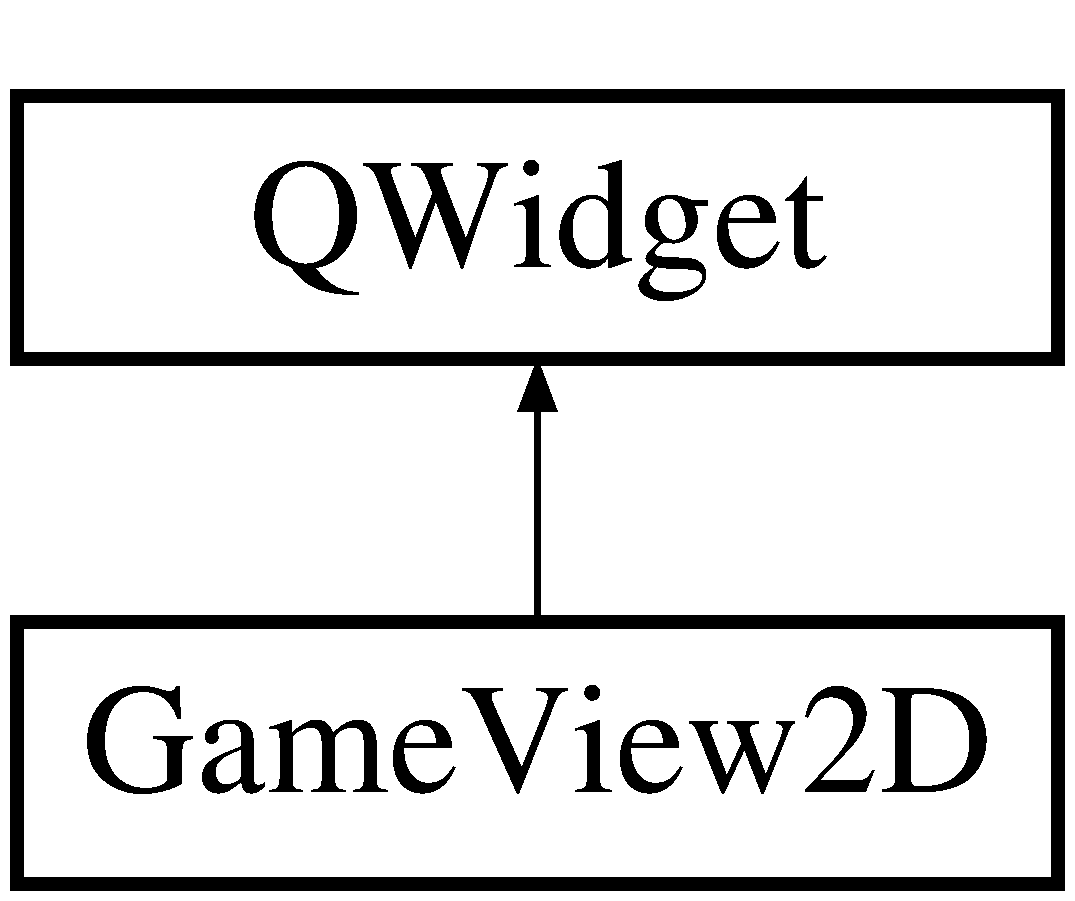
\includegraphics[height=2.000000cm]{classGameView2D}
\end{center}
\end{figure}
\subsection*{Public Member Functions}
\begin{DoxyCompactItemize}
\item 
\hypertarget{classGameView2D_ade0d3e85d2385f952db7a5a72dcc34e3}{{\bfseries Game\-View2\-D} (\hyperlink{classGameManager}{Game\-Manager} $\ast$manager, Q\-Widget $\ast$parent=0)}\label{classGameView2D_ade0d3e85d2385f952db7a5a72dcc34e3}

\item 
\hypertarget{classGameView2D_a2599584223096c30f37ed12566ccea32}{\hyperlink{classGraphicsSlot2D}{Graphics\-Slot2\-D} $\ast$ {\bfseries Get\-Rect} (\hyperlink{structVector3}{Vector3} vec)}\label{classGameView2D_a2599584223096c30f37ed12566ccea32}

\item 
\hypertarget{classGameView2D_aa30c0b87cc0c44a68a9f30b5e9e22ea4}{void \hyperlink{classGameView2D_aa30c0b87cc0c44a68a9f30b5e9e22ea4}{Clear\-Grid} ()}\label{classGameView2D_aa30c0b87cc0c44a68a9f30b5e9e22ea4}

\begin{DoxyCompactList}\small\item\em To clear the grid. \end{DoxyCompactList}\item 
\hypertarget{classGameView2D_aaf46ebd46da445c65fb1d54e805b7d9c}{void {\bfseries Recalculate\-Grid} ()}\label{classGameView2D_aaf46ebd46da445c65fb1d54e805b7d9c}

\item 
\hypertarget{classGameView2D_ad826ed1dccdcae1508693615e20df95e}{void \hyperlink{classGameView2D_ad826ed1dccdcae1508693615e20df95e}{View\-Update} ()}\label{classGameView2D_ad826ed1dccdcae1508693615e20df95e}

\begin{DoxyCompactList}\small\item\em View\-Update. \end{DoxyCompactList}\end{DoxyCompactItemize}


\subsection{Detailed Description}
The \hyperlink{classGameView2D}{Game\-View2\-D} class. 

\begin{DoxyAuthor}{Author}
Nils Brandt 

Alexander Luedke
\end{DoxyAuthor}
\begin{DoxyDate}{Date}
08. August 2016
\end{DoxyDate}
\begin{DoxyVersion}{Version}
1.\-0 Add Documentation 
\end{DoxyVersion}

\hypertarget{classGameView3D}{\section{Game\-View3\-D Class Reference}
\label{classGameView3D}\index{Game\-View3\-D@{Game\-View3\-D}}
}


The \hyperlink{classGameView3D}{Game\-View3\-D} class.  




{\ttfamily \#include $<$Game\-View3\-D.\-h$>$}

Inheritance diagram for Game\-View3\-D\-:\begin{figure}[H]
\begin{center}
\leavevmode
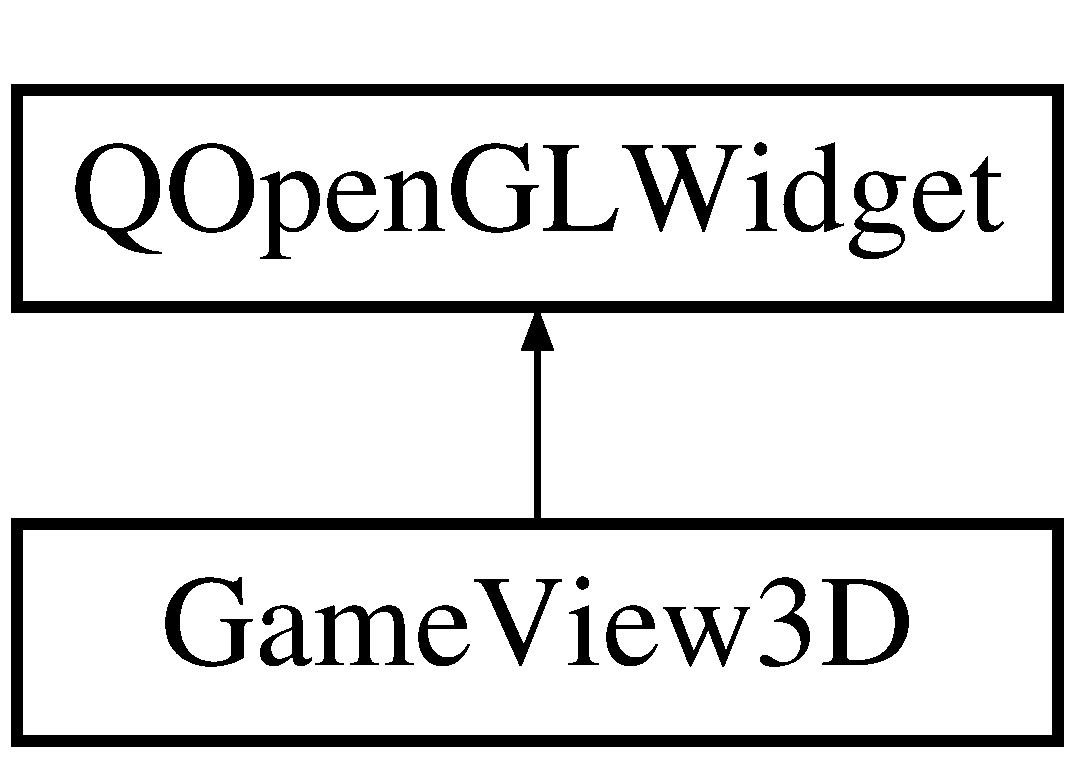
\includegraphics[height=2.000000cm]{classGameView3D}
\end{center}
\end{figure}
\subsection*{Signals}
\begin{DoxyCompactItemize}
\item 
\hypertarget{classGameView3D_ada434861732fe261a9a7958de4fb5f2e}{void {\bfseries Input\-Submit} (\hyperlink{structVector2}{Vector2} pos)}\label{classGameView3D_ada434861732fe261a9a7958de4fb5f2e}

\end{DoxyCompactItemize}
\subsection*{Public Member Functions}
\begin{DoxyCompactItemize}
\item 
\hypertarget{classGameView3D_aa2a60cd38325c7a4ec92909d2efe7a80}{{\bfseries Game\-View3\-D} (Q\-Widget $\ast$parent=0)}\label{classGameView3D_aa2a60cd38325c7a4ec92909d2efe7a80}

\item 
\hypertarget{classGameView3D_a447292a1846348584fea8cbd2392d1dd}{{\bfseries Game\-View3\-D} (\hyperlink{classGameManager}{Game\-Manager} $\ast$gm, Q\-Widget $\ast$parent=0)}\label{classGameView3D_a447292a1846348584fea8cbd2392d1dd}

\item 
\hypertarget{classGameView3D_a9662a858540b5fcc1a80d78cd0a0aa2a}{void {\bfseries Clean\-Up} ()}\label{classGameView3D_a9662a858540b5fcc1a80d78cd0a0aa2a}

\end{DoxyCompactItemize}
\subsection*{Protected Member Functions}
\begin{DoxyCompactItemize}
\item 
\hypertarget{classGameView3D_ae077404d42f477162b3540da397a8ad4}{void {\bfseries send\-M\-V\-P} (G\-Luint program\-I\-D)}\label{classGameView3D_ae077404d42f477162b3540da397a8ad4}

\item 
\hypertarget{classGameView3D_ae6db5f0d969ca92280e4dc6c7092e11e}{virtual void {\bfseries initialize\-G\-L} ()}\label{classGameView3D_ae6db5f0d969ca92280e4dc6c7092e11e}

\item 
\hypertarget{classGameView3D_ad69d664507756b94cc64ab65581528c4}{virtual void {\bfseries paint\-G\-L} ()}\label{classGameView3D_ad69d664507756b94cc64ab65581528c4}

\item 
\hypertarget{classGameView3D_ad08f12d05b40dbbb42172783fb4ffe5f}{virtual void {\bfseries resize\-G\-L} (int w, int h)}\label{classGameView3D_ad08f12d05b40dbbb42172783fb4ffe5f}

\item 
\hypertarget{classGameView3D_abeb74e91cd820d7af1e62c714fc1864f}{void {\bfseries key\-Press\-Event} (Q\-Key\-Event $\ast$event)}\label{classGameView3D_abeb74e91cd820d7af1e62c714fc1864f}

\item 
\hypertarget{classGameView3D_a2a66712712d355039299efb5513fbeb2}{void {\bfseries mouse\-Press\-Event} (Q\-Mouse\-Event $\ast$event)}\label{classGameView3D_a2a66712712d355039299efb5513fbeb2}

\item 
\hypertarget{classGameView3D_a16eb2fd0448d2f50b1c5287f86ac9437}{void {\bfseries mouse\-Move\-Event} (Q\-Mouse\-Event $\ast$event)}\label{classGameView3D_a16eb2fd0448d2f50b1c5287f86ac9437}

\item 
\hypertarget{classGameView3D_aa4d6e119510fc03c95d52282579ca8ed}{bool {\bfseries Cast\-Ray} (Q\-Point m\-\_\-current\-Mouse\-Pos)}\label{classGameView3D_aa4d6e119510fc03c95d52282579ca8ed}

\item 
\hypertarget{classGameView3D_a31d588b55fd79e52732a28ccd196733c}{void {\bfseries Create\-Line} (glm\-::vec3 start, glm\-::vec3 end, G\-Luint \&Vertex\-Array\-I\-D\-Line)}\label{classGameView3D_a31d588b55fd79e52732a28ccd196733c}

\item 
\hypertarget{classGameView3D_a5e9b5ac73aaa4fedf3bbbec02544c184}{void {\bfseries Draw\-Line} (glm\-::vec3 start, glm\-::vec3 end)}\label{classGameView3D_a5e9b5ac73aaa4fedf3bbbec02544c184}

\item 
\hypertarget{classGameView3D_aa96228c70d0a93420abef7687518f809}{void {\bfseries Screen\-Pos\-To\-World\-Ray} (int mouse\-X, int mouse\-Y, int screen\-Width, int screen\-Height, glm\-::mat4 View\-Matrix, glm\-::mat4 Projection\-Matrix, glm\-::vec3 \&out\-\_\-origin, glm\-::vec3 \&out\-\_\-direction)}\label{classGameView3D_aa96228c70d0a93420abef7687518f809}

\item 
\hypertarget{classGameView3D_a301575899b1763b95a99e4c386f9356d}{bool {\bfseries Test\-Ray\-O\-B\-B\-Intersection} (glm\-::vec3 ray\-\_\-origin, glm\-::vec3 ray\-\_\-direction, glm\-::vec3 aabb\-\_\-min, glm\-::vec3 aabb\-\_\-max, glm\-::mat4 Model\-Matrix, float \&intersection\-\_\-distance)}\label{classGameView3D_a301575899b1763b95a99e4c386f9356d}

\end{DoxyCompactItemize}


\subsection{Detailed Description}
The \hyperlink{classGameView3D}{Game\-View3\-D} class. 

\begin{DoxyAuthor}{Author}
Nils Brandt 

Alexander Luedke
\end{DoxyAuthor}
\begin{DoxyDate}{Date}
08. August 2016
\end{DoxyDate}
\begin{DoxyVersion}{Version}
1.\-0 Add Documentation 
\end{DoxyVersion}

\hypertarget{classGameVisualizer}{\section{Game\-Visualizer Class Reference}
\label{classGameVisualizer}\index{Game\-Visualizer@{Game\-Visualizer}}
}


The \hyperlink{classGameVisualizer}{Game\-Visualizer} class.  




{\ttfamily \#include $<$Game\-Visualizer.\-h$>$}

Inheritance diagram for Game\-Visualizer\-:\begin{figure}[H]
\begin{center}
\leavevmode
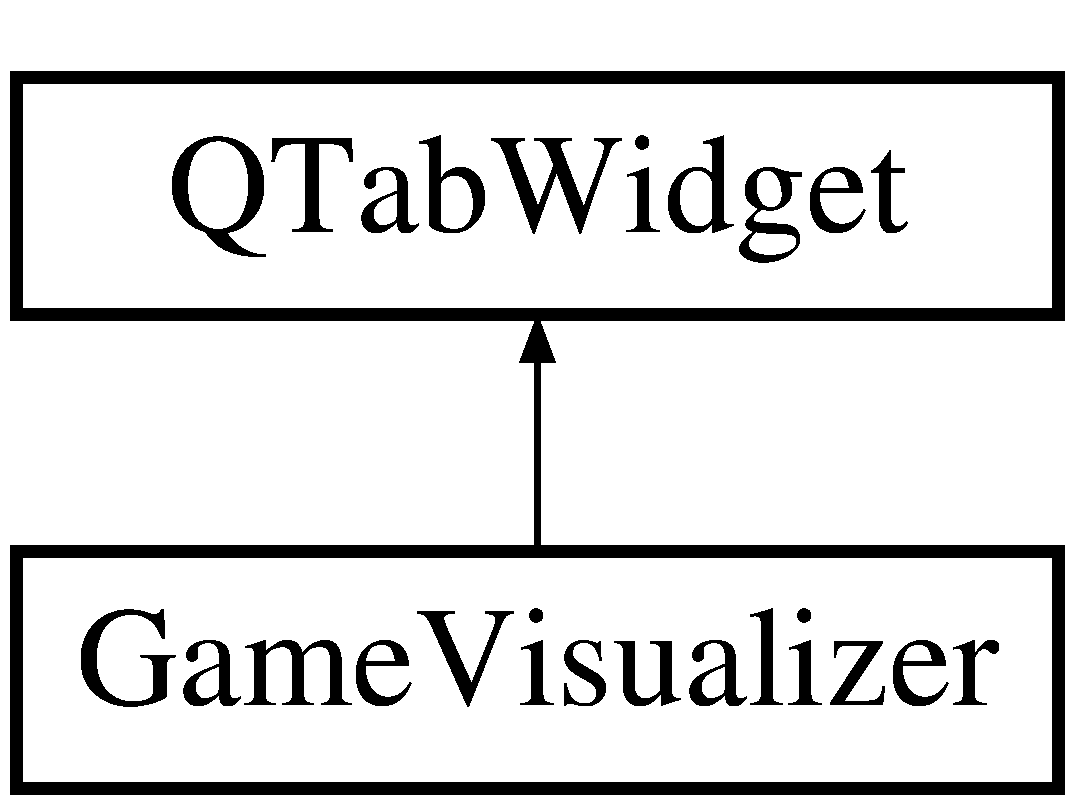
\includegraphics[height=2.000000cm]{classGameVisualizer}
\end{center}
\end{figure}
\subsection*{Signals}
\begin{DoxyCompactItemize}
\item 
\hypertarget{classGameVisualizer_abb8ff4568ee3c5ed30cbc2df3d32df84}{void {\bfseries Input\-Detected} (\hyperlink{structVector2}{Vector2} pos)}\label{classGameVisualizer_abb8ff4568ee3c5ed30cbc2df3d32df84}

\end{DoxyCompactItemize}
\subsection*{Public Member Functions}
\begin{DoxyCompactItemize}
\item 
\hypertarget{classGameVisualizer_ac6e640e1cfa0162d63158670741d9485}{{\bfseries Game\-Visualizer} (\hyperlink{classGameManager}{Game\-Manager} $\ast$manager, Q\-Widget $\ast$parent=0)}\label{classGameVisualizer_ac6e640e1cfa0162d63158670741d9485}

\item 
\hypertarget{classGameVisualizer_ac68aa47882b34f28427e3e161f677f9d}{void {\bfseries Update\-Views} ()}\label{classGameVisualizer_ac68aa47882b34f28427e3e161f677f9d}

\item 
\hypertarget{classGameVisualizer_a5fb41e30e67173d36f3769d804130b19}{void {\bfseries Update\-View2\-D} ()}\label{classGameVisualizer_a5fb41e30e67173d36f3769d804130b19}

\item 
\hypertarget{classGameVisualizer_aee1fac4e1657fb4be1fa61f563b02d32}{void {\bfseries Update\-View3\-D} ()}\label{classGameVisualizer_aee1fac4e1657fb4be1fa61f563b02d32}

\item 
\hypertarget{classGameVisualizer_a3a8cf6d067d4d0272c1b3b60f44f8d1c}{void {\bfseries Game\-Changed} ()}\label{classGameVisualizer_a3a8cf6d067d4d0272c1b3b60f44f8d1c}

\end{DoxyCompactItemize}


\subsection{Detailed Description}
The \hyperlink{classGameVisualizer}{Game\-Visualizer} class. 

\begin{DoxyAuthor}{Author}
Nils Brandt 

Alexander Luedke
\end{DoxyAuthor}
\begin{DoxyDate}{Date}
08. August 2016
\end{DoxyDate}
\begin{DoxyVersion}{Version}
1.\-0 Add Documentation 
\end{DoxyVersion}

\hypertarget{structglm_1_1detail_1_1genType}{\section{glm\-:\-:detail\-:\-:gen\-Type$<$ V\-A\-L\-T\-Y\-P\-E, T\-Y\-P\-E $>$ Struct Template Reference}
\label{structglm_1_1detail_1_1genType}\index{glm\-::detail\-::gen\-Type$<$ V\-A\-L\-T\-Y\-P\-E, T\-Y\-P\-E $>$@{glm\-::detail\-::gen\-Type$<$ V\-A\-L\-T\-Y\-P\-E, T\-Y\-P\-E $>$}}
}
\subsection*{Public Types}
\begin{DoxyCompactItemize}
\item 
enum {\bfseries ctor} \{ {\bfseries null}
 \}
\item 
\hypertarget{structglm_1_1detail_1_1genType_ad59e126a45bca74a36732a30cdaee520}{typedef V\-A\-L\-T\-Y\-P\-E {\bfseries value\-\_\-type}}\label{structglm_1_1detail_1_1genType_ad59e126a45bca74a36732a30cdaee520}

\item 
\hypertarget{structglm_1_1detail_1_1genType_a557d18598a777df9f16fa1bd7c637ca4}{typedef V\-A\-L\-T\-Y\-P\-E \& {\bfseries value\-\_\-reference}}\label{structglm_1_1detail_1_1genType_a557d18598a777df9f16fa1bd7c637ca4}

\item 
\hypertarget{structglm_1_1detail_1_1genType_a3b272e7be29ab920f2877c00646f6f9b}{typedef V\-A\-L\-T\-Y\-P\-E $\ast$ {\bfseries value\-\_\-pointer}}\label{structglm_1_1detail_1_1genType_a3b272e7be29ab920f2877c00646f6f9b}

\item 
\hypertarget{structglm_1_1detail_1_1genType_a34e169ae6d50e1c76574c850eae2c7fc}{typedef V\-A\-L\-T\-Y\-P\-E const $\ast$ {\bfseries value\-\_\-const\-\_\-pointer}}\label{structglm_1_1detail_1_1genType_a34e169ae6d50e1c76574c850eae2c7fc}

\item 
\hypertarget{structglm_1_1detail_1_1genType_ac338f0b4e47d5daa9c8e5411f0d37554}{typedef T\-Y\-P\-E$<$ bool $>$ {\bfseries bool\-\_\-type}}\label{structglm_1_1detail_1_1genType_ac338f0b4e47d5daa9c8e5411f0d37554}

\item 
\hypertarget{structglm_1_1detail_1_1genType_af4fa06eb65eebb96960fae19a3b439eb}{typedef size\-Type {\bfseries size\-\_\-type}}\label{structglm_1_1detail_1_1genType_af4fa06eb65eebb96960fae19a3b439eb}

\item 
\hypertarget{structglm_1_1detail_1_1genType_a17dbd44c7a86d09e6ea05b72cb02bccf}{typedef T\-Y\-P\-E$<$ V\-A\-L\-T\-Y\-P\-E $>$ {\bfseries type}}\label{structglm_1_1detail_1_1genType_a17dbd44c7a86d09e6ea05b72cb02bccf}

\item 
\hypertarget{structglm_1_1detail_1_1genType_a0b4ddd0af4ae5665c60055e5b622808e}{typedef T\-Y\-P\-E$<$ V\-A\-L\-T\-Y\-P\-E $>$ $\ast$ {\bfseries pointer}}\label{structglm_1_1detail_1_1genType_a0b4ddd0af4ae5665c60055e5b622808e}

\item 
\hypertarget{structglm_1_1detail_1_1genType_ade82fbfd7b15096223e1b133c148b5e2}{typedef T\-Y\-P\-E$<$ V\-A\-L\-T\-Y\-P\-E $>$ const $\ast$ {\bfseries const\-\_\-pointer}}\label{structglm_1_1detail_1_1genType_ade82fbfd7b15096223e1b133c148b5e2}

\item 
\hypertarget{structglm_1_1detail_1_1genType_a4f3f1bc18abdbdba5757fc63052157fa}{typedef T\-Y\-P\-E$<$ V\-A\-L\-T\-Y\-P\-E $>$ const \\*
$\ast$const {\bfseries const\-\_\-pointer\-\_\-const}}\label{structglm_1_1detail_1_1genType_a4f3f1bc18abdbdba5757fc63052157fa}

\item 
\hypertarget{structglm_1_1detail_1_1genType_a4d7745054035d7efed18ec1d7215bbf0}{typedef T\-Y\-P\-E$<$ V\-A\-L\-T\-Y\-P\-E $>$ $\ast$const {\bfseries pointer\-\_\-const}}\label{structglm_1_1detail_1_1genType_a4d7745054035d7efed18ec1d7215bbf0}

\item 
\hypertarget{structglm_1_1detail_1_1genType_a14792cf03ce9cfb37becd2da5d9ae06a}{typedef T\-Y\-P\-E$<$ V\-A\-L\-T\-Y\-P\-E $>$ \& {\bfseries reference}}\label{structglm_1_1detail_1_1genType_a14792cf03ce9cfb37becd2da5d9ae06a}

\item 
\hypertarget{structglm_1_1detail_1_1genType_a509ca374a85f8a9ea319bc5a980d5f1a}{typedef T\-Y\-P\-E$<$ V\-A\-L\-T\-Y\-P\-E $>$ const \& {\bfseries const\-\_\-reference}}\label{structglm_1_1detail_1_1genType_a509ca374a85f8a9ea319bc5a980d5f1a}

\item 
\hypertarget{structglm_1_1detail_1_1genType_a92c8b989f574a63d4e0f5bfc8a4f3a32}{typedef T\-Y\-P\-E$<$ V\-A\-L\-T\-Y\-P\-E $>$ const \& {\bfseries param\-\_\-type}}\label{structglm_1_1detail_1_1genType_a92c8b989f574a63d4e0f5bfc8a4f3a32}

\end{DoxyCompactItemize}
\subsection*{Public Member Functions}
\begin{DoxyCompactItemize}
\item 
\hypertarget{structglm_1_1detail_1_1genType_a63fb77e77082f34c0a0d7faa0906f7f4}{value\-\_\-const\-\_\-pointer {\bfseries value\-\_\-address} () const }\label{structglm_1_1detail_1_1genType_a63fb77e77082f34c0a0d7faa0906f7f4}

\item 
\hypertarget{structglm_1_1detail_1_1genType_a146973ec142766743080c1895a9e3c65}{value\-\_\-pointer {\bfseries value\-\_\-address} ()}\label{structglm_1_1detail_1_1genType_a146973ec142766743080c1895a9e3c65}

\end{DoxyCompactItemize}
\subsection*{Static Public Member Functions}
\begin{DoxyCompactItemize}
\item 
\hypertarget{structglm_1_1detail_1_1genType_ae83087df55201bdc46a37decf3d1c34c}{static bool {\bfseries is\-\_\-vector} ()}\label{structglm_1_1detail_1_1genType_ae83087df55201bdc46a37decf3d1c34c}

\item 
\hypertarget{structglm_1_1detail_1_1genType_a78c650375558d5e2ccfba383cdb59479}{static bool {\bfseries is\-\_\-matrix} ()}\label{structglm_1_1detail_1_1genType_a78c650375558d5e2ccfba383cdb59479}

\end{DoxyCompactItemize}


The documentation for this struct was generated from the following file\-:\begin{DoxyCompactItemize}
\item 
/home/alex/source\-Code/git\-Project/beleg\-Arbeit\-E\-M\-M\-S/project\-Sogo/external/glm-\/0.\-9.\-4.\-0/glm/core/\hyperlink{type__gentype_8hpp}{type\-\_\-gentype.\-hpp}\end{DoxyCompactItemize}

\hypertarget{classGraphicsSlot2D}{\section{Graphics\-Slot2\-D Class Reference}
\label{classGraphicsSlot2D}\index{Graphics\-Slot2\-D@{Graphics\-Slot2\-D}}
}


The \hyperlink{classGraphicsSlot2D}{Graphics\-Slot2\-D} class.  




{\ttfamily \#include $<$Graphics\-Slot2d.\-h$>$}

Inheritance diagram for Graphics\-Slot2\-D\-:\begin{figure}[H]
\begin{center}
\leavevmode
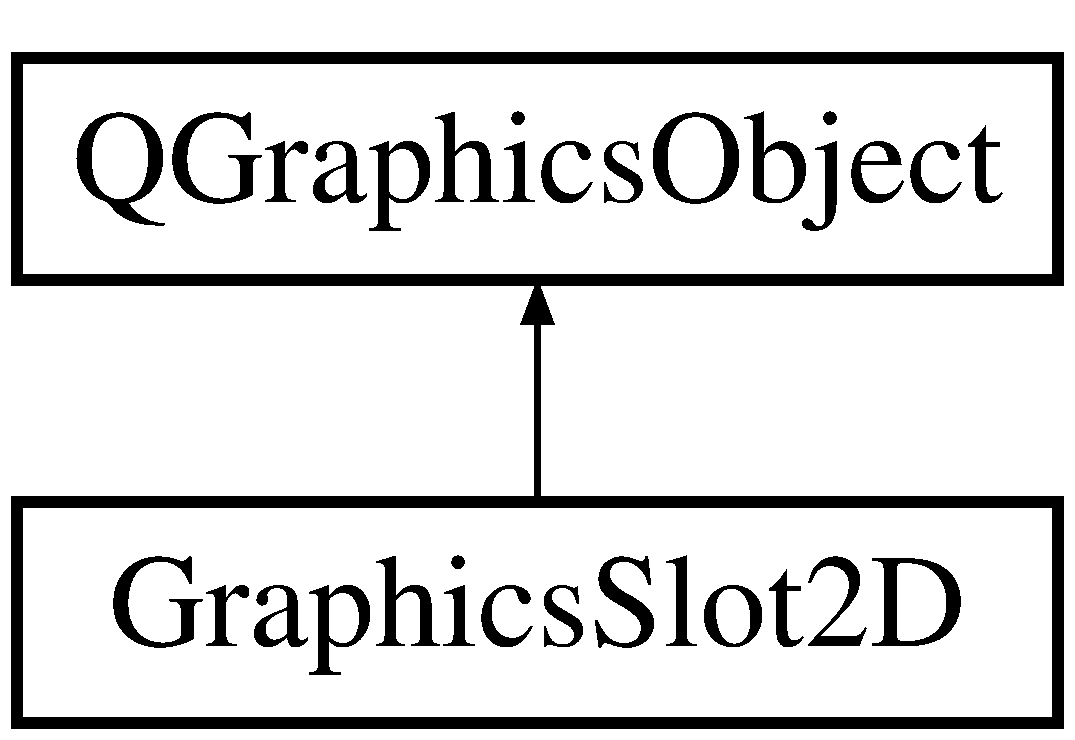
\includegraphics[height=2.000000cm]{classGraphicsSlot2D}
\end{center}
\end{figure}
\subsection*{Signals}
\begin{DoxyCompactItemize}
\item 
\hypertarget{classGraphicsSlot2D_a1cca679459243a836ace0c4aca3923e8}{void {\bfseries Clicked\-Signal} (\hyperlink{classGraphicsSlot2D}{Graphics\-Slot2\-D} $\ast$ref)}\label{classGraphicsSlot2D_a1cca679459243a836ace0c4aca3923e8}

\end{DoxyCompactItemize}
\subsection*{Public Member Functions}
\begin{DoxyCompactItemize}
\item 
\hypertarget{classGraphicsSlot2D_a727b75d36aeec94cb0ea7ba87d2b4018}{{\bfseries Graphics\-Slot2\-D} (float x, float y, float width, float height, Q\-Color color=Qt\-::white, Q\-Graphics\-Item $\ast$parent=0)}\label{classGraphicsSlot2D_a727b75d36aeec94cb0ea7ba87d2b4018}

\item 
\hypertarget{classGraphicsSlot2D_a91bbc858f2f966d88f5dfc3a9255b262}{virtual Q\-Rect\-F {\bfseries bounding\-Rect} () const Q\-\_\-\-D\-E\-C\-L\-\_\-\-O\-V\-E\-R\-R\-I\-D\-E}\label{classGraphicsSlot2D_a91bbc858f2f966d88f5dfc3a9255b262}

\item 
\hypertarget{classGraphicsSlot2D_acb9706b9269de9e2a8221b34d117e66e}{Q\-Color {\bfseries Get\-Color} () const }\label{classGraphicsSlot2D_acb9706b9269de9e2a8221b34d117e66e}

\item 
\hypertarget{classGraphicsSlot2D_aa505d921ccd7d8e92ee2b5d028b768c4}{void {\bfseries Set\-Size} (float x, float y)}\label{classGraphicsSlot2D_aa505d921ccd7d8e92ee2b5d028b768c4}

\item 
\hypertarget{classGraphicsSlot2D_a6e7ccd8e16d8cb8b558eaddfbe4ac3b5}{void {\bfseries Set\-Color} (Q\-Color color)}\label{classGraphicsSlot2D_a6e7ccd8e16d8cb8b558eaddfbe4ac3b5}

\item 
\hypertarget{classGraphicsSlot2D_a28747f4550d08b4fe2853d820b936127}{virtual void {\bfseries paint} (Q\-Painter $\ast$painter, const Q\-Style\-Option\-Graphics\-Item $\ast$option, Q\-Widget $\ast$widget=Q\-\_\-\-N\-U\-L\-L\-P\-T\-R) Q\-\_\-\-D\-E\-C\-L\-\_\-\-O\-V\-E\-R\-R\-I\-D\-E}\label{classGraphicsSlot2D_a28747f4550d08b4fe2853d820b936127}

\item 
\hypertarget{classGraphicsSlot2D_acef178475ff7ac3d225e2fa255ceef0d}{void {\bfseries mouse\-Press\-Event} (Q\-Graphics\-Scene\-Mouse\-Event $\ast$event) Q\-\_\-\-D\-E\-C\-L\-\_\-\-O\-V\-E\-R\-R\-I\-D\-E}\label{classGraphicsSlot2D_acef178475ff7ac3d225e2fa255ceef0d}

\end{DoxyCompactItemize}


\subsection{Detailed Description}
The \hyperlink{classGraphicsSlot2D}{Graphics\-Slot2\-D} class. 

The documentation for this class was generated from the following files\-:\begin{DoxyCompactItemize}
\item 
/home/alex/source\-Code/git\-Project/beleg\-Arbeit\-E\-M\-M\-S/project\-Sogo/include/gui/Graphics\-Slot2d.\-h\item 
/home/alex/source\-Code/git\-Project/beleg\-Arbeit\-E\-M\-M\-S/project\-Sogo/build-\/sogo\-App-\/\-Desktop\-\_\-\-Qt\-\_\-5\-\_\-6\-\_\-0\-\_\-\-G\-C\-C\-\_\-64bit-\/\-Debug/moc\-\_\-\-Graphics\-Slot2d.\-cpp\item 
/home/alex/source\-Code/git\-Project/beleg\-Arbeit\-E\-M\-M\-S/project\-Sogo/src/gui/Graphics\-Slot2d.\-cpp\end{DoxyCompactItemize}

\hypertarget{classglm_1_1detail_1_1half}{\section{glm\-:\-:detail\-:\-:half Class Reference}
\label{classglm_1_1detail_1_1half}\index{glm\-::detail\-::half@{glm\-::detail\-::half}}
}
\subsection*{Public Member Functions}
\begin{DoxyCompactItemize}
\item 
\hypertarget{classglm_1_1detail_1_1half_a14fb2431e4900ad9da30306186975477}{G\-L\-M\-\_\-\-F\-U\-N\-C\-\_\-\-D\-E\-C\-L {\bfseries half} (\hyperlink{classglm_1_1detail_1_1half}{half} const \&s)}\label{classglm_1_1detail_1_1half_a14fb2431e4900ad9da30306186975477}

\item 
\hypertarget{classglm_1_1detail_1_1half_a058baffdfe67cf3cc1979789c6f07979}{{\footnotesize template$<$typename U $>$ }\\G\-L\-M\-\_\-\-F\-U\-N\-C\-\_\-\-D\-E\-C\-L {\bfseries half} (U const \&s)}\label{classglm_1_1detail_1_1half_a058baffdfe67cf3cc1979789c6f07979}

\item 
\hypertarget{classglm_1_1detail_1_1half_aff05b952429059ac38c31ad0a02d79f1}{{\footnotesize template$<$typename U $>$ }\\G\-L\-M\-\_\-\-F\-U\-N\-C\-\_\-\-D\-E\-C\-L {\bfseries operator U} () const }\label{classglm_1_1detail_1_1half_aff05b952429059ac38c31ad0a02d79f1}

\item 
\hypertarget{classglm_1_1detail_1_1half_a184ae21ab747a04d51ba40e757751261}{G\-L\-M\-\_\-\-F\-U\-N\-C\-\_\-\-D\-E\-C\-L \hyperlink{classglm_1_1detail_1_1half}{half} \& {\bfseries operator=} (\hyperlink{classglm_1_1detail_1_1half}{half} const \&s)}\label{classglm_1_1detail_1_1half_a184ae21ab747a04d51ba40e757751261}

\item 
\hypertarget{classglm_1_1detail_1_1half_aa4bf63310d4f1ee92671ac8dc34bb190}{G\-L\-M\-\_\-\-F\-U\-N\-C\-\_\-\-D\-E\-C\-L \hyperlink{classglm_1_1detail_1_1half}{half} \& {\bfseries operator+=} (\hyperlink{classglm_1_1detail_1_1half}{half} const \&s)}\label{classglm_1_1detail_1_1half_aa4bf63310d4f1ee92671ac8dc34bb190}

\item 
\hypertarget{classglm_1_1detail_1_1half_ace54fe7145e4dbda35e4fdeda15c6113}{G\-L\-M\-\_\-\-F\-U\-N\-C\-\_\-\-D\-E\-C\-L \hyperlink{classglm_1_1detail_1_1half}{half} \& {\bfseries operator-\/=} (\hyperlink{classglm_1_1detail_1_1half}{half} const \&s)}\label{classglm_1_1detail_1_1half_ace54fe7145e4dbda35e4fdeda15c6113}

\item 
\hypertarget{classglm_1_1detail_1_1half_ad50a91d350571ad0951e33104dd9b6b4}{G\-L\-M\-\_\-\-F\-U\-N\-C\-\_\-\-D\-E\-C\-L \hyperlink{classglm_1_1detail_1_1half}{half} \& {\bfseries operator$\ast$=} (\hyperlink{classglm_1_1detail_1_1half}{half} const \&s)}\label{classglm_1_1detail_1_1half_ad50a91d350571ad0951e33104dd9b6b4}

\item 
\hypertarget{classglm_1_1detail_1_1half_a96c0c6855e855f48eea862bdc3614b17}{G\-L\-M\-\_\-\-F\-U\-N\-C\-\_\-\-D\-E\-C\-L \hyperlink{classglm_1_1detail_1_1half}{half} \& {\bfseries operator/=} (\hyperlink{classglm_1_1detail_1_1half}{half} const \&s)}\label{classglm_1_1detail_1_1half_a96c0c6855e855f48eea862bdc3614b17}

\item 
\hypertarget{classglm_1_1detail_1_1half_afa3be73cc6f70b1ba65f611881e430c1}{G\-L\-M\-\_\-\-F\-U\-N\-C\-\_\-\-D\-E\-C\-L \hyperlink{classglm_1_1detail_1_1half}{half} \& {\bfseries operator++} ()}\label{classglm_1_1detail_1_1half_afa3be73cc6f70b1ba65f611881e430c1}

\item 
\hypertarget{classglm_1_1detail_1_1half_ae9639e4a60575cd5650af08446030c77}{G\-L\-M\-\_\-\-F\-U\-N\-C\-\_\-\-D\-E\-C\-L \hyperlink{classglm_1_1detail_1_1half}{half} \& {\bfseries operator-\/-\/} ()}\label{classglm_1_1detail_1_1half_ae9639e4a60575cd5650af08446030c77}

\item 
\hypertarget{classglm_1_1detail_1_1half_a0de0a6504597d926db7709d43982162a}{G\-L\-M\-\_\-\-F\-U\-N\-C\-\_\-\-D\-E\-C\-L float {\bfseries to\-Float} () const }\label{classglm_1_1detail_1_1half_a0de0a6504597d926db7709d43982162a}

\item 
\hypertarget{classglm_1_1detail_1_1half_a40dad9839e2e18fe203fcbd7fbbccc80}{G\-L\-M\-\_\-\-F\-U\-N\-C\-\_\-\-D\-E\-C\-L hdata {\bfseries \-\_\-data} () const }\label{classglm_1_1detail_1_1half_a40dad9839e2e18fe203fcbd7fbbccc80}

\item 
\hypertarget{classglm_1_1detail_1_1half_a537bce479b8d589b3f849edac71ce5f4}{{\footnotesize template$<$typename U $>$ }\\G\-L\-M\-\_\-\-F\-U\-N\-C\-\_\-\-Q\-U\-A\-L\-I\-F\-I\-E\-R {\bfseries half} (U const \&s)}\label{classglm_1_1detail_1_1half_a537bce479b8d589b3f849edac71ce5f4}

\item 
\hypertarget{classglm_1_1detail_1_1half_a22bf1e84f5baab5699595972585a8be5}{{\footnotesize template$<$typename U $>$ }\\G\-L\-M\-\_\-\-F\-U\-N\-C\-\_\-\-Q\-U\-A\-L\-I\-F\-I\-E\-R {\bfseries operator U} () const }\label{classglm_1_1detail_1_1half_a22bf1e84f5baab5699595972585a8be5}

\end{DoxyCompactItemize}


The documentation for this class was generated from the following files\-:\begin{DoxyCompactItemize}
\item 
/home/alex/source\-Code/git\-Project/beleg\-Arbeit\-E\-M\-M\-S/project\-Sogo/external/glm-\/0.\-9.\-4.\-0/glm/core/\hyperlink{type__half_8hpp}{type\-\_\-half.\-hpp}\item 
/home/alex/source\-Code/git\-Project/beleg\-Arbeit\-E\-M\-M\-S/project\-Sogo/external/glm-\/0.\-9.\-4.\-0/glm/core/\hyperlink{type__half_8inl}{type\-\_\-half.\-inl}\end{DoxyCompactItemize}

\hypertarget{classHighscoreMenu}{\section{Highscore\-Menu Class Reference}
\label{classHighscoreMenu}\index{Highscore\-Menu@{Highscore\-Menu}}
}


The \hyperlink{classHighscoreMenu}{Highscore\-Menu} class.  




{\ttfamily \#include $<$Highscore\-Menu.\-h$>$}

Inheritance diagram for Highscore\-Menu\-:\begin{figure}[H]
\begin{center}
\leavevmode
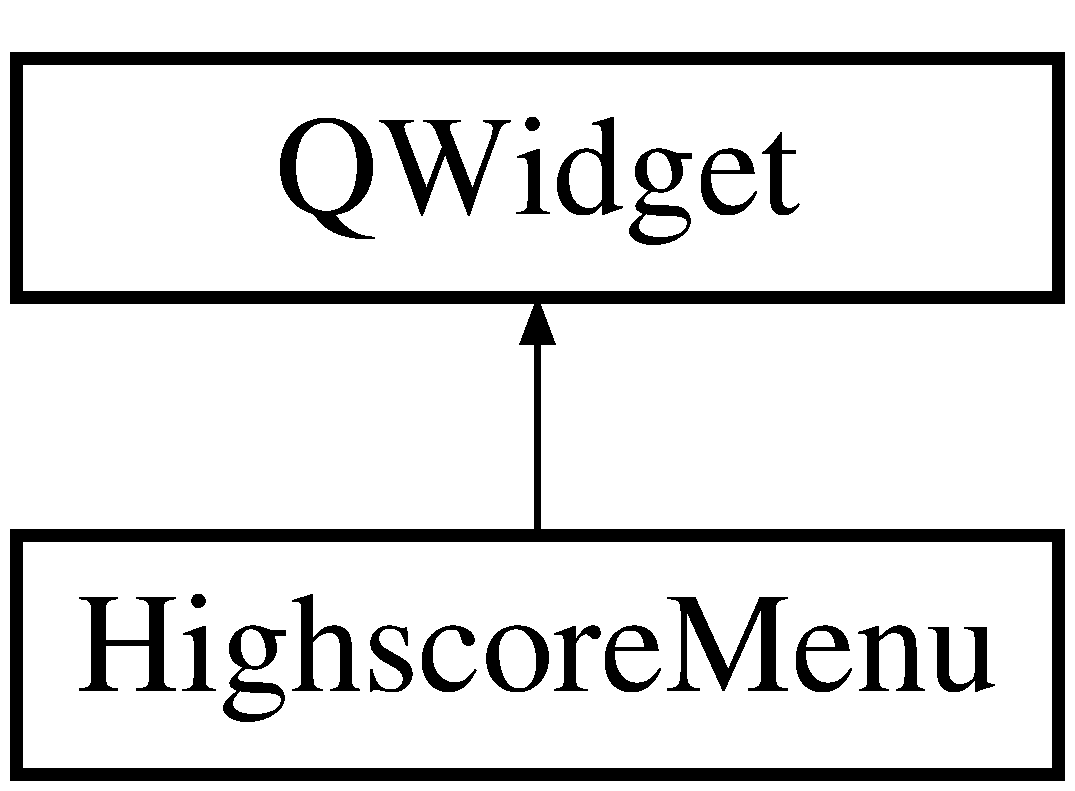
\includegraphics[height=2.000000cm]{classHighscoreMenu}
\end{center}
\end{figure}
\subsection*{Signals}
\begin{DoxyCompactItemize}
\item 
\hypertarget{classHighscoreMenu_acfc660f3078cc3e42a2b0be20f534e59}{void {\bfseries show\-Start\-Menu} ()}\label{classHighscoreMenu_acfc660f3078cc3e42a2b0be20f534e59}

\end{DoxyCompactItemize}
\subsection*{Public Member Functions}
\begin{DoxyCompactItemize}
\item 
\hypertarget{classHighscoreMenu_afffd6ba37985beae539f7d143de2201d}{{\bfseries Highscore\-Menu} (Q\-Widget $\ast$parent=0)}\label{classHighscoreMenu_afffd6ba37985beae539f7d143de2201d}

\item 
\hypertarget{classHighscoreMenu_ad71f69706ab1969e180abc4794f946c9}{void {\bfseries change\-Event} (Q\-Event $\ast$event)}\label{classHighscoreMenu_ad71f69706ab1969e180abc4794f946c9}

\end{DoxyCompactItemize}


\subsection{Detailed Description}
The \hyperlink{classHighscoreMenu}{Highscore\-Menu} class. 

\begin{DoxyAuthor}{Author}
Nils Brandt 

Alexander Luedke
\end{DoxyAuthor}
\begin{DoxyDate}{Date}
08. August 2016
\end{DoxyDate}
\begin{DoxyVersion}{Version}
1.\-0 Add Documentation 
\end{DoxyVersion}

\hypertarget{classHistoryDisplay}{\section{History\-Display Class Reference}
\label{classHistoryDisplay}\index{History\-Display@{History\-Display}}
}


The \hyperlink{classHistoryDisplay}{History\-Display} class.  




{\ttfamily \#include $<$History\-Display.\-h$>$}

Inheritance diagram for History\-Display\-:\begin{figure}[H]
\begin{center}
\leavevmode
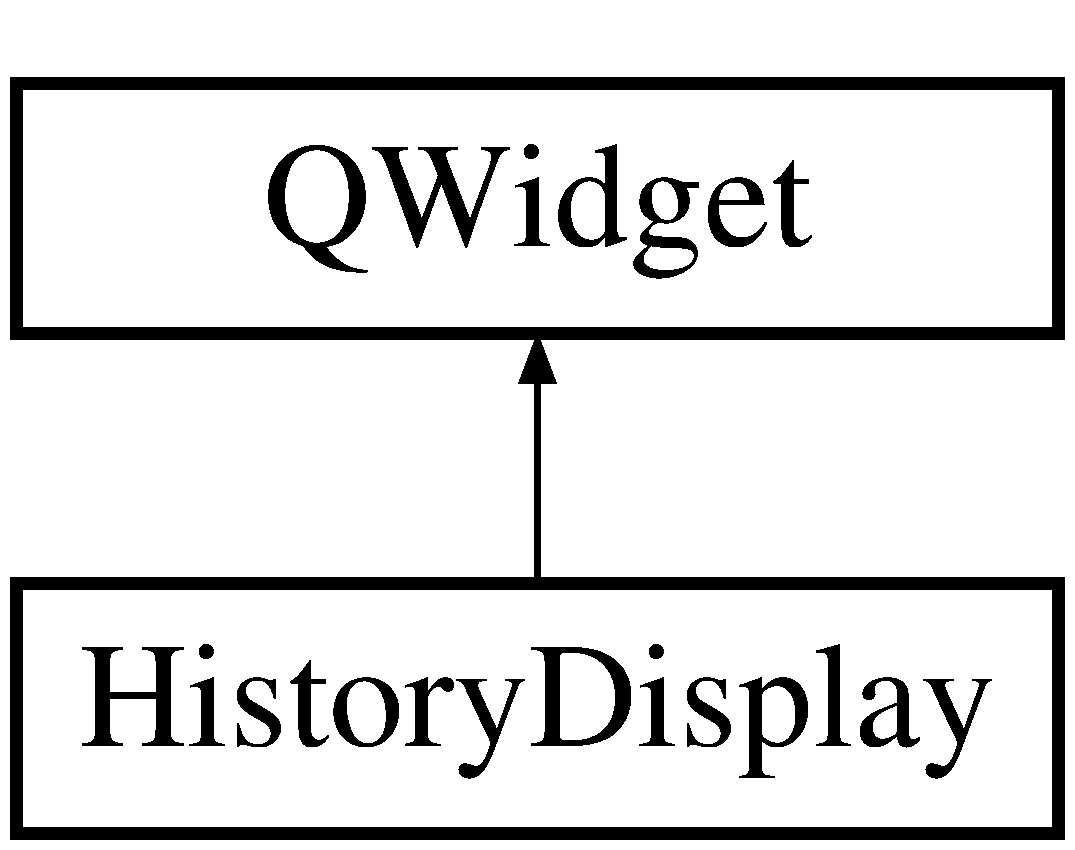
\includegraphics[height=2.000000cm]{classHistoryDisplay}
\end{center}
\end{figure}
\subsection*{Public Member Functions}
\begin{DoxyCompactItemize}
\item 
\hypertarget{classHistoryDisplay_ad4b7962e85e825f2a1e0c90cf1f8e201}{{\bfseries History\-Display} (const \hyperlink{classGameData}{Game\-Data} $\ast$data, Q\-Widget $\ast$parent=0)}\label{classHistoryDisplay_ad4b7962e85e825f2a1e0c90cf1f8e201}

\item 
\hypertarget{classHistoryDisplay_a360a99566c00c9166ad3a0552e0d801e}{void \hyperlink{classHistoryDisplay_a360a99566c00c9166ad3a0552e0d801e}{Update\-History} ()}\label{classHistoryDisplay_a360a99566c00c9166ad3a0552e0d801e}

\begin{DoxyCompactList}\small\item\em Update\-History clears display reevaluates past moves and displays new text. \end{DoxyCompactList}\item 
\hypertarget{classHistoryDisplay_ad3359c47f96baa4747bf7dde034ab222}{void \hyperlink{classHistoryDisplay_ad3359c47f96baa4747bf7dde034ab222}{Redraw\-History} ()}\label{classHistoryDisplay_ad3359c47f96baa4747bf7dde034ab222}

\begin{DoxyCompactList}\small\item\em Redraw\-History clears and redraws history. \end{DoxyCompactList}\item 
void \hyperlink{classHistoryDisplay_a260307ebdade967004f32cf48f877915}{Set\-Display\-Text} (std\-::string entry)
\begin{DoxyCompactList}\small\item\em Display\-Text Called to change the text in the Display box. \end{DoxyCompactList}\item 
\hypertarget{classHistoryDisplay_a8c548187b6eb9152655f20b4f8cae402}{void {\bfseries change\-Event} (Q\-Event $\ast$event)}\label{classHistoryDisplay_a8c548187b6eb9152655f20b4f8cae402}

\end{DoxyCompactItemize}


\subsection{Detailed Description}
The \hyperlink{classHistoryDisplay}{History\-Display} class. 

\subsection{Member Function Documentation}
\hypertarget{classHistoryDisplay_a260307ebdade967004f32cf48f877915}{\index{History\-Display@{History\-Display}!Set\-Display\-Text@{Set\-Display\-Text}}
\index{Set\-Display\-Text@{Set\-Display\-Text}!HistoryDisplay@{History\-Display}}
\subsubsection[{Set\-Display\-Text}]{\setlength{\rightskip}{0pt plus 5cm}void History\-Display\-::\-Set\-Display\-Text (
\begin{DoxyParamCaption}
\item[{std\-::string}]{entry}
\end{DoxyParamCaption}
)}}\label{classHistoryDisplay_a260307ebdade967004f32cf48f877915}


Display\-Text Called to change the text in the Display box. 


\begin{DoxyParams}{Parameters}
{\em entry} & \\
\hline
\end{DoxyParams}


The documentation for this class was generated from the following files\-:\begin{DoxyCompactItemize}
\item 
/home/alex/source\-Code/git\-Project/beleg\-Arbeit\-E\-M\-M\-S/project\-Sogo/include/gui/History\-Display.\-h\item 
/home/alex/source\-Code/git\-Project/beleg\-Arbeit\-E\-M\-M\-S/project\-Sogo/src/gui/History\-Display.\-cpp\end{DoxyCompactItemize}

\hypertarget{classHistorySave}{\section{History\-Save Class Reference}
\label{classHistorySave}\index{History\-Save@{History\-Save}}
}


The \hyperlink{classHistorySave}{History\-Save} class.  




{\ttfamily \#include $<$History\-Save.\-h$>$}

\subsection*{Public Member Functions}
\begin{DoxyCompactItemize}
\item 
\hypertarget{classHistorySave_a1f76c15dd7a3b9e27a8c66897141ee16}{\hyperlink{classHistorySave_a1f76c15dd7a3b9e27a8c66897141ee16}{History\-Save} ()}\label{classHistorySave_a1f76c15dd7a3b9e27a8c66897141ee16}

\begin{DoxyCompactList}\small\item\em \hyperlink{classHistorySave}{History\-Save}. \end{DoxyCompactList}\item 
\hyperlink{classHistorySave_ac0766707b25e837d00e6e4b48bf2860c}{History\-Save} (const \hyperlink{classHistorySave}{History\-Save} \&src)
\begin{DoxyCompactList}\small\item\em \hyperlink{classHistorySave}{History\-Save}. \end{DoxyCompactList}\item 
void \hyperlink{classHistorySave_a4d10cac993d69d8f98f9c32eb7ae4a2d}{Add\-Move} (\hyperlink{structVector3}{Vector3} pos, \hyperlink{classPlayer}{Player} player)
\begin{DoxyCompactList}\small\item\em Add\-Move. \end{DoxyCompactList}\item 
\hypertarget{classHistorySave_a4adce01fc1a4deb3a80d7ac5e3a38860}{void \hyperlink{classHistorySave_a4adce01fc1a4deb3a80d7ac5e3a38860}{Revert\-Last} ()}\label{classHistorySave_a4adce01fc1a4deb3a80d7ac5e3a38860}

\begin{DoxyCompactList}\small\item\em Revert\-Last. \end{DoxyCompactList}\item 
int \hyperlink{classHistorySave_af1f736a6ee2b72f56ac6985e788013a9}{Get\-Move\-Count} () const 
\begin{DoxyCompactList}\small\item\em Get\-Move\-Count. \end{DoxyCompactList}\item 
const Move $\ast$ \hyperlink{classHistorySave_ae04d28f2fa9c879beb2631f318526f3a}{Get\-Move} (int number) const   throw (out\-\_\-of\-\_\-range)
\begin{DoxyCompactList}\small\item\em Get\-Move. \end{DoxyCompactList}\item 
const Move $\ast$ \hyperlink{classHistorySave_ab8c21fe924b58510b9e240b5b5852be2}{Get\-Last\-Move} () const   throw (out\-\_\-of\-\_\-range)
\begin{DoxyCompactList}\small\item\em Get\-Last\-Move. \end{DoxyCompactList}\end{DoxyCompactItemize}


\subsection{Detailed Description}
The \hyperlink{classHistorySave}{History\-Save} class. 

\subsection{Constructor \& Destructor Documentation}
\hypertarget{classHistorySave_ac0766707b25e837d00e6e4b48bf2860c}{\index{History\-Save@{History\-Save}!History\-Save@{History\-Save}}
\index{History\-Save@{History\-Save}!HistorySave@{History\-Save}}
\subsubsection[{History\-Save}]{\setlength{\rightskip}{0pt plus 5cm}History\-Save\-::\-History\-Save (
\begin{DoxyParamCaption}
\item[{const {\bf History\-Save} \&}]{src}
\end{DoxyParamCaption}
)}}\label{classHistorySave_ac0766707b25e837d00e6e4b48bf2860c}


\hyperlink{classHistorySave}{History\-Save}. 


\begin{DoxyParams}{Parameters}
{\em src} & \\
\hline
\end{DoxyParams}


\subsection{Member Function Documentation}
\hypertarget{classHistorySave_a4d10cac993d69d8f98f9c32eb7ae4a2d}{\index{History\-Save@{History\-Save}!Add\-Move@{Add\-Move}}
\index{Add\-Move@{Add\-Move}!HistorySave@{History\-Save}}
\subsubsection[{Add\-Move}]{\setlength{\rightskip}{0pt plus 5cm}void History\-Save\-::\-Add\-Move (
\begin{DoxyParamCaption}
\item[{{\bf Vector3}}]{pos, }
\item[{{\bf Player}}]{player}
\end{DoxyParamCaption}
)}}\label{classHistorySave_a4d10cac993d69d8f98f9c32eb7ae4a2d}


Add\-Move. 


\begin{DoxyParams}{Parameters}
{\em pos} & \\
\hline
{\em player} & \\
\hline
\end{DoxyParams}
\hypertarget{classHistorySave_ab8c21fe924b58510b9e240b5b5852be2}{\index{History\-Save@{History\-Save}!Get\-Last\-Move@{Get\-Last\-Move}}
\index{Get\-Last\-Move@{Get\-Last\-Move}!HistorySave@{History\-Save}}
\subsubsection[{Get\-Last\-Move}]{\setlength{\rightskip}{0pt plus 5cm}const Move$\ast$ History\-Save\-::\-Get\-Last\-Move (
\begin{DoxyParamCaption}
{}
\end{DoxyParamCaption}
) const throw  out\-\_\-of\-\_\-range) \hspace{0.3cm}{\ttfamily [inline]}}}\label{classHistorySave_ab8c21fe924b58510b9e240b5b5852be2}


Get\-Last\-Move. 

\begin{DoxyReturn}{Returns}

\end{DoxyReturn}
\hypertarget{classHistorySave_ae04d28f2fa9c879beb2631f318526f3a}{\index{History\-Save@{History\-Save}!Get\-Move@{Get\-Move}}
\index{Get\-Move@{Get\-Move}!HistorySave@{History\-Save}}
\subsubsection[{Get\-Move}]{\setlength{\rightskip}{0pt plus 5cm}const Move$\ast$ History\-Save\-::\-Get\-Move (
\begin{DoxyParamCaption}
\item[{int}]{number}
\end{DoxyParamCaption}
) const throw  out\-\_\-of\-\_\-range) \hspace{0.3cm}{\ttfamily [inline]}}}\label{classHistorySave_ae04d28f2fa9c879beb2631f318526f3a}


Get\-Move. 


\begin{DoxyParams}{Parameters}
{\em number} & \\
\hline
\end{DoxyParams}
\begin{DoxyReturn}{Returns}

\end{DoxyReturn}
\hypertarget{classHistorySave_af1f736a6ee2b72f56ac6985e788013a9}{\index{History\-Save@{History\-Save}!Get\-Move\-Count@{Get\-Move\-Count}}
\index{Get\-Move\-Count@{Get\-Move\-Count}!HistorySave@{History\-Save}}
\subsubsection[{Get\-Move\-Count}]{\setlength{\rightskip}{0pt plus 5cm}int History\-Save\-::\-Get\-Move\-Count (
\begin{DoxyParamCaption}
{}
\end{DoxyParamCaption}
) const\hspace{0.3cm}{\ttfamily [inline]}}}\label{classHistorySave_af1f736a6ee2b72f56ac6985e788013a9}


Get\-Move\-Count. 

\begin{DoxyReturn}{Returns}

\end{DoxyReturn}


The documentation for this class was generated from the following files\-:\begin{DoxyCompactItemize}
\item 
/home/alex/source\-Code/git\-Project/beleg\-Arbeit\-E\-M\-M\-S/project\-Sogo/include/core/History\-Save.\-h\item 
/home/alex/source\-Code/git\-Project/beleg\-Arbeit\-E\-M\-M\-S/project\-Sogo/src/core/History\-Save.\-cpp\end{DoxyCompactItemize}

\hypertarget{structglm_1_1detail_1_1ieee754__QNAN_1_1i}{\section{glm\-:\-:detail\-:\-:ieee754\-\_\-\-Q\-N\-A\-N\-:\-:i Struct Reference}
\label{structglm_1_1detail_1_1ieee754__QNAN_1_1i}\index{glm\-::detail\-::ieee754\-\_\-\-Q\-N\-A\-N\-::i@{glm\-::detail\-::ieee754\-\_\-\-Q\-N\-A\-N\-::i}}
}
\subsection*{Public Attributes}
\begin{DoxyCompactItemize}
\item 
\hypertarget{structglm_1_1detail_1_1ieee754__QNAN_1_1i_a1999926defcba631a716bee7d3044d0a}{const unsigned int {\bfseries mantissa}\-:23}\label{structglm_1_1detail_1_1ieee754__QNAN_1_1i_a1999926defcba631a716bee7d3044d0a}

\item 
\hypertarget{structglm_1_1detail_1_1ieee754__QNAN_1_1i_abc8cdb38ff3aa6a09214f7bfa32efac8}{const unsigned int {\bfseries exp}\-:8}\label{structglm_1_1detail_1_1ieee754__QNAN_1_1i_abc8cdb38ff3aa6a09214f7bfa32efac8}

\item 
\hypertarget{structglm_1_1detail_1_1ieee754__QNAN_1_1i_a5dd7e174864b6a8cd045563dde44f305}{const unsigned int {\bfseries sign}\-:1}\label{structglm_1_1detail_1_1ieee754__QNAN_1_1i_a5dd7e174864b6a8cd045563dde44f305}

\end{DoxyCompactItemize}


The documentation for this struct was generated from the following file\-:\begin{DoxyCompactItemize}
\item 
/home/alex/source\-Code/git\-Project/beleg\-Arbeit\-E\-M\-M\-S/project\-Sogo/external/glm-\/0.\-9.\-4.\-0/glm/core/\hyperlink{intrinsic__common_8inl}{intrinsic\-\_\-common.\-inl}\end{DoxyCompactItemize}

\hypertarget{unionglm_1_1detail_1_1ieee754__QNAN}{\section{glm\-:\-:detail\-:\-:ieee754\-\_\-\-Q\-N\-A\-N Union Reference}
\label{unionglm_1_1detail_1_1ieee754__QNAN}\index{glm\-::detail\-::ieee754\-\_\-\-Q\-N\-A\-N@{glm\-::detail\-::ieee754\-\_\-\-Q\-N\-A\-N}}
}
\subsection*{Classes}
\begin{DoxyCompactItemize}
\item 
struct \hyperlink{structglm_1_1detail_1_1ieee754__QNAN_1_1i}{i}
\end{DoxyCompactItemize}
\subsection*{Public Attributes}
\begin{DoxyCompactItemize}
\item 
\hypertarget{unionglm_1_1detail_1_1ieee754__QNAN_ac5f04f4e605e4d08ddc2bacddf7eee65}{const float {\bfseries f}}\label{unionglm_1_1detail_1_1ieee754__QNAN_ac5f04f4e605e4d08ddc2bacddf7eee65}

\end{DoxyCompactItemize}


The documentation for this union was generated from the following file\-:\begin{DoxyCompactItemize}
\item 
/home/alex/source\-Code/git\-Project/beleg\-Arbeit\-E\-M\-M\-S/project\-Sogo/external/glm-\/0.\-9.\-4.\-0/glm/core/\hyperlink{intrinsic__common_8inl}{intrinsic\-\_\-common.\-inl}\end{DoxyCompactItemize}

\hypertarget{unionieee__double__shape__type}{\section{ieee\-\_\-double\-\_\-shape\-\_\-type Union Reference}
\label{unionieee__double__shape__type}\index{ieee\-\_\-double\-\_\-shape\-\_\-type@{ieee\-\_\-double\-\_\-shape\-\_\-type}}
}
\subsection*{Public Attributes}
\begin{DoxyCompactItemize}
\item 
\hypertarget{unionieee__double__shape__type_a2d9c4cab9e3fa74e4be6d72f798a145b}{double {\bfseries value}}\label{unionieee__double__shape__type_a2d9c4cab9e3fa74e4be6d72f798a145b}

\item 
\hypertarget{unionieee__double__shape__type_ae25b7d1505b3c81e08728f93973026bd}{\begin{tabbing}
xx\=xx\=xx\=xx\=xx\=xx\=xx\=xx\=xx\=\kill
struct \{\\
\hypertarget{structieee__double__shape__type_1_1@13_a15dfdc2d74a323f6638204624834f101}{\>glm::detail::int32 {\bfseries lsw}\\
\hypertarget{structieee__double__shape__type_1_1@13_aea1156759f6afd58a56a7b4e7bfcee01}{\>glm::detail::int32 {\bfseries msw}\\
\} {\bfseries parts}}\label{unionieee__double__shape__type_ae25b7d1505b3c81e08728f93973026bd}
\\

\end{tabbing}\end{DoxyCompactItemize}


The documentation for this union was generated from the following file\-:\begin{DoxyCompactItemize}
\item 
/home/alex/source\-Code/git\-Project/beleg\-Arbeit\-E\-M\-M\-S/project\-Sogo/external/glm-\/0.\-9.\-4.\-0/glm/gtc/\hyperlink{ulp_8inl}{ulp.\-inl}\end{DoxyCompactItemize}

\hypertarget{unionieee__float__shape__type}{\section{ieee\-\_\-float\-\_\-shape\-\_\-type Union Reference}
\label{unionieee__float__shape__type}\index{ieee\-\_\-float\-\_\-shape\-\_\-type@{ieee\-\_\-float\-\_\-shape\-\_\-type}}
}
\subsection*{Public Attributes}
\begin{DoxyCompactItemize}
\item 
\hypertarget{unionieee__float__shape__type_aa0c47451f1b974421cbb9e2833ddb68e}{float {\bfseries value}}\label{unionieee__float__shape__type_aa0c47451f1b974421cbb9e2833ddb68e}

\item 
\hypertarget{unionieee__float__shape__type_a49230c21acd672d044f38b1abcbd6071}{unsigned int {\bfseries word}}\label{unionieee__float__shape__type_a49230c21acd672d044f38b1abcbd6071}

\end{DoxyCompactItemize}


The documentation for this union was generated from the following file\-:\begin{DoxyCompactItemize}
\item 
/home/alex/source\-Code/git\-Project/beleg\-Arbeit\-E\-M\-M\-S/project\-Sogo/external/glm-\/0.\-9.\-4.\-0/glm/gtc/\hyperlink{ulp_8inl}{ulp.\-inl}\end{DoxyCompactItemize}

\hypertarget{structglm_1_1detail_1_1If}{\section{glm\-:\-:detail\-:\-:If$<$ C $>$ Struct Template Reference}
\label{structglm_1_1detail_1_1If}\index{glm\-::detail\-::\-If$<$ C $>$@{glm\-::detail\-::\-If$<$ C $>$}}
}
\subsection*{Static Public Member Functions}
\begin{DoxyCompactItemize}
\item 
\hypertarget{structglm_1_1detail_1_1If_ab66c77bac87f7ffe4aa6bb761b165746}{{\footnotesize template$<$typename F , typename T $>$ }\\static G\-L\-M\-\_\-\-F\-U\-N\-C\-\_\-\-Q\-U\-A\-L\-I\-F\-I\-E\-R T {\bfseries apply} (F functor, const T \&val)}\label{structglm_1_1detail_1_1If_ab66c77bac87f7ffe4aa6bb761b165746}

\end{DoxyCompactItemize}


The documentation for this struct was generated from the following file\-:\begin{DoxyCompactItemize}
\item 
/home/alex/source\-Code/git\-Project/beleg\-Arbeit\-E\-M\-M\-S/project\-Sogo/external/glm-\/0.\-9.\-4.\-0/glm/core/\hyperlink{__detail_8hpp}{\-\_\-detail.\-hpp}\end{DoxyCompactItemize}

\hypertarget{structglm_1_1detail_1_1If_3_01false_01_4}{\section{glm\-:\-:detail\-:\-:If$<$ false $>$ Struct Template Reference}
\label{structglm_1_1detail_1_1If_3_01false_01_4}\index{glm\-::detail\-::\-If$<$ false $>$@{glm\-::detail\-::\-If$<$ false $>$}}
}
\subsection*{Static Public Member Functions}
\begin{DoxyCompactItemize}
\item 
\hypertarget{structglm_1_1detail_1_1If_3_01false_01_4_a31a9409e47dc11cb7d4251c12342b9f6}{{\footnotesize template$<$typename F , typename T $>$ }\\static G\-L\-M\-\_\-\-F\-U\-N\-C\-\_\-\-Q\-U\-A\-L\-I\-F\-I\-E\-R T {\bfseries apply} (F, const T \&val)}\label{structglm_1_1detail_1_1If_3_01false_01_4_a31a9409e47dc11cb7d4251c12342b9f6}

\end{DoxyCompactItemize}


The documentation for this struct was generated from the following file\-:\begin{DoxyCompactItemize}
\item 
/home/alex/source\-Code/git\-Project/beleg\-Arbeit\-E\-M\-M\-S/project\-Sogo/external/glm-\/0.\-9.\-4.\-0/glm/core/\hyperlink{__detail_8hpp}{\-\_\-detail.\-hpp}\end{DoxyCompactItemize}

\hypertarget{classIObserver}{\section{I\-Observer Class Reference}
\label{classIObserver}\index{I\-Observer@{I\-Observer}}
}


The \hyperlink{classIObserver}{I\-Observer} interface Defines a interface of a Observer which can be Notified Is closely related to the abstract \hyperlink{classSubject}{Subject} class.  




{\ttfamily \#include $<$I\-Observer.\-h$>$}

\subsection*{Public Member Functions}
\begin{DoxyCompactItemize}
\item 
\hypertarget{classIObserver_a7e478961d27e1c605699e2b32fbdc29b}{\hyperlink{classIObserver_a7e478961d27e1c605699e2b32fbdc29b}{I\-Observer} ()}\label{classIObserver_a7e478961d27e1c605699e2b32fbdc29b}

\begin{DoxyCompactList}\small\item\em \hyperlink{classIObserver}{I\-Observer}. \end{DoxyCompactList}\item 
\hypertarget{classIObserver_afdfe9e2ebd9aa794142968de574daa9a}{virtual \hyperlink{classIObserver_afdfe9e2ebd9aa794142968de574daa9a}{$\sim$\-I\-Observer} ()}\label{classIObserver_afdfe9e2ebd9aa794142968de574daa9a}

\begin{DoxyCompactList}\small\item\em $\sim$\-I\-Observer \end{DoxyCompactList}\item 
\hypertarget{classIObserver_ad46021c61f1fa2126078f33783adc727}{virtual void \hyperlink{classIObserver_ad46021c61f1fa2126078f33783adc727}{Notify} ()=0}\label{classIObserver_ad46021c61f1fa2126078f33783adc727}

\begin{DoxyCompactList}\small\item\em Is called to Notify Observer. \end{DoxyCompactList}\end{DoxyCompactItemize}


\subsection{Detailed Description}
The \hyperlink{classIObserver}{I\-Observer} interface Defines a interface of a Observer which can be Notified Is closely related to the abstract \hyperlink{classSubject}{Subject} class. 

The documentation for this class was generated from the following file\-:\begin{DoxyCompactItemize}
\item 
/home/alex/source\-Code/git\-Project/beleg\-Arbeit\-E\-M\-M\-S/project\-Sogo/include/I\-Observer.\-h\end{DoxyCompactItemize}

\hypertarget{structglm_1_1detail_1_1is__bool}{\section{glm\-:\-:detail\-:\-:is\-\_\-bool$<$ T $>$ Struct Template Reference}
\label{structglm_1_1detail_1_1is__bool}\index{glm\-::detail\-::is\-\_\-bool$<$ T $>$@{glm\-::detail\-::is\-\_\-bool$<$ T $>$}}
}
\subsection*{Public Types}
\begin{DoxyCompactItemize}
\item 
enum {\bfseries is\-\_\-bool\-\_\-enum} \{ {\bfseries \-\_\-\-Y\-E\-S} = 0, 
{\bfseries \-\_\-\-N\-O} = 1
 \}
\end{DoxyCompactItemize}


The documentation for this struct was generated from the following file\-:\begin{DoxyCompactItemize}
\item 
/home/alex/source\-Code/git\-Project/beleg\-Arbeit\-E\-M\-M\-S/project\-Sogo/external/glm-\/0.\-9.\-4.\-0/glm/core/\hyperlink{__detail_8hpp}{\-\_\-detail.\-hpp}\end{DoxyCompactItemize}

\hypertarget{structglm_1_1detail_1_1is__bool_3_01bool_01_4}{\section{glm\-:\-:detail\-:\-:is\-\_\-bool$<$ bool $>$ Struct Template Reference}
\label{structglm_1_1detail_1_1is__bool_3_01bool_01_4}\index{glm\-::detail\-::is\-\_\-bool$<$ bool $>$@{glm\-::detail\-::is\-\_\-bool$<$ bool $>$}}
}
\subsection*{Public Types}
\begin{DoxyCompactItemize}
\item 
enum {\bfseries is\-\_\-bool\-\_\-enum} \{ {\bfseries \-\_\-\-Y\-E\-S} = 1, 
{\bfseries \-\_\-\-N\-O} = 0
 \}
\end{DoxyCompactItemize}


The documentation for this struct was generated from the following file\-:\begin{DoxyCompactItemize}
\item 
/home/alex/source\-Code/git\-Project/beleg\-Arbeit\-E\-M\-M\-S/project\-Sogo/external/glm-\/0.\-9.\-4.\-0/glm/core/\hyperlink{__detail_8hpp}{\-\_\-detail.\-hpp}\end{DoxyCompactItemize}

\hypertarget{structglm_1_1detail_1_1is__float}{\section{glm\-:\-:detail\-:\-:is\-\_\-float$<$ T $>$ Struct Template Reference}
\label{structglm_1_1detail_1_1is__float}\index{glm\-::detail\-::is\-\_\-float$<$ T $>$@{glm\-::detail\-::is\-\_\-float$<$ T $>$}}
}
\subsection*{Public Types}
\begin{DoxyCompactItemize}
\item 
enum {\bfseries is\-\_\-float\-\_\-enum} \{ {\bfseries \-\_\-\-Y\-E\-S} = 0, 
{\bfseries \-\_\-\-N\-O} = 1
 \}
\end{DoxyCompactItemize}


The documentation for this struct was generated from the following file\-:\begin{DoxyCompactItemize}
\item 
/home/alex/source\-Code/git\-Project/beleg\-Arbeit\-E\-M\-M\-S/project\-Sogo/external/glm-\/0.\-9.\-4.\-0/glm/core/\hyperlink{__detail_8hpp}{\-\_\-detail.\-hpp}\end{DoxyCompactItemize}

\hypertarget{structglm_1_1detail_1_1is__int}{\section{glm\-:\-:detail\-:\-:is\-\_\-int$<$ T $>$ Struct Template Reference}
\label{structglm_1_1detail_1_1is__int}\index{glm\-::detail\-::is\-\_\-int$<$ T $>$@{glm\-::detail\-::is\-\_\-int$<$ T $>$}}
}
\subsection*{Public Types}
\begin{DoxyCompactItemize}
\item 
enum {\bfseries is\-\_\-int\-\_\-enum} \{ {\bfseries \-\_\-\-Y\-E\-S} = 0, 
{\bfseries \-\_\-\-N\-O} = 1
 \}
\end{DoxyCompactItemize}


The documentation for this struct was generated from the following file\-:\begin{DoxyCompactItemize}
\item 
/home/alex/source\-Code/git\-Project/beleg\-Arbeit\-E\-M\-M\-S/project\-Sogo/external/glm-\/0.\-9.\-4.\-0/glm/core/\hyperlink{__detail_8hpp}{\-\_\-detail.\-hpp}\end{DoxyCompactItemize}

\hypertarget{structglm_1_1detail_1_1is__matrix}{\section{glm\-:\-:detail\-:\-:is\-\_\-matrix$<$ T $>$ Struct Template Reference}
\label{structglm_1_1detail_1_1is__matrix}\index{glm\-::detail\-::is\-\_\-matrix$<$ T $>$@{glm\-::detail\-::is\-\_\-matrix$<$ T $>$}}
}
\subsection*{Public Types}
\begin{DoxyCompactItemize}
\item 
enum {\bfseries is\-\_\-matrix\-\_\-enum} \{ {\bfseries \-\_\-\-Y\-E\-S} = 0, 
{\bfseries \-\_\-\-N\-O} = 1
 \}
\end{DoxyCompactItemize}


The documentation for this struct was generated from the following file\-:\begin{DoxyCompactItemize}
\item 
/home/alex/source\-Code/git\-Project/beleg\-Arbeit\-E\-M\-M\-S/project\-Sogo/external/glm-\/0.\-9.\-4.\-0/glm/core/\hyperlink{__detail_8hpp}{\-\_\-detail.\-hpp}\end{DoxyCompactItemize}

\hypertarget{structglm_1_1detail_1_1is__uint}{\section{glm\-:\-:detail\-:\-:is\-\_\-uint$<$ T $>$ Struct Template Reference}
\label{structglm_1_1detail_1_1is__uint}\index{glm\-::detail\-::is\-\_\-uint$<$ T $>$@{glm\-::detail\-::is\-\_\-uint$<$ T $>$}}
}
\subsection*{Public Types}
\begin{DoxyCompactItemize}
\item 
enum {\bfseries is\-\_\-uint\-\_\-enum} \{ {\bfseries \-\_\-\-Y\-E\-S} = 0, 
{\bfseries \-\_\-\-N\-O} = 1
 \}
\end{DoxyCompactItemize}


The documentation for this struct was generated from the following file\-:\begin{DoxyCompactItemize}
\item 
/home/alex/source\-Code/git\-Project/beleg\-Arbeit\-E\-M\-M\-S/project\-Sogo/external/glm-\/0.\-9.\-4.\-0/glm/core/\hyperlink{__detail_8hpp}{\-\_\-detail.\-hpp}\end{DoxyCompactItemize}

\hypertarget{structglm_1_1detail_1_1is__vector}{\section{glm\-:\-:detail\-:\-:is\-\_\-vector$<$ T $>$ Struct Template Reference}
\label{structglm_1_1detail_1_1is__vector}\index{glm\-::detail\-::is\-\_\-vector$<$ T $>$@{glm\-::detail\-::is\-\_\-vector$<$ T $>$}}
}
\subsection*{Public Types}
\begin{DoxyCompactItemize}
\item 
enum {\bfseries is\-\_\-vector\-\_\-enum} \{ {\bfseries \-\_\-\-Y\-E\-S} = 0, 
{\bfseries \-\_\-\-N\-O} = 1
 \}
\end{DoxyCompactItemize}


The documentation for this struct was generated from the following file\-:\begin{DoxyCompactItemize}
\item 
/home/alex/source\-Code/git\-Project/beleg\-Arbeit\-E\-M\-M\-S/project\-Sogo/external/glm-\/0.\-9.\-4.\-0/glm/core/\hyperlink{__detail_8hpp}{\-\_\-detail.\-hpp}\end{DoxyCompactItemize}

\hypertarget{classLogger}{\section{Logger Class Reference}
\label{classLogger}\index{Logger@{Logger}}
}


The \hyperlink{classLogger}{Logger} class.  




{\ttfamily \#include $<$Logger.\-h$>$}

\subsection*{Public Member Functions}
\begin{DoxyCompactItemize}
\item 
void \hyperlink{classLogger_a827cabc79ba0d1b654ad3f03058dfba2}{Log\-Info} (std\-::string message)
\begin{DoxyCompactList}\small\item\em Log\-Info Marks the message by adding \char`\"{}\-I\-N\-F\-O\char`\"{} in the beginning and logs it. \end{DoxyCompactList}\item 
void \hyperlink{classLogger_aa9c4ebaf5082990fa24afc105522a5a5}{Log\-Info} (std\-::string message, std\-::string file, int line)
\begin{DoxyCompactList}\small\item\em Log\-Info Marks the message by adding \char`\"{}\-I\-N\-F\-O\char`\"{} in the beginning and logs it. \end{DoxyCompactList}\item 
void \hyperlink{classLogger_abb89d37b3a3cbdef1f59273e498f9775}{Log\-Error} (std\-::string message)
\begin{DoxyCompactList}\small\item\em Log\-Error Marks the message by adding \char`\"{}\-E\-R\-R\-O\-R\char`\"{} in the beginning and logs it. \end{DoxyCompactList}\item 
void \hyperlink{classLogger_afc03fb34e6b57f2ec3955da71a6f1fe7}{Log\-Error} (std\-::string message, std\-::string file, int line)
\begin{DoxyCompactList}\small\item\em Log\-Error Marks the message by adding \char`\"{}\-E\-R\-R\-O\-R\char`\"{} in the beginning and logs it. \end{DoxyCompactList}\item 
void \hyperlink{classLogger_a022af6a50c02c7cd77f39b6a10a80dc4}{Log\-Path} (int line, std\-::string filepath)
\begin{DoxyCompactList}\small\item\em Log\-Path Display the line and the filepath Example in file\-: L\-O\-G\-P\-A\-T\-H();. \end{DoxyCompactList}\item 
void \hyperlink{classLogger_af421b39d03b598ff3fe257d7859a1edd}{Log\-Path} (int line, std\-::string filepath, std\-::string msg)
\begin{DoxyCompactList}\small\item\em Log\-Path Display the line, filepath and a message Example in file\-: L\-O\-G(\char`\"{}msg\char`\"{});. \end{DoxyCompactList}\end{DoxyCompactItemize}
\subsection*{Static Public Member Functions}
\begin{DoxyCompactItemize}
\item 
\hypertarget{classLogger_aae8c9845cd162c68a389ad3221ab7341}{static \hyperlink{classLogger}{Logger} $\ast$ {\bfseries Get\-Logger\-Intance} ()}\label{classLogger_aae8c9845cd162c68a389ad3221ab7341}

\end{DoxyCompactItemize}


\subsection{Detailed Description}
The \hyperlink{classLogger}{Logger} class. 

\hyperlink{classLogger}{Logger} singleton class use to log errors and info texts

\begin{DoxyAuthor}{Author}
Nils Brandt
\end{DoxyAuthor}
\begin{DoxyDate}{Date}
08. August 2016
\end{DoxyDate}
\begin{DoxyVersion}{Version}
1.\-0 Add Documentation 
\end{DoxyVersion}


\subsection{Member Function Documentation}
\hypertarget{classLogger_abb89d37b3a3cbdef1f59273e498f9775}{\index{Logger@{Logger}!Log\-Error@{Log\-Error}}
\index{Log\-Error@{Log\-Error}!Logger@{Logger}}
\subsubsection[{Log\-Error}]{\setlength{\rightskip}{0pt plus 5cm}void Logger\-::\-Log\-Error (
\begin{DoxyParamCaption}
\item[{std\-::string}]{message}
\end{DoxyParamCaption}
)}}\label{classLogger_abb89d37b3a3cbdef1f59273e498f9775}


Log\-Error Marks the message by adding \char`\"{}\-E\-R\-R\-O\-R\char`\"{} in the beginning and logs it. 


\begin{DoxyParams}{Parameters}
{\em message} & \\
\hline
\end{DoxyParams}
\hypertarget{classLogger_afc03fb34e6b57f2ec3955da71a6f1fe7}{\index{Logger@{Logger}!Log\-Error@{Log\-Error}}
\index{Log\-Error@{Log\-Error}!Logger@{Logger}}
\subsubsection[{Log\-Error}]{\setlength{\rightskip}{0pt plus 5cm}void Logger\-::\-Log\-Error (
\begin{DoxyParamCaption}
\item[{std\-::string}]{message, }
\item[{std\-::string}]{file, }
\item[{int}]{line}
\end{DoxyParamCaption}
)}}\label{classLogger_afc03fb34e6b57f2ec3955da71a6f1fe7}


Log\-Error Marks the message by adding \char`\"{}\-E\-R\-R\-O\-R\char`\"{} in the beginning and logs it. 


\begin{DoxyParams}{Parameters}
{\em message} & \\
\hline
\end{DoxyParams}
\hypertarget{classLogger_a827cabc79ba0d1b654ad3f03058dfba2}{\index{Logger@{Logger}!Log\-Info@{Log\-Info}}
\index{Log\-Info@{Log\-Info}!Logger@{Logger}}
\subsubsection[{Log\-Info}]{\setlength{\rightskip}{0pt plus 5cm}void Logger\-::\-Log\-Info (
\begin{DoxyParamCaption}
\item[{std\-::string}]{message}
\end{DoxyParamCaption}
)}}\label{classLogger_a827cabc79ba0d1b654ad3f03058dfba2}


Log\-Info Marks the message by adding \char`\"{}\-I\-N\-F\-O\char`\"{} in the beginning and logs it. 


\begin{DoxyParams}{Parameters}
{\em message} & \\
\hline
\end{DoxyParams}
\hypertarget{classLogger_aa9c4ebaf5082990fa24afc105522a5a5}{\index{Logger@{Logger}!Log\-Info@{Log\-Info}}
\index{Log\-Info@{Log\-Info}!Logger@{Logger}}
\subsubsection[{Log\-Info}]{\setlength{\rightskip}{0pt plus 5cm}void Logger\-::\-Log\-Info (
\begin{DoxyParamCaption}
\item[{std\-::string}]{message, }
\item[{std\-::string}]{file, }
\item[{int}]{line}
\end{DoxyParamCaption}
)}}\label{classLogger_aa9c4ebaf5082990fa24afc105522a5a5}


Log\-Info Marks the message by adding \char`\"{}\-I\-N\-F\-O\char`\"{} in the beginning and logs it. 


\begin{DoxyParams}{Parameters}
{\em message} & \\
\hline
\end{DoxyParams}
\hypertarget{classLogger_a022af6a50c02c7cd77f39b6a10a80dc4}{\index{Logger@{Logger}!Log\-Path@{Log\-Path}}
\index{Log\-Path@{Log\-Path}!Logger@{Logger}}
\subsubsection[{Log\-Path}]{\setlength{\rightskip}{0pt plus 5cm}void Logger\-::\-Log\-Path (
\begin{DoxyParamCaption}
\item[{int}]{line, }
\item[{std\-::string}]{filepath}
\end{DoxyParamCaption}
)}}\label{classLogger_a022af6a50c02c7cd77f39b6a10a80dc4}


Log\-Path Display the line and the filepath Example in file\-: L\-O\-G\-P\-A\-T\-H();. 


\begin{DoxyParams}{Parameters}
{\em line} & \\
\hline
{\em filepath} & \\
\hline
\end{DoxyParams}
\hypertarget{classLogger_af421b39d03b598ff3fe257d7859a1edd}{\index{Logger@{Logger}!Log\-Path@{Log\-Path}}
\index{Log\-Path@{Log\-Path}!Logger@{Logger}}
\subsubsection[{Log\-Path}]{\setlength{\rightskip}{0pt plus 5cm}void Logger\-::\-Log\-Path (
\begin{DoxyParamCaption}
\item[{int}]{line, }
\item[{std\-::string}]{filepath, }
\item[{std\-::string}]{msg}
\end{DoxyParamCaption}
)}}\label{classLogger_af421b39d03b598ff3fe257d7859a1edd}


Log\-Path Display the line, filepath and a message Example in file\-: L\-O\-G(\char`\"{}msg\char`\"{});. 


\begin{DoxyParams}{Parameters}
{\em line} & \\
\hline
{\em filepath} & \\
\hline
{\em msg} & \\
\hline
\end{DoxyParams}

\hypertarget{classMainWindow}{\section{Main\-Window Class Reference}
\label{classMainWindow}\index{Main\-Window@{Main\-Window}}
}


The \hyperlink{classMainWindow}{Main\-Window} class.  




{\ttfamily \#include $<$mainwindow.\-h$>$}

Inheritance diagram for Main\-Window\-:\begin{figure}[H]
\begin{center}
\leavevmode
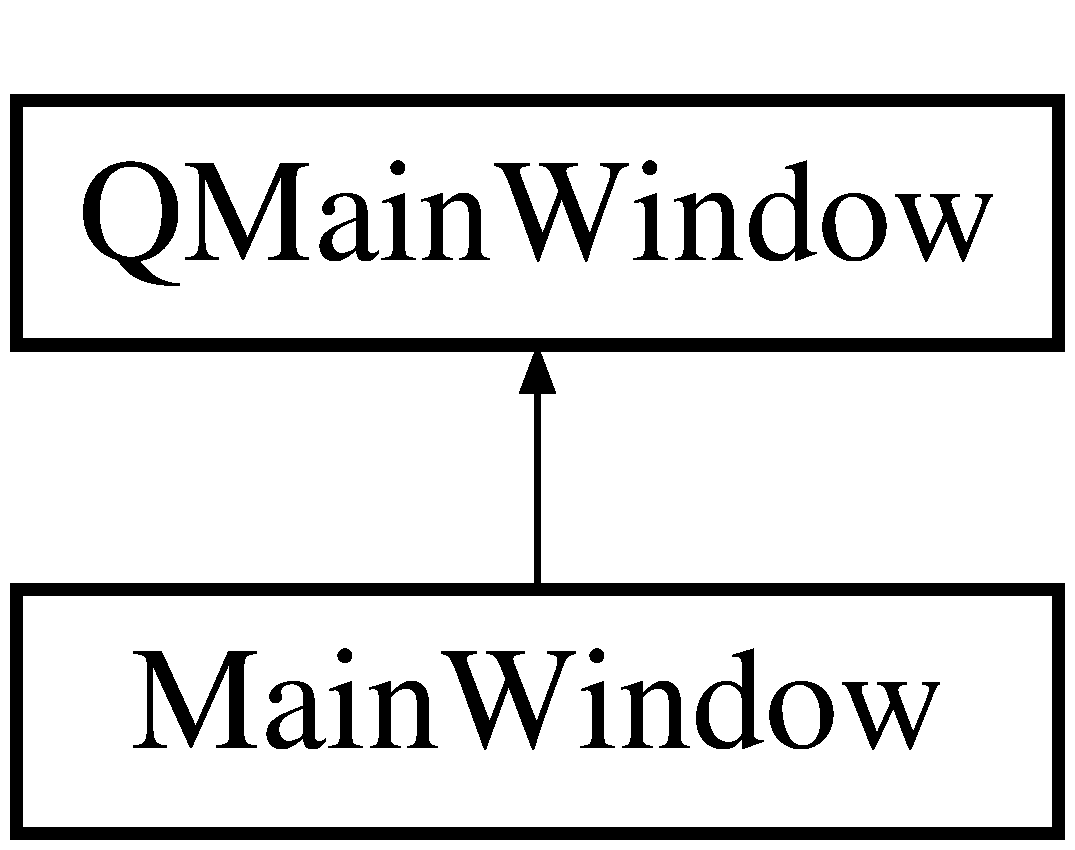
\includegraphics[height=2.000000cm]{classMainWindow}
\end{center}
\end{figure}
\subsection*{Signals}
\begin{DoxyCompactItemize}
\item 
\hypertarget{classMainWindow_a9707f0cc964479508e125742fcf94f82}{void {\bfseries Quit\-Main\-Window} ()}\label{classMainWindow_a9707f0cc964479508e125742fcf94f82}

\end{DoxyCompactItemize}
\subsection*{Public Member Functions}
\begin{DoxyCompactItemize}
\item 
\hypertarget{classMainWindow_a8b244be8b7b7db1b08de2a2acb9409db}{{\bfseries Main\-Window} (Q\-Widget $\ast$parent=0)}\label{classMainWindow_a8b244be8b7b7db1b08de2a2acb9409db}

\item 
\hypertarget{classMainWindow_a7d24542d1fbdffd9537ceb421353c860}{{\bfseries Main\-Window} (Q\-Translator $\ast$translator, Q\-Widget $\ast$parent=0)}\label{classMainWindow_a7d24542d1fbdffd9537ceb421353c860}

\item 
\hypertarget{classMainWindow_aaedb921530e29c02b7746ae62ce62ddf}{\hyperlink{classGameView}{Game\-View} $\ast$ {\bfseries Get\-Game\-View} () const }\label{classMainWindow_aaedb921530e29c02b7746ae62ce62ddf}

\item 
\hypertarget{classMainWindow_a8c6fb0a68de0e1af14efba33f90d6eae}{void \hyperlink{classMainWindow_a8c6fb0a68de0e1af14efba33f90d6eae}{Show\-Game\-View} ()}\label{classMainWindow_a8c6fb0a68de0e1af14efba33f90d6eae}

\begin{DoxyCompactList}\small\item\em Show\-Game\-View. \end{DoxyCompactList}\item 
\hypertarget{classMainWindow_ad1f9c6b77e288f15777f03d53244a9c2}{void \hyperlink{classMainWindow_ad1f9c6b77e288f15777f03d53244a9c2}{Show\-Pause\-Menu} ()}\label{classMainWindow_ad1f9c6b77e288f15777f03d53244a9c2}

\begin{DoxyCompactList}\small\item\em Show\-Pause\-Menu. \end{DoxyCompactList}\item 
\hypertarget{classMainWindow_a9069444f88de1d1b55eadd1eb7a65f2a}{void {\bfseries Change\-Language} ()}\label{classMainWindow_a9069444f88de1d1b55eadd1eb7a65f2a}

\item 
\hypertarget{classMainWindow_ac7c881667b4ba4986b5a0030452ee3f0}{void {\bfseries change\-Event} (Q\-Event $\ast$event)}\label{classMainWindow_ac7c881667b4ba4986b5a0030452ee3f0}

\item 
\hypertarget{classMainWindow_ac63b1d94f5cb0ad40b6ce651c8786b18}{void {\bfseries show\-New\-Session\-Menu} ()}\label{classMainWindow_ac63b1d94f5cb0ad40b6ce651c8786b18}

\item 
\hypertarget{classMainWindow_a63f8a7b5189797e75f175da1949a1e76}{void {\bfseries show\-Start\-Menu} ()}\label{classMainWindow_a63f8a7b5189797e75f175da1949a1e76}

\item 
\hypertarget{classMainWindow_a7d14a8a706385f2596c38b3e7c8d8fb0}{void {\bfseries show\-Highscore\-Menu} ()}\label{classMainWindow_a7d14a8a706385f2596c38b3e7c8d8fb0}

\item 
\hypertarget{classMainWindow_a4195422fe1346c1aa9c640715dfe73cb}{void {\bfseries start\-New\-Game} ()}\label{classMainWindow_a4195422fe1346c1aa9c640715dfe73cb}

\end{DoxyCompactItemize}


\subsection{Detailed Description}
The \hyperlink{classMainWindow}{Main\-Window} class. 

The content of the Sogo-\/\-App.

\begin{DoxyAuthor}{Author}
Nils Brandt 

Alexander Luedke
\end{DoxyAuthor}
\begin{DoxyDate}{Date}
08. August 2016
\end{DoxyDate}
\begin{DoxyVersion}{Version}
1.\-0 Add Documentation 
\end{DoxyVersion}

\hypertarget{classMenu}{\section{Menu Class Reference}
\label{classMenu}\index{Menu@{Menu}}
}
Inheritance diagram for Menu\-:\begin{figure}[H]
\begin{center}
\leavevmode
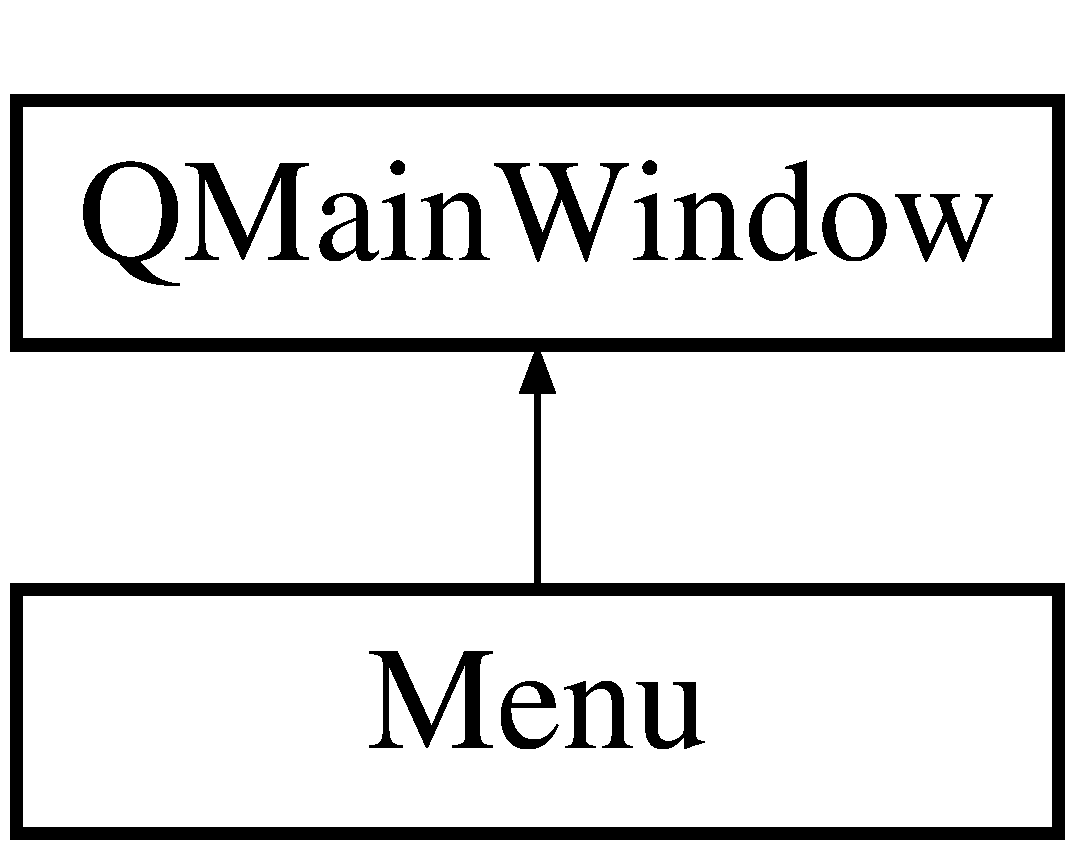
\includegraphics[height=2.000000cm]{classMenu}
\end{center}
\end{figure}
\subsection*{Public Member Functions}
\begin{DoxyCompactItemize}
\item 
\hypertarget{classMenu_aea36ff15ed756c91b7731a2025175f16}{{\bfseries Menu} (Q\-Widget $\ast$parent=0)}\label{classMenu_aea36ff15ed756c91b7731a2025175f16}

\end{DoxyCompactItemize}


The documentation for this class was generated from the following files\-:\begin{DoxyCompactItemize}
\item 
/home/alex/source\-Code/git\-Project/beleg\-Arbeit\-E\-M\-M\-S/project\-Sogo/include/gui/Menu.\-h\item 
/home/alex/source\-Code/git\-Project/beleg\-Arbeit\-E\-M\-M\-S/project\-Sogo/src/gui/\hyperlink{Menu_8cpp}{Menu.\-cpp}\end{DoxyCompactItemize}

\hypertarget{classNewSessionMenu}{\section{New\-Session\-Menu Class Reference}
\label{classNewSessionMenu}\index{New\-Session\-Menu@{New\-Session\-Menu}}
}
Inheritance diagram for New\-Session\-Menu\-:\begin{figure}[H]
\begin{center}
\leavevmode
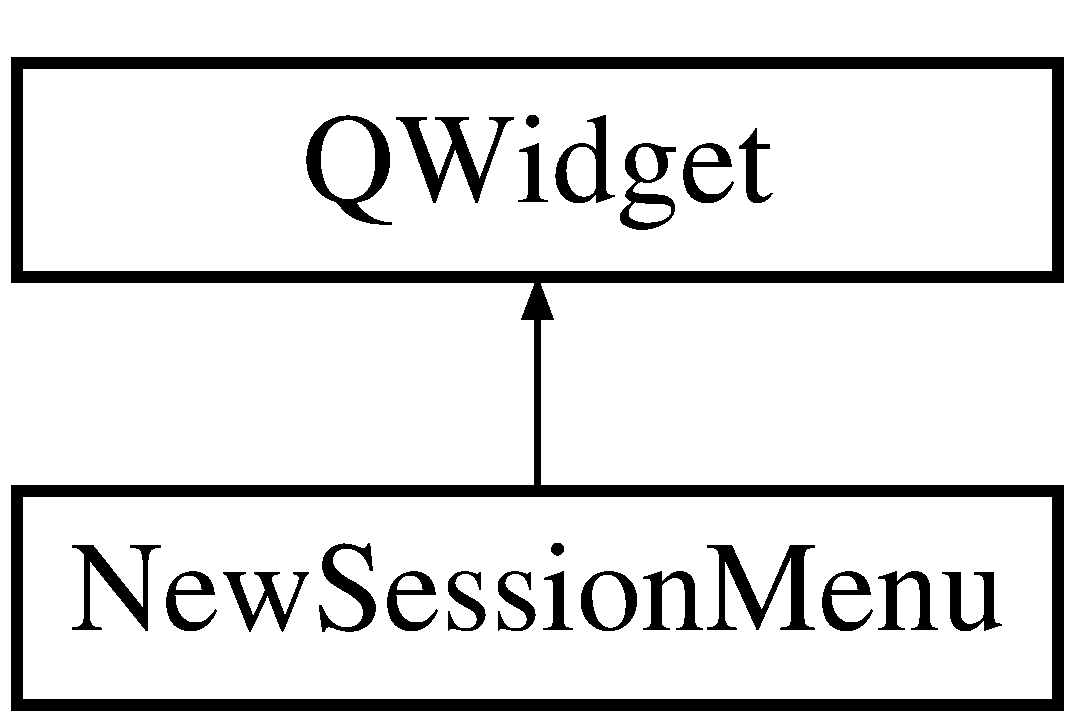
\includegraphics[height=2.000000cm]{classNewSessionMenu}
\end{center}
\end{figure}
\subsection*{Signals}
\begin{DoxyCompactItemize}
\item 
\hypertarget{classNewSessionMenu_aec46b3d790d583bd0c0fb35a7cc89d58}{void {\bfseries show\-Start\-Menu} ()}\label{classNewSessionMenu_aec46b3d790d583bd0c0fb35a7cc89d58}

\item 
\hypertarget{classNewSessionMenu_add9c9c91b8f92fde390187463b1f40ba}{void {\bfseries create\-Game\-Data} (\hyperlink{classGameData}{Game\-Data} game\-Data)}\label{classNewSessionMenu_add9c9c91b8f92fde390187463b1f40ba}

\item 
\hypertarget{classNewSessionMenu_afa1a5423cfcb5af562e30d1f66040ce5}{void {\bfseries start\-Game} ()}\label{classNewSessionMenu_afa1a5423cfcb5af562e30d1f66040ce5}

\end{DoxyCompactItemize}
\subsection*{Public Member Functions}
\begin{DoxyCompactItemize}
\item 
\hypertarget{classNewSessionMenu_a4742167534b8efad3a8163ac3d243b1b}{void {\bfseries set\-Playfield} ()}\label{classNewSessionMenu_a4742167534b8efad3a8163ac3d243b1b}

\item 
\hypertarget{classNewSessionMenu_afae85196d39cd5b68e445659faf3f901}{void {\bfseries set\-Mode} ()}\label{classNewSessionMenu_afae85196d39cd5b68e445659faf3f901}

\item 
\hypertarget{classNewSessionMenu_abe4916445e5ce3edfe78adb89533f230}{void {\bfseries change\-Event} (Q\-Event $\ast$event)}\label{classNewSessionMenu_abe4916445e5ce3edfe78adb89533f230}

\item 
\hypertarget{classNewSessionMenu_ae1038e3894d95dd28e7e9bde54fdc5eb}{{\bfseries New\-Session\-Menu} (Q\-Widget $\ast$parent=0)}\label{classNewSessionMenu_ae1038e3894d95dd28e7e9bde54fdc5eb}

\item 
\hypertarget{classNewSessionMenu_a3a5d3b6d5f3039c7ff2e4933bde10a70}{void {\bfseries merge\-Game\-Data} ()}\label{classNewSessionMenu_a3a5d3b6d5f3039c7ff2e4933bde10a70}

\item 
\hypertarget{classNewSessionMenu_a51512ad474fdb0eb6b880d17a5ce4d11}{void {\bfseries check\-Playfield\-Size} ()}\label{classNewSessionMenu_a51512ad474fdb0eb6b880d17a5ce4d11}

\item 
\hypertarget{classNewSessionMenu_ac13a0674e7492b42279b60e8b73fb561}{void {\bfseries set\-Player} ()}\label{classNewSessionMenu_ac13a0674e7492b42279b60e8b73fb561}

\item 
\hypertarget{classNewSessionMenu_a0985b4cc0908c662788f68dd55b38472}{void {\bfseries check\-Skill} ()}\label{classNewSessionMenu_a0985b4cc0908c662788f68dd55b38472}

\item 
\hypertarget{classNewSessionMenu_a30076610330be4a709eb9c72b3ec9c30}{void {\bfseries set\-Game\-Enviorment} ()}\label{classNewSessionMenu_a30076610330be4a709eb9c72b3ec9c30}

\end{DoxyCompactItemize}
\subsection*{Public Attributes}
\begin{DoxyCompactItemize}
\item 
\hypertarget{classNewSessionMenu_a1e5fc5bfe12c63b0f99df1dc3ffec0ba}{\hyperlink{classGameData}{Game\-Data} $\ast$ {\bfseries m\-\_\-game\-Data}}\label{classNewSessionMenu_a1e5fc5bfe12c63b0f99df1dc3ffec0ba}

\end{DoxyCompactItemize}


The documentation for this class was generated from the following files\-:\begin{DoxyCompactItemize}
\item 
/home/alex/source\-Code/git\-Project/beleg\-Arbeit\-E\-M\-M\-S/project\-Sogo/include/gui/New\-Session\-Menu.\-h\item 
/home/alex/source\-Code/git\-Project/beleg\-Arbeit\-E\-M\-M\-S/project\-Sogo/build-\/sogo\-App-\/\-Desktop\-\_\-\-Qt\-\_\-5\-\_\-6\-\_\-0\-\_\-\-G\-C\-C\-\_\-64bit-\/\-Debug/moc\-\_\-\-New\-Session\-Menu.\-cpp\item 
/home/alex/source\-Code/git\-Project/beleg\-Arbeit\-E\-M\-M\-S/project\-Sogo/src/gui/New\-Session\-Menu.\-cpp\end{DoxyCompactItemize}

\hypertarget{classglm_1_1nicest}{\section{glm\-:\-:nicest Class Reference}
\label{classglm_1_1nicest}\index{glm\-::nicest@{glm\-::nicest}}
}


The documentation for this class was generated from the following file\-:\begin{DoxyCompactItemize}
\item 
/home/alex/source\-Code/git\-Project/beleg\-Arbeit\-E\-M\-M\-S/project\-Sogo/external/glm-\/0.\-9.\-4.\-0/glm/core/\hyperlink{hint_8hpp}{hint.\-hpp}\end{DoxyCompactItemize}

\hypertarget{classPauseMenu}{\section{Pause\-Menu Class Reference}
\label{classPauseMenu}\index{Pause\-Menu@{Pause\-Menu}}
}


The \hyperlink{classPauseMenu}{Pause\-Menu} class.  




{\ttfamily \#include $<$Pause\-Menu.\-h$>$}

Inheritance diagram for Pause\-Menu\-:\begin{figure}[H]
\begin{center}
\leavevmode
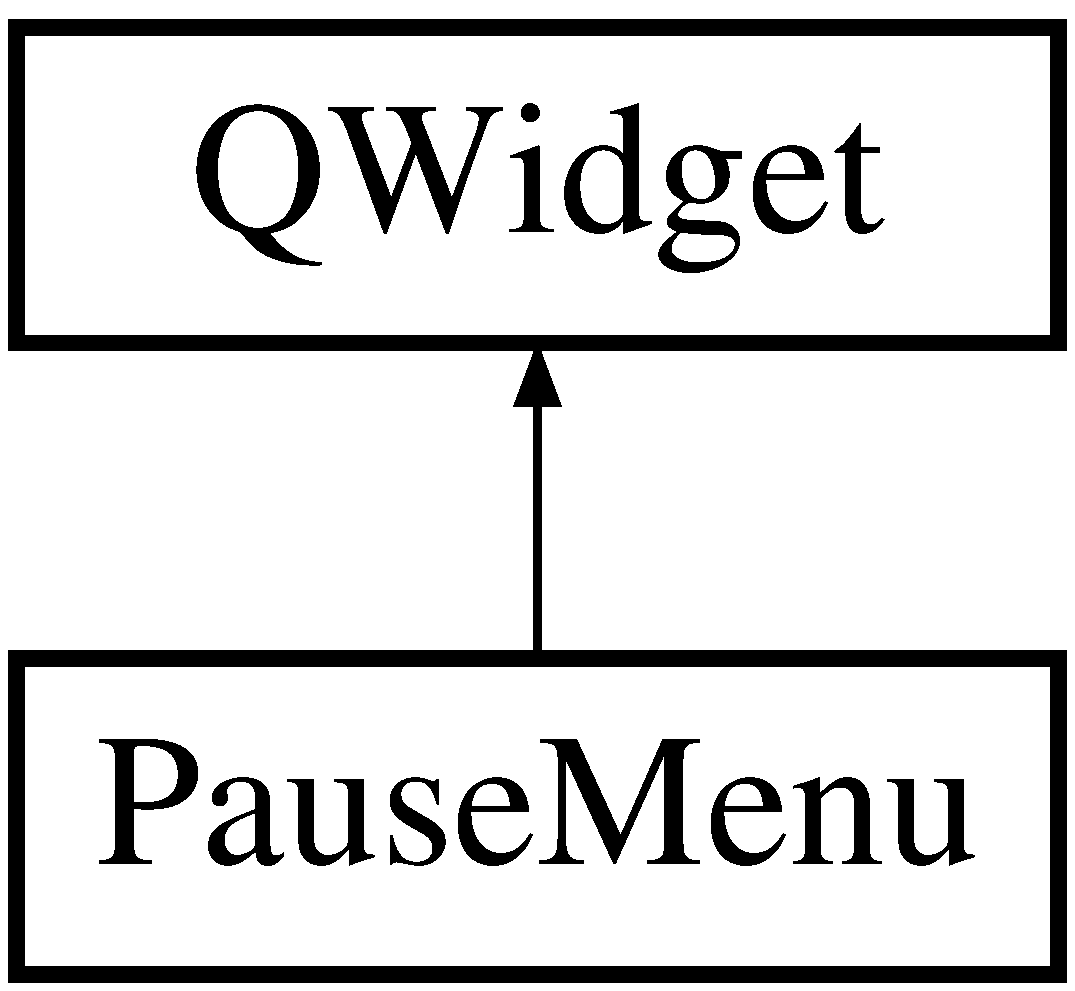
\includegraphics[height=2.000000cm]{classPauseMenu}
\end{center}
\end{figure}
\subsection*{Signals}
\begin{DoxyCompactItemize}
\item 
\hypertarget{classPauseMenu_ac24806b40fa10843a42f3d3ba96e3e6c}{void {\bfseries Resume\-Button\-Pressed} ()}\label{classPauseMenu_ac24806b40fa10843a42f3d3ba96e3e6c}

\item 
\hypertarget{classPauseMenu_a1525fb2d41bade59de33cad48d23b9d8}{void {\bfseries Save\-Button\-Pressed} ()}\label{classPauseMenu_a1525fb2d41bade59de33cad48d23b9d8}

\item 
\hypertarget{classPauseMenu_af1e7daf3f16ddca8633d9ee393f33dbb}{void {\bfseries Quit\-Game\-Button\-Pressed} ()}\label{classPauseMenu_af1e7daf3f16ddca8633d9ee393f33dbb}

\end{DoxyCompactItemize}
\subsection*{Public Member Functions}
\begin{DoxyCompactItemize}
\item 
\hypertarget{classPauseMenu_a7e37f17609a107981090585aad89a1ec}{{\bfseries Pause\-Menu} (Q\-Widget $\ast$parent=0)}\label{classPauseMenu_a7e37f17609a107981090585aad89a1ec}

\item 
\hypertarget{classPauseMenu_a7ae2f7ecbb859e6370d474db4d086892}{void {\bfseries change\-Event} (Q\-Event $\ast$event)}\label{classPauseMenu_a7ae2f7ecbb859e6370d474db4d086892}

\end{DoxyCompactItemize}


\subsection{Detailed Description}
The \hyperlink{classPauseMenu}{Pause\-Menu} class. 

To interruppt the game.

\begin{DoxyAuthor}{Author}
Nils Brandt 

Alexander Luedke
\end{DoxyAuthor}
\begin{DoxyDate}{Date}
08. August 2016
\end{DoxyDate}
\begin{DoxyVersion}{Version}
1.\-0 Add Documentation 
\end{DoxyVersion}

\hypertarget{classPlayer}{\section{Player Class Reference}
\label{classPlayer}\index{Player@{Player}}
}


The \hyperlink{classPlayer}{Player} class.  




{\ttfamily \#include $<$Player.\-h$>$}

\subsection*{Public Types}
\begin{DoxyCompactItemize}
\item 
enum \hyperlink{classPlayer_a97dc3c423902370176605121e8f68415}{Player\-Type} \{ {\bfseries H\-U\-M\-A\-N}, 
{\bfseries A\-I}
 \}
\begin{DoxyCompactList}\small\item\em The Player\-Type enum defines which type the player can be of who is playing the game. \end{DoxyCompactList}\end{DoxyCompactItemize}
\subsection*{Public Member Functions}
\begin{DoxyCompactItemize}
\item 
\hypertarget{classPlayer_affe0cc3cb714f6deb4e62f0c0d3f1fd8}{\hyperlink{classPlayer_affe0cc3cb714f6deb4e62f0c0d3f1fd8}{Player} ()}\label{classPlayer_affe0cc3cb714f6deb4e62f0c0d3f1fd8}

\begin{DoxyCompactList}\small\item\em \hyperlink{classPlayer}{Player}. \end{DoxyCompactList}\item 
\hyperlink{classPlayer_a66f0cbcaa9de5f81fcbb4ee72d0f110e}{Player} (\hyperlink{classPlayer_a97dc3c423902370176605121e8f68415}{Player\-Type} type, std\-::string name, \hyperlink{classPlayingField_ac6df152a3f820aa04a00ab4df4a9d265}{Playing\-Field\-::\-Occupation\-State} color, unsigned int skill=0)
\begin{DoxyCompactList}\small\item\em \hyperlink{classPlayer}{Player}. \end{DoxyCompactList}\item 
\hyperlink{classPlayer_a6d2881f060b07eb48077cad6044fcd8f}{Player} (const \hyperlink{classPlayer}{Player} \&src)
\begin{DoxyCompactList}\small\item\em \hyperlink{classPlayer}{Player}. \end{DoxyCompactList}\item 
\hyperlink{classPlayer_a97dc3c423902370176605121e8f68415}{Player\-Type} \hyperlink{classPlayer_adbb81c3cffe824c9ed8e18f1f635a1a3}{Get\-Type} () const 
\begin{DoxyCompactList}\small\item\em Get\-Type. \end{DoxyCompactList}\item 
std\-::string \hyperlink{classPlayer_aa5030908379dbc95594e4a9856758fef}{Get\-Name} () const 
\begin{DoxyCompactList}\small\item\em Get\-Name. \end{DoxyCompactList}\item 
\hyperlink{classPlayingField_ac6df152a3f820aa04a00ab4df4a9d265}{Playing\-Field\-::\-Occupation\-State} \hyperlink{classPlayer_a49f420e5204c895b9a94f07f6aaf639f}{Get\-Color} () const 
\begin{DoxyCompactList}\small\item\em Get\-Color. \end{DoxyCompactList}\item 
void \hyperlink{classPlayer_ac6727206628d233b9094c8e80f777c1d}{Set\-Name} (std\-::string name)
\begin{DoxyCompactList}\small\item\em Set\-Name. \end{DoxyCompactList}\item 
int \hyperlink{classPlayer_a9d8cedd46573b958fe6febbf89d07322}{Get\-Skill} () const 
\begin{DoxyCompactList}\small\item\em Get\-Skill. \end{DoxyCompactList}\item 
void \hyperlink{classPlayer_a432304cacd50b399038ea787d65464cc}{Set\-Skill} (int skill)
\begin{DoxyCompactList}\small\item\em Set\-Skill. \end{DoxyCompactList}\end{DoxyCompactItemize}
\subsection*{Static Public Member Functions}
\begin{DoxyCompactItemize}
\item 
\hypertarget{classPlayer_a4847e9d725d82c06e3cad28a12deadb4}{static string {\bfseries Serialize} (const \hyperlink{classPlayer}{Player} p)}\label{classPlayer_a4847e9d725d82c06e3cad28a12deadb4}

\item 
\hypertarget{classPlayer_a5db86c30afa559aa2cf7a95e661b262c}{static \hyperlink{classPlayer}{Player} $\ast$ {\bfseries Deserialize} (std\-::string str)  throw (\-Deserialization\-Exception)}\label{classPlayer_a5db86c30afa559aa2cf7a95e661b262c}

\end{DoxyCompactItemize}


\subsection{Detailed Description}
The \hyperlink{classPlayer}{Player} class. 

Defines a \hyperlink{classPlayer}{Player} that is defined by the type, which the player belongs to ( human or ai player ) a name a Color ( Currently Occupationstate ) skill ( currently only effectively used by ai)

\begin{DoxyAuthor}{Author}
Nils Brandt 

Alexander Luedke
\end{DoxyAuthor}
\begin{DoxyDate}{Date}
08. August 2016
\end{DoxyDate}
\begin{DoxyVersion}{Version}
1.\-0 Add Documentation 
\end{DoxyVersion}


\subsection{Constructor \& Destructor Documentation}
\hypertarget{classPlayer_a66f0cbcaa9de5f81fcbb4ee72d0f110e}{\index{Player@{Player}!Player@{Player}}
\index{Player@{Player}!Player@{Player}}
\subsubsection[{Player}]{\setlength{\rightskip}{0pt plus 5cm}Player\-::\-Player (
\begin{DoxyParamCaption}
\item[{{\bf Player\-Type}}]{type, }
\item[{std\-::string}]{name, }
\item[{{\bf Playing\-Field\-::\-Occupation\-State}}]{color, }
\item[{unsigned int}]{skill = {\ttfamily 0}}
\end{DoxyParamCaption}
)}}\label{classPlayer_a66f0cbcaa9de5f81fcbb4ee72d0f110e}


\hyperlink{classPlayer}{Player}. 


\begin{DoxyParams}{Parameters}
{\em type} & \\
\hline
{\em name} & \\
\hline
{\em color} & \\
\hline
{\em skill} & \\
\hline
\end{DoxyParams}
\hypertarget{classPlayer_a6d2881f060b07eb48077cad6044fcd8f}{\index{Player@{Player}!Player@{Player}}
\index{Player@{Player}!Player@{Player}}
\subsubsection[{Player}]{\setlength{\rightskip}{0pt plus 5cm}Player\-::\-Player (
\begin{DoxyParamCaption}
\item[{const {\bf Player} \&}]{src}
\end{DoxyParamCaption}
)}}\label{classPlayer_a6d2881f060b07eb48077cad6044fcd8f}


\hyperlink{classPlayer}{Player}. 


\begin{DoxyParams}{Parameters}
{\em src} & \\
\hline
\end{DoxyParams}


\subsection{Member Function Documentation}
\hypertarget{classPlayer_a49f420e5204c895b9a94f07f6aaf639f}{\index{Player@{Player}!Get\-Color@{Get\-Color}}
\index{Get\-Color@{Get\-Color}!Player@{Player}}
\subsubsection[{Get\-Color}]{\setlength{\rightskip}{0pt plus 5cm}{\bf Playing\-Field\-::\-Occupation\-State} Player\-::\-Get\-Color (
\begin{DoxyParamCaption}
{}
\end{DoxyParamCaption}
) const}}\label{classPlayer_a49f420e5204c895b9a94f07f6aaf639f}


Get\-Color. 

\begin{DoxyReturn}{Returns}

\end{DoxyReturn}
\hypertarget{classPlayer_aa5030908379dbc95594e4a9856758fef}{\index{Player@{Player}!Get\-Name@{Get\-Name}}
\index{Get\-Name@{Get\-Name}!Player@{Player}}
\subsubsection[{Get\-Name}]{\setlength{\rightskip}{0pt plus 5cm}std\-::string Player\-::\-Get\-Name (
\begin{DoxyParamCaption}
{}
\end{DoxyParamCaption}
) const}}\label{classPlayer_aa5030908379dbc95594e4a9856758fef}


Get\-Name. 

\begin{DoxyReturn}{Returns}

\end{DoxyReturn}
\hypertarget{classPlayer_a9d8cedd46573b958fe6febbf89d07322}{\index{Player@{Player}!Get\-Skill@{Get\-Skill}}
\index{Get\-Skill@{Get\-Skill}!Player@{Player}}
\subsubsection[{Get\-Skill}]{\setlength{\rightskip}{0pt plus 5cm}int Player\-::\-Get\-Skill (
\begin{DoxyParamCaption}
{}
\end{DoxyParamCaption}
) const}}\label{classPlayer_a9d8cedd46573b958fe6febbf89d07322}


Get\-Skill. 

\begin{DoxyReturn}{Returns}

\end{DoxyReturn}
\hypertarget{classPlayer_adbb81c3cffe824c9ed8e18f1f635a1a3}{\index{Player@{Player}!Get\-Type@{Get\-Type}}
\index{Get\-Type@{Get\-Type}!Player@{Player}}
\subsubsection[{Get\-Type}]{\setlength{\rightskip}{0pt plus 5cm}{\bf Player\-::\-Player\-Type} Player\-::\-Get\-Type (
\begin{DoxyParamCaption}
{}
\end{DoxyParamCaption}
) const}}\label{classPlayer_adbb81c3cffe824c9ed8e18f1f635a1a3}


Get\-Type. 

\begin{DoxyReturn}{Returns}

\end{DoxyReturn}
\hypertarget{classPlayer_ac6727206628d233b9094c8e80f777c1d}{\index{Player@{Player}!Set\-Name@{Set\-Name}}
\index{Set\-Name@{Set\-Name}!Player@{Player}}
\subsubsection[{Set\-Name}]{\setlength{\rightskip}{0pt plus 5cm}void Player\-::\-Set\-Name (
\begin{DoxyParamCaption}
\item[{std\-::string}]{name}
\end{DoxyParamCaption}
)}}\label{classPlayer_ac6727206628d233b9094c8e80f777c1d}


Set\-Name. 


\begin{DoxyParams}{Parameters}
{\em name} & \\
\hline
\end{DoxyParams}
\hypertarget{classPlayer_a432304cacd50b399038ea787d65464cc}{\index{Player@{Player}!Set\-Skill@{Set\-Skill}}
\index{Set\-Skill@{Set\-Skill}!Player@{Player}}
\subsubsection[{Set\-Skill}]{\setlength{\rightskip}{0pt plus 5cm}void Player\-::\-Set\-Skill (
\begin{DoxyParamCaption}
\item[{int}]{skill}
\end{DoxyParamCaption}
)}}\label{classPlayer_a432304cacd50b399038ea787d65464cc}


Set\-Skill. 


\begin{DoxyParams}{Parameters}
{\em skill} & \\
\hline
\end{DoxyParams}

\hypertarget{classPlayerInput}{\section{Player\-Input Class Reference}
\label{classPlayerInput}\index{Player\-Input@{Player\-Input}}
}


The \hyperlink{classPlayerInput}{Player\-Input} class.  




{\ttfamily \#include $<$Player\-Input.\-h$>$}

Inheritance diagram for Player\-Input\-:\begin{figure}[H]
\begin{center}
\leavevmode
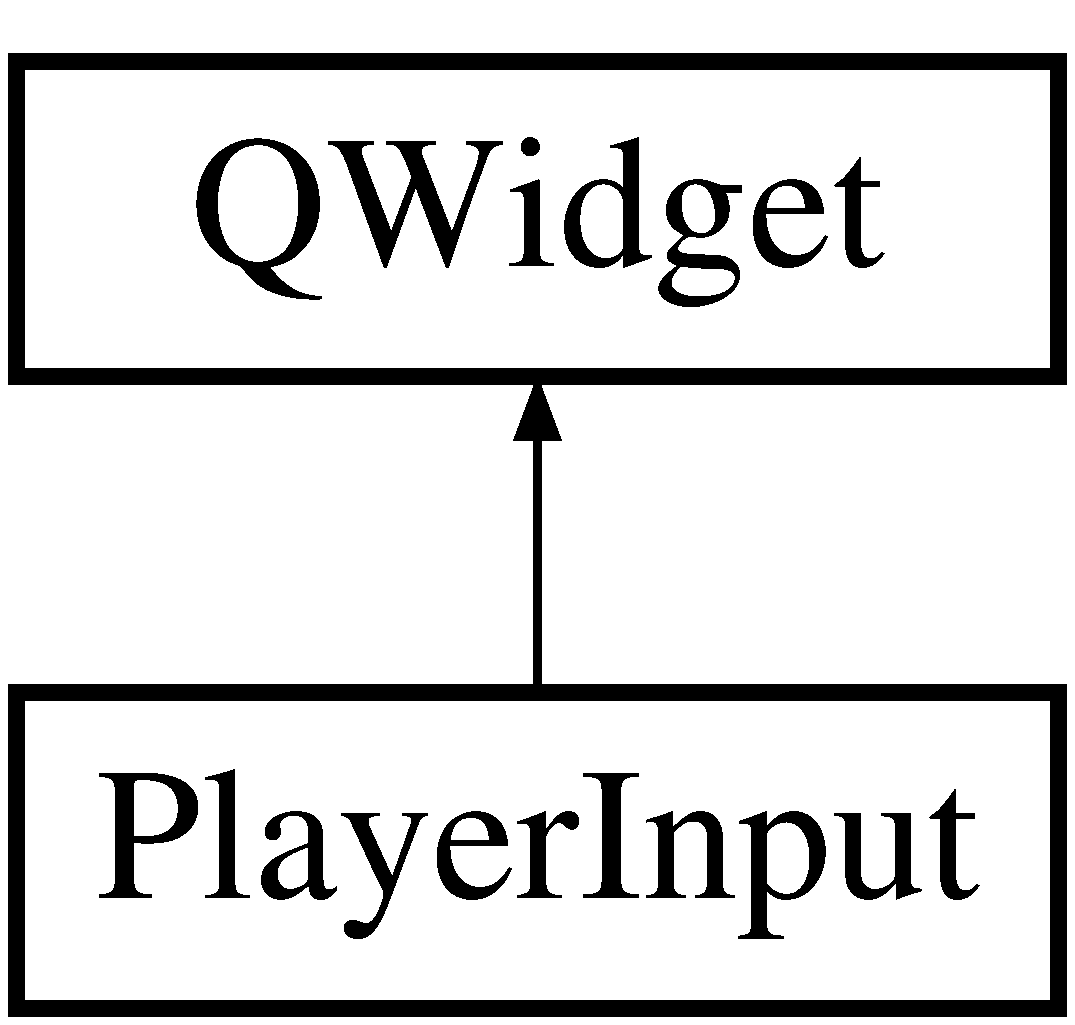
\includegraphics[height=2.000000cm]{classPlayerInput}
\end{center}
\end{figure}
\subsection*{Signals}
\begin{DoxyCompactItemize}
\item 
void \hyperlink{classPlayerInput_aab7de51daaa958792ffaae64e41f43e6}{Input\-Confirmed} (\hyperlink{structVector2}{Vector2} pos)
\begin{DoxyCompactList}\small\item\em To confirm the playerinput. \end{DoxyCompactList}\end{DoxyCompactItemize}
\subsection*{Public Member Functions}
\begin{DoxyCompactItemize}
\item 
\hypertarget{classPlayerInput_a41adeb104eebbd46404b0a29203441c5}{{\bfseries Player\-Input} (\hyperlink{classGameManager}{Game\-Manager} $\ast$game\-Manager, Q\-Widget $\ast$parent=0)}\label{classPlayerInput_a41adeb104eebbd46404b0a29203441c5}

\item 
\hypertarget{classPlayerInput_ab8abc1017f5b0e8589fbf1b8b550eba4}{void {\bfseries change\-Event} (Q\-Event $\ast$event)}\label{classPlayerInput_ab8abc1017f5b0e8589fbf1b8b550eba4}

\item 
\hypertarget{classPlayerInput_a2135e14f7e216f1f78ab63212230aa03}{void {\bfseries Apply\-Player\-Change} ()}\label{classPlayerInput_a2135e14f7e216f1f78ab63212230aa03}

\end{DoxyCompactItemize}


\subsection{Detailed Description}
The \hyperlink{classPlayerInput}{Player\-Input} class. 

\begin{DoxyAuthor}{Author}
Nils Brandt 

Alexander Luedke
\end{DoxyAuthor}
\begin{DoxyDate}{Date}
08. August 2016
\end{DoxyDate}
\begin{DoxyVersion}{Version}
1.\-0 Add Documentation 
\end{DoxyVersion}


\subsection{Member Function Documentation}
\hypertarget{classPlayerInput_aab7de51daaa958792ffaae64e41f43e6}{\index{Player\-Input@{Player\-Input}!Input\-Confirmed@{Input\-Confirmed}}
\index{Input\-Confirmed@{Input\-Confirmed}!PlayerInput@{Player\-Input}}
\subsubsection[{Input\-Confirmed}]{\setlength{\rightskip}{0pt plus 5cm}void Player\-Input\-::\-Input\-Confirmed (
\begin{DoxyParamCaption}
\item[{{\bf Vector2}}]{pos}
\end{DoxyParamCaption}
)\hspace{0.3cm}{\ttfamily [signal]}}}\label{classPlayerInput_aab7de51daaa958792ffaae64e41f43e6}


To confirm the playerinput. 


\begin{DoxyParams}{Parameters}
{\em pos} & The position the player wants to set. \\
\hline
\end{DoxyParams}

\hypertarget{classPlayingField}{\section{Playing\-Field Class Reference}
\label{classPlayingField}\index{Playing\-Field@{Playing\-Field}}
}


Defines the Properties of a Playingfield.  




{\ttfamily \#include $<$Playing\-Field.\-h$>$}

\subsection*{Classes}
\begin{DoxyCompactItemize}
\item 
struct \hyperlink{structPlayingField_1_1Slot}{Slot}
\begin{DoxyCompactList}\small\item\em Defines a Gridspace in a Sogo Playingfield It contains the occupationstate of this position in the grid. \end{DoxyCompactList}\end{DoxyCompactItemize}
\subsection*{Public Types}
\begin{DoxyCompactItemize}
\item 
enum \hyperlink{classPlayingField_a6032d4d7297d628a368cde7db331d7f6}{Field\-Exeptions} \{ {\bfseries O\-C\-C\-U\-P\-I\-E\-D}, 
{\bfseries P\-O\-S\-I\-T\-I\-O\-N\-\_\-\-N\-O\-T\-\_\-\-A\-V\-A\-I\-L\-A\-B\-L\-E}, 
{\bfseries N\-O\-\_\-\-S\-P\-A\-C\-E\-\_\-\-A\-N\-Y\-M\-O\-R\-E}
 \}
\begin{DoxyCompactList}\small\item\em Is thrown when in an Error in Playingfield O\-C\-C\-U\-P\-I\-E\-D when already occupied by other player P\-O\-S\-I\-T\-I\-O\-N\-\_\-\-N\-O\-T\-\_\-\-A\-V\-A\-I\-L\-A\-B\-L\-E when position is not valid for occupation under current circumstances. \end{DoxyCompactList}\item 
enum \hyperlink{classPlayingField_ac6df152a3f820aa04a00ab4df4a9d265}{Occupation\-State} \{ {\bfseries N\-O\-N\-E}, 
{\bfseries R\-E\-D}, 
{\bfseries B\-L\-U\-E}
 \}
\begin{DoxyCompactList}\small\item\em Defines the States a slot can be in. \end{DoxyCompactList}\end{DoxyCompactItemize}
\subsection*{Public Member Functions}
\begin{DoxyCompactItemize}
\item 
\hyperlink{classPlayingField_a9cd7d0540bff01b5b83ca9bdf8dfd5d6}{Playing\-Field} (int field\-Size=4)
\begin{DoxyCompactList}\small\item\em constructor generates a Playingfield with (fieldsize x fieldsize x fieldsize) \end{DoxyCompactList}\item 
\hypertarget{classPlayingField_a4715051a7ba2b0495b3b56d357563432}{\hyperlink{classPlayingField_a4715051a7ba2b0495b3b56d357563432}{Playing\-Field} (const \hyperlink{classPlayingField}{Playing\-Field} \&field)}\label{classPlayingField_a4715051a7ba2b0495b3b56d357563432}

\begin{DoxyCompactList}\small\item\em Copy constructor. \end{DoxyCompactList}\item 
\hypertarget{classPlayingField_a7bc092c6433f18e7a07835608e8a4449}{\hyperlink{classPlayingField_a7bc092c6433f18e7a07835608e8a4449}{$\sim$\-Playing\-Field} ()}\label{classPlayingField_a7bc092c6433f18e7a07835608e8a4449}

\begin{DoxyCompactList}\small\item\em Destructor clears the field. \end{DoxyCompactList}\item 
\hyperlink{structPlayingField_1_1Slot}{Slot} $\ast$ \hyperlink{classPlayingField_a01b5105b49ec72e094411d216df27ffa}{Get\-Slot} (int x, int y, int z) const   throw (out\-\_\-of\-\_\-range)
\begin{DoxyCompactList}\small\item\em Returns the slot at pos.\-x (horizontally) pos.\-y (Vertically) pos.\-z (\char`\"{}forwardly\char`\"{}) \end{DoxyCompactList}\item 
int \hyperlink{classPlayingField_abfbecf0f8ba91c9c1167da359e7463dc}{Get\-Field\-Size} () const 
\begin{DoxyCompactList}\small\item\em Getter for field\-Size. \end{DoxyCompactList}\item 
void \hyperlink{classPlayingField_a166ff0aaa90a41ce748efd9165a9d578}{Occupy\-Slot} (int x, int y, int z, \hyperlink{classPlayingField_ac6df152a3f820aa04a00ab4df4a9d265}{Occupation\-State} id)  throw (out\-\_\-of\-\_\-range, Field\-Exeptions)
\begin{DoxyCompactList}\small\item\em Sets the occupation\-State of the \hyperlink{structPlayingField_1_1Slot}{Slot} at pos(x,y,z) to id. \end{DoxyCompactList}\item 
void \hyperlink{classPlayingField_a6165557999a6cec6c1c1b71b88c2f82e}{Occupy\-Slot} (\hyperlink{structVector3}{Vector3} pos, \hyperlink{classPlayingField_ac6df152a3f820aa04a00ab4df4a9d265}{Playing\-Field\-::\-Occupation\-State} id)  throw (out\-\_\-of\-\_\-range, Field\-Exeptions)
\begin{DoxyCompactList}\small\item\em Sets the occupation\-State of the \hyperlink{structPlayingField_1_1Slot}{Slot} at pos(x,y,z) to id. \end{DoxyCompactList}\item 
\hypertarget{classPlayingField_af25e735d1d9f1c561fdf951507b2c1de}{bool {\bfseries Is\-Position\-Available} (int x, int y, int z) const }\label{classPlayingField_af25e735d1d9f1c561fdf951507b2c1de}

\end{DoxyCompactItemize}
\subsection*{Static Public Member Functions}
\begin{DoxyCompactItemize}
\item 
\hypertarget{classPlayingField_ad0b87276c478b016d1425e7d69ba4e73}{static std\-::string {\bfseries Serialize} (const \hyperlink{classPlayingField}{Playing\-Field} \&p\-F)}\label{classPlayingField_ad0b87276c478b016d1425e7d69ba4e73}

\item 
\hypertarget{classPlayingField_a4fca00ce844080c76d91d45f4937d4cc}{static \hyperlink{classPlayingField}{Playing\-Field} $\ast$ {\bfseries Deserialize} (string str)  throw (\-Deserialization\-Exception)}\label{classPlayingField_a4fca00ce844080c76d91d45f4937d4cc}

\end{DoxyCompactItemize}


\subsection{Detailed Description}
Defines the Properties of a Playingfield. 

Which is a 3 dimensional Grid Containing Slots Slots can be occupied by players

\begin{DoxyAuthor}{Author}
Nils Brandt 

Alexander Luedke
\end{DoxyAuthor}
\begin{DoxyDate}{Date}
08. August 2016
\end{DoxyDate}
\begin{DoxyVersion}{Version}
1.\-0 Add Documentation 
\end{DoxyVersion}


\subsection{Constructor \& Destructor Documentation}
\hypertarget{classPlayingField_a9cd7d0540bff01b5b83ca9bdf8dfd5d6}{\index{Playing\-Field@{Playing\-Field}!Playing\-Field@{Playing\-Field}}
\index{Playing\-Field@{Playing\-Field}!PlayingField@{Playing\-Field}}
\subsubsection[{Playing\-Field}]{\setlength{\rightskip}{0pt plus 5cm}Playing\-Field\-::\-Playing\-Field (
\begin{DoxyParamCaption}
\item[{int}]{field\-Size = {\ttfamily 4}}
\end{DoxyParamCaption}
)}}\label{classPlayingField_a9cd7d0540bff01b5b83ca9bdf8dfd5d6}


constructor generates a Playingfield with (fieldsize x fieldsize x fieldsize) 


\begin{DoxyParams}{Parameters}
{\em field\-Size} & (default value = 4) \\
\hline
\end{DoxyParams}


\subsection{Member Function Documentation}
\hypertarget{classPlayingField_abfbecf0f8ba91c9c1167da359e7463dc}{\index{Playing\-Field@{Playing\-Field}!Get\-Field\-Size@{Get\-Field\-Size}}
\index{Get\-Field\-Size@{Get\-Field\-Size}!PlayingField@{Playing\-Field}}
\subsubsection[{Get\-Field\-Size}]{\setlength{\rightskip}{0pt plus 5cm}int Playing\-Field\-::\-Get\-Field\-Size (
\begin{DoxyParamCaption}
{}
\end{DoxyParamCaption}
) const}}\label{classPlayingField_abfbecf0f8ba91c9c1167da359e7463dc}


Getter for field\-Size. 

\begin{DoxyReturn}{Returns}
returns the fieldsize 
\end{DoxyReturn}
\hypertarget{classPlayingField_a01b5105b49ec72e094411d216df27ffa}{\index{Playing\-Field@{Playing\-Field}!Get\-Slot@{Get\-Slot}}
\index{Get\-Slot@{Get\-Slot}!PlayingField@{Playing\-Field}}
\subsubsection[{Get\-Slot}]{\setlength{\rightskip}{0pt plus 5cm}{\bf Playing\-Field\-::\-Slot} $\ast$ Playing\-Field\-::\-Get\-Slot (
\begin{DoxyParamCaption}
\item[{int}]{x, }
\item[{int}]{y, }
\item[{int}]{z}
\end{DoxyParamCaption}
) const throw  out\-\_\-of\-\_\-range) }}\label{classPlayingField_a01b5105b49ec72e094411d216df27ffa}


Returns the slot at pos.\-x (horizontally) pos.\-y (Vertically) pos.\-z (\char`\"{}forwardly\char`\"{}) 


\begin{DoxyExceptions}{Exceptions}
{\em out\-\_\-of\-\_\-range} & if value is higher than fieldsize \\
\hline
\end{DoxyExceptions}
\hypertarget{classPlayingField_a166ff0aaa90a41ce748efd9165a9d578}{\index{Playing\-Field@{Playing\-Field}!Occupy\-Slot@{Occupy\-Slot}}
\index{Occupy\-Slot@{Occupy\-Slot}!PlayingField@{Playing\-Field}}
\subsubsection[{Occupy\-Slot}]{\setlength{\rightskip}{0pt plus 5cm}void Playing\-Field\-::\-Occupy\-Slot (
\begin{DoxyParamCaption}
\item[{int}]{x, }
\item[{int}]{y, }
\item[{int}]{z, }
\item[{{\bf Playing\-Field\-::\-Occupation\-State}}]{id}
\end{DoxyParamCaption}
) throw  out\-\_\-of\-\_\-range, {\bf Field\-Exeptions}) }}\label{classPlayingField_a166ff0aaa90a41ce748efd9165a9d578}


Sets the occupation\-State of the \hyperlink{structPlayingField_1_1Slot}{Slot} at pos(x,y,z) to id. 


\begin{DoxyParams}{Parameters}
{\em x} & horizontal value \\
\hline
{\em y} & depth value \\
\hline
{\em z} & vertical value \\
\hline
{\em id} & occupationstate for assignment \\
\hline
\end{DoxyParams}

\begin{DoxyExceptions}{Exceptions}
{\em out\-\_\-of\-\_\-range} & if value is higher than fieldsize \\
\hline
{\em Field\-Exception} & if \hyperlink{structPlayingField_1_1Slot}{Slot} is already occupied by other player \\
\hline
\end{DoxyExceptions}
\hypertarget{classPlayingField_a6165557999a6cec6c1c1b71b88c2f82e}{\index{Playing\-Field@{Playing\-Field}!Occupy\-Slot@{Occupy\-Slot}}
\index{Occupy\-Slot@{Occupy\-Slot}!PlayingField@{Playing\-Field}}
\subsubsection[{Occupy\-Slot}]{\setlength{\rightskip}{0pt plus 5cm}void Playing\-Field\-::\-Occupy\-Slot (
\begin{DoxyParamCaption}
\item[{{\bf Vector3}}]{pos, }
\item[{{\bf Playing\-Field\-::\-Occupation\-State}}]{id}
\end{DoxyParamCaption}
) throw  out\-\_\-of\-\_\-range, {\bf Field\-Exeptions}) }}\label{classPlayingField_a6165557999a6cec6c1c1b71b88c2f82e}


Sets the occupation\-State of the \hyperlink{structPlayingField_1_1Slot}{Slot} at pos(x,y,z) to id. 


\begin{DoxyParams}{Parameters}
{\em pos} & \\
\hline
{\em id} & occupationstate for assignment \\
\hline
\end{DoxyParams}

\begin{DoxyExceptions}{Exceptions}
{\em out\-\_\-of\-\_\-range} & if value is higher than fieldsize \\
\hline
{\em Field\-Exception} & if \hyperlink{structPlayingField_1_1Slot}{Slot} is already occupied by other player \\
\hline
\end{DoxyExceptions}

\hypertarget{structqt__meta__stringdata__GameInputArea__t}{\section{qt\-\_\-meta\-\_\-stringdata\-\_\-\-Game\-Input\-Area\-\_\-t Struct Reference}
\label{structqt__meta__stringdata__GameInputArea__t}\index{qt\-\_\-meta\-\_\-stringdata\-\_\-\-Game\-Input\-Area\-\_\-t@{qt\-\_\-meta\-\_\-stringdata\-\_\-\-Game\-Input\-Area\-\_\-t}}
}
\subsection*{Public Attributes}
\begin{DoxyCompactItemize}
\item 
\hypertarget{structqt__meta__stringdata__GameInputArea__t_a17d65b1c337cd93a92bdf95c999cfb0f}{Q\-Byte\-Array\-Data {\bfseries data} \mbox{[}1\mbox{]}}\label{structqt__meta__stringdata__GameInputArea__t_a17d65b1c337cd93a92bdf95c999cfb0f}

\item 
\hypertarget{structqt__meta__stringdata__GameInputArea__t_a9a25a04a824bfe71694fe3839a6937bd}{char {\bfseries stringdata0} \mbox{[}14\mbox{]}}\label{structqt__meta__stringdata__GameInputArea__t_a9a25a04a824bfe71694fe3839a6937bd}

\end{DoxyCompactItemize}


The documentation for this struct was generated from the following file\-:\begin{DoxyCompactItemize}
\item 
/home/alex/source\-Code/git\-Project/beleg\-Arbeit\-E\-M\-M\-S/project\-Sogo/build-\/sogo\-App-\/\-Desktop\-\_\-\-Qt\-\_\-5\-\_\-6\-\_\-0\-\_\-\-G\-C\-C\-\_\-64bit-\/\-Debug/moc\-\_\-\-Game\-Input\-Area.\-cpp\end{DoxyCompactItemize}

\hypertarget{structqt__meta__stringdata__GameManager__t}{\section{qt\-\_\-meta\-\_\-stringdata\-\_\-\-Game\-Manager\-\_\-t Struct Reference}
\label{structqt__meta__stringdata__GameManager__t}\index{qt\-\_\-meta\-\_\-stringdata\-\_\-\-Game\-Manager\-\_\-t@{qt\-\_\-meta\-\_\-stringdata\-\_\-\-Game\-Manager\-\_\-t}}
}
\subsection*{Public Attributes}
\begin{DoxyCompactItemize}
\item 
\hypertarget{structqt__meta__stringdata__GameManager__t_a47ebefbdef9ba1cc2cf0c775079e98d2}{Q\-Byte\-Array\-Data {\bfseries data} \mbox{[}6\mbox{]}}\label{structqt__meta__stringdata__GameManager__t_a47ebefbdef9ba1cc2cf0c775079e98d2}

\item 
\hypertarget{structqt__meta__stringdata__GameManager__t_ab5782b7e88f397fe982ec34b7b6464da}{char {\bfseries stringdata0} \mbox{[}77\mbox{]}}\label{structqt__meta__stringdata__GameManager__t_ab5782b7e88f397fe982ec34b7b6464da}

\end{DoxyCompactItemize}


The documentation for this struct was generated from the following file\-:\begin{DoxyCompactItemize}
\item 
/home/alex/source\-Code/git\-Project/beleg\-Arbeit\-E\-M\-M\-S/project\-Sogo/build-\/sogo\-App-\/\-Desktop\-\_\-\-Qt\-\_\-5\-\_\-6\-\_\-0\-\_\-\-G\-C\-C\-\_\-64bit-\/\-Debug/moc\-\_\-\-Game\-Manager\-Thread.\-cpp\end{DoxyCompactItemize}

\hypertarget{structqt__meta__stringdata__GameView2D__t}{\section{qt\-\_\-meta\-\_\-stringdata\-\_\-\-Game\-View2\-D\-\_\-t Struct Reference}
\label{structqt__meta__stringdata__GameView2D__t}\index{qt\-\_\-meta\-\_\-stringdata\-\_\-\-Game\-View2\-D\-\_\-t@{qt\-\_\-meta\-\_\-stringdata\-\_\-\-Game\-View2\-D\-\_\-t}}
}
\subsection*{Public Attributes}
\begin{DoxyCompactItemize}
\item 
\hypertarget{structqt__meta__stringdata__GameView2D__t_a5e3f873f934f722afbccab01aaa26997}{Q\-Byte\-Array\-Data {\bfseries data} \mbox{[}1\mbox{]}}\label{structqt__meta__stringdata__GameView2D__t_a5e3f873f934f722afbccab01aaa26997}

\item 
\hypertarget{structqt__meta__stringdata__GameView2D__t_a7e8bbccfa9f5238570de6fcaa4186d58}{char {\bfseries stringdata0} \mbox{[}11\mbox{]}}\label{structqt__meta__stringdata__GameView2D__t_a7e8bbccfa9f5238570de6fcaa4186d58}

\end{DoxyCompactItemize}


The documentation for this struct was generated from the following file\-:\begin{DoxyCompactItemize}
\item 
/home/alex/source\-Code/git\-Project/beleg\-Arbeit\-E\-M\-M\-S/project\-Sogo/build-\/sogo\-App-\/\-Desktop\-\_\-\-Qt\-\_\-5\-\_\-6\-\_\-0\-\_\-\-G\-C\-C\-\_\-64bit-\/\-Debug/moc\-\_\-\-Game\-View2\-D.\-cpp\end{DoxyCompactItemize}

\hypertarget{structqt__meta__stringdata__GameView3D__t}{\section{qt\-\_\-meta\-\_\-stringdata\-\_\-\-Game\-View3\-D\-\_\-t Struct Reference}
\label{structqt__meta__stringdata__GameView3D__t}\index{qt\-\_\-meta\-\_\-stringdata\-\_\-\-Game\-View3\-D\-\_\-t@{qt\-\_\-meta\-\_\-stringdata\-\_\-\-Game\-View3\-D\-\_\-t}}
}
\subsection*{Public Attributes}
\begin{DoxyCompactItemize}
\item 
\hypertarget{structqt__meta__stringdata__GameView3D__t_ac9ae06cfb9261a036fd79897bb736f42}{Q\-Byte\-Array\-Data {\bfseries data} \mbox{[}5\mbox{]}}\label{structqt__meta__stringdata__GameView3D__t_ac9ae06cfb9261a036fd79897bb736f42}

\item 
\hypertarget{structqt__meta__stringdata__GameView3D__t_a28f6ac1b861197bcc3e10575bf5c6460}{char {\bfseries stringdata0} \mbox{[}36\mbox{]}}\label{structqt__meta__stringdata__GameView3D__t_a28f6ac1b861197bcc3e10575bf5c6460}

\end{DoxyCompactItemize}


The documentation for this struct was generated from the following file\-:\begin{DoxyCompactItemize}
\item 
/home/alex/source\-Code/git\-Project/beleg\-Arbeit\-E\-M\-M\-S/project\-Sogo/build-\/sogo\-App-\/\-Desktop\-\_\-\-Qt\-\_\-5\-\_\-6\-\_\-0\-\_\-\-G\-C\-C\-\_\-64bit-\/\-Debug/moc\-\_\-\-Game\-View3\-D.\-cpp\end{DoxyCompactItemize}

\hypertarget{structqt__meta__stringdata__GameView__t}{\section{qt\-\_\-meta\-\_\-stringdata\-\_\-\-Game\-View\-\_\-t Struct Reference}
\label{structqt__meta__stringdata__GameView__t}\index{qt\-\_\-meta\-\_\-stringdata\-\_\-\-Game\-View\-\_\-t@{qt\-\_\-meta\-\_\-stringdata\-\_\-\-Game\-View\-\_\-t}}
}
\subsection*{Public Attributes}
\begin{DoxyCompactItemize}
\item 
\hypertarget{structqt__meta__stringdata__GameView__t_aada02a37d2686d97fc6762c639505699}{Q\-Byte\-Array\-Data {\bfseries data} \mbox{[}6\mbox{]}}\label{structqt__meta__stringdata__GameView__t_aada02a37d2686d97fc6762c639505699}

\item 
\hypertarget{structqt__meta__stringdata__GameView__t_a392646c82f74aede139a046876818972}{char {\bfseries stringdata0} \mbox{[}45\mbox{]}}\label{structqt__meta__stringdata__GameView__t_a392646c82f74aede139a046876818972}

\end{DoxyCompactItemize}


The documentation for this struct was generated from the following file\-:\begin{DoxyCompactItemize}
\item 
/home/alex/source\-Code/git\-Project/beleg\-Arbeit\-E\-M\-M\-S/project\-Sogo/build-\/sogo\-App-\/\-Desktop\-\_\-\-Qt\-\_\-5\-\_\-6\-\_\-0\-\_\-\-G\-C\-C\-\_\-64bit-\/\-Debug/moc\-\_\-\-Game\-View.\-cpp\end{DoxyCompactItemize}

\hypertarget{structqt__meta__stringdata__GameVisualizer__t}{\section{qt\-\_\-meta\-\_\-stringdata\-\_\-\-Game\-Visualizer\-\_\-t Struct Reference}
\label{structqt__meta__stringdata__GameVisualizer__t}\index{qt\-\_\-meta\-\_\-stringdata\-\_\-\-Game\-Visualizer\-\_\-t@{qt\-\_\-meta\-\_\-stringdata\-\_\-\-Game\-Visualizer\-\_\-t}}
}
\subsection*{Public Attributes}
\begin{DoxyCompactItemize}
\item 
\hypertarget{structqt__meta__stringdata__GameVisualizer__t_a94a7fd8541d646bcf8046d87c3ac606c}{Q\-Byte\-Array\-Data {\bfseries data} \mbox{[}5\mbox{]}}\label{structqt__meta__stringdata__GameVisualizer__t_a94a7fd8541d646bcf8046d87c3ac606c}

\item 
\hypertarget{structqt__meta__stringdata__GameVisualizer__t_ad222cbb6adc071bf839ed33c132e05e5}{char {\bfseries stringdata0} \mbox{[}42\mbox{]}}\label{structqt__meta__stringdata__GameVisualizer__t_ad222cbb6adc071bf839ed33c132e05e5}

\end{DoxyCompactItemize}


The documentation for this struct was generated from the following file\-:\begin{DoxyCompactItemize}
\item 
/home/alex/source\-Code/git\-Project/beleg\-Arbeit\-E\-M\-M\-S/project\-Sogo/build-\/sogo\-App-\/\-Desktop\-\_\-\-Qt\-\_\-5\-\_\-6\-\_\-0\-\_\-\-G\-C\-C\-\_\-64bit-\/\-Debug/moc\-\_\-\-Game\-Visualizer.\-cpp\end{DoxyCompactItemize}

\hypertarget{structqt__meta__stringdata__GraphicsSlot2D__t}{\section{qt\-\_\-meta\-\_\-stringdata\-\_\-\-Graphics\-Slot2\-D\-\_\-t Struct Reference}
\label{structqt__meta__stringdata__GraphicsSlot2D__t}\index{qt\-\_\-meta\-\_\-stringdata\-\_\-\-Graphics\-Slot2\-D\-\_\-t@{qt\-\_\-meta\-\_\-stringdata\-\_\-\-Graphics\-Slot2\-D\-\_\-t}}
}
\subsection*{Public Attributes}
\begin{DoxyCompactItemize}
\item 
\hypertarget{structqt__meta__stringdata__GraphicsSlot2D__t_ab0dc9b502c58c53ffa92dfa1cc21f158}{Q\-Byte\-Array\-Data {\bfseries data} \mbox{[}5\mbox{]}}\label{structqt__meta__stringdata__GraphicsSlot2D__t_ab0dc9b502c58c53ffa92dfa1cc21f158}

\item 
\hypertarget{structqt__meta__stringdata__GraphicsSlot2D__t_ab73ec29b3650dfd19cd5bb35eb33a98b}{char {\bfseries stringdata0} \mbox{[}50\mbox{]}}\label{structqt__meta__stringdata__GraphicsSlot2D__t_ab73ec29b3650dfd19cd5bb35eb33a98b}

\end{DoxyCompactItemize}


The documentation for this struct was generated from the following file\-:\begin{DoxyCompactItemize}
\item 
/home/alex/source\-Code/git\-Project/beleg\-Arbeit\-E\-M\-M\-S/project\-Sogo/build-\/sogo\-App-\/\-Desktop\-\_\-\-Qt\-\_\-5\-\_\-6\-\_\-0\-\_\-\-G\-C\-C\-\_\-64bit-\/\-Debug/moc\-\_\-\-Graphics\-Slot2d.\-cpp\end{DoxyCompactItemize}

\hypertarget{structqt__meta__stringdata__HighscoreMenu__t}{\section{qt\-\_\-meta\-\_\-stringdata\-\_\-\-Highscore\-Menu\-\_\-t Struct Reference}
\label{structqt__meta__stringdata__HighscoreMenu__t}\index{qt\-\_\-meta\-\_\-stringdata\-\_\-\-Highscore\-Menu\-\_\-t@{qt\-\_\-meta\-\_\-stringdata\-\_\-\-Highscore\-Menu\-\_\-t}}
}
\subsection*{Public Attributes}
\begin{DoxyCompactItemize}
\item 
\hypertarget{structqt__meta__stringdata__HighscoreMenu__t_a2ca5f3fa9dc8d45f0b104d57e239c3dd}{Q\-Byte\-Array\-Data {\bfseries data} \mbox{[}3\mbox{]}}\label{structqt__meta__stringdata__HighscoreMenu__t_a2ca5f3fa9dc8d45f0b104d57e239c3dd}

\item 
\hypertarget{structqt__meta__stringdata__HighscoreMenu__t_a6c8664bacd0e5702131151b5ba828e7c}{char {\bfseries stringdata0} \mbox{[}29\mbox{]}}\label{structqt__meta__stringdata__HighscoreMenu__t_a6c8664bacd0e5702131151b5ba828e7c}

\end{DoxyCompactItemize}


The documentation for this struct was generated from the following file\-:\begin{DoxyCompactItemize}
\item 
/home/alex/source\-Code/git\-Project/beleg\-Arbeit\-E\-M\-M\-S/project\-Sogo/build-\/sogo\-App-\/\-Desktop\-\_\-\-Qt\-\_\-5\-\_\-6\-\_\-0\-\_\-\-G\-C\-C\-\_\-64bit-\/\-Debug/moc\-\_\-\-Highscore\-Menu.\-cpp\end{DoxyCompactItemize}

\hypertarget{structqt__meta__stringdata__HistoryDisplay__t}{\section{qt\-\_\-meta\-\_\-stringdata\-\_\-\-History\-Display\-\_\-t Struct Reference}
\label{structqt__meta__stringdata__HistoryDisplay__t}\index{qt\-\_\-meta\-\_\-stringdata\-\_\-\-History\-Display\-\_\-t@{qt\-\_\-meta\-\_\-stringdata\-\_\-\-History\-Display\-\_\-t}}
}
\subsection*{Public Attributes}
\begin{DoxyCompactItemize}
\item 
\hypertarget{structqt__meta__stringdata__HistoryDisplay__t_a91b69eb3940982c83d424696be0e9d1b}{Q\-Byte\-Array\-Data {\bfseries data} \mbox{[}1\mbox{]}}\label{structqt__meta__stringdata__HistoryDisplay__t_a91b69eb3940982c83d424696be0e9d1b}

\item 
\hypertarget{structqt__meta__stringdata__HistoryDisplay__t_affbe42e28c7e3670a03d9ac35942bb0b}{char {\bfseries stringdata0} \mbox{[}15\mbox{]}}\label{structqt__meta__stringdata__HistoryDisplay__t_affbe42e28c7e3670a03d9ac35942bb0b}

\end{DoxyCompactItemize}


The documentation for this struct was generated from the following file\-:\begin{DoxyCompactItemize}
\item 
/home/alex/source\-Code/git\-Project/beleg\-Arbeit\-E\-M\-M\-S/project\-Sogo/build-\/sogo\-App-\/\-Desktop\-\_\-\-Qt\-\_\-5\-\_\-6\-\_\-0\-\_\-\-G\-C\-C\-\_\-64bit-\/\-Debug/moc\-\_\-\-History\-Display.\-cpp\end{DoxyCompactItemize}

\hypertarget{structqt__meta__stringdata__MainWindow__t}{\section{qt\-\_\-meta\-\_\-stringdata\-\_\-\-Main\-Window\-\_\-t Struct Reference}
\label{structqt__meta__stringdata__MainWindow__t}\index{qt\-\_\-meta\-\_\-stringdata\-\_\-\-Main\-Window\-\_\-t@{qt\-\_\-meta\-\_\-stringdata\-\_\-\-Main\-Window\-\_\-t}}
}
\subsection*{Public Attributes}
\begin{DoxyCompactItemize}
\item 
\hypertarget{structqt__meta__stringdata__MainWindow__t_a57fa3c95fe3369c27742583e27775ea0}{Q\-Byte\-Array\-Data {\bfseries data} \mbox{[}3\mbox{]}}\label{structqt__meta__stringdata__MainWindow__t_a57fa3c95fe3369c27742583e27775ea0}

\item 
\hypertarget{structqt__meta__stringdata__MainWindow__t_a1e30e477cc405dc7d6f973f823d0dd38}{char {\bfseries stringdata0} \mbox{[}27\mbox{]}}\label{structqt__meta__stringdata__MainWindow__t_a1e30e477cc405dc7d6f973f823d0dd38}

\end{DoxyCompactItemize}


The documentation for this struct was generated from the following file\-:\begin{DoxyCompactItemize}
\item 
/home/alex/source\-Code/git\-Project/beleg\-Arbeit\-E\-M\-M\-S/project\-Sogo/build-\/sogo\-App-\/\-Desktop\-\_\-\-Qt\-\_\-5\-\_\-6\-\_\-0\-\_\-\-G\-C\-C\-\_\-64bit-\/\-Debug/moc\-\_\-mainwindow.\-cpp\end{DoxyCompactItemize}

\hypertarget{structqt__meta__stringdata__Menu__t}{\section{qt\-\_\-meta\-\_\-stringdata\-\_\-\-Menu\-\_\-t Struct Reference}
\label{structqt__meta__stringdata__Menu__t}\index{qt\-\_\-meta\-\_\-stringdata\-\_\-\-Menu\-\_\-t@{qt\-\_\-meta\-\_\-stringdata\-\_\-\-Menu\-\_\-t}}
}
\subsection*{Public Attributes}
\begin{DoxyCompactItemize}
\item 
\hypertarget{structqt__meta__stringdata__Menu__t_a8e6deb74076811bbce6d977d09d57ba2}{Q\-Byte\-Array\-Data {\bfseries data} \mbox{[}1\mbox{]}}\label{structqt__meta__stringdata__Menu__t_a8e6deb74076811bbce6d977d09d57ba2}

\item 
\hypertarget{structqt__meta__stringdata__Menu__t_a510c428b4297648ab0eda9e777b2f1f5}{char {\bfseries stringdata0} \mbox{[}5\mbox{]}}\label{structqt__meta__stringdata__Menu__t_a510c428b4297648ab0eda9e777b2f1f5}

\end{DoxyCompactItemize}


The documentation for this struct was generated from the following file\-:\begin{DoxyCompactItemize}
\item 
/home/alex/source\-Code/git\-Project/beleg\-Arbeit\-E\-M\-M\-S/project\-Sogo/build-\/sogo\-App-\/\-Desktop\-\_\-\-Qt\-\_\-5\-\_\-6\-\_\-0\-\_\-\-G\-C\-C\-\_\-64bit-\/\-Debug/moc\-\_\-\-Menu.\-cpp\end{DoxyCompactItemize}

\hypertarget{structqt__meta__stringdata__NewSessionMenu__t}{\section{qt\-\_\-meta\-\_\-stringdata\-\_\-\-New\-Session\-Menu\-\_\-t Struct Reference}
\label{structqt__meta__stringdata__NewSessionMenu__t}\index{qt\-\_\-meta\-\_\-stringdata\-\_\-\-New\-Session\-Menu\-\_\-t@{qt\-\_\-meta\-\_\-stringdata\-\_\-\-New\-Session\-Menu\-\_\-t}}
}
\subsection*{Public Attributes}
\begin{DoxyCompactItemize}
\item 
\hypertarget{structqt__meta__stringdata__NewSessionMenu__t_a8cd80b63b70708cae0946d6f92abc028}{Q\-Byte\-Array\-Data {\bfseries data} \mbox{[}7\mbox{]}}\label{structqt__meta__stringdata__NewSessionMenu__t_a8cd80b63b70708cae0946d6f92abc028}

\item 
\hypertarget{structqt__meta__stringdata__NewSessionMenu__t_abeecee1bc34c40caf760b2e1d84a28e3}{char {\bfseries stringdata0} \mbox{[}73\mbox{]}}\label{structqt__meta__stringdata__NewSessionMenu__t_abeecee1bc34c40caf760b2e1d84a28e3}

\end{DoxyCompactItemize}


The documentation for this struct was generated from the following file\-:\begin{DoxyCompactItemize}
\item 
/home/alex/source\-Code/git\-Project/beleg\-Arbeit\-E\-M\-M\-S/project\-Sogo/build-\/sogo\-App-\/\-Desktop\-\_\-\-Qt\-\_\-5\-\_\-6\-\_\-0\-\_\-\-G\-C\-C\-\_\-64bit-\/\-Debug/moc\-\_\-\-New\-Session\-Menu.\-cpp\end{DoxyCompactItemize}

\hypertarget{structqt__meta__stringdata__PauseMenu__t}{\section{qt\-\_\-meta\-\_\-stringdata\-\_\-\-Pause\-Menu\-\_\-t Struct Reference}
\label{structqt__meta__stringdata__PauseMenu__t}\index{qt\-\_\-meta\-\_\-stringdata\-\_\-\-Pause\-Menu\-\_\-t@{qt\-\_\-meta\-\_\-stringdata\-\_\-\-Pause\-Menu\-\_\-t}}
}
\subsection*{Public Attributes}
\begin{DoxyCompactItemize}
\item 
\hypertarget{structqt__meta__stringdata__PauseMenu__t_aef5b3991c23cd6044591c01cb2035821}{Q\-Byte\-Array\-Data {\bfseries data} \mbox{[}5\mbox{]}}\label{structqt__meta__stringdata__PauseMenu__t_aef5b3991c23cd6044591c01cb2035821}

\item 
\hypertarget{structqt__meta__stringdata__PauseMenu__t_ae9269ec9964e25033735daf2491ecf03}{char {\bfseries stringdata0} \mbox{[}71\mbox{]}}\label{structqt__meta__stringdata__PauseMenu__t_ae9269ec9964e25033735daf2491ecf03}

\end{DoxyCompactItemize}


The documentation for this struct was generated from the following file\-:\begin{DoxyCompactItemize}
\item 
/home/alex/source\-Code/git\-Project/beleg\-Arbeit\-E\-M\-M\-S/project\-Sogo/build-\/sogo\-App-\/\-Desktop\-\_\-\-Qt\-\_\-5\-\_\-6\-\_\-0\-\_\-\-G\-C\-C\-\_\-64bit-\/\-Debug/moc\-\_\-\-Pause\-Menu.\-cpp\end{DoxyCompactItemize}

\hypertarget{structqt__meta__stringdata__PlayerInput__t}{\section{qt\-\_\-meta\-\_\-stringdata\-\_\-\-Player\-Input\-\_\-t Struct Reference}
\label{structqt__meta__stringdata__PlayerInput__t}\index{qt\-\_\-meta\-\_\-stringdata\-\_\-\-Player\-Input\-\_\-t@{qt\-\_\-meta\-\_\-stringdata\-\_\-\-Player\-Input\-\_\-t}}
}
\subsection*{Public Attributes}
\begin{DoxyCompactItemize}
\item 
\hypertarget{structqt__meta__stringdata__PlayerInput__t_a7ee4486c9d44aa2055d4f37c8b279872}{Q\-Byte\-Array\-Data {\bfseries data} \mbox{[}5\mbox{]}}\label{structqt__meta__stringdata__PlayerInput__t_a7ee4486c9d44aa2055d4f37c8b279872}

\item 
\hypertarget{structqt__meta__stringdata__PlayerInput__t_a9759ec43b5cc526d44e03d75020f0034}{char {\bfseries stringdata0} \mbox{[}40\mbox{]}}\label{structqt__meta__stringdata__PlayerInput__t_a9759ec43b5cc526d44e03d75020f0034}

\end{DoxyCompactItemize}


The documentation for this struct was generated from the following file\-:\begin{DoxyCompactItemize}
\item 
/home/alex/source\-Code/git\-Project/beleg\-Arbeit\-E\-M\-M\-S/project\-Sogo/build-\/sogo\-App-\/\-Desktop\-\_\-\-Qt\-\_\-5\-\_\-6\-\_\-0\-\_\-\-G\-C\-C\-\_\-64bit-\/\-Debug/moc\-\_\-\-Player\-Input.\-cpp\end{DoxyCompactItemize}

\hypertarget{structqt__meta__stringdata__StartMenu__t}{\section{qt\-\_\-meta\-\_\-stringdata\-\_\-\-Start\-Menu\-\_\-t Struct Reference}
\label{structqt__meta__stringdata__StartMenu__t}\index{qt\-\_\-meta\-\_\-stringdata\-\_\-\-Start\-Menu\-\_\-t@{qt\-\_\-meta\-\_\-stringdata\-\_\-\-Start\-Menu\-\_\-t}}
}
\subsection*{Public Attributes}
\begin{DoxyCompactItemize}
\item 
\hypertarget{structqt__meta__stringdata__StartMenu__t_a0cae9d035e55837d02d644d69ed2360c}{Q\-Byte\-Array\-Data {\bfseries data} \mbox{[}5\mbox{]}}\label{structqt__meta__stringdata__StartMenu__t_a0cae9d035e55837d02d644d69ed2360c}

\item 
\hypertarget{structqt__meta__stringdata__StartMenu__t_a3efbc8fc0c21e9bac4895647857346c7}{char {\bfseries stringdata0} \mbox{[}57\mbox{]}}\label{structqt__meta__stringdata__StartMenu__t_a3efbc8fc0c21e9bac4895647857346c7}

\end{DoxyCompactItemize}


The documentation for this struct was generated from the following file\-:\begin{DoxyCompactItemize}
\item 
/home/alex/source\-Code/git\-Project/beleg\-Arbeit\-E\-M\-M\-S/project\-Sogo/build-\/sogo\-App-\/\-Desktop\-\_\-\-Qt\-\_\-5\-\_\-6\-\_\-0\-\_\-\-G\-C\-C\-\_\-64bit-\/\-Debug/moc\-\_\-\-Start\-Menu.\-cpp\end{DoxyCompactItemize}

\hypertarget{structPlayingField_1_1Slot}{\section{Playing\-Field\-:\-:Slot Struct Reference}
\label{structPlayingField_1_1Slot}\index{Playing\-Field\-::\-Slot@{Playing\-Field\-::\-Slot}}
}


Defines a Gridspace in a Sogo Playingfield It contains the occupationstate of this position in the grid.  




{\ttfamily \#include $<$Playing\-Field.\-h$>$}

\subsection*{Public Member Functions}
\begin{DoxyCompactItemize}
\item 
\hypertarget{structPlayingField_1_1Slot_a2c572050c538c2d445597984a14df2a6}{\hyperlink{structPlayingField_1_1Slot_a2c572050c538c2d445597984a14df2a6}{Slot} ()}\label{structPlayingField_1_1Slot_a2c572050c538c2d445597984a14df2a6}

\begin{DoxyCompactList}\small\item\em Default constructor for a \hyperlink{structPlayingField_1_1Slot}{Slot} Occupation will be set to None. \end{DoxyCompactList}\item 
\hyperlink{structPlayingField_1_1Slot_ad56b4d9838d1475763c131bf310ae2d0}{Slot} (\hyperlink{classPlayingField_ac6df152a3f820aa04a00ab4df4a9d265}{Playing\-Field\-::\-Occupation\-State} occupation)
\begin{DoxyCompactList}\small\item\em constructor \end{DoxyCompactList}\end{DoxyCompactItemize}
\subsection*{Public Attributes}
\begin{DoxyCompactItemize}
\item 
\hypertarget{structPlayingField_1_1Slot_a1c4ada065c877c9dd33950a9f9eb7d4f}{\hyperlink{classPlayingField_ac6df152a3f820aa04a00ab4df4a9d265}{Playing\-Field\-::\-Occupation\-State} \hyperlink{structPlayingField_1_1Slot_a1c4ada065c877c9dd33950a9f9eb7d4f}{Occupation}}\label{structPlayingField_1_1Slot_a1c4ada065c877c9dd33950a9f9eb7d4f}

\begin{DoxyCompactList}\small\item\em The current occupation state. \end{DoxyCompactList}\end{DoxyCompactItemize}


\subsection{Detailed Description}
Defines a Gridspace in a Sogo Playingfield It contains the occupationstate of this position in the grid. 



\subsection{Constructor \& Destructor Documentation}
\hypertarget{structPlayingField_1_1Slot_ad56b4d9838d1475763c131bf310ae2d0}{\index{Playing\-Field\-::\-Slot@{Playing\-Field\-::\-Slot}!Slot@{Slot}}
\index{Slot@{Slot}!PlayingField::Slot@{Playing\-Field\-::\-Slot}}
\subsubsection[{Slot}]{\setlength{\rightskip}{0pt plus 5cm}Playing\-Field\-::\-Slot\-::\-Slot (
\begin{DoxyParamCaption}
\item[{{\bf Playing\-Field\-::\-Occupation\-State}}]{occupation}
\end{DoxyParamCaption}
)}}\label{structPlayingField_1_1Slot_ad56b4d9838d1475763c131bf310ae2d0}


constructor 



The documentation for this struct was generated from the following files\-:\begin{DoxyCompactItemize}
\item 
/home/alex/source\-Code/git\-Project/beleg\-Arbeit\-E\-M\-M\-S/project\-Sogo/include/core/Playing\-Field.\-h\item 
/home/alex/source\-Code/git\-Project/beleg\-Arbeit\-E\-M\-M\-S/project\-Sogo/src/core/Playing\-Field.\-cpp\end{DoxyCompactItemize}

\hypertarget{classStartMenu}{\section{Start\-Menu Class Reference}
\label{classStartMenu}\index{Start\-Menu@{Start\-Menu}}
}
Inheritance diagram for Start\-Menu\-:\begin{figure}[H]
\begin{center}
\leavevmode
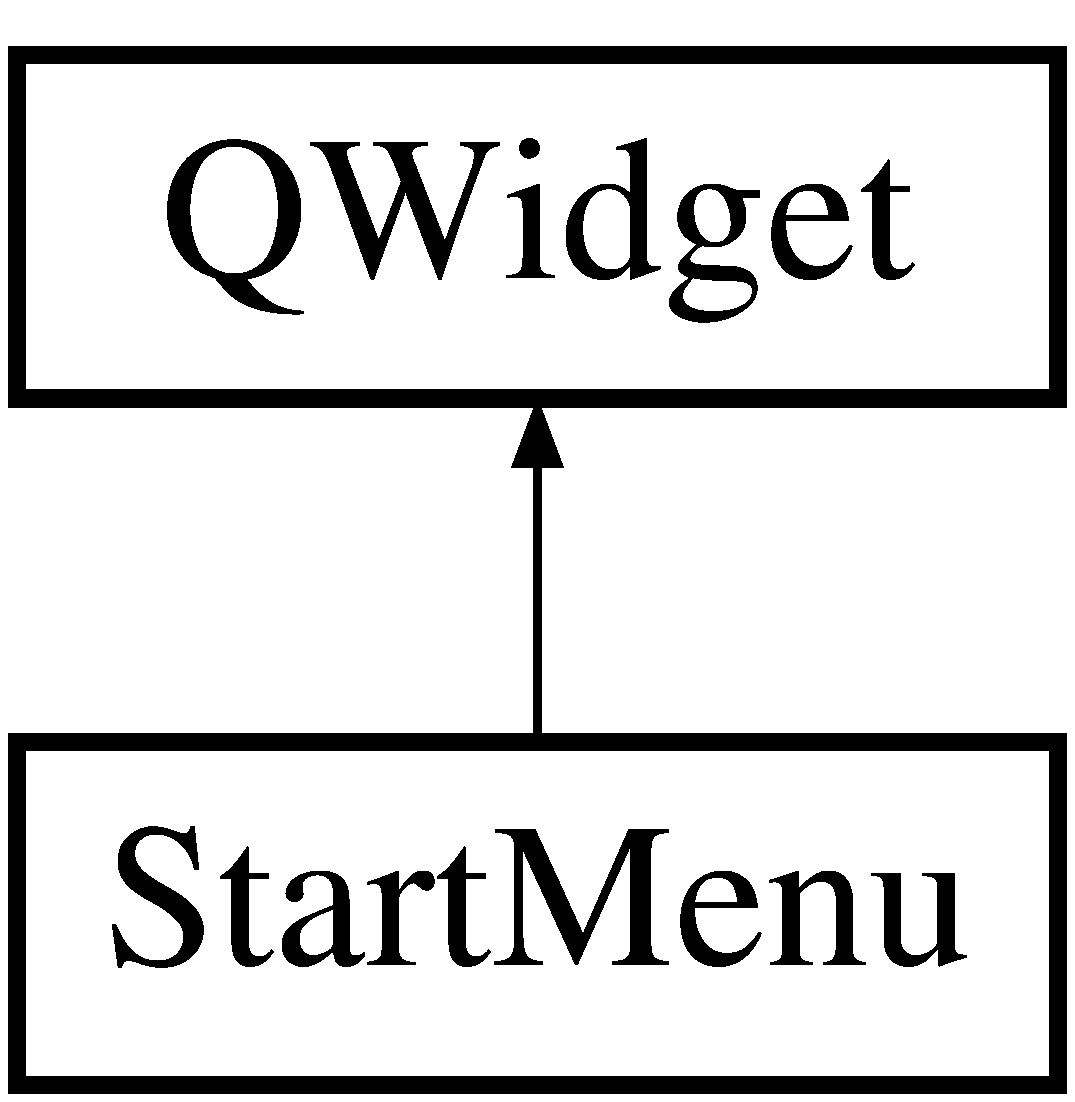
\includegraphics[height=2.000000cm]{classStartMenu}
\end{center}
\end{figure}
\subsection*{Signals}
\begin{DoxyCompactItemize}
\item 
\hypertarget{classStartMenu_a94d2da8144b5e99707ef5dc1ea588982}{void {\bfseries switch\-To\-New\-Session} ()}\label{classStartMenu_a94d2da8144b5e99707ef5dc1ea588982}

\item 
\hypertarget{classStartMenu_a95881192196673c85ad1dc12df5f9820}{void {\bfseries switch\-To\-Highscore} ()}\label{classStartMenu_a95881192196673c85ad1dc12df5f9820}

\item 
\hypertarget{classStartMenu_aff58f89652b89899b21d40f3188b516d}{void {\bfseries quit\-Game} ()}\label{classStartMenu_aff58f89652b89899b21d40f3188b516d}

\end{DoxyCompactItemize}
\subsection*{Public Member Functions}
\begin{DoxyCompactItemize}
\item 
\hypertarget{classStartMenu_a1491fb2672b951483f3cfc0594571fbb}{{\bfseries Start\-Menu} (Q\-Widget $\ast$parent=0)}\label{classStartMenu_a1491fb2672b951483f3cfc0594571fbb}

\item 
\hypertarget{classStartMenu_afc4a48db40567e80c6514b0af30d3797}{void {\bfseries change\-Event} (Q\-Event $\ast$event)}\label{classStartMenu_afc4a48db40567e80c6514b0af30d3797}

\end{DoxyCompactItemize}


The documentation for this class was generated from the following files\-:\begin{DoxyCompactItemize}
\item 
/home/alex/source\-Code/git\-Project/beleg\-Arbeit\-E\-M\-M\-S/project\-Sogo/include/gui/Start\-Menu.\-h\item 
/home/alex/source\-Code/git\-Project/beleg\-Arbeit\-E\-M\-M\-S/project\-Sogo/build-\/sogo\-App-\/\-Desktop\-\_\-\-Qt\-\_\-5\-\_\-6\-\_\-0\-\_\-\-G\-C\-C\-\_\-64bit-\/\-Debug/moc\-\_\-\-Start\-Menu.\-cpp\item 
/home/alex/source\-Code/git\-Project/beleg\-Arbeit\-E\-M\-M\-S/project\-Sogo/src/gui/Start\-Menu.\-cpp\end{DoxyCompactItemize}

\hypertarget{structglm_1_1detail_1_1__swizzle__base2_3_01ValueType_00_01VecType_00_01N_00_01E0_00_01E1_00_01E2_00_01E3_00_011_01_4_1_1Stub}{\section{glm\-:\-:detail\-:\-:\-\_\-swizzle\-\_\-base2$<$ Value\-Type, Vec\-Type, N, E0, E1, E2, E3, 1 $>$\-:\-:Stub Struct Reference}
\label{structglm_1_1detail_1_1__swizzle__base2_3_01ValueType_00_01VecType_00_01N_00_01E0_00_01E1_00_01E2_00_01E3_00_011_01_4_1_1Stub}\index{glm\-::detail\-::\-\_\-swizzle\-\_\-base2$<$ Value\-Type, Vec\-Type, N, E0, E1, E2, E3, 1 $>$\-::\-Stub@{glm\-::detail\-::\-\_\-swizzle\-\_\-base2$<$ Value\-Type, Vec\-Type, N, E0, E1, E2, E3, 1 $>$\-::\-Stub}}
}


The documentation for this struct was generated from the following file\-:\begin{DoxyCompactItemize}
\item 
/home/alex/source\-Code/git\-Project/beleg\-Arbeit\-E\-M\-M\-S/project\-Sogo/external/glm-\/0.\-9.\-4.\-0/glm/core/\hyperlink{__swizzle_8hpp}{\-\_\-swizzle.\-hpp}\end{DoxyCompactItemize}

\hypertarget{classSubject}{\section{Subject Class Reference}
\label{classSubject}\index{Subject@{Subject}}
}


The \hyperlink{classSubject}{Subject} class.  




{\ttfamily \#include $<$Subject.\-h$>$}

\subsection*{Public Member Functions}
\begin{DoxyCompactItemize}
\item 
\hypertarget{classSubject_ab468044832c824c6d6c2f46272655207}{\hyperlink{classSubject_ab468044832c824c6d6c2f46272655207}{Subject} ()}\label{classSubject_ab468044832c824c6d6c2f46272655207}

\begin{DoxyCompactList}\small\item\em \hyperlink{classSubject}{Subject}. \end{DoxyCompactList}\item 
\hypertarget{classSubject_ae5980067d5ec5522db5a0d78100a34be}{virtual \hyperlink{classSubject_ae5980067d5ec5522db5a0d78100a34be}{$\sim$\-Subject} ()}\label{classSubject_ae5980067d5ec5522db5a0d78100a34be}

\begin{DoxyCompactList}\small\item\em $\sim$\-Subject \end{DoxyCompactList}\item 
void \hyperlink{classSubject_ad093a7ac7fea38b82f5cc333916d4a90}{Add\-Listener} (\hyperlink{classIObserver}{I\-Observer} $\ast$obs)
\begin{DoxyCompactList}\small\item\em Add\-Listener Adds an observer to the observer list. \end{DoxyCompactList}\end{DoxyCompactItemize}
\subsection*{Protected Member Functions}
\begin{DoxyCompactItemize}
\item 
\hypertarget{classSubject_ad047f9358b9d199bca40fc5f62a26fc0}{virtual void \hyperlink{classSubject_ad047f9358b9d199bca40fc5f62a26fc0}{Notify\-All\-Observer} ()}\label{classSubject_ad047f9358b9d199bca40fc5f62a26fc0}

\begin{DoxyCompactList}\small\item\em Notify\-All\-Observer Used to Notify all observers observing this subject. \end{DoxyCompactList}\end{DoxyCompactItemize}


\subsection{Detailed Description}
The \hyperlink{classSubject}{Subject} class. 

\subsection{Member Function Documentation}
\hypertarget{classSubject_ad093a7ac7fea38b82f5cc333916d4a90}{\index{Subject@{Subject}!Add\-Listener@{Add\-Listener}}
\index{Add\-Listener@{Add\-Listener}!Subject@{Subject}}
\subsubsection[{Add\-Listener}]{\setlength{\rightskip}{0pt plus 5cm}void Subject\-::\-Add\-Listener (
\begin{DoxyParamCaption}
\item[{{\bf I\-Observer} $\ast$}]{obs}
\end{DoxyParamCaption}
)\hspace{0.3cm}{\ttfamily [inline]}}}\label{classSubject_ad093a7ac7fea38b82f5cc333916d4a90}


Add\-Listener Adds an observer to the observer list. 


\begin{DoxyParams}{Parameters}
{\em obs} & observer to be added \\
\hline
\end{DoxyParams}

\hypertarget{structglm_1_1detail_1_1swizzle}{\section{glm\-:\-:detail\-:\-:swizzle$<$ N, Value\-Type, Vec\-Type, E0, E1, E2, E3 $>$ Struct Template Reference}
\label{structglm_1_1detail_1_1swizzle}\index{glm\-::detail\-::swizzle$<$ N, Value\-Type, Vec\-Type, E0, E1, E2, E3 $>$@{glm\-::detail\-::swizzle$<$ N, Value\-Type, Vec\-Type, E0, E1, E2, E3 $>$}}
}
Inheritance diagram for glm\-:\-:detail\-:\-:swizzle$<$ N, Value\-Type, Vec\-Type, E0, E1, E2, E3 $>$\-:\begin{figure}[H]
\begin{center}
\leavevmode
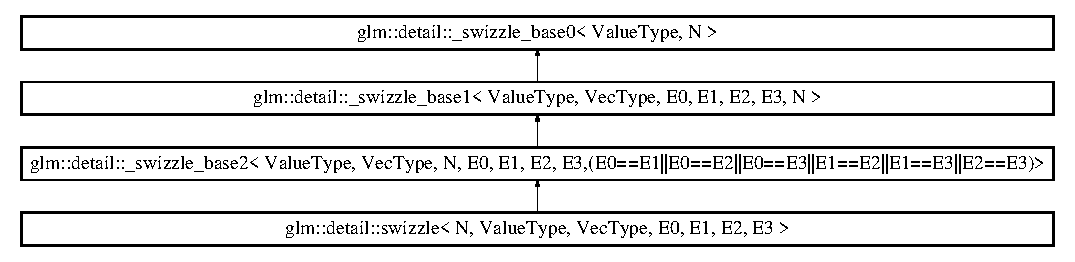
\includegraphics[height=3.072702cm]{structglm_1_1detail_1_1swizzle}
\end{center}
\end{figure}
\subsection*{Public Types}
\begin{DoxyCompactItemize}
\item 
\hypertarget{structglm_1_1detail_1_1swizzle_a6f5b33550379282023990c48c29162f6}{typedef \hyperlink{structglm_1_1detail_1_1__swizzle__base2}{\-\_\-swizzle\-\_\-base2}\\*
$<$ Value\-Type, Vec\-Type, N, E0, \\*
E1, E2, E3,(E0==E1$\vert$$\vert$E0==E2$\vert$$\vert$E0==E3$\vert$$\vert$E1==E2$\vert$$\vert$E1==E3$\vert$$\vert$E2==E3)$>$ {\bfseries base\-\_\-type}}\label{structglm_1_1detail_1_1swizzle_a6f5b33550379282023990c48c29162f6}

\end{DoxyCompactItemize}
\subsection*{Public Member Functions}
\begin{DoxyCompactItemize}
\item 
\hypertarget{structglm_1_1detail_1_1swizzle_ac290a0b7725247c5971c8fb91f28992b}{{\bfseries operator Vec\-Type} () const }\label{structglm_1_1detail_1_1swizzle_ac290a0b7725247c5971c8fb91f28992b}

\end{DoxyCompactItemize}
\subsection*{Additional Inherited Members}


The documentation for this struct was generated from the following file\-:\begin{DoxyCompactItemize}
\item 
/home/alex/source\-Code/git\-Project/beleg\-Arbeit\-E\-M\-M\-S/project\-Sogo/external/glm-\/0.\-9.\-4.\-0/glm/core/\hyperlink{__swizzle_8hpp}{\-\_\-swizzle.\-hpp}\end{DoxyCompactItemize}

\hypertarget{structglm_1_1detail_1_1tmat2x2}{\section{glm\-:\-:detail\-:\-:tmat2x2$<$ T $>$ Struct Template Reference}
\label{structglm_1_1detail_1_1tmat2x2}\index{glm\-::detail\-::tmat2x2$<$ T $>$@{glm\-::detail\-::tmat2x2$<$ T $>$}}
}
\subsection*{Public Types}
\begin{DoxyCompactItemize}
\item 
enum {\bfseries ctor} \{ {\bfseries null}
 \}
\item 
\hypertarget{structglm_1_1detail_1_1tmat2x2_a641e6543d449412404748b194b372953}{typedef T {\bfseries value\-\_\-type}}\label{structglm_1_1detail_1_1tmat2x2_a641e6543d449412404748b194b372953}

\item 
\hypertarget{structglm_1_1detail_1_1tmat2x2_a163dd06a3bcd80dd5a86bc35925867af}{typedef std\-::size\-\_\-t {\bfseries size\-\_\-type}}\label{structglm_1_1detail_1_1tmat2x2_a163dd06a3bcd80dd5a86bc35925867af}

\item 
\hypertarget{structglm_1_1detail_1_1tmat2x2_afd8b7236cdfe29f322a30e163b9da7b1}{typedef \hyperlink{structglm_1_1detail_1_1tvec2}{tvec2}$<$ T $>$ {\bfseries col\-\_\-type}}\label{structglm_1_1detail_1_1tmat2x2_afd8b7236cdfe29f322a30e163b9da7b1}

\item 
\hypertarget{structglm_1_1detail_1_1tmat2x2_a7ab3ca17953ea72efed9271f30de08e8}{typedef \hyperlink{structglm_1_1detail_1_1tvec2}{tvec2}$<$ T $>$ {\bfseries row\-\_\-type}}\label{structglm_1_1detail_1_1tmat2x2_a7ab3ca17953ea72efed9271f30de08e8}

\item 
\hypertarget{structglm_1_1detail_1_1tmat2x2_a9e5bfd239841b712a1df76ea21ed8558}{typedef \hyperlink{structglm_1_1detail_1_1tmat2x2}{tmat2x2}$<$ T $>$ {\bfseries type}}\label{structglm_1_1detail_1_1tmat2x2_a9e5bfd239841b712a1df76ea21ed8558}

\item 
\hypertarget{structglm_1_1detail_1_1tmat2x2_a7feb574422f7b9bf73983cc361ffc845}{typedef \hyperlink{structglm_1_1detail_1_1tmat2x2}{tmat2x2}$<$ T $>$ {\bfseries transpose\-\_\-type}}\label{structglm_1_1detail_1_1tmat2x2_a7feb574422f7b9bf73983cc361ffc845}

\end{DoxyCompactItemize}
\subsection*{Public Member Functions}
\begin{DoxyCompactItemize}
\item 
\hypertarget{structglm_1_1detail_1_1tmat2x2_a533f51f175c66b820f2794b018c6ab46}{G\-L\-M\-\_\-\-F\-U\-N\-C\-\_\-\-D\-E\-C\-L G\-L\-M\-\_\-\-C\-O\-N\-S\-T\-E\-X\-P\-R \\*
size\-\_\-type {\bfseries length} () const }\label{structglm_1_1detail_1_1tmat2x2_a533f51f175c66b820f2794b018c6ab46}

\item 
\hypertarget{structglm_1_1detail_1_1tmat2x2_a40d83f7f92111204f47b99d3416edc7f}{G\-L\-M\-\_\-\-F\-U\-N\-C\-\_\-\-D\-E\-C\-L \hyperlink{structglm_1_1detail_1_1tmat2x2}{tmat2x2}$<$ T $>$ {\bfseries \-\_\-inverse} () const }\label{structglm_1_1detail_1_1tmat2x2_a40d83f7f92111204f47b99d3416edc7f}

\item 
\hypertarget{structglm_1_1detail_1_1tmat2x2_a3af20d808ee9aa41d24998c5cc067bc0}{G\-L\-M\-\_\-\-F\-U\-N\-C\-\_\-\-D\-E\-C\-L {\bfseries tmat2x2} (\hyperlink{structglm_1_1detail_1_1tmat2x2}{tmat2x2} const \&m)}\label{structglm_1_1detail_1_1tmat2x2_a3af20d808ee9aa41d24998c5cc067bc0}

\item 
\hypertarget{structglm_1_1detail_1_1tmat2x2_a8f4070e1c3bfd05568b2dd2fddcaffae}{G\-L\-M\-\_\-\-F\-U\-N\-C\-\_\-\-D\-E\-C\-L {\bfseries tmat2x2} (ctor Null)}\label{structglm_1_1detail_1_1tmat2x2_a8f4070e1c3bfd05568b2dd2fddcaffae}

\item 
\hypertarget{structglm_1_1detail_1_1tmat2x2_a57f8c79a1f8df9214a4357b2b1952ff2}{G\-L\-M\-\_\-\-F\-U\-N\-C\-\_\-\-D\-E\-C\-L {\bfseries tmat2x2} (value\-\_\-type const \&x)}\label{structglm_1_1detail_1_1tmat2x2_a57f8c79a1f8df9214a4357b2b1952ff2}

\item 
\hypertarget{structglm_1_1detail_1_1tmat2x2_a846f370292295c373888c00dc63db0c3}{G\-L\-M\-\_\-\-F\-U\-N\-C\-\_\-\-D\-E\-C\-L {\bfseries tmat2x2} (value\-\_\-type const \&x1, value\-\_\-type const \&y1, value\-\_\-type const \&x2, value\-\_\-type const \&y2)}\label{structglm_1_1detail_1_1tmat2x2_a846f370292295c373888c00dc63db0c3}

\item 
\hypertarget{structglm_1_1detail_1_1tmat2x2_a3b1111723d77e85f6f836e6fec22d0d3}{G\-L\-M\-\_\-\-F\-U\-N\-C\-\_\-\-D\-E\-C\-L {\bfseries tmat2x2} (\hyperlink{structglm_1_1detail_1_1tvec2}{col\-\_\-type} const \&v1, \hyperlink{structglm_1_1detail_1_1tvec2}{col\-\_\-type} const \&v2)}\label{structglm_1_1detail_1_1tmat2x2_a3b1111723d77e85f6f836e6fec22d0d3}

\item 
\hypertarget{structglm_1_1detail_1_1tmat2x2_aeb6edeadf2a08e18438d845139c6c0fd}{{\footnotesize template$<$typename U $>$ }\\G\-L\-M\-\_\-\-F\-U\-N\-C\-\_\-\-D\-E\-C\-L {\bfseries tmat2x2} (U const \&x)}\label{structglm_1_1detail_1_1tmat2x2_aeb6edeadf2a08e18438d845139c6c0fd}

\item 
\hypertarget{structglm_1_1detail_1_1tmat2x2_a6d7150d2d56275f0286fe5bdbf57c004}{{\footnotesize template$<$typename U , typename V , typename M , typename N $>$ }\\G\-L\-M\-\_\-\-F\-U\-N\-C\-\_\-\-D\-E\-C\-L {\bfseries tmat2x2} (U const \&x1, V const \&y1, M const \&x2, N const \&y2)}\label{structglm_1_1detail_1_1tmat2x2_a6d7150d2d56275f0286fe5bdbf57c004}

\item 
\hypertarget{structglm_1_1detail_1_1tmat2x2_a050865e2f51e62b964feda65c528dc17}{{\footnotesize template$<$typename U , typename V $>$ }\\G\-L\-M\-\_\-\-F\-U\-N\-C\-\_\-\-D\-E\-C\-L {\bfseries tmat2x2} (\hyperlink{structglm_1_1detail_1_1tvec2}{tvec2}$<$ U $>$ const \&v1, \hyperlink{structglm_1_1detail_1_1tvec2}{tvec2}$<$ V $>$ const \&v2)}\label{structglm_1_1detail_1_1tmat2x2_a050865e2f51e62b964feda65c528dc17}

\item 
\hypertarget{structglm_1_1detail_1_1tmat2x2_a5c569df8414a3a9ce961be72af41369f}{{\footnotesize template$<$typename U $>$ }\\G\-L\-M\-\_\-\-F\-U\-N\-C\-\_\-\-D\-E\-C\-L {\bfseries tmat2x2} (\hyperlink{structglm_1_1detail_1_1tmat2x2}{tmat2x2}$<$ U $>$ const \&m)}\label{structglm_1_1detail_1_1tmat2x2_a5c569df8414a3a9ce961be72af41369f}

\item 
\hypertarget{structglm_1_1detail_1_1tmat2x2_ae1edb9d6f575dae334a56cb4e0bc1d30}{G\-L\-M\-\_\-\-F\-U\-N\-C\-\_\-\-D\-E\-C\-L {\bfseries tmat2x2} (\hyperlink{structglm_1_1detail_1_1tmat3x3}{tmat3x3}$<$ T $>$ const \&x)}\label{structglm_1_1detail_1_1tmat2x2_ae1edb9d6f575dae334a56cb4e0bc1d30}

\item 
\hypertarget{structglm_1_1detail_1_1tmat2x2_a28b0e13e8cb74488c421f5ed8abc22a3}{G\-L\-M\-\_\-\-F\-U\-N\-C\-\_\-\-D\-E\-C\-L {\bfseries tmat2x2} (\hyperlink{structglm_1_1detail_1_1tmat4x4}{tmat4x4}$<$ T $>$ const \&x)}\label{structglm_1_1detail_1_1tmat2x2_a28b0e13e8cb74488c421f5ed8abc22a3}

\item 
\hypertarget{structglm_1_1detail_1_1tmat2x2_a74699d8e40847709fd239f3f6f920ffc}{G\-L\-M\-\_\-\-F\-U\-N\-C\-\_\-\-D\-E\-C\-L {\bfseries tmat2x2} (\hyperlink{structglm_1_1detail_1_1tmat2x3}{tmat2x3}$<$ T $>$ const \&x)}\label{structglm_1_1detail_1_1tmat2x2_a74699d8e40847709fd239f3f6f920ffc}

\item 
\hypertarget{structglm_1_1detail_1_1tmat2x2_a234059aee97c74e65a145bb715c0111e}{G\-L\-M\-\_\-\-F\-U\-N\-C\-\_\-\-D\-E\-C\-L {\bfseries tmat2x2} (\hyperlink{structglm_1_1detail_1_1tmat3x2}{tmat3x2}$<$ T $>$ const \&x)}\label{structglm_1_1detail_1_1tmat2x2_a234059aee97c74e65a145bb715c0111e}

\item 
\hypertarget{structglm_1_1detail_1_1tmat2x2_a1219a9df95266dc799fe8a5baef4a7e6}{G\-L\-M\-\_\-\-F\-U\-N\-C\-\_\-\-D\-E\-C\-L {\bfseries tmat2x2} (\hyperlink{structglm_1_1detail_1_1tmat2x4}{tmat2x4}$<$ T $>$ const \&x)}\label{structglm_1_1detail_1_1tmat2x2_a1219a9df95266dc799fe8a5baef4a7e6}

\item 
\hypertarget{structglm_1_1detail_1_1tmat2x2_af78e67336561256f2b026d48f5a8bdd5}{G\-L\-M\-\_\-\-F\-U\-N\-C\-\_\-\-D\-E\-C\-L {\bfseries tmat2x2} (\hyperlink{structglm_1_1detail_1_1tmat4x2}{tmat4x2}$<$ T $>$ const \&x)}\label{structglm_1_1detail_1_1tmat2x2_af78e67336561256f2b026d48f5a8bdd5}

\item 
\hypertarget{structglm_1_1detail_1_1tmat2x2_a579557cee38df3588186ed16ea61c8bf}{G\-L\-M\-\_\-\-F\-U\-N\-C\-\_\-\-D\-E\-C\-L {\bfseries tmat2x2} (\hyperlink{structglm_1_1detail_1_1tmat3x4}{tmat3x4}$<$ T $>$ const \&x)}\label{structglm_1_1detail_1_1tmat2x2_a579557cee38df3588186ed16ea61c8bf}

\item 
\hypertarget{structglm_1_1detail_1_1tmat2x2_a1b8e6c630ddeb39369d9c3562b1a68b9}{G\-L\-M\-\_\-\-F\-U\-N\-C\-\_\-\-D\-E\-C\-L {\bfseries tmat2x2} (\hyperlink{structglm_1_1detail_1_1tmat4x3}{tmat4x3}$<$ T $>$ const \&x)}\label{structglm_1_1detail_1_1tmat2x2_a1b8e6c630ddeb39369d9c3562b1a68b9}

\item 
\hypertarget{structglm_1_1detail_1_1tmat2x2_af61c5360347e4283bfd682fede74d6e7}{G\-L\-M\-\_\-\-F\-U\-N\-C\-\_\-\-D\-E\-C\-L \hyperlink{structglm_1_1detail_1_1tvec2}{col\-\_\-type} \& {\bfseries operator\mbox{[}$\,$\mbox{]}} (size\-\_\-type i)}\label{structglm_1_1detail_1_1tmat2x2_af61c5360347e4283bfd682fede74d6e7}

\item 
\hypertarget{structglm_1_1detail_1_1tmat2x2_a074e61b27b42d0678fbb7edf85483edb}{G\-L\-M\-\_\-\-F\-U\-N\-C\-\_\-\-D\-E\-C\-L \hyperlink{structglm_1_1detail_1_1tvec2}{col\-\_\-type} const \& {\bfseries operator\mbox{[}$\,$\mbox{]}} (size\-\_\-type i) const }\label{structglm_1_1detail_1_1tmat2x2_a074e61b27b42d0678fbb7edf85483edb}

\item 
\hypertarget{structglm_1_1detail_1_1tmat2x2_a9df009dce8bbc63128b7c75f8f3a64f4}{G\-L\-M\-\_\-\-F\-U\-N\-C\-\_\-\-D\-E\-C\-L \hyperlink{structglm_1_1detail_1_1tmat2x2}{tmat2x2}$<$ T $>$ \& {\bfseries operator=} (\hyperlink{structglm_1_1detail_1_1tmat2x2}{tmat2x2}$<$ T $>$ const \&m)}\label{structglm_1_1detail_1_1tmat2x2_a9df009dce8bbc63128b7c75f8f3a64f4}

\item 
\hypertarget{structglm_1_1detail_1_1tmat2x2_a160e32c3fb95140823bf63efc757a635}{{\footnotesize template$<$typename U $>$ }\\G\-L\-M\-\_\-\-F\-U\-N\-C\-\_\-\-D\-E\-C\-L \hyperlink{structglm_1_1detail_1_1tmat2x2}{tmat2x2}$<$ T $>$ \& {\bfseries operator=} (\hyperlink{structglm_1_1detail_1_1tmat2x2}{tmat2x2}$<$ U $>$ const \&m)}\label{structglm_1_1detail_1_1tmat2x2_a160e32c3fb95140823bf63efc757a635}

\item 
\hypertarget{structglm_1_1detail_1_1tmat2x2_a1bcaf856c6b8eefbc44c2158101ce292}{{\footnotesize template$<$typename U $>$ }\\G\-L\-M\-\_\-\-F\-U\-N\-C\-\_\-\-D\-E\-C\-L \hyperlink{structglm_1_1detail_1_1tmat2x2}{tmat2x2}$<$ T $>$ \& {\bfseries operator+=} (U const \&s)}\label{structglm_1_1detail_1_1tmat2x2_a1bcaf856c6b8eefbc44c2158101ce292}

\item 
\hypertarget{structglm_1_1detail_1_1tmat2x2_a378a8fa1e71d81d423f619271751d3e4}{{\footnotesize template$<$typename U $>$ }\\G\-L\-M\-\_\-\-F\-U\-N\-C\-\_\-\-D\-E\-C\-L \hyperlink{structglm_1_1detail_1_1tmat2x2}{tmat2x2}$<$ T $>$ \& {\bfseries operator+=} (\hyperlink{structglm_1_1detail_1_1tmat2x2}{tmat2x2}$<$ U $>$ const \&m)}\label{structglm_1_1detail_1_1tmat2x2_a378a8fa1e71d81d423f619271751d3e4}

\item 
\hypertarget{structglm_1_1detail_1_1tmat2x2_af74e7c76c58ae2e2a59d0ff1db7fbe6e}{{\footnotesize template$<$typename U $>$ }\\G\-L\-M\-\_\-\-F\-U\-N\-C\-\_\-\-D\-E\-C\-L \hyperlink{structglm_1_1detail_1_1tmat2x2}{tmat2x2}$<$ T $>$ \& {\bfseries operator-\/=} (U const \&s)}\label{structglm_1_1detail_1_1tmat2x2_af74e7c76c58ae2e2a59d0ff1db7fbe6e}

\item 
\hypertarget{structglm_1_1detail_1_1tmat2x2_aa595ffa2296312bbb109af5c5701fd9d}{{\footnotesize template$<$typename U $>$ }\\G\-L\-M\-\_\-\-F\-U\-N\-C\-\_\-\-D\-E\-C\-L \hyperlink{structglm_1_1detail_1_1tmat2x2}{tmat2x2}$<$ T $>$ \& {\bfseries operator-\/=} (\hyperlink{structglm_1_1detail_1_1tmat2x2}{tmat2x2}$<$ U $>$ const \&m)}\label{structglm_1_1detail_1_1tmat2x2_aa595ffa2296312bbb109af5c5701fd9d}

\item 
\hypertarget{structglm_1_1detail_1_1tmat2x2_a33a00a31a0c777b09143cef2f1bd6a52}{{\footnotesize template$<$typename U $>$ }\\G\-L\-M\-\_\-\-F\-U\-N\-C\-\_\-\-D\-E\-C\-L \hyperlink{structglm_1_1detail_1_1tmat2x2}{tmat2x2}$<$ T $>$ \& {\bfseries operator$\ast$=} (U const \&s)}\label{structglm_1_1detail_1_1tmat2x2_a33a00a31a0c777b09143cef2f1bd6a52}

\item 
\hypertarget{structglm_1_1detail_1_1tmat2x2_a2c7a033623107e6feb21bb3b51913377}{{\footnotesize template$<$typename U $>$ }\\G\-L\-M\-\_\-\-F\-U\-N\-C\-\_\-\-D\-E\-C\-L \hyperlink{structglm_1_1detail_1_1tmat2x2}{tmat2x2}$<$ T $>$ \& {\bfseries operator$\ast$=} (\hyperlink{structglm_1_1detail_1_1tmat2x2}{tmat2x2}$<$ U $>$ const \&m)}\label{structglm_1_1detail_1_1tmat2x2_a2c7a033623107e6feb21bb3b51913377}

\item 
\hypertarget{structglm_1_1detail_1_1tmat2x2_a37c08f89d47be0279f96489239fb20f8}{{\footnotesize template$<$typename U $>$ }\\G\-L\-M\-\_\-\-F\-U\-N\-C\-\_\-\-D\-E\-C\-L \hyperlink{structglm_1_1detail_1_1tmat2x2}{tmat2x2}$<$ T $>$ \& {\bfseries operator/=} (U const \&s)}\label{structglm_1_1detail_1_1tmat2x2_a37c08f89d47be0279f96489239fb20f8}

\item 
\hypertarget{structglm_1_1detail_1_1tmat2x2_a9aab21954e48429c64d062331d01a486}{{\footnotesize template$<$typename U $>$ }\\G\-L\-M\-\_\-\-F\-U\-N\-C\-\_\-\-D\-E\-C\-L \hyperlink{structglm_1_1detail_1_1tmat2x2}{tmat2x2}$<$ T $>$ \& {\bfseries operator/=} (\hyperlink{structglm_1_1detail_1_1tmat2x2}{tmat2x2}$<$ U $>$ const \&m)}\label{structglm_1_1detail_1_1tmat2x2_a9aab21954e48429c64d062331d01a486}

\item 
\hypertarget{structglm_1_1detail_1_1tmat2x2_a04457c562f83f2f5d34bc5fa574faa17}{G\-L\-M\-\_\-\-F\-U\-N\-C\-\_\-\-D\-E\-C\-L \hyperlink{structglm_1_1detail_1_1tmat2x2}{tmat2x2}$<$ T $>$ \& {\bfseries operator++} ()}\label{structglm_1_1detail_1_1tmat2x2_a04457c562f83f2f5d34bc5fa574faa17}

\item 
\hypertarget{structglm_1_1detail_1_1tmat2x2_a31bbbcc16ab65eef93820ebce0cfed5f}{G\-L\-M\-\_\-\-F\-U\-N\-C\-\_\-\-D\-E\-C\-L \hyperlink{structglm_1_1detail_1_1tmat2x2}{tmat2x2}$<$ T $>$ \& {\bfseries operator-\/-\/} ()}\label{structglm_1_1detail_1_1tmat2x2_a31bbbcc16ab65eef93820ebce0cfed5f}

\item 
\hypertarget{structglm_1_1detail_1_1tmat2x2_a156ed12a043a58be23c0ca52a96f3ad6}{{\footnotesize template$<$typename X1 , typename Y1 , typename X2 , typename Y2 $>$ }\\G\-L\-M\-\_\-\-F\-U\-N\-C\-\_\-\-D\-E\-C\-L {\bfseries tmat2x2} (X1 const \&x1, Y1 const \&y1, X2 const \&x2, Y2 const \&y2)}\label{structglm_1_1detail_1_1tmat2x2_a156ed12a043a58be23c0ca52a96f3ad6}

\item 
\hypertarget{structglm_1_1detail_1_1tmat2x2_a5917090f191c8bd7ecbe81e369819e8a}{{\footnotesize template$<$typename V1 , typename V2 $>$ }\\G\-L\-M\-\_\-\-F\-U\-N\-C\-\_\-\-D\-E\-C\-L {\bfseries tmat2x2} (\hyperlink{structglm_1_1detail_1_1tvec2}{tvec2}$<$ V1 $>$ const \&v1, \hyperlink{structglm_1_1detail_1_1tvec2}{tvec2}$<$ V2 $>$ const \&v2)}\label{structglm_1_1detail_1_1tmat2x2_a5917090f191c8bd7ecbe81e369819e8a}

\item 
\hypertarget{structglm_1_1detail_1_1tmat2x2_a585d4b0bc985e4fa2f078000743972bb}{{\footnotesize template$<$typename U $>$ }\\G\-L\-M\-\_\-\-F\-U\-N\-C\-\_\-\-Q\-U\-A\-L\-I\-F\-I\-E\-R {\bfseries tmat2x2} (\hyperlink{structglm_1_1detail_1_1tmat2x2}{tmat2x2}$<$ U $>$ const \&m)}\label{structglm_1_1detail_1_1tmat2x2_a585d4b0bc985e4fa2f078000743972bb}

\item 
\hypertarget{structglm_1_1detail_1_1tmat2x2_a520a2abf2e623dcbfc6af9c1b4d41206}{{\footnotesize template$<$typename U $>$ }\\G\-L\-M\-\_\-\-F\-U\-N\-C\-\_\-\-Q\-U\-A\-L\-I\-F\-I\-E\-R \hyperlink{structglm_1_1detail_1_1tmat2x2}{tmat2x2}$<$ T $>$ \& {\bfseries operator=} (\hyperlink{structglm_1_1detail_1_1tmat2x2}{tmat2x2}$<$ U $>$ const \&m)}\label{structglm_1_1detail_1_1tmat2x2_a520a2abf2e623dcbfc6af9c1b4d41206}

\item 
\hypertarget{structglm_1_1detail_1_1tmat2x2_af03e41d83e503acff6fd07644c2aea26}{{\footnotesize template$<$typename U $>$ }\\G\-L\-M\-\_\-\-F\-U\-N\-C\-\_\-\-Q\-U\-A\-L\-I\-F\-I\-E\-R \hyperlink{structglm_1_1detail_1_1tmat2x2}{tmat2x2}$<$ T $>$ \& {\bfseries operator+=} (U const \&s)}\label{structglm_1_1detail_1_1tmat2x2_af03e41d83e503acff6fd07644c2aea26}

\item 
\hypertarget{structglm_1_1detail_1_1tmat2x2_ad8f2e4617586dd78afebde4c3ff8def8}{{\footnotesize template$<$typename U $>$ }\\G\-L\-M\-\_\-\-F\-U\-N\-C\-\_\-\-Q\-U\-A\-L\-I\-F\-I\-E\-R \hyperlink{structglm_1_1detail_1_1tmat2x2}{tmat2x2}$<$ T $>$ \& {\bfseries operator+=} (\hyperlink{structglm_1_1detail_1_1tmat2x2}{tmat2x2}$<$ U $>$ const \&m)}\label{structglm_1_1detail_1_1tmat2x2_ad8f2e4617586dd78afebde4c3ff8def8}

\item 
\hypertarget{structglm_1_1detail_1_1tmat2x2_ab20e83c652d9c2b82bb543129b1e4347}{{\footnotesize template$<$typename U $>$ }\\G\-L\-M\-\_\-\-F\-U\-N\-C\-\_\-\-Q\-U\-A\-L\-I\-F\-I\-E\-R \hyperlink{structglm_1_1detail_1_1tmat2x2}{tmat2x2}$<$ T $>$ \& {\bfseries operator-\/=} (U const \&s)}\label{structglm_1_1detail_1_1tmat2x2_ab20e83c652d9c2b82bb543129b1e4347}

\item 
\hypertarget{structglm_1_1detail_1_1tmat2x2_aca7986f1e088343368506dba60a8533b}{{\footnotesize template$<$typename U $>$ }\\G\-L\-M\-\_\-\-F\-U\-N\-C\-\_\-\-Q\-U\-A\-L\-I\-F\-I\-E\-R \hyperlink{structglm_1_1detail_1_1tmat2x2}{tmat2x2}$<$ T $>$ \& {\bfseries operator-\/=} (\hyperlink{structglm_1_1detail_1_1tmat2x2}{tmat2x2}$<$ U $>$ const \&m)}\label{structglm_1_1detail_1_1tmat2x2_aca7986f1e088343368506dba60a8533b}

\item 
\hypertarget{structglm_1_1detail_1_1tmat2x2_afaaac2e6f990ac871b0e4aa01c08ed34}{{\footnotesize template$<$typename U $>$ }\\G\-L\-M\-\_\-\-F\-U\-N\-C\-\_\-\-Q\-U\-A\-L\-I\-F\-I\-E\-R \hyperlink{structglm_1_1detail_1_1tmat2x2}{tmat2x2}$<$ T $>$ \& {\bfseries operator$\ast$=} (U const \&s)}\label{structglm_1_1detail_1_1tmat2x2_afaaac2e6f990ac871b0e4aa01c08ed34}

\item 
\hypertarget{structglm_1_1detail_1_1tmat2x2_a2d9a4891fbdc71f886ecbb3374a6c13d}{{\footnotesize template$<$typename U $>$ }\\G\-L\-M\-\_\-\-F\-U\-N\-C\-\_\-\-Q\-U\-A\-L\-I\-F\-I\-E\-R \hyperlink{structglm_1_1detail_1_1tmat2x2}{tmat2x2}$<$ T $>$ \& {\bfseries operator$\ast$=} (\hyperlink{structglm_1_1detail_1_1tmat2x2}{tmat2x2}$<$ U $>$ const \&m)}\label{structglm_1_1detail_1_1tmat2x2_a2d9a4891fbdc71f886ecbb3374a6c13d}

\item 
\hypertarget{structglm_1_1detail_1_1tmat2x2_ae1b00b891d297f31bff39ad6cc8ac8a9}{{\footnotesize template$<$typename U $>$ }\\G\-L\-M\-\_\-\-F\-U\-N\-C\-\_\-\-Q\-U\-A\-L\-I\-F\-I\-E\-R \hyperlink{structglm_1_1detail_1_1tmat2x2}{tmat2x2}$<$ T $>$ \& {\bfseries operator/=} (U const \&s)}\label{structglm_1_1detail_1_1tmat2x2_ae1b00b891d297f31bff39ad6cc8ac8a9}

\item 
\hypertarget{structglm_1_1detail_1_1tmat2x2_aec88ffc74ce1e36a0e8cc82aee6c002a}{{\footnotesize template$<$typename U $>$ }\\G\-L\-M\-\_\-\-F\-U\-N\-C\-\_\-\-Q\-U\-A\-L\-I\-F\-I\-E\-R \hyperlink{structglm_1_1detail_1_1tmat2x2}{tmat2x2}$<$ T $>$ \& {\bfseries operator/=} (\hyperlink{structglm_1_1detail_1_1tmat2x2}{tmat2x2}$<$ U $>$ const \&m)}\label{structglm_1_1detail_1_1tmat2x2_aec88ffc74ce1e36a0e8cc82aee6c002a}

\end{DoxyCompactItemize}
\subsection*{Static Public Member Functions}
\begin{DoxyCompactItemize}
\item 
\hypertarget{structglm_1_1detail_1_1tmat2x2_a5c1a631a45f3ea10859433efd7d2c33a}{static G\-L\-M\-\_\-\-F\-U\-N\-C\-\_\-\-D\-E\-C\-L size\-\_\-type {\bfseries col\-\_\-size} ()}\label{structglm_1_1detail_1_1tmat2x2_a5c1a631a45f3ea10859433efd7d2c33a}

\item 
\hypertarget{structglm_1_1detail_1_1tmat2x2_a7b779a0e12e4e42a4372b03562ce7df9}{static G\-L\-M\-\_\-\-F\-U\-N\-C\-\_\-\-D\-E\-C\-L size\-\_\-type {\bfseries row\-\_\-size} ()}\label{structglm_1_1detail_1_1tmat2x2_a7b779a0e12e4e42a4372b03562ce7df9}

\end{DoxyCompactItemize}


The documentation for this struct was generated from the following files\-:\begin{DoxyCompactItemize}
\item 
/home/alex/source\-Code/git\-Project/beleg\-Arbeit\-E\-M\-M\-S/project\-Sogo/external/glm-\/0.\-9.\-4.\-0/glm/core/\hyperlink{type__mat2x2_8hpp}{type\-\_\-mat2x2.\-hpp}\item 
/home/alex/source\-Code/git\-Project/beleg\-Arbeit\-E\-M\-M\-S/project\-Sogo/external/glm-\/0.\-9.\-4.\-0/glm/core/\hyperlink{type__mat2x2_8inl}{type\-\_\-mat2x2.\-inl}\end{DoxyCompactItemize}

\hypertarget{structglm_1_1detail_1_1tmat2x3}{\section{glm\-:\-:detail\-:\-:tmat2x3$<$ T $>$ Struct Template Reference}
\label{structglm_1_1detail_1_1tmat2x3}\index{glm\-::detail\-::tmat2x3$<$ T $>$@{glm\-::detail\-::tmat2x3$<$ T $>$}}
}
\subsection*{Public Types}
\begin{DoxyCompactItemize}
\item 
enum {\bfseries ctor} \{ {\bfseries null}
 \}
\item 
\hypertarget{structglm_1_1detail_1_1tmat2x3_ab77bb1e60a56d5c581cd99f7b26f043d}{typedef T {\bfseries value\-\_\-type}}\label{structglm_1_1detail_1_1tmat2x3_ab77bb1e60a56d5c581cd99f7b26f043d}

\item 
\hypertarget{structglm_1_1detail_1_1tmat2x3_a91c1b2dc1091eac50580ce29901acd4e}{typedef std\-::size\-\_\-t {\bfseries size\-\_\-type}}\label{structglm_1_1detail_1_1tmat2x3_a91c1b2dc1091eac50580ce29901acd4e}

\item 
\hypertarget{structglm_1_1detail_1_1tmat2x3_ad863dfb9ed64dd71938b6ecdad670952}{typedef \hyperlink{structglm_1_1detail_1_1tvec3}{tvec3}$<$ T $>$ {\bfseries col\-\_\-type}}\label{structglm_1_1detail_1_1tmat2x3_ad863dfb9ed64dd71938b6ecdad670952}

\item 
\hypertarget{structglm_1_1detail_1_1tmat2x3_aab44eec185c15e6d1c4e3fb337859036}{typedef \hyperlink{structglm_1_1detail_1_1tvec2}{tvec2}$<$ T $>$ {\bfseries row\-\_\-type}}\label{structglm_1_1detail_1_1tmat2x3_aab44eec185c15e6d1c4e3fb337859036}

\item 
\hypertarget{structglm_1_1detail_1_1tmat2x3_a590472e24db6c9e921961cc2308ae4b5}{typedef \hyperlink{structglm_1_1detail_1_1tmat2x3}{tmat2x3}$<$ T $>$ {\bfseries type}}\label{structglm_1_1detail_1_1tmat2x3_a590472e24db6c9e921961cc2308ae4b5}

\item 
\hypertarget{structglm_1_1detail_1_1tmat2x3_a9c5006407e260fdcd74a6dfae1ac73f5}{typedef \hyperlink{structglm_1_1detail_1_1tmat3x2}{tmat3x2}$<$ T $>$ {\bfseries transpose\-\_\-type}}\label{structglm_1_1detail_1_1tmat2x3_a9c5006407e260fdcd74a6dfae1ac73f5}

\end{DoxyCompactItemize}
\subsection*{Public Member Functions}
\begin{DoxyCompactItemize}
\item 
\hypertarget{structglm_1_1detail_1_1tmat2x3_ad64fb15bec8eacecffd0ba33083ec197}{G\-L\-M\-\_\-\-F\-U\-N\-C\-\_\-\-D\-E\-C\-L G\-L\-M\-\_\-\-C\-O\-N\-S\-T\-E\-X\-P\-R \\*
size\-\_\-type {\bfseries length} () const }\label{structglm_1_1detail_1_1tmat2x3_ad64fb15bec8eacecffd0ba33083ec197}

\item 
\hypertarget{structglm_1_1detail_1_1tmat2x3_a882c554a039fb6f05295d25230876408}{G\-L\-M\-\_\-\-F\-U\-N\-C\-\_\-\-D\-E\-C\-L {\bfseries tmat2x3} (\hyperlink{structglm_1_1detail_1_1tmat2x3}{tmat2x3} const \&m)}\label{structglm_1_1detail_1_1tmat2x3_a882c554a039fb6f05295d25230876408}

\item 
\hypertarget{structglm_1_1detail_1_1tmat2x3_a55e83395bf56965a48cd4604b4644cab}{G\-L\-M\-\_\-\-F\-U\-N\-C\-\_\-\-D\-E\-C\-L {\bfseries tmat2x3} (ctor)}\label{structglm_1_1detail_1_1tmat2x3_a55e83395bf56965a48cd4604b4644cab}

\item 
\hypertarget{structglm_1_1detail_1_1tmat2x3_abf51ec12b9ea2ee650ef0cd4854a85cc}{G\-L\-M\-\_\-\-F\-U\-N\-C\-\_\-\-D\-E\-C\-L {\bfseries tmat2x3} (value\-\_\-type const \&s)}\label{structglm_1_1detail_1_1tmat2x3_abf51ec12b9ea2ee650ef0cd4854a85cc}

\item 
\hypertarget{structglm_1_1detail_1_1tmat2x3_a723c041ca01d0846e7ac1e2cf94fa388}{G\-L\-M\-\_\-\-F\-U\-N\-C\-\_\-\-D\-E\-C\-L {\bfseries tmat2x3} (value\-\_\-type const \&x0, value\-\_\-type const \&y0, value\-\_\-type const \&z0, value\-\_\-type const \&x1, value\-\_\-type const \&y1, value\-\_\-type const \&z1)}\label{structglm_1_1detail_1_1tmat2x3_a723c041ca01d0846e7ac1e2cf94fa388}

\item 
\hypertarget{structglm_1_1detail_1_1tmat2x3_a6219dd710c9dc7a235745543995c2034}{G\-L\-M\-\_\-\-F\-U\-N\-C\-\_\-\-D\-E\-C\-L {\bfseries tmat2x3} (\hyperlink{structglm_1_1detail_1_1tvec3}{col\-\_\-type} const \&v0, \hyperlink{structglm_1_1detail_1_1tvec3}{col\-\_\-type} const \&v1)}\label{structglm_1_1detail_1_1tmat2x3_a6219dd710c9dc7a235745543995c2034}

\item 
\hypertarget{structglm_1_1detail_1_1tmat2x3_ad5c1b77b2c1b21348f3fc31b9efd62b5}{{\footnotesize template$<$typename U $>$ }\\G\-L\-M\-\_\-\-F\-U\-N\-C\-\_\-\-D\-E\-C\-L {\bfseries tmat2x3} (U const \&x)}\label{structglm_1_1detail_1_1tmat2x3_ad5c1b77b2c1b21348f3fc31b9efd62b5}

\item 
\hypertarget{structglm_1_1detail_1_1tmat2x3_a474ba9a15b1b4b89caacf6171cecb7d6}{{\footnotesize template$<$typename X1 , typename Y1 , typename Z1 , typename X2 , typename Y2 , typename Z2 $>$ }\\G\-L\-M\-\_\-\-F\-U\-N\-C\-\_\-\-D\-E\-C\-L {\bfseries tmat2x3} (X1 const \&x1, Y1 const \&y1, Z1 const \&z1, X2 const \&x2, Y2 const \&y2, Z2 const \&z2)}\label{structglm_1_1detail_1_1tmat2x3_a474ba9a15b1b4b89caacf6171cecb7d6}

\item 
\hypertarget{structglm_1_1detail_1_1tmat2x3_adf8f24014d50e180f069b45470fd3efd}{{\footnotesize template$<$typename U , typename V $>$ }\\G\-L\-M\-\_\-\-F\-U\-N\-C\-\_\-\-D\-E\-C\-L {\bfseries tmat2x3} (\hyperlink{structglm_1_1detail_1_1tvec3}{tvec3}$<$ U $>$ const \&v1, \hyperlink{structglm_1_1detail_1_1tvec3}{tvec3}$<$ V $>$ const \&v2)}\label{structglm_1_1detail_1_1tmat2x3_adf8f24014d50e180f069b45470fd3efd}

\item 
\hypertarget{structglm_1_1detail_1_1tmat2x3_a5f81a32da21791aeb89913e58450beec}{{\footnotesize template$<$typename U $>$ }\\G\-L\-M\-\_\-\-F\-U\-N\-C\-\_\-\-D\-E\-C\-L {\bfseries tmat2x3} (\hyperlink{structglm_1_1detail_1_1tmat2x3}{tmat2x3}$<$ U $>$ const \&m)}\label{structglm_1_1detail_1_1tmat2x3_a5f81a32da21791aeb89913e58450beec}

\item 
\hypertarget{structglm_1_1detail_1_1tmat2x3_a4c1b720d52e5b9a9355c20d68cc9d931}{G\-L\-M\-\_\-\-F\-U\-N\-C\-\_\-\-D\-E\-C\-L {\bfseries tmat2x3} (\hyperlink{structglm_1_1detail_1_1tmat2x2}{tmat2x2}$<$ T $>$ const \&x)}\label{structglm_1_1detail_1_1tmat2x3_a4c1b720d52e5b9a9355c20d68cc9d931}

\item 
\hypertarget{structglm_1_1detail_1_1tmat2x3_ad522db54d8643b0b16ba78b0ccf487eb}{G\-L\-M\-\_\-\-F\-U\-N\-C\-\_\-\-D\-E\-C\-L {\bfseries tmat2x3} (\hyperlink{structglm_1_1detail_1_1tmat3x3}{tmat3x3}$<$ T $>$ const \&x)}\label{structglm_1_1detail_1_1tmat2x3_ad522db54d8643b0b16ba78b0ccf487eb}

\item 
\hypertarget{structglm_1_1detail_1_1tmat2x3_a5942442eefd2c06e0dddfa1304680474}{G\-L\-M\-\_\-\-F\-U\-N\-C\-\_\-\-D\-E\-C\-L {\bfseries tmat2x3} (\hyperlink{structglm_1_1detail_1_1tmat4x4}{tmat4x4}$<$ T $>$ const \&x)}\label{structglm_1_1detail_1_1tmat2x3_a5942442eefd2c06e0dddfa1304680474}

\item 
\hypertarget{structglm_1_1detail_1_1tmat2x3_ac67a0bfa428c9adbc3c7a1b32ae0f292}{G\-L\-M\-\_\-\-F\-U\-N\-C\-\_\-\-D\-E\-C\-L {\bfseries tmat2x3} (\hyperlink{structglm_1_1detail_1_1tmat2x4}{tmat2x4}$<$ T $>$ const \&x)}\label{structglm_1_1detail_1_1tmat2x3_ac67a0bfa428c9adbc3c7a1b32ae0f292}

\item 
\hypertarget{structglm_1_1detail_1_1tmat2x3_ac4405d75f2e6cc396ba8a5b857074943}{G\-L\-M\-\_\-\-F\-U\-N\-C\-\_\-\-D\-E\-C\-L {\bfseries tmat2x3} (\hyperlink{structglm_1_1detail_1_1tmat3x2}{tmat3x2}$<$ T $>$ const \&x)}\label{structglm_1_1detail_1_1tmat2x3_ac4405d75f2e6cc396ba8a5b857074943}

\item 
\hypertarget{structglm_1_1detail_1_1tmat2x3_adb82dcc2f875fd2b2d3d6ce05761b0f3}{G\-L\-M\-\_\-\-F\-U\-N\-C\-\_\-\-D\-E\-C\-L {\bfseries tmat2x3} (\hyperlink{structglm_1_1detail_1_1tmat3x4}{tmat3x4}$<$ T $>$ const \&x)}\label{structglm_1_1detail_1_1tmat2x3_adb82dcc2f875fd2b2d3d6ce05761b0f3}

\item 
\hypertarget{structglm_1_1detail_1_1tmat2x3_a189a3e0e88f64eb5dd4b2b836287c1e2}{G\-L\-M\-\_\-\-F\-U\-N\-C\-\_\-\-D\-E\-C\-L {\bfseries tmat2x3} (\hyperlink{structglm_1_1detail_1_1tmat4x2}{tmat4x2}$<$ T $>$ const \&x)}\label{structglm_1_1detail_1_1tmat2x3_a189a3e0e88f64eb5dd4b2b836287c1e2}

\item 
\hypertarget{structglm_1_1detail_1_1tmat2x3_a63060936bb93757759d586cf6e1750cf}{G\-L\-M\-\_\-\-F\-U\-N\-C\-\_\-\-D\-E\-C\-L {\bfseries tmat2x3} (\hyperlink{structglm_1_1detail_1_1tmat4x3}{tmat4x3}$<$ T $>$ const \&x)}\label{structglm_1_1detail_1_1tmat2x3_a63060936bb93757759d586cf6e1750cf}

\item 
\hypertarget{structglm_1_1detail_1_1tmat2x3_a7fa88813ee0581af8aed78ca20e7a0a1}{\hyperlink{structglm_1_1detail_1_1tvec3}{col\-\_\-type} \& {\bfseries operator\mbox{[}$\,$\mbox{]}} (size\-\_\-type i)}\label{structglm_1_1detail_1_1tmat2x3_a7fa88813ee0581af8aed78ca20e7a0a1}

\item 
\hypertarget{structglm_1_1detail_1_1tmat2x3_a1008ba45200ec07a341cda897e150d78}{\hyperlink{structglm_1_1detail_1_1tvec3}{col\-\_\-type} const \& {\bfseries operator\mbox{[}$\,$\mbox{]}} (size\-\_\-type i) const }\label{structglm_1_1detail_1_1tmat2x3_a1008ba45200ec07a341cda897e150d78}

\item 
\hypertarget{structglm_1_1detail_1_1tmat2x3_a0d57237fc072d33d7894af60e62a65d4}{G\-L\-M\-\_\-\-F\-U\-N\-C\-\_\-\-D\-E\-C\-L \hyperlink{structglm_1_1detail_1_1tmat2x3}{tmat2x3}$<$ T $>$ \& {\bfseries operator=} (\hyperlink{structglm_1_1detail_1_1tmat2x3}{tmat2x3}$<$ T $>$ const \&m)}\label{structglm_1_1detail_1_1tmat2x3_a0d57237fc072d33d7894af60e62a65d4}

\item 
\hypertarget{structglm_1_1detail_1_1tmat2x3_a452832f7dbdecbaef24e0d225dc16afd}{{\footnotesize template$<$typename U $>$ }\\G\-L\-M\-\_\-\-F\-U\-N\-C\-\_\-\-D\-E\-C\-L \hyperlink{structglm_1_1detail_1_1tmat2x3}{tmat2x3}$<$ T $>$ \& {\bfseries operator=} (\hyperlink{structglm_1_1detail_1_1tmat2x3}{tmat2x3}$<$ U $>$ const \&m)}\label{structglm_1_1detail_1_1tmat2x3_a452832f7dbdecbaef24e0d225dc16afd}

\item 
\hypertarget{structglm_1_1detail_1_1tmat2x3_ae497a8b380033cc76f7774fda52332c7}{{\footnotesize template$<$typename U $>$ }\\G\-L\-M\-\_\-\-F\-U\-N\-C\-\_\-\-D\-E\-C\-L \hyperlink{structglm_1_1detail_1_1tmat2x3}{tmat2x3}$<$ T $>$ \& {\bfseries operator+=} (U const \&s)}\label{structglm_1_1detail_1_1tmat2x3_ae497a8b380033cc76f7774fda52332c7}

\item 
\hypertarget{structglm_1_1detail_1_1tmat2x3_adffac5496f72728cdc390b84852bb7ef}{{\footnotesize template$<$typename U $>$ }\\G\-L\-M\-\_\-\-F\-U\-N\-C\-\_\-\-D\-E\-C\-L \hyperlink{structglm_1_1detail_1_1tmat2x3}{tmat2x3}$<$ T $>$ \& {\bfseries operator+=} (\hyperlink{structglm_1_1detail_1_1tmat2x3}{tmat2x3}$<$ U $>$ const \&m)}\label{structglm_1_1detail_1_1tmat2x3_adffac5496f72728cdc390b84852bb7ef}

\item 
\hypertarget{structglm_1_1detail_1_1tmat2x3_a612df921324d1dfbb66b008110551faa}{{\footnotesize template$<$typename U $>$ }\\G\-L\-M\-\_\-\-F\-U\-N\-C\-\_\-\-D\-E\-C\-L \hyperlink{structglm_1_1detail_1_1tmat2x3}{tmat2x3}$<$ T $>$ \& {\bfseries operator-\/=} (U const \&s)}\label{structglm_1_1detail_1_1tmat2x3_a612df921324d1dfbb66b008110551faa}

\item 
\hypertarget{structglm_1_1detail_1_1tmat2x3_ac10b50f9f4a19ab14cf4f4063ff28284}{{\footnotesize template$<$typename U $>$ }\\G\-L\-M\-\_\-\-F\-U\-N\-C\-\_\-\-D\-E\-C\-L \hyperlink{structglm_1_1detail_1_1tmat2x3}{tmat2x3}$<$ T $>$ \& {\bfseries operator-\/=} (\hyperlink{structglm_1_1detail_1_1tmat2x3}{tmat2x3}$<$ U $>$ const \&m)}\label{structglm_1_1detail_1_1tmat2x3_ac10b50f9f4a19ab14cf4f4063ff28284}

\item 
\hypertarget{structglm_1_1detail_1_1tmat2x3_a36380d0c06b4770f2803d7bf890c4e3b}{{\footnotesize template$<$typename U $>$ }\\G\-L\-M\-\_\-\-F\-U\-N\-C\-\_\-\-D\-E\-C\-L \hyperlink{structglm_1_1detail_1_1tmat2x3}{tmat2x3}$<$ T $>$ \& {\bfseries operator$\ast$=} (U const \&s)}\label{structglm_1_1detail_1_1tmat2x3_a36380d0c06b4770f2803d7bf890c4e3b}

\item 
\hypertarget{structglm_1_1detail_1_1tmat2x3_ae7203d286817799431f77f54e7c3392d}{{\footnotesize template$<$typename U $>$ }\\G\-L\-M\-\_\-\-F\-U\-N\-C\-\_\-\-D\-E\-C\-L \hyperlink{structglm_1_1detail_1_1tmat2x3}{tmat2x3}$<$ T $>$ \& {\bfseries operator$\ast$=} (\hyperlink{structglm_1_1detail_1_1tmat2x3}{tmat2x3}$<$ U $>$ const \&m)}\label{structglm_1_1detail_1_1tmat2x3_ae7203d286817799431f77f54e7c3392d}

\item 
\hypertarget{structglm_1_1detail_1_1tmat2x3_a31472536b597683c09ea45d8f0c12bff}{{\footnotesize template$<$typename U $>$ }\\G\-L\-M\-\_\-\-F\-U\-N\-C\-\_\-\-D\-E\-C\-L \hyperlink{structglm_1_1detail_1_1tmat2x3}{tmat2x3}$<$ T $>$ \& {\bfseries operator/=} (U const \&s)}\label{structglm_1_1detail_1_1tmat2x3_a31472536b597683c09ea45d8f0c12bff}

\item 
\hypertarget{structglm_1_1detail_1_1tmat2x3_a871796f237c964f75c66db2ff7b107cf}{G\-L\-M\-\_\-\-F\-U\-N\-C\-\_\-\-D\-E\-C\-L \hyperlink{structglm_1_1detail_1_1tmat2x3}{tmat2x3}$<$ T $>$ \& {\bfseries operator++} ()}\label{structglm_1_1detail_1_1tmat2x3_a871796f237c964f75c66db2ff7b107cf}

\item 
\hypertarget{structglm_1_1detail_1_1tmat2x3_ab3ba2a1f3b1773fbd3c03aee24d47ece}{G\-L\-M\-\_\-\-F\-U\-N\-C\-\_\-\-D\-E\-C\-L \hyperlink{structglm_1_1detail_1_1tmat2x3}{tmat2x3}$<$ T $>$ \& {\bfseries operator-\/-\/} ()}\label{structglm_1_1detail_1_1tmat2x3_ab3ba2a1f3b1773fbd3c03aee24d47ece}

\item 
\hypertarget{structglm_1_1detail_1_1tmat2x3_a53c839191a496f91889b4aca31a2ab22}{{\footnotesize template$<$typename V1 , typename V2 $>$ }\\G\-L\-M\-\_\-\-F\-U\-N\-C\-\_\-\-D\-E\-C\-L {\bfseries tmat2x3} (\hyperlink{structglm_1_1detail_1_1tvec3}{tvec3}$<$ V1 $>$ const \&v1, \hyperlink{structglm_1_1detail_1_1tvec3}{tvec3}$<$ V2 $>$ const \&v2)}\label{structglm_1_1detail_1_1tmat2x3_a53c839191a496f91889b4aca31a2ab22}

\item 
\hypertarget{structglm_1_1detail_1_1tmat2x3_a06321f59c5841374f5e068e295a3c29f}{{\footnotesize template$<$typename U $>$ }\\G\-L\-M\-\_\-\-F\-U\-N\-C\-\_\-\-Q\-U\-A\-L\-I\-F\-I\-E\-R {\bfseries tmat2x3} (\hyperlink{structglm_1_1detail_1_1tmat2x3}{tmat2x3}$<$ U $>$ const \&m)}\label{structglm_1_1detail_1_1tmat2x3_a06321f59c5841374f5e068e295a3c29f}

\item 
\hypertarget{structglm_1_1detail_1_1tmat2x3_a9b4788b08ea0e0c8eccd99493c992b61}{{\footnotesize template$<$typename U $>$ }\\G\-L\-M\-\_\-\-F\-U\-N\-C\-\_\-\-Q\-U\-A\-L\-I\-F\-I\-E\-R \hyperlink{structglm_1_1detail_1_1tmat2x3}{tmat2x3}$<$ T $>$ \& {\bfseries operator=} (\hyperlink{structglm_1_1detail_1_1tmat2x3}{tmat2x3}$<$ U $>$ const \&m)}\label{structglm_1_1detail_1_1tmat2x3_a9b4788b08ea0e0c8eccd99493c992b61}

\item 
\hypertarget{structglm_1_1detail_1_1tmat2x3_a72883b586f1bff7fdf53120a6b0f2eeb}{{\footnotesize template$<$typename U $>$ }\\G\-L\-M\-\_\-\-F\-U\-N\-C\-\_\-\-Q\-U\-A\-L\-I\-F\-I\-E\-R \hyperlink{structglm_1_1detail_1_1tmat2x3}{tmat2x3}$<$ T $>$ \& {\bfseries operator+=} (U const \&s)}\label{structglm_1_1detail_1_1tmat2x3_a72883b586f1bff7fdf53120a6b0f2eeb}

\item 
\hypertarget{structglm_1_1detail_1_1tmat2x3_a06f471d9051fcb92b1ec94eb3aea08fa}{{\footnotesize template$<$typename U $>$ }\\G\-L\-M\-\_\-\-F\-U\-N\-C\-\_\-\-Q\-U\-A\-L\-I\-F\-I\-E\-R \hyperlink{structglm_1_1detail_1_1tmat2x3}{tmat2x3}$<$ T $>$ \& {\bfseries operator+=} (\hyperlink{structglm_1_1detail_1_1tmat2x3}{tmat2x3}$<$ U $>$ const \&m)}\label{structglm_1_1detail_1_1tmat2x3_a06f471d9051fcb92b1ec94eb3aea08fa}

\item 
\hypertarget{structglm_1_1detail_1_1tmat2x3_a41dd674efebd954f906852a8adbb2106}{{\footnotesize template$<$typename U $>$ }\\G\-L\-M\-\_\-\-F\-U\-N\-C\-\_\-\-Q\-U\-A\-L\-I\-F\-I\-E\-R \hyperlink{structglm_1_1detail_1_1tmat2x3}{tmat2x3}$<$ T $>$ \& {\bfseries operator-\/=} (U const \&s)}\label{structglm_1_1detail_1_1tmat2x3_a41dd674efebd954f906852a8adbb2106}

\item 
\hypertarget{structglm_1_1detail_1_1tmat2x3_a4852d2c3699db52c0c80622ca6790abc}{{\footnotesize template$<$typename U $>$ }\\G\-L\-M\-\_\-\-F\-U\-N\-C\-\_\-\-Q\-U\-A\-L\-I\-F\-I\-E\-R \hyperlink{structglm_1_1detail_1_1tmat2x3}{tmat2x3}$<$ T $>$ \& {\bfseries operator-\/=} (\hyperlink{structglm_1_1detail_1_1tmat2x3}{tmat2x3}$<$ U $>$ const \&m)}\label{structglm_1_1detail_1_1tmat2x3_a4852d2c3699db52c0c80622ca6790abc}

\item 
\hypertarget{structglm_1_1detail_1_1tmat2x3_a6d0e3f109431cdb6d45b3d3c9ec5bd5d}{{\footnotesize template$<$typename U $>$ }\\G\-L\-M\-\_\-\-F\-U\-N\-C\-\_\-\-Q\-U\-A\-L\-I\-F\-I\-E\-R \hyperlink{structglm_1_1detail_1_1tmat2x3}{tmat2x3}$<$ T $>$ \& {\bfseries operator$\ast$=} (U const \&s)}\label{structglm_1_1detail_1_1tmat2x3_a6d0e3f109431cdb6d45b3d3c9ec5bd5d}

\item 
\hypertarget{structglm_1_1detail_1_1tmat2x3_a85f63be2f5516f0977c83e230fbb5895}{{\footnotesize template$<$typename U $>$ }\\G\-L\-M\-\_\-\-F\-U\-N\-C\-\_\-\-Q\-U\-A\-L\-I\-F\-I\-E\-R \hyperlink{structglm_1_1detail_1_1tmat2x3}{tmat2x3}$<$ T $>$ \& {\bfseries operator$\ast$=} (\hyperlink{structglm_1_1detail_1_1tmat2x3}{tmat2x3}$<$ U $>$ const \&m)}\label{structglm_1_1detail_1_1tmat2x3_a85f63be2f5516f0977c83e230fbb5895}

\item 
\hypertarget{structglm_1_1detail_1_1tmat2x3_af91dfb8d25e34223b0501064731fba2e}{{\footnotesize template$<$typename U $>$ }\\G\-L\-M\-\_\-\-F\-U\-N\-C\-\_\-\-Q\-U\-A\-L\-I\-F\-I\-E\-R \hyperlink{structglm_1_1detail_1_1tmat2x3}{tmat2x3}$<$ T $>$ \& {\bfseries operator/=} (U const \&s)}\label{structglm_1_1detail_1_1tmat2x3_af91dfb8d25e34223b0501064731fba2e}

\end{DoxyCompactItemize}
\subsection*{Static Public Member Functions}
\begin{DoxyCompactItemize}
\item 
\hypertarget{structglm_1_1detail_1_1tmat2x3_a3f255a0208ab82afbc4276085a77fd2b}{static G\-L\-M\-\_\-\-F\-U\-N\-C\-\_\-\-D\-E\-C\-L size\-\_\-type {\bfseries col\-\_\-size} ()}\label{structglm_1_1detail_1_1tmat2x3_a3f255a0208ab82afbc4276085a77fd2b}

\item 
\hypertarget{structglm_1_1detail_1_1tmat2x3_ae17c25ed3c1da3eebed1416789601e95}{static G\-L\-M\-\_\-\-F\-U\-N\-C\-\_\-\-D\-E\-C\-L size\-\_\-type {\bfseries row\-\_\-size} ()}\label{structglm_1_1detail_1_1tmat2x3_ae17c25ed3c1da3eebed1416789601e95}

\end{DoxyCompactItemize}


The documentation for this struct was generated from the following files\-:\begin{DoxyCompactItemize}
\item 
/home/alex/source\-Code/git\-Project/beleg\-Arbeit\-E\-M\-M\-S/project\-Sogo/external/glm-\/0.\-9.\-4.\-0/glm/core/\hyperlink{type__mat2x2_8hpp}{type\-\_\-mat2x2.\-hpp}\item 
/home/alex/source\-Code/git\-Project/beleg\-Arbeit\-E\-M\-M\-S/project\-Sogo/external/glm-\/0.\-9.\-4.\-0/glm/core/\hyperlink{type__mat2x3_8hpp}{type\-\_\-mat2x3.\-hpp}\item 
/home/alex/source\-Code/git\-Project/beleg\-Arbeit\-E\-M\-M\-S/project\-Sogo/external/glm-\/0.\-9.\-4.\-0/glm/core/\hyperlink{type__mat2x3_8inl}{type\-\_\-mat2x3.\-inl}\end{DoxyCompactItemize}

\hypertarget{structglm_1_1detail_1_1tmat2x4}{\section{glm\-:\-:detail\-:\-:tmat2x4$<$ T $>$ Struct Template Reference}
\label{structglm_1_1detail_1_1tmat2x4}\index{glm\-::detail\-::tmat2x4$<$ T $>$@{glm\-::detail\-::tmat2x4$<$ T $>$}}
}
\subsection*{Public Types}
\begin{DoxyCompactItemize}
\item 
enum {\bfseries ctor} \{ {\bfseries null}
 \}
\item 
\hypertarget{structglm_1_1detail_1_1tmat2x4_a4cbf3fb37d0c1562bce2fa2ea6146656}{typedef T {\bfseries value\-\_\-type}}\label{structglm_1_1detail_1_1tmat2x4_a4cbf3fb37d0c1562bce2fa2ea6146656}

\item 
\hypertarget{structglm_1_1detail_1_1tmat2x4_a417e81c1155af4edcf980875bd8131d6}{typedef std\-::size\-\_\-t {\bfseries size\-\_\-type}}\label{structglm_1_1detail_1_1tmat2x4_a417e81c1155af4edcf980875bd8131d6}

\item 
\hypertarget{structglm_1_1detail_1_1tmat2x4_ac99b6a209e503d76d34258ae34b4191c}{typedef \hyperlink{structglm_1_1detail_1_1tvec4}{tvec4}$<$ T $>$ {\bfseries col\-\_\-type}}\label{structglm_1_1detail_1_1tmat2x4_ac99b6a209e503d76d34258ae34b4191c}

\item 
\hypertarget{structglm_1_1detail_1_1tmat2x4_a1dbcc65c47438cd726788b3f59eb60a9}{typedef \hyperlink{structglm_1_1detail_1_1tvec2}{tvec2}$<$ T $>$ {\bfseries row\-\_\-type}}\label{structglm_1_1detail_1_1tmat2x4_a1dbcc65c47438cd726788b3f59eb60a9}

\item 
\hypertarget{structglm_1_1detail_1_1tmat2x4_ab010b7fb3c60ac36fc735fdf479b15b7}{typedef \hyperlink{structglm_1_1detail_1_1tmat2x4}{tmat2x4}$<$ T $>$ {\bfseries type}}\label{structglm_1_1detail_1_1tmat2x4_ab010b7fb3c60ac36fc735fdf479b15b7}

\item 
\hypertarget{structglm_1_1detail_1_1tmat2x4_a49748acf7aca03076116eef8d4016df5}{typedef \hyperlink{structglm_1_1detail_1_1tmat4x2}{tmat4x2}$<$ T $>$ {\bfseries transpose\-\_\-type}}\label{structglm_1_1detail_1_1tmat2x4_a49748acf7aca03076116eef8d4016df5}

\end{DoxyCompactItemize}
\subsection*{Public Member Functions}
\begin{DoxyCompactItemize}
\item 
\hypertarget{structglm_1_1detail_1_1tmat2x4_a7aee55f854ec92b8fe7fac54f129b0c5}{G\-L\-M\-\_\-\-F\-U\-N\-C\-\_\-\-D\-E\-C\-L G\-L\-M\-\_\-\-C\-O\-N\-S\-T\-E\-X\-P\-R \\*
size\-\_\-type {\bfseries length} () const }\label{structglm_1_1detail_1_1tmat2x4_a7aee55f854ec92b8fe7fac54f129b0c5}

\item 
\hypertarget{structglm_1_1detail_1_1tmat2x4_ae82c79b06f81d05896740f1f2c2795de}{G\-L\-M\-\_\-\-F\-U\-N\-C\-\_\-\-D\-E\-C\-L {\bfseries tmat2x4} (\hyperlink{structglm_1_1detail_1_1tmat2x4}{tmat2x4} const \&m)}\label{structglm_1_1detail_1_1tmat2x4_ae82c79b06f81d05896740f1f2c2795de}

\item 
\hypertarget{structglm_1_1detail_1_1tmat2x4_ac0fb677645f6a217a555408a7005b318}{G\-L\-M\-\_\-\-F\-U\-N\-C\-\_\-\-D\-E\-C\-L {\bfseries tmat2x4} (ctor)}\label{structglm_1_1detail_1_1tmat2x4_ac0fb677645f6a217a555408a7005b318}

\item 
\hypertarget{structglm_1_1detail_1_1tmat2x4_ac408581b742a59fb16a6e800ef6bdc5f}{G\-L\-M\-\_\-\-F\-U\-N\-C\-\_\-\-D\-E\-C\-L {\bfseries tmat2x4} (value\-\_\-type const \&s)}\label{structglm_1_1detail_1_1tmat2x4_ac408581b742a59fb16a6e800ef6bdc5f}

\item 
\hypertarget{structglm_1_1detail_1_1tmat2x4_acbba6d5443699632d8aa730077fdc538}{G\-L\-M\-\_\-\-F\-U\-N\-C\-\_\-\-D\-E\-C\-L {\bfseries tmat2x4} (value\-\_\-type const \&x0, value\-\_\-type const \&y0, value\-\_\-type const \&z0, value\-\_\-type const \&w0, value\-\_\-type const \&x1, value\-\_\-type const \&y1, value\-\_\-type const \&z1, value\-\_\-type const \&w1)}\label{structglm_1_1detail_1_1tmat2x4_acbba6d5443699632d8aa730077fdc538}

\item 
\hypertarget{structglm_1_1detail_1_1tmat2x4_a0cf8f30e8d54baddb57f4091e27f30df}{G\-L\-M\-\_\-\-F\-U\-N\-C\-\_\-\-D\-E\-C\-L {\bfseries tmat2x4} (\hyperlink{structglm_1_1detail_1_1tvec4}{col\-\_\-type} const \&v0, \hyperlink{structglm_1_1detail_1_1tvec4}{col\-\_\-type} const \&v1)}\label{structglm_1_1detail_1_1tmat2x4_a0cf8f30e8d54baddb57f4091e27f30df}

\item 
\hypertarget{structglm_1_1detail_1_1tmat2x4_a03f772ad4ebee440631b9cb0a738ac28}{{\footnotesize template$<$typename U $>$ }\\G\-L\-M\-\_\-\-F\-U\-N\-C\-\_\-\-D\-E\-C\-L {\bfseries tmat2x4} (U const \&x)}\label{structglm_1_1detail_1_1tmat2x4_a03f772ad4ebee440631b9cb0a738ac28}

\item 
\hypertarget{structglm_1_1detail_1_1tmat2x4_a77fe9faca8e8861e4869fa09b0b19d54}{{\footnotesize template$<$typename X1 , typename Y1 , typename Z1 , typename W1 , typename X2 , typename Y2 , typename Z2 , typename W2 $>$ }\\G\-L\-M\-\_\-\-F\-U\-N\-C\-\_\-\-D\-E\-C\-L {\bfseries tmat2x4} (X1 const \&x1, Y1 const \&y1, Z1 const \&z1, W1 const \&w1, X2 const \&x2, Y2 const \&y2, Z2 const \&z2, W2 const \&w2)}\label{structglm_1_1detail_1_1tmat2x4_a77fe9faca8e8861e4869fa09b0b19d54}

\item 
\hypertarget{structglm_1_1detail_1_1tmat2x4_a69bd317a5f087319096249d9639442f1}{{\footnotesize template$<$typename U , typename V $>$ }\\G\-L\-M\-\_\-\-F\-U\-N\-C\-\_\-\-D\-E\-C\-L {\bfseries tmat2x4} (\hyperlink{structglm_1_1detail_1_1tvec4}{tvec4}$<$ U $>$ const \&v1, \hyperlink{structglm_1_1detail_1_1tvec4}{tvec4}$<$ V $>$ const \&v2)}\label{structglm_1_1detail_1_1tmat2x4_a69bd317a5f087319096249d9639442f1}

\item 
\hypertarget{structglm_1_1detail_1_1tmat2x4_aad8759b0cf4e809304f75f24ee007aad}{{\footnotesize template$<$typename U $>$ }\\G\-L\-M\-\_\-\-F\-U\-N\-C\-\_\-\-D\-E\-C\-L {\bfseries tmat2x4} (\hyperlink{structglm_1_1detail_1_1tmat2x4}{tmat2x4}$<$ U $>$ const \&m)}\label{structglm_1_1detail_1_1tmat2x4_aad8759b0cf4e809304f75f24ee007aad}

\item 
\hypertarget{structglm_1_1detail_1_1tmat2x4_a99a7f8713b447d8bdb2da21b045a75fe}{G\-L\-M\-\_\-\-F\-U\-N\-C\-\_\-\-D\-E\-C\-L {\bfseries tmat2x4} (\hyperlink{structglm_1_1detail_1_1tmat2x2}{tmat2x2}$<$ T $>$ const \&x)}\label{structglm_1_1detail_1_1tmat2x4_a99a7f8713b447d8bdb2da21b045a75fe}

\item 
\hypertarget{structglm_1_1detail_1_1tmat2x4_a025ab21514405a293a5f692d05c58593}{G\-L\-M\-\_\-\-F\-U\-N\-C\-\_\-\-D\-E\-C\-L {\bfseries tmat2x4} (\hyperlink{structglm_1_1detail_1_1tmat3x3}{tmat3x3}$<$ T $>$ const \&x)}\label{structglm_1_1detail_1_1tmat2x4_a025ab21514405a293a5f692d05c58593}

\item 
\hypertarget{structglm_1_1detail_1_1tmat2x4_ab0419a837a3726e8c597db720b92b9a6}{G\-L\-M\-\_\-\-F\-U\-N\-C\-\_\-\-D\-E\-C\-L {\bfseries tmat2x4} (\hyperlink{structglm_1_1detail_1_1tmat4x4}{tmat4x4}$<$ T $>$ const \&x)}\label{structglm_1_1detail_1_1tmat2x4_ab0419a837a3726e8c597db720b92b9a6}

\item 
\hypertarget{structglm_1_1detail_1_1tmat2x4_ae89c333a2d8ff59ee57d6db90eb549b6}{G\-L\-M\-\_\-\-F\-U\-N\-C\-\_\-\-D\-E\-C\-L {\bfseries tmat2x4} (\hyperlink{structglm_1_1detail_1_1tmat2x3}{tmat2x3}$<$ T $>$ const \&x)}\label{structglm_1_1detail_1_1tmat2x4_ae89c333a2d8ff59ee57d6db90eb549b6}

\item 
\hypertarget{structglm_1_1detail_1_1tmat2x4_a665779edf1cac193aed821ff05194221}{G\-L\-M\-\_\-\-F\-U\-N\-C\-\_\-\-D\-E\-C\-L {\bfseries tmat2x4} (\hyperlink{structglm_1_1detail_1_1tmat3x2}{tmat3x2}$<$ T $>$ const \&x)}\label{structglm_1_1detail_1_1tmat2x4_a665779edf1cac193aed821ff05194221}

\item 
\hypertarget{structglm_1_1detail_1_1tmat2x4_abbffc2c8f438c5f88492409464c740dc}{G\-L\-M\-\_\-\-F\-U\-N\-C\-\_\-\-D\-E\-C\-L {\bfseries tmat2x4} (\hyperlink{structglm_1_1detail_1_1tmat3x4}{tmat3x4}$<$ T $>$ const \&x)}\label{structglm_1_1detail_1_1tmat2x4_abbffc2c8f438c5f88492409464c740dc}

\item 
\hypertarget{structglm_1_1detail_1_1tmat2x4_a351ada68df993ecacb0231336343349b}{G\-L\-M\-\_\-\-F\-U\-N\-C\-\_\-\-D\-E\-C\-L {\bfseries tmat2x4} (\hyperlink{structglm_1_1detail_1_1tmat4x2}{tmat4x2}$<$ T $>$ const \&x)}\label{structglm_1_1detail_1_1tmat2x4_a351ada68df993ecacb0231336343349b}

\item 
\hypertarget{structglm_1_1detail_1_1tmat2x4_a7439245d46764ee7d9785acda1d19ff2}{G\-L\-M\-\_\-\-F\-U\-N\-C\-\_\-\-D\-E\-C\-L {\bfseries tmat2x4} (\hyperlink{structglm_1_1detail_1_1tmat4x3}{tmat4x3}$<$ T $>$ const \&x)}\label{structglm_1_1detail_1_1tmat2x4_a7439245d46764ee7d9785acda1d19ff2}

\item 
\hypertarget{structglm_1_1detail_1_1tmat2x4_a89badeff7eb525e6ffa0f024d2f183bc}{G\-L\-M\-\_\-\-F\-U\-N\-C\-\_\-\-D\-E\-C\-L \hyperlink{structglm_1_1detail_1_1tvec4}{col\-\_\-type} \& {\bfseries operator\mbox{[}$\,$\mbox{]}} (size\-\_\-type i)}\label{structglm_1_1detail_1_1tmat2x4_a89badeff7eb525e6ffa0f024d2f183bc}

\item 
\hypertarget{structglm_1_1detail_1_1tmat2x4_ad5c0e482eaa56f65ba4faa69d142d15e}{G\-L\-M\-\_\-\-F\-U\-N\-C\-\_\-\-D\-E\-C\-L \hyperlink{structglm_1_1detail_1_1tvec4}{col\-\_\-type} const \& {\bfseries operator\mbox{[}$\,$\mbox{]}} (size\-\_\-type i) const }\label{structglm_1_1detail_1_1tmat2x4_ad5c0e482eaa56f65ba4faa69d142d15e}

\item 
\hypertarget{structglm_1_1detail_1_1tmat2x4_a23f1bed296125c57dca1f5fe1f4b87a1}{G\-L\-M\-\_\-\-F\-U\-N\-C\-\_\-\-D\-E\-C\-L \hyperlink{structglm_1_1detail_1_1tmat2x4}{tmat2x4}$<$ T $>$ \& {\bfseries operator=} (\hyperlink{structglm_1_1detail_1_1tmat2x4}{tmat2x4}$<$ T $>$ const \&m)}\label{structglm_1_1detail_1_1tmat2x4_a23f1bed296125c57dca1f5fe1f4b87a1}

\item 
\hypertarget{structglm_1_1detail_1_1tmat2x4_aec127be8dd6961954be4e288c6284850}{{\footnotesize template$<$typename U $>$ }\\G\-L\-M\-\_\-\-F\-U\-N\-C\-\_\-\-D\-E\-C\-L \hyperlink{structglm_1_1detail_1_1tmat2x4}{tmat2x4}$<$ T $>$ \& {\bfseries operator=} (\hyperlink{structglm_1_1detail_1_1tmat2x4}{tmat2x4}$<$ U $>$ const \&m)}\label{structglm_1_1detail_1_1tmat2x4_aec127be8dd6961954be4e288c6284850}

\item 
\hypertarget{structglm_1_1detail_1_1tmat2x4_a0e73b6f6a88eae5236bd38cd153cdec3}{{\footnotesize template$<$typename U $>$ }\\G\-L\-M\-\_\-\-F\-U\-N\-C\-\_\-\-D\-E\-C\-L \hyperlink{structglm_1_1detail_1_1tmat2x4}{tmat2x4}$<$ T $>$ \& {\bfseries operator+=} (U const \&s)}\label{structglm_1_1detail_1_1tmat2x4_a0e73b6f6a88eae5236bd38cd153cdec3}

\item 
\hypertarget{structglm_1_1detail_1_1tmat2x4_abb0f4bd0dfd03f0bc7f30961a9f17c21}{{\footnotesize template$<$typename U $>$ }\\G\-L\-M\-\_\-\-F\-U\-N\-C\-\_\-\-D\-E\-C\-L \hyperlink{structglm_1_1detail_1_1tmat2x4}{tmat2x4}$<$ T $>$ \& {\bfseries operator+=} (\hyperlink{structglm_1_1detail_1_1tmat2x4}{tmat2x4}$<$ U $>$ const \&m)}\label{structglm_1_1detail_1_1tmat2x4_abb0f4bd0dfd03f0bc7f30961a9f17c21}

\item 
\hypertarget{structglm_1_1detail_1_1tmat2x4_abd54d0c6d5f17a59255bfed83f764bea}{{\footnotesize template$<$typename U $>$ }\\G\-L\-M\-\_\-\-F\-U\-N\-C\-\_\-\-D\-E\-C\-L \hyperlink{structglm_1_1detail_1_1tmat2x4}{tmat2x4}$<$ T $>$ \& {\bfseries operator-\/=} (U const \&s)}\label{structglm_1_1detail_1_1tmat2x4_abd54d0c6d5f17a59255bfed83f764bea}

\item 
\hypertarget{structglm_1_1detail_1_1tmat2x4_a61a215f6a9add582e906dba9c363d15e}{{\footnotesize template$<$typename U $>$ }\\G\-L\-M\-\_\-\-F\-U\-N\-C\-\_\-\-D\-E\-C\-L \hyperlink{structglm_1_1detail_1_1tmat2x4}{tmat2x4}$<$ T $>$ \& {\bfseries operator-\/=} (\hyperlink{structglm_1_1detail_1_1tmat2x4}{tmat2x4}$<$ U $>$ const \&m)}\label{structglm_1_1detail_1_1tmat2x4_a61a215f6a9add582e906dba9c363d15e}

\item 
\hypertarget{structglm_1_1detail_1_1tmat2x4_a179dd28345527b13581fea3cbf777a1f}{{\footnotesize template$<$typename U $>$ }\\G\-L\-M\-\_\-\-F\-U\-N\-C\-\_\-\-D\-E\-C\-L \hyperlink{structglm_1_1detail_1_1tmat2x4}{tmat2x4}$<$ T $>$ \& {\bfseries operator$\ast$=} (U const \&s)}\label{structglm_1_1detail_1_1tmat2x4_a179dd28345527b13581fea3cbf777a1f}

\item 
\hypertarget{structglm_1_1detail_1_1tmat2x4_a12a4c46c44545ccf5dcd7c88af5c40aa}{{\footnotesize template$<$typename U $>$ }\\G\-L\-M\-\_\-\-F\-U\-N\-C\-\_\-\-D\-E\-C\-L \hyperlink{structglm_1_1detail_1_1tmat2x4}{tmat2x4}$<$ T $>$ \& {\bfseries operator$\ast$=} (\hyperlink{structglm_1_1detail_1_1tmat2x4}{tmat2x4}$<$ U $>$ const \&m)}\label{structglm_1_1detail_1_1tmat2x4_a12a4c46c44545ccf5dcd7c88af5c40aa}

\item 
\hypertarget{structglm_1_1detail_1_1tmat2x4_a88d10ace55666225b70d7f2cdd05d784}{{\footnotesize template$<$typename U $>$ }\\G\-L\-M\-\_\-\-F\-U\-N\-C\-\_\-\-D\-E\-C\-L \hyperlink{structglm_1_1detail_1_1tmat2x4}{tmat2x4}$<$ T $>$ \& {\bfseries operator/=} (U const \&s)}\label{structglm_1_1detail_1_1tmat2x4_a88d10ace55666225b70d7f2cdd05d784}

\item 
\hypertarget{structglm_1_1detail_1_1tmat2x4_aad6b04f50e7c4a7e4f3ccb22c0a4045d}{G\-L\-M\-\_\-\-F\-U\-N\-C\-\_\-\-D\-E\-C\-L \hyperlink{structglm_1_1detail_1_1tmat2x4}{tmat2x4}$<$ T $>$ \& {\bfseries operator++} ()}\label{structglm_1_1detail_1_1tmat2x4_aad6b04f50e7c4a7e4f3ccb22c0a4045d}

\item 
\hypertarget{structglm_1_1detail_1_1tmat2x4_a39cc3e39c18aab49e20b7188606bc261}{G\-L\-M\-\_\-\-F\-U\-N\-C\-\_\-\-D\-E\-C\-L \hyperlink{structglm_1_1detail_1_1tmat2x4}{tmat2x4}$<$ T $>$ \& {\bfseries operator-\/-\/} ()}\label{structglm_1_1detail_1_1tmat2x4_a39cc3e39c18aab49e20b7188606bc261}

\item 
\hypertarget{structglm_1_1detail_1_1tmat2x4_a10742f23a5740f8aba4b4b1f5c547afd}{{\footnotesize template$<$typename V1 , typename V2 $>$ }\\G\-L\-M\-\_\-\-F\-U\-N\-C\-\_\-\-D\-E\-C\-L {\bfseries tmat2x4} (\hyperlink{structglm_1_1detail_1_1tvec4}{tvec4}$<$ V1 $>$ const \&v1, \hyperlink{structglm_1_1detail_1_1tvec4}{tvec4}$<$ V2 $>$ const \&v2)}\label{structglm_1_1detail_1_1tmat2x4_a10742f23a5740f8aba4b4b1f5c547afd}

\item 
\hypertarget{structglm_1_1detail_1_1tmat2x4_a27118e9abda40f323b34e154177f7d00}{{\footnotesize template$<$typename U $>$ }\\G\-L\-M\-\_\-\-F\-U\-N\-C\-\_\-\-Q\-U\-A\-L\-I\-F\-I\-E\-R {\bfseries tmat2x4} (\hyperlink{structglm_1_1detail_1_1tmat2x4}{tmat2x4}$<$ U $>$ const \&m)}\label{structglm_1_1detail_1_1tmat2x4_a27118e9abda40f323b34e154177f7d00}

\item 
\hypertarget{structglm_1_1detail_1_1tmat2x4_a89ab55f218d6c59c5573b8f4968dfafb}{{\footnotesize template$<$typename U $>$ }\\G\-L\-M\-\_\-\-F\-U\-N\-C\-\_\-\-Q\-U\-A\-L\-I\-F\-I\-E\-R \hyperlink{structglm_1_1detail_1_1tmat2x4}{tmat2x4}$<$ T $>$ \& {\bfseries operator=} (\hyperlink{structglm_1_1detail_1_1tmat2x4}{tmat2x4}$<$ U $>$ const \&m)}\label{structglm_1_1detail_1_1tmat2x4_a89ab55f218d6c59c5573b8f4968dfafb}

\item 
\hypertarget{structglm_1_1detail_1_1tmat2x4_ac3de700084606c06f488205205b098d7}{{\footnotesize template$<$typename U $>$ }\\G\-L\-M\-\_\-\-F\-U\-N\-C\-\_\-\-Q\-U\-A\-L\-I\-F\-I\-E\-R \hyperlink{structglm_1_1detail_1_1tmat2x4}{tmat2x4}$<$ T $>$ \& {\bfseries operator+=} (U const \&s)}\label{structglm_1_1detail_1_1tmat2x4_ac3de700084606c06f488205205b098d7}

\item 
\hypertarget{structglm_1_1detail_1_1tmat2x4_a5ec50904e19b0a0eebd657e2bdc9b335}{{\footnotesize template$<$typename U $>$ }\\G\-L\-M\-\_\-\-F\-U\-N\-C\-\_\-\-Q\-U\-A\-L\-I\-F\-I\-E\-R \hyperlink{structglm_1_1detail_1_1tmat2x4}{tmat2x4}$<$ T $>$ \& {\bfseries operator+=} (\hyperlink{structglm_1_1detail_1_1tmat2x4}{tmat2x4}$<$ U $>$ const \&m)}\label{structglm_1_1detail_1_1tmat2x4_a5ec50904e19b0a0eebd657e2bdc9b335}

\item 
\hypertarget{structglm_1_1detail_1_1tmat2x4_a93d72c7332cb0753c735e00c20a257c1}{{\footnotesize template$<$typename U $>$ }\\G\-L\-M\-\_\-\-F\-U\-N\-C\-\_\-\-Q\-U\-A\-L\-I\-F\-I\-E\-R \hyperlink{structglm_1_1detail_1_1tmat2x4}{tmat2x4}$<$ T $>$ \& {\bfseries operator-\/=} (U const \&s)}\label{structglm_1_1detail_1_1tmat2x4_a93d72c7332cb0753c735e00c20a257c1}

\item 
\hypertarget{structglm_1_1detail_1_1tmat2x4_aab47a3bca1d894ee96bae1c783ce03bf}{{\footnotesize template$<$typename U $>$ }\\G\-L\-M\-\_\-\-F\-U\-N\-C\-\_\-\-Q\-U\-A\-L\-I\-F\-I\-E\-R \hyperlink{structglm_1_1detail_1_1tmat2x4}{tmat2x4}$<$ T $>$ \& {\bfseries operator-\/=} (\hyperlink{structglm_1_1detail_1_1tmat2x4}{tmat2x4}$<$ U $>$ const \&m)}\label{structglm_1_1detail_1_1tmat2x4_aab47a3bca1d894ee96bae1c783ce03bf}

\item 
\hypertarget{structglm_1_1detail_1_1tmat2x4_a5c7b042dbf2b36f6b36eaa070b9a7fbf}{{\footnotesize template$<$typename U $>$ }\\G\-L\-M\-\_\-\-F\-U\-N\-C\-\_\-\-Q\-U\-A\-L\-I\-F\-I\-E\-R \hyperlink{structglm_1_1detail_1_1tmat2x4}{tmat2x4}$<$ T $>$ \& {\bfseries operator$\ast$=} (U const \&s)}\label{structglm_1_1detail_1_1tmat2x4_a5c7b042dbf2b36f6b36eaa070b9a7fbf}

\item 
\hypertarget{structglm_1_1detail_1_1tmat2x4_ac2810d6186ceb53924f74eecfac80a4e}{{\footnotesize template$<$typename U $>$ }\\G\-L\-M\-\_\-\-F\-U\-N\-C\-\_\-\-Q\-U\-A\-L\-I\-F\-I\-E\-R \hyperlink{structglm_1_1detail_1_1tmat2x4}{tmat2x4}$<$ T $>$ \& {\bfseries operator$\ast$=} (\hyperlink{structglm_1_1detail_1_1tmat2x4}{tmat2x4}$<$ U $>$ const \&m)}\label{structglm_1_1detail_1_1tmat2x4_ac2810d6186ceb53924f74eecfac80a4e}

\item 
\hypertarget{structglm_1_1detail_1_1tmat2x4_ad198d56e4a45d6294d8c3edaf9c9e49b}{{\footnotesize template$<$typename U $>$ }\\G\-L\-M\-\_\-\-F\-U\-N\-C\-\_\-\-Q\-U\-A\-L\-I\-F\-I\-E\-R \hyperlink{structglm_1_1detail_1_1tmat2x4}{tmat2x4}$<$ T $>$ \& {\bfseries operator/=} (U const \&s)}\label{structglm_1_1detail_1_1tmat2x4_ad198d56e4a45d6294d8c3edaf9c9e49b}

\end{DoxyCompactItemize}
\subsection*{Static Public Member Functions}
\begin{DoxyCompactItemize}
\item 
\hypertarget{structglm_1_1detail_1_1tmat2x4_a5ed23bf77b036f85b30c034fb168d967}{static G\-L\-M\-\_\-\-F\-U\-N\-C\-\_\-\-D\-E\-C\-L size\-\_\-type {\bfseries col\-\_\-size} ()}\label{structglm_1_1detail_1_1tmat2x4_a5ed23bf77b036f85b30c034fb168d967}

\item 
\hypertarget{structglm_1_1detail_1_1tmat2x4_a58e10cf43d601b15d3e76b310d3c6d86}{static G\-L\-M\-\_\-\-F\-U\-N\-C\-\_\-\-D\-E\-C\-L size\-\_\-type {\bfseries row\-\_\-size} ()}\label{structglm_1_1detail_1_1tmat2x4_a58e10cf43d601b15d3e76b310d3c6d86}

\end{DoxyCompactItemize}


The documentation for this struct was generated from the following files\-:\begin{DoxyCompactItemize}
\item 
/home/alex/source\-Code/git\-Project/beleg\-Arbeit\-E\-M\-M\-S/project\-Sogo/external/glm-\/0.\-9.\-4.\-0/glm/core/\hyperlink{type__mat2x2_8hpp}{type\-\_\-mat2x2.\-hpp}\item 
/home/alex/source\-Code/git\-Project/beleg\-Arbeit\-E\-M\-M\-S/project\-Sogo/external/glm-\/0.\-9.\-4.\-0/glm/core/\hyperlink{type__mat2x4_8hpp}{type\-\_\-mat2x4.\-hpp}\item 
/home/alex/source\-Code/git\-Project/beleg\-Arbeit\-E\-M\-M\-S/project\-Sogo/external/glm-\/0.\-9.\-4.\-0/glm/core/\hyperlink{type__mat2x4_8inl}{type\-\_\-mat2x4.\-inl}\end{DoxyCompactItemize}

\hypertarget{structglm_1_1detail_1_1tmat3x2}{\section{glm\-:\-:detail\-:\-:tmat3x2$<$ T $>$ Struct Template Reference}
\label{structglm_1_1detail_1_1tmat3x2}\index{glm\-::detail\-::tmat3x2$<$ T $>$@{glm\-::detail\-::tmat3x2$<$ T $>$}}
}
\subsection*{Public Types}
\begin{DoxyCompactItemize}
\item 
enum {\bfseries ctor} \{ {\bfseries null}
 \}
\item 
\hypertarget{structglm_1_1detail_1_1tmat3x2_a2748179cce45132c2b28b74da3e0f91a}{typedef T {\bfseries value\-\_\-type}}\label{structglm_1_1detail_1_1tmat3x2_a2748179cce45132c2b28b74da3e0f91a}

\item 
\hypertarget{structglm_1_1detail_1_1tmat3x2_a0070941ff04a62f9b752f558a370e2fb}{typedef std\-::size\-\_\-t {\bfseries size\-\_\-type}}\label{structglm_1_1detail_1_1tmat3x2_a0070941ff04a62f9b752f558a370e2fb}

\item 
\hypertarget{structglm_1_1detail_1_1tmat3x2_a4526661229362bc26208834270eb37d2}{typedef \hyperlink{structglm_1_1detail_1_1tvec2}{tvec2}$<$ T $>$ {\bfseries col\-\_\-type}}\label{structglm_1_1detail_1_1tmat3x2_a4526661229362bc26208834270eb37d2}

\item 
\hypertarget{structglm_1_1detail_1_1tmat3x2_a067b3ebad80a57240cdfdbdd103b4f0e}{typedef \hyperlink{structglm_1_1detail_1_1tvec3}{tvec3}$<$ T $>$ {\bfseries row\-\_\-type}}\label{structglm_1_1detail_1_1tmat3x2_a067b3ebad80a57240cdfdbdd103b4f0e}

\item 
\hypertarget{structglm_1_1detail_1_1tmat3x2_ad9f86e5e86902b7b7a122cac6429562b}{typedef \hyperlink{structglm_1_1detail_1_1tmat3x2}{tmat3x2}$<$ T $>$ {\bfseries type}}\label{structglm_1_1detail_1_1tmat3x2_ad9f86e5e86902b7b7a122cac6429562b}

\item 
\hypertarget{structglm_1_1detail_1_1tmat3x2_a3ad281f15a9f7b590370b53de339fbfc}{typedef \hyperlink{structglm_1_1detail_1_1tmat2x3}{tmat2x3}$<$ T $>$ {\bfseries transpose\-\_\-type}}\label{structglm_1_1detail_1_1tmat3x2_a3ad281f15a9f7b590370b53de339fbfc}

\end{DoxyCompactItemize}
\subsection*{Public Member Functions}
\begin{DoxyCompactItemize}
\item 
\hypertarget{structglm_1_1detail_1_1tmat3x2_a05bdf3c70f4246d2dad53a1fd3c09125}{G\-L\-M\-\_\-\-F\-U\-N\-C\-\_\-\-D\-E\-C\-L G\-L\-M\-\_\-\-C\-O\-N\-S\-T\-E\-X\-P\-R \\*
size\-\_\-type {\bfseries length} () const }\label{structglm_1_1detail_1_1tmat3x2_a05bdf3c70f4246d2dad53a1fd3c09125}

\item 
\hypertarget{structglm_1_1detail_1_1tmat3x2_aa5dbea756ecc0eeec0f8216ca548ad7f}{G\-L\-M\-\_\-\-F\-U\-N\-C\-\_\-\-D\-E\-C\-L {\bfseries tmat3x2} (\hyperlink{structglm_1_1detail_1_1tmat3x2}{tmat3x2} const \&m)}\label{structglm_1_1detail_1_1tmat3x2_aa5dbea756ecc0eeec0f8216ca548ad7f}

\item 
\hypertarget{structglm_1_1detail_1_1tmat3x2_a3d8f3014b4018f5f37c971851c5e7b16}{G\-L\-M\-\_\-\-F\-U\-N\-C\-\_\-\-D\-E\-C\-L {\bfseries tmat3x2} (ctor)}\label{structglm_1_1detail_1_1tmat3x2_a3d8f3014b4018f5f37c971851c5e7b16}

\item 
\hypertarget{structglm_1_1detail_1_1tmat3x2_ab49e902c0a394041a6d4c8f6b7b0a2c3}{G\-L\-M\-\_\-\-F\-U\-N\-C\-\_\-\-D\-E\-C\-L {\bfseries tmat3x2} (value\-\_\-type const \&s)}\label{structglm_1_1detail_1_1tmat3x2_ab49e902c0a394041a6d4c8f6b7b0a2c3}

\item 
\hypertarget{structglm_1_1detail_1_1tmat3x2_a28f71340efef5de0d7aac9da94ca4d40}{G\-L\-M\-\_\-\-F\-U\-N\-C\-\_\-\-D\-E\-C\-L {\bfseries tmat3x2} (value\-\_\-type const \&x0, value\-\_\-type const \&y0, value\-\_\-type const \&x1, value\-\_\-type const \&y1, value\-\_\-type const \&x2, value\-\_\-type const \&y2)}\label{structglm_1_1detail_1_1tmat3x2_a28f71340efef5de0d7aac9da94ca4d40}

\item 
\hypertarget{structglm_1_1detail_1_1tmat3x2_ab360bb1d2217122998f0c3bfc936c538}{G\-L\-M\-\_\-\-F\-U\-N\-C\-\_\-\-D\-E\-C\-L {\bfseries tmat3x2} (\hyperlink{structglm_1_1detail_1_1tvec2}{col\-\_\-type} const \&v0, \hyperlink{structglm_1_1detail_1_1tvec2}{col\-\_\-type} const \&v1, \hyperlink{structglm_1_1detail_1_1tvec2}{col\-\_\-type} const \&v2)}\label{structglm_1_1detail_1_1tmat3x2_ab360bb1d2217122998f0c3bfc936c538}

\item 
\hypertarget{structglm_1_1detail_1_1tmat3x2_a3dfc353701bc710b38ad9d1d2a3b3c33}{{\footnotesize template$<$typename U $>$ }\\G\-L\-M\-\_\-\-F\-U\-N\-C\-\_\-\-D\-E\-C\-L {\bfseries tmat3x2} (U const \&x)}\label{structglm_1_1detail_1_1tmat3x2_a3dfc353701bc710b38ad9d1d2a3b3c33}

\item 
\hypertarget{structglm_1_1detail_1_1tmat3x2_a79b47962349e29fa8ecb2b001210818a}{{\footnotesize template$<$typename X1 , typename Y1 , typename X2 , typename Y2 , typename X3 , typename Y3 $>$ }\\G\-L\-M\-\_\-\-F\-U\-N\-C\-\_\-\-D\-E\-C\-L {\bfseries tmat3x2} (X1 const \&x1, Y1 const \&y1, X2 const \&x2, Y2 const \&y2, X3 const \&x3, Y3 const \&y3)}\label{structglm_1_1detail_1_1tmat3x2_a79b47962349e29fa8ecb2b001210818a}

\item 
\hypertarget{structglm_1_1detail_1_1tmat3x2_aef9cee068c06d4f17b179a0ed547e9bd}{{\footnotesize template$<$typename V1 , typename V2 , typename V3 $>$ }\\G\-L\-M\-\_\-\-F\-U\-N\-C\-\_\-\-D\-E\-C\-L {\bfseries tmat3x2} (\hyperlink{structglm_1_1detail_1_1tvec2}{tvec2}$<$ V1 $>$ const \&v1, \hyperlink{structglm_1_1detail_1_1tvec2}{tvec2}$<$ V2 $>$ const \&v2, \hyperlink{structglm_1_1detail_1_1tvec2}{tvec2}$<$ V3 $>$ const \&v3)}\label{structglm_1_1detail_1_1tmat3x2_aef9cee068c06d4f17b179a0ed547e9bd}

\item 
\hypertarget{structglm_1_1detail_1_1tmat3x2_a96ddf6c4f4c4c04e26cfdaabd98c3b83}{{\footnotesize template$<$typename U $>$ }\\G\-L\-M\-\_\-\-F\-U\-N\-C\-\_\-\-D\-E\-C\-L {\bfseries tmat3x2} (\hyperlink{structglm_1_1detail_1_1tmat3x2}{tmat3x2}$<$ U $>$ const \&m)}\label{structglm_1_1detail_1_1tmat3x2_a96ddf6c4f4c4c04e26cfdaabd98c3b83}

\item 
\hypertarget{structglm_1_1detail_1_1tmat3x2_a6a485c50629df672e139304600acfa98}{G\-L\-M\-\_\-\-F\-U\-N\-C\-\_\-\-D\-E\-C\-L {\bfseries tmat3x2} (\hyperlink{structglm_1_1detail_1_1tmat2x2}{tmat2x2}$<$ T $>$ const \&x)}\label{structglm_1_1detail_1_1tmat3x2_a6a485c50629df672e139304600acfa98}

\item 
\hypertarget{structglm_1_1detail_1_1tmat3x2_aa11eb83ebd8b806596808d8fa628022c}{G\-L\-M\-\_\-\-F\-U\-N\-C\-\_\-\-D\-E\-C\-L {\bfseries tmat3x2} (\hyperlink{structglm_1_1detail_1_1tmat3x3}{tmat3x3}$<$ T $>$ const \&x)}\label{structglm_1_1detail_1_1tmat3x2_aa11eb83ebd8b806596808d8fa628022c}

\item 
\hypertarget{structglm_1_1detail_1_1tmat3x2_a0e68c988b047f0cdf1ee9bff44546dc8}{G\-L\-M\-\_\-\-F\-U\-N\-C\-\_\-\-D\-E\-C\-L {\bfseries tmat3x2} (\hyperlink{structglm_1_1detail_1_1tmat4x4}{tmat4x4}$<$ T $>$ const \&x)}\label{structglm_1_1detail_1_1tmat3x2_a0e68c988b047f0cdf1ee9bff44546dc8}

\item 
\hypertarget{structglm_1_1detail_1_1tmat3x2_ab1075bf1f88098bbc622b71d279407e9}{G\-L\-M\-\_\-\-F\-U\-N\-C\-\_\-\-D\-E\-C\-L {\bfseries tmat3x2} (\hyperlink{structglm_1_1detail_1_1tmat2x3}{tmat2x3}$<$ T $>$ const \&x)}\label{structglm_1_1detail_1_1tmat3x2_ab1075bf1f88098bbc622b71d279407e9}

\item 
\hypertarget{structglm_1_1detail_1_1tmat3x2_a775afdf5d2ebb7867879518e87c68fdd}{G\-L\-M\-\_\-\-F\-U\-N\-C\-\_\-\-D\-E\-C\-L {\bfseries tmat3x2} (\hyperlink{structglm_1_1detail_1_1tmat2x4}{tmat2x4}$<$ T $>$ const \&x)}\label{structglm_1_1detail_1_1tmat3x2_a775afdf5d2ebb7867879518e87c68fdd}

\item 
\hypertarget{structglm_1_1detail_1_1tmat3x2_a6f70bde8c713146eccaeeb93971bbf8a}{G\-L\-M\-\_\-\-F\-U\-N\-C\-\_\-\-D\-E\-C\-L {\bfseries tmat3x2} (\hyperlink{structglm_1_1detail_1_1tmat3x4}{tmat3x4}$<$ T $>$ const \&x)}\label{structglm_1_1detail_1_1tmat3x2_a6f70bde8c713146eccaeeb93971bbf8a}

\item 
\hypertarget{structglm_1_1detail_1_1tmat3x2_a24274d314e5bbcb6c4b79e6ea62416c4}{G\-L\-M\-\_\-\-F\-U\-N\-C\-\_\-\-D\-E\-C\-L {\bfseries tmat3x2} (\hyperlink{structglm_1_1detail_1_1tmat4x2}{tmat4x2}$<$ T $>$ const \&x)}\label{structglm_1_1detail_1_1tmat3x2_a24274d314e5bbcb6c4b79e6ea62416c4}

\item 
\hypertarget{structglm_1_1detail_1_1tmat3x2_a19575b4a1dcc6b62c817bcd1b6abc31d}{G\-L\-M\-\_\-\-F\-U\-N\-C\-\_\-\-D\-E\-C\-L {\bfseries tmat3x2} (\hyperlink{structglm_1_1detail_1_1tmat4x3}{tmat4x3}$<$ T $>$ const \&x)}\label{structglm_1_1detail_1_1tmat3x2_a19575b4a1dcc6b62c817bcd1b6abc31d}

\item 
\hypertarget{structglm_1_1detail_1_1tmat3x2_a4bd0cdc66c429206c58a9d006e0b84a1}{G\-L\-M\-\_\-\-F\-U\-N\-C\-\_\-\-D\-E\-C\-L \hyperlink{structglm_1_1detail_1_1tvec2}{col\-\_\-type} \& {\bfseries operator\mbox{[}$\,$\mbox{]}} (size\-\_\-type i)}\label{structglm_1_1detail_1_1tmat3x2_a4bd0cdc66c429206c58a9d006e0b84a1}

\item 
\hypertarget{structglm_1_1detail_1_1tmat3x2_a75f1719e754deb48ca06ff850e351d34}{G\-L\-M\-\_\-\-F\-U\-N\-C\-\_\-\-D\-E\-C\-L \hyperlink{structglm_1_1detail_1_1tvec2}{col\-\_\-type} const \& {\bfseries operator\mbox{[}$\,$\mbox{]}} (size\-\_\-type i) const }\label{structglm_1_1detail_1_1tmat3x2_a75f1719e754deb48ca06ff850e351d34}

\item 
\hypertarget{structglm_1_1detail_1_1tmat3x2_a0f221dfa34315414a642cb87c9db9fce}{G\-L\-M\-\_\-\-F\-U\-N\-C\-\_\-\-D\-E\-C\-L \hyperlink{structglm_1_1detail_1_1tmat3x2}{tmat3x2}$<$ T $>$ \& {\bfseries operator=} (\hyperlink{structglm_1_1detail_1_1tmat3x2}{tmat3x2}$<$ T $>$ const \&m)}\label{structglm_1_1detail_1_1tmat3x2_a0f221dfa34315414a642cb87c9db9fce}

\item 
\hypertarget{structglm_1_1detail_1_1tmat3x2_aed66283549cfed4e8d31ec49510dfe18}{{\footnotesize template$<$typename U $>$ }\\G\-L\-M\-\_\-\-F\-U\-N\-C\-\_\-\-D\-E\-C\-L \hyperlink{structglm_1_1detail_1_1tmat3x2}{tmat3x2}$<$ T $>$ \& {\bfseries operator=} (\hyperlink{structglm_1_1detail_1_1tmat3x2}{tmat3x2}$<$ U $>$ const \&m)}\label{structglm_1_1detail_1_1tmat3x2_aed66283549cfed4e8d31ec49510dfe18}

\item 
\hypertarget{structglm_1_1detail_1_1tmat3x2_a9e915fb2055532112e4061bfaef5b2ae}{{\footnotesize template$<$typename U $>$ }\\G\-L\-M\-\_\-\-F\-U\-N\-C\-\_\-\-D\-E\-C\-L \hyperlink{structglm_1_1detail_1_1tmat3x2}{tmat3x2}$<$ T $>$ \& {\bfseries operator+=} (U const \&s)}\label{structglm_1_1detail_1_1tmat3x2_a9e915fb2055532112e4061bfaef5b2ae}

\item 
\hypertarget{structglm_1_1detail_1_1tmat3x2_abb697868a84795ed4a0e3ccf330f10a3}{{\footnotesize template$<$typename U $>$ }\\G\-L\-M\-\_\-\-F\-U\-N\-C\-\_\-\-D\-E\-C\-L \hyperlink{structglm_1_1detail_1_1tmat3x2}{tmat3x2}$<$ T $>$ \& {\bfseries operator+=} (\hyperlink{structglm_1_1detail_1_1tmat3x2}{tmat3x2}$<$ U $>$ const \&m)}\label{structglm_1_1detail_1_1tmat3x2_abb697868a84795ed4a0e3ccf330f10a3}

\item 
\hypertarget{structglm_1_1detail_1_1tmat3x2_a8eae3747b32d5917166197d4ad4297eb}{{\footnotesize template$<$typename U $>$ }\\G\-L\-M\-\_\-\-F\-U\-N\-C\-\_\-\-D\-E\-C\-L \hyperlink{structglm_1_1detail_1_1tmat3x2}{tmat3x2}$<$ T $>$ \& {\bfseries operator-\/=} (U const \&s)}\label{structglm_1_1detail_1_1tmat3x2_a8eae3747b32d5917166197d4ad4297eb}

\item 
\hypertarget{structglm_1_1detail_1_1tmat3x2_a5f573c0d3606ca5531be450fc186ae9b}{{\footnotesize template$<$typename U $>$ }\\G\-L\-M\-\_\-\-F\-U\-N\-C\-\_\-\-D\-E\-C\-L \hyperlink{structglm_1_1detail_1_1tmat3x2}{tmat3x2}$<$ T $>$ \& {\bfseries operator-\/=} (\hyperlink{structglm_1_1detail_1_1tmat3x2}{tmat3x2}$<$ U $>$ const \&m)}\label{structglm_1_1detail_1_1tmat3x2_a5f573c0d3606ca5531be450fc186ae9b}

\item 
\hypertarget{structglm_1_1detail_1_1tmat3x2_ae445986aa1d2706b8ff038522560e158}{{\footnotesize template$<$typename U $>$ }\\G\-L\-M\-\_\-\-F\-U\-N\-C\-\_\-\-D\-E\-C\-L \hyperlink{structglm_1_1detail_1_1tmat3x2}{tmat3x2}$<$ T $>$ \& {\bfseries operator$\ast$=} (U const \&s)}\label{structglm_1_1detail_1_1tmat3x2_ae445986aa1d2706b8ff038522560e158}

\item 
\hypertarget{structglm_1_1detail_1_1tmat3x2_a8b445f6b094d4111c3b25fc9c2b85318}{{\footnotesize template$<$typename U $>$ }\\G\-L\-M\-\_\-\-F\-U\-N\-C\-\_\-\-D\-E\-C\-L \hyperlink{structglm_1_1detail_1_1tmat3x2}{tmat3x2}$<$ T $>$ \& {\bfseries operator$\ast$=} (\hyperlink{structglm_1_1detail_1_1tmat3x2}{tmat3x2}$<$ U $>$ const \&m)}\label{structglm_1_1detail_1_1tmat3x2_a8b445f6b094d4111c3b25fc9c2b85318}

\item 
\hypertarget{structglm_1_1detail_1_1tmat3x2_a7665e7d69f2daea9fbc62d0aa29b1573}{{\footnotesize template$<$typename U $>$ }\\G\-L\-M\-\_\-\-F\-U\-N\-C\-\_\-\-D\-E\-C\-L \hyperlink{structglm_1_1detail_1_1tmat3x2}{tmat3x2}$<$ T $>$ \& {\bfseries operator/=} (U const \&s)}\label{structglm_1_1detail_1_1tmat3x2_a7665e7d69f2daea9fbc62d0aa29b1573}

\item 
\hypertarget{structglm_1_1detail_1_1tmat3x2_a139ca1e9b7c0e0a0e98112724388b4e2}{G\-L\-M\-\_\-\-F\-U\-N\-C\-\_\-\-D\-E\-C\-L \hyperlink{structglm_1_1detail_1_1tmat3x2}{tmat3x2}$<$ T $>$ \& {\bfseries operator++} ()}\label{structglm_1_1detail_1_1tmat3x2_a139ca1e9b7c0e0a0e98112724388b4e2}

\item 
\hypertarget{structglm_1_1detail_1_1tmat3x2_aaae887d9a727d2bbb77dc7951ecf075d}{G\-L\-M\-\_\-\-F\-U\-N\-C\-\_\-\-D\-E\-C\-L \hyperlink{structglm_1_1detail_1_1tmat3x2}{tmat3x2}$<$ T $>$ \& {\bfseries operator-\/-\/} ()}\label{structglm_1_1detail_1_1tmat3x2_aaae887d9a727d2bbb77dc7951ecf075d}

\item 
\hypertarget{structglm_1_1detail_1_1tmat3x2_a803c1e14c376bd263ec8ccae8378f137}{{\footnotesize template$<$typename U $>$ }\\G\-L\-M\-\_\-\-F\-U\-N\-C\-\_\-\-Q\-U\-A\-L\-I\-F\-I\-E\-R {\bfseries tmat3x2} (\hyperlink{structglm_1_1detail_1_1tmat3x2}{tmat3x2}$<$ U $>$ const \&m)}\label{structglm_1_1detail_1_1tmat3x2_a803c1e14c376bd263ec8ccae8378f137}

\item 
\hypertarget{structglm_1_1detail_1_1tmat3x2_a3ffe522fe74a4e47b0ba85e6bd601a3b}{{\footnotesize template$<$typename U $>$ }\\G\-L\-M\-\_\-\-F\-U\-N\-C\-\_\-\-Q\-U\-A\-L\-I\-F\-I\-E\-R \hyperlink{structglm_1_1detail_1_1tmat3x2}{tmat3x2}$<$ T $>$ \& {\bfseries operator=} (\hyperlink{structglm_1_1detail_1_1tmat3x2}{tmat3x2}$<$ U $>$ const \&m)}\label{structglm_1_1detail_1_1tmat3x2_a3ffe522fe74a4e47b0ba85e6bd601a3b}

\item 
\hypertarget{structglm_1_1detail_1_1tmat3x2_a68617fea729222134358dcd0de6115f4}{{\footnotesize template$<$typename U $>$ }\\G\-L\-M\-\_\-\-F\-U\-N\-C\-\_\-\-Q\-U\-A\-L\-I\-F\-I\-E\-R \hyperlink{structglm_1_1detail_1_1tmat3x2}{tmat3x2}$<$ T $>$ \& {\bfseries operator+=} (U const \&s)}\label{structglm_1_1detail_1_1tmat3x2_a68617fea729222134358dcd0de6115f4}

\item 
\hypertarget{structglm_1_1detail_1_1tmat3x2_a2bfa942aef7f6039f190d4c0dbbc4df4}{{\footnotesize template$<$typename U $>$ }\\G\-L\-M\-\_\-\-F\-U\-N\-C\-\_\-\-Q\-U\-A\-L\-I\-F\-I\-E\-R \hyperlink{structglm_1_1detail_1_1tmat3x2}{tmat3x2}$<$ T $>$ \& {\bfseries operator+=} (\hyperlink{structglm_1_1detail_1_1tmat3x2}{tmat3x2}$<$ U $>$ const \&m)}\label{structglm_1_1detail_1_1tmat3x2_a2bfa942aef7f6039f190d4c0dbbc4df4}

\item 
\hypertarget{structglm_1_1detail_1_1tmat3x2_a1705976d62e31249e26d0d9baf996147}{{\footnotesize template$<$typename U $>$ }\\G\-L\-M\-\_\-\-F\-U\-N\-C\-\_\-\-Q\-U\-A\-L\-I\-F\-I\-E\-R \hyperlink{structglm_1_1detail_1_1tmat3x2}{tmat3x2}$<$ T $>$ \& {\bfseries operator-\/=} (U const \&s)}\label{structglm_1_1detail_1_1tmat3x2_a1705976d62e31249e26d0d9baf996147}

\item 
\hypertarget{structglm_1_1detail_1_1tmat3x2_ae922cabe9775685a5f7d2af6f904b7e4}{{\footnotesize template$<$typename U $>$ }\\G\-L\-M\-\_\-\-F\-U\-N\-C\-\_\-\-Q\-U\-A\-L\-I\-F\-I\-E\-R \hyperlink{structglm_1_1detail_1_1tmat3x2}{tmat3x2}$<$ T $>$ \& {\bfseries operator-\/=} (\hyperlink{structglm_1_1detail_1_1tmat3x2}{tmat3x2}$<$ U $>$ const \&m)}\label{structglm_1_1detail_1_1tmat3x2_ae922cabe9775685a5f7d2af6f904b7e4}

\item 
\hypertarget{structglm_1_1detail_1_1tmat3x2_a06989065ea74650cd09e1be9a496770b}{{\footnotesize template$<$typename U $>$ }\\G\-L\-M\-\_\-\-F\-U\-N\-C\-\_\-\-Q\-U\-A\-L\-I\-F\-I\-E\-R \hyperlink{structglm_1_1detail_1_1tmat3x2}{tmat3x2}$<$ T $>$ \& {\bfseries operator$\ast$=} (U const \&s)}\label{structglm_1_1detail_1_1tmat3x2_a06989065ea74650cd09e1be9a496770b}

\item 
\hypertarget{structglm_1_1detail_1_1tmat3x2_aa1aff25eeaa4680c3e78d65a2485e4fd}{{\footnotesize template$<$typename U $>$ }\\G\-L\-M\-\_\-\-F\-U\-N\-C\-\_\-\-Q\-U\-A\-L\-I\-F\-I\-E\-R \hyperlink{structglm_1_1detail_1_1tmat3x2}{tmat3x2}$<$ T $>$ \& {\bfseries operator$\ast$=} (\hyperlink{structglm_1_1detail_1_1tmat3x2}{tmat3x2}$<$ U $>$ const \&m)}\label{structglm_1_1detail_1_1tmat3x2_aa1aff25eeaa4680c3e78d65a2485e4fd}

\item 
\hypertarget{structglm_1_1detail_1_1tmat3x2_a1aee04248ee1f4251f278821b60f0b73}{{\footnotesize template$<$typename U $>$ }\\G\-L\-M\-\_\-\-F\-U\-N\-C\-\_\-\-Q\-U\-A\-L\-I\-F\-I\-E\-R \hyperlink{structglm_1_1detail_1_1tmat3x2}{tmat3x2}$<$ T $>$ \& {\bfseries operator/=} (U const \&s)}\label{structglm_1_1detail_1_1tmat3x2_a1aee04248ee1f4251f278821b60f0b73}

\end{DoxyCompactItemize}
\subsection*{Static Public Member Functions}
\begin{DoxyCompactItemize}
\item 
\hypertarget{structglm_1_1detail_1_1tmat3x2_ad7d1e84cf2bece265c157fa05ded68ae}{static G\-L\-M\-\_\-\-F\-U\-N\-C\-\_\-\-D\-E\-C\-L size\-\_\-type {\bfseries col\-\_\-size} ()}\label{structglm_1_1detail_1_1tmat3x2_ad7d1e84cf2bece265c157fa05ded68ae}

\item 
\hypertarget{structglm_1_1detail_1_1tmat3x2_a5a957db4e6d70144fafa69398f66fa34}{static G\-L\-M\-\_\-\-F\-U\-N\-C\-\_\-\-D\-E\-C\-L size\-\_\-type {\bfseries row\-\_\-size} ()}\label{structglm_1_1detail_1_1tmat3x2_a5a957db4e6d70144fafa69398f66fa34}

\end{DoxyCompactItemize}


The documentation for this struct was generated from the following files\-:\begin{DoxyCompactItemize}
\item 
/home/alex/source\-Code/git\-Project/beleg\-Arbeit\-E\-M\-M\-S/project\-Sogo/external/glm-\/0.\-9.\-4.\-0/glm/core/\hyperlink{type__mat2x2_8hpp}{type\-\_\-mat2x2.\-hpp}\item 
/home/alex/source\-Code/git\-Project/beleg\-Arbeit\-E\-M\-M\-S/project\-Sogo/external/glm-\/0.\-9.\-4.\-0/glm/core/\hyperlink{type__mat3x2_8hpp}{type\-\_\-mat3x2.\-hpp}\item 
/home/alex/source\-Code/git\-Project/beleg\-Arbeit\-E\-M\-M\-S/project\-Sogo/external/glm-\/0.\-9.\-4.\-0/glm/core/\hyperlink{type__mat3x2_8inl}{type\-\_\-mat3x2.\-inl}\end{DoxyCompactItemize}

\hypertarget{structglm_1_1detail_1_1tmat3x3}{\section{glm\-:\-:detail\-:\-:tmat3x3$<$ T $>$ Struct Template Reference}
\label{structglm_1_1detail_1_1tmat3x3}\index{glm\-::detail\-::tmat3x3$<$ T $>$@{glm\-::detail\-::tmat3x3$<$ T $>$}}
}
\subsection*{Public Types}
\begin{DoxyCompactItemize}
\item 
enum {\bfseries ctor} \{ {\bfseries null}
 \}
\item 
\hypertarget{structglm_1_1detail_1_1tmat3x3_aab4f85e201efbee89e6da484930a2dc8}{typedef T {\bfseries value\-\_\-type}}\label{structglm_1_1detail_1_1tmat3x3_aab4f85e201efbee89e6da484930a2dc8}

\item 
\hypertarget{structglm_1_1detail_1_1tmat3x3_aba8dbcfaebb2bff81e45ec6a5b405629}{typedef std\-::size\-\_\-t {\bfseries size\-\_\-type}}\label{structglm_1_1detail_1_1tmat3x3_aba8dbcfaebb2bff81e45ec6a5b405629}

\item 
\hypertarget{structglm_1_1detail_1_1tmat3x3_ad0e2472707a4ef5ebdb99d01f265cfd5}{typedef \hyperlink{structglm_1_1detail_1_1tvec3}{tvec3}$<$ T $>$ {\bfseries col\-\_\-type}}\label{structglm_1_1detail_1_1tmat3x3_ad0e2472707a4ef5ebdb99d01f265cfd5}

\item 
\hypertarget{structglm_1_1detail_1_1tmat3x3_a6d6d712e55dac6fa3660ea23923ed62e}{typedef \hyperlink{structglm_1_1detail_1_1tvec3}{tvec3}$<$ T $>$ {\bfseries row\-\_\-type}}\label{structglm_1_1detail_1_1tmat3x3_a6d6d712e55dac6fa3660ea23923ed62e}

\item 
\hypertarget{structglm_1_1detail_1_1tmat3x3_a16d3ade773d7ecdee78f54f9c8b355fd}{typedef \hyperlink{structglm_1_1detail_1_1tmat3x3}{tmat3x3}$<$ T $>$ {\bfseries type}}\label{structglm_1_1detail_1_1tmat3x3_a16d3ade773d7ecdee78f54f9c8b355fd}

\item 
\hypertarget{structglm_1_1detail_1_1tmat3x3_a8297942592cc441994c1a8b55119d6a7}{typedef \hyperlink{structglm_1_1detail_1_1tmat3x3}{tmat3x3}$<$ T $>$ {\bfseries transpose\-\_\-type}}\label{structglm_1_1detail_1_1tmat3x3_a8297942592cc441994c1a8b55119d6a7}

\end{DoxyCompactItemize}
\subsection*{Public Member Functions}
\begin{DoxyCompactItemize}
\item 
\hypertarget{structglm_1_1detail_1_1tmat3x3_ad8613fcc853b72629c4692825f8c9fb7}{G\-L\-M\-\_\-\-F\-U\-N\-C\-\_\-\-D\-E\-C\-L G\-L\-M\-\_\-\-C\-O\-N\-S\-T\-E\-X\-P\-R \\*
size\-\_\-type {\bfseries length} () const }\label{structglm_1_1detail_1_1tmat3x3_ad8613fcc853b72629c4692825f8c9fb7}

\item 
\hypertarget{structglm_1_1detail_1_1tmat3x3_a45e1e8d593c006b63ac0f34f936217f0}{G\-L\-M\-\_\-\-F\-U\-N\-C\-\_\-\-D\-E\-C\-L {\bfseries tmat3x3} (\hyperlink{structglm_1_1detail_1_1tmat3x3}{tmat3x3} const \&m)}\label{structglm_1_1detail_1_1tmat3x3_a45e1e8d593c006b63ac0f34f936217f0}

\item 
\hypertarget{structglm_1_1detail_1_1tmat3x3_a74e9eee7da731f5a47e2464b770c3cf3}{G\-L\-M\-\_\-\-F\-U\-N\-C\-\_\-\-D\-E\-C\-L {\bfseries tmat3x3} (ctor Null)}\label{structglm_1_1detail_1_1tmat3x3_a74e9eee7da731f5a47e2464b770c3cf3}

\item 
\hypertarget{structglm_1_1detail_1_1tmat3x3_a27a2d202aab2cbdec7a5a0df54f4e081}{G\-L\-M\-\_\-\-F\-U\-N\-C\-\_\-\-D\-E\-C\-L {\bfseries tmat3x3} (value\-\_\-type const \&s)}\label{structglm_1_1detail_1_1tmat3x3_a27a2d202aab2cbdec7a5a0df54f4e081}

\item 
\hypertarget{structglm_1_1detail_1_1tmat3x3_ac695982e33626e8671900c4b4216afca}{G\-L\-M\-\_\-\-F\-U\-N\-C\-\_\-\-D\-E\-C\-L {\bfseries tmat3x3} (value\-\_\-type const \&x0, value\-\_\-type const \&y0, value\-\_\-type const \&z0, value\-\_\-type const \&x1, value\-\_\-type const \&y1, value\-\_\-type const \&z1, value\-\_\-type const \&x2, value\-\_\-type const \&y2, value\-\_\-type const \&z2)}\label{structglm_1_1detail_1_1tmat3x3_ac695982e33626e8671900c4b4216afca}

\item 
\hypertarget{structglm_1_1detail_1_1tmat3x3_a3dfee69976020a22913dd7045ff8577b}{G\-L\-M\-\_\-\-F\-U\-N\-C\-\_\-\-D\-E\-C\-L {\bfseries tmat3x3} (\hyperlink{structglm_1_1detail_1_1tvec3}{col\-\_\-type} const \&v0, \hyperlink{structglm_1_1detail_1_1tvec3}{col\-\_\-type} const \&v1, \hyperlink{structglm_1_1detail_1_1tvec3}{col\-\_\-type} const \&v2)}\label{structglm_1_1detail_1_1tmat3x3_a3dfee69976020a22913dd7045ff8577b}

\item 
\hypertarget{structglm_1_1detail_1_1tmat3x3_aa670b7140f58c3b1dfcc51c20b4fb2cd}{{\footnotesize template$<$typename U $>$ }\\G\-L\-M\-\_\-\-F\-U\-N\-C\-\_\-\-D\-E\-C\-L {\bfseries tmat3x3} (U const \&x)}\label{structglm_1_1detail_1_1tmat3x3_aa670b7140f58c3b1dfcc51c20b4fb2cd}

\item 
\hypertarget{structglm_1_1detail_1_1tmat3x3_ab0425c74c37b23c53fe07ed3d4487612}{{\footnotesize template$<$typename X1 , typename Y1 , typename Z1 , typename X2 , typename Y2 , typename Z2 , typename X3 , typename Y3 , typename Z3 $>$ }\\G\-L\-M\-\_\-\-F\-U\-N\-C\-\_\-\-D\-E\-C\-L {\bfseries tmat3x3} (X1 const \&x1, Y1 const \&y1, Z1 const \&z1, X2 const \&x2, Y2 const \&y2, Z2 const \&z2, X3 const \&x3, Y3 const \&y3, Z3 const \&z3)}\label{structglm_1_1detail_1_1tmat3x3_ab0425c74c37b23c53fe07ed3d4487612}

\item 
\hypertarget{structglm_1_1detail_1_1tmat3x3_a787532b9eb870c1b0f2d7ba56bc93d63}{{\footnotesize template$<$typename V1 , typename V2 , typename V3 $>$ }\\G\-L\-M\-\_\-\-F\-U\-N\-C\-\_\-\-D\-E\-C\-L {\bfseries tmat3x3} (\hyperlink{structglm_1_1detail_1_1tvec3}{tvec3}$<$ V1 $>$ const \&v1, \hyperlink{structglm_1_1detail_1_1tvec3}{tvec3}$<$ V2 $>$ const \&v2, \hyperlink{structglm_1_1detail_1_1tvec3}{tvec3}$<$ V3 $>$ const \&v3)}\label{structglm_1_1detail_1_1tmat3x3_a787532b9eb870c1b0f2d7ba56bc93d63}

\item 
\hypertarget{structglm_1_1detail_1_1tmat3x3_a1ebfe525d241841e712ce78807f8860d}{{\footnotesize template$<$typename U $>$ }\\G\-L\-M\-\_\-\-F\-U\-N\-C\-\_\-\-D\-E\-C\-L {\bfseries tmat3x3} (\hyperlink{structglm_1_1detail_1_1tmat3x3}{tmat3x3}$<$ U $>$ const \&m)}\label{structglm_1_1detail_1_1tmat3x3_a1ebfe525d241841e712ce78807f8860d}

\item 
\hypertarget{structglm_1_1detail_1_1tmat3x3_af32cfbe6209897b6021190d717ff0097}{G\-L\-M\-\_\-\-F\-U\-N\-C\-\_\-\-D\-E\-C\-L {\bfseries tmat3x3} (\hyperlink{structglm_1_1detail_1_1tmat2x2}{tmat2x2}$<$ T $>$ const \&x)}\label{structglm_1_1detail_1_1tmat3x3_af32cfbe6209897b6021190d717ff0097}

\item 
\hypertarget{structglm_1_1detail_1_1tmat3x3_a92e0e3bb09b8472e41f4ede37067bd22}{G\-L\-M\-\_\-\-F\-U\-N\-C\-\_\-\-D\-E\-C\-L {\bfseries tmat3x3} (\hyperlink{structglm_1_1detail_1_1tmat4x4}{tmat4x4}$<$ T $>$ const \&x)}\label{structglm_1_1detail_1_1tmat3x3_a92e0e3bb09b8472e41f4ede37067bd22}

\item 
\hypertarget{structglm_1_1detail_1_1tmat3x3_ac33eb8c19273b4d379d873dfad7b94fc}{G\-L\-M\-\_\-\-F\-U\-N\-C\-\_\-\-D\-E\-C\-L {\bfseries tmat3x3} (\hyperlink{structglm_1_1detail_1_1tmat2x3}{tmat2x3}$<$ T $>$ const \&x)}\label{structglm_1_1detail_1_1tmat3x3_ac33eb8c19273b4d379d873dfad7b94fc}

\item 
\hypertarget{structglm_1_1detail_1_1tmat3x3_a6c0edc83f6ba32941cc9a80fca3bb6dd}{G\-L\-M\-\_\-\-F\-U\-N\-C\-\_\-\-D\-E\-C\-L {\bfseries tmat3x3} (\hyperlink{structglm_1_1detail_1_1tmat3x2}{tmat3x2}$<$ T $>$ const \&x)}\label{structglm_1_1detail_1_1tmat3x3_a6c0edc83f6ba32941cc9a80fca3bb6dd}

\item 
\hypertarget{structglm_1_1detail_1_1tmat3x3_aba13a29ea87a7d44e3939e16a7d5c52c}{G\-L\-M\-\_\-\-F\-U\-N\-C\-\_\-\-D\-E\-C\-L {\bfseries tmat3x3} (\hyperlink{structglm_1_1detail_1_1tmat2x4}{tmat2x4}$<$ T $>$ const \&x)}\label{structglm_1_1detail_1_1tmat3x3_aba13a29ea87a7d44e3939e16a7d5c52c}

\item 
\hypertarget{structglm_1_1detail_1_1tmat3x3_a542658be3f1e505f5bd8be72d8aaff21}{G\-L\-M\-\_\-\-F\-U\-N\-C\-\_\-\-D\-E\-C\-L {\bfseries tmat3x3} (\hyperlink{structglm_1_1detail_1_1tmat4x2}{tmat4x2}$<$ T $>$ const \&x)}\label{structglm_1_1detail_1_1tmat3x3_a542658be3f1e505f5bd8be72d8aaff21}

\item 
\hypertarget{structglm_1_1detail_1_1tmat3x3_a5ba1a1022de9fb4bd2162d0223f19688}{G\-L\-M\-\_\-\-F\-U\-N\-C\-\_\-\-D\-E\-C\-L {\bfseries tmat3x3} (\hyperlink{structglm_1_1detail_1_1tmat3x4}{tmat3x4}$<$ T $>$ const \&x)}\label{structglm_1_1detail_1_1tmat3x3_a5ba1a1022de9fb4bd2162d0223f19688}

\item 
\hypertarget{structglm_1_1detail_1_1tmat3x3_aa5ba00242684d8b6d253f771eb7a1e32}{G\-L\-M\-\_\-\-F\-U\-N\-C\-\_\-\-D\-E\-C\-L {\bfseries tmat3x3} (\hyperlink{structglm_1_1detail_1_1tmat4x3}{tmat4x3}$<$ T $>$ const \&x)}\label{structglm_1_1detail_1_1tmat3x3_aa5ba00242684d8b6d253f771eb7a1e32}

\item 
\hypertarget{structglm_1_1detail_1_1tmat3x3_a01f4a50af98bba6f10c2f3373fb86eb9}{G\-L\-M\-\_\-\-F\-U\-N\-C\-\_\-\-D\-E\-C\-L \hyperlink{structglm_1_1detail_1_1tvec3}{col\-\_\-type} \& {\bfseries operator\mbox{[}$\,$\mbox{]}} (size\-\_\-type i)}\label{structglm_1_1detail_1_1tmat3x3_a01f4a50af98bba6f10c2f3373fb86eb9}

\item 
\hypertarget{structglm_1_1detail_1_1tmat3x3_acc2d48e3c3179a904bd5de651871c216}{G\-L\-M\-\_\-\-F\-U\-N\-C\-\_\-\-D\-E\-C\-L \hyperlink{structglm_1_1detail_1_1tvec3}{col\-\_\-type} const \& {\bfseries operator\mbox{[}$\,$\mbox{]}} (size\-\_\-type i) const }\label{structglm_1_1detail_1_1tmat3x3_acc2d48e3c3179a904bd5de651871c216}

\item 
\hypertarget{structglm_1_1detail_1_1tmat3x3_ab0b2468efadce20e29801a4c604b74ed}{G\-L\-M\-\_\-\-F\-U\-N\-C\-\_\-\-D\-E\-C\-L \hyperlink{structglm_1_1detail_1_1tmat3x3}{tmat3x3}$<$ T $>$ \& {\bfseries operator=} (\hyperlink{structglm_1_1detail_1_1tmat3x3}{tmat3x3}$<$ T $>$ const \&m)}\label{structglm_1_1detail_1_1tmat3x3_ab0b2468efadce20e29801a4c604b74ed}

\item 
\hypertarget{structglm_1_1detail_1_1tmat3x3_af9fbbe1e38ba72329be511e3f196d8a6}{{\footnotesize template$<$typename U $>$ }\\G\-L\-M\-\_\-\-F\-U\-N\-C\-\_\-\-D\-E\-C\-L \hyperlink{structglm_1_1detail_1_1tmat3x3}{tmat3x3}$<$ T $>$ \& {\bfseries operator=} (\hyperlink{structglm_1_1detail_1_1tmat3x3}{tmat3x3}$<$ U $>$ const \&m)}\label{structglm_1_1detail_1_1tmat3x3_af9fbbe1e38ba72329be511e3f196d8a6}

\item 
\hypertarget{structglm_1_1detail_1_1tmat3x3_a377ac0fd8b02b5f1b6d8b4284802fcb1}{{\footnotesize template$<$typename U $>$ }\\G\-L\-M\-\_\-\-F\-U\-N\-C\-\_\-\-D\-E\-C\-L \hyperlink{structglm_1_1detail_1_1tmat3x3}{tmat3x3}$<$ T $>$ \& {\bfseries operator+=} (U const \&s)}\label{structglm_1_1detail_1_1tmat3x3_a377ac0fd8b02b5f1b6d8b4284802fcb1}

\item 
\hypertarget{structglm_1_1detail_1_1tmat3x3_a3d7dc7caf2167cf9a671eaa5032138e0}{{\footnotesize template$<$typename U $>$ }\\G\-L\-M\-\_\-\-F\-U\-N\-C\-\_\-\-D\-E\-C\-L \hyperlink{structglm_1_1detail_1_1tmat3x3}{tmat3x3}$<$ T $>$ \& {\bfseries operator+=} (\hyperlink{structglm_1_1detail_1_1tmat3x3}{tmat3x3}$<$ U $>$ const \&m)}\label{structglm_1_1detail_1_1tmat3x3_a3d7dc7caf2167cf9a671eaa5032138e0}

\item 
\hypertarget{structglm_1_1detail_1_1tmat3x3_a8636caa88fa286fa0152acdba0e19884}{{\footnotesize template$<$typename U $>$ }\\G\-L\-M\-\_\-\-F\-U\-N\-C\-\_\-\-D\-E\-C\-L \hyperlink{structglm_1_1detail_1_1tmat3x3}{tmat3x3}$<$ T $>$ \& {\bfseries operator-\/=} (U const \&s)}\label{structglm_1_1detail_1_1tmat3x3_a8636caa88fa286fa0152acdba0e19884}

\item 
\hypertarget{structglm_1_1detail_1_1tmat3x3_a960ac7281deaadb7e51cd68e4b3ed2ed}{{\footnotesize template$<$typename U $>$ }\\G\-L\-M\-\_\-\-F\-U\-N\-C\-\_\-\-D\-E\-C\-L \hyperlink{structglm_1_1detail_1_1tmat3x3}{tmat3x3}$<$ T $>$ \& {\bfseries operator-\/=} (\hyperlink{structglm_1_1detail_1_1tmat3x3}{tmat3x3}$<$ U $>$ const \&m)}\label{structglm_1_1detail_1_1tmat3x3_a960ac7281deaadb7e51cd68e4b3ed2ed}

\item 
\hypertarget{structglm_1_1detail_1_1tmat3x3_a5e74ec2035c45d8fffc0080798f1a07d}{{\footnotesize template$<$typename U $>$ }\\G\-L\-M\-\_\-\-F\-U\-N\-C\-\_\-\-D\-E\-C\-L \hyperlink{structglm_1_1detail_1_1tmat3x3}{tmat3x3}$<$ T $>$ \& {\bfseries operator$\ast$=} (U const \&s)}\label{structglm_1_1detail_1_1tmat3x3_a5e74ec2035c45d8fffc0080798f1a07d}

\item 
\hypertarget{structglm_1_1detail_1_1tmat3x3_ae9054662de0139020d24b73795f7b336}{{\footnotesize template$<$typename U $>$ }\\G\-L\-M\-\_\-\-F\-U\-N\-C\-\_\-\-D\-E\-C\-L \hyperlink{structglm_1_1detail_1_1tmat3x3}{tmat3x3}$<$ T $>$ \& {\bfseries operator$\ast$=} (\hyperlink{structglm_1_1detail_1_1tmat3x3}{tmat3x3}$<$ U $>$ const \&m)}\label{structglm_1_1detail_1_1tmat3x3_ae9054662de0139020d24b73795f7b336}

\item 
\hypertarget{structglm_1_1detail_1_1tmat3x3_a2bf8199d23a291f1fde6ca5424a34562}{{\footnotesize template$<$typename U $>$ }\\G\-L\-M\-\_\-\-F\-U\-N\-C\-\_\-\-D\-E\-C\-L \hyperlink{structglm_1_1detail_1_1tmat3x3}{tmat3x3}$<$ T $>$ \& {\bfseries operator/=} (U const \&s)}\label{structglm_1_1detail_1_1tmat3x3_a2bf8199d23a291f1fde6ca5424a34562}

\item 
\hypertarget{structglm_1_1detail_1_1tmat3x3_a6c534e0919d17f91d6f5476afd628f0f}{{\footnotesize template$<$typename U $>$ }\\G\-L\-M\-\_\-\-F\-U\-N\-C\-\_\-\-D\-E\-C\-L \hyperlink{structglm_1_1detail_1_1tmat3x3}{tmat3x3}$<$ T $>$ \& {\bfseries operator/=} (\hyperlink{structglm_1_1detail_1_1tmat3x3}{tmat3x3}$<$ U $>$ const \&m)}\label{structglm_1_1detail_1_1tmat3x3_a6c534e0919d17f91d6f5476afd628f0f}

\item 
\hypertarget{structglm_1_1detail_1_1tmat3x3_acf26b11d8dfb7f353ab769152797ae65}{G\-L\-M\-\_\-\-F\-U\-N\-C\-\_\-\-D\-E\-C\-L \hyperlink{structglm_1_1detail_1_1tmat3x3}{tmat3x3}$<$ T $>$ \& {\bfseries operator++} ()}\label{structglm_1_1detail_1_1tmat3x3_acf26b11d8dfb7f353ab769152797ae65}

\item 
\hypertarget{structglm_1_1detail_1_1tmat3x3_a85bb0e7a7e92c25903e544f0bc2b0578}{G\-L\-M\-\_\-\-F\-U\-N\-C\-\_\-\-D\-E\-C\-L \hyperlink{structglm_1_1detail_1_1tmat3x3}{tmat3x3}$<$ T $>$ \& {\bfseries operator-\/-\/} ()}\label{structglm_1_1detail_1_1tmat3x3_a85bb0e7a7e92c25903e544f0bc2b0578}

\item 
\hypertarget{structglm_1_1detail_1_1tmat3x3_ab691d7caf9061561191dd850583f5378}{{\footnotesize template$<$typename U $>$ }\\G\-L\-M\-\_\-\-F\-U\-N\-C\-\_\-\-Q\-U\-A\-L\-I\-F\-I\-E\-R {\bfseries tmat3x3} (\hyperlink{structglm_1_1detail_1_1tmat3x3}{tmat3x3}$<$ U $>$ const \&m)}\label{structglm_1_1detail_1_1tmat3x3_ab691d7caf9061561191dd850583f5378}

\item 
\hypertarget{structglm_1_1detail_1_1tmat3x3_aa6cc9ed7b043e1a0e875d53fae70b9cc}{{\footnotesize template$<$typename U $>$ }\\G\-L\-M\-\_\-\-F\-U\-N\-C\-\_\-\-Q\-U\-A\-L\-I\-F\-I\-E\-R \hyperlink{structglm_1_1detail_1_1tmat3x3}{tmat3x3}$<$ T $>$ \& {\bfseries operator=} (\hyperlink{structglm_1_1detail_1_1tmat3x3}{tmat3x3}$<$ U $>$ const \&m)}\label{structglm_1_1detail_1_1tmat3x3_aa6cc9ed7b043e1a0e875d53fae70b9cc}

\item 
\hypertarget{structglm_1_1detail_1_1tmat3x3_a6d63393cb6bfbbb178ea94c3f8e32a33}{{\footnotesize template$<$typename U $>$ }\\G\-L\-M\-\_\-\-F\-U\-N\-C\-\_\-\-Q\-U\-A\-L\-I\-F\-I\-E\-R \hyperlink{structglm_1_1detail_1_1tmat3x3}{tmat3x3}$<$ T $>$ \& {\bfseries operator+=} (U const \&s)}\label{structglm_1_1detail_1_1tmat3x3_a6d63393cb6bfbbb178ea94c3f8e32a33}

\item 
\hypertarget{structglm_1_1detail_1_1tmat3x3_a6a6a2f95ee79fb5d44be2302528f621d}{{\footnotesize template$<$typename U $>$ }\\G\-L\-M\-\_\-\-F\-U\-N\-C\-\_\-\-Q\-U\-A\-L\-I\-F\-I\-E\-R \hyperlink{structglm_1_1detail_1_1tmat3x3}{tmat3x3}$<$ T $>$ \& {\bfseries operator+=} (\hyperlink{structglm_1_1detail_1_1tmat3x3}{tmat3x3}$<$ U $>$ const \&m)}\label{structglm_1_1detail_1_1tmat3x3_a6a6a2f95ee79fb5d44be2302528f621d}

\item 
\hypertarget{structglm_1_1detail_1_1tmat3x3_a0eb0cfb073fa68a4d59d23c4ed753306}{{\footnotesize template$<$typename U $>$ }\\G\-L\-M\-\_\-\-F\-U\-N\-C\-\_\-\-Q\-U\-A\-L\-I\-F\-I\-E\-R \hyperlink{structglm_1_1detail_1_1tmat3x3}{tmat3x3}$<$ T $>$ \& {\bfseries operator-\/=} (U const \&s)}\label{structglm_1_1detail_1_1tmat3x3_a0eb0cfb073fa68a4d59d23c4ed753306}

\item 
\hypertarget{structglm_1_1detail_1_1tmat3x3_a19536db51bd84f4219209a0b6ef92182}{{\footnotesize template$<$typename U $>$ }\\G\-L\-M\-\_\-\-F\-U\-N\-C\-\_\-\-Q\-U\-A\-L\-I\-F\-I\-E\-R \hyperlink{structglm_1_1detail_1_1tmat3x3}{tmat3x3}$<$ T $>$ \& {\bfseries operator-\/=} (\hyperlink{structglm_1_1detail_1_1tmat3x3}{tmat3x3}$<$ U $>$ const \&m)}\label{structglm_1_1detail_1_1tmat3x3_a19536db51bd84f4219209a0b6ef92182}

\item 
\hypertarget{structglm_1_1detail_1_1tmat3x3_a6990048c6ddf16f2bd84bca0b89bb808}{{\footnotesize template$<$typename U $>$ }\\G\-L\-M\-\_\-\-F\-U\-N\-C\-\_\-\-Q\-U\-A\-L\-I\-F\-I\-E\-R \hyperlink{structglm_1_1detail_1_1tmat3x3}{tmat3x3}$<$ T $>$ \& {\bfseries operator$\ast$=} (U const \&s)}\label{structglm_1_1detail_1_1tmat3x3_a6990048c6ddf16f2bd84bca0b89bb808}

\item 
\hypertarget{structglm_1_1detail_1_1tmat3x3_a5bc7b8929e609b3f2172de98a3171695}{{\footnotesize template$<$typename U $>$ }\\G\-L\-M\-\_\-\-F\-U\-N\-C\-\_\-\-Q\-U\-A\-L\-I\-F\-I\-E\-R \hyperlink{structglm_1_1detail_1_1tmat3x3}{tmat3x3}$<$ T $>$ \& {\bfseries operator$\ast$=} (\hyperlink{structglm_1_1detail_1_1tmat3x3}{tmat3x3}$<$ U $>$ const \&m)}\label{structglm_1_1detail_1_1tmat3x3_a5bc7b8929e609b3f2172de98a3171695}

\item 
\hypertarget{structglm_1_1detail_1_1tmat3x3_aefc88ba39684548fcdad9f02f9144b65}{{\footnotesize template$<$typename U $>$ }\\G\-L\-M\-\_\-\-F\-U\-N\-C\-\_\-\-Q\-U\-A\-L\-I\-F\-I\-E\-R \hyperlink{structglm_1_1detail_1_1tmat3x3}{tmat3x3}$<$ T $>$ \& {\bfseries operator/=} (U const \&s)}\label{structglm_1_1detail_1_1tmat3x3_aefc88ba39684548fcdad9f02f9144b65}

\item 
\hypertarget{structglm_1_1detail_1_1tmat3x3_af62460353adb37ff2118b39cac0eb9d0}{{\footnotesize template$<$typename U $>$ }\\G\-L\-M\-\_\-\-F\-U\-N\-C\-\_\-\-Q\-U\-A\-L\-I\-F\-I\-E\-R \hyperlink{structglm_1_1detail_1_1tmat3x3}{tmat3x3}$<$ T $>$ \& {\bfseries operator/=} (\hyperlink{structglm_1_1detail_1_1tmat3x3}{tmat3x3}$<$ U $>$ const \&m)}\label{structglm_1_1detail_1_1tmat3x3_af62460353adb37ff2118b39cac0eb9d0}

\end{DoxyCompactItemize}
\subsection*{Static Public Member Functions}
\begin{DoxyCompactItemize}
\item 
\hypertarget{structglm_1_1detail_1_1tmat3x3_adad00b6048cfb901455278d9d4576945}{static G\-L\-M\-\_\-\-F\-U\-N\-C\-\_\-\-D\-E\-C\-L size\-\_\-type {\bfseries col\-\_\-size} ()}\label{structglm_1_1detail_1_1tmat3x3_adad00b6048cfb901455278d9d4576945}

\item 
\hypertarget{structglm_1_1detail_1_1tmat3x3_ae33289a56bcabdb12eebac93ebebf5f3}{static G\-L\-M\-\_\-\-F\-U\-N\-C\-\_\-\-D\-E\-C\-L size\-\_\-type {\bfseries row\-\_\-size} ()}\label{structglm_1_1detail_1_1tmat3x3_ae33289a56bcabdb12eebac93ebebf5f3}

\end{DoxyCompactItemize}


The documentation for this struct was generated from the following files\-:\begin{DoxyCompactItemize}
\item 
/home/alex/source\-Code/git\-Project/beleg\-Arbeit\-E\-M\-M\-S/project\-Sogo/external/glm-\/0.\-9.\-4.\-0/glm/core/\hyperlink{type__mat2x2_8hpp}{type\-\_\-mat2x2.\-hpp}\item 
/home/alex/source\-Code/git\-Project/beleg\-Arbeit\-E\-M\-M\-S/project\-Sogo/external/glm-\/0.\-9.\-4.\-0/glm/core/\hyperlink{type__mat3x3_8hpp}{type\-\_\-mat3x3.\-hpp}\item 
/home/alex/source\-Code/git\-Project/beleg\-Arbeit\-E\-M\-M\-S/project\-Sogo/external/glm-\/0.\-9.\-4.\-0/glm/core/\hyperlink{type__mat3x3_8inl}{type\-\_\-mat3x3.\-inl}\end{DoxyCompactItemize}

\hypertarget{structglm_1_1detail_1_1tmat3x4}{\section{glm\-:\-:detail\-:\-:tmat3x4$<$ T $>$ Struct Template Reference}
\label{structglm_1_1detail_1_1tmat3x4}\index{glm\-::detail\-::tmat3x4$<$ T $>$@{glm\-::detail\-::tmat3x4$<$ T $>$}}
}
\subsection*{Public Types}
\begin{DoxyCompactItemize}
\item 
enum {\bfseries ctor} \{ {\bfseries null}
 \}
\item 
\hypertarget{structglm_1_1detail_1_1tmat3x4_a604deb9364faf57b53dec7dfd43467c9}{typedef T {\bfseries value\-\_\-type}}\label{structglm_1_1detail_1_1tmat3x4_a604deb9364faf57b53dec7dfd43467c9}

\item 
\hypertarget{structglm_1_1detail_1_1tmat3x4_aed1a2aba0c044b9bed72eba96c8ad27f}{typedef std\-::size\-\_\-t {\bfseries size\-\_\-type}}\label{structglm_1_1detail_1_1tmat3x4_aed1a2aba0c044b9bed72eba96c8ad27f}

\item 
\hypertarget{structglm_1_1detail_1_1tmat3x4_a2439becb3cf1aa46ccac358ec20188d2}{typedef \hyperlink{structglm_1_1detail_1_1tvec4}{tvec4}$<$ T $>$ {\bfseries col\-\_\-type}}\label{structglm_1_1detail_1_1tmat3x4_a2439becb3cf1aa46ccac358ec20188d2}

\item 
\hypertarget{structglm_1_1detail_1_1tmat3x4_a3b030339024387bace5bcc5809cfc127}{typedef \hyperlink{structglm_1_1detail_1_1tvec3}{tvec3}$<$ T $>$ {\bfseries row\-\_\-type}}\label{structglm_1_1detail_1_1tmat3x4_a3b030339024387bace5bcc5809cfc127}

\item 
\hypertarget{structglm_1_1detail_1_1tmat3x4_ac52dc21b43ac27c20271e65c068bf137}{typedef \hyperlink{structglm_1_1detail_1_1tmat3x4}{tmat3x4}$<$ T $>$ {\bfseries type}}\label{structglm_1_1detail_1_1tmat3x4_ac52dc21b43ac27c20271e65c068bf137}

\item 
\hypertarget{structglm_1_1detail_1_1tmat3x4_a680f8ef8104da8906e8967ccdef1d580}{typedef \hyperlink{structglm_1_1detail_1_1tmat4x3}{tmat4x3}$<$ T $>$ {\bfseries transpose\-\_\-type}}\label{structglm_1_1detail_1_1tmat3x4_a680f8ef8104da8906e8967ccdef1d580}

\end{DoxyCompactItemize}
\subsection*{Public Member Functions}
\begin{DoxyCompactItemize}
\item 
\hypertarget{structglm_1_1detail_1_1tmat3x4_a7d520f11723cd0828b9a8f66af715c5f}{G\-L\-M\-\_\-\-F\-U\-N\-C\-\_\-\-D\-E\-C\-L G\-L\-M\-\_\-\-C\-O\-N\-S\-T\-E\-X\-P\-R \\*
size\-\_\-type {\bfseries length} () const }\label{structglm_1_1detail_1_1tmat3x4_a7d520f11723cd0828b9a8f66af715c5f}

\item 
\hypertarget{structglm_1_1detail_1_1tmat3x4_a0fc4926d8a72adc932b36f0be3c924ee}{G\-L\-M\-\_\-\-F\-U\-N\-C\-\_\-\-D\-E\-C\-L {\bfseries tmat3x4} (\hyperlink{structglm_1_1detail_1_1tmat3x4}{tmat3x4} const \&m)}\label{structglm_1_1detail_1_1tmat3x4_a0fc4926d8a72adc932b36f0be3c924ee}

\item 
\hypertarget{structglm_1_1detail_1_1tmat3x4_ada4cb47bbe810d5327a994856d66ba38}{G\-L\-M\-\_\-\-F\-U\-N\-C\-\_\-\-D\-E\-C\-L {\bfseries tmat3x4} (ctor Null)}\label{structglm_1_1detail_1_1tmat3x4_ada4cb47bbe810d5327a994856d66ba38}

\item 
\hypertarget{structglm_1_1detail_1_1tmat3x4_ad79c02c5d9ba799ee50185a577cff941}{G\-L\-M\-\_\-\-F\-U\-N\-C\-\_\-\-D\-E\-C\-L {\bfseries tmat3x4} (value\-\_\-type const \&s)}\label{structglm_1_1detail_1_1tmat3x4_ad79c02c5d9ba799ee50185a577cff941}

\item 
\hypertarget{structglm_1_1detail_1_1tmat3x4_a163812d2dd1aeddf6f36bf5e7f9bec93}{G\-L\-M\-\_\-\-F\-U\-N\-C\-\_\-\-D\-E\-C\-L {\bfseries tmat3x4} (value\-\_\-type const \&x0, value\-\_\-type const \&y0, value\-\_\-type const \&z0, value\-\_\-type const \&w0, value\-\_\-type const \&x1, value\-\_\-type const \&y1, value\-\_\-type const \&z1, value\-\_\-type const \&w1, value\-\_\-type const \&x2, value\-\_\-type const \&y2, value\-\_\-type const \&z2, value\-\_\-type const \&w2)}\label{structglm_1_1detail_1_1tmat3x4_a163812d2dd1aeddf6f36bf5e7f9bec93}

\item 
\hypertarget{structglm_1_1detail_1_1tmat3x4_af4a8d8a9f6d1c5b61b7a77041fd3b04d}{G\-L\-M\-\_\-\-F\-U\-N\-C\-\_\-\-D\-E\-C\-L {\bfseries tmat3x4} (\hyperlink{structglm_1_1detail_1_1tvec4}{col\-\_\-type} const \&v0, \hyperlink{structglm_1_1detail_1_1tvec4}{col\-\_\-type} const \&v1, \hyperlink{structglm_1_1detail_1_1tvec4}{col\-\_\-type} const \&v2)}\label{structglm_1_1detail_1_1tmat3x4_af4a8d8a9f6d1c5b61b7a77041fd3b04d}

\item 
\hypertarget{structglm_1_1detail_1_1tmat3x4_a8646de527d6da9c9c6677f63fee87a5a}{{\footnotesize template$<$typename U $>$ }\\G\-L\-M\-\_\-\-F\-U\-N\-C\-\_\-\-D\-E\-C\-L {\bfseries tmat3x4} (U const \&x)}\label{structglm_1_1detail_1_1tmat3x4_a8646de527d6da9c9c6677f63fee87a5a}

\item 
\hypertarget{structglm_1_1detail_1_1tmat3x4_a79731d96e3616675c81636a16ddffa38}{{\footnotesize template$<$typename X1 , typename Y1 , typename Z1 , typename W1 , typename X2 , typename Y2 , typename Z2 , typename W2 , typename X3 , typename Y3 , typename Z3 , typename W3 $>$ }\\G\-L\-M\-\_\-\-F\-U\-N\-C\-\_\-\-D\-E\-C\-L {\bfseries tmat3x4} (X1 const \&x1, Y1 const \&y1, Z1 const \&z1, W1 const \&w1, X2 const \&x2, Y2 const \&y2, Z2 const \&z2, W2 const \&w2, X3 const \&x3, Y3 const \&y3, Z3 const \&z3, W3 const \&w3)}\label{structglm_1_1detail_1_1tmat3x4_a79731d96e3616675c81636a16ddffa38}

\item 
\hypertarget{structglm_1_1detail_1_1tmat3x4_a6c89bd96cf630d7f6053e2239ddf240d}{{\footnotesize template$<$typename V1 , typename V2 , typename V3 $>$ }\\G\-L\-M\-\_\-\-F\-U\-N\-C\-\_\-\-D\-E\-C\-L {\bfseries tmat3x4} (\hyperlink{structglm_1_1detail_1_1tvec4}{tvec4}$<$ V1 $>$ const \&v1, \hyperlink{structglm_1_1detail_1_1tvec4}{tvec4}$<$ V2 $>$ const \&v2, \hyperlink{structglm_1_1detail_1_1tvec4}{tvec4}$<$ V3 $>$ const \&v3)}\label{structglm_1_1detail_1_1tmat3x4_a6c89bd96cf630d7f6053e2239ddf240d}

\item 
\hypertarget{structglm_1_1detail_1_1tmat3x4_a0889fe0c89c149b320bf3b40393e20b5}{{\footnotesize template$<$typename U $>$ }\\G\-L\-M\-\_\-\-F\-U\-N\-C\-\_\-\-D\-E\-C\-L {\bfseries tmat3x4} (\hyperlink{structglm_1_1detail_1_1tmat3x4}{tmat3x4}$<$ U $>$ const \&m)}\label{structglm_1_1detail_1_1tmat3x4_a0889fe0c89c149b320bf3b40393e20b5}

\item 
\hypertarget{structglm_1_1detail_1_1tmat3x4_a3488e8e002728294342554bfc8ce9427}{G\-L\-M\-\_\-\-F\-U\-N\-C\-\_\-\-D\-E\-C\-L {\bfseries tmat3x4} (\hyperlink{structglm_1_1detail_1_1tmat2x2}{tmat2x2}$<$ T $>$ const \&x)}\label{structglm_1_1detail_1_1tmat3x4_a3488e8e002728294342554bfc8ce9427}

\item 
\hypertarget{structglm_1_1detail_1_1tmat3x4_ae4cdbc4c75ed8fa4bc5b8f1c76f914a7}{G\-L\-M\-\_\-\-F\-U\-N\-C\-\_\-\-D\-E\-C\-L {\bfseries tmat3x4} (\hyperlink{structglm_1_1detail_1_1tmat3x3}{tmat3x3}$<$ T $>$ const \&x)}\label{structglm_1_1detail_1_1tmat3x4_ae4cdbc4c75ed8fa4bc5b8f1c76f914a7}

\item 
\hypertarget{structglm_1_1detail_1_1tmat3x4_a54337d3a422cad1ad9afda586fa6526a}{G\-L\-M\-\_\-\-F\-U\-N\-C\-\_\-\-D\-E\-C\-L {\bfseries tmat3x4} (\hyperlink{structglm_1_1detail_1_1tmat4x4}{tmat4x4}$<$ T $>$ const \&x)}\label{structglm_1_1detail_1_1tmat3x4_a54337d3a422cad1ad9afda586fa6526a}

\item 
\hypertarget{structglm_1_1detail_1_1tmat3x4_a91e0f024e8dd76aa971fb97085b95e18}{G\-L\-M\-\_\-\-F\-U\-N\-C\-\_\-\-D\-E\-C\-L {\bfseries tmat3x4} (\hyperlink{structglm_1_1detail_1_1tmat2x3}{tmat2x3}$<$ T $>$ const \&x)}\label{structglm_1_1detail_1_1tmat3x4_a91e0f024e8dd76aa971fb97085b95e18}

\item 
\hypertarget{structglm_1_1detail_1_1tmat3x4_a8d2287ded4ed13618d4875335ba3e369}{G\-L\-M\-\_\-\-F\-U\-N\-C\-\_\-\-D\-E\-C\-L {\bfseries tmat3x4} (\hyperlink{structglm_1_1detail_1_1tmat3x2}{tmat3x2}$<$ T $>$ const \&x)}\label{structglm_1_1detail_1_1tmat3x4_a8d2287ded4ed13618d4875335ba3e369}

\item 
\hypertarget{structglm_1_1detail_1_1tmat3x4_a55c4d762371f1b1d76a3c5fbced2097b}{G\-L\-M\-\_\-\-F\-U\-N\-C\-\_\-\-D\-E\-C\-L {\bfseries tmat3x4} (\hyperlink{structglm_1_1detail_1_1tmat2x4}{tmat2x4}$<$ T $>$ const \&x)}\label{structglm_1_1detail_1_1tmat3x4_a55c4d762371f1b1d76a3c5fbced2097b}

\item 
\hypertarget{structglm_1_1detail_1_1tmat3x4_a110da58afdcc3c20bc06619f72ded858}{G\-L\-M\-\_\-\-F\-U\-N\-C\-\_\-\-D\-E\-C\-L {\bfseries tmat3x4} (\hyperlink{structglm_1_1detail_1_1tmat4x2}{tmat4x2}$<$ T $>$ const \&x)}\label{structglm_1_1detail_1_1tmat3x4_a110da58afdcc3c20bc06619f72ded858}

\item 
\hypertarget{structglm_1_1detail_1_1tmat3x4_a9721ab637fd107956e7f5d18794dae27}{G\-L\-M\-\_\-\-F\-U\-N\-C\-\_\-\-D\-E\-C\-L {\bfseries tmat3x4} (\hyperlink{structglm_1_1detail_1_1tmat4x3}{tmat4x3}$<$ T $>$ const \&x)}\label{structglm_1_1detail_1_1tmat3x4_a9721ab637fd107956e7f5d18794dae27}

\item 
\hypertarget{structglm_1_1detail_1_1tmat3x4_af318198d29a7c35c9ff432e83e34ac9c}{\hyperlink{structglm_1_1detail_1_1tvec4}{col\-\_\-type} \& {\bfseries operator\mbox{[}$\,$\mbox{]}} (size\-\_\-type i)}\label{structglm_1_1detail_1_1tmat3x4_af318198d29a7c35c9ff432e83e34ac9c}

\item 
\hypertarget{structglm_1_1detail_1_1tmat3x4_a7dc21a8cdc3498009633e48e4b97a103}{\hyperlink{structglm_1_1detail_1_1tvec4}{col\-\_\-type} const \& {\bfseries operator\mbox{[}$\,$\mbox{]}} (size\-\_\-type i) const }\label{structglm_1_1detail_1_1tmat3x4_a7dc21a8cdc3498009633e48e4b97a103}

\item 
\hypertarget{structglm_1_1detail_1_1tmat3x4_af9f94eb464f772e0a67f29e87bb70fd4}{G\-L\-M\-\_\-\-F\-U\-N\-C\-\_\-\-D\-E\-C\-L \hyperlink{structglm_1_1detail_1_1tmat3x4}{tmat3x4}$<$ T $>$ \& {\bfseries operator=} (\hyperlink{structglm_1_1detail_1_1tmat3x4}{tmat3x4}$<$ T $>$ const \&m)}\label{structglm_1_1detail_1_1tmat3x4_af9f94eb464f772e0a67f29e87bb70fd4}

\item 
\hypertarget{structglm_1_1detail_1_1tmat3x4_a3fd57a85c46c046df5968b92f31f7119}{{\footnotesize template$<$typename U $>$ }\\G\-L\-M\-\_\-\-F\-U\-N\-C\-\_\-\-D\-E\-C\-L \hyperlink{structglm_1_1detail_1_1tmat3x4}{tmat3x4}$<$ T $>$ \& {\bfseries operator=} (\hyperlink{structglm_1_1detail_1_1tmat3x4}{tmat3x4}$<$ U $>$ const \&m)}\label{structglm_1_1detail_1_1tmat3x4_a3fd57a85c46c046df5968b92f31f7119}

\item 
\hypertarget{structglm_1_1detail_1_1tmat3x4_a34ad07821ef734e30238c6ed41cf46e6}{{\footnotesize template$<$typename U $>$ }\\G\-L\-M\-\_\-\-F\-U\-N\-C\-\_\-\-D\-E\-C\-L \hyperlink{structglm_1_1detail_1_1tmat3x4}{tmat3x4}$<$ T $>$ \& {\bfseries operator+=} (U const \&s)}\label{structglm_1_1detail_1_1tmat3x4_a34ad07821ef734e30238c6ed41cf46e6}

\item 
\hypertarget{structglm_1_1detail_1_1tmat3x4_ac16e51e1eae4d6f74d292d182df2384f}{{\footnotesize template$<$typename U $>$ }\\G\-L\-M\-\_\-\-F\-U\-N\-C\-\_\-\-D\-E\-C\-L \hyperlink{structglm_1_1detail_1_1tmat3x4}{tmat3x4}$<$ T $>$ \& {\bfseries operator+=} (\hyperlink{structglm_1_1detail_1_1tmat3x4}{tmat3x4}$<$ U $>$ const \&m)}\label{structglm_1_1detail_1_1tmat3x4_ac16e51e1eae4d6f74d292d182df2384f}

\item 
\hypertarget{structglm_1_1detail_1_1tmat3x4_aabdd4dd5d7d0037d515833961ac0a72c}{{\footnotesize template$<$typename U $>$ }\\G\-L\-M\-\_\-\-F\-U\-N\-C\-\_\-\-D\-E\-C\-L \hyperlink{structglm_1_1detail_1_1tmat3x4}{tmat3x4}$<$ T $>$ \& {\bfseries operator-\/=} (U const \&s)}\label{structglm_1_1detail_1_1tmat3x4_aabdd4dd5d7d0037d515833961ac0a72c}

\item 
\hypertarget{structglm_1_1detail_1_1tmat3x4_ac98f62eded4b438c161ba87fe6541eca}{{\footnotesize template$<$typename U $>$ }\\G\-L\-M\-\_\-\-F\-U\-N\-C\-\_\-\-D\-E\-C\-L \hyperlink{structglm_1_1detail_1_1tmat3x4}{tmat3x4}$<$ T $>$ \& {\bfseries operator-\/=} (\hyperlink{structglm_1_1detail_1_1tmat3x4}{tmat3x4}$<$ U $>$ const \&m)}\label{structglm_1_1detail_1_1tmat3x4_ac98f62eded4b438c161ba87fe6541eca}

\item 
\hypertarget{structglm_1_1detail_1_1tmat3x4_a7c87d0f172e8e3cab7d01644de8fabd6}{{\footnotesize template$<$typename U $>$ }\\G\-L\-M\-\_\-\-F\-U\-N\-C\-\_\-\-D\-E\-C\-L \hyperlink{structglm_1_1detail_1_1tmat3x4}{tmat3x4}$<$ T $>$ \& {\bfseries operator$\ast$=} (U const \&s)}\label{structglm_1_1detail_1_1tmat3x4_a7c87d0f172e8e3cab7d01644de8fabd6}

\item 
\hypertarget{structglm_1_1detail_1_1tmat3x4_a1945a76423f7a127a412ceebf42bcc9e}{{\footnotesize template$<$typename U $>$ }\\G\-L\-M\-\_\-\-F\-U\-N\-C\-\_\-\-D\-E\-C\-L \hyperlink{structglm_1_1detail_1_1tmat3x4}{tmat3x4}$<$ T $>$ \& {\bfseries operator$\ast$=} (\hyperlink{structglm_1_1detail_1_1tmat3x4}{tmat3x4}$<$ U $>$ const \&m)}\label{structglm_1_1detail_1_1tmat3x4_a1945a76423f7a127a412ceebf42bcc9e}

\item 
\hypertarget{structglm_1_1detail_1_1tmat3x4_a5870539b8d9cd1ee61335815ca90f0a0}{{\footnotesize template$<$typename U $>$ }\\G\-L\-M\-\_\-\-F\-U\-N\-C\-\_\-\-D\-E\-C\-L \hyperlink{structglm_1_1detail_1_1tmat3x4}{tmat3x4}$<$ T $>$ \& {\bfseries operator/=} (U const \&s)}\label{structglm_1_1detail_1_1tmat3x4_a5870539b8d9cd1ee61335815ca90f0a0}

\item 
\hypertarget{structglm_1_1detail_1_1tmat3x4_a53b67fb811bfbd5a02b3dd241040b8bc}{G\-L\-M\-\_\-\-F\-U\-N\-C\-\_\-\-D\-E\-C\-L \hyperlink{structglm_1_1detail_1_1tmat3x4}{tmat3x4}$<$ T $>$ \& {\bfseries operator++} ()}\label{structglm_1_1detail_1_1tmat3x4_a53b67fb811bfbd5a02b3dd241040b8bc}

\item 
\hypertarget{structglm_1_1detail_1_1tmat3x4_aba9f5b4c303ea773050a9b47e7082d63}{G\-L\-M\-\_\-\-F\-U\-N\-C\-\_\-\-D\-E\-C\-L \hyperlink{structglm_1_1detail_1_1tmat3x4}{tmat3x4}$<$ T $>$ \& {\bfseries operator-\/-\/} ()}\label{structglm_1_1detail_1_1tmat3x4_aba9f5b4c303ea773050a9b47e7082d63}

\item 
\hypertarget{structglm_1_1detail_1_1tmat3x4_a80093e032a833f71909c1f1afcb983e8}{{\footnotesize template$<$typename U $>$ }\\G\-L\-M\-\_\-\-F\-U\-N\-C\-\_\-\-Q\-U\-A\-L\-I\-F\-I\-E\-R {\bfseries tmat3x4} (\hyperlink{structglm_1_1detail_1_1tmat3x4}{tmat3x4}$<$ U $>$ const \&m)}\label{structglm_1_1detail_1_1tmat3x4_a80093e032a833f71909c1f1afcb983e8}

\item 
\hypertarget{structglm_1_1detail_1_1tmat3x4_aea33b6347b51d023b31fbd9eba823352}{{\footnotesize template$<$typename U $>$ }\\G\-L\-M\-\_\-\-F\-U\-N\-C\-\_\-\-Q\-U\-A\-L\-I\-F\-I\-E\-R \hyperlink{structglm_1_1detail_1_1tmat3x4}{tmat3x4}$<$ T $>$ \& {\bfseries operator=} (\hyperlink{structglm_1_1detail_1_1tmat3x4}{tmat3x4}$<$ U $>$ const \&m)}\label{structglm_1_1detail_1_1tmat3x4_aea33b6347b51d023b31fbd9eba823352}

\item 
\hypertarget{structglm_1_1detail_1_1tmat3x4_a22f18b6c9ed1943b3ea9372eea494760}{{\footnotesize template$<$typename U $>$ }\\G\-L\-M\-\_\-\-F\-U\-N\-C\-\_\-\-Q\-U\-A\-L\-I\-F\-I\-E\-R \hyperlink{structglm_1_1detail_1_1tmat3x4}{tmat3x4}$<$ T $>$ \& {\bfseries operator+=} (U const \&s)}\label{structglm_1_1detail_1_1tmat3x4_a22f18b6c9ed1943b3ea9372eea494760}

\item 
\hypertarget{structglm_1_1detail_1_1tmat3x4_a9ea97b19c360acd8578ce5163d70650b}{{\footnotesize template$<$typename U $>$ }\\G\-L\-M\-\_\-\-F\-U\-N\-C\-\_\-\-Q\-U\-A\-L\-I\-F\-I\-E\-R \hyperlink{structglm_1_1detail_1_1tmat3x4}{tmat3x4}$<$ T $>$ \& {\bfseries operator+=} (\hyperlink{structglm_1_1detail_1_1tmat3x4}{tmat3x4}$<$ U $>$ const \&m)}\label{structglm_1_1detail_1_1tmat3x4_a9ea97b19c360acd8578ce5163d70650b}

\item 
\hypertarget{structglm_1_1detail_1_1tmat3x4_a95a1b1fd1e714017555d6b2be36018a7}{{\footnotesize template$<$typename U $>$ }\\G\-L\-M\-\_\-\-F\-U\-N\-C\-\_\-\-Q\-U\-A\-L\-I\-F\-I\-E\-R \hyperlink{structglm_1_1detail_1_1tmat3x4}{tmat3x4}$<$ T $>$ \& {\bfseries operator-\/=} (U const \&s)}\label{structglm_1_1detail_1_1tmat3x4_a95a1b1fd1e714017555d6b2be36018a7}

\item 
\hypertarget{structglm_1_1detail_1_1tmat3x4_a42ce41d4893b371e7222debdd86c3dd0}{{\footnotesize template$<$typename U $>$ }\\G\-L\-M\-\_\-\-F\-U\-N\-C\-\_\-\-Q\-U\-A\-L\-I\-F\-I\-E\-R \hyperlink{structglm_1_1detail_1_1tmat3x4}{tmat3x4}$<$ T $>$ \& {\bfseries operator-\/=} (\hyperlink{structglm_1_1detail_1_1tmat3x4}{tmat3x4}$<$ U $>$ const \&m)}\label{structglm_1_1detail_1_1tmat3x4_a42ce41d4893b371e7222debdd86c3dd0}

\item 
\hypertarget{structglm_1_1detail_1_1tmat3x4_aa0d4113930ab360d4f5575fa73003501}{{\footnotesize template$<$typename U $>$ }\\G\-L\-M\-\_\-\-F\-U\-N\-C\-\_\-\-Q\-U\-A\-L\-I\-F\-I\-E\-R \hyperlink{structglm_1_1detail_1_1tmat3x4}{tmat3x4}$<$ T $>$ \& {\bfseries operator$\ast$=} (U const \&s)}\label{structglm_1_1detail_1_1tmat3x4_aa0d4113930ab360d4f5575fa73003501}

\item 
\hypertarget{structglm_1_1detail_1_1tmat3x4_a7f656b8af39de92a031890d41512f795}{{\footnotesize template$<$typename U $>$ }\\G\-L\-M\-\_\-\-F\-U\-N\-C\-\_\-\-Q\-U\-A\-L\-I\-F\-I\-E\-R \hyperlink{structglm_1_1detail_1_1tmat3x4}{tmat3x4}$<$ T $>$ \& {\bfseries operator$\ast$=} (\hyperlink{structglm_1_1detail_1_1tmat3x4}{tmat3x4}$<$ U $>$ const \&m)}\label{structglm_1_1detail_1_1tmat3x4_a7f656b8af39de92a031890d41512f795}

\item 
\hypertarget{structglm_1_1detail_1_1tmat3x4_af4077f6b0bd7556d9d724341a300ad8a}{{\footnotesize template$<$typename U $>$ }\\G\-L\-M\-\_\-\-F\-U\-N\-C\-\_\-\-Q\-U\-A\-L\-I\-F\-I\-E\-R \hyperlink{structglm_1_1detail_1_1tmat3x4}{tmat3x4}$<$ T $>$ \& {\bfseries operator/=} (U const \&s)}\label{structglm_1_1detail_1_1tmat3x4_af4077f6b0bd7556d9d724341a300ad8a}

\end{DoxyCompactItemize}
\subsection*{Static Public Member Functions}
\begin{DoxyCompactItemize}
\item 
\hypertarget{structglm_1_1detail_1_1tmat3x4_a9c3d97c02718f4e9a45cabe4e2ef1fe9}{static G\-L\-M\-\_\-\-F\-U\-N\-C\-\_\-\-D\-E\-C\-L size\-\_\-type {\bfseries col\-\_\-size} ()}\label{structglm_1_1detail_1_1tmat3x4_a9c3d97c02718f4e9a45cabe4e2ef1fe9}

\item 
\hypertarget{structglm_1_1detail_1_1tmat3x4_a36158f36742dc0754be50ef176491759}{static G\-L\-M\-\_\-\-F\-U\-N\-C\-\_\-\-D\-E\-C\-L size\-\_\-type {\bfseries row\-\_\-size} ()}\label{structglm_1_1detail_1_1tmat3x4_a36158f36742dc0754be50ef176491759}

\end{DoxyCompactItemize}


The documentation for this struct was generated from the following files\-:\begin{DoxyCompactItemize}
\item 
/home/alex/source\-Code/git\-Project/beleg\-Arbeit\-E\-M\-M\-S/project\-Sogo/external/glm-\/0.\-9.\-4.\-0/glm/core/\hyperlink{type__mat2x2_8hpp}{type\-\_\-mat2x2.\-hpp}\item 
/home/alex/source\-Code/git\-Project/beleg\-Arbeit\-E\-M\-M\-S/project\-Sogo/external/glm-\/0.\-9.\-4.\-0/glm/core/\hyperlink{type__mat3x4_8hpp}{type\-\_\-mat3x4.\-hpp}\item 
/home/alex/source\-Code/git\-Project/beleg\-Arbeit\-E\-M\-M\-S/project\-Sogo/external/glm-\/0.\-9.\-4.\-0/glm/core/\hyperlink{type__mat3x4_8inl}{type\-\_\-mat3x4.\-inl}\end{DoxyCompactItemize}

\hypertarget{structglm_1_1detail_1_1tmat4x2}{\section{glm\-:\-:detail\-:\-:tmat4x2$<$ T $>$ Struct Template Reference}
\label{structglm_1_1detail_1_1tmat4x2}\index{glm\-::detail\-::tmat4x2$<$ T $>$@{glm\-::detail\-::tmat4x2$<$ T $>$}}
}
\subsection*{Public Types}
\begin{DoxyCompactItemize}
\item 
enum {\bfseries ctor} \{ {\bfseries null}
 \}
\item 
\hypertarget{structglm_1_1detail_1_1tmat4x2_a6275012f6170da3bfa7e4cfc060bc35e}{typedef T {\bfseries value\-\_\-type}}\label{structglm_1_1detail_1_1tmat4x2_a6275012f6170da3bfa7e4cfc060bc35e}

\item 
\hypertarget{structglm_1_1detail_1_1tmat4x2_a51ca61203d04af1f98d18a574b7d3586}{typedef std\-::size\-\_\-t {\bfseries size\-\_\-type}}\label{structglm_1_1detail_1_1tmat4x2_a51ca61203d04af1f98d18a574b7d3586}

\item 
\hypertarget{structglm_1_1detail_1_1tmat4x2_aaa3e8f2d580d5460f87efd760bee6c98}{typedef \hyperlink{structglm_1_1detail_1_1tvec2}{tvec2}$<$ T $>$ {\bfseries col\-\_\-type}}\label{structglm_1_1detail_1_1tmat4x2_aaa3e8f2d580d5460f87efd760bee6c98}

\item 
\hypertarget{structglm_1_1detail_1_1tmat4x2_a3b62ff4e8c0be662ecbb56639d7e9b9a}{typedef \hyperlink{structglm_1_1detail_1_1tvec4}{tvec4}$<$ T $>$ {\bfseries row\-\_\-type}}\label{structglm_1_1detail_1_1tmat4x2_a3b62ff4e8c0be662ecbb56639d7e9b9a}

\item 
\hypertarget{structglm_1_1detail_1_1tmat4x2_a5c9bafb026f5f7b093f13c502ae750cc}{typedef \hyperlink{structglm_1_1detail_1_1tmat4x2}{tmat4x2}$<$ T $>$ {\bfseries type}}\label{structglm_1_1detail_1_1tmat4x2_a5c9bafb026f5f7b093f13c502ae750cc}

\item 
\hypertarget{structglm_1_1detail_1_1tmat4x2_a123252d48ea6fbce9b27632fdb378a88}{typedef \hyperlink{structglm_1_1detail_1_1tmat2x4}{tmat2x4}$<$ T $>$ {\bfseries transpose\-\_\-type}}\label{structglm_1_1detail_1_1tmat4x2_a123252d48ea6fbce9b27632fdb378a88}

\end{DoxyCompactItemize}
\subsection*{Public Member Functions}
\begin{DoxyCompactItemize}
\item 
\hypertarget{structglm_1_1detail_1_1tmat4x2_a36f50e76c1c508ca17176aea229ca2e6}{G\-L\-M\-\_\-\-F\-U\-N\-C\-\_\-\-D\-E\-C\-L G\-L\-M\-\_\-\-C\-O\-N\-S\-T\-E\-X\-P\-R \\*
size\-\_\-type {\bfseries length} () const }\label{structglm_1_1detail_1_1tmat4x2_a36f50e76c1c508ca17176aea229ca2e6}

\item 
\hypertarget{structglm_1_1detail_1_1tmat4x2_a21673f91cd632a43d412702336f2b982}{G\-L\-M\-\_\-\-F\-U\-N\-C\-\_\-\-D\-E\-C\-L {\bfseries tmat4x2} (\hyperlink{structglm_1_1detail_1_1tmat4x2}{tmat4x2} const \&m)}\label{structglm_1_1detail_1_1tmat4x2_a21673f91cd632a43d412702336f2b982}

\item 
\hypertarget{structglm_1_1detail_1_1tmat4x2_a66c897d620eda8ceed552aecd16dde84}{G\-L\-M\-\_\-\-F\-U\-N\-C\-\_\-\-D\-E\-C\-L {\bfseries tmat4x2} (ctor Null)}\label{structglm_1_1detail_1_1tmat4x2_a66c897d620eda8ceed552aecd16dde84}

\item 
\hypertarget{structglm_1_1detail_1_1tmat4x2_afc3d841b8ed8a9071021990b418de881}{G\-L\-M\-\_\-\-F\-U\-N\-C\-\_\-\-D\-E\-C\-L {\bfseries tmat4x2} (value\-\_\-type const \&x)}\label{structglm_1_1detail_1_1tmat4x2_afc3d841b8ed8a9071021990b418de881}

\item 
\hypertarget{structglm_1_1detail_1_1tmat4x2_ae052381f88eadec6c0a28c42dba21871}{G\-L\-M\-\_\-\-F\-U\-N\-C\-\_\-\-D\-E\-C\-L {\bfseries tmat4x2} (value\-\_\-type const \&x0, value\-\_\-type const \&y0, value\-\_\-type const \&x1, value\-\_\-type const \&y1, value\-\_\-type const \&x2, value\-\_\-type const \&y2, value\-\_\-type const \&x3, value\-\_\-type const \&y3)}\label{structglm_1_1detail_1_1tmat4x2_ae052381f88eadec6c0a28c42dba21871}

\item 
\hypertarget{structglm_1_1detail_1_1tmat4x2_a31d767bc971c9378a1deff8f62dd6575}{G\-L\-M\-\_\-\-F\-U\-N\-C\-\_\-\-D\-E\-C\-L {\bfseries tmat4x2} (\hyperlink{structglm_1_1detail_1_1tvec2}{col\-\_\-type} const \&v0, \hyperlink{structglm_1_1detail_1_1tvec2}{col\-\_\-type} const \&v1, \hyperlink{structglm_1_1detail_1_1tvec2}{col\-\_\-type} const \&v2, \hyperlink{structglm_1_1detail_1_1tvec2}{col\-\_\-type} const \&v3)}\label{structglm_1_1detail_1_1tmat4x2_a31d767bc971c9378a1deff8f62dd6575}

\item 
\hypertarget{structglm_1_1detail_1_1tmat4x2_a8be40d60e581c88ab765a18c71090c63}{{\footnotesize template$<$typename U $>$ }\\G\-L\-M\-\_\-\-F\-U\-N\-C\-\_\-\-D\-E\-C\-L {\bfseries tmat4x2} (U const \&x)}\label{structglm_1_1detail_1_1tmat4x2_a8be40d60e581c88ab765a18c71090c63}

\item 
\hypertarget{structglm_1_1detail_1_1tmat4x2_ade64c9393252ddc8618f573c792db3ee}{{\footnotesize template$<$typename X1 , typename Y1 , typename X2 , typename Y2 , typename X3 , typename Y3 , typename X4 , typename Y4 $>$ }\\G\-L\-M\-\_\-\-F\-U\-N\-C\-\_\-\-D\-E\-C\-L {\bfseries tmat4x2} (X1 const \&x1, Y1 const \&y1, X2 const \&x2, Y2 const \&y2, X3 const \&x3, Y3 const \&y3, X4 const \&x4, Y4 const \&y4)}\label{structglm_1_1detail_1_1tmat4x2_ade64c9393252ddc8618f573c792db3ee}

\item 
\hypertarget{structglm_1_1detail_1_1tmat4x2_abd440da80430ebbf6926802de5677d2c}{{\footnotesize template$<$typename V1 , typename V2 , typename V3 , typename V4 $>$ }\\G\-L\-M\-\_\-\-F\-U\-N\-C\-\_\-\-D\-E\-C\-L {\bfseries tmat4x2} (\hyperlink{structglm_1_1detail_1_1tvec2}{tvec2}$<$ V1 $>$ const \&v1, \hyperlink{structglm_1_1detail_1_1tvec2}{tvec2}$<$ V2 $>$ const \&v2, \hyperlink{structglm_1_1detail_1_1tvec2}{tvec2}$<$ V3 $>$ const \&v3, \hyperlink{structglm_1_1detail_1_1tvec2}{tvec2}$<$ V4 $>$ const \&v4)}\label{structglm_1_1detail_1_1tmat4x2_abd440da80430ebbf6926802de5677d2c}

\item 
\hypertarget{structglm_1_1detail_1_1tmat4x2_a8bb7a37fd0a87da404f480b577405bc6}{{\footnotesize template$<$typename U $>$ }\\G\-L\-M\-\_\-\-F\-U\-N\-C\-\_\-\-D\-E\-C\-L {\bfseries tmat4x2} (\hyperlink{structglm_1_1detail_1_1tmat4x2}{tmat4x2}$<$ U $>$ const \&m)}\label{structglm_1_1detail_1_1tmat4x2_a8bb7a37fd0a87da404f480b577405bc6}

\item 
\hypertarget{structglm_1_1detail_1_1tmat4x2_a543de5cbaad18d435b26979899368666}{G\-L\-M\-\_\-\-F\-U\-N\-C\-\_\-\-D\-E\-C\-L {\bfseries tmat4x2} (\hyperlink{structglm_1_1detail_1_1tmat2x2}{tmat2x2}$<$ T $>$ const \&x)}\label{structglm_1_1detail_1_1tmat4x2_a543de5cbaad18d435b26979899368666}

\item 
\hypertarget{structglm_1_1detail_1_1tmat4x2_aa055e839b42a2111c526fcc48f741097}{G\-L\-M\-\_\-\-F\-U\-N\-C\-\_\-\-D\-E\-C\-L {\bfseries tmat4x2} (\hyperlink{structglm_1_1detail_1_1tmat3x3}{tmat3x3}$<$ T $>$ const \&x)}\label{structglm_1_1detail_1_1tmat4x2_aa055e839b42a2111c526fcc48f741097}

\item 
\hypertarget{structglm_1_1detail_1_1tmat4x2_aa30b212904ded09d21319017cd8ec4e1}{G\-L\-M\-\_\-\-F\-U\-N\-C\-\_\-\-D\-E\-C\-L {\bfseries tmat4x2} (\hyperlink{structglm_1_1detail_1_1tmat4x4}{tmat4x4}$<$ T $>$ const \&x)}\label{structglm_1_1detail_1_1tmat4x2_aa30b212904ded09d21319017cd8ec4e1}

\item 
\hypertarget{structglm_1_1detail_1_1tmat4x2_a92f8d02f9a122958c6ec2426ac0a8a70}{G\-L\-M\-\_\-\-F\-U\-N\-C\-\_\-\-D\-E\-C\-L {\bfseries tmat4x2} (\hyperlink{structglm_1_1detail_1_1tmat2x3}{tmat2x3}$<$ T $>$ const \&x)}\label{structglm_1_1detail_1_1tmat4x2_a92f8d02f9a122958c6ec2426ac0a8a70}

\item 
\hypertarget{structglm_1_1detail_1_1tmat4x2_a4e464581e0f60fd1fb4f1f51d0577d8d}{G\-L\-M\-\_\-\-F\-U\-N\-C\-\_\-\-D\-E\-C\-L {\bfseries tmat4x2} (\hyperlink{structglm_1_1detail_1_1tmat3x2}{tmat3x2}$<$ T $>$ const \&x)}\label{structglm_1_1detail_1_1tmat4x2_a4e464581e0f60fd1fb4f1f51d0577d8d}

\item 
\hypertarget{structglm_1_1detail_1_1tmat4x2_a28163c80735fddba316188bb83325101}{G\-L\-M\-\_\-\-F\-U\-N\-C\-\_\-\-D\-E\-C\-L {\bfseries tmat4x2} (\hyperlink{structglm_1_1detail_1_1tmat2x4}{tmat2x4}$<$ T $>$ const \&x)}\label{structglm_1_1detail_1_1tmat4x2_a28163c80735fddba316188bb83325101}

\item 
\hypertarget{structglm_1_1detail_1_1tmat4x2_a8b8a50ac9aa101ae4e1f33009e446543}{G\-L\-M\-\_\-\-F\-U\-N\-C\-\_\-\-D\-E\-C\-L {\bfseries tmat4x2} (\hyperlink{structglm_1_1detail_1_1tmat4x3}{tmat4x3}$<$ T $>$ const \&x)}\label{structglm_1_1detail_1_1tmat4x2_a8b8a50ac9aa101ae4e1f33009e446543}

\item 
\hypertarget{structglm_1_1detail_1_1tmat4x2_a95727ee1cae7145d67e2c2c41b9c081a}{G\-L\-M\-\_\-\-F\-U\-N\-C\-\_\-\-D\-E\-C\-L {\bfseries tmat4x2} (\hyperlink{structglm_1_1detail_1_1tmat3x4}{tmat3x4}$<$ T $>$ const \&x)}\label{structglm_1_1detail_1_1tmat4x2_a95727ee1cae7145d67e2c2c41b9c081a}

\item 
\hypertarget{structglm_1_1detail_1_1tmat4x2_a771deebebf902544c24f3065c9e11020}{G\-L\-M\-\_\-\-F\-U\-N\-C\-\_\-\-D\-E\-C\-L \hyperlink{structglm_1_1detail_1_1tvec2}{col\-\_\-type} \& {\bfseries operator\mbox{[}$\,$\mbox{]}} (size\-\_\-type i)}\label{structglm_1_1detail_1_1tmat4x2_a771deebebf902544c24f3065c9e11020}

\item 
\hypertarget{structglm_1_1detail_1_1tmat4x2_af57753f9059f5ae4e3603eae1ab09012}{G\-L\-M\-\_\-\-F\-U\-N\-C\-\_\-\-D\-E\-C\-L \hyperlink{structglm_1_1detail_1_1tvec2}{col\-\_\-type} const \& {\bfseries operator\mbox{[}$\,$\mbox{]}} (size\-\_\-type i) const }\label{structglm_1_1detail_1_1tmat4x2_af57753f9059f5ae4e3603eae1ab09012}

\item 
\hypertarget{structglm_1_1detail_1_1tmat4x2_aeb63edd8486ba15037bce39f5a8b6b46}{G\-L\-M\-\_\-\-F\-U\-N\-C\-\_\-\-D\-E\-C\-L \hyperlink{structglm_1_1detail_1_1tmat4x2}{tmat4x2}$<$ T $>$ \& {\bfseries operator=} (\hyperlink{structglm_1_1detail_1_1tmat4x2}{tmat4x2}$<$ T $>$ const \&m)}\label{structglm_1_1detail_1_1tmat4x2_aeb63edd8486ba15037bce39f5a8b6b46}

\item 
\hypertarget{structglm_1_1detail_1_1tmat4x2_af6a6249d1c26085bef67bc0e2816ca63}{{\footnotesize template$<$typename U $>$ }\\G\-L\-M\-\_\-\-F\-U\-N\-C\-\_\-\-D\-E\-C\-L \hyperlink{structglm_1_1detail_1_1tmat4x2}{tmat4x2}$<$ T $>$ \& {\bfseries operator=} (\hyperlink{structglm_1_1detail_1_1tmat4x2}{tmat4x2}$<$ U $>$ const \&m)}\label{structglm_1_1detail_1_1tmat4x2_af6a6249d1c26085bef67bc0e2816ca63}

\item 
\hypertarget{structglm_1_1detail_1_1tmat4x2_a9345deb37d51d203421ccce8ca689e26}{{\footnotesize template$<$typename U $>$ }\\G\-L\-M\-\_\-\-F\-U\-N\-C\-\_\-\-D\-E\-C\-L \hyperlink{structglm_1_1detail_1_1tmat4x2}{tmat4x2}$<$ T $>$ \& {\bfseries operator+=} (U const \&s)}\label{structglm_1_1detail_1_1tmat4x2_a9345deb37d51d203421ccce8ca689e26}

\item 
\hypertarget{structglm_1_1detail_1_1tmat4x2_aef694c70274c8e273a548ccad0c08860}{{\footnotesize template$<$typename U $>$ }\\G\-L\-M\-\_\-\-F\-U\-N\-C\-\_\-\-D\-E\-C\-L \hyperlink{structglm_1_1detail_1_1tmat4x2}{tmat4x2}$<$ T $>$ \& {\bfseries operator+=} (\hyperlink{structglm_1_1detail_1_1tmat4x2}{tmat4x2}$<$ U $>$ const \&m)}\label{structglm_1_1detail_1_1tmat4x2_aef694c70274c8e273a548ccad0c08860}

\item 
\hypertarget{structglm_1_1detail_1_1tmat4x2_a3eaa9e0459a396f428954d59eb56e983}{{\footnotesize template$<$typename U $>$ }\\G\-L\-M\-\_\-\-F\-U\-N\-C\-\_\-\-D\-E\-C\-L \hyperlink{structglm_1_1detail_1_1tmat4x2}{tmat4x2}$<$ T $>$ \& {\bfseries operator-\/=} (U const \&s)}\label{structglm_1_1detail_1_1tmat4x2_a3eaa9e0459a396f428954d59eb56e983}

\item 
\hypertarget{structglm_1_1detail_1_1tmat4x2_a0c4758c06034f4b278fc147b25e1c608}{{\footnotesize template$<$typename U $>$ }\\G\-L\-M\-\_\-\-F\-U\-N\-C\-\_\-\-D\-E\-C\-L \hyperlink{structglm_1_1detail_1_1tmat4x2}{tmat4x2}$<$ T $>$ \& {\bfseries operator-\/=} (\hyperlink{structglm_1_1detail_1_1tmat4x2}{tmat4x2}$<$ U $>$ const \&m)}\label{structglm_1_1detail_1_1tmat4x2_a0c4758c06034f4b278fc147b25e1c608}

\item 
\hypertarget{structglm_1_1detail_1_1tmat4x2_a225babbc3846efde52471c1ac26c6301}{{\footnotesize template$<$typename U $>$ }\\G\-L\-M\-\_\-\-F\-U\-N\-C\-\_\-\-D\-E\-C\-L \hyperlink{structglm_1_1detail_1_1tmat4x2}{tmat4x2}$<$ T $>$ \& {\bfseries operator$\ast$=} (U const \&s)}\label{structglm_1_1detail_1_1tmat4x2_a225babbc3846efde52471c1ac26c6301}

\item 
\hypertarget{structglm_1_1detail_1_1tmat4x2_ae5bc581ea82ad653252bf7d9c4f8c5eb}{{\footnotesize template$<$typename U $>$ }\\G\-L\-M\-\_\-\-F\-U\-N\-C\-\_\-\-D\-E\-C\-L \hyperlink{structglm_1_1detail_1_1tmat4x2}{tmat4x2}$<$ T $>$ \& {\bfseries operator$\ast$=} (\hyperlink{structglm_1_1detail_1_1tmat4x2}{tmat4x2}$<$ U $>$ const \&m)}\label{structglm_1_1detail_1_1tmat4x2_ae5bc581ea82ad653252bf7d9c4f8c5eb}

\item 
\hypertarget{structglm_1_1detail_1_1tmat4x2_a2301da2b4410c0a0a90ab95cf8d02508}{{\footnotesize template$<$typename U $>$ }\\G\-L\-M\-\_\-\-F\-U\-N\-C\-\_\-\-D\-E\-C\-L \hyperlink{structglm_1_1detail_1_1tmat4x2}{tmat4x2}$<$ T $>$ \& {\bfseries operator/=} (U const \&s)}\label{structglm_1_1detail_1_1tmat4x2_a2301da2b4410c0a0a90ab95cf8d02508}

\item 
\hypertarget{structglm_1_1detail_1_1tmat4x2_a5266ebff10416e8982d0e7ba009ad9b1}{G\-L\-M\-\_\-\-F\-U\-N\-C\-\_\-\-D\-E\-C\-L \hyperlink{structglm_1_1detail_1_1tmat4x2}{tmat4x2}$<$ T $>$ \& {\bfseries operator++} ()}\label{structglm_1_1detail_1_1tmat4x2_a5266ebff10416e8982d0e7ba009ad9b1}

\item 
\hypertarget{structglm_1_1detail_1_1tmat4x2_ae02f041789bfb3730c37208b81b37bdd}{G\-L\-M\-\_\-\-F\-U\-N\-C\-\_\-\-D\-E\-C\-L \hyperlink{structglm_1_1detail_1_1tmat4x2}{tmat4x2}$<$ T $>$ \& {\bfseries operator-\/-\/} ()}\label{structglm_1_1detail_1_1tmat4x2_ae02f041789bfb3730c37208b81b37bdd}

\item 
\hypertarget{structglm_1_1detail_1_1tmat4x2_a410520189e090aec0b69fc9d29a96fb4}{{\footnotesize template$<$typename U $>$ }\\G\-L\-M\-\_\-\-F\-U\-N\-C\-\_\-\-Q\-U\-A\-L\-I\-F\-I\-E\-R {\bfseries tmat4x2} (\hyperlink{structglm_1_1detail_1_1tmat4x2}{tmat4x2}$<$ U $>$ const \&m)}\label{structglm_1_1detail_1_1tmat4x2_a410520189e090aec0b69fc9d29a96fb4}

\item 
\hypertarget{structglm_1_1detail_1_1tmat4x2_a22085e9d4dbabdf4375008e544336b7b}{{\footnotesize template$<$typename U $>$ }\\G\-L\-M\-\_\-\-F\-U\-N\-C\-\_\-\-Q\-U\-A\-L\-I\-F\-I\-E\-R \hyperlink{structglm_1_1detail_1_1tmat4x2}{tmat4x2}$<$ T $>$ \& {\bfseries operator=} (\hyperlink{structglm_1_1detail_1_1tmat4x2}{tmat4x2}$<$ U $>$ const \&m)}\label{structglm_1_1detail_1_1tmat4x2_a22085e9d4dbabdf4375008e544336b7b}

\item 
\hypertarget{structglm_1_1detail_1_1tmat4x2_a86666c2f75792c38b915e1619c88b254}{{\footnotesize template$<$typename U $>$ }\\G\-L\-M\-\_\-\-F\-U\-N\-C\-\_\-\-Q\-U\-A\-L\-I\-F\-I\-E\-R \hyperlink{structglm_1_1detail_1_1tmat4x2}{tmat4x2}$<$ T $>$ \& {\bfseries operator+=} (U const \&s)}\label{structglm_1_1detail_1_1tmat4x2_a86666c2f75792c38b915e1619c88b254}

\item 
\hypertarget{structglm_1_1detail_1_1tmat4x2_afce1257e8143d2f4b3db5dadcf0ccec2}{{\footnotesize template$<$typename U $>$ }\\G\-L\-M\-\_\-\-F\-U\-N\-C\-\_\-\-Q\-U\-A\-L\-I\-F\-I\-E\-R \hyperlink{structglm_1_1detail_1_1tmat4x2}{tmat4x2}$<$ T $>$ \& {\bfseries operator+=} (\hyperlink{structglm_1_1detail_1_1tmat4x2}{tmat4x2}$<$ U $>$ const \&m)}\label{structglm_1_1detail_1_1tmat4x2_afce1257e8143d2f4b3db5dadcf0ccec2}

\item 
\hypertarget{structglm_1_1detail_1_1tmat4x2_a5e7bfc69bf41ec3a50c601d1799df414}{{\footnotesize template$<$typename U $>$ }\\G\-L\-M\-\_\-\-F\-U\-N\-C\-\_\-\-Q\-U\-A\-L\-I\-F\-I\-E\-R \hyperlink{structglm_1_1detail_1_1tmat4x2}{tmat4x2}$<$ T $>$ \& {\bfseries operator-\/=} (U const \&s)}\label{structglm_1_1detail_1_1tmat4x2_a5e7bfc69bf41ec3a50c601d1799df414}

\item 
\hypertarget{structglm_1_1detail_1_1tmat4x2_ab94005c56c37075bd5ef5c40961d8df1}{{\footnotesize template$<$typename U $>$ }\\G\-L\-M\-\_\-\-F\-U\-N\-C\-\_\-\-Q\-U\-A\-L\-I\-F\-I\-E\-R \hyperlink{structglm_1_1detail_1_1tmat4x2}{tmat4x2}$<$ T $>$ \& {\bfseries operator-\/=} (\hyperlink{structglm_1_1detail_1_1tmat4x2}{tmat4x2}$<$ U $>$ const \&m)}\label{structglm_1_1detail_1_1tmat4x2_ab94005c56c37075bd5ef5c40961d8df1}

\item 
\hypertarget{structglm_1_1detail_1_1tmat4x2_ad73fae6782aa2a8b7513c7b04188dfbb}{{\footnotesize template$<$typename U $>$ }\\G\-L\-M\-\_\-\-F\-U\-N\-C\-\_\-\-Q\-U\-A\-L\-I\-F\-I\-E\-R \hyperlink{structglm_1_1detail_1_1tmat4x2}{tmat4x2}$<$ T $>$ \& {\bfseries operator$\ast$=} (U const \&s)}\label{structglm_1_1detail_1_1tmat4x2_ad73fae6782aa2a8b7513c7b04188dfbb}

\item 
\hypertarget{structglm_1_1detail_1_1tmat4x2_a433c0ce4ddf3f2721a7f5e064e179277}{{\footnotesize template$<$typename U $>$ }\\G\-L\-M\-\_\-\-F\-U\-N\-C\-\_\-\-Q\-U\-A\-L\-I\-F\-I\-E\-R \hyperlink{structglm_1_1detail_1_1tmat4x2}{tmat4x2}$<$ T $>$ \& {\bfseries operator$\ast$=} (\hyperlink{structglm_1_1detail_1_1tmat4x2}{tmat4x2}$<$ U $>$ const \&m)}\label{structglm_1_1detail_1_1tmat4x2_a433c0ce4ddf3f2721a7f5e064e179277}

\item 
\hypertarget{structglm_1_1detail_1_1tmat4x2_a15c7b65fbecf0e4d7cdf8699131c61db}{{\footnotesize template$<$typename U $>$ }\\G\-L\-M\-\_\-\-F\-U\-N\-C\-\_\-\-Q\-U\-A\-L\-I\-F\-I\-E\-R \hyperlink{structglm_1_1detail_1_1tmat4x2}{tmat4x2}$<$ T $>$ \& {\bfseries operator/=} (U const \&s)}\label{structglm_1_1detail_1_1tmat4x2_a15c7b65fbecf0e4d7cdf8699131c61db}

\end{DoxyCompactItemize}
\subsection*{Static Public Member Functions}
\begin{DoxyCompactItemize}
\item 
\hypertarget{structglm_1_1detail_1_1tmat4x2_a94ced6676f6709e4b71412eb27d19802}{static G\-L\-M\-\_\-\-F\-U\-N\-C\-\_\-\-D\-E\-C\-L size\-\_\-type {\bfseries col\-\_\-size} ()}\label{structglm_1_1detail_1_1tmat4x2_a94ced6676f6709e4b71412eb27d19802}

\item 
\hypertarget{structglm_1_1detail_1_1tmat4x2_aa505db7165ff6eae50386db0f4b8e435}{static G\-L\-M\-\_\-\-F\-U\-N\-C\-\_\-\-D\-E\-C\-L size\-\_\-type {\bfseries row\-\_\-size} ()}\label{structglm_1_1detail_1_1tmat4x2_aa505db7165ff6eae50386db0f4b8e435}

\end{DoxyCompactItemize}


The documentation for this struct was generated from the following files\-:\begin{DoxyCompactItemize}
\item 
/home/alex/source\-Code/git\-Project/beleg\-Arbeit\-E\-M\-M\-S/project\-Sogo/external/glm-\/0.\-9.\-4.\-0/glm/core/\hyperlink{type__mat2x2_8hpp}{type\-\_\-mat2x2.\-hpp}\item 
/home/alex/source\-Code/git\-Project/beleg\-Arbeit\-E\-M\-M\-S/project\-Sogo/external/glm-\/0.\-9.\-4.\-0/glm/core/\hyperlink{type__mat4x2_8hpp}{type\-\_\-mat4x2.\-hpp}\item 
/home/alex/source\-Code/git\-Project/beleg\-Arbeit\-E\-M\-M\-S/project\-Sogo/external/glm-\/0.\-9.\-4.\-0/glm/core/\hyperlink{type__mat4x2_8inl}{type\-\_\-mat4x2.\-inl}\end{DoxyCompactItemize}

\hypertarget{structglm_1_1detail_1_1tmat4x3}{\section{glm\-:\-:detail\-:\-:tmat4x3$<$ T $>$ Struct Template Reference}
\label{structglm_1_1detail_1_1tmat4x3}\index{glm\-::detail\-::tmat4x3$<$ T $>$@{glm\-::detail\-::tmat4x3$<$ T $>$}}
}
\subsection*{Public Types}
\begin{DoxyCompactItemize}
\item 
enum {\bfseries ctor} \{ {\bfseries null}
 \}
\item 
\hypertarget{structglm_1_1detail_1_1tmat4x3_a76213f486ac7f30924cd48f96c00689b}{typedef T {\bfseries value\-\_\-type}}\label{structglm_1_1detail_1_1tmat4x3_a76213f486ac7f30924cd48f96c00689b}

\item 
\hypertarget{structglm_1_1detail_1_1tmat4x3_a36f34ed5a2cf585bb0c6bda32a1794bb}{typedef std\-::size\-\_\-t {\bfseries size\-\_\-type}}\label{structglm_1_1detail_1_1tmat4x3_a36f34ed5a2cf585bb0c6bda32a1794bb}

\item 
\hypertarget{structglm_1_1detail_1_1tmat4x3_ad5b3296f5c4ab607d4cef67208008107}{typedef \hyperlink{structglm_1_1detail_1_1tvec3}{tvec3}$<$ T $>$ {\bfseries col\-\_\-type}}\label{structglm_1_1detail_1_1tmat4x3_ad5b3296f5c4ab607d4cef67208008107}

\item 
\hypertarget{structglm_1_1detail_1_1tmat4x3_a5286c4e7b18f35578436cd89c6e06e48}{typedef \hyperlink{structglm_1_1detail_1_1tvec4}{tvec4}$<$ T $>$ {\bfseries row\-\_\-type}}\label{structglm_1_1detail_1_1tmat4x3_a5286c4e7b18f35578436cd89c6e06e48}

\item 
\hypertarget{structglm_1_1detail_1_1tmat4x3_aeb66bc8e76c621cc4d9cabe7156ab0d5}{typedef \hyperlink{structglm_1_1detail_1_1tmat4x3}{tmat4x3}$<$ T $>$ {\bfseries type}}\label{structglm_1_1detail_1_1tmat4x3_aeb66bc8e76c621cc4d9cabe7156ab0d5}

\item 
\hypertarget{structglm_1_1detail_1_1tmat4x3_aa317da62264eefc2073bf7b54c141178}{typedef \hyperlink{structglm_1_1detail_1_1tmat3x4}{tmat3x4}$<$ T $>$ {\bfseries transpose\-\_\-type}}\label{structglm_1_1detail_1_1tmat4x3_aa317da62264eefc2073bf7b54c141178}

\end{DoxyCompactItemize}
\subsection*{Public Member Functions}
\begin{DoxyCompactItemize}
\item 
\hypertarget{structglm_1_1detail_1_1tmat4x3_a9f220f61dddf244b80b067fcbae1be73}{G\-L\-M\-\_\-\-F\-U\-N\-C\-\_\-\-D\-E\-C\-L G\-L\-M\-\_\-\-C\-O\-N\-S\-T\-E\-X\-P\-R \\*
size\-\_\-type {\bfseries length} () const }\label{structglm_1_1detail_1_1tmat4x3_a9f220f61dddf244b80b067fcbae1be73}

\item 
\hypertarget{structglm_1_1detail_1_1tmat4x3_a2bc29b38393bf401dd8f0bba108e57b6}{G\-L\-M\-\_\-\-F\-U\-N\-C\-\_\-\-D\-E\-C\-L {\bfseries tmat4x3} (\hyperlink{structglm_1_1detail_1_1tmat4x3}{tmat4x3} const \&m)}\label{structglm_1_1detail_1_1tmat4x3_a2bc29b38393bf401dd8f0bba108e57b6}

\item 
\hypertarget{structglm_1_1detail_1_1tmat4x3_a6b5a22077997944d553a2e29bb8bd93f}{G\-L\-M\-\_\-\-F\-U\-N\-C\-\_\-\-D\-E\-C\-L {\bfseries tmat4x3} (ctor Null)}\label{structglm_1_1detail_1_1tmat4x3_a6b5a22077997944d553a2e29bb8bd93f}

\item 
\hypertarget{structglm_1_1detail_1_1tmat4x3_a84ebf60e36ccc8664fbd5d3657ec657b}{G\-L\-M\-\_\-\-F\-U\-N\-C\-\_\-\-D\-E\-C\-L {\bfseries tmat4x3} (value\-\_\-type const \&x)}\label{structglm_1_1detail_1_1tmat4x3_a84ebf60e36ccc8664fbd5d3657ec657b}

\item 
\hypertarget{structglm_1_1detail_1_1tmat4x3_a2d3dad3e9daec3807c32453770702127}{G\-L\-M\-\_\-\-F\-U\-N\-C\-\_\-\-D\-E\-C\-L {\bfseries tmat4x3} (value\-\_\-type const \&x0, value\-\_\-type const \&y0, value\-\_\-type const \&z0, value\-\_\-type const \&x1, value\-\_\-type const \&y1, value\-\_\-type const \&z1, value\-\_\-type const \&x2, value\-\_\-type const \&y2, value\-\_\-type const \&z2, value\-\_\-type const \&x3, value\-\_\-type const \&y3, value\-\_\-type const \&z3)}\label{structglm_1_1detail_1_1tmat4x3_a2d3dad3e9daec3807c32453770702127}

\item 
\hypertarget{structglm_1_1detail_1_1tmat4x3_a594cd3ad59e0166887b7db9c6e1e2cd6}{G\-L\-M\-\_\-\-F\-U\-N\-C\-\_\-\-D\-E\-C\-L {\bfseries tmat4x3} (\hyperlink{structglm_1_1detail_1_1tvec3}{col\-\_\-type} const \&v0, \hyperlink{structglm_1_1detail_1_1tvec3}{col\-\_\-type} const \&v1, \hyperlink{structglm_1_1detail_1_1tvec3}{col\-\_\-type} const \&v2, \hyperlink{structglm_1_1detail_1_1tvec3}{col\-\_\-type} const \&v3)}\label{structglm_1_1detail_1_1tmat4x3_a594cd3ad59e0166887b7db9c6e1e2cd6}

\item 
\hypertarget{structglm_1_1detail_1_1tmat4x3_a3f70ebec08d839bd37e38c69a2131ec9}{{\footnotesize template$<$typename U $>$ }\\G\-L\-M\-\_\-\-F\-U\-N\-C\-\_\-\-D\-E\-C\-L {\bfseries tmat4x3} (U const \&x)}\label{structglm_1_1detail_1_1tmat4x3_a3f70ebec08d839bd37e38c69a2131ec9}

\item 
\hypertarget{structglm_1_1detail_1_1tmat4x3_a4369370ac963ecc832442bcad4096f7f}{{\footnotesize template$<$typename X1 , typename Y1 , typename Z1 , typename X2 , typename Y2 , typename Z2 , typename X3 , typename Y3 , typename Z3 , typename X4 , typename Y4 , typename Z4 $>$ }\\G\-L\-M\-\_\-\-F\-U\-N\-C\-\_\-\-D\-E\-C\-L {\bfseries tmat4x3} (X1 const \&x1, Y1 const \&y1, Z1 const \&z1, X2 const \&x2, Y2 const \&y2, Z2 const \&z2, X3 const \&x3, Y3 const \&y3, Z3 const \&z3, X4 const \&x4, Y4 const \&y4, Z4 const \&z4)}\label{structglm_1_1detail_1_1tmat4x3_a4369370ac963ecc832442bcad4096f7f}

\item 
\hypertarget{structglm_1_1detail_1_1tmat4x3_ab964466436355a539eaa186a27a6a53b}{{\footnotesize template$<$typename V1 , typename V2 , typename V3 , typename V4 $>$ }\\G\-L\-M\-\_\-\-F\-U\-N\-C\-\_\-\-D\-E\-C\-L {\bfseries tmat4x3} (\hyperlink{structglm_1_1detail_1_1tvec3}{tvec3}$<$ V1 $>$ const \&v1, \hyperlink{structglm_1_1detail_1_1tvec3}{tvec3}$<$ V2 $>$ const \&v2, \hyperlink{structglm_1_1detail_1_1tvec3}{tvec3}$<$ V3 $>$ const \&v3, \hyperlink{structglm_1_1detail_1_1tvec3}{tvec3}$<$ V4 $>$ const \&v4)}\label{structglm_1_1detail_1_1tmat4x3_ab964466436355a539eaa186a27a6a53b}

\item 
\hypertarget{structglm_1_1detail_1_1tmat4x3_a1881bca0bf1f424e18cb536ade4af4e5}{{\footnotesize template$<$typename U $>$ }\\G\-L\-M\-\_\-\-F\-U\-N\-C\-\_\-\-D\-E\-C\-L {\bfseries tmat4x3} (\hyperlink{structglm_1_1detail_1_1tmat4x3}{tmat4x3}$<$ U $>$ const \&m)}\label{structglm_1_1detail_1_1tmat4x3_a1881bca0bf1f424e18cb536ade4af4e5}

\item 
\hypertarget{structglm_1_1detail_1_1tmat4x3_ae2607f43a6f124e9912352d6b2c8bb43}{G\-L\-M\-\_\-\-F\-U\-N\-C\-\_\-\-D\-E\-C\-L {\bfseries tmat4x3} (\hyperlink{structglm_1_1detail_1_1tmat2x2}{tmat2x2}$<$ T $>$ const \&x)}\label{structglm_1_1detail_1_1tmat4x3_ae2607f43a6f124e9912352d6b2c8bb43}

\item 
\hypertarget{structglm_1_1detail_1_1tmat4x3_a1984480327d371ca32c8a2b758383371}{G\-L\-M\-\_\-\-F\-U\-N\-C\-\_\-\-D\-E\-C\-L {\bfseries tmat4x3} (\hyperlink{structglm_1_1detail_1_1tmat3x3}{tmat3x3}$<$ T $>$ const \&x)}\label{structglm_1_1detail_1_1tmat4x3_a1984480327d371ca32c8a2b758383371}

\item 
\hypertarget{structglm_1_1detail_1_1tmat4x3_ae300c507981bf63ef7afe7daded8730a}{G\-L\-M\-\_\-\-F\-U\-N\-C\-\_\-\-D\-E\-C\-L {\bfseries tmat4x3} (\hyperlink{structglm_1_1detail_1_1tmat4x4}{tmat4x4}$<$ T $>$ const \&x)}\label{structglm_1_1detail_1_1tmat4x3_ae300c507981bf63ef7afe7daded8730a}

\item 
\hypertarget{structglm_1_1detail_1_1tmat4x3_afa8e9fc90e430bacfe3c888564bae03d}{G\-L\-M\-\_\-\-F\-U\-N\-C\-\_\-\-D\-E\-C\-L {\bfseries tmat4x3} (\hyperlink{structglm_1_1detail_1_1tmat2x3}{tmat2x3}$<$ T $>$ const \&x)}\label{structglm_1_1detail_1_1tmat4x3_afa8e9fc90e430bacfe3c888564bae03d}

\item 
\hypertarget{structglm_1_1detail_1_1tmat4x3_ade60e5c7ebbdc299e96001a2ab977d59}{G\-L\-M\-\_\-\-F\-U\-N\-C\-\_\-\-D\-E\-C\-L {\bfseries tmat4x3} (\hyperlink{structglm_1_1detail_1_1tmat3x2}{tmat3x2}$<$ T $>$ const \&x)}\label{structglm_1_1detail_1_1tmat4x3_ade60e5c7ebbdc299e96001a2ab977d59}

\item 
\hypertarget{structglm_1_1detail_1_1tmat4x3_a35e172b3a9332cd7a5d974d5cac29827}{G\-L\-M\-\_\-\-F\-U\-N\-C\-\_\-\-D\-E\-C\-L {\bfseries tmat4x3} (\hyperlink{structglm_1_1detail_1_1tmat2x4}{tmat2x4}$<$ T $>$ const \&x)}\label{structglm_1_1detail_1_1tmat4x3_a35e172b3a9332cd7a5d974d5cac29827}

\item 
\hypertarget{structglm_1_1detail_1_1tmat4x3_a38d97e988c6c399affe005ba1848c7c1}{G\-L\-M\-\_\-\-F\-U\-N\-C\-\_\-\-D\-E\-C\-L {\bfseries tmat4x3} (\hyperlink{structglm_1_1detail_1_1tmat4x2}{tmat4x2}$<$ T $>$ const \&x)}\label{structglm_1_1detail_1_1tmat4x3_a38d97e988c6c399affe005ba1848c7c1}

\item 
\hypertarget{structglm_1_1detail_1_1tmat4x3_a2ec195a17cd6930f3ee92def96cafafb}{G\-L\-M\-\_\-\-F\-U\-N\-C\-\_\-\-D\-E\-C\-L {\bfseries tmat4x3} (\hyperlink{structglm_1_1detail_1_1tmat3x4}{tmat3x4}$<$ T $>$ const \&x)}\label{structglm_1_1detail_1_1tmat4x3_a2ec195a17cd6930f3ee92def96cafafb}

\item 
\hypertarget{structglm_1_1detail_1_1tmat4x3_a6c91a6939e72a07834731272a7ee333c}{\hyperlink{structglm_1_1detail_1_1tvec3}{col\-\_\-type} \& {\bfseries operator\mbox{[}$\,$\mbox{]}} (size\-\_\-type i)}\label{structglm_1_1detail_1_1tmat4x3_a6c91a6939e72a07834731272a7ee333c}

\item 
\hypertarget{structglm_1_1detail_1_1tmat4x3_a3c51ea05764cc0449bfd1da1ce552cc0}{\hyperlink{structglm_1_1detail_1_1tvec3}{col\-\_\-type} const \& {\bfseries operator\mbox{[}$\,$\mbox{]}} (size\-\_\-type i) const }\label{structglm_1_1detail_1_1tmat4x3_a3c51ea05764cc0449bfd1da1ce552cc0}

\item 
\hypertarget{structglm_1_1detail_1_1tmat4x3_aa3181a3c75dbb5e906f78d94cd4f8b10}{G\-L\-M\-\_\-\-F\-U\-N\-C\-\_\-\-D\-E\-C\-L \hyperlink{structglm_1_1detail_1_1tmat4x3}{tmat4x3}$<$ T $>$ \& {\bfseries operator=} (\hyperlink{structglm_1_1detail_1_1tmat4x3}{tmat4x3}$<$ T $>$ const \&m)}\label{structglm_1_1detail_1_1tmat4x3_aa3181a3c75dbb5e906f78d94cd4f8b10}

\item 
\hypertarget{structglm_1_1detail_1_1tmat4x3_a4e1d49a1eda2e7f4ce9403c3e96cc447}{{\footnotesize template$<$typename U $>$ }\\G\-L\-M\-\_\-\-F\-U\-N\-C\-\_\-\-D\-E\-C\-L \hyperlink{structglm_1_1detail_1_1tmat4x3}{tmat4x3}$<$ T $>$ \& {\bfseries operator=} (\hyperlink{structglm_1_1detail_1_1tmat4x3}{tmat4x3}$<$ U $>$ const \&m)}\label{structglm_1_1detail_1_1tmat4x3_a4e1d49a1eda2e7f4ce9403c3e96cc447}

\item 
\hypertarget{structglm_1_1detail_1_1tmat4x3_a4b58234c4b05ac0c5702c259efcb0eec}{{\footnotesize template$<$typename U $>$ }\\G\-L\-M\-\_\-\-F\-U\-N\-C\-\_\-\-D\-E\-C\-L \hyperlink{structglm_1_1detail_1_1tmat4x3}{tmat4x3}$<$ T $>$ \& {\bfseries operator+=} (U const \&s)}\label{structglm_1_1detail_1_1tmat4x3_a4b58234c4b05ac0c5702c259efcb0eec}

\item 
\hypertarget{structglm_1_1detail_1_1tmat4x3_af41fbc292245b33e17b1b4b240700628}{{\footnotesize template$<$typename U $>$ }\\G\-L\-M\-\_\-\-F\-U\-N\-C\-\_\-\-D\-E\-C\-L \hyperlink{structglm_1_1detail_1_1tmat4x3}{tmat4x3}$<$ T $>$ \& {\bfseries operator+=} (\hyperlink{structglm_1_1detail_1_1tmat4x3}{tmat4x3}$<$ U $>$ const \&m)}\label{structglm_1_1detail_1_1tmat4x3_af41fbc292245b33e17b1b4b240700628}

\item 
\hypertarget{structglm_1_1detail_1_1tmat4x3_a4855832df75e14908ec7e579e8a36fa7}{{\footnotesize template$<$typename U $>$ }\\G\-L\-M\-\_\-\-F\-U\-N\-C\-\_\-\-D\-E\-C\-L \hyperlink{structglm_1_1detail_1_1tmat4x3}{tmat4x3}$<$ T $>$ \& {\bfseries operator-\/=} (U const \&s)}\label{structglm_1_1detail_1_1tmat4x3_a4855832df75e14908ec7e579e8a36fa7}

\item 
\hypertarget{structglm_1_1detail_1_1tmat4x3_aa1cbe37238954809993e6a308e61d5a1}{{\footnotesize template$<$typename U $>$ }\\G\-L\-M\-\_\-\-F\-U\-N\-C\-\_\-\-D\-E\-C\-L \hyperlink{structglm_1_1detail_1_1tmat4x3}{tmat4x3}$<$ T $>$ \& {\bfseries operator-\/=} (\hyperlink{structglm_1_1detail_1_1tmat4x3}{tmat4x3}$<$ U $>$ const \&m)}\label{structglm_1_1detail_1_1tmat4x3_aa1cbe37238954809993e6a308e61d5a1}

\item 
\hypertarget{structglm_1_1detail_1_1tmat4x3_ad3ab4a6247aeb3a8c2bdcce184eb41a1}{{\footnotesize template$<$typename U $>$ }\\G\-L\-M\-\_\-\-F\-U\-N\-C\-\_\-\-D\-E\-C\-L \hyperlink{structglm_1_1detail_1_1tmat4x3}{tmat4x3}$<$ T $>$ \& {\bfseries operator$\ast$=} (U const \&s)}\label{structglm_1_1detail_1_1tmat4x3_ad3ab4a6247aeb3a8c2bdcce184eb41a1}

\item 
\hypertarget{structglm_1_1detail_1_1tmat4x3_a21b6f431334fa33c0e1b7ed32ff0d1b5}{{\footnotesize template$<$typename U $>$ }\\G\-L\-M\-\_\-\-F\-U\-N\-C\-\_\-\-D\-E\-C\-L \hyperlink{structglm_1_1detail_1_1tmat4x3}{tmat4x3}$<$ T $>$ \& {\bfseries operator$\ast$=} (\hyperlink{structglm_1_1detail_1_1tmat4x3}{tmat4x3}$<$ U $>$ const \&m)}\label{structglm_1_1detail_1_1tmat4x3_a21b6f431334fa33c0e1b7ed32ff0d1b5}

\item 
\hypertarget{structglm_1_1detail_1_1tmat4x3_a0e5434b55efa8b7ec3dcb01d7cb28f1c}{{\footnotesize template$<$typename U $>$ }\\G\-L\-M\-\_\-\-F\-U\-N\-C\-\_\-\-D\-E\-C\-L \hyperlink{structglm_1_1detail_1_1tmat4x3}{tmat4x3}$<$ T $>$ \& {\bfseries operator/=} (U const \&s)}\label{structglm_1_1detail_1_1tmat4x3_a0e5434b55efa8b7ec3dcb01d7cb28f1c}

\item 
\hypertarget{structglm_1_1detail_1_1tmat4x3_a38ac70839201809f248c35b5cc5d8756}{G\-L\-M\-\_\-\-F\-U\-N\-C\-\_\-\-D\-E\-C\-L \hyperlink{structglm_1_1detail_1_1tmat4x3}{tmat4x3}$<$ T $>$ \& {\bfseries operator++} ()}\label{structglm_1_1detail_1_1tmat4x3_a38ac70839201809f248c35b5cc5d8756}

\item 
\hypertarget{structglm_1_1detail_1_1tmat4x3_a2cae7d9072aad10e4a383b9cffebfa89}{G\-L\-M\-\_\-\-F\-U\-N\-C\-\_\-\-D\-E\-C\-L \hyperlink{structglm_1_1detail_1_1tmat4x3}{tmat4x3}$<$ T $>$ \& {\bfseries operator-\/-\/} ()}\label{structglm_1_1detail_1_1tmat4x3_a2cae7d9072aad10e4a383b9cffebfa89}

\item 
\hypertarget{structglm_1_1detail_1_1tmat4x3_ac1f1b11937db1b18c5bab6d3e8474d2a}{{\footnotesize template$<$typename U $>$ }\\G\-L\-M\-\_\-\-F\-U\-N\-C\-\_\-\-Q\-U\-A\-L\-I\-F\-I\-E\-R {\bfseries tmat4x3} (\hyperlink{structglm_1_1detail_1_1tmat4x3}{tmat4x3}$<$ U $>$ const \&m)}\label{structglm_1_1detail_1_1tmat4x3_ac1f1b11937db1b18c5bab6d3e8474d2a}

\item 
\hypertarget{structglm_1_1detail_1_1tmat4x3_aa6c567fb06dffe57c62138199c62909b}{{\footnotesize template$<$typename U $>$ }\\G\-L\-M\-\_\-\-F\-U\-N\-C\-\_\-\-Q\-U\-A\-L\-I\-F\-I\-E\-R \hyperlink{structglm_1_1detail_1_1tmat4x3}{tmat4x3}$<$ T $>$ \& {\bfseries operator=} (\hyperlink{structglm_1_1detail_1_1tmat4x3}{tmat4x3}$<$ U $>$ const \&m)}\label{structglm_1_1detail_1_1tmat4x3_aa6c567fb06dffe57c62138199c62909b}

\item 
\hypertarget{structglm_1_1detail_1_1tmat4x3_ae57b4d591f904e8bebc8011f0543a4d8}{{\footnotesize template$<$typename U $>$ }\\G\-L\-M\-\_\-\-F\-U\-N\-C\-\_\-\-Q\-U\-A\-L\-I\-F\-I\-E\-R \hyperlink{structglm_1_1detail_1_1tmat4x3}{tmat4x3}$<$ T $>$ \& {\bfseries operator+=} (U const \&s)}\label{structglm_1_1detail_1_1tmat4x3_ae57b4d591f904e8bebc8011f0543a4d8}

\item 
\hypertarget{structglm_1_1detail_1_1tmat4x3_a88b637e78e891f1153ef848fd682bb8e}{{\footnotesize template$<$typename U $>$ }\\G\-L\-M\-\_\-\-F\-U\-N\-C\-\_\-\-Q\-U\-A\-L\-I\-F\-I\-E\-R \hyperlink{structglm_1_1detail_1_1tmat4x3}{tmat4x3}$<$ T $>$ \& {\bfseries operator+=} (\hyperlink{structglm_1_1detail_1_1tmat4x3}{tmat4x3}$<$ U $>$ const \&m)}\label{structglm_1_1detail_1_1tmat4x3_a88b637e78e891f1153ef848fd682bb8e}

\item 
\hypertarget{structglm_1_1detail_1_1tmat4x3_ad4e51c2e110e200cd338225936da452c}{{\footnotesize template$<$typename U $>$ }\\G\-L\-M\-\_\-\-F\-U\-N\-C\-\_\-\-Q\-U\-A\-L\-I\-F\-I\-E\-R \hyperlink{structglm_1_1detail_1_1tmat4x3}{tmat4x3}$<$ T $>$ \& {\bfseries operator-\/=} (U const \&s)}\label{structglm_1_1detail_1_1tmat4x3_ad4e51c2e110e200cd338225936da452c}

\item 
\hypertarget{structglm_1_1detail_1_1tmat4x3_a70944158c7c42121d850a84b74266a84}{{\footnotesize template$<$typename U $>$ }\\G\-L\-M\-\_\-\-F\-U\-N\-C\-\_\-\-Q\-U\-A\-L\-I\-F\-I\-E\-R \hyperlink{structglm_1_1detail_1_1tmat4x3}{tmat4x3}$<$ T $>$ \& {\bfseries operator-\/=} (\hyperlink{structglm_1_1detail_1_1tmat4x3}{tmat4x3}$<$ U $>$ const \&m)}\label{structglm_1_1detail_1_1tmat4x3_a70944158c7c42121d850a84b74266a84}

\item 
\hypertarget{structglm_1_1detail_1_1tmat4x3_a7e1e8035a12bbcce5b1a4b92185ec47a}{{\footnotesize template$<$typename U $>$ }\\G\-L\-M\-\_\-\-F\-U\-N\-C\-\_\-\-Q\-U\-A\-L\-I\-F\-I\-E\-R \hyperlink{structglm_1_1detail_1_1tmat4x3}{tmat4x3}$<$ T $>$ \& {\bfseries operator$\ast$=} (U const \&s)}\label{structglm_1_1detail_1_1tmat4x3_a7e1e8035a12bbcce5b1a4b92185ec47a}

\item 
\hypertarget{structglm_1_1detail_1_1tmat4x3_a572275f4bfe479047ff4429ac26c08e8}{{\footnotesize template$<$typename U $>$ }\\G\-L\-M\-\_\-\-F\-U\-N\-C\-\_\-\-Q\-U\-A\-L\-I\-F\-I\-E\-R \hyperlink{structglm_1_1detail_1_1tmat4x3}{tmat4x3}$<$ T $>$ \& {\bfseries operator$\ast$=} (\hyperlink{structglm_1_1detail_1_1tmat4x3}{tmat4x3}$<$ U $>$ const \&m)}\label{structglm_1_1detail_1_1tmat4x3_a572275f4bfe479047ff4429ac26c08e8}

\item 
\hypertarget{structglm_1_1detail_1_1tmat4x3_a656606e11ae0cb9d0a9cf0c8203604e7}{{\footnotesize template$<$typename U $>$ }\\G\-L\-M\-\_\-\-F\-U\-N\-C\-\_\-\-Q\-U\-A\-L\-I\-F\-I\-E\-R \hyperlink{structglm_1_1detail_1_1tmat4x3}{tmat4x3}$<$ T $>$ \& {\bfseries operator/=} (U const \&s)}\label{structglm_1_1detail_1_1tmat4x3_a656606e11ae0cb9d0a9cf0c8203604e7}

\end{DoxyCompactItemize}
\subsection*{Static Public Member Functions}
\begin{DoxyCompactItemize}
\item 
\hypertarget{structglm_1_1detail_1_1tmat4x3_a4d265b380e0ffcd9c22160ec0aa0174f}{static G\-L\-M\-\_\-\-F\-U\-N\-C\-\_\-\-D\-E\-C\-L size\-\_\-type {\bfseries col\-\_\-size} ()}\label{structglm_1_1detail_1_1tmat4x3_a4d265b380e0ffcd9c22160ec0aa0174f}

\item 
\hypertarget{structglm_1_1detail_1_1tmat4x3_a43233b7dcbaaf896a036ca122d5e084e}{static G\-L\-M\-\_\-\-F\-U\-N\-C\-\_\-\-D\-E\-C\-L size\-\_\-type {\bfseries row\-\_\-size} ()}\label{structglm_1_1detail_1_1tmat4x3_a43233b7dcbaaf896a036ca122d5e084e}

\end{DoxyCompactItemize}


The documentation for this struct was generated from the following files\-:\begin{DoxyCompactItemize}
\item 
/home/alex/source\-Code/git\-Project/beleg\-Arbeit\-E\-M\-M\-S/project\-Sogo/external/glm-\/0.\-9.\-4.\-0/glm/core/\hyperlink{type__mat2x2_8hpp}{type\-\_\-mat2x2.\-hpp}\item 
/home/alex/source\-Code/git\-Project/beleg\-Arbeit\-E\-M\-M\-S/project\-Sogo/external/glm-\/0.\-9.\-4.\-0/glm/core/\hyperlink{type__mat4x3_8hpp}{type\-\_\-mat4x3.\-hpp}\item 
/home/alex/source\-Code/git\-Project/beleg\-Arbeit\-E\-M\-M\-S/project\-Sogo/external/glm-\/0.\-9.\-4.\-0/glm/core/\hyperlink{type__mat4x3_8inl}{type\-\_\-mat4x3.\-inl}\end{DoxyCompactItemize}

\hypertarget{structglm_1_1detail_1_1tmat4x4}{\section{glm\-:\-:detail\-:\-:tmat4x4$<$ T $>$ Struct Template Reference}
\label{structglm_1_1detail_1_1tmat4x4}\index{glm\-::detail\-::tmat4x4$<$ T $>$@{glm\-::detail\-::tmat4x4$<$ T $>$}}
}
\subsection*{Public Types}
\begin{DoxyCompactItemize}
\item 
enum {\bfseries ctor} \{ {\bfseries null}
 \}
\item 
\hypertarget{structglm_1_1detail_1_1tmat4x4_a1cecf5e761361c7059e46b24e29cd2f1}{typedef T {\bfseries value\-\_\-type}}\label{structglm_1_1detail_1_1tmat4x4_a1cecf5e761361c7059e46b24e29cd2f1}

\item 
\hypertarget{structglm_1_1detail_1_1tmat4x4_a8f1b0a2fa96bf7e719f7e2c11c656dd1}{typedef std\-::size\-\_\-t {\bfseries size\-\_\-type}}\label{structglm_1_1detail_1_1tmat4x4_a8f1b0a2fa96bf7e719f7e2c11c656dd1}

\item 
\hypertarget{structglm_1_1detail_1_1tmat4x4_a5dc30f4b00010b33f6b95e6c558dff68}{typedef \hyperlink{structglm_1_1detail_1_1tvec4}{tvec4}$<$ T $>$ {\bfseries col\-\_\-type}}\label{structglm_1_1detail_1_1tmat4x4_a5dc30f4b00010b33f6b95e6c558dff68}

\item 
\hypertarget{structglm_1_1detail_1_1tmat4x4_a9c0a194b62da2323d9a79bb40b4337f1}{typedef \hyperlink{structglm_1_1detail_1_1tvec4}{tvec4}$<$ T $>$ {\bfseries row\-\_\-type}}\label{structglm_1_1detail_1_1tmat4x4_a9c0a194b62da2323d9a79bb40b4337f1}

\item 
\hypertarget{structglm_1_1detail_1_1tmat4x4_ae20b8893d19f3dc56b587a2059d1769c}{typedef \hyperlink{structglm_1_1detail_1_1tmat4x4}{tmat4x4}$<$ T $>$ {\bfseries type}}\label{structglm_1_1detail_1_1tmat4x4_ae20b8893d19f3dc56b587a2059d1769c}

\item 
\hypertarget{structglm_1_1detail_1_1tmat4x4_a29c20e8f3f3ff49045950167027bfa0e}{typedef \hyperlink{structglm_1_1detail_1_1tmat4x4}{tmat4x4}$<$ T $>$ {\bfseries transpose\-\_\-type}}\label{structglm_1_1detail_1_1tmat4x4_a29c20e8f3f3ff49045950167027bfa0e}

\end{DoxyCompactItemize}
\subsection*{Public Member Functions}
\begin{DoxyCompactItemize}
\item 
\hypertarget{structglm_1_1detail_1_1tmat4x4_a26c5ad5f614a69c5e33eade3d23c6dac}{G\-L\-M\-\_\-\-F\-U\-N\-C\-\_\-\-D\-E\-C\-L G\-L\-M\-\_\-\-C\-O\-N\-S\-T\-E\-X\-P\-R \\*
size\-\_\-type {\bfseries length} () const }\label{structglm_1_1detail_1_1tmat4x4_a26c5ad5f614a69c5e33eade3d23c6dac}

\item 
\hypertarget{structglm_1_1detail_1_1tmat4x4_a6d8f70d0a928383834eac416dddb1419}{G\-L\-M\-\_\-\-F\-U\-N\-C\-\_\-\-D\-E\-C\-L {\bfseries tmat4x4} (\hyperlink{structglm_1_1detail_1_1tmat4x4}{tmat4x4} const \&m)}\label{structglm_1_1detail_1_1tmat4x4_a6d8f70d0a928383834eac416dddb1419}

\item 
\hypertarget{structglm_1_1detail_1_1tmat4x4_a1e56e9d734ec4d5ea700e93a89d0cbf2}{G\-L\-M\-\_\-\-F\-U\-N\-C\-\_\-\-D\-E\-C\-L {\bfseries tmat4x4} (ctor Null)}\label{structglm_1_1detail_1_1tmat4x4_a1e56e9d734ec4d5ea700e93a89d0cbf2}

\item 
\hypertarget{structglm_1_1detail_1_1tmat4x4_aea89e4fa72c4f04eeffd9613bcc7113f}{G\-L\-M\-\_\-\-F\-U\-N\-C\-\_\-\-D\-E\-C\-L {\bfseries tmat4x4} (value\-\_\-type const \&x)}\label{structglm_1_1detail_1_1tmat4x4_aea89e4fa72c4f04eeffd9613bcc7113f}

\item 
\hypertarget{structglm_1_1detail_1_1tmat4x4_a55026312b4f9e5a8f694b3fae1ea2622}{G\-L\-M\-\_\-\-F\-U\-N\-C\-\_\-\-D\-E\-C\-L {\bfseries tmat4x4} (value\-\_\-type const \&x0, value\-\_\-type const \&y0, value\-\_\-type const \&z0, value\-\_\-type const \&w0, value\-\_\-type const \&x1, value\-\_\-type const \&y1, value\-\_\-type const \&z1, value\-\_\-type const \&w1, value\-\_\-type const \&x2, value\-\_\-type const \&y2, value\-\_\-type const \&z2, value\-\_\-type const \&w2, value\-\_\-type const \&x3, value\-\_\-type const \&y3, value\-\_\-type const \&z3, value\-\_\-type const \&w3)}\label{structglm_1_1detail_1_1tmat4x4_a55026312b4f9e5a8f694b3fae1ea2622}

\item 
\hypertarget{structglm_1_1detail_1_1tmat4x4_a1fdf6c3d8c0427e9f6e62d807ada3f94}{G\-L\-M\-\_\-\-F\-U\-N\-C\-\_\-\-D\-E\-C\-L {\bfseries tmat4x4} (\hyperlink{structglm_1_1detail_1_1tvec4}{col\-\_\-type} const \&v0, \hyperlink{structglm_1_1detail_1_1tvec4}{col\-\_\-type} const \&v1, \hyperlink{structglm_1_1detail_1_1tvec4}{col\-\_\-type} const \&v2, \hyperlink{structglm_1_1detail_1_1tvec4}{col\-\_\-type} const \&v3)}\label{structglm_1_1detail_1_1tmat4x4_a1fdf6c3d8c0427e9f6e62d807ada3f94}

\item 
\hypertarget{structglm_1_1detail_1_1tmat4x4_a7bba4efd49aa5ada36597d70b6bed499}{{\footnotesize template$<$typename U $>$ }\\G\-L\-M\-\_\-\-F\-U\-N\-C\-\_\-\-D\-E\-C\-L {\bfseries tmat4x4} (U const \&x)}\label{structglm_1_1detail_1_1tmat4x4_a7bba4efd49aa5ada36597d70b6bed499}

\item 
\hypertarget{structglm_1_1detail_1_1tmat4x4_a4c61a1ac0a751a92864d43c76ae7c838}{{\footnotesize template$<$typename X1 , typename Y1 , typename Z1 , typename W1 , typename X2 , typename Y2 , typename Z2 , typename W2 , typename X3 , typename Y3 , typename Z3 , typename W3 , typename X4 , typename Y4 , typename Z4 , typename W4 $>$ }\\G\-L\-M\-\_\-\-F\-U\-N\-C\-\_\-\-D\-E\-C\-L {\bfseries tmat4x4} (X1 const \&x1, Y1 const \&y1, Z1 const \&z1, W1 const \&w1, X2 const \&x2, Y2 const \&y2, Z2 const \&z2, W2 const \&w2, X3 const \&x3, Y3 const \&y3, Z3 const \&z3, W3 const \&w3, X4 const \&x4, Y4 const \&y4, Z4 const \&z4, W4 const \&w4)}\label{structglm_1_1detail_1_1tmat4x4_a4c61a1ac0a751a92864d43c76ae7c838}

\item 
\hypertarget{structglm_1_1detail_1_1tmat4x4_ad3cd8b58ae5da286e76933dc8f1f709e}{{\footnotesize template$<$typename V1 , typename V2 , typename V3 , typename V4 $>$ }\\G\-L\-M\-\_\-\-F\-U\-N\-C\-\_\-\-D\-E\-C\-L {\bfseries tmat4x4} (\hyperlink{structglm_1_1detail_1_1tvec4}{tvec4}$<$ V1 $>$ const \&v1, \hyperlink{structglm_1_1detail_1_1tvec4}{tvec4}$<$ V2 $>$ const \&v2, \hyperlink{structglm_1_1detail_1_1tvec4}{tvec4}$<$ V3 $>$ const \&v3, \hyperlink{structglm_1_1detail_1_1tvec4}{tvec4}$<$ V4 $>$ const \&v4)}\label{structglm_1_1detail_1_1tmat4x4_ad3cd8b58ae5da286e76933dc8f1f709e}

\item 
\hypertarget{structglm_1_1detail_1_1tmat4x4_ae796af70313184b6ca417007ab3df53d}{{\footnotesize template$<$typename U $>$ }\\G\-L\-M\-\_\-\-F\-U\-N\-C\-\_\-\-D\-E\-C\-L {\bfseries tmat4x4} (\hyperlink{structglm_1_1detail_1_1tmat4x4}{tmat4x4}$<$ U $>$ const \&m)}\label{structglm_1_1detail_1_1tmat4x4_ae796af70313184b6ca417007ab3df53d}

\item 
\hypertarget{structglm_1_1detail_1_1tmat4x4_a5ec3b38d6d69a8874513859052404851}{G\-L\-M\-\_\-\-F\-U\-N\-C\-\_\-\-D\-E\-C\-L {\bfseries tmat4x4} (\hyperlink{structglm_1_1detail_1_1tmat2x2}{tmat2x2}$<$ T $>$ const \&x)}\label{structglm_1_1detail_1_1tmat4x4_a5ec3b38d6d69a8874513859052404851}

\item 
\hypertarget{structglm_1_1detail_1_1tmat4x4_a2e5827e8f7a7cd94f6e29c0865b300cf}{G\-L\-M\-\_\-\-F\-U\-N\-C\-\_\-\-D\-E\-C\-L {\bfseries tmat4x4} (\hyperlink{structglm_1_1detail_1_1tmat3x3}{tmat3x3}$<$ T $>$ const \&x)}\label{structglm_1_1detail_1_1tmat4x4_a2e5827e8f7a7cd94f6e29c0865b300cf}

\item 
\hypertarget{structglm_1_1detail_1_1tmat4x4_a8d3c87002bf7ac1e512fa30024186e1b}{G\-L\-M\-\_\-\-F\-U\-N\-C\-\_\-\-D\-E\-C\-L {\bfseries tmat4x4} (\hyperlink{structglm_1_1detail_1_1tmat2x3}{tmat2x3}$<$ T $>$ const \&x)}\label{structglm_1_1detail_1_1tmat4x4_a8d3c87002bf7ac1e512fa30024186e1b}

\item 
\hypertarget{structglm_1_1detail_1_1tmat4x4_af2964b52dee46f8a60e5c5a40b060a07}{G\-L\-M\-\_\-\-F\-U\-N\-C\-\_\-\-D\-E\-C\-L {\bfseries tmat4x4} (\hyperlink{structglm_1_1detail_1_1tmat3x2}{tmat3x2}$<$ T $>$ const \&x)}\label{structglm_1_1detail_1_1tmat4x4_af2964b52dee46f8a60e5c5a40b060a07}

\item 
\hypertarget{structglm_1_1detail_1_1tmat4x4_a59b051b6405bfa150d2dd0405a38373b}{G\-L\-M\-\_\-\-F\-U\-N\-C\-\_\-\-D\-E\-C\-L {\bfseries tmat4x4} (\hyperlink{structglm_1_1detail_1_1tmat2x4}{tmat2x4}$<$ T $>$ const \&x)}\label{structglm_1_1detail_1_1tmat4x4_a59b051b6405bfa150d2dd0405a38373b}

\item 
\hypertarget{structglm_1_1detail_1_1tmat4x4_a8eb7b2fc077e9142dfa597e30c8fbc31}{G\-L\-M\-\_\-\-F\-U\-N\-C\-\_\-\-D\-E\-C\-L {\bfseries tmat4x4} (\hyperlink{structglm_1_1detail_1_1tmat4x2}{tmat4x2}$<$ T $>$ const \&x)}\label{structglm_1_1detail_1_1tmat4x4_a8eb7b2fc077e9142dfa597e30c8fbc31}

\item 
\hypertarget{structglm_1_1detail_1_1tmat4x4_a89901f3ff5135bff7f2deb60b19b894b}{G\-L\-M\-\_\-\-F\-U\-N\-C\-\_\-\-D\-E\-C\-L {\bfseries tmat4x4} (\hyperlink{structglm_1_1detail_1_1tmat3x4}{tmat3x4}$<$ T $>$ const \&x)}\label{structglm_1_1detail_1_1tmat4x4_a89901f3ff5135bff7f2deb60b19b894b}

\item 
\hypertarget{structglm_1_1detail_1_1tmat4x4_a50030682b36bdbeb85551778b8eb3619}{G\-L\-M\-\_\-\-F\-U\-N\-C\-\_\-\-D\-E\-C\-L {\bfseries tmat4x4} (\hyperlink{structglm_1_1detail_1_1tmat4x3}{tmat4x3}$<$ T $>$ const \&x)}\label{structglm_1_1detail_1_1tmat4x4_a50030682b36bdbeb85551778b8eb3619}

\item 
\hypertarget{structglm_1_1detail_1_1tmat4x4_ad46837a63dd4782368f5a2ed560ec290}{G\-L\-M\-\_\-\-F\-U\-N\-C\-\_\-\-D\-E\-C\-L \hyperlink{structglm_1_1detail_1_1tvec4}{col\-\_\-type} \& {\bfseries operator\mbox{[}$\,$\mbox{]}} (size\-\_\-type i)}\label{structglm_1_1detail_1_1tmat4x4_ad46837a63dd4782368f5a2ed560ec290}

\item 
\hypertarget{structglm_1_1detail_1_1tmat4x4_abab1ebc5f1c69ffcd82adf3a61be5f5b}{G\-L\-M\-\_\-\-F\-U\-N\-C\-\_\-\-D\-E\-C\-L \hyperlink{structglm_1_1detail_1_1tvec4}{col\-\_\-type} const \& {\bfseries operator\mbox{[}$\,$\mbox{]}} (size\-\_\-type i) const }\label{structglm_1_1detail_1_1tmat4x4_abab1ebc5f1c69ffcd82adf3a61be5f5b}

\item 
\hypertarget{structglm_1_1detail_1_1tmat4x4_a427ed01d537b6650b3300bb07050d139}{G\-L\-M\-\_\-\-F\-U\-N\-C\-\_\-\-D\-E\-C\-L \hyperlink{structglm_1_1detail_1_1tmat4x4}{tmat4x4}$<$ T $>$ \& {\bfseries operator=} (\hyperlink{structglm_1_1detail_1_1tmat4x4}{tmat4x4}$<$ T $>$ const \&m)}\label{structglm_1_1detail_1_1tmat4x4_a427ed01d537b6650b3300bb07050d139}

\item 
\hypertarget{structglm_1_1detail_1_1tmat4x4_a49cf680083f738e77055e11e46ed0f4a}{{\footnotesize template$<$typename U $>$ }\\G\-L\-M\-\_\-\-F\-U\-N\-C\-\_\-\-D\-E\-C\-L \hyperlink{structglm_1_1detail_1_1tmat4x4}{tmat4x4}$<$ T $>$ \& {\bfseries operator=} (\hyperlink{structglm_1_1detail_1_1tmat4x4}{tmat4x4}$<$ U $>$ const \&m)}\label{structglm_1_1detail_1_1tmat4x4_a49cf680083f738e77055e11e46ed0f4a}

\item 
\hypertarget{structglm_1_1detail_1_1tmat4x4_a5ae04a4d51a7be3536488cc59428596e}{{\footnotesize template$<$typename U $>$ }\\G\-L\-M\-\_\-\-F\-U\-N\-C\-\_\-\-D\-E\-C\-L \hyperlink{structglm_1_1detail_1_1tmat4x4}{tmat4x4}$<$ T $>$ \& {\bfseries operator+=} (U const \&s)}\label{structglm_1_1detail_1_1tmat4x4_a5ae04a4d51a7be3536488cc59428596e}

\item 
\hypertarget{structglm_1_1detail_1_1tmat4x4_af115a3229ac0defb1c4ac0a76d143cf6}{{\footnotesize template$<$typename U $>$ }\\G\-L\-M\-\_\-\-F\-U\-N\-C\-\_\-\-D\-E\-C\-L \hyperlink{structglm_1_1detail_1_1tmat4x4}{tmat4x4}$<$ T $>$ \& {\bfseries operator+=} (\hyperlink{structglm_1_1detail_1_1tmat4x4}{tmat4x4}$<$ U $>$ const \&m)}\label{structglm_1_1detail_1_1tmat4x4_af115a3229ac0defb1c4ac0a76d143cf6}

\item 
\hypertarget{structglm_1_1detail_1_1tmat4x4_a8ec28385da09ad2ff5a749ad312390e3}{{\footnotesize template$<$typename U $>$ }\\G\-L\-M\-\_\-\-F\-U\-N\-C\-\_\-\-D\-E\-C\-L \hyperlink{structglm_1_1detail_1_1tmat4x4}{tmat4x4}$<$ T $>$ \& {\bfseries operator-\/=} (U const \&s)}\label{structglm_1_1detail_1_1tmat4x4_a8ec28385da09ad2ff5a749ad312390e3}

\item 
\hypertarget{structglm_1_1detail_1_1tmat4x4_adfea448305e104849f610918a7fcb52e}{{\footnotesize template$<$typename U $>$ }\\G\-L\-M\-\_\-\-F\-U\-N\-C\-\_\-\-D\-E\-C\-L \hyperlink{structglm_1_1detail_1_1tmat4x4}{tmat4x4}$<$ T $>$ \& {\bfseries operator-\/=} (\hyperlink{structglm_1_1detail_1_1tmat4x4}{tmat4x4}$<$ U $>$ const \&m)}\label{structglm_1_1detail_1_1tmat4x4_adfea448305e104849f610918a7fcb52e}

\item 
\hypertarget{structglm_1_1detail_1_1tmat4x4_ab6b5928af3defe6294781e7f4986005f}{{\footnotesize template$<$typename U $>$ }\\G\-L\-M\-\_\-\-F\-U\-N\-C\-\_\-\-D\-E\-C\-L \hyperlink{structglm_1_1detail_1_1tmat4x4}{tmat4x4}$<$ T $>$ \& {\bfseries operator$\ast$=} (U const \&s)}\label{structglm_1_1detail_1_1tmat4x4_ab6b5928af3defe6294781e7f4986005f}

\item 
\hypertarget{structglm_1_1detail_1_1tmat4x4_a982bc2cf263dd6e85bb802c7812871b0}{{\footnotesize template$<$typename U $>$ }\\G\-L\-M\-\_\-\-F\-U\-N\-C\-\_\-\-D\-E\-C\-L \hyperlink{structglm_1_1detail_1_1tmat4x4}{tmat4x4}$<$ T $>$ \& {\bfseries operator$\ast$=} (\hyperlink{structglm_1_1detail_1_1tmat4x4}{tmat4x4}$<$ U $>$ const \&m)}\label{structglm_1_1detail_1_1tmat4x4_a982bc2cf263dd6e85bb802c7812871b0}

\item 
\hypertarget{structglm_1_1detail_1_1tmat4x4_a5428eec9c39ed1a4115d33ae720a802f}{{\footnotesize template$<$typename U $>$ }\\G\-L\-M\-\_\-\-F\-U\-N\-C\-\_\-\-D\-E\-C\-L \hyperlink{structglm_1_1detail_1_1tmat4x4}{tmat4x4}$<$ T $>$ \& {\bfseries operator/=} (U const \&s)}\label{structglm_1_1detail_1_1tmat4x4_a5428eec9c39ed1a4115d33ae720a802f}

\item 
\hypertarget{structglm_1_1detail_1_1tmat4x4_ac228a623520be677120f66ad4cfa77af}{{\footnotesize template$<$typename U $>$ }\\G\-L\-M\-\_\-\-F\-U\-N\-C\-\_\-\-D\-E\-C\-L \hyperlink{structglm_1_1detail_1_1tmat4x4}{tmat4x4}$<$ T $>$ \& {\bfseries operator/=} (\hyperlink{structglm_1_1detail_1_1tmat4x4}{tmat4x4}$<$ U $>$ const \&m)}\label{structglm_1_1detail_1_1tmat4x4_ac228a623520be677120f66ad4cfa77af}

\item 
\hypertarget{structglm_1_1detail_1_1tmat4x4_aefaf1ee62f13e648094f42e1611fca9b}{G\-L\-M\-\_\-\-F\-U\-N\-C\-\_\-\-D\-E\-C\-L \hyperlink{structglm_1_1detail_1_1tmat4x4}{tmat4x4}$<$ T $>$ \& {\bfseries operator++} ()}\label{structglm_1_1detail_1_1tmat4x4_aefaf1ee62f13e648094f42e1611fca9b}

\item 
\hypertarget{structglm_1_1detail_1_1tmat4x4_a1066ea037bd5c24e8c6fdf194a76e463}{G\-L\-M\-\_\-\-F\-U\-N\-C\-\_\-\-D\-E\-C\-L \hyperlink{structglm_1_1detail_1_1tmat4x4}{tmat4x4}$<$ T $>$ \& {\bfseries operator-\/-\/} ()}\label{structglm_1_1detail_1_1tmat4x4_a1066ea037bd5c24e8c6fdf194a76e463}

\item 
\hypertarget{structglm_1_1detail_1_1tmat4x4_a2ddeeee14f3dd1e5c521512dc8051e3f}{{\footnotesize template$<$typename U $>$ }\\G\-L\-M\-\_\-\-F\-U\-N\-C\-\_\-\-Q\-U\-A\-L\-I\-F\-I\-E\-R {\bfseries tmat4x4} (\hyperlink{structglm_1_1detail_1_1tmat4x4}{tmat4x4}$<$ U $>$ const \&m)}\label{structglm_1_1detail_1_1tmat4x4_a2ddeeee14f3dd1e5c521512dc8051e3f}

\item 
\hypertarget{structglm_1_1detail_1_1tmat4x4_ab97d240d34aa87e20893cc5ddf07c26f}{{\footnotesize template$<$typename U $>$ }\\G\-L\-M\-\_\-\-F\-U\-N\-C\-\_\-\-Q\-U\-A\-L\-I\-F\-I\-E\-R \hyperlink{structglm_1_1detail_1_1tmat4x4}{tmat4x4}$<$ T $>$ \& {\bfseries operator=} (\hyperlink{structglm_1_1detail_1_1tmat4x4}{tmat4x4}$<$ U $>$ const \&m)}\label{structglm_1_1detail_1_1tmat4x4_ab97d240d34aa87e20893cc5ddf07c26f}

\item 
\hypertarget{structglm_1_1detail_1_1tmat4x4_a96cccd5229d378631d6d476763d94611}{{\footnotesize template$<$typename U $>$ }\\G\-L\-M\-\_\-\-F\-U\-N\-C\-\_\-\-Q\-U\-A\-L\-I\-F\-I\-E\-R \hyperlink{structglm_1_1detail_1_1tmat4x4}{tmat4x4}$<$ T $>$ \& {\bfseries operator+=} (U const \&s)}\label{structglm_1_1detail_1_1tmat4x4_a96cccd5229d378631d6d476763d94611}

\item 
\hypertarget{structglm_1_1detail_1_1tmat4x4_a4aec7f20e371dc5b2b606a51d95ce09d}{{\footnotesize template$<$typename U $>$ }\\G\-L\-M\-\_\-\-F\-U\-N\-C\-\_\-\-Q\-U\-A\-L\-I\-F\-I\-E\-R \hyperlink{structglm_1_1detail_1_1tmat4x4}{tmat4x4}$<$ T $>$ \& {\bfseries operator+=} (\hyperlink{structglm_1_1detail_1_1tmat4x4}{tmat4x4}$<$ U $>$ const \&m)}\label{structglm_1_1detail_1_1tmat4x4_a4aec7f20e371dc5b2b606a51d95ce09d}

\item 
\hypertarget{structglm_1_1detail_1_1tmat4x4_a4ee5d7f6aa93a3c6c816514b804e6de7}{{\footnotesize template$<$typename U $>$ }\\G\-L\-M\-\_\-\-F\-U\-N\-C\-\_\-\-Q\-U\-A\-L\-I\-F\-I\-E\-R \hyperlink{structglm_1_1detail_1_1tmat4x4}{tmat4x4}$<$ T $>$ \& {\bfseries operator-\/=} (U const \&s)}\label{structglm_1_1detail_1_1tmat4x4_a4ee5d7f6aa93a3c6c816514b804e6de7}

\item 
\hypertarget{structglm_1_1detail_1_1tmat4x4_a8f63e9aac83bd9ec75b6f3b53d02c201}{{\footnotesize template$<$typename U $>$ }\\G\-L\-M\-\_\-\-F\-U\-N\-C\-\_\-\-Q\-U\-A\-L\-I\-F\-I\-E\-R \hyperlink{structglm_1_1detail_1_1tmat4x4}{tmat4x4}$<$ T $>$ \& {\bfseries operator-\/=} (\hyperlink{structglm_1_1detail_1_1tmat4x4}{tmat4x4}$<$ U $>$ const \&m)}\label{structglm_1_1detail_1_1tmat4x4_a8f63e9aac83bd9ec75b6f3b53d02c201}

\item 
\hypertarget{structglm_1_1detail_1_1tmat4x4_a48b13d6f9fb0262bb9e1ed0429be0250}{{\footnotesize template$<$typename U $>$ }\\G\-L\-M\-\_\-\-F\-U\-N\-C\-\_\-\-Q\-U\-A\-L\-I\-F\-I\-E\-R \hyperlink{structglm_1_1detail_1_1tmat4x4}{tmat4x4}$<$ T $>$ \& {\bfseries operator$\ast$=} (U const \&s)}\label{structglm_1_1detail_1_1tmat4x4_a48b13d6f9fb0262bb9e1ed0429be0250}

\item 
\hypertarget{structglm_1_1detail_1_1tmat4x4_a322c4f8d69e070ccbd0af38d809761aa}{{\footnotesize template$<$typename U $>$ }\\G\-L\-M\-\_\-\-F\-U\-N\-C\-\_\-\-Q\-U\-A\-L\-I\-F\-I\-E\-R \hyperlink{structglm_1_1detail_1_1tmat4x4}{tmat4x4}$<$ T $>$ \& {\bfseries operator$\ast$=} (\hyperlink{structglm_1_1detail_1_1tmat4x4}{tmat4x4}$<$ U $>$ const \&m)}\label{structglm_1_1detail_1_1tmat4x4_a322c4f8d69e070ccbd0af38d809761aa}

\item 
\hypertarget{structglm_1_1detail_1_1tmat4x4_a4a5f881cf19a066120b4ae9aa2951fad}{{\footnotesize template$<$typename U $>$ }\\G\-L\-M\-\_\-\-F\-U\-N\-C\-\_\-\-Q\-U\-A\-L\-I\-F\-I\-E\-R \hyperlink{structglm_1_1detail_1_1tmat4x4}{tmat4x4}$<$ T $>$ \& {\bfseries operator/=} (U const \&s)}\label{structglm_1_1detail_1_1tmat4x4_a4a5f881cf19a066120b4ae9aa2951fad}

\item 
\hypertarget{structglm_1_1detail_1_1tmat4x4_a6f7b84c73c5682c67e6a4c1d138c022f}{{\footnotesize template$<$typename U $>$ }\\G\-L\-M\-\_\-\-F\-U\-N\-C\-\_\-\-Q\-U\-A\-L\-I\-F\-I\-E\-R \hyperlink{structglm_1_1detail_1_1tmat4x4}{tmat4x4}$<$ T $>$ \& {\bfseries operator/=} (\hyperlink{structglm_1_1detail_1_1tmat4x4}{tmat4x4}$<$ U $>$ const \&m)}\label{structglm_1_1detail_1_1tmat4x4_a6f7b84c73c5682c67e6a4c1d138c022f}

\end{DoxyCompactItemize}
\subsection*{Static Public Member Functions}
\begin{DoxyCompactItemize}
\item 
\hypertarget{structglm_1_1detail_1_1tmat4x4_a57091662d941e6be38879601c7a86b7a}{static G\-L\-M\-\_\-\-F\-U\-N\-C\-\_\-\-D\-E\-C\-L size\-\_\-type {\bfseries col\-\_\-size} ()}\label{structglm_1_1detail_1_1tmat4x4_a57091662d941e6be38879601c7a86b7a}

\item 
\hypertarget{structglm_1_1detail_1_1tmat4x4_a7c94ace6f65d34db4e01b21148a92d82}{static G\-L\-M\-\_\-\-F\-U\-N\-C\-\_\-\-D\-E\-C\-L size\-\_\-type {\bfseries row\-\_\-size} ()}\label{structglm_1_1detail_1_1tmat4x4_a7c94ace6f65d34db4e01b21148a92d82}

\end{DoxyCompactItemize}


The documentation for this struct was generated from the following files\-:\begin{DoxyCompactItemize}
\item 
/home/alex/source\-Code/git\-Project/beleg\-Arbeit\-E\-M\-M\-S/project\-Sogo/external/glm-\/0.\-9.\-4.\-0/glm/core/\hyperlink{type__mat2x2_8hpp}{type\-\_\-mat2x2.\-hpp}\item 
/home/alex/source\-Code/git\-Project/beleg\-Arbeit\-E\-M\-M\-S/project\-Sogo/external/glm-\/0.\-9.\-4.\-0/glm/core/\hyperlink{type__mat4x4_8hpp}{type\-\_\-mat4x4.\-hpp}\item 
/home/alex/source\-Code/git\-Project/beleg\-Arbeit\-E\-M\-M\-S/project\-Sogo/external/glm-\/0.\-9.\-4.\-0/glm/core/\hyperlink{type__mat4x4_8inl}{type\-\_\-mat4x4.\-inl}\end{DoxyCompactItemize}

\hypertarget{structglm_1_1detail_1_1tquat}{\section{glm\-:\-:detail\-:\-:tquat$<$ T $>$ Struct Template Reference}
\label{structglm_1_1detail_1_1tquat}\index{glm\-::detail\-::tquat$<$ T $>$@{glm\-::detail\-::tquat$<$ T $>$}}
}
\subsection*{Public Types}
\begin{DoxyCompactItemize}
\item 
enum {\bfseries ctor} \{ {\bfseries null}
 \}
\item 
\hypertarget{structglm_1_1detail_1_1tquat_a32846d2b5305ba522a7f278c47c59a4f}{typedef T {\bfseries value\-\_\-type}}\label{structglm_1_1detail_1_1tquat_a32846d2b5305ba522a7f278c47c59a4f}

\item 
\hypertarget{structglm_1_1detail_1_1tquat_a05ffe74d48f5fb0789427706d209ffdc}{typedef std\-::size\-\_\-t {\bfseries size\-\_\-type}}\label{structglm_1_1detail_1_1tquat_a05ffe74d48f5fb0789427706d209ffdc}

\end{DoxyCompactItemize}
\subsection*{Public Member Functions}
\begin{DoxyCompactItemize}
\item 
\hypertarget{structglm_1_1detail_1_1tquat_a1611e6cc2bc5e0d08604d6a0c14a5ccc}{G\-L\-M\-\_\-\-F\-U\-N\-C\-\_\-\-D\-E\-C\-L size\-\_\-type {\bfseries length} () const }\label{structglm_1_1detail_1_1tquat_a1611e6cc2bc5e0d08604d6a0c14a5ccc}

\item 
\hypertarget{structglm_1_1detail_1_1tquat_ad7d9f5911f3b5753d6dfdb7ccd25fbb8}{{\bfseries tquat} (value\-\_\-type const \&s, \hyperlink{structglm_1_1detail_1_1tvec3}{glm\-::detail\-::tvec3}$<$ T $>$ const \&v)}\label{structglm_1_1detail_1_1tquat_ad7d9f5911f3b5753d6dfdb7ccd25fbb8}

\item 
\hypertarget{structglm_1_1detail_1_1tquat_acef752b329f028e2f1c3e9f1e35809d5}{{\bfseries tquat} (value\-\_\-type const \&w, value\-\_\-type const \&x, value\-\_\-type const \&y, value\-\_\-type const \&z)}\label{structglm_1_1detail_1_1tquat_acef752b329f028e2f1c3e9f1e35809d5}

\item 
\hypertarget{structglm_1_1detail_1_1tquat_a2ee7f0a62a6de508aeb2b2bc1b7f4023}{\hyperlink{structglm_1_1detail_1_1tquat_a2ee7f0a62a6de508aeb2b2bc1b7f4023}{tquat} (\hyperlink{structglm_1_1detail_1_1tvec3}{tvec3}$<$ T $>$ const \&euler\-Angles)}\label{structglm_1_1detail_1_1tquat_a2ee7f0a62a6de508aeb2b2bc1b7f4023}

\begin{DoxyCompactList}\small\item\em Build a quaternion from euler angles (pitch, yaw, roll), in radians. \end{DoxyCompactList}\item 
\hypertarget{structglm_1_1detail_1_1tquat_ac0fcf8983500fac2a2f5862eb511ddb9}{{\bfseries tquat} (\hyperlink{structglm_1_1detail_1_1tmat3x3}{tmat3x3}$<$ T $>$ const \&m)}\label{structglm_1_1detail_1_1tquat_ac0fcf8983500fac2a2f5862eb511ddb9}

\item 
\hypertarget{structglm_1_1detail_1_1tquat_aad341bf8700b9abee6daff3deda4c954}{{\bfseries tquat} (\hyperlink{structglm_1_1detail_1_1tmat4x4}{tmat4x4}$<$ T $>$ const \&m)}\label{structglm_1_1detail_1_1tquat_aad341bf8700b9abee6daff3deda4c954}

\item 
\hypertarget{structglm_1_1detail_1_1tquat_a5d1e6b060936b49027498e6d53c76376}{value\-\_\-type \& {\bfseries operator\mbox{[}$\,$\mbox{]}} (int i)}\label{structglm_1_1detail_1_1tquat_a5d1e6b060936b49027498e6d53c76376}

\item 
\hypertarget{structglm_1_1detail_1_1tquat_a6c3cfd12f4181c6a333ef9f9e34b17cb}{value\-\_\-type const \& {\bfseries operator\mbox{[}$\,$\mbox{]}} (int i) const }\label{structglm_1_1detail_1_1tquat_a6c3cfd12f4181c6a333ef9f9e34b17cb}

\item 
\hypertarget{structglm_1_1detail_1_1tquat_af11533bae22ffefb3e2c676d2dafec39}{\hyperlink{structglm_1_1detail_1_1tquat}{tquat}$<$ T $>$ \& {\bfseries operator$\ast$=} (value\-\_\-type const \&s)}\label{structglm_1_1detail_1_1tquat_af11533bae22ffefb3e2c676d2dafec39}

\item 
\hypertarget{structglm_1_1detail_1_1tquat_a1c5c04b2dd3b4a7e320b92ff19e0a1de}{\hyperlink{structglm_1_1detail_1_1tquat}{tquat}$<$ T $>$ \& {\bfseries operator/=} (value\-\_\-type const \&s)}\label{structglm_1_1detail_1_1tquat_a1c5c04b2dd3b4a7e320b92ff19e0a1de}

\end{DoxyCompactItemize}
\subsection*{Public Attributes}
\begin{DoxyCompactItemize}
\item 
\hypertarget{structglm_1_1detail_1_1tquat_a7f897684c4c180018a4f01ceaa4f775a}{value\-\_\-type {\bfseries x}}\label{structglm_1_1detail_1_1tquat_a7f897684c4c180018a4f01ceaa4f775a}

\item 
\hypertarget{structglm_1_1detail_1_1tquat_aa79431da9a3822fee4155a4b080c1d0a}{value\-\_\-type {\bfseries y}}\label{structglm_1_1detail_1_1tquat_aa79431da9a3822fee4155a4b080c1d0a}

\item 
\hypertarget{structglm_1_1detail_1_1tquat_aaeb15cd65ede32625a579699798cf77c}{value\-\_\-type {\bfseries z}}\label{structglm_1_1detail_1_1tquat_aaeb15cd65ede32625a579699798cf77c}

\item 
\hypertarget{structglm_1_1detail_1_1tquat_abe11665751ce8cbeae672b187a95e570}{value\-\_\-type {\bfseries w}}\label{structglm_1_1detail_1_1tquat_abe11665751ce8cbeae672b187a95e570}

\end{DoxyCompactItemize}


The documentation for this struct was generated from the following files\-:\begin{DoxyCompactItemize}
\item 
/home/alex/source\-Code/git\-Project/beleg\-Arbeit\-E\-M\-M\-S/project\-Sogo/external/glm-\/0.\-9.\-4.\-0/glm/gtc/\hyperlink{quaternion_8hpp}{quaternion.\-hpp}\item 
/home/alex/source\-Code/git\-Project/beleg\-Arbeit\-E\-M\-M\-S/project\-Sogo/external/glm-\/0.\-9.\-4.\-0/glm/gtc/\hyperlink{quaternion_8inl}{quaternion.\-inl}\end{DoxyCompactItemize}

\hypertarget{structglm_1_1detail_1_1tref1}{\section{glm\-:\-:detail\-:\-:tref1$<$ T $>$ Struct Template Reference}
\label{structglm_1_1detail_1_1tref1}\index{glm\-::detail\-::tref1$<$ T $>$@{glm\-::detail\-::tref1$<$ T $>$}}
}
\subsection*{Public Member Functions}
\begin{DoxyCompactItemize}
\item 
\hypertarget{structglm_1_1detail_1_1tref1_a5b25b90fddddd74500c278fd6f8359ab}{G\-L\-M\-\_\-\-F\-U\-N\-C\-\_\-\-D\-E\-C\-L {\bfseries tref1} (T \&x)}\label{structglm_1_1detail_1_1tref1_a5b25b90fddddd74500c278fd6f8359ab}

\item 
\hypertarget{structglm_1_1detail_1_1tref1_af54a373501bd645665bc715b00d6fa55}{G\-L\-M\-\_\-\-F\-U\-N\-C\-\_\-\-D\-E\-C\-L {\bfseries tref1} (\hyperlink{structglm_1_1detail_1_1tref1}{tref1}$<$ T $>$ const \&r)}\label{structglm_1_1detail_1_1tref1_af54a373501bd645665bc715b00d6fa55}

\item 
\hypertarget{structglm_1_1detail_1_1tref1_aa34a79c96dc4b9618f5edcfc87f79e68}{G\-L\-M\-\_\-\-F\-U\-N\-C\-\_\-\-D\-E\-C\-L {\bfseries tref1} (\hyperlink{structglm_1_1detail_1_1tvec1}{tvec1}$<$ T $>$ const \&v)}\label{structglm_1_1detail_1_1tref1_aa34a79c96dc4b9618f5edcfc87f79e68}

\item 
\hypertarget{structglm_1_1detail_1_1tref1_a2869ec719d6748524d3c1bf324aa7a21}{G\-L\-M\-\_\-\-F\-U\-N\-C\-\_\-\-D\-E\-C\-L \hyperlink{structglm_1_1detail_1_1tref1}{tref1}$<$ T $>$ \& {\bfseries operator=} (\hyperlink{structglm_1_1detail_1_1tref1}{tref1}$<$ T $>$ const \&r)}\label{structglm_1_1detail_1_1tref1_a2869ec719d6748524d3c1bf324aa7a21}

\item 
\hypertarget{structglm_1_1detail_1_1tref1_ad7d5d72d7eca125d31153a1d8026f188}{G\-L\-M\-\_\-\-F\-U\-N\-C\-\_\-\-D\-E\-C\-L \hyperlink{structglm_1_1detail_1_1tref1}{tref1}$<$ T $>$ \& {\bfseries operator=} (\hyperlink{structglm_1_1detail_1_1tvec1}{tvec1}$<$ T $>$ const \&v)}\label{structglm_1_1detail_1_1tref1_ad7d5d72d7eca125d31153a1d8026f188}

\end{DoxyCompactItemize}
\subsection*{Public Attributes}
\begin{DoxyCompactItemize}
\item 
\hypertarget{structglm_1_1detail_1_1tref1_a622e46b4e2d963116983cfc13b8c84ed}{T \& {\bfseries x}}\label{structglm_1_1detail_1_1tref1_a622e46b4e2d963116983cfc13b8c84ed}

\end{DoxyCompactItemize}


The documentation for this struct was generated from the following files\-:\begin{DoxyCompactItemize}
\item 
/home/alex/source\-Code/git\-Project/beleg\-Arbeit\-E\-M\-M\-S/project\-Sogo/external/glm-\/0.\-9.\-4.\-0/glm/core/\hyperlink{type__vec1_8hpp}{type\-\_\-vec1.\-hpp}\item 
/home/alex/source\-Code/git\-Project/beleg\-Arbeit\-E\-M\-M\-S/project\-Sogo/external/glm-\/0.\-9.\-4.\-0/glm/core/\hyperlink{type__vec1_8inl}{type\-\_\-vec1.\-inl}\end{DoxyCompactItemize}

\hypertarget{structglm_1_1detail_1_1tref2}{\section{glm\-:\-:detail\-:\-:tref2$<$ T $>$ Struct Template Reference}
\label{structglm_1_1detail_1_1tref2}\index{glm\-::detail\-::tref2$<$ T $>$@{glm\-::detail\-::tref2$<$ T $>$}}
}
\subsection*{Public Member Functions}
\begin{DoxyCompactItemize}
\item 
\hypertarget{structglm_1_1detail_1_1tref2_a4f5ff3c57b837f14fa1d1c65f7bd6f4f}{G\-L\-M\-\_\-\-F\-U\-N\-C\-\_\-\-D\-E\-C\-L {\bfseries tref2} (T \&x, T \&y)}\label{structglm_1_1detail_1_1tref2_a4f5ff3c57b837f14fa1d1c65f7bd6f4f}

\item 
\hypertarget{structglm_1_1detail_1_1tref2_ab804e73b86561db33e57a70d3012ef63}{G\-L\-M\-\_\-\-F\-U\-N\-C\-\_\-\-D\-E\-C\-L {\bfseries tref2} (\hyperlink{structglm_1_1detail_1_1tref2}{tref2}$<$ T $>$ const \&r)}\label{structglm_1_1detail_1_1tref2_ab804e73b86561db33e57a70d3012ef63}

\item 
\hypertarget{structglm_1_1detail_1_1tref2_a9eae845402fe577a3d84ba7628890cfd}{G\-L\-M\-\_\-\-F\-U\-N\-C\-\_\-\-D\-E\-C\-L {\bfseries tref2} (\hyperlink{structglm_1_1detail_1_1tvec2}{tvec2}$<$ T $>$ const \&v)}\label{structglm_1_1detail_1_1tref2_a9eae845402fe577a3d84ba7628890cfd}

\item 
\hypertarget{structglm_1_1detail_1_1tref2_a4c2e0f68bc56ea3018f3617bc1f9c5e1}{G\-L\-M\-\_\-\-F\-U\-N\-C\-\_\-\-D\-E\-C\-L \hyperlink{structglm_1_1detail_1_1tref2}{tref2}$<$ T $>$ \& {\bfseries operator=} (\hyperlink{structglm_1_1detail_1_1tref2}{tref2}$<$ T $>$ const \&r)}\label{structglm_1_1detail_1_1tref2_a4c2e0f68bc56ea3018f3617bc1f9c5e1}

\item 
\hypertarget{structglm_1_1detail_1_1tref2_a26a1510ecd4dd22c13a74f3fc0594424}{G\-L\-M\-\_\-\-F\-U\-N\-C\-\_\-\-D\-E\-C\-L \hyperlink{structglm_1_1detail_1_1tref2}{tref2}$<$ T $>$ \& {\bfseries operator=} (\hyperlink{structglm_1_1detail_1_1tvec2}{tvec2}$<$ T $>$ const \&v)}\label{structglm_1_1detail_1_1tref2_a26a1510ecd4dd22c13a74f3fc0594424}

\item 
\hypertarget{structglm_1_1detail_1_1tref2_a3bde5e32635d68664319d298f1bcce2c}{G\-L\-M\-\_\-\-F\-U\-N\-C\-\_\-\-D\-E\-C\-L \hyperlink{structglm_1_1detail_1_1tvec2}{tvec2}$<$ T $>$ {\bfseries operator()} ()}\label{structglm_1_1detail_1_1tref2_a3bde5e32635d68664319d298f1bcce2c}

\end{DoxyCompactItemize}
\subsection*{Public Attributes}
\begin{DoxyCompactItemize}
\item 
\hypertarget{structglm_1_1detail_1_1tref2_af28062fb8ed711515c0beb853a8a968f}{T \& {\bfseries x}}\label{structglm_1_1detail_1_1tref2_af28062fb8ed711515c0beb853a8a968f}

\item 
\hypertarget{structglm_1_1detail_1_1tref2_af2a3e1e998dac26176c0e26ffb9365be}{T \& {\bfseries y}}\label{structglm_1_1detail_1_1tref2_af2a3e1e998dac26176c0e26ffb9365be}

\end{DoxyCompactItemize}


The documentation for this struct was generated from the following files\-:\begin{DoxyCompactItemize}
\item 
/home/alex/source\-Code/git\-Project/beleg\-Arbeit\-E\-M\-M\-S/project\-Sogo/external/glm-\/0.\-9.\-4.\-0/glm/core/\hyperlink{type__vec1_8hpp}{type\-\_\-vec1.\-hpp}\item 
/home/alex/source\-Code/git\-Project/beleg\-Arbeit\-E\-M\-M\-S/project\-Sogo/external/glm-\/0.\-9.\-4.\-0/glm/core/\hyperlink{type__vec2_8hpp}{type\-\_\-vec2.\-hpp}\item 
/home/alex/source\-Code/git\-Project/beleg\-Arbeit\-E\-M\-M\-S/project\-Sogo/external/glm-\/0.\-9.\-4.\-0/glm/core/type\-\_\-vec2.\-inl\end{DoxyCompactItemize}

\hypertarget{structglm_1_1detail_1_1tref3}{\section{glm\-:\-:detail\-:\-:tref3$<$ T $>$ Struct Template Reference}
\label{structglm_1_1detail_1_1tref3}\index{glm\-::detail\-::tref3$<$ T $>$@{glm\-::detail\-::tref3$<$ T $>$}}
}
\subsection*{Public Member Functions}
\begin{DoxyCompactItemize}
\item 
\hypertarget{structglm_1_1detail_1_1tref3_aed069c9f31a9b11b69ab138b76fe7893}{G\-L\-M\-\_\-\-F\-U\-N\-C\-\_\-\-D\-E\-C\-L {\bfseries tref3} (T \&x, T \&y, T \&z)}\label{structglm_1_1detail_1_1tref3_aed069c9f31a9b11b69ab138b76fe7893}

\item 
\hypertarget{structglm_1_1detail_1_1tref3_a697b462bb6204bd6a39c8c34ae54e9b6}{G\-L\-M\-\_\-\-F\-U\-N\-C\-\_\-\-D\-E\-C\-L {\bfseries tref3} (\hyperlink{structglm_1_1detail_1_1tref3}{tref3}$<$ T $>$ const \&r)}\label{structglm_1_1detail_1_1tref3_a697b462bb6204bd6a39c8c34ae54e9b6}

\item 
\hypertarget{structglm_1_1detail_1_1tref3_ae46c2d5aa788feb1c478fc33a45f9fba}{G\-L\-M\-\_\-\-F\-U\-N\-C\-\_\-\-D\-E\-C\-L {\bfseries tref3} (\hyperlink{structglm_1_1detail_1_1tvec3}{tvec3}$<$ T $>$ const \&v)}\label{structglm_1_1detail_1_1tref3_ae46c2d5aa788feb1c478fc33a45f9fba}

\item 
\hypertarget{structglm_1_1detail_1_1tref3_a73b7ff988e823d0abb8417d0d0afc425}{G\-L\-M\-\_\-\-F\-U\-N\-C\-\_\-\-D\-E\-C\-L \hyperlink{structglm_1_1detail_1_1tref3}{tref3}$<$ T $>$ \& {\bfseries operator=} (\hyperlink{structglm_1_1detail_1_1tref3}{tref3}$<$ T $>$ const \&r)}\label{structglm_1_1detail_1_1tref3_a73b7ff988e823d0abb8417d0d0afc425}

\item 
\hypertarget{structglm_1_1detail_1_1tref3_af030f5a8b156ef956b4fe23bac0d6831}{G\-L\-M\-\_\-\-F\-U\-N\-C\-\_\-\-D\-E\-C\-L \hyperlink{structglm_1_1detail_1_1tref3}{tref3}$<$ T $>$ \& {\bfseries operator=} (\hyperlink{structglm_1_1detail_1_1tvec3}{tvec3}$<$ T $>$ const \&v)}\label{structglm_1_1detail_1_1tref3_af030f5a8b156ef956b4fe23bac0d6831}

\item 
\hypertarget{structglm_1_1detail_1_1tref3_aeb4b1148df4feb57326b02979b912800}{G\-L\-M\-\_\-\-F\-U\-N\-C\-\_\-\-D\-E\-C\-L \hyperlink{structglm_1_1detail_1_1tvec3}{tvec3}$<$ T $>$ {\bfseries operator()} ()}\label{structglm_1_1detail_1_1tref3_aeb4b1148df4feb57326b02979b912800}

\end{DoxyCompactItemize}
\subsection*{Public Attributes}
\begin{DoxyCompactItemize}
\item 
\hypertarget{structglm_1_1detail_1_1tref3_a3f14a729db2070ddc283cb51a2f8b356}{T \& {\bfseries x}}\label{structglm_1_1detail_1_1tref3_a3f14a729db2070ddc283cb51a2f8b356}

\item 
\hypertarget{structglm_1_1detail_1_1tref3_a285fa0ec7ea9860e3f0a874214099515}{T \& {\bfseries y}}\label{structglm_1_1detail_1_1tref3_a285fa0ec7ea9860e3f0a874214099515}

\item 
\hypertarget{structglm_1_1detail_1_1tref3_ac35736fe6e6e035b8c0fcb8933de3b3c}{T \& {\bfseries z}}\label{structglm_1_1detail_1_1tref3_ac35736fe6e6e035b8c0fcb8933de3b3c}

\end{DoxyCompactItemize}


The documentation for this struct was generated from the following files\-:\begin{DoxyCompactItemize}
\item 
/home/alex/source\-Code/git\-Project/beleg\-Arbeit\-E\-M\-M\-S/project\-Sogo/external/glm-\/0.\-9.\-4.\-0/glm/core/\hyperlink{type__vec1_8hpp}{type\-\_\-vec1.\-hpp}\item 
/home/alex/source\-Code/git\-Project/beleg\-Arbeit\-E\-M\-M\-S/project\-Sogo/external/glm-\/0.\-9.\-4.\-0/glm/core/\hyperlink{type__vec3_8hpp}{type\-\_\-vec3.\-hpp}\item 
/home/alex/source\-Code/git\-Project/beleg\-Arbeit\-E\-M\-M\-S/project\-Sogo/external/glm-\/0.\-9.\-4.\-0/glm/core/type\-\_\-vec3.\-inl\end{DoxyCompactItemize}

\hypertarget{structglm_1_1detail_1_1tref4}{\section{glm\-:\-:detail\-:\-:tref4$<$ T $>$ Struct Template Reference}
\label{structglm_1_1detail_1_1tref4}\index{glm\-::detail\-::tref4$<$ T $>$@{glm\-::detail\-::tref4$<$ T $>$}}
}
\subsection*{Public Member Functions}
\begin{DoxyCompactItemize}
\item 
\hypertarget{structglm_1_1detail_1_1tref4_aa01f0a6fa7cd07ce3661a35588702621}{G\-L\-M\-\_\-\-F\-U\-N\-C\-\_\-\-D\-E\-C\-L {\bfseries tref4} (T \&x, T \&y, T \&z, T \&w)}\label{structglm_1_1detail_1_1tref4_aa01f0a6fa7cd07ce3661a35588702621}

\item 
\hypertarget{structglm_1_1detail_1_1tref4_a6131b483b635df4a769ff1cd2b9991c1}{G\-L\-M\-\_\-\-F\-U\-N\-C\-\_\-\-D\-E\-C\-L {\bfseries tref4} (\hyperlink{structglm_1_1detail_1_1tref4}{tref4}$<$ T $>$ const \&r)}\label{structglm_1_1detail_1_1tref4_a6131b483b635df4a769ff1cd2b9991c1}

\item 
\hypertarget{structglm_1_1detail_1_1tref4_a72b7f3fea8c4a42c728a74377fabf0af}{G\-L\-M\-\_\-\-F\-U\-N\-C\-\_\-\-D\-E\-C\-L {\bfseries tref4} (\hyperlink{structglm_1_1detail_1_1tvec4}{tvec4}$<$ T $>$ const \&v)}\label{structglm_1_1detail_1_1tref4_a72b7f3fea8c4a42c728a74377fabf0af}

\item 
\hypertarget{structglm_1_1detail_1_1tref4_a127ef73126b44af0cbedff8020cc5559}{G\-L\-M\-\_\-\-F\-U\-N\-C\-\_\-\-D\-E\-C\-L \hyperlink{structglm_1_1detail_1_1tref4}{tref4}$<$ T $>$ \& {\bfseries operator=} (\hyperlink{structglm_1_1detail_1_1tref4}{tref4}$<$ T $>$ const \&r)}\label{structglm_1_1detail_1_1tref4_a127ef73126b44af0cbedff8020cc5559}

\item 
\hypertarget{structglm_1_1detail_1_1tref4_a6677977f254a2be40b126d5533e16403}{G\-L\-M\-\_\-\-F\-U\-N\-C\-\_\-\-D\-E\-C\-L \hyperlink{structglm_1_1detail_1_1tref4}{tref4}$<$ T $>$ \& {\bfseries operator=} (\hyperlink{structglm_1_1detail_1_1tvec4}{tvec4}$<$ T $>$ const \&v)}\label{structglm_1_1detail_1_1tref4_a6677977f254a2be40b126d5533e16403}

\item 
\hypertarget{structglm_1_1detail_1_1tref4_a6895761f2cb0b5c627758cc58a86a693}{G\-L\-M\-\_\-\-F\-U\-N\-C\-\_\-\-D\-E\-C\-L \hyperlink{structglm_1_1detail_1_1tvec4}{tvec4}$<$ T $>$ {\bfseries operator()} ()}\label{structglm_1_1detail_1_1tref4_a6895761f2cb0b5c627758cc58a86a693}

\end{DoxyCompactItemize}
\subsection*{Public Attributes}
\begin{DoxyCompactItemize}
\item 
\hypertarget{structglm_1_1detail_1_1tref4_ab32630a2702b20d2c40cda8e2f656908}{T \& {\bfseries x}}\label{structglm_1_1detail_1_1tref4_ab32630a2702b20d2c40cda8e2f656908}

\item 
\hypertarget{structglm_1_1detail_1_1tref4_a6aa739c6a296a62be6affef3a364873a}{T \& {\bfseries y}}\label{structglm_1_1detail_1_1tref4_a6aa739c6a296a62be6affef3a364873a}

\item 
\hypertarget{structglm_1_1detail_1_1tref4_ac87b56230150da4d731b70dc1bafaccc}{T \& {\bfseries z}}\label{structglm_1_1detail_1_1tref4_ac87b56230150da4d731b70dc1bafaccc}

\item 
\hypertarget{structglm_1_1detail_1_1tref4_a697261241694b19906b807f17ed71582}{T \& {\bfseries w}}\label{structglm_1_1detail_1_1tref4_a697261241694b19906b807f17ed71582}

\end{DoxyCompactItemize}


The documentation for this struct was generated from the following files\-:\begin{DoxyCompactItemize}
\item 
/home/alex/source\-Code/git\-Project/beleg\-Arbeit\-E\-M\-M\-S/project\-Sogo/external/glm-\/0.\-9.\-4.\-0/glm/core/\hyperlink{type__vec1_8hpp}{type\-\_\-vec1.\-hpp}\item 
/home/alex/source\-Code/git\-Project/beleg\-Arbeit\-E\-M\-M\-S/project\-Sogo/external/glm-\/0.\-9.\-4.\-0/glm/core/\hyperlink{type__vec4_8hpp}{type\-\_\-vec4.\-hpp}\item 
/home/alex/source\-Code/git\-Project/beleg\-Arbeit\-E\-M\-M\-S/project\-Sogo/external/glm-\/0.\-9.\-4.\-0/glm/core/type\-\_\-vec4.\-inl\end{DoxyCompactItemize}

\hypertarget{structglm_1_1detail_1_1tvec1}{\section{glm\-:\-:detail\-:\-:tvec1$<$ T $>$ Struct Template Reference}
\label{structglm_1_1detail_1_1tvec1}\index{glm\-::detail\-::tvec1$<$ T $>$@{glm\-::detail\-::tvec1$<$ T $>$}}
}
\subsection*{Public Types}
\begin{DoxyCompactItemize}
\item 
enum {\bfseries ctor} \{ {\bfseries null}
 \}
\item 
\hypertarget{structglm_1_1detail_1_1tvec1_ac6aa4a6513dd75762215e3c873f89a6e}{typedef T {\bfseries value\-\_\-type}}\label{structglm_1_1detail_1_1tvec1_ac6aa4a6513dd75762215e3c873f89a6e}

\item 
\hypertarget{structglm_1_1detail_1_1tvec1_aa75d98fbcc31bcc3a36b2d070d9d558d}{typedef std\-::size\-\_\-t {\bfseries size\-\_\-type}}\label{structglm_1_1detail_1_1tvec1_aa75d98fbcc31bcc3a36b2d070d9d558d}

\item 
\hypertarget{structglm_1_1detail_1_1tvec1_a82bfb26d0f85d6419778ad623dcea0fd}{typedef \hyperlink{structglm_1_1detail_1_1tvec1}{tvec1}$<$ T $>$ {\bfseries type}}\label{structglm_1_1detail_1_1tvec1_a82bfb26d0f85d6419778ad623dcea0fd}

\item 
\hypertarget{structglm_1_1detail_1_1tvec1_a4c8e3c64125bc9e5caa6846c9d1766ee}{typedef \hyperlink{structglm_1_1detail_1_1tvec1}{tvec1}$<$ bool $>$ {\bfseries bool\-\_\-type}}\label{structglm_1_1detail_1_1tvec1_a4c8e3c64125bc9e5caa6846c9d1766ee}

\end{DoxyCompactItemize}
\subsection*{Public Member Functions}
\begin{DoxyCompactItemize}
\item 
\hypertarget{structglm_1_1detail_1_1tvec1_a36558123300b2a66c51b62a17bee3657}{G\-L\-M\-\_\-\-F\-U\-N\-C\-\_\-\-D\-E\-C\-L G\-L\-M\-\_\-\-C\-O\-N\-S\-T\-E\-X\-P\-R \\*
size\-\_\-type {\bfseries length} () const }\label{structglm_1_1detail_1_1tvec1_a36558123300b2a66c51b62a17bee3657}

\item 
\hypertarget{structglm_1_1detail_1_1tvec1_a20e586dbb0fdfd345c66250a776b1246}{G\-L\-M\-\_\-\-F\-U\-N\-C\-\_\-\-D\-E\-C\-L value\-\_\-type \& {\bfseries operator\mbox{[}$\,$\mbox{]}} (size\-\_\-type i)}\label{structglm_1_1detail_1_1tvec1_a20e586dbb0fdfd345c66250a776b1246}

\item 
\hypertarget{structglm_1_1detail_1_1tvec1_ad8458f51c2f212caf4f1a66ca507514b}{G\-L\-M\-\_\-\-F\-U\-N\-C\-\_\-\-D\-E\-C\-L value\-\_\-type const \& {\bfseries operator\mbox{[}$\,$\mbox{]}} (size\-\_\-type i) const }\label{structglm_1_1detail_1_1tvec1_ad8458f51c2f212caf4f1a66ca507514b}

\item 
\hypertarget{structglm_1_1detail_1_1tvec1_a223f0b0626a866f6d6eff1110623a20d}{G\-L\-M\-\_\-\-F\-U\-N\-C\-\_\-\-D\-E\-C\-L {\bfseries tvec1} (\hyperlink{structglm_1_1detail_1_1tvec1}{tvec1}$<$ T $>$ const \&v)}\label{structglm_1_1detail_1_1tvec1_a223f0b0626a866f6d6eff1110623a20d}

\item 
\hypertarget{structglm_1_1detail_1_1tvec1_a6a152450aeaad0f0f87e5bc3f8b0bf84}{G\-L\-M\-\_\-\-F\-U\-N\-C\-\_\-\-D\-E\-C\-L {\bfseries tvec1} (ctor)}\label{structglm_1_1detail_1_1tvec1_a6a152450aeaad0f0f87e5bc3f8b0bf84}

\item 
\hypertarget{structglm_1_1detail_1_1tvec1_a4ad3cf1387e53c9b86958ffca9010b57}{G\-L\-M\-\_\-\-F\-U\-N\-C\-\_\-\-D\-E\-C\-L {\bfseries tvec1} (value\-\_\-type const \&s)}\label{structglm_1_1detail_1_1tvec1_a4ad3cf1387e53c9b86958ffca9010b57}

\item 
\hypertarget{structglm_1_1detail_1_1tvec1_a3520e427bc4946bb1b38b9727dcc5d8f}{G\-L\-M\-\_\-\-F\-U\-N\-C\-\_\-\-D\-E\-C\-L {\bfseries tvec1} (\hyperlink{structglm_1_1detail_1_1tref1}{tref1}$<$ T $>$ const \&r)}\label{structglm_1_1detail_1_1tvec1_a3520e427bc4946bb1b38b9727dcc5d8f}

\item 
\hypertarget{structglm_1_1detail_1_1tvec1_a7afdd11af08f230e0cc0f855f411d2f3}{{\footnotesize template$<$typename U $>$ }\\G\-L\-M\-\_\-\-F\-U\-N\-C\-\_\-\-D\-E\-C\-L \hyperlink{structglm_1_1detail_1_1tvec1_a7afdd11af08f230e0cc0f855f411d2f3}{tvec1} (U const \&s)}\label{structglm_1_1detail_1_1tvec1_a7afdd11af08f230e0cc0f855f411d2f3}

\begin{DoxyCompactList}\small\item\em Explicit converions (From section 5.\-4.\-1 Conversion and scalar constructors of G\-L\-S\-L 1.\-30.\-08 specification) \end{DoxyCompactList}\item 
\hypertarget{structglm_1_1detail_1_1tvec1_a3da7404cd3f9265d92300a53d09c58b1}{{\footnotesize template$<$typename U $>$ }\\G\-L\-M\-\_\-\-F\-U\-N\-C\-\_\-\-D\-E\-C\-L \hyperlink{structglm_1_1detail_1_1tvec1_a3da7404cd3f9265d92300a53d09c58b1}{tvec1} (\hyperlink{structglm_1_1detail_1_1tvec2}{tvec2}$<$ U $>$ const \&v)}\label{structglm_1_1detail_1_1tvec1_a3da7404cd3f9265d92300a53d09c58b1}

\begin{DoxyCompactList}\small\item\em Explicit conversions (From section 5.\-4.\-1 Conversion and scalar constructors of G\-L\-S\-L 1.\-30.\-08 specification) \end{DoxyCompactList}\item 
\hypertarget{structglm_1_1detail_1_1tvec1_a4e5060d257f044a3449ce8055d0dbe1b}{{\footnotesize template$<$typename U $>$ }\\G\-L\-M\-\_\-\-F\-U\-N\-C\-\_\-\-D\-E\-C\-L \hyperlink{structglm_1_1detail_1_1tvec1_a4e5060d257f044a3449ce8055d0dbe1b}{tvec1} (\hyperlink{structglm_1_1detail_1_1tvec3}{tvec3}$<$ U $>$ const \&v)}\label{structglm_1_1detail_1_1tvec1_a4e5060d257f044a3449ce8055d0dbe1b}

\begin{DoxyCompactList}\small\item\em Explicit conversions (From section 5.\-4.\-1 Conversion and scalar constructors of G\-L\-S\-L 1.\-30.\-08 specification) \end{DoxyCompactList}\item 
\hypertarget{structglm_1_1detail_1_1tvec1_a0bc3ed976e4482d693215aeaf3950863}{{\footnotesize template$<$typename U $>$ }\\G\-L\-M\-\_\-\-F\-U\-N\-C\-\_\-\-D\-E\-C\-L \hyperlink{structglm_1_1detail_1_1tvec1_a0bc3ed976e4482d693215aeaf3950863}{tvec1} (\hyperlink{structglm_1_1detail_1_1tvec4}{tvec4}$<$ U $>$ const \&v)}\label{structglm_1_1detail_1_1tvec1_a0bc3ed976e4482d693215aeaf3950863}

\begin{DoxyCompactList}\small\item\em Explicit conversions (From section 5.\-4.\-1 Conversion and scalar constructors of G\-L\-S\-L 1.\-30.\-08 specification) \end{DoxyCompactList}\item 
\hypertarget{structglm_1_1detail_1_1tvec1_a392c680262b61ba3c3981d1f6c138544}{G\-L\-M\-\_\-\-F\-U\-N\-C\-\_\-\-D\-E\-C\-L \hyperlink{structglm_1_1detail_1_1tvec1}{tvec1}$<$ T $>$ \& {\bfseries operator=} (\hyperlink{structglm_1_1detail_1_1tvec1}{tvec1}$<$ T $>$ const \&v)}\label{structglm_1_1detail_1_1tvec1_a392c680262b61ba3c3981d1f6c138544}

\item 
\hypertarget{structglm_1_1detail_1_1tvec1_af5fad08a9c7f3b2f3649046fb0a3de40}{{\footnotesize template$<$typename U $>$ }\\G\-L\-M\-\_\-\-F\-U\-N\-C\-\_\-\-D\-E\-C\-L \hyperlink{structglm_1_1detail_1_1tvec1}{tvec1}$<$ T $>$ \& {\bfseries operator=} (\hyperlink{structglm_1_1detail_1_1tvec1}{tvec1}$<$ U $>$ const \&v)}\label{structglm_1_1detail_1_1tvec1_af5fad08a9c7f3b2f3649046fb0a3de40}

\item 
\hypertarget{structglm_1_1detail_1_1tvec1_a139edb4c73cfd375915a55c9f0d69af9}{{\footnotesize template$<$typename U $>$ }\\G\-L\-M\-\_\-\-F\-U\-N\-C\-\_\-\-D\-E\-C\-L \hyperlink{structglm_1_1detail_1_1tvec1}{tvec1}$<$ T $>$ \& {\bfseries operator+=} (U const \&s)}\label{structglm_1_1detail_1_1tvec1_a139edb4c73cfd375915a55c9f0d69af9}

\item 
\hypertarget{structglm_1_1detail_1_1tvec1_a60c9307d6300714f80c0d2dd5f2c4ca3}{{\footnotesize template$<$typename U $>$ }\\G\-L\-M\-\_\-\-F\-U\-N\-C\-\_\-\-D\-E\-C\-L \hyperlink{structglm_1_1detail_1_1tvec1}{tvec1}$<$ T $>$ \& {\bfseries operator+=} (\hyperlink{structglm_1_1detail_1_1tvec1}{tvec1}$<$ U $>$ const \&v)}\label{structglm_1_1detail_1_1tvec1_a60c9307d6300714f80c0d2dd5f2c4ca3}

\item 
\hypertarget{structglm_1_1detail_1_1tvec1_ac9f9e4fcd17259bec9e15aa2573f2d72}{{\footnotesize template$<$typename U $>$ }\\G\-L\-M\-\_\-\-F\-U\-N\-C\-\_\-\-D\-E\-C\-L \hyperlink{structglm_1_1detail_1_1tvec1}{tvec1}$<$ T $>$ \& {\bfseries operator-\/=} (U const \&s)}\label{structglm_1_1detail_1_1tvec1_ac9f9e4fcd17259bec9e15aa2573f2d72}

\item 
\hypertarget{structglm_1_1detail_1_1tvec1_a11570bedef44f00170c3915b20cb8bf7}{{\footnotesize template$<$typename U $>$ }\\G\-L\-M\-\_\-\-F\-U\-N\-C\-\_\-\-D\-E\-C\-L \hyperlink{structglm_1_1detail_1_1tvec1}{tvec1}$<$ T $>$ \& {\bfseries operator-\/=} (\hyperlink{structglm_1_1detail_1_1tvec1}{tvec1}$<$ U $>$ const \&v)}\label{structglm_1_1detail_1_1tvec1_a11570bedef44f00170c3915b20cb8bf7}

\item 
\hypertarget{structglm_1_1detail_1_1tvec1_aeb2e385eb2c3516cdf9224ad48597259}{{\footnotesize template$<$typename U $>$ }\\G\-L\-M\-\_\-\-F\-U\-N\-C\-\_\-\-D\-E\-C\-L \hyperlink{structglm_1_1detail_1_1tvec1}{tvec1}$<$ T $>$ \& {\bfseries operator$\ast$=} (U const \&s)}\label{structglm_1_1detail_1_1tvec1_aeb2e385eb2c3516cdf9224ad48597259}

\item 
\hypertarget{structglm_1_1detail_1_1tvec1_a539b28b561e1af62f9769a358c1227b1}{{\footnotesize template$<$typename U $>$ }\\G\-L\-M\-\_\-\-F\-U\-N\-C\-\_\-\-D\-E\-C\-L \hyperlink{structglm_1_1detail_1_1tvec1}{tvec1}$<$ T $>$ \& {\bfseries operator$\ast$=} (\hyperlink{structglm_1_1detail_1_1tvec1}{tvec1}$<$ U $>$ const \&v)}\label{structglm_1_1detail_1_1tvec1_a539b28b561e1af62f9769a358c1227b1}

\item 
\hypertarget{structglm_1_1detail_1_1tvec1_a9a2b143e03b3df2eb8c994a5dee22b9f}{{\footnotesize template$<$typename U $>$ }\\G\-L\-M\-\_\-\-F\-U\-N\-C\-\_\-\-D\-E\-C\-L \hyperlink{structglm_1_1detail_1_1tvec1}{tvec1}$<$ T $>$ \& {\bfseries operator/=} (U const \&s)}\label{structglm_1_1detail_1_1tvec1_a9a2b143e03b3df2eb8c994a5dee22b9f}

\item 
\hypertarget{structglm_1_1detail_1_1tvec1_abb0b9e07bf0d62d9e905b3d8c028b1d1}{{\footnotesize template$<$typename U $>$ }\\G\-L\-M\-\_\-\-F\-U\-N\-C\-\_\-\-D\-E\-C\-L \hyperlink{structglm_1_1detail_1_1tvec1}{tvec1}$<$ T $>$ \& {\bfseries operator/=} (\hyperlink{structglm_1_1detail_1_1tvec1}{tvec1}$<$ U $>$ const \&v)}\label{structglm_1_1detail_1_1tvec1_abb0b9e07bf0d62d9e905b3d8c028b1d1}

\item 
\hypertarget{structglm_1_1detail_1_1tvec1_a9a83f4ca89866027e39ec7656eb14fd0}{G\-L\-M\-\_\-\-F\-U\-N\-C\-\_\-\-D\-E\-C\-L \hyperlink{structglm_1_1detail_1_1tvec1}{tvec1}$<$ T $>$ \& {\bfseries operator++} ()}\label{structglm_1_1detail_1_1tvec1_a9a83f4ca89866027e39ec7656eb14fd0}

\item 
\hypertarget{structglm_1_1detail_1_1tvec1_a4d26a0a250a43af3f0bc55e63effe5a8}{G\-L\-M\-\_\-\-F\-U\-N\-C\-\_\-\-D\-E\-C\-L \hyperlink{structglm_1_1detail_1_1tvec1}{tvec1}$<$ T $>$ \& {\bfseries operator-\/-\/} ()}\label{structglm_1_1detail_1_1tvec1_a4d26a0a250a43af3f0bc55e63effe5a8}

\item 
\hypertarget{structglm_1_1detail_1_1tvec1_a4e7a5e81e2135f4c019014f3b3eea821}{{\footnotesize template$<$typename U $>$ }\\G\-L\-M\-\_\-\-F\-U\-N\-C\-\_\-\-D\-E\-C\-L \hyperlink{structglm_1_1detail_1_1tvec1}{tvec1}$<$ T $>$ \& {\bfseries operator\%=} (U const \&s)}\label{structglm_1_1detail_1_1tvec1_a4e7a5e81e2135f4c019014f3b3eea821}

\item 
\hypertarget{structglm_1_1detail_1_1tvec1_aa55609c3ce40ead9a4d201adbe98b7ef}{{\footnotesize template$<$typename U $>$ }\\G\-L\-M\-\_\-\-F\-U\-N\-C\-\_\-\-D\-E\-C\-L \hyperlink{structglm_1_1detail_1_1tvec1}{tvec1}$<$ T $>$ \& {\bfseries operator\%=} (\hyperlink{structglm_1_1detail_1_1tvec1}{tvec1}$<$ U $>$ const \&v)}\label{structglm_1_1detail_1_1tvec1_aa55609c3ce40ead9a4d201adbe98b7ef}

\item 
\hypertarget{structglm_1_1detail_1_1tvec1_a0f45e33baa2e5dfdd4094185a108d16b}{{\footnotesize template$<$typename U $>$ }\\G\-L\-M\-\_\-\-F\-U\-N\-C\-\_\-\-D\-E\-C\-L \hyperlink{structglm_1_1detail_1_1tvec1}{tvec1}$<$ T $>$ \& {\bfseries operator\&=} (U const \&s)}\label{structglm_1_1detail_1_1tvec1_a0f45e33baa2e5dfdd4094185a108d16b}

\item 
\hypertarget{structglm_1_1detail_1_1tvec1_a9043fb95e5eda1eb611dfb00eb9c6fe8}{{\footnotesize template$<$typename U $>$ }\\G\-L\-M\-\_\-\-F\-U\-N\-C\-\_\-\-D\-E\-C\-L \hyperlink{structglm_1_1detail_1_1tvec1}{tvec1}$<$ T $>$ \& {\bfseries operator\&=} (\hyperlink{structglm_1_1detail_1_1tvec1}{tvec1}$<$ U $>$ const \&v)}\label{structglm_1_1detail_1_1tvec1_a9043fb95e5eda1eb611dfb00eb9c6fe8}

\item 
\hypertarget{structglm_1_1detail_1_1tvec1_ac32325400190b3a17227124a55495b5d}{{\footnotesize template$<$typename U $>$ }\\G\-L\-M\-\_\-\-F\-U\-N\-C\-\_\-\-D\-E\-C\-L \hyperlink{structglm_1_1detail_1_1tvec1}{tvec1}$<$ T $>$ \& {\bfseries operator$\vert$=} (U const \&s)}\label{structglm_1_1detail_1_1tvec1_ac32325400190b3a17227124a55495b5d}

\item 
\hypertarget{structglm_1_1detail_1_1tvec1_a360ca5d76f068ac04f5e20ef68bbec0f}{{\footnotesize template$<$typename U $>$ }\\G\-L\-M\-\_\-\-F\-U\-N\-C\-\_\-\-D\-E\-C\-L \hyperlink{structglm_1_1detail_1_1tvec1}{tvec1}$<$ T $>$ \& {\bfseries operator$\vert$=} (\hyperlink{structglm_1_1detail_1_1tvec1}{tvec1}$<$ U $>$ const \&v)}\label{structglm_1_1detail_1_1tvec1_a360ca5d76f068ac04f5e20ef68bbec0f}

\item 
\hypertarget{structglm_1_1detail_1_1tvec1_a04a1edd9bf85ed342e65633b9f8737ce}{{\footnotesize template$<$typename U $>$ }\\G\-L\-M\-\_\-\-F\-U\-N\-C\-\_\-\-D\-E\-C\-L \hyperlink{structglm_1_1detail_1_1tvec1}{tvec1}$<$ T $>$ \& {\bfseries operator$^\wedge$=} (U const \&s)}\label{structglm_1_1detail_1_1tvec1_a04a1edd9bf85ed342e65633b9f8737ce}

\item 
\hypertarget{structglm_1_1detail_1_1tvec1_a45a676edc42c3de0be13ae1ca665bf82}{{\footnotesize template$<$typename U $>$ }\\G\-L\-M\-\_\-\-F\-U\-N\-C\-\_\-\-D\-E\-C\-L \hyperlink{structglm_1_1detail_1_1tvec1}{tvec1}$<$ T $>$ \& {\bfseries operator$^\wedge$=} (\hyperlink{structglm_1_1detail_1_1tvec1}{tvec1}$<$ U $>$ const \&v)}\label{structglm_1_1detail_1_1tvec1_a45a676edc42c3de0be13ae1ca665bf82}

\item 
\hypertarget{structglm_1_1detail_1_1tvec1_a7443a05ff3a1fbe39fdff18176422905}{{\footnotesize template$<$typename U $>$ }\\G\-L\-M\-\_\-\-F\-U\-N\-C\-\_\-\-D\-E\-C\-L \hyperlink{structglm_1_1detail_1_1tvec1}{tvec1}$<$ T $>$ \& {\bfseries operator$<$$<$=} (U const \&s)}\label{structglm_1_1detail_1_1tvec1_a7443a05ff3a1fbe39fdff18176422905}

\item 
\hypertarget{structglm_1_1detail_1_1tvec1_a29b09fd9f396bf92900559b69610fd3b}{{\footnotesize template$<$typename U $>$ }\\G\-L\-M\-\_\-\-F\-U\-N\-C\-\_\-\-D\-E\-C\-L \hyperlink{structglm_1_1detail_1_1tvec1}{tvec1}$<$ T $>$ \& {\bfseries operator$<$$<$=} (\hyperlink{structglm_1_1detail_1_1tvec1}{tvec1}$<$ U $>$ const \&v)}\label{structglm_1_1detail_1_1tvec1_a29b09fd9f396bf92900559b69610fd3b}

\item 
\hypertarget{structglm_1_1detail_1_1tvec1_a5c0e08044ef94974559cff3f1170947a}{{\footnotesize template$<$typename U $>$ }\\G\-L\-M\-\_\-\-F\-U\-N\-C\-\_\-\-D\-E\-C\-L \hyperlink{structglm_1_1detail_1_1tvec1}{tvec1}$<$ T $>$ \& {\bfseries operator$>$$>$=} (U const \&s)}\label{structglm_1_1detail_1_1tvec1_a5c0e08044ef94974559cff3f1170947a}

\item 
\hypertarget{structglm_1_1detail_1_1tvec1_a370fd88fbbcb8ac5db473ad3fdb4b7e9}{{\footnotesize template$<$typename U $>$ }\\G\-L\-M\-\_\-\-F\-U\-N\-C\-\_\-\-D\-E\-C\-L \hyperlink{structglm_1_1detail_1_1tvec1}{tvec1}$<$ T $>$ \& {\bfseries operator$>$$>$=} (\hyperlink{structglm_1_1detail_1_1tvec1}{tvec1}$<$ U $>$ const \&v)}\label{structglm_1_1detail_1_1tvec1_a370fd88fbbcb8ac5db473ad3fdb4b7e9}

\item 
\hypertarget{structglm_1_1detail_1_1tvec1_ab258e2d7ca9feea296fdba45aa08506f}{G\-L\-M\-\_\-\-F\-U\-N\-C\-\_\-\-D\-E\-C\-L value\-\_\-type {\bfseries swizzle} (comp X) const }\label{structglm_1_1detail_1_1tvec1_ab258e2d7ca9feea296fdba45aa08506f}

\item 
\hypertarget{structglm_1_1detail_1_1tvec1_a5e7f3cadec820ede79ba60558fd997f0}{G\-L\-M\-\_\-\-F\-U\-N\-C\-\_\-\-D\-E\-C\-L \hyperlink{structglm_1_1detail_1_1tvec2}{tvec2}$<$ T $>$ {\bfseries swizzle} (comp X, comp Y) const }\label{structglm_1_1detail_1_1tvec1_a5e7f3cadec820ede79ba60558fd997f0}

\item 
\hypertarget{structglm_1_1detail_1_1tvec1_ac2fe43138ea25472a08647229124b1d1}{G\-L\-M\-\_\-\-F\-U\-N\-C\-\_\-\-D\-E\-C\-L \hyperlink{structglm_1_1detail_1_1tvec3}{tvec3}$<$ T $>$ {\bfseries swizzle} (comp X, comp Y, comp Z) const }\label{structglm_1_1detail_1_1tvec1_ac2fe43138ea25472a08647229124b1d1}

\item 
\hypertarget{structglm_1_1detail_1_1tvec1_a2543087488c26f83e20b92b55977e0fb}{G\-L\-M\-\_\-\-F\-U\-N\-C\-\_\-\-D\-E\-C\-L \hyperlink{structglm_1_1detail_1_1tvec4}{tvec4}$<$ T $>$ {\bfseries swizzle} (comp X, comp Y, comp Z, comp W) const }\label{structglm_1_1detail_1_1tvec1_a2543087488c26f83e20b92b55977e0fb}

\item 
\hypertarget{structglm_1_1detail_1_1tvec1_a6237f003a2637aa33f6912f83ca80e20}{G\-L\-M\-\_\-\-F\-U\-N\-C\-\_\-\-D\-E\-C\-L \hyperlink{structglm_1_1detail_1_1tref1}{tref1}$<$ T $>$ {\bfseries swizzle} (comp X)}\label{structglm_1_1detail_1_1tvec1_a6237f003a2637aa33f6912f83ca80e20}

\item 
\hypertarget{structglm_1_1detail_1_1tvec1_a0d0c075c449b4e8933cc18262a78e857}{{\footnotesize template$<$typename U $>$ }\\G\-L\-M\-\_\-\-F\-U\-N\-C\-\_\-\-Q\-U\-A\-L\-I\-F\-I\-E\-R {\bfseries tvec1} (U const \&s)}\label{structglm_1_1detail_1_1tvec1_a0d0c075c449b4e8933cc18262a78e857}

\item 
\hypertarget{structglm_1_1detail_1_1tvec1_ac11b8a6aac35361031ef478d04805d55}{{\footnotesize template$<$typename U $>$ }\\G\-L\-M\-\_\-\-F\-U\-N\-C\-\_\-\-Q\-U\-A\-L\-I\-F\-I\-E\-R {\bfseries tvec1} (\hyperlink{structglm_1_1detail_1_1tvec2}{tvec2}$<$ U $>$ const \&v)}\label{structglm_1_1detail_1_1tvec1_ac11b8a6aac35361031ef478d04805d55}

\item 
\hypertarget{structglm_1_1detail_1_1tvec1_afdf233ab9bec4b5c963af10160fae693}{{\footnotesize template$<$typename U $>$ }\\G\-L\-M\-\_\-\-F\-U\-N\-C\-\_\-\-Q\-U\-A\-L\-I\-F\-I\-E\-R {\bfseries tvec1} (\hyperlink{structglm_1_1detail_1_1tvec3}{tvec3}$<$ U $>$ const \&v)}\label{structglm_1_1detail_1_1tvec1_afdf233ab9bec4b5c963af10160fae693}

\item 
\hypertarget{structglm_1_1detail_1_1tvec1_aaacbeeddc4e1562bf2ad1c3b2a5e2ea9}{{\footnotesize template$<$typename U $>$ }\\G\-L\-M\-\_\-\-F\-U\-N\-C\-\_\-\-Q\-U\-A\-L\-I\-F\-I\-E\-R {\bfseries tvec1} (\hyperlink{structglm_1_1detail_1_1tvec4}{tvec4}$<$ U $>$ const \&v)}\label{structglm_1_1detail_1_1tvec1_aaacbeeddc4e1562bf2ad1c3b2a5e2ea9}

\item 
\hypertarget{structglm_1_1detail_1_1tvec1_a2bb1fc8cccedfe815b64d020daad98ed}{{\footnotesize template$<$typename U $>$ }\\G\-L\-M\-\_\-\-F\-U\-N\-C\-\_\-\-Q\-U\-A\-L\-I\-F\-I\-E\-R \hyperlink{structglm_1_1detail_1_1tvec1}{tvec1}$<$ T $>$ \& {\bfseries operator=} (\hyperlink{structglm_1_1detail_1_1tvec1}{tvec1}$<$ U $>$ const \&v)}\label{structglm_1_1detail_1_1tvec1_a2bb1fc8cccedfe815b64d020daad98ed}

\item 
\hypertarget{structglm_1_1detail_1_1tvec1_a425c5210b310d697e6dc7521349aa1b0}{{\footnotesize template$<$typename U $>$ }\\G\-L\-M\-\_\-\-F\-U\-N\-C\-\_\-\-Q\-U\-A\-L\-I\-F\-I\-E\-R \hyperlink{structglm_1_1detail_1_1tvec1}{tvec1}$<$ T $>$ \& {\bfseries operator+=} (U const \&s)}\label{structglm_1_1detail_1_1tvec1_a425c5210b310d697e6dc7521349aa1b0}

\item 
\hypertarget{structglm_1_1detail_1_1tvec1_a6d0687c25b53cc583ad197aa8640a6b3}{{\footnotesize template$<$typename U $>$ }\\G\-L\-M\-\_\-\-F\-U\-N\-C\-\_\-\-Q\-U\-A\-L\-I\-F\-I\-E\-R \hyperlink{structglm_1_1detail_1_1tvec1}{tvec1}$<$ T $>$ \& {\bfseries operator+=} (\hyperlink{structglm_1_1detail_1_1tvec1}{tvec1}$<$ U $>$ const \&v)}\label{structglm_1_1detail_1_1tvec1_a6d0687c25b53cc583ad197aa8640a6b3}

\item 
\hypertarget{structglm_1_1detail_1_1tvec1_a771f4c0d41cd631d441860fffb0cccd6}{{\footnotesize template$<$typename U $>$ }\\G\-L\-M\-\_\-\-F\-U\-N\-C\-\_\-\-Q\-U\-A\-L\-I\-F\-I\-E\-R \hyperlink{structglm_1_1detail_1_1tvec1}{tvec1}$<$ T $>$ \& {\bfseries operator-\/=} (U const \&s)}\label{structglm_1_1detail_1_1tvec1_a771f4c0d41cd631d441860fffb0cccd6}

\item 
\hypertarget{structglm_1_1detail_1_1tvec1_ae383c53bd24ad1d9a749c83353b9ec9a}{{\footnotesize template$<$typename U $>$ }\\G\-L\-M\-\_\-\-F\-U\-N\-C\-\_\-\-Q\-U\-A\-L\-I\-F\-I\-E\-R \hyperlink{structglm_1_1detail_1_1tvec1}{tvec1}$<$ T $>$ \& {\bfseries operator-\/=} (\hyperlink{structglm_1_1detail_1_1tvec1}{tvec1}$<$ U $>$ const \&v)}\label{structglm_1_1detail_1_1tvec1_ae383c53bd24ad1d9a749c83353b9ec9a}

\item 
\hypertarget{structglm_1_1detail_1_1tvec1_a46e23ec90043f1ccab970fd5675c782c}{{\footnotesize template$<$typename U $>$ }\\G\-L\-M\-\_\-\-F\-U\-N\-C\-\_\-\-Q\-U\-A\-L\-I\-F\-I\-E\-R \hyperlink{structglm_1_1detail_1_1tvec1}{tvec1}$<$ T $>$ \& {\bfseries operator$\ast$=} (U const \&s)}\label{structglm_1_1detail_1_1tvec1_a46e23ec90043f1ccab970fd5675c782c}

\item 
\hypertarget{structglm_1_1detail_1_1tvec1_a0f02cfcc917aecd7f4320d644ffd15aa}{{\footnotesize template$<$typename U $>$ }\\G\-L\-M\-\_\-\-F\-U\-N\-C\-\_\-\-Q\-U\-A\-L\-I\-F\-I\-E\-R \hyperlink{structglm_1_1detail_1_1tvec1}{tvec1}$<$ T $>$ \& {\bfseries operator$\ast$=} (\hyperlink{structglm_1_1detail_1_1tvec1}{tvec1}$<$ U $>$ const \&v)}\label{structglm_1_1detail_1_1tvec1_a0f02cfcc917aecd7f4320d644ffd15aa}

\item 
\hypertarget{structglm_1_1detail_1_1tvec1_a2b2c4d88644c420e9be670a520e3c92a}{{\footnotesize template$<$typename U $>$ }\\G\-L\-M\-\_\-\-F\-U\-N\-C\-\_\-\-Q\-U\-A\-L\-I\-F\-I\-E\-R \hyperlink{structglm_1_1detail_1_1tvec1}{tvec1}$<$ T $>$ \& {\bfseries operator/=} (U const \&s)}\label{structglm_1_1detail_1_1tvec1_a2b2c4d88644c420e9be670a520e3c92a}

\item 
\hypertarget{structglm_1_1detail_1_1tvec1_a226743ae3ce8afb646fd681ef0ba061b}{{\footnotesize template$<$typename U $>$ }\\G\-L\-M\-\_\-\-F\-U\-N\-C\-\_\-\-Q\-U\-A\-L\-I\-F\-I\-E\-R \hyperlink{structglm_1_1detail_1_1tvec1}{tvec1}$<$ T $>$ \& {\bfseries operator/=} (\hyperlink{structglm_1_1detail_1_1tvec1}{tvec1}$<$ U $>$ const \&v)}\label{structglm_1_1detail_1_1tvec1_a226743ae3ce8afb646fd681ef0ba061b}

\item 
\hypertarget{structglm_1_1detail_1_1tvec1_a9054b11d8059ccc1d388a0c6c2a8443c}{{\footnotesize template$<$typename U $>$ }\\G\-L\-M\-\_\-\-F\-U\-N\-C\-\_\-\-Q\-U\-A\-L\-I\-F\-I\-E\-R \hyperlink{structglm_1_1detail_1_1tvec1}{tvec1}$<$ T $>$ \& {\bfseries operator\%=} (U const \&s)}\label{structglm_1_1detail_1_1tvec1_a9054b11d8059ccc1d388a0c6c2a8443c}

\item 
\hypertarget{structglm_1_1detail_1_1tvec1_a3aa97cec6b84f307b81679b19ed37e70}{{\footnotesize template$<$typename U $>$ }\\G\-L\-M\-\_\-\-F\-U\-N\-C\-\_\-\-Q\-U\-A\-L\-I\-F\-I\-E\-R \hyperlink{structglm_1_1detail_1_1tvec1}{tvec1}$<$ T $>$ \& {\bfseries operator\%=} (\hyperlink{structglm_1_1detail_1_1tvec1}{tvec1}$<$ U $>$ const \&v)}\label{structglm_1_1detail_1_1tvec1_a3aa97cec6b84f307b81679b19ed37e70}

\item 
\hypertarget{structglm_1_1detail_1_1tvec1_ab81861a394d842d0801463785a373e77}{{\footnotesize template$<$typename U $>$ }\\G\-L\-M\-\_\-\-F\-U\-N\-C\-\_\-\-Q\-U\-A\-L\-I\-F\-I\-E\-R \hyperlink{structglm_1_1detail_1_1tvec1}{tvec1}$<$ T $>$ \& {\bfseries operator\&=} (U const \&s)}\label{structglm_1_1detail_1_1tvec1_ab81861a394d842d0801463785a373e77}

\item 
\hypertarget{structglm_1_1detail_1_1tvec1_aafbcfed9a10a7a73850adbff2395416a}{{\footnotesize template$<$typename U $>$ }\\G\-L\-M\-\_\-\-F\-U\-N\-C\-\_\-\-Q\-U\-A\-L\-I\-F\-I\-E\-R \hyperlink{structglm_1_1detail_1_1tvec1}{tvec1}$<$ T $>$ \& {\bfseries operator\&=} (\hyperlink{structglm_1_1detail_1_1tvec1}{tvec1}$<$ U $>$ const \&v)}\label{structglm_1_1detail_1_1tvec1_aafbcfed9a10a7a73850adbff2395416a}

\item 
\hypertarget{structglm_1_1detail_1_1tvec1_a07033352925336c5a38cfd7057f230fb}{{\footnotesize template$<$typename U $>$ }\\G\-L\-M\-\_\-\-F\-U\-N\-C\-\_\-\-Q\-U\-A\-L\-I\-F\-I\-E\-R \hyperlink{structglm_1_1detail_1_1tvec1}{tvec1}$<$ T $>$ \& {\bfseries operator$\vert$=} (U const \&s)}\label{structglm_1_1detail_1_1tvec1_a07033352925336c5a38cfd7057f230fb}

\item 
\hypertarget{structglm_1_1detail_1_1tvec1_a522b681892d89d7eea2d4173b90f9c71}{{\footnotesize template$<$typename U $>$ }\\G\-L\-M\-\_\-\-F\-U\-N\-C\-\_\-\-Q\-U\-A\-L\-I\-F\-I\-E\-R \hyperlink{structglm_1_1detail_1_1tvec1}{tvec1}$<$ T $>$ \& {\bfseries operator$\vert$=} (\hyperlink{structglm_1_1detail_1_1tvec1}{tvec1}$<$ U $>$ const \&v)}\label{structglm_1_1detail_1_1tvec1_a522b681892d89d7eea2d4173b90f9c71}

\item 
\hypertarget{structglm_1_1detail_1_1tvec1_a3f3f207c7dfdeb1abd780f4c596ea993}{{\footnotesize template$<$typename U $>$ }\\G\-L\-M\-\_\-\-F\-U\-N\-C\-\_\-\-Q\-U\-A\-L\-I\-F\-I\-E\-R \hyperlink{structglm_1_1detail_1_1tvec1}{tvec1}$<$ T $>$ \& {\bfseries operator$^\wedge$=} (U const \&s)}\label{structglm_1_1detail_1_1tvec1_a3f3f207c7dfdeb1abd780f4c596ea993}

\item 
\hypertarget{structglm_1_1detail_1_1tvec1_a66cc9071d4327de86d0e48126280fb52}{{\footnotesize template$<$typename U $>$ }\\G\-L\-M\-\_\-\-F\-U\-N\-C\-\_\-\-Q\-U\-A\-L\-I\-F\-I\-E\-R \hyperlink{structglm_1_1detail_1_1tvec1}{tvec1}$<$ T $>$ \& {\bfseries operator$^\wedge$=} (\hyperlink{structglm_1_1detail_1_1tvec1}{tvec1}$<$ U $>$ const \&v)}\label{structglm_1_1detail_1_1tvec1_a66cc9071d4327de86d0e48126280fb52}

\item 
\hypertarget{structglm_1_1detail_1_1tvec1_af500a6961d21ce10af87656336ff3743}{{\footnotesize template$<$typename U $>$ }\\G\-L\-M\-\_\-\-F\-U\-N\-C\-\_\-\-Q\-U\-A\-L\-I\-F\-I\-E\-R \hyperlink{structglm_1_1detail_1_1tvec1}{tvec1}$<$ T $>$ \& {\bfseries operator$<$$<$=} (U const \&s)}\label{structglm_1_1detail_1_1tvec1_af500a6961d21ce10af87656336ff3743}

\item 
\hypertarget{structglm_1_1detail_1_1tvec1_a6b6425531508763729b32073d0b0c9ab}{{\footnotesize template$<$typename U $>$ }\\G\-L\-M\-\_\-\-F\-U\-N\-C\-\_\-\-Q\-U\-A\-L\-I\-F\-I\-E\-R \hyperlink{structglm_1_1detail_1_1tvec1}{tvec1}$<$ T $>$ \& {\bfseries operator$<$$<$=} (\hyperlink{structglm_1_1detail_1_1tvec1}{tvec1}$<$ U $>$ const \&v)}\label{structglm_1_1detail_1_1tvec1_a6b6425531508763729b32073d0b0c9ab}

\item 
\hypertarget{structglm_1_1detail_1_1tvec1_a348bb1ecfc6b424a4b15b0da58c2a09d}{{\footnotesize template$<$typename U $>$ }\\G\-L\-M\-\_\-\-F\-U\-N\-C\-\_\-\-Q\-U\-A\-L\-I\-F\-I\-E\-R \hyperlink{structglm_1_1detail_1_1tvec1}{tvec1}$<$ T $>$ \& {\bfseries operator$>$$>$=} (U const \&s)}\label{structglm_1_1detail_1_1tvec1_a348bb1ecfc6b424a4b15b0da58c2a09d}

\item 
\hypertarget{structglm_1_1detail_1_1tvec1_a8ece91fd2d7066939275cec489811fcf}{{\footnotesize template$<$typename U $>$ }\\G\-L\-M\-\_\-\-F\-U\-N\-C\-\_\-\-Q\-U\-A\-L\-I\-F\-I\-E\-R \hyperlink{structglm_1_1detail_1_1tvec1}{tvec1}$<$ T $>$ \& {\bfseries operator$>$$>$=} (\hyperlink{structglm_1_1detail_1_1tvec1}{tvec1}$<$ U $>$ const \&v)}\label{structglm_1_1detail_1_1tvec1_a8ece91fd2d7066939275cec489811fcf}

\end{DoxyCompactItemize}
\subsection*{Public Attributes}
\begin{DoxyCompactItemize}
\item 
\hypertarget{structglm_1_1detail_1_1tvec1_a0c881ef566673e7fb8e6e6703695a461}{value\-\_\-type {\bfseries x}}\label{structglm_1_1detail_1_1tvec1_a0c881ef566673e7fb8e6e6703695a461}

\end{DoxyCompactItemize}


The documentation for this struct was generated from the following files\-:\begin{DoxyCompactItemize}
\item 
/home/alex/source\-Code/git\-Project/beleg\-Arbeit\-E\-M\-M\-S/project\-Sogo/external/glm-\/0.\-9.\-4.\-0/glm/core/\hyperlink{type__mat2x2_8hpp}{type\-\_\-mat2x2.\-hpp}\item 
/home/alex/source\-Code/git\-Project/beleg\-Arbeit\-E\-M\-M\-S/project\-Sogo/external/glm-\/0.\-9.\-4.\-0/glm/core/\hyperlink{type__vec1_8hpp}{type\-\_\-vec1.\-hpp}\item 
/home/alex/source\-Code/git\-Project/beleg\-Arbeit\-E\-M\-M\-S/project\-Sogo/external/glm-\/0.\-9.\-4.\-0/glm/core/\hyperlink{type__vec1_8inl}{type\-\_\-vec1.\-inl}\end{DoxyCompactItemize}

\hypertarget{structglm_1_1detail_1_1tvec2}{\section{glm\-:\-:detail\-:\-:tvec2$<$ T $>$ Struct Template Reference}
\label{structglm_1_1detail_1_1tvec2}\index{glm\-::detail\-::tvec2$<$ T $>$@{glm\-::detail\-::tvec2$<$ T $>$}}
}
\subsection*{Public Types}
\begin{DoxyCompactItemize}
\item 
enum {\bfseries ctor} \{ {\bfseries null}
 \}
\item 
\hypertarget{structglm_1_1detail_1_1tvec2_a6f8a0e6e9437135644932e1651f21f98}{typedef T {\bfseries value\-\_\-type}}\label{structglm_1_1detail_1_1tvec2_a6f8a0e6e9437135644932e1651f21f98}

\item 
\hypertarget{structglm_1_1detail_1_1tvec2_adfce1ee10601a5eabe676d5cdcab1d5a}{typedef std\-::size\-\_\-t {\bfseries size\-\_\-type}}\label{structglm_1_1detail_1_1tvec2_adfce1ee10601a5eabe676d5cdcab1d5a}

\item 
\hypertarget{structglm_1_1detail_1_1tvec2_a73279f8d2b4f05b96a7dc88d096ece10}{typedef \hyperlink{structglm_1_1detail_1_1tvec2}{tvec2}$<$ T $>$ {\bfseries type}}\label{structglm_1_1detail_1_1tvec2_a73279f8d2b4f05b96a7dc88d096ece10}

\item 
\hypertarget{structglm_1_1detail_1_1tvec2_a31565b57ffaea12908500ae4a2c7def5}{typedef \hyperlink{structglm_1_1detail_1_1tvec2}{tvec2}$<$ bool $>$ {\bfseries bool\-\_\-type}}\label{structglm_1_1detail_1_1tvec2_a31565b57ffaea12908500ae4a2c7def5}

\end{DoxyCompactItemize}
\subsection*{Public Member Functions}
\begin{DoxyCompactItemize}
\item 
\hypertarget{structglm_1_1detail_1_1tvec2_ab6c8c9f40678f59192bd9cae5d462f12}{G\-L\-M\-\_\-\-F\-U\-N\-C\-\_\-\-D\-E\-C\-L G\-L\-M\-\_\-\-C\-O\-N\-S\-T\-E\-X\-P\-R \\*
size\-\_\-type {\bfseries length} () const }\label{structglm_1_1detail_1_1tvec2_ab6c8c9f40678f59192bd9cae5d462f12}

\item 
\hypertarget{structglm_1_1detail_1_1tvec2_abd2093679b295f0c184726c010f723e1}{G\-L\-M\-\_\-\-F\-U\-N\-C\-\_\-\-D\-E\-C\-L value\-\_\-type \& {\bfseries operator\mbox{[}$\,$\mbox{]}} (size\-\_\-type i)}\label{structglm_1_1detail_1_1tvec2_abd2093679b295f0c184726c010f723e1}

\item 
\hypertarget{structglm_1_1detail_1_1tvec2_aa3aece5c9e3a8239e95e748974bcf2c5}{G\-L\-M\-\_\-\-F\-U\-N\-C\-\_\-\-D\-E\-C\-L value\-\_\-type const \& {\bfseries operator\mbox{[}$\,$\mbox{]}} (size\-\_\-type i) const }\label{structglm_1_1detail_1_1tvec2_aa3aece5c9e3a8239e95e748974bcf2c5}

\item 
\hypertarget{structglm_1_1detail_1_1tvec2_a538a7f92f8c9b22ac624226ea1f48e3a}{G\-L\-M\-\_\-\-F\-U\-N\-C\-\_\-\-D\-E\-C\-L {\bfseries tvec2} (\hyperlink{structglm_1_1detail_1_1tvec2}{tvec2}$<$ T $>$ const \&v)}\label{structglm_1_1detail_1_1tvec2_a538a7f92f8c9b22ac624226ea1f48e3a}

\item 
\hypertarget{structglm_1_1detail_1_1tvec2_a17c66b75e5ad0d2c5c6c2cedd67dd4a8}{G\-L\-M\-\_\-\-F\-U\-N\-C\-\_\-\-D\-E\-C\-L {\bfseries tvec2} (ctor)}\label{structglm_1_1detail_1_1tvec2_a17c66b75e5ad0d2c5c6c2cedd67dd4a8}

\item 
\hypertarget{structglm_1_1detail_1_1tvec2_acc4a526f25f000d09ae31159e5e9069f}{G\-L\-M\-\_\-\-F\-U\-N\-C\-\_\-\-D\-E\-C\-L {\bfseries tvec2} (value\-\_\-type const \&s)}\label{structglm_1_1detail_1_1tvec2_acc4a526f25f000d09ae31159e5e9069f}

\item 
\hypertarget{structglm_1_1detail_1_1tvec2_a3da5a34afeb3d8aa42ffc449e51ce3a1}{G\-L\-M\-\_\-\-F\-U\-N\-C\-\_\-\-D\-E\-C\-L {\bfseries tvec2} (value\-\_\-type const \&s1, value\-\_\-type const \&s2)}\label{structglm_1_1detail_1_1tvec2_a3da5a34afeb3d8aa42ffc449e51ce3a1}

\item 
\hypertarget{structglm_1_1detail_1_1tvec2_a343fdf7daa477b63a88aab1a61c1d83a}{{\bfseries tvec2} (\hyperlink{structglm_1_1detail_1_1tref2}{tref2}$<$ T $>$ const \&r)}\label{structglm_1_1detail_1_1tvec2_a343fdf7daa477b63a88aab1a61c1d83a}

\item 
\hypertarget{structglm_1_1detail_1_1tvec2_add0938d9c87c7a301ee3f49d8a0b4eb5}{{\footnotesize template$<$int E0, int E1$>$ }\\G\-L\-M\-\_\-\-F\-U\-N\-C\-\_\-\-D\-E\-C\-L {\bfseries tvec2} (const \hyperlink{structglm_1_1detail_1_1swizzle}{glm\-::detail\-::swizzle}$<$ 2, T, \hyperlink{structglm_1_1detail_1_1tvec2}{tvec2}$<$ T $>$, E0, E1,-\/1,-\/2 $>$ \&that)}\label{structglm_1_1detail_1_1tvec2_add0938d9c87c7a301ee3f49d8a0b4eb5}

\item 
\hypertarget{structglm_1_1detail_1_1tvec2_a877ab37ed04a0e66ae553a13d0c3d820}{{\footnotesize template$<$typename U $>$ }\\G\-L\-M\-\_\-\-F\-U\-N\-C\-\_\-\-D\-E\-C\-L \hyperlink{structglm_1_1detail_1_1tvec2_a877ab37ed04a0e66ae553a13d0c3d820}{tvec2} (U const \&x)}\label{structglm_1_1detail_1_1tvec2_a877ab37ed04a0e66ae553a13d0c3d820}

\begin{DoxyCompactList}\small\item\em Explicit converions (From section 5.\-4.\-1 Conversion and scalar constructors of G\-L\-S\-L 1.\-30.\-08 specification) \end{DoxyCompactList}\item 
\hypertarget{structglm_1_1detail_1_1tvec2_a074ee042e18f4a7ec3d40f1f2b96d94e}{{\footnotesize template$<$typename U , typename V $>$ }\\G\-L\-M\-\_\-\-F\-U\-N\-C\-\_\-\-D\-E\-C\-L \hyperlink{structglm_1_1detail_1_1tvec2_a074ee042e18f4a7ec3d40f1f2b96d94e}{tvec2} (U const \&x, V const \&y)}\label{structglm_1_1detail_1_1tvec2_a074ee042e18f4a7ec3d40f1f2b96d94e}

\begin{DoxyCompactList}\small\item\em Explicit converions (From section 5.\-4.\-1 Conversion and scalar constructors of G\-L\-S\-L 1.\-30.\-08 specification) \end{DoxyCompactList}\item 
\hypertarget{structglm_1_1detail_1_1tvec2_ac606857971b3d9ffcb9991647dc556c3}{{\footnotesize template$<$typename U $>$ }\\G\-L\-M\-\_\-\-F\-U\-N\-C\-\_\-\-D\-E\-C\-L \hyperlink{structglm_1_1detail_1_1tvec2_ac606857971b3d9ffcb9991647dc556c3}{tvec2} (\hyperlink{structglm_1_1detail_1_1tvec2}{tvec2}$<$ U $>$ const \&v)}\label{structglm_1_1detail_1_1tvec2_ac606857971b3d9ffcb9991647dc556c3}

\begin{DoxyCompactList}\small\item\em Explicit conversions (From section 5.\-4.\-1 Conversion and scalar constructors of G\-L\-S\-L 1.\-30.\-08 specification) \end{DoxyCompactList}\item 
\hypertarget{structglm_1_1detail_1_1tvec2_a6380f15b5908dc9aff49cc7c98801175}{{\footnotesize template$<$typename U $>$ }\\G\-L\-M\-\_\-\-F\-U\-N\-C\-\_\-\-D\-E\-C\-L \hyperlink{structglm_1_1detail_1_1tvec2_a6380f15b5908dc9aff49cc7c98801175}{tvec2} (\hyperlink{structglm_1_1detail_1_1tvec3}{tvec3}$<$ U $>$ const \&v)}\label{structglm_1_1detail_1_1tvec2_a6380f15b5908dc9aff49cc7c98801175}

\begin{DoxyCompactList}\small\item\em Explicit conversions (From section 5.\-4.\-1 Conversion and scalar constructors of G\-L\-S\-L 1.\-30.\-08 specification) \end{DoxyCompactList}\item 
\hypertarget{structglm_1_1detail_1_1tvec2_ad297e37cc77bcaa0b524c88308b798b1}{{\footnotesize template$<$typename U $>$ }\\G\-L\-M\-\_\-\-F\-U\-N\-C\-\_\-\-D\-E\-C\-L \hyperlink{structglm_1_1detail_1_1tvec2_ad297e37cc77bcaa0b524c88308b798b1}{tvec2} (\hyperlink{structglm_1_1detail_1_1tvec4}{tvec4}$<$ U $>$ const \&v)}\label{structglm_1_1detail_1_1tvec2_ad297e37cc77bcaa0b524c88308b798b1}

\begin{DoxyCompactList}\small\item\em Explicit conversions (From section 5.\-4.\-1 Conversion and scalar constructors of G\-L\-S\-L 1.\-30.\-08 specification) \end{DoxyCompactList}\item 
\hypertarget{structglm_1_1detail_1_1tvec2_acb7cf816ed75603d24855792575d66a3}{G\-L\-M\-\_\-\-F\-U\-N\-C\-\_\-\-D\-E\-C\-L \hyperlink{structglm_1_1detail_1_1tvec2}{tvec2}$<$ T $>$ \& {\bfseries operator=} (\hyperlink{structglm_1_1detail_1_1tvec2}{tvec2}$<$ T $>$ const \&v)}\label{structglm_1_1detail_1_1tvec2_acb7cf816ed75603d24855792575d66a3}

\item 
\hypertarget{structglm_1_1detail_1_1tvec2_a238c098f1ce9707f97f0145162d5e7c4}{{\footnotesize template$<$typename U $>$ }\\G\-L\-M\-\_\-\-F\-U\-N\-C\-\_\-\-D\-E\-C\-L \hyperlink{structglm_1_1detail_1_1tvec2}{tvec2}$<$ T $>$ \& {\bfseries operator=} (\hyperlink{structglm_1_1detail_1_1tvec2}{tvec2}$<$ U $>$ const \&v)}\label{structglm_1_1detail_1_1tvec2_a238c098f1ce9707f97f0145162d5e7c4}

\item 
\hypertarget{structglm_1_1detail_1_1tvec2_a1c81229dac59f30b03ff16e179e596ea}{{\footnotesize template$<$typename U $>$ }\\G\-L\-M\-\_\-\-F\-U\-N\-C\-\_\-\-D\-E\-C\-L \hyperlink{structglm_1_1detail_1_1tvec2}{tvec2}$<$ T $>$ \& {\bfseries operator+=} (U const \&s)}\label{structglm_1_1detail_1_1tvec2_a1c81229dac59f30b03ff16e179e596ea}

\item 
\hypertarget{structglm_1_1detail_1_1tvec2_a3ac750ec5d87f0dd0e4f39e78c046a89}{{\footnotesize template$<$typename U $>$ }\\G\-L\-M\-\_\-\-F\-U\-N\-C\-\_\-\-D\-E\-C\-L \hyperlink{structglm_1_1detail_1_1tvec2}{tvec2}$<$ T $>$ \& {\bfseries operator+=} (\hyperlink{structglm_1_1detail_1_1tvec2}{tvec2}$<$ U $>$ const \&v)}\label{structglm_1_1detail_1_1tvec2_a3ac750ec5d87f0dd0e4f39e78c046a89}

\item 
\hypertarget{structglm_1_1detail_1_1tvec2_ada23795898526ec10cf47e9c1686ace3}{{\footnotesize template$<$typename U $>$ }\\G\-L\-M\-\_\-\-F\-U\-N\-C\-\_\-\-D\-E\-C\-L \hyperlink{structglm_1_1detail_1_1tvec2}{tvec2}$<$ T $>$ \& {\bfseries operator-\/=} (U const \&s)}\label{structglm_1_1detail_1_1tvec2_ada23795898526ec10cf47e9c1686ace3}

\item 
\hypertarget{structglm_1_1detail_1_1tvec2_af1d8f8da892f0c3851098ddeeeb2f89e}{{\footnotesize template$<$typename U $>$ }\\G\-L\-M\-\_\-\-F\-U\-N\-C\-\_\-\-D\-E\-C\-L \hyperlink{structglm_1_1detail_1_1tvec2}{tvec2}$<$ T $>$ \& {\bfseries operator-\/=} (\hyperlink{structglm_1_1detail_1_1tvec2}{tvec2}$<$ U $>$ const \&v)}\label{structglm_1_1detail_1_1tvec2_af1d8f8da892f0c3851098ddeeeb2f89e}

\item 
\hypertarget{structglm_1_1detail_1_1tvec2_a5761f4e988c8c4adbe165901a3b37198}{{\footnotesize template$<$typename U $>$ }\\G\-L\-M\-\_\-\-F\-U\-N\-C\-\_\-\-D\-E\-C\-L \hyperlink{structglm_1_1detail_1_1tvec2}{tvec2}$<$ T $>$ \& {\bfseries operator$\ast$=} (U const \&s)}\label{structglm_1_1detail_1_1tvec2_a5761f4e988c8c4adbe165901a3b37198}

\item 
\hypertarget{structglm_1_1detail_1_1tvec2_a4f1a9f19ec8cef8e319b15110d26713d}{{\footnotesize template$<$typename U $>$ }\\G\-L\-M\-\_\-\-F\-U\-N\-C\-\_\-\-D\-E\-C\-L \hyperlink{structglm_1_1detail_1_1tvec2}{tvec2}$<$ T $>$ \& {\bfseries operator$\ast$=} (\hyperlink{structglm_1_1detail_1_1tvec2}{tvec2}$<$ U $>$ const \&v)}\label{structglm_1_1detail_1_1tvec2_a4f1a9f19ec8cef8e319b15110d26713d}

\item 
\hypertarget{structglm_1_1detail_1_1tvec2_a9c1f949c6c45d18d97b38bed5aca66fd}{{\footnotesize template$<$typename U $>$ }\\G\-L\-M\-\_\-\-F\-U\-N\-C\-\_\-\-D\-E\-C\-L \hyperlink{structglm_1_1detail_1_1tvec2}{tvec2}$<$ T $>$ \& {\bfseries operator/=} (U const \&s)}\label{structglm_1_1detail_1_1tvec2_a9c1f949c6c45d18d97b38bed5aca66fd}

\item 
\hypertarget{structglm_1_1detail_1_1tvec2_a05426ed7f204d2fc9162549a9cd2f8c7}{{\footnotesize template$<$typename U $>$ }\\G\-L\-M\-\_\-\-F\-U\-N\-C\-\_\-\-D\-E\-C\-L \hyperlink{structglm_1_1detail_1_1tvec2}{tvec2}$<$ T $>$ \& {\bfseries operator/=} (\hyperlink{structglm_1_1detail_1_1tvec2}{tvec2}$<$ U $>$ const \&v)}\label{structglm_1_1detail_1_1tvec2_a05426ed7f204d2fc9162549a9cd2f8c7}

\item 
\hypertarget{structglm_1_1detail_1_1tvec2_ae92510890ece6cb6e762993086338408}{G\-L\-M\-\_\-\-F\-U\-N\-C\-\_\-\-D\-E\-C\-L \hyperlink{structglm_1_1detail_1_1tvec2}{tvec2}$<$ T $>$ \& {\bfseries operator++} ()}\label{structglm_1_1detail_1_1tvec2_ae92510890ece6cb6e762993086338408}

\item 
\hypertarget{structglm_1_1detail_1_1tvec2_a4fbdcb7a1f47de88e1236ff0a4f7ce18}{G\-L\-M\-\_\-\-F\-U\-N\-C\-\_\-\-D\-E\-C\-L \hyperlink{structglm_1_1detail_1_1tvec2}{tvec2}$<$ T $>$ \& {\bfseries operator-\/-\/} ()}\label{structglm_1_1detail_1_1tvec2_a4fbdcb7a1f47de88e1236ff0a4f7ce18}

\item 
\hypertarget{structglm_1_1detail_1_1tvec2_a3699e441870f8856676afc8e4fc516a4}{{\footnotesize template$<$typename U $>$ }\\G\-L\-M\-\_\-\-F\-U\-N\-C\-\_\-\-D\-E\-C\-L \hyperlink{structglm_1_1detail_1_1tvec2}{tvec2}$<$ T $>$ \& {\bfseries operator\%=} (U const \&s)}\label{structglm_1_1detail_1_1tvec2_a3699e441870f8856676afc8e4fc516a4}

\item 
\hypertarget{structglm_1_1detail_1_1tvec2_a31c81426cf6458c490f6eea5d4be61e4}{{\footnotesize template$<$typename U $>$ }\\G\-L\-M\-\_\-\-F\-U\-N\-C\-\_\-\-D\-E\-C\-L \hyperlink{structglm_1_1detail_1_1tvec2}{tvec2}$<$ T $>$ \& {\bfseries operator\%=} (\hyperlink{structglm_1_1detail_1_1tvec2}{tvec2}$<$ U $>$ const \&v)}\label{structglm_1_1detail_1_1tvec2_a31c81426cf6458c490f6eea5d4be61e4}

\item 
\hypertarget{structglm_1_1detail_1_1tvec2_aac98fad04dfca1cfa189a3c31767a84e}{{\footnotesize template$<$typename U $>$ }\\G\-L\-M\-\_\-\-F\-U\-N\-C\-\_\-\-D\-E\-C\-L \hyperlink{structglm_1_1detail_1_1tvec2}{tvec2}$<$ T $>$ \& {\bfseries operator\&=} (U const \&s)}\label{structglm_1_1detail_1_1tvec2_aac98fad04dfca1cfa189a3c31767a84e}

\item 
\hypertarget{structglm_1_1detail_1_1tvec2_a052588ca7989fcd1576e77d355a4a5ad}{{\footnotesize template$<$typename U $>$ }\\G\-L\-M\-\_\-\-F\-U\-N\-C\-\_\-\-D\-E\-C\-L \hyperlink{structglm_1_1detail_1_1tvec2}{tvec2}$<$ T $>$ \& {\bfseries operator\&=} (\hyperlink{structglm_1_1detail_1_1tvec2}{tvec2}$<$ U $>$ const \&v)}\label{structglm_1_1detail_1_1tvec2_a052588ca7989fcd1576e77d355a4a5ad}

\item 
\hypertarget{structglm_1_1detail_1_1tvec2_a8d49288de41ad171472e6aa84240d30b}{{\footnotesize template$<$typename U $>$ }\\G\-L\-M\-\_\-\-F\-U\-N\-C\-\_\-\-D\-E\-C\-L \hyperlink{structglm_1_1detail_1_1tvec2}{tvec2}$<$ T $>$ \& {\bfseries operator$\vert$=} (U const \&s)}\label{structglm_1_1detail_1_1tvec2_a8d49288de41ad171472e6aa84240d30b}

\item 
\hypertarget{structglm_1_1detail_1_1tvec2_aa859a2a4bedc67c43d70c6d47948d0fc}{{\footnotesize template$<$typename U $>$ }\\G\-L\-M\-\_\-\-F\-U\-N\-C\-\_\-\-D\-E\-C\-L \hyperlink{structglm_1_1detail_1_1tvec2}{tvec2}$<$ T $>$ \& {\bfseries operator$\vert$=} (\hyperlink{structglm_1_1detail_1_1tvec2}{tvec2}$<$ U $>$ const \&v)}\label{structglm_1_1detail_1_1tvec2_aa859a2a4bedc67c43d70c6d47948d0fc}

\item 
\hypertarget{structglm_1_1detail_1_1tvec2_a2e3486c14b5bb92e48b9e898898bb3c0}{{\footnotesize template$<$typename U $>$ }\\G\-L\-M\-\_\-\-F\-U\-N\-C\-\_\-\-D\-E\-C\-L \hyperlink{structglm_1_1detail_1_1tvec2}{tvec2}$<$ T $>$ \& {\bfseries operator$^\wedge$=} (U const \&s)}\label{structglm_1_1detail_1_1tvec2_a2e3486c14b5bb92e48b9e898898bb3c0}

\item 
\hypertarget{structglm_1_1detail_1_1tvec2_a10fabde54664e123e82f0f5ffdf3c592}{{\footnotesize template$<$typename U $>$ }\\G\-L\-M\-\_\-\-F\-U\-N\-C\-\_\-\-D\-E\-C\-L \hyperlink{structglm_1_1detail_1_1tvec2}{tvec2}$<$ T $>$ \& {\bfseries operator$^\wedge$=} (\hyperlink{structglm_1_1detail_1_1tvec2}{tvec2}$<$ U $>$ const \&v)}\label{structglm_1_1detail_1_1tvec2_a10fabde54664e123e82f0f5ffdf3c592}

\item 
\hypertarget{structglm_1_1detail_1_1tvec2_ae907d785df2d9a8f57e8eca54d086377}{{\footnotesize template$<$typename U $>$ }\\G\-L\-M\-\_\-\-F\-U\-N\-C\-\_\-\-D\-E\-C\-L \hyperlink{structglm_1_1detail_1_1tvec2}{tvec2}$<$ T $>$ \& {\bfseries operator$<$$<$=} (U const \&s)}\label{structglm_1_1detail_1_1tvec2_ae907d785df2d9a8f57e8eca54d086377}

\item 
\hypertarget{structglm_1_1detail_1_1tvec2_ab0cc48e605ce5e43ec78ffdd9e83915d}{{\footnotesize template$<$typename U $>$ }\\G\-L\-M\-\_\-\-F\-U\-N\-C\-\_\-\-D\-E\-C\-L \hyperlink{structglm_1_1detail_1_1tvec2}{tvec2}$<$ T $>$ \& {\bfseries operator$<$$<$=} (\hyperlink{structglm_1_1detail_1_1tvec2}{tvec2}$<$ U $>$ const \&v)}\label{structglm_1_1detail_1_1tvec2_ab0cc48e605ce5e43ec78ffdd9e83915d}

\item 
\hypertarget{structglm_1_1detail_1_1tvec2_add541632a7cd1da4c609e7f7c8eb73e8}{{\footnotesize template$<$typename U $>$ }\\G\-L\-M\-\_\-\-F\-U\-N\-C\-\_\-\-D\-E\-C\-L \hyperlink{structglm_1_1detail_1_1tvec2}{tvec2}$<$ T $>$ \& {\bfseries operator$>$$>$=} (U const \&s)}\label{structglm_1_1detail_1_1tvec2_add541632a7cd1da4c609e7f7c8eb73e8}

\item 
\hypertarget{structglm_1_1detail_1_1tvec2_ad116441b1fdd68de8b30767781cc6575}{{\footnotesize template$<$typename U $>$ }\\G\-L\-M\-\_\-\-F\-U\-N\-C\-\_\-\-D\-E\-C\-L \hyperlink{structglm_1_1detail_1_1tvec2}{tvec2}$<$ T $>$ \& {\bfseries operator$>$$>$=} (\hyperlink{structglm_1_1detail_1_1tvec2}{tvec2}$<$ U $>$ const \&v)}\label{structglm_1_1detail_1_1tvec2_ad116441b1fdd68de8b30767781cc6575}

\item 
\hypertarget{structglm_1_1detail_1_1tvec2_a3df99d8f1d83589bac3e829611b6c94c}{G\-L\-M\-\_\-\-F\-U\-N\-C\-\_\-\-D\-E\-C\-L value\-\_\-type {\bfseries swizzle} (comp X) const }\label{structglm_1_1detail_1_1tvec2_a3df99d8f1d83589bac3e829611b6c94c}

\item 
\hypertarget{structglm_1_1detail_1_1tvec2_acf875203731c5923aa01d1606b491b6f}{G\-L\-M\-\_\-\-F\-U\-N\-C\-\_\-\-D\-E\-C\-L \hyperlink{structglm_1_1detail_1_1tvec2}{tvec2}$<$ T $>$ {\bfseries swizzle} (comp X, comp Y) const }\label{structglm_1_1detail_1_1tvec2_acf875203731c5923aa01d1606b491b6f}

\item 
\hypertarget{structglm_1_1detail_1_1tvec2_aeaf8442e0128983acffe4c8f180a4afa}{G\-L\-M\-\_\-\-F\-U\-N\-C\-\_\-\-D\-E\-C\-L \hyperlink{structglm_1_1detail_1_1tvec3}{tvec3}$<$ T $>$ {\bfseries swizzle} (comp X, comp Y, comp Z) const }\label{structglm_1_1detail_1_1tvec2_aeaf8442e0128983acffe4c8f180a4afa}

\item 
\hypertarget{structglm_1_1detail_1_1tvec2_ab57980ed556297a8698f995d20336d07}{G\-L\-M\-\_\-\-F\-U\-N\-C\-\_\-\-D\-E\-C\-L \hyperlink{structglm_1_1detail_1_1tvec4}{tvec4}$<$ T $>$ {\bfseries swizzle} (comp X, comp Y, comp Z, comp W) const }\label{structglm_1_1detail_1_1tvec2_ab57980ed556297a8698f995d20336d07}

\item 
\hypertarget{structglm_1_1detail_1_1tvec2_a3a37005b6484b97af0d7b10de75303cf}{G\-L\-M\-\_\-\-F\-U\-N\-C\-\_\-\-D\-E\-C\-L \hyperlink{structglm_1_1detail_1_1tref2}{tref2}$<$ T $>$ {\bfseries swizzle} (comp X, comp Y)}\label{structglm_1_1detail_1_1tvec2_a3a37005b6484b97af0d7b10de75303cf}

\item 
\hypertarget{structglm_1_1detail_1_1tvec2_acec9b5852d2e93f20ff7817999b01d73}{{\footnotesize template$<$typename U$>$ }\\G\-L\-M\-\_\-\-F\-U\-N\-C\-\_\-\-Q\-U\-A\-L\-I\-F\-I\-E\-R {\bfseries tvec2} (U const \&x)}\label{structglm_1_1detail_1_1tvec2_acec9b5852d2e93f20ff7817999b01d73}

\item 
\hypertarget{structglm_1_1detail_1_1tvec2_aad60307a2db67b5990d60e9fae0f3bee}{{\footnotesize template$<$typename U, typename V$>$ }\\G\-L\-M\-\_\-\-F\-U\-N\-C\-\_\-\-Q\-U\-A\-L\-I\-F\-I\-E\-R {\bfseries tvec2} (U const \&a, V const \&b)}\label{structglm_1_1detail_1_1tvec2_aad60307a2db67b5990d60e9fae0f3bee}

\item 
\hypertarget{structglm_1_1detail_1_1tvec2_ac62143e85db688ebdd281d60c237dda7}{{\footnotesize template$<$typename U$>$ }\\G\-L\-M\-\_\-\-F\-U\-N\-C\-\_\-\-Q\-U\-A\-L\-I\-F\-I\-E\-R {\bfseries tvec2} (\hyperlink{structglm_1_1detail_1_1tvec2}{tvec2}$<$ U $>$ const \&v)}\label{structglm_1_1detail_1_1tvec2_ac62143e85db688ebdd281d60c237dda7}

\item 
\hypertarget{structglm_1_1detail_1_1tvec2_a7ffc001d6841e90b8f9cffd818d61019}{{\footnotesize template$<$typename U$>$ }\\G\-L\-M\-\_\-\-F\-U\-N\-C\-\_\-\-Q\-U\-A\-L\-I\-F\-I\-E\-R {\bfseries tvec2} (\hyperlink{structglm_1_1detail_1_1tvec3}{tvec3}$<$ U $>$ const \&v)}\label{structglm_1_1detail_1_1tvec2_a7ffc001d6841e90b8f9cffd818d61019}

\item 
\hypertarget{structglm_1_1detail_1_1tvec2_acd687b5536fe7df9c3b822c01e9529ae}{{\footnotesize template$<$typename U$>$ }\\G\-L\-M\-\_\-\-F\-U\-N\-C\-\_\-\-Q\-U\-A\-L\-I\-F\-I\-E\-R {\bfseries tvec2} (\hyperlink{structglm_1_1detail_1_1tvec4}{tvec4}$<$ U $>$ const \&v)}\label{structglm_1_1detail_1_1tvec2_acd687b5536fe7df9c3b822c01e9529ae}

\item 
\hypertarget{structglm_1_1detail_1_1tvec2_ab18840eb7315fc5ca72a8420ee75d96c}{{\footnotesize template$<$typename U $>$ }\\G\-L\-M\-\_\-\-F\-U\-N\-C\-\_\-\-Q\-U\-A\-L\-I\-F\-I\-E\-R \hyperlink{structglm_1_1detail_1_1tvec2}{tvec2}$<$ T $>$ \& {\bfseries operator=} (\hyperlink{structglm_1_1detail_1_1tvec2}{tvec2}$<$ U $>$ const \&v)}\label{structglm_1_1detail_1_1tvec2_ab18840eb7315fc5ca72a8420ee75d96c}

\item 
\hypertarget{structglm_1_1detail_1_1tvec2_af6a460a51dd11423576307ff14c26800}{{\footnotesize template$<$typename U $>$ }\\G\-L\-M\-\_\-\-F\-U\-N\-C\-\_\-\-Q\-U\-A\-L\-I\-F\-I\-E\-R \hyperlink{structglm_1_1detail_1_1tvec2}{tvec2}$<$ T $>$ \& {\bfseries operator+=} (U const \&s)}\label{structglm_1_1detail_1_1tvec2_af6a460a51dd11423576307ff14c26800}

\item 
\hypertarget{structglm_1_1detail_1_1tvec2_ac76e2fce823e8c359ead7736969bffcf}{{\footnotesize template$<$typename U $>$ }\\G\-L\-M\-\_\-\-F\-U\-N\-C\-\_\-\-Q\-U\-A\-L\-I\-F\-I\-E\-R \hyperlink{structglm_1_1detail_1_1tvec2}{tvec2}$<$ T $>$ \& {\bfseries operator+=} (\hyperlink{structglm_1_1detail_1_1tvec2}{tvec2}$<$ U $>$ const \&v)}\label{structglm_1_1detail_1_1tvec2_ac76e2fce823e8c359ead7736969bffcf}

\item 
\hypertarget{structglm_1_1detail_1_1tvec2_ac3f2caa2ff367338645dd4157e966ba9}{{\footnotesize template$<$typename U $>$ }\\G\-L\-M\-\_\-\-F\-U\-N\-C\-\_\-\-Q\-U\-A\-L\-I\-F\-I\-E\-R \hyperlink{structglm_1_1detail_1_1tvec2}{tvec2}$<$ T $>$ \& {\bfseries operator-\/=} (U const \&s)}\label{structglm_1_1detail_1_1tvec2_ac3f2caa2ff367338645dd4157e966ba9}

\item 
\hypertarget{structglm_1_1detail_1_1tvec2_ad155e9263dad52b003c608f7c5adcaea}{{\footnotesize template$<$typename U $>$ }\\G\-L\-M\-\_\-\-F\-U\-N\-C\-\_\-\-Q\-U\-A\-L\-I\-F\-I\-E\-R \hyperlink{structglm_1_1detail_1_1tvec2}{tvec2}$<$ T $>$ \& {\bfseries operator-\/=} (\hyperlink{structglm_1_1detail_1_1tvec2}{tvec2}$<$ U $>$ const \&v)}\label{structglm_1_1detail_1_1tvec2_ad155e9263dad52b003c608f7c5adcaea}

\item 
\hypertarget{structglm_1_1detail_1_1tvec2_a77e4780649d39846f10151a2f1128141}{{\footnotesize template$<$typename U $>$ }\\G\-L\-M\-\_\-\-F\-U\-N\-C\-\_\-\-Q\-U\-A\-L\-I\-F\-I\-E\-R \hyperlink{structglm_1_1detail_1_1tvec2}{tvec2}$<$ T $>$ \& {\bfseries operator$\ast$=} (U const \&s)}\label{structglm_1_1detail_1_1tvec2_a77e4780649d39846f10151a2f1128141}

\item 
\hypertarget{structglm_1_1detail_1_1tvec2_a09d1e3313484e44a17bfdb50167670a5}{{\footnotesize template$<$typename U $>$ }\\G\-L\-M\-\_\-\-F\-U\-N\-C\-\_\-\-Q\-U\-A\-L\-I\-F\-I\-E\-R \hyperlink{structglm_1_1detail_1_1tvec2}{tvec2}$<$ T $>$ \& {\bfseries operator$\ast$=} (\hyperlink{structglm_1_1detail_1_1tvec2}{tvec2}$<$ U $>$ const \&v)}\label{structglm_1_1detail_1_1tvec2_a09d1e3313484e44a17bfdb50167670a5}

\item 
\hypertarget{structglm_1_1detail_1_1tvec2_a8eda19ea5ffa0cab5d30122313fb6f5d}{{\footnotesize template$<$typename U $>$ }\\G\-L\-M\-\_\-\-F\-U\-N\-C\-\_\-\-Q\-U\-A\-L\-I\-F\-I\-E\-R \hyperlink{structglm_1_1detail_1_1tvec2}{tvec2}$<$ T $>$ \& {\bfseries operator/=} (U const \&s)}\label{structglm_1_1detail_1_1tvec2_a8eda19ea5ffa0cab5d30122313fb6f5d}

\item 
\hypertarget{structglm_1_1detail_1_1tvec2_a993ef4db9669426751839ce2f6c575b7}{{\footnotesize template$<$typename U $>$ }\\G\-L\-M\-\_\-\-F\-U\-N\-C\-\_\-\-Q\-U\-A\-L\-I\-F\-I\-E\-R \hyperlink{structglm_1_1detail_1_1tvec2}{tvec2}$<$ T $>$ \& {\bfseries operator/=} (\hyperlink{structglm_1_1detail_1_1tvec2}{tvec2}$<$ U $>$ const \&v)}\label{structglm_1_1detail_1_1tvec2_a993ef4db9669426751839ce2f6c575b7}

\item 
\hypertarget{structglm_1_1detail_1_1tvec2_a4c0d9778afdee006437be0d93ff681df}{{\footnotesize template$<$typename U $>$ }\\G\-L\-M\-\_\-\-F\-U\-N\-C\-\_\-\-Q\-U\-A\-L\-I\-F\-I\-E\-R \hyperlink{structglm_1_1detail_1_1tvec2}{tvec2}$<$ T $>$ \& {\bfseries operator\%=} (U const \&s)}\label{structglm_1_1detail_1_1tvec2_a4c0d9778afdee006437be0d93ff681df}

\item 
\hypertarget{structglm_1_1detail_1_1tvec2_a295cc271433cdbd9c6976b210facff5e}{{\footnotesize template$<$typename U $>$ }\\G\-L\-M\-\_\-\-F\-U\-N\-C\-\_\-\-Q\-U\-A\-L\-I\-F\-I\-E\-R \hyperlink{structglm_1_1detail_1_1tvec2}{tvec2}$<$ T $>$ \& {\bfseries operator\%=} (\hyperlink{structglm_1_1detail_1_1tvec2}{tvec2}$<$ U $>$ const \&v)}\label{structglm_1_1detail_1_1tvec2_a295cc271433cdbd9c6976b210facff5e}

\item 
\hypertarget{structglm_1_1detail_1_1tvec2_a0e24351d604ef07cf6a410f5a1379b39}{{\footnotesize template$<$typename U $>$ }\\G\-L\-M\-\_\-\-F\-U\-N\-C\-\_\-\-Q\-U\-A\-L\-I\-F\-I\-E\-R \hyperlink{structglm_1_1detail_1_1tvec2}{tvec2}$<$ T $>$ \& {\bfseries operator\&=} (U const \&s)}\label{structglm_1_1detail_1_1tvec2_a0e24351d604ef07cf6a410f5a1379b39}

\item 
\hypertarget{structglm_1_1detail_1_1tvec2_ac1fa283164396250b95e269a3a2a4792}{{\footnotesize template$<$typename U $>$ }\\G\-L\-M\-\_\-\-F\-U\-N\-C\-\_\-\-Q\-U\-A\-L\-I\-F\-I\-E\-R \hyperlink{structglm_1_1detail_1_1tvec2}{tvec2}$<$ T $>$ \& {\bfseries operator\&=} (\hyperlink{structglm_1_1detail_1_1tvec2}{tvec2}$<$ U $>$ const \&v)}\label{structglm_1_1detail_1_1tvec2_ac1fa283164396250b95e269a3a2a4792}

\item 
\hypertarget{structglm_1_1detail_1_1tvec2_a78eeb97a2cb7ea6fc34fea67f97275e6}{{\footnotesize template$<$typename U $>$ }\\G\-L\-M\-\_\-\-F\-U\-N\-C\-\_\-\-Q\-U\-A\-L\-I\-F\-I\-E\-R \hyperlink{structglm_1_1detail_1_1tvec2}{tvec2}$<$ T $>$ \& {\bfseries operator$\vert$=} (U const \&s)}\label{structglm_1_1detail_1_1tvec2_a78eeb97a2cb7ea6fc34fea67f97275e6}

\item 
\hypertarget{structglm_1_1detail_1_1tvec2_a22adb05ed8aaca90d76afbac9f0ed845}{{\footnotesize template$<$typename U $>$ }\\G\-L\-M\-\_\-\-F\-U\-N\-C\-\_\-\-Q\-U\-A\-L\-I\-F\-I\-E\-R \hyperlink{structglm_1_1detail_1_1tvec2}{tvec2}$<$ T $>$ \& {\bfseries operator$\vert$=} (\hyperlink{structglm_1_1detail_1_1tvec2}{tvec2}$<$ U $>$ const \&v)}\label{structglm_1_1detail_1_1tvec2_a22adb05ed8aaca90d76afbac9f0ed845}

\item 
\hypertarget{structglm_1_1detail_1_1tvec2_aa4f1d873eac0e0bbb75098c8dfb2feae}{{\footnotesize template$<$typename U $>$ }\\G\-L\-M\-\_\-\-F\-U\-N\-C\-\_\-\-Q\-U\-A\-L\-I\-F\-I\-E\-R \hyperlink{structglm_1_1detail_1_1tvec2}{tvec2}$<$ T $>$ \& {\bfseries operator$^\wedge$=} (U const \&s)}\label{structglm_1_1detail_1_1tvec2_aa4f1d873eac0e0bbb75098c8dfb2feae}

\item 
\hypertarget{structglm_1_1detail_1_1tvec2_a044083b585ddc318a228cbe6dea32027}{{\footnotesize template$<$typename U $>$ }\\G\-L\-M\-\_\-\-F\-U\-N\-C\-\_\-\-Q\-U\-A\-L\-I\-F\-I\-E\-R \hyperlink{structglm_1_1detail_1_1tvec2}{tvec2}$<$ T $>$ \& {\bfseries operator$^\wedge$=} (\hyperlink{structglm_1_1detail_1_1tvec2}{tvec2}$<$ U $>$ const \&v)}\label{structglm_1_1detail_1_1tvec2_a044083b585ddc318a228cbe6dea32027}

\item 
\hypertarget{structglm_1_1detail_1_1tvec2_a74dc748454e218375e4b9648bdc679b8}{{\footnotesize template$<$typename U $>$ }\\G\-L\-M\-\_\-\-F\-U\-N\-C\-\_\-\-Q\-U\-A\-L\-I\-F\-I\-E\-R \hyperlink{structglm_1_1detail_1_1tvec2}{tvec2}$<$ T $>$ \& {\bfseries operator$<$$<$=} (U const \&s)}\label{structglm_1_1detail_1_1tvec2_a74dc748454e218375e4b9648bdc679b8}

\item 
\hypertarget{structglm_1_1detail_1_1tvec2_a9e883185f2abdb202660eecc3158cf1f}{{\footnotesize template$<$typename U $>$ }\\G\-L\-M\-\_\-\-F\-U\-N\-C\-\_\-\-Q\-U\-A\-L\-I\-F\-I\-E\-R \hyperlink{structglm_1_1detail_1_1tvec2}{tvec2}$<$ T $>$ \& {\bfseries operator$<$$<$=} (\hyperlink{structglm_1_1detail_1_1tvec2}{tvec2}$<$ U $>$ const \&v)}\label{structglm_1_1detail_1_1tvec2_a9e883185f2abdb202660eecc3158cf1f}

\item 
\hypertarget{structglm_1_1detail_1_1tvec2_a9f7cce4a01cec1735f8fde5c3897722b}{{\footnotesize template$<$typename U $>$ }\\G\-L\-M\-\_\-\-F\-U\-N\-C\-\_\-\-Q\-U\-A\-L\-I\-F\-I\-E\-R \hyperlink{structglm_1_1detail_1_1tvec2}{tvec2}$<$ T $>$ \& {\bfseries operator$>$$>$=} (U const \&s)}\label{structglm_1_1detail_1_1tvec2_a9f7cce4a01cec1735f8fde5c3897722b}

\item 
\hypertarget{structglm_1_1detail_1_1tvec2_a7e19b9f7439ac62aa5d14d947ada96bf}{{\footnotesize template$<$typename U $>$ }\\G\-L\-M\-\_\-\-F\-U\-N\-C\-\_\-\-Q\-U\-A\-L\-I\-F\-I\-E\-R \hyperlink{structglm_1_1detail_1_1tvec2}{tvec2}$<$ T $>$ \& {\bfseries operator$>$$>$=} (\hyperlink{structglm_1_1detail_1_1tvec2}{tvec2}$<$ U $>$ const \&v)}\label{structglm_1_1detail_1_1tvec2_a7e19b9f7439ac62aa5d14d947ada96bf}

\end{DoxyCompactItemize}
\subsection*{Public Attributes}
\begin{DoxyCompactItemize}
\item 
\hypertarget{structglm_1_1detail_1_1tvec2_a966c80effc854e7f27f9438de3a03446}{value\-\_\-type {\bfseries x}}\label{structglm_1_1detail_1_1tvec2_a966c80effc854e7f27f9438de3a03446}

\item 
\hypertarget{structglm_1_1detail_1_1tvec2_a12358d18dae79b668519773f58e5931d}{value\-\_\-type {\bfseries y}}\label{structglm_1_1detail_1_1tvec2_a12358d18dae79b668519773f58e5931d}

\end{DoxyCompactItemize}


The documentation for this struct was generated from the following files\-:\begin{DoxyCompactItemize}
\item 
/home/alex/source\-Code/git\-Project/beleg\-Arbeit\-E\-M\-M\-S/project\-Sogo/external/glm-\/0.\-9.\-4.\-0/glm/core/\hyperlink{type__mat2x2_8hpp}{type\-\_\-mat2x2.\-hpp}\item 
/home/alex/source\-Code/git\-Project/beleg\-Arbeit\-E\-M\-M\-S/project\-Sogo/external/glm-\/0.\-9.\-4.\-0/glm/core/\hyperlink{type__vec2_8hpp}{type\-\_\-vec2.\-hpp}\item 
/home/alex/source\-Code/git\-Project/beleg\-Arbeit\-E\-M\-M\-S/project\-Sogo/external/glm-\/0.\-9.\-4.\-0/glm/core/type\-\_\-vec2.\-inl\item 
/home/alex/source\-Code/git\-Project/beleg\-Arbeit\-E\-M\-M\-S/project\-Sogo/external/glm-\/0.\-9.\-4.\-0/glm/gtc/\hyperlink{half__float_8inl}{half\-\_\-float.\-inl}\end{DoxyCompactItemize}

\hypertarget{structglm_1_1detail_1_1tvec3}{\section{glm\-:\-:detail\-:\-:tvec3$<$ T $>$ Struct Template Reference}
\label{structglm_1_1detail_1_1tvec3}\index{glm\-::detail\-::tvec3$<$ T $>$@{glm\-::detail\-::tvec3$<$ T $>$}}
}
\subsection*{Public Types}
\begin{DoxyCompactItemize}
\item 
enum {\bfseries ctor} \{ {\bfseries null}
 \}
\item 
\hypertarget{structglm_1_1detail_1_1tvec3_a185289042d3c10a67b2891efdf696578}{typedef T {\bfseries value\-\_\-type}}\label{structglm_1_1detail_1_1tvec3_a185289042d3c10a67b2891efdf696578}

\item 
\hypertarget{structglm_1_1detail_1_1tvec3_ae3fbd8151ee787895fffd7694964e75c}{typedef std\-::size\-\_\-t {\bfseries size\-\_\-type}}\label{structglm_1_1detail_1_1tvec3_ae3fbd8151ee787895fffd7694964e75c}

\item 
\hypertarget{structglm_1_1detail_1_1tvec3_a3b959c8636d2380c90382731b89510db}{typedef \hyperlink{structglm_1_1detail_1_1tvec3}{tvec3}$<$ T $>$ {\bfseries type}}\label{structglm_1_1detail_1_1tvec3_a3b959c8636d2380c90382731b89510db}

\item 
\hypertarget{structglm_1_1detail_1_1tvec3_a3d3c4307a5b007a405320a26d7556a7e}{typedef \hyperlink{structglm_1_1detail_1_1tvec3}{tvec3}$<$ bool $>$ {\bfseries bool\-\_\-type}}\label{structglm_1_1detail_1_1tvec3_a3d3c4307a5b007a405320a26d7556a7e}

\end{DoxyCompactItemize}
\subsection*{Public Member Functions}
\begin{DoxyCompactItemize}
\item 
\hypertarget{structglm_1_1detail_1_1tvec3_a1812bf851054fe2281b0378eea31ff95}{G\-L\-M\-\_\-\-F\-U\-N\-C\-\_\-\-D\-E\-C\-L G\-L\-M\-\_\-\-C\-O\-N\-S\-T\-E\-X\-P\-R \\*
size\-\_\-type {\bfseries length} () const }\label{structglm_1_1detail_1_1tvec3_a1812bf851054fe2281b0378eea31ff95}

\item 
\hypertarget{structglm_1_1detail_1_1tvec3_a7bed745d0ba3d0b45a2166d13102ca3e}{G\-L\-M\-\_\-\-F\-U\-N\-C\-\_\-\-D\-E\-C\-L value\-\_\-type \& {\bfseries operator\mbox{[}$\,$\mbox{]}} (size\-\_\-type i)}\label{structglm_1_1detail_1_1tvec3_a7bed745d0ba3d0b45a2166d13102ca3e}

\item 
\hypertarget{structglm_1_1detail_1_1tvec3_a023498363ed653747f9b6a6f8079f7fe}{G\-L\-M\-\_\-\-F\-U\-N\-C\-\_\-\-D\-E\-C\-L value\-\_\-type const \& {\bfseries operator\mbox{[}$\,$\mbox{]}} (size\-\_\-type i) const }\label{structglm_1_1detail_1_1tvec3_a023498363ed653747f9b6a6f8079f7fe}

\item 
\hypertarget{structglm_1_1detail_1_1tvec3_afb5691185de8b87cd4fd5aa34bd9969f}{G\-L\-M\-\_\-\-F\-U\-N\-C\-\_\-\-D\-E\-C\-L {\bfseries tvec3} (\hyperlink{structglm_1_1detail_1_1tvec3}{tvec3}$<$ T $>$ const \&v)}\label{structglm_1_1detail_1_1tvec3_afb5691185de8b87cd4fd5aa34bd9969f}

\item 
\hypertarget{structglm_1_1detail_1_1tvec3_aef556e22396e99fc3b81bca6fd15f594}{G\-L\-M\-\_\-\-F\-U\-N\-C\-\_\-\-D\-E\-C\-L {\bfseries tvec3} (ctor)}\label{structglm_1_1detail_1_1tvec3_aef556e22396e99fc3b81bca6fd15f594}

\item 
\hypertarget{structglm_1_1detail_1_1tvec3_a67da3dd23a3f23f72504bcbfc6f25453}{G\-L\-M\-\_\-\-F\-U\-N\-C\-\_\-\-D\-E\-C\-L {\bfseries tvec3} (value\-\_\-type const \&s)}\label{structglm_1_1detail_1_1tvec3_a67da3dd23a3f23f72504bcbfc6f25453}

\item 
\hypertarget{structglm_1_1detail_1_1tvec3_ae0f58f899d4f07e316ec2f7fb936e4eb}{G\-L\-M\-\_\-\-F\-U\-N\-C\-\_\-\-D\-E\-C\-L {\bfseries tvec3} (value\-\_\-type const \&s1, value\-\_\-type const \&s2, value\-\_\-type const \&s3)}\label{structglm_1_1detail_1_1tvec3_ae0f58f899d4f07e316ec2f7fb936e4eb}

\item 
\hypertarget{structglm_1_1detail_1_1tvec3_a773823e523387ca60afe4d6bb46505eb}{{\footnotesize template$<$typename U $>$ }\\G\-L\-M\-\_\-\-F\-U\-N\-C\-\_\-\-D\-E\-C\-L \hyperlink{structglm_1_1detail_1_1tvec3_a773823e523387ca60afe4d6bb46505eb}{tvec3} (U const \&x)}\label{structglm_1_1detail_1_1tvec3_a773823e523387ca60afe4d6bb46505eb}

\begin{DoxyCompactList}\small\item\em Explicit converions (From section 5.\-4.\-1 Conversion and scalar constructors of G\-L\-S\-L 1.\-30.\-08 specification) \end{DoxyCompactList}\item 
\hypertarget{structglm_1_1detail_1_1tvec3_a8062991054aa1df4a23fce1a2041f72a}{{\footnotesize template$<$typename U , typename V , typename W $>$ }\\G\-L\-M\-\_\-\-F\-U\-N\-C\-\_\-\-D\-E\-C\-L \hyperlink{structglm_1_1detail_1_1tvec3_a8062991054aa1df4a23fce1a2041f72a}{tvec3} (U const \&x, V const \&y, W const \&z)}\label{structglm_1_1detail_1_1tvec3_a8062991054aa1df4a23fce1a2041f72a}

\begin{DoxyCompactList}\small\item\em Explicit converions (From section 5.\-4.\-1 Conversion and scalar constructors of G\-L\-S\-L 1.\-30.\-08 specification) \end{DoxyCompactList}\item 
\hypertarget{structglm_1_1detail_1_1tvec3_a0b07f88a4df88b79c31df06e4b6126f5}{{\footnotesize template$<$typename A , typename B $>$ }\\G\-L\-M\-\_\-\-F\-U\-N\-C\-\_\-\-D\-E\-C\-L \hyperlink{structglm_1_1detail_1_1tvec3_a0b07f88a4df88b79c31df06e4b6126f5}{tvec3} (\hyperlink{structglm_1_1detail_1_1tvec2}{tvec2}$<$ A $>$ const \&v, B const \&s)}\label{structglm_1_1detail_1_1tvec3_a0b07f88a4df88b79c31df06e4b6126f5}

\begin{DoxyCompactList}\small\item\em Explicit conversions (From section 5.\-4.\-1 Conversion and scalar constructors of G\-L\-S\-L 1.\-30.\-08 specification) \end{DoxyCompactList}\item 
\hypertarget{structglm_1_1detail_1_1tvec3_af711d6280639a860d8a2ac4b015bcc71}{{\footnotesize template$<$typename A , typename B $>$ }\\G\-L\-M\-\_\-\-F\-U\-N\-C\-\_\-\-D\-E\-C\-L \hyperlink{structglm_1_1detail_1_1tvec3_af711d6280639a860d8a2ac4b015bcc71}{tvec3} (A const \&s, \hyperlink{structglm_1_1detail_1_1tvec2}{tvec2}$<$ B $>$ const \&v)}\label{structglm_1_1detail_1_1tvec3_af711d6280639a860d8a2ac4b015bcc71}

\begin{DoxyCompactList}\small\item\em Explicit conversions (From section 5.\-4.\-1 Conversion and scalar constructors of G\-L\-S\-L 1.\-30.\-08 specification) \end{DoxyCompactList}\item 
\hypertarget{structglm_1_1detail_1_1tvec3_a0fcc76c66d4b9f1a1506860a3425e202}{{\footnotesize template$<$typename U $>$ }\\G\-L\-M\-\_\-\-F\-U\-N\-C\-\_\-\-D\-E\-C\-L \hyperlink{structglm_1_1detail_1_1tvec3_a0fcc76c66d4b9f1a1506860a3425e202}{tvec3} (\hyperlink{structglm_1_1detail_1_1tvec3}{tvec3}$<$ U $>$ const \&v)}\label{structglm_1_1detail_1_1tvec3_a0fcc76c66d4b9f1a1506860a3425e202}

\begin{DoxyCompactList}\small\item\em Explicit conversions (From section 5.\-4.\-1 Conversion and scalar constructors of G\-L\-S\-L 1.\-30.\-08 specification) \end{DoxyCompactList}\item 
\hypertarget{structglm_1_1detail_1_1tvec3_aa86f82fde482522b84f745ef0679f469}{{\footnotesize template$<$typename U $>$ }\\G\-L\-M\-\_\-\-F\-U\-N\-C\-\_\-\-D\-E\-C\-L \hyperlink{structglm_1_1detail_1_1tvec3_aa86f82fde482522b84f745ef0679f469}{tvec3} (\hyperlink{structglm_1_1detail_1_1tvec4}{tvec4}$<$ U $>$ const \&v)}\label{structglm_1_1detail_1_1tvec3_aa86f82fde482522b84f745ef0679f469}

\begin{DoxyCompactList}\small\item\em Explicit conversions (From section 5.\-4.\-1 Conversion and scalar constructors of G\-L\-S\-L 1.\-30.\-08 specification) \end{DoxyCompactList}\item 
\hypertarget{structglm_1_1detail_1_1tvec3_a3301441b377c146e70b9d48e68ec7e71}{G\-L\-M\-\_\-\-F\-U\-N\-C\-\_\-\-D\-E\-C\-L {\bfseries tvec3} (\hyperlink{structglm_1_1detail_1_1tref3}{tref3}$<$ T $>$ const \&r)}\label{structglm_1_1detail_1_1tvec3_a3301441b377c146e70b9d48e68ec7e71}

\item 
\hypertarget{structglm_1_1detail_1_1tvec3_a46ca6917f0dedf70ecc93d826ab9df76}{{\footnotesize template$<$typename A , typename B $>$ }\\G\-L\-M\-\_\-\-F\-U\-N\-C\-\_\-\-D\-E\-C\-L {\bfseries tvec3} (\hyperlink{structglm_1_1detail_1_1tref2}{tref2}$<$ A $>$ const \&v, B const \&s)}\label{structglm_1_1detail_1_1tvec3_a46ca6917f0dedf70ecc93d826ab9df76}

\item 
\hypertarget{structglm_1_1detail_1_1tvec3_a177201908defe55871395e6a9a3a8fce}{{\footnotesize template$<$typename A , typename B $>$ }\\G\-L\-M\-\_\-\-F\-U\-N\-C\-\_\-\-D\-E\-C\-L {\bfseries tvec3} (A const \&s, \hyperlink{structglm_1_1detail_1_1tref2}{tref2}$<$ B $>$ const \&v)}\label{structglm_1_1detail_1_1tvec3_a177201908defe55871395e6a9a3a8fce}

\item 
\hypertarget{structglm_1_1detail_1_1tvec3_a0849e59a0a0ffeb36e2bdce7ab5ebdc6}{{\footnotesize template$<$int E0, int E1, int E2$>$ }\\G\-L\-M\-\_\-\-F\-U\-N\-C\-\_\-\-D\-E\-C\-L {\bfseries tvec3} (\hyperlink{structglm_1_1detail_1_1swizzle}{glm\-::detail\-::swizzle}$<$ 3, T, \hyperlink{structglm_1_1detail_1_1tvec3}{tvec3}$<$ T $>$, E0, E1, E2,-\/1 $>$ const \&that)}\label{structglm_1_1detail_1_1tvec3_a0849e59a0a0ffeb36e2bdce7ab5ebdc6}

\item 
\hypertarget{structglm_1_1detail_1_1tvec3_a488b8c66f147b73043113c62698831a2}{{\footnotesize template$<$int E0, int E1$>$ }\\G\-L\-M\-\_\-\-F\-U\-N\-C\-\_\-\-D\-E\-C\-L {\bfseries tvec3} (\hyperlink{structglm_1_1detail_1_1swizzle}{glm\-::detail\-::swizzle}$<$ 2, T, \hyperlink{structglm_1_1detail_1_1tvec2}{tvec2}$<$ T $>$, E0, E1,-\/1,-\/2 $>$ const \&v, T const \&s)}\label{structglm_1_1detail_1_1tvec3_a488b8c66f147b73043113c62698831a2}

\item 
\hypertarget{structglm_1_1detail_1_1tvec3_a0f8844610b9a69e10fd4914b753ee361}{{\footnotesize template$<$int E0, int E1$>$ }\\G\-L\-M\-\_\-\-F\-U\-N\-C\-\_\-\-D\-E\-C\-L {\bfseries tvec3} (T const \&s, \hyperlink{structglm_1_1detail_1_1swizzle}{glm\-::detail\-::swizzle}$<$ 2, T, \hyperlink{structglm_1_1detail_1_1tvec2}{tvec2}$<$ T $>$, E0, E1,-\/1,-\/2 $>$ const \&v)}\label{structglm_1_1detail_1_1tvec3_a0f8844610b9a69e10fd4914b753ee361}

\item 
\hypertarget{structglm_1_1detail_1_1tvec3_a6a7cfab8a2a932e9edd65837a0a0969f}{G\-L\-M\-\_\-\-F\-U\-N\-C\-\_\-\-D\-E\-C\-L \hyperlink{structglm_1_1detail_1_1tvec3}{tvec3}$<$ T $>$ \& {\bfseries operator=} (\hyperlink{structglm_1_1detail_1_1tvec3}{tvec3}$<$ T $>$ const \&v)}\label{structglm_1_1detail_1_1tvec3_a6a7cfab8a2a932e9edd65837a0a0969f}

\item 
\hypertarget{structglm_1_1detail_1_1tvec3_a9cd8d8a6d8d433a0fe7a2f3f9e8e7087}{{\footnotesize template$<$typename U $>$ }\\G\-L\-M\-\_\-\-F\-U\-N\-C\-\_\-\-D\-E\-C\-L \hyperlink{structglm_1_1detail_1_1tvec3}{tvec3}$<$ T $>$ \& {\bfseries operator=} (\hyperlink{structglm_1_1detail_1_1tvec3}{tvec3}$<$ U $>$ const \&v)}\label{structglm_1_1detail_1_1tvec3_a9cd8d8a6d8d433a0fe7a2f3f9e8e7087}

\item 
\hypertarget{structglm_1_1detail_1_1tvec3_a6b99cf1a6158afbb12eb7dcad982a16f}{{\footnotesize template$<$typename U $>$ }\\G\-L\-M\-\_\-\-F\-U\-N\-C\-\_\-\-D\-E\-C\-L \hyperlink{structglm_1_1detail_1_1tvec3}{tvec3}$<$ T $>$ \& {\bfseries operator+=} (U const \&s)}\label{structglm_1_1detail_1_1tvec3_a6b99cf1a6158afbb12eb7dcad982a16f}

\item 
\hypertarget{structglm_1_1detail_1_1tvec3_a5e4db5d2f673efc403b761c0406fe044}{{\footnotesize template$<$typename U $>$ }\\G\-L\-M\-\_\-\-F\-U\-N\-C\-\_\-\-D\-E\-C\-L \hyperlink{structglm_1_1detail_1_1tvec3}{tvec3}$<$ T $>$ \& {\bfseries operator+=} (\hyperlink{structglm_1_1detail_1_1tvec3}{tvec3}$<$ U $>$ const \&v)}\label{structglm_1_1detail_1_1tvec3_a5e4db5d2f673efc403b761c0406fe044}

\item 
\hypertarget{structglm_1_1detail_1_1tvec3_a8ca21900d34d189a95ed5bf861ccc47e}{{\footnotesize template$<$typename U $>$ }\\G\-L\-M\-\_\-\-F\-U\-N\-C\-\_\-\-D\-E\-C\-L \hyperlink{structglm_1_1detail_1_1tvec3}{tvec3}$<$ T $>$ \& {\bfseries operator-\/=} (U const \&s)}\label{structglm_1_1detail_1_1tvec3_a8ca21900d34d189a95ed5bf861ccc47e}

\item 
\hypertarget{structglm_1_1detail_1_1tvec3_a14f2c58d274956c534874e4a24b49f42}{{\footnotesize template$<$typename U $>$ }\\G\-L\-M\-\_\-\-F\-U\-N\-C\-\_\-\-D\-E\-C\-L \hyperlink{structglm_1_1detail_1_1tvec3}{tvec3}$<$ T $>$ \& {\bfseries operator-\/=} (\hyperlink{structglm_1_1detail_1_1tvec3}{tvec3}$<$ U $>$ const \&v)}\label{structglm_1_1detail_1_1tvec3_a14f2c58d274956c534874e4a24b49f42}

\item 
\hypertarget{structglm_1_1detail_1_1tvec3_a3397c6a644a2e78bb500be325fec848d}{{\footnotesize template$<$typename U $>$ }\\G\-L\-M\-\_\-\-F\-U\-N\-C\-\_\-\-D\-E\-C\-L \hyperlink{structglm_1_1detail_1_1tvec3}{tvec3}$<$ T $>$ \& {\bfseries operator$\ast$=} (U const \&s)}\label{structglm_1_1detail_1_1tvec3_a3397c6a644a2e78bb500be325fec848d}

\item 
\hypertarget{structglm_1_1detail_1_1tvec3_a6925dde7361c5c8b9ae703ba96a67570}{{\footnotesize template$<$typename U $>$ }\\G\-L\-M\-\_\-\-F\-U\-N\-C\-\_\-\-D\-E\-C\-L \hyperlink{structglm_1_1detail_1_1tvec3}{tvec3}$<$ T $>$ \& {\bfseries operator$\ast$=} (\hyperlink{structglm_1_1detail_1_1tvec3}{tvec3}$<$ U $>$ const \&v)}\label{structglm_1_1detail_1_1tvec3_a6925dde7361c5c8b9ae703ba96a67570}

\item 
\hypertarget{structglm_1_1detail_1_1tvec3_a6e24976ebcadbb912891146dd3a1f1c3}{{\footnotesize template$<$typename U $>$ }\\G\-L\-M\-\_\-\-F\-U\-N\-C\-\_\-\-D\-E\-C\-L \hyperlink{structglm_1_1detail_1_1tvec3}{tvec3}$<$ T $>$ \& {\bfseries operator/=} (U const \&s)}\label{structglm_1_1detail_1_1tvec3_a6e24976ebcadbb912891146dd3a1f1c3}

\item 
\hypertarget{structglm_1_1detail_1_1tvec3_ac67e81f947fa8caf7a01af4139bc7d66}{{\footnotesize template$<$typename U $>$ }\\G\-L\-M\-\_\-\-F\-U\-N\-C\-\_\-\-D\-E\-C\-L \hyperlink{structglm_1_1detail_1_1tvec3}{tvec3}$<$ T $>$ \& {\bfseries operator/=} (\hyperlink{structglm_1_1detail_1_1tvec3}{tvec3}$<$ U $>$ const \&v)}\label{structglm_1_1detail_1_1tvec3_ac67e81f947fa8caf7a01af4139bc7d66}

\item 
\hypertarget{structglm_1_1detail_1_1tvec3_a1bf3e11aa6f604287db12155ac363fbb}{G\-L\-M\-\_\-\-F\-U\-N\-C\-\_\-\-D\-E\-C\-L \hyperlink{structglm_1_1detail_1_1tvec3}{tvec3}$<$ T $>$ \& {\bfseries operator++} ()}\label{structglm_1_1detail_1_1tvec3_a1bf3e11aa6f604287db12155ac363fbb}

\item 
\hypertarget{structglm_1_1detail_1_1tvec3_acfdfe25bdd270fa6128030dcc3ba862f}{G\-L\-M\-\_\-\-F\-U\-N\-C\-\_\-\-D\-E\-C\-L \hyperlink{structglm_1_1detail_1_1tvec3}{tvec3}$<$ T $>$ \& {\bfseries operator-\/-\/} ()}\label{structglm_1_1detail_1_1tvec3_acfdfe25bdd270fa6128030dcc3ba862f}

\item 
\hypertarget{structglm_1_1detail_1_1tvec3_a3e2363d3ba26837d5ce0a02cfd12e62a}{{\footnotesize template$<$typename U $>$ }\\G\-L\-M\-\_\-\-F\-U\-N\-C\-\_\-\-D\-E\-C\-L \hyperlink{structglm_1_1detail_1_1tvec3}{tvec3}$<$ T $>$ \& {\bfseries operator\%=} (U const \&s)}\label{structglm_1_1detail_1_1tvec3_a3e2363d3ba26837d5ce0a02cfd12e62a}

\item 
\hypertarget{structglm_1_1detail_1_1tvec3_a474690a3605a3e4ab0702223ff2599d0}{{\footnotesize template$<$typename U $>$ }\\G\-L\-M\-\_\-\-F\-U\-N\-C\-\_\-\-D\-E\-C\-L \hyperlink{structglm_1_1detail_1_1tvec3}{tvec3}$<$ T $>$ \& {\bfseries operator\%=} (\hyperlink{structglm_1_1detail_1_1tvec3}{tvec3}$<$ U $>$ const \&v)}\label{structglm_1_1detail_1_1tvec3_a474690a3605a3e4ab0702223ff2599d0}

\item 
\hypertarget{structglm_1_1detail_1_1tvec3_a5f425961a14563bea6417240f99ef2c2}{{\footnotesize template$<$typename U $>$ }\\G\-L\-M\-\_\-\-F\-U\-N\-C\-\_\-\-D\-E\-C\-L \hyperlink{structglm_1_1detail_1_1tvec3}{tvec3}$<$ T $>$ \& {\bfseries operator\&=} (U const \&s)}\label{structglm_1_1detail_1_1tvec3_a5f425961a14563bea6417240f99ef2c2}

\item 
\hypertarget{structglm_1_1detail_1_1tvec3_a48da96b5c5e1d609b4da713d4fe86005}{{\footnotesize template$<$typename U $>$ }\\G\-L\-M\-\_\-\-F\-U\-N\-C\-\_\-\-D\-E\-C\-L \hyperlink{structglm_1_1detail_1_1tvec3}{tvec3}$<$ T $>$ \& {\bfseries operator\&=} (\hyperlink{structglm_1_1detail_1_1tvec3}{tvec3}$<$ U $>$ const \&v)}\label{structglm_1_1detail_1_1tvec3_a48da96b5c5e1d609b4da713d4fe86005}

\item 
\hypertarget{structglm_1_1detail_1_1tvec3_aa9618fd5444122ac349a25377e2b319d}{{\footnotesize template$<$typename U $>$ }\\G\-L\-M\-\_\-\-F\-U\-N\-C\-\_\-\-D\-E\-C\-L \hyperlink{structglm_1_1detail_1_1tvec3}{tvec3}$<$ T $>$ \& {\bfseries operator$\vert$=} (U const \&s)}\label{structglm_1_1detail_1_1tvec3_aa9618fd5444122ac349a25377e2b319d}

\item 
\hypertarget{structglm_1_1detail_1_1tvec3_a73f360d67bc400de04a96e7cc038b0c3}{{\footnotesize template$<$typename U $>$ }\\G\-L\-M\-\_\-\-F\-U\-N\-C\-\_\-\-D\-E\-C\-L \hyperlink{structglm_1_1detail_1_1tvec3}{tvec3}$<$ T $>$ \& {\bfseries operator$\vert$=} (\hyperlink{structglm_1_1detail_1_1tvec3}{tvec3}$<$ U $>$ const \&v)}\label{structglm_1_1detail_1_1tvec3_a73f360d67bc400de04a96e7cc038b0c3}

\item 
\hypertarget{structglm_1_1detail_1_1tvec3_a0b74f23a101368a2310b46e1377e61c2}{{\footnotesize template$<$typename U $>$ }\\G\-L\-M\-\_\-\-F\-U\-N\-C\-\_\-\-D\-E\-C\-L \hyperlink{structglm_1_1detail_1_1tvec3}{tvec3}$<$ T $>$ \& {\bfseries operator$^\wedge$=} (U const \&s)}\label{structglm_1_1detail_1_1tvec3_a0b74f23a101368a2310b46e1377e61c2}

\item 
\hypertarget{structglm_1_1detail_1_1tvec3_af9bbedba6d06831d0902f8320a3a256b}{{\footnotesize template$<$typename U $>$ }\\G\-L\-M\-\_\-\-F\-U\-N\-C\-\_\-\-D\-E\-C\-L \hyperlink{structglm_1_1detail_1_1tvec3}{tvec3}$<$ T $>$ \& {\bfseries operator$^\wedge$=} (\hyperlink{structglm_1_1detail_1_1tvec3}{tvec3}$<$ U $>$ const \&v)}\label{structglm_1_1detail_1_1tvec3_af9bbedba6d06831d0902f8320a3a256b}

\item 
\hypertarget{structglm_1_1detail_1_1tvec3_ae1547a2ee27e4dd61c0b664143eaeb4c}{{\footnotesize template$<$typename U $>$ }\\G\-L\-M\-\_\-\-F\-U\-N\-C\-\_\-\-D\-E\-C\-L \hyperlink{structglm_1_1detail_1_1tvec3}{tvec3}$<$ T $>$ \& {\bfseries operator$<$$<$=} (U const \&s)}\label{structglm_1_1detail_1_1tvec3_ae1547a2ee27e4dd61c0b664143eaeb4c}

\item 
\hypertarget{structglm_1_1detail_1_1tvec3_ab8e6c82ccfe9e893d2c95bcf573e47c4}{{\footnotesize template$<$typename U $>$ }\\G\-L\-M\-\_\-\-F\-U\-N\-C\-\_\-\-D\-E\-C\-L \hyperlink{structglm_1_1detail_1_1tvec3}{tvec3}$<$ T $>$ \& {\bfseries operator$<$$<$=} (\hyperlink{structglm_1_1detail_1_1tvec3}{tvec3}$<$ U $>$ const \&v)}\label{structglm_1_1detail_1_1tvec3_ab8e6c82ccfe9e893d2c95bcf573e47c4}

\item 
\hypertarget{structglm_1_1detail_1_1tvec3_a392cf24936bc60e99f6a05903bd08896}{{\footnotesize template$<$typename U $>$ }\\G\-L\-M\-\_\-\-F\-U\-N\-C\-\_\-\-D\-E\-C\-L \hyperlink{structglm_1_1detail_1_1tvec3}{tvec3}$<$ T $>$ \& {\bfseries operator$>$$>$=} (U const \&s)}\label{structglm_1_1detail_1_1tvec3_a392cf24936bc60e99f6a05903bd08896}

\item 
\hypertarget{structglm_1_1detail_1_1tvec3_a64ef306fa32e7006558dcec9bf38a48a}{{\footnotesize template$<$typename U $>$ }\\G\-L\-M\-\_\-\-F\-U\-N\-C\-\_\-\-D\-E\-C\-L \hyperlink{structglm_1_1detail_1_1tvec3}{tvec3}$<$ T $>$ \& {\bfseries operator$>$$>$=} (\hyperlink{structglm_1_1detail_1_1tvec3}{tvec3}$<$ U $>$ const \&v)}\label{structglm_1_1detail_1_1tvec3_a64ef306fa32e7006558dcec9bf38a48a}

\item 
\hypertarget{structglm_1_1detail_1_1tvec3_a95f0aa5ef0d37b94db9c710164fab12a}{G\-L\-M\-\_\-\-F\-U\-N\-C\-\_\-\-D\-E\-C\-L value\-\_\-type {\bfseries swizzle} (comp X) const }\label{structglm_1_1detail_1_1tvec3_a95f0aa5ef0d37b94db9c710164fab12a}

\item 
\hypertarget{structglm_1_1detail_1_1tvec3_ab47b6ce6a2d23e20acec37087fb89a7e}{G\-L\-M\-\_\-\-F\-U\-N\-C\-\_\-\-D\-E\-C\-L \hyperlink{structglm_1_1detail_1_1tvec2}{tvec2}$<$ T $>$ {\bfseries swizzle} (comp X, comp Y) const }\label{structglm_1_1detail_1_1tvec3_ab47b6ce6a2d23e20acec37087fb89a7e}

\item 
\hypertarget{structglm_1_1detail_1_1tvec3_ad28f0de773115e3ffb607831537008f9}{G\-L\-M\-\_\-\-F\-U\-N\-C\-\_\-\-D\-E\-C\-L \hyperlink{structglm_1_1detail_1_1tvec3}{tvec3}$<$ T $>$ {\bfseries swizzle} (comp X, comp Y, comp Z) const }\label{structglm_1_1detail_1_1tvec3_ad28f0de773115e3ffb607831537008f9}

\item 
\hypertarget{structglm_1_1detail_1_1tvec3_ada514298c2f2fa218408e94527c6f134}{G\-L\-M\-\_\-\-F\-U\-N\-C\-\_\-\-D\-E\-C\-L \hyperlink{structglm_1_1detail_1_1tvec4}{tvec4}$<$ T $>$ {\bfseries swizzle} (comp X, comp Y, comp Z, comp W) const }\label{structglm_1_1detail_1_1tvec3_ada514298c2f2fa218408e94527c6f134}

\item 
\hypertarget{structglm_1_1detail_1_1tvec3_a2ee36b78d289564828faac8a4f28f683}{G\-L\-M\-\_\-\-F\-U\-N\-C\-\_\-\-D\-E\-C\-L \hyperlink{structglm_1_1detail_1_1tref2}{tref2}$<$ T $>$ {\bfseries swizzle} (comp X, comp Y)}\label{structglm_1_1detail_1_1tvec3_a2ee36b78d289564828faac8a4f28f683}

\item 
\hypertarget{structglm_1_1detail_1_1tvec3_a01f55f26122596b064d2a4ce256d5300}{G\-L\-M\-\_\-\-F\-U\-N\-C\-\_\-\-D\-E\-C\-L \hyperlink{structglm_1_1detail_1_1tref3}{tref3}$<$ T $>$ {\bfseries swizzle} (comp X, comp Y, comp Z)}\label{structglm_1_1detail_1_1tvec3_a01f55f26122596b064d2a4ce256d5300}

\item 
\hypertarget{structglm_1_1detail_1_1tvec3_a9705f6032040ba728ec42047f59e8fa2}{{\footnotesize template$<$typename A, typename B$>$ }\\G\-L\-M\-\_\-\-F\-U\-N\-C\-\_\-\-Q\-U\-A\-L\-I\-F\-I\-E\-R {\bfseries tvec3} (\hyperlink{structglm_1_1detail_1_1tref2}{tref2}$<$ A $>$ const \&v, B const \&s)}\label{structglm_1_1detail_1_1tvec3_a9705f6032040ba728ec42047f59e8fa2}

\item 
\hypertarget{structglm_1_1detail_1_1tvec3_aece9e36bdf4a35b681c6f50dc21ae917}{{\footnotesize template$<$typename A, typename B$>$ }\\G\-L\-M\-\_\-\-F\-U\-N\-C\-\_\-\-Q\-U\-A\-L\-I\-F\-I\-E\-R {\bfseries tvec3} (A const \&s, \hyperlink{structglm_1_1detail_1_1tref2}{tref2}$<$ B $>$ const \&v)}\label{structglm_1_1detail_1_1tvec3_aece9e36bdf4a35b681c6f50dc21ae917}

\item 
\hypertarget{structglm_1_1detail_1_1tvec3_ab799aaa532aeb274dc35202fadee022e}{{\footnotesize template$<$typename U$>$ }\\G\-L\-M\-\_\-\-F\-U\-N\-C\-\_\-\-Q\-U\-A\-L\-I\-F\-I\-E\-R {\bfseries tvec3} (U const \&s)}\label{structglm_1_1detail_1_1tvec3_ab799aaa532aeb274dc35202fadee022e}

\item 
\hypertarget{structglm_1_1detail_1_1tvec3_a58cebfa4b0aa77d2923392ec2ffa5914}{{\footnotesize template$<$typename A, typename B, typename C$>$ }\\G\-L\-M\-\_\-\-F\-U\-N\-C\-\_\-\-Q\-U\-A\-L\-I\-F\-I\-E\-R {\bfseries tvec3} (A const \&x, B const \&y, C const \&z)}\label{structglm_1_1detail_1_1tvec3_a58cebfa4b0aa77d2923392ec2ffa5914}

\item 
\hypertarget{structglm_1_1detail_1_1tvec3_a93e0eda59eb310d83f8f73622689c9e8}{{\footnotesize template$<$typename A, typename B$>$ }\\G\-L\-M\-\_\-\-F\-U\-N\-C\-\_\-\-Q\-U\-A\-L\-I\-F\-I\-E\-R {\bfseries tvec3} (\hyperlink{structglm_1_1detail_1_1tvec2}{tvec2}$<$ A $>$ const \&v, B const \&s)}\label{structglm_1_1detail_1_1tvec3_a93e0eda59eb310d83f8f73622689c9e8}

\item 
\hypertarget{structglm_1_1detail_1_1tvec3_a21b10c8625726235dbdcfdcf27a0bcf2}{{\footnotesize template$<$typename A, typename B$>$ }\\G\-L\-M\-\_\-\-F\-U\-N\-C\-\_\-\-Q\-U\-A\-L\-I\-F\-I\-E\-R {\bfseries tvec3} (A const \&s, \hyperlink{structglm_1_1detail_1_1tvec2}{tvec2}$<$ B $>$ const \&v)}\label{structglm_1_1detail_1_1tvec3_a21b10c8625726235dbdcfdcf27a0bcf2}

\item 
\hypertarget{structglm_1_1detail_1_1tvec3_a7f0a51d91dfe21ce2b6f1b19406e8fea}{{\footnotesize template$<$typename U$>$ }\\G\-L\-M\-\_\-\-F\-U\-N\-C\-\_\-\-Q\-U\-A\-L\-I\-F\-I\-E\-R {\bfseries tvec3} (\hyperlink{structglm_1_1detail_1_1tvec3}{tvec3}$<$ U $>$ const \&v)}\label{structglm_1_1detail_1_1tvec3_a7f0a51d91dfe21ce2b6f1b19406e8fea}

\item 
\hypertarget{structglm_1_1detail_1_1tvec3_af1161d51dbbff4908afac43042b9a746}{{\footnotesize template$<$typename U$>$ }\\G\-L\-M\-\_\-\-F\-U\-N\-C\-\_\-\-Q\-U\-A\-L\-I\-F\-I\-E\-R {\bfseries tvec3} (\hyperlink{structglm_1_1detail_1_1tvec4}{tvec4}$<$ U $>$ const \&v)}\label{structglm_1_1detail_1_1tvec3_af1161d51dbbff4908afac43042b9a746}

\item 
\hypertarget{structglm_1_1detail_1_1tvec3_afbea05dd3be1f47275bdec2706235c4d}{{\footnotesize template$<$typename U $>$ }\\G\-L\-M\-\_\-\-F\-U\-N\-C\-\_\-\-Q\-U\-A\-L\-I\-F\-I\-E\-R \hyperlink{structglm_1_1detail_1_1tvec3}{tvec3}$<$ T $>$ \& {\bfseries operator=} (\hyperlink{structglm_1_1detail_1_1tvec3}{tvec3}$<$ U $>$ const \&v)}\label{structglm_1_1detail_1_1tvec3_afbea05dd3be1f47275bdec2706235c4d}

\item 
\hypertarget{structglm_1_1detail_1_1tvec3_a0982080f3d38046a64b8507985b39d95}{{\footnotesize template$<$typename U $>$ }\\G\-L\-M\-\_\-\-F\-U\-N\-C\-\_\-\-Q\-U\-A\-L\-I\-F\-I\-E\-R \hyperlink{structglm_1_1detail_1_1tvec3}{tvec3}$<$ T $>$ \& {\bfseries operator+=} (U const \&s)}\label{structglm_1_1detail_1_1tvec3_a0982080f3d38046a64b8507985b39d95}

\item 
\hypertarget{structglm_1_1detail_1_1tvec3_adf799511f76438da0ef780ff042dc9c0}{{\footnotesize template$<$typename U $>$ }\\G\-L\-M\-\_\-\-F\-U\-N\-C\-\_\-\-Q\-U\-A\-L\-I\-F\-I\-E\-R \hyperlink{structglm_1_1detail_1_1tvec3}{tvec3}$<$ T $>$ \& {\bfseries operator+=} (\hyperlink{structglm_1_1detail_1_1tvec3}{tvec3}$<$ U $>$ const \&v)}\label{structglm_1_1detail_1_1tvec3_adf799511f76438da0ef780ff042dc9c0}

\item 
\hypertarget{structglm_1_1detail_1_1tvec3_a73be343ed604341374da5cae43f58721}{{\footnotesize template$<$typename U $>$ }\\G\-L\-M\-\_\-\-F\-U\-N\-C\-\_\-\-Q\-U\-A\-L\-I\-F\-I\-E\-R \hyperlink{structglm_1_1detail_1_1tvec3}{tvec3}$<$ T $>$ \& {\bfseries operator-\/=} (U const \&s)}\label{structglm_1_1detail_1_1tvec3_a73be343ed604341374da5cae43f58721}

\item 
\hypertarget{structglm_1_1detail_1_1tvec3_aa88a901763b81c379f9cd1ae0ddb14b7}{{\footnotesize template$<$typename U $>$ }\\G\-L\-M\-\_\-\-F\-U\-N\-C\-\_\-\-Q\-U\-A\-L\-I\-F\-I\-E\-R \hyperlink{structglm_1_1detail_1_1tvec3}{tvec3}$<$ T $>$ \& {\bfseries operator-\/=} (\hyperlink{structglm_1_1detail_1_1tvec3}{tvec3}$<$ U $>$ const \&v)}\label{structglm_1_1detail_1_1tvec3_aa88a901763b81c379f9cd1ae0ddb14b7}

\item 
\hypertarget{structglm_1_1detail_1_1tvec3_aa17a935b1c21418e60ddff7d55a96e01}{{\footnotesize template$<$typename U $>$ }\\G\-L\-M\-\_\-\-F\-U\-N\-C\-\_\-\-Q\-U\-A\-L\-I\-F\-I\-E\-R \hyperlink{structglm_1_1detail_1_1tvec3}{tvec3}$<$ T $>$ \& {\bfseries operator$\ast$=} (U const \&s)}\label{structglm_1_1detail_1_1tvec3_aa17a935b1c21418e60ddff7d55a96e01}

\item 
\hypertarget{structglm_1_1detail_1_1tvec3_a6e67f23dc13d11ef371d48258fe22fd5}{{\footnotesize template$<$typename U $>$ }\\G\-L\-M\-\_\-\-F\-U\-N\-C\-\_\-\-Q\-U\-A\-L\-I\-F\-I\-E\-R \hyperlink{structglm_1_1detail_1_1tvec3}{tvec3}$<$ T $>$ \& {\bfseries operator$\ast$=} (\hyperlink{structglm_1_1detail_1_1tvec3}{tvec3}$<$ U $>$ const \&v)}\label{structglm_1_1detail_1_1tvec3_a6e67f23dc13d11ef371d48258fe22fd5}

\item 
\hypertarget{structglm_1_1detail_1_1tvec3_aaf43e2e7550db50a73daac9f19ab3da0}{{\footnotesize template$<$typename U $>$ }\\G\-L\-M\-\_\-\-F\-U\-N\-C\-\_\-\-Q\-U\-A\-L\-I\-F\-I\-E\-R \hyperlink{structglm_1_1detail_1_1tvec3}{tvec3}$<$ T $>$ \& {\bfseries operator/=} (U const \&s)}\label{structglm_1_1detail_1_1tvec3_aaf43e2e7550db50a73daac9f19ab3da0}

\item 
\hypertarget{structglm_1_1detail_1_1tvec3_accea3bc20f85349592f24c745e92af4e}{{\footnotesize template$<$typename U $>$ }\\G\-L\-M\-\_\-\-F\-U\-N\-C\-\_\-\-Q\-U\-A\-L\-I\-F\-I\-E\-R \hyperlink{structglm_1_1detail_1_1tvec3}{tvec3}$<$ T $>$ \& {\bfseries operator/=} (\hyperlink{structglm_1_1detail_1_1tvec3}{tvec3}$<$ U $>$ const \&v)}\label{structglm_1_1detail_1_1tvec3_accea3bc20f85349592f24c745e92af4e}

\item 
\hypertarget{structglm_1_1detail_1_1tvec3_a3e04059f4cf2bb09d913c72f7f16999d}{{\footnotesize template$<$typename U $>$ }\\G\-L\-M\-\_\-\-F\-U\-N\-C\-\_\-\-Q\-U\-A\-L\-I\-F\-I\-E\-R \hyperlink{structglm_1_1detail_1_1tvec3}{tvec3}$<$ T $>$ \& {\bfseries operator\%=} (U const \&s)}\label{structglm_1_1detail_1_1tvec3_a3e04059f4cf2bb09d913c72f7f16999d}

\item 
\hypertarget{structglm_1_1detail_1_1tvec3_a9ee07143166b23d7f418c5f52b5f02ae}{{\footnotesize template$<$typename U $>$ }\\G\-L\-M\-\_\-\-F\-U\-N\-C\-\_\-\-Q\-U\-A\-L\-I\-F\-I\-E\-R \hyperlink{structglm_1_1detail_1_1tvec3}{tvec3}$<$ T $>$ \& {\bfseries operator\%=} (\hyperlink{structglm_1_1detail_1_1tvec3}{tvec3}$<$ U $>$ const \&v)}\label{structglm_1_1detail_1_1tvec3_a9ee07143166b23d7f418c5f52b5f02ae}

\item 
\hypertarget{structglm_1_1detail_1_1tvec3_a935bec1a7a9d68544b77d0027605298c}{{\footnotesize template$<$typename U $>$ }\\G\-L\-M\-\_\-\-F\-U\-N\-C\-\_\-\-Q\-U\-A\-L\-I\-F\-I\-E\-R \hyperlink{structglm_1_1detail_1_1tvec3}{tvec3}$<$ T $>$ \& {\bfseries operator\&=} (U const \&s)}\label{structglm_1_1detail_1_1tvec3_a935bec1a7a9d68544b77d0027605298c}

\item 
\hypertarget{structglm_1_1detail_1_1tvec3_a3c8c84b97f369895891ce7a930592bd3}{{\footnotesize template$<$typename U $>$ }\\G\-L\-M\-\_\-\-F\-U\-N\-C\-\_\-\-Q\-U\-A\-L\-I\-F\-I\-E\-R \hyperlink{structglm_1_1detail_1_1tvec3}{tvec3}$<$ T $>$ \& {\bfseries operator\&=} (\hyperlink{structglm_1_1detail_1_1tvec3}{tvec3}$<$ U $>$ const \&v)}\label{structglm_1_1detail_1_1tvec3_a3c8c84b97f369895891ce7a930592bd3}

\item 
\hypertarget{structglm_1_1detail_1_1tvec3_af3105fb38aa81e4518589656191dffaa}{{\footnotesize template$<$typename U $>$ }\\G\-L\-M\-\_\-\-F\-U\-N\-C\-\_\-\-Q\-U\-A\-L\-I\-F\-I\-E\-R \hyperlink{structglm_1_1detail_1_1tvec3}{tvec3}$<$ T $>$ \& {\bfseries operator$\vert$=} (U const \&s)}\label{structglm_1_1detail_1_1tvec3_af3105fb38aa81e4518589656191dffaa}

\item 
\hypertarget{structglm_1_1detail_1_1tvec3_afc30d0dddc7b8a7dfa44a0b562382d60}{{\footnotesize template$<$typename U $>$ }\\G\-L\-M\-\_\-\-F\-U\-N\-C\-\_\-\-Q\-U\-A\-L\-I\-F\-I\-E\-R \hyperlink{structglm_1_1detail_1_1tvec3}{tvec3}$<$ T $>$ \& {\bfseries operator$\vert$=} (\hyperlink{structglm_1_1detail_1_1tvec3}{tvec3}$<$ U $>$ const \&v)}\label{structglm_1_1detail_1_1tvec3_afc30d0dddc7b8a7dfa44a0b562382d60}

\item 
\hypertarget{structglm_1_1detail_1_1tvec3_ab121deb8dde4fa69e58eae2f9dbdfe29}{{\footnotesize template$<$typename U $>$ }\\G\-L\-M\-\_\-\-F\-U\-N\-C\-\_\-\-Q\-U\-A\-L\-I\-F\-I\-E\-R \hyperlink{structglm_1_1detail_1_1tvec3}{tvec3}$<$ T $>$ \& {\bfseries operator$^\wedge$=} (U const \&s)}\label{structglm_1_1detail_1_1tvec3_ab121deb8dde4fa69e58eae2f9dbdfe29}

\item 
\hypertarget{structglm_1_1detail_1_1tvec3_ab0f2082a619f76bf3686de62d32a88b1}{{\footnotesize template$<$typename U $>$ }\\G\-L\-M\-\_\-\-F\-U\-N\-C\-\_\-\-Q\-U\-A\-L\-I\-F\-I\-E\-R \hyperlink{structglm_1_1detail_1_1tvec3}{tvec3}$<$ T $>$ \& {\bfseries operator$^\wedge$=} (\hyperlink{structglm_1_1detail_1_1tvec3}{tvec3}$<$ U $>$ const \&v)}\label{structglm_1_1detail_1_1tvec3_ab0f2082a619f76bf3686de62d32a88b1}

\item 
\hypertarget{structglm_1_1detail_1_1tvec3_af31188cf640fb1f71617a29df85ad6c6}{{\footnotesize template$<$typename U $>$ }\\G\-L\-M\-\_\-\-F\-U\-N\-C\-\_\-\-Q\-U\-A\-L\-I\-F\-I\-E\-R \hyperlink{structglm_1_1detail_1_1tvec3}{tvec3}$<$ T $>$ \& {\bfseries operator$<$$<$=} (U const \&s)}\label{structglm_1_1detail_1_1tvec3_af31188cf640fb1f71617a29df85ad6c6}

\item 
\hypertarget{structglm_1_1detail_1_1tvec3_a144bc8c89483e87d194c3d8d7a18122e}{{\footnotesize template$<$typename U $>$ }\\G\-L\-M\-\_\-\-F\-U\-N\-C\-\_\-\-Q\-U\-A\-L\-I\-F\-I\-E\-R \hyperlink{structglm_1_1detail_1_1tvec3}{tvec3}$<$ T $>$ \& {\bfseries operator$<$$<$=} (\hyperlink{structglm_1_1detail_1_1tvec3}{tvec3}$<$ U $>$ const \&v)}\label{structglm_1_1detail_1_1tvec3_a144bc8c89483e87d194c3d8d7a18122e}

\item 
\hypertarget{structglm_1_1detail_1_1tvec3_a05f0c81f637dc4ac552e325d50e13cbe}{{\footnotesize template$<$typename U $>$ }\\G\-L\-M\-\_\-\-F\-U\-N\-C\-\_\-\-Q\-U\-A\-L\-I\-F\-I\-E\-R \hyperlink{structglm_1_1detail_1_1tvec3}{tvec3}$<$ T $>$ \& {\bfseries operator$>$$>$=} (U const \&s)}\label{structglm_1_1detail_1_1tvec3_a05f0c81f637dc4ac552e325d50e13cbe}

\item 
\hypertarget{structglm_1_1detail_1_1tvec3_a494d52e3813d4d463936dc09afef878e}{{\footnotesize template$<$typename U $>$ }\\G\-L\-M\-\_\-\-F\-U\-N\-C\-\_\-\-Q\-U\-A\-L\-I\-F\-I\-E\-R \hyperlink{structglm_1_1detail_1_1tvec3}{tvec3}$<$ T $>$ \& {\bfseries operator$>$$>$=} (\hyperlink{structglm_1_1detail_1_1tvec3}{tvec3}$<$ U $>$ const \&v)}\label{structglm_1_1detail_1_1tvec3_a494d52e3813d4d463936dc09afef878e}

\end{DoxyCompactItemize}
\subsection*{Public Attributes}
\begin{DoxyCompactItemize}
\item 
\hypertarget{structglm_1_1detail_1_1tvec3_a19977112bc5b09d2fe5dee031f65b350}{value\-\_\-type {\bfseries x}}\label{structglm_1_1detail_1_1tvec3_a19977112bc5b09d2fe5dee031f65b350}

\item 
\hypertarget{structglm_1_1detail_1_1tvec3_af9c969e9bc7a5e7e91db0a605be99940}{value\-\_\-type {\bfseries y}}\label{structglm_1_1detail_1_1tvec3_af9c969e9bc7a5e7e91db0a605be99940}

\item 
\hypertarget{structglm_1_1detail_1_1tvec3_ae2e43bd553ceb55d728fb20b5b10f346}{value\-\_\-type {\bfseries z}}\label{structglm_1_1detail_1_1tvec3_ae2e43bd553ceb55d728fb20b5b10f346}

\end{DoxyCompactItemize}


The documentation for this struct was generated from the following files\-:\begin{DoxyCompactItemize}
\item 
/home/alex/source\-Code/git\-Project/beleg\-Arbeit\-E\-M\-M\-S/project\-Sogo/external/glm-\/0.\-9.\-4.\-0/glm/core/\hyperlink{type__mat2x2_8hpp}{type\-\_\-mat2x2.\-hpp}\item 
/home/alex/source\-Code/git\-Project/beleg\-Arbeit\-E\-M\-M\-S/project\-Sogo/external/glm-\/0.\-9.\-4.\-0/glm/core/\hyperlink{type__vec3_8hpp}{type\-\_\-vec3.\-hpp}\item 
/home/alex/source\-Code/git\-Project/beleg\-Arbeit\-E\-M\-M\-S/project\-Sogo/external/glm-\/0.\-9.\-4.\-0/glm/core/type\-\_\-vec3.\-inl\item 
/home/alex/source\-Code/git\-Project/beleg\-Arbeit\-E\-M\-M\-S/project\-Sogo/external/glm-\/0.\-9.\-4.\-0/glm/gtc/\hyperlink{half__float_8inl}{half\-\_\-float.\-inl}\end{DoxyCompactItemize}

\hypertarget{structglm_1_1detail_1_1tvec4}{\section{glm\-:\-:detail\-:\-:tvec4$<$ T $>$ Struct Template Reference}
\label{structglm_1_1detail_1_1tvec4}\index{glm\-::detail\-::tvec4$<$ T $>$@{glm\-::detail\-::tvec4$<$ T $>$}}
}
\subsection*{Public Types}
\begin{DoxyCompactItemize}
\item 
enum {\bfseries ctor} \{ {\bfseries null}
 \}
\item 
\hypertarget{structglm_1_1detail_1_1tvec4_a5586d82ccd401e0d889949cc9c09e6b7}{typedef T {\bfseries value\-\_\-type}}\label{structglm_1_1detail_1_1tvec4_a5586d82ccd401e0d889949cc9c09e6b7}

\item 
\hypertarget{structglm_1_1detail_1_1tvec4_a6e1f33a12a52408256d909f5901b1286}{typedef std\-::size\-\_\-t {\bfseries size\-\_\-type}}\label{structglm_1_1detail_1_1tvec4_a6e1f33a12a52408256d909f5901b1286}

\item 
\hypertarget{structglm_1_1detail_1_1tvec4_a87c50ac30e14125c6c033dcb99a12037}{typedef \hyperlink{structglm_1_1detail_1_1tvec4}{tvec4}$<$ T $>$ {\bfseries type}}\label{structglm_1_1detail_1_1tvec4_a87c50ac30e14125c6c033dcb99a12037}

\item 
\hypertarget{structglm_1_1detail_1_1tvec4_a8dfdfad8a1433ccec8cc5df6f9f39404}{typedef \hyperlink{structglm_1_1detail_1_1tvec4}{tvec4}$<$ bool $>$ {\bfseries bool\-\_\-type}}\label{structglm_1_1detail_1_1tvec4_a8dfdfad8a1433ccec8cc5df6f9f39404}

\end{DoxyCompactItemize}
\subsection*{Public Member Functions}
\begin{DoxyCompactItemize}
\item 
\hypertarget{structglm_1_1detail_1_1tvec4_abf7879a66d8c8e3bb413216055568c5a}{G\-L\-M\-\_\-\-F\-U\-N\-C\-\_\-\-D\-E\-C\-L G\-L\-M\-\_\-\-C\-O\-N\-S\-T\-E\-X\-P\-R \\*
size\-\_\-type {\bfseries length} () const }\label{structglm_1_1detail_1_1tvec4_abf7879a66d8c8e3bb413216055568c5a}

\item 
\hypertarget{structglm_1_1detail_1_1tvec4_a36ddbd2ee45cd2eba80e479c349c4c21}{G\-L\-M\-\_\-\-F\-U\-N\-C\-\_\-\-D\-E\-C\-L value\-\_\-type \& {\bfseries operator\mbox{[}$\,$\mbox{]}} (size\-\_\-type i)}\label{structglm_1_1detail_1_1tvec4_a36ddbd2ee45cd2eba80e479c349c4c21}

\item 
\hypertarget{structglm_1_1detail_1_1tvec4_a3dbc4e601a499b4317f9fdbd98c6316e}{G\-L\-M\-\_\-\-F\-U\-N\-C\-\_\-\-D\-E\-C\-L value\-\_\-type const \& {\bfseries operator\mbox{[}$\,$\mbox{]}} (size\-\_\-type i) const }\label{structglm_1_1detail_1_1tvec4_a3dbc4e601a499b4317f9fdbd98c6316e}

\item 
\hypertarget{structglm_1_1detail_1_1tvec4_a4bdded9554fe40d756d1053f34d0630f}{G\-L\-M\-\_\-\-F\-U\-N\-C\-\_\-\-D\-E\-C\-L {\bfseries tvec4} (\hyperlink{structglm_1_1detail_1_1tvec4}{type} const \&v)}\label{structglm_1_1detail_1_1tvec4_a4bdded9554fe40d756d1053f34d0630f}

\item 
\hypertarget{structglm_1_1detail_1_1tvec4_a41263083d8c13d7a5ac082662e362e39}{G\-L\-M\-\_\-\-F\-U\-N\-C\-\_\-\-D\-E\-C\-L {\bfseries tvec4} (ctor)}\label{structglm_1_1detail_1_1tvec4_a41263083d8c13d7a5ac082662e362e39}

\item 
\hypertarget{structglm_1_1detail_1_1tvec4_a3b0f7edb1ddfd5cbf098d66b2ffe3607}{G\-L\-M\-\_\-\-F\-U\-N\-C\-\_\-\-D\-E\-C\-L {\bfseries tvec4} (value\-\_\-type const \&s)}\label{structglm_1_1detail_1_1tvec4_a3b0f7edb1ddfd5cbf098d66b2ffe3607}

\item 
\hypertarget{structglm_1_1detail_1_1tvec4_ad982f73c86d64540e263102067828e0e}{G\-L\-M\-\_\-\-F\-U\-N\-C\-\_\-\-D\-E\-C\-L {\bfseries tvec4} (value\-\_\-type const \&s0, value\-\_\-type const \&s1, value\-\_\-type const \&s2, value\-\_\-type const \&s3)}\label{structglm_1_1detail_1_1tvec4_ad982f73c86d64540e263102067828e0e}

\item 
\hypertarget{structglm_1_1detail_1_1tvec4_a2b0936099548b1f516d5290ffeef4289}{{\footnotesize template$<$typename U $>$ }\\G\-L\-M\-\_\-\-F\-U\-N\-C\-\_\-\-D\-E\-C\-L \hyperlink{structglm_1_1detail_1_1tvec4_a2b0936099548b1f516d5290ffeef4289}{tvec4} (U const \&x)}\label{structglm_1_1detail_1_1tvec4_a2b0936099548b1f516d5290ffeef4289}

\begin{DoxyCompactList}\small\item\em Explicit converions (From section 5.\-4.\-1 Conversion and scalar constructors of G\-L\-S\-L 1.\-30.\-08 specification) \end{DoxyCompactList}\item 
\hypertarget{structglm_1_1detail_1_1tvec4_ac850998606802582ead1716b899860fe}{{\footnotesize template$<$typename A , typename B , typename C , typename D $>$ }\\G\-L\-M\-\_\-\-F\-U\-N\-C\-\_\-\-D\-E\-C\-L \hyperlink{structglm_1_1detail_1_1tvec4_ac850998606802582ead1716b899860fe}{tvec4} (A const \&x, B const \&y, C const \&z, D const \&w)}\label{structglm_1_1detail_1_1tvec4_ac850998606802582ead1716b899860fe}

\begin{DoxyCompactList}\small\item\em Explicit converions (From section 5.\-4.\-1 Conversion and scalar constructors of G\-L\-S\-L 1.\-30.\-08 specification) \end{DoxyCompactList}\item 
\hypertarget{structglm_1_1detail_1_1tvec4_af162dfc1c11d299b11be6eace70b3d5f}{{\footnotesize template$<$typename A , typename B , typename C $>$ }\\G\-L\-M\-\_\-\-F\-U\-N\-C\-\_\-\-D\-E\-C\-L \hyperlink{structglm_1_1detail_1_1tvec4_af162dfc1c11d299b11be6eace70b3d5f}{tvec4} (\hyperlink{structglm_1_1detail_1_1tvec2}{tvec2}$<$ A $>$ const \&v, B const \&s1, C const \&s2)}\label{structglm_1_1detail_1_1tvec4_af162dfc1c11d299b11be6eace70b3d5f}

\begin{DoxyCompactList}\small\item\em Explicit conversions (From section 5.\-4.\-1 Conversion and scalar constructors of G\-L\-S\-L 1.\-30.\-08 specification) \end{DoxyCompactList}\item 
\hypertarget{structglm_1_1detail_1_1tvec4_a9e2b3fe0a913b213730896a7b0cf6043}{{\footnotesize template$<$typename A , typename B , typename C $>$ }\\G\-L\-M\-\_\-\-F\-U\-N\-C\-\_\-\-D\-E\-C\-L \hyperlink{structglm_1_1detail_1_1tvec4_a9e2b3fe0a913b213730896a7b0cf6043}{tvec4} (A const \&s1, \hyperlink{structglm_1_1detail_1_1tvec2}{tvec2}$<$ B $>$ const \&v, C const \&s2)}\label{structglm_1_1detail_1_1tvec4_a9e2b3fe0a913b213730896a7b0cf6043}

\begin{DoxyCompactList}\small\item\em Explicit conversions (From section 5.\-4.\-1 Conversion and scalar constructors of G\-L\-S\-L 1.\-30.\-08 specification) \end{DoxyCompactList}\item 
\hypertarget{structglm_1_1detail_1_1tvec4_a636f25667217509bedbcc2c044abdb9c}{{\footnotesize template$<$typename A , typename B , typename C $>$ }\\G\-L\-M\-\_\-\-F\-U\-N\-C\-\_\-\-D\-E\-C\-L \hyperlink{structglm_1_1detail_1_1tvec4_a636f25667217509bedbcc2c044abdb9c}{tvec4} (A const \&s1, B const \&s2, \hyperlink{structglm_1_1detail_1_1tvec2}{tvec2}$<$ C $>$ const \&v)}\label{structglm_1_1detail_1_1tvec4_a636f25667217509bedbcc2c044abdb9c}

\begin{DoxyCompactList}\small\item\em Explicit conversions (From section 5.\-4.\-1 Conversion and scalar constructors of G\-L\-S\-L 1.\-30.\-08 specification) \end{DoxyCompactList}\item 
\hypertarget{structglm_1_1detail_1_1tvec4_a93830bbb3aac3f1e1cd8f351e49eb177}{{\footnotesize template$<$typename A , typename B $>$ }\\G\-L\-M\-\_\-\-F\-U\-N\-C\-\_\-\-D\-E\-C\-L \hyperlink{structglm_1_1detail_1_1tvec4_a93830bbb3aac3f1e1cd8f351e49eb177}{tvec4} (\hyperlink{structglm_1_1detail_1_1tvec3}{tvec3}$<$ A $>$ const \&v, B const \&s)}\label{structglm_1_1detail_1_1tvec4_a93830bbb3aac3f1e1cd8f351e49eb177}

\begin{DoxyCompactList}\small\item\em Explicit conversions (From section 5.\-4.\-1 Conversion and scalar constructors of G\-L\-S\-L 1.\-30.\-08 specification) \end{DoxyCompactList}\item 
\hypertarget{structglm_1_1detail_1_1tvec4_aee1ea5e00745daed1998eebe5dd16f7a}{{\footnotesize template$<$typename A , typename B $>$ }\\G\-L\-M\-\_\-\-F\-U\-N\-C\-\_\-\-D\-E\-C\-L \hyperlink{structglm_1_1detail_1_1tvec4_aee1ea5e00745daed1998eebe5dd16f7a}{tvec4} (A const \&s, \hyperlink{structglm_1_1detail_1_1tvec3}{tvec3}$<$ B $>$ const \&v)}\label{structglm_1_1detail_1_1tvec4_aee1ea5e00745daed1998eebe5dd16f7a}

\begin{DoxyCompactList}\small\item\em Explicit conversions (From section 5.\-4.\-1 Conversion and scalar constructors of G\-L\-S\-L 1.\-30.\-08 specification) \end{DoxyCompactList}\item 
\hypertarget{structglm_1_1detail_1_1tvec4_a286ff5e27147379cd4ba828e94715686}{{\footnotesize template$<$typename A , typename B $>$ }\\G\-L\-M\-\_\-\-F\-U\-N\-C\-\_\-\-D\-E\-C\-L \hyperlink{structglm_1_1detail_1_1tvec4_a286ff5e27147379cd4ba828e94715686}{tvec4} (\hyperlink{structglm_1_1detail_1_1tvec2}{tvec2}$<$ A $>$ const \&v1, \hyperlink{structglm_1_1detail_1_1tvec2}{tvec2}$<$ B $>$ const \&v2)}\label{structglm_1_1detail_1_1tvec4_a286ff5e27147379cd4ba828e94715686}

\begin{DoxyCompactList}\small\item\em Explicit conversions (From section 5.\-4.\-1 Conversion and scalar constructors of G\-L\-S\-L 1.\-30.\-08 specification) \end{DoxyCompactList}\item 
\hypertarget{structglm_1_1detail_1_1tvec4_aebce6283ba41010596bb01c785d43d97}{{\footnotesize template$<$typename U $>$ }\\G\-L\-M\-\_\-\-F\-U\-N\-C\-\_\-\-D\-E\-C\-L \hyperlink{structglm_1_1detail_1_1tvec4_aebce6283ba41010596bb01c785d43d97}{tvec4} (\hyperlink{structglm_1_1detail_1_1tvec4}{tvec4}$<$ U $>$ const \&v)}\label{structglm_1_1detail_1_1tvec4_aebce6283ba41010596bb01c785d43d97}

\begin{DoxyCompactList}\small\item\em Explicit conversions (From section 5.\-4.\-1 Conversion and scalar constructors of G\-L\-S\-L 1.\-30.\-08 specification) \end{DoxyCompactList}\item 
\hypertarget{structglm_1_1detail_1_1tvec4_ab6f537fb6207aaefb6dc098ad4b78e93}{{\footnotesize template$<$int E0, int E1, int E2, int E3$>$ }\\G\-L\-M\-\_\-\-F\-U\-N\-C\-\_\-\-D\-E\-C\-L {\bfseries tvec4} (\hyperlink{structglm_1_1detail_1_1swizzle}{glm\-::detail\-::swizzle}$<$ 4, T, \hyperlink{structglm_1_1detail_1_1tvec4}{tvec4}$<$ T $>$, E0, E1, E2, E3 $>$ const \&that)}\label{structglm_1_1detail_1_1tvec4_ab6f537fb6207aaefb6dc098ad4b78e93}

\item 
\hypertarget{structglm_1_1detail_1_1tvec4_adee18e0982dfe0d8fdf78ff81c25aae6}{{\footnotesize template$<$int E0, int E1, int F0, int F1$>$ }\\G\-L\-M\-\_\-\-F\-U\-N\-C\-\_\-\-D\-E\-C\-L {\bfseries tvec4} (\hyperlink{structglm_1_1detail_1_1swizzle}{glm\-::detail\-::swizzle}$<$ 2, T, \hyperlink{structglm_1_1detail_1_1tvec2}{tvec2}$<$ T $>$, E0, E1,-\/1,-\/2 $>$ const \&v, \hyperlink{structglm_1_1detail_1_1swizzle}{glm\-::detail\-::swizzle}$<$ 2, T, \hyperlink{structglm_1_1detail_1_1tvec2}{tvec2}$<$ T $>$, F0, F1,-\/1,-\/2 $>$ const \&u)}\label{structglm_1_1detail_1_1tvec4_adee18e0982dfe0d8fdf78ff81c25aae6}

\item 
\hypertarget{structglm_1_1detail_1_1tvec4_ae9a645660f570ca0e832fe401a611245}{{\footnotesize template$<$int E0, int E1$>$ }\\G\-L\-M\-\_\-\-F\-U\-N\-C\-\_\-\-D\-E\-C\-L {\bfseries tvec4} (T const \&x, T const \&y, \hyperlink{structglm_1_1detail_1_1swizzle}{glm\-::detail\-::swizzle}$<$ 2, T, \hyperlink{structglm_1_1detail_1_1tvec2}{tvec2}$<$ T $>$, E0, E1,-\/1,-\/2 $>$ const \&v)}\label{structglm_1_1detail_1_1tvec4_ae9a645660f570ca0e832fe401a611245}

\item 
\hypertarget{structglm_1_1detail_1_1tvec4_a94bb584377ca8a46ae35f855aed45483}{{\footnotesize template$<$int E0, int E1$>$ }\\G\-L\-M\-\_\-\-F\-U\-N\-C\-\_\-\-D\-E\-C\-L {\bfseries tvec4} (T const \&x, \hyperlink{structglm_1_1detail_1_1swizzle}{glm\-::detail\-::swizzle}$<$ 2, T, \hyperlink{structglm_1_1detail_1_1tvec2}{tvec2}$<$ T $>$, E0, E1,-\/1,-\/2 $>$ const \&v, T const \&w)}\label{structglm_1_1detail_1_1tvec4_a94bb584377ca8a46ae35f855aed45483}

\item 
\hypertarget{structglm_1_1detail_1_1tvec4_abd003ec43fbcc292214a4ce11fe93993}{{\footnotesize template$<$int E0, int E1$>$ }\\G\-L\-M\-\_\-\-F\-U\-N\-C\-\_\-\-D\-E\-C\-L {\bfseries tvec4} (\hyperlink{structglm_1_1detail_1_1swizzle}{glm\-::detail\-::swizzle}$<$ 2, T, \hyperlink{structglm_1_1detail_1_1tvec2}{tvec2}$<$ T $>$, E0, E1,-\/1,-\/2 $>$ const \&v, T const \&z, T const \&w)}\label{structglm_1_1detail_1_1tvec4_abd003ec43fbcc292214a4ce11fe93993}

\item 
\hypertarget{structglm_1_1detail_1_1tvec4_a4e9e3c73a1c3f3e7a545a0ed68819114}{{\footnotesize template$<$int E0, int E1, int E2$>$ }\\G\-L\-M\-\_\-\-F\-U\-N\-C\-\_\-\-D\-E\-C\-L {\bfseries tvec4} (\hyperlink{structglm_1_1detail_1_1swizzle}{glm\-::detail\-::swizzle}$<$ 3, T, \hyperlink{structglm_1_1detail_1_1tvec3}{tvec3}$<$ T $>$, E0, E1, E2,-\/1 $>$ const \&v, T const \&w)}\label{structglm_1_1detail_1_1tvec4_a4e9e3c73a1c3f3e7a545a0ed68819114}

\item 
\hypertarget{structglm_1_1detail_1_1tvec4_ac8d88c6d34185e88a78cd496114fff8f}{{\footnotesize template$<$int E0, int E1, int E2$>$ }\\G\-L\-M\-\_\-\-F\-U\-N\-C\-\_\-\-D\-E\-C\-L {\bfseries tvec4} (T const \&x, \hyperlink{structglm_1_1detail_1_1swizzle}{glm\-::detail\-::swizzle}$<$ 3, T, \hyperlink{structglm_1_1detail_1_1tvec3}{tvec3}$<$ T $>$, E0, E1, E2,-\/1 $>$ const \&v)}\label{structglm_1_1detail_1_1tvec4_ac8d88c6d34185e88a78cd496114fff8f}

\item 
\hypertarget{structglm_1_1detail_1_1tvec4_aac672cccaaf55ba163763d7bde03b956}{G\-L\-M\-\_\-\-F\-U\-N\-C\-\_\-\-D\-E\-C\-L {\bfseries tvec4} (\hyperlink{structglm_1_1detail_1_1tref4}{tref4}$<$ T $>$ const \&r)}\label{structglm_1_1detail_1_1tvec4_aac672cccaaf55ba163763d7bde03b956}

\item 
\hypertarget{structglm_1_1detail_1_1tvec4_a656ca512c584331127e1dc22f8b0b677}{{\footnotesize template$<$typename A , typename B , typename C $>$ }\\G\-L\-M\-\_\-\-F\-U\-N\-C\-\_\-\-D\-E\-C\-L \hyperlink{structglm_1_1detail_1_1tvec4_a656ca512c584331127e1dc22f8b0b677}{tvec4} (\hyperlink{structglm_1_1detail_1_1tref2}{tref2}$<$ A $>$ const \&v, B const \&s1, C const \&s2)}\label{structglm_1_1detail_1_1tvec4_a656ca512c584331127e1dc22f8b0b677}

\begin{DoxyCompactList}\small\item\em Explicit conversions (From section 5.\-4.\-1 Conversion and scalar constructors of G\-L\-S\-L 1.\-30.\-08 specification) \end{DoxyCompactList}\item 
\hypertarget{structglm_1_1detail_1_1tvec4_af98cd8a1b713ba61bc3b9f3c02732797}{{\footnotesize template$<$typename A , typename B , typename C $>$ }\\G\-L\-M\-\_\-\-F\-U\-N\-C\-\_\-\-D\-E\-C\-L \hyperlink{structglm_1_1detail_1_1tvec4_af98cd8a1b713ba61bc3b9f3c02732797}{tvec4} (A const \&s1, \hyperlink{structglm_1_1detail_1_1tref2}{tref2}$<$ B $>$ const \&v, C const \&s2)}\label{structglm_1_1detail_1_1tvec4_af98cd8a1b713ba61bc3b9f3c02732797}

\begin{DoxyCompactList}\small\item\em Explicit conversions (From section 5.\-4.\-1 Conversion and scalar constructors of G\-L\-S\-L 1.\-30.\-08 specification) \end{DoxyCompactList}\item 
\hypertarget{structglm_1_1detail_1_1tvec4_abc6cdc6d475e969efb4c0fbbfa045417}{{\footnotesize template$<$typename A , typename B , typename C $>$ }\\G\-L\-M\-\_\-\-F\-U\-N\-C\-\_\-\-D\-E\-C\-L \hyperlink{structglm_1_1detail_1_1tvec4_abc6cdc6d475e969efb4c0fbbfa045417}{tvec4} (A const \&s1, B const \&s2, \hyperlink{structglm_1_1detail_1_1tref2}{tref2}$<$ C $>$ const \&v)}\label{structglm_1_1detail_1_1tvec4_abc6cdc6d475e969efb4c0fbbfa045417}

\begin{DoxyCompactList}\small\item\em Explicit conversions (From section 5.\-4.\-1 Conversion and scalar constructors of G\-L\-S\-L 1.\-30.\-08 specification) \end{DoxyCompactList}\item 
\hypertarget{structglm_1_1detail_1_1tvec4_a7d9a5ba33098916d86a8105a788eb8bc}{{\footnotesize template$<$typename A , typename B $>$ }\\G\-L\-M\-\_\-\-F\-U\-N\-C\-\_\-\-D\-E\-C\-L \hyperlink{structglm_1_1detail_1_1tvec4_a7d9a5ba33098916d86a8105a788eb8bc}{tvec4} (\hyperlink{structglm_1_1detail_1_1tref3}{tref3}$<$ A $>$ const \&v, B const \&s)}\label{structglm_1_1detail_1_1tvec4_a7d9a5ba33098916d86a8105a788eb8bc}

\begin{DoxyCompactList}\small\item\em Explicit conversions (From section 5.\-4.\-1 Conversion and scalar constructors of G\-L\-S\-L 1.\-30.\-08 specification) \end{DoxyCompactList}\item 
\hypertarget{structglm_1_1detail_1_1tvec4_a16e922d6491cec91890a802a73abfc69}{{\footnotesize template$<$typename A , typename B $>$ }\\G\-L\-M\-\_\-\-F\-U\-N\-C\-\_\-\-D\-E\-C\-L \hyperlink{structglm_1_1detail_1_1tvec4_a16e922d6491cec91890a802a73abfc69}{tvec4} (A const \&s, \hyperlink{structglm_1_1detail_1_1tref3}{tref3}$<$ B $>$ const \&v)}\label{structglm_1_1detail_1_1tvec4_a16e922d6491cec91890a802a73abfc69}

\begin{DoxyCompactList}\small\item\em Explicit conversions (From section 5.\-4.\-1 Conversion and scalar constructors of G\-L\-S\-L 1.\-30.\-08 specification) \end{DoxyCompactList}\item 
\hypertarget{structglm_1_1detail_1_1tvec4_a21a0c942e162f679186af1dfedcb5350}{{\footnotesize template$<$typename A , typename B $>$ }\\G\-L\-M\-\_\-\-F\-U\-N\-C\-\_\-\-D\-E\-C\-L \hyperlink{structglm_1_1detail_1_1tvec4_a21a0c942e162f679186af1dfedcb5350}{tvec4} (\hyperlink{structglm_1_1detail_1_1tref2}{tref2}$<$ A $>$ const \&v1, \hyperlink{structglm_1_1detail_1_1tref2}{tref2}$<$ B $>$ const \&v2)}\label{structglm_1_1detail_1_1tvec4_a21a0c942e162f679186af1dfedcb5350}

\begin{DoxyCompactList}\small\item\em Explicit conversions (From section 5.\-4.\-1 Conversion and scalar constructors of G\-L\-S\-L 1.\-30.\-08 specification) \end{DoxyCompactList}\item 
\hypertarget{structglm_1_1detail_1_1tvec4_ab1d436ae5771dbb2d34b215eb34c64b7}{{\footnotesize template$<$typename A , typename B $>$ }\\G\-L\-M\-\_\-\-F\-U\-N\-C\-\_\-\-D\-E\-C\-L \hyperlink{structglm_1_1detail_1_1tvec4_ab1d436ae5771dbb2d34b215eb34c64b7}{tvec4} (\hyperlink{structglm_1_1detail_1_1tvec2}{tvec2}$<$ A $>$ const \&v1, \hyperlink{structglm_1_1detail_1_1tref2}{tref2}$<$ B $>$ const \&v2)}\label{structglm_1_1detail_1_1tvec4_ab1d436ae5771dbb2d34b215eb34c64b7}

\begin{DoxyCompactList}\small\item\em Explicit conversions (From section 5.\-4.\-1 Conversion and scalar constructors of G\-L\-S\-L 1.\-30.\-08 specification) \end{DoxyCompactList}\item 
\hypertarget{structglm_1_1detail_1_1tvec4_a80ac23bed19f47749fbf13233ca98cc9}{{\footnotesize template$<$typename A , typename B $>$ }\\G\-L\-M\-\_\-\-F\-U\-N\-C\-\_\-\-D\-E\-C\-L \hyperlink{structglm_1_1detail_1_1tvec4_a80ac23bed19f47749fbf13233ca98cc9}{tvec4} (\hyperlink{structglm_1_1detail_1_1tref2}{tref2}$<$ A $>$ const \&v1, \hyperlink{structglm_1_1detail_1_1tvec2}{tvec2}$<$ B $>$ const \&v2)}\label{structglm_1_1detail_1_1tvec4_a80ac23bed19f47749fbf13233ca98cc9}

\begin{DoxyCompactList}\small\item\em Explicit conversions (From section 5.\-4.\-1 Conversion and scalar constructors of G\-L\-S\-L 1.\-30.\-08 specification) \end{DoxyCompactList}\item 
\hypertarget{structglm_1_1detail_1_1tvec4_a1e8d9f329fc4e9871463939a0f26631f}{G\-L\-M\-\_\-\-F\-U\-N\-C\-\_\-\-D\-E\-C\-L \hyperlink{structglm_1_1detail_1_1tvec4}{tvec4}$<$ T $>$ \& {\bfseries operator=} (\hyperlink{structglm_1_1detail_1_1tvec4}{tvec4}$<$ T $>$ const \&v)}\label{structglm_1_1detail_1_1tvec4_a1e8d9f329fc4e9871463939a0f26631f}

\item 
\hypertarget{structglm_1_1detail_1_1tvec4_a99d7dedf4f93d0a823b44a8fc166aa7a}{{\footnotesize template$<$typename U $>$ }\\G\-L\-M\-\_\-\-F\-U\-N\-C\-\_\-\-D\-E\-C\-L \hyperlink{structglm_1_1detail_1_1tvec4}{tvec4}$<$ T $>$ \& {\bfseries operator=} (\hyperlink{structglm_1_1detail_1_1tvec4}{tvec4}$<$ U $>$ const \&v)}\label{structglm_1_1detail_1_1tvec4_a99d7dedf4f93d0a823b44a8fc166aa7a}

\item 
\hypertarget{structglm_1_1detail_1_1tvec4_ae024aa634cae4116d9737cba7e58e0d6}{{\footnotesize template$<$typename U $>$ }\\G\-L\-M\-\_\-\-F\-U\-N\-C\-\_\-\-D\-E\-C\-L \hyperlink{structglm_1_1detail_1_1tvec4}{tvec4}$<$ T $>$ \& {\bfseries operator+=} (U const \&s)}\label{structglm_1_1detail_1_1tvec4_ae024aa634cae4116d9737cba7e58e0d6}

\item 
\hypertarget{structglm_1_1detail_1_1tvec4_ac66dd8367651dc70494fd50775cf1f31}{{\footnotesize template$<$typename U $>$ }\\G\-L\-M\-\_\-\-F\-U\-N\-C\-\_\-\-D\-E\-C\-L \hyperlink{structglm_1_1detail_1_1tvec4}{tvec4}$<$ T $>$ \& {\bfseries operator+=} (\hyperlink{structglm_1_1detail_1_1tvec4}{tvec4}$<$ U $>$ const \&v)}\label{structglm_1_1detail_1_1tvec4_ac66dd8367651dc70494fd50775cf1f31}

\item 
\hypertarget{structglm_1_1detail_1_1tvec4_a02260aab6513e8f136ed420d493f8703}{{\footnotesize template$<$typename U $>$ }\\G\-L\-M\-\_\-\-F\-U\-N\-C\-\_\-\-D\-E\-C\-L \hyperlink{structglm_1_1detail_1_1tvec4}{tvec4}$<$ T $>$ \& {\bfseries operator-\/=} (U const \&s)}\label{structglm_1_1detail_1_1tvec4_a02260aab6513e8f136ed420d493f8703}

\item 
\hypertarget{structglm_1_1detail_1_1tvec4_afc505c0d319a2964837e23c135907d95}{{\footnotesize template$<$typename U $>$ }\\G\-L\-M\-\_\-\-F\-U\-N\-C\-\_\-\-D\-E\-C\-L \hyperlink{structglm_1_1detail_1_1tvec4}{tvec4}$<$ T $>$ \& {\bfseries operator-\/=} (\hyperlink{structglm_1_1detail_1_1tvec4}{tvec4}$<$ U $>$ const \&v)}\label{structglm_1_1detail_1_1tvec4_afc505c0d319a2964837e23c135907d95}

\item 
\hypertarget{structglm_1_1detail_1_1tvec4_a0caea406aae8eb34ab7c5621ef81ed2c}{{\footnotesize template$<$typename U $>$ }\\G\-L\-M\-\_\-\-F\-U\-N\-C\-\_\-\-D\-E\-C\-L \hyperlink{structglm_1_1detail_1_1tvec4}{tvec4}$<$ T $>$ \& {\bfseries operator$\ast$=} (U const \&s)}\label{structglm_1_1detail_1_1tvec4_a0caea406aae8eb34ab7c5621ef81ed2c}

\item 
\hypertarget{structglm_1_1detail_1_1tvec4_aaa4190ce18115821386277a5af7f54de}{{\footnotesize template$<$typename U $>$ }\\G\-L\-M\-\_\-\-F\-U\-N\-C\-\_\-\-D\-E\-C\-L \hyperlink{structglm_1_1detail_1_1tvec4}{tvec4}$<$ T $>$ \& {\bfseries operator$\ast$=} (\hyperlink{structglm_1_1detail_1_1tvec4}{tvec4}$<$ U $>$ const \&v)}\label{structglm_1_1detail_1_1tvec4_aaa4190ce18115821386277a5af7f54de}

\item 
\hypertarget{structglm_1_1detail_1_1tvec4_af3516f143e7058a261f03ccb6fd20f68}{{\footnotesize template$<$typename U $>$ }\\G\-L\-M\-\_\-\-F\-U\-N\-C\-\_\-\-D\-E\-C\-L \hyperlink{structglm_1_1detail_1_1tvec4}{tvec4}$<$ T $>$ \& {\bfseries operator/=} (U const \&s)}\label{structglm_1_1detail_1_1tvec4_af3516f143e7058a261f03ccb6fd20f68}

\item 
\hypertarget{structglm_1_1detail_1_1tvec4_a7bf0be7f7f1cb82e73d7e84d101b3acb}{{\footnotesize template$<$typename U $>$ }\\G\-L\-M\-\_\-\-F\-U\-N\-C\-\_\-\-D\-E\-C\-L \hyperlink{structglm_1_1detail_1_1tvec4}{tvec4}$<$ T $>$ \& {\bfseries operator/=} (\hyperlink{structglm_1_1detail_1_1tvec4}{tvec4}$<$ U $>$ const \&v)}\label{structglm_1_1detail_1_1tvec4_a7bf0be7f7f1cb82e73d7e84d101b3acb}

\item 
\hypertarget{structglm_1_1detail_1_1tvec4_a12d64b237d0df4f25a575e16f03ff4e7}{G\-L\-M\-\_\-\-F\-U\-N\-C\-\_\-\-D\-E\-C\-L \hyperlink{structglm_1_1detail_1_1tvec4}{tvec4}$<$ T $>$ \& {\bfseries operator++} ()}\label{structglm_1_1detail_1_1tvec4_a12d64b237d0df4f25a575e16f03ff4e7}

\item 
\hypertarget{structglm_1_1detail_1_1tvec4_ab9ec6f0892c69e62ac15de0250a2678c}{G\-L\-M\-\_\-\-F\-U\-N\-C\-\_\-\-D\-E\-C\-L \hyperlink{structglm_1_1detail_1_1tvec4}{tvec4}$<$ T $>$ \& {\bfseries operator-\/-\/} ()}\label{structglm_1_1detail_1_1tvec4_ab9ec6f0892c69e62ac15de0250a2678c}

\item 
\hypertarget{structglm_1_1detail_1_1tvec4_a60f9f5b2c83ad2293a81e94bbb28cdf1}{{\footnotesize template$<$typename U $>$ }\\G\-L\-M\-\_\-\-F\-U\-N\-C\-\_\-\-D\-E\-C\-L \hyperlink{structglm_1_1detail_1_1tvec4}{tvec4}$<$ T $>$ \& {\bfseries operator\%=} (U const \&s)}\label{structglm_1_1detail_1_1tvec4_a60f9f5b2c83ad2293a81e94bbb28cdf1}

\item 
\hypertarget{structglm_1_1detail_1_1tvec4_a27b52283882a8551dbb2c8b5e9d37b01}{{\footnotesize template$<$typename U $>$ }\\G\-L\-M\-\_\-\-F\-U\-N\-C\-\_\-\-D\-E\-C\-L \hyperlink{structglm_1_1detail_1_1tvec4}{tvec4}$<$ T $>$ \& {\bfseries operator\%=} (\hyperlink{structglm_1_1detail_1_1tvec4}{tvec4}$<$ U $>$ const \&v)}\label{structglm_1_1detail_1_1tvec4_a27b52283882a8551dbb2c8b5e9d37b01}

\item 
\hypertarget{structglm_1_1detail_1_1tvec4_a2daf708058d41e28df5f9a35859b787d}{{\footnotesize template$<$typename U $>$ }\\G\-L\-M\-\_\-\-F\-U\-N\-C\-\_\-\-D\-E\-C\-L \hyperlink{structglm_1_1detail_1_1tvec4}{tvec4}$<$ T $>$ \& {\bfseries operator\&=} (U const \&s)}\label{structglm_1_1detail_1_1tvec4_a2daf708058d41e28df5f9a35859b787d}

\item 
\hypertarget{structglm_1_1detail_1_1tvec4_aa0096b0ea850b4ffcd830fb1f03a2f4c}{{\footnotesize template$<$typename U $>$ }\\G\-L\-M\-\_\-\-F\-U\-N\-C\-\_\-\-D\-E\-C\-L \hyperlink{structglm_1_1detail_1_1tvec4}{tvec4}$<$ T $>$ \& {\bfseries operator\&=} (\hyperlink{structglm_1_1detail_1_1tvec4}{tvec4}$<$ U $>$ const \&v)}\label{structglm_1_1detail_1_1tvec4_aa0096b0ea850b4ffcd830fb1f03a2f4c}

\item 
\hypertarget{structglm_1_1detail_1_1tvec4_a403238fe0c96b6cead8b524b92b6ead6}{{\footnotesize template$<$typename U $>$ }\\G\-L\-M\-\_\-\-F\-U\-N\-C\-\_\-\-D\-E\-C\-L \hyperlink{structglm_1_1detail_1_1tvec4}{tvec4}$<$ T $>$ \& {\bfseries operator$\vert$=} (U const \&s)}\label{structglm_1_1detail_1_1tvec4_a403238fe0c96b6cead8b524b92b6ead6}

\item 
\hypertarget{structglm_1_1detail_1_1tvec4_ac0f40b6fe1afbd516f5264288a99409b}{{\footnotesize template$<$typename U $>$ }\\G\-L\-M\-\_\-\-F\-U\-N\-C\-\_\-\-D\-E\-C\-L \hyperlink{structglm_1_1detail_1_1tvec4}{tvec4}$<$ T $>$ \& {\bfseries operator$\vert$=} (\hyperlink{structglm_1_1detail_1_1tvec4}{tvec4}$<$ U $>$ const \&v)}\label{structglm_1_1detail_1_1tvec4_ac0f40b6fe1afbd516f5264288a99409b}

\item 
\hypertarget{structglm_1_1detail_1_1tvec4_a8a48e8ea732e1237065ef5e512c4d94e}{{\footnotesize template$<$typename U $>$ }\\G\-L\-M\-\_\-\-F\-U\-N\-C\-\_\-\-D\-E\-C\-L \hyperlink{structglm_1_1detail_1_1tvec4}{tvec4}$<$ T $>$ \& {\bfseries operator$^\wedge$=} (U const \&s)}\label{structglm_1_1detail_1_1tvec4_a8a48e8ea732e1237065ef5e512c4d94e}

\item 
\hypertarget{structglm_1_1detail_1_1tvec4_afccbbe1f30dfc6cfe8d19376bf431106}{{\footnotesize template$<$typename U $>$ }\\G\-L\-M\-\_\-\-F\-U\-N\-C\-\_\-\-D\-E\-C\-L \hyperlink{structglm_1_1detail_1_1tvec4}{tvec4}$<$ T $>$ \& {\bfseries operator$^\wedge$=} (\hyperlink{structglm_1_1detail_1_1tvec4}{tvec4}$<$ U $>$ const \&v)}\label{structglm_1_1detail_1_1tvec4_afccbbe1f30dfc6cfe8d19376bf431106}

\item 
\hypertarget{structglm_1_1detail_1_1tvec4_a2c4b75d78511d4c467308092a470323d}{{\footnotesize template$<$typename U $>$ }\\G\-L\-M\-\_\-\-F\-U\-N\-C\-\_\-\-D\-E\-C\-L \hyperlink{structglm_1_1detail_1_1tvec4}{tvec4}$<$ T $>$ \& {\bfseries operator$<$$<$=} (U const \&s)}\label{structglm_1_1detail_1_1tvec4_a2c4b75d78511d4c467308092a470323d}

\item 
\hypertarget{structglm_1_1detail_1_1tvec4_a7eb662c1bcfcdb8ecb778056c0fa2608}{{\footnotesize template$<$typename U $>$ }\\G\-L\-M\-\_\-\-F\-U\-N\-C\-\_\-\-D\-E\-C\-L \hyperlink{structglm_1_1detail_1_1tvec4}{tvec4}$<$ T $>$ \& {\bfseries operator$<$$<$=} (\hyperlink{structglm_1_1detail_1_1tvec4}{tvec4}$<$ U $>$ const \&v)}\label{structglm_1_1detail_1_1tvec4_a7eb662c1bcfcdb8ecb778056c0fa2608}

\item 
\hypertarget{structglm_1_1detail_1_1tvec4_a6aa2f6762643c88bd75fb4cd0f74836d}{{\footnotesize template$<$typename U $>$ }\\G\-L\-M\-\_\-\-F\-U\-N\-C\-\_\-\-D\-E\-C\-L \hyperlink{structglm_1_1detail_1_1tvec4}{tvec4}$<$ T $>$ \& {\bfseries operator$>$$>$=} (U const \&s)}\label{structglm_1_1detail_1_1tvec4_a6aa2f6762643c88bd75fb4cd0f74836d}

\item 
\hypertarget{structglm_1_1detail_1_1tvec4_a8abfd74c1e7886493268f3eed693fdad}{{\footnotesize template$<$typename U $>$ }\\G\-L\-M\-\_\-\-F\-U\-N\-C\-\_\-\-D\-E\-C\-L \hyperlink{structglm_1_1detail_1_1tvec4}{tvec4}$<$ T $>$ \& {\bfseries operator$>$$>$=} (\hyperlink{structglm_1_1detail_1_1tvec4}{tvec4}$<$ U $>$ const \&v)}\label{structglm_1_1detail_1_1tvec4_a8abfd74c1e7886493268f3eed693fdad}

\item 
\hypertarget{structglm_1_1detail_1_1tvec4_a9ab69e3c950b369000fcba775a1325a3}{G\-L\-M\-\_\-\-F\-U\-N\-C\-\_\-\-D\-E\-C\-L value\-\_\-type {\bfseries swizzle} (comp X) const }\label{structglm_1_1detail_1_1tvec4_a9ab69e3c950b369000fcba775a1325a3}

\item 
\hypertarget{structglm_1_1detail_1_1tvec4_af7dc9627b2f208508752276429b733ea}{G\-L\-M\-\_\-\-F\-U\-N\-C\-\_\-\-D\-E\-C\-L \hyperlink{structglm_1_1detail_1_1tvec2}{tvec2}$<$ T $>$ {\bfseries swizzle} (comp X, comp Y) const }\label{structglm_1_1detail_1_1tvec4_af7dc9627b2f208508752276429b733ea}

\item 
\hypertarget{structglm_1_1detail_1_1tvec4_ad3e7a2acd80f64d62fedef583cd607dd}{G\-L\-M\-\_\-\-F\-U\-N\-C\-\_\-\-D\-E\-C\-L \hyperlink{structglm_1_1detail_1_1tvec3}{tvec3}$<$ T $>$ {\bfseries swizzle} (comp X, comp Y, comp Z) const }\label{structglm_1_1detail_1_1tvec4_ad3e7a2acd80f64d62fedef583cd607dd}

\item 
\hypertarget{structglm_1_1detail_1_1tvec4_a789482aae1e29ca3f5b8fa4deeb0b319}{G\-L\-M\-\_\-\-F\-U\-N\-C\-\_\-\-D\-E\-C\-L \hyperlink{structglm_1_1detail_1_1tvec4}{tvec4}$<$ T $>$ {\bfseries swizzle} (comp X, comp Y, comp Z, comp W) const }\label{structglm_1_1detail_1_1tvec4_a789482aae1e29ca3f5b8fa4deeb0b319}

\item 
\hypertarget{structglm_1_1detail_1_1tvec4_a26ffc9549f4c33f12d74e55da0444f55}{G\-L\-M\-\_\-\-F\-U\-N\-C\-\_\-\-D\-E\-C\-L \hyperlink{structglm_1_1detail_1_1tref2}{tref2}$<$ T $>$ {\bfseries swizzle} (comp X, comp Y)}\label{structglm_1_1detail_1_1tvec4_a26ffc9549f4c33f12d74e55da0444f55}

\item 
\hypertarget{structglm_1_1detail_1_1tvec4_a8e714a52b5fd756328b0fc1c6a3b2b62}{G\-L\-M\-\_\-\-F\-U\-N\-C\-\_\-\-D\-E\-C\-L \hyperlink{structglm_1_1detail_1_1tref3}{tref3}$<$ T $>$ {\bfseries swizzle} (comp X, comp Y, comp Z)}\label{structglm_1_1detail_1_1tvec4_a8e714a52b5fd756328b0fc1c6a3b2b62}

\item 
\hypertarget{structglm_1_1detail_1_1tvec4_aa9301374ce40ac20d6274ba4591e7f4a}{G\-L\-M\-\_\-\-F\-U\-N\-C\-\_\-\-D\-E\-C\-L \hyperlink{structglm_1_1detail_1_1tref4}{tref4}$<$ T $>$ {\bfseries swizzle} (comp X, comp Y, comp Z, comp W)}\label{structglm_1_1detail_1_1tvec4_aa9301374ce40ac20d6274ba4591e7f4a}

\item 
\hypertarget{structglm_1_1detail_1_1tvec4_a4965e30cabe5201ff1f26ce8598b29de}{{\footnotesize template$<$typename A, typename B, typename C$>$ }\\G\-L\-M\-\_\-\-F\-U\-N\-C\-\_\-\-Q\-U\-A\-L\-I\-F\-I\-E\-R {\bfseries tvec4} (\hyperlink{structglm_1_1detail_1_1tref2}{tref2}$<$ A $>$ const \&v, B const \&s1, C const \&s2)}\label{structglm_1_1detail_1_1tvec4_a4965e30cabe5201ff1f26ce8598b29de}

\item 
\hypertarget{structglm_1_1detail_1_1tvec4_a7a668eac64d210f203a857e768e8eccd}{{\footnotesize template$<$typename A, typename B, typename C$>$ }\\G\-L\-M\-\_\-\-F\-U\-N\-C\-\_\-\-Q\-U\-A\-L\-I\-F\-I\-E\-R {\bfseries tvec4} (A const \&s1, \hyperlink{structglm_1_1detail_1_1tref2}{tref2}$<$ B $>$ const \&v, C const \&s2)}\label{structglm_1_1detail_1_1tvec4_a7a668eac64d210f203a857e768e8eccd}

\item 
\hypertarget{structglm_1_1detail_1_1tvec4_a5cb8465f83dc0c2001ebfce68b48d67d}{{\footnotesize template$<$typename A, typename B, typename C$>$ }\\G\-L\-M\-\_\-\-F\-U\-N\-C\-\_\-\-Q\-U\-A\-L\-I\-F\-I\-E\-R {\bfseries tvec4} (A const \&s1, B const \&s2, \hyperlink{structglm_1_1detail_1_1tref2}{tref2}$<$ C $>$ const \&v)}\label{structglm_1_1detail_1_1tvec4_a5cb8465f83dc0c2001ebfce68b48d67d}

\item 
\hypertarget{structglm_1_1detail_1_1tvec4_a9507aaa213a90d45ee326f5e4399714a}{{\footnotesize template$<$typename A, typename B$>$ }\\G\-L\-M\-\_\-\-F\-U\-N\-C\-\_\-\-Q\-U\-A\-L\-I\-F\-I\-E\-R {\bfseries tvec4} (\hyperlink{structglm_1_1detail_1_1tref3}{tref3}$<$ A $>$ const \&v, B const \&s)}\label{structglm_1_1detail_1_1tvec4_a9507aaa213a90d45ee326f5e4399714a}

\item 
\hypertarget{structglm_1_1detail_1_1tvec4_a39f14b264146c5861c046e83d778fe9c}{{\footnotesize template$<$typename A, typename B$>$ }\\G\-L\-M\-\_\-\-F\-U\-N\-C\-\_\-\-Q\-U\-A\-L\-I\-F\-I\-E\-R {\bfseries tvec4} (A const \&s, \hyperlink{structglm_1_1detail_1_1tref3}{tref3}$<$ B $>$ const \&v)}\label{structglm_1_1detail_1_1tvec4_a39f14b264146c5861c046e83d778fe9c}

\item 
\hypertarget{structglm_1_1detail_1_1tvec4_a9678b14b8b5b252523fea2d1c867a77b}{{\footnotesize template$<$typename A, typename B$>$ }\\G\-L\-M\-\_\-\-F\-U\-N\-C\-\_\-\-Q\-U\-A\-L\-I\-F\-I\-E\-R {\bfseries tvec4} (\hyperlink{structglm_1_1detail_1_1tref2}{tref2}$<$ A $>$ const \&v1, \hyperlink{structglm_1_1detail_1_1tref2}{tref2}$<$ B $>$ const \&v2)}\label{structglm_1_1detail_1_1tvec4_a9678b14b8b5b252523fea2d1c867a77b}

\item 
\hypertarget{structglm_1_1detail_1_1tvec4_a2cc5a3ca86e95f455ad3623a1bffa0b7}{{\footnotesize template$<$typename A, typename B$>$ }\\G\-L\-M\-\_\-\-F\-U\-N\-C\-\_\-\-Q\-U\-A\-L\-I\-F\-I\-E\-R {\bfseries tvec4} (\hyperlink{structglm_1_1detail_1_1tvec2}{tvec2}$<$ A $>$ const \&v1, \hyperlink{structglm_1_1detail_1_1tref2}{tref2}$<$ B $>$ const \&v2)}\label{structglm_1_1detail_1_1tvec4_a2cc5a3ca86e95f455ad3623a1bffa0b7}

\item 
\hypertarget{structglm_1_1detail_1_1tvec4_a48729e994bdd129af274bc5e53cdac7e}{{\footnotesize template$<$typename A, typename B$>$ }\\G\-L\-M\-\_\-\-F\-U\-N\-C\-\_\-\-Q\-U\-A\-L\-I\-F\-I\-E\-R {\bfseries tvec4} (\hyperlink{structglm_1_1detail_1_1tref2}{tref2}$<$ A $>$ const \&v1, \hyperlink{structglm_1_1detail_1_1tvec2}{tvec2}$<$ B $>$ const \&v2)}\label{structglm_1_1detail_1_1tvec4_a48729e994bdd129af274bc5e53cdac7e}

\item 
\hypertarget{structglm_1_1detail_1_1tvec4_aaf3a0ae60f53a7abbf398639d0cd9229}{{\footnotesize template$<$typename U$>$ }\\G\-L\-M\-\_\-\-F\-U\-N\-C\-\_\-\-Q\-U\-A\-L\-I\-F\-I\-E\-R {\bfseries tvec4} (U const \&x)}\label{structglm_1_1detail_1_1tvec4_aaf3a0ae60f53a7abbf398639d0cd9229}

\item 
\hypertarget{structglm_1_1detail_1_1tvec4_a0ef0de76de875005e8c18f1c8202ce13}{{\footnotesize template$<$typename A, typename B, typename C, typename D$>$ }\\G\-L\-M\-\_\-\-F\-U\-N\-C\-\_\-\-Q\-U\-A\-L\-I\-F\-I\-E\-R {\bfseries tvec4} (A const \&x, B const \&y, C const \&z, D const \&w)}\label{structglm_1_1detail_1_1tvec4_a0ef0de76de875005e8c18f1c8202ce13}

\item 
\hypertarget{structglm_1_1detail_1_1tvec4_a8672008b9295d2b6ecb4da23dec10afd}{{\footnotesize template$<$typename A, typename B, typename C$>$ }\\G\-L\-M\-\_\-\-F\-U\-N\-C\-\_\-\-Q\-U\-A\-L\-I\-F\-I\-E\-R {\bfseries tvec4} (\hyperlink{structglm_1_1detail_1_1tvec2}{tvec2}$<$ A $>$ const \&v, B const \&s1, C const \&s2)}\label{structglm_1_1detail_1_1tvec4_a8672008b9295d2b6ecb4da23dec10afd}

\item 
\hypertarget{structglm_1_1detail_1_1tvec4_a44561621356875a7dc541c2fee63aed4}{{\footnotesize template$<$typename A, typename B, typename C$>$ }\\G\-L\-M\-\_\-\-F\-U\-N\-C\-\_\-\-Q\-U\-A\-L\-I\-F\-I\-E\-R {\bfseries tvec4} (A const \&s1, \hyperlink{structglm_1_1detail_1_1tvec2}{tvec2}$<$ B $>$ const \&v, C const \&s2)}\label{structglm_1_1detail_1_1tvec4_a44561621356875a7dc541c2fee63aed4}

\item 
\hypertarget{structglm_1_1detail_1_1tvec4_ad3e23fa699ae4e8128aeb55ada3f7c63}{{\footnotesize template$<$typename A, typename B, typename C$>$ }\\G\-L\-M\-\_\-\-F\-U\-N\-C\-\_\-\-Q\-U\-A\-L\-I\-F\-I\-E\-R {\bfseries tvec4} (A const \&s1, B const \&s2, \hyperlink{structglm_1_1detail_1_1tvec2}{tvec2}$<$ C $>$ const \&v)}\label{structglm_1_1detail_1_1tvec4_ad3e23fa699ae4e8128aeb55ada3f7c63}

\item 
\hypertarget{structglm_1_1detail_1_1tvec4_a7e72b31ab75609668d91bc9c5b7cf28d}{{\footnotesize template$<$typename A, typename B$>$ }\\G\-L\-M\-\_\-\-F\-U\-N\-C\-\_\-\-Q\-U\-A\-L\-I\-F\-I\-E\-R {\bfseries tvec4} (\hyperlink{structglm_1_1detail_1_1tvec3}{tvec3}$<$ A $>$ const \&v, B const \&s)}\label{structglm_1_1detail_1_1tvec4_a7e72b31ab75609668d91bc9c5b7cf28d}

\item 
\hypertarget{structglm_1_1detail_1_1tvec4_ab768b94837de8cd853d4e4f0238556bd}{{\footnotesize template$<$typename A, typename B$>$ }\\G\-L\-M\-\_\-\-F\-U\-N\-C\-\_\-\-Q\-U\-A\-L\-I\-F\-I\-E\-R {\bfseries tvec4} (A const \&s, \hyperlink{structglm_1_1detail_1_1tvec3}{tvec3}$<$ B $>$ const \&v)}\label{structglm_1_1detail_1_1tvec4_ab768b94837de8cd853d4e4f0238556bd}

\item 
\hypertarget{structglm_1_1detail_1_1tvec4_aa6fe58d14fcd72305a7290873d6ebebc}{{\footnotesize template$<$typename A, typename B$>$ }\\G\-L\-M\-\_\-\-F\-U\-N\-C\-\_\-\-Q\-U\-A\-L\-I\-F\-I\-E\-R {\bfseries tvec4} (\hyperlink{structglm_1_1detail_1_1tvec2}{tvec2}$<$ A $>$ const \&v1, \hyperlink{structglm_1_1detail_1_1tvec2}{tvec2}$<$ B $>$ const \&v2)}\label{structglm_1_1detail_1_1tvec4_aa6fe58d14fcd72305a7290873d6ebebc}

\item 
\hypertarget{structglm_1_1detail_1_1tvec4_a36df281e0c88fd525d62f430e3b97313}{{\footnotesize template$<$typename U$>$ }\\G\-L\-M\-\_\-\-F\-U\-N\-C\-\_\-\-Q\-U\-A\-L\-I\-F\-I\-E\-R {\bfseries tvec4} (\hyperlink{structglm_1_1detail_1_1tvec4}{tvec4}$<$ U $>$ const \&v)}\label{structglm_1_1detail_1_1tvec4_a36df281e0c88fd525d62f430e3b97313}

\item 
\hypertarget{structglm_1_1detail_1_1tvec4_a57308ff4746163029ec4410504ef721a}{{\footnotesize template$<$typename U $>$ }\\G\-L\-M\-\_\-\-F\-U\-N\-C\-\_\-\-Q\-U\-A\-L\-I\-F\-I\-E\-R \hyperlink{structglm_1_1detail_1_1tvec4}{tvec4}$<$ T $>$ \& {\bfseries operator=} (\hyperlink{structglm_1_1detail_1_1tvec4}{tvec4}$<$ U $>$ const \&v)}\label{structglm_1_1detail_1_1tvec4_a57308ff4746163029ec4410504ef721a}

\item 
\hypertarget{structglm_1_1detail_1_1tvec4_a47c1d3e36062a1b834f21627a8ee2f23}{{\footnotesize template$<$typename U $>$ }\\G\-L\-M\-\_\-\-F\-U\-N\-C\-\_\-\-Q\-U\-A\-L\-I\-F\-I\-E\-R \hyperlink{structglm_1_1detail_1_1tvec4}{tvec4}$<$ T $>$ \& {\bfseries operator+=} (U const \&s)}\label{structglm_1_1detail_1_1tvec4_a47c1d3e36062a1b834f21627a8ee2f23}

\item 
\hypertarget{structglm_1_1detail_1_1tvec4_a95cdab0975bd4ec8673c96ed10797a4a}{{\footnotesize template$<$typename U $>$ }\\G\-L\-M\-\_\-\-F\-U\-N\-C\-\_\-\-Q\-U\-A\-L\-I\-F\-I\-E\-R \hyperlink{structglm_1_1detail_1_1tvec4}{tvec4}$<$ T $>$ \& {\bfseries operator+=} (\hyperlink{structglm_1_1detail_1_1tvec4}{tvec4}$<$ U $>$ const \&v)}\label{structglm_1_1detail_1_1tvec4_a95cdab0975bd4ec8673c96ed10797a4a}

\item 
\hypertarget{structglm_1_1detail_1_1tvec4_ae4f2e7aeeb141a09c40ec237b06640a2}{{\footnotesize template$<$typename U $>$ }\\G\-L\-M\-\_\-\-F\-U\-N\-C\-\_\-\-Q\-U\-A\-L\-I\-F\-I\-E\-R \hyperlink{structglm_1_1detail_1_1tvec4}{tvec4}$<$ T $>$ \& {\bfseries operator-\/=} (U const \&s)}\label{structglm_1_1detail_1_1tvec4_ae4f2e7aeeb141a09c40ec237b06640a2}

\item 
\hypertarget{structglm_1_1detail_1_1tvec4_a4b723d5af6f90b0cce671e3f197c015e}{{\footnotesize template$<$typename U $>$ }\\G\-L\-M\-\_\-\-F\-U\-N\-C\-\_\-\-Q\-U\-A\-L\-I\-F\-I\-E\-R \hyperlink{structglm_1_1detail_1_1tvec4}{tvec4}$<$ T $>$ \& {\bfseries operator-\/=} (\hyperlink{structglm_1_1detail_1_1tvec4}{tvec4}$<$ U $>$ const \&v)}\label{structglm_1_1detail_1_1tvec4_a4b723d5af6f90b0cce671e3f197c015e}

\item 
\hypertarget{structglm_1_1detail_1_1tvec4_aa77551306d13abb5b165984f98da45da}{{\footnotesize template$<$typename U $>$ }\\G\-L\-M\-\_\-\-F\-U\-N\-C\-\_\-\-Q\-U\-A\-L\-I\-F\-I\-E\-R \hyperlink{structglm_1_1detail_1_1tvec4}{tvec4}$<$ T $>$ \& {\bfseries operator$\ast$=} (U const \&s)}\label{structglm_1_1detail_1_1tvec4_aa77551306d13abb5b165984f98da45da}

\item 
\hypertarget{structglm_1_1detail_1_1tvec4_a669b40611304d82c6dbc8352cc4ea6a6}{{\footnotesize template$<$typename U $>$ }\\G\-L\-M\-\_\-\-F\-U\-N\-C\-\_\-\-Q\-U\-A\-L\-I\-F\-I\-E\-R \hyperlink{structglm_1_1detail_1_1tvec4}{tvec4}$<$ T $>$ \& {\bfseries operator$\ast$=} (\hyperlink{structglm_1_1detail_1_1tvec4}{tvec4}$<$ U $>$ const \&v)}\label{structglm_1_1detail_1_1tvec4_a669b40611304d82c6dbc8352cc4ea6a6}

\item 
\hypertarget{structglm_1_1detail_1_1tvec4_a212fbfca7e7df1471c42e92e2d69315a}{{\footnotesize template$<$typename U $>$ }\\G\-L\-M\-\_\-\-F\-U\-N\-C\-\_\-\-Q\-U\-A\-L\-I\-F\-I\-E\-R \hyperlink{structglm_1_1detail_1_1tvec4}{tvec4}$<$ T $>$ \& {\bfseries operator/=} (U const \&s)}\label{structglm_1_1detail_1_1tvec4_a212fbfca7e7df1471c42e92e2d69315a}

\item 
\hypertarget{structglm_1_1detail_1_1tvec4_abc19b0306f0709294ffbdec9583ec779}{{\footnotesize template$<$typename U $>$ }\\G\-L\-M\-\_\-\-F\-U\-N\-C\-\_\-\-Q\-U\-A\-L\-I\-F\-I\-E\-R \hyperlink{structglm_1_1detail_1_1tvec4}{tvec4}$<$ T $>$ \& {\bfseries operator/=} (\hyperlink{structglm_1_1detail_1_1tvec4}{tvec4}$<$ U $>$ const \&v)}\label{structglm_1_1detail_1_1tvec4_abc19b0306f0709294ffbdec9583ec779}

\item 
\hypertarget{structglm_1_1detail_1_1tvec4_a379657cba0ba19e264f2716a22de8266}{{\footnotesize template$<$typename U $>$ }\\G\-L\-M\-\_\-\-F\-U\-N\-C\-\_\-\-Q\-U\-A\-L\-I\-F\-I\-E\-R \hyperlink{structglm_1_1detail_1_1tvec4}{tvec4}$<$ T $>$ \& {\bfseries operator\%=} (U const \&s)}\label{structglm_1_1detail_1_1tvec4_a379657cba0ba19e264f2716a22de8266}

\item 
\hypertarget{structglm_1_1detail_1_1tvec4_a88fdc82f178bc1b31e42277d969f6b85}{{\footnotesize template$<$typename U $>$ }\\G\-L\-M\-\_\-\-F\-U\-N\-C\-\_\-\-Q\-U\-A\-L\-I\-F\-I\-E\-R \hyperlink{structglm_1_1detail_1_1tvec4}{tvec4}$<$ T $>$ \& {\bfseries operator\%=} (\hyperlink{structglm_1_1detail_1_1tvec4}{tvec4}$<$ U $>$ const \&v)}\label{structglm_1_1detail_1_1tvec4_a88fdc82f178bc1b31e42277d969f6b85}

\item 
\hypertarget{structglm_1_1detail_1_1tvec4_a3280b9b1033cb5250630e6dc9e16bcd0}{{\footnotesize template$<$typename U $>$ }\\G\-L\-M\-\_\-\-F\-U\-N\-C\-\_\-\-Q\-U\-A\-L\-I\-F\-I\-E\-R \hyperlink{structglm_1_1detail_1_1tvec4}{tvec4}$<$ T $>$ \& {\bfseries operator\&=} (U const \&s)}\label{structglm_1_1detail_1_1tvec4_a3280b9b1033cb5250630e6dc9e16bcd0}

\item 
\hypertarget{structglm_1_1detail_1_1tvec4_ace770b5ddd6ed3d6de31db79f1d98684}{{\footnotesize template$<$typename U $>$ }\\G\-L\-M\-\_\-\-F\-U\-N\-C\-\_\-\-Q\-U\-A\-L\-I\-F\-I\-E\-R \hyperlink{structglm_1_1detail_1_1tvec4}{tvec4}$<$ T $>$ \& {\bfseries operator\&=} (\hyperlink{structglm_1_1detail_1_1tvec4}{tvec4}$<$ U $>$ const \&v)}\label{structglm_1_1detail_1_1tvec4_ace770b5ddd6ed3d6de31db79f1d98684}

\item 
\hypertarget{structglm_1_1detail_1_1tvec4_a8822b05828505f64f113004ead4b3bee}{{\footnotesize template$<$typename U $>$ }\\G\-L\-M\-\_\-\-F\-U\-N\-C\-\_\-\-Q\-U\-A\-L\-I\-F\-I\-E\-R \hyperlink{structglm_1_1detail_1_1tvec4}{tvec4}$<$ T $>$ \& {\bfseries operator$\vert$=} (U const \&s)}\label{structglm_1_1detail_1_1tvec4_a8822b05828505f64f113004ead4b3bee}

\item 
\hypertarget{structglm_1_1detail_1_1tvec4_a816ef935fcc5a08ba084e314bb1928f0}{{\footnotesize template$<$typename U $>$ }\\G\-L\-M\-\_\-\-F\-U\-N\-C\-\_\-\-Q\-U\-A\-L\-I\-F\-I\-E\-R \hyperlink{structglm_1_1detail_1_1tvec4}{tvec4}$<$ T $>$ \& {\bfseries operator$\vert$=} (\hyperlink{structglm_1_1detail_1_1tvec4}{tvec4}$<$ U $>$ const \&v)}\label{structglm_1_1detail_1_1tvec4_a816ef935fcc5a08ba084e314bb1928f0}

\item 
\hypertarget{structglm_1_1detail_1_1tvec4_aaac80b76e60f293836cc4fe823a5bb2a}{{\footnotesize template$<$typename U $>$ }\\G\-L\-M\-\_\-\-F\-U\-N\-C\-\_\-\-Q\-U\-A\-L\-I\-F\-I\-E\-R \hyperlink{structglm_1_1detail_1_1tvec4}{tvec4}$<$ T $>$ \& {\bfseries operator$^\wedge$=} (U const \&s)}\label{structglm_1_1detail_1_1tvec4_aaac80b76e60f293836cc4fe823a5bb2a}

\item 
\hypertarget{structglm_1_1detail_1_1tvec4_ad9a6686cce4a8538d309670511a42f8e}{{\footnotesize template$<$typename U $>$ }\\G\-L\-M\-\_\-\-F\-U\-N\-C\-\_\-\-Q\-U\-A\-L\-I\-F\-I\-E\-R \hyperlink{structglm_1_1detail_1_1tvec4}{tvec4}$<$ T $>$ \& {\bfseries operator$^\wedge$=} (\hyperlink{structglm_1_1detail_1_1tvec4}{tvec4}$<$ U $>$ const \&v)}\label{structglm_1_1detail_1_1tvec4_ad9a6686cce4a8538d309670511a42f8e}

\item 
\hypertarget{structglm_1_1detail_1_1tvec4_abcccdf85cc0ba74ff62f55e9fe289724}{{\footnotesize template$<$typename U $>$ }\\G\-L\-M\-\_\-\-F\-U\-N\-C\-\_\-\-Q\-U\-A\-L\-I\-F\-I\-E\-R \hyperlink{structglm_1_1detail_1_1tvec4}{tvec4}$<$ T $>$ \& {\bfseries operator$<$$<$=} (U const \&s)}\label{structglm_1_1detail_1_1tvec4_abcccdf85cc0ba74ff62f55e9fe289724}

\item 
\hypertarget{structglm_1_1detail_1_1tvec4_a502c2ad52eebe3e35e39c3209d55ce77}{{\footnotesize template$<$typename U $>$ }\\G\-L\-M\-\_\-\-F\-U\-N\-C\-\_\-\-Q\-U\-A\-L\-I\-F\-I\-E\-R \hyperlink{structglm_1_1detail_1_1tvec4}{tvec4}$<$ T $>$ \& {\bfseries operator$<$$<$=} (\hyperlink{structglm_1_1detail_1_1tvec4}{tvec4}$<$ U $>$ const \&v)}\label{structglm_1_1detail_1_1tvec4_a502c2ad52eebe3e35e39c3209d55ce77}

\item 
\hypertarget{structglm_1_1detail_1_1tvec4_a61576671c163d89728eafa5adf25598b}{{\footnotesize template$<$typename U $>$ }\\G\-L\-M\-\_\-\-F\-U\-N\-C\-\_\-\-Q\-U\-A\-L\-I\-F\-I\-E\-R \hyperlink{structglm_1_1detail_1_1tvec4}{tvec4}$<$ T $>$ \& {\bfseries operator$>$$>$=} (U const \&s)}\label{structglm_1_1detail_1_1tvec4_a61576671c163d89728eafa5adf25598b}

\item 
\hypertarget{structglm_1_1detail_1_1tvec4_a767cc5a96867c44d95f7d971e40e5903}{{\footnotesize template$<$typename U $>$ }\\G\-L\-M\-\_\-\-F\-U\-N\-C\-\_\-\-Q\-U\-A\-L\-I\-F\-I\-E\-R \hyperlink{structglm_1_1detail_1_1tvec4}{tvec4}$<$ T $>$ \& {\bfseries operator$>$$>$=} (\hyperlink{structglm_1_1detail_1_1tvec4}{tvec4}$<$ U $>$ const \&v)}\label{structglm_1_1detail_1_1tvec4_a767cc5a96867c44d95f7d971e40e5903}

\end{DoxyCompactItemize}
\subsection*{Public Attributes}
\begin{DoxyCompactItemize}
\item 
\hypertarget{structglm_1_1detail_1_1tvec4_ac96d73b115aec6f701b54cd602beb61f}{value\-\_\-type {\bfseries x}}\label{structglm_1_1detail_1_1tvec4_ac96d73b115aec6f701b54cd602beb61f}

\item 
\hypertarget{structglm_1_1detail_1_1tvec4_a505c36f3d9beec3fd7ca445edeab8c68}{value\-\_\-type {\bfseries y}}\label{structglm_1_1detail_1_1tvec4_a505c36f3d9beec3fd7ca445edeab8c68}

\item 
\hypertarget{structglm_1_1detail_1_1tvec4_a63b99f92f63bef7b4f555c596f547ba9}{value\-\_\-type {\bfseries z}}\label{structglm_1_1detail_1_1tvec4_a63b99f92f63bef7b4f555c596f547ba9}

\item 
\hypertarget{structglm_1_1detail_1_1tvec4_a0759575c2d612ffbf91e6e07d484a09d}{value\-\_\-type {\bfseries w}}\label{structglm_1_1detail_1_1tvec4_a0759575c2d612ffbf91e6e07d484a09d}

\end{DoxyCompactItemize}


The documentation for this struct was generated from the following files\-:\begin{DoxyCompactItemize}
\item 
/home/alex/source\-Code/git\-Project/beleg\-Arbeit\-E\-M\-M\-S/project\-Sogo/external/glm-\/0.\-9.\-4.\-0/glm/core/\hyperlink{type__mat2x2_8hpp}{type\-\_\-mat2x2.\-hpp}\item 
/home/alex/source\-Code/git\-Project/beleg\-Arbeit\-E\-M\-M\-S/project\-Sogo/external/glm-\/0.\-9.\-4.\-0/glm/core/\hyperlink{type__vec4_8hpp}{type\-\_\-vec4.\-hpp}\item 
/home/alex/source\-Code/git\-Project/beleg\-Arbeit\-E\-M\-M\-S/project\-Sogo/external/glm-\/0.\-9.\-4.\-0/glm/core/type\-\_\-vec4.\-inl\item 
/home/alex/source\-Code/git\-Project/beleg\-Arbeit\-E\-M\-M\-S/project\-Sogo/external/glm-\/0.\-9.\-4.\-0/glm/gtc/\hyperlink{half__float_8inl}{half\-\_\-float.\-inl}\end{DoxyCompactItemize}

\hypertarget{structglm_1_1detail_1_1type}{\section{glm\-:\-:detail\-:\-:type$<$ T $>$ Struct Template Reference}
\label{structglm_1_1detail_1_1type}\index{glm\-::detail\-::type$<$ T $>$@{glm\-::detail\-::type$<$ T $>$}}
}
\subsection*{Public Types}
\begin{DoxyCompactItemize}
\item 
enum {\bfseries type\-\_\-enum} \{ {\bfseries is\-\_\-float} = is\-\_\-float$<$T$>$\-:\-:\-\_\-\-Y\-E\-S, 
{\bfseries is\-\_\-int} = is\-\_\-int$<$T$>$\-:\-:\-\_\-\-Y\-E\-S, 
{\bfseries is\-\_\-uint} = is\-\_\-uint$<$T$>$\-:\-:\-\_\-\-Y\-E\-S, 
{\bfseries is\-\_\-bool} = is\-\_\-bool$<$T$>$\-:\-:\-\_\-\-Y\-E\-S
 \}
\end{DoxyCompactItemize}


The documentation for this struct was generated from the following file\-:\begin{DoxyCompactItemize}
\item 
/home/alex/source\-Code/git\-Project/beleg\-Arbeit\-E\-M\-M\-S/project\-Sogo/external/glm-\/0.\-9.\-4.\-0/glm/core/\hyperlink{__detail_8hpp}{\-\_\-detail.\-hpp}\end{DoxyCompactItemize}

\hypertarget{unionglm_1_1detail_1_1uif32}{\section{glm\-:\-:detail\-:\-:uif32 Union Reference}
\label{unionglm_1_1detail_1_1uif32}\index{glm\-::detail\-::uif32@{glm\-::detail\-::uif32}}
}
\subsection*{Public Member Functions}
\begin{DoxyCompactItemize}
\item 
\hypertarget{unionglm_1_1detail_1_1uif32_ae86c2bd42a88f11e3217d14e46606971}{G\-L\-M\-\_\-\-F\-U\-N\-C\-\_\-\-Q\-U\-A\-L\-I\-F\-I\-E\-R {\bfseries uif32} (float f)}\label{unionglm_1_1detail_1_1uif32_ae86c2bd42a88f11e3217d14e46606971}

\item 
\hypertarget{unionglm_1_1detail_1_1uif32_af13a824828bd9601e53204ede38377da}{G\-L\-M\-\_\-\-F\-U\-N\-C\-\_\-\-Q\-U\-A\-L\-I\-F\-I\-E\-R {\bfseries uif32} (unsigned int i)}\label{unionglm_1_1detail_1_1uif32_af13a824828bd9601e53204ede38377da}

\end{DoxyCompactItemize}
\subsection*{Public Attributes}
\begin{DoxyCompactItemize}
\item 
\hypertarget{unionglm_1_1detail_1_1uif32_a5f697f84c5a8ec72c2f3a4f705f5bde8}{float {\bfseries f}}\label{unionglm_1_1detail_1_1uif32_a5f697f84c5a8ec72c2f3a4f705f5bde8}

\item 
\hypertarget{unionglm_1_1detail_1_1uif32_aff30e33bee63b0b9d1e930f0814da872}{unsigned int {\bfseries i}}\label{unionglm_1_1detail_1_1uif32_aff30e33bee63b0b9d1e930f0814da872}

\end{DoxyCompactItemize}


The documentation for this union was generated from the following file\-:\begin{DoxyCompactItemize}
\item 
/home/alex/source\-Code/git\-Project/beleg\-Arbeit\-E\-M\-M\-S/project\-Sogo/external/glm-\/0.\-9.\-4.\-0/glm/core/\hyperlink{__detail_8hpp}{\-\_\-detail.\-hpp}\end{DoxyCompactItemize}

\hypertarget{unionglm_1_1detail_1_1uif64}{\section{glm\-:\-:detail\-:\-:uif64 Union Reference}
\label{unionglm_1_1detail_1_1uif64}\index{glm\-::detail\-::uif64@{glm\-::detail\-::uif64}}
}
\subsection*{Public Member Functions}
\begin{DoxyCompactItemize}
\item 
\hypertarget{unionglm_1_1detail_1_1uif64_a811b699ddc7ad7d8fd2a5d7124ec2ca2}{G\-L\-M\-\_\-\-F\-U\-N\-C\-\_\-\-Q\-U\-A\-L\-I\-F\-I\-E\-R {\bfseries uif64} (double f)}\label{unionglm_1_1detail_1_1uif64_a811b699ddc7ad7d8fd2a5d7124ec2ca2}

\item 
\hypertarget{unionglm_1_1detail_1_1uif64_ac81669b0cdc1ee96b079ee04eef05a36}{G\-L\-M\-\_\-\-F\-U\-N\-C\-\_\-\-Q\-U\-A\-L\-I\-F\-I\-E\-R {\bfseries uif64} (uint64 i)}\label{unionglm_1_1detail_1_1uif64_ac81669b0cdc1ee96b079ee04eef05a36}

\end{DoxyCompactItemize}
\subsection*{Public Attributes}
\begin{DoxyCompactItemize}
\item 
\hypertarget{unionglm_1_1detail_1_1uif64_aab66f17623b23da00e1a3dc0c0b8b85c}{double {\bfseries f}}\label{unionglm_1_1detail_1_1uif64_aab66f17623b23da00e1a3dc0c0b8b85c}

\item 
\hypertarget{unionglm_1_1detail_1_1uif64_a198f5a44e3d46830cb49381bacbb28a5}{uint64 {\bfseries i}}\label{unionglm_1_1detail_1_1uif64_a198f5a44e3d46830cb49381bacbb28a5}

\end{DoxyCompactItemize}


The documentation for this union was generated from the following file\-:\begin{DoxyCompactItemize}
\item 
/home/alex/source\-Code/git\-Project/beleg\-Arbeit\-E\-M\-M\-S/project\-Sogo/external/glm-\/0.\-9.\-4.\-0/glm/core/\hyperlink{__detail_8hpp}{\-\_\-detail.\-hpp}\end{DoxyCompactItemize}

\hypertarget{structVector2}{\section{Vector2 Struct Reference}
\label{structVector2}\index{Vector2@{Vector2}}
}


Defines a structures that encapsulates a position in 2\-D space.  




{\ttfamily \#include $<$Vector2.\-h$>$}

\subsection*{Public Member Functions}
\begin{DoxyCompactItemize}
\item 
\hypertarget{structVector2_a22104d1809be26a419ef1f959e3761bf}{\hyperlink{structVector2_a22104d1809be26a419ef1f959e3761bf}{Vector2} ()}\label{structVector2_a22104d1809be26a419ef1f959e3761bf}

\begin{DoxyCompactList}\small\item\em Default constructor Initializes X,Y to zero. \end{DoxyCompactList}\item 
\hypertarget{structVector2_a5292d22e63825ec0e90e1574825c9570}{{\bfseries Vector2} (const \hyperlink{structVector2}{Vector2} \&src)}\label{structVector2_a5292d22e63825ec0e90e1574825c9570}

\item 
\hyperlink{structVector2_a321cf468f0b0caa050fc802f29af48ee}{Vector2} (int x, int y)
\begin{DoxyCompactList}\small\item\em constructor \end{DoxyCompactList}\item 
\hypertarget{structVector2_a89acd25f33fbf1774fdf960e259cf170}{std\-::string {\bfseries Serialize} ()}\label{structVector2_a89acd25f33fbf1774fdf960e259cf170}

\item 
\hypertarget{structVector2_acc5476ed3ba51ab7ab9b6d49a89e8379}{void {\bfseries Deserialize} ()}\label{structVector2_acc5476ed3ba51ab7ab9b6d49a89e8379}

\item 
\hypertarget{structVector2_af6ee11c85864fe0161ec0e1f477ce882}{bool {\bfseries operator==} (const \hyperlink{structVector2}{Vector2} \&v)}\label{structVector2_af6ee11c85864fe0161ec0e1f477ce882}

\end{DoxyCompactItemize}
\subsection*{Public Attributes}
\begin{DoxyCompactItemize}
\item 
\hypertarget{structVector2_ad6b5d552715f067d87fa504f6b2e8949}{int \hyperlink{structVector2_ad6b5d552715f067d87fa504f6b2e8949}{X}}\label{structVector2_ad6b5d552715f067d87fa504f6b2e8949}

\begin{DoxyCompactList}\small\item\em X x value. \end{DoxyCompactList}\item 
\hypertarget{structVector2_a9d99db052f3994a4f54b35cf291c44f7}{int \hyperlink{structVector2_a9d99db052f3994a4f54b35cf291c44f7}{Y}}\label{structVector2_a9d99db052f3994a4f54b35cf291c44f7}

\begin{DoxyCompactList}\small\item\em Y y value. \end{DoxyCompactList}\end{DoxyCompactItemize}


\subsection{Detailed Description}
Defines a structures that encapsulates a position in 2\-D space. 

X is the horizontal value Y is the depth value

\begin{DoxyAuthor}{Author}
Nils Brandt 

Alexander Luedke
\end{DoxyAuthor}
\begin{DoxyDate}{Date}
08. August 2016
\end{DoxyDate}
\begin{DoxyVersion}{Version}
1.\-0 Add Documentation 
\end{DoxyVersion}


\subsection{Constructor \& Destructor Documentation}
\hypertarget{structVector2_a321cf468f0b0caa050fc802f29af48ee}{\index{Vector2@{Vector2}!Vector2@{Vector2}}
\index{Vector2@{Vector2}!Vector2@{Vector2}}
\subsubsection[{Vector2}]{\setlength{\rightskip}{0pt plus 5cm}Vector2\-::\-Vector2 (
\begin{DoxyParamCaption}
\item[{int}]{x, }
\item[{int}]{y}
\end{DoxyParamCaption}
)}}\label{structVector2_a321cf468f0b0caa050fc802f29af48ee}


constructor 


\begin{DoxyParams}{Parameters}
{\em x} & will be assigned to X \\
\hline
{\em y} & will be assigned to Y \\
\hline
\end{DoxyParams}

\hypertarget{structVector3}{\section{Vector3 Struct Reference}
\label{structVector3}\index{Vector3@{Vector3}}
}


Defines a structures that encapsulates a position in 3\-D space.  




{\ttfamily \#include $<$Vector3.\-h$>$}

\subsection*{Public Member Functions}
\begin{DoxyCompactItemize}
\item 
\hypertarget{structVector3_a0f49191f7e001e7f7ae1cb49522118b4}{\hyperlink{structVector3_a0f49191f7e001e7f7ae1cb49522118b4}{Vector3} ()}\label{structVector3_a0f49191f7e001e7f7ae1cb49522118b4}

\begin{DoxyCompactList}\small\item\em Default constructor Initializes X,Y,Z to zero. \end{DoxyCompactList}\item 
\hyperlink{structVector3_af7339592cdacffdfc39566133bd285d0}{Vector3} (int x, int y, int z)
\begin{DoxyCompactList}\small\item\em constructor \end{DoxyCompactList}\item 
\hyperlink{structVector3_a48b47d99e6445850a61e57eb850a5a4f}{Vector3} (const \hyperlink{structVector3}{Vector3} \&src)
\begin{DoxyCompactList}\small\item\em \hyperlink{structVector3}{Vector3}. \end{DoxyCompactList}\item 
\hypertarget{structVector3_a426560c251dee5150b4a951bbabd0a0f}{bool {\bfseries operator==} (const \hyperlink{structVector3}{Vector3} \&v2)}\label{structVector3_a426560c251dee5150b4a951bbabd0a0f}

\end{DoxyCompactItemize}
\subsection*{Public Attributes}
\begin{DoxyCompactItemize}
\item 
\hypertarget{structVector3_a5f80efa843c99c88278519ab10ae412d}{int \hyperlink{structVector3_a5f80efa843c99c88278519ab10ae412d}{X}}\label{structVector3_a5f80efa843c99c88278519ab10ae412d}

\begin{DoxyCompactList}\small\item\em X. \end{DoxyCompactList}\item 
\hypertarget{structVector3_a91b07be62c81ec8b4627ddf3b47939af}{int \hyperlink{structVector3_a91b07be62c81ec8b4627ddf3b47939af}{Y}}\label{structVector3_a91b07be62c81ec8b4627ddf3b47939af}

\begin{DoxyCompactList}\small\item\em Y. \end{DoxyCompactList}\item 
\hypertarget{structVector3_a5565be8da409808f4367f2c992342c22}{int \hyperlink{structVector3_a5565be8da409808f4367f2c992342c22}{Z}}\label{structVector3_a5565be8da409808f4367f2c992342c22}

\begin{DoxyCompactList}\small\item\em Z. \end{DoxyCompactList}\end{DoxyCompactItemize}


\subsection{Detailed Description}
Defines a structures that encapsulates a position in 3\-D space. 

X is the horizontal value Y is the depth value Z is the vertical value

\begin{DoxyAuthor}{Author}
Nils Brandt 

Alexander Luedke
\end{DoxyAuthor}
\begin{DoxyDate}{Date}
08. August 2016
\end{DoxyDate}
\begin{DoxyVersion}{Version}
1.\-0 Add Documentation 
\end{DoxyVersion}


\subsection{Constructor \& Destructor Documentation}
\hypertarget{structVector3_af7339592cdacffdfc39566133bd285d0}{\index{Vector3@{Vector3}!Vector3@{Vector3}}
\index{Vector3@{Vector3}!Vector3@{Vector3}}
\subsubsection[{Vector3}]{\setlength{\rightskip}{0pt plus 5cm}Vector3\-::\-Vector3 (
\begin{DoxyParamCaption}
\item[{int}]{x, }
\item[{int}]{y, }
\item[{int}]{z}
\end{DoxyParamCaption}
)}}\label{structVector3_af7339592cdacffdfc39566133bd285d0}


constructor 


\begin{DoxyParams}{Parameters}
{\em x} & will be assigned to X \\
\hline
{\em y} & will be assigned to Y \\
\hline
{\em z} & will be assigned to Z \\
\hline
\end{DoxyParams}
\hypertarget{structVector3_a48b47d99e6445850a61e57eb850a5a4f}{\index{Vector3@{Vector3}!Vector3@{Vector3}}
\index{Vector3@{Vector3}!Vector3@{Vector3}}
\subsubsection[{Vector3}]{\setlength{\rightskip}{0pt plus 5cm}Vector3\-::\-Vector3 (
\begin{DoxyParamCaption}
\item[{const {\bf Vector3} \&}]{src}
\end{DoxyParamCaption}
)}}\label{structVector3_a48b47d99e6445850a61e57eb850a5a4f}


\hyperlink{structVector3}{Vector3}. 


\begin{DoxyParams}{Parameters}
{\em src} & \\
\hline
\end{DoxyParams}

\chapter{File Documentation}
\hypertarget{__detail_8hpp}{\section{/home/alex/source\-Code/git\-Project/beleg\-Arbeit\-E\-M\-M\-S/project\-Sogo/external/glm-\/0.9.4.0/glm/core/\-\_\-detail.hpp File Reference}
\label{__detail_8hpp}\index{/home/alex/source\-Code/git\-Project/beleg\-Arbeit\-E\-M\-M\-S/project\-Sogo/external/glm-\/0.\-9.\-4.\-0/glm/core/\-\_\-detail.\-hpp@{/home/alex/source\-Code/git\-Project/beleg\-Arbeit\-E\-M\-M\-S/project\-Sogo/external/glm-\/0.\-9.\-4.\-0/glm/core/\-\_\-detail.\-hpp}}
}


Open\-G\-L Mathematics (glm.\-g-\/truc.\-net)  


{\ttfamily \#include \char`\"{}setup.\-hpp\char`\"{}}\\*
{\ttfamily \#include $<$cassert$>$}\\*
\subsection*{Classes}
\begin{DoxyCompactItemize}
\item 
struct \hyperlink{structglm_1_1detail_1_1If}{glm\-::detail\-::\-If$<$ C $>$}
\item 
struct \hyperlink{structglm_1_1detail_1_1If_3_01false_01_4}{glm\-::detail\-::\-If$<$ false $>$}
\item 
union \hyperlink{unionglm_1_1detail_1_1uif32}{glm\-::detail\-::uif32}
\item 
union \hyperlink{unionglm_1_1detail_1_1uif64}{glm\-::detail\-::uif64}
\item 
struct \hyperlink{structglm_1_1detail_1_1is__int}{glm\-::detail\-::is\-\_\-int$<$ T $>$}
\item 
struct \hyperlink{structglm_1_1detail_1_1is__uint}{glm\-::detail\-::is\-\_\-uint$<$ T $>$}
\item 
struct \hyperlink{structglm_1_1detail_1_1is__float}{glm\-::detail\-::is\-\_\-float$<$ T $>$}
\item 
struct \hyperlink{structglm_1_1detail_1_1is__bool}{glm\-::detail\-::is\-\_\-bool$<$ T $>$}
\item 
struct \hyperlink{structglm_1_1detail_1_1is__bool_3_01bool_01_4}{glm\-::detail\-::is\-\_\-bool$<$ bool $>$}
\item 
struct \hyperlink{structglm_1_1detail_1_1is__vector}{glm\-::detail\-::is\-\_\-vector$<$ T $>$}
\item 
struct \hyperlink{structglm_1_1detail_1_1is__matrix}{glm\-::detail\-::is\-\_\-matrix$<$ T $>$}
\item 
struct \hyperlink{structglm_1_1detail_1_1type}{glm\-::detail\-::type$<$ T $>$}
\item 
struct \hyperlink{structglm_1_1detail_1_1float__or__int__value}{glm\-::detail\-::float\-\_\-or\-\_\-int\-\_\-value}
\item 
struct \hyperlink{structglm_1_1detail_1_1float__or__int__trait}{glm\-::detail\-::float\-\_\-or\-\_\-int\-\_\-trait$<$ T $>$}
\item 
struct \hyperlink{structglm_1_1detail_1_1float__or__int__trait_3_01int8_01_4}{glm\-::detail\-::float\-\_\-or\-\_\-int\-\_\-trait$<$ int8 $>$}
\item 
struct \hyperlink{structglm_1_1detail_1_1float__or__int__trait_3_01int16_01_4}{glm\-::detail\-::float\-\_\-or\-\_\-int\-\_\-trait$<$ int16 $>$}
\item 
struct \hyperlink{structglm_1_1detail_1_1float__or__int__trait_3_01int32_01_4}{glm\-::detail\-::float\-\_\-or\-\_\-int\-\_\-trait$<$ int32 $>$}
\item 
struct \hyperlink{structglm_1_1detail_1_1float__or__int__trait_3_01int64_01_4}{glm\-::detail\-::float\-\_\-or\-\_\-int\-\_\-trait$<$ int64 $>$}
\item 
struct \hyperlink{structglm_1_1detail_1_1float__or__int__trait_3_01uint8_01_4}{glm\-::detail\-::float\-\_\-or\-\_\-int\-\_\-trait$<$ uint8 $>$}
\item 
struct \hyperlink{structglm_1_1detail_1_1float__or__int__trait_3_01uint16_01_4}{glm\-::detail\-::float\-\_\-or\-\_\-int\-\_\-trait$<$ uint16 $>$}
\item 
struct \hyperlink{structglm_1_1detail_1_1float__or__int__trait_3_01uint32_01_4}{glm\-::detail\-::float\-\_\-or\-\_\-int\-\_\-trait$<$ uint32 $>$}
\item 
struct \hyperlink{structglm_1_1detail_1_1float__or__int__trait_3_01uint64_01_4}{glm\-::detail\-::float\-\_\-or\-\_\-int\-\_\-trait$<$ uint64 $>$}
\item 
struct \hyperlink{structglm_1_1detail_1_1float__or__int__trait_3_01float16_01_4}{glm\-::detail\-::float\-\_\-or\-\_\-int\-\_\-trait$<$ float16 $>$}
\item 
struct \hyperlink{structglm_1_1detail_1_1float__or__int__trait_3_01float32_01_4}{glm\-::detail\-::float\-\_\-or\-\_\-int\-\_\-trait$<$ float32 $>$}
\item 
struct \hyperlink{structglm_1_1detail_1_1float__or__int__trait_3_01float64_01_4}{glm\-::detail\-::float\-\_\-or\-\_\-int\-\_\-trait$<$ float64 $>$}
\end{DoxyCompactItemize}
\subsection*{Macros}
\begin{DoxyCompactItemize}
\item 
\#define {\bfseries G\-L\-M\-\_\-\-D\-E\-T\-A\-I\-L\-\_\-\-I\-S\-\_\-\-I\-N\-T}(T)
\item 
\#define {\bfseries G\-L\-M\-\_\-\-D\-E\-T\-A\-I\-L\-\_\-\-I\-S\-\_\-\-U\-I\-N\-T}(T)
\item 
\#define {\bfseries G\-L\-M\-\_\-\-D\-E\-T\-A\-I\-L\-\_\-\-I\-S\-\_\-\-F\-L\-O\-A\-T}(T)
\item 
\#define {\bfseries G\-L\-M\-\_\-\-D\-E\-T\-A\-I\-L\-\_\-\-I\-S\-\_\-\-V\-E\-C\-T\-O\-R}(T\-Y\-P\-E)
\item 
\#define {\bfseries G\-L\-M\-\_\-\-D\-E\-T\-A\-I\-L\-\_\-\-I\-S\-\_\-\-M\-A\-T\-R\-I\-X}(T)
\item 
\hypertarget{__detail_8hpp_a8edfb48cdc249a3ee48406bf179023dc}{\#define {\bfseries G\-L\-M\-\_\-\-D\-E\-P\-R\-E\-C\-A\-T\-E\-D}}\label{__detail_8hpp_a8edfb48cdc249a3ee48406bf179023dc}

\item 
\hypertarget{__detail_8hpp_aa7ec4c78d5959d4859ef3584e35b4a21}{\#define {\bfseries G\-L\-M\-\_\-\-A\-L\-I\-G\-N}}\label{__detail_8hpp_aa7ec4c78d5959d4859ef3584e35b4a21}

\item 
\hypertarget{__detail_8hpp_a6d8cf1315cd86f883938aa5f19682ff3}{\#define {\bfseries G\-L\-M\-\_\-\-A\-L\-I\-G\-N\-E\-D\-\_\-\-S\-T\-R\-U\-C\-T}(x)}\label{__detail_8hpp_a6d8cf1315cd86f883938aa5f19682ff3}

\item 
\hypertarget{__detail_8hpp_a10e42de737155eb779352082dfe0716b}{\#define {\bfseries G\-L\-M\-\_\-\-R\-E\-S\-T\-R\-I\-C\-T}}\label{__detail_8hpp_a10e42de737155eb779352082dfe0716b}

\item 
\hypertarget{__detail_8hpp_a046c510ae58ad7be3531ae7e8fe590e0}{\#define {\bfseries G\-L\-M\-\_\-\-R\-E\-S\-T\-R\-I\-C\-T\-\_\-\-V\-A\-R}}\label{__detail_8hpp_a046c510ae58ad7be3531ae7e8fe590e0}

\item 
\hypertarget{__detail_8hpp_a08b807947b47031d3a511f03f89645ad}{\#define {\bfseries G\-L\-M\-\_\-\-C\-O\-N\-S\-T\-E\-X\-P\-R}}\label{__detail_8hpp_a08b807947b47031d3a511f03f89645ad}

\end{DoxyCompactItemize}
\subsection*{Typedefs}
\begin{DoxyCompactItemize}
\item 
\hypertarget{namespaceglm_1_1detail_aa9fd5478f3e347aa0b2d1a8bf3408544}{typedef signed long long {\bfseries glm\-::detail\-::sint64}}\label{namespaceglm_1_1detail_aa9fd5478f3e347aa0b2d1a8bf3408544}

\item 
\hypertarget{namespaceglm_1_1detail_af6b17d9642e781cdd2a1efad21dc773d}{typedef unsigned long long {\bfseries glm\-::detail\-::uint64}}\label{namespaceglm_1_1detail_af6b17d9642e781cdd2a1efad21dc773d}

\item 
\hypertarget{namespaceglm_1_1detail_ae8f52cca07812f7d81491361c1b55a24}{typedef uif32 {\bfseries glm\-::detail\-::uif}}\label{namespaceglm_1_1detail_ae8f52cca07812f7d81491361c1b55a24}

\item 
\hypertarget{namespaceglm_1_1detail_a04b526a8d7a9b455602a0afa78c531e0}{typedef signed char {\bfseries glm\-::detail\-::int8}}\label{namespaceglm_1_1detail_a04b526a8d7a9b455602a0afa78c531e0}

\item 
\hypertarget{namespaceglm_1_1detail_a375938874ca4f0a0982ec6373b56117b}{typedef signed short {\bfseries glm\-::detail\-::int16}}\label{namespaceglm_1_1detail_a375938874ca4f0a0982ec6373b56117b}

\item 
\hypertarget{namespaceglm_1_1detail_a9f85b4efeca416cdcec2fd08939a2e17}{typedef signed int {\bfseries glm\-::detail\-::int32}}\label{namespaceglm_1_1detail_a9f85b4efeca416cdcec2fd08939a2e17}

\item 
\hypertarget{namespaceglm_1_1detail_af7db4901529aa1bd30b9c5b24d681eb3}{typedef detail\-::sint64 {\bfseries glm\-::detail\-::int64}}\label{namespaceglm_1_1detail_af7db4901529aa1bd30b9c5b24d681eb3}

\item 
\hypertarget{namespaceglm_1_1detail_aef2588f97d090cc19fbbe0c74fe17c8f}{typedef unsigned char {\bfseries glm\-::detail\-::uint8}}\label{namespaceglm_1_1detail_aef2588f97d090cc19fbbe0c74fe17c8f}

\item 
\hypertarget{namespaceglm_1_1detail_a47b2a7d006d187338e8031a352d1ce56}{typedef unsigned short {\bfseries glm\-::detail\-::uint16}}\label{namespaceglm_1_1detail_a47b2a7d006d187338e8031a352d1ce56}

\item 
\hypertarget{namespaceglm_1_1detail_ade6cfbf377022aaa391af8cd50489222}{typedef unsigned int {\bfseries glm\-::detail\-::uint32}}\label{namespaceglm_1_1detail_ade6cfbf377022aaa391af8cd50489222}

\item 
\hypertarget{namespaceglm_1_1detail_a33b3c70ea2e0ef871d75c54115f111fb}{typedef detail\-::half {\bfseries glm\-::detail\-::float16}}\label{namespaceglm_1_1detail_a33b3c70ea2e0ef871d75c54115f111fb}

\item 
\hypertarget{namespaceglm_1_1detail_ad60558c5c304624de0b54c51b5857737}{typedef float {\bfseries glm\-::detail\-::float32}}\label{namespaceglm_1_1detail_ad60558c5c304624de0b54c51b5857737}

\item 
\hypertarget{namespaceglm_1_1detail_a5a0a9a1be3fd5dbe6d47ae45c3022b06}{typedef double {\bfseries glm\-::detail\-::float64}}\label{namespaceglm_1_1detail_a5a0a9a1be3fd5dbe6d47ae45c3022b06}

\end{DoxyCompactItemize}
\subsection*{Functions}
\begin{DoxyCompactItemize}
\item 
\hypertarget{namespaceglm_1_1detail_a44d7dac1b6a779c00692ef15c96f9175}{{\bfseries glm\-::detail\-::\-G\-L\-M\-\_\-\-D\-E\-T\-A\-I\-L\-\_\-\-I\-S\-\_\-\-F\-L\-O\-A\-T} (detail\-::half)}\label{namespaceglm_1_1detail_a44d7dac1b6a779c00692ef15c96f9175}

\item 
\hypertarget{namespaceglm_1_1detail_a553f7fd2ecf1aed33a538651db3ea367}{{\bfseries glm\-::detail\-::\-G\-L\-M\-\_\-\-D\-E\-T\-A\-I\-L\-\_\-\-I\-S\-\_\-\-F\-L\-O\-A\-T} (float)}\label{namespaceglm_1_1detail_a553f7fd2ecf1aed33a538651db3ea367}

\item 
\hypertarget{namespaceglm_1_1detail_a6732cd90c742a4242060934b62a88529}{{\bfseries glm\-::detail\-::\-G\-L\-M\-\_\-\-D\-E\-T\-A\-I\-L\-\_\-\-I\-S\-\_\-\-F\-L\-O\-A\-T} (double)}\label{namespaceglm_1_1detail_a6732cd90c742a4242060934b62a88529}

\item 
\hypertarget{namespaceglm_1_1detail_a70d4fe7dfe3885996d5e10b81afc0d99}{{\bfseries glm\-::detail\-::\-G\-L\-M\-\_\-\-D\-E\-T\-A\-I\-L\-\_\-\-I\-S\-\_\-\-F\-L\-O\-A\-T} (long double)}\label{namespaceglm_1_1detail_a70d4fe7dfe3885996d5e10b81afc0d99}

\end{DoxyCompactItemize}


\subsection{Detailed Description}
Open\-G\-L Mathematics (glm.\-g-\/truc.\-net) Copyright (c) 2005 -\/ 2012 G-\/\-Truc Creation (www.\-g-\/truc.\-net) Permission is hereby granted, free of charge, to any person obtaining a copy of this software and associated documentation files (the \char`\"{}\-Software\char`\"{}), to deal in the Software without restriction, including without limitation the rights to use, copy, modify, merge, publish, distribute, sublicense, and/or sell copies of the Software, and to permit persons to whom the Software is furnished to do so, subject to the following conditions\-:

The above copyright notice and this permission notice shall be included in all copies or substantial portions of the Software.

T\-H\-E S\-O\-F\-T\-W\-A\-R\-E I\-S P\-R\-O\-V\-I\-D\-E\-D \char`\"{}\-A\-S I\-S\char`\"{}, W\-I\-T\-H\-O\-U\-T W\-A\-R\-R\-A\-N\-T\-Y O\-F A\-N\-Y K\-I\-N\-D, E\-X\-P\-R\-E\-S\-S O\-R I\-M\-P\-L\-I\-E\-D, I\-N\-C\-L\-U\-D\-I\-N\-G B\-U\-T N\-O\-T L\-I\-M\-I\-T\-E\-D T\-O T\-H\-E W\-A\-R\-R\-A\-N\-T\-I\-E\-S O\-F M\-E\-R\-C\-H\-A\-N\-T\-A\-B\-I\-L\-I\-T\-Y, F\-I\-T\-N\-E\-S\-S F\-O\-R A P\-A\-R\-T\-I\-C\-U\-L\-A\-R P\-U\-R\-P\-O\-S\-E A\-N\-D N\-O\-N\-I\-N\-F\-R\-I\-N\-G\-E\-M\-E\-N\-T. I\-N N\-O E\-V\-E\-N\-T S\-H\-A\-L\-L T\-H\-E A\-U\-T\-H\-O\-R\-S O\-R C\-O\-P\-Y\-R\-I\-G\-H\-T H\-O\-L\-D\-E\-R\-S B\-E L\-I\-A\-B\-L\-E F\-O\-R A\-N\-Y C\-L\-A\-I\-M, D\-A\-M\-A\-G\-E\-S O\-R O\-T\-H\-E\-R L\-I\-A\-B\-I\-L\-I\-T\-Y, W\-H\-E\-T\-H\-E\-R I\-N A\-N A\-C\-T\-I\-O\-N O\-F C\-O\-N\-T\-R\-A\-C\-T, T\-O\-R\-T O\-R O\-T\-H\-E\-R\-W\-I\-S\-E, A\-R\-I\-S\-I\-N\-G F\-R\-O\-M, O\-U\-T O\-F O\-R I\-N C\-O\-N\-N\-E\-C\-T\-I\-O\-N W\-I\-T\-H T\-H\-E S\-O\-F\-T\-W\-A\-R\-E O\-R T\-H\-E U\-S\-E O\-R O\-T\-H\-E\-R D\-E\-A\-L\-I\-N\-G\-S I\-N T\-H\-E S\-O\-F\-T\-W\-A\-R\-E.

\hyperlink{group__core}{G\-L\-M Core}

\begin{DoxyDate}{Date}
2008-\/07-\/24 / 2011-\/06-\/14 
\end{DoxyDate}
\begin{DoxyAuthor}{Author}
Christophe Riccio 
\end{DoxyAuthor}


\subsection{Macro Definition Documentation}
\hypertarget{__detail_8hpp_af97a5a25020c4dd6fd852debb614a357}{\index{\-\_\-detail.\-hpp@{\-\_\-detail.\-hpp}!G\-L\-M\-\_\-\-D\-E\-T\-A\-I\-L\-\_\-\-I\-S\-\_\-\-F\-L\-O\-A\-T@{G\-L\-M\-\_\-\-D\-E\-T\-A\-I\-L\-\_\-\-I\-S\-\_\-\-F\-L\-O\-A\-T}}
\index{G\-L\-M\-\_\-\-D\-E\-T\-A\-I\-L\-\_\-\-I\-S\-\_\-\-F\-L\-O\-A\-T@{G\-L\-M\-\_\-\-D\-E\-T\-A\-I\-L\-\_\-\-I\-S\-\_\-\-F\-L\-O\-A\-T}!_detail.hpp@{\-\_\-detail.\-hpp}}
\subsubsection[{G\-L\-M\-\_\-\-D\-E\-T\-A\-I\-L\-\_\-\-I\-S\-\_\-\-F\-L\-O\-A\-T}]{\setlength{\rightskip}{0pt plus 5cm}\#define G\-L\-M\-\_\-\-D\-E\-T\-A\-I\-L\-\_\-\-I\-S\-\_\-\-F\-L\-O\-A\-T(
\begin{DoxyParamCaption}
\item[{}]{T}
\end{DoxyParamCaption}
)}}\label{__detail_8hpp_af97a5a25020c4dd6fd852debb614a357}
{\bfseries Value\-:}
\begin{DoxyCode}
\textcolor{keyword}{template} <>                 \(\backslash\)
    struct is\_float<T>          \(\backslash\)
    \{                           \(\backslash\)
        enum is\_float\_enum      \(\backslash\)
        \{                       \(\backslash\)
            \_YES = 1,           \(\backslash\)
            \_NO = 0             \(\backslash\)
        \};                      \(\backslash\)
    \}
\end{DoxyCode}
\hypertarget{__detail_8hpp_ace2a3a22169b79aa9f562185ad9aa37f}{\index{\-\_\-detail.\-hpp@{\-\_\-detail.\-hpp}!G\-L\-M\-\_\-\-D\-E\-T\-A\-I\-L\-\_\-\-I\-S\-\_\-\-I\-N\-T@{G\-L\-M\-\_\-\-D\-E\-T\-A\-I\-L\-\_\-\-I\-S\-\_\-\-I\-N\-T}}
\index{G\-L\-M\-\_\-\-D\-E\-T\-A\-I\-L\-\_\-\-I\-S\-\_\-\-I\-N\-T@{G\-L\-M\-\_\-\-D\-E\-T\-A\-I\-L\-\_\-\-I\-S\-\_\-\-I\-N\-T}!_detail.hpp@{\-\_\-detail.\-hpp}}
\subsubsection[{G\-L\-M\-\_\-\-D\-E\-T\-A\-I\-L\-\_\-\-I\-S\-\_\-\-I\-N\-T}]{\setlength{\rightskip}{0pt plus 5cm}\#define G\-L\-M\-\_\-\-D\-E\-T\-A\-I\-L\-\_\-\-I\-S\-\_\-\-I\-N\-T(
\begin{DoxyParamCaption}
\item[{}]{T}
\end{DoxyParamCaption}
)}}\label{__detail_8hpp_ace2a3a22169b79aa9f562185ad9aa37f}
{\bfseries Value\-:}
\begin{DoxyCode}
\textcolor{keyword}{template} <>                 \(\backslash\)
    struct is\_int<T>            \(\backslash\)
    \{                           \(\backslash\)
        enum is\_int\_enum        \(\backslash\)
        \{                       \(\backslash\)
            \_YES = 1,           \(\backslash\)
            \_NO = 0             \(\backslash\)
        \};                      \(\backslash\)
    \}
\end{DoxyCode}
\hypertarget{__detail_8hpp_a7aee3f264b4a6706be746751ecbbe1cc}{\index{\-\_\-detail.\-hpp@{\-\_\-detail.\-hpp}!G\-L\-M\-\_\-\-D\-E\-T\-A\-I\-L\-\_\-\-I\-S\-\_\-\-M\-A\-T\-R\-I\-X@{G\-L\-M\-\_\-\-D\-E\-T\-A\-I\-L\-\_\-\-I\-S\-\_\-\-M\-A\-T\-R\-I\-X}}
\index{G\-L\-M\-\_\-\-D\-E\-T\-A\-I\-L\-\_\-\-I\-S\-\_\-\-M\-A\-T\-R\-I\-X@{G\-L\-M\-\_\-\-D\-E\-T\-A\-I\-L\-\_\-\-I\-S\-\_\-\-M\-A\-T\-R\-I\-X}!_detail.hpp@{\-\_\-detail.\-hpp}}
\subsubsection[{G\-L\-M\-\_\-\-D\-E\-T\-A\-I\-L\-\_\-\-I\-S\-\_\-\-M\-A\-T\-R\-I\-X}]{\setlength{\rightskip}{0pt plus 5cm}\#define G\-L\-M\-\_\-\-D\-E\-T\-A\-I\-L\-\_\-\-I\-S\-\_\-\-M\-A\-T\-R\-I\-X(
\begin{DoxyParamCaption}
\item[{}]{T}
\end{DoxyParamCaption}
)}}\label{__detail_8hpp_a7aee3f264b4a6706be746751ecbbe1cc}
{\bfseries Value\-:}
\begin{DoxyCode}
\textcolor{keyword}{template} <>                 \(\backslash\)
    struct is\_matrix            \(\backslash\)
    \{                           \(\backslash\)
        enum is\_matrix\_enum     \(\backslash\)
        \{                       \(\backslash\)
            \_YES = 1,           \(\backslash\)
            \_NO = 0             \(\backslash\)
        \};                      \(\backslash\)
    \}
\end{DoxyCode}
\hypertarget{__detail_8hpp_a8b30558bc27e4223315d0ca024f2e046}{\index{\-\_\-detail.\-hpp@{\-\_\-detail.\-hpp}!G\-L\-M\-\_\-\-D\-E\-T\-A\-I\-L\-\_\-\-I\-S\-\_\-\-U\-I\-N\-T@{G\-L\-M\-\_\-\-D\-E\-T\-A\-I\-L\-\_\-\-I\-S\-\_\-\-U\-I\-N\-T}}
\index{G\-L\-M\-\_\-\-D\-E\-T\-A\-I\-L\-\_\-\-I\-S\-\_\-\-U\-I\-N\-T@{G\-L\-M\-\_\-\-D\-E\-T\-A\-I\-L\-\_\-\-I\-S\-\_\-\-U\-I\-N\-T}!_detail.hpp@{\-\_\-detail.\-hpp}}
\subsubsection[{G\-L\-M\-\_\-\-D\-E\-T\-A\-I\-L\-\_\-\-I\-S\-\_\-\-U\-I\-N\-T}]{\setlength{\rightskip}{0pt plus 5cm}\#define G\-L\-M\-\_\-\-D\-E\-T\-A\-I\-L\-\_\-\-I\-S\-\_\-\-U\-I\-N\-T(
\begin{DoxyParamCaption}
\item[{}]{T}
\end{DoxyParamCaption}
)}}\label{__detail_8hpp_a8b30558bc27e4223315d0ca024f2e046}
{\bfseries Value\-:}
\begin{DoxyCode}
\textcolor{keyword}{template} <>                 \(\backslash\)
    struct is\_uint<T>           \(\backslash\)
    \{                           \(\backslash\)
        enum is\_uint\_enum       \(\backslash\)
        \{                       \(\backslash\)
            \_YES = 1,           \(\backslash\)
            \_NO = 0             \(\backslash\)
        \};                      \(\backslash\)
    \}
\end{DoxyCode}
\hypertarget{__detail_8hpp_ad716c767f450301f59691eaeb2864755}{\index{\-\_\-detail.\-hpp@{\-\_\-detail.\-hpp}!G\-L\-M\-\_\-\-D\-E\-T\-A\-I\-L\-\_\-\-I\-S\-\_\-\-V\-E\-C\-T\-O\-R@{G\-L\-M\-\_\-\-D\-E\-T\-A\-I\-L\-\_\-\-I\-S\-\_\-\-V\-E\-C\-T\-O\-R}}
\index{G\-L\-M\-\_\-\-D\-E\-T\-A\-I\-L\-\_\-\-I\-S\-\_\-\-V\-E\-C\-T\-O\-R@{G\-L\-M\-\_\-\-D\-E\-T\-A\-I\-L\-\_\-\-I\-S\-\_\-\-V\-E\-C\-T\-O\-R}!_detail.hpp@{\-\_\-detail.\-hpp}}
\subsubsection[{G\-L\-M\-\_\-\-D\-E\-T\-A\-I\-L\-\_\-\-I\-S\-\_\-\-V\-E\-C\-T\-O\-R}]{\setlength{\rightskip}{0pt plus 5cm}\#define G\-L\-M\-\_\-\-D\-E\-T\-A\-I\-L\-\_\-\-I\-S\-\_\-\-V\-E\-C\-T\-O\-R(
\begin{DoxyParamCaption}
\item[{}]{T\-Y\-P\-E}
\end{DoxyParamCaption}
)}}\label{__detail_8hpp_ad716c767f450301f59691eaeb2864755}
{\bfseries Value\-:}
\begin{DoxyCode}
\textcolor{keyword}{template} <\textcolor{keyword}{typename} T> \(\backslash\)
        struct is\_vector<TYPE<T> > \(\backslash\)
        \{ \(\backslash\)
            enum is\_vector\_enum \(\backslash\)
            \{ \(\backslash\)
                \_YES = 1, \(\backslash\)
                \_NO = 0 \(\backslash\)
            \}; \(\backslash\)
        \}
\end{DoxyCode}

\hypertarget{__fixes_8hpp}{\section{/home/alex/source\-Code/git\-Project/beleg\-Arbeit\-E\-M\-M\-S/project\-Sogo/external/glm-\/0.9.4.0/glm/core/\-\_\-fixes.hpp File Reference}
\label{__fixes_8hpp}\index{/home/alex/source\-Code/git\-Project/beleg\-Arbeit\-E\-M\-M\-S/project\-Sogo/external/glm-\/0.\-9.\-4.\-0/glm/core/\-\_\-fixes.\-hpp@{/home/alex/source\-Code/git\-Project/beleg\-Arbeit\-E\-M\-M\-S/project\-Sogo/external/glm-\/0.\-9.\-4.\-0/glm/core/\-\_\-fixes.\-hpp}}
}


Open\-G\-L Mathematics (glm.\-g-\/truc.\-net)  


{\ttfamily \#include $<$cmath$>$}\\*


\subsection{Detailed Description}
Open\-G\-L Mathematics (glm.\-g-\/truc.\-net) Copyright (c) 2005 -\/ 2012 G-\/\-Truc Creation (www.\-g-\/truc.\-net) Permission is hereby granted, free of charge, to any person obtaining a copy of this software and associated documentation files (the \char`\"{}\-Software\char`\"{}), to deal in the Software without restriction, including without limitation the rights to use, copy, modify, merge, publish, distribute, sublicense, and/or sell copies of the Software, and to permit persons to whom the Software is furnished to do so, subject to the following conditions\-:

The above copyright notice and this permission notice shall be included in all copies or substantial portions of the Software.

T\-H\-E S\-O\-F\-T\-W\-A\-R\-E I\-S P\-R\-O\-V\-I\-D\-E\-D \char`\"{}\-A\-S I\-S\char`\"{}, W\-I\-T\-H\-O\-U\-T W\-A\-R\-R\-A\-N\-T\-Y O\-F A\-N\-Y K\-I\-N\-D, E\-X\-P\-R\-E\-S\-S O\-R I\-M\-P\-L\-I\-E\-D, I\-N\-C\-L\-U\-D\-I\-N\-G B\-U\-T N\-O\-T L\-I\-M\-I\-T\-E\-D T\-O T\-H\-E W\-A\-R\-R\-A\-N\-T\-I\-E\-S O\-F M\-E\-R\-C\-H\-A\-N\-T\-A\-B\-I\-L\-I\-T\-Y, F\-I\-T\-N\-E\-S\-S F\-O\-R A P\-A\-R\-T\-I\-C\-U\-L\-A\-R P\-U\-R\-P\-O\-S\-E A\-N\-D N\-O\-N\-I\-N\-F\-R\-I\-N\-G\-E\-M\-E\-N\-T. I\-N N\-O E\-V\-E\-N\-T S\-H\-A\-L\-L T\-H\-E A\-U\-T\-H\-O\-R\-S O\-R C\-O\-P\-Y\-R\-I\-G\-H\-T H\-O\-L\-D\-E\-R\-S B\-E L\-I\-A\-B\-L\-E F\-O\-R A\-N\-Y C\-L\-A\-I\-M, D\-A\-M\-A\-G\-E\-S O\-R O\-T\-H\-E\-R L\-I\-A\-B\-I\-L\-I\-T\-Y, W\-H\-E\-T\-H\-E\-R I\-N A\-N A\-C\-T\-I\-O\-N O\-F C\-O\-N\-T\-R\-A\-C\-T, T\-O\-R\-T O\-R O\-T\-H\-E\-R\-W\-I\-S\-E, A\-R\-I\-S\-I\-N\-G F\-R\-O\-M, O\-U\-T O\-F O\-R I\-N C\-O\-N\-N\-E\-C\-T\-I\-O\-N W\-I\-T\-H T\-H\-E S\-O\-F\-T\-W\-A\-R\-E O\-R T\-H\-E U\-S\-E O\-R O\-T\-H\-E\-R D\-E\-A\-L\-I\-N\-G\-S I\-N T\-H\-E S\-O\-F\-T\-W\-A\-R\-E.

\hyperlink{group__core}{G\-L\-M Core}

\begin{DoxyDate}{Date}
2011-\/02-\/21 / 2011-\/11-\/22 
\end{DoxyDate}
\begin{DoxyAuthor}{Author}
Christophe Riccio 
\end{DoxyAuthor}

\hypertarget{__swizzle_8hpp}{\section{/home/alex/source\-Code/git\-Project/beleg\-Arbeit\-E\-M\-M\-S/project\-Sogo/external/glm-\/0.9.4.0/glm/core/\-\_\-swizzle.hpp File Reference}
\label{__swizzle_8hpp}\index{/home/alex/source\-Code/git\-Project/beleg\-Arbeit\-E\-M\-M\-S/project\-Sogo/external/glm-\/0.\-9.\-4.\-0/glm/core/\-\_\-swizzle.\-hpp@{/home/alex/source\-Code/git\-Project/beleg\-Arbeit\-E\-M\-M\-S/project\-Sogo/external/glm-\/0.\-9.\-4.\-0/glm/core/\-\_\-swizzle.\-hpp}}
}


Open\-G\-L Mathematics (glm.\-g-\/truc.\-net)  


{\ttfamily \#include \char`\"{}\-\_\-swizzle\-\_\-func.\-hpp\char`\"{}}\\*
\subsection*{Classes}
\begin{DoxyCompactItemize}
\item 
struct \hyperlink{structglm_1_1detail_1_1__swizzle__base0}{glm\-::detail\-::\-\_\-swizzle\-\_\-base0$<$ T, N $>$}
\item 
struct \hyperlink{structglm_1_1detail_1_1__swizzle__base1}{glm\-::detail\-::\-\_\-swizzle\-\_\-base1$<$ T, V, E0, E1, E2, E3, N $>$}
\item 
struct \hyperlink{structglm_1_1detail_1_1__swizzle__base1_3_01T_00_01V_00_01E0_00_01E1_00-1_00-2_00_012_01_4}{glm\-::detail\-::\-\_\-swizzle\-\_\-base1$<$ T, V, E0, E1,-\/1,-\/2, 2 $>$}
\item 
struct \hyperlink{structglm_1_1detail_1_1__swizzle__base1_3_01T_00_01V_00_01E0_00_01E1_00_01E2_00-1_00_013_01_4}{glm\-::detail\-::\-\_\-swizzle\-\_\-base1$<$ T, V, E0, E1, E2,-\/1, 3 $>$}
\item 
struct \hyperlink{structglm_1_1detail_1_1__swizzle__base1_3_01T_00_01V_00_01E0_00_01E1_00_01E2_00_01E3_00_014_01_4}{glm\-::detail\-::\-\_\-swizzle\-\_\-base1$<$ T, V, E0, E1, E2, E3, 4 $>$}
\item 
struct \hyperlink{structglm_1_1detail_1_1__swizzle__base2}{glm\-::detail\-::\-\_\-swizzle\-\_\-base2$<$ Value\-Type, Vec\-Type, N, E0, E1, E2, E3, D\-U\-P\-L\-I\-C\-A\-T\-E\-\_\-\-E\-L\-E\-M\-E\-N\-T\-S $>$}
\item 
struct \hyperlink{structglm_1_1detail_1_1__swizzle__base2_3_01ValueType_00_01VecType_00_01N_00_01E0_00_01E1_00_01E2_00_01E3_00_011_01_4}{glm\-::detail\-::\-\_\-swizzle\-\_\-base2$<$ Value\-Type, Vec\-Type, N, E0, E1, E2, E3, 1 $>$}
\item 
struct \hyperlink{structglm_1_1detail_1_1__swizzle__base2_3_01ValueType_00_01VecType_00_01N_00_01E0_00_01E1_00_01E2_00_01E3_00_011_01_4_1_1Stub}{glm\-::detail\-::\-\_\-swizzle\-\_\-base2$<$ Value\-Type, Vec\-Type, N, E0, E1, E2, E3, 1 $>$\-::\-Stub}
\item 
struct \hyperlink{structglm_1_1detail_1_1swizzle}{glm\-::detail\-::swizzle$<$ N, Value\-Type, Vec\-Type, E0, E1, E2, E3 $>$}
\end{DoxyCompactItemize}
\subsection*{Macros}
\begin{DoxyCompactItemize}
\item 
\hypertarget{__swizzle_8hpp_a3c0e3e1561db63927f801537f8aeaff8}{\#define {\bfseries \-\_\-\-G\-L\-M\-\_\-\-S\-W\-I\-Z\-Z\-L\-E\-\_\-\-T\-E\-M\-P\-L\-A\-T\-E1}~template $<$int N, typename T, typename V, int E0, int E1, int E2, int E3$>$}\label{__swizzle_8hpp_a3c0e3e1561db63927f801537f8aeaff8}

\item 
\hypertarget{__swizzle_8hpp_a75019659b0234e58a5253cb8f8a76b2b}{\#define {\bfseries \-\_\-\-G\-L\-M\-\_\-\-S\-W\-I\-Z\-Z\-L\-E\-\_\-\-T\-E\-M\-P\-L\-A\-T\-E2}~template $<$int N, typename T, typename V, int E0, int E1, int E2, int E3, int F0, int F1, int F2, int F3$>$}\label{__swizzle_8hpp_a75019659b0234e58a5253cb8f8a76b2b}

\item 
\hypertarget{__swizzle_8hpp_a505a27e36aaefd01ea73d4eabb0bc4b9}{\#define {\bfseries \-\_\-\-G\-L\-M\-\_\-\-S\-W\-I\-Z\-Z\-L\-E\-\_\-\-T\-Y\-P\-E1}~\hyperlink{structglm_1_1detail_1_1swizzle}{glm\-::detail\-::swizzle}$<$N,T,V,E0,E1,E2,E3$>$}\label{__swizzle_8hpp_a505a27e36aaefd01ea73d4eabb0bc4b9}

\item 
\hypertarget{__swizzle_8hpp_a71bccd1cb90287c5c705adc979d32fc4}{\#define {\bfseries \-\_\-\-G\-L\-M\-\_\-\-S\-W\-I\-Z\-Z\-L\-E\-\_\-\-T\-Y\-P\-E2}~\hyperlink{structglm_1_1detail_1_1swizzle}{glm\-::detail\-::swizzle}$<$N,T,V,F0,F1,F2,F3$>$}\label{__swizzle_8hpp_a71bccd1cb90287c5c705adc979d32fc4}

\item 
\#define {\bfseries \-\_\-\-G\-L\-M\-\_\-\-S\-W\-I\-Z\-Z\-L\-E\-\_\-\-V\-E\-C\-T\-O\-R\-\_\-\-B\-I\-N\-A\-R\-Y\-\_\-\-O\-P\-E\-R\-A\-T\-O\-R\-\_\-\-I\-M\-P\-L\-E\-M\-E\-N\-T\-A\-T\-I\-O\-N}(O\-P\-E\-R\-A\-N\-D)
\item 
\#define {\bfseries \-\_\-\-G\-L\-M\-\_\-\-S\-W\-I\-Z\-Z\-L\-E\-\_\-\-S\-C\-A\-L\-A\-R\-\_\-\-B\-I\-N\-A\-R\-Y\-\_\-\-O\-P\-E\-R\-A\-T\-O\-R\-\_\-\-I\-M\-P\-L\-E\-M\-E\-N\-T\-A\-T\-I\-O\-N}(O\-P\-E\-R\-A\-N\-D)
\item 
\#define {\bfseries \-\_\-\-G\-L\-M\-\_\-\-S\-W\-I\-Z\-Z\-L\-E\-\_\-\-F\-U\-N\-C\-T\-I\-O\-N\-\_\-1\-\_\-\-A\-R\-G\-S}(R\-E\-T\-U\-R\-N\-\_\-\-T\-Y\-P\-E, F\-U\-N\-C\-T\-I\-O\-N)
\item 
\#define {\bfseries \-\_\-\-G\-L\-M\-\_\-\-S\-W\-I\-Z\-Z\-L\-E\-\_\-\-F\-U\-N\-C\-T\-I\-O\-N\-\_\-2\-\_\-\-A\-R\-G\-S}(R\-E\-T\-U\-R\-N\-\_\-\-T\-Y\-P\-E, F\-U\-N\-C\-T\-I\-O\-N)
\item 
\#define {\bfseries \-\_\-\-G\-L\-M\-\_\-\-S\-W\-I\-Z\-Z\-L\-E\-\_\-\-F\-U\-N\-C\-T\-I\-O\-N\-\_\-2\-\_\-\-A\-R\-G\-S\-\_\-\-S\-C\-A\-L\-A\-R}(R\-E\-T\-U\-R\-N\-\_\-\-T\-Y\-P\-E, F\-U\-N\-C\-T\-I\-O\-N)
\item 
\#define {\bfseries \-\_\-\-G\-L\-M\-\_\-\-S\-W\-I\-Z\-Z\-L\-E2\-\_\-2\-\_\-\-M\-E\-M\-B\-E\-R\-S}(T, P, E0, E1)
\item 
\#define {\bfseries \-\_\-\-G\-L\-M\-\_\-\-S\-W\-I\-Z\-Z\-L\-E2\-\_\-3\-\_\-\-M\-E\-M\-B\-E\-R\-S}(T, P2, E0, E1)
\item 
\#define {\bfseries \-\_\-\-G\-L\-M\-\_\-\-S\-W\-I\-Z\-Z\-L\-E2\-\_\-4\-\_\-\-M\-E\-M\-B\-E\-R\-S}(T, P2, E0, E1)
\item 
\#define {\bfseries \-\_\-\-G\-L\-M\-\_\-\-S\-W\-I\-Z\-Z\-L\-E3\-\_\-2\-\_\-\-M\-E\-M\-B\-E\-R\-S}(T, P2, E0, E1, E2)
\item 
\#define {\bfseries \-\_\-\-G\-L\-M\-\_\-\-S\-W\-I\-Z\-Z\-L\-E3\-\_\-3\-\_\-\-M\-E\-M\-B\-E\-R\-S}(T, P, E0, E1, E2)
\item 
\hypertarget{__swizzle_8hpp_ab360e9b57f6c3f5ee490a60c262295ab}{\#define {\bfseries \-\_\-\-G\-L\-M\-\_\-\-S\-W\-I\-Z\-Z\-L\-E3\-\_\-4\-\_\-\-M\-E\-M\-B\-E\-R\-S}(T, P2, E0, E1, E2)}\label{__swizzle_8hpp_ab360e9b57f6c3f5ee490a60c262295ab}

\item 
\#define {\bfseries \-\_\-\-G\-L\-M\-\_\-\-S\-W\-I\-Z\-Z\-L\-E4\-\_\-2\-\_\-\-M\-E\-M\-B\-E\-R\-S}(T, P, E0, E1, E2, E3)
\item 
\hypertarget{__swizzle_8hpp_ad679747053083d98db7cab47b4b775cf}{\#define {\bfseries \-\_\-\-G\-L\-M\-\_\-\-S\-W\-I\-Z\-Z\-L\-E4\-\_\-3\-\_\-\-M\-E\-M\-B\-E\-R\-S}(T, P, E0, E1, E2, E3)}\label{__swizzle_8hpp_ad679747053083d98db7cab47b4b775cf}

\item 
\hypertarget{__swizzle_8hpp_a411b277a029aa5a360db0bb61363b0a6}{\#define {\bfseries \-\_\-\-G\-L\-M\-\_\-\-S\-W\-I\-Z\-Z\-L\-E4\-\_\-4\-\_\-\-M\-E\-M\-B\-E\-R\-S}(T, P, E0, E1, E2, E3)}\label{__swizzle_8hpp_a411b277a029aa5a360db0bb61363b0a6}

\end{DoxyCompactItemize}
\subsection*{Enumerations}
\begin{DoxyCompactItemize}
\item 
enum {\bfseries comp} \{ \\*
{\bfseries X} = 0, 
{\bfseries R} = 0, 
{\bfseries S} = 0, 
{\bfseries Y} = 1, 
\\*
{\bfseries G} = 1, 
{\bfseries T} = 1, 
{\bfseries Z} = 2, 
{\bfseries B} = 2, 
\\*
{\bfseries P} = 2, 
{\bfseries W} = 3, 
{\bfseries A} = 3, 
{\bfseries Q} = 3
 \}
\end{DoxyCompactItemize}


\subsection{Detailed Description}
Open\-G\-L Mathematics (glm.\-g-\/truc.\-net) Copyright (c) 2005 -\/ 2012 G-\/\-Truc Creation (www.\-g-\/truc.\-net) Permission is hereby granted, free of charge, to any person obtaining a copy of this software and associated documentation files (the \char`\"{}\-Software\char`\"{}), to deal in the Software without restriction, including without limitation the rights to use, copy, modify, merge, publish, distribute, sublicense, and/or sell copies of the Software, and to permit persons to whom the Software is furnished to do so, subject to the following conditions\-:

The above copyright notice and this permission notice shall be included in all copies or substantial portions of the Software.

T\-H\-E S\-O\-F\-T\-W\-A\-R\-E I\-S P\-R\-O\-V\-I\-D\-E\-D \char`\"{}\-A\-S I\-S\char`\"{}, W\-I\-T\-H\-O\-U\-T W\-A\-R\-R\-A\-N\-T\-Y O\-F A\-N\-Y K\-I\-N\-D, E\-X\-P\-R\-E\-S\-S O\-R I\-M\-P\-L\-I\-E\-D, I\-N\-C\-L\-U\-D\-I\-N\-G B\-U\-T N\-O\-T L\-I\-M\-I\-T\-E\-D T\-O T\-H\-E W\-A\-R\-R\-A\-N\-T\-I\-E\-S O\-F M\-E\-R\-C\-H\-A\-N\-T\-A\-B\-I\-L\-I\-T\-Y, F\-I\-T\-N\-E\-S\-S F\-O\-R A P\-A\-R\-T\-I\-C\-U\-L\-A\-R P\-U\-R\-P\-O\-S\-E A\-N\-D N\-O\-N\-I\-N\-F\-R\-I\-N\-G\-E\-M\-E\-N\-T. I\-N N\-O E\-V\-E\-N\-T S\-H\-A\-L\-L T\-H\-E A\-U\-T\-H\-O\-R\-S O\-R C\-O\-P\-Y\-R\-I\-G\-H\-T H\-O\-L\-D\-E\-R\-S B\-E L\-I\-A\-B\-L\-E F\-O\-R A\-N\-Y C\-L\-A\-I\-M, D\-A\-M\-A\-G\-E\-S O\-R O\-T\-H\-E\-R L\-I\-A\-B\-I\-L\-I\-T\-Y, W\-H\-E\-T\-H\-E\-R I\-N A\-N A\-C\-T\-I\-O\-N O\-F C\-O\-N\-T\-R\-A\-C\-T, T\-O\-R\-T O\-R O\-T\-H\-E\-R\-W\-I\-S\-E, A\-R\-I\-S\-I\-N\-G F\-R\-O\-M, O\-U\-T O\-F O\-R I\-N C\-O\-N\-N\-E\-C\-T\-I\-O\-N W\-I\-T\-H T\-H\-E S\-O\-F\-T\-W\-A\-R\-E O\-R T\-H\-E U\-S\-E O\-R O\-T\-H\-E\-R D\-E\-A\-L\-I\-N\-G\-S I\-N T\-H\-E S\-O\-F\-T\-W\-A\-R\-E.

\hyperlink{group__core}{G\-L\-M Core}

\begin{DoxyDate}{Date}
2006-\/04-\/20 / 2011-\/02-\/16 
\end{DoxyDate}
\begin{DoxyAuthor}{Author}
Christophe Riccio 
\end{DoxyAuthor}


\subsection{Macro Definition Documentation}
\hypertarget{__swizzle_8hpp_a52c4bfe172dd8097fcfce3c4db44ef4f}{\index{\-\_\-swizzle.\-hpp@{\-\_\-swizzle.\-hpp}!\-\_\-\-G\-L\-M\-\_\-\-S\-W\-I\-Z\-Z\-L\-E2\-\_\-2\-\_\-\-M\-E\-M\-B\-E\-R\-S@{\-\_\-\-G\-L\-M\-\_\-\-S\-W\-I\-Z\-Z\-L\-E2\-\_\-2\-\_\-\-M\-E\-M\-B\-E\-R\-S}}
\index{\-\_\-\-G\-L\-M\-\_\-\-S\-W\-I\-Z\-Z\-L\-E2\-\_\-2\-\_\-\-M\-E\-M\-B\-E\-R\-S@{\-\_\-\-G\-L\-M\-\_\-\-S\-W\-I\-Z\-Z\-L\-E2\-\_\-2\-\_\-\-M\-E\-M\-B\-E\-R\-S}!_swizzle.hpp@{\-\_\-swizzle.\-hpp}}
\subsubsection[{\-\_\-\-G\-L\-M\-\_\-\-S\-W\-I\-Z\-Z\-L\-E2\-\_\-2\-\_\-\-M\-E\-M\-B\-E\-R\-S}]{\setlength{\rightskip}{0pt plus 5cm}\#define \-\_\-\-G\-L\-M\-\_\-\-S\-W\-I\-Z\-Z\-L\-E2\-\_\-2\-\_\-\-M\-E\-M\-B\-E\-R\-S(
\begin{DoxyParamCaption}
\item[{}]{T, }
\item[{}]{P, }
\item[{}]{E0, }
\item[{}]{E1}
\end{DoxyParamCaption}
)}}\label{__swizzle_8hpp_a52c4bfe172dd8097fcfce3c4db44ef4f}
{\bfseries Value\-:}
\begin{DoxyCode}
\textcolor{keyword}{struct }\{ \hyperlink{structglm_1_1detail_1_1swizzle}{glm::detail::swizzle}<2,T,P,0,0,-1,-2> E0 ## E0; \}; \(\backslash\)
    struct \{ \hyperlink{structglm_1_1detail_1_1swizzle}{glm::detail::swizzle}<2,T,P,0,1,-1,-2> E0 ## E1; \}; \(\backslash\)
    struct \{ \hyperlink{structglm_1_1detail_1_1swizzle}{glm::detail::swizzle}<2,T,P,1,0,-1,-2> E1 ## E0; \}; \(\backslash\)
    struct \{ \hyperlink{structglm_1_1detail_1_1swizzle}{glm::detail::swizzle}<2,T,P,1,1,-1,-2> E1 ## E1; \};
\end{DoxyCode}
\hypertarget{__swizzle_8hpp_a182b885695a5d499bbac6f645e41acd7}{\index{\-\_\-swizzle.\-hpp@{\-\_\-swizzle.\-hpp}!\-\_\-\-G\-L\-M\-\_\-\-S\-W\-I\-Z\-Z\-L\-E2\-\_\-3\-\_\-\-M\-E\-M\-B\-E\-R\-S@{\-\_\-\-G\-L\-M\-\_\-\-S\-W\-I\-Z\-Z\-L\-E2\-\_\-3\-\_\-\-M\-E\-M\-B\-E\-R\-S}}
\index{\-\_\-\-G\-L\-M\-\_\-\-S\-W\-I\-Z\-Z\-L\-E2\-\_\-3\-\_\-\-M\-E\-M\-B\-E\-R\-S@{\-\_\-\-G\-L\-M\-\_\-\-S\-W\-I\-Z\-Z\-L\-E2\-\_\-3\-\_\-\-M\-E\-M\-B\-E\-R\-S}!_swizzle.hpp@{\-\_\-swizzle.\-hpp}}
\subsubsection[{\-\_\-\-G\-L\-M\-\_\-\-S\-W\-I\-Z\-Z\-L\-E2\-\_\-3\-\_\-\-M\-E\-M\-B\-E\-R\-S}]{\setlength{\rightskip}{0pt plus 5cm}\#define \-\_\-\-G\-L\-M\-\_\-\-S\-W\-I\-Z\-Z\-L\-E2\-\_\-3\-\_\-\-M\-E\-M\-B\-E\-R\-S(
\begin{DoxyParamCaption}
\item[{}]{T, }
\item[{}]{P2, }
\item[{}]{E0, }
\item[{}]{E1}
\end{DoxyParamCaption}
)}}\label{__swizzle_8hpp_a182b885695a5d499bbac6f645e41acd7}
{\bfseries Value\-:}
\begin{DoxyCode}
\textcolor{keyword}{struct }\{ \hyperlink{structglm_1_1detail_1_1swizzle}{glm::detail::swizzle}<3,T,P2,0,0,0,-1> E0 ## E0 ## E0; \}; \(\backslash\)
    struct \{ \hyperlink{structglm_1_1detail_1_1swizzle}{glm::detail::swizzle}<3,T,P2,0,0,1,-1> E0 ## E0 ## E1; \}; \(\backslash\)
    struct \{ \hyperlink{structglm_1_1detail_1_1swizzle}{glm::detail::swizzle}<3,T,P2,0,1,0,-1> E0 ## E1 ## E0; \}; \(\backslash\)
    struct \{ \hyperlink{structglm_1_1detail_1_1swizzle}{glm::detail::swizzle}<3,T,P2,0,1,1,-1> E0 ## E1 ## E1; \}; \(\backslash\)
    struct \{ \hyperlink{structglm_1_1detail_1_1swizzle}{glm::detail::swizzle}<3,T,P2,1,0,0,-1> E1 ## E0 ## E0; \}; \(\backslash\)
    struct \{ \hyperlink{structglm_1_1detail_1_1swizzle}{glm::detail::swizzle}<3,T,P2,1,0,1,-1> E1 ## E0 ## E1; \}; \(\backslash\)
    struct \{ \hyperlink{structglm_1_1detail_1_1swizzle}{glm::detail::swizzle}<3,T,P2,1,1,0,-1> E1 ## E1 ## E0; \}; \(\backslash\)
    struct \{ \hyperlink{structglm_1_1detail_1_1swizzle}{glm::detail::swizzle}<3,T,P2,1,1,1,-1> E1 ## E1 ## E1; \};
\end{DoxyCode}
\hypertarget{__swizzle_8hpp_a64a5f1a54d43344230c6334a713d8351}{\index{\-\_\-swizzle.\-hpp@{\-\_\-swizzle.\-hpp}!\-\_\-\-G\-L\-M\-\_\-\-S\-W\-I\-Z\-Z\-L\-E2\-\_\-4\-\_\-\-M\-E\-M\-B\-E\-R\-S@{\-\_\-\-G\-L\-M\-\_\-\-S\-W\-I\-Z\-Z\-L\-E2\-\_\-4\-\_\-\-M\-E\-M\-B\-E\-R\-S}}
\index{\-\_\-\-G\-L\-M\-\_\-\-S\-W\-I\-Z\-Z\-L\-E2\-\_\-4\-\_\-\-M\-E\-M\-B\-E\-R\-S@{\-\_\-\-G\-L\-M\-\_\-\-S\-W\-I\-Z\-Z\-L\-E2\-\_\-4\-\_\-\-M\-E\-M\-B\-E\-R\-S}!_swizzle.hpp@{\-\_\-swizzle.\-hpp}}
\subsubsection[{\-\_\-\-G\-L\-M\-\_\-\-S\-W\-I\-Z\-Z\-L\-E2\-\_\-4\-\_\-\-M\-E\-M\-B\-E\-R\-S}]{\setlength{\rightskip}{0pt plus 5cm}\#define \-\_\-\-G\-L\-M\-\_\-\-S\-W\-I\-Z\-Z\-L\-E2\-\_\-4\-\_\-\-M\-E\-M\-B\-E\-R\-S(
\begin{DoxyParamCaption}
\item[{}]{T, }
\item[{}]{P2, }
\item[{}]{E0, }
\item[{}]{E1}
\end{DoxyParamCaption}
)}}\label{__swizzle_8hpp_a64a5f1a54d43344230c6334a713d8351}
{\bfseries Value\-:}
\begin{DoxyCode}
\textcolor{keyword}{struct }\{ \hyperlink{structglm_1_1detail_1_1swizzle}{glm::detail::swizzle<4,T,P2,0,0,0,0>} E0 ## E0 ## E0 ## E0; \}; 
      \(\backslash\)
    struct \{ \hyperlink{structglm_1_1detail_1_1swizzle}{glm::detail::swizzle<4,T,P2,0,0,0,1>} E0 ## E0 ## E0 ## E1;
       \}; \(\backslash\)
    struct \{ \hyperlink{structglm_1_1detail_1_1swizzle}{glm::detail::swizzle<4,T,P2,0,0,1,0>} E0 ## E0 ## E1 ## E0;
       \}; \(\backslash\)
    struct \{ \hyperlink{structglm_1_1detail_1_1swizzle}{glm::detail::swizzle<4,T,P2,0,0,1,1>} E0 ## E0 ## E1 ## E1;
       \}; \(\backslash\)
    struct \{ \hyperlink{structglm_1_1detail_1_1swizzle}{glm::detail::swizzle<4,T,P2,0,1,0,0>} E0 ## E1 ## E0 ## E0;
       \}; \(\backslash\)
    struct \{ \hyperlink{structglm_1_1detail_1_1swizzle}{glm::detail::swizzle<4,T,P2,0,1,0,1>} E0 ## E1 ## E0 ## E1;
       \}; \(\backslash\)
    struct \{ \hyperlink{structglm_1_1detail_1_1swizzle}{glm::detail::swizzle<4,T,P2,0,1,1,0>} E0 ## E1 ## E1 ## E0;
       \}; \(\backslash\)
    struct \{ \hyperlink{structglm_1_1detail_1_1swizzle}{glm::detail::swizzle<4,T,P2,0,1,1,1>} E0 ## E1 ## E1 ## E1;
       \}; \(\backslash\)
    struct \{ \hyperlink{structglm_1_1detail_1_1swizzle}{glm::detail::swizzle<4,T,P2,1,0,0,0>} E1 ## E0 ## E0 ## E0;
       \}; \(\backslash\)
    struct \{ \hyperlink{structglm_1_1detail_1_1swizzle}{glm::detail::swizzle<4,T,P2,1,0,0,1>} E1 ## E0 ## E0 ## E1;
       \}; \(\backslash\)
    struct \{ \hyperlink{structglm_1_1detail_1_1swizzle}{glm::detail::swizzle<4,T,P2,1,0,1,0>} E1 ## E0 ## E1 ## E0;
       \}; \(\backslash\)
    struct \{ \hyperlink{structglm_1_1detail_1_1swizzle}{glm::detail::swizzle<4,T,P2,1,0,1,1>} E1 ## E0 ## E1 ## E1;
       \}; \(\backslash\)
    struct \{ \hyperlink{structglm_1_1detail_1_1swizzle}{glm::detail::swizzle<4,T,P2,1,1,0,0>} E1 ## E1 ## E0 ## E0;
       \}; \(\backslash\)
    struct \{ \hyperlink{structglm_1_1detail_1_1swizzle}{glm::detail::swizzle<4,T,P2,1,1,0,1>} E1 ## E1 ## E0 ## E1;
       \}; \(\backslash\)
    struct \{ \hyperlink{structglm_1_1detail_1_1swizzle}{glm::detail::swizzle<4,T,P2,1,1,1,0>} E1 ## E1 ## E1 ## E0;
       \}; \(\backslash\)
    struct \{ \hyperlink{structglm_1_1detail_1_1swizzle}{glm::detail::swizzle<4,T,P2,1,1,1,1>} E1 ## E1 ## E1 ## E1;
       \};
\end{DoxyCode}
\hypertarget{__swizzle_8hpp_acc52d72b6298af9c420c0dc0bd5cb72d}{\index{\-\_\-swizzle.\-hpp@{\-\_\-swizzle.\-hpp}!\-\_\-\-G\-L\-M\-\_\-\-S\-W\-I\-Z\-Z\-L\-E3\-\_\-2\-\_\-\-M\-E\-M\-B\-E\-R\-S@{\-\_\-\-G\-L\-M\-\_\-\-S\-W\-I\-Z\-Z\-L\-E3\-\_\-2\-\_\-\-M\-E\-M\-B\-E\-R\-S}}
\index{\-\_\-\-G\-L\-M\-\_\-\-S\-W\-I\-Z\-Z\-L\-E3\-\_\-2\-\_\-\-M\-E\-M\-B\-E\-R\-S@{\-\_\-\-G\-L\-M\-\_\-\-S\-W\-I\-Z\-Z\-L\-E3\-\_\-2\-\_\-\-M\-E\-M\-B\-E\-R\-S}!_swizzle.hpp@{\-\_\-swizzle.\-hpp}}
\subsubsection[{\-\_\-\-G\-L\-M\-\_\-\-S\-W\-I\-Z\-Z\-L\-E3\-\_\-2\-\_\-\-M\-E\-M\-B\-E\-R\-S}]{\setlength{\rightskip}{0pt plus 5cm}\#define \-\_\-\-G\-L\-M\-\_\-\-S\-W\-I\-Z\-Z\-L\-E3\-\_\-2\-\_\-\-M\-E\-M\-B\-E\-R\-S(
\begin{DoxyParamCaption}
\item[{}]{T, }
\item[{}]{P2, }
\item[{}]{E0, }
\item[{}]{E1, }
\item[{}]{E2}
\end{DoxyParamCaption}
)}}\label{__swizzle_8hpp_acc52d72b6298af9c420c0dc0bd5cb72d}
{\bfseries Value\-:}
\begin{DoxyCode}
\textcolor{keyword}{struct }\{ \hyperlink{structglm_1_1detail_1_1swizzle}{glm::detail::swizzle}<2,T,P2,0,0,-1,-2> E0 ## E0; \}; \(\backslash\)
    struct \{ \hyperlink{structglm_1_1detail_1_1swizzle}{glm::detail::swizzle}<2,T,P2,0,1,-1,-2> E0 ## E1; \}; \(\backslash\)
    struct \{ \hyperlink{structglm_1_1detail_1_1swizzle}{glm::detail::swizzle}<2,T,P2,0,2,-1,-2> E0 ## E2; \}; \(\backslash\)
    struct \{ \hyperlink{structglm_1_1detail_1_1swizzle}{glm::detail::swizzle}<2,T,P2,1,0,-1,-2> E1 ## E0; \}; \(\backslash\)
    struct \{ \hyperlink{structglm_1_1detail_1_1swizzle}{glm::detail::swizzle}<2,T,P2,1,1,-1,-2> E1 ## E1; \}; \(\backslash\)
    struct \{ \hyperlink{structglm_1_1detail_1_1swizzle}{glm::detail::swizzle}<2,T,P2,1,2,-1,-2> E1 ## E2; \}; \(\backslash\)
    struct \{ \hyperlink{structglm_1_1detail_1_1swizzle}{glm::detail::swizzle}<2,T,P2,2,0,-1,-2> E2 ## E0; \}; \(\backslash\)
    struct \{ \hyperlink{structglm_1_1detail_1_1swizzle}{glm::detail::swizzle}<2,T,P2,2,1,-1,-2> E2 ## E1; \}; \(\backslash\)
    struct \{ \hyperlink{structglm_1_1detail_1_1swizzle}{glm::detail::swizzle}<2,T,P2,2,2,-1,-2> E2 ## E2; \};
\end{DoxyCode}
\hypertarget{__swizzle_8hpp_ae05195bbd1d4e17f6096d3ac4cb54a60}{\index{\-\_\-swizzle.\-hpp@{\-\_\-swizzle.\-hpp}!\-\_\-\-G\-L\-M\-\_\-\-S\-W\-I\-Z\-Z\-L\-E3\-\_\-3\-\_\-\-M\-E\-M\-B\-E\-R\-S@{\-\_\-\-G\-L\-M\-\_\-\-S\-W\-I\-Z\-Z\-L\-E3\-\_\-3\-\_\-\-M\-E\-M\-B\-E\-R\-S}}
\index{\-\_\-\-G\-L\-M\-\_\-\-S\-W\-I\-Z\-Z\-L\-E3\-\_\-3\-\_\-\-M\-E\-M\-B\-E\-R\-S@{\-\_\-\-G\-L\-M\-\_\-\-S\-W\-I\-Z\-Z\-L\-E3\-\_\-3\-\_\-\-M\-E\-M\-B\-E\-R\-S}!_swizzle.hpp@{\-\_\-swizzle.\-hpp}}
\subsubsection[{\-\_\-\-G\-L\-M\-\_\-\-S\-W\-I\-Z\-Z\-L\-E3\-\_\-3\-\_\-\-M\-E\-M\-B\-E\-R\-S}]{\setlength{\rightskip}{0pt plus 5cm}\#define \-\_\-\-G\-L\-M\-\_\-\-S\-W\-I\-Z\-Z\-L\-E3\-\_\-3\-\_\-\-M\-E\-M\-B\-E\-R\-S(
\begin{DoxyParamCaption}
\item[{}]{T, }
\item[{}]{P, }
\item[{}]{E0, }
\item[{}]{E1, }
\item[{}]{E2}
\end{DoxyParamCaption}
)}}\label{__swizzle_8hpp_ae05195bbd1d4e17f6096d3ac4cb54a60}
{\bfseries Value\-:}
\begin{DoxyCode}
\textcolor{keyword}{struct }\{ \hyperlink{structglm_1_1detail_1_1swizzle}{glm::detail::swizzle}<3,T,P,0,0,0,-1> E0 ## E0 ## E0; \}; \(\backslash\)
    struct \{ \hyperlink{structglm_1_1detail_1_1swizzle}{glm::detail::swizzle}<3,T,P,0,0,1,-1> E0 ## E0 ## E1; \}; \(\backslash\)
    struct \{ \hyperlink{structglm_1_1detail_1_1swizzle}{glm::detail::swizzle}<3,T,P,0,0,2,-1> E0 ## E0 ## E2; \}; \(\backslash\)
    struct \{ \hyperlink{structglm_1_1detail_1_1swizzle}{glm::detail::swizzle}<3,T,P,0,1,0,-1> E0 ## E1 ## E0; \}; \(\backslash\)
    struct \{ \hyperlink{structglm_1_1detail_1_1swizzle}{glm::detail::swizzle}<3,T,P,0,1,1,-1> E0 ## E1 ## E1; \}; \(\backslash\)
    struct \{ \hyperlink{structglm_1_1detail_1_1swizzle}{glm::detail::swizzle}<3,T,P,0,1,2,-1> E0 ## E1 ## E2; \}; \(\backslash\)
    struct \{ \hyperlink{structglm_1_1detail_1_1swizzle}{glm::detail::swizzle}<3,T,P,0,2,0,-1> E0 ## E2 ## E0; \}; \(\backslash\)
    struct \{ \hyperlink{structglm_1_1detail_1_1swizzle}{glm::detail::swizzle}<3,T,P,0,2,1,-1> E0 ## E2 ## E1; \}; \(\backslash\)
    struct \{ \hyperlink{structglm_1_1detail_1_1swizzle}{glm::detail::swizzle}<3,T,P,0,2,2,-1> E0 ## E2 ## E2; \}; \(\backslash\)
    struct \{ \hyperlink{structglm_1_1detail_1_1swizzle}{glm::detail::swizzle}<3,T,P,1,0,0,-1> E1 ## E0 ## E0; \}; \(\backslash\)
    struct \{ \hyperlink{structglm_1_1detail_1_1swizzle}{glm::detail::swizzle}<3,T,P,1,0,1,-1> E1 ## E0 ## E1; \}; \(\backslash\)
    struct \{ \hyperlink{structglm_1_1detail_1_1swizzle}{glm::detail::swizzle}<3,T,P,1,0,2,-1> E1 ## E0 ## E2; \}; \(\backslash\)
    struct \{ \hyperlink{structglm_1_1detail_1_1swizzle}{glm::detail::swizzle}<3,T,P,1,1,0,-1> E1 ## E1 ## E0; \}; \(\backslash\)
    struct \{ \hyperlink{structglm_1_1detail_1_1swizzle}{glm::detail::swizzle}<3,T,P,1,1,1,-1> E1 ## E1 ## E1; \}; \(\backslash\)
    struct \{ \hyperlink{structglm_1_1detail_1_1swizzle}{glm::detail::swizzle}<3,T,P,1,1,2,-1> E1 ## E1 ## E2; \}; \(\backslash\)
    struct \{ \hyperlink{structglm_1_1detail_1_1swizzle}{glm::detail::swizzle}<3,T,P,1,2,0,-1> E1 ## E2 ## E0; \}; \(\backslash\)
    struct \{ \hyperlink{structglm_1_1detail_1_1swizzle}{glm::detail::swizzle}<3,T,P,1,2,1,-1> E1 ## E2 ## E1; \}; \(\backslash\)
    struct \{ \hyperlink{structglm_1_1detail_1_1swizzle}{glm::detail::swizzle}<3,T,P,1,2,2,-1> E1 ## E2 ## E2; \}; \(\backslash\)
    struct \{ \hyperlink{structglm_1_1detail_1_1swizzle}{glm::detail::swizzle}<3,T,P,2,0,0,-1> E2 ## E0 ## E0; \}; \(\backslash\)
    struct \{ \hyperlink{structglm_1_1detail_1_1swizzle}{glm::detail::swizzle}<3,T,P,2,0,1,-1> E2 ## E0 ## E1; \}; \(\backslash\)
    struct \{ \hyperlink{structglm_1_1detail_1_1swizzle}{glm::detail::swizzle}<3,T,P,2,0,2,-1> E2 ## E0 ## E2; \}; \(\backslash\)
    struct \{ \hyperlink{structglm_1_1detail_1_1swizzle}{glm::detail::swizzle}<3,T,P,2,1,0,-1> E2 ## E1 ## E0; \}; \(\backslash\)
    struct \{ \hyperlink{structglm_1_1detail_1_1swizzle}{glm::detail::swizzle}<3,T,P,2,1,1,-1> E2 ## E1 ## E1; \}; \(\backslash\)
    struct \{ \hyperlink{structglm_1_1detail_1_1swizzle}{glm::detail::swizzle}<3,T,P,2,1,2,-1> E2 ## E1 ## E2; \}; \(\backslash\)
    struct \{ \hyperlink{structglm_1_1detail_1_1swizzle}{glm::detail::swizzle}<3,T,P,2,2,0,-1> E2 ## E2 ## E0; \}; \(\backslash\)
    struct \{ \hyperlink{structglm_1_1detail_1_1swizzle}{glm::detail::swizzle}<3,T,P,2,2,1,-1> E2 ## E2 ## E1; \}; \(\backslash\)
    struct \{ \hyperlink{structglm_1_1detail_1_1swizzle}{glm::detail::swizzle}<3,T,P,2,2,2,-1> E2 ## E2 ## E2; \};
\end{DoxyCode}
\hypertarget{__swizzle_8hpp_a6864d1d8781d39744337725d7844e2c9}{\index{\-\_\-swizzle.\-hpp@{\-\_\-swizzle.\-hpp}!\-\_\-\-G\-L\-M\-\_\-\-S\-W\-I\-Z\-Z\-L\-E4\-\_\-2\-\_\-\-M\-E\-M\-B\-E\-R\-S@{\-\_\-\-G\-L\-M\-\_\-\-S\-W\-I\-Z\-Z\-L\-E4\-\_\-2\-\_\-\-M\-E\-M\-B\-E\-R\-S}}
\index{\-\_\-\-G\-L\-M\-\_\-\-S\-W\-I\-Z\-Z\-L\-E4\-\_\-2\-\_\-\-M\-E\-M\-B\-E\-R\-S@{\-\_\-\-G\-L\-M\-\_\-\-S\-W\-I\-Z\-Z\-L\-E4\-\_\-2\-\_\-\-M\-E\-M\-B\-E\-R\-S}!_swizzle.hpp@{\-\_\-swizzle.\-hpp}}
\subsubsection[{\-\_\-\-G\-L\-M\-\_\-\-S\-W\-I\-Z\-Z\-L\-E4\-\_\-2\-\_\-\-M\-E\-M\-B\-E\-R\-S}]{\setlength{\rightskip}{0pt plus 5cm}\#define \-\_\-\-G\-L\-M\-\_\-\-S\-W\-I\-Z\-Z\-L\-E4\-\_\-2\-\_\-\-M\-E\-M\-B\-E\-R\-S(
\begin{DoxyParamCaption}
\item[{}]{T, }
\item[{}]{P, }
\item[{}]{E0, }
\item[{}]{E1, }
\item[{}]{E2, }
\item[{}]{E3}
\end{DoxyParamCaption}
)}}\label{__swizzle_8hpp_a6864d1d8781d39744337725d7844e2c9}
{\bfseries Value\-:}
\begin{DoxyCode}
\textcolor{keyword}{struct }\{ \hyperlink{structglm_1_1detail_1_1swizzle}{glm::detail::swizzle}<2,T,P,0,0,-1,-2> E0 ## E0; \}; \(\backslash\)
    struct \{ \hyperlink{structglm_1_1detail_1_1swizzle}{glm::detail::swizzle}<2,T,P,0,1,-1,-2> E0 ## E1; \}; \(\backslash\)
    struct \{ \hyperlink{structglm_1_1detail_1_1swizzle}{glm::detail::swizzle}<2,T,P,0,2,-1,-2> E0 ## E2; \}; \(\backslash\)
    struct \{ \hyperlink{structglm_1_1detail_1_1swizzle}{glm::detail::swizzle}<2,T,P,0,3,-1,-2> E0 ## E3; \}; \(\backslash\)
    struct \{ \hyperlink{structglm_1_1detail_1_1swizzle}{glm::detail::swizzle}<2,T,P,1,0,-1,-2> E1 ## E0; \}; \(\backslash\)
    struct \{ \hyperlink{structglm_1_1detail_1_1swizzle}{glm::detail::swizzle}<2,T,P,1,1,-1,-2> E1 ## E1; \}; \(\backslash\)
    struct \{ \hyperlink{structglm_1_1detail_1_1swizzle}{glm::detail::swizzle}<2,T,P,1,2,-1,-2> E1 ## E2; \}; \(\backslash\)
    struct \{ \hyperlink{structglm_1_1detail_1_1swizzle}{glm::detail::swizzle}<2,T,P,1,3,-1,-2> E1 ## E3; \}; \(\backslash\)
    struct \{ \hyperlink{structglm_1_1detail_1_1swizzle}{glm::detail::swizzle}<2,T,P,2,0,-1,-2> E2 ## E0; \}; \(\backslash\)
    struct \{ \hyperlink{structglm_1_1detail_1_1swizzle}{glm::detail::swizzle}<2,T,P,2,1,-1,-2> E2 ## E1; \}; \(\backslash\)
    struct \{ \hyperlink{structglm_1_1detail_1_1swizzle}{glm::detail::swizzle}<2,T,P,2,2,-1,-2> E2 ## E2; \}; \(\backslash\)
    struct \{ \hyperlink{structglm_1_1detail_1_1swizzle}{glm::detail::swizzle}<2,T,P,2,3,-1,-2> E2 ## E3; \}; \(\backslash\)
    struct \{ \hyperlink{structglm_1_1detail_1_1swizzle}{glm::detail::swizzle}<2,T,P,3,0,-1,-2> E3 ## E0; \}; \(\backslash\)
    struct \{ \hyperlink{structglm_1_1detail_1_1swizzle}{glm::detail::swizzle}<2,T,P,3,1,-1,-2> E3 ## E1; \}; \(\backslash\)
    struct \{ \hyperlink{structglm_1_1detail_1_1swizzle}{glm::detail::swizzle}<2,T,P,3,2,-1,-2> E3 ## E2; \}; \(\backslash\)
    struct \{ \hyperlink{structglm_1_1detail_1_1swizzle}{glm::detail::swizzle}<2,T,P,3,3,-1,-2> E3 ## E3; \};
\end{DoxyCode}
\hypertarget{__swizzle_8hpp_a8df40a9175194417a2ab95eaac3382f8}{\index{\-\_\-swizzle.\-hpp@{\-\_\-swizzle.\-hpp}!\-\_\-\-G\-L\-M\-\_\-\-S\-W\-I\-Z\-Z\-L\-E\-\_\-\-F\-U\-N\-C\-T\-I\-O\-N\-\_\-1\-\_\-\-A\-R\-G\-S@{\-\_\-\-G\-L\-M\-\_\-\-S\-W\-I\-Z\-Z\-L\-E\-\_\-\-F\-U\-N\-C\-T\-I\-O\-N\-\_\-1\-\_\-\-A\-R\-G\-S}}
\index{\-\_\-\-G\-L\-M\-\_\-\-S\-W\-I\-Z\-Z\-L\-E\-\_\-\-F\-U\-N\-C\-T\-I\-O\-N\-\_\-1\-\_\-\-A\-R\-G\-S@{\-\_\-\-G\-L\-M\-\_\-\-S\-W\-I\-Z\-Z\-L\-E\-\_\-\-F\-U\-N\-C\-T\-I\-O\-N\-\_\-1\-\_\-\-A\-R\-G\-S}!_swizzle.hpp@{\-\_\-swizzle.\-hpp}}
\subsubsection[{\-\_\-\-G\-L\-M\-\_\-\-S\-W\-I\-Z\-Z\-L\-E\-\_\-\-F\-U\-N\-C\-T\-I\-O\-N\-\_\-1\-\_\-\-A\-R\-G\-S}]{\setlength{\rightskip}{0pt plus 5cm}\#define \-\_\-\-G\-L\-M\-\_\-\-S\-W\-I\-Z\-Z\-L\-E\-\_\-\-F\-U\-N\-C\-T\-I\-O\-N\-\_\-1\-\_\-\-A\-R\-G\-S(
\begin{DoxyParamCaption}
\item[{}]{R\-E\-T\-U\-R\-N\-\_\-\-T\-Y\-P\-E, }
\item[{}]{F\-U\-N\-C\-T\-I\-O\-N}
\end{DoxyParamCaption}
)}}\label{__swizzle_8hpp_a8df40a9175194417a2ab95eaac3382f8}
{\bfseries Value\-:}
\begin{DoxyCode}
\_GLM\_SWIZZLE\_TEMPLATE1                                                          \(\backslash\)
    typename \_GLM\_SWIZZLE\_TYPE1::RETURN\_TYPE FUNCTION(\textcolor{keyword}{const} \_GLM\_SWIZZLE\_TYPE1& a)  \(\backslash\)
    \{                                                                               \(\backslash\)
        return FUNCTION(a());                                                       \(\backslash\)
    \}
\end{DoxyCode}
\hypertarget{__swizzle_8hpp_a724ba3371658dca9e0e8f3d67ad2d6d3}{\index{\-\_\-swizzle.\-hpp@{\-\_\-swizzle.\-hpp}!\-\_\-\-G\-L\-M\-\_\-\-S\-W\-I\-Z\-Z\-L\-E\-\_\-\-F\-U\-N\-C\-T\-I\-O\-N\-\_\-2\-\_\-\-A\-R\-G\-S@{\-\_\-\-G\-L\-M\-\_\-\-S\-W\-I\-Z\-Z\-L\-E\-\_\-\-F\-U\-N\-C\-T\-I\-O\-N\-\_\-2\-\_\-\-A\-R\-G\-S}}
\index{\-\_\-\-G\-L\-M\-\_\-\-S\-W\-I\-Z\-Z\-L\-E\-\_\-\-F\-U\-N\-C\-T\-I\-O\-N\-\_\-2\-\_\-\-A\-R\-G\-S@{\-\_\-\-G\-L\-M\-\_\-\-S\-W\-I\-Z\-Z\-L\-E\-\_\-\-F\-U\-N\-C\-T\-I\-O\-N\-\_\-2\-\_\-\-A\-R\-G\-S}!_swizzle.hpp@{\-\_\-swizzle.\-hpp}}
\subsubsection[{\-\_\-\-G\-L\-M\-\_\-\-S\-W\-I\-Z\-Z\-L\-E\-\_\-\-F\-U\-N\-C\-T\-I\-O\-N\-\_\-2\-\_\-\-A\-R\-G\-S}]{\setlength{\rightskip}{0pt plus 5cm}\#define \-\_\-\-G\-L\-M\-\_\-\-S\-W\-I\-Z\-Z\-L\-E\-\_\-\-F\-U\-N\-C\-T\-I\-O\-N\-\_\-2\-\_\-\-A\-R\-G\-S(
\begin{DoxyParamCaption}
\item[{}]{R\-E\-T\-U\-R\-N\-\_\-\-T\-Y\-P\-E, }
\item[{}]{F\-U\-N\-C\-T\-I\-O\-N}
\end{DoxyParamCaption}
)}}\label{__swizzle_8hpp_a724ba3371658dca9e0e8f3d67ad2d6d3}
{\bfseries Value\-:}
\begin{DoxyCode}
\_GLM\_SWIZZLE\_TEMPLATE2                                                                                     
       \(\backslash\)
    typename \_GLM\_SWIZZLE\_TYPE1::RETURN\_TYPE FUNCTION(\textcolor{keyword}{const} \_GLM\_SWIZZLE\_TYPE1& a, \textcolor{keyword}{const} \_GLM\_SWIZZLE\_TYPE2
      & b) \(\backslash\)
    \{                                                                                                      
           \(\backslash\)
        return FUNCTION(a(), b());                                                                         
           \(\backslash\)
    \}                                                                                                      
           \(\backslash\)
    \_GLM\_SWIZZLE\_TEMPLATE1                                                                                 
           \(\backslash\)
    typename \_GLM\_SWIZZLE\_TYPE1::RETURN\_TYPE FUNCTION(\textcolor{keyword}{const} \_GLM\_SWIZZLE\_TYPE1& a, \textcolor{keyword}{const} \_GLM\_SWIZZLE\_TYPE1
      & b) \(\backslash\)
    \{                                                                                                      
           \(\backslash\)
        return FUNCTION(a(), b());                                                                         
           \(\backslash\)
    \}                                                                                                      
           \(\backslash\)
    \_GLM\_SWIZZLE\_TEMPLATE1                                                                                 
           \(\backslash\)
    typename \_GLM\_SWIZZLE\_TYPE1::RETURN\_TYPE FUNCTION(\textcolor{keyword}{const} \_GLM\_SWIZZLE\_TYPE1& a, \textcolor{keyword}{const} \textcolor{keyword}{typename} V& b)    
           \(\backslash\)
    \{                                                                                                      
           \(\backslash\)
        return FUNCTION(a(), b);                                                                           
           \(\backslash\)
    \}                                                                                                      
           \(\backslash\)
    \_GLM\_SWIZZLE\_TEMPLATE1                                                                                 
           \(\backslash\)
    typename \_GLM\_SWIZZLE\_TYPE1::RETURN\_TYPE FUNCTION(\textcolor{keyword}{const} V& a, \textcolor{keyword}{const} \_GLM\_SWIZZLE\_TYPE1& b)             
           \(\backslash\)
    \{                                                                                                      
           \(\backslash\)
        return FUNCTION(a, b());                                                                           
           \(\backslash\)
    \}
\end{DoxyCode}
\hypertarget{__swizzle_8hpp_a7bcd3138328e777e2f8433e011cea05e}{\index{\-\_\-swizzle.\-hpp@{\-\_\-swizzle.\-hpp}!\-\_\-\-G\-L\-M\-\_\-\-S\-W\-I\-Z\-Z\-L\-E\-\_\-\-F\-U\-N\-C\-T\-I\-O\-N\-\_\-2\-\_\-\-A\-R\-G\-S\-\_\-\-S\-C\-A\-L\-A\-R@{\-\_\-\-G\-L\-M\-\_\-\-S\-W\-I\-Z\-Z\-L\-E\-\_\-\-F\-U\-N\-C\-T\-I\-O\-N\-\_\-2\-\_\-\-A\-R\-G\-S\-\_\-\-S\-C\-A\-L\-A\-R}}
\index{\-\_\-\-G\-L\-M\-\_\-\-S\-W\-I\-Z\-Z\-L\-E\-\_\-\-F\-U\-N\-C\-T\-I\-O\-N\-\_\-2\-\_\-\-A\-R\-G\-S\-\_\-\-S\-C\-A\-L\-A\-R@{\-\_\-\-G\-L\-M\-\_\-\-S\-W\-I\-Z\-Z\-L\-E\-\_\-\-F\-U\-N\-C\-T\-I\-O\-N\-\_\-2\-\_\-\-A\-R\-G\-S\-\_\-\-S\-C\-A\-L\-A\-R}!_swizzle.hpp@{\-\_\-swizzle.\-hpp}}
\subsubsection[{\-\_\-\-G\-L\-M\-\_\-\-S\-W\-I\-Z\-Z\-L\-E\-\_\-\-F\-U\-N\-C\-T\-I\-O\-N\-\_\-2\-\_\-\-A\-R\-G\-S\-\_\-\-S\-C\-A\-L\-A\-R}]{\setlength{\rightskip}{0pt plus 5cm}\#define \-\_\-\-G\-L\-M\-\_\-\-S\-W\-I\-Z\-Z\-L\-E\-\_\-\-F\-U\-N\-C\-T\-I\-O\-N\-\_\-2\-\_\-\-A\-R\-G\-S\-\_\-\-S\-C\-A\-L\-A\-R(
\begin{DoxyParamCaption}
\item[{}]{R\-E\-T\-U\-R\-N\-\_\-\-T\-Y\-P\-E, }
\item[{}]{F\-U\-N\-C\-T\-I\-O\-N}
\end{DoxyParamCaption}
)}}\label{__swizzle_8hpp_a7bcd3138328e777e2f8433e011cea05e}
{\bfseries Value\-:}
\begin{DoxyCode}
\_GLM\_SWIZZLE\_TEMPLATE2                                                                                     
                     \(\backslash\)
    typename \_GLM\_SWIZZLE\_TYPE1::RETURN\_TYPE FUNCTION(\textcolor{keyword}{const} \_GLM\_SWIZZLE\_TYPE1& a, \textcolor{keyword}{const} \_GLM\_SWIZZLE\_TYPE2
      & b, \textcolor{keyword}{const} T& c)   \(\backslash\)
    \{                                                                                                      
                         \(\backslash\)
        return FUNCTION(a(), b(), c);                                                                      
                         \(\backslash\)
    \}                                                                                                      
                         \(\backslash\)
    \_GLM\_SWIZZLE\_TEMPLATE1                                                                                 
                         \(\backslash\)
    typename \_GLM\_SWIZZLE\_TYPE1::RETURN\_TYPE FUNCTION(\textcolor{keyword}{const} \_GLM\_SWIZZLE\_TYPE1& a, \textcolor{keyword}{const} \_GLM\_SWIZZLE\_TYPE1
      & b, \textcolor{keyword}{const} T& c)   \(\backslash\)
    \{                                                                                                      
                         \(\backslash\)
        return FUNCTION(a(), b(), c);                                                                      
                         \(\backslash\)
    \}                                                                                                      
                         \(\backslash\)
    \_GLM\_SWIZZLE\_TEMPLATE1                                                                                 
                         \(\backslash\)
    typename \_GLM\_SWIZZLE\_TYPE1::RETURN\_TYPE FUNCTION(\textcolor{keyword}{const} \_GLM\_SWIZZLE\_TYPE1& a, \textcolor{keyword}{const} \textcolor{keyword}{typename} 
      S0::vec\_type& b, \textcolor{keyword}{const} T& c)\(\backslash\)
    \{                                                                                                      
                         \(\backslash\)
        return FUNCTION(a(), b, c);                                                                        
                         \(\backslash\)
    \}                                                                                                      
                         \(\backslash\)
    \_GLM\_SWIZZLE\_TEMPLATE1                                                                                 
                         \(\backslash\)
    typename \_GLM\_SWIZZLE\_TYPE1::RETURN\_TYPE FUNCTION(\textcolor{keyword}{const} \textcolor{keyword}{typename} V& a, \textcolor{keyword}{const} \_GLM\_SWIZZLE\_TYPE1& b, \textcolor{keyword}{
      const} T& c)           \(\backslash\)
    \{                                                                                                      
                         \(\backslash\)
        return FUNCTION(a, b(), c);                                                                        
                         \(\backslash\)
    \}
\end{DoxyCode}
\hypertarget{__swizzle_8hpp_a17563c79400b891b721056bc758cb92e}{\index{\-\_\-swizzle.\-hpp@{\-\_\-swizzle.\-hpp}!\-\_\-\-G\-L\-M\-\_\-\-S\-W\-I\-Z\-Z\-L\-E\-\_\-\-S\-C\-A\-L\-A\-R\-\_\-\-B\-I\-N\-A\-R\-Y\-\_\-\-O\-P\-E\-R\-A\-T\-O\-R\-\_\-\-I\-M\-P\-L\-E\-M\-E\-N\-T\-A\-T\-I\-O\-N@{\-\_\-\-G\-L\-M\-\_\-\-S\-W\-I\-Z\-Z\-L\-E\-\_\-\-S\-C\-A\-L\-A\-R\-\_\-\-B\-I\-N\-A\-R\-Y\-\_\-\-O\-P\-E\-R\-A\-T\-O\-R\-\_\-\-I\-M\-P\-L\-E\-M\-E\-N\-T\-A\-T\-I\-O\-N}}
\index{\-\_\-\-G\-L\-M\-\_\-\-S\-W\-I\-Z\-Z\-L\-E\-\_\-\-S\-C\-A\-L\-A\-R\-\_\-\-B\-I\-N\-A\-R\-Y\-\_\-\-O\-P\-E\-R\-A\-T\-O\-R\-\_\-\-I\-M\-P\-L\-E\-M\-E\-N\-T\-A\-T\-I\-O\-N@{\-\_\-\-G\-L\-M\-\_\-\-S\-W\-I\-Z\-Z\-L\-E\-\_\-\-S\-C\-A\-L\-A\-R\-\_\-\-B\-I\-N\-A\-R\-Y\-\_\-\-O\-P\-E\-R\-A\-T\-O\-R\-\_\-\-I\-M\-P\-L\-E\-M\-E\-N\-T\-A\-T\-I\-O\-N}!_swizzle.hpp@{\-\_\-swizzle.\-hpp}}
\subsubsection[{\-\_\-\-G\-L\-M\-\_\-\-S\-W\-I\-Z\-Z\-L\-E\-\_\-\-S\-C\-A\-L\-A\-R\-\_\-\-B\-I\-N\-A\-R\-Y\-\_\-\-O\-P\-E\-R\-A\-T\-O\-R\-\_\-\-I\-M\-P\-L\-E\-M\-E\-N\-T\-A\-T\-I\-O\-N}]{\setlength{\rightskip}{0pt plus 5cm}\#define \-\_\-\-G\-L\-M\-\_\-\-S\-W\-I\-Z\-Z\-L\-E\-\_\-\-S\-C\-A\-L\-A\-R\-\_\-\-B\-I\-N\-A\-R\-Y\-\_\-\-O\-P\-E\-R\-A\-T\-O\-R\-\_\-\-I\-M\-P\-L\-E\-M\-E\-N\-T\-A\-T\-I\-O\-N(
\begin{DoxyParamCaption}
\item[{}]{O\-P\-E\-R\-A\-N\-D}
\end{DoxyParamCaption}
)}}\label{__swizzle_8hpp_a17563c79400b891b721056bc758cb92e}
{\bfseries Value\-:}
\begin{DoxyCode}
\_GLM\_SWIZZLE\_TEMPLATE1                                                          \(\backslash\)
    V \textcolor{keyword}{operator} OPERAND ( \textcolor{keyword}{const} \_GLM\_SWIZZLE\_TYPE1& a, \textcolor{keyword}{const} T& b)                   \(\backslash\)
    \{                                                                               \(\backslash\)
        return a() OPERAND b;                                                       \(\backslash\)
    \}                                                                               \(\backslash\)
    \_GLM\_SWIZZLE\_TEMPLATE1                                                          \(\backslash\)
    V operator OPERAND ( const T& a, const \_GLM\_SWIZZLE\_TYPE1& b)                   \(\backslash\)
    \{                                                                               \(\backslash\)
        return a OPERAND b();                                                       \(\backslash\)
    \}
\end{DoxyCode}
\hypertarget{__swizzle_8hpp_a8cbd2a204e6699a755b9c5fdefc905b2}{\index{\-\_\-swizzle.\-hpp@{\-\_\-swizzle.\-hpp}!\-\_\-\-G\-L\-M\-\_\-\-S\-W\-I\-Z\-Z\-L\-E\-\_\-\-V\-E\-C\-T\-O\-R\-\_\-\-B\-I\-N\-A\-R\-Y\-\_\-\-O\-P\-E\-R\-A\-T\-O\-R\-\_\-\-I\-M\-P\-L\-E\-M\-E\-N\-T\-A\-T\-I\-O\-N@{\-\_\-\-G\-L\-M\-\_\-\-S\-W\-I\-Z\-Z\-L\-E\-\_\-\-V\-E\-C\-T\-O\-R\-\_\-\-B\-I\-N\-A\-R\-Y\-\_\-\-O\-P\-E\-R\-A\-T\-O\-R\-\_\-\-I\-M\-P\-L\-E\-M\-E\-N\-T\-A\-T\-I\-O\-N}}
\index{\-\_\-\-G\-L\-M\-\_\-\-S\-W\-I\-Z\-Z\-L\-E\-\_\-\-V\-E\-C\-T\-O\-R\-\_\-\-B\-I\-N\-A\-R\-Y\-\_\-\-O\-P\-E\-R\-A\-T\-O\-R\-\_\-\-I\-M\-P\-L\-E\-M\-E\-N\-T\-A\-T\-I\-O\-N@{\-\_\-\-G\-L\-M\-\_\-\-S\-W\-I\-Z\-Z\-L\-E\-\_\-\-V\-E\-C\-T\-O\-R\-\_\-\-B\-I\-N\-A\-R\-Y\-\_\-\-O\-P\-E\-R\-A\-T\-O\-R\-\_\-\-I\-M\-P\-L\-E\-M\-E\-N\-T\-A\-T\-I\-O\-N}!_swizzle.hpp@{\-\_\-swizzle.\-hpp}}
\subsubsection[{\-\_\-\-G\-L\-M\-\_\-\-S\-W\-I\-Z\-Z\-L\-E\-\_\-\-V\-E\-C\-T\-O\-R\-\_\-\-B\-I\-N\-A\-R\-Y\-\_\-\-O\-P\-E\-R\-A\-T\-O\-R\-\_\-\-I\-M\-P\-L\-E\-M\-E\-N\-T\-A\-T\-I\-O\-N}]{\setlength{\rightskip}{0pt plus 5cm}\#define \-\_\-\-G\-L\-M\-\_\-\-S\-W\-I\-Z\-Z\-L\-E\-\_\-\-V\-E\-C\-T\-O\-R\-\_\-\-B\-I\-N\-A\-R\-Y\-\_\-\-O\-P\-E\-R\-A\-T\-O\-R\-\_\-\-I\-M\-P\-L\-E\-M\-E\-N\-T\-A\-T\-I\-O\-N(
\begin{DoxyParamCaption}
\item[{}]{O\-P\-E\-R\-A\-N\-D}
\end{DoxyParamCaption}
)}}\label{__swizzle_8hpp_a8cbd2a204e6699a755b9c5fdefc905b2}
{\bfseries Value\-:}
\begin{DoxyCode}
\_GLM\_SWIZZLE\_TEMPLATE2                                                          \(\backslash\)
    V \textcolor{keyword}{operator} OPERAND ( \textcolor{keyword}{const} \_GLM\_SWIZZLE\_TYPE1& a, \textcolor{keyword}{const} \_GLM\_SWIZZLE\_TYPE2& b)  \(\backslash\)
    \{                                                                               \(\backslash\)
        return a() OPERAND b();                                                     \(\backslash\)
    \}                                                                               \(\backslash\)
    \_GLM\_SWIZZLE\_TEMPLATE1                                                          \(\backslash\)
    V operator OPERAND ( const \_GLM\_SWIZZLE\_TYPE1& a, const V& b)                   \(\backslash\)
    \{                                                                               \(\backslash\)
        return a() OPERAND b;                                                       \(\backslash\)
    \}                                                                               \(\backslash\)
    \_GLM\_SWIZZLE\_TEMPLATE1                                                          \(\backslash\)
    V operator OPERAND ( const V& a, const \_GLM\_SWIZZLE\_TYPE1& b)                   \(\backslash\)
    \{                                                                               \(\backslash\)
        return a OPERAND b();                                                       \(\backslash\)
    \}
\end{DoxyCode}

\hypertarget{__swizzle__func_8hpp}{\section{/home/alex/source\-Code/git\-Project/beleg\-Arbeit\-E\-M\-M\-S/project\-Sogo/external/glm-\/0.9.4.0/glm/core/\-\_\-swizzle\-\_\-func.hpp File Reference}
\label{__swizzle__func_8hpp}\index{/home/alex/source\-Code/git\-Project/beleg\-Arbeit\-E\-M\-M\-S/project\-Sogo/external/glm-\/0.\-9.\-4.\-0/glm/core/\-\_\-swizzle\-\_\-func.\-hpp@{/home/alex/source\-Code/git\-Project/beleg\-Arbeit\-E\-M\-M\-S/project\-Sogo/external/glm-\/0.\-9.\-4.\-0/glm/core/\-\_\-swizzle\-\_\-func.\-hpp}}
}


Open\-G\-L Mathematics (glm.\-g-\/truc.\-net)  


\subsection*{Macros}
\begin{DoxyCompactItemize}
\item 
\#define {\bfseries G\-L\-M\-\_\-\-S\-W\-I\-Z\-Z\-L\-E\-\_\-\-G\-E\-N\-\_\-\-V\-E\-C2\-\_\-\-E\-N\-T\-R\-Y}(T\-M\-P\-L\-\_\-\-T\-Y\-P\-E, C\-L\-A\-S\-S\-\_\-\-T\-Y\-P\-E, S\-W\-I\-Z\-Z\-L\-E\-D\-\_\-\-T\-Y\-P\-E, C\-O\-N\-S\-T, A, B)
\item 
\#define {\bfseries G\-L\-M\-\_\-\-S\-W\-I\-Z\-Z\-L\-E\-\_\-\-G\-E\-N\-\_\-\-V\-E\-C3\-\_\-\-E\-N\-T\-R\-Y}(T\-M\-P\-L\-\_\-\-T\-Y\-P\-E, C\-L\-A\-S\-S\-\_\-\-T\-Y\-P\-E, S\-W\-I\-Z\-Z\-L\-E\-D\-\_\-\-T\-Y\-P\-E, C\-O\-N\-S\-T, A, B, C)
\item 
\#define {\bfseries G\-L\-M\-\_\-\-S\-W\-I\-Z\-Z\-L\-E\-\_\-\-G\-E\-N\-\_\-\-V\-E\-C4\-\_\-\-E\-N\-T\-R\-Y}(T\-M\-P\-L\-\_\-\-T\-Y\-P\-E, C\-L\-A\-S\-S\-\_\-\-T\-Y\-P\-E, S\-W\-I\-Z\-Z\-L\-E\-D\-\_\-\-T\-Y\-P\-E, C\-O\-N\-S\-T, A, B, C, D)
\item 
\#define {\bfseries G\-L\-M\-\_\-\-S\-W\-I\-Z\-Z\-L\-E\-\_\-\-G\-E\-N\-\_\-\-V\-E\-C2\-\_\-\-E\-N\-T\-R\-Y\-\_\-\-D\-E\-F}(T\-M\-P\-L\-\_\-\-T\-Y\-P\-E, C\-L\-A\-S\-S\-\_\-\-T\-Y\-P\-E, S\-W\-I\-Z\-Z\-L\-E\-D\-\_\-\-T\-Y\-P\-E, C\-O\-N\-S\-T, A, B)
\item 
\#define {\bfseries G\-L\-M\-\_\-\-S\-W\-I\-Z\-Z\-L\-E\-\_\-\-G\-E\-N\-\_\-\-V\-E\-C3\-\_\-\-E\-N\-T\-R\-Y\-\_\-\-D\-E\-F}(T\-M\-P\-L\-\_\-\-T\-Y\-P\-E, C\-L\-A\-S\-S\-\_\-\-T\-Y\-P\-E, S\-W\-I\-Z\-Z\-L\-E\-D\-\_\-\-T\-Y\-P\-E, C\-O\-N\-S\-T, A, B, C)
\item 
\#define {\bfseries G\-L\-M\-\_\-\-S\-W\-I\-Z\-Z\-L\-E\-\_\-\-G\-E\-N\-\_\-\-V\-E\-C4\-\_\-\-E\-N\-T\-R\-Y\-\_\-\-D\-E\-F}(T\-M\-P\-L\-\_\-\-T\-Y\-P\-E, C\-L\-A\-S\-S\-\_\-\-T\-Y\-P\-E, S\-W\-I\-Z\-Z\-L\-E\-D\-\_\-\-T\-Y\-P\-E, C\-O\-N\-S\-T, A, B, C, D)
\item 
\hypertarget{__swizzle__func_8hpp_a4feeb5a0a65101478fbc9939fbfcc81c}{\#define {\bfseries G\-L\-M\-\_\-\-M\-U\-T\-A\-B\-L\-E}}\label{__swizzle__func_8hpp_a4feeb5a0a65101478fbc9939fbfcc81c}

\item 
\#define {\bfseries G\-L\-M\-\_\-\-S\-W\-I\-Z\-Z\-L\-E\-\_\-\-G\-E\-N\-\_\-\-R\-E\-F2\-\_\-\-F\-R\-O\-M\-\_\-\-V\-E\-C2\-\_\-\-S\-W\-I\-Z\-Z\-L\-E}(T\-M\-P\-L\-\_\-\-T\-Y\-P\-E, C\-L\-A\-S\-S\-\_\-\-T\-Y\-P\-E, S\-W\-I\-Z\-Z\-L\-E\-D\-\_\-\-T\-Y\-P\-E, A, B)
\item 
\#define {\bfseries G\-L\-M\-\_\-\-S\-W\-I\-Z\-Z\-L\-E\-\_\-\-G\-E\-N\-\_\-\-R\-E\-F\-\_\-\-F\-R\-O\-M\-\_\-\-V\-E\-C2}(T\-M\-P\-L\-\_\-\-T\-Y\-P\-E, C\-L\-A\-S\-S\-\_\-\-T\-Y\-P\-E, S\-W\-I\-Z\-Z\-L\-E\-D\-\_\-\-V\-E\-C2\-\_\-\-T\-Y\-P\-E)
\item 
\#define {\bfseries G\-L\-M\-\_\-\-S\-W\-I\-Z\-Z\-L\-E\-\_\-\-G\-E\-N\-\_\-\-R\-E\-F2\-\_\-\-F\-R\-O\-M\-\_\-\-V\-E\-C3\-\_\-\-S\-W\-I\-Z\-Z\-L\-E}(T\-M\-P\-L\-\_\-\-T\-Y\-P\-E, C\-L\-A\-S\-S\-\_\-\-T\-Y\-P\-E, S\-W\-I\-Z\-Z\-L\-E\-D\-\_\-\-T\-Y\-P\-E, A, B, C)
\item 
\#define {\bfseries G\-L\-M\-\_\-\-S\-W\-I\-Z\-Z\-L\-E\-\_\-\-G\-E\-N\-\_\-\-R\-E\-F3\-\_\-\-F\-R\-O\-M\-\_\-\-V\-E\-C3\-\_\-\-S\-W\-I\-Z\-Z\-L\-E}(T\-M\-P\-L\-\_\-\-T\-Y\-P\-E, C\-L\-A\-S\-S\-\_\-\-T\-Y\-P\-E, S\-W\-I\-Z\-Z\-L\-E\-D\-\_\-\-T\-Y\-P\-E, A, B, C)
\item 
\#define {\bfseries G\-L\-M\-\_\-\-S\-W\-I\-Z\-Z\-L\-E\-\_\-\-G\-E\-N\-\_\-\-R\-E\-F\-\_\-\-F\-R\-O\-M\-\_\-\-V\-E\-C3\-\_\-\-C\-O\-M\-P}(T\-M\-P\-L\-\_\-\-T\-Y\-P\-E, C\-L\-A\-S\-S\-\_\-\-T\-Y\-P\-E, S\-W\-I\-Z\-Z\-L\-E\-D\-\_\-\-V\-E\-C2\-\_\-\-T\-Y\-P\-E, S\-W\-I\-Z\-Z\-L\-E\-D\-\_\-\-V\-E\-C3\-\_\-\-T\-Y\-P\-E, A, B, C)
\item 
\#define {\bfseries G\-L\-M\-\_\-\-S\-W\-I\-Z\-Z\-L\-E\-\_\-\-G\-E\-N\-\_\-\-R\-E\-F\-\_\-\-F\-R\-O\-M\-\_\-\-V\-E\-C3}(T\-M\-P\-L\-\_\-\-T\-Y\-P\-E, C\-L\-A\-S\-S\-\_\-\-T\-Y\-P\-E, S\-W\-I\-Z\-Z\-L\-E\-D\-\_\-\-V\-E\-C2\-\_\-\-T\-Y\-P\-E, S\-W\-I\-Z\-Z\-L\-E\-D\-\_\-\-V\-E\-C3\-\_\-\-T\-Y\-P\-E)
\item 
\#define {\bfseries G\-L\-M\-\_\-\-S\-W\-I\-Z\-Z\-L\-E\-\_\-\-G\-E\-N\-\_\-\-R\-E\-F2\-\_\-\-F\-R\-O\-M\-\_\-\-V\-E\-C4\-\_\-\-S\-W\-I\-Z\-Z\-L\-E}(T\-M\-P\-L\-\_\-\-T\-Y\-P\-E, C\-L\-A\-S\-S\-\_\-\-T\-Y\-P\-E, S\-W\-I\-Z\-Z\-L\-E\-D\-\_\-\-T\-Y\-P\-E, A, B, C, D)
\item 
\#define {\bfseries G\-L\-M\-\_\-\-S\-W\-I\-Z\-Z\-L\-E\-\_\-\-G\-E\-N\-\_\-\-R\-E\-F3\-\_\-\-F\-R\-O\-M\-\_\-\-V\-E\-C4\-\_\-\-S\-W\-I\-Z\-Z\-L\-E}(T\-M\-P\-L\-\_\-\-T\-Y\-P\-E, C\-L\-A\-S\-S\-\_\-\-T\-Y\-P\-E, S\-W\-I\-Z\-Z\-L\-E\-D\-\_\-\-T\-Y\-P\-E, A, B, C, D)
\item 
\#define {\bfseries G\-L\-M\-\_\-\-S\-W\-I\-Z\-Z\-L\-E\-\_\-\-G\-E\-N\-\_\-\-R\-E\-F4\-\_\-\-F\-R\-O\-M\-\_\-\-V\-E\-C4\-\_\-\-S\-W\-I\-Z\-Z\-L\-E}(T\-M\-P\-L\-\_\-\-T\-Y\-P\-E, C\-L\-A\-S\-S\-\_\-\-T\-Y\-P\-E, S\-W\-I\-Z\-Z\-L\-E\-D\-\_\-\-T\-Y\-P\-E, A, B, C, D)
\item 
\#define {\bfseries G\-L\-M\-\_\-\-S\-W\-I\-Z\-Z\-L\-E\-\_\-\-G\-E\-N\-\_\-\-R\-E\-F\-\_\-\-F\-R\-O\-M\-\_\-\-V\-E\-C4\-\_\-\-C\-O\-M\-P}(T\-M\-P\-L\-\_\-\-T\-Y\-P\-E, C\-L\-A\-S\-S\-\_\-\-T\-Y\-P\-E, S\-W\-I\-Z\-Z\-L\-E\-D\-\_\-\-V\-E\-C2\-\_\-\-T\-Y\-P\-E, S\-W\-I\-Z\-Z\-L\-E\-D\-\_\-\-V\-E\-C3\-\_\-\-T\-Y\-P\-E, S\-W\-I\-Z\-Z\-L\-E\-D\-\_\-\-V\-E\-C4\-\_\-\-T\-Y\-P\-E, A, B, C, D)
\item 
\#define {\bfseries G\-L\-M\-\_\-\-S\-W\-I\-Z\-Z\-L\-E\-\_\-\-G\-E\-N\-\_\-\-R\-E\-F\-\_\-\-F\-R\-O\-M\-\_\-\-V\-E\-C4}(T\-M\-P\-L\-\_\-\-T\-Y\-P\-E, C\-L\-A\-S\-S\-\_\-\-T\-Y\-P\-E, S\-W\-I\-Z\-Z\-L\-E\-D\-\_\-\-V\-E\-C2\-\_\-\-T\-Y\-P\-E, S\-W\-I\-Z\-Z\-L\-E\-D\-\_\-\-V\-E\-C3\-\_\-\-T\-Y\-P\-E, S\-W\-I\-Z\-Z\-L\-E\-D\-\_\-\-V\-E\-C4\-\_\-\-T\-Y\-P\-E)
\item 
\#define {\bfseries G\-L\-M\-\_\-\-S\-W\-I\-Z\-Z\-L\-E\-\_\-\-G\-E\-N\-\_\-\-V\-E\-C2\-\_\-\-F\-R\-O\-M\-\_\-\-V\-E\-C2\-\_\-\-S\-W\-I\-Z\-Z\-L\-E}(T\-M\-P\-L\-\_\-\-T\-Y\-P\-E, C\-L\-A\-S\-S\-\_\-\-T\-Y\-P\-E, S\-W\-I\-Z\-Z\-L\-E\-D\-\_\-\-T\-Y\-P\-E, A, B)
\item 
\#define {\bfseries G\-L\-M\-\_\-\-S\-W\-I\-Z\-Z\-L\-E\-\_\-\-G\-E\-N\-\_\-\-V\-E\-C3\-\_\-\-F\-R\-O\-M\-\_\-\-V\-E\-C2\-\_\-\-S\-W\-I\-Z\-Z\-L\-E}(T\-M\-P\-L\-\_\-\-T\-Y\-P\-E, C\-L\-A\-S\-S\-\_\-\-T\-Y\-P\-E, S\-W\-I\-Z\-Z\-L\-E\-D\-\_\-\-T\-Y\-P\-E, A, B)
\item 
\#define {\bfseries G\-L\-M\-\_\-\-S\-W\-I\-Z\-Z\-L\-E\-\_\-\-G\-E\-N\-\_\-\-V\-E\-C4\-\_\-\-F\-R\-O\-M\-\_\-\-V\-E\-C2\-\_\-\-S\-W\-I\-Z\-Z\-L\-E}(T\-M\-P\-L\-\_\-\-T\-Y\-P\-E, C\-L\-A\-S\-S\-\_\-\-T\-Y\-P\-E, S\-W\-I\-Z\-Z\-L\-E\-D\-\_\-\-T\-Y\-P\-E, A, B)
\item 
\#define {\bfseries G\-L\-M\-\_\-\-S\-W\-I\-Z\-Z\-L\-E\-\_\-\-G\-E\-N\-\_\-\-V\-E\-C\-\_\-\-F\-R\-O\-M\-\_\-\-V\-E\-C2\-\_\-\-C\-O\-M\-P}(T\-M\-P\-L\-\_\-\-T\-Y\-P\-E, C\-L\-A\-S\-S\-\_\-\-T\-Y\-P\-E, S\-W\-I\-Z\-Z\-L\-E\-D\-\_\-\-V\-E\-C2\-\_\-\-T\-Y\-P\-E, S\-W\-I\-Z\-Z\-L\-E\-D\-\_\-\-V\-E\-C3\-\_\-\-T\-Y\-P\-E, S\-W\-I\-Z\-Z\-L\-E\-D\-\_\-\-V\-E\-C4\-\_\-\-T\-Y\-P\-E, A, B)
\item 
\#define {\bfseries G\-L\-M\-\_\-\-S\-W\-I\-Z\-Z\-L\-E\-\_\-\-G\-E\-N\-\_\-\-V\-E\-C\-\_\-\-F\-R\-O\-M\-\_\-\-V\-E\-C2}(T\-M\-P\-L\-\_\-\-T\-Y\-P\-E, C\-L\-A\-S\-S\-\_\-\-T\-Y\-P\-E, S\-W\-I\-Z\-Z\-L\-E\-D\-\_\-\-V\-E\-C2\-\_\-\-T\-Y\-P\-E, S\-W\-I\-Z\-Z\-L\-E\-D\-\_\-\-V\-E\-C3\-\_\-\-T\-Y\-P\-E, S\-W\-I\-Z\-Z\-L\-E\-D\-\_\-\-V\-E\-C4\-\_\-\-T\-Y\-P\-E)
\item 
\#define {\bfseries G\-L\-M\-\_\-\-S\-W\-I\-Z\-Z\-L\-E\-\_\-\-G\-E\-N\-\_\-\-V\-E\-C2\-\_\-\-F\-R\-O\-M\-\_\-\-V\-E\-C3\-\_\-\-S\-W\-I\-Z\-Z\-L\-E}(T\-M\-P\-L\-\_\-\-T\-Y\-P\-E, C\-L\-A\-S\-S\-\_\-\-T\-Y\-P\-E, S\-W\-I\-Z\-Z\-L\-E\-D\-\_\-\-T\-Y\-P\-E, A, B, C)
\item 
\#define {\bfseries G\-L\-M\-\_\-\-S\-W\-I\-Z\-Z\-L\-E\-\_\-\-G\-E\-N\-\_\-\-V\-E\-C3\-\_\-\-F\-R\-O\-M\-\_\-\-V\-E\-C3\-\_\-\-S\-W\-I\-Z\-Z\-L\-E}(T\-M\-P\-L\-\_\-\-T\-Y\-P\-E, C\-L\-A\-S\-S\-\_\-\-T\-Y\-P\-E, S\-W\-I\-Z\-Z\-L\-E\-D\-\_\-\-T\-Y\-P\-E, A, B, C)
\item 
\hypertarget{__swizzle__func_8hpp_a8d621934616cc6ffdc1fc7a65f7c362e}{\#define {\bfseries G\-L\-M\-\_\-\-S\-W\-I\-Z\-Z\-L\-E\-\_\-\-G\-E\-N\-\_\-\-V\-E\-C4\-\_\-\-F\-R\-O\-M\-\_\-\-V\-E\-C3\-\_\-\-S\-W\-I\-Z\-Z\-L\-E}(T\-M\-P\-L\-\_\-\-T\-Y\-P\-E, C\-L\-A\-S\-S\-\_\-\-T\-Y\-P\-E, S\-W\-I\-Z\-Z\-L\-E\-D\-\_\-\-T\-Y\-P\-E, A, B, C)}\label{__swizzle__func_8hpp_a8d621934616cc6ffdc1fc7a65f7c362e}

\item 
\#define {\bfseries G\-L\-M\-\_\-\-S\-W\-I\-Z\-Z\-L\-E\-\_\-\-G\-E\-N\-\_\-\-V\-E\-C\-\_\-\-F\-R\-O\-M\-\_\-\-V\-E\-C3\-\_\-\-C\-O\-M\-P}(T\-M\-P\-L\-\_\-\-T\-Y\-P\-E, C\-L\-A\-S\-S\-\_\-\-T\-Y\-P\-E, S\-W\-I\-Z\-Z\-L\-E\-D\-\_\-\-V\-E\-C2\-\_\-\-T\-Y\-P\-E, S\-W\-I\-Z\-Z\-L\-E\-D\-\_\-\-V\-E\-C3\-\_\-\-T\-Y\-P\-E, S\-W\-I\-Z\-Z\-L\-E\-D\-\_\-\-V\-E\-C4\-\_\-\-T\-Y\-P\-E, A, B, C)
\item 
\#define {\bfseries G\-L\-M\-\_\-\-S\-W\-I\-Z\-Z\-L\-E\-\_\-\-G\-E\-N\-\_\-\-V\-E\-C\-\_\-\-F\-R\-O\-M\-\_\-\-V\-E\-C3}(T\-M\-P\-L\-\_\-\-T\-Y\-P\-E, C\-L\-A\-S\-S\-\_\-\-T\-Y\-P\-E, S\-W\-I\-Z\-Z\-L\-E\-D\-\_\-\-V\-E\-C2\-\_\-\-T\-Y\-P\-E, S\-W\-I\-Z\-Z\-L\-E\-D\-\_\-\-V\-E\-C3\-\_\-\-T\-Y\-P\-E, S\-W\-I\-Z\-Z\-L\-E\-D\-\_\-\-V\-E\-C4\-\_\-\-T\-Y\-P\-E)
\item 
\#define {\bfseries G\-L\-M\-\_\-\-S\-W\-I\-Z\-Z\-L\-E\-\_\-\-G\-E\-N\-\_\-\-V\-E\-C2\-\_\-\-F\-R\-O\-M\-\_\-\-V\-E\-C4\-\_\-\-S\-W\-I\-Z\-Z\-L\-E}(T\-M\-P\-L\-\_\-\-T\-Y\-P\-E, C\-L\-A\-S\-S\-\_\-\-T\-Y\-P\-E, S\-W\-I\-Z\-Z\-L\-E\-D\-\_\-\-T\-Y\-P\-E, A, B, C, D)
\item 
\hypertarget{__swizzle__func_8hpp_afe252fe59e94aedb43e82a506b9ffefa}{\#define {\bfseries G\-L\-M\-\_\-\-S\-W\-I\-Z\-Z\-L\-E\-\_\-\-G\-E\-N\-\_\-\-V\-E\-C3\-\_\-\-F\-R\-O\-M\-\_\-\-V\-E\-C4\-\_\-\-S\-W\-I\-Z\-Z\-L\-E}(T\-M\-P\-L\-\_\-\-T\-Y\-P\-E, C\-L\-A\-S\-S\-\_\-\-T\-Y\-P\-E, S\-W\-I\-Z\-Z\-L\-E\-D\-\_\-\-T\-Y\-P\-E, A, B, C, D)}\label{__swizzle__func_8hpp_afe252fe59e94aedb43e82a506b9ffefa}

\item 
\hypertarget{__swizzle__func_8hpp_abe51e1e3e1edd3000ccecd1685ac09cd}{\#define {\bfseries G\-L\-M\-\_\-\-S\-W\-I\-Z\-Z\-L\-E\-\_\-\-G\-E\-N\-\_\-\-V\-E\-C4\-\_\-\-F\-R\-O\-M\-\_\-\-V\-E\-C4\-\_\-\-S\-W\-I\-Z\-Z\-L\-E}(T\-M\-P\-L\-\_\-\-T\-Y\-P\-E, C\-L\-A\-S\-S\-\_\-\-T\-Y\-P\-E, S\-W\-I\-Z\-Z\-L\-E\-D\-\_\-\-T\-Y\-P\-E, A, B, C, D)}\label{__swizzle__func_8hpp_abe51e1e3e1edd3000ccecd1685ac09cd}

\item 
\#define {\bfseries G\-L\-M\-\_\-\-S\-W\-I\-Z\-Z\-L\-E\-\_\-\-G\-E\-N\-\_\-\-V\-E\-C\-\_\-\-F\-R\-O\-M\-\_\-\-V\-E\-C4\-\_\-\-C\-O\-M\-P}(T\-M\-P\-L\-\_\-\-T\-Y\-P\-E, C\-L\-A\-S\-S\-\_\-\-T\-Y\-P\-E, S\-W\-I\-Z\-Z\-L\-E\-D\-\_\-\-V\-E\-C2\-\_\-\-T\-Y\-P\-E, S\-W\-I\-Z\-Z\-L\-E\-D\-\_\-\-V\-E\-C3\-\_\-\-T\-Y\-P\-E, S\-W\-I\-Z\-Z\-L\-E\-D\-\_\-\-V\-E\-C4\-\_\-\-T\-Y\-P\-E, A, B, C, D)
\item 
\#define {\bfseries G\-L\-M\-\_\-\-S\-W\-I\-Z\-Z\-L\-E\-\_\-\-G\-E\-N\-\_\-\-V\-E\-C\-\_\-\-F\-R\-O\-M\-\_\-\-V\-E\-C4}(T\-M\-P\-L\-\_\-\-T\-Y\-P\-E, C\-L\-A\-S\-S\-\_\-\-T\-Y\-P\-E, S\-W\-I\-Z\-Z\-L\-E\-D\-\_\-\-V\-E\-C2\-\_\-\-T\-Y\-P\-E, S\-W\-I\-Z\-Z\-L\-E\-D\-\_\-\-V\-E\-C3\-\_\-\-T\-Y\-P\-E, S\-W\-I\-Z\-Z\-L\-E\-D\-\_\-\-V\-E\-C4\-\_\-\-T\-Y\-P\-E)
\end{DoxyCompactItemize}


\subsection{Detailed Description}
Open\-G\-L Mathematics (glm.\-g-\/truc.\-net) Copyright (c) 2005 -\/ 2012 G-\/\-Truc Creation (www.\-g-\/truc.\-net) Permission is hereby granted, free of charge, to any person obtaining a copy of this software and associated documentation files (the \char`\"{}\-Software\char`\"{}), to deal in the Software without restriction, including without limitation the rights to use, copy, modify, merge, publish, distribute, sublicense, and/or sell copies of the Software, and to permit persons to whom the Software is furnished to do so, subject to the following conditions\-:

The above copyright notice and this permission notice shall be included in all copies or substantial portions of the Software.

T\-H\-E S\-O\-F\-T\-W\-A\-R\-E I\-S P\-R\-O\-V\-I\-D\-E\-D \char`\"{}\-A\-S I\-S\char`\"{}, W\-I\-T\-H\-O\-U\-T W\-A\-R\-R\-A\-N\-T\-Y O\-F A\-N\-Y K\-I\-N\-D, E\-X\-P\-R\-E\-S\-S O\-R I\-M\-P\-L\-I\-E\-D, I\-N\-C\-L\-U\-D\-I\-N\-G B\-U\-T N\-O\-T L\-I\-M\-I\-T\-E\-D T\-O T\-H\-E W\-A\-R\-R\-A\-N\-T\-I\-E\-S O\-F M\-E\-R\-C\-H\-A\-N\-T\-A\-B\-I\-L\-I\-T\-Y, F\-I\-T\-N\-E\-S\-S F\-O\-R A P\-A\-R\-T\-I\-C\-U\-L\-A\-R P\-U\-R\-P\-O\-S\-E A\-N\-D N\-O\-N\-I\-N\-F\-R\-I\-N\-G\-E\-M\-E\-N\-T. I\-N N\-O E\-V\-E\-N\-T S\-H\-A\-L\-L T\-H\-E A\-U\-T\-H\-O\-R\-S O\-R C\-O\-P\-Y\-R\-I\-G\-H\-T H\-O\-L\-D\-E\-R\-S B\-E L\-I\-A\-B\-L\-E F\-O\-R A\-N\-Y C\-L\-A\-I\-M, D\-A\-M\-A\-G\-E\-S O\-R O\-T\-H\-E\-R L\-I\-A\-B\-I\-L\-I\-T\-Y, W\-H\-E\-T\-H\-E\-R I\-N A\-N A\-C\-T\-I\-O\-N O\-F C\-O\-N\-T\-R\-A\-C\-T, T\-O\-R\-T O\-R O\-T\-H\-E\-R\-W\-I\-S\-E, A\-R\-I\-S\-I\-N\-G F\-R\-O\-M, O\-U\-T O\-F O\-R I\-N C\-O\-N\-N\-E\-C\-T\-I\-O\-N W\-I\-T\-H T\-H\-E S\-O\-F\-T\-W\-A\-R\-E O\-R T\-H\-E U\-S\-E O\-R O\-T\-H\-E\-R D\-E\-A\-L\-I\-N\-G\-S I\-N T\-H\-E S\-O\-F\-T\-W\-A\-R\-E.

\hyperlink{group__core}{G\-L\-M Core}

\begin{DoxyDate}{Date}
2011-\/10-\/16 / 2011-\/10-\/16 
\end{DoxyDate}
\begin{DoxyAuthor}{Author}
Christophe Riccio 
\end{DoxyAuthor}


\subsection{Macro Definition Documentation}
\hypertarget{__swizzle__func_8hpp_a12cdad0d6d094c24944d2e7b7a31fea0}{\index{\-\_\-swizzle\-\_\-func.\-hpp@{\-\_\-swizzle\-\_\-func.\-hpp}!G\-L\-M\-\_\-\-S\-W\-I\-Z\-Z\-L\-E\-\_\-\-G\-E\-N\-\_\-\-R\-E\-F2\-\_\-\-F\-R\-O\-M\-\_\-\-V\-E\-C2\-\_\-\-S\-W\-I\-Z\-Z\-L\-E@{G\-L\-M\-\_\-\-S\-W\-I\-Z\-Z\-L\-E\-\_\-\-G\-E\-N\-\_\-\-R\-E\-F2\-\_\-\-F\-R\-O\-M\-\_\-\-V\-E\-C2\-\_\-\-S\-W\-I\-Z\-Z\-L\-E}}
\index{G\-L\-M\-\_\-\-S\-W\-I\-Z\-Z\-L\-E\-\_\-\-G\-E\-N\-\_\-\-R\-E\-F2\-\_\-\-F\-R\-O\-M\-\_\-\-V\-E\-C2\-\_\-\-S\-W\-I\-Z\-Z\-L\-E@{G\-L\-M\-\_\-\-S\-W\-I\-Z\-Z\-L\-E\-\_\-\-G\-E\-N\-\_\-\-R\-E\-F2\-\_\-\-F\-R\-O\-M\-\_\-\-V\-E\-C2\-\_\-\-S\-W\-I\-Z\-Z\-L\-E}!_swizzle_func.hpp@{\-\_\-swizzle\-\_\-func.\-hpp}}
\subsubsection[{G\-L\-M\-\_\-\-S\-W\-I\-Z\-Z\-L\-E\-\_\-\-G\-E\-N\-\_\-\-R\-E\-F2\-\_\-\-F\-R\-O\-M\-\_\-\-V\-E\-C2\-\_\-\-S\-W\-I\-Z\-Z\-L\-E}]{\setlength{\rightskip}{0pt plus 5cm}\#define G\-L\-M\-\_\-\-S\-W\-I\-Z\-Z\-L\-E\-\_\-\-G\-E\-N\-\_\-\-R\-E\-F2\-\_\-\-F\-R\-O\-M\-\_\-\-V\-E\-C2\-\_\-\-S\-W\-I\-Z\-Z\-L\-E(
\begin{DoxyParamCaption}
\item[{}]{T\-M\-P\-L\-\_\-\-T\-Y\-P\-E, }
\item[{}]{C\-L\-A\-S\-S\-\_\-\-T\-Y\-P\-E, }
\item[{}]{S\-W\-I\-Z\-Z\-L\-E\-D\-\_\-\-T\-Y\-P\-E, }
\item[{}]{A, }
\item[{}]{B}
\end{DoxyParamCaption}
)}}\label{__swizzle__func_8hpp_a12cdad0d6d094c24944d2e7b7a31fea0}
{\bfseries Value\-:}
\begin{DoxyCode}
GLM\_SWIZZLE\_GEN\_VEC2\_ENTRY(TMPL\_TYPE, CLASS\_TYPE, SWIZZLED\_TYPE, GLM\_MUTABLE, A, B) \(\backslash\)
    GLM\_SWIZZLE\_GEN\_VEC2\_ENTRY(TMPL\_TYPE, CLASS\_TYPE, SWIZZLED\_TYPE, GLM\_MUTABLE, B, A)
\end{DoxyCode}
\hypertarget{__swizzle__func_8hpp_aa7f49071c05bde6c4e5e36fee1a57cd5}{\index{\-\_\-swizzle\-\_\-func.\-hpp@{\-\_\-swizzle\-\_\-func.\-hpp}!G\-L\-M\-\_\-\-S\-W\-I\-Z\-Z\-L\-E\-\_\-\-G\-E\-N\-\_\-\-R\-E\-F2\-\_\-\-F\-R\-O\-M\-\_\-\-V\-E\-C3\-\_\-\-S\-W\-I\-Z\-Z\-L\-E@{G\-L\-M\-\_\-\-S\-W\-I\-Z\-Z\-L\-E\-\_\-\-G\-E\-N\-\_\-\-R\-E\-F2\-\_\-\-F\-R\-O\-M\-\_\-\-V\-E\-C3\-\_\-\-S\-W\-I\-Z\-Z\-L\-E}}
\index{G\-L\-M\-\_\-\-S\-W\-I\-Z\-Z\-L\-E\-\_\-\-G\-E\-N\-\_\-\-R\-E\-F2\-\_\-\-F\-R\-O\-M\-\_\-\-V\-E\-C3\-\_\-\-S\-W\-I\-Z\-Z\-L\-E@{G\-L\-M\-\_\-\-S\-W\-I\-Z\-Z\-L\-E\-\_\-\-G\-E\-N\-\_\-\-R\-E\-F2\-\_\-\-F\-R\-O\-M\-\_\-\-V\-E\-C3\-\_\-\-S\-W\-I\-Z\-Z\-L\-E}!_swizzle_func.hpp@{\-\_\-swizzle\-\_\-func.\-hpp}}
\subsubsection[{G\-L\-M\-\_\-\-S\-W\-I\-Z\-Z\-L\-E\-\_\-\-G\-E\-N\-\_\-\-R\-E\-F2\-\_\-\-F\-R\-O\-M\-\_\-\-V\-E\-C3\-\_\-\-S\-W\-I\-Z\-Z\-L\-E}]{\setlength{\rightskip}{0pt plus 5cm}\#define G\-L\-M\-\_\-\-S\-W\-I\-Z\-Z\-L\-E\-\_\-\-G\-E\-N\-\_\-\-R\-E\-F2\-\_\-\-F\-R\-O\-M\-\_\-\-V\-E\-C3\-\_\-\-S\-W\-I\-Z\-Z\-L\-E(
\begin{DoxyParamCaption}
\item[{}]{T\-M\-P\-L\-\_\-\-T\-Y\-P\-E, }
\item[{}]{C\-L\-A\-S\-S\-\_\-\-T\-Y\-P\-E, }
\item[{}]{S\-W\-I\-Z\-Z\-L\-E\-D\-\_\-\-T\-Y\-P\-E, }
\item[{}]{A, }
\item[{}]{B, }
\item[{}]{C}
\end{DoxyParamCaption}
)}}\label{__swizzle__func_8hpp_aa7f49071c05bde6c4e5e36fee1a57cd5}
{\bfseries Value\-:}
\begin{DoxyCode}
GLM\_SWIZZLE\_GEN\_VEC2\_ENTRY(TMPL\_TYPE, CLASS\_TYPE, SWIZZLED\_TYPE, GLM\_MUTABLE, A, B) \(\backslash\)
    GLM\_SWIZZLE\_GEN\_VEC2\_ENTRY(TMPL\_TYPE, CLASS\_TYPE, SWIZZLED\_TYPE, GLM\_MUTABLE, A, C) \(\backslash\)
    GLM\_SWIZZLE\_GEN\_VEC2\_ENTRY(TMPL\_TYPE, CLASS\_TYPE, SWIZZLED\_TYPE, GLM\_MUTABLE, B, A) \(\backslash\)
    GLM\_SWIZZLE\_GEN\_VEC2\_ENTRY(TMPL\_TYPE, CLASS\_TYPE, SWIZZLED\_TYPE, GLM\_MUTABLE, B, C) \(\backslash\)
    GLM\_SWIZZLE\_GEN\_VEC2\_ENTRY(TMPL\_TYPE, CLASS\_TYPE, SWIZZLED\_TYPE, GLM\_MUTABLE, C, A) \(\backslash\)
    GLM\_SWIZZLE\_GEN\_VEC2\_ENTRY(TMPL\_TYPE, CLASS\_TYPE, SWIZZLED\_TYPE, GLM\_MUTABLE, C, B)
\end{DoxyCode}
\hypertarget{__swizzle__func_8hpp_a392622d16561d3894ba05e72746b63fe}{\index{\-\_\-swizzle\-\_\-func.\-hpp@{\-\_\-swizzle\-\_\-func.\-hpp}!G\-L\-M\-\_\-\-S\-W\-I\-Z\-Z\-L\-E\-\_\-\-G\-E\-N\-\_\-\-R\-E\-F2\-\_\-\-F\-R\-O\-M\-\_\-\-V\-E\-C4\-\_\-\-S\-W\-I\-Z\-Z\-L\-E@{G\-L\-M\-\_\-\-S\-W\-I\-Z\-Z\-L\-E\-\_\-\-G\-E\-N\-\_\-\-R\-E\-F2\-\_\-\-F\-R\-O\-M\-\_\-\-V\-E\-C4\-\_\-\-S\-W\-I\-Z\-Z\-L\-E}}
\index{G\-L\-M\-\_\-\-S\-W\-I\-Z\-Z\-L\-E\-\_\-\-G\-E\-N\-\_\-\-R\-E\-F2\-\_\-\-F\-R\-O\-M\-\_\-\-V\-E\-C4\-\_\-\-S\-W\-I\-Z\-Z\-L\-E@{G\-L\-M\-\_\-\-S\-W\-I\-Z\-Z\-L\-E\-\_\-\-G\-E\-N\-\_\-\-R\-E\-F2\-\_\-\-F\-R\-O\-M\-\_\-\-V\-E\-C4\-\_\-\-S\-W\-I\-Z\-Z\-L\-E}!_swizzle_func.hpp@{\-\_\-swizzle\-\_\-func.\-hpp}}
\subsubsection[{G\-L\-M\-\_\-\-S\-W\-I\-Z\-Z\-L\-E\-\_\-\-G\-E\-N\-\_\-\-R\-E\-F2\-\_\-\-F\-R\-O\-M\-\_\-\-V\-E\-C4\-\_\-\-S\-W\-I\-Z\-Z\-L\-E}]{\setlength{\rightskip}{0pt plus 5cm}\#define G\-L\-M\-\_\-\-S\-W\-I\-Z\-Z\-L\-E\-\_\-\-G\-E\-N\-\_\-\-R\-E\-F2\-\_\-\-F\-R\-O\-M\-\_\-\-V\-E\-C4\-\_\-\-S\-W\-I\-Z\-Z\-L\-E(
\begin{DoxyParamCaption}
\item[{}]{T\-M\-P\-L\-\_\-\-T\-Y\-P\-E, }
\item[{}]{C\-L\-A\-S\-S\-\_\-\-T\-Y\-P\-E, }
\item[{}]{S\-W\-I\-Z\-Z\-L\-E\-D\-\_\-\-T\-Y\-P\-E, }
\item[{}]{A, }
\item[{}]{B, }
\item[{}]{C, }
\item[{}]{D}
\end{DoxyParamCaption}
)}}\label{__swizzle__func_8hpp_a392622d16561d3894ba05e72746b63fe}
{\bfseries Value\-:}
\begin{DoxyCode}
GLM\_SWIZZLE\_GEN\_VEC2\_ENTRY(TMPL\_TYPE, CLASS\_TYPE, SWIZZLED\_TYPE, GLM\_MUTABLE, A, B) \(\backslash\)
    GLM\_SWIZZLE\_GEN\_VEC2\_ENTRY(TMPL\_TYPE, CLASS\_TYPE, SWIZZLED\_TYPE, GLM\_MUTABLE, A, C) \(\backslash\)
    GLM\_SWIZZLE\_GEN\_VEC2\_ENTRY(TMPL\_TYPE, CLASS\_TYPE, SWIZZLED\_TYPE, GLM\_MUTABLE, A, D) \(\backslash\)
    GLM\_SWIZZLE\_GEN\_VEC2\_ENTRY(TMPL\_TYPE, CLASS\_TYPE, SWIZZLED\_TYPE, GLM\_MUTABLE, B, A) \(\backslash\)
    GLM\_SWIZZLE\_GEN\_VEC2\_ENTRY(TMPL\_TYPE, CLASS\_TYPE, SWIZZLED\_TYPE, GLM\_MUTABLE, B, C) \(\backslash\)
    GLM\_SWIZZLE\_GEN\_VEC2\_ENTRY(TMPL\_TYPE, CLASS\_TYPE, SWIZZLED\_TYPE, GLM\_MUTABLE, B, D) \(\backslash\)
    GLM\_SWIZZLE\_GEN\_VEC2\_ENTRY(TMPL\_TYPE, CLASS\_TYPE, SWIZZLED\_TYPE, GLM\_MUTABLE, C, A) \(\backslash\)
    GLM\_SWIZZLE\_GEN\_VEC2\_ENTRY(TMPL\_TYPE, CLASS\_TYPE, SWIZZLED\_TYPE, GLM\_MUTABLE, C, B) \(\backslash\)
    GLM\_SWIZZLE\_GEN\_VEC2\_ENTRY(TMPL\_TYPE, CLASS\_TYPE, SWIZZLED\_TYPE, GLM\_MUTABLE, C, D) \(\backslash\)
    GLM\_SWIZZLE\_GEN\_VEC2\_ENTRY(TMPL\_TYPE, CLASS\_TYPE, SWIZZLED\_TYPE, GLM\_MUTABLE, D, A) \(\backslash\)
    GLM\_SWIZZLE\_GEN\_VEC2\_ENTRY(TMPL\_TYPE, CLASS\_TYPE, SWIZZLED\_TYPE, GLM\_MUTABLE, D, B) \(\backslash\)
    GLM\_SWIZZLE\_GEN\_VEC2\_ENTRY(TMPL\_TYPE, CLASS\_TYPE, SWIZZLED\_TYPE, GLM\_MUTABLE, D, C)
\end{DoxyCode}
\hypertarget{__swizzle__func_8hpp_a0ecf8acf985ecfa961ece3d5e5af4950}{\index{\-\_\-swizzle\-\_\-func.\-hpp@{\-\_\-swizzle\-\_\-func.\-hpp}!G\-L\-M\-\_\-\-S\-W\-I\-Z\-Z\-L\-E\-\_\-\-G\-E\-N\-\_\-\-R\-E\-F3\-\_\-\-F\-R\-O\-M\-\_\-\-V\-E\-C3\-\_\-\-S\-W\-I\-Z\-Z\-L\-E@{G\-L\-M\-\_\-\-S\-W\-I\-Z\-Z\-L\-E\-\_\-\-G\-E\-N\-\_\-\-R\-E\-F3\-\_\-\-F\-R\-O\-M\-\_\-\-V\-E\-C3\-\_\-\-S\-W\-I\-Z\-Z\-L\-E}}
\index{G\-L\-M\-\_\-\-S\-W\-I\-Z\-Z\-L\-E\-\_\-\-G\-E\-N\-\_\-\-R\-E\-F3\-\_\-\-F\-R\-O\-M\-\_\-\-V\-E\-C3\-\_\-\-S\-W\-I\-Z\-Z\-L\-E@{G\-L\-M\-\_\-\-S\-W\-I\-Z\-Z\-L\-E\-\_\-\-G\-E\-N\-\_\-\-R\-E\-F3\-\_\-\-F\-R\-O\-M\-\_\-\-V\-E\-C3\-\_\-\-S\-W\-I\-Z\-Z\-L\-E}!_swizzle_func.hpp@{\-\_\-swizzle\-\_\-func.\-hpp}}
\subsubsection[{G\-L\-M\-\_\-\-S\-W\-I\-Z\-Z\-L\-E\-\_\-\-G\-E\-N\-\_\-\-R\-E\-F3\-\_\-\-F\-R\-O\-M\-\_\-\-V\-E\-C3\-\_\-\-S\-W\-I\-Z\-Z\-L\-E}]{\setlength{\rightskip}{0pt plus 5cm}\#define G\-L\-M\-\_\-\-S\-W\-I\-Z\-Z\-L\-E\-\_\-\-G\-E\-N\-\_\-\-R\-E\-F3\-\_\-\-F\-R\-O\-M\-\_\-\-V\-E\-C3\-\_\-\-S\-W\-I\-Z\-Z\-L\-E(
\begin{DoxyParamCaption}
\item[{}]{T\-M\-P\-L\-\_\-\-T\-Y\-P\-E, }
\item[{}]{C\-L\-A\-S\-S\-\_\-\-T\-Y\-P\-E, }
\item[{}]{S\-W\-I\-Z\-Z\-L\-E\-D\-\_\-\-T\-Y\-P\-E, }
\item[{}]{A, }
\item[{}]{B, }
\item[{}]{C}
\end{DoxyParamCaption}
)}}\label{__swizzle__func_8hpp_a0ecf8acf985ecfa961ece3d5e5af4950}
{\bfseries Value\-:}
\begin{DoxyCode}
GLM\_SWIZZLE\_GEN\_VEC3\_ENTRY(TMPL\_TYPE, CLASS\_TYPE, SWIZZLED\_TYPE, GLM\_MUTABLE, A, B, C) \(\backslash\)
    GLM\_SWIZZLE\_GEN\_VEC3\_ENTRY(TMPL\_TYPE, CLASS\_TYPE, SWIZZLED\_TYPE, GLM\_MUTABLE, A, C, B) \(\backslash\)
    GLM\_SWIZZLE\_GEN\_VEC3\_ENTRY(TMPL\_TYPE, CLASS\_TYPE, SWIZZLED\_TYPE, GLM\_MUTABLE, B, A, C) \(\backslash\)
    GLM\_SWIZZLE\_GEN\_VEC3\_ENTRY(TMPL\_TYPE, CLASS\_TYPE, SWIZZLED\_TYPE, GLM\_MUTABLE, B, C, A) \(\backslash\)
    GLM\_SWIZZLE\_GEN\_VEC3\_ENTRY(TMPL\_TYPE, CLASS\_TYPE, SWIZZLED\_TYPE, GLM\_MUTABLE, C, A, B) \(\backslash\)
    GLM\_SWIZZLE\_GEN\_VEC3\_ENTRY(TMPL\_TYPE, CLASS\_TYPE, SWIZZLED\_TYPE, GLM\_MUTABLE, C, B, A)
\end{DoxyCode}
\hypertarget{__swizzle__func_8hpp_a8cbb6d2f320284e888f4ee4aa02adc5b}{\index{\-\_\-swizzle\-\_\-func.\-hpp@{\-\_\-swizzle\-\_\-func.\-hpp}!G\-L\-M\-\_\-\-S\-W\-I\-Z\-Z\-L\-E\-\_\-\-G\-E\-N\-\_\-\-R\-E\-F3\-\_\-\-F\-R\-O\-M\-\_\-\-V\-E\-C4\-\_\-\-S\-W\-I\-Z\-Z\-L\-E@{G\-L\-M\-\_\-\-S\-W\-I\-Z\-Z\-L\-E\-\_\-\-G\-E\-N\-\_\-\-R\-E\-F3\-\_\-\-F\-R\-O\-M\-\_\-\-V\-E\-C4\-\_\-\-S\-W\-I\-Z\-Z\-L\-E}}
\index{G\-L\-M\-\_\-\-S\-W\-I\-Z\-Z\-L\-E\-\_\-\-G\-E\-N\-\_\-\-R\-E\-F3\-\_\-\-F\-R\-O\-M\-\_\-\-V\-E\-C4\-\_\-\-S\-W\-I\-Z\-Z\-L\-E@{G\-L\-M\-\_\-\-S\-W\-I\-Z\-Z\-L\-E\-\_\-\-G\-E\-N\-\_\-\-R\-E\-F3\-\_\-\-F\-R\-O\-M\-\_\-\-V\-E\-C4\-\_\-\-S\-W\-I\-Z\-Z\-L\-E}!_swizzle_func.hpp@{\-\_\-swizzle\-\_\-func.\-hpp}}
\subsubsection[{G\-L\-M\-\_\-\-S\-W\-I\-Z\-Z\-L\-E\-\_\-\-G\-E\-N\-\_\-\-R\-E\-F3\-\_\-\-F\-R\-O\-M\-\_\-\-V\-E\-C4\-\_\-\-S\-W\-I\-Z\-Z\-L\-E}]{\setlength{\rightskip}{0pt plus 5cm}\#define G\-L\-M\-\_\-\-S\-W\-I\-Z\-Z\-L\-E\-\_\-\-G\-E\-N\-\_\-\-R\-E\-F3\-\_\-\-F\-R\-O\-M\-\_\-\-V\-E\-C4\-\_\-\-S\-W\-I\-Z\-Z\-L\-E(
\begin{DoxyParamCaption}
\item[{}]{T\-M\-P\-L\-\_\-\-T\-Y\-P\-E, }
\item[{}]{C\-L\-A\-S\-S\-\_\-\-T\-Y\-P\-E, }
\item[{}]{S\-W\-I\-Z\-Z\-L\-E\-D\-\_\-\-T\-Y\-P\-E, }
\item[{}]{A, }
\item[{}]{B, }
\item[{}]{C, }
\item[{}]{D}
\end{DoxyParamCaption}
)}}\label{__swizzle__func_8hpp_a8cbb6d2f320284e888f4ee4aa02adc5b}
{\bfseries Value\-:}
\begin{DoxyCode}
GLM\_SWIZZLE\_GEN\_VEC3\_ENTRY(TMPL\_TYPE, CLASS\_TYPE, SWIZZLED\_TYPE, , A, B, C) \(\backslash\)
    GLM\_SWIZZLE\_GEN\_VEC3\_ENTRY(TMPL\_TYPE, CLASS\_TYPE, SWIZZLED\_TYPE, , A, B, D) \(\backslash\)
    GLM\_SWIZZLE\_GEN\_VEC3\_ENTRY(TMPL\_TYPE, CLASS\_TYPE, SWIZZLED\_TYPE, , A, C, B) \(\backslash\)
    GLM\_SWIZZLE\_GEN\_VEC3\_ENTRY(TMPL\_TYPE, CLASS\_TYPE, SWIZZLED\_TYPE, , A, C, D) \(\backslash\)
    GLM\_SWIZZLE\_GEN\_VEC3\_ENTRY(TMPL\_TYPE, CLASS\_TYPE, SWIZZLED\_TYPE, , A, D, B) \(\backslash\)
    GLM\_SWIZZLE\_GEN\_VEC3\_ENTRY(TMPL\_TYPE, CLASS\_TYPE, SWIZZLED\_TYPE, , A, D, C) \(\backslash\)
    GLM\_SWIZZLE\_GEN\_VEC3\_ENTRY(TMPL\_TYPE, CLASS\_TYPE, SWIZZLED\_TYPE, , B, A, C) \(\backslash\)
    GLM\_SWIZZLE\_GEN\_VEC3\_ENTRY(TMPL\_TYPE, CLASS\_TYPE, SWIZZLED\_TYPE, , B, A, D) \(\backslash\)
    GLM\_SWIZZLE\_GEN\_VEC3\_ENTRY(TMPL\_TYPE, CLASS\_TYPE, SWIZZLED\_TYPE, , B, C, A) \(\backslash\)
    GLM\_SWIZZLE\_GEN\_VEC3\_ENTRY(TMPL\_TYPE, CLASS\_TYPE, SWIZZLED\_TYPE, , B, C, D) \(\backslash\)
    GLM\_SWIZZLE\_GEN\_VEC3\_ENTRY(TMPL\_TYPE, CLASS\_TYPE, SWIZZLED\_TYPE, , B, D, A) \(\backslash\)
    GLM\_SWIZZLE\_GEN\_VEC3\_ENTRY(TMPL\_TYPE, CLASS\_TYPE, SWIZZLED\_TYPE, , B, D, C) \(\backslash\)
    GLM\_SWIZZLE\_GEN\_VEC3\_ENTRY(TMPL\_TYPE, CLASS\_TYPE, SWIZZLED\_TYPE, , C, A, B) \(\backslash\)
    GLM\_SWIZZLE\_GEN\_VEC3\_ENTRY(TMPL\_TYPE, CLASS\_TYPE, SWIZZLED\_TYPE, , C, A, D) \(\backslash\)
    GLM\_SWIZZLE\_GEN\_VEC3\_ENTRY(TMPL\_TYPE, CLASS\_TYPE, SWIZZLED\_TYPE, , C, B, A) \(\backslash\)
    GLM\_SWIZZLE\_GEN\_VEC3\_ENTRY(TMPL\_TYPE, CLASS\_TYPE, SWIZZLED\_TYPE, , C, B, D) \(\backslash\)
    GLM\_SWIZZLE\_GEN\_VEC3\_ENTRY(TMPL\_TYPE, CLASS\_TYPE, SWIZZLED\_TYPE, , C, D, A) \(\backslash\)
    GLM\_SWIZZLE\_GEN\_VEC3\_ENTRY(TMPL\_TYPE, CLASS\_TYPE, SWIZZLED\_TYPE, , C, D, B) \(\backslash\)
    GLM\_SWIZZLE\_GEN\_VEC3\_ENTRY(TMPL\_TYPE, CLASS\_TYPE, SWIZZLED\_TYPE, , D, A, B) \(\backslash\)
    GLM\_SWIZZLE\_GEN\_VEC3\_ENTRY(TMPL\_TYPE, CLASS\_TYPE, SWIZZLED\_TYPE, , D, A, C) \(\backslash\)
    GLM\_SWIZZLE\_GEN\_VEC3\_ENTRY(TMPL\_TYPE, CLASS\_TYPE, SWIZZLED\_TYPE, , D, B, A) \(\backslash\)
    GLM\_SWIZZLE\_GEN\_VEC3\_ENTRY(TMPL\_TYPE, CLASS\_TYPE, SWIZZLED\_TYPE, , D, B, C) \(\backslash\)
    GLM\_SWIZZLE\_GEN\_VEC3\_ENTRY(TMPL\_TYPE, CLASS\_TYPE, SWIZZLED\_TYPE, , D, C, A) \(\backslash\)
    GLM\_SWIZZLE\_GEN\_VEC3\_ENTRY(TMPL\_TYPE, CLASS\_TYPE, SWIZZLED\_TYPE, , D, C, B)
\end{DoxyCode}
\hypertarget{__swizzle__func_8hpp_ae919d8e8471578c3425e8714aa2bb693}{\index{\-\_\-swizzle\-\_\-func.\-hpp@{\-\_\-swizzle\-\_\-func.\-hpp}!G\-L\-M\-\_\-\-S\-W\-I\-Z\-Z\-L\-E\-\_\-\-G\-E\-N\-\_\-\-R\-E\-F4\-\_\-\-F\-R\-O\-M\-\_\-\-V\-E\-C4\-\_\-\-S\-W\-I\-Z\-Z\-L\-E@{G\-L\-M\-\_\-\-S\-W\-I\-Z\-Z\-L\-E\-\_\-\-G\-E\-N\-\_\-\-R\-E\-F4\-\_\-\-F\-R\-O\-M\-\_\-\-V\-E\-C4\-\_\-\-S\-W\-I\-Z\-Z\-L\-E}}
\index{G\-L\-M\-\_\-\-S\-W\-I\-Z\-Z\-L\-E\-\_\-\-G\-E\-N\-\_\-\-R\-E\-F4\-\_\-\-F\-R\-O\-M\-\_\-\-V\-E\-C4\-\_\-\-S\-W\-I\-Z\-Z\-L\-E@{G\-L\-M\-\_\-\-S\-W\-I\-Z\-Z\-L\-E\-\_\-\-G\-E\-N\-\_\-\-R\-E\-F4\-\_\-\-F\-R\-O\-M\-\_\-\-V\-E\-C4\-\_\-\-S\-W\-I\-Z\-Z\-L\-E}!_swizzle_func.hpp@{\-\_\-swizzle\-\_\-func.\-hpp}}
\subsubsection[{G\-L\-M\-\_\-\-S\-W\-I\-Z\-Z\-L\-E\-\_\-\-G\-E\-N\-\_\-\-R\-E\-F4\-\_\-\-F\-R\-O\-M\-\_\-\-V\-E\-C4\-\_\-\-S\-W\-I\-Z\-Z\-L\-E}]{\setlength{\rightskip}{0pt plus 5cm}\#define G\-L\-M\-\_\-\-S\-W\-I\-Z\-Z\-L\-E\-\_\-\-G\-E\-N\-\_\-\-R\-E\-F4\-\_\-\-F\-R\-O\-M\-\_\-\-V\-E\-C4\-\_\-\-S\-W\-I\-Z\-Z\-L\-E(
\begin{DoxyParamCaption}
\item[{}]{T\-M\-P\-L\-\_\-\-T\-Y\-P\-E, }
\item[{}]{C\-L\-A\-S\-S\-\_\-\-T\-Y\-P\-E, }
\item[{}]{S\-W\-I\-Z\-Z\-L\-E\-D\-\_\-\-T\-Y\-P\-E, }
\item[{}]{A, }
\item[{}]{B, }
\item[{}]{C, }
\item[{}]{D}
\end{DoxyParamCaption}
)}}\label{__swizzle__func_8hpp_ae919d8e8471578c3425e8714aa2bb693}
{\bfseries Value\-:}
\begin{DoxyCode}
GLM\_SWIZZLE\_GEN\_VEC4\_ENTRY(TMPL\_TYPE, CLASS\_TYPE, SWIZZLED\_TYPE, , A, C, B, D) \(\backslash\)
    GLM\_SWIZZLE\_GEN\_VEC4\_ENTRY(TMPL\_TYPE, CLASS\_TYPE, SWIZZLED\_TYPE, , A, C, D, B) \(\backslash\)
    GLM\_SWIZZLE\_GEN\_VEC4\_ENTRY(TMPL\_TYPE, CLASS\_TYPE, SWIZZLED\_TYPE, , A, D, B, C) \(\backslash\)
    GLM\_SWIZZLE\_GEN\_VEC4\_ENTRY(TMPL\_TYPE, CLASS\_TYPE, SWIZZLED\_TYPE, , A, D, C, B) \(\backslash\)
    GLM\_SWIZZLE\_GEN\_VEC4\_ENTRY(TMPL\_TYPE, CLASS\_TYPE, SWIZZLED\_TYPE, , A, B, D, C) \(\backslash\)
    GLM\_SWIZZLE\_GEN\_VEC4\_ENTRY(TMPL\_TYPE, CLASS\_TYPE, SWIZZLED\_TYPE, , A, B, C, D) \(\backslash\)
    GLM\_SWIZZLE\_GEN\_VEC4\_ENTRY(TMPL\_TYPE, CLASS\_TYPE, SWIZZLED\_TYPE, , B, C, A, D) \(\backslash\)
    GLM\_SWIZZLE\_GEN\_VEC4\_ENTRY(TMPL\_TYPE, CLASS\_TYPE, SWIZZLED\_TYPE, , B, C, D, A) \(\backslash\)
    GLM\_SWIZZLE\_GEN\_VEC4\_ENTRY(TMPL\_TYPE, CLASS\_TYPE, SWIZZLED\_TYPE, , B, D, A, C) \(\backslash\)
    GLM\_SWIZZLE\_GEN\_VEC4\_ENTRY(TMPL\_TYPE, CLASS\_TYPE, SWIZZLED\_TYPE, , B, D, C, A) \(\backslash\)
    GLM\_SWIZZLE\_GEN\_VEC4\_ENTRY(TMPL\_TYPE, CLASS\_TYPE, SWIZZLED\_TYPE, , B, A, D, C) \(\backslash\)
    GLM\_SWIZZLE\_GEN\_VEC4\_ENTRY(TMPL\_TYPE, CLASS\_TYPE, SWIZZLED\_TYPE, , B, A, C, D) \(\backslash\)
    GLM\_SWIZZLE\_GEN\_VEC4\_ENTRY(TMPL\_TYPE, CLASS\_TYPE, SWIZZLED\_TYPE, , C, B, A, D) \(\backslash\)
    GLM\_SWIZZLE\_GEN\_VEC4\_ENTRY(TMPL\_TYPE, CLASS\_TYPE, SWIZZLED\_TYPE, , C, B, D, A) \(\backslash\)
    GLM\_SWIZZLE\_GEN\_VEC4\_ENTRY(TMPL\_TYPE, CLASS\_TYPE, SWIZZLED\_TYPE, , C, D, A, B) \(\backslash\)
    GLM\_SWIZZLE\_GEN\_VEC4\_ENTRY(TMPL\_TYPE, CLASS\_TYPE, SWIZZLED\_TYPE, , C, D, B, A) \(\backslash\)
    GLM\_SWIZZLE\_GEN\_VEC4\_ENTRY(TMPL\_TYPE, CLASS\_TYPE, SWIZZLED\_TYPE, , C, A, D, B) \(\backslash\)
    GLM\_SWIZZLE\_GEN\_VEC4\_ENTRY(TMPL\_TYPE, CLASS\_TYPE, SWIZZLED\_TYPE, , C, A, B, D) \(\backslash\)
    GLM\_SWIZZLE\_GEN\_VEC4\_ENTRY(TMPL\_TYPE, CLASS\_TYPE, SWIZZLED\_TYPE, , D, C, B, A) \(\backslash\)
    GLM\_SWIZZLE\_GEN\_VEC4\_ENTRY(TMPL\_TYPE, CLASS\_TYPE, SWIZZLED\_TYPE, , D, C, A, B) \(\backslash\)
    GLM\_SWIZZLE\_GEN\_VEC4\_ENTRY(TMPL\_TYPE, CLASS\_TYPE, SWIZZLED\_TYPE, , D, A, B, C) \(\backslash\)
    GLM\_SWIZZLE\_GEN\_VEC4\_ENTRY(TMPL\_TYPE, CLASS\_TYPE, SWIZZLED\_TYPE, , D, A, C, B) \(\backslash\)
    GLM\_SWIZZLE\_GEN\_VEC4\_ENTRY(TMPL\_TYPE, CLASS\_TYPE, SWIZZLED\_TYPE, , D, B, A, C) \(\backslash\)
    GLM\_SWIZZLE\_GEN\_VEC4\_ENTRY(TMPL\_TYPE, CLASS\_TYPE, SWIZZLED\_TYPE, , D, B, C, A)
\end{DoxyCode}
\hypertarget{__swizzle__func_8hpp_a019a49fa9457c48ae4a24a0cf63d4657}{\index{\-\_\-swizzle\-\_\-func.\-hpp@{\-\_\-swizzle\-\_\-func.\-hpp}!G\-L\-M\-\_\-\-S\-W\-I\-Z\-Z\-L\-E\-\_\-\-G\-E\-N\-\_\-\-R\-E\-F\-\_\-\-F\-R\-O\-M\-\_\-\-V\-E\-C2@{G\-L\-M\-\_\-\-S\-W\-I\-Z\-Z\-L\-E\-\_\-\-G\-E\-N\-\_\-\-R\-E\-F\-\_\-\-F\-R\-O\-M\-\_\-\-V\-E\-C2}}
\index{G\-L\-M\-\_\-\-S\-W\-I\-Z\-Z\-L\-E\-\_\-\-G\-E\-N\-\_\-\-R\-E\-F\-\_\-\-F\-R\-O\-M\-\_\-\-V\-E\-C2@{G\-L\-M\-\_\-\-S\-W\-I\-Z\-Z\-L\-E\-\_\-\-G\-E\-N\-\_\-\-R\-E\-F\-\_\-\-F\-R\-O\-M\-\_\-\-V\-E\-C2}!_swizzle_func.hpp@{\-\_\-swizzle\-\_\-func.\-hpp}}
\subsubsection[{G\-L\-M\-\_\-\-S\-W\-I\-Z\-Z\-L\-E\-\_\-\-G\-E\-N\-\_\-\-R\-E\-F\-\_\-\-F\-R\-O\-M\-\_\-\-V\-E\-C2}]{\setlength{\rightskip}{0pt plus 5cm}\#define G\-L\-M\-\_\-\-S\-W\-I\-Z\-Z\-L\-E\-\_\-\-G\-E\-N\-\_\-\-R\-E\-F\-\_\-\-F\-R\-O\-M\-\_\-\-V\-E\-C2(
\begin{DoxyParamCaption}
\item[{}]{T\-M\-P\-L\-\_\-\-T\-Y\-P\-E, }
\item[{}]{C\-L\-A\-S\-S\-\_\-\-T\-Y\-P\-E, }
\item[{}]{S\-W\-I\-Z\-Z\-L\-E\-D\-\_\-\-V\-E\-C2\-\_\-\-T\-Y\-P\-E}
\end{DoxyParamCaption}
)}}\label{__swizzle__func_8hpp_a019a49fa9457c48ae4a24a0cf63d4657}
{\bfseries Value\-:}
\begin{DoxyCode}
GLM\_SWIZZLE\_GEN\_REF2\_FROM\_VEC2\_SWIZZLE(TMPL\_TYPE, CLASS\_TYPE, SWIZZLED\_VEC2\_TYPE, x, y) \(\backslash\)
    GLM\_SWIZZLE\_GEN\_REF2\_FROM\_VEC2\_SWIZZLE(TMPL\_TYPE, CLASS\_TYPE, SWIZZLED\_VEC2\_TYPE, r, g) \(\backslash\)
    GLM\_SWIZZLE\_GEN\_REF2\_FROM\_VEC2\_SWIZZLE(TMPL\_TYPE, CLASS\_TYPE, SWIZZLED\_VEC2\_TYPE, s, t)
\end{DoxyCode}
\hypertarget{__swizzle__func_8hpp_aa73830e32e7cef205b5da9c6a79fa9dd}{\index{\-\_\-swizzle\-\_\-func.\-hpp@{\-\_\-swizzle\-\_\-func.\-hpp}!G\-L\-M\-\_\-\-S\-W\-I\-Z\-Z\-L\-E\-\_\-\-G\-E\-N\-\_\-\-R\-E\-F\-\_\-\-F\-R\-O\-M\-\_\-\-V\-E\-C3@{G\-L\-M\-\_\-\-S\-W\-I\-Z\-Z\-L\-E\-\_\-\-G\-E\-N\-\_\-\-R\-E\-F\-\_\-\-F\-R\-O\-M\-\_\-\-V\-E\-C3}}
\index{G\-L\-M\-\_\-\-S\-W\-I\-Z\-Z\-L\-E\-\_\-\-G\-E\-N\-\_\-\-R\-E\-F\-\_\-\-F\-R\-O\-M\-\_\-\-V\-E\-C3@{G\-L\-M\-\_\-\-S\-W\-I\-Z\-Z\-L\-E\-\_\-\-G\-E\-N\-\_\-\-R\-E\-F\-\_\-\-F\-R\-O\-M\-\_\-\-V\-E\-C3}!_swizzle_func.hpp@{\-\_\-swizzle\-\_\-func.\-hpp}}
\subsubsection[{G\-L\-M\-\_\-\-S\-W\-I\-Z\-Z\-L\-E\-\_\-\-G\-E\-N\-\_\-\-R\-E\-F\-\_\-\-F\-R\-O\-M\-\_\-\-V\-E\-C3}]{\setlength{\rightskip}{0pt plus 5cm}\#define G\-L\-M\-\_\-\-S\-W\-I\-Z\-Z\-L\-E\-\_\-\-G\-E\-N\-\_\-\-R\-E\-F\-\_\-\-F\-R\-O\-M\-\_\-\-V\-E\-C3(
\begin{DoxyParamCaption}
\item[{}]{T\-M\-P\-L\-\_\-\-T\-Y\-P\-E, }
\item[{}]{C\-L\-A\-S\-S\-\_\-\-T\-Y\-P\-E, }
\item[{}]{S\-W\-I\-Z\-Z\-L\-E\-D\-\_\-\-V\-E\-C2\-\_\-\-T\-Y\-P\-E, }
\item[{}]{S\-W\-I\-Z\-Z\-L\-E\-D\-\_\-\-V\-E\-C3\-\_\-\-T\-Y\-P\-E}
\end{DoxyParamCaption}
)}}\label{__swizzle__func_8hpp_aa73830e32e7cef205b5da9c6a79fa9dd}
{\bfseries Value\-:}
\begin{DoxyCode}
GLM\_SWIZZLE\_GEN\_REF\_FROM\_VEC3\_COMP(TMPL\_TYPE, CLASS\_TYPE, SWIZZLED\_VEC2\_TYPE, SWIZZLED\_VEC3\_TYPE, x, y, z) 
      \(\backslash\)
    GLM\_SWIZZLE\_GEN\_REF\_FROM\_VEC3\_COMP(TMPL\_TYPE, CLASS\_TYPE, SWIZZLED\_VEC2\_TYPE, SWIZZLED\_VEC3\_TYPE, r, g,
       b) \(\backslash\)
    GLM\_SWIZZLE\_GEN\_REF\_FROM\_VEC3\_COMP(TMPL\_TYPE, CLASS\_TYPE, SWIZZLED\_VEC2\_TYPE, SWIZZLED\_VEC3\_TYPE, s, t,
       q)
\end{DoxyCode}
\hypertarget{__swizzle__func_8hpp_a295c6f5ddc1d8c51929f647fa9df17a9}{\index{\-\_\-swizzle\-\_\-func.\-hpp@{\-\_\-swizzle\-\_\-func.\-hpp}!G\-L\-M\-\_\-\-S\-W\-I\-Z\-Z\-L\-E\-\_\-\-G\-E\-N\-\_\-\-R\-E\-F\-\_\-\-F\-R\-O\-M\-\_\-\-V\-E\-C3\-\_\-\-C\-O\-M\-P@{G\-L\-M\-\_\-\-S\-W\-I\-Z\-Z\-L\-E\-\_\-\-G\-E\-N\-\_\-\-R\-E\-F\-\_\-\-F\-R\-O\-M\-\_\-\-V\-E\-C3\-\_\-\-C\-O\-M\-P}}
\index{G\-L\-M\-\_\-\-S\-W\-I\-Z\-Z\-L\-E\-\_\-\-G\-E\-N\-\_\-\-R\-E\-F\-\_\-\-F\-R\-O\-M\-\_\-\-V\-E\-C3\-\_\-\-C\-O\-M\-P@{G\-L\-M\-\_\-\-S\-W\-I\-Z\-Z\-L\-E\-\_\-\-G\-E\-N\-\_\-\-R\-E\-F\-\_\-\-F\-R\-O\-M\-\_\-\-V\-E\-C3\-\_\-\-C\-O\-M\-P}!_swizzle_func.hpp@{\-\_\-swizzle\-\_\-func.\-hpp}}
\subsubsection[{G\-L\-M\-\_\-\-S\-W\-I\-Z\-Z\-L\-E\-\_\-\-G\-E\-N\-\_\-\-R\-E\-F\-\_\-\-F\-R\-O\-M\-\_\-\-V\-E\-C3\-\_\-\-C\-O\-M\-P}]{\setlength{\rightskip}{0pt plus 5cm}\#define G\-L\-M\-\_\-\-S\-W\-I\-Z\-Z\-L\-E\-\_\-\-G\-E\-N\-\_\-\-R\-E\-F\-\_\-\-F\-R\-O\-M\-\_\-\-V\-E\-C3\-\_\-\-C\-O\-M\-P(
\begin{DoxyParamCaption}
\item[{}]{T\-M\-P\-L\-\_\-\-T\-Y\-P\-E, }
\item[{}]{C\-L\-A\-S\-S\-\_\-\-T\-Y\-P\-E, }
\item[{}]{S\-W\-I\-Z\-Z\-L\-E\-D\-\_\-\-V\-E\-C2\-\_\-\-T\-Y\-P\-E, }
\item[{}]{S\-W\-I\-Z\-Z\-L\-E\-D\-\_\-\-V\-E\-C3\-\_\-\-T\-Y\-P\-E, }
\item[{}]{A, }
\item[{}]{B, }
\item[{}]{C}
\end{DoxyParamCaption}
)}}\label{__swizzle__func_8hpp_a295c6f5ddc1d8c51929f647fa9df17a9}
{\bfseries Value\-:}
\begin{DoxyCode}
GLM\_SWIZZLE\_GEN\_REF3\_FROM\_VEC3\_SWIZZLE(TMPL\_TYPE, CLASS\_TYPE, SWIZZLED\_VEC3\_TYPE, A, B, C) \(\backslash\)
    GLM\_SWIZZLE\_GEN\_REF2\_FROM\_VEC3\_SWIZZLE(TMPL\_TYPE, CLASS\_TYPE, SWIZZLED\_VEC2\_TYPE, A, B, C)
\end{DoxyCode}
\hypertarget{__swizzle__func_8hpp_ad7a9f00506eafee9b1edf1ea2551b0ff}{\index{\-\_\-swizzle\-\_\-func.\-hpp@{\-\_\-swizzle\-\_\-func.\-hpp}!G\-L\-M\-\_\-\-S\-W\-I\-Z\-Z\-L\-E\-\_\-\-G\-E\-N\-\_\-\-R\-E\-F\-\_\-\-F\-R\-O\-M\-\_\-\-V\-E\-C4@{G\-L\-M\-\_\-\-S\-W\-I\-Z\-Z\-L\-E\-\_\-\-G\-E\-N\-\_\-\-R\-E\-F\-\_\-\-F\-R\-O\-M\-\_\-\-V\-E\-C4}}
\index{G\-L\-M\-\_\-\-S\-W\-I\-Z\-Z\-L\-E\-\_\-\-G\-E\-N\-\_\-\-R\-E\-F\-\_\-\-F\-R\-O\-M\-\_\-\-V\-E\-C4@{G\-L\-M\-\_\-\-S\-W\-I\-Z\-Z\-L\-E\-\_\-\-G\-E\-N\-\_\-\-R\-E\-F\-\_\-\-F\-R\-O\-M\-\_\-\-V\-E\-C4}!_swizzle_func.hpp@{\-\_\-swizzle\-\_\-func.\-hpp}}
\subsubsection[{G\-L\-M\-\_\-\-S\-W\-I\-Z\-Z\-L\-E\-\_\-\-G\-E\-N\-\_\-\-R\-E\-F\-\_\-\-F\-R\-O\-M\-\_\-\-V\-E\-C4}]{\setlength{\rightskip}{0pt plus 5cm}\#define G\-L\-M\-\_\-\-S\-W\-I\-Z\-Z\-L\-E\-\_\-\-G\-E\-N\-\_\-\-R\-E\-F\-\_\-\-F\-R\-O\-M\-\_\-\-V\-E\-C4(
\begin{DoxyParamCaption}
\item[{}]{T\-M\-P\-L\-\_\-\-T\-Y\-P\-E, }
\item[{}]{C\-L\-A\-S\-S\-\_\-\-T\-Y\-P\-E, }
\item[{}]{S\-W\-I\-Z\-Z\-L\-E\-D\-\_\-\-V\-E\-C2\-\_\-\-T\-Y\-P\-E, }
\item[{}]{S\-W\-I\-Z\-Z\-L\-E\-D\-\_\-\-V\-E\-C3\-\_\-\-T\-Y\-P\-E, }
\item[{}]{S\-W\-I\-Z\-Z\-L\-E\-D\-\_\-\-V\-E\-C4\-\_\-\-T\-Y\-P\-E}
\end{DoxyParamCaption}
)}}\label{__swizzle__func_8hpp_ad7a9f00506eafee9b1edf1ea2551b0ff}
{\bfseries Value\-:}
\begin{DoxyCode}
GLM\_SWIZZLE\_GEN\_REF\_FROM\_VEC4\_COMP(TMPL\_TYPE, CLASS\_TYPE, SWIZZLED\_VEC2\_TYPE, SWIZZLED\_VEC3\_TYPE, 
      SWIZZLED\_VEC4\_TYPE, x, y, z, w) \(\backslash\)
    GLM\_SWIZZLE\_GEN\_REF\_FROM\_VEC4\_COMP(TMPL\_TYPE, CLASS\_TYPE, SWIZZLED\_VEC2\_TYPE, SWIZZLED\_VEC3\_TYPE, 
      SWIZZLED\_VEC4\_TYPE, r, g, b, a) \(\backslash\)
    GLM\_SWIZZLE\_GEN\_REF\_FROM\_VEC4\_COMP(TMPL\_TYPE, CLASS\_TYPE, SWIZZLED\_VEC2\_TYPE, SWIZZLED\_VEC3\_TYPE, 
      SWIZZLED\_VEC4\_TYPE, s, t, q, p)
\end{DoxyCode}
\hypertarget{__swizzle__func_8hpp_a7f713891e69fc2070a675fdcf1988c9a}{\index{\-\_\-swizzle\-\_\-func.\-hpp@{\-\_\-swizzle\-\_\-func.\-hpp}!G\-L\-M\-\_\-\-S\-W\-I\-Z\-Z\-L\-E\-\_\-\-G\-E\-N\-\_\-\-R\-E\-F\-\_\-\-F\-R\-O\-M\-\_\-\-V\-E\-C4\-\_\-\-C\-O\-M\-P@{G\-L\-M\-\_\-\-S\-W\-I\-Z\-Z\-L\-E\-\_\-\-G\-E\-N\-\_\-\-R\-E\-F\-\_\-\-F\-R\-O\-M\-\_\-\-V\-E\-C4\-\_\-\-C\-O\-M\-P}}
\index{G\-L\-M\-\_\-\-S\-W\-I\-Z\-Z\-L\-E\-\_\-\-G\-E\-N\-\_\-\-R\-E\-F\-\_\-\-F\-R\-O\-M\-\_\-\-V\-E\-C4\-\_\-\-C\-O\-M\-P@{G\-L\-M\-\_\-\-S\-W\-I\-Z\-Z\-L\-E\-\_\-\-G\-E\-N\-\_\-\-R\-E\-F\-\_\-\-F\-R\-O\-M\-\_\-\-V\-E\-C4\-\_\-\-C\-O\-M\-P}!_swizzle_func.hpp@{\-\_\-swizzle\-\_\-func.\-hpp}}
\subsubsection[{G\-L\-M\-\_\-\-S\-W\-I\-Z\-Z\-L\-E\-\_\-\-G\-E\-N\-\_\-\-R\-E\-F\-\_\-\-F\-R\-O\-M\-\_\-\-V\-E\-C4\-\_\-\-C\-O\-M\-P}]{\setlength{\rightskip}{0pt plus 5cm}\#define G\-L\-M\-\_\-\-S\-W\-I\-Z\-Z\-L\-E\-\_\-\-G\-E\-N\-\_\-\-R\-E\-F\-\_\-\-F\-R\-O\-M\-\_\-\-V\-E\-C4\-\_\-\-C\-O\-M\-P(
\begin{DoxyParamCaption}
\item[{}]{T\-M\-P\-L\-\_\-\-T\-Y\-P\-E, }
\item[{}]{C\-L\-A\-S\-S\-\_\-\-T\-Y\-P\-E, }
\item[{}]{S\-W\-I\-Z\-Z\-L\-E\-D\-\_\-\-V\-E\-C2\-\_\-\-T\-Y\-P\-E, }
\item[{}]{S\-W\-I\-Z\-Z\-L\-E\-D\-\_\-\-V\-E\-C3\-\_\-\-T\-Y\-P\-E, }
\item[{}]{S\-W\-I\-Z\-Z\-L\-E\-D\-\_\-\-V\-E\-C4\-\_\-\-T\-Y\-P\-E, }
\item[{}]{A, }
\item[{}]{B, }
\item[{}]{C, }
\item[{}]{D}
\end{DoxyParamCaption}
)}}\label{__swizzle__func_8hpp_a7f713891e69fc2070a675fdcf1988c9a}
{\bfseries Value\-:}
\begin{DoxyCode}
GLM\_SWIZZLE\_GEN\_REF2\_FROM\_VEC4\_SWIZZLE(TMPL\_TYPE, CLASS\_TYPE, SWIZZLED\_VEC2\_TYPE, A, B, C, D) \(\backslash\)
    GLM\_SWIZZLE\_GEN\_REF3\_FROM\_VEC4\_SWIZZLE(TMPL\_TYPE, CLASS\_TYPE, SWIZZLED\_VEC3\_TYPE, A, B, C, D) \(\backslash\)
    GLM\_SWIZZLE\_GEN\_REF4\_FROM\_VEC4\_SWIZZLE(TMPL\_TYPE, CLASS\_TYPE, SWIZZLED\_VEC4\_TYPE, A, B, C, D)
\end{DoxyCode}
\hypertarget{__swizzle__func_8hpp_a942d96d4acf3de0e6f569586b6ae0707}{\index{\-\_\-swizzle\-\_\-func.\-hpp@{\-\_\-swizzle\-\_\-func.\-hpp}!G\-L\-M\-\_\-\-S\-W\-I\-Z\-Z\-L\-E\-\_\-\-G\-E\-N\-\_\-\-V\-E\-C2\-\_\-\-E\-N\-T\-R\-Y@{G\-L\-M\-\_\-\-S\-W\-I\-Z\-Z\-L\-E\-\_\-\-G\-E\-N\-\_\-\-V\-E\-C2\-\_\-\-E\-N\-T\-R\-Y}}
\index{G\-L\-M\-\_\-\-S\-W\-I\-Z\-Z\-L\-E\-\_\-\-G\-E\-N\-\_\-\-V\-E\-C2\-\_\-\-E\-N\-T\-R\-Y@{G\-L\-M\-\_\-\-S\-W\-I\-Z\-Z\-L\-E\-\_\-\-G\-E\-N\-\_\-\-V\-E\-C2\-\_\-\-E\-N\-T\-R\-Y}!_swizzle_func.hpp@{\-\_\-swizzle\-\_\-func.\-hpp}}
\subsubsection[{G\-L\-M\-\_\-\-S\-W\-I\-Z\-Z\-L\-E\-\_\-\-G\-E\-N\-\_\-\-V\-E\-C2\-\_\-\-E\-N\-T\-R\-Y}]{\setlength{\rightskip}{0pt plus 5cm}\#define G\-L\-M\-\_\-\-S\-W\-I\-Z\-Z\-L\-E\-\_\-\-G\-E\-N\-\_\-\-V\-E\-C2\-\_\-\-E\-N\-T\-R\-Y(
\begin{DoxyParamCaption}
\item[{}]{T\-M\-P\-L\-\_\-\-T\-Y\-P\-E, }
\item[{}]{C\-L\-A\-S\-S\-\_\-\-T\-Y\-P\-E, }
\item[{}]{S\-W\-I\-Z\-Z\-L\-E\-D\-\_\-\-T\-Y\-P\-E, }
\item[{}]{C\-O\-N\-S\-T, }
\item[{}]{A, }
\item[{}]{B}
\end{DoxyParamCaption}
)}}\label{__swizzle__func_8hpp_a942d96d4acf3de0e6f569586b6ae0707}
{\bfseries Value\-:}
\begin{DoxyCode}
SWIZZLED\_TYPE<TMPL\_TYPE> A ## B() CONST \(\backslash\)
    \{ \(\backslash\)
        return SWIZZLED\_TYPE<TMPL\_TYPE>(this->A, this->B); \(\backslash\)
    \}
\end{DoxyCode}
\hypertarget{__swizzle__func_8hpp_a190c02deefb6f261fd80248c84d94c11}{\index{\-\_\-swizzle\-\_\-func.\-hpp@{\-\_\-swizzle\-\_\-func.\-hpp}!G\-L\-M\-\_\-\-S\-W\-I\-Z\-Z\-L\-E\-\_\-\-G\-E\-N\-\_\-\-V\-E\-C2\-\_\-\-E\-N\-T\-R\-Y\-\_\-\-D\-E\-F@{G\-L\-M\-\_\-\-S\-W\-I\-Z\-Z\-L\-E\-\_\-\-G\-E\-N\-\_\-\-V\-E\-C2\-\_\-\-E\-N\-T\-R\-Y\-\_\-\-D\-E\-F}}
\index{G\-L\-M\-\_\-\-S\-W\-I\-Z\-Z\-L\-E\-\_\-\-G\-E\-N\-\_\-\-V\-E\-C2\-\_\-\-E\-N\-T\-R\-Y\-\_\-\-D\-E\-F@{G\-L\-M\-\_\-\-S\-W\-I\-Z\-Z\-L\-E\-\_\-\-G\-E\-N\-\_\-\-V\-E\-C2\-\_\-\-E\-N\-T\-R\-Y\-\_\-\-D\-E\-F}!_swizzle_func.hpp@{\-\_\-swizzle\-\_\-func.\-hpp}}
\subsubsection[{G\-L\-M\-\_\-\-S\-W\-I\-Z\-Z\-L\-E\-\_\-\-G\-E\-N\-\_\-\-V\-E\-C2\-\_\-\-E\-N\-T\-R\-Y\-\_\-\-D\-E\-F}]{\setlength{\rightskip}{0pt plus 5cm}\#define G\-L\-M\-\_\-\-S\-W\-I\-Z\-Z\-L\-E\-\_\-\-G\-E\-N\-\_\-\-V\-E\-C2\-\_\-\-E\-N\-T\-R\-Y\-\_\-\-D\-E\-F(
\begin{DoxyParamCaption}
\item[{}]{T\-M\-P\-L\-\_\-\-T\-Y\-P\-E, }
\item[{}]{C\-L\-A\-S\-S\-\_\-\-T\-Y\-P\-E, }
\item[{}]{S\-W\-I\-Z\-Z\-L\-E\-D\-\_\-\-T\-Y\-P\-E, }
\item[{}]{C\-O\-N\-S\-T, }
\item[{}]{A, }
\item[{}]{B}
\end{DoxyParamCaption}
)}}\label{__swizzle__func_8hpp_a190c02deefb6f261fd80248c84d94c11}
{\bfseries Value\-:}
\begin{DoxyCode}
\textcolor{keyword}{template} <\textcolor{keyword}{typename} TMPL\_TYPE> \(\backslash\)
    SWIZZLED\_TYPE<TMPL\_TYPE> CLASS\_TYPE<TMPL\_TYPE>::A ## B() CONST \(\backslash\)
    \{ \(\backslash\)
        return SWIZZLED\_TYPE<TMPL\_TYPE>(this->A, this->B); \(\backslash\)
    \}
\end{DoxyCode}
\hypertarget{__swizzle__func_8hpp_a60d187c12e1d1c69dd871d7e744eb2a1}{\index{\-\_\-swizzle\-\_\-func.\-hpp@{\-\_\-swizzle\-\_\-func.\-hpp}!G\-L\-M\-\_\-\-S\-W\-I\-Z\-Z\-L\-E\-\_\-\-G\-E\-N\-\_\-\-V\-E\-C2\-\_\-\-F\-R\-O\-M\-\_\-\-V\-E\-C2\-\_\-\-S\-W\-I\-Z\-Z\-L\-E@{G\-L\-M\-\_\-\-S\-W\-I\-Z\-Z\-L\-E\-\_\-\-G\-E\-N\-\_\-\-V\-E\-C2\-\_\-\-F\-R\-O\-M\-\_\-\-V\-E\-C2\-\_\-\-S\-W\-I\-Z\-Z\-L\-E}}
\index{G\-L\-M\-\_\-\-S\-W\-I\-Z\-Z\-L\-E\-\_\-\-G\-E\-N\-\_\-\-V\-E\-C2\-\_\-\-F\-R\-O\-M\-\_\-\-V\-E\-C2\-\_\-\-S\-W\-I\-Z\-Z\-L\-E@{G\-L\-M\-\_\-\-S\-W\-I\-Z\-Z\-L\-E\-\_\-\-G\-E\-N\-\_\-\-V\-E\-C2\-\_\-\-F\-R\-O\-M\-\_\-\-V\-E\-C2\-\_\-\-S\-W\-I\-Z\-Z\-L\-E}!_swizzle_func.hpp@{\-\_\-swizzle\-\_\-func.\-hpp}}
\subsubsection[{G\-L\-M\-\_\-\-S\-W\-I\-Z\-Z\-L\-E\-\_\-\-G\-E\-N\-\_\-\-V\-E\-C2\-\_\-\-F\-R\-O\-M\-\_\-\-V\-E\-C2\-\_\-\-S\-W\-I\-Z\-Z\-L\-E}]{\setlength{\rightskip}{0pt plus 5cm}\#define G\-L\-M\-\_\-\-S\-W\-I\-Z\-Z\-L\-E\-\_\-\-G\-E\-N\-\_\-\-V\-E\-C2\-\_\-\-F\-R\-O\-M\-\_\-\-V\-E\-C2\-\_\-\-S\-W\-I\-Z\-Z\-L\-E(
\begin{DoxyParamCaption}
\item[{}]{T\-M\-P\-L\-\_\-\-T\-Y\-P\-E, }
\item[{}]{C\-L\-A\-S\-S\-\_\-\-T\-Y\-P\-E, }
\item[{}]{S\-W\-I\-Z\-Z\-L\-E\-D\-\_\-\-T\-Y\-P\-E, }
\item[{}]{A, }
\item[{}]{B}
\end{DoxyParamCaption}
)}}\label{__swizzle__func_8hpp_a60d187c12e1d1c69dd871d7e744eb2a1}
{\bfseries Value\-:}
\begin{DoxyCode}
GLM\_SWIZZLE\_GEN\_VEC2\_ENTRY(TMPL\_TYPE, CLASS\_TYPE, SWIZZLED\_TYPE, \textcolor{keyword}{const}, A, A) \(\backslash\)
    GLM\_SWIZZLE\_GEN\_VEC2\_ENTRY(TMPL\_TYPE, CLASS\_TYPE, SWIZZLED\_TYPE, \textcolor{keyword}{const}, A, B) \(\backslash\)
    GLM\_SWIZZLE\_GEN\_VEC2\_ENTRY(TMPL\_TYPE, CLASS\_TYPE, SWIZZLED\_TYPE, \textcolor{keyword}{const}, B, A) \(\backslash\)
    GLM\_SWIZZLE\_GEN\_VEC2\_ENTRY(TMPL\_TYPE, CLASS\_TYPE, SWIZZLED\_TYPE, \textcolor{keyword}{const}, B, B)
\end{DoxyCode}
\hypertarget{__swizzle__func_8hpp_a148c1c06ccaa5c6400d601907802e25e}{\index{\-\_\-swizzle\-\_\-func.\-hpp@{\-\_\-swizzle\-\_\-func.\-hpp}!G\-L\-M\-\_\-\-S\-W\-I\-Z\-Z\-L\-E\-\_\-\-G\-E\-N\-\_\-\-V\-E\-C2\-\_\-\-F\-R\-O\-M\-\_\-\-V\-E\-C3\-\_\-\-S\-W\-I\-Z\-Z\-L\-E@{G\-L\-M\-\_\-\-S\-W\-I\-Z\-Z\-L\-E\-\_\-\-G\-E\-N\-\_\-\-V\-E\-C2\-\_\-\-F\-R\-O\-M\-\_\-\-V\-E\-C3\-\_\-\-S\-W\-I\-Z\-Z\-L\-E}}
\index{G\-L\-M\-\_\-\-S\-W\-I\-Z\-Z\-L\-E\-\_\-\-G\-E\-N\-\_\-\-V\-E\-C2\-\_\-\-F\-R\-O\-M\-\_\-\-V\-E\-C3\-\_\-\-S\-W\-I\-Z\-Z\-L\-E@{G\-L\-M\-\_\-\-S\-W\-I\-Z\-Z\-L\-E\-\_\-\-G\-E\-N\-\_\-\-V\-E\-C2\-\_\-\-F\-R\-O\-M\-\_\-\-V\-E\-C3\-\_\-\-S\-W\-I\-Z\-Z\-L\-E}!_swizzle_func.hpp@{\-\_\-swizzle\-\_\-func.\-hpp}}
\subsubsection[{G\-L\-M\-\_\-\-S\-W\-I\-Z\-Z\-L\-E\-\_\-\-G\-E\-N\-\_\-\-V\-E\-C2\-\_\-\-F\-R\-O\-M\-\_\-\-V\-E\-C3\-\_\-\-S\-W\-I\-Z\-Z\-L\-E}]{\setlength{\rightskip}{0pt plus 5cm}\#define G\-L\-M\-\_\-\-S\-W\-I\-Z\-Z\-L\-E\-\_\-\-G\-E\-N\-\_\-\-V\-E\-C2\-\_\-\-F\-R\-O\-M\-\_\-\-V\-E\-C3\-\_\-\-S\-W\-I\-Z\-Z\-L\-E(
\begin{DoxyParamCaption}
\item[{}]{T\-M\-P\-L\-\_\-\-T\-Y\-P\-E, }
\item[{}]{C\-L\-A\-S\-S\-\_\-\-T\-Y\-P\-E, }
\item[{}]{S\-W\-I\-Z\-Z\-L\-E\-D\-\_\-\-T\-Y\-P\-E, }
\item[{}]{A, }
\item[{}]{B, }
\item[{}]{C}
\end{DoxyParamCaption}
)}}\label{__swizzle__func_8hpp_a148c1c06ccaa5c6400d601907802e25e}
{\bfseries Value\-:}
\begin{DoxyCode}
GLM\_SWIZZLE\_GEN\_VEC2\_ENTRY(TMPL\_TYPE, CLASS\_TYPE, SWIZZLED\_TYPE, \textcolor{keyword}{const}, A, A) \(\backslash\)
    GLM\_SWIZZLE\_GEN\_VEC2\_ENTRY(TMPL\_TYPE, CLASS\_TYPE, SWIZZLED\_TYPE, \textcolor{keyword}{const}, A, B) \(\backslash\)
    GLM\_SWIZZLE\_GEN\_VEC2\_ENTRY(TMPL\_TYPE, CLASS\_TYPE, SWIZZLED\_TYPE, \textcolor{keyword}{const}, A, C) \(\backslash\)
    GLM\_SWIZZLE\_GEN\_VEC2\_ENTRY(TMPL\_TYPE, CLASS\_TYPE, SWIZZLED\_TYPE, \textcolor{keyword}{const}, B, A) \(\backslash\)
    GLM\_SWIZZLE\_GEN\_VEC2\_ENTRY(TMPL\_TYPE, CLASS\_TYPE, SWIZZLED\_TYPE, \textcolor{keyword}{const}, B, B) \(\backslash\)
    GLM\_SWIZZLE\_GEN\_VEC2\_ENTRY(TMPL\_TYPE, CLASS\_TYPE, SWIZZLED\_TYPE, \textcolor{keyword}{const}, B, C) \(\backslash\)
    GLM\_SWIZZLE\_GEN\_VEC2\_ENTRY(TMPL\_TYPE, CLASS\_TYPE, SWIZZLED\_TYPE, \textcolor{keyword}{const}, C, A) \(\backslash\)
    GLM\_SWIZZLE\_GEN\_VEC2\_ENTRY(TMPL\_TYPE, CLASS\_TYPE, SWIZZLED\_TYPE, \textcolor{keyword}{const}, C, B) \(\backslash\)
    GLM\_SWIZZLE\_GEN\_VEC2\_ENTRY(TMPL\_TYPE, CLASS\_TYPE, SWIZZLED\_TYPE, \textcolor{keyword}{const}, C, C)
\end{DoxyCode}
\hypertarget{__swizzle__func_8hpp_aa4460baa2cc254b7904570fbe969e7df}{\index{\-\_\-swizzle\-\_\-func.\-hpp@{\-\_\-swizzle\-\_\-func.\-hpp}!G\-L\-M\-\_\-\-S\-W\-I\-Z\-Z\-L\-E\-\_\-\-G\-E\-N\-\_\-\-V\-E\-C2\-\_\-\-F\-R\-O\-M\-\_\-\-V\-E\-C4\-\_\-\-S\-W\-I\-Z\-Z\-L\-E@{G\-L\-M\-\_\-\-S\-W\-I\-Z\-Z\-L\-E\-\_\-\-G\-E\-N\-\_\-\-V\-E\-C2\-\_\-\-F\-R\-O\-M\-\_\-\-V\-E\-C4\-\_\-\-S\-W\-I\-Z\-Z\-L\-E}}
\index{G\-L\-M\-\_\-\-S\-W\-I\-Z\-Z\-L\-E\-\_\-\-G\-E\-N\-\_\-\-V\-E\-C2\-\_\-\-F\-R\-O\-M\-\_\-\-V\-E\-C4\-\_\-\-S\-W\-I\-Z\-Z\-L\-E@{G\-L\-M\-\_\-\-S\-W\-I\-Z\-Z\-L\-E\-\_\-\-G\-E\-N\-\_\-\-V\-E\-C2\-\_\-\-F\-R\-O\-M\-\_\-\-V\-E\-C4\-\_\-\-S\-W\-I\-Z\-Z\-L\-E}!_swizzle_func.hpp@{\-\_\-swizzle\-\_\-func.\-hpp}}
\subsubsection[{G\-L\-M\-\_\-\-S\-W\-I\-Z\-Z\-L\-E\-\_\-\-G\-E\-N\-\_\-\-V\-E\-C2\-\_\-\-F\-R\-O\-M\-\_\-\-V\-E\-C4\-\_\-\-S\-W\-I\-Z\-Z\-L\-E}]{\setlength{\rightskip}{0pt plus 5cm}\#define G\-L\-M\-\_\-\-S\-W\-I\-Z\-Z\-L\-E\-\_\-\-G\-E\-N\-\_\-\-V\-E\-C2\-\_\-\-F\-R\-O\-M\-\_\-\-V\-E\-C4\-\_\-\-S\-W\-I\-Z\-Z\-L\-E(
\begin{DoxyParamCaption}
\item[{}]{T\-M\-P\-L\-\_\-\-T\-Y\-P\-E, }
\item[{}]{C\-L\-A\-S\-S\-\_\-\-T\-Y\-P\-E, }
\item[{}]{S\-W\-I\-Z\-Z\-L\-E\-D\-\_\-\-T\-Y\-P\-E, }
\item[{}]{A, }
\item[{}]{B, }
\item[{}]{C, }
\item[{}]{D}
\end{DoxyParamCaption}
)}}\label{__swizzle__func_8hpp_aa4460baa2cc254b7904570fbe969e7df}
{\bfseries Value\-:}
\begin{DoxyCode}
GLM\_SWIZZLE\_GEN\_VEC2\_ENTRY(TMPL\_TYPE, CLASS\_TYPE, SWIZZLED\_TYPE, \textcolor{keyword}{const}, A, A) \(\backslash\)
    GLM\_SWIZZLE\_GEN\_VEC2\_ENTRY(TMPL\_TYPE, CLASS\_TYPE, SWIZZLED\_TYPE, \textcolor{keyword}{const}, A, B) \(\backslash\)
    GLM\_SWIZZLE\_GEN\_VEC2\_ENTRY(TMPL\_TYPE, CLASS\_TYPE, SWIZZLED\_TYPE, \textcolor{keyword}{const}, A, C) \(\backslash\)
    GLM\_SWIZZLE\_GEN\_VEC2\_ENTRY(TMPL\_TYPE, CLASS\_TYPE, SWIZZLED\_TYPE, \textcolor{keyword}{const}, A, D) \(\backslash\)
    GLM\_SWIZZLE\_GEN\_VEC2\_ENTRY(TMPL\_TYPE, CLASS\_TYPE, SWIZZLED\_TYPE, \textcolor{keyword}{const}, B, A) \(\backslash\)
    GLM\_SWIZZLE\_GEN\_VEC2\_ENTRY(TMPL\_TYPE, CLASS\_TYPE, SWIZZLED\_TYPE, \textcolor{keyword}{const}, B, B) \(\backslash\)
    GLM\_SWIZZLE\_GEN\_VEC2\_ENTRY(TMPL\_TYPE, CLASS\_TYPE, SWIZZLED\_TYPE, \textcolor{keyword}{const}, B, C) \(\backslash\)
    GLM\_SWIZZLE\_GEN\_VEC2\_ENTRY(TMPL\_TYPE, CLASS\_TYPE, SWIZZLED\_TYPE, \textcolor{keyword}{const}, B, D) \(\backslash\)
    GLM\_SWIZZLE\_GEN\_VEC2\_ENTRY(TMPL\_TYPE, CLASS\_TYPE, SWIZZLED\_TYPE, \textcolor{keyword}{const}, C, A) \(\backslash\)
    GLM\_SWIZZLE\_GEN\_VEC2\_ENTRY(TMPL\_TYPE, CLASS\_TYPE, SWIZZLED\_TYPE, \textcolor{keyword}{const}, C, B) \(\backslash\)
    GLM\_SWIZZLE\_GEN\_VEC2\_ENTRY(TMPL\_TYPE, CLASS\_TYPE, SWIZZLED\_TYPE, \textcolor{keyword}{const}, C, C) \(\backslash\)
    GLM\_SWIZZLE\_GEN\_VEC2\_ENTRY(TMPL\_TYPE, CLASS\_TYPE, SWIZZLED\_TYPE, \textcolor{keyword}{const}, C, D) \(\backslash\)
    GLM\_SWIZZLE\_GEN\_VEC2\_ENTRY(TMPL\_TYPE, CLASS\_TYPE, SWIZZLED\_TYPE, \textcolor{keyword}{const}, D, A) \(\backslash\)
    GLM\_SWIZZLE\_GEN\_VEC2\_ENTRY(TMPL\_TYPE, CLASS\_TYPE, SWIZZLED\_TYPE, \textcolor{keyword}{const}, D, B) \(\backslash\)
    GLM\_SWIZZLE\_GEN\_VEC2\_ENTRY(TMPL\_TYPE, CLASS\_TYPE, SWIZZLED\_TYPE, \textcolor{keyword}{const}, D, C) \(\backslash\)
    GLM\_SWIZZLE\_GEN\_VEC2\_ENTRY(TMPL\_TYPE, CLASS\_TYPE, SWIZZLED\_TYPE, \textcolor{keyword}{const}, D, D)
\end{DoxyCode}
\hypertarget{__swizzle__func_8hpp_a54351e2d53c9e3a937e7e284d5f2145c}{\index{\-\_\-swizzle\-\_\-func.\-hpp@{\-\_\-swizzle\-\_\-func.\-hpp}!G\-L\-M\-\_\-\-S\-W\-I\-Z\-Z\-L\-E\-\_\-\-G\-E\-N\-\_\-\-V\-E\-C3\-\_\-\-E\-N\-T\-R\-Y@{G\-L\-M\-\_\-\-S\-W\-I\-Z\-Z\-L\-E\-\_\-\-G\-E\-N\-\_\-\-V\-E\-C3\-\_\-\-E\-N\-T\-R\-Y}}
\index{G\-L\-M\-\_\-\-S\-W\-I\-Z\-Z\-L\-E\-\_\-\-G\-E\-N\-\_\-\-V\-E\-C3\-\_\-\-E\-N\-T\-R\-Y@{G\-L\-M\-\_\-\-S\-W\-I\-Z\-Z\-L\-E\-\_\-\-G\-E\-N\-\_\-\-V\-E\-C3\-\_\-\-E\-N\-T\-R\-Y}!_swizzle_func.hpp@{\-\_\-swizzle\-\_\-func.\-hpp}}
\subsubsection[{G\-L\-M\-\_\-\-S\-W\-I\-Z\-Z\-L\-E\-\_\-\-G\-E\-N\-\_\-\-V\-E\-C3\-\_\-\-E\-N\-T\-R\-Y}]{\setlength{\rightskip}{0pt plus 5cm}\#define G\-L\-M\-\_\-\-S\-W\-I\-Z\-Z\-L\-E\-\_\-\-G\-E\-N\-\_\-\-V\-E\-C3\-\_\-\-E\-N\-T\-R\-Y(
\begin{DoxyParamCaption}
\item[{}]{T\-M\-P\-L\-\_\-\-T\-Y\-P\-E, }
\item[{}]{C\-L\-A\-S\-S\-\_\-\-T\-Y\-P\-E, }
\item[{}]{S\-W\-I\-Z\-Z\-L\-E\-D\-\_\-\-T\-Y\-P\-E, }
\item[{}]{C\-O\-N\-S\-T, }
\item[{}]{A, }
\item[{}]{B, }
\item[{}]{C}
\end{DoxyParamCaption}
)}}\label{__swizzle__func_8hpp_a54351e2d53c9e3a937e7e284d5f2145c}
{\bfseries Value\-:}
\begin{DoxyCode}
SWIZZLED\_TYPE<TMPL\_TYPE> A ## B ## C() CONST \(\backslash\)
    \{ \(\backslash\)
        return SWIZZLED\_TYPE<TMPL\_TYPE>(this->A, this->B, this->C); \(\backslash\)
    \}
\end{DoxyCode}
\hypertarget{__swizzle__func_8hpp_a9aebb5db521abf54f905acb4b42e5f22}{\index{\-\_\-swizzle\-\_\-func.\-hpp@{\-\_\-swizzle\-\_\-func.\-hpp}!G\-L\-M\-\_\-\-S\-W\-I\-Z\-Z\-L\-E\-\_\-\-G\-E\-N\-\_\-\-V\-E\-C3\-\_\-\-E\-N\-T\-R\-Y\-\_\-\-D\-E\-F@{G\-L\-M\-\_\-\-S\-W\-I\-Z\-Z\-L\-E\-\_\-\-G\-E\-N\-\_\-\-V\-E\-C3\-\_\-\-E\-N\-T\-R\-Y\-\_\-\-D\-E\-F}}
\index{G\-L\-M\-\_\-\-S\-W\-I\-Z\-Z\-L\-E\-\_\-\-G\-E\-N\-\_\-\-V\-E\-C3\-\_\-\-E\-N\-T\-R\-Y\-\_\-\-D\-E\-F@{G\-L\-M\-\_\-\-S\-W\-I\-Z\-Z\-L\-E\-\_\-\-G\-E\-N\-\_\-\-V\-E\-C3\-\_\-\-E\-N\-T\-R\-Y\-\_\-\-D\-E\-F}!_swizzle_func.hpp@{\-\_\-swizzle\-\_\-func.\-hpp}}
\subsubsection[{G\-L\-M\-\_\-\-S\-W\-I\-Z\-Z\-L\-E\-\_\-\-G\-E\-N\-\_\-\-V\-E\-C3\-\_\-\-E\-N\-T\-R\-Y\-\_\-\-D\-E\-F}]{\setlength{\rightskip}{0pt plus 5cm}\#define G\-L\-M\-\_\-\-S\-W\-I\-Z\-Z\-L\-E\-\_\-\-G\-E\-N\-\_\-\-V\-E\-C3\-\_\-\-E\-N\-T\-R\-Y\-\_\-\-D\-E\-F(
\begin{DoxyParamCaption}
\item[{}]{T\-M\-P\-L\-\_\-\-T\-Y\-P\-E, }
\item[{}]{C\-L\-A\-S\-S\-\_\-\-T\-Y\-P\-E, }
\item[{}]{S\-W\-I\-Z\-Z\-L\-E\-D\-\_\-\-T\-Y\-P\-E, }
\item[{}]{C\-O\-N\-S\-T, }
\item[{}]{A, }
\item[{}]{B, }
\item[{}]{C}
\end{DoxyParamCaption}
)}}\label{__swizzle__func_8hpp_a9aebb5db521abf54f905acb4b42e5f22}
{\bfseries Value\-:}
\begin{DoxyCode}
\textcolor{keyword}{template} <\textcolor{keyword}{typename} TMPL\_TYPE> \(\backslash\)
    SWIZZLED\_TYPE<TMPL\_TYPE> CLASS\_TYPE<TMPL\_TYPE>::A ## B ## C() CONST \(\backslash\)
    \{ \(\backslash\)
        return SWIZZLED\_TYPE<TMPL\_TYPE>(this->A, this->B, this->C); \(\backslash\)
    \}
\end{DoxyCode}
\hypertarget{__swizzle__func_8hpp_adc6857f33d046c0efcaa36a00d26c9b0}{\index{\-\_\-swizzle\-\_\-func.\-hpp@{\-\_\-swizzle\-\_\-func.\-hpp}!G\-L\-M\-\_\-\-S\-W\-I\-Z\-Z\-L\-E\-\_\-\-G\-E\-N\-\_\-\-V\-E\-C3\-\_\-\-F\-R\-O\-M\-\_\-\-V\-E\-C2\-\_\-\-S\-W\-I\-Z\-Z\-L\-E@{G\-L\-M\-\_\-\-S\-W\-I\-Z\-Z\-L\-E\-\_\-\-G\-E\-N\-\_\-\-V\-E\-C3\-\_\-\-F\-R\-O\-M\-\_\-\-V\-E\-C2\-\_\-\-S\-W\-I\-Z\-Z\-L\-E}}
\index{G\-L\-M\-\_\-\-S\-W\-I\-Z\-Z\-L\-E\-\_\-\-G\-E\-N\-\_\-\-V\-E\-C3\-\_\-\-F\-R\-O\-M\-\_\-\-V\-E\-C2\-\_\-\-S\-W\-I\-Z\-Z\-L\-E@{G\-L\-M\-\_\-\-S\-W\-I\-Z\-Z\-L\-E\-\_\-\-G\-E\-N\-\_\-\-V\-E\-C3\-\_\-\-F\-R\-O\-M\-\_\-\-V\-E\-C2\-\_\-\-S\-W\-I\-Z\-Z\-L\-E}!_swizzle_func.hpp@{\-\_\-swizzle\-\_\-func.\-hpp}}
\subsubsection[{G\-L\-M\-\_\-\-S\-W\-I\-Z\-Z\-L\-E\-\_\-\-G\-E\-N\-\_\-\-V\-E\-C3\-\_\-\-F\-R\-O\-M\-\_\-\-V\-E\-C2\-\_\-\-S\-W\-I\-Z\-Z\-L\-E}]{\setlength{\rightskip}{0pt plus 5cm}\#define G\-L\-M\-\_\-\-S\-W\-I\-Z\-Z\-L\-E\-\_\-\-G\-E\-N\-\_\-\-V\-E\-C3\-\_\-\-F\-R\-O\-M\-\_\-\-V\-E\-C2\-\_\-\-S\-W\-I\-Z\-Z\-L\-E(
\begin{DoxyParamCaption}
\item[{}]{T\-M\-P\-L\-\_\-\-T\-Y\-P\-E, }
\item[{}]{C\-L\-A\-S\-S\-\_\-\-T\-Y\-P\-E, }
\item[{}]{S\-W\-I\-Z\-Z\-L\-E\-D\-\_\-\-T\-Y\-P\-E, }
\item[{}]{A, }
\item[{}]{B}
\end{DoxyParamCaption}
)}}\label{__swizzle__func_8hpp_adc6857f33d046c0efcaa36a00d26c9b0}
{\bfseries Value\-:}
\begin{DoxyCode}
GLM\_SWIZZLE\_GEN\_VEC3\_ENTRY(TMPL\_TYPE, CLASS\_TYPE, SWIZZLED\_TYPE, \textcolor{keyword}{const}, A, A, A) \(\backslash\)
    GLM\_SWIZZLE\_GEN\_VEC3\_ENTRY(TMPL\_TYPE, CLASS\_TYPE, SWIZZLED\_TYPE, \textcolor{keyword}{const}, A, A, B) \(\backslash\)
    GLM\_SWIZZLE\_GEN\_VEC3\_ENTRY(TMPL\_TYPE, CLASS\_TYPE, SWIZZLED\_TYPE, \textcolor{keyword}{const}, A, B, A) \(\backslash\)
    GLM\_SWIZZLE\_GEN\_VEC3\_ENTRY(TMPL\_TYPE, CLASS\_TYPE, SWIZZLED\_TYPE, \textcolor{keyword}{const}, A, B, B) \(\backslash\)
    GLM\_SWIZZLE\_GEN\_VEC3\_ENTRY(TMPL\_TYPE, CLASS\_TYPE, SWIZZLED\_TYPE, \textcolor{keyword}{const}, B, A, A) \(\backslash\)
    GLM\_SWIZZLE\_GEN\_VEC3\_ENTRY(TMPL\_TYPE, CLASS\_TYPE, SWIZZLED\_TYPE, \textcolor{keyword}{const}, B, A, B) \(\backslash\)
    GLM\_SWIZZLE\_GEN\_VEC3\_ENTRY(TMPL\_TYPE, CLASS\_TYPE, SWIZZLED\_TYPE, \textcolor{keyword}{const}, B, B, A) \(\backslash\)
    GLM\_SWIZZLE\_GEN\_VEC3\_ENTRY(TMPL\_TYPE, CLASS\_TYPE, SWIZZLED\_TYPE, \textcolor{keyword}{const}, B, B, B)
\end{DoxyCode}
\hypertarget{__swizzle__func_8hpp_afd278fef9d72cdf4d30b76f16513df54}{\index{\-\_\-swizzle\-\_\-func.\-hpp@{\-\_\-swizzle\-\_\-func.\-hpp}!G\-L\-M\-\_\-\-S\-W\-I\-Z\-Z\-L\-E\-\_\-\-G\-E\-N\-\_\-\-V\-E\-C3\-\_\-\-F\-R\-O\-M\-\_\-\-V\-E\-C3\-\_\-\-S\-W\-I\-Z\-Z\-L\-E@{G\-L\-M\-\_\-\-S\-W\-I\-Z\-Z\-L\-E\-\_\-\-G\-E\-N\-\_\-\-V\-E\-C3\-\_\-\-F\-R\-O\-M\-\_\-\-V\-E\-C3\-\_\-\-S\-W\-I\-Z\-Z\-L\-E}}
\index{G\-L\-M\-\_\-\-S\-W\-I\-Z\-Z\-L\-E\-\_\-\-G\-E\-N\-\_\-\-V\-E\-C3\-\_\-\-F\-R\-O\-M\-\_\-\-V\-E\-C3\-\_\-\-S\-W\-I\-Z\-Z\-L\-E@{G\-L\-M\-\_\-\-S\-W\-I\-Z\-Z\-L\-E\-\_\-\-G\-E\-N\-\_\-\-V\-E\-C3\-\_\-\-F\-R\-O\-M\-\_\-\-V\-E\-C3\-\_\-\-S\-W\-I\-Z\-Z\-L\-E}!_swizzle_func.hpp@{\-\_\-swizzle\-\_\-func.\-hpp}}
\subsubsection[{G\-L\-M\-\_\-\-S\-W\-I\-Z\-Z\-L\-E\-\_\-\-G\-E\-N\-\_\-\-V\-E\-C3\-\_\-\-F\-R\-O\-M\-\_\-\-V\-E\-C3\-\_\-\-S\-W\-I\-Z\-Z\-L\-E}]{\setlength{\rightskip}{0pt plus 5cm}\#define G\-L\-M\-\_\-\-S\-W\-I\-Z\-Z\-L\-E\-\_\-\-G\-E\-N\-\_\-\-V\-E\-C3\-\_\-\-F\-R\-O\-M\-\_\-\-V\-E\-C3\-\_\-\-S\-W\-I\-Z\-Z\-L\-E(
\begin{DoxyParamCaption}
\item[{}]{T\-M\-P\-L\-\_\-\-T\-Y\-P\-E, }
\item[{}]{C\-L\-A\-S\-S\-\_\-\-T\-Y\-P\-E, }
\item[{}]{S\-W\-I\-Z\-Z\-L\-E\-D\-\_\-\-T\-Y\-P\-E, }
\item[{}]{A, }
\item[{}]{B, }
\item[{}]{C}
\end{DoxyParamCaption}
)}}\label{__swizzle__func_8hpp_afd278fef9d72cdf4d30b76f16513df54}
{\bfseries Value\-:}
\begin{DoxyCode}
GLM\_SWIZZLE\_GEN\_VEC3\_ENTRY(TMPL\_TYPE, CLASS\_TYPE, SWIZZLED\_TYPE, \textcolor{keyword}{const}, A, A, A) \(\backslash\)
    GLM\_SWIZZLE\_GEN\_VEC3\_ENTRY(TMPL\_TYPE, CLASS\_TYPE, SWIZZLED\_TYPE, \textcolor{keyword}{const}, A, A, B) \(\backslash\)
    GLM\_SWIZZLE\_GEN\_VEC3\_ENTRY(TMPL\_TYPE, CLASS\_TYPE, SWIZZLED\_TYPE, \textcolor{keyword}{const}, A, A, C) \(\backslash\)
    GLM\_SWIZZLE\_GEN\_VEC3\_ENTRY(TMPL\_TYPE, CLASS\_TYPE, SWIZZLED\_TYPE, \textcolor{keyword}{const}, A, B, A) \(\backslash\)
    GLM\_SWIZZLE\_GEN\_VEC3\_ENTRY(TMPL\_TYPE, CLASS\_TYPE, SWIZZLED\_TYPE, \textcolor{keyword}{const}, A, B, B) \(\backslash\)
    GLM\_SWIZZLE\_GEN\_VEC3\_ENTRY(TMPL\_TYPE, CLASS\_TYPE, SWIZZLED\_TYPE, \textcolor{keyword}{const}, A, B, C) \(\backslash\)
    GLM\_SWIZZLE\_GEN\_VEC3\_ENTRY(TMPL\_TYPE, CLASS\_TYPE, SWIZZLED\_TYPE, \textcolor{keyword}{const}, A, C, A) \(\backslash\)
    GLM\_SWIZZLE\_GEN\_VEC3\_ENTRY(TMPL\_TYPE, CLASS\_TYPE, SWIZZLED\_TYPE, \textcolor{keyword}{const}, A, C, B) \(\backslash\)
    GLM\_SWIZZLE\_GEN\_VEC3\_ENTRY(TMPL\_TYPE, CLASS\_TYPE, SWIZZLED\_TYPE, \textcolor{keyword}{const}, A, C, C) \(\backslash\)
    GLM\_SWIZZLE\_GEN\_VEC3\_ENTRY(TMPL\_TYPE, CLASS\_TYPE, SWIZZLED\_TYPE, \textcolor{keyword}{const}, B, A, A) \(\backslash\)
    GLM\_SWIZZLE\_GEN\_VEC3\_ENTRY(TMPL\_TYPE, CLASS\_TYPE, SWIZZLED\_TYPE, \textcolor{keyword}{const}, B, A, B) \(\backslash\)
    GLM\_SWIZZLE\_GEN\_VEC3\_ENTRY(TMPL\_TYPE, CLASS\_TYPE, SWIZZLED\_TYPE, \textcolor{keyword}{const}, B, A, C) \(\backslash\)
    GLM\_SWIZZLE\_GEN\_VEC3\_ENTRY(TMPL\_TYPE, CLASS\_TYPE, SWIZZLED\_TYPE, \textcolor{keyword}{const}, B, B, A) \(\backslash\)
    GLM\_SWIZZLE\_GEN\_VEC3\_ENTRY(TMPL\_TYPE, CLASS\_TYPE, SWIZZLED\_TYPE, \textcolor{keyword}{const}, B, B, B) \(\backslash\)
    GLM\_SWIZZLE\_GEN\_VEC3\_ENTRY(TMPL\_TYPE, CLASS\_TYPE, SWIZZLED\_TYPE, \textcolor{keyword}{const}, B, B, C) \(\backslash\)
    GLM\_SWIZZLE\_GEN\_VEC3\_ENTRY(TMPL\_TYPE, CLASS\_TYPE, SWIZZLED\_TYPE, \textcolor{keyword}{const}, B, C, A) \(\backslash\)
    GLM\_SWIZZLE\_GEN\_VEC3\_ENTRY(TMPL\_TYPE, CLASS\_TYPE, SWIZZLED\_TYPE, \textcolor{keyword}{const}, B, C, B) \(\backslash\)
    GLM\_SWIZZLE\_GEN\_VEC3\_ENTRY(TMPL\_TYPE, CLASS\_TYPE, SWIZZLED\_TYPE, \textcolor{keyword}{const}, B, C, C) \(\backslash\)
    GLM\_SWIZZLE\_GEN\_VEC3\_ENTRY(TMPL\_TYPE, CLASS\_TYPE, SWIZZLED\_TYPE, \textcolor{keyword}{const}, C, A, A) \(\backslash\)
    GLM\_SWIZZLE\_GEN\_VEC3\_ENTRY(TMPL\_TYPE, CLASS\_TYPE, SWIZZLED\_TYPE, \textcolor{keyword}{const}, C, A, B) \(\backslash\)
    GLM\_SWIZZLE\_GEN\_VEC3\_ENTRY(TMPL\_TYPE, CLASS\_TYPE, SWIZZLED\_TYPE, \textcolor{keyword}{const}, C, A, C) \(\backslash\)
    GLM\_SWIZZLE\_GEN\_VEC3\_ENTRY(TMPL\_TYPE, CLASS\_TYPE, SWIZZLED\_TYPE, \textcolor{keyword}{const}, C, B, A) \(\backslash\)
    GLM\_SWIZZLE\_GEN\_VEC3\_ENTRY(TMPL\_TYPE, CLASS\_TYPE, SWIZZLED\_TYPE, \textcolor{keyword}{const}, C, B, B) \(\backslash\)
    GLM\_SWIZZLE\_GEN\_VEC3\_ENTRY(TMPL\_TYPE, CLASS\_TYPE, SWIZZLED\_TYPE, \textcolor{keyword}{const}, C, B, C) \(\backslash\)
    GLM\_SWIZZLE\_GEN\_VEC3\_ENTRY(TMPL\_TYPE, CLASS\_TYPE, SWIZZLED\_TYPE, \textcolor{keyword}{const}, C, C, A) \(\backslash\)
    GLM\_SWIZZLE\_GEN\_VEC3\_ENTRY(TMPL\_TYPE, CLASS\_TYPE, SWIZZLED\_TYPE, \textcolor{keyword}{const}, C, C, B) \(\backslash\)
    GLM\_SWIZZLE\_GEN\_VEC3\_ENTRY(TMPL\_TYPE, CLASS\_TYPE, SWIZZLED\_TYPE, \textcolor{keyword}{const}, C, C, C)
\end{DoxyCode}
\hypertarget{__swizzle__func_8hpp_af24ce349e2d79f1bfa9a84fc33250922}{\index{\-\_\-swizzle\-\_\-func.\-hpp@{\-\_\-swizzle\-\_\-func.\-hpp}!G\-L\-M\-\_\-\-S\-W\-I\-Z\-Z\-L\-E\-\_\-\-G\-E\-N\-\_\-\-V\-E\-C4\-\_\-\-E\-N\-T\-R\-Y@{G\-L\-M\-\_\-\-S\-W\-I\-Z\-Z\-L\-E\-\_\-\-G\-E\-N\-\_\-\-V\-E\-C4\-\_\-\-E\-N\-T\-R\-Y}}
\index{G\-L\-M\-\_\-\-S\-W\-I\-Z\-Z\-L\-E\-\_\-\-G\-E\-N\-\_\-\-V\-E\-C4\-\_\-\-E\-N\-T\-R\-Y@{G\-L\-M\-\_\-\-S\-W\-I\-Z\-Z\-L\-E\-\_\-\-G\-E\-N\-\_\-\-V\-E\-C4\-\_\-\-E\-N\-T\-R\-Y}!_swizzle_func.hpp@{\-\_\-swizzle\-\_\-func.\-hpp}}
\subsubsection[{G\-L\-M\-\_\-\-S\-W\-I\-Z\-Z\-L\-E\-\_\-\-G\-E\-N\-\_\-\-V\-E\-C4\-\_\-\-E\-N\-T\-R\-Y}]{\setlength{\rightskip}{0pt plus 5cm}\#define G\-L\-M\-\_\-\-S\-W\-I\-Z\-Z\-L\-E\-\_\-\-G\-E\-N\-\_\-\-V\-E\-C4\-\_\-\-E\-N\-T\-R\-Y(
\begin{DoxyParamCaption}
\item[{}]{T\-M\-P\-L\-\_\-\-T\-Y\-P\-E, }
\item[{}]{C\-L\-A\-S\-S\-\_\-\-T\-Y\-P\-E, }
\item[{}]{S\-W\-I\-Z\-Z\-L\-E\-D\-\_\-\-T\-Y\-P\-E, }
\item[{}]{C\-O\-N\-S\-T, }
\item[{}]{A, }
\item[{}]{B, }
\item[{}]{C, }
\item[{}]{D}
\end{DoxyParamCaption}
)}}\label{__swizzle__func_8hpp_af24ce349e2d79f1bfa9a84fc33250922}
{\bfseries Value\-:}
\begin{DoxyCode}
SWIZZLED\_TYPE<TMPL\_TYPE> A ## B ## C ## D() CONST \(\backslash\)
    \{ \(\backslash\)
        return SWIZZLED\_TYPE<TMPL\_TYPE>(this->A, this->B, this->C, this->D); \(\backslash\)
    \}
\end{DoxyCode}
\hypertarget{__swizzle__func_8hpp_a5b0075f1605acab887289a093b5d78f8}{\index{\-\_\-swizzle\-\_\-func.\-hpp@{\-\_\-swizzle\-\_\-func.\-hpp}!G\-L\-M\-\_\-\-S\-W\-I\-Z\-Z\-L\-E\-\_\-\-G\-E\-N\-\_\-\-V\-E\-C4\-\_\-\-E\-N\-T\-R\-Y\-\_\-\-D\-E\-F@{G\-L\-M\-\_\-\-S\-W\-I\-Z\-Z\-L\-E\-\_\-\-G\-E\-N\-\_\-\-V\-E\-C4\-\_\-\-E\-N\-T\-R\-Y\-\_\-\-D\-E\-F}}
\index{G\-L\-M\-\_\-\-S\-W\-I\-Z\-Z\-L\-E\-\_\-\-G\-E\-N\-\_\-\-V\-E\-C4\-\_\-\-E\-N\-T\-R\-Y\-\_\-\-D\-E\-F@{G\-L\-M\-\_\-\-S\-W\-I\-Z\-Z\-L\-E\-\_\-\-G\-E\-N\-\_\-\-V\-E\-C4\-\_\-\-E\-N\-T\-R\-Y\-\_\-\-D\-E\-F}!_swizzle_func.hpp@{\-\_\-swizzle\-\_\-func.\-hpp}}
\subsubsection[{G\-L\-M\-\_\-\-S\-W\-I\-Z\-Z\-L\-E\-\_\-\-G\-E\-N\-\_\-\-V\-E\-C4\-\_\-\-E\-N\-T\-R\-Y\-\_\-\-D\-E\-F}]{\setlength{\rightskip}{0pt plus 5cm}\#define G\-L\-M\-\_\-\-S\-W\-I\-Z\-Z\-L\-E\-\_\-\-G\-E\-N\-\_\-\-V\-E\-C4\-\_\-\-E\-N\-T\-R\-Y\-\_\-\-D\-E\-F(
\begin{DoxyParamCaption}
\item[{}]{T\-M\-P\-L\-\_\-\-T\-Y\-P\-E, }
\item[{}]{C\-L\-A\-S\-S\-\_\-\-T\-Y\-P\-E, }
\item[{}]{S\-W\-I\-Z\-Z\-L\-E\-D\-\_\-\-T\-Y\-P\-E, }
\item[{}]{C\-O\-N\-S\-T, }
\item[{}]{A, }
\item[{}]{B, }
\item[{}]{C, }
\item[{}]{D}
\end{DoxyParamCaption}
)}}\label{__swizzle__func_8hpp_a5b0075f1605acab887289a093b5d78f8}
{\bfseries Value\-:}
\begin{DoxyCode}
\textcolor{keyword}{template} <\textcolor{keyword}{typename} TMPL\_TYPE> \(\backslash\)
    SWIZZLED\_TYPE<TMPL\_TYPE> CLASS\_TYPE<TMPL\_TYPE>::A ## B ## C ## D() CONST \(\backslash\)
    \{ \(\backslash\)
        return SWIZZLED\_TYPE<TMPL\_TYPE>(this->A, this->B, this->C, this->D); \(\backslash\)
    \}
\end{DoxyCode}
\hypertarget{__swizzle__func_8hpp_a670d420b488032fe0d9dff07413422e5}{\index{\-\_\-swizzle\-\_\-func.\-hpp@{\-\_\-swizzle\-\_\-func.\-hpp}!G\-L\-M\-\_\-\-S\-W\-I\-Z\-Z\-L\-E\-\_\-\-G\-E\-N\-\_\-\-V\-E\-C4\-\_\-\-F\-R\-O\-M\-\_\-\-V\-E\-C2\-\_\-\-S\-W\-I\-Z\-Z\-L\-E@{G\-L\-M\-\_\-\-S\-W\-I\-Z\-Z\-L\-E\-\_\-\-G\-E\-N\-\_\-\-V\-E\-C4\-\_\-\-F\-R\-O\-M\-\_\-\-V\-E\-C2\-\_\-\-S\-W\-I\-Z\-Z\-L\-E}}
\index{G\-L\-M\-\_\-\-S\-W\-I\-Z\-Z\-L\-E\-\_\-\-G\-E\-N\-\_\-\-V\-E\-C4\-\_\-\-F\-R\-O\-M\-\_\-\-V\-E\-C2\-\_\-\-S\-W\-I\-Z\-Z\-L\-E@{G\-L\-M\-\_\-\-S\-W\-I\-Z\-Z\-L\-E\-\_\-\-G\-E\-N\-\_\-\-V\-E\-C4\-\_\-\-F\-R\-O\-M\-\_\-\-V\-E\-C2\-\_\-\-S\-W\-I\-Z\-Z\-L\-E}!_swizzle_func.hpp@{\-\_\-swizzle\-\_\-func.\-hpp}}
\subsubsection[{G\-L\-M\-\_\-\-S\-W\-I\-Z\-Z\-L\-E\-\_\-\-G\-E\-N\-\_\-\-V\-E\-C4\-\_\-\-F\-R\-O\-M\-\_\-\-V\-E\-C2\-\_\-\-S\-W\-I\-Z\-Z\-L\-E}]{\setlength{\rightskip}{0pt plus 5cm}\#define G\-L\-M\-\_\-\-S\-W\-I\-Z\-Z\-L\-E\-\_\-\-G\-E\-N\-\_\-\-V\-E\-C4\-\_\-\-F\-R\-O\-M\-\_\-\-V\-E\-C2\-\_\-\-S\-W\-I\-Z\-Z\-L\-E(
\begin{DoxyParamCaption}
\item[{}]{T\-M\-P\-L\-\_\-\-T\-Y\-P\-E, }
\item[{}]{C\-L\-A\-S\-S\-\_\-\-T\-Y\-P\-E, }
\item[{}]{S\-W\-I\-Z\-Z\-L\-E\-D\-\_\-\-T\-Y\-P\-E, }
\item[{}]{A, }
\item[{}]{B}
\end{DoxyParamCaption}
)}}\label{__swizzle__func_8hpp_a670d420b488032fe0d9dff07413422e5}
{\bfseries Value\-:}
\begin{DoxyCode}
GLM\_SWIZZLE\_GEN\_VEC4\_ENTRY(TMPL\_TYPE, CLASS\_TYPE, SWIZZLED\_TYPE, \textcolor{keyword}{const}, A, A, A, A) \(\backslash\)
    GLM\_SWIZZLE\_GEN\_VEC4\_ENTRY(TMPL\_TYPE, CLASS\_TYPE, SWIZZLED\_TYPE, \textcolor{keyword}{const}, A, A, A, B) \(\backslash\)
    GLM\_SWIZZLE\_GEN\_VEC4\_ENTRY(TMPL\_TYPE, CLASS\_TYPE, SWIZZLED\_TYPE, \textcolor{keyword}{const}, A, A, B, A) \(\backslash\)
    GLM\_SWIZZLE\_GEN\_VEC4\_ENTRY(TMPL\_TYPE, CLASS\_TYPE, SWIZZLED\_TYPE, \textcolor{keyword}{const}, A, A, B, B) \(\backslash\)
    GLM\_SWIZZLE\_GEN\_VEC4\_ENTRY(TMPL\_TYPE, CLASS\_TYPE, SWIZZLED\_TYPE, \textcolor{keyword}{const}, A, B, A, A) \(\backslash\)
    GLM\_SWIZZLE\_GEN\_VEC4\_ENTRY(TMPL\_TYPE, CLASS\_TYPE, SWIZZLED\_TYPE, \textcolor{keyword}{const}, A, B, A, B) \(\backslash\)
    GLM\_SWIZZLE\_GEN\_VEC4\_ENTRY(TMPL\_TYPE, CLASS\_TYPE, SWIZZLED\_TYPE, \textcolor{keyword}{const}, A, B, B, A) \(\backslash\)
    GLM\_SWIZZLE\_GEN\_VEC4\_ENTRY(TMPL\_TYPE, CLASS\_TYPE, SWIZZLED\_TYPE, \textcolor{keyword}{const}, A, B, B, B) \(\backslash\)
    GLM\_SWIZZLE\_GEN\_VEC4\_ENTRY(TMPL\_TYPE, CLASS\_TYPE, SWIZZLED\_TYPE, \textcolor{keyword}{const}, B, A, A, A) \(\backslash\)
    GLM\_SWIZZLE\_GEN\_VEC4\_ENTRY(TMPL\_TYPE, CLASS\_TYPE, SWIZZLED\_TYPE, \textcolor{keyword}{const}, B, A, A, B) \(\backslash\)
    GLM\_SWIZZLE\_GEN\_VEC4\_ENTRY(TMPL\_TYPE, CLASS\_TYPE, SWIZZLED\_TYPE, \textcolor{keyword}{const}, B, A, B, A) \(\backslash\)
    GLM\_SWIZZLE\_GEN\_VEC4\_ENTRY(TMPL\_TYPE, CLASS\_TYPE, SWIZZLED\_TYPE, \textcolor{keyword}{const}, B, A, B, B) \(\backslash\)
    GLM\_SWIZZLE\_GEN\_VEC4\_ENTRY(TMPL\_TYPE, CLASS\_TYPE, SWIZZLED\_TYPE, \textcolor{keyword}{const}, B, B, A, A) \(\backslash\)
    GLM\_SWIZZLE\_GEN\_VEC4\_ENTRY(TMPL\_TYPE, CLASS\_TYPE, SWIZZLED\_TYPE, \textcolor{keyword}{const}, B, B, A, B) \(\backslash\)
    GLM\_SWIZZLE\_GEN\_VEC4\_ENTRY(TMPL\_TYPE, CLASS\_TYPE, SWIZZLED\_TYPE, \textcolor{keyword}{const}, B, B, B, A) \(\backslash\)
    GLM\_SWIZZLE\_GEN\_VEC4\_ENTRY(TMPL\_TYPE, CLASS\_TYPE, SWIZZLED\_TYPE, \textcolor{keyword}{const}, B, B, B, B)
\end{DoxyCode}
\hypertarget{__swizzle__func_8hpp_ab0eb270880b3becf23624d69fd7df506}{\index{\-\_\-swizzle\-\_\-func.\-hpp@{\-\_\-swizzle\-\_\-func.\-hpp}!G\-L\-M\-\_\-\-S\-W\-I\-Z\-Z\-L\-E\-\_\-\-G\-E\-N\-\_\-\-V\-E\-C\-\_\-\-F\-R\-O\-M\-\_\-\-V\-E\-C2@{G\-L\-M\-\_\-\-S\-W\-I\-Z\-Z\-L\-E\-\_\-\-G\-E\-N\-\_\-\-V\-E\-C\-\_\-\-F\-R\-O\-M\-\_\-\-V\-E\-C2}}
\index{G\-L\-M\-\_\-\-S\-W\-I\-Z\-Z\-L\-E\-\_\-\-G\-E\-N\-\_\-\-V\-E\-C\-\_\-\-F\-R\-O\-M\-\_\-\-V\-E\-C2@{G\-L\-M\-\_\-\-S\-W\-I\-Z\-Z\-L\-E\-\_\-\-G\-E\-N\-\_\-\-V\-E\-C\-\_\-\-F\-R\-O\-M\-\_\-\-V\-E\-C2}!_swizzle_func.hpp@{\-\_\-swizzle\-\_\-func.\-hpp}}
\subsubsection[{G\-L\-M\-\_\-\-S\-W\-I\-Z\-Z\-L\-E\-\_\-\-G\-E\-N\-\_\-\-V\-E\-C\-\_\-\-F\-R\-O\-M\-\_\-\-V\-E\-C2}]{\setlength{\rightskip}{0pt plus 5cm}\#define G\-L\-M\-\_\-\-S\-W\-I\-Z\-Z\-L\-E\-\_\-\-G\-E\-N\-\_\-\-V\-E\-C\-\_\-\-F\-R\-O\-M\-\_\-\-V\-E\-C2(
\begin{DoxyParamCaption}
\item[{}]{T\-M\-P\-L\-\_\-\-T\-Y\-P\-E, }
\item[{}]{C\-L\-A\-S\-S\-\_\-\-T\-Y\-P\-E, }
\item[{}]{S\-W\-I\-Z\-Z\-L\-E\-D\-\_\-\-V\-E\-C2\-\_\-\-T\-Y\-P\-E, }
\item[{}]{S\-W\-I\-Z\-Z\-L\-E\-D\-\_\-\-V\-E\-C3\-\_\-\-T\-Y\-P\-E, }
\item[{}]{S\-W\-I\-Z\-Z\-L\-E\-D\-\_\-\-V\-E\-C4\-\_\-\-T\-Y\-P\-E}
\end{DoxyParamCaption}
)}}\label{__swizzle__func_8hpp_ab0eb270880b3becf23624d69fd7df506}
{\bfseries Value\-:}
\begin{DoxyCode}
GLM\_SWIZZLE\_GEN\_VEC\_FROM\_VEC2\_COMP(TMPL\_TYPE, CLASS\_TYPE, SWIZZLED\_VEC2\_TYPE, SWIZZLED\_VEC3\_TYPE, 
      SWIZZLED\_VEC4\_TYPE, x, y) \(\backslash\)
    GLM\_SWIZZLE\_GEN\_VEC\_FROM\_VEC2\_COMP(TMPL\_TYPE, CLASS\_TYPE, SWIZZLED\_VEC2\_TYPE, SWIZZLED\_VEC3\_TYPE, 
      SWIZZLED\_VEC4\_TYPE, r, g) \(\backslash\)
    GLM\_SWIZZLE\_GEN\_VEC\_FROM\_VEC2\_COMP(TMPL\_TYPE, CLASS\_TYPE, SWIZZLED\_VEC2\_TYPE, SWIZZLED\_VEC3\_TYPE, 
      SWIZZLED\_VEC4\_TYPE, s, t)
\end{DoxyCode}
\hypertarget{__swizzle__func_8hpp_a525779d34bdaa6722535801a054d5bbf}{\index{\-\_\-swizzle\-\_\-func.\-hpp@{\-\_\-swizzle\-\_\-func.\-hpp}!G\-L\-M\-\_\-\-S\-W\-I\-Z\-Z\-L\-E\-\_\-\-G\-E\-N\-\_\-\-V\-E\-C\-\_\-\-F\-R\-O\-M\-\_\-\-V\-E\-C2\-\_\-\-C\-O\-M\-P@{G\-L\-M\-\_\-\-S\-W\-I\-Z\-Z\-L\-E\-\_\-\-G\-E\-N\-\_\-\-V\-E\-C\-\_\-\-F\-R\-O\-M\-\_\-\-V\-E\-C2\-\_\-\-C\-O\-M\-P}}
\index{G\-L\-M\-\_\-\-S\-W\-I\-Z\-Z\-L\-E\-\_\-\-G\-E\-N\-\_\-\-V\-E\-C\-\_\-\-F\-R\-O\-M\-\_\-\-V\-E\-C2\-\_\-\-C\-O\-M\-P@{G\-L\-M\-\_\-\-S\-W\-I\-Z\-Z\-L\-E\-\_\-\-G\-E\-N\-\_\-\-V\-E\-C\-\_\-\-F\-R\-O\-M\-\_\-\-V\-E\-C2\-\_\-\-C\-O\-M\-P}!_swizzle_func.hpp@{\-\_\-swizzle\-\_\-func.\-hpp}}
\subsubsection[{G\-L\-M\-\_\-\-S\-W\-I\-Z\-Z\-L\-E\-\_\-\-G\-E\-N\-\_\-\-V\-E\-C\-\_\-\-F\-R\-O\-M\-\_\-\-V\-E\-C2\-\_\-\-C\-O\-M\-P}]{\setlength{\rightskip}{0pt plus 5cm}\#define G\-L\-M\-\_\-\-S\-W\-I\-Z\-Z\-L\-E\-\_\-\-G\-E\-N\-\_\-\-V\-E\-C\-\_\-\-F\-R\-O\-M\-\_\-\-V\-E\-C2\-\_\-\-C\-O\-M\-P(
\begin{DoxyParamCaption}
\item[{}]{T\-M\-P\-L\-\_\-\-T\-Y\-P\-E, }
\item[{}]{C\-L\-A\-S\-S\-\_\-\-T\-Y\-P\-E, }
\item[{}]{S\-W\-I\-Z\-Z\-L\-E\-D\-\_\-\-V\-E\-C2\-\_\-\-T\-Y\-P\-E, }
\item[{}]{S\-W\-I\-Z\-Z\-L\-E\-D\-\_\-\-V\-E\-C3\-\_\-\-T\-Y\-P\-E, }
\item[{}]{S\-W\-I\-Z\-Z\-L\-E\-D\-\_\-\-V\-E\-C4\-\_\-\-T\-Y\-P\-E, }
\item[{}]{A, }
\item[{}]{B}
\end{DoxyParamCaption}
)}}\label{__swizzle__func_8hpp_a525779d34bdaa6722535801a054d5bbf}
{\bfseries Value\-:}
\begin{DoxyCode}
GLM\_SWIZZLE\_GEN\_VEC2\_FROM\_VEC2\_SWIZZLE(TMPL\_TYPE, CLASS\_TYPE, SWIZZLED\_VEC2\_TYPE, A, B) \(\backslash\)
    GLM\_SWIZZLE\_GEN\_VEC3\_FROM\_VEC2\_SWIZZLE(TMPL\_TYPE, CLASS\_TYPE, SWIZZLED\_VEC3\_TYPE, A, B) \(\backslash\)
    GLM\_SWIZZLE\_GEN\_VEC4\_FROM\_VEC2\_SWIZZLE(TMPL\_TYPE, CLASS\_TYPE, SWIZZLED\_VEC4\_TYPE, A, B)
\end{DoxyCode}
\hypertarget{__swizzle__func_8hpp_aa34efb6bef1fbda0cba53d4f79115987}{\index{\-\_\-swizzle\-\_\-func.\-hpp@{\-\_\-swizzle\-\_\-func.\-hpp}!G\-L\-M\-\_\-\-S\-W\-I\-Z\-Z\-L\-E\-\_\-\-G\-E\-N\-\_\-\-V\-E\-C\-\_\-\-F\-R\-O\-M\-\_\-\-V\-E\-C3@{G\-L\-M\-\_\-\-S\-W\-I\-Z\-Z\-L\-E\-\_\-\-G\-E\-N\-\_\-\-V\-E\-C\-\_\-\-F\-R\-O\-M\-\_\-\-V\-E\-C3}}
\index{G\-L\-M\-\_\-\-S\-W\-I\-Z\-Z\-L\-E\-\_\-\-G\-E\-N\-\_\-\-V\-E\-C\-\_\-\-F\-R\-O\-M\-\_\-\-V\-E\-C3@{G\-L\-M\-\_\-\-S\-W\-I\-Z\-Z\-L\-E\-\_\-\-G\-E\-N\-\_\-\-V\-E\-C\-\_\-\-F\-R\-O\-M\-\_\-\-V\-E\-C3}!_swizzle_func.hpp@{\-\_\-swizzle\-\_\-func.\-hpp}}
\subsubsection[{G\-L\-M\-\_\-\-S\-W\-I\-Z\-Z\-L\-E\-\_\-\-G\-E\-N\-\_\-\-V\-E\-C\-\_\-\-F\-R\-O\-M\-\_\-\-V\-E\-C3}]{\setlength{\rightskip}{0pt plus 5cm}\#define G\-L\-M\-\_\-\-S\-W\-I\-Z\-Z\-L\-E\-\_\-\-G\-E\-N\-\_\-\-V\-E\-C\-\_\-\-F\-R\-O\-M\-\_\-\-V\-E\-C3(
\begin{DoxyParamCaption}
\item[{}]{T\-M\-P\-L\-\_\-\-T\-Y\-P\-E, }
\item[{}]{C\-L\-A\-S\-S\-\_\-\-T\-Y\-P\-E, }
\item[{}]{S\-W\-I\-Z\-Z\-L\-E\-D\-\_\-\-V\-E\-C2\-\_\-\-T\-Y\-P\-E, }
\item[{}]{S\-W\-I\-Z\-Z\-L\-E\-D\-\_\-\-V\-E\-C3\-\_\-\-T\-Y\-P\-E, }
\item[{}]{S\-W\-I\-Z\-Z\-L\-E\-D\-\_\-\-V\-E\-C4\-\_\-\-T\-Y\-P\-E}
\end{DoxyParamCaption}
)}}\label{__swizzle__func_8hpp_aa34efb6bef1fbda0cba53d4f79115987}
{\bfseries Value\-:}
\begin{DoxyCode}
GLM\_SWIZZLE\_GEN\_VEC\_FROM\_VEC3\_COMP(TMPL\_TYPE, CLASS\_TYPE, SWIZZLED\_VEC2\_TYPE, SWIZZLED\_VEC3\_TYPE, 
      SWIZZLED\_VEC4\_TYPE, x, y, z) \(\backslash\)
    GLM\_SWIZZLE\_GEN\_VEC\_FROM\_VEC3\_COMP(TMPL\_TYPE, CLASS\_TYPE, SWIZZLED\_VEC2\_TYPE, SWIZZLED\_VEC3\_TYPE, 
      SWIZZLED\_VEC4\_TYPE, r, g, b) \(\backslash\)
    GLM\_SWIZZLE\_GEN\_VEC\_FROM\_VEC3\_COMP(TMPL\_TYPE, CLASS\_TYPE, SWIZZLED\_VEC2\_TYPE, SWIZZLED\_VEC3\_TYPE, 
      SWIZZLED\_VEC4\_TYPE, s, t, q)
\end{DoxyCode}
\hypertarget{__swizzle__func_8hpp_adba115f56b36791f9b71ae3436ecc064}{\index{\-\_\-swizzle\-\_\-func.\-hpp@{\-\_\-swizzle\-\_\-func.\-hpp}!G\-L\-M\-\_\-\-S\-W\-I\-Z\-Z\-L\-E\-\_\-\-G\-E\-N\-\_\-\-V\-E\-C\-\_\-\-F\-R\-O\-M\-\_\-\-V\-E\-C3\-\_\-\-C\-O\-M\-P@{G\-L\-M\-\_\-\-S\-W\-I\-Z\-Z\-L\-E\-\_\-\-G\-E\-N\-\_\-\-V\-E\-C\-\_\-\-F\-R\-O\-M\-\_\-\-V\-E\-C3\-\_\-\-C\-O\-M\-P}}
\index{G\-L\-M\-\_\-\-S\-W\-I\-Z\-Z\-L\-E\-\_\-\-G\-E\-N\-\_\-\-V\-E\-C\-\_\-\-F\-R\-O\-M\-\_\-\-V\-E\-C3\-\_\-\-C\-O\-M\-P@{G\-L\-M\-\_\-\-S\-W\-I\-Z\-Z\-L\-E\-\_\-\-G\-E\-N\-\_\-\-V\-E\-C\-\_\-\-F\-R\-O\-M\-\_\-\-V\-E\-C3\-\_\-\-C\-O\-M\-P}!_swizzle_func.hpp@{\-\_\-swizzle\-\_\-func.\-hpp}}
\subsubsection[{G\-L\-M\-\_\-\-S\-W\-I\-Z\-Z\-L\-E\-\_\-\-G\-E\-N\-\_\-\-V\-E\-C\-\_\-\-F\-R\-O\-M\-\_\-\-V\-E\-C3\-\_\-\-C\-O\-M\-P}]{\setlength{\rightskip}{0pt plus 5cm}\#define G\-L\-M\-\_\-\-S\-W\-I\-Z\-Z\-L\-E\-\_\-\-G\-E\-N\-\_\-\-V\-E\-C\-\_\-\-F\-R\-O\-M\-\_\-\-V\-E\-C3\-\_\-\-C\-O\-M\-P(
\begin{DoxyParamCaption}
\item[{}]{T\-M\-P\-L\-\_\-\-T\-Y\-P\-E, }
\item[{}]{C\-L\-A\-S\-S\-\_\-\-T\-Y\-P\-E, }
\item[{}]{S\-W\-I\-Z\-Z\-L\-E\-D\-\_\-\-V\-E\-C2\-\_\-\-T\-Y\-P\-E, }
\item[{}]{S\-W\-I\-Z\-Z\-L\-E\-D\-\_\-\-V\-E\-C3\-\_\-\-T\-Y\-P\-E, }
\item[{}]{S\-W\-I\-Z\-Z\-L\-E\-D\-\_\-\-V\-E\-C4\-\_\-\-T\-Y\-P\-E, }
\item[{}]{A, }
\item[{}]{B, }
\item[{}]{C}
\end{DoxyParamCaption}
)}}\label{__swizzle__func_8hpp_adba115f56b36791f9b71ae3436ecc064}
{\bfseries Value\-:}
\begin{DoxyCode}
GLM\_SWIZZLE\_GEN\_VEC2\_FROM\_VEC3\_SWIZZLE(TMPL\_TYPE, CLASS\_TYPE, SWIZZLED\_VEC2\_TYPE, A, B, C) \(\backslash\)
    GLM\_SWIZZLE\_GEN\_VEC3\_FROM\_VEC3\_SWIZZLE(TMPL\_TYPE, CLASS\_TYPE, SWIZZLED\_VEC3\_TYPE, A, B, C) \(\backslash\)
    GLM\_SWIZZLE\_GEN\_VEC4\_FROM\_VEC3\_SWIZZLE(TMPL\_TYPE, CLASS\_TYPE, SWIZZLED\_VEC4\_TYPE, A, B, C)
\end{DoxyCode}
\hypertarget{__swizzle__func_8hpp_abf36579a68f9f6ca2d99e0e122d4d946}{\index{\-\_\-swizzle\-\_\-func.\-hpp@{\-\_\-swizzle\-\_\-func.\-hpp}!G\-L\-M\-\_\-\-S\-W\-I\-Z\-Z\-L\-E\-\_\-\-G\-E\-N\-\_\-\-V\-E\-C\-\_\-\-F\-R\-O\-M\-\_\-\-V\-E\-C4@{G\-L\-M\-\_\-\-S\-W\-I\-Z\-Z\-L\-E\-\_\-\-G\-E\-N\-\_\-\-V\-E\-C\-\_\-\-F\-R\-O\-M\-\_\-\-V\-E\-C4}}
\index{G\-L\-M\-\_\-\-S\-W\-I\-Z\-Z\-L\-E\-\_\-\-G\-E\-N\-\_\-\-V\-E\-C\-\_\-\-F\-R\-O\-M\-\_\-\-V\-E\-C4@{G\-L\-M\-\_\-\-S\-W\-I\-Z\-Z\-L\-E\-\_\-\-G\-E\-N\-\_\-\-V\-E\-C\-\_\-\-F\-R\-O\-M\-\_\-\-V\-E\-C4}!_swizzle_func.hpp@{\-\_\-swizzle\-\_\-func.\-hpp}}
\subsubsection[{G\-L\-M\-\_\-\-S\-W\-I\-Z\-Z\-L\-E\-\_\-\-G\-E\-N\-\_\-\-V\-E\-C\-\_\-\-F\-R\-O\-M\-\_\-\-V\-E\-C4}]{\setlength{\rightskip}{0pt plus 5cm}\#define G\-L\-M\-\_\-\-S\-W\-I\-Z\-Z\-L\-E\-\_\-\-G\-E\-N\-\_\-\-V\-E\-C\-\_\-\-F\-R\-O\-M\-\_\-\-V\-E\-C4(
\begin{DoxyParamCaption}
\item[{}]{T\-M\-P\-L\-\_\-\-T\-Y\-P\-E, }
\item[{}]{C\-L\-A\-S\-S\-\_\-\-T\-Y\-P\-E, }
\item[{}]{S\-W\-I\-Z\-Z\-L\-E\-D\-\_\-\-V\-E\-C2\-\_\-\-T\-Y\-P\-E, }
\item[{}]{S\-W\-I\-Z\-Z\-L\-E\-D\-\_\-\-V\-E\-C3\-\_\-\-T\-Y\-P\-E, }
\item[{}]{S\-W\-I\-Z\-Z\-L\-E\-D\-\_\-\-V\-E\-C4\-\_\-\-T\-Y\-P\-E}
\end{DoxyParamCaption}
)}}\label{__swizzle__func_8hpp_abf36579a68f9f6ca2d99e0e122d4d946}
{\bfseries Value\-:}
\begin{DoxyCode}
GLM\_SWIZZLE\_GEN\_VEC\_FROM\_VEC4\_COMP(TMPL\_TYPE, CLASS\_TYPE, SWIZZLED\_VEC2\_TYPE, SWIZZLED\_VEC3\_TYPE, 
      SWIZZLED\_VEC4\_TYPE, x, y, z, w) \(\backslash\)
    GLM\_SWIZZLE\_GEN\_VEC\_FROM\_VEC4\_COMP(TMPL\_TYPE, CLASS\_TYPE, SWIZZLED\_VEC2\_TYPE, SWIZZLED\_VEC3\_TYPE, 
      SWIZZLED\_VEC4\_TYPE, r, g, b, a) \(\backslash\)
    GLM\_SWIZZLE\_GEN\_VEC\_FROM\_VEC4\_COMP(TMPL\_TYPE, CLASS\_TYPE, SWIZZLED\_VEC2\_TYPE, SWIZZLED\_VEC3\_TYPE, 
      SWIZZLED\_VEC4\_TYPE, s, t, q, p)
\end{DoxyCode}
\hypertarget{__swizzle__func_8hpp_a713eb72d9262881f374ecea80e620af8}{\index{\-\_\-swizzle\-\_\-func.\-hpp@{\-\_\-swizzle\-\_\-func.\-hpp}!G\-L\-M\-\_\-\-S\-W\-I\-Z\-Z\-L\-E\-\_\-\-G\-E\-N\-\_\-\-V\-E\-C\-\_\-\-F\-R\-O\-M\-\_\-\-V\-E\-C4\-\_\-\-C\-O\-M\-P@{G\-L\-M\-\_\-\-S\-W\-I\-Z\-Z\-L\-E\-\_\-\-G\-E\-N\-\_\-\-V\-E\-C\-\_\-\-F\-R\-O\-M\-\_\-\-V\-E\-C4\-\_\-\-C\-O\-M\-P}}
\index{G\-L\-M\-\_\-\-S\-W\-I\-Z\-Z\-L\-E\-\_\-\-G\-E\-N\-\_\-\-V\-E\-C\-\_\-\-F\-R\-O\-M\-\_\-\-V\-E\-C4\-\_\-\-C\-O\-M\-P@{G\-L\-M\-\_\-\-S\-W\-I\-Z\-Z\-L\-E\-\_\-\-G\-E\-N\-\_\-\-V\-E\-C\-\_\-\-F\-R\-O\-M\-\_\-\-V\-E\-C4\-\_\-\-C\-O\-M\-P}!_swizzle_func.hpp@{\-\_\-swizzle\-\_\-func.\-hpp}}
\subsubsection[{G\-L\-M\-\_\-\-S\-W\-I\-Z\-Z\-L\-E\-\_\-\-G\-E\-N\-\_\-\-V\-E\-C\-\_\-\-F\-R\-O\-M\-\_\-\-V\-E\-C4\-\_\-\-C\-O\-M\-P}]{\setlength{\rightskip}{0pt plus 5cm}\#define G\-L\-M\-\_\-\-S\-W\-I\-Z\-Z\-L\-E\-\_\-\-G\-E\-N\-\_\-\-V\-E\-C\-\_\-\-F\-R\-O\-M\-\_\-\-V\-E\-C4\-\_\-\-C\-O\-M\-P(
\begin{DoxyParamCaption}
\item[{}]{T\-M\-P\-L\-\_\-\-T\-Y\-P\-E, }
\item[{}]{C\-L\-A\-S\-S\-\_\-\-T\-Y\-P\-E, }
\item[{}]{S\-W\-I\-Z\-Z\-L\-E\-D\-\_\-\-V\-E\-C2\-\_\-\-T\-Y\-P\-E, }
\item[{}]{S\-W\-I\-Z\-Z\-L\-E\-D\-\_\-\-V\-E\-C3\-\_\-\-T\-Y\-P\-E, }
\item[{}]{S\-W\-I\-Z\-Z\-L\-E\-D\-\_\-\-V\-E\-C4\-\_\-\-T\-Y\-P\-E, }
\item[{}]{A, }
\item[{}]{B, }
\item[{}]{C, }
\item[{}]{D}
\end{DoxyParamCaption}
)}}\label{__swizzle__func_8hpp_a713eb72d9262881f374ecea80e620af8}
{\bfseries Value\-:}
\begin{DoxyCode}
GLM\_SWIZZLE\_GEN\_VEC2\_FROM\_VEC4\_SWIZZLE(TMPL\_TYPE, CLASS\_TYPE, SWIZZLED\_VEC2\_TYPE, A, B, C, D) \(\backslash\)
    GLM\_SWIZZLE\_GEN\_VEC3\_FROM\_VEC4\_SWIZZLE(TMPL\_TYPE, CLASS\_TYPE, SWIZZLED\_VEC3\_TYPE, A, B, C, D) \(\backslash\)
    GLM\_SWIZZLE\_GEN\_VEC4\_FROM\_VEC4\_SWIZZLE(TMPL\_TYPE, CLASS\_TYPE, SWIZZLED\_VEC4\_TYPE, A, B, C, D)
\end{DoxyCode}

\hypertarget{__vectorize_8hpp}{\section{/home/alex/source\-Code/git\-Project/beleg\-Arbeit\-E\-M\-M\-S/project\-Sogo/external/glm-\/0.9.4.0/glm/core/\-\_\-vectorize.hpp File Reference}
\label{__vectorize_8hpp}\index{/home/alex/source\-Code/git\-Project/beleg\-Arbeit\-E\-M\-M\-S/project\-Sogo/external/glm-\/0.\-9.\-4.\-0/glm/core/\-\_\-vectorize.\-hpp@{/home/alex/source\-Code/git\-Project/beleg\-Arbeit\-E\-M\-M\-S/project\-Sogo/external/glm-\/0.\-9.\-4.\-0/glm/core/\-\_\-vectorize.\-hpp}}
}


Open\-G\-L Mathematics (glm.\-g-\/truc.\-net)  


\subsection*{Macros}
\begin{DoxyCompactItemize}
\item 
\#define {\bfseries V\-E\-C\-T\-O\-R\-I\-Z\-E2\-\_\-\-V\-E\-C}(func)
\item 
\#define {\bfseries V\-E\-C\-T\-O\-R\-I\-Z\-E3\-\_\-\-V\-E\-C}(func)
\item 
\#define {\bfseries V\-E\-C\-T\-O\-R\-I\-Z\-E4\-\_\-\-V\-E\-C}(func)
\item 
\#define {\bfseries V\-E\-C\-T\-O\-R\-I\-Z\-E\-\_\-\-V\-E\-C}(func)
\item 
\#define {\bfseries V\-E\-C\-T\-O\-R\-I\-Z\-E2\-\_\-\-V\-E\-C\-\_\-\-S\-C\-A}(func)
\item 
\#define {\bfseries V\-E\-C\-T\-O\-R\-I\-Z\-E3\-\_\-\-V\-E\-C\-\_\-\-S\-C\-A}(func)
\item 
\#define {\bfseries V\-E\-C\-T\-O\-R\-I\-Z\-E4\-\_\-\-V\-E\-C\-\_\-\-S\-C\-A}(func)
\item 
\#define {\bfseries V\-E\-C\-T\-O\-R\-I\-Z\-E\-\_\-\-V\-E\-C\-\_\-\-S\-C\-A}(func)
\item 
\#define {\bfseries V\-E\-C\-T\-O\-R\-I\-Z\-E2\-\_\-\-V\-E\-C\-\_\-\-V\-E\-C}(func)
\item 
\#define {\bfseries V\-E\-C\-T\-O\-R\-I\-Z\-E3\-\_\-\-V\-E\-C\-\_\-\-V\-E\-C}(func)
\item 
\#define {\bfseries V\-E\-C\-T\-O\-R\-I\-Z\-E4\-\_\-\-V\-E\-C\-\_\-\-V\-E\-C}(func)
\item 
\#define {\bfseries V\-E\-C\-T\-O\-R\-I\-Z\-E\-\_\-\-V\-E\-C\-\_\-\-V\-E\-C}(func)
\end{DoxyCompactItemize}


\subsection{Detailed Description}
Open\-G\-L Mathematics (glm.\-g-\/truc.\-net) Copyright (c) 2005 -\/ 2012 G-\/\-Truc Creation (www.\-g-\/truc.\-net) Permission is hereby granted, free of charge, to any person obtaining a copy of this software and associated documentation files (the \char`\"{}\-Software\char`\"{}), to deal in the Software without restriction, including without limitation the rights to use, copy, modify, merge, publish, distribute, sublicense, and/or sell copies of the Software, and to permit persons to whom the Software is furnished to do so, subject to the following conditions\-:

The above copyright notice and this permission notice shall be included in all copies or substantial portions of the Software.

T\-H\-E S\-O\-F\-T\-W\-A\-R\-E I\-S P\-R\-O\-V\-I\-D\-E\-D \char`\"{}\-A\-S I\-S\char`\"{}, W\-I\-T\-H\-O\-U\-T W\-A\-R\-R\-A\-N\-T\-Y O\-F A\-N\-Y K\-I\-N\-D, E\-X\-P\-R\-E\-S\-S O\-R I\-M\-P\-L\-I\-E\-D, I\-N\-C\-L\-U\-D\-I\-N\-G B\-U\-T N\-O\-T L\-I\-M\-I\-T\-E\-D T\-O T\-H\-E W\-A\-R\-R\-A\-N\-T\-I\-E\-S O\-F M\-E\-R\-C\-H\-A\-N\-T\-A\-B\-I\-L\-I\-T\-Y, F\-I\-T\-N\-E\-S\-S F\-O\-R A P\-A\-R\-T\-I\-C\-U\-L\-A\-R P\-U\-R\-P\-O\-S\-E A\-N\-D N\-O\-N\-I\-N\-F\-R\-I\-N\-G\-E\-M\-E\-N\-T. I\-N N\-O E\-V\-E\-N\-T S\-H\-A\-L\-L T\-H\-E A\-U\-T\-H\-O\-R\-S O\-R C\-O\-P\-Y\-R\-I\-G\-H\-T H\-O\-L\-D\-E\-R\-S B\-E L\-I\-A\-B\-L\-E F\-O\-R A\-N\-Y C\-L\-A\-I\-M, D\-A\-M\-A\-G\-E\-S O\-R O\-T\-H\-E\-R L\-I\-A\-B\-I\-L\-I\-T\-Y, W\-H\-E\-T\-H\-E\-R I\-N A\-N A\-C\-T\-I\-O\-N O\-F C\-O\-N\-T\-R\-A\-C\-T, T\-O\-R\-T O\-R O\-T\-H\-E\-R\-W\-I\-S\-E, A\-R\-I\-S\-I\-N\-G F\-R\-O\-M, O\-U\-T O\-F O\-R I\-N C\-O\-N\-N\-E\-C\-T\-I\-O\-N W\-I\-T\-H T\-H\-E S\-O\-F\-T\-W\-A\-R\-E O\-R T\-H\-E U\-S\-E O\-R O\-T\-H\-E\-R D\-E\-A\-L\-I\-N\-G\-S I\-N T\-H\-E S\-O\-F\-T\-W\-A\-R\-E.

\hyperlink{group__core}{G\-L\-M Core}

\begin{DoxyDate}{Date}
2011-\/10-\/14 / 2011-\/10-\/14 
\end{DoxyDate}
\begin{DoxyAuthor}{Author}
Christophe Riccio 
\end{DoxyAuthor}


\subsection{Macro Definition Documentation}
\hypertarget{__vectorize_8hpp_ae3c9b6cdd382c90aae1055d5eea15f4d}{\index{\-\_\-vectorize.\-hpp@{\-\_\-vectorize.\-hpp}!V\-E\-C\-T\-O\-R\-I\-Z\-E2\-\_\-\-V\-E\-C@{V\-E\-C\-T\-O\-R\-I\-Z\-E2\-\_\-\-V\-E\-C}}
\index{V\-E\-C\-T\-O\-R\-I\-Z\-E2\-\_\-\-V\-E\-C@{V\-E\-C\-T\-O\-R\-I\-Z\-E2\-\_\-\-V\-E\-C}!_vectorize.hpp@{\-\_\-vectorize.\-hpp}}
\subsubsection[{V\-E\-C\-T\-O\-R\-I\-Z\-E2\-\_\-\-V\-E\-C}]{\setlength{\rightskip}{0pt plus 5cm}\#define V\-E\-C\-T\-O\-R\-I\-Z\-E2\-\_\-\-V\-E\-C(
\begin{DoxyParamCaption}
\item[{}]{func}
\end{DoxyParamCaption}
)}}\label{__vectorize_8hpp_ae3c9b6cdd382c90aae1055d5eea15f4d}
{\bfseries Value\-:}
\begin{DoxyCode}
\textcolor{keyword}{template} <\textcolor{keyword}{typename} T> \(\backslash\)
    GLM\_FUNC\_QUALIFIER detail::tvec2<T> func( \(\backslash\)
        detail::tvec2<T> \textcolor{keyword}{const} & v) \(\backslash\)
    \{ \(\backslash\)
        return detail::tvec2<T>( \(\backslash\)
            func(v.x), \(\backslash\)
            func(v.y)); \(\backslash\)
    \}
\end{DoxyCode}
\hypertarget{__vectorize_8hpp_a72c07d752410a21e0ffbdd45f5dba233}{\index{\-\_\-vectorize.\-hpp@{\-\_\-vectorize.\-hpp}!V\-E\-C\-T\-O\-R\-I\-Z\-E2\-\_\-\-V\-E\-C\-\_\-\-S\-C\-A@{V\-E\-C\-T\-O\-R\-I\-Z\-E2\-\_\-\-V\-E\-C\-\_\-\-S\-C\-A}}
\index{V\-E\-C\-T\-O\-R\-I\-Z\-E2\-\_\-\-V\-E\-C\-\_\-\-S\-C\-A@{V\-E\-C\-T\-O\-R\-I\-Z\-E2\-\_\-\-V\-E\-C\-\_\-\-S\-C\-A}!_vectorize.hpp@{\-\_\-vectorize.\-hpp}}
\subsubsection[{V\-E\-C\-T\-O\-R\-I\-Z\-E2\-\_\-\-V\-E\-C\-\_\-\-S\-C\-A}]{\setlength{\rightskip}{0pt plus 5cm}\#define V\-E\-C\-T\-O\-R\-I\-Z\-E2\-\_\-\-V\-E\-C\-\_\-\-S\-C\-A(
\begin{DoxyParamCaption}
\item[{}]{func}
\end{DoxyParamCaption}
)}}\label{__vectorize_8hpp_a72c07d752410a21e0ffbdd45f5dba233}
{\bfseries Value\-:}
\begin{DoxyCode}
\textcolor{keyword}{template} <\textcolor{keyword}{typename} T> \(\backslash\)
    GLM\_FUNC\_QUALIFIER detail::tvec2<T> func \(\backslash\)
    ( \(\backslash\)
        detail::tvec2<T> \textcolor{keyword}{const} & x,  \(\backslash\)
        typename detail::tvec2<T>::value\_type \textcolor{keyword}{const} & y \(\backslash\)
    ) \(\backslash\)
    \{ \(\backslash\)
        return detail::tvec2<T>( \(\backslash\)
            func(x.x, y), \(\backslash\)
            func(x.y, y)); \(\backslash\)
    \}
\end{DoxyCode}
\hypertarget{__vectorize_8hpp_abd99a9b1a1225ee4f112600524dd3f65}{\index{\-\_\-vectorize.\-hpp@{\-\_\-vectorize.\-hpp}!V\-E\-C\-T\-O\-R\-I\-Z\-E2\-\_\-\-V\-E\-C\-\_\-\-V\-E\-C@{V\-E\-C\-T\-O\-R\-I\-Z\-E2\-\_\-\-V\-E\-C\-\_\-\-V\-E\-C}}
\index{V\-E\-C\-T\-O\-R\-I\-Z\-E2\-\_\-\-V\-E\-C\-\_\-\-V\-E\-C@{V\-E\-C\-T\-O\-R\-I\-Z\-E2\-\_\-\-V\-E\-C\-\_\-\-V\-E\-C}!_vectorize.hpp@{\-\_\-vectorize.\-hpp}}
\subsubsection[{V\-E\-C\-T\-O\-R\-I\-Z\-E2\-\_\-\-V\-E\-C\-\_\-\-V\-E\-C}]{\setlength{\rightskip}{0pt plus 5cm}\#define V\-E\-C\-T\-O\-R\-I\-Z\-E2\-\_\-\-V\-E\-C\-\_\-\-V\-E\-C(
\begin{DoxyParamCaption}
\item[{}]{func}
\end{DoxyParamCaption}
)}}\label{__vectorize_8hpp_abd99a9b1a1225ee4f112600524dd3f65}
{\bfseries Value\-:}
\begin{DoxyCode}
\textcolor{keyword}{template} <\textcolor{keyword}{typename} T> \(\backslash\)
    GLM\_FUNC\_QUALIFIER detail::tvec2<T> func \(\backslash\)
    ( \(\backslash\)
        detail::tvec2<T> \textcolor{keyword}{const} & x,  \(\backslash\)
        detail::tvec2<T> \textcolor{keyword}{const} & y \(\backslash\)
    ) \(\backslash\)
    \{ \(\backslash\)
        return detail::tvec2<T>( \(\backslash\)
            func(x.x, y.x), \(\backslash\)
            func(x.y, y.y)); \(\backslash\)
    \}
\end{DoxyCode}
\hypertarget{__vectorize_8hpp_aa1fbc9cc0324f222c761b140d16caa9a}{\index{\-\_\-vectorize.\-hpp@{\-\_\-vectorize.\-hpp}!V\-E\-C\-T\-O\-R\-I\-Z\-E3\-\_\-\-V\-E\-C@{V\-E\-C\-T\-O\-R\-I\-Z\-E3\-\_\-\-V\-E\-C}}
\index{V\-E\-C\-T\-O\-R\-I\-Z\-E3\-\_\-\-V\-E\-C@{V\-E\-C\-T\-O\-R\-I\-Z\-E3\-\_\-\-V\-E\-C}!_vectorize.hpp@{\-\_\-vectorize.\-hpp}}
\subsubsection[{V\-E\-C\-T\-O\-R\-I\-Z\-E3\-\_\-\-V\-E\-C}]{\setlength{\rightskip}{0pt plus 5cm}\#define V\-E\-C\-T\-O\-R\-I\-Z\-E3\-\_\-\-V\-E\-C(
\begin{DoxyParamCaption}
\item[{}]{func}
\end{DoxyParamCaption}
)}}\label{__vectorize_8hpp_aa1fbc9cc0324f222c761b140d16caa9a}
{\bfseries Value\-:}
\begin{DoxyCode}
\textcolor{keyword}{template} <\textcolor{keyword}{typename} T> \(\backslash\)
    GLM\_FUNC\_QUALIFIER detail::tvec3<T> func( \(\backslash\)
        detail::tvec3<T> \textcolor{keyword}{const} & v) \(\backslash\)
    \{ \(\backslash\)
        return detail::tvec3<T>( \(\backslash\)
            func(v.x), \(\backslash\)
            func(v.y), \(\backslash\)
            func(v.z)); \(\backslash\)
    \}
\end{DoxyCode}
\hypertarget{__vectorize_8hpp_a1e5a280ab8f25a775ad4c84ef02e4e8e}{\index{\-\_\-vectorize.\-hpp@{\-\_\-vectorize.\-hpp}!V\-E\-C\-T\-O\-R\-I\-Z\-E3\-\_\-\-V\-E\-C\-\_\-\-S\-C\-A@{V\-E\-C\-T\-O\-R\-I\-Z\-E3\-\_\-\-V\-E\-C\-\_\-\-S\-C\-A}}
\index{V\-E\-C\-T\-O\-R\-I\-Z\-E3\-\_\-\-V\-E\-C\-\_\-\-S\-C\-A@{V\-E\-C\-T\-O\-R\-I\-Z\-E3\-\_\-\-V\-E\-C\-\_\-\-S\-C\-A}!_vectorize.hpp@{\-\_\-vectorize.\-hpp}}
\subsubsection[{V\-E\-C\-T\-O\-R\-I\-Z\-E3\-\_\-\-V\-E\-C\-\_\-\-S\-C\-A}]{\setlength{\rightskip}{0pt plus 5cm}\#define V\-E\-C\-T\-O\-R\-I\-Z\-E3\-\_\-\-V\-E\-C\-\_\-\-S\-C\-A(
\begin{DoxyParamCaption}
\item[{}]{func}
\end{DoxyParamCaption}
)}}\label{__vectorize_8hpp_a1e5a280ab8f25a775ad4c84ef02e4e8e}
{\bfseries Value\-:}
\begin{DoxyCode}
\textcolor{keyword}{template} <\textcolor{keyword}{typename} T> \(\backslash\)
    GLM\_FUNC\_QUALIFIER detail::tvec3<T> func \(\backslash\)
    ( \(\backslash\)
        detail::tvec3<T> \textcolor{keyword}{const} & x,  \(\backslash\)
        typename detail::tvec3<T>::value\_type \textcolor{keyword}{const} & y \(\backslash\)
    ) \(\backslash\)
    \{ \(\backslash\)
        return detail::tvec3<T>( \(\backslash\)
            func(x.x, y), \(\backslash\)
            func(x.y, y), \(\backslash\)
            func(x.z, y)); \(\backslash\)
    \}
\end{DoxyCode}
\hypertarget{__vectorize_8hpp_a78ef82af70fe38da5620e9d2b865b690}{\index{\-\_\-vectorize.\-hpp@{\-\_\-vectorize.\-hpp}!V\-E\-C\-T\-O\-R\-I\-Z\-E3\-\_\-\-V\-E\-C\-\_\-\-V\-E\-C@{V\-E\-C\-T\-O\-R\-I\-Z\-E3\-\_\-\-V\-E\-C\-\_\-\-V\-E\-C}}
\index{V\-E\-C\-T\-O\-R\-I\-Z\-E3\-\_\-\-V\-E\-C\-\_\-\-V\-E\-C@{V\-E\-C\-T\-O\-R\-I\-Z\-E3\-\_\-\-V\-E\-C\-\_\-\-V\-E\-C}!_vectorize.hpp@{\-\_\-vectorize.\-hpp}}
\subsubsection[{V\-E\-C\-T\-O\-R\-I\-Z\-E3\-\_\-\-V\-E\-C\-\_\-\-V\-E\-C}]{\setlength{\rightskip}{0pt plus 5cm}\#define V\-E\-C\-T\-O\-R\-I\-Z\-E3\-\_\-\-V\-E\-C\-\_\-\-V\-E\-C(
\begin{DoxyParamCaption}
\item[{}]{func}
\end{DoxyParamCaption}
)}}\label{__vectorize_8hpp_a78ef82af70fe38da5620e9d2b865b690}
{\bfseries Value\-:}
\begin{DoxyCode}
\textcolor{keyword}{template} <\textcolor{keyword}{typename} T> \(\backslash\)
    GLM\_FUNC\_QUALIFIER detail::tvec3<T> func \(\backslash\)
    ( \(\backslash\)
        detail::tvec3<T> \textcolor{keyword}{const} & x,  \(\backslash\)
        detail::tvec3<T> \textcolor{keyword}{const} & y \(\backslash\)
    ) \(\backslash\)
    \{ \(\backslash\)
        return detail::tvec3<T>( \(\backslash\)
            func(x.x, y.x), \(\backslash\)
            func(x.y, y.y), \(\backslash\)
            func(x.z, y.z)); \(\backslash\)
    \}
\end{DoxyCode}
\hypertarget{__vectorize_8hpp_a0f389e11296ad5286e12095472985f6e}{\index{\-\_\-vectorize.\-hpp@{\-\_\-vectorize.\-hpp}!V\-E\-C\-T\-O\-R\-I\-Z\-E4\-\_\-\-V\-E\-C@{V\-E\-C\-T\-O\-R\-I\-Z\-E4\-\_\-\-V\-E\-C}}
\index{V\-E\-C\-T\-O\-R\-I\-Z\-E4\-\_\-\-V\-E\-C@{V\-E\-C\-T\-O\-R\-I\-Z\-E4\-\_\-\-V\-E\-C}!_vectorize.hpp@{\-\_\-vectorize.\-hpp}}
\subsubsection[{V\-E\-C\-T\-O\-R\-I\-Z\-E4\-\_\-\-V\-E\-C}]{\setlength{\rightskip}{0pt plus 5cm}\#define V\-E\-C\-T\-O\-R\-I\-Z\-E4\-\_\-\-V\-E\-C(
\begin{DoxyParamCaption}
\item[{}]{func}
\end{DoxyParamCaption}
)}}\label{__vectorize_8hpp_a0f389e11296ad5286e12095472985f6e}
{\bfseries Value\-:}
\begin{DoxyCode}
\textcolor{keyword}{template} <\textcolor{keyword}{typename} T> \(\backslash\)
    GLM\_FUNC\_QUALIFIER detail::tvec4<T> func( \(\backslash\)
        detail::tvec4<T> \textcolor{keyword}{const} & v) \(\backslash\)
    \{ \(\backslash\)
        return detail::tvec4<T>( \(\backslash\)
            func(v.x), \(\backslash\)
            func(v.y), \(\backslash\)
            func(v.z), \(\backslash\)
            func(v.w)); \(\backslash\)
    \}
\end{DoxyCode}
\hypertarget{__vectorize_8hpp_aef63adf885fa2a32b5cd29c62e85cda6}{\index{\-\_\-vectorize.\-hpp@{\-\_\-vectorize.\-hpp}!V\-E\-C\-T\-O\-R\-I\-Z\-E4\-\_\-\-V\-E\-C\-\_\-\-S\-C\-A@{V\-E\-C\-T\-O\-R\-I\-Z\-E4\-\_\-\-V\-E\-C\-\_\-\-S\-C\-A}}
\index{V\-E\-C\-T\-O\-R\-I\-Z\-E4\-\_\-\-V\-E\-C\-\_\-\-S\-C\-A@{V\-E\-C\-T\-O\-R\-I\-Z\-E4\-\_\-\-V\-E\-C\-\_\-\-S\-C\-A}!_vectorize.hpp@{\-\_\-vectorize.\-hpp}}
\subsubsection[{V\-E\-C\-T\-O\-R\-I\-Z\-E4\-\_\-\-V\-E\-C\-\_\-\-S\-C\-A}]{\setlength{\rightskip}{0pt plus 5cm}\#define V\-E\-C\-T\-O\-R\-I\-Z\-E4\-\_\-\-V\-E\-C\-\_\-\-S\-C\-A(
\begin{DoxyParamCaption}
\item[{}]{func}
\end{DoxyParamCaption}
)}}\label{__vectorize_8hpp_aef63adf885fa2a32b5cd29c62e85cda6}
{\bfseries Value\-:}
\begin{DoxyCode}
\textcolor{keyword}{template} <\textcolor{keyword}{typename} T> \(\backslash\)
    GLM\_FUNC\_QUALIFIER detail::tvec4<T> func \(\backslash\)
    ( \(\backslash\)
        detail::tvec4<T> \textcolor{keyword}{const} & x,  \(\backslash\)
        typename detail::tvec4<T>::value\_type \textcolor{keyword}{const} & y \(\backslash\)
    ) \(\backslash\)
    \{ \(\backslash\)
        return detail::tvec4<T>( \(\backslash\)
            func(x.x, y), \(\backslash\)
            func(x.y, y), \(\backslash\)
            func(x.z, y), \(\backslash\)
            func(x.w, y)); \(\backslash\)
    \}
\end{DoxyCode}
\hypertarget{__vectorize_8hpp_aa7d7ce3040d0ce6045790ec640bdcc52}{\index{\-\_\-vectorize.\-hpp@{\-\_\-vectorize.\-hpp}!V\-E\-C\-T\-O\-R\-I\-Z\-E4\-\_\-\-V\-E\-C\-\_\-\-V\-E\-C@{V\-E\-C\-T\-O\-R\-I\-Z\-E4\-\_\-\-V\-E\-C\-\_\-\-V\-E\-C}}
\index{V\-E\-C\-T\-O\-R\-I\-Z\-E4\-\_\-\-V\-E\-C\-\_\-\-V\-E\-C@{V\-E\-C\-T\-O\-R\-I\-Z\-E4\-\_\-\-V\-E\-C\-\_\-\-V\-E\-C}!_vectorize.hpp@{\-\_\-vectorize.\-hpp}}
\subsubsection[{V\-E\-C\-T\-O\-R\-I\-Z\-E4\-\_\-\-V\-E\-C\-\_\-\-V\-E\-C}]{\setlength{\rightskip}{0pt plus 5cm}\#define V\-E\-C\-T\-O\-R\-I\-Z\-E4\-\_\-\-V\-E\-C\-\_\-\-V\-E\-C(
\begin{DoxyParamCaption}
\item[{}]{func}
\end{DoxyParamCaption}
)}}\label{__vectorize_8hpp_aa7d7ce3040d0ce6045790ec640bdcc52}
{\bfseries Value\-:}
\begin{DoxyCode}
\textcolor{keyword}{template} <\textcolor{keyword}{typename} T> \(\backslash\)
    GLM\_FUNC\_QUALIFIER detail::tvec4<T> func \(\backslash\)
    ( \(\backslash\)
        detail::tvec4<T> \textcolor{keyword}{const} & x,  \(\backslash\)
        detail::tvec4<T> \textcolor{keyword}{const} & y \(\backslash\)
    ) \(\backslash\)
    \{ \(\backslash\)
        return detail::tvec4<T>( \(\backslash\)
            func(x.x, y.x), \(\backslash\)
            func(x.y, y.y), \(\backslash\)
            func(x.z, y.z), \(\backslash\)
            func(x.w, y.w)); \(\backslash\)
    \}
\end{DoxyCode}
\hypertarget{__vectorize_8hpp_abf1c63b2e2a5f89eb56203a44d7faa80}{\index{\-\_\-vectorize.\-hpp@{\-\_\-vectorize.\-hpp}!V\-E\-C\-T\-O\-R\-I\-Z\-E\-\_\-\-V\-E\-C@{V\-E\-C\-T\-O\-R\-I\-Z\-E\-\_\-\-V\-E\-C}}
\index{V\-E\-C\-T\-O\-R\-I\-Z\-E\-\_\-\-V\-E\-C@{V\-E\-C\-T\-O\-R\-I\-Z\-E\-\_\-\-V\-E\-C}!_vectorize.hpp@{\-\_\-vectorize.\-hpp}}
\subsubsection[{V\-E\-C\-T\-O\-R\-I\-Z\-E\-\_\-\-V\-E\-C}]{\setlength{\rightskip}{0pt plus 5cm}\#define V\-E\-C\-T\-O\-R\-I\-Z\-E\-\_\-\-V\-E\-C(
\begin{DoxyParamCaption}
\item[{}]{func}
\end{DoxyParamCaption}
)}}\label{__vectorize_8hpp_abf1c63b2e2a5f89eb56203a44d7faa80}
{\bfseries Value\-:}
\begin{DoxyCode}
VECTORIZE2\_VEC(func) \(\backslash\)
    VECTORIZE3\_VEC(func) \(\backslash\)
    VECTORIZE4\_VEC(func)
\end{DoxyCode}
\hypertarget{__vectorize_8hpp_a2729fd9cd063dbe0a1f612affa1379d6}{\index{\-\_\-vectorize.\-hpp@{\-\_\-vectorize.\-hpp}!V\-E\-C\-T\-O\-R\-I\-Z\-E\-\_\-\-V\-E\-C\-\_\-\-S\-C\-A@{V\-E\-C\-T\-O\-R\-I\-Z\-E\-\_\-\-V\-E\-C\-\_\-\-S\-C\-A}}
\index{V\-E\-C\-T\-O\-R\-I\-Z\-E\-\_\-\-V\-E\-C\-\_\-\-S\-C\-A@{V\-E\-C\-T\-O\-R\-I\-Z\-E\-\_\-\-V\-E\-C\-\_\-\-S\-C\-A}!_vectorize.hpp@{\-\_\-vectorize.\-hpp}}
\subsubsection[{V\-E\-C\-T\-O\-R\-I\-Z\-E\-\_\-\-V\-E\-C\-\_\-\-S\-C\-A}]{\setlength{\rightskip}{0pt plus 5cm}\#define V\-E\-C\-T\-O\-R\-I\-Z\-E\-\_\-\-V\-E\-C\-\_\-\-S\-C\-A(
\begin{DoxyParamCaption}
\item[{}]{func}
\end{DoxyParamCaption}
)}}\label{__vectorize_8hpp_a2729fd9cd063dbe0a1f612affa1379d6}
{\bfseries Value\-:}
\begin{DoxyCode}
VECTORIZE2\_VEC\_SCA(func) \(\backslash\)
    VECTORIZE3\_VEC\_SCA(func) \(\backslash\)
    VECTORIZE4\_VEC\_SCA(func)
\end{DoxyCode}
\hypertarget{__vectorize_8hpp_a785c9c640cbc3e839f0c25ff54333ab6}{\index{\-\_\-vectorize.\-hpp@{\-\_\-vectorize.\-hpp}!V\-E\-C\-T\-O\-R\-I\-Z\-E\-\_\-\-V\-E\-C\-\_\-\-V\-E\-C@{V\-E\-C\-T\-O\-R\-I\-Z\-E\-\_\-\-V\-E\-C\-\_\-\-V\-E\-C}}
\index{V\-E\-C\-T\-O\-R\-I\-Z\-E\-\_\-\-V\-E\-C\-\_\-\-V\-E\-C@{V\-E\-C\-T\-O\-R\-I\-Z\-E\-\_\-\-V\-E\-C\-\_\-\-V\-E\-C}!_vectorize.hpp@{\-\_\-vectorize.\-hpp}}
\subsubsection[{V\-E\-C\-T\-O\-R\-I\-Z\-E\-\_\-\-V\-E\-C\-\_\-\-V\-E\-C}]{\setlength{\rightskip}{0pt plus 5cm}\#define V\-E\-C\-T\-O\-R\-I\-Z\-E\-\_\-\-V\-E\-C\-\_\-\-V\-E\-C(
\begin{DoxyParamCaption}
\item[{}]{func}
\end{DoxyParamCaption}
)}}\label{__vectorize_8hpp_a785c9c640cbc3e839f0c25ff54333ab6}
{\bfseries Value\-:}
\begin{DoxyCode}
VECTORIZE2\_VEC\_VEC(func) \(\backslash\)
    VECTORIZE3\_VEC\_VEC(func) \(\backslash\)
    VECTORIZE4\_VEC\_VEC(func)
\end{DoxyCode}

\hypertarget{dummy_8cpp}{\section{/home/alex/source\-Code/git\-Project/beleg\-Arbeit\-E\-M\-M\-S/project\-Sogo/external/glm-\/0.9.4.0/glm/core/dummy.cpp File Reference}
\label{dummy_8cpp}\index{/home/alex/source\-Code/git\-Project/beleg\-Arbeit\-E\-M\-M\-S/project\-Sogo/external/glm-\/0.\-9.\-4.\-0/glm/core/dummy.\-cpp@{/home/alex/source\-Code/git\-Project/beleg\-Arbeit\-E\-M\-M\-S/project\-Sogo/external/glm-\/0.\-9.\-4.\-0/glm/core/dummy.\-cpp}}
}


Open\-G\-L Mathematics (glm.\-g-\/truc.\-net)  


{\ttfamily \#include \char`\"{}../glm.\-hpp\char`\"{}}\\*
\subsection*{Functions}
\begin{DoxyCompactItemize}
\item 
\hypertarget{dummy_8cpp_ae66f6b31b5ad750f1fe042a706a4e3d4}{int {\bfseries main} ()}\label{dummy_8cpp_ae66f6b31b5ad750f1fe042a706a4e3d4}

\end{DoxyCompactItemize}


\subsection{Detailed Description}
Open\-G\-L Mathematics (glm.\-g-\/truc.\-net) Copyright (c) 2005 -\/ 2012 G-\/\-Truc Creation (www.\-g-\/truc.\-net) Permission is hereby granted, free of charge, to any person obtaining a copy of this software and associated documentation files (the \char`\"{}\-Software\char`\"{}), to deal in the Software without restriction, including without limitation the rights to use, copy, modify, merge, publish, distribute, sublicense, and/or sell copies of the Software, and to permit persons to whom the Software is furnished to do so, subject to the following conditions\-:

The above copyright notice and this permission notice shall be included in all copies or substantial portions of the Software.

T\-H\-E S\-O\-F\-T\-W\-A\-R\-E I\-S P\-R\-O\-V\-I\-D\-E\-D \char`\"{}\-A\-S I\-S\char`\"{}, W\-I\-T\-H\-O\-U\-T W\-A\-R\-R\-A\-N\-T\-Y O\-F A\-N\-Y K\-I\-N\-D, E\-X\-P\-R\-E\-S\-S O\-R I\-M\-P\-L\-I\-E\-D, I\-N\-C\-L\-U\-D\-I\-N\-G B\-U\-T N\-O\-T L\-I\-M\-I\-T\-E\-D T\-O T\-H\-E W\-A\-R\-R\-A\-N\-T\-I\-E\-S O\-F M\-E\-R\-C\-H\-A\-N\-T\-A\-B\-I\-L\-I\-T\-Y, F\-I\-T\-N\-E\-S\-S F\-O\-R A P\-A\-R\-T\-I\-C\-U\-L\-A\-R P\-U\-R\-P\-O\-S\-E A\-N\-D N\-O\-N\-I\-N\-F\-R\-I\-N\-G\-E\-M\-E\-N\-T. I\-N N\-O E\-V\-E\-N\-T S\-H\-A\-L\-L T\-H\-E A\-U\-T\-H\-O\-R\-S O\-R C\-O\-P\-Y\-R\-I\-G\-H\-T H\-O\-L\-D\-E\-R\-S B\-E L\-I\-A\-B\-L\-E F\-O\-R A\-N\-Y C\-L\-A\-I\-M, D\-A\-M\-A\-G\-E\-S O\-R O\-T\-H\-E\-R L\-I\-A\-B\-I\-L\-I\-T\-Y, W\-H\-E\-T\-H\-E\-R I\-N A\-N A\-C\-T\-I\-O\-N O\-F C\-O\-N\-T\-R\-A\-C\-T, T\-O\-R\-T O\-R O\-T\-H\-E\-R\-W\-I\-S\-E, A\-R\-I\-S\-I\-N\-G F\-R\-O\-M, O\-U\-T O\-F O\-R I\-N C\-O\-N\-N\-E\-C\-T\-I\-O\-N W\-I\-T\-H T\-H\-E S\-O\-F\-T\-W\-A\-R\-E O\-R T\-H\-E U\-S\-E O\-R O\-T\-H\-E\-R D\-E\-A\-L\-I\-N\-G\-S I\-N T\-H\-E S\-O\-F\-T\-W\-A\-R\-E.

\hyperlink{group__core}{G\-L\-M Core}

\begin{DoxyDate}{Date}
2011-\/01-\/19 / 2011-\/06-\/15 
\end{DoxyDate}
\begin{DoxyAuthor}{Author}
Christophe Riccio
\end{DoxyAuthor}
G\-L\-M is a header only library. There is nothing to compile. \hyperlink{dummy_8cpp}{dummy.\-cpp} exist only a wordaround for C\-Make file. 
\hypertarget{func__common_8hpp}{\section{/home/alex/source\-Code/git\-Project/beleg\-Arbeit\-E\-M\-M\-S/project\-Sogo/external/glm-\/0.9.4.0/glm/core/func\-\_\-common.hpp File Reference}
\label{func__common_8hpp}\index{/home/alex/source\-Code/git\-Project/beleg\-Arbeit\-E\-M\-M\-S/project\-Sogo/external/glm-\/0.\-9.\-4.\-0/glm/core/func\-\_\-common.\-hpp@{/home/alex/source\-Code/git\-Project/beleg\-Arbeit\-E\-M\-M\-S/project\-Sogo/external/glm-\/0.\-9.\-4.\-0/glm/core/func\-\_\-common.\-hpp}}
}


Open\-G\-L Mathematics (glm.\-g-\/truc.\-net)  


{\ttfamily \#include \char`\"{}\-\_\-fixes.\-hpp\char`\"{}}\\*
{\ttfamily \#include \char`\"{}func\-\_\-common.\-inl\char`\"{}}\\*
\subsection*{Macros}
\begin{DoxyCompactItemize}
\item 
\hypertarget{func__common_8hpp_a8d36d55671545e9c427c4f0ded4820c0}{\#define {\bfseries G\-L\-M\-\_\-\-C\-O\-R\-E\-\_\-func\-\_\-common}~G\-L\-M\-\_\-\-V\-E\-R\-S\-I\-O\-N}\label{func__common_8hpp_a8d36d55671545e9c427c4f0ded4820c0}

\end{DoxyCompactItemize}
\subsection*{Functions}
\begin{DoxyCompactItemize}
\item 
{\footnotesize template$<$typename gen\-Type $>$ }\\gen\-Type \hyperlink{group__core__func__common_gaeca8e195d482248f677e3905d00f11ae}{glm\-::abs} (gen\-Type const \&x)
\begin{DoxyCompactList}\small\item\em Returns x if x $>$= 0; otherwise, it returns -\/x. \end{DoxyCompactList}\item 
{\footnotesize template$<$typename gen\-Type $>$ }\\gen\-Type \hyperlink{group__core__func__common_ga79f412e6d33cb4be13497056c2298d14}{glm\-::sign} (gen\-Type const \&x)
\begin{DoxyCompactList}\small\item\em Returns 1.\-0 if x $>$ 0, 0.\-0 if x == 0, or -\/1.\-0 if x $<$ 0. \end{DoxyCompactList}\item 
{\footnotesize template$<$typename gen\-Type $>$ }\\gen\-Type \hyperlink{group__core__func__common_gac3458e950a8a716468866f841a833c77}{glm\-::floor} (gen\-Type const \&x)
\begin{DoxyCompactList}\small\item\em Returns a value equal to the nearest integer that is less then or equal to x. \end{DoxyCompactList}\item 
{\footnotesize template$<$typename gen\-Type $>$ }\\gen\-Type \hyperlink{group__core__func__common_gae1268fe85d913d9e4054de0e046abaef}{glm\-::trunc} (gen\-Type const \&x)
\begin{DoxyCompactList}\small\item\em Returns a value equal to the nearest integer to x whose absolute value is not larger than the absolute value of x. \end{DoxyCompactList}\item 
{\footnotesize template$<$typename gen\-Type $>$ }\\gen\-Type \hyperlink{group__core__func__common_ga32125c5451799e80b886ef665b947d0c}{glm\-::round} (gen\-Type const \&x)
\begin{DoxyCompactList}\small\item\em Returns a value equal to the nearest integer to x. \end{DoxyCompactList}\item 
{\footnotesize template$<$typename gen\-Type $>$ }\\gen\-Type \hyperlink{group__core__func__common_gab46fe1ce5fdd08f904be811a53364968}{glm\-::round\-Even} (gen\-Type const \&x)
\begin{DoxyCompactList}\small\item\em Returns a value equal to the nearest integer to x. \end{DoxyCompactList}\item 
{\footnotesize template$<$typename gen\-Type $>$ }\\gen\-Type \hyperlink{group__core__func__common_ga1ce130f2934cf1d7aca83a7027422f3c}{glm\-::ceil} (gen\-Type const \&x)
\begin{DoxyCompactList}\small\item\em Returns a value equal to the nearest integer that is greater than or equal to x. \end{DoxyCompactList}\item 
{\footnotesize template$<$typename gen\-Type $>$ }\\gen\-Type \hyperlink{group__core__func__common_gad5e3814491ff6baa4f0d16aebcabff9b}{glm\-::fract} (gen\-Type const \&x)
\begin{DoxyCompactList}\small\item\em Return x -\/ floor(x). \end{DoxyCompactList}\item 
{\footnotesize template$<$typename gen\-Type $>$ }\\gen\-Type \hyperlink{group__core__func__common_ga3bdf136bc96f670965cd2f48d14356b4}{glm\-::mod} (gen\-Type const \&x, gen\-Type const \&y)
\begin{DoxyCompactList}\small\item\em Modulus. \end{DoxyCompactList}\item 
{\footnotesize template$<$typename gen\-Type $>$ }\\gen\-Type \hyperlink{group__core__func__common_gaafffb265a1455c56d85594032ded2dc3}{glm\-::mod} (gen\-Type const \&x, typename gen\-Type\-::value\-\_\-type const \&y)
\begin{DoxyCompactList}\small\item\em Modulus. \end{DoxyCompactList}\item 
{\footnotesize template$<$typename gen\-Type $>$ }\\gen\-Type \hyperlink{group__core__func__common_ga34ff69d5efb2fafa3156ad2b87bd49ec}{glm\-::modf} (gen\-Type const \&x, gen\-Type \&i)
\begin{DoxyCompactList}\small\item\em Returns the fractional part of x and sets i to the integer part (as a whole number floating point value). \end{DoxyCompactList}\item 
{\footnotesize template$<$typename gen\-Type $>$ }\\gen\-Type \hyperlink{group__core__func__common_ga0d2bb6c2caad4acf992e6dcd41a626fe}{glm\-::min} (gen\-Type const \&x, gen\-Type const \&y)
\begin{DoxyCompactList}\small\item\em Returns y if y $<$ x; otherwise, it returns x. \end{DoxyCompactList}\item 
\hypertarget{group__core__func__common_gabf95170186e1211d954356eebc929172}{{\footnotesize template$<$typename gen\-Type $>$ }\\gen\-Type {\bfseries glm\-::min} (gen\-Type const \&x, typename gen\-Type\-::value\-\_\-type const \&y)}\label{group__core__func__common_gabf95170186e1211d954356eebc929172}

\item 
{\footnotesize template$<$typename gen\-Type $>$ }\\gen\-Type \hyperlink{group__core__func__common_ga3f6af26fbb056e0fc8a04ddc8871add2}{glm\-::max} (gen\-Type const \&x, gen\-Type const \&y)
\begin{DoxyCompactList}\small\item\em Returns y if x $<$ y; otherwise, it returns x. \end{DoxyCompactList}\item 
\hypertarget{group__core__func__common_gaa1caf0544cc0756a6ce1289b7cc537a5}{{\footnotesize template$<$typename gen\-Type $>$ }\\gen\-Type {\bfseries glm\-::max} (gen\-Type const \&x, typename gen\-Type\-::value\-\_\-type const \&y)}\label{group__core__func__common_gaa1caf0544cc0756a6ce1289b7cc537a5}

\item 
{\footnotesize template$<$typename gen\-Type $>$ }\\gen\-Type \hyperlink{group__core__func__common_ga99b1ce602a02833646e5077345858da4}{glm\-::clamp} (gen\-Type const \&x, gen\-Type const \&min\-Val, gen\-Type const \&max\-Val)
\begin{DoxyCompactList}\small\item\em Returns min(max(x, min\-Val), max\-Val) for each component in x using the floating-\/point values min\-Val and max\-Val. \end{DoxyCompactList}\item 
\hypertarget{group__core__func__common_ga316c764f29216750e0f064b1d4f9dad1}{{\footnotesize template$<$typename gen\-Type $>$ }\\gen\-Type {\bfseries glm\-::clamp} (gen\-Type const \&x, typename gen\-Type\-::value\-\_\-type const \&min\-Val, typename gen\-Type\-::value\-\_\-type const \&max\-Val)}\label{group__core__func__common_ga316c764f29216750e0f064b1d4f9dad1}

\item 
{\footnotesize template$<$typename gen\-Type\-T , typename gen\-Type\-U $>$ }\\gen\-Type\-T \hyperlink{group__core__func__common_ga3f64b3986efe205cf30300700667e761}{glm\-::mix} (gen\-Type\-T const \&x, gen\-Type\-T const \&y, gen\-Type\-U const \&a)
\item 
{\footnotesize template$<$typename gen\-Type $>$ }\\gen\-Type \hyperlink{group__core__func__common_ga3d3199dcbbb0ac8e0d9664d538702a40}{glm\-::step} (gen\-Type const \&edge, gen\-Type const \&x)
\begin{DoxyCompactList}\small\item\em Returns 0.\-0 if x $<$ edge, otherwise it returns 1.\-0. \end{DoxyCompactList}\item 
\hypertarget{group__core__func__common_ga4e72355ecc7fe6cf49084ff3f364953a}{{\footnotesize template$<$typename gen\-Type $>$ }\\gen\-Type {\bfseries glm\-::step} (typename gen\-Type\-::value\-\_\-type const \&edge, gen\-Type const \&x)}\label{group__core__func__common_ga4e72355ecc7fe6cf49084ff3f364953a}

\item 
{\footnotesize template$<$typename gen\-Type $>$ }\\gen\-Type \hyperlink{group__core__func__common_gabdfe71a62ef69b5ec834601e87588667}{glm\-::smoothstep} (gen\-Type const \&edge0, gen\-Type const \&edge1, gen\-Type const \&x)
\begin{DoxyCompactList}\small\item\em Returns 0.\-0 if x $<$= edge0 and 1.\-0 if x $>$= edge1 and performs smooth Hermite interpolation between 0 and 1 when edge0 $<$ x $<$ edge1. \end{DoxyCompactList}\item 
\hypertarget{group__core__func__common_ga55cbc12e4124b5410bfc6ee97d251b31}{{\footnotesize template$<$typename gen\-Type $>$ }\\gen\-Type {\bfseries glm\-::smoothstep} (typename gen\-Type\-::value\-\_\-type const \&edge0, typename gen\-Type\-::value\-\_\-type const \&edge1, gen\-Type const \&x)}\label{group__core__func__common_ga55cbc12e4124b5410bfc6ee97d251b31}

\item 
{\footnotesize template$<$typename gen\-Type $>$ }\\gen\-Type\-::bool\-\_\-type \hyperlink{group__core__func__common_ga5efda4205aed487be515b5f2921303f8}{glm\-::isnan} (gen\-Type const \&x)
\begin{DoxyCompactList}\small\item\em Returns true if x holds a Na\-N (not a number) representation in the underlying implementation's set of floating point representations. \end{DoxyCompactList}\item 
{\footnotesize template$<$typename gen\-Type $>$ }\\gen\-Type\-::bool\-\_\-type \hyperlink{group__core__func__common_ga69fcbd40e0ce359f832329c0c93d5912}{glm\-::isinf} (gen\-Type const \&x)
\begin{DoxyCompactList}\small\item\em Returns true if x holds a positive infinity or negative infinity representation in the underlying implementation's set of floating point representations. \end{DoxyCompactList}\item 
{\footnotesize template$<$typename gen\-Type , typename gen\-I\-Type $>$ }\\gen\-I\-Type \hyperlink{group__core__func__common_ga0ac6c59156dcdc12fa8fd861925ddb4c}{glm\-::float\-Bits\-To\-Int} (gen\-Type const \&value)
\begin{DoxyCompactList}\small\item\em Returns a signed integer value representing the encoding of a floating-\/point value. \end{DoxyCompactList}\item 
{\footnotesize template$<$typename gen\-Type , typename gen\-U\-Type $>$ }\\gen\-U\-Type \hyperlink{group__core__func__common_gaccd4fbc2c30848eb85370e2e5b4e4eec}{glm\-::float\-Bits\-To\-Uint} (gen\-Type const \&value)
\begin{DoxyCompactList}\small\item\em Returns a unsigned integer value representing the encoding of a floating-\/point value. \end{DoxyCompactList}\item 
{\footnotesize template$<$typename gen\-Type , typename gen\-I\-Type $>$ }\\gen\-Type \hyperlink{group__core__func__common_ga15f7f0f93ebb026338cb3d7d5876e1b7}{glm\-::int\-Bits\-To\-Float} (gen\-I\-Type const \&value)
\begin{DoxyCompactList}\small\item\em Returns a floating-\/point value corresponding to a signed integer encoding of a floating-\/point value. \end{DoxyCompactList}\item 
{\footnotesize template$<$typename gen\-Type , typename gen\-U\-Type $>$ }\\gen\-Type \hyperlink{group__core__func__common_ga3e4a94c90cffac713c287d1fb7b51c08}{glm\-::uint\-Bits\-To\-Float} (gen\-U\-Type const \&value)
\begin{DoxyCompactList}\small\item\em Returns a floating-\/point value corresponding to a unsigned integer encoding of a floating-\/point value. \end{DoxyCompactList}\item 
{\footnotesize template$<$typename gen\-Type $>$ }\\gen\-Type \hyperlink{group__core__func__common_gae88b926eebc4d610ecdd148bf8c7bdac}{glm\-::fma} (gen\-Type const \&a, gen\-Type const \&b, gen\-Type const \&c)
\begin{DoxyCompactList}\small\item\em Computes and returns a $\ast$ b + c. \end{DoxyCompactList}\item 
{\footnotesize template$<$typename gen\-Type , typename gen\-I\-Type $>$ }\\gen\-Type \hyperlink{group__core__func__common_ga459a98ee7601031e99bf0e99978ff13f}{glm\-::frexp} (gen\-Type const \&x, gen\-I\-Type \&exp)
\begin{DoxyCompactList}\small\item\em Splits x into a floating-\/point significand in the range \mbox{[}0.\-5, 1.\-0) and an integral exponent of two, such that\-: x = significand $\ast$ exp(2, exponent) \end{DoxyCompactList}\item 
{\footnotesize template$<$typename gen\-Type , typename gen\-I\-Type $>$ }\\gen\-Type \hyperlink{group__core__func__common_gaf210cb4f21bbfde6ace0849e960a4b3a}{glm\-::ldexp} (gen\-Type const \&x, gen\-I\-Type const \&exp)
\begin{DoxyCompactList}\small\item\em Builds a floating-\/point number from x and the corresponding integral exponent of two in exp, returning\-: significand $\ast$ exp(2, exponent) \end{DoxyCompactList}\end{DoxyCompactItemize}


\subsection{Detailed Description}
Open\-G\-L Mathematics (glm.\-g-\/truc.\-net) Copyright (c) 2005 -\/ 2012 G-\/\-Truc Creation (www.\-g-\/truc.\-net) Permission is hereby granted, free of charge, to any person obtaining a copy of this software and associated documentation files (the \char`\"{}\-Software\char`\"{}), to deal in the Software without restriction, including without limitation the rights to use, copy, modify, merge, publish, distribute, sublicense, and/or sell copies of the Software, and to permit persons to whom the Software is furnished to do so, subject to the following conditions\-:

The above copyright notice and this permission notice shall be included in all copies or substantial portions of the Software.

T\-H\-E S\-O\-F\-T\-W\-A\-R\-E I\-S P\-R\-O\-V\-I\-D\-E\-D \char`\"{}\-A\-S I\-S\char`\"{}, W\-I\-T\-H\-O\-U\-T W\-A\-R\-R\-A\-N\-T\-Y O\-F A\-N\-Y K\-I\-N\-D, E\-X\-P\-R\-E\-S\-S O\-R I\-M\-P\-L\-I\-E\-D, I\-N\-C\-L\-U\-D\-I\-N\-G B\-U\-T N\-O\-T L\-I\-M\-I\-T\-E\-D T\-O T\-H\-E W\-A\-R\-R\-A\-N\-T\-I\-E\-S O\-F M\-E\-R\-C\-H\-A\-N\-T\-A\-B\-I\-L\-I\-T\-Y, F\-I\-T\-N\-E\-S\-S F\-O\-R A P\-A\-R\-T\-I\-C\-U\-L\-A\-R P\-U\-R\-P\-O\-S\-E A\-N\-D N\-O\-N\-I\-N\-F\-R\-I\-N\-G\-E\-M\-E\-N\-T. I\-N N\-O E\-V\-E\-N\-T S\-H\-A\-L\-L T\-H\-E A\-U\-T\-H\-O\-R\-S O\-R C\-O\-P\-Y\-R\-I\-G\-H\-T H\-O\-L\-D\-E\-R\-S B\-E L\-I\-A\-B\-L\-E F\-O\-R A\-N\-Y C\-L\-A\-I\-M, D\-A\-M\-A\-G\-E\-S O\-R O\-T\-H\-E\-R L\-I\-A\-B\-I\-L\-I\-T\-Y, W\-H\-E\-T\-H\-E\-R I\-N A\-N A\-C\-T\-I\-O\-N O\-F C\-O\-N\-T\-R\-A\-C\-T, T\-O\-R\-T O\-R O\-T\-H\-E\-R\-W\-I\-S\-E, A\-R\-I\-S\-I\-N\-G F\-R\-O\-M, O\-U\-T O\-F O\-R I\-N C\-O\-N\-N\-E\-C\-T\-I\-O\-N W\-I\-T\-H T\-H\-E S\-O\-F\-T\-W\-A\-R\-E O\-R T\-H\-E U\-S\-E O\-R O\-T\-H\-E\-R D\-E\-A\-L\-I\-N\-G\-S I\-N T\-H\-E S\-O\-F\-T\-W\-A\-R\-E.

\hyperlink{group__core}{G\-L\-M Core}

\begin{DoxyDate}{Date}
2008-\/03-\/08 / 2010-\/01-\/26 
\end{DoxyDate}
\begin{DoxyAuthor}{Author}
Christophe Riccio
\end{DoxyAuthor}
\begin{DoxySeeAlso}{See Also}
\href{http://www.opengl.org/registry/doc/GLSLangSpec.4.20.8.pdf}{\tt G\-L\-S\-L 4.\-20.\-8 specification, section 8.\-3 Common Functions} 
\end{DoxySeeAlso}

\hypertarget{func__common_8inl}{\section{/home/alex/source\-Code/git\-Project/beleg\-Arbeit\-E\-M\-M\-S/project\-Sogo/external/glm-\/0.9.4.0/glm/core/func\-\_\-common.inl File Reference}
\label{func__common_8inl}\index{/home/alex/source\-Code/git\-Project/beleg\-Arbeit\-E\-M\-M\-S/project\-Sogo/external/glm-\/0.\-9.\-4.\-0/glm/core/func\-\_\-common.\-inl@{/home/alex/source\-Code/git\-Project/beleg\-Arbeit\-E\-M\-M\-S/project\-Sogo/external/glm-\/0.\-9.\-4.\-0/glm/core/func\-\_\-common.\-inl}}
}


Open\-G\-L Mathematics (glm.\-g-\/truc.\-net)  


\subsection*{Classes}
\begin{DoxyCompactItemize}
\item 
struct \hyperlink{structglm_1_1detail_1_1Abs__}{glm\-::detail\-::\-Abs\-\_\-$<$ gen\-F\-I\-Type, bool $>$}
\item 
struct \hyperlink{structglm_1_1detail_1_1Abs___3_01genFIType_00_01true_01_4}{glm\-::detail\-::\-Abs\-\_\-$<$ gen\-F\-I\-Type, true $>$}
\item 
struct \hyperlink{structglm_1_1detail_1_1Abs___3_01genFIType_00_01false_01_4}{glm\-::detail\-::\-Abs\-\_\-$<$ gen\-F\-I\-Type, false $>$}
\end{DoxyCompactItemize}
\subsection*{Functions}
\begin{DoxyCompactItemize}
\item 
\hypertarget{namespaceglm_a5c82b1e2a9cb12b4a70d22a8f987273d}{{\footnotesize template$<$typename gen\-F\-I\-Type $>$ }\\G\-L\-M\-\_\-\-F\-U\-N\-C\-\_\-\-Q\-U\-A\-L\-I\-F\-I\-E\-R gen\-F\-I\-Type {\bfseries glm\-::abs} (gen\-F\-I\-Type const \&x)}\label{namespaceglm_a5c82b1e2a9cb12b4a70d22a8f987273d}

\item 
\hypertarget{namespaceglm_aaa1babcfcb872aa6bf5e701c20ac4fda}{{\footnotesize template$<$typename gen\-F\-I\-Type $>$ }\\G\-L\-M\-\_\-\-F\-U\-N\-C\-\_\-\-Q\-U\-A\-L\-I\-F\-I\-E\-R gen\-F\-I\-Type {\bfseries glm\-::sign} (gen\-F\-I\-Type const \&x)}\label{namespaceglm_aaa1babcfcb872aa6bf5e701c20ac4fda}

\item 
\hypertarget{namespaceglm_ad87110896994fda992155f8ee13ca1ee}{{\footnotesize template$<$$>$ }\\G\-L\-M\-\_\-\-F\-U\-N\-C\-\_\-\-Q\-U\-A\-L\-I\-F\-I\-E\-R detail\-::half {\bfseries glm\-::floor$<$ detail\-::half $>$} (detail\-::half const \&x)}\label{namespaceglm_ad87110896994fda992155f8ee13ca1ee}

\item 
{\footnotesize template$<$typename gen\-Type $>$ }\\G\-L\-M\-\_\-\-F\-U\-N\-C\-\_\-\-Q\-U\-A\-L\-I\-F\-I\-E\-R gen\-Type \hyperlink{group__core__func__common_gac3458e950a8a716468866f841a833c77}{glm\-::floor} (gen\-Type const \&x)
\begin{DoxyCompactList}\small\item\em Returns a value equal to the nearest integer that is less then or equal to x. \end{DoxyCompactList}\item 
{\footnotesize template$<$typename gen\-Type $>$ }\\G\-L\-M\-\_\-\-F\-U\-N\-C\-\_\-\-Q\-U\-A\-L\-I\-F\-I\-E\-R gen\-Type \hyperlink{group__core__func__common_gae1268fe85d913d9e4054de0e046abaef}{glm\-::trunc} (gen\-Type const \&x)
\begin{DoxyCompactList}\small\item\em Returns a value equal to the nearest integer to x whose absolute value is not larger than the absolute value of x. \end{DoxyCompactList}\item 
{\footnotesize template$<$typename gen\-Type $>$ }\\G\-L\-M\-\_\-\-F\-U\-N\-C\-\_\-\-Q\-U\-A\-L\-I\-F\-I\-E\-R gen\-Type \hyperlink{group__core__func__common_ga32125c5451799e80b886ef665b947d0c}{glm\-::round} (gen\-Type const \&x)
\begin{DoxyCompactList}\small\item\em Returns a value equal to the nearest integer to x. \end{DoxyCompactList}\item 
{\footnotesize template$<$typename gen\-Type $>$ }\\G\-L\-M\-\_\-\-F\-U\-N\-C\-\_\-\-Q\-U\-A\-L\-I\-F\-I\-E\-R gen\-Type \hyperlink{group__core__func__common_gab46fe1ce5fdd08f904be811a53364968}{glm\-::round\-Even} (gen\-Type const \&x)
\begin{DoxyCompactList}\small\item\em Returns a value equal to the nearest integer to x. \end{DoxyCompactList}\item 
{\footnotesize template$<$typename gen\-Type $>$ }\\G\-L\-M\-\_\-\-F\-U\-N\-C\-\_\-\-Q\-U\-A\-L\-I\-F\-I\-E\-R gen\-Type \hyperlink{group__core__func__common_ga1ce130f2934cf1d7aca83a7027422f3c}{glm\-::ceil} (gen\-Type const \&x)
\begin{DoxyCompactList}\small\item\em Returns a value equal to the nearest integer that is greater than or equal to x. \end{DoxyCompactList}\item 
{\footnotesize template$<$typename gen\-Type $>$ }\\G\-L\-M\-\_\-\-F\-U\-N\-C\-\_\-\-Q\-U\-A\-L\-I\-F\-I\-E\-R gen\-Type \hyperlink{group__core__func__common_gad5e3814491ff6baa4f0d16aebcabff9b}{glm\-::fract} (gen\-Type const \&x)
\begin{DoxyCompactList}\small\item\em Return x -\/ floor(x). \end{DoxyCompactList}\item 
{\footnotesize template$<$typename gen\-Type $>$ }\\G\-L\-M\-\_\-\-F\-U\-N\-C\-\_\-\-Q\-U\-A\-L\-I\-F\-I\-E\-R gen\-Type \hyperlink{group__core__func__common_ga3bdf136bc96f670965cd2f48d14356b4}{glm\-::mod} (gen\-Type const \&x, gen\-Type const \&y)
\begin{DoxyCompactList}\small\item\em Modulus. \end{DoxyCompactList}\item 
{\footnotesize template$<$typename gen\-Type $>$ }\\G\-L\-M\-\_\-\-F\-U\-N\-C\-\_\-\-Q\-U\-A\-L\-I\-F\-I\-E\-R gen\-Type \hyperlink{group__core__func__common_ga34ff69d5efb2fafa3156ad2b87bd49ec}{glm\-::modf} (gen\-Type const \&x, gen\-Type \&i)
\begin{DoxyCompactList}\small\item\em Returns the fractional part of x and sets i to the integer part (as a whole number floating point value). \end{DoxyCompactList}\item 
\hypertarget{namespaceglm_a543475fad30f0ae13c4953345d2c857e}{{\footnotesize template$<$typename val\-Type $>$ }\\G\-L\-M\-\_\-\-F\-U\-N\-C\-\_\-\-Q\-U\-A\-L\-I\-F\-I\-E\-R \\*
detail\-::tvec2$<$ val\-Type $>$ {\bfseries glm\-::modf} (detail\-::tvec2$<$ val\-Type $>$ const \&x, detail\-::tvec2$<$ val\-Type $>$ \&i)}\label{namespaceglm_a543475fad30f0ae13c4953345d2c857e}

\item 
\hypertarget{namespaceglm_a0d5f8bb5115eaca517b697509de396df}{{\footnotesize template$<$typename val\-Type $>$ }\\G\-L\-M\-\_\-\-F\-U\-N\-C\-\_\-\-Q\-U\-A\-L\-I\-F\-I\-E\-R \\*
detail\-::tvec3$<$ val\-Type $>$ {\bfseries glm\-::modf} (detail\-::tvec3$<$ val\-Type $>$ const \&x, detail\-::tvec3$<$ val\-Type $>$ \&i)}\label{namespaceglm_a0d5f8bb5115eaca517b697509de396df}

\item 
\hypertarget{namespaceglm_a6c9328d6bc7d557600ec52f2e5115ef5}{{\footnotesize template$<$typename val\-Type $>$ }\\G\-L\-M\-\_\-\-F\-U\-N\-C\-\_\-\-Q\-U\-A\-L\-I\-F\-I\-E\-R \\*
detail\-::tvec4$<$ val\-Type $>$ {\bfseries glm\-::modf} (detail\-::tvec4$<$ val\-Type $>$ const \&x, detail\-::tvec4$<$ val\-Type $>$ \&i)}\label{namespaceglm_a6c9328d6bc7d557600ec52f2e5115ef5}

\item 
{\footnotesize template$<$typename gen\-Type $>$ }\\G\-L\-M\-\_\-\-F\-U\-N\-C\-\_\-\-Q\-U\-A\-L\-I\-F\-I\-E\-R gen\-Type \hyperlink{group__core__func__common_ga0d2bb6c2caad4acf992e6dcd41a626fe}{glm\-::min} (gen\-Type const \&x, gen\-Type const \&y)
\begin{DoxyCompactList}\small\item\em Returns y if y $<$ x; otherwise, it returns x. \end{DoxyCompactList}\item 
{\footnotesize template$<$typename gen\-Type $>$ }\\G\-L\-M\-\_\-\-F\-U\-N\-C\-\_\-\-Q\-U\-A\-L\-I\-F\-I\-E\-R gen\-Type \hyperlink{group__core__func__common_ga3f6af26fbb056e0fc8a04ddc8871add2}{glm\-::max} (gen\-Type const \&x, gen\-Type const \&y)
\begin{DoxyCompactList}\small\item\em Returns y if x $<$ y; otherwise, it returns x. \end{DoxyCompactList}\item 
\hypertarget{namespaceglm_a435097f73fa7b698ddc54945bfba1c34}{{\footnotesize template$<$typename val\-Type $>$ }\\G\-L\-M\-\_\-\-F\-U\-N\-C\-\_\-\-Q\-U\-A\-L\-I\-F\-I\-E\-R val\-Type {\bfseries glm\-::clamp} (val\-Type const \&x, val\-Type const \&min\-Val, val\-Type const \&max\-Val)}\label{namespaceglm_a435097f73fa7b698ddc54945bfba1c34}

\item 
\hypertarget{namespaceglm_ae7c2c75cfb6649f39e832598cb0842f8}{{\footnotesize template$<$typename T $>$ }\\G\-L\-M\-\_\-\-F\-U\-N\-C\-\_\-\-Q\-U\-A\-L\-I\-F\-I\-E\-R \\*
detail\-::tvec2$<$ T $>$ {\bfseries glm\-::clamp} (detail\-::tvec2$<$ T $>$ const \&x, typename detail\-::tvec2$<$ T $>$\-::value\-\_\-type const \&min\-Val, typename detail\-::tvec2$<$ T $>$\-::value\-\_\-type const \&max\-Val)}\label{namespaceglm_ae7c2c75cfb6649f39e832598cb0842f8}

\item 
\hypertarget{namespaceglm_a0cdcc0c9b89c686f79b390966be9457e}{{\footnotesize template$<$typename T $>$ }\\G\-L\-M\-\_\-\-F\-U\-N\-C\-\_\-\-Q\-U\-A\-L\-I\-F\-I\-E\-R \\*
detail\-::tvec3$<$ T $>$ {\bfseries glm\-::clamp} (detail\-::tvec3$<$ T $>$ const \&x, typename detail\-::tvec3$<$ T $>$\-::value\-\_\-type const \&min\-Val, typename detail\-::tvec3$<$ T $>$\-::value\-\_\-type const \&max\-Val)}\label{namespaceglm_a0cdcc0c9b89c686f79b390966be9457e}

\item 
\hypertarget{namespaceglm_aa132b5ea030fc61f5e542937502e9c88}{{\footnotesize template$<$typename T $>$ }\\G\-L\-M\-\_\-\-F\-U\-N\-C\-\_\-\-Q\-U\-A\-L\-I\-F\-I\-E\-R \\*
detail\-::tvec4$<$ T $>$ {\bfseries glm\-::clamp} (detail\-::tvec4$<$ T $>$ const \&x, typename detail\-::tvec4$<$ T $>$\-::value\-\_\-type const \&min\-Val, typename detail\-::tvec4$<$ T $>$\-::value\-\_\-type const \&max\-Val)}\label{namespaceglm_aa132b5ea030fc61f5e542937502e9c88}

\item 
\hypertarget{namespaceglm_a84f36f5b2d64937b9e5d6c7ea5a9af6c}{{\footnotesize template$<$typename T $>$ }\\G\-L\-M\-\_\-\-F\-U\-N\-C\-\_\-\-Q\-U\-A\-L\-I\-F\-I\-E\-R \\*
detail\-::tvec2$<$ T $>$ {\bfseries glm\-::clamp} (detail\-::tvec2$<$ T $>$ const \&x, detail\-::tvec2$<$ T $>$ const \&min\-Val, detail\-::tvec2$<$ T $>$ const \&max\-Val)}\label{namespaceglm_a84f36f5b2d64937b9e5d6c7ea5a9af6c}

\item 
\hypertarget{namespaceglm_ac1c86927b7c877d85620e44926fd663c}{{\footnotesize template$<$typename T $>$ }\\G\-L\-M\-\_\-\-F\-U\-N\-C\-\_\-\-Q\-U\-A\-L\-I\-F\-I\-E\-R \\*
detail\-::tvec3$<$ T $>$ {\bfseries glm\-::clamp} (detail\-::tvec3$<$ T $>$ const \&x, detail\-::tvec3$<$ T $>$ const \&min\-Val, detail\-::tvec3$<$ T $>$ const \&max\-Val)}\label{namespaceglm_ac1c86927b7c877d85620e44926fd663c}

\item 
\hypertarget{namespaceglm_af6385a855dccba450f5ed4090e592243}{{\footnotesize template$<$typename T $>$ }\\G\-L\-M\-\_\-\-F\-U\-N\-C\-\_\-\-Q\-U\-A\-L\-I\-F\-I\-E\-R \\*
detail\-::tvec4$<$ T $>$ {\bfseries glm\-::clamp} (detail\-::tvec4$<$ T $>$ const \&x, detail\-::tvec4$<$ T $>$ const \&min\-Val, detail\-::tvec4$<$ T $>$ const \&max\-Val)}\label{namespaceglm_af6385a855dccba450f5ed4090e592243}

\item 
{\footnotesize template$<$typename gen\-Type\-T , typename gen\-Type\-U $>$ }\\G\-L\-M\-\_\-\-F\-U\-N\-C\-\_\-\-Q\-U\-A\-L\-I\-F\-I\-E\-R gen\-Type\-T \hyperlink{group__core__func__common_ga3f64b3986efe205cf30300700667e761}{glm\-::mix} (gen\-Type\-T const \&x, gen\-Type\-T const \&y, gen\-Type\-U const \&a)
\item 
\hypertarget{namespaceglm_a8b1d3fcc61437749e04c3180ab5dc5cb}{{\footnotesize template$<$typename val\-Type\-A , typename val\-Type\-B $>$ }\\G\-L\-M\-\_\-\-F\-U\-N\-C\-\_\-\-Q\-U\-A\-L\-I\-F\-I\-E\-R \\*
detail\-::tvec2$<$ val\-Type\-A $>$ {\bfseries glm\-::mix} (detail\-::tvec2$<$ val\-Type\-A $>$ const \&x, detail\-::tvec2$<$ val\-Type\-A $>$ const \&y, val\-Type\-B const \&a)}\label{namespaceglm_a8b1d3fcc61437749e04c3180ab5dc5cb}

\item 
\hypertarget{namespaceglm_abaf29c996e52b2aea7b9f48d32cb088e}{{\footnotesize template$<$typename val\-Type\-A , typename val\-Type\-B $>$ }\\G\-L\-M\-\_\-\-F\-U\-N\-C\-\_\-\-Q\-U\-A\-L\-I\-F\-I\-E\-R \\*
detail\-::tvec3$<$ val\-Type\-A $>$ {\bfseries glm\-::mix} (detail\-::tvec3$<$ val\-Type\-A $>$ const \&x, detail\-::tvec3$<$ val\-Type\-A $>$ const \&y, val\-Type\-B const \&a)}\label{namespaceglm_abaf29c996e52b2aea7b9f48d32cb088e}

\item 
\hypertarget{namespaceglm_aefbc532fc3609f5f39a15d85f3afc442}{{\footnotesize template$<$typename val\-Type\-A , typename val\-Type\-B $>$ }\\G\-L\-M\-\_\-\-F\-U\-N\-C\-\_\-\-Q\-U\-A\-L\-I\-F\-I\-E\-R \\*
detail\-::tvec4$<$ val\-Type\-A $>$ {\bfseries glm\-::mix} (detail\-::tvec4$<$ val\-Type\-A $>$ const \&x, detail\-::tvec4$<$ val\-Type\-A $>$ const \&y, val\-Type\-B const \&a)}\label{namespaceglm_aefbc532fc3609f5f39a15d85f3afc442}

\item 
\hypertarget{namespaceglm_a7f7ea14c70ee0608b408eed45f1e5540}{{\footnotesize template$<$typename val\-Type\-A , typename val\-Type\-B $>$ }\\G\-L\-M\-\_\-\-F\-U\-N\-C\-\_\-\-Q\-U\-A\-L\-I\-F\-I\-E\-R \\*
detail\-::tvec2$<$ val\-Type\-A $>$ {\bfseries glm\-::mix} (detail\-::tvec2$<$ val\-Type\-A $>$ const \&x, detail\-::tvec2$<$ val\-Type\-A $>$ const \&y, detail\-::tvec2$<$ val\-Type\-B $>$ const \&a)}\label{namespaceglm_a7f7ea14c70ee0608b408eed45f1e5540}

\item 
\hypertarget{namespaceglm_a333a460f5247bcbfaaa3fdf290b566be}{{\footnotesize template$<$typename val\-Type\-A , typename val\-Type\-B $>$ }\\G\-L\-M\-\_\-\-F\-U\-N\-C\-\_\-\-Q\-U\-A\-L\-I\-F\-I\-E\-R \\*
detail\-::tvec3$<$ val\-Type\-A $>$ {\bfseries glm\-::mix} (detail\-::tvec3$<$ val\-Type\-A $>$ const \&x, detail\-::tvec3$<$ val\-Type\-A $>$ const \&y, detail\-::tvec3$<$ val\-Type\-B $>$ const \&a)}\label{namespaceglm_a333a460f5247bcbfaaa3fdf290b566be}

\item 
\hypertarget{namespaceglm_a690d992e126245867b84a16c04d7d11a}{{\footnotesize template$<$typename val\-Type\-A , typename val\-Type\-B $>$ }\\G\-L\-M\-\_\-\-F\-U\-N\-C\-\_\-\-Q\-U\-A\-L\-I\-F\-I\-E\-R \\*
detail\-::tvec4$<$ val\-Type\-A $>$ {\bfseries glm\-::mix} (detail\-::tvec4$<$ val\-Type\-A $>$ const \&x, detail\-::tvec4$<$ val\-Type\-A $>$ const \&y, detail\-::tvec4$<$ val\-Type\-B $>$ const \&a)}\label{namespaceglm_a690d992e126245867b84a16c04d7d11a}

\item 
\hypertarget{namespaceglm_a172536feafb5402782de75ba0b9105bc}{{\footnotesize template$<$typename gen\-Type $>$ }\\G\-L\-M\-\_\-\-F\-U\-N\-C\-\_\-\-Q\-U\-A\-L\-I\-F\-I\-E\-R gen\-Type {\bfseries glm\-::mix} (gen\-Type const \&x, gen\-Type const \&y, bool const \&a)}\label{namespaceglm_a172536feafb5402782de75ba0b9105bc}

\item 
\hypertarget{namespaceglm_a05ad08dcf9406a0f4fc653e91052cc7d}{{\footnotesize template$<$typename T $>$ }\\G\-L\-M\-\_\-\-F\-U\-N\-C\-\_\-\-Q\-U\-A\-L\-I\-F\-I\-E\-R \\*
detail\-::tvec2$<$ T $>$ {\bfseries glm\-::mix} (detail\-::tvec2$<$ T $>$ const \&x, detail\-::tvec2$<$ T $>$ const \&y, typename detail\-::tvec2$<$ T $>$\-::bool\-\_\-type a)}\label{namespaceglm_a05ad08dcf9406a0f4fc653e91052cc7d}

\item 
\hypertarget{namespaceglm_ae3f77298c77a5050ee511baee6d33044}{{\footnotesize template$<$typename T $>$ }\\G\-L\-M\-\_\-\-F\-U\-N\-C\-\_\-\-Q\-U\-A\-L\-I\-F\-I\-E\-R \\*
detail\-::tvec3$<$ T $>$ {\bfseries glm\-::mix} (detail\-::tvec3$<$ T $>$ const \&x, detail\-::tvec3$<$ T $>$ const \&y, typename detail\-::tvec3$<$ T $>$\-::bool\-\_\-type a)}\label{namespaceglm_ae3f77298c77a5050ee511baee6d33044}

\item 
\hypertarget{namespaceglm_ac37856ea533b4d5b40cf13fd1656f81a}{{\footnotesize template$<$typename T $>$ }\\G\-L\-M\-\_\-\-F\-U\-N\-C\-\_\-\-Q\-U\-A\-L\-I\-F\-I\-E\-R \\*
detail\-::tvec4$<$ T $>$ {\bfseries glm\-::mix} (detail\-::tvec4$<$ T $>$ const \&x, detail\-::tvec4$<$ T $>$ const \&y, typename detail\-::tvec4$<$ T $>$\-::bool\-\_\-type a)}\label{namespaceglm_ac37856ea533b4d5b40cf13fd1656f81a}

\item 
{\footnotesize template$<$typename gen\-Type $>$ }\\G\-L\-M\-\_\-\-F\-U\-N\-C\-\_\-\-Q\-U\-A\-L\-I\-F\-I\-E\-R gen\-Type \hyperlink{group__core__func__common_ga3d3199dcbbb0ac8e0d9664d538702a40}{glm\-::step} (gen\-Type const \&edge, gen\-Type const \&x)
\begin{DoxyCompactList}\small\item\em Returns 0.\-0 if x $<$ edge, otherwise it returns 1.\-0. \end{DoxyCompactList}\item 
\hypertarget{namespaceglm_ad31450d9914d789050de9d03963ff6dd}{{\footnotesize template$<$typename T $>$ }\\G\-L\-M\-\_\-\-F\-U\-N\-C\-\_\-\-Q\-U\-A\-L\-I\-F\-I\-E\-R \\*
detail\-::tvec2$<$ T $>$ {\bfseries glm\-::step} (typename detail\-::tvec2$<$ T $>$\-::value\-\_\-type const \&edge, detail\-::tvec2$<$ T $>$ const \&x)}\label{namespaceglm_ad31450d9914d789050de9d03963ff6dd}

\item 
\hypertarget{namespaceglm_abb223e75ad40dd1097f8b96162d128b4}{{\footnotesize template$<$typename T $>$ }\\G\-L\-M\-\_\-\-F\-U\-N\-C\-\_\-\-Q\-U\-A\-L\-I\-F\-I\-E\-R \\*
detail\-::tvec3$<$ T $>$ {\bfseries glm\-::step} (typename detail\-::tvec3$<$ T $>$\-::value\-\_\-type const \&edge, detail\-::tvec3$<$ T $>$ const \&x)}\label{namespaceglm_abb223e75ad40dd1097f8b96162d128b4}

\item 
\hypertarget{namespaceglm_a5b8d769e10531d75d560d533c4a2e9d2}{{\footnotesize template$<$typename T $>$ }\\G\-L\-M\-\_\-\-F\-U\-N\-C\-\_\-\-Q\-U\-A\-L\-I\-F\-I\-E\-R \\*
detail\-::tvec4$<$ T $>$ {\bfseries glm\-::step} (typename detail\-::tvec4$<$ T $>$\-::value\-\_\-type const \&edge, detail\-::tvec4$<$ T $>$ const \&x)}\label{namespaceglm_a5b8d769e10531d75d560d533c4a2e9d2}

\item 
\hypertarget{namespaceglm_ada537586e2c341cbdd3e4a213b03a2da}{{\footnotesize template$<$typename T $>$ }\\G\-L\-M\-\_\-\-F\-U\-N\-C\-\_\-\-Q\-U\-A\-L\-I\-F\-I\-E\-R \\*
detail\-::tvec2$<$ T $>$ {\bfseries glm\-::step} (detail\-::tvec2$<$ T $>$ const \&edge, detail\-::tvec2$<$ T $>$ const \&x)}\label{namespaceglm_ada537586e2c341cbdd3e4a213b03a2da}

\item 
\hypertarget{namespaceglm_afc1e0844aecc410c1ab7204423ea81f3}{{\footnotesize template$<$typename T $>$ }\\G\-L\-M\-\_\-\-F\-U\-N\-C\-\_\-\-Q\-U\-A\-L\-I\-F\-I\-E\-R \\*
detail\-::tvec3$<$ T $>$ {\bfseries glm\-::step} (detail\-::tvec3$<$ T $>$ const \&edge, detail\-::tvec3$<$ T $>$ const \&x)}\label{namespaceglm_afc1e0844aecc410c1ab7204423ea81f3}

\item 
\hypertarget{namespaceglm_a473ace2b49062e6f5a5203697a7d369d}{{\footnotesize template$<$typename T $>$ }\\G\-L\-M\-\_\-\-F\-U\-N\-C\-\_\-\-Q\-U\-A\-L\-I\-F\-I\-E\-R \\*
detail\-::tvec4$<$ T $>$ {\bfseries glm\-::step} (detail\-::tvec4$<$ T $>$ const \&edge, detail\-::tvec4$<$ T $>$ const \&x)}\label{namespaceglm_a473ace2b49062e6f5a5203697a7d369d}

\item 
{\footnotesize template$<$typename gen\-Type $>$ }\\G\-L\-M\-\_\-\-F\-U\-N\-C\-\_\-\-Q\-U\-A\-L\-I\-F\-I\-E\-R gen\-Type \hyperlink{group__core__func__common_gabdfe71a62ef69b5ec834601e87588667}{glm\-::smoothstep} (gen\-Type const \&edge0, gen\-Type const \&edge1, gen\-Type const \&x)
\begin{DoxyCompactList}\small\item\em Returns 0.\-0 if x $<$= edge0 and 1.\-0 if x $>$= edge1 and performs smooth Hermite interpolation between 0 and 1 when edge0 $<$ x $<$ edge1. \end{DoxyCompactList}\item 
\hypertarget{namespaceglm_a014f47bc1de6cd13bf15da2f52ca298b}{{\footnotesize template$<$typename T $>$ }\\G\-L\-M\-\_\-\-F\-U\-N\-C\-\_\-\-Q\-U\-A\-L\-I\-F\-I\-E\-R \\*
detail\-::tvec2$<$ T $>$ {\bfseries glm\-::smoothstep} (typename detail\-::tvec2$<$ T $>$\-::value\-\_\-type const \&edge0, typename detail\-::tvec2$<$ T $>$\-::value\-\_\-type const \&edge1, detail\-::tvec2$<$ T $>$ const \&x)}\label{namespaceglm_a014f47bc1de6cd13bf15da2f52ca298b}

\item 
\hypertarget{namespaceglm_ad4f7ebb9a2c7c0980deb0580f951ea75}{{\footnotesize template$<$typename T $>$ }\\G\-L\-M\-\_\-\-F\-U\-N\-C\-\_\-\-Q\-U\-A\-L\-I\-F\-I\-E\-R \\*
detail\-::tvec3$<$ T $>$ {\bfseries glm\-::smoothstep} (typename detail\-::tvec3$<$ T $>$\-::value\-\_\-type const \&edge0, typename detail\-::tvec3$<$ T $>$\-::value\-\_\-type const \&edge1, detail\-::tvec3$<$ T $>$ const \&x)}\label{namespaceglm_ad4f7ebb9a2c7c0980deb0580f951ea75}

\item 
\hypertarget{namespaceglm_a17525ba6123f56066046fe07b127e006}{{\footnotesize template$<$typename T $>$ }\\G\-L\-M\-\_\-\-F\-U\-N\-C\-\_\-\-Q\-U\-A\-L\-I\-F\-I\-E\-R \\*
detail\-::tvec4$<$ T $>$ {\bfseries glm\-::smoothstep} (typename detail\-::tvec4$<$ T $>$\-::value\-\_\-type const \&edge0, typename detail\-::tvec4$<$ T $>$\-::value\-\_\-type const \&edge1, detail\-::tvec4$<$ T $>$ const \&x)}\label{namespaceglm_a17525ba6123f56066046fe07b127e006}

\item 
\hypertarget{namespaceglm_af602ff787e99445553837e916d4268f8}{{\footnotesize template$<$typename T $>$ }\\G\-L\-M\-\_\-\-F\-U\-N\-C\-\_\-\-Q\-U\-A\-L\-I\-F\-I\-E\-R \\*
detail\-::tvec2$<$ T $>$ {\bfseries glm\-::smoothstep} (detail\-::tvec2$<$ T $>$ const \&edge0, detail\-::tvec2$<$ T $>$ const \&edge1, detail\-::tvec2$<$ T $>$ const \&x)}\label{namespaceglm_af602ff787e99445553837e916d4268f8}

\item 
\hypertarget{namespaceglm_ae5221c42b168a958dcc60b053d8610c1}{{\footnotesize template$<$typename T $>$ }\\G\-L\-M\-\_\-\-F\-U\-N\-C\-\_\-\-Q\-U\-A\-L\-I\-F\-I\-E\-R \\*
detail\-::tvec3$<$ T $>$ {\bfseries glm\-::smoothstep} (detail\-::tvec3$<$ T $>$ const \&edge0, detail\-::tvec3$<$ T $>$ const \&edge1, detail\-::tvec3$<$ T $>$ const \&x)}\label{namespaceglm_ae5221c42b168a958dcc60b053d8610c1}

\item 
\hypertarget{namespaceglm_a76ad1cbce32a29bc7eb7d6c2a3a30330}{{\footnotesize template$<$typename T $>$ }\\G\-L\-M\-\_\-\-F\-U\-N\-C\-\_\-\-Q\-U\-A\-L\-I\-F\-I\-E\-R \\*
detail\-::tvec4$<$ T $>$ {\bfseries glm\-::smoothstep} (detail\-::tvec4$<$ T $>$ const \&edge0, detail\-::tvec4$<$ T $>$ const \&edge1, detail\-::tvec4$<$ T $>$ const \&x)}\label{namespaceglm_a76ad1cbce32a29bc7eb7d6c2a3a30330}

\item 
{\footnotesize template$<$typename gen\-Type $>$ }\\G\-L\-M\-\_\-\-F\-U\-N\-C\-\_\-\-Q\-U\-A\-L\-I\-F\-I\-E\-R bool \hyperlink{group__core__func__common_ga5efda4205aed487be515b5f2921303f8}{glm\-::isnan} (gen\-Type const \&x)
\begin{DoxyCompactList}\small\item\em Returns true if x holds a Na\-N (not a number) representation in the underlying implementation's set of floating point representations. \end{DoxyCompactList}\item 
\hypertarget{namespaceglm_a267a9851957896d360a7b9168897390e}{{\footnotesize template$<$typename T $>$ }\\G\-L\-M\-\_\-\-F\-U\-N\-C\-\_\-\-Q\-U\-A\-L\-I\-F\-I\-E\-R \\*
detail\-::tvec2$<$ T $>$\-::bool\-\_\-type {\bfseries glm\-::isnan} (detail\-::tvec2$<$ T $>$ const \&x)}\label{namespaceglm_a267a9851957896d360a7b9168897390e}

\item 
\hypertarget{namespaceglm_a58c44d2114b8e0ab1a3b6669ad6b9c2d}{{\footnotesize template$<$typename T $>$ }\\G\-L\-M\-\_\-\-F\-U\-N\-C\-\_\-\-Q\-U\-A\-L\-I\-F\-I\-E\-R \\*
detail\-::tvec3$<$ T $>$\-::bool\-\_\-type {\bfseries glm\-::isnan} (detail\-::tvec3$<$ T $>$ const \&x)}\label{namespaceglm_a58c44d2114b8e0ab1a3b6669ad6b9c2d}

\item 
\hypertarget{namespaceglm_a5c8244b11b884f57c38b5ce1b8938842}{{\footnotesize template$<$typename T $>$ }\\G\-L\-M\-\_\-\-F\-U\-N\-C\-\_\-\-Q\-U\-A\-L\-I\-F\-I\-E\-R \\*
detail\-::tvec4$<$ T $>$\-::bool\-\_\-type {\bfseries glm\-::isnan} (detail\-::tvec4$<$ T $>$ const \&x)}\label{namespaceglm_a5c8244b11b884f57c38b5ce1b8938842}

\item 
{\footnotesize template$<$typename gen\-Type $>$ }\\G\-L\-M\-\_\-\-F\-U\-N\-C\-\_\-\-Q\-U\-A\-L\-I\-F\-I\-E\-R bool \hyperlink{group__core__func__common_ga69fcbd40e0ce359f832329c0c93d5912}{glm\-::isinf} (gen\-Type const \&x)
\begin{DoxyCompactList}\small\item\em Returns true if x holds a positive infinity or negative infinity representation in the underlying implementation's set of floating point representations. \end{DoxyCompactList}\item 
\hypertarget{namespaceglm_a12f7a78a9bcc77fdd8b542b11b149962}{{\footnotesize template$<$typename T $>$ }\\G\-L\-M\-\_\-\-F\-U\-N\-C\-\_\-\-Q\-U\-A\-L\-I\-F\-I\-E\-R \\*
detail\-::tvec2$<$ T $>$\-::bool\-\_\-type {\bfseries glm\-::isinf} (detail\-::tvec2$<$ T $>$ const \&x)}\label{namespaceglm_a12f7a78a9bcc77fdd8b542b11b149962}

\item 
\hypertarget{namespaceglm_ae37f4d04e4a07794197f30ec2cf3f034}{{\footnotesize template$<$typename T $>$ }\\G\-L\-M\-\_\-\-F\-U\-N\-C\-\_\-\-Q\-U\-A\-L\-I\-F\-I\-E\-R \\*
detail\-::tvec3$<$ T $>$\-::bool\-\_\-type {\bfseries glm\-::isinf} (detail\-::tvec3$<$ T $>$ const \&x)}\label{namespaceglm_ae37f4d04e4a07794197f30ec2cf3f034}

\item 
\hypertarget{namespaceglm_ad2670da17fe5420caee266f86c1de00e}{{\footnotesize template$<$typename T $>$ }\\G\-L\-M\-\_\-\-F\-U\-N\-C\-\_\-\-Q\-U\-A\-L\-I\-F\-I\-E\-R \\*
detail\-::tvec4$<$ T $>$\-::bool\-\_\-type {\bfseries glm\-::isinf} (detail\-::tvec4$<$ T $>$ const \&x)}\label{namespaceglm_ad2670da17fe5420caee266f86c1de00e}

\item 
\hypertarget{namespaceglm_a9d47b5d53fd4686a4f6e94bfd13d8b87}{G\-L\-M\-\_\-\-F\-U\-N\-C\-\_\-\-Q\-U\-A\-L\-I\-F\-I\-E\-R int {\bfseries glm\-::float\-Bits\-To\-Int} (float const \&value)}\label{namespaceglm_a9d47b5d53fd4686a4f6e94bfd13d8b87}

\item 
\hypertarget{namespaceglm_a1786fff7a5ce08d23d41c3ce0c3bb3da}{G\-L\-M\-\_\-\-F\-U\-N\-C\-\_\-\-Q\-U\-A\-L\-I\-F\-I\-E\-R \\*
detail\-::tvec2$<$ int $>$ {\bfseries glm\-::float\-Bits\-To\-Int} (detail\-::tvec2$<$ float $>$ const \&value)}\label{namespaceglm_a1786fff7a5ce08d23d41c3ce0c3bb3da}

\item 
\hypertarget{namespaceglm_ad15d33ead0f23cc3f30437a6779e4a34}{G\-L\-M\-\_\-\-F\-U\-N\-C\-\_\-\-Q\-U\-A\-L\-I\-F\-I\-E\-R \\*
detail\-::tvec3$<$ int $>$ {\bfseries glm\-::float\-Bits\-To\-Int} (detail\-::tvec3$<$ float $>$ const \&value)}\label{namespaceglm_ad15d33ead0f23cc3f30437a6779e4a34}

\item 
\hypertarget{namespaceglm_a4e90abc22816cc552c342224dfe5bc1b}{G\-L\-M\-\_\-\-F\-U\-N\-C\-\_\-\-Q\-U\-A\-L\-I\-F\-I\-E\-R \\*
detail\-::tvec4$<$ int $>$ {\bfseries glm\-::float\-Bits\-To\-Int} (detail\-::tvec4$<$ float $>$ const \&value)}\label{namespaceglm_a4e90abc22816cc552c342224dfe5bc1b}

\item 
\hypertarget{namespaceglm_af4b02db577db5f494b887e5fab3159c9}{G\-L\-M\-\_\-\-F\-U\-N\-C\-\_\-\-Q\-U\-A\-L\-I\-F\-I\-E\-R uint {\bfseries glm\-::float\-Bits\-To\-Uint} (float const \&value)}\label{namespaceglm_af4b02db577db5f494b887e5fab3159c9}

\item 
\hypertarget{namespaceglm_aa26d288b80921dccfba14f1f87c69dc9}{G\-L\-M\-\_\-\-F\-U\-N\-C\-\_\-\-Q\-U\-A\-L\-I\-F\-I\-E\-R \\*
detail\-::tvec2$<$ uint $>$ {\bfseries glm\-::float\-Bits\-To\-Uint} (detail\-::tvec2$<$ float $>$ const \&value)}\label{namespaceglm_aa26d288b80921dccfba14f1f87c69dc9}

\item 
\hypertarget{namespaceglm_a9e237f6129858d6a60a5fbb311940b7a}{G\-L\-M\-\_\-\-F\-U\-N\-C\-\_\-\-Q\-U\-A\-L\-I\-F\-I\-E\-R \\*
detail\-::tvec3$<$ uint $>$ {\bfseries glm\-::float\-Bits\-To\-Uint} (detail\-::tvec3$<$ float $>$ const \&value)}\label{namespaceglm_a9e237f6129858d6a60a5fbb311940b7a}

\item 
\hypertarget{namespaceglm_a597a1ed8073a6f211a0b99bc5bcb5e81}{G\-L\-M\-\_\-\-F\-U\-N\-C\-\_\-\-Q\-U\-A\-L\-I\-F\-I\-E\-R \\*
detail\-::tvec4$<$ uint $>$ {\bfseries glm\-::float\-Bits\-To\-Uint} (detail\-::tvec4$<$ float $>$ const \&value)}\label{namespaceglm_a597a1ed8073a6f211a0b99bc5bcb5e81}

\item 
\hypertarget{namespaceglm_aa13860620ac74cd63473808c6566b004}{G\-L\-M\-\_\-\-F\-U\-N\-C\-\_\-\-Q\-U\-A\-L\-I\-F\-I\-E\-R float {\bfseries glm\-::int\-Bits\-To\-Float} (int const \&value)}\label{namespaceglm_aa13860620ac74cd63473808c6566b004}

\item 
\hypertarget{namespaceglm_aeff766c2b3cd8e57cc766db3d6c05584}{G\-L\-M\-\_\-\-F\-U\-N\-C\-\_\-\-Q\-U\-A\-L\-I\-F\-I\-E\-R \\*
detail\-::tvec2$<$ float $>$ {\bfseries glm\-::int\-Bits\-To\-Float} (detail\-::tvec2$<$ int $>$ const \&value)}\label{namespaceglm_aeff766c2b3cd8e57cc766db3d6c05584}

\item 
\hypertarget{namespaceglm_aee5c11244c968fb1c469ef36b8bee088}{G\-L\-M\-\_\-\-F\-U\-N\-C\-\_\-\-Q\-U\-A\-L\-I\-F\-I\-E\-R \\*
detail\-::tvec3$<$ float $>$ {\bfseries glm\-::int\-Bits\-To\-Float} (detail\-::tvec3$<$ int $>$ const \&value)}\label{namespaceglm_aee5c11244c968fb1c469ef36b8bee088}

\item 
\hypertarget{namespaceglm_a294e8d88fb5291ef59df36fb925d70bc}{G\-L\-M\-\_\-\-F\-U\-N\-C\-\_\-\-Q\-U\-A\-L\-I\-F\-I\-E\-R \\*
detail\-::tvec4$<$ float $>$ {\bfseries glm\-::int\-Bits\-To\-Float} (detail\-::tvec4$<$ int $>$ const \&value)}\label{namespaceglm_a294e8d88fb5291ef59df36fb925d70bc}

\item 
\hypertarget{namespaceglm_aa621d0e67181e4ccd5588259bcc393ab}{G\-L\-M\-\_\-\-F\-U\-N\-C\-\_\-\-Q\-U\-A\-L\-I\-F\-I\-E\-R float {\bfseries glm\-::uint\-Bits\-To\-Float} (uint const \&value)}\label{namespaceglm_aa621d0e67181e4ccd5588259bcc393ab}

\item 
\hypertarget{namespaceglm_a5ce140553687f4d212a18f472972c543}{G\-L\-M\-\_\-\-F\-U\-N\-C\-\_\-\-Q\-U\-A\-L\-I\-F\-I\-E\-R \\*
detail\-::tvec2$<$ float $>$ {\bfseries glm\-::uint\-Bits\-To\-Float} (detail\-::tvec2$<$ uint $>$ const \&value)}\label{namespaceglm_a5ce140553687f4d212a18f472972c543}

\item 
\hypertarget{namespaceglm_ac96c797cb01d4d6db5a0b5537b56697b}{G\-L\-M\-\_\-\-F\-U\-N\-C\-\_\-\-Q\-U\-A\-L\-I\-F\-I\-E\-R \\*
detail\-::tvec3$<$ float $>$ {\bfseries glm\-::uint\-Bits\-To\-Float} (detail\-::tvec3$<$ uint $>$ const \&value)}\label{namespaceglm_ac96c797cb01d4d6db5a0b5537b56697b}

\item 
\hypertarget{namespaceglm_a8facefb72a43a5283824d120347b6537}{G\-L\-M\-\_\-\-F\-U\-N\-C\-\_\-\-Q\-U\-A\-L\-I\-F\-I\-E\-R \\*
detail\-::tvec4$<$ float $>$ {\bfseries glm\-::uint\-Bits\-To\-Float} (detail\-::tvec4$<$ uint $>$ const \&value)}\label{namespaceglm_a8facefb72a43a5283824d120347b6537}

\item 
{\footnotesize template$<$typename gen\-Type $>$ }\\G\-L\-M\-\_\-\-F\-U\-N\-C\-\_\-\-Q\-U\-A\-L\-I\-F\-I\-E\-R gen\-Type \hyperlink{group__core__func__common_gae88b926eebc4d610ecdd148bf8c7bdac}{glm\-::fma} (gen\-Type const \&a, gen\-Type const \&b, gen\-Type const \&c)
\begin{DoxyCompactList}\small\item\em Computes and returns a $\ast$ b + c. \end{DoxyCompactList}\item 
\hypertarget{namespaceglm_a3fab9fc606511c1751ff2173afccaa6e}{{\footnotesize template$<$typename gen\-Type $>$ }\\G\-L\-M\-\_\-\-F\-U\-N\-C\-\_\-\-Q\-U\-A\-L\-I\-F\-I\-E\-R gen\-Type {\bfseries glm\-::frexp} (gen\-Type const \&x, int \&exp)}\label{namespaceglm_a3fab9fc606511c1751ff2173afccaa6e}

\item 
\hypertarget{namespaceglm_a2816d346bb147ce8e9d54d5c01acb790}{{\footnotesize template$<$typename T $>$ }\\G\-L\-M\-\_\-\-F\-U\-N\-C\-\_\-\-Q\-U\-A\-L\-I\-F\-I\-E\-R \\*
detail\-::tvec2$<$ T $>$ {\bfseries glm\-::frexp} (detail\-::tvec2$<$ T $>$ const \&x, detail\-::tvec2$<$ int $>$ \&exp)}\label{namespaceglm_a2816d346bb147ce8e9d54d5c01acb790}

\item 
\hypertarget{namespaceglm_a228690eed3874fcddef0b74864018a97}{{\footnotesize template$<$typename T $>$ }\\G\-L\-M\-\_\-\-F\-U\-N\-C\-\_\-\-Q\-U\-A\-L\-I\-F\-I\-E\-R \\*
detail\-::tvec3$<$ T $>$ {\bfseries glm\-::frexp} (detail\-::tvec3$<$ T $>$ const \&x, detail\-::tvec3$<$ int $>$ \&exp)}\label{namespaceglm_a228690eed3874fcddef0b74864018a97}

\item 
\hypertarget{namespaceglm_a3d5c41a07e38340ad4a30b46c707120c}{{\footnotesize template$<$typename T $>$ }\\G\-L\-M\-\_\-\-F\-U\-N\-C\-\_\-\-Q\-U\-A\-L\-I\-F\-I\-E\-R \\*
detail\-::tvec4$<$ T $>$ {\bfseries glm\-::frexp} (detail\-::tvec4$<$ T $>$ const \&x, detail\-::tvec4$<$ int $>$ \&exp)}\label{namespaceglm_a3d5c41a07e38340ad4a30b46c707120c}

\item 
\hypertarget{namespaceglm_a2632eefd82cbdf3ca860c41579a5ef9e}{{\footnotesize template$<$typename gen\-Type $>$ }\\G\-L\-M\-\_\-\-F\-U\-N\-C\-\_\-\-Q\-U\-A\-L\-I\-F\-I\-E\-R gen\-Type {\bfseries glm\-::ldexp} (gen\-Type const \&x, int const \&exp)}\label{namespaceglm_a2632eefd82cbdf3ca860c41579a5ef9e}

\item 
\hypertarget{namespaceglm_af3705e92f7dbca7dee3a2412d4033833}{{\footnotesize template$<$typename T $>$ }\\G\-L\-M\-\_\-\-F\-U\-N\-C\-\_\-\-Q\-U\-A\-L\-I\-F\-I\-E\-R \\*
detail\-::tvec2$<$ T $>$ {\bfseries glm\-::ldexp} (detail\-::tvec2$<$ T $>$ const \&x, detail\-::tvec2$<$ int $>$ const \&exp)}\label{namespaceglm_af3705e92f7dbca7dee3a2412d4033833}

\item 
\hypertarget{namespaceglm_a5de427047c366728ca1257c06fa38e2d}{{\footnotesize template$<$typename T $>$ }\\G\-L\-M\-\_\-\-F\-U\-N\-C\-\_\-\-Q\-U\-A\-L\-I\-F\-I\-E\-R \\*
detail\-::tvec3$<$ T $>$ {\bfseries glm\-::ldexp} (detail\-::tvec3$<$ T $>$ const \&x, detail\-::tvec3$<$ int $>$ const \&exp)}\label{namespaceglm_a5de427047c366728ca1257c06fa38e2d}

\item 
\hypertarget{namespaceglm_aed70eedaf2ffabe7cb6a36d16f83181d}{{\footnotesize template$<$typename T $>$ }\\G\-L\-M\-\_\-\-F\-U\-N\-C\-\_\-\-Q\-U\-A\-L\-I\-F\-I\-E\-R \\*
detail\-::tvec4$<$ T $>$ {\bfseries glm\-::ldexp} (detail\-::tvec4$<$ T $>$ const \&x, detail\-::tvec4$<$ int $>$ const \&exp)}\label{namespaceglm_aed70eedaf2ffabe7cb6a36d16f83181d}

\end{DoxyCompactItemize}


\subsection{Detailed Description}
Open\-G\-L Mathematics (glm.\-g-\/truc.\-net) Copyright (c) 2005 -\/ 2012 G-\/\-Truc Creation (www.\-g-\/truc.\-net) Permission is hereby granted, free of charge, to any person obtaining a copy of this software and associated documentation files (the \char`\"{}\-Software\char`\"{}), to deal in the Software without restriction, including without limitation the rights to use, copy, modify, merge, publish, distribute, sublicense, and/or sell copies of the Software, and to permit persons to whom the Software is furnished to do so, subject to the following conditions\-:

The above copyright notice and this permission notice shall be included in all copies or substantial portions of the Software.

T\-H\-E S\-O\-F\-T\-W\-A\-R\-E I\-S P\-R\-O\-V\-I\-D\-E\-D \char`\"{}\-A\-S I\-S\char`\"{}, W\-I\-T\-H\-O\-U\-T W\-A\-R\-R\-A\-N\-T\-Y O\-F A\-N\-Y K\-I\-N\-D, E\-X\-P\-R\-E\-S\-S O\-R I\-M\-P\-L\-I\-E\-D, I\-N\-C\-L\-U\-D\-I\-N\-G B\-U\-T N\-O\-T L\-I\-M\-I\-T\-E\-D T\-O T\-H\-E W\-A\-R\-R\-A\-N\-T\-I\-E\-S O\-F M\-E\-R\-C\-H\-A\-N\-T\-A\-B\-I\-L\-I\-T\-Y, F\-I\-T\-N\-E\-S\-S F\-O\-R A P\-A\-R\-T\-I\-C\-U\-L\-A\-R P\-U\-R\-P\-O\-S\-E A\-N\-D N\-O\-N\-I\-N\-F\-R\-I\-N\-G\-E\-M\-E\-N\-T. I\-N N\-O E\-V\-E\-N\-T S\-H\-A\-L\-L T\-H\-E A\-U\-T\-H\-O\-R\-S O\-R C\-O\-P\-Y\-R\-I\-G\-H\-T H\-O\-L\-D\-E\-R\-S B\-E L\-I\-A\-B\-L\-E F\-O\-R A\-N\-Y C\-L\-A\-I\-M, D\-A\-M\-A\-G\-E\-S O\-R O\-T\-H\-E\-R L\-I\-A\-B\-I\-L\-I\-T\-Y, W\-H\-E\-T\-H\-E\-R I\-N A\-N A\-C\-T\-I\-O\-N O\-F C\-O\-N\-T\-R\-A\-C\-T, T\-O\-R\-T O\-R O\-T\-H\-E\-R\-W\-I\-S\-E, A\-R\-I\-S\-I\-N\-G F\-R\-O\-M, O\-U\-T O\-F O\-R I\-N C\-O\-N\-N\-E\-C\-T\-I\-O\-N W\-I\-T\-H T\-H\-E S\-O\-F\-T\-W\-A\-R\-E O\-R T\-H\-E U\-S\-E O\-R O\-T\-H\-E\-R D\-E\-A\-L\-I\-N\-G\-S I\-N T\-H\-E S\-O\-F\-T\-W\-A\-R\-E.

\hyperlink{group__core}{G\-L\-M Core}

\begin{DoxyDate}{Date}
2008-\/08-\/03 / 2011-\/06-\/15 
\end{DoxyDate}
\begin{DoxyAuthor}{Author}
Christophe Riccio 
\end{DoxyAuthor}

\hypertarget{func__exponential_8hpp}{\section{/home/alex/source\-Code/git\-Project/beleg\-Arbeit\-E\-M\-M\-S/project\-Sogo/external/glm-\/0.9.4.0/glm/core/func\-\_\-exponential.hpp File Reference}
\label{func__exponential_8hpp}\index{/home/alex/source\-Code/git\-Project/beleg\-Arbeit\-E\-M\-M\-S/project\-Sogo/external/glm-\/0.\-9.\-4.\-0/glm/core/func\-\_\-exponential.\-hpp@{/home/alex/source\-Code/git\-Project/beleg\-Arbeit\-E\-M\-M\-S/project\-Sogo/external/glm-\/0.\-9.\-4.\-0/glm/core/func\-\_\-exponential.\-hpp}}
}


Open\-G\-L Mathematics (glm.\-g-\/truc.\-net)  


{\ttfamily \#include \char`\"{}func\-\_\-exponential.\-inl\char`\"{}}\\*
\subsection*{Macros}
\begin{DoxyCompactItemize}
\item 
\hypertarget{func__exponential_8hpp_afc7b78f9f37a53671ca72c26f408282c}{\#define {\bfseries glm\-\_\-core\-\_\-func\-\_\-exponential}~G\-L\-M\-\_\-\-V\-E\-R\-S\-I\-O\-N}\label{func__exponential_8hpp_afc7b78f9f37a53671ca72c26f408282c}

\end{DoxyCompactItemize}
\subsection*{Functions}
\begin{DoxyCompactItemize}
\item 
{\footnotesize template$<$typename gen\-Type $>$ }\\gen\-Type \hyperlink{group__core__func__exponential_gac93ea301c287d87a63fa14a4c44b719b}{glm\-::pow} (gen\-Type const \&x, gen\-Type const \&y)
\begin{DoxyCompactList}\small\item\em Returns x raised to the y power. \end{DoxyCompactList}\item 
{\footnotesize template$<$typename gen\-Type $>$ }\\gen\-Type \hyperlink{group__core__func__exponential_ga03903bb9395a13d554a5fbecdf67792b}{glm\-::exp} (gen\-Type const \&x)
\begin{DoxyCompactList}\small\item\em Returns the natural exponentiation of x, i.\-e., e$^\wedge$x. \end{DoxyCompactList}\item 
{\footnotesize template$<$typename gen\-Type $>$ }\\gen\-Type \hyperlink{group__core__func__exponential_ga46a307f466090551e328eec42abf61bc}{glm\-::log} (gen\-Type const \&x)
\begin{DoxyCompactList}\small\item\em Returns the natural logarithm of x, i.\-e., returns the value y which satisfies the equation x = e$^\wedge$y. \end{DoxyCompactList}\item 
{\footnotesize template$<$typename gen\-Type $>$ }\\gen\-Type \hyperlink{group__core__func__exponential_ga18385688b951da01cdc3a22c232e4e28}{glm\-::exp2} (gen\-Type const \&x)
\begin{DoxyCompactList}\small\item\em Returns 2 raised to the x power. \end{DoxyCompactList}\item 
{\footnotesize template$<$typename gen\-Type $>$ }\\gen\-Type \hyperlink{group__core__func__exponential_gae19ff18661b33a0fe1b8edee61382f40}{glm\-::log2} (gen\-Type const \&x)
\begin{DoxyCompactList}\small\item\em Returns the base 2 log of x, i.\-e., returns the value y, which satisfies the equation x = 2 $^\wedge$ y. \end{DoxyCompactList}\item 
{\footnotesize template$<$typename gen\-Type $>$ }\\gen\-Type \hyperlink{group__core__func__exponential_ga9b2fd4f39c29e3d55c4b4087ab873f9f}{glm\-::sqrt} (gen\-Type const \&x)
\begin{DoxyCompactList}\small\item\em Returns the positive square root of x. \end{DoxyCompactList}\item 
{\footnotesize template$<$typename gen\-Type $>$ }\\gen\-Type \hyperlink{group__core__func__exponential_ga3fd19e045e3943b96e0cdad22fbda111}{glm\-::inversesqrt} (gen\-Type const \&x)
\begin{DoxyCompactList}\small\item\em Returns the reciprocal of the positive square root of x. \end{DoxyCompactList}\end{DoxyCompactItemize}


\subsection{Detailed Description}
Open\-G\-L Mathematics (glm.\-g-\/truc.\-net) Copyright (c) 2005 -\/ 2012 G-\/\-Truc Creation (www.\-g-\/truc.\-net) Permission is hereby granted, free of charge, to any person obtaining a copy of this software and associated documentation files (the \char`\"{}\-Software\char`\"{}), to deal in the Software without restriction, including without limitation the rights to use, copy, modify, merge, publish, distribute, sublicense, and/or sell copies of the Software, and to permit persons to whom the Software is furnished to do so, subject to the following conditions\-:

The above copyright notice and this permission notice shall be included in all copies or substantial portions of the Software.

T\-H\-E S\-O\-F\-T\-W\-A\-R\-E I\-S P\-R\-O\-V\-I\-D\-E\-D \char`\"{}\-A\-S I\-S\char`\"{}, W\-I\-T\-H\-O\-U\-T W\-A\-R\-R\-A\-N\-T\-Y O\-F A\-N\-Y K\-I\-N\-D, E\-X\-P\-R\-E\-S\-S O\-R I\-M\-P\-L\-I\-E\-D, I\-N\-C\-L\-U\-D\-I\-N\-G B\-U\-T N\-O\-T L\-I\-M\-I\-T\-E\-D T\-O T\-H\-E W\-A\-R\-R\-A\-N\-T\-I\-E\-S O\-F M\-E\-R\-C\-H\-A\-N\-T\-A\-B\-I\-L\-I\-T\-Y, F\-I\-T\-N\-E\-S\-S F\-O\-R A P\-A\-R\-T\-I\-C\-U\-L\-A\-R P\-U\-R\-P\-O\-S\-E A\-N\-D N\-O\-N\-I\-N\-F\-R\-I\-N\-G\-E\-M\-E\-N\-T. I\-N N\-O E\-V\-E\-N\-T S\-H\-A\-L\-L T\-H\-E A\-U\-T\-H\-O\-R\-S O\-R C\-O\-P\-Y\-R\-I\-G\-H\-T H\-O\-L\-D\-E\-R\-S B\-E L\-I\-A\-B\-L\-E F\-O\-R A\-N\-Y C\-L\-A\-I\-M, D\-A\-M\-A\-G\-E\-S O\-R O\-T\-H\-E\-R L\-I\-A\-B\-I\-L\-I\-T\-Y, W\-H\-E\-T\-H\-E\-R I\-N A\-N A\-C\-T\-I\-O\-N O\-F C\-O\-N\-T\-R\-A\-C\-T, T\-O\-R\-T O\-R O\-T\-H\-E\-R\-W\-I\-S\-E, A\-R\-I\-S\-I\-N\-G F\-R\-O\-M, O\-U\-T O\-F O\-R I\-N C\-O\-N\-N\-E\-C\-T\-I\-O\-N W\-I\-T\-H T\-H\-E S\-O\-F\-T\-W\-A\-R\-E O\-R T\-H\-E U\-S\-E O\-R O\-T\-H\-E\-R D\-E\-A\-L\-I\-N\-G\-S I\-N T\-H\-E S\-O\-F\-T\-W\-A\-R\-E.

\hyperlink{group__core}{G\-L\-M Core}

\begin{DoxyDate}{Date}
2008-\/08-\/08 / 2011-\/06-\/14 
\end{DoxyDate}
\begin{DoxyAuthor}{Author}
Christophe Riccio
\end{DoxyAuthor}
\begin{DoxySeeAlso}{See Also}
\href{http://www.opengl.org/registry/doc/GLSLangSpec.4.20.8.pdf}{\tt G\-L\-S\-L 4.\-20.\-8 specification, section 8.\-2 Exponential Functions} 
\end{DoxySeeAlso}

\hypertarget{func__exponential_8inl}{\section{/home/alex/source\-Code/git\-Project/beleg\-Arbeit\-E\-M\-M\-S/project\-Sogo/external/glm-\/0.9.4.0/glm/core/func\-\_\-exponential.inl File Reference}
\label{func__exponential_8inl}\index{/home/alex/source\-Code/git\-Project/beleg\-Arbeit\-E\-M\-M\-S/project\-Sogo/external/glm-\/0.\-9.\-4.\-0/glm/core/func\-\_\-exponential.\-inl@{/home/alex/source\-Code/git\-Project/beleg\-Arbeit\-E\-M\-M\-S/project\-Sogo/external/glm-\/0.\-9.\-4.\-0/glm/core/func\-\_\-exponential.\-inl}}
}


Open\-G\-L Mathematics (glm.\-g-\/truc.\-net)  


\subsection*{Classes}
\begin{DoxyCompactItemize}
\item 
struct \hyperlink{structglm_1_1__detail_1_1__compute__log2}{glm\-::\-\_\-detail\-::\-\_\-compute\-\_\-log2$<$ \-\_\-\-P\-A\-T\-H $>$}
\item 
struct \hyperlink{structglm_1_1__detail_1_1__compute__log2_3_01detail_1_1float__or__int__value_1_1GLM__FLOAT_01_4}{glm\-::\-\_\-detail\-::\-\_\-compute\-\_\-log2$<$ detail\-::float\-\_\-or\-\_\-int\-\_\-value\-::\-G\-L\-M\-\_\-\-F\-L\-O\-A\-T $>$}
\end{DoxyCompactItemize}
\subsection*{Functions}
\begin{DoxyCompactItemize}
\item 
{\footnotesize template$<$typename gen\-Type $>$ }\\G\-L\-M\-\_\-\-F\-U\-N\-C\-\_\-\-Q\-U\-A\-L\-I\-F\-I\-E\-R gen\-Type \hyperlink{group__core__func__exponential_gac93ea301c287d87a63fa14a4c44b719b}{glm\-::pow} (gen\-Type const \&x, gen\-Type const \&y)
\begin{DoxyCompactList}\small\item\em Returns x raised to the y power. \end{DoxyCompactList}\item 
{\footnotesize template$<$typename gen\-Type $>$ }\\G\-L\-M\-\_\-\-F\-U\-N\-C\-\_\-\-Q\-U\-A\-L\-I\-F\-I\-E\-R gen\-Type \hyperlink{group__core__func__exponential_ga03903bb9395a13d554a5fbecdf67792b}{glm\-::exp} (gen\-Type const \&x)
\begin{DoxyCompactList}\small\item\em Returns the natural exponentiation of x, i.\-e., e$^\wedge$x. \end{DoxyCompactList}\item 
{\footnotesize template$<$typename gen\-Type $>$ }\\G\-L\-M\-\_\-\-F\-U\-N\-C\-\_\-\-Q\-U\-A\-L\-I\-F\-I\-E\-R gen\-Type \hyperlink{group__core__func__exponential_ga46a307f466090551e328eec42abf61bc}{glm\-::log} (gen\-Type const \&x)
\begin{DoxyCompactList}\small\item\em Returns the natural logarithm of x, i.\-e., returns the value y which satisfies the equation x = e$^\wedge$y. \end{DoxyCompactList}\item 
{\footnotesize template$<$typename gen\-Type $>$ }\\G\-L\-M\-\_\-\-F\-U\-N\-C\-\_\-\-Q\-U\-A\-L\-I\-F\-I\-E\-R gen\-Type \hyperlink{group__core__func__exponential_ga18385688b951da01cdc3a22c232e4e28}{glm\-::exp2} (gen\-Type const \&x)
\begin{DoxyCompactList}\small\item\em Returns 2 raised to the x power. \end{DoxyCompactList}\item 
{\footnotesize template$<$typename gen\-Type $>$ }\\G\-L\-M\-\_\-\-F\-U\-N\-C\-\_\-\-Q\-U\-A\-L\-I\-F\-I\-E\-R gen\-Type \hyperlink{group__core__func__exponential_gae19ff18661b33a0fe1b8edee61382f40}{glm\-::log2} (gen\-Type const \&x)
\begin{DoxyCompactList}\small\item\em Returns the base 2 log of x, i.\-e., returns the value y, which satisfies the equation x = 2 $^\wedge$ y. \end{DoxyCompactList}\item 
{\footnotesize template$<$typename gen\-Type $>$ }\\G\-L\-M\-\_\-\-F\-U\-N\-C\-\_\-\-Q\-U\-A\-L\-I\-F\-I\-E\-R gen\-Type \hyperlink{group__core__func__exponential_ga9b2fd4f39c29e3d55c4b4087ab873f9f}{glm\-::sqrt} (gen\-Type const \&x)
\begin{DoxyCompactList}\small\item\em Returns the positive square root of x. \end{DoxyCompactList}\item 
{\footnotesize template$<$typename gen\-Type $>$ }\\G\-L\-M\-\_\-\-F\-U\-N\-C\-\_\-\-Q\-U\-A\-L\-I\-F\-I\-E\-R gen\-Type \hyperlink{group__core__func__exponential_ga3fd19e045e3943b96e0cdad22fbda111}{glm\-::inversesqrt} (gen\-Type const \&x)
\begin{DoxyCompactList}\small\item\em Returns the reciprocal of the positive square root of x. \end{DoxyCompactList}\end{DoxyCompactItemize}


\subsection{Detailed Description}
Open\-G\-L Mathematics (glm.\-g-\/truc.\-net) Copyright (c) 2005 -\/ 2012 G-\/\-Truc Creation (www.\-g-\/truc.\-net) Permission is hereby granted, free of charge, to any person obtaining a copy of this software and associated documentation files (the \char`\"{}\-Software\char`\"{}), to deal in the Software without restriction, including without limitation the rights to use, copy, modify, merge, publish, distribute, sublicense, and/or sell copies of the Software, and to permit persons to whom the Software is furnished to do so, subject to the following conditions\-:

The above copyright notice and this permission notice shall be included in all copies or substantial portions of the Software.

T\-H\-E S\-O\-F\-T\-W\-A\-R\-E I\-S P\-R\-O\-V\-I\-D\-E\-D \char`\"{}\-A\-S I\-S\char`\"{}, W\-I\-T\-H\-O\-U\-T W\-A\-R\-R\-A\-N\-T\-Y O\-F A\-N\-Y K\-I\-N\-D, E\-X\-P\-R\-E\-S\-S O\-R I\-M\-P\-L\-I\-E\-D, I\-N\-C\-L\-U\-D\-I\-N\-G B\-U\-T N\-O\-T L\-I\-M\-I\-T\-E\-D T\-O T\-H\-E W\-A\-R\-R\-A\-N\-T\-I\-E\-S O\-F M\-E\-R\-C\-H\-A\-N\-T\-A\-B\-I\-L\-I\-T\-Y, F\-I\-T\-N\-E\-S\-S F\-O\-R A P\-A\-R\-T\-I\-C\-U\-L\-A\-R P\-U\-R\-P\-O\-S\-E A\-N\-D N\-O\-N\-I\-N\-F\-R\-I\-N\-G\-E\-M\-E\-N\-T. I\-N N\-O E\-V\-E\-N\-T S\-H\-A\-L\-L T\-H\-E A\-U\-T\-H\-O\-R\-S O\-R C\-O\-P\-Y\-R\-I\-G\-H\-T H\-O\-L\-D\-E\-R\-S B\-E L\-I\-A\-B\-L\-E F\-O\-R A\-N\-Y C\-L\-A\-I\-M, D\-A\-M\-A\-G\-E\-S O\-R O\-T\-H\-E\-R L\-I\-A\-B\-I\-L\-I\-T\-Y, W\-H\-E\-T\-H\-E\-R I\-N A\-N A\-C\-T\-I\-O\-N O\-F C\-O\-N\-T\-R\-A\-C\-T, T\-O\-R\-T O\-R O\-T\-H\-E\-R\-W\-I\-S\-E, A\-R\-I\-S\-I\-N\-G F\-R\-O\-M, O\-U\-T O\-F O\-R I\-N C\-O\-N\-N\-E\-C\-T\-I\-O\-N W\-I\-T\-H T\-H\-E S\-O\-F\-T\-W\-A\-R\-E O\-R T\-H\-E U\-S\-E O\-R O\-T\-H\-E\-R D\-E\-A\-L\-I\-N\-G\-S I\-N T\-H\-E S\-O\-F\-T\-W\-A\-R\-E.

\hyperlink{group__core}{G\-L\-M Core}

\begin{DoxyDate}{Date}
2008-\/08-\/03 / 2011-\/06-\/15 
\end{DoxyDate}
\begin{DoxyAuthor}{Author}
Christophe Riccio 
\end{DoxyAuthor}

\hypertarget{func__geometric_8hpp}{\section{/home/alex/source\-Code/git\-Project/beleg\-Arbeit\-E\-M\-M\-S/project\-Sogo/external/glm-\/0.9.4.0/glm/core/func\-\_\-geometric.hpp File Reference}
\label{func__geometric_8hpp}\index{/home/alex/source\-Code/git\-Project/beleg\-Arbeit\-E\-M\-M\-S/project\-Sogo/external/glm-\/0.\-9.\-4.\-0/glm/core/func\-\_\-geometric.\-hpp@{/home/alex/source\-Code/git\-Project/beleg\-Arbeit\-E\-M\-M\-S/project\-Sogo/external/glm-\/0.\-9.\-4.\-0/glm/core/func\-\_\-geometric.\-hpp}}
}


Open\-G\-L Mathematics (glm.\-g-\/truc.\-net)  


{\ttfamily \#include \char`\"{}func\-\_\-geometric.\-inl\char`\"{}}\\*
\subsection*{Macros}
\begin{DoxyCompactItemize}
\item 
\hypertarget{func__geometric_8hpp_a96fbbb9ea9e6f562b11c2b501aa7049e}{\#define {\bfseries glm\-\_\-core\-\_\-func\-\_\-geometric}~G\-L\-M\-\_\-\-V\-E\-R\-S\-I\-O\-N}\label{func__geometric_8hpp_a96fbbb9ea9e6f562b11c2b501aa7049e}

\end{DoxyCompactItemize}
\subsection*{Functions}
\begin{DoxyCompactItemize}
\item 
{\footnotesize template$<$typename gen\-Type $>$ }\\gen\-Type\-::value\-\_\-type \hyperlink{group__core__func__geometric_ga282360c8bb80b80d3c7f5bc00766d873}{glm\-::length} (gen\-Type const \&x)
\begin{DoxyCompactList}\small\item\em Returns the length of x, i.\-e., sqrt(x $\ast$ x). \end{DoxyCompactList}\item 
{\footnotesize template$<$typename gen\-Type $>$ }\\gen\-Type\-::value\-\_\-type \hyperlink{group__core__func__geometric_ga3fac0e61144f60184d961dd156709dd3}{glm\-::distance} (gen\-Type const \&p0, gen\-Type const \&p1)
\begin{DoxyCompactList}\small\item\em Returns the distance betwwen p0 and p1, i.\-e., length(p0 -\/ p1). \end{DoxyCompactList}\item 
{\footnotesize template$<$typename gen\-Type $>$ }\\gen\-Type\-::value\-\_\-type \hyperlink{group__core__func__geometric_ga7a31d2864eccfe665409e3b44f5e6e8d}{glm\-::dot} (gen\-Type const \&x, gen\-Type const \&y)
\begin{DoxyCompactList}\small\item\em Returns the dot product of x and y, i.\-e., result = x $\ast$ y. \end{DoxyCompactList}\item 
{\footnotesize template$<$typename val\-Type $>$ }\\detail\-::tvec3$<$ val\-Type $>$ \hyperlink{group__core__func__geometric_gaa127ddc9d38f715125f91742d399eb6f}{glm\-::cross} (detail\-::tvec3$<$ val\-Type $>$ const \&x, detail\-::tvec3$<$ val\-Type $>$ const \&y)
\begin{DoxyCompactList}\small\item\em Returns the cross product of x and y. \end{DoxyCompactList}\item 
{\footnotesize template$<$typename gen\-Type $>$ }\\gen\-Type \hyperlink{group__core__func__geometric_ga68b931c228750eeba844c273c54ca43d}{glm\-::normalize} (gen\-Type const \&x)
\begin{DoxyCompactList}\small\item\em Returns a vector in the same direction as x but with length of 1. \end{DoxyCompactList}\item 
{\footnotesize template$<$typename gen\-Type $>$ }\\gen\-Type \hyperlink{group__core__func__geometric_ga855fc5fd7779df1683482564956c6764}{glm\-::faceforward} (gen\-Type const \&N, gen\-Type const \&I, gen\-Type const \&Nref)
\begin{DoxyCompactList}\small\item\em If dot(\-Nref, I) $<$ 0.\-0, return N, otherwise, return -\/\-N. \end{DoxyCompactList}\item 
{\footnotesize template$<$typename gen\-Type $>$ }\\gen\-Type \hyperlink{group__core__func__geometric_gabe1fa0bef5f854242eb70ce56e5a7d03}{glm\-::reflect} (gen\-Type const \&I, gen\-Type const \&N)
\begin{DoxyCompactList}\small\item\em For the incident vector I and surface orientation N, returns the reflection direction \-: result = I -\/ 2.\-0 $\ast$ dot(\-N, I) $\ast$ N. \end{DoxyCompactList}\item 
{\footnotesize template$<$typename gen\-Type $>$ }\\gen\-Type \hyperlink{group__core__func__geometric_gabbb4909d3e99a7a2411cc63252afbbd8}{glm\-::refract} (gen\-Type const \&I, gen\-Type const \&N, typename gen\-Type\-::value\-\_\-type const \&eta)
\begin{DoxyCompactList}\small\item\em For the incident vector I and surface normal N, and the ratio of indices of refraction eta, return the refraction vector. \end{DoxyCompactList}\end{DoxyCompactItemize}


\subsection{Detailed Description}
Open\-G\-L Mathematics (glm.\-g-\/truc.\-net) Copyright (c) 2005 -\/ 2012 G-\/\-Truc Creation (www.\-g-\/truc.\-net) Permission is hereby granted, free of charge, to any person obtaining a copy of this software and associated documentation files (the \char`\"{}\-Software\char`\"{}), to deal in the Software without restriction, including without limitation the rights to use, copy, modify, merge, publish, distribute, sublicense, and/or sell copies of the Software, and to permit persons to whom the Software is furnished to do so, subject to the following conditions\-:

The above copyright notice and this permission notice shall be included in all copies or substantial portions of the Software.

T\-H\-E S\-O\-F\-T\-W\-A\-R\-E I\-S P\-R\-O\-V\-I\-D\-E\-D \char`\"{}\-A\-S I\-S\char`\"{}, W\-I\-T\-H\-O\-U\-T W\-A\-R\-R\-A\-N\-T\-Y O\-F A\-N\-Y K\-I\-N\-D, E\-X\-P\-R\-E\-S\-S O\-R I\-M\-P\-L\-I\-E\-D, I\-N\-C\-L\-U\-D\-I\-N\-G B\-U\-T N\-O\-T L\-I\-M\-I\-T\-E\-D T\-O T\-H\-E W\-A\-R\-R\-A\-N\-T\-I\-E\-S O\-F M\-E\-R\-C\-H\-A\-N\-T\-A\-B\-I\-L\-I\-T\-Y, F\-I\-T\-N\-E\-S\-S F\-O\-R A P\-A\-R\-T\-I\-C\-U\-L\-A\-R P\-U\-R\-P\-O\-S\-E A\-N\-D N\-O\-N\-I\-N\-F\-R\-I\-N\-G\-E\-M\-E\-N\-T. I\-N N\-O E\-V\-E\-N\-T S\-H\-A\-L\-L T\-H\-E A\-U\-T\-H\-O\-R\-S O\-R C\-O\-P\-Y\-R\-I\-G\-H\-T H\-O\-L\-D\-E\-R\-S B\-E L\-I\-A\-B\-L\-E F\-O\-R A\-N\-Y C\-L\-A\-I\-M, D\-A\-M\-A\-G\-E\-S O\-R O\-T\-H\-E\-R L\-I\-A\-B\-I\-L\-I\-T\-Y, W\-H\-E\-T\-H\-E\-R I\-N A\-N A\-C\-T\-I\-O\-N O\-F C\-O\-N\-T\-R\-A\-C\-T, T\-O\-R\-T O\-R O\-T\-H\-E\-R\-W\-I\-S\-E, A\-R\-I\-S\-I\-N\-G F\-R\-O\-M, O\-U\-T O\-F O\-R I\-N C\-O\-N\-N\-E\-C\-T\-I\-O\-N W\-I\-T\-H T\-H\-E S\-O\-F\-T\-W\-A\-R\-E O\-R T\-H\-E U\-S\-E O\-R O\-T\-H\-E\-R D\-E\-A\-L\-I\-N\-G\-S I\-N T\-H\-E S\-O\-F\-T\-W\-A\-R\-E.

\hyperlink{group__core}{G\-L\-M Core}

\begin{DoxyDate}{Date}
2008-\/08-\/03 / 2011-\/06-\/14 
\end{DoxyDate}
\begin{DoxyAuthor}{Author}
Christophe Riccio
\end{DoxyAuthor}
\begin{DoxySeeAlso}{See Also}
\href{http://www.opengl.org/registry/doc/GLSLangSpec.4.20.8.pdf}{\tt G\-L\-S\-L 4.\-20.\-8 specification, section 8.\-5 Geometric Functions} 
\end{DoxySeeAlso}

\hypertarget{func__geometric_8inl}{\section{/home/alex/source\-Code/git\-Project/beleg\-Arbeit\-E\-M\-M\-S/project\-Sogo/external/glm-\/0.9.4.0/glm/core/func\-\_\-geometric.inl File Reference}
\label{func__geometric_8inl}\index{/home/alex/source\-Code/git\-Project/beleg\-Arbeit\-E\-M\-M\-S/project\-Sogo/external/glm-\/0.\-9.\-4.\-0/glm/core/func\-\_\-geometric.\-inl@{/home/alex/source\-Code/git\-Project/beleg\-Arbeit\-E\-M\-M\-S/project\-Sogo/external/glm-\/0.\-9.\-4.\-0/glm/core/func\-\_\-geometric.\-inl}}
}


Open\-G\-L Mathematics (glm.\-g-\/truc.\-net)  


\subsection*{Functions}
\begin{DoxyCompactItemize}
\item 
{\footnotesize template$<$typename gen\-Type $>$ }\\G\-L\-M\-\_\-\-F\-U\-N\-C\-\_\-\-Q\-U\-A\-L\-I\-F\-I\-E\-R gen\-Type \hyperlink{group__core__func__geometric_ga282360c8bb80b80d3c7f5bc00766d873}{glm\-::length} (gen\-Type const \&x)
\begin{DoxyCompactList}\small\item\em Returns the length of x, i.\-e., sqrt(x $\ast$ x). \end{DoxyCompactList}\item 
\hypertarget{namespaceglm_a9b274882b38ddb0bd507c845e41e7cb5}{{\footnotesize template$<$typename T $>$ }\\G\-L\-M\-\_\-\-F\-U\-N\-C\-\_\-\-Q\-U\-A\-L\-I\-F\-I\-E\-R \\*
detail\-::tvec2$<$ T $>$\-::value\-\_\-type {\bfseries glm\-::length} (detail\-::tvec2$<$ T $>$ const \&v)}\label{namespaceglm_a9b274882b38ddb0bd507c845e41e7cb5}

\item 
\hypertarget{namespaceglm_a191bf91c699b38f4b7807e23fd809e97}{{\footnotesize template$<$typename T $>$ }\\G\-L\-M\-\_\-\-F\-U\-N\-C\-\_\-\-Q\-U\-A\-L\-I\-F\-I\-E\-R \\*
detail\-::tvec3$<$ T $>$\-::value\-\_\-type {\bfseries glm\-::length} (detail\-::tvec3$<$ T $>$ const \&v)}\label{namespaceglm_a191bf91c699b38f4b7807e23fd809e97}

\item 
\hypertarget{namespaceglm_a0668efb90859b9cb66f31889cdf04aef}{{\footnotesize template$<$typename T $>$ }\\G\-L\-M\-\_\-\-F\-U\-N\-C\-\_\-\-Q\-U\-A\-L\-I\-F\-I\-E\-R \\*
detail\-::tvec4$<$ T $>$\-::value\-\_\-type {\bfseries glm\-::length} (detail\-::tvec4$<$ T $>$ const \&v)}\label{namespaceglm_a0668efb90859b9cb66f31889cdf04aef}

\item 
{\footnotesize template$<$typename gen\-Type $>$ }\\G\-L\-M\-\_\-\-F\-U\-N\-C\-\_\-\-Q\-U\-A\-L\-I\-F\-I\-E\-R gen\-Type \hyperlink{group__core__func__geometric_ga3fac0e61144f60184d961dd156709dd3}{glm\-::distance} (gen\-Type const \&p0, gen\-Type const \&p1)
\begin{DoxyCompactList}\small\item\em Returns the distance betwwen p0 and p1, i.\-e., length(p0 -\/ p1). \end{DoxyCompactList}\item 
\hypertarget{namespaceglm_a02e1b17b70ee3ddd270c01aea45e5e82}{{\footnotesize template$<$typename T $>$ }\\G\-L\-M\-\_\-\-F\-U\-N\-C\-\_\-\-Q\-U\-A\-L\-I\-F\-I\-E\-R \\*
detail\-::tvec2$<$ T $>$\-::value\-\_\-type {\bfseries glm\-::distance} (detail\-::tvec2$<$ T $>$ const \&p0, detail\-::tvec2$<$ T $>$ const \&p1)}\label{namespaceglm_a02e1b17b70ee3ddd270c01aea45e5e82}

\item 
\hypertarget{namespaceglm_a703b08cc8cd10426eb3885f4a9778706}{{\footnotesize template$<$typename T $>$ }\\G\-L\-M\-\_\-\-F\-U\-N\-C\-\_\-\-Q\-U\-A\-L\-I\-F\-I\-E\-R \\*
detail\-::tvec3$<$ T $>$\-::value\-\_\-type {\bfseries glm\-::distance} (detail\-::tvec3$<$ T $>$ const \&p0, detail\-::tvec3$<$ T $>$ const \&p1)}\label{namespaceglm_a703b08cc8cd10426eb3885f4a9778706}

\item 
\hypertarget{namespaceglm_aba6ad5ff80b3e5400708fea100bf8a76}{{\footnotesize template$<$typename T $>$ }\\G\-L\-M\-\_\-\-F\-U\-N\-C\-\_\-\-Q\-U\-A\-L\-I\-F\-I\-E\-R \\*
detail\-::tvec4$<$ T $>$\-::value\-\_\-type {\bfseries glm\-::distance} (detail\-::tvec4$<$ T $>$ const \&p0, detail\-::tvec4$<$ T $>$ const \&p1)}\label{namespaceglm_aba6ad5ff80b3e5400708fea100bf8a76}

\item 
{\footnotesize template$<$typename gen\-Type $>$ }\\G\-L\-M\-\_\-\-F\-U\-N\-C\-\_\-\-Q\-U\-A\-L\-I\-F\-I\-E\-R gen\-Type \hyperlink{group__core__func__geometric_ga7a31d2864eccfe665409e3b44f5e6e8d}{glm\-::dot} (gen\-Type const \&x, gen\-Type const \&y)
\begin{DoxyCompactList}\small\item\em Returns the dot product of x and y, i.\-e., result = x $\ast$ y. \end{DoxyCompactList}\item 
\hypertarget{namespaceglm_ae022826ddafad29a7a410455a905a0d6}{{\footnotesize template$<$typename T $>$ }\\G\-L\-M\-\_\-\-F\-U\-N\-C\-\_\-\-Q\-U\-A\-L\-I\-F\-I\-E\-R \\*
detail\-::tvec2$<$ T $>$\-::value\-\_\-type {\bfseries glm\-::dot} (detail\-::tvec2$<$ T $>$ const \&x, detail\-::tvec2$<$ T $>$ const \&y)}\label{namespaceglm_ae022826ddafad29a7a410455a905a0d6}

\item 
\hypertarget{namespaceglm_a39dbf81749a2043a959bc11ea7810004}{{\footnotesize template$<$typename T $>$ }\\G\-L\-M\-\_\-\-F\-U\-N\-C\-\_\-\-Q\-U\-A\-L\-I\-F\-I\-E\-R T {\bfseries glm\-::dot} (detail\-::tvec3$<$ T $>$ const \&x, detail\-::tvec3$<$ T $>$ const \&y)}\label{namespaceglm_a39dbf81749a2043a959bc11ea7810004}

\item 
\hypertarget{namespaceglm_af9645b5c6e227c570470967c4e716126}{{\footnotesize template$<$typename T $>$ }\\G\-L\-M\-\_\-\-F\-U\-N\-C\-\_\-\-Q\-U\-A\-L\-I\-F\-I\-E\-R T {\bfseries glm\-::dot} (detail\-::tvec4$<$ T $>$ const \&x, detail\-::tvec4$<$ T $>$ const \&y)}\label{namespaceglm_af9645b5c6e227c570470967c4e716126}

\item 
\hypertarget{namespaceglm_a83f3f9d7e3603fbfa78a26e2063bfa02}{{\footnotesize template$<$typename T $>$ }\\G\-L\-M\-\_\-\-F\-U\-N\-C\-\_\-\-Q\-U\-A\-L\-I\-F\-I\-E\-R \\*
detail\-::tvec3$<$ T $>$ {\bfseries glm\-::cross} (detail\-::tvec3$<$ T $>$ const \&x, detail\-::tvec3$<$ T $>$ const \&y)}\label{namespaceglm_a83f3f9d7e3603fbfa78a26e2063bfa02}

\item 
{\footnotesize template$<$typename gen\-Type $>$ }\\G\-L\-M\-\_\-\-F\-U\-N\-C\-\_\-\-Q\-U\-A\-L\-I\-F\-I\-E\-R gen\-Type \hyperlink{group__core__func__geometric_ga68b931c228750eeba844c273c54ca43d}{glm\-::normalize} (gen\-Type const \&x)
\begin{DoxyCompactList}\small\item\em Returns a vector in the same direction as x but with length of 1. \end{DoxyCompactList}\item 
\hypertarget{namespaceglm_a062d04793a570e36f1d76fb798b5d271}{{\footnotesize template$<$typename T $>$ }\\G\-L\-M\-\_\-\-F\-U\-N\-C\-\_\-\-Q\-U\-A\-L\-I\-F\-I\-E\-R \\*
detail\-::tvec2$<$ T $>$ {\bfseries glm\-::normalize} (detail\-::tvec2$<$ T $>$ const \&x)}\label{namespaceglm_a062d04793a570e36f1d76fb798b5d271}

\item 
\hypertarget{namespaceglm_a1f6e6247e73865728a13fa80190e394d}{{\footnotesize template$<$typename T $>$ }\\G\-L\-M\-\_\-\-F\-U\-N\-C\-\_\-\-Q\-U\-A\-L\-I\-F\-I\-E\-R \\*
detail\-::tvec3$<$ T $>$ {\bfseries glm\-::normalize} (detail\-::tvec3$<$ T $>$ const \&x)}\label{namespaceglm_a1f6e6247e73865728a13fa80190e394d}

\item 
\hypertarget{namespaceglm_abab14dd2c2e10451bd4fa85f2e291bfe}{{\footnotesize template$<$typename T $>$ }\\G\-L\-M\-\_\-\-F\-U\-N\-C\-\_\-\-Q\-U\-A\-L\-I\-F\-I\-E\-R \\*
detail\-::tvec4$<$ T $>$ {\bfseries glm\-::normalize} (detail\-::tvec4$<$ T $>$ const \&x)}\label{namespaceglm_abab14dd2c2e10451bd4fa85f2e291bfe}

\item 
{\footnotesize template$<$typename gen\-Type $>$ }\\G\-L\-M\-\_\-\-F\-U\-N\-C\-\_\-\-Q\-U\-A\-L\-I\-F\-I\-E\-R gen\-Type \hyperlink{group__core__func__geometric_ga855fc5fd7779df1683482564956c6764}{glm\-::faceforward} (gen\-Type const \&N, gen\-Type const \&I, gen\-Type const \&Nref)
\begin{DoxyCompactList}\small\item\em If dot(\-Nref, I) $<$ 0.\-0, return N, otherwise, return -\/\-N. \end{DoxyCompactList}\item 
{\footnotesize template$<$typename gen\-Type $>$ }\\gen\-Type \hyperlink{group__core__func__geometric_gabe1fa0bef5f854242eb70ce56e5a7d03}{glm\-::reflect} (gen\-Type const \&I, gen\-Type const \&N)
\begin{DoxyCompactList}\small\item\em For the incident vector I and surface orientation N, returns the reflection direction \-: result = I -\/ 2.\-0 $\ast$ dot(\-N, I) $\ast$ N. \end{DoxyCompactList}\item 
\hypertarget{namespaceglm_a9aa448ae8257316d0bd2a7ba6e9f201d}{{\footnotesize template$<$typename gen\-Type $>$ }\\G\-L\-M\-\_\-\-F\-U\-N\-C\-\_\-\-Q\-U\-A\-L\-I\-F\-I\-E\-R gen\-Type {\bfseries glm\-::refract} (gen\-Type const \&I, gen\-Type const \&N, gen\-Type const \&eta)}\label{namespaceglm_a9aa448ae8257316d0bd2a7ba6e9f201d}

\item 
{\footnotesize template$<$typename gen\-Type $>$ }\\G\-L\-M\-\_\-\-F\-U\-N\-C\-\_\-\-Q\-U\-A\-L\-I\-F\-I\-E\-R gen\-Type \hyperlink{group__core__func__geometric_gabbb4909d3e99a7a2411cc63252afbbd8}{glm\-::refract} (gen\-Type const \&I, gen\-Type const \&N, typename gen\-Type\-::value\-\_\-type const \&eta)
\begin{DoxyCompactList}\small\item\em For the incident vector I and surface normal N, and the ratio of indices of refraction eta, return the refraction vector. \end{DoxyCompactList}\end{DoxyCompactItemize}


\subsection{Detailed Description}
Open\-G\-L Mathematics (glm.\-g-\/truc.\-net) Copyright (c) 2005 -\/ 2012 G-\/\-Truc Creation (www.\-g-\/truc.\-net) Permission is hereby granted, free of charge, to any person obtaining a copy of this software and associated documentation files (the \char`\"{}\-Software\char`\"{}), to deal in the Software without restriction, including without limitation the rights to use, copy, modify, merge, publish, distribute, sublicense, and/or sell copies of the Software, and to permit persons to whom the Software is furnished to do so, subject to the following conditions\-:

The above copyright notice and this permission notice shall be included in all copies or substantial portions of the Software.

T\-H\-E S\-O\-F\-T\-W\-A\-R\-E I\-S P\-R\-O\-V\-I\-D\-E\-D \char`\"{}\-A\-S I\-S\char`\"{}, W\-I\-T\-H\-O\-U\-T W\-A\-R\-R\-A\-N\-T\-Y O\-F A\-N\-Y K\-I\-N\-D, E\-X\-P\-R\-E\-S\-S O\-R I\-M\-P\-L\-I\-E\-D, I\-N\-C\-L\-U\-D\-I\-N\-G B\-U\-T N\-O\-T L\-I\-M\-I\-T\-E\-D T\-O T\-H\-E W\-A\-R\-R\-A\-N\-T\-I\-E\-S O\-F M\-E\-R\-C\-H\-A\-N\-T\-A\-B\-I\-L\-I\-T\-Y, F\-I\-T\-N\-E\-S\-S F\-O\-R A P\-A\-R\-T\-I\-C\-U\-L\-A\-R P\-U\-R\-P\-O\-S\-E A\-N\-D N\-O\-N\-I\-N\-F\-R\-I\-N\-G\-E\-M\-E\-N\-T. I\-N N\-O E\-V\-E\-N\-T S\-H\-A\-L\-L T\-H\-E A\-U\-T\-H\-O\-R\-S O\-R C\-O\-P\-Y\-R\-I\-G\-H\-T H\-O\-L\-D\-E\-R\-S B\-E L\-I\-A\-B\-L\-E F\-O\-R A\-N\-Y C\-L\-A\-I\-M, D\-A\-M\-A\-G\-E\-S O\-R O\-T\-H\-E\-R L\-I\-A\-B\-I\-L\-I\-T\-Y, W\-H\-E\-T\-H\-E\-R I\-N A\-N A\-C\-T\-I\-O\-N O\-F C\-O\-N\-T\-R\-A\-C\-T, T\-O\-R\-T O\-R O\-T\-H\-E\-R\-W\-I\-S\-E, A\-R\-I\-S\-I\-N\-G F\-R\-O\-M, O\-U\-T O\-F O\-R I\-N C\-O\-N\-N\-E\-C\-T\-I\-O\-N W\-I\-T\-H T\-H\-E S\-O\-F\-T\-W\-A\-R\-E O\-R T\-H\-E U\-S\-E O\-R O\-T\-H\-E\-R D\-E\-A\-L\-I\-N\-G\-S I\-N T\-H\-E S\-O\-F\-T\-W\-A\-R\-E.

\hyperlink{group__core}{G\-L\-M Core}

\begin{DoxyDate}{Date}
2008-\/08-\/03 / 2011-\/06-\/15 
\end{DoxyDate}
\begin{DoxyAuthor}{Author}
Christophe Riccio 
\end{DoxyAuthor}

\hypertarget{func__integer_8hpp}{\section{/home/alex/source\-Code/git\-Project/beleg\-Arbeit\-E\-M\-M\-S/project\-Sogo/external/glm-\/0.9.4.0/glm/core/func\-\_\-integer.hpp File Reference}
\label{func__integer_8hpp}\index{/home/alex/source\-Code/git\-Project/beleg\-Arbeit\-E\-M\-M\-S/project\-Sogo/external/glm-\/0.\-9.\-4.\-0/glm/core/func\-\_\-integer.\-hpp@{/home/alex/source\-Code/git\-Project/beleg\-Arbeit\-E\-M\-M\-S/project\-Sogo/external/glm-\/0.\-9.\-4.\-0/glm/core/func\-\_\-integer.\-hpp}}
}


Open\-G\-L Mathematics (glm.\-g-\/truc.\-net)  


{\ttfamily \#include \char`\"{}func\-\_\-integer.\-inl\char`\"{}}\\*
\subsection*{Macros}
\begin{DoxyCompactItemize}
\item 
\hypertarget{func__integer_8hpp_aa38789676176d29fc01be5693172616e}{\#define {\bfseries glm\-\_\-core\-\_\-func\-\_\-integer}~G\-L\-M\-\_\-\-V\-E\-R\-S\-I\-O\-N}\label{func__integer_8hpp_aa38789676176d29fc01be5693172616e}

\end{DoxyCompactItemize}
\subsection*{Functions}
\begin{DoxyCompactItemize}
\item 
{\footnotesize template$<$typename gen\-U\-Type $>$ }\\gen\-U\-Type \hyperlink{group__core__func__integer_ga7d96efb73301e722a527b912f05f6ac0}{glm\-::uadd\-Carry} (gen\-U\-Type const \&x, gen\-U\-Type const \&y, gen\-U\-Type \&carry)
\begin{DoxyCompactList}\small\item\em Adds 32-\/bit unsigned integer x and y, returning the sum modulo pow(2, 32). \end{DoxyCompactList}\item 
{\footnotesize template$<$typename gen\-U\-Type $>$ }\\gen\-U\-Type \hyperlink{group__core__func__integer_gacd727c8bb8bda7a509773f9f204ab5a1}{glm\-::usub\-Borrow} (gen\-U\-Type const \&x, gen\-U\-Type const \&y, gen\-U\-Type \&borrow)
\begin{DoxyCompactList}\small\item\em Subtracts the 32-\/bit unsigned integer y from x, returning the difference if non-\/negative, or pow(2, 32) plus the difference otherwise. \end{DoxyCompactList}\item 
{\footnotesize template$<$typename gen\-U\-Type $>$ }\\void \hyperlink{group__core__func__integer_ga8e89fcd6b0e2cd96cd2e1b69fdb7afd9}{glm\-::umul\-Extended} (gen\-U\-Type const \&x, gen\-U\-Type const \&y, gen\-U\-Type \&msb, gen\-U\-Type \&lsb)
\begin{DoxyCompactList}\small\item\em Multiplies 32-\/bit integers x and y, producing a 64-\/bit result. \end{DoxyCompactList}\item 
{\footnotesize template$<$typename gen\-I\-Type $>$ }\\void \hyperlink{group__core__func__integer_gab0eaec4d0964925429322eebf8dca6d0}{glm\-::imul\-Extended} (gen\-I\-Type const \&x, gen\-I\-Type const \&y, gen\-I\-Type \&msb, gen\-I\-Type \&lsb)
\begin{DoxyCompactList}\small\item\em Multiplies 32-\/bit integers x and y, producing a 64-\/bit result. \end{DoxyCompactList}\item 
{\footnotesize template$<$typename gen\-I\-U\-Type $>$ }\\gen\-I\-U\-Type \hyperlink{group__core__func__integer_gaeae27fd61779ae93b8d0fa9cef142c3d}{glm\-::bitfield\-Extract} (gen\-I\-U\-Type const \&Value, int const \&Offset, int const \&Bits)
\begin{DoxyCompactList}\small\item\em Extracts bits \mbox{[}offset, offset + bits -\/ 1\mbox{]} from value, returning them in the least significant bits of the result. \end{DoxyCompactList}\item 
{\footnotesize template$<$typename gen\-I\-U\-Type $>$ }\\gen\-I\-U\-Type \hyperlink{group__core__func__integer_ga490b328e7b5d06b477ede4a59edfb798}{glm\-::bitfield\-Insert} (gen\-I\-U\-Type const \&Base, gen\-I\-U\-Type const \&Insert, int const \&Offset, int const \&Bits)
\begin{DoxyCompactList}\small\item\em Returns the insertion the bits least-\/significant bits of insert into base. \end{DoxyCompactList}\item 
{\footnotesize template$<$typename gen\-I\-U\-Type $>$ }\\gen\-I\-U\-Type \hyperlink{group__core__func__integer_ga4cc9293f91c17a2d4c7215573f7a75c2}{glm\-::bitfield\-Reverse} (gen\-I\-U\-Type const \&Value)
\begin{DoxyCompactList}\small\item\em Returns the reversal of the bits of value. \end{DoxyCompactList}\item 
{\footnotesize template$<$typename T , template$<$ typename $>$ class gen\-I\-U\-Type$>$ }\\gen\-I\-U\-Type$<$ T $>$\-::signed\-\_\-type \hyperlink{group__core__func__integer_ga5c4d37c42926b09be4384a9656f73ee4}{glm\-::bit\-Count} (gen\-I\-U\-Type$<$ T $>$ const \&Value)
\begin{DoxyCompactList}\small\item\em Returns the number of bits set to 1 in the binary representation of value. \end{DoxyCompactList}\item 
{\footnotesize template$<$typename T , template$<$ typename $>$ class gen\-I\-U\-Type$>$ }\\gen\-I\-U\-Type$<$ T $>$\-::signed\-\_\-type \hyperlink{group__core__func__integer_gaf921488d20990ec15f3fde3d1db919f0}{glm\-::find\-L\-S\-B} (gen\-I\-U\-Type$<$ T $>$ const \&Value)
\begin{DoxyCompactList}\small\item\em Returns the bit number of the least significant bit set to 1 in the binary representation of value. \end{DoxyCompactList}\item 
{\footnotesize template$<$typename T , template$<$ typename $>$ class gen\-I\-U\-Type$>$ }\\gen\-I\-U\-Type$<$ T $>$\-::signed\-\_\-type \hyperlink{group__core__func__integer_gaa17f942299cb7a51c60155f9e78228f3}{glm\-::find\-M\-S\-B} (gen\-I\-U\-Type$<$ T $>$ const \&Value)
\begin{DoxyCompactList}\small\item\em Returns the bit number of the most significant bit in the binary representation of value. \end{DoxyCompactList}\end{DoxyCompactItemize}


\subsection{Detailed Description}
Open\-G\-L Mathematics (glm.\-g-\/truc.\-net) Copyright (c) 2005 -\/ 2012 G-\/\-Truc Creation (www.\-g-\/truc.\-net) Permission is hereby granted, free of charge, to any person obtaining a copy of this software and associated documentation files (the \char`\"{}\-Software\char`\"{}), to deal in the Software without restriction, including without limitation the rights to use, copy, modify, merge, publish, distribute, sublicense, and/or sell copies of the Software, and to permit persons to whom the Software is furnished to do so, subject to the following conditions\-:

The above copyright notice and this permission notice shall be included in all copies or substantial portions of the Software.

T\-H\-E S\-O\-F\-T\-W\-A\-R\-E I\-S P\-R\-O\-V\-I\-D\-E\-D \char`\"{}\-A\-S I\-S\char`\"{}, W\-I\-T\-H\-O\-U\-T W\-A\-R\-R\-A\-N\-T\-Y O\-F A\-N\-Y K\-I\-N\-D, E\-X\-P\-R\-E\-S\-S O\-R I\-M\-P\-L\-I\-E\-D, I\-N\-C\-L\-U\-D\-I\-N\-G B\-U\-T N\-O\-T L\-I\-M\-I\-T\-E\-D T\-O T\-H\-E W\-A\-R\-R\-A\-N\-T\-I\-E\-S O\-F M\-E\-R\-C\-H\-A\-N\-T\-A\-B\-I\-L\-I\-T\-Y, F\-I\-T\-N\-E\-S\-S F\-O\-R A P\-A\-R\-T\-I\-C\-U\-L\-A\-R P\-U\-R\-P\-O\-S\-E A\-N\-D N\-O\-N\-I\-N\-F\-R\-I\-N\-G\-E\-M\-E\-N\-T. I\-N N\-O E\-V\-E\-N\-T S\-H\-A\-L\-L T\-H\-E A\-U\-T\-H\-O\-R\-S O\-R C\-O\-P\-Y\-R\-I\-G\-H\-T H\-O\-L\-D\-E\-R\-S B\-E L\-I\-A\-B\-L\-E F\-O\-R A\-N\-Y C\-L\-A\-I\-M, D\-A\-M\-A\-G\-E\-S O\-R O\-T\-H\-E\-R L\-I\-A\-B\-I\-L\-I\-T\-Y, W\-H\-E\-T\-H\-E\-R I\-N A\-N A\-C\-T\-I\-O\-N O\-F C\-O\-N\-T\-R\-A\-C\-T, T\-O\-R\-T O\-R O\-T\-H\-E\-R\-W\-I\-S\-E, A\-R\-I\-S\-I\-N\-G F\-R\-O\-M, O\-U\-T O\-F O\-R I\-N C\-O\-N\-N\-E\-C\-T\-I\-O\-N W\-I\-T\-H T\-H\-E S\-O\-F\-T\-W\-A\-R\-E O\-R T\-H\-E U\-S\-E O\-R O\-T\-H\-E\-R D\-E\-A\-L\-I\-N\-G\-S I\-N T\-H\-E S\-O\-F\-T\-W\-A\-R\-E.

\hyperlink{group__core}{G\-L\-M Core}

\begin{DoxyDate}{Date}
2010-\/03-\/17 / 2011-\/06-\/18 
\end{DoxyDate}
\begin{DoxyAuthor}{Author}
Christophe Riccio
\end{DoxyAuthor}
\begin{DoxySeeAlso}{See Also}
\href{http://www.opengl.org/registry/doc/GLSLangSpec.4.20.8.pdf}{\tt G\-L\-S\-L 4.\-20.\-8 specification, section 8.\-8 Integer Functions} 
\end{DoxySeeAlso}

\hypertarget{func__integer_8inl}{\section{/home/alex/source\-Code/git\-Project/beleg\-Arbeit\-E\-M\-M\-S/project\-Sogo/external/glm-\/0.9.4.0/glm/core/func\-\_\-integer.inl File Reference}
\label{func__integer_8inl}\index{/home/alex/source\-Code/git\-Project/beleg\-Arbeit\-E\-M\-M\-S/project\-Sogo/external/glm-\/0.\-9.\-4.\-0/glm/core/func\-\_\-integer.\-inl@{/home/alex/source\-Code/git\-Project/beleg\-Arbeit\-E\-M\-M\-S/project\-Sogo/external/glm-\/0.\-9.\-4.\-0/glm/core/func\-\_\-integer.\-inl}}
}


Open\-G\-L Mathematics (glm.\-g-\/truc.\-net)  


\subsection*{Functions}
\begin{DoxyCompactItemize}
\item 
{\footnotesize template$<$typename gen\-U\-Type $>$ }\\G\-L\-M\-\_\-\-F\-U\-N\-C\-\_\-\-Q\-U\-A\-L\-I\-F\-I\-E\-R gen\-U\-Type \hyperlink{group__core__func__integer_ga7d96efb73301e722a527b912f05f6ac0}{glm\-::uadd\-Carry} (gen\-U\-Type const \&x, gen\-U\-Type const \&y, gen\-U\-Type \&Carry)
\begin{DoxyCompactList}\small\item\em Adds 32-\/bit unsigned integer x and y, returning the sum modulo pow(2, 32). \end{DoxyCompactList}\item 
\hypertarget{namespaceglm_a87a1c2105448723bbd560ea9157da7f7}{{\footnotesize template$<$typename T $>$ }\\G\-L\-M\-\_\-\-F\-U\-N\-C\-\_\-\-Q\-U\-A\-L\-I\-F\-I\-E\-R \\*
detail\-::tvec2$<$ T $>$ {\bfseries glm\-::uadd\-Carry} (detail\-::tvec2$<$ T $>$ const \&x, detail\-::tvec2$<$ T $>$ const \&y, detail\-::tvec2$<$ T $>$ \&Carry)}\label{namespaceglm_a87a1c2105448723bbd560ea9157da7f7}

\item 
\hypertarget{namespaceglm_a7b00aba4f9826a78a4bcdd7a9aef5b7f}{{\footnotesize template$<$typename T $>$ }\\G\-L\-M\-\_\-\-F\-U\-N\-C\-\_\-\-Q\-U\-A\-L\-I\-F\-I\-E\-R \\*
detail\-::tvec3$<$ T $>$ {\bfseries glm\-::uadd\-Carry} (detail\-::tvec3$<$ T $>$ const \&x, detail\-::tvec3$<$ T $>$ const \&y, detail\-::tvec3$<$ T $>$ \&Carry)}\label{namespaceglm_a7b00aba4f9826a78a4bcdd7a9aef5b7f}

\item 
\hypertarget{namespaceglm_a23d2f491392fa08223abc23ec758d2d5}{{\footnotesize template$<$typename T $>$ }\\G\-L\-M\-\_\-\-F\-U\-N\-C\-\_\-\-Q\-U\-A\-L\-I\-F\-I\-E\-R \\*
detail\-::tvec4$<$ T $>$ {\bfseries glm\-::uadd\-Carry} (detail\-::tvec4$<$ T $>$ const \&x, detail\-::tvec4$<$ T $>$ const \&y, detail\-::tvec4$<$ T $>$ \&Carry)}\label{namespaceglm_a23d2f491392fa08223abc23ec758d2d5}

\item 
{\footnotesize template$<$typename gen\-U\-Type $>$ }\\G\-L\-M\-\_\-\-F\-U\-N\-C\-\_\-\-Q\-U\-A\-L\-I\-F\-I\-E\-R gen\-U\-Type \hyperlink{group__core__func__integer_gacd727c8bb8bda7a509773f9f204ab5a1}{glm\-::usub\-Borrow} (gen\-U\-Type const \&x, gen\-U\-Type const \&y, gen\-U\-Type \&Borrow)
\begin{DoxyCompactList}\small\item\em Subtracts the 32-\/bit unsigned integer y from x, returning the difference if non-\/negative, or pow(2, 32) plus the difference otherwise. \end{DoxyCompactList}\item 
\hypertarget{namespaceglm_a532498a426298055126dff6955e00e06}{{\footnotesize template$<$typename T $>$ }\\G\-L\-M\-\_\-\-F\-U\-N\-C\-\_\-\-Q\-U\-A\-L\-I\-F\-I\-E\-R \\*
detail\-::tvec2$<$ T $>$ {\bfseries glm\-::usub\-Borrow} (detail\-::tvec2$<$ T $>$ const \&x, detail\-::tvec2$<$ T $>$ const \&y, detail\-::tvec2$<$ T $>$ \&Borrow)}\label{namespaceglm_a532498a426298055126dff6955e00e06}

\item 
\hypertarget{namespaceglm_a610ad53d0c72bd94246246036a3d5b0a}{{\footnotesize template$<$typename T $>$ }\\G\-L\-M\-\_\-\-F\-U\-N\-C\-\_\-\-Q\-U\-A\-L\-I\-F\-I\-E\-R \\*
detail\-::tvec3$<$ T $>$ {\bfseries glm\-::usub\-Borrow} (detail\-::tvec3$<$ T $>$ const \&x, detail\-::tvec3$<$ T $>$ const \&y, detail\-::tvec3$<$ T $>$ \&Borrow)}\label{namespaceglm_a610ad53d0c72bd94246246036a3d5b0a}

\item 
\hypertarget{namespaceglm_aafb35ca5600ad9f1e550d9c801929c52}{{\footnotesize template$<$typename T $>$ }\\G\-L\-M\-\_\-\-F\-U\-N\-C\-\_\-\-Q\-U\-A\-L\-I\-F\-I\-E\-R \\*
detail\-::tvec4$<$ T $>$ {\bfseries glm\-::usub\-Borrow} (detail\-::tvec4$<$ T $>$ const \&x, detail\-::tvec4$<$ T $>$ const \&y, detail\-::tvec4$<$ T $>$ \&Borrow)}\label{namespaceglm_aafb35ca5600ad9f1e550d9c801929c52}

\item 
{\footnotesize template$<$typename gen\-U\-Type $>$ }\\G\-L\-M\-\_\-\-F\-U\-N\-C\-\_\-\-Q\-U\-A\-L\-I\-F\-I\-E\-R void \hyperlink{group__core__func__integer_ga8e89fcd6b0e2cd96cd2e1b69fdb7afd9}{glm\-::umul\-Extended} (gen\-U\-Type const \&x, gen\-U\-Type const \&y, gen\-U\-Type \&msb, gen\-U\-Type \&lsb)
\begin{DoxyCompactList}\small\item\em Multiplies 32-\/bit integers x and y, producing a 64-\/bit result. \end{DoxyCompactList}\item 
\hypertarget{namespaceglm_afd73bd0bfe3b486ad3609a4f3b335a92}{{\footnotesize template$<$typename T $>$ }\\G\-L\-M\-\_\-\-F\-U\-N\-C\-\_\-\-Q\-U\-A\-L\-I\-F\-I\-E\-R \\*
detail\-::tvec2$<$ T $>$ {\bfseries glm\-::umul\-Extended} (detail\-::tvec2$<$ T $>$ const \&x, detail\-::tvec2$<$ T $>$ const \&y, detail\-::tvec2$<$ T $>$ \&msb, detail\-::tvec2$<$ T $>$ \&lsb)}\label{namespaceglm_afd73bd0bfe3b486ad3609a4f3b335a92}

\item 
\hypertarget{namespaceglm_a0b3d52bde31bea183a58c5474e894d82}{{\footnotesize template$<$typename T $>$ }\\G\-L\-M\-\_\-\-F\-U\-N\-C\-\_\-\-Q\-U\-A\-L\-I\-F\-I\-E\-R \\*
detail\-::tvec3$<$ T $>$ {\bfseries glm\-::umul\-Extended} (detail\-::tvec3$<$ T $>$ const \&x, detail\-::tvec3$<$ T $>$ const \&y, detail\-::tvec3$<$ T $>$ \&msb, detail\-::tvec3$<$ T $>$ \&lsb)}\label{namespaceglm_a0b3d52bde31bea183a58c5474e894d82}

\item 
\hypertarget{namespaceglm_a0516c3b14eb0df2ce7002e04de45f0a1}{{\footnotesize template$<$typename T $>$ }\\G\-L\-M\-\_\-\-F\-U\-N\-C\-\_\-\-Q\-U\-A\-L\-I\-F\-I\-E\-R \\*
detail\-::tvec4$<$ T $>$ {\bfseries glm\-::umul\-Extended} (detail\-::tvec4$<$ T $>$ const \&x, detail\-::tvec4$<$ T $>$ const \&y, detail\-::tvec4$<$ T $>$ \&msb, detail\-::tvec4$<$ T $>$ \&lsb)}\label{namespaceglm_a0516c3b14eb0df2ce7002e04de45f0a1}

\item 
{\footnotesize template$<$typename gen\-I\-Type $>$ }\\G\-L\-M\-\_\-\-F\-U\-N\-C\-\_\-\-Q\-U\-A\-L\-I\-F\-I\-E\-R void \hyperlink{group__core__func__integer_gab0eaec4d0964925429322eebf8dca6d0}{glm\-::imul\-Extended} (gen\-I\-Type const \&x, gen\-I\-Type const \&y, gen\-I\-Type \&msb, gen\-I\-Type \&lsb)
\begin{DoxyCompactList}\small\item\em Multiplies 32-\/bit integers x and y, producing a 64-\/bit result. \end{DoxyCompactList}\item 
\hypertarget{namespaceglm_a040e40acaab0ca3e99f14ca99f83c9b5}{{\footnotesize template$<$typename T $>$ }\\G\-L\-M\-\_\-\-F\-U\-N\-C\-\_\-\-Q\-U\-A\-L\-I\-F\-I\-E\-R \\*
detail\-::tvec2$<$ T $>$ {\bfseries glm\-::imul\-Extended} (detail\-::tvec2$<$ T $>$ const \&x, detail\-::tvec2$<$ T $>$ const \&y, detail\-::tvec2$<$ T $>$ \&msb, detail\-::tvec2$<$ T $>$ \&lsb)}\label{namespaceglm_a040e40acaab0ca3e99f14ca99f83c9b5}

\item 
\hypertarget{namespaceglm_a66babe617fc3264888469469d6e2dede}{{\footnotesize template$<$typename T $>$ }\\G\-L\-M\-\_\-\-F\-U\-N\-C\-\_\-\-Q\-U\-A\-L\-I\-F\-I\-E\-R \\*
detail\-::tvec3$<$ T $>$ {\bfseries glm\-::imul\-Extended} (detail\-::tvec3$<$ T $>$ const \&x, detail\-::tvec3$<$ T $>$ const \&y, detail\-::tvec3$<$ T $>$ \&msb, detail\-::tvec3$<$ T $>$ \&lsb)}\label{namespaceglm_a66babe617fc3264888469469d6e2dede}

\item 
\hypertarget{namespaceglm_ae71642a7ba52d6fa07a85c42bd53490b}{{\footnotesize template$<$typename T $>$ }\\G\-L\-M\-\_\-\-F\-U\-N\-C\-\_\-\-Q\-U\-A\-L\-I\-F\-I\-E\-R \\*
detail\-::tvec4$<$ T $>$ {\bfseries glm\-::imul\-Extended} (detail\-::tvec4$<$ T $>$ const \&x, detail\-::tvec4$<$ T $>$ const \&y, detail\-::tvec4$<$ T $>$ \&msb, detail\-::tvec4$<$ T $>$ \&lsb)}\label{namespaceglm_ae71642a7ba52d6fa07a85c42bd53490b}

\item 
{\footnotesize template$<$typename gen\-I\-U\-Type $>$ }\\G\-L\-M\-\_\-\-F\-U\-N\-C\-\_\-\-Q\-U\-A\-L\-I\-F\-I\-E\-R gen\-I\-U\-Type \hyperlink{group__core__func__integer_gaeae27fd61779ae93b8d0fa9cef142c3d}{glm\-::bitfield\-Extract} (gen\-I\-U\-Type const \&Value, int const \&Offset, int const \&Bits)
\begin{DoxyCompactList}\small\item\em Extracts bits \mbox{[}offset, offset + bits -\/ 1\mbox{]} from value, returning them in the least significant bits of the result. \end{DoxyCompactList}\item 
\hypertarget{namespaceglm_a62e1ddc745fb24a1aab7a76a2ffd3a33}{{\footnotesize template$<$typename T $>$ }\\G\-L\-M\-\_\-\-F\-U\-N\-C\-\_\-\-Q\-U\-A\-L\-I\-F\-I\-E\-R \\*
detail\-::tvec2$<$ T $>$ {\bfseries glm\-::bitfield\-Extract} (detail\-::tvec2$<$ T $>$ const \&Value, int const \&Offset, int const \&Bits)}\label{namespaceglm_a62e1ddc745fb24a1aab7a76a2ffd3a33}

\item 
\hypertarget{namespaceglm_ab98cc1758f2f503a01d7e501130cd65f}{{\footnotesize template$<$typename T $>$ }\\G\-L\-M\-\_\-\-F\-U\-N\-C\-\_\-\-Q\-U\-A\-L\-I\-F\-I\-E\-R \\*
detail\-::tvec3$<$ T $>$ {\bfseries glm\-::bitfield\-Extract} (detail\-::tvec3$<$ T $>$ const \&Value, int const \&Offset, int const \&Bits)}\label{namespaceglm_ab98cc1758f2f503a01d7e501130cd65f}

\item 
\hypertarget{namespaceglm_a63dec2549abeb2193447b216e8f06158}{{\footnotesize template$<$typename T $>$ }\\G\-L\-M\-\_\-\-F\-U\-N\-C\-\_\-\-Q\-U\-A\-L\-I\-F\-I\-E\-R \\*
detail\-::tvec4$<$ T $>$ {\bfseries glm\-::bitfield\-Extract} (detail\-::tvec4$<$ T $>$ const \&Value, int const \&Offset, int const \&Bits)}\label{namespaceglm_a63dec2549abeb2193447b216e8f06158}

\item 
{\footnotesize template$<$typename gen\-I\-U\-Type $>$ }\\G\-L\-M\-\_\-\-F\-U\-N\-C\-\_\-\-Q\-U\-A\-L\-I\-F\-I\-E\-R gen\-I\-U\-Type \hyperlink{group__core__func__integer_ga490b328e7b5d06b477ede4a59edfb798}{glm\-::bitfield\-Insert} (gen\-I\-U\-Type const \&Base, gen\-I\-U\-Type const \&Insert, int const \&Offset, int const \&Bits)
\begin{DoxyCompactList}\small\item\em Returns the insertion the bits least-\/significant bits of insert into base. \end{DoxyCompactList}\item 
\hypertarget{namespaceglm_a13eb4b03e07aff8b95d59079ba5790e3}{{\footnotesize template$<$typename T $>$ }\\G\-L\-M\-\_\-\-F\-U\-N\-C\-\_\-\-Q\-U\-A\-L\-I\-F\-I\-E\-R \\*
detail\-::tvec2$<$ T $>$ {\bfseries glm\-::bitfield\-Insert} (detail\-::tvec2$<$ T $>$ const \&Base, detail\-::tvec2$<$ T $>$ const \&Insert, int const \&Offset, int const \&Bits)}\label{namespaceglm_a13eb4b03e07aff8b95d59079ba5790e3}

\item 
\hypertarget{namespaceglm_ac46b5eb28b597fb612dd0cc982bc97de}{{\footnotesize template$<$typename T $>$ }\\G\-L\-M\-\_\-\-F\-U\-N\-C\-\_\-\-Q\-U\-A\-L\-I\-F\-I\-E\-R \\*
detail\-::tvec3$<$ T $>$ {\bfseries glm\-::bitfield\-Insert} (detail\-::tvec3$<$ T $>$ const \&Base, detail\-::tvec3$<$ T $>$ const \&Insert, int const \&Offset, int const \&Bits)}\label{namespaceglm_ac46b5eb28b597fb612dd0cc982bc97de}

\item 
\hypertarget{namespaceglm_a84dd7fb4a6325934c77f005416b56eb8}{{\footnotesize template$<$typename T $>$ }\\G\-L\-M\-\_\-\-F\-U\-N\-C\-\_\-\-Q\-U\-A\-L\-I\-F\-I\-E\-R \\*
detail\-::tvec4$<$ T $>$ {\bfseries glm\-::bitfield\-Insert} (detail\-::tvec4$<$ T $>$ const \&Base, detail\-::tvec4$<$ T $>$ const \&Insert, int const \&Offset, int const \&Bits)}\label{namespaceglm_a84dd7fb4a6325934c77f005416b56eb8}

\item 
{\footnotesize template$<$typename gen\-I\-U\-Type $>$ }\\G\-L\-M\-\_\-\-F\-U\-N\-C\-\_\-\-Q\-U\-A\-L\-I\-F\-I\-E\-R gen\-I\-U\-Type \hyperlink{group__core__func__integer_ga4cc9293f91c17a2d4c7215573f7a75c2}{glm\-::bitfield\-Reverse} (gen\-I\-U\-Type const \&Value)
\begin{DoxyCompactList}\small\item\em Returns the reversal of the bits of value. \end{DoxyCompactList}\item 
\hypertarget{namespaceglm_a3327aadbf9816a3f8b182cbd9bcb1aac}{{\footnotesize template$<$typename gen\-I\-U\-Type $>$ }\\G\-L\-M\-\_\-\-F\-U\-N\-C\-\_\-\-Q\-U\-A\-L\-I\-F\-I\-E\-R int {\bfseries glm\-::bit\-Count} (gen\-I\-U\-Type const \&Value)}\label{namespaceglm_a3327aadbf9816a3f8b182cbd9bcb1aac}

\item 
\hypertarget{namespaceglm_ac28cce9c64a477f36cda400e50d0f6a2}{{\footnotesize template$<$typename T $>$ }\\G\-L\-M\-\_\-\-F\-U\-N\-C\-\_\-\-Q\-U\-A\-L\-I\-F\-I\-E\-R \\*
detail\-::tvec2$<$ int $>$ {\bfseries glm\-::bit\-Count} (detail\-::tvec2$<$ T $>$ const \&value)}\label{namespaceglm_ac28cce9c64a477f36cda400e50d0f6a2}

\item 
\hypertarget{namespaceglm_af60807263ebcc1859cbb5ffc034182f6}{{\footnotesize template$<$typename T $>$ }\\G\-L\-M\-\_\-\-F\-U\-N\-C\-\_\-\-Q\-U\-A\-L\-I\-F\-I\-E\-R \\*
detail\-::tvec3$<$ int $>$ {\bfseries glm\-::bit\-Count} (detail\-::tvec3$<$ T $>$ const \&value)}\label{namespaceglm_af60807263ebcc1859cbb5ffc034182f6}

\item 
\hypertarget{namespaceglm_a4559432c7a70a196a51a33891d6b6554}{{\footnotesize template$<$typename T $>$ }\\G\-L\-M\-\_\-\-F\-U\-N\-C\-\_\-\-Q\-U\-A\-L\-I\-F\-I\-E\-R \\*
detail\-::tvec4$<$ int $>$ {\bfseries glm\-::bit\-Count} (detail\-::tvec4$<$ T $>$ const \&value)}\label{namespaceglm_a4559432c7a70a196a51a33891d6b6554}

\item 
\hypertarget{namespaceglm_a984d0192bd95085d8efb0a1a00a4e6d9}{{\footnotesize template$<$typename gen\-I\-U\-Type $>$ }\\G\-L\-M\-\_\-\-F\-U\-N\-C\-\_\-\-Q\-U\-A\-L\-I\-F\-I\-E\-R int {\bfseries glm\-::find\-L\-S\-B} (gen\-I\-U\-Type const \&Value)}\label{namespaceglm_a984d0192bd95085d8efb0a1a00a4e6d9}

\item 
\hypertarget{namespaceglm_ada2390329b6d8939a33c4c0483c1b51c}{{\footnotesize template$<$typename T $>$ }\\G\-L\-M\-\_\-\-F\-U\-N\-C\-\_\-\-Q\-U\-A\-L\-I\-F\-I\-E\-R \\*
detail\-::tvec2$<$ int $>$ {\bfseries glm\-::find\-L\-S\-B} (detail\-::tvec2$<$ T $>$ const \&value)}\label{namespaceglm_ada2390329b6d8939a33c4c0483c1b51c}

\item 
\hypertarget{namespaceglm_a9706c7ccb2061db6a078a742fb9ed7d0}{{\footnotesize template$<$typename T $>$ }\\G\-L\-M\-\_\-\-F\-U\-N\-C\-\_\-\-Q\-U\-A\-L\-I\-F\-I\-E\-R \\*
detail\-::tvec3$<$ int $>$ {\bfseries glm\-::find\-L\-S\-B} (detail\-::tvec3$<$ T $>$ const \&value)}\label{namespaceglm_a9706c7ccb2061db6a078a742fb9ed7d0}

\item 
\hypertarget{namespaceglm_affbe54a797335fd2dd46f5dbabb03f1e}{{\footnotesize template$<$typename T $>$ }\\G\-L\-M\-\_\-\-F\-U\-N\-C\-\_\-\-Q\-U\-A\-L\-I\-F\-I\-E\-R \\*
detail\-::tvec4$<$ int $>$ {\bfseries glm\-::find\-L\-S\-B} (detail\-::tvec4$<$ T $>$ const \&value)}\label{namespaceglm_affbe54a797335fd2dd46f5dbabb03f1e}

\item 
\hypertarget{namespaceglm_adc22c75c7dd35bacf86237d8bfe8b53a}{{\footnotesize template$<$typename gen\-I\-U\-Type $>$ }\\G\-L\-M\-\_\-\-F\-U\-N\-C\-\_\-\-Q\-U\-A\-L\-I\-F\-I\-E\-R int {\bfseries glm\-::find\-M\-S\-B} (gen\-I\-U\-Type const \&Value)}\label{namespaceglm_adc22c75c7dd35bacf86237d8bfe8b53a}

\item 
\hypertarget{namespaceglm_a242a34bcfa82ccbecb081091cfc5dcd3}{{\footnotesize template$<$typename T $>$ }\\G\-L\-M\-\_\-\-F\-U\-N\-C\-\_\-\-Q\-U\-A\-L\-I\-F\-I\-E\-R \\*
detail\-::tvec2$<$ int $>$ {\bfseries glm\-::find\-M\-S\-B} (detail\-::tvec2$<$ T $>$ const \&value)}\label{namespaceglm_a242a34bcfa82ccbecb081091cfc5dcd3}

\item 
\hypertarget{namespaceglm_a20b9f76c43fa5f5e8f2f735bf0ac05be}{{\footnotesize template$<$typename T $>$ }\\G\-L\-M\-\_\-\-F\-U\-N\-C\-\_\-\-Q\-U\-A\-L\-I\-F\-I\-E\-R \\*
detail\-::tvec3$<$ int $>$ {\bfseries glm\-::find\-M\-S\-B} (detail\-::tvec3$<$ T $>$ const \&value)}\label{namespaceglm_a20b9f76c43fa5f5e8f2f735bf0ac05be}

\item 
\hypertarget{namespaceglm_aa14dd21dcab7f0510096f33e71a6bad6}{{\footnotesize template$<$typename T $>$ }\\G\-L\-M\-\_\-\-F\-U\-N\-C\-\_\-\-Q\-U\-A\-L\-I\-F\-I\-E\-R \\*
detail\-::tvec4$<$ int $>$ {\bfseries glm\-::find\-M\-S\-B} (detail\-::tvec4$<$ T $>$ const \&value)}\label{namespaceglm_aa14dd21dcab7f0510096f33e71a6bad6}

\end{DoxyCompactItemize}


\subsection{Detailed Description}
Open\-G\-L Mathematics (glm.\-g-\/truc.\-net) Copyright (c) 2005 -\/ 2012 G-\/\-Truc Creation (www.\-g-\/truc.\-net) Permission is hereby granted, free of charge, to any person obtaining a copy of this software and associated documentation files (the \char`\"{}\-Software\char`\"{}), to deal in the Software without restriction, including without limitation the rights to use, copy, modify, merge, publish, distribute, sublicense, and/or sell copies of the Software, and to permit persons to whom the Software is furnished to do so, subject to the following conditions\-:

The above copyright notice and this permission notice shall be included in all copies or substantial portions of the Software.

T\-H\-E S\-O\-F\-T\-W\-A\-R\-E I\-S P\-R\-O\-V\-I\-D\-E\-D \char`\"{}\-A\-S I\-S\char`\"{}, W\-I\-T\-H\-O\-U\-T W\-A\-R\-R\-A\-N\-T\-Y O\-F A\-N\-Y K\-I\-N\-D, E\-X\-P\-R\-E\-S\-S O\-R I\-M\-P\-L\-I\-E\-D, I\-N\-C\-L\-U\-D\-I\-N\-G B\-U\-T N\-O\-T L\-I\-M\-I\-T\-E\-D T\-O T\-H\-E W\-A\-R\-R\-A\-N\-T\-I\-E\-S O\-F M\-E\-R\-C\-H\-A\-N\-T\-A\-B\-I\-L\-I\-T\-Y, F\-I\-T\-N\-E\-S\-S F\-O\-R A P\-A\-R\-T\-I\-C\-U\-L\-A\-R P\-U\-R\-P\-O\-S\-E A\-N\-D N\-O\-N\-I\-N\-F\-R\-I\-N\-G\-E\-M\-E\-N\-T. I\-N N\-O E\-V\-E\-N\-T S\-H\-A\-L\-L T\-H\-E A\-U\-T\-H\-O\-R\-S O\-R C\-O\-P\-Y\-R\-I\-G\-H\-T H\-O\-L\-D\-E\-R\-S B\-E L\-I\-A\-B\-L\-E F\-O\-R A\-N\-Y C\-L\-A\-I\-M, D\-A\-M\-A\-G\-E\-S O\-R O\-T\-H\-E\-R L\-I\-A\-B\-I\-L\-I\-T\-Y, W\-H\-E\-T\-H\-E\-R I\-N A\-N A\-C\-T\-I\-O\-N O\-F C\-O\-N\-T\-R\-A\-C\-T, T\-O\-R\-T O\-R O\-T\-H\-E\-R\-W\-I\-S\-E, A\-R\-I\-S\-I\-N\-G F\-R\-O\-M, O\-U\-T O\-F O\-R I\-N C\-O\-N\-N\-E\-C\-T\-I\-O\-N W\-I\-T\-H T\-H\-E S\-O\-F\-T\-W\-A\-R\-E O\-R T\-H\-E U\-S\-E O\-R O\-T\-H\-E\-R D\-E\-A\-L\-I\-N\-G\-S I\-N T\-H\-E S\-O\-F\-T\-W\-A\-R\-E.

\hyperlink{group__core}{G\-L\-M Core}

\begin{DoxyDate}{Date}
2010-\/03-\/17 / 2011-\/06-\/15 
\end{DoxyDate}
\begin{DoxyAuthor}{Author}
Christophe Riccio 
\end{DoxyAuthor}

\hypertarget{func__matrix_8hpp}{\section{/home/alex/source\-Code/git\-Project/beleg\-Arbeit\-E\-M\-M\-S/project\-Sogo/external/glm-\/0.9.4.0/glm/core/func\-\_\-matrix.hpp File Reference}
\label{func__matrix_8hpp}\index{/home/alex/source\-Code/git\-Project/beleg\-Arbeit\-E\-M\-M\-S/project\-Sogo/external/glm-\/0.\-9.\-4.\-0/glm/core/func\-\_\-matrix.\-hpp@{/home/alex/source\-Code/git\-Project/beleg\-Arbeit\-E\-M\-M\-S/project\-Sogo/external/glm-\/0.\-9.\-4.\-0/glm/core/func\-\_\-matrix.\-hpp}}
}


Open\-G\-L Mathematics (glm.\-g-\/truc.\-net)  


{\ttfamily \#include \char`\"{}func\-\_\-matrix.\-inl\char`\"{}}\\*
\subsection*{Macros}
\begin{DoxyCompactItemize}
\item 
\hypertarget{func__matrix_8hpp_a46dd3fe09036d59f45eed7aa8557d6c6}{\#define {\bfseries G\-L\-M\-\_\-\-C\-O\-R\-E\-\_\-func\-\_\-matrix}~G\-L\-M\-\_\-\-V\-E\-R\-S\-I\-O\-N}\label{func__matrix_8hpp_a46dd3fe09036d59f45eed7aa8557d6c6}

\end{DoxyCompactItemize}
\subsection*{Functions}
\begin{DoxyCompactItemize}
\item 
{\footnotesize template$<$typename mat\-Type $>$ }\\mat\-Type \hyperlink{group__core__func__matrix_ga0e48491a51b3f366d671c01894705605}{glm\-::matrix\-Comp\-Mult} (mat\-Type const \&x, mat\-Type const \&y)
\begin{DoxyCompactList}\small\item\em Multiply matrix x by matrix y component-\/wise, i.\-e., result\mbox{[}i\mbox{]}\mbox{[}j\mbox{]} is the scalar product of x\mbox{[}i\mbox{]}\mbox{[}j\mbox{]} and y\mbox{[}i\mbox{]}\mbox{[}j\mbox{]}. \end{DoxyCompactList}\item 
{\footnotesize template$<$typename vec\-Type , typename mat\-Type $>$ }\\mat\-Type \hyperlink{group__core__func__matrix_ga5d896e8651512fc098a677dbe403eeac}{glm\-::outer\-Product} (vec\-Type const \&c, vec\-Type const \&r)
\begin{DoxyCompactList}\small\item\em Treats the first parameter c as a column vector and the second parameter r as a row vector and does a linear algebraic matrix multiply c $\ast$ r. \end{DoxyCompactList}\item 
{\footnotesize template$<$typename mat\-Type $>$ }\\mat\-Type\-::transpose\-\_\-type \hyperlink{group__core__func__matrix_gac58a4106a57fb7da41b3aeae3832998b}{glm\-::transpose} (mat\-Type const \&x)
\begin{DoxyCompactList}\small\item\em Returns the transposed matrix of x. \end{DoxyCompactList}\item 
{\footnotesize template$<$typename val\-Type $>$ }\\detail\-::tmat2x2$<$ val\-Type $>$\\*
\-::value\-\_\-type \hyperlink{group__core__func__matrix_gad3bfb2098e1572d2131a261c1fb76dd4}{glm\-::determinant} (detail\-::tmat2x2$<$ val\-Type $>$ const \&m)
\begin{DoxyCompactList}\small\item\em Return the determinant of a mat2 matrix. \end{DoxyCompactList}\item 
{\footnotesize template$<$typename val\-Type $>$ }\\detail\-::tmat3x3$<$ val\-Type $>$\\*
\-::value\-\_\-type \hyperlink{group__core__func__matrix_ga2f26bb474e077cf03b9db23f813e8450}{glm\-::determinant} (detail\-::tmat3x3$<$ val\-Type $>$ const \&m)
\begin{DoxyCompactList}\small\item\em Return the determinant of a mat3 matrix. \end{DoxyCompactList}\item 
{\footnotesize template$<$typename val\-Type $>$ }\\detail\-::tmat4x4$<$ val\-Type $>$\\*
\-::value\-\_\-type \hyperlink{group__core__func__matrix_ga1daa306eecf6e8b379626d761b8c222f}{glm\-::determinant} (detail\-::tmat4x4$<$ val\-Type $>$ const \&m)
\begin{DoxyCompactList}\small\item\em Return the determinant of a mat4 matrix. \end{DoxyCompactList}\item 
{\footnotesize template$<$typename val\-Type $>$ }\\detail\-::tmat2x2$<$ val\-Type $>$ \hyperlink{group__core__func__matrix_gada3384a86cf38a1fd96275194b8ba8c0}{glm\-::inverse} (detail\-::tmat2x2$<$ val\-Type $>$ const \&m)
\begin{DoxyCompactList}\small\item\em Return the inverse of a mat2 matrix. \end{DoxyCompactList}\item 
{\footnotesize template$<$typename val\-Type $>$ }\\detail\-::tmat3x3$<$ val\-Type $>$ \hyperlink{group__core__func__matrix_ga1a455651f7ba323ade0cd9191542b179}{glm\-::inverse} (detail\-::tmat3x3$<$ val\-Type $>$ const \&m)
\begin{DoxyCompactList}\small\item\em Return the inverse of a mat3 matrix. \end{DoxyCompactList}\item 
{\footnotesize template$<$typename val\-Type $>$ }\\detail\-::tmat4x4$<$ val\-Type $>$ \hyperlink{group__core__func__matrix_gabc94b29dea14e111e48bc963c47559b2}{glm\-::inverse} (detail\-::tmat4x4$<$ val\-Type $>$ const \&m)
\begin{DoxyCompactList}\small\item\em Return the inverse of a mat4 matrix. \end{DoxyCompactList}\end{DoxyCompactItemize}


\subsection{Detailed Description}
Open\-G\-L Mathematics (glm.\-g-\/truc.\-net) Copyright (c) 2005 -\/ 2012 G-\/\-Truc Creation (www.\-g-\/truc.\-net) Permission is hereby granted, free of charge, to any person obtaining a copy of this software and associated documentation files (the \char`\"{}\-Software\char`\"{}), to deal in the Software without restriction, including without limitation the rights to use, copy, modify, merge, publish, distribute, sublicense, and/or sell copies of the Software, and to permit persons to whom the Software is furnished to do so, subject to the following conditions\-:

The above copyright notice and this permission notice shall be included in all copies or substantial portions of the Software.

T\-H\-E S\-O\-F\-T\-W\-A\-R\-E I\-S P\-R\-O\-V\-I\-D\-E\-D \char`\"{}\-A\-S I\-S\char`\"{}, W\-I\-T\-H\-O\-U\-T W\-A\-R\-R\-A\-N\-T\-Y O\-F A\-N\-Y K\-I\-N\-D, E\-X\-P\-R\-E\-S\-S O\-R I\-M\-P\-L\-I\-E\-D, I\-N\-C\-L\-U\-D\-I\-N\-G B\-U\-T N\-O\-T L\-I\-M\-I\-T\-E\-D T\-O T\-H\-E W\-A\-R\-R\-A\-N\-T\-I\-E\-S O\-F M\-E\-R\-C\-H\-A\-N\-T\-A\-B\-I\-L\-I\-T\-Y, F\-I\-T\-N\-E\-S\-S F\-O\-R A P\-A\-R\-T\-I\-C\-U\-L\-A\-R P\-U\-R\-P\-O\-S\-E A\-N\-D N\-O\-N\-I\-N\-F\-R\-I\-N\-G\-E\-M\-E\-N\-T. I\-N N\-O E\-V\-E\-N\-T S\-H\-A\-L\-L T\-H\-E A\-U\-T\-H\-O\-R\-S O\-R C\-O\-P\-Y\-R\-I\-G\-H\-T H\-O\-L\-D\-E\-R\-S B\-E L\-I\-A\-B\-L\-E F\-O\-R A\-N\-Y C\-L\-A\-I\-M, D\-A\-M\-A\-G\-E\-S O\-R O\-T\-H\-E\-R L\-I\-A\-B\-I\-L\-I\-T\-Y, W\-H\-E\-T\-H\-E\-R I\-N A\-N A\-C\-T\-I\-O\-N O\-F C\-O\-N\-T\-R\-A\-C\-T, T\-O\-R\-T O\-R O\-T\-H\-E\-R\-W\-I\-S\-E, A\-R\-I\-S\-I\-N\-G F\-R\-O\-M, O\-U\-T O\-F O\-R I\-N C\-O\-N\-N\-E\-C\-T\-I\-O\-N W\-I\-T\-H T\-H\-E S\-O\-F\-T\-W\-A\-R\-E O\-R T\-H\-E U\-S\-E O\-R O\-T\-H\-E\-R D\-E\-A\-L\-I\-N\-G\-S I\-N T\-H\-E S\-O\-F\-T\-W\-A\-R\-E.

\hyperlink{group__core}{G\-L\-M Core}

\begin{DoxyDate}{Date}
2008-\/08-\/03 / 2011-\/06-\/15 
\end{DoxyDate}
\begin{DoxyAuthor}{Author}
Christophe Riccio
\end{DoxyAuthor}
\begin{DoxySeeAlso}{See Also}
\href{http://www.opengl.org/registry/doc/GLSLangSpec.4.20.8.pdf}{\tt G\-L\-S\-L 4.\-20.\-8 specification, section 8.\-6 Matrix Functions} 
\end{DoxySeeAlso}

\hypertarget{func__matrix_8inl}{\section{/home/alex/source\-Code/git\-Project/beleg\-Arbeit\-E\-M\-M\-S/project\-Sogo/external/glm-\/0.9.4.0/glm/core/func\-\_\-matrix.inl File Reference}
\label{func__matrix_8inl}\index{/home/alex/source\-Code/git\-Project/beleg\-Arbeit\-E\-M\-M\-S/project\-Sogo/external/glm-\/0.\-9.\-4.\-0/glm/core/func\-\_\-matrix.\-inl@{/home/alex/source\-Code/git\-Project/beleg\-Arbeit\-E\-M\-M\-S/project\-Sogo/external/glm-\/0.\-9.\-4.\-0/glm/core/func\-\_\-matrix.\-inl}}
}


Open\-G\-L Mathematics (glm.\-g-\/truc.\-net)  


\subsection*{Functions}
\begin{DoxyCompactItemize}
\item 
{\footnotesize template$<$typename mat\-Type $>$ }\\G\-L\-M\-\_\-\-F\-U\-N\-C\-\_\-\-Q\-U\-A\-L\-I\-F\-I\-E\-R mat\-Type \hyperlink{group__core__func__matrix_ga0e48491a51b3f366d671c01894705605}{glm\-::matrix\-Comp\-Mult} (mat\-Type const \&x, mat\-Type const \&y)
\begin{DoxyCompactList}\small\item\em Multiply matrix x by matrix y component-\/wise, i.\-e., result\mbox{[}i\mbox{]}\mbox{[}j\mbox{]} is the scalar product of x\mbox{[}i\mbox{]}\mbox{[}j\mbox{]} and y\mbox{[}i\mbox{]}\mbox{[}j\mbox{]}. \end{DoxyCompactList}\item 
\hypertarget{namespaceglm_a0cf59cce1b3f603f94cf33a61bceff19}{{\footnotesize template$<$typename T $>$ }\\G\-L\-M\-\_\-\-F\-U\-N\-C\-\_\-\-Q\-U\-A\-L\-I\-F\-I\-E\-R \\*
detail\-::tmat2x2$<$ T $>$ {\bfseries glm\-::outer\-Product} (detail\-::tvec2$<$ T $>$ const \&c, detail\-::tvec2$<$ T $>$ const \&r)}\label{namespaceglm_a0cf59cce1b3f603f94cf33a61bceff19}

\item 
\hypertarget{namespaceglm_a0be7bdc804f3e5019ed50488ad96deed}{{\footnotesize template$<$typename T $>$ }\\G\-L\-M\-\_\-\-F\-U\-N\-C\-\_\-\-Q\-U\-A\-L\-I\-F\-I\-E\-R \\*
detail\-::tmat3x3$<$ T $>$ {\bfseries glm\-::outer\-Product} (detail\-::tvec3$<$ T $>$ const \&c, detail\-::tvec3$<$ T $>$ const \&r)}\label{namespaceglm_a0be7bdc804f3e5019ed50488ad96deed}

\item 
\hypertarget{namespaceglm_a466c39ec56cd677039b0e768c2fbfbfe}{{\footnotesize template$<$typename T $>$ }\\G\-L\-M\-\_\-\-F\-U\-N\-C\-\_\-\-Q\-U\-A\-L\-I\-F\-I\-E\-R \\*
detail\-::tmat4x4$<$ T $>$ {\bfseries glm\-::outer\-Product} (detail\-::tvec4$<$ T $>$ const \&c, detail\-::tvec4$<$ T $>$ const \&r)}\label{namespaceglm_a466c39ec56cd677039b0e768c2fbfbfe}

\item 
\hypertarget{namespaceglm_a83b1b298cf0e1a51db5eeade5aaf08b1}{{\footnotesize template$<$typename T $>$ }\\G\-L\-M\-\_\-\-F\-U\-N\-C\-\_\-\-Q\-U\-A\-L\-I\-F\-I\-E\-R \\*
detail\-::tmat2x3$<$ T $>$ {\bfseries glm\-::outer\-Product} (detail\-::tvec3$<$ T $>$ const \&c, detail\-::tvec2$<$ T $>$ const \&r)}\label{namespaceglm_a83b1b298cf0e1a51db5eeade5aaf08b1}

\item 
\hypertarget{namespaceglm_af3835ed91b031947048595312d2bc387}{{\footnotesize template$<$typename T $>$ }\\G\-L\-M\-\_\-\-F\-U\-N\-C\-\_\-\-Q\-U\-A\-L\-I\-F\-I\-E\-R \\*
detail\-::tmat3x2$<$ T $>$ {\bfseries glm\-::outer\-Product} (detail\-::tvec2$<$ T $>$ const \&c, detail\-::tvec3$<$ T $>$ const \&r)}\label{namespaceglm_af3835ed91b031947048595312d2bc387}

\item 
\hypertarget{namespaceglm_a7c2cdc0bd949ec6907e8c28e22059f01}{{\footnotesize template$<$typename T $>$ }\\G\-L\-M\-\_\-\-F\-U\-N\-C\-\_\-\-Q\-U\-A\-L\-I\-F\-I\-E\-R \\*
detail\-::tmat2x4$<$ T $>$ {\bfseries glm\-::outer\-Product} (detail\-::tvec4$<$ T $>$ const \&c, detail\-::tvec2$<$ T $>$ const \&r)}\label{namespaceglm_a7c2cdc0bd949ec6907e8c28e22059f01}

\item 
\hypertarget{namespaceglm_a45ad2846226667a7912f3675eadb71f5}{{\footnotesize template$<$typename T $>$ }\\G\-L\-M\-\_\-\-F\-U\-N\-C\-\_\-\-Q\-U\-A\-L\-I\-F\-I\-E\-R \\*
detail\-::tmat4x2$<$ T $>$ {\bfseries glm\-::outer\-Product} (detail\-::tvec2$<$ T $>$ const \&c, detail\-::tvec4$<$ T $>$ const \&r)}\label{namespaceglm_a45ad2846226667a7912f3675eadb71f5}

\item 
\hypertarget{namespaceglm_a89c4470ff5ee964466f48d7a2810de30}{{\footnotesize template$<$typename T $>$ }\\G\-L\-M\-\_\-\-F\-U\-N\-C\-\_\-\-Q\-U\-A\-L\-I\-F\-I\-E\-R \\*
detail\-::tmat3x4$<$ T $>$ {\bfseries glm\-::outer\-Product} (detail\-::tvec4$<$ T $>$ const \&c, detail\-::tvec3$<$ T $>$ const \&r)}\label{namespaceglm_a89c4470ff5ee964466f48d7a2810de30}

\item 
\hypertarget{namespaceglm_ae113cac3852e7e6087aa1a275d8d88b8}{{\footnotesize template$<$typename T $>$ }\\G\-L\-M\-\_\-\-F\-U\-N\-C\-\_\-\-Q\-U\-A\-L\-I\-F\-I\-E\-R \\*
detail\-::tmat4x3$<$ T $>$ {\bfseries glm\-::outer\-Product} (detail\-::tvec3$<$ T $>$ const \&c, detail\-::tvec4$<$ T $>$ const \&r)}\label{namespaceglm_ae113cac3852e7e6087aa1a275d8d88b8}

\item 
\hypertarget{namespaceglm_a5c06983680df715f2ca2ade44551d8cd}{{\footnotesize template$<$typename T $>$ }\\G\-L\-M\-\_\-\-F\-U\-N\-C\-\_\-\-Q\-U\-A\-L\-I\-F\-I\-E\-R \\*
detail\-::tmat2x2$<$ T $>$ {\bfseries glm\-::transpose} (detail\-::tmat2x2$<$ T $>$ const \&m)}\label{namespaceglm_a5c06983680df715f2ca2ade44551d8cd}

\item 
\hypertarget{namespaceglm_a98952332d8165d133ab5122f2ffaf428}{{\footnotesize template$<$typename T $>$ }\\G\-L\-M\-\_\-\-F\-U\-N\-C\-\_\-\-Q\-U\-A\-L\-I\-F\-I\-E\-R \\*
detail\-::tmat3x3$<$ T $>$ {\bfseries glm\-::transpose} (detail\-::tmat3x3$<$ T $>$ const \&m)}\label{namespaceglm_a98952332d8165d133ab5122f2ffaf428}

\item 
\hypertarget{namespaceglm_ab9ab40d606cce96e1170448437cb6f74}{{\footnotesize template$<$typename T $>$ }\\G\-L\-M\-\_\-\-F\-U\-N\-C\-\_\-\-Q\-U\-A\-L\-I\-F\-I\-E\-R \\*
detail\-::tmat4x4$<$ T $>$ {\bfseries glm\-::transpose} (detail\-::tmat4x4$<$ T $>$ const \&m)}\label{namespaceglm_ab9ab40d606cce96e1170448437cb6f74}

\item 
\hypertarget{namespaceglm_a45c436155979bc13e854fb1c2aa7469b}{{\footnotesize template$<$typename T $>$ }\\G\-L\-M\-\_\-\-F\-U\-N\-C\-\_\-\-Q\-U\-A\-L\-I\-F\-I\-E\-R \\*
detail\-::tmat2x3$<$ T $>$ {\bfseries glm\-::transpose} (detail\-::tmat3x2$<$ T $>$ const \&m)}\label{namespaceglm_a45c436155979bc13e854fb1c2aa7469b}

\item 
\hypertarget{namespaceglm_a4313124a0d33b556ab63305ca7e0911f}{{\footnotesize template$<$typename T $>$ }\\G\-L\-M\-\_\-\-F\-U\-N\-C\-\_\-\-Q\-U\-A\-L\-I\-F\-I\-E\-R \\*
detail\-::tmat3x2$<$ T $>$ {\bfseries glm\-::transpose} (detail\-::tmat2x3$<$ T $>$ const \&m)}\label{namespaceglm_a4313124a0d33b556ab63305ca7e0911f}

\item 
\hypertarget{namespaceglm_aed2ebe1b1aea15e43bad09005b29fb8a}{{\footnotesize template$<$typename T $>$ }\\G\-L\-M\-\_\-\-F\-U\-N\-C\-\_\-\-Q\-U\-A\-L\-I\-F\-I\-E\-R \\*
detail\-::tmat2x4$<$ T $>$ {\bfseries glm\-::transpose} (detail\-::tmat4x2$<$ T $>$ const \&m)}\label{namespaceglm_aed2ebe1b1aea15e43bad09005b29fb8a}

\item 
\hypertarget{namespaceglm_a002e61c20163bd62a0af2d18a9a3af7a}{{\footnotesize template$<$typename T $>$ }\\G\-L\-M\-\_\-\-F\-U\-N\-C\-\_\-\-Q\-U\-A\-L\-I\-F\-I\-E\-R \\*
detail\-::tmat4x2$<$ T $>$ {\bfseries glm\-::transpose} (detail\-::tmat2x4$<$ T $>$ const \&m)}\label{namespaceglm_a002e61c20163bd62a0af2d18a9a3af7a}

\item 
\hypertarget{namespaceglm_ab3249f9f058bed8dfae6bf98f388ba7e}{{\footnotesize template$<$typename T $>$ }\\G\-L\-M\-\_\-\-F\-U\-N\-C\-\_\-\-Q\-U\-A\-L\-I\-F\-I\-E\-R \\*
detail\-::tmat3x4$<$ T $>$ {\bfseries glm\-::transpose} (detail\-::tmat4x3$<$ T $>$ const \&m)}\label{namespaceglm_ab3249f9f058bed8dfae6bf98f388ba7e}

\item 
\hypertarget{namespaceglm_ada628757003c8d123a0c92140d7abe71}{{\footnotesize template$<$typename T $>$ }\\G\-L\-M\-\_\-\-F\-U\-N\-C\-\_\-\-Q\-U\-A\-L\-I\-F\-I\-E\-R \\*
detail\-::tmat4x3$<$ T $>$ {\bfseries glm\-::transpose} (detail\-::tmat3x4$<$ T $>$ const \&m)}\label{namespaceglm_ada628757003c8d123a0c92140d7abe71}

\item 
\hypertarget{namespaceglm_af46227c76d96e80fee1fd796c8bcd381}{{\footnotesize template$<$typename T $>$ }\\G\-L\-M\-\_\-\-F\-U\-N\-C\-\_\-\-Q\-U\-A\-L\-I\-F\-I\-E\-R \\*
detail\-::tmat2x2$<$ T $>$\\*
\-::value\-\_\-type {\bfseries glm\-::determinant} (detail\-::tmat2x2$<$ T $>$ const \&m)}\label{namespaceglm_af46227c76d96e80fee1fd796c8bcd381}

\item 
\hypertarget{namespaceglm_a82f21c90b1e7ac79de26ae25db61b841}{{\footnotesize template$<$typename T $>$ }\\G\-L\-M\-\_\-\-F\-U\-N\-C\-\_\-\-Q\-U\-A\-L\-I\-F\-I\-E\-R \\*
detail\-::tmat3x3$<$ T $>$\\*
\-::value\-\_\-type {\bfseries glm\-::determinant} (detail\-::tmat3x3$<$ T $>$ const \&m)}\label{namespaceglm_a82f21c90b1e7ac79de26ae25db61b841}

\item 
\hypertarget{namespaceglm_a8d6ce863c226bb3e6f7c607a82fcbb35}{{\footnotesize template$<$typename T $>$ }\\G\-L\-M\-\_\-\-F\-U\-N\-C\-\_\-\-Q\-U\-A\-L\-I\-F\-I\-E\-R \\*
detail\-::tmat4x4$<$ T $>$\\*
\-::value\-\_\-type {\bfseries glm\-::determinant} (detail\-::tmat4x4$<$ T $>$ const \&m)}\label{namespaceglm_a8d6ce863c226bb3e6f7c607a82fcbb35}

\item 
\hypertarget{namespaceglm_a0bdb22ae9f1447b6bfd92c704b638973}{{\footnotesize template$<$typename T $>$ }\\G\-L\-M\-\_\-\-F\-U\-N\-C\-\_\-\-Q\-U\-A\-L\-I\-F\-I\-E\-R \\*
detail\-::tmat2x2$<$ T $>$ {\bfseries glm\-::inverse} (detail\-::tmat2x2$<$ T $>$ const \&m)}\label{namespaceglm_a0bdb22ae9f1447b6bfd92c704b638973}

\item 
\hypertarget{namespaceglm_aa36ca53440c855c7ff7671ab45768974}{{\footnotesize template$<$typename T $>$ }\\G\-L\-M\-\_\-\-F\-U\-N\-C\-\_\-\-Q\-U\-A\-L\-I\-F\-I\-E\-R \\*
detail\-::tmat3x3$<$ T $>$ {\bfseries glm\-::inverse} (detail\-::tmat3x3$<$ T $>$ const \&m)}\label{namespaceglm_aa36ca53440c855c7ff7671ab45768974}

\item 
\hypertarget{namespaceglm_ac56acd990d10a871d52d3cf08b2e145f}{{\footnotesize template$<$typename T $>$ }\\G\-L\-M\-\_\-\-F\-U\-N\-C\-\_\-\-Q\-U\-A\-L\-I\-F\-I\-E\-R \\*
detail\-::tmat4x4$<$ T $>$ {\bfseries glm\-::inverse} (detail\-::tmat4x4$<$ T $>$ const \&m)}\label{namespaceglm_ac56acd990d10a871d52d3cf08b2e145f}

\end{DoxyCompactItemize}


\subsection{Detailed Description}
Open\-G\-L Mathematics (glm.\-g-\/truc.\-net) Copyright (c) 2005 -\/ 2012 G-\/\-Truc Creation (www.\-g-\/truc.\-net) Permission is hereby granted, free of charge, to any person obtaining a copy of this software and associated documentation files (the \char`\"{}\-Software\char`\"{}), to deal in the Software without restriction, including without limitation the rights to use, copy, modify, merge, publish, distribute, sublicense, and/or sell copies of the Software, and to permit persons to whom the Software is furnished to do so, subject to the following conditions\-:

The above copyright notice and this permission notice shall be included in all copies or substantial portions of the Software.

T\-H\-E S\-O\-F\-T\-W\-A\-R\-E I\-S P\-R\-O\-V\-I\-D\-E\-D \char`\"{}\-A\-S I\-S\char`\"{}, W\-I\-T\-H\-O\-U\-T W\-A\-R\-R\-A\-N\-T\-Y O\-F A\-N\-Y K\-I\-N\-D, E\-X\-P\-R\-E\-S\-S O\-R I\-M\-P\-L\-I\-E\-D, I\-N\-C\-L\-U\-D\-I\-N\-G B\-U\-T N\-O\-T L\-I\-M\-I\-T\-E\-D T\-O T\-H\-E W\-A\-R\-R\-A\-N\-T\-I\-E\-S O\-F M\-E\-R\-C\-H\-A\-N\-T\-A\-B\-I\-L\-I\-T\-Y, F\-I\-T\-N\-E\-S\-S F\-O\-R A P\-A\-R\-T\-I\-C\-U\-L\-A\-R P\-U\-R\-P\-O\-S\-E A\-N\-D N\-O\-N\-I\-N\-F\-R\-I\-N\-G\-E\-M\-E\-N\-T. I\-N N\-O E\-V\-E\-N\-T S\-H\-A\-L\-L T\-H\-E A\-U\-T\-H\-O\-R\-S O\-R C\-O\-P\-Y\-R\-I\-G\-H\-T H\-O\-L\-D\-E\-R\-S B\-E L\-I\-A\-B\-L\-E F\-O\-R A\-N\-Y C\-L\-A\-I\-M, D\-A\-M\-A\-G\-E\-S O\-R O\-T\-H\-E\-R L\-I\-A\-B\-I\-L\-I\-T\-Y, W\-H\-E\-T\-H\-E\-R I\-N A\-N A\-C\-T\-I\-O\-N O\-F C\-O\-N\-T\-R\-A\-C\-T, T\-O\-R\-T O\-R O\-T\-H\-E\-R\-W\-I\-S\-E, A\-R\-I\-S\-I\-N\-G F\-R\-O\-M, O\-U\-T O\-F O\-R I\-N C\-O\-N\-N\-E\-C\-T\-I\-O\-N W\-I\-T\-H T\-H\-E S\-O\-F\-T\-W\-A\-R\-E O\-R T\-H\-E U\-S\-E O\-R O\-T\-H\-E\-R D\-E\-A\-L\-I\-N\-G\-S I\-N T\-H\-E S\-O\-F\-T\-W\-A\-R\-E.

\hyperlink{group__core}{G\-L\-M Core}

\begin{DoxyDate}{Date}
2008-\/03-\/08 / 2011-\/06-\/15 
\end{DoxyDate}
\begin{DoxyAuthor}{Author}
Christophe Riccio 
\end{DoxyAuthor}

\hypertarget{func__noise_8hpp}{\section{/home/alex/source\-Code/git\-Project/beleg\-Arbeit\-E\-M\-M\-S/project\-Sogo/external/glm-\/0.9.4.0/glm/core/func\-\_\-noise.hpp File Reference}
\label{func__noise_8hpp}\index{/home/alex/source\-Code/git\-Project/beleg\-Arbeit\-E\-M\-M\-S/project\-Sogo/external/glm-\/0.\-9.\-4.\-0/glm/core/func\-\_\-noise.\-hpp@{/home/alex/source\-Code/git\-Project/beleg\-Arbeit\-E\-M\-M\-S/project\-Sogo/external/glm-\/0.\-9.\-4.\-0/glm/core/func\-\_\-noise.\-hpp}}
}


Open\-G\-L Mathematics (glm.\-g-\/truc.\-net)  


{\ttfamily \#include \char`\"{}func\-\_\-noise.\-inl\char`\"{}}\\*
\subsection*{Macros}
\begin{DoxyCompactItemize}
\item 
\hypertarget{func__noise_8hpp_aa9c7cbf219a8c44b297e0d3eb6e9179a}{\#define {\bfseries glm\-\_\-core\-\_\-func\-\_\-noise}~G\-L\-M\-\_\-\-V\-E\-R\-S\-I\-O\-N}\label{func__noise_8hpp_aa9c7cbf219a8c44b297e0d3eb6e9179a}

\end{DoxyCompactItemize}
\subsection*{Functions}
\begin{DoxyCompactItemize}
\item 
{\footnotesize template$<$typename gen\-Type $>$ }\\gen\-Type\-::value\-\_\-type \hyperlink{group__core__func__noise_ga687ac48ae4591c0da916052e469aad74}{glm\-::noise1} (gen\-Type const \&x)
\begin{DoxyCompactList}\small\item\em Returns a 1\-D noise value based on the input value x. \end{DoxyCompactList}\item 
{\footnotesize template$<$typename gen\-Type $>$ }\\detail\-::tvec2$<$ typename \\*
gen\-Type\-::value\-\_\-type $>$ \hyperlink{group__core__func__noise_ga528fc75920119a7ab65ef6dccef28752}{glm\-::noise2} (gen\-Type const \&x)
\begin{DoxyCompactList}\small\item\em Returns a 2\-D noise value based on the input value x. \end{DoxyCompactList}\item 
{\footnotesize template$<$typename gen\-Type $>$ }\\detail\-::tvec3$<$ typename \\*
gen\-Type\-::value\-\_\-type $>$ \hyperlink{group__core__func__noise_gaf1589bc1859b8dc53d737ece36b59b85}{glm\-::noise3} (gen\-Type const \&x)
\begin{DoxyCompactList}\small\item\em Returns a 3\-D noise value based on the input value x. \end{DoxyCompactList}\item 
{\footnotesize template$<$typename gen\-Type $>$ }\\detail\-::tvec4$<$ typename \\*
gen\-Type\-::value\-\_\-type $>$ \hyperlink{group__core__func__noise_ga7b3cd0ab6f03142dd9ff3054e7fe5299}{glm\-::noise4} (gen\-Type const \&x)
\begin{DoxyCompactList}\small\item\em Returns a 4\-D noise value based on the input value x. \end{DoxyCompactList}\end{DoxyCompactItemize}


\subsection{Detailed Description}
Open\-G\-L Mathematics (glm.\-g-\/truc.\-net) Copyright (c) 2005 -\/ 2012 G-\/\-Truc Creation (www.\-g-\/truc.\-net) Permission is hereby granted, free of charge, to any person obtaining a copy of this software and associated documentation files (the \char`\"{}\-Software\char`\"{}), to deal in the Software without restriction, including without limitation the rights to use, copy, modify, merge, publish, distribute, sublicense, and/or sell copies of the Software, and to permit persons to whom the Software is furnished to do so, subject to the following conditions\-:

The above copyright notice and this permission notice shall be included in all copies or substantial portions of the Software.

T\-H\-E S\-O\-F\-T\-W\-A\-R\-E I\-S P\-R\-O\-V\-I\-D\-E\-D \char`\"{}\-A\-S I\-S\char`\"{}, W\-I\-T\-H\-O\-U\-T W\-A\-R\-R\-A\-N\-T\-Y O\-F A\-N\-Y K\-I\-N\-D, E\-X\-P\-R\-E\-S\-S O\-R I\-M\-P\-L\-I\-E\-D, I\-N\-C\-L\-U\-D\-I\-N\-G B\-U\-T N\-O\-T L\-I\-M\-I\-T\-E\-D T\-O T\-H\-E W\-A\-R\-R\-A\-N\-T\-I\-E\-S O\-F M\-E\-R\-C\-H\-A\-N\-T\-A\-B\-I\-L\-I\-T\-Y, F\-I\-T\-N\-E\-S\-S F\-O\-R A P\-A\-R\-T\-I\-C\-U\-L\-A\-R P\-U\-R\-P\-O\-S\-E A\-N\-D N\-O\-N\-I\-N\-F\-R\-I\-N\-G\-E\-M\-E\-N\-T. I\-N N\-O E\-V\-E\-N\-T S\-H\-A\-L\-L T\-H\-E A\-U\-T\-H\-O\-R\-S O\-R C\-O\-P\-Y\-R\-I\-G\-H\-T H\-O\-L\-D\-E\-R\-S B\-E L\-I\-A\-B\-L\-E F\-O\-R A\-N\-Y C\-L\-A\-I\-M, D\-A\-M\-A\-G\-E\-S O\-R O\-T\-H\-E\-R L\-I\-A\-B\-I\-L\-I\-T\-Y, W\-H\-E\-T\-H\-E\-R I\-N A\-N A\-C\-T\-I\-O\-N O\-F C\-O\-N\-T\-R\-A\-C\-T, T\-O\-R\-T O\-R O\-T\-H\-E\-R\-W\-I\-S\-E, A\-R\-I\-S\-I\-N\-G F\-R\-O\-M, O\-U\-T O\-F O\-R I\-N C\-O\-N\-N\-E\-C\-T\-I\-O\-N W\-I\-T\-H T\-H\-E S\-O\-F\-T\-W\-A\-R\-E O\-R T\-H\-E U\-S\-E O\-R O\-T\-H\-E\-R D\-E\-A\-L\-I\-N\-G\-S I\-N T\-H\-E S\-O\-F\-T\-W\-A\-R\-E.

\hyperlink{group__core}{G\-L\-M Core}

\begin{DoxyDate}{Date}
2008-\/08-\/01 / 2011-\/06-\/18 
\end{DoxyDate}
\begin{DoxyAuthor}{Author}
Christophe Riccio
\end{DoxyAuthor}
\begin{DoxySeeAlso}{See Also}
\href{http://www.opengl.org/registry/doc/GLSLangSpec.4.20.8.pdf}{\tt G\-L\-S\-L 4.\-20.\-8 specification, section 8.\-13 Noise Functions} 
\end{DoxySeeAlso}

\hypertarget{func__noise_8inl}{\section{/home/alex/source\-Code/git\-Project/beleg\-Arbeit\-E\-M\-M\-S/project\-Sogo/external/glm-\/0.9.4.0/glm/core/func\-\_\-noise.inl File Reference}
\label{func__noise_8inl}\index{/home/alex/source\-Code/git\-Project/beleg\-Arbeit\-E\-M\-M\-S/project\-Sogo/external/glm-\/0.\-9.\-4.\-0/glm/core/func\-\_\-noise.\-inl@{/home/alex/source\-Code/git\-Project/beleg\-Arbeit\-E\-M\-M\-S/project\-Sogo/external/glm-\/0.\-9.\-4.\-0/glm/core/func\-\_\-noise.\-inl}}
}


Open\-G\-L Mathematics (glm.\-g-\/truc.\-net)  


\subsection*{Functions}
\begin{DoxyCompactItemize}
\item 
\hypertarget{namespaceglm_a46b13094895146ed855baa444f5b13a2}{{\footnotesize template$<$typename T $>$ }\\G\-L\-M\-\_\-\-F\-U\-N\-C\-\_\-\-Q\-U\-A\-L\-I\-F\-I\-E\-R T {\bfseries glm\-::noise1} (T const \&x)}\label{namespaceglm_a46b13094895146ed855baa444f5b13a2}

\item 
\hypertarget{namespaceglm_a537b52cd11e23488fdb340b14e230d6a}{{\footnotesize template$<$typename T $>$ }\\G\-L\-M\-\_\-\-F\-U\-N\-C\-\_\-\-Q\-U\-A\-L\-I\-F\-I\-E\-R \\*
\hyperlink{structglm_1_1detail_1_1tvec2}{glm\-::detail\-::tvec2}$<$ T $>$ {\bfseries glm\-::noise2} (T const \&x)}\label{namespaceglm_a537b52cd11e23488fdb340b14e230d6a}

\item 
\hypertarget{namespaceglm_a93f45a95a1a28541fd1bc7eca43861dd}{{\footnotesize template$<$typename T $>$ }\\G\-L\-M\-\_\-\-F\-U\-N\-C\-\_\-\-Q\-U\-A\-L\-I\-F\-I\-E\-R \\*
\hyperlink{structglm_1_1detail_1_1tvec3}{glm\-::detail\-::tvec3}$<$ T $>$ {\bfseries glm\-::noise3} (T const \&x)}\label{namespaceglm_a93f45a95a1a28541fd1bc7eca43861dd}

\item 
\hypertarget{namespaceglm_aaa8ec09066d07f381c26788fa673d1c5}{{\footnotesize template$<$typename T $>$ }\\G\-L\-M\-\_\-\-F\-U\-N\-C\-\_\-\-Q\-U\-A\-L\-I\-F\-I\-E\-R \\*
\hyperlink{structglm_1_1detail_1_1tvec4}{glm\-::detail\-::tvec4}$<$ T $>$ {\bfseries glm\-::noise4} (T const \&x)}\label{namespaceglm_aaa8ec09066d07f381c26788fa673d1c5}

\item 
\hypertarget{namespaceglm_ab95a02ef03c4ecae418d18841046aebb}{{\footnotesize template$<$typename T $>$ }\\G\-L\-M\-\_\-\-F\-U\-N\-C\-\_\-\-Q\-U\-A\-L\-I\-F\-I\-E\-R T {\bfseries glm\-::noise1} (\hyperlink{structglm_1_1detail_1_1tvec2}{glm\-::detail\-::tvec2}$<$ T $>$ const \&v)}\label{namespaceglm_ab95a02ef03c4ecae418d18841046aebb}

\item 
\hypertarget{namespaceglm_a6d0c178ef88d9dbdba8c16d733c2f2a9}{{\footnotesize template$<$typename T $>$ }\\G\-L\-M\-\_\-\-F\-U\-N\-C\-\_\-\-Q\-U\-A\-L\-I\-F\-I\-E\-R T {\bfseries glm\-::noise1} (detail\-::tvec3$<$ T $>$ const \&v)}\label{namespaceglm_a6d0c178ef88d9dbdba8c16d733c2f2a9}

\item 
\hypertarget{namespaceglm_a2266131ab15c73090fd07186ad8bccf4}{{\footnotesize template$<$typename T $>$ }\\G\-L\-M\-\_\-\-F\-U\-N\-C\-\_\-\-Q\-U\-A\-L\-I\-F\-I\-E\-R T {\bfseries glm\-::noise1} (detail\-::tvec4$<$ T $>$ const \&v)}\label{namespaceglm_a2266131ab15c73090fd07186ad8bccf4}

\item 
\hypertarget{namespaceglm_a613ad9c9a0caaca594321e107ffe7b54}{{\footnotesize template$<$typename T $>$ }\\G\-L\-M\-\_\-\-F\-U\-N\-C\-\_\-\-Q\-U\-A\-L\-I\-F\-I\-E\-R \\*
\hyperlink{structglm_1_1detail_1_1tvec2}{glm\-::detail\-::tvec2}$<$ T $>$ {\bfseries glm\-::noise2} (\hyperlink{structglm_1_1detail_1_1tvec2}{glm\-::detail\-::tvec2}$<$ T $>$ const \&x)}\label{namespaceglm_a613ad9c9a0caaca594321e107ffe7b54}

\item 
\hypertarget{namespaceglm_a1c398318263d9bd2ae0f5cf12aaa1b28}{{\footnotesize template$<$typename T $>$ }\\G\-L\-M\-\_\-\-F\-U\-N\-C\-\_\-\-Q\-U\-A\-L\-I\-F\-I\-E\-R \\*
\hyperlink{structglm_1_1detail_1_1tvec2}{glm\-::detail\-::tvec2}$<$ T $>$ {\bfseries glm\-::noise2} (\hyperlink{structglm_1_1detail_1_1tvec3}{glm\-::detail\-::tvec3}$<$ T $>$ const \&x)}\label{namespaceglm_a1c398318263d9bd2ae0f5cf12aaa1b28}

\item 
\hypertarget{namespaceglm_a1a6474cddee1470476771ba4e087b9e1}{{\footnotesize template$<$typename T $>$ }\\G\-L\-M\-\_\-\-F\-U\-N\-C\-\_\-\-Q\-U\-A\-L\-I\-F\-I\-E\-R \\*
\hyperlink{structglm_1_1detail_1_1tvec2}{glm\-::detail\-::tvec2}$<$ T $>$ {\bfseries glm\-::noise2} (\hyperlink{structglm_1_1detail_1_1tvec4}{glm\-::detail\-::tvec4}$<$ T $>$ const \&x)}\label{namespaceglm_a1a6474cddee1470476771ba4e087b9e1}

\item 
\hypertarget{namespaceglm_ae13deb2380745fdaed257f28f0a0833d}{{\footnotesize template$<$typename T $>$ }\\G\-L\-M\-\_\-\-F\-U\-N\-C\-\_\-\-Q\-U\-A\-L\-I\-F\-I\-E\-R \\*
\hyperlink{structglm_1_1detail_1_1tvec3}{glm\-::detail\-::tvec3}$<$ T $>$ {\bfseries glm\-::noise3} (\hyperlink{structglm_1_1detail_1_1tvec2}{glm\-::detail\-::tvec2}$<$ T $>$ const \&x)}\label{namespaceglm_ae13deb2380745fdaed257f28f0a0833d}

\item 
\hypertarget{namespaceglm_a40d0d9df93beb7d0c8b621a28ea59bd2}{{\footnotesize template$<$typename T $>$ }\\G\-L\-M\-\_\-\-F\-U\-N\-C\-\_\-\-Q\-U\-A\-L\-I\-F\-I\-E\-R \\*
\hyperlink{structglm_1_1detail_1_1tvec3}{glm\-::detail\-::tvec3}$<$ T $>$ {\bfseries glm\-::noise3} (\hyperlink{structglm_1_1detail_1_1tvec3}{glm\-::detail\-::tvec3}$<$ T $>$ const \&x)}\label{namespaceglm_a40d0d9df93beb7d0c8b621a28ea59bd2}

\item 
\hypertarget{namespaceglm_a9119e91ca516dcbf0e4788cb13f6cf25}{{\footnotesize template$<$typename T $>$ }\\G\-L\-M\-\_\-\-F\-U\-N\-C\-\_\-\-Q\-U\-A\-L\-I\-F\-I\-E\-R \\*
\hyperlink{structglm_1_1detail_1_1tvec3}{glm\-::detail\-::tvec3}$<$ T $>$ {\bfseries glm\-::noise3} (\hyperlink{structglm_1_1detail_1_1tvec4}{glm\-::detail\-::tvec4}$<$ T $>$ const \&x)}\label{namespaceglm_a9119e91ca516dcbf0e4788cb13f6cf25}

\item 
\hypertarget{namespaceglm_a5a9bee7392c533fb77629d57f30cddb9}{{\footnotesize template$<$typename T $>$ }\\G\-L\-M\-\_\-\-F\-U\-N\-C\-\_\-\-Q\-U\-A\-L\-I\-F\-I\-E\-R \\*
\hyperlink{structglm_1_1detail_1_1tvec4}{glm\-::detail\-::tvec4}$<$ T $>$ {\bfseries glm\-::noise4} (\hyperlink{structglm_1_1detail_1_1tvec2}{glm\-::detail\-::tvec2}$<$ T $>$ const \&x)}\label{namespaceglm_a5a9bee7392c533fb77629d57f30cddb9}

\item 
\hypertarget{namespaceglm_a6ab9ad0230446bf1a440b9c93186586d}{{\footnotesize template$<$typename T $>$ }\\G\-L\-M\-\_\-\-F\-U\-N\-C\-\_\-\-Q\-U\-A\-L\-I\-F\-I\-E\-R \\*
\hyperlink{structglm_1_1detail_1_1tvec4}{glm\-::detail\-::tvec4}$<$ T $>$ {\bfseries glm\-::noise4} (\hyperlink{structglm_1_1detail_1_1tvec3}{glm\-::detail\-::tvec3}$<$ T $>$ const \&x)}\label{namespaceglm_a6ab9ad0230446bf1a440b9c93186586d}

\item 
\hypertarget{namespaceglm_adcaee6089d990bbe782c20cea1ebe337}{{\footnotesize template$<$typename T $>$ }\\G\-L\-M\-\_\-\-F\-U\-N\-C\-\_\-\-Q\-U\-A\-L\-I\-F\-I\-E\-R \\*
\hyperlink{structglm_1_1detail_1_1tvec4}{glm\-::detail\-::tvec4}$<$ T $>$ {\bfseries glm\-::noise4} (\hyperlink{structglm_1_1detail_1_1tvec4}{glm\-::detail\-::tvec4}$<$ T $>$ const \&x)}\label{namespaceglm_adcaee6089d990bbe782c20cea1ebe337}

\end{DoxyCompactItemize}


\subsection{Detailed Description}
Open\-G\-L Mathematics (glm.\-g-\/truc.\-net) Copyright (c) 2005 -\/ 2012 G-\/\-Truc Creation (www.\-g-\/truc.\-net) Permission is hereby granted, free of charge, to any person obtaining a copy of this software and associated documentation files (the \char`\"{}\-Software\char`\"{}), to deal in the Software without restriction, including without limitation the rights to use, copy, modify, merge, publish, distribute, sublicense, and/or sell copies of the Software, and to permit persons to whom the Software is furnished to do so, subject to the following conditions\-:

The above copyright notice and this permission notice shall be included in all copies or substantial portions of the Software.

T\-H\-E S\-O\-F\-T\-W\-A\-R\-E I\-S P\-R\-O\-V\-I\-D\-E\-D \char`\"{}\-A\-S I\-S\char`\"{}, W\-I\-T\-H\-O\-U\-T W\-A\-R\-R\-A\-N\-T\-Y O\-F A\-N\-Y K\-I\-N\-D, E\-X\-P\-R\-E\-S\-S O\-R I\-M\-P\-L\-I\-E\-D, I\-N\-C\-L\-U\-D\-I\-N\-G B\-U\-T N\-O\-T L\-I\-M\-I\-T\-E\-D T\-O T\-H\-E W\-A\-R\-R\-A\-N\-T\-I\-E\-S O\-F M\-E\-R\-C\-H\-A\-N\-T\-A\-B\-I\-L\-I\-T\-Y, F\-I\-T\-N\-E\-S\-S F\-O\-R A P\-A\-R\-T\-I\-C\-U\-L\-A\-R P\-U\-R\-P\-O\-S\-E A\-N\-D N\-O\-N\-I\-N\-F\-R\-I\-N\-G\-E\-M\-E\-N\-T. I\-N N\-O E\-V\-E\-N\-T S\-H\-A\-L\-L T\-H\-E A\-U\-T\-H\-O\-R\-S O\-R C\-O\-P\-Y\-R\-I\-G\-H\-T H\-O\-L\-D\-E\-R\-S B\-E L\-I\-A\-B\-L\-E F\-O\-R A\-N\-Y C\-L\-A\-I\-M, D\-A\-M\-A\-G\-E\-S O\-R O\-T\-H\-E\-R L\-I\-A\-B\-I\-L\-I\-T\-Y, W\-H\-E\-T\-H\-E\-R I\-N A\-N A\-C\-T\-I\-O\-N O\-F C\-O\-N\-T\-R\-A\-C\-T, T\-O\-R\-T O\-R O\-T\-H\-E\-R\-W\-I\-S\-E, A\-R\-I\-S\-I\-N\-G F\-R\-O\-M, O\-U\-T O\-F O\-R I\-N C\-O\-N\-N\-E\-C\-T\-I\-O\-N W\-I\-T\-H T\-H\-E S\-O\-F\-T\-W\-A\-R\-E O\-R T\-H\-E U\-S\-E O\-R O\-T\-H\-E\-R D\-E\-A\-L\-I\-N\-G\-S I\-N T\-H\-E S\-O\-F\-T\-W\-A\-R\-E.

\hyperlink{group__core}{G\-L\-M Core}

\begin{DoxyDate}{Date}
2008-\/08-\/01 / 2011-\/09-\/27 
\end{DoxyDate}
\begin{DoxyAuthor}{Author}
Christophe Riccio 
\end{DoxyAuthor}

\hypertarget{func__packing_8hpp}{\section{/home/alex/source\-Code/git\-Project/beleg\-Arbeit\-E\-M\-M\-S/project\-Sogo/external/glm-\/0.9.4.0/glm/core/func\-\_\-packing.hpp File Reference}
\label{func__packing_8hpp}\index{/home/alex/source\-Code/git\-Project/beleg\-Arbeit\-E\-M\-M\-S/project\-Sogo/external/glm-\/0.\-9.\-4.\-0/glm/core/func\-\_\-packing.\-hpp@{/home/alex/source\-Code/git\-Project/beleg\-Arbeit\-E\-M\-M\-S/project\-Sogo/external/glm-\/0.\-9.\-4.\-0/glm/core/func\-\_\-packing.\-hpp}}
}


Open\-G\-L Mathematics (glm.\-g-\/truc.\-net)  


{\ttfamily \#include \char`\"{}func\-\_\-packing.\-inl\char`\"{}}\\*
\subsection*{Macros}
\begin{DoxyCompactItemize}
\item 
\hypertarget{func__packing_8hpp_a35e3114402e8f16bd44402d8ba57a228}{\#define {\bfseries G\-L\-M\-\_\-\-C\-O\-R\-E\-\_\-func\-\_\-packing}~G\-L\-M\-\_\-\-V\-E\-R\-S\-I\-O\-N}\label{func__packing_8hpp_a35e3114402e8f16bd44402d8ba57a228}

\end{DoxyCompactItemize}
\subsection*{Functions}
\begin{DoxyCompactItemize}
\item 
detail\-::uint32 \hyperlink{group__core__func__packing_ga38cc970d20075fda38a1725f668ec1e3}{glm\-::pack\-Unorm2x16} (detail\-::tvec2$<$ detail\-::float32 $>$ const \&v)
\begin{DoxyCompactList}\small\item\em First, converts each component of the normalized floating-\/point value v into 8-\/ or 16-\/bit integer values. \end{DoxyCompactList}\item 
detail\-::uint32 \hyperlink{group__core__func__packing_ga25db573698cb49ea4c4ef96bfcebecf3}{glm\-::pack\-Snorm2x16} (detail\-::tvec2$<$ detail\-::float32 $>$ const \&v)
\begin{DoxyCompactList}\small\item\em First, converts each component of the normalized floating-\/point value v into 8-\/ or 16-\/bit integer values. \end{DoxyCompactList}\item 
detail\-::uint32 \hyperlink{group__core__func__packing_ga4b10d27c4f1f5be5936b49ccc0d661ec}{glm\-::pack\-Unorm4x8} (detail\-::tvec4$<$ detail\-::float32 $>$ const \&v)
\begin{DoxyCompactList}\small\item\em First, converts each component of the normalized floating-\/point value v into 8-\/ or 16-\/bit integer values. \end{DoxyCompactList}\item 
detail\-::uint32 \hyperlink{group__core__func__packing_ga642b59fa9588eee81bea2f35e1556aae}{glm\-::pack\-Snorm4x8} (detail\-::tvec4$<$ detail\-::float32 $>$ const \&v)
\begin{DoxyCompactList}\small\item\em First, converts each component of the normalized floating-\/point value v into 8-\/ or 16-\/bit integer values. \end{DoxyCompactList}\item 
detail\-::tvec2$<$ detail\-::float32 $>$ \hyperlink{group__core__func__packing_gaa0b6b63ebe8cd5899b277bce84237ad1}{glm\-::unpack\-Unorm2x16} (detail\-::uint32 const \&p)
\begin{DoxyCompactList}\small\item\em First, unpacks a single 32-\/bit unsigned integer p into a pair of 16-\/bit unsigned integers, four 8-\/bit unsigned integers, or four 8-\/bit signed integers. \end{DoxyCompactList}\item 
detail\-::tvec2$<$ detail\-::float32 $>$ \hyperlink{group__core__func__packing_gafeb2843ce77c028f30ef5acb02e7aa2c}{glm\-::unpack\-Snorm2x16} (detail\-::uint32 const \&p)
\begin{DoxyCompactList}\small\item\em First, unpacks a single 32-\/bit unsigned integer p into a pair of 16-\/bit unsigned integers, four 8-\/bit unsigned integers, or four 8-\/bit signed integers. \end{DoxyCompactList}\item 
detail\-::tvec4$<$ detail\-::float32 $>$ \hyperlink{group__core__func__packing_ga88febf67bc78f5ad96735b0ca9cbb073}{glm\-::unpack\-Unorm4x8} (detail\-::uint32 const \&p)
\begin{DoxyCompactList}\small\item\em First, unpacks a single 32-\/bit unsigned integer p into a pair of 16-\/bit unsigned integers, four 8-\/bit unsigned integers, or four 8-\/bit signed integers. \end{DoxyCompactList}\item 
detail\-::tvec4$<$ detail\-::float32 $>$ \hyperlink{group__core__func__packing_ga9a43a9dd70403585d73627ddec6a85ff}{glm\-::unpack\-Snorm4x8} (detail\-::uint32 const \&p)
\begin{DoxyCompactList}\small\item\em First, unpacks a single 32-\/bit unsigned integer p into a pair of 16-\/bit unsigned integers, four 8-\/bit unsigned integers, or four 8-\/bit signed integers. \end{DoxyCompactList}\item 
double \hyperlink{group__core__func__packing_ga3b29a2a13aeb1e9118d4a7f03597228e}{glm\-::pack\-Double2x32} (detail\-::tvec2$<$ detail\-::uint32 $>$ const \&v)
\begin{DoxyCompactList}\small\item\em Returns a double-\/precision value obtained by packing the components of v into a 64-\/bit value. \end{DoxyCompactList}\item 
detail\-::tvec2$<$ detail\-::uint32 $>$ \hyperlink{group__core__func__packing_gaf1e3ad4a924977b175913ed935958b71}{glm\-::unpack\-Double2x32} (double const \&v)
\begin{DoxyCompactList}\small\item\em Returns a two-\/component unsigned integer vector representation of v. \end{DoxyCompactList}\item 
uint \hyperlink{group__core__func__packing_ga5f63a9353416d3d240962520d5e77dbc}{glm\-::pack\-Half2x16} (vec2 const \&v)
\begin{DoxyCompactList}\small\item\em Returns an unsigned integer obtained by converting the components of a two-\/component floating-\/point vector to the 16-\/bit floating-\/point representation found in the Open\-G\-L Specification, and then packing these two 16-\/ bit integers into a 32-\/bit unsigned integer. \end{DoxyCompactList}\item 
vec2 \hyperlink{group__core__func__packing_ga4051804cc2c930ba4ca73382b79edf1d}{glm\-::unpack\-Half2x16} (uint const \&v)
\begin{DoxyCompactList}\small\item\em Returns a two-\/component floating-\/point vector with components obtained by unpacking a 32-\/bit unsigned integer into a pair of 16-\/bit values, interpreting those values as 16-\/bit floating-\/point numbers according to the Open\-G\-L Specification, and converting them to 32-\/bit floating-\/point values. \end{DoxyCompactList}\end{DoxyCompactItemize}


\subsection{Detailed Description}
Open\-G\-L Mathematics (glm.\-g-\/truc.\-net) Copyright (c) 2005 -\/ 2012 G-\/\-Truc Creation (www.\-g-\/truc.\-net) Permission is hereby granted, free of charge, to any person obtaining a copy of this software and associated documentation files (the \char`\"{}\-Software\char`\"{}), to deal in the Software without restriction, including without limitation the rights to use, copy, modify, merge, publish, distribute, sublicense, and/or sell copies of the Software, and to permit persons to whom the Software is furnished to do so, subject to the following conditions\-:

The above copyright notice and this permission notice shall be included in all copies or substantial portions of the Software.

T\-H\-E S\-O\-F\-T\-W\-A\-R\-E I\-S P\-R\-O\-V\-I\-D\-E\-D \char`\"{}\-A\-S I\-S\char`\"{}, W\-I\-T\-H\-O\-U\-T W\-A\-R\-R\-A\-N\-T\-Y O\-F A\-N\-Y K\-I\-N\-D, E\-X\-P\-R\-E\-S\-S O\-R I\-M\-P\-L\-I\-E\-D, I\-N\-C\-L\-U\-D\-I\-N\-G B\-U\-T N\-O\-T L\-I\-M\-I\-T\-E\-D T\-O T\-H\-E W\-A\-R\-R\-A\-N\-T\-I\-E\-S O\-F M\-E\-R\-C\-H\-A\-N\-T\-A\-B\-I\-L\-I\-T\-Y, F\-I\-T\-N\-E\-S\-S F\-O\-R A P\-A\-R\-T\-I\-C\-U\-L\-A\-R P\-U\-R\-P\-O\-S\-E A\-N\-D N\-O\-N\-I\-N\-F\-R\-I\-N\-G\-E\-M\-E\-N\-T. I\-N N\-O E\-V\-E\-N\-T S\-H\-A\-L\-L T\-H\-E A\-U\-T\-H\-O\-R\-S O\-R C\-O\-P\-Y\-R\-I\-G\-H\-T H\-O\-L\-D\-E\-R\-S B\-E L\-I\-A\-B\-L\-E F\-O\-R A\-N\-Y C\-L\-A\-I\-M, D\-A\-M\-A\-G\-E\-S O\-R O\-T\-H\-E\-R L\-I\-A\-B\-I\-L\-I\-T\-Y, W\-H\-E\-T\-H\-E\-R I\-N A\-N A\-C\-T\-I\-O\-N O\-F C\-O\-N\-T\-R\-A\-C\-T, T\-O\-R\-T O\-R O\-T\-H\-E\-R\-W\-I\-S\-E, A\-R\-I\-S\-I\-N\-G F\-R\-O\-M, O\-U\-T O\-F O\-R I\-N C\-O\-N\-N\-E\-C\-T\-I\-O\-N W\-I\-T\-H T\-H\-E S\-O\-F\-T\-W\-A\-R\-E O\-R T\-H\-E U\-S\-E O\-R O\-T\-H\-E\-R D\-E\-A\-L\-I\-N\-G\-S I\-N T\-H\-E S\-O\-F\-T\-W\-A\-R\-E.

\hyperlink{group__core}{G\-L\-M Core}

\begin{DoxyDate}{Date}
2010-\/03-\/17 / 2011-\/06-\/15 
\end{DoxyDate}
\begin{DoxyAuthor}{Author}
Christophe Riccio
\end{DoxyAuthor}
\begin{DoxySeeAlso}{See Also}
\href{http://www.opengl.org/registry/doc/GLSLangSpec.4.20.8.pdf}{\tt G\-L\-S\-L 4.\-20.\-8 specification, section 8.\-4 Floating-\/\-Point Pack and Unpack Functions} 
\end{DoxySeeAlso}

\hypertarget{func__packing_8inl}{\section{/home/alex/source\-Code/git\-Project/beleg\-Arbeit\-E\-M\-M\-S/project\-Sogo/external/glm-\/0.9.4.0/glm/core/func\-\_\-packing.inl File Reference}
\label{func__packing_8inl}\index{/home/alex/source\-Code/git\-Project/beleg\-Arbeit\-E\-M\-M\-S/project\-Sogo/external/glm-\/0.\-9.\-4.\-0/glm/core/func\-\_\-packing.\-inl@{/home/alex/source\-Code/git\-Project/beleg\-Arbeit\-E\-M\-M\-S/project\-Sogo/external/glm-\/0.\-9.\-4.\-0/glm/core/func\-\_\-packing.\-inl}}
}


Open\-G\-L Mathematics (glm.\-g-\/truc.\-net)  


\subsection*{Functions}
\begin{DoxyCompactItemize}
\item 
detail\-::uint32 \hyperlink{group__core__func__packing_ga38cc970d20075fda38a1725f668ec1e3}{glm\-::pack\-Unorm2x16} (detail\-::tvec2$<$ detail\-::float32 $>$ const \&v)
\begin{DoxyCompactList}\small\item\em First, converts each component of the normalized floating-\/point value v into 8-\/ or 16-\/bit integer values. \end{DoxyCompactList}\item 
detail\-::tvec2$<$ detail\-::float32 $>$ \hyperlink{group__core__func__packing_gaa0b6b63ebe8cd5899b277bce84237ad1}{glm\-::unpack\-Unorm2x16} (detail\-::uint32 const \&p)
\begin{DoxyCompactList}\small\item\em First, unpacks a single 32-\/bit unsigned integer p into a pair of 16-\/bit unsigned integers, four 8-\/bit unsigned integers, or four 8-\/bit signed integers. \end{DoxyCompactList}\item 
detail\-::uint32 \hyperlink{group__core__func__packing_ga25db573698cb49ea4c4ef96bfcebecf3}{glm\-::pack\-Snorm2x16} (detail\-::tvec2$<$ detail\-::float32 $>$ const \&v)
\begin{DoxyCompactList}\small\item\em First, converts each component of the normalized floating-\/point value v into 8-\/ or 16-\/bit integer values. \end{DoxyCompactList}\item 
detail\-::tvec2$<$ detail\-::float32 $>$ \hyperlink{group__core__func__packing_gafeb2843ce77c028f30ef5acb02e7aa2c}{glm\-::unpack\-Snorm2x16} (detail\-::uint32 const \&p)
\begin{DoxyCompactList}\small\item\em First, unpacks a single 32-\/bit unsigned integer p into a pair of 16-\/bit unsigned integers, four 8-\/bit unsigned integers, or four 8-\/bit signed integers. \end{DoxyCompactList}\item 
detail\-::uint32 \hyperlink{group__core__func__packing_ga4b10d27c4f1f5be5936b49ccc0d661ec}{glm\-::pack\-Unorm4x8} (detail\-::tvec4$<$ detail\-::float32 $>$ const \&v)
\begin{DoxyCompactList}\small\item\em First, converts each component of the normalized floating-\/point value v into 8-\/ or 16-\/bit integer values. \end{DoxyCompactList}\item 
detail\-::tvec4$<$ detail\-::float32 $>$ \hyperlink{group__core__func__packing_ga88febf67bc78f5ad96735b0ca9cbb073}{glm\-::unpack\-Unorm4x8} (detail\-::uint32 const \&p)
\begin{DoxyCompactList}\small\item\em First, unpacks a single 32-\/bit unsigned integer p into a pair of 16-\/bit unsigned integers, four 8-\/bit unsigned integers, or four 8-\/bit signed integers. \end{DoxyCompactList}\item 
detail\-::uint32 \hyperlink{group__core__func__packing_ga642b59fa9588eee81bea2f35e1556aae}{glm\-::pack\-Snorm4x8} (detail\-::tvec4$<$ detail\-::float32 $>$ const \&v)
\begin{DoxyCompactList}\small\item\em First, converts each component of the normalized floating-\/point value v into 8-\/ or 16-\/bit integer values. \end{DoxyCompactList}\item 
detail\-::tvec4$<$ detail\-::float32 $>$ \hyperlink{group__core__func__packing_ga9a43a9dd70403585d73627ddec6a85ff}{glm\-::unpack\-Snorm4x8} (detail\-::uint32 const \&p)
\begin{DoxyCompactList}\small\item\em First, unpacks a single 32-\/bit unsigned integer p into a pair of 16-\/bit unsigned integers, four 8-\/bit unsigned integers, or four 8-\/bit signed integers. \end{DoxyCompactList}\item 
double \hyperlink{group__core__func__packing_ga3b29a2a13aeb1e9118d4a7f03597228e}{glm\-::pack\-Double2x32} (detail\-::tvec2$<$ detail\-::uint32 $>$ const \&v)
\begin{DoxyCompactList}\small\item\em Returns a double-\/precision value obtained by packing the components of v into a 64-\/bit value. \end{DoxyCompactList}\item 
detail\-::tvec2$<$ detail\-::uint32 $>$ \hyperlink{group__core__func__packing_gaf1e3ad4a924977b175913ed935958b71}{glm\-::unpack\-Double2x32} (double const \&v)
\begin{DoxyCompactList}\small\item\em Returns a two-\/component unsigned integer vector representation of v. \end{DoxyCompactList}\item 
\hypertarget{namespaceglm_af8aa8303c4d1547b8a847620045e31f8}{G\-L\-M\-\_\-\-F\-U\-N\-C\-\_\-\-Q\-U\-A\-L\-I\-F\-I\-E\-R uint {\bfseries glm\-::pack\-Half2x16} (detail\-::tvec2$<$ float $>$ const \&v)}\label{namespaceglm_af8aa8303c4d1547b8a847620045e31f8}

\item 
vec2 \hyperlink{group__core__func__packing_ga4051804cc2c930ba4ca73382b79edf1d}{glm\-::unpack\-Half2x16} (uint const \&v)
\begin{DoxyCompactList}\small\item\em Returns a two-\/component floating-\/point vector with components obtained by unpacking a 32-\/bit unsigned integer into a pair of 16-\/bit values, interpreting those values as 16-\/bit floating-\/point numbers according to the Open\-G\-L Specification, and converting them to 32-\/bit floating-\/point values. \end{DoxyCompactList}\end{DoxyCompactItemize}


\subsection{Detailed Description}
Open\-G\-L Mathematics (glm.\-g-\/truc.\-net) Copyright (c) 2005 -\/ 2012 G-\/\-Truc Creation (www.\-g-\/truc.\-net) Permission is hereby granted, free of charge, to any person obtaining a copy of this software and associated documentation files (the \char`\"{}\-Software\char`\"{}), to deal in the Software without restriction, including without limitation the rights to use, copy, modify, merge, publish, distribute, sublicense, and/or sell copies of the Software, and to permit persons to whom the Software is furnished to do so, subject to the following conditions\-:

The above copyright notice and this permission notice shall be included in all copies or substantial portions of the Software.

T\-H\-E S\-O\-F\-T\-W\-A\-R\-E I\-S P\-R\-O\-V\-I\-D\-E\-D \char`\"{}\-A\-S I\-S\char`\"{}, W\-I\-T\-H\-O\-U\-T W\-A\-R\-R\-A\-N\-T\-Y O\-F A\-N\-Y K\-I\-N\-D, E\-X\-P\-R\-E\-S\-S O\-R I\-M\-P\-L\-I\-E\-D, I\-N\-C\-L\-U\-D\-I\-N\-G B\-U\-T N\-O\-T L\-I\-M\-I\-T\-E\-D T\-O T\-H\-E W\-A\-R\-R\-A\-N\-T\-I\-E\-S O\-F M\-E\-R\-C\-H\-A\-N\-T\-A\-B\-I\-L\-I\-T\-Y, F\-I\-T\-N\-E\-S\-S F\-O\-R A P\-A\-R\-T\-I\-C\-U\-L\-A\-R P\-U\-R\-P\-O\-S\-E A\-N\-D N\-O\-N\-I\-N\-F\-R\-I\-N\-G\-E\-M\-E\-N\-T. I\-N N\-O E\-V\-E\-N\-T S\-H\-A\-L\-L T\-H\-E A\-U\-T\-H\-O\-R\-S O\-R C\-O\-P\-Y\-R\-I\-G\-H\-T H\-O\-L\-D\-E\-R\-S B\-E L\-I\-A\-B\-L\-E F\-O\-R A\-N\-Y C\-L\-A\-I\-M, D\-A\-M\-A\-G\-E\-S O\-R O\-T\-H\-E\-R L\-I\-A\-B\-I\-L\-I\-T\-Y, W\-H\-E\-T\-H\-E\-R I\-N A\-N A\-C\-T\-I\-O\-N O\-F C\-O\-N\-T\-R\-A\-C\-T, T\-O\-R\-T O\-R O\-T\-H\-E\-R\-W\-I\-S\-E, A\-R\-I\-S\-I\-N\-G F\-R\-O\-M, O\-U\-T O\-F O\-R I\-N C\-O\-N\-N\-E\-C\-T\-I\-O\-N W\-I\-T\-H T\-H\-E S\-O\-F\-T\-W\-A\-R\-E O\-R T\-H\-E U\-S\-E O\-R O\-T\-H\-E\-R D\-E\-A\-L\-I\-N\-G\-S I\-N T\-H\-E S\-O\-F\-T\-W\-A\-R\-E.

\hyperlink{group__core}{G\-L\-M Core}

\begin{DoxyDate}{Date}
2010-\/03-\/17 / 2011-\/06-\/15 
\end{DoxyDate}
\begin{DoxyAuthor}{Author}
Christophe Riccio 
\end{DoxyAuthor}

\hypertarget{func__trigonometric_8hpp}{\section{/home/alex/source\-Code/git\-Project/beleg\-Arbeit\-E\-M\-M\-S/project\-Sogo/external/glm-\/0.9.4.0/glm/core/func\-\_\-trigonometric.hpp File Reference}
\label{func__trigonometric_8hpp}\index{/home/alex/source\-Code/git\-Project/beleg\-Arbeit\-E\-M\-M\-S/project\-Sogo/external/glm-\/0.\-9.\-4.\-0/glm/core/func\-\_\-trigonometric.\-hpp@{/home/alex/source\-Code/git\-Project/beleg\-Arbeit\-E\-M\-M\-S/project\-Sogo/external/glm-\/0.\-9.\-4.\-0/glm/core/func\-\_\-trigonometric.\-hpp}}
}


Open\-G\-L Mathematics (glm.\-g-\/truc.\-net)  


{\ttfamily \#include \char`\"{}func\-\_\-trigonometric.\-inl\char`\"{}}\\*
\subsection*{Macros}
\begin{DoxyCompactItemize}
\item 
\hypertarget{func__trigonometric_8hpp_a04d1b1a2cc5ae49fd63349712f7d6766}{\#define {\bfseries G\-L\-M\-\_\-\-C\-O\-R\-E\-\_\-func\-\_\-trigonometric}~G\-L\-M\-\_\-\-V\-E\-R\-S\-I\-O\-N}\label{func__trigonometric_8hpp_a04d1b1a2cc5ae49fd63349712f7d6766}

\end{DoxyCompactItemize}
\subsection*{Functions}
\begin{DoxyCompactItemize}
\item 
{\footnotesize template$<$typename gen\-Type $>$ }\\gen\-Type \hyperlink{group__core__func__trigonometric_ga4fb76e28851c9ff6653532566084e091}{glm\-::radians} (gen\-Type const \&degrees)
\begin{DoxyCompactList}\small\item\em Converts degrees to radians and returns the result. \end{DoxyCompactList}\item 
{\footnotesize template$<$typename gen\-Type $>$ }\\gen\-Type \hyperlink{group__core__func__trigonometric_ga034bdb53d458242c506e4d830c7df3aa}{glm\-::degrees} (gen\-Type const \&radians)
\begin{DoxyCompactList}\small\item\em Converts radians to degrees and returns the result. \end{DoxyCompactList}\item 
{\footnotesize template$<$typename gen\-Type $>$ }\\gen\-Type \hyperlink{group__core__func__trigonometric_ga4fcd05daafb008f20e121e727c0196c7}{glm\-::sin} (gen\-Type const \&angle)
\begin{DoxyCompactList}\small\item\em The standard trigonometric sine function. \end{DoxyCompactList}\item 
{\footnotesize template$<$typename gen\-Type $>$ }\\gen\-Type \hyperlink{group__core__func__trigonometric_gace62d5d164def52455aeff19e1bccd88}{glm\-::cos} (gen\-Type const \&angle)
\begin{DoxyCompactList}\small\item\em The standard trigonometric cosine function. \end{DoxyCompactList}\item 
{\footnotesize template$<$typename gen\-Type $>$ }\\gen\-Type \hyperlink{group__core__func__trigonometric_ga43860bed05c85587e2d931b26d765640}{glm\-::tan} (gen\-Type const \&angle)
\begin{DoxyCompactList}\small\item\em The standard trigonometric tangent function. \end{DoxyCompactList}\item 
{\footnotesize template$<$typename gen\-Type $>$ }\\gen\-Type \hyperlink{group__core__func__trigonometric_ga76b6422e62c99fa0849abdf21fcef5cf}{glm\-::asin} (gen\-Type const \&x)
\begin{DoxyCompactList}\small\item\em Arc sine. \end{DoxyCompactList}\item 
{\footnotesize template$<$typename gen\-Type $>$ }\\gen\-Type \hyperlink{group__core__func__trigonometric_gafef7954b5fa3228f4aaabde8dfa862a1}{glm\-::acos} (gen\-Type const \&x)
\begin{DoxyCompactList}\small\item\em Arc cosine. \end{DoxyCompactList}\item 
{\footnotesize template$<$typename gen\-Type $>$ }\\gen\-Type \hyperlink{group__core__func__trigonometric_ga2394d11075a74869cd88473c76722bc8}{glm\-::atan} (gen\-Type const \&y, gen\-Type const \&x)
\begin{DoxyCompactList}\small\item\em Arc tangent. \end{DoxyCompactList}\item 
{\footnotesize template$<$typename gen\-Type $>$ }\\gen\-Type \hyperlink{group__core__func__trigonometric_ga5db83034488156692939acb4f4e46fa6}{glm\-::atan} (gen\-Type const \&y\-\_\-over\-\_\-x)
\begin{DoxyCompactList}\small\item\em Arc tangent. \end{DoxyCompactList}\item 
{\footnotesize template$<$typename gen\-Type $>$ }\\gen\-Type \hyperlink{group__core__func__trigonometric_ga6f38bb1a343b5d73ac71ddd53baa3375}{glm\-::sinh} (gen\-Type const \&angle)
\begin{DoxyCompactList}\small\item\em Returns the hyperbolic sine function, (exp(x) -\/ exp(-\/x)) / 2. \end{DoxyCompactList}\item 
{\footnotesize template$<$typename gen\-Type $>$ }\\gen\-Type \hyperlink{group__core__func__trigonometric_gaf1b20113fe439fa48524e8c35ea2c1d0}{glm\-::cosh} (gen\-Type const \&angle)
\begin{DoxyCompactList}\small\item\em Returns the hyperbolic cosine function, (exp(x) + exp(-\/x)) / 2. \end{DoxyCompactList}\item 
{\footnotesize template$<$typename gen\-Type $>$ }\\gen\-Type \hyperlink{group__core__func__trigonometric_ga5315f571fd52f30d368abc056c4aea13}{glm\-::tanh} (gen\-Type const \&angle)
\begin{DoxyCompactList}\small\item\em Returns the hyperbolic tangent function, sinh(angle) / cosh(angle) \end{DoxyCompactList}\item 
{\footnotesize template$<$typename gen\-Type $>$ }\\gen\-Type \hyperlink{group__core__func__trigonometric_ga615d386dcfb41cdbbca2609c53113aac}{glm\-::asinh} (gen\-Type const \&x)
\begin{DoxyCompactList}\small\item\em Arc hyperbolic sine; returns the inverse of sinh. \end{DoxyCompactList}\item 
{\footnotesize template$<$typename gen\-Type $>$ }\\gen\-Type \hyperlink{group__core__func__trigonometric_ga0f37ff6b6878a0169cd41249e5377e09}{glm\-::acosh} (gen\-Type const \&x)
\begin{DoxyCompactList}\small\item\em Arc hyperbolic cosine; returns the non-\/negative inverse of cosh. \end{DoxyCompactList}\item 
{\footnotesize template$<$typename gen\-Type $>$ }\\gen\-Type \hyperlink{group__core__func__trigonometric_gadeda850d5dff43d4d069854b1b6a623c}{glm\-::atanh} (gen\-Type const \&x)
\begin{DoxyCompactList}\small\item\em Arc hyperbolic tangent; returns the inverse of tanh. \end{DoxyCompactList}\end{DoxyCompactItemize}


\subsection{Detailed Description}
Open\-G\-L Mathematics (glm.\-g-\/truc.\-net) Copyright (c) 2005 -\/ 2012 G-\/\-Truc Creation (www.\-g-\/truc.\-net) Permission is hereby granted, free of charge, to any person obtaining a copy of this software and associated documentation files (the \char`\"{}\-Software\char`\"{}), to deal in the Software without restriction, including without limitation the rights to use, copy, modify, merge, publish, distribute, sublicense, and/or sell copies of the Software, and to permit persons to whom the Software is furnished to do so, subject to the following conditions\-:

The above copyright notice and this permission notice shall be included in all copies or substantial portions of the Software.

T\-H\-E S\-O\-F\-T\-W\-A\-R\-E I\-S P\-R\-O\-V\-I\-D\-E\-D \char`\"{}\-A\-S I\-S\char`\"{}, W\-I\-T\-H\-O\-U\-T W\-A\-R\-R\-A\-N\-T\-Y O\-F A\-N\-Y K\-I\-N\-D, E\-X\-P\-R\-E\-S\-S O\-R I\-M\-P\-L\-I\-E\-D, I\-N\-C\-L\-U\-D\-I\-N\-G B\-U\-T N\-O\-T L\-I\-M\-I\-T\-E\-D T\-O T\-H\-E W\-A\-R\-R\-A\-N\-T\-I\-E\-S O\-F M\-E\-R\-C\-H\-A\-N\-T\-A\-B\-I\-L\-I\-T\-Y, F\-I\-T\-N\-E\-S\-S F\-O\-R A P\-A\-R\-T\-I\-C\-U\-L\-A\-R P\-U\-R\-P\-O\-S\-E A\-N\-D N\-O\-N\-I\-N\-F\-R\-I\-N\-G\-E\-M\-E\-N\-T. I\-N N\-O E\-V\-E\-N\-T S\-H\-A\-L\-L T\-H\-E A\-U\-T\-H\-O\-R\-S O\-R C\-O\-P\-Y\-R\-I\-G\-H\-T H\-O\-L\-D\-E\-R\-S B\-E L\-I\-A\-B\-L\-E F\-O\-R A\-N\-Y C\-L\-A\-I\-M, D\-A\-M\-A\-G\-E\-S O\-R O\-T\-H\-E\-R L\-I\-A\-B\-I\-L\-I\-T\-Y, W\-H\-E\-T\-H\-E\-R I\-N A\-N A\-C\-T\-I\-O\-N O\-F C\-O\-N\-T\-R\-A\-C\-T, T\-O\-R\-T O\-R O\-T\-H\-E\-R\-W\-I\-S\-E, A\-R\-I\-S\-I\-N\-G F\-R\-O\-M, O\-U\-T O\-F O\-R I\-N C\-O\-N\-N\-E\-C\-T\-I\-O\-N W\-I\-T\-H T\-H\-E S\-O\-F\-T\-W\-A\-R\-E O\-R T\-H\-E U\-S\-E O\-R O\-T\-H\-E\-R D\-E\-A\-L\-I\-N\-G\-S I\-N T\-H\-E S\-O\-F\-T\-W\-A\-R\-E.

\hyperlink{group__core}{G\-L\-M Core}

\begin{DoxyDate}{Date}
2008-\/08-\/01 / 2011-\/06-\/15 
\end{DoxyDate}
\begin{DoxyAuthor}{Author}
Christophe Riccio
\end{DoxyAuthor}
\begin{DoxySeeAlso}{See Also}
\href{http://www.opengl.org/registry/doc/GLSLangSpec.4.20.8.pdf}{\tt G\-L\-S\-L 4.\-20.\-8 specification, section 8.\-1 Angle and Trigonometry Functions} 
\end{DoxySeeAlso}

\hypertarget{func__trigonometric_8inl}{\section{/home/alex/source\-Code/git\-Project/beleg\-Arbeit\-E\-M\-M\-S/project\-Sogo/external/glm-\/0.9.4.0/glm/core/func\-\_\-trigonometric.inl File Reference}
\label{func__trigonometric_8inl}\index{/home/alex/source\-Code/git\-Project/beleg\-Arbeit\-E\-M\-M\-S/project\-Sogo/external/glm-\/0.\-9.\-4.\-0/glm/core/func\-\_\-trigonometric.\-inl@{/home/alex/source\-Code/git\-Project/beleg\-Arbeit\-E\-M\-M\-S/project\-Sogo/external/glm-\/0.\-9.\-4.\-0/glm/core/func\-\_\-trigonometric.\-inl}}
}


Open\-G\-L Mathematics (glm.\-g-\/truc.\-net)  


\subsection*{Functions}
\begin{DoxyCompactItemize}
\item 
{\footnotesize template$<$typename gen\-Type $>$ }\\G\-L\-M\-\_\-\-F\-U\-N\-C\-\_\-\-Q\-U\-A\-L\-I\-F\-I\-E\-R gen\-Type \hyperlink{group__core__func__trigonometric_ga4fb76e28851c9ff6653532566084e091}{glm\-::radians} (gen\-Type const \&degrees)
\begin{DoxyCompactList}\small\item\em Converts degrees to radians and returns the result. \end{DoxyCompactList}\item 
{\footnotesize template$<$typename gen\-Type $>$ }\\G\-L\-M\-\_\-\-F\-U\-N\-C\-\_\-\-Q\-U\-A\-L\-I\-F\-I\-E\-R gen\-Type \hyperlink{group__core__func__trigonometric_ga034bdb53d458242c506e4d830c7df3aa}{glm\-::degrees} (gen\-Type const \&radians)
\begin{DoxyCompactList}\small\item\em Converts radians to degrees and returns the result. \end{DoxyCompactList}\item 
{\footnotesize template$<$typename gen\-Type $>$ }\\G\-L\-M\-\_\-\-F\-U\-N\-C\-\_\-\-Q\-U\-A\-L\-I\-F\-I\-E\-R gen\-Type \hyperlink{group__core__func__trigonometric_ga4fcd05daafb008f20e121e727c0196c7}{glm\-::sin} (gen\-Type const \&angle)
\begin{DoxyCompactList}\small\item\em The standard trigonometric sine function. \end{DoxyCompactList}\item 
{\footnotesize template$<$typename gen\-Type $>$ }\\G\-L\-M\-\_\-\-F\-U\-N\-C\-\_\-\-Q\-U\-A\-L\-I\-F\-I\-E\-R gen\-Type \hyperlink{group__core__func__trigonometric_gace62d5d164def52455aeff19e1bccd88}{glm\-::cos} (gen\-Type const \&angle)
\begin{DoxyCompactList}\small\item\em The standard trigonometric cosine function. \end{DoxyCompactList}\item 
{\footnotesize template$<$typename gen\-Type $>$ }\\G\-L\-M\-\_\-\-F\-U\-N\-C\-\_\-\-Q\-U\-A\-L\-I\-F\-I\-E\-R gen\-Type \hyperlink{group__core__func__trigonometric_ga43860bed05c85587e2d931b26d765640}{glm\-::tan} (gen\-Type const \&angle)
\begin{DoxyCompactList}\small\item\em The standard trigonometric tangent function. \end{DoxyCompactList}\item 
{\footnotesize template$<$typename gen\-Type $>$ }\\G\-L\-M\-\_\-\-F\-U\-N\-C\-\_\-\-Q\-U\-A\-L\-I\-F\-I\-E\-R gen\-Type \hyperlink{group__core__func__trigonometric_ga76b6422e62c99fa0849abdf21fcef5cf}{glm\-::asin} (gen\-Type const \&x)
\begin{DoxyCompactList}\small\item\em Arc sine. \end{DoxyCompactList}\item 
{\footnotesize template$<$typename gen\-Type $>$ }\\G\-L\-M\-\_\-\-F\-U\-N\-C\-\_\-\-Q\-U\-A\-L\-I\-F\-I\-E\-R gen\-Type \hyperlink{group__core__func__trigonometric_gafef7954b5fa3228f4aaabde8dfa862a1}{glm\-::acos} (gen\-Type const \&x)
\begin{DoxyCompactList}\small\item\em Arc cosine. \end{DoxyCompactList}\item 
{\footnotesize template$<$typename gen\-Type $>$ }\\G\-L\-M\-\_\-\-F\-U\-N\-C\-\_\-\-Q\-U\-A\-L\-I\-F\-I\-E\-R gen\-Type \hyperlink{group__core__func__trigonometric_ga2394d11075a74869cd88473c76722bc8}{glm\-::atan} (gen\-Type const \&y, gen\-Type const \&x)
\begin{DoxyCompactList}\small\item\em Arc tangent. \end{DoxyCompactList}\item 
{\footnotesize template$<$typename gen\-Type $>$ }\\G\-L\-M\-\_\-\-F\-U\-N\-C\-\_\-\-Q\-U\-A\-L\-I\-F\-I\-E\-R gen\-Type \hyperlink{group__core__func__trigonometric_ga5db83034488156692939acb4f4e46fa6}{glm\-::atan} (gen\-Type const \&x)
\begin{DoxyCompactList}\small\item\em Arc tangent. \end{DoxyCompactList}\item 
{\footnotesize template$<$typename gen\-Type $>$ }\\G\-L\-M\-\_\-\-F\-U\-N\-C\-\_\-\-Q\-U\-A\-L\-I\-F\-I\-E\-R gen\-Type \hyperlink{group__core__func__trigonometric_ga6f38bb1a343b5d73ac71ddd53baa3375}{glm\-::sinh} (gen\-Type const \&angle)
\begin{DoxyCompactList}\small\item\em Returns the hyperbolic sine function, (exp(x) -\/ exp(-\/x)) / 2. \end{DoxyCompactList}\item 
{\footnotesize template$<$typename gen\-Type $>$ }\\G\-L\-M\-\_\-\-F\-U\-N\-C\-\_\-\-Q\-U\-A\-L\-I\-F\-I\-E\-R gen\-Type \hyperlink{group__core__func__trigonometric_gaf1b20113fe439fa48524e8c35ea2c1d0}{glm\-::cosh} (gen\-Type const \&angle)
\begin{DoxyCompactList}\small\item\em Returns the hyperbolic cosine function, (exp(x) + exp(-\/x)) / 2. \end{DoxyCompactList}\item 
{\footnotesize template$<$typename gen\-Type $>$ }\\G\-L\-M\-\_\-\-F\-U\-N\-C\-\_\-\-Q\-U\-A\-L\-I\-F\-I\-E\-R gen\-Type \hyperlink{group__core__func__trigonometric_ga5315f571fd52f30d368abc056c4aea13}{glm\-::tanh} (gen\-Type const \&angle)
\begin{DoxyCompactList}\small\item\em Returns the hyperbolic tangent function, sinh(angle) / cosh(angle) \end{DoxyCompactList}\item 
{\footnotesize template$<$typename gen\-Type $>$ }\\G\-L\-M\-\_\-\-F\-U\-N\-C\-\_\-\-Q\-U\-A\-L\-I\-F\-I\-E\-R gen\-Type \hyperlink{group__core__func__trigonometric_ga615d386dcfb41cdbbca2609c53113aac}{glm\-::asinh} (gen\-Type const \&x)
\begin{DoxyCompactList}\small\item\em Arc hyperbolic sine; returns the inverse of sinh. \end{DoxyCompactList}\item 
{\footnotesize template$<$typename gen\-Type $>$ }\\G\-L\-M\-\_\-\-F\-U\-N\-C\-\_\-\-Q\-U\-A\-L\-I\-F\-I\-E\-R gen\-Type \hyperlink{group__core__func__trigonometric_ga0f37ff6b6878a0169cd41249e5377e09}{glm\-::acosh} (gen\-Type const \&x)
\begin{DoxyCompactList}\small\item\em Arc hyperbolic cosine; returns the non-\/negative inverse of cosh. \end{DoxyCompactList}\item 
{\footnotesize template$<$typename gen\-Type $>$ }\\G\-L\-M\-\_\-\-F\-U\-N\-C\-\_\-\-Q\-U\-A\-L\-I\-F\-I\-E\-R gen\-Type \hyperlink{group__core__func__trigonometric_gadeda850d5dff43d4d069854b1b6a623c}{glm\-::atanh} (gen\-Type const \&x)
\begin{DoxyCompactList}\small\item\em Arc hyperbolic tangent; returns the inverse of tanh. \end{DoxyCompactList}\end{DoxyCompactItemize}


\subsection{Detailed Description}
Open\-G\-L Mathematics (glm.\-g-\/truc.\-net) Copyright (c) 2005 -\/ 2012 G-\/\-Truc Creation (www.\-g-\/truc.\-net) Permission is hereby granted, free of charge, to any person obtaining a copy of this software and associated documentation files (the \char`\"{}\-Software\char`\"{}), to deal in the Software without restriction, including without limitation the rights to use, copy, modify, merge, publish, distribute, sublicense, and/or sell copies of the Software, and to permit persons to whom the Software is furnished to do so, subject to the following conditions\-:

The above copyright notice and this permission notice shall be included in all copies or substantial portions of the Software.

T\-H\-E S\-O\-F\-T\-W\-A\-R\-E I\-S P\-R\-O\-V\-I\-D\-E\-D \char`\"{}\-A\-S I\-S\char`\"{}, W\-I\-T\-H\-O\-U\-T W\-A\-R\-R\-A\-N\-T\-Y O\-F A\-N\-Y K\-I\-N\-D, E\-X\-P\-R\-E\-S\-S O\-R I\-M\-P\-L\-I\-E\-D, I\-N\-C\-L\-U\-D\-I\-N\-G B\-U\-T N\-O\-T L\-I\-M\-I\-T\-E\-D T\-O T\-H\-E W\-A\-R\-R\-A\-N\-T\-I\-E\-S O\-F M\-E\-R\-C\-H\-A\-N\-T\-A\-B\-I\-L\-I\-T\-Y, F\-I\-T\-N\-E\-S\-S F\-O\-R A P\-A\-R\-T\-I\-C\-U\-L\-A\-R P\-U\-R\-P\-O\-S\-E A\-N\-D N\-O\-N\-I\-N\-F\-R\-I\-N\-G\-E\-M\-E\-N\-T. I\-N N\-O E\-V\-E\-N\-T S\-H\-A\-L\-L T\-H\-E A\-U\-T\-H\-O\-R\-S O\-R C\-O\-P\-Y\-R\-I\-G\-H\-T H\-O\-L\-D\-E\-R\-S B\-E L\-I\-A\-B\-L\-E F\-O\-R A\-N\-Y C\-L\-A\-I\-M, D\-A\-M\-A\-G\-E\-S O\-R O\-T\-H\-E\-R L\-I\-A\-B\-I\-L\-I\-T\-Y, W\-H\-E\-T\-H\-E\-R I\-N A\-N A\-C\-T\-I\-O\-N O\-F C\-O\-N\-T\-R\-A\-C\-T, T\-O\-R\-T O\-R O\-T\-H\-E\-R\-W\-I\-S\-E, A\-R\-I\-S\-I\-N\-G F\-R\-O\-M, O\-U\-T O\-F O\-R I\-N C\-O\-N\-N\-E\-C\-T\-I\-O\-N W\-I\-T\-H T\-H\-E S\-O\-F\-T\-W\-A\-R\-E O\-R T\-H\-E U\-S\-E O\-R O\-T\-H\-E\-R D\-E\-A\-L\-I\-N\-G\-S I\-N T\-H\-E S\-O\-F\-T\-W\-A\-R\-E.

\hyperlink{group__core}{G\-L\-M Core}

\begin{DoxyDate}{Date}
2008-\/08-\/03 / 2011-\/06-\/15 
\end{DoxyDate}
\begin{DoxyAuthor}{Author}
Christophe Riccio 
\end{DoxyAuthor}

\hypertarget{func__vector__relational_8hpp}{\section{/home/alex/source\-Code/git\-Project/beleg\-Arbeit\-E\-M\-M\-S/project\-Sogo/external/glm-\/0.9.4.0/glm/core/func\-\_\-vector\-\_\-relational.hpp File Reference}
\label{func__vector__relational_8hpp}\index{/home/alex/source\-Code/git\-Project/beleg\-Arbeit\-E\-M\-M\-S/project\-Sogo/external/glm-\/0.\-9.\-4.\-0/glm/core/func\-\_\-vector\-\_\-relational.\-hpp@{/home/alex/source\-Code/git\-Project/beleg\-Arbeit\-E\-M\-M\-S/project\-Sogo/external/glm-\/0.\-9.\-4.\-0/glm/core/func\-\_\-vector\-\_\-relational.\-hpp}}
}


Open\-G\-L Mathematics (glm.\-g-\/truc.\-net)  


{\ttfamily \#include \char`\"{}\-\_\-detail.\-hpp\char`\"{}}\\*
{\ttfamily \#include \char`\"{}func\-\_\-vector\-\_\-relational.\-inl\char`\"{}}\\*
\subsection*{Macros}
\begin{DoxyCompactItemize}
\item 
\hypertarget{func__vector__relational_8hpp_a60ca2a18bebab7d1f4877cae694e6b9f}{\#define {\bfseries G\-L\-M\-\_\-\-C\-O\-R\-E\-\_\-func\-\_\-vector\-\_\-relational}~G\-L\-M\-\_\-\-V\-E\-R\-S\-I\-O\-N}\label{func__vector__relational_8hpp_a60ca2a18bebab7d1f4877cae694e6b9f}

\end{DoxyCompactItemize}
\subsection*{Functions}
\begin{DoxyCompactItemize}
\item 
{\footnotesize template$<$typename vec\-Type $>$ }\\vec\-Type\-::bool\-\_\-type \hyperlink{group__core__func__vector__relational_ga1227d6a9d2c15a57d8189c5d9f4d9c53}{glm\-::less\-Than} (vec\-Type const \&x, vec\-Type const \&y)
\begin{DoxyCompactList}\small\item\em Returns the component-\/wise comparison result of x $<$ y. \end{DoxyCompactList}\item 
{\footnotesize template$<$typename vec\-Type $>$ }\\vec\-Type\-::bool\-\_\-type \hyperlink{group__core__func__vector__relational_ga6199b9a55616b7b872b0bf0658b239ce}{glm\-::less\-Than\-Equal} (vec\-Type const \&x, vec\-Type const \&y)
\begin{DoxyCompactList}\small\item\em Returns the component-\/wise comparison of result x $<$= y. \end{DoxyCompactList}\item 
{\footnotesize template$<$typename vec\-Type $>$ }\\vec\-Type\-::bool\-\_\-type \hyperlink{group__core__func__vector__relational_gabd72ae0dc35908eaa143568fb42c3830}{glm\-::greater\-Than} (vec\-Type const \&x, vec\-Type const \&y)
\begin{DoxyCompactList}\small\item\em Returns the component-\/wise comparison of result x $>$ y. \end{DoxyCompactList}\item 
{\footnotesize template$<$typename vec\-Type $>$ }\\vec\-Type\-::bool\-\_\-type \hyperlink{group__core__func__vector__relational_gac9b3c898e70adc1e573300b1a8e66e9f}{glm\-::greater\-Than\-Equal} (vec\-Type const \&x, vec\-Type const \&y)
\begin{DoxyCompactList}\small\item\em Returns the component-\/wise comparison of result x $>$= y. \end{DoxyCompactList}\item 
{\footnotesize template$<$typename vec\-Type $>$ }\\vec\-Type\-::bool\-\_\-type \hyperlink{group__core__func__vector__relational_gaeded4966b21a46182176fc6e24e05fdd}{glm\-::equal} (vec\-Type const \&x, vec\-Type const \&y)
\begin{DoxyCompactList}\small\item\em Returns the component-\/wise comparison of result x == y. \end{DoxyCompactList}\item 
{\footnotesize template$<$typename vec\-Type $>$ }\\vec\-Type\-::bool\-\_\-type \hyperlink{group__core__func__vector__relational_ga20caef2fbce3eacb97e895f2ed315271}{glm\-::not\-Equal} (vec\-Type const \&x, vec\-Type const \&y)
\begin{DoxyCompactList}\small\item\em Returns the component-\/wise comparison of result x != y. \end{DoxyCompactList}\item 
{\footnotesize template$<$template$<$ typename $>$ class vec\-Type$>$ }\\bool \hyperlink{group__core__func__vector__relational_ga7141e1fafe91560d8c8789901d1c1271}{glm\-::any} (vec\-Type$<$ bool $>$ const \&v)
\begin{DoxyCompactList}\small\item\em Returns true if any component of x is true. \end{DoxyCompactList}\item 
{\footnotesize template$<$template$<$ typename $>$ class vec\-Type$>$ }\\bool \hyperlink{group__core__func__vector__relational_ga349edc1a383fff08c6d577428416a73b}{glm\-::all} (vec\-Type$<$ bool $>$ const \&v)
\begin{DoxyCompactList}\small\item\em Returns true if all components of x are true. \end{DoxyCompactList}\item 
{\footnotesize template$<$template$<$ typename $>$ class vec\-Type$>$ }\\vec\-Type$<$ bool $>$ \hyperlink{group__core__func__vector__relational_gac44e885cf2f0b0896124d7ce5df6ed4f}{glm\-::not\-\_\-} (vec\-Type$<$ bool $>$ const \&v)
\begin{DoxyCompactList}\small\item\em Returns the component-\/wise logical complement of x. \end{DoxyCompactList}\end{DoxyCompactItemize}


\subsection{Detailed Description}
Open\-G\-L Mathematics (glm.\-g-\/truc.\-net) Copyright (c) 2005 -\/ 2012 G-\/\-Truc Creation (www.\-g-\/truc.\-net) Permission is hereby granted, free of charge, to any person obtaining a copy of this software and associated documentation files (the \char`\"{}\-Software\char`\"{}), to deal in the Software without restriction, including without limitation the rights to use, copy, modify, merge, publish, distribute, sublicense, and/or sell copies of the Software, and to permit persons to whom the Software is furnished to do so, subject to the following conditions\-:

The above copyright notice and this permission notice shall be included in all copies or substantial portions of the Software.

T\-H\-E S\-O\-F\-T\-W\-A\-R\-E I\-S P\-R\-O\-V\-I\-D\-E\-D \char`\"{}\-A\-S I\-S\char`\"{}, W\-I\-T\-H\-O\-U\-T W\-A\-R\-R\-A\-N\-T\-Y O\-F A\-N\-Y K\-I\-N\-D, E\-X\-P\-R\-E\-S\-S O\-R I\-M\-P\-L\-I\-E\-D, I\-N\-C\-L\-U\-D\-I\-N\-G B\-U\-T N\-O\-T L\-I\-M\-I\-T\-E\-D T\-O T\-H\-E W\-A\-R\-R\-A\-N\-T\-I\-E\-S O\-F M\-E\-R\-C\-H\-A\-N\-T\-A\-B\-I\-L\-I\-T\-Y, F\-I\-T\-N\-E\-S\-S F\-O\-R A P\-A\-R\-T\-I\-C\-U\-L\-A\-R P\-U\-R\-P\-O\-S\-E A\-N\-D N\-O\-N\-I\-N\-F\-R\-I\-N\-G\-E\-M\-E\-N\-T. I\-N N\-O E\-V\-E\-N\-T S\-H\-A\-L\-L T\-H\-E A\-U\-T\-H\-O\-R\-S O\-R C\-O\-P\-Y\-R\-I\-G\-H\-T H\-O\-L\-D\-E\-R\-S B\-E L\-I\-A\-B\-L\-E F\-O\-R A\-N\-Y C\-L\-A\-I\-M, D\-A\-M\-A\-G\-E\-S O\-R O\-T\-H\-E\-R L\-I\-A\-B\-I\-L\-I\-T\-Y, W\-H\-E\-T\-H\-E\-R I\-N A\-N A\-C\-T\-I\-O\-N O\-F C\-O\-N\-T\-R\-A\-C\-T, T\-O\-R\-T O\-R O\-T\-H\-E\-R\-W\-I\-S\-E, A\-R\-I\-S\-I\-N\-G F\-R\-O\-M, O\-U\-T O\-F O\-R I\-N C\-O\-N\-N\-E\-C\-T\-I\-O\-N W\-I\-T\-H T\-H\-E S\-O\-F\-T\-W\-A\-R\-E O\-R T\-H\-E U\-S\-E O\-R O\-T\-H\-E\-R D\-E\-A\-L\-I\-N\-G\-S I\-N T\-H\-E S\-O\-F\-T\-W\-A\-R\-E.

\hyperlink{group__core}{G\-L\-M Core}

\begin{DoxyDate}{Date}
2008-\/08-\/03 / 2011-\/06-\/15 
\end{DoxyDate}
\begin{DoxyAuthor}{Author}
Christophe Riccio
\end{DoxyAuthor}
\begin{DoxySeeAlso}{See Also}
\href{http://www.opengl.org/registry/doc/GLSLangSpec.4.20.8.pdf}{\tt G\-L\-S\-L 4.\-20.\-8 specification, section 8.\-7 Vector Relational Functions} 
\end{DoxySeeAlso}

\hypertarget{func__vector__relational_8inl}{\section{/home/alex/source\-Code/git\-Project/beleg\-Arbeit\-E\-M\-M\-S/project\-Sogo/external/glm-\/0.9.4.0/glm/core/func\-\_\-vector\-\_\-relational.inl File Reference}
\label{func__vector__relational_8inl}\index{/home/alex/source\-Code/git\-Project/beleg\-Arbeit\-E\-M\-M\-S/project\-Sogo/external/glm-\/0.\-9.\-4.\-0/glm/core/func\-\_\-vector\-\_\-relational.\-inl@{/home/alex/source\-Code/git\-Project/beleg\-Arbeit\-E\-M\-M\-S/project\-Sogo/external/glm-\/0.\-9.\-4.\-0/glm/core/func\-\_\-vector\-\_\-relational.\-inl}}
}


Open\-G\-L Mathematics (glm.\-g-\/truc.\-net)  


\subsection*{Functions}
\begin{DoxyCompactItemize}
\item 
\hypertarget{namespaceglm_a5b27d627ccb73d8240b06f424fd08fd5}{{\footnotesize template$<$typename T , template$<$ typename $>$ class vec\-Type$>$ }\\G\-L\-M\-\_\-\-F\-U\-N\-C\-\_\-\-Q\-U\-A\-L\-I\-F\-I\-E\-R vec\-Type$<$ T $>$\\*
\-::bool\-\_\-type {\bfseries glm\-::less\-Than} (vec\-Type$<$ T $>$ const \&x, vec\-Type$<$ T $>$ const \&y)}\label{namespaceglm_a5b27d627ccb73d8240b06f424fd08fd5}

\item 
\hypertarget{namespaceglm_a92e02a1a011a6f422168c390e51b273e}{{\footnotesize template$<$typename T , template$<$ typename $>$ class vec\-Type$>$ }\\G\-L\-M\-\_\-\-F\-U\-N\-C\-\_\-\-Q\-U\-A\-L\-I\-F\-I\-E\-R vec\-Type$<$ T $>$\\*
\-::bool\-\_\-type {\bfseries glm\-::less\-Than\-Equal} (vec\-Type$<$ T $>$ const \&x, vec\-Type$<$ T $>$ const \&y)}\label{namespaceglm_a92e02a1a011a6f422168c390e51b273e}

\item 
\hypertarget{namespaceglm_acc3192e87d7bb57e9ebb0821b9348de7}{{\footnotesize template$<$typename T , template$<$ typename $>$ class vec\-Type$>$ }\\G\-L\-M\-\_\-\-F\-U\-N\-C\-\_\-\-Q\-U\-A\-L\-I\-F\-I\-E\-R vec\-Type$<$ T $>$\\*
\-::bool\-\_\-type {\bfseries glm\-::greater\-Than} (vec\-Type$<$ T $>$ const \&x, vec\-Type$<$ T $>$ const \&y)}\label{namespaceglm_acc3192e87d7bb57e9ebb0821b9348de7}

\item 
\hypertarget{namespaceglm_a25c709f358e879e9fb7c338614c55d30}{{\footnotesize template$<$typename T , template$<$ typename $>$ class vec\-Type$>$ }\\G\-L\-M\-\_\-\-F\-U\-N\-C\-\_\-\-Q\-U\-A\-L\-I\-F\-I\-E\-R vec\-Type$<$ T $>$\\*
\-::bool\-\_\-type {\bfseries glm\-::greater\-Than\-Equal} (vec\-Type$<$ T $>$ const \&x, vec\-Type$<$ T $>$ const \&y)}\label{namespaceglm_a25c709f358e879e9fb7c338614c55d30}

\item 
\hypertarget{namespaceglm_a8174e161228847c68ded7a51742425e7}{{\footnotesize template$<$typename T , template$<$ typename $>$ class vec\-Type$>$ }\\G\-L\-M\-\_\-\-F\-U\-N\-C\-\_\-\-Q\-U\-A\-L\-I\-F\-I\-E\-R vec\-Type$<$ T $>$\\*
\-::bool\-\_\-type {\bfseries glm\-::equal} (vec\-Type$<$ T $>$ const \&x, vec\-Type$<$ T $>$ const \&y)}\label{namespaceglm_a8174e161228847c68ded7a51742425e7}

\item 
\hypertarget{namespaceglm_ab8dd4009e5f297ce53e1132ca4468745}{{\footnotesize template$<$typename T , template$<$ typename $>$ class vec\-Type$>$ }\\G\-L\-M\-\_\-\-F\-U\-N\-C\-\_\-\-Q\-U\-A\-L\-I\-F\-I\-E\-R vec\-Type$<$ T $>$\\*
\-::bool\-\_\-type {\bfseries glm\-::not\-Equal} (vec\-Type$<$ T $>$ const \&x, vec\-Type$<$ T $>$ const \&y)}\label{namespaceglm_ab8dd4009e5f297ce53e1132ca4468745}

\item 
{\footnotesize template$<$template$<$ typename $>$ class vec\-Type$>$ }\\G\-L\-M\-\_\-\-F\-U\-N\-C\-\_\-\-Q\-U\-A\-L\-I\-F\-I\-E\-R bool \hyperlink{group__core__func__vector__relational_ga7141e1fafe91560d8c8789901d1c1271}{glm\-::any} (vec\-Type$<$ bool $>$ const \&v)
\begin{DoxyCompactList}\small\item\em Returns true if any component of x is true. \end{DoxyCompactList}\item 
{\footnotesize template$<$template$<$ typename $>$ class vec\-Type$>$ }\\G\-L\-M\-\_\-\-F\-U\-N\-C\-\_\-\-Q\-U\-A\-L\-I\-F\-I\-E\-R bool \hyperlink{group__core__func__vector__relational_ga349edc1a383fff08c6d577428416a73b}{glm\-::all} (vec\-Type$<$ bool $>$ const \&v)
\begin{DoxyCompactList}\small\item\em Returns true if all components of x are true. \end{DoxyCompactList}\item 
{\footnotesize template$<$template$<$ typename $>$ class vec\-Type$>$ }\\G\-L\-M\-\_\-\-F\-U\-N\-C\-\_\-\-Q\-U\-A\-L\-I\-F\-I\-E\-R vec\-Type$<$ bool $>$ \hyperlink{group__core__func__vector__relational_gac44e885cf2f0b0896124d7ce5df6ed4f}{glm\-::not\-\_\-} (vec\-Type$<$ bool $>$ const \&v)
\begin{DoxyCompactList}\small\item\em Returns the component-\/wise logical complement of x. \end{DoxyCompactList}\end{DoxyCompactItemize}


\subsection{Detailed Description}
Open\-G\-L Mathematics (glm.\-g-\/truc.\-net) Copyright (c) 2005 -\/ 2012 G-\/\-Truc Creation (www.\-g-\/truc.\-net) Permission is hereby granted, free of charge, to any person obtaining a copy of this software and associated documentation files (the \char`\"{}\-Software\char`\"{}), to deal in the Software without restriction, including without limitation the rights to use, copy, modify, merge, publish, distribute, sublicense, and/or sell copies of the Software, and to permit persons to whom the Software is furnished to do so, subject to the following conditions\-:

The above copyright notice and this permission notice shall be included in all copies or substantial portions of the Software.

T\-H\-E S\-O\-F\-T\-W\-A\-R\-E I\-S P\-R\-O\-V\-I\-D\-E\-D \char`\"{}\-A\-S I\-S\char`\"{}, W\-I\-T\-H\-O\-U\-T W\-A\-R\-R\-A\-N\-T\-Y O\-F A\-N\-Y K\-I\-N\-D, E\-X\-P\-R\-E\-S\-S O\-R I\-M\-P\-L\-I\-E\-D, I\-N\-C\-L\-U\-D\-I\-N\-G B\-U\-T N\-O\-T L\-I\-M\-I\-T\-E\-D T\-O T\-H\-E W\-A\-R\-R\-A\-N\-T\-I\-E\-S O\-F M\-E\-R\-C\-H\-A\-N\-T\-A\-B\-I\-L\-I\-T\-Y, F\-I\-T\-N\-E\-S\-S F\-O\-R A P\-A\-R\-T\-I\-C\-U\-L\-A\-R P\-U\-R\-P\-O\-S\-E A\-N\-D N\-O\-N\-I\-N\-F\-R\-I\-N\-G\-E\-M\-E\-N\-T. I\-N N\-O E\-V\-E\-N\-T S\-H\-A\-L\-L T\-H\-E A\-U\-T\-H\-O\-R\-S O\-R C\-O\-P\-Y\-R\-I\-G\-H\-T H\-O\-L\-D\-E\-R\-S B\-E L\-I\-A\-B\-L\-E F\-O\-R A\-N\-Y C\-L\-A\-I\-M, D\-A\-M\-A\-G\-E\-S O\-R O\-T\-H\-E\-R L\-I\-A\-B\-I\-L\-I\-T\-Y, W\-H\-E\-T\-H\-E\-R I\-N A\-N A\-C\-T\-I\-O\-N O\-F C\-O\-N\-T\-R\-A\-C\-T, T\-O\-R\-T O\-R O\-T\-H\-E\-R\-W\-I\-S\-E, A\-R\-I\-S\-I\-N\-G F\-R\-O\-M, O\-U\-T O\-F O\-R I\-N C\-O\-N\-N\-E\-C\-T\-I\-O\-N W\-I\-T\-H T\-H\-E S\-O\-F\-T\-W\-A\-R\-E O\-R T\-H\-E U\-S\-E O\-R O\-T\-H\-E\-R D\-E\-A\-L\-I\-N\-G\-S I\-N T\-H\-E S\-O\-F\-T\-W\-A\-R\-E.

\hyperlink{group__core}{G\-L\-M Core}

\begin{DoxyDate}{Date}
2008-\/08-\/03 / 2011-\/09-\/09 
\end{DoxyDate}
\begin{DoxyAuthor}{Author}
Christophe Riccio 
\end{DoxyAuthor}

\hypertarget{hint_8hpp}{\section{/home/alex/source\-Code/git\-Project/beleg\-Arbeit\-E\-M\-M\-S/project\-Sogo/external/glm-\/0.9.4.0/glm/core/hint.hpp File Reference}
\label{hint_8hpp}\index{/home/alex/source\-Code/git\-Project/beleg\-Arbeit\-E\-M\-M\-S/project\-Sogo/external/glm-\/0.\-9.\-4.\-0/glm/core/hint.\-hpp@{/home/alex/source\-Code/git\-Project/beleg\-Arbeit\-E\-M\-M\-S/project\-Sogo/external/glm-\/0.\-9.\-4.\-0/glm/core/hint.\-hpp}}
}


Open\-G\-L Mathematics (glm.\-g-\/truc.\-net)  


\subsection*{Classes}
\begin{DoxyCompactItemize}
\item 
class \hyperlink{classglm_1_1dont__care}{glm\-::dont\-\_\-care}
\item 
class \hyperlink{classglm_1_1nicest}{glm\-::nicest}
\item 
class \hyperlink{classglm_1_1fastest}{glm\-::fastest}
\end{DoxyCompactItemize}


\subsection{Detailed Description}
Open\-G\-L Mathematics (glm.\-g-\/truc.\-net) Copyright (c) 2005 -\/ 2012 G-\/\-Truc Creation (www.\-g-\/truc.\-net) Permission is hereby granted, free of charge, to any person obtaining a copy of this software and associated documentation files (the \char`\"{}\-Software\char`\"{}), to deal in the Software without restriction, including without limitation the rights to use, copy, modify, merge, publish, distribute, sublicense, and/or sell copies of the Software, and to permit persons to whom the Software is furnished to do so, subject to the following conditions\-:

The above copyright notice and this permission notice shall be included in all copies or substantial portions of the Software.

T\-H\-E S\-O\-F\-T\-W\-A\-R\-E I\-S P\-R\-O\-V\-I\-D\-E\-D \char`\"{}\-A\-S I\-S\char`\"{}, W\-I\-T\-H\-O\-U\-T W\-A\-R\-R\-A\-N\-T\-Y O\-F A\-N\-Y K\-I\-N\-D, E\-X\-P\-R\-E\-S\-S O\-R I\-M\-P\-L\-I\-E\-D, I\-N\-C\-L\-U\-D\-I\-N\-G B\-U\-T N\-O\-T L\-I\-M\-I\-T\-E\-D T\-O T\-H\-E W\-A\-R\-R\-A\-N\-T\-I\-E\-S O\-F M\-E\-R\-C\-H\-A\-N\-T\-A\-B\-I\-L\-I\-T\-Y, F\-I\-T\-N\-E\-S\-S F\-O\-R A P\-A\-R\-T\-I\-C\-U\-L\-A\-R P\-U\-R\-P\-O\-S\-E A\-N\-D N\-O\-N\-I\-N\-F\-R\-I\-N\-G\-E\-M\-E\-N\-T. I\-N N\-O E\-V\-E\-N\-T S\-H\-A\-L\-L T\-H\-E A\-U\-T\-H\-O\-R\-S O\-R C\-O\-P\-Y\-R\-I\-G\-H\-T H\-O\-L\-D\-E\-R\-S B\-E L\-I\-A\-B\-L\-E F\-O\-R A\-N\-Y C\-L\-A\-I\-M, D\-A\-M\-A\-G\-E\-S O\-R O\-T\-H\-E\-R L\-I\-A\-B\-I\-L\-I\-T\-Y, W\-H\-E\-T\-H\-E\-R I\-N A\-N A\-C\-T\-I\-O\-N O\-F C\-O\-N\-T\-R\-A\-C\-T, T\-O\-R\-T O\-R O\-T\-H\-E\-R\-W\-I\-S\-E, A\-R\-I\-S\-I\-N\-G F\-R\-O\-M, O\-U\-T O\-F O\-R I\-N C\-O\-N\-N\-E\-C\-T\-I\-O\-N W\-I\-T\-H T\-H\-E S\-O\-F\-T\-W\-A\-R\-E O\-R T\-H\-E U\-S\-E O\-R O\-T\-H\-E\-R D\-E\-A\-L\-I\-N\-G\-S I\-N T\-H\-E S\-O\-F\-T\-W\-A\-R\-E.

\hyperlink{group__core}{G\-L\-M Core}

\begin{DoxyDate}{Date}
2008-\/08-\/14 / 2011-\/06-\/15 
\end{DoxyDate}
\begin{DoxyAuthor}{Author}
Christophe Riccio 
\end{DoxyAuthor}

\hypertarget{intrinsic__common_8hpp}{\section{/home/alex/source\-Code/git\-Project/beleg\-Arbeit\-E\-M\-M\-S/project\-Sogo/external/glm-\/0.9.4.0/glm/core/intrinsic\-\_\-common.hpp File Reference}
\label{intrinsic__common_8hpp}\index{/home/alex/source\-Code/git\-Project/beleg\-Arbeit\-E\-M\-M\-S/project\-Sogo/external/glm-\/0.\-9.\-4.\-0/glm/core/intrinsic\-\_\-common.\-hpp@{/home/alex/source\-Code/git\-Project/beleg\-Arbeit\-E\-M\-M\-S/project\-Sogo/external/glm-\/0.\-9.\-4.\-0/glm/core/intrinsic\-\_\-common.\-hpp}}
}


Open\-G\-L Mathematics (glm.\-g-\/truc.\-net)  


{\ttfamily \#include \char`\"{}setup.\-hpp\char`\"{}}\\*


\subsection{Detailed Description}
Open\-G\-L Mathematics (glm.\-g-\/truc.\-net) Copyright (c) 2005 -\/ 2012 G-\/\-Truc Creation (www.\-g-\/truc.\-net) Permission is hereby granted, free of charge, to any person obtaining a copy of this software and associated documentation files (the \char`\"{}\-Software\char`\"{}), to deal in the Software without restriction, including without limitation the rights to use, copy, modify, merge, publish, distribute, sublicense, and/or sell copies of the Software, and to permit persons to whom the Software is furnished to do so, subject to the following conditions\-:

The above copyright notice and this permission notice shall be included in all copies or substantial portions of the Software.

T\-H\-E S\-O\-F\-T\-W\-A\-R\-E I\-S P\-R\-O\-V\-I\-D\-E\-D \char`\"{}\-A\-S I\-S\char`\"{}, W\-I\-T\-H\-O\-U\-T W\-A\-R\-R\-A\-N\-T\-Y O\-F A\-N\-Y K\-I\-N\-D, E\-X\-P\-R\-E\-S\-S O\-R I\-M\-P\-L\-I\-E\-D, I\-N\-C\-L\-U\-D\-I\-N\-G B\-U\-T N\-O\-T L\-I\-M\-I\-T\-E\-D T\-O T\-H\-E W\-A\-R\-R\-A\-N\-T\-I\-E\-S O\-F M\-E\-R\-C\-H\-A\-N\-T\-A\-B\-I\-L\-I\-T\-Y, F\-I\-T\-N\-E\-S\-S F\-O\-R A P\-A\-R\-T\-I\-C\-U\-L\-A\-R P\-U\-R\-P\-O\-S\-E A\-N\-D N\-O\-N\-I\-N\-F\-R\-I\-N\-G\-E\-M\-E\-N\-T. I\-N N\-O E\-V\-E\-N\-T S\-H\-A\-L\-L T\-H\-E A\-U\-T\-H\-O\-R\-S O\-R C\-O\-P\-Y\-R\-I\-G\-H\-T H\-O\-L\-D\-E\-R\-S B\-E L\-I\-A\-B\-L\-E F\-O\-R A\-N\-Y C\-L\-A\-I\-M, D\-A\-M\-A\-G\-E\-S O\-R O\-T\-H\-E\-R L\-I\-A\-B\-I\-L\-I\-T\-Y, W\-H\-E\-T\-H\-E\-R I\-N A\-N A\-C\-T\-I\-O\-N O\-F C\-O\-N\-T\-R\-A\-C\-T, T\-O\-R\-T O\-R O\-T\-H\-E\-R\-W\-I\-S\-E, A\-R\-I\-S\-I\-N\-G F\-R\-O\-M, O\-U\-T O\-F O\-R I\-N C\-O\-N\-N\-E\-C\-T\-I\-O\-N W\-I\-T\-H T\-H\-E S\-O\-F\-T\-W\-A\-R\-E O\-R T\-H\-E U\-S\-E O\-R O\-T\-H\-E\-R D\-E\-A\-L\-I\-N\-G\-S I\-N T\-H\-E S\-O\-F\-T\-W\-A\-R\-E.

\hyperlink{group__core}{G\-L\-M Core}

\begin{DoxyDate}{Date}
2009-\/05-\/11 / 2011-\/06-\/15 
\end{DoxyDate}
\begin{DoxyAuthor}{Author}
Christophe Riccio
\end{DoxyAuthor}
Copyright (c) 2005 -\/ 2012 G-\/\-Truc Creation (www.\-g-\/truc.\-net) Permission is hereby granted, free of charge, to any person obtaining a copy of this software and associated documentation files (the \char`\"{}\-Software\char`\"{}), to deal in the Software without restriction, including without limitation the rights to use, copy, modify, merge, publish, distribute, sublicense, and/or sell copies of the Software, and to permit persons to whom the Software is furnished to do so, subject to the following conditions\-:

The above copyright notice and this permission notice shall be included in all copies or substantial portions of the Software.

T\-H\-E S\-O\-F\-T\-W\-A\-R\-E I\-S P\-R\-O\-V\-I\-D\-E\-D \char`\"{}\-A\-S I\-S\char`\"{}, W\-I\-T\-H\-O\-U\-T W\-A\-R\-R\-A\-N\-T\-Y O\-F A\-N\-Y K\-I\-N\-D, E\-X\-P\-R\-E\-S\-S O\-R I\-M\-P\-L\-I\-E\-D, I\-N\-C\-L\-U\-D\-I\-N\-G B\-U\-T N\-O\-T L\-I\-M\-I\-T\-E\-D T\-O T\-H\-E W\-A\-R\-R\-A\-N\-T\-I\-E\-S O\-F M\-E\-R\-C\-H\-A\-N\-T\-A\-B\-I\-L\-I\-T\-Y, F\-I\-T\-N\-E\-S\-S F\-O\-R A P\-A\-R\-T\-I\-C\-U\-L\-A\-R P\-U\-R\-P\-O\-S\-E A\-N\-D N\-O\-N\-I\-N\-F\-R\-I\-N\-G\-E\-M\-E\-N\-T. I\-N N\-O E\-V\-E\-N\-T S\-H\-A\-L\-L T\-H\-E A\-U\-T\-H\-O\-R\-S O\-R C\-O\-P\-Y\-R\-I\-G\-H\-T H\-O\-L\-D\-E\-R\-S B\-E L\-I\-A\-B\-L\-E F\-O\-R A\-N\-Y C\-L\-A\-I\-M, D\-A\-M\-A\-G\-E\-S O\-R O\-T\-H\-E\-R L\-I\-A\-B\-I\-L\-I\-T\-Y, W\-H\-E\-T\-H\-E\-R I\-N A\-N A\-C\-T\-I\-O\-N O\-F C\-O\-N\-T\-R\-A\-C\-T, T\-O\-R\-T O\-R O\-T\-H\-E\-R\-W\-I\-S\-E, A\-R\-I\-S\-I\-N\-G F\-R\-O\-M, O\-U\-T O\-F O\-R I\-N C\-O\-N\-N\-E\-C\-T\-I\-O\-N W\-I\-T\-H T\-H\-E S\-O\-F\-T\-W\-A\-R\-E O\-R T\-H\-E U\-S\-E O\-R O\-T\-H\-E\-R D\-E\-A\-L\-I\-N\-G\-S I\-N T\-H\-E S\-O\-F\-T\-W\-A\-R\-E.

\hyperlink{group__core}{G\-L\-M Core}

\begin{DoxyDate}{Date}
2009-\/06-\/05 / 2011-\/06-\/15 
\end{DoxyDate}
\begin{DoxyAuthor}{Author}
Christophe Riccio 
\end{DoxyAuthor}

\hypertarget{intrinsic__common_8inl}{\section{/home/alex/source\-Code/git\-Project/beleg\-Arbeit\-E\-M\-M\-S/project\-Sogo/external/glm-\/0.9.4.0/glm/core/intrinsic\-\_\-common.inl File Reference}
\label{intrinsic__common_8inl}\index{/home/alex/source\-Code/git\-Project/beleg\-Arbeit\-E\-M\-M\-S/project\-Sogo/external/glm-\/0.\-9.\-4.\-0/glm/core/intrinsic\-\_\-common.\-inl@{/home/alex/source\-Code/git\-Project/beleg\-Arbeit\-E\-M\-M\-S/project\-Sogo/external/glm-\/0.\-9.\-4.\-0/glm/core/intrinsic\-\_\-common.\-inl}}
}


Open\-G\-L Mathematics (glm.\-g-\/truc.\-net)  


\subsection*{Classes}
\begin{DoxyCompactItemize}
\item 
union \hyperlink{unionglm_1_1detail_1_1ieee754__QNAN}{glm\-::detail\-::ieee754\-\_\-\-Q\-N\-A\-N}
\item 
struct \hyperlink{structglm_1_1detail_1_1ieee754__QNAN_1_1i}{glm\-::detail\-::ieee754\-\_\-\-Q\-N\-A\-N\-::i}
\end{DoxyCompactItemize}
\subsection*{Functions}
\begin{DoxyCompactItemize}
\item 
\hypertarget{namespaceglm_1_1detail_a982958b357bf2f13229270c69be7b02b}{G\-L\-M\-\_\-\-F\-U\-N\-C\-\_\-\-Q\-U\-A\-L\-I\-F\-I\-E\-R \-\_\-\-\_\-m128 {\bfseries glm\-::detail\-::sse\-\_\-abs\-\_\-ps} (\-\_\-\-\_\-m128 x)}\label{namespaceglm_1_1detail_a982958b357bf2f13229270c69be7b02b}

\item 
\hypertarget{namespaceglm_1_1detail_a67933cf6687025e0841dce5f8ebe1892}{G\-L\-M\-\_\-\-F\-U\-N\-C\-\_\-\-Q\-U\-A\-L\-I\-F\-I\-E\-R \-\_\-\-\_\-m128 {\bfseries glm\-::detail\-::sse\-\_\-sgn\-\_\-ps} (\-\_\-\-\_\-m128 x)}\label{namespaceglm_1_1detail_a67933cf6687025e0841dce5f8ebe1892}

\item 
\hypertarget{namespaceglm_1_1detail_a3d303480575075ea1e56a02b19b2af8e}{G\-L\-M\-\_\-\-F\-U\-N\-C\-\_\-\-Q\-U\-A\-L\-I\-F\-I\-E\-R \-\_\-\-\_\-m128 {\bfseries glm\-::detail\-::sse\-\_\-flr\-\_\-ps} (\-\_\-\-\_\-m128 x)}\label{namespaceglm_1_1detail_a3d303480575075ea1e56a02b19b2af8e}

\item 
\hypertarget{namespaceglm_1_1detail_a3f07185bf2c0f4e6f6870b076d89d0c1}{G\-L\-M\-\_\-\-F\-U\-N\-C\-\_\-\-Q\-U\-A\-L\-I\-F\-I\-E\-R \-\_\-\-\_\-m128 {\bfseries glm\-::detail\-::sse\-\_\-rnd\-\_\-ps} (\-\_\-\-\_\-m128 x)}\label{namespaceglm_1_1detail_a3f07185bf2c0f4e6f6870b076d89d0c1}

\item 
\hypertarget{namespaceglm_1_1detail_a3d6f7ff87ee8764fa4a3c83ecf6a7a9e}{G\-L\-M\-\_\-\-F\-U\-N\-C\-\_\-\-Q\-U\-A\-L\-I\-F\-I\-E\-R \-\_\-\-\_\-m128 {\bfseries glm\-::detail\-::sse\-\_\-rde\-\_\-ps} (\-\_\-\-\_\-m128 x)}\label{namespaceglm_1_1detail_a3d6f7ff87ee8764fa4a3c83ecf6a7a9e}

\item 
\hypertarget{namespaceglm_1_1detail_a907280f32258c4f9657282bcd6527d60}{G\-L\-M\-\_\-\-F\-U\-N\-C\-\_\-\-Q\-U\-A\-L\-I\-F\-I\-E\-R \-\_\-\-\_\-m128 {\bfseries glm\-::detail\-::sse\-\_\-ceil\-\_\-ps} (\-\_\-\-\_\-m128 x)}\label{namespaceglm_1_1detail_a907280f32258c4f9657282bcd6527d60}

\item 
\hypertarget{namespaceglm_1_1detail_aa49360321556f8ee1d55bcf62f86f50e}{G\-L\-M\-\_\-\-F\-U\-N\-C\-\_\-\-Q\-U\-A\-L\-I\-F\-I\-E\-R \-\_\-\-\_\-m128 {\bfseries glm\-::detail\-::sse\-\_\-frc\-\_\-ps} (\-\_\-\-\_\-m128 x)}\label{namespaceglm_1_1detail_aa49360321556f8ee1d55bcf62f86f50e}

\item 
\hypertarget{namespaceglm_1_1detail_a5a9835edaca654da44c7daae89ce5106}{G\-L\-M\-\_\-\-F\-U\-N\-C\-\_\-\-Q\-U\-A\-L\-I\-F\-I\-E\-R \-\_\-\-\_\-m128 {\bfseries glm\-::detail\-::sse\-\_\-mod\-\_\-ps} (\-\_\-\-\_\-m128 x, \-\_\-\-\_\-m128 y)}\label{namespaceglm_1_1detail_a5a9835edaca654da44c7daae89ce5106}

\item 
\hypertarget{namespaceglm_1_1detail_a7449dbce48a49880189874273179f3d2}{G\-L\-M\-\_\-\-F\-U\-N\-C\-\_\-\-Q\-U\-A\-L\-I\-F\-I\-E\-R \-\_\-\-\_\-m128 {\bfseries glm\-::detail\-::sse\-\_\-clp\-\_\-ps} (\-\_\-\-\_\-m128 v, \-\_\-\-\_\-m128 min\-Val, \-\_\-\-\_\-m128 max\-Val)}\label{namespaceglm_1_1detail_a7449dbce48a49880189874273179f3d2}

\begin{DoxyCompactList}\small\item\em T\-O\-D\-O. \end{DoxyCompactList}\item 
\hypertarget{namespaceglm_1_1detail_af1b5b805a3dd439d6fbe92033f4d3bbd}{G\-L\-M\-\_\-\-F\-U\-N\-C\-\_\-\-Q\-U\-A\-L\-I\-F\-I\-E\-R \-\_\-\-\_\-m128 {\bfseries glm\-::detail\-::sse\-\_\-mix\-\_\-ps} (\-\_\-\-\_\-m128 v1, \-\_\-\-\_\-m128 v2, \-\_\-\-\_\-m128 a)}\label{namespaceglm_1_1detail_af1b5b805a3dd439d6fbe92033f4d3bbd}

\item 
\hypertarget{namespaceglm_1_1detail_a7287773c37d9f5900db40f7a783f689c}{G\-L\-M\-\_\-\-F\-U\-N\-C\-\_\-\-Q\-U\-A\-L\-I\-F\-I\-E\-R \-\_\-\-\_\-m128 {\bfseries glm\-::detail\-::sse\-\_\-stp\-\_\-ps} (\-\_\-\-\_\-m128 edge, \-\_\-\-\_\-m128 x)}\label{namespaceglm_1_1detail_a7287773c37d9f5900db40f7a783f689c}

\item 
\hypertarget{namespaceglm_1_1detail_a66b096ea09da5b585484550d41da1580}{G\-L\-M\-\_\-\-F\-U\-N\-C\-\_\-\-Q\-U\-A\-L\-I\-F\-I\-E\-R \-\_\-\-\_\-m128 {\bfseries glm\-::detail\-::sse\-\_\-ssp\-\_\-ps} (\-\_\-\-\_\-m128 edge0, \-\_\-\-\_\-m128 edge1, \-\_\-\-\_\-m128 x)}\label{namespaceglm_1_1detail_a66b096ea09da5b585484550d41da1580}

\item 
G\-L\-M\-\_\-\-F\-U\-N\-C\-\_\-\-Q\-U\-A\-L\-I\-F\-I\-E\-R \-\_\-\-\_\-m128 {\bfseries glm\-::detail\-::sse\-\_\-sqrt\-\_\-wip\-\_\-ss} (\-\_\-\-\_\-m128 const \&x)
\end{DoxyCompactItemize}


\subsection{Detailed Description}
Open\-G\-L Mathematics (glm.\-g-\/truc.\-net) Copyright (c) 2005 -\/ 2012 G-\/\-Truc Creation (www.\-g-\/truc.\-net) Permission is hereby granted, free of charge, to any person obtaining a copy of this software and associated documentation files (the \char`\"{}\-Software\char`\"{}), to deal in the Software without restriction, including without limitation the rights to use, copy, modify, merge, publish, distribute, sublicense, and/or sell copies of the Software, and to permit persons to whom the Software is furnished to do so, subject to the following conditions\-:

The above copyright notice and this permission notice shall be included in all copies or substantial portions of the Software.

T\-H\-E S\-O\-F\-T\-W\-A\-R\-E I\-S P\-R\-O\-V\-I\-D\-E\-D \char`\"{}\-A\-S I\-S\char`\"{}, W\-I\-T\-H\-O\-U\-T W\-A\-R\-R\-A\-N\-T\-Y O\-F A\-N\-Y K\-I\-N\-D, E\-X\-P\-R\-E\-S\-S O\-R I\-M\-P\-L\-I\-E\-D, I\-N\-C\-L\-U\-D\-I\-N\-G B\-U\-T N\-O\-T L\-I\-M\-I\-T\-E\-D T\-O T\-H\-E W\-A\-R\-R\-A\-N\-T\-I\-E\-S O\-F M\-E\-R\-C\-H\-A\-N\-T\-A\-B\-I\-L\-I\-T\-Y, F\-I\-T\-N\-E\-S\-S F\-O\-R A P\-A\-R\-T\-I\-C\-U\-L\-A\-R P\-U\-R\-P\-O\-S\-E A\-N\-D N\-O\-N\-I\-N\-F\-R\-I\-N\-G\-E\-M\-E\-N\-T. I\-N N\-O E\-V\-E\-N\-T S\-H\-A\-L\-L T\-H\-E A\-U\-T\-H\-O\-R\-S O\-R C\-O\-P\-Y\-R\-I\-G\-H\-T H\-O\-L\-D\-E\-R\-S B\-E L\-I\-A\-B\-L\-E F\-O\-R A\-N\-Y C\-L\-A\-I\-M, D\-A\-M\-A\-G\-E\-S O\-R O\-T\-H\-E\-R L\-I\-A\-B\-I\-L\-I\-T\-Y, W\-H\-E\-T\-H\-E\-R I\-N A\-N A\-C\-T\-I\-O\-N O\-F C\-O\-N\-T\-R\-A\-C\-T, T\-O\-R\-T O\-R O\-T\-H\-E\-R\-W\-I\-S\-E, A\-R\-I\-S\-I\-N\-G F\-R\-O\-M, O\-U\-T O\-F O\-R I\-N C\-O\-N\-N\-E\-C\-T\-I\-O\-N W\-I\-T\-H T\-H\-E S\-O\-F\-T\-W\-A\-R\-E O\-R T\-H\-E U\-S\-E O\-R O\-T\-H\-E\-R D\-E\-A\-L\-I\-N\-G\-S I\-N T\-H\-E S\-O\-F\-T\-W\-A\-R\-E.

\hyperlink{group__core}{G\-L\-M Core}

\begin{DoxyDate}{Date}
2009-\/05-\/08 / 2011-\/06-\/15 
\end{DoxyDate}
\begin{DoxyAuthor}{Author}
Christophe Riccio
\end{DoxyAuthor}
Copyright (c) 2005 -\/ 2012 G-\/\-Truc Creation (www.\-g-\/truc.\-net) Permission is hereby granted, free of charge, to any person obtaining a copy of this software and associated documentation files (the \char`\"{}\-Software\char`\"{}), to deal in the Software without restriction, including without limitation the rights to use, copy, modify, merge, publish, distribute, sublicense, and/or sell copies of the Software, and to permit persons to whom the Software is furnished to do so, subject to the following conditions\-:

The above copyright notice and this permission notice shall be included in all copies or substantial portions of the Software.

T\-H\-E S\-O\-F\-T\-W\-A\-R\-E I\-S P\-R\-O\-V\-I\-D\-E\-D \char`\"{}\-A\-S I\-S\char`\"{}, W\-I\-T\-H\-O\-U\-T W\-A\-R\-R\-A\-N\-T\-Y O\-F A\-N\-Y K\-I\-N\-D, E\-X\-P\-R\-E\-S\-S O\-R I\-M\-P\-L\-I\-E\-D, I\-N\-C\-L\-U\-D\-I\-N\-G B\-U\-T N\-O\-T L\-I\-M\-I\-T\-E\-D T\-O T\-H\-E W\-A\-R\-R\-A\-N\-T\-I\-E\-S O\-F M\-E\-R\-C\-H\-A\-N\-T\-A\-B\-I\-L\-I\-T\-Y, F\-I\-T\-N\-E\-S\-S F\-O\-R A P\-A\-R\-T\-I\-C\-U\-L\-A\-R P\-U\-R\-P\-O\-S\-E A\-N\-D N\-O\-N\-I\-N\-F\-R\-I\-N\-G\-E\-M\-E\-N\-T. I\-N N\-O E\-V\-E\-N\-T S\-H\-A\-L\-L T\-H\-E A\-U\-T\-H\-O\-R\-S O\-R C\-O\-P\-Y\-R\-I\-G\-H\-T H\-O\-L\-D\-E\-R\-S B\-E L\-I\-A\-B\-L\-E F\-O\-R A\-N\-Y C\-L\-A\-I\-M, D\-A\-M\-A\-G\-E\-S O\-R O\-T\-H\-E\-R L\-I\-A\-B\-I\-L\-I\-T\-Y, W\-H\-E\-T\-H\-E\-R I\-N A\-N A\-C\-T\-I\-O\-N O\-F C\-O\-N\-T\-R\-A\-C\-T, T\-O\-R\-T O\-R O\-T\-H\-E\-R\-W\-I\-S\-E, A\-R\-I\-S\-I\-N\-G F\-R\-O\-M, O\-U\-T O\-F O\-R I\-N C\-O\-N\-N\-E\-C\-T\-I\-O\-N W\-I\-T\-H T\-H\-E S\-O\-F\-T\-W\-A\-R\-E O\-R T\-H\-E U\-S\-E O\-R O\-T\-H\-E\-R D\-E\-A\-L\-I\-N\-G\-S I\-N T\-H\-E S\-O\-F\-T\-W\-A\-R\-E.

\hyperlink{group__core}{G\-L\-M Core}

\begin{DoxyDate}{Date}
2009-\/06-\/05 / 2011-\/06-\/15 
\end{DoxyDate}
\begin{DoxyAuthor}{Author}
Christophe Riccio 
\end{DoxyAuthor}

\hypertarget{intrinsic__exponential_8hpp}{\section{/home/alex/source\-Code/git\-Project/beleg\-Arbeit\-E\-M\-M\-S/project\-Sogo/external/glm-\/0.9.4.0/glm/core/intrinsic\-\_\-exponential.hpp File Reference}
\label{intrinsic__exponential_8hpp}\index{/home/alex/source\-Code/git\-Project/beleg\-Arbeit\-E\-M\-M\-S/project\-Sogo/external/glm-\/0.\-9.\-4.\-0/glm/core/intrinsic\-\_\-exponential.\-hpp@{/home/alex/source\-Code/git\-Project/beleg\-Arbeit\-E\-M\-M\-S/project\-Sogo/external/glm-\/0.\-9.\-4.\-0/glm/core/intrinsic\-\_\-exponential.\-hpp}}
}


Open\-G\-L Mathematics (glm.\-g-\/truc.\-net)  


{\ttfamily \#include \char`\"{}setup.\-hpp\char`\"{}}\\*


\subsection{Detailed Description}
Open\-G\-L Mathematics (glm.\-g-\/truc.\-net) Copyright (c) 2005 -\/ 2012 G-\/\-Truc Creation (www.\-g-\/truc.\-net) Permission is hereby granted, free of charge, to any person obtaining a copy of this software and associated documentation files (the \char`\"{}\-Software\char`\"{}), to deal in the Software without restriction, including without limitation the rights to use, copy, modify, merge, publish, distribute, sublicense, and/or sell copies of the Software, and to permit persons to whom the Software is furnished to do so, subject to the following conditions\-:

The above copyright notice and this permission notice shall be included in all copies or substantial portions of the Software.

T\-H\-E S\-O\-F\-T\-W\-A\-R\-E I\-S P\-R\-O\-V\-I\-D\-E\-D \char`\"{}\-A\-S I\-S\char`\"{}, W\-I\-T\-H\-O\-U\-T W\-A\-R\-R\-A\-N\-T\-Y O\-F A\-N\-Y K\-I\-N\-D, E\-X\-P\-R\-E\-S\-S O\-R I\-M\-P\-L\-I\-E\-D, I\-N\-C\-L\-U\-D\-I\-N\-G B\-U\-T N\-O\-T L\-I\-M\-I\-T\-E\-D T\-O T\-H\-E W\-A\-R\-R\-A\-N\-T\-I\-E\-S O\-F M\-E\-R\-C\-H\-A\-N\-T\-A\-B\-I\-L\-I\-T\-Y, F\-I\-T\-N\-E\-S\-S F\-O\-R A P\-A\-R\-T\-I\-C\-U\-L\-A\-R P\-U\-R\-P\-O\-S\-E A\-N\-D N\-O\-N\-I\-N\-F\-R\-I\-N\-G\-E\-M\-E\-N\-T. I\-N N\-O E\-V\-E\-N\-T S\-H\-A\-L\-L T\-H\-E A\-U\-T\-H\-O\-R\-S O\-R C\-O\-P\-Y\-R\-I\-G\-H\-T H\-O\-L\-D\-E\-R\-S B\-E L\-I\-A\-B\-L\-E F\-O\-R A\-N\-Y C\-L\-A\-I\-M, D\-A\-M\-A\-G\-E\-S O\-R O\-T\-H\-E\-R L\-I\-A\-B\-I\-L\-I\-T\-Y, W\-H\-E\-T\-H\-E\-R I\-N A\-N A\-C\-T\-I\-O\-N O\-F C\-O\-N\-T\-R\-A\-C\-T, T\-O\-R\-T O\-R O\-T\-H\-E\-R\-W\-I\-S\-E, A\-R\-I\-S\-I\-N\-G F\-R\-O\-M, O\-U\-T O\-F O\-R I\-N C\-O\-N\-N\-E\-C\-T\-I\-O\-N W\-I\-T\-H T\-H\-E S\-O\-F\-T\-W\-A\-R\-E O\-R T\-H\-E U\-S\-E O\-R O\-T\-H\-E\-R D\-E\-A\-L\-I\-N\-G\-S I\-N T\-H\-E S\-O\-F\-T\-W\-A\-R\-E.

\hyperlink{group__core}{G\-L\-M Core}

\begin{DoxyDate}{Date}
2009-\/05-\/11 / 2011-\/06-\/15 
\end{DoxyDate}
\begin{DoxyAuthor}{Author}
Christophe Riccio 
\end{DoxyAuthor}

\hypertarget{intrinsic__exponential_8inl}{\section{/home/alex/source\-Code/git\-Project/beleg\-Arbeit\-E\-M\-M\-S/project\-Sogo/external/glm-\/0.9.4.0/glm/core/intrinsic\-\_\-exponential.inl File Reference}
\label{intrinsic__exponential_8inl}\index{/home/alex/source\-Code/git\-Project/beleg\-Arbeit\-E\-M\-M\-S/project\-Sogo/external/glm-\/0.\-9.\-4.\-0/glm/core/intrinsic\-\_\-exponential.\-inl@{/home/alex/source\-Code/git\-Project/beleg\-Arbeit\-E\-M\-M\-S/project\-Sogo/external/glm-\/0.\-9.\-4.\-0/glm/core/intrinsic\-\_\-exponential.\-inl}}
}


Open\-G\-L Mathematics (glm.\-g-\/truc.\-net)  




\subsection{Detailed Description}
Open\-G\-L Mathematics (glm.\-g-\/truc.\-net) Copyright (c) 2005 -\/ 2012 G-\/\-Truc Creation (www.\-g-\/truc.\-net) Permission is hereby granted, free of charge, to any person obtaining a copy of this software and associated documentation files (the \char`\"{}\-Software\char`\"{}), to deal in the Software without restriction, including without limitation the rights to use, copy, modify, merge, publish, distribute, sublicense, and/or sell copies of the Software, and to permit persons to whom the Software is furnished to do so, subject to the following conditions\-:

The above copyright notice and this permission notice shall be included in all copies or substantial portions of the Software.

T\-H\-E S\-O\-F\-T\-W\-A\-R\-E I\-S P\-R\-O\-V\-I\-D\-E\-D \char`\"{}\-A\-S I\-S\char`\"{}, W\-I\-T\-H\-O\-U\-T W\-A\-R\-R\-A\-N\-T\-Y O\-F A\-N\-Y K\-I\-N\-D, E\-X\-P\-R\-E\-S\-S O\-R I\-M\-P\-L\-I\-E\-D, I\-N\-C\-L\-U\-D\-I\-N\-G B\-U\-T N\-O\-T L\-I\-M\-I\-T\-E\-D T\-O T\-H\-E W\-A\-R\-R\-A\-N\-T\-I\-E\-S O\-F M\-E\-R\-C\-H\-A\-N\-T\-A\-B\-I\-L\-I\-T\-Y, F\-I\-T\-N\-E\-S\-S F\-O\-R A P\-A\-R\-T\-I\-C\-U\-L\-A\-R P\-U\-R\-P\-O\-S\-E A\-N\-D N\-O\-N\-I\-N\-F\-R\-I\-N\-G\-E\-M\-E\-N\-T. I\-N N\-O E\-V\-E\-N\-T S\-H\-A\-L\-L T\-H\-E A\-U\-T\-H\-O\-R\-S O\-R C\-O\-P\-Y\-R\-I\-G\-H\-T H\-O\-L\-D\-E\-R\-S B\-E L\-I\-A\-B\-L\-E F\-O\-R A\-N\-Y C\-L\-A\-I\-M, D\-A\-M\-A\-G\-E\-S O\-R O\-T\-H\-E\-R L\-I\-A\-B\-I\-L\-I\-T\-Y, W\-H\-E\-T\-H\-E\-R I\-N A\-N A\-C\-T\-I\-O\-N O\-F C\-O\-N\-T\-R\-A\-C\-T, T\-O\-R\-T O\-R O\-T\-H\-E\-R\-W\-I\-S\-E, A\-R\-I\-S\-I\-N\-G F\-R\-O\-M, O\-U\-T O\-F O\-R I\-N C\-O\-N\-N\-E\-C\-T\-I\-O\-N W\-I\-T\-H T\-H\-E S\-O\-F\-T\-W\-A\-R\-E O\-R T\-H\-E U\-S\-E O\-R O\-T\-H\-E\-R D\-E\-A\-L\-I\-N\-G\-S I\-N T\-H\-E S\-O\-F\-T\-W\-A\-R\-E.

\hyperlink{group__core}{G\-L\-M Core}

\begin{DoxyDate}{Date}
2011-\/06-\/15 / 2011-\/06-\/15 
\end{DoxyDate}
\begin{DoxyAuthor}{Author}
Christophe Riccio 
\end{DoxyAuthor}

\hypertarget{intrinsic__geometric_8hpp}{\section{/home/alex/source\-Code/git\-Project/beleg\-Arbeit\-E\-M\-M\-S/project\-Sogo/external/glm-\/0.9.4.0/glm/core/intrinsic\-\_\-geometric.hpp File Reference}
\label{intrinsic__geometric_8hpp}\index{/home/alex/source\-Code/git\-Project/beleg\-Arbeit\-E\-M\-M\-S/project\-Sogo/external/glm-\/0.\-9.\-4.\-0/glm/core/intrinsic\-\_\-geometric.\-hpp@{/home/alex/source\-Code/git\-Project/beleg\-Arbeit\-E\-M\-M\-S/project\-Sogo/external/glm-\/0.\-9.\-4.\-0/glm/core/intrinsic\-\_\-geometric.\-hpp}}
}


Open\-G\-L Mathematics (glm.\-g-\/truc.\-net)  


{\ttfamily \#include \char`\"{}setup.\-hpp\char`\"{}}\\*


\subsection{Detailed Description}
Open\-G\-L Mathematics (glm.\-g-\/truc.\-net) Copyright (c) 2005 -\/ 2012 G-\/\-Truc Creation (www.\-g-\/truc.\-net) Permission is hereby granted, free of charge, to any person obtaining a copy of this software and associated documentation files (the \char`\"{}\-Software\char`\"{}), to deal in the Software without restriction, including without limitation the rights to use, copy, modify, merge, publish, distribute, sublicense, and/or sell copies of the Software, and to permit persons to whom the Software is furnished to do so, subject to the following conditions\-:

The above copyright notice and this permission notice shall be included in all copies or substantial portions of the Software.

T\-H\-E S\-O\-F\-T\-W\-A\-R\-E I\-S P\-R\-O\-V\-I\-D\-E\-D \char`\"{}\-A\-S I\-S\char`\"{}, W\-I\-T\-H\-O\-U\-T W\-A\-R\-R\-A\-N\-T\-Y O\-F A\-N\-Y K\-I\-N\-D, E\-X\-P\-R\-E\-S\-S O\-R I\-M\-P\-L\-I\-E\-D, I\-N\-C\-L\-U\-D\-I\-N\-G B\-U\-T N\-O\-T L\-I\-M\-I\-T\-E\-D T\-O T\-H\-E W\-A\-R\-R\-A\-N\-T\-I\-E\-S O\-F M\-E\-R\-C\-H\-A\-N\-T\-A\-B\-I\-L\-I\-T\-Y, F\-I\-T\-N\-E\-S\-S F\-O\-R A P\-A\-R\-T\-I\-C\-U\-L\-A\-R P\-U\-R\-P\-O\-S\-E A\-N\-D N\-O\-N\-I\-N\-F\-R\-I\-N\-G\-E\-M\-E\-N\-T. I\-N N\-O E\-V\-E\-N\-T S\-H\-A\-L\-L T\-H\-E A\-U\-T\-H\-O\-R\-S O\-R C\-O\-P\-Y\-R\-I\-G\-H\-T H\-O\-L\-D\-E\-R\-S B\-E L\-I\-A\-B\-L\-E F\-O\-R A\-N\-Y C\-L\-A\-I\-M, D\-A\-M\-A\-G\-E\-S O\-R O\-T\-H\-E\-R L\-I\-A\-B\-I\-L\-I\-T\-Y, W\-H\-E\-T\-H\-E\-R I\-N A\-N A\-C\-T\-I\-O\-N O\-F C\-O\-N\-T\-R\-A\-C\-T, T\-O\-R\-T O\-R O\-T\-H\-E\-R\-W\-I\-S\-E, A\-R\-I\-S\-I\-N\-G F\-R\-O\-M, O\-U\-T O\-F O\-R I\-N C\-O\-N\-N\-E\-C\-T\-I\-O\-N W\-I\-T\-H T\-H\-E S\-O\-F\-T\-W\-A\-R\-E O\-R T\-H\-E U\-S\-E O\-R O\-T\-H\-E\-R D\-E\-A\-L\-I\-N\-G\-S I\-N T\-H\-E S\-O\-F\-T\-W\-A\-R\-E.

\hyperlink{group__core}{G\-L\-M Core}

\begin{DoxyDate}{Date}
2009-\/05-\/08 / 2011-\/06-\/15 
\end{DoxyDate}
\begin{DoxyAuthor}{Author}
Christophe Riccio 
\end{DoxyAuthor}

\hypertarget{intrinsic__geometric_8inl}{\section{/home/alex/source\-Code/git\-Project/beleg\-Arbeit\-E\-M\-M\-S/project\-Sogo/external/glm-\/0.9.4.0/glm/core/intrinsic\-\_\-geometric.inl File Reference}
\label{intrinsic__geometric_8inl}\index{/home/alex/source\-Code/git\-Project/beleg\-Arbeit\-E\-M\-M\-S/project\-Sogo/external/glm-\/0.\-9.\-4.\-0/glm/core/intrinsic\-\_\-geometric.\-inl@{/home/alex/source\-Code/git\-Project/beleg\-Arbeit\-E\-M\-M\-S/project\-Sogo/external/glm-\/0.\-9.\-4.\-0/glm/core/intrinsic\-\_\-geometric.\-inl}}
}


Open\-G\-L Mathematics (glm.\-g-\/truc.\-net)  


\subsection*{Functions}
\begin{DoxyCompactItemize}
\item 
\hypertarget{namespaceglm_1_1detail_aa49baf7bcbe9eb783a85bcd3ce8d8dba}{G\-L\-M\-\_\-\-F\-U\-N\-C\-\_\-\-Q\-U\-A\-L\-I\-F\-I\-E\-R \-\_\-\-\_\-m128 {\bfseries glm\-::detail\-::sse\-\_\-len\-\_\-ps} (\-\_\-\-\_\-m128 x)}\label{namespaceglm_1_1detail_aa49baf7bcbe9eb783a85bcd3ce8d8dba}

\item 
\hypertarget{namespaceglm_1_1detail_a9d4832acb69aa3f67d6e06c64b29dddd}{G\-L\-M\-\_\-\-F\-U\-N\-C\-\_\-\-Q\-U\-A\-L\-I\-F\-I\-E\-R \-\_\-\-\_\-m128 {\bfseries glm\-::detail\-::sse\-\_\-dst\-\_\-ps} (\-\_\-\-\_\-m128 p0, \-\_\-\-\_\-m128 p1)}\label{namespaceglm_1_1detail_a9d4832acb69aa3f67d6e06c64b29dddd}

\item 
\hypertarget{namespaceglm_1_1detail_ad4dfd210b559dcff4cbc4a674477b90b}{G\-L\-M\-\_\-\-F\-U\-N\-C\-\_\-\-Q\-U\-A\-L\-I\-F\-I\-E\-R \-\_\-\-\_\-m128 {\bfseries glm\-::detail\-::sse\-\_\-dot\-\_\-ps} (\-\_\-\-\_\-m128 v1, \-\_\-\-\_\-m128 v2)}\label{namespaceglm_1_1detail_ad4dfd210b559dcff4cbc4a674477b90b}

\item 
\hypertarget{namespaceglm_1_1detail_a794070b64c8a2bd03e393c79be9ed17e}{G\-L\-M\-\_\-\-F\-U\-N\-C\-\_\-\-Q\-U\-A\-L\-I\-F\-I\-E\-R \-\_\-\-\_\-m128 {\bfseries glm\-::detail\-::sse\-\_\-dot\-\_\-ss} (\-\_\-\-\_\-m128 v1, \-\_\-\-\_\-m128 v2)}\label{namespaceglm_1_1detail_a794070b64c8a2bd03e393c79be9ed17e}

\item 
\hypertarget{namespaceglm_1_1detail_a0692599f2cf8b5a9fd64ccf7023805c7}{G\-L\-M\-\_\-\-F\-U\-N\-C\-\_\-\-Q\-U\-A\-L\-I\-F\-I\-E\-R \-\_\-\-\_\-m128 {\bfseries glm\-::detail\-::sse\-\_\-xpd\-\_\-ps} (\-\_\-\-\_\-m128 v1, \-\_\-\-\_\-m128 v2)}\label{namespaceglm_1_1detail_a0692599f2cf8b5a9fd64ccf7023805c7}

\item 
\hypertarget{namespaceglm_1_1detail_a9f1826e935d79fc46faaf70499cba320}{G\-L\-M\-\_\-\-F\-U\-N\-C\-\_\-\-Q\-U\-A\-L\-I\-F\-I\-E\-R \-\_\-\-\_\-m128 {\bfseries glm\-::detail\-::sse\-\_\-nrm\-\_\-ps} (\-\_\-\-\_\-m128 v)}\label{namespaceglm_1_1detail_a9f1826e935d79fc46faaf70499cba320}

\item 
\hypertarget{namespaceglm_1_1detail_ace9256f388e836f9411a6eb92bed1a8a}{G\-L\-M\-\_\-\-F\-U\-N\-C\-\_\-\-Q\-U\-A\-L\-I\-F\-I\-E\-R \-\_\-\-\_\-m128 {\bfseries glm\-::detail\-::sse\-\_\-ffd\-\_\-ps} (\-\_\-\-\_\-m128 N, \-\_\-\-\_\-m128 I, \-\_\-\-\_\-m128 Nref)}\label{namespaceglm_1_1detail_ace9256f388e836f9411a6eb92bed1a8a}

\item 
\hypertarget{namespaceglm_1_1detail_a48dc48d40e141bd2fff6b9c88b7e05e4}{G\-L\-M\-\_\-\-F\-U\-N\-C\-\_\-\-Q\-U\-A\-L\-I\-F\-I\-E\-R \-\_\-\-\_\-m128 {\bfseries glm\-::detail\-::sse\-\_\-rfe\-\_\-ps} (\-\_\-\-\_\-m128 I, \-\_\-\-\_\-m128 N)}\label{namespaceglm_1_1detail_a48dc48d40e141bd2fff6b9c88b7e05e4}

\item 
\hypertarget{namespaceglm_1_1detail_a5086fa9f09dcfec333b9eebeae468767}{G\-L\-M\-\_\-\-F\-U\-N\-C\-\_\-\-Q\-U\-A\-L\-I\-F\-I\-E\-R \-\_\-\-\_\-m128 {\bfseries glm\-::detail\-::sse\-\_\-rfa\-\_\-ps} (\-\_\-\-\_\-m128 I, \-\_\-\-\_\-m128 N, \-\_\-\-\_\-m128 eta)}\label{namespaceglm_1_1detail_a5086fa9f09dcfec333b9eebeae468767}

\end{DoxyCompactItemize}


\subsection{Detailed Description}
Open\-G\-L Mathematics (glm.\-g-\/truc.\-net) Copyright (c) 2005 -\/ 2012 G-\/\-Truc Creation (www.\-g-\/truc.\-net) Permission is hereby granted, free of charge, to any person obtaining a copy of this software and associated documentation files (the \char`\"{}\-Software\char`\"{}), to deal in the Software without restriction, including without limitation the rights to use, copy, modify, merge, publish, distribute, sublicense, and/or sell copies of the Software, and to permit persons to whom the Software is furnished to do so, subject to the following conditions\-:

The above copyright notice and this permission notice shall be included in all copies or substantial portions of the Software.

T\-H\-E S\-O\-F\-T\-W\-A\-R\-E I\-S P\-R\-O\-V\-I\-D\-E\-D \char`\"{}\-A\-S I\-S\char`\"{}, W\-I\-T\-H\-O\-U\-T W\-A\-R\-R\-A\-N\-T\-Y O\-F A\-N\-Y K\-I\-N\-D, E\-X\-P\-R\-E\-S\-S O\-R I\-M\-P\-L\-I\-E\-D, I\-N\-C\-L\-U\-D\-I\-N\-G B\-U\-T N\-O\-T L\-I\-M\-I\-T\-E\-D T\-O T\-H\-E W\-A\-R\-R\-A\-N\-T\-I\-E\-S O\-F M\-E\-R\-C\-H\-A\-N\-T\-A\-B\-I\-L\-I\-T\-Y, F\-I\-T\-N\-E\-S\-S F\-O\-R A P\-A\-R\-T\-I\-C\-U\-L\-A\-R P\-U\-R\-P\-O\-S\-E A\-N\-D N\-O\-N\-I\-N\-F\-R\-I\-N\-G\-E\-M\-E\-N\-T. I\-N N\-O E\-V\-E\-N\-T S\-H\-A\-L\-L T\-H\-E A\-U\-T\-H\-O\-R\-S O\-R C\-O\-P\-Y\-R\-I\-G\-H\-T H\-O\-L\-D\-E\-R\-S B\-E L\-I\-A\-B\-L\-E F\-O\-R A\-N\-Y C\-L\-A\-I\-M, D\-A\-M\-A\-G\-E\-S O\-R O\-T\-H\-E\-R L\-I\-A\-B\-I\-L\-I\-T\-Y, W\-H\-E\-T\-H\-E\-R I\-N A\-N A\-C\-T\-I\-O\-N O\-F C\-O\-N\-T\-R\-A\-C\-T, T\-O\-R\-T O\-R O\-T\-H\-E\-R\-W\-I\-S\-E, A\-R\-I\-S\-I\-N\-G F\-R\-O\-M, O\-U\-T O\-F O\-R I\-N C\-O\-N\-N\-E\-C\-T\-I\-O\-N W\-I\-T\-H T\-H\-E S\-O\-F\-T\-W\-A\-R\-E O\-R T\-H\-E U\-S\-E O\-R O\-T\-H\-E\-R D\-E\-A\-L\-I\-N\-G\-S I\-N T\-H\-E S\-O\-F\-T\-W\-A\-R\-E.

\hyperlink{group__core}{G\-L\-M Core}

\begin{DoxyDate}{Date}
2009-\/05-\/08 / 2011-\/06-\/15 
\end{DoxyDate}
\begin{DoxyAuthor}{Author}
Christophe Riccio 
\end{DoxyAuthor}

\hypertarget{intrinsic__trigonometric_8hpp}{\section{/home/alex/source\-Code/git\-Project/beleg\-Arbeit\-E\-M\-M\-S/project\-Sogo/external/glm-\/0.9.4.0/glm/core/intrinsic\-\_\-trigonometric.hpp File Reference}
\label{intrinsic__trigonometric_8hpp}\index{/home/alex/source\-Code/git\-Project/beleg\-Arbeit\-E\-M\-M\-S/project\-Sogo/external/glm-\/0.\-9.\-4.\-0/glm/core/intrinsic\-\_\-trigonometric.\-hpp@{/home/alex/source\-Code/git\-Project/beleg\-Arbeit\-E\-M\-M\-S/project\-Sogo/external/glm-\/0.\-9.\-4.\-0/glm/core/intrinsic\-\_\-trigonometric.\-hpp}}
}


Open\-G\-L Mathematics (glm.\-g-\/truc.\-net)  


{\ttfamily \#include \char`\"{}setup.\-hpp\char`\"{}}\\*


\subsection{Detailed Description}
Open\-G\-L Mathematics (glm.\-g-\/truc.\-net) Copyright (c) 2005 -\/ 2012 G-\/\-Truc Creation (www.\-g-\/truc.\-net) Permission is hereby granted, free of charge, to any person obtaining a copy of this software and associated documentation files (the \char`\"{}\-Software\char`\"{}), to deal in the Software without restriction, including without limitation the rights to use, copy, modify, merge, publish, distribute, sublicense, and/or sell copies of the Software, and to permit persons to whom the Software is furnished to do so, subject to the following conditions\-:

The above copyright notice and this permission notice shall be included in all copies or substantial portions of the Software.

T\-H\-E S\-O\-F\-T\-W\-A\-R\-E I\-S P\-R\-O\-V\-I\-D\-E\-D \char`\"{}\-A\-S I\-S\char`\"{}, W\-I\-T\-H\-O\-U\-T W\-A\-R\-R\-A\-N\-T\-Y O\-F A\-N\-Y K\-I\-N\-D, E\-X\-P\-R\-E\-S\-S O\-R I\-M\-P\-L\-I\-E\-D, I\-N\-C\-L\-U\-D\-I\-N\-G B\-U\-T N\-O\-T L\-I\-M\-I\-T\-E\-D T\-O T\-H\-E W\-A\-R\-R\-A\-N\-T\-I\-E\-S O\-F M\-E\-R\-C\-H\-A\-N\-T\-A\-B\-I\-L\-I\-T\-Y, F\-I\-T\-N\-E\-S\-S F\-O\-R A P\-A\-R\-T\-I\-C\-U\-L\-A\-R P\-U\-R\-P\-O\-S\-E A\-N\-D N\-O\-N\-I\-N\-F\-R\-I\-N\-G\-E\-M\-E\-N\-T. I\-N N\-O E\-V\-E\-N\-T S\-H\-A\-L\-L T\-H\-E A\-U\-T\-H\-O\-R\-S O\-R C\-O\-P\-Y\-R\-I\-G\-H\-T H\-O\-L\-D\-E\-R\-S B\-E L\-I\-A\-B\-L\-E F\-O\-R A\-N\-Y C\-L\-A\-I\-M, D\-A\-M\-A\-G\-E\-S O\-R O\-T\-H\-E\-R L\-I\-A\-B\-I\-L\-I\-T\-Y, W\-H\-E\-T\-H\-E\-R I\-N A\-N A\-C\-T\-I\-O\-N O\-F C\-O\-N\-T\-R\-A\-C\-T, T\-O\-R\-T O\-R O\-T\-H\-E\-R\-W\-I\-S\-E, A\-R\-I\-S\-I\-N\-G F\-R\-O\-M, O\-U\-T O\-F O\-R I\-N C\-O\-N\-N\-E\-C\-T\-I\-O\-N W\-I\-T\-H T\-H\-E S\-O\-F\-T\-W\-A\-R\-E O\-R T\-H\-E U\-S\-E O\-R O\-T\-H\-E\-R D\-E\-A\-L\-I\-N\-G\-S I\-N T\-H\-E S\-O\-F\-T\-W\-A\-R\-E.

\hyperlink{group__core}{G\-L\-M Core}

\begin{DoxyDate}{Date}
2009-\/06-\/09 / 2011-\/06-\/15 
\end{DoxyDate}
\begin{DoxyAuthor}{Author}
Christophe Riccio 
\end{DoxyAuthor}

\hypertarget{intrinsic__trigonometric_8inl}{\section{/home/alex/source\-Code/git\-Project/beleg\-Arbeit\-E\-M\-M\-S/project\-Sogo/external/glm-\/0.9.4.0/glm/core/intrinsic\-\_\-trigonometric.inl File Reference}
\label{intrinsic__trigonometric_8inl}\index{/home/alex/source\-Code/git\-Project/beleg\-Arbeit\-E\-M\-M\-S/project\-Sogo/external/glm-\/0.\-9.\-4.\-0/glm/core/intrinsic\-\_\-trigonometric.\-inl@{/home/alex/source\-Code/git\-Project/beleg\-Arbeit\-E\-M\-M\-S/project\-Sogo/external/glm-\/0.\-9.\-4.\-0/glm/core/intrinsic\-\_\-trigonometric.\-inl}}
}


Open\-G\-L Mathematics (glm.\-g-\/truc.\-net)  




\subsection{Detailed Description}
Open\-G\-L Mathematics (glm.\-g-\/truc.\-net) Copyright (c) 2005 -\/ 2012 G-\/\-Truc Creation (www.\-g-\/truc.\-net) Permission is hereby granted, free of charge, to any person obtaining a copy of this software and associated documentation files (the \char`\"{}\-Software\char`\"{}), to deal in the Software without restriction, including without limitation the rights to use, copy, modify, merge, publish, distribute, sublicense, and/or sell copies of the Software, and to permit persons to whom the Software is furnished to do so, subject to the following conditions\-:

The above copyright notice and this permission notice shall be included in all copies or substantial portions of the Software.

T\-H\-E S\-O\-F\-T\-W\-A\-R\-E I\-S P\-R\-O\-V\-I\-D\-E\-D \char`\"{}\-A\-S I\-S\char`\"{}, W\-I\-T\-H\-O\-U\-T W\-A\-R\-R\-A\-N\-T\-Y O\-F A\-N\-Y K\-I\-N\-D, E\-X\-P\-R\-E\-S\-S O\-R I\-M\-P\-L\-I\-E\-D, I\-N\-C\-L\-U\-D\-I\-N\-G B\-U\-T N\-O\-T L\-I\-M\-I\-T\-E\-D T\-O T\-H\-E W\-A\-R\-R\-A\-N\-T\-I\-E\-S O\-F M\-E\-R\-C\-H\-A\-N\-T\-A\-B\-I\-L\-I\-T\-Y, F\-I\-T\-N\-E\-S\-S F\-O\-R A P\-A\-R\-T\-I\-C\-U\-L\-A\-R P\-U\-R\-P\-O\-S\-E A\-N\-D N\-O\-N\-I\-N\-F\-R\-I\-N\-G\-E\-M\-E\-N\-T. I\-N N\-O E\-V\-E\-N\-T S\-H\-A\-L\-L T\-H\-E A\-U\-T\-H\-O\-R\-S O\-R C\-O\-P\-Y\-R\-I\-G\-H\-T H\-O\-L\-D\-E\-R\-S B\-E L\-I\-A\-B\-L\-E F\-O\-R A\-N\-Y C\-L\-A\-I\-M, D\-A\-M\-A\-G\-E\-S O\-R O\-T\-H\-E\-R L\-I\-A\-B\-I\-L\-I\-T\-Y, W\-H\-E\-T\-H\-E\-R I\-N A\-N A\-C\-T\-I\-O\-N O\-F C\-O\-N\-T\-R\-A\-C\-T, T\-O\-R\-T O\-R O\-T\-H\-E\-R\-W\-I\-S\-E, A\-R\-I\-S\-I\-N\-G F\-R\-O\-M, O\-U\-T O\-F O\-R I\-N C\-O\-N\-N\-E\-C\-T\-I\-O\-N W\-I\-T\-H T\-H\-E S\-O\-F\-T\-W\-A\-R\-E O\-R T\-H\-E U\-S\-E O\-R O\-T\-H\-E\-R D\-E\-A\-L\-I\-N\-G\-S I\-N T\-H\-E S\-O\-F\-T\-W\-A\-R\-E.

\hyperlink{group__core}{G\-L\-M Core}

\begin{DoxyDate}{Date}
2011-\/06-\/15 / 2011-\/06-\/15 
\end{DoxyDate}
\begin{DoxyAuthor}{Author}
Christophe Riccio 
\end{DoxyAuthor}

\hypertarget{intrinsic__vector__relational_8hpp}{\section{/home/alex/source\-Code/git\-Project/beleg\-Arbeit\-E\-M\-M\-S/project\-Sogo/external/glm-\/0.9.4.0/glm/core/intrinsic\-\_\-vector\-\_\-relational.hpp File Reference}
\label{intrinsic__vector__relational_8hpp}\index{/home/alex/source\-Code/git\-Project/beleg\-Arbeit\-E\-M\-M\-S/project\-Sogo/external/glm-\/0.\-9.\-4.\-0/glm/core/intrinsic\-\_\-vector\-\_\-relational.\-hpp@{/home/alex/source\-Code/git\-Project/beleg\-Arbeit\-E\-M\-M\-S/project\-Sogo/external/glm-\/0.\-9.\-4.\-0/glm/core/intrinsic\-\_\-vector\-\_\-relational.\-hpp}}
}


Open\-G\-L Mathematics (glm.\-g-\/truc.\-net)  


{\ttfamily \#include \char`\"{}setup.\-hpp\char`\"{}}\\*


\subsection{Detailed Description}
Open\-G\-L Mathematics (glm.\-g-\/truc.\-net) Copyright (c) 2005 -\/ 2012 G-\/\-Truc Creation (www.\-g-\/truc.\-net) Permission is hereby granted, free of charge, to any person obtaining a copy of this software and associated documentation files (the \char`\"{}\-Software\char`\"{}), to deal in the Software without restriction, including without limitation the rights to use, copy, modify, merge, publish, distribute, sublicense, and/or sell copies of the Software, and to permit persons to whom the Software is furnished to do so, subject to the following conditions\-:

The above copyright notice and this permission notice shall be included in all copies or substantial portions of the Software.

T\-H\-E S\-O\-F\-T\-W\-A\-R\-E I\-S P\-R\-O\-V\-I\-D\-E\-D \char`\"{}\-A\-S I\-S\char`\"{}, W\-I\-T\-H\-O\-U\-T W\-A\-R\-R\-A\-N\-T\-Y O\-F A\-N\-Y K\-I\-N\-D, E\-X\-P\-R\-E\-S\-S O\-R I\-M\-P\-L\-I\-E\-D, I\-N\-C\-L\-U\-D\-I\-N\-G B\-U\-T N\-O\-T L\-I\-M\-I\-T\-E\-D T\-O T\-H\-E W\-A\-R\-R\-A\-N\-T\-I\-E\-S O\-F M\-E\-R\-C\-H\-A\-N\-T\-A\-B\-I\-L\-I\-T\-Y, F\-I\-T\-N\-E\-S\-S F\-O\-R A P\-A\-R\-T\-I\-C\-U\-L\-A\-R P\-U\-R\-P\-O\-S\-E A\-N\-D N\-O\-N\-I\-N\-F\-R\-I\-N\-G\-E\-M\-E\-N\-T. I\-N N\-O E\-V\-E\-N\-T S\-H\-A\-L\-L T\-H\-E A\-U\-T\-H\-O\-R\-S O\-R C\-O\-P\-Y\-R\-I\-G\-H\-T H\-O\-L\-D\-E\-R\-S B\-E L\-I\-A\-B\-L\-E F\-O\-R A\-N\-Y C\-L\-A\-I\-M, D\-A\-M\-A\-G\-E\-S O\-R O\-T\-H\-E\-R L\-I\-A\-B\-I\-L\-I\-T\-Y, W\-H\-E\-T\-H\-E\-R I\-N A\-N A\-C\-T\-I\-O\-N O\-F C\-O\-N\-T\-R\-A\-C\-T, T\-O\-R\-T O\-R O\-T\-H\-E\-R\-W\-I\-S\-E, A\-R\-I\-S\-I\-N\-G F\-R\-O\-M, O\-U\-T O\-F O\-R I\-N C\-O\-N\-N\-E\-C\-T\-I\-O\-N W\-I\-T\-H T\-H\-E S\-O\-F\-T\-W\-A\-R\-E O\-R T\-H\-E U\-S\-E O\-R O\-T\-H\-E\-R D\-E\-A\-L\-I\-N\-G\-S I\-N T\-H\-E S\-O\-F\-T\-W\-A\-R\-E.

\hyperlink{group__core}{G\-L\-M Core}

\begin{DoxyDate}{Date}
2009-\/06-\/09 / 2011-\/06-\/15 
\end{DoxyDate}
\begin{DoxyAuthor}{Author}
Christophe Riccio 
\end{DoxyAuthor}

\hypertarget{intrinsic__vector__relational_8inl}{\section{/home/alex/source\-Code/git\-Project/beleg\-Arbeit\-E\-M\-M\-S/project\-Sogo/external/glm-\/0.9.4.0/glm/core/intrinsic\-\_\-vector\-\_\-relational.inl File Reference}
\label{intrinsic__vector__relational_8inl}\index{/home/alex/source\-Code/git\-Project/beleg\-Arbeit\-E\-M\-M\-S/project\-Sogo/external/glm-\/0.\-9.\-4.\-0/glm/core/intrinsic\-\_\-vector\-\_\-relational.\-inl@{/home/alex/source\-Code/git\-Project/beleg\-Arbeit\-E\-M\-M\-S/project\-Sogo/external/glm-\/0.\-9.\-4.\-0/glm/core/intrinsic\-\_\-vector\-\_\-relational.\-inl}}
}


Open\-G\-L Mathematics (glm.\-g-\/truc.\-net)  




\subsection{Detailed Description}
Open\-G\-L Mathematics (glm.\-g-\/truc.\-net) Copyright (c) 2005 -\/ 2012 G-\/\-Truc Creation (www.\-g-\/truc.\-net) Permission is hereby granted, free of charge, to any person obtaining a copy of this software and associated documentation files (the \char`\"{}\-Software\char`\"{}), to deal in the Software without restriction, including without limitation the rights to use, copy, modify, merge, publish, distribute, sublicense, and/or sell copies of the Software, and to permit persons to whom the Software is furnished to do so, subject to the following conditions\-:

The above copyright notice and this permission notice shall be included in all copies or substantial portions of the Software.

T\-H\-E S\-O\-F\-T\-W\-A\-R\-E I\-S P\-R\-O\-V\-I\-D\-E\-D \char`\"{}\-A\-S I\-S\char`\"{}, W\-I\-T\-H\-O\-U\-T W\-A\-R\-R\-A\-N\-T\-Y O\-F A\-N\-Y K\-I\-N\-D, E\-X\-P\-R\-E\-S\-S O\-R I\-M\-P\-L\-I\-E\-D, I\-N\-C\-L\-U\-D\-I\-N\-G B\-U\-T N\-O\-T L\-I\-M\-I\-T\-E\-D T\-O T\-H\-E W\-A\-R\-R\-A\-N\-T\-I\-E\-S O\-F M\-E\-R\-C\-H\-A\-N\-T\-A\-B\-I\-L\-I\-T\-Y, F\-I\-T\-N\-E\-S\-S F\-O\-R A P\-A\-R\-T\-I\-C\-U\-L\-A\-R P\-U\-R\-P\-O\-S\-E A\-N\-D N\-O\-N\-I\-N\-F\-R\-I\-N\-G\-E\-M\-E\-N\-T. I\-N N\-O E\-V\-E\-N\-T S\-H\-A\-L\-L T\-H\-E A\-U\-T\-H\-O\-R\-S O\-R C\-O\-P\-Y\-R\-I\-G\-H\-T H\-O\-L\-D\-E\-R\-S B\-E L\-I\-A\-B\-L\-E F\-O\-R A\-N\-Y C\-L\-A\-I\-M, D\-A\-M\-A\-G\-E\-S O\-R O\-T\-H\-E\-R L\-I\-A\-B\-I\-L\-I\-T\-Y, W\-H\-E\-T\-H\-E\-R I\-N A\-N A\-C\-T\-I\-O\-N O\-F C\-O\-N\-T\-R\-A\-C\-T, T\-O\-R\-T O\-R O\-T\-H\-E\-R\-W\-I\-S\-E, A\-R\-I\-S\-I\-N\-G F\-R\-O\-M, O\-U\-T O\-F O\-R I\-N C\-O\-N\-N\-E\-C\-T\-I\-O\-N W\-I\-T\-H T\-H\-E S\-O\-F\-T\-W\-A\-R\-E O\-R T\-H\-E U\-S\-E O\-R O\-T\-H\-E\-R D\-E\-A\-L\-I\-N\-G\-S I\-N T\-H\-E S\-O\-F\-T\-W\-A\-R\-E.

\hyperlink{group__core}{G\-L\-M Core}

\begin{DoxyDate}{Date}
2009-\/06-\/09 / 2011-\/06-\/15 
\end{DoxyDate}
\begin{DoxyAuthor}{Author}
Christophe Riccio 
\end{DoxyAuthor}

\hypertarget{setup_8hpp}{\section{/home/alex/source\-Code/git\-Project/beleg\-Arbeit\-E\-M\-M\-S/project\-Sogo/external/glm-\/0.9.4.0/glm/core/setup.hpp File Reference}
\label{setup_8hpp}\index{/home/alex/source\-Code/git\-Project/beleg\-Arbeit\-E\-M\-M\-S/project\-Sogo/external/glm-\/0.\-9.\-4.\-0/glm/core/setup.\-hpp@{/home/alex/source\-Code/git\-Project/beleg\-Arbeit\-E\-M\-M\-S/project\-Sogo/external/glm-\/0.\-9.\-4.\-0/glm/core/setup.\-hpp}}
}


Open\-G\-L Mathematics (glm.\-g-\/truc.\-net)  


\subsection*{Macros}
\begin{DoxyCompactItemize}
\item 
\hypertarget{setup_8hpp_a442f8390886e02510575dcd6da4a29c0}{\#define {\bfseries G\-L\-M\-\_\-\-V\-E\-R\-S\-I\-O\-N}~94}\label{setup_8hpp_a442f8390886e02510575dcd6da4a29c0}

\item 
\hypertarget{setup_8hpp_a8a0e0142da0c2a4d3eba20011aa2289d}{\#define {\bfseries G\-L\-M\-\_\-\-V\-E\-R\-S\-I\-O\-N\-\_\-\-M\-A\-J\-O\-R}~0}\label{setup_8hpp_a8a0e0142da0c2a4d3eba20011aa2289d}

\item 
\hypertarget{setup_8hpp_afab40080ea6fb95ebda0d912e20a4b53}{\#define {\bfseries G\-L\-M\-\_\-\-V\-E\-R\-S\-I\-O\-N\-\_\-\-M\-I\-N\-O\-R}~9}\label{setup_8hpp_afab40080ea6fb95ebda0d912e20a4b53}

\item 
\hypertarget{setup_8hpp_a73077be453e6cd2218e402b274f0766d}{\#define {\bfseries G\-L\-M\-\_\-\-V\-E\-R\-S\-I\-O\-N\-\_\-\-P\-A\-T\-C\-H}~4}\label{setup_8hpp_a73077be453e6cd2218e402b274f0766d}

\item 
\hypertarget{setup_8hpp_a7ae682211f77409ed994295f779887fa}{\#define {\bfseries G\-L\-M\-\_\-\-V\-E\-R\-S\-I\-O\-N\-\_\-\-R\-E\-V\-I\-S\-I\-O\-N}~0}\label{setup_8hpp_a7ae682211f77409ed994295f779887fa}

\item 
\hypertarget{setup_8hpp_a07f4da05f49b4e470175d048b35715f1}{\#define {\bfseries G\-L\-M\-\_\-\-P\-L\-A\-T\-F\-O\-R\-M\-\_\-\-U\-N\-K\-N\-O\-W\-N}~0x00000000}\label{setup_8hpp_a07f4da05f49b4e470175d048b35715f1}

\item 
\hypertarget{setup_8hpp_a39ac38237d10e9f701a589eb2611f91b}{\#define {\bfseries G\-L\-M\-\_\-\-P\-L\-A\-T\-F\-O\-R\-M\-\_\-\-W\-I\-N\-D\-O\-W\-S}~0x00010000}\label{setup_8hpp_a39ac38237d10e9f701a589eb2611f91b}

\item 
\hypertarget{setup_8hpp_aac2feeb2d62087197e0812b536783aad}{\#define {\bfseries G\-L\-M\-\_\-\-P\-L\-A\-T\-F\-O\-R\-M\-\_\-\-L\-I\-N\-U\-X}~0x00020000}\label{setup_8hpp_aac2feeb2d62087197e0812b536783aad}

\item 
\hypertarget{setup_8hpp_a4760dc713347e148666f597a7af0d393}{\#define {\bfseries G\-L\-M\-\_\-\-P\-L\-A\-T\-F\-O\-R\-M\-\_\-\-A\-P\-P\-L\-E}~0x00040000}\label{setup_8hpp_a4760dc713347e148666f597a7af0d393}

\item 
\hypertarget{setup_8hpp_a79acd7792f388ba9ddf502d960cc0380}{\#define {\bfseries G\-L\-M\-\_\-\-P\-L\-A\-T\-F\-O\-R\-M\-\_\-\-A\-N\-D\-R\-O\-I\-D}~0x00100000}\label{setup_8hpp_a79acd7792f388ba9ddf502d960cc0380}

\item 
\hypertarget{setup_8hpp_a2fa2603552cf61bba2e745374c2a4207}{\#define {\bfseries G\-L\-M\-\_\-\-P\-L\-A\-T\-F\-O\-R\-M\-\_\-\-C\-H\-R\-O\-M\-E\-\_\-\-N\-A\-C\-L}~0x00200000}\label{setup_8hpp_a2fa2603552cf61bba2e745374c2a4207}

\item 
\hypertarget{setup_8hpp_ae9b74bdda2870b67c9f6bce894e010fd}{\#define {\bfseries G\-L\-M\-\_\-\-P\-L\-A\-T\-F\-O\-R\-M\-\_\-\-U\-N\-I\-X}~0x00400000}\label{setup_8hpp_ae9b74bdda2870b67c9f6bce894e010fd}

\item 
\hypertarget{setup_8hpp_a91dbb50ae31ff15c8367478a82e01f4f}{\#define {\bfseries G\-L\-M\-\_\-\-P\-L\-A\-T\-F\-O\-R\-M\-\_\-\-Q\-N\-X\-N\-T\-O}~0x00800000}\label{setup_8hpp_a91dbb50ae31ff15c8367478a82e01f4f}

\item 
\hypertarget{setup_8hpp_a55f4f1acd084e5484b73d2f3d83f7f78}{\#define {\bfseries G\-L\-M\-\_\-\-P\-L\-A\-T\-F\-O\-R\-M}~G\-L\-M\-\_\-\-P\-L\-A\-T\-F\-O\-R\-M\-\_\-\-U\-N\-K\-N\-O\-W\-N}\label{setup_8hpp_a55f4f1acd084e5484b73d2f3d83f7f78}

\item 
\hypertarget{setup_8hpp_a27c8474ead353b17670378af2df61f9c}{\#define {\bfseries G\-L\-M\-\_\-\-C\-O\-M\-P\-I\-L\-E\-R\-\_\-\-U\-N\-K\-N\-O\-W\-N}~0x00000000}\label{setup_8hpp_a27c8474ead353b17670378af2df61f9c}

\item 
\hypertarget{setup_8hpp_ab909021b6038405b5fa6fa383322555f}{\#define {\bfseries G\-L\-M\-\_\-\-C\-O\-M\-P\-I\-L\-E\-R\-\_\-\-V\-C}~0x01000000}\label{setup_8hpp_ab909021b6038405b5fa6fa383322555f}

\item 
\hypertarget{setup_8hpp_a53db4e764ba4a147d23ced147811652e}{\#define {\bfseries G\-L\-M\-\_\-\-C\-O\-M\-P\-I\-L\-E\-R\-\_\-\-V\-C2}~0x01000010}\label{setup_8hpp_a53db4e764ba4a147d23ced147811652e}

\item 
\hypertarget{setup_8hpp_ad9639224001950b7daa9e910a2c7a767}{\#define {\bfseries G\-L\-M\-\_\-\-C\-O\-M\-P\-I\-L\-E\-R\-\_\-\-V\-C4}~0x01000020}\label{setup_8hpp_ad9639224001950b7daa9e910a2c7a767}

\item 
\hypertarget{setup_8hpp_a4e40fa53d5da73d8a18adede4ff36a39}{\#define {\bfseries G\-L\-M\-\_\-\-C\-O\-M\-P\-I\-L\-E\-R\-\_\-\-V\-C5}~0x01000030}\label{setup_8hpp_a4e40fa53d5da73d8a18adede4ff36a39}

\item 
\hypertarget{setup_8hpp_a8bbc2a02677991d861bcdc0597c700f2}{\#define {\bfseries G\-L\-M\-\_\-\-C\-O\-M\-P\-I\-L\-E\-R\-\_\-\-V\-C6}~0x01000040}\label{setup_8hpp_a8bbc2a02677991d861bcdc0597c700f2}

\item 
\hypertarget{setup_8hpp_adf8336b3f92958de93ef2c5ee302cbcb}{\#define {\bfseries G\-L\-M\-\_\-\-C\-O\-M\-P\-I\-L\-E\-R\-\_\-\-V\-C2002}~0x01000050}\label{setup_8hpp_adf8336b3f92958de93ef2c5ee302cbcb}

\item 
\hypertarget{setup_8hpp_a4d70a5007c21fb2e50454fbf7f2e2e36}{\#define {\bfseries G\-L\-M\-\_\-\-C\-O\-M\-P\-I\-L\-E\-R\-\_\-\-V\-C2003}~0x01000060}\label{setup_8hpp_a4d70a5007c21fb2e50454fbf7f2e2e36}

\item 
\hypertarget{setup_8hpp_acc5e98b6be428e7c7410020b1ae0b7bf}{\#define {\bfseries G\-L\-M\-\_\-\-C\-O\-M\-P\-I\-L\-E\-R\-\_\-\-V\-C2005}~0x01000070}\label{setup_8hpp_acc5e98b6be428e7c7410020b1ae0b7bf}

\item 
\hypertarget{setup_8hpp_aa530112aa1dae77f0d481a3cd98854ee}{\#define {\bfseries G\-L\-M\-\_\-\-C\-O\-M\-P\-I\-L\-E\-R\-\_\-\-V\-C2008}~0x01000080}\label{setup_8hpp_aa530112aa1dae77f0d481a3cd98854ee}

\item 
\hypertarget{setup_8hpp_a589245cbab1083f8eb44b7f86000f634}{\#define {\bfseries G\-L\-M\-\_\-\-C\-O\-M\-P\-I\-L\-E\-R\-\_\-\-V\-C2010}~0x01000090}\label{setup_8hpp_a589245cbab1083f8eb44b7f86000f634}

\item 
\hypertarget{setup_8hpp_ad8976181eedd5427a999442a25262494}{\#define {\bfseries G\-L\-M\-\_\-\-C\-O\-M\-P\-I\-L\-E\-R\-\_\-\-V\-C2012}~0x010000\-A0}\label{setup_8hpp_ad8976181eedd5427a999442a25262494}

\item 
\hypertarget{setup_8hpp_a601f7c005a5af981418ad592c822a844}{\#define {\bfseries G\-L\-M\-\_\-\-C\-O\-M\-P\-I\-L\-E\-R\-\_\-\-G\-C\-C}~0x02000000}\label{setup_8hpp_a601f7c005a5af981418ad592c822a844}

\item 
\hypertarget{setup_8hpp_a5140ebf063713628bd83eaa913261ac1}{\#define {\bfseries G\-L\-M\-\_\-\-C\-O\-M\-P\-I\-L\-E\-R\-\_\-\-G\-C\-C\-\_\-\-L\-L\-V\-M}~0x02000001}\label{setup_8hpp_a5140ebf063713628bd83eaa913261ac1}

\item 
\hypertarget{setup_8hpp_aaa57a5bd351ae898e65c3ba9b2e93932}{\#define {\bfseries G\-L\-M\-\_\-\-C\-O\-M\-P\-I\-L\-E\-R\-\_\-\-G\-C\-C\-\_\-\-C\-L\-A\-N\-G}~0x02000002}\label{setup_8hpp_aaa57a5bd351ae898e65c3ba9b2e93932}

\item 
\hypertarget{setup_8hpp_ab35eb86f0d1125c0c55afecda89fb57f}{\#define {\bfseries G\-L\-M\-\_\-\-C\-O\-M\-P\-I\-L\-E\-R\-\_\-\-G\-C\-C30}~0x02000010}\label{setup_8hpp_ab35eb86f0d1125c0c55afecda89fb57f}

\item 
\hypertarget{setup_8hpp_aedff1be4bf1f3c8f073fa134a1668417}{\#define {\bfseries G\-L\-M\-\_\-\-C\-O\-M\-P\-I\-L\-E\-R\-\_\-\-G\-C\-C31}~0x02000020}\label{setup_8hpp_aedff1be4bf1f3c8f073fa134a1668417}

\item 
\hypertarget{setup_8hpp_a03fd3fea8943dfb9933b86e729646497}{\#define {\bfseries G\-L\-M\-\_\-\-C\-O\-M\-P\-I\-L\-E\-R\-\_\-\-G\-C\-C32}~0x02000030}\label{setup_8hpp_a03fd3fea8943dfb9933b86e729646497}

\item 
\hypertarget{setup_8hpp_a75dc2cc16477acb490f4f63743857b39}{\#define {\bfseries G\-L\-M\-\_\-\-C\-O\-M\-P\-I\-L\-E\-R\-\_\-\-G\-C\-C33}~0x02000040}\label{setup_8hpp_a75dc2cc16477acb490f4f63743857b39}

\item 
\hypertarget{setup_8hpp_a43595d0be270c99d3dd914460e3a2d0e}{\#define {\bfseries G\-L\-M\-\_\-\-C\-O\-M\-P\-I\-L\-E\-R\-\_\-\-G\-C\-C34}~0x02000050}\label{setup_8hpp_a43595d0be270c99d3dd914460e3a2d0e}

\item 
\hypertarget{setup_8hpp_a6823853f7a6ba465ff0e48b4323bce92}{\#define {\bfseries G\-L\-M\-\_\-\-C\-O\-M\-P\-I\-L\-E\-R\-\_\-\-G\-C\-C35}~0x02000060}\label{setup_8hpp_a6823853f7a6ba465ff0e48b4323bce92}

\item 
\hypertarget{setup_8hpp_adc3d483987999fd534b9c5b4cad3e405}{\#define {\bfseries G\-L\-M\-\_\-\-C\-O\-M\-P\-I\-L\-E\-R\-\_\-\-G\-C\-C40}~0x02000070}\label{setup_8hpp_adc3d483987999fd534b9c5b4cad3e405}

\item 
\hypertarget{setup_8hpp_ac6d9681d784038b226196ce37add814d}{\#define {\bfseries G\-L\-M\-\_\-\-C\-O\-M\-P\-I\-L\-E\-R\-\_\-\-G\-C\-C41}~0x02000080}\label{setup_8hpp_ac6d9681d784038b226196ce37add814d}

\item 
\hypertarget{setup_8hpp_a144d31895f4a407dee4c6ec419878474}{\#define {\bfseries G\-L\-M\-\_\-\-C\-O\-M\-P\-I\-L\-E\-R\-\_\-\-G\-C\-C42}~0x02000090}\label{setup_8hpp_a144d31895f4a407dee4c6ec419878474}

\item 
\hypertarget{setup_8hpp_a1e7e7cc538a01da6a2a96e64cee90753}{\#define {\bfseries G\-L\-M\-\_\-\-C\-O\-M\-P\-I\-L\-E\-R\-\_\-\-G\-C\-C43}~0x020000\-A0}\label{setup_8hpp_a1e7e7cc538a01da6a2a96e64cee90753}

\item 
\hypertarget{setup_8hpp_ad816213ea197543f7e1ec97ca48be7d6}{\#define {\bfseries G\-L\-M\-\_\-\-C\-O\-M\-P\-I\-L\-E\-R\-\_\-\-G\-C\-C44}~0x020000\-B0}\label{setup_8hpp_ad816213ea197543f7e1ec97ca48be7d6}

\item 
\hypertarget{setup_8hpp_a4a87ec00b876a63c33ca511746b39870}{\#define {\bfseries G\-L\-M\-\_\-\-C\-O\-M\-P\-I\-L\-E\-R\-\_\-\-G\-C\-C45}~0x020000\-C0}\label{setup_8hpp_a4a87ec00b876a63c33ca511746b39870}

\item 
\hypertarget{setup_8hpp_ab46eb8d56fe977addbce1437714c7138}{\#define {\bfseries G\-L\-M\-\_\-\-C\-O\-M\-P\-I\-L\-E\-R\-\_\-\-G\-C\-C46}~0x020000\-D0}\label{setup_8hpp_ab46eb8d56fe977addbce1437714c7138}

\item 
\hypertarget{setup_8hpp_aa8ac234f685e3d49f4a881557e139681}{\#define {\bfseries G\-L\-M\-\_\-\-C\-O\-M\-P\-I\-L\-E\-R\-\_\-\-G\-C\-C47}~0x020000\-E0}\label{setup_8hpp_aa8ac234f685e3d49f4a881557e139681}

\item 
\hypertarget{setup_8hpp_af513752fc97dd011dfc0662ab27266ad}{\#define {\bfseries G\-L\-M\-\_\-\-C\-O\-M\-P\-I\-L\-E\-R\-\_\-\-G\-C\-C48}~0x020000\-F0}\label{setup_8hpp_af513752fc97dd011dfc0662ab27266ad}

\item 
\hypertarget{setup_8hpp_a8df3e93949a3af2e674f11cd53c13b6c}{\#define {\bfseries G\-L\-M\-\_\-\-C\-O\-M\-P\-I\-L\-E\-R\-\_\-\-G\-C\-C49}~0x02000100}\label{setup_8hpp_a8df3e93949a3af2e674f11cd53c13b6c}

\item 
\hypertarget{setup_8hpp_a936c8d16317dde3463571a0ce57e69fd}{\#define {\bfseries G\-L\-M\-\_\-\-C\-O\-M\-P\-I\-L\-E\-R\-\_\-\-G\-C\-C50}~0x02000200}\label{setup_8hpp_a936c8d16317dde3463571a0ce57e69fd}

\item 
\hypertarget{setup_8hpp_a4bc8ae29da268e8a956ef65b87c5e180}{\#define {\bfseries G\-L\-M\-\_\-\-C\-O\-M\-P\-I\-L\-E\-R\-\_\-\-B\-C}~0x04000000}\label{setup_8hpp_a4bc8ae29da268e8a956ef65b87c5e180}

\item 
\hypertarget{setup_8hpp_a100f8e7679950d6e02390849e964ed3e}{\#define {\bfseries G\-L\-M\-\_\-\-C\-O\-M\-P\-I\-L\-E\-R\-\_\-\-B\-C\-B4}~0x04000100}\label{setup_8hpp_a100f8e7679950d6e02390849e964ed3e}

\item 
\hypertarget{setup_8hpp_a6518d2dbb256ac841f7fbc8c6a00a84e}{\#define {\bfseries G\-L\-M\-\_\-\-C\-O\-M\-P\-I\-L\-E\-R\-\_\-\-B\-C\-B5}~0x04000200}\label{setup_8hpp_a6518d2dbb256ac841f7fbc8c6a00a84e}

\item 
\hypertarget{setup_8hpp_a9f6da2a121c540cbadf269538cf8e2e6}{\#define {\bfseries G\-L\-M\-\_\-\-C\-O\-M\-P\-I\-L\-E\-R\-\_\-\-B\-C\-B6}~0x04000300}\label{setup_8hpp_a9f6da2a121c540cbadf269538cf8e2e6}

\item 
\hypertarget{setup_8hpp_a87221293b47595b3f5baa16393748e6f}{\#define {\bfseries G\-L\-M\-\_\-\-C\-O\-M\-P\-I\-L\-E\-R\-\_\-\-B\-C\-B2009}~0x04000500}\label{setup_8hpp_a87221293b47595b3f5baa16393748e6f}

\item 
\hypertarget{setup_8hpp_a337b7ae081d9d1452786d26d879d915f}{\#define {\bfseries G\-L\-M\-\_\-\-C\-O\-M\-P\-I\-L\-E\-R\-\_\-\-C\-O\-D\-E\-W\-A\-R\-R\-I\-O\-R}~0x08000000}\label{setup_8hpp_a337b7ae081d9d1452786d26d879d915f}

\item 
\hypertarget{setup_8hpp_a4dda48b6423027ad1976eb78b71d540d}{\#define {\bfseries G\-L\-M\-\_\-\-C\-O\-M\-P\-I\-L\-E\-R\-\_\-\-C\-U\-D\-A}~0x10000000}\label{setup_8hpp_a4dda48b6423027ad1976eb78b71d540d}

\item 
\hypertarget{setup_8hpp_a1e47c466311771bf9dd8aabe5fa5a50d}{\#define {\bfseries G\-L\-M\-\_\-\-C\-O\-M\-P\-I\-L\-E\-R\-\_\-\-C\-U\-D\-A30}~0x10000010}\label{setup_8hpp_a1e47c466311771bf9dd8aabe5fa5a50d}

\item 
\hypertarget{setup_8hpp_ae9bf1d8569d110a88708426985ff0fd3}{\#define {\bfseries G\-L\-M\-\_\-\-C\-O\-M\-P\-I\-L\-E\-R\-\_\-\-C\-U\-D\-A31}~0x10000020}\label{setup_8hpp_ae9bf1d8569d110a88708426985ff0fd3}

\item 
\hypertarget{setup_8hpp_ad4147aac62e4ed876e6dc13890e05528}{\#define {\bfseries G\-L\-M\-\_\-\-C\-O\-M\-P\-I\-L\-E\-R\-\_\-\-C\-U\-D\-A32}~0x10000030}\label{setup_8hpp_ad4147aac62e4ed876e6dc13890e05528}

\item 
\hypertarget{setup_8hpp_a0d34d0d489ed99167c1753adc62d8c3a}{\#define {\bfseries G\-L\-M\-\_\-\-C\-O\-M\-P\-I\-L\-E\-R\-\_\-\-C\-U\-D\-A40}~0x10000040}\label{setup_8hpp_a0d34d0d489ed99167c1753adc62d8c3a}

\item 
\hypertarget{setup_8hpp_a883331e5ba410e30c81d0062a00f63a9}{\#define {\bfseries G\-L\-M\-\_\-\-C\-O\-M\-P\-I\-L\-E\-R\-\_\-\-C\-U\-D\-A41}~0x10000050}\label{setup_8hpp_a883331e5ba410e30c81d0062a00f63a9}

\item 
\hypertarget{setup_8hpp_a3f3ae4d87b71d577e9b53e004c24888c}{\#define {\bfseries G\-L\-M\-\_\-\-C\-O\-M\-P\-I\-L\-E\-R\-\_\-\-C\-U\-D\-A42}~0x10000060}\label{setup_8hpp_a3f3ae4d87b71d577e9b53e004c24888c}

\item 
\hypertarget{setup_8hpp_a2f6ca772d80440c6f186568076a17465}{\#define {\bfseries G\-L\-M\-\_\-\-C\-O\-M\-P\-I\-L\-E\-R\-\_\-\-C\-L\-A\-N\-G}~0x20000000}\label{setup_8hpp_a2f6ca772d80440c6f186568076a17465}

\item 
\hypertarget{setup_8hpp_a771988f3ae5ef35e8f50f77d1caf685d}{\#define {\bfseries G\-L\-M\-\_\-\-C\-O\-M\-P\-I\-L\-E\-R\-\_\-\-C\-L\-A\-N\-G26}~0x20000010}\label{setup_8hpp_a771988f3ae5ef35e8f50f77d1caf685d}

\item 
\hypertarget{setup_8hpp_a632f672ad1cce0b2b4675cbb3588cd5d}{\#define {\bfseries G\-L\-M\-\_\-\-C\-O\-M\-P\-I\-L\-E\-R\-\_\-\-C\-L\-A\-N\-G27}~0x20000020}\label{setup_8hpp_a632f672ad1cce0b2b4675cbb3588cd5d}

\item 
\hypertarget{setup_8hpp_ae82f25e641480ff80a8db3454082d023}{\#define {\bfseries G\-L\-M\-\_\-\-C\-O\-M\-P\-I\-L\-E\-R\-\_\-\-C\-L\-A\-N\-G28}~0x20000030}\label{setup_8hpp_ae82f25e641480ff80a8db3454082d023}

\item 
\hypertarget{setup_8hpp_aee00da12f77f821990163c4f216d031e}{\#define {\bfseries G\-L\-M\-\_\-\-C\-O\-M\-P\-I\-L\-E\-R\-\_\-\-C\-L\-A\-N\-G29}~0x20000040}\label{setup_8hpp_aee00da12f77f821990163c4f216d031e}

\item 
\hypertarget{setup_8hpp_a96cb3f2140296879a1c00ab6d3051810}{\#define {\bfseries G\-L\-M\-\_\-\-C\-O\-M\-P\-I\-L\-E\-R\-\_\-\-C\-L\-A\-N\-G30}~0x20000050}\label{setup_8hpp_a96cb3f2140296879a1c00ab6d3051810}

\item 
\hypertarget{setup_8hpp_a13045e52ac4227e86f2406fa85ed34e0}{\#define {\bfseries G\-L\-M\-\_\-\-C\-O\-M\-P\-I\-L\-E\-R\-\_\-\-C\-L\-A\-N\-G31}~0x20000060}\label{setup_8hpp_a13045e52ac4227e86f2406fa85ed34e0}

\item 
\hypertarget{setup_8hpp_a062217ad4b8ef372c86c486707986219}{\#define {\bfseries G\-L\-M\-\_\-\-C\-O\-M\-P\-I\-L\-E\-R\-\_\-\-C\-L\-A\-N\-G32}~0x20000070}\label{setup_8hpp_a062217ad4b8ef372c86c486707986219}

\item 
\hypertarget{setup_8hpp_a7bc202fb998e32ff14b0657b30f9614b}{\#define {\bfseries G\-L\-M\-\_\-\-C\-O\-M\-P\-I\-L\-E\-R\-\_\-\-C\-L\-A\-N\-G33}~0x20000080}\label{setup_8hpp_a7bc202fb998e32ff14b0657b30f9614b}

\item 
\hypertarget{setup_8hpp_aa2619705612770d7ab6fb59321536bbc}{\#define {\bfseries G\-L\-M\-\_\-\-C\-O\-M\-P\-I\-L\-E\-R\-\_\-\-C\-L\-A\-N\-G40}~0x20000090}\label{setup_8hpp_aa2619705612770d7ab6fb59321536bbc}

\item 
\hypertarget{setup_8hpp_aa702ee2f4f0b09e24924f874a54fc905}{\#define {\bfseries G\-L\-M\-\_\-\-C\-O\-M\-P\-I\-L\-E\-R\-\_\-\-C\-L\-A\-N\-G41}~0x200000\-A0}\label{setup_8hpp_aa702ee2f4f0b09e24924f874a54fc905}

\item 
\hypertarget{setup_8hpp_a19415ad0c0a8e792e93fd9bf25f396f2}{\#define {\bfseries G\-L\-M\-\_\-\-C\-O\-M\-P\-I\-L\-E\-R\-\_\-\-C\-L\-A\-N\-G42}~0x200000\-B0}\label{setup_8hpp_a19415ad0c0a8e792e93fd9bf25f396f2}

\item 
\hypertarget{setup_8hpp_a9e3de20ee78b83e5773ead0c12451a87}{\#define {\bfseries G\-L\-M\-\_\-\-C\-O\-M\-P\-I\-L\-E\-R\-\_\-\-C\-L\-A\-N\-G43}~0x200000\-C0}\label{setup_8hpp_a9e3de20ee78b83e5773ead0c12451a87}

\item 
\hypertarget{setup_8hpp_ae7627c16e5612c738f98a011d36fc1fe}{\#define {\bfseries G\-L\-M\-\_\-\-C\-O\-M\-P\-I\-L\-E\-R\-\_\-\-L\-L\-V\-M\-\_\-\-G\-C\-C}~0x40000000}\label{setup_8hpp_ae7627c16e5612c738f98a011d36fc1fe}

\item 
\hypertarget{setup_8hpp_aedfc9eec934e2bb85b7af87d61783871}{\#define {\bfseries G\-L\-M\-\_\-\-C\-O\-M\-P\-I\-L\-E\-R\-\_\-\-I\-N\-T\-E\-L}~0x80000000}\label{setup_8hpp_aedfc9eec934e2bb85b7af87d61783871}

\item 
\hypertarget{setup_8hpp_ac4b31103a1a2eff90a6c2d197e70ed57}{\#define {\bfseries G\-L\-M\-\_\-\-C\-O\-M\-P\-I\-L\-E\-R\-\_\-\-I\-N\-T\-E\-L9}~0x80000010}\label{setup_8hpp_ac4b31103a1a2eff90a6c2d197e70ed57}

\item 
\hypertarget{setup_8hpp_a9c72dd7f44688f72771cf034939c6c1a}{\#define {\bfseries G\-L\-M\-\_\-\-C\-O\-M\-P\-I\-L\-E\-R\-\_\-\-I\-N\-T\-E\-L10\-\_\-0}~0x80000020}\label{setup_8hpp_a9c72dd7f44688f72771cf034939c6c1a}

\item 
\hypertarget{setup_8hpp_a5465001860216c0a1306b0a4a0d803f6}{\#define {\bfseries G\-L\-M\-\_\-\-C\-O\-M\-P\-I\-L\-E\-R\-\_\-\-I\-N\-T\-E\-L10\-\_\-1}~0x80000030}\label{setup_8hpp_a5465001860216c0a1306b0a4a0d803f6}

\item 
\hypertarget{setup_8hpp_a584b17f7d795a321cd55c499f758e1c9}{\#define {\bfseries G\-L\-M\-\_\-\-C\-O\-M\-P\-I\-L\-E\-R\-\_\-\-I\-N\-T\-E\-L11\-\_\-0}~0x80000040}\label{setup_8hpp_a584b17f7d795a321cd55c499f758e1c9}

\item 
\hypertarget{setup_8hpp_abf61e93160b177f32b5c3b50287589a3}{\#define {\bfseries G\-L\-M\-\_\-\-C\-O\-M\-P\-I\-L\-E\-R\-\_\-\-I\-N\-T\-E\-L11\-\_\-1}~0x80000050}\label{setup_8hpp_abf61e93160b177f32b5c3b50287589a3}

\item 
\hypertarget{setup_8hpp_ab92d1ea0717cd0b971933ce1e67bcc74}{\#define {\bfseries G\-L\-M\-\_\-\-C\-O\-M\-P\-I\-L\-E\-R\-\_\-\-I\-N\-T\-E\-L12\-\_\-0}~0x80000060}\label{setup_8hpp_ab92d1ea0717cd0b971933ce1e67bcc74}

\item 
\hypertarget{setup_8hpp_a9694060f9134930bc2934ac8432b464d}{\#define {\bfseries G\-L\-M\-\_\-\-C\-O\-M\-P\-I\-L\-E\-R\-\_\-\-I\-N\-T\-E\-L12\-\_\-1}~0x80000070}\label{setup_8hpp_a9694060f9134930bc2934ac8432b464d}

\item 
\hypertarget{setup_8hpp_aaa31183d5bd4c48fb6989794524b3a9e}{\#define {\bfseries G\-L\-M\-\_\-\-C\-O\-M\-P\-I\-L\-E\-R\-\_\-\-I\-N\-T\-E\-L13\-\_\-0}~0x80000080}\label{setup_8hpp_aaa31183d5bd4c48fb6989794524b3a9e}

\item 
\hypertarget{setup_8hpp_a7d1827be4af75b02e4c8b97ca4b845c8}{\#define {\bfseries G\-L\-M\-\_\-\-M\-O\-D\-E\-L\-\_\-32}~0x00000010}\label{setup_8hpp_a7d1827be4af75b02e4c8b97ca4b845c8}

\item 
\hypertarget{setup_8hpp_a02d6ffe7c7e23423db285c71297190e9}{\#define {\bfseries G\-L\-M\-\_\-\-M\-O\-D\-E\-L\-\_\-64}~0x00000020}\label{setup_8hpp_a02d6ffe7c7e23423db285c71297190e9}

\item 
\hypertarget{setup_8hpp_a7afe17536bd386e7dff5df35464489d0}{\#define {\bfseries G\-L\-M\-\_\-\-C\-O\-M\-P\-I\-L\-E\-R}~G\-L\-M\-\_\-\-C\-O\-M\-P\-I\-L\-E\-R\-\_\-\-U\-N\-K\-N\-O\-W\-N}\label{setup_8hpp_a7afe17536bd386e7dff5df35464489d0}

\item 
\hypertarget{setup_8hpp_a931421f6a3bde712b7feb3b5becefb94}{\#define {\bfseries G\-L\-M\-\_\-\-M\-O\-D\-E\-L}~G\-L\-M\-\_\-\-M\-O\-D\-E\-L\-\_\-32}\label{setup_8hpp_a931421f6a3bde712b7feb3b5becefb94}

\item 
\hypertarget{setup_8hpp_a31a3c317e5965544503de4b1248053fa}{\#define {\bfseries G\-L\-M\-\_\-\-L\-A\-N\-G\-\_\-\-C\-X\-X}~(0 $<$$<$ 0)}\label{setup_8hpp_a31a3c317e5965544503de4b1248053fa}

\item 
\hypertarget{setup_8hpp_acee690db933f395c2a4460018e75e72a}{\#define {\bfseries G\-L\-M\-\_\-\-L\-A\-N\-G\-\_\-\-C\-X\-X98}~((1 $<$$<$ 1) $\vert$ G\-L\-M\-\_\-\-L\-A\-N\-G\-\_\-\-C\-X\-X)}\label{setup_8hpp_acee690db933f395c2a4460018e75e72a}

\item 
\hypertarget{setup_8hpp_a2e5b212dd6f0d0d4eeb8b315b700b3f9}{\#define {\bfseries G\-L\-M\-\_\-\-L\-A\-N\-G\-\_\-\-C\-X\-X03}~((1 $<$$<$ 2) $\vert$ G\-L\-M\-\_\-\-L\-A\-N\-G\-\_\-\-C\-X\-X98)}\label{setup_8hpp_a2e5b212dd6f0d0d4eeb8b315b700b3f9}

\item 
\hypertarget{setup_8hpp_a27731e742f39ed1db2fbc525d31d48e9}{\#define {\bfseries G\-L\-M\-\_\-\-L\-A\-N\-G\-\_\-\-C\-X\-X0\-X}~((1 $<$$<$ 3) $\vert$ G\-L\-M\-\_\-\-L\-A\-N\-G\-\_\-\-C\-X\-X03)}\label{setup_8hpp_a27731e742f39ed1db2fbc525d31d48e9}

\item 
\hypertarget{setup_8hpp_a030d18370d64cf92704738af9d2a5495}{\#define {\bfseries G\-L\-M\-\_\-\-L\-A\-N\-G\-\_\-\-C\-X\-X11}~((1 $<$$<$ 4) $\vert$ G\-L\-M\-\_\-\-L\-A\-N\-G\-\_\-\-C\-X\-X0\-X)}\label{setup_8hpp_a030d18370d64cf92704738af9d2a5495}

\item 
\hypertarget{setup_8hpp_a908dbfb3145b4bf315123c2d3b848d35}{\#define {\bfseries G\-L\-M\-\_\-\-L\-A\-N\-G\-\_\-\-C\-X\-X\-M\-S}~(1 $<$$<$ 5)}\label{setup_8hpp_a908dbfb3145b4bf315123c2d3b848d35}

\item 
\hypertarget{setup_8hpp_a10007d6573a72fbcd2daf61ede44a629}{\#define {\bfseries G\-L\-M\-\_\-\-L\-A\-N\-G\-\_\-\-C\-X\-X\-G\-N\-U}~(1 $<$$<$ 6)}\label{setup_8hpp_a10007d6573a72fbcd2daf61ede44a629}

\item 
\hypertarget{setup_8hpp_a3f515a800ae780dd90b51e6c53f94ee1}{\#define {\bfseries G\-L\-M\-\_\-\-L\-A\-N\-G}~G\-L\-M\-\_\-\-L\-A\-N\-G\-\_\-\-C\-X\-X}\label{setup_8hpp_a3f515a800ae780dd90b51e6c53f94ee1}

\item 
\hypertarget{setup_8hpp_a5e2a48b391b23d9acc1a88cdd0d2d3c6}{\#define {\bfseries G\-L\-M\-\_\-\-A\-R\-C\-H\-\_\-\-P\-U\-R\-E}~0x0000}\label{setup_8hpp_a5e2a48b391b23d9acc1a88cdd0d2d3c6}

\item 
\hypertarget{setup_8hpp_a96c42d566ba655db4610bba265b26346}{\#define {\bfseries G\-L\-M\-\_\-\-A\-R\-C\-H\-\_\-\-S\-S\-E2}~0x0001}\label{setup_8hpp_a96c42d566ba655db4610bba265b26346}

\item 
\hypertarget{setup_8hpp_a7f26c450b9d28cbe68d13fceec7e4e7d}{\#define {\bfseries G\-L\-M\-\_\-\-A\-R\-C\-H\-\_\-\-S\-S\-E3}~0x0002}\label{setup_8hpp_a7f26c450b9d28cbe68d13fceec7e4e7d}

\item 
\hypertarget{setup_8hpp_afd568e7a5f7aeffd663205b93efd4a36}{\#define {\bfseries G\-L\-M\-\_\-\-A\-R\-C\-H\-\_\-\-S\-S\-E4}~0x0004}\label{setup_8hpp_afd568e7a5f7aeffd663205b93efd4a36}

\item 
\hypertarget{setup_8hpp_a30d511a6b89c140f40199ccbd8dcd8e5}{\#define {\bfseries G\-L\-M\-\_\-\-A\-R\-C\-H\-\_\-\-A\-V\-X}~0x0008}\label{setup_8hpp_a30d511a6b89c140f40199ccbd8dcd8e5}

\item 
\hypertarget{setup_8hpp_a83c6218d574969a9834cf7ea2245a86c}{\#define {\bfseries G\-L\-M\-\_\-\-A\-R\-C\-H\-\_\-\-A\-V\-X2}~0x0010}\label{setup_8hpp_a83c6218d574969a9834cf7ea2245a86c}

\item 
\hypertarget{setup_8hpp_aa39a0f3a5968dc92ed9ce06f2e7c418a}{\#define {\bfseries G\-L\-M\-\_\-\-A\-R\-C\-H}~G\-L\-M\-\_\-\-A\-R\-C\-H\-\_\-\-P\-U\-R\-E}\label{setup_8hpp_aa39a0f3a5968dc92ed9ce06f2e7c418a}

\item 
\hypertarget{setup_8hpp_a7f3934c4367e4e367e1259b2539559f9}{\#define {\bfseries G\-L\-M\-\_\-\-S\-U\-P\-P\-O\-R\-T\-\_\-\-A\-N\-O\-N\-Y\-M\-O\-U\-S\-\_\-\-U\-N\-I\-O\-N}()~((G\-L\-M\-\_\-\-L\-A\-N\-G \& G\-L\-M\-\_\-\-L\-A\-N\-G\-\_\-\-C\-X\-X98) == G\-L\-M\-\_\-\-L\-A\-N\-G\-\_\-\-C\-X\-X98)}\label{setup_8hpp_a7f3934c4367e4e367e1259b2539559f9}

\item 
\hypertarget{setup_8hpp_a7dc67015db8844fe51d7dd48eb9dec50}{\#define {\bfseries G\-L\-M\-\_\-\-S\-U\-P\-P\-O\-R\-T\-\_\-\-A\-N\-O\-N\-Y\-M\-O\-U\-S\-\_\-\-U\-N\-I\-O\-N\-\_\-\-O\-F\-\_\-\-S\-T\-R\-U\-C\-T\-U\-R\-E}()~(((G\-L\-M\-\_\-\-L\-A\-N\-G \& G\-L\-M\-\_\-\-L\-A\-N\-G\-\_\-\-C\-X\-X11) == G\-L\-M\-\_\-\-L\-A\-N\-G\-\_\-\-C\-X\-X11) $\vert$$\vert$ ((G\-L\-M\-\_\-\-C\-O\-M\-P\-I\-L\-E\-R \& G\-L\-M\-\_\-\-C\-O\-M\-P\-I\-L\-E\-R\-\_\-\-V\-C) \&\& ((G\-L\-M\-\_\-\-L\-A\-N\-G \& G\-L\-M\-\_\-\-L\-A\-N\-G\-\_\-\-C\-X\-X\-M\-S) == G\-L\-M\-\_\-\-L\-A\-N\-G\-\_\-\-C\-X\-X\-M\-S)) $\vert$$\vert$ ((G\-L\-M\-\_\-\-L\-A\-N\-G == G\-L\-M\-\_\-\-L\-A\-N\-G\-\_\-\-C\-X\-X0\-X) == G\-L\-M\-\_\-\-L\-A\-N\-G\-\_\-\-C\-X\-X0\-X))}\label{setup_8hpp_a7dc67015db8844fe51d7dd48eb9dec50}

\item 
\hypertarget{setup_8hpp_a2d2804384f36265d10fad7ba6f8b8a8c}{\#define {\bfseries G\-L\-M\-\_\-\-S\-U\-P\-P\-O\-R\-T\-\_\-\-S\-W\-I\-Z\-Z\-L\-E\-\_\-\-O\-P\-E\-R\-A\-T\-O\-R}()~(/$\ast$defined(G\-L\-M\-\_\-\-S\-W\-I\-Z\-Z\-L\-E) \&\& $\ast$/G\-L\-M\-\_\-\-S\-U\-P\-P\-O\-R\-T\-\_\-\-A\-N\-O\-N\-Y\-M\-O\-U\-S\-\_\-\-U\-N\-I\-O\-N\-\_\-\-O\-F\-\_\-\-S\-T\-R\-U\-C\-T\-U\-R\-E())}\label{setup_8hpp_a2d2804384f36265d10fad7ba6f8b8a8c}

\item 
\hypertarget{setup_8hpp_a3fade3446019f17c03852f1a2531ca79}{\#define {\bfseries G\-L\-M\-\_\-\-S\-U\-P\-P\-O\-R\-T\-\_\-\-S\-W\-I\-Z\-Z\-L\-E\-\_\-\-F\-U\-N\-C\-T\-I\-O\-N}()~defined(G\-L\-M\-\_\-\-S\-W\-I\-Z\-Z\-L\-E)}\label{setup_8hpp_a3fade3446019f17c03852f1a2531ca79}

\item 
\hypertarget{setup_8hpp_af761d6e1fe340a6579d1354567771106}{\#define {\bfseries G\-L\-M\-\_\-\-C\-O\-M\-P\-O\-N\-E\-N\-T\-\_\-\-O\-N\-L\-Y\-\_\-\-X\-Y\-Z\-W}~0}\label{setup_8hpp_af761d6e1fe340a6579d1354567771106}

\item 
\hypertarget{setup_8hpp_a67cc9f11028154d8e1c88d7f853083b6}{\#define {\bfseries G\-L\-M\-\_\-\-C\-O\-M\-P\-O\-N\-E\-N\-T\-\_\-\-C\-X\-X98}~1}\label{setup_8hpp_a67cc9f11028154d8e1c88d7f853083b6}

\item 
\hypertarget{setup_8hpp_a882edd1c90a1e46852825c19d0fbfebc}{\#define {\bfseries G\-L\-M\-\_\-\-C\-O\-M\-P\-O\-N\-E\-N\-T\-\_\-\-C\-X\-X11}~2}\label{setup_8hpp_a882edd1c90a1e46852825c19d0fbfebc}

\item 
\hypertarget{setup_8hpp_a5761b6bbc7b1f8eaeb56b1bf31fc0497}{\#define {\bfseries G\-L\-M\-\_\-\-C\-O\-M\-P\-O\-N\-E\-N\-T}~G\-L\-M\-\_\-\-C\-O\-M\-P\-O\-N\-E\-N\-T\-\_\-\-O\-N\-L\-Y\-\_\-\-X\-Y\-Z\-W}\label{setup_8hpp_a5761b6bbc7b1f8eaeb56b1bf31fc0497}

\item 
\hypertarget{setup_8hpp_a6893d4a6bf0ecab00f7c73166379245a}{\#define {\bfseries G\-L\-M\-\_\-\-S\-T\-A\-T\-I\-C\-\_\-\-A\-S\-S\-E\-R\-T}(x, message)}\label{setup_8hpp_a6893d4a6bf0ecab00f7c73166379245a}

\item 
\hypertarget{setup_8hpp_a60da11762675e2422d21fc81a2ddee31}{\#define {\bfseries G\-L\-M\-\_\-\-S\-T\-A\-T\-I\-C\-\_\-\-A\-S\-S\-E\-R\-T\-\_\-\-N\-U\-L\-L}}\label{setup_8hpp_a60da11762675e2422d21fc81a2ddee31}

\item 
\hypertarget{setup_8hpp_aab900545a3db82c6dc0a56bd3f39df01}{\#define {\bfseries G\-L\-M\-\_\-\-C\-U\-D\-A\-\_\-\-F\-U\-N\-C\-\_\-\-D\-E\-F}}\label{setup_8hpp_aab900545a3db82c6dc0a56bd3f39df01}

\item 
\hypertarget{setup_8hpp_af17381f3692c6c911ad18bfc36866aea}{\#define {\bfseries G\-L\-M\-\_\-\-C\-U\-D\-A\-\_\-\-F\-U\-N\-C\-\_\-\-D\-E\-C\-L}}\label{setup_8hpp_af17381f3692c6c911ad18bfc36866aea}

\item 
\hypertarget{setup_8hpp_a885bfa99fff8083023f5e0b8a632f9d8}{\#define {\bfseries G\-L\-M\-\_\-\-V\-A\-R\-\_\-\-U\-S\-E\-D}}\label{setup_8hpp_a885bfa99fff8083023f5e0b8a632f9d8}

\item 
\hypertarget{setup_8hpp_a4603970cbd724c5d102bbcf17f430047}{\#define {\bfseries G\-L\-M\-\_\-\-I\-N\-L\-I\-N\-E}~inline}\label{setup_8hpp_a4603970cbd724c5d102bbcf17f430047}

\item 
\hypertarget{setup_8hpp_ab2d052de21a70539923e9bcbf6e83a51}{\#define {\bfseries G\-L\-M\-\_\-\-F\-U\-N\-C\-\_\-\-D\-E\-C\-L}~G\-L\-M\-\_\-\-C\-U\-D\-A\-\_\-\-F\-U\-N\-C\-\_\-\-D\-E\-C\-L}\label{setup_8hpp_ab2d052de21a70539923e9bcbf6e83a51}

\item 
\hypertarget{setup_8hpp_a33fdea6f91c5f834105f7415e2a64407}{\#define {\bfseries G\-L\-M\-\_\-\-F\-U\-N\-C\-\_\-\-Q\-U\-A\-L\-I\-F\-I\-E\-R}~G\-L\-M\-\_\-\-C\-U\-D\-A\-\_\-\-F\-U\-N\-C\-\_\-\-D\-E\-F G\-L\-M\-\_\-\-I\-N\-L\-I\-N\-E}\label{setup_8hpp_a33fdea6f91c5f834105f7415e2a64407}

\end{DoxyCompactItemize}


\subsection{Detailed Description}
Open\-G\-L Mathematics (glm.\-g-\/truc.\-net) Copyright (c) 2005 -\/ 2012 G-\/\-Truc Creation (www.\-g-\/truc.\-net) Permission is hereby granted, free of charge, to any person obtaining a copy of this software and associated documentation files (the \char`\"{}\-Software\char`\"{}), to deal in the Software without restriction, including without limitation the rights to use, copy, modify, merge, publish, distribute, sublicense, and/or sell copies of the Software, and to permit persons to whom the Software is furnished to do so, subject to the following conditions\-:

The above copyright notice and this permission notice shall be included in all copies or substantial portions of the Software.

T\-H\-E S\-O\-F\-T\-W\-A\-R\-E I\-S P\-R\-O\-V\-I\-D\-E\-D \char`\"{}\-A\-S I\-S\char`\"{}, W\-I\-T\-H\-O\-U\-T W\-A\-R\-R\-A\-N\-T\-Y O\-F A\-N\-Y K\-I\-N\-D, E\-X\-P\-R\-E\-S\-S O\-R I\-M\-P\-L\-I\-E\-D, I\-N\-C\-L\-U\-D\-I\-N\-G B\-U\-T N\-O\-T L\-I\-M\-I\-T\-E\-D T\-O T\-H\-E W\-A\-R\-R\-A\-N\-T\-I\-E\-S O\-F M\-E\-R\-C\-H\-A\-N\-T\-A\-B\-I\-L\-I\-T\-Y, F\-I\-T\-N\-E\-S\-S F\-O\-R A P\-A\-R\-T\-I\-C\-U\-L\-A\-R P\-U\-R\-P\-O\-S\-E A\-N\-D N\-O\-N\-I\-N\-F\-R\-I\-N\-G\-E\-M\-E\-N\-T. I\-N N\-O E\-V\-E\-N\-T S\-H\-A\-L\-L T\-H\-E A\-U\-T\-H\-O\-R\-S O\-R C\-O\-P\-Y\-R\-I\-G\-H\-T H\-O\-L\-D\-E\-R\-S B\-E L\-I\-A\-B\-L\-E F\-O\-R A\-N\-Y C\-L\-A\-I\-M, D\-A\-M\-A\-G\-E\-S O\-R O\-T\-H\-E\-R L\-I\-A\-B\-I\-L\-I\-T\-Y, W\-H\-E\-T\-H\-E\-R I\-N A\-N A\-C\-T\-I\-O\-N O\-F C\-O\-N\-T\-R\-A\-C\-T, T\-O\-R\-T O\-R O\-T\-H\-E\-R\-W\-I\-S\-E, A\-R\-I\-S\-I\-N\-G F\-R\-O\-M, O\-U\-T O\-F O\-R I\-N C\-O\-N\-N\-E\-C\-T\-I\-O\-N W\-I\-T\-H T\-H\-E S\-O\-F\-T\-W\-A\-R\-E O\-R T\-H\-E U\-S\-E O\-R O\-T\-H\-E\-R D\-E\-A\-L\-I\-N\-G\-S I\-N T\-H\-E S\-O\-F\-T\-W\-A\-R\-E.

\hyperlink{group__core}{G\-L\-M Core}

\begin{DoxyDate}{Date}
2006-\/11-\/13 / 2011-\/06-\/15 
\end{DoxyDate}
\begin{DoxyAuthor}{Author}
Christophe Riccio 
\end{DoxyAuthor}

\hypertarget{type_8hpp}{\section{/home/alex/source\-Code/git\-Project/beleg\-Arbeit\-E\-M\-M\-S/project\-Sogo/external/glm-\/0.9.4.0/glm/core/type.hpp File Reference}
\label{type_8hpp}\index{/home/alex/source\-Code/git\-Project/beleg\-Arbeit\-E\-M\-M\-S/project\-Sogo/external/glm-\/0.\-9.\-4.\-0/glm/core/type.\-hpp@{/home/alex/source\-Code/git\-Project/beleg\-Arbeit\-E\-M\-M\-S/project\-Sogo/external/glm-\/0.\-9.\-4.\-0/glm/core/type.\-hpp}}
}


Open\-G\-L Mathematics (glm.\-g-\/truc.\-net)  


{\ttfamily \#include \char`\"{}type\-\_\-half.\-hpp\char`\"{}}\\*
{\ttfamily \#include \char`\"{}type\-\_\-float.\-hpp\char`\"{}}\\*
{\ttfamily \#include \char`\"{}type\-\_\-int.\-hpp\char`\"{}}\\*
{\ttfamily \#include \char`\"{}type\-\_\-gentype.\-hpp\char`\"{}}\\*
{\ttfamily \#include \char`\"{}type\-\_\-vec1.\-hpp\char`\"{}}\\*
{\ttfamily \#include \char`\"{}type\-\_\-vec2.\-hpp\char`\"{}}\\*
{\ttfamily \#include \char`\"{}type\-\_\-vec3.\-hpp\char`\"{}}\\*
{\ttfamily \#include \char`\"{}type\-\_\-vec4.\-hpp\char`\"{}}\\*
{\ttfamily \#include \char`\"{}type\-\_\-mat2x2.\-hpp\char`\"{}}\\*
{\ttfamily \#include \char`\"{}type\-\_\-mat2x3.\-hpp\char`\"{}}\\*
{\ttfamily \#include \char`\"{}type\-\_\-mat2x4.\-hpp\char`\"{}}\\*
{\ttfamily \#include \char`\"{}type\-\_\-mat3x2.\-hpp\char`\"{}}\\*
{\ttfamily \#include \char`\"{}type\-\_\-mat3x3.\-hpp\char`\"{}}\\*
{\ttfamily \#include \char`\"{}type\-\_\-mat3x4.\-hpp\char`\"{}}\\*
{\ttfamily \#include \char`\"{}type\-\_\-mat4x2.\-hpp\char`\"{}}\\*
{\ttfamily \#include \char`\"{}type\-\_\-mat4x3.\-hpp\char`\"{}}\\*
{\ttfamily \#include \char`\"{}type\-\_\-mat4x4.\-hpp\char`\"{}}\\*
\subsection*{Typedefs}
\begin{DoxyCompactItemize}
\item 
typedef mediump\-\_\-vec2 \hyperlink{group__core__types_ga66d091b759687504ab01365fbd33a1dd}{glm\-::vec2}
\begin{DoxyCompactList}\small\item\em 2 components vector of floating-\/point numbers. \end{DoxyCompactList}\item 
typedef mediump\-\_\-vec3 \hyperlink{group__core__types_gad45787527c6ff2bd6680867204eb0354}{glm\-::vec3}
\begin{DoxyCompactList}\small\item\em 3 components vector of floating-\/point numbers. \end{DoxyCompactList}\item 
typedef mediump\-\_\-vec4 \hyperlink{group__core__types_gae9c89157f980f7247cdee8bf55787035}{glm\-::vec4}
\begin{DoxyCompactList}\small\item\em 4 components vector of floating-\/point numbers. \end{DoxyCompactList}\item 
typedef mediump\-\_\-mat2x2 \hyperlink{group__core__types_gac35d9aae8d7beaceba6d18f6e26261a4}{glm\-::mat2x2}
\begin{DoxyCompactList}\small\item\em 2 columns of 2 components matrix of floating-\/point numbers. \end{DoxyCompactList}\item 
typedef mediump\-\_\-mat2x3 \hyperlink{group__core__types_gad23070b803932f5f3c9d9c2fd4d64895}{glm\-::mat2x3}
\begin{DoxyCompactList}\small\item\em 2 columns of 3 components matrix of floating-\/point numbers. \end{DoxyCompactList}\item 
typedef mediump\-\_\-mat2x4 \hyperlink{group__core__types_gaa78542b8bfa06cd48c53dcd0d0a00707}{glm\-::mat2x4}
\begin{DoxyCompactList}\small\item\em 2 columns of 4 components matrix of floating-\/point numbers. \end{DoxyCompactList}\item 
typedef mediump\-\_\-mat3x2 \hyperlink{group__core__types_gae38fe62de819d214ac89f1f4df343844}{glm\-::mat3x2}
\begin{DoxyCompactList}\small\item\em 3 columns of 2 components matrix of floating-\/point numbers. \end{DoxyCompactList}\item 
typedef mediump\-\_\-mat3x3 \hyperlink{group__core__types_gae01cfe70eb34df727346f82c7c08acd7}{glm\-::mat3x3}
\begin{DoxyCompactList}\small\item\em 3 columns of 3 components matrix of floating-\/point numbers. \end{DoxyCompactList}\item 
typedef mediump\-\_\-mat3x4 \hyperlink{group__core__types_ga75499a515649f0db9593beb23ab084a5}{glm\-::mat3x4}
\begin{DoxyCompactList}\small\item\em 3 columns of 4 components matrix of floating-\/point numbers. \end{DoxyCompactList}\item 
typedef mediump\-\_\-mat4x2 \hyperlink{group__core__types_gaf8b375fbef797b3730fcddc7bd60b59f}{glm\-::mat4x2}
\begin{DoxyCompactList}\small\item\em 4 columns of 2 components matrix of floating-\/point numbers. \end{DoxyCompactList}\item 
typedef mediump\-\_\-mat4x3 \hyperlink{group__core__types_ga605b649496ad53379e8ac6d7a4534667}{glm\-::mat4x3}
\begin{DoxyCompactList}\small\item\em 4 columns of 3 components matrix of floating-\/point numbers. \end{DoxyCompactList}\item 
typedef mediump\-\_\-mat4x4 \hyperlink{group__core__types_gafe3341c717b9f9725019a10fd1dcf9c1}{glm\-::mat4x4}
\begin{DoxyCompactList}\small\item\em 4 columns of 4 components matrix of floating-\/point numbers. \end{DoxyCompactList}\item 
typedef mat2x2 \hyperlink{group__core__types_ga8357ec0aab6f8cf69313592492663c3f}{glm\-::mat2}
\begin{DoxyCompactList}\small\item\em 2 columns of 2 components matrix of floating-\/point numbers. \end{DoxyCompactList}\item 
typedef mat3x3 \hyperlink{group__core__types_gadfaff2a7dce5cbf4e77a47ecea42ac5b}{glm\-::mat3}
\begin{DoxyCompactList}\small\item\em 3 columns of 3 components matrix of floating-\/point numbers. \end{DoxyCompactList}\item 
typedef mat4x4 \hyperlink{group__core__types_ga7dcd2365c2e368e6af5b7adeb6a9c8df}{glm\-::mat4}
\begin{DoxyCompactList}\small\item\em 4 columns of 4 components matrix of floating-\/point numbers. \end{DoxyCompactList}\item 
typedef mediump\-\_\-ivec2 \hyperlink{group__core__types_ga606b9d298d8aaa55c449182c340b4622}{glm\-::ivec2}
\begin{DoxyCompactList}\small\item\em 2 components vector of signed integer numbers. \end{DoxyCompactList}\item 
typedef mediump\-\_\-ivec3 \hyperlink{group__core__types_ga620442eba2e3b49317b24fd6d141b0f8}{glm\-::ivec3}
\begin{DoxyCompactList}\small\item\em 3 components vector of signed integer numbers. \end{DoxyCompactList}\item 
typedef mediump\-\_\-ivec4 \hyperlink{group__core__types_ga997dbad029105eea19ccd8a1455a6fe3}{glm\-::ivec4}
\begin{DoxyCompactList}\small\item\em 4 components vector of signed integer numbers. \end{DoxyCompactList}\item 
typedef mediump\-\_\-uvec2 \hyperlink{group__core__types_gad0643cb47b927024ccf4979b0e9a903d}{glm\-::uvec2}
\begin{DoxyCompactList}\small\item\em 2 components vector of unsigned integer numbers. \end{DoxyCompactList}\item 
typedef mediump\-\_\-uvec3 \hyperlink{group__core__types_ga713379218af0a01d0a7b1e631066106c}{glm\-::uvec3}
\begin{DoxyCompactList}\small\item\em 3 components vector of unsigned integer numbers. \end{DoxyCompactList}\item 
typedef mediump\-\_\-uvec4 \hyperlink{group__core__types_gae85130f09c272fcd64da1353c09dddef}{glm\-::uvec4}
\begin{DoxyCompactList}\small\item\em 4 components vector of unsigned integer numbers. \end{DoxyCompactList}\item 
typedef detail\-::tvec2$<$ bool $>$ \hyperlink{group__core__types_ga0b5729ae4f7b2767a18bb96b7152c072}{glm\-::bvec2}
\begin{DoxyCompactList}\small\item\em 2 components vector of boolean. \end{DoxyCompactList}\item 
typedef detail\-::tvec3$<$ bool $>$ \hyperlink{group__core__types_gac192f5fbd7fcb78ca703d4684f323512}{glm\-::bvec3}
\begin{DoxyCompactList}\small\item\em 3 components vector of boolean. \end{DoxyCompactList}\item 
typedef detail\-::tvec4$<$ bool $>$ \hyperlink{group__core__types_ga8ec34c649bc4513202aff479486bbcea}{glm\-::bvec4}
\begin{DoxyCompactList}\small\item\em 4 components vector of boolean. \end{DoxyCompactList}\item 
typedef detail\-::tvec2$<$ double $>$ \hyperlink{group__core__types_gad9953f484cbb104e8675653ce61900cb}{glm\-::dvec2}
\begin{DoxyCompactList}\small\item\em Vector of 2 double-\/precision floating-\/point numbers. \end{DoxyCompactList}\item 
typedef detail\-::tvec3$<$ double $>$ \hyperlink{group__core__types_ga140a8656fbb8b19382f109c5d5869856}{glm\-::dvec3}
\begin{DoxyCompactList}\small\item\em Vector of 3 double-\/precision floating-\/point numbers. \end{DoxyCompactList}\item 
typedef detail\-::tvec4$<$ double $>$ \hyperlink{group__core__types_ga0127b78c4c51b270b2a2ef848c01b5d9}{glm\-::dvec4}
\begin{DoxyCompactList}\small\item\em Vector of 4 double-\/precision floating-\/point numbers. \end{DoxyCompactList}\item 
typedef detail\-::tmat2x2$<$ double $>$ \hyperlink{group__core__types_gaa53909085d199392937e3933af5410a1}{glm\-::dmat2}
\begin{DoxyCompactList}\small\item\em 2 $\ast$ 2 matrix of double-\/precision floating-\/point numbers. \end{DoxyCompactList}\item 
typedef detail\-::tmat3x3$<$ double $>$ \hyperlink{group__core__types_ga557f8357220829c6a6a3e28640e33507}{glm\-::dmat3}
\begin{DoxyCompactList}\small\item\em 3 $\ast$ 3 matrix of double-\/precision floating-\/point numbers. \end{DoxyCompactList}\item 
typedef detail\-::tmat4x4$<$ double $>$ \hyperlink{group__core__types_ga68b5efb5d529f9031481ef36f9babd96}{glm\-::dmat4}
\begin{DoxyCompactList}\small\item\em 4 $\ast$ 4 matrix of double-\/precision floating-\/point numbers. \end{DoxyCompactList}\item 
typedef detail\-::tmat2x2$<$ double $>$ \hyperlink{group__core__types_ga2c1de969d1d8cfcb297dbfa476b33dc8}{glm\-::dmat2x2}
\begin{DoxyCompactList}\small\item\em 2 $\ast$ 2 matrix of double-\/precision floating-\/point numbers. \end{DoxyCompactList}\item 
typedef detail\-::tmat2x3$<$ double $>$ \hyperlink{group__core__types_gadba2f0efb492f511466de9784b0e07cd}{glm\-::dmat2x3}
\begin{DoxyCompactList}\small\item\em 2 $\ast$ 3 matrix of double-\/precision floating-\/point numbers. \end{DoxyCompactList}\item 
typedef detail\-::tmat2x4$<$ double $>$ \hyperlink{group__core__types_gaa97c63383e2dc472510d77409a7d5001}{glm\-::dmat2x4}
\begin{DoxyCompactList}\small\item\em 2 $\ast$ 4 matrix of double-\/precision floating-\/point numbers. \end{DoxyCompactList}\item 
typedef detail\-::tmat3x2$<$ double $>$ \hyperlink{group__core__types_ga44d603bc9ed3688928f508fb161c71f0}{glm\-::dmat3x2}
\begin{DoxyCompactList}\small\item\em 3 $\ast$ 2 matrix of double-\/precision floating-\/point numbers. \end{DoxyCompactList}\item 
typedef detail\-::tmat3x3$<$ double $>$ \hyperlink{group__core__types_ga415251df22cffb39bc14078ff057a6c3}{glm\-::dmat3x3}
\begin{DoxyCompactList}\small\item\em 3 $\ast$ 3 matrix of double-\/precision floating-\/point numbers. \end{DoxyCompactList}\item 
typedef detail\-::tmat3x4$<$ double $>$ \hyperlink{group__core__types_ga9ec18b898499ad524dc93f2d4d78b877}{glm\-::dmat3x4}
\begin{DoxyCompactList}\small\item\em 3 $\ast$ 4 matrix of double-\/precision floating-\/point numbers. \end{DoxyCompactList}\item 
typedef detail\-::tmat4x2$<$ double $>$ \hyperlink{group__core__types_gaec598e6dda8b2119877d992f5e0c1bae}{glm\-::dmat4x2}
\begin{DoxyCompactList}\small\item\em 4 $\ast$ 2 matrix of double-\/precision floating-\/point numbers. \end{DoxyCompactList}\item 
typedef detail\-::tmat4x3$<$ double $>$ \hyperlink{group__core__types_ga47f7b642f84d1272a0dafa221c8fd720}{glm\-::dmat4x3}
\begin{DoxyCompactList}\small\item\em 4 $\ast$ 3 matrix of double-\/precision floating-\/point numbers. \end{DoxyCompactList}\item 
typedef detail\-::tmat4x4$<$ double $>$ \hyperlink{group__core__types_gaa505ead5e0b6d8bc504ccfeadbac83d5}{glm\-::dmat4x4}
\begin{DoxyCompactList}\small\item\em 4 $\ast$ 4 matrix of double-\/precision floating-\/point numbers. \end{DoxyCompactList}\end{DoxyCompactItemize}


\subsection{Detailed Description}
Open\-G\-L Mathematics (glm.\-g-\/truc.\-net) Copyright (c) 2005 -\/ 2012 G-\/\-Truc Creation (www.\-g-\/truc.\-net) Permission is hereby granted, free of charge, to any person obtaining a copy of this software and associated documentation files (the \char`\"{}\-Software\char`\"{}), to deal in the Software without restriction, including without limitation the rights to use, copy, modify, merge, publish, distribute, sublicense, and/or sell copies of the Software, and to permit persons to whom the Software is furnished to do so, subject to the following conditions\-:

The above copyright notice and this permission notice shall be included in all copies or substantial portions of the Software.

T\-H\-E S\-O\-F\-T\-W\-A\-R\-E I\-S P\-R\-O\-V\-I\-D\-E\-D \char`\"{}\-A\-S I\-S\char`\"{}, W\-I\-T\-H\-O\-U\-T W\-A\-R\-R\-A\-N\-T\-Y O\-F A\-N\-Y K\-I\-N\-D, E\-X\-P\-R\-E\-S\-S O\-R I\-M\-P\-L\-I\-E\-D, I\-N\-C\-L\-U\-D\-I\-N\-G B\-U\-T N\-O\-T L\-I\-M\-I\-T\-E\-D T\-O T\-H\-E W\-A\-R\-R\-A\-N\-T\-I\-E\-S O\-F M\-E\-R\-C\-H\-A\-N\-T\-A\-B\-I\-L\-I\-T\-Y, F\-I\-T\-N\-E\-S\-S F\-O\-R A P\-A\-R\-T\-I\-C\-U\-L\-A\-R P\-U\-R\-P\-O\-S\-E A\-N\-D N\-O\-N\-I\-N\-F\-R\-I\-N\-G\-E\-M\-E\-N\-T. I\-N N\-O E\-V\-E\-N\-T S\-H\-A\-L\-L T\-H\-E A\-U\-T\-H\-O\-R\-S O\-R C\-O\-P\-Y\-R\-I\-G\-H\-T H\-O\-L\-D\-E\-R\-S B\-E L\-I\-A\-B\-L\-E F\-O\-R A\-N\-Y C\-L\-A\-I\-M, D\-A\-M\-A\-G\-E\-S O\-R O\-T\-H\-E\-R L\-I\-A\-B\-I\-L\-I\-T\-Y, W\-H\-E\-T\-H\-E\-R I\-N A\-N A\-C\-T\-I\-O\-N O\-F C\-O\-N\-T\-R\-A\-C\-T, T\-O\-R\-T O\-R O\-T\-H\-E\-R\-W\-I\-S\-E, A\-R\-I\-S\-I\-N\-G F\-R\-O\-M, O\-U\-T O\-F O\-R I\-N C\-O\-N\-N\-E\-C\-T\-I\-O\-N W\-I\-T\-H T\-H\-E S\-O\-F\-T\-W\-A\-R\-E O\-R T\-H\-E U\-S\-E O\-R O\-T\-H\-E\-R D\-E\-A\-L\-I\-N\-G\-S I\-N T\-H\-E S\-O\-F\-T\-W\-A\-R\-E.

\hyperlink{group__core}{G\-L\-M Core}

\begin{DoxyDate}{Date}
2008-\/01-\/08 / 2011-\/06-\/15 
\end{DoxyDate}
\begin{DoxyAuthor}{Author}
Christophe Riccio 
\end{DoxyAuthor}

\hypertarget{type__float_8hpp}{\section{/home/alex/source\-Code/git\-Project/beleg\-Arbeit\-E\-M\-M\-S/project\-Sogo/external/glm-\/0.9.4.0/glm/core/type\-\_\-float.hpp File Reference}
\label{type__float_8hpp}\index{/home/alex/source\-Code/git\-Project/beleg\-Arbeit\-E\-M\-M\-S/project\-Sogo/external/glm-\/0.\-9.\-4.\-0/glm/core/type\-\_\-float.\-hpp@{/home/alex/source\-Code/git\-Project/beleg\-Arbeit\-E\-M\-M\-S/project\-Sogo/external/glm-\/0.\-9.\-4.\-0/glm/core/type\-\_\-float.\-hpp}}
}


Open\-G\-L Mathematics (glm.\-g-\/truc.\-net)  


{\ttfamily \#include \char`\"{}type\-\_\-half.\-hpp\char`\"{}}\\*
{\ttfamily \#include \char`\"{}setup.\-hpp\char`\"{}}\\*
\subsection*{Typedefs}
\begin{DoxyCompactItemize}
\item 
\hypertarget{namespaceglm_a0a43b64238afac063f27ee7620205bf2}{typedef float {\bfseries glm\-::lowp\-\_\-float\-\_\-t}}\label{namespaceglm_a0a43b64238afac063f27ee7620205bf2}

\item 
\hypertarget{namespaceglm_aec127979a2b6edbf05b485cb4e8c47cc}{typedef float {\bfseries glm\-::mediump\-\_\-float\-\_\-t}}\label{namespaceglm_aec127979a2b6edbf05b485cb4e8c47cc}

\item 
\hypertarget{namespaceglm_af6f4e45ae06ae3f979dd30cafe7d07c6}{typedef double {\bfseries glm\-::highp\-\_\-float\-\_\-t}}\label{namespaceglm_af6f4e45ae06ae3f979dd30cafe7d07c6}

\item 
typedef lowp\-\_\-float\-\_\-t \hyperlink{group__core__precision_ga2887fbc729ac5c1c5caeb7cd57a7145c}{glm\-::lowp\-\_\-float}
\begin{DoxyCompactList}\small\item\em Low precision floating-\/point numbers. \end{DoxyCompactList}\item 
typedef mediump\-\_\-float\-\_\-t \hyperlink{group__core__precision_gac785826c039fe6c97c03b37c81c1a68e}{glm\-::mediump\-\_\-float}
\begin{DoxyCompactList}\small\item\em Medium precision floating-\/point numbers. \end{DoxyCompactList}\item 
typedef highp\-\_\-float\-\_\-t \hyperlink{group__core__precision_ga3d443a093adc053638ed7f81c5bfe300}{glm\-::highp\-\_\-float}
\begin{DoxyCompactList}\small\item\em High precision floating-\/point numbers. \end{DoxyCompactList}\item 
\hypertarget{group__core__precision_gae01b87f81bd15327230bf1b47c482b24}{typedef mediump\-\_\-float {\bfseries glm\-::float\-\_\-t}}\label{group__core__precision_gae01b87f81bd15327230bf1b47c482b24}

\end{DoxyCompactItemize}


\subsection{Detailed Description}
Open\-G\-L Mathematics (glm.\-g-\/truc.\-net) Copyright (c) 2005 -\/ 2012 G-\/\-Truc Creation (www.\-g-\/truc.\-net) Permission is hereby granted, free of charge, to any person obtaining a copy of this software and associated documentation files (the \char`\"{}\-Software\char`\"{}), to deal in the Software without restriction, including without limitation the rights to use, copy, modify, merge, publish, distribute, sublicense, and/or sell copies of the Software, and to permit persons to whom the Software is furnished to do so, subject to the following conditions\-:

The above copyright notice and this permission notice shall be included in all copies or substantial portions of the Software.

T\-H\-E S\-O\-F\-T\-W\-A\-R\-E I\-S P\-R\-O\-V\-I\-D\-E\-D \char`\"{}\-A\-S I\-S\char`\"{}, W\-I\-T\-H\-O\-U\-T W\-A\-R\-R\-A\-N\-T\-Y O\-F A\-N\-Y K\-I\-N\-D, E\-X\-P\-R\-E\-S\-S O\-R I\-M\-P\-L\-I\-E\-D, I\-N\-C\-L\-U\-D\-I\-N\-G B\-U\-T N\-O\-T L\-I\-M\-I\-T\-E\-D T\-O T\-H\-E W\-A\-R\-R\-A\-N\-T\-I\-E\-S O\-F M\-E\-R\-C\-H\-A\-N\-T\-A\-B\-I\-L\-I\-T\-Y, F\-I\-T\-N\-E\-S\-S F\-O\-R A P\-A\-R\-T\-I\-C\-U\-L\-A\-R P\-U\-R\-P\-O\-S\-E A\-N\-D N\-O\-N\-I\-N\-F\-R\-I\-N\-G\-E\-M\-E\-N\-T. I\-N N\-O E\-V\-E\-N\-T S\-H\-A\-L\-L T\-H\-E A\-U\-T\-H\-O\-R\-S O\-R C\-O\-P\-Y\-R\-I\-G\-H\-T H\-O\-L\-D\-E\-R\-S B\-E L\-I\-A\-B\-L\-E F\-O\-R A\-N\-Y C\-L\-A\-I\-M, D\-A\-M\-A\-G\-E\-S O\-R O\-T\-H\-E\-R L\-I\-A\-B\-I\-L\-I\-T\-Y, W\-H\-E\-T\-H\-E\-R I\-N A\-N A\-C\-T\-I\-O\-N O\-F C\-O\-N\-T\-R\-A\-C\-T, T\-O\-R\-T O\-R O\-T\-H\-E\-R\-W\-I\-S\-E, A\-R\-I\-S\-I\-N\-G F\-R\-O\-M, O\-U\-T O\-F O\-R I\-N C\-O\-N\-N\-E\-C\-T\-I\-O\-N W\-I\-T\-H T\-H\-E S\-O\-F\-T\-W\-A\-R\-E O\-R T\-H\-E U\-S\-E O\-R O\-T\-H\-E\-R D\-E\-A\-L\-I\-N\-G\-S I\-N T\-H\-E S\-O\-F\-T\-W\-A\-R\-E.

\hyperlink{group__core}{G\-L\-M Core}

\begin{DoxyDate}{Date}
2008-\/08-\/22 / 2011-\/06-\/15 
\end{DoxyDate}
\begin{DoxyAuthor}{Author}
Christophe Riccio 
\end{DoxyAuthor}

\hypertarget{type__gentype_8hpp}{\section{/home/alex/source\-Code/git\-Project/beleg\-Arbeit\-E\-M\-M\-S/project\-Sogo/external/glm-\/0.9.4.0/glm/core/type\-\_\-gentype.hpp File Reference}
\label{type__gentype_8hpp}\index{/home/alex/source\-Code/git\-Project/beleg\-Arbeit\-E\-M\-M\-S/project\-Sogo/external/glm-\/0.\-9.\-4.\-0/glm/core/type\-\_\-gentype.\-hpp@{/home/alex/source\-Code/git\-Project/beleg\-Arbeit\-E\-M\-M\-S/project\-Sogo/external/glm-\/0.\-9.\-4.\-0/glm/core/type\-\_\-gentype.\-hpp}}
}


Open\-G\-L Mathematics (glm.\-g-\/truc.\-net)  


{\ttfamily \#include \char`\"{}type\-\_\-size.\-hpp\char`\"{}}\\*
\subsection*{Classes}
\begin{DoxyCompactItemize}
\item 
struct \hyperlink{structglm_1_1detail_1_1genType}{glm\-::detail\-::gen\-Type$<$ V\-A\-L\-T\-Y\-P\-E, T\-Y\-P\-E $>$}
\end{DoxyCompactItemize}
\subsection*{Enumerations}
\begin{DoxyCompactItemize}
\item 
enum {\bfseries profile} \{ {\bfseries nice}, 
{\bfseries fast}, 
{\bfseries simd}
 \}
\end{DoxyCompactItemize}


\subsection{Detailed Description}
Open\-G\-L Mathematics (glm.\-g-\/truc.\-net) Copyright (c) 2005 -\/ 2012 G-\/\-Truc Creation (www.\-g-\/truc.\-net) Permission is hereby granted, free of charge, to any person obtaining a copy of this software and associated documentation files (the \char`\"{}\-Software\char`\"{}), to deal in the Software without restriction, including without limitation the rights to use, copy, modify, merge, publish, distribute, sublicense, and/or sell copies of the Software, and to permit persons to whom the Software is furnished to do so, subject to the following conditions\-:

The above copyright notice and this permission notice shall be included in all copies or substantial portions of the Software.

T\-H\-E S\-O\-F\-T\-W\-A\-R\-E I\-S P\-R\-O\-V\-I\-D\-E\-D \char`\"{}\-A\-S I\-S\char`\"{}, W\-I\-T\-H\-O\-U\-T W\-A\-R\-R\-A\-N\-T\-Y O\-F A\-N\-Y K\-I\-N\-D, E\-X\-P\-R\-E\-S\-S O\-R I\-M\-P\-L\-I\-E\-D, I\-N\-C\-L\-U\-D\-I\-N\-G B\-U\-T N\-O\-T L\-I\-M\-I\-T\-E\-D T\-O T\-H\-E W\-A\-R\-R\-A\-N\-T\-I\-E\-S O\-F M\-E\-R\-C\-H\-A\-N\-T\-A\-B\-I\-L\-I\-T\-Y, F\-I\-T\-N\-E\-S\-S F\-O\-R A P\-A\-R\-T\-I\-C\-U\-L\-A\-R P\-U\-R\-P\-O\-S\-E A\-N\-D N\-O\-N\-I\-N\-F\-R\-I\-N\-G\-E\-M\-E\-N\-T. I\-N N\-O E\-V\-E\-N\-T S\-H\-A\-L\-L T\-H\-E A\-U\-T\-H\-O\-R\-S O\-R C\-O\-P\-Y\-R\-I\-G\-H\-T H\-O\-L\-D\-E\-R\-S B\-E L\-I\-A\-B\-L\-E F\-O\-R A\-N\-Y C\-L\-A\-I\-M, D\-A\-M\-A\-G\-E\-S O\-R O\-T\-H\-E\-R L\-I\-A\-B\-I\-L\-I\-T\-Y, W\-H\-E\-T\-H\-E\-R I\-N A\-N A\-C\-T\-I\-O\-N O\-F C\-O\-N\-T\-R\-A\-C\-T, T\-O\-R\-T O\-R O\-T\-H\-E\-R\-W\-I\-S\-E, A\-R\-I\-S\-I\-N\-G F\-R\-O\-M, O\-U\-T O\-F O\-R I\-N C\-O\-N\-N\-E\-C\-T\-I\-O\-N W\-I\-T\-H T\-H\-E S\-O\-F\-T\-W\-A\-R\-E O\-R T\-H\-E U\-S\-E O\-R O\-T\-H\-E\-R D\-E\-A\-L\-I\-N\-G\-S I\-N T\-H\-E S\-O\-F\-T\-W\-A\-R\-E.

\hyperlink{group__core}{G\-L\-M Core}

\begin{DoxyDate}{Date}
2008-\/10-\/05 / 2011-\/06-\/15 
\end{DoxyDate}
\begin{DoxyAuthor}{Author}
Christophe Riccio 
\end{DoxyAuthor}

\hypertarget{type__gentype_8inl}{\section{/home/alex/source\-Code/git\-Project/beleg\-Arbeit\-E\-M\-M\-S/project\-Sogo/external/glm-\/0.9.4.0/glm/core/type\-\_\-gentype.inl File Reference}
\label{type__gentype_8inl}\index{/home/alex/source\-Code/git\-Project/beleg\-Arbeit\-E\-M\-M\-S/project\-Sogo/external/glm-\/0.\-9.\-4.\-0/glm/core/type\-\_\-gentype.\-inl@{/home/alex/source\-Code/git\-Project/beleg\-Arbeit\-E\-M\-M\-S/project\-Sogo/external/glm-\/0.\-9.\-4.\-0/glm/core/type\-\_\-gentype.\-inl}}
}


Open\-G\-L Mathematics (glm.\-g-\/truc.\-net)  




\subsection{Detailed Description}
Open\-G\-L Mathematics (glm.\-g-\/truc.\-net) Copyright (c) 2005 -\/ 2012 G-\/\-Truc Creation (www.\-g-\/truc.\-net) Permission is hereby granted, free of charge, to any person obtaining a copy of this software and associated documentation files (the \char`\"{}\-Software\char`\"{}), to deal in the Software without restriction, including without limitation the rights to use, copy, modify, merge, publish, distribute, sublicense, and/or sell copies of the Software, and to permit persons to whom the Software is furnished to do so, subject to the following conditions\-:

The above copyright notice and this permission notice shall be included in all copies or substantial portions of the Software.

T\-H\-E S\-O\-F\-T\-W\-A\-R\-E I\-S P\-R\-O\-V\-I\-D\-E\-D \char`\"{}\-A\-S I\-S\char`\"{}, W\-I\-T\-H\-O\-U\-T W\-A\-R\-R\-A\-N\-T\-Y O\-F A\-N\-Y K\-I\-N\-D, E\-X\-P\-R\-E\-S\-S O\-R I\-M\-P\-L\-I\-E\-D, I\-N\-C\-L\-U\-D\-I\-N\-G B\-U\-T N\-O\-T L\-I\-M\-I\-T\-E\-D T\-O T\-H\-E W\-A\-R\-R\-A\-N\-T\-I\-E\-S O\-F M\-E\-R\-C\-H\-A\-N\-T\-A\-B\-I\-L\-I\-T\-Y, F\-I\-T\-N\-E\-S\-S F\-O\-R A P\-A\-R\-T\-I\-C\-U\-L\-A\-R P\-U\-R\-P\-O\-S\-E A\-N\-D N\-O\-N\-I\-N\-F\-R\-I\-N\-G\-E\-M\-E\-N\-T. I\-N N\-O E\-V\-E\-N\-T S\-H\-A\-L\-L T\-H\-E A\-U\-T\-H\-O\-R\-S O\-R C\-O\-P\-Y\-R\-I\-G\-H\-T H\-O\-L\-D\-E\-R\-S B\-E L\-I\-A\-B\-L\-E F\-O\-R A\-N\-Y C\-L\-A\-I\-M, D\-A\-M\-A\-G\-E\-S O\-R O\-T\-H\-E\-R L\-I\-A\-B\-I\-L\-I\-T\-Y, W\-H\-E\-T\-H\-E\-R I\-N A\-N A\-C\-T\-I\-O\-N O\-F C\-O\-N\-T\-R\-A\-C\-T, T\-O\-R\-T O\-R O\-T\-H\-E\-R\-W\-I\-S\-E, A\-R\-I\-S\-I\-N\-G F\-R\-O\-M, O\-U\-T O\-F O\-R I\-N C\-O\-N\-N\-E\-C\-T\-I\-O\-N W\-I\-T\-H T\-H\-E S\-O\-F\-T\-W\-A\-R\-E O\-R T\-H\-E U\-S\-E O\-R O\-T\-H\-E\-R D\-E\-A\-L\-I\-N\-G\-S I\-N T\-H\-E S\-O\-F\-T\-W\-A\-R\-E.

\hyperlink{group__core}{G\-L\-M Core}

\begin{DoxyDate}{Date}
2008-\/10-\/05 / 2011-\/06-\/15 
\end{DoxyDate}
\begin{DoxyAuthor}{Author}
Christophe Riccio 
\end{DoxyAuthor}

\hypertarget{type__half_8hpp}{\section{/home/alex/source\-Code/git\-Project/beleg\-Arbeit\-E\-M\-M\-S/project\-Sogo/external/glm-\/0.9.4.0/glm/core/type\-\_\-half.hpp File Reference}
\label{type__half_8hpp}\index{/home/alex/source\-Code/git\-Project/beleg\-Arbeit\-E\-M\-M\-S/project\-Sogo/external/glm-\/0.\-9.\-4.\-0/glm/core/type\-\_\-half.\-hpp@{/home/alex/source\-Code/git\-Project/beleg\-Arbeit\-E\-M\-M\-S/project\-Sogo/external/glm-\/0.\-9.\-4.\-0/glm/core/type\-\_\-half.\-hpp}}
}


Open\-G\-L Mathematics (glm.\-g-\/truc.\-net)  


{\ttfamily \#include $<$cstdlib$>$}\\*
{\ttfamily \#include \char`\"{}type\-\_\-half.\-inl\char`\"{}}\\*
\subsection*{Classes}
\begin{DoxyCompactItemize}
\item 
class \hyperlink{classglm_1_1detail_1_1half}{glm\-::detail\-::half}
\end{DoxyCompactItemize}
\subsection*{Typedefs}
\begin{DoxyCompactItemize}
\item 
\hypertarget{namespaceglm_1_1detail_aa2115f7dd38e14fea7ba9e95104120f3}{typedef short {\bfseries glm\-::detail\-::hdata}}\label{namespaceglm_1_1detail_aa2115f7dd38e14fea7ba9e95104120f3}

\end{DoxyCompactItemize}
\subsection*{Functions}
\begin{DoxyCompactItemize}
\item 
\hypertarget{namespaceglm_1_1detail_a8e4719d94d99ee1e625496e04317272b}{float {\bfseries glm\-::detail\-::to\-Float32} (hdata value)}\label{namespaceglm_1_1detail_a8e4719d94d99ee1e625496e04317272b}

\item 
\hypertarget{namespaceglm_1_1detail_ac16321696a34b41c55f941b319d50652}{hdata {\bfseries glm\-::detail\-::to\-Float16} (float const \&value)}\label{namespaceglm_1_1detail_ac16321696a34b41c55f941b319d50652}

\item 
\hypertarget{namespaceglm_1_1detail_a2156d538bd360f2cf8eb0259ffd0fcee}{half {\bfseries glm\-::detail\-::operator+} (half const \&s1, half const \&s2)}\label{namespaceglm_1_1detail_a2156d538bd360f2cf8eb0259ffd0fcee}

\item 
\hypertarget{namespaceglm_1_1detail_a95c2e07ba4e13b8ae23147b76624500b}{half {\bfseries glm\-::detail\-::operator-\/} (half const \&s1, half const \&s2)}\label{namespaceglm_1_1detail_a95c2e07ba4e13b8ae23147b76624500b}

\item 
\hypertarget{namespaceglm_1_1detail_a02505d56c5e061fa54725f153fca6160}{half {\bfseries glm\-::detail\-::operator$\ast$} (half const \&s1, half const \&s2)}\label{namespaceglm_1_1detail_a02505d56c5e061fa54725f153fca6160}

\item 
\hypertarget{namespaceglm_1_1detail_a1e1744732d76d7cdc5cbc0eb22a516f5}{half {\bfseries glm\-::detail\-::operator/} (half const \&s1, half const \&s2)}\label{namespaceglm_1_1detail_a1e1744732d76d7cdc5cbc0eb22a516f5}

\item 
\hypertarget{namespaceglm_1_1detail_ad5b647da2740caf9952963ef8f83e25c}{half {\bfseries glm\-::detail\-::operator-\/} (half const \&s)}\label{namespaceglm_1_1detail_ad5b647da2740caf9952963ef8f83e25c}

\item 
\hypertarget{namespaceglm_1_1detail_a47c575836608a210c271d8e9ae4ce100}{half {\bfseries glm\-::detail\-::operator-\/-\/} (half const \&s, int)}\label{namespaceglm_1_1detail_a47c575836608a210c271d8e9ae4ce100}

\item 
\hypertarget{namespaceglm_1_1detail_a4249333cb751ad58be862ace76b9ca75}{half {\bfseries glm\-::detail\-::operator++} (half const \&s, int)}\label{namespaceglm_1_1detail_a4249333cb751ad58be862ace76b9ca75}

\item 
\hypertarget{namespaceglm_1_1detail_a06e2e65ba3b1b8fbf4bd36fa162d1291}{bool {\bfseries glm\-::detail\-::operator==} (detail\-::half const \&x, detail\-::half const \&y)}\label{namespaceglm_1_1detail_a06e2e65ba3b1b8fbf4bd36fa162d1291}

\item 
\hypertarget{namespaceglm_1_1detail_a3fe68870255106305088d5c273f70efa}{bool {\bfseries glm\-::detail\-::operator!=} (detail\-::half const \&x, detail\-::half const \&y)}\label{namespaceglm_1_1detail_a3fe68870255106305088d5c273f70efa}

\item 
\hypertarget{namespaceglm_1_1detail_a9f821b272dc39cf31c8a8038f17921f4}{bool {\bfseries glm\-::detail\-::operator$<$} (detail\-::half const \&x, detail\-::half const \&y)}\label{namespaceglm_1_1detail_a9f821b272dc39cf31c8a8038f17921f4}

\item 
\hypertarget{namespaceglm_1_1detail_a24edd3f0ef3858bc7ba1af612906ec9d}{bool {\bfseries glm\-::detail\-::operator$<$=} (detail\-::half const \&x, detail\-::half const \&y)}\label{namespaceglm_1_1detail_a24edd3f0ef3858bc7ba1af612906ec9d}

\item 
\hypertarget{namespaceglm_1_1detail_a4a0c4141412655598450614b54cd312d}{bool {\bfseries glm\-::detail\-::operator$>$} (detail\-::half const \&x, detail\-::half const \&y)}\label{namespaceglm_1_1detail_a4a0c4141412655598450614b54cd312d}

\item 
\hypertarget{namespaceglm_1_1detail_aed4ce34912db5756cc5f1e41227c8930}{bool {\bfseries glm\-::detail\-::operator$>$=} (detail\-::half const \&x, detail\-::half const \&y)}\label{namespaceglm_1_1detail_aed4ce34912db5756cc5f1e41227c8930}

\end{DoxyCompactItemize}


\subsection{Detailed Description}
Open\-G\-L Mathematics (glm.\-g-\/truc.\-net) Copyright (c) 2005 -\/ 2012 G-\/\-Truc Creation (www.\-g-\/truc.\-net) Permission is hereby granted, free of charge, to any person obtaining a copy of this software and associated documentation files (the \char`\"{}\-Software\char`\"{}), to deal in the Software without restriction, including without limitation the rights to use, copy, modify, merge, publish, distribute, sublicense, and/or sell copies of the Software, and to permit persons to whom the Software is furnished to do so, subject to the following conditions\-:

The above copyright notice and this permission notice shall be included in all copies or substantial portions of the Software.

T\-H\-E S\-O\-F\-T\-W\-A\-R\-E I\-S P\-R\-O\-V\-I\-D\-E\-D \char`\"{}\-A\-S I\-S\char`\"{}, W\-I\-T\-H\-O\-U\-T W\-A\-R\-R\-A\-N\-T\-Y O\-F A\-N\-Y K\-I\-N\-D, E\-X\-P\-R\-E\-S\-S O\-R I\-M\-P\-L\-I\-E\-D, I\-N\-C\-L\-U\-D\-I\-N\-G B\-U\-T N\-O\-T L\-I\-M\-I\-T\-E\-D T\-O T\-H\-E W\-A\-R\-R\-A\-N\-T\-I\-E\-S O\-F M\-E\-R\-C\-H\-A\-N\-T\-A\-B\-I\-L\-I\-T\-Y, F\-I\-T\-N\-E\-S\-S F\-O\-R A P\-A\-R\-T\-I\-C\-U\-L\-A\-R P\-U\-R\-P\-O\-S\-E A\-N\-D N\-O\-N\-I\-N\-F\-R\-I\-N\-G\-E\-M\-E\-N\-T. I\-N N\-O E\-V\-E\-N\-T S\-H\-A\-L\-L T\-H\-E A\-U\-T\-H\-O\-R\-S O\-R C\-O\-P\-Y\-R\-I\-G\-H\-T H\-O\-L\-D\-E\-R\-S B\-E L\-I\-A\-B\-L\-E F\-O\-R A\-N\-Y C\-L\-A\-I\-M, D\-A\-M\-A\-G\-E\-S O\-R O\-T\-H\-E\-R L\-I\-A\-B\-I\-L\-I\-T\-Y, W\-H\-E\-T\-H\-E\-R I\-N A\-N A\-C\-T\-I\-O\-N O\-F C\-O\-N\-T\-R\-A\-C\-T, T\-O\-R\-T O\-R O\-T\-H\-E\-R\-W\-I\-S\-E, A\-R\-I\-S\-I\-N\-G F\-R\-O\-M, O\-U\-T O\-F O\-R I\-N C\-O\-N\-N\-E\-C\-T\-I\-O\-N W\-I\-T\-H T\-H\-E S\-O\-F\-T\-W\-A\-R\-E O\-R T\-H\-E U\-S\-E O\-R O\-T\-H\-E\-R D\-E\-A\-L\-I\-N\-G\-S I\-N T\-H\-E S\-O\-F\-T\-W\-A\-R\-E.

\hyperlink{group__core}{G\-L\-M Core}

\begin{DoxyDate}{Date}
2008-\/08-\/17 / 2011-\/09-\/20 
\end{DoxyDate}
\begin{DoxyAuthor}{Author}
Christophe Riccio 
\end{DoxyAuthor}

\hypertarget{type__half_8inl}{\section{/home/alex/source\-Code/git\-Project/beleg\-Arbeit\-E\-M\-M\-S/project\-Sogo/external/glm-\/0.9.4.0/glm/core/type\-\_\-half.inl File Reference}
\label{type__half_8inl}\index{/home/alex/source\-Code/git\-Project/beleg\-Arbeit\-E\-M\-M\-S/project\-Sogo/external/glm-\/0.\-9.\-4.\-0/glm/core/type\-\_\-half.\-inl@{/home/alex/source\-Code/git\-Project/beleg\-Arbeit\-E\-M\-M\-S/project\-Sogo/external/glm-\/0.\-9.\-4.\-0/glm/core/type\-\_\-half.\-inl}}
}


Open\-G\-L Mathematics (glm.\-g-\/truc.\-net)  


{\ttfamily \#include \char`\"{}\-\_\-detail.\-hpp\char`\"{}}\\*
\subsection*{Functions}
\begin{DoxyCompactItemize}
\item 
\hypertarget{namespaceglm_1_1detail_a61efe122333bc00e81c57e0927bfdfb3}{G\-L\-M\-\_\-\-F\-U\-N\-C\-\_\-\-Q\-U\-A\-L\-I\-F\-I\-E\-R float {\bfseries glm\-::detail\-::overflow} ()}\label{namespaceglm_1_1detail_a61efe122333bc00e81c57e0927bfdfb3}

\item 
\hypertarget{namespaceglm_1_1detail_a8e4719d94d99ee1e625496e04317272b}{float {\bfseries glm\-::detail\-::to\-Float32} (hdata value)}\label{namespaceglm_1_1detail_a8e4719d94d99ee1e625496e04317272b}

\item 
\hypertarget{namespaceglm_1_1detail_ac16321696a34b41c55f941b319d50652}{hdata {\bfseries glm\-::detail\-::to\-Float16} (float const \&value)}\label{namespaceglm_1_1detail_ac16321696a34b41c55f941b319d50652}

\item 
\hypertarget{namespaceglm_1_1detail_a2156d538bd360f2cf8eb0259ffd0fcee}{half {\bfseries glm\-::detail\-::operator+} (half const \&s1, half const \&s2)}\label{namespaceglm_1_1detail_a2156d538bd360f2cf8eb0259ffd0fcee}

\item 
\hypertarget{namespaceglm_1_1detail_a95c2e07ba4e13b8ae23147b76624500b}{half {\bfseries glm\-::detail\-::operator-\/} (half const \&s1, half const \&s2)}\label{namespaceglm_1_1detail_a95c2e07ba4e13b8ae23147b76624500b}

\item 
\hypertarget{namespaceglm_1_1detail_a02505d56c5e061fa54725f153fca6160}{half {\bfseries glm\-::detail\-::operator$\ast$} (half const \&s1, half const \&s2)}\label{namespaceglm_1_1detail_a02505d56c5e061fa54725f153fca6160}

\item 
\hypertarget{namespaceglm_1_1detail_a1e1744732d76d7cdc5cbc0eb22a516f5}{half {\bfseries glm\-::detail\-::operator/} (half const \&s1, half const \&s2)}\label{namespaceglm_1_1detail_a1e1744732d76d7cdc5cbc0eb22a516f5}

\item 
\hypertarget{namespaceglm_1_1detail_ad5b647da2740caf9952963ef8f83e25c}{half {\bfseries glm\-::detail\-::operator-\/} (half const \&s)}\label{namespaceglm_1_1detail_ad5b647da2740caf9952963ef8f83e25c}

\item 
\hypertarget{namespaceglm_1_1detail_a47c575836608a210c271d8e9ae4ce100}{half {\bfseries glm\-::detail\-::operator-\/-\/} (half const \&s, int)}\label{namespaceglm_1_1detail_a47c575836608a210c271d8e9ae4ce100}

\item 
\hypertarget{namespaceglm_1_1detail_a4249333cb751ad58be862ace76b9ca75}{half {\bfseries glm\-::detail\-::operator++} (half const \&s, int)}\label{namespaceglm_1_1detail_a4249333cb751ad58be862ace76b9ca75}

\item 
\hypertarget{namespaceglm_1_1detail_a06e2e65ba3b1b8fbf4bd36fa162d1291}{bool {\bfseries glm\-::detail\-::operator==} (detail\-::half const \&x, detail\-::half const \&y)}\label{namespaceglm_1_1detail_a06e2e65ba3b1b8fbf4bd36fa162d1291}

\item 
\hypertarget{namespaceglm_1_1detail_a3fe68870255106305088d5c273f70efa}{bool {\bfseries glm\-::detail\-::operator!=} (detail\-::half const \&x, detail\-::half const \&y)}\label{namespaceglm_1_1detail_a3fe68870255106305088d5c273f70efa}

\item 
\hypertarget{namespaceglm_1_1detail_a9f821b272dc39cf31c8a8038f17921f4}{bool {\bfseries glm\-::detail\-::operator$<$} (detail\-::half const \&x, detail\-::half const \&y)}\label{namespaceglm_1_1detail_a9f821b272dc39cf31c8a8038f17921f4}

\item 
\hypertarget{namespaceglm_1_1detail_a24edd3f0ef3858bc7ba1af612906ec9d}{bool {\bfseries glm\-::detail\-::operator$<$=} (detail\-::half const \&x, detail\-::half const \&y)}\label{namespaceglm_1_1detail_a24edd3f0ef3858bc7ba1af612906ec9d}

\item 
\hypertarget{namespaceglm_1_1detail_a4a0c4141412655598450614b54cd312d}{bool {\bfseries glm\-::detail\-::operator$>$} (detail\-::half const \&x, detail\-::half const \&y)}\label{namespaceglm_1_1detail_a4a0c4141412655598450614b54cd312d}

\item 
\hypertarget{namespaceglm_1_1detail_aed4ce34912db5756cc5f1e41227c8930}{bool {\bfseries glm\-::detail\-::operator$>$=} (detail\-::half const \&x, detail\-::half const \&y)}\label{namespaceglm_1_1detail_aed4ce34912db5756cc5f1e41227c8930}

\end{DoxyCompactItemize}


\subsection{Detailed Description}
Open\-G\-L Mathematics (glm.\-g-\/truc.\-net) Copyright (c) 2005 -\/ 2012 G-\/\-Truc Creation (www.\-g-\/truc.\-net)

This half implementation is based on Open\-E\-X\-R which is Copyright (c) 2002, Industrial Light \& Magic, a division of Lucas Digital Ltd. L\-L\-C

Permission is hereby granted, free of charge, to any person obtaining a copy of this software and associated documentation files (the \char`\"{}\-Software\char`\"{}), to deal in the Software without restriction, including without limitation the rights to use, copy, modify, merge, publish, distribute, sublicense, and/or sell copies of the Software, and to permit persons to whom the Software is furnished to do so, subject to the following conditions\-:

The above copyright notice and this permission notice shall be included in all copies or substantial portions of the Software.

T\-H\-E S\-O\-F\-T\-W\-A\-R\-E I\-S P\-R\-O\-V\-I\-D\-E\-D \char`\"{}\-A\-S I\-S\char`\"{}, W\-I\-T\-H\-O\-U\-T W\-A\-R\-R\-A\-N\-T\-Y O\-F A\-N\-Y K\-I\-N\-D, E\-X\-P\-R\-E\-S\-S O\-R I\-M\-P\-L\-I\-E\-D, I\-N\-C\-L\-U\-D\-I\-N\-G B\-U\-T N\-O\-T L\-I\-M\-I\-T\-E\-D T\-O T\-H\-E W\-A\-R\-R\-A\-N\-T\-I\-E\-S O\-F M\-E\-R\-C\-H\-A\-N\-T\-A\-B\-I\-L\-I\-T\-Y, F\-I\-T\-N\-E\-S\-S F\-O\-R A P\-A\-R\-T\-I\-C\-U\-L\-A\-R P\-U\-R\-P\-O\-S\-E A\-N\-D N\-O\-N\-I\-N\-F\-R\-I\-N\-G\-E\-M\-E\-N\-T. I\-N N\-O E\-V\-E\-N\-T S\-H\-A\-L\-L T\-H\-E A\-U\-T\-H\-O\-R\-S O\-R C\-O\-P\-Y\-R\-I\-G\-H\-T H\-O\-L\-D\-E\-R\-S B\-E L\-I\-A\-B\-L\-E F\-O\-R A\-N\-Y C\-L\-A\-I\-M, D\-A\-M\-A\-G\-E\-S O\-R O\-T\-H\-E\-R L\-I\-A\-B\-I\-L\-I\-T\-Y, W\-H\-E\-T\-H\-E\-R I\-N A\-N A\-C\-T\-I\-O\-N O\-F C\-O\-N\-T\-R\-A\-C\-T, T\-O\-R\-T O\-R O\-T\-H\-E\-R\-W\-I\-S\-E, A\-R\-I\-S\-I\-N\-G F\-R\-O\-M, O\-U\-T O\-F O\-R I\-N C\-O\-N\-N\-E\-C\-T\-I\-O\-N W\-I\-T\-H T\-H\-E S\-O\-F\-T\-W\-A\-R\-E O\-R T\-H\-E U\-S\-E O\-R O\-T\-H\-E\-R D\-E\-A\-L\-I\-N\-G\-S I\-N T\-H\-E S\-O\-F\-T\-W\-A\-R\-E.

\hyperlink{group__core}{G\-L\-M Core}

\begin{DoxyDate}{Date}
2008-\/08-\/17 / 2011-\/06-\/15 
\end{DoxyDate}
\begin{DoxyAuthor}{Author}
Christophe Riccio 
\end{DoxyAuthor}

\hypertarget{type__int_8hpp}{\section{/home/alex/source\-Code/git\-Project/beleg\-Arbeit\-E\-M\-M\-S/project\-Sogo/external/glm-\/0.9.4.0/glm/core/type\-\_\-int.hpp File Reference}
\label{type__int_8hpp}\index{/home/alex/source\-Code/git\-Project/beleg\-Arbeit\-E\-M\-M\-S/project\-Sogo/external/glm-\/0.\-9.\-4.\-0/glm/core/type\-\_\-int.\-hpp@{/home/alex/source\-Code/git\-Project/beleg\-Arbeit\-E\-M\-M\-S/project\-Sogo/external/glm-\/0.\-9.\-4.\-0/glm/core/type\-\_\-int.\-hpp}}
}


Open\-G\-L Mathematics (glm.\-g-\/truc.\-net)  


{\ttfamily \#include \char`\"{}setup.\-hpp\char`\"{}}\\*
{\ttfamily \#include \char`\"{}\-\_\-detail.\-hpp\char`\"{}}\\*
\subsection*{Typedefs}
\begin{DoxyCompactItemize}
\item 
\hypertarget{namespaceglm_1_1detail_a89aacefe6ab5831352f6c970bc02dcbe}{typedef signed short {\bfseries glm\-::detail\-::lowp\-\_\-int\-\_\-t}}\label{namespaceglm_1_1detail_a89aacefe6ab5831352f6c970bc02dcbe}

\item 
\hypertarget{namespaceglm_1_1detail_aede0757f19204d1d44f716b3dd66d13c}{typedef signed int {\bfseries glm\-::detail\-::mediump\-\_\-int\-\_\-t}}\label{namespaceglm_1_1detail_aede0757f19204d1d44f716b3dd66d13c}

\item 
\hypertarget{namespaceglm_1_1detail_aef0f1381923d957f069c5e705fdd7d92}{typedef sint64 {\bfseries glm\-::detail\-::highp\-\_\-int\-\_\-t}}\label{namespaceglm_1_1detail_aef0f1381923d957f069c5e705fdd7d92}

\item 
\hypertarget{namespaceglm_1_1detail_a04f3610fb61b915e622bd390d88fe39f}{typedef unsigned short {\bfseries glm\-::detail\-::lowp\-\_\-uint\-\_\-t}}\label{namespaceglm_1_1detail_a04f3610fb61b915e622bd390d88fe39f}

\item 
\hypertarget{namespaceglm_1_1detail_a98f572e92099cc1b5740f1ccf1c80f8d}{typedef unsigned int {\bfseries glm\-::detail\-::mediump\-\_\-uint\-\_\-t}}\label{namespaceglm_1_1detail_a98f572e92099cc1b5740f1ccf1c80f8d}

\item 
\hypertarget{namespaceglm_1_1detail_a01ed815b193f2c2590d44fa743fb8907}{typedef uint64 {\bfseries glm\-::detail\-::highp\-\_\-uint\-\_\-t}}\label{namespaceglm_1_1detail_a01ed815b193f2c2590d44fa743fb8907}

\item 
typedef detail\-::lowp\-\_\-int\-\_\-t \hyperlink{group__core__precision_ga4681244bf4a184734f03aa9df4e3d288}{glm\-::lowp\-\_\-int}
\begin{DoxyCompactList}\small\item\em Low precision signed integer. \end{DoxyCompactList}\item 
typedef detail\-::mediump\-\_\-int\-\_\-t \hyperlink{group__core__precision_ga2a3dcbcd7f4e17663d393a12061ac6ac}{glm\-::mediump\-\_\-int}
\begin{DoxyCompactList}\small\item\em Medium precision signed integer. \end{DoxyCompactList}\item 
typedef detail\-::highp\-\_\-int\-\_\-t \hyperlink{group__core__precision_gaafed5240eb0a43328cb75faf5fb0a8c2}{glm\-::highp\-\_\-int}
\begin{DoxyCompactList}\small\item\em High precision signed integer. \end{DoxyCompactList}\item 
typedef detail\-::lowp\-\_\-uint\-\_\-t \hyperlink{group__core__precision_ga8077c90f2c87e419ea6c273157dcc1fc}{glm\-::lowp\-\_\-uint}
\begin{DoxyCompactList}\small\item\em Low precision unsigned integer. \end{DoxyCompactList}\item 
typedef detail\-::mediump\-\_\-uint\-\_\-t \hyperlink{group__core__precision_ga08ae38ad78ade3539fdd1d25052b8c51}{glm\-::mediump\-\_\-uint}
\begin{DoxyCompactList}\small\item\em Medium precision unsigned integer. \end{DoxyCompactList}\item 
typedef detail\-::highp\-\_\-uint\-\_\-t \hyperlink{group__core__precision_gabfd1cf11193324a5f77d3831b6ac3205}{glm\-::highp\-\_\-uint}
\begin{DoxyCompactList}\small\item\em High precision unsigned integer. \end{DoxyCompactList}\item 
\hypertarget{group__core__precision_gacd01d170508f812968875b0f2e730e8c}{typedef mediump\-\_\-int {\bfseries glm\-::int\-\_\-t}}\label{group__core__precision_gacd01d170508f812968875b0f2e730e8c}

\item 
\hypertarget{group__core__precision_ga5f2ae871c284c9d39ae8fdbb1305b566}{typedef mediump\-\_\-uint {\bfseries glm\-::uint\-\_\-t}}\label{group__core__precision_ga5f2ae871c284c9d39ae8fdbb1305b566}

\item 
typedef uint\-\_\-t \hyperlink{group__core__precision_ga483f6011e60602f0b73bfd0acad0f04c}{glm\-::uint}
\begin{DoxyCompactList}\small\item\em Unsigned integer type. \end{DoxyCompactList}\end{DoxyCompactItemize}
\subsection*{Functions}
\begin{DoxyCompactItemize}
\item 
\hypertarget{namespaceglm_1_1detail_ae277e8febf82d7baf743a25e30daf2fe}{{\bfseries glm\-::detail\-::\-G\-L\-M\-\_\-\-D\-E\-T\-A\-I\-L\-\_\-\-I\-S\-\_\-\-I\-N\-T} (signed char)}\label{namespaceglm_1_1detail_ae277e8febf82d7baf743a25e30daf2fe}

\item 
\hypertarget{namespaceglm_1_1detail_aed549a56ad15b0d995d7715c5a89d687}{{\bfseries glm\-::detail\-::\-G\-L\-M\-\_\-\-D\-E\-T\-A\-I\-L\-\_\-\-I\-S\-\_\-\-I\-N\-T} (highp\-\_\-int\-\_\-t)}\label{namespaceglm_1_1detail_aed549a56ad15b0d995d7715c5a89d687}

\item 
\hypertarget{namespaceglm_1_1detail_ad550b8ca8d1346a942195edfc2d7e81e}{{\bfseries glm\-::detail\-::\-G\-L\-M\-\_\-\-D\-E\-T\-A\-I\-L\-\_\-\-I\-S\-\_\-\-U\-I\-N\-T} (unsigned char)}\label{namespaceglm_1_1detail_ad550b8ca8d1346a942195edfc2d7e81e}

\item 
\hypertarget{namespaceglm_1_1detail_ae1da25a2a6d320f62dbed6c26c295d28}{{\bfseries glm\-::detail\-::\-G\-L\-M\-\_\-\-D\-E\-T\-A\-I\-L\-\_\-\-I\-S\-\_\-\-U\-I\-N\-T} (highp\-\_\-uint\-\_\-t)}\label{namespaceglm_1_1detail_ae1da25a2a6d320f62dbed6c26c295d28}

\end{DoxyCompactItemize}


\subsection{Detailed Description}
Open\-G\-L Mathematics (glm.\-g-\/truc.\-net) Copyright (c) 2005 -\/ 2012 G-\/\-Truc Creation (www.\-g-\/truc.\-net) Permission is hereby granted, free of charge, to any person obtaining a copy of this software and associated documentation files (the \char`\"{}\-Software\char`\"{}), to deal in the Software without restriction, including without limitation the rights to use, copy, modify, merge, publish, distribute, sublicense, and/or sell copies of the Software, and to permit persons to whom the Software is furnished to do so, subject to the following conditions\-:

The above copyright notice and this permission notice shall be included in all copies or substantial portions of the Software.

T\-H\-E S\-O\-F\-T\-W\-A\-R\-E I\-S P\-R\-O\-V\-I\-D\-E\-D \char`\"{}\-A\-S I\-S\char`\"{}, W\-I\-T\-H\-O\-U\-T W\-A\-R\-R\-A\-N\-T\-Y O\-F A\-N\-Y K\-I\-N\-D, E\-X\-P\-R\-E\-S\-S O\-R I\-M\-P\-L\-I\-E\-D, I\-N\-C\-L\-U\-D\-I\-N\-G B\-U\-T N\-O\-T L\-I\-M\-I\-T\-E\-D T\-O T\-H\-E W\-A\-R\-R\-A\-N\-T\-I\-E\-S O\-F M\-E\-R\-C\-H\-A\-N\-T\-A\-B\-I\-L\-I\-T\-Y, F\-I\-T\-N\-E\-S\-S F\-O\-R A P\-A\-R\-T\-I\-C\-U\-L\-A\-R P\-U\-R\-P\-O\-S\-E A\-N\-D N\-O\-N\-I\-N\-F\-R\-I\-N\-G\-E\-M\-E\-N\-T. I\-N N\-O E\-V\-E\-N\-T S\-H\-A\-L\-L T\-H\-E A\-U\-T\-H\-O\-R\-S O\-R C\-O\-P\-Y\-R\-I\-G\-H\-T H\-O\-L\-D\-E\-R\-S B\-E L\-I\-A\-B\-L\-E F\-O\-R A\-N\-Y C\-L\-A\-I\-M, D\-A\-M\-A\-G\-E\-S O\-R O\-T\-H\-E\-R L\-I\-A\-B\-I\-L\-I\-T\-Y, W\-H\-E\-T\-H\-E\-R I\-N A\-N A\-C\-T\-I\-O\-N O\-F C\-O\-N\-T\-R\-A\-C\-T, T\-O\-R\-T O\-R O\-T\-H\-E\-R\-W\-I\-S\-E, A\-R\-I\-S\-I\-N\-G F\-R\-O\-M, O\-U\-T O\-F O\-R I\-N C\-O\-N\-N\-E\-C\-T\-I\-O\-N W\-I\-T\-H T\-H\-E S\-O\-F\-T\-W\-A\-R\-E O\-R T\-H\-E U\-S\-E O\-R O\-T\-H\-E\-R D\-E\-A\-L\-I\-N\-G\-S I\-N T\-H\-E S\-O\-F\-T\-W\-A\-R\-E.

\hyperlink{group__core}{G\-L\-M Core}

\begin{DoxyDate}{Date}
2008-\/08-\/22 / 2011-\/06-\/15 
\end{DoxyDate}
\begin{DoxyAuthor}{Author}
Christophe Riccio 
\end{DoxyAuthor}

\hypertarget{type__mat_8hpp}{\section{/home/alex/source\-Code/git\-Project/beleg\-Arbeit\-E\-M\-M\-S/project\-Sogo/external/glm-\/0.9.4.0/glm/core/type\-\_\-mat.hpp File Reference}
\label{type__mat_8hpp}\index{/home/alex/source\-Code/git\-Project/beleg\-Arbeit\-E\-M\-M\-S/project\-Sogo/external/glm-\/0.\-9.\-4.\-0/glm/core/type\-\_\-mat.\-hpp@{/home/alex/source\-Code/git\-Project/beleg\-Arbeit\-E\-M\-M\-S/project\-Sogo/external/glm-\/0.\-9.\-4.\-0/glm/core/type\-\_\-mat.\-hpp}}
}


Open\-G\-L Mathematics (glm.\-g-\/truc.\-net)  


{\ttfamily \#include \char`\"{}type\-\_\-gentype.\-hpp\char`\"{}}\\*


\subsection{Detailed Description}
Open\-G\-L Mathematics (glm.\-g-\/truc.\-net) Copyright (c) 2005 -\/ 2012 G-\/\-Truc Creation (www.\-g-\/truc.\-net) Permission is hereby granted, free of charge, to any person obtaining a copy of this software and associated documentation files (the \char`\"{}\-Software\char`\"{}), to deal in the Software without restriction, including without limitation the rights to use, copy, modify, merge, publish, distribute, sublicense, and/or sell copies of the Software, and to permit persons to whom the Software is furnished to do so, subject to the following conditions\-:

The above copyright notice and this permission notice shall be included in all copies or substantial portions of the Software.

T\-H\-E S\-O\-F\-T\-W\-A\-R\-E I\-S P\-R\-O\-V\-I\-D\-E\-D \char`\"{}\-A\-S I\-S\char`\"{}, W\-I\-T\-H\-O\-U\-T W\-A\-R\-R\-A\-N\-T\-Y O\-F A\-N\-Y K\-I\-N\-D, E\-X\-P\-R\-E\-S\-S O\-R I\-M\-P\-L\-I\-E\-D, I\-N\-C\-L\-U\-D\-I\-N\-G B\-U\-T N\-O\-T L\-I\-M\-I\-T\-E\-D T\-O T\-H\-E W\-A\-R\-R\-A\-N\-T\-I\-E\-S O\-F M\-E\-R\-C\-H\-A\-N\-T\-A\-B\-I\-L\-I\-T\-Y, F\-I\-T\-N\-E\-S\-S F\-O\-R A P\-A\-R\-T\-I\-C\-U\-L\-A\-R P\-U\-R\-P\-O\-S\-E A\-N\-D N\-O\-N\-I\-N\-F\-R\-I\-N\-G\-E\-M\-E\-N\-T. I\-N N\-O E\-V\-E\-N\-T S\-H\-A\-L\-L T\-H\-E A\-U\-T\-H\-O\-R\-S O\-R C\-O\-P\-Y\-R\-I\-G\-H\-T H\-O\-L\-D\-E\-R\-S B\-E L\-I\-A\-B\-L\-E F\-O\-R A\-N\-Y C\-L\-A\-I\-M, D\-A\-M\-A\-G\-E\-S O\-R O\-T\-H\-E\-R L\-I\-A\-B\-I\-L\-I\-T\-Y, W\-H\-E\-T\-H\-E\-R I\-N A\-N A\-C\-T\-I\-O\-N O\-F C\-O\-N\-T\-R\-A\-C\-T, T\-O\-R\-T O\-R O\-T\-H\-E\-R\-W\-I\-S\-E, A\-R\-I\-S\-I\-N\-G F\-R\-O\-M, O\-U\-T O\-F O\-R I\-N C\-O\-N\-N\-E\-C\-T\-I\-O\-N W\-I\-T\-H T\-H\-E S\-O\-F\-T\-W\-A\-R\-E O\-R T\-H\-E U\-S\-E O\-R O\-T\-H\-E\-R D\-E\-A\-L\-I\-N\-G\-S I\-N T\-H\-E S\-O\-F\-T\-W\-A\-R\-E.

\hyperlink{group__core}{G\-L\-M Core}

\begin{DoxyDate}{Date}
2010-\/01-\/26 / 2011-\/06-\/15 
\end{DoxyDate}
\begin{DoxyAuthor}{Author}
Christophe Riccio 
\end{DoxyAuthor}

\hypertarget{type__mat_8inl}{\section{/home/alex/source\-Code/git\-Project/beleg\-Arbeit\-E\-M\-M\-S/project\-Sogo/external/glm-\/0.9.4.0/glm/core/type\-\_\-mat.inl File Reference}
\label{type__mat_8inl}\index{/home/alex/source\-Code/git\-Project/beleg\-Arbeit\-E\-M\-M\-S/project\-Sogo/external/glm-\/0.\-9.\-4.\-0/glm/core/type\-\_\-mat.\-inl@{/home/alex/source\-Code/git\-Project/beleg\-Arbeit\-E\-M\-M\-S/project\-Sogo/external/glm-\/0.\-9.\-4.\-0/glm/core/type\-\_\-mat.\-inl}}
}


Open\-G\-L Mathematics (glm.\-g-\/truc.\-net)  




\subsection{Detailed Description}
Open\-G\-L Mathematics (glm.\-g-\/truc.\-net) Copyright (c) 2005 -\/ 2012 G-\/\-Truc Creation (www.\-g-\/truc.\-net) Permission is hereby granted, free of charge, to any person obtaining a copy of this software and associated documentation files (the \char`\"{}\-Software\char`\"{}), to deal in the Software without restriction, including without limitation the rights to use, copy, modify, merge, publish, distribute, sublicense, and/or sell copies of the Software, and to permit persons to whom the Software is furnished to do so, subject to the following conditions\-:

The above copyright notice and this permission notice shall be included in all copies or substantial portions of the Software.

T\-H\-E S\-O\-F\-T\-W\-A\-R\-E I\-S P\-R\-O\-V\-I\-D\-E\-D \char`\"{}\-A\-S I\-S\char`\"{}, W\-I\-T\-H\-O\-U\-T W\-A\-R\-R\-A\-N\-T\-Y O\-F A\-N\-Y K\-I\-N\-D, E\-X\-P\-R\-E\-S\-S O\-R I\-M\-P\-L\-I\-E\-D, I\-N\-C\-L\-U\-D\-I\-N\-G B\-U\-T N\-O\-T L\-I\-M\-I\-T\-E\-D T\-O T\-H\-E W\-A\-R\-R\-A\-N\-T\-I\-E\-S O\-F M\-E\-R\-C\-H\-A\-N\-T\-A\-B\-I\-L\-I\-T\-Y, F\-I\-T\-N\-E\-S\-S F\-O\-R A P\-A\-R\-T\-I\-C\-U\-L\-A\-R P\-U\-R\-P\-O\-S\-E A\-N\-D N\-O\-N\-I\-N\-F\-R\-I\-N\-G\-E\-M\-E\-N\-T. I\-N N\-O E\-V\-E\-N\-T S\-H\-A\-L\-L T\-H\-E A\-U\-T\-H\-O\-R\-S O\-R C\-O\-P\-Y\-R\-I\-G\-H\-T H\-O\-L\-D\-E\-R\-S B\-E L\-I\-A\-B\-L\-E F\-O\-R A\-N\-Y C\-L\-A\-I\-M, D\-A\-M\-A\-G\-E\-S O\-R O\-T\-H\-E\-R L\-I\-A\-B\-I\-L\-I\-T\-Y, W\-H\-E\-T\-H\-E\-R I\-N A\-N A\-C\-T\-I\-O\-N O\-F C\-O\-N\-T\-R\-A\-C\-T, T\-O\-R\-T O\-R O\-T\-H\-E\-R\-W\-I\-S\-E, A\-R\-I\-S\-I\-N\-G F\-R\-O\-M, O\-U\-T O\-F O\-R I\-N C\-O\-N\-N\-E\-C\-T\-I\-O\-N W\-I\-T\-H T\-H\-E S\-O\-F\-T\-W\-A\-R\-E O\-R T\-H\-E U\-S\-E O\-R O\-T\-H\-E\-R D\-E\-A\-L\-I\-N\-G\-S I\-N T\-H\-E S\-O\-F\-T\-W\-A\-R\-E.

\hyperlink{group__core}{G\-L\-M Core}

\begin{DoxyDate}{Date}
2011-\/06-\/15 / 2011-\/06-\/15 
\end{DoxyDate}
\begin{DoxyAuthor}{Author}
Christophe Riccio 
\end{DoxyAuthor}

\hypertarget{type__mat2x2_8hpp}{\section{/home/alex/source\-Code/git\-Project/beleg\-Arbeit\-E\-M\-M\-S/project\-Sogo/external/glm-\/0.9.4.0/glm/core/type\-\_\-mat2x2.hpp File Reference}
\label{type__mat2x2_8hpp}\index{/home/alex/source\-Code/git\-Project/beleg\-Arbeit\-E\-M\-M\-S/project\-Sogo/external/glm-\/0.\-9.\-4.\-0/glm/core/type\-\_\-mat2x2.\-hpp@{/home/alex/source\-Code/git\-Project/beleg\-Arbeit\-E\-M\-M\-S/project\-Sogo/external/glm-\/0.\-9.\-4.\-0/glm/core/type\-\_\-mat2x2.\-hpp}}
}


Open\-G\-L Mathematics (glm.\-g-\/truc.\-net)  


{\ttfamily \#include \char`\"{}type\-\_\-mat.\-hpp\char`\"{}}\\*
{\ttfamily \#include \char`\"{}type\-\_\-mat2x2.\-inl\char`\"{}}\\*
\subsection*{Classes}
\begin{DoxyCompactItemize}
\item 
struct \hyperlink{structglm_1_1detail_1_1tvec1}{glm\-::detail\-::tvec1$<$ T $>$}
\item 
struct \hyperlink{structglm_1_1detail_1_1tvec2}{glm\-::detail\-::tvec2$<$ T $>$}
\item 
struct \hyperlink{structglm_1_1detail_1_1tvec3}{glm\-::detail\-::tvec3$<$ T $>$}
\item 
struct \hyperlink{structglm_1_1detail_1_1tvec4}{glm\-::detail\-::tvec4$<$ T $>$}
\item 
struct \hyperlink{structglm_1_1detail_1_1tmat2x2}{glm\-::detail\-::tmat2x2$<$ T $>$}
\item 
struct \hyperlink{structglm_1_1detail_1_1tmat2x3}{glm\-::detail\-::tmat2x3$<$ T $>$}
\item 
struct \hyperlink{structglm_1_1detail_1_1tmat2x4}{glm\-::detail\-::tmat2x4$<$ T $>$}
\item 
struct \hyperlink{structglm_1_1detail_1_1tmat3x2}{glm\-::detail\-::tmat3x2$<$ T $>$}
\item 
struct \hyperlink{structglm_1_1detail_1_1tmat3x3}{glm\-::detail\-::tmat3x3$<$ T $>$}
\item 
struct \hyperlink{structglm_1_1detail_1_1tmat3x4}{glm\-::detail\-::tmat3x4$<$ T $>$}
\item 
struct \hyperlink{structglm_1_1detail_1_1tmat4x2}{glm\-::detail\-::tmat4x2$<$ T $>$}
\item 
struct \hyperlink{structglm_1_1detail_1_1tmat4x3}{glm\-::detail\-::tmat4x3$<$ T $>$}
\item 
struct \hyperlink{structglm_1_1detail_1_1tmat4x4}{glm\-::detail\-::tmat4x4$<$ T $>$}
\item 
struct \hyperlink{structglm_1_1detail_1_1tmat2x2}{glm\-::detail\-::tmat2x2$<$ T $>$}
\end{DoxyCompactItemize}
\subsection*{Typedefs}
\begin{DoxyCompactItemize}
\item 
typedef detail\-::tmat2x2\\*
$<$ lowp\-\_\-float $>$ \hyperlink{group__core__precision_ga403348153f5cd7bd52598be409afdf47}{glm\-::lowp\-\_\-mat2}
\begin{DoxyCompactList}\small\item\em 2 columns of 2 components matrix of low precision floating-\/point numbers. \end{DoxyCompactList}\item 
typedef detail\-::tmat2x2\\*
$<$ mediump\-\_\-float $>$ \hyperlink{group__core__precision_gae67a4f24fb96b68e0f0346ef4212db61}{glm\-::mediump\-\_\-mat2}
\begin{DoxyCompactList}\small\item\em 2 columns of 2 components matrix of medium precision floating-\/point numbers. \end{DoxyCompactList}\item 
typedef detail\-::tmat2x2\\*
$<$ highp\-\_\-float $>$ \hyperlink{group__core__precision_ga6652bb577f74f322220305a985a8c200}{glm\-::highp\-\_\-mat2}
\begin{DoxyCompactList}\small\item\em 2 columns of 2 components matrix of high precision floating-\/point numbers. \end{DoxyCompactList}\item 
typedef detail\-::tmat2x2\\*
$<$ lowp\-\_\-float $>$ \hyperlink{group__core__precision_gae3f6c672d0fa47ece879f2b1cda7f22b}{glm\-::lowp\-\_\-mat2x2}
\begin{DoxyCompactList}\small\item\em 2 columns of 2 components matrix of low precision floating-\/point numbers. \end{DoxyCompactList}\item 
typedef detail\-::tmat2x2\\*
$<$ mediump\-\_\-float $>$ \hyperlink{group__core__precision_gaa78fd2384931c244700851141b8a47eb}{glm\-::mediump\-\_\-mat2x2}
\begin{DoxyCompactList}\small\item\em 2 columns of 2 components matrix of medium precision floating-\/point numbers. \end{DoxyCompactList}\item 
typedef detail\-::tmat2x2\\*
$<$ highp\-\_\-float $>$ \hyperlink{group__core__precision_gadc6208de252d8c5d4afd1a3518370db3}{glm\-::highp\-\_\-mat2x2}
\begin{DoxyCompactList}\small\item\em 2 columns of 2 components matrix of high precision floating-\/point numbers. \end{DoxyCompactList}\end{DoxyCompactItemize}
\subsection*{Functions}
\begin{DoxyCompactItemize}
\item 
\hypertarget{namespaceglm_1_1detail_ae76fe1c52d9f64dc58f0c4e9ee6b9fb1}{{\footnotesize template$<$typename T $>$ }\\tmat2x2$<$ T $>$ {\bfseries glm\-::detail\-::operator+} (tmat2x2$<$ T $>$ const \&m, typename tmat2x2$<$ T $>$\-::value\-\_\-type const \&s)}\label{namespaceglm_1_1detail_ae76fe1c52d9f64dc58f0c4e9ee6b9fb1}

\item 
\hypertarget{namespaceglm_1_1detail_afc36a63dcb1a81180202dc334d9775da}{{\footnotesize template$<$typename T $>$ }\\tmat2x2$<$ T $>$ {\bfseries glm\-::detail\-::operator+} (typename tmat2x2$<$ T $>$\-::value\-\_\-type const \&s, tmat2x2$<$ T $>$ const \&m)}\label{namespaceglm_1_1detail_afc36a63dcb1a81180202dc334d9775da}

\item 
\hypertarget{namespaceglm_1_1detail_a627021dd67cf47746a4c5c4d173deae2}{{\footnotesize template$<$typename T $>$ }\\tmat2x2$<$ T $>$ {\bfseries glm\-::detail\-::operator+} (tmat2x2$<$ T $>$ const \&m1, tmat2x2$<$ T $>$ const \&m2)}\label{namespaceglm_1_1detail_a627021dd67cf47746a4c5c4d173deae2}

\item 
\hypertarget{namespaceglm_1_1detail_aff3060a8193dfff5cae26be2a3220179}{{\footnotesize template$<$typename T $>$ }\\tmat2x2$<$ T $>$ {\bfseries glm\-::detail\-::operator-\/} (tmat2x2$<$ T $>$ const \&m, typename tmat2x2$<$ T $>$\-::value\-\_\-type const \&s)}\label{namespaceglm_1_1detail_aff3060a8193dfff5cae26be2a3220179}

\item 
\hypertarget{namespaceglm_1_1detail_a7649fee23eef656dce5bc68d30e930fa}{{\footnotesize template$<$typename T $>$ }\\tmat2x2$<$ T $>$ {\bfseries glm\-::detail\-::operator-\/} (typename tmat2x2$<$ T $>$\-::value\-\_\-type const \&s, tmat2x2$<$ T $>$ const \&m)}\label{namespaceglm_1_1detail_a7649fee23eef656dce5bc68d30e930fa}

\item 
\hypertarget{namespaceglm_1_1detail_abf413ab7bb1b311c285f3b8666458bf6}{{\footnotesize template$<$typename T $>$ }\\tmat2x2$<$ T $>$ {\bfseries glm\-::detail\-::operator-\/} (tmat2x2$<$ T $>$ const \&m1, tmat2x2$<$ T $>$ const \&m2)}\label{namespaceglm_1_1detail_abf413ab7bb1b311c285f3b8666458bf6}

\item 
\hypertarget{namespaceglm_1_1detail_af5790b503e92325b98aae4ac81fcb762}{{\footnotesize template$<$typename T $>$ }\\tmat2x2$<$ T $>$ {\bfseries glm\-::detail\-::operator$\ast$} (tmat2x2$<$ T $>$ const \&m, typename tmat2x2$<$ T $>$\-::value\-\_\-type const \&s)}\label{namespaceglm_1_1detail_af5790b503e92325b98aae4ac81fcb762}

\item 
\hypertarget{namespaceglm_1_1detail_a03ed02ae289514b2379ccb27242ec752}{{\footnotesize template$<$typename T $>$ }\\tmat2x2$<$ T $>$ {\bfseries glm\-::detail\-::operator$\ast$} (typename tmat2x2$<$ T $>$\-::value\-\_\-type const \&s, tmat2x2$<$ T $>$ const \&m)}\label{namespaceglm_1_1detail_a03ed02ae289514b2379ccb27242ec752}

\item 
\hypertarget{namespaceglm_1_1detail_a4b28a526f838dd76b80b1aaffb1dc107}{{\footnotesize template$<$typename T $>$ }\\tmat2x2$<$ T $>$\-::col\-\_\-type {\bfseries glm\-::detail\-::operator$\ast$} (tmat2x2$<$ T $>$ const \&m, typename tmat2x2$<$ T $>$\-::row\-\_\-type const \&v)}\label{namespaceglm_1_1detail_a4b28a526f838dd76b80b1aaffb1dc107}

\item 
\hypertarget{namespaceglm_1_1detail_a03aa57a3334c77abdc3cb25980a1c829}{{\footnotesize template$<$typename T $>$ }\\tmat2x2$<$ T $>$\-::row\-\_\-type {\bfseries glm\-::detail\-::operator$\ast$} (typename tmat2x2$<$ T $>$\-::col\-\_\-type const \&v, tmat2x2$<$ T $>$ const \&m)}\label{namespaceglm_1_1detail_a03aa57a3334c77abdc3cb25980a1c829}

\item 
\hypertarget{namespaceglm_1_1detail_a006d3229c104deec1ccc787dec425156}{{\footnotesize template$<$typename T $>$ }\\tmat2x2$<$ T $>$ {\bfseries glm\-::detail\-::operator$\ast$} (tmat2x2$<$ T $>$ const \&m1, tmat2x2$<$ T $>$ const \&m2)}\label{namespaceglm_1_1detail_a006d3229c104deec1ccc787dec425156}

\item 
\hypertarget{namespaceglm_1_1detail_a4fd803acb2250df35e2443dd38a3e8e3}{{\footnotesize template$<$typename T $>$ }\\tmat3x2$<$ T $>$ {\bfseries glm\-::detail\-::operator$\ast$} (tmat2x2$<$ T $>$ const \&m1, tmat3x2$<$ T $>$ const \&m2)}\label{namespaceglm_1_1detail_a4fd803acb2250df35e2443dd38a3e8e3}

\item 
\hypertarget{namespaceglm_1_1detail_a49781c199ea21aa6fc63362590cf95aa}{{\footnotesize template$<$typename T $>$ }\\tmat4x2$<$ T $>$ {\bfseries glm\-::detail\-::operator$\ast$} (tmat2x2$<$ T $>$ const \&m1, tmat4x2$<$ T $>$ const \&m2)}\label{namespaceglm_1_1detail_a49781c199ea21aa6fc63362590cf95aa}

\item 
\hypertarget{namespaceglm_1_1detail_a9c544b35bfad12d2f02e6d287a92e72a}{{\footnotesize template$<$typename T $>$ }\\tmat2x2$<$ T $>$ {\bfseries glm\-::detail\-::operator/} (tmat2x2$<$ T $>$ const \&m, typename tmat2x2$<$ T $>$\-::value\-\_\-type const \&s)}\label{namespaceglm_1_1detail_a9c544b35bfad12d2f02e6d287a92e72a}

\item 
\hypertarget{namespaceglm_1_1detail_a720060683d113be4b95c2b17321726c2}{{\footnotesize template$<$typename T $>$ }\\tmat2x2$<$ T $>$ {\bfseries glm\-::detail\-::operator/} (typename tmat2x2$<$ T $>$\-::value\-\_\-type const \&s, tmat2x2$<$ T $>$ const \&m)}\label{namespaceglm_1_1detail_a720060683d113be4b95c2b17321726c2}

\item 
\hypertarget{namespaceglm_1_1detail_a164e0e37b0d17009d101b10cfbd12a4f}{{\footnotesize template$<$typename T $>$ }\\tmat2x2$<$ T $>$\-::col\-\_\-type {\bfseries glm\-::detail\-::operator/} (tmat2x2$<$ T $>$ const \&m, typename tmat2x2$<$ T $>$\-::row\-\_\-type const \&v)}\label{namespaceglm_1_1detail_a164e0e37b0d17009d101b10cfbd12a4f}

\item 
\hypertarget{namespaceglm_1_1detail_a12b21a5e9b7a94d4f338ed995cee4b4f}{{\footnotesize template$<$typename T $>$ }\\tmat2x2$<$ T $>$\-::row\-\_\-type {\bfseries glm\-::detail\-::operator/} (typename tmat2x2$<$ T $>$\-::col\-\_\-type const \&v, tmat2x2$<$ T $>$ const \&m)}\label{namespaceglm_1_1detail_a12b21a5e9b7a94d4f338ed995cee4b4f}

\item 
\hypertarget{namespaceglm_1_1detail_abb7c6dea3912f1384532d0f188dbf2e1}{{\footnotesize template$<$typename T $>$ }\\tmat2x2$<$ T $>$ {\bfseries glm\-::detail\-::operator/} (tmat2x2$<$ T $>$ const \&m1, tmat2x2$<$ T $>$ const \&m2)}\label{namespaceglm_1_1detail_abb7c6dea3912f1384532d0f188dbf2e1}

\item 
\hypertarget{namespaceglm_1_1detail_a377e2e468349454267e4a516b10c2c6d}{{\footnotesize template$<$typename T $>$ }\\tmat2x2$<$ T $>$ const {\bfseries glm\-::detail\-::operator-\/} (tmat2x2$<$ T $>$ const \&m)}\label{namespaceglm_1_1detail_a377e2e468349454267e4a516b10c2c6d}

\item 
\hypertarget{namespaceglm_1_1detail_a1e2689258dbada0b7cf6f2618d2fa4b8}{{\footnotesize template$<$typename T $>$ }\\tmat2x2$<$ T $>$ const {\bfseries glm\-::detail\-::operator-\/-\/} (tmat2x2$<$ T $>$ const \&m, int)}\label{namespaceglm_1_1detail_a1e2689258dbada0b7cf6f2618d2fa4b8}

\item 
\hypertarget{namespaceglm_1_1detail_a5f5dcf27b739fab82b40386d5d7f1b33}{{\footnotesize template$<$typename T $>$ }\\tmat2x2$<$ T $>$ const {\bfseries glm\-::detail\-::operator++} (tmat2x2$<$ T $>$ const \&m, int)}\label{namespaceglm_1_1detail_a5f5dcf27b739fab82b40386d5d7f1b33}

\end{DoxyCompactItemize}


\subsection{Detailed Description}
Open\-G\-L Mathematics (glm.\-g-\/truc.\-net) Copyright (c) 2005 -\/ 2012 G-\/\-Truc Creation (www.\-g-\/truc.\-net) Permission is hereby granted, free of charge, to any person obtaining a copy of this software and associated documentation files (the \char`\"{}\-Software\char`\"{}), to deal in the Software without restriction, including without limitation the rights to use, copy, modify, merge, publish, distribute, sublicense, and/or sell copies of the Software, and to permit persons to whom the Software is furnished to do so, subject to the following conditions\-:

The above copyright notice and this permission notice shall be included in all copies or substantial portions of the Software.

T\-H\-E S\-O\-F\-T\-W\-A\-R\-E I\-S P\-R\-O\-V\-I\-D\-E\-D \char`\"{}\-A\-S I\-S\char`\"{}, W\-I\-T\-H\-O\-U\-T W\-A\-R\-R\-A\-N\-T\-Y O\-F A\-N\-Y K\-I\-N\-D, E\-X\-P\-R\-E\-S\-S O\-R I\-M\-P\-L\-I\-E\-D, I\-N\-C\-L\-U\-D\-I\-N\-G B\-U\-T N\-O\-T L\-I\-M\-I\-T\-E\-D T\-O T\-H\-E W\-A\-R\-R\-A\-N\-T\-I\-E\-S O\-F M\-E\-R\-C\-H\-A\-N\-T\-A\-B\-I\-L\-I\-T\-Y, F\-I\-T\-N\-E\-S\-S F\-O\-R A P\-A\-R\-T\-I\-C\-U\-L\-A\-R P\-U\-R\-P\-O\-S\-E A\-N\-D N\-O\-N\-I\-N\-F\-R\-I\-N\-G\-E\-M\-E\-N\-T. I\-N N\-O E\-V\-E\-N\-T S\-H\-A\-L\-L T\-H\-E A\-U\-T\-H\-O\-R\-S O\-R C\-O\-P\-Y\-R\-I\-G\-H\-T H\-O\-L\-D\-E\-R\-S B\-E L\-I\-A\-B\-L\-E F\-O\-R A\-N\-Y C\-L\-A\-I\-M, D\-A\-M\-A\-G\-E\-S O\-R O\-T\-H\-E\-R L\-I\-A\-B\-I\-L\-I\-T\-Y, W\-H\-E\-T\-H\-E\-R I\-N A\-N A\-C\-T\-I\-O\-N O\-F C\-O\-N\-T\-R\-A\-C\-T, T\-O\-R\-T O\-R O\-T\-H\-E\-R\-W\-I\-S\-E, A\-R\-I\-S\-I\-N\-G F\-R\-O\-M, O\-U\-T O\-F O\-R I\-N C\-O\-N\-N\-E\-C\-T\-I\-O\-N W\-I\-T\-H T\-H\-E S\-O\-F\-T\-W\-A\-R\-E O\-R T\-H\-E U\-S\-E O\-R O\-T\-H\-E\-R D\-E\-A\-L\-I\-N\-G\-S I\-N T\-H\-E S\-O\-F\-T\-W\-A\-R\-E.

\hyperlink{group__core}{G\-L\-M Core}

\begin{DoxyDate}{Date}
2005-\/01-\/27 / 2011-\/06-\/15 
\end{DoxyDate}
\begin{DoxyAuthor}{Author}
Christophe Riccio 
\end{DoxyAuthor}

\hypertarget{type__mat2x2_8inl}{\section{/home/alex/source\-Code/git\-Project/beleg\-Arbeit\-E\-M\-M\-S/project\-Sogo/external/glm-\/0.9.4.0/glm/core/type\-\_\-mat2x2.inl File Reference}
\label{type__mat2x2_8inl}\index{/home/alex/source\-Code/git\-Project/beleg\-Arbeit\-E\-M\-M\-S/project\-Sogo/external/glm-\/0.\-9.\-4.\-0/glm/core/type\-\_\-mat2x2.\-inl@{/home/alex/source\-Code/git\-Project/beleg\-Arbeit\-E\-M\-M\-S/project\-Sogo/external/glm-\/0.\-9.\-4.\-0/glm/core/type\-\_\-mat2x2.\-inl}}
}


Open\-G\-L Mathematics (glm.\-g-\/truc.\-net)  


\subsection*{Functions}
\begin{DoxyCompactItemize}
\item 
\hypertarget{namespaceglm_1_1detail_a9cffdd7bde333fedc1d9505bf98cf795}{{\footnotesize template$<$typename T $>$ }\\G\-L\-M\-\_\-\-F\-U\-N\-C\-\_\-\-Q\-U\-A\-L\-I\-F\-I\-E\-R tmat2x2$<$ T $>$ {\bfseries glm\-::detail\-::operator+} (tmat2x2$<$ T $>$ const \&m, typename tmat2x2$<$ T $>$\-::value\-\_\-type const \&s)}\label{namespaceglm_1_1detail_a9cffdd7bde333fedc1d9505bf98cf795}

\item 
\hypertarget{namespaceglm_1_1detail_a7992c910426c0bf977c3d3d60f3eabdd}{{\footnotesize template$<$typename T $>$ }\\G\-L\-M\-\_\-\-F\-U\-N\-C\-\_\-\-Q\-U\-A\-L\-I\-F\-I\-E\-R tmat2x2$<$ T $>$ {\bfseries glm\-::detail\-::operator+} (typename tmat2x2$<$ T $>$\-::value\-\_\-type const \&s, tmat2x2$<$ T $>$ const \&m)}\label{namespaceglm_1_1detail_a7992c910426c0bf977c3d3d60f3eabdd}

\item 
\hypertarget{namespaceglm_1_1detail_a70c7e6874253adcbdbd7203deaf51b79}{{\footnotesize template$<$typename T $>$ }\\G\-L\-M\-\_\-\-F\-U\-N\-C\-\_\-\-Q\-U\-A\-L\-I\-F\-I\-E\-R tmat2x2$<$ T $>$ {\bfseries glm\-::detail\-::operator+} (tmat2x2$<$ T $>$ const \&m1, tmat2x2$<$ T $>$ const \&m2)}\label{namespaceglm_1_1detail_a70c7e6874253adcbdbd7203deaf51b79}

\item 
\hypertarget{namespaceglm_1_1detail_a3098613ac2f602071aa93bacaede3533}{{\footnotesize template$<$typename T $>$ }\\G\-L\-M\-\_\-\-F\-U\-N\-C\-\_\-\-Q\-U\-A\-L\-I\-F\-I\-E\-R tmat2x2$<$ T $>$ {\bfseries glm\-::detail\-::operator-\/} (tmat2x2$<$ T $>$ const \&m, typename tmat2x2$<$ T $>$\-::value\-\_\-type const \&s)}\label{namespaceglm_1_1detail_a3098613ac2f602071aa93bacaede3533}

\item 
\hypertarget{namespaceglm_1_1detail_ac06f804905b461239bba40d9c5cc0999}{{\footnotesize template$<$typename T $>$ }\\G\-L\-M\-\_\-\-F\-U\-N\-C\-\_\-\-Q\-U\-A\-L\-I\-F\-I\-E\-R tmat2x2$<$ T $>$ {\bfseries glm\-::detail\-::operator-\/} (typename tmat2x2$<$ T $>$\-::value\-\_\-type const \&s, tmat2x2$<$ T $>$ const \&m)}\label{namespaceglm_1_1detail_ac06f804905b461239bba40d9c5cc0999}

\item 
\hypertarget{namespaceglm_1_1detail_a31554eb2b8009270f740f822146ff67d}{{\footnotesize template$<$typename T $>$ }\\G\-L\-M\-\_\-\-F\-U\-N\-C\-\_\-\-Q\-U\-A\-L\-I\-F\-I\-E\-R tmat2x2$<$ T $>$ {\bfseries glm\-::detail\-::operator-\/} (tmat2x2$<$ T $>$ const \&m1, tmat2x2$<$ T $>$ const \&m2)}\label{namespaceglm_1_1detail_a31554eb2b8009270f740f822146ff67d}

\item 
\hypertarget{namespaceglm_1_1detail_a5f98eea98f44a7d0203cd29afc6e42e5}{{\footnotesize template$<$typename T $>$ }\\G\-L\-M\-\_\-\-F\-U\-N\-C\-\_\-\-Q\-U\-A\-L\-I\-F\-I\-E\-R tmat2x2$<$ T $>$ {\bfseries glm\-::detail\-::operator$\ast$} (tmat2x2$<$ T $>$ const \&m, typename tmat2x2$<$ T $>$\-::value\-\_\-type const \&s)}\label{namespaceglm_1_1detail_a5f98eea98f44a7d0203cd29afc6e42e5}

\item 
\hypertarget{namespaceglm_1_1detail_ac678332a184bf31b53cf2db22a908dd6}{{\footnotesize template$<$typename T $>$ }\\G\-L\-M\-\_\-\-F\-U\-N\-C\-\_\-\-Q\-U\-A\-L\-I\-F\-I\-E\-R tmat2x2$<$ T $>$ {\bfseries glm\-::detail\-::operator$\ast$} (typename tmat2x2$<$ T $>$\-::value\-\_\-type const \&s, tmat2x2$<$ T $>$ const \&m)}\label{namespaceglm_1_1detail_ac678332a184bf31b53cf2db22a908dd6}

\item 
\hypertarget{namespaceglm_1_1detail_a2ee193cd9fee0ec7617404509b09fc92}{{\footnotesize template$<$typename T $>$ }\\G\-L\-M\-\_\-\-F\-U\-N\-C\-\_\-\-Q\-U\-A\-L\-I\-F\-I\-E\-R tmat2x2$<$ T $>$\\*
\-::col\-\_\-type {\bfseries glm\-::detail\-::operator$\ast$} (tmat2x2$<$ T $>$ const \&m, typename tmat2x2$<$ T $>$\-::row\-\_\-type const \&v)}\label{namespaceglm_1_1detail_a2ee193cd9fee0ec7617404509b09fc92}

\item 
\hypertarget{namespaceglm_1_1detail_a35bcd115f72ddbbf54db829dbca452d9}{{\footnotesize template$<$typename T $>$ }\\G\-L\-M\-\_\-\-F\-U\-N\-C\-\_\-\-Q\-U\-A\-L\-I\-F\-I\-E\-R tmat2x2$<$ T $>$\\*
\-::row\-\_\-type {\bfseries glm\-::detail\-::operator$\ast$} (typename tmat2x2$<$ T $>$\-::col\-\_\-type const \&v, tmat2x2$<$ T $>$ const \&m)}\label{namespaceglm_1_1detail_a35bcd115f72ddbbf54db829dbca452d9}

\item 
\hypertarget{namespaceglm_1_1detail_a77408598000d67c2dbb3bf0eb17c828b}{{\footnotesize template$<$typename T $>$ }\\G\-L\-M\-\_\-\-F\-U\-N\-C\-\_\-\-Q\-U\-A\-L\-I\-F\-I\-E\-R tmat2x2$<$ T $>$ {\bfseries glm\-::detail\-::operator$\ast$} (tmat2x2$<$ T $>$ const \&m1, tmat2x2$<$ T $>$ const \&m2)}\label{namespaceglm_1_1detail_a77408598000d67c2dbb3bf0eb17c828b}

\item 
\hypertarget{namespaceglm_1_1detail_a29c589fdf1db79d32c2cdcaeddbee2f2}{{\footnotesize template$<$typename T $>$ }\\G\-L\-M\-\_\-\-F\-U\-N\-C\-\_\-\-Q\-U\-A\-L\-I\-F\-I\-E\-R tmat3x2$<$ T $>$ {\bfseries glm\-::detail\-::operator$\ast$} (tmat2x2$<$ T $>$ const \&m1, tmat3x2$<$ T $>$ const \&m2)}\label{namespaceglm_1_1detail_a29c589fdf1db79d32c2cdcaeddbee2f2}

\item 
\hypertarget{namespaceglm_1_1detail_ad765e69f705999671458236fc5271e0b}{{\footnotesize template$<$typename T $>$ }\\G\-L\-M\-\_\-\-F\-U\-N\-C\-\_\-\-Q\-U\-A\-L\-I\-F\-I\-E\-R tmat4x2$<$ T $>$ {\bfseries glm\-::detail\-::operator$\ast$} (tmat2x2$<$ T $>$ const \&m1, tmat4x2$<$ T $>$ const \&m2)}\label{namespaceglm_1_1detail_ad765e69f705999671458236fc5271e0b}

\item 
\hypertarget{namespaceglm_1_1detail_af6a4bb1f648c3f304c3df0eb232e92b4}{{\footnotesize template$<$typename T $>$ }\\G\-L\-M\-\_\-\-F\-U\-N\-C\-\_\-\-Q\-U\-A\-L\-I\-F\-I\-E\-R tmat2x2$<$ T $>$ {\bfseries glm\-::detail\-::operator/} (tmat2x2$<$ T $>$ const \&m, typename tmat2x2$<$ T $>$\-::value\-\_\-type const \&s)}\label{namespaceglm_1_1detail_af6a4bb1f648c3f304c3df0eb232e92b4}

\item 
\hypertarget{namespaceglm_1_1detail_a38fd054976ac62c77c250ae9c8c159df}{{\footnotesize template$<$typename T $>$ }\\G\-L\-M\-\_\-\-F\-U\-N\-C\-\_\-\-Q\-U\-A\-L\-I\-F\-I\-E\-R tmat2x2$<$ T $>$ {\bfseries glm\-::detail\-::operator/} (typename tmat2x2$<$ T $>$\-::value\-\_\-type const \&s, tmat2x2$<$ T $>$ const \&m)}\label{namespaceglm_1_1detail_a38fd054976ac62c77c250ae9c8c159df}

\item 
\hypertarget{namespaceglm_1_1detail_a9536cd5c5d11934a15c37f40e6ffe443}{{\footnotesize template$<$typename T $>$ }\\G\-L\-M\-\_\-\-F\-U\-N\-C\-\_\-\-Q\-U\-A\-L\-I\-F\-I\-E\-R tmat2x2$<$ T $>$\\*
\-::col\-\_\-type {\bfseries glm\-::detail\-::operator/} (tmat2x2$<$ T $>$ const \&m, typename tmat2x2$<$ T $>$\-::row\-\_\-type \&v)}\label{namespaceglm_1_1detail_a9536cd5c5d11934a15c37f40e6ffe443}

\item 
\hypertarget{namespaceglm_1_1detail_af9e81bd9e91febb17004379caf5735a8}{{\footnotesize template$<$typename T $>$ }\\G\-L\-M\-\_\-\-F\-U\-N\-C\-\_\-\-Q\-U\-A\-L\-I\-F\-I\-E\-R tmat2x2$<$ T $>$\\*
\-::row\-\_\-type {\bfseries glm\-::detail\-::operator/} (typename tmat2x2$<$ T $>$\-::col\-\_\-type const \&v, tmat2x2$<$ T $>$ const \&m)}\label{namespaceglm_1_1detail_af9e81bd9e91febb17004379caf5735a8}

\item 
\hypertarget{namespaceglm_1_1detail_ab5912b54dc7146602edd91f006f4462b}{{\footnotesize template$<$typename T $>$ }\\G\-L\-M\-\_\-\-F\-U\-N\-C\-\_\-\-Q\-U\-A\-L\-I\-F\-I\-E\-R tmat2x2$<$ T $>$ {\bfseries glm\-::detail\-::operator/} (tmat2x2$<$ T $>$ const \&m1, tmat2x2$<$ T $>$ const \&m2)}\label{namespaceglm_1_1detail_ab5912b54dc7146602edd91f006f4462b}

\item 
\hypertarget{namespaceglm_1_1detail_a390878b96c35ed9f2001ef52fab96b76}{{\footnotesize template$<$typename T $>$ }\\G\-L\-M\-\_\-\-F\-U\-N\-C\-\_\-\-Q\-U\-A\-L\-I\-F\-I\-E\-R tmat2x2$<$ T $>$\\*
 const {\bfseries glm\-::detail\-::operator-\/} (tmat2x2$<$ T $>$ const \&m)}\label{namespaceglm_1_1detail_a390878b96c35ed9f2001ef52fab96b76}

\item 
\hypertarget{namespaceglm_1_1detail_a338c3904586ef319fbf88ab1c82a593f}{{\footnotesize template$<$typename T $>$ }\\G\-L\-M\-\_\-\-F\-U\-N\-C\-\_\-\-Q\-U\-A\-L\-I\-F\-I\-E\-R tmat2x2$<$ T $>$\\*
 const {\bfseries glm\-::detail\-::operator++} (tmat2x2$<$ T $>$ const \&m, int)}\label{namespaceglm_1_1detail_a338c3904586ef319fbf88ab1c82a593f}

\item 
\hypertarget{namespaceglm_1_1detail_a76d3f6b9f19cce3637dd5d05d927dd84}{{\footnotesize template$<$typename T $>$ }\\G\-L\-M\-\_\-\-F\-U\-N\-C\-\_\-\-Q\-U\-A\-L\-I\-F\-I\-E\-R tmat2x2$<$ T $>$\\*
 const {\bfseries glm\-::detail\-::operator-\/-\/} (tmat2x2$<$ T $>$ const \&m, int)}\label{namespaceglm_1_1detail_a76d3f6b9f19cce3637dd5d05d927dd84}

\item 
\hypertarget{namespaceglm_1_1detail_a7daa55112beb0033907dff7a695ff975}{{\footnotesize template$<$typename T $>$ }\\G\-L\-M\-\_\-\-F\-U\-N\-C\-\_\-\-Q\-U\-A\-L\-I\-F\-I\-E\-R bool {\bfseries glm\-::detail\-::operator==} (tmat2x2$<$ T $>$ const \&m1, tmat2x2$<$ T $>$ const \&m2)}\label{namespaceglm_1_1detail_a7daa55112beb0033907dff7a695ff975}

\item 
\hypertarget{namespaceglm_1_1detail_afaa47f0fdaa00c1707b046975bf24407}{{\footnotesize template$<$typename T $>$ }\\G\-L\-M\-\_\-\-F\-U\-N\-C\-\_\-\-Q\-U\-A\-L\-I\-F\-I\-E\-R bool {\bfseries glm\-::detail\-::operator!=} (tmat2x2$<$ T $>$ const \&m1, tmat2x2$<$ T $>$ const \&m2)}\label{namespaceglm_1_1detail_afaa47f0fdaa00c1707b046975bf24407}

\end{DoxyCompactItemize}


\subsection{Detailed Description}
Open\-G\-L Mathematics (glm.\-g-\/truc.\-net) Copyright (c) 2005 -\/ 2012 G-\/\-Truc Creation (www.\-g-\/truc.\-net) Permission is hereby granted, free of charge, to any person obtaining a copy of this software and associated documentation files (the \char`\"{}\-Software\char`\"{}), to deal in the Software without restriction, including without limitation the rights to use, copy, modify, merge, publish, distribute, sublicense, and/or sell copies of the Software, and to permit persons to whom the Software is furnished to do so, subject to the following conditions\-:

The above copyright notice and this permission notice shall be included in all copies or substantial portions of the Software.

T\-H\-E S\-O\-F\-T\-W\-A\-R\-E I\-S P\-R\-O\-V\-I\-D\-E\-D \char`\"{}\-A\-S I\-S\char`\"{}, W\-I\-T\-H\-O\-U\-T W\-A\-R\-R\-A\-N\-T\-Y O\-F A\-N\-Y K\-I\-N\-D, E\-X\-P\-R\-E\-S\-S O\-R I\-M\-P\-L\-I\-E\-D, I\-N\-C\-L\-U\-D\-I\-N\-G B\-U\-T N\-O\-T L\-I\-M\-I\-T\-E\-D T\-O T\-H\-E W\-A\-R\-R\-A\-N\-T\-I\-E\-S O\-F M\-E\-R\-C\-H\-A\-N\-T\-A\-B\-I\-L\-I\-T\-Y, F\-I\-T\-N\-E\-S\-S F\-O\-R A P\-A\-R\-T\-I\-C\-U\-L\-A\-R P\-U\-R\-P\-O\-S\-E A\-N\-D N\-O\-N\-I\-N\-F\-R\-I\-N\-G\-E\-M\-E\-N\-T. I\-N N\-O E\-V\-E\-N\-T S\-H\-A\-L\-L T\-H\-E A\-U\-T\-H\-O\-R\-S O\-R C\-O\-P\-Y\-R\-I\-G\-H\-T H\-O\-L\-D\-E\-R\-S B\-E L\-I\-A\-B\-L\-E F\-O\-R A\-N\-Y C\-L\-A\-I\-M, D\-A\-M\-A\-G\-E\-S O\-R O\-T\-H\-E\-R L\-I\-A\-B\-I\-L\-I\-T\-Y, W\-H\-E\-T\-H\-E\-R I\-N A\-N A\-C\-T\-I\-O\-N O\-F C\-O\-N\-T\-R\-A\-C\-T, T\-O\-R\-T O\-R O\-T\-H\-E\-R\-W\-I\-S\-E, A\-R\-I\-S\-I\-N\-G F\-R\-O\-M, O\-U\-T O\-F O\-R I\-N C\-O\-N\-N\-E\-C\-T\-I\-O\-N W\-I\-T\-H T\-H\-E S\-O\-F\-T\-W\-A\-R\-E O\-R T\-H\-E U\-S\-E O\-R O\-T\-H\-E\-R D\-E\-A\-L\-I\-N\-G\-S I\-N T\-H\-E S\-O\-F\-T\-W\-A\-R\-E.

\hyperlink{group__core}{G\-L\-M Core}

\begin{DoxyDate}{Date}
2005-\/01-\/16 / 2011-\/06-\/15 
\end{DoxyDate}
\begin{DoxyAuthor}{Author}
Christophe Riccio 
\end{DoxyAuthor}

\hypertarget{type__mat2x3_8hpp}{\section{/home/alex/source\-Code/git\-Project/beleg\-Arbeit\-E\-M\-M\-S/project\-Sogo/external/glm-\/0.9.4.0/glm/core/type\-\_\-mat2x3.hpp File Reference}
\label{type__mat2x3_8hpp}\index{/home/alex/source\-Code/git\-Project/beleg\-Arbeit\-E\-M\-M\-S/project\-Sogo/external/glm-\/0.\-9.\-4.\-0/glm/core/type\-\_\-mat2x3.\-hpp@{/home/alex/source\-Code/git\-Project/beleg\-Arbeit\-E\-M\-M\-S/project\-Sogo/external/glm-\/0.\-9.\-4.\-0/glm/core/type\-\_\-mat2x3.\-hpp}}
}


Open\-G\-L Mathematics (glm.\-g-\/truc.\-net)  


{\ttfamily \#include \char`\"{}type\-\_\-mat.\-hpp\char`\"{}}\\*
{\ttfamily \#include \char`\"{}type\-\_\-mat2x3.\-inl\char`\"{}}\\*
\subsection*{Classes}
\begin{DoxyCompactItemize}
\item 
struct \hyperlink{structglm_1_1detail_1_1tvec1}{glm\-::detail\-::tvec1$<$ T $>$}
\item 
struct \hyperlink{structglm_1_1detail_1_1tvec2}{glm\-::detail\-::tvec2$<$ T $>$}
\item 
struct \hyperlink{structglm_1_1detail_1_1tvec3}{glm\-::detail\-::tvec3$<$ T $>$}
\item 
struct \hyperlink{structglm_1_1detail_1_1tvec4}{glm\-::detail\-::tvec4$<$ T $>$}
\item 
struct \hyperlink{structglm_1_1detail_1_1tmat2x2}{glm\-::detail\-::tmat2x2$<$ T $>$}
\item 
struct \hyperlink{structglm_1_1detail_1_1tmat2x3}{glm\-::detail\-::tmat2x3$<$ T $>$}
\item 
struct \hyperlink{structglm_1_1detail_1_1tmat2x4}{glm\-::detail\-::tmat2x4$<$ T $>$}
\item 
struct \hyperlink{structglm_1_1detail_1_1tmat3x2}{glm\-::detail\-::tmat3x2$<$ T $>$}
\item 
struct \hyperlink{structglm_1_1detail_1_1tmat3x3}{glm\-::detail\-::tmat3x3$<$ T $>$}
\item 
struct \hyperlink{structglm_1_1detail_1_1tmat3x4}{glm\-::detail\-::tmat3x4$<$ T $>$}
\item 
struct \hyperlink{structglm_1_1detail_1_1tmat4x2}{glm\-::detail\-::tmat4x2$<$ T $>$}
\item 
struct \hyperlink{structglm_1_1detail_1_1tmat4x3}{glm\-::detail\-::tmat4x3$<$ T $>$}
\item 
struct \hyperlink{structglm_1_1detail_1_1tmat4x4}{glm\-::detail\-::tmat4x4$<$ T $>$}
\item 
struct \hyperlink{structglm_1_1detail_1_1tmat2x3}{glm\-::detail\-::tmat2x3$<$ T $>$}
\end{DoxyCompactItemize}
\subsection*{Typedefs}
\begin{DoxyCompactItemize}
\item 
typedef detail\-::tmat2x3\\*
$<$ lowp\-\_\-float $>$ \hyperlink{group__core__precision_ga094f5266f214da7ef32e49df6432f4fa}{glm\-::lowp\-\_\-mat2x3}
\begin{DoxyCompactList}\small\item\em 2 columns of 3 components matrix of low precision floating-\/point numbers. \end{DoxyCompactList}\item 
typedef detail\-::tmat2x3\\*
$<$ mediump\-\_\-float $>$ \hyperlink{group__core__precision_gac44c7deb23abed76330948e10d919bcc}{glm\-::mediump\-\_\-mat2x3}
\begin{DoxyCompactList}\small\item\em 2 columns of 3 components matrix of medium precision floating-\/point numbers. \end{DoxyCompactList}\item 
typedef detail\-::tmat2x3\\*
$<$ highp\-\_\-float $>$ \hyperlink{group__core__precision_ga89136b699656886b0941c95cf2778da3}{glm\-::highp\-\_\-mat2x3}
\begin{DoxyCompactList}\small\item\em 2 columns of 3 components matrix of high precision floating-\/point numbers. \end{DoxyCompactList}\end{DoxyCompactItemize}
\subsection*{Functions}
\begin{DoxyCompactItemize}
\item 
\hypertarget{namespaceglm_1_1detail_a9408034de118f3798b96783cf025ed95}{{\footnotesize template$<$typename T $>$ }\\tmat2x3$<$ T $>$ {\bfseries glm\-::detail\-::operator+} (tmat2x3$<$ T $>$ const \&m, typename tmat2x3$<$ T $>$\-::value\-\_\-type const \&s)}\label{namespaceglm_1_1detail_a9408034de118f3798b96783cf025ed95}

\item 
\hypertarget{namespaceglm_1_1detail_a6a58a7e68ea0aaa63410b146c9419728}{{\footnotesize template$<$typename T $>$ }\\tmat2x3$<$ T $>$ {\bfseries glm\-::detail\-::operator+} (tmat2x3$<$ T $>$ const \&m1, tmat2x3$<$ T $>$ const \&m2)}\label{namespaceglm_1_1detail_a6a58a7e68ea0aaa63410b146c9419728}

\item 
\hypertarget{namespaceglm_1_1detail_a023f0c08221f0b8956e883ec49066508}{{\footnotesize template$<$typename T $>$ }\\tmat2x3$<$ T $>$ {\bfseries glm\-::detail\-::operator-\/} (tmat2x3$<$ T $>$ const \&m, typename tmat2x3$<$ T $>$\-::value\-\_\-type const \&s)}\label{namespaceglm_1_1detail_a023f0c08221f0b8956e883ec49066508}

\item 
\hypertarget{namespaceglm_1_1detail_a97219a893d35b5ecd651b409d271424d}{{\footnotesize template$<$typename T $>$ }\\tmat2x3$<$ T $>$ {\bfseries glm\-::detail\-::operator-\/} (tmat2x3$<$ T $>$ const \&m1, tmat2x3$<$ T $>$ const \&m2)}\label{namespaceglm_1_1detail_a97219a893d35b5ecd651b409d271424d}

\item 
\hypertarget{namespaceglm_1_1detail_a2eb52f934b30e6471d0087fc989efafe}{{\footnotesize template$<$typename T $>$ }\\tmat2x3$<$ T $>$ {\bfseries glm\-::detail\-::operator$\ast$} (tmat2x3$<$ T $>$ const \&m, typename tmat2x3$<$ T $>$\-::value\-\_\-type const \&s)}\label{namespaceglm_1_1detail_a2eb52f934b30e6471d0087fc989efafe}

\item 
\hypertarget{namespaceglm_1_1detail_a722f3c7d10756f7b5d5c021281f452cc}{{\footnotesize template$<$typename T $>$ }\\tmat2x3$<$ T $>$ {\bfseries glm\-::detail\-::operator$\ast$} (typename tmat2x3$<$ T $>$\-::value\-\_\-type const \&s, tmat2x3$<$ T $>$ const \&m)}\label{namespaceglm_1_1detail_a722f3c7d10756f7b5d5c021281f452cc}

\item 
\hypertarget{namespaceglm_1_1detail_a59c1dc398bd4c7b3e76f732f9c8bb0e0}{{\footnotesize template$<$typename T $>$ }\\tmat2x3$<$ T $>$\-::col\-\_\-type {\bfseries glm\-::detail\-::operator$\ast$} (tmat2x3$<$ T $>$ const \&m, typename tmat2x3$<$ T $>$\-::row\-\_\-type const \&v)}\label{namespaceglm_1_1detail_a59c1dc398bd4c7b3e76f732f9c8bb0e0}

\item 
\hypertarget{namespaceglm_1_1detail_a62fb0b076cdf9caaa44b2dcc61c300d3}{{\footnotesize template$<$typename T $>$ }\\tmat2x3$<$ T $>$\-::row\-\_\-type {\bfseries glm\-::detail\-::operator$\ast$} (typename tmat2x3$<$ T $>$\-::col\-\_\-type const \&v, tmat2x3$<$ T $>$ const \&m)}\label{namespaceglm_1_1detail_a62fb0b076cdf9caaa44b2dcc61c300d3}

\item 
\hypertarget{namespaceglm_1_1detail_a35423f62de0883c77fadb5e4ea91fd14}{{\footnotesize template$<$typename T $>$ }\\tmat2x3$<$ T $>$ {\bfseries glm\-::detail\-::operator$\ast$} (tmat2x3$<$ T $>$ const \&m1, tmat2x2$<$ T $>$ const \&m2)}\label{namespaceglm_1_1detail_a35423f62de0883c77fadb5e4ea91fd14}

\item 
\hypertarget{namespaceglm_1_1detail_a238e537a33adaddaf3bf3fd263e0574d}{{\footnotesize template$<$typename T $>$ }\\tmat3x3$<$ T $>$ {\bfseries glm\-::detail\-::operator$\ast$} (tmat2x3$<$ T $>$ const \&m1, tmat3x2$<$ T $>$ const \&m2)}\label{namespaceglm_1_1detail_a238e537a33adaddaf3bf3fd263e0574d}

\item 
\hypertarget{namespaceglm_1_1detail_a3b41a1d78802bf5a2908582d4c2f0151}{{\footnotesize template$<$typename T $>$ }\\tmat4x3$<$ T $>$ {\bfseries glm\-::detail\-::operator$\ast$} (tmat2x3$<$ T $>$ const \&m1, tmat4x2$<$ T $>$ const \&m2)}\label{namespaceglm_1_1detail_a3b41a1d78802bf5a2908582d4c2f0151}

\item 
\hypertarget{namespaceglm_1_1detail_a68162718ca25d8827422cdf639e94de8}{{\footnotesize template$<$typename T $>$ }\\tmat2x3$<$ T $>$ {\bfseries glm\-::detail\-::operator/} (tmat2x3$<$ T $>$ const \&m, typename tmat2x3$<$ T $>$\-::value\-\_\-type const \&s)}\label{namespaceglm_1_1detail_a68162718ca25d8827422cdf639e94de8}

\item 
\hypertarget{namespaceglm_1_1detail_a929802130f6acbb5d0caaeda900131fd}{{\footnotesize template$<$typename T $>$ }\\tmat2x3$<$ T $>$ {\bfseries glm\-::detail\-::operator/} (typename tmat2x3$<$ T $>$\-::value\-\_\-type const \&s, tmat2x3$<$ T $>$ const \&m)}\label{namespaceglm_1_1detail_a929802130f6acbb5d0caaeda900131fd}

\item 
\hypertarget{namespaceglm_1_1detail_a28b5daaf1cbbb47be4fb8251721f139f}{{\footnotesize template$<$typename T $>$ }\\tmat2x3$<$ T $>$ const {\bfseries glm\-::detail\-::operator-\/} (tmat2x3$<$ T $>$ const \&m)}\label{namespaceglm_1_1detail_a28b5daaf1cbbb47be4fb8251721f139f}

\item 
\hypertarget{namespaceglm_1_1detail_ae16281a3c82980362a96ecf965d0e039}{{\footnotesize template$<$typename T $>$ }\\tmat2x3$<$ T $>$ const {\bfseries glm\-::detail\-::operator-\/-\/} (tmat2x3$<$ T $>$ const \&m, int)}\label{namespaceglm_1_1detail_ae16281a3c82980362a96ecf965d0e039}

\item 
\hypertarget{namespaceglm_1_1detail_abf64c87175f8d649b1b544699fa7472c}{{\footnotesize template$<$typename T $>$ }\\tmat2x3$<$ T $>$ const {\bfseries glm\-::detail\-::operator++} (tmat2x3$<$ T $>$ const \&m, int)}\label{namespaceglm_1_1detail_abf64c87175f8d649b1b544699fa7472c}

\end{DoxyCompactItemize}


\subsection{Detailed Description}
Open\-G\-L Mathematics (glm.\-g-\/truc.\-net) Copyright (c) 2005 -\/ 2012 G-\/\-Truc Creation (www.\-g-\/truc.\-net) Permission is hereby granted, free of charge, to any person obtaining a copy of this software and associated documentation files (the \char`\"{}\-Software\char`\"{}), to deal in the Software without restriction, including without limitation the rights to use, copy, modify, merge, publish, distribute, sublicense, and/or sell copies of the Software, and to permit persons to whom the Software is furnished to do so, subject to the following conditions\-:

The above copyright notice and this permission notice shall be included in all copies or substantial portions of the Software.

T\-H\-E S\-O\-F\-T\-W\-A\-R\-E I\-S P\-R\-O\-V\-I\-D\-E\-D \char`\"{}\-A\-S I\-S\char`\"{}, W\-I\-T\-H\-O\-U\-T W\-A\-R\-R\-A\-N\-T\-Y O\-F A\-N\-Y K\-I\-N\-D, E\-X\-P\-R\-E\-S\-S O\-R I\-M\-P\-L\-I\-E\-D, I\-N\-C\-L\-U\-D\-I\-N\-G B\-U\-T N\-O\-T L\-I\-M\-I\-T\-E\-D T\-O T\-H\-E W\-A\-R\-R\-A\-N\-T\-I\-E\-S O\-F M\-E\-R\-C\-H\-A\-N\-T\-A\-B\-I\-L\-I\-T\-Y, F\-I\-T\-N\-E\-S\-S F\-O\-R A P\-A\-R\-T\-I\-C\-U\-L\-A\-R P\-U\-R\-P\-O\-S\-E A\-N\-D N\-O\-N\-I\-N\-F\-R\-I\-N\-G\-E\-M\-E\-N\-T. I\-N N\-O E\-V\-E\-N\-T S\-H\-A\-L\-L T\-H\-E A\-U\-T\-H\-O\-R\-S O\-R C\-O\-P\-Y\-R\-I\-G\-H\-T H\-O\-L\-D\-E\-R\-S B\-E L\-I\-A\-B\-L\-E F\-O\-R A\-N\-Y C\-L\-A\-I\-M, D\-A\-M\-A\-G\-E\-S O\-R O\-T\-H\-E\-R L\-I\-A\-B\-I\-L\-I\-T\-Y, W\-H\-E\-T\-H\-E\-R I\-N A\-N A\-C\-T\-I\-O\-N O\-F C\-O\-N\-T\-R\-A\-C\-T, T\-O\-R\-T O\-R O\-T\-H\-E\-R\-W\-I\-S\-E, A\-R\-I\-S\-I\-N\-G F\-R\-O\-M, O\-U\-T O\-F O\-R I\-N C\-O\-N\-N\-E\-C\-T\-I\-O\-N W\-I\-T\-H T\-H\-E S\-O\-F\-T\-W\-A\-R\-E O\-R T\-H\-E U\-S\-E O\-R O\-T\-H\-E\-R D\-E\-A\-L\-I\-N\-G\-S I\-N T\-H\-E S\-O\-F\-T\-W\-A\-R\-E.

\hyperlink{group__core}{G\-L\-M Core}

\begin{DoxyDate}{Date}
2006-\/10-\/01 / 2011-\/06-\/15 
\end{DoxyDate}
\begin{DoxyAuthor}{Author}
Christophe Riccio 
\end{DoxyAuthor}

\hypertarget{type__mat2x3_8inl}{\section{/home/alex/source\-Code/git\-Project/beleg\-Arbeit\-E\-M\-M\-S/project\-Sogo/external/glm-\/0.9.4.0/glm/core/type\-\_\-mat2x3.inl File Reference}
\label{type__mat2x3_8inl}\index{/home/alex/source\-Code/git\-Project/beleg\-Arbeit\-E\-M\-M\-S/project\-Sogo/external/glm-\/0.\-9.\-4.\-0/glm/core/type\-\_\-mat2x3.\-inl@{/home/alex/source\-Code/git\-Project/beleg\-Arbeit\-E\-M\-M\-S/project\-Sogo/external/glm-\/0.\-9.\-4.\-0/glm/core/type\-\_\-mat2x3.\-inl}}
}


Open\-G\-L Mathematics (glm.\-g-\/truc.\-net)  


\subsection*{Functions}
\begin{DoxyCompactItemize}
\item 
\hypertarget{namespaceglm_1_1detail_a64384ac6e361d06263b559da9a0198d2}{{\footnotesize template$<$typename T $>$ }\\G\-L\-M\-\_\-\-F\-U\-N\-C\-\_\-\-Q\-U\-A\-L\-I\-F\-I\-E\-R tmat2x3$<$ T $>$ {\bfseries glm\-::detail\-::operator+} (tmat2x3$<$ T $>$ const \&m, typename tmat2x3$<$ T $>$\-::value\-\_\-type const \&s)}\label{namespaceglm_1_1detail_a64384ac6e361d06263b559da9a0198d2}

\item 
\hypertarget{namespaceglm_1_1detail_a75ffbdb3efd2991c406debd80bdcd77e}{{\footnotesize template$<$typename T $>$ }\\G\-L\-M\-\_\-\-F\-U\-N\-C\-\_\-\-Q\-U\-A\-L\-I\-F\-I\-E\-R tmat2x3$<$ T $>$ {\bfseries glm\-::detail\-::operator+} (tmat2x3$<$ T $>$ const \&m1, tmat2x3$<$ T $>$ const \&m2)}\label{namespaceglm_1_1detail_a75ffbdb3efd2991c406debd80bdcd77e}

\item 
\hypertarget{namespaceglm_1_1detail_ae2b907884e410f8a90523508f46eca76}{{\footnotesize template$<$typename T $>$ }\\G\-L\-M\-\_\-\-F\-U\-N\-C\-\_\-\-Q\-U\-A\-L\-I\-F\-I\-E\-R tmat2x3$<$ T $>$ {\bfseries glm\-::detail\-::operator-\/} (tmat2x3$<$ T $>$ const \&m, typename tmat2x3$<$ T $>$\-::value\-\_\-type const \&s)}\label{namespaceglm_1_1detail_ae2b907884e410f8a90523508f46eca76}

\item 
\hypertarget{namespaceglm_1_1detail_a756bdeeaa7ef14e6de45eea915bf16b2}{{\footnotesize template$<$typename T $>$ }\\G\-L\-M\-\_\-\-F\-U\-N\-C\-\_\-\-Q\-U\-A\-L\-I\-F\-I\-E\-R tmat2x3$<$ T $>$ {\bfseries glm\-::detail\-::operator-\/} (tmat2x3$<$ T $>$ const \&m1, tmat2x3$<$ T $>$ const \&m2)}\label{namespaceglm_1_1detail_a756bdeeaa7ef14e6de45eea915bf16b2}

\item 
\hypertarget{namespaceglm_1_1detail_a692e2df3516c96bec24a573b97d19ce7}{{\footnotesize template$<$typename T $>$ }\\G\-L\-M\-\_\-\-F\-U\-N\-C\-\_\-\-Q\-U\-A\-L\-I\-F\-I\-E\-R tmat2x3$<$ T $>$ {\bfseries glm\-::detail\-::operator$\ast$} (tmat2x3$<$ T $>$ const \&m, typename tmat2x3$<$ T $>$\-::value\-\_\-type const \&s)}\label{namespaceglm_1_1detail_a692e2df3516c96bec24a573b97d19ce7}

\item 
\hypertarget{namespaceglm_1_1detail_a627e509d125f3a9a29a68e5c60efb362}{{\footnotesize template$<$typename T $>$ }\\G\-L\-M\-\_\-\-F\-U\-N\-C\-\_\-\-Q\-U\-A\-L\-I\-F\-I\-E\-R tmat2x3$<$ T $>$ {\bfseries glm\-::detail\-::operator$\ast$} (typename tmat2x3$<$ T $>$\-::value\-\_\-type const \&s, tmat2x3$<$ T $>$ const \&m)}\label{namespaceglm_1_1detail_a627e509d125f3a9a29a68e5c60efb362}

\item 
\hypertarget{namespaceglm_1_1detail_a65b32cbf66eb420c4c891b0d10d64cd7}{{\footnotesize template$<$typename T $>$ }\\G\-L\-M\-\_\-\-F\-U\-N\-C\-\_\-\-Q\-U\-A\-L\-I\-F\-I\-E\-R tmat2x3$<$ T $>$\\*
\-::col\-\_\-type {\bfseries glm\-::detail\-::operator$\ast$} (tmat2x3$<$ T $>$ const \&m, typename tmat2x3$<$ T $>$\-::row\-\_\-type const \&v)}\label{namespaceglm_1_1detail_a65b32cbf66eb420c4c891b0d10d64cd7}

\item 
\hypertarget{namespaceglm_1_1detail_abc7fcb10389c59b1218f02eb32f52361}{{\footnotesize template$<$typename T $>$ }\\G\-L\-M\-\_\-\-F\-U\-N\-C\-\_\-\-Q\-U\-A\-L\-I\-F\-I\-E\-R tmat2x3$<$ T $>$\\*
\-::row\-\_\-type {\bfseries glm\-::detail\-::operator$\ast$} (typename tmat2x3$<$ T $>$\-::col\-\_\-type const \&v, tmat2x3$<$ T $>$ const \&m)}\label{namespaceglm_1_1detail_abc7fcb10389c59b1218f02eb32f52361}

\item 
\hypertarget{namespaceglm_1_1detail_a5fc83287be590de2728efc949f0b1725}{{\footnotesize template$<$typename T $>$ }\\G\-L\-M\-\_\-\-F\-U\-N\-C\-\_\-\-Q\-U\-A\-L\-I\-F\-I\-E\-R tmat2x3$<$ T $>$ {\bfseries glm\-::detail\-::operator$\ast$} (tmat2x3$<$ T $>$ const \&m1, tmat2x2$<$ T $>$ const \&m2)}\label{namespaceglm_1_1detail_a5fc83287be590de2728efc949f0b1725}

\item 
\hypertarget{namespaceglm_1_1detail_adb83cc2e3f78294af7e5cc32fafa42e6}{{\footnotesize template$<$typename T $>$ }\\G\-L\-M\-\_\-\-F\-U\-N\-C\-\_\-\-Q\-U\-A\-L\-I\-F\-I\-E\-R tmat3x3$<$ T $>$ {\bfseries glm\-::detail\-::operator$\ast$} (tmat2x3$<$ T $>$ const \&m1, tmat3x2$<$ T $>$ const \&m2)}\label{namespaceglm_1_1detail_adb83cc2e3f78294af7e5cc32fafa42e6}

\item 
\hypertarget{namespaceglm_1_1detail_ace87d0c43f31221f6da2943730e4aa28}{{\footnotesize template$<$typename T $>$ }\\G\-L\-M\-\_\-\-F\-U\-N\-C\-\_\-\-Q\-U\-A\-L\-I\-F\-I\-E\-R tmat4x3$<$ T $>$ {\bfseries glm\-::detail\-::operator$\ast$} (tmat2x3$<$ T $>$ const \&m1, tmat4x2$<$ T $>$ const \&m2)}\label{namespaceglm_1_1detail_ace87d0c43f31221f6da2943730e4aa28}

\item 
\hypertarget{namespaceglm_1_1detail_a5e6a803b33f653dc85fb09e2e4d3d68b}{{\footnotesize template$<$typename T $>$ }\\G\-L\-M\-\_\-\-F\-U\-N\-C\-\_\-\-Q\-U\-A\-L\-I\-F\-I\-E\-R tmat2x3$<$ T $>$ {\bfseries glm\-::detail\-::operator/} (tmat2x3$<$ T $>$ const \&m, typename tmat2x3$<$ T $>$\-::value\-\_\-type const \&s)}\label{namespaceglm_1_1detail_a5e6a803b33f653dc85fb09e2e4d3d68b}

\item 
\hypertarget{namespaceglm_1_1detail_a11c49bf431886b417faeb5894d72c512}{{\footnotesize template$<$typename T $>$ }\\G\-L\-M\-\_\-\-F\-U\-N\-C\-\_\-\-Q\-U\-A\-L\-I\-F\-I\-E\-R tmat2x3$<$ T $>$ {\bfseries glm\-::detail\-::operator/} (typename tmat2x3$<$ T $>$\-::value\-\_\-type const \&s, tmat2x3$<$ T $>$ const \&m)}\label{namespaceglm_1_1detail_a11c49bf431886b417faeb5894d72c512}

\item 
\hypertarget{namespaceglm_1_1detail_a03176ecd956bcab7d0c42a6356c6926c}{{\footnotesize template$<$typename T $>$ }\\G\-L\-M\-\_\-\-F\-U\-N\-C\-\_\-\-Q\-U\-A\-L\-I\-F\-I\-E\-R tmat2x3$<$ T $>$\\*
 const {\bfseries glm\-::detail\-::operator-\/} (tmat2x3$<$ T $>$ const \&m)}\label{namespaceglm_1_1detail_a03176ecd956bcab7d0c42a6356c6926c}

\item 
\hypertarget{namespaceglm_1_1detail_a2c6bdfdc257101b34a881301be5de303}{{\footnotesize template$<$typename T $>$ }\\G\-L\-M\-\_\-\-F\-U\-N\-C\-\_\-\-Q\-U\-A\-L\-I\-F\-I\-E\-R tmat2x3$<$ T $>$\\*
 const {\bfseries glm\-::detail\-::operator++} (tmat2x3$<$ T $>$ const \&m, int)}\label{namespaceglm_1_1detail_a2c6bdfdc257101b34a881301be5de303}

\item 
\hypertarget{namespaceglm_1_1detail_a63ebd9a1a6fc2a74617e8d5d09d9b40f}{{\footnotesize template$<$typename T $>$ }\\G\-L\-M\-\_\-\-F\-U\-N\-C\-\_\-\-Q\-U\-A\-L\-I\-F\-I\-E\-R tmat2x3$<$ T $>$\\*
 const {\bfseries glm\-::detail\-::operator-\/-\/} (tmat2x3$<$ T $>$ const \&m, int)}\label{namespaceglm_1_1detail_a63ebd9a1a6fc2a74617e8d5d09d9b40f}

\item 
\hypertarget{namespaceglm_1_1detail_ada047383848239b91e1adb9eda99b519}{{\footnotesize template$<$typename T $>$ }\\G\-L\-M\-\_\-\-F\-U\-N\-C\-\_\-\-Q\-U\-A\-L\-I\-F\-I\-E\-R bool {\bfseries glm\-::detail\-::operator==} (tmat2x3$<$ T $>$ const \&m1, tmat2x3$<$ T $>$ const \&m2)}\label{namespaceglm_1_1detail_ada047383848239b91e1adb9eda99b519}

\item 
\hypertarget{namespaceglm_1_1detail_a1d115764911dd070526a224c2f6a1311}{{\footnotesize template$<$typename T $>$ }\\G\-L\-M\-\_\-\-F\-U\-N\-C\-\_\-\-Q\-U\-A\-L\-I\-F\-I\-E\-R bool {\bfseries glm\-::detail\-::operator!=} (tmat2x3$<$ T $>$ const \&m1, tmat2x3$<$ T $>$ const \&m2)}\label{namespaceglm_1_1detail_a1d115764911dd070526a224c2f6a1311}

\end{DoxyCompactItemize}


\subsection{Detailed Description}
Open\-G\-L Mathematics (glm.\-g-\/truc.\-net) Copyright (c) 2005 -\/ 2012 G-\/\-Truc Creation (www.\-g-\/truc.\-net) Permission is hereby granted, free of charge, to any person obtaining a copy of this software and associated documentation files (the \char`\"{}\-Software\char`\"{}), to deal in the Software without restriction, including without limitation the rights to use, copy, modify, merge, publish, distribute, sublicense, and/or sell copies of the Software, and to permit persons to whom the Software is furnished to do so, subject to the following conditions\-:

The above copyright notice and this permission notice shall be included in all copies or substantial portions of the Software.

T\-H\-E S\-O\-F\-T\-W\-A\-R\-E I\-S P\-R\-O\-V\-I\-D\-E\-D \char`\"{}\-A\-S I\-S\char`\"{}, W\-I\-T\-H\-O\-U\-T W\-A\-R\-R\-A\-N\-T\-Y O\-F A\-N\-Y K\-I\-N\-D, E\-X\-P\-R\-E\-S\-S O\-R I\-M\-P\-L\-I\-E\-D, I\-N\-C\-L\-U\-D\-I\-N\-G B\-U\-T N\-O\-T L\-I\-M\-I\-T\-E\-D T\-O T\-H\-E W\-A\-R\-R\-A\-N\-T\-I\-E\-S O\-F M\-E\-R\-C\-H\-A\-N\-T\-A\-B\-I\-L\-I\-T\-Y, F\-I\-T\-N\-E\-S\-S F\-O\-R A P\-A\-R\-T\-I\-C\-U\-L\-A\-R P\-U\-R\-P\-O\-S\-E A\-N\-D N\-O\-N\-I\-N\-F\-R\-I\-N\-G\-E\-M\-E\-N\-T. I\-N N\-O E\-V\-E\-N\-T S\-H\-A\-L\-L T\-H\-E A\-U\-T\-H\-O\-R\-S O\-R C\-O\-P\-Y\-R\-I\-G\-H\-T H\-O\-L\-D\-E\-R\-S B\-E L\-I\-A\-B\-L\-E F\-O\-R A\-N\-Y C\-L\-A\-I\-M, D\-A\-M\-A\-G\-E\-S O\-R O\-T\-H\-E\-R L\-I\-A\-B\-I\-L\-I\-T\-Y, W\-H\-E\-T\-H\-E\-R I\-N A\-N A\-C\-T\-I\-O\-N O\-F C\-O\-N\-T\-R\-A\-C\-T, T\-O\-R\-T O\-R O\-T\-H\-E\-R\-W\-I\-S\-E, A\-R\-I\-S\-I\-N\-G F\-R\-O\-M, O\-U\-T O\-F O\-R I\-N C\-O\-N\-N\-E\-C\-T\-I\-O\-N W\-I\-T\-H T\-H\-E S\-O\-F\-T\-W\-A\-R\-E O\-R T\-H\-E U\-S\-E O\-R O\-T\-H\-E\-R D\-E\-A\-L\-I\-N\-G\-S I\-N T\-H\-E S\-O\-F\-T\-W\-A\-R\-E.

\hyperlink{group__core}{G\-L\-M Core}

\begin{DoxyDate}{Date}
2006-\/08-\/05 / 2011-\/06-\/15 
\end{DoxyDate}
\begin{DoxyAuthor}{Author}
Christophe Riccio 
\end{DoxyAuthor}

\hypertarget{type__mat2x4_8hpp}{\section{/home/alex/source\-Code/git\-Project/beleg\-Arbeit\-E\-M\-M\-S/project\-Sogo/external/glm-\/0.9.4.0/glm/core/type\-\_\-mat2x4.hpp File Reference}
\label{type__mat2x4_8hpp}\index{/home/alex/source\-Code/git\-Project/beleg\-Arbeit\-E\-M\-M\-S/project\-Sogo/external/glm-\/0.\-9.\-4.\-0/glm/core/type\-\_\-mat2x4.\-hpp@{/home/alex/source\-Code/git\-Project/beleg\-Arbeit\-E\-M\-M\-S/project\-Sogo/external/glm-\/0.\-9.\-4.\-0/glm/core/type\-\_\-mat2x4.\-hpp}}
}


Open\-G\-L Mathematics (glm.\-g-\/truc.\-net)  


{\ttfamily \#include \char`\"{}type\-\_\-mat.\-hpp\char`\"{}}\\*
{\ttfamily \#include \char`\"{}type\-\_\-mat2x4.\-inl\char`\"{}}\\*
\subsection*{Classes}
\begin{DoxyCompactItemize}
\item 
struct \hyperlink{structglm_1_1detail_1_1tvec1}{glm\-::detail\-::tvec1$<$ T $>$}
\item 
struct \hyperlink{structglm_1_1detail_1_1tvec2}{glm\-::detail\-::tvec2$<$ T $>$}
\item 
struct \hyperlink{structglm_1_1detail_1_1tvec3}{glm\-::detail\-::tvec3$<$ T $>$}
\item 
struct \hyperlink{structglm_1_1detail_1_1tvec4}{glm\-::detail\-::tvec4$<$ T $>$}
\item 
struct \hyperlink{structglm_1_1detail_1_1tmat2x2}{glm\-::detail\-::tmat2x2$<$ T $>$}
\item 
struct \hyperlink{structglm_1_1detail_1_1tmat2x3}{glm\-::detail\-::tmat2x3$<$ T $>$}
\item 
struct \hyperlink{structglm_1_1detail_1_1tmat2x4}{glm\-::detail\-::tmat2x4$<$ T $>$}
\item 
struct \hyperlink{structglm_1_1detail_1_1tmat3x2}{glm\-::detail\-::tmat3x2$<$ T $>$}
\item 
struct \hyperlink{structglm_1_1detail_1_1tmat3x3}{glm\-::detail\-::tmat3x3$<$ T $>$}
\item 
struct \hyperlink{structglm_1_1detail_1_1tmat3x4}{glm\-::detail\-::tmat3x4$<$ T $>$}
\item 
struct \hyperlink{structglm_1_1detail_1_1tmat4x2}{glm\-::detail\-::tmat4x2$<$ T $>$}
\item 
struct \hyperlink{structglm_1_1detail_1_1tmat4x3}{glm\-::detail\-::tmat4x3$<$ T $>$}
\item 
struct \hyperlink{structglm_1_1detail_1_1tmat4x4}{glm\-::detail\-::tmat4x4$<$ T $>$}
\item 
struct \hyperlink{structglm_1_1detail_1_1tmat2x4}{glm\-::detail\-::tmat2x4$<$ T $>$}
\end{DoxyCompactItemize}
\subsection*{Typedefs}
\begin{DoxyCompactItemize}
\item 
typedef detail\-::tmat2x4\\*
$<$ lowp\-\_\-float $>$ \hyperlink{group__core__precision_ga800238e68eee3279c7a38d4f3cd005e8}{glm\-::lowp\-\_\-mat2x4}
\begin{DoxyCompactList}\small\item\em 2 columns of 4 components matrix of low precision floating-\/point numbers. \end{DoxyCompactList}\item 
typedef detail\-::tmat2x4\\*
$<$ mediump\-\_\-float $>$ \hyperlink{group__core__precision_ga2e80caa3f70e504bd574664b1029e627}{glm\-::mediump\-\_\-mat2x4}
\begin{DoxyCompactList}\small\item\em 2 columns of 4 components matrix of medium precision floating-\/point numbers. \end{DoxyCompactList}\item 
typedef detail\-::tmat2x4\\*
$<$ highp\-\_\-float $>$ \hyperlink{group__core__precision_ga41deb7c45e9219ccccdc011aafd42f27}{glm\-::highp\-\_\-mat2x4}
\begin{DoxyCompactList}\small\item\em 2 columns of 4 components matrix of high precision floating-\/point numbers. \end{DoxyCompactList}\end{DoxyCompactItemize}
\subsection*{Functions}
\begin{DoxyCompactItemize}
\item 
\hypertarget{namespaceglm_1_1detail_a9cd24240655d44e0577079a85a06ba85}{{\footnotesize template$<$typename T $>$ }\\tmat2x4$<$ T $>$ {\bfseries glm\-::detail\-::operator+} (tmat2x4$<$ T $>$ const \&m, typename tmat2x4$<$ T $>$\-::value\-\_\-type const \&s)}\label{namespaceglm_1_1detail_a9cd24240655d44e0577079a85a06ba85}

\item 
\hypertarget{namespaceglm_1_1detail_a51c1a41d154ca6007fd136bbf53ba7a0}{{\footnotesize template$<$typename T $>$ }\\tmat2x4$<$ T $>$ {\bfseries glm\-::detail\-::operator+} (tmat2x4$<$ T $>$ const \&m1, tmat2x4$<$ T $>$ const \&m2)}\label{namespaceglm_1_1detail_a51c1a41d154ca6007fd136bbf53ba7a0}

\item 
\hypertarget{namespaceglm_1_1detail_ac455e4336471a2466c511d14c25e1c39}{{\footnotesize template$<$typename T $>$ }\\tmat2x4$<$ T $>$ {\bfseries glm\-::detail\-::operator-\/} (tmat2x4$<$ T $>$ const \&m, typename tmat2x4$<$ T $>$\-::value\-\_\-type const \&s)}\label{namespaceglm_1_1detail_ac455e4336471a2466c511d14c25e1c39}

\item 
\hypertarget{namespaceglm_1_1detail_aec4a5dab5aa52a43b14297e81a16d06d}{{\footnotesize template$<$typename T $>$ }\\tmat2x4$<$ T $>$ {\bfseries glm\-::detail\-::operator-\/} (tmat2x4$<$ T $>$ const \&m1, tmat2x4$<$ T $>$ const \&m2)}\label{namespaceglm_1_1detail_aec4a5dab5aa52a43b14297e81a16d06d}

\item 
\hypertarget{namespaceglm_1_1detail_a3e7d92bc62785ed39df8b14de8b9bfbb}{{\footnotesize template$<$typename T $>$ }\\tmat2x4$<$ T $>$ {\bfseries glm\-::detail\-::operator$\ast$} (tmat2x4$<$ T $>$ const \&m, typename tmat2x4$<$ T $>$\-::value\-\_\-type const \&s)}\label{namespaceglm_1_1detail_a3e7d92bc62785ed39df8b14de8b9bfbb}

\item 
\hypertarget{namespaceglm_1_1detail_a1aa66571ae3eda0a0429a6f23433d932}{{\footnotesize template$<$typename T $>$ }\\tmat2x4$<$ T $>$ {\bfseries glm\-::detail\-::operator$\ast$} (typename tmat2x4$<$ T $>$\-::value\-\_\-type const \&s, tmat2x4$<$ T $>$ const \&m)}\label{namespaceglm_1_1detail_a1aa66571ae3eda0a0429a6f23433d932}

\item 
\hypertarget{namespaceglm_1_1detail_ae5dabd140f8c5a7935267befa81e4a94}{{\footnotesize template$<$typename T $>$ }\\tmat2x4$<$ T $>$\-::col\-\_\-type {\bfseries glm\-::detail\-::operator$\ast$} (tmat2x4$<$ T $>$ const \&m, typename tmat2x4$<$ T $>$\-::row\-\_\-type const \&v)}\label{namespaceglm_1_1detail_ae5dabd140f8c5a7935267befa81e4a94}

\item 
\hypertarget{namespaceglm_1_1detail_a8fbe5dec70030c9396329ab2102573fa}{{\footnotesize template$<$typename T $>$ }\\tmat2x4$<$ T $>$\-::row\-\_\-type {\bfseries glm\-::detail\-::operator$\ast$} (typename tmat2x4$<$ T $>$\-::col\-\_\-type const \&v, tmat2x4$<$ T $>$ const \&m)}\label{namespaceglm_1_1detail_a8fbe5dec70030c9396329ab2102573fa}

\item 
\hypertarget{namespaceglm_1_1detail_a4102ced6085fab7d1c44968fdaff7191}{{\footnotesize template$<$typename T $>$ }\\tmat4x4$<$ T $>$ {\bfseries glm\-::detail\-::operator$\ast$} (tmat2x4$<$ T $>$ const \&m1, tmat4x2$<$ T $>$ const \&m2)}\label{namespaceglm_1_1detail_a4102ced6085fab7d1c44968fdaff7191}

\item 
\hypertarget{namespaceglm_1_1detail_a2d3e70ebec78b21f3e3f7532ad792d29}{{\footnotesize template$<$typename T $>$ }\\tmat2x4$<$ T $>$ {\bfseries glm\-::detail\-::operator$\ast$} (tmat2x4$<$ T $>$ const \&m1, tmat2x2$<$ T $>$ const \&m2)}\label{namespaceglm_1_1detail_a2d3e70ebec78b21f3e3f7532ad792d29}

\item 
\hypertarget{namespaceglm_1_1detail_a0312e65c223de64f4836993877d895f8}{{\footnotesize template$<$typename T $>$ }\\tmat3x4$<$ T $>$ {\bfseries glm\-::detail\-::operator$\ast$} (tmat2x4$<$ T $>$ const \&m1, tmat3x2$<$ T $>$ const \&m2)}\label{namespaceglm_1_1detail_a0312e65c223de64f4836993877d895f8}

\item 
\hypertarget{namespaceglm_1_1detail_a1fea288b2e8380e5eef37a86640cf90f}{{\footnotesize template$<$typename T $>$ }\\tmat2x4$<$ T $>$ {\bfseries glm\-::detail\-::operator/} (tmat2x4$<$ T $>$ const \&m, typename tmat2x4$<$ T $>$\-::value\-\_\-type const \&s)}\label{namespaceglm_1_1detail_a1fea288b2e8380e5eef37a86640cf90f}

\item 
\hypertarget{namespaceglm_1_1detail_ad1640fbfdbba59a46b8e9da5f5000609}{{\footnotesize template$<$typename T $>$ }\\tmat2x4$<$ T $>$ {\bfseries glm\-::detail\-::operator/} (typename tmat2x4$<$ T $>$\-::value\-\_\-type const \&s, tmat2x4$<$ T $>$ const \&m)}\label{namespaceglm_1_1detail_ad1640fbfdbba59a46b8e9da5f5000609}

\item 
\hypertarget{namespaceglm_1_1detail_a78a9e8681593d9dd9e542eea83517cfe}{{\footnotesize template$<$typename T $>$ }\\tmat2x4$<$ T $>$ const {\bfseries glm\-::detail\-::operator-\/} (tmat2x4$<$ T $>$ const \&m)}\label{namespaceglm_1_1detail_a78a9e8681593d9dd9e542eea83517cfe}

\item 
\hypertarget{namespaceglm_1_1detail_a3dd877632ff6bc957eba827537ac2c6a}{{\footnotesize template$<$typename T $>$ }\\tmat2x4$<$ T $>$ const {\bfseries glm\-::detail\-::operator-\/-\/} (tmat2x4$<$ T $>$ const \&m, int)}\label{namespaceglm_1_1detail_a3dd877632ff6bc957eba827537ac2c6a}

\item 
\hypertarget{namespaceglm_1_1detail_a9c8c0a152df2b551a336896bef5037e0}{{\footnotesize template$<$typename T $>$ }\\tmat2x4$<$ T $>$ const {\bfseries glm\-::detail\-::operator++} (tmat2x4$<$ T $>$ const \&m, int)}\label{namespaceglm_1_1detail_a9c8c0a152df2b551a336896bef5037e0}

\end{DoxyCompactItemize}


\subsection{Detailed Description}
Open\-G\-L Mathematics (glm.\-g-\/truc.\-net) Copyright (c) 2005 -\/ 2012 G-\/\-Truc Creation (www.\-g-\/truc.\-net) Permission is hereby granted, free of charge, to any person obtaining a copy of this software and associated documentation files (the \char`\"{}\-Software\char`\"{}), to deal in the Software without restriction, including without limitation the rights to use, copy, modify, merge, publish, distribute, sublicense, and/or sell copies of the Software, and to permit persons to whom the Software is furnished to do so, subject to the following conditions\-:

The above copyright notice and this permission notice shall be included in all copies or substantial portions of the Software.

T\-H\-E S\-O\-F\-T\-W\-A\-R\-E I\-S P\-R\-O\-V\-I\-D\-E\-D \char`\"{}\-A\-S I\-S\char`\"{}, W\-I\-T\-H\-O\-U\-T W\-A\-R\-R\-A\-N\-T\-Y O\-F A\-N\-Y K\-I\-N\-D, E\-X\-P\-R\-E\-S\-S O\-R I\-M\-P\-L\-I\-E\-D, I\-N\-C\-L\-U\-D\-I\-N\-G B\-U\-T N\-O\-T L\-I\-M\-I\-T\-E\-D T\-O T\-H\-E W\-A\-R\-R\-A\-N\-T\-I\-E\-S O\-F M\-E\-R\-C\-H\-A\-N\-T\-A\-B\-I\-L\-I\-T\-Y, F\-I\-T\-N\-E\-S\-S F\-O\-R A P\-A\-R\-T\-I\-C\-U\-L\-A\-R P\-U\-R\-P\-O\-S\-E A\-N\-D N\-O\-N\-I\-N\-F\-R\-I\-N\-G\-E\-M\-E\-N\-T. I\-N N\-O E\-V\-E\-N\-T S\-H\-A\-L\-L T\-H\-E A\-U\-T\-H\-O\-R\-S O\-R C\-O\-P\-Y\-R\-I\-G\-H\-T H\-O\-L\-D\-E\-R\-S B\-E L\-I\-A\-B\-L\-E F\-O\-R A\-N\-Y C\-L\-A\-I\-M, D\-A\-M\-A\-G\-E\-S O\-R O\-T\-H\-E\-R L\-I\-A\-B\-I\-L\-I\-T\-Y, W\-H\-E\-T\-H\-E\-R I\-N A\-N A\-C\-T\-I\-O\-N O\-F C\-O\-N\-T\-R\-A\-C\-T, T\-O\-R\-T O\-R O\-T\-H\-E\-R\-W\-I\-S\-E, A\-R\-I\-S\-I\-N\-G F\-R\-O\-M, O\-U\-T O\-F O\-R I\-N C\-O\-N\-N\-E\-C\-T\-I\-O\-N W\-I\-T\-H T\-H\-E S\-O\-F\-T\-W\-A\-R\-E O\-R T\-H\-E U\-S\-E O\-R O\-T\-H\-E\-R D\-E\-A\-L\-I\-N\-G\-S I\-N T\-H\-E S\-O\-F\-T\-W\-A\-R\-E.

\hyperlink{group__core}{G\-L\-M Core}

\begin{DoxyDate}{Date}
2006-\/08-\/05 / 2011-\/06-\/15 
\end{DoxyDate}
\begin{DoxyAuthor}{Author}
Christophe Riccio 
\end{DoxyAuthor}

\hypertarget{type__mat2x4_8inl}{\section{/home/alex/source\-Code/git\-Project/beleg\-Arbeit\-E\-M\-M\-S/project\-Sogo/external/glm-\/0.9.4.0/glm/core/type\-\_\-mat2x4.inl File Reference}
\label{type__mat2x4_8inl}\index{/home/alex/source\-Code/git\-Project/beleg\-Arbeit\-E\-M\-M\-S/project\-Sogo/external/glm-\/0.\-9.\-4.\-0/glm/core/type\-\_\-mat2x4.\-inl@{/home/alex/source\-Code/git\-Project/beleg\-Arbeit\-E\-M\-M\-S/project\-Sogo/external/glm-\/0.\-9.\-4.\-0/glm/core/type\-\_\-mat2x4.\-inl}}
}


Open\-G\-L Mathematics (glm.\-g-\/truc.\-net)  


\subsection*{Functions}
\begin{DoxyCompactItemize}
\item 
\hypertarget{namespaceglm_1_1detail_ac5aeeee3f6ba464d32ea8c260c85ef87}{{\footnotesize template$<$typename T $>$ }\\G\-L\-M\-\_\-\-F\-U\-N\-C\-\_\-\-Q\-U\-A\-L\-I\-F\-I\-E\-R tmat2x4$<$ T $>$ {\bfseries glm\-::detail\-::operator+} (tmat2x4$<$ T $>$ const \&m, typename tmat2x4$<$ T $>$\-::value\-\_\-type const \&s)}\label{namespaceglm_1_1detail_ac5aeeee3f6ba464d32ea8c260c85ef87}

\item 
\hypertarget{namespaceglm_1_1detail_a25a5f14cc6791e18cfd894073be275a0}{{\footnotesize template$<$typename T $>$ }\\G\-L\-M\-\_\-\-F\-U\-N\-C\-\_\-\-Q\-U\-A\-L\-I\-F\-I\-E\-R tmat2x4$<$ T $>$ {\bfseries glm\-::detail\-::operator+} (tmat2x4$<$ T $>$ const \&m1, tmat2x4$<$ T $>$ const \&m2)}\label{namespaceglm_1_1detail_a25a5f14cc6791e18cfd894073be275a0}

\item 
\hypertarget{namespaceglm_1_1detail_a80391a343f26bf8efd1a7df9947870b6}{{\footnotesize template$<$typename T $>$ }\\G\-L\-M\-\_\-\-F\-U\-N\-C\-\_\-\-Q\-U\-A\-L\-I\-F\-I\-E\-R tmat2x4$<$ T $>$ {\bfseries glm\-::detail\-::operator-\/} (tmat2x4$<$ T $>$ const \&m, typename tmat2x4$<$ T $>$\-::value\-\_\-type const \&s)}\label{namespaceglm_1_1detail_a80391a343f26bf8efd1a7df9947870b6}

\item 
\hypertarget{namespaceglm_1_1detail_ac826b092d67f6b9cfc34f424c3f5a4d4}{{\footnotesize template$<$typename T $>$ }\\G\-L\-M\-\_\-\-F\-U\-N\-C\-\_\-\-Q\-U\-A\-L\-I\-F\-I\-E\-R tmat2x4$<$ T $>$ {\bfseries glm\-::detail\-::operator-\/} (tmat2x4$<$ T $>$ const \&m1, tmat2x4$<$ T $>$ const \&m2)}\label{namespaceglm_1_1detail_ac826b092d67f6b9cfc34f424c3f5a4d4}

\item 
\hypertarget{namespaceglm_1_1detail_af770a5a4723b5dce1e66a7e315a851e4}{{\footnotesize template$<$typename T $>$ }\\G\-L\-M\-\_\-\-F\-U\-N\-C\-\_\-\-Q\-U\-A\-L\-I\-F\-I\-E\-R tmat2x4$<$ T $>$ {\bfseries glm\-::detail\-::operator$\ast$} (tmat2x4$<$ T $>$ const \&m, typename tmat2x4$<$ T $>$\-::value\-\_\-type const \&s)}\label{namespaceglm_1_1detail_af770a5a4723b5dce1e66a7e315a851e4}

\item 
\hypertarget{namespaceglm_1_1detail_abbfcc88b6c615da805a3974036d51cde}{{\footnotesize template$<$typename T $>$ }\\G\-L\-M\-\_\-\-F\-U\-N\-C\-\_\-\-Q\-U\-A\-L\-I\-F\-I\-E\-R tmat2x4$<$ T $>$ {\bfseries glm\-::detail\-::operator$\ast$} (typename tmat2x4$<$ T $>$\-::value\-\_\-type const \&s, tmat2x4$<$ T $>$ const \&m)}\label{namespaceglm_1_1detail_abbfcc88b6c615da805a3974036d51cde}

\item 
\hypertarget{namespaceglm_1_1detail_ab9e94def233a4d8905775fcdb8132008}{{\footnotesize template$<$typename T $>$ }\\G\-L\-M\-\_\-\-F\-U\-N\-C\-\_\-\-Q\-U\-A\-L\-I\-F\-I\-E\-R tmat2x4$<$ T $>$\\*
\-::col\-\_\-type {\bfseries glm\-::detail\-::operator$\ast$} (tmat2x4$<$ T $>$ const \&m, typename tmat2x4$<$ T $>$\-::row\-\_\-type const \&v)}\label{namespaceglm_1_1detail_ab9e94def233a4d8905775fcdb8132008}

\item 
\hypertarget{namespaceglm_1_1detail_a741bf58af36b55b9320191e61efdb804}{{\footnotesize template$<$typename T $>$ }\\G\-L\-M\-\_\-\-F\-U\-N\-C\-\_\-\-Q\-U\-A\-L\-I\-F\-I\-E\-R tmat2x4$<$ T $>$\\*
\-::row\-\_\-type {\bfseries glm\-::detail\-::operator$\ast$} (typename tmat2x4$<$ T $>$\-::col\-\_\-type const \&v, tmat2x4$<$ T $>$ const \&m)}\label{namespaceglm_1_1detail_a741bf58af36b55b9320191e61efdb804}

\item 
\hypertarget{namespaceglm_1_1detail_afe1d0397afae94fe4913a1ba2b583f43}{{\footnotesize template$<$typename T $>$ }\\G\-L\-M\-\_\-\-F\-U\-N\-C\-\_\-\-Q\-U\-A\-L\-I\-F\-I\-E\-R tmat4x4$<$ T $>$ {\bfseries glm\-::detail\-::operator$\ast$} (tmat2x4$<$ T $>$ const \&m1, tmat4x2$<$ T $>$ const \&m2)}\label{namespaceglm_1_1detail_afe1d0397afae94fe4913a1ba2b583f43}

\item 
\hypertarget{namespaceglm_1_1detail_a5a2715c0f6e95bd02de87a034b56d5e3}{{\footnotesize template$<$typename T $>$ }\\G\-L\-M\-\_\-\-F\-U\-N\-C\-\_\-\-Q\-U\-A\-L\-I\-F\-I\-E\-R tmat2x4$<$ T $>$ {\bfseries glm\-::detail\-::operator$\ast$} (tmat2x4$<$ T $>$ const \&m1, tmat2x2$<$ T $>$ const \&m2)}\label{namespaceglm_1_1detail_a5a2715c0f6e95bd02de87a034b56d5e3}

\item 
\hypertarget{namespaceglm_1_1detail_a83d520b3203d51074292b3d0191d7bd8}{{\footnotesize template$<$typename T $>$ }\\G\-L\-M\-\_\-\-F\-U\-N\-C\-\_\-\-Q\-U\-A\-L\-I\-F\-I\-E\-R tmat3x4$<$ T $>$ {\bfseries glm\-::detail\-::operator$\ast$} (tmat2x4$<$ T $>$ const \&m1, tmat3x2$<$ T $>$ const \&m2)}\label{namespaceglm_1_1detail_a83d520b3203d51074292b3d0191d7bd8}

\item 
\hypertarget{namespaceglm_1_1detail_abb99f6f388a96ad5797dca045610b57b}{{\footnotesize template$<$typename T $>$ }\\G\-L\-M\-\_\-\-F\-U\-N\-C\-\_\-\-Q\-U\-A\-L\-I\-F\-I\-E\-R tmat2x4$<$ T $>$ {\bfseries glm\-::detail\-::operator/} (tmat2x4$<$ T $>$ const \&m, typename tmat2x4$<$ T $>$\-::value\-\_\-type const \&s)}\label{namespaceglm_1_1detail_abb99f6f388a96ad5797dca045610b57b}

\item 
\hypertarget{namespaceglm_1_1detail_a518f1f3078503dbc3705a1af12856684}{{\footnotesize template$<$typename T $>$ }\\G\-L\-M\-\_\-\-F\-U\-N\-C\-\_\-\-Q\-U\-A\-L\-I\-F\-I\-E\-R tmat2x4$<$ T $>$ {\bfseries glm\-::detail\-::operator/} (typename tmat2x4$<$ T $>$\-::value\-\_\-type const \&s, tmat2x4$<$ T $>$ const \&m)}\label{namespaceglm_1_1detail_a518f1f3078503dbc3705a1af12856684}

\item 
\hypertarget{namespaceglm_1_1detail_afb8d51d85044dc70a1793fe659514f72}{{\footnotesize template$<$typename T $>$ }\\G\-L\-M\-\_\-\-F\-U\-N\-C\-\_\-\-Q\-U\-A\-L\-I\-F\-I\-E\-R tmat2x4$<$ T $>$\\*
 const {\bfseries glm\-::detail\-::operator-\/} (tmat2x4$<$ T $>$ const \&m)}\label{namespaceglm_1_1detail_afb8d51d85044dc70a1793fe659514f72}

\item 
\hypertarget{namespaceglm_1_1detail_ad61346ffce65066d622042d648693fb0}{{\footnotesize template$<$typename T $>$ }\\G\-L\-M\-\_\-\-F\-U\-N\-C\-\_\-\-Q\-U\-A\-L\-I\-F\-I\-E\-R tmat2x4$<$ T $>$\\*
 const {\bfseries glm\-::detail\-::operator++} (tmat2x4$<$ T $>$ const \&m, int)}\label{namespaceglm_1_1detail_ad61346ffce65066d622042d648693fb0}

\item 
\hypertarget{namespaceglm_1_1detail_a0910a14e633c8909b558f8bcf934a4e6}{{\footnotesize template$<$typename T $>$ }\\G\-L\-M\-\_\-\-F\-U\-N\-C\-\_\-\-Q\-U\-A\-L\-I\-F\-I\-E\-R tmat2x4$<$ T $>$\\*
 const {\bfseries glm\-::detail\-::operator-\/-\/} (tmat2x4$<$ T $>$ const \&m, int)}\label{namespaceglm_1_1detail_a0910a14e633c8909b558f8bcf934a4e6}

\item 
\hypertarget{namespaceglm_1_1detail_ac198d1c5283e3e7c2076c4b6a9f235b1}{{\footnotesize template$<$typename T $>$ }\\G\-L\-M\-\_\-\-F\-U\-N\-C\-\_\-\-Q\-U\-A\-L\-I\-F\-I\-E\-R bool {\bfseries glm\-::detail\-::operator==} (tmat2x4$<$ T $>$ const \&m1, tmat2x4$<$ T $>$ const \&m2)}\label{namespaceglm_1_1detail_ac198d1c5283e3e7c2076c4b6a9f235b1}

\item 
\hypertarget{namespaceglm_1_1detail_a09a22ccea6a744560cb579b24da8f30a}{{\footnotesize template$<$typename T $>$ }\\G\-L\-M\-\_\-\-F\-U\-N\-C\-\_\-\-Q\-U\-A\-L\-I\-F\-I\-E\-R bool {\bfseries glm\-::detail\-::operator!=} (tmat2x4$<$ T $>$ const \&m1, tmat2x4$<$ T $>$ const \&m2)}\label{namespaceglm_1_1detail_a09a22ccea6a744560cb579b24da8f30a}

\end{DoxyCompactItemize}


\subsection{Detailed Description}
Open\-G\-L Mathematics (glm.\-g-\/truc.\-net) Copyright (c) 2005 -\/ 2012 G-\/\-Truc Creation (www.\-g-\/truc.\-net) Permission is hereby granted, free of charge, to any person obtaining a copy of this software and associated documentation files (the \char`\"{}\-Software\char`\"{}), to deal in the Software without restriction, including without limitation the rights to use, copy, modify, merge, publish, distribute, sublicense, and/or sell copies of the Software, and to permit persons to whom the Software is furnished to do so, subject to the following conditions\-:

The above copyright notice and this permission notice shall be included in all copies or substantial portions of the Software.

T\-H\-E S\-O\-F\-T\-W\-A\-R\-E I\-S P\-R\-O\-V\-I\-D\-E\-D \char`\"{}\-A\-S I\-S\char`\"{}, W\-I\-T\-H\-O\-U\-T W\-A\-R\-R\-A\-N\-T\-Y O\-F A\-N\-Y K\-I\-N\-D, E\-X\-P\-R\-E\-S\-S O\-R I\-M\-P\-L\-I\-E\-D, I\-N\-C\-L\-U\-D\-I\-N\-G B\-U\-T N\-O\-T L\-I\-M\-I\-T\-E\-D T\-O T\-H\-E W\-A\-R\-R\-A\-N\-T\-I\-E\-S O\-F M\-E\-R\-C\-H\-A\-N\-T\-A\-B\-I\-L\-I\-T\-Y, F\-I\-T\-N\-E\-S\-S F\-O\-R A P\-A\-R\-T\-I\-C\-U\-L\-A\-R P\-U\-R\-P\-O\-S\-E A\-N\-D N\-O\-N\-I\-N\-F\-R\-I\-N\-G\-E\-M\-E\-N\-T. I\-N N\-O E\-V\-E\-N\-T S\-H\-A\-L\-L T\-H\-E A\-U\-T\-H\-O\-R\-S O\-R C\-O\-P\-Y\-R\-I\-G\-H\-T H\-O\-L\-D\-E\-R\-S B\-E L\-I\-A\-B\-L\-E F\-O\-R A\-N\-Y C\-L\-A\-I\-M, D\-A\-M\-A\-G\-E\-S O\-R O\-T\-H\-E\-R L\-I\-A\-B\-I\-L\-I\-T\-Y, W\-H\-E\-T\-H\-E\-R I\-N A\-N A\-C\-T\-I\-O\-N O\-F C\-O\-N\-T\-R\-A\-C\-T, T\-O\-R\-T O\-R O\-T\-H\-E\-R\-W\-I\-S\-E, A\-R\-I\-S\-I\-N\-G F\-R\-O\-M, O\-U\-T O\-F O\-R I\-N C\-O\-N\-N\-E\-C\-T\-I\-O\-N W\-I\-T\-H T\-H\-E S\-O\-F\-T\-W\-A\-R\-E O\-R T\-H\-E U\-S\-E O\-R O\-T\-H\-E\-R D\-E\-A\-L\-I\-N\-G\-S I\-N T\-H\-E S\-O\-F\-T\-W\-A\-R\-E.

\hyperlink{group__core}{G\-L\-M Core}

\begin{DoxyDate}{Date}
2006-\/08-\/05 / 2011-\/06-\/15 
\end{DoxyDate}
\begin{DoxyAuthor}{Author}
Christophe Riccio 
\end{DoxyAuthor}

\hypertarget{type__mat3x2_8hpp}{\section{/home/alex/source\-Code/git\-Project/beleg\-Arbeit\-E\-M\-M\-S/project\-Sogo/external/glm-\/0.9.4.0/glm/core/type\-\_\-mat3x2.hpp File Reference}
\label{type__mat3x2_8hpp}\index{/home/alex/source\-Code/git\-Project/beleg\-Arbeit\-E\-M\-M\-S/project\-Sogo/external/glm-\/0.\-9.\-4.\-0/glm/core/type\-\_\-mat3x2.\-hpp@{/home/alex/source\-Code/git\-Project/beleg\-Arbeit\-E\-M\-M\-S/project\-Sogo/external/glm-\/0.\-9.\-4.\-0/glm/core/type\-\_\-mat3x2.\-hpp}}
}


Open\-G\-L Mathematics (glm.\-g-\/truc.\-net)  


{\ttfamily \#include \char`\"{}type\-\_\-mat.\-hpp\char`\"{}}\\*
{\ttfamily \#include \char`\"{}type\-\_\-mat3x2.\-inl\char`\"{}}\\*
\subsection*{Classes}
\begin{DoxyCompactItemize}
\item 
struct \hyperlink{structglm_1_1detail_1_1tvec1}{glm\-::detail\-::tvec1$<$ T $>$}
\item 
struct \hyperlink{structglm_1_1detail_1_1tvec2}{glm\-::detail\-::tvec2$<$ T $>$}
\item 
struct \hyperlink{structglm_1_1detail_1_1tvec3}{glm\-::detail\-::tvec3$<$ T $>$}
\item 
struct \hyperlink{structglm_1_1detail_1_1tvec4}{glm\-::detail\-::tvec4$<$ T $>$}
\item 
struct \hyperlink{structglm_1_1detail_1_1tmat2x2}{glm\-::detail\-::tmat2x2$<$ T $>$}
\item 
struct \hyperlink{structglm_1_1detail_1_1tmat2x3}{glm\-::detail\-::tmat2x3$<$ T $>$}
\item 
struct \hyperlink{structglm_1_1detail_1_1tmat2x4}{glm\-::detail\-::tmat2x4$<$ T $>$}
\item 
struct \hyperlink{structglm_1_1detail_1_1tmat3x2}{glm\-::detail\-::tmat3x2$<$ T $>$}
\item 
struct \hyperlink{structglm_1_1detail_1_1tmat3x3}{glm\-::detail\-::tmat3x3$<$ T $>$}
\item 
struct \hyperlink{structglm_1_1detail_1_1tmat3x4}{glm\-::detail\-::tmat3x4$<$ T $>$}
\item 
struct \hyperlink{structglm_1_1detail_1_1tmat4x2}{glm\-::detail\-::tmat4x2$<$ T $>$}
\item 
struct \hyperlink{structglm_1_1detail_1_1tmat4x3}{glm\-::detail\-::tmat4x3$<$ T $>$}
\item 
struct \hyperlink{structglm_1_1detail_1_1tmat4x4}{glm\-::detail\-::tmat4x4$<$ T $>$}
\item 
struct \hyperlink{structglm_1_1detail_1_1tmat3x2}{glm\-::detail\-::tmat3x2$<$ T $>$}
\end{DoxyCompactItemize}
\subsection*{Typedefs}
\begin{DoxyCompactItemize}
\item 
typedef detail\-::tmat3x2\\*
$<$ lowp\-\_\-float $>$ \hyperlink{group__core__precision_ga590ba3600da3c6dc36a0eb7574cbd6f6}{glm\-::lowp\-\_\-mat3x2}
\begin{DoxyCompactList}\small\item\em 3 columns of 2 components matrix of low precision floating-\/point numbers. \end{DoxyCompactList}\item 
typedef detail\-::tmat3x2\\*
$<$ mediump\-\_\-float $>$ \hyperlink{group__core__precision_ga74c660239e7f6b76796f1b4990083ec6}{glm\-::mediump\-\_\-mat3x2}
\begin{DoxyCompactList}\small\item\em 3 columns of 2 components matrix of medium precision floating-\/point numbers. \end{DoxyCompactList}\item 
typedef detail\-::tmat3x2\\*
$<$ highp\-\_\-float $>$ \hyperlink{group__core__precision_gae46e3b35f72ae06bc7d38ff29a189cfb}{glm\-::highp\-\_\-mat3x2}
\begin{DoxyCompactList}\small\item\em 3 columns of 2 components matrix of high precision floating-\/point numbers. \end{DoxyCompactList}\end{DoxyCompactItemize}
\subsection*{Functions}
\begin{DoxyCompactItemize}
\item 
\hypertarget{namespaceglm_1_1detail_a7609546b428ddce1ca4ee728ff29a8d5}{{\footnotesize template$<$typename T $>$ }\\tmat3x2$<$ T $>$ {\bfseries glm\-::detail\-::operator+} (tmat3x2$<$ T $>$ const \&m, typename tmat3x2$<$ T $>$\-::value\-\_\-type const \&s)}\label{namespaceglm_1_1detail_a7609546b428ddce1ca4ee728ff29a8d5}

\item 
\hypertarget{namespaceglm_1_1detail_af5f90e88f76fc78a394a483d47246318}{{\footnotesize template$<$typename T $>$ }\\tmat3x2$<$ T $>$ {\bfseries glm\-::detail\-::operator+} (tmat3x2$<$ T $>$ const \&m1, tmat3x2$<$ T $>$ const \&m2)}\label{namespaceglm_1_1detail_af5f90e88f76fc78a394a483d47246318}

\item 
\hypertarget{namespaceglm_1_1detail_ae057451689839d1aff596a6f80b7905d}{{\footnotesize template$<$typename T $>$ }\\tmat3x2$<$ T $>$ {\bfseries glm\-::detail\-::operator-\/} (tmat3x2$<$ T $>$ const \&m, typename tmat3x2$<$ T $>$\-::value\-\_\-type const \&s)}\label{namespaceglm_1_1detail_ae057451689839d1aff596a6f80b7905d}

\item 
\hypertarget{namespaceglm_1_1detail_ac68950e91ebe767568fe77616f2f8772}{{\footnotesize template$<$typename T $>$ }\\tmat3x2$<$ T $>$ {\bfseries glm\-::detail\-::operator-\/} (tmat3x2$<$ T $>$ const \&m1, tmat3x2$<$ T $>$ const \&m2)}\label{namespaceglm_1_1detail_ac68950e91ebe767568fe77616f2f8772}

\item 
\hypertarget{namespaceglm_1_1detail_a681e930eea331336e3aa7f3cad37d155}{{\footnotesize template$<$typename T $>$ }\\tmat3x2$<$ T $>$ {\bfseries glm\-::detail\-::operator$\ast$} (tmat3x2$<$ T $>$ const \&m, typename tmat3x2$<$ T $>$\-::value\-\_\-type const \&s)}\label{namespaceglm_1_1detail_a681e930eea331336e3aa7f3cad37d155}

\item 
\hypertarget{namespaceglm_1_1detail_aafe89979c03af8b399d7608c5f09227a}{{\footnotesize template$<$typename T $>$ }\\tmat3x2$<$ T $>$ {\bfseries glm\-::detail\-::operator$\ast$} (typename tmat3x2$<$ T $>$\-::value\-\_\-type const \&s, tmat3x2$<$ T $>$ const \&m)}\label{namespaceglm_1_1detail_aafe89979c03af8b399d7608c5f09227a}

\item 
\hypertarget{namespaceglm_1_1detail_a817d7b3c02041fabdf1865b8331508ba}{{\footnotesize template$<$typename T $>$ }\\tmat3x2$<$ T $>$\-::col\-\_\-type {\bfseries glm\-::detail\-::operator$\ast$} (tmat3x2$<$ T $>$ const \&m, typename tmat3x2$<$ T $>$\-::row\-\_\-type const \&v)}\label{namespaceglm_1_1detail_a817d7b3c02041fabdf1865b8331508ba}

\item 
\hypertarget{namespaceglm_1_1detail_a44e11994e2f6ea33832cd809545ef8fd}{{\footnotesize template$<$typename T $>$ }\\tmat3x2$<$ T $>$\-::row\-\_\-type {\bfseries glm\-::detail\-::operator$\ast$} (typename tmat3x2$<$ T $>$\-::col\-\_\-type const \&v, tmat3x2$<$ T $>$ const \&m)}\label{namespaceglm_1_1detail_a44e11994e2f6ea33832cd809545ef8fd}

\item 
\hypertarget{namespaceglm_1_1detail_ad225a40ab72111536977bf79c83d45b3}{{\footnotesize template$<$typename T $>$ }\\tmat2x2$<$ T $>$ {\bfseries glm\-::detail\-::operator$\ast$} (tmat3x2$<$ T $>$ const \&m1, tmat2x3$<$ T $>$ const \&m2)}\label{namespaceglm_1_1detail_ad225a40ab72111536977bf79c83d45b3}

\item 
\hypertarget{namespaceglm_1_1detail_ac1f7f5ef1383a962d4e6e4b7f54ee781}{{\footnotesize template$<$typename T $>$ }\\tmat3x2$<$ T $>$ {\bfseries glm\-::detail\-::operator$\ast$} (tmat3x2$<$ T $>$ const \&m1, tmat3x3$<$ T $>$ const \&m2)}\label{namespaceglm_1_1detail_ac1f7f5ef1383a962d4e6e4b7f54ee781}

\item 
\hypertarget{namespaceglm_1_1detail_abb6c273d32159edf4a9e722ca8ccf625}{{\footnotesize template$<$typename T $>$ }\\tmat4x2$<$ T $>$ {\bfseries glm\-::detail\-::operator$\ast$} (tmat3x2$<$ T $>$ const \&m1, tmat4x3$<$ T $>$ const \&m2)}\label{namespaceglm_1_1detail_abb6c273d32159edf4a9e722ca8ccf625}

\item 
\hypertarget{namespaceglm_1_1detail_a2cbde6ff9424f47cb4a5d48f3052d154}{{\footnotesize template$<$typename T $>$ }\\tmat3x2$<$ T $>$ {\bfseries glm\-::detail\-::operator/} (tmat3x2$<$ T $>$ const \&m, typename tmat3x2$<$ T $>$\-::value\-\_\-type const \&s)}\label{namespaceglm_1_1detail_a2cbde6ff9424f47cb4a5d48f3052d154}

\item 
\hypertarget{namespaceglm_1_1detail_a3a86e4960dc4617c1d0f9fc764dafa5f}{{\footnotesize template$<$typename T $>$ }\\tmat3x2$<$ T $>$ {\bfseries glm\-::detail\-::operator/} (typename tmat3x2$<$ T $>$\-::value\-\_\-type const \&s, tmat3x2$<$ T $>$ const \&m)}\label{namespaceglm_1_1detail_a3a86e4960dc4617c1d0f9fc764dafa5f}

\item 
\hypertarget{namespaceglm_1_1detail_ae9cc494cb22a0763373daf63b0968a67}{{\footnotesize template$<$typename T $>$ }\\tmat3x2$<$ T $>$ const {\bfseries glm\-::detail\-::operator-\/} (tmat3x2$<$ T $>$ const \&m)}\label{namespaceglm_1_1detail_ae9cc494cb22a0763373daf63b0968a67}

\item 
\hypertarget{namespaceglm_1_1detail_a5431b7a0ea52fd916da95bbfa10d042a}{{\footnotesize template$<$typename T $>$ }\\tmat3x2$<$ T $>$ const {\bfseries glm\-::detail\-::operator-\/-\/} (tmat3x2$<$ T $>$ const \&m, int)}\label{namespaceglm_1_1detail_a5431b7a0ea52fd916da95bbfa10d042a}

\item 
\hypertarget{namespaceglm_1_1detail_a1e5f7fe34c3f28a1e54bea1eb7b0b8ea}{{\footnotesize template$<$typename T $>$ }\\tmat3x2$<$ T $>$ const {\bfseries glm\-::detail\-::operator++} (tmat3x2$<$ T $>$ const \&m, int)}\label{namespaceglm_1_1detail_a1e5f7fe34c3f28a1e54bea1eb7b0b8ea}

\end{DoxyCompactItemize}


\subsection{Detailed Description}
Open\-G\-L Mathematics (glm.\-g-\/truc.\-net) Copyright (c) 2005 -\/ 2012 G-\/\-Truc Creation (www.\-g-\/truc.\-net) Permission is hereby granted, free of charge, to any person obtaining a copy of this software and associated documentation files (the \char`\"{}\-Software\char`\"{}), to deal in the Software without restriction, including without limitation the rights to use, copy, modify, merge, publish, distribute, sublicense, and/or sell copies of the Software, and to permit persons to whom the Software is furnished to do so, subject to the following conditions\-:

The above copyright notice and this permission notice shall be included in all copies or substantial portions of the Software.

T\-H\-E S\-O\-F\-T\-W\-A\-R\-E I\-S P\-R\-O\-V\-I\-D\-E\-D \char`\"{}\-A\-S I\-S\char`\"{}, W\-I\-T\-H\-O\-U\-T W\-A\-R\-R\-A\-N\-T\-Y O\-F A\-N\-Y K\-I\-N\-D, E\-X\-P\-R\-E\-S\-S O\-R I\-M\-P\-L\-I\-E\-D, I\-N\-C\-L\-U\-D\-I\-N\-G B\-U\-T N\-O\-T L\-I\-M\-I\-T\-E\-D T\-O T\-H\-E W\-A\-R\-R\-A\-N\-T\-I\-E\-S O\-F M\-E\-R\-C\-H\-A\-N\-T\-A\-B\-I\-L\-I\-T\-Y, F\-I\-T\-N\-E\-S\-S F\-O\-R A P\-A\-R\-T\-I\-C\-U\-L\-A\-R P\-U\-R\-P\-O\-S\-E A\-N\-D N\-O\-N\-I\-N\-F\-R\-I\-N\-G\-E\-M\-E\-N\-T. I\-N N\-O E\-V\-E\-N\-T S\-H\-A\-L\-L T\-H\-E A\-U\-T\-H\-O\-R\-S O\-R C\-O\-P\-Y\-R\-I\-G\-H\-T H\-O\-L\-D\-E\-R\-S B\-E L\-I\-A\-B\-L\-E F\-O\-R A\-N\-Y C\-L\-A\-I\-M, D\-A\-M\-A\-G\-E\-S O\-R O\-T\-H\-E\-R L\-I\-A\-B\-I\-L\-I\-T\-Y, W\-H\-E\-T\-H\-E\-R I\-N A\-N A\-C\-T\-I\-O\-N O\-F C\-O\-N\-T\-R\-A\-C\-T, T\-O\-R\-T O\-R O\-T\-H\-E\-R\-W\-I\-S\-E, A\-R\-I\-S\-I\-N\-G F\-R\-O\-M, O\-U\-T O\-F O\-R I\-N C\-O\-N\-N\-E\-C\-T\-I\-O\-N W\-I\-T\-H T\-H\-E S\-O\-F\-T\-W\-A\-R\-E O\-R T\-H\-E U\-S\-E O\-R O\-T\-H\-E\-R D\-E\-A\-L\-I\-N\-G\-S I\-N T\-H\-E S\-O\-F\-T\-W\-A\-R\-E.

\hyperlink{group__core}{G\-L\-M Core}

\begin{DoxyDate}{Date}
2006-\/08-\/05 / 2011-\/06-\/15 
\end{DoxyDate}
\begin{DoxyAuthor}{Author}
Christophe Riccio 
\end{DoxyAuthor}

\hypertarget{type__mat3x2_8inl}{\section{/home/alex/source\-Code/git\-Project/beleg\-Arbeit\-E\-M\-M\-S/project\-Sogo/external/glm-\/0.9.4.0/glm/core/type\-\_\-mat3x2.inl File Reference}
\label{type__mat3x2_8inl}\index{/home/alex/source\-Code/git\-Project/beleg\-Arbeit\-E\-M\-M\-S/project\-Sogo/external/glm-\/0.\-9.\-4.\-0/glm/core/type\-\_\-mat3x2.\-inl@{/home/alex/source\-Code/git\-Project/beleg\-Arbeit\-E\-M\-M\-S/project\-Sogo/external/glm-\/0.\-9.\-4.\-0/glm/core/type\-\_\-mat3x2.\-inl}}
}


Open\-G\-L Mathematics (glm.\-g-\/truc.\-net)  


\subsection*{Functions}
\begin{DoxyCompactItemize}
\item 
\hypertarget{namespaceglm_1_1detail_aaeb82124fa2780bfad15998b5477a608}{{\footnotesize template$<$typename T $>$ }\\G\-L\-M\-\_\-\-F\-U\-N\-C\-\_\-\-Q\-U\-A\-L\-I\-F\-I\-E\-R tmat3x2$<$ T $>$ {\bfseries glm\-::detail\-::operator+} (tmat3x2$<$ T $>$ const \&m, typename tmat3x2$<$ T $>$\-::value\-\_\-type const \&s)}\label{namespaceglm_1_1detail_aaeb82124fa2780bfad15998b5477a608}

\item 
\hypertarget{namespaceglm_1_1detail_a8e53f62ae79a8147b4206cfa062535bf}{{\footnotesize template$<$typename T $>$ }\\G\-L\-M\-\_\-\-F\-U\-N\-C\-\_\-\-Q\-U\-A\-L\-I\-F\-I\-E\-R tmat3x2$<$ T $>$ {\bfseries glm\-::detail\-::operator+} (tmat3x2$<$ T $>$ const \&m1, tmat3x2$<$ T $>$ const \&m2)}\label{namespaceglm_1_1detail_a8e53f62ae79a8147b4206cfa062535bf}

\item 
\hypertarget{namespaceglm_1_1detail_ae8e1ecfab5b3bd15776ab76abc60b996}{{\footnotesize template$<$typename T $>$ }\\G\-L\-M\-\_\-\-F\-U\-N\-C\-\_\-\-Q\-U\-A\-L\-I\-F\-I\-E\-R tmat3x2$<$ T $>$ {\bfseries glm\-::detail\-::operator-\/} (tmat3x2$<$ T $>$ const \&m, typename tmat3x2$<$ T $>$\-::value\-\_\-type const \&s)}\label{namespaceglm_1_1detail_ae8e1ecfab5b3bd15776ab76abc60b996}

\item 
\hypertarget{namespaceglm_1_1detail_a69a98ef51c37cfce018d17d1edc61283}{{\footnotesize template$<$typename T $>$ }\\G\-L\-M\-\_\-\-F\-U\-N\-C\-\_\-\-Q\-U\-A\-L\-I\-F\-I\-E\-R tmat3x2$<$ T $>$ {\bfseries glm\-::detail\-::operator-\/} (tmat3x2$<$ T $>$ const \&m1, tmat3x2$<$ T $>$ const \&m2)}\label{namespaceglm_1_1detail_a69a98ef51c37cfce018d17d1edc61283}

\item 
\hypertarget{namespaceglm_1_1detail_a29f8aeeb5e6eb4b49ccfb6eadf7ee8fb}{{\footnotesize template$<$typename T $>$ }\\G\-L\-M\-\_\-\-F\-U\-N\-C\-\_\-\-Q\-U\-A\-L\-I\-F\-I\-E\-R tmat3x2$<$ T $>$ {\bfseries glm\-::detail\-::operator$\ast$} (tmat3x2$<$ T $>$ const \&m, typename tmat3x2$<$ T $>$\-::value\-\_\-type const \&s)}\label{namespaceglm_1_1detail_a29f8aeeb5e6eb4b49ccfb6eadf7ee8fb}

\item 
\hypertarget{namespaceglm_1_1detail_a117d1ab40e3c26f74451b60be666c174}{{\footnotesize template$<$typename T $>$ }\\G\-L\-M\-\_\-\-F\-U\-N\-C\-\_\-\-Q\-U\-A\-L\-I\-F\-I\-E\-R tmat3x2$<$ T $>$ {\bfseries glm\-::detail\-::operator$\ast$} (typename tmat3x2$<$ T $>$\-::value\-\_\-type const \&s, tmat3x2$<$ T $>$ const \&m)}\label{namespaceglm_1_1detail_a117d1ab40e3c26f74451b60be666c174}

\item 
\hypertarget{namespaceglm_1_1detail_a0e828f563c0f567492e21156f0586538}{{\footnotesize template$<$typename T $>$ }\\G\-L\-M\-\_\-\-F\-U\-N\-C\-\_\-\-Q\-U\-A\-L\-I\-F\-I\-E\-R tmat3x2$<$ T $>$\\*
\-::col\-\_\-type {\bfseries glm\-::detail\-::operator$\ast$} (tmat3x2$<$ T $>$ const \&m, typename tmat3x2$<$ T $>$\-::row\-\_\-type const \&v)}\label{namespaceglm_1_1detail_a0e828f563c0f567492e21156f0586538}

\item 
\hypertarget{namespaceglm_1_1detail_aaca641543e10424ba6f582a97acd9b3a}{{\footnotesize template$<$typename T $>$ }\\G\-L\-M\-\_\-\-F\-U\-N\-C\-\_\-\-Q\-U\-A\-L\-I\-F\-I\-E\-R tmat3x2$<$ T $>$\\*
\-::row\-\_\-type {\bfseries glm\-::detail\-::operator$\ast$} (typename tmat3x2$<$ T $>$\-::col\-\_\-type const \&v, tmat3x2$<$ T $>$ const \&m)}\label{namespaceglm_1_1detail_aaca641543e10424ba6f582a97acd9b3a}

\item 
\hypertarget{namespaceglm_1_1detail_af9e6e1ba1306b20d1b8b2b8a6eecade5}{{\footnotesize template$<$typename T $>$ }\\G\-L\-M\-\_\-\-F\-U\-N\-C\-\_\-\-Q\-U\-A\-L\-I\-F\-I\-E\-R tmat2x2$<$ T $>$ {\bfseries glm\-::detail\-::operator$\ast$} (tmat3x2$<$ T $>$ const \&m1, tmat2x3$<$ T $>$ const \&m2)}\label{namespaceglm_1_1detail_af9e6e1ba1306b20d1b8b2b8a6eecade5}

\item 
\hypertarget{namespaceglm_1_1detail_a9ceb24f5980ad27a0731977d687dbcd7}{{\footnotesize template$<$typename T $>$ }\\G\-L\-M\-\_\-\-F\-U\-N\-C\-\_\-\-Q\-U\-A\-L\-I\-F\-I\-E\-R tmat3x2$<$ T $>$ {\bfseries glm\-::detail\-::operator$\ast$} (tmat3x2$<$ T $>$ const \&m1, tmat3x3$<$ T $>$ const \&m2)}\label{namespaceglm_1_1detail_a9ceb24f5980ad27a0731977d687dbcd7}

\item 
\hypertarget{namespaceglm_1_1detail_aa1d870dc8b77a44aeae02ffe1a36bc07}{{\footnotesize template$<$typename T $>$ }\\G\-L\-M\-\_\-\-F\-U\-N\-C\-\_\-\-Q\-U\-A\-L\-I\-F\-I\-E\-R tmat4x2$<$ T $>$ {\bfseries glm\-::detail\-::operator$\ast$} (tmat3x2$<$ T $>$ const \&m1, tmat4x3$<$ T $>$ const \&m2)}\label{namespaceglm_1_1detail_aa1d870dc8b77a44aeae02ffe1a36bc07}

\item 
\hypertarget{namespaceglm_1_1detail_abf9a2912b5030543839df113662d0687}{{\footnotesize template$<$typename T $>$ }\\G\-L\-M\-\_\-\-F\-U\-N\-C\-\_\-\-Q\-U\-A\-L\-I\-F\-I\-E\-R tmat3x2$<$ T $>$ {\bfseries glm\-::detail\-::operator/} (tmat3x2$<$ T $>$ const \&m, typename tmat3x2$<$ T $>$\-::value\-\_\-type const \&s)}\label{namespaceglm_1_1detail_abf9a2912b5030543839df113662d0687}

\item 
\hypertarget{namespaceglm_1_1detail_ab6af57d8d78531808ca7412b8b5ac4bd}{{\footnotesize template$<$typename T $>$ }\\G\-L\-M\-\_\-\-F\-U\-N\-C\-\_\-\-Q\-U\-A\-L\-I\-F\-I\-E\-R tmat3x2$<$ T $>$ {\bfseries glm\-::detail\-::operator/} (typename tmat3x2$<$ T $>$\-::value\-\_\-type const \&s, tmat3x2$<$ T $>$ const \&m)}\label{namespaceglm_1_1detail_ab6af57d8d78531808ca7412b8b5ac4bd}

\item 
\hypertarget{namespaceglm_1_1detail_a59b73f54f24948e966ad476164b9acb7}{{\footnotesize template$<$typename T $>$ }\\G\-L\-M\-\_\-\-F\-U\-N\-C\-\_\-\-Q\-U\-A\-L\-I\-F\-I\-E\-R tmat3x2$<$ T $>$\\*
 const {\bfseries glm\-::detail\-::operator-\/} (tmat3x2$<$ T $>$ const \&m)}\label{namespaceglm_1_1detail_a59b73f54f24948e966ad476164b9acb7}

\item 
\hypertarget{namespaceglm_1_1detail_afbedf96a311aecbfd5298ea7ade78b1a}{{\footnotesize template$<$typename T $>$ }\\G\-L\-M\-\_\-\-F\-U\-N\-C\-\_\-\-Q\-U\-A\-L\-I\-F\-I\-E\-R tmat3x2$<$ T $>$\\*
 const {\bfseries glm\-::detail\-::operator++} (tmat3x2$<$ T $>$ const \&m, int)}\label{namespaceglm_1_1detail_afbedf96a311aecbfd5298ea7ade78b1a}

\item 
\hypertarget{namespaceglm_1_1detail_a3643210bac979028c8ee5f440d9d6cab}{{\footnotesize template$<$typename T $>$ }\\G\-L\-M\-\_\-\-F\-U\-N\-C\-\_\-\-Q\-U\-A\-L\-I\-F\-I\-E\-R tmat3x2$<$ T $>$\\*
 const {\bfseries glm\-::detail\-::operator-\/-\/} (tmat3x2$<$ T $>$ const \&m, int)}\label{namespaceglm_1_1detail_a3643210bac979028c8ee5f440d9d6cab}

\item 
\hypertarget{namespaceglm_1_1detail_a711bd8cb73c40bf9f6036f13a8d8201d}{{\footnotesize template$<$typename T $>$ }\\G\-L\-M\-\_\-\-F\-U\-N\-C\-\_\-\-Q\-U\-A\-L\-I\-F\-I\-E\-R bool {\bfseries glm\-::detail\-::operator==} (tmat3x2$<$ T $>$ const \&m1, tmat3x2$<$ T $>$ const \&m2)}\label{namespaceglm_1_1detail_a711bd8cb73c40bf9f6036f13a8d8201d}

\item 
\hypertarget{namespaceglm_1_1detail_a186f05d94039d3ce63c15a4426294ea2}{{\footnotesize template$<$typename T $>$ }\\G\-L\-M\-\_\-\-F\-U\-N\-C\-\_\-\-Q\-U\-A\-L\-I\-F\-I\-E\-R bool {\bfseries glm\-::detail\-::operator!=} (tmat3x2$<$ T $>$ const \&m1, tmat3x2$<$ T $>$ const \&m2)}\label{namespaceglm_1_1detail_a186f05d94039d3ce63c15a4426294ea2}

\end{DoxyCompactItemize}


\subsection{Detailed Description}
Open\-G\-L Mathematics (glm.\-g-\/truc.\-net) Copyright (c) 2005 -\/ 2012 G-\/\-Truc Creation (www.\-g-\/truc.\-net) Permission is hereby granted, free of charge, to any person obtaining a copy of this software and associated documentation files (the \char`\"{}\-Software\char`\"{}), to deal in the Software without restriction, including without limitation the rights to use, copy, modify, merge, publish, distribute, sublicense, and/or sell copies of the Software, and to permit persons to whom the Software is furnished to do so, subject to the following conditions\-:

The above copyright notice and this permission notice shall be included in all copies or substantial portions of the Software.

T\-H\-E S\-O\-F\-T\-W\-A\-R\-E I\-S P\-R\-O\-V\-I\-D\-E\-D \char`\"{}\-A\-S I\-S\char`\"{}, W\-I\-T\-H\-O\-U\-T W\-A\-R\-R\-A\-N\-T\-Y O\-F A\-N\-Y K\-I\-N\-D, E\-X\-P\-R\-E\-S\-S O\-R I\-M\-P\-L\-I\-E\-D, I\-N\-C\-L\-U\-D\-I\-N\-G B\-U\-T N\-O\-T L\-I\-M\-I\-T\-E\-D T\-O T\-H\-E W\-A\-R\-R\-A\-N\-T\-I\-E\-S O\-F M\-E\-R\-C\-H\-A\-N\-T\-A\-B\-I\-L\-I\-T\-Y, F\-I\-T\-N\-E\-S\-S F\-O\-R A P\-A\-R\-T\-I\-C\-U\-L\-A\-R P\-U\-R\-P\-O\-S\-E A\-N\-D N\-O\-N\-I\-N\-F\-R\-I\-N\-G\-E\-M\-E\-N\-T. I\-N N\-O E\-V\-E\-N\-T S\-H\-A\-L\-L T\-H\-E A\-U\-T\-H\-O\-R\-S O\-R C\-O\-P\-Y\-R\-I\-G\-H\-T H\-O\-L\-D\-E\-R\-S B\-E L\-I\-A\-B\-L\-E F\-O\-R A\-N\-Y C\-L\-A\-I\-M, D\-A\-M\-A\-G\-E\-S O\-R O\-T\-H\-E\-R L\-I\-A\-B\-I\-L\-I\-T\-Y, W\-H\-E\-T\-H\-E\-R I\-N A\-N A\-C\-T\-I\-O\-N O\-F C\-O\-N\-T\-R\-A\-C\-T, T\-O\-R\-T O\-R O\-T\-H\-E\-R\-W\-I\-S\-E, A\-R\-I\-S\-I\-N\-G F\-R\-O\-M, O\-U\-T O\-F O\-R I\-N C\-O\-N\-N\-E\-C\-T\-I\-O\-N W\-I\-T\-H T\-H\-E S\-O\-F\-T\-W\-A\-R\-E O\-R T\-H\-E U\-S\-E O\-R O\-T\-H\-E\-R D\-E\-A\-L\-I\-N\-G\-S I\-N T\-H\-E S\-O\-F\-T\-W\-A\-R\-E.

\hyperlink{group__core}{G\-L\-M Core}

\begin{DoxyDate}{Date}
2006-\/08-\/05 / 2011-\/06-\/15 
\end{DoxyDate}
\begin{DoxyAuthor}{Author}
Christophe Riccio 
\end{DoxyAuthor}

\hypertarget{type__mat3x3_8hpp}{\section{/home/alex/source\-Code/git\-Project/beleg\-Arbeit\-E\-M\-M\-S/project\-Sogo/external/glm-\/0.9.4.0/glm/core/type\-\_\-mat3x3.hpp File Reference}
\label{type__mat3x3_8hpp}\index{/home/alex/source\-Code/git\-Project/beleg\-Arbeit\-E\-M\-M\-S/project\-Sogo/external/glm-\/0.\-9.\-4.\-0/glm/core/type\-\_\-mat3x3.\-hpp@{/home/alex/source\-Code/git\-Project/beleg\-Arbeit\-E\-M\-M\-S/project\-Sogo/external/glm-\/0.\-9.\-4.\-0/glm/core/type\-\_\-mat3x3.\-hpp}}
}


Open\-G\-L Mathematics (glm.\-g-\/truc.\-net)  


{\ttfamily \#include \char`\"{}type\-\_\-mat.\-hpp\char`\"{}}\\*
{\ttfamily \#include \char`\"{}type\-\_\-mat3x3.\-inl\char`\"{}}\\*
\subsection*{Classes}
\begin{DoxyCompactItemize}
\item 
struct \hyperlink{structglm_1_1detail_1_1tvec1}{glm\-::detail\-::tvec1$<$ T $>$}
\item 
struct \hyperlink{structglm_1_1detail_1_1tvec2}{glm\-::detail\-::tvec2$<$ T $>$}
\item 
struct \hyperlink{structglm_1_1detail_1_1tvec3}{glm\-::detail\-::tvec3$<$ T $>$}
\item 
struct \hyperlink{structglm_1_1detail_1_1tvec4}{glm\-::detail\-::tvec4$<$ T $>$}
\item 
struct \hyperlink{structglm_1_1detail_1_1tmat2x2}{glm\-::detail\-::tmat2x2$<$ T $>$}
\item 
struct \hyperlink{structglm_1_1detail_1_1tmat2x3}{glm\-::detail\-::tmat2x3$<$ T $>$}
\item 
struct \hyperlink{structglm_1_1detail_1_1tmat2x4}{glm\-::detail\-::tmat2x4$<$ T $>$}
\item 
struct \hyperlink{structglm_1_1detail_1_1tmat3x2}{glm\-::detail\-::tmat3x2$<$ T $>$}
\item 
struct \hyperlink{structglm_1_1detail_1_1tmat3x3}{glm\-::detail\-::tmat3x3$<$ T $>$}
\item 
struct \hyperlink{structglm_1_1detail_1_1tmat3x4}{glm\-::detail\-::tmat3x4$<$ T $>$}
\item 
struct \hyperlink{structglm_1_1detail_1_1tmat4x2}{glm\-::detail\-::tmat4x2$<$ T $>$}
\item 
struct \hyperlink{structglm_1_1detail_1_1tmat4x3}{glm\-::detail\-::tmat4x3$<$ T $>$}
\item 
struct \hyperlink{structglm_1_1detail_1_1tmat4x4}{glm\-::detail\-::tmat4x4$<$ T $>$}
\item 
struct \hyperlink{structglm_1_1detail_1_1tmat3x3}{glm\-::detail\-::tmat3x3$<$ T $>$}
\end{DoxyCompactItemize}
\subsection*{Typedefs}
\begin{DoxyCompactItemize}
\item 
typedef detail\-::tmat3x3\\*
$<$ lowp\-\_\-float $>$ \hyperlink{group__core__precision_gaf32a06a88eff09262459a4448abea9ad}{glm\-::lowp\-\_\-mat3}
\begin{DoxyCompactList}\small\item\em 3 columns of 3 components matrix of low precision floating-\/point numbers. \end{DoxyCompactList}\item 
typedef detail\-::tmat3x3\\*
$<$ mediump\-\_\-float $>$ \hyperlink{group__core__precision_gab9f55249d1c065a72d525f3ffd3524be}{glm\-::mediump\-\_\-mat3}
\begin{DoxyCompactList}\small\item\em 3 columns of 3 components matrix of medium precision floating-\/point numbers. \end{DoxyCompactList}\item 
typedef detail\-::tmat3x3\\*
$<$ highp\-\_\-float $>$ \hyperlink{group__core__precision_ga28f20673ba4b1515f27a42a60900a75d}{glm\-::highp\-\_\-mat3}
\begin{DoxyCompactList}\small\item\em 3 columns of 3 components matrix of high precision floating-\/point numbers. \end{DoxyCompactList}\item 
typedef detail\-::tmat3x3\\*
$<$ lowp\-\_\-float $>$ \hyperlink{group__core__precision_gaf4dbe8a227cee5c02b5ab3faa0d948f5}{glm\-::lowp\-\_\-mat3x3}
\begin{DoxyCompactList}\small\item\em 3 columns of 3 components matrix of low precision floating-\/point numbers. \end{DoxyCompactList}\item 
typedef detail\-::tmat3x3\\*
$<$ mediump\-\_\-float $>$ \hyperlink{group__core__precision_ga21bb45bd57a97bf7b0b41e86328d72b2}{glm\-::mediump\-\_\-mat3x3}
\begin{DoxyCompactList}\small\item\em 3 columns of 3 components matrix of medium precision floating-\/point numbers. \end{DoxyCompactList}\item 
typedef detail\-::tmat3x3\\*
$<$ highp\-\_\-float $>$ \hyperlink{group__core__precision_ga072d1e03e15a20a108632540802c9a7d}{glm\-::highp\-\_\-mat3x3}
\begin{DoxyCompactList}\small\item\em 3 columns of 3 components matrix of high precision floating-\/point numbers. \end{DoxyCompactList}\end{DoxyCompactItemize}
\subsection*{Functions}
\begin{DoxyCompactItemize}
\item 
\hypertarget{namespaceglm_1_1detail_a930c522ac2860c5fb98c801f79dd18a7}{{\footnotesize template$<$typename T $>$ }\\tmat3x3$<$ T $>$ {\bfseries glm\-::detail\-::operator+} (tmat3x3$<$ T $>$ const \&m, typename tmat3x3$<$ T $>$\-::value\-\_\-type const \&s)}\label{namespaceglm_1_1detail_a930c522ac2860c5fb98c801f79dd18a7}

\item 
\hypertarget{namespaceglm_1_1detail_a8d69e93c281e6bf03c78c8d97b3448aa}{{\footnotesize template$<$typename T $>$ }\\tmat3x3$<$ T $>$ {\bfseries glm\-::detail\-::operator+} (typename tmat3x3$<$ T $>$\-::value\-\_\-type const \&s, tmat3x3$<$ T $>$ const \&m)}\label{namespaceglm_1_1detail_a8d69e93c281e6bf03c78c8d97b3448aa}

\item 
\hypertarget{namespaceglm_1_1detail_ac1cb385bd19441281e8b2fee287a649a}{{\footnotesize template$<$typename T $>$ }\\tmat3x3$<$ T $>$ {\bfseries glm\-::detail\-::operator+} (tmat3x3$<$ T $>$ const \&m1, tmat3x3$<$ T $>$ const \&m2)}\label{namespaceglm_1_1detail_ac1cb385bd19441281e8b2fee287a649a}

\item 
\hypertarget{namespaceglm_1_1detail_afb3d0bbcdb276f4fdd8b57406ec3ea90}{{\footnotesize template$<$typename T $>$ }\\tmat3x3$<$ T $>$ {\bfseries glm\-::detail\-::operator-\/} (tmat3x3$<$ T $>$ const \&m, typename tmat3x3$<$ T $>$\-::value\-\_\-type const \&s)}\label{namespaceglm_1_1detail_afb3d0bbcdb276f4fdd8b57406ec3ea90}

\item 
\hypertarget{namespaceglm_1_1detail_aaf7a5a096e4d44b2211096d7396464f2}{{\footnotesize template$<$typename T $>$ }\\tmat3x3$<$ T $>$ {\bfseries glm\-::detail\-::operator-\/} (typename tmat3x3$<$ T $>$\-::value\-\_\-type const \&s, tmat3x3$<$ T $>$ const \&m)}\label{namespaceglm_1_1detail_aaf7a5a096e4d44b2211096d7396464f2}

\item 
\hypertarget{namespaceglm_1_1detail_a033ee0c9a2811a50f81962fc7ad8a085}{{\footnotesize template$<$typename T $>$ }\\tmat3x3$<$ T $>$ {\bfseries glm\-::detail\-::operator-\/} (tmat3x3$<$ T $>$ const \&m1, tmat3x3$<$ T $>$ const \&m2)}\label{namespaceglm_1_1detail_a033ee0c9a2811a50f81962fc7ad8a085}

\item 
\hypertarget{namespaceglm_1_1detail_a1af6f120ba0ae911dd38f45a6abb95c1}{{\footnotesize template$<$typename T $>$ }\\tmat3x3$<$ T $>$ {\bfseries glm\-::detail\-::operator$\ast$} (tmat3x3$<$ T $>$ const \&m, typename tmat3x3$<$ T $>$\-::value\-\_\-type const \&s)}\label{namespaceglm_1_1detail_a1af6f120ba0ae911dd38f45a6abb95c1}

\item 
\hypertarget{namespaceglm_1_1detail_a70be7253d803caa735432d464a386128}{{\footnotesize template$<$typename T $>$ }\\tmat3x3$<$ T $>$ {\bfseries glm\-::detail\-::operator$\ast$} (typename tmat3x3$<$ T $>$\-::value\-\_\-type const \&s, tmat3x3$<$ T $>$ const \&m)}\label{namespaceglm_1_1detail_a70be7253d803caa735432d464a386128}

\item 
\hypertarget{namespaceglm_1_1detail_a10cee5ee2515ccd1d839bc2036468fe9}{{\footnotesize template$<$typename T $>$ }\\tmat3x3$<$ T $>$\-::col\-\_\-type {\bfseries glm\-::detail\-::operator$\ast$} (tmat3x3$<$ T $>$ const \&m, typename tmat3x3$<$ T $>$\-::row\-\_\-type const \&v)}\label{namespaceglm_1_1detail_a10cee5ee2515ccd1d839bc2036468fe9}

\item 
\hypertarget{namespaceglm_1_1detail_abd3adbc18f71ffd3a00cd283529d4a0a}{{\footnotesize template$<$typename T $>$ }\\tmat3x3$<$ T $>$\-::row\-\_\-type {\bfseries glm\-::detail\-::operator$\ast$} (typename tmat3x3$<$ T $>$\-::col\-\_\-type const \&v, tmat3x3$<$ T $>$ const \&m)}\label{namespaceglm_1_1detail_abd3adbc18f71ffd3a00cd283529d4a0a}

\item 
\hypertarget{namespaceglm_1_1detail_a0d40c797250dd68a941ae00dbd0a47e9}{{\footnotesize template$<$typename T $>$ }\\tmat3x3$<$ T $>$ {\bfseries glm\-::detail\-::operator$\ast$} (tmat3x3$<$ T $>$ const \&m1, tmat3x3$<$ T $>$ const \&m2)}\label{namespaceglm_1_1detail_a0d40c797250dd68a941ae00dbd0a47e9}

\item 
\hypertarget{namespaceglm_1_1detail_a3dc4aebf1dce4cdb8f04a8730ebb6911}{{\footnotesize template$<$typename T $>$ }\\tmat2x3$<$ T $>$ {\bfseries glm\-::detail\-::operator$\ast$} (tmat3x3$<$ T $>$ const \&m1, tmat2x3$<$ T $>$ const \&m2)}\label{namespaceglm_1_1detail_a3dc4aebf1dce4cdb8f04a8730ebb6911}

\item 
\hypertarget{namespaceglm_1_1detail_a6d55cf57c2154aba5e3a0199ba4ffe7e}{{\footnotesize template$<$typename T $>$ }\\tmat4x3$<$ T $>$ {\bfseries glm\-::detail\-::operator$\ast$} (tmat3x3$<$ T $>$ const \&m1, tmat4x3$<$ T $>$ const \&m2)}\label{namespaceglm_1_1detail_a6d55cf57c2154aba5e3a0199ba4ffe7e}

\item 
\hypertarget{namespaceglm_1_1detail_a7d7b45473934655de52795777e80b9ab}{{\footnotesize template$<$typename T $>$ }\\tmat3x3$<$ T $>$ {\bfseries glm\-::detail\-::operator/} (tmat3x3$<$ T $>$ const \&m, typename tmat3x3$<$ T $>$\-::value\-\_\-type const \&s)}\label{namespaceglm_1_1detail_a7d7b45473934655de52795777e80b9ab}

\item 
\hypertarget{namespaceglm_1_1detail_a53454503767df60f5bd4dd5e4e7f0ba3}{{\footnotesize template$<$typename T $>$ }\\tmat3x3$<$ T $>$ {\bfseries glm\-::detail\-::operator/} (typename tmat3x3$<$ T $>$\-::value\-\_\-type const \&s, tmat3x3$<$ T $>$ const \&m)}\label{namespaceglm_1_1detail_a53454503767df60f5bd4dd5e4e7f0ba3}

\item 
\hypertarget{namespaceglm_1_1detail_ad77cc25c3b7e335c2d0105280445bb83}{{\footnotesize template$<$typename T $>$ }\\tmat3x3$<$ T $>$\-::col\-\_\-type {\bfseries glm\-::detail\-::operator/} (tmat3x3$<$ T $>$ const \&m, typename tmat3x3$<$ T $>$\-::row\-\_\-type const \&v)}\label{namespaceglm_1_1detail_ad77cc25c3b7e335c2d0105280445bb83}

\item 
\hypertarget{namespaceglm_1_1detail_a9639898badc632cf41db8233de9610ee}{{\footnotesize template$<$typename T $>$ }\\tmat3x3$<$ T $>$\-::row\-\_\-type {\bfseries glm\-::detail\-::operator/} (typename tmat3x3$<$ T $>$\-::col\-\_\-type const \&v, tmat3x3$<$ T $>$ const \&m)}\label{namespaceglm_1_1detail_a9639898badc632cf41db8233de9610ee}

\item 
\hypertarget{namespaceglm_1_1detail_a752c72bd9155c46da19168a3cf447c8f}{{\footnotesize template$<$typename T $>$ }\\tmat3x3$<$ T $>$ {\bfseries glm\-::detail\-::operator/} (tmat3x3$<$ T $>$ const \&m1, tmat3x3$<$ T $>$ const \&m2)}\label{namespaceglm_1_1detail_a752c72bd9155c46da19168a3cf447c8f}

\item 
\hypertarget{namespaceglm_1_1detail_a0fcc10aa782321c4c0e86943bb22e3f8}{{\footnotesize template$<$typename T $>$ }\\tmat3x3$<$ T $>$ const {\bfseries glm\-::detail\-::operator-\/} (tmat3x3$<$ T $>$ const \&m)}\label{namespaceglm_1_1detail_a0fcc10aa782321c4c0e86943bb22e3f8}

\item 
\hypertarget{namespaceglm_1_1detail_ade9f67ab9b43abe148922c525b088045}{{\footnotesize template$<$typename T $>$ }\\tmat3x3$<$ T $>$ const {\bfseries glm\-::detail\-::operator-\/-\/} (tmat3x3$<$ T $>$ const \&m, int)}\label{namespaceglm_1_1detail_ade9f67ab9b43abe148922c525b088045}

\item 
\hypertarget{namespaceglm_1_1detail_afd0db7e9c5cb7ca7d525f822fb8c6928}{{\footnotesize template$<$typename T $>$ }\\tmat3x3$<$ T $>$ const {\bfseries glm\-::detail\-::operator++} (tmat3x3$<$ T $>$ const \&m, int)}\label{namespaceglm_1_1detail_afd0db7e9c5cb7ca7d525f822fb8c6928}

\end{DoxyCompactItemize}


\subsection{Detailed Description}
Open\-G\-L Mathematics (glm.\-g-\/truc.\-net) Copyright (c) 2005 -\/ 2012 G-\/\-Truc Creation (www.\-g-\/truc.\-net) Permission is hereby granted, free of charge, to any person obtaining a copy of this software and associated documentation files (the \char`\"{}\-Software\char`\"{}), to deal in the Software without restriction, including without limitation the rights to use, copy, modify, merge, publish, distribute, sublicense, and/or sell copies of the Software, and to permit persons to whom the Software is furnished to do so, subject to the following conditions\-:

The above copyright notice and this permission notice shall be included in all copies or substantial portions of the Software.

T\-H\-E S\-O\-F\-T\-W\-A\-R\-E I\-S P\-R\-O\-V\-I\-D\-E\-D \char`\"{}\-A\-S I\-S\char`\"{}, W\-I\-T\-H\-O\-U\-T W\-A\-R\-R\-A\-N\-T\-Y O\-F A\-N\-Y K\-I\-N\-D, E\-X\-P\-R\-E\-S\-S O\-R I\-M\-P\-L\-I\-E\-D, I\-N\-C\-L\-U\-D\-I\-N\-G B\-U\-T N\-O\-T L\-I\-M\-I\-T\-E\-D T\-O T\-H\-E W\-A\-R\-R\-A\-N\-T\-I\-E\-S O\-F M\-E\-R\-C\-H\-A\-N\-T\-A\-B\-I\-L\-I\-T\-Y, F\-I\-T\-N\-E\-S\-S F\-O\-R A P\-A\-R\-T\-I\-C\-U\-L\-A\-R P\-U\-R\-P\-O\-S\-E A\-N\-D N\-O\-N\-I\-N\-F\-R\-I\-N\-G\-E\-M\-E\-N\-T. I\-N N\-O E\-V\-E\-N\-T S\-H\-A\-L\-L T\-H\-E A\-U\-T\-H\-O\-R\-S O\-R C\-O\-P\-Y\-R\-I\-G\-H\-T H\-O\-L\-D\-E\-R\-S B\-E L\-I\-A\-B\-L\-E F\-O\-R A\-N\-Y C\-L\-A\-I\-M, D\-A\-M\-A\-G\-E\-S O\-R O\-T\-H\-E\-R L\-I\-A\-B\-I\-L\-I\-T\-Y, W\-H\-E\-T\-H\-E\-R I\-N A\-N A\-C\-T\-I\-O\-N O\-F C\-O\-N\-T\-R\-A\-C\-T, T\-O\-R\-T O\-R O\-T\-H\-E\-R\-W\-I\-S\-E, A\-R\-I\-S\-I\-N\-G F\-R\-O\-M, O\-U\-T O\-F O\-R I\-N C\-O\-N\-N\-E\-C\-T\-I\-O\-N W\-I\-T\-H T\-H\-E S\-O\-F\-T\-W\-A\-R\-E O\-R T\-H\-E U\-S\-E O\-R O\-T\-H\-E\-R D\-E\-A\-L\-I\-N\-G\-S I\-N T\-H\-E S\-O\-F\-T\-W\-A\-R\-E.

\hyperlink{group__core}{G\-L\-M Core}

\begin{DoxyDate}{Date}
2005-\/01-\/27 / 2011-\/06-\/15 
\end{DoxyDate}
\begin{DoxyAuthor}{Author}
Christophe Riccio 
\end{DoxyAuthor}

\hypertarget{type__mat3x3_8inl}{\section{/home/alex/source\-Code/git\-Project/beleg\-Arbeit\-E\-M\-M\-S/project\-Sogo/external/glm-\/0.9.4.0/glm/core/type\-\_\-mat3x3.inl File Reference}
\label{type__mat3x3_8inl}\index{/home/alex/source\-Code/git\-Project/beleg\-Arbeit\-E\-M\-M\-S/project\-Sogo/external/glm-\/0.\-9.\-4.\-0/glm/core/type\-\_\-mat3x3.\-inl@{/home/alex/source\-Code/git\-Project/beleg\-Arbeit\-E\-M\-M\-S/project\-Sogo/external/glm-\/0.\-9.\-4.\-0/glm/core/type\-\_\-mat3x3.\-inl}}
}


Open\-G\-L Mathematics (glm.\-g-\/truc.\-net)  


\subsection*{Functions}
\begin{DoxyCompactItemize}
\item 
\hypertarget{namespaceglm_1_1detail_a57257ebf7c5a307ceccf0712faed4b4f}{{\footnotesize template$<$typename T $>$ }\\G\-L\-M\-\_\-\-F\-U\-N\-C\-\_\-\-Q\-U\-A\-L\-I\-F\-I\-E\-R tmat3x3$<$ T $>$ {\bfseries glm\-::detail\-::operator+} (tmat3x3$<$ T $>$ const \&m, typename tmat3x3$<$ T $>$\-::value\-\_\-type const \&s)}\label{namespaceglm_1_1detail_a57257ebf7c5a307ceccf0712faed4b4f}

\item 
\hypertarget{namespaceglm_1_1detail_ac6c596ee3a5aa2947daba1472261f2ec}{{\footnotesize template$<$typename T $>$ }\\G\-L\-M\-\_\-\-F\-U\-N\-C\-\_\-\-Q\-U\-A\-L\-I\-F\-I\-E\-R tmat3x3$<$ T $>$ {\bfseries glm\-::detail\-::operator+} (typename tmat3x3$<$ T $>$\-::value\-\_\-type const \&s, tmat3x3$<$ T $>$ const \&m)}\label{namespaceglm_1_1detail_ac6c596ee3a5aa2947daba1472261f2ec}

\item 
\hypertarget{namespaceglm_1_1detail_ac854a7cbeb0bf0cb6ceabcde6c3631fb}{{\footnotesize template$<$typename T $>$ }\\G\-L\-M\-\_\-\-F\-U\-N\-C\-\_\-\-Q\-U\-A\-L\-I\-F\-I\-E\-R tmat3x3$<$ T $>$ {\bfseries glm\-::detail\-::operator+} (tmat3x3$<$ T $>$ const \&m1, tmat3x3$<$ T $>$ const \&m2)}\label{namespaceglm_1_1detail_ac854a7cbeb0bf0cb6ceabcde6c3631fb}

\item 
\hypertarget{namespaceglm_1_1detail_a98d0dc0519f2e0c7f7c25ac1644d9b37}{{\footnotesize template$<$typename T $>$ }\\G\-L\-M\-\_\-\-F\-U\-N\-C\-\_\-\-Q\-U\-A\-L\-I\-F\-I\-E\-R tmat3x3$<$ T $>$ {\bfseries glm\-::detail\-::operator-\/} (tmat3x3$<$ T $>$ const \&m, typename tmat3x3$<$ T $>$\-::value\-\_\-type const \&s)}\label{namespaceglm_1_1detail_a98d0dc0519f2e0c7f7c25ac1644d9b37}

\item 
\hypertarget{namespaceglm_1_1detail_a05200abbe69f3b78e9b9f16a45630d60}{{\footnotesize template$<$typename T $>$ }\\G\-L\-M\-\_\-\-F\-U\-N\-C\-\_\-\-Q\-U\-A\-L\-I\-F\-I\-E\-R tmat3x3$<$ T $>$ {\bfseries glm\-::detail\-::operator-\/} (typename tmat3x3$<$ T $>$\-::value\-\_\-type const \&s, tmat3x3$<$ T $>$ const \&m)}\label{namespaceglm_1_1detail_a05200abbe69f3b78e9b9f16a45630d60}

\item 
\hypertarget{namespaceglm_1_1detail_ab96738489ab488d649f649b052b6e74a}{{\footnotesize template$<$typename T $>$ }\\G\-L\-M\-\_\-\-F\-U\-N\-C\-\_\-\-Q\-U\-A\-L\-I\-F\-I\-E\-R tmat3x3$<$ T $>$ {\bfseries glm\-::detail\-::operator-\/} (tmat3x3$<$ T $>$ const \&m1, tmat3x3$<$ T $>$ const \&m2)}\label{namespaceglm_1_1detail_ab96738489ab488d649f649b052b6e74a}

\item 
\hypertarget{namespaceglm_1_1detail_ab075b7e9145c0c0892052b7e38451868}{{\footnotesize template$<$typename T $>$ }\\G\-L\-M\-\_\-\-F\-U\-N\-C\-\_\-\-Q\-U\-A\-L\-I\-F\-I\-E\-R tmat3x3$<$ T $>$ {\bfseries glm\-::detail\-::operator$\ast$} (tmat3x3$<$ T $>$ const \&m, typename tmat3x3$<$ T $>$\-::value\-\_\-type const \&s)}\label{namespaceglm_1_1detail_ab075b7e9145c0c0892052b7e38451868}

\item 
\hypertarget{namespaceglm_1_1detail_a602575d0150ac614e3018d945ef31522}{{\footnotesize template$<$typename T $>$ }\\G\-L\-M\-\_\-\-F\-U\-N\-C\-\_\-\-Q\-U\-A\-L\-I\-F\-I\-E\-R tmat3x3$<$ T $>$ {\bfseries glm\-::detail\-::operator$\ast$} (typename tmat3x3$<$ T $>$\-::value\-\_\-type const \&s, tmat3x3$<$ T $>$ const \&m)}\label{namespaceglm_1_1detail_a602575d0150ac614e3018d945ef31522}

\item 
\hypertarget{namespaceglm_1_1detail_a20e9e4ae1d4b6269af47d45c32165ead}{{\footnotesize template$<$typename T $>$ }\\G\-L\-M\-\_\-\-F\-U\-N\-C\-\_\-\-Q\-U\-A\-L\-I\-F\-I\-E\-R tmat3x3$<$ T $>$\\*
\-::col\-\_\-type {\bfseries glm\-::detail\-::operator$\ast$} (tmat3x3$<$ T $>$ const \&m, typename tmat3x3$<$ T $>$\-::row\-\_\-type const \&v)}\label{namespaceglm_1_1detail_a20e9e4ae1d4b6269af47d45c32165ead}

\item 
\hypertarget{namespaceglm_1_1detail_a2b76346067dd63fab9e3cfa397259b3b}{{\footnotesize template$<$typename T $>$ }\\G\-L\-M\-\_\-\-F\-U\-N\-C\-\_\-\-Q\-U\-A\-L\-I\-F\-I\-E\-R tmat3x3$<$ T $>$\\*
\-::row\-\_\-type {\bfseries glm\-::detail\-::operator$\ast$} (typename tmat3x3$<$ T $>$\-::col\-\_\-type const \&v, tmat3x3$<$ T $>$ const \&m)}\label{namespaceglm_1_1detail_a2b76346067dd63fab9e3cfa397259b3b}

\item 
\hypertarget{namespaceglm_1_1detail_a760b11487e92287a195d540c867c286a}{{\footnotesize template$<$typename T $>$ }\\G\-L\-M\-\_\-\-F\-U\-N\-C\-\_\-\-Q\-U\-A\-L\-I\-F\-I\-E\-R tmat3x3$<$ T $>$ {\bfseries glm\-::detail\-::operator$\ast$} (tmat3x3$<$ T $>$ const \&m1, tmat3x3$<$ T $>$ const \&m2)}\label{namespaceglm_1_1detail_a760b11487e92287a195d540c867c286a}

\item 
\hypertarget{namespaceglm_1_1detail_a30b3fdb9ba1e8a29bd5fe3d0e3ecfd38}{{\footnotesize template$<$typename T $>$ }\\G\-L\-M\-\_\-\-F\-U\-N\-C\-\_\-\-Q\-U\-A\-L\-I\-F\-I\-E\-R tmat2x3$<$ T $>$ {\bfseries glm\-::detail\-::operator$\ast$} (tmat3x3$<$ T $>$ const \&m1, tmat2x3$<$ T $>$ const \&m2)}\label{namespaceglm_1_1detail_a30b3fdb9ba1e8a29bd5fe3d0e3ecfd38}

\item 
\hypertarget{namespaceglm_1_1detail_a041563813c0c18989cfc4fd64f69cff1}{{\footnotesize template$<$typename T $>$ }\\G\-L\-M\-\_\-\-F\-U\-N\-C\-\_\-\-Q\-U\-A\-L\-I\-F\-I\-E\-R tmat4x3$<$ T $>$ {\bfseries glm\-::detail\-::operator$\ast$} (tmat3x3$<$ T $>$ const \&m1, tmat4x3$<$ T $>$ const \&m2)}\label{namespaceglm_1_1detail_a041563813c0c18989cfc4fd64f69cff1}

\item 
\hypertarget{namespaceglm_1_1detail_ab4c968d521892c340f090b598160d005}{{\footnotesize template$<$typename T $>$ }\\G\-L\-M\-\_\-\-F\-U\-N\-C\-\_\-\-Q\-U\-A\-L\-I\-F\-I\-E\-R tmat3x3$<$ T $>$ {\bfseries glm\-::detail\-::operator/} (tmat3x3$<$ T $>$ const \&m, typename tmat3x3$<$ T $>$\-::value\-\_\-type const \&s)}\label{namespaceglm_1_1detail_ab4c968d521892c340f090b598160d005}

\item 
\hypertarget{namespaceglm_1_1detail_a9f064c716ea2ae07f2c95d0b25809ad7}{{\footnotesize template$<$typename T $>$ }\\G\-L\-M\-\_\-\-F\-U\-N\-C\-\_\-\-Q\-U\-A\-L\-I\-F\-I\-E\-R tmat3x3$<$ T $>$ {\bfseries glm\-::detail\-::operator/} (typename tmat3x3$<$ T $>$\-::value\-\_\-type const \&s, tmat3x3$<$ T $>$ const \&m)}\label{namespaceglm_1_1detail_a9f064c716ea2ae07f2c95d0b25809ad7}

\item 
\hypertarget{namespaceglm_1_1detail_ac5bacf2063ce5a377650afe09360cec0}{{\footnotesize template$<$typename T $>$ }\\G\-L\-M\-\_\-\-F\-U\-N\-C\-\_\-\-Q\-U\-A\-L\-I\-F\-I\-E\-R tmat3x3$<$ T $>$\\*
\-::col\-\_\-type {\bfseries glm\-::detail\-::operator/} (tmat3x3$<$ T $>$ const \&m, typename tmat3x3$<$ T $>$\-::row\-\_\-type const \&v)}\label{namespaceglm_1_1detail_ac5bacf2063ce5a377650afe09360cec0}

\item 
\hypertarget{namespaceglm_1_1detail_a49ba26f5b406e850cadd61cbfb5cbe0b}{{\footnotesize template$<$typename T $>$ }\\G\-L\-M\-\_\-\-F\-U\-N\-C\-\_\-\-Q\-U\-A\-L\-I\-F\-I\-E\-R tmat3x3$<$ T $>$\\*
\-::row\-\_\-type {\bfseries glm\-::detail\-::operator/} (typename tmat3x3$<$ T $>$\-::col\-\_\-type const \&v, tmat3x3$<$ T $>$ const \&m)}\label{namespaceglm_1_1detail_a49ba26f5b406e850cadd61cbfb5cbe0b}

\item 
\hypertarget{namespaceglm_1_1detail_ac1649184aad412f56831fc1a8b6bc9de}{{\footnotesize template$<$typename T $>$ }\\G\-L\-M\-\_\-\-F\-U\-N\-C\-\_\-\-Q\-U\-A\-L\-I\-F\-I\-E\-R tmat3x3$<$ T $>$ {\bfseries glm\-::detail\-::operator/} (tmat3x3$<$ T $>$ const \&m1, tmat3x3$<$ T $>$ const \&m2)}\label{namespaceglm_1_1detail_ac1649184aad412f56831fc1a8b6bc9de}

\item 
\hypertarget{namespaceglm_1_1detail_a0ce44ce808f162f9e97a2f275975b611}{{\footnotesize template$<$typename T $>$ }\\G\-L\-M\-\_\-\-F\-U\-N\-C\-\_\-\-Q\-U\-A\-L\-I\-F\-I\-E\-R tmat3x3$<$ T $>$\\*
 const {\bfseries glm\-::detail\-::operator-\/} (tmat3x3$<$ T $>$ const \&m)}\label{namespaceglm_1_1detail_a0ce44ce808f162f9e97a2f275975b611}

\item 
\hypertarget{namespaceglm_1_1detail_a48c8755597f13f46339939814ca19e5b}{{\footnotesize template$<$typename T $>$ }\\G\-L\-M\-\_\-\-F\-U\-N\-C\-\_\-\-Q\-U\-A\-L\-I\-F\-I\-E\-R tmat3x3$<$ T $>$\\*
 const {\bfseries glm\-::detail\-::operator++} (tmat3x3$<$ T $>$ const \&m, int)}\label{namespaceglm_1_1detail_a48c8755597f13f46339939814ca19e5b}

\item 
\hypertarget{namespaceglm_1_1detail_ad1cecbeb2bde6f87f6054c17d554e496}{{\footnotesize template$<$typename T $>$ }\\G\-L\-M\-\_\-\-F\-U\-N\-C\-\_\-\-Q\-U\-A\-L\-I\-F\-I\-E\-R tmat3x3$<$ T $>$\\*
 const {\bfseries glm\-::detail\-::operator-\/-\/} (tmat3x3$<$ T $>$ const \&m, int)}\label{namespaceglm_1_1detail_ad1cecbeb2bde6f87f6054c17d554e496}

\item 
\hypertarget{namespaceglm_1_1detail_a2690c299d39a5f04d05e4b14f8a4fcfe}{{\footnotesize template$<$typename T $>$ }\\G\-L\-M\-\_\-\-F\-U\-N\-C\-\_\-\-Q\-U\-A\-L\-I\-F\-I\-E\-R bool {\bfseries glm\-::detail\-::operator==} (tmat3x3$<$ T $>$ const \&m1, tmat3x3$<$ T $>$ const \&m2)}\label{namespaceglm_1_1detail_a2690c299d39a5f04d05e4b14f8a4fcfe}

\item 
\hypertarget{namespaceglm_1_1detail_aa86795cb0a4455548dc35fa6edf2e034}{{\footnotesize template$<$typename T $>$ }\\G\-L\-M\-\_\-\-F\-U\-N\-C\-\_\-\-Q\-U\-A\-L\-I\-F\-I\-E\-R bool {\bfseries glm\-::detail\-::operator!=} (tmat3x3$<$ T $>$ const \&m1, tmat3x3$<$ T $>$ const \&m2)}\label{namespaceglm_1_1detail_aa86795cb0a4455548dc35fa6edf2e034}

\end{DoxyCompactItemize}


\subsection{Detailed Description}
Open\-G\-L Mathematics (glm.\-g-\/truc.\-net) Copyright (c) 2005 -\/ 2012 G-\/\-Truc Creation (www.\-g-\/truc.\-net) Permission is hereby granted, free of charge, to any person obtaining a copy of this software and associated documentation files (the \char`\"{}\-Software\char`\"{}), to deal in the Software without restriction, including without limitation the rights to use, copy, modify, merge, publish, distribute, sublicense, and/or sell copies of the Software, and to permit persons to whom the Software is furnished to do so, subject to the following conditions\-:

The above copyright notice and this permission notice shall be included in all copies or substantial portions of the Software.

T\-H\-E S\-O\-F\-T\-W\-A\-R\-E I\-S P\-R\-O\-V\-I\-D\-E\-D \char`\"{}\-A\-S I\-S\char`\"{}, W\-I\-T\-H\-O\-U\-T W\-A\-R\-R\-A\-N\-T\-Y O\-F A\-N\-Y K\-I\-N\-D, E\-X\-P\-R\-E\-S\-S O\-R I\-M\-P\-L\-I\-E\-D, I\-N\-C\-L\-U\-D\-I\-N\-G B\-U\-T N\-O\-T L\-I\-M\-I\-T\-E\-D T\-O T\-H\-E W\-A\-R\-R\-A\-N\-T\-I\-E\-S O\-F M\-E\-R\-C\-H\-A\-N\-T\-A\-B\-I\-L\-I\-T\-Y, F\-I\-T\-N\-E\-S\-S F\-O\-R A P\-A\-R\-T\-I\-C\-U\-L\-A\-R P\-U\-R\-P\-O\-S\-E A\-N\-D N\-O\-N\-I\-N\-F\-R\-I\-N\-G\-E\-M\-E\-N\-T. I\-N N\-O E\-V\-E\-N\-T S\-H\-A\-L\-L T\-H\-E A\-U\-T\-H\-O\-R\-S O\-R C\-O\-P\-Y\-R\-I\-G\-H\-T H\-O\-L\-D\-E\-R\-S B\-E L\-I\-A\-B\-L\-E F\-O\-R A\-N\-Y C\-L\-A\-I\-M, D\-A\-M\-A\-G\-E\-S O\-R O\-T\-H\-E\-R L\-I\-A\-B\-I\-L\-I\-T\-Y, W\-H\-E\-T\-H\-E\-R I\-N A\-N A\-C\-T\-I\-O\-N O\-F C\-O\-N\-T\-R\-A\-C\-T, T\-O\-R\-T O\-R O\-T\-H\-E\-R\-W\-I\-S\-E, A\-R\-I\-S\-I\-N\-G F\-R\-O\-M, O\-U\-T O\-F O\-R I\-N C\-O\-N\-N\-E\-C\-T\-I\-O\-N W\-I\-T\-H T\-H\-E S\-O\-F\-T\-W\-A\-R\-E O\-R T\-H\-E U\-S\-E O\-R O\-T\-H\-E\-R D\-E\-A\-L\-I\-N\-G\-S I\-N T\-H\-E S\-O\-F\-T\-W\-A\-R\-E.

\hyperlink{group__core}{G\-L\-M Core}

\begin{DoxyDate}{Date}
2005-\/01-\/27 / 2011-\/06-\/15 
\end{DoxyDate}
\begin{DoxyAuthor}{Author}
Christophe Riccio 
\end{DoxyAuthor}

\hypertarget{type__mat3x4_8hpp}{\section{/home/alex/source\-Code/git\-Project/beleg\-Arbeit\-E\-M\-M\-S/project\-Sogo/external/glm-\/0.9.4.0/glm/core/type\-\_\-mat3x4.hpp File Reference}
\label{type__mat3x4_8hpp}\index{/home/alex/source\-Code/git\-Project/beleg\-Arbeit\-E\-M\-M\-S/project\-Sogo/external/glm-\/0.\-9.\-4.\-0/glm/core/type\-\_\-mat3x4.\-hpp@{/home/alex/source\-Code/git\-Project/beleg\-Arbeit\-E\-M\-M\-S/project\-Sogo/external/glm-\/0.\-9.\-4.\-0/glm/core/type\-\_\-mat3x4.\-hpp}}
}


Open\-G\-L Mathematics (glm.\-g-\/truc.\-net)  


{\ttfamily \#include \char`\"{}type\-\_\-mat.\-hpp\char`\"{}}\\*
{\ttfamily \#include \char`\"{}type\-\_\-mat3x4.\-inl\char`\"{}}\\*
\subsection*{Classes}
\begin{DoxyCompactItemize}
\item 
struct \hyperlink{structglm_1_1detail_1_1tvec1}{glm\-::detail\-::tvec1$<$ T $>$}
\item 
struct \hyperlink{structglm_1_1detail_1_1tvec2}{glm\-::detail\-::tvec2$<$ T $>$}
\item 
struct \hyperlink{structglm_1_1detail_1_1tvec3}{glm\-::detail\-::tvec3$<$ T $>$}
\item 
struct \hyperlink{structglm_1_1detail_1_1tvec4}{glm\-::detail\-::tvec4$<$ T $>$}
\item 
struct \hyperlink{structglm_1_1detail_1_1tmat2x2}{glm\-::detail\-::tmat2x2$<$ T $>$}
\item 
struct \hyperlink{structglm_1_1detail_1_1tmat2x3}{glm\-::detail\-::tmat2x3$<$ T $>$}
\item 
struct \hyperlink{structglm_1_1detail_1_1tmat2x4}{glm\-::detail\-::tmat2x4$<$ T $>$}
\item 
struct \hyperlink{structglm_1_1detail_1_1tmat3x2}{glm\-::detail\-::tmat3x2$<$ T $>$}
\item 
struct \hyperlink{structglm_1_1detail_1_1tmat3x3}{glm\-::detail\-::tmat3x3$<$ T $>$}
\item 
struct \hyperlink{structglm_1_1detail_1_1tmat3x4}{glm\-::detail\-::tmat3x4$<$ T $>$}
\item 
struct \hyperlink{structglm_1_1detail_1_1tmat4x2}{glm\-::detail\-::tmat4x2$<$ T $>$}
\item 
struct \hyperlink{structglm_1_1detail_1_1tmat4x3}{glm\-::detail\-::tmat4x3$<$ T $>$}
\item 
struct \hyperlink{structglm_1_1detail_1_1tmat4x4}{glm\-::detail\-::tmat4x4$<$ T $>$}
\item 
struct \hyperlink{structglm_1_1detail_1_1tmat3x4}{glm\-::detail\-::tmat3x4$<$ T $>$}
\end{DoxyCompactItemize}
\subsection*{Typedefs}
\begin{DoxyCompactItemize}
\item 
typedef detail\-::tmat3x4\\*
$<$ lowp\-\_\-float $>$ \hyperlink{group__core__precision_ga1b202ac2d7cea4f30ad802471f6081ac}{glm\-::lowp\-\_\-mat3x4}
\begin{DoxyCompactList}\small\item\em 3 columns of 4 components matrix of low precision floating-\/point numbers. \end{DoxyCompactList}\item 
typedef detail\-::tmat3x4\\*
$<$ mediump\-\_\-float $>$ \hyperlink{group__core__precision_gaa530d8f06a8f1187cd1e0c2ce46cac42}{glm\-::mediump\-\_\-mat3x4}
\begin{DoxyCompactList}\small\item\em 3 columns of 4 components matrix of medium precision floating-\/point numbers. \end{DoxyCompactList}\item 
typedef detail\-::tmat3x4\\*
$<$ highp\-\_\-float $>$ \hyperlink{group__core__precision_ga55fe92f6217fa20816f52f748fb399c7}{glm\-::highp\-\_\-mat3x4}
\begin{DoxyCompactList}\small\item\em 3 columns of 4 components matrix of high precision floating-\/point numbers. \end{DoxyCompactList}\end{DoxyCompactItemize}
\subsection*{Functions}
\begin{DoxyCompactItemize}
\item 
\hypertarget{namespaceglm_1_1detail_a5ebfaf0e70461d10d1848b9510af93fd}{{\footnotesize template$<$typename T $>$ }\\tmat3x4$<$ T $>$ {\bfseries glm\-::detail\-::operator+} (tmat3x4$<$ T $>$ const \&m, typename tmat3x4$<$ T $>$\-::value\-\_\-type const \&s)}\label{namespaceglm_1_1detail_a5ebfaf0e70461d10d1848b9510af93fd}

\item 
\hypertarget{namespaceglm_1_1detail_a52d31ca88b3adad172044cd53a4c0020}{{\footnotesize template$<$typename T $>$ }\\tmat3x4$<$ T $>$ {\bfseries glm\-::detail\-::operator+} (tmat3x4$<$ T $>$ const \&m1, tmat3x4$<$ T $>$ const \&m2)}\label{namespaceglm_1_1detail_a52d31ca88b3adad172044cd53a4c0020}

\item 
\hypertarget{namespaceglm_1_1detail_a6101109a3a87abe1fa291b4e92498f53}{{\footnotesize template$<$typename T $>$ }\\tmat3x4$<$ T $>$ {\bfseries glm\-::detail\-::operator-\/} (tmat3x4$<$ T $>$ const \&m, typename tmat3x4$<$ T $>$\-::value\-\_\-type const \&s)}\label{namespaceglm_1_1detail_a6101109a3a87abe1fa291b4e92498f53}

\item 
\hypertarget{namespaceglm_1_1detail_a7398c06e403e498c9af1cf762502e629}{{\footnotesize template$<$typename T $>$ }\\tmat3x4$<$ T $>$ {\bfseries glm\-::detail\-::operator-\/} (tmat3x4$<$ T $>$ const \&m1, tmat3x4$<$ T $>$ const \&m2)}\label{namespaceglm_1_1detail_a7398c06e403e498c9af1cf762502e629}

\item 
\hypertarget{namespaceglm_1_1detail_a3c29ff7768aad8f6de43f7bec9202f48}{{\footnotesize template$<$typename T $>$ }\\tmat3x4$<$ T $>$ {\bfseries glm\-::detail\-::operator$\ast$} (tmat3x4$<$ T $>$ const \&m, typename tmat3x4$<$ T $>$\-::value\-\_\-type const \&s)}\label{namespaceglm_1_1detail_a3c29ff7768aad8f6de43f7bec9202f48}

\item 
\hypertarget{namespaceglm_1_1detail_a21be40bac68df8c0c35fb7ddcf340c11}{{\footnotesize template$<$typename T $>$ }\\tmat3x4$<$ T $>$ {\bfseries glm\-::detail\-::operator$\ast$} (typename tmat3x4$<$ T $>$\-::value\-\_\-type const \&s, tmat3x4$<$ T $>$ const \&m)}\label{namespaceglm_1_1detail_a21be40bac68df8c0c35fb7ddcf340c11}

\item 
\hypertarget{namespaceglm_1_1detail_ac1bc2364e902cafe9dec0032d1b18b73}{{\footnotesize template$<$typename T $>$ }\\tmat3x4$<$ T $>$\-::col\-\_\-type {\bfseries glm\-::detail\-::operator$\ast$} (tmat3x4$<$ T $>$ const \&m, typename tmat3x4$<$ T $>$\-::row\-\_\-type const \&v)}\label{namespaceglm_1_1detail_ac1bc2364e902cafe9dec0032d1b18b73}

\item 
\hypertarget{namespaceglm_1_1detail_a09c1b39e34ae4a032028f9e1826a7257}{{\footnotesize template$<$typename T $>$ }\\tmat3x4$<$ T $>$\-::row\-\_\-type {\bfseries glm\-::detail\-::operator$\ast$} (typename tmat3x4$<$ T $>$\-::col\-\_\-type const \&v, tmat3x4$<$ T $>$ const \&m)}\label{namespaceglm_1_1detail_a09c1b39e34ae4a032028f9e1826a7257}

\item 
\hypertarget{namespaceglm_1_1detail_a75108e1cabc5052c50dd7d0f7bb38584}{{\footnotesize template$<$typename T $>$ }\\tmat4x4$<$ T $>$ {\bfseries glm\-::detail\-::operator$\ast$} (tmat3x4$<$ T $>$ const \&m1, tmat4x3$<$ T $>$ const \&m2)}\label{namespaceglm_1_1detail_a75108e1cabc5052c50dd7d0f7bb38584}

\item 
\hypertarget{namespaceglm_1_1detail_a5ee74f610ad3fb60f53fc24a6b3a62ce}{{\footnotesize template$<$typename T $>$ }\\tmat2x4$<$ T $>$ {\bfseries glm\-::detail\-::operator$\ast$} (tmat3x4$<$ T $>$ const \&m1, tmat2x3$<$ T $>$ const \&m2)}\label{namespaceglm_1_1detail_a5ee74f610ad3fb60f53fc24a6b3a62ce}

\item 
\hypertarget{namespaceglm_1_1detail_a986feb7068e6847f81d59c5567625fdf}{{\footnotesize template$<$typename T $>$ }\\tmat3x4$<$ T $>$ {\bfseries glm\-::detail\-::operator$\ast$} (tmat3x4$<$ T $>$ const \&m1, tmat3x3$<$ T $>$ const \&m2)}\label{namespaceglm_1_1detail_a986feb7068e6847f81d59c5567625fdf}

\item 
\hypertarget{namespaceglm_1_1detail_acea2d1a118710f51d0ed29a0d5c768a9}{{\footnotesize template$<$typename T $>$ }\\tmat3x4$<$ T $>$ {\bfseries glm\-::detail\-::operator/} (tmat3x4$<$ T $>$ const \&m, typename tmat3x4$<$ T $>$\-::value\-\_\-type const \&s)}\label{namespaceglm_1_1detail_acea2d1a118710f51d0ed29a0d5c768a9}

\item 
\hypertarget{namespaceglm_1_1detail_a5e0b52a4b6b6a9b9cd0eb826c54e6508}{{\footnotesize template$<$typename T $>$ }\\tmat3x4$<$ T $>$ {\bfseries glm\-::detail\-::operator/} (typename tmat3x4$<$ T $>$\-::value\-\_\-type const \&s, tmat3x4$<$ T $>$ const \&m)}\label{namespaceglm_1_1detail_a5e0b52a4b6b6a9b9cd0eb826c54e6508}

\item 
\hypertarget{namespaceglm_1_1detail_aad6f23874fccffa5789ed1844c33a355}{{\footnotesize template$<$typename T $>$ }\\tmat3x4$<$ T $>$ const {\bfseries glm\-::detail\-::operator-\/} (tmat3x4$<$ T $>$ const \&m)}\label{namespaceglm_1_1detail_aad6f23874fccffa5789ed1844c33a355}

\item 
\hypertarget{namespaceglm_1_1detail_ac100211fc503f8d6d2e7f5651dfbdce2}{{\footnotesize template$<$typename T $>$ }\\tmat3x4$<$ T $>$ const {\bfseries glm\-::detail\-::operator-\/-\/} (tmat3x4$<$ T $>$ const \&m, int)}\label{namespaceglm_1_1detail_ac100211fc503f8d6d2e7f5651dfbdce2}

\item 
\hypertarget{namespaceglm_1_1detail_a396f9deff5e66d9577270753b71b2738}{{\footnotesize template$<$typename T $>$ }\\tmat3x4$<$ T $>$ const {\bfseries glm\-::detail\-::operator++} (tmat3x4$<$ T $>$ const \&m, int)}\label{namespaceglm_1_1detail_a396f9deff5e66d9577270753b71b2738}

\end{DoxyCompactItemize}


\subsection{Detailed Description}
Open\-G\-L Mathematics (glm.\-g-\/truc.\-net) Copyright (c) 2005 -\/ 2012 G-\/\-Truc Creation (www.\-g-\/truc.\-net) Permission is hereby granted, free of charge, to any person obtaining a copy of this software and associated documentation files (the \char`\"{}\-Software\char`\"{}), to deal in the Software without restriction, including without limitation the rights to use, copy, modify, merge, publish, distribute, sublicense, and/or sell copies of the Software, and to permit persons to whom the Software is furnished to do so, subject to the following conditions\-:

The above copyright notice and this permission notice shall be included in all copies or substantial portions of the Software.

T\-H\-E S\-O\-F\-T\-W\-A\-R\-E I\-S P\-R\-O\-V\-I\-D\-E\-D \char`\"{}\-A\-S I\-S\char`\"{}, W\-I\-T\-H\-O\-U\-T W\-A\-R\-R\-A\-N\-T\-Y O\-F A\-N\-Y K\-I\-N\-D, E\-X\-P\-R\-E\-S\-S O\-R I\-M\-P\-L\-I\-E\-D, I\-N\-C\-L\-U\-D\-I\-N\-G B\-U\-T N\-O\-T L\-I\-M\-I\-T\-E\-D T\-O T\-H\-E W\-A\-R\-R\-A\-N\-T\-I\-E\-S O\-F M\-E\-R\-C\-H\-A\-N\-T\-A\-B\-I\-L\-I\-T\-Y, F\-I\-T\-N\-E\-S\-S F\-O\-R A P\-A\-R\-T\-I\-C\-U\-L\-A\-R P\-U\-R\-P\-O\-S\-E A\-N\-D N\-O\-N\-I\-N\-F\-R\-I\-N\-G\-E\-M\-E\-N\-T. I\-N N\-O E\-V\-E\-N\-T S\-H\-A\-L\-L T\-H\-E A\-U\-T\-H\-O\-R\-S O\-R C\-O\-P\-Y\-R\-I\-G\-H\-T H\-O\-L\-D\-E\-R\-S B\-E L\-I\-A\-B\-L\-E F\-O\-R A\-N\-Y C\-L\-A\-I\-M, D\-A\-M\-A\-G\-E\-S O\-R O\-T\-H\-E\-R L\-I\-A\-B\-I\-L\-I\-T\-Y, W\-H\-E\-T\-H\-E\-R I\-N A\-N A\-C\-T\-I\-O\-N O\-F C\-O\-N\-T\-R\-A\-C\-T, T\-O\-R\-T O\-R O\-T\-H\-E\-R\-W\-I\-S\-E, A\-R\-I\-S\-I\-N\-G F\-R\-O\-M, O\-U\-T O\-F O\-R I\-N C\-O\-N\-N\-E\-C\-T\-I\-O\-N W\-I\-T\-H T\-H\-E S\-O\-F\-T\-W\-A\-R\-E O\-R T\-H\-E U\-S\-E O\-R O\-T\-H\-E\-R D\-E\-A\-L\-I\-N\-G\-S I\-N T\-H\-E S\-O\-F\-T\-W\-A\-R\-E.

\hyperlink{group__core}{G\-L\-M Core}

\begin{DoxyDate}{Date}
2006-\/08-\/05 / 2011-\/06-\/15 
\end{DoxyDate}
\begin{DoxyAuthor}{Author}
Christophe Riccio 
\end{DoxyAuthor}

\hypertarget{type__mat3x4_8inl}{\section{/home/alex/source\-Code/git\-Project/beleg\-Arbeit\-E\-M\-M\-S/project\-Sogo/external/glm-\/0.9.4.0/glm/core/type\-\_\-mat3x4.inl File Reference}
\label{type__mat3x4_8inl}\index{/home/alex/source\-Code/git\-Project/beleg\-Arbeit\-E\-M\-M\-S/project\-Sogo/external/glm-\/0.\-9.\-4.\-0/glm/core/type\-\_\-mat3x4.\-inl@{/home/alex/source\-Code/git\-Project/beleg\-Arbeit\-E\-M\-M\-S/project\-Sogo/external/glm-\/0.\-9.\-4.\-0/glm/core/type\-\_\-mat3x4.\-inl}}
}


Open\-G\-L Mathematics (glm.\-g-\/truc.\-net)  


\subsection*{Functions}
\begin{DoxyCompactItemize}
\item 
\hypertarget{namespaceglm_1_1detail_ad21ec2679ffe6fd20a06c4a531a81a3f}{{\footnotesize template$<$typename T $>$ }\\G\-L\-M\-\_\-\-F\-U\-N\-C\-\_\-\-Q\-U\-A\-L\-I\-F\-I\-E\-R tmat3x4$<$ T $>$ {\bfseries glm\-::detail\-::operator+} (tmat3x4$<$ T $>$ const \&m, typename tmat3x4$<$ T $>$\-::value\-\_\-type const \&s)}\label{namespaceglm_1_1detail_ad21ec2679ffe6fd20a06c4a531a81a3f}

\item 
\hypertarget{namespaceglm_1_1detail_a3fe444d69a916029a82b3c88cff769d5}{{\footnotesize template$<$typename T $>$ }\\G\-L\-M\-\_\-\-F\-U\-N\-C\-\_\-\-Q\-U\-A\-L\-I\-F\-I\-E\-R tmat3x4$<$ T $>$ {\bfseries glm\-::detail\-::operator+} (tmat3x4$<$ T $>$ const \&m1, tmat3x4$<$ T $>$ const \&m2)}\label{namespaceglm_1_1detail_a3fe444d69a916029a82b3c88cff769d5}

\item 
\hypertarget{namespaceglm_1_1detail_a200fdfe1f727d2a5fc9c537386dc12dd}{{\footnotesize template$<$typename T $>$ }\\G\-L\-M\-\_\-\-F\-U\-N\-C\-\_\-\-Q\-U\-A\-L\-I\-F\-I\-E\-R tmat3x4$<$ T $>$ {\bfseries glm\-::detail\-::operator-\/} (tmat3x4$<$ T $>$ const \&m, typename tmat3x4$<$ T $>$\-::value\-\_\-type const \&s)}\label{namespaceglm_1_1detail_a200fdfe1f727d2a5fc9c537386dc12dd}

\item 
\hypertarget{namespaceglm_1_1detail_a014793033303e75d1a27de59a47dcb1d}{{\footnotesize template$<$typename T $>$ }\\G\-L\-M\-\_\-\-F\-U\-N\-C\-\_\-\-Q\-U\-A\-L\-I\-F\-I\-E\-R tmat3x4$<$ T $>$ {\bfseries glm\-::detail\-::operator-\/} (tmat3x4$<$ T $>$ const \&m1, tmat3x4$<$ T $>$ const \&m2)}\label{namespaceglm_1_1detail_a014793033303e75d1a27de59a47dcb1d}

\item 
\hypertarget{namespaceglm_1_1detail_a6488c5b53957561f308cf265e0e2d1ae}{{\footnotesize template$<$typename T $>$ }\\G\-L\-M\-\_\-\-F\-U\-N\-C\-\_\-\-Q\-U\-A\-L\-I\-F\-I\-E\-R tmat3x4$<$ T $>$ {\bfseries glm\-::detail\-::operator$\ast$} (tmat3x4$<$ T $>$ const \&m, typename tmat3x4$<$ T $>$\-::value\-\_\-type const \&s)}\label{namespaceglm_1_1detail_a6488c5b53957561f308cf265e0e2d1ae}

\item 
\hypertarget{namespaceglm_1_1detail_a2da3fc1f61414061b598db537dd685fc}{{\footnotesize template$<$typename T $>$ }\\G\-L\-M\-\_\-\-F\-U\-N\-C\-\_\-\-Q\-U\-A\-L\-I\-F\-I\-E\-R tmat3x4$<$ T $>$ {\bfseries glm\-::detail\-::operator$\ast$} (typename tmat3x4$<$ T $>$\-::value\-\_\-type const \&s, tmat3x4$<$ T $>$ const \&m)}\label{namespaceglm_1_1detail_a2da3fc1f61414061b598db537dd685fc}

\item 
\hypertarget{namespaceglm_1_1detail_afd29456121c1b2e36f6627eb8743f297}{{\footnotesize template$<$typename T $>$ }\\G\-L\-M\-\_\-\-F\-U\-N\-C\-\_\-\-Q\-U\-A\-L\-I\-F\-I\-E\-R tmat3x4$<$ T $>$\\*
\-::col\-\_\-type {\bfseries glm\-::detail\-::operator$\ast$} (tmat3x4$<$ T $>$ const \&m, typename tmat3x4$<$ T $>$\-::row\-\_\-type const \&v)}\label{namespaceglm_1_1detail_afd29456121c1b2e36f6627eb8743f297}

\item 
\hypertarget{namespaceglm_1_1detail_a063f3c5ccf946ef9136daa27baae5f1a}{{\footnotesize template$<$typename T $>$ }\\G\-L\-M\-\_\-\-F\-U\-N\-C\-\_\-\-Q\-U\-A\-L\-I\-F\-I\-E\-R tmat3x4$<$ T $>$\\*
\-::row\-\_\-type {\bfseries glm\-::detail\-::operator$\ast$} (typename tmat3x4$<$ T $>$\-::col\-\_\-type const \&v, tmat3x4$<$ T $>$ const \&m)}\label{namespaceglm_1_1detail_a063f3c5ccf946ef9136daa27baae5f1a}

\item 
\hypertarget{namespaceglm_1_1detail_a784b3075664afb40f6eecb4ae12cda1f}{{\footnotesize template$<$typename T $>$ }\\G\-L\-M\-\_\-\-F\-U\-N\-C\-\_\-\-Q\-U\-A\-L\-I\-F\-I\-E\-R tmat4x4$<$ T $>$ {\bfseries glm\-::detail\-::operator$\ast$} (tmat3x4$<$ T $>$ const \&m1, tmat4x3$<$ T $>$ const \&m2)}\label{namespaceglm_1_1detail_a784b3075664afb40f6eecb4ae12cda1f}

\item 
\hypertarget{namespaceglm_1_1detail_a7a8d0c55e1ed2c9d9c705224738da0d2}{{\footnotesize template$<$typename T $>$ }\\G\-L\-M\-\_\-\-F\-U\-N\-C\-\_\-\-Q\-U\-A\-L\-I\-F\-I\-E\-R tmat2x4$<$ T $>$ {\bfseries glm\-::detail\-::operator$\ast$} (tmat3x4$<$ T $>$ const \&m1, tmat2x3$<$ T $>$ const \&m2)}\label{namespaceglm_1_1detail_a7a8d0c55e1ed2c9d9c705224738da0d2}

\item 
\hypertarget{namespaceglm_1_1detail_a22bc5963c1f83e2d549abef9253f7fc4}{{\footnotesize template$<$typename T $>$ }\\G\-L\-M\-\_\-\-F\-U\-N\-C\-\_\-\-Q\-U\-A\-L\-I\-F\-I\-E\-R tmat3x4$<$ T $>$ {\bfseries glm\-::detail\-::operator$\ast$} (tmat3x4$<$ T $>$ const \&m1, tmat3x3$<$ T $>$ const \&m2)}\label{namespaceglm_1_1detail_a22bc5963c1f83e2d549abef9253f7fc4}

\item 
\hypertarget{namespaceglm_1_1detail_af44f69b4557cd3251715e75169a1ff32}{{\footnotesize template$<$typename T $>$ }\\G\-L\-M\-\_\-\-F\-U\-N\-C\-\_\-\-Q\-U\-A\-L\-I\-F\-I\-E\-R tmat3x4$<$ T $>$ {\bfseries glm\-::detail\-::operator/} (tmat3x4$<$ T $>$ const \&m, typename tmat3x4$<$ T $>$\-::value\-\_\-type const \&s)}\label{namespaceglm_1_1detail_af44f69b4557cd3251715e75169a1ff32}

\item 
\hypertarget{namespaceglm_1_1detail_a133f8fff58a9e20686dfe57e38ad4bf7}{{\footnotesize template$<$typename T $>$ }\\G\-L\-M\-\_\-\-F\-U\-N\-C\-\_\-\-Q\-U\-A\-L\-I\-F\-I\-E\-R tmat3x4$<$ T $>$ {\bfseries glm\-::detail\-::operator/} (typename tmat3x4$<$ T $>$\-::value\-\_\-type const \&s, tmat3x4$<$ T $>$ const \&m)}\label{namespaceglm_1_1detail_a133f8fff58a9e20686dfe57e38ad4bf7}

\item 
\hypertarget{namespaceglm_1_1detail_a9f66509dfdc347b11905529b91f4c6e0}{{\footnotesize template$<$typename T $>$ }\\G\-L\-M\-\_\-\-F\-U\-N\-C\-\_\-\-Q\-U\-A\-L\-I\-F\-I\-E\-R tmat3x4$<$ T $>$\\*
 const {\bfseries glm\-::detail\-::operator-\/} (tmat3x4$<$ T $>$ const \&m)}\label{namespaceglm_1_1detail_a9f66509dfdc347b11905529b91f4c6e0}

\item 
\hypertarget{namespaceglm_1_1detail_a8e5ec373b9d53569ce683de9047fea28}{{\footnotesize template$<$typename T $>$ }\\G\-L\-M\-\_\-\-F\-U\-N\-C\-\_\-\-Q\-U\-A\-L\-I\-F\-I\-E\-R tmat3x4$<$ T $>$\\*
 const {\bfseries glm\-::detail\-::operator++} (tmat3x4$<$ T $>$ const \&m, int)}\label{namespaceglm_1_1detail_a8e5ec373b9d53569ce683de9047fea28}

\item 
\hypertarget{namespaceglm_1_1detail_a029b4b50b30ba98970ffaeec158cf198}{{\footnotesize template$<$typename T $>$ }\\G\-L\-M\-\_\-\-F\-U\-N\-C\-\_\-\-Q\-U\-A\-L\-I\-F\-I\-E\-R tmat3x4$<$ T $>$\\*
 const {\bfseries glm\-::detail\-::operator-\/-\/} (tmat3x4$<$ T $>$ const \&m, int)}\label{namespaceglm_1_1detail_a029b4b50b30ba98970ffaeec158cf198}

\item 
\hypertarget{namespaceglm_1_1detail_ac9dfe3a4276deb126dead3fe196bb81d}{{\footnotesize template$<$typename T $>$ }\\G\-L\-M\-\_\-\-F\-U\-N\-C\-\_\-\-Q\-U\-A\-L\-I\-F\-I\-E\-R bool {\bfseries glm\-::detail\-::operator==} (tmat3x4$<$ T $>$ const \&m1, tmat3x4$<$ T $>$ const \&m2)}\label{namespaceglm_1_1detail_ac9dfe3a4276deb126dead3fe196bb81d}

\item 
\hypertarget{namespaceglm_1_1detail_a06bb5a617c042f5240f6100cedb38cdb}{{\footnotesize template$<$typename T $>$ }\\G\-L\-M\-\_\-\-F\-U\-N\-C\-\_\-\-Q\-U\-A\-L\-I\-F\-I\-E\-R bool {\bfseries glm\-::detail\-::operator!=} (tmat3x4$<$ T $>$ const \&m1, tmat3x4$<$ T $>$ const \&m2)}\label{namespaceglm_1_1detail_a06bb5a617c042f5240f6100cedb38cdb}

\end{DoxyCompactItemize}


\subsection{Detailed Description}
Open\-G\-L Mathematics (glm.\-g-\/truc.\-net) Copyright (c) 2005 -\/ 2012 G-\/\-Truc Creation (www.\-g-\/truc.\-net) Permission is hereby granted, free of charge, to any person obtaining a copy of this software and associated documentation files (the \char`\"{}\-Software\char`\"{}), to deal in the Software without restriction, including without limitation the rights to use, copy, modify, merge, publish, distribute, sublicense, and/or sell copies of the Software, and to permit persons to whom the Software is furnished to do so, subject to the following conditions\-:

The above copyright notice and this permission notice shall be included in all copies or substantial portions of the Software.

T\-H\-E S\-O\-F\-T\-W\-A\-R\-E I\-S P\-R\-O\-V\-I\-D\-E\-D \char`\"{}\-A\-S I\-S\char`\"{}, W\-I\-T\-H\-O\-U\-T W\-A\-R\-R\-A\-N\-T\-Y O\-F A\-N\-Y K\-I\-N\-D, E\-X\-P\-R\-E\-S\-S O\-R I\-M\-P\-L\-I\-E\-D, I\-N\-C\-L\-U\-D\-I\-N\-G B\-U\-T N\-O\-T L\-I\-M\-I\-T\-E\-D T\-O T\-H\-E W\-A\-R\-R\-A\-N\-T\-I\-E\-S O\-F M\-E\-R\-C\-H\-A\-N\-T\-A\-B\-I\-L\-I\-T\-Y, F\-I\-T\-N\-E\-S\-S F\-O\-R A P\-A\-R\-T\-I\-C\-U\-L\-A\-R P\-U\-R\-P\-O\-S\-E A\-N\-D N\-O\-N\-I\-N\-F\-R\-I\-N\-G\-E\-M\-E\-N\-T. I\-N N\-O E\-V\-E\-N\-T S\-H\-A\-L\-L T\-H\-E A\-U\-T\-H\-O\-R\-S O\-R C\-O\-P\-Y\-R\-I\-G\-H\-T H\-O\-L\-D\-E\-R\-S B\-E L\-I\-A\-B\-L\-E F\-O\-R A\-N\-Y C\-L\-A\-I\-M, D\-A\-M\-A\-G\-E\-S O\-R O\-T\-H\-E\-R L\-I\-A\-B\-I\-L\-I\-T\-Y, W\-H\-E\-T\-H\-E\-R I\-N A\-N A\-C\-T\-I\-O\-N O\-F C\-O\-N\-T\-R\-A\-C\-T, T\-O\-R\-T O\-R O\-T\-H\-E\-R\-W\-I\-S\-E, A\-R\-I\-S\-I\-N\-G F\-R\-O\-M, O\-U\-T O\-F O\-R I\-N C\-O\-N\-N\-E\-C\-T\-I\-O\-N W\-I\-T\-H T\-H\-E S\-O\-F\-T\-W\-A\-R\-E O\-R T\-H\-E U\-S\-E O\-R O\-T\-H\-E\-R D\-E\-A\-L\-I\-N\-G\-S I\-N T\-H\-E S\-O\-F\-T\-W\-A\-R\-E.

\hyperlink{group__core}{G\-L\-M Core}

\begin{DoxyDate}{Date}
2006-\/08-\/05 / 2011-\/06-\/15 
\end{DoxyDate}
\begin{DoxyAuthor}{Author}
Christophe Riccio 
\end{DoxyAuthor}

\hypertarget{type__mat4x2_8hpp}{\section{/home/alex/source\-Code/git\-Project/beleg\-Arbeit\-E\-M\-M\-S/project\-Sogo/external/glm-\/0.9.4.0/glm/core/type\-\_\-mat4x2.hpp File Reference}
\label{type__mat4x2_8hpp}\index{/home/alex/source\-Code/git\-Project/beleg\-Arbeit\-E\-M\-M\-S/project\-Sogo/external/glm-\/0.\-9.\-4.\-0/glm/core/type\-\_\-mat4x2.\-hpp@{/home/alex/source\-Code/git\-Project/beleg\-Arbeit\-E\-M\-M\-S/project\-Sogo/external/glm-\/0.\-9.\-4.\-0/glm/core/type\-\_\-mat4x2.\-hpp}}
}


Open\-G\-L Mathematics (glm.\-g-\/truc.\-net)  


{\ttfamily \#include \char`\"{}type\-\_\-mat.\-hpp\char`\"{}}\\*
{\ttfamily \#include \char`\"{}type\-\_\-mat4x2.\-inl\char`\"{}}\\*
\subsection*{Classes}
\begin{DoxyCompactItemize}
\item 
struct \hyperlink{structglm_1_1detail_1_1tvec1}{glm\-::detail\-::tvec1$<$ T $>$}
\item 
struct \hyperlink{structglm_1_1detail_1_1tvec2}{glm\-::detail\-::tvec2$<$ T $>$}
\item 
struct \hyperlink{structglm_1_1detail_1_1tvec3}{glm\-::detail\-::tvec3$<$ T $>$}
\item 
struct \hyperlink{structglm_1_1detail_1_1tvec4}{glm\-::detail\-::tvec4$<$ T $>$}
\item 
struct \hyperlink{structglm_1_1detail_1_1tmat2x2}{glm\-::detail\-::tmat2x2$<$ T $>$}
\item 
struct \hyperlink{structglm_1_1detail_1_1tmat2x3}{glm\-::detail\-::tmat2x3$<$ T $>$}
\item 
struct \hyperlink{structglm_1_1detail_1_1tmat2x4}{glm\-::detail\-::tmat2x4$<$ T $>$}
\item 
struct \hyperlink{structglm_1_1detail_1_1tmat3x2}{glm\-::detail\-::tmat3x2$<$ T $>$}
\item 
struct \hyperlink{structglm_1_1detail_1_1tmat3x3}{glm\-::detail\-::tmat3x3$<$ T $>$}
\item 
struct \hyperlink{structglm_1_1detail_1_1tmat3x4}{glm\-::detail\-::tmat3x4$<$ T $>$}
\item 
struct \hyperlink{structglm_1_1detail_1_1tmat4x2}{glm\-::detail\-::tmat4x2$<$ T $>$}
\item 
struct \hyperlink{structglm_1_1detail_1_1tmat4x3}{glm\-::detail\-::tmat4x3$<$ T $>$}
\item 
struct \hyperlink{structglm_1_1detail_1_1tmat4x4}{glm\-::detail\-::tmat4x4$<$ T $>$}
\item 
struct \hyperlink{structglm_1_1detail_1_1tmat4x2}{glm\-::detail\-::tmat4x2$<$ T $>$}
\end{DoxyCompactItemize}
\subsection*{Typedefs}
\begin{DoxyCompactItemize}
\item 
typedef detail\-::tmat4x2\\*
$<$ lowp\-\_\-float $>$ \hyperlink{group__core__precision_gaf8f0828066f6c6fbd2c815832743e401}{glm\-::lowp\-\_\-mat4x2}
\begin{DoxyCompactList}\small\item\em 4 columns of 2 components matrix of low precision floating-\/point numbers. \end{DoxyCompactList}\item 
typedef detail\-::tmat4x2\\*
$<$ mediump\-\_\-float $>$ \hyperlink{group__core__precision_gad8c4b5a61db5087e32506b2022442edd}{glm\-::mediump\-\_\-mat4x2}
\begin{DoxyCompactList}\small\item\em 4 columns of 2 components matrix of medium precision floating-\/point numbers. \end{DoxyCompactList}\item 
typedef detail\-::tmat4x2\\*
$<$ highp\-\_\-float $>$ \hyperlink{group__core__precision_gaea696a76cb6e8c9b85ee9f0fd2e38a05}{glm\-::highp\-\_\-mat4x2}
\begin{DoxyCompactList}\small\item\em 4 columns of 2 components matrix of high precision floating-\/point numbers. \end{DoxyCompactList}\end{DoxyCompactItemize}
\subsection*{Functions}
\begin{DoxyCompactItemize}
\item 
\hypertarget{namespaceglm_1_1detail_afd2cadc8b4d38e137a1980a9e9301476}{{\footnotesize template$<$typename T $>$ }\\tmat4x2$<$ T $>$ {\bfseries glm\-::detail\-::operator+} (tmat4x2$<$ T $>$ const \&m, typename tmat4x2$<$ T $>$\-::value\-\_\-type const \&s)}\label{namespaceglm_1_1detail_afd2cadc8b4d38e137a1980a9e9301476}

\item 
\hypertarget{namespaceglm_1_1detail_a41f5b68159eda227a84215b608ec02b8}{{\footnotesize template$<$typename T $>$ }\\tmat4x2$<$ T $>$ {\bfseries glm\-::detail\-::operator+} (tmat4x2$<$ T $>$ const \&m1, tmat4x2$<$ T $>$ const \&m2)}\label{namespaceglm_1_1detail_a41f5b68159eda227a84215b608ec02b8}

\item 
\hypertarget{namespaceglm_1_1detail_a79d17978883bd8ec83fbcfd4a7ca016c}{{\footnotesize template$<$typename T $>$ }\\tmat4x2$<$ T $>$ {\bfseries glm\-::detail\-::operator-\/} (tmat4x2$<$ T $>$ const \&m, typename tmat4x2$<$ T $>$\-::value\-\_\-type const \&s)}\label{namespaceglm_1_1detail_a79d17978883bd8ec83fbcfd4a7ca016c}

\item 
\hypertarget{namespaceglm_1_1detail_ad7a11a11ad5acd1ca1a83fe0a82a0068}{{\footnotesize template$<$typename T $>$ }\\tmat4x2$<$ T $>$ {\bfseries glm\-::detail\-::operator-\/} (tmat4x2$<$ T $>$ const \&m1, tmat4x2$<$ T $>$ const \&m2)}\label{namespaceglm_1_1detail_ad7a11a11ad5acd1ca1a83fe0a82a0068}

\item 
\hypertarget{namespaceglm_1_1detail_a4dd0bfbd2cf0924b4bf133979f2ffa06}{{\footnotesize template$<$typename T $>$ }\\tmat4x2$<$ T $>$ {\bfseries glm\-::detail\-::operator$\ast$} (tmat4x2$<$ T $>$ const \&m, typename tmat4x2$<$ T $>$\-::value\-\_\-type const \&s)}\label{namespaceglm_1_1detail_a4dd0bfbd2cf0924b4bf133979f2ffa06}

\item 
\hypertarget{namespaceglm_1_1detail_a94b808354b938fced1eb964e0c1fce9e}{{\footnotesize template$<$typename T $>$ }\\tmat4x2$<$ T $>$ {\bfseries glm\-::detail\-::operator$\ast$} (typename tmat4x2$<$ T $>$\-::value\-\_\-type const \&s, tmat4x2$<$ T $>$ const \&m)}\label{namespaceglm_1_1detail_a94b808354b938fced1eb964e0c1fce9e}

\item 
\hypertarget{namespaceglm_1_1detail_a698bc345f42769419e3ed0d8147ad19e}{{\footnotesize template$<$typename T $>$ }\\tmat4x2$<$ T $>$\-::col\-\_\-type {\bfseries glm\-::detail\-::operator$\ast$} (tmat4x2$<$ T $>$ const \&m, typename tmat4x2$<$ T $>$\-::row\-\_\-type const \&v)}\label{namespaceglm_1_1detail_a698bc345f42769419e3ed0d8147ad19e}

\item 
\hypertarget{namespaceglm_1_1detail_af97ed031d5921ded894466004cba2ffa}{{\footnotesize template$<$typename T $>$ }\\tmat4x2$<$ T $>$\-::row\-\_\-type {\bfseries glm\-::detail\-::operator$\ast$} (typename tmat4x2$<$ T $>$\-::col\-\_\-type const \&v, tmat4x2$<$ T $>$ const \&m)}\label{namespaceglm_1_1detail_af97ed031d5921ded894466004cba2ffa}

\item 
\hypertarget{namespaceglm_1_1detail_a6d600fbb0906d6f4702bb6a0fd8748fe}{{\footnotesize template$<$typename T $>$ }\\tmat3x2$<$ T $>$ {\bfseries glm\-::detail\-::operator$\ast$} (tmat4x2$<$ T $>$ const \&m1, tmat3x4$<$ T $>$ const \&m2)}\label{namespaceglm_1_1detail_a6d600fbb0906d6f4702bb6a0fd8748fe}

\item 
\hypertarget{namespaceglm_1_1detail_a6835357a9f584a38fd54d02c658f7bce}{{\footnotesize template$<$typename T $>$ }\\tmat4x2$<$ T $>$ {\bfseries glm\-::detail\-::operator$\ast$} (tmat4x2$<$ T $>$ const \&m1, tmat4x4$<$ T $>$ const \&m2)}\label{namespaceglm_1_1detail_a6835357a9f584a38fd54d02c658f7bce}

\item 
\hypertarget{namespaceglm_1_1detail_a373ca319bebc12f56925740ecf0db259}{{\footnotesize template$<$typename T $>$ }\\tmat2x3$<$ T $>$ {\bfseries glm\-::detail\-::operator$\ast$} (tmat4x3$<$ T $>$ const \&m1, tmat2x4$<$ T $>$ const \&m2)}\label{namespaceglm_1_1detail_a373ca319bebc12f56925740ecf0db259}

\item 
\hypertarget{namespaceglm_1_1detail_a04b7b58051ea5820bfa926b354fb9dcd}{{\footnotesize template$<$typename T $>$ }\\tmat4x2$<$ T $>$ {\bfseries glm\-::detail\-::operator/} (tmat4x2$<$ T $>$ const \&m, typename tmat4x2$<$ T $>$\-::value\-\_\-type const \&s)}\label{namespaceglm_1_1detail_a04b7b58051ea5820bfa926b354fb9dcd}

\item 
\hypertarget{namespaceglm_1_1detail_a21d727460d183d12cbdef8b3f6986723}{{\footnotesize template$<$typename T $>$ }\\tmat4x2$<$ T $>$ {\bfseries glm\-::detail\-::operator/} (typename tmat4x2$<$ T $>$\-::value\-\_\-type const \&s, tmat4x2$<$ T $>$ const \&m)}\label{namespaceglm_1_1detail_a21d727460d183d12cbdef8b3f6986723}

\item 
\hypertarget{namespaceglm_1_1detail_ab6062e2990d30de4c780b2ef7567e9a5}{{\footnotesize template$<$typename T $>$ }\\tmat4x2$<$ T $>$ const {\bfseries glm\-::detail\-::operator-\/} (tmat4x2$<$ T $>$ const \&m)}\label{namespaceglm_1_1detail_ab6062e2990d30de4c780b2ef7567e9a5}

\item 
\hypertarget{namespaceglm_1_1detail_abe64565abdc70f8258760affe5ef9dd0}{{\footnotesize template$<$typename T $>$ }\\tmat4x2$<$ T $>$ const {\bfseries glm\-::detail\-::operator-\/-\/} (tmat4x2$<$ T $>$ const \&m, int)}\label{namespaceglm_1_1detail_abe64565abdc70f8258760affe5ef9dd0}

\item 
\hypertarget{namespaceglm_1_1detail_a88ef8cd93bc73780711308a45f57a31c}{{\footnotesize template$<$typename T $>$ }\\tmat4x2$<$ T $>$ const {\bfseries glm\-::detail\-::operator++} (tmat4x2$<$ T $>$ const \&m, int)}\label{namespaceglm_1_1detail_a88ef8cd93bc73780711308a45f57a31c}

\end{DoxyCompactItemize}


\subsection{Detailed Description}
Open\-G\-L Mathematics (glm.\-g-\/truc.\-net) Copyright (c) 2005 -\/ 2012 G-\/\-Truc Creation (www.\-g-\/truc.\-net) Permission is hereby granted, free of charge, to any person obtaining a copy of this software and associated documentation files (the \char`\"{}\-Software\char`\"{}), to deal in the Software without restriction, including without limitation the rights to use, copy, modify, merge, publish, distribute, sublicense, and/or sell copies of the Software, and to permit persons to whom the Software is furnished to do so, subject to the following conditions\-:

The above copyright notice and this permission notice shall be included in all copies or substantial portions of the Software.

T\-H\-E S\-O\-F\-T\-W\-A\-R\-E I\-S P\-R\-O\-V\-I\-D\-E\-D \char`\"{}\-A\-S I\-S\char`\"{}, W\-I\-T\-H\-O\-U\-T W\-A\-R\-R\-A\-N\-T\-Y O\-F A\-N\-Y K\-I\-N\-D, E\-X\-P\-R\-E\-S\-S O\-R I\-M\-P\-L\-I\-E\-D, I\-N\-C\-L\-U\-D\-I\-N\-G B\-U\-T N\-O\-T L\-I\-M\-I\-T\-E\-D T\-O T\-H\-E W\-A\-R\-R\-A\-N\-T\-I\-E\-S O\-F M\-E\-R\-C\-H\-A\-N\-T\-A\-B\-I\-L\-I\-T\-Y, F\-I\-T\-N\-E\-S\-S F\-O\-R A P\-A\-R\-T\-I\-C\-U\-L\-A\-R P\-U\-R\-P\-O\-S\-E A\-N\-D N\-O\-N\-I\-N\-F\-R\-I\-N\-G\-E\-M\-E\-N\-T. I\-N N\-O E\-V\-E\-N\-T S\-H\-A\-L\-L T\-H\-E A\-U\-T\-H\-O\-R\-S O\-R C\-O\-P\-Y\-R\-I\-G\-H\-T H\-O\-L\-D\-E\-R\-S B\-E L\-I\-A\-B\-L\-E F\-O\-R A\-N\-Y C\-L\-A\-I\-M, D\-A\-M\-A\-G\-E\-S O\-R O\-T\-H\-E\-R L\-I\-A\-B\-I\-L\-I\-T\-Y, W\-H\-E\-T\-H\-E\-R I\-N A\-N A\-C\-T\-I\-O\-N O\-F C\-O\-N\-T\-R\-A\-C\-T, T\-O\-R\-T O\-R O\-T\-H\-E\-R\-W\-I\-S\-E, A\-R\-I\-S\-I\-N\-G F\-R\-O\-M, O\-U\-T O\-F O\-R I\-N C\-O\-N\-N\-E\-C\-T\-I\-O\-N W\-I\-T\-H T\-H\-E S\-O\-F\-T\-W\-A\-R\-E O\-R T\-H\-E U\-S\-E O\-R O\-T\-H\-E\-R D\-E\-A\-L\-I\-N\-G\-S I\-N T\-H\-E S\-O\-F\-T\-W\-A\-R\-E.

\hyperlink{group__core}{G\-L\-M Core}

\begin{DoxyDate}{Date}
2006-\/10-\/01 / 2011-\/06-\/15 
\end{DoxyDate}
\begin{DoxyAuthor}{Author}
Christophe Riccio 
\end{DoxyAuthor}

\hypertarget{type__mat4x2_8inl}{\section{/home/alex/source\-Code/git\-Project/beleg\-Arbeit\-E\-M\-M\-S/project\-Sogo/external/glm-\/0.9.4.0/glm/core/type\-\_\-mat4x2.inl File Reference}
\label{type__mat4x2_8inl}\index{/home/alex/source\-Code/git\-Project/beleg\-Arbeit\-E\-M\-M\-S/project\-Sogo/external/glm-\/0.\-9.\-4.\-0/glm/core/type\-\_\-mat4x2.\-inl@{/home/alex/source\-Code/git\-Project/beleg\-Arbeit\-E\-M\-M\-S/project\-Sogo/external/glm-\/0.\-9.\-4.\-0/glm/core/type\-\_\-mat4x2.\-inl}}
}


Open\-G\-L Mathematics (glm.\-g-\/truc.\-net)  


\subsection*{Functions}
\begin{DoxyCompactItemize}
\item 
\hypertarget{namespaceglm_1_1detail_ae54e3cfbc64edbac080b6f07b2c3d0a9}{{\footnotesize template$<$typename T $>$ }\\G\-L\-M\-\_\-\-F\-U\-N\-C\-\_\-\-Q\-U\-A\-L\-I\-F\-I\-E\-R tmat4x2$<$ T $>$ {\bfseries glm\-::detail\-::operator+} (tmat4x2$<$ T $>$ const \&m, typename tmat4x2$<$ T $>$\-::value\-\_\-type const \&s)}\label{namespaceglm_1_1detail_ae54e3cfbc64edbac080b6f07b2c3d0a9}

\item 
\hypertarget{namespaceglm_1_1detail_a4e7eaef749bb4c383065c7738772a6d7}{{\footnotesize template$<$typename T $>$ }\\G\-L\-M\-\_\-\-F\-U\-N\-C\-\_\-\-Q\-U\-A\-L\-I\-F\-I\-E\-R tmat4x2$<$ T $>$ {\bfseries glm\-::detail\-::operator+} (tmat4x2$<$ T $>$ const \&m1, tmat4x2$<$ T $>$ const \&m2)}\label{namespaceglm_1_1detail_a4e7eaef749bb4c383065c7738772a6d7}

\item 
\hypertarget{namespaceglm_1_1detail_a49239cfb38e43d7728c0fb79f51bf57e}{{\footnotesize template$<$typename T $>$ }\\G\-L\-M\-\_\-\-F\-U\-N\-C\-\_\-\-Q\-U\-A\-L\-I\-F\-I\-E\-R tmat4x2$<$ T $>$ {\bfseries glm\-::detail\-::operator-\/} (tmat4x2$<$ T $>$ const \&m, typename tmat4x2$<$ T $>$\-::value\-\_\-type const \&s)}\label{namespaceglm_1_1detail_a49239cfb38e43d7728c0fb79f51bf57e}

\item 
\hypertarget{namespaceglm_1_1detail_aa1924521c994e049c51e66d103fbd649}{{\footnotesize template$<$typename T $>$ }\\G\-L\-M\-\_\-\-F\-U\-N\-C\-\_\-\-Q\-U\-A\-L\-I\-F\-I\-E\-R tmat4x2$<$ T $>$ {\bfseries glm\-::detail\-::operator-\/} (tmat4x2$<$ T $>$ const \&m1, tmat4x2$<$ T $>$ const \&m2)}\label{namespaceglm_1_1detail_aa1924521c994e049c51e66d103fbd649}

\item 
\hypertarget{namespaceglm_1_1detail_a3742be653e7749b1f5d08b2f1879b8dd}{{\footnotesize template$<$typename T $>$ }\\G\-L\-M\-\_\-\-F\-U\-N\-C\-\_\-\-Q\-U\-A\-L\-I\-F\-I\-E\-R tmat4x2$<$ T $>$ {\bfseries glm\-::detail\-::operator$\ast$} (tmat4x2$<$ T $>$ const \&m, typename tmat4x2$<$ T $>$\-::value\-\_\-type const \&s)}\label{namespaceglm_1_1detail_a3742be653e7749b1f5d08b2f1879b8dd}

\item 
\hypertarget{namespaceglm_1_1detail_a01d02f917269ffad54065719f9700d95}{{\footnotesize template$<$typename T $>$ }\\G\-L\-M\-\_\-\-F\-U\-N\-C\-\_\-\-Q\-U\-A\-L\-I\-F\-I\-E\-R tmat4x2$<$ T $>$ {\bfseries glm\-::detail\-::operator$\ast$} (typename tmat4x2$<$ T $>$\-::value\-\_\-type const \&s, tmat4x2$<$ T $>$ const \&m)}\label{namespaceglm_1_1detail_a01d02f917269ffad54065719f9700d95}

\item 
\hypertarget{namespaceglm_1_1detail_a29df121e911684240418a98e1c30a6d6}{{\footnotesize template$<$typename T $>$ }\\G\-L\-M\-\_\-\-F\-U\-N\-C\-\_\-\-Q\-U\-A\-L\-I\-F\-I\-E\-R tmat4x2$<$ T $>$\\*
\-::col\-\_\-type {\bfseries glm\-::detail\-::operator$\ast$} (tmat4x2$<$ T $>$ const \&m, typename tmat4x2$<$ T $>$\-::row\-\_\-type const \&v)}\label{namespaceglm_1_1detail_a29df121e911684240418a98e1c30a6d6}

\item 
\hypertarget{namespaceglm_1_1detail_af89ed1ea58615ec1954e041e1d8d498f}{{\footnotesize template$<$typename T $>$ }\\G\-L\-M\-\_\-\-F\-U\-N\-C\-\_\-\-Q\-U\-A\-L\-I\-F\-I\-E\-R tmat4x2$<$ T $>$\\*
\-::row\-\_\-type {\bfseries glm\-::detail\-::operator$\ast$} (typename tmat4x2$<$ T $>$\-::col\-\_\-type const \&v, tmat4x2$<$ T $>$ const \&m)}\label{namespaceglm_1_1detail_af89ed1ea58615ec1954e041e1d8d498f}

\item 
\hypertarget{namespaceglm_1_1detail_aba7326ac44c2bb0c27924148035726ab}{{\footnotesize template$<$typename T $>$ }\\G\-L\-M\-\_\-\-F\-U\-N\-C\-\_\-\-Q\-U\-A\-L\-I\-F\-I\-E\-R tmat2x2$<$ T $>$ {\bfseries glm\-::detail\-::operator$\ast$} (tmat4x2$<$ T $>$ const \&m1, tmat2x4$<$ T $>$ const \&m2)}\label{namespaceglm_1_1detail_aba7326ac44c2bb0c27924148035726ab}

\item 
\hypertarget{namespaceglm_1_1detail_a4950549c5977807343274daea35e5dba}{{\footnotesize template$<$typename T $>$ }\\G\-L\-M\-\_\-\-F\-U\-N\-C\-\_\-\-Q\-U\-A\-L\-I\-F\-I\-E\-R tmat3x2$<$ T $>$ {\bfseries glm\-::detail\-::operator$\ast$} (tmat4x2$<$ T $>$ const \&m1, tmat3x4$<$ T $>$ const \&m2)}\label{namespaceglm_1_1detail_a4950549c5977807343274daea35e5dba}

\item 
\hypertarget{namespaceglm_1_1detail_a8717f8814d9b23544a066e0d6588bd2c}{{\footnotesize template$<$typename T $>$ }\\G\-L\-M\-\_\-\-F\-U\-N\-C\-\_\-\-Q\-U\-A\-L\-I\-F\-I\-E\-R tmat4x2$<$ T $>$ {\bfseries glm\-::detail\-::operator$\ast$} (tmat4x2$<$ T $>$ const \&m1, tmat4x4$<$ T $>$ const \&m2)}\label{namespaceglm_1_1detail_a8717f8814d9b23544a066e0d6588bd2c}

\item 
\hypertarget{namespaceglm_1_1detail_ab8546890defe7419e2826cadb3cef7da}{{\footnotesize template$<$typename T $>$ }\\G\-L\-M\-\_\-\-F\-U\-N\-C\-\_\-\-Q\-U\-A\-L\-I\-F\-I\-E\-R tmat4x2$<$ T $>$ {\bfseries glm\-::detail\-::operator/} (tmat4x2$<$ T $>$ const \&m, typename tmat4x2$<$ T $>$\-::value\-\_\-type const \&s)}\label{namespaceglm_1_1detail_ab8546890defe7419e2826cadb3cef7da}

\item 
\hypertarget{namespaceglm_1_1detail_a77d368b48cf81e1a16eb53d7263cee44}{{\footnotesize template$<$typename T $>$ }\\G\-L\-M\-\_\-\-F\-U\-N\-C\-\_\-\-Q\-U\-A\-L\-I\-F\-I\-E\-R tmat4x2$<$ T $>$ {\bfseries glm\-::detail\-::operator/} (typename tmat4x2$<$ T $>$\-::value\-\_\-type const \&s, tmat4x2$<$ T $>$ const \&m)}\label{namespaceglm_1_1detail_a77d368b48cf81e1a16eb53d7263cee44}

\item 
\hypertarget{namespaceglm_1_1detail_a414d6f053af536cae77ed43251069693}{{\footnotesize template$<$typename T $>$ }\\G\-L\-M\-\_\-\-F\-U\-N\-C\-\_\-\-Q\-U\-A\-L\-I\-F\-I\-E\-R tmat4x2$<$ T $>$\\*
 const {\bfseries glm\-::detail\-::operator-\/} (tmat4x2$<$ T $>$ const \&m)}\label{namespaceglm_1_1detail_a414d6f053af536cae77ed43251069693}

\item 
\hypertarget{namespaceglm_1_1detail_a1017c3c6c0c7707bd9ac01372d5b09bb}{{\footnotesize template$<$typename T $>$ }\\G\-L\-M\-\_\-\-F\-U\-N\-C\-\_\-\-Q\-U\-A\-L\-I\-F\-I\-E\-R tmat4x2$<$ T $>$\\*
 const {\bfseries glm\-::detail\-::operator++} (tmat4x2$<$ T $>$ const \&m, int)}\label{namespaceglm_1_1detail_a1017c3c6c0c7707bd9ac01372d5b09bb}

\item 
\hypertarget{namespaceglm_1_1detail_a1df4b2e5549f849e01a4f20c30eddae9}{{\footnotesize template$<$typename T $>$ }\\G\-L\-M\-\_\-\-F\-U\-N\-C\-\_\-\-Q\-U\-A\-L\-I\-F\-I\-E\-R tmat4x2$<$ T $>$\\*
 const {\bfseries glm\-::detail\-::operator-\/-\/} (tmat4x2$<$ T $>$ const \&m, int)}\label{namespaceglm_1_1detail_a1df4b2e5549f849e01a4f20c30eddae9}

\item 
\hypertarget{namespaceglm_1_1detail_a5b244ed973691f786c1669f993544002}{{\footnotesize template$<$typename T $>$ }\\G\-L\-M\-\_\-\-F\-U\-N\-C\-\_\-\-Q\-U\-A\-L\-I\-F\-I\-E\-R bool {\bfseries glm\-::detail\-::operator==} (tmat4x2$<$ T $>$ const \&m1, tmat4x2$<$ T $>$ const \&m2)}\label{namespaceglm_1_1detail_a5b244ed973691f786c1669f993544002}

\item 
\hypertarget{namespaceglm_1_1detail_a10d1b000b2e24547882c48dc1d479eed}{{\footnotesize template$<$typename T $>$ }\\G\-L\-M\-\_\-\-F\-U\-N\-C\-\_\-\-Q\-U\-A\-L\-I\-F\-I\-E\-R bool {\bfseries glm\-::detail\-::operator!=} (tmat4x2$<$ T $>$ const \&m1, tmat4x2$<$ T $>$ const \&m2)}\label{namespaceglm_1_1detail_a10d1b000b2e24547882c48dc1d479eed}

\end{DoxyCompactItemize}


\subsection{Detailed Description}
Open\-G\-L Mathematics (glm.\-g-\/truc.\-net) Copyright (c) 2005 -\/ 2012 G-\/\-Truc Creation (www.\-g-\/truc.\-net) Permission is hereby granted, free of charge, to any person obtaining a copy of this software and associated documentation files (the \char`\"{}\-Software\char`\"{}), to deal in the Software without restriction, including without limitation the rights to use, copy, modify, merge, publish, distribute, sublicense, and/or sell copies of the Software, and to permit persons to whom the Software is furnished to do so, subject to the following conditions\-:

The above copyright notice and this permission notice shall be included in all copies or substantial portions of the Software.

T\-H\-E S\-O\-F\-T\-W\-A\-R\-E I\-S P\-R\-O\-V\-I\-D\-E\-D \char`\"{}\-A\-S I\-S\char`\"{}, W\-I\-T\-H\-O\-U\-T W\-A\-R\-R\-A\-N\-T\-Y O\-F A\-N\-Y K\-I\-N\-D, E\-X\-P\-R\-E\-S\-S O\-R I\-M\-P\-L\-I\-E\-D, I\-N\-C\-L\-U\-D\-I\-N\-G B\-U\-T N\-O\-T L\-I\-M\-I\-T\-E\-D T\-O T\-H\-E W\-A\-R\-R\-A\-N\-T\-I\-E\-S O\-F M\-E\-R\-C\-H\-A\-N\-T\-A\-B\-I\-L\-I\-T\-Y, F\-I\-T\-N\-E\-S\-S F\-O\-R A P\-A\-R\-T\-I\-C\-U\-L\-A\-R P\-U\-R\-P\-O\-S\-E A\-N\-D N\-O\-N\-I\-N\-F\-R\-I\-N\-G\-E\-M\-E\-N\-T. I\-N N\-O E\-V\-E\-N\-T S\-H\-A\-L\-L T\-H\-E A\-U\-T\-H\-O\-R\-S O\-R C\-O\-P\-Y\-R\-I\-G\-H\-T H\-O\-L\-D\-E\-R\-S B\-E L\-I\-A\-B\-L\-E F\-O\-R A\-N\-Y C\-L\-A\-I\-M, D\-A\-M\-A\-G\-E\-S O\-R O\-T\-H\-E\-R L\-I\-A\-B\-I\-L\-I\-T\-Y, W\-H\-E\-T\-H\-E\-R I\-N A\-N A\-C\-T\-I\-O\-N O\-F C\-O\-N\-T\-R\-A\-C\-T, T\-O\-R\-T O\-R O\-T\-H\-E\-R\-W\-I\-S\-E, A\-R\-I\-S\-I\-N\-G F\-R\-O\-M, O\-U\-T O\-F O\-R I\-N C\-O\-N\-N\-E\-C\-T\-I\-O\-N W\-I\-T\-H T\-H\-E S\-O\-F\-T\-W\-A\-R\-E O\-R T\-H\-E U\-S\-E O\-R O\-T\-H\-E\-R D\-E\-A\-L\-I\-N\-G\-S I\-N T\-H\-E S\-O\-F\-T\-W\-A\-R\-E.

\hyperlink{group__core}{G\-L\-M Core}

\begin{DoxyDate}{Date}
2006-\/10-\/01 / 2011-\/06-\/15 
\end{DoxyDate}
\begin{DoxyAuthor}{Author}
Christophe Riccio 
\end{DoxyAuthor}

\hypertarget{type__mat4x3_8hpp}{\section{/home/alex/source\-Code/git\-Project/beleg\-Arbeit\-E\-M\-M\-S/project\-Sogo/external/glm-\/0.9.4.0/glm/core/type\-\_\-mat4x3.hpp File Reference}
\label{type__mat4x3_8hpp}\index{/home/alex/source\-Code/git\-Project/beleg\-Arbeit\-E\-M\-M\-S/project\-Sogo/external/glm-\/0.\-9.\-4.\-0/glm/core/type\-\_\-mat4x3.\-hpp@{/home/alex/source\-Code/git\-Project/beleg\-Arbeit\-E\-M\-M\-S/project\-Sogo/external/glm-\/0.\-9.\-4.\-0/glm/core/type\-\_\-mat4x3.\-hpp}}
}


Open\-G\-L Mathematics (glm.\-g-\/truc.\-net)  


{\ttfamily \#include \char`\"{}type\-\_\-mat.\-hpp\char`\"{}}\\*
{\ttfamily \#include \char`\"{}type\-\_\-mat4x3.\-inl\char`\"{}}\\*
\subsection*{Classes}
\begin{DoxyCompactItemize}
\item 
struct \hyperlink{structglm_1_1detail_1_1tvec1}{glm\-::detail\-::tvec1$<$ T $>$}
\item 
struct \hyperlink{structglm_1_1detail_1_1tvec2}{glm\-::detail\-::tvec2$<$ T $>$}
\item 
struct \hyperlink{structglm_1_1detail_1_1tvec3}{glm\-::detail\-::tvec3$<$ T $>$}
\item 
struct \hyperlink{structglm_1_1detail_1_1tvec4}{glm\-::detail\-::tvec4$<$ T $>$}
\item 
struct \hyperlink{structglm_1_1detail_1_1tmat2x2}{glm\-::detail\-::tmat2x2$<$ T $>$}
\item 
struct \hyperlink{structglm_1_1detail_1_1tmat2x3}{glm\-::detail\-::tmat2x3$<$ T $>$}
\item 
struct \hyperlink{structglm_1_1detail_1_1tmat2x4}{glm\-::detail\-::tmat2x4$<$ T $>$}
\item 
struct \hyperlink{structglm_1_1detail_1_1tmat3x2}{glm\-::detail\-::tmat3x2$<$ T $>$}
\item 
struct \hyperlink{structglm_1_1detail_1_1tmat3x3}{glm\-::detail\-::tmat3x3$<$ T $>$}
\item 
struct \hyperlink{structglm_1_1detail_1_1tmat3x4}{glm\-::detail\-::tmat3x4$<$ T $>$}
\item 
struct \hyperlink{structglm_1_1detail_1_1tmat4x2}{glm\-::detail\-::tmat4x2$<$ T $>$}
\item 
struct \hyperlink{structglm_1_1detail_1_1tmat4x3}{glm\-::detail\-::tmat4x3$<$ T $>$}
\item 
struct \hyperlink{structglm_1_1detail_1_1tmat4x4}{glm\-::detail\-::tmat4x4$<$ T $>$}
\item 
struct \hyperlink{structglm_1_1detail_1_1tmat4x3}{glm\-::detail\-::tmat4x3$<$ T $>$}
\end{DoxyCompactItemize}
\subsection*{Typedefs}
\begin{DoxyCompactItemize}
\item 
typedef detail\-::tmat4x3\\*
$<$ lowp\-\_\-float $>$ \hyperlink{group__core__precision_ga072d9727aa59df856b83cfc01cb131bf}{glm\-::lowp\-\_\-mat4x3}
\begin{DoxyCompactList}\small\item\em 4 columns of 3 components matrix of low precision floating-\/point numbers. \end{DoxyCompactList}\item 
typedef detail\-::tmat4x3\\*
$<$ mediump\-\_\-float $>$ \hyperlink{group__core__precision_ga2c1b39d629d83063a0d59cf14b4f52a3}{glm\-::mediump\-\_\-mat4x3}
\begin{DoxyCompactList}\small\item\em 4 columns of 3 components matrix of medium precision floating-\/point numbers. \end{DoxyCompactList}\item 
typedef detail\-::tmat4x3\\*
$<$ highp\-\_\-float $>$ \hyperlink{group__core__precision_ga940a4f42a51d8dee13869ca90aa24df6}{glm\-::highp\-\_\-mat4x3}
\begin{DoxyCompactList}\small\item\em 4 columns of 3 components matrix of high precision floating-\/point numbers. \end{DoxyCompactList}\end{DoxyCompactItemize}
\subsection*{Functions}
\begin{DoxyCompactItemize}
\item 
\hypertarget{namespaceglm_1_1detail_aae9ac5c65a57f1b22eb8a2ccb65ff0fa}{{\footnotesize template$<$typename T $>$ }\\tmat4x3$<$ T $>$ {\bfseries glm\-::detail\-::operator+} (tmat4x3$<$ T $>$ const \&m, typename tmat4x3$<$ T $>$\-::value\-\_\-type const \&s)}\label{namespaceglm_1_1detail_aae9ac5c65a57f1b22eb8a2ccb65ff0fa}

\item 
\hypertarget{namespaceglm_1_1detail_afeaa494d60992a48e7f001c30474c784}{{\footnotesize template$<$typename T $>$ }\\tmat4x3$<$ T $>$ {\bfseries glm\-::detail\-::operator+} (tmat4x3$<$ T $>$ const \&m1, tmat4x3$<$ T $>$ const \&m2)}\label{namespaceglm_1_1detail_afeaa494d60992a48e7f001c30474c784}

\item 
\hypertarget{namespaceglm_1_1detail_a7694399f9ef43d48faf29f06ec116577}{{\footnotesize template$<$typename T $>$ }\\tmat4x3$<$ T $>$ {\bfseries glm\-::detail\-::operator-\/} (tmat4x3$<$ T $>$ const \&m, typename tmat4x3$<$ T $>$\-::value\-\_\-type const \&s)}\label{namespaceglm_1_1detail_a7694399f9ef43d48faf29f06ec116577}

\item 
\hypertarget{namespaceglm_1_1detail_ad6a28ff0e72cf87c128e465279f58a0a}{{\footnotesize template$<$typename T $>$ }\\tmat4x3$<$ T $>$ {\bfseries glm\-::detail\-::operator-\/} (tmat4x3$<$ T $>$ const \&m1, tmat4x3$<$ T $>$ const \&m2)}\label{namespaceglm_1_1detail_ad6a28ff0e72cf87c128e465279f58a0a}

\item 
\hypertarget{namespaceglm_1_1detail_a12c2a971111d7e7c6ca8881f7ac52cea}{{\footnotesize template$<$typename T $>$ }\\tmat4x3$<$ T $>$ {\bfseries glm\-::detail\-::operator$\ast$} (tmat4x3$<$ T $>$ const \&m, typename tmat4x3$<$ T $>$\-::value\-\_\-type const \&s)}\label{namespaceglm_1_1detail_a12c2a971111d7e7c6ca8881f7ac52cea}

\item 
\hypertarget{namespaceglm_1_1detail_a8286f01d9d511ecb660e59b183086346}{{\footnotesize template$<$typename T $>$ }\\tmat4x3$<$ T $>$ {\bfseries glm\-::detail\-::operator$\ast$} (typename tmat4x3$<$ T $>$\-::value\-\_\-type const \&s, tmat4x3$<$ T $>$ const \&m)}\label{namespaceglm_1_1detail_a8286f01d9d511ecb660e59b183086346}

\item 
\hypertarget{namespaceglm_1_1detail_a237f20fce230475532d76b2e69498d95}{{\footnotesize template$<$typename T $>$ }\\tmat4x3$<$ T $>$\-::col\-\_\-type {\bfseries glm\-::detail\-::operator$\ast$} (tmat4x3$<$ T $>$ const \&m, typename tmat4x3$<$ T $>$\-::row\-\_\-type const \&v)}\label{namespaceglm_1_1detail_a237f20fce230475532d76b2e69498d95}

\item 
\hypertarget{namespaceglm_1_1detail_a38067740659a7fb0e311b05d84169c1b}{{\footnotesize template$<$typename T $>$ }\\tmat4x3$<$ T $>$\-::row\-\_\-type {\bfseries glm\-::detail\-::operator$\ast$} (typename tmat4x3$<$ T $>$\-::col\-\_\-type const \&v, tmat4x3$<$ T $>$ const \&m)}\label{namespaceglm_1_1detail_a38067740659a7fb0e311b05d84169c1b}

\item 
\hypertarget{namespaceglm_1_1detail_a373ca319bebc12f56925740ecf0db259}{{\footnotesize template$<$typename T $>$ }\\tmat2x3$<$ T $>$ {\bfseries glm\-::detail\-::operator$\ast$} (tmat4x3$<$ T $>$ const \&m1, tmat2x4$<$ T $>$ const \&m2)}\label{namespaceglm_1_1detail_a373ca319bebc12f56925740ecf0db259}

\item 
\hypertarget{namespaceglm_1_1detail_a18cc84b7ea45de5ef3ca8634ed8e9f75}{{\footnotesize template$<$typename T $>$ }\\tmat3x3$<$ T $>$ {\bfseries glm\-::detail\-::operator$\ast$} (tmat4x3$<$ T $>$ const \&m1, tmat3x4$<$ T $>$ const \&m2)}\label{namespaceglm_1_1detail_a18cc84b7ea45de5ef3ca8634ed8e9f75}

\item 
\hypertarget{namespaceglm_1_1detail_a01c6cb30ccd05e51332504682074278d}{{\footnotesize template$<$typename T $>$ }\\tmat4x3$<$ T $>$ {\bfseries glm\-::detail\-::operator$\ast$} (tmat4x3$<$ T $>$ const \&m1, tmat4x4$<$ T $>$ const \&m2)}\label{namespaceglm_1_1detail_a01c6cb30ccd05e51332504682074278d}

\item 
\hypertarget{namespaceglm_1_1detail_a9132628fa75a6470b5cd5db9abc1380c}{{\footnotesize template$<$typename T $>$ }\\tmat4x3$<$ T $>$ {\bfseries glm\-::detail\-::operator/} (tmat4x3$<$ T $>$ const \&m, typename tmat4x3$<$ T $>$\-::value\-\_\-type const \&s)}\label{namespaceglm_1_1detail_a9132628fa75a6470b5cd5db9abc1380c}

\item 
\hypertarget{namespaceglm_1_1detail_a5973e82449c2f535249a4f1f7200e8b0}{{\footnotesize template$<$typename T $>$ }\\tmat4x3$<$ T $>$ {\bfseries glm\-::detail\-::operator/} (typename tmat4x3$<$ T $>$\-::value\-\_\-type const \&s, tmat4x3$<$ T $>$ const \&m)}\label{namespaceglm_1_1detail_a5973e82449c2f535249a4f1f7200e8b0}

\item 
\hypertarget{namespaceglm_1_1detail_ad3555251979da18bd98a7f78d021a672}{{\footnotesize template$<$typename T $>$ }\\tmat4x3$<$ T $>$ const {\bfseries glm\-::detail\-::operator-\/} (tmat4x3$<$ T $>$ const \&m)}\label{namespaceglm_1_1detail_ad3555251979da18bd98a7f78d021a672}

\item 
\hypertarget{namespaceglm_1_1detail_a35056f50a47782071d80004ccf137151}{{\footnotesize template$<$typename T $>$ }\\tmat4x3$<$ T $>$ const {\bfseries glm\-::detail\-::operator-\/-\/} (tmat4x3$<$ T $>$ const \&m, int)}\label{namespaceglm_1_1detail_a35056f50a47782071d80004ccf137151}

\item 
\hypertarget{namespaceglm_1_1detail_a5491429a1758db9a4033d09001a4ab34}{{\footnotesize template$<$typename T $>$ }\\tmat4x3$<$ T $>$ const {\bfseries glm\-::detail\-::operator++} (tmat4x3$<$ T $>$ const \&m, int)}\label{namespaceglm_1_1detail_a5491429a1758db9a4033d09001a4ab34}

\end{DoxyCompactItemize}


\subsection{Detailed Description}
Open\-G\-L Mathematics (glm.\-g-\/truc.\-net) Copyright (c) 2005 -\/ 2012 G-\/\-Truc Creation (www.\-g-\/truc.\-net) Permission is hereby granted, free of charge, to any person obtaining a copy of this software and associated documentation files (the \char`\"{}\-Software\char`\"{}), to deal in the Software without restriction, including without limitation the rights to use, copy, modify, merge, publish, distribute, sublicense, and/or sell copies of the Software, and to permit persons to whom the Software is furnished to do so, subject to the following conditions\-:

The above copyright notice and this permission notice shall be included in all copies or substantial portions of the Software.

T\-H\-E S\-O\-F\-T\-W\-A\-R\-E I\-S P\-R\-O\-V\-I\-D\-E\-D \char`\"{}\-A\-S I\-S\char`\"{}, W\-I\-T\-H\-O\-U\-T W\-A\-R\-R\-A\-N\-T\-Y O\-F A\-N\-Y K\-I\-N\-D, E\-X\-P\-R\-E\-S\-S O\-R I\-M\-P\-L\-I\-E\-D, I\-N\-C\-L\-U\-D\-I\-N\-G B\-U\-T N\-O\-T L\-I\-M\-I\-T\-E\-D T\-O T\-H\-E W\-A\-R\-R\-A\-N\-T\-I\-E\-S O\-F M\-E\-R\-C\-H\-A\-N\-T\-A\-B\-I\-L\-I\-T\-Y, F\-I\-T\-N\-E\-S\-S F\-O\-R A P\-A\-R\-T\-I\-C\-U\-L\-A\-R P\-U\-R\-P\-O\-S\-E A\-N\-D N\-O\-N\-I\-N\-F\-R\-I\-N\-G\-E\-M\-E\-N\-T. I\-N N\-O E\-V\-E\-N\-T S\-H\-A\-L\-L T\-H\-E A\-U\-T\-H\-O\-R\-S O\-R C\-O\-P\-Y\-R\-I\-G\-H\-T H\-O\-L\-D\-E\-R\-S B\-E L\-I\-A\-B\-L\-E F\-O\-R A\-N\-Y C\-L\-A\-I\-M, D\-A\-M\-A\-G\-E\-S O\-R O\-T\-H\-E\-R L\-I\-A\-B\-I\-L\-I\-T\-Y, W\-H\-E\-T\-H\-E\-R I\-N A\-N A\-C\-T\-I\-O\-N O\-F C\-O\-N\-T\-R\-A\-C\-T, T\-O\-R\-T O\-R O\-T\-H\-E\-R\-W\-I\-S\-E, A\-R\-I\-S\-I\-N\-G F\-R\-O\-M, O\-U\-T O\-F O\-R I\-N C\-O\-N\-N\-E\-C\-T\-I\-O\-N W\-I\-T\-H T\-H\-E S\-O\-F\-T\-W\-A\-R\-E O\-R T\-H\-E U\-S\-E O\-R O\-T\-H\-E\-R D\-E\-A\-L\-I\-N\-G\-S I\-N T\-H\-E S\-O\-F\-T\-W\-A\-R\-E.

\hyperlink{group__core}{G\-L\-M Core}

\begin{DoxyDate}{Date}
2006-\/08-\/04 / 2011-\/06-\/15 
\end{DoxyDate}
\begin{DoxyAuthor}{Author}
Christophe Riccio 
\end{DoxyAuthor}

\hypertarget{type__mat4x3_8inl}{\section{/home/alex/source\-Code/git\-Project/beleg\-Arbeit\-E\-M\-M\-S/project\-Sogo/external/glm-\/0.9.4.0/glm/core/type\-\_\-mat4x3.inl File Reference}
\label{type__mat4x3_8inl}\index{/home/alex/source\-Code/git\-Project/beleg\-Arbeit\-E\-M\-M\-S/project\-Sogo/external/glm-\/0.\-9.\-4.\-0/glm/core/type\-\_\-mat4x3.\-inl@{/home/alex/source\-Code/git\-Project/beleg\-Arbeit\-E\-M\-M\-S/project\-Sogo/external/glm-\/0.\-9.\-4.\-0/glm/core/type\-\_\-mat4x3.\-inl}}
}


Open\-G\-L Mathematics (glm.\-g-\/truc.\-net)  


\subsection*{Functions}
\begin{DoxyCompactItemize}
\item 
\hypertarget{namespaceglm_1_1detail_a7254d84728b7156831f048a23e82ba5f}{{\footnotesize template$<$typename T $>$ }\\G\-L\-M\-\_\-\-F\-U\-N\-C\-\_\-\-Q\-U\-A\-L\-I\-F\-I\-E\-R tmat4x3$<$ T $>$ {\bfseries glm\-::detail\-::operator+} (tmat4x3$<$ T $>$ const \&m, typename tmat4x3$<$ T $>$\-::value\-\_\-type const \&s)}\label{namespaceglm_1_1detail_a7254d84728b7156831f048a23e82ba5f}

\item 
\hypertarget{namespaceglm_1_1detail_a7fc7624088b1bb5bf684a4dbc9ff79cf}{{\footnotesize template$<$typename T $>$ }\\G\-L\-M\-\_\-\-F\-U\-N\-C\-\_\-\-Q\-U\-A\-L\-I\-F\-I\-E\-R tmat4x3$<$ T $>$ {\bfseries glm\-::detail\-::operator+} (tmat4x3$<$ T $>$ const \&m1, tmat4x3$<$ T $>$ const \&m2)}\label{namespaceglm_1_1detail_a7fc7624088b1bb5bf684a4dbc9ff79cf}

\item 
\hypertarget{namespaceglm_1_1detail_a185d2953b132fd46f6c99f89a5d90ca5}{{\footnotesize template$<$typename T $>$ }\\G\-L\-M\-\_\-\-F\-U\-N\-C\-\_\-\-Q\-U\-A\-L\-I\-F\-I\-E\-R tmat4x3$<$ T $>$ {\bfseries glm\-::detail\-::operator-\/} (tmat4x3$<$ T $>$ const \&m, typename tmat4x3$<$ T $>$\-::value\-\_\-type const \&s)}\label{namespaceglm_1_1detail_a185d2953b132fd46f6c99f89a5d90ca5}

\item 
\hypertarget{namespaceglm_1_1detail_ab7c000595e2d011c003fa5419cc21a5d}{{\footnotesize template$<$typename T $>$ }\\G\-L\-M\-\_\-\-F\-U\-N\-C\-\_\-\-Q\-U\-A\-L\-I\-F\-I\-E\-R tmat4x3$<$ T $>$ {\bfseries glm\-::detail\-::operator-\/} (tmat4x3$<$ T $>$ const \&m1, tmat4x3$<$ T $>$ const \&m2)}\label{namespaceglm_1_1detail_ab7c000595e2d011c003fa5419cc21a5d}

\item 
\hypertarget{namespaceglm_1_1detail_a792efb5b12898b4ed8f5a9ea53af0f87}{{\footnotesize template$<$typename T $>$ }\\G\-L\-M\-\_\-\-F\-U\-N\-C\-\_\-\-Q\-U\-A\-L\-I\-F\-I\-E\-R tmat4x3$<$ T $>$ {\bfseries glm\-::detail\-::operator$\ast$} (tmat4x3$<$ T $>$ const \&m, typename tmat4x3$<$ T $>$\-::value\-\_\-type const \&s)}\label{namespaceglm_1_1detail_a792efb5b12898b4ed8f5a9ea53af0f87}

\item 
\hypertarget{namespaceglm_1_1detail_a38e83a6d2c3293639f02c3c830938d27}{{\footnotesize template$<$typename T $>$ }\\G\-L\-M\-\_\-\-F\-U\-N\-C\-\_\-\-Q\-U\-A\-L\-I\-F\-I\-E\-R tmat4x3$<$ T $>$ {\bfseries glm\-::detail\-::operator$\ast$} (typename tmat4x3$<$ T $>$\-::value\-\_\-type const \&s, tmat4x3$<$ T $>$ const \&m)}\label{namespaceglm_1_1detail_a38e83a6d2c3293639f02c3c830938d27}

\item 
\hypertarget{namespaceglm_1_1detail_a2f849ed4defa8dd34197cd36c4523d03}{{\footnotesize template$<$typename T $>$ }\\G\-L\-M\-\_\-\-F\-U\-N\-C\-\_\-\-Q\-U\-A\-L\-I\-F\-I\-E\-R tmat4x3$<$ T $>$\\*
\-::col\-\_\-type {\bfseries glm\-::detail\-::operator$\ast$} (tmat4x3$<$ T $>$ const \&m, typename tmat4x3$<$ T $>$\-::row\-\_\-type const \&v)}\label{namespaceglm_1_1detail_a2f849ed4defa8dd34197cd36c4523d03}

\item 
\hypertarget{namespaceglm_1_1detail_ad604303298d0bac0d6090e08b71cdd1b}{{\footnotesize template$<$typename T $>$ }\\G\-L\-M\-\_\-\-F\-U\-N\-C\-\_\-\-Q\-U\-A\-L\-I\-F\-I\-E\-R tmat4x3$<$ T $>$\\*
\-::row\-\_\-type {\bfseries glm\-::detail\-::operator$\ast$} (typename tmat4x3$<$ T $>$\-::col\-\_\-type const \&v, tmat4x3$<$ T $>$ const \&m)}\label{namespaceglm_1_1detail_ad604303298d0bac0d6090e08b71cdd1b}

\item 
\hypertarget{namespaceglm_1_1detail_af2cbce13e1479262e28ec5c983249343}{{\footnotesize template$<$typename T $>$ }\\G\-L\-M\-\_\-\-F\-U\-N\-C\-\_\-\-Q\-U\-A\-L\-I\-F\-I\-E\-R tmat2x3$<$ T $>$ {\bfseries glm\-::detail\-::operator$\ast$} (tmat4x3$<$ T $>$ const \&m1, tmat2x4$<$ T $>$ const \&m2)}\label{namespaceglm_1_1detail_af2cbce13e1479262e28ec5c983249343}

\item 
\hypertarget{namespaceglm_1_1detail_acc14ee84ccdddaded52b00cf13dc4ec9}{{\footnotesize template$<$typename T $>$ }\\G\-L\-M\-\_\-\-F\-U\-N\-C\-\_\-\-Q\-U\-A\-L\-I\-F\-I\-E\-R tmat3x3$<$ T $>$ {\bfseries glm\-::detail\-::operator$\ast$} (tmat4x3$<$ T $>$ const \&m1, tmat3x4$<$ T $>$ const \&m2)}\label{namespaceglm_1_1detail_acc14ee84ccdddaded52b00cf13dc4ec9}

\item 
\hypertarget{namespaceglm_1_1detail_a897de0e32ee803afc8a311acc5571ca2}{{\footnotesize template$<$typename T $>$ }\\G\-L\-M\-\_\-\-F\-U\-N\-C\-\_\-\-Q\-U\-A\-L\-I\-F\-I\-E\-R tmat4x3$<$ T $>$ {\bfseries glm\-::detail\-::operator$\ast$} (tmat4x3$<$ T $>$ const \&m1, tmat4x4$<$ T $>$ const \&m2)}\label{namespaceglm_1_1detail_a897de0e32ee803afc8a311acc5571ca2}

\item 
\hypertarget{namespaceglm_1_1detail_a2785f9fcdd529ebe0e64c659af185666}{{\footnotesize template$<$typename T $>$ }\\G\-L\-M\-\_\-\-F\-U\-N\-C\-\_\-\-Q\-U\-A\-L\-I\-F\-I\-E\-R tmat4x3$<$ T $>$ {\bfseries glm\-::detail\-::operator/} (tmat4x3$<$ T $>$ const \&m, typename tmat4x3$<$ T $>$\-::value\-\_\-type const \&s)}\label{namespaceglm_1_1detail_a2785f9fcdd529ebe0e64c659af185666}

\item 
\hypertarget{namespaceglm_1_1detail_a1d12379a663391989f9459dc27c2fa25}{{\footnotesize template$<$typename T $>$ }\\G\-L\-M\-\_\-\-F\-U\-N\-C\-\_\-\-Q\-U\-A\-L\-I\-F\-I\-E\-R tmat4x3$<$ T $>$ {\bfseries glm\-::detail\-::operator/} (typename tmat4x3$<$ T $>$\-::value\-\_\-type const \&s, tmat4x3$<$ T $>$ const \&m)}\label{namespaceglm_1_1detail_a1d12379a663391989f9459dc27c2fa25}

\item 
\hypertarget{namespaceglm_1_1detail_afd8ceb48f695c871885be7d7d39c2199}{{\footnotesize template$<$typename T $>$ }\\G\-L\-M\-\_\-\-F\-U\-N\-C\-\_\-\-Q\-U\-A\-L\-I\-F\-I\-E\-R tmat4x3$<$ T $>$\\*
 const {\bfseries glm\-::detail\-::operator-\/} (tmat4x3$<$ T $>$ const \&m)}\label{namespaceglm_1_1detail_afd8ceb48f695c871885be7d7d39c2199}

\item 
\hypertarget{namespaceglm_1_1detail_a6d8f2ccdc37c13b0d1d5a6f1b68de449}{{\footnotesize template$<$typename T $>$ }\\G\-L\-M\-\_\-\-F\-U\-N\-C\-\_\-\-Q\-U\-A\-L\-I\-F\-I\-E\-R tmat4x3$<$ T $>$\\*
 const {\bfseries glm\-::detail\-::operator++} (tmat4x3$<$ T $>$ const \&m, int)}\label{namespaceglm_1_1detail_a6d8f2ccdc37c13b0d1d5a6f1b68de449}

\item 
\hypertarget{namespaceglm_1_1detail_a172c90716fd876b8e2e88fde8ab9b510}{{\footnotesize template$<$typename T $>$ }\\G\-L\-M\-\_\-\-F\-U\-N\-C\-\_\-\-Q\-U\-A\-L\-I\-F\-I\-E\-R tmat4x3$<$ T $>$\\*
 const {\bfseries glm\-::detail\-::operator-\/-\/} (tmat4x3$<$ T $>$ const \&m, int)}\label{namespaceglm_1_1detail_a172c90716fd876b8e2e88fde8ab9b510}

\item 
\hypertarget{namespaceglm_1_1detail_a2a4ee64a78ceb64b6ad84b7bd5f7fc1f}{{\footnotesize template$<$typename T $>$ }\\G\-L\-M\-\_\-\-F\-U\-N\-C\-\_\-\-Q\-U\-A\-L\-I\-F\-I\-E\-R bool {\bfseries glm\-::detail\-::operator==} (tmat4x3$<$ T $>$ const \&m1, tmat4x3$<$ T $>$ const \&m2)}\label{namespaceglm_1_1detail_a2a4ee64a78ceb64b6ad84b7bd5f7fc1f}

\item 
\hypertarget{namespaceglm_1_1detail_aa2f6f4a87ab8f09da032bfa19b12c817}{{\footnotesize template$<$typename T $>$ }\\G\-L\-M\-\_\-\-F\-U\-N\-C\-\_\-\-Q\-U\-A\-L\-I\-F\-I\-E\-R bool {\bfseries glm\-::detail\-::operator!=} (tmat4x3$<$ T $>$ const \&m1, tmat4x3$<$ T $>$ const \&m2)}\label{namespaceglm_1_1detail_aa2f6f4a87ab8f09da032bfa19b12c817}

\end{DoxyCompactItemize}


\subsection{Detailed Description}
Open\-G\-L Mathematics (glm.\-g-\/truc.\-net) Copyright (c) 2005 -\/ 2012 G-\/\-Truc Creation (www.\-g-\/truc.\-net) Permission is hereby granted, free of charge, to any person obtaining a copy of this software and associated documentation files (the \char`\"{}\-Software\char`\"{}), to deal in the Software without restriction, including without limitation the rights to use, copy, modify, merge, publish, distribute, sublicense, and/or sell copies of the Software, and to permit persons to whom the Software is furnished to do so, subject to the following conditions\-:

The above copyright notice and this permission notice shall be included in all copies or substantial portions of the Software.

T\-H\-E S\-O\-F\-T\-W\-A\-R\-E I\-S P\-R\-O\-V\-I\-D\-E\-D \char`\"{}\-A\-S I\-S\char`\"{}, W\-I\-T\-H\-O\-U\-T W\-A\-R\-R\-A\-N\-T\-Y O\-F A\-N\-Y K\-I\-N\-D, E\-X\-P\-R\-E\-S\-S O\-R I\-M\-P\-L\-I\-E\-D, I\-N\-C\-L\-U\-D\-I\-N\-G B\-U\-T N\-O\-T L\-I\-M\-I\-T\-E\-D T\-O T\-H\-E W\-A\-R\-R\-A\-N\-T\-I\-E\-S O\-F M\-E\-R\-C\-H\-A\-N\-T\-A\-B\-I\-L\-I\-T\-Y, F\-I\-T\-N\-E\-S\-S F\-O\-R A P\-A\-R\-T\-I\-C\-U\-L\-A\-R P\-U\-R\-P\-O\-S\-E A\-N\-D N\-O\-N\-I\-N\-F\-R\-I\-N\-G\-E\-M\-E\-N\-T. I\-N N\-O E\-V\-E\-N\-T S\-H\-A\-L\-L T\-H\-E A\-U\-T\-H\-O\-R\-S O\-R C\-O\-P\-Y\-R\-I\-G\-H\-T H\-O\-L\-D\-E\-R\-S B\-E L\-I\-A\-B\-L\-E F\-O\-R A\-N\-Y C\-L\-A\-I\-M, D\-A\-M\-A\-G\-E\-S O\-R O\-T\-H\-E\-R L\-I\-A\-B\-I\-L\-I\-T\-Y, W\-H\-E\-T\-H\-E\-R I\-N A\-N A\-C\-T\-I\-O\-N O\-F C\-O\-N\-T\-R\-A\-C\-T, T\-O\-R\-T O\-R O\-T\-H\-E\-R\-W\-I\-S\-E, A\-R\-I\-S\-I\-N\-G F\-R\-O\-M, O\-U\-T O\-F O\-R I\-N C\-O\-N\-N\-E\-C\-T\-I\-O\-N W\-I\-T\-H T\-H\-E S\-O\-F\-T\-W\-A\-R\-E O\-R T\-H\-E U\-S\-E O\-R O\-T\-H\-E\-R D\-E\-A\-L\-I\-N\-G\-S I\-N T\-H\-E S\-O\-F\-T\-W\-A\-R\-E.

\hyperlink{group__core}{G\-L\-M Core}

\begin{DoxyDate}{Date}
2006-\/04-\/17 / 2011-\/06-\/15 
\end{DoxyDate}
\begin{DoxyAuthor}{Author}
Christophe Riccio 
\end{DoxyAuthor}

\hypertarget{type__mat4x4_8hpp}{\section{/home/alex/source\-Code/git\-Project/beleg\-Arbeit\-E\-M\-M\-S/project\-Sogo/external/glm-\/0.9.4.0/glm/core/type\-\_\-mat4x4.hpp File Reference}
\label{type__mat4x4_8hpp}\index{/home/alex/source\-Code/git\-Project/beleg\-Arbeit\-E\-M\-M\-S/project\-Sogo/external/glm-\/0.\-9.\-4.\-0/glm/core/type\-\_\-mat4x4.\-hpp@{/home/alex/source\-Code/git\-Project/beleg\-Arbeit\-E\-M\-M\-S/project\-Sogo/external/glm-\/0.\-9.\-4.\-0/glm/core/type\-\_\-mat4x4.\-hpp}}
}


Open\-G\-L Mathematics (glm.\-g-\/truc.\-net)  


{\ttfamily \#include \char`\"{}type\-\_\-mat.\-hpp\char`\"{}}\\*
{\ttfamily \#include \char`\"{}type\-\_\-mat4x4.\-inl\char`\"{}}\\*
\subsection*{Classes}
\begin{DoxyCompactItemize}
\item 
struct \hyperlink{structglm_1_1detail_1_1tvec1}{glm\-::detail\-::tvec1$<$ T $>$}
\item 
struct \hyperlink{structglm_1_1detail_1_1tvec2}{glm\-::detail\-::tvec2$<$ T $>$}
\item 
struct \hyperlink{structglm_1_1detail_1_1tvec3}{glm\-::detail\-::tvec3$<$ T $>$}
\item 
struct \hyperlink{structglm_1_1detail_1_1tvec4}{glm\-::detail\-::tvec4$<$ T $>$}
\item 
struct \hyperlink{structglm_1_1detail_1_1tmat2x2}{glm\-::detail\-::tmat2x2$<$ T $>$}
\item 
struct \hyperlink{structglm_1_1detail_1_1tmat2x3}{glm\-::detail\-::tmat2x3$<$ T $>$}
\item 
struct \hyperlink{structglm_1_1detail_1_1tmat2x4}{glm\-::detail\-::tmat2x4$<$ T $>$}
\item 
struct \hyperlink{structglm_1_1detail_1_1tmat3x2}{glm\-::detail\-::tmat3x2$<$ T $>$}
\item 
struct \hyperlink{structglm_1_1detail_1_1tmat3x3}{glm\-::detail\-::tmat3x3$<$ T $>$}
\item 
struct \hyperlink{structglm_1_1detail_1_1tmat3x4}{glm\-::detail\-::tmat3x4$<$ T $>$}
\item 
struct \hyperlink{structglm_1_1detail_1_1tmat4x2}{glm\-::detail\-::tmat4x2$<$ T $>$}
\item 
struct \hyperlink{structglm_1_1detail_1_1tmat4x3}{glm\-::detail\-::tmat4x3$<$ T $>$}
\item 
struct \hyperlink{structglm_1_1detail_1_1tmat4x4}{glm\-::detail\-::tmat4x4$<$ T $>$}
\item 
struct \hyperlink{structglm_1_1detail_1_1tmat4x4}{glm\-::detail\-::tmat4x4$<$ T $>$}
\end{DoxyCompactItemize}
\subsection*{Typedefs}
\begin{DoxyCompactItemize}
\item 
typedef detail\-::tmat4x4\\*
$<$ lowp\-\_\-float $>$ \hyperlink{group__core__precision_ga39e75439a03361f4407feab2e2eb5f93}{glm\-::lowp\-\_\-mat4}
\begin{DoxyCompactList}\small\item\em 4 columns of 4 components matrix of low precision floating-\/point numbers. \end{DoxyCompactList}\item 
typedef detail\-::tmat4x4\\*
$<$ mediump\-\_\-float $>$ \hyperlink{group__core__precision_gabd9b3a319a914cd49dab821d4dbc93d4}{glm\-::mediump\-\_\-mat4}
\begin{DoxyCompactList}\small\item\em 4 columns of 4 components matrix of medium precision floating-\/point numbers. \end{DoxyCompactList}\item 
typedef detail\-::tmat4x4\\*
$<$ highp\-\_\-float $>$ \hyperlink{group__core__precision_gacab0d5de2ce45d2d2e08e4563a15377f}{glm\-::highp\-\_\-mat4}
\begin{DoxyCompactList}\small\item\em 4 columns of 4 components matrix of high precision floating-\/point numbers. \end{DoxyCompactList}\item 
typedef detail\-::tmat4x4\\*
$<$ lowp\-\_\-float $>$ \hyperlink{group__core__precision_gad3ab398e7b5115c5dcdbd497dea08664}{glm\-::lowp\-\_\-mat4x4}
\begin{DoxyCompactList}\small\item\em 4 columns of 4 components matrix of low precision floating-\/point numbers. \end{DoxyCompactList}\item 
typedef detail\-::tmat4x4\\*
$<$ mediump\-\_\-float $>$ \hyperlink{group__core__precision_ga6023cdb8df00d662cb6c1bce2632381a}{glm\-::mediump\-\_\-mat4x4}
\begin{DoxyCompactList}\small\item\em 4 columns of 4 components matrix of medium precision floating-\/point numbers. \end{DoxyCompactList}\item 
typedef detail\-::tmat4x4\\*
$<$ highp\-\_\-float $>$ \hyperlink{group__core__precision_gaa277c02de6192621d520335f0d2e4930}{glm\-::highp\-\_\-mat4x4}
\begin{DoxyCompactList}\small\item\em 4 columns of 4 components matrix of high precision floating-\/point numbers. \end{DoxyCompactList}\end{DoxyCompactItemize}
\subsection*{Functions}
\begin{DoxyCompactItemize}
\item 
\hypertarget{namespaceglm_1_1detail_a852bd0e7636689c1bdf3728fddd9cab3}{{\footnotesize template$<$typename T $>$ }\\tmat4x4$<$ T $>$ {\bfseries glm\-::detail\-::operator+} (tmat4x4$<$ T $>$ const \&m, typename tmat4x4$<$ T $>$\-::value\-\_\-type const \&s)}\label{namespaceglm_1_1detail_a852bd0e7636689c1bdf3728fddd9cab3}

\item 
\hypertarget{namespaceglm_1_1detail_a6be6826ed9ab88411acc8f3e7188473e}{{\footnotesize template$<$typename T $>$ }\\tmat4x4$<$ T $>$ {\bfseries glm\-::detail\-::operator+} (typename tmat4x4$<$ T $>$\-::value\-\_\-type const \&s, tmat4x4$<$ T $>$ const \&m)}\label{namespaceglm_1_1detail_a6be6826ed9ab88411acc8f3e7188473e}

\item 
\hypertarget{namespaceglm_1_1detail_a2b8ba4b03cf5c8681958b56e6254dace}{{\footnotesize template$<$typename T $>$ }\\tmat4x4$<$ T $>$ {\bfseries glm\-::detail\-::operator+} (tmat4x4$<$ T $>$ const \&m1, tmat4x4$<$ T $>$ const \&m2)}\label{namespaceglm_1_1detail_a2b8ba4b03cf5c8681958b56e6254dace}

\item 
\hypertarget{namespaceglm_1_1detail_ac8b49b2d0ba6e4e5f0973e278763bb7c}{{\footnotesize template$<$typename T $>$ }\\tmat4x4$<$ T $>$ {\bfseries glm\-::detail\-::operator-\/} (tmat4x4$<$ T $>$ const \&m, typename tmat4x4$<$ T $>$\-::value\-\_\-type const \&s)}\label{namespaceglm_1_1detail_ac8b49b2d0ba6e4e5f0973e278763bb7c}

\item 
\hypertarget{namespaceglm_1_1detail_a5bb8bf1e792032ea19ec42ba439a981a}{{\footnotesize template$<$typename T $>$ }\\tmat4x4$<$ T $>$ {\bfseries glm\-::detail\-::operator-\/} (typename tmat4x4$<$ T $>$\-::value\-\_\-type const \&s, tmat4x4$<$ T $>$ const \&m)}\label{namespaceglm_1_1detail_a5bb8bf1e792032ea19ec42ba439a981a}

\item 
\hypertarget{namespaceglm_1_1detail_a7a7af196e312a6c6975210dbe9941332}{{\footnotesize template$<$typename T $>$ }\\tmat4x4$<$ T $>$ {\bfseries glm\-::detail\-::operator-\/} (tmat4x4$<$ T $>$ const \&m1, tmat4x4$<$ T $>$ const \&m2)}\label{namespaceglm_1_1detail_a7a7af196e312a6c6975210dbe9941332}

\item 
\hypertarget{namespaceglm_1_1detail_a422d59689c202f4c4c31edd62604c369}{{\footnotesize template$<$typename T $>$ }\\tmat4x4$<$ T $>$ {\bfseries glm\-::detail\-::operator$\ast$} (tmat4x4$<$ T $>$ const \&m, typename tmat4x4$<$ T $>$\-::value\-\_\-type const \&s)}\label{namespaceglm_1_1detail_a422d59689c202f4c4c31edd62604c369}

\item 
\hypertarget{namespaceglm_1_1detail_a61aa3f6352e61b4a5d927483f7e438a6}{{\footnotesize template$<$typename T $>$ }\\tmat4x4$<$ T $>$ {\bfseries glm\-::detail\-::operator$\ast$} (typename tmat4x4$<$ T $>$\-::value\-\_\-type const \&s, tmat4x4$<$ T $>$ const \&m)}\label{namespaceglm_1_1detail_a61aa3f6352e61b4a5d927483f7e438a6}

\item 
\hypertarget{namespaceglm_1_1detail_a87c4d9cd225b5f85c514043b73483efe}{{\footnotesize template$<$typename T $>$ }\\tmat4x4$<$ T $>$\-::col\-\_\-type {\bfseries glm\-::detail\-::operator$\ast$} (tmat4x4$<$ T $>$ const \&m, typename tmat4x4$<$ T $>$\-::row\-\_\-type const \&v)}\label{namespaceglm_1_1detail_a87c4d9cd225b5f85c514043b73483efe}

\item 
\hypertarget{namespaceglm_1_1detail_a16bb524cfd75045082250b4e28495f1f}{{\footnotesize template$<$typename T $>$ }\\tmat4x4$<$ T $>$\-::row\-\_\-type {\bfseries glm\-::detail\-::operator$\ast$} (typename tmat4x4$<$ T $>$\-::col\-\_\-type const \&v, tmat4x4$<$ T $>$ const \&m)}\label{namespaceglm_1_1detail_a16bb524cfd75045082250b4e28495f1f}

\item 
\hypertarget{namespaceglm_1_1detail_a7bbffad9eff5d3850c67244011ede940}{{\footnotesize template$<$typename T $>$ }\\tmat2x4$<$ T $>$ {\bfseries glm\-::detail\-::operator$\ast$} (tmat4x4$<$ T $>$ const \&m1, tmat2x4$<$ T $>$ const \&m2)}\label{namespaceglm_1_1detail_a7bbffad9eff5d3850c67244011ede940}

\item 
\hypertarget{namespaceglm_1_1detail_a5c88dca0b2e6d2bd1e744997177f9b77}{{\footnotesize template$<$typename T $>$ }\\tmat3x4$<$ T $>$ {\bfseries glm\-::detail\-::operator$\ast$} (tmat4x4$<$ T $>$ const \&m1, tmat3x4$<$ T $>$ const \&m2)}\label{namespaceglm_1_1detail_a5c88dca0b2e6d2bd1e744997177f9b77}

\item 
\hypertarget{namespaceglm_1_1detail_a8df24cd4faca122216b9582c926d98f6}{{\footnotesize template$<$typename T $>$ }\\tmat4x4$<$ T $>$ {\bfseries glm\-::detail\-::operator$\ast$} (tmat4x4$<$ T $>$ const \&m1, tmat4x4$<$ T $>$ const \&m2)}\label{namespaceglm_1_1detail_a8df24cd4faca122216b9582c926d98f6}

\item 
\hypertarget{namespaceglm_1_1detail_a650f424d4f8ba1f96fc16d1dd838f25b}{{\footnotesize template$<$typename T $>$ }\\tmat4x4$<$ T $>$ {\bfseries glm\-::detail\-::operator/} (tmat4x4$<$ T $>$ const \&m, typename tmat4x4$<$ T $>$\-::value\-\_\-type const \&s)}\label{namespaceglm_1_1detail_a650f424d4f8ba1f96fc16d1dd838f25b}

\item 
\hypertarget{namespaceglm_1_1detail_a5723141cf34ed3f6ed624efeae670efc}{{\footnotesize template$<$typename T $>$ }\\tmat4x4$<$ T $>$ {\bfseries glm\-::detail\-::operator/} (typename tmat4x4$<$ T $>$\-::value\-\_\-type const \&s, tmat4x4$<$ T $>$ const \&m)}\label{namespaceglm_1_1detail_a5723141cf34ed3f6ed624efeae670efc}

\item 
\hypertarget{namespaceglm_1_1detail_a6cc3b66af5343c904d4b9a2bf448aa9d}{{\footnotesize template$<$typename T $>$ }\\tmat4x4$<$ T $>$\-::col\-\_\-type {\bfseries glm\-::detail\-::operator/} (tmat4x4$<$ T $>$ const \&m, typename tmat4x4$<$ T $>$\-::row\-\_\-type const \&v)}\label{namespaceglm_1_1detail_a6cc3b66af5343c904d4b9a2bf448aa9d}

\item 
\hypertarget{namespaceglm_1_1detail_a81ed30d22e598f95143b9aaf175cc1e0}{{\footnotesize template$<$typename T $>$ }\\tmat4x4$<$ T $>$\-::row\-\_\-type {\bfseries glm\-::detail\-::operator/} (typename tmat4x4$<$ T $>$\-::col\-\_\-type \&v, tmat4x4$<$ T $>$ const \&m)}\label{namespaceglm_1_1detail_a81ed30d22e598f95143b9aaf175cc1e0}

\item 
\hypertarget{namespaceglm_1_1detail_a1d8ef76e029077a96954419bd4a781a9}{{\footnotesize template$<$typename T $>$ }\\tmat4x4$<$ T $>$ {\bfseries glm\-::detail\-::operator/} (tmat4x4$<$ T $>$ const \&m1, tmat4x4$<$ T $>$ const \&m2)}\label{namespaceglm_1_1detail_a1d8ef76e029077a96954419bd4a781a9}

\item 
\hypertarget{namespaceglm_1_1detail_a0b09aafe99eee22c8259bb7d0dce3c3c}{{\footnotesize template$<$typename T $>$ }\\tmat4x4$<$ T $>$ const {\bfseries glm\-::detail\-::operator-\/} (tmat4x4$<$ T $>$ const \&m)}\label{namespaceglm_1_1detail_a0b09aafe99eee22c8259bb7d0dce3c3c}

\item 
\hypertarget{namespaceglm_1_1detail_a0462782a945103f4e76eb833b7ce890a}{{\footnotesize template$<$typename T $>$ }\\tmat4x4$<$ T $>$ const {\bfseries glm\-::detail\-::operator-\/-\/} (tmat4x4$<$ T $>$ const \&m, int)}\label{namespaceglm_1_1detail_a0462782a945103f4e76eb833b7ce890a}

\item 
\hypertarget{namespaceglm_1_1detail_a848933cdf496c3ae8ae2eda7e50e974b}{{\footnotesize template$<$typename T $>$ }\\tmat4x4$<$ T $>$ const {\bfseries glm\-::detail\-::operator++} (tmat4x4$<$ T $>$ const \&m, int)}\label{namespaceglm_1_1detail_a848933cdf496c3ae8ae2eda7e50e974b}

\end{DoxyCompactItemize}


\subsection{Detailed Description}
Open\-G\-L Mathematics (glm.\-g-\/truc.\-net) Copyright (c) 2005 -\/ 2012 G-\/\-Truc Creation (www.\-g-\/truc.\-net) Permission is hereby granted, free of charge, to any person obtaining a copy of this software and associated documentation files (the \char`\"{}\-Software\char`\"{}), to deal in the Software without restriction, including without limitation the rights to use, copy, modify, merge, publish, distribute, sublicense, and/or sell copies of the Software, and to permit persons to whom the Software is furnished to do so, subject to the following conditions\-:

The above copyright notice and this permission notice shall be included in all copies or substantial portions of the Software.

T\-H\-E S\-O\-F\-T\-W\-A\-R\-E I\-S P\-R\-O\-V\-I\-D\-E\-D \char`\"{}\-A\-S I\-S\char`\"{}, W\-I\-T\-H\-O\-U\-T W\-A\-R\-R\-A\-N\-T\-Y O\-F A\-N\-Y K\-I\-N\-D, E\-X\-P\-R\-E\-S\-S O\-R I\-M\-P\-L\-I\-E\-D, I\-N\-C\-L\-U\-D\-I\-N\-G B\-U\-T N\-O\-T L\-I\-M\-I\-T\-E\-D T\-O T\-H\-E W\-A\-R\-R\-A\-N\-T\-I\-E\-S O\-F M\-E\-R\-C\-H\-A\-N\-T\-A\-B\-I\-L\-I\-T\-Y, F\-I\-T\-N\-E\-S\-S F\-O\-R A P\-A\-R\-T\-I\-C\-U\-L\-A\-R P\-U\-R\-P\-O\-S\-E A\-N\-D N\-O\-N\-I\-N\-F\-R\-I\-N\-G\-E\-M\-E\-N\-T. I\-N N\-O E\-V\-E\-N\-T S\-H\-A\-L\-L T\-H\-E A\-U\-T\-H\-O\-R\-S O\-R C\-O\-P\-Y\-R\-I\-G\-H\-T H\-O\-L\-D\-E\-R\-S B\-E L\-I\-A\-B\-L\-E F\-O\-R A\-N\-Y C\-L\-A\-I\-M, D\-A\-M\-A\-G\-E\-S O\-R O\-T\-H\-E\-R L\-I\-A\-B\-I\-L\-I\-T\-Y, W\-H\-E\-T\-H\-E\-R I\-N A\-N A\-C\-T\-I\-O\-N O\-F C\-O\-N\-T\-R\-A\-C\-T, T\-O\-R\-T O\-R O\-T\-H\-E\-R\-W\-I\-S\-E, A\-R\-I\-S\-I\-N\-G F\-R\-O\-M, O\-U\-T O\-F O\-R I\-N C\-O\-N\-N\-E\-C\-T\-I\-O\-N W\-I\-T\-H T\-H\-E S\-O\-F\-T\-W\-A\-R\-E O\-R T\-H\-E U\-S\-E O\-R O\-T\-H\-E\-R D\-E\-A\-L\-I\-N\-G\-S I\-N T\-H\-E S\-O\-F\-T\-W\-A\-R\-E.

\hyperlink{group__core}{G\-L\-M Core}

\begin{DoxyDate}{Date}
2005-\/01-\/27 / 2011-\/06-\/15 
\end{DoxyDate}
\begin{DoxyAuthor}{Author}
Christophe Riccio 
\end{DoxyAuthor}

\hypertarget{type__mat4x4_8inl}{\section{/home/alex/source\-Code/git\-Project/beleg\-Arbeit\-E\-M\-M\-S/project\-Sogo/external/glm-\/0.9.4.0/glm/core/type\-\_\-mat4x4.inl File Reference}
\label{type__mat4x4_8inl}\index{/home/alex/source\-Code/git\-Project/beleg\-Arbeit\-E\-M\-M\-S/project\-Sogo/external/glm-\/0.\-9.\-4.\-0/glm/core/type\-\_\-mat4x4.\-inl@{/home/alex/source\-Code/git\-Project/beleg\-Arbeit\-E\-M\-M\-S/project\-Sogo/external/glm-\/0.\-9.\-4.\-0/glm/core/type\-\_\-mat4x4.\-inl}}
}


Open\-G\-L Mathematics (glm.\-g-\/truc.\-net)  


\subsection*{Functions}
\begin{DoxyCompactItemize}
\item 
\hypertarget{namespaceglm_1_1detail_a083841e8898763bb3eb998a12e7e17e7}{{\footnotesize template$<$typename T $>$ }\\G\-L\-M\-\_\-\-F\-U\-N\-C\-\_\-\-Q\-U\-A\-L\-I\-F\-I\-E\-R tmat4x4$<$ T $>$ {\bfseries glm\-::detail\-::operator+} (tmat4x4$<$ T $>$ const \&m, typename tmat4x4$<$ T $>$\-::value\-\_\-type const \&s)}\label{namespaceglm_1_1detail_a083841e8898763bb3eb998a12e7e17e7}

\item 
\hypertarget{namespaceglm_1_1detail_ab9eca823432fd7598fc78ad3b9420cf4}{{\footnotesize template$<$typename T $>$ }\\G\-L\-M\-\_\-\-F\-U\-N\-C\-\_\-\-Q\-U\-A\-L\-I\-F\-I\-E\-R tmat4x4$<$ T $>$ {\bfseries glm\-::detail\-::operator+} (typename tmat4x4$<$ T $>$\-::value\-\_\-type const \&s, tmat4x4$<$ T $>$ const \&m)}\label{namespaceglm_1_1detail_ab9eca823432fd7598fc78ad3b9420cf4}

\item 
\hypertarget{namespaceglm_1_1detail_ac9370bb87b47a02306b13b558092d0f5}{{\footnotesize template$<$typename T $>$ }\\G\-L\-M\-\_\-\-F\-U\-N\-C\-\_\-\-Q\-U\-A\-L\-I\-F\-I\-E\-R tmat4x4$<$ T $>$ {\bfseries glm\-::detail\-::operator+} (tmat4x4$<$ T $>$ const \&m1, tmat4x4$<$ T $>$ const \&m2)}\label{namespaceglm_1_1detail_ac9370bb87b47a02306b13b558092d0f5}

\item 
\hypertarget{namespaceglm_1_1detail_ac4a53ae4ed2d7973eab134462242e5ee}{{\footnotesize template$<$typename T $>$ }\\G\-L\-M\-\_\-\-F\-U\-N\-C\-\_\-\-Q\-U\-A\-L\-I\-F\-I\-E\-R tmat4x4$<$ T $>$ {\bfseries glm\-::detail\-::operator-\/} (tmat4x4$<$ T $>$ const \&m, typename tmat4x4$<$ T $>$\-::value\-\_\-type const \&s)}\label{namespaceglm_1_1detail_ac4a53ae4ed2d7973eab134462242e5ee}

\item 
\hypertarget{namespaceglm_1_1detail_ab8c37ba8caa7eacee94c69505f3d3670}{{\footnotesize template$<$typename T $>$ }\\G\-L\-M\-\_\-\-F\-U\-N\-C\-\_\-\-Q\-U\-A\-L\-I\-F\-I\-E\-R tmat4x4$<$ T $>$ {\bfseries glm\-::detail\-::operator-\/} (typename tmat4x4$<$ T $>$\-::value\-\_\-type const \&s, tmat4x4$<$ T $>$ const \&m)}\label{namespaceglm_1_1detail_ab8c37ba8caa7eacee94c69505f3d3670}

\item 
\hypertarget{namespaceglm_1_1detail_a39935cfee0b8b63f8c1716058e8faedb}{{\footnotesize template$<$typename T $>$ }\\G\-L\-M\-\_\-\-F\-U\-N\-C\-\_\-\-Q\-U\-A\-L\-I\-F\-I\-E\-R tmat4x4$<$ T $>$ {\bfseries glm\-::detail\-::operator-\/} (tmat4x4$<$ T $>$ const \&m1, tmat4x4$<$ T $>$ const \&m2)}\label{namespaceglm_1_1detail_a39935cfee0b8b63f8c1716058e8faedb}

\item 
\hypertarget{namespaceglm_1_1detail_ace2530d9d1d3fc7ac4e2a76d65467fed}{{\footnotesize template$<$typename T $>$ }\\G\-L\-M\-\_\-\-F\-U\-N\-C\-\_\-\-Q\-U\-A\-L\-I\-F\-I\-E\-R tmat4x4$<$ T $>$ {\bfseries glm\-::detail\-::operator$\ast$} (tmat4x4$<$ T $>$ const \&m, typename tmat4x4$<$ T $>$\-::value\-\_\-type const \&s)}\label{namespaceglm_1_1detail_ace2530d9d1d3fc7ac4e2a76d65467fed}

\item 
\hypertarget{namespaceglm_1_1detail_ab15a8b6c9206f93b74611f82cc77a95a}{{\footnotesize template$<$typename T $>$ }\\G\-L\-M\-\_\-\-F\-U\-N\-C\-\_\-\-Q\-U\-A\-L\-I\-F\-I\-E\-R tmat4x4$<$ T $>$ {\bfseries glm\-::detail\-::operator$\ast$} (typename tmat4x4$<$ T $>$\-::value\-\_\-type const \&s, tmat4x4$<$ T $>$ const \&m)}\label{namespaceglm_1_1detail_ab15a8b6c9206f93b74611f82cc77a95a}

\item 
\hypertarget{namespaceglm_1_1detail_af97a2dc9dc200c8b81fec29178dbcfbc}{{\footnotesize template$<$typename T $>$ }\\G\-L\-M\-\_\-\-F\-U\-N\-C\-\_\-\-Q\-U\-A\-L\-I\-F\-I\-E\-R tmat4x4$<$ T $>$\\*
\-::col\-\_\-type {\bfseries glm\-::detail\-::operator$\ast$} (tmat4x4$<$ T $>$ const \&m, typename tmat4x4$<$ T $>$\-::row\-\_\-type const \&v)}\label{namespaceglm_1_1detail_af97a2dc9dc200c8b81fec29178dbcfbc}

\item 
\hypertarget{namespaceglm_1_1detail_a4efac78463573bd8560b6a1d939c5664}{{\footnotesize template$<$typename T $>$ }\\G\-L\-M\-\_\-\-F\-U\-N\-C\-\_\-\-Q\-U\-A\-L\-I\-F\-I\-E\-R tmat4x4$<$ T $>$\\*
\-::row\-\_\-type {\bfseries glm\-::detail\-::operator$\ast$} (typename tmat4x4$<$ T $>$\-::col\-\_\-type const \&v, tmat4x4$<$ T $>$ const \&m)}\label{namespaceglm_1_1detail_a4efac78463573bd8560b6a1d939c5664}

\item 
\hypertarget{namespaceglm_1_1detail_a9ffe734881cad285ce8be6f50b225dd6}{{\footnotesize template$<$typename T $>$ }\\G\-L\-M\-\_\-\-F\-U\-N\-C\-\_\-\-Q\-U\-A\-L\-I\-F\-I\-E\-R tmat2x4$<$ T $>$ {\bfseries glm\-::detail\-::operator$\ast$} (tmat4x4$<$ T $>$ const \&m1, tmat2x4$<$ T $>$ const \&m2)}\label{namespaceglm_1_1detail_a9ffe734881cad285ce8be6f50b225dd6}

\item 
\hypertarget{namespaceglm_1_1detail_ad6d969daf73291b215cd460150306857}{{\footnotesize template$<$typename T $>$ }\\G\-L\-M\-\_\-\-F\-U\-N\-C\-\_\-\-Q\-U\-A\-L\-I\-F\-I\-E\-R tmat3x4$<$ T $>$ {\bfseries glm\-::detail\-::operator$\ast$} (tmat4x4$<$ T $>$ const \&m1, tmat3x4$<$ T $>$ const \&m2)}\label{namespaceglm_1_1detail_ad6d969daf73291b215cd460150306857}

\item 
\hypertarget{namespaceglm_1_1detail_a35c87764ddeb928087a04465e14f732b}{{\footnotesize template$<$typename T $>$ }\\G\-L\-M\-\_\-\-F\-U\-N\-C\-\_\-\-Q\-U\-A\-L\-I\-F\-I\-E\-R tmat4x4$<$ T $>$ {\bfseries glm\-::detail\-::operator$\ast$} (tmat4x4$<$ T $>$ const \&m1, tmat4x4$<$ T $>$ const \&m2)}\label{namespaceglm_1_1detail_a35c87764ddeb928087a04465e14f732b}

\item 
\hypertarget{namespaceglm_1_1detail_a45028fc42b0b726fd694f154549e0fba}{{\footnotesize template$<$typename T $>$ }\\G\-L\-M\-\_\-\-F\-U\-N\-C\-\_\-\-Q\-U\-A\-L\-I\-F\-I\-E\-R tmat4x4$<$ T $>$ {\bfseries glm\-::detail\-::operator/} (tmat4x4$<$ T $>$ const \&m, typename tmat4x4$<$ T $>$\-::value\-\_\-type const \&s)}\label{namespaceglm_1_1detail_a45028fc42b0b726fd694f154549e0fba}

\item 
\hypertarget{namespaceglm_1_1detail_a36ef07e879cd9ff478300d31e1119228}{{\footnotesize template$<$typename T $>$ }\\G\-L\-M\-\_\-\-F\-U\-N\-C\-\_\-\-Q\-U\-A\-L\-I\-F\-I\-E\-R tmat4x4$<$ T $>$ {\bfseries glm\-::detail\-::operator/} (typename tmat4x4$<$ T $>$\-::value\-\_\-type const \&s, tmat4x4$<$ T $>$ const \&m)}\label{namespaceglm_1_1detail_a36ef07e879cd9ff478300d31e1119228}

\item 
\hypertarget{namespaceglm_1_1detail_ab61569f90e0a8261a3c42fb50803b220}{{\footnotesize template$<$typename T $>$ }\\G\-L\-M\-\_\-\-F\-U\-N\-C\-\_\-\-Q\-U\-A\-L\-I\-F\-I\-E\-R tmat4x4$<$ T $>$\\*
\-::col\-\_\-type {\bfseries glm\-::detail\-::operator/} (tmat4x4$<$ T $>$ const \&m, typename tmat4x4$<$ T $>$\-::row\-\_\-type const \&v)}\label{namespaceglm_1_1detail_ab61569f90e0a8261a3c42fb50803b220}

\item 
\hypertarget{namespaceglm_1_1detail_aec04bbab896710a238403f28ee25c7f7}{{\footnotesize template$<$typename T $>$ }\\G\-L\-M\-\_\-\-F\-U\-N\-C\-\_\-\-Q\-U\-A\-L\-I\-F\-I\-E\-R tmat4x4$<$ T $>$\\*
\-::row\-\_\-type {\bfseries glm\-::detail\-::operator/} (typename tmat4x4$<$ T $>$\-::col\-\_\-type const \&v, tmat4x4$<$ T $>$ const \&m)}\label{namespaceglm_1_1detail_aec04bbab896710a238403f28ee25c7f7}

\item 
\hypertarget{namespaceglm_1_1detail_aef28094878813f4a07e17ab4b9e76272}{{\footnotesize template$<$typename T $>$ }\\G\-L\-M\-\_\-\-F\-U\-N\-C\-\_\-\-Q\-U\-A\-L\-I\-F\-I\-E\-R tmat4x4$<$ T $>$ {\bfseries glm\-::detail\-::operator/} (tmat4x4$<$ T $>$ const \&m1, tmat4x4$<$ T $>$ const \&m2)}\label{namespaceglm_1_1detail_aef28094878813f4a07e17ab4b9e76272}

\item 
\hypertarget{namespaceglm_1_1detail_af5e7bbe52d8f7c5cb5a317b616cdaf2c}{{\footnotesize template$<$typename T $>$ }\\G\-L\-M\-\_\-\-F\-U\-N\-C\-\_\-\-Q\-U\-A\-L\-I\-F\-I\-E\-R tmat4x4$<$ T $>$\\*
 const {\bfseries glm\-::detail\-::operator-\/} (tmat4x4$<$ T $>$ const \&m)}\label{namespaceglm_1_1detail_af5e7bbe52d8f7c5cb5a317b616cdaf2c}

\item 
\hypertarget{namespaceglm_1_1detail_aa5e18871374b599d72761351699cd204}{{\footnotesize template$<$typename T $>$ }\\G\-L\-M\-\_\-\-F\-U\-N\-C\-\_\-\-Q\-U\-A\-L\-I\-F\-I\-E\-R tmat4x4$<$ T $>$\\*
 const {\bfseries glm\-::detail\-::operator++} (tmat4x4$<$ T $>$ const \&m, int)}\label{namespaceglm_1_1detail_aa5e18871374b599d72761351699cd204}

\item 
\hypertarget{namespaceglm_1_1detail_af0e5b1193ec997b1c8f366521b727e25}{{\footnotesize template$<$typename T $>$ }\\G\-L\-M\-\_\-\-F\-U\-N\-C\-\_\-\-Q\-U\-A\-L\-I\-F\-I\-E\-R tmat4x4$<$ T $>$\\*
 const {\bfseries glm\-::detail\-::operator-\/-\/} (tmat4x4$<$ T $>$ const \&m, int)}\label{namespaceglm_1_1detail_af0e5b1193ec997b1c8f366521b727e25}

\item 
\hypertarget{namespaceglm_1_1detail_a3c172feec00f7d940e4acea842841699}{{\footnotesize template$<$typename T $>$ }\\G\-L\-M\-\_\-\-F\-U\-N\-C\-\_\-\-Q\-U\-A\-L\-I\-F\-I\-E\-R bool {\bfseries glm\-::detail\-::operator==} (tmat4x4$<$ T $>$ const \&m1, tmat4x4$<$ T $>$ const \&m2)}\label{namespaceglm_1_1detail_a3c172feec00f7d940e4acea842841699}

\item 
\hypertarget{namespaceglm_1_1detail_abb049d564233df24dda4531d2a1e2ad3}{{\footnotesize template$<$typename T $>$ }\\G\-L\-M\-\_\-\-F\-U\-N\-C\-\_\-\-Q\-U\-A\-L\-I\-F\-I\-E\-R bool {\bfseries glm\-::detail\-::operator!=} (tmat4x4$<$ T $>$ const \&m1, tmat4x4$<$ T $>$ const \&m2)}\label{namespaceglm_1_1detail_abb049d564233df24dda4531d2a1e2ad3}

\end{DoxyCompactItemize}


\subsection{Detailed Description}
Open\-G\-L Mathematics (glm.\-g-\/truc.\-net) Copyright (c) 2005 -\/ 2012 G-\/\-Truc Creation (www.\-g-\/truc.\-net) Permission is hereby granted, free of charge, to any person obtaining a copy of this software and associated documentation files (the \char`\"{}\-Software\char`\"{}), to deal in the Software without restriction, including without limitation the rights to use, copy, modify, merge, publish, distribute, sublicense, and/or sell copies of the Software, and to permit persons to whom the Software is furnished to do so, subject to the following conditions\-:

The above copyright notice and this permission notice shall be included in all copies or substantial portions of the Software.

T\-H\-E S\-O\-F\-T\-W\-A\-R\-E I\-S P\-R\-O\-V\-I\-D\-E\-D \char`\"{}\-A\-S I\-S\char`\"{}, W\-I\-T\-H\-O\-U\-T W\-A\-R\-R\-A\-N\-T\-Y O\-F A\-N\-Y K\-I\-N\-D, E\-X\-P\-R\-E\-S\-S O\-R I\-M\-P\-L\-I\-E\-D, I\-N\-C\-L\-U\-D\-I\-N\-G B\-U\-T N\-O\-T L\-I\-M\-I\-T\-E\-D T\-O T\-H\-E W\-A\-R\-R\-A\-N\-T\-I\-E\-S O\-F M\-E\-R\-C\-H\-A\-N\-T\-A\-B\-I\-L\-I\-T\-Y, F\-I\-T\-N\-E\-S\-S F\-O\-R A P\-A\-R\-T\-I\-C\-U\-L\-A\-R P\-U\-R\-P\-O\-S\-E A\-N\-D N\-O\-N\-I\-N\-F\-R\-I\-N\-G\-E\-M\-E\-N\-T. I\-N N\-O E\-V\-E\-N\-T S\-H\-A\-L\-L T\-H\-E A\-U\-T\-H\-O\-R\-S O\-R C\-O\-P\-Y\-R\-I\-G\-H\-T H\-O\-L\-D\-E\-R\-S B\-E L\-I\-A\-B\-L\-E F\-O\-R A\-N\-Y C\-L\-A\-I\-M, D\-A\-M\-A\-G\-E\-S O\-R O\-T\-H\-E\-R L\-I\-A\-B\-I\-L\-I\-T\-Y, W\-H\-E\-T\-H\-E\-R I\-N A\-N A\-C\-T\-I\-O\-N O\-F C\-O\-N\-T\-R\-A\-C\-T, T\-O\-R\-T O\-R O\-T\-H\-E\-R\-W\-I\-S\-E, A\-R\-I\-S\-I\-N\-G F\-R\-O\-M, O\-U\-T O\-F O\-R I\-N C\-O\-N\-N\-E\-C\-T\-I\-O\-N W\-I\-T\-H T\-H\-E S\-O\-F\-T\-W\-A\-R\-E O\-R T\-H\-E U\-S\-E O\-R O\-T\-H\-E\-R D\-E\-A\-L\-I\-N\-G\-S I\-N T\-H\-E S\-O\-F\-T\-W\-A\-R\-E.

\hyperlink{group__core}{G\-L\-M Core}

\begin{DoxyDate}{Date}
2005-\/01-\/27 / 2011-\/06-\/15 
\end{DoxyDate}
\begin{DoxyAuthor}{Author}
Christophe Riccio 
\end{DoxyAuthor}

\hypertarget{type__size_8hpp}{\section{/home/alex/source\-Code/git\-Project/beleg\-Arbeit\-E\-M\-M\-S/project\-Sogo/external/glm-\/0.9.4.0/glm/core/type\-\_\-size.hpp File Reference}
\label{type__size_8hpp}\index{/home/alex/source\-Code/git\-Project/beleg\-Arbeit\-E\-M\-M\-S/project\-Sogo/external/glm-\/0.\-9.\-4.\-0/glm/core/type\-\_\-size.\-hpp@{/home/alex/source\-Code/git\-Project/beleg\-Arbeit\-E\-M\-M\-S/project\-Sogo/external/glm-\/0.\-9.\-4.\-0/glm/core/type\-\_\-size.\-hpp}}
}


Open\-G\-L Mathematics (glm.\-g-\/truc.\-net)  


{\ttfamily \#include $<$cstdlib$>$}\\*
\subsection*{Typedefs}
\begin{DoxyCompactItemize}
\item 
\hypertarget{namespaceglm_1_1detail_a9877a24b272497355361260f7f990089}{typedef int {\bfseries glm\-::detail\-::size\-Type}}\label{namespaceglm_1_1detail_a9877a24b272497355361260f7f990089}

\end{DoxyCompactItemize}


\subsection{Detailed Description}
Open\-G\-L Mathematics (glm.\-g-\/truc.\-net) Copyright (c) 2005 -\/ 2012 G-\/\-Truc Creation (www.\-g-\/truc.\-net) Permission is hereby granted, free of charge, to any person obtaining a copy of this software and associated documentation files (the \char`\"{}\-Software\char`\"{}), to deal in the Software without restriction, including without limitation the rights to use, copy, modify, merge, publish, distribute, sublicense, and/or sell copies of the Software, and to permit persons to whom the Software is furnished to do so, subject to the following conditions\-:

The above copyright notice and this permission notice shall be included in all copies or substantial portions of the Software.

T\-H\-E S\-O\-F\-T\-W\-A\-R\-E I\-S P\-R\-O\-V\-I\-D\-E\-D \char`\"{}\-A\-S I\-S\char`\"{}, W\-I\-T\-H\-O\-U\-T W\-A\-R\-R\-A\-N\-T\-Y O\-F A\-N\-Y K\-I\-N\-D, E\-X\-P\-R\-E\-S\-S O\-R I\-M\-P\-L\-I\-E\-D, I\-N\-C\-L\-U\-D\-I\-N\-G B\-U\-T N\-O\-T L\-I\-M\-I\-T\-E\-D T\-O T\-H\-E W\-A\-R\-R\-A\-N\-T\-I\-E\-S O\-F M\-E\-R\-C\-H\-A\-N\-T\-A\-B\-I\-L\-I\-T\-Y, F\-I\-T\-N\-E\-S\-S F\-O\-R A P\-A\-R\-T\-I\-C\-U\-L\-A\-R P\-U\-R\-P\-O\-S\-E A\-N\-D N\-O\-N\-I\-N\-F\-R\-I\-N\-G\-E\-M\-E\-N\-T. I\-N N\-O E\-V\-E\-N\-T S\-H\-A\-L\-L T\-H\-E A\-U\-T\-H\-O\-R\-S O\-R C\-O\-P\-Y\-R\-I\-G\-H\-T H\-O\-L\-D\-E\-R\-S B\-E L\-I\-A\-B\-L\-E F\-O\-R A\-N\-Y C\-L\-A\-I\-M, D\-A\-M\-A\-G\-E\-S O\-R O\-T\-H\-E\-R L\-I\-A\-B\-I\-L\-I\-T\-Y, W\-H\-E\-T\-H\-E\-R I\-N A\-N A\-C\-T\-I\-O\-N O\-F C\-O\-N\-T\-R\-A\-C\-T, T\-O\-R\-T O\-R O\-T\-H\-E\-R\-W\-I\-S\-E, A\-R\-I\-S\-I\-N\-G F\-R\-O\-M, O\-U\-T O\-F O\-R I\-N C\-O\-N\-N\-E\-C\-T\-I\-O\-N W\-I\-T\-H T\-H\-E S\-O\-F\-T\-W\-A\-R\-E O\-R T\-H\-E U\-S\-E O\-R O\-T\-H\-E\-R D\-E\-A\-L\-I\-N\-G\-S I\-N T\-H\-E S\-O\-F\-T\-W\-A\-R\-E.

\hyperlink{group__core}{G\-L\-M Core}

\begin{DoxyDate}{Date}
2008-\/10-\/05 / 2011-\/06-\/15 
\end{DoxyDate}
\begin{DoxyAuthor}{Author}
Christophe Riccio 
\end{DoxyAuthor}

\hypertarget{type__vec_8hpp}{\section{/home/alex/source\-Code/git\-Project/beleg\-Arbeit\-E\-M\-M\-S/project\-Sogo/external/glm-\/0.9.4.0/glm/core/type\-\_\-vec.hpp File Reference}
\label{type__vec_8hpp}\index{/home/alex/source\-Code/git\-Project/beleg\-Arbeit\-E\-M\-M\-S/project\-Sogo/external/glm-\/0.\-9.\-4.\-0/glm/core/type\-\_\-vec.\-hpp@{/home/alex/source\-Code/git\-Project/beleg\-Arbeit\-E\-M\-M\-S/project\-Sogo/external/glm-\/0.\-9.\-4.\-0/glm/core/type\-\_\-vec.\-hpp}}
}


Open\-G\-L Mathematics (glm.\-g-\/truc.\-net)  


{\ttfamily \#include \char`\"{}type\-\_\-gentype.\-hpp\char`\"{}}\\*


\subsection{Detailed Description}
Open\-G\-L Mathematics (glm.\-g-\/truc.\-net) Copyright (c) 2005 -\/ 2012 G-\/\-Truc Creation (www.\-g-\/truc.\-net) Permission is hereby granted, free of charge, to any person obtaining a copy of this software and associated documentation files (the \char`\"{}\-Software\char`\"{}), to deal in the Software without restriction, including without limitation the rights to use, copy, modify, merge, publish, distribute, sublicense, and/or sell copies of the Software, and to permit persons to whom the Software is furnished to do so, subject to the following conditions\-:

The above copyright notice and this permission notice shall be included in all copies or substantial portions of the Software.

T\-H\-E S\-O\-F\-T\-W\-A\-R\-E I\-S P\-R\-O\-V\-I\-D\-E\-D \char`\"{}\-A\-S I\-S\char`\"{}, W\-I\-T\-H\-O\-U\-T W\-A\-R\-R\-A\-N\-T\-Y O\-F A\-N\-Y K\-I\-N\-D, E\-X\-P\-R\-E\-S\-S O\-R I\-M\-P\-L\-I\-E\-D, I\-N\-C\-L\-U\-D\-I\-N\-G B\-U\-T N\-O\-T L\-I\-M\-I\-T\-E\-D T\-O T\-H\-E W\-A\-R\-R\-A\-N\-T\-I\-E\-S O\-F M\-E\-R\-C\-H\-A\-N\-T\-A\-B\-I\-L\-I\-T\-Y, F\-I\-T\-N\-E\-S\-S F\-O\-R A P\-A\-R\-T\-I\-C\-U\-L\-A\-R P\-U\-R\-P\-O\-S\-E A\-N\-D N\-O\-N\-I\-N\-F\-R\-I\-N\-G\-E\-M\-E\-N\-T. I\-N N\-O E\-V\-E\-N\-T S\-H\-A\-L\-L T\-H\-E A\-U\-T\-H\-O\-R\-S O\-R C\-O\-P\-Y\-R\-I\-G\-H\-T H\-O\-L\-D\-E\-R\-S B\-E L\-I\-A\-B\-L\-E F\-O\-R A\-N\-Y C\-L\-A\-I\-M, D\-A\-M\-A\-G\-E\-S O\-R O\-T\-H\-E\-R L\-I\-A\-B\-I\-L\-I\-T\-Y, W\-H\-E\-T\-H\-E\-R I\-N A\-N A\-C\-T\-I\-O\-N O\-F C\-O\-N\-T\-R\-A\-C\-T, T\-O\-R\-T O\-R O\-T\-H\-E\-R\-W\-I\-S\-E, A\-R\-I\-S\-I\-N\-G F\-R\-O\-M, O\-U\-T O\-F O\-R I\-N C\-O\-N\-N\-E\-C\-T\-I\-O\-N W\-I\-T\-H T\-H\-E S\-O\-F\-T\-W\-A\-R\-E O\-R T\-H\-E U\-S\-E O\-R O\-T\-H\-E\-R D\-E\-A\-L\-I\-N\-G\-S I\-N T\-H\-E S\-O\-F\-T\-W\-A\-R\-E.

\hyperlink{group__core}{G\-L\-M Core}

\begin{DoxyDate}{Date}
2010-\/01-\/26 / 2011-\/06-\/15 
\end{DoxyDate}
\begin{DoxyAuthor}{Author}
Christophe Riccio 
\end{DoxyAuthor}

\hypertarget{type__vec_8inl}{\section{/home/alex/source\-Code/git\-Project/beleg\-Arbeit\-E\-M\-M\-S/project\-Sogo/external/glm-\/0.9.4.0/glm/core/type\-\_\-vec.inl File Reference}
\label{type__vec_8inl}\index{/home/alex/source\-Code/git\-Project/beleg\-Arbeit\-E\-M\-M\-S/project\-Sogo/external/glm-\/0.\-9.\-4.\-0/glm/core/type\-\_\-vec.\-inl@{/home/alex/source\-Code/git\-Project/beleg\-Arbeit\-E\-M\-M\-S/project\-Sogo/external/glm-\/0.\-9.\-4.\-0/glm/core/type\-\_\-vec.\-inl}}
}


Open\-G\-L Mathematics (glm.\-g-\/truc.\-net)  




\subsection{Detailed Description}
Open\-G\-L Mathematics (glm.\-g-\/truc.\-net) Copyright (c) 2005 -\/ 2012 G-\/\-Truc Creation (www.\-g-\/truc.\-net) Permission is hereby granted, free of charge, to any person obtaining a copy of this software and associated documentation files (the \char`\"{}\-Software\char`\"{}), to deal in the Software without restriction, including without limitation the rights to use, copy, modify, merge, publish, distribute, sublicense, and/or sell copies of the Software, and to permit persons to whom the Software is furnished to do so, subject to the following conditions\-:

The above copyright notice and this permission notice shall be included in all copies or substantial portions of the Software.

T\-H\-E S\-O\-F\-T\-W\-A\-R\-E I\-S P\-R\-O\-V\-I\-D\-E\-D \char`\"{}\-A\-S I\-S\char`\"{}, W\-I\-T\-H\-O\-U\-T W\-A\-R\-R\-A\-N\-T\-Y O\-F A\-N\-Y K\-I\-N\-D, E\-X\-P\-R\-E\-S\-S O\-R I\-M\-P\-L\-I\-E\-D, I\-N\-C\-L\-U\-D\-I\-N\-G B\-U\-T N\-O\-T L\-I\-M\-I\-T\-E\-D T\-O T\-H\-E W\-A\-R\-R\-A\-N\-T\-I\-E\-S O\-F M\-E\-R\-C\-H\-A\-N\-T\-A\-B\-I\-L\-I\-T\-Y, F\-I\-T\-N\-E\-S\-S F\-O\-R A P\-A\-R\-T\-I\-C\-U\-L\-A\-R P\-U\-R\-P\-O\-S\-E A\-N\-D N\-O\-N\-I\-N\-F\-R\-I\-N\-G\-E\-M\-E\-N\-T. I\-N N\-O E\-V\-E\-N\-T S\-H\-A\-L\-L T\-H\-E A\-U\-T\-H\-O\-R\-S O\-R C\-O\-P\-Y\-R\-I\-G\-H\-T H\-O\-L\-D\-E\-R\-S B\-E L\-I\-A\-B\-L\-E F\-O\-R A\-N\-Y C\-L\-A\-I\-M, D\-A\-M\-A\-G\-E\-S O\-R O\-T\-H\-E\-R L\-I\-A\-B\-I\-L\-I\-T\-Y, W\-H\-E\-T\-H\-E\-R I\-N A\-N A\-C\-T\-I\-O\-N O\-F C\-O\-N\-T\-R\-A\-C\-T, T\-O\-R\-T O\-R O\-T\-H\-E\-R\-W\-I\-S\-E, A\-R\-I\-S\-I\-N\-G F\-R\-O\-M, O\-U\-T O\-F O\-R I\-N C\-O\-N\-N\-E\-C\-T\-I\-O\-N W\-I\-T\-H T\-H\-E S\-O\-F\-T\-W\-A\-R\-E O\-R T\-H\-E U\-S\-E O\-R O\-T\-H\-E\-R D\-E\-A\-L\-I\-N\-G\-S I\-N T\-H\-E S\-O\-F\-T\-W\-A\-R\-E.

\hyperlink{group__core}{G\-L\-M Core}

\begin{DoxyDate}{Date}
2011-\/06-\/15 / 2011-\/06-\/15 
\end{DoxyDate}
\begin{DoxyAuthor}{Author}
Christophe Riccio 
\end{DoxyAuthor}

\hypertarget{type__vec1_8hpp}{\section{/home/alex/source\-Code/git\-Project/beleg\-Arbeit\-E\-M\-M\-S/project\-Sogo/external/glm-\/0.9.4.0/glm/core/type\-\_\-vec1.hpp File Reference}
\label{type__vec1_8hpp}\index{/home/alex/source\-Code/git\-Project/beleg\-Arbeit\-E\-M\-M\-S/project\-Sogo/external/glm-\/0.\-9.\-4.\-0/glm/core/type\-\_\-vec1.\-hpp@{/home/alex/source\-Code/git\-Project/beleg\-Arbeit\-E\-M\-M\-S/project\-Sogo/external/glm-\/0.\-9.\-4.\-0/glm/core/type\-\_\-vec1.\-hpp}}
}


Open\-G\-L Mathematics (glm.\-g-\/truc.\-net)  


{\ttfamily \#include \char`\"{}type\-\_\-vec.\-hpp\char`\"{}}\\*
{\ttfamily \#include \char`\"{}type\-\_\-float.\-hpp\char`\"{}}\\*
{\ttfamily \#include \char`\"{}type\-\_\-int.\-hpp\char`\"{}}\\*
{\ttfamily \#include \char`\"{}type\-\_\-size.\-hpp\char`\"{}}\\*
{\ttfamily \#include \char`\"{}\-\_\-swizzle.\-hpp\char`\"{}}\\*
{\ttfamily \#include \char`\"{}type\-\_\-vec1.\-inl\char`\"{}}\\*
\subsection*{Classes}
\begin{DoxyCompactItemize}
\item 
struct \hyperlink{structglm_1_1detail_1_1tref1}{glm\-::detail\-::tref1$<$ T $>$}
\item 
struct \hyperlink{structglm_1_1detail_1_1tref2}{glm\-::detail\-::tref2$<$ T $>$}
\item 
struct \hyperlink{structglm_1_1detail_1_1tref3}{glm\-::detail\-::tref3$<$ T $>$}
\item 
struct \hyperlink{structglm_1_1detail_1_1tref4}{glm\-::detail\-::tref4$<$ T $>$}
\item 
struct \hyperlink{structglm_1_1detail_1_1tvec1}{glm\-::detail\-::tvec1$<$ T $>$}
\item 
struct \hyperlink{structglm_1_1detail_1_1tvec2}{glm\-::detail\-::tvec2$<$ T $>$}
\item 
struct \hyperlink{structglm_1_1detail_1_1tvec3}{glm\-::detail\-::tvec3$<$ T $>$}
\item 
struct \hyperlink{structglm_1_1detail_1_1tvec4}{glm\-::detail\-::tvec4$<$ T $>$}
\item 
struct \hyperlink{structglm_1_1detail_1_1tvec1}{glm\-::detail\-::tvec1$<$ T $>$}
\item 
struct \hyperlink{structglm_1_1detail_1_1tref1}{glm\-::detail\-::tref1$<$ T $>$}
\end{DoxyCompactItemize}
\subsection*{Typedefs}
\begin{DoxyCompactItemize}
\item 
\hypertarget{namespaceglm_1_1detail_ac0b4db444932e2011bc6e7241d52c02d}{typedef detail\-::tvec1\\*
$<$ highp\-\_\-float $>$ {\bfseries glm\-::detail\-::highp\-\_\-vec1\-\_\-t}}\label{namespaceglm_1_1detail_ac0b4db444932e2011bc6e7241d52c02d}

\item 
\hypertarget{namespaceglm_1_1detail_aa7a0bc488bbc6a4da2b81cacd3ffe587}{typedef detail\-::tvec1\\*
$<$ mediump\-\_\-float $>$ {\bfseries glm\-::detail\-::mediump\-\_\-vec1\-\_\-t}}\label{namespaceglm_1_1detail_aa7a0bc488bbc6a4da2b81cacd3ffe587}

\item 
\hypertarget{namespaceglm_1_1detail_a9b4aa35d32ca33b06d83890b92ad78a8}{typedef detail\-::tvec1$<$ lowp\-\_\-float $>$ {\bfseries glm\-::detail\-::lowp\-\_\-vec1\-\_\-t}}\label{namespaceglm_1_1detail_a9b4aa35d32ca33b06d83890b92ad78a8}

\item 
\hypertarget{namespaceglm_1_1detail_a801283fd9e0487bbb964564b96144470}{typedef detail\-::tvec1$<$ highp\-\_\-int $>$ {\bfseries glm\-::detail\-::highp\-\_\-ivec1\-\_\-t}}\label{namespaceglm_1_1detail_a801283fd9e0487bbb964564b96144470}

\item 
\hypertarget{namespaceglm_1_1detail_a4f80e2a059e0851d95aa1ada3ba2784f}{typedef detail\-::tvec1\\*
$<$ mediump\-\_\-int $>$ {\bfseries glm\-::detail\-::mediump\-\_\-ivec1\-\_\-t}}\label{namespaceglm_1_1detail_a4f80e2a059e0851d95aa1ada3ba2784f}

\item 
\hypertarget{namespaceglm_1_1detail_a8ee1f9c1410c410f5424ed093faa727e}{typedef detail\-::tvec1$<$ lowp\-\_\-int $>$ {\bfseries glm\-::detail\-::lowp\-\_\-ivec1\-\_\-t}}\label{namespaceglm_1_1detail_a8ee1f9c1410c410f5424ed093faa727e}

\item 
\hypertarget{namespaceglm_1_1detail_ae5d5049135f3bc52bdc146013b9ebe09}{typedef detail\-::tvec1$<$ highp\-\_\-uint $>$ {\bfseries glm\-::detail\-::highp\-\_\-uvec1\-\_\-t}}\label{namespaceglm_1_1detail_ae5d5049135f3bc52bdc146013b9ebe09}

\item 
\hypertarget{namespaceglm_1_1detail_acbd32091d9502bd098fa4134c2523181}{typedef detail\-::tvec1\\*
$<$ mediump\-\_\-uint $>$ {\bfseries glm\-::detail\-::mediump\-\_\-uvec1\-\_\-t}}\label{namespaceglm_1_1detail_acbd32091d9502bd098fa4134c2523181}

\item 
\hypertarget{namespaceglm_1_1detail_adb7121188f8f6b426ea9c67ef518eba3}{typedef detail\-::tvec1$<$ lowp\-\_\-uint $>$ {\bfseries glm\-::detail\-::lowp\-\_\-uvec1\-\_\-t}}\label{namespaceglm_1_1detail_adb7121188f8f6b426ea9c67ef518eba3}

\end{DoxyCompactItemize}
\subsection*{Functions}
\begin{DoxyCompactItemize}
\item 
\hypertarget{namespaceglm_1_1detail_a5562238e5ba637874ea50feb062b8c19}{{\bfseries glm\-::detail\-::\-G\-L\-M\-\_\-\-D\-E\-T\-A\-I\-L\-\_\-\-I\-S\-\_\-\-V\-E\-C\-T\-O\-R} (tvec1)}\label{namespaceglm_1_1detail_a5562238e5ba637874ea50feb062b8c19}

\end{DoxyCompactItemize}


\subsection{Detailed Description}
Open\-G\-L Mathematics (glm.\-g-\/truc.\-net) Copyright (c) 2005 -\/ 2012 G-\/\-Truc Creation (www.\-g-\/truc.\-net) Permission is hereby granted, free of charge, to any person obtaining a copy of this software and associated documentation files (the \char`\"{}\-Software\char`\"{}), to deal in the Software without restriction, including without limitation the rights to use, copy, modify, merge, publish, distribute, sublicense, and/or sell copies of the Software, and to permit persons to whom the Software is furnished to do so, subject to the following conditions\-:

The above copyright notice and this permission notice shall be included in all copies or substantial portions of the Software.

T\-H\-E S\-O\-F\-T\-W\-A\-R\-E I\-S P\-R\-O\-V\-I\-D\-E\-D \char`\"{}\-A\-S I\-S\char`\"{}, W\-I\-T\-H\-O\-U\-T W\-A\-R\-R\-A\-N\-T\-Y O\-F A\-N\-Y K\-I\-N\-D, E\-X\-P\-R\-E\-S\-S O\-R I\-M\-P\-L\-I\-E\-D, I\-N\-C\-L\-U\-D\-I\-N\-G B\-U\-T N\-O\-T L\-I\-M\-I\-T\-E\-D T\-O T\-H\-E W\-A\-R\-R\-A\-N\-T\-I\-E\-S O\-F M\-E\-R\-C\-H\-A\-N\-T\-A\-B\-I\-L\-I\-T\-Y, F\-I\-T\-N\-E\-S\-S F\-O\-R A P\-A\-R\-T\-I\-C\-U\-L\-A\-R P\-U\-R\-P\-O\-S\-E A\-N\-D N\-O\-N\-I\-N\-F\-R\-I\-N\-G\-E\-M\-E\-N\-T. I\-N N\-O E\-V\-E\-N\-T S\-H\-A\-L\-L T\-H\-E A\-U\-T\-H\-O\-R\-S O\-R C\-O\-P\-Y\-R\-I\-G\-H\-T H\-O\-L\-D\-E\-R\-S B\-E L\-I\-A\-B\-L\-E F\-O\-R A\-N\-Y C\-L\-A\-I\-M, D\-A\-M\-A\-G\-E\-S O\-R O\-T\-H\-E\-R L\-I\-A\-B\-I\-L\-I\-T\-Y, W\-H\-E\-T\-H\-E\-R I\-N A\-N A\-C\-T\-I\-O\-N O\-F C\-O\-N\-T\-R\-A\-C\-T, T\-O\-R\-T O\-R O\-T\-H\-E\-R\-W\-I\-S\-E, A\-R\-I\-S\-I\-N\-G F\-R\-O\-M, O\-U\-T O\-F O\-R I\-N C\-O\-N\-N\-E\-C\-T\-I\-O\-N W\-I\-T\-H T\-H\-E S\-O\-F\-T\-W\-A\-R\-E O\-R T\-H\-E U\-S\-E O\-R O\-T\-H\-E\-R D\-E\-A\-L\-I\-N\-G\-S I\-N T\-H\-E S\-O\-F\-T\-W\-A\-R\-E.

\hyperlink{group__core}{G\-L\-M Core}

\begin{DoxyDate}{Date}
2008-\/08-\/25 / 2011-\/06-\/15 
\end{DoxyDate}
\begin{DoxyAuthor}{Author}
Christophe Riccio 
\end{DoxyAuthor}

\hypertarget{type__vec1_8inl}{\section{/home/alex/source\-Code/git\-Project/beleg\-Arbeit\-E\-M\-M\-S/project\-Sogo/external/glm-\/0.9.4.0/glm/core/type\-\_\-vec1.inl File Reference}
\label{type__vec1_8inl}\index{/home/alex/source\-Code/git\-Project/beleg\-Arbeit\-E\-M\-M\-S/project\-Sogo/external/glm-\/0.\-9.\-4.\-0/glm/core/type\-\_\-vec1.\-inl@{/home/alex/source\-Code/git\-Project/beleg\-Arbeit\-E\-M\-M\-S/project\-Sogo/external/glm-\/0.\-9.\-4.\-0/glm/core/type\-\_\-vec1.\-inl}}
}


Open\-G\-L Mathematics (glm.\-g-\/truc.\-net)  


\subsection*{Functions}
\begin{DoxyCompactItemize}
\item 
\hypertarget{namespaceglm_1_1detail_a73b150423d0880aaccd2dabbc9008cdb}{{\footnotesize template$<$typename T $>$ }\\G\-L\-M\-\_\-\-F\-U\-N\-C\-\_\-\-Q\-U\-A\-L\-I\-F\-I\-E\-R bool {\bfseries glm\-::detail\-::operator==} (tvec1$<$ T $>$ const \&v1, tvec1$<$ T $>$ const \&v2)}\label{namespaceglm_1_1detail_a73b150423d0880aaccd2dabbc9008cdb}

\item 
\hypertarget{namespaceglm_1_1detail_a611e8f2c930d31e758eaa74fa15c3145}{{\footnotesize template$<$typename T $>$ }\\G\-L\-M\-\_\-\-F\-U\-N\-C\-\_\-\-Q\-U\-A\-L\-I\-F\-I\-E\-R bool {\bfseries glm\-::detail\-::operator!=} (tvec1$<$ T $>$ const \&v1, tvec1$<$ T $>$ const \&v2)}\label{namespaceglm_1_1detail_a611e8f2c930d31e758eaa74fa15c3145}

\item 
\hypertarget{namespaceglm_1_1detail_a2580bdc3b66eee924d83e01e904b1149}{{\footnotesize template$<$typename T $>$ }\\G\-L\-M\-\_\-\-F\-U\-N\-C\-\_\-\-Q\-U\-A\-L\-I\-F\-I\-E\-R tvec1$<$ T $>$ {\bfseries glm\-::detail\-::operator+} (tvec1$<$ T $>$ const \&v, typename tvec1$<$ T $>$\-::value\-\_\-type const \&s)}\label{namespaceglm_1_1detail_a2580bdc3b66eee924d83e01e904b1149}

\item 
\hypertarget{namespaceglm_1_1detail_ad221a83a6f3d41d77f8650043f1ba5ef}{{\footnotesize template$<$typename T $>$ }\\G\-L\-M\-\_\-\-F\-U\-N\-C\-\_\-\-Q\-U\-A\-L\-I\-F\-I\-E\-R tvec1$<$ T $>$ {\bfseries glm\-::detail\-::operator+} (typename tvec1$<$ T $>$\-::value\-\_\-type const \&s, tvec1$<$ T $>$ const \&v)}\label{namespaceglm_1_1detail_ad221a83a6f3d41d77f8650043f1ba5ef}

\item 
\hypertarget{namespaceglm_1_1detail_a6145953121c50379992aba18340c58d3}{{\footnotesize template$<$typename T $>$ }\\G\-L\-M\-\_\-\-F\-U\-N\-C\-\_\-\-Q\-U\-A\-L\-I\-F\-I\-E\-R tvec1$<$ T $>$ {\bfseries glm\-::detail\-::operator+} (tvec1$<$ T $>$ const \&v1, tvec1$<$ T $>$ const \&v2)}\label{namespaceglm_1_1detail_a6145953121c50379992aba18340c58d3}

\item 
\hypertarget{namespaceglm_1_1detail_a0218e4cee708b6b91e48baa5bbea5954}{{\footnotesize template$<$typename T $>$ }\\G\-L\-M\-\_\-\-F\-U\-N\-C\-\_\-\-Q\-U\-A\-L\-I\-F\-I\-E\-R tvec1$<$ T $>$ {\bfseries glm\-::detail\-::operator-\/} (tvec1$<$ T $>$ const \&v, typename tvec1$<$ T $>$\-::value\-\_\-type const \&s)}\label{namespaceglm_1_1detail_a0218e4cee708b6b91e48baa5bbea5954}

\item 
\hypertarget{namespaceglm_1_1detail_abfb3bb0f7c5149426afe27f823a7d7fa}{{\footnotesize template$<$typename T $>$ }\\G\-L\-M\-\_\-\-F\-U\-N\-C\-\_\-\-Q\-U\-A\-L\-I\-F\-I\-E\-R tvec1$<$ T $>$ {\bfseries glm\-::detail\-::operator-\/} (typename tvec1$<$ T $>$\-::value\-\_\-type const \&s, tvec1$<$ T $>$ const \&v)}\label{namespaceglm_1_1detail_abfb3bb0f7c5149426afe27f823a7d7fa}

\item 
\hypertarget{namespaceglm_1_1detail_a3343759099fcd3eda38f3faf618aeca8}{{\footnotesize template$<$typename T $>$ }\\G\-L\-M\-\_\-\-F\-U\-N\-C\-\_\-\-Q\-U\-A\-L\-I\-F\-I\-E\-R tvec1$<$ T $>$ {\bfseries glm\-::detail\-::operator-\/} (tvec1$<$ T $>$ const \&v1, tvec1$<$ T $>$ const \&v2)}\label{namespaceglm_1_1detail_a3343759099fcd3eda38f3faf618aeca8}

\item 
\hypertarget{namespaceglm_1_1detail_a4d99f64025983c46ebe26b241202369f}{{\footnotesize template$<$typename T $>$ }\\G\-L\-M\-\_\-\-F\-U\-N\-C\-\_\-\-Q\-U\-A\-L\-I\-F\-I\-E\-R tvec1$<$ T $>$ {\bfseries glm\-::detail\-::operator$\ast$} (tvec1$<$ T $>$ const \&v, typename tvec1$<$ T $>$\-::value\-\_\-type const \&s)}\label{namespaceglm_1_1detail_a4d99f64025983c46ebe26b241202369f}

\item 
\hypertarget{namespaceglm_1_1detail_a46da341cfc3cfd768914e7270ff6da80}{{\footnotesize template$<$typename T $>$ }\\G\-L\-M\-\_\-\-F\-U\-N\-C\-\_\-\-Q\-U\-A\-L\-I\-F\-I\-E\-R tvec1$<$ T $>$ {\bfseries glm\-::detail\-::operator$\ast$} (typename tvec1$<$ T $>$\-::value\-\_\-type const \&s, tvec1$<$ T $>$ const \&v)}\label{namespaceglm_1_1detail_a46da341cfc3cfd768914e7270ff6da80}

\item 
\hypertarget{namespaceglm_1_1detail_ad79aa7a83a2f742150cfa5c75bcbb5bb}{{\footnotesize template$<$typename T $>$ }\\G\-L\-M\-\_\-\-F\-U\-N\-C\-\_\-\-Q\-U\-A\-L\-I\-F\-I\-E\-R tvec1$<$ T $>$ {\bfseries glm\-::detail\-::operator$\ast$} (tvec1$<$ T $>$ const \&v1, tvec1$<$ T $>$ const \&v2)}\label{namespaceglm_1_1detail_ad79aa7a83a2f742150cfa5c75bcbb5bb}

\item 
\hypertarget{namespaceglm_1_1detail_ac91309d88faf4b29df645cd31148aee7}{{\footnotesize template$<$typename T $>$ }\\G\-L\-M\-\_\-\-F\-U\-N\-C\-\_\-\-Q\-U\-A\-L\-I\-F\-I\-E\-R tvec1$<$ T $>$ {\bfseries glm\-::detail\-::operator/} (tvec1$<$ T $>$ const \&v, typename tvec1$<$ T $>$\-::value\-\_\-type const \&s)}\label{namespaceglm_1_1detail_ac91309d88faf4b29df645cd31148aee7}

\item 
\hypertarget{namespaceglm_1_1detail_a21509cda8560c565139f8b835d9f66e0}{{\footnotesize template$<$typename T $>$ }\\G\-L\-M\-\_\-\-F\-U\-N\-C\-\_\-\-Q\-U\-A\-L\-I\-F\-I\-E\-R tvec1$<$ T $>$ {\bfseries glm\-::detail\-::operator/} (typename tvec1$<$ T $>$\-::value\-\_\-type const \&s, tvec1$<$ T $>$ const \&v)}\label{namespaceglm_1_1detail_a21509cda8560c565139f8b835d9f66e0}

\item 
\hypertarget{namespaceglm_1_1detail_aee9243f682c096dbae3ce672b811750f}{{\footnotesize template$<$typename T $>$ }\\G\-L\-M\-\_\-\-F\-U\-N\-C\-\_\-\-Q\-U\-A\-L\-I\-F\-I\-E\-R tvec1$<$ T $>$ {\bfseries glm\-::detail\-::operator/} (tvec1$<$ T $>$ const \&v1, tvec1$<$ T $>$ const \&v2)}\label{namespaceglm_1_1detail_aee9243f682c096dbae3ce672b811750f}

\item 
\hypertarget{namespaceglm_1_1detail_ac31957ab3e113b6049b68234fca9f67f}{{\footnotesize template$<$typename T $>$ }\\G\-L\-M\-\_\-\-F\-U\-N\-C\-\_\-\-Q\-U\-A\-L\-I\-F\-I\-E\-R tvec1$<$ T $>$ {\bfseries glm\-::detail\-::operator-\/} (tvec1$<$ T $>$ const \&v)}\label{namespaceglm_1_1detail_ac31957ab3e113b6049b68234fca9f67f}

\item 
\hypertarget{namespaceglm_1_1detail_a574ce6893275a07cba6d8bb7c65c09c7}{{\footnotesize template$<$typename T $>$ }\\G\-L\-M\-\_\-\-F\-U\-N\-C\-\_\-\-Q\-U\-A\-L\-I\-F\-I\-E\-R tvec1$<$ T $>$ {\bfseries glm\-::detail\-::operator++} (tvec1$<$ T $>$ const \&v, int)}\label{namespaceglm_1_1detail_a574ce6893275a07cba6d8bb7c65c09c7}

\item 
\hypertarget{namespaceglm_1_1detail_a56c5b1a5cb56bbecd799d234d43eec7a}{{\footnotesize template$<$typename T $>$ }\\G\-L\-M\-\_\-\-F\-U\-N\-C\-\_\-\-Q\-U\-A\-L\-I\-F\-I\-E\-R tvec1$<$ T $>$ {\bfseries glm\-::detail\-::operator-\/-\/} (tvec1$<$ T $>$ const \&v, int)}\label{namespaceglm_1_1detail_a56c5b1a5cb56bbecd799d234d43eec7a}

\item 
\hypertarget{namespaceglm_1_1detail_afe3345197cfebf3b3c55e2d615776ca6}{{\footnotesize template$<$typename T $>$ }\\G\-L\-M\-\_\-\-F\-U\-N\-C\-\_\-\-Q\-U\-A\-L\-I\-F\-I\-E\-R tvec1$<$ T $>$ {\bfseries glm\-::detail\-::operator\%} (tvec1$<$ T $>$ const \&v, typename tvec1$<$ T $>$\-::value\-\_\-type const \&s)}\label{namespaceglm_1_1detail_afe3345197cfebf3b3c55e2d615776ca6}

\item 
\hypertarget{namespaceglm_1_1detail_acb767b9c9d814e3c3fcbff24c3ad782e}{{\footnotesize template$<$typename T $>$ }\\G\-L\-M\-\_\-\-F\-U\-N\-C\-\_\-\-Q\-U\-A\-L\-I\-F\-I\-E\-R tvec1$<$ T $>$ {\bfseries glm\-::detail\-::operator\%} (typename tvec1$<$ T $>$\-::value\-\_\-type const \&s, tvec1$<$ T $>$ const \&v)}\label{namespaceglm_1_1detail_acb767b9c9d814e3c3fcbff24c3ad782e}

\item 
\hypertarget{namespaceglm_1_1detail_abb8594c67ded240d2a15ba2459a87091}{{\footnotesize template$<$typename T $>$ }\\G\-L\-M\-\_\-\-F\-U\-N\-C\-\_\-\-Q\-U\-A\-L\-I\-F\-I\-E\-R tvec1$<$ T $>$ {\bfseries glm\-::detail\-::operator\%} (tvec1$<$ T $>$ const \&v1, tvec1$<$ T $>$ const \&v2)}\label{namespaceglm_1_1detail_abb8594c67ded240d2a15ba2459a87091}

\item 
\hypertarget{namespaceglm_1_1detail_a4f1e2d9d9ca8fbd5a226683bcbe1a857}{{\footnotesize template$<$typename T $>$ }\\G\-L\-M\-\_\-\-F\-U\-N\-C\-\_\-\-Q\-U\-A\-L\-I\-F\-I\-E\-R tvec1$<$ T $>$ {\bfseries glm\-::detail\-::operator\&} (tvec1$<$ T $>$ const \&v, typename tvec1$<$ T $>$\-::value\-\_\-type const \&s)}\label{namespaceglm_1_1detail_a4f1e2d9d9ca8fbd5a226683bcbe1a857}

\item 
\hypertarget{namespaceglm_1_1detail_a29075e784ca50a7e63be34662cb6c225}{{\footnotesize template$<$typename T $>$ }\\G\-L\-M\-\_\-\-F\-U\-N\-C\-\_\-\-Q\-U\-A\-L\-I\-F\-I\-E\-R tvec1$<$ T $>$ {\bfseries glm\-::detail\-::operator\&} (typename tvec1$<$ T $>$\-::value\-\_\-type const \&s, tvec1$<$ T $>$ const \&v)}\label{namespaceglm_1_1detail_a29075e784ca50a7e63be34662cb6c225}

\item 
\hypertarget{namespaceglm_1_1detail_abeb95a2e5d0c64e7e90b3a8ee8a3be04}{{\footnotesize template$<$typename T $>$ }\\G\-L\-M\-\_\-\-F\-U\-N\-C\-\_\-\-Q\-U\-A\-L\-I\-F\-I\-E\-R tvec1$<$ T $>$ {\bfseries glm\-::detail\-::operator\&} (tvec1$<$ T $>$ const \&v1, tvec1$<$ T $>$ const \&v2)}\label{namespaceglm_1_1detail_abeb95a2e5d0c64e7e90b3a8ee8a3be04}

\item 
\hypertarget{namespaceglm_1_1detail_a2dd5b31e72e98dd829d0c59e444cde9f}{{\footnotesize template$<$typename T $>$ }\\G\-L\-M\-\_\-\-F\-U\-N\-C\-\_\-\-Q\-U\-A\-L\-I\-F\-I\-E\-R tvec1$<$ T $>$ {\bfseries glm\-::detail\-::operator$\vert$} (tvec1$<$ T $>$ const \&v, typename tvec1$<$ T $>$\-::value\-\_\-type const \&s)}\label{namespaceglm_1_1detail_a2dd5b31e72e98dd829d0c59e444cde9f}

\item 
\hypertarget{namespaceglm_1_1detail_a67eb55f8dc726ed768270c88e38415c4}{{\footnotesize template$<$typename T $>$ }\\G\-L\-M\-\_\-\-F\-U\-N\-C\-\_\-\-Q\-U\-A\-L\-I\-F\-I\-E\-R tvec1$<$ T $>$ {\bfseries glm\-::detail\-::operator$\vert$} (typename tvec1$<$ T $>$\-::value\-\_\-type const \&s, tvec1$<$ T $>$ const \&v)}\label{namespaceglm_1_1detail_a67eb55f8dc726ed768270c88e38415c4}

\item 
\hypertarget{namespaceglm_1_1detail_a83797a3d1074a697423d0dd416b8a6d1}{{\footnotesize template$<$typename T $>$ }\\G\-L\-M\-\_\-\-F\-U\-N\-C\-\_\-\-Q\-U\-A\-L\-I\-F\-I\-E\-R tvec1$<$ T $>$ {\bfseries glm\-::detail\-::operator$\vert$} (tvec1$<$ T $>$ const \&v1, tvec1$<$ T $>$ const \&v2)}\label{namespaceglm_1_1detail_a83797a3d1074a697423d0dd416b8a6d1}

\item 
\hypertarget{namespaceglm_1_1detail_a3e9ecd067dd9b3fc5ea95bf53777a1f0}{{\footnotesize template$<$typename T $>$ }\\G\-L\-M\-\_\-\-F\-U\-N\-C\-\_\-\-Q\-U\-A\-L\-I\-F\-I\-E\-R tvec1$<$ T $>$ {\bfseries glm\-::detail\-::operator$^\wedge$} (tvec1$<$ T $>$ const \&v, typename tvec1$<$ T $>$\-::value\-\_\-type const \&s)}\label{namespaceglm_1_1detail_a3e9ecd067dd9b3fc5ea95bf53777a1f0}

\item 
\hypertarget{namespaceglm_1_1detail_a38abb9ca72295b5e102516ad4ff2d568}{{\footnotesize template$<$typename T $>$ }\\G\-L\-M\-\_\-\-F\-U\-N\-C\-\_\-\-Q\-U\-A\-L\-I\-F\-I\-E\-R tvec1$<$ T $>$ {\bfseries glm\-::detail\-::operator$^\wedge$} (typename tvec1$<$ T $>$\-::value\-\_\-type const \&s, tvec1$<$ T $>$ const \&v)}\label{namespaceglm_1_1detail_a38abb9ca72295b5e102516ad4ff2d568}

\item 
\hypertarget{namespaceglm_1_1detail_a08d05d54da1a8f9cd0c1dfc620d24540}{{\footnotesize template$<$typename T $>$ }\\G\-L\-M\-\_\-\-F\-U\-N\-C\-\_\-\-Q\-U\-A\-L\-I\-F\-I\-E\-R tvec1$<$ T $>$ {\bfseries glm\-::detail\-::operator$^\wedge$} (tvec1$<$ T $>$ const \&v1, tvec1$<$ T $>$ const \&v2)}\label{namespaceglm_1_1detail_a08d05d54da1a8f9cd0c1dfc620d24540}

\item 
\hypertarget{namespaceglm_1_1detail_a1b2401f17739acc84c535021545748b5}{{\footnotesize template$<$typename T $>$ }\\G\-L\-M\-\_\-\-F\-U\-N\-C\-\_\-\-Q\-U\-A\-L\-I\-F\-I\-E\-R tvec1$<$ T $>$ {\bfseries glm\-::detail\-::operator$<$$<$} (tvec1$<$ T $>$ const \&v, typename tvec1$<$ T $>$\-::value\-\_\-type const \&s)}\label{namespaceglm_1_1detail_a1b2401f17739acc84c535021545748b5}

\item 
\hypertarget{namespaceglm_1_1detail_a9160216c3c05c934418e4682a8cf71dc}{{\footnotesize template$<$typename T $>$ }\\G\-L\-M\-\_\-\-F\-U\-N\-C\-\_\-\-Q\-U\-A\-L\-I\-F\-I\-E\-R tvec1$<$ T $>$ {\bfseries glm\-::detail\-::operator$<$$<$} (typename tvec1$<$ T $>$\-::value\-\_\-type const \&s, tvec1$<$ T $>$ const \&v)}\label{namespaceglm_1_1detail_a9160216c3c05c934418e4682a8cf71dc}

\item 
\hypertarget{namespaceglm_1_1detail_a795144a1721352dd8ec35087e0cb9ff4}{{\footnotesize template$<$typename T $>$ }\\G\-L\-M\-\_\-\-F\-U\-N\-C\-\_\-\-Q\-U\-A\-L\-I\-F\-I\-E\-R tvec1$<$ T $>$ {\bfseries glm\-::detail\-::operator$<$$<$} (tvec1$<$ T $>$ const \&v1, tvec1$<$ T $>$ const \&v2)}\label{namespaceglm_1_1detail_a795144a1721352dd8ec35087e0cb9ff4}

\item 
\hypertarget{namespaceglm_1_1detail_ad6c1e015a661e377bbc6dd97543d44fe}{{\footnotesize template$<$typename T $>$ }\\G\-L\-M\-\_\-\-F\-U\-N\-C\-\_\-\-Q\-U\-A\-L\-I\-F\-I\-E\-R tvec1$<$ T $>$ {\bfseries glm\-::detail\-::operator$>$$>$} (tvec1$<$ T $>$ const \&v, typename tvec1$<$ T $>$\-::value\-\_\-type const \&s)}\label{namespaceglm_1_1detail_ad6c1e015a661e377bbc6dd97543d44fe}

\item 
\hypertarget{namespaceglm_1_1detail_abe562021ea02757230c507dcec64e280}{{\footnotesize template$<$typename T $>$ }\\G\-L\-M\-\_\-\-F\-U\-N\-C\-\_\-\-Q\-U\-A\-L\-I\-F\-I\-E\-R tvec1$<$ T $>$ {\bfseries glm\-::detail\-::operator$>$$>$} (typename tvec1$<$ T $>$\-::value\-\_\-type const \&s, tvec1$<$ T $>$ const \&v)}\label{namespaceglm_1_1detail_abe562021ea02757230c507dcec64e280}

\item 
\hypertarget{namespaceglm_1_1detail_ac0a8c77debb2d3be29d2f966a35b8f29}{{\footnotesize template$<$typename T $>$ }\\G\-L\-M\-\_\-\-F\-U\-N\-C\-\_\-\-Q\-U\-A\-L\-I\-F\-I\-E\-R tvec1$<$ T $>$ {\bfseries glm\-::detail\-::operator$>$$>$} (tvec1$<$ T $>$ const \&v1, tvec1$<$ T $>$ const \&v2)}\label{namespaceglm_1_1detail_ac0a8c77debb2d3be29d2f966a35b8f29}

\item 
\hypertarget{namespaceglm_1_1detail_a6c38630bb9e02cd25d464e0fffc0e0cc}{{\footnotesize template$<$typename T $>$ }\\G\-L\-M\-\_\-\-F\-U\-N\-C\-\_\-\-Q\-U\-A\-L\-I\-F\-I\-E\-R tvec1$<$ T $>$ {\bfseries glm\-::detail\-::operator$\sim$} (tvec1$<$ T $>$ const \&v)}\label{namespaceglm_1_1detail_a6c38630bb9e02cd25d464e0fffc0e0cc}

\end{DoxyCompactItemize}


\subsection{Detailed Description}
Open\-G\-L Mathematics (glm.\-g-\/truc.\-net) Copyright (c) 2005 -\/ 2012 G-\/\-Truc Creation (www.\-g-\/truc.\-net) Permission is hereby granted, free of charge, to any person obtaining a copy of this software and associated documentation files (the \char`\"{}\-Software\char`\"{}), to deal in the Software without restriction, including without limitation the rights to use, copy, modify, merge, publish, distribute, sublicense, and/or sell copies of the Software, and to permit persons to whom the Software is furnished to do so, subject to the following conditions\-:

The above copyright notice and this permission notice shall be included in all copies or substantial portions of the Software.

T\-H\-E S\-O\-F\-T\-W\-A\-R\-E I\-S P\-R\-O\-V\-I\-D\-E\-D \char`\"{}\-A\-S I\-S\char`\"{}, W\-I\-T\-H\-O\-U\-T W\-A\-R\-R\-A\-N\-T\-Y O\-F A\-N\-Y K\-I\-N\-D, E\-X\-P\-R\-E\-S\-S O\-R I\-M\-P\-L\-I\-E\-D, I\-N\-C\-L\-U\-D\-I\-N\-G B\-U\-T N\-O\-T L\-I\-M\-I\-T\-E\-D T\-O T\-H\-E W\-A\-R\-R\-A\-N\-T\-I\-E\-S O\-F M\-E\-R\-C\-H\-A\-N\-T\-A\-B\-I\-L\-I\-T\-Y, F\-I\-T\-N\-E\-S\-S F\-O\-R A P\-A\-R\-T\-I\-C\-U\-L\-A\-R P\-U\-R\-P\-O\-S\-E A\-N\-D N\-O\-N\-I\-N\-F\-R\-I\-N\-G\-E\-M\-E\-N\-T. I\-N N\-O E\-V\-E\-N\-T S\-H\-A\-L\-L T\-H\-E A\-U\-T\-H\-O\-R\-S O\-R C\-O\-P\-Y\-R\-I\-G\-H\-T H\-O\-L\-D\-E\-R\-S B\-E L\-I\-A\-B\-L\-E F\-O\-R A\-N\-Y C\-L\-A\-I\-M, D\-A\-M\-A\-G\-E\-S O\-R O\-T\-H\-E\-R L\-I\-A\-B\-I\-L\-I\-T\-Y, W\-H\-E\-T\-H\-E\-R I\-N A\-N A\-C\-T\-I\-O\-N O\-F C\-O\-N\-T\-R\-A\-C\-T, T\-O\-R\-T O\-R O\-T\-H\-E\-R\-W\-I\-S\-E, A\-R\-I\-S\-I\-N\-G F\-R\-O\-M, O\-U\-T O\-F O\-R I\-N C\-O\-N\-N\-E\-C\-T\-I\-O\-N W\-I\-T\-H T\-H\-E S\-O\-F\-T\-W\-A\-R\-E O\-R T\-H\-E U\-S\-E O\-R O\-T\-H\-E\-R D\-E\-A\-L\-I\-N\-G\-S I\-N T\-H\-E S\-O\-F\-T\-W\-A\-R\-E.

\hyperlink{group__core}{G\-L\-M Core}

\begin{DoxyDate}{Date}
2008-\/08-\/25 / 2011-\/06-\/15 
\end{DoxyDate}
\begin{DoxyAuthor}{Author}
Christophe Riccio 
\end{DoxyAuthor}

\hypertarget{type__vec2_8hpp}{\section{/home/alex/source\-Code/git\-Project/beleg\-Arbeit\-E\-M\-M\-S/project\-Sogo/external/glm-\/0.9.4.0/glm/core/type\-\_\-vec2.hpp File Reference}
\label{type__vec2_8hpp}\index{/home/alex/source\-Code/git\-Project/beleg\-Arbeit\-E\-M\-M\-S/project\-Sogo/external/glm-\/0.\-9.\-4.\-0/glm/core/type\-\_\-vec2.\-hpp@{/home/alex/source\-Code/git\-Project/beleg\-Arbeit\-E\-M\-M\-S/project\-Sogo/external/glm-\/0.\-9.\-4.\-0/glm/core/type\-\_\-vec2.\-hpp}}
}


Open\-G\-L Mathematics (glm.\-g-\/truc.\-net)  


{\ttfamily \#include \char`\"{}type\-\_\-vec.\-hpp\char`\"{}}\\*
{\ttfamily \#include \char`\"{}type\-\_\-float.\-hpp\char`\"{}}\\*
{\ttfamily \#include \char`\"{}type\-\_\-int.\-hpp\char`\"{}}\\*
{\ttfamily \#include \char`\"{}type\-\_\-size.\-hpp\char`\"{}}\\*
{\ttfamily \#include \char`\"{}\-\_\-swizzle.\-hpp\char`\"{}}\\*
{\ttfamily \#include \char`\"{}type\-\_\-vec2.\-inl\char`\"{}}\\*
\subsection*{Classes}
\begin{DoxyCompactItemize}
\item 
struct \hyperlink{structglm_1_1detail_1_1tref2}{glm\-::detail\-::tref2$<$ T $>$}
\item 
struct \hyperlink{structglm_1_1detail_1_1tref3}{glm\-::detail\-::tref3$<$ T $>$}
\item 
struct \hyperlink{structglm_1_1detail_1_1tref4}{glm\-::detail\-::tref4$<$ T $>$}
\item 
struct \hyperlink{structglm_1_1detail_1_1tvec3}{glm\-::detail\-::tvec3$<$ T $>$}
\item 
struct \hyperlink{structglm_1_1detail_1_1tvec4}{glm\-::detail\-::tvec4$<$ T $>$}
\item 
struct \hyperlink{structglm_1_1detail_1_1tvec2}{glm\-::detail\-::tvec2$<$ T $>$}
\item 
struct \hyperlink{structglm_1_1detail_1_1tref2}{glm\-::detail\-::tref2$<$ T $>$}
\end{DoxyCompactItemize}
\subsection*{Typedefs}
\begin{DoxyCompactItemize}
\item 
typedef detail\-::tvec2\\*
$<$ highp\-\_\-float $>$ \hyperlink{group__core__precision_ga0747567a49e0fa00ecd05011c1645d69}{glm\-::highp\-\_\-vec2}
\begin{DoxyCompactList}\small\item\em 2 components vector of high precision floating-\/point numbers. \end{DoxyCompactList}\item 
typedef detail\-::tvec2\\*
$<$ mediump\-\_\-float $>$ \hyperlink{group__core__precision_gaa19e624188c7908ba28b9ef829e076f2}{glm\-::mediump\-\_\-vec2}
\begin{DoxyCompactList}\small\item\em 2 components vector of medium precision floating-\/point numbers. \end{DoxyCompactList}\item 
typedef detail\-::tvec2$<$ lowp\-\_\-float $>$ \hyperlink{group__core__precision_ga158d9bb292b42c86b36e8eaff3b22394}{glm\-::lowp\-\_\-vec2}
\begin{DoxyCompactList}\small\item\em 2 components vector of low precision floating-\/point numbers. \end{DoxyCompactList}\item 
typedef detail\-::tvec2$<$ highp\-\_\-int $>$ \hyperlink{group__core__precision_ga83738eb062e2e6b5e52cd0461da9c742}{glm\-::highp\-\_\-ivec2}
\begin{DoxyCompactList}\small\item\em 2 components vector of high precision signed integer numbers. \end{DoxyCompactList}\item 
typedef detail\-::tvec2\\*
$<$ mediump\-\_\-int $>$ \hyperlink{group__core__precision_ga4803c44369a1aea2e7e51397c341ce6f}{glm\-::mediump\-\_\-ivec2}
\begin{DoxyCompactList}\small\item\em 2 components vector of medium precision signed integer numbers. \end{DoxyCompactList}\item 
typedef detail\-::tvec2$<$ lowp\-\_\-int $>$ \hyperlink{group__core__precision_ga5e59209b39a7d334f8b4bad8c01ea045}{glm\-::lowp\-\_\-ivec2}
\begin{DoxyCompactList}\small\item\em 2 components vector of low precision signed integer numbers. \end{DoxyCompactList}\item 
typedef detail\-::tvec2$<$ highp\-\_\-uint $>$ \hyperlink{group__core__precision_ga1c56d043a20a6db84fc3d18b227875fb}{glm\-::highp\-\_\-uvec2}
\begin{DoxyCompactList}\small\item\em 2 components vector of high precision unsigned integer numbers. \end{DoxyCompactList}\item 
typedef detail\-::tvec2\\*
$<$ mediump\-\_\-uint $>$ \hyperlink{group__core__precision_ga95f22fddbbb9561e648aaa2a461be59c}{glm\-::mediump\-\_\-uvec2}
\begin{DoxyCompactList}\small\item\em 2 components vector of medium precision unsigned integer numbers. \end{DoxyCompactList}\item 
typedef detail\-::tvec2$<$ lowp\-\_\-uint $>$ \hyperlink{group__core__precision_gacae56e02818d0da34e70ac934807388c}{glm\-::lowp\-\_\-uvec2}
\begin{DoxyCompactList}\small\item\em 2 components vector of low precision unsigned integer numbers. \end{DoxyCompactList}\end{DoxyCompactItemize}
\subsection*{Functions}
\begin{DoxyCompactItemize}
\item 
\hypertarget{namespaceglm_1_1detail_aaec0f7364ad8b1211c940acc03badc4a}{{\bfseries glm\-::detail\-::\-G\-L\-M\-\_\-\-D\-E\-T\-A\-I\-L\-\_\-\-I\-S\-\_\-\-V\-E\-C\-T\-O\-R} (tvec2)}\label{namespaceglm_1_1detail_aaec0f7364ad8b1211c940acc03badc4a}

\end{DoxyCompactItemize}


\subsection{Detailed Description}
Open\-G\-L Mathematics (glm.\-g-\/truc.\-net) Copyright (c) 2005 -\/ 2012 G-\/\-Truc Creation (www.\-g-\/truc.\-net) Permission is hereby granted, free of charge, to any person obtaining a copy of this software and associated documentation files (the \char`\"{}\-Software\char`\"{}), to deal in the Software without restriction, including without limitation the rights to use, copy, modify, merge, publish, distribute, sublicense, and/or sell copies of the Software, and to permit persons to whom the Software is furnished to do so, subject to the following conditions\-:

The above copyright notice and this permission notice shall be included in all copies or substantial portions of the Software.

T\-H\-E S\-O\-F\-T\-W\-A\-R\-E I\-S P\-R\-O\-V\-I\-D\-E\-D \char`\"{}\-A\-S I\-S\char`\"{}, W\-I\-T\-H\-O\-U\-T W\-A\-R\-R\-A\-N\-T\-Y O\-F A\-N\-Y K\-I\-N\-D, E\-X\-P\-R\-E\-S\-S O\-R I\-M\-P\-L\-I\-E\-D, I\-N\-C\-L\-U\-D\-I\-N\-G B\-U\-T N\-O\-T L\-I\-M\-I\-T\-E\-D T\-O T\-H\-E W\-A\-R\-R\-A\-N\-T\-I\-E\-S O\-F M\-E\-R\-C\-H\-A\-N\-T\-A\-B\-I\-L\-I\-T\-Y, F\-I\-T\-N\-E\-S\-S F\-O\-R A P\-A\-R\-T\-I\-C\-U\-L\-A\-R P\-U\-R\-P\-O\-S\-E A\-N\-D N\-O\-N\-I\-N\-F\-R\-I\-N\-G\-E\-M\-E\-N\-T. I\-N N\-O E\-V\-E\-N\-T S\-H\-A\-L\-L T\-H\-E A\-U\-T\-H\-O\-R\-S O\-R C\-O\-P\-Y\-R\-I\-G\-H\-T H\-O\-L\-D\-E\-R\-S B\-E L\-I\-A\-B\-L\-E F\-O\-R A\-N\-Y C\-L\-A\-I\-M, D\-A\-M\-A\-G\-E\-S O\-R O\-T\-H\-E\-R L\-I\-A\-B\-I\-L\-I\-T\-Y, W\-H\-E\-T\-H\-E\-R I\-N A\-N A\-C\-T\-I\-O\-N O\-F C\-O\-N\-T\-R\-A\-C\-T, T\-O\-R\-T O\-R O\-T\-H\-E\-R\-W\-I\-S\-E, A\-R\-I\-S\-I\-N\-G F\-R\-O\-M, O\-U\-T O\-F O\-R I\-N C\-O\-N\-N\-E\-C\-T\-I\-O\-N W\-I\-T\-H T\-H\-E S\-O\-F\-T\-W\-A\-R\-E O\-R T\-H\-E U\-S\-E O\-R O\-T\-H\-E\-R D\-E\-A\-L\-I\-N\-G\-S I\-N T\-H\-E S\-O\-F\-T\-W\-A\-R\-E.

\hyperlink{group__core}{G\-L\-M Core}

\begin{DoxyDate}{Date}
2008-\/08-\/18 / 2011-\/06-\/15 
\end{DoxyDate}
\begin{DoxyAuthor}{Author}
Christophe Riccio 
\end{DoxyAuthor}

\hypertarget{type__vec3_8hpp}{\section{/home/alex/source\-Code/git\-Project/beleg\-Arbeit\-E\-M\-M\-S/project\-Sogo/external/glm-\/0.9.4.0/glm/core/type\-\_\-vec3.hpp File Reference}
\label{type__vec3_8hpp}\index{/home/alex/source\-Code/git\-Project/beleg\-Arbeit\-E\-M\-M\-S/project\-Sogo/external/glm-\/0.\-9.\-4.\-0/glm/core/type\-\_\-vec3.\-hpp@{/home/alex/source\-Code/git\-Project/beleg\-Arbeit\-E\-M\-M\-S/project\-Sogo/external/glm-\/0.\-9.\-4.\-0/glm/core/type\-\_\-vec3.\-hpp}}
}


Open\-G\-L Mathematics (glm.\-g-\/truc.\-net)  


{\ttfamily \#include \char`\"{}type\-\_\-vec.\-hpp\char`\"{}}\\*
{\ttfamily \#include \char`\"{}type\-\_\-float.\-hpp\char`\"{}}\\*
{\ttfamily \#include \char`\"{}type\-\_\-int.\-hpp\char`\"{}}\\*
{\ttfamily \#include \char`\"{}type\-\_\-size.\-hpp\char`\"{}}\\*
{\ttfamily \#include \char`\"{}\-\_\-swizzle.\-hpp\char`\"{}}\\*
{\ttfamily \#include \char`\"{}type\-\_\-vec3.\-inl\char`\"{}}\\*
\subsection*{Classes}
\begin{DoxyCompactItemize}
\item 
struct \hyperlink{structglm_1_1detail_1_1tref2}{glm\-::detail\-::tref2$<$ T $>$}
\item 
struct \hyperlink{structglm_1_1detail_1_1tref3}{glm\-::detail\-::tref3$<$ T $>$}
\item 
struct \hyperlink{structglm_1_1detail_1_1tref4}{glm\-::detail\-::tref4$<$ T $>$}
\item 
struct \hyperlink{structglm_1_1detail_1_1tvec2}{glm\-::detail\-::tvec2$<$ T $>$}
\item 
struct \hyperlink{structglm_1_1detail_1_1tvec4}{glm\-::detail\-::tvec4$<$ T $>$}
\item 
struct \hyperlink{structglm_1_1detail_1_1tvec3}{glm\-::detail\-::tvec3$<$ T $>$}
\item 
struct \hyperlink{structglm_1_1detail_1_1tref3}{glm\-::detail\-::tref3$<$ T $>$}
\end{DoxyCompactItemize}
\subsection*{Typedefs}
\begin{DoxyCompactItemize}
\item 
typedef detail\-::tvec3\\*
$<$ highp\-\_\-float $>$ \hyperlink{group__core__precision_gab660f8916a9c4a72bf71cd4279ae19fb}{glm\-::highp\-\_\-vec3}
\begin{DoxyCompactList}\small\item\em 3 components vector of high precision floating-\/point numbers. \end{DoxyCompactList}\item 
typedef detail\-::tvec3\\*
$<$ mediump\-\_\-float $>$ \hyperlink{group__core__precision_gafab50a7800793f88befe5d2a0120c65b}{glm\-::mediump\-\_\-vec3}
\begin{DoxyCompactList}\small\item\em 3 components vector of medium precision floating-\/point numbers. \end{DoxyCompactList}\item 
typedef detail\-::tvec3$<$ lowp\-\_\-float $>$ \hyperlink{group__core__precision_gaacc50c233ef2759c852eb90be78bc5fc}{glm\-::lowp\-\_\-vec3}
\begin{DoxyCompactList}\small\item\em 3 components vector of low precision floating-\/point numbers. \end{DoxyCompactList}\item 
typedef detail\-::tvec3$<$ highp\-\_\-int $>$ \hyperlink{group__core__precision_ga8d03a7d21f89a6541a278bf78bb6b1fa}{glm\-::highp\-\_\-ivec3}
\begin{DoxyCompactList}\small\item\em 3 components vector of high precision signed integer numbers. \end{DoxyCompactList}\item 
typedef detail\-::tvec3\\*
$<$ mediump\-\_\-int $>$ \hyperlink{group__core__precision_gab824e682bc463998efbcd4a512ebf209}{glm\-::mediump\-\_\-ivec3}
\begin{DoxyCompactList}\small\item\em 3 components vector of medium precision signed integer numbers. \end{DoxyCompactList}\item 
typedef detail\-::tvec3$<$ lowp\-\_\-int $>$ \hyperlink{group__core__precision_ga61fed1e59be72903080596ebbaf2fac5}{glm\-::lowp\-\_\-ivec3}
\begin{DoxyCompactList}\small\item\em 3 components vector of low precision signed integer numbers. \end{DoxyCompactList}\item 
typedef detail\-::tvec3$<$ highp\-\_\-uint $>$ \hyperlink{group__core__precision_gade4b43d968dd42ee3215a51de7b86425}{glm\-::highp\-\_\-uvec3}
\begin{DoxyCompactList}\small\item\em 3 components vector of high precision unsigned integer numbers. \end{DoxyCompactList}\item 
typedef detail\-::tvec3\\*
$<$ mediump\-\_\-uint $>$ \hyperlink{group__core__precision_gaa69cb8ff23d5c3daa3cf320136ac8e7d}{glm\-::mediump\-\_\-uvec3}
\begin{DoxyCompactList}\small\item\em 3 components vector of medium precision unsigned integer numbers. \end{DoxyCompactList}\item 
typedef detail\-::tvec3$<$ lowp\-\_\-uint $>$ \hyperlink{group__core__precision_ga45a3d9b09e9077ea280d8a1d599c7cae}{glm\-::lowp\-\_\-uvec3}
\begin{DoxyCompactList}\small\item\em 3 components vector of low precision unsigned integer numbers. \end{DoxyCompactList}\end{DoxyCompactItemize}
\subsection*{Functions}
\begin{DoxyCompactItemize}
\item 
\hypertarget{namespaceglm_1_1detail_ad809dfa5d4517535dc0682537e5f86dc}{{\bfseries glm\-::detail\-::\-G\-L\-M\-\_\-\-D\-E\-T\-A\-I\-L\-\_\-\-I\-S\-\_\-\-V\-E\-C\-T\-O\-R} (tvec3)}\label{namespaceglm_1_1detail_ad809dfa5d4517535dc0682537e5f86dc}

\end{DoxyCompactItemize}


\subsection{Detailed Description}
Open\-G\-L Mathematics (glm.\-g-\/truc.\-net) Copyright (c) 2005 -\/ 2012 G-\/\-Truc Creation (www.\-g-\/truc.\-net) Permission is hereby granted, free of charge, to any person obtaining a copy of this software and associated documentation files (the \char`\"{}\-Software\char`\"{}), to deal in the Software without restriction, including without limitation the rights to use, copy, modify, merge, publish, distribute, sublicense, and/or sell copies of the Software, and to permit persons to whom the Software is furnished to do so, subject to the following conditions\-:

The above copyright notice and this permission notice shall be included in all copies or substantial portions of the Software.

T\-H\-E S\-O\-F\-T\-W\-A\-R\-E I\-S P\-R\-O\-V\-I\-D\-E\-D \char`\"{}\-A\-S I\-S\char`\"{}, W\-I\-T\-H\-O\-U\-T W\-A\-R\-R\-A\-N\-T\-Y O\-F A\-N\-Y K\-I\-N\-D, E\-X\-P\-R\-E\-S\-S O\-R I\-M\-P\-L\-I\-E\-D, I\-N\-C\-L\-U\-D\-I\-N\-G B\-U\-T N\-O\-T L\-I\-M\-I\-T\-E\-D T\-O T\-H\-E W\-A\-R\-R\-A\-N\-T\-I\-E\-S O\-F M\-E\-R\-C\-H\-A\-N\-T\-A\-B\-I\-L\-I\-T\-Y, F\-I\-T\-N\-E\-S\-S F\-O\-R A P\-A\-R\-T\-I\-C\-U\-L\-A\-R P\-U\-R\-P\-O\-S\-E A\-N\-D N\-O\-N\-I\-N\-F\-R\-I\-N\-G\-E\-M\-E\-N\-T. I\-N N\-O E\-V\-E\-N\-T S\-H\-A\-L\-L T\-H\-E A\-U\-T\-H\-O\-R\-S O\-R C\-O\-P\-Y\-R\-I\-G\-H\-T H\-O\-L\-D\-E\-R\-S B\-E L\-I\-A\-B\-L\-E F\-O\-R A\-N\-Y C\-L\-A\-I\-M, D\-A\-M\-A\-G\-E\-S O\-R O\-T\-H\-E\-R L\-I\-A\-B\-I\-L\-I\-T\-Y, W\-H\-E\-T\-H\-E\-R I\-N A\-N A\-C\-T\-I\-O\-N O\-F C\-O\-N\-T\-R\-A\-C\-T, T\-O\-R\-T O\-R O\-T\-H\-E\-R\-W\-I\-S\-E, A\-R\-I\-S\-I\-N\-G F\-R\-O\-M, O\-U\-T O\-F O\-R I\-N C\-O\-N\-N\-E\-C\-T\-I\-O\-N W\-I\-T\-H T\-H\-E S\-O\-F\-T\-W\-A\-R\-E O\-R T\-H\-E U\-S\-E O\-R O\-T\-H\-E\-R D\-E\-A\-L\-I\-N\-G\-S I\-N T\-H\-E S\-O\-F\-T\-W\-A\-R\-E.

\hyperlink{group__core}{G\-L\-M Core}

\begin{DoxyDate}{Date}
2008-\/08-\/22 / 2011-\/06-\/15 
\end{DoxyDate}
\begin{DoxyAuthor}{Author}
Christophe Riccio 
\end{DoxyAuthor}

\hypertarget{type__vec4_8hpp}{\section{/home/alex/source\-Code/git\-Project/beleg\-Arbeit\-E\-M\-M\-S/project\-Sogo/external/glm-\/0.9.4.0/glm/core/type\-\_\-vec4.hpp File Reference}
\label{type__vec4_8hpp}\index{/home/alex/source\-Code/git\-Project/beleg\-Arbeit\-E\-M\-M\-S/project\-Sogo/external/glm-\/0.\-9.\-4.\-0/glm/core/type\-\_\-vec4.\-hpp@{/home/alex/source\-Code/git\-Project/beleg\-Arbeit\-E\-M\-M\-S/project\-Sogo/external/glm-\/0.\-9.\-4.\-0/glm/core/type\-\_\-vec4.\-hpp}}
}


Open\-G\-L Mathematics (glm.\-g-\/truc.\-net)  


{\ttfamily \#include \char`\"{}type\-\_\-vec.\-hpp\char`\"{}}\\*
{\ttfamily \#include \char`\"{}type\-\_\-float.\-hpp\char`\"{}}\\*
{\ttfamily \#include \char`\"{}type\-\_\-int.\-hpp\char`\"{}}\\*
{\ttfamily \#include \char`\"{}type\-\_\-size.\-hpp\char`\"{}}\\*
{\ttfamily \#include \char`\"{}\-\_\-swizzle.\-hpp\char`\"{}}\\*
{\ttfamily \#include \char`\"{}type\-\_\-vec4.\-inl\char`\"{}}\\*
\subsection*{Classes}
\begin{DoxyCompactItemize}
\item 
struct \hyperlink{structglm_1_1detail_1_1tref2}{glm\-::detail\-::tref2$<$ T $>$}
\item 
struct \hyperlink{structglm_1_1detail_1_1tref3}{glm\-::detail\-::tref3$<$ T $>$}
\item 
struct \hyperlink{structglm_1_1detail_1_1tref4}{glm\-::detail\-::tref4$<$ T $>$}
\item 
struct \hyperlink{structglm_1_1detail_1_1tvec2}{glm\-::detail\-::tvec2$<$ T $>$}
\item 
struct \hyperlink{structglm_1_1detail_1_1tvec3}{glm\-::detail\-::tvec3$<$ T $>$}
\item 
struct \hyperlink{structglm_1_1detail_1_1tvec4}{glm\-::detail\-::tvec4$<$ T $>$}
\item 
struct \hyperlink{structglm_1_1detail_1_1tref4}{glm\-::detail\-::tref4$<$ T $>$}
\end{DoxyCompactItemize}
\subsection*{Typedefs}
\begin{DoxyCompactItemize}
\item 
typedef detail\-::tvec4\\*
$<$ highp\-\_\-float $>$ \hyperlink{group__core__precision_ga78dab0bca921cd9a1e1206ee3cf01207}{glm\-::highp\-\_\-vec4}
\begin{DoxyCompactList}\small\item\em 4 components vector of high precision floating-\/point numbers. \end{DoxyCompactList}\item 
typedef detail\-::tvec4\\*
$<$ mediump\-\_\-float $>$ \hyperlink{group__core__precision_ga592096fcf2ef1662f2c0dbbc7754e80c}{glm\-::mediump\-\_\-vec4}
\begin{DoxyCompactList}\small\item\em 4 components vector of medium precision floating-\/point numbers. \end{DoxyCompactList}\item 
typedef detail\-::tvec4$<$ lowp\-\_\-float $>$ \hyperlink{group__core__precision_gabc7a12b5fe2a8b5b4d11961c284637dc}{glm\-::lowp\-\_\-vec4}
\begin{DoxyCompactList}\small\item\em 4 components vector of low precision floating-\/point numbers. \end{DoxyCompactList}\item 
typedef detail\-::tvec4$<$ highp\-\_\-int $>$ \hyperlink{group__core__precision_ga69b5a957eb1f6a1201cd7eb9a6ac04c5}{glm\-::highp\-\_\-ivec4}
\begin{DoxyCompactList}\small\item\em 4 components vector of high precision signed integer numbers. \end{DoxyCompactList}\item 
typedef detail\-::tvec4\\*
$<$ mediump\-\_\-int $>$ \hyperlink{group__core__precision_gaabd2534479a6e7e493a7362b9f4c63cd}{glm\-::mediump\-\_\-ivec4}
\begin{DoxyCompactList}\small\item\em 4 components vector of medium precision signed integer numbers. \end{DoxyCompactList}\item 
typedef detail\-::tvec4$<$ lowp\-\_\-int $>$ \hyperlink{group__core__precision_gaf6a3d7f4b43a36e905511bc0753e3158}{glm\-::lowp\-\_\-ivec4}
\begin{DoxyCompactList}\small\item\em 4 components vector of low precision signed integer numbers. \end{DoxyCompactList}\item 
typedef detail\-::tvec4$<$ highp\-\_\-uint $>$ \hyperlink{group__core__precision_gadc25684638be5d1caeb63d3d5e55feec}{glm\-::highp\-\_\-uvec4}
\begin{DoxyCompactList}\small\item\em 4 components vector of high precision unsigned integer numbers. \end{DoxyCompactList}\item 
typedef detail\-::tvec4\\*
$<$ mediump\-\_\-uint $>$ \hyperlink{group__core__precision_ga50b1bc4e07de623f15ec5a319c85609f}{glm\-::mediump\-\_\-uvec4}
\begin{DoxyCompactList}\small\item\em 4 components vector of medium precision unsigned integer numbers. \end{DoxyCompactList}\item 
typedef detail\-::tvec4$<$ lowp\-\_\-uint $>$ \hyperlink{group__core__precision_gae312816bc8b9b803de46b9fb2da036eb}{glm\-::lowp\-\_\-uvec4}
\begin{DoxyCompactList}\small\item\em 4 components vector of low precision unsigned integer numbers. \end{DoxyCompactList}\end{DoxyCompactItemize}
\subsection*{Functions}
\begin{DoxyCompactItemize}
\item 
\hypertarget{namespaceglm_1_1detail_a51ba9b256f826a61033d0d62aa91b381}{{\bfseries glm\-::detail\-::\-G\-L\-M\-\_\-\-D\-E\-T\-A\-I\-L\-\_\-\-I\-S\-\_\-\-V\-E\-C\-T\-O\-R} (tvec4)}\label{namespaceglm_1_1detail_a51ba9b256f826a61033d0d62aa91b381}

\end{DoxyCompactItemize}


\subsection{Detailed Description}
Open\-G\-L Mathematics (glm.\-g-\/truc.\-net) Copyright (c) 2005 -\/ 2012 G-\/\-Truc Creation (www.\-g-\/truc.\-net) Permission is hereby granted, free of charge, to any person obtaining a copy of this software and associated documentation files (the \char`\"{}\-Software\char`\"{}), to deal in the Software without restriction, including without limitation the rights to use, copy, modify, merge, publish, distribute, sublicense, and/or sell copies of the Software, and to permit persons to whom the Software is furnished to do so, subject to the following conditions\-:

The above copyright notice and this permission notice shall be included in all copies or substantial portions of the Software.

T\-H\-E S\-O\-F\-T\-W\-A\-R\-E I\-S P\-R\-O\-V\-I\-D\-E\-D \char`\"{}\-A\-S I\-S\char`\"{}, W\-I\-T\-H\-O\-U\-T W\-A\-R\-R\-A\-N\-T\-Y O\-F A\-N\-Y K\-I\-N\-D, E\-X\-P\-R\-E\-S\-S O\-R I\-M\-P\-L\-I\-E\-D, I\-N\-C\-L\-U\-D\-I\-N\-G B\-U\-T N\-O\-T L\-I\-M\-I\-T\-E\-D T\-O T\-H\-E W\-A\-R\-R\-A\-N\-T\-I\-E\-S O\-F M\-E\-R\-C\-H\-A\-N\-T\-A\-B\-I\-L\-I\-T\-Y, F\-I\-T\-N\-E\-S\-S F\-O\-R A P\-A\-R\-T\-I\-C\-U\-L\-A\-R P\-U\-R\-P\-O\-S\-E A\-N\-D N\-O\-N\-I\-N\-F\-R\-I\-N\-G\-E\-M\-E\-N\-T. I\-N N\-O E\-V\-E\-N\-T S\-H\-A\-L\-L T\-H\-E A\-U\-T\-H\-O\-R\-S O\-R C\-O\-P\-Y\-R\-I\-G\-H\-T H\-O\-L\-D\-E\-R\-S B\-E L\-I\-A\-B\-L\-E F\-O\-R A\-N\-Y C\-L\-A\-I\-M, D\-A\-M\-A\-G\-E\-S O\-R O\-T\-H\-E\-R L\-I\-A\-B\-I\-L\-I\-T\-Y, W\-H\-E\-T\-H\-E\-R I\-N A\-N A\-C\-T\-I\-O\-N O\-F C\-O\-N\-T\-R\-A\-C\-T, T\-O\-R\-T O\-R O\-T\-H\-E\-R\-W\-I\-S\-E, A\-R\-I\-S\-I\-N\-G F\-R\-O\-M, O\-U\-T O\-F O\-R I\-N C\-O\-N\-N\-E\-C\-T\-I\-O\-N W\-I\-T\-H T\-H\-E S\-O\-F\-T\-W\-A\-R\-E O\-R T\-H\-E U\-S\-E O\-R O\-T\-H\-E\-R D\-E\-A\-L\-I\-N\-G\-S I\-N T\-H\-E S\-O\-F\-T\-W\-A\-R\-E.

\hyperlink{group__core}{G\-L\-M Core}

\begin{DoxyDate}{Date}
2008-\/08-\/22 / 2011-\/06-\/15 
\end{DoxyDate}
\begin{DoxyAuthor}{Author}
Christophe Riccio 
\end{DoxyAuthor}

\hypertarget{glm_8hpp}{\section{/home/alex/source\-Code/git\-Project/beleg\-Arbeit\-E\-M\-M\-S/project\-Sogo/external/glm-\/0.9.4.0/glm/glm.hpp File Reference}
\label{glm_8hpp}\index{/home/alex/source\-Code/git\-Project/beleg\-Arbeit\-E\-M\-M\-S/project\-Sogo/external/glm-\/0.\-9.\-4.\-0/glm/glm.\-hpp@{/home/alex/source\-Code/git\-Project/beleg\-Arbeit\-E\-M\-M\-S/project\-Sogo/external/glm-\/0.\-9.\-4.\-0/glm/glm.\-hpp}}
}


Open\-G\-L Mathematics (glm.\-g-\/truc.\-net)  


{\ttfamily \#include \char`\"{}core/\-\_\-fixes.\-hpp\char`\"{}}\\*
{\ttfamily \#include $<$cmath$>$}\\*
{\ttfamily \#include $<$climits$>$}\\*
{\ttfamily \#include $<$cfloat$>$}\\*
{\ttfamily \#include $<$limits$>$}\\*
{\ttfamily \#include $<$cstdio$>$}\\*
{\ttfamily \#include \char`\"{}core/setup.\-hpp\char`\"{}}\\*
{\ttfamily \#include \char`\"{}./core/\-\_\-detail.\-hpp\char`\"{}}\\*
{\ttfamily \#include \char`\"{}./core/\-\_\-vectorize.\-hpp\char`\"{}}\\*
{\ttfamily \#include \char`\"{}./core/type.\-hpp\char`\"{}}\\*
{\ttfamily \#include \char`\"{}./core/func\-\_\-trigonometric.\-hpp\char`\"{}}\\*
{\ttfamily \#include \char`\"{}./core/func\-\_\-exponential.\-hpp\char`\"{}}\\*
{\ttfamily \#include \char`\"{}./core/func\-\_\-common.\-hpp\char`\"{}}\\*
{\ttfamily \#include \char`\"{}./core/func\-\_\-packing.\-hpp\char`\"{}}\\*
{\ttfamily \#include \char`\"{}./core/func\-\_\-geometric.\-hpp\char`\"{}}\\*
{\ttfamily \#include \char`\"{}./core/func\-\_\-matrix.\-hpp\char`\"{}}\\*
{\ttfamily \#include \char`\"{}./core/func\-\_\-vector\-\_\-relational.\-hpp\char`\"{}}\\*
{\ttfamily \#include \char`\"{}./core/func\-\_\-integer.\-hpp\char`\"{}}\\*
{\ttfamily \#include \char`\"{}./core/func\-\_\-noise.\-hpp\char`\"{}}\\*
{\ttfamily \#include \char`\"{}./core/\-\_\-swizzle.\-hpp\char`\"{}}\\*


\subsection{Detailed Description}
Open\-G\-L Mathematics (glm.\-g-\/truc.\-net) Copyright (c) 2005 -\/ 2012 G-\/\-Truc Creation (www.\-g-\/truc.\-net) Permission is hereby granted, free of charge, to any person obtaining a copy of this software and associated documentation files (the \char`\"{}\-Software\char`\"{}), to deal in the Software without restriction, including without limitation the rights to use, copy, modify, merge, publish, distribute, sublicense, and/or sell copies of the Software, and to permit persons to whom the Software is furnished to do so, subject to the following conditions\-:

The above copyright notice and this permission notice shall be included in all copies or substantial portions of the Software.

T\-H\-E S\-O\-F\-T\-W\-A\-R\-E I\-S P\-R\-O\-V\-I\-D\-E\-D \char`\"{}\-A\-S I\-S\char`\"{}, W\-I\-T\-H\-O\-U\-T W\-A\-R\-R\-A\-N\-T\-Y O\-F A\-N\-Y K\-I\-N\-D, E\-X\-P\-R\-E\-S\-S O\-R I\-M\-P\-L\-I\-E\-D, I\-N\-C\-L\-U\-D\-I\-N\-G B\-U\-T N\-O\-T L\-I\-M\-I\-T\-E\-D T\-O T\-H\-E W\-A\-R\-R\-A\-N\-T\-I\-E\-S O\-F M\-E\-R\-C\-H\-A\-N\-T\-A\-B\-I\-L\-I\-T\-Y, F\-I\-T\-N\-E\-S\-S F\-O\-R A P\-A\-R\-T\-I\-C\-U\-L\-A\-R P\-U\-R\-P\-O\-S\-E A\-N\-D N\-O\-N\-I\-N\-F\-R\-I\-N\-G\-E\-M\-E\-N\-T. I\-N N\-O E\-V\-E\-N\-T S\-H\-A\-L\-L T\-H\-E A\-U\-T\-H\-O\-R\-S O\-R C\-O\-P\-Y\-R\-I\-G\-H\-T H\-O\-L\-D\-E\-R\-S B\-E L\-I\-A\-B\-L\-E F\-O\-R A\-N\-Y C\-L\-A\-I\-M, D\-A\-M\-A\-G\-E\-S O\-R O\-T\-H\-E\-R L\-I\-A\-B\-I\-L\-I\-T\-Y, W\-H\-E\-T\-H\-E\-R I\-N A\-N A\-C\-T\-I\-O\-N O\-F C\-O\-N\-T\-R\-A\-C\-T, T\-O\-R\-T O\-R O\-T\-H\-E\-R\-W\-I\-S\-E, A\-R\-I\-S\-I\-N\-G F\-R\-O\-M, O\-U\-T O\-F O\-R I\-N C\-O\-N\-N\-E\-C\-T\-I\-O\-N W\-I\-T\-H T\-H\-E S\-O\-F\-T\-W\-A\-R\-E O\-R T\-H\-E U\-S\-E O\-R O\-T\-H\-E\-R D\-E\-A\-L\-I\-N\-G\-S I\-N T\-H\-E S\-O\-F\-T\-W\-A\-R\-E.

\begin{DoxyDate}{Date}
2009-\/05-\/01 / 2011-\/05-\/16 
\end{DoxyDate}
\begin{DoxyAuthor}{Author}
Christophe Riccio
\end{DoxyAuthor}
\hyperlink{group__core}{G\-L\-M Core} (Dependence)

Copyright (c) 2005 -\/ 2012 G-\/\-Truc Creation (www.\-g-\/truc.\-net) Permission is hereby granted, free of charge, to any person obtaining a copy of this software and associated documentation files (the \char`\"{}\-Software\char`\"{}), to deal in the Software without restriction, including without limitation the rights to use, copy, modify, merge, publish, distribute, sublicense, and/or sell copies of the Software, and to permit persons to whom the Software is furnished to do so, subject to the following conditions\-:

The above copyright notice and this permission notice shall be included in all copies or substantial portions of the Software.

T\-H\-E S\-O\-F\-T\-W\-A\-R\-E I\-S P\-R\-O\-V\-I\-D\-E\-D \char`\"{}\-A\-S I\-S\char`\"{}, W\-I\-T\-H\-O\-U\-T W\-A\-R\-R\-A\-N\-T\-Y O\-F A\-N\-Y K\-I\-N\-D, E\-X\-P\-R\-E\-S\-S O\-R I\-M\-P\-L\-I\-E\-D, I\-N\-C\-L\-U\-D\-I\-N\-G B\-U\-T N\-O\-T L\-I\-M\-I\-T\-E\-D T\-O T\-H\-E W\-A\-R\-R\-A\-N\-T\-I\-E\-S O\-F M\-E\-R\-C\-H\-A\-N\-T\-A\-B\-I\-L\-I\-T\-Y, F\-I\-T\-N\-E\-S\-S F\-O\-R A P\-A\-R\-T\-I\-C\-U\-L\-A\-R P\-U\-R\-P\-O\-S\-E A\-N\-D N\-O\-N\-I\-N\-F\-R\-I\-N\-G\-E\-M\-E\-N\-T. I\-N N\-O E\-V\-E\-N\-T S\-H\-A\-L\-L T\-H\-E A\-U\-T\-H\-O\-R\-S O\-R C\-O\-P\-Y\-R\-I\-G\-H\-T H\-O\-L\-D\-E\-R\-S B\-E L\-I\-A\-B\-L\-E F\-O\-R A\-N\-Y C\-L\-A\-I\-M, D\-A\-M\-A\-G\-E\-S O\-R O\-T\-H\-E\-R L\-I\-A\-B\-I\-L\-I\-T\-Y, W\-H\-E\-T\-H\-E\-R I\-N A\-N A\-C\-T\-I\-O\-N O\-F C\-O\-N\-T\-R\-A\-C\-T, T\-O\-R\-T O\-R O\-T\-H\-E\-R\-W\-I\-S\-E, A\-R\-I\-S\-I\-N\-G F\-R\-O\-M, O\-U\-T O\-F O\-R I\-N C\-O\-N\-N\-E\-C\-T\-I\-O\-N W\-I\-T\-H T\-H\-E S\-O\-F\-T\-W\-A\-R\-E O\-R T\-H\-E U\-S\-E O\-R O\-T\-H\-E\-R D\-E\-A\-L\-I\-N\-G\-S I\-N T\-H\-E S\-O\-F\-T\-W\-A\-R\-E.

\hyperlink{group__core}{G\-L\-M Core}

\begin{DoxyDate}{Date}
2005-\/01-\/14 / 2011-\/10-\/24 
\end{DoxyDate}
\begin{DoxyAuthor}{Author}
Christophe Riccio 
\end{DoxyAuthor}

\hypertarget{constants_8hpp}{\section{/home/alex/source\-Code/git\-Project/beleg\-Arbeit\-E\-M\-M\-S/project\-Sogo/external/glm-\/0.9.4.0/glm/gtc/constants.hpp File Reference}
\label{constants_8hpp}\index{/home/alex/source\-Code/git\-Project/beleg\-Arbeit\-E\-M\-M\-S/project\-Sogo/external/glm-\/0.\-9.\-4.\-0/glm/gtc/constants.\-hpp@{/home/alex/source\-Code/git\-Project/beleg\-Arbeit\-E\-M\-M\-S/project\-Sogo/external/glm-\/0.\-9.\-4.\-0/glm/gtc/constants.\-hpp}}
}


Open\-G\-L Mathematics (glm.\-g-\/truc.\-net)  


{\ttfamily \#include \char`\"{}../glm.\-hpp\char`\"{}}\\*
{\ttfamily \#include \char`\"{}../gtc/half\-\_\-float.\-hpp\char`\"{}}\\*
{\ttfamily \#include \char`\"{}constants.\-inl\char`\"{}}\\*
\subsection*{Macros}
\begin{DoxyCompactItemize}
\item 
\hypertarget{constants_8hpp_affe60d6b864cd1289bda75a6ef8eb7eb}{\#define {\bfseries G\-L\-M\-\_\-\-G\-T\-C\-\_\-constants}~G\-L\-M\-\_\-\-V\-E\-R\-S\-I\-O\-N}\label{constants_8hpp_affe60d6b864cd1289bda75a6ef8eb7eb}

\end{DoxyCompactItemize}
\subsection*{Functions}
\begin{DoxyCompactItemize}
\item 
{\footnotesize template$<$typename T $>$ }\\G\-L\-M\-\_\-\-C\-O\-N\-S\-T\-E\-X\-P\-R T \hyperlink{group__gtc__constants_ga2b53267cfa3c8aa96c02cdba04c53ef5}{glm\-::epsilon} ()
\begin{DoxyCompactList}\small\item\em Return the epsilon constant for floating point types. \end{DoxyCompactList}\item 
{\footnotesize template$<$typename T $>$ }\\G\-L\-M\-\_\-\-C\-O\-N\-S\-T\-E\-X\-P\-R T \hyperlink{group__gtc__constants_ga1ece9de415050c52a6e2aa5d70a20972}{glm\-::zero} ()
\begin{DoxyCompactList}\small\item\em Return 0. \end{DoxyCompactList}\item 
{\footnotesize template$<$typename T $>$ }\\G\-L\-M\-\_\-\-C\-O\-N\-S\-T\-E\-X\-P\-R T \hyperlink{group__gtc__constants_ga4b7505757b062b9f689d618e5790ce0a}{glm\-::one} ()
\begin{DoxyCompactList}\small\item\em Return 1. \end{DoxyCompactList}\item 
{\footnotesize template$<$typename T $>$ }\\G\-L\-M\-\_\-\-C\-O\-N\-S\-T\-E\-X\-P\-R T \hyperlink{group__gtc__constants_ga12be4efe2470ebe86e7163aefe4a545e}{glm\-::pi} ()
\begin{DoxyCompactList}\small\item\em Return the pi constant. \end{DoxyCompactList}\item 
{\footnotesize template$<$typename T $>$ }\\G\-L\-M\-\_\-\-C\-O\-N\-S\-T\-E\-X\-P\-R T \hyperlink{group__gtc__constants_gab330534be451fd5267622fb3fd246c3d}{glm\-::root\-\_\-pi} ()
\begin{DoxyCompactList}\small\item\em Return square root of pi. \end{DoxyCompactList}\item 
{\footnotesize template$<$typename T $>$ }\\G\-L\-M\-\_\-\-C\-O\-N\-S\-T\-E\-X\-P\-R T \hyperlink{group__gtc__constants_ga8a72b0fbaa530016ccdfd28529cda87d}{glm\-::half\-\_\-pi} ()
\begin{DoxyCompactList}\small\item\em Return pi / 2. \end{DoxyCompactList}\item 
{\footnotesize template$<$typename T $>$ }\\G\-L\-M\-\_\-\-C\-O\-N\-S\-T\-E\-X\-P\-R T \hyperlink{group__gtc__constants_gacf1caeb147205714372a562a15b140f8}{glm\-::quarter\-\_\-pi} ()
\begin{DoxyCompactList}\small\item\em Return pi / 4. \end{DoxyCompactList}\item 
{\footnotesize template$<$typename T $>$ }\\G\-L\-M\-\_\-\-C\-O\-N\-S\-T\-E\-X\-P\-R T \hyperlink{group__gtc__constants_ga0d476bfe1e72071895ece4c4b9e78a47}{glm\-::one\-\_\-over\-\_\-pi} ()
\begin{DoxyCompactList}\small\item\em Return 1 / pi. \end{DoxyCompactList}\item 
{\footnotesize template$<$typename T $>$ }\\G\-L\-M\-\_\-\-C\-O\-N\-S\-T\-E\-X\-P\-R T \hyperlink{group__gtc__constants_ga579959e61ef879efbe7e8646b2d9c222}{glm\-::two\-\_\-over\-\_\-pi} ()
\begin{DoxyCompactList}\small\item\em Return 2 / pi. \end{DoxyCompactList}\item 
{\footnotesize template$<$typename T $>$ }\\G\-L\-M\-\_\-\-C\-O\-N\-S\-T\-E\-X\-P\-R T \hyperlink{group__gtc__constants_ga31940e5cdb5cb1d8852548db573d43f9}{glm\-::two\-\_\-over\-\_\-root\-\_\-pi} ()
\begin{DoxyCompactList}\small\item\em Return 2 / sqrt(pi). \end{DoxyCompactList}\item 
{\footnotesize template$<$typename T $>$ }\\G\-L\-M\-\_\-\-C\-O\-N\-S\-T\-E\-X\-P\-R T \hyperlink{group__gtc__constants_ga109c0c04ce9f7912254bb52800d22344}{glm\-::one\-\_\-over\-\_\-root\-\_\-two} ()
\begin{DoxyCompactList}\small\item\em Return 1 / sqrt(2). \end{DoxyCompactList}\item 
{\footnotesize template$<$typename T $>$ }\\G\-L\-M\-\_\-\-C\-O\-N\-S\-T\-E\-X\-P\-R T \hyperlink{group__gtc__constants_gad0cd42ca5c54d9896654b3048a4ef0d7}{glm\-::root\-\_\-half\-\_\-pi} ()
\begin{DoxyCompactList}\small\item\em Return sqrt(pi / 2). \end{DoxyCompactList}\item 
{\footnotesize template$<$typename T $>$ }\\G\-L\-M\-\_\-\-C\-O\-N\-S\-T\-E\-X\-P\-R T \hyperlink{group__gtc__constants_ga388e713e3a29840079d2dd1128f46166}{glm\-::root\-\_\-two\-\_\-pi} ()
\begin{DoxyCompactList}\small\item\em Return sqrt(2 $\ast$ pi). \end{DoxyCompactList}\item 
{\footnotesize template$<$typename T $>$ }\\G\-L\-M\-\_\-\-C\-O\-N\-S\-T\-E\-X\-P\-R T \hyperlink{group__gtc__constants_gacce3e8846a876b339812dd7279b3d929}{glm\-::root\-\_\-ln\-\_\-four} ()
\begin{DoxyCompactList}\small\item\em Return sqrt(ln(4)). \end{DoxyCompactList}\item 
{\footnotesize template$<$typename T $>$ }\\G\-L\-M\-\_\-\-C\-O\-N\-S\-T\-E\-X\-P\-R T \hyperlink{group__gtc__constants_ga1cebaa574cc7c9018ccefbde3f174db5}{glm\-::e} ()
\begin{DoxyCompactList}\small\item\em Return e constant. \end{DoxyCompactList}\item 
{\footnotesize template$<$typename T $>$ }\\G\-L\-M\-\_\-\-C\-O\-N\-S\-T\-E\-X\-P\-R T \hyperlink{group__gtc__constants_gaed1d93869801afa40958ffa062dde245}{glm\-::euler} ()
\begin{DoxyCompactList}\small\item\em Return Euler's constant. \end{DoxyCompactList}\item 
{\footnotesize template$<$typename T $>$ }\\G\-L\-M\-\_\-\-C\-O\-N\-S\-T\-E\-X\-P\-R T \hyperlink{group__gtc__constants_ga84cde9a5f5c5528a2846ab43a62f3fd0}{glm\-::root\-\_\-two} ()
\begin{DoxyCompactList}\small\item\em Return sqrt(2). \end{DoxyCompactList}\item 
{\footnotesize template$<$typename T $>$ }\\G\-L\-M\-\_\-\-C\-O\-N\-S\-T\-E\-X\-P\-R T \hyperlink{group__gtc__constants_gaf3f205c738a519ec082dd8a67968549c}{glm\-::root\-\_\-three} ()
\begin{DoxyCompactList}\small\item\em Return sqrt(3). \end{DoxyCompactList}\item 
{\footnotesize template$<$typename T $>$ }\\G\-L\-M\-\_\-\-C\-O\-N\-S\-T\-E\-X\-P\-R T \hyperlink{group__gtc__constants_gaafa225f0ab07202dd270d6537a5e1df8}{glm\-::root\-\_\-five} ()
\begin{DoxyCompactList}\small\item\em Return sqrt(5). \end{DoxyCompactList}\item 
{\footnotesize template$<$typename T $>$ }\\G\-L\-M\-\_\-\-C\-O\-N\-S\-T\-E\-X\-P\-R T \hyperlink{group__gtc__constants_gac2f30635c140a0e753d3eb26f63446dd}{glm\-::ln\-\_\-two} ()
\begin{DoxyCompactList}\small\item\em Return ln(2). \end{DoxyCompactList}\item 
{\footnotesize template$<$typename T $>$ }\\G\-L\-M\-\_\-\-C\-O\-N\-S\-T\-E\-X\-P\-R T \hyperlink{group__gtc__constants_ga43d82c8d42443486d20ccc17ec797770}{glm\-::ln\-\_\-ten} ()
\begin{DoxyCompactList}\small\item\em Return ln(10). \end{DoxyCompactList}\item 
{\footnotesize template$<$typename T $>$ }\\G\-L\-M\-\_\-\-C\-O\-N\-S\-T\-E\-X\-P\-R T \hyperlink{group__gtc__constants_ga554ba051aa168c8e19072f2b1ebf1ef8}{glm\-::ln\-\_\-ln\-\_\-two} ()
\begin{DoxyCompactList}\small\item\em Return ln(ln(2)). \end{DoxyCompactList}\item 
{\footnotesize template$<$typename T $>$ }\\G\-L\-M\-\_\-\-C\-O\-N\-S\-T\-E\-X\-P\-R T \hyperlink{group__gtc__constants_ga4a604b1a984d351232d966e9b8fed54e}{glm\-::third} ()
\begin{DoxyCompactList}\small\item\em Return 1 / 3. \end{DoxyCompactList}\item 
{\footnotesize template$<$typename T $>$ }\\G\-L\-M\-\_\-\-C\-O\-N\-S\-T\-E\-X\-P\-R T \hyperlink{group__gtc__constants_ga284e20e3e55ffbd5b19d16054bbe2098}{glm\-::two\-\_\-thirds} ()
\begin{DoxyCompactList}\small\item\em Return 2 / 3. \end{DoxyCompactList}\item 
{\footnotesize template$<$typename T $>$ }\\G\-L\-M\-\_\-\-C\-O\-N\-S\-T\-E\-X\-P\-R T \hyperlink{group__gtc__constants_ga14e6ecb0a19dbbfcf6cd48cb536cbd61}{glm\-::golden\-\_\-ratio} ()
\begin{DoxyCompactList}\small\item\em Return the golden ratio constant. \end{DoxyCompactList}\end{DoxyCompactItemize}


\subsection{Detailed Description}
Open\-G\-L Mathematics (glm.\-g-\/truc.\-net) Copyright (c) 2005 -\/ 2012 G-\/\-Truc Creation (www.\-g-\/truc.\-net) Permission is hereby granted, free of charge, to any person obtaining a copy of this software and associated documentation files (the \char`\"{}\-Software\char`\"{}), to deal in the Software without restriction, including without limitation the rights to use, copy, modify, merge, publish, distribute, sublicense, and/or sell copies of the Software, and to permit persons to whom the Software is furnished to do so, subject to the following conditions\-:

The above copyright notice and this permission notice shall be included in all copies or substantial portions of the Software.

T\-H\-E S\-O\-F\-T\-W\-A\-R\-E I\-S P\-R\-O\-V\-I\-D\-E\-D \char`\"{}\-A\-S I\-S\char`\"{}, W\-I\-T\-H\-O\-U\-T W\-A\-R\-R\-A\-N\-T\-Y O\-F A\-N\-Y K\-I\-N\-D, E\-X\-P\-R\-E\-S\-S O\-R I\-M\-P\-L\-I\-E\-D, I\-N\-C\-L\-U\-D\-I\-N\-G B\-U\-T N\-O\-T L\-I\-M\-I\-T\-E\-D T\-O T\-H\-E W\-A\-R\-R\-A\-N\-T\-I\-E\-S O\-F M\-E\-R\-C\-H\-A\-N\-T\-A\-B\-I\-L\-I\-T\-Y, F\-I\-T\-N\-E\-S\-S F\-O\-R A P\-A\-R\-T\-I\-C\-U\-L\-A\-R P\-U\-R\-P\-O\-S\-E A\-N\-D N\-O\-N\-I\-N\-F\-R\-I\-N\-G\-E\-M\-E\-N\-T. I\-N N\-O E\-V\-E\-N\-T S\-H\-A\-L\-L T\-H\-E A\-U\-T\-H\-O\-R\-S O\-R C\-O\-P\-Y\-R\-I\-G\-H\-T H\-O\-L\-D\-E\-R\-S B\-E L\-I\-A\-B\-L\-E F\-O\-R A\-N\-Y C\-L\-A\-I\-M, D\-A\-M\-A\-G\-E\-S O\-R O\-T\-H\-E\-R L\-I\-A\-B\-I\-L\-I\-T\-Y, W\-H\-E\-T\-H\-E\-R I\-N A\-N A\-C\-T\-I\-O\-N O\-F C\-O\-N\-T\-R\-A\-C\-T, T\-O\-R\-T O\-R O\-T\-H\-E\-R\-W\-I\-S\-E, A\-R\-I\-S\-I\-N\-G F\-R\-O\-M, O\-U\-T O\-F O\-R I\-N C\-O\-N\-N\-E\-C\-T\-I\-O\-N W\-I\-T\-H T\-H\-E S\-O\-F\-T\-W\-A\-R\-E O\-R T\-H\-E U\-S\-E O\-R O\-T\-H\-E\-R D\-E\-A\-L\-I\-N\-G\-S I\-N T\-H\-E S\-O\-F\-T\-W\-A\-R\-E.

\hyperlink{group__gtc__constants}{G\-L\-M\-\_\-\-G\-T\-C\-\_\-constants}

\begin{DoxyDate}{Date}
2011-\/09-\/30 / 2012-\/01-\/25 
\end{DoxyDate}
\begin{DoxyAuthor}{Author}
Christophe Riccio
\end{DoxyAuthor}
\begin{DoxySeeAlso}{See Also}
\hyperlink{group__core}{G\-L\-M Core} (dependence) 

\hyperlink{group__gtc__half__float}{G\-L\-M\-\_\-\-G\-T\-C\-\_\-half\-\_\-float} (dependence) 
\end{DoxySeeAlso}

\hypertarget{epsilon_8hpp}{\section{/home/alex/source\-Code/git\-Project/beleg\-Arbeit\-E\-M\-M\-S/project\-Sogo/external/glm-\/0.9.4.0/glm/gtc/epsilon.hpp File Reference}
\label{epsilon_8hpp}\index{/home/alex/source\-Code/git\-Project/beleg\-Arbeit\-E\-M\-M\-S/project\-Sogo/external/glm-\/0.\-9.\-4.\-0/glm/gtc/epsilon.\-hpp@{/home/alex/source\-Code/git\-Project/beleg\-Arbeit\-E\-M\-M\-S/project\-Sogo/external/glm-\/0.\-9.\-4.\-0/glm/gtc/epsilon.\-hpp}}
}


Open\-G\-L Mathematics (glm.\-g-\/truc.\-net)  


{\ttfamily \#include \char`\"{}../glm.\-hpp\char`\"{}}\\*
{\ttfamily \#include \char`\"{}../gtc/half\-\_\-float.\-hpp\char`\"{}}\\*
{\ttfamily \#include \char`\"{}../gtc/quaternion.\-hpp\char`\"{}}\\*
{\ttfamily \#include \char`\"{}epsilon.\-inl\char`\"{}}\\*
\subsection*{Macros}
\begin{DoxyCompactItemize}
\item 
\hypertarget{epsilon_8hpp_a9ecab07c9753f10039905b81d5366134}{\#define {\bfseries G\-L\-M\-\_\-\-G\-T\-C\-\_\-epsilon}~G\-L\-M\-\_\-\-V\-E\-R\-S\-I\-O\-N}\label{epsilon_8hpp_a9ecab07c9753f10039905b81d5366134}

\end{DoxyCompactItemize}
\subsection*{Functions}
\begin{DoxyCompactItemize}
\item 
{\footnotesize template$<$typename gen\-Type $>$ }\\gen\-Type\-::bool\-Type \hyperlink{group__gtc__epsilon_gaad4e444823c0751ab1a90993d37be4c2}{glm\-::epsilon\-Equal} (gen\-Type const \&x, gen\-Type const \&y, typename gen\-Type\-::value\-\_\-type const \&epsilon)
\begin{DoxyCompactList}\small\item\em Returns the component-\/wise compare of $\vert$x -\/ y$\vert$ $<$ epsilon. \end{DoxyCompactList}\item 
{\footnotesize template$<$typename gen\-Type $>$ }\\gen\-Type\-::bool\-Type \hyperlink{group__gtc__epsilon_gaec6b443164caf0c13f8539d135619b6d}{glm\-::epsilon\-Equal} (gen\-Type const \&x, gen\-Type const \&y, gen\-Type const \&epsilon)
\begin{DoxyCompactList}\small\item\em Returns the component-\/wise compare of $\vert$x -\/ y$\vert$ $<$ epsilon. \end{DoxyCompactList}\item 
{\footnotesize template$<$typename gen\-Type $>$ }\\gen\-Type\-::bool\-Type \hyperlink{group__gtc__epsilon_ga71753a95d99c01418eb74ef87638aa2f}{glm\-::epsilon\-Not\-Equal} (gen\-Type const \&x, gen\-Type const \&y, typename gen\-Type\-::value\-\_\-type const \&epsilon)
\begin{DoxyCompactList}\small\item\em Returns the component-\/wise compare of $\vert$x -\/ y$\vert$ $<$ epsilon. \end{DoxyCompactList}\item 
{\footnotesize template$<$typename gen\-Type $>$ }\\gen\-Type\-::bool\-Type \hyperlink{group__gtc__epsilon_gab5f646ca785d3d521d68115468be754b}{glm\-::epsilon\-Not\-Equal} (gen\-Type const \&x, gen\-Type const \&y, gen\-Type const \&epsilon)
\begin{DoxyCompactList}\small\item\em Returns the component-\/wise compare of $\vert$x -\/ y$\vert$ $>$= epsilon. \end{DoxyCompactList}\end{DoxyCompactItemize}


\subsection{Detailed Description}
Open\-G\-L Mathematics (glm.\-g-\/truc.\-net) Copyright (c) 2005 -\/ 2012 G-\/\-Truc Creation (www.\-g-\/truc.\-net) Permission is hereby granted, free of charge, to any person obtaining a copy of this software and associated documentation files (the \char`\"{}\-Software\char`\"{}), to deal in the Software without restriction, including without limitation the rights to use, copy, modify, merge, publish, distribute, sublicense, and/or sell copies of the Software, and to permit persons to whom the Software is furnished to do so, subject to the following conditions\-:

The above copyright notice and this permission notice shall be included in all copies or substantial portions of the Software.

T\-H\-E S\-O\-F\-T\-W\-A\-R\-E I\-S P\-R\-O\-V\-I\-D\-E\-D \char`\"{}\-A\-S I\-S\char`\"{}, W\-I\-T\-H\-O\-U\-T W\-A\-R\-R\-A\-N\-T\-Y O\-F A\-N\-Y K\-I\-N\-D, E\-X\-P\-R\-E\-S\-S O\-R I\-M\-P\-L\-I\-E\-D, I\-N\-C\-L\-U\-D\-I\-N\-G B\-U\-T N\-O\-T L\-I\-M\-I\-T\-E\-D T\-O T\-H\-E W\-A\-R\-R\-A\-N\-T\-I\-E\-S O\-F M\-E\-R\-C\-H\-A\-N\-T\-A\-B\-I\-L\-I\-T\-Y, F\-I\-T\-N\-E\-S\-S F\-O\-R A P\-A\-R\-T\-I\-C\-U\-L\-A\-R P\-U\-R\-P\-O\-S\-E A\-N\-D N\-O\-N\-I\-N\-F\-R\-I\-N\-G\-E\-M\-E\-N\-T. I\-N N\-O E\-V\-E\-N\-T S\-H\-A\-L\-L T\-H\-E A\-U\-T\-H\-O\-R\-S O\-R C\-O\-P\-Y\-R\-I\-G\-H\-T H\-O\-L\-D\-E\-R\-S B\-E L\-I\-A\-B\-L\-E F\-O\-R A\-N\-Y C\-L\-A\-I\-M, D\-A\-M\-A\-G\-E\-S O\-R O\-T\-H\-E\-R L\-I\-A\-B\-I\-L\-I\-T\-Y, W\-H\-E\-T\-H\-E\-R I\-N A\-N A\-C\-T\-I\-O\-N O\-F C\-O\-N\-T\-R\-A\-C\-T, T\-O\-R\-T O\-R O\-T\-H\-E\-R\-W\-I\-S\-E, A\-R\-I\-S\-I\-N\-G F\-R\-O\-M, O\-U\-T O\-F O\-R I\-N C\-O\-N\-N\-E\-C\-T\-I\-O\-N W\-I\-T\-H T\-H\-E S\-O\-F\-T\-W\-A\-R\-E O\-R T\-H\-E U\-S\-E O\-R O\-T\-H\-E\-R D\-E\-A\-L\-I\-N\-G\-S I\-N T\-H\-E S\-O\-F\-T\-W\-A\-R\-E.

\hyperlink{group__gtc__epsilon}{G\-L\-M\-\_\-\-G\-T\-C\-\_\-epsilon}

\begin{DoxyDate}{Date}
2012-\/04-\/07 / 2012-\/04-\/07 
\end{DoxyDate}
\begin{DoxyAuthor}{Author}
Christophe Riccio
\end{DoxyAuthor}
\begin{DoxySeeAlso}{See Also}
\hyperlink{group__core}{G\-L\-M Core} (dependence) 

\hyperlink{group__gtc__half__float}{G\-L\-M\-\_\-\-G\-T\-C\-\_\-half\-\_\-float} (dependence) 

\hyperlink{group__gtc__quaternion}{G\-L\-M\-\_\-\-G\-T\-C\-\_\-quaternion} (dependence) 
\end{DoxySeeAlso}

\hypertarget{epsilon_8inl}{\section{/home/alex/source\-Code/git\-Project/beleg\-Arbeit\-E\-M\-M\-S/project\-Sogo/external/glm-\/0.9.4.0/glm/gtc/epsilon.inl File Reference}
\label{epsilon_8inl}\index{/home/alex/source\-Code/git\-Project/beleg\-Arbeit\-E\-M\-M\-S/project\-Sogo/external/glm-\/0.\-9.\-4.\-0/glm/gtc/epsilon.\-inl@{/home/alex/source\-Code/git\-Project/beleg\-Arbeit\-E\-M\-M\-S/project\-Sogo/external/glm-\/0.\-9.\-4.\-0/glm/gtc/epsilon.\-inl}}
}


Open\-G\-L Mathematics (glm.\-g-\/truc.\-net)  


\subsection*{Functions}
\begin{DoxyCompactItemize}
\item 
\hypertarget{namespaceglm_ad274b28685a678c8c35a7f05d441b99a}{G\-L\-M\-\_\-\-F\-U\-N\-C\-\_\-\-Q\-U\-A\-L\-I\-F\-I\-E\-R bool {\bfseries glm\-::epsilon\-Equal} (\hyperlink{group__gtc__half__float_gadae4de950aa2230455634615b782c151}{glm\-::half} const \&x, \hyperlink{group__gtc__half__float_gadae4de950aa2230455634615b782c151}{glm\-::half} const \&y, \hyperlink{group__gtc__half__float_gadae4de950aa2230455634615b782c151}{glm\-::half} const \&epsilon)}\label{namespaceglm_ad274b28685a678c8c35a7f05d441b99a}

\item 
\hypertarget{namespaceglm_a36ee9e191ca38883c7341ed5e4265f23}{G\-L\-M\-\_\-\-F\-U\-N\-C\-\_\-\-Q\-U\-A\-L\-I\-F\-I\-E\-R bool {\bfseries glm\-::epsilon\-Equal} (float const \&x, float const \&y, float const \&epsilon)}\label{namespaceglm_a36ee9e191ca38883c7341ed5e4265f23}

\item 
\hypertarget{namespaceglm_a26a3437bb1eab4cf96a6ce4d299c88f3}{G\-L\-M\-\_\-\-F\-U\-N\-C\-\_\-\-Q\-U\-A\-L\-I\-F\-I\-E\-R bool {\bfseries glm\-::epsilon\-Equal} (double const \&x, double const \&y, double const \&epsilon)}\label{namespaceglm_a26a3437bb1eab4cf96a6ce4d299c88f3}

\item 
\hypertarget{namespaceglm_a3b4f1ae0a0d68c1d65169509b89ac828}{G\-L\-M\-\_\-\-F\-U\-N\-C\-\_\-\-Q\-U\-A\-L\-I\-F\-I\-E\-R bool {\bfseries glm\-::epsilon\-Not\-Equal} (\hyperlink{group__gtc__half__float_gadae4de950aa2230455634615b782c151}{glm\-::half} const \&x, \hyperlink{group__gtc__half__float_gadae4de950aa2230455634615b782c151}{glm\-::half} const \&y, \hyperlink{group__gtc__half__float_gadae4de950aa2230455634615b782c151}{glm\-::half} const \&epsilon)}\label{namespaceglm_a3b4f1ae0a0d68c1d65169509b89ac828}

\item 
\hypertarget{namespaceglm_ad109ef08ab83eca25da51ca138a0a2f1}{G\-L\-M\-\_\-\-F\-U\-N\-C\-\_\-\-Q\-U\-A\-L\-I\-F\-I\-E\-R bool {\bfseries glm\-::epsilon\-Not\-Equal} (float const \&x, float const \&y, float const \&epsilon)}\label{namespaceglm_ad109ef08ab83eca25da51ca138a0a2f1}

\item 
\hypertarget{namespaceglm_a5d57149702e714db5701596a5f8bf52b}{G\-L\-M\-\_\-\-F\-U\-N\-C\-\_\-\-Q\-U\-A\-L\-I\-F\-I\-E\-R bool {\bfseries glm\-::epsilon\-Not\-Equal} (double const \&x, double const \&y, double const \&epsilon)}\label{namespaceglm_a5d57149702e714db5701596a5f8bf52b}

\item 
\hypertarget{namespaceglm_a4a3e2eea11263ad308ccb17a0cc53a67}{{\footnotesize template$<$typename val\-Type $>$ }\\G\-L\-M\-\_\-\-F\-U\-N\-C\-\_\-\-Q\-U\-A\-L\-I\-F\-I\-E\-R \\*
detail\-::tvec2$<$ bool $>$ {\bfseries glm\-::epsilon\-Equal} (detail\-::tvec2$<$ val\-Type $>$ const \&x, detail\-::tvec2$<$ val\-Type $>$ const \&y, val\-Type const \&epsilon)}\label{namespaceglm_a4a3e2eea11263ad308ccb17a0cc53a67}

\item 
\hypertarget{namespaceglm_a27de46979269a3aa50277e362522e064}{{\footnotesize template$<$typename val\-Type $>$ }\\G\-L\-M\-\_\-\-F\-U\-N\-C\-\_\-\-Q\-U\-A\-L\-I\-F\-I\-E\-R \\*
detail\-::tvec2$<$ bool $>$ {\bfseries glm\-::epsilon\-Equal} (detail\-::tvec2$<$ val\-Type $>$ const \&x, detail\-::tvec2$<$ val\-Type $>$ const \&y, detail\-::tvec2$<$ val\-Type $>$ const \&epsilon)}\label{namespaceglm_a27de46979269a3aa50277e362522e064}

\item 
\hypertarget{namespaceglm_aa846c072e75cbec839b1b1ffbf098508}{{\footnotesize template$<$typename val\-Type $>$ }\\G\-L\-M\-\_\-\-F\-U\-N\-C\-\_\-\-Q\-U\-A\-L\-I\-F\-I\-E\-R \\*
detail\-::tvec3$<$ bool $>$ {\bfseries glm\-::epsilon\-Equal} (detail\-::tvec3$<$ val\-Type $>$ const \&x, detail\-::tvec3$<$ val\-Type $>$ const \&y, val\-Type const \&epsilon)}\label{namespaceglm_aa846c072e75cbec839b1b1ffbf098508}

\item 
\hypertarget{namespaceglm_a2323f3eadd280b05f8f2e37aad9cdb83}{{\footnotesize template$<$typename val\-Type $>$ }\\G\-L\-M\-\_\-\-F\-U\-N\-C\-\_\-\-Q\-U\-A\-L\-I\-F\-I\-E\-R \\*
detail\-::tvec3$<$ bool $>$ {\bfseries glm\-::epsilon\-Equal} (detail\-::tvec3$<$ val\-Type $>$ const \&x, detail\-::tvec3$<$ val\-Type $>$ const \&y, detail\-::tvec3$<$ val\-Type $>$ const \&epsilon)}\label{namespaceglm_a2323f3eadd280b05f8f2e37aad9cdb83}

\item 
\hypertarget{namespaceglm_ae90639fa7003f447e9a4ff40e6f3961d}{{\footnotesize template$<$typename val\-Type $>$ }\\G\-L\-M\-\_\-\-F\-U\-N\-C\-\_\-\-Q\-U\-A\-L\-I\-F\-I\-E\-R \\*
detail\-::tvec4$<$ bool $>$ {\bfseries glm\-::epsilon\-Equal} (detail\-::tvec4$<$ val\-Type $>$ const \&x, detail\-::tvec4$<$ val\-Type $>$ const \&y, val\-Type const \&epsilon)}\label{namespaceglm_ae90639fa7003f447e9a4ff40e6f3961d}

\item 
\hypertarget{namespaceglm_ab9242e7cebbfedd683fc1dc9ac9195ee}{{\footnotesize template$<$typename val\-Type $>$ }\\G\-L\-M\-\_\-\-F\-U\-N\-C\-\_\-\-Q\-U\-A\-L\-I\-F\-I\-E\-R \\*
detail\-::tvec4$<$ bool $>$ {\bfseries glm\-::epsilon\-Equal} (detail\-::tvec4$<$ val\-Type $>$ const \&x, detail\-::tvec4$<$ val\-Type $>$ const \&y, detail\-::tvec4$<$ val\-Type $>$ const \&epsilon)}\label{namespaceglm_ab9242e7cebbfedd683fc1dc9ac9195ee}

\item 
\hypertarget{namespaceglm_a6a33cb9002c3189710482071fd0f4a4d}{{\footnotesize template$<$typename val\-Type $>$ }\\G\-L\-M\-\_\-\-F\-U\-N\-C\-\_\-\-Q\-U\-A\-L\-I\-F\-I\-E\-R \\*
detail\-::tvec2$<$ bool $>$ {\bfseries glm\-::epsilon\-Not\-Equal} (detail\-::tvec2$<$ val\-Type $>$ const \&x, detail\-::tvec2$<$ val\-Type $>$ const \&y, val\-Type const \&epsilon)}\label{namespaceglm_a6a33cb9002c3189710482071fd0f4a4d}

\item 
\hypertarget{namespaceglm_a12da3487c04448e21ce83c45e78fcc96}{{\footnotesize template$<$typename val\-Type $>$ }\\G\-L\-M\-\_\-\-F\-U\-N\-C\-\_\-\-Q\-U\-A\-L\-I\-F\-I\-E\-R \\*
detail\-::tvec2$<$ bool $>$ {\bfseries glm\-::epsilon\-Not\-Equal} (detail\-::tvec2$<$ val\-Type $>$ const \&x, detail\-::tvec2$<$ val\-Type $>$ const \&y, detail\-::tvec2$<$ val\-Type $>$ const \&epsilon)}\label{namespaceglm_a12da3487c04448e21ce83c45e78fcc96}

\item 
\hypertarget{namespaceglm_a466bb0e71cb9bde8a20c842e48b19338}{{\footnotesize template$<$typename val\-Type $>$ }\\G\-L\-M\-\_\-\-F\-U\-N\-C\-\_\-\-Q\-U\-A\-L\-I\-F\-I\-E\-R \\*
detail\-::tvec3$<$ bool $>$ {\bfseries glm\-::epsilon\-Not\-Equal} (detail\-::tvec3$<$ val\-Type $>$ const \&x, detail\-::tvec3$<$ val\-Type $>$ const \&y, val\-Type const \&epsilon)}\label{namespaceglm_a466bb0e71cb9bde8a20c842e48b19338}

\item 
\hypertarget{namespaceglm_aba2b7a190fc728c40e354ba5d0635f84}{{\footnotesize template$<$typename val\-Type $>$ }\\G\-L\-M\-\_\-\-F\-U\-N\-C\-\_\-\-Q\-U\-A\-L\-I\-F\-I\-E\-R \\*
detail\-::tvec3$<$ bool $>$ {\bfseries glm\-::epsilon\-Not\-Equal} (detail\-::tvec3$<$ val\-Type $>$ const \&x, detail\-::tvec3$<$ val\-Type $>$ const \&y, detail\-::tvec3$<$ val\-Type $>$ const \&epsilon)}\label{namespaceglm_aba2b7a190fc728c40e354ba5d0635f84}

\item 
\hypertarget{namespaceglm_a12d8fe2f853bf26756d761c6e21ef640}{{\footnotesize template$<$typename val\-Type $>$ }\\G\-L\-M\-\_\-\-F\-U\-N\-C\-\_\-\-Q\-U\-A\-L\-I\-F\-I\-E\-R \\*
detail\-::tvec4$<$ bool $>$ {\bfseries glm\-::epsilon\-Not\-Equal} (detail\-::tvec4$<$ val\-Type $>$ const \&x, detail\-::tvec4$<$ val\-Type $>$ const \&y, val\-Type const \&epsilon)}\label{namespaceglm_a12d8fe2f853bf26756d761c6e21ef640}

\item 
\hypertarget{namespaceglm_a1101f7185858450063577055752216e1}{{\footnotesize template$<$typename val\-Type $>$ }\\G\-L\-M\-\_\-\-F\-U\-N\-C\-\_\-\-Q\-U\-A\-L\-I\-F\-I\-E\-R \\*
detail\-::tvec4$<$ bool $>$ {\bfseries glm\-::epsilon\-Not\-Equal} (detail\-::tvec4$<$ val\-Type $>$ const \&x, detail\-::tvec4$<$ val\-Type $>$ const \&y, detail\-::tvec4$<$ val\-Type $>$ const \&epsilon)}\label{namespaceglm_a1101f7185858450063577055752216e1}

\item 
\hypertarget{namespaceglm_abf4c466d124db7dac9d451fb36d18d5b}{{\footnotesize template$<$typename val\-Type $>$ }\\G\-L\-M\-\_\-\-F\-U\-N\-C\-\_\-\-Q\-U\-A\-L\-I\-F\-I\-E\-R \\*
detail\-::tvec4$<$ bool $>$ {\bfseries glm\-::epsilon\-Equal} (detail\-::tquat$<$ val\-Type $>$ const \&x, detail\-::tquat$<$ val\-Type $>$ const \&y, val\-Type const \&epsilon)}\label{namespaceglm_abf4c466d124db7dac9d451fb36d18d5b}

\item 
\hypertarget{namespaceglm_a3f757d5217e752485fb2868b3a9fa771}{{\footnotesize template$<$typename val\-Type $>$ }\\G\-L\-M\-\_\-\-F\-U\-N\-C\-\_\-\-Q\-U\-A\-L\-I\-F\-I\-E\-R \\*
detail\-::tvec4$<$ bool $>$ {\bfseries glm\-::epsilon\-Equal} (detail\-::tquat$<$ val\-Type $>$ const \&x, detail\-::tquat$<$ val\-Type $>$ const \&y, detail\-::tquat$<$ val\-Type $>$ const \&epsilon)}\label{namespaceglm_a3f757d5217e752485fb2868b3a9fa771}

\item 
\hypertarget{namespaceglm_a685d1e7297b207ed576a26624634ca5f}{{\footnotesize template$<$typename val\-Type $>$ }\\G\-L\-M\-\_\-\-F\-U\-N\-C\-\_\-\-Q\-U\-A\-L\-I\-F\-I\-E\-R \\*
detail\-::tvec4$<$ bool $>$ {\bfseries glm\-::epsilon\-Not\-Equal} (detail\-::tquat$<$ val\-Type $>$ const \&x, detail\-::tquat$<$ val\-Type $>$ const \&y, val\-Type const \&epsilon)}\label{namespaceglm_a685d1e7297b207ed576a26624634ca5f}

\item 
\hypertarget{namespaceglm_ac4c812023f109590f2f2dabb934266d9}{{\footnotesize template$<$typename val\-Type $>$ }\\G\-L\-M\-\_\-\-F\-U\-N\-C\-\_\-\-Q\-U\-A\-L\-I\-F\-I\-E\-R \\*
detail\-::tvec4$<$ bool $>$ {\bfseries glm\-::epsilon\-Not\-Equal} (detail\-::tquat$<$ val\-Type $>$ const \&x, detail\-::tquat$<$ val\-Type $>$ const \&y, detail\-::tquat$<$ val\-Type $>$ const \&epsilon)}\label{namespaceglm_ac4c812023f109590f2f2dabb934266d9}

\end{DoxyCompactItemize}


\subsection{Detailed Description}
Open\-G\-L Mathematics (glm.\-g-\/truc.\-net) Copyright (c) 2005 -\/ 2012 G-\/\-Truc Creation (www.\-g-\/truc.\-net) Permission is hereby granted, free of charge, to any person obtaining a copy of this software and associated documentation files (the \char`\"{}\-Software\char`\"{}), to deal in the Software without restriction, including without limitation the rights to use, copy, modify, merge, publish, distribute, sublicense, and/or sell copies of the Software, and to permit persons to whom the Software is furnished to do so, subject to the following conditions\-:

The above copyright notice and this permission notice shall be included in all copies or substantial portions of the Software.

T\-H\-E S\-O\-F\-T\-W\-A\-R\-E I\-S P\-R\-O\-V\-I\-D\-E\-D \char`\"{}\-A\-S I\-S\char`\"{}, W\-I\-T\-H\-O\-U\-T W\-A\-R\-R\-A\-N\-T\-Y O\-F A\-N\-Y K\-I\-N\-D, E\-X\-P\-R\-E\-S\-S O\-R I\-M\-P\-L\-I\-E\-D, I\-N\-C\-L\-U\-D\-I\-N\-G B\-U\-T N\-O\-T L\-I\-M\-I\-T\-E\-D T\-O T\-H\-E W\-A\-R\-R\-A\-N\-T\-I\-E\-S O\-F M\-E\-R\-C\-H\-A\-N\-T\-A\-B\-I\-L\-I\-T\-Y, F\-I\-T\-N\-E\-S\-S F\-O\-R A P\-A\-R\-T\-I\-C\-U\-L\-A\-R P\-U\-R\-P\-O\-S\-E A\-N\-D N\-O\-N\-I\-N\-F\-R\-I\-N\-G\-E\-M\-E\-N\-T. I\-N N\-O E\-V\-E\-N\-T S\-H\-A\-L\-L T\-H\-E A\-U\-T\-H\-O\-R\-S O\-R C\-O\-P\-Y\-R\-I\-G\-H\-T H\-O\-L\-D\-E\-R\-S B\-E L\-I\-A\-B\-L\-E F\-O\-R A\-N\-Y C\-L\-A\-I\-M, D\-A\-M\-A\-G\-E\-S O\-R O\-T\-H\-E\-R L\-I\-A\-B\-I\-L\-I\-T\-Y, W\-H\-E\-T\-H\-E\-R I\-N A\-N A\-C\-T\-I\-O\-N O\-F C\-O\-N\-T\-R\-A\-C\-T, T\-O\-R\-T O\-R O\-T\-H\-E\-R\-W\-I\-S\-E, A\-R\-I\-S\-I\-N\-G F\-R\-O\-M, O\-U\-T O\-F O\-R I\-N C\-O\-N\-N\-E\-C\-T\-I\-O\-N W\-I\-T\-H T\-H\-E S\-O\-F\-T\-W\-A\-R\-E O\-R T\-H\-E U\-S\-E O\-R O\-T\-H\-E\-R D\-E\-A\-L\-I\-N\-G\-S I\-N T\-H\-E S\-O\-F\-T\-W\-A\-R\-E.

\hyperlink{group__gtc__epsilon}{G\-L\-M\-\_\-\-G\-T\-C\-\_\-epsilon}

\begin{DoxyDate}{Date}
2012-\/04-\/07 / 2012-\/04-\/07 
\end{DoxyDate}
\begin{DoxyAuthor}{Author}
Christophe Riccio 
\end{DoxyAuthor}

\hypertarget{half__float_8hpp}{\section{/home/alex/source\-Code/git\-Project/beleg\-Arbeit\-E\-M\-M\-S/project\-Sogo/external/glm-\/0.9.4.0/glm/gtc/half\-\_\-float.hpp File Reference}
\label{half__float_8hpp}\index{/home/alex/source\-Code/git\-Project/beleg\-Arbeit\-E\-M\-M\-S/project\-Sogo/external/glm-\/0.\-9.\-4.\-0/glm/gtc/half\-\_\-float.\-hpp@{/home/alex/source\-Code/git\-Project/beleg\-Arbeit\-E\-M\-M\-S/project\-Sogo/external/glm-\/0.\-9.\-4.\-0/glm/gtc/half\-\_\-float.\-hpp}}
}


Open\-G\-L Mathematics (glm.\-g-\/truc.\-net)  


{\ttfamily \#include \char`\"{}../glm.\-hpp\char`\"{}}\\*
{\ttfamily \#include \char`\"{}half\-\_\-float.\-inl\char`\"{}}\\*
\subsection*{Macros}
\begin{DoxyCompactItemize}
\item 
\hypertarget{half__float_8hpp_a70b1ecb34b0b605c62102fe52a9784e5}{\#define {\bfseries G\-L\-M\-\_\-\-G\-T\-C\-\_\-half\-\_\-float}~G\-L\-M\-\_\-\-V\-E\-R\-S\-I\-O\-N}\label{half__float_8hpp_a70b1ecb34b0b605c62102fe52a9784e5}

\end{DoxyCompactItemize}
\subsection*{Typedefs}
\begin{DoxyCompactItemize}
\item 
typedef detail\-::half \hyperlink{group__gtc__half__float_gadae4de950aa2230455634615b782c151}{glm\-::half}
\begin{DoxyCompactList}\small\item\em Type for half-\/precision floating-\/point numbers. \end{DoxyCompactList}\item 
typedef detail\-::tvec2\\*
$<$ detail\-::half $>$ \hyperlink{group__gtc__half__float_gafad70a9362e123cafc2807e93c292173}{glm\-::hvec2}
\begin{DoxyCompactList}\small\item\em Vector of 2 half-\/precision floating-\/point numbers. \end{DoxyCompactList}\item 
typedef detail\-::tvec3\\*
$<$ detail\-::half $>$ \hyperlink{group__gtc__half__float_ga7f3d584efe4e61946fb06ce920b6919f}{glm\-::hvec3}
\begin{DoxyCompactList}\small\item\em Vector of 3 half-\/precision floating-\/point numbers. \end{DoxyCompactList}\item 
typedef detail\-::tvec4\\*
$<$ detail\-::half $>$ \hyperlink{group__gtc__half__float_ga377f6d7c1e25bda8eb1393f5cc74acd4}{glm\-::hvec4}
\begin{DoxyCompactList}\small\item\em Vector of 4 half-\/precision floating-\/point numbers. \end{DoxyCompactList}\item 
typedef detail\-::tmat2x2\\*
$<$ detail\-::half $>$ \hyperlink{group__gtc__half__float_gaf5adf0fe534e1e97f0f162805c1a4dba}{glm\-::hmat2}
\begin{DoxyCompactList}\small\item\em 2 $\ast$ 2 matrix of half-\/precision floating-\/point numbers. \end{DoxyCompactList}\item 
typedef detail\-::tmat3x3\\*
$<$ detail\-::half $>$ \hyperlink{group__gtc__half__float_gacbd67f9ac28573409d5d1eede2ec0fcd}{glm\-::hmat3}
\begin{DoxyCompactList}\small\item\em 3 $\ast$ 3 matrix of half-\/precision floating-\/point numbers. \end{DoxyCompactList}\item 
typedef detail\-::tmat4x4\\*
$<$ detail\-::half $>$ \hyperlink{group__gtc__half__float_gaf5091515fa8c775f1e511d1e6790e968}{glm\-::hmat4}
\begin{DoxyCompactList}\small\item\em 4 $\ast$ 4 matrix of half-\/precision floating-\/point numbers. \end{DoxyCompactList}\item 
typedef detail\-::tmat2x2\\*
$<$ detail\-::half $>$ \hyperlink{group__gtc__half__float_ga8de844783e98b26f2d0f1be5dced0d43}{glm\-::hmat2x2}
\begin{DoxyCompactList}\small\item\em 2 $\ast$ 2 matrix of half-\/precision floating-\/point numbers. \end{DoxyCompactList}\item 
typedef detail\-::tmat2x3\\*
$<$ detail\-::half $>$ \hyperlink{group__gtc__half__float_ga620d92d90c323bb52a5a3c4df9b44bda}{glm\-::hmat2x3}
\begin{DoxyCompactList}\small\item\em 2 $\ast$ 3 matrix of half-\/precision floating-\/point numbers. \end{DoxyCompactList}\item 
typedef detail\-::tmat2x4\\*
$<$ detail\-::half $>$ \hyperlink{group__gtc__half__float_gae4525d297f7612882ac1e58ad938ac10}{glm\-::hmat2x4}
\begin{DoxyCompactList}\small\item\em 2 $\ast$ 4 matrix of half-\/precision floating-\/point numbers. \end{DoxyCompactList}\item 
typedef detail\-::tmat3x2\\*
$<$ detail\-::half $>$ \hyperlink{group__gtc__half__float_ga70ae0376caa86bce1c8df390c7211321}{glm\-::hmat3x2}
\begin{DoxyCompactList}\small\item\em 3 $\ast$ 2 matrix of half-\/precision floating-\/point numbers. \end{DoxyCompactList}\item 
typedef detail\-::tmat3x3\\*
$<$ detail\-::half $>$ \hyperlink{group__gtc__half__float_ga074b3f26b6be3af8ac817a2c4eba8434}{glm\-::hmat3x3}
\begin{DoxyCompactList}\small\item\em 3 $\ast$ 3 matrix of half-\/precision floating-\/point numbers. \end{DoxyCompactList}\item 
typedef detail\-::tmat3x4\\*
$<$ detail\-::half $>$ \hyperlink{group__gtc__half__float_gabde8c0dd3585490525f0d2b2da25e24a}{glm\-::hmat3x4}
\begin{DoxyCompactList}\small\item\em 3 $\ast$ 4 matrix of half-\/precision floating-\/point numbers. \end{DoxyCompactList}\item 
typedef detail\-::tmat4x2\\*
$<$ detail\-::half $>$ \hyperlink{group__gtc__half__float_gadaf0a1837917e1b87a5269b379f90e33}{glm\-::hmat4x2}
\begin{DoxyCompactList}\small\item\em 4 $\ast$ 2 matrix of half-\/precision floating-\/point numbers. \end{DoxyCompactList}\item 
typedef detail\-::tmat4x3\\*
$<$ detail\-::half $>$ \hyperlink{group__gtc__half__float_ga44cb3a8fb375a76fc6ccb2f0add2bcf2}{glm\-::hmat4x3}
\begin{DoxyCompactList}\small\item\em 4 $\ast$ 3 matrix of half-\/precision floating-\/point numbers. \end{DoxyCompactList}\item 
typedef detail\-::tmat4x4\\*
$<$ detail\-::half $>$ \hyperlink{group__gtc__half__float_gabf1d2a56f968368a22222ab03fedf67f}{glm\-::hmat4x4}
\begin{DoxyCompactList}\small\item\em 4 $\ast$ 4 matrix of half-\/precision floating-\/point numbers. \end{DoxyCompactList}\end{DoxyCompactItemize}
\subsection*{Functions}
\begin{DoxyCompactItemize}
\item 
half \hyperlink{group__gtc__half__float_ga7baeb4a0d33ef51c77ef5b69fe5a18d3}{glm\-::abs} (half const \&x)
\begin{DoxyCompactList}\small\item\em Returns the absolute value of a half-\/precision floating-\/point value. \end{DoxyCompactList}\item 
hvec2 \hyperlink{group__gtc__half__float_ga45cfe493b84a3defa8ee522dba1db7ad}{glm\-::abs} (hvec2 const \&x)
\begin{DoxyCompactList}\small\item\em Returns the absolute value of a half-\/precision floating-\/point two dimensional vector. \end{DoxyCompactList}\item 
hvec3 \hyperlink{group__gtc__half__float_ga239a9e24147a79fb9e7ae39454258966}{glm\-::abs} (hvec3 const \&x)
\begin{DoxyCompactList}\small\item\em Returns the absolute value of a half-\/precision floating-\/point three dimensional vector. \end{DoxyCompactList}\item 
hvec4 \hyperlink{group__gtc__half__float_ga8b3b9d614c70a6b70eabb7c908f90cd6}{glm\-::abs} (hvec4 const \&x)
\begin{DoxyCompactList}\small\item\em Returns the absolute value of a half-\/precision floating-\/point four dimensional vector. \end{DoxyCompactList}\end{DoxyCompactItemize}


\subsection{Detailed Description}
Open\-G\-L Mathematics (glm.\-g-\/truc.\-net) Copyright (c) 2005 -\/ 2012 G-\/\-Truc Creation (www.\-g-\/truc.\-net) Permission is hereby granted, free of charge, to any person obtaining a copy of this software and associated documentation files (the \char`\"{}\-Software\char`\"{}), to deal in the Software without restriction, including without limitation the rights to use, copy, modify, merge, publish, distribute, sublicense, and/or sell copies of the Software, and to permit persons to whom the Software is furnished to do so, subject to the following conditions\-:

The above copyright notice and this permission notice shall be included in all copies or substantial portions of the Software.

T\-H\-E S\-O\-F\-T\-W\-A\-R\-E I\-S P\-R\-O\-V\-I\-D\-E\-D \char`\"{}\-A\-S I\-S\char`\"{}, W\-I\-T\-H\-O\-U\-T W\-A\-R\-R\-A\-N\-T\-Y O\-F A\-N\-Y K\-I\-N\-D, E\-X\-P\-R\-E\-S\-S O\-R I\-M\-P\-L\-I\-E\-D, I\-N\-C\-L\-U\-D\-I\-N\-G B\-U\-T N\-O\-T L\-I\-M\-I\-T\-E\-D T\-O T\-H\-E W\-A\-R\-R\-A\-N\-T\-I\-E\-S O\-F M\-E\-R\-C\-H\-A\-N\-T\-A\-B\-I\-L\-I\-T\-Y, F\-I\-T\-N\-E\-S\-S F\-O\-R A P\-A\-R\-T\-I\-C\-U\-L\-A\-R P\-U\-R\-P\-O\-S\-E A\-N\-D N\-O\-N\-I\-N\-F\-R\-I\-N\-G\-E\-M\-E\-N\-T. I\-N N\-O E\-V\-E\-N\-T S\-H\-A\-L\-L T\-H\-E A\-U\-T\-H\-O\-R\-S O\-R C\-O\-P\-Y\-R\-I\-G\-H\-T H\-O\-L\-D\-E\-R\-S B\-E L\-I\-A\-B\-L\-E F\-O\-R A\-N\-Y C\-L\-A\-I\-M, D\-A\-M\-A\-G\-E\-S O\-R O\-T\-H\-E\-R L\-I\-A\-B\-I\-L\-I\-T\-Y, W\-H\-E\-T\-H\-E\-R I\-N A\-N A\-C\-T\-I\-O\-N O\-F C\-O\-N\-T\-R\-A\-C\-T, T\-O\-R\-T O\-R O\-T\-H\-E\-R\-W\-I\-S\-E, A\-R\-I\-S\-I\-N\-G F\-R\-O\-M, O\-U\-T O\-F O\-R I\-N C\-O\-N\-N\-E\-C\-T\-I\-O\-N W\-I\-T\-H T\-H\-E S\-O\-F\-T\-W\-A\-R\-E O\-R T\-H\-E U\-S\-E O\-R O\-T\-H\-E\-R D\-E\-A\-L\-I\-N\-G\-S I\-N T\-H\-E S\-O\-F\-T\-W\-A\-R\-E.

\hyperlink{group__gtc__half__float}{G\-L\-M\-\_\-\-G\-T\-C\-\_\-half\-\_\-float}

\begin{DoxyDate}{Date}
2009-\/04-\/29 / 2012-\/11-\/06 
\end{DoxyDate}
\begin{DoxyAuthor}{Author}
Christophe Riccio
\end{DoxyAuthor}
\begin{DoxySeeAlso}{See Also}
\hyperlink{group__core}{G\-L\-M Core} (dependence) 
\end{DoxySeeAlso}

\hypertarget{half__float_8inl}{\section{/home/alex/source\-Code/git\-Project/beleg\-Arbeit\-E\-M\-M\-S/project\-Sogo/external/glm-\/0.9.4.0/glm/gtc/half\-\_\-float.inl File Reference}
\label{half__float_8inl}\index{/home/alex/source\-Code/git\-Project/beleg\-Arbeit\-E\-M\-M\-S/project\-Sogo/external/glm-\/0.\-9.\-4.\-0/glm/gtc/half\-\_\-float.\-inl@{/home/alex/source\-Code/git\-Project/beleg\-Arbeit\-E\-M\-M\-S/project\-Sogo/external/glm-\/0.\-9.\-4.\-0/glm/gtc/half\-\_\-float.\-inl}}
}


Open\-G\-L Mathematics (glm.\-g-\/truc.\-net)  


\subsection*{Functions}
\begin{DoxyCompactItemize}
\item 
half \hyperlink{group__gtc__half__float_ga7baeb4a0d33ef51c77ef5b69fe5a18d3}{glm\-::abs} (half const \&x)
\begin{DoxyCompactList}\small\item\em Returns the absolute value of a half-\/precision floating-\/point value. \end{DoxyCompactList}\item 
hvec2 \hyperlink{group__gtc__half__float_ga45cfe493b84a3defa8ee522dba1db7ad}{glm\-::abs} (hvec2 const \&x)
\begin{DoxyCompactList}\small\item\em Returns the absolute value of a half-\/precision floating-\/point two dimensional vector. \end{DoxyCompactList}\item 
hvec3 \hyperlink{group__gtc__half__float_ga239a9e24147a79fb9e7ae39454258966}{glm\-::abs} (hvec3 const \&x)
\begin{DoxyCompactList}\small\item\em Returns the absolute value of a half-\/precision floating-\/point three dimensional vector. \end{DoxyCompactList}\item 
hvec4 \hyperlink{group__gtc__half__float_ga8b3b9d614c70a6b70eabb7c908f90cd6}{glm\-::abs} (hvec4 const \&x)
\begin{DoxyCompactList}\small\item\em Returns the absolute value of a half-\/precision floating-\/point four dimensional vector. \end{DoxyCompactList}\end{DoxyCompactItemize}


\subsection{Detailed Description}
Open\-G\-L Mathematics (glm.\-g-\/truc.\-net) Copyright (c) 2005 -\/ 2012 G-\/\-Truc Creation (www.\-g-\/truc.\-net) Permission is hereby granted, free of charge, to any person obtaining a copy of this software and associated documentation files (the \char`\"{}\-Software\char`\"{}), to deal in the Software without restriction, including without limitation the rights to use, copy, modify, merge, publish, distribute, sublicense, and/or sell copies of the Software, and to permit persons to whom the Software is furnished to do so, subject to the following conditions\-:

The above copyright notice and this permission notice shall be included in all copies or substantial portions of the Software.

T\-H\-E S\-O\-F\-T\-W\-A\-R\-E I\-S P\-R\-O\-V\-I\-D\-E\-D \char`\"{}\-A\-S I\-S\char`\"{}, W\-I\-T\-H\-O\-U\-T W\-A\-R\-R\-A\-N\-T\-Y O\-F A\-N\-Y K\-I\-N\-D, E\-X\-P\-R\-E\-S\-S O\-R I\-M\-P\-L\-I\-E\-D, I\-N\-C\-L\-U\-D\-I\-N\-G B\-U\-T N\-O\-T L\-I\-M\-I\-T\-E\-D T\-O T\-H\-E W\-A\-R\-R\-A\-N\-T\-I\-E\-S O\-F M\-E\-R\-C\-H\-A\-N\-T\-A\-B\-I\-L\-I\-T\-Y, F\-I\-T\-N\-E\-S\-S F\-O\-R A P\-A\-R\-T\-I\-C\-U\-L\-A\-R P\-U\-R\-P\-O\-S\-E A\-N\-D N\-O\-N\-I\-N\-F\-R\-I\-N\-G\-E\-M\-E\-N\-T. I\-N N\-O E\-V\-E\-N\-T S\-H\-A\-L\-L T\-H\-E A\-U\-T\-H\-O\-R\-S O\-R C\-O\-P\-Y\-R\-I\-G\-H\-T H\-O\-L\-D\-E\-R\-S B\-E L\-I\-A\-B\-L\-E F\-O\-R A\-N\-Y C\-L\-A\-I\-M, D\-A\-M\-A\-G\-E\-S O\-R O\-T\-H\-E\-R L\-I\-A\-B\-I\-L\-I\-T\-Y, W\-H\-E\-T\-H\-E\-R I\-N A\-N A\-C\-T\-I\-O\-N O\-F C\-O\-N\-T\-R\-A\-C\-T, T\-O\-R\-T O\-R O\-T\-H\-E\-R\-W\-I\-S\-E, A\-R\-I\-S\-I\-N\-G F\-R\-O\-M, O\-U\-T O\-F O\-R I\-N C\-O\-N\-N\-E\-C\-T\-I\-O\-N W\-I\-T\-H T\-H\-E S\-O\-F\-T\-W\-A\-R\-E O\-R T\-H\-E U\-S\-E O\-R O\-T\-H\-E\-R D\-E\-A\-L\-I\-N\-G\-S I\-N T\-H\-E S\-O\-F\-T\-W\-A\-R\-E.

\hyperlink{group__gtc__half__float}{G\-L\-M\-\_\-\-G\-T\-C\-\_\-half\-\_\-float}

\begin{DoxyDate}{Date}
2009-\/04-\/29 / 2012-\/11-\/06 
\end{DoxyDate}
\begin{DoxyAuthor}{Author}
Christophe Riccio 
\end{DoxyAuthor}

\hypertarget{matrix__access_8hpp}{\section{/home/alex/source\-Code/git\-Project/beleg\-Arbeit\-E\-M\-M\-S/project\-Sogo/external/glm-\/0.9.4.0/glm/gtc/matrix\-\_\-access.hpp File Reference}
\label{matrix__access_8hpp}\index{/home/alex/source\-Code/git\-Project/beleg\-Arbeit\-E\-M\-M\-S/project\-Sogo/external/glm-\/0.\-9.\-4.\-0/glm/gtc/matrix\-\_\-access.\-hpp@{/home/alex/source\-Code/git\-Project/beleg\-Arbeit\-E\-M\-M\-S/project\-Sogo/external/glm-\/0.\-9.\-4.\-0/glm/gtc/matrix\-\_\-access.\-hpp}}
}


Open\-G\-L Mathematics (glm.\-g-\/truc.\-net)  


{\ttfamily \#include \char`\"{}../glm.\-hpp\char`\"{}}\\*
{\ttfamily \#include \char`\"{}matrix\-\_\-access.\-inl\char`\"{}}\\*
\subsection*{Macros}
\begin{DoxyCompactItemize}
\item 
\hypertarget{matrix__access_8hpp_a79415316c14af6143e2e6559f3d20196}{\#define {\bfseries G\-L\-M\-\_\-\-G\-T\-C\-\_\-matrix\-\_\-access}~G\-L\-M\-\_\-\-V\-E\-R\-S\-I\-O\-N}\label{matrix__access_8hpp_a79415316c14af6143e2e6559f3d20196}

\end{DoxyCompactItemize}
\subsection*{Functions}
\begin{DoxyCompactItemize}
\item 
{\footnotesize template$<$typename gen\-Type $>$ }\\gen\-Type\-::row\-\_\-type \hyperlink{group__gtc__matrix__access_ga7e90918d2599dfcce7cffdde61e0ecb4}{glm\-::row} (gen\-Type const \&m, int index)
\begin{DoxyCompactList}\small\item\em Get a specific row of a matrix. \end{DoxyCompactList}\item 
{\footnotesize template$<$typename gen\-Type $>$ }\\gen\-Type \hyperlink{group__gtc__matrix__access_ga6f90181a0a87ea6fb1beb5b90ca31ce9}{glm\-::row} (gen\-Type const \&m, int index, typename gen\-Type\-::row\-\_\-type const \&x)
\begin{DoxyCompactList}\small\item\em Set a specific row to a matrix. \end{DoxyCompactList}\item 
{\footnotesize template$<$typename gen\-Type $>$ }\\gen\-Type\-::col\-\_\-type \hyperlink{group__gtc__matrix__access_ga263133e2acfc1421ab17b41d2954aa8f}{glm\-::column} (gen\-Type const \&m, int index)
\begin{DoxyCompactList}\small\item\em Get a specific column of a matrix. \end{DoxyCompactList}\item 
{\footnotesize template$<$typename gen\-Type $>$ }\\gen\-Type \hyperlink{group__gtc__matrix__access_gae0e0157f3f2d58b640937e74d81f5ea6}{glm\-::column} (gen\-Type const \&m, int index, typename gen\-Type\-::col\-\_\-type const \&x)
\begin{DoxyCompactList}\small\item\em Set a specific column to a matrix. \end{DoxyCompactList}\end{DoxyCompactItemize}


\subsection{Detailed Description}
Open\-G\-L Mathematics (glm.\-g-\/truc.\-net) Copyright (c) 2005 -\/ 2012 G-\/\-Truc Creation (www.\-g-\/truc.\-net) Permission is hereby granted, free of charge, to any person obtaining a copy of this software and associated documentation files (the \char`\"{}\-Software\char`\"{}), to deal in the Software without restriction, including without limitation the rights to use, copy, modify, merge, publish, distribute, sublicense, and/or sell copies of the Software, and to permit persons to whom the Software is furnished to do so, subject to the following conditions\-:

The above copyright notice and this permission notice shall be included in all copies or substantial portions of the Software.

T\-H\-E S\-O\-F\-T\-W\-A\-R\-E I\-S P\-R\-O\-V\-I\-D\-E\-D \char`\"{}\-A\-S I\-S\char`\"{}, W\-I\-T\-H\-O\-U\-T W\-A\-R\-R\-A\-N\-T\-Y O\-F A\-N\-Y K\-I\-N\-D, E\-X\-P\-R\-E\-S\-S O\-R I\-M\-P\-L\-I\-E\-D, I\-N\-C\-L\-U\-D\-I\-N\-G B\-U\-T N\-O\-T L\-I\-M\-I\-T\-E\-D T\-O T\-H\-E W\-A\-R\-R\-A\-N\-T\-I\-E\-S O\-F M\-E\-R\-C\-H\-A\-N\-T\-A\-B\-I\-L\-I\-T\-Y, F\-I\-T\-N\-E\-S\-S F\-O\-R A P\-A\-R\-T\-I\-C\-U\-L\-A\-R P\-U\-R\-P\-O\-S\-E A\-N\-D N\-O\-N\-I\-N\-F\-R\-I\-N\-G\-E\-M\-E\-N\-T. I\-N N\-O E\-V\-E\-N\-T S\-H\-A\-L\-L T\-H\-E A\-U\-T\-H\-O\-R\-S O\-R C\-O\-P\-Y\-R\-I\-G\-H\-T H\-O\-L\-D\-E\-R\-S B\-E L\-I\-A\-B\-L\-E F\-O\-R A\-N\-Y C\-L\-A\-I\-M, D\-A\-M\-A\-G\-E\-S O\-R O\-T\-H\-E\-R L\-I\-A\-B\-I\-L\-I\-T\-Y, W\-H\-E\-T\-H\-E\-R I\-N A\-N A\-C\-T\-I\-O\-N O\-F C\-O\-N\-T\-R\-A\-C\-T, T\-O\-R\-T O\-R O\-T\-H\-E\-R\-W\-I\-S\-E, A\-R\-I\-S\-I\-N\-G F\-R\-O\-M, O\-U\-T O\-F O\-R I\-N C\-O\-N\-N\-E\-C\-T\-I\-O\-N W\-I\-T\-H T\-H\-E S\-O\-F\-T\-W\-A\-R\-E O\-R T\-H\-E U\-S\-E O\-R O\-T\-H\-E\-R D\-E\-A\-L\-I\-N\-G\-S I\-N T\-H\-E S\-O\-F\-T\-W\-A\-R\-E.

\hyperlink{group__gtc__matrix__access}{G\-L\-M\-\_\-\-G\-T\-C\-\_\-matrix\-\_\-access}

\begin{DoxyDate}{Date}
2005-\/12-\/27 / 2011-\/05-\/16 
\end{DoxyDate}
\begin{DoxyAuthor}{Author}
Christophe Riccio
\end{DoxyAuthor}
\begin{DoxySeeAlso}{See Also}
\hyperlink{group__core}{G\-L\-M Core} (dependence) 
\end{DoxySeeAlso}

\hypertarget{matrix__access_8inl}{\section{/home/alex/source\-Code/git\-Project/beleg\-Arbeit\-E\-M\-M\-S/project\-Sogo/external/glm-\/0.9.4.0/glm/gtc/matrix\-\_\-access.inl File Reference}
\label{matrix__access_8inl}\index{/home/alex/source\-Code/git\-Project/beleg\-Arbeit\-E\-M\-M\-S/project\-Sogo/external/glm-\/0.\-9.\-4.\-0/glm/gtc/matrix\-\_\-access.\-inl@{/home/alex/source\-Code/git\-Project/beleg\-Arbeit\-E\-M\-M\-S/project\-Sogo/external/glm-\/0.\-9.\-4.\-0/glm/gtc/matrix\-\_\-access.\-inl}}
}


Open\-G\-L Mathematics (glm.\-g-\/truc.\-net)  


\subsection*{Functions}
\begin{DoxyCompactItemize}
\item 
{\footnotesize template$<$typename gen\-Type $>$ }\\G\-L\-M\-\_\-\-F\-U\-N\-C\-\_\-\-Q\-U\-A\-L\-I\-F\-I\-E\-R gen\-Type \hyperlink{group__gtc__matrix__access_ga6f90181a0a87ea6fb1beb5b90ca31ce9}{glm\-::row} (gen\-Type const \&m, int index, typename gen\-Type\-::row\-\_\-type const \&x)
\begin{DoxyCompactList}\small\item\em Set a specific row to a matrix. \end{DoxyCompactList}\item 
{\footnotesize template$<$typename gen\-Type $>$ }\\G\-L\-M\-\_\-\-F\-U\-N\-C\-\_\-\-Q\-U\-A\-L\-I\-F\-I\-E\-R \\*
gen\-Type\-::row\-\_\-type \hyperlink{group__gtc__matrix__access_ga7e90918d2599dfcce7cffdde61e0ecb4}{glm\-::row} (gen\-Type const \&m, int index)
\begin{DoxyCompactList}\small\item\em Get a specific row of a matrix. \end{DoxyCompactList}\item 
{\footnotesize template$<$typename gen\-Type $>$ }\\G\-L\-M\-\_\-\-F\-U\-N\-C\-\_\-\-Q\-U\-A\-L\-I\-F\-I\-E\-R gen\-Type \hyperlink{group__gtc__matrix__access_gae0e0157f3f2d58b640937e74d81f5ea6}{glm\-::column} (gen\-Type const \&m, int index, typename gen\-Type\-::col\-\_\-type const \&x)
\begin{DoxyCompactList}\small\item\em Set a specific column to a matrix. \end{DoxyCompactList}\item 
{\footnotesize template$<$typename gen\-Type $>$ }\\G\-L\-M\-\_\-\-F\-U\-N\-C\-\_\-\-Q\-U\-A\-L\-I\-F\-I\-E\-R \\*
gen\-Type\-::col\-\_\-type \hyperlink{group__gtc__matrix__access_ga263133e2acfc1421ab17b41d2954aa8f}{glm\-::column} (gen\-Type const \&m, int index)
\begin{DoxyCompactList}\small\item\em Get a specific column of a matrix. \end{DoxyCompactList}\end{DoxyCompactItemize}


\subsection{Detailed Description}
Open\-G\-L Mathematics (glm.\-g-\/truc.\-net) Copyright (c) 2005 -\/ 2012 G-\/\-Truc Creation (www.\-g-\/truc.\-net) Permission is hereby granted, free of charge, to any person obtaining a copy of this software and associated documentation files (the \char`\"{}\-Software\char`\"{}), to deal in the Software without restriction, including without limitation the rights to use, copy, modify, merge, publish, distribute, sublicense, and/or sell copies of the Software, and to permit persons to whom the Software is furnished to do so, subject to the following conditions\-:

The above copyright notice and this permission notice shall be included in all copies or substantial portions of the Software.

T\-H\-E S\-O\-F\-T\-W\-A\-R\-E I\-S P\-R\-O\-V\-I\-D\-E\-D \char`\"{}\-A\-S I\-S\char`\"{}, W\-I\-T\-H\-O\-U\-T W\-A\-R\-R\-A\-N\-T\-Y O\-F A\-N\-Y K\-I\-N\-D, E\-X\-P\-R\-E\-S\-S O\-R I\-M\-P\-L\-I\-E\-D, I\-N\-C\-L\-U\-D\-I\-N\-G B\-U\-T N\-O\-T L\-I\-M\-I\-T\-E\-D T\-O T\-H\-E W\-A\-R\-R\-A\-N\-T\-I\-E\-S O\-F M\-E\-R\-C\-H\-A\-N\-T\-A\-B\-I\-L\-I\-T\-Y, F\-I\-T\-N\-E\-S\-S F\-O\-R A P\-A\-R\-T\-I\-C\-U\-L\-A\-R P\-U\-R\-P\-O\-S\-E A\-N\-D N\-O\-N\-I\-N\-F\-R\-I\-N\-G\-E\-M\-E\-N\-T. I\-N N\-O E\-V\-E\-N\-T S\-H\-A\-L\-L T\-H\-E A\-U\-T\-H\-O\-R\-S O\-R C\-O\-P\-Y\-R\-I\-G\-H\-T H\-O\-L\-D\-E\-R\-S B\-E L\-I\-A\-B\-L\-E F\-O\-R A\-N\-Y C\-L\-A\-I\-M, D\-A\-M\-A\-G\-E\-S O\-R O\-T\-H\-E\-R L\-I\-A\-B\-I\-L\-I\-T\-Y, W\-H\-E\-T\-H\-E\-R I\-N A\-N A\-C\-T\-I\-O\-N O\-F C\-O\-N\-T\-R\-A\-C\-T, T\-O\-R\-T O\-R O\-T\-H\-E\-R\-W\-I\-S\-E, A\-R\-I\-S\-I\-N\-G F\-R\-O\-M, O\-U\-T O\-F O\-R I\-N C\-O\-N\-N\-E\-C\-T\-I\-O\-N W\-I\-T\-H T\-H\-E S\-O\-F\-T\-W\-A\-R\-E O\-R T\-H\-E U\-S\-E O\-R O\-T\-H\-E\-R D\-E\-A\-L\-I\-N\-G\-S I\-N T\-H\-E S\-O\-F\-T\-W\-A\-R\-E.

\hyperlink{group__gtc__matrix__access}{G\-L\-M\-\_\-\-G\-T\-C\-\_\-matrix\-\_\-access}

\begin{DoxyDate}{Date}
2005-\/12-\/27 / 2011-\/06-\/05 
\end{DoxyDate}
\begin{DoxyAuthor}{Author}
Christophe Riccio 
\end{DoxyAuthor}

\hypertarget{matrix__integer_8hpp}{\section{/home/alex/source\-Code/git\-Project/beleg\-Arbeit\-E\-M\-M\-S/project\-Sogo/external/glm-\/0.9.4.0/glm/gtc/matrix\-\_\-integer.hpp File Reference}
\label{matrix__integer_8hpp}\index{/home/alex/source\-Code/git\-Project/beleg\-Arbeit\-E\-M\-M\-S/project\-Sogo/external/glm-\/0.\-9.\-4.\-0/glm/gtc/matrix\-\_\-integer.\-hpp@{/home/alex/source\-Code/git\-Project/beleg\-Arbeit\-E\-M\-M\-S/project\-Sogo/external/glm-\/0.\-9.\-4.\-0/glm/gtc/matrix\-\_\-integer.\-hpp}}
}


Open\-G\-L Mathematics (glm.\-g-\/truc.\-net)  


{\ttfamily \#include \char`\"{}../glm.\-hpp\char`\"{}}\\*
\subsection*{Macros}
\begin{DoxyCompactItemize}
\item 
\hypertarget{matrix__integer_8hpp_a934d58d966a4f55988cdcff104c9b563}{\#define {\bfseries G\-L\-M\-\_\-\-G\-T\-C\-\_\-matrix\-\_\-integer}~G\-L\-M\-\_\-\-V\-E\-R\-S\-I\-O\-N}\label{matrix__integer_8hpp_a934d58d966a4f55988cdcff104c9b563}

\end{DoxyCompactItemize}
\subsection*{Typedefs}
\begin{DoxyCompactItemize}
\item 
typedef detail\-::tmat2x2\\*
$<$ highp\-\_\-int $>$ \hyperlink{group__gtc__matrix__integer_ga83bfb0be8d0a12b7c5e7c4af0eb9f828}{glm\-::highp\-\_\-imat2}
\begin{DoxyCompactList}\small\item\em High-\/precision signed integer 2x2 matrix. \end{DoxyCompactList}\item 
typedef detail\-::tmat3x3\\*
$<$ highp\-\_\-int $>$ \hyperlink{group__gtc__matrix__integer_gab7c4db50bdedef67e45ce7d4ae68e567}{glm\-::highp\-\_\-imat3}
\begin{DoxyCompactList}\small\item\em High-\/precision signed integer 3x3 matrix. \end{DoxyCompactList}\item 
typedef detail\-::tmat4x4\\*
$<$ highp\-\_\-int $>$ \hyperlink{group__gtc__matrix__integer_ga59980867b7f2a7ec595fbb283a555d4c}{glm\-::highp\-\_\-imat4}
\begin{DoxyCompactList}\small\item\em High-\/precision signed integer 4x4 matrix. \end{DoxyCompactList}\item 
typedef detail\-::tmat2x2\\*
$<$ highp\-\_\-int $>$ \hyperlink{group__gtc__matrix__integer_ga5cd1cd0f7e30ec150285e6cf28d75975}{glm\-::highp\-\_\-imat2x2}
\begin{DoxyCompactList}\small\item\em High-\/precision signed integer 2x2 matrix. \end{DoxyCompactList}\item 
typedef detail\-::tmat2x3\\*
$<$ highp\-\_\-int $>$ \hyperlink{group__gtc__matrix__integer_ga06f89e9faac42bc0ac6628e83244a488}{glm\-::highp\-\_\-imat2x3}
\begin{DoxyCompactList}\small\item\em High-\/precision signed integer 2x3 matrix. \end{DoxyCompactList}\item 
typedef detail\-::tmat2x4\\*
$<$ highp\-\_\-int $>$ \hyperlink{group__gtc__matrix__integer_gaf9ce65229f4b8fe1e956b83ca82cdfa7}{glm\-::highp\-\_\-imat2x4}
\begin{DoxyCompactList}\small\item\em High-\/precision signed integer 2x4 matrix. \end{DoxyCompactList}\item 
typedef detail\-::tmat3x2\\*
$<$ highp\-\_\-int $>$ \hyperlink{group__gtc__matrix__integer_gab33e4ccf70f2e1f2eae7c6ddfb594e3c}{glm\-::highp\-\_\-imat3x2}
\begin{DoxyCompactList}\small\item\em High-\/precision signed integer 3x2 matrix. \end{DoxyCompactList}\item 
typedef detail\-::tmat3x3\\*
$<$ highp\-\_\-int $>$ \hyperlink{group__gtc__matrix__integer_gaf44e40dda4b36c90b4a9210e7b936c93}{glm\-::highp\-\_\-imat3x3}
\begin{DoxyCompactList}\small\item\em High-\/precision signed integer 3x3 matrix. \end{DoxyCompactList}\item 
typedef detail\-::tmat3x4\\*
$<$ highp\-\_\-int $>$ \hyperlink{group__gtc__matrix__integer_gab0609d65fae60184ade419c6e4edc812}{glm\-::highp\-\_\-imat3x4}
\begin{DoxyCompactList}\small\item\em High-\/precision signed integer 3x4 matrix. \end{DoxyCompactList}\item 
typedef detail\-::tmat4x2\\*
$<$ highp\-\_\-int $>$ \hyperlink{group__gtc__matrix__integer_gaf7ffcc749993239f1871f1acd8b06cca}{glm\-::highp\-\_\-imat4x2}
\begin{DoxyCompactList}\small\item\em High-\/precision signed integer 4x2 matrix. \end{DoxyCompactList}\item 
typedef detail\-::tmat4x3\\*
$<$ highp\-\_\-int $>$ \hyperlink{group__gtc__matrix__integer_gaf644a447ba64f23d2245f0a3cac9cc74}{glm\-::highp\-\_\-imat4x3}
\begin{DoxyCompactList}\small\item\em High-\/precision signed integer 4x3 matrix. \end{DoxyCompactList}\item 
typedef detail\-::tmat4x4\\*
$<$ highp\-\_\-int $>$ \hyperlink{group__gtc__matrix__integer_gaff23c95b5feea2b2352b377810783823}{glm\-::highp\-\_\-imat4x4}
\begin{DoxyCompactList}\small\item\em High-\/precision signed integer 4x4 matrix. \end{DoxyCompactList}\item 
typedef detail\-::tmat2x2\\*
$<$ mediump\-\_\-int $>$ \hyperlink{group__gtc__matrix__integer_ga44c16e631d0b5ab68098131183c7e096}{glm\-::mediump\-\_\-imat2}
\begin{DoxyCompactList}\small\item\em Medium-\/precision signed integer 2x2 matrix. \end{DoxyCompactList}\item 
typedef detail\-::tmat3x3\\*
$<$ mediump\-\_\-int $>$ \hyperlink{group__gtc__matrix__integer_gacb4d126bfdbc9d292e7cdfe6f3e481e6}{glm\-::mediump\-\_\-imat3}
\begin{DoxyCompactList}\small\item\em Medium-\/precision signed integer 3x3 matrix. \end{DoxyCompactList}\item 
typedef detail\-::tmat4x4\\*
$<$ mediump\-\_\-int $>$ \hyperlink{group__gtc__matrix__integer_ga49908c8634fad44d78f09c3876c944db}{glm\-::mediump\-\_\-imat4}
\begin{DoxyCompactList}\small\item\em Medium-\/precision signed integer 4x4 matrix. \end{DoxyCompactList}\item 
typedef detail\-::tmat2x2\\*
$<$ mediump\-\_\-int $>$ \hyperlink{group__gtc__matrix__integer_gaf330f41983ed0d499d18277a44a54720}{glm\-::mediump\-\_\-imat2x2}
\begin{DoxyCompactList}\small\item\em Medium-\/precision signed integer 2x2 matrix. \end{DoxyCompactList}\item 
typedef detail\-::tmat2x3\\*
$<$ mediump\-\_\-int $>$ \hyperlink{group__gtc__matrix__integer_gaafb4b3293de5875ece1181709eddaa13}{glm\-::mediump\-\_\-imat2x3}
\begin{DoxyCompactList}\small\item\em Medium-\/precision signed integer 2x3 matrix. \end{DoxyCompactList}\item 
typedef detail\-::tmat2x4\\*
$<$ mediump\-\_\-int $>$ \hyperlink{group__gtc__matrix__integer_gaebbf06f493d6299238987c9715dc9064}{glm\-::mediump\-\_\-imat2x4}
\begin{DoxyCompactList}\small\item\em Medium-\/precision signed integer 2x4 matrix. \end{DoxyCompactList}\item 
typedef detail\-::tmat3x2\\*
$<$ mediump\-\_\-int $>$ \hyperlink{group__gtc__matrix__integer_ga91a2f7b0b7ab178581d8e10c56904f5d}{glm\-::mediump\-\_\-imat3x2}
\begin{DoxyCompactList}\small\item\em Medium-\/precision signed integer 3x2 matrix. \end{DoxyCompactList}\item 
typedef detail\-::tmat3x3\\*
$<$ mediump\-\_\-int $>$ \hyperlink{group__gtc__matrix__integer_ga648511f44df045d81db55770887b4354}{glm\-::mediump\-\_\-imat3x3}
\begin{DoxyCompactList}\small\item\em Medium-\/precision signed integer 3x3 matrix. \end{DoxyCompactList}\item 
typedef detail\-::tmat3x4\\*
$<$ mediump\-\_\-int $>$ \hyperlink{group__gtc__matrix__integer_ga2d58e291dd09052a80355106a5a36ea9}{glm\-::mediump\-\_\-imat3x4}
\begin{DoxyCompactList}\small\item\em Medium-\/precision signed integer 3x4 matrix. \end{DoxyCompactList}\item 
typedef detail\-::tmat4x2\\*
$<$ mediump\-\_\-int $>$ \hyperlink{group__gtc__matrix__integer_ga258c149bc7dc443db025b6a7c8a8492b}{glm\-::mediump\-\_\-imat4x2}
\begin{DoxyCompactList}\small\item\em Medium-\/precision signed integer 4x2 matrix. \end{DoxyCompactList}\item 
typedef detail\-::tmat4x3\\*
$<$ mediump\-\_\-int $>$ \hyperlink{group__gtc__matrix__integer_ga689c74a65fc4118f1fe57b6cf953748b}{glm\-::mediump\-\_\-imat4x3}
\begin{DoxyCompactList}\small\item\em Medium-\/precision signed integer 4x3 matrix. \end{DoxyCompactList}\item 
typedef detail\-::tmat4x4\\*
$<$ mediump\-\_\-int $>$ \hyperlink{group__gtc__matrix__integer_gaced73f9aecd6626cdfef5bfb3648b750}{glm\-::mediump\-\_\-imat4x4}
\begin{DoxyCompactList}\small\item\em Medium-\/precision signed integer 4x4 matrix. \end{DoxyCompactList}\item 
typedef detail\-::tmat2x2$<$ lowp\-\_\-int $>$ \hyperlink{group__gtc__matrix__integer_ga70fa8b07f1a12d400d669e4978a6795c}{glm\-::lowp\-\_\-imat2}
\begin{DoxyCompactList}\small\item\em Low-\/precision signed integer 2x2 matrix. \end{DoxyCompactList}\item 
typedef detail\-::tmat3x3$<$ lowp\-\_\-int $>$ \hyperlink{group__gtc__matrix__integer_ga5ce884d9735040424846bc45671b446a}{glm\-::lowp\-\_\-imat3}
\begin{DoxyCompactList}\small\item\em Low-\/precision signed integer 3x3 matrix. \end{DoxyCompactList}\item 
typedef detail\-::tmat4x4$<$ lowp\-\_\-int $>$ \hyperlink{group__gtc__matrix__integer_ga644e005864dce94a642fcfe939538deb}{glm\-::lowp\-\_\-imat4}
\begin{DoxyCompactList}\small\item\em Low-\/precision signed integer 4x4 matrix. \end{DoxyCompactList}\item 
typedef detail\-::tmat2x2$<$ lowp\-\_\-int $>$ \hyperlink{group__gtc__matrix__integer_gaaf7a95922fb146929cb174eea1cac2a8}{glm\-::lowp\-\_\-imat2x2}
\begin{DoxyCompactList}\small\item\em Low-\/precision signed integer 2x2 matrix. \end{DoxyCompactList}\item 
typedef detail\-::tmat2x3$<$ lowp\-\_\-int $>$ \hyperlink{group__gtc__matrix__integer_ga09e5448647001fa527ea02951cbca6ec}{glm\-::lowp\-\_\-imat2x3}
\begin{DoxyCompactList}\small\item\em Low-\/precision signed integer 2x3 matrix. \end{DoxyCompactList}\item 
typedef detail\-::tmat2x4$<$ lowp\-\_\-int $>$ \hyperlink{group__gtc__matrix__integer_ga413aeb4042293dc84969db1e8f3d0619}{glm\-::lowp\-\_\-imat2x4}
\begin{DoxyCompactList}\small\item\em Low-\/precision signed integer 2x4 matrix. \end{DoxyCompactList}\item 
typedef detail\-::tmat3x2$<$ lowp\-\_\-int $>$ \hyperlink{group__gtc__matrix__integer_gac67f73a4e34205b8d96af7e85cc7a194}{glm\-::lowp\-\_\-imat3x2}
\begin{DoxyCompactList}\small\item\em Low-\/precision signed integer 3x2 matrix. \end{DoxyCompactList}\item 
typedef detail\-::tmat3x3$<$ lowp\-\_\-int $>$ \hyperlink{group__gtc__matrix__integer_ga3e100ab14fdaeae0d30d66d93c6904a7}{glm\-::lowp\-\_\-imat3x3}
\begin{DoxyCompactList}\small\item\em Low-\/precision signed integer 3x3 matrix. \end{DoxyCompactList}\item 
typedef detail\-::tmat3x4$<$ lowp\-\_\-int $>$ \hyperlink{group__gtc__matrix__integer_gaefcf7682fee103d6f8c9315420a6bcd5}{glm\-::lowp\-\_\-imat3x4}
\begin{DoxyCompactList}\small\item\em Low-\/precision signed integer 3x4 matrix. \end{DoxyCompactList}\item 
typedef detail\-::tmat4x2$<$ lowp\-\_\-int $>$ \hyperlink{group__gtc__matrix__integer_ga6b4261f0c13ebc56e2bc76bf7170830c}{glm\-::lowp\-\_\-imat4x2}
\begin{DoxyCompactList}\small\item\em Low-\/precision signed integer 4x2 matrix. \end{DoxyCompactList}\item 
typedef detail\-::tmat4x3$<$ lowp\-\_\-int $>$ \hyperlink{group__gtc__matrix__integer_gaae7774306f7549793307afb385738163}{glm\-::lowp\-\_\-imat4x3}
\begin{DoxyCompactList}\small\item\em Low-\/precision signed integer 4x3 matrix. \end{DoxyCompactList}\item 
typedef detail\-::tmat4x4$<$ lowp\-\_\-int $>$ \hyperlink{group__gtc__matrix__integer_gaac17bd47c20d89a75d933f21e79e3411}{glm\-::lowp\-\_\-imat4x4}
\begin{DoxyCompactList}\small\item\em Low-\/precision signed integer 4x4 matrix. \end{DoxyCompactList}\item 
typedef detail\-::tmat2x2\\*
$<$ highp\-\_\-uint $>$ \hyperlink{group__gtc__matrix__integer_ga65158bd3fa138afe2c389a8e50e22c27}{glm\-::highp\-\_\-umat2}
\begin{DoxyCompactList}\small\item\em High-\/precision unsigned integer 2x2 matrix. \end{DoxyCompactList}\item 
typedef detail\-::tmat3x3\\*
$<$ highp\-\_\-uint $>$ \hyperlink{group__gtc__matrix__integer_ga0d2f0c76700809151e4582977bdc4c1d}{glm\-::highp\-\_\-umat3}
\begin{DoxyCompactList}\small\item\em High-\/precision unsigned integer 3x3 matrix. \end{DoxyCompactList}\item 
typedef detail\-::tmat4x4\\*
$<$ highp\-\_\-uint $>$ \hyperlink{group__gtc__matrix__integer_gabf91e4747e9aad3d2b58c79da5d9b0d3}{glm\-::highp\-\_\-umat4}
\begin{DoxyCompactList}\small\item\em High-\/precision unsigned integer 4x4 matrix. \end{DoxyCompactList}\item 
typedef detail\-::tmat2x2\\*
$<$ highp\-\_\-uint $>$ \hyperlink{group__gtc__matrix__integer_ga3d03c649a79dcf3c8b3f766e1c5e7870}{glm\-::highp\-\_\-umat2x2}
\begin{DoxyCompactList}\small\item\em High-\/precision unsigned integer 2x2 matrix. \end{DoxyCompactList}\item 
typedef detail\-::tmat2x3\\*
$<$ highp\-\_\-uint $>$ \hyperlink{group__gtc__matrix__integer_ga423c173624bfed5e27073987eecf06c2}{glm\-::highp\-\_\-umat2x3}
\begin{DoxyCompactList}\small\item\em High-\/precision unsigned integer 2x3 matrix. \end{DoxyCompactList}\item 
typedef detail\-::tmat2x4\\*
$<$ highp\-\_\-uint $>$ \hyperlink{group__gtc__matrix__integer_ga6989ecc7d0dda60f3c9c9465e9243a78}{glm\-::highp\-\_\-umat2x4}
\begin{DoxyCompactList}\small\item\em High-\/precision unsigned integer 2x4 matrix. \end{DoxyCompactList}\item 
typedef detail\-::tmat3x2\\*
$<$ highp\-\_\-uint $>$ \hyperlink{group__gtc__matrix__integer_gae054a2e2dcecb6d435acc15a25d53ba5}{glm\-::highp\-\_\-umat3x2}
\begin{DoxyCompactList}\small\item\em High-\/precision unsigned integer 3x2 matrix. \end{DoxyCompactList}\item 
typedef detail\-::tmat3x3\\*
$<$ highp\-\_\-uint $>$ \hyperlink{group__gtc__matrix__integer_ga0860bb2a1d49e039eac312c6ad4a1c65}{glm\-::highp\-\_\-umat3x3}
\begin{DoxyCompactList}\small\item\em High-\/precision unsigned integer 3x3 matrix. \end{DoxyCompactList}\item 
typedef detail\-::tmat3x4\\*
$<$ highp\-\_\-uint $>$ \hyperlink{group__gtc__matrix__integer_ga6fd3ea8bf5ccfc7548bbf3e687a05022}{glm\-::highp\-\_\-umat3x4}
\begin{DoxyCompactList}\small\item\em High-\/precision unsigned integer 3x4 matrix. \end{DoxyCompactList}\item 
typedef detail\-::tmat4x2\\*
$<$ highp\-\_\-uint $>$ \hyperlink{group__gtc__matrix__integer_gaa9500361295c8c2fd8bee2b77491a405}{glm\-::highp\-\_\-umat4x2}
\begin{DoxyCompactList}\small\item\em High-\/precision unsigned integer 4x2 matrix. \end{DoxyCompactList}\item 
typedef detail\-::tmat4x3\\*
$<$ highp\-\_\-uint $>$ \hyperlink{group__gtc__matrix__integer_ga6de5237bcae8a908a095d97d3ca74bdd}{glm\-::highp\-\_\-umat4x3}
\begin{DoxyCompactList}\small\item\em High-\/precision unsigned integer 4x3 matrix. \end{DoxyCompactList}\item 
typedef detail\-::tmat4x4\\*
$<$ highp\-\_\-uint $>$ \hyperlink{group__gtc__matrix__integer_ga8600f9e6e566b3dee70de37dafd2bd8c}{glm\-::highp\-\_\-umat4x4}
\begin{DoxyCompactList}\small\item\em High-\/precision unsigned integer 4x4 matrix. \end{DoxyCompactList}\item 
typedef detail\-::tmat2x2\\*
$<$ mediump\-\_\-uint $>$ \hyperlink{group__gtc__matrix__integer_gaba421c81f872757146b0adb7a954e349}{glm\-::mediump\-\_\-umat2}
\begin{DoxyCompactList}\small\item\em Medium-\/precision unsigned integer 2x2 matrix. \end{DoxyCompactList}\item 
typedef detail\-::tmat3x3\\*
$<$ mediump\-\_\-uint $>$ \hyperlink{group__gtc__matrix__integer_ga126ed770ed9106de1441a5a788e6485d}{glm\-::mediump\-\_\-umat3}
\begin{DoxyCompactList}\small\item\em Medium-\/precision unsigned integer 3x3 matrix. \end{DoxyCompactList}\item 
typedef detail\-::tmat4x4\\*
$<$ mediump\-\_\-uint $>$ \hyperlink{group__gtc__matrix__integer_ga41f8522ec6855007e5221193b58b156b}{glm\-::mediump\-\_\-umat4}
\begin{DoxyCompactList}\small\item\em Medium-\/precision unsigned integer 4x4 matrix. \end{DoxyCompactList}\item 
typedef detail\-::tmat2x2\\*
$<$ mediump\-\_\-uint $>$ \hyperlink{group__gtc__matrix__integer_gad7b4dd36037f24c8c2d7cac7e8ecb729}{glm\-::mediump\-\_\-umat2x2}
\begin{DoxyCompactList}\small\item\em Medium-\/precision unsigned integer 2x2 matrix. \end{DoxyCompactList}\item 
typedef detail\-::tmat2x3\\*
$<$ mediump\-\_\-uint $>$ \hyperlink{group__gtc__matrix__integer_gaa377342a4abe7f415218710e531b2731}{glm\-::mediump\-\_\-umat2x3}
\begin{DoxyCompactList}\small\item\em Medium-\/precision unsigned integer 2x3 matrix. \end{DoxyCompactList}\item 
typedef detail\-::tmat2x4\\*
$<$ mediump\-\_\-uint $>$ \hyperlink{group__gtc__matrix__integer_ga62b45add166ab5be4e325a2cadec240d}{glm\-::mediump\-\_\-umat2x4}
\begin{DoxyCompactList}\small\item\em Medium-\/precision unsigned integer 2x4 matrix. \end{DoxyCompactList}\item 
typedef detail\-::tmat3x2\\*
$<$ mediump\-\_\-uint $>$ \hyperlink{group__gtc__matrix__integer_gaa8022553d8ad1a133f9ebe75a50dbee1}{glm\-::mediump\-\_\-umat3x2}
\begin{DoxyCompactList}\small\item\em Medium-\/precision unsigned integer 3x2 matrix. \end{DoxyCompactList}\item 
typedef detail\-::tmat3x3\\*
$<$ mediump\-\_\-uint $>$ \hyperlink{group__gtc__matrix__integer_ga51665c5e422b057ca25a67a939c78ceb}{glm\-::mediump\-\_\-umat3x3}
\begin{DoxyCompactList}\small\item\em Medium-\/precision unsigned integer 3x3 matrix. \end{DoxyCompactList}\item 
typedef detail\-::tmat3x4\\*
$<$ mediump\-\_\-uint $>$ \hyperlink{group__gtc__matrix__integer_gac432c4520a4843bd269d4393a19031a4}{glm\-::mediump\-\_\-umat3x4}
\begin{DoxyCompactList}\small\item\em Medium-\/precision unsigned integer 3x4 matrix. \end{DoxyCompactList}\item 
typedef detail\-::tmat4x2\\*
$<$ mediump\-\_\-uint $>$ \hyperlink{group__gtc__matrix__integer_gaa1c11ec784503a43fbf8f52f5ed47ef1}{glm\-::mediump\-\_\-umat4x2}
\begin{DoxyCompactList}\small\item\em Medium-\/precision unsigned integer 4x2 matrix. \end{DoxyCompactList}\item 
typedef detail\-::tmat4x3\\*
$<$ mediump\-\_\-uint $>$ \hyperlink{group__gtc__matrix__integer_gadf09c66253321ec625819792cacd5fc6}{glm\-::mediump\-\_\-umat4x3}
\begin{DoxyCompactList}\small\item\em Medium-\/precision unsigned integer 4x3 matrix. \end{DoxyCompactList}\item 
typedef detail\-::tmat4x4\\*
$<$ mediump\-\_\-uint $>$ \hyperlink{group__gtc__matrix__integer_ga27a135717a6c01fc900a8f10862718ac}{glm\-::mediump\-\_\-umat4x4}
\begin{DoxyCompactList}\small\item\em Medium-\/precision unsigned integer 4x4 matrix. \end{DoxyCompactList}\item 
typedef detail\-::tmat2x2\\*
$<$ lowp\-\_\-uint $>$ \hyperlink{group__gtc__matrix__integer_ga8af5e120231c533b017123546642ef18}{glm\-::lowp\-\_\-umat2}
\begin{DoxyCompactList}\small\item\em Low-\/precision unsigned integer 2x2 matrix. \end{DoxyCompactList}\item 
typedef detail\-::tmat3x3\\*
$<$ lowp\-\_\-uint $>$ \hyperlink{group__gtc__matrix__integer_ga9a4fea23f614c09bd4f69300849e53b8}{glm\-::lowp\-\_\-umat3}
\begin{DoxyCompactList}\small\item\em Low-\/precision unsigned integer 3x3 matrix. \end{DoxyCompactList}\item 
typedef detail\-::tmat4x4\\*
$<$ lowp\-\_\-uint $>$ \hyperlink{group__gtc__matrix__integer_ga8c3fe5b40073668893a32bd07b7a64a1}{glm\-::lowp\-\_\-umat4}
\begin{DoxyCompactList}\small\item\em Low-\/precision unsigned integer 4x4 matrix. \end{DoxyCompactList}\item 
typedef detail\-::tmat2x2\\*
$<$ lowp\-\_\-uint $>$ \hyperlink{group__gtc__matrix__integer_ga2159eb0e37b35ff0ea9a2c909bafaa72}{glm\-::lowp\-\_\-umat2x2}
\begin{DoxyCompactList}\small\item\em Low-\/precision unsigned integer 2x2 matrix. \end{DoxyCompactList}\item 
typedef detail\-::tmat2x3\\*
$<$ lowp\-\_\-uint $>$ \hyperlink{group__gtc__matrix__integer_gacce75aac1f0f0ae3cc18f4cde5db8def}{glm\-::lowp\-\_\-umat2x3}
\begin{DoxyCompactList}\small\item\em Low-\/precision unsigned integer 2x3 matrix. \end{DoxyCompactList}\item 
typedef detail\-::tmat2x4\\*
$<$ lowp\-\_\-uint $>$ \hyperlink{group__gtc__matrix__integer_gaf468ff72b7f833789887c61b8db33869}{glm\-::lowp\-\_\-umat2x4}
\begin{DoxyCompactList}\small\item\em Low-\/precision unsigned integer 2x4 matrix. \end{DoxyCompactList}\item 
typedef detail\-::tmat3x2\\*
$<$ lowp\-\_\-uint $>$ \hyperlink{group__gtc__matrix__integer_gab06e14a13476419d7e8c2421fc7f60a1}{glm\-::lowp\-\_\-umat3x2}
\begin{DoxyCompactList}\small\item\em Low-\/precision unsigned integer 3x2 matrix. \end{DoxyCompactList}\item 
typedef detail\-::tmat3x3\\*
$<$ lowp\-\_\-uint $>$ \hyperlink{group__gtc__matrix__integer_ga228d53c61d9ebac283e8f76754c6cff1}{glm\-::lowp\-\_\-umat3x3}
\begin{DoxyCompactList}\small\item\em Low-\/precision unsigned integer 3x3 matrix. \end{DoxyCompactList}\item 
typedef detail\-::tmat3x4\\*
$<$ lowp\-\_\-uint $>$ \hyperlink{group__gtc__matrix__integer_gace8e281261bb90e62c67444ec0c9e7e7}{glm\-::lowp\-\_\-umat3x4}
\begin{DoxyCompactList}\small\item\em Low-\/precision unsigned integer 3x4 matrix. \end{DoxyCompactList}\item 
typedef detail\-::tmat4x2\\*
$<$ lowp\-\_\-uint $>$ \hyperlink{group__gtc__matrix__integer_gacc7fd3996cf8cb661099c95a0363d051}{glm\-::lowp\-\_\-umat4x2}
\begin{DoxyCompactList}\small\item\em Low-\/precision unsigned integer 4x2 matrix. \end{DoxyCompactList}\item 
typedef detail\-::tmat4x3\\*
$<$ lowp\-\_\-uint $>$ \hyperlink{group__gtc__matrix__integer_ga37c5f105dd98823c07c39710f57260fe}{glm\-::lowp\-\_\-umat4x3}
\begin{DoxyCompactList}\small\item\em Low-\/precision unsigned integer 4x3 matrix. \end{DoxyCompactList}\item 
typedef detail\-::tmat4x4\\*
$<$ lowp\-\_\-uint $>$ \hyperlink{group__gtc__matrix__integer_ga38b31bccefd74f6a9e9272cac084df34}{glm\-::lowp\-\_\-umat4x4}
\begin{DoxyCompactList}\small\item\em Low-\/precision unsigned integer 4x4 matrix. \end{DoxyCompactList}\item 
typedef mediump\-\_\-imat2 \hyperlink{group__gtc__matrix__integer_ga77a581b3366fb63fc72f8f20830003e0}{glm\-::imat2}
\begin{DoxyCompactList}\small\item\em Signed integer 2x2 matrix. \end{DoxyCompactList}\item 
typedef mediump\-\_\-imat3 \hyperlink{group__gtc__matrix__integer_ga45481922dd07a3a8e23758286311ee97}{glm\-::imat3}
\begin{DoxyCompactList}\small\item\em Signed integer 3x3 matrix. \end{DoxyCompactList}\item 
typedef mediump\-\_\-imat4 \hyperlink{group__gtc__matrix__integer_ga40fc5c5e0b07543497aa1c314891544a}{glm\-::imat4}
\begin{DoxyCompactList}\small\item\em Signed integer 4x4 matrix. \end{DoxyCompactList}\item 
typedef mediump\-\_\-imat2x2 \hyperlink{group__gtc__matrix__integer_gaf7f44f44d966377666d41ed059524732}{glm\-::imat2x2}
\begin{DoxyCompactList}\small\item\em Signed integer 2x2 matrix. \end{DoxyCompactList}\item 
typedef mediump\-\_\-imat2x3 \hyperlink{group__gtc__matrix__integer_ga143bc5177bac9991d84b70da03952516}{glm\-::imat2x3}
\begin{DoxyCompactList}\small\item\em Signed integer 2x3 matrix. \end{DoxyCompactList}\item 
typedef mediump\-\_\-imat2x4 \hyperlink{group__gtc__matrix__integer_gafe2d058e164fd1badace451ffcf4ae46}{glm\-::imat2x4}
\begin{DoxyCompactList}\small\item\em Signed integer 2x4 matrix. \end{DoxyCompactList}\item 
typedef mediump\-\_\-imat3x2 \hyperlink{group__gtc__matrix__integer_ga04deef94cdfdd3b3b2706e10a32ef7f3}{glm\-::imat3x2}
\begin{DoxyCompactList}\small\item\em Signed integer 3x2 matrix. \end{DoxyCompactList}\item 
typedef mediump\-\_\-imat3x3 \hyperlink{group__gtc__matrix__integer_gaeff9ef8f56cccc828d6b897923e75402}{glm\-::imat3x3}
\begin{DoxyCompactList}\small\item\em Signed integer 3x3 matrix. \end{DoxyCompactList}\item 
typedef mediump\-\_\-imat3x4 \hyperlink{group__gtc__matrix__integer_gaee5507e6cbbdd05841a0c174e60dd036}{glm\-::imat3x4}
\begin{DoxyCompactList}\small\item\em Signed integer 3x4 matrix. \end{DoxyCompactList}\item 
typedef mediump\-\_\-imat4x2 \hyperlink{group__gtc__matrix__integer_ga7e733984837e0e7aa9f4aac18f632f63}{glm\-::imat4x2}
\begin{DoxyCompactList}\small\item\em Signed integer 4x2 matrix. \end{DoxyCompactList}\item 
typedef mediump\-\_\-imat4x3 \hyperlink{group__gtc__matrix__integer_gaa4cca8e80c0603239eda452860063844}{glm\-::imat4x3}
\begin{DoxyCompactList}\small\item\em Signed integer 4x3 matrix. \end{DoxyCompactList}\item 
typedef mediump\-\_\-imat4x4 \hyperlink{group__gtc__matrix__integer_ga367d8d5281ff82f1215a227dd2ea5ba9}{glm\-::imat4x4}
\begin{DoxyCompactList}\small\item\em Signed integer 4x4 matrix. \end{DoxyCompactList}\item 
typedef mediump\-\_\-umat2 \hyperlink{group__gtc__matrix__integer_gae2d45c058cfa0b60ab4df0cdda2d8516}{glm\-::umat2}
\begin{DoxyCompactList}\small\item\em Unsigned integer 2x2 matrix. \end{DoxyCompactList}\item 
typedef mediump\-\_\-umat3 \hyperlink{group__gtc__matrix__integer_ga8b8fbc858e28abf8fc344744f8d6d368}{glm\-::umat3}
\begin{DoxyCompactList}\small\item\em Unsigned integer 3x3 matrix. \end{DoxyCompactList}\item 
typedef mediump\-\_\-umat4 \hyperlink{group__gtc__matrix__integer_ga7ae562000d8a8d193e9f93cf51e2e113}{glm\-::umat4}
\begin{DoxyCompactList}\small\item\em Unsigned integer 4x4 matrix. \end{DoxyCompactList}\item 
typedef mediump\-\_\-umat2x2 \hyperlink{group__gtc__matrix__integer_gad3c997b31dd69bdb4787867e758ed48d}{glm\-::umat2x2}
\begin{DoxyCompactList}\small\item\em Unsigned integer 2x2 matrix. \end{DoxyCompactList}\item 
typedef mediump\-\_\-umat2x3 \hyperlink{group__gtc__matrix__integer_ga890ae28f9230794138b2c89f44ce3376}{glm\-::umat2x3}
\begin{DoxyCompactList}\small\item\em Unsigned integer 2x3 matrix. \end{DoxyCompactList}\item 
typedef mediump\-\_\-umat2x4 \hyperlink{group__gtc__matrix__integer_ga3b23b164240cf4dfb429776da7be9d88}{glm\-::umat2x4}
\begin{DoxyCompactList}\small\item\em Unsigned integer 2x4 matrix. \end{DoxyCompactList}\item 
typedef mediump\-\_\-umat3x2 \hyperlink{group__gtc__matrix__integer_ga257300f2710612877ef45438a366e308}{glm\-::umat3x2}
\begin{DoxyCompactList}\small\item\em Unsigned integer 3x2 matrix. \end{DoxyCompactList}\item 
typedef mediump\-\_\-umat3x3 \hyperlink{group__gtc__matrix__integer_gab80b6501ba1b2c40119a0f2d256f4c97}{glm\-::umat3x3}
\begin{DoxyCompactList}\small\item\em Unsigned integer 3x3 matrix. \end{DoxyCompactList}\item 
typedef mediump\-\_\-umat3x4 \hyperlink{group__gtc__matrix__integer_ga5410857d098a989a30b4017100bc2ff7}{glm\-::umat3x4}
\begin{DoxyCompactList}\small\item\em Unsigned integer 3x4 matrix. \end{DoxyCompactList}\item 
typedef mediump\-\_\-umat4x2 \hyperlink{group__gtc__matrix__integer_ga13e8392218e9b6e1b7f194a21b5c88bf}{glm\-::umat4x2}
\begin{DoxyCompactList}\small\item\em Unsigned integer 4x2 matrix. \end{DoxyCompactList}\item 
typedef mediump\-\_\-umat4x3 \hyperlink{group__gtc__matrix__integer_ga08373f5588a54da1a48e5e55c7d51004}{glm\-::umat4x3}
\begin{DoxyCompactList}\small\item\em Unsigned integer 4x3 matrix. \end{DoxyCompactList}\item 
typedef mediump\-\_\-umat4x4 \hyperlink{group__gtc__matrix__integer_gae0931b79e808fb0983848778a60eb548}{glm\-::umat4x4}
\begin{DoxyCompactList}\small\item\em Unsigned integer 4x4 matrix. \end{DoxyCompactList}\end{DoxyCompactItemize}


\subsection{Detailed Description}
Open\-G\-L Mathematics (glm.\-g-\/truc.\-net) Copyright (c) 2005 -\/ 2012 G-\/\-Truc Creation (www.\-g-\/truc.\-net) Permission is hereby granted, free of charge, to any person obtaining a copy of this software and associated documentation files (the \char`\"{}\-Software\char`\"{}), to deal in the Software without restriction, including without limitation the rights to use, copy, modify, merge, publish, distribute, sublicense, and/or sell copies of the Software, and to permit persons to whom the Software is furnished to do so, subject to the following conditions\-:

The above copyright notice and this permission notice shall be included in all copies or substantial portions of the Software.

T\-H\-E S\-O\-F\-T\-W\-A\-R\-E I\-S P\-R\-O\-V\-I\-D\-E\-D \char`\"{}\-A\-S I\-S\char`\"{}, W\-I\-T\-H\-O\-U\-T W\-A\-R\-R\-A\-N\-T\-Y O\-F A\-N\-Y K\-I\-N\-D, E\-X\-P\-R\-E\-S\-S O\-R I\-M\-P\-L\-I\-E\-D, I\-N\-C\-L\-U\-D\-I\-N\-G B\-U\-T N\-O\-T L\-I\-M\-I\-T\-E\-D T\-O T\-H\-E W\-A\-R\-R\-A\-N\-T\-I\-E\-S O\-F M\-E\-R\-C\-H\-A\-N\-T\-A\-B\-I\-L\-I\-T\-Y, F\-I\-T\-N\-E\-S\-S F\-O\-R A P\-A\-R\-T\-I\-C\-U\-L\-A\-R P\-U\-R\-P\-O\-S\-E A\-N\-D N\-O\-N\-I\-N\-F\-R\-I\-N\-G\-E\-M\-E\-N\-T. I\-N N\-O E\-V\-E\-N\-T S\-H\-A\-L\-L T\-H\-E A\-U\-T\-H\-O\-R\-S O\-R C\-O\-P\-Y\-R\-I\-G\-H\-T H\-O\-L\-D\-E\-R\-S B\-E L\-I\-A\-B\-L\-E F\-O\-R A\-N\-Y C\-L\-A\-I\-M, D\-A\-M\-A\-G\-E\-S O\-R O\-T\-H\-E\-R L\-I\-A\-B\-I\-L\-I\-T\-Y, W\-H\-E\-T\-H\-E\-R I\-N A\-N A\-C\-T\-I\-O\-N O\-F C\-O\-N\-T\-R\-A\-C\-T, T\-O\-R\-T O\-R O\-T\-H\-E\-R\-W\-I\-S\-E, A\-R\-I\-S\-I\-N\-G F\-R\-O\-M, O\-U\-T O\-F O\-R I\-N C\-O\-N\-N\-E\-C\-T\-I\-O\-N W\-I\-T\-H T\-H\-E S\-O\-F\-T\-W\-A\-R\-E O\-R T\-H\-E U\-S\-E O\-R O\-T\-H\-E\-R D\-E\-A\-L\-I\-N\-G\-S I\-N T\-H\-E S\-O\-F\-T\-W\-A\-R\-E.

\hyperlink{group__gtc__matrix__integer}{G\-L\-M\-\_\-\-G\-T\-C\-\_\-matrix\-\_\-integer}

\begin{DoxyDate}{Date}
2011-\/01-\/20 / 2011-\/06-\/05 
\end{DoxyDate}
\begin{DoxyAuthor}{Author}
Christophe Riccio
\end{DoxyAuthor}
\begin{DoxySeeAlso}{See Also}
\hyperlink{group__core}{G\-L\-M Core} (dependence) 
\end{DoxySeeAlso}

\hypertarget{matrix__inverse_8hpp}{\section{/home/alex/source\-Code/git\-Project/beleg\-Arbeit\-E\-M\-M\-S/project\-Sogo/external/glm-\/0.9.4.0/glm/gtc/matrix\-\_\-inverse.hpp File Reference}
\label{matrix__inverse_8hpp}\index{/home/alex/source\-Code/git\-Project/beleg\-Arbeit\-E\-M\-M\-S/project\-Sogo/external/glm-\/0.\-9.\-4.\-0/glm/gtc/matrix\-\_\-inverse.\-hpp@{/home/alex/source\-Code/git\-Project/beleg\-Arbeit\-E\-M\-M\-S/project\-Sogo/external/glm-\/0.\-9.\-4.\-0/glm/gtc/matrix\-\_\-inverse.\-hpp}}
}


Open\-G\-L Mathematics (glm.\-g-\/truc.\-net)  


{\ttfamily \#include \char`\"{}../glm.\-hpp\char`\"{}}\\*
{\ttfamily \#include \char`\"{}matrix\-\_\-inverse.\-inl\char`\"{}}\\*
\subsection*{Macros}
\begin{DoxyCompactItemize}
\item 
\hypertarget{matrix__inverse_8hpp_a148f5e50f410f675f05325d2d17b11d7}{\#define {\bfseries G\-L\-M\-\_\-\-G\-T\-C\-\_\-matrix\-\_\-inverse}~G\-L\-M\-\_\-\-V\-E\-R\-S\-I\-O\-N}\label{matrix__inverse_8hpp_a148f5e50f410f675f05325d2d17b11d7}

\end{DoxyCompactItemize}
\subsection*{Functions}
\begin{DoxyCompactItemize}
\item 
{\footnotesize template$<$typename gen\-Type $>$ }\\gen\-Type \hyperlink{group__gtc__matrix__inverse_ga644904b05dab519821fdaaa643ac9c0c}{glm\-::affine\-Inverse} (gen\-Type const \&m)
\begin{DoxyCompactList}\small\item\em Fast matrix inverse for affine matrix. \end{DoxyCompactList}\item 
{\footnotesize template$<$typename gen\-Type $>$ }\\G\-L\-M\-\_\-\-F\-U\-N\-C\-\_\-\-Q\-U\-A\-L\-I\-F\-I\-E\-R \\*
gen\-Type\-::value\-\_\-type \hyperlink{group__gtc__matrix__inverse_ga5fd97e07f032af2b5a4698b6bf0b9ecc}{glm\-::inverse\-Transpose} (gen\-Type const \&m)
\begin{DoxyCompactList}\small\item\em Compute the inverse transpose of a matrix. \end{DoxyCompactList}\end{DoxyCompactItemize}


\subsection{Detailed Description}
Open\-G\-L Mathematics (glm.\-g-\/truc.\-net) Copyright (c) 2005 -\/ 2012 G-\/\-Truc Creation (www.\-g-\/truc.\-net) Permission is hereby granted, free of charge, to any person obtaining a copy of this software and associated documentation files (the \char`\"{}\-Software\char`\"{}), to deal in the Software without restriction, including without limitation the rights to use, copy, modify, merge, publish, distribute, sublicense, and/or sell copies of the Software, and to permit persons to whom the Software is furnished to do so, subject to the following conditions\-:

The above copyright notice and this permission notice shall be included in all copies or substantial portions of the Software.

T\-H\-E S\-O\-F\-T\-W\-A\-R\-E I\-S P\-R\-O\-V\-I\-D\-E\-D \char`\"{}\-A\-S I\-S\char`\"{}, W\-I\-T\-H\-O\-U\-T W\-A\-R\-R\-A\-N\-T\-Y O\-F A\-N\-Y K\-I\-N\-D, E\-X\-P\-R\-E\-S\-S O\-R I\-M\-P\-L\-I\-E\-D, I\-N\-C\-L\-U\-D\-I\-N\-G B\-U\-T N\-O\-T L\-I\-M\-I\-T\-E\-D T\-O T\-H\-E W\-A\-R\-R\-A\-N\-T\-I\-E\-S O\-F M\-E\-R\-C\-H\-A\-N\-T\-A\-B\-I\-L\-I\-T\-Y, F\-I\-T\-N\-E\-S\-S F\-O\-R A P\-A\-R\-T\-I\-C\-U\-L\-A\-R P\-U\-R\-P\-O\-S\-E A\-N\-D N\-O\-N\-I\-N\-F\-R\-I\-N\-G\-E\-M\-E\-N\-T. I\-N N\-O E\-V\-E\-N\-T S\-H\-A\-L\-L T\-H\-E A\-U\-T\-H\-O\-R\-S O\-R C\-O\-P\-Y\-R\-I\-G\-H\-T H\-O\-L\-D\-E\-R\-S B\-E L\-I\-A\-B\-L\-E F\-O\-R A\-N\-Y C\-L\-A\-I\-M, D\-A\-M\-A\-G\-E\-S O\-R O\-T\-H\-E\-R L\-I\-A\-B\-I\-L\-I\-T\-Y, W\-H\-E\-T\-H\-E\-R I\-N A\-N A\-C\-T\-I\-O\-N O\-F C\-O\-N\-T\-R\-A\-C\-T, T\-O\-R\-T O\-R O\-T\-H\-E\-R\-W\-I\-S\-E, A\-R\-I\-S\-I\-N\-G F\-R\-O\-M, O\-U\-T O\-F O\-R I\-N C\-O\-N\-N\-E\-C\-T\-I\-O\-N W\-I\-T\-H T\-H\-E S\-O\-F\-T\-W\-A\-R\-E O\-R T\-H\-E U\-S\-E O\-R O\-T\-H\-E\-R D\-E\-A\-L\-I\-N\-G\-S I\-N T\-H\-E S\-O\-F\-T\-W\-A\-R\-E.

\hyperlink{group__gtc__matrix__inverse}{G\-L\-M\-\_\-\-G\-T\-C\-\_\-matrix\-\_\-inverse}

\begin{DoxyDate}{Date}
2005-\/12-\/21 / 2011-\/06-\/05 
\end{DoxyDate}
\begin{DoxyAuthor}{Author}
Christophe Riccio
\end{DoxyAuthor}
\begin{DoxySeeAlso}{See Also}
\hyperlink{group__core}{G\-L\-M Core} (dependence) 
\end{DoxySeeAlso}

\hypertarget{matrix__inverse_8inl}{\section{/home/alex/source\-Code/git\-Project/beleg\-Arbeit\-E\-M\-M\-S/project\-Sogo/external/glm-\/0.9.4.0/glm/gtc/matrix\-\_\-inverse.inl File Reference}
\label{matrix__inverse_8inl}\index{/home/alex/source\-Code/git\-Project/beleg\-Arbeit\-E\-M\-M\-S/project\-Sogo/external/glm-\/0.\-9.\-4.\-0/glm/gtc/matrix\-\_\-inverse.\-inl@{/home/alex/source\-Code/git\-Project/beleg\-Arbeit\-E\-M\-M\-S/project\-Sogo/external/glm-\/0.\-9.\-4.\-0/glm/gtc/matrix\-\_\-inverse.\-inl}}
}


Open\-G\-L Mathematics (glm.\-g-\/truc.\-net)  


\subsection*{Functions}
\begin{DoxyCompactItemize}
\item 
\hypertarget{namespaceglm_a95a9a0c884de397420c2b48eed765f82}{{\footnotesize template$<$typename T $>$ }\\G\-L\-M\-\_\-\-F\-U\-N\-C\-\_\-\-Q\-U\-A\-L\-I\-F\-I\-E\-R \\*
detail\-::tmat3x3$<$ T $>$ {\bfseries glm\-::affine\-Inverse} (detail\-::tmat3x3$<$ T $>$ const \&m)}\label{namespaceglm_a95a9a0c884de397420c2b48eed765f82}

\item 
\hypertarget{namespaceglm_a4d94de1f111e09fb413c79fcca8836ff}{{\footnotesize template$<$typename T $>$ }\\G\-L\-M\-\_\-\-F\-U\-N\-C\-\_\-\-Q\-U\-A\-L\-I\-F\-I\-E\-R \\*
detail\-::tmat4x4$<$ T $>$ {\bfseries glm\-::affine\-Inverse} (detail\-::tmat4x4$<$ T $>$ const \&m)}\label{namespaceglm_a4d94de1f111e09fb413c79fcca8836ff}

\item 
\hypertarget{namespaceglm_aa6b8ec4bc1611b1d2784e81d27ff3f13}{{\footnotesize template$<$typename val\-Type $>$ }\\G\-L\-M\-\_\-\-F\-U\-N\-C\-\_\-\-Q\-U\-A\-L\-I\-F\-I\-E\-R \\*
detail\-::tmat2x2$<$ val\-Type $>$ {\bfseries glm\-::inverse\-Transpose} (detail\-::tmat2x2$<$ val\-Type $>$ const \&m)}\label{namespaceglm_aa6b8ec4bc1611b1d2784e81d27ff3f13}

\item 
\hypertarget{namespaceglm_aa7d23629fec4e42bcb8e153948f62fc1}{{\footnotesize template$<$typename val\-Type $>$ }\\G\-L\-M\-\_\-\-F\-U\-N\-C\-\_\-\-Q\-U\-A\-L\-I\-F\-I\-E\-R \\*
detail\-::tmat3x3$<$ val\-Type $>$ {\bfseries glm\-::inverse\-Transpose} (detail\-::tmat3x3$<$ val\-Type $>$ const \&m)}\label{namespaceglm_aa7d23629fec4e42bcb8e153948f62fc1}

\item 
\hypertarget{namespaceglm_af5ab380be693032a4f1b4fe58841c13e}{{\footnotesize template$<$typename val\-Type $>$ }\\G\-L\-M\-\_\-\-F\-U\-N\-C\-\_\-\-Q\-U\-A\-L\-I\-F\-I\-E\-R \\*
detail\-::tmat4x4$<$ val\-Type $>$ {\bfseries glm\-::inverse\-Transpose} (detail\-::tmat4x4$<$ val\-Type $>$ const \&m)}\label{namespaceglm_af5ab380be693032a4f1b4fe58841c13e}

\end{DoxyCompactItemize}


\subsection{Detailed Description}
Open\-G\-L Mathematics (glm.\-g-\/truc.\-net) Copyright (c) 2005 -\/ 2012 G-\/\-Truc Creation (www.\-g-\/truc.\-net) Permission is hereby granted, free of charge, to any person obtaining a copy of this software and associated documentation files (the \char`\"{}\-Software\char`\"{}), to deal in the Software without restriction, including without limitation the rights to use, copy, modify, merge, publish, distribute, sublicense, and/or sell copies of the Software, and to permit persons to whom the Software is furnished to do so, subject to the following conditions\-:

The above copyright notice and this permission notice shall be included in all copies or substantial portions of the Software.

T\-H\-E S\-O\-F\-T\-W\-A\-R\-E I\-S P\-R\-O\-V\-I\-D\-E\-D \char`\"{}\-A\-S I\-S\char`\"{}, W\-I\-T\-H\-O\-U\-T W\-A\-R\-R\-A\-N\-T\-Y O\-F A\-N\-Y K\-I\-N\-D, E\-X\-P\-R\-E\-S\-S O\-R I\-M\-P\-L\-I\-E\-D, I\-N\-C\-L\-U\-D\-I\-N\-G B\-U\-T N\-O\-T L\-I\-M\-I\-T\-E\-D T\-O T\-H\-E W\-A\-R\-R\-A\-N\-T\-I\-E\-S O\-F M\-E\-R\-C\-H\-A\-N\-T\-A\-B\-I\-L\-I\-T\-Y, F\-I\-T\-N\-E\-S\-S F\-O\-R A P\-A\-R\-T\-I\-C\-U\-L\-A\-R P\-U\-R\-P\-O\-S\-E A\-N\-D N\-O\-N\-I\-N\-F\-R\-I\-N\-G\-E\-M\-E\-N\-T. I\-N N\-O E\-V\-E\-N\-T S\-H\-A\-L\-L T\-H\-E A\-U\-T\-H\-O\-R\-S O\-R C\-O\-P\-Y\-R\-I\-G\-H\-T H\-O\-L\-D\-E\-R\-S B\-E L\-I\-A\-B\-L\-E F\-O\-R A\-N\-Y C\-L\-A\-I\-M, D\-A\-M\-A\-G\-E\-S O\-R O\-T\-H\-E\-R L\-I\-A\-B\-I\-L\-I\-T\-Y, W\-H\-E\-T\-H\-E\-R I\-N A\-N A\-C\-T\-I\-O\-N O\-F C\-O\-N\-T\-R\-A\-C\-T, T\-O\-R\-T O\-R O\-T\-H\-E\-R\-W\-I\-S\-E, A\-R\-I\-S\-I\-N\-G F\-R\-O\-M, O\-U\-T O\-F O\-R I\-N C\-O\-N\-N\-E\-C\-T\-I\-O\-N W\-I\-T\-H T\-H\-E S\-O\-F\-T\-W\-A\-R\-E O\-R T\-H\-E U\-S\-E O\-R O\-T\-H\-E\-R D\-E\-A\-L\-I\-N\-G\-S I\-N T\-H\-E S\-O\-F\-T\-W\-A\-R\-E.

\hyperlink{group__gtc__matrix__inverse}{G\-L\-M\-\_\-\-G\-T\-C\-\_\-matrix\-\_\-inverse}

\begin{DoxyDate}{Date}
2005-\/12-\/21 / 2011-\/06-\/15 
\end{DoxyDate}
\begin{DoxyAuthor}{Author}
Christophe Riccio 
\end{DoxyAuthor}

\hypertarget{matrix__transform_8hpp}{\section{/home/alex/source\-Code/git\-Project/beleg\-Arbeit\-E\-M\-M\-S/project\-Sogo/external/glm-\/0.9.4.0/glm/gtc/matrix\-\_\-transform.hpp File Reference}
\label{matrix__transform_8hpp}\index{/home/alex/source\-Code/git\-Project/beleg\-Arbeit\-E\-M\-M\-S/project\-Sogo/external/glm-\/0.\-9.\-4.\-0/glm/gtc/matrix\-\_\-transform.\-hpp@{/home/alex/source\-Code/git\-Project/beleg\-Arbeit\-E\-M\-M\-S/project\-Sogo/external/glm-\/0.\-9.\-4.\-0/glm/gtc/matrix\-\_\-transform.\-hpp}}
}


Open\-G\-L Mathematics (glm.\-g-\/truc.\-net)  


{\ttfamily \#include \char`\"{}../glm.\-hpp\char`\"{}}\\*
{\ttfamily \#include \char`\"{}matrix\-\_\-transform.\-inl\char`\"{}}\\*
\subsection*{Macros}
\begin{DoxyCompactItemize}
\item 
\hypertarget{matrix__transform_8hpp_a40951b355f93698657100db6863e4e4f}{\#define {\bfseries G\-L\-M\-\_\-\-G\-T\-C\-\_\-matrix\-\_\-transform}~G\-L\-M\-\_\-\-V\-E\-R\-S\-I\-O\-N}\label{matrix__transform_8hpp_a40951b355f93698657100db6863e4e4f}

\end{DoxyCompactItemize}
\subsection*{Functions}
\begin{DoxyCompactItemize}
\item 
{\footnotesize template$<$typename T $>$ }\\detail\-::tmat4x4$<$ T $>$ \hyperlink{group__gtc__matrix__transform_ga8925161ecc1767957900c5ca8b922dc4}{glm\-::translate} (detail\-::tmat4x4$<$ T $>$ const \&m, detail\-::tvec3$<$ T $>$ const \&v)
\begin{DoxyCompactList}\small\item\em Builds a translation 4 $\ast$ 4 matrix created from a vector of 3 components. \end{DoxyCompactList}\item 
{\footnotesize template$<$typename T $>$ }\\detail\-::tmat4x4$<$ T $>$ \hyperlink{group__gtc__matrix__transform_gaacb9cbe8f93a8fef9dc3e25559df19c0}{glm\-::rotate} (detail\-::tmat4x4$<$ T $>$ const \&m, T const \&angle, detail\-::tvec3$<$ T $>$ const \&axis)
\begin{DoxyCompactList}\small\item\em Builds a rotation 4 $\ast$ 4 matrix created from an axis vector and an angle. \end{DoxyCompactList}\item 
{\footnotesize template$<$typename T $>$ }\\detail\-::tmat4x4$<$ T $>$ \hyperlink{group__gtc__matrix__transform_ga223e08009f1cab54651200b81e91981c}{glm\-::scale} (detail\-::tmat4x4$<$ T $>$ const \&m, detail\-::tvec3$<$ T $>$ const \&v)
\begin{DoxyCompactList}\small\item\em Builds a scale 4 $\ast$ 4 matrix created from 3 scalars. \end{DoxyCompactList}\item 
{\footnotesize template$<$typename T $>$ }\\detail\-::tmat4x4$<$ T $>$ \hyperlink{group__gtc__matrix__transform_gaf039a9f8d24e4bf39d30b7d692c1b8c3}{glm\-::ortho} (T const \&left, T const \&right, T const \&bottom, T const \&top, T const \&z\-Near, T const \&z\-Far)
\begin{DoxyCompactList}\small\item\em Creates a matrix for an orthographic parallel viewing volume. \end{DoxyCompactList}\item 
{\footnotesize template$<$typename T $>$ }\\detail\-::tmat4x4$<$ T $>$ \hyperlink{group__gtc__matrix__transform_gac7cbb65a7853eb6db00d46125595b732}{glm\-::ortho} (T const \&left, T const \&right, T const \&bottom, T const \&top)
\begin{DoxyCompactList}\small\item\em Creates a matrix for projecting two-\/dimensional coordinates onto the screen. \end{DoxyCompactList}\item 
{\footnotesize template$<$typename T $>$ }\\detail\-::tmat4x4$<$ T $>$ \hyperlink{group__gtc__matrix__transform_ga2a5b0a83f78884d9cf3cc1ba99131299}{glm\-::frustum} (T const \&left, T const \&right, T const \&bottom, T const \&top, T const \&near, T const \&far)
\begin{DoxyCompactList}\small\item\em Creates a frustum matrix. \end{DoxyCompactList}\item 
{\footnotesize template$<$typename T $>$ }\\detail\-::tmat4x4$<$ T $>$ \hyperlink{group__gtc__matrix__transform_ga283629a5ac7fb9037795435daf22560f}{glm\-::perspective} (T const \&fovy, T const \&aspect, T const \&near, T const \&far)
\begin{DoxyCompactList}\small\item\em Creates a matrix for a symetric perspective-\/view frustum. \end{DoxyCompactList}\item 
{\footnotesize template$<$typename val\-Type $>$ }\\detail\-::tmat4x4$<$ val\-Type $>$ \hyperlink{group__gtc__matrix__transform_gac2bbb4ae38c7cc549feefae5406517d7}{glm\-::perspective\-Fov} (val\-Type const \&fov, val\-Type const \&width, val\-Type const \&height, val\-Type const \&near, val\-Type const \&far)
\begin{DoxyCompactList}\small\item\em Builds a perspective projection matrix based on a field of view. \end{DoxyCompactList}\item 
{\footnotesize template$<$typename T $>$ }\\detail\-::tmat4x4$<$ T $>$ \hyperlink{group__gtc__matrix__transform_ga414f3cfe1af5619acebd5c28cf6bd45c}{glm\-::infinite\-Perspective} (T fovy, T aspect, T near)
\begin{DoxyCompactList}\small\item\em Creates a matrix for a symmetric perspective-\/view frustum with far plane at infinite. \end{DoxyCompactList}\item 
{\footnotesize template$<$typename T $>$ }\\detail\-::tmat4x4$<$ T $>$ \hyperlink{group__gtc__matrix__transform_ga42299b3ef778f1d6120032da73b0ef87}{glm\-::tweaked\-Infinite\-Perspective} (T fovy, T aspect, T near)
\begin{DoxyCompactList}\small\item\em Creates a matrix for a symmetric perspective-\/view frustum with far plane at infinite for graphics hardware that doesn't support depth clamping. \end{DoxyCompactList}\item 
{\footnotesize template$<$typename T , typename U $>$ }\\detail\-::tvec3$<$ T $>$ \hyperlink{group__gtc__matrix__transform_ga6f081067aeffc662410dfbabb25f9fdc}{glm\-::project} (detail\-::tvec3$<$ T $>$ const \&obj, detail\-::tmat4x4$<$ T $>$ const \&model, detail\-::tmat4x4$<$ T $>$ const \&proj, detail\-::tvec4$<$ U $>$ const \&viewport)
\begin{DoxyCompactList}\small\item\em Map the specified object coordinates (obj.\-x, obj.\-y, obj.\-z) into window coordinates. \end{DoxyCompactList}\item 
{\footnotesize template$<$typename T , typename U $>$ }\\detail\-::tvec3$<$ T $>$ \hyperlink{group__gtc__matrix__transform_ga540d5f6bb3f41e5dfa38d6ebd8771765}{glm\-::un\-Project} (detail\-::tvec3$<$ T $>$ const \&win, detail\-::tmat4x4$<$ T $>$ const \&model, detail\-::tmat4x4$<$ T $>$ const \&proj, detail\-::tvec4$<$ U $>$ const \&viewport)
\begin{DoxyCompactList}\small\item\em Map the specified window coordinates (win.\-x, win.\-y, win.\-z) into object coordinates. \end{DoxyCompactList}\item 
{\footnotesize template$<$typename T , typename U $>$ }\\detail\-::tmat4x4$<$ T $>$ \hyperlink{group__gtc__matrix__transform_gaf711e3351e368706876106bc64673a91}{glm\-::pick\-Matrix} (detail\-::tvec2$<$ T $>$ const \&center, detail\-::tvec2$<$ T $>$ const \&delta, detail\-::tvec4$<$ U $>$ const \&viewport)
\begin{DoxyCompactList}\small\item\em Define a picking region. \end{DoxyCompactList}\item 
{\footnotesize template$<$typename T $>$ }\\detail\-::tmat4x4$<$ T $>$ \hyperlink{group__gtc__matrix__transform_gae2dca3785b6d5796e876114af58a60a1}{glm\-::look\-At} (detail\-::tvec3$<$ T $>$ const \&eye, detail\-::tvec3$<$ T $>$ const \&center, detail\-::tvec3$<$ T $>$ const \&up)
\begin{DoxyCompactList}\small\item\em Build a look at view matrix. \end{DoxyCompactList}\end{DoxyCompactItemize}


\subsection{Detailed Description}
Open\-G\-L Mathematics (glm.\-g-\/truc.\-net) Copyright (c) 2005 -\/ 2012 G-\/\-Truc Creation (www.\-g-\/truc.\-net) Permission is hereby granted, free of charge, to any person obtaining a copy of this software and associated documentation files (the \char`\"{}\-Software\char`\"{}), to deal in the Software without restriction, including without limitation the rights to use, copy, modify, merge, publish, distribute, sublicense, and/or sell copies of the Software, and to permit persons to whom the Software is furnished to do so, subject to the following conditions\-:

The above copyright notice and this permission notice shall be included in all copies or substantial portions of the Software.

T\-H\-E S\-O\-F\-T\-W\-A\-R\-E I\-S P\-R\-O\-V\-I\-D\-E\-D \char`\"{}\-A\-S I\-S\char`\"{}, W\-I\-T\-H\-O\-U\-T W\-A\-R\-R\-A\-N\-T\-Y O\-F A\-N\-Y K\-I\-N\-D, E\-X\-P\-R\-E\-S\-S O\-R I\-M\-P\-L\-I\-E\-D, I\-N\-C\-L\-U\-D\-I\-N\-G B\-U\-T N\-O\-T L\-I\-M\-I\-T\-E\-D T\-O T\-H\-E W\-A\-R\-R\-A\-N\-T\-I\-E\-S O\-F M\-E\-R\-C\-H\-A\-N\-T\-A\-B\-I\-L\-I\-T\-Y, F\-I\-T\-N\-E\-S\-S F\-O\-R A P\-A\-R\-T\-I\-C\-U\-L\-A\-R P\-U\-R\-P\-O\-S\-E A\-N\-D N\-O\-N\-I\-N\-F\-R\-I\-N\-G\-E\-M\-E\-N\-T. I\-N N\-O E\-V\-E\-N\-T S\-H\-A\-L\-L T\-H\-E A\-U\-T\-H\-O\-R\-S O\-R C\-O\-P\-Y\-R\-I\-G\-H\-T H\-O\-L\-D\-E\-R\-S B\-E L\-I\-A\-B\-L\-E F\-O\-R A\-N\-Y C\-L\-A\-I\-M, D\-A\-M\-A\-G\-E\-S O\-R O\-T\-H\-E\-R L\-I\-A\-B\-I\-L\-I\-T\-Y, W\-H\-E\-T\-H\-E\-R I\-N A\-N A\-C\-T\-I\-O\-N O\-F C\-O\-N\-T\-R\-A\-C\-T, T\-O\-R\-T O\-R O\-T\-H\-E\-R\-W\-I\-S\-E, A\-R\-I\-S\-I\-N\-G F\-R\-O\-M, O\-U\-T O\-F O\-R I\-N C\-O\-N\-N\-E\-C\-T\-I\-O\-N W\-I\-T\-H T\-H\-E S\-O\-F\-T\-W\-A\-R\-E O\-R T\-H\-E U\-S\-E O\-R O\-T\-H\-E\-R D\-E\-A\-L\-I\-N\-G\-S I\-N T\-H\-E S\-O\-F\-T\-W\-A\-R\-E.

\hyperlink{group__gtc__matrix__transform}{G\-L\-M\-\_\-\-G\-T\-C\-\_\-matrix\-\_\-transform}

\begin{DoxyDate}{Date}
2009-\/04-\/29 / 2011-\/05-\/16 
\end{DoxyDate}
\begin{DoxyAuthor}{Author}
Christophe Riccio
\end{DoxyAuthor}
\begin{DoxySeeAlso}{See Also}
\hyperlink{group__core}{G\-L\-M Core} (dependence) 

gtx\-\_\-transform 

gtx\-\_\-transform2 
\end{DoxySeeAlso}

\hypertarget{matrix__transform_8inl}{\section{/home/alex/source\-Code/git\-Project/beleg\-Arbeit\-E\-M\-M\-S/project\-Sogo/external/glm-\/0.9.4.0/glm/gtc/matrix\-\_\-transform.inl File Reference}
\label{matrix__transform_8inl}\index{/home/alex/source\-Code/git\-Project/beleg\-Arbeit\-E\-M\-M\-S/project\-Sogo/external/glm-\/0.\-9.\-4.\-0/glm/gtc/matrix\-\_\-transform.\-inl@{/home/alex/source\-Code/git\-Project/beleg\-Arbeit\-E\-M\-M\-S/project\-Sogo/external/glm-\/0.\-9.\-4.\-0/glm/gtc/matrix\-\_\-transform.\-inl}}
}


Open\-G\-L Mathematics (glm.\-g-\/truc.\-net)  


\subsection*{Functions}
\begin{DoxyCompactItemize}
\item 
{\footnotesize template$<$typename T $>$ }\\G\-L\-M\-\_\-\-F\-U\-N\-C\-\_\-\-Q\-U\-A\-L\-I\-F\-I\-E\-R \\*
detail\-::tmat4x4$<$ T $>$ \hyperlink{group__gtc__matrix__transform_ga8925161ecc1767957900c5ca8b922dc4}{glm\-::translate} (detail\-::tmat4x4$<$ T $>$ const \&m, detail\-::tvec3$<$ T $>$ const \&v)
\begin{DoxyCompactList}\small\item\em Builds a translation 4 $\ast$ 4 matrix created from a vector of 3 components. \end{DoxyCompactList}\item 
{\footnotesize template$<$typename T $>$ }\\G\-L\-M\-\_\-\-F\-U\-N\-C\-\_\-\-Q\-U\-A\-L\-I\-F\-I\-E\-R \\*
detail\-::tmat4x4$<$ T $>$ \hyperlink{group__gtc__matrix__transform_gaacb9cbe8f93a8fef9dc3e25559df19c0}{glm\-::rotate} (detail\-::tmat4x4$<$ T $>$ const \&m, T const \&angle, detail\-::tvec3$<$ T $>$ const \&v)
\begin{DoxyCompactList}\small\item\em Builds a rotation 4 $\ast$ 4 matrix created from an axis vector and an angle. \end{DoxyCompactList}\item 
{\footnotesize template$<$typename T $>$ }\\G\-L\-M\-\_\-\-F\-U\-N\-C\-\_\-\-Q\-U\-A\-L\-I\-F\-I\-E\-R \\*
detail\-::tmat4x4$<$ T $>$ \hyperlink{group__gtc__matrix__transform_ga223e08009f1cab54651200b81e91981c}{glm\-::scale} (detail\-::tmat4x4$<$ T $>$ const \&m, detail\-::tvec3$<$ T $>$ const \&v)
\begin{DoxyCompactList}\small\item\em Builds a scale 4 $\ast$ 4 matrix created from 3 scalars. \end{DoxyCompactList}\item 
\hypertarget{namespaceglm_aa2b6b80e7eef76aee5212899971fb11b}{{\footnotesize template$<$typename T $>$ }\\G\-L\-M\-\_\-\-F\-U\-N\-C\-\_\-\-Q\-U\-A\-L\-I\-F\-I\-E\-R \\*
detail\-::tmat4x4$<$ T $>$ {\bfseries glm\-::translate\-\_\-slow} (detail\-::tmat4x4$<$ T $>$ const \&m, detail\-::tvec3$<$ T $>$ const \&v)}\label{namespaceglm_aa2b6b80e7eef76aee5212899971fb11b}

\item 
\hypertarget{namespaceglm_ac9cf508a8aafbe789407ceedc8bba577}{{\footnotesize template$<$typename T $>$ }\\G\-L\-M\-\_\-\-F\-U\-N\-C\-\_\-\-Q\-U\-A\-L\-I\-F\-I\-E\-R \\*
detail\-::tmat4x4$<$ T $>$ {\bfseries glm\-::rotate\-\_\-slow} (detail\-::tmat4x4$<$ T $>$ const \&m, T const \&angle, detail\-::tvec3$<$ T $>$ const \&v)}\label{namespaceglm_ac9cf508a8aafbe789407ceedc8bba577}

\item 
\hypertarget{namespaceglm_a76d77fa87fa61d2f5fe7d103d13fb8da}{{\footnotesize template$<$typename T $>$ }\\G\-L\-M\-\_\-\-F\-U\-N\-C\-\_\-\-Q\-U\-A\-L\-I\-F\-I\-E\-R \\*
detail\-::tmat4x4$<$ T $>$ {\bfseries glm\-::scale\-\_\-slow} (detail\-::tmat4x4$<$ T $>$ const \&m, detail\-::tvec3$<$ T $>$ const \&v)}\label{namespaceglm_a76d77fa87fa61d2f5fe7d103d13fb8da}

\item 
\hypertarget{namespaceglm_acc52ed471fb6f5c9ba9c548c0f2e818e}{{\footnotesize template$<$typename val\-Type $>$ }\\G\-L\-M\-\_\-\-F\-U\-N\-C\-\_\-\-Q\-U\-A\-L\-I\-F\-I\-E\-R \\*
detail\-::tmat4x4$<$ val\-Type $>$ {\bfseries glm\-::ortho} (val\-Type const \&left, val\-Type const \&right, val\-Type const \&bottom, val\-Type const \&top, val\-Type const \&z\-Near, val\-Type const \&z\-Far)}\label{namespaceglm_acc52ed471fb6f5c9ba9c548c0f2e818e}

\item 
\hypertarget{namespaceglm_a3add8e024acb8ca1151c68e03bbb0c1c}{{\footnotesize template$<$typename val\-Type $>$ }\\G\-L\-M\-\_\-\-F\-U\-N\-C\-\_\-\-Q\-U\-A\-L\-I\-F\-I\-E\-R \\*
detail\-::tmat4x4$<$ val\-Type $>$ {\bfseries glm\-::ortho} (val\-Type const \&left, val\-Type const \&right, val\-Type const \&bottom, val\-Type const \&top)}\label{namespaceglm_a3add8e024acb8ca1151c68e03bbb0c1c}

\item 
\hypertarget{namespaceglm_a8baf5656c3afcb2e3ebcc34c542610a4}{{\footnotesize template$<$typename val\-Type $>$ }\\G\-L\-M\-\_\-\-F\-U\-N\-C\-\_\-\-Q\-U\-A\-L\-I\-F\-I\-E\-R \\*
detail\-::tmat4x4$<$ val\-Type $>$ {\bfseries glm\-::frustum} (val\-Type const \&left, val\-Type const \&right, val\-Type const \&bottom, val\-Type const \&top, val\-Type const \&near\-Val, val\-Type const \&far\-Val)}\label{namespaceglm_a8baf5656c3afcb2e3ebcc34c542610a4}

\item 
\hypertarget{namespaceglm_ab1ca9ec6ed391988cbf68b450ff8db8e}{{\footnotesize template$<$typename val\-Type $>$ }\\G\-L\-M\-\_\-\-F\-U\-N\-C\-\_\-\-Q\-U\-A\-L\-I\-F\-I\-E\-R \\*
detail\-::tmat4x4$<$ val\-Type $>$ {\bfseries glm\-::perspective} (val\-Type const \&fovy, val\-Type const \&aspect, val\-Type const \&z\-Near, val\-Type const \&z\-Far)}\label{namespaceglm_ab1ca9ec6ed391988cbf68b450ff8db8e}

\item 
{\footnotesize template$<$typename val\-Type $>$ }\\G\-L\-M\-\_\-\-F\-U\-N\-C\-\_\-\-Q\-U\-A\-L\-I\-F\-I\-E\-R \\*
detail\-::tmat4x4$<$ val\-Type $>$ \hyperlink{group__gtc__matrix__transform_gac2bbb4ae38c7cc549feefae5406517d7}{glm\-::perspective\-Fov} (val\-Type const \&fov, val\-Type const \&width, val\-Type const \&height, val\-Type const \&z\-Near, val\-Type const \&z\-Far)
\begin{DoxyCompactList}\small\item\em Builds a perspective projection matrix based on a field of view. \end{DoxyCompactList}\item 
{\footnotesize template$<$typename T $>$ }\\G\-L\-M\-\_\-\-F\-U\-N\-C\-\_\-\-Q\-U\-A\-L\-I\-F\-I\-E\-R \\*
detail\-::tmat4x4$<$ T $>$ \hyperlink{group__gtc__matrix__transform_ga414f3cfe1af5619acebd5c28cf6bd45c}{glm\-::infinite\-Perspective} (T fovy, T aspect, T z\-Near)
\begin{DoxyCompactList}\small\item\em Creates a matrix for a symmetric perspective-\/view frustum with far plane at infinite. \end{DoxyCompactList}\item 
{\footnotesize template$<$typename T $>$ }\\G\-L\-M\-\_\-\-F\-U\-N\-C\-\_\-\-Q\-U\-A\-L\-I\-F\-I\-E\-R \\*
detail\-::tmat4x4$<$ T $>$ \hyperlink{group__gtc__matrix__transform_ga42299b3ef778f1d6120032da73b0ef87}{glm\-::tweaked\-Infinite\-Perspective} (T fovy, T aspect, T z\-Near)
\begin{DoxyCompactList}\small\item\em Creates a matrix for a symmetric perspective-\/view frustum with far plane at infinite for graphics hardware that doesn't support depth clamping. \end{DoxyCompactList}\item 
{\footnotesize template$<$typename T , typename U $>$ }\\G\-L\-M\-\_\-\-F\-U\-N\-C\-\_\-\-Q\-U\-A\-L\-I\-F\-I\-E\-R \\*
detail\-::tvec3$<$ T $>$ \hyperlink{group__gtc__matrix__transform_ga6f081067aeffc662410dfbabb25f9fdc}{glm\-::project} (detail\-::tvec3$<$ T $>$ const \&obj, detail\-::tmat4x4$<$ T $>$ const \&model, detail\-::tmat4x4$<$ T $>$ const \&proj, detail\-::tvec4$<$ U $>$ const \&viewport)
\begin{DoxyCompactList}\small\item\em Map the specified object coordinates (obj.\-x, obj.\-y, obj.\-z) into window coordinates. \end{DoxyCompactList}\item 
{\footnotesize template$<$typename T , typename U $>$ }\\G\-L\-M\-\_\-\-F\-U\-N\-C\-\_\-\-Q\-U\-A\-L\-I\-F\-I\-E\-R \\*
detail\-::tvec3$<$ T $>$ \hyperlink{group__gtc__matrix__transform_ga540d5f6bb3f41e5dfa38d6ebd8771765}{glm\-::un\-Project} (detail\-::tvec3$<$ T $>$ const \&win, detail\-::tmat4x4$<$ T $>$ const \&model, detail\-::tmat4x4$<$ T $>$ const \&proj, detail\-::tvec4$<$ U $>$ const \&viewport)
\begin{DoxyCompactList}\small\item\em Map the specified window coordinates (win.\-x, win.\-y, win.\-z) into object coordinates. \end{DoxyCompactList}\item 
{\footnotesize template$<$typename T , typename U $>$ }\\detail\-::tmat4x4$<$ T $>$ \hyperlink{group__gtc__matrix__transform_gaf711e3351e368706876106bc64673a91}{glm\-::pick\-Matrix} (detail\-::tvec2$<$ T $>$ const \&center, detail\-::tvec2$<$ T $>$ const \&delta, detail\-::tvec4$<$ U $>$ const \&viewport)
\begin{DoxyCompactList}\small\item\em Define a picking region. \end{DoxyCompactList}\item 
{\footnotesize template$<$typename T $>$ }\\G\-L\-M\-\_\-\-F\-U\-N\-C\-\_\-\-Q\-U\-A\-L\-I\-F\-I\-E\-R \\*
detail\-::tmat4x4$<$ T $>$ \hyperlink{group__gtc__matrix__transform_gae2dca3785b6d5796e876114af58a60a1}{glm\-::look\-At} (detail\-::tvec3$<$ T $>$ const \&eye, detail\-::tvec3$<$ T $>$ const \&center, detail\-::tvec3$<$ T $>$ const \&up)
\begin{DoxyCompactList}\small\item\em Build a look at view matrix. \end{DoxyCompactList}\end{DoxyCompactItemize}


\subsection{Detailed Description}
Open\-G\-L Mathematics (glm.\-g-\/truc.\-net) Copyright (c) 2005 -\/ 2012 G-\/\-Truc Creation (www.\-g-\/truc.\-net) Permission is hereby granted, free of charge, to any person obtaining a copy of this software and associated documentation files (the \char`\"{}\-Software\char`\"{}), to deal in the Software without restriction, including without limitation the rights to use, copy, modify, merge, publish, distribute, sublicense, and/or sell copies of the Software, and to permit persons to whom the Software is furnished to do so, subject to the following conditions\-:

The above copyright notice and this permission notice shall be included in all copies or substantial portions of the Software.

T\-H\-E S\-O\-F\-T\-W\-A\-R\-E I\-S P\-R\-O\-V\-I\-D\-E\-D \char`\"{}\-A\-S I\-S\char`\"{}, W\-I\-T\-H\-O\-U\-T W\-A\-R\-R\-A\-N\-T\-Y O\-F A\-N\-Y K\-I\-N\-D, E\-X\-P\-R\-E\-S\-S O\-R I\-M\-P\-L\-I\-E\-D, I\-N\-C\-L\-U\-D\-I\-N\-G B\-U\-T N\-O\-T L\-I\-M\-I\-T\-E\-D T\-O T\-H\-E W\-A\-R\-R\-A\-N\-T\-I\-E\-S O\-F M\-E\-R\-C\-H\-A\-N\-T\-A\-B\-I\-L\-I\-T\-Y, F\-I\-T\-N\-E\-S\-S F\-O\-R A P\-A\-R\-T\-I\-C\-U\-L\-A\-R P\-U\-R\-P\-O\-S\-E A\-N\-D N\-O\-N\-I\-N\-F\-R\-I\-N\-G\-E\-M\-E\-N\-T. I\-N N\-O E\-V\-E\-N\-T S\-H\-A\-L\-L T\-H\-E A\-U\-T\-H\-O\-R\-S O\-R C\-O\-P\-Y\-R\-I\-G\-H\-T H\-O\-L\-D\-E\-R\-S B\-E L\-I\-A\-B\-L\-E F\-O\-R A\-N\-Y C\-L\-A\-I\-M, D\-A\-M\-A\-G\-E\-S O\-R O\-T\-H\-E\-R L\-I\-A\-B\-I\-L\-I\-T\-Y, W\-H\-E\-T\-H\-E\-R I\-N A\-N A\-C\-T\-I\-O\-N O\-F C\-O\-N\-T\-R\-A\-C\-T, T\-O\-R\-T O\-R O\-T\-H\-E\-R\-W\-I\-S\-E, A\-R\-I\-S\-I\-N\-G F\-R\-O\-M, O\-U\-T O\-F O\-R I\-N C\-O\-N\-N\-E\-C\-T\-I\-O\-N W\-I\-T\-H T\-H\-E S\-O\-F\-T\-W\-A\-R\-E O\-R T\-H\-E U\-S\-E O\-R O\-T\-H\-E\-R D\-E\-A\-L\-I\-N\-G\-S I\-N T\-H\-E S\-O\-F\-T\-W\-A\-R\-E.

\hyperlink{group__gtc__matrix__transform}{G\-L\-M\-\_\-\-G\-T\-C\-\_\-matrix\-\_\-transform}

\begin{DoxyDate}{Date}
2009-\/04-\/29 / 2011-\/06-\/15 
\end{DoxyDate}
\begin{DoxyAuthor}{Author}
Christophe Riccio 
\end{DoxyAuthor}

\hypertarget{noise_8hpp}{\section{/home/alex/source\-Code/git\-Project/beleg\-Arbeit\-E\-M\-M\-S/project\-Sogo/external/glm-\/0.9.4.0/glm/gtc/noise.hpp File Reference}
\label{noise_8hpp}\index{/home/alex/source\-Code/git\-Project/beleg\-Arbeit\-E\-M\-M\-S/project\-Sogo/external/glm-\/0.\-9.\-4.\-0/glm/gtc/noise.\-hpp@{/home/alex/source\-Code/git\-Project/beleg\-Arbeit\-E\-M\-M\-S/project\-Sogo/external/glm-\/0.\-9.\-4.\-0/glm/gtc/noise.\-hpp}}
}


Open\-G\-L Mathematics (glm.\-g-\/truc.\-net)  


{\ttfamily \#include \char`\"{}../glm.\-hpp\char`\"{}}\\*
{\ttfamily \#include \char`\"{}noise.\-inl\char`\"{}}\\*
\subsection*{Macros}
\begin{DoxyCompactItemize}
\item 
\hypertarget{noise_8hpp_aa33c6182700450e708d1e7984d273f5f}{\#define {\bfseries G\-L\-M\-\_\-\-G\-T\-C\-\_\-noise}~G\-L\-M\-\_\-\-V\-E\-R\-S\-I\-O\-N}\label{noise_8hpp_aa33c6182700450e708d1e7984d273f5f}

\end{DoxyCompactItemize}
\subsection*{Functions}
\begin{DoxyCompactItemize}
\item 
{\footnotesize template$<$typename T , template$<$ typename $>$ class vec\-Type$>$ }\\T \hyperlink{group__gtc__noise_gaa9f3e905afe771551512322edcec001b}{glm\-::perlin} (vec\-Type$<$ T $>$ const \&p)
\begin{DoxyCompactList}\small\item\em Classic perlin noise. \end{DoxyCompactList}\item 
{\footnotesize template$<$typename T , template$<$ typename $>$ class vec\-Type$>$ }\\T \hyperlink{group__gtc__noise_ga52495e641513a2f965178d2a5d803077}{glm\-::perlin} (vec\-Type$<$ T $>$ const \&p, vec\-Type$<$ T $>$ const \&rep)
\begin{DoxyCompactList}\small\item\em Periodic perlin noise. \end{DoxyCompactList}\item 
{\footnotesize template$<$typename T , template$<$ typename $>$ class vec\-Type$>$ }\\T \hyperlink{group__gtc__noise_ga5fa44c45d9b0cf67559b705c95b5dcd7}{glm\-::simplex} (vec\-Type$<$ T $>$ const \&p)
\begin{DoxyCompactList}\small\item\em Simplex noise. \end{DoxyCompactList}\end{DoxyCompactItemize}


\subsection{Detailed Description}
Open\-G\-L Mathematics (glm.\-g-\/truc.\-net) Copyright (c) 2005 -\/ 2012 G-\/\-Truc Creation (www.\-g-\/truc.\-net) Permission is hereby granted, free of charge, to any person obtaining a copy of this software and associated documentation files (the \char`\"{}\-Software\char`\"{}), to deal in the Software without restriction, including without limitation the rights to use, copy, modify, merge, publish, distribute, sublicense, and/or sell copies of the Software, and to permit persons to whom the Software is furnished to do so, subject to the following conditions\-:

The above copyright notice and this permission notice shall be included in all copies or substantial portions of the Software.

T\-H\-E S\-O\-F\-T\-W\-A\-R\-E I\-S P\-R\-O\-V\-I\-D\-E\-D \char`\"{}\-A\-S I\-S\char`\"{}, W\-I\-T\-H\-O\-U\-T W\-A\-R\-R\-A\-N\-T\-Y O\-F A\-N\-Y K\-I\-N\-D, E\-X\-P\-R\-E\-S\-S O\-R I\-M\-P\-L\-I\-E\-D, I\-N\-C\-L\-U\-D\-I\-N\-G B\-U\-T N\-O\-T L\-I\-M\-I\-T\-E\-D T\-O T\-H\-E W\-A\-R\-R\-A\-N\-T\-I\-E\-S O\-F M\-E\-R\-C\-H\-A\-N\-T\-A\-B\-I\-L\-I\-T\-Y, F\-I\-T\-N\-E\-S\-S F\-O\-R A P\-A\-R\-T\-I\-C\-U\-L\-A\-R P\-U\-R\-P\-O\-S\-E A\-N\-D N\-O\-N\-I\-N\-F\-R\-I\-N\-G\-E\-M\-E\-N\-T. I\-N N\-O E\-V\-E\-N\-T S\-H\-A\-L\-L T\-H\-E A\-U\-T\-H\-O\-R\-S O\-R C\-O\-P\-Y\-R\-I\-G\-H\-T H\-O\-L\-D\-E\-R\-S B\-E L\-I\-A\-B\-L\-E F\-O\-R A\-N\-Y C\-L\-A\-I\-M, D\-A\-M\-A\-G\-E\-S O\-R O\-T\-H\-E\-R L\-I\-A\-B\-I\-L\-I\-T\-Y, W\-H\-E\-T\-H\-E\-R I\-N A\-N A\-C\-T\-I\-O\-N O\-F C\-O\-N\-T\-R\-A\-C\-T, T\-O\-R\-T O\-R O\-T\-H\-E\-R\-W\-I\-S\-E, A\-R\-I\-S\-I\-N\-G F\-R\-O\-M, O\-U\-T O\-F O\-R I\-N C\-O\-N\-N\-E\-C\-T\-I\-O\-N W\-I\-T\-H T\-H\-E S\-O\-F\-T\-W\-A\-R\-E O\-R T\-H\-E U\-S\-E O\-R O\-T\-H\-E\-R D\-E\-A\-L\-I\-N\-G\-S I\-N T\-H\-E S\-O\-F\-T\-W\-A\-R\-E.

\hyperlink{group__gtc__noise}{G\-L\-M\-\_\-\-G\-T\-C\-\_\-noise}

\begin{DoxyDate}{Date}
2011-\/04-\/21 / 2011-\/09-\/27 
\end{DoxyDate}
\begin{DoxyAuthor}{Author}
Christophe Riccio
\end{DoxyAuthor}
\begin{DoxySeeAlso}{See Also}
\hyperlink{group__core}{G\-L\-M Core} (dependence) 
\end{DoxySeeAlso}

\hypertarget{noise_8inl}{\section{/home/alex/source\-Code/git\-Project/beleg\-Arbeit\-E\-M\-M\-S/project\-Sogo/external/glm-\/0.9.4.0/glm/gtc/noise.inl File Reference}
\label{noise_8inl}\index{/home/alex/source\-Code/git\-Project/beleg\-Arbeit\-E\-M\-M\-S/project\-Sogo/external/glm-\/0.\-9.\-4.\-0/glm/gtc/noise.\-inl@{/home/alex/source\-Code/git\-Project/beleg\-Arbeit\-E\-M\-M\-S/project\-Sogo/external/glm-\/0.\-9.\-4.\-0/glm/gtc/noise.\-inl}}
}


Open\-G\-L Mathematics (glm.\-g-\/truc.\-net)  


\subsection*{Functions}
\begin{DoxyCompactItemize}
\item 
\hypertarget{namespaceglm_a200b37daa4ca17e31138a434c7078548}{{\footnotesize template$<$typename T $>$ }\\G\-L\-M\-\_\-\-F\-U\-N\-C\-\_\-\-Q\-U\-A\-L\-I\-F\-I\-E\-R T {\bfseries glm\-::mod289} (T const \&x)}\label{namespaceglm_a200b37daa4ca17e31138a434c7078548}

\item 
\hypertarget{namespaceglm_a5c902737963cf157830767d21bf9d037}{{\footnotesize template$<$typename T $>$ }\\G\-L\-M\-\_\-\-F\-U\-N\-C\-\_\-\-Q\-U\-A\-L\-I\-F\-I\-E\-R T {\bfseries glm\-::permute} (T const \&x)}\label{namespaceglm_a5c902737963cf157830767d21bf9d037}

\item 
\hypertarget{namespaceglm_ae224d11727219390dbd151410b6be972}{{\footnotesize template$<$typename T , template$<$ typename $>$ class vec\-Type$>$ }\\G\-L\-M\-\_\-\-F\-U\-N\-C\-\_\-\-Q\-U\-A\-L\-I\-F\-I\-E\-R vec\-Type$<$ T $>$ {\bfseries glm\-::permute} (vec\-Type$<$ T $>$ const \&x)}\label{namespaceglm_ae224d11727219390dbd151410b6be972}

\item 
\hypertarget{namespaceglm_ab3d958b06e46c58ce0d3353b4f0a5892}{{\footnotesize template$<$typename T $>$ }\\G\-L\-M\-\_\-\-F\-U\-N\-C\-\_\-\-Q\-U\-A\-L\-I\-F\-I\-E\-R T {\bfseries glm\-::taylor\-Inv\-Sqrt} (T const \&r)}\label{namespaceglm_ab3d958b06e46c58ce0d3353b4f0a5892}

\item 
\hypertarget{namespaceglm_a6c5622a1dda3109e9735f0383cd515eb}{{\footnotesize template$<$typename T , template$<$ typename $>$ class vec\-Type$>$ }\\G\-L\-M\-\_\-\-F\-U\-N\-C\-\_\-\-Q\-U\-A\-L\-I\-F\-I\-E\-R vec\-Type$<$ T $>$ {\bfseries glm\-::taylor\-Inv\-Sqrt} (vec\-Type$<$ T $>$ const \&r)}\label{namespaceglm_a6c5622a1dda3109e9735f0383cd515eb}

\item 
\hypertarget{namespaceglm_a556a8de88e3d8300ebfc1d024a9cb85b}{{\footnotesize template$<$typename T , template$<$ typename $>$ class vec\-Type$>$ }\\G\-L\-M\-\_\-\-F\-U\-N\-C\-\_\-\-Q\-U\-A\-L\-I\-F\-I\-E\-R vec\-Type$<$ T $>$ {\bfseries glm\-::fade} (vec\-Type$<$ T $>$ const \&t)}\label{namespaceglm_a556a8de88e3d8300ebfc1d024a9cb85b}

\item 
\hypertarget{namespaceglm_a4eecacbc10511bc5eacd3415edee9e23}{{\footnotesize template$<$typename T $>$ }\\G\-L\-M\-\_\-\-F\-U\-N\-C\-\_\-\-Q\-U\-A\-L\-I\-F\-I\-E\-R \\*
detail\-::tvec4$<$ T $>$ {\bfseries glm\-::grad4} (T const \&j, detail\-::tvec4$<$ T $>$ const \&ip)}\label{namespaceglm_a4eecacbc10511bc5eacd3415edee9e23}

\item 
\hypertarget{namespaceglm_a188c12ac107a55a290ba62ef1c44e3b3}{{\footnotesize template$<$typename T $>$ }\\G\-L\-M\-\_\-\-F\-U\-N\-C\-\_\-\-Q\-U\-A\-L\-I\-F\-I\-E\-R T {\bfseries glm\-::perlin} (detail\-::tvec2$<$ T $>$ const \&P)}\label{namespaceglm_a188c12ac107a55a290ba62ef1c44e3b3}

\item 
\hypertarget{namespaceglm_a7543f2468bf634c1dc5e867e8af3473c}{{\footnotesize template$<$typename T $>$ }\\G\-L\-M\-\_\-\-F\-U\-N\-C\-\_\-\-Q\-U\-A\-L\-I\-F\-I\-E\-R T {\bfseries glm\-::perlin} (detail\-::tvec3$<$ T $>$ const \&P)}\label{namespaceglm_a7543f2468bf634c1dc5e867e8af3473c}

\item 
\hypertarget{namespaceglm_a102263cd9bf82863416bce448093cf86}{{\footnotesize template$<$typename T $>$ }\\G\-L\-M\-\_\-\-F\-U\-N\-C\-\_\-\-Q\-U\-A\-L\-I\-F\-I\-E\-R T {\bfseries glm\-::perlin} (detail\-::tvec4$<$ T $>$ const \&P)}\label{namespaceglm_a102263cd9bf82863416bce448093cf86}

\item 
\hypertarget{namespaceglm_a1d307243dc065498ef4f4cdffaee61e2}{{\footnotesize template$<$typename T $>$ }\\G\-L\-M\-\_\-\-F\-U\-N\-C\-\_\-\-Q\-U\-A\-L\-I\-F\-I\-E\-R T {\bfseries glm\-::perlin} (detail\-::tvec2$<$ T $>$ const \&P, detail\-::tvec2$<$ T $>$ const \&rep)}\label{namespaceglm_a1d307243dc065498ef4f4cdffaee61e2}

\item 
\hypertarget{namespaceglm_a0b19062029abc152b036085b5d9621cb}{{\footnotesize template$<$typename T $>$ }\\G\-L\-M\-\_\-\-F\-U\-N\-C\-\_\-\-Q\-U\-A\-L\-I\-F\-I\-E\-R T {\bfseries glm\-::perlin} (detail\-::tvec3$<$ T $>$ const \&P, detail\-::tvec3$<$ T $>$ const \&rep)}\label{namespaceglm_a0b19062029abc152b036085b5d9621cb}

\item 
\hypertarget{namespaceglm_a91e347e1dc525eacb73aa8264cd453d9}{{\footnotesize template$<$typename T $>$ }\\G\-L\-M\-\_\-\-F\-U\-N\-C\-\_\-\-Q\-U\-A\-L\-I\-F\-I\-E\-R T {\bfseries glm\-::perlin} (detail\-::tvec4$<$ T $>$ const \&P, detail\-::tvec4$<$ T $>$ const \&rep)}\label{namespaceglm_a91e347e1dc525eacb73aa8264cd453d9}

\item 
\hypertarget{namespaceglm_ac4117960bae18a7e9401bfe1dc7cc3b9}{{\footnotesize template$<$typename T $>$ }\\G\-L\-M\-\_\-\-F\-U\-N\-C\-\_\-\-Q\-U\-A\-L\-I\-F\-I\-E\-R T {\bfseries glm\-::simplex} (\hyperlink{structglm_1_1detail_1_1tvec2}{glm\-::detail\-::tvec2}$<$ T $>$ const \&v)}\label{namespaceglm_ac4117960bae18a7e9401bfe1dc7cc3b9}

\item 
\hypertarget{namespaceglm_a40d0ad04932c7d2ba3abdf216e6c9f93}{{\footnotesize template$<$typename T $>$ }\\G\-L\-M\-\_\-\-F\-U\-N\-C\-\_\-\-Q\-U\-A\-L\-I\-F\-I\-E\-R T {\bfseries glm\-::simplex} (detail\-::tvec3$<$ T $>$ const \&v)}\label{namespaceglm_a40d0ad04932c7d2ba3abdf216e6c9f93}

\item 
\hypertarget{namespaceglm_a3044f493ace43d71eaad6b49cd9f35a9}{{\footnotesize template$<$typename T $>$ }\\G\-L\-M\-\_\-\-F\-U\-N\-C\-\_\-\-Q\-U\-A\-L\-I\-F\-I\-E\-R T {\bfseries glm\-::simplex} (detail\-::tvec4$<$ T $>$ const \&v)}\label{namespaceglm_a3044f493ace43d71eaad6b49cd9f35a9}

\end{DoxyCompactItemize}


\subsection{Detailed Description}
Open\-G\-L Mathematics (glm.\-g-\/truc.\-net) Copyright (c) 2005 -\/ 2012 G-\/\-Truc Creation (www.\-g-\/truc.\-net) Permission is hereby granted, free of charge, to any person obtaining a copy of this software and associated documentation files (the \char`\"{}\-Software\char`\"{}), to deal in the Software without restriction, including without limitation the rights to use, copy, modify, merge, publish, distribute, sublicense, and/or sell copies of the Software, and to permit persons to whom the Software is furnished to do so, subject to the following conditions\-:

The above copyright notice and this permission notice shall be included in all copies or substantial portions of the Software.

T\-H\-E S\-O\-F\-T\-W\-A\-R\-E I\-S P\-R\-O\-V\-I\-D\-E\-D \char`\"{}\-A\-S I\-S\char`\"{}, W\-I\-T\-H\-O\-U\-T W\-A\-R\-R\-A\-N\-T\-Y O\-F A\-N\-Y K\-I\-N\-D, E\-X\-P\-R\-E\-S\-S O\-R I\-M\-P\-L\-I\-E\-D, I\-N\-C\-L\-U\-D\-I\-N\-G B\-U\-T N\-O\-T L\-I\-M\-I\-T\-E\-D T\-O T\-H\-E W\-A\-R\-R\-A\-N\-T\-I\-E\-S O\-F M\-E\-R\-C\-H\-A\-N\-T\-A\-B\-I\-L\-I\-T\-Y, F\-I\-T\-N\-E\-S\-S F\-O\-R A P\-A\-R\-T\-I\-C\-U\-L\-A\-R P\-U\-R\-P\-O\-S\-E A\-N\-D N\-O\-N\-I\-N\-F\-R\-I\-N\-G\-E\-M\-E\-N\-T. I\-N N\-O E\-V\-E\-N\-T S\-H\-A\-L\-L T\-H\-E A\-U\-T\-H\-O\-R\-S O\-R C\-O\-P\-Y\-R\-I\-G\-H\-T H\-O\-L\-D\-E\-R\-S B\-E L\-I\-A\-B\-L\-E F\-O\-R A\-N\-Y C\-L\-A\-I\-M, D\-A\-M\-A\-G\-E\-S O\-R O\-T\-H\-E\-R L\-I\-A\-B\-I\-L\-I\-T\-Y, W\-H\-E\-T\-H\-E\-R I\-N A\-N A\-C\-T\-I\-O\-N O\-F C\-O\-N\-T\-R\-A\-C\-T, T\-O\-R\-T O\-R O\-T\-H\-E\-R\-W\-I\-S\-E, A\-R\-I\-S\-I\-N\-G F\-R\-O\-M, O\-U\-T O\-F O\-R I\-N C\-O\-N\-N\-E\-C\-T\-I\-O\-N W\-I\-T\-H T\-H\-E S\-O\-F\-T\-W\-A\-R\-E O\-R T\-H\-E U\-S\-E O\-R O\-T\-H\-E\-R D\-E\-A\-L\-I\-N\-G\-S I\-N T\-H\-E S\-O\-F\-T\-W\-A\-R\-E.

\hyperlink{group__gtc__noise}{G\-L\-M\-\_\-\-G\-T\-C\-\_\-noise}

\begin{DoxyDate}{Date}
2011-\/04-\/21 / 2012-\/04-\/07 
\end{DoxyDate}
\begin{DoxyAuthor}{Author}
Christophe Riccio 
\end{DoxyAuthor}

\hypertarget{quaternion_8hpp}{\section{/home/alex/source\-Code/git\-Project/beleg\-Arbeit\-E\-M\-M\-S/project\-Sogo/external/glm-\/0.9.4.0/glm/gtc/quaternion.hpp File Reference}
\label{quaternion_8hpp}\index{/home/alex/source\-Code/git\-Project/beleg\-Arbeit\-E\-M\-M\-S/project\-Sogo/external/glm-\/0.\-9.\-4.\-0/glm/gtc/quaternion.\-hpp@{/home/alex/source\-Code/git\-Project/beleg\-Arbeit\-E\-M\-M\-S/project\-Sogo/external/glm-\/0.\-9.\-4.\-0/glm/gtc/quaternion.\-hpp}}
}


Open\-G\-L Mathematics (glm.\-g-\/truc.\-net)  


{\ttfamily \#include \char`\"{}../glm.\-hpp\char`\"{}}\\*
{\ttfamily \#include \char`\"{}../gtc/half\-\_\-float.\-hpp\char`\"{}}\\*
{\ttfamily \#include \char`\"{}quaternion.\-inl\char`\"{}}\\*
\subsection*{Classes}
\begin{DoxyCompactItemize}
\item 
struct \hyperlink{structglm_1_1detail_1_1tquat}{glm\-::detail\-::tquat$<$ T $>$}
\end{DoxyCompactItemize}
\subsection*{Macros}
\begin{DoxyCompactItemize}
\item 
\hypertarget{quaternion_8hpp_a294110206593a6cfc35149ef0039e120}{\#define {\bfseries G\-L\-M\-\_\-\-G\-T\-C\-\_\-quaternion}~G\-L\-M\-\_\-\-V\-E\-R\-S\-I\-O\-N}\label{quaternion_8hpp_a294110206593a6cfc35149ef0039e120}

\end{DoxyCompactItemize}
\subsection*{Typedefs}
\begin{DoxyCompactItemize}
\item 
typedef detail\-::tquat$<$ float $>$ \hyperlink{group__gtc__quaternion_gae334c5746195639da0ed726b747aeee3}{glm\-::quat}
\begin{DoxyCompactList}\small\item\em Quaternion of floating-\/point numbers. \end{DoxyCompactList}\item 
typedef detail\-::tquat\\*
$<$ detail\-::half $>$ \hyperlink{group__gtc__quaternion_ga9601a7ab2375426d8f302f0be9507586}{glm\-::hquat}
\begin{DoxyCompactList}\small\item\em Quaternion of half-\/precision floating-\/point numbers. \end{DoxyCompactList}\item 
typedef detail\-::tquat$<$ float $>$ \hyperlink{group__gtc__quaternion_ga026fc67b7357f270b8226f9bcd1ac2c1}{glm\-::fquat}
\begin{DoxyCompactList}\small\item\em Quaternion of single-\/precision floating-\/point numbers. \end{DoxyCompactList}\item 
typedef detail\-::tquat$<$ double $>$ \hyperlink{group__gtc__quaternion_ga80d5f590dba4e894218e1263233b02bb}{glm\-::dquat}
\begin{DoxyCompactList}\small\item\em Quaternion of double-\/precision floating-\/point numbers. \end{DoxyCompactList}\item 
typedef detail\-::tquat$<$ lowp\-\_\-float $>$ \hyperlink{group__gtc__quaternion_ga0754d8cacc7c48dd300ea7cd2846d1d8}{glm\-::lowp\-\_\-quat}
\begin{DoxyCompactList}\small\item\em Quaternion of low precision floating-\/point numbers. \end{DoxyCompactList}\item 
typedef detail\-::tquat\\*
$<$ mediump\-\_\-float $>$ \hyperlink{group__gtc__quaternion_gaf4523725b36d8d422f44ea28fd37d407}{glm\-::mediump\-\_\-quat}
\begin{DoxyCompactList}\small\item\em Quaternion of medium precision floating-\/point numbers. \end{DoxyCompactList}\item 
typedef detail\-::tquat\\*
$<$ highp\-\_\-float $>$ \hyperlink{group__gtc__quaternion_ga86a81668075e0896b7d6cd395d1d01ec}{glm\-::highp\-\_\-quat}
\begin{DoxyCompactList}\small\item\em Quaternion of high precision floating-\/point numbers. \end{DoxyCompactList}\end{DoxyCompactItemize}
\subsection*{Functions}
\begin{DoxyCompactItemize}
\item 
\hypertarget{namespaceglm_1_1detail_aeaef00e3329a74aa2e7dae5059e3de52}{{\footnotesize template$<$typename T $>$ }\\detail\-::tquat$<$ T $>$ {\bfseries glm\-::detail\-::operator-\/} (detail\-::tquat$<$ T $>$ const \&q)}\label{namespaceglm_1_1detail_aeaef00e3329a74aa2e7dae5059e3de52}

\item 
\hypertarget{namespaceglm_1_1detail_a766633ef6f0d06345cd14462cd274d3c}{{\footnotesize template$<$typename T $>$ }\\detail\-::tquat$<$ T $>$ {\bfseries glm\-::detail\-::operator+} (detail\-::tquat$<$ T $>$ const \&q, detail\-::tquat$<$ T $>$ const \&p)}\label{namespaceglm_1_1detail_a766633ef6f0d06345cd14462cd274d3c}

\item 
\hypertarget{namespaceglm_1_1detail_aeb1ad25e951ad3d0bdc06c63b241dfa0}{{\footnotesize template$<$typename T $>$ }\\detail\-::tquat$<$ T $>$ {\bfseries glm\-::detail\-::operator$\ast$} (detail\-::tquat$<$ T $>$ const \&q, detail\-::tquat$<$ T $>$ const \&p)}\label{namespaceglm_1_1detail_aeb1ad25e951ad3d0bdc06c63b241dfa0}

\item 
\hypertarget{namespaceglm_1_1detail_a25d0385694b96258f863813d6cb3d8d0}{{\footnotesize template$<$typename T $>$ }\\detail\-::tvec3$<$ T $>$ {\bfseries glm\-::detail\-::operator$\ast$} (detail\-::tquat$<$ T $>$ const \&q, detail\-::tvec3$<$ T $>$ const \&v)}\label{namespaceglm_1_1detail_a25d0385694b96258f863813d6cb3d8d0}

\item 
\hypertarget{namespaceglm_1_1detail_a98ea9dec81205926b0ad58bd7e27ece7}{{\footnotesize template$<$typename T $>$ }\\detail\-::tvec3$<$ T $>$ {\bfseries glm\-::detail\-::operator$\ast$} (detail\-::tvec3$<$ T $>$ const \&v, detail\-::tquat$<$ T $>$ const \&q)}\label{namespaceglm_1_1detail_a98ea9dec81205926b0ad58bd7e27ece7}

\item 
\hypertarget{namespaceglm_1_1detail_a138cdac0f1eba362032c798163a010d6}{{\footnotesize template$<$typename T $>$ }\\detail\-::tvec4$<$ T $>$ {\bfseries glm\-::detail\-::operator$\ast$} (detail\-::tquat$<$ T $>$ const \&q, detail\-::tvec4$<$ T $>$ const \&v)}\label{namespaceglm_1_1detail_a138cdac0f1eba362032c798163a010d6}

\item 
\hypertarget{namespaceglm_1_1detail_ac9666ff366d8071ee5e6c32525f7de73}{{\footnotesize template$<$typename T $>$ }\\detail\-::tvec4$<$ T $>$ {\bfseries glm\-::detail\-::operator$\ast$} (detail\-::tvec4$<$ T $>$ const \&v, detail\-::tquat$<$ T $>$ const \&q)}\label{namespaceglm_1_1detail_ac9666ff366d8071ee5e6c32525f7de73}

\item 
\hypertarget{namespaceglm_1_1detail_a4c763a30143f39d1a7a1ea9c7c461e8f}{{\footnotesize template$<$typename T $>$ }\\detail\-::tquat$<$ T $>$ {\bfseries glm\-::detail\-::operator$\ast$} (detail\-::tquat$<$ T $>$ const \&q, typename detail\-::tquat$<$ T $>$\-::value\-\_\-type const \&s)}\label{namespaceglm_1_1detail_a4c763a30143f39d1a7a1ea9c7c461e8f}

\item 
\hypertarget{namespaceglm_1_1detail_a78cd9702ff7b06f67306e5bedf91167a}{{\footnotesize template$<$typename T $>$ }\\detail\-::tquat$<$ T $>$ {\bfseries glm\-::detail\-::operator$\ast$} (typename detail\-::tquat$<$ T $>$\-::value\-\_\-type const \&s, detail\-::tquat$<$ T $>$ const \&q)}\label{namespaceglm_1_1detail_a78cd9702ff7b06f67306e5bedf91167a}

\item 
\hypertarget{namespaceglm_1_1detail_acd8313f6640b2ace0fc40583d346063e}{{\footnotesize template$<$typename T $>$ }\\detail\-::tquat$<$ T $>$ {\bfseries glm\-::detail\-::operator/} (detail\-::tquat$<$ T $>$ const \&q, typename detail\-::tquat$<$ T $>$\-::value\-\_\-type const \&s)}\label{namespaceglm_1_1detail_acd8313f6640b2ace0fc40583d346063e}

\item 
{\footnotesize template$<$typename T $>$ }\\T \hyperlink{group__gtc__quaternion_ga60d5647f87c2c423497d0f3bf8c407b8}{glm\-::length} (detail\-::tquat$<$ T $>$ const \&q)
\begin{DoxyCompactList}\small\item\em Returns the length of the quaternion. \end{DoxyCompactList}\item 
{\footnotesize template$<$typename T $>$ }\\detail\-::tquat$<$ T $>$ \hyperlink{group__gtc__quaternion_gabd269bb967469a6f1df5963455fee6be}{glm\-::normalize} (detail\-::tquat$<$ T $>$ const \&q)
\begin{DoxyCompactList}\small\item\em Returns the normalized quaternion. \end{DoxyCompactList}\item 
{\footnotesize template$<$typename T $>$ }\\T \hyperlink{group__gtc__quaternion_gab9101d7f5b27ca682fc84e32b8fd70ad}{glm\-::dot} (detail\-::tquat$<$ T $>$ const \&q1, detail\-::tquat$<$ T $>$ const \&q2)
\begin{DoxyCompactList}\small\item\em Returns dot product of q1 and q2, i.\-e., q1\mbox{[}0\mbox{]} $\ast$ q2\mbox{[}0\mbox{]} + q1\mbox{[}1\mbox{]} $\ast$ q2\mbox{[}1\mbox{]} + ... \end{DoxyCompactList}\item 
{\footnotesize template$<$typename T $>$ }\\detail\-::tquat$<$ T $>$ \hyperlink{group__gtc__quaternion_gaaea9592fd53952b636d680321edcdb31}{glm\-::mix} (detail\-::tquat$<$ T $>$ const \&x, detail\-::tquat$<$ T $>$ const \&y, T const \&a)
\begin{DoxyCompactList}\small\item\em Returns a S\-L\-E\-R\-P interpolated quaternion of x and y according a. \end{DoxyCompactList}\item 
{\footnotesize template$<$typename T $>$ }\\detail\-::tquat$<$ T $>$ \hyperlink{group__gtc__quaternion_ga8b6594dffb8bf455d848ffa2169ba41d}{glm\-::conjugate} (detail\-::tquat$<$ T $>$ const \&q)
\begin{DoxyCompactList}\small\item\em Returns the q conjugate. \end{DoxyCompactList}\item 
{\footnotesize template$<$typename T $>$ }\\detail\-::tquat$<$ T $>$ \hyperlink{group__gtc__quaternion_ga78b87a5e7152108e0dff0855d81b3bc1}{glm\-::inverse} (detail\-::tquat$<$ T $>$ const \&q)
\begin{DoxyCompactList}\small\item\em Returns the q inverse. \end{DoxyCompactList}\item 
{\footnotesize template$<$typename T $>$ }\\detail\-::tquat$<$ T $>$ \hyperlink{group__gtc__quaternion_ga297d6a9635153c76d7c011efa716b5da}{glm\-::rotate} (detail\-::tquat$<$ T $>$ const \&q, typename detail\-::tquat$<$ T $>$\-::value\-\_\-type const \&angle, detail\-::tvec3$<$ T $>$ const \&axis)
\begin{DoxyCompactList}\small\item\em Rotates a quaternion from an vector of 3 components axis and an angle. \end{DoxyCompactList}\item 
{\footnotesize template$<$typename T $>$ }\\detail\-::tvec3$<$ T $>$ \hyperlink{group__gtc__quaternion_gaa53e0e8933e176c6207720433fb8dd2b}{glm\-::euler\-Angles} (detail\-::tquat$<$ T $>$ const \&x)
\begin{DoxyCompactList}\small\item\em Returns euler angles, yitch as x, yaw as y, roll as z. \end{DoxyCompactList}\item 
{\footnotesize template$<$typename T $>$ }\\detail\-::tmat3x3$<$ T $>$ \hyperlink{group__gtc__quaternion_gae04ce320008c9bec0037b4ba21853cb5}{glm\-::mat3\-\_\-cast} (detail\-::tquat$<$ T $>$ const \&x)
\begin{DoxyCompactList}\small\item\em Converts a quaternion to a 3 $\ast$ 3 matrix. \end{DoxyCompactList}\item 
{\footnotesize template$<$typename T $>$ }\\detail\-::tmat4x4$<$ T $>$ \hyperlink{group__gtc__quaternion_ga8c376eb15971eb52d85df5ee26825627}{glm\-::mat4\-\_\-cast} (detail\-::tquat$<$ T $>$ const \&x)
\begin{DoxyCompactList}\small\item\em Converts a quaternion to a 4 $\ast$ 4 matrix. \end{DoxyCompactList}\item 
{\footnotesize template$<$typename T $>$ }\\detail\-::tquat$<$ T $>$ \hyperlink{group__gtc__quaternion_ga4d37447d81ceade1d10d68c995a4d881}{glm\-::quat\-\_\-cast} (detail\-::tmat3x3$<$ T $>$ const \&x)
\begin{DoxyCompactList}\small\item\em Converts a 3 $\ast$ 3 matrix to a quaternion. \end{DoxyCompactList}\item 
{\footnotesize template$<$typename T $>$ }\\detail\-::tquat$<$ T $>$ \hyperlink{group__gtc__quaternion_ga24adafe33b0bcad906c8724a762e5299}{glm\-::quat\-\_\-cast} (detail\-::tmat4x4$<$ T $>$ const \&x)
\begin{DoxyCompactList}\small\item\em Converts a 4 $\ast$ 4 matrix to a quaternion. \end{DoxyCompactList}\item 
{\footnotesize template$<$typename val\-Type $>$ }\\val\-Type \hyperlink{group__gtc__quaternion_ga69041d18bd8539fe82d6170932d28362}{glm\-::angle} (detail\-::tquat$<$ val\-Type $>$ const \&x)
\begin{DoxyCompactList}\small\item\em Returns the quaternion rotation angle. \end{DoxyCompactList}\item 
{\footnotesize template$<$typename val\-Type $>$ }\\detail\-::tvec3$<$ val\-Type $>$ \hyperlink{group__gtc__quaternion_ga72457604550d0414e522dbec0d98f276}{glm\-::axis} (detail\-::tquat$<$ val\-Type $>$ const \&x)
\begin{DoxyCompactList}\small\item\em Returns the q rotation axis. \end{DoxyCompactList}\item 
{\footnotesize template$<$typename val\-Type $>$ }\\detail\-::tquat$<$ val\-Type $>$ \hyperlink{group__gtc__quaternion_gaafc03953867e42a39dc08575ad4532ad}{glm\-::angle\-Axis} (val\-Type const \&angle, val\-Type const \&x, val\-Type const \&y, val\-Type const \&z)
\begin{DoxyCompactList}\small\item\em Build a quaternion from an angle and a normalized axis. \end{DoxyCompactList}\item 
{\footnotesize template$<$typename val\-Type $>$ }\\detail\-::tquat$<$ val\-Type $>$ \hyperlink{group__gtc__quaternion_ga30071b5b9773087b7212a5ce67d0d90a}{glm\-::angle\-Axis} (val\-Type const \&angle, detail\-::tvec3$<$ val\-Type $>$ const \&axis)
\begin{DoxyCompactList}\small\item\em Build a quaternion from an angle and a normalized axis. \end{DoxyCompactList}\end{DoxyCompactItemize}


\subsection{Detailed Description}
Open\-G\-L Mathematics (glm.\-g-\/truc.\-net) Copyright (c) 2005 -\/ 2012 G-\/\-Truc Creation (www.\-g-\/truc.\-net) Permission is hereby granted, free of charge, to any person obtaining a copy of this software and associated documentation files (the \char`\"{}\-Software\char`\"{}), to deal in the Software without restriction, including without limitation the rights to use, copy, modify, merge, publish, distribute, sublicense, and/or sell copies of the Software, and to permit persons to whom the Software is furnished to do so, subject to the following conditions\-:

The above copyright notice and this permission notice shall be included in all copies or substantial portions of the Software.

T\-H\-E S\-O\-F\-T\-W\-A\-R\-E I\-S P\-R\-O\-V\-I\-D\-E\-D \char`\"{}\-A\-S I\-S\char`\"{}, W\-I\-T\-H\-O\-U\-T W\-A\-R\-R\-A\-N\-T\-Y O\-F A\-N\-Y K\-I\-N\-D, E\-X\-P\-R\-E\-S\-S O\-R I\-M\-P\-L\-I\-E\-D, I\-N\-C\-L\-U\-D\-I\-N\-G B\-U\-T N\-O\-T L\-I\-M\-I\-T\-E\-D T\-O T\-H\-E W\-A\-R\-R\-A\-N\-T\-I\-E\-S O\-F M\-E\-R\-C\-H\-A\-N\-T\-A\-B\-I\-L\-I\-T\-Y, F\-I\-T\-N\-E\-S\-S F\-O\-R A P\-A\-R\-T\-I\-C\-U\-L\-A\-R P\-U\-R\-P\-O\-S\-E A\-N\-D N\-O\-N\-I\-N\-F\-R\-I\-N\-G\-E\-M\-E\-N\-T. I\-N N\-O E\-V\-E\-N\-T S\-H\-A\-L\-L T\-H\-E A\-U\-T\-H\-O\-R\-S O\-R C\-O\-P\-Y\-R\-I\-G\-H\-T H\-O\-L\-D\-E\-R\-S B\-E L\-I\-A\-B\-L\-E F\-O\-R A\-N\-Y C\-L\-A\-I\-M, D\-A\-M\-A\-G\-E\-S O\-R O\-T\-H\-E\-R L\-I\-A\-B\-I\-L\-I\-T\-Y, W\-H\-E\-T\-H\-E\-R I\-N A\-N A\-C\-T\-I\-O\-N O\-F C\-O\-N\-T\-R\-A\-C\-T, T\-O\-R\-T O\-R O\-T\-H\-E\-R\-W\-I\-S\-E, A\-R\-I\-S\-I\-N\-G F\-R\-O\-M, O\-U\-T O\-F O\-R I\-N C\-O\-N\-N\-E\-C\-T\-I\-O\-N W\-I\-T\-H T\-H\-E S\-O\-F\-T\-W\-A\-R\-E O\-R T\-H\-E U\-S\-E O\-R O\-T\-H\-E\-R D\-E\-A\-L\-I\-N\-G\-S I\-N T\-H\-E S\-O\-F\-T\-W\-A\-R\-E.

\hyperlink{group__gtc__quaternion}{G\-L\-M\-\_\-\-G\-T\-C\-\_\-quaternion}

\begin{DoxyDate}{Date}
2009-\/05-\/21 / 2011-\/06-\/05 
\end{DoxyDate}
\begin{DoxyAuthor}{Author}
Christophe Riccio
\end{DoxyAuthor}
\begin{DoxySeeAlso}{See Also}
\hyperlink{group__core}{G\-L\-M Core} (dependence) 

\hyperlink{group__gtc__half__float}{G\-L\-M\-\_\-\-G\-T\-C\-\_\-half\-\_\-float} (dependence) 
\end{DoxySeeAlso}

\hypertarget{quaternion_8inl}{\section{/home/alex/source\-Code/git\-Project/beleg\-Arbeit\-E\-M\-M\-S/project\-Sogo/external/glm-\/0.9.4.0/glm/gtc/quaternion.inl File Reference}
\label{quaternion_8inl}\index{/home/alex/source\-Code/git\-Project/beleg\-Arbeit\-E\-M\-M\-S/project\-Sogo/external/glm-\/0.\-9.\-4.\-0/glm/gtc/quaternion.\-inl@{/home/alex/source\-Code/git\-Project/beleg\-Arbeit\-E\-M\-M\-S/project\-Sogo/external/glm-\/0.\-9.\-4.\-0/glm/gtc/quaternion.\-inl}}
}


Open\-G\-L Mathematics (glm.\-g-\/truc.\-net)  


{\ttfamily \#include $<$limits$>$}\\*
\subsection*{Functions}
\begin{DoxyCompactItemize}
\item 
\hypertarget{namespaceglm_1_1detail_a545892ee159f68c5d77e3b6290a745c2}{{\footnotesize template$<$typename T $>$ }\\G\-L\-M\-\_\-\-F\-U\-N\-C\-\_\-\-Q\-U\-A\-L\-I\-F\-I\-E\-R \\*
detail\-::tquat$<$ T $>$ {\bfseries glm\-::detail\-::operator-\/} (detail\-::tquat$<$ T $>$ const \&q)}\label{namespaceglm_1_1detail_a545892ee159f68c5d77e3b6290a745c2}

\item 
\hypertarget{namespaceglm_1_1detail_a807262190862c9cb8b7c08f547371831}{{\footnotesize template$<$typename T $>$ }\\G\-L\-M\-\_\-\-F\-U\-N\-C\-\_\-\-Q\-U\-A\-L\-I\-F\-I\-E\-R \\*
detail\-::tquat$<$ T $>$ {\bfseries glm\-::detail\-::operator+} (detail\-::tquat$<$ T $>$ const \&q, detail\-::tquat$<$ T $>$ const \&p)}\label{namespaceglm_1_1detail_a807262190862c9cb8b7c08f547371831}

\item 
\hypertarget{namespaceglm_1_1detail_a74d820bafaf78ba2185f70dccc368036}{{\footnotesize template$<$typename T $>$ }\\G\-L\-M\-\_\-\-F\-U\-N\-C\-\_\-\-Q\-U\-A\-L\-I\-F\-I\-E\-R \\*
detail\-::tquat$<$ T $>$ {\bfseries glm\-::detail\-::operator$\ast$} (detail\-::tquat$<$ T $>$ const \&q, detail\-::tquat$<$ T $>$ const \&p)}\label{namespaceglm_1_1detail_a74d820bafaf78ba2185f70dccc368036}

\item 
\hypertarget{namespaceglm_1_1detail_a4c95a8e1aece02bfd9cca3f937c95258}{{\footnotesize template$<$typename T $>$ }\\G\-L\-M\-\_\-\-F\-U\-N\-C\-\_\-\-Q\-U\-A\-L\-I\-F\-I\-E\-R \\*
detail\-::tvec3$<$ T $>$ {\bfseries glm\-::detail\-::operator$\ast$} (detail\-::tquat$<$ T $>$ const \&q, detail\-::tvec3$<$ T $>$ const \&v)}\label{namespaceglm_1_1detail_a4c95a8e1aece02bfd9cca3f937c95258}

\item 
\hypertarget{namespaceglm_1_1detail_ac8613d44bc2e39003a9f9b698ee66132}{{\footnotesize template$<$typename T $>$ }\\G\-L\-M\-\_\-\-F\-U\-N\-C\-\_\-\-Q\-U\-A\-L\-I\-F\-I\-E\-R \\*
detail\-::tvec3$<$ T $>$ {\bfseries glm\-::detail\-::operator$\ast$} (detail\-::tvec3$<$ T $>$ const \&v, detail\-::tquat$<$ T $>$ const \&q)}\label{namespaceglm_1_1detail_ac8613d44bc2e39003a9f9b698ee66132}

\item 
\hypertarget{namespaceglm_1_1detail_a545f7ff9c0237b044aa7afbaeea454a6}{{\footnotesize template$<$typename T $>$ }\\G\-L\-M\-\_\-\-F\-U\-N\-C\-\_\-\-Q\-U\-A\-L\-I\-F\-I\-E\-R \\*
detail\-::tvec4$<$ T $>$ {\bfseries glm\-::detail\-::operator$\ast$} (detail\-::tquat$<$ T $>$ const \&q, detail\-::tvec4$<$ T $>$ const \&v)}\label{namespaceglm_1_1detail_a545f7ff9c0237b044aa7afbaeea454a6}

\item 
\hypertarget{namespaceglm_1_1detail_a05fb6dd823cc933828159a865d0e82c7}{{\footnotesize template$<$typename T $>$ }\\G\-L\-M\-\_\-\-F\-U\-N\-C\-\_\-\-Q\-U\-A\-L\-I\-F\-I\-E\-R \\*
detail\-::tvec4$<$ T $>$ {\bfseries glm\-::detail\-::operator$\ast$} (detail\-::tvec4$<$ T $>$ const \&v, detail\-::tquat$<$ T $>$ const \&q)}\label{namespaceglm_1_1detail_a05fb6dd823cc933828159a865d0e82c7}

\item 
\hypertarget{namespaceglm_1_1detail_a8cc37205ec17ddd9c7ab8d7ad1485911}{{\footnotesize template$<$typename T $>$ }\\G\-L\-M\-\_\-\-F\-U\-N\-C\-\_\-\-Q\-U\-A\-L\-I\-F\-I\-E\-R \\*
detail\-::tquat$<$ T $>$ {\bfseries glm\-::detail\-::operator$\ast$} (detail\-::tquat$<$ T $>$ const \&q, typename detail\-::tquat$<$ T $>$\-::value\-\_\-type const \&s)}\label{namespaceglm_1_1detail_a8cc37205ec17ddd9c7ab8d7ad1485911}

\item 
\hypertarget{namespaceglm_1_1detail_aa87e70463fba0101b49aea5d50ff9c0e}{{\footnotesize template$<$typename T $>$ }\\G\-L\-M\-\_\-\-F\-U\-N\-C\-\_\-\-Q\-U\-A\-L\-I\-F\-I\-E\-R \\*
detail\-::tquat$<$ T $>$ {\bfseries glm\-::detail\-::operator$\ast$} (typename detail\-::tquat$<$ T $>$\-::value\-\_\-type const \&s, detail\-::tquat$<$ T $>$ const \&q)}\label{namespaceglm_1_1detail_aa87e70463fba0101b49aea5d50ff9c0e}

\item 
\hypertarget{namespaceglm_1_1detail_a47775e56016984a714086b0d4e1dc673}{{\footnotesize template$<$typename T $>$ }\\G\-L\-M\-\_\-\-F\-U\-N\-C\-\_\-\-Q\-U\-A\-L\-I\-F\-I\-E\-R \\*
detail\-::tquat$<$ T $>$ {\bfseries glm\-::detail\-::operator/} (detail\-::tquat$<$ T $>$ const \&q, typename detail\-::tquat$<$ T $>$\-::value\-\_\-type const \&s)}\label{namespaceglm_1_1detail_a47775e56016984a714086b0d4e1dc673}

\item 
\hypertarget{namespaceglm_1_1detail_a96329fbb8f896966d3c4d389ae2c9716}{{\footnotesize template$<$typename T $>$ }\\G\-L\-M\-\_\-\-F\-U\-N\-C\-\_\-\-Q\-U\-A\-L\-I\-F\-I\-E\-R bool {\bfseries glm\-::detail\-::operator==} (detail\-::tquat$<$ T $>$ const \&q1, detail\-::tquat$<$ T $>$ const \&q2)}\label{namespaceglm_1_1detail_a96329fbb8f896966d3c4d389ae2c9716}

\item 
\hypertarget{namespaceglm_1_1detail_aa7964957d37518ed89c2d08e2b33cd79}{{\footnotesize template$<$typename T $>$ }\\G\-L\-M\-\_\-\-F\-U\-N\-C\-\_\-\-Q\-U\-A\-L\-I\-F\-I\-E\-R bool {\bfseries glm\-::detail\-::operator!=} (detail\-::tquat$<$ T $>$ const \&q1, detail\-::tquat$<$ T $>$ const \&q2)}\label{namespaceglm_1_1detail_aa7964957d37518ed89c2d08e2b33cd79}

\item 
{\footnotesize template$<$typename T $>$ }\\G\-L\-M\-\_\-\-F\-U\-N\-C\-\_\-\-Q\-U\-A\-L\-I\-F\-I\-E\-R T \hyperlink{group__gtc__quaternion_ga60d5647f87c2c423497d0f3bf8c407b8}{glm\-::length} (detail\-::tquat$<$ T $>$ const \&q)
\begin{DoxyCompactList}\small\item\em Returns the length of the quaternion. \end{DoxyCompactList}\item 
{\footnotesize template$<$typename T $>$ }\\G\-L\-M\-\_\-\-F\-U\-N\-C\-\_\-\-Q\-U\-A\-L\-I\-F\-I\-E\-R \\*
detail\-::tquat$<$ T $>$ \hyperlink{group__gtc__quaternion_gabd269bb967469a6f1df5963455fee6be}{glm\-::normalize} (detail\-::tquat$<$ T $>$ const \&q)
\begin{DoxyCompactList}\small\item\em Returns the normalized quaternion. \end{DoxyCompactList}\item 
{\footnotesize template$<$typename T $>$ }\\G\-L\-M\-\_\-\-F\-U\-N\-C\-\_\-\-Q\-U\-A\-L\-I\-F\-I\-E\-R T \hyperlink{group__gtc__quaternion_gab9101d7f5b27ca682fc84e32b8fd70ad}{glm\-::dot} (detail\-::tquat$<$ T $>$ const \&q1, detail\-::tquat$<$ T $>$ const \&q2)
\begin{DoxyCompactList}\small\item\em Returns dot product of q1 and q2, i.\-e., q1\mbox{[}0\mbox{]} $\ast$ q2\mbox{[}0\mbox{]} + q1\mbox{[}1\mbox{]} $\ast$ q2\mbox{[}1\mbox{]} + ... \end{DoxyCompactList}\item 
\hypertarget{namespaceglm_aa097c896b3eae629723dd87304e3f061}{{\footnotesize template$<$typename T $>$ }\\G\-L\-M\-\_\-\-F\-U\-N\-C\-\_\-\-Q\-U\-A\-L\-I\-F\-I\-E\-R \\*
detail\-::tquat$<$ T $>$ {\bfseries glm\-::cross} (detail\-::tquat$<$ T $>$ const \&q1, detail\-::tquat$<$ T $>$ const \&q2)}\label{namespaceglm_aa097c896b3eae629723dd87304e3f061}

\item 
{\footnotesize template$<$typename T $>$ }\\G\-L\-M\-\_\-\-F\-U\-N\-C\-\_\-\-Q\-U\-A\-L\-I\-F\-I\-E\-R \\*
detail\-::tquat$<$ T $>$ \hyperlink{group__gtc__quaternion_gaaea9592fd53952b636d680321edcdb31}{glm\-::mix} (detail\-::tquat$<$ T $>$ const \&x, detail\-::tquat$<$ T $>$ const \&y, T const \&a)
\begin{DoxyCompactList}\small\item\em Returns a S\-L\-E\-R\-P interpolated quaternion of x and y according a. \end{DoxyCompactList}\item 
{\footnotesize template$<$typename T $>$ }\\G\-L\-M\-\_\-\-F\-U\-N\-C\-\_\-\-Q\-U\-A\-L\-I\-F\-I\-E\-R \\*
detail\-::tquat$<$ T $>$ \hyperlink{group__gtc__quaternion_ga8b6594dffb8bf455d848ffa2169ba41d}{glm\-::conjugate} (detail\-::tquat$<$ T $>$ const \&q)
\begin{DoxyCompactList}\small\item\em Returns the q conjugate. \end{DoxyCompactList}\item 
{\footnotesize template$<$typename T $>$ }\\G\-L\-M\-\_\-\-F\-U\-N\-C\-\_\-\-Q\-U\-A\-L\-I\-F\-I\-E\-R \\*
detail\-::tquat$<$ T $>$ \hyperlink{group__gtc__quaternion_ga78b87a5e7152108e0dff0855d81b3bc1}{glm\-::inverse} (detail\-::tquat$<$ T $>$ const \&q)
\begin{DoxyCompactList}\small\item\em Returns the q inverse. \end{DoxyCompactList}\item 
{\footnotesize template$<$typename T $>$ }\\G\-L\-M\-\_\-\-F\-U\-N\-C\-\_\-\-Q\-U\-A\-L\-I\-F\-I\-E\-R \\*
detail\-::tquat$<$ T $>$ \hyperlink{group__gtc__quaternion_ga297d6a9635153c76d7c011efa716b5da}{glm\-::rotate} (detail\-::tquat$<$ T $>$ const \&q, typename detail\-::tquat$<$ T $>$\-::value\-\_\-type const \&angle, detail\-::tvec3$<$ T $>$ const \&v)
\begin{DoxyCompactList}\small\item\em Rotates a quaternion from an vector of 3 components axis and an angle. \end{DoxyCompactList}\item 
{\footnotesize template$<$typename T $>$ }\\G\-L\-M\-\_\-\-F\-U\-N\-C\-\_\-\-Q\-U\-A\-L\-I\-F\-I\-E\-R \\*
detail\-::tvec3$<$ T $>$ \hyperlink{group__gtc__quaternion_gaa53e0e8933e176c6207720433fb8dd2b}{glm\-::euler\-Angles} (detail\-::tquat$<$ T $>$ const \&x)
\begin{DoxyCompactList}\small\item\em Returns euler angles, yitch as x, yaw as y, roll as z. \end{DoxyCompactList}\item 
{\footnotesize template$<$typename T $>$ }\\G\-L\-M\-\_\-\-F\-U\-N\-C\-\_\-\-Q\-U\-A\-L\-I\-F\-I\-E\-R \\*
detail\-::tmat3x3$<$ T $>$ \hyperlink{group__gtc__quaternion_gae04ce320008c9bec0037b4ba21853cb5}{glm\-::mat3\-\_\-cast} (detail\-::tquat$<$ T $>$ const \&q)
\begin{DoxyCompactList}\small\item\em Converts a quaternion to a 3 $\ast$ 3 matrix. \end{DoxyCompactList}\item 
{\footnotesize template$<$typename T $>$ }\\G\-L\-M\-\_\-\-F\-U\-N\-C\-\_\-\-Q\-U\-A\-L\-I\-F\-I\-E\-R \\*
detail\-::tmat4x4$<$ T $>$ \hyperlink{group__gtc__quaternion_ga8c376eb15971eb52d85df5ee26825627}{glm\-::mat4\-\_\-cast} (detail\-::tquat$<$ T $>$ const \&q)
\begin{DoxyCompactList}\small\item\em Converts a quaternion to a 4 $\ast$ 4 matrix. \end{DoxyCompactList}\item 
{\footnotesize template$<$typename T $>$ }\\G\-L\-M\-\_\-\-F\-U\-N\-C\-\_\-\-Q\-U\-A\-L\-I\-F\-I\-E\-R \\*
detail\-::tquat$<$ T $>$ \hyperlink{group__gtc__quaternion_ga4d37447d81ceade1d10d68c995a4d881}{glm\-::quat\-\_\-cast} (detail\-::tmat3x3$<$ T $>$ const \&m)
\begin{DoxyCompactList}\small\item\em Converts a 3 $\ast$ 3 matrix to a quaternion. \end{DoxyCompactList}\item 
{\footnotesize template$<$typename T $>$ }\\G\-L\-M\-\_\-\-F\-U\-N\-C\-\_\-\-Q\-U\-A\-L\-I\-F\-I\-E\-R \\*
detail\-::tquat$<$ T $>$ \hyperlink{group__gtc__quaternion_ga24adafe33b0bcad906c8724a762e5299}{glm\-::quat\-\_\-cast} (detail\-::tmat4x4$<$ T $>$ const \&m4)
\begin{DoxyCompactList}\small\item\em Converts a 4 $\ast$ 4 matrix to a quaternion. \end{DoxyCompactList}\item 
\hypertarget{namespaceglm_a80fd36fde242e1f2de6b3faed774755f}{{\footnotesize template$<$typename T $>$ }\\G\-L\-M\-\_\-\-F\-U\-N\-C\-\_\-\-Q\-U\-A\-L\-I\-F\-I\-E\-R T {\bfseries glm\-::angle} (detail\-::tquat$<$ T $>$ const \&x)}\label{namespaceglm_a80fd36fde242e1f2de6b3faed774755f}

\item 
\hypertarget{namespaceglm_a4103176273d812154bd34d4f697d612d}{{\footnotesize template$<$typename T $>$ }\\G\-L\-M\-\_\-\-F\-U\-N\-C\-\_\-\-Q\-U\-A\-L\-I\-F\-I\-E\-R \\*
detail\-::tvec3$<$ T $>$ {\bfseries glm\-::axis} (detail\-::tquat$<$ T $>$ const \&x)}\label{namespaceglm_a4103176273d812154bd34d4f697d612d}

\item 
{\footnotesize template$<$typename val\-Type $>$ }\\G\-L\-M\-\_\-\-F\-U\-N\-C\-\_\-\-Q\-U\-A\-L\-I\-F\-I\-E\-R \\*
detail\-::tquat$<$ val\-Type $>$ \hyperlink{group__gtc__quaternion_gaafc03953867e42a39dc08575ad4532ad}{glm\-::angle\-Axis} (val\-Type const \&angle, val\-Type const \&x, val\-Type const \&y, val\-Type const \&z)
\begin{DoxyCompactList}\small\item\em Build a quaternion from an angle and a normalized axis. \end{DoxyCompactList}\item 
{\footnotesize template$<$typename val\-Type $>$ }\\G\-L\-M\-\_\-\-F\-U\-N\-C\-\_\-\-Q\-U\-A\-L\-I\-F\-I\-E\-R \\*
detail\-::tquat$<$ val\-Type $>$ \hyperlink{group__gtc__quaternion_ga30071b5b9773087b7212a5ce67d0d90a}{glm\-::angle\-Axis} (val\-Type const \&angle, detail\-::tvec3$<$ val\-Type $>$ const \&v)
\begin{DoxyCompactList}\small\item\em Build a quaternion from an angle and a normalized axis. \end{DoxyCompactList}\end{DoxyCompactItemize}


\subsection{Detailed Description}
Open\-G\-L Mathematics (glm.\-g-\/truc.\-net) Copyright (c) 2005 -\/ 2012 G-\/\-Truc Creation (www.\-g-\/truc.\-net) Permission is hereby granted, free of charge, to any person obtaining a copy of this software and associated documentation files (the \char`\"{}\-Software\char`\"{}), to deal in the Software without restriction, including without limitation the rights to use, copy, modify, merge, publish, distribute, sublicense, and/or sell copies of the Software, and to permit persons to whom the Software is furnished to do so, subject to the following conditions\-:

The above copyright notice and this permission notice shall be included in all copies or substantial portions of the Software.

T\-H\-E S\-O\-F\-T\-W\-A\-R\-E I\-S P\-R\-O\-V\-I\-D\-E\-D \char`\"{}\-A\-S I\-S\char`\"{}, W\-I\-T\-H\-O\-U\-T W\-A\-R\-R\-A\-N\-T\-Y O\-F A\-N\-Y K\-I\-N\-D, E\-X\-P\-R\-E\-S\-S O\-R I\-M\-P\-L\-I\-E\-D, I\-N\-C\-L\-U\-D\-I\-N\-G B\-U\-T N\-O\-T L\-I\-M\-I\-T\-E\-D T\-O T\-H\-E W\-A\-R\-R\-A\-N\-T\-I\-E\-S O\-F M\-E\-R\-C\-H\-A\-N\-T\-A\-B\-I\-L\-I\-T\-Y, F\-I\-T\-N\-E\-S\-S F\-O\-R A P\-A\-R\-T\-I\-C\-U\-L\-A\-R P\-U\-R\-P\-O\-S\-E A\-N\-D N\-O\-N\-I\-N\-F\-R\-I\-N\-G\-E\-M\-E\-N\-T. I\-N N\-O E\-V\-E\-N\-T S\-H\-A\-L\-L T\-H\-E A\-U\-T\-H\-O\-R\-S O\-R C\-O\-P\-Y\-R\-I\-G\-H\-T H\-O\-L\-D\-E\-R\-S B\-E L\-I\-A\-B\-L\-E F\-O\-R A\-N\-Y C\-L\-A\-I\-M, D\-A\-M\-A\-G\-E\-S O\-R O\-T\-H\-E\-R L\-I\-A\-B\-I\-L\-I\-T\-Y, W\-H\-E\-T\-H\-E\-R I\-N A\-N A\-C\-T\-I\-O\-N O\-F C\-O\-N\-T\-R\-A\-C\-T, T\-O\-R\-T O\-R O\-T\-H\-E\-R\-W\-I\-S\-E, A\-R\-I\-S\-I\-N\-G F\-R\-O\-M, O\-U\-T O\-F O\-R I\-N C\-O\-N\-N\-E\-C\-T\-I\-O\-N W\-I\-T\-H T\-H\-E S\-O\-F\-T\-W\-A\-R\-E O\-R T\-H\-E U\-S\-E O\-R O\-T\-H\-E\-R D\-E\-A\-L\-I\-N\-G\-S I\-N T\-H\-E S\-O\-F\-T\-W\-A\-R\-E.

\hyperlink{group__gtc__quaternion}{G\-L\-M\-\_\-\-G\-T\-C\-\_\-quaternion}

\begin{DoxyDate}{Date}
2009-\/05-\/21 / 2011-\/06-\/15 
\end{DoxyDate}
\begin{DoxyAuthor}{Author}
Christophe Riccio 
\end{DoxyAuthor}

\hypertarget{random_8hpp}{\section{/home/alex/source\-Code/git\-Project/beleg\-Arbeit\-E\-M\-M\-S/project\-Sogo/external/glm-\/0.9.4.0/glm/gtc/random.hpp File Reference}
\label{random_8hpp}\index{/home/alex/source\-Code/git\-Project/beleg\-Arbeit\-E\-M\-M\-S/project\-Sogo/external/glm-\/0.\-9.\-4.\-0/glm/gtc/random.\-hpp@{/home/alex/source\-Code/git\-Project/beleg\-Arbeit\-E\-M\-M\-S/project\-Sogo/external/glm-\/0.\-9.\-4.\-0/glm/gtc/random.\-hpp}}
}


Open\-G\-L Mathematics (glm.\-g-\/truc.\-net)  


{\ttfamily \#include \char`\"{}../glm.\-hpp\char`\"{}}\\*
{\ttfamily \#include \char`\"{}../gtc/half\-\_\-float.\-hpp\char`\"{}}\\*
{\ttfamily \#include \char`\"{}random.\-inl\char`\"{}}\\*
\subsection*{Macros}
\begin{DoxyCompactItemize}
\item 
\hypertarget{random_8hpp_a01404be66d17dd6b8d69a80bec536f33}{\#define {\bfseries G\-L\-M\-\_\-\-G\-T\-C\-\_\-random}~G\-L\-M\-\_\-\-V\-E\-R\-S\-I\-O\-N}\label{random_8hpp_a01404be66d17dd6b8d69a80bec536f33}

\end{DoxyCompactItemize}
\subsection*{Functions}
\begin{DoxyCompactItemize}
\item 
{\footnotesize template$<$typename gen\-Type $>$ }\\gen\-Type \hyperlink{group__gtc__random_ga4fbce21c9727ffcd7f19813d6d7d8024}{glm\-::linear\-Rand} (gen\-Type const \&Min, gen\-Type const \&Max)
\begin{DoxyCompactList}\small\item\em Generate random numbers in the interval \mbox{[}Min, Max\mbox{]}, according a linear distribution. \end{DoxyCompactList}\item 
{\footnotesize template$<$typename gen\-Type $>$ }\\gen\-Type \hyperlink{group__gtc__random_ga8cf40a2f2268b91103f763b6ea2c44d8}{glm\-::gauss\-Rand} (gen\-Type const \&Mean, gen\-Type const \&Deviation)
\begin{DoxyCompactList}\small\item\em Generate random numbers in the interval \mbox{[}Min, Max\mbox{]}, according a gaussian distribution. \end{DoxyCompactList}\item 
{\footnotesize template$<$typename T $>$ }\\detail\-::tvec2$<$ T $>$ \hyperlink{group__gtc__random_ga6e74477d1997a1bc2cf62bcc36167674}{glm\-::circular\-Rand} (T const \&Radius)
\begin{DoxyCompactList}\small\item\em Generate a random 2\-D vector which coordinates are regulary distributed on a circle of a given radius. \end{DoxyCompactList}\item 
{\footnotesize template$<$typename T $>$ }\\detail\-::tvec3$<$ T $>$ \hyperlink{group__gtc__random_ga291f75129653fa6371d2d57d78f8aca6}{glm\-::spherical\-Rand} (T const \&Radius)
\begin{DoxyCompactList}\small\item\em Generate a random 3\-D vector which coordinates are regulary distributed on a sphere of a given radius. \end{DoxyCompactList}\item 
{\footnotesize template$<$typename T $>$ }\\detail\-::tvec2$<$ T $>$ \hyperlink{group__gtc__random_gaacf5ed0c8f984b4ca3004019c573dc51}{glm\-::disk\-Rand} (T const \&Radius)
\begin{DoxyCompactList}\small\item\em Generate a random 2\-D vector which coordinates are regulary distributed within the area of a disk of a given radius. \end{DoxyCompactList}\item 
{\footnotesize template$<$typename T $>$ }\\G\-L\-M\-\_\-\-F\-U\-N\-C\-\_\-\-Q\-U\-A\-L\-I\-F\-I\-E\-R \\*
detail\-::tvec3$<$ T $>$ \hyperlink{group__gtc__random_gae568d57f4e563044292385f6a5659d82}{glm\-::ball\-Rand} (T const \&Radius)
\begin{DoxyCompactList}\small\item\em Generate a random 3\-D vector which coordinates are regulary distributed within the volume of a ball of a given radius. \end{DoxyCompactList}\end{DoxyCompactItemize}


\subsection{Detailed Description}
Open\-G\-L Mathematics (glm.\-g-\/truc.\-net) Copyright (c) 2005 -\/ 2012 G-\/\-Truc Creation (www.\-g-\/truc.\-net) Permission is hereby granted, free of charge, to any person obtaining a copy of this software and associated documentation files (the \char`\"{}\-Software\char`\"{}), to deal in the Software without restriction, including without limitation the rights to use, copy, modify, merge, publish, distribute, sublicense, and/or sell copies of the Software, and to permit persons to whom the Software is furnished to do so, subject to the following conditions\-:

The above copyright notice and this permission notice shall be included in all copies or substantial portions of the Software.

T\-H\-E S\-O\-F\-T\-W\-A\-R\-E I\-S P\-R\-O\-V\-I\-D\-E\-D \char`\"{}\-A\-S I\-S\char`\"{}, W\-I\-T\-H\-O\-U\-T W\-A\-R\-R\-A\-N\-T\-Y O\-F A\-N\-Y K\-I\-N\-D, E\-X\-P\-R\-E\-S\-S O\-R I\-M\-P\-L\-I\-E\-D, I\-N\-C\-L\-U\-D\-I\-N\-G B\-U\-T N\-O\-T L\-I\-M\-I\-T\-E\-D T\-O T\-H\-E W\-A\-R\-R\-A\-N\-T\-I\-E\-S O\-F M\-E\-R\-C\-H\-A\-N\-T\-A\-B\-I\-L\-I\-T\-Y, F\-I\-T\-N\-E\-S\-S F\-O\-R A P\-A\-R\-T\-I\-C\-U\-L\-A\-R P\-U\-R\-P\-O\-S\-E A\-N\-D N\-O\-N\-I\-N\-F\-R\-I\-N\-G\-E\-M\-E\-N\-T. I\-N N\-O E\-V\-E\-N\-T S\-H\-A\-L\-L T\-H\-E A\-U\-T\-H\-O\-R\-S O\-R C\-O\-P\-Y\-R\-I\-G\-H\-T H\-O\-L\-D\-E\-R\-S B\-E L\-I\-A\-B\-L\-E F\-O\-R A\-N\-Y C\-L\-A\-I\-M, D\-A\-M\-A\-G\-E\-S O\-R O\-T\-H\-E\-R L\-I\-A\-B\-I\-L\-I\-T\-Y, W\-H\-E\-T\-H\-E\-R I\-N A\-N A\-C\-T\-I\-O\-N O\-F C\-O\-N\-T\-R\-A\-C\-T, T\-O\-R\-T O\-R O\-T\-H\-E\-R\-W\-I\-S\-E, A\-R\-I\-S\-I\-N\-G F\-R\-O\-M, O\-U\-T O\-F O\-R I\-N C\-O\-N\-N\-E\-C\-T\-I\-O\-N W\-I\-T\-H T\-H\-E S\-O\-F\-T\-W\-A\-R\-E O\-R T\-H\-E U\-S\-E O\-R O\-T\-H\-E\-R D\-E\-A\-L\-I\-N\-G\-S I\-N T\-H\-E S\-O\-F\-T\-W\-A\-R\-E.

\hyperlink{group__gtc__random}{G\-L\-M\-\_\-\-G\-T\-C\-\_\-random}

\begin{DoxyDate}{Date}
2011-\/09-\/18 / 2011-\/09-\/18 
\end{DoxyDate}
\begin{DoxyAuthor}{Author}
Christophe Riccio
\end{DoxyAuthor}
\begin{DoxySeeAlso}{See Also}
\hyperlink{group__core}{G\-L\-M Core} (dependence) 

\hyperlink{group__gtc__half__float}{G\-L\-M\-\_\-\-G\-T\-C\-\_\-half\-\_\-float} (dependence) 

gtx\-\_\-random (extended) 
\end{DoxySeeAlso}

\hypertarget{random_8inl}{\section{/home/alex/source\-Code/git\-Project/beleg\-Arbeit\-E\-M\-M\-S/project\-Sogo/external/glm-\/0.9.4.0/glm/gtc/random.inl File Reference}
\label{random_8inl}\index{/home/alex/source\-Code/git\-Project/beleg\-Arbeit\-E\-M\-M\-S/project\-Sogo/external/glm-\/0.\-9.\-4.\-0/glm/gtc/random.\-inl@{/home/alex/source\-Code/git\-Project/beleg\-Arbeit\-E\-M\-M\-S/project\-Sogo/external/glm-\/0.\-9.\-4.\-0/glm/gtc/random.\-inl}}
}


Open\-G\-L Mathematics (glm.\-g-\/truc.\-net)  


{\ttfamily \#include $<$ctime$>$}\\*
{\ttfamily \#include $<$cassert$>$}\\*
\subsection*{Classes}
\begin{DoxyCompactItemize}
\item 
struct \hyperlink{structglm_1_1detail_1_1compute__linearRand}{glm\-::detail\-::compute\-\_\-linear\-Rand}
\end{DoxyCompactItemize}
\subsection*{Functions}
\begin{DoxyCompactItemize}
\item 
{\footnotesize template$<$typename gen\-Type $>$ }\\G\-L\-M\-\_\-\-F\-U\-N\-C\-\_\-\-Q\-U\-A\-L\-I\-F\-I\-E\-R gen\-Type \hyperlink{group__gtc__random_ga4fbce21c9727ffcd7f19813d6d7d8024}{glm\-::linear\-Rand} (gen\-Type const \&Min, gen\-Type const \&Max)
\begin{DoxyCompactList}\small\item\em Generate random numbers in the interval \mbox{[}Min, Max\mbox{]}, according a linear distribution. \end{DoxyCompactList}\item 
{\footnotesize template$<$typename gen\-Type $>$ }\\G\-L\-M\-\_\-\-F\-U\-N\-C\-\_\-\-Q\-U\-A\-L\-I\-F\-I\-E\-R gen\-Type \hyperlink{group__gtc__random_ga8cf40a2f2268b91103f763b6ea2c44d8}{glm\-::gauss\-Rand} (gen\-Type const \&Mean, gen\-Type const \&Deviation)
\begin{DoxyCompactList}\small\item\em Generate random numbers in the interval \mbox{[}Min, Max\mbox{]}, according a gaussian distribution. \end{DoxyCompactList}\item 
{\footnotesize template$<$typename T $>$ }\\G\-L\-M\-\_\-\-F\-U\-N\-C\-\_\-\-Q\-U\-A\-L\-I\-F\-I\-E\-R \\*
detail\-::tvec2$<$ T $>$ \hyperlink{group__gtc__random_gaacf5ed0c8f984b4ca3004019c573dc51}{glm\-::disk\-Rand} (T const \&Radius)
\begin{DoxyCompactList}\small\item\em Generate a random 2\-D vector which coordinates are regulary distributed within the area of a disk of a given radius. \end{DoxyCompactList}\item 
{\footnotesize template$<$typename T $>$ }\\G\-L\-M\-\_\-\-F\-U\-N\-C\-\_\-\-Q\-U\-A\-L\-I\-F\-I\-E\-R \\*
detail\-::tvec3$<$ T $>$ \hyperlink{group__gtc__random_gae568d57f4e563044292385f6a5659d82}{glm\-::ball\-Rand} (T const \&Radius)
\begin{DoxyCompactList}\small\item\em Generate a random 3\-D vector which coordinates are regulary distributed within the volume of a ball of a given radius. \end{DoxyCompactList}\item 
{\footnotesize template$<$typename T $>$ }\\G\-L\-M\-\_\-\-F\-U\-N\-C\-\_\-\-Q\-U\-A\-L\-I\-F\-I\-E\-R \\*
detail\-::tvec2$<$ T $>$ \hyperlink{group__gtc__random_ga6e74477d1997a1bc2cf62bcc36167674}{glm\-::circular\-Rand} (T const \&Radius)
\begin{DoxyCompactList}\small\item\em Generate a random 2\-D vector which coordinates are regulary distributed on a circle of a given radius. \end{DoxyCompactList}\item 
{\footnotesize template$<$typename T $>$ }\\G\-L\-M\-\_\-\-F\-U\-N\-C\-\_\-\-Q\-U\-A\-L\-I\-F\-I\-E\-R \\*
detail\-::tvec3$<$ T $>$ \hyperlink{group__gtc__random_ga291f75129653fa6371d2d57d78f8aca6}{glm\-::spherical\-Rand} (T const \&Radius)
\begin{DoxyCompactList}\small\item\em Generate a random 3\-D vector which coordinates are regulary distributed on a sphere of a given radius. \end{DoxyCompactList}\end{DoxyCompactItemize}


\subsection{Detailed Description}
Open\-G\-L Mathematics (glm.\-g-\/truc.\-net) Copyright (c) 2005 -\/ 2012 G-\/\-Truc Creation (www.\-g-\/truc.\-net) Permission is hereby granted, free of charge, to any person obtaining a copy of this software and associated documentation files (the \char`\"{}\-Software\char`\"{}), to deal in the Software without restriction, including without limitation the rights to use, copy, modify, merge, publish, distribute, sublicense, and/or sell copies of the Software, and to permit persons to whom the Software is furnished to do so, subject to the following conditions\-:

The above copyright notice and this permission notice shall be included in all copies or substantial portions of the Software.

T\-H\-E S\-O\-F\-T\-W\-A\-R\-E I\-S P\-R\-O\-V\-I\-D\-E\-D \char`\"{}\-A\-S I\-S\char`\"{}, W\-I\-T\-H\-O\-U\-T W\-A\-R\-R\-A\-N\-T\-Y O\-F A\-N\-Y K\-I\-N\-D, E\-X\-P\-R\-E\-S\-S O\-R I\-M\-P\-L\-I\-E\-D, I\-N\-C\-L\-U\-D\-I\-N\-G B\-U\-T N\-O\-T L\-I\-M\-I\-T\-E\-D T\-O T\-H\-E W\-A\-R\-R\-A\-N\-T\-I\-E\-S O\-F M\-E\-R\-C\-H\-A\-N\-T\-A\-B\-I\-L\-I\-T\-Y, F\-I\-T\-N\-E\-S\-S F\-O\-R A P\-A\-R\-T\-I\-C\-U\-L\-A\-R P\-U\-R\-P\-O\-S\-E A\-N\-D N\-O\-N\-I\-N\-F\-R\-I\-N\-G\-E\-M\-E\-N\-T. I\-N N\-O E\-V\-E\-N\-T S\-H\-A\-L\-L T\-H\-E A\-U\-T\-H\-O\-R\-S O\-R C\-O\-P\-Y\-R\-I\-G\-H\-T H\-O\-L\-D\-E\-R\-S B\-E L\-I\-A\-B\-L\-E F\-O\-R A\-N\-Y C\-L\-A\-I\-M, D\-A\-M\-A\-G\-E\-S O\-R O\-T\-H\-E\-R L\-I\-A\-B\-I\-L\-I\-T\-Y, W\-H\-E\-T\-H\-E\-R I\-N A\-N A\-C\-T\-I\-O\-N O\-F C\-O\-N\-T\-R\-A\-C\-T, T\-O\-R\-T O\-R O\-T\-H\-E\-R\-W\-I\-S\-E, A\-R\-I\-S\-I\-N\-G F\-R\-O\-M, O\-U\-T O\-F O\-R I\-N C\-O\-N\-N\-E\-C\-T\-I\-O\-N W\-I\-T\-H T\-H\-E S\-O\-F\-T\-W\-A\-R\-E O\-R T\-H\-E U\-S\-E O\-R O\-T\-H\-E\-R D\-E\-A\-L\-I\-N\-G\-S I\-N T\-H\-E S\-O\-F\-T\-W\-A\-R\-E.

\hyperlink{group__gtc__random}{G\-L\-M\-\_\-\-G\-T\-C\-\_\-random}

\begin{DoxyDate}{Date}
2011-\/09-\/19 / 2012-\/04-\/07 
\end{DoxyDate}
\begin{DoxyAuthor}{Author}
Christophe Riccio 
\end{DoxyAuthor}

\hypertarget{reciprocal_8hpp}{\section{/home/alex/source\-Code/git\-Project/beleg\-Arbeit\-E\-M\-M\-S/project\-Sogo/external/glm-\/0.9.4.0/glm/gtc/reciprocal.hpp File Reference}
\label{reciprocal_8hpp}\index{/home/alex/source\-Code/git\-Project/beleg\-Arbeit\-E\-M\-M\-S/project\-Sogo/external/glm-\/0.\-9.\-4.\-0/glm/gtc/reciprocal.\-hpp@{/home/alex/source\-Code/git\-Project/beleg\-Arbeit\-E\-M\-M\-S/project\-Sogo/external/glm-\/0.\-9.\-4.\-0/glm/gtc/reciprocal.\-hpp}}
}


Open\-G\-L Mathematics (glm.\-g-\/truc.\-net)  


{\ttfamily \#include \char`\"{}../glm.\-hpp\char`\"{}}\\*
{\ttfamily \#include \char`\"{}reciprocal.\-inl\char`\"{}}\\*
\subsection*{Macros}
\begin{DoxyCompactItemize}
\item 
\hypertarget{reciprocal_8hpp_ae1ff23799b13b45d06e18a2f8fbf8d82}{\#define {\bfseries G\-L\-M\-\_\-\-G\-T\-C\-\_\-reciprocal}~G\-L\-M\-\_\-\-V\-E\-R\-S\-I\-O\-N}\label{reciprocal_8hpp_ae1ff23799b13b45d06e18a2f8fbf8d82}

\end{DoxyCompactItemize}
\subsection*{Functions}
\begin{DoxyCompactItemize}
\item 
{\footnotesize template$<$typename gen\-Type $>$ }\\gen\-Type \hyperlink{group__gtc__reciprocal_gab95b8f3c8aff3fbf2a50881a5977dd0d}{glm\-::sec} (gen\-Type const \&angle)
\begin{DoxyCompactList}\small\item\em Secant function. \end{DoxyCompactList}\item 
{\footnotesize template$<$typename gen\-Type $>$ }\\gen\-Type \hyperlink{group__gtc__reciprocal_ga3fc2ddd96679f1c3457561f1febd6051}{glm\-::csc} (gen\-Type const \&angle)
\begin{DoxyCompactList}\small\item\em Cosecant function. \end{DoxyCompactList}\item 
{\footnotesize template$<$typename gen\-Type $>$ }\\gen\-Type \hyperlink{group__gtc__reciprocal_gac336f426a9db332c8d8d697d2b401a3c}{glm\-::cot} (gen\-Type const \&angle)
\begin{DoxyCompactList}\small\item\em Cotangent function. \end{DoxyCompactList}\item 
{\footnotesize template$<$typename gen\-Type $>$ }\\gen\-Type \hyperlink{group__gtc__reciprocal_ga8bc6073587eccc1e5951250f25d78ef6}{glm\-::asec} (gen\-Type const \&x)
\begin{DoxyCompactList}\small\item\em Inverse secant function. \end{DoxyCompactList}\item 
{\footnotesize template$<$typename gen\-Type $>$ }\\gen\-Type \hyperlink{group__gtc__reciprocal_ga8c4a4156fcd45b6fca189ac77c963ffd}{glm\-::acsc} (gen\-Type const \&x)
\begin{DoxyCompactList}\small\item\em Inverse cosecant function. \end{DoxyCompactList}\item 
{\footnotesize template$<$typename gen\-Type $>$ }\\gen\-Type \hyperlink{group__gtc__reciprocal_ga134eae20165da173c3765b141eb2100a}{glm\-::acot} (gen\-Type const \&x)
\begin{DoxyCompactList}\small\item\em Inverse cotangent function. \end{DoxyCompactList}\item 
{\footnotesize template$<$typename gen\-Type $>$ }\\gen\-Type \hyperlink{group__gtc__reciprocal_ga9c16b922edc8b0a2fdffa2a70b1ebe3f}{glm\-::sech} (gen\-Type const \&angle)
\begin{DoxyCompactList}\small\item\em Secant hyperbolic function. \end{DoxyCompactList}\item 
{\footnotesize template$<$typename gen\-Type $>$ }\\gen\-Type \hyperlink{group__gtc__reciprocal_gac03c75d9cb8d1fa2ef963fd73ef51448}{glm\-::csch} (gen\-Type const \&angle)
\begin{DoxyCompactList}\small\item\em Cosecant hyperbolic function. \end{DoxyCompactList}\item 
{\footnotesize template$<$typename gen\-Type $>$ }\\gen\-Type \hyperlink{group__gtc__reciprocal_ga603ef43fd67fad0ab95e9b0977877804}{glm\-::coth} (gen\-Type const \&angle)
\begin{DoxyCompactList}\small\item\em Cotangent hyperbolic function. \end{DoxyCompactList}\item 
{\footnotesize template$<$typename gen\-Type $>$ }\\gen\-Type \hyperlink{group__gtc__reciprocal_ga4b692b0db1cb789a0160eda1c1a603d6}{glm\-::asech} (gen\-Type const \&x)
\begin{DoxyCompactList}\small\item\em Inverse secant hyperbolic function. \end{DoxyCompactList}\item 
{\footnotesize template$<$typename gen\-Type $>$ }\\gen\-Type \hyperlink{group__gtc__reciprocal_gace514c3c150b46984de1dab9ca52ea1d}{glm\-::acsch} (gen\-Type const \&x)
\begin{DoxyCompactList}\small\item\em Inverse cosecant hyperbolic function. \end{DoxyCompactList}\item 
{\footnotesize template$<$typename gen\-Type $>$ }\\gen\-Type \hyperlink{group__gtc__reciprocal_gaa2683a8040aafcbc4126810a98922db1}{glm\-::acoth} (gen\-Type const \&x)
\begin{DoxyCompactList}\small\item\em Inverse cotangent hyperbolic function. \end{DoxyCompactList}\end{DoxyCompactItemize}


\subsection{Detailed Description}
Open\-G\-L Mathematics (glm.\-g-\/truc.\-net) Copyright (c) 2005 -\/ 2012 G-\/\-Truc Creation (www.\-g-\/truc.\-net) Permission is hereby granted, free of charge, to any person obtaining a copy of this software and associated documentation files (the \char`\"{}\-Software\char`\"{}), to deal in the Software without restriction, including without limitation the rights to use, copy, modify, merge, publish, distribute, sublicense, and/or sell copies of the Software, and to permit persons to whom the Software is furnished to do so, subject to the following conditions\-:

The above copyright notice and this permission notice shall be included in all copies or substantial portions of the Software.

T\-H\-E S\-O\-F\-T\-W\-A\-R\-E I\-S P\-R\-O\-V\-I\-D\-E\-D \char`\"{}\-A\-S I\-S\char`\"{}, W\-I\-T\-H\-O\-U\-T W\-A\-R\-R\-A\-N\-T\-Y O\-F A\-N\-Y K\-I\-N\-D, E\-X\-P\-R\-E\-S\-S O\-R I\-M\-P\-L\-I\-E\-D, I\-N\-C\-L\-U\-D\-I\-N\-G B\-U\-T N\-O\-T L\-I\-M\-I\-T\-E\-D T\-O T\-H\-E W\-A\-R\-R\-A\-N\-T\-I\-E\-S O\-F M\-E\-R\-C\-H\-A\-N\-T\-A\-B\-I\-L\-I\-T\-Y, F\-I\-T\-N\-E\-S\-S F\-O\-R A P\-A\-R\-T\-I\-C\-U\-L\-A\-R P\-U\-R\-P\-O\-S\-E A\-N\-D N\-O\-N\-I\-N\-F\-R\-I\-N\-G\-E\-M\-E\-N\-T. I\-N N\-O E\-V\-E\-N\-T S\-H\-A\-L\-L T\-H\-E A\-U\-T\-H\-O\-R\-S O\-R C\-O\-P\-Y\-R\-I\-G\-H\-T H\-O\-L\-D\-E\-R\-S B\-E L\-I\-A\-B\-L\-E F\-O\-R A\-N\-Y C\-L\-A\-I\-M, D\-A\-M\-A\-G\-E\-S O\-R O\-T\-H\-E\-R L\-I\-A\-B\-I\-L\-I\-T\-Y, W\-H\-E\-T\-H\-E\-R I\-N A\-N A\-C\-T\-I\-O\-N O\-F C\-O\-N\-T\-R\-A\-C\-T, T\-O\-R\-T O\-R O\-T\-H\-E\-R\-W\-I\-S\-E, A\-R\-I\-S\-I\-N\-G F\-R\-O\-M, O\-U\-T O\-F O\-R I\-N C\-O\-N\-N\-E\-C\-T\-I\-O\-N W\-I\-T\-H T\-H\-E S\-O\-F\-T\-W\-A\-R\-E O\-R T\-H\-E U\-S\-E O\-R O\-T\-H\-E\-R D\-E\-A\-L\-I\-N\-G\-S I\-N T\-H\-E S\-O\-F\-T\-W\-A\-R\-E.

\hyperlink{group__gtc__reciprocal}{G\-L\-M\-\_\-\-G\-T\-C\-\_\-reciprocal}

\begin{DoxyDate}{Date}
2008-\/10-\/09 / 2012-\/01-\/25 
\end{DoxyDate}
\begin{DoxyAuthor}{Author}
Christophe Riccio
\end{DoxyAuthor}
\begin{DoxySeeAlso}{See Also}
\hyperlink{group__core}{G\-L\-M Core} (dependence) 
\end{DoxySeeAlso}

\hypertarget{reciprocal_8inl}{\section{/home/alex/source\-Code/git\-Project/beleg\-Arbeit\-E\-M\-M\-S/project\-Sogo/external/glm-\/0.9.4.0/glm/gtc/reciprocal.inl File Reference}
\label{reciprocal_8inl}\index{/home/alex/source\-Code/git\-Project/beleg\-Arbeit\-E\-M\-M\-S/project\-Sogo/external/glm-\/0.\-9.\-4.\-0/glm/gtc/reciprocal.\-inl@{/home/alex/source\-Code/git\-Project/beleg\-Arbeit\-E\-M\-M\-S/project\-Sogo/external/glm-\/0.\-9.\-4.\-0/glm/gtc/reciprocal.\-inl}}
}


Open\-G\-L Mathematics (glm.\-g-\/truc.\-net)  


\subsection*{Functions}
\begin{DoxyCompactItemize}
\item 
{\footnotesize template$<$typename gen\-Type $>$ }\\G\-L\-M\-\_\-\-F\-U\-N\-C\-\_\-\-Q\-U\-A\-L\-I\-F\-I\-E\-R gen\-Type \hyperlink{group__gtc__reciprocal_gab95b8f3c8aff3fbf2a50881a5977dd0d}{glm\-::sec} (gen\-Type const \&angle)
\begin{DoxyCompactList}\small\item\em Secant function. \end{DoxyCompactList}\item 
{\footnotesize template$<$typename gen\-Type $>$ }\\G\-L\-M\-\_\-\-F\-U\-N\-C\-\_\-\-Q\-U\-A\-L\-I\-F\-I\-E\-R gen\-Type \hyperlink{group__gtc__reciprocal_ga3fc2ddd96679f1c3457561f1febd6051}{glm\-::csc} (gen\-Type const \&angle)
\begin{DoxyCompactList}\small\item\em Cosecant function. \end{DoxyCompactList}\item 
{\footnotesize template$<$typename gen\-Type $>$ }\\G\-L\-M\-\_\-\-F\-U\-N\-C\-\_\-\-Q\-U\-A\-L\-I\-F\-I\-E\-R gen\-Type \hyperlink{group__gtc__reciprocal_gac336f426a9db332c8d8d697d2b401a3c}{glm\-::cot} (gen\-Type const \&angle)
\begin{DoxyCompactList}\small\item\em Cotangent function. \end{DoxyCompactList}\item 
{\footnotesize template$<$typename gen\-Type $>$ }\\G\-L\-M\-\_\-\-F\-U\-N\-C\-\_\-\-Q\-U\-A\-L\-I\-F\-I\-E\-R gen\-Type \hyperlink{group__gtc__reciprocal_ga8bc6073587eccc1e5951250f25d78ef6}{glm\-::asec} (gen\-Type const \&x)
\begin{DoxyCompactList}\small\item\em Inverse secant function. \end{DoxyCompactList}\item 
{\footnotesize template$<$typename gen\-Type $>$ }\\G\-L\-M\-\_\-\-F\-U\-N\-C\-\_\-\-Q\-U\-A\-L\-I\-F\-I\-E\-R gen\-Type \hyperlink{group__gtc__reciprocal_ga8c4a4156fcd45b6fca189ac77c963ffd}{glm\-::acsc} (gen\-Type const \&x)
\begin{DoxyCompactList}\small\item\em Inverse cosecant function. \end{DoxyCompactList}\item 
{\footnotesize template$<$typename gen\-Type $>$ }\\G\-L\-M\-\_\-\-F\-U\-N\-C\-\_\-\-Q\-U\-A\-L\-I\-F\-I\-E\-R gen\-Type \hyperlink{group__gtc__reciprocal_ga134eae20165da173c3765b141eb2100a}{glm\-::acot} (gen\-Type const \&x)
\begin{DoxyCompactList}\small\item\em Inverse cotangent function. \end{DoxyCompactList}\item 
{\footnotesize template$<$typename gen\-Type $>$ }\\G\-L\-M\-\_\-\-F\-U\-N\-C\-\_\-\-Q\-U\-A\-L\-I\-F\-I\-E\-R gen\-Type \hyperlink{group__gtc__reciprocal_ga9c16b922edc8b0a2fdffa2a70b1ebe3f}{glm\-::sech} (gen\-Type const \&angle)
\begin{DoxyCompactList}\small\item\em Secant hyperbolic function. \end{DoxyCompactList}\item 
{\footnotesize template$<$typename gen\-Type $>$ }\\G\-L\-M\-\_\-\-F\-U\-N\-C\-\_\-\-Q\-U\-A\-L\-I\-F\-I\-E\-R gen\-Type \hyperlink{group__gtc__reciprocal_gac03c75d9cb8d1fa2ef963fd73ef51448}{glm\-::csch} (gen\-Type const \&angle)
\begin{DoxyCompactList}\small\item\em Cosecant hyperbolic function. \end{DoxyCompactList}\item 
{\footnotesize template$<$typename gen\-Type $>$ }\\G\-L\-M\-\_\-\-F\-U\-N\-C\-\_\-\-Q\-U\-A\-L\-I\-F\-I\-E\-R gen\-Type \hyperlink{group__gtc__reciprocal_ga603ef43fd67fad0ab95e9b0977877804}{glm\-::coth} (gen\-Type const \&angle)
\begin{DoxyCompactList}\small\item\em Cotangent hyperbolic function. \end{DoxyCompactList}\item 
{\footnotesize template$<$typename gen\-Type $>$ }\\G\-L\-M\-\_\-\-F\-U\-N\-C\-\_\-\-Q\-U\-A\-L\-I\-F\-I\-E\-R gen\-Type \hyperlink{group__gtc__reciprocal_ga4b692b0db1cb789a0160eda1c1a603d6}{glm\-::asech} (gen\-Type const \&x)
\begin{DoxyCompactList}\small\item\em Inverse secant hyperbolic function. \end{DoxyCompactList}\item 
{\footnotesize template$<$typename gen\-Type $>$ }\\G\-L\-M\-\_\-\-F\-U\-N\-C\-\_\-\-Q\-U\-A\-L\-I\-F\-I\-E\-R gen\-Type \hyperlink{group__gtc__reciprocal_gace514c3c150b46984de1dab9ca52ea1d}{glm\-::acsch} (gen\-Type const \&x)
\begin{DoxyCompactList}\small\item\em Inverse cosecant hyperbolic function. \end{DoxyCompactList}\item 
{\footnotesize template$<$typename gen\-Type $>$ }\\G\-L\-M\-\_\-\-F\-U\-N\-C\-\_\-\-Q\-U\-A\-L\-I\-F\-I\-E\-R gen\-Type \hyperlink{group__gtc__reciprocal_gaa2683a8040aafcbc4126810a98922db1}{glm\-::acoth} (gen\-Type const \&x)
\begin{DoxyCompactList}\small\item\em Inverse cotangent hyperbolic function. \end{DoxyCompactList}\end{DoxyCompactItemize}


\subsection{Detailed Description}
Open\-G\-L Mathematics (glm.\-g-\/truc.\-net) Copyright (c) 2005 -\/ 2012 G-\/\-Truc Creation (www.\-g-\/truc.\-net) Permission is hereby granted, free of charge, to any person obtaining a copy of this software and associated documentation files (the \char`\"{}\-Software\char`\"{}), to deal in the Software without restriction, including without limitation the rights to use, copy, modify, merge, publish, distribute, sublicense, and/or sell copies of the Software, and to permit persons to whom the Software is furnished to do so, subject to the following conditions\-:

The above copyright notice and this permission notice shall be included in all copies or substantial portions of the Software.

T\-H\-E S\-O\-F\-T\-W\-A\-R\-E I\-S P\-R\-O\-V\-I\-D\-E\-D \char`\"{}\-A\-S I\-S\char`\"{}, W\-I\-T\-H\-O\-U\-T W\-A\-R\-R\-A\-N\-T\-Y O\-F A\-N\-Y K\-I\-N\-D, E\-X\-P\-R\-E\-S\-S O\-R I\-M\-P\-L\-I\-E\-D, I\-N\-C\-L\-U\-D\-I\-N\-G B\-U\-T N\-O\-T L\-I\-M\-I\-T\-E\-D T\-O T\-H\-E W\-A\-R\-R\-A\-N\-T\-I\-E\-S O\-F M\-E\-R\-C\-H\-A\-N\-T\-A\-B\-I\-L\-I\-T\-Y, F\-I\-T\-N\-E\-S\-S F\-O\-R A P\-A\-R\-T\-I\-C\-U\-L\-A\-R P\-U\-R\-P\-O\-S\-E A\-N\-D N\-O\-N\-I\-N\-F\-R\-I\-N\-G\-E\-M\-E\-N\-T. I\-N N\-O E\-V\-E\-N\-T S\-H\-A\-L\-L T\-H\-E A\-U\-T\-H\-O\-R\-S O\-R C\-O\-P\-Y\-R\-I\-G\-H\-T H\-O\-L\-D\-E\-R\-S B\-E L\-I\-A\-B\-L\-E F\-O\-R A\-N\-Y C\-L\-A\-I\-M, D\-A\-M\-A\-G\-E\-S O\-R O\-T\-H\-E\-R L\-I\-A\-B\-I\-L\-I\-T\-Y, W\-H\-E\-T\-H\-E\-R I\-N A\-N A\-C\-T\-I\-O\-N O\-F C\-O\-N\-T\-R\-A\-C\-T, T\-O\-R\-T O\-R O\-T\-H\-E\-R\-W\-I\-S\-E, A\-R\-I\-S\-I\-N\-G F\-R\-O\-M, O\-U\-T O\-F O\-R I\-N C\-O\-N\-N\-E\-C\-T\-I\-O\-N W\-I\-T\-H T\-H\-E S\-O\-F\-T\-W\-A\-R\-E O\-R T\-H\-E U\-S\-E O\-R O\-T\-H\-E\-R D\-E\-A\-L\-I\-N\-G\-S I\-N T\-H\-E S\-O\-F\-T\-W\-A\-R\-E.

\hyperlink{group__gtc__reciprocal}{G\-L\-M\-\_\-\-G\-T\-C\-\_\-reciprocal}

\begin{DoxyDate}{Date}
2008-\/10-\/09 / 2012-\/04-\/07 
\end{DoxyDate}
\begin{DoxyAuthor}{Author}
Christophe Riccio 
\end{DoxyAuthor}

\hypertarget{swizzle_8hpp}{\section{/home/alex/source\-Code/git\-Project/beleg\-Arbeit\-E\-M\-M\-S/project\-Sogo/external/glm-\/0.9.4.0/glm/gtc/swizzle.hpp File Reference}
\label{swizzle_8hpp}\index{/home/alex/source\-Code/git\-Project/beleg\-Arbeit\-E\-M\-M\-S/project\-Sogo/external/glm-\/0.\-9.\-4.\-0/glm/gtc/swizzle.\-hpp@{/home/alex/source\-Code/git\-Project/beleg\-Arbeit\-E\-M\-M\-S/project\-Sogo/external/glm-\/0.\-9.\-4.\-0/glm/gtc/swizzle.\-hpp}}
}


Open\-G\-L Mathematics (glm.\-g-\/truc.\-net)  


{\ttfamily \#include \char`\"{}../glm.\-hpp\char`\"{}}\\*
{\ttfamily \#include \char`\"{}../gtc/type\-\_\-precision.\-hpp\char`\"{}}\\*
{\ttfamily \#include \char`\"{}swizzle.\-inl\char`\"{}}\\*
\subsection*{Macros}
\begin{DoxyCompactItemize}
\item 
\hypertarget{swizzle_8hpp_abe9e51a5b99e2308a81097685092fc21}{\#define {\bfseries G\-L\-M\-\_\-\-G\-T\-C\-\_\-swizzle}~G\-L\-M\-\_\-\-V\-E\-R\-S\-I\-O\-N}\label{swizzle_8hpp_abe9e51a5b99e2308a81097685092fc21}

\item 
\#define {\bfseries static\-\_\-swizzle1\-\_\-const}(T\-Y\-P\-E, S\-I\-Z\-E)
\item 
\#define {\bfseries static\-\_\-swizzle1\-\_\-ref}(T\-Y\-P\-E, S\-I\-Z\-E)
\item 
\#define {\bfseries static\-\_\-swizzle2\-\_\-const}(T\-Y\-P\-E, S\-I\-Z\-E)
\item 
\#define {\bfseries static\-\_\-swizzle3\-\_\-const}(T\-Y\-P\-E, S\-I\-Z\-E)
\item 
\#define {\bfseries static\-\_\-swizzle4\-\_\-const}(T\-Y\-P\-E, S\-I\-Z\-E)
\item 
\#define {\bfseries static\-\_\-swizzle2\-\_\-ref}(T\-Y\-P\-E, S\-I\-Z\-E)
\item 
\#define {\bfseries static\-\_\-swizzle3\-\_\-ref}(T\-Y\-P\-E, S\-I\-Z\-E)
\item 
\#define {\bfseries static\-\_\-swizzle4\-\_\-ref}(T\-Y\-P\-E, S\-I\-Z\-E)
\end{DoxyCompactItemize}
\subsection*{Functions}
\begin{DoxyCompactItemize}
\item 
\hypertarget{group__gtc__swizzle_ga09b6f795bc75d7fa47085a715eb636c9}{{\footnotesize template$<$typename T , template$<$ typename $>$ class vec\-Type$>$ }\\T const \& {\bfseries glm\-::swizzle} (vec\-Type$<$ T $>$ const \&v, comp x)}\label{group__gtc__swizzle_ga09b6f795bc75d7fa47085a715eb636c9}

\item 
\hypertarget{group__gtc__swizzle_ga9eba89cade1f01221e5f4dc019b00245}{{\footnotesize template$<$typename T , template$<$ typename $>$ class vec\-Type$>$ }\\detail\-::tvec2$<$ T $>$ const \& {\bfseries glm\-::swizzle} (vec\-Type$<$ T $>$ const \&v, comp x, comp y)}\label{group__gtc__swizzle_ga9eba89cade1f01221e5f4dc019b00245}

\item 
\hypertarget{group__gtc__swizzle_gabf0ce6dc9ee0b7d6327e211760bb9d20}{{\footnotesize template$<$typename T , template$<$ typename $>$ class vec\-Type$>$ }\\detail\-::tvec3$<$ T $>$ const \& {\bfseries glm\-::swizzle} (vec\-Type$<$ T $>$ const \&v, comp x, comp y, comp z)}\label{group__gtc__swizzle_gabf0ce6dc9ee0b7d6327e211760bb9d20}

\item 
\hypertarget{group__gtc__swizzle_ga54740b832c0d65da8ca7c682d50f4ae5}{{\footnotesize template$<$typename T , template$<$ typename $>$ class vec\-Type$>$ }\\detail\-::tvec4$<$ T $>$ const \& {\bfseries glm\-::swizzle} (vec\-Type$<$ T $>$ const \&v, comp x, comp y, comp z, comp w)}\label{group__gtc__swizzle_ga54740b832c0d65da8ca7c682d50f4ae5}

\item 
\hypertarget{group__gtc__swizzle_gac4d0759e0f966baa98e69133c781bc9d}{{\footnotesize template$<$typename T , template$<$ typename $>$ class vec\-Type$>$ }\\T \& {\bfseries glm\-::swizzle} (vec\-Type$<$ T $>$ \&v, comp x)}\label{group__gtc__swizzle_gac4d0759e0f966baa98e69133c781bc9d}

\item 
\hypertarget{group__gtc__swizzle_gaff724836e02c36bf40441f5fae116b53}{{\footnotesize template$<$typename T , template$<$ typename $>$ class vec\-Type$>$ }\\detail\-::tref2$<$ T $>$ {\bfseries glm\-::swizzle} (vec\-Type$<$ T $>$ \&v, comp x, comp y)}\label{group__gtc__swizzle_gaff724836e02c36bf40441f5fae116b53}

\item 
\hypertarget{group__gtc__swizzle_ga93106a77480696f43f6f16653cdab940}{{\footnotesize template$<$typename T , template$<$ typename $>$ class vec\-Type$>$ }\\detail\-::tref3$<$ T $>$ {\bfseries glm\-::swizzle} (vec\-Type$<$ T $>$ \&v, comp x, comp y, comp z)}\label{group__gtc__swizzle_ga93106a77480696f43f6f16653cdab940}

\item 
\hypertarget{group__gtc__swizzle_gab79abf7b57f5482982bc87bfa924920a}{{\footnotesize template$<$typename T , template$<$ typename $>$ class vec\-Type$>$ }\\detail\-::tref4$<$ T $>$ {\bfseries glm\-::swizzle} (vec\-Type$<$ T $>$ \&v, comp x, comp y, comp z, comp w)}\label{group__gtc__swizzle_gab79abf7b57f5482982bc87bfa924920a}

\end{DoxyCompactItemize}


\subsection{Detailed Description}
Open\-G\-L Mathematics (glm.\-g-\/truc.\-net) Copyright (c) 2005 -\/ 2012 G-\/\-Truc Creation (www.\-g-\/truc.\-net) Permission is hereby granted, free of charge, to any person obtaining a copy of this software and associated documentation files (the \char`\"{}\-Software\char`\"{}), to deal in the Software without restriction, including without limitation the rights to use, copy, modify, merge, publish, distribute, sublicense, and/or sell copies of the Software, and to permit persons to whom the Software is furnished to do so, subject to the following conditions\-:

The above copyright notice and this permission notice shall be included in all copies or substantial portions of the Software.

T\-H\-E S\-O\-F\-T\-W\-A\-R\-E I\-S P\-R\-O\-V\-I\-D\-E\-D \char`\"{}\-A\-S I\-S\char`\"{}, W\-I\-T\-H\-O\-U\-T W\-A\-R\-R\-A\-N\-T\-Y O\-F A\-N\-Y K\-I\-N\-D, E\-X\-P\-R\-E\-S\-S O\-R I\-M\-P\-L\-I\-E\-D, I\-N\-C\-L\-U\-D\-I\-N\-G B\-U\-T N\-O\-T L\-I\-M\-I\-T\-E\-D T\-O T\-H\-E W\-A\-R\-R\-A\-N\-T\-I\-E\-S O\-F M\-E\-R\-C\-H\-A\-N\-T\-A\-B\-I\-L\-I\-T\-Y, F\-I\-T\-N\-E\-S\-S F\-O\-R A P\-A\-R\-T\-I\-C\-U\-L\-A\-R P\-U\-R\-P\-O\-S\-E A\-N\-D N\-O\-N\-I\-N\-F\-R\-I\-N\-G\-E\-M\-E\-N\-T. I\-N N\-O E\-V\-E\-N\-T S\-H\-A\-L\-L T\-H\-E A\-U\-T\-H\-O\-R\-S O\-R C\-O\-P\-Y\-R\-I\-G\-H\-T H\-O\-L\-D\-E\-R\-S B\-E L\-I\-A\-B\-L\-E F\-O\-R A\-N\-Y C\-L\-A\-I\-M, D\-A\-M\-A\-G\-E\-S O\-R O\-T\-H\-E\-R L\-I\-A\-B\-I\-L\-I\-T\-Y, W\-H\-E\-T\-H\-E\-R I\-N A\-N A\-C\-T\-I\-O\-N O\-F C\-O\-N\-T\-R\-A\-C\-T, T\-O\-R\-T O\-R O\-T\-H\-E\-R\-W\-I\-S\-E, A\-R\-I\-S\-I\-N\-G F\-R\-O\-M, O\-U\-T O\-F O\-R I\-N C\-O\-N\-N\-E\-C\-T\-I\-O\-N W\-I\-T\-H T\-H\-E S\-O\-F\-T\-W\-A\-R\-E O\-R T\-H\-E U\-S\-E O\-R O\-T\-H\-E\-R D\-E\-A\-L\-I\-N\-G\-S I\-N T\-H\-E S\-O\-F\-T\-W\-A\-R\-E.

\hyperlink{group__gtc__swizzle}{G\-L\-M\-\_\-\-G\-T\-C\-\_\-swizzle}

\begin{DoxyDate}{Date}
2010-\/02-\/20 / 2011-\/06-\/05 
\end{DoxyDate}
\begin{DoxyAuthor}{Author}
Christophe Riccio
\end{DoxyAuthor}
\begin{DoxySeeAlso}{See Also}
\hyperlink{group__core}{G\-L\-M Core} (dependence) 
\end{DoxySeeAlso}


\subsection{Macro Definition Documentation}
\hypertarget{swizzle_8hpp_a4909d00ccbde67f24609eefa0f50efca}{\index{swizzle.\-hpp@{swizzle.\-hpp}!static\-\_\-swizzle2\-\_\-const@{static\-\_\-swizzle2\-\_\-const}}
\index{static\-\_\-swizzle2\-\_\-const@{static\-\_\-swizzle2\-\_\-const}!swizzle.hpp@{swizzle.\-hpp}}
\subsubsection[{static\-\_\-swizzle2\-\_\-const}]{\setlength{\rightskip}{0pt plus 5cm}\#define static\-\_\-swizzle2\-\_\-const(
\begin{DoxyParamCaption}
\item[{}]{T\-Y\-P\-E, }
\item[{}]{S\-I\-Z\-E}
\end{DoxyParamCaption}
)}}\label{swizzle_8hpp_a4909d00ccbde67f24609eefa0f50efca}
{\bfseries Value\-:}
\begin{DoxyCode}
\textcolor{keyword}{template} <comp x, comp y>                                               \(\backslash\)
        GLM\_FUNC\_QUALIFIER detail::tvec2<TYPE> swizzle(detail::tvec##SIZE<TYPE> \textcolor{keyword}{const} & v)  \(\backslash\)
        \{\textcolor{keywordflow}{return} detail::tvec2<TYPE>(v[x], v[y]);\}
\end{DoxyCode}
\hypertarget{swizzle_8hpp_a4f497ec7219a86ed47200a0fa734175a}{\index{swizzle.\-hpp@{swizzle.\-hpp}!static\-\_\-swizzle2\-\_\-ref@{static\-\_\-swizzle2\-\_\-ref}}
\index{static\-\_\-swizzle2\-\_\-ref@{static\-\_\-swizzle2\-\_\-ref}!swizzle.hpp@{swizzle.\-hpp}}
\subsubsection[{static\-\_\-swizzle2\-\_\-ref}]{\setlength{\rightskip}{0pt plus 5cm}\#define static\-\_\-swizzle2\-\_\-ref(
\begin{DoxyParamCaption}
\item[{}]{T\-Y\-P\-E, }
\item[{}]{S\-I\-Z\-E}
\end{DoxyParamCaption}
)}}\label{swizzle_8hpp_a4f497ec7219a86ed47200a0fa734175a}
{\bfseries Value\-:}
\begin{DoxyCode}
\textcolor{keyword}{template} <glm::comp x, glm::comp y> \(\backslash\)
        GLM\_FUNC\_QUALIFIER \hyperlink{structglm_1_1detail_1_1tref2}{glm::detail::tref2<TYPE>} swizzle(detail::tvec##
      SIZE<TYPE> & v) \(\backslash\)
        \{\textcolor{keywordflow}{return} \hyperlink{structglm_1_1detail_1_1tref2}{glm::detail::tref2<TYPE>}(v[x], v[y]);\}
\end{DoxyCode}
\hypertarget{swizzle_8hpp_a719c751357001f011ce111070337c74e}{\index{swizzle.\-hpp@{swizzle.\-hpp}!static\-\_\-swizzle3\-\_\-const@{static\-\_\-swizzle3\-\_\-const}}
\index{static\-\_\-swizzle3\-\_\-const@{static\-\_\-swizzle3\-\_\-const}!swizzle.hpp@{swizzle.\-hpp}}
\subsubsection[{static\-\_\-swizzle3\-\_\-const}]{\setlength{\rightskip}{0pt plus 5cm}\#define static\-\_\-swizzle3\-\_\-const(
\begin{DoxyParamCaption}
\item[{}]{T\-Y\-P\-E, }
\item[{}]{S\-I\-Z\-E}
\end{DoxyParamCaption}
)}}\label{swizzle_8hpp_a719c751357001f011ce111070337c74e}
{\bfseries Value\-:}
\begin{DoxyCode}
\textcolor{keyword}{template} <comp x, comp y, comp z>                                       \(\backslash\)
        GLM\_FUNC\_QUALIFIER detail::tvec3<TYPE> swizzle(detail::tvec##SIZE<TYPE> \textcolor{keyword}{const} & v)  \(\backslash\)
        \{\textcolor{keywordflow}{return} detail::tvec3<TYPE>(v[x], v[y], v[z]);\}
\end{DoxyCode}
\hypertarget{swizzle_8hpp_ad533bbf12d459e2cd3694ac186c26091}{\index{swizzle.\-hpp@{swizzle.\-hpp}!static\-\_\-swizzle3\-\_\-ref@{static\-\_\-swizzle3\-\_\-ref}}
\index{static\-\_\-swizzle3\-\_\-ref@{static\-\_\-swizzle3\-\_\-ref}!swizzle.hpp@{swizzle.\-hpp}}
\subsubsection[{static\-\_\-swizzle3\-\_\-ref}]{\setlength{\rightskip}{0pt plus 5cm}\#define static\-\_\-swizzle3\-\_\-ref(
\begin{DoxyParamCaption}
\item[{}]{T\-Y\-P\-E, }
\item[{}]{S\-I\-Z\-E}
\end{DoxyParamCaption}
)}}\label{swizzle_8hpp_ad533bbf12d459e2cd3694ac186c26091}
{\bfseries Value\-:}
\begin{DoxyCode}
\textcolor{keyword}{template} <glm::comp x, glm::comp y, glm::comp z> \(\backslash\)
        GLM\_FUNC\_QUALIFIER \hyperlink{structglm_1_1detail_1_1tref3}{glm::detail::tref3<TYPE>} swizzle(detail::tvec##
      SIZE<TYPE> & v) \(\backslash\)
        \{\textcolor{keywordflow}{return} \hyperlink{structglm_1_1detail_1_1tref3}{glm::detail::tref3<TYPE>}(v[x], v[y], v[z]);\}
\end{DoxyCode}
\hypertarget{swizzle_8hpp_a838adf334e1030808c2d2aaed7cc2040}{\index{swizzle.\-hpp@{swizzle.\-hpp}!static\-\_\-swizzle4\-\_\-const@{static\-\_\-swizzle4\-\_\-const}}
\index{static\-\_\-swizzle4\-\_\-const@{static\-\_\-swizzle4\-\_\-const}!swizzle.hpp@{swizzle.\-hpp}}
\subsubsection[{static\-\_\-swizzle4\-\_\-const}]{\setlength{\rightskip}{0pt plus 5cm}\#define static\-\_\-swizzle4\-\_\-const(
\begin{DoxyParamCaption}
\item[{}]{T\-Y\-P\-E, }
\item[{}]{S\-I\-Z\-E}
\end{DoxyParamCaption}
)}}\label{swizzle_8hpp_a838adf334e1030808c2d2aaed7cc2040}
{\bfseries Value\-:}
\begin{DoxyCode}
\textcolor{keyword}{template} <comp x, comp y, comp z, comp w>                               \(\backslash\)
        GLM\_FUNC\_QUALIFIER detail::tvec4<TYPE> swizzle(detail::tvec##SIZE<TYPE> \textcolor{keyword}{const} & v)  \(\backslash\)
        \{\textcolor{keywordflow}{return} detail::tvec4<TYPE>(v[x], v[y], v[z], v[w]);\}
\end{DoxyCode}
\hypertarget{swizzle_8hpp_aa7957bf10f7e039d864e3204dc2c72f7}{\index{swizzle.\-hpp@{swizzle.\-hpp}!static\-\_\-swizzle4\-\_\-ref@{static\-\_\-swizzle4\-\_\-ref}}
\index{static\-\_\-swizzle4\-\_\-ref@{static\-\_\-swizzle4\-\_\-ref}!swizzle.hpp@{swizzle.\-hpp}}
\subsubsection[{static\-\_\-swizzle4\-\_\-ref}]{\setlength{\rightskip}{0pt plus 5cm}\#define static\-\_\-swizzle4\-\_\-ref(
\begin{DoxyParamCaption}
\item[{}]{T\-Y\-P\-E, }
\item[{}]{S\-I\-Z\-E}
\end{DoxyParamCaption}
)}}\label{swizzle_8hpp_aa7957bf10f7e039d864e3204dc2c72f7}
{\bfseries Value\-:}
\begin{DoxyCode}
\textcolor{keyword}{template} <glm::comp x, glm::comp y, glm::comp z, glm::comp w> \(\backslash\)
        GLM\_FUNC\_QUALIFIER \hyperlink{structglm_1_1detail_1_1tref4}{glm::detail::tref4<TYPE>} swizzle(detail::tvec##
      SIZE<TYPE> & v) \(\backslash\)
        \{\textcolor{keywordflow}{return} \hyperlink{structglm_1_1detail_1_1tref4}{glm::detail::tref4<TYPE>}(v[x], v[y], v[z], v[w]);\}
\end{DoxyCode}

\hypertarget{swizzle_8inl}{\section{/home/alex/source\-Code/git\-Project/beleg\-Arbeit\-E\-M\-M\-S/project\-Sogo/external/glm-\/0.9.4.0/glm/gtc/swizzle.inl File Reference}
\label{swizzle_8inl}\index{/home/alex/source\-Code/git\-Project/beleg\-Arbeit\-E\-M\-M\-S/project\-Sogo/external/glm-\/0.\-9.\-4.\-0/glm/gtc/swizzle.\-inl@{/home/alex/source\-Code/git\-Project/beleg\-Arbeit\-E\-M\-M\-S/project\-Sogo/external/glm-\/0.\-9.\-4.\-0/glm/gtc/swizzle.\-inl}}
}


Open\-G\-L Mathematics (glm.\-g-\/truc.\-net)  


\subsection*{Functions}
\begin{DoxyCompactItemize}
\item 
\hypertarget{group__gtc__swizzle_ga09b6f795bc75d7fa47085a715eb636c9}{{\footnotesize template$<$typename T , template$<$ typename $>$ class vec\-Type$>$ }\\G\-L\-M\-\_\-\-F\-U\-N\-C\-\_\-\-Q\-U\-A\-L\-I\-F\-I\-E\-R T {\bfseries glm\-::swizzle} (vec\-Type$<$ T $>$ const \&v, comp x)}\label{group__gtc__swizzle_ga09b6f795bc75d7fa47085a715eb636c9}

\item 
\hypertarget{group__gtc__swizzle_ga9eba89cade1f01221e5f4dc019b00245}{{\footnotesize template$<$typename T , template$<$ typename $>$ class vec\-Type$>$ }\\G\-L\-M\-\_\-\-F\-U\-N\-C\-\_\-\-Q\-U\-A\-L\-I\-F\-I\-E\-R \\*
detail\-::tvec2$<$ T $>$ {\bfseries glm\-::swizzle} (vec\-Type$<$ T $>$ const \&v, comp x, comp y)}\label{group__gtc__swizzle_ga9eba89cade1f01221e5f4dc019b00245}

\item 
\hypertarget{group__gtc__swizzle_gabf0ce6dc9ee0b7d6327e211760bb9d20}{{\footnotesize template$<$typename T , template$<$ typename $>$ class vec\-Type$>$ }\\G\-L\-M\-\_\-\-F\-U\-N\-C\-\_\-\-Q\-U\-A\-L\-I\-F\-I\-E\-R \\*
detail\-::tvec3$<$ T $>$ {\bfseries glm\-::swizzle} (vec\-Type$<$ T $>$ const \&v, comp x, comp y, comp z)}\label{group__gtc__swizzle_gabf0ce6dc9ee0b7d6327e211760bb9d20}

\item 
\hypertarget{group__gtc__swizzle_ga54740b832c0d65da8ca7c682d50f4ae5}{{\footnotesize template$<$typename T , template$<$ typename $>$ class vec\-Type$>$ }\\G\-L\-M\-\_\-\-F\-U\-N\-C\-\_\-\-Q\-U\-A\-L\-I\-F\-I\-E\-R \\*
detail\-::tvec4$<$ T $>$ {\bfseries glm\-::swizzle} (vec\-Type$<$ T $>$ const \&v, comp x, comp y, comp z, comp w)}\label{group__gtc__swizzle_ga54740b832c0d65da8ca7c682d50f4ae5}

\item 
\hypertarget{namespaceglm_a57cf00730195b5faf883be200f8fa45c}{{\footnotesize template$<$typename T $>$ }\\G\-L\-M\-\_\-\-F\-U\-N\-C\-\_\-\-Q\-U\-A\-L\-I\-F\-I\-E\-R T \& {\bfseries glm\-::swizzle} (detail\-::tvec4$<$ T $>$ \&v, comp x)}\label{namespaceglm_a57cf00730195b5faf883be200f8fa45c}

\item 
\hypertarget{namespaceglm_ae7b9acb2c1ba906c2fa049398e434068}{{\footnotesize template$<$typename T $>$ }\\G\-L\-M\-\_\-\-F\-U\-N\-C\-\_\-\-Q\-U\-A\-L\-I\-F\-I\-E\-R \\*
detail\-::tref2$<$ T $>$ {\bfseries glm\-::swizzle} (detail\-::tvec4$<$ T $>$ \&v, comp x, comp y)}\label{namespaceglm_ae7b9acb2c1ba906c2fa049398e434068}

\item 
\hypertarget{namespaceglm_af470a4abb69fc8912ed2b53b1d4e0425}{{\footnotesize template$<$typename T $>$ }\\G\-L\-M\-\_\-\-F\-U\-N\-C\-\_\-\-Q\-U\-A\-L\-I\-F\-I\-E\-R \\*
detail\-::tref3$<$ T $>$ {\bfseries glm\-::swizzle} (detail\-::tvec4$<$ T $>$ \&v, comp x, comp y, comp z)}\label{namespaceglm_af470a4abb69fc8912ed2b53b1d4e0425}

\item 
\hypertarget{namespaceglm_a1aff113741fa5c0bd84fe626f8d5ee78}{{\footnotesize template$<$typename T $>$ }\\G\-L\-M\-\_\-\-F\-U\-N\-C\-\_\-\-Q\-U\-A\-L\-I\-F\-I\-E\-R \\*
detail\-::tref4$<$ T $>$ {\bfseries glm\-::swizzle} (detail\-::tvec4$<$ T $>$ \&v, comp x, comp y, comp z, comp w)}\label{namespaceglm_a1aff113741fa5c0bd84fe626f8d5ee78}

\end{DoxyCompactItemize}


\subsection{Detailed Description}
Open\-G\-L Mathematics (glm.\-g-\/truc.\-net) Copyright (c) 2005 -\/ 2012 G-\/\-Truc Creation (www.\-g-\/truc.\-net) Permission is hereby granted, free of charge, to any person obtaining a copy of this software and associated documentation files (the \char`\"{}\-Software\char`\"{}), to deal in the Software without restriction, including without limitation the rights to use, copy, modify, merge, publish, distribute, sublicense, and/or sell copies of the Software, and to permit persons to whom the Software is furnished to do so, subject to the following conditions\-:

The above copyright notice and this permission notice shall be included in all copies or substantial portions of the Software.

T\-H\-E S\-O\-F\-T\-W\-A\-R\-E I\-S P\-R\-O\-V\-I\-D\-E\-D \char`\"{}\-A\-S I\-S\char`\"{}, W\-I\-T\-H\-O\-U\-T W\-A\-R\-R\-A\-N\-T\-Y O\-F A\-N\-Y K\-I\-N\-D, E\-X\-P\-R\-E\-S\-S O\-R I\-M\-P\-L\-I\-E\-D, I\-N\-C\-L\-U\-D\-I\-N\-G B\-U\-T N\-O\-T L\-I\-M\-I\-T\-E\-D T\-O T\-H\-E W\-A\-R\-R\-A\-N\-T\-I\-E\-S O\-F M\-E\-R\-C\-H\-A\-N\-T\-A\-B\-I\-L\-I\-T\-Y, F\-I\-T\-N\-E\-S\-S F\-O\-R A P\-A\-R\-T\-I\-C\-U\-L\-A\-R P\-U\-R\-P\-O\-S\-E A\-N\-D N\-O\-N\-I\-N\-F\-R\-I\-N\-G\-E\-M\-E\-N\-T. I\-N N\-O E\-V\-E\-N\-T S\-H\-A\-L\-L T\-H\-E A\-U\-T\-H\-O\-R\-S O\-R C\-O\-P\-Y\-R\-I\-G\-H\-T H\-O\-L\-D\-E\-R\-S B\-E L\-I\-A\-B\-L\-E F\-O\-R A\-N\-Y C\-L\-A\-I\-M, D\-A\-M\-A\-G\-E\-S O\-R O\-T\-H\-E\-R L\-I\-A\-B\-I\-L\-I\-T\-Y, W\-H\-E\-T\-H\-E\-R I\-N A\-N A\-C\-T\-I\-O\-N O\-F C\-O\-N\-T\-R\-A\-C\-T, T\-O\-R\-T O\-R O\-T\-H\-E\-R\-W\-I\-S\-E, A\-R\-I\-S\-I\-N\-G F\-R\-O\-M, O\-U\-T O\-F O\-R I\-N C\-O\-N\-N\-E\-C\-T\-I\-O\-N W\-I\-T\-H T\-H\-E S\-O\-F\-T\-W\-A\-R\-E O\-R T\-H\-E U\-S\-E O\-R O\-T\-H\-E\-R D\-E\-A\-L\-I\-N\-G\-S I\-N T\-H\-E S\-O\-F\-T\-W\-A\-R\-E.

\hyperlink{group__gtc__swizzle}{G\-L\-M\-\_\-\-G\-T\-C\-\_\-swizzle}

\begin{DoxyDate}{Date}
2011-\/01-\/15 / 2011-\/06-\/15 
\end{DoxyDate}
\begin{DoxyAuthor}{Author}
Christophe Riccio
\end{DoxyAuthor}
Copyright (c) 2005 -\/ 2012 G-\/\-Truc Creation (www.\-g-\/truc.\-net) Permission is hereby granted, free of charge, to any person obtaining a copy of this software and associated documentation files (the \char`\"{}\-Software\char`\"{}), to deal in the Software without restriction, including without limitation the rights to use, copy, modify, merge, publish, distribute, sublicense, and/or sell copies of the Software, and to permit persons to whom the Software is furnished to do so, subject to the following conditions\-:

The above copyright notice and this permission notice shall be included in all copies or substantial portions of the Software.

T\-H\-E S\-O\-F\-T\-W\-A\-R\-E I\-S P\-R\-O\-V\-I\-D\-E\-D \char`\"{}\-A\-S I\-S\char`\"{}, W\-I\-T\-H\-O\-U\-T W\-A\-R\-R\-A\-N\-T\-Y O\-F A\-N\-Y K\-I\-N\-D, E\-X\-P\-R\-E\-S\-S O\-R I\-M\-P\-L\-I\-E\-D, I\-N\-C\-L\-U\-D\-I\-N\-G B\-U\-T N\-O\-T L\-I\-M\-I\-T\-E\-D T\-O T\-H\-E W\-A\-R\-R\-A\-N\-T\-I\-E\-S O\-F M\-E\-R\-C\-H\-A\-N\-T\-A\-B\-I\-L\-I\-T\-Y, F\-I\-T\-N\-E\-S\-S F\-O\-R A P\-A\-R\-T\-I\-C\-U\-L\-A\-R P\-U\-R\-P\-O\-S\-E A\-N\-D N\-O\-N\-I\-N\-F\-R\-I\-N\-G\-E\-M\-E\-N\-T. I\-N N\-O E\-V\-E\-N\-T S\-H\-A\-L\-L T\-H\-E A\-U\-T\-H\-O\-R\-S O\-R C\-O\-P\-Y\-R\-I\-G\-H\-T H\-O\-L\-D\-E\-R\-S B\-E L\-I\-A\-B\-L\-E F\-O\-R A\-N\-Y C\-L\-A\-I\-M, D\-A\-M\-A\-G\-E\-S O\-R O\-T\-H\-E\-R L\-I\-A\-B\-I\-L\-I\-T\-Y, W\-H\-E\-T\-H\-E\-R I\-N A\-N A\-C\-T\-I\-O\-N O\-F C\-O\-N\-T\-R\-A\-C\-T, T\-O\-R\-T O\-R O\-T\-H\-E\-R\-W\-I\-S\-E, A\-R\-I\-S\-I\-N\-G F\-R\-O\-M, O\-U\-T O\-F O\-R I\-N C\-O\-N\-N\-E\-C\-T\-I\-O\-N W\-I\-T\-H T\-H\-E S\-O\-F\-T\-W\-A\-R\-E O\-R T\-H\-E U\-S\-E O\-R O\-T\-H\-E\-R D\-E\-A\-L\-I\-N\-G\-S I\-N T\-H\-E S\-O\-F\-T\-W\-A\-R\-E.

\hyperlink{group__gtc__swizzle}{G\-L\-M\-\_\-\-G\-T\-C\-\_\-swizzle}

\begin{DoxyDate}{Date}
2009-\/06-\/14 / 2011-\/06-\/15 
\end{DoxyDate}
\begin{DoxyAuthor}{Author}
Christophe Riccio 
\end{DoxyAuthor}

\hypertarget{type__precision_8hpp}{\section{/home/alex/source\-Code/git\-Project/beleg\-Arbeit\-E\-M\-M\-S/project\-Sogo/external/glm-\/0.9.4.0/glm/gtc/type\-\_\-precision.hpp File Reference}
\label{type__precision_8hpp}\index{/home/alex/source\-Code/git\-Project/beleg\-Arbeit\-E\-M\-M\-S/project\-Sogo/external/glm-\/0.\-9.\-4.\-0/glm/gtc/type\-\_\-precision.\-hpp@{/home/alex/source\-Code/git\-Project/beleg\-Arbeit\-E\-M\-M\-S/project\-Sogo/external/glm-\/0.\-9.\-4.\-0/glm/gtc/type\-\_\-precision.\-hpp}}
}


Open\-G\-L Mathematics (glm.\-g-\/truc.\-net)  


{\ttfamily \#include \char`\"{}../glm.\-hpp\char`\"{}}\\*
{\ttfamily \#include \char`\"{}../gtc/half\-\_\-float.\-hpp\char`\"{}}\\*
{\ttfamily \#include \char`\"{}../gtc/quaternion.\-hpp\char`\"{}}\\*
{\ttfamily \#include \char`\"{}type\-\_\-precision.\-inl\char`\"{}}\\*
\subsection*{Macros}
\begin{DoxyCompactItemize}
\item 
\hypertarget{type__precision_8hpp_a60eba38697f4bb3789409ac56bf0c088}{\#define {\bfseries G\-L\-M\-\_\-\-G\-T\-C\-\_\-type\-\_\-precision}~G\-L\-M\-\_\-\-V\-E\-R\-S\-I\-O\-N}\label{type__precision_8hpp_a60eba38697f4bb3789409ac56bf0c088}

\end{DoxyCompactItemize}
\subsection*{Typedefs}
\begin{DoxyCompactItemize}
\item 
typedef detail\-::int8 \hyperlink{group__gtc__type__precision_ga96254f9c1c4506fc8eb5cf3301ce8565}{glm\-::int8}
\begin{DoxyCompactList}\small\item\em 8 bit signed integer type. \end{DoxyCompactList}\item 
typedef detail\-::int16 \hyperlink{group__gtc__type__precision_ga2945a61d12771f8954994fcddf02b021}{glm\-::int16}
\begin{DoxyCompactList}\small\item\em 16 bit signed integer type. \end{DoxyCompactList}\item 
typedef detail\-::int32 \hyperlink{group__gtc__type__precision_ga632d8b25f6b61659f39ea4321fab92a4}{glm\-::int32}
\begin{DoxyCompactList}\small\item\em 32 bit signed integer type. \end{DoxyCompactList}\item 
typedef detail\-::int64 \hyperlink{group__gtc__type__precision_ga435d75819cce297cc5fa21bd84ef89a5}{glm\-::int64}
\begin{DoxyCompactList}\small\item\em 64 bit signed integer type. \end{DoxyCompactList}\item 
typedef detail\-::int8 \hyperlink{group__gtc__type__precision_ga673898d450b2a91186f3c4f40c5f8633}{glm\-::int8\-\_\-t}
\begin{DoxyCompactList}\small\item\em 8 bit signed integer type. \end{DoxyCompactList}\item 
typedef detail\-::int16 \hyperlink{group__gtc__type__precision_gaf89ee61e0d34aa4a462104b7ae7f2da6}{glm\-::int16\-\_\-t}
\begin{DoxyCompactList}\small\item\em 16 bit signed integer type. \end{DoxyCompactList}\item 
typedef detail\-::int32 \hyperlink{group__gtc__type__precision_gab870c0eb6f525b0c8c4716762e0fc3a8}{glm\-::int32\-\_\-t}
\begin{DoxyCompactList}\small\item\em 32 bit signed integer type. \end{DoxyCompactList}\item 
typedef detail\-::int64 \hyperlink{group__gtc__type__precision_ga6abb23fbf4e39c50ec5341160b5da5ab}{glm\-::int64\-\_\-t}
\begin{DoxyCompactList}\small\item\em 64 bit signed integer type. \end{DoxyCompactList}\item 
typedef detail\-::int8 \hyperlink{group__gtc__type__precision_gaae064be68b7d36cd7910c16e8ad18bba}{glm\-::i8}
\begin{DoxyCompactList}\small\item\em 8 bit signed integer type. \end{DoxyCompactList}\item 
typedef detail\-::int16 \hyperlink{group__gtc__type__precision_ga35e5542ca05b29cc256fdafb8503d1fd}{glm\-::i16}
\begin{DoxyCompactList}\small\item\em 16 bit signed integer type. \end{DoxyCompactList}\item 
typedef detail\-::int32 \hyperlink{group__gtc__type__precision_ga1d8ed5c43e91ea7d4528389da4fa9524}{glm\-::i32}
\begin{DoxyCompactList}\small\item\em 32 bit signed integer type. \end{DoxyCompactList}\item 
typedef detail\-::int64 \hyperlink{group__gtc__type__precision_gac7a7eaad46064fc952b06df33689da23}{glm\-::i64}
\begin{DoxyCompactList}\small\item\em 64 bit signed integer type. \end{DoxyCompactList}\item 
typedef detail\-::tvec1$<$ i8 $>$ \hyperlink{group__gtc__type__precision_ga7d8b7cc439e81d9deef1477dcbe4bd0b}{glm\-::i8vec1}
\begin{DoxyCompactList}\small\item\em 8 bit signed integer scalar type. \end{DoxyCompactList}\item 
typedef detail\-::tvec2$<$ i8 $>$ \hyperlink{group__gtc__type__precision_ga4d5ac02b48c4c6e1642ae89f9d3f3c7e}{glm\-::i8vec2}
\begin{DoxyCompactList}\small\item\em 8 bit signed integer vector of 2 components type. \end{DoxyCompactList}\item 
typedef detail\-::tvec3$<$ i8 $>$ \hyperlink{group__gtc__type__precision_gafd1d80c392c472fc14864ebd8c9316e9}{glm\-::i8vec3}
\begin{DoxyCompactList}\small\item\em 8 bit signed integer vector of 3 components type. \end{DoxyCompactList}\item 
typedef detail\-::tvec4$<$ i8 $>$ \hyperlink{group__gtc__type__precision_gad65f6cda14cdf79b2e8afe6ec8ab3725}{glm\-::i8vec4}
\begin{DoxyCompactList}\small\item\em 8 bit signed integer vector of 4 components type. \end{DoxyCompactList}\item 
typedef detail\-::tvec1$<$ i16 $>$ \hyperlink{group__gtc__type__precision_ga95c6d9b5d9d140fad7405496484ec622}{glm\-::i16vec1}
\begin{DoxyCompactList}\small\item\em 16 bit signed integer scalar type. \end{DoxyCompactList}\item 
typedef detail\-::tvec2$<$ i16 $>$ \hyperlink{group__gtc__type__precision_gae6b6e6aecc629c6ba90ab75d2a555cdd}{glm\-::i16vec2}
\begin{DoxyCompactList}\small\item\em 16 bit signed integer vector of 2 components type. \end{DoxyCompactList}\item 
typedef detail\-::tvec3$<$ i16 $>$ \hyperlink{group__gtc__type__precision_ga431a95adcef90192c0c0f1a6fc05ab4e}{glm\-::i16vec3}
\begin{DoxyCompactList}\small\item\em 16 bit signed integer vector of 3 components type. \end{DoxyCompactList}\item 
typedef detail\-::tvec4$<$ i16 $>$ \hyperlink{group__gtc__type__precision_gaa5ac58e1f15cc47ae8f11cf9849cd9be}{glm\-::i16vec4}
\begin{DoxyCompactList}\small\item\em 16 bit signed integer vector of 4 components type. \end{DoxyCompactList}\item 
typedef detail\-::tvec1$<$ i32 $>$ \hyperlink{group__gtc__type__precision_gaffde115d86f11a3aa35c294de22eb028}{glm\-::i32vec1}
\begin{DoxyCompactList}\small\item\em 32 bit signed integer scalar type. \end{DoxyCompactList}\item 
typedef detail\-::tvec2$<$ i32 $>$ \hyperlink{group__gtc__type__precision_gaa63418303dbcfc01d53f82f659eab5c1}{glm\-::i32vec2}
\begin{DoxyCompactList}\small\item\em 32 bit signed integer vector of 2 components type. \end{DoxyCompactList}\item 
typedef detail\-::tvec3$<$ i32 $>$ \hyperlink{group__gtc__type__precision_ga26740d2ca3314c87950293788455c41a}{glm\-::i32vec3}
\begin{DoxyCompactList}\small\item\em 32 bit signed integer vector of 3 components type. \end{DoxyCompactList}\item 
typedef detail\-::tvec4$<$ i32 $>$ \hyperlink{group__gtc__type__precision_gaa8d1842279485fdc4688969980e9d731}{glm\-::i32vec4}
\begin{DoxyCompactList}\small\item\em 32 bit signed integer vector of 4 components type. \end{DoxyCompactList}\item 
typedef detail\-::tvec1$<$ i64 $>$ \hyperlink{group__gtc__type__precision_ga1a81383845eb8991d3652848249edeb8}{glm\-::i64vec1}
\begin{DoxyCompactList}\small\item\em 64 bit signed integer scalar type. \end{DoxyCompactList}\item 
typedef detail\-::tvec2$<$ i64 $>$ \hyperlink{group__gtc__type__precision_ga8887703a36c5ef093b74abd9e4640c79}{glm\-::i64vec2}
\begin{DoxyCompactList}\small\item\em 64 bit signed integer vector of 2 components type. \end{DoxyCompactList}\item 
typedef detail\-::tvec3$<$ i64 $>$ \hyperlink{group__gtc__type__precision_gaefca6f789bc2d5150fe594a9aa687840}{glm\-::i64vec3}
\begin{DoxyCompactList}\small\item\em 64 bit signed integer vector of 3 components type. \end{DoxyCompactList}\item 
typedef detail\-::tvec4$<$ i64 $>$ \hyperlink{group__gtc__type__precision_ga3f5fbc11fb153fa47a858e25ccf1ad27}{glm\-::i64vec4}
\begin{DoxyCompactList}\small\item\em 64 bit signed integer vector of 4 components type. \end{DoxyCompactList}\item 
typedef detail\-::uint8 \hyperlink{group__gtc__type__precision_ga1a7dcd8aac97cc8020817c94049deff2}{glm\-::uint8}
\begin{DoxyCompactList}\small\item\em 8 bit unsigned integer type. \end{DoxyCompactList}\item 
typedef detail\-::uint16 \hyperlink{group__gtc__type__precision_gad8c2939e1fdd8e5828b31d95c52255d5}{glm\-::uint16}
\begin{DoxyCompactList}\small\item\em 16 bit unsigned integer type. \end{DoxyCompactList}\item 
typedef detail\-::uint32 \hyperlink{group__gtc__type__precision_ga202b6a53c105fcb7e531f9b443518451}{glm\-::uint32}
\begin{DoxyCompactList}\small\item\em 32 bit unsigned integer type. \end{DoxyCompactList}\item 
typedef detail\-::uint64 \hyperlink{group__gtc__type__precision_gae3632bf9b37da66233d78930dd06378a}{glm\-::uint64}
\begin{DoxyCompactList}\small\item\em 64 bit unsigned integer type. \end{DoxyCompactList}\item 
typedef detail\-::uint8 \hyperlink{group__gtc__type__precision_ga93adf6dd9803408f3e3aaf9dedda352b}{glm\-::uint8\-\_\-t}
\begin{DoxyCompactList}\small\item\em 8 bit unsigned integer type. \end{DoxyCompactList}\item 
typedef detail\-::uint16 \hyperlink{group__gtc__type__precision_gac4eb4f43cae8129b00086dc234d3b8fc}{glm\-::uint16\-\_\-t}
\begin{DoxyCompactList}\small\item\em 16 bit unsigned integer type. \end{DoxyCompactList}\item 
typedef detail\-::uint32 \hyperlink{group__gtc__type__precision_ga822ca53a9ad412504532838906276a99}{glm\-::uint32\-\_\-t}
\begin{DoxyCompactList}\small\item\em 32 bit unsigned integer type. \end{DoxyCompactList}\item 
typedef detail\-::uint64 \hyperlink{group__gtc__type__precision_ga058f57c19e1befdcf12498944bd73e69}{glm\-::uint64\-\_\-t}
\begin{DoxyCompactList}\small\item\em 64 bit unsigned integer type. \end{DoxyCompactList}\item 
typedef detail\-::uint8 \hyperlink{group__gtc__type__precision_ga5e3dc67373d5068997d2d9f41c9024d2}{glm\-::u8}
\begin{DoxyCompactList}\small\item\em 8 bit unsigned integer type. \end{DoxyCompactList}\item 
typedef detail\-::uint16 \hyperlink{group__gtc__type__precision_gae7a1571503f83d2264ddfa705a6b082a}{glm\-::u16}
\begin{DoxyCompactList}\small\item\em 16 bit unsigned integer type. \end{DoxyCompactList}\item 
typedef detail\-::uint32 \hyperlink{group__gtc__type__precision_ga54e837745059fd29017bed71cfa0a8db}{glm\-::u32}
\begin{DoxyCompactList}\small\item\em 32 bit unsigned integer type. \end{DoxyCompactList}\item 
typedef detail\-::uint64 \hyperlink{group__gtc__type__precision_ga71cedd4972f9cb1a5e14dfe5ab83ecd7}{glm\-::u64}
\begin{DoxyCompactList}\small\item\em 64 bit unsigned integer type. \end{DoxyCompactList}\item 
typedef detail\-::tvec1$<$ u8 $>$ \hyperlink{group__gtc__type__precision_gac2309b4040a1432a8e1966b3a163b642}{glm\-::u8vec1}
\begin{DoxyCompactList}\small\item\em 8 bit unsigned integer scalar type. \end{DoxyCompactList}\item 
typedef detail\-::tvec2$<$ u8 $>$ \hyperlink{group__gtc__type__precision_gaa8ef8673b38c3442eb22bff54c5f0e00}{glm\-::u8vec2}
\begin{DoxyCompactList}\small\item\em 8 bit unsigned integer vector of 2 components type. \end{DoxyCompactList}\item 
typedef detail\-::tvec3$<$ u8 $>$ \hyperlink{group__gtc__type__precision_ga4dcca30d49842b1f4c919a0303944099}{glm\-::u8vec3}
\begin{DoxyCompactList}\small\item\em 8 bit unsigned integer vector of 3 components type. \end{DoxyCompactList}\item 
typedef detail\-::tvec4$<$ u8 $>$ \hyperlink{group__gtc__type__precision_ga165acf96e342bac32fe1dbf5bfd8a4e1}{glm\-::u8vec4}
\begin{DoxyCompactList}\small\item\em 8 bit unsigned integer vector of 4 components type. \end{DoxyCompactList}\item 
typedef detail\-::tvec1$<$ u16 $>$ \hyperlink{group__gtc__type__precision_gadfda7307e98ab4ab001bf16e8af84b64}{glm\-::u16vec1}
\begin{DoxyCompactList}\small\item\em 16 bit unsigned integer scalar type. \end{DoxyCompactList}\item 
typedef detail\-::tvec2$<$ u16 $>$ \hyperlink{group__gtc__type__precision_gac4edd601deebcb0c6406814aeb28edc5}{glm\-::u16vec2}
\begin{DoxyCompactList}\small\item\em 16 bit unsigned integer vector of 2 components type. \end{DoxyCompactList}\item 
typedef detail\-::tvec3$<$ u16 $>$ \hyperlink{group__gtc__type__precision_gadce584ceb1de400c392cb2df1b343df9}{glm\-::u16vec3}
\begin{DoxyCompactList}\small\item\em 16 bit unsigned integer vector of 3 components type. \end{DoxyCompactList}\item 
typedef detail\-::tvec4$<$ u16 $>$ \hyperlink{group__gtc__type__precision_ga0144c89f52e4b5ca057f5349cdd80bf2}{glm\-::u16vec4}
\begin{DoxyCompactList}\small\item\em 16 bit unsigned integer vector of 4 components type. \end{DoxyCompactList}\item 
typedef detail\-::tvec1$<$ u32 $>$ \hyperlink{group__gtc__type__precision_ga690033f989275bb90f793a785dc45521}{glm\-::u32vec1}
\begin{DoxyCompactList}\small\item\em 32 bit unsigned integer scalar type. \end{DoxyCompactList}\item 
typedef detail\-::tvec2$<$ u32 $>$ \hyperlink{group__gtc__type__precision_ga6cad9c800c714098d4adc0ee7746b48c}{glm\-::u32vec2}
\begin{DoxyCompactList}\small\item\em 32 bit unsigned integer vector of 2 components type. \end{DoxyCompactList}\item 
typedef detail\-::tvec3$<$ u32 $>$ \hyperlink{group__gtc__type__precision_gac56c189cd9527b002389e43076f30805}{glm\-::u32vec3}
\begin{DoxyCompactList}\small\item\em 32 bit unsigned integer vector of 3 components type. \end{DoxyCompactList}\item 
typedef detail\-::tvec4$<$ u32 $>$ \hyperlink{group__gtc__type__precision_ga5cd7923918307032d87d7d5ce0257c15}{glm\-::u32vec4}
\begin{DoxyCompactList}\small\item\em 32 bit unsigned integer vector of 4 components type. \end{DoxyCompactList}\item 
typedef detail\-::tvec1$<$ u64 $>$ \hyperlink{group__gtc__type__precision_ga8a4606421d8f5a874a21bc31346103cb}{glm\-::u64vec1}
\begin{DoxyCompactList}\small\item\em 64 bit unsigned integer scalar type. \end{DoxyCompactList}\item 
typedef detail\-::tvec2$<$ u64 $>$ \hyperlink{group__gtc__type__precision_gad17df8c10793777ec3081fc40b801935}{glm\-::u64vec2}
\begin{DoxyCompactList}\small\item\em 64 bit unsigned integer vector of 2 components type. \end{DoxyCompactList}\item 
typedef detail\-::tvec3$<$ u64 $>$ \hyperlink{group__gtc__type__precision_gaf3e98e85d5dd32134bf6235db89c9629}{glm\-::u64vec3}
\begin{DoxyCompactList}\small\item\em 64 bit unsigned integer vector of 3 components type. \end{DoxyCompactList}\item 
typedef detail\-::tvec4$<$ u64 $>$ \hyperlink{group__gtc__type__precision_ga550e091ec7bcd4aff560a8f5c5ff539f}{glm\-::u64vec4}
\begin{DoxyCompactList}\small\item\em 64 bit unsigned integer vector of 4 components type. \end{DoxyCompactList}\item 
typedef detail\-::float16 \hyperlink{group__gtc__type__precision_ga50c577688ec4cbdb3dfafb8e8155c82f}{glm\-::float16}
\begin{DoxyCompactList}\small\item\em 16 bit half-\/precision floating-\/point scalar. \end{DoxyCompactList}\item 
typedef detail\-::float32 \hyperlink{group__gtc__type__precision_ga814f2f65354b6588b067cc5c67a6b340}{glm\-::float32}
\begin{DoxyCompactList}\small\item\em 32 bit single-\/precision floating-\/point scalar. \end{DoxyCompactList}\item 
typedef detail\-::float64 \hyperlink{group__gtc__type__precision_gab721f828b41f46b20cf4883b50733d3b}{glm\-::float64}
\begin{DoxyCompactList}\small\item\em 64 bit double-\/precision floating-\/point scalar. \end{DoxyCompactList}\item 
typedef detail\-::float16 \hyperlink{group__gtc__type__precision_ga7dd9d64b24117690e47631d07f08a207}{glm\-::float16\-\_\-t}
\begin{DoxyCompactList}\small\item\em 16 bit half-\/precision floating-\/point scalar. \end{DoxyCompactList}\item 
typedef detail\-::float32 \hyperlink{group__gtc__type__precision_ga642737ae3e7c434b366f2191e6944bf2}{glm\-::float32\-\_\-t}
\begin{DoxyCompactList}\small\item\em 32 bit single-\/precision floating-\/point scalar. \end{DoxyCompactList}\item 
typedef detail\-::float64 \hyperlink{group__gtc__type__precision_gade966a3eb25ebeb16dd53c40d3fdeb46}{glm\-::float64\-\_\-t}
\begin{DoxyCompactList}\small\item\em 64 bit double-\/precision floating-\/point scalar. \end{DoxyCompactList}\item 
typedef float16 \hyperlink{group__gtc__type__precision_ga55dd9f02a8b986348956057fd5f45c0d}{glm\-::f16}
\begin{DoxyCompactList}\small\item\em 16 bit half-\/precision floating-\/point scalar. \end{DoxyCompactList}\item 
typedef float32 \hyperlink{group__gtc__type__precision_ga0ec999b57f5330d9021256e96038df04}{glm\-::f32}
\begin{DoxyCompactList}\small\item\em 32 bit single-\/precision floating-\/point scalar. \end{DoxyCompactList}\item 
typedef float64 \hyperlink{group__gtc__type__precision_ga2bba392e555124b36cde6abba349bab3}{glm\-::f64}
\begin{DoxyCompactList}\small\item\em 64 bit double-\/precision floating-\/point scalar. \end{DoxyCompactList}\item 
typedef detail\-::tvec1$<$ float $>$ \hyperlink{group__gtc__type__precision_ga432dcb1d24c21c1b9fead0739a4af218}{glm\-::fvec1}
\begin{DoxyCompactList}\small\item\em Single-\/precision floating-\/point vector of 1 component. \end{DoxyCompactList}\item 
typedef detail\-::tvec2$<$ float $>$ \hyperlink{group__gtc__type__precision_ga68722f27c558737659b1bd1eac4d1686}{glm\-::fvec2}
\begin{DoxyCompactList}\small\item\em Single-\/precision floating-\/point vector of 2 components. \end{DoxyCompactList}\item 
typedef detail\-::tvec3$<$ float $>$ \hyperlink{group__gtc__type__precision_gaa3a8ce13ad981d1e1791070f52a885c7}{glm\-::fvec3}
\begin{DoxyCompactList}\small\item\em Single-\/precision floating-\/point vector of 3 components. \end{DoxyCompactList}\item 
typedef detail\-::tvec4$<$ float $>$ \hyperlink{group__gtc__type__precision_ga5130b151317f24b13f1d0aa999f5fa36}{glm\-::fvec4}
\begin{DoxyCompactList}\small\item\em Single-\/precision floating-\/point vector of 4 components. \end{DoxyCompactList}\item 
typedef detail\-::tvec1$<$ f16 $>$ \hyperlink{group__gtc__type__precision_ga56f4754172a1f0fb186d95e865106f5a}{glm\-::f16vec1}
\begin{DoxyCompactList}\small\item\em Half-\/precision floating-\/point vector of 1 component. \end{DoxyCompactList}\item 
typedef detail\-::tvec2$<$ f16 $>$ \hyperlink{group__gtc__type__precision_gaba661ca6411ee721e3db5b42ff2755a3}{glm\-::f16vec2}
\begin{DoxyCompactList}\small\item\em Half-\/precision floating-\/point vector of 2 components. \end{DoxyCompactList}\item 
typedef detail\-::tvec3$<$ f16 $>$ \hyperlink{group__gtc__type__precision_gaf59829bded825811f821a3e2aaf6db04}{glm\-::f16vec3}
\begin{DoxyCompactList}\small\item\em Half-\/precision floating-\/point vector of 3 components. \end{DoxyCompactList}\item 
typedef detail\-::tvec4$<$ f16 $>$ \hyperlink{group__gtc__type__precision_gabf914b5cb8fad08b5897f53e7560a2de}{glm\-::f16vec4}
\begin{DoxyCompactList}\small\item\em Half-\/precision floating-\/point vector of 4 components. \end{DoxyCompactList}\item 
typedef detail\-::tvec1$<$ f32 $>$ \hyperlink{group__gtc__type__precision_ga7cc1cb4f45d7274383e6f4ee7fd46f33}{glm\-::f32vec1}
\begin{DoxyCompactList}\small\item\em Single-\/precision floating-\/point vector of 1 component. \end{DoxyCompactList}\item 
typedef detail\-::tvec2$<$ f32 $>$ \hyperlink{group__gtc__type__precision_ga6262c3e58cb4a96545b9ec56f141fa1a}{glm\-::f32vec2}
\begin{DoxyCompactList}\small\item\em Single-\/precision floating-\/point vector of 2 components. \end{DoxyCompactList}\item 
typedef detail\-::tvec3$<$ f32 $>$ \hyperlink{group__gtc__type__precision_ga6bb80987350b58f1869fd877bf70d316}{glm\-::f32vec3}
\begin{DoxyCompactList}\small\item\em Single-\/precision floating-\/point vector of 3 components. \end{DoxyCompactList}\item 
typedef detail\-::tvec4$<$ f32 $>$ \hyperlink{group__gtc__type__precision_ga87b80bb1fb0fba6433912ab9aec05f2c}{glm\-::f32vec4}
\begin{DoxyCompactList}\small\item\em Single-\/precision floating-\/point vector of 4 components. \end{DoxyCompactList}\item 
typedef detail\-::tvec1$<$ f64 $>$ \hyperlink{group__gtc__type__precision_ga9dabdd8a91258b035759121fa7880cb6}{glm\-::f64vec1}
\begin{DoxyCompactList}\small\item\em Double-\/precision floating-\/point vector of 1 component. \end{DoxyCompactList}\item 
typedef detail\-::tvec2$<$ f64 $>$ \hyperlink{group__gtc__type__precision_gabffd600c237af59b1686fce1ef461a84}{glm\-::f64vec2}
\begin{DoxyCompactList}\small\item\em Double-\/precision floating-\/point vector of 2 components. \end{DoxyCompactList}\item 
typedef detail\-::tvec3$<$ f64 $>$ \hyperlink{group__gtc__type__precision_ga31fd7a60d11d5ce44f3fad7418c93ec5}{glm\-::f64vec3}
\begin{DoxyCompactList}\small\item\em Double-\/precision floating-\/point vector of 3 components. \end{DoxyCompactList}\item 
typedef detail\-::tvec4$<$ f64 $>$ \hyperlink{group__gtc__type__precision_ga5032a5abd2c2a1f18927c9eeef088c7b}{glm\-::f64vec4}
\begin{DoxyCompactList}\small\item\em Double-\/precision floating-\/point vector of 4 components. \end{DoxyCompactList}\item 
typedef detail\-::tmat2x2$<$ f32 $>$ \hyperlink{group__gtc__type__precision_ga3b3dcea3b5987db4744388ad0acf22a5}{glm\-::fmat2}
\begin{DoxyCompactList}\small\item\em Single-\/precision floating-\/point 1x1 matrix. \end{DoxyCompactList}\item 
typedef detail\-::tmat3x3$<$ f32 $>$ \hyperlink{group__gtc__type__precision_ga97f5385bc271a35cbbff8ac6a420c849}{glm\-::fmat3}
\begin{DoxyCompactList}\small\item\em Single-\/precision floating-\/point 3x3 matrix. \end{DoxyCompactList}\item 
typedef detail\-::tmat4x4$<$ f32 $>$ \hyperlink{group__gtc__type__precision_ga055416da4fe01f31008a03b52a80d174}{glm\-::fmat4}
\begin{DoxyCompactList}\small\item\em Single-\/precision floating-\/point 4x4 matrix. \end{DoxyCompactList}\item 
typedef detail\-::tmat2x2$<$ f32 $>$ \hyperlink{group__gtc__type__precision_ga36ec90579d358024a0609ae54c85c345}{glm\-::fmat2x2}
\begin{DoxyCompactList}\small\item\em Single-\/precision floating-\/point 1x1 matrix. \end{DoxyCompactList}\item 
typedef detail\-::tmat2x3$<$ f32 $>$ \hyperlink{group__gtc__type__precision_ga962841878f2520a9ac2859bc2bd467fb}{glm\-::fmat2x3}
\begin{DoxyCompactList}\small\item\em Single-\/precision floating-\/point 2x3 matrix. \end{DoxyCompactList}\item 
typedef detail\-::tmat2x4$<$ f32 $>$ \hyperlink{group__gtc__type__precision_gaf838bceea05a5b2fe2ea7bbb7d582b1a}{glm\-::fmat2x4}
\begin{DoxyCompactList}\small\item\em Single-\/precision floating-\/point 2x4 matrix. \end{DoxyCompactList}\item 
typedef detail\-::tmat3x2$<$ f32 $>$ \hyperlink{group__gtc__type__precision_ga8df314d9c425c283d4cec4047b8cf1f6}{glm\-::fmat3x2}
\begin{DoxyCompactList}\small\item\em Single-\/precision floating-\/point 3x2 matrix. \end{DoxyCompactList}\item 
typedef detail\-::tmat3x3$<$ f32 $>$ \hyperlink{group__gtc__type__precision_gab6848d63c51579e333fa69d335d2664a}{glm\-::fmat3x3}
\begin{DoxyCompactList}\small\item\em Single-\/precision floating-\/point 3x3 matrix. \end{DoxyCompactList}\item 
typedef detail\-::tmat3x4$<$ f32 $>$ \hyperlink{group__gtc__type__precision_ga25970f79d7650ec2d422119fe1e56c3f}{glm\-::fmat3x4}
\begin{DoxyCompactList}\small\item\em Single-\/precision floating-\/point 3x4 matrix. \end{DoxyCompactList}\item 
typedef detail\-::tmat4x2$<$ f32 $>$ \hyperlink{group__gtc__type__precision_ga532054b5f4c6f8cadec059d83e188104}{glm\-::fmat4x2}
\begin{DoxyCompactList}\small\item\em Single-\/precision floating-\/point 4x2 matrix. \end{DoxyCompactList}\item 
typedef detail\-::tmat4x3$<$ f32 $>$ \hyperlink{group__gtc__type__precision_ga55d2df2d8b1b94d495125530fac1da69}{glm\-::fmat4x3}
\begin{DoxyCompactList}\small\item\em Single-\/precision floating-\/point 4x3 matrix. \end{DoxyCompactList}\item 
typedef detail\-::tmat4x4$<$ f32 $>$ \hyperlink{group__gtc__type__precision_gad011717dba7e15802233b335618d8969}{glm\-::fmat4x4}
\begin{DoxyCompactList}\small\item\em Single-\/precision floating-\/point 4x4 matrix. \end{DoxyCompactList}\item 
typedef detail\-::tmat2x2$<$ f16 $>$ \hyperlink{group__gtc__type__precision_gaa0e6cf15c6bf4136f596ed129a55ae6b}{glm\-::f16mat2}
\begin{DoxyCompactList}\small\item\em Half-\/precision floating-\/point 1x1 matrix. \end{DoxyCompactList}\item 
typedef detail\-::tmat3x3$<$ f16 $>$ \hyperlink{group__gtc__type__precision_ga565f29588755e09a686049d0f0c91af5}{glm\-::f16mat3}
\begin{DoxyCompactList}\small\item\em Half-\/precision floating-\/point 3x3 matrix. \end{DoxyCompactList}\item 
typedef detail\-::tmat4x4$<$ f16 $>$ \hyperlink{group__gtc__type__precision_gab8417233c8f428e6e46bf77c7fc11200}{glm\-::f16mat4}
\begin{DoxyCompactList}\small\item\em Half-\/precision floating-\/point 4x4 matrix. \end{DoxyCompactList}\item 
typedef detail\-::tmat2x2$<$ f16 $>$ \hyperlink{group__gtc__type__precision_ga1f4b12c53051603b62e6fa69e3b7a98b}{glm\-::f16mat2x2}
\begin{DoxyCompactList}\small\item\em Half-\/precision floating-\/point 1x1 matrix. \end{DoxyCompactList}\item 
typedef detail\-::tmat2x3$<$ f16 $>$ \hyperlink{group__gtc__type__precision_ga8705b9a5a043c443df698f3274c7fc0e}{glm\-::f16mat2x3}
\begin{DoxyCompactList}\small\item\em Half-\/precision floating-\/point 2x3 matrix. \end{DoxyCompactList}\item 
typedef detail\-::tmat2x4$<$ f16 $>$ \hyperlink{group__gtc__type__precision_ga0764ac8adf2ac8909c100f9ce21eecba}{glm\-::f16mat2x4}
\begin{DoxyCompactList}\small\item\em Half-\/precision floating-\/point 2x4 matrix. \end{DoxyCompactList}\item 
typedef detail\-::tmat3x2$<$ f16 $>$ \hyperlink{group__gtc__type__precision_ga52ebf7495711e769a9191a10f668a28b}{glm\-::f16mat3x2}
\begin{DoxyCompactList}\small\item\em Half-\/precision floating-\/point 3x2 matrix. \end{DoxyCompactList}\item 
typedef detail\-::tmat3x3$<$ f16 $>$ \hyperlink{group__gtc__type__precision_gab97d7f311dd03dcbce714197878685fa}{glm\-::f16mat3x3}
\begin{DoxyCompactList}\small\item\em Half-\/precision floating-\/point 3x3 matrix. \end{DoxyCompactList}\item 
typedef detail\-::tmat3x4$<$ f16 $>$ \hyperlink{group__gtc__type__precision_gaebfd661385fe915a713b91654169a455}{glm\-::f16mat3x4}
\begin{DoxyCompactList}\small\item\em Half-\/precision floating-\/point 3x4 matrix. \end{DoxyCompactList}\item 
typedef detail\-::tmat4x2$<$ f16 $>$ \hyperlink{group__gtc__type__precision_ga1f933a7c0b489807dc22537b80f2e5f2}{glm\-::f16mat4x2}
\begin{DoxyCompactList}\small\item\em Half-\/precision floating-\/point 4x2 matrix. \end{DoxyCompactList}\item 
typedef detail\-::tmat4x3$<$ f16 $>$ \hyperlink{group__gtc__type__precision_gaa0c9c69c19bf90bb73e455a1e61f7114}{glm\-::f16mat4x3}
\begin{DoxyCompactList}\small\item\em Half-\/precision floating-\/point 4x3 matrix. \end{DoxyCompactList}\item 
typedef detail\-::tmat4x4$<$ f16 $>$ \hyperlink{group__gtc__type__precision_gaf9b9286a90e95701746631e00c08697a}{glm\-::f16mat4x4}
\begin{DoxyCompactList}\small\item\em Half-\/precision floating-\/point 4x4 matrix. \end{DoxyCompactList}\item 
typedef detail\-::tmat2x2$<$ f32 $>$ \hyperlink{group__gtc__type__precision_ga82ecea513745584fb481d18fc9fa5e0a}{glm\-::f32mat2}
\begin{DoxyCompactList}\small\item\em Single-\/precision floating-\/point 1x1 matrix. \end{DoxyCompactList}\item 
typedef detail\-::tmat3x3$<$ f32 $>$ \hyperlink{group__gtc__type__precision_gadc036a0da6d6b14996ece8884896a0e6}{glm\-::f32mat3}
\begin{DoxyCompactList}\small\item\em Single-\/precision floating-\/point 3x3 matrix. \end{DoxyCompactList}\item 
typedef detail\-::tmat4x4$<$ f32 $>$ \hyperlink{group__gtc__type__precision_gaf7b538eba9a2dd812c39ac7145e7cd93}{glm\-::f32mat4}
\begin{DoxyCompactList}\small\item\em Single-\/precision floating-\/point 4x4 matrix. \end{DoxyCompactList}\item 
typedef detail\-::tmat2x2$<$ f32 $>$ \hyperlink{group__gtc__type__precision_ga0cd7f055e4070140afba92b7fbff1e04}{glm\-::f32mat2x2}
\begin{DoxyCompactList}\small\item\em Single-\/precision floating-\/point 1x1 matrix. \end{DoxyCompactList}\item 
typedef detail\-::tmat2x3$<$ f32 $>$ \hyperlink{group__gtc__type__precision_gae5592c8cdb8c7d7985d06af7d774e261}{glm\-::f32mat2x3}
\begin{DoxyCompactList}\small\item\em Single-\/precision floating-\/point 2x3 matrix. \end{DoxyCompactList}\item 
typedef detail\-::tmat2x4$<$ f32 $>$ \hyperlink{group__gtc__type__precision_gaf86a2c845d7ced1b3c0c22a0b5b7e3e8}{glm\-::f32mat2x4}
\begin{DoxyCompactList}\small\item\em Single-\/precision floating-\/point 2x4 matrix. \end{DoxyCompactList}\item 
typedef detail\-::tmat3x2$<$ f32 $>$ \hyperlink{group__gtc__type__precision_gadf01336f427b8b6918bcad610cfc2fd6}{glm\-::f32mat3x2}
\begin{DoxyCompactList}\small\item\em Single-\/precision floating-\/point 3x2 matrix. \end{DoxyCompactList}\item 
typedef detail\-::tmat3x3$<$ f32 $>$ \hyperlink{group__gtc__type__precision_ga5784742e2a453a8df85e7453a1386189}{glm\-::f32mat3x3}
\begin{DoxyCompactList}\small\item\em Single-\/precision floating-\/point 3x3 matrix. \end{DoxyCompactList}\item 
typedef detail\-::tmat3x4$<$ f32 $>$ \hyperlink{group__gtc__type__precision_ga6ca7c9195aeb5fdc8a6b8dcba6ce4ab3}{glm\-::f32mat3x4}
\begin{DoxyCompactList}\small\item\em Single-\/precision floating-\/point 3x4 matrix. \end{DoxyCompactList}\item 
typedef detail\-::tmat4x2$<$ f32 $>$ \hyperlink{group__gtc__type__precision_ga0049d706c1dc65ea5212a7b0ce64b0f0}{glm\-::f32mat4x2}
\begin{DoxyCompactList}\small\item\em Single-\/precision floating-\/point 4x2 matrix. \end{DoxyCompactList}\item 
typedef detail\-::tmat4x3$<$ f32 $>$ \hyperlink{group__gtc__type__precision_ga0b80103fc9c41a559c616e3f84dc570f}{glm\-::f32mat4x3}
\begin{DoxyCompactList}\small\item\em Single-\/precision floating-\/point 4x3 matrix. \end{DoxyCompactList}\item 
typedef detail\-::tmat4x4$<$ f32 $>$ \hyperlink{group__gtc__type__precision_gaffefd599ebe609080b8e999aa8df7f83}{glm\-::f32mat4x4}
\begin{DoxyCompactList}\small\item\em Single-\/precision floating-\/point 4x4 matrix. \end{DoxyCompactList}\item 
typedef detail\-::tmat2x2$<$ f64 $>$ \hyperlink{group__gtc__type__precision_ga9df0911951345cd94f86e7d3895e6941}{glm\-::f64mat2}
\begin{DoxyCompactList}\small\item\em Double-\/precision floating-\/point 1x1 matrix. \end{DoxyCompactList}\item 
typedef detail\-::tmat3x3$<$ f64 $>$ \hyperlink{group__gtc__type__precision_ga1a05ac0a6e87b279e77d877968f391bc}{glm\-::f64mat3}
\begin{DoxyCompactList}\small\item\em Double-\/precision floating-\/point 3x3 matrix. \end{DoxyCompactList}\item 
typedef detail\-::tmat4x4$<$ f64 $>$ \hyperlink{group__gtc__type__precision_ga20a9c8bd28f6eb7ad10574e5f9068145}{glm\-::f64mat4}
\begin{DoxyCompactList}\small\item\em Double-\/precision floating-\/point 4x4 matrix. \end{DoxyCompactList}\item 
typedef detail\-::tmat2x2$<$ f64 $>$ \hyperlink{group__gtc__type__precision_ga5d1ccf7df0dedda7f0c0dd791abf3fd0}{glm\-::f64mat2x2}
\begin{DoxyCompactList}\small\item\em Double-\/precision floating-\/point 1x1 matrix. \end{DoxyCompactList}\item 
typedef detail\-::tmat2x3$<$ f64 $>$ \hyperlink{group__gtc__type__precision_gac2bd82a88b290054fc10cfdba4a62863}{glm\-::f64mat2x3}
\begin{DoxyCompactList}\small\item\em Double-\/precision floating-\/point 2x3 matrix. \end{DoxyCompactList}\item 
typedef detail\-::tmat2x4$<$ f64 $>$ \hyperlink{group__gtc__type__precision_ga33d98da07dc45f5bdd5f1cbb93ad4934}{glm\-::f64mat2x4}
\begin{DoxyCompactList}\small\item\em Double-\/precision floating-\/point 2x4 matrix. \end{DoxyCompactList}\item 
typedef detail\-::tmat3x2$<$ f64 $>$ \hyperlink{group__gtc__type__precision_gaa3edc3353425c0b14b91ebde718d5bd5}{glm\-::f64mat3x2}
\begin{DoxyCompactList}\small\item\em Double-\/precision floating-\/point 3x2 matrix. \end{DoxyCompactList}\item 
typedef detail\-::tmat3x3$<$ f64 $>$ \hyperlink{group__gtc__type__precision_gac0fe6a1fb044122b28859feede132b75}{glm\-::f64mat3x3}
\begin{DoxyCompactList}\small\item\em Double-\/precision floating-\/point 3x3 matrix. \end{DoxyCompactList}\item 
typedef detail\-::tmat3x4$<$ f64 $>$ \hyperlink{group__gtc__type__precision_ga41bb7ff3c269ffae270d33acb3fcfae3}{glm\-::f64mat3x4}
\begin{DoxyCompactList}\small\item\em Double-\/precision floating-\/point 3x4 matrix. \end{DoxyCompactList}\item 
typedef detail\-::tmat4x2$<$ f64 $>$ \hyperlink{group__gtc__type__precision_ga1097a920f29777c4220939e323377012}{glm\-::f64mat4x2}
\begin{DoxyCompactList}\small\item\em Double-\/precision floating-\/point 4x2 matrix. \end{DoxyCompactList}\item 
typedef detail\-::tmat4x3$<$ f64 $>$ \hyperlink{group__gtc__type__precision_gaa24e152ef6e17be752c350e495c879de}{glm\-::f64mat4x3}
\begin{DoxyCompactList}\small\item\em Double-\/precision floating-\/point 4x3 matrix. \end{DoxyCompactList}\item 
typedef detail\-::tmat4x4$<$ f64 $>$ \hyperlink{group__gtc__type__precision_ga8f54fb7f48ddf13b3dea075ae89baa78}{glm\-::f64mat4x4}
\begin{DoxyCompactList}\small\item\em Double-\/precision floating-\/point 4x4 matrix. \end{DoxyCompactList}\item 
typedef detail\-::tquat$<$ f16 $>$ \hyperlink{group__gtc__type__precision_gaf88b8ffe0545265127f072a73725337f}{glm\-::f16quat}
\begin{DoxyCompactList}\small\item\em Half-\/precision floating-\/point quaternion. \end{DoxyCompactList}\item 
typedef detail\-::tquat$<$ f32 $>$ \hyperlink{group__gtc__type__precision_ga7edc623b0da433e074936e732600766f}{glm\-::f32quat}
\begin{DoxyCompactList}\small\item\em Single-\/precision floating-\/point quaternion. \end{DoxyCompactList}\item 
typedef detail\-::tquat$<$ f64 $>$ \hyperlink{group__gtc__type__precision_ga61f850d473c8569fcc124bdeed386f57}{glm\-::f64quat}
\begin{DoxyCompactList}\small\item\em Double-\/precision floating-\/point quaternion. \end{DoxyCompactList}\end{DoxyCompactItemize}


\subsection{Detailed Description}
Open\-G\-L Mathematics (glm.\-g-\/truc.\-net) Copyright (c) 2005 -\/ 2012 G-\/\-Truc Creation (www.\-g-\/truc.\-net) Permission is hereby granted, free of charge, to any person obtaining a copy of this software and associated documentation files (the \char`\"{}\-Software\char`\"{}), to deal in the Software without restriction, including without limitation the rights to use, copy, modify, merge, publish, distribute, sublicense, and/or sell copies of the Software, and to permit persons to whom the Software is furnished to do so, subject to the following conditions\-:

The above copyright notice and this permission notice shall be included in all copies or substantial portions of the Software.

T\-H\-E S\-O\-F\-T\-W\-A\-R\-E I\-S P\-R\-O\-V\-I\-D\-E\-D \char`\"{}\-A\-S I\-S\char`\"{}, W\-I\-T\-H\-O\-U\-T W\-A\-R\-R\-A\-N\-T\-Y O\-F A\-N\-Y K\-I\-N\-D, E\-X\-P\-R\-E\-S\-S O\-R I\-M\-P\-L\-I\-E\-D, I\-N\-C\-L\-U\-D\-I\-N\-G B\-U\-T N\-O\-T L\-I\-M\-I\-T\-E\-D T\-O T\-H\-E W\-A\-R\-R\-A\-N\-T\-I\-E\-S O\-F M\-E\-R\-C\-H\-A\-N\-T\-A\-B\-I\-L\-I\-T\-Y, F\-I\-T\-N\-E\-S\-S F\-O\-R A P\-A\-R\-T\-I\-C\-U\-L\-A\-R P\-U\-R\-P\-O\-S\-E A\-N\-D N\-O\-N\-I\-N\-F\-R\-I\-N\-G\-E\-M\-E\-N\-T. I\-N N\-O E\-V\-E\-N\-T S\-H\-A\-L\-L T\-H\-E A\-U\-T\-H\-O\-R\-S O\-R C\-O\-P\-Y\-R\-I\-G\-H\-T H\-O\-L\-D\-E\-R\-S B\-E L\-I\-A\-B\-L\-E F\-O\-R A\-N\-Y C\-L\-A\-I\-M, D\-A\-M\-A\-G\-E\-S O\-R O\-T\-H\-E\-R L\-I\-A\-B\-I\-L\-I\-T\-Y, W\-H\-E\-T\-H\-E\-R I\-N A\-N A\-C\-T\-I\-O\-N O\-F C\-O\-N\-T\-R\-A\-C\-T, T\-O\-R\-T O\-R O\-T\-H\-E\-R\-W\-I\-S\-E, A\-R\-I\-S\-I\-N\-G F\-R\-O\-M, O\-U\-T O\-F O\-R I\-N C\-O\-N\-N\-E\-C\-T\-I\-O\-N W\-I\-T\-H T\-H\-E S\-O\-F\-T\-W\-A\-R\-E O\-R T\-H\-E U\-S\-E O\-R O\-T\-H\-E\-R D\-E\-A\-L\-I\-N\-G\-S I\-N T\-H\-E S\-O\-F\-T\-W\-A\-R\-E.

\hyperlink{group__gtc__type__precision}{G\-L\-M\-\_\-\-G\-T\-C\-\_\-type\-\_\-precision}

\begin{DoxyDate}{Date}
2009-\/06-\/04 / 2011-\/12-\/07 
\end{DoxyDate}
\begin{DoxyAuthor}{Author}
Christophe Riccio
\end{DoxyAuthor}
\begin{DoxySeeAlso}{See Also}
\hyperlink{group__core}{G\-L\-M Core} (dependence) 

\hyperlink{group__gtc__half__float}{G\-L\-M\-\_\-\-G\-T\-C\-\_\-half\-\_\-float} (dependence) 

\hyperlink{group__gtc__quaternion}{G\-L\-M\-\_\-\-G\-T\-C\-\_\-quaternion} (dependence) 
\end{DoxySeeAlso}

\hypertarget{type__ptr_8hpp}{\section{/home/alex/source\-Code/git\-Project/beleg\-Arbeit\-E\-M\-M\-S/project\-Sogo/external/glm-\/0.9.4.0/glm/gtc/type\-\_\-ptr.hpp File Reference}
\label{type__ptr_8hpp}\index{/home/alex/source\-Code/git\-Project/beleg\-Arbeit\-E\-M\-M\-S/project\-Sogo/external/glm-\/0.\-9.\-4.\-0/glm/gtc/type\-\_\-ptr.\-hpp@{/home/alex/source\-Code/git\-Project/beleg\-Arbeit\-E\-M\-M\-S/project\-Sogo/external/glm-\/0.\-9.\-4.\-0/glm/gtc/type\-\_\-ptr.\-hpp}}
}


Open\-G\-L Mathematics (glm.\-g-\/truc.\-net)  


{\ttfamily \#include \char`\"{}../glm.\-hpp\char`\"{}}\\*
{\ttfamily \#include \char`\"{}../gtc/half\-\_\-float.\-hpp\char`\"{}}\\*
{\ttfamily \#include \char`\"{}../gtc/quaternion.\-hpp\char`\"{}}\\*
{\ttfamily \#include $<$cstring$>$}\\*
{\ttfamily \#include \char`\"{}type\-\_\-ptr.\-inl\char`\"{}}\\*
\subsection*{Macros}
\begin{DoxyCompactItemize}
\item 
\hypertarget{type__ptr_8hpp_a20cc7fd8ed86b34002fd4fa4762bd3c6}{\#define {\bfseries G\-L\-M\-\_\-\-G\-T\-C\-\_\-type\-\_\-ptr}~G\-L\-M\-\_\-\-V\-E\-R\-S\-I\-O\-N}\label{type__ptr_8hpp_a20cc7fd8ed86b34002fd4fa4762bd3c6}

\end{DoxyCompactItemize}
\subsection*{Functions}
\begin{DoxyCompactItemize}
\item 
{\footnotesize template$<$typename gen\-Type $>$ }\\gen\-Type\-::value\-\_\-type const $\ast$ \hyperlink{group__gtc__type__ptr_ga140f5c39d519780c61e02e47daa7d18a}{glm\-::value\-\_\-ptr} (gen\-Type const \&vec)
\begin{DoxyCompactList}\small\item\em Return the constant address to the data of the input parameter. \end{DoxyCompactList}\item 
{\footnotesize template$<$typename T $>$ }\\detail\-::tvec2$<$ T $>$ \hyperlink{group__gtc__type__ptr_ga60e64ef452541f76f7b5b4e04b18062a}{glm\-::make\-\_\-vec2} (T const $\ast$const ptr)
\begin{DoxyCompactList}\small\item\em Build a vector from a pointer. \end{DoxyCompactList}\item 
{\footnotesize template$<$typename T $>$ }\\detail\-::tvec3$<$ T $>$ \hyperlink{group__gtc__type__ptr_ga0e2e7d24d80edb5a95a86c6a76ae5a41}{glm\-::make\-\_\-vec3} (T const $\ast$const ptr)
\begin{DoxyCompactList}\small\item\em Build a vector from a pointer. \end{DoxyCompactList}\item 
{\footnotesize template$<$typename T $>$ }\\detail\-::tvec4$<$ T $>$ \hyperlink{group__gtc__type__ptr_ga5d91c17941c35effc46b335ad6fb6252}{glm\-::make\-\_\-vec4} (T const $\ast$const ptr)
\begin{DoxyCompactList}\small\item\em Build a vector from a pointer. \end{DoxyCompactList}\item 
{\footnotesize template$<$typename T $>$ }\\detail\-::tmat2x2$<$ T $>$ \hyperlink{group__gtc__type__ptr_ga1d0007368a23e89e4a0efcda06c1fa27}{glm\-::make\-\_\-mat2x2} (T const $\ast$const ptr)
\begin{DoxyCompactList}\small\item\em Build a matrix from a pointer. \end{DoxyCompactList}\item 
{\footnotesize template$<$typename T $>$ }\\detail\-::tmat2x3$<$ T $>$ \hyperlink{group__gtc__type__ptr_ga87d29f47fbd3990a344be2eac404aee3}{glm\-::make\-\_\-mat2x3} (T const $\ast$const ptr)
\begin{DoxyCompactList}\small\item\em Build a matrix from a pointer. \end{DoxyCompactList}\item 
{\footnotesize template$<$typename T $>$ }\\detail\-::tmat2x4$<$ T $>$ \hyperlink{group__gtc__type__ptr_gaab3df4b27b38505f1413f507ebc43d18}{glm\-::make\-\_\-mat2x4} (T const $\ast$const ptr)
\begin{DoxyCompactList}\small\item\em Build a matrix from a pointer. \end{DoxyCompactList}\item 
{\footnotesize template$<$typename T $>$ }\\detail\-::tmat3x2$<$ T $>$ \hyperlink{group__gtc__type__ptr_ga8764d696bd4dfb91d689ca196414b36b}{glm\-::make\-\_\-mat3x2} (T const $\ast$const ptr)
\begin{DoxyCompactList}\small\item\em Build a matrix from a pointer. \end{DoxyCompactList}\item 
{\footnotesize template$<$typename T $>$ }\\detail\-::tmat3x3$<$ T $>$ \hyperlink{group__gtc__type__ptr_ga56ddd61c1c64dba464e392b2c2011226}{glm\-::make\-\_\-mat3x3} (T const $\ast$const ptr)
\begin{DoxyCompactList}\small\item\em Build a matrix from a pointer. \end{DoxyCompactList}\item 
{\footnotesize template$<$typename T $>$ }\\detail\-::tmat3x4$<$ T $>$ \hyperlink{group__gtc__type__ptr_gaae2b48f5109461f13f63ccf5b4cde672}{glm\-::make\-\_\-mat3x4} (T const $\ast$const ptr)
\begin{DoxyCompactList}\small\item\em Build a matrix from a pointer. \end{DoxyCompactList}\item 
{\footnotesize template$<$typename T $>$ }\\detail\-::tmat4x2$<$ T $>$ \hyperlink{group__gtc__type__ptr_ga3717ecbb38c8a24043ee17bdff94bca5}{glm\-::make\-\_\-mat4x2} (T const $\ast$const ptr)
\begin{DoxyCompactList}\small\item\em Build a matrix from a pointer. \end{DoxyCompactList}\item 
{\footnotesize template$<$typename T $>$ }\\detail\-::tmat4x3$<$ T $>$ \hyperlink{group__gtc__type__ptr_gae91cc925c4154c5fe4ef1fc7da96a9a8}{glm\-::make\-\_\-mat4x3} (T const $\ast$const ptr)
\begin{DoxyCompactList}\small\item\em Build a matrix from a pointer. \end{DoxyCompactList}\item 
{\footnotesize template$<$typename T $>$ }\\detail\-::tmat4x4$<$ T $>$ \hyperlink{group__gtc__type__ptr_gaa287485a3978d319e60a1cadd8a1c139}{glm\-::make\-\_\-mat4x4} (T const $\ast$const ptr)
\begin{DoxyCompactList}\small\item\em Build a matrix from a pointer. \end{DoxyCompactList}\item 
{\footnotesize template$<$typename T $>$ }\\detail\-::tmat2x2$<$ T $>$ \hyperlink{group__gtc__type__ptr_gafd896ef261762a6ab412b61181d5ecae}{glm\-::make\-\_\-mat2} (T const $\ast$const ptr)
\begin{DoxyCompactList}\small\item\em Build a matrix from a pointer. \end{DoxyCompactList}\item 
{\footnotesize template$<$typename T $>$ }\\detail\-::tmat3x3$<$ T $>$ \hyperlink{group__gtc__type__ptr_gacd8f067b4fb7bd3d48663102b5178ef2}{glm\-::make\-\_\-mat3} (T const $\ast$const ptr)
\begin{DoxyCompactList}\small\item\em Build a matrix from a pointer. \end{DoxyCompactList}\item 
{\footnotesize template$<$typename T $>$ }\\detail\-::tmat4x4$<$ T $>$ \hyperlink{group__gtc__type__ptr_ga723dd6241d4edf2ad48b25e5007054a7}{glm\-::make\-\_\-mat4} (T const $\ast$const ptr)
\begin{DoxyCompactList}\small\item\em Build a matrix from a pointer. \end{DoxyCompactList}\item 
{\footnotesize template$<$typename T $>$ }\\detail\-::tquat$<$ T $>$ \hyperlink{group__gtc__type__ptr_ga341b6592d08bc2e3871ceec05e0c060d}{glm\-::make\-\_\-quat} (T const $\ast$const ptr)
\begin{DoxyCompactList}\small\item\em Build a quaternion from a pointer. \end{DoxyCompactList}\end{DoxyCompactItemize}


\subsection{Detailed Description}
Open\-G\-L Mathematics (glm.\-g-\/truc.\-net) Copyright (c) 2005 -\/ 2012 G-\/\-Truc Creation (www.\-g-\/truc.\-net) Permission is hereby granted, free of charge, to any person obtaining a copy of this software and associated documentation files (the \char`\"{}\-Software\char`\"{}), to deal in the Software without restriction, including without limitation the rights to use, copy, modify, merge, publish, distribute, sublicense, and/or sell copies of the Software, and to permit persons to whom the Software is furnished to do so, subject to the following conditions\-:

The above copyright notice and this permission notice shall be included in all copies or substantial portions of the Software.

T\-H\-E S\-O\-F\-T\-W\-A\-R\-E I\-S P\-R\-O\-V\-I\-D\-E\-D \char`\"{}\-A\-S I\-S\char`\"{}, W\-I\-T\-H\-O\-U\-T W\-A\-R\-R\-A\-N\-T\-Y O\-F A\-N\-Y K\-I\-N\-D, E\-X\-P\-R\-E\-S\-S O\-R I\-M\-P\-L\-I\-E\-D, I\-N\-C\-L\-U\-D\-I\-N\-G B\-U\-T N\-O\-T L\-I\-M\-I\-T\-E\-D T\-O T\-H\-E W\-A\-R\-R\-A\-N\-T\-I\-E\-S O\-F M\-E\-R\-C\-H\-A\-N\-T\-A\-B\-I\-L\-I\-T\-Y, F\-I\-T\-N\-E\-S\-S F\-O\-R A P\-A\-R\-T\-I\-C\-U\-L\-A\-R P\-U\-R\-P\-O\-S\-E A\-N\-D N\-O\-N\-I\-N\-F\-R\-I\-N\-G\-E\-M\-E\-N\-T. I\-N N\-O E\-V\-E\-N\-T S\-H\-A\-L\-L T\-H\-E A\-U\-T\-H\-O\-R\-S O\-R C\-O\-P\-Y\-R\-I\-G\-H\-T H\-O\-L\-D\-E\-R\-S B\-E L\-I\-A\-B\-L\-E F\-O\-R A\-N\-Y C\-L\-A\-I\-M, D\-A\-M\-A\-G\-E\-S O\-R O\-T\-H\-E\-R L\-I\-A\-B\-I\-L\-I\-T\-Y, W\-H\-E\-T\-H\-E\-R I\-N A\-N A\-C\-T\-I\-O\-N O\-F C\-O\-N\-T\-R\-A\-C\-T, T\-O\-R\-T O\-R O\-T\-H\-E\-R\-W\-I\-S\-E, A\-R\-I\-S\-I\-N\-G F\-R\-O\-M, O\-U\-T O\-F O\-R I\-N C\-O\-N\-N\-E\-C\-T\-I\-O\-N W\-I\-T\-H T\-H\-E S\-O\-F\-T\-W\-A\-R\-E O\-R T\-H\-E U\-S\-E O\-R O\-T\-H\-E\-R D\-E\-A\-L\-I\-N\-G\-S I\-N T\-H\-E S\-O\-F\-T\-W\-A\-R\-E.

\hyperlink{group__gtc__type__ptr}{G\-L\-M\-\_\-\-G\-T\-C\-\_\-type\-\_\-ptr}

\begin{DoxyDate}{Date}
2009-\/05-\/06 / 2011-\/06-\/05 
\end{DoxyDate}
\begin{DoxyAuthor}{Author}
Christophe Riccio
\end{DoxyAuthor}
\begin{DoxySeeAlso}{See Also}
\hyperlink{group__core}{G\-L\-M Core} (dependence) 

\hyperlink{group__gtc__half__float}{G\-L\-M\-\_\-\-G\-T\-C\-\_\-half\-\_\-float} (dependence) 

\hyperlink{group__gtc__quaternion}{G\-L\-M\-\_\-\-G\-T\-C\-\_\-quaternion} (dependence) 
\end{DoxySeeAlso}

\hypertarget{type__ptr_8inl}{\section{/home/alex/source\-Code/git\-Project/beleg\-Arbeit\-E\-M\-M\-S/project\-Sogo/external/glm-\/0.9.4.0/glm/gtc/type\-\_\-ptr.inl File Reference}
\label{type__ptr_8inl}\index{/home/alex/source\-Code/git\-Project/beleg\-Arbeit\-E\-M\-M\-S/project\-Sogo/external/glm-\/0.\-9.\-4.\-0/glm/gtc/type\-\_\-ptr.\-inl@{/home/alex/source\-Code/git\-Project/beleg\-Arbeit\-E\-M\-M\-S/project\-Sogo/external/glm-\/0.\-9.\-4.\-0/glm/gtc/type\-\_\-ptr.\-inl}}
}


Open\-G\-L Mathematics (glm.\-g-\/truc.\-net)  


\subsection*{Functions}
\begin{DoxyCompactItemize}
\item 
{\footnotesize template$<$typename T $>$ }\\G\-L\-M\-\_\-\-F\-U\-N\-C\-\_\-\-Q\-U\-A\-L\-I\-F\-I\-E\-R T const $\ast$ \hyperlink{group__gtc__type__ptr_ga57d829c43ef1f8bbe196343744392069}{glm\-::value\-\_\-ptr} (detail\-::tvec2$<$ T $>$ const \&vec)
\begin{DoxyCompactList}\small\item\em Return the constant address to the data of the input parameter. \end{DoxyCompactList}\item 
{\footnotesize template$<$typename T $>$ }\\G\-L\-M\-\_\-\-F\-U\-N\-C\-\_\-\-Q\-U\-A\-L\-I\-F\-I\-E\-R T $\ast$ \hyperlink{group__gtc__type__ptr_ga70900f03d3f6eead08cbeb8eebe2a596}{glm\-::value\-\_\-ptr} (detail\-::tvec2$<$ T $>$ \&vec)
\begin{DoxyCompactList}\small\item\em Return the constant address to the data of the input parameter. \end{DoxyCompactList}\item 
{\footnotesize template$<$typename T $>$ }\\G\-L\-M\-\_\-\-F\-U\-N\-C\-\_\-\-Q\-U\-A\-L\-I\-F\-I\-E\-R T const $\ast$ \hyperlink{group__gtc__type__ptr_ga10a568d24db822588013d8087b67eaad}{glm\-::value\-\_\-ptr} (detail\-::tvec3$<$ T $>$ const \&vec)
\begin{DoxyCompactList}\small\item\em Return the constant address to the data of the input parameter. \end{DoxyCompactList}\item 
{\footnotesize template$<$typename T $>$ }\\G\-L\-M\-\_\-\-F\-U\-N\-C\-\_\-\-Q\-U\-A\-L\-I\-F\-I\-E\-R T $\ast$ \hyperlink{group__gtc__type__ptr_ga3dfe9e6a5ebc3beeaa3a8b35cf2ffe1d}{glm\-::value\-\_\-ptr} (detail\-::tvec3$<$ T $>$ \&vec)
\begin{DoxyCompactList}\small\item\em Return the constant address to the data of the input parameter. \end{DoxyCompactList}\item 
{\footnotesize template$<$typename T $>$ }\\G\-L\-M\-\_\-\-F\-U\-N\-C\-\_\-\-Q\-U\-A\-L\-I\-F\-I\-E\-R T const $\ast$ \hyperlink{group__gtc__type__ptr_ga75dd1f5ad6d007990c1f2cf55fe63789}{glm\-::value\-\_\-ptr} (detail\-::tvec4$<$ T $>$ const \&vec)
\begin{DoxyCompactList}\small\item\em Return the constant address to the data of the input parameter. \end{DoxyCompactList}\item 
{\footnotesize template$<$typename T $>$ }\\G\-L\-M\-\_\-\-F\-U\-N\-C\-\_\-\-Q\-U\-A\-L\-I\-F\-I\-E\-R T $\ast$ \hyperlink{group__gtc__type__ptr_ga63ee2093cab935f4471fdc55484aeb63}{glm\-::value\-\_\-ptr} (detail\-::tvec4$<$ T $>$ \&vec)
\begin{DoxyCompactList}\small\item\em Return the constant address to the data of the input parameter. \end{DoxyCompactList}\item 
{\footnotesize template$<$typename T $>$ }\\G\-L\-M\-\_\-\-F\-U\-N\-C\-\_\-\-Q\-U\-A\-L\-I\-F\-I\-E\-R T const $\ast$ \hyperlink{group__gtc__type__ptr_gabc0ecc372916bebbd130341cb0799376}{glm\-::value\-\_\-ptr} (detail\-::tmat2x2$<$ T $>$ const \&mat)
\begin{DoxyCompactList}\small\item\em Return the constant address to the data of the input parameter. \end{DoxyCompactList}\item 
{\footnotesize template$<$typename T $>$ }\\G\-L\-M\-\_\-\-F\-U\-N\-C\-\_\-\-Q\-U\-A\-L\-I\-F\-I\-E\-R T $\ast$ \hyperlink{group__gtc__type__ptr_ga09141ef8c41ab15f7989b620e748ae3c}{glm\-::value\-\_\-ptr} (detail\-::tmat2x2$<$ T $>$ \&mat)
\begin{DoxyCompactList}\small\item\em Return the constant address to the data of the input parameter. \end{DoxyCompactList}\item 
{\footnotesize template$<$typename T $>$ }\\G\-L\-M\-\_\-\-F\-U\-N\-C\-\_\-\-Q\-U\-A\-L\-I\-F\-I\-E\-R T const $\ast$ \hyperlink{group__gtc__type__ptr_ga23b2a53a00923f747637fc271f78e9db}{glm\-::value\-\_\-ptr} (detail\-::tmat3x3$<$ T $>$ const \&mat)
\begin{DoxyCompactList}\small\item\em Return the constant address to the data of the input parameter. \end{DoxyCompactList}\item 
{\footnotesize template$<$typename T $>$ }\\G\-L\-M\-\_\-\-F\-U\-N\-C\-\_\-\-Q\-U\-A\-L\-I\-F\-I\-E\-R T $\ast$ \hyperlink{group__gtc__type__ptr_ga2cadd2b9a774d77c66e8f723b729c4e7}{glm\-::value\-\_\-ptr} (detail\-::tmat3x3$<$ T $>$ \&mat)
\begin{DoxyCompactList}\small\item\em Return the constant address to the data of the input parameter. \end{DoxyCompactList}\item 
{\footnotesize template$<$typename T $>$ }\\G\-L\-M\-\_\-\-F\-U\-N\-C\-\_\-\-Q\-U\-A\-L\-I\-F\-I\-E\-R T const $\ast$ \hyperlink{group__gtc__type__ptr_ga1e7076c8387f3e7436a00453a1f5fe5e}{glm\-::value\-\_\-ptr} (detail\-::tmat4x4$<$ T $>$ const \&mat)
\begin{DoxyCompactList}\small\item\em Return the constant address to the data of the input parameter. \end{DoxyCompactList}\item 
{\footnotesize template$<$typename T $>$ }\\G\-L\-M\-\_\-\-F\-U\-N\-C\-\_\-\-Q\-U\-A\-L\-I\-F\-I\-E\-R T $\ast$ \hyperlink{group__gtc__type__ptr_gadc0d39ee1a6b84a4337840746649cca3}{glm\-::value\-\_\-ptr} (detail\-::tmat4x4$<$ T $>$ \&mat)
\begin{DoxyCompactList}\small\item\em Return the constant address to the data of the input parameter. \end{DoxyCompactList}\item 
{\footnotesize template$<$typename T $>$ }\\G\-L\-M\-\_\-\-F\-U\-N\-C\-\_\-\-Q\-U\-A\-L\-I\-F\-I\-E\-R T const $\ast$ \hyperlink{group__gtc__type__ptr_ga7a07a13118bdceeaef82e330f8f47fcf}{glm\-::value\-\_\-ptr} (detail\-::tmat2x3$<$ T $>$ const \&mat)
\begin{DoxyCompactList}\small\item\em Return the constant address to the data of the input parameter. \end{DoxyCompactList}\item 
{\footnotesize template$<$typename T $>$ }\\G\-L\-M\-\_\-\-F\-U\-N\-C\-\_\-\-Q\-U\-A\-L\-I\-F\-I\-E\-R T $\ast$ \hyperlink{group__gtc__type__ptr_gac99ce6d08fb5b645d543ea875567ea3b}{glm\-::value\-\_\-ptr} (detail\-::tmat2x3$<$ T $>$ \&mat)
\begin{DoxyCompactList}\small\item\em Return the constant address to the data of the input parameter. \end{DoxyCompactList}\item 
{\footnotesize template$<$typename T $>$ }\\G\-L\-M\-\_\-\-F\-U\-N\-C\-\_\-\-Q\-U\-A\-L\-I\-F\-I\-E\-R T const $\ast$ \hyperlink{group__gtc__type__ptr_gad58ae53d7a86bf7caadd7f1be2db3f1a}{glm\-::value\-\_\-ptr} (detail\-::tmat3x2$<$ T $>$ const \&mat)
\begin{DoxyCompactList}\small\item\em Return the constant address to the data of the input parameter. \end{DoxyCompactList}\item 
{\footnotesize template$<$typename T $>$ }\\G\-L\-M\-\_\-\-F\-U\-N\-C\-\_\-\-Q\-U\-A\-L\-I\-F\-I\-E\-R T $\ast$ \hyperlink{group__gtc__type__ptr_ga241b3c1e7e747ab934e2c38679fe90a5}{glm\-::value\-\_\-ptr} (detail\-::tmat3x2$<$ T $>$ \&mat)
\begin{DoxyCompactList}\small\item\em Return the constant address to the data of the input parameter. \end{DoxyCompactList}\item 
{\footnotesize template$<$typename T $>$ }\\G\-L\-M\-\_\-\-F\-U\-N\-C\-\_\-\-Q\-U\-A\-L\-I\-F\-I\-E\-R T const $\ast$ \hyperlink{group__gtc__type__ptr_ga6b5545ede3accc40f90aa05014406bcf}{glm\-::value\-\_\-ptr} (detail\-::tmat2x4$<$ T $>$ const \&mat)
\begin{DoxyCompactList}\small\item\em Return the constant address to the data of the input parameter. \end{DoxyCompactList}\item 
{\footnotesize template$<$typename T $>$ }\\G\-L\-M\-\_\-\-F\-U\-N\-C\-\_\-\-Q\-U\-A\-L\-I\-F\-I\-E\-R T $\ast$ \hyperlink{group__gtc__type__ptr_gad3ffa3b03348e1c71b509023d0e48436}{glm\-::value\-\_\-ptr} (detail\-::tmat2x4$<$ T $>$ \&mat)
\begin{DoxyCompactList}\small\item\em Return the constant address to the data of the input parameter. \end{DoxyCompactList}\item 
{\footnotesize template$<$typename T $>$ }\\G\-L\-M\-\_\-\-F\-U\-N\-C\-\_\-\-Q\-U\-A\-L\-I\-F\-I\-E\-R T const $\ast$ \hyperlink{group__gtc__type__ptr_ga8278dac512c3e2c638b6713d63c728bb}{glm\-::value\-\_\-ptr} (detail\-::tmat4x2$<$ T $>$ const \&mat)
\begin{DoxyCompactList}\small\item\em Return the constant address to the data of the input parameter. \end{DoxyCompactList}\item 
{\footnotesize template$<$typename T $>$ }\\G\-L\-M\-\_\-\-F\-U\-N\-C\-\_\-\-Q\-U\-A\-L\-I\-F\-I\-E\-R T $\ast$ \hyperlink{group__gtc__type__ptr_gab70c3bd4e9be92b0c9b9668744f0b5c8}{glm\-::value\-\_\-ptr} (detail\-::tmat4x2$<$ T $>$ \&mat)
\begin{DoxyCompactList}\small\item\em Return the constant address to the data of the input parameter. \end{DoxyCompactList}\item 
{\footnotesize template$<$typename T $>$ }\\G\-L\-M\-\_\-\-F\-U\-N\-C\-\_\-\-Q\-U\-A\-L\-I\-F\-I\-E\-R T const $\ast$ \hyperlink{group__gtc__type__ptr_gaa38c5a2be6c64a69e7e5d64b70137e1c}{glm\-::value\-\_\-ptr} (detail\-::tmat3x4$<$ T $>$ const \&mat)
\begin{DoxyCompactList}\small\item\em Return the constant address to the data of the input parameter. \end{DoxyCompactList}\item 
{\footnotesize template$<$typename T $>$ }\\G\-L\-M\-\_\-\-F\-U\-N\-C\-\_\-\-Q\-U\-A\-L\-I\-F\-I\-E\-R T $\ast$ \hyperlink{group__gtc__type__ptr_ga7a9cf1d2fb02f56ba01e27ad528aac7d}{glm\-::value\-\_\-ptr} (detail\-::tmat3x4$<$ T $>$ \&mat)
\begin{DoxyCompactList}\small\item\em Return the constant address to the data of the input parameter. \end{DoxyCompactList}\item 
{\footnotesize template$<$typename T $>$ }\\G\-L\-M\-\_\-\-F\-U\-N\-C\-\_\-\-Q\-U\-A\-L\-I\-F\-I\-E\-R T const $\ast$ \hyperlink{group__gtc__type__ptr_gacca7d201301551a24dbf7eef343a14c1}{glm\-::value\-\_\-ptr} (detail\-::tmat4x3$<$ T $>$ const \&mat)
\begin{DoxyCompactList}\small\item\em Return the constant address to the data of the input parameter. \end{DoxyCompactList}\item 
{\footnotesize template$<$typename T $>$ }\\G\-L\-M\-\_\-\-F\-U\-N\-C\-\_\-\-Q\-U\-A\-L\-I\-F\-I\-E\-R T const $\ast$ \hyperlink{group__gtc__type__ptr_ga348519eaf9bb56244727eabb314f6892}{glm\-::value\-\_\-ptr} (detail\-::tquat$<$ T $>$ const \&q)
\begin{DoxyCompactList}\small\item\em Return the constant address to the data of the input parameter. \end{DoxyCompactList}\item 
{\footnotesize template$<$typename T $>$ }\\G\-L\-M\-\_\-\-F\-U\-N\-C\-\_\-\-Q\-U\-A\-L\-I\-F\-I\-E\-R T $\ast$ \hyperlink{group__gtc__type__ptr_gae821d2d76715dfe8eb4a9c7eac845dc4}{glm\-::value\-\_\-ptr} (detail\-::tmat4x3$<$ T $>$ \&mat)
\begin{DoxyCompactList}\small\item\em Get the address of the matrix content. \end{DoxyCompactList}\item 
{\footnotesize template$<$typename T $>$ }\\G\-L\-M\-\_\-\-F\-U\-N\-C\-\_\-\-Q\-U\-A\-L\-I\-F\-I\-E\-R \\*
detail\-::tvec2$<$ T $>$ \hyperlink{group__gtc__type__ptr_ga60e64ef452541f76f7b5b4e04b18062a}{glm\-::make\-\_\-vec2} (T const $\ast$const ptr)
\begin{DoxyCompactList}\small\item\em Build a vector from a pointer. \end{DoxyCompactList}\item 
{\footnotesize template$<$typename T $>$ }\\G\-L\-M\-\_\-\-F\-U\-N\-C\-\_\-\-Q\-U\-A\-L\-I\-F\-I\-E\-R \\*
detail\-::tvec3$<$ T $>$ \hyperlink{group__gtc__type__ptr_ga0e2e7d24d80edb5a95a86c6a76ae5a41}{glm\-::make\-\_\-vec3} (T const $\ast$const ptr)
\begin{DoxyCompactList}\small\item\em Build a vector from a pointer. \end{DoxyCompactList}\item 
{\footnotesize template$<$typename T $>$ }\\G\-L\-M\-\_\-\-F\-U\-N\-C\-\_\-\-Q\-U\-A\-L\-I\-F\-I\-E\-R \\*
detail\-::tvec4$<$ T $>$ \hyperlink{group__gtc__type__ptr_ga5d91c17941c35effc46b335ad6fb6252}{glm\-::make\-\_\-vec4} (T const $\ast$const ptr)
\begin{DoxyCompactList}\small\item\em Build a vector from a pointer. \end{DoxyCompactList}\item 
{\footnotesize template$<$typename T $>$ }\\G\-L\-M\-\_\-\-F\-U\-N\-C\-\_\-\-Q\-U\-A\-L\-I\-F\-I\-E\-R \\*
detail\-::tmat2x2$<$ T $>$ \hyperlink{group__gtc__type__ptr_ga1d0007368a23e89e4a0efcda06c1fa27}{glm\-::make\-\_\-mat2x2} (T const $\ast$const ptr)
\begin{DoxyCompactList}\small\item\em Build a matrix from a pointer. \end{DoxyCompactList}\item 
{\footnotesize template$<$typename T $>$ }\\G\-L\-M\-\_\-\-F\-U\-N\-C\-\_\-\-Q\-U\-A\-L\-I\-F\-I\-E\-R \\*
detail\-::tmat2x3$<$ T $>$ \hyperlink{group__gtc__type__ptr_ga87d29f47fbd3990a344be2eac404aee3}{glm\-::make\-\_\-mat2x3} (T const $\ast$const ptr)
\begin{DoxyCompactList}\small\item\em Build a matrix from a pointer. \end{DoxyCompactList}\item 
{\footnotesize template$<$typename T $>$ }\\G\-L\-M\-\_\-\-F\-U\-N\-C\-\_\-\-Q\-U\-A\-L\-I\-F\-I\-E\-R \\*
detail\-::tmat2x4$<$ T $>$ \hyperlink{group__gtc__type__ptr_gaab3df4b27b38505f1413f507ebc43d18}{glm\-::make\-\_\-mat2x4} (T const $\ast$const ptr)
\begin{DoxyCompactList}\small\item\em Build a matrix from a pointer. \end{DoxyCompactList}\item 
{\footnotesize template$<$typename T $>$ }\\G\-L\-M\-\_\-\-F\-U\-N\-C\-\_\-\-Q\-U\-A\-L\-I\-F\-I\-E\-R \\*
detail\-::tmat3x2$<$ T $>$ \hyperlink{group__gtc__type__ptr_ga8764d696bd4dfb91d689ca196414b36b}{glm\-::make\-\_\-mat3x2} (T const $\ast$const ptr)
\begin{DoxyCompactList}\small\item\em Build a matrix from a pointer. \end{DoxyCompactList}\item 
{\footnotesize template$<$typename T $>$ }\\G\-L\-M\-\_\-\-F\-U\-N\-C\-\_\-\-Q\-U\-A\-L\-I\-F\-I\-E\-R \\*
detail\-::tmat3x3$<$ T $>$ \hyperlink{group__gtc__type__ptr_ga56ddd61c1c64dba464e392b2c2011226}{glm\-::make\-\_\-mat3x3} (T const $\ast$const ptr)
\begin{DoxyCompactList}\small\item\em Build a matrix from a pointer. \end{DoxyCompactList}\item 
{\footnotesize template$<$typename T $>$ }\\G\-L\-M\-\_\-\-F\-U\-N\-C\-\_\-\-Q\-U\-A\-L\-I\-F\-I\-E\-R \\*
detail\-::tmat3x4$<$ T $>$ \hyperlink{group__gtc__type__ptr_gaae2b48f5109461f13f63ccf5b4cde672}{glm\-::make\-\_\-mat3x4} (T const $\ast$const ptr)
\begin{DoxyCompactList}\small\item\em Build a matrix from a pointer. \end{DoxyCompactList}\item 
{\footnotesize template$<$typename T $>$ }\\G\-L\-M\-\_\-\-F\-U\-N\-C\-\_\-\-Q\-U\-A\-L\-I\-F\-I\-E\-R \\*
detail\-::tmat4x2$<$ T $>$ \hyperlink{group__gtc__type__ptr_ga3717ecbb38c8a24043ee17bdff94bca5}{glm\-::make\-\_\-mat4x2} (T const $\ast$const ptr)
\begin{DoxyCompactList}\small\item\em Build a matrix from a pointer. \end{DoxyCompactList}\item 
{\footnotesize template$<$typename T $>$ }\\G\-L\-M\-\_\-\-F\-U\-N\-C\-\_\-\-Q\-U\-A\-L\-I\-F\-I\-E\-R \\*
detail\-::tmat4x3$<$ T $>$ \hyperlink{group__gtc__type__ptr_gae91cc925c4154c5fe4ef1fc7da96a9a8}{glm\-::make\-\_\-mat4x3} (T const $\ast$const ptr)
\begin{DoxyCompactList}\small\item\em Build a matrix from a pointer. \end{DoxyCompactList}\item 
{\footnotesize template$<$typename T $>$ }\\G\-L\-M\-\_\-\-F\-U\-N\-C\-\_\-\-Q\-U\-A\-L\-I\-F\-I\-E\-R \\*
detail\-::tmat4x4$<$ T $>$ \hyperlink{group__gtc__type__ptr_gaa287485a3978d319e60a1cadd8a1c139}{glm\-::make\-\_\-mat4x4} (T const $\ast$const ptr)
\begin{DoxyCompactList}\small\item\em Build a matrix from a pointer. \end{DoxyCompactList}\item 
{\footnotesize template$<$typename T $>$ }\\G\-L\-M\-\_\-\-F\-U\-N\-C\-\_\-\-Q\-U\-A\-L\-I\-F\-I\-E\-R \\*
detail\-::tmat2x2$<$ T $>$ \hyperlink{group__gtc__type__ptr_gafd896ef261762a6ab412b61181d5ecae}{glm\-::make\-\_\-mat2} (T const $\ast$const ptr)
\begin{DoxyCompactList}\small\item\em Build a matrix from a pointer. \end{DoxyCompactList}\item 
{\footnotesize template$<$typename T $>$ }\\G\-L\-M\-\_\-\-F\-U\-N\-C\-\_\-\-Q\-U\-A\-L\-I\-F\-I\-E\-R \\*
detail\-::tmat3x3$<$ T $>$ \hyperlink{group__gtc__type__ptr_gacd8f067b4fb7bd3d48663102b5178ef2}{glm\-::make\-\_\-mat3} (T const $\ast$const ptr)
\begin{DoxyCompactList}\small\item\em Build a matrix from a pointer. \end{DoxyCompactList}\item 
{\footnotesize template$<$typename T $>$ }\\G\-L\-M\-\_\-\-F\-U\-N\-C\-\_\-\-Q\-U\-A\-L\-I\-F\-I\-E\-R \\*
detail\-::tmat4x4$<$ T $>$ \hyperlink{group__gtc__type__ptr_ga723dd6241d4edf2ad48b25e5007054a7}{glm\-::make\-\_\-mat4} (T const $\ast$const ptr)
\begin{DoxyCompactList}\small\item\em Build a matrix from a pointer. \end{DoxyCompactList}\item 
{\footnotesize template$<$typename T $>$ }\\G\-L\-M\-\_\-\-F\-U\-N\-C\-\_\-\-Q\-U\-A\-L\-I\-F\-I\-E\-R \\*
detail\-::tquat$<$ T $>$ \hyperlink{group__gtc__type__ptr_ga341b6592d08bc2e3871ceec05e0c060d}{glm\-::make\-\_\-quat} (T const $\ast$const ptr)
\begin{DoxyCompactList}\small\item\em Build a quaternion from a pointer. \end{DoxyCompactList}\end{DoxyCompactItemize}


\subsection{Detailed Description}
Open\-G\-L Mathematics (glm.\-g-\/truc.\-net) Copyright (c) 2005 -\/ 2012 G-\/\-Truc Creation (www.\-g-\/truc.\-net) Permission is hereby granted, free of charge, to any person obtaining a copy of this software and associated documentation files (the \char`\"{}\-Software\char`\"{}), to deal in the Software without restriction, including without limitation the rights to use, copy, modify, merge, publish, distribute, sublicense, and/or sell copies of the Software, and to permit persons to whom the Software is furnished to do so, subject to the following conditions\-:

The above copyright notice and this permission notice shall be included in all copies or substantial portions of the Software.

T\-H\-E S\-O\-F\-T\-W\-A\-R\-E I\-S P\-R\-O\-V\-I\-D\-E\-D \char`\"{}\-A\-S I\-S\char`\"{}, W\-I\-T\-H\-O\-U\-T W\-A\-R\-R\-A\-N\-T\-Y O\-F A\-N\-Y K\-I\-N\-D, E\-X\-P\-R\-E\-S\-S O\-R I\-M\-P\-L\-I\-E\-D, I\-N\-C\-L\-U\-D\-I\-N\-G B\-U\-T N\-O\-T L\-I\-M\-I\-T\-E\-D T\-O T\-H\-E W\-A\-R\-R\-A\-N\-T\-I\-E\-S O\-F M\-E\-R\-C\-H\-A\-N\-T\-A\-B\-I\-L\-I\-T\-Y, F\-I\-T\-N\-E\-S\-S F\-O\-R A P\-A\-R\-T\-I\-C\-U\-L\-A\-R P\-U\-R\-P\-O\-S\-E A\-N\-D N\-O\-N\-I\-N\-F\-R\-I\-N\-G\-E\-M\-E\-N\-T. I\-N N\-O E\-V\-E\-N\-T S\-H\-A\-L\-L T\-H\-E A\-U\-T\-H\-O\-R\-S O\-R C\-O\-P\-Y\-R\-I\-G\-H\-T H\-O\-L\-D\-E\-R\-S B\-E L\-I\-A\-B\-L\-E F\-O\-R A\-N\-Y C\-L\-A\-I\-M, D\-A\-M\-A\-G\-E\-S O\-R O\-T\-H\-E\-R L\-I\-A\-B\-I\-L\-I\-T\-Y, W\-H\-E\-T\-H\-E\-R I\-N A\-N A\-C\-T\-I\-O\-N O\-F C\-O\-N\-T\-R\-A\-C\-T, T\-O\-R\-T O\-R O\-T\-H\-E\-R\-W\-I\-S\-E, A\-R\-I\-S\-I\-N\-G F\-R\-O\-M, O\-U\-T O\-F O\-R I\-N C\-O\-N\-N\-E\-C\-T\-I\-O\-N W\-I\-T\-H T\-H\-E S\-O\-F\-T\-W\-A\-R\-E O\-R T\-H\-E U\-S\-E O\-R O\-T\-H\-E\-R D\-E\-A\-L\-I\-N\-G\-S I\-N T\-H\-E S\-O\-F\-T\-W\-A\-R\-E.

\hyperlink{group__gtc__type__ptr}{G\-L\-M\-\_\-\-G\-T\-C\-\_\-type\-\_\-ptr}

\begin{DoxyDate}{Date}
2011-\/06-\/15 / 2011-\/12-\/07 
\end{DoxyDate}
\begin{DoxyAuthor}{Author}
Christophe Riccio 
\end{DoxyAuthor}

\hypertarget{ulp_8hpp}{\section{/home/alex/source\-Code/git\-Project/beleg\-Arbeit\-E\-M\-M\-S/project\-Sogo/external/glm-\/0.9.4.0/glm/gtc/ulp.hpp File Reference}
\label{ulp_8hpp}\index{/home/alex/source\-Code/git\-Project/beleg\-Arbeit\-E\-M\-M\-S/project\-Sogo/external/glm-\/0.\-9.\-4.\-0/glm/gtc/ulp.\-hpp@{/home/alex/source\-Code/git\-Project/beleg\-Arbeit\-E\-M\-M\-S/project\-Sogo/external/glm-\/0.\-9.\-4.\-0/glm/gtc/ulp.\-hpp}}
}


Open\-G\-L Mathematics (glm.\-g-\/truc.\-net)  


{\ttfamily \#include \char`\"{}../glm.\-hpp\char`\"{}}\\*
{\ttfamily \#include \char`\"{}ulp.\-inl\char`\"{}}\\*
\subsection*{Macros}
\begin{DoxyCompactItemize}
\item 
\hypertarget{ulp_8hpp_a123048772838e7e9bf471f8d9b954bc5}{\#define {\bfseries G\-L\-M\-\_\-\-G\-T\-C\-\_\-ulp}~G\-L\-M\-\_\-\-V\-E\-R\-S\-I\-O\-N}\label{ulp_8hpp_a123048772838e7e9bf471f8d9b954bc5}

\end{DoxyCompactItemize}
\subsection*{Functions}
\begin{DoxyCompactItemize}
\item 
{\footnotesize template$<$typename gen\-Type $>$ }\\gen\-Type \hyperlink{group__gtc__ulp_ga3be6de2d954fb457ff88085128e4b521}{glm\-::next\-\_\-float} (gen\-Type const \&x)
\begin{DoxyCompactList}\small\item\em Return the next U\-L\-P value(s) after the input value(s). \end{DoxyCompactList}\item 
{\footnotesize template$<$typename gen\-Type $>$ }\\gen\-Type \hyperlink{group__gtc__ulp_ga2a0122b31c643ca1546635fe8e4f9f74}{glm\-::prev\-\_\-float} (gen\-Type const \&x)
\begin{DoxyCompactList}\small\item\em Return the previous U\-L\-P value(s) before the input value(s). \end{DoxyCompactList}\item 
{\footnotesize template$<$typename gen\-Type $>$ }\\gen\-Type \hyperlink{group__gtc__ulp_ga27752f3f7a9a79a50e95a9ed42800ca7}{glm\-::next\-\_\-float} (gen\-Type const \&x, uint const \&Distance)
\begin{DoxyCompactList}\small\item\em Return the value(s) U\-L\-P distance after the input value(s). \end{DoxyCompactList}\item 
{\footnotesize template$<$typename gen\-Type $>$ }\\gen\-Type \hyperlink{group__gtc__ulp_gae506d2fb08aff01e00763d7ed76fe117}{glm\-::prev\-\_\-float} (gen\-Type const \&x, uint const \&Distance)
\begin{DoxyCompactList}\small\item\em Return the value(s) U\-L\-P distance before the input value(s). \end{DoxyCompactList}\item 
{\footnotesize template$<$typename T $>$ }\\uint \hyperlink{group__gtc__ulp_ga0c49c371f6b2adf02d03661e0f2499c9}{glm\-::float\-\_\-distance} (T const \&x, T const \&y)
\begin{DoxyCompactList}\small\item\em Return the distance in the number of U\-L\-P between 2 scalars. \end{DoxyCompactList}\item 
{\footnotesize template$<$typename T , template$<$ typename $>$ class vec\-Type$>$ }\\vec\-Type$<$ uint $>$ \hyperlink{group__gtc__ulp_ga9b2de9eb54e59f20b20f7eccd40d435e}{glm\-::float\-\_\-distance} (vec\-Type$<$ T $>$ const \&x, vec\-Type$<$ T $>$ const \&y)
\begin{DoxyCompactList}\small\item\em Return the distance in the number of U\-L\-P between 2 vectors. \end{DoxyCompactList}\end{DoxyCompactItemize}


\subsection{Detailed Description}
Open\-G\-L Mathematics (glm.\-g-\/truc.\-net) Copyright (c) 2005 -\/ 2012 G-\/\-Truc Creation (www.\-g-\/truc.\-net) Permission is hereby granted, free of charge, to any person obtaining a copy of this software and associated documentation files (the \char`\"{}\-Software\char`\"{}), to deal in the Software without restriction, including without limitation the rights to use, copy, modify, merge, publish, distribute, sublicense, and/or sell copies of the Software, and to permit persons to whom the Software is furnished to do so, subject to the following conditions\-:

The above copyright notice and this permission notice shall be included in all copies or substantial portions of the Software.

T\-H\-E S\-O\-F\-T\-W\-A\-R\-E I\-S P\-R\-O\-V\-I\-D\-E\-D \char`\"{}\-A\-S I\-S\char`\"{}, W\-I\-T\-H\-O\-U\-T W\-A\-R\-R\-A\-N\-T\-Y O\-F A\-N\-Y K\-I\-N\-D, E\-X\-P\-R\-E\-S\-S O\-R I\-M\-P\-L\-I\-E\-D, I\-N\-C\-L\-U\-D\-I\-N\-G B\-U\-T N\-O\-T L\-I\-M\-I\-T\-E\-D T\-O T\-H\-E W\-A\-R\-R\-A\-N\-T\-I\-E\-S O\-F M\-E\-R\-C\-H\-A\-N\-T\-A\-B\-I\-L\-I\-T\-Y, F\-I\-T\-N\-E\-S\-S F\-O\-R A P\-A\-R\-T\-I\-C\-U\-L\-A\-R P\-U\-R\-P\-O\-S\-E A\-N\-D N\-O\-N\-I\-N\-F\-R\-I\-N\-G\-E\-M\-E\-N\-T. I\-N N\-O E\-V\-E\-N\-T S\-H\-A\-L\-L T\-H\-E A\-U\-T\-H\-O\-R\-S O\-R C\-O\-P\-Y\-R\-I\-G\-H\-T H\-O\-L\-D\-E\-R\-S B\-E L\-I\-A\-B\-L\-E F\-O\-R A\-N\-Y C\-L\-A\-I\-M, D\-A\-M\-A\-G\-E\-S O\-R O\-T\-H\-E\-R L\-I\-A\-B\-I\-L\-I\-T\-Y, W\-H\-E\-T\-H\-E\-R I\-N A\-N A\-C\-T\-I\-O\-N O\-F C\-O\-N\-T\-R\-A\-C\-T, T\-O\-R\-T O\-R O\-T\-H\-E\-R\-W\-I\-S\-E, A\-R\-I\-S\-I\-N\-G F\-R\-O\-M, O\-U\-T O\-F O\-R I\-N C\-O\-N\-N\-E\-C\-T\-I\-O\-N W\-I\-T\-H T\-H\-E S\-O\-F\-T\-W\-A\-R\-E O\-R T\-H\-E U\-S\-E O\-R O\-T\-H\-E\-R D\-E\-A\-L\-I\-N\-G\-S I\-N T\-H\-E S\-O\-F\-T\-W\-A\-R\-E.

\hyperlink{group__gtc__ulp}{G\-L\-M\-\_\-\-G\-T\-C\-\_\-ulp}

\begin{DoxyDate}{Date}
2011-\/02-\/21 / 2011-\/12-\/12 
\end{DoxyDate}
\begin{DoxyAuthor}{Author}
Christophe Riccio
\end{DoxyAuthor}
\begin{DoxySeeAlso}{See Also}
\hyperlink{group__core}{G\-L\-M Core} (dependence) 
\end{DoxySeeAlso}

\hypertarget{ulp_8inl}{\section{/home/alex/source\-Code/git\-Project/beleg\-Arbeit\-E\-M\-M\-S/project\-Sogo/external/glm-\/0.9.4.0/glm/gtc/ulp.inl File Reference}
\label{ulp_8inl}\index{/home/alex/source\-Code/git\-Project/beleg\-Arbeit\-E\-M\-M\-S/project\-Sogo/external/glm-\/0.\-9.\-4.\-0/glm/gtc/ulp.\-inl@{/home/alex/source\-Code/git\-Project/beleg\-Arbeit\-E\-M\-M\-S/project\-Sogo/external/glm-\/0.\-9.\-4.\-0/glm/gtc/ulp.\-inl}}
}


Open\-G\-L Mathematics (glm.\-g-\/truc.\-net)  


{\ttfamily \#include $<$cmath$>$}\\*
{\ttfamily \#include $<$cfloat$>$}\\*
\subsection*{Classes}
\begin{DoxyCompactItemize}
\item 
union \hyperlink{unionieee__float__shape__type}{ieee\-\_\-float\-\_\-shape\-\_\-type}
\item 
union \hyperlink{unionieee__double__shape__type}{ieee\-\_\-double\-\_\-shape\-\_\-type}
\end{DoxyCompactItemize}
\subsection*{Macros}
\begin{DoxyCompactItemize}
\item 
\#define {\bfseries G\-L\-M\-\_\-\-E\-X\-T\-R\-A\-C\-T\-\_\-\-W\-O\-R\-D\-S}(ix0, ix1, d)
\item 
\#define {\bfseries G\-L\-M\-\_\-\-G\-E\-T\-\_\-\-F\-L\-O\-A\-T\-\_\-\-W\-O\-R\-D}(i, d)
\item 
\#define {\bfseries G\-L\-M\-\_\-\-S\-E\-T\-\_\-\-F\-L\-O\-A\-T\-\_\-\-W\-O\-R\-D}(d, i)
\item 
\#define {\bfseries G\-L\-M\-\_\-\-I\-N\-S\-E\-R\-T\-\_\-\-W\-O\-R\-D\-S}(d, ix0, ix1)
\item 
\hypertarget{ulp_8inl_a37306c8581ba58873df0e36d3a253cec}{\#define {\bfseries G\-L\-M\-\_\-\-N\-E\-X\-T\-\_\-\-A\-F\-T\-E\-R\-\_\-\-F\-L\-T}(x, toward)~nextafterf((x), (toward))}\label{ulp_8inl_a37306c8581ba58873df0e36d3a253cec}

\item 
\hypertarget{ulp_8inl_a4f17b207ed3eb0c72bdeffb6eb013e90}{\#define {\bfseries G\-L\-M\-\_\-\-N\-E\-X\-T\-\_\-\-A\-F\-T\-E\-R\-\_\-\-D\-B\-L}(x, toward)~nextafter((x), (toward))}\label{ulp_8inl_a4f17b207ed3eb0c72bdeffb6eb013e90}

\end{DoxyCompactItemize}
\subsection*{Functions}
\begin{DoxyCompactItemize}
\item 
\hypertarget{namespaceglm_1_1detail_ab0eb795c482130b1d6c83470bdb031e6}{G\-L\-M\-\_\-\-F\-U\-N\-C\-\_\-\-Q\-U\-A\-L\-I\-F\-I\-E\-R float {\bfseries glm\-::detail\-::nextafterf} (float x, float y)}\label{namespaceglm_1_1detail_ab0eb795c482130b1d6c83470bdb031e6}

\item 
\hypertarget{namespaceglm_1_1detail_a3c14f8400407e8b4cff5be12ceef2c1e}{G\-L\-M\-\_\-\-F\-U\-N\-C\-\_\-\-Q\-U\-A\-L\-I\-F\-I\-E\-R double {\bfseries glm\-::detail\-::nextafter} (double x, double y)}\label{namespaceglm_1_1detail_a3c14f8400407e8b4cff5be12ceef2c1e}

\item 
\hypertarget{namespaceglm_ab8cb873dacaa59ccbef0ccb9e4361934}{G\-L\-M\-\_\-\-F\-U\-N\-C\-\_\-\-Q\-U\-A\-L\-I\-F\-I\-E\-R float {\bfseries glm\-::next\-\_\-float} (float const \&x)}\label{namespaceglm_ab8cb873dacaa59ccbef0ccb9e4361934}

\item 
\hypertarget{namespaceglm_a465f16ebf0c7afa44168fb1976e1ffce}{G\-L\-M\-\_\-\-F\-U\-N\-C\-\_\-\-Q\-U\-A\-L\-I\-F\-I\-E\-R double {\bfseries glm\-::next\-\_\-float} (double const \&x)}\label{namespaceglm_a465f16ebf0c7afa44168fb1976e1ffce}

\item 
\hypertarget{namespaceglm_abd36d974bf5f55a370accf62cd2bf01d}{{\footnotesize template$<$typename T , template$<$ typename $>$ class vec\-Type$>$ }\\G\-L\-M\-\_\-\-F\-U\-N\-C\-\_\-\-Q\-U\-A\-L\-I\-F\-I\-E\-R vec\-Type$<$ T $>$ {\bfseries glm\-::next\-\_\-float} (vec\-Type$<$ T $>$ const \&x)}\label{namespaceglm_abd36d974bf5f55a370accf62cd2bf01d}

\item 
\hypertarget{namespaceglm_a1fd407652d7ccfbe810674a2e5cbc8eb}{G\-L\-M\-\_\-\-F\-U\-N\-C\-\_\-\-Q\-U\-A\-L\-I\-F\-I\-E\-R float {\bfseries glm\-::prev\-\_\-float} (float const \&x)}\label{namespaceglm_a1fd407652d7ccfbe810674a2e5cbc8eb}

\item 
\hypertarget{namespaceglm_a82cdd5674b80569f118b33a6a327c9bd}{G\-L\-M\-\_\-\-F\-U\-N\-C\-\_\-\-Q\-U\-A\-L\-I\-F\-I\-E\-R double {\bfseries glm\-::prev\-\_\-float} (double const \&x)}\label{namespaceglm_a82cdd5674b80569f118b33a6a327c9bd}

\item 
\hypertarget{namespaceglm_a4a3004a3bd03071cb376a2c8ece474cd}{{\footnotesize template$<$typename T , template$<$ typename $>$ class vec\-Type$>$ }\\G\-L\-M\-\_\-\-F\-U\-N\-C\-\_\-\-Q\-U\-A\-L\-I\-F\-I\-E\-R vec\-Type$<$ T $>$ {\bfseries glm\-::prev\-\_\-float} (vec\-Type$<$ T $>$ const \&x)}\label{namespaceglm_a4a3004a3bd03071cb376a2c8ece474cd}

\item 
\hypertarget{namespaceglm_ae4ffae05b7502be722f522c04f7e42ac}{{\footnotesize template$<$typename T $>$ }\\G\-L\-M\-\_\-\-F\-U\-N\-C\-\_\-\-Q\-U\-A\-L\-I\-F\-I\-E\-R T {\bfseries glm\-::next\-\_\-float} (T const \&x, uint const \&ulps)}\label{namespaceglm_ae4ffae05b7502be722f522c04f7e42ac}

\item 
\hypertarget{namespaceglm_ad02e8fdb69b2d630274d1942c0fbda04}{{\footnotesize template$<$typename T , template$<$ typename $>$ class vec\-Type$>$ }\\G\-L\-M\-\_\-\-F\-U\-N\-C\-\_\-\-Q\-U\-A\-L\-I\-F\-I\-E\-R vec\-Type$<$ T $>$ {\bfseries glm\-::next\-\_\-float} (vec\-Type$<$ T $>$ const \&x, vec\-Type$<$ uint $>$ const \&ulps)}\label{namespaceglm_ad02e8fdb69b2d630274d1942c0fbda04}

\item 
\hypertarget{namespaceglm_a87ac8f75510274e112fe8512cfaa6935}{{\footnotesize template$<$typename T $>$ }\\G\-L\-M\-\_\-\-F\-U\-N\-C\-\_\-\-Q\-U\-A\-L\-I\-F\-I\-E\-R T {\bfseries glm\-::prev\-\_\-float} (T const \&x, uint const \&ulps)}\label{namespaceglm_a87ac8f75510274e112fe8512cfaa6935}

\item 
\hypertarget{namespaceglm_ac0d81c9494fb335267d7211acb0e9ea4}{{\footnotesize template$<$typename T , template$<$ typename $>$ class vec\-Type$>$ }\\G\-L\-M\-\_\-\-F\-U\-N\-C\-\_\-\-Q\-U\-A\-L\-I\-F\-I\-E\-R vec\-Type$<$ T $>$ {\bfseries glm\-::prev\-\_\-float} (vec\-Type$<$ T $>$ const \&x, vec\-Type$<$ uint $>$ const \&ulps)}\label{namespaceglm_ac0d81c9494fb335267d7211acb0e9ea4}

\item 
{\footnotesize template$<$typename T $>$ }\\G\-L\-M\-\_\-\-F\-U\-N\-C\-\_\-\-Q\-U\-A\-L\-I\-F\-I\-E\-R uint \hyperlink{group__gtc__ulp_ga0c49c371f6b2adf02d03661e0f2499c9}{glm\-::float\-\_\-distance} (T const \&x, T const \&y)
\begin{DoxyCompactList}\small\item\em Return the distance in the number of U\-L\-P between 2 scalars. \end{DoxyCompactList}\item 
{\footnotesize template$<$typename T , template$<$ typename $>$ class vec\-Type$>$ }\\G\-L\-M\-\_\-\-F\-U\-N\-C\-\_\-\-Q\-U\-A\-L\-I\-F\-I\-E\-R vec\-Type$<$ uint $>$ \hyperlink{group__gtc__ulp_ga9b2de9eb54e59f20b20f7eccd40d435e}{glm\-::float\-\_\-distance} (vec\-Type$<$ T $>$ const \&x, vec\-Type$<$ T $>$ const \&y)
\begin{DoxyCompactList}\small\item\em Return the distance in the number of U\-L\-P between 2 vectors. \end{DoxyCompactList}\end{DoxyCompactItemize}


\subsection{Detailed Description}
Open\-G\-L Mathematics (glm.\-g-\/truc.\-net) Copyright (c) 2005 -\/ 2012 G-\/\-Truc Creation (www.\-g-\/truc.\-net) Permission is hereby granted, free of charge, to any person obtaining a copy of this software and associated documentation files (the \char`\"{}\-Software\char`\"{}), to deal in the Software without restriction, including without limitation the rights to use, copy, modify, merge, publish, distribute, sublicense, and/or sell copies of the Software, and to permit persons to whom the Software is furnished to do so, subject to the following conditions\-:

The above copyright notice and this permission notice shall be included in all copies or substantial portions of the Software.

T\-H\-E S\-O\-F\-T\-W\-A\-R\-E I\-S P\-R\-O\-V\-I\-D\-E\-D \char`\"{}\-A\-S I\-S\char`\"{}, W\-I\-T\-H\-O\-U\-T W\-A\-R\-R\-A\-N\-T\-Y O\-F A\-N\-Y K\-I\-N\-D, E\-X\-P\-R\-E\-S\-S O\-R I\-M\-P\-L\-I\-E\-D, I\-N\-C\-L\-U\-D\-I\-N\-G B\-U\-T N\-O\-T L\-I\-M\-I\-T\-E\-D T\-O T\-H\-E W\-A\-R\-R\-A\-N\-T\-I\-E\-S O\-F M\-E\-R\-C\-H\-A\-N\-T\-A\-B\-I\-L\-I\-T\-Y, F\-I\-T\-N\-E\-S\-S F\-O\-R A P\-A\-R\-T\-I\-C\-U\-L\-A\-R P\-U\-R\-P\-O\-S\-E A\-N\-D N\-O\-N\-I\-N\-F\-R\-I\-N\-G\-E\-M\-E\-N\-T. I\-N N\-O E\-V\-E\-N\-T S\-H\-A\-L\-L T\-H\-E A\-U\-T\-H\-O\-R\-S O\-R C\-O\-P\-Y\-R\-I\-G\-H\-T H\-O\-L\-D\-E\-R\-S B\-E L\-I\-A\-B\-L\-E F\-O\-R A\-N\-Y C\-L\-A\-I\-M, D\-A\-M\-A\-G\-E\-S O\-R O\-T\-H\-E\-R L\-I\-A\-B\-I\-L\-I\-T\-Y, W\-H\-E\-T\-H\-E\-R I\-N A\-N A\-C\-T\-I\-O\-N O\-F C\-O\-N\-T\-R\-A\-C\-T, T\-O\-R\-T O\-R O\-T\-H\-E\-R\-W\-I\-S\-E, A\-R\-I\-S\-I\-N\-G F\-R\-O\-M, O\-U\-T O\-F O\-R I\-N C\-O\-N\-N\-E\-C\-T\-I\-O\-N W\-I\-T\-H T\-H\-E S\-O\-F\-T\-W\-A\-R\-E O\-R T\-H\-E U\-S\-E O\-R O\-T\-H\-E\-R D\-E\-A\-L\-I\-N\-G\-S I\-N T\-H\-E S\-O\-F\-T\-W\-A\-R\-E.

\hyperlink{group__gtc__ulp}{G\-L\-M\-\_\-\-G\-T\-C\-\_\-ulp}

\begin{DoxyDate}{Date}
2011-\/03-\/07 / 2012-\/04-\/07 
\end{DoxyDate}
\begin{DoxyAuthor}{Author}
Christophe Riccio
\end{DoxyAuthor}
Copyright (C) 1993 by Sun Microsystems, Inc. All rights reserved.

Developed at Sun\-Pro, a Sun Microsystems, Inc. business. Permission to use, copy, modify, and distribute this software is freely granted, provided that this notice is preserved. 

\subsection{Macro Definition Documentation}
\hypertarget{ulp_8inl_a037d712bb7eec79dcd0073eb07d3f3e8}{\index{ulp.\-inl@{ulp.\-inl}!G\-L\-M\-\_\-\-E\-X\-T\-R\-A\-C\-T\-\_\-\-W\-O\-R\-D\-S@{G\-L\-M\-\_\-\-E\-X\-T\-R\-A\-C\-T\-\_\-\-W\-O\-R\-D\-S}}
\index{G\-L\-M\-\_\-\-E\-X\-T\-R\-A\-C\-T\-\_\-\-W\-O\-R\-D\-S@{G\-L\-M\-\_\-\-E\-X\-T\-R\-A\-C\-T\-\_\-\-W\-O\-R\-D\-S}!ulp.inl@{ulp.\-inl}}
\subsubsection[{G\-L\-M\-\_\-\-E\-X\-T\-R\-A\-C\-T\-\_\-\-W\-O\-R\-D\-S}]{\setlength{\rightskip}{0pt plus 5cm}\#define G\-L\-M\-\_\-\-E\-X\-T\-R\-A\-C\-T\-\_\-\-W\-O\-R\-D\-S(
\begin{DoxyParamCaption}
\item[{}]{ix0, }
\item[{}]{ix1, }
\item[{}]{d}
\end{DoxyParamCaption}
)}}\label{ulp_8inl_a037d712bb7eec79dcd0073eb07d3f3e8}
{\bfseries Value\-:}
\begin{DoxyCode}
\textcolor{keywordflow}{do} \{                                                            \(\backslash\)
      ieee\_double\_shape\_type ew\_u;                                  \(\backslash\)
      ew\_u.value = (d);                                             \(\backslash\)
      (ix0) = ew\_u.parts.msw;                                       \(\backslash\)
      (ix1) = ew\_u.parts.lsw;                                       \(\backslash\)
    \} \textcolor{keywordflow}{while} (0)
\end{DoxyCode}
\hypertarget{ulp_8inl_a28d9056369280955e923f99180ccb23c}{\index{ulp.\-inl@{ulp.\-inl}!G\-L\-M\-\_\-\-G\-E\-T\-\_\-\-F\-L\-O\-A\-T\-\_\-\-W\-O\-R\-D@{G\-L\-M\-\_\-\-G\-E\-T\-\_\-\-F\-L\-O\-A\-T\-\_\-\-W\-O\-R\-D}}
\index{G\-L\-M\-\_\-\-G\-E\-T\-\_\-\-F\-L\-O\-A\-T\-\_\-\-W\-O\-R\-D@{G\-L\-M\-\_\-\-G\-E\-T\-\_\-\-F\-L\-O\-A\-T\-\_\-\-W\-O\-R\-D}!ulp.inl@{ulp.\-inl}}
\subsubsection[{G\-L\-M\-\_\-\-G\-E\-T\-\_\-\-F\-L\-O\-A\-T\-\_\-\-W\-O\-R\-D}]{\setlength{\rightskip}{0pt plus 5cm}\#define G\-L\-M\-\_\-\-G\-E\-T\-\_\-\-F\-L\-O\-A\-T\-\_\-\-W\-O\-R\-D(
\begin{DoxyParamCaption}
\item[{}]{i, }
\item[{}]{d}
\end{DoxyParamCaption}
)}}\label{ulp_8inl_a28d9056369280955e923f99180ccb23c}
{\bfseries Value\-:}
\begin{DoxyCode}
\textcolor{keywordflow}{do} \{                                                            \(\backslash\)
      ieee\_float\_shape\_type gf\_u;                                   \(\backslash\)
      gf\_u.value = (d);                                             \(\backslash\)
      (i) = gf\_u.word;                                              \(\backslash\)
    \} \textcolor{keywordflow}{while} (0)
\end{DoxyCode}
\hypertarget{ulp_8inl_ac4ec14cb5c94f0ca1d594457ee17636f}{\index{ulp.\-inl@{ulp.\-inl}!G\-L\-M\-\_\-\-I\-N\-S\-E\-R\-T\-\_\-\-W\-O\-R\-D\-S@{G\-L\-M\-\_\-\-I\-N\-S\-E\-R\-T\-\_\-\-W\-O\-R\-D\-S}}
\index{G\-L\-M\-\_\-\-I\-N\-S\-E\-R\-T\-\_\-\-W\-O\-R\-D\-S@{G\-L\-M\-\_\-\-I\-N\-S\-E\-R\-T\-\_\-\-W\-O\-R\-D\-S}!ulp.inl@{ulp.\-inl}}
\subsubsection[{G\-L\-M\-\_\-\-I\-N\-S\-E\-R\-T\-\_\-\-W\-O\-R\-D\-S}]{\setlength{\rightskip}{0pt plus 5cm}\#define G\-L\-M\-\_\-\-I\-N\-S\-E\-R\-T\-\_\-\-W\-O\-R\-D\-S(
\begin{DoxyParamCaption}
\item[{}]{d, }
\item[{}]{ix0, }
\item[{}]{ix1}
\end{DoxyParamCaption}
)}}\label{ulp_8inl_ac4ec14cb5c94f0ca1d594457ee17636f}
{\bfseries Value\-:}
\begin{DoxyCode}
\textcolor{keywordflow}{do} \{                                                            \(\backslash\)
      ieee\_double\_shape\_type iw\_u;                                  \(\backslash\)
      iw\_u.parts.msw = (ix0);                                       \(\backslash\)
      iw\_u.parts.lsw = (ix1);                                       \(\backslash\)
      (d) = iw\_u.value;                                             \(\backslash\)
    \} \textcolor{keywordflow}{while} (0)
\end{DoxyCode}
\hypertarget{ulp_8inl_ab01ab8df0632f4a5f05e00f570e6b873}{\index{ulp.\-inl@{ulp.\-inl}!G\-L\-M\-\_\-\-S\-E\-T\-\_\-\-F\-L\-O\-A\-T\-\_\-\-W\-O\-R\-D@{G\-L\-M\-\_\-\-S\-E\-T\-\_\-\-F\-L\-O\-A\-T\-\_\-\-W\-O\-R\-D}}
\index{G\-L\-M\-\_\-\-S\-E\-T\-\_\-\-F\-L\-O\-A\-T\-\_\-\-W\-O\-R\-D@{G\-L\-M\-\_\-\-S\-E\-T\-\_\-\-F\-L\-O\-A\-T\-\_\-\-W\-O\-R\-D}!ulp.inl@{ulp.\-inl}}
\subsubsection[{G\-L\-M\-\_\-\-S\-E\-T\-\_\-\-F\-L\-O\-A\-T\-\_\-\-W\-O\-R\-D}]{\setlength{\rightskip}{0pt plus 5cm}\#define G\-L\-M\-\_\-\-S\-E\-T\-\_\-\-F\-L\-O\-A\-T\-\_\-\-W\-O\-R\-D(
\begin{DoxyParamCaption}
\item[{}]{d, }
\item[{}]{i}
\end{DoxyParamCaption}
)}}\label{ulp_8inl_ab01ab8df0632f4a5f05e00f570e6b873}
{\bfseries Value\-:}
\begin{DoxyCode}
\textcolor{keywordflow}{do} \{                                                            \(\backslash\)
      ieee\_float\_shape\_type sf\_u;                                   \(\backslash\)
      sf\_u.word = (i);                                              \(\backslash\)
      (d) = sf\_u.value;                                             \(\backslash\)
    \} \textcolor{keywordflow}{while} (0)
\end{DoxyCode}

\hypertarget{Menu_8cpp}{\section{/home/alex/source\-Code/git\-Project/beleg\-Arbeit\-E\-M\-M\-S/project\-Sogo/src/gui/\-Menu.cpp File Reference}
\label{Menu_8cpp}\index{/home/alex/source\-Code/git\-Project/beleg\-Arbeit\-E\-M\-M\-S/project\-Sogo/src/gui/\-Menu.\-cpp@{/home/alex/source\-Code/git\-Project/beleg\-Arbeit\-E\-M\-M\-S/project\-Sogo/src/gui/\-Menu.\-cpp}}
}


Die Menu-\/\-Klasse.  


{\ttfamily \#include \char`\"{}Menu.\-h\char`\"{}}\\*


\subsection{Detailed Description}
Die Menu-\/\-Klasse. \begin{DoxyAuthor}{Author}
Alexander Lüdke 
\end{DoxyAuthor}
\begin{DoxyDate}{Date}
8. August 2016 
\end{DoxyDate}
\begin{DoxyVersion}{Version}
1.\-0 The first version ... Stellte die Main-\/\-Menü Klasse dar.
\end{DoxyVersion}
Doch sie wird nicht mehr verwendet. \begin{DoxySeeAlso}{See Also}
\href{http://www.stack.nl/~dimitri/doxygen/docblocks.html}{\tt http\-://www.\-stack.\-nl/$\sim$dimitri/doxygen/docblocks.\-html} 

\href{http://www.stack.nl/~dimitri/doxygen/commands.html}{\tt http\-://www.\-stack.\-nl/$\sim$dimitri/doxygen/commands.\-html} 
\end{DoxySeeAlso}

%--- End generated contents ---

% Index
\newpage
\phantomsection
\addcontentsline{toc}{chapter}{Index}
\printindex

\end{document}
